










\documentclass[%
fontsize=10pt,
]{scrbook}

\usepackage[T1]{fontenc}	%

\usepackage{lmodern}				%
\usepackage[scaled=.8]{beramono}		%

\usepackage[shorthands=:;!?,		%
ngerman, french, greek.ancient, latin.classic]{babel}	%
\babelprovide[hyphenrules=classiclatin]{latin}		%


\input glyphtounicode	%
\pdfgentounicode=1		%



\usepackage{letltxmacro}		%
\usepackage{etoolbox}		%

\usepackage{xpatch}			%


\newcommand{\comment}[1]{}		%

\makeatletter		%
\patchcmd{\@include}{\clearpage}{}{}{}
\makeatother




\renewcommand*{\title}{\GenericError{}{Command \string\title\space no longer supported.\MessageBreak Please use \string\textit\space instead}{}{}}
\newcommand*{\pstartfirst}{\GenericError{}{Command \string\pstartfirst\space no longer supported.\MessageBreak Please use \string\vspace{8mm}\string\pstart\string\noindent\space instead}{}{}}
\newcommand*{\killnumber}{\GenericError{}{Command \string\killnumber\space no longer supported.\MessageBreak To create a footnote with no line number, please use the option [nonum]. See the reledmac documentation, § 6.2.2. for help}{}{}}
\BeforeBeginEnvironment{center}{\GenericError{}{Environment "center" deprecated because of layout problems. \MessageBreak Please use \string\pstart\string\centering\space...\space\string\pend\space to center text within a numbered paragraph; to center a (group of) figure(s) occurring between paragraphs, enclose it in an \string\edfigure\space environment, then provide captions with \string\edcaption\string{...\string}}{}{}}		%
\BeforeBeginEnvironment{wrapfigure}{\GenericError{}{Environment "wrapfigure" deprecated because of layout problems. \MessageBreak Please only include figures between paragraphs. Enclose a (group of) figure(s) in an \string\edfigure\space environment, then provide captions with \string\edcaption\string{...\string}}{}{}}		%

\newcommand*{\BStandTitel}[1]{\marginnote{\textls[-20]{ #1}}}	%
\newcommand*{\BStandTOC}[1]{\newline\colorbox{lightgray}{#1}}	%

\newcommand*{\Offen}{$\Square$\\ \ }
\newcommand*{\Fertig}{$\CheckedBox$\\ \ }
\newcommand*{\NichtAnwendbar}{$\XBox$\\ \ } 




\usepackage[%
paperwidth=190mm,
paperheight=246mm,
textwidth=135mm,
hmarginratio=2:3,
tmargin=21mm,
bmargin=47mm,
includehead,		
headsep=5mm,
]{geometry}


\linespread{1.1}			%

\clubpenalty=10000		%
\widowpenalty=10000	%

\parindent=7.5mm		%

\tolerance=1000		%
\hbadness=999			%

\AtBeginDocument{%
\let\nonfrenchspacing\frenchspacing
\frenchspacing}



\usepackage{graphicx}		%

\usepackage{xspace}		%

\usepackage[dvipsnames]{xcolor}	%

\usepackage{tikz}			%

\usepackage{microtype}	%


\usepackage{longtable}	%
\usepackage{multirow}	%
\usepackage{array}  		%


\usepackage{marginnote}		%

\usepackage{soulutf8}		%

\usepackage[normalem]{ulem}		%

\usepackage{cancel}		%

\usepackage[style=german,german=quotes]{csquotes}		%
\MakeOuterQuote{"}				%



\KOMAoptions{%
open=any,				%
headings=small,		%
headings=optiontoheadandtoc}	%


\setkomafont{disposition}{\normalfont} 			%
\setkomafont{part}{\large\textls}
\setkomafont{chapter}{\normalsize}
\setkomafont{section}{\normalsize}
\setkomafont{pagehead}{\normalfont\scriptsize}		%
\setkomafont{pagenumber}{\normalsize} 			%


\renewcommand*{\thechapter}{\arabic{chapter}}
\renewcommand*{\thesection}{\arabic{chapter}\textsubscript{\arabic{section}}}
\renewcommand*{\partformat}{}			%
\renewcommand*{\chapterformat}{\thechapter.\enskip}	%
\renewcommand*{\sectionformat}{\thesection.\enskip}
\renewcommand*{\partmarkformat}{}		%
\renewcommand*{\chaptermarkformat}{N.\;\arabic{chapter}}	%
\renewcommand*{\sectionmarkformat}{N.\;\arabic{chapter}\textsubscript{\arabic{section}}} %


\RedeclareSectionCommand[afterskip=5.3ex]{chapter}	%
\RedeclareSectionCommand[afterskip=5.3ex]{section}	%

\let\SamePageSec\section		%
\newcommand*{\NewPageSec}{\clearpage\SamePageSec}	%

\renewcommand*{\partpagestyle}{empty}		%
\renewcommand*{\raggedpart}{\raggedright}	%
\renewcommand*{\partheadstartvskip}{\vspace*{-3.5ex}}	%
\renewcommand*{\partheadmidvskip}{\vspace*{0pt}}		%

\preto\part{%
\cleardoublepage%
\renewcommand*{\chapterheadstartvskip}{\vspace*{19.5ex}}	%
\renewcommand*{\chapterpagestyle}{empty}}		%

\preto\addpart{\cleardoublepage}	%

\makeatletter
\newcounter{chapinpart}[part]	%
\let\NumberingHack\relax	%
\newif\if@documatter
\preto\chapter{%
\clearpage
 \if@mainmatter				%
  \ifnum\value{chapinpart}=0	%
  \else						%
\NumberingHack	%
\renewcommand*{\chapterheadstartvskip}{\vspace*{0pt}}
\renewcommand*{\chapterpagestyle}{scrheadings}\fi
 \else \renewcommand*{\chapterheadstartvskip}{\vspace*{0pt}}\fi	%
\stepcounter{chapinpart}}		%
\makeatother


\usepackage{scrlayer-scrpage}		%
\KOMAoptions{%
headsepline,		%
plainheadsepline,	%
markcase=upper}	%

\pagestyle{scrheadings}		%
\clearpairofpagestyles		%
\automark[chapter]{part}			%
\newmarks\numbermark				%
\renewcommand*{\chaptermark}[1]{%
\marks\numbermark{\chaptermarkformat}%
\markright{\MakeMarkcase{#1}}}
\makeatletter%
\renewcommand*{\sectionmark}[1]{%
\begingroup
\@temptokena\expandafter{\sectionmarkformat}%
\marks\numbermark{\the\@temptokena}%
\endgroup
\markright{\MakeMarkcase{#1}}}
\makeatother
\ohead*{\pagemark}					%
\ihead[]{\small\botmarks\numbermark}	%
\chead[\leftmark]{\headmark}			%

\newpairofpagestyles{backheadings}{%
\ohead*{\pagemark}					%
\ihead*{}							%
\chead*{\headmark}}					%

\newpairofpagestyles{docuheadings}{%
\ohead*{\pagemark}					%
\ihead*{\small\firstmarks\docunumbermark%
}	%
\chead*{\headmark}}					%


\makeatletter
\renewcommand*\frontmatter{%
\cleardoubleoddpage	%
\@mainmatterfalse%
\pagenumbering{Roman}%
\selectlanguage{ngerman}				%
\pagestyle{plain.scrheadings}				%
\let\section\SamePageSec			%
\renewcommand*{\partheademptypage}{%
\cleardoublepage
\thispagestyle{empty}				%
\vspace*{19.5ex}}}					%

\renewcommand*\mainmatter{%
\cleardoubleoddpage	%
\@mainmattertrue%
\pagenumbering{arabic}%
\pagestyle{scrheadings}				%
\let\section\NewPageSec					%
\renewcommand*{\partheademptypage}{%
\cleardoublepage
\thispagestyle{empty}}				%
\beginnumbering}				%

\renewcommand*\backmatter{%
\endnumbering					%
\boolfalse{backtracker}			%
\cleardoubleoddpage	%
\@mainmatterfalse%
\selectlanguage{ngerman}				%
\pagestyle{backheadings}			%
\automark[chapter]{part}				%
\let\section\SamePageSec				%
\addtokomafont{chapter}{\centerline}			%
\renewcommand*{\chapterpagestyle}{empty}		%
\renewcommand*{\chapterheadstartvskip}{\vspace*{0pt}}		%
\renewcommand*{\thesubsection}{\arabic{subsection}}	%
\renewcommand*{\subsectionformat}{\thesubsection.\enskip}
\setkomafont{subsection}{\footnotesize\MakeUppercase}}
\makeatother

\makeatletter
\newcommand*\documentationmatter{%
\cleardoubleoddpage	%
\@documattertrue%
\selectlanguage{ngerman}				%
\pagestyle{docuheadings}				%
\let\section\SamePageSec			%
\setcounter{chapter}{0}
\renewcommand*{\partheademptypage}{%
\cleardoublepage
\thispagestyle{empty}				%
\vspace*{19.5ex}}}	
\makeatother

\DeclareNewSectionCommand[
  style=section,
  level=\chapternumdepth,
  afterskip=2.3ex plus .2ex,
  beforeskip=-3.5ex plus -1ex minus -.2ex,
  indent=0pt,
  font=\mdseries\normalsize,
  tocstyle=chapter,
  tocindent=0.5em,
  tocnumwidth=2.58em,		%
  toclevel=0,
]{docuchapter}

\DeclareTOCStyleEntry[indent=0.5em]{dottedtocline}{docuchapter}

\DeclareNewSectionCommand[
  style=section,
  level=\sectionnumdepth,
  afterskip=2.3ex plus .2ex,
  beforeskip=-3.5ex plus -1ex minus -.2ex,
  indent=0pt,
  font=\mdseries\normalsize,
  tocstyle=section,
  tocindent=1.5em,
  tocnumwidth=3.23em,		%
  toclevel=1,
]{docusection}

\DeclareTOCStyleEntry[indent+=1.58em,	%
]{dottedtocline}{docusection}


\renewcommand*{\thedocuchapter}{D\,\arabic{docuchapter}}
\renewcommand*{\thedocusection}{D\,\arabic{docuchapter}\textsubscript{\arabic{docusection}}}
\renewcommand*{\docuchaptermarkformat}{D\,\arabic{docuchapter}}	%
\renewcommand*{\docusectionmarkformat}{D\,\arabic{docuchapter}\textsubscript{\arabic{docusection}}} %
\renewcommand*{\docuchapterformat}{\thedocuchapter.\enskip}	%
\renewcommand*{\docusectionformat}{\thedocusection.\enskip}


\newmarks\docunumbermark				%
\renewcommand*{\docuchaptermark}[1]{%
\marks\docunumbermark{\docuchaptermarkformat}%
\markright{\MakeMarkcase{#1}}}

\newcommand*{\docupart}[1]{\docuchapter*{#1}}
\renewcommand*{\docupart}[1]{\vspace{2ex}\phantomsection\addsec[tocentry=,head=]{\MakeUppercase{#1}}%
\vspace{-2ex}%
\addchaptertocentry{}{#1}}


\deftocheading{toc}{}		%
\setcounter{tocdepth}{1}		%
\DeclareTOCStyleEntry[%
beforeskip=2.8ex plus 1pt,		%
entrynumberformat=\phantom,		%
numsep=0em,						%
numwidth=0em,					%
linefill=\TOCLineLeaderFill,		%
pagenumberformat=\normalsize]{tocline}{part}
\DeclareTOCStyleEntry[indent=0.5em,
numwidth=2.0em%
]{dottedtocline}{chapter}    %
\DeclareTOCStyleEntry[indent+=1em,    %
numwidth=2.45em%
]{dottedtocline}{section}    %
\makeatletter			%
\renewcommand*{\@pnumwidth}{3.0em}		%
\g@addto@macro{\numberline@numberprefix}{%
\ifx\Hy@tocdestname\ltx@empty\else\hyper@linkstart{link}{\Hy@tocdestname}\fi}
\g@addto@macro{\numberline@numberpostfix}{%
\ifx\Hy@tocdestname\ltx@empty\else\hyper@linkend\fi\makeatother}
\makeatother


\newcommand*{\secfrontmatter}[1]{%
\pdfbookmark[0]{#1}{#1}					%
\subsection*{\MakeUppercase{#1}}}			%

\newcommand*{\chapbackmatter}[2]{%
\cleardoublepage							%
\phantomsection\addchap[tocentry=,head={#1}]{#2}	%
\addparttocentry{}{#2}}

\newcommand*{\secbackmatter}[1]{%
\addsec[tocentry={#1}]{\centerline{\textsc{#1}}}}



\usepackage{imakeidx}		%

\usepackage[series={A,B,C},		%
noend,
nofamiliar,
noeledsec]
{reledmac}

\lineation{page}			%
\linenummargin{outer}	%

\makeatletter
\renewcommand*{\rightlinenum}{%
 \ifbypage@
  \ifnum\line@num<10\kern4pt\fi
 \else \kern5pt\fi
\kern5pt\numlabfont\the\line@num}
\makeatother

\renewcommand{\footfudgefiddle}{70}	%
\Xarrangement[B]{paragraph}
\Xarrangement[C]{paragraph}

\Xnotefontsize[A]{\normalsize}			%

\Xtwolines{\,f.}			%
\Xtwolinesbutnotmore		%
\Xtwolinesonlyinsamepage		%
\renewcommand*{\fullstop}{.}		%

\Xlinerangeseparator{\nolinebreak\textendash\nolinebreak}	%

\Xnonbreakableafternumber	%


\makeatletter
\patchcmd{\printlines}%
{\wrap@edcrossref{\@this@crossref@start}{#1}%
\ifl@d@Xlinenumber\csuse{Xpagelinesep@\@currentseries}\fi}%
{}%
{}{}
\patchcmd{\printlines}%
{\csuse{Xtwolines@\@currentseries}}%
{\wrap@edcrossref{\@this@crossref@end}{\csuse{Xtwolines@\@currentseries}}}%
{}{}
\patchcmd{\printlines}%
{\wrap@edcrossref{\@this@crossref@end}{#4}}%
{S.\;\wrap@edcrossref{\@this@crossref@end}{#4}}%
{}{}
\makeatother

\Xlemmaseparator[A,B]{\ }		%
\Xafterlemmaseparator[A,B]{0pt}	%
\Xlemmaseparator[C]{:}

\Xinplaceofnumber{0em}	%

\Xafternote[B,C]{7.5mm plus 1.9mm minus 1.9mm}


\Xbeforenotes[A]{7mm plus 2mm minus 2mm}			%
\renewcommand*{\Afootnoterule}{\noindent\rule{18mm}{0.4pt}} 		%
\Xbhooknote[A]{\vskip 10pt} 	%
\Xbeforenotes[B]{5mm plus 2mm minus 2mm}  		%
\renewcommand*{\Bfootnoterule}{\noindent\rule{0pt}{0pt}} 			%
\Xafterrule[B]{5pt}  			%
\Xbeforenotes[C]{3mm plus 1mm minus 1mm}  		%
\renewcommand*{\Cfootnoterule}{\noindent\rule{\textwidth}{0.4pt}} 		%
\Xafterrule[C]{7pt}	  		%


\newlength\lemmaoffset	%
\setlength{\lemmaoffset}{0pt}	%
\makeatletter					%
\apptocmd{\lemma}{%
\global\appto\@beforeinsertofthisedtext{%
\def\repeatlemma{\lemmastyle{#1}}%
\ifstrempty{#1}{\settowidth{\lemmaoffset}{ }}{\setlength{\lemmaoffset}{0pt}}%
}}{}{}			
\makeatother	
\newcommand*{\lemmastyle}[1]{%
\textbullet~#1~}


\makeatletter
\newcommand*\bars[1]{%
    \@ifnextchar{\bars}{\textbar\nolinebreak}{\textbar~}%
    #1~%
    \@ifnextchar{\bars}{\textbar\linebreak[0]}{\textbar\ }}
\makeatother


\newif\ifinedfigure			%
\NewDocumentEnvironment{edfigure}{O{\edfiguresep} O{\edfiguresep}} %
{\setlength{\parskip}{0pt}%
\setlength{\belowspace}{#2}%
\inedfiguretrue%
\centering\startlock\vspace{#1}}%
{\par\endlock\vspace{\belowspace}%
\inedfigurefalse}
\newlength\edfiguresep				%
\setlength{\edfiguresep}{1\baselineskip plus 1.0pt minus 2.0pt}
\newlength\belowspace
\setlength{\belowspace}{\edfiguresep}
\newcommand{\edcaption}[2][0.5em]%
{\unspace\nopagebreak\vspace{#1}\pstart%
\ifinedfigure\else%
\smash{\ledouternote{\smaller\textls[-40]{\texttt{edcaption}\\ 
\textbf{nur} innerhalb \\ \texttt{edfigure}!\\\vspace*{-\baselineskip}}}}\fi%
#2%
\pend}


\newcommand*\slashes[1]{%
\ifstrempty{#1}%
{\llap{\raisebox{0.4ex}{\scalebox{2}[1]{\textcolor{green}{\textbf{\textbar}}}}}}%
{\clap{\raisebox{0.3ex}{\scalebox{2}[1]{\textcolor{cyan}{\(\lceil\)}}}}#1%
\clap{\raisebox{0.3ex}{\scalebox{2}[1]{\textcolor{cyan}{\(\rceil\)}}}}}%
}

\let\oldedlabel\edlabel


\makeatletter	%
\newcommand{\SchnellerKompilieren}{%
\patchcmd{\endnumbering}{\ifnum\l@dnumpstartsL=0\led@err@NumberingWithoutPstart\fi}{}{}{}
\def\NumberingHack{\endnumbering\beginnumbering}} 	%
\makeatother








\def\PageAbbrev{}
\makeatletter
\newcount\passage@count		%
\newcommand*{\refpassagebase}[2]{%
\def\refdot{}%
\global\advance\passage@count by 1%
\edlabel{passage@\the\passage@count}%
  \ifnum\xpageref{#1}=\xpageref{#2}%
    \ifnum\xpageref{#1}=\xpageref{passage@\the\passage@count}%
    Z.\;\edlineref{#1}%
    \else%
    \PageAbbrev\edpageref{#1}.\edlineref{#1}%
    \fi%
    \ifnum\xlineref{#1}=\xlineref{#2}%
    \else%
      \ifnum\numexpr\xlineref{#2}-\xlineref{#1}=1%
      \,\hyperlink{#2}{f}\def\refdot{.}%
      \else%
      \endashchar\edlineref{#2}%
      \fi%
    \fi%
  \else%
    \ifnum\xpageref{#1}=\xpageref{passage@\the\passage@count}%
    Z.\;\edlineref{#1}\endashchar S.\;\edpageref{#2}.\edlineref{#2}%
    \else%
    \PageAbbrev\edpageref{#1}.\edlineref{#1}\endashchar\edpageref{#2}.\edlineref{#2}%
    \fi%
  \fi%
\@ifnextchar{.}{}{\hyperlink{#2}{\refdot}\xspace}%
}
\makeatother

\newcommand*{\refpassage}[2]{\def\PageAbbrev{S.\;}\refpassagebase{#1}{#2}}
\newcommand*{\refpassageohne}[2]{\def\PageAbbrev{}\refpassagebase{#1}{#2}}


\makeatletter
\newcount\refnote@count		%
\newcommand*{\refnotebase}[1]{%
\def\refdot{}%
\global\advance\refnote@count by 1%
\edlabel{refnote@\the\refnote@count}%
  \ifnum\xpageref{#1:start}=\xpageref{#1:end}%
    \ifnum\xpageref{#1:start}=\xpageref{refnote@\the\refnote@count}%
    Z.\;\edlineref{#1:start}%
    \else%
    \PageAbbrev\edpageref{#1:start}.\edlineref{#1:start}%
    \fi%
    \ifnum\xlineref{#1:start}=\xlineref{#1:end}%
    \else%
      \ifnum\numexpr\xlineref{#1:end}-\xlineref{#1:start}=1%
      \,\hyperlink{#1:end}{f}\def\refdot{.}%
      \else%
      \endashchar\edlineref{#1:end}%
      \fi%
    \fi%
  \else%
    \ifnum\xpageref{#1:start}=\xpageref{refnote@\the\refnote@count}%
        Z.\;\edlineref{#1:start}\endashchar S.\;\edpageref{#1:end}.\edlineref{#1:end}%
    \else%
    \PageAbbrev\edpageref{#1:start}.\edlineref{#1:start}\endashchar\edpageref{#1:end}.\edlineref{#1:end}%
    \fi%
  \fi%
\@ifnextchar{.}{}{\hyperlink{#1:end}{\refdot}\xspace}%
}
\makeatother

\newcommand*{\refnote}[1]{\def\PageAbbrev{S.\;}\refnotebase{#1}}
\newcommand*{\refnoteohne}[1]{\def\PageAbbrev{}\refnotebase{#1}}


\makeatletter
\patchcmd{\edtext}%
{{\showlemma{#1}}}%
{{\showlemma{#1}}%
  \ifdef{\hypertarget}{\def\do##1{\Hy@raisedlink{\hypertarget{##1:end}{}}}%
  \dolistcsloop{applabel@thisedtext@\the\@edtext@level}%
  \global\cslet{applabel@thisedtext@\the\@edtext@level}{\empty}}{}%
}{}{}
\patchcmd{\applabel}%
{\@esphack}%
{\@esphack%
  \ifdef{\hypertarget}{\ifcsundef{applabel@thisedtext@\the\@edtext@level}%
  {\global\cslet{applabel@thisedtext@\the\@edtext@level}{\relax}}{}%
  \listcsgadd{applabel@thisedtext@\the\@edtext@level}{#1}}{}%
}{}{}
\makeatother


\newcommand{\pagelabel}[1]{\phantomsection\label{#1}}




\makeindex[name=index-Sachen,		%
title=\uppercase{Sachen},
columnseprule=true,
columnsep=12pt]
\makeindex[name=index-Namen,		%
title=\uppercase{Personen},
columnseprule=true,
columnsep=12pt] 
\makeindex[name=index-Orte,			%
title=\uppercase{Orte},
columnseprule=true,
columnsep=12pt] 

\ExplSyntaxOn			%
\NewExpandableDocumentCommand \stripLS { m }
{ \text_purify:n {#1} }		%
\NewDocumentCommand{\indexS}{m}{\index[index-Sachen]{#1}}
\NewDocumentCommand{\indexO}{m}{\index[index-Orte]{#1}}
\NewDocumentCommand{\indexN}{ O{\stripLS{#2}} m }{\index[index-Namen]{{#1}@#2}}
\ExplSyntaxOff


\indexsetup{%
level=\chapter,
firstpagestyle=empty,
headers={\leftmark}{\indexname},
othercode={\footnotesize\raggedright
\raggedcolumns			%
\setcounter{unbalance}{50}}}	%

\makeatletter
\renewcommand*{\@idxitem}{\par\hangindent 11\p@} %
\makeatother


\makeatletter
\AtBeginDocument{%
\LetLtxMacro\OrigIndex\index
\newcommand*\fnindex[2][]%
{\OrigIndex[#1]{#2|textit}}			 %
\newcommand*\indextext\textrm	%
\newcommand*\htindex[2][]%
{\OrigIndex[#1]{#2|indextext}}		%
\newcommand*{\starredtext}[1]{#1*}	%
\newcommand*\starindex[2][]%
{\OrigIndex[#1]{#2|starredtext}}		%
\let\index\htindex}			%
\makeatother
\newcommand{\innotestar}[1]{\hspace{-\lemmaoffset}\let\index\starindex#1\let\index\htindex} %
\Xwrapcontent[A]{\innotestar}		%
\newcommand{\innote}[1]{\hspace{-\lemmaoffset}\let\index\fnindex#1\let\index\htindex}	%
\Xwrapcontent[B]{\innote}			%
\newcommand{\innotedeutsch}[1]{\let\index\fnindex\foreignlanguage{ngerman}{#1}\let\index\htindex} %
\Xwrapcontent[C]{\innotedeutsch}	%



\usepackage[style=numeric,	%
datamodel=lsb-entrytypes,
]{biblatex}
\newif\ifBiblioInBearbeitung




\let\oldcite\cite
\let\oldnocite\nocite
\let\cite\notecite			%

\makeatletter			%
\protected\def\abx@missing#1{}
\makeatother
  



\renewcommand*{\bibfont}{\footnotesize}		%

\DeclareFieldFormat{labelnumberwidth}{#1.}	%
\DeclareFieldFormat{shorthandwidth}{#1.}
\setlength{\biblabelsep}{5pt}		%

\patchcmd{\bibsetup}{\interlinepenalty=5000}{\interlinepenalty=1000}{}{}




\begin{filecontents*}[overwrite]{lsb-entrytypes.dbx}
\DeclareDatamodelFields[type=field, datatype=literal]{%
  author-is-anonymous,
  author-addon,				%
  lsb-volume,
  lsb-number,
  lsb-subnumber,
  also-in-lsb-volume,
  also-in-lsb-number,
  also-in-lsb-subnumber,
  other-ed-title,
  other-ed-volume,
  other-ed-number,
  other-ed-subnumber,
  also-in-other-ed-title,
  also-in-other-ed-volume,
  also-in-other-ed-number,
  also-in-other-ed-subnumber,
  editor-as-institution,			%
  other-ed-editor-as-institution,
  also-in-other-ed-institution,
  visible-date,				%
  force-title,				%
  beilage-title,				%
  title-in-lsb,				%
  title-in-other-ed,			%
  editor-is-anonymous,
  editor-addon,				%
  bookeditor-addon,			%
  reviewed-work,			%
  reviewed-work-edition,
  reviewed-author-is-anonymous,
  reviewed-work-addon,
  second-reviewed-work, 		%
  second-reviewed-work-edition,
  second-reviewed-author-is-anonymous,
  second-reviewed-work-addon,
  excerpted-work,			%
  excerpted-work-edition,
  excerpted-author-is-anonymous,
  excerpted-work-addon,
  second-excerpted-work,
  second-excerpted-work-edition,
  second-excerpted-author-is-anonymous,
  second-excerpted-work-addon,
  journal-number,
  journal-number-addon,
  journal-number-part-two,
  journal-number-part-two-addon,
  journal-number-part-three,
  journal-number-part-three-addon,
  edition-one-addon,			%
  edition-two-addon,			%
  edition-three-addon,
  edition-four-addon,
  edition-two-ordinal,			%
  edition-three-ordinal,
  edition-four-ordinal,
  edition-two-volumes,  
  edition-three-volumes,  
  edition-four-volumes,  
  pages-addon,
  pages-part-two-addon,
  pages-part-three-addon,
  lsb-pages-addon,
  also-in-lsb-pages-addon,
  other-ed-pages-addon,
  also-in-other-ed-pages-addon,
  hat-dubletten,
  ist-dublette-von,
  bearbeitet}                          %
\DeclareDatamodelFields[type=list, datatype=literal]{%
  reviewed-work-location,
  second-reviewed-work-location,
  excerpted-work-location,
  second-excerpted-work-location,
  other-ed-location,
  also-in-other-ed-location,
  edition-two-location,		%
  edition-three-location,
  edition-four-location,
  reprint-location}
\DeclareDatamodelFields[type=field, datatype=range]{%
  pages-part-two,
  pages-part-three,
  lsb-pages,
  also-in-lsb-pages,
  other-ed-pages,
  also-in-other-ed-pages}
\DeclareDatamodelFields[type=field, datatype=date]{%
  reviewedworkdate,
  secondreviewedworkdate,
  excerptedworkdate,
  secondexcerptedworkdate,
  othereditiondate,
  alsoinothereditiondate,
  editiontwodate,			%
  editionthreedate,
  editionfourdate,
  parttwodate,			%
  partthreedate,			%
  reprintdate}                         %
\DeclareDatamodelFields[type=list, datatype=name]{%
  correspondent,                       %
  reviewed-author,                     %
  second-reviewed-author,              %
  excerpted-author,                    %
  second-excerpted-author,                    %
  respondent,				%
  other-ed-editor,
  also-in-other-ed-editor,
  other-ed-author,			%
  also-in-other-ed-author,
  bookeditor,				%
  redactor}                            %
\DeclareDatamodelEntrytypes{lsb-brief}
\DeclareDatamodelEntryfields[lsb-brief]{%
  correspondent,
  visible-date,
  lsb-volume,
  lsb-number,
  lsb-subnumber,
  lsb-pages,
  lsb-pages-addon,
  force-title}
\DeclareDatamodelEntrytypes{lsb-beilage-brief}
\DeclareDatamodelEntryfields[lsb-beilage-brief]{%
  beilage-title,                       %
  correspondent,
  visible-date,
  lsb-volume,
  lsb-number,
  lsb-subnumber,
  lsb-pages,
  lsb-pages-addon,
  force-title}
\DeclareDatamodelEntrytypes{lsb-stueck}
\DeclareDatamodelEntryfields[lsb-stueck]{%
  visible-date,
  lsb-volume,
  lsb-number,
  lsb-subnumber,
  lsb-pages,
  lsb-pages-addon,
  force-title}
\DeclareDatamodelEntrytypes{lsb-auszug}
\DeclareDatamodelEntryfields[lsb-auszug]{%
  author,
  title-in-lsb,                        %
  date,
  visible-date,
  excerpted-author,
  excerpted-author-is-anonymous,
  excerpted-work,
  excerpted-work-location,
  excerptedworkdate,
  excerpted-work-edition, 
  excerpted-work-addon,
  second-excerpted-author,
  second-excerpted-author-is-anonymous,
  second-excerpted-work-addon,
  second-excerpted-work,
  second-excerpted-work-location,
  secondexcerptedworkdate,
  second-excerpted-work-edition,
  lsb-volume,
  lsb-number,
  lsb-subnumber,
  lsb-pages,
  lsb-pages-addon,
  force-title}
\DeclareDatamodelEntrytypes{other-edition-brief}
\DeclareDatamodelEntryfields[other-edition-brief]{%
  correspondent,
  visible-date,
  other-ed-title,
  other-ed-editor,
  other-ed-editor-as-institution,
  other-ed-author,
  other-ed-location,
  othereditiondate,
  other-ed-volume,
  other-ed-number,
  other-ed-subnumber,
  other-ed-pages,
  other-ed-pages-addon,
  force-title}
\DeclareDatamodelEntrytypes{other-edition-stueck}
\DeclareDatamodelEntryfields[other-edition-stueck]{%
  visible-date,
  other-ed-title,
  other-ed-editor,
  other-ed-editor-as-institution,
  other-ed-author,
  other-ed-location,
  othereditiondate,
  other-ed-volume,
  other-ed-number,
  other-ed-subnumber,
  other-ed-pages,
  other-ed-pages-addon,
  force-title}
\DeclareDatamodelEntrytypes{other-edition-auszug}
\DeclareDatamodelEntryfields[other-edition-auszug]{%
  author,
  title-in-other-ed,                   %
  date,
  visible-date,
  excerpted-author,
  excerpted-author-is-anonymous,
  excerpted-work,
  excerpted-work-location,
  excerptedworkdate,
  excerpted-work-edition,
  excerpted-work-addon,
  second-excerpted-author,
  second-excerpted-author-is-anonymous,
  second-excerpted-work-addon,
  second-excerpted-work,
  second-excerpted-work-location,
  secondexcerptedworkdate,
  second-excerpted-work-edition,
  other-ed-title,
  other-ed-editor,
  other-ed-editor-as-institution,
  other-ed-author,
  other-ed-location,
  othereditiondate,
  other-ed-volume,
  other-ed-number,
  other-ed-subnumber,
  other-ed-pages,
  other-ed-pages-addon,
  force-title}
\DeclareDatamodelEntrytypes{periodical}
\DeclareDatamodelEntryfields[periodical]{%
  title,
  titleaddon,
  location,
  date,
  editor}
\DeclareDatamodelEntrytypes{periodical-stueck}
\DeclareDatamodelEntryfields[periodical-stueck]{%
  visible-date,
  journal,
  journal-number,
  journal-number-addon,
  journaltitleaddon,
  editor,
  pages,
  parttwodate,				%
  journal-number-part-two,		%
  pages-part-two,			%
  pages-part-two-addon,		%
  partthreedate,				%
  journal-number-part-three,
  pages-part-three,			
  pages-part-three-addon,
  force-title}
\DeclareDatamodelEntrytypes{stueck-in-book}
\DeclareDatamodelEntryfields[stueck-in-book]{%
  visible-date,
  editor,
  bookeditor,
  bookeditor-addon,
  pages,
  force-title}
\DeclareDatamodelEntrytypes{review}
\DeclareDatamodelEntryfields[review]{%
  author,
  date,
  journal,
  pages,
  reviewed-author,
  reviewed-author-is-anonymous,
  reviewed-work,
  reviewed-work-location,
  reviewedworkdate,
  reviewed-work-edition,
  reviewed-work-addon,
  second-reviewed-author,
  second-reviewed-author-is-anonymous,
  second-reviewed-work,
  second-reviewed-work-addon,
  second-reviewed-work-location,
  secondreviewedworkdate,
  second-reviewed-work-edition,
  force-title}
\DeclareDatamodelEntrytypes{edition}
\DeclareDatamodelEntryfields[edition]{%
  author,
  title,
  editor,                              	%
  editor-as-institution,		%
  volumes,
  location,
  date}
\DeclareDatamodelEntrytypes{manuscript}
\DeclareDatamodelEntryfields[manuscript]{%
  author,
  title,
  date,
  visible-date,
  force-title}
\DeclareDatamodelEntrytypes{dissertation-neuzeit}
\DeclareDatamodelEntryfields[dissertation-neuzeit]{%
  author,
  title,
  respondent,				%
  editor,
  volumes,
  location,
  date}
\DeclareDatamodelEntryfields{%
  author-is-anonymous,
  author-addon,				%
  titleaddon,
  redactor,
  editor-is-anonymous,
  editor-addon,                        	%
  reprint-location,
  reprintdate,
  pages-addon,
  addendum,
  hat-dubletten,
  ist-dublette-von,
  bearbeitet}
\DeclareDatamodelEntryfields[article,book,review,dissertation-neuzeit,periodical-stueck,stueck-in-book]{%
  also-in-lsb-volume,                  %
  also-in-lsb-number,
  also-in-lsb-subnumber,
  also-in-lsb-pages,
  also-in-lsb-pages-addon,
  also-in-other-ed-title,               %
  also-in-other-ed-editor,    
  also-in-other-ed-author,
  also-in-other-ed-institution,
  also-in-other-ed-location,
  alsoinothereditiondate,           
  also-in-other-ed-volume,
  also-in-other-ed-number,
  also-in-other-ed-subnumber,
  also-in-other-ed-pages,
  also-in-other-ed-pages-addon}
\DeclareDatamodelEntryfields[book]{%
 volumes}
\DeclareDatamodelEntryfields[inbook]{%
 bookeditor,
 bookeditor-addon}
\DeclareDatamodelEntryfields[book,collection]{%
  edition-one-addon,		%
  edition-two-ordinal,		%
  edition-two-volumes,
  edition-two-location,
  editiontwodate,	
  edition-two-addon,
  edition-three-ordinal,		
  edition-three-volumes,
  edition-three-location,	%
  editionthreedate,
  edition-three-addon,
  edition-four-ordinal,		
  edition-four-volumes,  
  edition-four-location,  	%
  editionfourdate,
  edition-four-addon}
\DeclareDatamodelEntryfields[article]{%
  journal-number,
  journal-number-addon,
  journal-number-part-two,		%
  parttwodate,				
  pages-part-two,			
  pages-part-two-addon,		
  journal-number-part-three,	%
  partthreedate,
  pages-part-three,
  pages-part-three-addon,
  }
\end{filecontents*}






\ExecuteBibliographyOptions{date=long}	%

\DeclareFieldFormat{date}{%
\iffieldequalstr{endyear}{}{\printfield{year}\addnbthinspace ff\adddot}{#1}}	

\DeclareFieldFormat{parttwodate}{\mkbibparens{#1}}
\DeclareFieldFormat{partthreedate}{\mkbibparens{#1}}


\DefineBibliographyStrings{ngerman}{
  january		= {Januar},
  february		= {Februar},
  march		= {März},
  april		= {April},
  may		= {Mai},
  june		= {Juni},
  july			= {Juli},
  august		= {August},
  september	= {September},
  october 		= {Oktober},
  november	= {November},
  december	= {Dezember}}



\ExecuteBibliographyOptions{%
maxbibnames=99,		%
giveninits=true}			%


\DeclareNameAlias{author}{family-given}		%
\DeclareNameAlias{bookauthor}{given-family}	%

\ExecuteBibliographyOptions{useprefix=true}	%
\DeclareSortingNamekeyTemplate{	%
  \keypart{\namepart{family}}
  \keypart{\namepart{prefix}}
  \keypart{\namepart{given}}
  \keypart{\namepart{suffix}}}
\renewbibmacro{begentry}{\midsentence}


\renewcommand\bibnamedelimd{\addhighpenspace}

\renewcommand\bibinitdelim{\addnbthinspace}


\renewcommand*\mkbibcompletename{\ifcurrentname{correspondent}{}{\textsc}}



\DeclareSourcemap{
\maps[datatype=bibtex]{	
  \map{
    \step[fieldsource=author, match={Bernoulli, Ja(c|k)ob}, final]
    \step[fieldset=keywords, fieldvalue=ante-Leibniz]}
  \map{
    \step[fieldsource=author, match={Bernoulli, Ja(c|k)ob}, replace={family=Bernoulli, given=Jacob, given-i={Jacob}}]}
  \map[overwrite, foreach={
correspondent,
editor,
reviewed-author,
second-reviewed-author,
excerpted-author,
second-excerpted-author,
respondent,
other-ed-editor,
also-in-other-ed-editor,
other-ed-author,
also-in-other-ed-author,
bookauthor
}]{
\step[fieldsource=\regexp{$MAPLOOP}, match={Bernoulli, Ja(c|k)ob}, replace={family=Bernoulli, given=Jacob, given-i={Jacob\\nopunct}}]}
}}

\DeclareSourcemap{
\maps[datatype=bibtex]{	
  \map{
    \step[fieldsource=author, match={Bernoulli, Johann}, final]
    \step[fieldset=keywords, fieldvalue=ante-Leibniz]}
  \map{
    \step[fieldsource=author, match={Bernoulli, Johann}, replace={family=Bernoulli, given=Johann, given-i={Johann}}]}
  \map[overwrite, foreach={
correspondent,
editor,
reviewed-author,
second-reviewed-author,
excerpted-author,
second-excerpted-author,
respondent,
other-ed-editor,
also-in-other-ed-editor,
other-ed-author,
also-in-other-ed-author,
bookauthor
}]{
\step[fieldsource=\regexp{$MAPLOOP}, match={Bernoulli, Johann}, replace={family=Bernoulli, given=Johann, given-i={Johann\\nopunct}}]}
}}


\DeclareSourcemap{
\maps[datatype=bibtex]{	
  \map{
    \step[fieldsource=author, match={Leibniz, Johann Friedrich}, final]
    \step[fieldset=keywords, fieldvalue=post-Leibniz]}
  \map{
    \step[fieldsource=author, match={Leibniz, Johann Friedrich}, replace={family=Leibniz, given=Johann Friedrich, given-i={Johann Friedrich}}]
    \step[fieldsource=correspondent, match={Leibniz, Johann Friedrich}, replace={family=Leibniz, given=Johann Friedrich, given-i={Johann Friedrich\\nopunct}}]
}}}

\DeclareSourcemap{
\maps[datatype=bibtex]{	
  \map{
    \step[fieldsource=author, match={Marchetti, Alessandro}, final]
    \step[fieldset=keywords, fieldvalue=post-Leibniz]}
  \map{
    \step[fieldsource=author, match={Marchetti, Alessandro}, replace={family=Marchetti, given=Alessandro, given-i={Alessandro}}]}
  \map[overwrite, foreach={
correspondent,
editor,
reviewed-author,
second-reviewed-author,
excerpted-author,
second-excerpted-author,
respondent,
other-ed-editor,
also-in-other-ed-editor,
other-ed-author,
also-in-other-ed-author,
bookauthor
}]{
\step[fieldsource=\regexp{$MAPLOOP}, match={Marchetti, Alessandro}, replace={family=Marchetti, given=Alessandro, given-i={Alessandro}}]}
}}


\DeclareSourcemap{
\maps[datatype=bibtex]{	
  \map{
    \step[fieldsource=author, match={Marchetti, Angelo}, final]
    \step[fieldset=keywords, fieldvalue=post-Leibniz]}
  \map{
    \step[fieldsource=author, match={Marchetti, Angelo}, replace={family=Marchetti, given=Angelo, given-i={Angelo}}]}
  \map[overwrite, foreach={
correspondent,
editor,
reviewed-author,
second-reviewed-author,
excerpted-author,
second-excerpted-author,
respondent,
other-ed-editor,
also-in-other-ed-editor,
other-ed-author,
also-in-other-ed-author,
bookauthor
}]{
\step[fieldsource=\regexp{$MAPLOOP}, match={Marchetti, Angelo}, replace={family=Marchetti, given=Angelo, given-i={Angelo}}]}
}}




\DeclareListFormat{correspondent}{%
#1\ifthenelse{\value{listcount}<\value{liststop}}{\addcomma\space}{}}

\DeclareListFormat{excerpted-author}{%
#1\ifthenelse{\value{listcount}<\value{liststop}}{\addcomma\space}{}}

\DeclareListFormat{second-excerpted-author}{%
#1\ifthenelse{\value{listcount}<\value{liststop}}{\addcomma\space}{}}

\DeclareListFormat{reviewed-author}{%
#1\ifthenelse{\value{listcount}<\value{liststop}}{\addcomma\space}{}}

\DeclareListFormat{second-reviewed-author}{%
#1\ifthenelse{\value{listcount}<\value{liststop}}{\addcomma\space}{}}



\DeclareSourcemap{
\maps[datatype=bibtex]{	
  \map{
    \step[fieldsource=author-is-anonymous, match={1}, final] %
    \step[fieldset=author, fieldvalue={Anonym}]}	%
  \map{
    \step[fieldsource=author, match={Anonym}, final] %
    \step[fieldset=sortname, fieldvalue={000}]	%
    \step[fieldset=author-is-anonymous, fieldvalue={1}]	%
}}}
\DeclareSourcemap{
\maps[datatype=bibtex]{	
  \map{
    \step[notfield=author, final] 		%
    \step[fieldsource=title]			%
    \step[fieldset=sorttitle, origfieldval]
}}}

\newbibmacro*{anon-author}[1]{%
\iffieldequalstr{fullhash}{f8c427fa3c9be2de5ce9b3e50e6cf886}%
{\mkbibbrackets{#1}}			%
{#1}}
\newbibmacro*{anon-zusatz}{%
\ifboolexpr{%
test {\iffieldequalstr{fullhash}{f8c427fa3c9be2de5ce9b3e50e6cf886}}%
or
not test {\iffieldequalstr{author-is-anonymous}{1}}}	%
{}{%
\setunit{\addspace}%
\printtext{\mkbibbrackets{anonym}}}}

\ExecuteBibliographyOptions{pagetracker=page}	%
\makeatletter
\InitializeBibliographyStyle{%
  \global\undef\bbx@lasthash}
\newbibmacro*{bbx:savehash}{%
  \savefield{fullhash}{\bbx@lasthash}}
\newbibmacro*{bbx:dashcheck}[2]{%
  \ifboolexpr{test {\iffieldequals{fullhash}{\bbx@lasthash}}}	%
{\iffirstonpage		%
{\mkbibparens{#2}}	%
{#1}}				%
{#2}}				%
\makeatother

\DeclareFieldFormat{author-addon}{\def\tmpstringauthoraddon##1##2{%
\ifboolexpr{test {\ifstrequal{##1}{[}} or test {\ifstrequal{##1}{\lbrack}} or test {\ifstrequal{##1}{(}}}%
{##1##2}{\unspace\nopunct\space##1##2}}\expandafter\tmpstringauthoraddon#1}	%



\DeclareFieldFormat[article,incollection,thesis]{title}{\mkbibemph{#1}\isdot}
\DeclareFieldFormat[inbook]{title}{#1}   			%

\DeclareFieldFormat[lsb-stueck]{title}{\mkbibemph{#1}\isdot}
\DeclareFieldFormat[lsb-beilage-brief]{beilage-title}{\mkbibemph{#1}\isdot}
\DeclareFieldFormat[other-edition-stueck]{title}{\mkbibemph{#1}\isdot}
\DeclareFieldFormat[periodical-stueck]{title}{\mkbibemph{#1}\isdot}
\DeclareFieldFormat[stueck-in-book]{title}{\mkbibemph{#1}\isdot}

\DeclareFieldFormat{title-in-lsb}{\mkbibemph{#1}\isdot}	%
\DeclareFieldFormat{title-in-other-ed}{\mkbibemph{#1}\isdot}

\DeclareFieldFormat[review]{title}{#1\isdot}

\DeclareFieldFormat{force-title}{#1\isdot}	%


\DeclareFieldFormat{reviewed-work-addon}{\def\tmpstringreviewedworkaddon##1##2{%
\ifboolexpr{test {\ifstrequal{##1}{[}} or test {\ifstrequal{##1}{\lbrack}} or test {\ifstrequal{##1}{(}}}%
{##1##2}{\unspace\addcomma\space##1##2}}\expandafter\tmpstringreviewedworkaddon#1}
\DeclareFieldFormat{second-reviewed-work-addon}{\def\tmpstringsecondreviewedworkaddon##1##2{%
\ifboolexpr{test {\ifstrequal{##1}{[}} or test {\ifstrequal{##1}{\lbrack}} or test {\ifstrequal{##1}{(}}}%
{##1##2}{\unspace\addcomma\space##1##2}}\expandafter\tmpstringsecondreviewedworkaddon#1}

\DeclareFieldFormat{excerpted-work-addon}{\def\tmpstringexcerptedworkaddon##1##2{%
\ifboolexpr{test {\ifstrequal{##1}{[}} or test {\ifstrequal{##1}{\lbrack}} or test {\ifstrequal{##1}{(}}}%
{##1##2}{\unspace\addcomma\space##1##2}}\expandafter\tmpstringexcerptedworkaddon#1}
\DeclareFieldFormat{second-excerpted-work-addon}{\def\tmpstringsecondexcerptedworkaddon##1##2{%
\ifboolexpr{test {\ifstrequal{##1}{[}} or test {\ifstrequal{##1}{\lbrack}} or test {\ifstrequal{##1}{(}}}%
{##1##2}{\unspace\addcomma\space##1##2}}\expandafter\tmpstringsecondexcerptedworkaddon#1}



  \renewbibmacro*{journal}{%
  \ifboolexpr{
    test {\iffieldundef{journaltitle}}
    and
    test {\iffieldundef{journalsubtitle}}}{}
    {\printtext[journaltitle]{%
       \printfield[titlecase]{journaltitle}%
       \setunit{\subtitlepunct}%
       \printfield[titlecase]{journalsubtitle}}}%
     \setunit{\addspace}%
    \printfield{journaltitleaddon}}
    
\DeclareFieldFormat{journaltitleaddon}{\def\tmpstringjournaltitleaddon##1##2{%
\ifboolexpr{test {\ifstrequal{##1}{[}} or test {\ifstrequal{##1}{\lbrack}} or test {\ifstrequal{##1}{(}}}%
{##1##2}{\unspace\addperiod\space##1##2}}\expandafter\tmpstringjournaltitleaddon#1}


\DeclareSourcemap{
  \maps[datatype=bibtex,overwrite=true]{
    \map{
      \pertype{article}
      \pertype{periodical-stueck}
      \pertype{review}
      \step[fieldsource=journal-number,fieldtarget=number]
      }}}
      
      

\DeclareFieldFormat{lsb-volume}{\mkbibemph{LSB}~#1}
\DeclareFieldFormat{lsb-number}{N.\addnbspace#1}
\DeclareFieldFormat{lsb-subnumber}{\textsubscript{#1}}

\DeclareFieldFormat{also-in-lsb-volume}{\mkbibemph{LSB}~#1}
\DeclareFieldFormat{also-in-lsb-number}{N.\addnbspace#1}
\DeclareFieldFormat{also-in-lsb-subnumber}{\textsubscript{#1}}

\DeclareFieldFormat{other-ed-title}{\mkbibemph{#1}}
\DeclareFieldFormat{other-ed-number}{Nr.\addnbspace#1}
\DeclareFieldFormat{other-ed-subnumber}{\adddot#1}

\DeclareFieldFormat{also-in-other-ed-title}{\mkbibemph{#1}}
\DeclareFieldFormat{also-in-other-ed-number}{Nr.\addnbspace#1}
\DeclareFieldFormat{also-in-other-ed-subnumber}{\adddot{#1}}

\DeclareFieldFormat{excerpted-work}{\mkbibemph{#1}}
\DeclareFieldFormat{excerpted-work-edition}{%
	\ifinteger{#1}{\mkbibordedition{#1}~\bibstring{edition}}{#1\isdot}}

\DeclareFieldFormat{second-excerpted-work}{\mkbibemph{#1}}
\DeclareFieldFormat{second-excerpted-work-edition}{%
	\ifinteger{#1}{\mkbibordedition{#1}~\bibstring{edition}}{#1\isdot}}

\DeclareFieldFormat{reviewed-work}{\mkbibemph{#1}}
\DeclareFieldFormat{reviewed-work-edition}{%
  \ifinteger{#1}{\mkbibordedition{#1}~\bibstring{edition}}{#1\isdot}}

\DeclareFieldFormat{second-reviewed-work}{\mkbibemph{#1}}
\DeclareFieldFormat{second-reviewed-work-edition}{%
  \ifinteger{#1}{\mkbibordedition{#1}~\bibstring{edition}}{#1\isdot}}

\DeclareFieldFormat{edition-two-ordinal}{%
  \ifinteger{#1}{\mkbibordedition{#1}~\bibstring{edition}}{#1\isdot}}
\DeclareFieldFormat{edition-three-ordinal}{%
  \ifinteger{#1}{\mkbibordedition{#1}~\bibstring{edition}}{#1\isdot}}
\DeclareFieldFormat{edition-four-ordinal}{%
  \ifinteger{#1}{\mkbibordedition{#1}~\bibstring{edition}}{#1\isdot}}

\DeclareFieldFormat{edition-two-volumes}{#1~\bibstring{volumes}}
\DeclareFieldFormat{edition-three-volumes}{#1~\bibstring{volumes}}
\DeclareFieldFormat{edition-four-volumes}{#1~\bibstring{volumes}}


\DeclareFieldFormat{pages}{S.\;%
\ifnumequal{2}{\frangelen{pages}}{\mkfirstpage{#1}\addnbthinspace f\adddot}{#1}}

\DeclareFieldFormat{pages-part-two}{S.\;%
\ifnumequal{2}{\frangelen{pages}}{\mkfirstpage{#1}\addnbthinspace f\adddot}{#1}}

\DeclareFieldFormat{pages-part-three}{S.\;%
\ifnumequal{2}{\frangelen{pages}}{\mkfirstpage{#1}\addnbthinspace f\adddot}{#1}}

\DeclareFieldFormat{lsb-pages}{S.\;%
\ifnumequal{2}{\frangelen{lsb-pages}}{\mkfirstpage{#1}\addnbthinspace f\adddot}{#1}}

\DeclareFieldFormat{also-in-lsb-pages}{S.\;%
\ifnumequal{2}{\frangelen{also-in-lsb-pages}}{\mkfirstpage{#1}\addnbthinspace f\adddot}{#1}}

\DeclareFieldFormat{other-ed-pages}{S.\;%
\ifnumequal{2}{\frangelen{other-ed-pages}}{\mkfirstpage{#1}\addnbthinspace f\adddot}{#1}}

\DeclareFieldFormat{also-in-other-ed-pages}{S.\;%
\ifnumequal{2}{\frangelen{also-in-other-ed-pages}}{\mkfirstpage{#1}\addnbthinspace f\adddot}{#1}}


\DefineBibliographyStrings{ngerman}{
  edition		= {Ausg.},
  reviewof		= {Rezension zu},		%
  phdthesis        = {Dissertation},
  byeditor		= {hrsg\adddot\addnbthinspace v.},		
  byredactor	= {bearb\adddot\addnbthinspace v.}}




\makeatletter
\renewbibmacro*{author}{%
  \ifboolexpr{test \ifuseauthor
    and not test {\ifnameundef{author}}}%
    {\usebibmacro{bbx:dashcheck}{%
	{\mbox{\textemdash\textemdash}}}%
       {\usebibmacro{anon-author}%
       {\printnames{author}}%
        \setunit{\printdelim{authortypedelim}}%
        \usebibmacro{bbx:savehash}}%
        \usebibmacro{anon-zusatz}%
        \setunit{\addspace}%
        \printfield{author-addon}%
    \printdelim{nametitledelim}%
     \usebibmacro{authorstrg}}%
    {\global\undef\bbx@lasthash}}
\makeatother


\newbibmacro*{byredactor}{%
  \ifnameundef{redactor}{}
  {\usebibmacro{bytypestrg}{redactor}{redactor}%
  \setunit{\addspace}%
  \printnames[byeditor]{redactor}%
  \newunit}}

\newbibmacro*{bybookeditor}{%
  \ifnameundef{bookeditor}{}
  {\usebibmacro{bytypestrg}{editor}{bookeditor}%
  \setunit{\addspace}%
  \printnames[byeditor]{bookeditor}%
  \newunit}}
  
  
\newbibmacro*{anon-editor}[1]{%
\iffieldequalstr{editor-is-anonymous}{1}%
{\printtext{\mkbibbrackets{#1}}}%
{#1}}
  
\renewbibmacro*{byeditor}{%
  \ifnameundef{editor}
    {\iffieldundef{editor-as-institution}
     {}
     {\usebibmacro{bytypestrg}{editor}{editor}%
     \setunit{\addspace}%
     \printfield{editor-as-institution}%
     \newunit}}%
     {%
     \usebibmacro{anon-editor}%
     {\usebibmacro{bytypestrg}{editor}{editor}%
     \setunit{\addspace}%
     \printnames[byeditor]{editor}%
     \newunit}}%
  \usebibmacro{byeditorx}}


\newbibmacro*{by-other-editor}{%
  \ifnameundef{other-ed-editor}
    {\iffieldundef{other-ed-editor-as-institution}
     {}
     {\usebibmacro{bytypestrg}{editor}{editor}%
     \setunit{\addspace}%
     \printfield{other-ed-editor-as-institution}%
     \newunit}}%
     {\usebibmacro{bytypestrg}{editor}{editor}%
     \setunit{\addspace}%
     \printnames[byeditor]{other-ed-editor}%
     \newunit}%
  \usebibmacro{byeditorx}}
\newbibmacro*{also-by-other-editor}{%
  \ifnameundef{also-in-other-ed-editor}
    {\iffieldundef{also-in-other-ed-institution}
     {}
     {\usebibmacro{bytypestrg}{editor}{editor}%
     \setunit{\addspace}%
     \printfield{also-in-other-ed-institution}%
     \newunit}}%
     {\usebibmacro{bytypestrg}{editor}{editor}%
     \setunit{\addspace}%
     \printnames[byeditor]{also-in-other-ed-editor}%
     \newunit}%
  \usebibmacro{byeditorx}}
  
  
\newbibmacro*{anon-review-author}[1]{%
\iffieldequalstr{reviewed-author-is-anonymous}{1}%
{\printtext{\mkbibbrackets{#1}}}%
{#1}}

\newbibmacro*{anon-second-review-author}[1]{%
\iffieldequalstr{second-reviewed-author-is-anonymous}{1}%
{\printtext{\mkbibbrackets{#1}}}%
{#1}}

\newbibmacro*{anon-excerpt-author}[1]{%
\iffieldequalstr{excerpted-author-is-anonymous}{1}%
{\printtext{\mkbibbrackets{#1}}}%
{#1}}

\newbibmacro*{anon-second-excerpt-author}[1]{%
\iffieldequalstr{second-excerpted-author-is-anonymous}{1}%
{\printtext{\mkbibbrackets{#1}}}%
{#1}}



\newbibmacro*{review-title}{%
\iffieldundef{force-title}{%
\bibstring{reviewof}%
\addspace%
\usebibmacro{anon-review-author}
       {\printnames{reviewed-author}}%
\setunit*{\addcomma\space}%
\printfield{reviewed-work}%
\printunit{\addcomma\space}%
\printfield{reviewed-work-edition}%
\newunit%
\printlist{reviewed-work-location}%
\setunit{\addspace}%
\printreviewedworkdate%
\setunit{\addspace}%
\printfield{reviewed-work-addon}%
\iffieldundef{second-reviewed-work}{}{%
\setunit{\addspace}%
\bibstring{and}%
\setunit{\addspace}%
\ifnamesequal{reviewed-author}{second-reviewed-author}%
{\usebibmacro{anon-second-review-author}		
       {\printtext{\textsc{Ders.}}}%
\setunit*{\addcomma\space}%
}{\usebibmacro{anon-second-review-author}		
       {\printnames{second-reviewed-author}}}%
\setunit*{\addcomma\space}%
\printfield{second-reviewed-work}%
\printunit{\addcomma\space}%
\printfield{second-reviewed-work-edition}%
\newunit%
\printlist{second-reviewed-work-location}%
\setunit{\addspace}%
\printsecondreviewedworkdate%
\setunit{\addspace}%
\printfield{second-reviewed-work-addon}%
}%
}{\printfield{force-title}}%
}


\newbibmacro*{lsb-stueck-title}{%
\iffieldundef{force-title}{%
\printfield{title}%
\setunit{\addspace}%
\printfield{titleaddon}%
\setunit{\addspace}%
\printfield{visible-date}%
}{\printfield{force-title}}%
}

\newbibmacro*{lsb-brief-title}{%
\iffieldundef{force-title}{%
\printtext{Brief an}%
\setunit{\addspace}%
\printnames{correspondent}%
\setunit{\addspace}%
\printfield{visible-date}%
\setunit{\addspace}%
\printfield{titleaddon}%
}{\printfield{force-title}}%
}

\newbibmacro*{lsb-beilage-brief-title}{%
\iffieldundef{force-title}{%
\iffieldundef{beilage-title}{}{%
\printfield{beilage-title}%
\adddotspace}%
\printtext{Beilage zum Brief an}%
\setunit{\addspace}%
\printnames{correspondent}%
\setunit{\addspace}%
\printfield{visible-date}%
\setunit{\addspace}%
\printfield{titleaddon}%
}{\printfield{force-title}}%
}

\newbibmacro*{lsb-auszug-title}{%
\iffieldundef{force-title}{%
\iffieldundef{title-in-lsb}{%
\printtext{Aus und zu}%
{\addspace}%
\usebibmacro{anon-excerpt-author}%
       {\printnames{excerpted-author}}%
\setunit*{\addcomma\space}%
\printfield{excerpted-work}%
\printunit{\addcomma\space}%
\printfield{excerpted-work-edition}%
\newunit%
\printlist{excerpted-work-location}%
\setunit{\addspace}%
\printexcerptedworkdate%
\setunit{\addspace}%
\printfield{excerpted-work-addon}%
\iffieldundef{second-excerpted-work}{}{%
\setunit{\addspace}%
\bibstring{and}%
\setunit{\addspace}%
\usebibmacro{anon-second-excerpt-author}%
       {\printnames{second-excerpted-author}}%
\setunit*{\addcomma\space}%
\printfield{second-excerpted-work}%
\printunit{\addcomma\space}%
\printfield{second-excerpted-work-edition}%
\newunit%
\printlist{second-excerpted-work-location}%
\setunit{\addspace}%
\printsecondexcerptedworkdate%
\setunit{\addspace}%
\printfield{second-excerpted-work-addon}}%
\setunit{\addspace}%
\printfield{titleaddon}%
\setunit{\addperiod\addspace}%
}{%
\printfield{title-in-lsb}%
\adddotspace}%
}{\printfield{force-title}%
\setunit{\addspace}%
}%
\printfield{visible-date}%
}


\newbibmacro*{other-ed-stueck-title}{%
\iffieldundef{force-title}{%
\printfield{title}%
\setunit{\addspace}%
\printfield{visible-date}%
}{\printfield{force-title}}%
}

\newbibmacro*{other-ed-brief-title}{%
\iffieldundef{force-title}{%
\printtext{Brief an}%
\setunit{\addspace}%
\printnames{correspondent}%
\setunit{\addspace}%
\printfield{visible-date}%
}{\printfield{force-title}}%
}

\newbibmacro*{other-ed-auszug-title}{%
\iffieldundef{force-title}{%
\iffieldundef{title-in-other-ed}{%
\printtext{Aus und zu}%
\setunit{\addspace}%
\usebibmacro{anon-excerpt-author}%
       {\printnames{excerpted-author}}%
\setunit*{\addcomma\space}%
\printfield{excerpted-work}%
\printunit{\addcomma\space}%
\printfield{excerpted-work-edition}%
\newunit%
\printlist{excerpted-work-location}%
\setunit{\addspace}%
\printexcerptedworkdate%
\setunit{\addspace}%
\printfield{excerpted-work-addon}%
\iffieldundef{second-excerpted-work}{}{%
\setunit{\addspace}%
\bibstring{and}%
\setunit{\addspace}%
\ifnamesequal{excerpted-author}{second-excerpted-author}%
{\usebibmacro{anon-second-excerpt-author}		
       {\printtext{\textsc{Ders.}}}%
\setunit*{\addcomma\space}%
}{\usebibmacro{anon-second-excerpt-author}		
       {\printnames{second-excerpted-author}}}%
\setunit*{\addcomma\space}%
\printfield{second-excerpted-work-edition}%
\newunit%
\printlist{second-excerpted-work-location}%
\setunit{\addspace}%
\printsecondexcerptedworkdate%
\setunit{\addspace}%
\printfield{second-excerpted-work-addon}}%
\setunit{\addspace}%
\printfield{titleaddon}%
\setunit{\addperiod\addspace}%
}{%
\printfield{title-in-other-ed}%
\adddotspace}%
}{\printfield{force-title}%
\setunit{\addspace}%
}%
\printfield{visible-date}%
}


\newbibmacro*{manuscript-title}{%
\iffieldundef{force-title}{%
\printfield{title}%
\setunit{\addspace}%
\printfield{titleaddon}%
\setunit{\addspace}%
\printfield{visible-date}%
}{\printfield{force-title}}%
}


\renewbibmacro*{title}{%
  \ifboolexpr{
    test {\iffieldundef{title}}
    and
    test {\iffieldundef{subtitle}}}{}
    {\printtext[title]{%
       \printfield[titlecase]{title}%
       \setunit{\subtitlepunct}%
       \printfield[titlecase]{subtitle}}}%
  \setunit{\addspace}%
  \printfield{titleaddon}}
\DeclareFieldFormat{titleaddon}{\def\tmpstringtitleaddon##1##2{%
\ifboolexpr{test {\ifstrequal{##1}{[}} or test {\ifstrequal{##1}{\lbrack}} or test {\ifstrequal{##1}{(}}}%
{##1##2}{\unspace\addperiod\space##1##2}}\expandafter\tmpstringtitleaddon#1}


\DeclareSourcemap{
  \maps[datatype=bibtex]{
    \map{
      \pertype{thesis}
      \pertype{dissertation-heute}
    \step[fieldset=titleaddon, fieldvalue={[Dissertation]}]
    }}}


\DeclareFieldFormat[lsb-stueck,other-edition-stueck,lsb-auszug,periodical-stueck,stueck-in-book]{visible-date}{\def\tmpstringdate##1##2{%
\ifboolexpr{test {\ifstrequal{##1}{[}} or test {\ifstrequal{##1}{\lbrack}} or test {\ifstrequal{##1}{(}}}%
{##1##2}{\unspace\addperiod\space##1##2}}\expandafter\tmpstringdate#1}




\newbibmacro*{in-lsb}{%
\usebibmacro{in:}%
\printfield{lsb-volume}%
\setunit{\addspace}%
\printfield{lsb-number}%
\printfield{lsb-subnumber}%
\setunit{\addcomma\addspace}%
\printfield{lsb-pages}%
\setunit{\addspace}%
\printfield{lsb-pages-addon}}

\newbibmacro*{also-in-lsb}{%
\iffieldundef{also-in-lsb-volume}{}{%
\printtext[parens]{%
\usebibmacro{in:}%
\printfield{also-in-lsb-volume}%
\setunit{\addspace}%
\printfield{also-in-lsb-number}%
\printfield{also-in-lsb-subnumber}%
\setunit{\addcomma\addspace}%
\printfield{also-in-lsb-pages}}%
}}

\newbibmacro*{in-other-ed}{%
\usebibmacro{in:}%
\ifnameundef{other-ed-author}{}{%
\printnames{other-ed-author}%
\printdelim{nametitledelim}}%
\printfield{other-ed-title}%
\setunit{\addcomma\addspace}%
\usebibmacro{by-other-editor}%
\setunit{\addcomma\addspace}%
\printlist{other-ed-location}%
\setunit{\addspace}%
\printothereditiondate%
\setunit*{\adddot\addspace}%
\printfield{other-ed-volume}%
\setunit{\addspace}%
\printfield{other-ed-number}%
\printfield{other-ed-subnumber}%
\setunit{\addcomma\addspace}%
\printfield{other-ed-pages}}

\newbibmacro*{also-in-other-ed}{%
\iffieldundef{also-in-other-ed-title}{}{%
\printtext[parens]{%
\usebibmacro{in:}%
\ifnameundef{also-in-other-ed-author}{}{%
\printnames{also-in-other-ed-author}%
\printdelim{nametitledelim}}%
\printfield{also-in-other-ed-title}%
\printunit{\addcomma\addspace}%
\usebibmacro{also-by-other-editor}%
\setunit{\addcomma\addspace}%
\printlist{also-in-other-ed-location}%
\setunit{\addspace}%
\printalsoinothereditiondate%
\setunit*{\adddot\addspace}%
\printfield{also-in-other-ed-volume}%
\setunit{\addspace}%
\printfield{also-in-other-ed-number}%
\printfield{also-in-other-ed-subnumber}%
\setunit{\addcomma\addspace}%
\printfield{also-in-other-ed-pages}}%
}}


\renewbibmacro*{journal+issuetitle}{%
  \usebibmacro{journal}%
  \setunit*{\addspace}%
  \iffieldundef{series}
    {}
    {\newunit
     \printfield{series}%
     \setunit{\addspace}}%
  \printfield{number}%
  \setunit{\addspace}%
  \printtext[parens]{%
    \printdate}%
  \newunit
  \setunit{\addspace}%
  \printfield{journal-number-addon}%
  \newunit%
}
\newbibmacro*{journal-part-two}{%
  \setunit{\addsemicolon\addspace}%
  \printfield{journal-number-part-two}%
  \setunit{\addspace}%
    \printparttwodate%
  \setunit{\addspace}%
  \printfield{journal-number-part-two-addon}%
  \newunit%
}
\newbibmacro*{journal-part-three}{%
  \setunit{\addsemicolon\addspace}%
  \printfield{journal-number-part-three}%
  \setunit{\addspace}%
  \printpartthreedate%
  \setunit{\addspace}%
  \printfield{journal-number-part-three-addon}%
  \newunit%
}

\renewbibmacro*{chapter+pages}{%
  \printfield{chapter}%
  \setunit{\bibpagespunct}%
  \printfield{eid}%
  \setunit{\bibpagespunct}%
  \printfield{pages}%
  \setunit{\addspace}%
  \printfield{pages-addon}%
  \newunit}
\renewbibmacro*{note+pages}{%
  \printfield{note}%
  \setunit{\bibpagespunct}%
  \printfield{pages}%
  \setunit{\addspace}%
  \printfield{pages-addon}%
  \newunit}  
\newbibmacro*{note+pages-part-two}{%
  \setunit{\bibpagespunct}%
  \printfield{pages-part-two}%
  \setunit{\addspace}%
  \printfield{pages-part-two-addon}%
  \newunit}
\newbibmacro*{note+pages-part-three}{%
  \setunit{\bibpagespunct}%
  \printfield{pages-part-three}%
  \setunit{\addspace}%
  \printfield{pages-part-three-addon}%
  \newunit}  

\newbibmacro*{in-periodical}{%
\usebibmacro{in:}%
\setunit{\addspace}%
\usebibmacro{journal+issuetitle}%
\setunit{\addcomma\addspace}%
\usebibmacro{note+pages}%
\usebibmacro{journal-part-two}%
\setunit{\addcomma\addspace}%
\usebibmacro{note+pages-part-two}%
\usebibmacro{journal-part-three}%
\setunit{\addcomma\addspace}%
\usebibmacro{note+pages-part-three}%
\setunit*{\adddot\addspace}}


\DeclareFieldFormat{edition-one-addon}{\def\tmpstringedoneaddon##1##2{%
\ifboolexpr{test {\ifstrequal{##1}{[}} or test {\ifstrequal{##1}{\lbrack}} or test {\ifstrequal{##1}{(}}}%
{##1##2}{\unspace\addcomma\space##1##2}}\expandafter\tmpstringedoneaddon#1}
\DeclareFieldFormat{edition-two-addon}{\def\tmpstringedtwoaddon##1##2{%
\ifboolexpr{test {\ifstrequal{##1}{[}} or test {\ifstrequal{##1}{\lbrack}} or test {\ifstrequal{##1}{(}}}%
{##1##2}{\unspace\addcomma\space##1 ##2}}\expandafter\tmpstringedtwoaddon#1}
\DeclareFieldFormat{edition-three-addon}{\def\tmpstringedthreeaddon##1##2{%
\ifboolexpr{test {\ifstrequal{##1}{[}} or test {\ifstrequal{##1}{\lbrack}} or test {\ifstrequal{##1}{(}}}%
{##1##2}{\unspace\addcomma\space##1##2}}\expandafter\tmpstringedthreeaddon#1}
\DeclareFieldFormat{edition-four-addon}{\def\tmpstringedtfouraddon##1##2{%
\ifboolexpr{test {\ifstrequal{##1}{[}} or test {\ifstrequal{##1}{\lbrack}} or test {\ifstrequal{##1}{(}}}%
{##1##2}{\unspace\addcomma\space##1##2}}\expandafter\tmpstringedfouraddon#1}



\renewbibmacro*{location+date}{%
  \printlist{location}%
  \setunit*{\addspace}%
  \usebibmacro{date}%
  \setunit*{\addspace}%
  \printfield{edition-one-addon}%
  \newunit}

\newbibmacro*{reprint-location+date}{%
\iflistundef{reprint-location}{%
  \iffieldundef{reprintyear}{}{%
    \bibstring{reprint}%
    \addspace%
    \printreprintdate\newunit}%
  }{%
  \bibstring{reprint}%
  \addspace%
  \printlist{reprint-location}%
  \addspace%
  \printreprintdate%
  \newunit}}

\newbibmacro*{edition-two-location+date}{%
\iffieldundef{edition-two-ordinal}{}{%
  \printfield{edition-two-ordinal}%
  \newunit
  \printfield{edition-two-volumes}%
  \newunit
  \printlist{edition-two-location}%
  \addspace%
  \printeditiontwodate%
  \setunit*{\addspace}%
  \printfield{edition-two-addon}%
  \newunit}}

\newbibmacro*{edition-three-location+date}{%
\iffieldundef{edition-three-ordinal}{}{%
  \printfield{edition-three-ordinal}%
  \newunit
  \printfield{edition-three-volumes}%
  \newunit
  \printlist{edition-three-location}%
  \addspace%
  \printeditionthreedate%
  \setunit*{\addspace}%
  \printfield{edition-three-addon}%
  \newunit}}

\newbibmacro*{edition-four-location+date}{%
\iffieldundef{edition-four-ordinal}{}{%
  \printfield{edition-four-ordinal}%
  \newunit
  \printfield{edition-four-volumes}%
  \newunit
  \printlist{edition-four-location}%
  \addspace%
  \printeditionfourdate%
  \setunit*{\addspace}%
  \printfield{edition-four-addon}%
  \newunit}}


\DeclareFieldFormat{addendum}{\def\tmpstringaddendum##1##2{%
\ifboolexpr{test {\ifstrequal{##1}{[}} or test {\ifstrequal{##1}{\lbrack}} or test {\ifstrequal{##1}{(}}}%
{##1##2}{\unspace\addperiod\space##1##2}}\expandafter\tmpstringaddendum#1}


\newbibmacro*{numcite}{%
  \printtext[bibhyperref]{%
    \printtext{SV\addnbthinspace}%
    \printfield{labelnumber}%
      }}
\DeclareCiteCommand{\citeSV}[\mkbibbrackets]	%
  {\usebibmacro{prenote}}
  {\usebibmacro{citeindex}%
   \usebibmacro{numcite}}
  {\multicitedelim}
  {\usebibmacro{postnote}}
  
  


\DeclareBibliographyDriver{article}{%
  \usebibmacro{bibindex}%
  \usebibmacro{begentry}%
  \usebibmacro{author/translator+others}%
  \setunit{\printdelim{nametitledelim}}\newblock
  \usebibmacro{title}%
  \newunit
  \printlist{language}%
  \newunit\newblock
  \usebibmacro{byauthor}%
  \newunit\newblock
  \usebibmacro{bytranslator+others}%
  \newunit\newblock
  \printfield{version}%
  \newunit\newblock
  \usebibmacro{in-periodical}%
  \newunit
  \newunit\newblock						%
  \usebibmacro{also-in-lsb}%
  \newunit\newblock						%
  \usebibmacro{also-in-other-ed}%
  \setunit{\addspace}%
  \usebibmacro{addendum+pubstate}%
  \setunit{\bibpagerefpunct}\newblock
  \usebibmacro{pageref}%
  \newunit\newblock
  \usebibmacro{finentry}}


\DeclareBibliographyDriver{book}{%
  \usebibmacro{bibindex}%
  \usebibmacro{begentry}%
  \usebibmacro{author}%
  \newunit\newblock
  \usebibmacro{title}%
  \newunit\newblock%
  \usebibmacro{byeditor}%
  \setunit{\addspace}%
  \printfield{editor-addon}%
  \newunit\newblock%
  \usebibmacro{byredactor}%
  \newunit\newblock
  \printfield{edition}%
  \newunit
  \printfield{volumes}%
  \newunit
  \usebibmacro{location+date}%
  \setunit{\addsemicolon\addspace}
  \usebibmacro{edition-two-location+date}%
  \setunit{\addsemicolon\addspace}
  \usebibmacro{edition-three-location+date}%
  \setunit{\addsemicolon\addspace}
  \usebibmacro{edition-four-location+date}%
  \newunit\newblock
  \usebibmacro{reprint-location+date}%
  \setunit{\addspace}%
  \usebibmacro{also-in-lsb}%
  \newunit\newblock
  \usebibmacro{also-in-other-ed}%
  \setunit{\addspace}%
  \usebibmacro{addendum+pubstate}%
  \setunit{\bibpagerefpunct}\newblock
  \usebibmacro{pageref}%
  \newunit\newblock
  \usebibmacro{finentry}}


\DeclareBibliographyDriver{collection}{%
  \usebibmacro{bibindex}%
  \usebibmacro{begentry}%
  \usebibmacro{maintitle+title}%
  \newunit
  \printlist{language}%
  \newunit\newblock
  \usebibmacro{byeditor}%
  \setunit{\addspace}%
  \printfield{editor-addon}%
  \newunit\newblock
  \printfield{edition}%
  \newunit
  \iffieldundef{maintitle}
    {\printfield{volume}%
     \printfield{part}}
    {}%
  \newunit
  \printfield{volumes}%
  \newunit\newblock
  \usebibmacro{series+number}%
  \newunit\newblock
  \printfield{note}%
  \newunit\newblock
  \usebibmacro{location+date}%
  \setunit{\addsemicolon\addspace}
  \usebibmacro{edition-two-location+date}%
  \setunit{\addsemicolon\addspace}
  \usebibmacro{edition-three-location+date}%
  \setunit{\addsemicolon\addspace}
  \usebibmacro{edition-four-location+date}%
  \newunit\newblock
  \usebibmacro{reprint-location+date}%
  \setunit{\addspace}%
  \usebibmacro{addendum+pubstate}%
  \setunit{\bibpagerefpunct}\newblock
  \usebibmacro{pageref}%
  \newunit\newblock
  \usebibmacro{finentry}}


\DeclareBibliographyAlias{dissertation-heute}{thesis}


\DeclareBibliographyDriver{dissertation-neuzeit}{%
  \usebibmacro{bibindex}%
  \usebibmacro{begentry}%
  \usebibmacro{author}%
  \setunit{\printdelim{nametitledelim}}\newblock
  \usebibmacro{title}%
  \setunit*{\addspace}\newblock%
  \printtext{\mkbibbrackets{\bibstring{phdthesis}%
  \setunit{\addcolon\addspace}%
  \printtext{Respondent}%
  \setunit{\addspace}%
  \printnames{respondent}}}
  \newunit\newblock
  \usebibmacro{byeditor}%
  \setunit{\addspace}%
  \printfield{editor-addon}%
  \newunit\newblock
  \printfield{volumes}%
  \newunit\newblock
  \printfield{note}%
  \newunit\newblock
  \usebibmacro{location+date}%
  \newunit\newblock
  \usebibmacro{reprint-location+date}%
  \setunit{\addspace}%
  \usebibmacro{addendum+pubstate}%
  \setunit{\bibpagerefpunct}\newblock
  \usebibmacro{pageref}%
  \newunit\newblock
  \usebibmacro{finentry}}


\DeclareBibliographyDriver{edition}{%
  \usebibmacro{bibindex}%
  \usebibmacro{begentry}%
  \usebibmacro{author}%
  \setunit{\printdelim{nametitledelim}}\newblock
  \usebibmacro{title}%
  \newunit\newblock
  \usebibmacro{byeditor}%
  \setunit{\addspace}%
  \printfield{editor-addon}%
  \newunit\newblock
  \printfield{volumes}%
  \newunit\newblock
  \printfield{note}%
  \newunit\newblock
  \usebibmacro{location+date}%
  \newunit\newblock
  \usebibmacro{reprint-location+date}%
  \setunit{\addspace}%
  \usebibmacro{addendum+pubstate}%
  \setunit{\bibpagerefpunct}\newblock
  \usebibmacro{pageref}%
  \newunit\newblock
  \usebibmacro{finentry}}


\DeclareBibliographyDriver{inbook}{%
  \usebibmacro{bibindex}%
  \usebibmacro{begentry}%
  \usebibmacro{author}%
  \setunit{\printdelim{nametitledelim}}\newblock
  \usebibmacro{title}%
  \newunit\newblock
  \usebibmacro{in:}%
  \usebibmacro{bybookauthor}%
  \newunit\newblock
  \usebibmacro{maintitle+booktitle}%
  \newunit\newblock
  \usebibmacro{byeditor}%
  \setunit{\addspace}%
  \printfield{editor-addon}%
  \newunit\newblock
  \printfield{edition}%
  \newunit
  \iffieldundef{maintitle}
    {\printfield{volume}%
     \printfield{part}}
    {}%
  \newunit
  \printfield{volumes}%
  \newunit\newblock
  \usebibmacro{series+number}%
  \newunit\newblock
  \printfield{note}%
  \newunit\newblock
  \usebibmacro{location+date}%
  \newunit\newblock
  \usebibmacro{reprint-location+date}%
  \setunit{\addspace}%
  \usebibmacro{chapter+pages}%
  \setunit{\addspace}%
  \usebibmacro{addendum+pubstate}%
  \setunit{\bibpagerefpunct}\newblock
  \usebibmacro{pageref}%
  \newunit\newblock
  \usebibmacro{finentry}}

  
\DeclareBibliographyDriver{incollection}{%
  \usebibmacro{bibindex}%
  \usebibmacro{begentry}%
  \usebibmacro{author}%
  \setunit{\printdelim{nametitledelim}}\newblock%
  \usebibmacro{title}%
  \newunit\newblock%
  \usebibmacro{byauthor}%
  \newunit\newblock%
  \usebibmacro{in:}%
  \usebibmacro{maintitle+booktitle}%
  \newunit\newblock%
  \usebibmacro{byeditor}%
  \setunit{\addspace}%
  \printfield{editor-addon}%
  \newunit\newblock%
  \printfield{edition}%
  \newunit%
  \iffieldundef{maintitle}%
    {\printfield{volume}%
     \printfield{part}}%
    {}%
  \newunit%
  \printfield{volumes}%
  \newunit\newblock%
  \usebibmacro{series+number}%
  \newunit\newblock%
  \printfield{note}%
  \newunit\newblock%
  \usebibmacro{location+date}%
  \newunit\newblock
  \usebibmacro{reprint-location+date}%
  \setunit{\addspace}%
  \usebibmacro{chapter+pages}%
  \setunit{\addspace}%
  \usebibmacro{addendum+pubstate}%
  \setunit{\bibpagerefpunct}\newblock%
  \usebibmacro{pageref}%
  \newunit\newblock%
  \usebibmacro{finentry}}


\DeclareBibliographyDriver{lsb-auszug}{%
  \usebibmacro{bibindex}%
  \usebibmacro{begentry}%
  \usebibmacro{author}%
  \adddotspace%
  \usebibmacro{lsb-auszug-title}%
  \setunit{\unspace.\space}\newblock%
  \usebibmacro{in-lsb}%
  \setunit{\addspace}%
  \usebibmacro{addendum+pubstate}%
  \setunit{\bibpagerefpunct}\newblock%
  \usebibmacro{pageref}%
  \newunit\newblock%
  \usebibmacro{finentry}}


\DeclareBibliographyDriver{lsb-beilage-brief}{%
  \usebibmacro{bibindex}%
  \usebibmacro{begentry}%
  \usebibmacro{author}%
  \adddotspace%
  \newunit\newblock%
  \usebibmacro{lsb-beilage-brief-title}%
  \setunit{\unspace.\space}\newblock%
  \usebibmacro{in-lsb}%
  \setunit{\addspace}%
  \usebibmacro{addendum+pubstate}%
  \setunit{\bibpagerefpunct}\newblock%
  \usebibmacro{pageref}%
  \newunit\newblock%
  \usebibmacro{finentry}}


\DeclareBibliographyDriver{lsb-brief}{%
  \usebibmacro{bibindex}%
  \usebibmacro{begentry}%
  \usebibmacro{author}%
  \adddotspace%
  \newunit\newblock%
  \usebibmacro{lsb-brief-title}%
  \setunit{\unspace.\space}\newblock%
  \usebibmacro{in-lsb}%
  \setunit{\addspace}%
  \usebibmacro{addendum+pubstate}%
  \setunit{\bibpagerefpunct}\newblock%
  \usebibmacro{pageref}%
  \newunit\newblock%
  \usebibmacro{finentry}}


\DeclareBibliographyDriver{lsb-stueck}{%
  \usebibmacro{bibindex}%
  \usebibmacro{begentry}%
  \usebibmacro{author}%
  \newunit\newblock%
  \usebibmacro{lsb-stueck-title}%
  \setunit{\unspace.\space}\newblock%
  \usebibmacro{in-lsb}%
  \setunit{\addspace}%
  \usebibmacro{addendum+pubstate}%
  \setunit{\bibpagerefpunct}\newblock%
  \usebibmacro{pageref}%
  \newunit\newblock%
  \usebibmacro{finentry}}


\DeclareBibliographyDriver{manuscript}{%
  \usebibmacro{bibindex}%
  \usebibmacro{begentry}%
  \usebibmacro{author}%
  \newunit\newblock%
  \usebibmacro{manuscript-title}%
  \setunit{\addspace}%
  \usebibmacro{addendum+pubstate}%
  \setunit{\bibpagerefpunct}\newblock%
  \usebibmacro{pageref}%
  \newunit\newblock%
  \usebibmacro{finentry}}


\DeclareBibliographyDriver{other-edition-auszug}{%
  \usebibmacro{bibindex}%
  \usebibmacro{begentry}%
  \usebibmacro{author}%
  \adddotspace%
  \newunit\newblock%
  \usebibmacro{other-ed-auszug-title}%
  \setunit{\unspace.\space}\newblock%
  \usebibmacro{in-other-ed}%
  \setunit{\addspace}%
  \usebibmacro{addendum+pubstate}%
  \setunit{\bibpagerefpunct}\newblock%
  \usebibmacro{pageref}%
  \newunit\newblock%
  \usebibmacro{finentry}}
  
  
\DeclareBibliographyDriver{other-edition-brief}{%
  \usebibmacro{bibindex}%
  \usebibmacro{begentry}%
  \usebibmacro{author}%
  \adddotspace%
  \newunit\newblock%
  \usebibmacro{other-ed-brief-title}%
  \newunit\newblock%
  \usebibmacro{in-other-ed}%
  \setunit{\addspace}%
  \usebibmacro{addendum+pubstate}%
  \setunit{\bibpagerefpunct}\newblock%
  \usebibmacro{pageref}%
  \newunit\newblock%
  \usebibmacro{finentry}}


\DeclareBibliographyDriver{other-edition-stueck}{%
  \usebibmacro{bibindex}%
  \usebibmacro{begentry}%
  \usebibmacro{author}%
  \newunit\newblock%
  \usebibmacro{other-ed-stueck-title}%
  \newunit\newblock%
  \usebibmacro{in-other-ed}%
  \setunit{\addspace}%
  \usebibmacro{addendum+pubstate}%
  \setunit{\bibpagerefpunct}\newblock%
  \usebibmacro{pageref}%
  \newunit\newblock%
  \usebibmacro{finentry}}


\DeclareBibliographyDriver{periodical}{%
  \usebibmacro{bibindex}%
  \usebibmacro{begentry}%
  \usebibmacro{title}%
  \newunit\newblock%
  \usebibmacro{byeditor}%
  \setunit{\addspace}%
  \printfield{editor-addon}%
  \newunit\newblock%
  \usebibmacro{location+date}%
  \setunit{\addspace}%
  \usebibmacro{addendum+pubstate}%
  \setunit{\bibpagerefpunct}\newblock%
  \usebibmacro{pageref}%
  \newunit\newblock%
  \usebibmacro{finentry}}


\DeclareBibliographyDriver{periodical-stueck}{%
  \usebibmacro{bibindex}%
  \usebibmacro{begentry}%
  \usebibmacro{author}%
  \newunit\newblock%
  \usebibmacro{other-ed-stueck-title}%
  \newunit\newblock%
  \usebibmacro{byeditor}%
  \setunit{\addspace}%
  \printfield{editor-addon}%
  \newunit\newblock%
  \usebibmacro{in-periodical}%
  \setunit{\addspace}%
  \usebibmacro{addendum+pubstate}%
  \setunit{\bibpagerefpunct}\newblock%
  \usebibmacro{pageref}%
  \newunit\newblock%
  \usebibmacro{finentry}}


\DeclareBibliographyDriver{review}{%
  \usebibmacro{bibindex}%
  \usebibmacro{begentry}%
  \usebibmacro{author}%
  \adddotspace%
  \usebibmacro{review-title}%
  \newunit\newblock%
  \usebibmacro{in:}%
  \usebibmacro{journal+issuetitle}%
  \newunit%
  \usebibmacro{note+pages}%
  \newunit\newblock%
  \usebibmacro{also-in-lsb}%
  \newunit\newblock%
  \usebibmacro{also-in-other-ed}%
  \setunit{\addspace}%
  \usebibmacro{addendum+pubstate}%
  \setunit{\bibpagerefpunct}\newblock%
  \usebibmacro{pageref}%
  \newunit\newblock%
  \usebibmacro{finentry}}
  
  
\DeclareBibliographyDriver{stueck-in-book}{%
  \usebibmacro{bibindex}%
  \usebibmacro{begentry}%
  \usebibmacro{author}%
  \newunit\newblock%
  \usebibmacro{other-ed-stueck-title}%
  \newunit\newblock%
  \usebibmacro{byeditor}%
  \setunit{\addspace}%
  \printfield{editor-addon}%
  \newunit\newblock%
  \usebibmacro{in:}%
  \usebibmacro{bybookauthor}%
  \newunit\newblock
  \usebibmacro{maintitle+booktitle}%
  \newunit\newblock
  \usebibmacro{bybookeditor}%
  \setunit{\addspace}%
  \printfield{bookeditor-addon}%
  \newunit\newblock
  \printfield{edition}%
  \newunit
  \iffieldundef{maintitle}
    {\printfield{volume}%
     \printfield{part}}
    {}%
  \newunit
  \printfield{volumes}%
  \newunit\newblock
  \usebibmacro{series+number}%
  \newunit\newblock
  \printfield{note}%
  \newunit\newblock
  \usebibmacro{location+date}%
  \newunit\newblock
  \usebibmacro{reprint-location+date}%
  \setunit{\addspace}%
  \usebibmacro{chapter+pages}%
  \setunit{\addspace}%
  \usebibmacro{addendum+pubstate}%
  \setunit{\bibpagerefpunct}\newblock
  \usebibmacro{pageref}%
  \newunit\newblock%
  \usebibmacro{finentry}}




\ExecuteBibliographyOptions{sorting=lsb-sorting}


\DeclareSourcemap{
\maps[datatype=bibtex]{	
  \map{
    \pertype{lsb-auszug}
    \pertype{other-edition-auszug}
    \step[fieldset=title, null]
    \step[fieldsource=title-in-lsb]
    \step[fieldset=title, origfieldval]
    }
    \map[overwrite]{
    \pertype{lsb-auszug}
    \pertype{other-edition-auszug}
      \step[fieldsource=excerpted-author, final]
      \step[fieldset=title, fieldvalue={Aus und zu~}, append]
      \step[fieldset=title, origfieldval, append]
}
    \map[overwrite]{
    \pertype{lsb-auszug}
    \pertype{other-edition-auszug}
      \step[fieldsource=excerpted-work, final]
      \step[fieldset=title, fieldvalue={,~}, append]
      \step[fieldset=title, origfieldval, append]
}
}}

\DeclareSourcemap{
\maps[datatype=bibtex]{	
  \map{
    \pertype{lsb-brief}
    \pertype{other-edition-brief}
    \step[fieldset=title, null]
    \step[fieldsource=force-title]
    \step[fieldset=title, origfieldval]
    }
    \map[overwrite]{
    \pertype{lsb-brief}
    \pertype{other-edition-brief}
      \step[fieldsource=correspondent, final]
      \step[fieldset=title, fieldvalue={Brief an~}, append]
      \step[fieldset=title, origfieldval, append]
}
    \map[overwrite]{
    \pertype{lsb-brief}
    \pertype{other-edition-brief}
      \step[fieldsource=date, final]
      \step[fieldset=title, fieldvalue={,~}, append]
      \step[fieldset=title, origfieldval, append]
}
}}

\DeclareSourcemap{
\maps[datatype=bibtex]{	
  \map{
   \pertype{lsb-beilage-brief}
    \step[fieldset=title, null]
    \step[fieldsource=beilage-title]
    \step[fieldset=title, origfieldval]
    }
    \map[overwrite]{
     \pertype{lsb-beilage-brief}
      \step[fieldsource=correspondent, final]
      \step[fieldset=title, fieldvalue={Brief an~}, append]
      \step[fieldset=title, origfieldval, append]
}
    \map[overwrite]{
     \pertype{lsb-beilage-brief}
      \step[fieldsource=date, final]
      \step[fieldset=title, fieldvalue={,~}, append]
      \step[fieldset=title, origfieldval, append]
}
    \map[overwrite]{
     \pertype{lsb-beilage-brief}
      \step[fieldset=title, fieldvalue={--Beilage}, append]
}
}}

\DeclareSourcemap{
\maps[datatype=bibtex]{	
  \map{
    \pertype{review}
    \step[fieldset=title, null]
    \step[fieldset=title, origfieldval]
    }
    \map[overwrite]{
    \pertype{review}
      \step[fieldsource=reviewed-author, final]
      \step[fieldset=title, fieldvalue={Rezension zu~}, append]
      \step[fieldset=title, origfieldval, append]
}
    \map[overwrite]{
    \pertype{review}
      \step[fieldsource=reviewed-work, final]
      \step[fieldset=title, fieldvalue={,~}, append]
      \step[fieldset=title, origfieldval, append]
}
}}


\DeclarePresort[edition,collection]{00-gesamtausgabe}
\DeclarePresort[book,dissertation-neuzeit,thesis]{01-buch}
\DeclarePresort[article,review,inbook,incollection]{02-artikel-rezension}
\DeclarePresort[lsb-stueck,lsb-auszug,other-edition-stueck,other-edition-auszug,periodical-stueck,stueck-in-book]{03-stueck-auszug}
\DeclarePresort[lsb-brief,lsb-beilage-brief,other-edition-brief]{04-brief}
\DeclarePresort[manuscript]{05-verschollene-handschrift}

\DeclareSourcemap{
\maps[datatype=bibtex]{	
  \map[overwrite=true]{
    \step[fieldsource=author, 
    notmatch={Leibniz, Gottfried Wilhelm}, final]
    \step[fieldset=presort, fieldvalue = {other-author}]
}}}


\DeclareSortingTemplate{lsb-sorting}{%
\sort{\field{sortname}%
	\field{author}}%
\sort{\field{sorttitle}}%
\sort{\field{presort}}%
\sort{\field{force-title}%
	\field{title}}	%
\sort{\field{correspondent}}%
\sort{\field{excerpted-author}}%
\sort{\field{year}	%
}%
\sort{\field{month}%
	\literal{00}}%
\sort{\field{day}%
	\literal{00}}}

\DeclareSortExclusion{lsb-brief,lsb-beilage-brief,other-edition-brief}{title, force-title}	%




\ExecuteBibliographyOptions{%
hyperref=true,
backref=true,
backrefstyle=two+}	%

\DefineBibliographyStrings{ngerman}{%
  backrefpage = {S\adddot},%
  backrefpages = {S\adddot}}
\renewcommand*{\sqspace}{%
\addnbthinspace}				%
\renewcommand*{\bibpagerefpunct}{\finentrypunct\quad}
\DeclareFieldFormat{italicsnoperiod}{\textit{#1}}
\renewbibmacro*{pageref}{%
  \iflistundef{pageref}{}%
    {\printtext[italicsnoperiod]{%
      \ifnumgreater{\value{pageref}}{1}%
        {\bibstring{backrefpages}\ppspace}%
        {\bibstring{backrefpage}\ppspace}%
      \printlist[pageref][-\value{listtotal}]{pageref}}%
    \renewcommand*{\finentrypunct}{}}}




\defbibcheck{fertig}{%
\iffieldequalstr{bearbeitet}{5} 				%
{}{\skipentry}}

\defbibcheck{tlw-fertig}{%
\ifboolexpr{							%
test {\iffieldequalstr{bearbeitet}{4}}
or test {\iffieldequalstr{bearbeitet}{3}}
or test {\iffieldequalstr{bearbeitet}{2}}
or test {\iffieldequalstr{bearbeitet}{1}}}
{}{\skipentry}}

\defbibcheck{nicht-bearbeitet}{%
\ifboolexpr{
test {\iffieldundef{bearbeitet}}				%
or test {\iffieldequalstr{bearbeitet}{0}}}		%
{}{\skipentry}}

\defbibcheck{fertig+tlw-fertig}{%
\ifboolexpr{
test {\iffieldequalstr{bearbeitet}{5}}			%
or test {\iffieldequalstr{bearbeitet}{4}}
or test {\iffieldequalstr{bearbeitet}{3}}
or test {\iffieldequalstr{bearbeitet}{2}}
or test {\iffieldequalstr{bearbeitet}{1}}}
{}{\skipentry}}

\defbibcheck{tlw-fertig+nicht-bearbeitet}{%
\ifboolexpr{
test {\iffieldundef{bearbeitet}}%
or test {\iffieldequalstr{bearbeitet}{4}}			%
or test {\iffieldequalstr{bearbeitet}{3}}
or test {\iffieldequalstr{bearbeitet}{2}}
or test {\iffieldequalstr{bearbeitet}{1}}
or test {\iffieldequalstr{bearbeitet}{0}}}
{}{\skipentry}}


\DeclareFieldFormat{entrykey}{%
  \textcolor{RedOrange}{%
    \sffamily\mkbibbrackets{key\addcolon\addnbspace\textbf{#1}}}}
\DeclareFieldFormat{entrytype}{%
  \textcolor{RoyalBlue}{%
    \sffamily\mkbibbrackets{type\addcolon\addnbspace\textbf{#1}}}}
\DeclareFieldFormat{hat-dubletten}{%
  \textcolor{RoyalPurple}{%
    \sffamily\mkbibbrackets{Hat Dubletten\addcolon\addspace\textbf{#1}\addspace\citeSV{#1}}}}
\DeclareFieldFormat{ist-dublette-von}{%
  \textcolor{Green}{%
    \sffamily\mkbibbrackets{Dublette von\addspace\textbf{#1}\addspace\citeSV{#1}}}}
\renewbibmacro*{finentry}{%
  \ifBiblioInBearbeitung%
  \setunit{\finentrypunct\addspace}%
  \printfield{entrykey}%
  \setunit{\addspace}%
  \printfield{ist-dublette-von}%
  \setunit{\addspace}%
  \printfield{hat-dubletten}%
  \else\fi%
  \renewcommand\finentrypunct{}%
  \finentry}

\newbibmacro*{citepilcrow}{%
  \printtext[bibhyperref]{\llap{\raisebox{1ex}{\smash{\color{Aquamarine}\textpilcrow}}}}}
\DeclareCiteCommand{\citeLektorat}
  {}{\usebibmacro{citeindex}%
  \usebibmacro{citepilcrow}}{}{}	%

\DeclareSourcemap{
\maps[datatype=bibtex]{
\map{
\step[fieldset=abstract, null]			%
\step[fieldset=annote, null]				%
\step[fieldset=annotation, null]			%
}}}


\makeatletter     
\def\blx@bibnote#1{%
  \ifdefempty#1
    {}
    {%
    \begingroup
     \let\newrefsection\relax
     \let\newrefsegment\relax
     \noindent
     \csuse{blx@note@#1}\par\nobreak	%
     \endgroup}}
\makeatother


\defbibnote{Leibniz-Editionen}{%
\\[-1.5ex]%
\textls{G.\,W.\,Leibniz}:\enskip
\textls{Editionen und Sammlungen}}

\defbibnote{Leibniz-Buecher}{%
\\[-1.5ex]%
\textls{G.\,W.\,Leibniz:\quad Bücher}}

\defbibnote{Leibniz-Aufsaetze}{%
\\[-1.5ex]%
\textls{G.\,W.\,Leibniz:\quad Aufsätze}}

\defbibnote{Leibniz-Stuecke}{%
\\[-1.5ex]%
\textls{G.\,W.\,Leibniz:\quad Edierte Stücke}}

\defbibnote{Leibniz-Briefe}{%
\\[-1.5ex]%
\textls{G.\,W.\,Leibniz:\quad Briefe}}

\defbibnote{Leibniz-Verschollen}{%
\\[-1.5ex]%
\textls{G.\,W.\,Leibniz:\enskip Verschollene Handschriften}}

\defbibnote{post-Leibniz}{\vspace{-.5\baselineskip}}



\DeclareSourcemap{
\maps[datatype=bibtex]{	
  \map[overwrite]{
  \pertype{edition}
  \pertype{collection}
    \step[fieldsource=author, match={Leibniz, Gottfried Wilhelm}, final]
    \step[fieldset=keywords, fieldvalue={Leibniz-Editionen}]
    }
  \map[overwrite]{
  \pertype{book}
  \pertype{dissertation}
    \step[fieldsource=author, match={Leibniz, Gottfried Wilhelm}, final]
    \step[fieldset=keywords, fieldvalue={Leibniz-Buecher}]
    }
  \map[overwrite]{
  \pertype{article}
  \pertype{review}
  \pertype{inbook}
  \pertype{incollection}
    \step[fieldsource=author, match={Leibniz, Gottfried Wilhelm}, final]
    \step[fieldset=keywords, fieldvalue={Leibniz-Aufsaetze}]
    }
  \map[overwrite]{
  \pertype{lsb-stueck}
  \pertype{lsb-auszug}
  \pertype{other-edition-stueck}
  \pertype{other-edition-auszug}
  \pertype{periodical-stueck}
  \pertype{stueck-in-book}
    \step[fieldsource=author, match={Leibniz, Gottfried Wilhelm}, final]
    \step[fieldset=keywords, fieldvalue={Leibniz-Stuecke}]
    }
  \map[overwrite]{
  \pertype{lsb-brief}
  \pertype{lsb-beilage-brief}
  \pertype{other-edition-brief}
    \step[fieldsource=author, match={Leibniz, Gottfried Wilhelm}, final]
    \step[fieldset=keywords, fieldvalue={Leibniz-Briefe}]
    }
  \map[overwrite]{
  \pertype{manuscript}
    \step[fieldsource=author, match={Leibniz, Gottfried Wilhelm}, final]
    \step[fieldset=keywords, fieldvalue={Leibniz-Verschollen}]
    }
}}



\DeclareSourcemap{
\maps[datatype=bibtex]{	
  \map{
    \step[notfield=author, final]			%
    \step[fieldset=keywords, fieldvalue=ante-Leibniz]
    }
}}

\DeclareSourcemap{
\maps[datatype=bibtex]{	
  \map{
    \step[fieldsource=author, match={^[\{a-z' ]*[A-K].+}, final]
    \step[fieldset=keywords, fieldvalue=ante-Leibniz]
    }
  \map{
    \step[fieldset=keywords, origfieldval, final]
    \step[fieldsource=author, match={^[\{a-z' ]*L[' a-dA-D].+}, final]
    \step[fieldset=keywords, fieldvalue=ante-Leibniz]
    }
  \map{
    \step[fieldset=keywords, origfieldval, final]
    \step[fieldsource=author, match={^[\{a-z' ]*L[' eE][' a-hA-H].+}, final]
    \step[fieldset=keywords, fieldvalue=ante-Leibniz]
    }
  \map{
    \step[fieldset=keywords, origfieldval, final]
    \step[fieldsource=author, match={^[\{a-z' ]*L[' eE][' iI][' aA].+}, final]
    \step[fieldset=keywords, fieldvalue=ante-Leibniz]
    }
  \map{
    \step[fieldset=keywords, origfieldval, final]
    \step[fieldsource=author, match={^[\{a-z' ]*L[' eE][' iI][' bB][' a-mA-M].+}, final]
    \step[fieldset=keywords, fieldvalue=ante-Leibniz]
    }
  \map{
    \step[fieldset=keywords, origfieldval, final]
    \step[fieldsource=author, match={^[\{a-z' ]*L[' eE][' iI][' bB][' nN][' a-hA-H].+}, final]
    \step[fieldset=keywords, fieldvalue=ante-Leibniz]
    }
  \map{
    \step[fieldset=keywords, origfieldval, final]
    \step[fieldsource=author, match={^[\{a-z' ]*L[' eE][' iI][' bB][' nN][' iI][' a-yA-Y].+}, final]
    \step[fieldset=keywords, fieldvalue=ante-Leibniz]
    }
}}




\DeclareSourcemap{
\maps[datatype=bibtex]{	
  \map{
    \step[fieldsource=author, match={^[\{a-z' ]*[M-Z].+}, final]
    \step[fieldset=keywords, fieldvalue=post-Leibniz]
    }
  \map{
    \step[fieldset=keywords, origfieldval, final]
    \step[fieldsource=author, match={^[\{a-z' ]*L[^a-eA-E].+}, final]
    \step[fieldset=keywords, fieldvalue=post-Leibniz]
    }
  \map{
    \step[fieldset=keywords, origfieldval, final]
    \step[fieldsource=author, match={^[\{a-z' ]*L[eE][^a-iA-I].+}, final]
    \step[fieldset=keywords, fieldvalue=post-Leibniz]
    }
  \map{
    \step[fieldset=keywords, origfieldval, final]
    \step[fieldsource=author, match={^[\{a-z' ]*L[eE][iI][^a-bA-B].+}, final]
    \step[fieldset=keywords, fieldvalue=post-Leibniz]
    }
  \map{
    \step[fieldset=keywords, origfieldval, final]
    \step[fieldsource=author, match={^[\{a-z' ]*L[eE][iI][bB][^a-nA-N].+}, final]
    \step[fieldset=keywords, fieldvalue=post-Leibniz]
    }
  \map{
    \step[fieldset=keywords, origfieldval, final]
    \step[fieldsource=author, match={^[\{a-z' ]*L[eE][iI][bB][nN][^a-iA-I].+}, final]
    \step[fieldset=keywords, fieldvalue=post-Leibniz]
    }
}}
	%
\addbibresource{gesamttex/bib/L8-bib_2024-12-30.bib}					%





\usepackage{textcomp}			%
\usepackage[nointegrals]{wasysym}	%
\usepackage{marvosym}	%
\usepackage{suetterl}	%


\usepackage{relsize}				%



\usepackage{amsmath}
\usepackage{MnSymbol}	%

\DeclareFontFamily{U}{matha}{}
\DeclareFontShape{U}{matha}{m}{n}{<-5.5> matha5 <5.5-6.5> matha6 <6.5-7.5> matha7 
<7.5-8.5> matha8 <8.5-9.5> matha9 <9.5-11> matha10 <11-> matha12}{}
\DeclareSymbolFont{matha}{U}{matha}{m}{n}
\DeclareFontSubstitution{U}{matha}{m}{n}
\DeclareMathSymbol{\hash}{\mathord}{matha}{"23}	%
\DeclareMathSymbol{\oright}{\mathord}{matha}{"69}		%
\let\vitriol\oright
\DeclareFontFamily{U}{mathb}{}
\DeclareFontShape{U}{mathb}{m}{n}{<-5.5> mathb5 <5.5-6.5> mathb6 <6.5-7.5> mathb7 
<7.5-8.5> mathb8 <8.5-9.5> mathb9 <9.5-11> mathb10 <11-> mathb12}{}
\DeclareSymbolFont{mathb}{U}{mathb}{m}{n}
\DeclareFontSubstitution{U}{mathb}{m}{n}
\let\leftmoon\relax
\DeclareMathSymbol{\leftmoon}{\mathord}{mathb}{"4B}		%
\let\rightmoon\relax
\DeclareMathSymbol{\rightmoon}{\mathord}{mathb}{"4C}		%

\let\oldodot\odot								%
\renewcommand{\odot}{\ensuremath{\oldodot}}		%
\let\astrosun\odot
\let\oldbigodot\bigodot	
\renewcommand{\bigodot}{\ensuremath{\oldbigodot}}	
\let\Sun\bigodot



\usepackage{fancybox}
\usepackage{circledsteps}				%
		\pgfkeys{/csteps/inner xsep=6pt}	%
		\pgfkeys{/csteps/inner ysep=6pt}	%

\usepackage{units}	%





\let\origsqcap\sqcap			%
\DeclareRobustCommand\sqcap{\ensuremath{\mathrel{\origsqcap}}}		%


\DeclareRobustCommand\kleiner{%
   	\ensuremath{\mathrel{%
	\raisebox{-1.1ex}[0pt][1ex]%
	{
\includegraphics[width=.48em,height=2ex]{images/kleiner.pdf}%
}}}}
\DeclareRobustCommand\groesser{%
   	\ensuremath{\mathrel{%
	\raisebox{-1.1ex}[0pt][1ex]%
	{
\includegraphics[width=.48em,height=2ex]{images/groesser.pdf}%
}}}}

\DeclareMathOperator{\numerus}{num} %




\DeclareRobustCommand{\efrac}[2]{\genfrac{}{}{0pt}{}{#1}{#2}} 		%


\DeclareRobustCommand{\doublefrac}[2]{%
   \displaystyle\ooalign{%
      $\,\genfrac{}{}{.65ex}0{\phantom{#1}}{\phantom{#2}}\,$\cr%
      $\color{white}\genfrac{}{}{.32ex}0{\,\color{black}#1\,}{\,\color{black}#2\,}$\cr%
      $\color{white}\genfrac{}{}{.42ex}0{\,\phantom{#1}\,}{\,\phantom{#2}\,}$}}



\let\oldovalbox\ovalbox
\DeclareRobustCommand\ovalbox[1]{{\,\oldovalbox{\ensuremath{\!#1\!}}\,}}

\DeclareRobustCommand\crossedcircle[1]{%
{\ensuremath{\raisebox{-1.25ex}{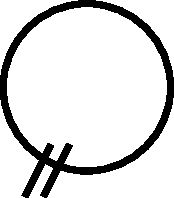
\includegraphics[width=1.2em]{images/circle.pdf}}%
\hspace{-0.85em}#1\:\,}}}
\DeclareRobustCommand\crossedcircletwo[1]{%
{\ensuremath{\raisebox{-2.1ex}{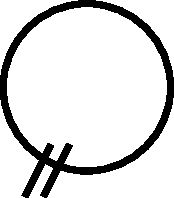
\includegraphics[width=1.75em]{images/circle.pdf}}%
\hspace{-1.4em}#1\;\,}}}

\DeclareRobustCommand{\ind}[1]{%
\ifmmode {\scriptstyle\textit{#1}}%
\else {\smaller[2]#1}\fi}				%



\DeclareRobustCommand\ouLigatur{\ensuremath{\mathord{\downpropto}}}	%

\DeclareRobustCommand\dsig{%

\includegraphics[width=.88em,height=1.15ex]{images/dsig.pdf}}

\DeclareRobustCommand\GWLypsilon{%
\ensuremath{\mathord{\raisebox{0.46ex}{\text{\tiny{o}}}\hspace{-0.1em}\upsilon}}}

\DeclareRobustCommand\circledhash{%
\raisebox{-0.55ex}{\scalebox{0.75}{\rotatebox{45}{\Circled{$\hash$}}}}}

\DeclareRobustCommand\GatterVier{%
\raisebox{0.25ex}{\scalebox{0.85}{\,%
\rlap{\hspace{0.07em}\textbar\hspace{-.08em}\textbar\hspace{-.08em}\textbar\hspace{-.08em}\textbar}{%
\raisebox{-0.45ex}{\rotatebox{90}{%
\textbar\hspace{-.08em}\textbar\hspace{-.08em}\textbar\hspace{-.08em}\textbar}}}\,}}}



\DeclareRobustCommand\PM{%
   	\ensuremath{\mathbin{%
	\raisebox{-1ex}[.9ex][.9ex]%
	{
\includegraphics[width=.5em,height=2ex]{images/pm.pdf}%
}}}}

\DeclareRobustCommand\MP{%
   	\ensuremath{\mathbin{%
	\raisebox{-1ex}[.9ex][.9ex]%
	{
\includegraphics[width=.5em,height=2ex]{images/mp.pdf}%
}}}}

\DeclareRobustCommand\PSMS{%
\ensuremath{\mathbin{%
	\raisebox{-.55ex}[.7ex][.7ex]%
	{
\includegraphics[width=.5em,height=1.6ex]{images/PsMs.pdf}%
}}}}

\DeclareRobustCommand\MSPS{%
\ensuremath{\mathbin{%
	\raisebox{-.55ex}[.7ex][.7ex]%
	{
\includegraphics[width=.5em,height=1.6ex]{images/MsPs.pdf}%
}}}}

\DeclareRobustCommand\PSPSMS{%
\ensuremath{\mathbin{%
	\raisebox{-.55ex}[.7ex][.7ex]%
	{
\includegraphics[width=.88em,height=1.6ex]{images/PsPsMs.pdf}%
}}}}

\DeclareRobustCommand\PSMSPS{%
\ensuremath{\mathbin{%
	\raisebox{-.55ex}[.7ex][.7ex]%
	{
\includegraphics[width=.88em,height=1.6ex]{images/PsMsPs.pdf}%
}}}}

\DeclareRobustCommand\MSPSMS{%
\ensuremath{\mathbin{%
	\raisebox{-.55ex}[.7ex][.7ex]%
	{
\includegraphics[width=.88em,height=1.6ex]{images/MsPsMs.pdf}%
}}}}

\DeclareRobustCommand\MSMSPS{%
\ensuremath{\mathbin{%
	\raisebox{-.55ex}[.7ex][.7ex]%
	{
\includegraphics[width=.88em,height=1.6ex]{images/MsMsPs.pdf}%
}}}}

\DeclareRobustCommand\MSPSPS{%
\ensuremath{\mathbin{%
	\raisebox{-.5ex}[.7ex][.7ex]%
	{
\includegraphics[width=1.32em,height=1.6ex]{images/MsPsPs.pdf}%
}}}}
			
\DeclareRobustCommand\PMA{%
   	\ensuremath{\mathbin{%
	\raisebox{-1ex}[.9ex][.9ex]%
	{
\includegraphics[width=.5em,height=2ex]{images/pmA.pdf}%
}}}}

\DeclareRobustCommand\PMB{%
   	\ensuremath{\mathbin{%
	\raisebox{-1ex}[.9ex][.9ex]%
	{
\includegraphics[width=.5em,height=2ex]{images/pmB.pdf}%
}}}}


\DeclareRobustCommand\PMD{%
   	\ensuremath{\mathbin{%
	\raisebox{-1ex}[.9ex][.9ex]%
	{
\includegraphics[width=.5em,height=2ex]{images/pmD.pdf}%
}}}}

\DeclareRobustCommand\PME{%
\ensuremath{\mathbin{%
	\raisebox{-.55ex}[.7ex][.7ex]%
	{
\includegraphics[width=.88em,height=1.6ex]{images/pmE.pdf}%
}}}}


\DeclareRobustCommand\PMG{%
   	\ensuremath{\mathbin{%
	\raisebox{-1ex}[.9ex][.9ex]%
	{
\includegraphics[width=.5em,height=2ex]{images/pmG.pdf}%
}}}}

\DeclareRobustCommand\PMH{%
   	\ensuremath{\mathbin{%
	\raisebox{-1ex}[.9ex][.9ex]%
	{
\includegraphics[width=.5em,height=2ex]{images/pmH.pdf}%
}}}}

\DeclareRobustCommand\PMK{%
   	\ensuremath{\mathbin{%
	\raisebox{-1ex}[.9ex][.9ex]%
	{
\includegraphics[width=.5em,height=2ex]{images/pmK.pdf}%
}}}}



\DeclareRobustCommand\PMkla{%
   	\ensuremath{\mathbin{(%
	\raisebox{-1ex}[.9ex][.9ex]%
	{
\includegraphics[width=.5em,height=2ex]{images/pm.pdf}})}%
}}

\DeclareRobustCommand\MPkla{%
   	\ensuremath{\mathbin{(%
	\raisebox{-1ex}[.9ex][.9ex]%
	{
\includegraphics[width=.5em,height=2ex]{images/mp.pdf}})}%
}}

\DeclareRobustCommand\PMklakla{%
   	\ensuremath{\mathbin{(\!(%
	\raisebox{-1ex}[.9ex][.9ex]%
	{
\includegraphics[width=.5em,height=2ex]{images/pm.pdf}})\!)}%
}}

\DeclareRobustCommand\MPklakla{%
   	\ensuremath{\mathbin{(\!(%
	\raisebox{-1ex}[.9ex][.9ex]%
	{
\includegraphics[width=.5em,height=2ex]{images/mp.pdf}})\!)}%
}}



\DeclareRobustCommand\hccps{%
   	\ensuremath{\mathbin{%
	\raisebox{-.55ex}[.7ex][.7ex]%
	{
\includegraphics[height=2.15ex]{images/hccps.pdf}%
}}}}

\DeclareRobustCommand\hccms{%
   	\ensuremath{\mathbin{%
	\raisebox{-.55ex}[.7ex][.7ex]%
	{
\includegraphics[height=2.15ex]{images/hccms.pdf}%
}}}}



\newcommand*{\ditto}{\texttt{"}}	

\DeclareRobustCommand{\bracks}[1]{%
\textup{\lbrack}#1\textup{\rbrack}}
\DeclareRobustCommand{\bracksup}[1]{%
\textup{\lbrack{}#1\rbrack{}}}

\DeclareRobustCommand{\angles}[1]{%
\ifmmode {\langle{}}\else {\textlangle{}}\fi%
#1\ifmmode {\rangle{}}\else {\textrangle{}}\fi}	%




\DeclareRobustCommand{\greek}[1]{\foreignlanguage{greek}{#1}}	%
\DeclareRobustCommand{\pgrk}[1]{\foreignlanguage{greek}{#1}}	%

\usepackage{cjhebrew}			%
\newcommand*{\hebr}[1]{\mbox{\cjRL{#1}}}

\BeforeBeginEnvironment{ledgroupsized}{\selectlanguage{ngerman}}	%
\BeforeBeginEnvironment{ledgroup}{\selectlanguage{ngerman}}	%



\babelhyphenation[latin]{
pot-erint
pot-eris
pot-es
}

\babelhyphenation[ngerman]{
Blatt-rand
}


\babelhyphenation{%
aequ
aequi-pon-de-ran-tium
fehlt
gestr
klein-ge-druckt
klein-ge-druck-te
klein-ge-druck-tem
klein-ge-druck-ten
klein-ge-druck-ter
klein-ge-druck-tes
post-ea
po-ten-tia
pot-est
quem-ad-mo-dum
streicht
}




\usepackage[%
hidelinks,			%
linktocpage=true,		%
bookmarksnumbered=true,	%
]{hyperref}			

\hypersetup{%
urlcolor=RoyalBlue,			%
urlbordercolor=RoyalBlue,
citecolor=red,
citebordercolor=red,
}

\hypersetup{pdfinfo={%
Title={\textit{LSB}, Achte Reihe, Vierter Band, Mechanik 2},	%
Author={G. W. Leibniz},				%
Creator={BBAW, Arbeitsstelle Leibniz-Edition Berlin},	%
}}

\pdfstringdefDisableCommands{\let\thepart\relax}	%
\pdfstringdefDisableCommands{\let\textsubscript\fullstop{}}	%

\newcommand{\ScanURL}[2]{%
\expandafter\newcommand\csname scan-#1\endcsname{#2}}    %
\newcommand{\Scan}[1]{\csname scan-#1\endcsname}    %




\newcommand*{\BBAWURL}{http://digilib.bbaw.de/digitallibrary/digilib.html?fn=/silo10/Leibniz8/original/}


\newcommand*{\GWLBURL}{http://digitale-sammlungen.gwlb.de/sammlungen/sammlungsliste/werksansicht/?id=6&tx_dlf[id]=}












\label{LBr-Signaturen}


\ScanURL{LBr_250_001r}%
{\GWLBURL 6707&tx_dlf[page]=1}
\ScanURL{LBr_250_001v}%
{\GWLBURL 6707&tx_dlf[page]=2}



\ScanURL{LBr_413_048r}%
{\GWLBURL 6883&tx_dlf[page]=95}
\ScanURL{LBr_413_048v}%
{\GWLBURL 6883&tx_dlf[page]=96}



\ScanURL{LBr_724_16v}%
{\GWLBURL 7264&tx_dlf[page]=32}
\ScanURL{LBr_724_16ar}%
{\GWLBURL 7264&tx_dlf[page]=32}
\ScanURL{LBr_724_16av}%
{\GWLBURL 7264&tx_dlf[page]=31}



\ScanURL{LBr_724_18r}%
{\GWLBURL 7264&tx_dlf[page]=35}
\ScanURL{LBr_724_18wz}%
{\GWLBURL }
\ScanURL{LBr_724_18v}%
{\GWLBURL 7264&tx_dlf[page]=36}
\ScanURL{LBr_724_19r}%
{\GWLBURL 7264&tx_dlf[page]=36}
\ScanURL{LBr_724_19wz}%
{\GWLBURL }
\ScanURL{LBr_724_19v}%
{\GWLBURL 7264&tx_dlf[page]=35}





\label{LH-Signaturen}



\ScanURL{LH_01_03_08d_006r}%
{\GWLBURL 2072&tx_dlf[page]=11}
\ScanURL{LH_01_03_08d_006v}%
{\GWLBURL 2072&tx_dlf[page]=12}




\ScanURL{LH_03_05_018r}%
{\BBAWURL LH003,05/&pn=55}
\ScanURL{LH_03_05_017-018wz}%
{\BBAWURL LH003,05/&pn=51}



\ScanURL{LH_04_01_02a_015r}%
{\GWLBURL 2378&tx_dlf[page]=29}
\ScanURL{LH_04_01_02a_015v}%
{\GWLBURL 2378&tx_dlf[page]=30}



\ScanURL{LH_04_03_05e_017r}%
{\GWLBURL 2487&tx_dlf[page]=49}
\ScanURL{LH_04_03_05e_017v}%
{\GWLBURL 2487&tx_dlf[page]=50}



\ScanURL{LH_04_03_09b_010r}%
{\GWLBURL 2433&tx_dlf[page]=19}
\ScanURL{LH_04_03_09b_010v}%
{\BBAWURL 2433&tx_dlf[page]=20}



\ScanURL{LH_04_01_04d_02_004r}%
{\GWLBURL 2384&tx_dlf[page]=21}
\ScanURL{LH_04_01_04d_02_004v}%
{\GWLBURL 2384&tx_dlf[page]=22}



\ScanURL{LH_35_01_09_030r}%
{\GWLBURL 1634&tx_dlf[page]=59}
\ScanURL{LH_35_01_09_030v}%
{\GWLBURL 1634&tx_dlf[page]=60}



\ScanURL{LH_35_05_28_008r}%
{\GWLBURL 1947&tx_dlf[page]=15}
\ScanURL{LH_35_05_28_008v}%
{\GWLBURL 1947&tx_dlf[page]=16}
\ScanURL{LH_35_05_28_009r}%
{\GWLBURL 1947&tx_dlf[page]=17}



\ScanURL{LH_35_06_23_003r}%
{\GWLBURL 1886&tx_dlf[page]=5}
\ScanURL{LH_35_06_23_003v}%
{\GWLBURL 1886&tx_dlf[page]=6}



\ScanURL{LH_35_08_30_040r}%
{\GWLBURL 1863&tx_dlf[page]=79}
\ScanURL{LH_35_08_30_040v}%
{\GWLBURL 1863&tx_dlf[page]=80}




\ScanURL{LH_35_08_30_121r}%
{\BBAWURL LH035/&pn=44}
\ScanURL{LH_35_08_30_121wz}%
{\BBAWURL LH035/&pn=45}
\ScanURL{LH_35_08_30_121v}%
{\BBAWURL LH035/&pn=46}



\ScanURL{LH_35_08_30_133r}%
{\GWLBURL 1863&tx_dlf[page]=267}
\ScanURL{LH_35_08_30_133v}%
{\GWLBURL 1863&tx_dlf[page]=268}



\ScanURL{LH_35_09_07_018r}%
{\BBAWURL LH035/&pn=701}
\ScanURL{LH_35_09_07_018wz}%
{\BBAWURL LH035/&pn=702}



\ScanURL{LH_35_09_07_022r}%
{\BBAWURL LH035/&pn=714}
\ScanURL{LH_35_09_07_022v}%
{\BBAWURL LH035/&pn=716}
\ScanURL{LH_35_09_07_022-023wz}%
{\BBAWURL LH035/&pn=713}



\ScanURL{LH_35_09_07_023r}%
{\BBAWURL LH035/&pn=717}
\ScanURL{LH_35_09_07_023v}%
{\BBAWURL LH035/&pn=719}



\ScanURL{LH_35_09_07_025r}%
{\BBAWURL LH035/&pn=723}
\ScanURL{LH_35_09_07_025v}%
{\BBAWURL LH035/&pn=725}



\ScanURL{LH_35_09_10_001r}%
{\BBAWURL LH035/&pn=780}
\ScanURL{LH_35_09_10_001wz}%
{\BBAWURL LH035/&pn=781}
\ScanURL{LH_35_09_10_001v}%
{\BBAWURL LH035/&pn=782}
\ScanURL{LH_35_09_10_002r}%
{\BBAWURL LH035/&pn=783}
\ScanURL{LH_35_09_10_002v}%
{\BBAWURL LH035/&pn=785}



\ScanURL{LH_35_09_10_003r}%
{\BBAWURL LH035/&pn=786}
\ScanURL{LH_35_09_10_003v}%
{\BBAWURL LH035/&pn=788}
\ScanURL{LH_35_09_10_004r}%
{\BBAWURL LH035/&pn=789}
\ScanURL{LH_35_09_10_004wz}%
{\BBAWURL LH035/&pn=790}
\ScanURL{LH_35_09_10_004v}%
{\BBAWURL LH035/&pn=791}



\ScanURL{LH_35_09_10_005r}%
{\BBAWURL LH035/&pn=792}
\ScanURL{LH_35_09_10_005wz}%
{\BBAWURL LH035/&pn=793}
\ScanURL{LH_35_09_10_005v}%
{\BBAWURL LH035/&pn=794}
\ScanURL{LH_35_09_10_006r}%
{\BBAWURL LH035/&pn=795}
\ScanURL{LH_35_09_10_006v}%
{\BBAWURL LH035/&pn=797}



\ScanURL{LH_35_09_10_007r}%
{\BBAWURL LH035/&pn=798}
\ScanURL{LH_35_09_10_007wz}%
{\BBAWURL LH035/&pn=799}



\ScanURL{LH_35_09_12_001r}%
{\BBAWURL LH035/&pn=843}
\ScanURL{LH_35_09_12_001v}%
{\BBAWURL LH035/&pn=845}
\ScanURL{LH_35_09_12_002r}%
{\BBAWURL LH035/&pn=846}
\ScanURL{LH_35_09_12_002wz}%
{\BBAWURL LH035/&pn=847}
\ScanURL{LH_35_09_12_002v}%
{\BBAWURL LH035/&pn=848}
\ScanURL{LH_35_09_12_003r}%
{\BBAWURL LH035/&pn=849}
\ScanURL{LH_35_09_12_003wz}%
{\BBAWURL LH035/&pn=850}
\ScanURL{LH_35_09_12_003v}%
{\BBAWURL LH035/&pn=851}



\ScanURL{LH_35_09_16_007r}%
{\BBAWURL LH035/&pn=976}
\ScanURL{LH_35_09_16_007v}%
{\BBAWURL LH035/&pn=977}






\ScanURL{LH_35_09_17_005r}%
{\BBAWURL LH035/&pn=1030}
\ScanURL{LH_35_09_17_005wz}%
{\BBAWURL LH035/&pn=1031}
\ScanURL{LH_35_09_17_005v}%
{\BBAWURL LH035/&pn=1032}
\ScanURL{LH_35_09_17_006r}%
{\BBAWURL LH035/&pn=1033}
\ScanURL{LH_35_09_17_006wz}%
{\BBAWURL LH035/&pn=1034}
\ScanURL{LH_35_09_17_006v}%
{\BBAWURL LH035/&pn=1035}



\ScanURL{LH_35_09_20_002r}%
{\BBAWURL LH035/&pn=1083}
\ScanURL{LH_35_09_20_002wz}%
{\BBAWURL LH035/&pn=1084}
\ScanURL{LH_35_09_20_002v}%
{\BBAWURL LH035/&pn=1085}



\ScanURL{LH_35_09_20_003r}%
{\BBAWURL LH035/&pn=1086}
\ScanURL{LH_35_09_20_003wz}%
{\BBAWURL LH035/&pn=1087}
\ScanURL{LH_35_09_20_003v}%
{\BBAWURL LH035/&pn=1088}
\ScanURL{LH_35_09_20_004r}%
{\BBAWURL LH035/&pn=1089}
\ScanURL{LH_35_09_20_004v}%
{\BBAWURL LH035/&pn=1091}






\ScanURL{LH_35_09_25_001r}%
{\BBAWURL LH035/&pn=1221}
\ScanURL{LH_35_09_25_001wz}%
{\BBAWURL LH035/&pn=1222}
\ScanURL{LH_35_09_25_001v}%
{\BBAWURL LH035/&pn=1223}
\ScanURL{LH_35_09_25_002r}%
{\BBAWURL LH035/&pn=1224}
\ScanURL{LH_35_09_25_002wz}%
{\BBAWURL LH035/&pn=1225}
\ScanURL{LH_35_09_25_002v}%
{\BBAWURL LH035/&pn=1226}



\ScanURL{LH_35_09_25_003r}%
{\BBAWURL LH035/&pn=1227}
\ScanURL{LH_35_09_25_003wz}%
{\BBAWURL LH035/&pn=1228}
\ScanURL{LH_35_09_25_003v}%
{\BBAWURL LH035/&pn=1229}



\ScanURL{LH_35_09_25_004r}%
{\BBAWURL LH035/&pn=1230}
\ScanURL{LH_35_09_25_004wz}%
{\BBAWURL LH035/&pn=1231}
\ScanURL{LH_35_09_25_004v}%
{\BBAWURL LH035/&pn=1232}
\ScanURL{LH_35_09_25_005r}%
{\BBAWURL LH035/&pn=1233}
\ScanURL{LH_35_09_25_005wz}%
{\BBAWURL LH035/&pn=1234}
\ScanURL{LH_35_09_25_005v}%
{\BBAWURL LH035/&pn=1235}




\ScanURL{LH_35_09_28_003r}%
{\BBAWURL LH035/&pn=1253}
\ScanURL{LH_35_09_28_003v}%
{\BBAWURL LH035/&pn=1255}
\ScanURL{LH_35_09_28_003-004wz}%
{\BBAWURL LH035/&pn=1252}
\ScanURL{LH_35_09_28_004r}%
{\BBAWURL LH035/&pn=1256}
\ScanURL{LH_35_09_28_004v}%
{\BBAWURL LH035/&pn=1258}






\ScanURL{LH_35_10_06_038r}%
{\BBAWURL LH035/&pn=1481}
\ScanURL{LH_35_10_06_038v}%
{\BBAWURL LH035/&pn=1483}






\ScanURL{LH_35_10_07_022r}%
{\BBAWURL LH035/&pn=1561}
\ScanURL{LH_35_10_07_022v}%
{\BBAWURL LH035/&pn=1563}






\ScanURL{LH_35_10_07_041r}%
{\BBAWURL LH035/&pn=1623}
\ScanURL{LH_35_10_07_041wz}%
{\BBAWURL LH035/&pn=1624}
\ScanURL{LH_35_10_07_041v}%
{\BBAWURL LH035/&pn=1625}



\ScanURL{LH_35_10_08_014r}%
{\BBAWURL LH035/&pn=1677}



\ScanURL{LH_35_10_11_088r}%
{\BBAWURL LH035/&pn=1997}
\ScanURL{LH_35_10_11_088wz}%
{\BBAWURL LH035/&pn=1998}
\ScanURL{LH_35_10_11_088v}%
{\BBAWURL LH035/&pn=1999}


\ScanURL{LH_35_10_11_101r}%
{\BBAWURL LH035/&pn=2036}
\ScanURL{LH_35_10_11_101v}%
{\BBAWURL LH035/&pn=2038}
\ScanURL{LH_35_10_11_102r}%
{\BBAWURL LH035/&pn=2039}
\ScanURL{LH_35_10_11_102wz}%
{\BBAWURL LH035/&pn=2040}
\ScanURL{LH_35_10_11_102v}%
{\BBAWURL LH035/&pn=2041}






\ScanURL{LH_35_10_11_107r}%
{\BBAWURL LH035/&pn=2054}
\ScanURL{LH_35_10_11_107wz}%
{\BBAWURL LH035/&pn=2055}
\ScanURL{LH_35_10_11_107v}%
{\BBAWURL LH035/&pn=2056}






\ScanURL{LH_35_10_12_038r}%
{\BBAWURL LH035/&pn=2208}
\ScanURL{LH_35_10_12_038wz}%
{\BBAWURL LH035/&pn=2209}
\ScanURL{LH_35_10_12_038v}%
{\BBAWURL LH035/&pn=2210}



\ScanURL{LH_35_10_13_001r}%
{\BBAWURL LH035/&pn=2241}
\ScanURL{LH_35_10_13_001wz}%
{\BBAWURL LH035/&pn=2242}
\ScanURL{LH_35_10_13_001v}%
{\BBAWURL LH035/&pn=2243}
\ScanURL{LH_35_10_13_002r}%
{\BBAWURL LH035/&pn=2244}
\ScanURL{LH_35_10_13_002wz}%
{\BBAWURL LH035/&pn=2245}
\ScanURL{LH_35_10_13_002v}%
{\BBAWURL LH035/&pn=2246}






\ScanURL{LH_35_10_13_006r}%
{\BBAWURL LH035/&pn=2256}
\ScanURL{LH_35_10_13_006wz}%
{\BBAWURL LH035/&pn=2257}
\ScanURL{LH_35_10_13_006v}%
{\BBAWURL LH035/&pn=2258}



\ScanURL{LH_35_10_13_007r}%
{\BBAWURL LH035/&pn=2259}
\ScanURL{LH_35_10_13_007wz}%
{\BBAWURL LH035/&pn=2260}
\ScanURL{LH_35_10_13_007v}%
{\BBAWURL LH035/&pn=2261}



\ScanURL{LH_35_10_13_008r}%
{\BBAWURL LH035/&pn=2262}
\ScanURL{LH_35_10_13_008wz}%
{\BBAWURL LH035/&pn=2263}
\ScanURL{LH_35_10_13_008v}%
{\BBAWURL LH035/&pn=2264}



\ScanURL{LH_35_10_13_009r}%
{\BBAWURL LH035/&pn=2265}
\ScanURL{LH_35_10_13_009v}%
{\BBAWURL LH035/&pn=2267}



\ScanURL{LH_35_10_13_010r}%
{\BBAWURL LH035/&pn=2268}
\ScanURL{LH_35_10_13_010wz}%
{\BBAWURL LH035/&pn=2269}
\ScanURL{LH_35_10_13_010v}%
{\BBAWURL LH035/&pn=2270}
\ScanURL{LH_35_10_13_011r}%
{\BBAWURL LH035/&pn=2271}
\ScanURL{LH_35_10_13_011wz}%
{\BBAWURL LH035/&pn=2272}
\ScanURL{LH_35_10_13_011v}%
{\BBAWURL LH035/&pn=2273}






\ScanURL{LH_35_10_13_013r}%
{\BBAWURL LH035/&pn=2277}
\ScanURL{LH_35_10_13_013wz}%
{\BBAWURL LH035/&pn=2278}
\ScanURL{LH_35_10_13_013v}%
{\BBAWURL LH035/&pn=2279}



\ScanURL{LH_35_10_14_002r}%
{\BBAWURL LH035/&pn=2283}
\ScanURL{LH_35_10_14_002wz}%
{\BBAWURL LH035/&pn=2284}
\ScanURL{LH_35_10_14_002v}%
{\BBAWURL LH035/&pn=2285}



\ScanURL{LH_35_10_14_003r}%
{\BBAWURL LH035/&pn=2286}
\ScanURL{LH_35_10_14_003v}%
{\BBAWURL LH035/&pn=2288}



\ScanURL{LH_35_10_14_004r}%
{\BBAWURL LH035/&pn=2289}
\ScanURL{LH_35_10_14_004wz}%
{\BBAWURL LH035/&pn=2290}
\ScanURL{LH_35_10_14_004v}%
{\BBAWURL LH035/&pn=2291}



\ScanURL{LH_35_10_14_005r}%
{\BBAWURL LH035/&pn=2292}
\ScanURL{LH_35_10_14_005wz}%
{\BBAWURL LH035/&pn=2293}
\ScanURL{LH_35_10_14_005v}%
{\BBAWURL LH035/&pn=2294}



\ScanURL{LH_35_10_14_006r}%
{\BBAWURL LH035/&pn=2295}
\ScanURL{LH_35_10_14_006wz}%
{\BBAWURL LH035/&pn=2295}



\ScanURL{LH_35_10_14_007r}%
{\BBAWURL LH035/&pn=2298}
\ScanURL{LH_35_10_14_007wz}%
{\BBAWURL LH035/&pn=2299}



\ScanURL{LH_35_10_14_008r}%
{\BBAWURL LH035/&pn=2301}
\ScanURL{LH_35_10_14_008wz}%
{\BBAWURL LH035/&pn=2302}
\ScanURL{LH_35_10_14_008v}%
{\BBAWURL LH035/&pn=2303}



\ScanURL{LH_35_10_14_009r}%
{\BBAWURL LH035/&pn=2304}
\ScanURL{LH_35_10_14_009wz}%
{\BBAWURL LH035/&pn=2305}
\ScanURL{LH_35_10_14_009v}%
{\BBAWURL LH035/&pn=2306}
\ScanURL{LH_35_10_14_010r}%
{\BBAWURL LH035/&pn=2307}
\ScanURL{LH_35_10_14_010wz}%
{\BBAWURL LH035/&pn=2308}



\ScanURL{LH_35_10_14_011r}%
{\BBAWURL LH035/&pn=2310}
\ScanURL{LH_35_10_14_011wz}%
{\BBAWURL LH035/&pn=2311}
\ScanURL{LH_35_10_14_011v}%
{\BBAWURL LH035/&pn=2312}



\ScanURL{LH_35_10_14_012r}%
{\BBAWURL LH035/&pn=2313}
\ScanURL{LH_35_10_14_012wz}%
{\BBAWURL LH035/&pn=2314}
\ScanURL{LH_35_10_14_012v}%
{\BBAWURL LH035/&pn=2315}



\ScanURL{LH_35_10_16_001r}%
{\BBAWURL LH035/&pn=2338}
\ScanURL{LH_35_10_16_001v}%
{\BBAWURL LH035/&pn=2340}
\ScanURL{LH_35_10_16_001-002wz}%
{\BBAWURL LH035/&pn=2337}
\ScanURL{LH_35_10_16_002r}%
{\BBAWURL LH035/&pn=2341}
\ScanURL{LH_35_10_16_002v}%
{\BBAWURL LH035/&pn=2343}



\ScanURL{LH_35_10_16_003r}%
{\BBAWURL LH035/&pn=2345}
\ScanURL{LH_35_10_16_003v}%
{\BBAWURL LH035/&pn=2347}
\ScanURL{LH_35_10_16_003-004wz}%
{\BBAWURL LH035/&pn=2344}
\ScanURL{LH_35_10_16_004r}%
{\BBAWURL LH035/&pn=2348}
\ScanURL{LH_35_10_16_004v}%
{\BBAWURL LH035/&pn=2350}



\ScanURL{LH_35_10_16_008r}%
{\BBAWURL LH035/&pn=2360}
\ScanURL{LH_35_10_16_008wz}%
{\BBAWURL LH035/&pn=2361}
\ScanURL{LH_35_10_16_008v}%
{\BBAWURL LH035/&pn=2362}



\ScanURL{LH_35_10_16_009r}%
{\BBAWURL LH035/&pn=2363}
\ScanURL{LH_35_10_16_009v}%
{\BBAWURL LH035/&pn=2365}






\ScanURL{LH_35_10_17_009r}%
{\BBAWURL LH035/&pn=2409}
\ScanURL{LH_35_10_17_009wz}%
{\BBAWURL LH035/&pn=2410}
\ScanURL{LH_35_10_17_009v}%
{\BBAWURL LH035/&pn=2411}



\ScanURL{LH_35_10_18_013r}%
{\BBAWURL LH035/&pn=2448}
\ScanURL{LH_35_10_18_013wz}%
{\BBAWURL LH035/&pn=2449}
\ScanURL{LH_35_10_18_013v}%
{\BBAWURL LH035/&pn=2450}



\ScanURL{LH_35_11_14_001r}%
{\BBAWURL LH035/&pn=2628}
\ScanURL{LH_35_11_14_001v}%
{\BBAWURL LH035/&pn=2630}
\ScanURL{LH_35_11_14_001-002wz}%
{\BBAWURL LH035/&pn=2627}
\ScanURL{LH_35_11_14_002r}%
{\BBAWURL LH035/&pn=2631}
\ScanURL{LH_35_11_14_002v}%
{\BBAWURL LH035/&pn=2633}



\ScanURL{LH_35_11_14_003r}%
{\BBAWURL LH035/&pn=2634}
\ScanURL{LH_35_11_14_003v}%
{\BBAWURL LH035/&pn=2636}
\ScanURL{LH_35_11_14_003-004wz}%
{\BBAWURL LH035/&pn=2638}
\ScanURL{LH_35_11_14_004r}%
{\BBAWURL LH035/&pn=2637}
\ScanURL{LH_35_11_14_004v}%
{\BBAWURL LH035/&pn=2639}



\ScanURL{LH_35_11_14_005r}%
{\BBAWURL LH035/&pn=2641}
\ScanURL{LH_35_11_14_005v}%
{\BBAWURL LH035/&pn=2643}
\ScanURL{LH_35_11_14_005-006wz}%
{\BBAWURL LH035/&pn=2640}%
\ScanURL{LH_35_11_14_006r}%
{\BBAWURL LH035/&pn=2644}
\ScanURL{LH_35_11_14_006v}%
{\BBAWURL LH035/&pn=2646}



\ScanURL{LH_35_11_14_008r}%
{\BBAWURL LH035/&pn=2650}
\ScanURL{LH_35_11_14_008wz}%
{\BBAWURL LH035/&pn=2651}
\ScanURL{LH_35_11_14_008v}%
{\BBAWURL LH035/&pn=2652}%



\ScanURL{LH_35_11_14_015r}%
{\BBAWURL LH035/&pn=2673}
\ScanURL{LH_35_11_14_015wz}%
{\BBAWURL LH035/&pn=2674}
\ScanURL{LH_35_11_14_015v}%
{\BBAWURL LH035/&pn=2675}



\ScanURL{LH_35_11_14_031r}%
{\BBAWURL LH035/&pn=2727}
\ScanURL{LH_35_11_14_031wz}%
{\BBAWURL LH035/&pn=2728}
\ScanURL{LH_35_11_14_031v}%
{\BBAWURL LH035/&pn=2729}



\ScanURL{LH_35_11_14_032r}%
{\BBAWURL LH035/&pn=2730}
\ScanURL{LH_35_11_14_032wz}%
{\BBAWURL LH035/&pn=2731}
\ScanURL{LH_35_11_14_032v}%
{\BBAWURL LH035/&pn=2732}



\ScanURL{LH_35_11_14_034r}%
{\BBAWURL LH035/&pn=2736}
\ScanURL{LH_35_11_14_034wz}%
{\BBAWURL LH035/&pn=2737}
\ScanURL{LH_35_11_14_034v}%
{\BBAWURL LH035/&pn=2738}



\ScanURL{LH_35_11_14_035r}%
{\BBAWURL LH035/&pn=2739}
\ScanURL{LH_35_11_14_035v}%
{\BBAWURL LH035/&pn=2741}



\ScanURL{LH_35_11_14_036r}%
{\BBAWURL LH035/&pn=2742}
\ScanURL{LH_35_11_14_036v}%
{\BBAWURL LH035/&pn=2744}



\ScanURL{LH_35_11_14_037r}%
{\BBAWURL LH035/&pn=2745}
\ScanURL{LH_35_11_14_037wz}%
{\BBAWURL LH035/&pn=2746}
\ScanURL{LH_35_11_14_037v}%
{\BBAWURL LH035/&pn=2747}




\ScanURL{LH_35_11_18A_438}%
{\BBAWURL LH035/&pn=3388}
\ScanURL{LH_35_11_18C_216r}%
{\BBAWURL LH035/&pn=4091}




\ScanURL{LH_35_13_01_130r}%
{\GWLBURL 1746&tx_dlf[page]=257}
\ScanURL{LH_35_13_01_130v}%
{\GWLBURL 1746&tx_dlf[page]=258}
\ScanURL{LH_35_13_01_131r}%
{\GWLBURL 1746&tx_dlf[page]=258}



\ScanURL{LH_35_13_01_427r}%
{\GWLBURL 1746&tx_dlf[page]=849}
\ScanURL{LH_35_13_01_427wz}%
{\GWLBURL }
\ScanURL{LH_35_13_01_427v}%
{\GWLBURL 1746&tx_dlf[page]=850}
\ScanURL{LH_35_13_01_428r}%
{\GWLBURL 1746&tx_dlf[page]=851}
\ScanURL{LH_35_13_01_428wz}%
{\GWLBURL }
\ScanURL{LH_35_13_01_428v}%
{\GWLBURL 1746&tx_dlf[page]=852}



\ScanURL{LH_35_13_02c_112r}%
{\GWLBURL 1749&tx_dlf[page]=223}
\ScanURL{LH_35_13_02c_112wz}%
{\GWLBURL }
\ScanURL{LH_35_13_02c_112v}%
{\GWLBURL 1749&tx_dlf[page]=224}
\ScanURL{LH_35_13_02c_113r}%
{\GWLBURL 1749&tx_dlf[page]=225}
\ScanURL{LH_35_13_02c_113wz}%
{\GWLBURL }
\ScanURL{LH_35_13_02c_113v}%
{\GWLBURL 1749&tx_dlf[page]=226}




\ScanURL{LH_35_13_03_220r}%
{\GWLBURL 1750&tx_dlf[page]=441}
\ScanURL{LH_35_13_03_220v}%
{\GWLBURL 1750&tx_dlf[page]=442}
\ScanURL{LH_35_13_03_221r}%
{\GWLBURL 1750&tx_dlf[page]=443}
\ScanURL{LH_35_13_03_221wz}%
{\GWLBURL }
\ScanURL{LH_35_13_03_221v}%
{\GWLBURL 1750&tx_dlf[page]=444}



\ScanURL{LH_35_13_03_237r}%
{\GWLBURL 1750&tx_dlf[page]=475}
\ScanURL{LH_35_13_03_237wz}%
{\GWLBURL }
\ScanURL{LH_35_13_03_238v}%
{\GWLBURL 1750&tx_dlf[page]=478}



\ScanURL{LH_35_13_03_242r}%
{\GWLBURL 1750&tx_dlf[page]=485}
\ScanURL{LH_35_13_03_242wz}%
{\GWLBURL }
\ScanURL{LH_35_13_03_242v}%
{\GWLBURL 1750&tx_dlf[page]=486}



\ScanURL{LH_35_14_02_001r}%
{\GWLBURL 1747&tx_dlf[page]=1}
\ScanURL{LH_35_14_02_001wz}%
{\GWLBURL }
\ScanURL{LH_35_14_02_001v}%
{\GWLBURL 1747&tx_dlf[page]=2}



\ScanURL{LH_35_14_02_004r}%
{\GWLBURL 1747&tx_dlf[page]=7}
\ScanURL{LH_35_14_02_004wz}%
{\GWLBURL }
\ScanURL{LH_35_14_02_004v}%
{\GWLBURL 1747&tx_dlf[page]=8}



\ScanURL{LH_35_14_02_006r}%
{\GWLBURL 1747&tx_dlf[page]=11}
\ScanURL{LH_35_14_02_006wz}%
{\GWLBURL }
\ScanURL{LH_35_14_02_006v}%
{\GWLBURL 1747&tx_dlf[page]=12}








\ScanURL{LH_035_14_02_022r}%
{\GWLBURL 1747&tx_dlf[page]=43}

\ScanURL{LH_035_14_02_022v}%
{\GWLBURL 1747&tx_dlf[page]=44}

\ScanURL{LH_035_14_02_023r}%
{\GWLBURL 1747&tx_dlf[page]=45}

\ScanURL{LH_035_14_02_023v}%
{\GWLBURL 1747&tx_dlf[page]=46}





\ScanURL{LH_35_14_02_040r}%
{\GWLBURL 1747&tx_dlf[page]=79}
\ScanURL{LH_35_14_02_040wz}%
{\GWLBURL }
\ScanURL{LH_35_14_02_040v}%
{\GWLBURL 1747&tx_dlf[page]=80}



\ScanURL{LH_35_14_02_045r}%
{\GWLBURL 1747&tx_dlf[page]=89}
\ScanURL{LH_35_14_02_045wz}%
{\GWLBURL }
\ScanURL{LH_35_14_02_045v}%
{\GWLBURL 1747&tx_dlf[page]=90}



\ScanURL{LH_35_14_02_089r}%
{\GWLBURL 1747&tx_dlf[page]=177}
\ScanURL{LH_35_14_02_089v}%
{\GWLBURL 1747&tx_dlf[page]=178}



\ScanURL{LH_35_14_02_165r}%
{\GWLBURL 1747&tx_dlf[page]=329}
\ScanURL{LH_35_14_02_165wz}%
{\GWLBURL }
\ScanURL{LH_35_14_02_165v}%
{\GWLBURL 1747&tx_dlf[page]=330}



\ScanURL{LH_37_02_129r}%
{\BBAWURL LH037,02/&pn=409}
\ScanURL{LH_37_02_129wz}%
{\BBAWURL LH037,02/&pn=410}
\ScanURL{LH_37_02_129v}%
{\BBAWURL LH037,02/&pn=411}



\ScanURL{LH_37_03_062r}%
{\BBAWURL LH037,03/&pn=186}
\ScanURL{LH_37_03_062wz}%
{\BBAWURL LH037,03/&pn=187}
\ScanURL{LH_37_03_062v}%
{\BBAWURL LH037,03/&pn=188}



\ScanURL{LH_37_03_063r}%
{\BBAWURL LH037,03/&pn=189}
\ScanURL{LH_37_03_063wz}%
{\BBAWURL LH037,03/&pn=190}
\ScanURL{LH_37_03_063v}%
{\BBAWURL LH037,03/&pn=191}



\ScanURL{LH_37_03_064r}%
{\BBAWURL LH037,03/&pn=192}
\ScanURL{LH_37_03_064wz}%
{\BBAWURL LH037,03/&pn=193}
\ScanURL{LH_37_03_064v}%
{\BBAWURL LH037,03/&pn=194}



\ScanURL{LH_37_03_065r}%
{\BBAWURL LH037,03/&pn=195}
\ScanURL{LH_37_03_065wz}%
{\BBAWURL LH037,03/&pn=196}
\ScanURL{LH_37_03_065v}%
{\BBAWURL LH037,03/&pn=197}



\ScanURL{LH_37_03_067r}%
{\BBAWURL LH037,03/&pn=201}
\ScanURL{LH_37_03_067v}%
{\BBAWURL LH037,03/&pn=203}



\ScanURL{LH_37_03_075r}%
{\BBAWURL LH037,03/&pn=225}
\ScanURL{LH_37_03_075wz}%
{\BBAWURL LH037,03/&pn=226}
\ScanURL{LH_37_03_075v}%
{\BBAWURL LH037,03/&pn=227}
\ScanURL{LH_37_03_076r}%
{\BBAWURL LH037,03/&pn=228}
\ScanURL{LH_37_03_076v}%
{\BBAWURL LH037,03/&pn=230}



\ScanURL{LH_37_03_081r}%
{\BBAWURL LH037,03/&pn=243}
\ScanURL{LH_37_03_081v}%
{\BBAWURL LH037,03/&pn=245}



\ScanURL{LH_37_03_082r}%
{\BBAWURL LH037,03/&pn=246}
\ScanURL{LH_37_03_082v}%
{\BBAWURL LH037,03/&pn=248}
\ScanURL{LH_37_03_083r}%
{\BBAWURL LH037,03/&pn=249}
\ScanURL{LH_37_03_083wz}%
{\BBAWURL LH037,03/&pn=250}
\ScanURL{LH_37_03_083v}%
{\BBAWURL LH037,03/&pn=251}



\ScanURL{LH_37_03_115-116wz}%
{\BBAWURL LH037,03/&pn=345}
\ScanURL{LH_37_03_115r}%
{\BBAWURL LH037,03/&pn=346}
\ScanURL{LH_37_03_115v}%
{\BBAWURL LH037,03/&pn=348}
\ScanURL{LH_37_03_116r}%
{\BBAWURL LH037,03/&pn=349}
\ScanURL{LH_37_03_116v}%
{\BBAWURL LH037,03/&pn=351}



\ScanURL{LH_37_03_117r}%
{\BBAWURL LH037,03/&pn=352}
\ScanURL{LH_37_03_117wz}%
{\BBAWURL LH037,03/&pn=353}
\ScanURL{LH_37_03_117v}%
{\BBAWURL LH037,03/&pn=354}



\ScanURL{LH_37_03_120r}%
{\BBAWURL LH037,03/&pn=361}
\ScanURL{LH_37_03_120wz}%
{\BBAWURL LH037,03/&pn=362}
\ScanURL{LH_37_03_120v}%
{\BBAWURL LH037,03/&pn=363}
\ScanURL{LH_37_03_121r}%
{\BBAWURL LH037,03/&pn=364}
\ScanURL{LH_37_03_121wz}%
{\BBAWURL LH037,03/&pn=365}
\ScanURL{LH_37_03_121v}%
{\BBAWURL LH037,03/&pn=366}
\ScanURL{LH_37_03_122r}%
{\BBAWURL LH037,03/&pn=367}
\ScanURL{LH_37_03_122wz}%
{\BBAWURL LH037,03/&pn=368}
\ScanURL{LH_37_03_122v}%
{\BBAWURL LH037,03/&pn=369}



\ScanURL{LH_37_03_123r}%
{\BBAWURL LH037,03/&pn=370}
\ScanURL{LH_37_03_123wz}%
{\BBAWURL LH037,03/&pn=371}
\ScanURL{LH_37_03_123v}%
{\BBAWURL LH037,03/&pn=372}
\ScanURL{LH_37_03_124r}%
{\BBAWURL LH037,03/&pn=373}
\ScanURL{LH_37_03_124wz}%
{\BBAWURL LH037,03/&pn=374}
\ScanURL{LH_37_03_124v}%
{\BBAWURL LH037,03/&pn=375}



\ScanURL{LH_37_03_125r}%
{\BBAWURL LH037,03/&pn=376}
\ScanURL{LH_37_03_125wz}%
{\BBAWURL LH037,03/&pn=377}
\ScanURL{LH_37_03_125v}%
{\BBAWURL LH037,03/&pn=378}
\ScanURL{LH_37_03_126r}%
{\BBAWURL LH037,03/&pn=379}
\ScanURL{LH_37_03_126wz}%
{\BBAWURL LH037,03/&pn=380}
\ScanURL{LH_37_03_126v}%
{\BBAWURL LH037,03/&pn=381}
\ScanURL{LH_37_03_127r}%
{\BBAWURL LH037,03/&pn=382}
\ScanURL{LH_37_03_127wz}%
{\BBAWURL LH037,03/&pn=383}
\ScanURL{LH_37_03_127v}%
{\BBAWURL LH037,03/&pn=384}



\ScanURL{LH_37_04_002r}%
{\BBAWURL LH037,04/&pn=4}
\ScanURL{LH_37_04_002wz}%
{\BBAWURL LH037,04/&pn=5}
\ScanURL{LH_37_04_002v}%
{\BBAWURL LH037,04/&pn=6}



\ScanURL{LH_37_04_003r}%
{\BBAWURL LH037,04/&pn=7}
\ScanURL{LH_37_04_003wz}%
{\BBAWURL LH037,04/&pn=8}
\ScanURL{LH_37_04_003v}%
{\BBAWURL LH037,04/&pn=9}




\ScanURL{LH_37_04_004r}%
{\BBAWURL LH037,04/&pn=10}
\ScanURL{LH_37_04_004wz}%
{\BBAWURL LH037,04/&pn=11}
\ScanURL{LH_37_04_004v}%
{\BBAWURL LH037,04/&pn=12}



\ScanURL{LH_37_04_033r}%
{\BBAWURL LH037,04/&pn=103}
\ScanURL{LH_37_04_033wz}%
{\BBAWURL LH037,04/&pn=104}
\ScanURL{LH_37_04_033v}%
{\BBAWURL LH037,04/&pn=105}



\ScanURL{LH_37_04_055r}%
{\BBAWURL LH037,04/&pn=170}
\ScanURL{LH_37_04_055wz}%
{\BBAWURL LH037,04/&pn=171}
\ScanURL{LH_37_04_055v}%
{\BBAWURL LH037,04/&pn=172}



\ScanURL{LH_37_04_079r}%
{\BBAWURL LH037,04/&pn=255}
\ScanURL{LH_37_04_079wz}%
{\BBAWURL LH037,04/&pn=256}
\ScanURL{LH_37_04_079v}%
{\BBAWURL LH037,04/&pn=257}



\ScanURL{LH_37_04_087r}%
{\BBAWURL LH037,04/&pn=280}
\ScanURL{LH_37_04_087wz}%
{\BBAWURL LH037,04/&pn=281}
\ScanURL{LH_37_04_087v}%
{\BBAWURL LH037,04/&pn=282}



\ScanURL{LH_37_04_093r}%
{\BBAWURL LH037,04/&pn=298}
\ScanURL{LH_37_04_093wz}%
{\BBAWURL LH037,04/&pn=299}
\ScanURL{LH_37_04_093v}%
{\BBAWURL LH037,04/&pn=300}



\ScanURL{LH_37_04_094r}%
{\BBAWURL LH037,04/&pn=301}
\ScanURL{LH_37_04_094wz}%
{\BBAWURL LH037,04/&pn=302}
\ScanURL{LH_37_04_094v}%
{\BBAWURL LH037,04/&pn=303}



\ScanURL{LH_37_04_095r}%
{\BBAWURL LH037,04/&pn=304}
\ScanURL{LH_37_04_095wz}%
{\BBAWURL LH037,04/&pn=305}
\ScanURL{LH_37_04_095v}%
{\BBAWURL LH037,04/&pn=306}



\ScanURL{LH_37_04_100r}%
{\BBAWURL LH037,04/&pn=319}
\ScanURL{LH_37_04_100wz}%
{\BBAWURL LH037,04/&pn=320}
\ScanURL{LH_37_04_100v}%
{\BBAWURL LH037,04/&pn=321}



\ScanURL{LH_37_04_104r}%
{\BBAWURL LH037,04/&pn=331}
\ScanURL{LH_37_04_104wz}%
{\BBAWURL LH037,04/&pn=332}
\ScanURL{LH_37_04_104v}%
{\BBAWURL LH037,04/&pn=333}



\ScanURL{LH_37_04_107r}%
{\BBAWURL LH037,04/&pn=340}
\ScanURL{LH_37_04_107wz}%
{\BBAWURL LH037,04/&pn=341}
\ScanURL{LH_37_04_107v}%
{\BBAWURL LH037,04/&pn=342}



\ScanURL{LH_37_04_149r}%
{\BBAWURL LH037,04/&pn=487}
\ScanURL{LH_37_04_149wz}%
{\BBAWURL LH037,04/&pn=488}
\ScanURL{LH_37_04_149v}%
{\BBAWURL LH037,04/&pn=489}
\ScanURL{LH_37_04_150r}%
{\BBAWURL LH037,04/&pn=490}
\ScanURL{LH_37_04_150wz}%
{\BBAWURL LH037,04/&pn=491}
\ScanURL{LH_37_04_150v}%
{\BBAWURL LH037,04/&pn=492}



\ScanURL{LH_37_04_151r}%
{\BBAWURL LH037,04/&pn=493}
\ScanURL{LH_37_04_151wz}%
{\BBAWURL LH037,04/&pn=494}
\ScanURL{LH_37_04_151v}%
{\BBAWURL LH037,04/&pn=495}



\ScanURL{LH_37_04_156r}%
{\BBAWURL LH037,04/&pn=508}
\ScanURL{LH_37_04_156wz}%
{\BBAWURL LH037,04/&pn=509}
\ScanURL{LH_37_04_156v}%
{\BBAWURL LH037,04/&pn=510}



\ScanURL{LH_37_04_157-158_wz}%
{\BBAWURL LH037,04/&pn=511}
\ScanURL{LH_37_04_157r}%
{\BBAWURL LH037,04/&pn=512}
\ScanURL{LH_37_04_157v}%
{\BBAWURL LH037,04/&pn=514}
\ScanURL{LH_37_04_158r}%
{\BBAWURL LH037,04/&pn=515}
\ScanURL{LH_37_04_158v}%
{\BBAWURL LH037,04/&pn=517}



\ScanURL{LH_37_04_159r}%
{\BBAWURL LH037,04/&pn=518}
\ScanURL{LH_37_04_159_wz}%
{\BBAWURL LH037,04/&pn=519}
\ScanURL{LH_37_04_159v}%
{\BBAWURL LH037,04/&pn=520}



\ScanURL{LH_37_04_160r}%
{\BBAWURL LH037,04/&pn=521}
\ScanURL{LH_37_04_160_wz}%
{\BBAWURL LH037,04/&pn=522}
\ScanURL{LH_37_04_160v}%
{\BBAWURL LH037,04/&pn=523}
\ScanURL{LH_37_04_161r}%
{\BBAWURL LH037,04/&pn=524}
\ScanURL{LH_37_04_161_wz}%
{\BBAWURL LH037,04/&pn=525}
\ScanURL{LH_37_04_161v}%
{\BBAWURL LH037,04/&pn=526}



\ScanURL{LH_37_04_162r}%
{\BBAWURL LH037,04/&pn=527}
\ScanURL{LH_37_04_162_wz}%
{\BBAWURL LH037,04/&pn=528}
\ScanURL{LH_37_04_162v}%
{\BBAWURL LH037,04/&pn=529}
\ScanURL{LH_37_04_163r}%
{\BBAWURL LH037,04/&pn=530}
\ScanURL{LH_37_04_163_wz}%
{\BBAWURL LH037,04/&pn=531}
\ScanURL{LH_37_04_163v}%
{\BBAWURL LH037,04/&pn=532}



\ScanURL{LH_37_04_166r}%
{\BBAWURL LH037,04/&pn=540}
\ScanURL{LH_37_04_166v}%
{\BBAWURL LH037,04/&pn=542}
\ScanURL{LH_37_04_166-167wz}%
{\BBAWURL LH037,04/&pn=539}
\ScanURL{LH_37_04_167r}%
{\BBAWURL LH037,04/&pn=543}



\ScanURL{LH_37_04_168r}%
{\BBAWURL LH037,04/&pn=546}
\ScanURL{LH_37_04_168v}%
{\BBAWURL LH037,04/&pn=548}



\ScanURL{LH_37_04_169r}%
{\BBAWURL LH037,04/&pn=549}
\ScanURL{LH_37_04_169wz}%
{\BBAWURL LH037,04/&pn=550}
\ScanURL{LH_37_04_169v}%
{\BBAWURL LH037,04/&pn=551}
\ScanURL{LH_37_04_170r}%
{\BBAWURL LH037,04/&pn=552}
\ScanURL{LH_37_04_170v}%
{\BBAWURL LH037,04/&pn=554}



\ScanURL{LH_37_04_171r}%
{\BBAWURL LH037,04/&pn=555}
\ScanURL{LH_37_04_171wz}%
{\BBAWURL LH037,04/&pn=556}
\ScanURL{LH_37_04_171v}%
{\BBAWURL LH037,04/&pn=557}



\ScanURL{LH_37_05_018r}%
{\BBAWURL LH037,05/&pn=52}
\ScanURL{LH_37_05_018wz}%
{\BBAWURL LH037,05/&pn=53}
\ScanURL{LH_37_05_018v}%
{\BBAWURL LH037,05/&pn=54}



\ScanURL{LH_37_05_021r}%
{\BBAWURL LH037,05/&pn=61}
\ScanURL{LH_37_05_021v}%
{\BBAWURL LH037,05/&pn=63}



\ScanURL{LH_37_05_022r}%
{\BBAWURL LH037,05/&pn=64}
\ScanURL{LH_37_05_022wz}%
{\BBAWURL LH037,05/&pn=65}
\ScanURL{LH_37_05_022v}%
{\BBAWURL LH037,05/&pn=66}



\ScanURL{LH_37_05_025r}%
{\BBAWURL LH037,05/&pn=73}
\ScanURL{LH_37_05_025wz}%
{\BBAWURL LH037,05/&pn=74}
\ScanURL{LH_37_05_025v}%
{\BBAWURL LH037,05/&pn=75}






\ScanURL{LH_37_05_032r}%
{\BBAWURL LH037,05/&pn=94}






\ScanURL{LH_37_05_034r}%
{\BBAWURL LH037,05/&pn=100}
\ScanURL{LH_37_05_034wz}%
{\BBAWURL LH037,05/&pn=101}






\ScanURL{LH_37_05_039r}%
{\BBAWURL LH037,05/&pn=116}
\ScanURL{LH_37_05_039wz}%
{\BBAWURL LH037,05/&pn=117}
\ScanURL{LH_37_05_039v}%
{\BBAWURL LH037,05/&pn=118}



\ScanURL{LH_37_05_040r}%
{\BBAWURL LH037,05/&pn=119}
\ScanURL{LH_37_05_040wz}%
{\BBAWURL LH037,05/&pn=120}
\ScanURL{LH_37_05_040v}%
{\BBAWURL LH037,05/&pn=121}



\ScanURL{LH_37_05_041r}%
{\BBAWURL LH037,05/&pn=122}
\ScanURL{LH_37_05_041wz}%
{\BBAWURL LH037,05/&pn=123}
\ScanURL{LH_37_05_041v}%
{\GWLBURL 1977&tx_dlf[page]=82} %



\ScanURL{LH_37_05_042r}%
{\BBAWURL LH037,05/&pn=125}
\ScanURL{LH_37_05_042wz}%
{\BBAWURL LH037,05/&pn=126}



\ScanURL{LH_37_05_043r}%
{\BBAWURL LH037,05/&pn=128}
\ScanURL{LH_37_05_043wz}%
{\BBAWURL LH037,05/&pn=129}
\ScanURL{LH_37_05_043v}%
{\BBAWURL LH037,05/&pn=130}


\ScanURL{LH_37_05_044r}%
{\BBAWURL LH037,05/&pn=131}
\ScanURL{LH_37_05_044wz}%
{\BBAWURL LH037,05/&pn=132}
\ScanURL{LH_37_05_044v}%
{\BBAWURL LH037,05/&pn=133}






\ScanURL{LH_37_05_053r}%
{\BBAWURL LH037,05/&pn=158}
\ScanURL{LH_37_05_053wz}%
{\BBAWURL LH037,05/&pn=159}
\ScanURL{LH_37_05_053v}%
{\BBAWURL LH037,05/&pn=160}
\ScanURL{LH_37_05_054r}%
{\BBAWURL LH037,05/&pn=161}
\ScanURL{LH_37_05_054wz}%
{\BBAWURL LH037,05/&pn=162}
\ScanURL{LH_37_05_054v}%
{\BBAWURL LH037,05/&pn=163}



\ScanURL{LH_37_05_055r}%
{\BBAWURL LH037,05/&pn=164}
\ScanURL{LH_37_05_055wz}%
{\BBAWURL LH037,05/&pn=165}
\ScanURL{LH_37_05_055v}%
{\BBAWURL LH037,05/&pn=166}



\ScanURL{LH_37_05_062r}%
{\BBAWURL LH037,05/&pn=185}
\ScanURL{LH_37_05_062wz}%
{\BBAWURL LH037,05/&pn=186}



\ScanURL{LH_37_05_063r}%
{\BBAWURL LH037,05/&pn=188}



\ScanURL{LH_37_05_064r}%
{\BBAWURL LH037,05/&pn=191}
\ScanURL{LH_37_05_064wz}%
{\BBAWURL LH037,05/&pn=192}
\ScanURL{LH_37_05_064v}%
{\BBAWURL LH037,05/&pn=193}
\ScanURL{LH_37_05_065r}%
{\BBAWURL LH037,05/&pn=194}
\ScanURL{LH_37_05_065wz}%
{\BBAWURL LH037,05/&pn=195}
\ScanURL{LH_37_05_065v}%
{\BBAWURL LH037,05/&pn=196}





\ScanURL{LH_37_05_074r}%
{\BBAWURL LH037,05/&pn=223}
\ScanURL{LH_37_05_074wz}%
{\BBAWURL LH037,05/&pn=224}
\ScanURL{LH_37_05_074v}%
{\BBAWURL LH037,05/&pn=225}





\ScanURL{LH_37_05_106r}%
{\BBAWURL LH037,05/&pn=321}
\ScanURL{LH_37_05_106wz}%
{\BBAWURL LH037,05/&pn=322}
\ScanURL{LH_37_05_106v}%
{\BBAWURL LH037,05/&pn=323}






\ScanURL{LH_037_05_108r}%
{\BBAWURL LH037,05/&pn=327}
\ScanURL{LH_037_05_108wz}%
{\BBAWURL LH037,05/&pn=328}
\ScanURL{LH_037_05_108v}%
{\BBAWURL LH037,05/&pn=329}






\ScanURL{LH_37_05_115r}%
{\BBAWURL LH037,05/&pn=348}
\ScanURL{LH_37_05_115wz}%
{\BBAWURL LH037,05/&pn=349}
\ScanURL{LH_37_05_115v}%
{\BBAWURL LH037,05/&pn=350}






\ScanURL{LH_37_05_121r}%
{\BBAWURL LH037,05/&pn=366}
\ScanURL{LH_37_05_121wz}%
{\BBAWURL LH037,05/&pn=367}
\ScanURL{LH_37_05_121v}%
{\BBAWURL LH037,05/&pn=368}



\ScanURL{LH_37_05_124r}%
{\BBAWURL LH037,05/&pn=376}
\ScanURL{LH_37_05_124v}%
{\BBAWURL LH037,05/&pn=378}
\ScanURL{LH_37_05_124-125wz}%
{\BBAWURL LH037,05/&pn=375}
\ScanURL{LH_37_05_125r}%
{\BBAWURL LH037,05/&pn=379}
\ScanURL{LH_37_05_125v}%
{\BBAWURL LH037,05/&pn=381}






\ScanURL{LH_37_05_133r}%
{\BBAWURL LH037,05/&pn=403}
\ScanURL{LH_37_05_133wz}%
{\BBAWURL LH037,05/&pn=404}
\ScanURL{LH_37_05_133v}%
{\BBAWURL LH037,05/&pn=405}






\ScanURL{LH_37_05_171r}%
{\BBAWURL LH037,05/&pn=526}
\ScanURL{LH_37_05_171v}%
{\BBAWURL LH037,05/&pn=528}
\ScanURL{LH_37_05_171-172wz}%
{\BBAWURL LH037,05/&pn=525}
\ScanURL{LH_37_05_172r}%
{\BBAWURL LH037,05/&pn=529}
\ScanURL{LH_37_05_172v}%
{\BBAWURL LH037,05/&pn=531}



\ScanURL{LH_37_05_183r}%
{\BBAWURL LH037,05/&pn=562}
\ScanURL{LH_37_05_183v}%
{\BBAWURL LH037,05/&pn=564}
\ScanURL{LH_37_05_184wz}%
{\BBAWURL LH037,05/&pn=566}
\ScanURL{LH_37_05_184r}%
{\BBAWURL LH037,05/&pn=565}
\ScanURL{LH_37_05_184v}%
{\BBAWURL LH037,05/&pn=567}



\ScanURL{LH_37_05_189r}%
{\BBAWURL LH037,05/&pn=582}
\ScanURL{LH_37_05_189wz}%
{\BBAWURL LH037,05/&pn=583}
\ScanURL{LH_37_05_189v}%
{\BBAWURL LH037,05/&pn=584}



\ScanURL{LH_37_05_190r}%
{\BBAWURL LH037,05/&pn=585}
\ScanURL{LH_37_05_190v}%
{\BBAWURL LH037,05/&pn=587}



\ScanURL{LH_37_05_195r}%
{\BBAWURL LH037,05/&pn=600}
\ScanURL{LH_37_05_195v}%
{\BBAWURL LH037,05/&pn=602}



\ScanURL{LH_37_05_196r}%
{\BBAWURL LH037,05/&pn=603}
\ScanURL{LH_37_05_196wz}%
{\BBAWURL LH037,05/&pn=604}
\ScanURL{LH_37_05_196v}%
{\BBAWURL LH037,05/&pn=605}



\ScanURL{LH_37_05_197r}%
{\BBAWURL LH037,05/&pn=606}
\ScanURL{LH_37_05_197wz}%
{\BBAWURL LH037,05/&pn=607}
\ScanURL{LH_37_05_197v}%
{\BBAWURL LH037,05/&pn=608}



\ScanURL{LH_37_05_198r}%
{\BBAWURL LH037,05/&pn=609}
\ScanURL{LH_37_05_198wz}%
{\BBAWURL LH037,05/&pn=610}



\ScanURL{LH_37_05_199r}%
{\BBAWURL LH037,05/&pn=612}
\ScanURL{LH_37_05_199wz}%
{\BBAWURL LH037,05/&pn=613}



\ScanURL{LH_37_05_200r}%
{\BBAWURL LH037,05/&pn=615}



\ScanURL{LH_37_05_217r}%
{\BBAWURL LH037,05/&pn=666}
\ScanURL{LH_37_05_217wz}%
{\BBAWURL LH037,05/&pn=667}
\ScanURL{LH_37_05_217v}%
{\BBAWURL LH037,05/&pn=668}
\ScanURL{LH_37_05_218r}%
{\BBAWURL LH037,05/&pn=669}
\ScanURL{LH_37_05_218wz}%
{\BBAWURL LH037,05/&pn=670}
\ScanURL{LH_37_05_218v}%
{\BBAWURL LH037,05/&pn=671}



\ScanURL{LH_37_07_008r}%
{\BBAWURL LH037,07/&pn=23}
\ScanURL{LH_37_07_008wz}%
{\BBAWURL LH037,07/&pn=24}
\ScanURL{LH_37_07_008v}%
{\BBAWURL LH037,07/&pn=25}



\ScanURL{LH_38_049-050wz}%
{\BBAWURL LH038/&pn=152}
\ScanURL{LH_38_049r}%
{\BBAWURL LH038/&pn=153}
\ScanURL{LH_38_049wz}%
{\BBAWURL LH038/&pn=154}
\ScanURL{LH_38_049v}%
{\BBAWURL LH038/&pn=155}
\ScanURL{LH_38_050r}%
{\BBAWURL LH038/&pn=156}
\ScanURL{LH_38_050wz}%
{\BBAWURL LH038/&pn=157}
\ScanURL{LH_38_050v}%
{\BBAWURL LH038/&pn=158}



\ScanURL{LH_38_051r}%
{\BBAWURL LH038/&pn=159}
\ScanURL{LH_38_051wz}%
{\BBAWURL LH038/&pn=160}
\ScanURL{LH_38_051v}%
{\BBAWURL LH038/&pn=161}



\ScanURL{LH_38_091r}%
{\BBAWURL LH038/&pn=279}
\ScanURL{LH_38_091wz}%
{\BBAWURL LH038/&pn=280}
\ScanURL{LH_38_091v}%
{\BBAWURL LH038/&pn=281}



\ScanURL{LH_38_156r}%
{\BBAWURL LH038/&pn=480}
\ScanURL{LH_38_156wz}%
{\BBAWURL LH038/&pn=481}
\ScanURL{LH_38_156v}%
{\BBAWURL LH038/&pn=482}



\ScanURL{LH_38_157r}%
{\BBAWURL LH038/&pn=483}
\ScanURL{LH_38_157wz}%
{\BBAWURL LH038/&pn=484}
\ScanURL{LH_38_157v}%
{\BBAWURL LH038/&pn=485}



\ScanURL{LH_38_182r}%
{\BBAWURL LH038/&pn=560}
\ScanURL{LH_38_182wz}%
{\BBAWURL LH038/&pn=561}
\ScanURL{LH_38_182v}%
{\BBAWURL LH038/&pn=562}



\ScanURL{LH_38_184r}%
{\BBAWURL LH038/&pn=566}
\ScanURL{LH_38_184wz}%
{\BBAWURL LH038/&pn=567}
\ScanURL{LH_38_184v}%
{\BBAWURL LH038/&pn=568}




\ScanURL{LH_42_05_042r}%
{\GWLBURL 10784&tx_dlf[page]=82}



\label{Ms-Signaturen}


\ScanURL{MS_04_334_014r}%
{\GWLBURL ??}
\ScanURL{MS_04_334_014wz}%
{\GWLBURL ??}
\ScanURL{MS_04_334_014v}%
{\GWLBURL ??}








			%

\newcommand*{\LSBviiiURL}{https://leibniz-berlin.bbaw.de/fileadmin/Webdateien/dateien/}

\newcommand*{\refBerichtigung}[2]{%
S.\;\edpageref{#1}, Z.\;\edlineref{#1}%
  \ifnum\xpageref{#1}=\xpageref{#2}%
    \ifnum\xlineref{#1}=\xlineref{#2}%
    \else%
    \endashchar\edlineref{#2}%
    \fi%
  \else%
  \endashchar S.\;\edpageref{#2}, Z.\;\edlineref{#2}%
\fi}
\newcommand*{\NichtBerichtigteStelle}[1]{%
\ledinnernote{\hyperlink{#1-BE}{\textasteriskcentered}}}	%
\newcommand*{\BerichtigungNichtVorgenommen}[2]{%
\hypertarget{#1-BE}{#2}\textsuperscript{\textasteriskcentered}}	%















\begin{document}

\frontmatter

\label{TRIX}

\begin{titlepage}
\centering
\vspace*{-11.25mm}
{\fontsize{17}{21}\selectfont
\textls[880]{GOTTFRIED WILHELM}}
\par\vspace{8mm}
{\fontsize{36}{42}\selectfont
\textls[500]{LEIBNIZ}}
\par\vspace{8.5mm}
{\large 
\textls[500]{SÄMTLICHE}
\par\vspace{2mm}
\textls[500]{SCHRIFTEN UND BRIEFE}}
\par\vspace{8mm}
{\normalsize \textls[200]{HERAUSGEGEBEN}
\par%
\textls[200]{VON DER}}
\par\vspace{6mm}
{\large 
\textls[400]{BERLIN-BRANDENBURGISCHEN}
\par\vspace{2mm}
\textls[400]{AKADEMIE DER WISSENSCHAFTEN}
\par\vspace{2mm}
\textls[400]{UND DER}
\par\vspace{2mm}
\textls[400]{NIEDERSÄCHSISCHEN AKADEMIE}
\par\vspace{2mm}
\textls[400]{DER WISSENSCHAFTEN ZU GÖTTINGEN}}
\par\vspace{6mm}
{\large 
\textls[400]{ACHTE REIHE}}
\par\vspace{4.5mm}
{\normalsize \textls[225]{NATURWISSENSCHAFTLICHE, MEDIZINISCHE}
\par\vspace{1.5mm}
\textls[225]{UND TECHNISCHE SCHRIFTEN}}
\par\vspace{4.5mm}
{\large 
\textls[400]{VIERTER BAND}}
\par\vspace{2mm}
{\large 
\textls[200]{Mechanik 2}
\par\vspace{2.2mm}
\textls[200]{Akustik, Elastizität, Festigkeit, Statik, Stoß}
\par\vspace{2.2mm}
\textls[300]{(1676 -- 1715)}
\par\vspace{2.9mm}}
\vspace{1mm}
{\large\textls[150]{\textit{Digitale Druckvorlage}}}
\par
\par\vspace{1em}
{\large \textls[100]{2024}}
\par


\newpage
 \thispagestyle{empty}
\vspace{2mm}%
\par%
LEIBNIZ-EDITIONSSTELLE BERLIN
\par
DER BERLIN-BRANDENBURGISCHEN AKADEMIE DER WISSENSCHAFTEN 
\par
PROJEKTLEITER: MARTIN CARRIER
\par
LEITER DER ARBEITSSTELLE: HARALD SIEBERT
\par %
\vspace{2em}%
\par %
BEARBEITER DIESES BANDES
\par
PAOLO RUBINI · 
MARCO SANTI · HARALD SIEBERT · SEBASTIAN W. STORK
\par
UNTER MIT- UND ZUARBEIT VON
\par
RODOLFO FAZIO, EBERHARD KNOBLOCH UND ALBERT KRAYER
\par %
\vspace{4em}%
\par %
\par %
\vspace{4em}
\par\noindent
Kontaktinformationen/Contact details:
\vspace{0.5em}
\par
Berlin-Brandenburgische Akademie der Wissenschaften
\par
Leibniz-Edition Berlin (Reihe VIII)
\par
Jägerstraße 22/23
\par
10117 Berlin
\par
Germany
\par
\vspace{0.5em}
\href{https://leibniz-berlin.bbaw.de}{https://leibniz-berlin.bbaw.de}
\par
\href{mailto:leibniz8@bbaw.de}{leibniz8@bbaw.de} 
\end{titlepage}


























\addpart[%
tocentry=,
head=Inhaltsverzeichnis%
]{INHALTSVERZEICHNIS}
\pdfbookmark[-1]{INHALTSVERZEICHNIS}{}
\tableofcontents


\part{VORWORT}

\selectlanguage{ngerman}
\vspace*{-2em}
\par\noindent 
Die Reihe VIII der Leibniz-Edition ist ein durch das Akademienprogramm gefördertes Langzeitvorhaben der Berlin-Brandenburgischen Akademie der Wissenschaften. An der für sie eigens gegründeten Arbeitsstelle wird die Reihe VIII seit 2001 bearbeitetet. Sie legt hiermit ihren vierten Band vor, den letzten, der in Berlin seinen Abschluss findet, bevor alle weiteren ab 2025 in Potsdam entstehen werden. %
Die Reihe VIII ist derzeit auf zwölf Bände geplant. Dabei bilden nur die ersten beiden Bände der Reihe eine chronologische Einheit mit Schriften aus den Jahren, die Leibniz noch in Mainz, dann lange in Paris und auf Reisen nach London und Amsterdam verbracht hat (1672--1676). Alle späteren Bände dagegen folgen wie auch der vorliegende einer thematischen Ordnung und vereinen Schriften, die aus der gesamten Schaffenszeit von Leibniz stammen und nach Thema getrennt jeweils in chronologischer Reihenfolge ediert werden.%
\par%
Wir danken dem Bundesministerium für Bildung und Forschung sowie dem Regierenden Bürgermeister von Berlin, Senatskanzlei für Wissenschaft und Forschung, für die Finanzierung des Vorhabens. 
Arbeitsgrundlage der Berliner Editionsstelle sind die Digitalisate der in Reihe VIII zu edierenden Handschriften, die in hochauflösender Qualität und mit Durchlichtaufnahmen zur Erkennung von Wasserzeichen zum Start der Reihe eigens angefertigt worden waren. Wir verdanken diese digitale Arbeitsgrundlage der umfassenden Finanzierung seitens der Deutschen Forschungsgemeinschaft, der Alfried Krupp von Bohlen und Halbach-Stiftung und der Stiftung der Versicherungsgruppe Hannover sowie der freundlichen Unterstützung durch die Gottfried Wilhelm Leibniz Bibliothek Hannover (Niedersächsische Landesbibliothek). 
\par%
Auch für die Bearbeitung dieses vierten Bandes der Reihe bedanken wir uns wieder ganz herzlich bei der Gottfried Wilhelm Leibniz Bibliothek Hannover, deren Hilfe wir vielfach in Anspruch nehmen durften, insbesondere durch den ehemaligen Leiter der Abteilung Handschriften, Matthias Wehry, sowie durch die langjährige, leitende Mitarbeiterin Anja Fleck, die uns mit Auskünften zu den Beständen, der Durchsicht von Handschriften und deren Bereitstellung von Ort diente; bei Christoph Valentin, Abteilung Digitalisierung, bedanken wir uns für die ungezählten Digitalisate von Leibniz-Handschriften, mit denen er uns versorgt hat.
Vonseiten der Leibniz-Forschungsstelle Hannover haben wir vielfache Unterstützung erfahren: Charlotte Wahl, Siegmund Probst und Achim Trunk verdanken wir Hinweise auf weitere Handschriften für Reihe VIII sowie Informationen zu bereits edierten Stücken, die wir in den "Ergänzungen und Berichtigungen" dieses Bandes berücksichtigt haben; besonders in Siegmund Probst hatten wir einen verlässlichen Ansprechpartner in allen kniffligen Fragen, dessen beeindruckende Kompetenz wir mehrfach in Anspruch nehmen durften. Wir danken Stephan Waldhoff von der Editionsstelle Potsdam für seine Hilfe in Fragen der Datierung und bei der Identifizierung von Wasserzeichen und Schreiberhänden. Wir danken Stephan Meier-Oeser von der Editionsstelle Münster für die Retrodigitalisierung älterer Bände der Leibniz-Edition und deren Bereitstellung als PDF-Dateien sowie für eine Aktualisierung der aus den PDF-Dateien der Edition erzeugten txt-Dateien, mit denen eine Volltextsuche in den bislang edierten Stücken über Reihen und Bände hinweg möglich ist.
Wir danken Anne Steiger, unserer studentischen Mitarbeiterin, für ihre Unterstützung in verschiedenen Bereichen der Edition.
Unserer ehemaligen studentischen Mitarbeiterin, Pauline Just, sind wir weiterhin zu Dank verpflichtet: Auch für diesen Band war die von ihr erstellte Dokumentation von Wasserzeichen ein unerlässliches Werkzeug für die Datierung von Handschriften.
Gunthild Peters (geb. Storeck) danken wir für die im Rahmen ihrer Werkverträge geleisteten Vorarbeiten, die sich für die Bearbeitung von Stücken dieses Bandes nutzen ließen (N.\,\ref{49409}, N.\,\ref{41199}, N.\,\ref{58940}, N.\,\ref{58939}).
\par%
Außerhalb der Edition geht unser Dank an Richard Arthur und Osvaldo Ottaviani, die großzügig ihre noch nicht veröffentlichten Forschungsergebnisse für die Bearbeitung von N.\,\ref{60080} mit uns geteilt haben.%
\footnote{\, G.\,W. Leibniz, "Deriving the laws of motion from abstract principles. Translation and Commentary", hrsg. v. R. Arthur u. O. Ottaviani, \textit{Leibniz Review} XXXIV, 2024 [2025] (im Erscheinen).}
Bei Osvaldo Ottaviani bedanken wir uns darüber hinaus ganz herzlich für seine exzellenten Transkriptionen, die er uns für N.\,\ref{60349-1}, N.\,\ref{60349-2} und N.\,\ref{42488} frei zur Verfügung gestellt hat. Gedankt sei der Biblioteka Narodowa (Warschau) und der Universitätsbibliothek Wien für ihre Auskünfte zu Wasserzeichen und Leibnizbeständen.%
\par%
Wir danken der \LaTeX-Community und insbesondere Maïeul Rouquette (reledmac) für die fortlaufende Verbesserung des Textsatzprogrammes -- auch nach Wünschen der Reihe VIII. Für die Erstellung des vorliegenden Bandes wurde \LaTeX\ in der TeX Live Distribution von 2021 benutzt; die Zeichnungen sind mit der gemeinfreien Software Inkscape entstanden; für Zwecke der Datenauswertung, -überprüfung und -korrektur wurde das Sprachmodell von Anthropic (ClaudeAI) genutzt. %
Wir danken Serena Pirrotta vom De Gruyter Verlag für die gute Zusammenarbeit.
\par%
\vspace{2em}
Berlin, im Dezember 2024\hspace{65mm}Harald Siebert



\part{EINLEITUNG}



\vspace{-2.0em}
\noindent\uppercase{Der vierte Band der Reihe VIII}
\vspace{0.5em}
\par\noindent
Für den hier nun vorliegenden vierten Band der naturwissenschaftlichen, medizinischen und technischen Schriften von Leibniz gilt, was vor vier Jahren  für den dritten Band der Reihe festzuhalten war: Bis auf die Nachtragsstücke vereint er Schriften, die Leibniz nach seiner Rückkehr aus Frankreich verfasst hat. Sie stammen aus einem Zeitraum, der in diesem Band von 1676 bis ins letzte Lebensjahrzehnt reicht. Eine Datierung der vielfach undatierten Schriften ist dadurch schwierig. Auch inhaltlich wie editorisch stellt dieser Band wieder hohe Anforderungen, weil er sich wie sein Vorgänger auf Stücke aus den Bereichen der Mechanik beschränkt. Bei diesen Themen begnügt sich Leibniz nicht damit, sie rein sprachlich auf Lateinisch, Französisch oder Deutsch zu behandeln, sondern sucht sie mathematisch, gestützt auf Diagramme zu durchdringen.%
\\ \indent
Wie sein Vorgänger folgt der vierte Band der Reihe dem Prinzip der Modularisierung: Das größte Modul bildet hierbei die Mechanik, das in weiteren Bänden bearbeitet werden wird. Eine chronologische Ordnung der edierten Handschriften ist damit nur in den Untermodulen der Mechanik möglich. Sie erfolgt hier jeweils für die drei Abschnitte des Bandes, die aus den Stücken zum Stoß, zur Statik und den Stücken zur Akustik, Elastizität und Festigkeit (AEF) gebildet werden. Die Stücke zum Stoß finden in diesem Band eine geplante und angekündigte Fortsetzung zum gleichnamigen Abschnitt im letzten Band. Weitgehend gelingt diese Fortsetzung auch chronologisch, so dass der dritte Band die frühe Beschäftigung mit den Phänomenen des Stoßes dokumentiert, allerdings mit einer weiten zeitlichen Überlappung für die 1680er Jahre zu den Stoß-Stücken dieses Bandes. An den Stücken zur AEF bestätigt sich hingegen, dass das zu edierende, überwiegend unveröffentlichte und undatierte Material inhaltlich oft nur nach und nach richtig eingeordnet werden kann. Die AEF-Stücke in diesem Band komplettieren den gleichnamigen Abschnitt des vorangegangenen, stammen aber wie diese aus dem gesamten Zeitraum nach Paris. Zu hoffen bleibt, dass es einmal gelingen wird, diese vom Bearbeitungsfortschritt abhängige und in einzelne Bände getrennte Präsentation der Forschungsergebnisse auf einer gemeinsamen digitalen Basis zu vereinen, um die Stücke der Edition übergreifend nach Inhalt oder Entstehungszeit nutzen zu können.%
\newpage
\vspace{6.0em}
\noindent\uppercase{Stücke des Bandes im Überblick}
\par\vspace{1.0em}
\noindent
I. Akustik, Elastizität, Festigkeit (N.\,\ref{60250}--N.\,\ref{37109+60209})%
\par
\vspace{0.25em}
\noindent
Die unter dieser Überschrift vereinten Stücke zeichnen sich durch eine große thematische Breite aus, die es nicht erlaubt, sie eindeutig nur einer Betrachtung zuzuschreiben und ganz zu trennen. 
Wenn die Stücke hier nachfolgend in Gruppen eingeordnet präsentiert werden, geschieht dies unter Vorbehalt und im Bewusstsein, ihnen nicht immer ganz gerecht damit zu werden.%
\par
\vspace{1.0em}
\noindent
I.\;1. Materietheorie und Kohäsion%
\par \noindent
Die frühesten Stücke dieser ersten Gruppe befassen sich mit grundlegenden Fragen der Materie und des Zusammenhalts von Körpern. In einer kurzen Notiz argumentiert Leibniz, dass der Zusammenhalt der Körper durch Bewegung entstehe, wobei Bläschen als Grundbausteine der Materie fungierten (N.\,\ref{60250}). Diese durch die Bewegung des Äthers gleichsam belebten Bläschen bilden nach seiner Theorie die Grundlage für die Konsistenz und Vielfalt der Körper. Die Bedeutung dieser Hypothese bestätigt sich an einem Zitat aus Erhard Weigels\indexN{\textls{Weigel}, Erhard 1625\textendash1699} Dissertation, wonach die meisten Phänomene der Körper laut Leibniz durch Bläschen erklärt werden könnten (N.\,\ref{38575}).
\\ \indent
In zwei zusammengehörigen Aufzeichnungen aus den Jahren 1680 bis 1687 greift Leibniz seine Materietheorie wieder auf und setzt sich kritisch mit cartesischen Positionen auseinander. Er widerlegt zunächst die These, dass Ruhe die Ursache des Zusammenhalts der Körper sei, und hält stattdessen die Bewegung, insbesondere die der umgebenden Fluide, für die eigentliche Ursache der Kohäsion (N.\,\ref{60349-1}). Seine Argumentation stützt er auf Beispiele aus der Hydraulik und Pneumatik. In einer weiteren Aufzeichnung wendet er sich gegen Descartes'\indexN{\textls{Descartes} (Cartesius, des Cartes), René 1596\textendash1650} Elementenlehre  (N.\,\ref{60349-2}). Leibniz bezweifelt, dass Licht das feinste Element sei, und vertritt dagegen eine Theorie, wonach das Licht eine spezifische Flüssigkeit sei, deren Bewegung man sich ähnlich wie die des Schalls vorstellen könne.
\\ \indent
Die Auseinandersetzung mit grundlegenden Materieeigenschaften setzt sich in seinen Überlegungen zur Dichte fort; den Zusammenhang zwischen Dichte und Volumen betrachtet er als ein mathematisches Verhältnis, das der Kompression der Materie entspricht (N.\,\ref{58656-A}, N.\,\ref{58216}, N.\,\ref{58258}). In einer kurzen, aber grundlegenden Notiz unterscheidet er dynamische und plastische Naturgesetze, wobei er die universelle Elastizität der Materie als Voraussetzung für die dynamischen Gesetze postuliert (N.\,\ref{39746}). In einer weiteren Aufzeichnung erklärt Leibniz die Transparenz von Flüssigkeiten damit, dass sich durch ihre regelmäßig angeordneten Poren die Teilchen schnell bewegen können (N.\,\ref{60255}). Besondere Aufmerksamkeit schenkt Leibniz dem Verhalten von Wasser bei Kälte, wobei er die von Descartes\indexN{\textls{Descartes} (Cartesius, des Cartes), René 1596\textendash1650} vorgebrachte Erklärung zurückweist (N.\,\ref{60248}).
\par 
\vspace{1em}
\noindent
I.\;2. Akustik und Schallphänomene%
\par
\noindent
Akustische Phänomene im engeren Sinne sind Gegenstand von drei Stücken, wobei der Donner und das Echo im Mittelpunkt stehen. In einem auf Deutsch verfassten Text beschreibt Leibniz das Phänomen des Donners als eine Art Echo in den Wolken und untermauert diese Erklärung durch Beobachtungen von Schallphänomenen, insbesondere durch die Beschreibung eines bemerkenswerten Echos bei Helmstedt (N.\,\ref{56218}). In einer späteren Notiz ergänzt er diese Auffassung durch Beobachtungen, die den Zusammenhang zwischen Donner und Regen sowie zwischen Blitzstärke und Donnerlautstärke bestätigen (N.\,\ref{60249}). %
Im praktisch-technischen Bereich befasst sich Leibniz mit der Konstruktion von Musikinstrumenten. Eine Notiz beschreibt die optimale Konstruktion eines Glockenspiels, wobei er das Hebelgesetz anwendet, um eine ausgewogene Spielbarkeit aller Glocken unabhängig von ihrer Größe zu gewährleisten (N.\,\ref{57037-3}).%
\par
\vspace{1em}
\noindent
I.\;3. Barometrie und Thermometrie
\par
\noindent
Eine Reihe von Stücken beschäftigt sich damit, wie Mess- und Beobachtungsinstrumente verbessert werden können. Leibniz stellt Berechnungen an, um die Volumenverhältnisse in Barometern zu bestimmen (N.\,\ref{57960}). Ausgehend von Überlegungen bei  Christiaan Huygens\indexN{\textls{Huygens} (Hugenius, Ugenius, Hugens, Huguens), Christiaan 1629\textendash1695} und Louis Hubin\indexN{\textls{Hubin} (Hubinus), Louis (Ludion de) fl. 1673-1683} entwirft Leibniz ein tragbares kombiniertes Barometer-Thermometer (N.\,\ref{57037-1}). Auf diese Konzeption greift er in zwei aufeinanderfolgenden Aufzeichnungen zurück, analysiert die geometrischen und physikalischen Beziehungen zwischen Quecksilbersäule und Luftdruck und zieht daraus Erkenntnisse für die technische Umsetzung einer Konstruktion (N.\,\ref{57038}, N.\,\ref{57039}). %
Ein solche schlägt er sehr viel später für ein geschlossenes Thermometer vor, das frei von Einflüssen des Luftdrucks nur noch den  
temperaturbedingten Veränderungen der eingeschlossenen Luft unterliegt, die Leibniz mathematisch erfasst, um damit eine exakte Skalierung für das Instrument zu gewinnen (N.\,\ref{41212}, N.\,\ref{60326}). Mit Blick auf diese in der Elastizität begründeten Faktoren macht Leibniz Einwände gegen bzw. Verbesserungsvorschläge für eine von Guillaume Amonton\indexN{\textls{Amontons}, Guillaume 1663\textendash1705} vorgeschlagene Barometer-Konstruktion, die auf mehreren durch luftgefüllte Röhren verbundenen Quecksilbersäulen beruht (N.\,\ref{53451}).
Das barometrische Paradoxon bildet den Gegenstand einer Abfolge von Stücken. Wie andere Gelehrte seiner Zeit und teils in Auseinandersetzung mit ihnen -- Bernardino Ramazzini\indexN{\textls{Ramazzini} (Ramazzinus), Bernardino 1633\textendash1714}, Günther Christoph Schelhammer\indexN{\textls{Schelhammer} (Schelhammerus), Günther Christoph 1649\textendash1716}, Rudolf Jakob Camerarius\indexN{\textls{Camerarius}, Rudolf Jakob 1665\textendash1721} -- sucht Leibniz physikalisch zu begründen, warum das Gewicht der Luft (Luftdruck) bei schlechtem Wetter sinkt, bei gutem steigt. Für seine eigene Erklärung stützt er sich auf eine hydrostatische Annahme, derzufolge ein Körper mit seinem Gewicht eine Flüssigkeit nicht belaste, solange er in ihr versinke (N.\,\ref{53442}, N.\,\ref{60267}, N.\,\ref{36805}); in einer späteren Veröffentlichung, die 1715 in den von der Akademie der Naturforscher herausgegebenen \textit{Ephemeriden} erscheint, verteidigt Leibniz seine Klärung des Paradoxons gegen Einwände (N.\,\ref{54958}).%
\par 
\vspace{1em}
\noindent
I.\;4. Verhalten gasförmiger, fester und flüssiger Körper%
\par
\noindent
Eine Reihe von Stücken hat das Verhalten von Luft zum Gegenstand. In einer umfangreichen Aufzeichnung befasst sich Leibniz mit verschiedenen Experimenten im Vakuum und zieht daraus Rückschlüsse auf die elastischen Eigenschaften der Luft (N.\,\ref{60212}). Er diskutiert das Verhältnis zwischen Druck, Volumen und elastischer Kraft und leitet mathematische Gesetzmäßigkeiten ab. Zwei zusammengehörige Aufzeichnungen liefern Ansätze, um die elastische Kraft komprimierter Luft mathematisch zu bestimmen, wobei Leibniz zwischen "toter" und "lebendiger" Kraft unterscheidet (N.\,\ref{41212}, N.\,\ref{41213}).%
\par
Seine Beschäftigung mit den Eigenschaften der Luft ergänzt Leibniz durch weitere Experimente. Er stellt einen detaillierten Versuchsplan auf, um den Einfluss von Flammen auf die Elastizität der Luft zu beobachten (N.\,\ref{55743+55744+60656}). In Notizen zu einer fremdhändigen Aufzeichnung hält er fest, wie Wärme sich quantitativ auf die Ausdehnung von Luft auswirkt (N.\,\ref{36650}), und in einer weiteren, dass Luft aus zwei verschiedenen Materiearten bestehen könnte (N.\,\ref{56214}). Besondere Aufmerksamkeit kommt der Kraftübertragung auf Luft zu, wobei Leibniz argumentiert, dass Flügel aufgrund der Teilbarkeit der Luft effektiver sind als unmittelbare Luftströme (N.\,\ref{55805}). In einem technisch orientierten Text zieht er noch die Möglichkeit eines perpetuum mobile in Erwägung, das die Kraft des Windes nutzt (N.\,\ref{56215}). Diese Überlegungen führen ihn auch zu einem Konzept für eine künstliche fliegende Taube, die komprimierte Luft als Antrieb nutzen soll (N.\,\ref{55774}).%
\\ \indent
Ein eigenes Thema ist das Phänomen des Verdampfens. In zwei eng zusammenhängenden Stücken befasst Leibniz sich mit der Theorie dieses Phänomens. Gegen die von Etienne Chauvin\indexN{\textls{Chauvin} (Chauvinus), Etienne 1640--1725} vorgebrachte Erklärung bezieht Leibniz kritisch Stellung (N.\,\ref{60210}); er selbst führt das Verdampfen von Wasser auf Hohlräume zurück, die sich in den Wasser-Bläschen infolge der Wärmezufuhr gebildet haben und sie in der Luft aufsteigen lassen (N.\,\ref{37109+60209}). Praktische Anwendungen dieses Phänomens finden sich in seinen Kommentaren zu Denis Papins\indexN{\textls{Papin} (Papinus), Denis 1647\textendash1713} Abhandlung über die Gewinnung mechanischer Kräfte durch Dampf (N.\,\ref{55804}).%
\\ \indent
Die Mechanik gespannter Fäden und elastischer Körper ist ein weiteres Thema für Leibniz. Er  beweist, dass eine Saite mit Eigengewicht nicht perfekt gespannt werden kann (N.\,\ref{60198}). Um die Fadenspannung zu bestimmen, stellt er eine infinitesimale Berechnung an (N.\,\ref{57578}). Er definiert das Spannungszentrum an einer Geraden und beweist dessen Analogie zum Schwerpunkt (N.\,\ref{60337}). In einem differentialgeometrischen Ansatz bestimmt er die Verteilung der Kräfte beim Zug an gespannten Fäden (N.\,\ref{60117}).%
\\ \indent
Ergänzende Untersuchungen befassen sich mit der Trägheit von Körpern bei schneller Bewegung (N.\,\ref{41172}) und dem Verhalten verbundener Körper unter Krafteinwirkung (N.\,\ref{60277}). Ein allgemeines Beweisprinzip für kontinuierliche Veränderungen wird am Beispiel der Spannungsverteilung in einem aufgehängten Seil erarbeitet (N.\,\ref{39978}).%
\par
In Zusammenhang mit Flüssigkeiten sind die Kapillarphänomene und die Mechanik des Eindringens ein Thema für Leibniz. Er interessiert sich für den Safttransport in Pflanzen, den er sich analog zum Aufsteigen von Flüssigkeiten in engen Röhren erklärt (N.\,\ref{42488}). Das Phänomen der Brechung beim Eindringen fester Körper in Flüssigkeiten ergibt sich laut Leibniz aus unendlich kleinen beweglichen Kügelchen, die diesen Vorgang ermöglichen (N.\,\ref{58952}). %
Eine eigene Betrachtung schenkt Leibniz der Zähigkeit von Flüssigkeiten (N.\,\ref{58218}). Er vergleicht die Bewegungsübertragung durch ein spannbares Seil mit der zwischen Körpern durch Reibung und erstellt ein mechanisches Modell zur Beschreibung der Flüssigkeitsviskosität.%
\par
\vspace{2.0em}
\noindent
II. Statica (N.\,\ref{60066}--N.\,\ref{60128})%
\par
\vspace{0.25em}
\noindent
Die Stücke zur Statik bilden den umfangreichsten Teil der Schriften in diesem Band. Sie zeugen von Leibniz' Auseinandersetzung mit grundlegenden Fragen der Gleichgewichtslehre und seinen Anstrengungen, physikalische Probleme mathematisch zu durchdringen. Im Zentrum steht dabei die Entwicklung strenger geometrischer Beweise für fundamentale Prinzipien der Statik.%
\par
\vspace{1em}
\noindent
II.\;1. Schwerpunkt%
\par\noindent
Ein Hauptaugenmerk liegt auf der theoretischen Fundierung des Schwerpunktbegriffs. In mehreren zusammenhängenden Stücken erarbeitet Leibniz Beweise für die Existenz des Schwerpunkts: Ausgehend von der Annahme eines gemeinsamen Strebepunkts aller Körper (N.\,\ref{60066}) führt er einen geometrischen Beweis, der auf Winkelbetrachtungen und Proportionen basiert (N.\,\ref{60279}). Durch fortgesetzte Halbierung der Winkel zwischen Gleichgewichtsachsen zeigt er, dass jede durch den Schwerpunkt gehende Gerade eine Gleichgewichtsachse sein muss (N.\,\ref{57032}); aus dieser Betrachtung von Gleichgewichtsachsen gewinnt Leibniz eine Beweisführung für die Existenz eines gemeinsamen Schwerpunkts in beliebigen Körpern (N.\,\ref{41137}). %
Des Weiteren befasst er sich mit der Schwerpunktbestimmung bei gekrümmten Rotationsachsen und wählt einen geometrischen Ansatz, um den Schwerpunkt von Kurven bei ihrer Entwicklung zu finden (N.\,\ref{Cc2-1421}). Seine Studien erstrecken sich auch auf die Unterscheidung zwischen relativem und absolutem Schwerpunkt bei Kurven (N.\,\ref{58240}) sowie auf die besondere Problematik der Schwerpunktbestimmung bei Rotationskörpern (N.\,\ref{58657}). In weiteren geometrischen Betrachtungen (N.\,\ref{60309}) zeigt er, dass der Schwerpunkt eines Halbkreises mit dem Schwerpunkt eines konzentrischen Kreisbogens zusammenfällt und überträgt diese Erkenntnis auf Halbkugeln und deren Oberflächen. Eine eigene Gruppe bilden die Arbeiten zum Gleichgewichtsprinzip (N.\,\ref{57033+41135}, N.\,\ref{41134}, N.\,\ref{41136}): Hier entwickelt Leibniz eine Beweisführung, die sich bewusst von der archimedischen Tradition absetzt, wobei er rein geometrisch verfährt. In diesen französischsprachigen Stücken hebt er wiederholt hervor, dass sein analytischer Ansatz ohne weitere Vorannahmen den Weg weist, wie  das richtige Gleichgewichtsverhältnis zu entdecken ist, und sich dadurch gegenüber algebraischen Ansätzen auszeichnet. Die späteren Arbeiten zeigen eine zunehmende Verallgemeinerung der statischen Prinzipien. Bei der Behandlung von Kräften, deren Wirkungslinien sich außerhalb des Schwerpunkts schneiden (N.\,\ref{60314}), beweist Leibniz die universelle Gültigkeit der Proportionen unabhängig vom Schnittpunkt.%
\par
\vspace{1em}
\noindent
II.\;2. Schiefe Ebene%
\par \noindent
Besonders intensiv befasst sich Leibniz mit der Theorie der schiefen Ebene, vor allem in kritischer Auseinandersetzung mit Giovanni Francesco Vanni\indexN{\textls{Vanni}, Giovanni Francesco 1638\textendash1709}, die sich über mehrere Jahre erstreckt. Dessen Einwände gegen die etablierte statische Theorie beantwortet Leibniz mit einer Reihe geometrischer Beweise (N.\,\ref{41667}, N.\,\ref{55606}). Eine zweite Phase seiner Auseinandersetzung mit Vanni führt über mehrere Anläufe (N.\,\ref{32310}, N.\,\ref{60341}, \ref{32313}) hin zu einer für die \textit{Acta Eruditorum} verfassten Darlegung des geometrischen Beweises, mit dem Leibniz vollständig auf die Kritik Vannis\indexN{\textls{Vanni}, Giovanni Francesco 1638\textendash1709} antwortet (N.\,\ref{49409}). Darin löst Leibniz das von Vanni vorgebrachte Problem einer Kugel auf zwei senkrecht stehenden Ebenen, indem er die \textit{Regula alternativorum} einführt und damit die Verteilung der Gesamtkraft auf die beiden Ebenen bestimmt. In späteren Rezensionen zu Werken (N.\,\ref{61037}, N.\,\ref{41824}) von Vanni verfolgt Leibniz dessen Diskussion der Statik weiter. Seine anhaltende Beschäftigung mit dieser Problematik dokumentieren weitere Theoreme zu den Kräfteverhältnissen bei geneigten Geraden (N.\,\ref{60030}, N.\,\ref{60100}). Diese Ausgangsbedingung erweitert Leibniz auf den Fall einer Kugel, die auf zwei bewegliche Schenkel eines Winkels drückt; er bestimmt dafür, welche Gewichte erforderlich sind, damit eine Drehung der Schenkel verhindert wird (N.\,\ref{60110}).%
\\ \indent
Die Problematik der schiefen Ebene kehrt in verschiedenen Kontexten wieder. In seiner Auseinandersetzung mit zwei Abhandlungen von Francesco Spoleti\indexN{\textls{Spoleti}, Francesco, gest. 1712} (N.\,\ref{60458}, N.\,\ref{41200}) ist sein Interesse an medizinischen Phänomenen zu erkennen, die sich durch Anwendung mechanischer Prinzipien erklären lassen. Konkret verbindet Leibniz hier seine geometrische Behandlung der Kräfte auf der schiefen Ebene mit physiologischen Überlegungen zur Gallenabsonderung in der Leber. Für sein Betrachtung der schiefen Ebene bezieht er die Hebelgesetz mit ein, indem er sich das spezielle Problem einer Wage vornimmt, auf die ein Gewicht über einen schiefen Hebelarm wirkt (N.\,\ref{60197}).%
\\ \indent
Die schiefe Ebene zieht Leibniz zur Betrachtung weiterer Fälle heran: Er denkt sich eine Kugel, die nicht rollt bzw. am Rollen gehindert wird und ruht (N.\,\ref{60112}) oder ohne Rotation hinuntergleitet (N.\,\ref{60115}, N.\,\ref{60220}). Hierfür berücksichtigt er verschiedene Positionen des Schwerpunkts zur Ebene und zu den stützenden Kräften, und gewinnt eine mathematische Lösung, um die Kräfteverhältnisse zu bestimmen. Auch das Verhalten eines Würfels untersucht Leibniz auf der schiefen Ebene: Er stellt zehn Bedingungen auf, unter denen der Würfel gleitet oder kippt, und bestimmt dafür einen kritischen Neigungswinkel von 45 Grad (N.\,\ref{60118}). Zu den speziellen Untersuchungen gehört das klassische Problem der Kettenlinie, dessen Betrachtung Leibniz durch zusätzliche Gewichte an den Enden der Kette erweitert (N.\,\ref{60128}).%
\par
\vspace{1.0em}
\noindent
II.\;3. Schwerkraft und Technik%
\par \noindent
Von eigenem Interesse ist Leibniz' Auseinandersetzung mit zeitgenössischen Theorien, die sich in mehreren Rezensionen und kritischen Kommentaren niederschlägt. Seine Rezension zu Vannis\indexN{\textls{Vanni}, Giovanni Francesco 1638\textendash1709} \textit{Exegeses physico-mathematicae} (N.\,\ref{41199}) würdigt dessen Scharfsinn bei der Formulierung von Einwänden, zeigt aber zugleich die Schwächen in dessen Argumentationen auf. In seinen Kommentaren zu Auszügen aus Pierre Varignons\indexN{\textls{Varignon}, Pierre de 1654\textendash1722} \textit{Projet d'une nouvelle mechanique} (N.\,\ref{60365}) befasst er sich mit dessen neuer Methode zur Behandlung mechanischer Probleme, insbesondere die Anwendung des Kräfteparallelogramms zur Bestimmung von Gleichgewichtszuständen. %
Leibniz' Auseinandersetzung mit der wissenschaftlichen Literatur seiner Zeit geht aus weiteren Auszügen und Kommentaren hervor. Aus Pierre Fermats\indexN{\textls{Fermat}, Pierre de 1601\textendash1665} \textit{Varia opera mathematica} (N.\,\ref{58229}) exzerpiert er dessen Behandlung mechanischer Probleme und kritisiert die Aussagen zum Verhältnis zwischen Gewicht und Schwerkraftrichtung. Bei der Lektüre von Vitale Giordanis\indexN{\textls{Giordani} (Giordano), Vitale 1633\textendash1711} Werken (N.\,\ref{58253}) konzentriert er sich auf dessen Beweise zum Verhältnis von Gewichten auf schiefen Ebenen, wobei er mögliche Schwachstellen in der Argumentation identifiziert.%
\\ \indent
Eine kurze Aufzeichnung (N.\,\ref{60114}) gilt zunächst der Schwerkraft auf der schiefen Ebene und zeigt, dass die Wirkung eines schweren Körpers auf die Ebene äquivalent ist zu einer Kraft, die senkrecht zur Ebene wirkt. In einem weiteren Stück (N.\,\ref{60631}) leitet Leibniz mathematisch her, wie sich die Gewichtskraft eines schweren Körpers auf zwei geneigte Ebenen verteilt. Bei der Behandlung von Kräften, die eine schwere Kugel auf zwei stützende Ebenen ausübt (N.\,\ref{60113}), bestimmt er mittels einer geometrischen Konstruktion die Kräfteverhältnisse; dabei zeigt sich, dass die Form des Körpers keine Rolle spielt, solange die Normalen zu den Ebenen durch den Schwerpunkt gehen. Diese Erkenntnis verallgemeinert er in seiner Einschätzung zur Kraft, die nötig ist, um eine Last auf einer Ebene zu halten und zu bewegen (N.\,\ref{60116}), wobei er verschiedene Fälle der Lastverteilung und Bewegung betrachtet.%
\\ \indent
Eine eigene Gruppe von Stücken beschäftigt sich mit praktischer Mechanik, in denen Leibniz technische Anwendungen der statischen Prinzipien untersucht. Aus seinen vergleichenden Studien zu Zahnrädern und verbundenen Hebeln gewinnt er Regeln für eine optimale Kraftübertragung (N.\,\ref{57034}); darin fließen seinen gewonnenen Erkenntnisse über den Eingriffwinkel, die Form und Ausrichtung der Zähne sowie die Vermeidung von Reibung ein. %
Drei Stücke beschäftigen sich mit Seilsystemen und deren Gleichgewichtsbedingungen. Leibniz betrachtet ein Gewicht, das von zwei Seilen getragen wird, berechnet deren Spannung in schiefer Kraftrichtung und bestimmt die optimale Position des Schwerpunkts  (N.\,\ref{58943}). Im weiteren Verlauf berechnet Leibniz für ein Gewicht, das an mehreren Seilen aufgehängt ist, das Verhältnis zwischen dem Gewicht und den Haltekräften der Seile im Gleichgewichtszustand  (N.\,\ref{60105}). Seine Berechnungen zeigen, dass die Seilkräfte von den Winkeln der Seile zur Vertikalen abhängen.%
\par
\vspace{2.0em}
\noindent
III. Stoß (N.\,\ref{60221-B}--N.\,\ref{58950})%
\par
\vspace{0.25em}
\noindent
Die Stücke zur Theorie des Stoßes zeigen Leibniz' anhaltende Auseinandersetzung mit diesem zentralen Problem der Mechanik. Die in diesem Band edierten Stücke sind (ganz überwiegend) ab den 1680er Jahren entstanden. Leibniz' Beschäftigung mit diesem Thema reicht bis auf die Pariser Zeit zurück und ist durch eine Vielzahl von Stücken dokumentiert, die in den Bänden zwei und drei der Reihe VIII erschienen sind.
\par
\vspace{1.0em}
\noindent
III.\;1. Einfacher Stoß%
\par \noindent
Die theoretischen Grundlagen schafft Leibniz in einer Reihe von Stücken, die sich der Bestimmung der relativen Kraft beim Zusammenstoß von Körpern widmen (N.\,\ref{60243}). Dabei überlegt er, wie die Kraft beim Aufprall eines schnelleren auf einen langsameren Körper zu bemessen ist, und kommt zu dem Schluss, dass die relative Geschwindigkeit maßgeblich ist. Eine grundlegende Kritik der cartesischen Mechanik liefert Leibniz in seiner Auseinandersetzung mit den sieben Stoßregeln von Descartes\indexN{\textls{Descartes} (Cartesius, des Cartes), René 1596\textendash1650} (N.\,\ref{60099}), deren Widersprüche er durch Gegenbeispiele aufzeigt. %
Indem er der Frage nachgeht, wie sich beim Zusammentreffen zweier Körper die relative Kraft in eine Kreisbewegung umwandelt, gelangt er zu einem genaueren Verständnis der Bewegungsübertragung (N.\,\ref{60111}). Parallel dazu formuliert Leibniz das fundamentale Prinzip der Richtungserhaltung (N.\,\ref{58220}) und differenziert zwischen absoluter und beharrender Kraft (\textit{potentia conservativa}) beim Zusammenstoß (N.\,\ref{58235}). %
Aus seinen Studien zum Stoß gewinnt er weitere Konzepte für dessen differenzierte Betrachtung: Die Kontaktlinie zwischen den stoßenden Körpern und deren Stoßrichtung, auf die er die resultierende Bewegung zurückführt (N.\,\ref{60356}).%
\par
\vspace{1.0em}
\noindent
III.\;2. Exzentrischer Stoß%
\par \noindent
Ein besonderer Fall ist der exzentrische Stoß, mit dem sich Leibniz mehrfach befasst. In zwei Stücken (N.\,\ref{60142+60297}, N.\,\ref{60299}) geht es um die Wirkung eines Stoßes, dessen Richtung nicht durch den Schwerpunkt geht; Leibniz trifft hieraus geometrisch eine Aussage über die resultierende Kreisbewegung. Diese Betrachtung vertieft er in zwei eigenhändig datierten und gezählten Bogen (N.\,\ref{58940}, N.\,\ref{58939}), wobei er besonders auf die Rolle des Schwerpunkts eingeht. Das Geheimnis des exzentrischen Stoßes will Leibniz nach eigenen Worten dadurch gelüftet haben, dass er die gestoßenen Körper gedanklich in Teile zerlegt, um die in Translation und Rotation aufgeteilte Bewegung genauer zu bestimmen (N.\,\ref{60339}).
Seine Analyse des exzentrischen Stoßes vertieft und differenziert er davon ausgehend weiter: Bei der resultierenden Kombination aus Vorwärts- und Drehbewegung berücksichtigt er die Rolle des Schwerpunkts und dessen Abstand zum Stoßpunkt (N.\,\ref{60300}, N.\,\ref{60106}, N.\,\ref{60107}).
\par
\vspace{1.0em}
\noindent
III.\;3. Mehrkörperstoß%
\par \noindent
Die Komplexität des Phänomens Stoß steigert sich in der Untersuchung von Fällen, in denen mehr als zwei Körper aufeinandertreffen. Die Bewegung des gemeinsamen Schwerpunkts (N.\,\ref{66097}) und die Zusammensetzung der Bewegungen beim Stoß mehrerer Körper (N.\,\ref{60295}) bilden dabei zentrale Themen. Leibniz formuliert das Prinzip der Erhaltung der relativen Kraft zwischen drei Körpern (N.\,\ref{53450}) und liefert eine neue Methode zur Analyse des Dreikörperstoßes (N.\,\ref{60298}). Die Frage nach der Erhaltung der relativen Kraft beim schiefen Stoß führt zu weiteren methodischen Überlegungen (N.\,\ref{58951}).%
\par
\vspace{1.0em}
\noindent
III.\;4. Allgemeine Stoßtheorie%
\par \noindent
Seine späteren Arbeiten widmen sich verstärkt methodologischen Fragen. Er entwickelt einen allgemeinen Ansatz für Phänomene des Stoßes (N.\,\ref{58947}). Die mathematische Behandlung des Problems verfeinert er in mehreren Stücken (N.\,\ref{58300}, N.\,\ref{60359}), auch für den Fall des Mehrkörperstoßes (N.\,\ref{58293}, N.\,\ref{39763}). Er betrachtet die Geschwindigkeitsänderungen beim Stoß (N.\,\ref{60358}, N.\,\ref{60362}) und die Bedingungen für eine Bewegungsübertragung, zu denen er die Elastizität und das Verhältnis der Annäherungs- und Rückprallgeschwindigkeiten zählt (N.\,\ref{60360}).%
\\ \indent
Die Frage nach den Grundprinzipien der Stoßtheorie beschäftigt ihn in mehreren Stücken. Er prüft die Rolle der Krafterhaltung (N.\,\ref{41780}) und die Möglichkeit, alle Stoßphänomene aus wenigen Grundsätzen abzuleiten. Seine methodischen Reflexionen münden in eine Demonstration zweier Hypothesen zur Erklärung der Bewegungsgesetze (N.\,\ref{60354}). Den Abschluss bildet eine umfassende Analyse des Mehrkörperstoßes (N.\,\ref{42014}), die seine theoretischen Einsichten mit praktischen Anwendungen verbindet.
\\ \indent
Leibniz ist es in mehreren Stücken ein Anliegen, die Phänomene des Stoßes zu differenzieren, nach verschiedenen Arten zu klassifizieren und die spezifischen Eigenschaften zu erfassen (N.\,\ref{41121}, N.\,\ref{58946}, N.\,\ref{58950}). Seine Methode zur Bestimmung der relativen Kraft (N.\,\ref{58949}) und seine Beschäftigung mit den Grundgesetzen des Stoßes ergänzen diese systematische Behandlung des Themas. Die Zeichnungen zum zeitgenössichen Billardspiel veranschaulichen verschiedene Stoßkonstellationen, bei denen eine Kugel über Bande oder vermittelst einfachen oder mehrfachen Stoß durch das aufgestellte Zieltor gehen kann (N.\,\ref{60221-B}).  
\par
\vspace*{3em}
\hspace{104mm}Harald Siebert




\part{ZUR TEXT- UND VARIANTENGESTALTUNG}

\secfrontmatter{Textgestaltung}

\noindent Bei der Textgestaltung werden die Grundsätze befolgt, die in den Vorworten zu den Bänden I,~5 und VI,~6 als für alle Reihen verbindlich festgelegt wurden. Dabei gilt insbesondere:
\par
1. Jedes unbetitelte Stück erhält eine Überschrift in der Sprache des Stückes. Eigene Überschriften von Leibniz werden übernommen, jedoch hinsichtlich der Groß- und Kleinschreibung sowie der Akzentuierungen den anderen Überschriften angepasst. Das Leibniz'sche Original wird unmittelbar vor dem Text wiederholt.
\par
2. Die Groß- und Kleinschreibung lateinischer Texte wird gemäß den Editionen der Klassiker normalisiert. Insbesondere werden i und j sowie u und v entsprechend vereinheitlicht. Vollständige Sätze werden mit einem Punkt abgeschlossen. Jeder Satzanfang wird groß geschrieben. Akzente fallen weg.
\par
3. In französischen Texten wird das Schriftbild beibehalten, jedoch werden Akzente dort ergänzt, wo Missverständnisse entstehen können. Fehlt bei Leibniz offensichtlich ein Apostroph, so ergänzen wir es. Wenn ein \glqq que\grqq\ als Kürzel auftritt, wird es im modernen Sinne aufgelöst. Sprachliche Versehen werden verbessert, wenn Leibniz die richtige Form zur fraglichen Zeit kennt und verwendet (Beispiel: \glqq certaines corps\grqq\ statt \glqq certains corps\grqq\ bei Leibniz wird verbessert). Sie werden beibehalten, wenn Leibniz die falsche Form vorsätzlich, etwa auf Grund einer Änderung, niederschreibt (Beispiel: \glqq contante\grqq), seine Kenntnis der richtigen Form also nicht sicher belegt ist.
\par
4. Die Leibniz'sche Interpunktion wird bewahrt. Hinzugefügte Zeichen werden, abgesehen von den unter Punkt 2 und 3 genannten Fällen sowie bei offensichtlichen Flüchtigkeiten, in eckige Klammern gesetzt.
\par

\secfrontmatter{Variantengestaltung}

\noindent Die Variantengestaltung erfolgt gemäß den Regeln der anderen Reihen. Eine Variante ist durch Zeilenangabe sowie vorderen und hinteren Anschluss eindeutig mit dem Haupttext verknüpft.
Streichungen und Ergänzungen werden zwischen senkrechte Striche gesetzt;
Ergänzungen können auch durch bloße Angabe des hinzugefügten Textes dargestellt werden.
Bei Ersetzungen kennzeichnen vorangestellte Ziffern \textit{(1)}, \textit{(2)}, \textit{(3)} ... und Buchstaben \textit{(a)}, \textit{(b)}, \textit{(c)} ..., \textit{(aa)}, \textit{(bb)}, \textit{(cc)} ... die Stufen der Gedankenentwicklung. Jede nachfolgende Stufe hebt die vorhergehende auf. Nachgestellte Siglen (in diesem Band meist \textit{L}) bezeichnen den Textzeugen, welchem die Variante entnommen ist. Um bei tief gestuften Varianten die Übersicht zu wahren, werden die Bezeichnungen zu Fünfergruppen zusammengefasst und wie folgt wiedergegeben: \textit{(aaaaa-a)} ... \textit{(bbbbb-b)} ... \textit{(aaaaa-aa)} ... \textit{(bbbbb-bb)} usw. Treten innerhalb von Varianten Ergänzungen und Streichungen auf, die ihrerseits wieder Varianten enthalten, so werden solche Streichungen und Ergänzungen als eigenständige Textteile behandelt. Die Variantenzählung beginnt in diesen Fällen neu.
\par
In den Varianten werden Wortlaut, Zeichensetzung und Rechnungen grundsätzlich nicht berichtigt, auch nicht bei offensichtlichen Fehlern. Abbrechende Wörter werden nicht vervollständigt. Die letzte Korrekturstufe kann aus Platzgründen abgekürzt wiedergegeben werden. Die Auslassungen werden durch Punkte in eckigen Klammern kenntlich gemacht.
\par
\medskip

\noindent Beispieltext zur Variantengestaltung nach VIII,~1 N.~21\textsubscript{2}
\par
\smallskip

\noindent{\scriptsize21}\hspace{5mm}polito, quam rugoso tapete decurrat. Sed quam precaria quantisque difficulta-\newline %
{\scriptsize22}\hspace{5mm}tibus obsita sit haec Hypothesis quam aliena similitudine confirmata dudum a\newline
{\scriptsize23}\hspace{5mm}multis observatum est.
\par
\bigskip

{\footnotesize
\noindent 21\textendash 23\enskip decurrat. \textit{(1)}~Sed \textit{(a)}~quam obscura \textit{(b)}~quam obnoxia difficultatibus \textit{(c)}~quis concedat \textit{(aa)}~omne rar \textit{(bb)}~quantum unum quodque corpus est, rarius tanto esse villo. \textit{(2)}~Sed \textit{(a)}~quantis difficultati \textit{(b)}~quam \lbrack...\rbrack\  Hypothesis \bars{quam aliena similitudine \textit{(1)}~adhibita \textit{(2)}~confirmata; dudum \textit{erg.}} a multis \textit{(aa)}~expositum est \textit{(aaa)}~vero \textit{(bbb)}~et ausim dicere vix \textit{(bb)}~observatum est. \textit{L}
\par
\medskip

\noindent 21\textendash 23\enskip decurrat.\par\noindent
\hspace{7mm}\textit{(1)}~Sed\par\noindent
\hspace{14mm}\textit{(a)}~quam obscura\par\noindent
\hspace{14mm}\textit{(b)}~quam obnoxia difficultatibus\par\noindent
\hspace{14mm}\textit{(c)}~quis concedat\par\noindent
\hspace{21mm}\textit{(aa)}~omne rar\par\noindent
\hspace{21mm}\textit{(bb)}~quantum unum quodque corpus est, rarius tanto esse villo.\par\noindent
\hspace{7mm}\textit{(2)}~Sed\par\noindent
\hspace{14mm}\textit{(a)}~quantis difficultati\par\noindent
\hspace{14mm}\textit{(b)}~quam \lbrack...\rbrack\ Hypothesis \textbar\ quam aliena similitudine \textit{(1)} adhibita\par\noindent
\hspace{8.25cm}\textit{(2)}~confirmata; dudum \textit{erg.} \textbar\ a
multis\par\noindent
\hspace{21mm}\textit{(aa)}~expositum est\par\noindent
\hspace{29mm}\textit{(aaa)} vero\par\noindent
\hspace{29mm}\textit{(bbb)} et ausim dicere vix\par\noindent
\hspace{21mm}\textit{(bb)} observatum est. \textit{L}
\par
}


\secfrontmatter{Kollationen}

\noindent Ist ein Stück durch mehr als einen Textzeugen überliefert (\textit{L}, \textit{l}, \textit{Lil}, \textit{E}, \textit{LiE}), erfolgt eine Kollation 
(in diesem Band 
N.\;\ref{55743+55744+60656}, \ref{37109+60209}, \ref{57033+41135}, \ref{49409}, \ref{41199}, \ref{41823} und \ref{60142+60297}): 
Einer dieser Zeugen wird als Grundlage für den Haupttext des edierten Stückes herangezogen und als \glqq Unsere Druckvorlage\grqq\ in der  \glqqÜberlieferung\grqq\ ausgewiesen. Für alle Stellen, an denen die Zeugen mit der Druckvorlage und untereinander übereinstimmen, also keine Abweichungen im gültigen Text oder der Textgenese aufweisen, bleibt der Apparat stumm. 
Weichen die Zeugen hinsichtlich des gültigen Texts oder dessen Genese von der Druckvorlage oder voneinander ab, werden ihre Varianten im textkritischen Apparat angegeben, und zwar mit jeweils eigenem vorderem Anschlusswort und mit der Sigle des zitierten Zeugen (oder mit den Siglen der Zeugen, falls mehrere dieselbe Variante aufweisen).
Eine mit diesen Varianten einhergehende Textgenese wird gemäß der oben beschriebenen Variantengestaltung dokumentiert. 
Zur Trennung der einzelnen Zeugen dient ein Mittelpunkt (\!\textbullet\!).
Der textkritische Apparat kann darüber hinaus bei Kollationen je nach Vorkommen folgende Phänomene vermerken (teils mit eigenen Formulierungen):
\par
\medskip

\noindent\textemdash\ Zeugen überliefern den im Apparat angeführten (ggf. durch \lbrack...\rbrack\ gekürzten) Text der Druckvorlage nicht (\textit{fehlt}), z.\,B.:\par %
{\footnotesize%
4\textendash S.~239.8\hspace{5mm}Scientia Mechanica \lbrack...\rbrack\ unice desideratur. \textit{fehlt~L\textsuperscript{3}}
}%
\par
\medskip

\noindent\textemdash\ Der im Apparat angeführte Text eines Zeugen ist als gestrichen bzw. ungültig zu werten (\textit{versehentlich erhalten}), z.\,B.:
\par\vspace{0.5ex} %

{\footnotesize%
11\hspace{5mm}monuimus. \lbrack2v\textsuperscript{o}\rbrack\
\textit{(1)}~Sed
\textit{(2)}~Hic
\bars{ergo \textit{erg.}}
distinctius
\bars{cognosci \textit{versehentlich erhalten}} 
\par\vspace{-0.67ex} 

explicari meretur
\bars{editum \textit{erg.}} %
admirandae~\textit{L\textsuperscript{1}}
}%
\par
\medskip

\noindent\textemdash\ Gestrichener Text eines Zeugen ist als nicht gestrichen bzw. gültig zu werten (\textit{versehentlich gestr.}).
\par

\noindent\textemdash\ Zeugen haben eine von der Druckvorlage oder voneinander abweichende Zeichensetzung, die der Apparat nach dem Anschlusswort durch ein zusätzliches Leerzeichen besonders kenntlich macht, z.\,B.:
\par %
{\footnotesize%
4\hspace{5mm}partes~,~\textit{L\textsuperscript{1}}\enskip
\textbullet\enskip partes\,~\textit{L\textsuperscript{2}}\enskip
\textbullet\enskip partes~,~\textit{E\textsuperscript{1}}
}%
\par
\medskip

\noindent\textemdash\ Zeugen heben, abweichend von der Druckvorlage oder voneinander, Text hervor oder nicht, z.\,B.:
\par %
{\footnotesize%
4\hspace{5mm}in \hspace{0,5mm} fig.~1%
~\textit{L\textsuperscript{1}}\enskip
\textbullet\enskip \textls{in} \textls{fig.}~\textls{1}%
~\textit{L\textsuperscript{2}}}


\secfrontmatter{Rechnungen und Notation}

\noindent Die Leibniz'sche mathematische Notation wird durch Kursivierung vereinheitlicht. Nebenrechnungen werden wie Marginalien behandelt und direkt unter den Text gesetzt. Leibniz benutzt die zu seiner Zeit übliche Überwärtsdivision mit ihren charakteristischen Streichungen und rechnet gelegentlich \glqq fortlaufend\grqq\ weiter, d.h. er verwendet bei Gleichungsketten Zwischenergebnisse ohne Neuansatz (vgl. VIII,~1 N.~36).
\vspace{2ex}

{\centering
$\begin{array}{lllr}             
\hspace{5.5pt}\cancel{3}2&&&\\
\hspace{5.5pt}\cancel{7}\cancel{8}&&&\\
\cancel{2}\cancel{3}\cancel{6}2&&\hspace{11pt}2644&\\
\cancel{7}\cancel{2}\cancel{2}\cancel{5}& f &\hspace{16.5pt}147&\\
\cancel{4}\cancel{9}\cancel{9}\cancel{9}& &\overline{\hspace{5.5pt}18508}&\\
\hspace{5.5pt}\cancel{4}\cancel{4}&&10576&\\
  &&2644&\\
  &&\overline{388668}&
 \end{array}$
\par}
\par
\vspace{2ex}

Zu den Besonderheiten der Rechentechnik gehört weiterhin, dass Leibniz zur Vermeidung von Fallunterscheidungen Doppelvorzeichen verwendet, die paarweise oder auch mehrfach zusammengesetzt sein können. Darüber hinaus benutzt er neben den auch heute üblichen runden Klammern ein- bzw. zweiseitige Halbklammern, die im Text durch Kommata bzw. $\llcorner$  und $\lrcorner$ wiedergegeben werden (vgl. VIII,~1 N.~54).
\vspace{2ex}

{\centering
$\begin{array}{rl}
\PM \hspace{5pt} x \hspace{5pt} \MP \hspace{5pt} \displaystyle\frac{\beta^2}{2}
&\sqcap\hspace{5pt} \sqrt{\llcorner \displaystyle\frac{1}{4} - 2 \lrcorner \beta^2,, + \llcorner 4 
- \displaystyle\frac{1}{2}a \lrcorner \displaystyle\frac{a^3\beta}{n^2},, + \llcorner8 
- \displaystyle\frac{1}{8}\lrcorner \frac{a^6}{n^4}}\vspace{0.5ex}\\
\displaystyle\frac{4a^3}{n^2}\hspace*{-0.2em}&
\end{array}$
\par}
\par
\vspace{2ex}

Aus Gründen der Vereinfachung von Gleichungen und Termen markiert Leibniz einzelne Rechenschritte durch Streichungen oder abgerundete Umrahmungen, und er bezeichnet in mehrzeiligen Schemata mehrfach auftretende Formelbestandteile durch Punktierung (vgl. VIII,~1 N.~54).
\vspace{1em}

{\centering
$\begin{array}{r}
z^4- 8ax\hspace{3pt}z^2\\
+4a\beta ..\\
\rule[0cm]{0cm}{20pt}
\end{array}
\raisebox{1.2ex}{\Bigg\{}%
\begin{array}{ll}
+64a^2x^2 & \sqcap\\
-64a^2\beta x & \\
\displaystyle\frac{+16a^2\beta^2}{4} & 
\end{array}
\begin{array}{ll}
+8a^2x^2 & \\
-8a^2\beta x & \\
\ovalbox{+4a^2\beta^2\hspace{-32pt}\raisebox{-13pt}{$-4a^2\beta^2$}}&
\end{array}$
\par}
\par
\vspace{2ex}

\secfrontmatter{Besonderheiten bei Figuren und Zeichnungen}

\noindent
Figuren und Zeichnungen wurden von Leibniz in der Regel in Tinte ausgeführt. Nicht ungewöhnlich sind auch Zeichnungen, die teilweise als Blindzeichnungen überliefert sind. Seltener treten Bleistiftzeichnungen auf. Die Blindzeichnungen werden von den übrigen durch Aufhellung unterschieden. Sie erscheinen daher im Druckbild grau.
\par
Sämtliche Figuren und Zeichnungen werden für den Fall, dass Leibniz sie nicht bezeichnet hat, stückbezogen durchnummeriert. Die vom Editor hinzugefügten Bezeichnungen werden in eckige Klammern gesetzt und kursiviert.
\par
Die Notation innerhalb von Zeichnungen wird mit der des Schriftbefunds abgeglichen und kursiv wiedergegeben. Dabei werden Groß- und Kleinschreibung harmonisiert. Fehlende oder inkorrekte Notationen innerhalb von Zeichnungen werden in eckigen Klammern hinzugefügt bzw.\ geändert und in den Erläuterungen kommentiert.
\par
Beispiel einer Zeichnung mit Blindzeichnung und nachträglich vom Editor hinzugefügten Elementen aus VIII,~1 N.~13\textsubscript{4}: 
\par
\vspace{1.0em}		%
\centerline{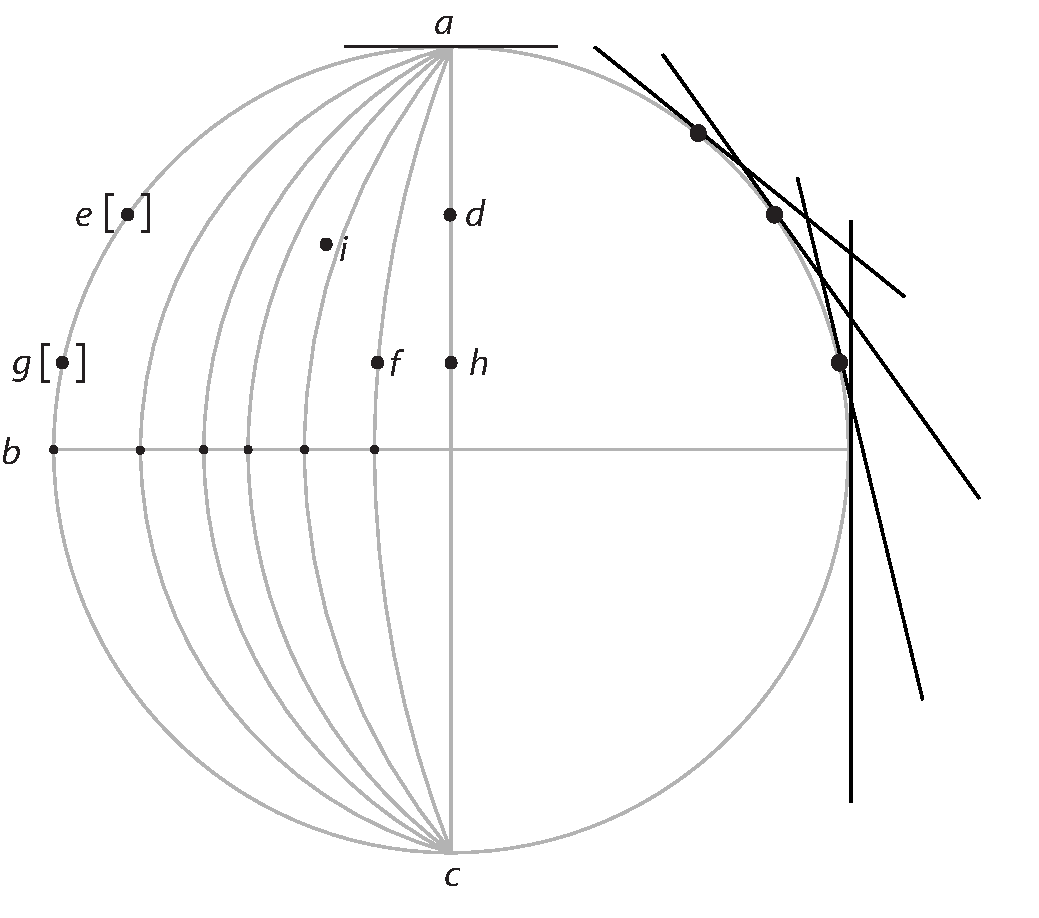
\includegraphics[width=0.65\textwidth]{images/38_21v.pdf}}





\mainmatter







\part[tocentry={I.~AKUSTIK, ELASTIZITÄT, FESTIGKEIT},
head={I.~AKUSTIK, ELASTIZITÄT, FESTIGKEIT}]%
{I.~AKUSTIK, ELASTIZITÄT, FESTIGKEIT}	%



\chapter[tocentry={Corporum connexio a motu orta  %
\enskip\bracks{%
Winter 1670/1671 -- Frühjahr 1683 (?)%
}}, %
head={Corporum connexio a motu orta %
}]%
{\MakeUppercase{Corporum connexio a motu orta} %
\newline\bracks{%
Winter 1670/1671 -- Frühjahr 1683 (?)%
}} %
\label{60250}
\selectlanguage{ngerman}%
\frenchspacing%
\begin{ledgroupsized}[r]{120mm}%
\footnotesize%
\pstart%
\noindent%
\textbf{Überlieferung:}%
\pend%
\end{ledgroupsized}%
\begin{ledgroupsized}[r]{114mm}%
\footnotesize%
\pstart%
\parindent -6mm%
\makebox[6mm][l]{\textit{L}}%
Notiz:
LH XXXVII\;4 Bl.\;95.
Ein Zettel (10\;x\;6,5 cm);
Ränder beschnitten;
Papier\-erhal\-tungs\-maßnahmen.
Eine Seite auf Bl.\;\href{\Scan{LH_37_04_095r}}{95\,r\textsuperscript{o}}.
Bl.\;\href{\Scan{LH_37_04_095v}}{95\,v\textsuperscript{o}} ist unbeschrieben.
\pend%
\end{ledgroupsized}%
\vspace{5mm}%
\begin{ledgroup}%
\footnotesize%
\pstart%
\noindent%
\textbf{Datierungsgründe:}
Der Träger der undatierten Notiz N.\;\ref{60250}, die eine Bemerkung zum Ursprung der Körperkohäsion festhält, weist weder Spuren eines Wasserzeichens noch sonstige datierungsrelevante äußere Merkmale auf. %
Der Text zeigt aber eine bemerkenswerte terminologische Nähe zur \textit{Hypothesis physica nova} (Mainz 1671).\cite{00256} %
So etwa ist der Ausdruck \textit{aether, qui est fortasse ille spiritus Domini} (unten, \refpassage{LH_37_04_095_095r_spiritus-1}{LH_37_04_095_095r_spiritus-2}) nahezu identisch in der wohl im Winter 1670/1671 entstandenen Abhandlung anzutreffen:
\textit{AEHTER (is enim fortasse est ille spiritus Dominis qui super aquis ferebatur ...} (§\;7; \textit{LSB} VI,\;2 N.\;40, S.\;225.9\,f.).\cite{00256}
Und auch die Darstelluung der durch die Bewegung des Äthers "animierten" Blasen (\textit{bullae}) \textit{tanquam rerum stamina} (unten, \refpassage{LH_37_04_095_095r_stamina-1}{LH_37_04_095_095r_stamina-2}) findet ihr Pendant in der frühen naturphilosophischen Schrift:
\textit{Hae jam bullae sunt semina rerum, stamina specierum, receptacula aetheris, corporum basis, consistentiae causa et fundamentum tantae varietatis quantam in rebus, tanti impetus quantum in motibus admiramus} (§\;12; \textit{LSB} VI,\;2 N.\;40, S.\;226.14--16).\cite{00256}
Die Annahme liegt somit nahe, dass die Notiz N.\;\ref{60250} in einem ähnlichen Zeitraum wie die \textit{Hypothesis physica nova}\cite{00256} entstand, d.\,h. um den Winter 1670/1671.
\pend%
\pstart%
Es gilt jedoch zu beachten, dass Leibniz in seinen physikalischen Überlegungen über die Ursache der Körperkohäsion noch recht lange auf die "Blasen"-Begrifflichkeit zurückgriff, so etwa noch in dem auf die Zeitspanne zwischen Ende Januar und März\,/\,April 1683 datierbaren Entwurf \textit{Explicatio mechanica elastri} (\textit{LSB} VIII,\;3 N.\;14\textsubscript{3}, S.\;206--208).\cite{01437}
Und der Gedanke, dass von der Bewegung eines dünnen Fluidums wie des Äthers der Zusammenhalt der Körper herrühre, lässt sich sogar bis in die frühen Jahre des 18.\;Jahrhundert verfolgen (siehe etwa \textit{LSB} VIII,\;3 N.\;33).\cite{02608}
Daher ist nicht auszuschließen, dass die Notiz N.\;\ref{60250} bis wenigstens zum Frühjahr 1683 entstanden sein könnte, als die "Blasen"-Begrifflichkeit noch in Verwendung war.
Die terminologische Nähe zur \textit{Hypothesis physica nova}\cite{00256} lässt aber eine frühere Entstehung vermuten.%
\pend%
\end{ledgroup}%
\selectlanguage{latin}%
\frenchspacing%
\vspace{8mm}%
\normalsize%
\pstart%
\noindent%
\lbrack%
\href{\Scan{LH_37_04_095r}}%
{95\,r\textsuperscript{o}}%
\rbrack\
Quod
\edtext{%
connexio corporum%
\indexS{connexio corporum}%
\indexS{corpora connexa}%
}{%
\lemma{connexio}%
\Bfootnote{%
\textit{(1)}~rerum\indexS{connexio rerum} %
\textit{(2)}~corporum%
~\textit{L}%
}}
oriatur a motu%
\indexS{motus origo connexionis}%
\indexS{origo connexionis corporum}
confirmat alabastri pulvis,%
\indexS{pulvis alabastri}%
\indexS{alabaster}
qui fusus ebullit,%
\indexS{pulvis ebullens}
bullae autem connexionem partium habent.%
\indexS{bulla habens connexionem partium}%
\indexS{connexio partium}%
\indexS{partes connexae}
\edtext{%
Cessante calore%
\indexS{calor cessans}%
}{%
\lemma{Cessante}%
\Bfootnote{%
\textit{(1)}~ebullitione\indexS{ebullitio} %
\textit{(2)}~calore%
~\textit{L}%
}}
reperitur merus pulvis.
Eodem modo
\edlabel{LH_37_04_095_095r_spiritus-1}%
aether,%
\indexS{aether interlabens}
qui est fortasse ille spiritus Domini%
\indexS{spiritus Domini}%
\edlabel{LH_37_04_095_095r_spiritus-2}%
\lbrack,\rbrack\
motu suo%
\indexS{motus aetheris}
massam%
\indexS{massa}
quae
ipsius interlabentis actione sublata%
\indexS{actio aetheris}%
\indexS{aether interlabens}
in pulverem mortuum concideret,%
\indexS{pulvis mortuus}
\edlabel{LH_37_04_095_095r_stamina-1}%
in bullas %
tanquam rerum stamina%
\indexS{bullae tanquam stamina rerum}%
\indexS{stamina rerum}
animavit.%
\edlabel{LH_37_04_095_095r_stamina-2}
Idem confirmat limatura ferri,%
\indexS{limatura ferri}%
\indexS{ferrum}
quae
interlabente magnetis admoti effluvio%
\indexS{effluvius magnetis}%
\indexS{magnes}
quasi in filamenta concrescit.%
\indexS{filamentum limaturae}
\pend%
\selectlanguage{latin}%
\frenchspacing%
\normalsize%
\newpage%




\chapter[tocentry={Der Donner als Echo 
\enskip%
\bracks{%
1672 -- frühe 1680er Jahre (?)}%
}, %
head={Der Donner als Echo %
}]%
{\MakeUppercase{Der Donner als Echo} %
\newline%
\bracks{%
1672 -- frühe 1680er Jahre (?)%
}%
}%
\label{56218}
\selectlanguage{ngerman}%
\frenchspacing%
\begin{ledgroupsized}[r]{120mm}%
\footnotesize%
\pstart%
\noindent%
\textbf{Überlieferung:}%
\pend%
\end{ledgroupsized}%
\begin{ledgroupsized}[r]{114mm}%
\footnotesize%
\pstart%
\parindent -6mm%
\makebox[6mm][l]{\textit{E}}%
Druck nach unbekannter Vorlage:
\textsc{Gerland} 1906, S.\;11 (N.\;8, titellos).%
\cite{00197}
Bei der verschollenen handschriftlichen Vorlage soll es sich laut \textit{E} um ein \textit{Kleines schlecht geschriebenes Blättchen von Leibnizens Hand} gehandelt haben.
Der oft fehlerhafte Text von \textit{E} (Gerlands Transkription) wird hier wiedergegeben und gegebenenfalls berichtigt oder kommentiert; die Rechtschreibung wird an die Editionsregeln angepasst.
\pend%
\end{ledgroupsized}%
\vspace{5mm}%
\begin{ledgroup}%
\footnotesize%
\pstart%
\noindent%
\textbf{Datierungsgründe:}
Im titellosen und undatierten Text N.\;\ref{56218}, der nach heutigem Wissensstand lediglich im posthumen Druck \textit{E} %
überliefert ist, wird auf die Beschreibung des Karpaten-Gebirges\indexO{Karpaten} in Daniel Fröhlichs\indexN{\textls{Frölich} (Frolichius, Frölichius), David 1595\textendash1648} %
\textit{Bibliotheca seu Cynosura peregrinantium}\cite{00047} %
hingewiesen (siehe unten den Erläuterungsapparat).
Ob Leibniz diese Beschreibung aus erster Hand kannte oder aber aus deren Wiedergabe in Otto von Guerickes\indexN{\textls{Guericke} (Gerickius, Gericke), Otto von 1602\textendash1686} %
\textit{Experimenta nova} (siehe unten den Erläuterungsapparat), %
es steht fest, dass Erwähnungen von Frölichs Werk im Leibniz-Nachlss nach heutigem Wissensstand frühestens auf das Jahr 1672 zurückgehen (vgl. \textit{LSB} VIII,\;1 N.\;36, S.\;263.6--7, 266.3; \textit{LSB} VIII,\;1 N.\;62, S.\;570, Randbemerkung zu Z.\;15\:f.).\cite{01197}\cite{01278}
Es ist demgemäß unwahrscheinlich, dass die Aufzeichung N.\;\ref{56218} vor 1672 verfasst wurde.
\pend%
\pstart%
An Fröhlichs\indexN{\textls{Frölich} (Frolichius, Frölichius), David 1595\textendash1648} Beschreibung knüpft Leibniz erneut in dem auf die Zeitspanne 1681 bis 1682 datierbaren Entwurf \textit{Explicatio mechanica soni} an (\textit{LSB} VIII,\;3 N. 12\textsubscript{2}, S.\;110.18).\cite{01481}
Da keine weiteren Erwähnungen dieses Berichts im Leibniz-Nachlass bekannt sind, dürfte auch der Text N.\;\ref{56218} nicht viel später entstanden sein.
Die Aufzeichnung N.\;\ref{56218} könnte tatsächlich noch Anfang der 1680er Jahre entstanden sein, als Leibniz sich intensiv mit Fragen der physikalischen Akustik, insbesondere mit der Entstehung und Übertragung des Schalls, befasste.
\pend%
\pstart%
Bei seinem Bericht über ein besonderes Widerhallphänomen in der Helmstedter\indexO{Helmstedt} Umgebung, das für die Studenten der dortigen \textit{Academia Julia} eine Vergnügungsangelegenheit gewesen sein soll, bezieht sich Leibniz im Text N.\;\ref{56218} auf eine (nicht ermittelte) Quelle, die offenbar auch Otto von Guericke\indexN{\textls{Guericke} (Gerickius, Gericke), Otto von 1602\textendash1686} bekannt war (siehe unten den Erläuterungsapparat).
Auch dieser Umstand verfestigt den Eindruck, dass der Text N.\;\ref{56218} eher in frühen Jahren entstand, d.\,h. nicht viele Jahre später als 1672.
\pend%
\end{ledgroup}%
\selectlanguage{latin}%
\frenchspacing%
\newpage%
\normalsize%
\pstart%
\noindent%
\lbrack S.\:11\rbrack\
Der Donner%
\indexS{Donner}
scheint großenteils ein Echo%
\indexS{Echo}
in den Wolken%
\indexS{Wolken}
zu seyn,
wie denn solcher aus der
\edtext{%
relation des
\edtext{%
F\lbrack r\rbrack olichii%
\indexN{\textls{Frölich} (Frolichius, Frölichius), David 1595\textendash1648}%
}{%
\lemma{Fiolichii}%
\Bfootnote{%
\textit{L\;ändert Hrsg.}%
}}
de Carpathis monte%
\indexO{Karpaten}%
}{%
\lemma{relation \lbrack...\rbrack\ monte}%
\Cfootnote{%
Siehe die Beschreibung der bei der Besteigung des Karpaten-Gebirges\indexO{Karpaten} beobachteten Phänomene des Widerhalls in
\textsc{D.\;Frölich}, %
\textit{Bibliotheca seu Cynosura peregrinantium}, %
\glqq Geographia\grqq, cap.\;IX, §\;372\,f.
(Band II.1, Ulm 1643, S.\;287\,f.).\cite{00047} %
Vom natürlichen Donner ist dort allerdings nirgendwo die Rede.
Zitiert war Frölichs%
\indexN{\textls{Frölich} (Frolichius, Frölichius), David 1595\textendash1648}
Beschreibung auch in
\textsc{O.\;v.\;Guericke}, \textit{Experimenta nova},
lib.\;V, cap.\;8 (Amsterdam 1672, S.\;162).\cite{00055}
Das Zitat wurde von Leibniz in seinen Guericke-Auszügen exzerpiert
(\textit{LSB} VIII,\;1 N.\;36, S.\;266.5–7).\cite{01197}%
}}
und anderen umbständen abzunehmen.
Daher auch der Donner%
\indexS{Donner}
fortzulauffen und sich uns zu nähern scheint.
\edtext{%
Etwa eine Meile%
\indexS{Meile}
von
\edtext{%
Helmstad%
\indexO{Helmstedt}%
}{%
\lemma{Helmstad}%
\Cfootnote{%
Die Hansestadt Helmstedt war von 1576 bis 1810 Sitz der protestantischen Universität \textit{Academia Julia}.%
}}
bey einem Dorff%
\indexS{Dorf}
\edtext{%
zum Drewdel%
\indexO{Drewdel (?) bei Helmstedt}%
}{%
\lemma{zum Drewdel}%
\Cfootnote{%
Nicht ermittelt.%
}}
ist ein
\edtext{%
aus%
}{%
\lemma{aus}%
\Cfootnote{%
Die Lesung ist unsicher.%
}}
der maßen schöhnes Echo,%
\indexS{Echo}
welches den Donner%
\indexS{Donner}
wohl nachahmet.
Die Studenten%
\indexS{Student}
kommen bisweilen dahin,
bringen kleine mörser%
\indexS{Mörser}
mit hinauß
und schießen im Holz%
\indexS{Holz}
herumb%
\lbrack;\rbrack\
in der ebene%
\indexS{Ebene}
zeiget sich wie ein
\edtext{%
gelbes(?)%
}{%
\lemma{gelbes(?)}%
\Cfootnote{%
Die Lesung ist, wie \textit{E} selbst vermerkt, unsicher.%
}}
theatrum,%
\indexS{theatrum}
der schall%
\indexS{Schall}
antwortet erstlich sehr stark ein baar mahl,
dann wird er immer geschwinder und schwächer
und laufft also wie ein Donner%
\indexS{Donner}
an dem Wald%
\indexS{Wald}
herumb.%
}{%
\lemma{Etwa \bracks{...} herumb}%
\Cfootnote{%
Das Phänomen eines besonderen Widerhalls in der Helmstedter Umgebung\indexO{Helmstedt} findet Erwähnung auch in
\textsc{Guericke}, \textit{Experimenta nova},
lib.\;IV, cap.\;10 (S.\;139b).\cite{00055}
Dies kann allerdings nicht die (einzige) Quelle von Leibnizens detaillirterem Bericht sein.%
}}
\pend%
\selectlanguage{latin}%
\frenchspacing%
\normalsize%
\newpage%




\chapter[tocentry={Aus Erhard Weigel, Pendulum ex tetracty deductum 
\enskip \bracks{zweite Hälfte Dezember 1676 -- erste Monate 1677~(?)}},
head={Aus Erhard Weigel, Pendulum ex tetracty deductum}]%
{\MakeUppercase{Aus Erhard Weigel, Pendulum ex tetracty deductum}
\newline \bracks{zweite Hälfte Dezember 1676 -- erste Monate 1677~(?)}}
\label{38575}
\selectlanguage{ngerman}%
\frenchspacing%
\begin{ledgroupsized}[r]{120mm}%
\footnotesize%
\pstart%
\noindent\textbf{Überlieferung:}%
\pend%
\end{ledgroupsized}%
\begin{ledgroupsized}[r]{114mm}%
\footnotesize%
\pstart%
\parindent -6mm%
\makebox[6mm][l]{\textit{L}}%
Auszug aus
\textsc{E.\;Weigel} \bracks{Praeses}, \textit{Pendulum ex tetracty deductum}
\bracks{Dissertation: Kandidat \textsc{H.\:C. Ebell}},
Jena 1674 (nicht paginiert):\cite{02541}
LBr~250 Bl.\;1.
Ein Papierstreifen.
Drei Zeilen auf Bl.\;\href{\Scan{LBr_250_001r}}{1\,r\textsuperscript{o}};
die \href{\Scan{LBr_250_001v}}{Rückseite} ist unbeschrieben.
\pend%
\end{ledgroupsized}%
\vspace{5mm}%
\begin{ledgroup}%
\footnotesize%
\pstart%
\noindent%
\textbf{Datierungsgründe:}
Der Träger des undatierten, notizartigen Auszugs N.\;\ref{38575} weist weder Spuren eines Wasserzeichens noch irgendein äußeres datierungsrelevantes Merkmal auf.
Die im Text zitierte Dissertation \textit{Pendulum ex tetracty deductum}\cite{02541} wurde im Herbst 1674 in Jena\indexO{Jena} veröffentlicht (das Vorwort des Betreuers Erhard Weigel\indexN{\textls{Weigel}, Erhard 1625\textendash1699} trägt das Datum 21.\;September 1674).
Da sich Leibniz zu jener Zeit in Paris\indexO{Paris} aufhielt, ist anzunehmen, dass er die Dissertation erst nach seiner Übersiedlung nach Hannover\indexO{Hannover} Mitte Dezember 1676 lesen konnte.
Hieraus ergibt sich der Terminus post quem der vorgeschlagenen Datierung.%
\pend%
\pstart%
Relevant für die Bestimmung des Terminus ante quem ist möglicherweise die Tatsache, dass der Auszug N.\;\ref{38575} -- lediglich eine wohlgesinnte Anspielung auf Leibnizens \textit{Hypothesis physica nova}\cite{00256} umfassend -- im Nachlass unter der Signatur LBr~250 überliefert ist, welche den Briefwechsel zwischen Leibniz und Honoré Fabri\indexN{\textls{Fabri}, Honoré 1607\textendash1688} umfasst.
Leibnizens letzter Brief an Fabri, wahrscheinlich in den ersten Monaten 1677 verfasst (vgl. \textit{LSB} II,\;1\textsuperscript{2} N.\;133),\cite{01309} befasst sich unter anderem mit der aus der \textit{Hypothesis physica nova}\cite{00256} stammenden Erklärung der Natur physikalischer Körper, auf welche auch der Auszug N.\;\ref{38575} Bezug nimmt.
Diese Feststellung lässt die Annahme zu, dass N.\;\ref{38575} im Zusammenhang mit Leibnizens letztem Brief an Fabri\indexN{\textls{Fabri}, Honoré 1607\textendash1688} entstanden sein könnte.
Eine spätere Datierung ist jedoch möglich, zumal Leibniz sich noch lange mit dem Erklärungsmodell aus der \textit{Hypothesis physica nova}\cite{00256} befasst hat, wie etwa einige in \textit{LSB} VIII,\;3 veröffentlichte Texte zeigen.%
\pend%
\end{ledgroup}%
\selectlanguage{latin}%
\frenchspacing%
\normalsize%
\vspace{8mm}%
\pstart%
\noindent%
\bracks{%
\href{\Scan{LBr_250_001r}}%
{1\,r\textsuperscript{o}}%
}
\edtext{%
Weigelius%
\indexN{\textls{Weigel}, Erhard 1625\textendash1699}
diss. de \textit{Pendulo}%
\indexS{pendulum}%
\indexS{dissertatio}
corollar. ultimo%
\bracks{:}
\textit{%
Speciosa est
\edtext{%
Hypothesis Leibnitiana,%
\indexS{hypothesis Leibnitiana}
quae bullulis%
\indexS{bullulae}
pleraque corporum phaenomena%
\indexS{phenomena corporum}
salvare docet.%
}{%
\lemma{\textit{Speciosa} \bracks{...} \textit{docet}}%
\Cfootnote{%
Anspielung an
\textsc{G.\:W.\;Leibniz},
\textit{Hypothesis physica nova},
§\;11\,ff.
(Mainz 1671;
\textit{LSB} VI,\;2 N.\;40, S.\;226\,ff.).%
\cite{00256}%
}}%
}%
}{%
\lemma{Weigelius \bracks{...} \textit{docet}}%
\Cfootnote{%
\textsc{E.\;Weigel} \bracks{Präses}, \textit{Pendulum ex tetracty deductum}
\bracks{Dissertation: Kandidat \textsc{H.\:C.\,Ebell}},
corollaria, n.\;8
(Jena 1674, Bl.\;\bracks{E4\,v\textsuperscript{o}}).
Die Vorlage liest \textit{Leibnüziana} statt \textit{Leibnitiana}.%
\cite{02541}%
}}
\pend%
\selectlanguage{latin}%
\frenchspacing%
\normalsize%




\chapter[tocentry={Aero-nautica 
\enskip\bracks{zweite Hälfte Dezember 1676 -- Dezember 1679}},
head={Aero-nautica }]%
{\MakeUppercase{Aero-nautica}
\newline\bracks{zweite Hälfte Dezember 1676 -- Dezember 1679}}
\label{56215}
\selectlanguage{ngerman}%
\frenchspacing%
\begin{ledgroupsized}[r]{120mm}%
\footnotesize%
\pstart%
\noindent%
\textbf{Überlieferung:}%
\pagelabel{Gerland_1906_007-009_uebrlf}%
\pend%
\end{ledgroupsized}%
\begin{ledgroupsized}[r]{114mm}%
\footnotesize%
\pstart%
\parindent -6mm%
\makebox[6mm][l]{\textit{E}}%
Druck nach unbekannter Vorlage:
\textsc{Gerland} 1906, S.\;7--9 (Nr.\;5).\cite{00197}
Die verschollene handschriftliche Vorlage wies laut \textit{E} (S.\;7) das Format eines Oktav-Blattes auf.
Der oft fehlerhafte Text von \textit{E} %
wird hier wiedergegeben und ggf. berichtigt oder kommentiert;
die Rechtschreibung wird an die Editionsregeln angepasst.
\pend%
\end{ledgroupsized}%
\vspace{5mm}%
\begin{ledgroup}%
\footnotesize%
\pstart%
\noindent%
\textbf{Datierungsgründe:}
Die Datierung des Konzepts N.\;\ref{56215} beruht auf inhaltlichen Betrachtungen.
Siehe die ausführliche Begründung auf S.\;\pageref{56215_dat}.%
\pend%
\end{ledgroup}%
\selectlanguage{latin}%
\frenchspacing%
\vspace{6mm}%
\normalsize%
\pstart%
\noindent%
\lbrack S.\;7\rbrack\
\hfill%
Aero-nautica%
\indexS{aeronautica}
\hfill%
\phantom{\lbrack S.\;7\rbrack}%
\pend%
\vspace{0.5em}
\pstart%
\noindent%
\edtext{%
\edlabel{Gerland_1906_007-009_hestz-1}%
Aeris pes cubicus pondere aequat unciam unam cum dimidia.%
\edlabel{Gerland_1906_007-009_hestz-2}%
\indexS{uncia}%
\indexS{pes cubicus aeris}%
\indexS{pondus aeris communis}%
\indexS{aer communis}%
}{%
\lemma{Aeris \lbrack...\rbrack\ dimidia}%
\Cfootnote{%
Vgl. P.\:\textsc{Lohmeier}, \textit{Exercitatio physica}, §\;8 (Rinteln 1676, S.\;7f.).\cite{01422}
Siehe zudem F.\,\textsc{Lana\:de\:Terzi},
\textit{Prodromo}, I Teil, cap.\;6 (Brescia 1670, S.\;53).\cite{00069}%
}}
\edtext{%
\edlabel{Gerland_1906_007-009_xtd-1}%
Laminae e cupro satis adhuc consistentes%
\indexS{lamina cuprea}%
\indexS{lamina consistens}
pedem unum longae et latae,%
\indexS{pes}%
\indexS{pes quadratus laminae cupreae}
quae tres uncias suo pondere non excedant;%
\indexS{pondus laminae cupreae}%
\indexS{uncia}%
\edlabel{Gerland_1906_007-009_xtd-2}%
}{%
\lemma{Laminae \lbrack...\rbrack\ excedant}%
\Cfootnote{Vgl. \textsc{Lohmeier}, \textit{Exercitatio physica}, §\;21 (S.\;14) u. §\;30 (S.\;18).\cite{01422}
Siehe zudem \textsc{Lana\:de\:Terzi},
\textit{Prodromo}, I Teil, cap.\;6 (S.\;56).\cite{00069}%
}}
\edtext{%
\edlabel{Gerland_1906_007-009_crj-1}%
quarum 12 constituunt libram.%
\indexS{libra}%
\edlabel{Gerland_1906_007-009_crj-2}%
}{%
\lemma{quarum \lbrack...\rbrack\ libram}%
\Cfootnote{Vgl. \textsc{Lohmeier}, \textit{Exercitatio physica}, §\;8 (S.\;8) u. §\;21 (S.\;14).\cite{01422}
Siehe zudem \textsc{Lana\:de\:Terzi},
\textit{Prodromo}, I Teil, cap.\;6 (S.\;53).\cite{00069}%
}}
Sphaera ex his laminis,%
\indexS{sphaera e lamina cuprea}
quae pedem haberet in diametro,%
\indexS{diameter sphaerae}%
\indexS{pes}
esset (secluso aere) ponderis $9\dfrac{3}{7}$ unciarum.%
\indexS{pondus sphaerae cupreae}%
\rule[0.0mm]{0.0mm}{5.6mm}
Nam diam. sphaerae est \textit{a},
nempe 1 pes,
circumf. $\dfrac{22}{7}a$,
superficies sphaerae est $\dfrac{22}{7}a^2$,%
\indexS{superficies sphaerae}%
\rule[0.0mm]{0.0mm}{5.6mm}
sit $a^2$
\edtext{%
pes%
\indexS{pes}%
}{%
\lemma{pes}%
\Cfootnote{%
Ein Quadratfuß
(vgl. \refpassage{Gerland_1906_007-009_xtd-1}{Gerland_1906_007-009_xtd-2}.)%
}}
\edtext{%
un\lbrack us\rbrack%
}{%
\lemma{una}%
\Bfootnote{%
\textit{E\;ändert Hrsg.}\cite{00197}%
}%
\lemma{un\lbrack us\rbrack}%
\Cfootnote{%
In \textit{E} ist die möglicherweise von einer Verlesung herrührende Unstimmigkeit \textit{una vel 3 unc.} mit \lbrack!\rbrack\ markiert.%
}%
}
vel 3 unc., %
erit superficies sphaerae%
\indexS{superficies sphaerae}
$\dfrac{66}{7}$ unc.%
\rule[0.0mm]{0.0mm}{5.6mm}
seu $9\dfrac{3}{7}$ unc.%
\indexS{uncia}
\pend%
\pstart%
Aeris inclusi pondus esset $\dfrac{11}{14}$ unc.%
\indexS{aer inclusus sphaerae cupreae}%
\indexS{pondus aeris inclusi}%
\indexS{uncia}
Nam
\edtext{%
area externa%
}{%
\lemma{area externa}%
\Cfootnote{%
Gemeint ist das Volumen der Kugel.
In \textit{E} ist die Textstelle mit \lbrack?\rbrack\ markiert.
Die Unstimmigkeit rührt möglicherweise von einer Verlesung her.
}}
sphaerae fit
multiplicata superficie eius per sextam partem diametri,%
\indexS{diameter sphaerae}
seu $\dfrac{22}{7 \cdot 6}a^3$,
est autem $a^3$ pondus $1\dfrac{1}{2}$ unciae,
fiet $\dfrac{22}{7 \cdot 6}a^3$ aequ. $\dfrac{11}{14}$ unc.%
\indexS{uncia}%
\rule[0.0mm]{0.0mm}{5.6mm}
\lbrack S.\;8\rbrack\
\pend%
\newpage%
\pstart%
Multiplicemus \textit{a} per \textit{b}
fiet $\dfrac{22}{42} a^3 b^3$ aequ. $\dfrac{11}{14}b^3$
et
\edtext{%
$\dfrac{22}{7}a^2[b^2]$%
}{%
\lemma{$b^2$}%
\Bfootnote{%
\textit{erg. Hrsg.}%
}}
aequ. $\dfrac{66}{7}b^2$,
debent esse $\dfrac{66}{7}b^2$ aequ. $\dfrac{11}{14}b^3$
seu fiet: 12 aequ. \textit{b},
itaque si ponatur sphaera pedum 12%
\indexS{pes}
aequale erit pondus sphaerae cupreae%
\indexS{pondus sphaerae cupreae}%
\indexS{sphaera cuprea}%
\rule[0.0mm]{0.0mm}{4.8mm}
et aeris ei inclusi.%
\indexS{pondus aeris inclusi}%
\indexS{aer inclusus sphaerae cupreae}
\pend%
\pstart%
Generaliter sphaerae cupreae pondus est%
\indexS{pondus sphaerae cupreae}%
\indexS{sphaera cuprea}
\edtext{%
\lbrack$\dfrac{66}{7}b^2$\rbrack%
}{%
\lemma{$\dfrac{11}{14}b^3$}%
\Bfootnote{%
\textit{E\;ändert Hrsg.}\cite{00197}%
}}
unciarum%
\indexS{uncia}%
\rule[0.0mm]{0.0mm}{5.6mm}
posito \textit{b} esse numerum pedum diametri,%
\indexS{diameter sphaerae}
et aeris inclusi pondus est%
\indexS{pondus aeris inclusi}%
\indexS{aer inclusus sphaerae cupreae}
\edtext{%
\lbrack$\dfrac{11}{14}b^3$\rbrack%
}{%
\lemma{$\dfrac{66}{7}b^2$}%
\Bfootnote{%
\textit{E\;ändert Hrsg.}\cite{00197}%
}}
unciarum%
\indexS{uncia}%
\rule[0.0mm]{0.0mm}{4.8mm}
posito \textit{b} numero eodem.%
\edlabel{Gerland_1906_007-009_scheitel-1}
\pend%
\pstart%
\edlabel{Gerland_1906_007-009_scheitel-2}%
Sed mea sententia%
\indexS{sententia}%
\rule[0.0mm]{0.0mm}{4.6mm}
laminae istae cupreae%
\indexS{lamina cuprea}
sunt nimis tenues.
Itaque calculum instituamus%
\indexS{calculus generalior}%
\rule[0.0mm]{0.0mm}{5.2mm}
generalius.
Numerus pedum diametri sphaerae%
\indexS{diameter sphaerae}%
\indexS{pes}
sit \textit{b}.
\edlabel{Gerland_1906_007-009_itu-1}%
\textit{A} sit 4%
\edlabel{Gerland_1906_007-009_itu-2}
\edtext{%
pe\lbrack de\rbrack s%
}{%
\lemma{pes}%
\Bfootnote{%
\textit{E\;ändert Hrsg.}\cite{00197}%
}}
et area superficiei sphaerae%
\indexS{superficies sphaerae}%
\indexS{sphaera cuprea}
$\dfrac{22}{7}b^2 4^2$
et area solidi%
\indexS{area solidi}%
\indexS{solidum sphaerae}
$\dfrac{11}{21}b^3 A^3$,%
\rule[0.0mm]{0.0mm}{5.6mm}
seu unius pedis quadrati cuprei pondus%
\indexS{pondus pedis quadrati cuprei}%
\indexS{pes quadratus}
esto~\textit{c},
similiter
\edtext{%
$A^3$ seu unius pedis cubici pondus%
\indexS{pes cubicus}%
\indexS{pondus pedis cubicis aeris}%
\indexS{pondus aeris inclusi}%
}{%
\lemma{$A^3$ \lbrack...\rbrack\ pondus}%
\Cfootnote{%
Die Angabe widerspricht der Setzung $A = 4$ Fuß
(vgl. \refpassage{Gerland_1906_007-009_itu-1}{Gerland_1906_007-009_itu-2}).%
}}
esto aequale $1\dfrac{1}{2}$ unc.%
\indexS{uncia}%
\rule[0.0mm]{0.0mm}{5.2mm}
\par%
\begin{edtabularl}%
&
fiet 
&
\hspace*{1.0mm}%
pondus cupreae sphaerae%
\indexS{pondus sphaerae cupreae}%
\indexS{sphaera cuprea}%
\rule[0.0mm]{0.0mm}{5.2mm} &
\hspace*{12.5mm}%
$\dfrac{22}{7}b^2 c$ & \\
& 
&
\hspace*{1.0mm}%
pondus autem aeris inclusi%
\indexS{pondus aeris inclusi}%
\indexS{aer inclusus sphaerae cupreae}%
\rule[0.0mm]{0.0mm}{5.6mm}%
&
\hspace*{12.5mm}%
$\dfrac{11}{21}b^3 \dfrac{3}{2}$ unc. & \\
& & &
\rule[0.0mm]{0.0mm}{5.6mm}%
\hspace*{13.0mm}%
seu $\dfrac{11}{14}b^3$ unc. &
\end{edtabularl}%
\pend%
\pstart%
\noindent%
Rem ergo breviter ita ponamus%
\rule[0.0mm]{0.0mm}{4.8mm}%
\lbrack:\rbrack\
\par%
\begin{edtabularl}%
&
Sit%
\rule[0.0mm]{0.0mm}{5.8mm} &
pondus pedis quadrati laminae cupreae%
\indexS{pondus laminae cupreae}%
\indexS{pes quadratus laminae cupreae} &
\textit{c} & \\
& &
varians pro crassitie laminae%
\indexS{crassities laminae cupreae}%
\indexS{lamina cuprea} & &
\\
& &
\rule[0.0mm]{0.0mm}{5.2mm}%
pondus%
\indexS{pondus pedis cubicis aeris}%
\indexS{pes cubicus aeris}%
\indexS{aer inclusus sphaerae cupreae}
\edtext{%
\lbrack pedis\rbrack%
}{%
\lemma{pedis}%
\Bfootnote{%
\textit{erg. Hrsg.}%
}}
cubici aeris &
$\dfrac{3}{2}$ unc. & \\
& &
\rule[0.0mm]{0.0mm}{4.2mm}%
numerus pedum diametri sphaerae%
\indexS{diameter sphaerae} &
\textit{b} & \\
&
Erit\rule[0.0mm]{0.0mm}{6.0mm} &
pondus sphaerae cupreae%
\indexS{pondus sphaerae cupreae}%
\indexS{sphaera cuprea} &
$\dfrac{22}{7}b^2 c$ & \\
\edatleft{\{}{4.0\baselineskip}
& &
pondus aeris inclusi%
\indexS{pondus aeris inclusi}%
\indexS{aer inclusus sphaerae cupreae}%
\rule[0.0mm]{0.0mm}{5.2mm} &
$\dfrac{11}{4}b^3$ unc. &
\edatright{\}}{4.0\baselineskip}%
\end{edtabularl}%
\pend%
\vspace{0.5em}%
\newpage%
\pstart%
\noindent%
Quare %
si laminam pedis quadrati cuprei%
\indexS{lamina cuprea}%
\indexS{pes quadratus laminae cupreae}
ponamus esse
\edlabel{Gerland_1906_007-009_crj-3}%
\edtext{%
duarum librarum%
\indexS{libra}
seu 32 unciarum:%
\indexS{uncia}%
}{%
\lemma{duarum \lbrack...\rbrack\ unciarum}%
\Cfootnote{%
Oben (\refpassage{Gerland_1906_007-009_crj-1}{Gerland_1906_007-009_crj-2}) wurde angegeben, dass ein Pfund zwölf Unzen gleiche.
Laut \textit{E} %
(S.\;9)\cite{00197} entspricht diese Einteilung dem "Apothekergewicht", während die Einteilung des Pfundes in sechzehn Unzen auf das "altfranzösische Gewicht" zurückgehe.
In der Frühneuzeit waren beide Systeme im deutschsprachigen Raum in Gebrauch.
Die Einteilung des Pfundes in sechzehn Unzen wird im Folgenden als Grundlage für die Berechnung verwendet.%
}}%
\edlabel{Gerland_1906_007-009_crj-4}
quaeratur magnitudo diametri talis,%
\indexS{magnitudo}%
\indexS{diameter sphaerae}
ut tantum ponderet sphaera cuprea%
\indexS{sphaera cuprea}%
\indexS{pondus sphaerae cupreae}
quantum aer inclusus,%
\indexS{aer inclusus sphaerae cupreae}%
\indexS{pondus aeris inclusi}
fiet:
\pend%
\pstart%
\noindent%
\centering%
$\dfrac{22}{7}b^2 \, 32 \ \text{unc.} \ \sqcap\, \ \dfrac{11}{14}b^3 \ \text{unc.}$
\pend%
\pstart%
\noindent%
seu fiet
$32 A \ \text{aequ.} \ b$%
\rule[0.0mm]{0.0mm}{4.6mm}
sive deberet esse sphaera 128 pedum.%
\indexS{pes}
\pend%
\pstart%
Generaliter
si quaeratur longitudo diametri sphaerae,%
\indexS{diameter sphaerae}%
\indexS{sphaera cuprea}
ut fiat aequatio,%
\indexS{aequatio}
habebitur $\dfrac{22}{7} b^2 c$ aequ. $\dfrac{11}{14}b^3$ unc.
seu 4\textit{c} unc. aequ. \textit{b},%
\indexS{uncia}
sive
\edtext{%
\edlabel{Gerland_1906_007-009_error-1}%
numerus \textit{b} quaesitus%
\indexS{numerus quaesitus}
erit ad~4 %
\edtext{%
\lbrack u\rbrack t%
}{%
\lemma{Ut}%
\Bfootnote{%
\textit{E\;ändert Hrsg.}\cite{00197}%
}}
pondus \textit{c} laminae pedis quadrati materiae,%
\indexS{pondus laminae cupreae}%
\indexS{pes quadratus laminae cupreae}%
\indexS{materia laminae cupreae}%
\indexS{lamina cuprea}
ex qua globum conficere volumus,%
\indexS{globus cupreus}
est ad unciam%
\indexS{uncia}%
\lbrack;\rbrack%
\edlabel{Gerland_1906_007-009_error-2}%
}{%
\lemma{numerus \lbrack...\rbrack\ unciam}%
\Cfootnote{%
Vielmehr gilt die Proportion:
$b : 4 = c\,\text{unc.} : 1.$
Vgl. zur Bestätigung den abschließenden Vermerk \refpassage{Gerland_1906_007-009_schlss-1}{Gerland_1906_007-009_schlss-2}.%
}}
itaque si lamina%
\indexS{lamina cuprea}
esset unius librae,%
\indexS{libra}
erit sphaera necessaria%
\indexS{sphaera cuprea}
minimum diametri 64 pedum%
\indexS{diameter sphaerae}%
\indexS{pes}%
\lbrack;\rbrack\
itaque rem ad usum transferri%
\indexS{res translata ad usum}%
\indexS{usus}
posse non puto.
Nam nec tantas sphaeras,%
\indexS{sphaera cuprea}
etiam per partes si quis parabit,
et si paratae essent,
quis credat laminas,%
\indexS{lamina cuprea}
si tanto ponderi comparentur tam tenues,
resistere posse ponderi tam immensi,%
\indexS{pondus immensum}
quantum est alias inviis ventis.%
\indexS{ventus invius}
Nec aequabilitas sphaerae%
\indexS{aequabilitas sphaerae cupreae}%
\indexS{sphaera cuprea}
\edtext{%
pr\lbrack aestari\rbrack%
}{%
\lemma{privare}%
\Bfootnote{%
\textit{E\;ändert Hrsg.}\cite{00197}%
}}
potest%
\lbrack:\rbrack\
ea enim tanta %
non potest
quia exiguae inaequalitates%
\indexS{inaequalitas exigua}
\edtext{%
supers\lbrack u\rbrack nt,%
}{%
\lemma{supersint}%
\Bfootnote{%
\textit{E\;ändert Hrsg.}\cite{00197}%
}}
quae horribili isti ponderi,%
\indexS{pondus horribile}
cui nihil in natura%
\indexS{natura}
simile visum est,%
\indexS{nihil simile in natura}
necessario cedent%
\lbrack;\rbrack\
itaque rem puto esse supra
\lbrack S.\;9\rbrack\
vires humanas.%
\indexS{res putanda supra vires humanas}%
\indexS{vis humana}
\pend%
\pstart%
\edlabel{Gerland_1906_007-009_schlss-1}%
\edtext{}{%
\xxref{Gerland_1906_007-009_schlss-1}{Gerland_1906_007-009_schlss-2}%
\lemma{Numerus \lbrack...\rbrack\ manentis}%
\Cfootnote{%
Wohl ein nachträglicher Vermerk, der die ungenaue Formulierung im Haupttext,
\refpassage{Gerland_1906_007-009_error-1}{Gerland_1906_007-009_error-2},
und in der Randbemerkung,
\refpassage{Gerland_1906_007-009_rndbmrk-1}{Gerland_1906_007-009_rndbmrk-2},
berichtigt.
Siehe die entsprechenden Erläuterungen.%
}}%
Numerus unciarum ponderis laminae pedis quadrati materiae%
\indexS{uncia}%
\indexS{pondus laminae cupreae}%
\indexS{pes quadratus laminae cupreae}%
\indexS{materia laminae cupreae}%
\indexS{lamina cuprea}
unde fit sphaera%
\indexS{sphaera e lamina cuprea}
quadruplicatus%
\lbrack,\rbrack\
est
\edtext{%
numer\lbrack us\rbrack%
}{%
\lemma{numero}%
\Bfootnote{%
\textit{E\;ändert Hrsg.}\cite{00197}%
}}
pedum diametris sphaerae in suspenso in%
\indexS{pes}%
\indexS{diameter sphaerae}%
\indexS{sphaera suspensa in aere}%
\indexS{aer communis}
\edtext{%
aer\lbrack e\rbrack%
}{%
\lemma{aeri}%
\Bfootnote{%
\textit{E\;ändert Hrsg.}\cite{00197}%
}}
manentis.%
\edlabel{Gerland_1906_007-009_schlss-2}%
\pend%
\vspace{1.5em}%
\pstart%
\noindent%
\lbrack%
\textit{In der verschollenen handschriftlichen Vorlage war die folgende Randbemerkung laut E (S.\;9) \glqq in die Überschrift hineingeschrieben\grqq:}%
\rbrack%
\pend%
\vspace{0.5em}%
\pstart%
\noindent%
\edlabel{Gerland_1906_007-009_rndbmrk-1}%
\edtext{%
(Conclusi
numerum pedum diametri sphaerae esse ad numerum 4,%
\indexS{diameter sphaerae}
ut numerus unciarum ponderis laminae pedis quadrati
unde fieri debet sphaera,%
\indexS{sphaera e lamina cuprea}
est ad unciam%
\lbrack;\rbrack%
\edlabel{Gerland_1906_007-009_rndbmrk-2}%
}{%
\lemma{(Conclusi \lbrack...\rbrack\ unciam}%
\Cfootnote{%
Wieder die ungenaue Formulierung wie in der Passage
\refpassage{Gerland_1906_007-009_error-1}{Gerland_1906_007-009_error-2}.
Die Fortsetzung der Randbemerkung berichtigt die Aussage.%
}}
\edlabel{Gerland_1906_007-009_rndbmrk-3}%
seu numerum unciarum ponderis laminae pedis quadrati%
\indexS{uncia}%
\indexS{pondus laminae cupreae}%
\indexS{pes quadratus laminae cupreae}%
\indexS{lamina cuprea}
quadruplicatum%
\lbrack,\rbrack\
esse numerum pedum sphaerae minimae in aere elevabilis.)%
\indexS{sphaera minima elevabilis in aere}%
\indexS{sphaera cuprea}%
\indexS{pes}%
\indexS{aer communis}%
\edlabel{Gerland_1906_007-009_rndbmrk-4}%
\pend%
\vspace{2.0em}%
\pstart%
\noindent%
\centering%
*     *     *
\pend%
\vspace{2.0em}%
\selectlanguage{german}%
\frenchspacing%
\footnotesize%
\pstart%
\noindent%
\textls{Ausführliche Datierungsgründe:}%
\pagelabel{56215_dat}
Die vorliegende undatierte Aufzeichung N.\;\ref{56215} \textit{Aero-nautica}, die lediglich in einem modernen Druck überliefert ist (siehe oben, S.\;\pageref{Gerland_1906_007-009_uebrlf}), setzt die Beschreibung einer imaginären \textit{nave che camini sostentata sopra l'aria} voraus, welche bei F.\,\textsc{Lana\:de\:Terzi}, \textit{Prodromo overo Saggio di alcune inventioni nuove premesso all'arte maestra}, I Teil, cap.\;6 (Brescia 1670, S.\;52--61)\cite{00069} zu lesen und Leibniz bereits im Jahre 1671 bekannt war,
wie dessen Erwähnung in der \textit{Hypothesis physica nova}, §\;23\;\lbrack bis\rbrack\ (\textit{LSB} VI,\;2 N.\;40, S.\;232.30--233.21)\cite{00256} zeigt;
siehe zudem die zur gleichen Zeit entstandenen Auszüge aus Lanas \textit{Prodromo} (\textit{LSB} VIII,\;1 N.\;16).\cite{01103}
In N.\;\ref{56215} beschränkt sich Leibniz darauf, den Durchmesser einer kupfernen Kugel zu bestimmen, welche, von der inneren Luft entleert, in der äußeren Luft gemäß dem hydrostatischem Prinzip schweben sollte.
(Lanas\indexN{\textls{Lana de Terzi}, Francesco 1631\textendash1687} Vorstellung war nämlich, dass eine hinreichende Zahl derartiger Kugeln imstande sei, ein Schiff in die Luft mit zu heben.)
Im ersten Teil der Aufzeichnung (bis \refpassage{Gerland_1906_007-009_scheitel-1}{Gerland_1906_007-009_scheitel-1}) versucht Lebniz, den minimalen Wert des Durchmessers einer solchen Kugel festzulegen, wobei er von den gleichen physikalisch-metrischen Annahmen ausgeht wie Lana selbst (vgl. \textit{Prodromo},\cite{00069} S.\;53; 56):
Ein Kubikfuß Luft wiege anderthalb Unzen;
eine Unze sei der zwölfte Teil eines Pfundes;
ein Kupferblech, das drei Unzen je Quadratfuß wiege, sei für den Bau einer in der Luft schwebenden Kugel sowohl hinreichend dünn wie auch hinreichend fest.
Unter diesen drei Annahmen kommt er auf die Formeln $\displaystyle\frac{66}{7}b^2$ für das Gewicht der kupfernen Kugel und $\displaystyle\frac{11}{14}b^3$ für das Gewicht der eingeschlossenen Luft (mit \textit{b} als Durchmesser), welche eine Verallgemeinerung von Lanas\indexN{\textls{Lana de Terzi}, Francesco 1631\textendash1687} Ergebnissen darstellen.
\pend%
\pstart%
Diese Berechnung wird im zweiten Teil der vorliegenden Aufzeichnung (ab \refpassage{Gerland_1906_007-009_scheitel-2}{Gerland_1906_007-009_scheitel-2}) berichtigt:
Leibniz geht hierbei von der aus seiner Sicht realistischeren Annahme aus, dass eine für den Bau der erwünschten Kugel hinreichend feste Kupferplatte etwa 32 Unzen je Quadratfuß wiegen und somit um etwa das zehnfache dicker sein sollte, als von Lana\indexN{\textls{Lana de Terzi}, Francesco 1631\textendash1687} vorgeschlagen.
Hieraus folgt, dass die Kugel, um sich in der Luft heben zu können, einen Durchmesser von 128 Fuß besitzen sollte, wohingegen Lana\indexN{\textls{Lana de Terzi}, Francesco 1631\textendash1687} zu einem Wert von vierzehn Fuß gekommen war (vgl. \textit{Prodromo},\cite{00069} S.\;56).
Dies zeigt Leibniz zufolge, dass der Gedanke einer luftentleerten kupfernen Kugel, die in der Luft zu schweben vermöge, an seiner praktischen Umsetzung scheitern müsse.
Das allgemeine rechnerische Ergebnis der Untersuchung bleibt jedenfalls -- wie am Ende der Aufzeichnung (\refpassage{Gerland_1906_007-009_schlss-1}{Gerland_1906_007-009_schlss-2}) sowie in einer Randbemerkung im Kopf (\refpassage{Gerland_1906_007-009_rndbmrk-1}{Gerland_1906_007-009_rndbmrk-2}) festgehalten wird --, dass der Durchmesser der schwebenden Kugel mindestens viermal so viele Fuß lang sein müsse, wie Unzen ein Quadratfuß Kupferblech wiege.
(Bemerkenswert ist, dass im zweiten Teil der Aufzeichnung %
Leibniz die vorgefundene Unterteilung des Pfundes in zwölf Unzien aufgibt und stillschweigend durch eine Unterteilung in sechzehn Unzen ersetzt; vgl. \refpassage{Gerland_1906_007-009_crj-3}{Gerland_1906_007-009_crj-4}.)
\pend%
\pstart%
Die Vorlage, an die die vorliegende Aufzeichnung N.\;\ref{56215} \textit{unmittelbar} anknüpft, ist jedoch nicht Lanas \textit{Prodromo}\cite{00069}, sondern offenbar die von Philipp Lohmaier\indexN{\textls{Lohmeier} (Lohmeierus, Lomeierus), Philipp 1648\textendash1680} betreute Dissertation \textit{Exercitatio physica de artificio navigandi per aerem} (Rinteln 1676),\cite{01422} in welcher Lanas Gedanke eines Luftschiffes stillschweigend übernommen und erörtert wird.
Weder Lana\indexN{\textls{Lana de Terzi}, Francesco 1631\textendash1687} noch Lohmeier werden in N.\;\ref{56215} ausdrücklich erwähnt.
Die Sätze, mit denen am Anfang der Aufzeichnung die physikalischen Grundannahmen des Gedankensexperiments erklärt werden, geben jedoch nahezu wörtlich die entsprechenden Textpassagen der Dissertation wieder:
Vgl. N.\;\ref{56215}, \refpassage{Gerland_1906_007-009_hestz-1}{Gerland_1906_007-009_hestz-2} mit \textit{Exercitatio physica},\cite{01422} §\;8, S.\;7f. (\textit{Deprehendunt ... pondus illud} \lbrack\textit{= aeris}\rbrack\ \textit{accurati observatores tale, ut unus pes cubicus aeris aequet unciam unam cum dimidia ...})
sowie N.\;\ref{56215}, \refpassage{Gerland_1906_007-009_xtd-1}{Gerland_1906_007-009_crj-2} mit \textit{Exercitatio physica},\cite{01422} §\;21, S.\;14 (\textit{Denique suppono ... parari posse e cupro laminas aliquas satis adhuc consistentes globisque inde conficien}\lbrack\textit{d}\rbrack\textit{is aptas, quarum longitudo et latitudo unius pedis sit, et tamen pondere non excedant tres uncias ...})
und mit §\;30, S.\;18 (\textit{... assumo ... parari posse e cupro laminas aliquas pedem unum longas et latas, satis adhuc consistentes et pondere suo tres uncias non excedentes ...}).
Ferner lässt sich ein unmittelbarer Zusammenhang zwischen der Aufzeichnung N.\;\ref{56215} und Lohmeiers\indexN{\textls{Lohmeier} (Lohmeierus, Lomeierus), Philipp 1648\textendash1680} Brief an Leibniz vom 23.\;August (2.\;September) 1679 ermitteln, in welchem die \textit{Exercitatio physica}\cite{01422} ausführlich erwähnt und deren Verknüpfung mit Lanas\indexN{\textls{Lana de Terzi}, Francesco 1631\textendash1687} Gedanken eines schwebenden Schiffes berührt werden (\textit{LSB} III,\;2 N.\;336, S.\;815.7--13).\cite{01425}
Dort bittet Lohmeier\indexN{\textls{Lohmeier} (Lohmeierus, Lomeierus), Philipp 1648\textendash1680} seinen Korrespondenten darum, mögliche Beobachtungen über das Thema mitteilen zu wollen, welche in die geplante zweite Auflage der \textit{Exercitatio physica}\cite{01422} aufgenommen werden könnten (\textit{LSB} III,\;2 N.\;336, S.\;815.15--816.2; die zweite Auflage der Dissertation erschien 1679 in Wittenberg, jedoch ohne inhaltliche Änderungen gegenüber der ersten Auflage).
In einer am Briefrand verfassten Anmerkung zu dieser Stelle hat Leibniz mit nahezu gleichem Wortlaut das rechnerische Ergebnis der in N.\;\ref{56215} durchgeführten Untersuchung (\refpassage{Gerland_1906_007-009_schlss-1}{Gerland_1906_007-009_schlss-2}; \refpassageohne{Gerland_1906_007-009_rndbmrk-3}{Gerland_1906_007-009_rndbmrk-4}) festgehalten: \textit{Numerus unciarum laminae pedis quadrati quadruplicatus dat numerum pedum diametri sphaerae} (\textit{LSB} III,\;2 N.\;336, S.\;815.20\,f.).
Dieser Zusammenhang ermöglicht die Datierung der vorliegenden Aufzeichnung.
\pend%
\pstart%
Leibniz beantwortete Lohmeiers Schreiben mit zwei Briefen, heute beide verschollen: Der erste (\textit{LSB} III,\;2 N.\;354)\cite{01426} wurde wahrscheinlich zwischen Ende Oktober und Anfang November 1679, der zweite (\textit{LSB} III,\;2 N.\;369)\cite{01427} im folgenden Dezember versendet.
Lohmeiers\indexN{\textls{Lohmeier} (Lohmeierus, Lomeierus), Philipp 1648\textendash1680} Erwiderung vom 24.\;Dezember 1679 (3.\;Januar 1680) lässt sich entnehmen, dass Leibniz wohl in beiden seiner Antworten auf Lohmeiers Bitte eingegangen war und seine \textit{mens de artificio aeronautico} mitgeteilt hatte (\textit{LSB} III,\;3 N.\;1, S.\;43.11--13).\cite{01428}
Die Vermutung liegt somit nahe, dass Leibniz, um Lohmeiers Brief vom 23.\;August (2.\;September) zu beantworten, die \textit{Exercitatio physica}\cite{01422} gelesen und im Anschluss die Aufzeichnung N.\;\ref{56215} verfasst hat.
In seinen Briefen an Lohmeier hat er wahrscheinlich auf die Ergebnisse seiner Berechnung in N.\;\ref{56215} Bezug genommen.
Unter dieser Annahme ist die vorliegende Aufzeichnung auf den Zeitraum zwischen September und Dezember 1679 zu datieren.
\pend%
\pstart%
Es ist jedoch möglich, dass Leibniz bereits vor Lohmeiers Brief vom 23.\;August (2.\;September) 1679 die \textit{Exercitatio physica}\cite{01422} gelesen und die Aufzeichnung N.\;\ref{56215} verfasst hatte.
Hierfür spricht, dass er bereits vor Mitte August 1679 eine weitere, von Lohmeier betreute Dissertation, die \textit{Exercitationum physicarum de paradoxis gravitatis et levitatis prima} (Rinteln 1678),\cite{01429} gründlich gelesen hatte, wie dies sich dem letztgenannten Brief entnehmen lässt (\textit{LSB} III\;2, N.\;336, S.\;817.6--15, wo auf einen Zweifel eingegangen wird, den Leibniz in seinem -- verschollenen -- Schreiben an Lohmeier\indexN{\textls{Lohmeier} (Lohmeierus, Lomeierus), Philipp 1648\textendash1680} von Mitte August 1679 %
geäußert haben muss).
Daher ist nicht unwahrscheinlich, dass er zur selben Zeit oder gar früher auch Zugang zu einem Exemplar der \textit{Exercitatio physica}\cite{01422} gehabt und die in N.\;\ref{56215} überlieferten Berechnungen angestellt hatte, auf die er später, nach dem Empfang von Lohmeiers Brief vom 23.\;August (2.\;September) 1679,\cite{01425} zurückgriff, um diesen zu beantworten.
Unter dieser Annahme kann die vorliegende Aufzeichnung frühestens Ende 1676 verfasst worden sein.
Denn erst nach seiner Rückkehr aus Paris und nach seiner Ankunft in Hannover Mitte Dezember 1676 konnte Leibniz von Lohmeiers\indexN{\textls{Lohmeier} (Lohmeierus, Lomeierus), Philipp 1648\textendash1680} \textit{Exercitatio physica},\cite{01422} die nicht vor März desselben Jahres gedruckt worden war, Kenntnis nehmen.
Eine frühere, auf Leibnizens erste Lektüre von Lanas \textit{Prodromo}\cite{00069} zurückgehende Entstehung von N.\;\ref{56215} ist durch die oben erwähnte textuelle Abhängigkeit der Aufzeichnung von der \textit{Exercitatio physica}\cite{01422} ausgeschlossen.
Hieraus ergibt sich als Gesamtdatierung der vorliegenden Aufzeichnung N.\;\ref{56215} die Zeitspanne zwischen der zweiten Hälfte Dezember 1676 und Dezember 1679.
\pend%
\selectlanguage{latin}%
\frenchspacing%
\normalsize%
\newpage%




\chapter[tocentry={Funiculus Lini 
\enskip\lbrack%
1677\;(?) -- 1684\;(?)%
\rbrack},
head={Funiculus Lini}]%
{\MakeUppercase{Funiculus Lini}
\newline\lbrack%
1677\;(?) -- 1684\;(?)%
\rbrack}%
\label{60261}
\selectlanguage{ngerman}%
\frenchspacing%
\begin{ledgroupsized}[r]{120mm}%
\footnotesize%
\pstart%
\noindent%
\textbf{Überlieferung:}%
\pend%
\end{ledgroupsized}%
\begin{ledgroupsized}[r]{114mm}%
\footnotesize%
\pstart%
\parindent -6mm%
\makebox[6mm][l]{\textit{L}}%
Aufzeichnung:
LH XXXVII\;4 Bl.\;107.
Ein Blatt 8\textsuperscript{o},
Ränder beschnitten:
Papiererhaltungsmaßnahmen;
geringfügiger Textverlust durch Tintenfleck.
Eine Seite auf Bl.\;\href{\Scan{LH_37_04_107r}}{107\,r\textsuperscript{o}}.
Bl.\;\href{\Scan{LH_37_04_107v}}{107\,v\textsuperscript{o}} ist unbeschrieben.
\pend%
\end{ledgroupsized}%
\vspace{5mm}%
\begin{ledgroup}%
\footnotesize%
\pstart%
\noindent%
\textbf{Datierungsgründe:}
\pagelabel{60261_dat}
Im Mittelpunkt der undatierten notizartigen Aufzeichnung N.\;\ref{60261} \textit{Funiculus Lini} steht die Erklärung, die der Jesuit Francis Line (Franciscus Linus)\indexN{\textls{Line} (Linus), Francis 1595\textendash1675} in seiner Abhandlung \textit{De corporum inseparabilitate} (London 1661)\cite{00072} über das Experiment abgibt, mit dem Gilles Personne de Roberval\indexN{\textls{Roberval} (Robervallius), Gilles Personne de 1602\textendash1675} den Zusammenhang zwischen dem Gewicht der Luft und ihrem elastischen Verhalten nachgewiesen hat:
Eine leere (Karpfen-)Blase dehne sich in einem geschlossenen Raum, der durch absinkenden Quecksilber luftentleert werde, wieder aus (vgl. %
ebd., cap.\;XII: S.\;55--58).\cite{00072}
Dieses Phänomen, das später oftmals in verbesserten und variierten Experimenten beobachtet wurde, u.\,a. von Robert Boyle\indexN{\textls{Boyle} (Boylius, Boyl), Robert 1627\textendash1691} (\textit{New experiments physico- mechanicall}, Nr.\;4: Oxford 1660, S.\;45--50; \textit{BW}~I, S.\;173--175),\cite{00015}\cite{00017}
will Francis Line\indexN{\textls{Line} (Linus), Francis 1595\textendash1675} erklären, ohne der Luft ein elastisches Verhalten zuzuschreiben:
Die Blase schwelle im luftentleerten Raum nicht deshalb, weil einige in ihr gebliebene Luft sich ausdehne, sondern deshalb, weil ihre Oberfläche von verdünntem Quecksilber, der den luftentleerten Raum besetze und sich wie eine sich zusammenziehende "Schnur" verhalte, gespannt werde (vgl. \textit{De corporum inseparabilitate}, cap.\;XII: S.\;58--60).\cite{00072}
Hiermit glaubte Line, das Phänomen -- anders als Roberval\indexN{\textls{Roberval} (Robervallius), Gilles Personne de 1602\textendash1675} und seine Anhänger -- verständlich machen zu können, ohne die herkömmlich peripatetische Annahme der Unmöglichkeit eines leeren Raumes in Frage zu stellen.
\pend%
\pstart%
Dieser Erklärung entgegnet Leibniz im Hauptteil der Aufzeichnung N.\;\ref{60261} zwei Gedankenexperimente, die sie empirisch widerlegen sollten.
Es ist aber bemerkenswert, dass er in den ersten Textzeilen Lines\indexN{\textls{Line} (Linus), Francis 1595\textendash1675} Ansatz ungenau wiedergibt:
Leibniz zufolge besteht der für das Schwellen der Blase verantwortliche \textit{funiculus} nicht, wie Line beteuert, aus verdünntem Quecksilber, sondern aus der "umgebenden Luft", die sich zusammenzieht, während der Raum entleert wird.
Diese Ungenauigkeit könnte bedeuten, dass Leibnizens Referat nicht auf eine direkte Lektüre zurückgeht, sondern möglicherweise auf eine vermittelnde, inakkurate Quelle.
\pend%
\pstart%
Hinweise auf Lines\indexN{\textls{Line} (Linus), Francis 1595\textendash1675} \textit{De corporum inseparabilitate}\cite{00072} finden sich im Leibniz-Nachlass bereits in Schriften der Mainzer\indexO{Mainz} Jahre (vgl. etwa \textit{Hypothesis physica nova} §\;59, Mainz 1671; \textit{LSB} VI,\;2 N.\;40, S.\;252.26)\cite{00256} sowie der frühen Pariser\indexO{Paris} Jahre (vgl. etwa \textit{LSB} VIII,\;1 N.\;\;40, S.\;326.9--18;\cite{01265} N.\;41, S.\;340.16-22).\cite{01190}
Bei keiner dieser früheren Erwähmungen lässt sich aber mit Sicherheit behaupten, dass sie von einer direkten Lektüre herrühren.
Ähnlich verhält es sich auch mit der Aufzeichnung N.\;\ref{60261} \textit{Funiculus Lini}, die somit ebenfalls in diesen frühen Jahren entstanden sein könnte.
Das kleine Papierformat sowie der Schreibduktus deuten aber nicht auf eine Abfassung vor Leibnizens Hannoveraner\indexO{Hannover} Zeit hin, d.h. vor 1677.
Eine frühere Entstehung ist trotzdem durchaus möglich.
\pend%
\pstart%
Ob und wann Leibniz Lines\indexN{\textls{Line} (Linus), Francis 1595\textendash1675} Abhandlung \textit{De corporum inseparabilitate}\cite{00072} gelesen hat, ist nach heutigem Wissensstand unklar.
Die umfangreichere Aufzeichnung \textit{Pro pressione aeris contra funiculum} (N.\;\ref{60206} im vorliegenden Band) berichtet ausführlicher -- wenngleich nicht mit viel größerer Genauigkeit -- als die Aufzeichnung N.\;\ref{60261} über Lines\indexN{\textls{Line} (Linus), Francis 1595\textendash1675} alternative Auffassung des Verhaltens der Luft und insbesondere über dessen Erklärung von Torricellis\indexN{\textls{Torricelli} (Torricellius), Evangelista 1608\textendash1647} berühmtem Experiment.
Dieser Umstand lässt die Vermutung zu, dass die Aufzeichnung N.\;\ref{60261} möglicherweise vor der Aufzeichnung N.\;\ref{60206} enstanden ist und dass Leibniz in der Zwischenzeit Gelegenheit gehabt haben könnte, sich weiter (wohl eher aus zweiter Hand) mit Lines\indexN{\textls{Line} (Linus), Francis 1595\textendash1675} \textit{Funiculus}-Lehre zu beschäftigen.
Da die Aufzeichnung N.\;\ref{60206} auf die Zeitspanne 1683--1684 datierbar ist (siehe die ausführliche Begründung auf S.\;\pageref{60206_dat}), dürfte auch N.\;\ref{60261} spätestens im Laufe des Jahres 1684 abgefasst worden sein.
Eine spätere Entstehung ist nicht ausgeschlossen, aber eher unwahrscheinlich.
Hieraus ergibt sich die für die Aufzeichnung N.\;\ref{60261} \textit{Funiculus Lini} vorgeschlagene Gesamtdatierung: 1677\;(?) bis 1684\;(?).
\pend%
\end{ledgroup}%
\selectlanguage{latin}%
\frenchspacing%
\vspace{8mm}%
\normalsize%
\pstart%
\noindent%
\lbrack%
\href{\Scan{LH_37_04_107r}}%
{107\,r\textsuperscript{o}}%
\rbrack%
\hfill%
Funiculus Lini%
\indexS{funiculus Lini}
\hfill%
\phantom{\lbrack107\,r\textsuperscript{o}\rbrack}%
\pend%
\vspace{0.5em}%
\pstart%
\noindent%
\edtext{%
Ait Linus%
\indexN{\textls{Line} (Linus), Francis 1595\textendash1675}
\edtext{%
vesicam antea flaccidam%
\indexS{vesica flaccida}
in recipiente exhausto%
\indexS{recipiens exhaustus aere}
inflari,%
\indexS{vesica inflata}%
}{%
\lemma{vesicam}%
\Bfootnote{%
\textit{(1)}~in re %
\textit{(2)}~antea flaccidam in recipiente exhausto %
\textit{(a)}~distendi, %
\textit{(b)}~inflari,%
~\textit{L}%
}}
ob vim aeris%
\indexS{vis aeris circumstantis}%
\indexS{aer circumstans}
\edtext{%
circumstantis,
qui nimium extensus%
\indexS{aer extensus}
dum se contrahere nititur,%
\indexS{aer nitens contrahere se}
funiculo suo%
\indexS{funiculus Lini}%
}{%
\lemma{circumstantis,}%
\Bfootnote{%
\textit{(1)}~funiculo suo %
\textit{(2)}~qui nimium %
\lbrack...\rbrack\ contrahere nititur, %
\textit{(a)}~funicu %
\textit{(b)}~funiculo suo%
~\textit{L}%
}}
vesicam attrahit,%
\indexS{vesica flaccida}
ut ipsa contrahentis sese locum impleat.%
\indexS{locus aeris contrahentis}%
\indexS{aer contrahens se}%
}{%
\lemma{Ait \lbrack...\rbrack\ impleat}%
\Cfootnote{%
Siehe
\textsc{F.\;Line},
\textit{De corporum inseparabilitate},
cap.\;XII
(London 1661,
S.\;55--60, bes. S.\;58\,f.).%
\cite{00072}
Leibnizens Wiedergabe ist ungenau.%
}}%
\pend%
\pstart%
Sed
\edtext{%
huic explicationi%
\indexS{explicatio}
sequens experimentum%
}{%
\lemma{huic}%
\Bfootnote{%
\textit{(1)}~sententiae\indexS{sententia} %
\textit{(2)}~explicationi sequens %
\textit{(a)}~\textlangle\textemdash\textrangle\ %
\textit{(b)}~experimentum%
~\textit{L}%
}}
opponi%
\indexS{experimentum oppositum}
\edtext{%
potest.
\edlabel{LH_37_04_107_107r_instantiaprima-1}%
Sit vesica instructa epistomio,%
\indexS{vesica instructa epistomio}%
\indexS{epistomium in vesica}
quod extrorsum
ubi inflata est%
\indexS{vesica inflata}
circumagendo,
intus aperiatur.%
}{%
\lemma{potest.}%
\Bfootnote{%
\textit{(1)}~Vesica intra recipientem inflata artificio aliquo\indexS{recipiens} %
\textit{(a)}~dirumpatur %
\textit{(b)}~pungatur, ut fiat in ea exiguum foramen, %
\textit{(2)}~Sit vesica \lbrack...\rbrack\ intus aperiatur.%
~\textit{L}%
}}
Statim subsidebit,
nec clauso Epistomio denuo inflabitur,%
\indexS{epistomium in vesica}
quod ob praecedentem rationem fieri%
\indexS{ratio}
\edlabel{LH037_04_107_107r_saltus-1}%
deberet.%
\edlabel{LH_37_04_107_107r_instantiaprima-2}%
\edtext{}{%
\xxref{LH037_04_107_107r_saltus-1}{LH037_04_107_107r_saltus-2}%
\lemma{deberet.}%
\Bfootnote{%
\textit{(1)}~Ratio etiam explicationi Linianae in eo contraria est%
\indexS{explicatio Liniana} %
\textit{(2)}~Objici etiam Lino potest,%
~\textit{L}%
}}
\pend%
\pstart%
Objici etiam Lino potest,%
\indexN{\textls{Line} (Linus), Francis 1595\textendash1675}%
\edlabel{LH037_04_107_107r_saltus-2}
quod si
\edtext{%
aer nimium extensus%
\indexS{aer extensus}
attrahendi%
}{%
\lemma{aer}%
\Bfootnote{%
\textit{(1)}~attrahendi %
\textit{(2)}~nimium %
\textit{(a)}~disten %
\textit{(b)}~extensus attrahendi%
~\textit{L}%
}}
virtute praeditus est,%
\indexS{virtus attrahendi}%
\indexS{aer praeditus virtute attraendi}
utique aer intra vesicam%
\indexS{aer intra vesicam}%
\indexS{vesica inflata}
aeri
\edtext{%
externo%
\indexS{aer externus}
extendenti ipsum
ac se contrahenti%
\indexS{aer contrahens se}
resistet.%
}{%
\lemma{externo}%
\Bfootnote{%
\textit{(1)}~contrahenti resistet %
\textit{(2)}~extendenti ipsum %
\lbrack...\rbrack\ contrahenti resistet.%
~\textit{L}%
}}
Responderi tamen potest pro Lino%
\indexN{\textls{Line} (Linus), Francis 1595\textendash1675}%
\indexS{responsio pro Lino}
eo minus resistere
quo minus jam extensus est.%
\indexS{aer extensus}
Sed
\edtext{%
prior instantia mea%
\indexS{instantia}%
}{%
\lemma{prior instantia mea}%
\Cfootnote{%
\refpassage{LH_37_04_107_107r_instantiaprima-1}{LH_37_04_107_107r_instantiaprima-2}.%
}}
refutari credo non potest.
\pend%
\selectlanguage{latin}%
\frenchspacing%
\normalsize%
\newpage%




\chapter[tocentry={Cur aqua frigore intumescat %
\enskip\bracks{%
ab 1677 (?)%
}}, %
head={Cur aqua frigore intumescat%
}]%
{\MakeUppercase{Cur aqua frigore intumescat} %
\newline\bracks{%
ab 1677 (?)%
}}%
\label{60248}
\selectlanguage{ngerman}%
\frenchspacing%
\begin{ledgroupsized}[r]{120mm}%
\footnotesize%
\pstart%
\noindent%
\textbf{Überlieferung:}%
\pend%
\end{ledgroupsized}%
\begin{ledgroupsized}[r]{114mm}%
\footnotesize%
\pstart%
\parindent -6mm%
\makebox[6mm][l]{\textit{L}}%
Aufzeichnung:
LH XXXVII\;4 Bl.\;93.
Ein Blatt 16\textsuperscript{o},
Ränder beschnitten und zum Teil gerissen (mit geringfügigem Textverlust);
Papiererhaltungsmaßnahmen.
Zwei vollbeschriebene Seiten.
\pend%
\end{ledgroupsized}%
\vspace{5mm}%
\begin{ledgroup}%
\footnotesize%
\pstart%
\noindent%
\textbf{Datierungsgründe:}
\pagelabel{60248_dat}
Die titellose und undatierte Aufzeichnung N.\;\ref{60248} ist auf einem Träger überliefert, der weder Spuren eines Wasserzeichens noch sonstige äußere Merkmale aufweist, die eine eindeutige Datierung begründen könnten.
Das kleine Papierformat und möglicherweise auch der Schreibduktus deuten aber auf eine Abfassung des Textes nach Leibnizens Aufenthalt in Paris\indexO{Paris} 1672 bis 1676.
\pend%
\pstart%
Inhaltlich setzt sich die Aufzeichnung N.\;\ref{60248} mit Descartes'\indexN{\textls{Descartes} (Cartesius, des Cartes), René 1596\textendash1650} Erklärung vom Schwellen durchfrierenden Wassers und mit der ihr zugrundeliegenden Auffassung der fluiden Materie auseinander.
Gleich zu Beginn nimmt N.\;\ref{60248} ausführlich auf die betreffende Stelle in Descartes'\indexN{\textls{Descartes} (Cartesius, des Cartes), René 1596\textendash1650} \textit{Météores} Bezug (siehe den Erläuterungsapparat).\cite{01489}
Mit wenigstens einigen der Traktate, die Descartes\indexN{\textls{Descartes} (Cartesius, des Cartes), René 1596\textendash1650} 1637 zusammen mit dem \textit{Discours de la méthode} veröffentlicht hatte, kannte sich Leibniz schon lange.
Auf die \textit{Dioptrique}\cite{00038} verweist er bereits in der wohl im Winter 1670/1671 entstandenen \textit{Hypothesis physica nova} (Mainz 1671, §\;22; \textit{LSB} VI,\;2 N.\;40, S.\;229.2--4)\cite{00256} sowie in Aufzeichnungen über die Lichtbrechung, die sich auf das Jahr 1673 datieren lassen (vgl. etwa \textit{LSB} VIII,\;1 N.\;21\cite{02610} und N.\;22).\cite{02611}
Ob man davon ausgehen kann, dass Leibniz zu dieser Zeit auch die \textit{Météores}\cite{01489} gelesen hatte, ist unklar.
Erste explizite Erwähnungen von Descartes'\indexN{\textls{Descartes} (Cartesius, des Cartes), René 1596\textendash1650} Abhandlung, die eine Lektüre bezeugen können, finden sich in Leibnizens Brief an Hermann Conring vom 24.\;August\,/\,3.\;September 1677 (\textit{LSB} II,\;1 N.\;156, S.\;563.15\,f.)\cite{02612} sowie vornehmlich in dem Konzept eines Briefes an Unbekannte, das editorisch 1679 datiert ist (\textit{LSB} II,\;1 N.\;219, S.\;782.5\,f.).\cite{01311}
Somit kann man davon ausgehen, dass Leibniz bereits in seinen frühen Hannoveraner\indexO{Hannover} Jahren (ab 1677) die \textit{Météores}\cite{01489} hinreichend kannte, um die kritischen Bemerkungen abzufassen, die in der vorliegenden Aufzeichnung zu lesen sind.
\pend%
\pstart%
Eine Datierung der Aufzeichnung N.\;\ref{60248} auf die Zeit vor 1677 %
ist nicht auzuschließen, aber unwahrscheinlich.
Ein begründeter Terminus ante quem der Entstehung von N.\;\ref{60248} lässt sich nach heutigem Wissensstand nicht angeben.
\pend%
\end{ledgroup}%
\selectlanguage{latin}%
\frenchspacing%
\newpage%
\normalsize%
\pstart%
\noindent%
\centering%
\lbrack%
\href{\Scan{LH_37_04_093r}}%
{93\,r\textsuperscript{o}}%
\rbrack\
\hfill%
Cur aqua frigore intumescat%
\indexS{frigus}%
\indexS{aqua intumescens frigore}
\hfill%
\phantom{\lbrack93\:r\textsuperscript{o}\rbrack}%
\pend%
\vspace{0.5em}%
\pstart%
\noindent%
\edtext{%
Causam%
\indexS{causa reddita}
Cartesii\indexN{\textls{Descartes} (Cartesius, des Cartes), René 1596\textendash1650}
\textit{De meteoris} § sub finem discursus secundi%
\indexS{discursus}
reddere simulat,
sed revera non reddit.
Notat aquae particulas%
\indexS{particulae aquae}%
\indexS{aqua intumescens frigore}%
\lbrack,\rbrack\
quas concipit instar anguillarum%
\indexS{anguilla}
cum agitantur motu materiae subtilis,%
\indexS{materia subtilis}%
\indexS{motus materiae subtilis}
varie se flectere atque accomodare sibi invicem,
atque ita facilius locum replere%
\indexS{locus repletus particulis}
\lbrack;\rbrack\
cum vero
debilitato illo materiae subtilis motu%
\indexS{materia subtilis}%
\indexS{motus materiae subtilis}
non amplius ita flectuntur,
sed rigidae manent,
tunc ob curvitates earum%
\indexS{curvitas varia}
\edtext{%
varias
locum non aeque replere%
\indexS{locus repletus particulis}
ac sibi cedere posse,
ac proinde%
}{%
\lemma{varias}%
\Bfootnote{%
\textit{(1)}~sibi %
\textit{(2)}~locum non aeque replere %
\textit{(a)}~, ac %
\textit{(b)}~ac sibi cedere posse, %
\textit{(aa)}~und
\textit{(bb)}~ac proinde%
~\textit{L}%
}}
aquam frigore intumescere.%
\indexS{frigus}%
\indexS{aqua intumescens frigore}%
}{%
\lemma{Causam \lbrack...\rbrack\ intumescere}%
\Cfootnote{%
Siehe vielmehr \textsc{R.\;Descartes}, \textit{Météores}, discours I
(\textit{Discours de la méthode}, Leiden 1637, S.\;162--164;\cite{01489}
\textit{DO},\;VI, S.\;236.22--238.22).\cite{00120}%
}}
Verum hoc elusorium est.
Sane si varii arcus%
\indexS{arcus rigidus}
sive particulae curvae rigidae%
\indexS{particulae curvae rigidae}
in unum locum conjicerentur,
majus spatium occuparent %
quam si essent
\edtext{%
oblong\lbrack ae\rbrack%
}{%
\lemma{oblongi}%
\Bfootnote{%
\textit{L\;ändert Hrsg.}%
}}
et flexiles%
\indexS{particulae oblongae}%
\indexS{partculae flexiles}
instar anguillarum.%
\indexS{anguilla}
Sed cum semel partes illae flexiles
locum replevere,%
\indexS{locus repletus particulis}
superveniente induratione%
\indexS{induratio superveniens}
non magis locum majorem postu%
\lbrack%
\href{\Scan{LH_37_04_093v}}%
{93\,v\textsuperscript{o}}%
\rbrack%
labunt,
quam anguill\textlangle ae%
\indexS{anguilla}
quae\textrangle\ subito indurescere
\edtext{%
fingerentur;
situm enim quem%
}{%
\lemma{fingerentur;}%
\Bfootnote{%
\textit{(1)}~cum %
\textit{(2)}~\textlangle-- --\textrangle\ %
\textit{(3)}~situm enim quem%
~\textit{L}%
}}
proxime antehabuere retinent%
\lbrack;\rbrack\
\edtext{%
licet enim varie implicatae%
\indexS{particulae implicatae}
et arcuatae sint,%
\indexS{particulae arcuatae}%
}{%
\lemma{licet}%
\Bfootnote{%
\textit{(1)}~varie implica %
\textit{(2)}~enim varie implicatae %
\bars{et \textit{erg.}} arcuatae sint,%
~\textit{L}%
}}
tamen paulo ante
ob flexilitatem%
\indexS{flexibilitas particularum}
se sibi mutuo accommodabant.%
\indexS{particulae accomodantes sibi}
At si eaedem anguillae%
\indexS{anguilla}
jam induratae eximerentur,
ac denu\textlangle o\textrangle\ in eundem locum
\edtext{%
conjicerentur,
locus eas utique%
}{%
\lemma{conjicerentur,}%
\Bfootnote{%
\textit{(1)}~\textlangle eae\textrangle\ utique %
\textit{(2)}~locus eas utique%
~\textit{L}%
}}
capere tunc non posset.
Sed tale nihil hic contingit.
Itaque ratio Cartesii\indexN{\textls{Descartes} (Cartesius, des Cartes), René 1596\textendash1650}
sophisticata est%
\indexS{ratio sophisticata}
ex quadam festinatione profecta,%
\indexS{festinatio}
dum ille gravissimas quaestiones%
\indexS{quaestio gravis}
paucis verbis%
\indexS{verbum}
solvere posse
sibi persuadet.
\pend%
\selectlanguage{latin}%
\frenchspacing%
\normalsize%
\newpage%




\chapter[tocentry={Liquidum transparens %
\enskip\bracks{%
ab 1677 (?)%
}}, %
head={Liquidum transparens%
}]%
{\MakeUppercase{Liquidum transparens} %
\newline\bracks{%
ab 1677 (?)%
}}%
\label{60255}
\selectlanguage{ngerman}%
\frenchspacing%
\begin{ledgroupsized}[r]{120mm}%
\footnotesize%
\pstart%
\noindent\textbf{Überlieferung:}%
\pend%
\end{ledgroupsized}%
\begin{ledgroupsized}[r]{114mm}%
\footnotesize%
\pstart%
\parindent -6mm%
\makebox[6mm][l]{\textit{L}}%
Aufzeichnung:
LH~XXXVII\;4 Bl.\;100. 
Ein Zettel (10\:x\:12,5\;cm),
Ränder zum Teil beschnitten;
Papiererhaltungsmaßnahmen.
Zwei vollseitig beschriebene Seiten.
\pend%
\end{ledgroupsized}%
\vspace{5mm}%
\begin{ledgroup}%
\footnotesize%
\pstart%
\noindent%
\textbf{Datierungsgründe:}
Die Datierung der Aufzeichnung N.\;\ref{60255} beruht auf %
inhaltlichen Betrachtungen.
Siehe die ausführliche Begründung auf S.\;\pageref{60255_dat}.%
\pend%
\end{ledgroup}%
\selectlanguage{latin}%
\frenchspacing%
\vspace{8mm}%
\normalsize%
\pstart%
\noindent%
\lbrack%
\href{\Scan{LH_37_04_100r}}%
{100\,r\textsuperscript{o}}%
\rbrack%
\hfill%
Liquidum transparens%
\indexS{liquidum transparens}
\hfill%
\phantom{\lbrack100\,r\textsuperscript{o}\rbrack}%
\pend%
\vspace*{0.5em}%
\pstart%
\noindent%
Omne liquidum uniforme%
\indexS{liquidum uniforme}
in quo satis multi magnique sunt%
\indexS{pori in liquido}
\edtext{%
pori %
est transparens.%
}{%
\lemma{pori}%
\Bfootnote{%
\textit{(1)}~ad %
\textit{(2)}~\textlangle--\textrangle\ %
\textit{(3)}~lumi %
\textit{(4)}~motum vel %
\textit{(5)}~pressione\indexS{pressio} %
\textit{(6)}~vim 
\textit{(7)}~est transparens.%
~\textit{L}%
}}
Quo\-ni\-am enim liquidum est,
ideo a calore fusum est,%
\indexS{liquidum fusum a calore}%
\indexS{calor fundens}
hoc est,
partes ejus varie inter se agitantur,%
\indexS{partes liquidi agitatae}
in qua
\edtext{%
agitatione%
\indexS{agitatio partium liquidi}%
\indexS{agitatio celerrima}
cum celerrima sit,
et intra ictum oculi%
\indexS{ictus oculi}%
\indexS{oculus}
multa dispositionum millia
in eadem recta designabili
continga\lbrack n\rbrack t,
inter caeteras aliquoties%
\indexS{dispositio contingens}}{%
\lemma{agitatione}%
\Bfootnote{%
\textit{(1)}~saepe %
\textit{(2)}~cum celerrima %
\lbrack...\rbrack\ recta designabili %
\bars{contingat \textit{ändert Hrsg.}} inter caeteras aliquoties%
~\textit{L}%
}}
continget etiam illa,
ut pori recta inter se respondeant.%
\indexS{pori inter se respondentes}%
\indexS{pori in liquido}
Quin
\edtext{%
imo etiam cum non respondent pori,%
}{%
\lemma{imo}%
\Bfootnote{%
\textit{(1)}~etsi non resp\textlangle on\textrangle\ %
\textit{(2)}~etiam cum non respondent pori,%
~\textit{L}%
}}
tamen quando parum a se declinant,
ita ut cadant intra latitudinem%
\indexS{latitudo perexigua}
\edtext{%
perexiguam,
perinde est ac si sibi responderent.%
\indexS{pori inter se respondentes}%
\indexS{pori in liquido}
Et statum%
\indexS{status varians}
quo intra exiguum tempus%
\indexS{tempus exiguum}
et exiguum locum%
\indexS{locus exiguus}
variant,
a nobis
qui ista\lbrack s\rbrack\ exiguitates discernere non possunt,%
\indexS{exiguitas indiscernibilis nobis}
haberi pro uniformi aliquo statu%
\indexS{status uniformis medius}
inter varietates istas%
\indexS{varietas}
medio apparet%
\lbrack:\rbrack%
}{%
\lemma{perexiguam,}%
\Bfootnote{%
\textit{(1)}~ut et declina %
\textit{(2)}~perinde est %
\lbrack...\rbrack\ responderent. Et %
\bars{statum \textit{erg.}} %
\textit{(a)}~quae %
\textit{(b)}~quo intra exiguum tempus %
\textit{(aa)}~con %
\textit{(bb)}~variant %
\textit{(cc)}~et exiguum locum variant, %
\bars{ea \textit{streicht Hrsg.}} a nobis %
\textit{(aaa)}~hab %
\textit{(bbb)}~qui %
\bars{ista \textit{ändert Hrsg.}} exiguitates discernere non possunt, %
\bars{a nobis \textit{streicht Hrsg.}} haberi pro %
\lbrack...\rbrack\ medio apparet%
~\textit{L}%
}}
tum
\edtext{%
ratione loci%
\indexS{ratio loci}%
}{%
\lemma{ratione loci}%
\Bfootnote{%
\textit{erg.\;L}%
}}
ex coloribus%
\indexS{color mistus}
qui per exiguas partes misti novos producunt,%
\indexS{color novus productus}
\edtext{%
tum vero ratione temporis%
\indexS{ratio temporis}
\lbrack ex\rbrack\
eleganti experimento%
\indexS{experimentum elegans}%
}{%
\lemma{tum}%
\Bfootnote{%
\textit{(1)}~elegant %
\textit{(2)}~vero ratione temporis %
\bars{ex \textit{erg. Hrsg.}} eleganti experimento%
~\textit{L}%
}}
rotae dentatae%
\indexS{experimentum rotae dentatae}%
\indexS{rota dentata}
quae
si celeriter agitetur,
ambitus ejus dentatus apparet instar nebulae transparentis.%
\indexS{nebula transparens}
Hinc
\edtext{%
si
\lbrack%
\href{\Scan{LH_37_04_100v}}%
{100\,v\textsuperscript{o}}%
\rbrack\ %
liquidum ex globulis vel cylindris rigidis constet,%
\indexS{liquidum e globulis rigidis}%
\indexS{liquidum e cylindris rigidis}%
\indexS{globulus rigidus}%
\indexS{cylindrus rigidus}
vel etiam ex laminis%
}{%
\lemma{si}%
\Bfootnote{%
\textit{(1)}~lam %
\textit{(2)}~liquid %
\lbrack\href{\Scan{LH_37_04_100v}}{100\,v\textsuperscript{o}}\rbrack\ %
\textit{(3)}~liquidum ex %
\lbrack...\rbrack\ ex laminis%
~\textit{L}%
}}
vel tabulis varie agitatis,%
\indexS{liquidum e tabulis agitatis}%
\indexS{liquidum e laminis agitatis}%
\indexS{tabula agitata}%
\indexS{lamina agitata}
semper eadem
\edtext{%
fere ubique erit pororum constitutio%
\indexS{constitutio pororum in liquido}%
\indexS{pori in liquido}%
}{%
\lemma{fere}%
\Bfootnote{%
\textit{(1)}~ubique erit mensur %
\textit{(2)}~semper erit %
\textit{(3)}~ubique erit pororum constitutio%
~\textit{L}%
}}
sufficiens ad Aethera transmittendum.%
\indexS{aether transmittendus}
\pend%
\newpage%
\pstart%
Quin etsi corpus liquidum ponatur%
\indexS{corpus liquidum}
constare ex filamentis%
\indexS{liquidum e filamentis flexilibus}%
\indexS{filamentum flexile}
vel laminis flexilibus,%
\indexS{liquidum e laminis flexilibus}%
\indexS{lamina flexilis}
instar
\edtext{%
funium vel%
}{%
\lemma{funium}%
\Bfootnote{%
\textit{(1)}~et %
\textit{(2)}~vel%
~\textit{L}%
}}
velorum,%
\indexS{funis}%
\indexS{velum}
idem tamen
\edtext{%
evenit%
\lbrack:\rbrack\
\edlabel{LH_37_04_100_100v_srpnts-1}%
nam filamenta illa%
\indexS{filamentum flexile}%
}{%
\lemma{evenit,}%
\Bfootnote{%
\textit{(1)}~idem eni %
\textit{(2)}~nam filamenta illa%
~\textit{L}%
}}
celerrime huc illuc discurrent,%
\indexS{filamentum discurrens celerrime}
et
\edtext{%
ob\lbrack d\rbrack urante%
}{%
\lemma{oburante}%
\Bfootnote{%
\textit{L\;ändert Hrsg.}%
}}
motu%
\indexS{motus obdurans}
\edtext{%
simul
intorquebuntur varie%
\indexS{filamentum intortum}
atque incedent undanter,%
\indexS{filamentum incedens undanter}%
}{%
\lemma{simul}%
\Bfootnote{%
\textit{(1)}~unda %
\textit{(2)}~intorquebuntur varie atque incedent undanter,%
~\textit{L}%
}}
instar serpentum repentium%
\lbrack;\rbrack%
\indexS{serpens repens}%
\edlabel{LH_37_04_100_100v_srpnts-2}
ut videmus fila a calore aliquando intorqueri,%
\indexS{filum intortum a calore}%
\indexS{calor intorquens fila}
ita
\edtext{%
innumeros seminannulos ubique in liquido formabunt,%
\indexS{semiannuli per quos lumen transit in liquido}
per quos aeque facile transit lumen,%
\indexS{lumen transiens in liquido}%
}{%
\lemma{innumeros}%
\Bfootnote{%
\textit{(1)}~c\textlangle--\textrangle\ %
\textit{(2)}~formabunt %
\textit{(3)}~seminannulos %
\textit{(a)}~, quibus %
\textit{(b)}~\textlangle locu\textrangle s %
\textit{(c)}~ubique in liquido formabunt, %
\textit{(aa)}~ubique %
\textit{(bb)}~i %
\textit{(cc)}~per quos %
\lbrack...\rbrack\ transit lumen,%
~\textit{L}%
}}
ac nos
per arbores in quincuncem dispositas%
\indexS{arbores dispositae in quincuncem}
lumen aliquod motum,%
\indexS{lumen motum per arbores}
vel ipsi moti,
videre possumus
(alternis enim apparebit aut disparebit,%
\indexS{lumen apparens aut disparens alternis}
quod si celer sit motus noster vel luminis%
\lbrack,\rbrack\
nec discerni poterit,
sed videbitur perpetuo lucere).
Ut enim tunc nos movemur aut lumen,
ita res eodem rediret,
si arbores moveri intelligerentur%
\indexS{arbores dispositae in quincuncem}
uniformi ubique varietate.%
\indexS{varietas uniformis}
Si cessante calore%
\indexS{calor cessans}
fluidum deprehendatur et connectetur,%
\indexS{fluidum deprehensum}%
\indexS{fluidum connexum}
nihilo minus transparens manebit%
\indexS{fluidum transparens}
\edtext{%
quia statum transparentiae ultimae servat.%
\indexS{status transparentiae}%
\indexS{transparentia}%
}{%
\lemma{quia}%
\Bfootnote{%
\textit{(1)}~ultimae %
\textit{(2)}~statum transparentiae ultimae servat.%
~\textit{L}%
}}
\pend%
\begin{edfigure}[3.0em][0.0em]
\includegraphics[width=0.340\textwidth]%
{gesamttex/edit_VIII-4/images/LH_37_04_100_d_100v.pdf}
\edcaption[0.75em]{%
\lbrack\textit{Fig.\:1}\rbrack%
}%
\end{edfigure}%
\vspace{4.0em}%
\pstart%
\noindent%
\centering%
*     *     *
\pend%
\newpage%
\selectlanguage{german}%
\frenchspacing%
\footnotesize%
\pstart%
\noindent%
\textls{Ausführliche Datierungsgründe:}%
\pagelabel{60255_dat}
Die undatierte Aufzeichnung N.\;\ref{60255} \textit{Liquidum transparens} ist einer mechanistischen Erklärung für die Transparenz einer Flüssigkeit gewidmet.
Ihr Träger weist weder Spuren eines Wasserzeichens noch sonstige äußere Merkmale, die eine eindeutige Datierung begründen könnten.
Das kleine Papierformat und möglicherweise auch der Schreibduktus deuten aber auf eine Abfassung des Textes nach Leibnizens Aufenthalt in Paris\indexO{Paris} 1672 bis 1676.
\pend%
\pstart%
Inhaltlich weist N.\;\ref{60255} eine bemerkenswerte Verwandschaft mit der Aufzeichnung \textit{Cur aqua frigore intumescat} (N.\;\ref{60248} im vorliegenden Band) auf, in der sich Leibniz kritisch mit Descartes'\indexN{\textls{Descartes} (Cartesius, des Cartes), René 1596\textendash1650} Ansichten über das Verhalten des Wassers auseinandersetzt.
Insbesondere Leibnizens Vorstellung, dass eine Flüssigkeit aus \textit{filamenta} bestehe, die sich schnellstens hin und her bewegen und ineinander biegen würden \textit{instar serpentum repentium} (N.\;\ref{60255}, \refpassage{LH_37_04_100_100v_srpnts-1}{LH_37_04_100_100v_srpnts-2}), erinnert an die aalförmigen Teilchen, mit deren Hilfe Descartes\indexN{\textls{Descartes} (Cartesius, des Cartes), René 1596\textendash1650} das Schwellen durchfrierenden Wassers erklären wollte (siehe N.\:\ref{60248}).
Diese inhaltliche Verwandschaft lässt die Vermutung einer gemeinsamen Entstehung in den frühen Hannoveranver\indexO{Hannover} Jahren zu.
Diese Vermutung ist ferner mit der Feststellung vereinbar, dass auch eine Auseinandersetzung mit Descartes'\indexN{\textls{Descartes} (Cartesius, des Cartes), René 1596\textendash1650} \textit{Dioptrique}\cite{00038} ausschlaggebend für die Aufzeichnung N.\;\ref{60255} gewesen sein könnte.
Mit der \textit{Dioptrique}\cite{00038} war Leibniz seit den frühen 1670er Jahren vertraut (siehe die Datierungsgründe zu N.\;\ref{60248}, \pageref{60248_dat}).
\pend%
\pstart%
Eine Datierung der Aufzeichnung N.\;\ref{60255} \textit{Liquidum transparens} auf die Zeit vor 1677 %
ist nicht auzuschließen, aber unwahrscheinlich.
Ein begründeter Terminus ante quem der Entstehung von N.\;\ref{60255} lässt sich nach heutigem Wissensstand nicht angeben.
\pend%
\selectlanguage{latin}%
\frenchspacing%
\normalsize%



 



\chapter[tocentry={Notatiuncula de tonitru %
\enskip \bracks{%
ab 1677 (?)%
}}, %
head={Notatiuncula de tonitru%
}]%
{\MakeUppercase{Notatiuncula de tonitru} %
\newline\bracks{%
ab 1677 (?)%
}}%
\label{60249}
\selectlanguage{ngerman}%
\frenchspacing%
\begin{ledgroupsized}[r]{120mm}%
\footnotesize%
\pstart%
\noindent%
\textbf{Überlieferung:}%
\pend%
\end{ledgroupsized}%
\begin{ledgroupsized}[r]{114mm}%
\footnotesize%
\pstart%
\parindent -6mm%
\makebox[6mm][l]{\textit{L}}%
Notiz:
LH XXXVII\;4 Bl.\;94.
Ein Zettel (5\:x\:6,5\;cm);
Ränder unregelmäßig beschnitten;
Papiererhaltungsmaßnahmen.
Eine Seite auf Bl.\;\href{\Scan{LH_37_04_094r}}{94\,r\textsuperscript{o}}.
Bl.\;\href{\Scan{LH_37_04_094v}}{94\,v\textsuperscript{o}}
ist unbeschrieben.
\pend%
\end{ledgroupsized}%
\vspace{5mm}%
\begin{ledgroup}%
\footnotesize%
\pstart%
\noindent%
\textbf{Datierungsgründe:}
\pagelabel{60249_dat}
Die undatierte Notiz N.\;\ref{60249} ist auf einem Träger überliefert, der keine Spuren eines Wasserzeichens %
aufweist. %
Das Zettelformat deutet aber auf eine Entstehung %
nach Leibnizens Umzug von Paris\indexO{Paris} nach Hannover:\indexO{Hannover}
Kleine und fragmentarische Zettel sind im Nachlass seltener aus der Mainzer\indexO{Mainz} oder Pariser\indexO{Paris} Zeit überliefert.
Demnach ist unwahrscheinlich, dass die Notiz N.\;\ref{60249} vor 1677 verfasst wurde.
\pend%
\pstart%
Weitere Anhaltspunkte, die zum heutigem Zeitpunkt eine begründete Einschränkung der Datierung ermöglichen würden, bietet die Notiz N.\;\ref{60249} sonst keine.
\pend%
\end{ledgroup}%
\selectlanguage{latin}%
\frenchspacing%
\vspace{8mm}%
\normalsize%
\pstart%
\noindent%
\lbrack%
\href{\Scan{LH_37_04_094r}}%
{94\,r\textsuperscript{o}}%
\rbrack\
Cur saepe statim post tonitru%
\indexS{tonitru}
pluvia fit acrior?%
\indexS{pluvia}
\pend%
\pstart%
Post lumen majus tonitru majus;%
\indexS{lumen tonitrus}
videndum
cur tonitru minus post lumen magnum sit remotius,%
\indexS{tonitru}%
\indexS{lumen tonitrus}
seu majoris intervalli.%
\indexS{intervallum inter fulmen et tonitru}
\pend%
\pstart%
\edtext{%
Vulgo ignem ictu fulminis accensum,%
\indexS{ignis accensus fulmine}%
\indexS{ictus fulminis}%
\indexS{fulmen}
non aqua sed lacte extingui debere%
\indexS{aqua ad ignem extinguendum}%
\indexS{lac}
ridicule putant.%
}{%
\lemma{Vulgo \lbrack...\rbrack\ putant}%
\Cfootnote{%
Anspielung nicht erschlossen.%
}}
\pend%
\selectlanguage{latin}%
\frenchspacing%
\normalsize%
\newpage%




\chapter[tocentry={Notula de retinentia corporum %
\enskip\bracks{%
ab 1677 (?)%
}}, %
head={De retinentia corporum%
}]%
{\MakeUppercase{Notula de retinentia corporum} %
\newline\bracks{%
ab 1677 (?)%
}}%
\label{41172}
\selectlanguage{ngerman}%
\frenchspacing%
\begin{ledgroupsized}[r]{120mm}%
\footnotesize%
\pstart%
\noindent%
\textbf{Überlieferung:}%
\pend%
\end{ledgroupsized}%
\begin{ledgroupsized}[r]{114mm}%
\footnotesize%
\pstart%
\parindent -6mm%
\makebox[6mm][l]{\textit{L}}%
Notiz:
LH XXXV 9,\;16 Bl.\;7.
Ein Zettel (6\;x\;4 cm),
Ränder beschnitten.
Eine volle Seite auf Bl.\;\href{\Scan{LH_35_09_16_007v}}{7\,v\textsuperscript{o}}
und drei Zeilen auf Bl.\;\href{\Scan{LH_35_09_16_007r}}{7\,r\textsuperscript{o}},
sonst unbeschrieben;
Textfolge durch einen Kustos (\textit{verte}) am Ende von Bl.\;\href{\Scan{LH_35_09_16_007v}}{7\,v\textsuperscript{o}} festgelegt.
\pend%
\end{ledgroupsized}%
\vspace{5mm}%
\begin{ledgroup}%
\footnotesize%
\pstart%
\noindent%
\textbf{Datierungsgründe:}
\pagelabel{41172_dat}
Die undatierte Notiz N.\;\ref{41172} ist auf einem Träger überliefert, der weder Spuren eines Wasserzeichens noch äußere Merkmale aufweist, die eindeutige Anhaltspunkte für eine Datierung liefern würden.
Das Zettelformat deutet aber auf eine Entstehung der Notiz N.\;\ref{41172} nach Leibnizens Umzug von Paris\indexO{Paris} nach Hannover:\indexO{Hannover}
Kleine und fragmentarische Zettel sind im Nachlass seltener aus der Mainzer\indexO{Mainz} oder Pariser\indexO{Paris} Zeit überliefert.
Demnach ist unwahrscheinlich, dass die Notiz N.\;\ref{41172} vor 1677 verfasst wurde.
\pend%
\pstart%
Im Mittelpunkt des kurzen Textes steht der Gedanke, dass der Widerstand, mit dem sich ein Körper dem Bewegt-Werden widersetzt -- eine Art Trägheit~--, umso mehr wächst, je höher die Geschwindigkeit der Bewegung wird.
Bei dieser Annahme zeigt die Notiz N.\;\ref{41172} enge inhaltliche Verwandschaft mit weiteren Texten der 1670er und frühen 1680er Jahre: zum Beispiel mit der möglicherweise zwischen 1680 und 1684 abgefassten Aufzeichnung \textit{Corpus impingens a penetrabili repercuti potest} im vorliegenden Band (siehe für weitere Einzelheiten die ausführlichen Datierungsgründe zu N.\;\ref{60283}, S.\;\pageref{60283_dat}).
Dieser Befund ist mit der Vermutung vereinbar, dass die Notiz N.\;\ref{41172} erst in der Hannoveraner\indexO{Hannover} Zeit verfasst wurde, d.\,h. nicht vor 1677.
Eine frühere Entstehung ist nicht ausgeschlossen, aber unwahrscheinlich.
Unwahrscheinlich ist ebenfalls, dass die Notiz N.\;\ref{41172} viel später als die besagte Aufzeichnung N.\;\ref{60283} entstand.
Ein eindeutiger Terminus ante quem der Datierung lässt sich jedoch nach heutigem Wissensstand nicht angeben.
\pend%
\end{ledgroup}%
\selectlanguage{latin}%
\frenchspacing%
\vspace{8mm}%
\normalsize%
\pstart%
\noindent%
\lbrack%
\href{\Scan{LH_35_09_16_007v}}%
{7\,v\textsuperscript{o}}%
\rbrack\ %
Examinandum
\edtext{%
an Mensa aliqua%
\indexS{mensa}%
}{%
\lemma{an}%
\Bfootnote{%
\textit{(1)}~corpus %
\textit{(2)}~Mensa aliqua%
~\textit{L}%
}}
vel \textlangle n\textrangle avis%
\indexS{navis} %
tanta celeritate%
\indexS{celeritas motus}
moveri possit,
ut corpus ei incumbens%
\indexS{corpus incumbens altero}
gravitate sua%
\indexS{gravitas corporis}
non sequatur %
sed nonnihil restitet,%
\indexS{corpus restitens}
et in mensa%
\indexS{mensa}
quasi retrorsum cedat,
non ob resistentiam aeris%
\indexS{resistentia aeris}%
\indexS{aer resistens} %
a qua animum abstrahimus,%
\indexS{animus}
\edtext{%
sed ideo
quod eminentiarum%
\indexS{eminentiae elasticae corporum}%
\indexS{elastrum eminentiarum}
(quibus corpus impositum%
\indexS{corpus impositum altero}
teneri videtur)
elastrum cedat%
}{%
\lemma{sed}%
\Bfootnote{%
\textit{(1)}~ob %
\textit{(2)}~ideo quod eminentiarum %
\textit{(a)}~elastrum cedat \textlangle qu\textrangle\ %
\textit{(b)}~(quibus corpus %
\lbrack...\rbrack\ elastrum cedat%
~\textit{L}%
}}
retinentiae corporis%
\indexS{retinentia corporis}
contra magnam celeritatem.%
\indexS{celeritas magna}
Ita puto.
\lbrack%
\href{\Scan{LH_35_09_16_007r}}%
{7\,r\textsuperscript{o}}%
\rbrack\
Ut videmus quaedam corpora
mota
\edtext{%
celeri\lbrack tate\rbrack%
}{%
\lemma{celeri}%
\Bfootnote{%
\textit{L\;ändert Hrsg.}%
}}
frangi,%
\indexS{corpus fractum}%
\indexS{fractura corporis}
dum partes remotiores satis promte sequi non possunt.%
\indexS{pars corporis non sequens motum}
\pend%
\selectlanguage{latin}%
\frenchspacing%
\normalsize%
\newpage%




\chapter[tocentry={Vis agens absque vi connectente
\enskip März 1677},
head={Vis agens absque vi connectente}]%
{\MakeUppercase{Vis agens absque vi connectente}
\newline März 1677}
\label{60277}
\selectlanguage{ngerman}%
\frenchspacing%
\begin{ledgroupsized}[r]{120mm}%
\footnotesize%
\pstart%
\noindent\textbf{Überlieferung:}%
\pend%
\end{ledgroupsized}%
\begin{ledgroupsized}[r]{114mm}%
\footnotesize%
\pstart%
\parindent -6mm%
\makebox[6mm][l]{\textit{L}}%
Aufzeichnung:
LH XXXVII\;5 Bl.\;18.
Ein Blatt, 4\textsuperscript{o};
Ränder beschnitten;
Papiererhaltungsmaßnahmen.
Eine voll beschriebene Seite auf Bl.\;\href{\Scan{LH_37_05_018r}}{18\,r\textsuperscript{o}}.
Bl.\;\href{\Scan{LH_37_05_018v}}{18\,v\textsuperscript{o}} ist unbeschrieben.
\pend%
\end{ledgroupsized}%
\selectlanguage{latin}%
\frenchspacing%
\vspace{8mm}%
\normalsize%
\pstart%
\noindent%
\bracks{\href{\Scan{LH_37_05_018r}}%
{18\,r\textsuperscript{o}}}%
\hfill%
\edlabel{LH_37_05_018_018r_anfg-1}%
Martii 1677%
\edtext{}{%
\xxref{LH_37_05_018_018r_anfg-1}{LH_37_05_018_018r_anfg-2}%
\lemma{1677}%
\Bfootnote{%
\bracks{/}
\textit{(1)}~Ut %
\textit{(2)}~Experimentis cognoscendum est,%
~\textit{L}%
}}%
\pend%
\pstart%
\noindent%
Experimentis%
\indexS{experimentum}
cognoscendum est,%
\edlabel{LH_37_05_018_018r_anfg-2}
quod dudum rationibus%
\indexS{ratio}
conjicio,
\edtext{%
vim in obstaculum%
\indexS{obstaculum}%
\indexS{vis agens in obstaculum}
solum agere,%
}{%
\lemma{vim}%
\Bfootnote{%
\textit{(1)}~non n %
\textit{(2)}~in obstaculum solum agere,%
~\textit{L}%
}}
cum potest non in id
quod ei connexum est,
modo vis connectens%
\indexS{vis connectens tabulas}
vi compellentis cedat;%
\indexS{vis compellentis}
e.\,g.
sint duae
tabulae planae%
\indexS{tabulae planae applicatae sibi}
sibi perfecte applicatae%
\indexS{tabulae planae applicatae sibi}
\textit{A},\;\textit{B} %
horizonti parallelae,
inferior \textit{A} mensae libere imposita,%
\indexS{mensa}
superior ei incumbens \textit{B},
patet
mediocri vi%
\indexS{vis mediocris}%
~%
\edtext{%
\textit{C}%
}{%
\lemma{\textit{C}}%
\Bfootnote{%
\textit{erg.\;L}%
}}
non posse elevari tabulam \textit{B},
quin simul elevetur tabula \textit{A};
si vero \textit{C} sit pondus ingens,%
\indexS{pondus ingens}
quale scilicet aqu\angles{ae}%
\indexS{aqua 30 pedum}
triginta pedum%
\indexS{triginta pes aquae}%
\indexS{pes}
\edtext{%
crassitiei%
\indexS{crassities}
pondus%
}{%
\lemma{crassitiei}%
\Bfootnote{%
\bars{suae \textit{streicht Hrsg.}} pondus %
~\textit{L}%
}}
aequat,
tunc superabit vim tabulas connectentem,%
\indexS{vis connectens tabulas}%
\indexS{tabulae planae applicatae sibi}
adeoque eo casu ajo
solam superiorem tabulam levatum iri
inferiore intacta.
\pend%
\begin{edfigure}[1.750em][1.250em]%
\includegraphics%
{gesamttex/edit_VIII-4/images/LH_37_05_018_d1_018r.pdf}%
\edcaption[0.250em]{%
\bracks{\textit{Fig.\:1}}%
\edtext{}{%
\lemma{\bracks{\textit{Fig.\:1}}\,}%
\Cfootnote[nonum]{%
Zusätzlich überliefert \textit{L} (Bl.\;\href{\Scan{LH_37_05_018r}}{18\,r\textsuperscript{o}}) einen gestrichenen, hier nicht wiedergegeben Entwurf zum Diagramm.%
}}%
}%
\end{edfigure}%
\pstart%
Hoc ut faciliore alio exemplo tentemus,%
\indexS{exemplum}
sit
\edtext{%
\edtext{%
libra \textit{DE}%
\indexS{libra}%
}{%
\lemma{libra \textit{DE}}%
\Cfootnote{%
Vgl. das Diagramm \bracks{\textit{Fig.\:2}}.%
}}
et brachium \textit{FG}%
\indexS{brachium librae}
instructum trochlea~\textit{H}%
\indexS{trochlea}
onerata ponderibus \textit{I},\;\textit{K},%
\indexS{pondus onerans trochleam}
sitque libra ita onerata %
\indexS{libra}
ut si ponderi
in lance \textit{E} posito%
\indexS{lanx librae}
addatur pondus \textit{I} %
pendens ex \textit{H},
fiat aequilibrium%
\indexS{aequilibrium librae}
cum pondere lancis \textit{D}.%
\indexS{lanx librae}%
}{%
\lemma{\textit{DE}}%
\Bfootnote{%
\textit{(1)}~in aequipondio ita constituta\indexS{aequipondium} %
\textit{(2)}~et brachium %
\bracks{...} trochlea \textit{H} %
\textit{(a)}~circa quam %
\textit{(b)}~onerata ponderibus %
\bracks{...} lancis \textit{D}.%
~\textit{L}%
}}
Hoc facto ajo%
\bracks{:}
si pondus \textit{K} praevaleat%
\indexS{pondus praevalens}
ponderi \textit{I},
\ledpb%
non nisi pondus \textit{I},
quippe minus%
\bracks{,}
considerari debere %
velut ex
\edtext{%
\bracks{trochlea}%
}{%
\lemma{brachio}%
\Bfootnote{%
\textit{L\;ändert Hrsg.}%
}}
\textit{H} ponderans,%
\indexS{brachium librae}
ac proinde manere aequilibrium%
\indexS{aequilibrium librae}%
\bracks{;}
si vero
\edtext{%
pondera \textit{K}\;et\;\textit{I}
in aequilibrio%
\indexS{aequilibrium ponderum}
essent,%
}{%
\lemma{pondera}%
\Bfootnote{%
\textit{(1)}~\textit{H}\;et\;\textit{K} %
\textit{(2)}~\textit{K}\;et\;\textit{I} %
\textit{(a)}~aequipa %
\textit{(b)}~in aequilibrio essent,%
~\textit{L}%
}}
utrumque pondus adjungendum esset ad pondus \textit{E},
atque ideo ipsum praevaleret%
\indexS{pondus praevalens}%
\bracks{;}
si vero pondus \textit{K} esset minus quam pondus \textit{I},
tunc pondus \textit{K} solum addendum esset ponderi \textit{E},
non vero
\edtext{%
pondus \textit{I},
adeoque%
}{%
\lemma{pondus}%
\Bfootnote{%
\textit{(1)}~\textit{D}, ade %
\textit{(2)}~\textit{I}, adeoque%
~\textit{L}%
}}
praevaleret lanx \textit{D}.%
\indexS{lanx librae}
Intelligitur
\edtext{%
autem brachium%
\indexS{brachium librae}%
}{%
\lemma{autem}%
\Bfootnote{%
\textit{(1)}~libram %
\textit{(2)}~brachium%
~\textit{L}%
}}
\textit{FG} non multum frictione%
\indexS{frictio chordae}
chordae \textit{KHI}%
\indexS{chorda}
affici.
Si vero frictio metueretur,%
\indexS{frictio chordae}
in promtu esset remedium elegans,%
\indexS{remedium frictioni}
scilicet si
\edtext{%
trochlea \textit{H}%
\indexS{trochlea}
non%
}{%
\lemma{trochlea}%
\Bfootnote{%
\bars{ista, \textit{gestr.}} \textit{H} non%
~\textit{L}%
}}
esset in brachio,%
\indexS{brachium librae}
sed in ligno%
\indexS{lignum natans in aqua}
quod nataret in aqua%
\indexS{aqua in vase}
qua vas brachio \textit{HG} sustentatum,
plenum est.%
\indexS{vas plenum aqua}
Qui modus videtur perelegans
efficiendi%
\indexS{modus efficiendi}
ne res subjecta sentiat frictionem.%
\indexS{frictio rei subjectae}
\pend%
\begin{edfigure}[1.750em][1.250em]%
\includegraphics%
{gesamttex/edit_VIII-4/images/LH_37_05_018_d2_018r.pdf}%
\edcaption[0.500em]{%
\bracks{\textit{Fig.\:2}}%
}%
\end{edfigure}%
\pstart%
Caeterum
\edtext{%
videtur hujus experimenti%
\indexS{experimentum}
successus%
\indexS{successus experimenti}%
}{%
\lemma{videtur}%
\Bfootnote{%
\textit{(1)}~hoc expe %
\textit{(2)}~hujus experimenti%
~\textit{L}%
}}
jam ex
\edtext{%
alio faciliore%
}{%
\lemma{alio}%
\Bfootnote{%
\textit{(1)}~facile %
\textit{(2)}~faciliore%
~\textit{L}%
}}
dijudicari posse.
\edlabel{LH_37_05_018_018r_Gdnkexp-1}%
\edtext{}{%
\xxref{LH_37_05_018_018r_Gdnkexp-1}{LH_37_05_018_018r_Gdnkexp-2}%
\lemma{Sit libra \bracks{...} sentiri}%
\Cfootnote{%
Auf das hier geschilderte Gedankenexperiment greift der spätere Textkomplex N.\;\ref{paradoxon_intro} \textit{Paradoxon de aeris gravitate} im vorliegenden Band zurück; siehe die editorische Einleitung dazu (S.\;\pageref{paradoxonbarometricum_intro}\,f.).%
}}%
Sit libra bilanx%
\indexS{libra bilanx}%
\indexS{bilanx}
aequilibrata,%
\indexS{libra aequilibrata}
ex uno ejus
\edtext{%
brachi\bracks{orum}%
\indexS{brachium librae}%
}{%
\lemma{brachiis}%
\Bfootnote{%
\textit{L\;ändert Hrsg.}%
}}
suspensum
vas aqua plenum;%
\indexS{vas plenum aqua}
jam adjiciatur pondus novum,%
\indexS{pondus adjectum}
quod in aqua%
\indexS{aqua in vase}
submergi potest;%
\indexS{pondus submersum}
ajo
non ante %
ponderis hujus adjectionem%
\indexS{adjectio ponderis} %
vim suam excituram%
\indexS{vis excita a pondere adjecto}
atque aequilibrium mutaturam,%
\indexS{aequilibrium mutatum a pondere adjecto}
quam ubi fundum attinget,%
\indexS{fundus vasis}
atque ita medio tempore non se faciet sentiri.%
\edlabel{LH_37_05_018_018r_Gdnkexp-2}
Quod ita evenire debere %
jam aliunde concludo%
\bracks{,}
ex familiari atque indubitato %
experimento%
\indexS{experimentum}%
\bracks{:}
si scilicet secus fieret,
\edtext{%
quoniam aquae%
\indexS{aqua in vase}%
}{%
\lemma{quoniam}%
\Bfootnote{%
\bars{scilicet \textit{gestr.}} aquae%
~\textit{L}%
}}
in vase%
\indexS{vas plenum aqua}
incumbit,
\ledpb%
tunc eodem jure etiam lapis%
\indexS{lapis incumbens aeri}
qui soli aeri incumbit%
\bracks{,}
stantem inferius lancem%
\indexS{lanx librae}
premeret %
etiam antequam
lapsu
ad eam perveniet;
quod non est.
Ergo
\edtext{%
nec lancem%
\indexS{lanx librae}%
}{%
\lemma{nec}%
\Bfootnote{%
\textit{(1)}~aquam %
\textit{(2)}~lancem%
~\textit{L}%
}}
inclinabit
si aquae incumbat.
Ratio autem est,%
\indexS{ratio}
\edtext{%
quia dum descendit%
}{%
\lemma{quia}%
\Bfootnote{%
\textit{(1)}~dum %
\textit{(2)}~dum %
\textit{(a)}~asce %
\textit{(b)}~descendit%
~\textit{L}%
}}
lapis in aqua,%
\indexS{lapis descendens in aqua}%
\indexS{aqua in vase}
attollit aquam paris voluminis,%
\indexS{aqua paris voluminis}
quae minus ponderat quam ipse,
minus ergo nempe
quia id
\edtext{%
\bracks{quod}%
}{%
\lemma{quod}%
\Bfootnote{%
\textit{erg. Hrsg.}%
}}
non descendit,
sed sustentatur,
solum ponderabit;
ac proinde
idem et in libra sicca%
\indexS{libra sicca}
eveniet,
eodem modo enim
pondus\;\textit{K} majus descendit,
minus\;\textit{I} ascendit,
solum ergo\;\textit{I} a bilance%
\indexS{bilanx}
sustentatur.
\pend%
\selectlanguage{latin}%
\frenchspacing%
\normalsize%




\chapter[tocentry={Vorrichtung zum Glockenschlagen
\enskip \lbrack August 1677\rbrack},
head={Vorrichtung zum Glockenschlagen}]%
{\MakeUppercase{Vorrichtung zum Glockenschlagen}
\newline \lbrack August 1677\rbrack}
\label{57037-3}
\selectlanguage{ngerman}%
\frenchspacing%
\begin{ledgroupsized}[r]{120mm}%
\footnotesize%
\pstart%
\noindent\textbf{Überlieferung:}%
\pend%
\end{ledgroupsized}%
\begin{ledgroupsized}[r]{114mm}%
\footnotesize%
\pstart%
\parindent -6mm%
\makebox[6mm][l]{\textit{L}}%
Notiz:
LH XXXVII~4, Bl.\;156.
Ein Zettel (16\;x\;13 cm);
Ränder beschnitten;
Papier\-er\-hal\-tungs\-maß\-nah\-men.
Drei Zeilen auf Bl.\;156\,r\textsuperscript{o}.
Derselbe Träger überliefert zudem N.\;\ref{57037-1} %
sowie eine Notiz über Pyrotechnik (Bl.\;156\,r\textsuperscript{o}) %
und ein Fragment über die Gezeiten %
(Bl.\;156\,r\textsuperscript{o}); beide letzten Texte sollen voraussichtlich in späteren Bänden von \textit{LSB} VIII ediert werden.
\pend%
\end{ledgroupsized}%
\vspace{5mm}%
\begin{ledgroup}%
\footnotesize%
\pstart%
\noindent%
\textbf{Datierungsgründe:}
Die vorliegende Notiz N.\;\ref{57037-3} ist auf demselben Träger überliefert wie die von Leibniz auf \textit{August 1677} eigenhändig datierte Aufzeichnung N.\;\ref{57037-1}.
Siehe hierzu die editorische Einletung zum Textkomplex N.\;\ref{barom-portab_intro}.
\pend%
\end{ledgroup}%
\selectlanguage{latin}%
\frenchspacing%
\vspace{8mm}%
\normalsize%
\pstart%
\noindent%
\lbrack
\href{\Scan{LH_37_04_156r}}%
{156\,r\textsuperscript{o}}%
\rbrack\
Einer der
\edtext{%
da an%
}{%
\lemma{der}%
\Bfootnote{%
\textit{(1)}~\textlangle ein\textrangle\ %
\textit{(2)}~an%
~\textit{L}%
}}
\edtext{%
glockenspiegel%
\indexS{Glocke}%
\indexS{Glockenspiel}%
}{%
\lemma{glockenspiegel}%
\Cfootnote{%
Gemeint dürfte wohl ein \textit{Glockenspiel} sein.%
}}
schlagen soll,
mus also eingerichtet seyn,
daß die großen%
\lbrack,\rbrack\
die schwehrer zu drucken%
\lbrack,\rbrack\
langere clavia haben,%
\indexS{clavia}
so sind sie alle gleich leicht zu bewegen.
\pend%
\begin{edfigure}[2.25em][0.0em]
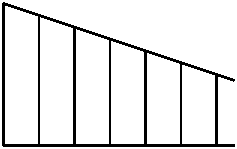
\includegraphics[width=0.22\textwidth]{gesamttex/edit_VIII-4/images/LH_37_04_156-3_d_156r.pdf}
\edcaption%
{\lbrack \textit{Fig.\:1}\rbrack}%
\end{edfigure}%
\selectlanguage{latin}%
\frenchspacing%
\normalsize%




\chapter[tocentry={Barometrum portabile %
\enskip August -- 12.\;(22.) November 1677},
head={Barometrum portabile}]%
{\MakeUppercase{Barometrum portabile}
\newline August -- 12.\;(22.) November 1677}
\label{barom-portab_intro}
\footnotesize%
\pstart%
\noindent%
In der dichten Aufzeichnung N.\;\ref{57037-1} \textit{Memorabile inventum barometri et thermometri portatilis exactissimi}, welche Leibniz selbst auf August 1677 datiert hat, wird in Anlehnung an Überlegungen von Christiaan Huygens\indexN{\textls{Huygens} (Hugenius, Ugenius, Hugens, Huguens), Christiaan 1629\textendash1695} und Louis Hubin\indexN{\textls{Hubin} (Hubinus), Louis (Ludion de) fl. 1673\textendash1683} ein Instrument umrissen, das die physikalischen Eigenschaften eines Barometers und eines Thermometers vereinigen und zugleich den Vorteil der Tragbarkeit aufweisen soll.
Dieser Umriss wurde einige Wochen später in zwei aufeinander folgenden Aufzeichnungen \textit{De barometro portabili} (N.\;\ref{57038} und N.\;\ref{57039}) wiederaufgenommen und weiter entwickelt;
beide \textit{Schedae} wurden von Leibniz eigenhändig auf den 12.\;(22.) November 1677 datiert.
Insbesondere die Aufzeichnung N.\;\ref{57038} setzt den Kerngedanken von N.\;\ref{57037-1} fort und entfaltet ihn, während die Aufzeichnung N.\;\ref{57039} nach dem gestrichenen, an N.\;\ref{57038} unmittelbar anknüpfenden Anfang sich Überlegungen über das Verhältnis zweiter Fluiden (Quecksilber und Luft) in einem Barometer widmet.
\pend%
\pstart%
Der textgenetische und inhaltliche Zusammenhang der drei Aufzeichnungen N.\;\ref{57037-1}, \ref{57038} und \ref{57039} rechfertigt deren einheitlichen Edition im Textkomplex N.\;\ref{barom-portab_intro} \textit{Barometrum portabile}.
Die Gesamtdatierung von N.\;\ref{barom-portab_intro} ist durch die eigenhändigen Datierungen der einzelnen Aufzeichnungen festgelegt.
\pend%
\selectlanguage{latin}%
\frenchspacing%
\normalsize%



\section[tocentry={Memorabile inventum barometri et thermometri portatilis exactissimi
\enskip August 1677},
head={Memorabile inventum barometri et thermometri %
}]%
{\MakeUppercase{Memorabile inventum barometri et thermometri portatilis exactissimi}
\newline August 1677}
\label{57037-1}
\selectlanguage{ngerman}%
\frenchspacing%
\begin{ledgroupsized}[r]{120mm}%
\footnotesize%
\pstart%
\noindent\textbf{Überlieferung:}%
\pend%
\end{ledgroupsized}%
\begin{ledgroupsized}[r]{114mm}%
\footnotesize%
\pstart%
\parindent -6mm%
\makebox[6mm][l]{\textit{L}}%
Aufzeichnung:
LH XXXVII~4, Bl.\;156.
Ein Zettel (16\;x\;13 cm);
Ränder beschnitten;
Papiererhaltungsmaßnahmen.
Eine halbe Seite jeweils auf Bl.\;156\,r\textsuperscript{o} und \;156\,v\textsuperscript{o};
Bl.\;156\,r\textsuperscript{o} überliefert zudem N.\;\ref{57037-3} %
sowie eine Notiz über Pyrotechnik %
und ein Fragment über die Gezeiten %
(beide sollen voraussichtlich in späteren Bänden von \textit{LSB} VIII ediert werden).
\pend%
\end{ledgroupsized}%
\selectlanguage{latin}%
\frenchspacing%
\vspace{5mm}%
\normalsize%
\pstart%
\noindent%
\lbrack%
\href{\Scan{LH_37_04_156r}}%
{156\,r\textsuperscript{o}}%
\rbrack%
\phantom{Augusti 1677}%
\hfill%
\phantom{\lbrack156\,r\textsuperscript{o}\rbrack}%
Augusti 1677
\pend%
\pstart%
\noindent%
\centering%
\edtext{%
Memorabile inventum%
\indexS{inventum memorabile}\\
Barometri%
\indexS{barometrum portabile}
et Thermometri%
\indexS{thermometrum portabile}
portatilis exactissimi%
}{%
\lemma{\textit{Am Rand%
:}}%
\Afootnote{%
$\displaystyle\frac{5}{4}$ Elle \mercury\ ohngefehr
pondus vel vis aeris.%
\indexS{pondus aeris}%
\indexS{vis aeris}
$\displaystyle\frac{1}{4}$ Elle \mercury\
est quinta virium portio.%
\indexS{portio virium}
Porro sit in spatio rarefacto%
\indexS{spatium rarefactum}
virium ut $\displaystyle\frac{5}{4}$
tantum vis ut $\displaystyle\frac{4}{4}$,
id est %
ejus quantitas sit ut 4 ad 5,
ad priorem.%
}}%
\pend%
\vspace{0.5em}%
\pstart%
\noindent%
\edtext{%
Sit Barometrum \textit{EABCD}%
\indexS{barometrum portabile}%
}{%
\lemma{Sit Barometrum \textit{EABCD}}%
\Cfootnote{%
Vgl. das Diagramm \lbrack\textit{Fig.\:1}\rbrack.%
}}
in quo Mercurius \textit{ABCD},%
\indexS{mercurius in barometro}
cujus altitudo \textit{AB}%
\indexS{altitudo mercurii}
eminet ultra horizontem \textit{BD}.%
\indexS{horizon}
Si \textit{EA} sit vacuum,%
\indexS{vacuum}
erit \textit{AB}
\edtext{%
altitudo Mercurii tantum%
\indexS{altitudo mercurii}
quantum sufficit ad aequipondium cylindri aerei.%
\indexS{aequipondium cylindri aerei}%
\indexS{cylinder aereus}%
}{%
\lemma{altitudo}%
\Bfootnote{%
\textit{(1)}~ad cyli %
\textit{(2)}~Mercurii tantum %
\lbrack...\rbrack\ aequipondium cylindri %
\textit{(a)}~aer %
\textit{(b)}~aerei.%
~\textit{L}%
}}
Sed si in \textit{EA} esset aliquod aeris,
minus tamen %
quam communiter esse solet,
foret Mercurius longe depressior%
\indexS{mercurius depressus}
seu minus altus,
\edtext{%
itaque aeris copiam%
}{%
\lemma{itaque}%
\Bfootnote{%
\textit{(1)}~aerem %
\textit{(2)}~aeris copiam%
~\textit{L}%
}}
pro arbitrio%
\indexS{arbitrium}
intus relinquendo,
possumus facere,
ut \textit{AB} Mercurius%
\indexS{mercurius in barometro}
ultra horizontem%
\indexS{horizon}
datae sit altitudinis.%
\indexS{altitudo mercurii}
Adjicimus autem Mercurio alium liquorem%
\indexS{liquor adjectus mercurio}
\edtext{%
\edlabel{LH_37_04_156-1_156r_hugenus-1}%
more%
\indexS{mos}
Hugenii%
\indexN{\textls{Huygens} (Hugenius, Ugenius, Hugens, Huguens), Christiaan 1629\textendash1695}%
\edlabel{LH_37_04_156-1_156r_hugenus-2}%
}{%
\lemma{more Hugenii}%
\Cfootnote{%
Siehe
\textsc{C.\;Huygens},
\glqq Extrait d'une autre lettre touchant une nouvelle maniere de Barometre\grqq\
(\textit{JS}, 12.~Dezember 1672, S.\;152--156;%
\cite{01522}
\textit{HO} VII, S.\;238--241).%
\cite{00113}%
}}
\edtext{%
et Cartesii.%
\indexN{\textls{Descartes} (Cartesius, des Cartes), René 1596\textendash1650}%
}{%
\lemma{et Cartesii}%
\Cfootnote{%
Siehe\cite{01471}
\textsc{P.\;Chanut}, %
Brief an F.\;Périer vom 24.\;September 1650 %
(in \textsc{B.\;Pascal}, \textit{Traitez}, Paris 1663, S.\;207\,f.;%
\cite{00081}
\textit{DO} V, S.\;476).%
\cite{00120}%
}}
Caeterum alia tunc instituenda erit
\edtext{%
divisio indicis.%
\indexS{divisio indicis}%
\indexS{index barometri}%
}{%
\lemma{divisio}%
\Bfootnote{%
\textit{(1)}~pro %
\textit{(2)}~indicis.%
~\textit{L}%
}}
Thermometro%
\indexS{thermometrum portabile}
res ita accomodari poterit,
uti
\edtext{%
\edlabel{LH_37_04_156-1_156r_hubinus-1}%
Hubinus%
\indexN{\textls{Hubin} (Hubinus), Louis (Ludion de) fl. 1673\textendash1683}
Barometrum Hugenii%
\indexN{\textls{Huygens} (Hugenius, Ugenius, Hugens, Huguens), Christiaan 1629\textendash1695}%
\indexS{barometrum Hugenii}
Thermometro accomodavit.%
\indexS{barometrum accomodatum thermometro}%
\indexS{thermometrum accomodatum barometro}%
\edlabel{LH_37_04_156-1_156r_hubinus-2}%
}{%
\lemma{Hubinus \lbrack...\rbrack\ accomodavit}%
\Cfootnote{%
Siehe
\textsc{L.\;Hubin},
\textit{Machines nouvellement executées}
(Paris 1673, S.\;10--12).\cite{01470}
Leibnizens Handexemplar ist in der GWLB Hannover unter der Signatur Leibn.\;Marg.\;129 aufbewahrt.%
}}
\pend%
\newpage%
\begin{edfigure}[0.0em][1.25em]
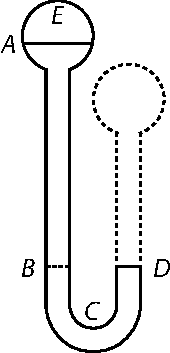
\includegraphics[width=0.16\textwidth]{gesamttex/edit_VIII-4/images/LH_37_04_156-1_d1_156r.pdf}
\edcaption[0.25em]
{\lbrack \textit{Fig.\:1}\rbrack%
\edtext{}{%
\lemma{\textit{Am Rand um das Diagramm} \lbrack\textit{Fig.\:1}\rbrack:}%
\Afootnote[nonum]{%
Nota%
\lbrack,\rbrack\
man kondte hier dabey haben die ponderatio\-nem%
\textsuperscript{\lbrack a\rbrack}
vacuae pilae%
\indexS{ponderatio pilae vacuae}%
\indexS{pila vacua}
so an dem liquore in die hohe ziehet.%
\indexS{liquor adjectus mercurio}
Item zu gleich Herrn Boyle%
\indexN{\textls{Boyle} (Boylius, Boyl), Robert 1627\textendash1691}
art nach die probe der Munzen,%
\indexS{Probe der Munzen}%
\indexS{Munze}%
\textsuperscript{\lbrack b\rbrack}
und ander dinge.
Durch das gewicht des schaffenleines%
\indexS{Schaffenlein}
würde man nachspüren
wiefiel es feuchtigkeit an sich gezogen:%
\indexS{Feuchtigkeit}
Nota %
melius mit einer gespanten chorde%
\indexS{chorda, gespant}
so sich drehet und einen Zeiger%
\indexS{Zeiger}
hat so sich mit drehet.%
\\[1ex]%
{\footnotesize%
\textsuperscript{\lbrack a\rbrack}~%
ponderationem
\textit{(1)}~der %
\textit{(2)}~vacuae pilae%
~\textit{L}%
\quad%
\textsuperscript{\lbrack b\rbrack}~%
Boyle \lbrack...\rbrack\ munzen:
Siehe
\textsc{R.\;Boyle},
\glqq A New Essay-Instrument\grqq\
(\textit{PT} X, 21.\;Juni 1675, S.\;329--348;\cite{01475}
\textit{BW}~VIII, S.\;532--544).\cite{00017}
Leibniz las möglicherweise aber die anonyme französische Zusammenfassung (\textit{JS}, 26.\;August 1675, S.\;223--225),
in der Boyles Messinstrument, anders als im englischen Original, explizit mit dem Barometer (\textit{aerometre}, S.\;223) verglichen wird.%
}%
}}%
}%
\end{edfigure}%
\pstart%
\noindent%
\lbrack%
\href{\Scan{LH_37_04_156v}}%
{156\,v\textsuperscript{o}}%
\rbrack\
Dieses Barometrum%
\indexS{barometrum portabile}
würde diesen Fehler haben,%
\indexS{Fehler barometri portabilis}
daß es zugleich ein
\edtext{%
\lbrack Therm\rbrack%
\indexS{thermometrum portabile}%
ome\-trum%
}{%
\lemma{Barometrum}%
\Bfootnote{%
\textit{L\;ändert Hrsg.}%
}}
were,
oder seine Indication%
\indexS{Indication}
aus beiden zusammengesezt.
Denn die in \textit{EA} sich befindende Lufft%
\indexS{Lufft, von der Wärme rarefaciert}
wurde von der Wärme%
\indexS{Wärme}
sich rarefaciren laßen%
\lbrack;\rbrack\
deßen ungeacht
wurden wir unsern Zweck erreichen,%
\indexS{Zweck}
\edtext{%
wann bey das Barometrum%
\indexS{barometrum portabile}%
}{%
\lemma{wann}%
\Bfootnote{%
\textit{(1)}~an dies Baro %
\textit{(2)}~bey das Barometrum%
~\textit{L}%
}}
ein Thermometrum%
\indexS{thermometrum portabile}
gefuget
\edtext{%
würde,
allein ich dencke an ein remedium%
\indexS{remedium}.%
}{%
\lemma{würde}%
\Bfootnote{%
\textit{(1)}~. Und dieses kondte meines bedünckens also %
\textit{(2)}~allein ich %
\lbrack...\rbrack\ ein remedium.%
~\textit{L}%
}}
\pend%
\pstart%
\edtext{%
Sit in \textit{EA} %
aer rarefactus%
\indexS{aer rarefactus}%
}{%
\lemma{Sit in \textit{EA}}%
\Cfootnote{%
Vgl. das Diagramm \lbrack\textit{Fig.\:2}\rbrack.%
}}%
\lbrack,\rbrack\
in
\edtext{%
\lbrack\textit{NM}\rbrack%
}{%
\lemma{\textit{LH}}%
\Bfootnote{%
\textit{L\;ändert Hrsg.}%
}}
adhuc rarefactior,
\textit{ABCD} barometrum%
\indexS{barometrum portabile}%
\indexS{barometrum apertum}
quod est apertum in \textit{D},
\edtext{%
et \textit{AGFHLMN}%
}{%
\lemma{et}%
\Bfootnote{%
\textit{(1)}~\textit{AF} %
\textit{(2)}~\textit{AGFHL} %
\textit{(3)}~\textit{AGFHLMN}%
~\textit{L}%
}}
thermometrum%
\indexS{thermometrum portabile}
\ledpb%
quod est clausum in \textit{N}.
Ope Mercurii \textit{AB}%
\indexS{mercurius in barometro}
\edtext{%
supra horizontem \textit{DBF} eminentis%
\indexS{horizon}%
}{%
\lemma{supra horizontem \textit{DBF} eminentis}%
\Bfootnote{%
\textit{erg.\;L}%
}}
erit aequilibrium%
\indexS{aequilibrium inter aerem externum et inclusum}
inter aerem externum ordinarium%
\indexS{aer externus}%
\indexS{aer ordinarius}
et aerem inclusum \textit{AE},%
\indexS{aer inclusus barometro}
rariorem externo.%
\indexS{aer rarior externo}
Et ope Mercurii \textit{LM}%
\indexS{mercurius in barometro}
supra horizontem \textit{AL}%
\indexS{horizon}
erit aequilibrium inter aerem rarum \textit{EA} %
et rariorem \textit{MN}.
\pend%
\pstart%
Verum
quia nihilominus calculo%
\indexS{calculus}
sive Tabula%
\indexS{tabula}
erit opus
et hoc
\edtext{%
modo duplo%
}{%
\lemma{modo}%
\Bfootnote{%
\textit{(1)}~nimis %
\textit{(2)}~duplo%
~\textit{L}%
}}
altius quam alias fiet instrumentum,%
\indexS{instrumentum}
necesse est
\textit{LM} esse satis altum%
\lbrack,\rbrack\
ideo satis erit sic agi:
sit thermometrum \textit{EAGFH}%
\indexS{thermometrum portabile}
et horizon \textit{DBF}%
\indexS{horizon}
\edtext{%
\lbrack et\rbrack%
}{%
\lemma{in}%
\Bfootnote{%
\textit{L\;ändert Hrsg.}%
}}
\textit{FH} pila plena aere%
\indexS{pila plena aere}
minus raro quam in \textit{EA},
et altitudo \textit{AF} Mercurii%
\indexS{altitudo mercurii}
aequilibrio serviet,%
\indexS{aequilibrium inter aerem externum et inclusum}
vel
\edtext{%
etiam quanta\lbrack m\rbrack\ volumus%
\lbrack;\rbrack\
in \textit{D}
et \textit{F}%
}{%
\lemma{etiam}%
\Bfootnote{%
\bars{quanta \textit{ändert Hrsg.}} volumus %
\textit{(1)}~, sive %
\textit{(2)}~in \textit{D} %
\textit{(a)}~, \textlangle siv\textrangle\ %
\textit{(b)}~, in \textit{F} %
\textit{(c)}~et \textit{F}%
~\textit{L}%
}}
superare poterunt liquores%
\indexS{liquor adjectus mercurio}
et habeatur
\edtext{%
Barometrum%
\indexS{barometrum portabile}
quale Hugenii,%
\indexN{\textls{Huygens} (Hugenius, Ugenius, Hugens, Huguens), Christiaan 1629\textendash1695}%
}{%
\lemma{Barometrum quale Hugenii}%
\Cfootnote{%
Siehe Erläuterung zu \refpassage{LH_37_04_156-1_156r_hugenus-1}{LH_37_04_156-1_156r_hugenus-2}.%
}}
et
\edtext{%
Thermometrum%
\indexS{thermometrum portabile}
quale Hubini%
\indexN{\textls{Hubin} (Hubinus), Louis (Ludion de) fl. 1673\textendash1683}%
}{%
\lemma{Thermometrum quale Hubini}%
\Cfootnote{%
Siehe Erläuterung zu \refpassage{LH_37_04_156-1_156r_hubinus-1}{LH_37_04_156-1_156r_hubinus-2}.%
}}
ad sensibilitatem.%
\indexS{sensibilitas barometri}%
\indexS{sensibilitas thermometri}
Everti poterit utcunque,
nec tamen quicquam effluet.
\pend%
\pstart%
Wenn am glas%
\indexS{Glas}
innewendig röllgen fest
kondte ein zeiger seyn,%
\indexS{Zeiger}
oder wiederumb vis mechanica.%
\indexS{vis mechanica}
\pend%
\begin{edfigure}[0.5em][0.0em]
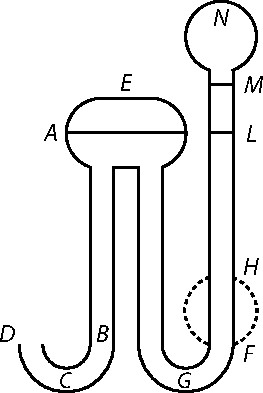
\includegraphics[width=0.28\textwidth]{gesamttex/edit_VIII-4/images/LH_37_04_156-1_d2_156v.pdf}
\edcaption%
{%
\lbrack \textit{Fig.\:2}\rbrack%
\edtext{}{%
\lemma{\textit{Um das Diagramm} \lbrack\textit{Fig.\:2}\rbrack:}%
\Afootnote[nonum]{%
Opus Tabula quadrata
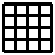
\includegraphics[width=0.03\textwidth]{gesamttex/edit_VIII-4/images/LH_37_04_156-1_d3_156v.pdf}
drauff zu schreiben die combinationes.%
}}%
}%
\end{edfigure}%
\selectlanguage{latin}%
\frenchspacing%
\normalsize%



\section[tocentry={De barometro portabili scheda prima
\enskip 12.\;(22.) November 1677},
head={De barometro portabili scheda I}]%
{\MakeUppercase{De barometro portabili scheda prima}
\newline 12.\;(22.) November 1677}
\label{57038}
\selectlanguage{ngerman}%
\frenchspacing%
\begin{ledgroupsized}[r]{120mm}%
\footnotesize%
\pstart%
\noindent\textbf{Überlieferung:}%
\pend%
\end{ledgroupsized}%
\begin{ledgroupsized}[r]{114mm}%
\footnotesize%
\pstart%
\parindent -6mm%
\makebox[6mm][l]{\textit{L}}%
Aufzeichnung:
LH XXXVII 4, Bl.\,157--158.
Ein Bogen 4\textsuperscript{o};
\href{\Scan{LH_37_04_157-158_wz}}{Wasserzeichen} mittig; %
Ränder beschnitten;
Papiererhltungsmaßnahmen.
Vier ganzseitig beschriebene Seiten.
\pend%
\end{ledgroupsized}%
\selectlanguage{latin}%
\frenchspacing%
\vspace{5mm}%
\normalsize%
\pstart%
\noindent%
\lbrack%
\href{\Scan{LH_37_04_157r}}%
{157\,r\textsuperscript{o}}%
\rbrack%
\phantom{12 November 1677}%
\hfill%
\phantom{\lbrack157\,r\textsuperscript{o}\rbrack}%
12 Novembris 1677%
\pend%
\pstart%
\noindent%
\centering%
De Barometro portabili%
\indexS{barometrum portabile}%
\\
Scheda I%
\indexS{scheda}
\pend%
\vspace{0.5em}%
\pstart%
\noindent%
Barometrum portabile%
\indexS{barometrum portabile}
haberi potest,
si Thermometro%
\indexS{thermometrum portabile}
\edtext{%
conjungatur.%
\indexS{barometrum conjunctum thermometro}%
\indexS{thermometrum conjunctum barometro}
Sint%
}{%
\lemma{conjungatur.}%
\Bfootnote{%
\textit{(1)}~Sit %
\textit{(2)}~Sint%
~\textit{L}%
}}
Thermometrum \textit{ABC},%
\indexS{thermometrum portabile}
Barometrum \textit{DEF}%
\indexS{barometrum portabile}
inter se
\edtext{%
juncta %
per Tubulum \textit{CD}.%
\indexS{tubulus jungens barometrum et thermometrum}
Thermometrum \textit{ABC}%
\indexS{thermometrum portabile}
est sipho vitreus bicrurus%
\indexS{sipho bicrurus}%
\indexS{sipho vitreus}
in%
}{%
\lemma{juncta}%
\Bfootnote{%
\textit{(1)}~, id est %
\textit{(2)}~per Tubulum \textit{CD}. Thermometrum %
\textit{(a)}~compositum ex siphone %
\textit{(b)}~\textit{ABC} est sipho %
\bars{vitreus \textit{erg.}} bicrurus %
\textit{(aa)}~ex %
\textit{(bb)}~in%
~\textit{L}%
}}
duas pilas \textit{A} %
et \textit{C}%
\indexS{pila thermometri}
\edtext{%
desinens.
Barometrum \textit{DEF}%
\indexS{barometrum portabile}
est Tubus \textit{DE},%
\indexS{tubus recurvatus}
cui%
}{%
\lemma{desinens.}%
\Bfootnote{%
\textit{(1)}~Thermometrum est tubus \textit{DEF}, cui %
\textit{(2)}~Barometrum \textit{DEF} %
\lbrack...\rbrack\ \textit{DE}, cui%
~\textit{L}%
}}
insistit pila \textit{D},%
\indexS{pila barometri}
recurvatus in \textit{EF}.%
\indexS{tubus recurvatus}
Pila \textit{A}
habet Tubulum \textit{AH},
pila \textit{C}%
\indexS{pila thermometri}
tubulum \textit{CG},
et pila \textit{D}%
\indexS{pila barometri}
tubulum
\edtext{%
\textit{DG}.
Tubus \textit{AB} et tubus \textit{CB} %
separatim conflati
jungi possunt in
\lbrack\textit{B}\rbrack.%
\indexS{tubi juncti in thermometro}
Et similiter totum Thermometrum \textit{ABC}%
\indexS{barometrum conjunctum thermometro}%
\indexS{thermometrum conjunctum barometro}
jungi potest Barometro \textit{DEF}
mediantibus Tubulis%
\indexS{tubulus jungens barometrum et thermometrum}
\textit{CG}, \textit{DG}.%
}{%
\lemma{\textit{DG}.}%
\Bfootnote{%
\textit{(1)}~Unumquodque separatim fieri potest, %
\textit{(2)}~Tubus \textit{AB} %
\lbrack...\rbrack\ \textit{CB}, separatim %
\textit{(a)}~facti jungi %
\textit{(b)}~conflati jungi possunt in %
\bars{\textit{C} \textit{ändert Hrsg.}}. Et %
\textit{(aa)}~totum %
\textit{(bb)}~similiter totum Thermometrum \textit{ABC} %
\textit{(aaa)}~, tubulo \textit{CG}, %
\textit{(bbb)}~, median %
\textit{(ccc)}~jungi potest %
\textit{(aaaa)}~tubulo \textit{GD}, %
\textit{(bbbb)}~Barometri %
\textit{(cccc)}~Barometro \textit{DEF} %
\lbrack...\rbrack\ \textit{CG}, \textit{DG}.%
~\textit{L}%
}}
Nihil refert
quae sit altitudo,
crassities,
rectitudo tuborum %
ac pilarum.%
\edlabel{LH_37_04_157-158_157r_lor-1}%
\edtext{}{%
\xxref{LH_37_04_157-158_157r_lor-1}{LH_37_04_157-158_157r_lor-2}%
\lemma{pilarum.}%
\Bfootnote{%
\lbrack/\rbrack\
\textit{(1)}~Usus hic erit %
\textit{(2)}~His ita %
\lbrack...\rbrack\ ita praeparabitur:%
~\textit{L}%
}}%
\pend%
\begin{edfigure}[1.75em][0.0em]%
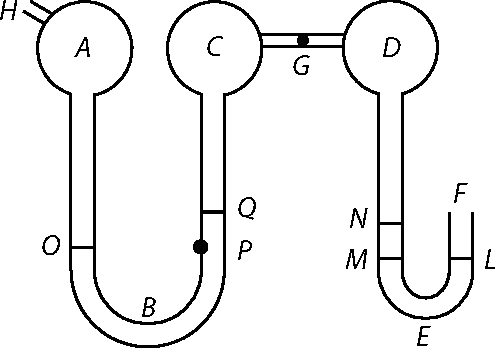
\includegraphics[width=0.45\textwidth]{gesamttex/edit_VIII-4/images/LH_37_04_157-158_d_157r.pdf}
\edcaption[-0.25em]%
{%
\hspace*{8mm}%
\lbrack\textit{Fig.\:1}\rbrack%
}%
\end{edfigure}%
\newpage%
\pstart%
His ita habitis,
instrumentum ita praeparabitur:%
\indexS{instrumentum portabile}%
\indexS{praeparatio thermometri}%
\indexS{praeparatio barometri}%
\edlabel{LH_37_04_157-158_157r_lor-2}
pilae%
\indexS{pila barometri}%
\indexS{pila thermometri}
\textit{C}, \textit{D}
\edtext{%
fortiter calefiant,%
\indexS{pila calefacta}%
}{%
\lemma{fortiter}%
\Bfootnote{%
\bars{et aequaliter \textit{gestr.}} calefiant,%
~\textit{L}%
}}
exibit aer per%
\indexS{exitus aeris e pila calefacta}%
\indexS{aer exiens e pila calefacta}
\edtext{%
\textit{F} et \textit{H}.%
}{%
\lemma{\textit{F} et}%
\Bfootnote{%
\textit{(1)}~\textit{A} %
\textit{(2)}~\textit{H}%
~\textit{L}%
}}
Quo facto%
\lbrack,\rbrack\
durante adhuc calore,%
\indexS{calor externus}
infundatur Mercurius utrinque,%
\indexS{mercurius infusus thermometro}%
\indexS{mercurius infusus barometro}
hinc per \textit{F},
\edtext{%
illinc per
\lbrack\textit{H}\rbrack.
Infusus%
\indexS{mercurius infusus barometro}
per \textit{F}
erit \textit{LEMN},
et \textit{MN}
refrigeratis tubis%
\indexS{tubus refrigeratus}
eminebit%
}{%
\lemma{illinc per}%
\Bfootnote{%
\bars{\textit{A} \textit{ändert Hrsg.}}. Infusus per \textit{F} %
\textit{(1)}~sit %
\textit{(2)}~erit \textit{LEMN}, %
\textit{(a)}~ita, ut %
\textit{(b)}~et \textit{MN} %
\bars{refrigeratis tubis \textit{erg.}} eminebit%
~\textit{L}%
}}
ultra horizontem \textit{LM}.%
\indexS{horizon}
Infusus%
\indexS{mercurius infusus thermometro}
\edtext{%
per \textit{H}%
}{%
\lemma{per}%
\Bfootnote{%
\textit{(1)}~\textit{A} %
\textit{(2)}~\textit{H}%
~\textit{L}%
}}
erit \textit{OPQ}.
His positis
ajo altitudinem%
\indexS{altitudo mercurii super horizontem}
\textit{PQ} aequalem
necessario esse altitudini%
\indexS{altitudo mercurii super horizontem}
\textit{MN},
quamvis tubi %
\textit{CB} et \textit{DE},%
\indexS{tubus recurvatus}
pilae \textit{C} et \textit{D},%
\indexS{pila barometri}%
\indexS{pila thermometri}
et quantitates infusi Mercurii%
\indexS{mercurius infusus thermometro}%
\indexS{mercurius infusus barometro}
\textit{OBP},
\textit{LEM} %
differant.
Nam ob communicationem pilarum%
\indexS{communicatio pilarum}
\textit{C} et \textit{D} in \textit{G}
aequaliter per eas distribuetur aer,%
\indexS{aer distributus in barometro}%
\indexS{aer distributus in thermometro}%
\indexS{distributio aeris in barometro}%
\indexS{distributio aeris in thermometro}
et %
utrobique
\edtext{%
tam per \textit{H} %
quam%
}{%
\lemma{tam}%
\Bfootnote{%
\textit{(1)}~per \textit{A} %
\textit{(a)}~q %
\textit{(b)}~\textlangle\textendash\textrangle\ %
\textit{(2)}~per \textit{H} %
quam%
~\textit{L}%
}}
per \textit{F} %
aequalis vis premit,%
\indexS{vis aeris prementis}%
\indexS{aer premens}%
\indexS{pressio aeris}
pondus scilicet aeris%
\indexS{pondus aeris}
\edtext{%
cujus effectus in liquore%
\indexS{liquor in barometro}%
\indexS{liquor in thermometro}%
\indexS{effectus ponderis aeris in liquore}%
}{%
\lemma{cujus}%
\Bfootnote{%
\textit{(1)}~in liquore %
\textit{(2)}~effectus in liquore%
~\textit{L}%
}}
tantum secundum altitudinem%
\indexS{altitudo mercurii super horizontem}
qua super horizontem eminet,%
\indexS{horizon}
utrinque spectari potest.
Cum ergo eadem utrinque vis%
\indexS{vis aeris prementis}
et resistentia sit,%
\indexS{resistentia ad pressionem aeris}
idem utrobique effectus%
\indexS{effectus ponderis aeris in liquore}%
\lbrack,\rbrack\
scilicet Mercurii altitudo erit.%
\indexS{altitudo mercurii super horizontem}
\edtext{%
Jam Tubulum \textit{H} hermetice sigillabimus,%
\indexS{tubulus hermetice sigillatus}
et tubulum \textit{CGD}
flatu molliendo%
\indexS{flatus}
in medio \textit{G}
\lbrack di\rbrack ducemus,
diductis a se invicem
Thermometro \textit{ABC}%
\indexS{thermometrum portabile}
et Barometro \textit{DEL},%
\indexS{barometrum portabile}
donec diversis sigillationibus%
\indexS{sigillatio}
separare eos %
et relictum in medio inter eas
impune abrumpere liceat.%
}{%
\lemma{Jam}%
\Bfootnote{%
\textit{(1)}~Jam duo instrumenta %
\textit{(2)}~\bars{Jam \textit{streicht Hrsg.}} %
\textit{(a)}~Barometrum a Thermometro separabimus %
\textit{(b)}~Tubulum \textit{H} hermetice %
\lbrack...\rbrack\ in medio \textit{G} %
\bars{ducemus \textit{ändert Hrsg.}}, diductis a se invicem %
\textit{(aa)}~hinc Barometro %
\textit{(bb)}~Thermometro \textit{ABC} %
\lbrack...\rbrack\ \textit{DEL}, donec %
\textit{(aaa)}~amborum extremi %
\textit{(bbb)}~diversis sigillationibus %
\lbrack...\rbrack\ in medio %
\bars{inter eas \textit{erg.}} impune abrumpere liceat.%
~\textit{L}%
}}
Cavendum tantum
ut durante
\lbrack%
\href{\Scan{LH_37_04_157v}}%
{157\,v\textsuperscript{o}}%
\rbrack\
flatu%
\indexS{flatus}
isto novissimo
non plus una pila%
\indexS{pila barometri}%
\indexS{pila thermometri}
quam alia
\edtext{%
calefiat%
\indexS{pila calefacta}%
\lbrack;\rbrack\
quod%
}{%
\lemma{calefiat~,}%
\Bfootnote{%
\textit{(1)}~quod %
\textit{(2)}~ne %
\textit{(3)}~quod%
~\textit{L}%
}}
facile caveri potest.
Ambae enim in loco sunt aeque calido,
et flatus%
\indexS{flatus}
non ipsas
sed medium commissurae \textit{G}%
\indexS{commissura barometri et thermometri}
attingit%
\lbrack,\rbrack\
\edtext{%
idque facile est dignoscere,
quia %
statim videri potest %
an eadem maneat altitudo \textit{MN} et \textit{PQ}.%
\indexS{altitudo mercurii super horizontem}%
}{%
\lemma{idque facile %
\lbrack...\rbrack\ potest an}%
\Bfootnote{%
\textit{(1)}~eandem altitudinem %
\textit{(2)}~eadem %
\textit{(a)}~altitudo %
\textit{(b)} maneat altitudo \textit{MN} et \textit{PQ} %
\textit{erg.\;L}%
}}
Hoc posito
\edtext{%
et facta separatione%
\indexS{separatio barometri et thermometri}%
}{%
\lemma{et facta separatione}%
\Bfootnote{%
\textit{erg.\;L}%
}}
sequitur
eandem esse vim%
\indexS{vis aeris in pila}
seu consistentiam%
\indexS{consistentia aeris in pila}%
\indexS{aer in pila}
\edtext{%
aeris in pila \textit{C}%
\indexS{pila barometri}%
\indexS{pila thermometri}%
}{%
\lemma{aeris in}%
\Bfootnote{%
\textit{(1)}~medio %
\textit{(2)}~pila \textit{C}%
~\textit{L}%
}}
Thermometri%
\indexS{thermometrum portabile}
et in pila \textit{D} Barometri,%
\indexS{barometrum portabile}
unde gradus Thermometri%
\indexS{thermometrum portabile}%
\indexS{gradus thermometri}
infra vel supra
\edtext{%
statum communem%
\indexS{status communis atmosphaerae}
tempore elaborationis%
\indexS{tempus elaborationis}%
\indexS{elaboratio}%
}{%
\lemma{statum}%
\Bfootnote{%
\textit{(1)}~in quo tem %
\textit{(2)}~communem tempore %
\bars{primae \textit{gestr.}} elaborationis%
~\textit{L}%
}}
deprehensum reperti,
Barometro addentur%
\indexS{barometrum portabile}
vel
\edtext{%
detrahentur,
quia omnes effectus Thermometri%
\indexS{thermometrum portabile}%
\indexS{effectus thermometri repertus in barometro}
etiam%
}{%
\lemma{detrahentur,}%
\Bfootnote{%
\textit{(1)}~et ita %
\textit{(2)}~quia omnes
\textit{(a)}~impressiones Thermometri et %
\textit{(b)}~effectus Thermometri etiam%
~\textit{L}%
}}
in Barometro reperiuntur,
sed non contra.
Et cum in Barometro%
\indexS{barometrum portabile}
\edtext{%
distingui nequeant,%
}{%
\lemma{distingui}%
\Bfootnote{%
\textit{(1)}~nesciant %
\textit{(2)}~nequeant%
~\textit{L}%
}}
ope Thermometri adjecti%
\indexS{thermometrum adjectum barometro}
sine ullo calculo
accurate discernentur.
Quodsi Barometrum%
\indexS{barometrum portabile}
et Thermometrum%
\indexS{thermometrum portabile}
\edtext{%
hoc%
}{%
\lemma{hoc}%
\Bfootnote{%
\textit{erg.\;L}%
}}
non essent uno eodemque actu%
\indexS{actus}
elaborata,
calculo subtili%
\indexS{calculus subtilis}
quidem et certo,%
\indexS{calculus certus}
satis tamen perplexo%
\indexS{calculus perplexus}
opus foret.
\pend%
\newpage%
\pstart%
Utile erit
pilas esse%
\indexS{pila thermometri}%
\indexS{pila barometri}
quantum in portabili instrumento%
\indexS{instrumentum portabile}
commode licet
magnas.
Ita enim aer%
\indexS{aer nascens e mercurio}
ex Mercurio
tractu temporis%
\indexS{tractus temporis}%
\indexS{tempus}
nascens,%
\indexS{aer nascens e mercurio}
\edtext{%
nullam cum%
}{%
\lemma{nullam}%
\Bfootnote{%
\textit{(1)}~ad %
\textit{(2)}~cum%
~\textit{L}%
}}
pilarum magnitudine
comparationem
\edtext{%
habebit;
optimum autem erit%
}{%
\lemma{habebit;}%
\Bfootnote{%
\textit{(1)}~utile erit autem 
\textit{(2)}~optimum autem erit%
~\textit{L}%
}}
adhibere Mercurium%
\indexS{mercurius purgatus aere}
qui jam sit ab aere purgatus.%
\indexS{mercurius purgatus aere}
\pend%
\pstart%
Porro
ut in exiguo
\edtext{%
\lbrack quantum\rbrack%
}{%
\lemma{quantum}%
\Bfootnote{%
\textit{erg.\;Hrsg.}%
}}
licet instrumento%
\indexS{instrumentum portabile}
quod tubum calamarium non excedat%
\indexS{tubus calamarius}
omnes effectus exhibeantur%
\indexS{effectus exhibitus in instrumento}
satis
\edtext{%
distincte%
\lbrack,\rbrack\
regula%
\indexS{regula divisa exacte}%
\indexS{regula applicata instrumento}
applicari potest %
exactissime divisa
vel%
}{%
\lemma{distincte;}%
\Bfootnote{%
\textit{(1)}~vel %
\textit{(2)}~regula applicari %
\lbrack...\rbrack\ divisa vel%
~\textit{L}%
}}
punctis vel filis tenuissimis circumligatis,
sed necesse erit
instrumentum directe statui horizontale.%
\indexS{instrumentum portabile}
In Barometro%
\indexS{barometrum portabile}
poterimus adhibere
\edtext{%
pondus%
\indexS{pondus innatans mercurio}
Mercurio \textit{F} innatans%
}{%
\lemma{pondus}%
\Bfootnote{%
\textit{(1)}~in \textit{F} %
\textit{(2)}~Mercurio \textit{F} innatans%
~\textit{L}%
}}
\edlabel{LH_37_04_157-158_157v_udz-1}%
ut
\edtext{%
in Barometris Anglicanis,%
\indexS{barometrum Anglicanum}%
\edlabel{LH_37_04_157-158_157v_udz-2}%
}{%
\lemma{in Barometris Anglicanis}%
\Cfootnote{%
Wohl Anspielung auf das von Hooke erfundene Radbarometer,
welches für die Betätigung des Zeigers die Anwendung eines im Quecksilber schwimmenden Körpers vorsah.
Siehe \textsc{R.\;Hooke},
\textit{Micrographia}, Preface
(London 1665, S.\:[c3] u.\;Tafel I, Abb.\;I);%
\cite{00061}
\textsc{Ders.},
\glqq A new Contrivance of Wheel-Barometer\grqq\
(\textit{PT}, I, 4.\;Juni 1666,
S.\;218\,f. u.\;Abb.\;1 vor S.\;215).%
\cite{01523}
Auf das \glqq englische\grqq\ Radbarometer beziehen sich in diesem Band auch die Aufzeichnung
N.\;\ref{57041}
(\refpassage{LH_37_04_162-163_163r_hooke-1}{LH_37_04_162-163_163r_hooke-2}
u.\;\refpassageohne{LH_37_04_162-163_163r_hooke-3}{LH_37_04_162-163_163r_hooke-4})
vom Oktober 1677
sowie die spätere Aufzeichnung
N.\;\ref{53451}
(\refpassage{LH_37_04_171_171r_hooke-1}{LH_37_04_171_171r_hooke-2}).%
}}
\lbrack%
\href{\Scan{LH_37_04_158r}}%
{158\,r\textsuperscript{o}}%
\rbrack\
quod artificium%
\indexS{artificium applicatum barometro}
si ad Thermometrum hoc clausum%
\indexS{thermometrum clausum}
sed exiguum et portabile%
\indexS{thermometrum portabile}
applicare vellemus,
opus esset
in Thermometro natare frustum ferri%
\indexS{ferrum}%
\indexS{frustum ferri in thermometro}
aut magnetis%
\indexS{magnes}%
\indexS{frustum magnetis in thermometro}
in \textit{Q},
quod applicatum extra %
\edtext{%
aliud frustum%
}{%
\lemma{aliud}%
\Bfootnote{%
\textit{(1)}~frustra %
\textit{(2)}~frustum%
~\textit{L}%
}}
magnetis%
\indexS{magnes}%
\indexS{frustum magnetis in thermometro}
aut ferri%
\indexS{ferrum}%
\indexS{frustum ferri in thermometro}
secum attollat deprimatque.
Quo
\edtext{%
facto
illud quoque facili machinatione%
\indexS{machinatio}%
}{%
\lemma{facto}%
\Bfootnote{%
\textit{(1)}~statim %
\textit{(2)}~illud quoque facili machinatione%
~\textit{L}%
}}
efficere licebit,
ut gradus Thermometri%
\indexS{thermometrum portabile}%
\indexS{gradus thermometri}
sese ipsi a Barometro%
\indexS{barometrum portabile}%
\indexS{gradus barometri}
detrahant,
nec ullo calculo%
\indexS{calculus}
opus sit.
Ita Barometrum hoc%
\indexS{barometrum portabile}
in marsupio gestatum,%
\indexS{marsupium}%
\indexS{barometrum gestatum in marsupio}
aut in hypocausta%
\indexS{hypocaustum}%
\indexS{barometrum translatum in hypocaustum}
ac balnea%
\indexS{balneum}%
\indexS{barometrum translatum in balneum}
translatum%
\lbrack,\rbrack\
nullam subibit mutationem.%
\indexS{mutatio barometri}
\pend%
\pstart%
Porro eundem effectum%
\indexS{effectus assecutus ope duorum barometrorum}
forte etiam ope duorum Barometrorum%
\indexS{barometrum portabile}
sed diversae pilarum%
\indexS{pila barometri}
rationis %
assequi licebit,%
\indexS{effectus assecutus ope duorum barometrorum}
atque ita carere licebit magnete.%
\indexS{magnes}
Ponamus enim
aerem unius pilae%
\indexS{aer in pila}
esse rariorem%
\indexS{aer rarus}
quam aerem alterius pilae,%
\indexS{pila barometri}
quod qua proportione fiat
discere licebit ex ratione ipsius \textit{NM}
altitudinis Mercurii super horizontem%
\indexS{altitudo mercurii super horizontem}%
\indexS{horizon}
\edtext{%
in uno tubo,%
\indexS{tubus recurvatus}
ad \textit{PQ}%
}{%
\lemma{in}%
\Bfootnote{%
\textit{(1)}~una %
\textit{(2)}~uno tubo, ad %
\textit{(a)}~\textit{(N)(N)} %
\textit{(b)}~\textit{PQ} %
\textit{(c)}~\textit{PQ}%
~\textit{L}%
}}
altitudinem ejusdem in alio,
ponendo \textit{CQPBO} esse unum Barometrum%
\indexS{barometrum portabile}
(resecto \textit{OA})
et \textit{DNMEL} alterum.
Nimirum
\edtext{%
vis elastica%
\indexS{vis aeris elastica}
seu densitas aeris%
\indexS{densitas aeris}%
}{%
\lemma{vis}%
\Bfootnote{%
\textit{(1)}~aeris seu densitas %
\textit{(2)}~elastica seu densitas aeris%
~\textit{L}%
}}
in \textit{C},
juncta ponderi Mercurii \textit{QP},%
\indexS{pondus mercurii in thermometro}
est aequalis
\edtext{%
vi elasticae%
\indexS{vis aeris elastica}
seu densitati aeris%
\indexS{densitas aeris}%
}{%
\lemma{vi}%
\Bfootnote{%
\textit{(1)}~aeris %
\textit{(2)}~elasticae seu densitati aeris%
~\textit{L}%
}}
in \textit{D},
junctae ponderi mercurii \textit{NM}.%
\indexS{pondus mercurii in barometro}%
\edlabel{LH_37_04_157-158_158r_fsd-1}%
\edtext{}{%
\xxref{LH_37_04_157-158_158r_fsd-1}{LH_37_04_157-158_158r_fsd-2}%
\lemma{\textit{NM}.}%
\Bfootnote{%
\lbrack/\rbrack\ %
\textit{(1)}~Vis elastica a %
\textit{(2)}~Densitas aeris%
~\textit{L}%
}}%
\pend%
\newpage%
\pstart%
Densitas aeris%
\indexS{densitas aeris}%
\edlabel{LH_37_04_157-158_158r_fsd-2}
in \textit{C} %
vocetur \textit{d},
densitas ejusdem%
\indexS{densitas aeris}
in \textit{D}
vocetur $\delta$,
pondus Mercurii \textit{QP}%
\indexS{pondus mercurii in thermometro}
vocetur \textit{p},
et pondus Mercurii \textit{NM}%
\indexS{pondus mercurii in barometro}
vocetur $\pi$.
Ergo $d + p$ aequ.
\edtext{%
$\delta + \pi$ aequal. ipsi \textit{v}%
}{%
\lemma{$\delta + \pi$}%
\Bfootnote{%
\textit{(1)}~aequ. \textit{v} %
\textit{(2)}~aequal. ipsi \textit{v}%
~\textit{L}%
}}
ponderi
\edtext{%
praesenti%
}{%
\lemma{praesenti}%
\Bfootnote{%
\textit{erg.\;L}%
}}
totius Atmosphaerae,%
\indexS{pondus atmosphaerae}%
\indexS{atmosphaera}
\edtext{%
seu ponderi Mercurii
cujus altitudo 27%
\indexS{pondus mercurii 27 pollicum}
vel 30 pollicum;%
\indexS{pondus mercurii 30 pollicum}%
\indexS{pollex}%
}{%
\lemma{seu}%
\Bfootnote{%
\textit{(1)}~ponderi praesenti %
\textit{(2)}~ponderi Mercurii cujus altitudo %
\textit{(a)}~30 pollicum %
\textit{(b)}~27 vel 30 pollicum;%
~\textit{L}%
}}
nota autem altitudo \textit{QP} %
et \textit{NM},
ergo et ratio ejus ad pollices%
\indexS{pollex}
istos totius altitudinis,%
\indexS{altitudo mercurii super horizontem}
notae ergo potentiae%
\indexS{potentia aeris elastica}
\textit{p}, $\pi$
in ratione ad
\edtext{%
totam \textit{v}.
Et quia
\textit{d} aequ. $v - p$
et
$\delta$ aequ. $v - \pi$,%
}{%
\lemma{totam \textit{v}.}%
\Bfootnote{%
\textit{(1)}~Ergo quia datur %
\textit{(2)}~Et quia \textit{d} aequ. $v-p$ %
\textit{(a)}~et $\delta$ %
\textit{(b)}~et $\delta$ aequ. $v - \pi$,%
~\textit{L}%
}}
dabitur
$\dfrac{d}{\delta}$
\edtext{%
aequ.
$\dfrac{v-p}{v-\pi}$.%
}{%
\lemma{aequ.}%
\Bfootnote{%
\textit{(1)}~$\dfrac{v - \pi}{v - \hphantom{p}}$ %
\textit{(2)}~$\dfrac{v - p}{v - \pi}$%
~\textit{L}%
}}
Hinc aucta \textit{v},
\edtext{%
seu atmosphaerae pondere,%
\indexS{pondus atmosphaerae}%
\indexS{atmosphaera}
augentur
\lbrack%
\href{\Scan{LH_37_04_158v}}%
{158\,v\textsuperscript{o}}%
\rbrack\
\textit{p} et $\pi$ tantundem;%
}{%
\lemma{seu}%
\Bfootnote{%
\textit{(1)}~aeris p %
\textit{(2)}~atmosphaerae pondere, augentur %
\textit{(a)}~$\pi$ et %
\textit{(aa)}~\textlangle t\textrangle\ %
\textit{(bb)}~\textit{p} %
\lbrack\href{\Scan{LH_37_04_158v}}{158\,v\textsuperscript{o}}\rbrack\ %
\textit{(b)}~\textit{p} et $\pi$ tantundem;%
~\textit{L}%
}}
\rule[0mm]{0mm}{3.2mm}%
quia \textit{d} et $\delta$
ex hypothesi%
\indexS{hypothesis}
non augentur.
Porro calore externo%
\indexS{calor externus}
augentur
etiam \textit{d} et $\delta$,
quorum
cum ratio sit nota %
ante mutationem,%
\indexS{mutatio ponderis atmosphaerae}
videtur etiam
nota esse
post
\edtext{%
mutationem%
\indexS{mutatio ponderis atmosphaerae}%
\lbrack;\rbrack\
videtur enim
quo plenior seu densior est aer,%
\indexS{aer densus}
hoc majorem vim se dilatandi%
\indexS{vis aeris dilatandi se}
acquirere aequali calor\lbrack e\rbrack,%
\indexS{calor aequalis}
seu duorum aerum%
\indexS{aer calefactus}
eodem calore%
\indexS{calor externus}
quaesitas se dilatandi vires%
\indexS{vis aeris dilatandi se}%
}{%
\lemma{mutationem,}%
\Bfootnote{%
\textit{(1)}~quia semper %
\textit{(a)}~eat %
\textit{(b)}~propo %
\textit{(c)}~aer raref %
\textit{(2)}~videtur enim %
\lbrack...\rbrack\ aer, hoc %
\textit{(a)}~\textlangle neq\textrangle\ %
\textit{(b)}~majorem vim se dilatandi %
\textit{(aa)}~aequa %
\textit{(bb)}~acquirere aequali %
\bars{calores \textit{ändert Hrsg.}}, seu %
\textit{(aaa)}~duas vires elasticas duorum aerum dilatatorum%
\indexS{vis elastica aeris dilatati}\indexS{aer dilatatus} %
\textit{(bbb)}~duorum aerum %
\lbrack...\rbrack\ dilatandi vires%
~\textit{L}%
}}
esse in ratione \textit{d} ad $\delta$,
quo posito dabitur semper
$\dfrac{v - p}{v - \pi}$;%
\rule[0mm]{0mm}{6.0mm}
dantur autem \textit{p} et $\pi$,
ergo dabitur~\textit{v},
seu facta in pondere atmosphaerae mutatio,%
\indexS{mutatio ponderis atmosphaerae}%
\indexS{pondus atmosphaerae}%
\indexS{atmosphaera}
scilicet
quia datur $\dfrac{d}{\delta}$,
erit
$v\delta - p\delta$
aequ.
$vd - \pi d$.
Ergo
$vd - v\delta$
aequ.
$\pi d - pd$.%
\rule[0mm]{0mm}{5.8mm}
Ergo
$\dfrac{v}{\pi - p}$
aequ.
\edtext{%
$\dfrac{d}{d - \delta}$.
$\dfrac{d}{\delta}$ aequ. $\theta$.%
}{%
\lemma{$\dfrac{d}{d - \delta}$}%
\Bfootnote{%
\textit{(1)}~(seu $\dfrac{v}{p-\pi}$ aequ. $\dfrac{\delta}{\delta-d}$ seu $\dfrac{v}{\pi-p}$ aequ. $\dfrac{\delta}{d-\delta}$. Ergo $\dfrac{\delta}{d-\delta}$ aequ. $\dfrac {d}{d-\hphantom{d}}$ %
\textit{(2)}~. $\dfrac{d}{\delta}$ aequ. $\theta$.%
~\textit{L}%
}}
Ergo
$v - p$ aequ. $v\theta - \pi\theta$
seu
$v - v\theta$ aequ. $p - \pi\theta$
seu
\textit{v} aequ. $\dfrac{p - \pi\theta}{1 - \theta}$.%
\rule[0mm]{0mm}{6.0mm}
Est autem $1 - \theta$ quantitas constans,%
\indexS{quantitas constans}
quia $\theta$ est quantitas constans.%
\indexS{quantitas constans}%
\rule[0mm]{0mm}{5.8mm}
Porro ut res facilius peragatur instrumento,%
\indexS{instrumentum portabile}%
\indexS{res peracta instrumento}
sit \textit{p} aequ. $\beta + \pi$.
Ergo fiet
$\dfrac{\beta}{1 - \theta} + \pi$
\edtext{%
aequ.\;\textit{v},%
\rule[0mm]{0mm}{7.0mm}
nam si \textit{p} est major quam $\pi$,
est \textit{d} minor quam $\delta$,
seu 1 major quam $\dfrac{d}{\delta}$ vel $\theta$.%
}{%
\lemma{aequ.\;\textit{v}}%
\Bfootnote{%
\textit{(1)}~vel potius quia $\theta$ major unitate, %
\textit{(2)}~nam si %
\lbrack...\rbrack\ quam $\pi$, est %
\textit{(a)}~etiam %
\textit{(b)}~\textit{d} %
\textit{(aa)}~major %
\textit{(bb)}~minor quam $\delta$, %
\lbrack...\rbrack\ vel $\theta$.%
~\textit{L}%
}}
Arte ergo opus%
\indexS{ars}
\edtext{%
est qua%
}{%
\lemma{est}%
\Bfootnote{%
\textit{(1)}~per quam %
\textit{(2)}~qua%
~\textit{L}%
}}
in ipsa machina%
\indexS{machina}
dividatur $\beta$ per
\edtext{%
numerum%
}{%
\lemma{numerum}%
\Bfootnote{%
\textit{erg.\;L}%
}}
constantem%
\indexS{numerus constans}
\edtext{%
$1 - \theta$,
et productum ipsi $\pi$ addatur,%
}{%
\lemma{$1 - \theta$,}%
\Bfootnote{%
\textit{(1)}~quod per applicatam exiguam %
\textit{(2)}~et productum ipsi %
\textit{(3)}~et productum ipsi $\pi$ addatur,%
~\textit{L}%
}}
\ledpb%
id vero facile est,
\edtext{%
si in numeri istius ratione%
}{%
\lemma{si}%
\Bfootnote{%
\textit{(1)}~per numerum istum %
\textit{(2)}~in numeri istius ratione%
~\textit{L}%
}}
cylinder ille exiguus%
\indexS{cylinder}
cujus ope major circulus%
\indexS{circulus}
indici datur,
diminuatur,
et numerus
\edtext{%
graduum proveniens excentrice%
}{%
\lemma{graduum}%
\Bfootnote{%
\textit{(1)}~excentrice %
\textit{(2)}~proveniens excentrice%
~\textit{L}%
}}
alterius indicis gradus augeat,%
\indexS{gradus indicis}%
\indexS{index graduum mutationis atmosphaerae}
ita enim
quia eccentrice additur,
minus addetur,
quam si divisio facta non fuisset %
in ea quae desideratur ratione.
Quoniam tamen calculus hoc modo facillimus est,%
\indexS{calculus facillimus}
non opus est
ut huic rei immoremur.
Nimirum
quoniam numeri $\pi$ et $\beta$ statim visu apparent,
tantum monendi homines%
\indexS{homo}
paucis verbis machinae ascriptis,%
\indexS{machina}
quod per numerum illum constantem $(1 - \theta)$%
\indexS{numerus constans}
divisus numerus $\beta$
additus numero $\pi$
daturus sit \textit{v}.
\pend%
\selectlanguage{latin}%
\frenchspacing%
\normalsize%


\section[tocentry={De barometro portabili scheda secunda
\enskip 12.\;(22.) November 1677},
head={De barometro portabili scheda II}]%
{\MakeUppercase{De barometro portabili scheda secunda}
\newline 12.\;(22.) November 1677}
\label{57039}
\selectlanguage{ngerman}%
\frenchspacing%
\begin{ledgroupsized}[r]{120mm}%
\footnotesize%
\pstart%
\noindent\textbf{Überlieferung:}%
\pend%
\end{ledgroupsized}%
\begin{ledgroupsized}[r]{114mm}%
\footnotesize%
\pstart%
\parindent -6mm%
\makebox[6mm][l]{\textit{L}}%
Aufzeichnung:
LH XXXVII 4, Bl.\,159.
Ein Blatt 4\textsuperscript{o};
\href{\Scan{LH_37_04_159_wz}}{Wasserzeichen} mittig; %
Ränder beschnitten;
Papiererhaltungsmaßnahmen.
Zwei ganzseitig beschriebene Seiten.
\pend%
\end{ledgroupsized}%
\selectlanguage{latin}%
\frenchspacing%
\vspace{5mm}%
\normalsize%
\pstart%
\noindent%
\lbrack%
\href{\Scan{LH_37_04_159r}}%
{159\,r\textsuperscript{o}}%
\rbrack
\phantom{12 November 1677}%
\hfill%
\phantom{\lbrack159\,r\textsuperscript{o}\rbrack}%
12 Novembris 1677%
\pend%
\pstart%
\noindent%
\centering%
De Barometro portabili%
\indexS{barometrum portabile}%
\\
Scheda 2%
\indexS{scheda}%
\edlabel{LH_37_04_159_159r_sjg-1}%
\edtext{}{%
\xxref{LH_37_04_159_159r_sjg-1}{LH_37_04_159_159r_sjg-2}%
\lemma{Scheda 2}%
\Bfootnote{%
\lbrack/\rbrack\ %
\textit{(1)}~Sit instrumentum vitreum \textit{ABCDEFGH} apertum in \textit{G} et \textit{H}. \textit{BCD} sit liquor. Calefiat quantum licet phiala vitrea \textit{E}, %
\textit{(a)}~\bars{aere \textit{erg.}} pelletur liquor infra \textit{D} super \textit{B} ex parte, et ex alia parte expelletur per %
\textit{(b)}~\bars{et \textit{erg.}} aer in \textit{E} partim pelletur versus \textit{D}, deprimetque liquorem infra \textit{D}, eriget supra \textit{B}, partim expelletur per \textit{G} (expellendo aerem in \textit{A} ex \textit{H}) %
\textit{(c)}~partim aer in \textit{E} pelletur versus %
\lbrack/\rbrack\ %
\textit{(2)}~Sit instrumentum %
\lbrack...\rbrack\ in \textit{A}, \textit{E}, %
\bars{\textit{L} \textit{ändert Hrsg.}}. Infuso per \textit{A} %
\lbrack...\rbrack\ Hermetice exitus \textit{E} %
\textit{(a)}~et pila~\textit{E} %
\textit{(b)}~(qui tubulus %
\lbrack...\rbrack\ pila \textit{E} fortissime %
\textit{(aa)}~igne %
\textit{(bb)}~incalescat, ita %
\lbrack...\rbrack\ Quo facto %
\textit{(aaa)}~contingeat %
\textit{(bbb)}~aer %
\textit{(aaaa)}~in %
\textit{(bbbb)}~ex pila \textit{E} %
\lbrack...\rbrack\ infra \textit{D} %
\bars{in \textit{d} \textit{erg.}}, et eriget supra \textit{B} %
\bars{in \textit{b} \textit{erg.}}, et aerem aliquem %
\textit{(aaaaa)}~per \textit{A} %
\textit{(bbbbb)}~inter \textit{A} et \textit{B} %
\lbrack...\rbrack\ per \textit{H} effluere faciet.%
~\textit{L}%
}}%
\pend%
\vspace{0.5em}%
\pstart%
\noindent%
\lbrack%
\textit{Nachfolgend kleingedruckter Text gestrichen:}%
\rbrack%
\pend%
\vspace{0.5em}%
\footnotesize%
\pstart%
\noindent%
Sit instrumentum vitreum \textit{ABCDEFGH}%
\indexS{instrumentum vitreum}
apertum in \textit{A}, \textit{E}, \lbrack\textit{H}\rbrack.
Infuso per \textit{A} liquore impleatur \textit{BCD}.%
\indexS{liquor infusus barometro}
Infuso per \textit{H} liquore impleatur \textit{HGF}.
Sigilletur Hermetice exitus \textit{E}%
\indexS{exitus sigillatus hermetice}
(qui tubulus%
\indexS{tubulus vitreus}
esse potest%
\lbrack)\rbrack\
et pila~\textit{E}%
\indexS{pila barometri}
fortissime incalescat,%
\indexS{pila incalescens}
ita tamen ut ne fundatur.
Quo facto
aer ex pila \textit{E} expulsus%
\indexS{aer expulsus e barometro}
partim tendens versus~\textit{D}
liquorem premet infra \textit{D}
in \textit{d},
et eriget supra \textit{B}
in \textit{b},
et aerem aliquem
inter \textit{A} et \textit{B} positum
per \textit{A} expellet;%
\indexS{aer expulsus e barometro}
partim tendens versus \textit{F}
liquorem deprimet infra \textit{F},%
\indexS{liquor infusus barometro}
et erigens supra \textit{H} expellet%
\indexS{liquor expulsus e barometro}
seu per \textit{H} effluere faciet.%
\edlabel{LH_37_04_159_159r_sjg-2}
His factis
\edtext{%
claudatur exitus%
\indexS{exitus clausus}%
}{%
\lemma{claudatur}%
\Bfootnote{%
\textit{(1)}~foramen %
\textit{(2)}~exitus%
~\textit{L}%
}}
\textit{A}
(qui tubulus%
\indexS{tubulus vitreus}
esse potest%
\lbrack)\rbrack\
et refrigerata jam machina paulatim%
\indexS{machina refrigerata}%
\indexS{refrigeratio machinae}
duo aequali vi%
\indexS{vis aequalis}%
\indexS{vis aeris ambientis}%
\indexS{vis aeris ordinarii}
\edtext{%
agent in aerem%
}{%
\lemma{agent in}%
\Bfootnote{%
\textit{(1)}~aquam %
\textit{(2)}~aerem%
~\textit{L}%
}}
in \textit{E} residuum,%
\indexS{aer residuus}
scilicet Aer ordinarius%
\indexS{aer ordinarius}
in \textit{A},
\edtext{%
et aer ordinarius ambiens%
\indexS{aer ambiens}
partim Elaterio%
\indexS{elaterium aeris ambientis}%
\indexS{elaterium aeris ordinarii}
partim pondere suo%
\indexS{pondus aeris ambientis}%
\indexS{pondus aeris ordinarii}%
}{%
\lemma{et aer ordinarius}%
\Bfootnote{%
\textit{(1)}~in %
\textit{(2)}~extr %
\textit{(3)}~ambiens %
\textit{(a)}~ille Elaterio hic pondere suo %
\textit{(b)}~partim Elaterio partim pondere suo%
~\textit{L}%
}}
\lbrack\textit{Text bricht ab.}\rbrack\
\pend%
\begin{edfigure}[1.85em][0.0em]%
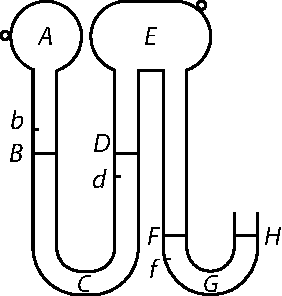
\includegraphics[width=0.20\textwidth]{gesamttex/edit_VIII-4/images/LH_37_04_159_d1_159r.pdf}
\edcaption[0.25em]%
{%
\lbrack\textit{Fig.\:1, gestr.}\rbrack%
}%
\end{edfigure}%
\newpage%
\normalsize%
\vspace*{-0.0em}%
\begin{edfigure}[0.0em][1.5em]%
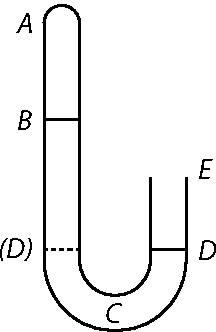
\includegraphics[width=0.19\textwidth]{gesamttex/edit_VIII-4/images/LH_37_04_159_d2_159r.pdf}
\edcaption[0.35em]%
{%
\lbrack\textit{Fig.\:2}\rbrack%
}%
\end{edfigure}%
\pstart%
\noindent%
\edtext{%
Sit Tubus recurvatus%
\indexS{tubus recurvatus}%
}{%
\lemma{Sit}%
\Bfootnote{%
\textit{(1)}~in Tubo %
\textit{(a)}~\textlangle--\textrangle\ %
\textit{(b)}~recurvato %
\textit{(2)}~Tubus recurvatus%
~\textit{L}%
}}
\textit{ABCDE},
Mercurius \textit{BCD}%
\indexS{mercurius in barometro}
ultra horizontem \textit{D}%
\indexS{horizon}%
\edtext{%
\textit{(D)}%
}{%
\lemma{\textit{(D)}}%
\Bfootnote{\textit{erg.\:L}%
}}
eminens,%
\indexS{mercurius eminens ultra horizontem}
quia aer in \textit{AB} rarefactus,%
\indexS{aer rarefactus}%
\indexS{rarefactio aeris}
etsi non omnino nullus,
ajo hinc cognosci posse,
quantum abhinc absit aer,
qui aeque rarefactus%
\indexS{aer rarefactus}%
\indexS{rarefactio aeris}
est %
ac aer \textit{AB}.%
\indexS{aer residuus}
\edtext{%
Nimirum columna aeris%
\indexS{columna aeris}
quae inter ipsum et nos intercedit%
\lbrack,\rbrack%
}{%
\lemma{Nimirum}%
\Bfootnote{%
\textit{(1)}~aer qui intr %
\textit{(2)}~columna aeris %
\lbrack...\rbrack\ nos intercedit%
~\textit{L}%
}}
aequiponderat columnae Mercurii \textit{BD}.%
\indexS{columna mercurii}
Quod sic ostendo%
\lbrack:\rbrack\
auferatur
hinc aer inclusus in \textit{AB},%
\indexS{aer inclusus barometro}
illinc aer supra columnam ei aequiponderantem positus;
patet,
columnam%
\indexS{columna aeris}
et mercurium \textit{B}\textit{(D)}%
\indexS{mercurius in barometro}
sibi aequiponderare,
seu in perfecto aequilibrio%
\indexS{aequilibrium perfectum sive quies}
sive quiete consistere,%
\indexS{quies sive aequilibrium perfectum}
nam nec
\edtext{%
inferiorem aerem magis comprimere,%
\indexS{aer compressus}%
\indexS{compressio aeris}
nec%
}{%
\lemma{inferiorem}%
\Bfootnote{%
\textit{(1)}~comprimere, nec %
\textit{(2)}~aerem magis comprimere, nec%
~\textit{L}%
}}
mercurium%
\indexS{mercurius in barometro}
attollere potest.
Ergo cum tota atmosphaerae columna%
\indexS{columna atmosphaerae}%
\indexS{atmosphaera}
toti aeri \textit{AB}%
\indexS{aer rarefactus}
cum mercurio \textit{BD}%
\indexS{mercurius in barometro}
aequiponderet,
sequitur%
\lbrack:\rbrack\
quod supra columnam
\edtext{%
est,
aequivalere%
}{%
\lemma{est,}%
\Bfootnote{%
\textit{(1)}~aequiponderare %
\textit{(2)}~aequivalere%
~\textit{L}%
}}
aeri \textit{AB}
non pondere tantum,%
\indexS{pondus aeris ambientis}%
\indexS{pondus aeris ordinarii}
sed et
\edtext{%
elaterio,%
\indexS{elaterium aeris ambientis}%
\indexS{elaterium aeris ordinarii}
totam columnam cum Mercurio aequivalente,
quippe mutuo destructis auferendo;%
}{%
\lemma{elaterio,}%
\Bfootnote{%
\textit{(1)}~ponendo enim non totum aerem in %
\textit{(2)}~totam columnam %
\lbrack...\rbrack\ destructis auferendo;%
~\textit{L}%
}}
perinde est,
ac si immediate se tangerent aer ille
immediate supra columnam positus
et aer \textit{AB},
qui non sunt in aequilibrio%
\indexS{aequilibrium in barometro}
nec se
\edtext{%
immutent ex hypothesi,%
\indexS{hypothesis}
nihil enim hic mutatur amplius;
patet
esse e\lbrack ju\rbrack sdem conditionis.%
}{%
\lemma{immutent}%
\Bfootnote{%
\textit{(1)}~patet aerem \textit{AB} esse %
\textit{(2)}~ex hypothesi, %
\lbrack...\rbrack\ amplius; patet %
\textit{(a)}~esse eosdem %
\textit{(b)}~esse \bars{eosdem \textit{ändert Hrsg.}} conditionis.%
~\textit{L}%
}}
Hinc sequitur
aucta \textit{(D)}\textit{B}
\lbrack%
\href{\Scan{LH_37_04_159v}}%
{159\,v\textsuperscript{o}}%
\rbrack\
vel augeri pondus atmosphaerae%
\indexS{pondus atmosphaerae}%
\indexS{atmosphaera}
vel ejus altitudinem,%
\indexS{altitudo atmosphaerae}
scilicet rarefactione aeris inferioris%
\lbrack;\rbrack%
\indexS{rarefactio aeris}%
\indexS{aer rarefactus}
quorum utrum in causa sit,
statim ex duobus collatis Elateriis%
\indexS{elateria aeris collata}
dijudicari potest.
Illud investigandum
an quod ex duobus duci potest,
ex aliis omnibus per consequentiam duci possit,
an vero
pluribus ejusmodi barometris adhibitis%
\indexS{barometrum portabile}%
\indexS{barometrum adhibitum}
plus discamus.
\pend%
\newpage%
\pstart%
Imo video
nihil hic esse
quod non ratiocinando praedici possit,
dato enim gradu rarefactionis aeris%
\indexS{rarefactio aeris}%
\indexS{gradus rarefactionis aeris}%
\indexS{aer rarefactus}
statim praedici potest %
quanta sit virium%
\indexS{vis aeris rarefacti}
\edtext{%
portio.%
\indexS{portio virium}
Verum hoc paulo difficilius est,%
}{%
\lemma{portio}%
\Bfootnote{%
\textit{(1)}~, seu quae usque 
\textit{(2)}~. Verum hoc paulo difficilius est,%
~\textit{L}%
}}
data rarefactione aeris%
\indexS{rarefactio aeris}%
\indexS{aer rarefactus}
in
\edtext{%
\lbrack\textit{AB}\rbrack,%
}{%
\lemma{\textit{ABC}}%
\Bfootnote{%
\textit{L\;ändert Hrsg.}%
}}
invenire
quantus futurus sit ingressus Mercurii%
\indexS{ingressus mercurii}%
\indexS{mercurius in barometro}
seu quanta altitudo \textit{BD}.%
\indexS{altitudo mercurii}
Sed hoc
ni fallor
ita determinabimus.
Aer inclusus%
\indexS{aer inclusus barometro}
\edtext{%
resistit aeri%
\indexS{aer resistens pressioni aeris}%
\indexS{resistentia aeris ad pressionem}%
}{%
\lemma{resistit}%
\Bfootnote{%
\textit{(1)}~Mercurio %
\textit{(2)}~aeri%
~\textit{L}%
}}
posito supra illum
cui pari gradu aequalis
\edtext{%
est%
\lbrack;\rbrack\
columna%
\indexS{columna aeris}
ergo infra%
}{%
\lemma{est}%
\Bfootnote{%
\textit{(1)}~infra %
\textit{(2)}~columna ergo infra%
~\textit{L}%
}}
hunc
tantum in illum aget
cujus vis%
\indexS{vis aeris pressi}
\edtext{%
seu resistentia%
\indexS{resistentia aeris ad pressionem}%
}{%
\lemma{seu resistentia}%
\Bfootnote{%
\textit{erg.\:L}%
}}
nota est;
ob notam hujus densitatem%
\indexS{densitas aeris pressi}
ponatur ea esse \textit{r},
erit
\edtext{%
effectus%
\indexS{effectus pressionis aeris}
ejus in aerem inclusum \textit{r},%
\indexS{aer inclusus barometro}
sed is est duplex%
\lbrack:\rbrack\
unus%
}{%
\lemma{effectus ejus}%
\Bfootnote{%
\textit{(1)}~duplex unus %
\textit{(2)}~in aerem %
\lbrack...\rbrack\ duplex unus%
~\textit{L}%
}}
ut ejus densitas augeatur%
\indexS{densitas aeris pressi}%
\lbrack,\rbrack\
alter
\edtext{%
\lbrack ut\rbrack%
}{%
\lemma{ut}%
\Bfootnote{%
\textit{erg.\;Hrsg.}%
}}
intrudatur
seu sustineatur Mercurius \textit{BCD}.%
\indexS{mercurius intrusus}%
\indexS{mercurius sustentus}
Datur autem quantitas Mercurii%
\indexS{mercurius infusus barometro}
quam infundere volumus
\textit{BCD},
\edtext{%
scilicet
spatium \textit{ABDE} sit \textit{e},
spatium \textit{BCD}
quod Mercurius occupabit%
\indexS{mercurius in barometro}%
\indexS{spatium mercurii in barometro}
sit \textit{m},
erit spatium $AB + DE$ aequ. $e - m$,
et \textit{AB} sit \textit{b}.
Vi\lbrack s\rbrack\ aeris%
}{%
\lemma{scilicet spatium}%
\Bfootnote{%
\textit{(1)}~\textit{AB} est %
\textit{(2)}~\textit{ABCD} sit %
\textit{(a)}~\textit{b}, %
\textit{(b)}~\textit{e}, spatium \textit{BCD} %
\lbrack...\rbrack\ erit spatium %
\textit{(aa)}~\textit{AB} aequ. $b - m$. Ergo ponamus vim %
\textit{(bb)}~$AB + DE$ %
\lbrack...\rbrack\ sit \textit{b}.
\bars{Vim \textit{ändert Hrsg.}} aeris%
~\textit{L}%
}}
per%
\indexS{vis aeris diffusa}
\edtext{%
Totum \textit{ABCD} diffusa ex%
}{%
\lemma{Totum}%
\Bfootnote{%
\textit{(1)}~diffusa ex %
\textit{(2)}~\textit{ABCD} diffusa ex%
~\textit{L}%
}}
hypothesi%
\indexS{hypothesis}
erat \textit{r},
ergo vis ejus inclusi in \textit{AB}%
\indexS{vis aeris inclusi}%
\indexS{aer inclusus barometro}
erit ad diffusam,%
\indexS{vis aeris diffusa}
ut \textit{e} ad
\edtext{%
[\textit{b}],%
}{%
\lemma{$b - m$}%
\Bfootnote{%
\textit{L\;ändert Hrsg.}%
}}
seu in ratione reciproca,%
\indexS{ratio reciproca}
seu erit vis ejus%
\indexS{vis aeris inclusi}%
\indexS{aer inclusus barometro}
\edtext{%
inclusi
$\dfrac{re}{b}$.%
\rule[0.0mm]{0.0mm}{4.2mm}
Sed nondum ideo%
}{%
\lemma{inclusi}%
\Bfootnote{%
\textit{(1)}~$\dfrac{re}{b - m}$ %
\textit{(2)}~$\dfrac{re}{b}$ %
\textit{(a)}~, dato ergo %
\textit{(b)}~. Sed nondum ideo%
~\textit{L}%
}}
scimus punctum \textit{B},
quia nec scimus punctum \textit{D},%
\rule[0.0mm]{0.0mm}{2.8mm}
seu ignoramus
\textit{AB} aequ. \textit{b}
et \textit{DE} aequ. \textit{d},
licet sciamus
$b + d$ aequ. $e - m$.
Ergo una adhuc aequatione%
\indexS{aequatio plana}
opus est,
ut habeatur solutio problematis,%
\indexS{solutio problematis}%
\indexS{problema solvendum}
quam
\edtext{%
ita inveniemus%
\lbrack:\rbrack\
designavimus jam calculo%
\indexS{calculus}
vim inclusi aeris in \textit{AB},%
\indexS{vis aeris inclusi}%
\indexS{aer inclusus barometro}
scilicet
\lbrack$\dfrac{re}{b}$\rbrack,
et possumus quoque designare%
}{%
\lemma{ita}%
\Bfootnote{%
\textit{(1)}~invenimus %
\textit{(2)}~inveniemus %
\textit{(a)}~habemus %
\bars{calculo \textit{erg.}} vim inclusi aeris in \textit{AB}, scilicet $\dfrac{ce}{b}$, habem %
\textit{(b)}~designavimus jam %
\lbrack...\rbrack\ \textit{AB}, scilicet %
\bars{$\dfrac{ce}{b}$ \textit{ändert Hrsg.}} et possumus quoque designare%
~\textit{L}%
}}
vim Mercurii%
\indexS{vis mercurii eminentis supra horizontem}%
\indexS{mercurius eminens supra horizontem}
supra horizontem%
\indexS{horizon}
\edtext{%
eminentis \textit{B}\textit{(D)}
\lbrack quae\rbrack\
ad vim%
}{%
\lemma{eminentis}%
\Bfootnote{%
\textit{(1)}~\textlangle\textit{DB}\textrangle\ %
\textit{(2)}~\textit{B}\textit{(D)} %
\textit{(a)}~s\textlangle c\textrangle\ %
\textit{(b)}~nam %
\textit{(c)}~\bars{quae \textit{erg.\;Hrsg.}} ad vim%
~\textit{L}%
}}
totius Mercurii 27%
\indexS{vis mercurii 27 pollicum}%
\indexS{pollex}
\edtext{%
pollicum,
quam longitudinem vocabimus \textit{l},
est ut \textit{B}\textit{(D)} ad \textit{l}.%
}{%
\lemma{pollicum}%
\Bfootnote{%
\textit{(1)}~quam vocabimus~\textit{v}, %
\textit{(a)}~ut %
\textit{(b)}~est, ut %
\textit{(2)}~quam longitudinem %
\lbrack...\rbrack\ \textit{B}\textit{(D)} ad~\textit{l}.%
~\textit{L}%
}}
Quaerenda ergo
\edtext{%
recta \textit{B}\textit{(D)}
ex datis \textit{e}, \textit{m}%
}{%
\lemma{recta}%
\Bfootnote{%
\textit{(1)}~\textit{AB} ex datis %
\textit{(2)}~\textit{B}\textit{(D)} ex datis \textit{e}, \textit{m}%
~\textit{L}%
}}
et suppositis \textit{b}, \textit{d}.
Nempe datur et \textit{CE}
quam vocabimus \textit{c},
e qua
si detrahatur \textit{ED},
seu \textit{d},
habebitur \textit{CD} aequ. $c - d$,
cujus duplum $2c - 2d$
erit \textit{DC}\textit{(D)},
quae longitudo
si detrahatur a \textit{BCD} seu \textit{m},
tunc restabit \textit{B}\textit{(D)},
ergo erit
$m - 2c - 2d$ aequ.\;\textit{B}\textit{(D)},
\edtext{%
ergo Mercurii \textit{B}\textit{(D)} pondus%
\indexS{pondus mercurii}%
}{%
\lemma{ergo}%
\Bfootnote{%
\textit{(1)}~vis %
\textit{(2)}~Mercurii \textit{B}\textit{(D)} pondus%
~\textit{L}%
}}
erit ad Mercurii in Barometro vacuo pondus \textit{v},%
\indexS{pondus mercurii in barometro vacuo}%
\indexS{mercurius in barometro}%
\indexS{barometrum vacuum}
ut $m - 2c - 2d$ est ad \textit{l}
seu ad 27 pollices circiter,%
\indexS{pondus mercurii 27 pollicum}
ergo pondus Mercurii \textit{B}\textit{(D)} est
$\dfrac{v \smallfrown \overline{m - 2c - 2d}}{l}$.
Quae vis%
\indexS{vis mercurii eminentis supra horizontem}
\ledpb%
addita vi aeris%
\indexS{vis aeris inclusi}
in \textit{AB} inclusi%
\indexS{aer inclusus barometro}
$\dfrac{re}{b}$
aequat vim~\textit{r} totam
quae antea aeri per totum diffuso inerat,%
\indexS{vis aeris diffusa}%
\rule[0.0mm]{0.0mm}{4.6mm}
ergo fiet
$\dfrac{re}{b} + \dfrac{v}{l}\:\overline{m - 2c - 2d}$ aequ. \textit{r},
seu fiet:
$rel + vbm - 2vbc - 2vbd$ aequ. \textit{blr}.%
\rule[0.0mm]{0.0mm}{5.0mm}
Et quia \textit{d} aequ. $e - m - b$,
ideo substituendo eius valorem%
\indexS{valor substituendus}
in priore,
fiet
$rel + \ovalbox{vbm} - 2vbc - 2vbe + {\protect\overset{3}{\ovalbox{2}}} vbm + 2vb^2$
aequ. \textit{blr},%
\rule[0.0mm]{0.0mm}{5.0mm}
quae est aequatio plana,%
\indexS{aequatio plana}
cujus ope facile inveniri potest \textit{b}.
\edtext{%
Quod si aer initio nullo modo fuerit rarefactus,%
\indexS{aer rarefactus}
tunc tantum ponatur \textit{r} aequale \textit{v},%
}{%
\lemma{Quod}%
\Bfootnote{%
\textit{(1)}~si ponatur \textit{r} aequ. \textit{v}, tunc %
\textit{(2)}~si aer %
\lbrack...\rbrack\ aequale \textit{v},%
~\textit{L}%
}}
et fiet
$el - 2bc - 2be + 3bm + b^2$ aequ. \textit{bl},
sublata \textit{l}
\edtext{%
vel \textit{r}.
Tandem notandum%
}{%
\lemma{vel \textit{r}}%
\Bfootnote{%
\textit{(1)}~, seu %
\textit{(2)}~. Quod si in construendo tubo\indexS{tubus construendus} ipsam \textit{c} talem assumsissemus ut esset $-\ 2m- 2e + 3m$ aequ. \textlangle--\textrangle\ %
\textit{(3)}~Tandem notandum%
~\textit{L}%
}}
tam fortem esse aerem initio inclusum \textit{r},%
\indexS{vis aeris inclusi}
et tam debilem Mercurium infusum \textit{d},%
\indexS{vis mercurii infusi}%
\indexS{mercurius infusus barometro}
ut cadat \textit{B} infra horizontem \textit{(D)}.%
\indexS{horizon}
\pend%
\pstart%
Tantum.
\pend%
\selectlanguage{latin}%
\frenchspacing%
\normalsize%
 %



\chapter[tocentry={Barometri partium volumina
\enskip%
\bracks{%
Herbst 1677~(?)%
}%
}, %
head={Barometri partium volumina %
}]%
{\MakeUppercase{Barometri partium volumina}
\newline%
\bracks{%
Herbst 1677~(?)%
}%
}%
\label{57960}
\selectlanguage{ngerman}%
\frenchspacing%
\begin{ledgroupsized}[r]{120mm}%
\footnotesize%
\pstart%
\noindent%
\textbf{Überlieferung:}%
\pend%
\end{ledgroupsized}%
\begin{ledgroupsized}[r]{114mm}%
\footnotesize%
\pstart%
\parindent -6mm%
\makebox[6mm][l]{\textit{L}}%
Aufzeichnung:
LH XXXV 13,\;2c Bl.\;112--113.
Ein Bogen 2\textsuperscript{o},
Bl.\;113 um die oberen zwei Drittel beschnitten;
Gegenmarke eines Wasserzeichens auf Bl.\;112 mittig. %
Eineinviertel Seiten auf Bl.\;112,
wobei die Zeichnungen in der oberen Hälfte von Bl.\;\href{\Scan{LH_35_13_02c_112r}}{112\,r\textsuperscript{o}} (S.\;\pageref{LH_35_13_02c_112r_zchn}) keinen unmittelbaren Zusammenhang mit N.\;\ref{57960} aufweisen.
Bl.\;\href{\Scan{LH_35_13_02c_113r}}{113\,r\textsuperscript{o}} ist unbeschrieben;
Bl.\;\href{\Scan{LH_35_13_02c_113v}}{113\,v\textsuperscript{o}} überliefert einen mathematischen Text zur Differentialgeometrie, der voraussichtlich in einem künftigen Band von \textit{LSB}\;VII ediert werden wird.%
\pend%
\end{ledgroupsized}%
\vspace{5mm}%
\begin{ledgroup}%
\footnotesize%
\pstart%
\noindent%
\textbf{Datierungsgründe:}
Die Datierung der Aufzeichnung N.\;\ref{57960} beruht auf äußeren Eigenschaften des Texträgers sowie auf inhaltlichen Betrachtungen.
Siehe die ausführliche Begründung auf S.\;\pageref{57960_dat}.%
\pend%
\end{ledgroup}%
\selectlanguage{latin}%
\frenchspacing%
\vspace*{6mm}
\normalsize%
\pstart%
\noindent%
\lbrack%
\href{\Scan{LH_35_13_02c_112r}}%
{112\,r\textsuperscript{o}}%
\rbrack\ %
\edlabel{LH_35_13_02c_112r_bedng-1}%
\edtext{}{%
\xxref{LH_35_13_02c_112r_bedng-1}{LH_35_13_02c_112r_bedng-2}%
\lemma{\textit{AB} cyl. \lbrack...\rbrack\ ad 3}%
\Cfootnote{%
Der Zylinder \textit{LM} hat eine Höhe von 27 Zoll und einen Durchmesser von $\displaystyle\frac{1}{3}$ Zoll (vgl. \refpassage{LH_35_13_02c_112v_masse-1}{LH_35_13_02c_112v_masse-2}).
Sein Volumen wird im Folgenden mit dem eines weiteren Zylinders verglichen, dessen Höhe und Durchmesser die gleiche Länge \textit{AB} aufweisen.
Siehe die Diagramme \lbrack\textit{Fig.\:1}\rbrack\ und \lbrack\textit{Fig.\:2}\rbrack.
}}%
\textit{AB}\;cyl.%
\indexS{cylinder}
est ad cyl.\;%
\edtext{%
\textit{LM},
ut $AB^3$ ad
$27\cdot\displaystyle\frac{1}{9}\;\lbrack=\rbrack\;\displaystyle\frac{27}{9}$,
\lbrack seu\rbrack\
ut $AB^3$ ad 3.%
\edlabel{LH_35_13_02c_112r_bedng-2}%
\newline%
Jam sphaera inscripta%
\indexS{sphaera inscripta cylindro}
est ad cylindrum \textit{AB},
ut~2 ad~3.%
}{%
\lemma{\textit{LM},}%
\Bfootnote{%
ut $AB^3$ ad
\bars{$27 \cdot \displaystyle\frac{1}{9} \cdot \displaystyle\frac{27}{9}$, \textit{ändert Hrsg.}} 
ut $AB^3$ %
\textit{(1)}~ad %
\textit{(2)}~ad %
\textit{(a)}~$\displaystyle\frac{1}{3}$ %
\textit{(b)}~3. %
\textit{(aa)}~Ergo cylinder \textit{AB} %
\textit{(bb)}~$\displaystyle\frac{2}{9}$. Er %
\textit{(cc)}~Ergo cylinder \textit{AB} est ad cylind %
\textit{(dd)}~Jam sphaera %
\lbrack...\rbrack\ \textit{AB}, ut %
\bars{ut \textit{ streicht Hrsg.}} 2 ad~3.%
~\textit{L}%
}}
\rule[0mm]{0pt}{4.3mm}%
\edtext{%
Ergo sphaera inscripta est ad cylind.\;\textit{LM}
\rule[0mm]{0pt}{5.8mm}%
ut~2 ad~1.%
}{%
\lemma{Ergo \lbrack...\rbrack\ 2~ad~1}%
\Cfootnote{%
Unter den angegebenen Bedingungen (\refpassage{LH_35_13_02c_112r_bedng-1}{LH_35_13_02c_112r_bedng-2}) verhält sich das Volumen der vom Zylinder \textit{AB} umbeschriebenen Kugel zum Volumen des Zylinders \textit{LM} wie $\displaystyle\frac{2}{3}AB^3$ zu 3 Zoll\textsuperscript{3}.
}}
\pend%
\pstart%
\noindent%
Cyl.\;\textit{LM}%
\indexS{cylinder}
\edlabel{lh035_13_2c_112r_1a}%
ad cyl.\;\textit{AB}%
\edtext{}{%
\xxref{lh035_13_2c_112r_1a}{lh035_13_2c_112r_1b}%
\lemma{ad cyl.\;\textit{AB}}%
\Bfootnote{%
\textit{(1)}~ut %
\textit{(a)}~\textit{A} %
\textit{(b)}~$3\cdot AB^3$ ad %
\textit{(2)}~ut 3 %
\textit{(a)}~$\displaystyle\frac{1}{3}$ %
\textit{(b)}~ad $AB^3$ %
\textit{(aa)}~vel ut ad $3AB^3$ cyl. %
\textit{(aaa)}~$AB^3$ %
\textit{(bbb)}~\textit{AB} ad %
\textit{(bb)}~. Ergo cyl. $AB = \text{cyl.}\ \displaystyle\frac{LM\ \text{per}\ AB^3}{3}$. %
\textit{(aaa)}~Ergo cyl.\;$AB = 3 \cdot \text{cyl.}\;LM\ \text{per}\ AB^3$ %
\textit{(bbb)}~Jam sphaerae %
\lbrack...\rbrack\ cylind. \textit{AB} %
\bars{inscr. \textit{erg.}} valor est %
\bars{$\displaystyle\frac{2 \cdot\ \text{cyl.}\;LM\ \text{per}\ A^3B^3}{3}$ \textit{ändert Hrsg.}}.%
~\textit{L}%
}}
ut 3 ad $AB^3$. %
Ergo cyl.\;%
\rule[0mm]{0pt}{6.2mm}%
$AB = \displaystyle\frac{\text{cyl.}\; LM\ \text{per}\ AB^3}{3}$.
\newline%
Jam sphaerae
cylindro \textit{AB} inscriptae%
\indexS{sphaera inscripta cylindro}%
\indexS{cylinder}
valor est%
\indexS{valor}
$\displaystyle\frac{2}{3}$ cylind.\;\textit{AB}.
Ergo sphaerae cylind.\;\textit{AB} inscr.
valor est $\displaystyle\frac{2\cdot\text{cyl.}\ LM\ \text{per}\ AB^3}{[9]}$.%
\indexS{sphaera inscripta cylindro}%
\indexS{cylinder}%
\indexS{valor}%
\edlabel{lh035_13_2c_112r_1b}
\pend%
\newpage%
\begin{edfigure}[0em][2.5em]%
\hspace{-44mm}%
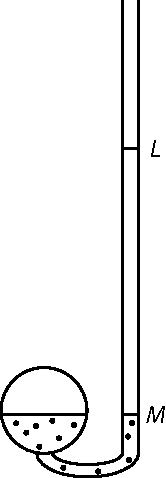
\includegraphics[width=0.18\textwidth]{gesamttex/edit_VIII-4/images/LH_35_13_02c_112-113_d1_112r.pdf}
\edcaption[1.0em]%
{%
\hspace*{-44mm}%
\lbrack\textit{Fig.\:1}\rbrack%
}%
\vspace{-11.9em}%
\hspace{44mm}%
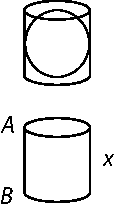
\includegraphics[width=0.136\textwidth]{gesamttex/edit_VIII-4/images/LH_35_13_02c_112-113_d2_112r.pdf}
\edcaption[1.0em]%
{%
\hspace*{44mm}%
\lbrack\textit{Fig.\:2}\rbrack%
}%
\end{edfigure}%
\pstart%
\noindent%
\edtext{%
Sphaer. \astrosun\ $ = 2\ \text{pl.\;cyl.}\ LM$.
Ergo sphaer. cyl.\;\textit{AB} inscr. valor est
$\displaystyle\frac{\text{sphaer. \astrosun}\ \text{per}\ AB^3}{[9]}$.%
\indexS{sphaera inscripta cylindro}%
\indexS{cylinder}%
\indexS{valor}%
}{%
\lemma{Sphaer. \astrosun\ $ = 2\ \text{pl.\;cyl.}\ LM$.}%
\Bfootnote{%
\textit{(1)}~Ergo cyl. $LM = \displaystyle\frac{1}{2} \cdot \text{sphaer.}\ \astrosun$ %
\textit{(2)}~Ergo sphaer. %
\lbrack...\rbrack\ valor est %
\bars{$\displaystyle\frac{\text{sphaer. \astrosun}\ \text{per}\ AB^3}{3}$ \textit{ändert Hrsg.}}.%
~\textit{L}%
}}
\pend%
\pstart%
\noindent%
Jam sphaerae sunt ut cubi diam.%
\indexS{cubus diametri}%
\rule[0mm]{0pt}{3.6mm}
Sphaer.\;\astrosun\ diameter sit \textit{x}.
Sphaerae cyl.\;\textit{AB}
inscriptae diameter %
est \textit{AB}.%
\indexS{sphaera inscripta cylindro}%
\indexS{cylinder}%
\indexS{diameter sphaerae}
Ergo sphaer. \astrosun\ ad sphaer. \textit{AB}
ut $x^3$
\edtext{%
ad $AB^3$.
\newline%
\edtext{%
Jam supra
sph. \astrosun\ est ad sph.\;\textit{AB}
ut $AB^3$ ad~3.%
\indexS{sphaera inscripta cylindro}%
}{%
\lemma{Jam \lbrack...\rbrack\ ad~3}%
\Cfootnote{%
Das Verhältnis zwischen den Kugeln entspricht dem Verhältnis zwischen den jeweiligen Zylindern;
vgl. \refpassage{LH_35_13_02c_112r_bedng-1}{LH_35_13_02c_112r_bedng-2}.%
}}%
}{%
\lemma{ad $AB^3$.}%
\Bfootnote{%
\textit{(1)}~Ergo sphaer$AB = \text{sphaer}\ \astrosun \cdot\ AB^3 : x^3$. %
\textit{(2)}~Jam supra %
\lbrack...\rbrack\ $AB^3$ ad 3.%
~\textit{L}%
}}
Ergo $x^3$ est ad $AB^3$
ut $AB^3$ ad 3,
vel $x^3 = AB^6 : 3$,
vel
$x = AB^2 :
\edtext{%
\lbrack\sqrt[3]{3}\rbrack$.%
}{%
\lemma{$\surd{3}$}%
\Bfootnote{%
\textit{L\;ändert Hrsg.}%
}}
\lbrack%
\href{\Scan{LH_35_13_02c_112v}}%
{112\,v\textsuperscript{o}}%
\rbrack%
\pend%
\vspace{1.0em}%
\pstart%
\noindent%
\edlabel{LH_35_13_02c_112v_masse-1}%
\textit{LM} 27 Zoll hoch,%
\indexS{Zoll}
weit $\displaystyle\frac{1}{3}$ Zoll,%
\edlabel{LH_35_13_02c_112v_masse-2}
thut am
\lbrack\textit{Text bricht ab.}\rbrack%
\pend%
\newpage%
\begin{edfigure}[0em][4.0em]%
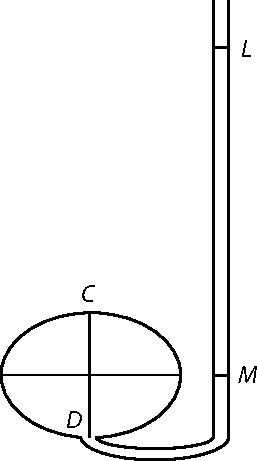
\includegraphics[width=0.26\textwidth]{gesamttex/edit_VIII-4/images/LH_35_13_02c_112-113_d3_112v.pdf}
\edcaption[0.750em]%
{%
\lbrack\textit{Fig.\:3}\rbrack%
}%
\end{edfigure}%
\pstart%
\noindent%
\pagelabel{LH_35_13_02c_112r_zchn}%
\lbrack%
\textit{Auf Bl.\;\href{\Scan{LH_35_13_02c_112r}}{112\,r\textsuperscript{o}}, ohne erkennbaren Zusammenhang mit N.\;\ref{57960}:}%
\rbrack%
\pend%
\begin{edfigure}[2.5em][0.0em]%
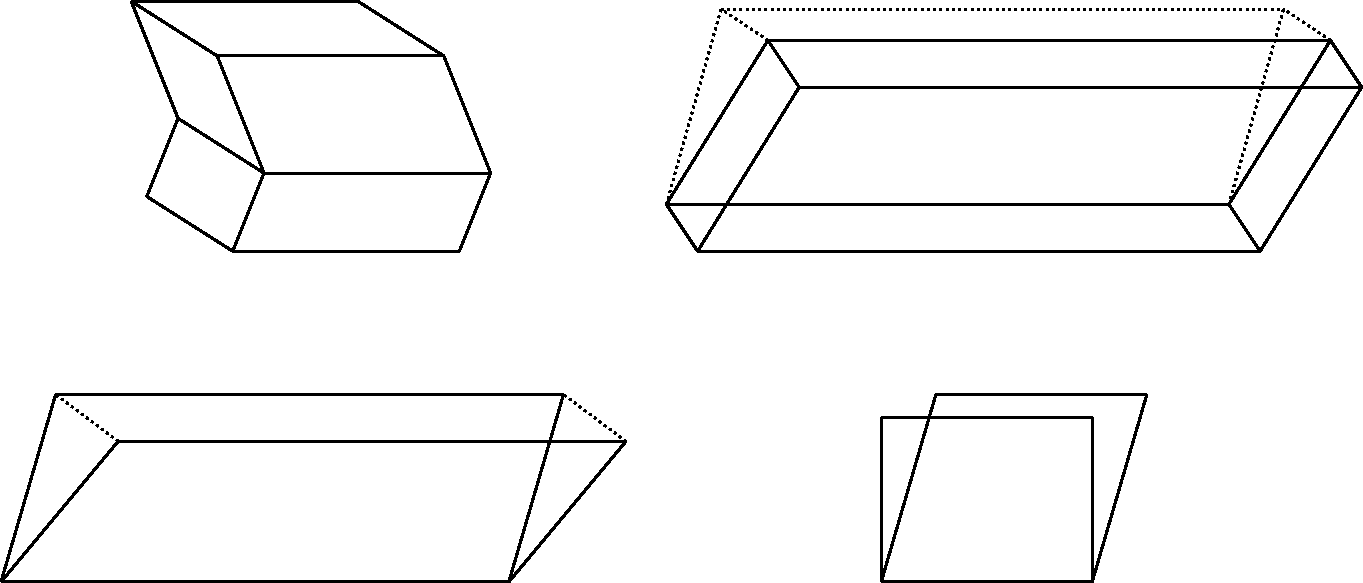
\includegraphics[width=0.72\textwidth]{gesamttex/edit_VIII-4/images/LH_35_13_02c_112-113_d4_112r.pdf}
\edcaption[1.0em]%
{%
\lbrack\textit{Fig.\:4}\rbrack%
}%
\end{edfigure}%
\newpage%
\vspace{4.0em}%
\pstart%
\noindent%
\centering%
*     *     *
\pend%
\vspace{2.0em}%
\selectlanguage{german}%
\frenchspacing%
\footnotesize%
\pstart%
\noindent%
\textls{Ausführliche Datierungsgründe:}%
\pagelabel{57960_dat}
In der titellosen und undatierten Aufzeichnung N.\;\ref{57960}, die einen eher flüchtigen Charakter aufweist, versucht Leibniz, von einem 27 Zoll langen und 1/3 Zoll weiten Rohr ausgehend, eine von einem Zylinder gleichen Volumens umbeschriebene Kugel zu bestimmen.
Rohr und Kugel sind offenbar, wie auch die Diagramme \lbrack\textit{Fig.\:1}\rbrack\ und \lbrack\textit{Fig.\:3}\rbrack\ nahelegen, als Teile eines Barometers zu verstehen.
Die Aufzeichnung N.\;\ref{57960} dürfte somit im Zusammenhang mit Überlegungen über die Beschaffenheit oder den Aufbau eines Barometers entstanden sein.
\pend%
\pstart%
Im Textträger ist die Gegenmarke eines Wasserzeichens anzutreffen, das im Leibniz-Nachlass %
nach heutigem Wissensstand für einen Zeitraum belegt ist, der sich von der frühen Hannoveraner\indexO{Hannover} Zeit bis in die zweite Hälfte der 1690er Jahre erstreckt.
Die Datierung von N.\;\ref{57960} lässt sich möglicherweise aber anhand der Beobachtung einschränken, dass die meisten Überlegungen, die Leibniz der Beschaffenheit oder dem Aufbau des Barometers gewidmet hat, vom Herbst 1677 stammen; siehe die im vorliegenden Band unter N.\;\ref{barom-portab_intro}, N.\;\ref{55813-E} und N.\;\ref{motus-perpetuus_intro} veröffentlichten Aufzeichnungen.
N.\;\ref{57960} könnte insbesondere in Zusammenhang mit Leibnizens Überlegungen über ein tragbares Barometer in N.\;\ref{barom-portab_intro} (August – 12./22.\;November 1677) entstanden sein.
Unter dieser Annahme könnte N.\;\ref{57960} ebenfalls im Herbst 1677 verfasst worden sein.
Eine frühere oder eine spätere Datierung sind aber ohne Weiteres möglich.
\pend%
\selectlanguage{latin}%
\frenchspacing%
\normalsize%
\newpage%




\chapter[tocentry={Instrumentum utile ad aerometrum portatilem
\enskip%
\lbrack Herbst 1677~(?)\rbrack%
}, %
head={Instrumentum utile ad aerometrum portatilem %
}]%
{\MakeUppercase{Instrumentum utile ad aerometrum portatilem}
\newline%
\lbrack Herbst 1677~(?)\rbrack%
} %
\label{55813-E}
\selectlanguage{ngerman}%
\frenchspacing%
\begin{ledgroupsized}[r]{120mm}%
\footnotesize%
\pstart%
\noindent%
\textbf{Überlieferung:}%
\pend%
\end{ledgroupsized}%
\begin{ledgroupsized}[r]{114mm}%
\footnotesize%
\pstart%
\parindent -6mm%
\makebox[6mm][l]{\textit{L}}%
Aufzeichnung:
LH XXXVIII Bl.\;184.
Ein Zettel;
Ränder beschnitten, zum Teil unregelmäßig.
Eine Seite auf Bl.\;\href{\Scan{LH_38_184r}}{184\,r\textsuperscript{o}}.
Bl.\;\href{\Scan{LH_38_184v}}{184\,v\textsuperscript{o}} ist unbeschrieben.
\pend%
\end{ledgroupsized}%
\vspace{5mm}%
\begin{ledgroup}%
\footnotesize%
\pstart%
\noindent%
\textbf{Datierungsgründe:}
Die Datierung der Aufzeichnung N.\;\ref{55813-E} beruht auf %
inhaltlichen Betrachtungen.
Siehe die ausführliche Begründung auf S.\;\pageref{55813-E_dat}.%
\pend%
\end{ledgroup}%
\selectlanguage{latin}%
\frenchspacing%
\vspace{8mm}
\normalsize%
\pstart%
\noindent%
\lbrack%
\href{\Scan{LH_38_184r}}%
{184\,r\textsuperscript{o}}%
\rbrack\
Sit parallelepipedum erectum%
\indexS{parallelepipedum cavum}
\edtext{%
et cavum%
}{%
\lemma{et cavum}%
\Bfootnote{%
\textit{erg.\;L}%
}}
cujus sectio%
\indexS{sectio parallelepipedi}
basi parallela \textit{ABCD},
latera sint tabulae mobiles%
\indexS{tabula mobilis}
in axibus perpendicularibus%
\indexS{axis perpendicularis}
per \textit{ABCD} transeuntibus,
patet %
capacitatem%
\indexS{capacitas parallelepipedi}
\edtext{%
parallel\lbrack epiped\rbrack i%
}{%
\lemma{parallelogrammi}%
\Bfootnote{%
\textit{L\;ändert Hrsg.}%
}}
minui,
si angulus a recto alius fiat,%
\indexS{angulus rectus}
itaque trahendo in unam partem%
\lbrack,\rbrack\
id est aperiendo %
intrabit aqua,%
\indexS{aqua intrans}
in alteram partem retrahendo
seu claudendo exibit.%
\indexS{aqua exiens}
Valvula%
\indexS{valvula}
erit infra.
Tabularum commissurae%
\indexS{commissura tabularum}%
\indexS{tabula mobilis}
erunt corio junctae,%
\indexS{corium}
vel etiam si placet valvulis longis%
\indexS{valvula}
per totum axem ductis%
\indexS{axis perpendicularis}
quae
claudendo machinam%
\indexS{machina}
claudantur,
aperiendo
\edlabel{LH_38_184_dskr-1}%
aperiantur.%
\edtext{}{%
\xxref{LH_38_184_dskr-1}{LH_38_184_dskr-2}%
\lemma{aperiantur.}%
\Bfootnote{%
\lbrack/\rbrack\ %
\textit{(1)}~Utilitati %
\lbrack/\rbrack\ %
\textit{(2)}~Hoc instrumentum mirae utilitatis%
~\textit{L}%
}}
\pend%
\pstart%
Hoc instrumentum%
\indexS{instrumentum susceptibile caloris}
mirae utilitatis%
\indexS{utilitas mira}%
\edlabel{LH_38_184_dskr-2}
ad Aerometrum portatile,%
\indexS{aerometrum porttile}
si inclusum sit transversum elaterium%
\indexS{elaterium transversum}
quod%
\lbrack,\rbrack\
dum clauditur machina%
\indexS{machina}%
\lbrack,\rbrack\
comprimitur%
\indexS{elaterium compressum}%
\lbrack;\rbrack\
debet autem ab aere prius evacuari,%
\indexS{aer evacuatus}
ita non erit susceptibile caloris,%
\indexS{instrumentum susceptibile caloris}%
\indexS{calor}
nec ab eo inclusus aer%
\indexS{aer inclusus}
ad externum sustinendum%
\indexS{aer externus}%
\indexS{aer sustinendus}
fortior reddetur%
\lbrack,\rbrack\
imo non est necesse elaterium esse intus,%
\indexS{elaterium transversum}
sed extra inter \textit{A}~\textit{D}.
\pend%
\begin{edfigure}[3.00em][0.0em]%
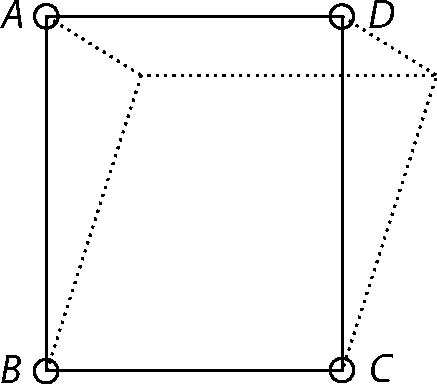
\includegraphics[width=0.280\textwidth]{gesamttex/edit_VIII-4/images/LH_38_04_184-d_184r.pdf}
\edcaption[0.75em]%
{%
\lbrack\textit{Fig.\:1}\rbrack%
}%
\end{edfigure}%
\newpage%
\vspace{3.0em}%
\pstart%
\noindent%
\centering%
*     *     *
\pend%
\vspace{4.0em}%
\selectlanguage{german}%
\frenchspacing%
\footnotesize%
\pstart%
\noindent%
\textls{Ausführliche Datierungsgründe:}%
\pagelabel{55813-E_dat}
Die titellose und undatierte Aufzeichnung N.\;\ref{55813-E} beschreibt schematisch eine Vorrichtung, die beim Aufbau eines tragbaren Barometers (\textit{aerometrum}) Anwendung finden sollte.
Dem Entwurf eines tragbaren Barometers widmet sich Leibniz insbesondere in den zwischen August und dem 12./22. November 1677 entstandenen, in diesem Band unter N.\;\ref{barom-portab_intro} edierten Aufzeichnungen.
Dies lässt die Vermutung zu, dass auch die Aufzeichnung N.\;\ref{55813-E} im Herbst 1677 entstand.
Eine frühere oder spätere Datierung der Aufzeichnung ist allerdings nicht auszuschließen.
Der Textträger weist weder Spuren eines Wasserzeichens noch weitere äußere datierungsrelevante Anhaltspunkte auf.
\pend%
\selectlanguage{latin}%
\frenchspacing%
\normalsize%
\newpage%




\chapter[tocentry={Motus perpetuus per thermometrum, barometrum, hygrometrum %
\enskip\lbrack Oktober 1677\rbrack},
head={Motus perpetuus%
}]%
{\MakeUppercase{Motus perpetuus per thermometrum, barometrum, hygrometrum}
\newline\lbrack Oktober 1677\rbrack}
\label{motus-perpetuus_intro}
\footnotesize%
\pstart%
\noindent%
Die Aufzeichnungen N.\;\ref{57040} und \ref{57041} weisen den gleichen Titel -- \textit{Motus perpetuus per thermometrum, barometrum, hygrometrum} -- auf und bilden einen einheitlichen, bruchlosen Text, in welchem unterschiedliche mechanische Methoden besprochen werden, wie die stetige Bewegung einer Maschine hervorgebracht werden kann.
Nachdem Leibniz im ersten Teil von N.\;\ref{57040} eine bereits 1674/1675 in Paris entworfene Windmühle, deren ununterbrochene Drehung durch die Erhebung hängender Gewichte gesichert werden soll, erneut dargelegt hat, widmet er sich den im Titel beider \textit{Schedae} angegebenen Messinstrumenten als möglichen mittelbaren Quellen einer stetigen Bewegung.
Der Kerngedanke hierbei ist, dass die täglichen Veränderungen dieser Messinstrumente, angemessen ,gespeichert‘, eine hinreichende Bewegungsquelle seien, um einen mechanischen Apparat -- etwa ein Uhrwerk -- stetig zu betätigen.
Der \textit{motus perpetuus}, von dem in diesen Texten die Rede ist, ist daher das Ergebnis einer Umwandlung mechanischer, von außen gespeister Kraft und stellt somit keine Verletzung des Erhaltungsgrundsatzes dar.
Aufgrund ihres einheitlichen Charakters werden die Aufzeichnungen N.\;\ref{57040} und \ref{57041} einheitlich ediert.
\pend%
\pstart%
Der Träger von N.\;\ref{57040} ist von Leibniz eigenhändig auf Oktober 1677 datiert, der Träger von N.\;\ref{57041} weist hingegen keine Datierung auf.
Da die Aufzeichnung N.\;\ref{57041} aber den Text von N.\;\ref{57040} unmittelbar fortsetzt, dürfte wohl auch die zweite Aufzeichnung unmittelbar oder kurz nach der ersten entstanden sein.
Demgemäß wird die Datierung von N.\;\ref{57040} auch für N.\;\ref{57041} übernommen.
Das gesamte Stück N.\;\ref{motus-perpetuus_intro} entstand mit großer Wahrscheinlichkeit im Oktober 1677.
\pend%
\selectlanguage{latin}%
\frenchspacing%
\normalsize%



\section[tocentry={Motus perpetuus per thermometrum, barometrum, hygrometrum. Scheda prima 
\enskip Oktober 1677},
head={Motus perpetuus%
. Scheda I}]%
{\MakeUppercase{Motus perpetuus per thermometrum, barometrum, hygrometrum. Scheda prima}
\newline Oktober 1677}
\label{57040}
\selectlanguage{ngerman}%
\frenchspacing%
\begin{ledgroupsized}[r]{120mm}%
\footnotesize%
\pstart%
\noindent%
\textbf{Überlieferung:}%
\pend%
\end{ledgroupsized}%
\begin{ledgroupsized}[r]{114mm}%
\footnotesize%
\pstart%
\parindent -6mm%
\makebox[6mm][l]{\textit{L}}%
Aufzeichnung:
LH XXXVII 4 Bl.\;160--161.
Ein Bogen, 4\textsuperscript{o}; %
Ränder beschnitten;
Papiererhaltungsmaßnahmen.
Vier ganzseitig beschriebene Seiten;
geringfügiger Textverlust im Falz von
Bl.\;\href{\Scan{LH_37_04_161v}}{161\,v\textsuperscript{o}}.
Die Aufzeichnung N.\;\ref{57041} setzt den Text von N.\;\ref{57040} unmittelbar fort.
\pend%
\end{ledgroupsized}%
\selectlanguage{latin}%
\frenchspacing%
\vspace*{5mm}%
\normalsize%
\pstart%
\noindent%
\lbrack%
\href{\Scan{LH_37_04_160r}}%
{160\,r\textsuperscript{o}}%
\rbrack%
\phantom{Octobris 1677}%
\hfill%
\phantom{\lbrack160\,r\textsuperscript{o}\rbrack}%
Octobr.\;1677%
\pend%
\vspace{-0.35em}%
\pstart%
\noindent%
\centering{%
\edtext{M.\;P.%
\indexS{motus perpetuus}%
}{%
\lemma{M.\;P.\,}%
\Cfootnote{\textit{motus perpetuus}.%
}}
per Thermom.%
\indexS{thermometrum}
Barometr.%
\indexS{barometrum}
Hygrometr.%
\indexS{hygrometrum}%
\\
\edlabel{LH_37_04_160-161_160r_krd_1a}%
Scheda 1%
\indexS{scheda}%
}%
\edtext{}{%
\xxref{LH_37_04_160-161_160r_krd_1a}{LH_37_04_160-161_160r_krd_1b}%
\lemma{Scheda 1}%
\Bfootnote{%
\lbrack/\rbrack\
\textit{(1)}\;Absolvi %
\textit{(2)}\;Assecutus sum tandem, %
\textit{(a)}\;quem diu %
\textit{(b)}\;quod diu quaesiveram%
~\textit{L}%
}}%
\pend%
\vspace{0.35em}%
\pstart%
\noindent%
Assecutus sum tandem,
quod diu quaesiveram%
\lbrack,\rbrack%
\edlabel{LH_37_04_160-161_160r_krd_1b}
motum perpetuum utilem vitae%
\indexS{motus perpetuus utilis vitae}%
\indexS{vita} %
in exiguo aeque ac magno valiturum:
non illum quidem
quem ignari quaerunt,%
\indexS{ignarus}
quo fieret
ut eadem vis se ipsa major esset%
\indexS{vis major se ipsa}
nulla nova vi accedente;%
\indexS{vis nova}%
\indexS{vis accedens}
sed eum
quem prudentes optare satis habent,%
\indexS{prudentes}
quo
\edtext{%
molendina%
\indexS{molendinum actum sine aqua, vento aut animalibus}
sine aqua%
\indexS{aqua}
et vento%
\indexS{ventus}
et animalibus%
\indexS{animal}
agantur,%
}{%
\lemma{molendina}%
\Bfootnote{%
\textit{(1)}~instituantur, %
\textit{(2)}~etiam \textlangle ut\textrangle\ %
\textit{(3)}~sine aqua %
\lbrack...\rbrack\ et animalibus %
\bars{alligatis \textit{gestr.}} agantur%
~\textit{L}%
}}
aut horologia portatilia%
\indexS{horologium portatile restitutum sponte sua}
sponte sua restituantur.
De Motu perenni%
\indexS{motus perennis portatilis}
\edtext{%
portatili mox%
}{%
\lemma{portatili}%
\Bfootnote{%
\textit{(1)}~postea %
\textit{(2)}~mox%
~\textit{L}%
}}
dicam,
hunc enim novissime inveni.
Majorem illum vitae utilem%
\indexS{motus perpetuus utilis vitae}
dudum in promtu
\edtext{%
habui.
Et variis quidem modis:
\edlabel{LH_37_04_160-161_160r_molvent-1}%
facilior ille est ac popularior %
qui vento nititur,%
\indexS{motus perpetuus nitens vento}
sed non vento perpetuo%
\indexS{ventus perpetuus}
indiget.%
}{%
\lemma{habui.}%
\Bfootnote{%
\textit{(1)}~Qui vento quidem opus hab %
\textit{(2)}~Et variis %
\lbrack...\rbrack\ vento nititur, %
\textit{(a)}~scilicet ventus fortis %
\textit{(b)}~sed non vento perpetuo indiget.%
~\textit{L}%
}}
\edtext{%
\edtext{%
Nimirum vento flante%
\indexS{ventus flans}
non tantum circumagatur machina,%
\indexS{machina circumacta vento}
sed et subito pondera multa %
aut magna eleventur%
\indexS{pondus elevatum vento}
vel elastra comprimantur;%
\indexS{elastrum compressum vento}
quae pondera aut Elastra
cessante vento,%
\indexS{ventus cessans}%
}{%
\lemma{Nimirum}%
\Bfootnote{%
\textit{(1)}~cum vento elevetur pondus maximum aut %
\textit{(2)}~vento %
\bars{flante non %
\lbrack...\rbrack\ et subito \textit{erg.}} pondera multa, %
\textit{(a)}~quae cessante vento %
\textit{(b)}~aut magna eleventur vel elastra %
\textit{(aa)}~tendantur %
\textit{(bb)}~comprimantur; quae pondera %
\textit{(aaa)}~atq %
\textit{(bbb)}~aut Elastra cessante vento%
~\textit{L}%
}}
paulatim ad naturalem%
\indexS{status naturalis}
\edtext{%
statum redire tentent,%
}{%
\lemma{statum}%
\Bfootnote{%
\textit{(1)}~restituant sese %
\textit{(2)}~rever %
\textit{(3)}~redire tentent%
~\textit{L}%
}}
atque interim machinam animent,%
\indexS{machina animata}
tantisper dum ventus
\edtext{%
rediens%
\indexS{ventus rediens}
nova elevatione%
\indexS{elevatio ponderis vento}
aut compressione%
\indexS{compressio elastri vento}
restitat%
}{%
\lemma{rediens}%
\Bfootnote{%
\textit{(1)}~nondum quidem restituta, %
\textit{(2)}~restitant %
\textit{(3)}~nova elevatione aut compressione %
\textit{(a)}~restitant %
\textit{(b)}~restitat%
~\textit{L}%
}}
ipsa in violentum%
\indexS{status violentus}
agendique capacem.%
\indexS{status capax agendi}%
}{%
\lemma{Nimirum \lbrack...\rbrack\ capacem}%
\Cfootnote{%
Ein \textit{horologium ventaneum perpetuum}, durch welches ein \textit{motus regularis continuus a causa irregularis discontinuata} erzeugt werden soll, hatte Leibniz in Paris entworfen; vgl. \textit{LSB} VIII,\;2 N.\;94.\cite{01472}%
}}
Ita Machina semper satis virium habebit%
\indexS{vis machinae}
ad utiles vitae%
\indexS{effectus utilis vitae}%
\indexS{vita}
\edlabel{LH_37_04_160-161_160r_grz_2a}%
effectus.%
\edtext{}{%
\xxref{LH_37_04_160-161_160r_grz_2a}{LH_37_04_160-161_160r_grz_2b}%
\lemma{effectus.}%
\Bfootnote{%
\lbrack/\rbrack\
\textit{(1)}~Objicit %
\textit{(2)}~Obi %
\textit{(3)}~Objici%
~\textit{L}%
}}
\pend%
\newpage%
\pstart%
Objici%
\edlabel{LH_37_04_160-161_160r_grz_2b}
potest
\edtext{%
ventum aliquando%
}{%
\lemma{ventum}%
\Bfootnote{%
\textit{(1)}~non %
\textit{(2)}~aliquando%
~\textit{L}%
}}
rarum esse.%
\indexS{ventus rarus}
Ponamus ergo singulis mensibus%
\indexS{mensis}
semel tantum spirare ventum
restituendae machinae sufficientem,%
\indexS{machina restituenda}
manifestum
\edtext{%
est %
satis magna esse posse vela%
\indexS{velum latum}
ad magnam venti vim%
\indexS{vis venti}
excipiendam.
Et ventum etiam%
}{%
\lemma{est}%
\Bfootnote{%
\textit{(1)}~tum %
\textit{(2)}~satis magna %
\lbrack...\rbrack\ magnam venti %
\textit{(a)}~exci %
\textit{(b)}~vim excipiendam %
\textit{(aa)}~sed et %
\textit{(bb)}~tum etiam %
\textit{(cc)}~. Et ventum etiam%
~\textit{L}%
}}
mediocrem%
\indexS{ventus mediocris}
continuatione vim maximam
\edtext{%
exercere.
Et ut verbo dicam,%
}{%
\lemma{exercere.}%
\Bfootnote{%
\textit{(1)}~Haud d %
\textit{(2)}~Et ut verbo dicam,%
~\textit{L}%
}}
negari non potest
quovis mense%
\indexS{mensis}
tantam venti vim esse,%
\indexS{vis venti}
ut se dispensetur,
et velut in aerarium%
\indexS{aerarium}
dum eo sit opus recondatur,
fortissimum molendinum%
\indexS{molendinum ventaneum}
continue agere possit.
\edtext{%
Excipietur velis latissimis;%
\indexS{velum latum}
in thesaurum%
\indexS{thesaurus}
vero referetur,
et dispensabitur ponderibus%
\indexS{pondus elevatum vento}
vel Elastris.%
\indexS{elastrum compressum vento}
At%
}{%
\lemma{Excipietur}%
\Bfootnote{%
\bars{autem \textit{gestr.}} velis latissimis; %
\textit{(1)}~dispensabitur et %
\textit{(2)}~at %
\textit{(3)}~in thesaurum %
\bars{vero \textit{erg.}} referetur, et %
\lbrack...\rbrack\ Elastris. At%
~\textit{L}%
}}
inquies vela lata%
\indexS{velum latum}
incommoda erunt,
cum ventus nimis fortis erit.%
\indexS{ventus fortis}
Huic rei remedium%
\indexS{remedium}
in promtu est,
ut vela%
\indexS{velum latum}
ubi ad certum celeritatis pervenerunt gradum%
\indexS{gradus celeritatis}%
\indexS{celeritas velorum molendini}%
\lbrack,\rbrack\
constringantur
sive latitudine imminuantur.
\pend%
\begin{edfigure}[1.75em][1.0em]%
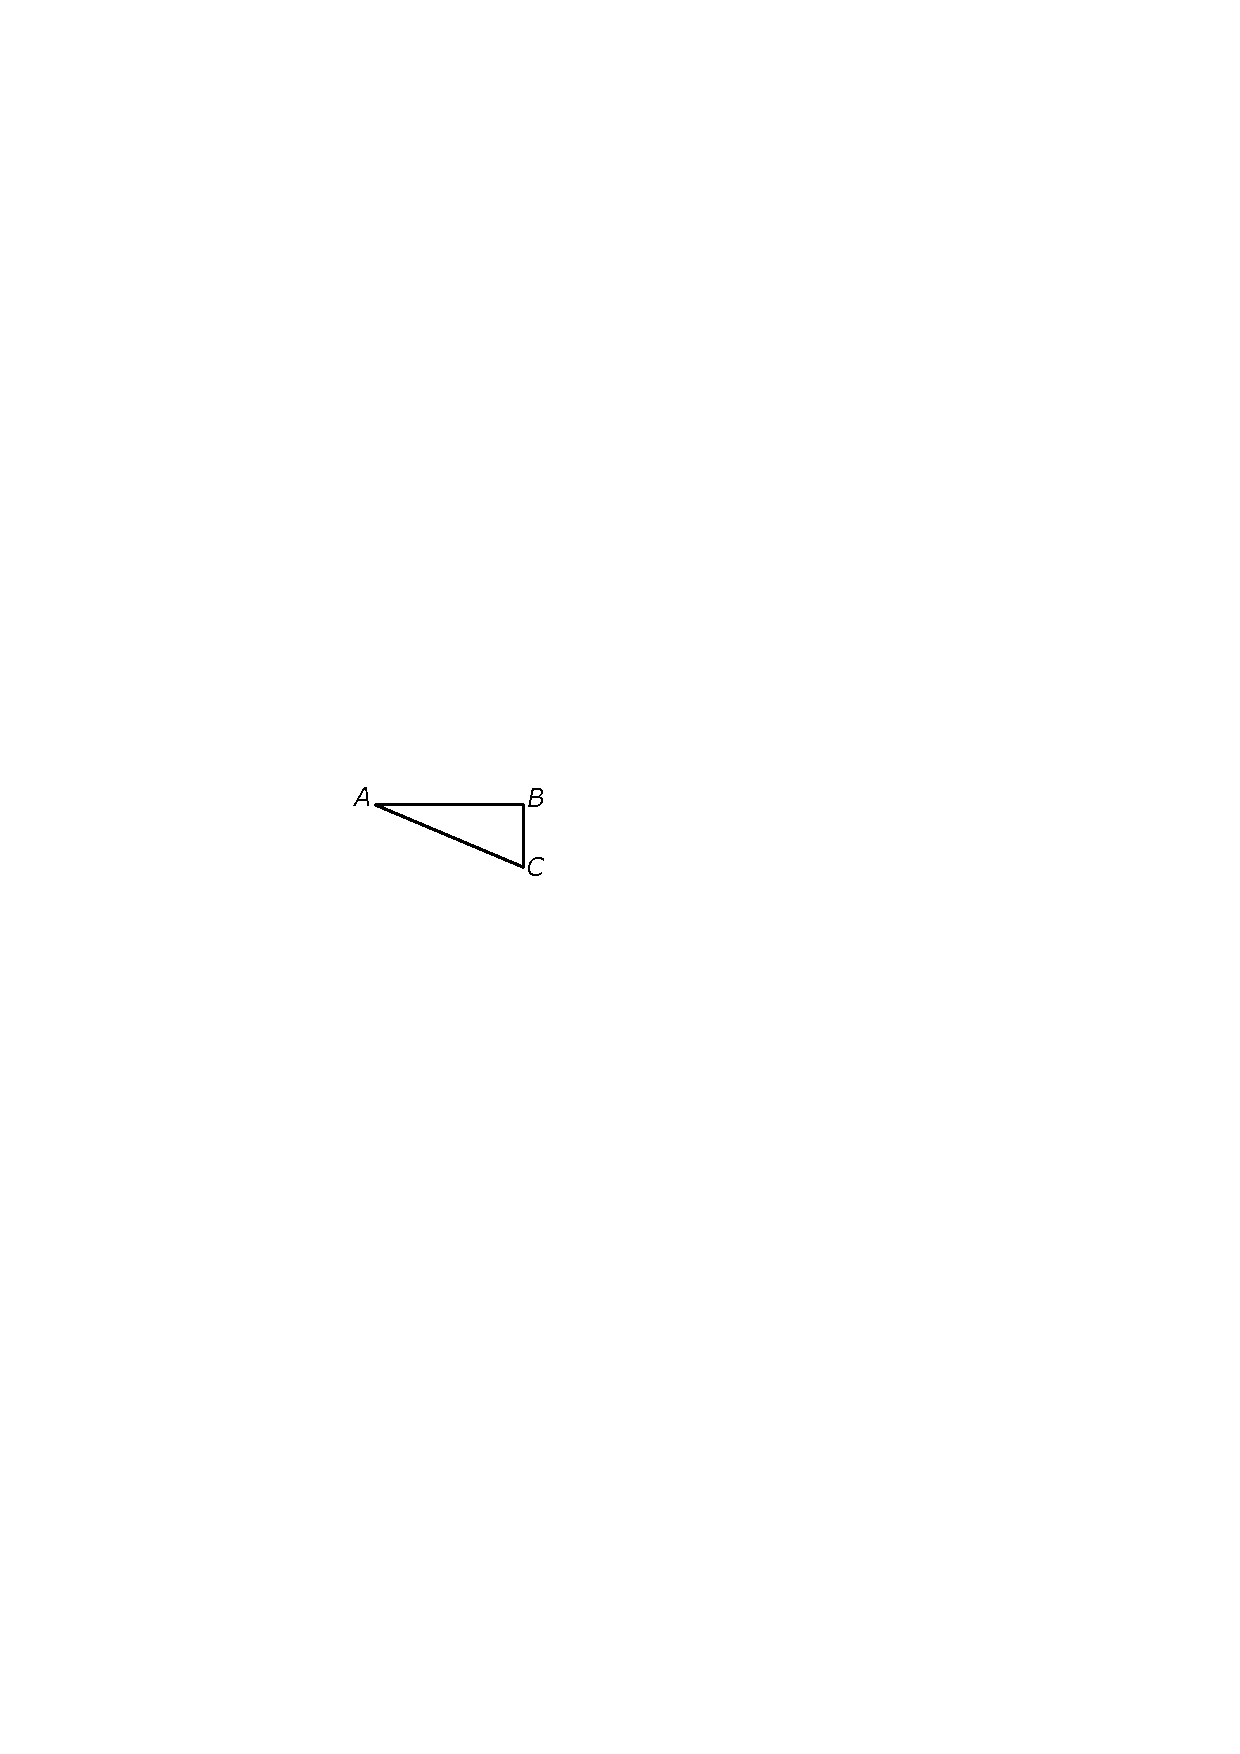
\includegraphics[width=0.20\textwidth]{gesamttex/edit_VIII-4/images/LH_37_04_160-161_d1_160r.pdf}
\edcaption[0.30em]%
{%
\lbrack\textit{Fig.\:1}\rbrack%
\edtext{}{%
\lemma{\lbrack\textit{Fig.\:1}\rbrack}%
\Cfootnote[nonum]{%
In \textit{L} ist das Diagramm im Text eingebunden.%
}}%
}%
\end{edfigure}%
\pstart%
Sed unde tanta copia ponderum%
\indexS{pondus elevatum vento}
atque Elastrorum habebitur,%
\indexS{elastrum compressum vento}
qua vis illa maxima%
\indexS{vis asservata}
satis asservari possit%
\lbrack?\rbrack\
perinde est enim
ac si aquam%
\indexS{aqua agens molendinum}
quae molendinum%
\indexS{molendinum actum aqua}
integro mense agit%
\indexS{mensis}
asservare
\edtext{%
vellemus;
ubi notandum
quod aqua%
\indexS{aqua agens molendinum}
quae molendinum agit%
}{%
\lemma{vellemus;}%
\Bfootnote{%
\textit{(1)}~respondeo aqua quae %
\textit{(a)}~mense %
\textit{(b)}~molendinum mense agit %
\textit{(2)}~praesertim %
\textit{(3)}~ubi notandum %
\lbrack...\rbrack\ molendinum agit%
~\textit{L}%
}}
in magna mole parum habet virium,%
\indexS{moles aquae}%
\indexS{vires in mole}
ob exiguam fluxus%
\indexS{fluxus aquae}
\edtext{%
inclinationem,%
\indexS{inclinatio fluxus aquae}
itaque si defluxus esset perpendicularis,%
\indexS{defluxus perpendicularis}
crederem vix millesima parte%
}{%
\lemma{inclinationem,}%
\Bfootnote{%
\textit{(1)}~itaque videntur integrae vires unius mensis %
\textit{(2)}~itaque si %
\textit{(a)}~flux %
\textit{(b)}~defluxus esset perpendicularis, crederem vix %
\textit{(aa)}~centesima %
\textit{(bb)}~millesima parte%
~\textit{L}%
}}
opus fore.
Ponamus
declivitatem esse \textit{AC},%
\indexS{declivitas fluxus aquae}
altitudinem \textit{BC},
erit ut \textit{AC} ad \textit{BC},
ita ratio virium.%
\indexS{ratio virium}
Quare si \textit{BC} sit pes,%
\indexS{pes}
et \textit{AC} decies mille pedes,
seu si decies
\edtext{%
mille pedum cursu sit opus%
\indexS{cursus}
ad unius pedis depressionem,%
\indexS{depressio}%
}{%
\lemma{mille}%
\Bfootnote{%
\textit{(1)}~pedes sit opus ad unum pedem %
\textit{(2)}~cur %
\textit{(3)}~pedum cursu %
\lbrack...\rbrack\ pedis depressionem%
~\textit{L}%
}}
patet
decies millesimam aquae%
\indexS{aqua agens molendinum}
\lbrack%
\href{\Scan{LH_37_04_160v}}%
{160\,v\textsuperscript{o}}%
\rbrack\
partem
\edtext{%
sufficere,
et quia%
}{%
\lemma{sufficere,}%
\Bfootnote{%
\textit{(1)}~ponamus ergo %
\textit{(2)}~et quia%
~\textit{L}%
}}
mensis est 30 dierum,%
\indexS{mensis}%
\indexS{dies}
et dies 24%
\indexS{dies}
\edtext{%
horarum,%
\indexS{hora}
et hora%
\indexS{hora}
60 minutorum%
\indexS{minutum}%
\lbrack,\rbrack\
ideo mensis%
\indexS{mensis}
erit 43200 minutorum,%
\indexS{minutum}%
}{%
\lemma{horarum,}%
\Bfootnote{%
\textit{(1)}~ideo 720 horis, vel 43200 minutis opus est dies %
\textit{(2)}~et hora %
\lbrack...\rbrack\ 43200 minutorum%
~\textit{L}%
}}%
\edtext{}{\lemma{\textit{Hilfsrechnung am Rand:}}%
\Afootnote{%
$\begin{tabular}[t]{r}24\phantom{00}\\30\phantom{0}\\\hline 7200\\6\phantom{00}\\\hline 43200\end{tabular}$
}}
quae
si dividantur per decies mille
fiet
$\displaystyle\frac{432}{100}$.%
\rule[-0mm]{0pt}{5.8mm}
Ideo sufficiet
ad idem molendinum%
\indexS{molendinum actum aqua}
perpendiculari descensu agendum,%
\indexS{descensus perpendicularis}
tantum aquae%
\indexS{aqua agens molendinum}
quantum
\edtext{%
$4+\displaystyle\frac{32}{100}$
seu
$4+\displaystyle\frac{8}{25}$,
seu circiter
$4+\displaystyle\frac{1}{3}$ minutis%
}{%
\lemma{$4+\displaystyle\frac{32}{100}$}%
\Bfootnote{%
\textit{(1)}~minutis %
\textit{(2)}~seu $4 + %
\lbrack...\rbrack\ \displaystyle\frac{1}{3}$ minutis%
~\textit{L}%
}}
praeterfluit.
Id est tantum aquae%
\indexS{aqua agens molendinum}
quantum dixi%
\rule[-0mm]{0pt}{4.6mm}
ad eundem effectum producendum sufficiet,%
\indexS{effectus producendus}
si scilicet perpendiculariter
\edlabel{LH_37_04_160-161_160v_hyg-1}
descendat.%
\rule[-0mm]{0pt}{5.8mm}%
\edtext{}{%
\xxref{LH_37_04_160-161_160v_hyg-1}{LH_37_04_160-161_160v_hyg-2}%
\lemma{descendat.}%
\Bfootnote{%
\lbrack/\rbrack\
\textit{(1)}~Ponamus autem si placet esse pondus centum centupondiorum, quae quidem %
\textit{(2)}~Quantitas autem ista, ut facilius %
\textit{(a)}~expli %
\textit{(b)}~explicetur %
\textit{(c)}~habeatur, videndum %
\lbrack...\rbrack\ interim esse %
\textit{(aa)}~fluxum %
\textit{(bb)}~centum %
\textit{(cc)}~pondus centum %
\lbrack...\rbrack\ mille libras.%
~\textit{L}%
}}%
\pend%
\pstart%
\rule[-0mm]{0pt}{5.8mm}%
Quantitas autem ista %
ut facilius habeatur,
videndum tot minutis%
\indexS{minutum}
quantam piscinam%
\indexS{piscina}
ad quam altitudinem
fluxus ejusdem aquae%
\indexS{fluxus aquae}%
\indexS{aqua agens molendinum}
impleat.
Ponamus interim
esse pondus%
\indexS{pondus agens molendinum}
centum centupondiorum,%
\indexS{centupondium}
seu esse decem mille libras.%
\indexS{libra}%
\edlabel{LH_37_04_160-161_160v_hyg-2}
Imo ponamus esse centum mille libras.
Pondus ergo vel pondera mille,%
\indexS{pondus agens molendinum}
unumquodque librarum centum,
vel pondera centum unumquodque librarum mille%
\indexS{libra}
in promtu esse debent,
suspensaque teneri ex funibus,%
\indexS{funis}
ut ascendant descendantque.
Caeterum adhuc unum in calculum%
\indexS{calculus}
venire debet%
\lbrack:\rbrack\
aqua quae molendinum agit%
\indexS{aqua agens molendinum}%
\lbrack,\rbrack\
\edtext{%
non agit in%
}{%
\lemma{non}%
\Bfootnote{%
\textit{(1)}~in %
\textit{(2)}~agit in%
~\textit{L}%
}}
ipsum nisi per altitudinem
quanta est lapsus ejus%
\indexS{lapsus aquae}
cum se ex cataracta%
\indexS{cataracta}
praecipitat.%
\indexS{aqua precipitans}
Cum hoc
\edtext{%
loco excelsissimi pali%
\indexS{palus excelsus}
esse possint%
}{%
\lemma{loco}%
\Bfootnote{%
\textit{(1)}~integrat satisque prohibitu %
\textit{(2)}~excelsissimi pali esse possint%
~\textit{L}%
}}
de quibus pondera descendant,%
\indexS{pondus agens molendinum}
centies scilicet lapsu hoc altiores.%
\indexS{lapsus aquae}
Sed ponamus esse decies tantum,
utique decuplo amplius virium applicabitur.%
\indexS{vis applicata}
Nihilominus cogitandum
est aquam lapsu impetum%
\indexS{impetus aquae labentis}
\edtext{%
acquirere,%
\indexS{impetus acquisitus lapsu}
majorem%
}{%
\lemma{acquirere,}%
\Bfootnote{%
\bars{decuplo forte \textit{gestr.}} majorem%
~\textit{L}%
}}
quam
qui sine lapsu%
\indexS{lapsus aquae}
\edtext{%
foret.
Aestimandum ergo%
}{%
\lemma{foret}%
\Bfootnote{%
\textit{(1)}~, itaque %
\textit{(2)}~. Aestimandum ergo%
~\textit{L}%
}}
quantum acquirat aqua lapsu%
\indexS{lapsus aquae}%
\indexS{aqua labens}
ex aliquot pedum altitudine.%
\indexS{pes}
Cogitandum tamen
esse aliquem impetum acquisitum%
\indexS{impetus acquisitus lapsu}
non ex lapsu tantum
sed et ex fluxu prope cataractam accelerato,%
\indexS{fluxus acceleratus}%
\indexS{cataracta}
nam et fluxus
est aliquis lapsus.
Altitudinem ergo palorum,%
\indexS{palus excelsus}
majorem quam lapsus,
cum impetu%
\indexS{impetus quaesitus lapsu}
per lapsum%
\indexS{lapsus aquae}
fluxumque%
\indexS{fluxus aquae}
quaesito tuto compensari%
\indexS{impetus compensatus}
posse arbitror.
Jam vis illa rursus distribuenda est%
\indexS{vis distribuenda in mensem}
in mensem integrum,%
\indexS{mensis}
id est efficiendum est,
ut celeritas descensus%
\indexS{celeritas descensus}%
\indexS{descensus aquae}
sit decies millesima pars ejus
qua libere descendere
\ledpb%
(non loquendo de acquisito impetu)%
\indexS{impetus acquisitus lapsu}
\edtext{%
conaretur,
ea scilicet proportione%
}{%
\lemma{conaretur,}%
\Bfootnote{%
\textit{(1)}~quod %
\textit{(2)}~ea scilicet proportione%
~\textit{L}%
}}
qua quantitatem molis
\edlabel{LH_37_04_160-161_160v_ske-1a}%
diminuimus,%
\edtext{}{%
\xxref{LH_37_04_160-161_160v_ske-1a}{LH_37_04_160-161_161r_ske-1b}%
\lemma{diminuimus,}%
\Bfootnote{%
\textit{(1)}~quae scilicet descensus tarditate compensari debet %
\textit{(2)}~quia scilicet %
\lbrack...\rbrack\ in aqua. \lbrack/\rbrack\ %
\textit{(a)}~Sed ut dicam quod res hujusmodi %
\lbrack\href{\Scan{LH_37_04_161r}}{161\,r\textsuperscript{o}}\rbrack\ %
\textit{(b)}~Sed quia pondera tam ingentia incommoda sunt maxime %
\textit{(c)}~Verum ne %
\lbrack...\rbrack\ videamus quantum %
\textit{(aa)}~a mo %
\textit{(bb)}~pondus a %
\lbrack...\rbrack\ quantam altitudinem %
\textit{(aaa)}~horae %
\textit{(bbb)}~spatio unius %
\lbrack...\rbrack\ majoris temporis
\bars{ad quantam altitudinem \textit{streicht Hrsg.}} elevari possit.%
~\textit{L}%
}}
quia scilicet tarditas descensus
\indexS{tarditas descensus}
idem faciet
quod inclinatio in aqua.%
\indexS{inclinatio in aqua}
\lbrack%
\href{\Scan{LH_37_04_161r}}%
{161\,r\textsuperscript{o}}%
\rbrack%
\pend%
\pstart%
Verum ne in calculo fallamur,%
\indexS{calculus}
ad vim molendini%
\indexS{vis molendini}%
\indexS{molendinum ventaneum}
melius aestimandam%
\indexS{vis aestimanda}
videamus
quantum pondus a molendino%
\indexS{pondus elevatum molendino}%
\indexS{molendinum elevans pondus}
ad quantam altitudinem
spatio unius minuti%
\indexS{minutum}
vel majoris temporis%
\indexS{tempus}
elevari possit.%
\edlabel{LH_37_04_160-161_161r_ske-1b}
Haec eadem vis nobis etiam per minutum%
\indexS{minutum}
necessaria erit.%
\indexS{vis necessaria}
Et repetita vicibus 43200 per mensem integrum.%
\indexS{vis repetita}%
\indexS{mensis}
Quam vim vereor
ut praestare possimus,
nisi adhibito aeris pondere.%
\indexS{pondus aeris adhibitum}
Quod ita intelligo,
si maximi folles adhibiti sint,
ac sibi super impositi,%
\indexS{follis superimpositus}
ut \textit{AB}, \textit{BC}, \textit{CD}.
\edlabel{LH_37_04_160-161_161r_pasca-1}%
Sit diameter follis \textit{A}\pgrk{a}
longitudine unius pedis,%
\indexS{pes}
ipsa tabula autem rotunda,%
\indexS{tabula follis rotunda}
erit
\edtext{%
(ex calculo Pascalii)%
\indexN{\textls{Pascal} (Pascalius), Blaise 1623\textendash1662}%
}{%
\lemma{(ex calculo Pascalii)}%
\Cfootnote{%
Anspielung auf
\textsc{B.\;Pascal},
\textit{De la pesanteur de la masse de l'air},
cap.\;3\cite{01432}
(\textit{Traitez}, Paris 1663,
S.\;95;\cite{00081}
\textit{PO}\;II, S.\;1082\,f.).%
\cite{01524}
Dort wird festgehalten, dass auf der Oberfläche eines Blasebalges das Gewicht einer 31 Fuß hohen Wassersäule lastet.
Leibniz geht offenbar davon aus, dass ein kubischer Fuß Wasser etwa 70 Pfund wiege:
Vgl. auch N.\;\ref{41212} in diesem Band, \refpassage{LH_35_09_25_001-002+004-005_001r_ucn-1}{LH_35_09_25_001-002+004-005_001r_ucn-2}.%
}}
pondus aeris incumbentis%
\indexS{pondus aeris incumbentis}%
\indexS{aer incumbens}
minimum 1700 librarum.%
\indexS{libra}%
\edlabel{LH_37_04_160-161_161r_pasca-2}
\edtext{%
Ducendum in altitudinem follium%
\lbrack:\rbrack\
si duorum sit pedum%
\indexS{pes}
erit pondus fere 7000 librarum;%
\indexS{pondus aeris incumbentis}
si trium erit 15000 librarum.%
\indexS{libra}%
}{%
\lemma{\textit{Hilfsrechnungen am Rand:}}%
\Afootnote{%
\begin{tabular}[t]{r}%
1700%
\\%
4\phantom{00}%
\\%
\hline%
6800%
\end{tabular}%
\hspace{5mm}%
\begin{tabular}[t]{r}%
1700%
\\%
9\phantom{00}%
\\%
\hline%
15300%
\end{tabular}%
}}
Tantum cavendum
ne tanta vis%
\indexS{vis aeris dirumpens follem}
folles dirumpat.%
\indexS{follis diruptus vi aeris}
Quaeritur etiam
an satis venti%
\indexS{ventus agens molendinum}
toto tempore futurum sit,
quod tantam
\edtext{%
mo\lbrack l\rbrack em%
\indexS{moles}%
}{%
\lemma{mollem}%
\Bfootnote{%
\textit{L\;ändert Hrsg.}%
}}
attollere possit.
\pend%
\begin{edfigure}[1.75em][1.0em]%
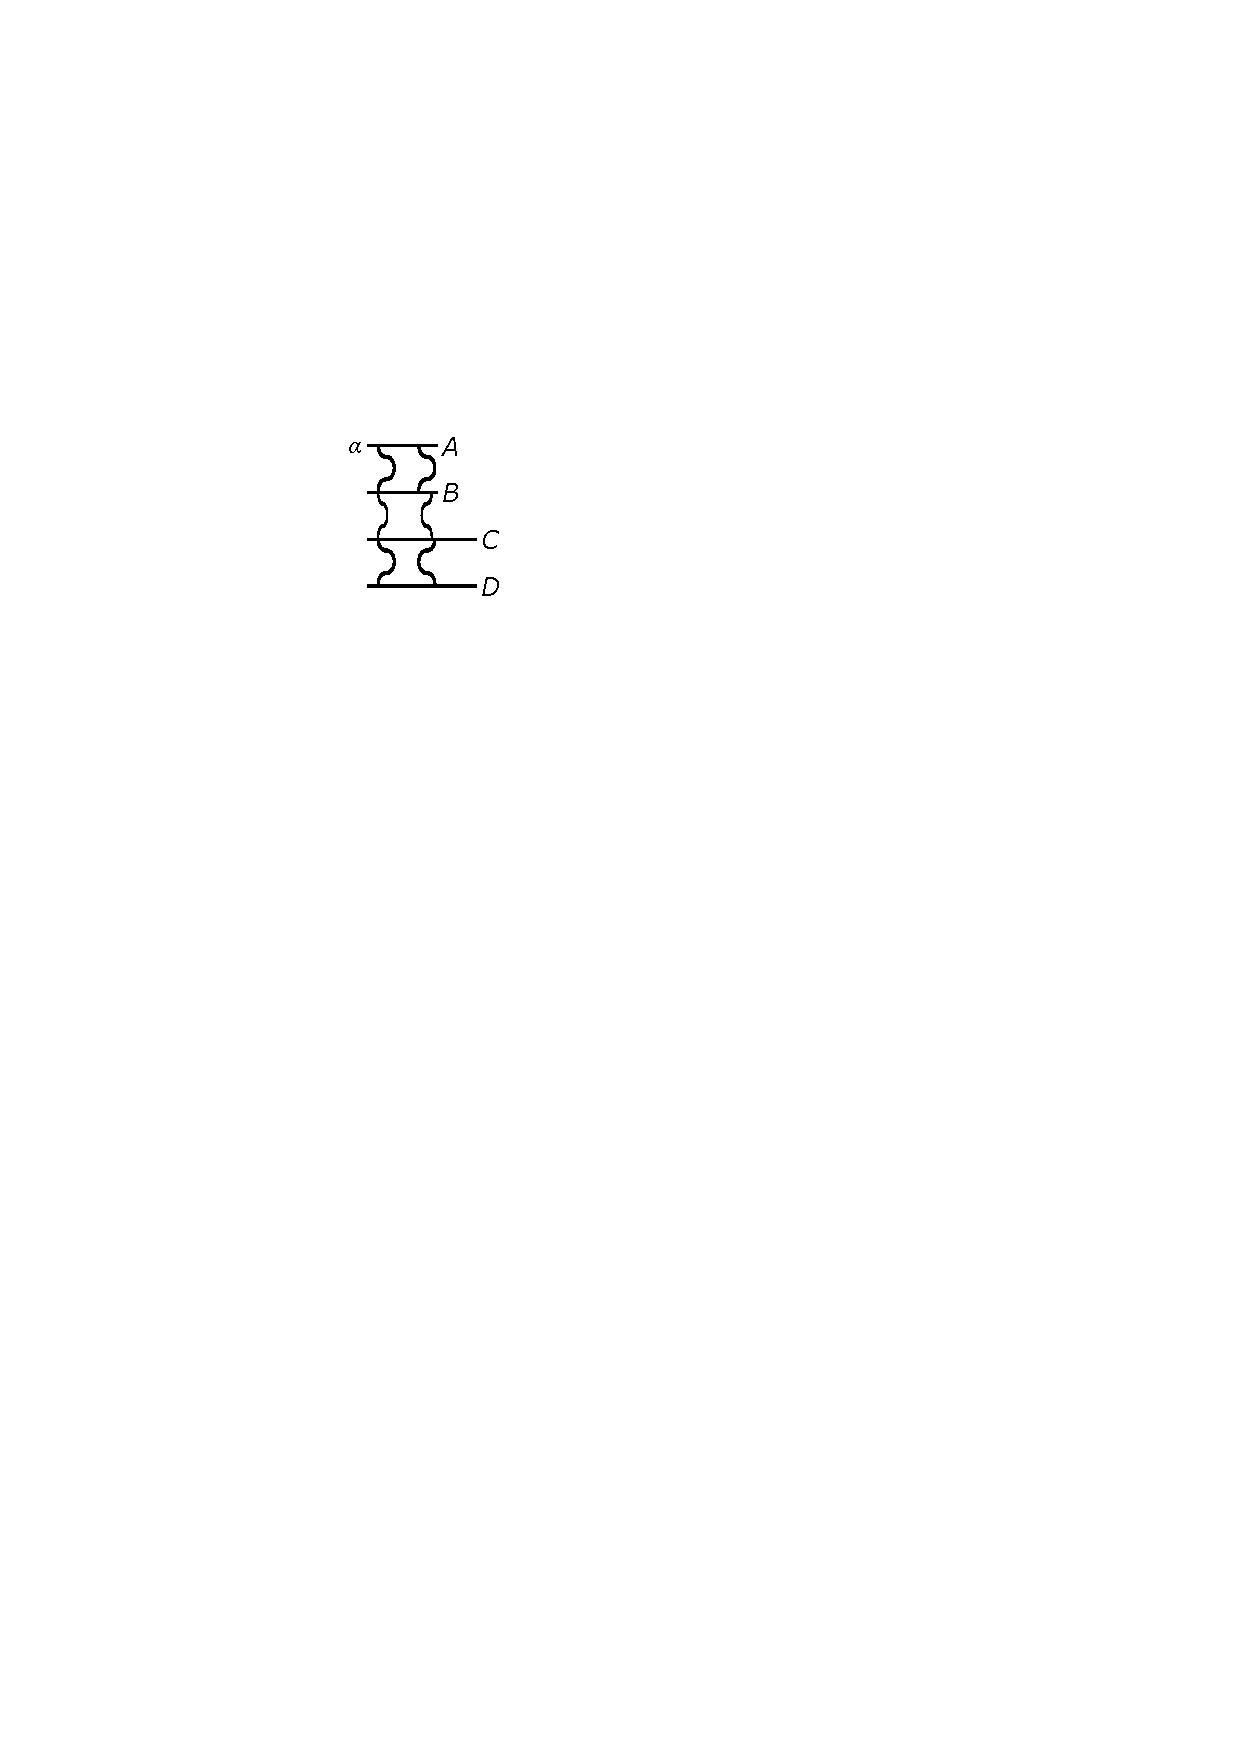
\includegraphics[width=0.16\textwidth]{gesamttex/edit_VIII-4/images/LH_37_04_160-161_d2_161r.pdf}
\edcaption[0.30em]%
{%
\lbrack\textit{Fig.\:2}\rbrack%
}%
\end{edfigure}%
\newpage%
\pstart%
Caeterum
\edtext{%
optima ratio hujus inventi%
\indexS{ratio inventi}%
\indexS{inventum}%
}{%
\lemma{optima}%
\Bfootnote{%
\textit{(1)}~rei %
\textit{(2)}~ratio hujus inventi%
~\textit{L}%
}}
est,
cum nec follibus %
nec ponderibus aliis opus
quam ipsa aqua.
Nimirum in Fodinis%
\indexS{fodina}
ex quibus aqua extrahi debet,%
\indexS{aqua extracta e fodinis}%
\indexS{extractio aquae e fodinis}
scilicet aqua vento extrahetur%
\indexS{aqua extracta vento}%
\indexS{ventus ad aquam extraendam}
maxima in copia
nec
\edtext{%
effund\lbrack e\rbrack tur%
}{%
\lemma{effundatur}%
\Bfootnote{%
\textit{L\;ändert Hrsg.}%
}}
inutiliter,
sed in ingentes lacus%
\indexS{lacus ingens}
\edtext{%
cond\lbrack e\rbrack tur,%
}{%
\lemma{condatur}%
\Bfootnote{%
\textit{L\;ändert Hrsg.}%
}}
unde postea ipsa
cessante vento%
\indexS{ventus cessans}
paulatim effluens
perpetui fluminis locum geret.%
\indexS{flumen perpetuum}%
\edlabel{LH_37_04_160-161_161r_molvent-2}
\pend%
\pstart%
Aliud
\edtext{%
est modus perennis Motus%
\indexS{motus perennis}%
}{%
\lemma{est}%
\Bfootnote{%
\textit{(1)}~motus %
\textit{(2)}~modus perennis Motus%
~\textit{L}%
}}
per simplex Barometrum,%
\indexS{barometrum simplex}
sed iisdem
quae dixi%
\lbrack:\rbrack\
follibus vel
\edtext{%
similibus.
Nam si habeat follis%
\indexS{follis adhibitus barometro}
latitudinem pedis,%
\indexS{pes}%
\indexS{latitudo follis}%
}{%
\lemma{similibus}%
\Bfootnote{%
\textit{(1)}~, si se %
\textit{(2)}~. Nam %
\textit{(a)}~qu %
\textit{(b)}~si %
\textit{(aa)}~diameter %
\textit{(bb)}~habeat %
\textit{(aaa)}~pedem %
\textit{(bbb)}~follem %
\textit{(ccc)}~follis latitudinem pedis,%
~\textit{L}%
}}
erit pondus aeris maximum%
\indexS{pondus aeris maximum}
Parisiis%
\indexO{Paris}
\edtext{%
1808 librarum,%
\indexS{libra Parisina}%
}{%
\lemma{1808}%
\Bfootnote{%
\textit{(1)}~pedum %
\textit{(2)}~librarum%
~\textit{L}%
}}
mediocre 1761 librarum,
minimum 1714 librarum,
differentia erit librarum 94 %
inter maximum et minimum,
et librarum 47 circiter inter minimum et mediocrem.
\edtext{%
\edlabel{LH_37_04_160-161_161r_marg-1}%
Ponamus autem
quovis mense non nisi ponderis decem librarum%
\indexS{libra Parisina}
esse differentiam,%
\indexS{differentia ponderis aeris}
\edtext{%
imo non nisi
vigesimam partem maximae differentiae,%
\indexS{differentia ponderis aeris}%
}{%
\lemma{imo non nisi}%
\Bfootnote{%
\bars{pondus \textit{streicht Hrsg.}}
\textit{(1)}~de %
\textit{(2)}~dicentesi %
\textit{(3)}~vigesimam partem maximae differentiae%
~\textit{L}%
}}
seu non nisi
circiter 5 librarum,
patet tamen
satis virium inesse 5 libris%
\indexS{libra Parisina}
ad motum perennem,%
\indexS{motus perennis}
qui (v.\,g.) horologio alicui circumagendo
\edlabel{LH_37_04_160-161_161r_dae_1a}%
sufficiat.%
\edlabel{LH_37_04_160-161_161r_marg-2}%
}{%
\lemma{\textit{Vom Text umrandet:}}%
\Afootnote{%
1 pouce pollex quorum 12 faciunt talem pedem.%
\textsuperscript{\lbrack a\rbrack}%
\indexS{pouce}%
\indexS{pollex}%
\indexS{pes Parisinus}%
\\[1ex]%
{\footnotesize%
\textsuperscript{\lbrack a\rbrack}~%
1 pouce \lbrack...\rbrack\ pedem:
Der inhaltliche Bezugspunkt ist wohl \refpassage{LH_37_04_160-161_161v_sgi-1}{LH_37_04_160-161_161v_sgi-2}.%
}%
}}%
\edtext{}{%
\xxref{LH_37_04_160-161_161r_dae_1a}{LH_37_04_160-161_161r_dae_1b}%
\lemma{sufficiat.}%
\Bfootnote{%
\textit{(1)}~\lbrack/\rbrack\ Tertium principi %
\textit{(2)}~An id %
\lbrack...\rbrack\ motus principium%
~\textit{L}%
}}
\edtext{%
An id ad horologium portabile%
\indexS{horologium portabile}
applicari possit postea videbimus.%
}{%
\lemma{An id \lbrack...\rbrack\ videbimus}%
\Cfootnote{%
Vgl. \refpassage{LH_37_04_160-161_161v_postea}{LH_37_04_160-161_161v_postea}.%
}}
\pend%
\pstart%
Tertium motus principium%
\indexS{principium motus}%
\edlabel{LH_37_04_160-161_161r_dae_1b}
est calor%
\indexS{calor principium motus}
seu thermometrum.%
\indexS{thermometrum}
Et quidem ponamus
calore effici%
\indexS{calor dilatans aerem}
ut aer conetur locum occupare%
\indexS{aer conans occupare locum}
qui sit ad
\edtext{%
priorem
ut 10 %
ad \lbrack 9\rbrack\ idque%
}{%
\lemma{priorem ut}%
\Bfootnote{%
\textit{(1)}~9 ad %
\textit{(2)}~10, ad %
\bars{9 \textit{erg.\;Hrsg.\;nach \refpassage{LH_37_04_160-161_161v_fui-1}{LH_37_04_160-161_161v_fui-2}.}} idque%
~\textit{L}%
}}
nisi impediatur
effecturum esse,
patet non tantum
hanc vim praeponderare aeris massae,%
\indexS{vis praeponderans massae aeris}%
\indexS{massa aeris}
alioqui enim eam non elevaret,
sed et duci debere in quantitatem extensionis,
ut habetur vis ista.
Cumque quotidie contingat haec mutatio,%
\indexS{mutatio contingens}
\lbrack%
\href{\Scan{LH_37_04_161v}}%
{161\,v\textsuperscript{o}}%
\rbrack\
fere
\edtext{%
enim noctes%
\indexS{nox frigidior die}
diebus%
\indexS{dies}%
}{%
\lemma{enim}%
\Bfootnote{%
\textit{(1)}~dies noctibus %
\textit{(2)}~noctes diebus%
~\textit{L}%
}}
frigidiores esse solent.
Ideo credibile est
satis magnam hoc modo vim suppeditari forte%
\indexS{vis suppeditans}
et ad molendinum mediocre circumagendum ope follis.%
\indexS{vis ad molendinum circumagendum}%
\indexS{molendinum circumagendum ope follis}%
\indexS{follis ad circumagendum molendinum}
Crebritas enim harum mutationum%
\indexS{crebritas mutationum}
debilitatem large compensat.
Tantum ergo aer communis folli inclusus esse debet.%
\indexS{aer communis}%
\indexS{aer inclusus folli}
\pend%
\newpage%
\pstart%
Quartum principium%
\indexS{principium motus}
erit siccitas%
\indexS{siccitas principium motus}
et humiditas%
\indexS{humiditas principium motus}
seu hygrometrum%
\indexS{hygrometrum principium motus}
quod magnam etiam vim%
\indexS{vis hygrometri}
habere patet
inprimis ex eleganti illo
\edtext{%
Hygrometro ligneo,%
\indexS{hygrometrum ligneum}
quod in eruditorum diario describitur.%
}{%
\lemma{Hygrometro \lbrack...\rbrack\ describitur}%
\Cfootnote{%
Siehe
\glqq Extrait du Journal d'Angleterre, contenant la description et la figure d'un hygroscope pour mesurer les degrez de l'humidité et de la seicheresse de l'air\grqq\
(\textit{JS}, 15.\;März 1677, S.\;68--70).\cite{01473}
Der anonyme Auszug entstammt folgender, ebenfalls anonymer Mitteilung:
\glqq An extract of a letter written from Dublin, containing divers particulars of a philosophical nature\grqq\
(\textit{PT} XI, 18.\;Juli 1676, S.\;650--652 u. Tafel~I).\cite{01474}%
}}
Quod ad parva utile foret,
ad magna autem ingentes corrigiae ex corio%
\indexS{corrigia secta e corio}%
\indexS{corium}
imbuto sectae,
\edtext{%
quae facile humiditatem%
\indexS{humiditas exuta corio}
trahunt exuuntque.%
}{%
\lemma{quae}%
\Bfootnote{%
\textit{(1)}~faciunt aut %
\textit{(2)}~facile humiditatem trahunt exuuntque%
~\textit{L}%
}}
Fateor tamen
mutationes%
\indexS{mutatio humiditatis}%
\indexS{mutatio siccitatis}
humiditatis%
\indexS{humiditas mutans}
siccitatisque%
\indexS{siccitas mutans}
quibusdam anni tempestatibus%
\indexS{tempestas anni}%
\indexS{annus}
non satis crebro contingere.
\pend%
\pstart%
\edlabel{LH_37_04_160-161_161v_postea}%
Venio jam ad Horologii portatilis elaborationem,%
\indexS{horologium portatile}%
\indexS{elaboratio horlogii portatilis}
quod duorum pollicum diametri sit ad summum.%
\indexS{pollex}
Jungenda hic in unum arbitror Thermometrum,%
\indexS{thermometrum junctum horologio portatili}
Barometrum%
\indexS{barometrum junctum horologio portatili}
et Hygrometrum.%
\indexS{hygrometrum junctum horologio portatili}
Scilicet unumquodque ex ipsis adjunctum sibi habebit suum elaterium,%
\indexS{elaterium thermometri}%
\indexS{elaterium barometri}%
\indexS{elaterium hygrometri}
quod agente
\edtext{%
calore,%
\indexS{calor agens}
aeris pondere,%
\indexS{pondus aeris agens}
humiditate,%
\indexS{humiditas agens}
cedit%
\indexS{elaterium cedens}%
}{%
\lemma{calore,}%
\Bfootnote{%
\textit{(1)}~sive humid %
\textit{(2)}~aeris pondere, humiditate, %
\textit{(a)}~ad %
\textit{(b)}~cedit%
~\textit{L}%
}}%
\lbrack,\rbrack\
ea autem remittente se%
\indexS{elaterium restituens se}
\edtext{%
restituit.
Rota autem aliqua%
\indexS{rota horologii}%
}{%
\lemma{restituit.}%
\Bfootnote{%
\textit{(1)}~Quando autem %
\textit{(a)}~prorsum %
\textit{(b)}~prorsus et ratio %
\textit{(2)}~Rota autem aliqua%
~\textit{L}%
}}
his reciprocationibus%
\indexS{reciprocatio elaterii}
semper agetur in eandem partem.%
\indexS{rota acta semper in eandem partem}
Talis rota cuilibet %
harum virium separatim additur.%
\indexS{vis elaterii}
Unaquaeque ex his rotis aget
in Elaterium Horologii a tergo,%
\indexS{elaterium horologii}%
\indexS{horologium portatile}
id est ipsum tendendo ut in pendulis,%
\indexS{pendulum}
quia si ab altera parte tendatur,
nil turbatur pendulum.
Plures istae rotae%
\indexS{rota horologii}
se invicem juvare poterunt,
imo et una sine alia agere,
quod ut fiat
commodius opus erit
rotam magnam aliquam ipsi Elaterio affixam%
\indexS{rota affixa elaterio horologii}%
\indexS{elaterium horologii}
esse sectam in maximum numerum dentium exiguorum%
\indexS{dentes rotae}
in unam tantam partem inclinatorum,
ita %
ut non detur retroitus.%
\indexS{retroitus rotae}
Ita vel minimus conatus efficiet aliquid%
\indexS{conatus minimus}%
\lbrack,\rbrack\
et quando se simul jungent rotae%
\indexS{rota horologii}
minus resistet Elaterium.%
\indexS{elaterium resistens}%
\indexS{resistentia elaterii}
\pend%
\pstart%
Restat tamen hoc desiderandum,%
\indexS{desiderandum}
ut Elaterium%
\indexS{elaterium horologii}
eo ducatur longius,%
\indexS{elaterium ductum longius}
quo a pluribus premitur,
quod hic non fit.
Sed his remedium in%
\indexS{remedium}
\edtext{%
promtu.
\edlabel{LH_37_04_160-161_161v_fltherm}%
Puto commodissimum Thermometrum%
\indexS{thermometrum calefactum in marsupio}%
\indexS{thermometrum refrigeratum noctu}
quia%
}{%
\lemma{promtu.}%
\Bfootnote{%
\textit{(1)}~Elaterium %
\textit{(2)}~Puto commmodissimum %
\textit{(a)}~quia %
\textit{(b)}~Thermometrum quia%
~\textit{L}%
}}
noctu diuque magna mutatio est,%
\indexS{mutatio thermometri}
praeterea
\edtext{%
dum gestatur in marsupio%
\indexS{marsupium}%
}{%
\lemma{dum}%
\Bfootnote{%
\textit{(1)}~gerit %
\textit{(2)}~gestatur in %
\textit{(a)}~mas %
\textit{(b)}~marsupio%
~\textit{L}%
}}
valde calefit,
noctu iterum refrigeratur.%
\indexS{nox}
Praeterea quis facile divinaret%
\lbrack?\rbrack\
tantum enim efficiendum
ut exigua quaedam foraminula sint%
\indexS{foraminulum exiguum}
\edtext{%
obturata,
claudentia Thermometri follem,%
\indexS{follis thermometri}
at si%
}{%
\lemma{obturata,}%
\Bfootnote{%
\textit{(1)}~quae si %
\textit{(2)}~claudentia Thermometri follem, at si%
~\textit{L}%
}}
quis manu contingat%
\indexS{manus}%
\indexS{contactus manus}
et inspicere artificium velit,%
\indexS{artificium inspectum}
effici potest,
ut minimis quibusdam indiculis remotis ac perditis
foramen maneat,%
\indexS{foramen exiguum}
valde exiguum licet,
aliquod tamen,
et facile efficiemus
ut nec vestigium indiculae maneat %
et locus foraminis transformetur,
quo facto
non video
quomodo rem aliquis facile divinare
\edtext{%
possit.
\edlabel{LH_37_04_160-161_161v_folfer-1}%
Follis sit%
}{%
\lemma{possit.}%
\Bfootnote{%
\textit{(1)}~Sit %
\textit{(2)}~Follis sit%
~\textit{L}%
}}
totus ferreus,%
\indexS{follis ferreus}
id est pro corio%
\indexS{corium}
laminae ferreae%
\indexS{lamina ferrea}
\edtext{%
elasticae,%
\indexS{lamina elastica}
igne%
\indexS{ignis}
tabulis junctae,%
\indexS{tabula thermometri}
ita nullus est%
}{%
\lemma{elasticae,}%
\Bfootnote{%
\textit{(1)}~igne jungentes ita nullus fu %
\textit{(2)}~igne tabulis %
\lbrack...\rbrack\ nullus est%
~\textit{L}%
}}
metus aeris penetraturi.%
\indexS{metus aeris penetraturi}%
\indexS{aer penetraturus}%
\edlabel{LH_37_04_160-161_161v_folfer-2}
\pend%
\pstart%
Quantum ad quantitatem virium%
\indexS{quantitas virium}
in exiguo datarum,%
\indexS{vis data in exiguo}
ita ratiocinabimur.
\edtext{%
\edlabel{LH_37_04_160-161_161v_sgi-1}%
Aeris massa imminens%
\indexS{massa aeris imminens}%
\indexS{aer imminens}
circulo%
\indexS{circulus}
\edtext{%
diametri%
\indexS{diameter circuli}
pollicis%
\indexS{pollex}
est circiter 12 librarum,%
\edlabel{LH_37_04_160-161_161v_sgi-2}%
}{%
\lemma{diametri}%
\Bfootnote{%
\textit{(1)}~(\phantom)\hspace*{-1.5mm}pedalis esse circiter 7 librarum %
\textit{(2)}~duorum pollicum %
\textit{(3)}~pollicis est circiter 12 librarum,%
~\textit{L}%
}}%
}{%
\lemma{Aeris \lbrack...\rbrack\ librarum}%
\Cfootnote{%
Vgl. \refpassage{LH_37_04_160-161_161r_pasca-1}{LH_37_04_160-161_161r_pasca-2}.
Zu beachten ist, dass ein Fuß zwölf Zoll entspricht, wie in der Randbemerkung zu \refpassage{LH_37_04_160-161_161r_marg-1}{LH_37_04_160-161_161r_marg-2} festgestellt.%
}}
\indexS{libra}
et si diameter%
\indexS{diameter circuli}
sit 2 pollicum%
\indexS{pollex}
erit circiter 48
\edtext{%
librarum.
Ergo Aeris%
}{%
\lemma{librarum.}%
\Bfootnote{%
\textit{(1)}~Itaque calor qui aerem %
\textit{(2)}~Ergo Aeris%
~\textit{L}%
}}
apud nos%
\indexS{aer apud nos}
in naturali statu constituti%
\indexS{aer constitutus in statu naturali}%
\indexS{status naturalis}
vis%
\indexS{vis aeris communis}
seu Elaterium%
\indexS{elaterium aeris communis}
est 48 librarum.%
\indexS{libra}
Quicquid aerem apud nos%
\indexS{aer apud nos}
rarefacere est,%
\indexS{aer rarefactus}
id majorem vim%
\indexS{vis aeris communis}
habere necesse est,
et attollere totum aeris cylindrum,%
\indexS{cylinder aeris}
et in tantum quidem,
in quantum magis rarefacit.
Hoc ita intelligendum%
\lbrack:\rbrack\
Elastrum aeris%
\indexS{elastrum aeris}
et cylinder massae aereae%
\indexS{cylinder massae aereae}%
\indexS{massa aerea}
sunt in aequilibrio,%
\indexS{aequilibrium inter elastrum et massam aeris}
ergo exiguus calor superveniens%
\indexS{calor superveniens}
facit,
ut alterum vincat,
scil.\;Elastrum.%
\indexS{elastrum aeris}
Cum autem aer%
\indexS{aer rarefactus calore}%
\indexS{rarefactio aeris}
calore rarefit,%
\indexS{calor rarefaciens aerem}
perinde esse arbitror
ac si ob condensationem rarefieret,%
\indexS{rarefactio aeris ob condensationem}%
\indexS{condensatio aeris}
nam idem est effectus%
\indexS{effectus rarefactionis aeris}%
\lbrack;\rbrack\
ut si aer%
\indexS{aer conans occupare plus spatium}
calore%
\indexS{calor dilatans aerem}
duplo majus occupare spatium conetur,
perinde erit,
ac si
ob nimiam condensationem%
\indexS{condensatio aeris}
duplo majus spatium occupare quaereret.%
\indexS{aer quaerens occupare plus spatium}
Nam quorum effectus idem%
\indexS{effectus idem quam vis}
eorum vis eadem%
\indexS{vis eadem quam effectus}%
\lbrack;\rbrack\
\edlabel{LH_37_04_160-161_161v_fui-1}
quod si spatium aeris calefacti%
\indexS{spatium aeris calefacti}%
\indexS{aer calefactus}%
\indexS{calefactio aeris}
ad spatium ordinarii%
\indexS{spatium aeris ordinarii}%
\indexS{aer ordinarius}
ut 10 ad 9,
etiam vis%
\indexS{vis aeris calefacti}
\edtext{%
erit
$\displaystyle\frac{1}{9}$
vis ordinariae%
\indexS{vis aeris ordinaria}%
}{%
\lemma{erit}%
\Bfootnote{%
\textit{(1)}~$\displaystyle\frac{1}{10}$ vis ordinariae %
\textit{(2)}~$\displaystyle\frac{1}{}$ %
\textit{(3)}~$\displaystyle\frac{1}{9}$ vis ordinariae%
~\textit{L}%
}}
seu%
\rule[-0mm]{0pt}{4.4mm}
$\displaystyle\frac{1}{9}$
pressionis atmosphaerae,%
\indexS{pressio atmosphaerae}%
\indexS{atmosphaera}
seu
$\displaystyle\frac{1}{9}$
\edtext{%
librarum 48,%
\indexS{libra}%
\edlabel{LH_37_04_160-161_161v_fui-2}
quod est pondus aeris%
\indexS{pondus aeris premens in diametrum duorum pollicum}
in diametrum duorum pollicum prementis,%
}{%
\lemma{librarum 48}%
\Bfootnote{%
\textit{(1)}~in duos pollices %
\textit{(2)}~quod est %
\lbrack...\rbrack\ pollicum prementis,%
~\textit{L}%
}}
id est librarum 5,%
\indexS{libra}%
\rule[-0mm]{0pt}{3.3mm}
quod pondus horologio portatili%
\indexS{horologium portatile}
aliquot diebus sufficit.%
\indexS{dies}
\pend%
\pstart%
Pulcherrima quaestio,%
\indexS{quaestio pulcherrima}
et hic utilis,%
\indexS{quaestio utilis}
an aer compressus%
\indexS{aer compressus}
ab eodem%
\indexS{calor dilatans aerem}
\textls{calore}
majorem se dilatandi conatum \textls{novum} accipiat%
\indexS{conatus novus}%
\indexS{conatus acceptus}%
\indexS{conatus major}%
\indexS{conatus aeris dilatandi se}%
\indexS{conatus aeris compressi}
quam aer ordinarius%
\indexS{aer ordinarius}%
\indexS{conatus aeris ordinarii}
vel rarus.%
\indexS{aer rarus}%
\indexS{conatus aeris rari}
Ita credo,
quia aer rarissimus,%
\indexS{aer rarus}
ob calorem fere nihil efficiet,
seu calore%
\indexS{calor dilatans aerem}
\textlangle\textendash\ \textendash\ \textendash\ imo\textrangle\ eruitur,
ut ille%
\indexS{aer in loco prope vacuo}
qui in loco prope vacuo est.%
\indexS{locus prope vacuus}
\pend%
\selectlanguage{latin}%
\frenchspacing%
\normalsize%



\section[tocentry={Motus perpetuus per thermometrum, barometrum, hygrometrum. Scheda secunda 
\enskip\lbrack Oktober 1677\rbrack},
head={Motus perpetuus%
. Scheda II}]%
{\MakeUppercase{Motus perpetuus per thermometrum, barometrum, hygrometrum. Scheda secunda}
\newline\lbrack Oktober 1677\rbrack}
\label{57041}
\selectlanguage{ngerman}%
\frenchspacing%
\begin{ledgroupsized}[r]{120mm}%
\footnotesize%
\pstart%
\noindent%
\textbf{Überlieferung:}%
\pend%
\end{ledgroupsized}%
\begin{ledgroupsized}[r]{114mm}%
\footnotesize%
\pstart%
\parindent -6mm%
\makebox[6mm][l]{\textit{L}}%
Aufzeichnung:
LH XXXVII 4 Bl.\;162--163.
Ein Bogen 4\textsuperscript{o};
Ränder beschnitten;
Papiererhaltungsmaßnahmen.
Drei ganzseitig beschriebene Seiten;
Bl.\;163\,v\textsuperscript{o} unbeschrieben.
Der Text von N.\;\ref{57041} setzt die Aufzeichnung N.\;\ref{57040} unmittelbar fort.
\pend%
\end{ledgroupsized}%
\selectlanguage{latin}%
\frenchspacing%
\vspace*{5mm}%
\normalsize%
\pstart%
\noindent%
\lbrack%
\href{\Scan{LH_37_04_162r}}%
{162\,r\textsuperscript{o}}%
\rbrack%
\hfill%
\edtext{M.\;P.%
\indexS{motus perpetuus}%
}{%
\lemma{M.\;P.\,}%
\Cfootnote{\textit{motus perpetuus}
(so auch im Folgenden).%
}}
per Thermom.%
\indexS{thermometrum}
Barometr.%
\indexS{barometrum}
\edtext{%
Hygrometr.%
\indexS{hygrometrum}%
\hfill%
\phantom{\lbrack162\,r\textsuperscript{o}\rbrack}%
\\
\phantom{\lbrack162\,r\textsuperscript{o}\rbrack}%
\hfill%
Scheda 2%
\indexS{scheda}%
}{%
\lemma{Hygrometr.}%
\Bfootnote{%
\textit{(1)}~Pars %
\textit{(2)}~Scheda 2%
~\textit{L}%
}}%
\hfill%
\phantom{\lbrack162\,r\textsuperscript{o}\rbrack}%
\pend%
\vspace{0.5em}%
\pstart%
\noindent%
Pro
\edtext{%
Motore imperceptibili,%
\indexS{motor imperceptibilis}%
}{%
\lemma{Motore}%
\Bfootnote{%
\textit{(1)}~insensili %
\textit{(2)}~imperceptibili,%
~\textit{L}%
}}
perpetuo,%
\indexS{motor perpetuus}
forti,
nihil commodius reperio
quam aerem compressum%
\indexS{aer compressus}
\edtext{%
fortiter,
in spatio exiguo,
et postea superveniente calore%
\indexS{calor superveniens}%
}{%
\lemma{fortiter,}%
\Bfootnote{%
\textit{(1)}~et calore %
\textit{(2)}~in spatio %
\lbrack...\rbrack\ superveniente calore%
~\textit{L}%
}}
adhuc dilatatum.%
\indexS{aer dilatatus calore}
Nam
si aer communis%
\indexS{aer communis}
calore rarefactus%
\indexS{aer rarefactus calore}%
\indexS{calor superveniens}
spatium novum quaerit,%
\indexS{aer quaerens spatium novum}
quid faciet compressus%
\indexS{aer compressus}%
\lbrack?\rbrack\
Nimirum ita arbitror
\edtext{%
aerem%
\indexS{aer suscipiens vim caloris proportione densitatis}
vim ejusdem caloris%
\indexS{vis caloris}%
}{%
\lemma{aerem}%
\Bfootnote{%
\textit{(1)}~eundem %
\textit{(2)}~vim ejusdem caloris%
~\textit{L}%
}}
proportione suae densitatis%
\indexS{densitas aeris}
suscipere.%
\indexS{aer suscipiens vim caloris proportione densitatis}
Ita si
\edtext{%
in Tubo%
\indexS{tubus}%
}{%
\lemma{in}%
\Bfootnote{%
\textit{(1)}~pila\indexS{pila} %
\textit{(2)}~Tubo %
\textit{(3)}~vase\indexS{vas} %
\textit{(4)}~Tubo%
~\textit{L}%
}}
sit
\edtext{%
aer maxime rarefactus,%
\indexS{aer rarefactus}%
}{%
\lemma{aer}%
\Bfootnote{%
\textit{(1)}~rarefactus, aut ad sum %
\textit{(2)}~maxime rarefactus,%
~\textit{L}%
}}
quemadmodum contingit
cum antlia%
\indexS{antlia}
extrahitur,%
\indexS{aer extractus antlia}
\edtext{%
videmus calore externo%
\indexS{calor externus}
adhuc amplius rarefactum,%
\indexS{aer rarefactus}
vix tamen sensibilem vim exercere,%
\indexS{vis sensibilis}
alioqui omne barometrum%
\indexS{barometrum}
thermometri visibilis%
\indexS{thermometrum}
loco foret,
quod non fit,%
}{%
\lemma{videmus}%
\Bfootnote{%
\bars{tamen \textit{streicht Hrsg.}}
\textit{(1)}~ipsum %
\textit{(2)}~calore %
\textit{(a)}~adu %
\textit{(b)}~externo adhuc amplius rarefactum, %
\textit{(aa)}~vim tamen thermometri non habere, ac vix sensibiliter %
\textit{(bb)}~\textlangle mota\textrangle\ %
\textit{(cc)}~vix tamen sensibilem %
\textit{(aaa)}~vix %
\textit{(bbb)}~vim exercere, %
\lbrack...\rbrack\ non fit,%
~\textit{L}%
}}
si aere probe sit purgatum,%
\indexS{aer purgatus}
id est,
si in eo residuus aer%
\indexS{aer residuus}
sit rarissimus,%
\indexS{aer rarus}
qui hic pro nullo habetur.
Unde ita pronuntiandum arbitror
aerem calore dilatatum,%
\indexS{aer dilatatus calore}
tantam vim habere,%
\indexS{vis aeris dilatati}
quantam haberet,
\edtext{%
si hic se dilatandi%
}{%
\lemma{si}%
\Bfootnote{%
\textit{(1)}~haec di %
\textit{(2)}~hic se dilatandi%
~\textit{L}%
}}
conatus%
\indexS{conatus aeris dilatandi se}
a proprio aeris elastro,%
\indexS{elastrum aeris}
compressione scilicet antea facta,%
\indexS{compressio aeris}
veniret.
Quod ita mechanice%
\indexS{explicatio mechanica}
\edtext{%
explico%
\lbrack:\rbrack\
fingamus aerem%
\indexS{aer similis lanae}
esse lanae%
\indexS{lana}
similem,%
}{%
\lemma{explico,}%
\Bfootnote{%
\textit{(1)}~ponamus %
\textit{(2)}~fingamus aerem esse %
\textit{(1)}~lanam %
\textit{(2)}~lanae similem,%
~\textit{L}%
}}
calore autem%
\indexS{calor extendens filum}
unumquodque ejus filum se extendere atque explicare%
\indexS{filum extensum calore}
(ut lana humore),%
\indexS{lana extensa humore}%
\indexS{humor extendens lanam}
patet
quo compressior est lana,%
\indexS{lana compressa}%
\indexS{compressio lanae}
hoc magis humore dilatari%
\indexS{lana dilatata humore}
quia quo compressior est,
hoc plura in eodem loco sunt fila,%
\indexS{filum suscipiens dilatationem}%
\indexS{filum lanae}
quorum unumquodque dilatationem%
\indexS{dilatatio filorum lanae}
suscipit%
\lbrack,\rbrack\
eodem modo quo compressior est aer,%
\indexS{aer compressus}
hoc fortius se rarefactione%
\indexS{rarefactio aeris}%
\indexS{aer rarefactus}
explicabit.%
\indexS{aer explicatus rarefactione}
Et quoniam minimum decuplum
aeris%
\indexS{aer intrusus}
prioris intrudi%
\indexS{aer intrusus}
potest,
patet et vim decuplicari,%
\indexS{vis aeris decuplicata}
vis
\edtext{%
autem aeris ordinarii%
\indexS{aer ordinarius}
calore rarefacti%
\indexS{aer rarefactus calore}
est tanta
ut pondus%
\indexS{pondus aeris}
aeris incumbentis%
\indexS{aer incumbens}
elevet,%
}{%
\lemma{autem}%
\Bfootnote{%
\textit{(1)}~est tanta quae pondus aeris imminentis elevat %
\textit{(2)}~aeris ordinarii calore %
\textit{(a)}~rarefaciendi %
\textit{(b)}~rarefacti est %
\lbrack...\rbrack\ incumbentis elevet,%
~\textit{L}%
}}
id est,
si unius pedis%
\indexS{pes}
sit diameter follis,%
\indexS{follis ahibitus barometri}%
\indexS{follis thermometri}%
\indexS{diameter follis}
librarum%
\indexS{libra}
circiter~12.
Adeoque rarefacto aere%
\indexS{aer rarefactus calore}
saltem ita,
\edtext{%
ut prioris quintuplum%
}{%
\lemma{ut}%
\Bfootnote{%
\textit{(1)}~quadruplum prio %
\textit{(2)}~prioris quintuplum%
~\textit{L}%
}}
insit,
erit vis%
\indexS{vis aeris rarefacti}
librarum sexaginta,%
\indexS{libra}
quae objecto
\edtext{%
fortissimo rigidissimoque Elastro ferreo%
\indexS{elastrum ferreum}%
\indexS{elastrum rigidum}%
}{%
\lemma{fortissimo}%
\Bfootnote{%
\textit{(1)}~Elaterio\indexS{elaterium ferreum} %
\textit{(2)}~rigidissimoque Elastro ferreo%
~\textit{L}%
}}
moderanda est.%
\indexS{vis aeris moderanda elastro}
Sed ponamus esse multo minorem,
nihil refert,
quia etiam aucta compressione compensabitur%
\indexS{compressio aeris}
quod calculo deest%
\lbrack;\rbrack\
\indexS{calculus}
sed etsi non nisi ordinarius,
id
\edtext{%
est 12 librarum,%
}{%
\lemma{est}%
\Bfootnote{%
\textit{(1)}~60 lib %
\textit{(2)}~12 librarum,%
~\textit{L}%
}}
esset aer,%
\indexS{aer ordinarius}
nec compressio%
\indexS{compressio aeris}
adderet quicquam,
nihilominus foret
duplicata diametro%
\indexS{diameter follis}
librarum 48 seu prope 50,%
\indexS{libra}
si scilicet diameter sit 2 pollicum.%
\indexS{pollex}
Quae omnia plus quam abunde sufficere
\edtext{%
videntur,
\lbrack%
\href{\Scan{LH_37_04_162v}}%
{162\,v\textsuperscript{o}}%
\rbrack\
praesertim%
}{%
\lemma{videntur,}%
\Bfootnote{%
\textit{(1)}~praesertim %
\textit{(2)}~tanta autem %
\textit{(3)}~\lbrack\href{\Scan{LH_37_04_162v}}{162\,v\textsuperscript{o}}\rbrack\ praesertim%
~\textit{L}%
}}
cum mutatio circa calorem%
\indexS{mutatio circa calorem et frigus}%
\indexS{calor aeris}
et frigus%
\indexS{frigus aeris}
quotidie obtingat.
Hinc
tametsi exiguum sit spatium
in quo sit motus,
magnitudo tamen ponderis%
\indexS{magnitudo ponderis}%
\indexS{pondus elevandum}
hunc defectum supplet,
nam 12 libras%
\indexS{libra}
\edtext{%
per dimidii pollicis%
\indexS{pollex}
altitudinem%
}{%
\lemma{per}%
\Bfootnote{%
\textit{(1)}~dimidium pollicem, %
\textit{(a)}~de %
\textit{(b)}~qui t %
\textit{(2)}~dimidii pollicis altitudinem%
~\textit{L}%
}}
aut semilibram%
\indexS{semilibra}
per pedis%
\indexS{pes}
altitudinem descendere
perinde
\edtext{%
est.
At semilibra
per pedis altitudinem%
}{%
\lemma{est.}%
\Bfootnote{%
\textit{(1)}~Librae autem %
\textit{(2)}~At semilibra per %
\textit{(a)}~pollicis %
\textit{(b)}~pedis altitudinem%
~\textit{L}%
}}
descendente
horologium aliquot diebus duraturum%
\indexS{horologium duraturum aliquot diebus}
non difficulter credo fiet.%
\pend%
\pstart%
Caeterum
\edtext{%
si motum fortem
in usus domesticos%
\indexS{motus fortis}%
}{%
\lemma{si}%
\Bfootnote{%
\textit{(1)}~in magno %
\textit{(2)}~motum %
\textit{(a)}~fortiorem %
\textit{(b)}~fortem in usus domesticos%
~\textit{L}%
}}
et Molendini speciem quaeramus%
\indexS{species molendini quaesita}%
\indexS{molendinum quaesitum}
post
\edtext{%
ventaneum%
\indexS{molendinum ventaneum perpetuum}
\edtext{%
perpetuum priore scheda%
}{%
\lemma{perpetuum}%
\Bfootnote{%
\textit{(1)}~alias %
\textit{(2)}~priore scheda%
~\textit{L}%
}}
descriptum,%
}{%
\lemma{ventaneum \lbrack...\rbrack\ descriptum}%
\Cfootnote{%
Siehe N.\;\ref{57040}, \refpassage{LH_37_04_160-161_160r_molvent-1}{LH_37_04_160-161_161r_molvent-2}.%
}}
hoc
quod calore animatur,%
\indexS{molendinum animatum calore}%
\indexS{calor animans molendinum}
fortissimum arbitror.
\edtext{%
Esto enim follis%
\indexS{follis ad circumagendum molendinum}
latitudinis pedalis,
aer ordinarius%
\indexS{aer ordinarius}
qui intus est,%
\indexS{aer in folle}
sustinet aeris incumbentis%
\indexS{aer incumbens}
libras 1700.%
\indexS{libra}%
}{%
\lemma{Esto \lbrack...\rbrack\ 1700}%
\Cfootnote{%
Siehe N.\;\ref{57040}, \refpassage{LH_37_04_160-161_161r_pasca-1}{LH_37_04_160-161_161r_pasca-2}.%
}}
Sit decuplo compressior,%
\indexS{aer compressus}
continebitur vi%
\indexS{vis aeris compressi}
librarum 17000,%
\indexS{libra}
id est,
aer incumbens%
\indexS{aer incumbens}
libras 1700 facit
et pondera adjecta reliqua%
\edtext{}{%
\lemma{\textit{Zwischen den Zeilen, umkreist:}}%
\Afootnote{%
\begin{tabular}[t]{r}%
$17000 \ -$%
\\%
$1700\phantom{\ -}$%
\\%
\hline%
$15300\phantom{\ -}$%
\end{tabular}%
}}
15300 libras facient.%
\indexS{libra}
Ponamus jam calore dilatari%
\indexS{aer dilatatus calore}%
\indexS{calor dilatans aerem}
qui talis sit
ut spatium occupare conetur inclusus aer,%
\indexS{aer inclusus folli}%
\indexS{aer conans occupare spatium}
quod sit ad prius
\edtext{%
ut 6 ad 5.%
}{%
\lemma{ut}%
\Bfootnote{%
\textit{(1)}~12 ad 9 %
\textit{(2)}~6 ad 5.%
~\textit{L}%
}}
Ponatur et altitudo follis%
\indexS{follis ad circumagendum molendinum}
\edtext{%
esse 5 pedum,%
}{%
\lemma{esse}%
\Bfootnote{%
\textit{(1)}~9 pedum, utique %
\textit{(2)}~5 pedum,%
~\textit{L}%
}}
(latitudinem posuimus unius pedis,%
\indexS{pes}
forma est cylindrica)%
\indexS{forma follis cylindrica}
patet %
nunc occupaturum spatium sex pedum,%
\indexS{pes}
atque ita perinde fore,
ac si 17000 librae%
\indexS{libra}
per unius pedis%
\indexS{pes}
spatium descenderent,
quae vis%
\indexS{vis aeris dilatati}
quam immanis sit%
\indexS{vis immanis}
manifestum
\edtext{%
est.
Cessante rursus calore,%
\indexS{calor cessans}%
}{%
\lemma{est}%
\Bfootnote{%
\textit{(1)}~, haec porro mutatio %
\textit{(2)}~. Cessante rursus calore,%
~\textit{L}%
}}
pondera illa maxima appensa%
\indexS{pondus appensum molendino}
suopte nisu%
\indexS{nisus ponderis appensi}
follem in priorem angustiam restituent,%
\indexS{follis restitutus}
et hac reciprocatione fiet,%
\indexS{reciprocatio}
ut semper motum maximum in promtu habeamus.%
\indexS{motus in promptu}
\pend%
\pstart%
Hinc
\edtext{%
etiam mira%
}{%
\lemma{etiam}%
\Bfootnote{%
\textit{(1)}~mirum %
\textit{(2)}~mira%
~\textit{L}%
}}
vis patet%
\indexS{vis mira}
simplicis luminis candelae,%
\indexS{vis luminis candelae}%
\indexS{lumen candelae}%
\indexS{candela}
imo etiam manus calidae,%
\indexS{vis manus calidae}%
\indexS{manus calidae}
haec enim imposita
\edtext{%
thermometro aperto%
\indexS{thermometrum apertum}
facit aerem%
}{%
\lemma{thermometro}%
\Bfootnote{%
\textit{(1)}~facit aer %
\textit{(2)}~aperto facit aerem%
~\textit{L}%
}}
occupare spatium majus.%
\indexS{aer occupans spatium majus}
Perinde ergo est,
ac si aer id propria compressione%
\indexS{compressio aeris}
conaretur%
\lbrack;\rbrack\
quanta autem aeris compressi%
\indexS{aer compressus}
vis sit,%
\indexS{vis aeris compressi}
patet%
\lbrack:\rbrack\
nempe cum ordinarii%
\indexS{aer ordinarius}
Elastrum%
\indexS{elastrum aeris}
vim habeat tantam%
\indexS{vis elastri aeris}
quanta est aeris incumbentis pondus,%
\indexS{pondus aeris incumbentis}%
\indexS{aer incumbens}
patet compressum%
\indexS{aer compressus}
cum mole%
\indexS{moles aeris compressi}
et vim augere.%
\indexS{vis aeris compressi}
Hinc minus mirabimur,
tantam vim esse glaciationis,%
\indexS{vis glaciationis}%
\indexS{glaciatio}
ut fortissima vasa disrumpat,%
\indexS{vas disruptum}
cum tanta sit vis luminis candelae.%
\indexS{vis luminis candelae}%
\indexS{lumen candelae}%
\indexS{candela}
Inquirendum
an calor distendat aerem,%
\indexS{calor distendens aerem}%
\indexS{aer distensus calore}
an vero ipsum velut congelatum%
\indexS{aer congelatus}
quasi fundens,%
\indexS{calor fundens aerem}
potestatem det partibus aeris%
\indexS{potestas aeris explicandi se}%
\indexS{aer explicans se}
se explicandi Elastro spontaneo.%
\indexS{elastrum aeris spontaneum}
Prius verisimilius.
\lbrack%
\href{\Scan{LH_37_04_163r}}%
{163\,r\textsuperscript{o}}%
\rbrack%
\pend%
\pstart%
Ope porro
\edtext{%
follis mei chalybei exigui,%
\indexS{follis chalybeus}%
}{%
\lemma{follis \lbrack...\rbrack\ exigui}%
\Cfootnote{%
Siehe N.\;\ref{57040}, \refpassage{LH_37_04_160-161_161v_folfer-1}{LH_37_04_160-161_161v_folfer-2}.%
}}
(musculorum fabricam referentis)%
\indexS{fabrica musculorum}%
\indexS{musculus}
non tantum M.\;P.%
\indexS{motus perpetuus}
in horologio portatili%
\indexS{horologium portatile}
exhibebo,
sed et pulcherrimum dabo aerometrum,%
\indexS{aerometrum sensibile}
quod in exiguo non minus sensile sit,
quam
\edtext{%
\edlabel{LH_37_04_162-163_163r_hooke-1}%
majus illud Anglicano more elaboratum.%
\indexS{aerometrum Anglicanum}%
\edlabel{LH_37_04_162-163_163r_hooke-2}%
}{%
\lemma{majus \lbrack...\rbrack\ elaboratum}%
\Cfootnote{%
Anspielung auf das von Hooke erfundene Radbarometer.
Siehe \textsc{R.\;Hooke},
\textit{Micrographia}, Preface
(London 1665, S.\:[c2]--[c3] u.\;Tafel I, Abb.\;I);%
\cite{00061}
\textsc{Ders.},
\glqq A new Contrivance of Wheel-Barometer\grqq\
(\textit{PT}, I, 4.\;Juni 1666,
S.\;218\,f. u.\;Abb.\;1 vor S.\;215).%
\cite{01523}
Auf das \glqq englische\grqq\ Radbarometer beziehen sich in diesem Band auch die Aufzeichnung
N.\;\ref{57038}
(\refpassage{LH_37_04_157-158_157v_udz-1}{LH_37_04_157-158_157v_udz-2})
vom November 1677
sowie die spätere Aufzeichnung
N.\;\ref{53451}
(\refpassage{LH_37_04_171_171r_hooke-1}{LH_37_04_171_171r_hooke-2}).%
}}
Scilicet
\edtext{%
sit follis iste%
\indexS{follis chalybeus}
latitudine pollicis,%
\indexS{pollex}
erit pondus incumbens%
\indexS{pondus incumbens folli}
librarum 12,%
\indexS{libra}%
}{%
\lemma{sit \lbrack...\rbrack\ librarum~12}%
\Cfootnote{%
Siehe N.\;\ref{57040}, \refpassage{LH_37_04_160-161_161v_sgi-1}{LH_37_04_160-161_161v_sgi-2}.%
}}
respondens 30 pollicibus argenti vivi,%
\indexS{argentum vivum}
hujus pars
\edtext{%
duodecima vel%
}{%
\lemma{duodecima vel}%
\Bfootnote{%
\textit{erg.\;L}%
}}
decima fere subjecta mutationi,%
\indexS{mutatio argenti vivi}
id est pollices duo vel tres,%
\indexS{pollex}
restabit ergo libra una;%
\indexS{libra}
\edtext{%
\edtext{%
sed
\edlabel{LH_37_04_162-163_163r_hooke-3}%
in%
}{%
\lemma{sed}%
\Bfootnote{%
\textit{(1)}~cum %
\textit{(2)}~in%
~\textit{L}%
}}
Anglicano illo%
\indexS{aerometrum Anglicanum}
hi pollices duo vel tres rursus
in 200 partes sunt divisi,%
\edlabel{LH_37_04_162-163_163r_hooke-4}%
}{%
\lemma{sed \lbrack...\rbrack\ divisi}%
\Cfootnote{%
Vgl.
\textsc{Hooke},
\textit{Micrographia}, Preface
(S.\:[c3]).%
\cite{00061}
}}
\edtext{%
itaque ducentesima librae pars%
\indexS{libra}
indicis gyrationi%
\indexS{gyratio indicis aerometri}%
\indexS{index aerometri}
sufficere debet,%
}{%
\lemma{itaque}%
\Bfootnote{%
\textit{(1)}~vigesima librae pars %
\textit{(2)}~ducentesima librae pars %
\textit{(a)}~tantum %
\textit{(b)}~tantum aget %
\textit{(c)}~acti %
\textit{(d)}~indicis gyrationi sufficere debet,%
~\textit{L}%
}}
ut non minus sensibile habeamus%
\indexS{aerometrum sensibile}
quam est anglicanum,%
\indexS{aerometrum Anglicanum}%
\edtext{}{%
\lemma{\textit{Hilfsrechnung zum Haupttext:}}%
\Afootnote{%
$\left.\displaystyle\frac{16}{200}\right|\displaystyle\frac{2}{25}$%
\ \textsuperscript{\lbrack a\rbrack}%
\\%
[1ex]%
{\footnotesize%
\textsuperscript{\lbrack a\rbrack}~%
\textit{(1)}\:$\left.\displaystyle\frac{12}{200}\right|\displaystyle\frac{3}{50}$ %
\textit{(2)}\:$\left.\displaystyle\frac{16}{200}\right|\displaystyle\frac{2}{25}$%
~\textit{L}%
}%
}}
id est pars circiter tertia unciae,%
\indexS{uncia}
quarum 16 faciunt libram,%
\indexS{libra}
quod pondus
circumagendo indici levissimo%
\indexS{index aerometri}
sufficere arbitror,%
\indexS{pondus sufficiens ad indicem circumagendum}
cum nulla alia vi sit opus.
Aliud a pondere aeris%
\indexS{pondus aeris}
ducitur ad domesticos usus%
\indexS{usus domesticus}
mire validum,%
\indexS{aerometrum validum ad usus domesticos}
scilicet follis vacuus distentus,%
\indexS{follis vacuus distentus}
qui%
\lbrack,\rbrack\
cum opus
relaxatus%
\lbrack,\rbrack\
maximam vim exercebit.
\pend%
\pstart%
Si tanta
\edtext{%
vis%
\indexS{vis inclusa moli aeris}%
\indexS{vis pendens a folle thermometrico}
quam%
}{%
\lemma{vis}%
\Bfootnote{%
\textit{(1)}~tam %
\textit{(2)}~quam%
~\textit{L}%
}}
\edtext{%
a folle Thermometrico%
\indexS{follis thermometricus}
pendere%
}{%
\lemma{quam \lbrack...\rbrack\ ostendi}%
\Cfootnote{%
Siehe N.\;\ref{57040}, \refpassage{LH_37_04_160-161_161v_fltherm}{LH_37_04_160-161_161v_fltherm}.%
}}
\edtext{%
ostendi,
tam exiguae moli%
\indexS{moles aeris compressi}%
}{%
\lemma{ostendi,}%
\Bfootnote{%
\textit{(1)}~aerii %
\textit{(2)}~tam %
\textit{(a)}~levi %
\textit{(b)}~exiguae moli%
~\textit{L}%
}}
includi potest,%
\indexS{vis inclusa moli aeris}
non desperem fieri posse machinam%
\indexS{machina movens se}
se moventem per spatium
\edtext{%
et tempus%
}{%
\lemma{et tempus}%
\Bfootnote{%
\textit{erg.\;L}%
}}
satis longum.
Quis enim non videt
libras 17000%
\indexS{libra}
per unum pedem%
\indexS{pes}
descendentes
\edtext{%
facile pondus 300 librarum%
\indexS{pondus hominis}
quale est homo,%
\indexS{homo}%
}{%
\lemma{facile}%
\Bfootnote{%
\textit{(1)}~homi %
\textit{(2)}~pondus %
\textit{(a)}~400 %
\textit{(b)}~300 librarum quale est homo,%
~\textit{L}%
}}
tracturas per
\rule[-3.0mm]{0pt}{8.4mm}%
$\displaystyle\frac{170}{3}$
pedis,%
\indexS{pes}
seu per pedes 60 circiter.
Si follis sit tripedalis latitudinis,
sustinebit libras 15300
($9\smallfrown 1700$),
et si aer sit decuplo compressior solito,%
\indexS{aer compressus}
erit intus vis librarum 153000,
quae descendens per unum pedem
pondus 1000 librarum%
\indexS{libra}
\edtext{%
ducet facile per%
}{%
\lemma{ducet}%
\Bfootnote{%
\textit{(1)}~per %
\textit{(2)}~facile per%
~\textit{L}%
}}
pedes 150.%
\indexS{pes}
Sin descendat per tres pedes
erit vis ut
$153000\smallfrown 3$
seu 459000 librarum descendentium per unum
\edtext{%
pedem,
et facile trahet pondus 1000 librarum%
\indexS{libra}
per pedes 450.%
\indexS{pes}
Difficultas%
\indexS{difficultas}%
}{%
\lemma{pedem,}%
\Bfootnote{%
\textit{(1)}~seu 459 %
\textit{(2)}~et facile trahet pondus 1000 %
\textit{(a)}~pedum per libras %
\textit{(b)}~p %
\textit{(c)}~librarum per pedes 450. %
\textit{(aa)}~Res %
\textit{(bb)}~Difficultas%
~\textit{L}%
}}
eo redit
ut munitae satis ad vim sustinendam%
\indexS{vis sustinenda}
sint machinae,%
\indexS{machina munita ad vim sustinendam}
quod tamen in exiguis portatilibus,
maxime admirandis,
minime metuendum.
\pend%
\selectlanguage{latin}%
\frenchspacing%
\normalsize%




\chapter[tocentry={Columba Architae resuscitata
\enskip Juni 1678},
head={Columba Architae resuscitata}]%
{\MakeUppercase{Columba Architae resuscitata}
\newline Juni 1678}
\label{55774}
\selectlanguage{ngerman}%
\frenchspacing%
\begin{ledgroupsized}[r]{120mm}%
\footnotesize%
\pstart%
\noindent%
\textbf{Überlieferung:}%
\pend%
\end{ledgroupsized}%
\begin{ledgroupsized}[r]{114mm}%
\footnotesize%
\pstart%
\parindent -6mm%
\makebox[6mm][l]{\textit{L}}%
Aufzeichnung:
LH XXXVIII Bl.\;91.
Ein Blatt, 8\textsuperscript{o};
linker, oberer und rechter Rand beschnitten;
Fragment eines \href{\Scan{LH_38_091wz}}{Wassezeichens}:
Niedersächsiches Papier.
Eine Seite auf Bl.\;\href{\Scan{LH_38_091r}}{91\,r\textsuperscript{o}}.
Bl.\;\href{\Scan{LH_38_091v}}{91\,v\textsuperscript{o}} ist unbeschrieben.
\pend%
\end{ledgroupsized}%
\vspace*{5mm}%
\begin{ledgroup}%
\footnotesize%
\pstart%
\noindent%
\textbf{Datierungsgründe:}
Die Aufzeichnung N.\;\ref{55774} ist von Leibniz eigenhändig datiert.
Ihm gegenüber erwähnte Jean Paul de la Roque%
\indexN{\textls{La Roque} (Larroque), Jean Paul de, gest. 1691}
in seinem Brief vom 3.\;Juni 1678 einen zeitgenössischen Versuch,
die \textit{Colombe artificielle d'Architas qui voloit ... une trentaine de pas}
nachzuahmen (\textit{LSB} III,\;2 N.\;175, S.\;456.15--17).\cite{01477}
Dies dürfte Leibniz angespornt haben, die Aufzeichnung N.\;\ref{55774} zu verfassen.
\pend%
\end{ledgroup}%
\selectlanguage{latin}%
\frenchspacing%
\vspace{8mm}%
\normalsize%
\pstart%
\noindent%
\lbrack%
\href{\Scan{LH_38_091r}}%
{91\,r\textsuperscript{o}}%
\rbrack%
\phantom{Junii 1678}%
\hfill%
\phantom{\lbrack91\,r\textsuperscript{o}\rbrack}%
Junii 1678
\pend%
\pstart%
\noindent%
\centering%
\edtext{%
Columba Architae%
}{%
\lemma{Columba Architae}%
\Cfootnote{%
Von Archytas' mechanischer Taube, die angeblich zu fliegen vermochte, berichtet
\textsc{Aulus Gellius}, \textit{Noctes Atticae} X,\;12,\;9--10.\cite{01478}
}}
resuscitata%
\indexN{\textls{Archytas} von Tarent (um 365 v. Chr.)}%
\indexS{columba Architae}
\pend%
\vspace{0.5em}%
\pstart%
\noindent%
Quaeritur magna vis%
\indexS{vis magna inclusa moli exiguae}%
\indexS{moles exigua}
\edtext{%
exigua in mole.%
}{%
\lemma{exigua in}%
\Bfootnote{%
\textit{(1)}~spatio %
\textit{(2)}~mole%
~\textit{L}%
}}
Haec vis quidem est pulveris pyrii:%
\indexS{pulvis pyrius}%
\indexS{vis pulveris pyrii}
sed in ea~duo incommoda,%
\indexS{incommodum}
primo,
quod tardari non
\edtext{%
potest,
\lbrack nec\rbrack\
machinis%
}{%
\lemma{potest,}%
\Bfootnote{%
\textit{(1)}~sed %
\textit{(2)}~\bars{et \textit{ändert Hrsg.}} machinis%
~\textit{L}%
}}
accommodari,
sed momento absolvit ictum;%
\indexS{ictus pulveris pyrii}
ideoque pro alarum columbae ictibus%
\indexS{ictus alae}%
\indexS{ala}%
\indexS{columba Architae}
totidem opus esset
pulveris displosionibus;%
\indexS{displosio pulveris pyrii}%
\indexS{pulvis pyrius}
alterum incommodum est%
\indexS{incommodum}
quod se prodit strepitu,%
\indexS{strepitus pulveris pyrii}
fumo,%
\indexS{fumus pulveris pyrii}
flamma,%
\indexS{flamma pulveris pyrii}
\edtext{%
unde parum gratus%
}{%
\lemma{unde}%
\Bfootnote{%
\textit{(1)}~grati\textlangle am\textrangle\ %
\textit{(2)}~parum gratus%
~\textit{L}%
}}
erit volatus,%
\indexS{volatus}
et similis videbitur racquetis%
\indexS{raquetum}
sive
\edtext{%
fusis ignium%
}{%
\lemma{fusis}%
\Bfootnote{%
\textit{(1)}~ignorum %
\textit{(2)}~ignium%
~\textit{L}%
}}
artificialium.%
\indexS{fusus ignum artificialium}%
\indexS{ignis artificialis}
Vera
\edtext{%
ratio exiguae%
}{%
\lemma{ratio}%
\Bfootnote{%
\textit{(1)}~exiguam v %
\textit{(2)}~exiguam %
\textit{(3)}~exiguae%
~\textit{L}%
}}
moli%
\indexS{moles exigua}
magnam vim includendi,%
\indexS{vis magna inclusa moli exiguae}%
\indexS{ratio includendi vim magnam moli exiguae}
est per pressionem aeris.%
\indexS{pressio aeris}%
\indexS{aer compressus}
\edtext{%
Nam aer in decimam%
}{%
\lemma{Nam}%
\Bfootnote{%
\textit{(1)}~aer s %
\textit{(2)}~aer in %
\textit{(a)}~se\textlangle--\textrangle\ %
\textit{(b)}~decimam%
~\textit{L}%
}}
spatii partem redactus%
\indexS{aer redactus in partem spatii}
tantam vim habebit,%
\indexS{vis aeris compressi}
quantam columna aquae%
\indexS{columna aquae}
300 pedum%
\indexS{pes}
ejusdem basis%
\lbrack;\rbrack\
quod pondus in
\edtext{%
quantulacunque latitudine%
}{%
\lemma{quantulacunque}%
\Bfootnote{%
\textit{(1)}~altitudine %
\textit{(2)}~latitudine%
~\textit{L}%
}}
immensum est.%
\indexS{pondus immensum}
Hinc facile erit elaborare
\edtext{%
horologium portatile%
\indexS{horologium portatile}
unius anni%
\indexS{annus}%
}{%
\lemma{horologium}%
\Bfootnote{%
\textit{(1)}~unius ann %
\textit{(2)}~intra %
\textit{(3)}~portatile unius anni%
~\textit{L}%
}}
et ultra,
imo perpetuum%
\indexS{horologium perpetuum}%
\lbrack,\rbrack\
\edtext{%
de quo alibi.%
}{%
\lemma{de quo alibi}%
\Cfootnote{%
Wohl Anspielung auf N.\;\ref{motus-perpetuus_intro} (Oktober 1677) in diesem Band.
}}
Nunc mediocri vi aeris,%
\indexS{vis aeris compressi}
inclusa
\edtext{%
intra speciem%
}{%
\lemma{intra}%
\Bfootnote{%
\textit{(1)}~modum %
\textit{(2)}~speciem%
~\textit{L}%
}}
follis%
\indexS{fluidum aperiens se}
vel parallelepipedi se%
\indexS{parallelepipedum aperiens se}
\edtext{%
aperientis
et
\lbrack se\rbrack\
aperiendo
alas%
\indexS{ala}
latas sed tenues columbae%
\indexS{columba Architae}%
}{%
\lemma{aperientis}%
\Bfootnote{%
\bars{et claudentis, \textit{gestr.}} %
et %
\bars{se \textit{erg.\;Hrsg.}} aperiendo alas %
\bars{%
\textit{(1)}~latas sed tenues %
\textit{(2)}~latas sed tenues %
\textit{erg.}} columbae%
~\textit{L}%
}}
ex levissima materia%
\indexS{materia levissima}
confectae
\edtext{%
fortiter agitantis,%
}{%
\lemma{fortiter}%
\Bfootnote{%
\textit{(1)}~circumagentis, %
\textit{(2)}~agitantis,%
~\textit{L}%
}}
aer externus%
\indexS{aer externus}
percutietur%
\indexS{aer percussus ab ala}
et columba elevabitur,%
\indexS{columba Architae}
repetitis per intervalla alarum ictibus.%
\indexS{ictus alae}%
\indexS{ictus repetitus per intevalla}%
\indexS{intervallum}
Effici etiam potest,
ut se huc illuc flectat,
quasi ope temonis.%
\indexS{temo}
Quin et effici potest,
ut levissima mutatio caloris%
\indexS{mutatio caloris}%
\indexS{calor mutatus}
et frigoris%
\indexS{mutatio frigoris}%
\indexS{frigus mutatum}
denuo ipsum animet aerem
comprimendo%
\indexS{compressio aeris}%
\indexS{aer compressus}
vel dilatando,%
\indexS{dilatatio aeris}%
\indexS{aer dilatatus}
item
ut columba%
\indexS{columba Architae}
decidens
ipso lapsus ictu%
\indexS{ictus lapsus}%
\indexS{lapsus}
denuo aerem comprimat,%
\indexS{aer compressus}
eo artificio perfacili%
\indexS{artificium perfacile}
ut comprimi%
\indexS{compressio aeris}
\edtext{%
possit momento,
non momento dilatari.%
\indexS{dilatatio aeris}%
}{%
\lemma{possit}%
\Bfootnote{%
\textit{(1)}~, dilatare se %
\textit{(2)}~momento, non momento dilatari.%
~\textit{L}%
}}
Sic post casum%
\indexS{casus}
se denuo elevabit ad volatum.%
\indexS{volatus}
\pend%
\selectlanguage{latin}%
\frenchspacing%
\normalsize%




\chapter[tocentry={Aer externus efficacius ab ala impellitur quam ab immediata aeris compressi eruptione
\enskip%
\lbrack Juni 1678~(?)\rbrack},
head={Aer externus efficacius ab ala impellitur %
}]%
{\MakeUppercase{Aer externus efficacius ab ala impellitur quam ab immediata aeris compressi eruptione}
\newline%
\bracks{Juni 1678~(?)}%
}
\label{55805}
\selectlanguage{ngerman}%
\frenchspacing%
\begin{ledgroupsized}[r]{120mm}%
\footnotesize%
\pstart%
\noindent%
\textbf{Überlieferung:}%
\pend%
\end{ledgroupsized}%
\begin{ledgroupsized}[r]{114mm}%
\footnotesize%
\pstart%
\parindent -6mm%
\makebox[6mm][l]{\textit{L}}%
Notiz:
LH XXXVIII Bl.\;157.
Ein Zettel;
Ränder beschnitten.
Eine Seite auf Bl.\;\href{\Scan{LH_38_157r}}{157\,r\textsuperscript{o}}.
Bl.\;\href{\Scan{LH_38_157v}}{157\,v\textsuperscript{o}} ist unbeschrieben.
\pend%
\end{ledgroupsized}%
\vspace{5mm}%
\begin{ledgroup}%
\footnotesize%
\pstart%
\noindent%
\textbf{Datierungsgründe:}
Die Datierung der Aufzeichnung N.\;\ref{55805} beruht auf %
inhaltlichen Betrachtungen.
Siehe die ausführliche Begründung auf S.\;\pageref{55805_dat}.%
\pend%
\end{ledgroup}%
\selectlanguage{latin}%
\frenchspacing%
\vspace*{8mm}
\normalsize%
\pstart%
\noindent%
\lbrack%
\href{\Scan{LH_38_157r}}%
{157\,r\textsuperscript{o}}%
\rbrack\
Quaeritur
an majori fructu%
\indexS{fructus}
aer externus impellatur%
\indexS{aer externus}%
\indexS{aer impulsus}
immediata eruptione aeris compressi,%
\indexS{aer compressus}%
\indexS{eruptio aeris compressi}
an alis actis.%
\indexS{ala}
Et videntur alae praestare
ob aeris divisibilitatem.%
\indexS{divisibilitas aeris}
Ponantur jactus%
\indexS{jactus aquae}
\edtext{%
aquae\;\textit{AB}%
\indexS{aqua jacta}
emissi in alam\;\textit{C}
ex corpore\;\textit{D}%
}{%
\lemma{aquae}%
\Bfootnote{%
\bars{\textit{AB} \textit{erg.}} emissi %
\textit{(1)}~ex corpore %
\textit{(2)}~in %
\textit{(a)}~corpus %
\textit{(b)}~alam \textit{C}, ex corpore \textit{D}%
~\textit{L}%
}}
aerem impellere%
\indexS{aer impulsus}
ope alae,%
\indexS{ala}
\edtext{%
quaeritur
an corpus\;\textit{D} fortius hoc remigio%
\indexS{remigium}%
}{%
\lemma{quaeritur}%
\Bfootnote{%
\textit{(1)}~an corpus \textit{D} hoc %
\textit{(2)}~an aer %
\textit{(3)}~an corpus \textit{D} %
\textit{(a)}~hoc modo %
\textit{(b)}~fortius hoc remigio%
~\textit{L}%
}}
impellatur,
quam si jactus illi%
\indexS{jactus aquae}
simpliciter in aerem agerent%
\lbrack;\rbrack\
ita arbitror,
aer%
\indexS{aer excipiens motum}%
\indexS{aer sistens motum}
\edtext{%
enim non totum jactus motum
excipit sistitque,
sed dividens sese%
\indexS{aer dividens se}
transitum ei permittit.%
\indexS{transitus in aere}%
}{%
\lemma{enim}%
\Bfootnote{%
\textit{(1)}~dividens sese %
\textit{(2)}~non totu %
\textit{(3)}~\bars{non \textit{erg.}} totum jactus motum %
\textit{(a)}~accipit %
\textit{(b)}~excipit sistitque, %
\lbrack...\rbrack\ ei permittit.%
~\textit{L}%
}}
Idem ergo de jactibus aeris%
\indexS{jactus aeris}%
\indexS{aer jactus}
dicendum esse patet.
\pend%
\begin{edfigure}[2.75em][0.0em]%
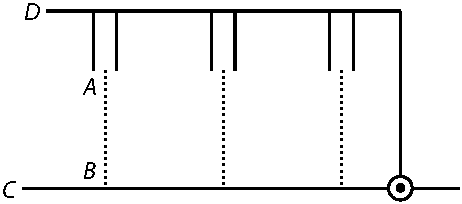
\includegraphics[width=0.48\textwidth]{gesamttex/edit_VIII-4/images/LH_38_04_157-d_157r.pdf}
\edcaption[1.0em]%
{%
\lbrack\textit{Fig.\:1}\rbrack%
}%
\end{edfigure}%
\newpage%
\vspace{3.0em}%
\pstart%
\noindent%
\centering%
*     *     *
\pend%
\vspace{2.5em}%
\selectlanguage{german}%
\frenchspacing%
\footnotesize%
\pstart%
\noindent%
\textls{Ausführliche Datierungsgründe:}%
\pagelabel{55805_dat}
Die undatierte Notiz N.\;\ref{55805} setzt sich kurz mit der Frage auseinander, ob eine Luftmasse wirksamer von einem unmittelbaren Ausbruch zusammengedrückter Luft angestoßen werde oder aber durch die Vermittlung eines Flügels.
Leibniz nimmt für die zweite Alternative Stellung und begründet das mit Hinweis auf die Teilbarkeit der Luft.
Diese Überlegung könnte im Zusammenhang mit der von Leibniz eigenhändig auf Juni 1678 datierten Aufzeichnung N.\;\ref{55774} entstanden sein, in welcher der Gedanke ausgeführt wird, dass winzige Strahlen zusammengedruckter Luft ein angemessenes Mittel sein könnten, um die Flügel einer künstlichen Taube zu bewegen.
Unter Berücksichtigung dieser inhaltlichen Verwandtschaft erweist sich als plausibel, dass auch die Notiz N.\;\ref{55805} im Juni 1678 entstand.
Eine frühere oder eine spätere Datierung ist dennoch möglich.
Der Textträger (Bl.\;\href{\Scan{LH_38_157wz}}{157}) weist weder Spuren eines Wasserzeichens noch weitere datierungsrelevante Eigenschaften auf.
\pend%
\selectlanguage{latin}%
\frenchspacing%
\normalsize%
\newpage%






\chapter[tocentry={Nulla chorda pondere praedita exacte tendi potest
\enskip\bracks{%
Herbst 1679 -- 1682\;(?)%
}},
head={Nulla chorda exacte tendi potest}]%
{\MakeUppercase{Nulla chorda pondere praedita exacte tendi potest}
\newline\bracks{%
Herbst 1679 -- 1682\;(?)%
}%
}%
\label{60198}
\selectlanguage{ngerman}%
\frenchspacing%
\begin{ledgroupsized}[r]{120mm}%
\footnotesize%
\pstart%
\noindent\textbf{Überlieferung:}%
\pend%
\end{ledgroupsized}%
\begin{ledgroupsized}[r]{114mm}%
\footnotesize%
\pstart%
\parindent -6mm%
\makebox[6mm][l]{\textit{L}}%
Aufzeichnung:
LH~XXXVII,\;3 Bl.\;65.
Ein Blatt 16\textsuperscript{o},
Ränder beschnitten;
\href{\Scan{LH_37_03_065wz}}{Fragment} eines Wasserzeichens:
niedersächsisches Papier. %
Dreiviertel Seite auf Bl.\;65\:r\textsuperscript{o}.
Bl.\;65\:v\textsuperscript{o} überliefert lediglich die \href{\Scan{LH_37_03_065v}}{Reste} eines nicht ermittelten Briefes von fremder Hand: %
\textit{Gestern habe} \textlangle...\textrangle\ \lbrack/\rbrack%
\edlabel{LH_37_03_065_065v_hans-1}
\textit{Meister Hans} \textlangle...\textrangle\ \lbrack/\rbrack%
\edlabel{LH_37_03_065_065v_hans-2}
\textit{so Ew. Herr} \textlangle...\textrangle\ \lbrack/\rbrack\
\textit{gen, uns da}\textlangle...\textrangle\ \lbrack/\rbrack\
\textit{wollen.} \textlangle...\textrangle\ \lbrack/\rbrack\
\textit{In} \textlangle...\textrangle%
\indexN{\textls{Linsen}, Hans (Meister Hans), gest. 1698}
\pend%
\end{ledgroupsized}%
\vspace{5mm}%
\begin{ledgroup}%
\footnotesize%
\pstart%
\noindent%
\textbf{Datierungsgründe:}
Die Datierung der Aufzeichnung N.\;\ref{60198} beruht auf äußeren Eigenschaften des Text\-trägers %
sowie auf inhaltlichen Betrachtungen.
Siehe die ausführliche Begründung auf S.\;\pageref{60198_dat}.
\pend%
\end{ledgroup}%
\selectlanguage{latin}%
\frenchspacing%
\vspace{8mm}%
\normalsize%
\pstart%
\noindent%
\lbrack%
\href{\Scan{LH_37_03_065r}}%
{65\,r\textsuperscript{o}}%
\rbrack\ %
\hfill%
\centering%
Nulla chorda pondere praedita exacte tendi potest%
\indexS{chorda praedita pondere}%
\indexS{chorda tensa pondere}%
\indexS{pondus tendens chordam}%
\hfill%
\phantom{\lbrack65\,r\textsuperscript{o}\rbrack}
\pend%
\vspace*{0.5em}%
\pstart%
\noindent%
Ponatur chorda \textit{AB} et arcus \textit{ACB},%
\indexS{arcus tendens chordam}
sitque chorda \textit{AB} ponderis expers%
\indexS{chorda expers ponderis}
et arcus \textit{ACB} tantarum virium%
\indexS{vis arcus}%
\indexS{vis tendens chordam}
ut eam perfecte tendat%
\indexS{chorda tensa arcu}
(\protect\vphantom)%
quamquam quantulaecunque sufficiant,
cum \textit{AB} non resistat%
\protect\vphantom().
Appendatur jam chordae pondus \textit{D}.%
\indexS{pondus appensum chordae}
Id utique efficiet aliquid,
ergo chordam%
\indexS{chorda flexa pondere}
\edtext{%
nonnihil flectet.%
\indexS{pondus flectens chordam}
Idem%
}{%
\lemma{nonnihil}\Bfootnote{%
\textit{(1)}~tendet. Idem
\textit{(2)}~flectet. Idem%
~\textit{L}}}
est ergo
si ipsa
\edtext{c\lbrack h\rbrack orda}{%
\lemma{corda}\Bfootnote{\textit{L~ändert Hrsg.}}}
jam per se sit gravis.%
\indexS{chorda gravis per se}
\pend%
 \vspace{3.0em}%
  \centerline{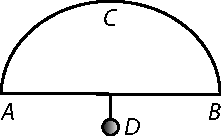
\includegraphics[width=0.26\textwidth]{gesamttex/edit_VIII-4/images/LH_37_03_065_d_065r.pdf}}%
  \vspace*{1.0em}
  \centerline{\lbrack\textit{Fig.\:1}\rbrack}%
\newpage%
\pstart%
\noindent%
\centering%
*     *     *
\pend%
\vspace{4.0em}%
\selectlanguage{latin}%
\frenchspacing%
\begin{ledgroup}%
\footnotesize%
\pstart%
\noindent%
\textls{Ausführliche Datierungsgründe:}%
\pagelabel{60198_dat}
Das im Träger der undatierten notizartigen Aufzeichnung N.\;\ref{60198} anzutreffende Wasserzeichen ist nach heutigem Wissensstand für die frühen Hannoveraner Jahre belegt, insbesondere für den Zeitraum vom Herbst 1677 bis zum Jahr 1682. %
Damals hat sich Leibniz intensiv mit Themen der Elastizitätstheorie und der Akustik befasst und in diesem Zusammenhang auch das mechanische Verhalten der gespannten Saiten untersucht, wie zahlreiche in \textit{LSB} VIII,\;3 veröffentlichte Texte zeigen.
Es ist somit wahrscheinlich, dass auch die Aufzeichnung N.\;\ref{60198} ungefähr im gleichen Zeitraum abgefasst wurde. %
\pend%
\pstart%
Der nicht ermittelte Briefrest auf der Rückseite des Trägers von N.\;\ref{60198} ermöglicht aber eine weitere Eingrenzung des Terminus post quem der Datierung.
Dort wird nämlich ein \textit{Meister Hans} erwähnt (vgl. die Beschreibung der Überlieferung, \refpassage{LH_37_03_065_065v_hans-1}{LH_37_03_065_065v_hans-2}), bei dem es sich aller Wahrscheinlichkeit nach um den Handwerker Hans Linsen\indexN{\textls{Linsen}, Hans (Meister Hans), gest. 1698} handelt, einen Müller und Zimmermann, der in der ersten Hälfte der 1680er Jahre in Leibnizens Auftrag Windmühlen im Harzgebiet\indexO{Harz} baute.
Der älteste sichere Beleg seiner Person im Leibniz-Briefwechsel ist Leibnizens Schreiben an Herzog Johann Friedrich wohl von Anfang August 1679 (vgl. \textit{LSB} I,\;2 N.\;157,\cite{02614} S.\;188.30; Linsens Brief an Leibniz vom 29.\;Dezember 1678\,/\,8.\;Januar 1679 ist unsicher datierbar, vgl. \textit{LSB} III,\;2 N.\;255,\cite{02613} S.\;595.26--28).
Daher ist unwahrscheinlich, dass der Briefrest auf dem Träger von N.\;\ref{60198} -- und somit auch die später abgefasste Aufzeichnung selbst -- vor dem Herbst 1679 entstand.
Da der Austausch zwischen Hans Linsen\indexN{\textls{Linsen}, Hans (Meister Hans), gest. 1698} und Leibniz in den folgenden Jahren häufiger wurde, ist es eher wahrscheinlich, dass die Aufzeichnung N.\;\ref{60198} später enstand.
\pend%
\pstart%
Für eine spätere Datierung spricht zudem, dass der in N.\;\ref{60198} festgehaltene Gedanke in ähnlicher Gestalt auch in der zwischen Sommer und November 1689 entstandenen ersten Fassung von Leibnizens \textit{Dynamica}, pars~II, sectio~I, prop.\;36 vorkommt: %
\textit{Nulla chorda vel catena gravis in alio situ quam verticali perfecte in rectam extendi potest vi mortua; potest viva} (\textit{CFP}~I, S.\;340.2--4~[A]; S.\;579.22--24~[B]; III, S.\;414.20--22~[C]).\cite{01354}
Eine Entstehung der Aufzeichnung N.\;\ref{60198} während der Italienreise\indexO{Italien} ist jedoch schon aufgrund des Papiers extrem unwahrscheinlich.
Ferner gilt es zu beachten, dass in N.\;\ref{60198} die im zitierten Text der \textit{Dynamica}\cite{01354} hervorgehobene Unterscheidung zwischen "toter" und "lebendiger" Kraft unberücksichtigt bleibt.
Dies plädiert für eine frühe Entstehung von N.\;\ref{60198}.
Es bietet sich demnach an, den Terminus ante quem der Datierung an den Belegzeitraum des Wasserzeichens anzulehnen, ohne die Möglichkeit ausschließen zu können, dass N.\;\ref{60198} etwas später im Laufe der 1680er Jahre angefertig wurde.
\pend%
\pstart%
Als Datierung der Aufzeichnung N.\;\ref{60198} ergibt sich insgesamt die Zeitspanne \textit{Herbst 1679 bis 1682}.
Eine frühere Datierung ist unwahrscheinlich.
Eine spätere Datierung ist nicht auszuschließen.
\pend%
\end{ledgroup}%
\selectlanguage{latin}%
\frenchspacing%
\newpage%

\chapter[tocentry={Tractatio de aeris elastro
\enskip%
\bracks{September 1679
-- erste Monate 1683%
}},
head={Tractatio de elastro}]%
{\MakeUppercase{Tractatio de aeris elastro}
\newline%
\bracks{September 1679
-- erste Monate 1683%
}}
\label{60212}
\selectlanguage{ngerman}%
\frenchspacing%
\begin{ledgroupsized}[r]{120mm}%
\footnotesize%
\pstart%
\noindent\textbf{Überlieferung:}%
\pend%
\end{ledgroupsized}%
\begin{ledgroupsized}[r]{114mm}%
\footnotesize%
\pstart%
\parindent -6mm%
\makebox[6mm][l]{\textit{L}}%
Aufzeichnung:
LH~XXXVII~3 Bl.\:125\textendash127.
Ein Bogen 2\textsuperscript{o}\! (Bl.\:125\textendash126) und ein Einzelblatt~2\textsuperscript{o}\! (Bl.\:127);
Wasserzeichen auf Bl.\:\href{\Scan{LH_37_03_125wz}}{125};
unterer Rand von Bl.\:\href{\Scan{LH_37_03_127r}}{127\:r\textsuperscript{o}}\! ausgefranst mit geringfügigem Textverlust 
(der verlorene Text ist in dem 1967 aufgenommenen S-Film Nr.\:116 der GWLB Hannover noch lesbar):
Papiererhaltungsmaßnahmen.
Fünfeinhalb Seiten einspaltig beschrieben;
untere Hälfte von Bl.\:\href{\Scan{LH_37_03_127v}}{127\:v\textsuperscript{o}}\! unbeschrieben.
Textfolge nach Blattzählung;
ein Kustos am Ende von Bl.\:\href{\Scan{LH_37_03_126v}}{126\:v\textsuperscript{o}}\! verweist auf den Anfang von Bl.\:\href{\Scan{LH_37_03_127r}}{127\:r\textsuperscript{o}}.
\pend%
\end{ledgroupsized}%
\vspace{5mm}%
\begin{ledgroup}%
\footnotesize%
\pstart%
\noindent%
\textbf{Datierungsgründe:}
Die Datierung der Aufzeichnung N.\;\ref{60212} beruht auf äußeren Eigenschaften des Text\-trägers %
sowie auf inhaltlichen Betrachtungen.
Siehe die ausführliche Begründung auf S.\;\pageref{60212_dat}.
\pend%
\end{ledgroup}%
\selectlanguage{latin}%
\frenchspacing%
\vspace{8mm}%
\normalsize%
\pstart%
\noindent%
\lbrack%
\href{\Scan{LH_37_03_125r}}%
{125\:r\textsuperscript{o}}%
\rbrack%
\pend%
\begin{edfigure}[0.750em][0.000em]%
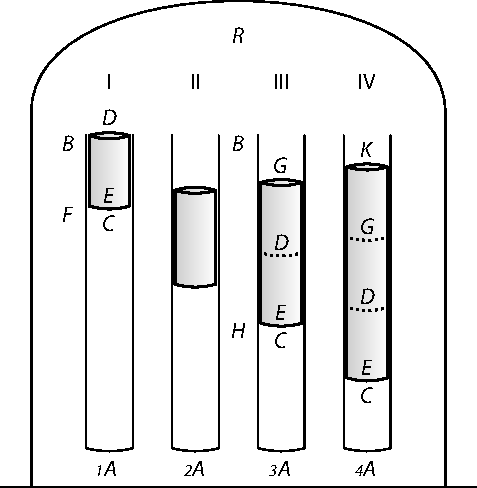
\includegraphics[width=0.64\textwidth]{gesamttex/edit_VIII-4/images/LH_37_03_125-127_d1_125r.pdf}%
\edcaption[1.0em]{%
\lbrack\textit{Fig.\:1}\rbrack%
}%
\end{edfigure}%
\newpage%
\pstart%
\edtext{%
(1)%
}{%
\lemma{(1)}%
\Bfootnote{%
\textit{erg.\:L}}}
Aer est corpus grave fluidum elasticum.%
\indexS{aer corpus grave fluidum elasticum}%
\indexS{corpus grave}%
\indexS{corpus fluidum}%
\indexS{corpus elasticum}
\pend%
\pstart%
\edtext{%
(2)%
}{%
\lemma{(2)}%
\Bfootnote{%
\textit{erg.\:L}}}%
\textls{ Corpus elasticum }%
\indexS{corpus elasticum}%
voco
quod
vi quadam externa adhibita%
\indexS{vis externa}%
\indexS{vis adhibita}
figuram suam aut volumen mutat,%
\indexS{figura corporis elastici}%
\indexS{volumen corporis elastici}
eaque vi amota%
\indexS{vis amota}
ad
\edtext{%
eam redit.%
}{%
\lemma{eam}%
\Bfootnote{%
\textit{(1)}~reditur. %
\textit{(2)}~redit.%
~\textit{L}%
}}
Vim autem ipsius corporis%
\indexS{vis corporis elastici}
qua externo
\edtext{%
innit\lbrack e\rbrack nti%
}{%
\lemma{innitanti}%
\Bfootnote{%
\textit{L~ändert Hrsg.}%
}}
renititur%
\indexS{vis externa}%
\indexS{vis innitens}%
\indexS{vis renitens}
et ad statum%
\indexS{status prior}%
\indexS{vis tendens ad statum priorem}
\edtext{%
suum priorem tendit,%
}{%
\lemma{suum}%
\Bfootnote{%
\textit{(1)}~te %
\textit{(2)}~redit, %
\textit{(3)}~priorem tendit,%
~\textit{L}%
}}
voco\textls{ Elastrum.}%
\indexS{elastrum}
\pend%
\pstart%
\edlabel{LH_37_03_125-127_127r_axioma-1}%
\edtext{(3)}{%
\lemma{(3)}\Bfootnote{%
\textit{erg.\;L}}}
Effectus sunt causis proportionales,%
\indexS{effectus proportionalis causae}%
\indexS{causa proportionalis effectui}
vel ut distinctius exponam,
\edtext{%
si in idem%
}{%
\lemma{si}%
\Bfootnote{%
\bars{in \textit{erg.}}
idem%
~\textit{L}%
}}
patiens%
\indexS{patiens}
in eodem statu
\edtext{%
positum %
agat vel \textit{A} vel \textit{B},
sitque agens integrum \textit{A}%
\indexS{agens integrum}%
\indexS{agentia similia}
agenti integro \textit{B} simile,%
}{%
\lemma{positum}\Bfootnote{%
\textit{(1)}~sit, et int %
\textit{(2)}~agat vel %
\bars{agens \textit{gestr.}} %
\textit{A} vel %
\bars{agens \textit{gestr.}} %
\textit{B}, sitque agens integrum \textit{A} %
\textit{(a)}~simile %
\textit{(b)}~agenti integro \textit{B} simile,%
~\textit{L}%
}}
saltem quatenus agunt,
erunt etiam effectus similes,%
\indexS{effectus similis agenti}
seu agentibus%
\indexS{effectus proportionalis agenti}
\edlabel{LH_37_03_125-127_125r_ibwr-1}%
proportionales.%
\edlabel{LH_37_03_125-127_127r_axioma-2}
\edtext{}{%
\xxref{LH_37_03_125-127_125r_ibwr-1}{LH_37_03_125-127_125r_ibwr-2}%
\lemma{proportionales.}%
\Bfootnote{%
\textit{(1)}~Si %
\textit{(a)}~eni %
\textit{(b)}~ex %
\textit{(2)}~Ut %
\textit{(3)}~\lbrack/\rbrack\ (4) Hinc si %
\bars{idem \textit{erg.}} %
patiens%
~\textit{L}%
}}%
\pend%
\pstart%
(4)
Hinc si idem patiens%
\indexS{patiens}%
\edlabel{LH_37_03_125-127_125r_ibwr-2}
\edtext{%
prematur duobus diversis ponderibus%
\indexS{pondus premens}
libere ab aliquo filo suspensis,%
\indexS{pondus suspensum a filo}
tunc utique%
}{%
\lemma{prematur}%
\Bfootnote{%
\textit{(1)}~nunc pondere %
\bars{libere suspenso \textit{erg.}} \textit{A} %
\textit{(2)}~nunc pondere %
\textit{(a)}~\textit{B} %
\textit{(b)}~libere suspenso %
\textit{(c)}~uno, nunc altero %
\textit{(d)}~\textit{A} nunc pondere \textit{B} (quae pondera ambo libere agere suppono)%
\indexS{pondus agens libere} %
\textit{(3)}~duobus diversis %
\lbrack...\rbrack\ tunc utique%
~\textit{L}%
}}
cum
\edtext{%
non ipsius figurae corporum%
\indexS{figura corporis}
aut alterius circumstantiae,%
\indexS{circumstantia alia}
sed gravitatum%
\indexS{gravitas}
tantummodo ratio habeatur,%
}{%
\lemma{non}%
\Bfootnote{%
\textit{(1)}~figur\textlangle a\textrangle\ %
\textit{(2)}~ipsisus figurae corporum %
\textit{(a)}~aliarumque circumstatiarum %
\textit{(b)}~aut alterius circumstantiae, sed %
\textit{(aa)}~solarum %
\textit{(bb)}~gravitatum tantummodo ratio habeatur,%
~\textit{L}%
}}
patet
\edtext{%
ipsos%
}{%
\lemma{ipsos}%
\Bfootnote{\textit{erg.\;L}%
}}
effectus%
\indexS{effectus pressionis}
qui ex illa pressione sequuntur%
\indexS{pressio}
fore ponderibus proportionales.%
\indexS{effectus proportionalis ponderi}
Duo enim pondera,
per se spectata,%
\indexS{pondus spectatum per se}
sunt agentia similia,%
\indexS{agentia similia}
\edtext{%
quia in ipsis solam quantitatem gravitatis spectamus;%
\indexS{quantitas gravitatis}%
\indexS{gravitas}
similia autem vocantur,
quae sola quantitate discernimus.%
\indexS{discretum sola quantitate}%
}{%
\lemma{quia}%
\Bfootnote{%
\textit{(1)}~simile %
\textit{(2)}~similia vocamus quae non p %
\textit{(3)}~in ipsis solam quantitatem %
\textit{(a)}~ponderis %
\textit{(b)}~gravitatis spectamus; %
\lbrack...\rbrack\ quantitate discernimus.%
~\textit{L}%
}}
\pend%
\pstart%
(5)
Sit jam
\edtext{%
tubus%
\indexS{tubus cylindricus}
\edtext{cylindricus}{%
\lemma{cylindricus}%
\Bfootnote{\textit{erg.\;L}%
}}
\textit{AB}%
}{%
\lemma{tubus cylindricus \textit{AB}}%
\Cfootnote{%
Vgl. das Diagramm \lbrack\textit{Fig.\:1}\rbrack.%
}}
positus in
\edtext{Recipiente}{%
\lemma{Recipiente}%
\Bfootnote{\textit{erg.\;L}%
}}
Vacuo \textit{R}.%
\indexS{recipiens vacuus}
\edtext{%
Vacuum autem intelligo Gerickianum,%
\indexN{\textls{Guericke} (Gerickius, Gericke), Otto von 1602\textendash1686}%
\indexS{vacuum Gerickianum}%
}{%
\lemma{Vacuum \lbrack...\rbrack\ Gerickianum}%
\Cfootnote{%
Siehe %
O.\;v.\;\textsc{Gue\-ri\-cke}, \textit{Experimenta nova}, l.\;II, cap.\;3 (Amsterdam 1672, S.\;56a).\cite{00055}
Guerickes Versuche über das Vakuum werden ebd., l.\;III (S.\;71\,ff.) dargestellt.
Leibnizens Auszüge hieraus %
sind in \textit{LSB} VIII,\;1 N.\;36\cite{01197} ediert.%
}}
in quo aer aut nullus aut exiguus%
\indexS{aer nullus in recipiente}%
\indexS{aer exiguus in recipiente}
\edtext{%
restat%
\lbrack,
i\rbrack n
ipso%
}{%
\lemma{restat.}%
\Bfootnote{%
In
\textit{L\;ändert Hrsg.}%
}}
scilicet recipiente:%
\indexS{recipiens vacuus}
in Tubo autem sit aer \textit{AC}%
\indexS{tubus cylindricus}
pondere%
\indexS{pondus comprimens aerem}
\edtext{%
corporis \textit{DE}
(Hydrargyri%
\indexS{hydrargyros}
si placet)%
}{%
\lemma{corporis}%
\Bfootnote{%
\textit{(1)}~\textit{BC} %
\textit{(2)}~\textit{DE} %
\textit{(a)}~quod %
\textit{(b)}~(Hydrargyri si placet)%
~\textit{L}%
}}
compressus%
\indexS{aer compressus}
et in tubi parte \textit{AC} retentus,%
\indexS{aer retentus in tubo}
quominus inde exire%
\indexS{aer exiens}
et in naturalem magis Statum%
\indexS{status naturalis}
se dilatare possit.%
\indexS{aer dilatans se in statum naturalem}
\edlabel{LH_37_03_125-127_125r_sdfi-1}%
Patet Elastrum huius aeris%
\indexS{elastrum aeris compressi}
\edtext{%
\textit{AC}%
}{%
\lemma{\textit{AC}}%
\Bfootnote{\textit{erg.\;L}%
}}
(seu vim se dilatandi)%
\indexS{vis aeris dilatandi}
tantum esse
quantum
\edtext{%
est pondus \textit{DE}.%
\indexS{pondus comprimens aerem}
}{%
\lemma{est pondus}%
\Bfootnote{%
\textit{(1)}~\textit{BC}. %
\textit{(2)}~\textit{DE}.%
~\textit{L}%
}}
Sunt enim inter se in aequilibrio nisus%
\indexS{nisus in aequilibrio}
(ex hypothesi)%
\indexS{hypothesis}
neque aut pondus descendere%
\indexS{pondus descendens}
aut aer se dilatare amplius potest,%
\indexS{aer dilatans se}
altero alterum impediente.%
\edlabel{LH_37_03_125-127_125r_sdfi-2}
\edtext{%
Cum enim res in vacuo geri ponatur,%
\indexS{res gesta in vacuo}%
\indexS{vacuum}
nihil aliud est %
quod ad hunc effectum contribuat,%
\indexS{effectus compressionis}
cum alioqui aeris ambientis et incumbentis%
\indexS{aer ambiens}%
\indexS{aer incumbens}
quoque ratio habenda fuisset.%
}{%
\lemma{}\Bfootnote{%
Cum enim \lbrack...\rbrack\ habenda fuisset.
\textit{erg.\;L}%
}}
\pend%
\pstart%
(6)
Ponamus jam pondus comprimens augeri,%
\indexS{pondus comprimens aerem}%
\indexS{pondus auctum}%
\indexS{pondus duplum}
seu fieri duplo majus,
\edtext{%
sive ipsi Mercurio \textit{DE}%
\indexS{mercurius infusus}%
}{%
\lemma{sive}%
\Bfootnote{%
\bars{ipsi \textit{erg.}} Mercurio %
\textit{(1)}~\textit{BC} %
\textit{(2)}~\textit{DE}%
~\textit{L}%
}}
tantundem adhuc affundi%
\lbrack,\rbrack\
\edtext{%
nempe \textit{GD}.%
}{%
\lemma{nempe \textit{GD}}%
\Bfootnote{\textit{erg.\;L}%
}}
Quaeritur%
\lbrack:\rbrack\
\lbrack%
\href{\Scan{LH_37_03_125v}}%
{125\:v\textsuperscript{o}}%
\rbrack\
Quanta futura sit aeris tubo inclusi compressio?%
\indexS{aer inclusus tubo}%
\indexS{aer compressus in tubo}%
\indexS{compressio aeris}
Respondeo
dubium nullum esse,
quin compressio futura sit dupla prioris.%
\indexS{compressio dupla}
Vis enim dupla per omnia similis similiterque agens,%
\indexS{vis dupla}%
\indexS{vis similis}%
\indexS{vis agens similiter}
utique effectum etiam duplum dabit,%
\indexS{effectus duplus}
per axioma%
\indexS{axioma}
positum articulo%
\indexS{articulus}
\edtext{%
\lbrack tertio\rbrack.%
}{%
\lemma{secundo}\Bfootnote{%
\textit{L~ändert Hrsg.}%
}%
\lemma{\lbrack tertio\rbrack}%
\Cfootnote{%
Vgl. \refpassage{LH_37_03_125-127_127r_axioma-1}{LH_37_03_125-127_127r_axioma-2}.%
}%
}%
\pend%
\pstart%
(7)
Compressio autem%
\indexS{compressio aeris}%
\indexS{aer compressus in tubo}
\edtext{%
aeris \textit{AC}%
}{%
\lemma{aeris \textit{AC}}%
\Cfootnote{%
Vgl. das Diagramm \lbrack\textit{Fig.\:2}\rbrack.%
}}
cum per se non possit aestimari nec cognosci%
\indexS{compressio aestimata}%
\indexS{aestimatio compressionis}
nisi ex spatio
intra quod per vim redigitur,%
\indexS{spatium intra quod aer comprimitur}%
\indexS{vis compressionis}
\edtext{%
ideo
cum aer \textit{AC} antea in Tubo \textit{AB}
(sub num.\;I posito\lbrack)\rbrack\
compressus sit a pondere \textit{DE}%
\indexS{pondus comprimens aerem}
intra spatium \textit{AF},
utique nunc aucto pondere \textit{GDE},%
\indexS{pondus auctum}
idem aer \textit{AC}
in Tubo eodem \textit{AB}%
\indexS{tubus cylindricus}
(sub num.\;II posito%
\lbrack)\rbrack\
comprimetur in spatium arctius \textit{AH}.%
\indexS{aer compressus in tubo}
}{%
\lemma{ideo}%
\Bfootnote{%
\textit{(1)}~proximum est ut dicamus, %
\textit{(2)}~cum aer %
\lbrack...\rbrack\ (sub num.\;I %
\bars{) posito \textit{ändert Hrsg.}} compressus %
\bars{sit \textit{erg.}} a pondere \textit{DE} intra spatium %
\textit{(a)}~\textit{AC} %
\textit{(b)}~\textit{AF}, %
\textit{(aa)}~et nunc duplic %
\textit{(bb)}~utique nunc %
\textit{(aaa)}~duplicato %
\textit{(bbb)}~aucto pondere \textit{GDE}, %
\textit{(aaaa)}~com %
\textit{(bbbb)}~idem aer %
\lbrack...\rbrack\ eodem \textit{AB} %
\textit{(aaaaa)}~posito %
\textit{(bbbbb)}~(sub num.\;II %
\bars{) posito \textit{ändert Hrsg.}} %
comprimetur in spatium arctius \textit{AH}.%
~\textit{L}%
}}
\pend%
\pstart%
\edlabel{LH_37_03_125-127_125v_fgso-1}%
(8)
Quaeritur jam
quantum esse debeat spatium \textit{AH}.%
\indexS{spatium in quod aer redigitur}
Seu data ratione ponderis \textit{GDE} ad pondus \textit{DE},%
\indexS{ratio ponderum dupla}
\edtext{%
quae in hoc casu est dupla,%
}{%
\lemma{quae}%
\Bfootnote{%
\textit{(1)}~hoc loco est %
\textit{(2)}~in hoc casu est dupla,%
~\textit{L}%
}}
quaeritur
quae sit ratio spatii%
\indexS{ratio spatiorum subdupla}
\edtext{%
\textit{AH}
sub pondere \textit{GDE}%
}{%
\lemma{\textit{AH}}%
\Bfootnote{%
\textit{(1)}~(\textlangle a\textrangle\ pondere \textit{GDE} %
\textit{(2)}~sub pondere \textit{GDE}%
~\textit{L}%
}}
ad spatium \textit{AF}
sub
\edtext{%
pondere \textit{DE}.%
}{%
\lemma{pondere}%
\Bfootnote{%
\textit{(1)}~\textit{A} %
\textit{(2)}~\textit{DE} %
\textit{(3)}~\textit{DE}%
~\textit{L}%
}}
Respondeo
eam esse subduplam,%
\indexS{ratio spatiorum subdupla}
sive \textit{AH} esse dimidium ipsius \textit{AF};
si vero pondus \textit{KGDE}
\edtext{sub numero III%
}{%
\lemma{sub numero III}%
\Bfootnote{%
\textit{erg.\;L}%
}}
esset triplum ponderis%
\indexS{pondus comprimens aerem}%
\indexS{ratio ponderum tripla}
\edtext{%
\textit{DE},
tunc spatium \textit{AL}
for\lbrack e\rbrack\
subtriplum%
}{%
\lemma{\textit{DE},}%
\Bfootnote{%
\bars{tunc \textit{erg.}} spatium %
\textit{(1)}~\textit{AH} %
\textit{(2)}~\textit{AL} %
\bars{foret \textit{ändert Hrsg.}} %
subtriplum%
~\textit{L}%
}}
seu tertia pars spatii \textit{AF};%
\indexS{ratio spatiorum subtripla}
et generaliter
\edtext{%
spatia
intra quae corpus elasticum comprimitur%
\indexS{spatium intra quod aer comprimitur}
fore in ratione reciproca ponderum comprimentium,%
\indexS{spatia in ratione reciproca ponderum comprimentium}%
\indexS{pondus comprimens aerem}
sive%
}{%
\lemma{}%
\Bfootnote{%
spatia intra \lbrack...\rbrack\ comprimentium, sive
\textit{erg.\;L}%
}}
spatium%
\indexS{spatium intra quod aer comprimitur}
\edtext{%
}{%
\xxref{LH_37_03_125-127_125v_hfkd-1}{LH_37_03_125-127_125v_hfkd-2}%
\lemma{\textit{AH}}%
\Bfootnote{%
\bars{sub pondere \textit{DEG} \textit{erg. u. gestr.}}
fore ad spatium \textit{AF}
\textit{(1)}~in ratione ponderum %
\textit{(2)}~sub pondere \textit{AF} %
\textit{(3)}~sub pondere %
\textit{(4)}~in ratione ponderis \textit{A} %
\textit{(5)}~ut est pondus %
\textit{(a)}~\textit{DE} %
\textit{(b)}~\textit{DE} %
\textit{(c)}~\textit{ED} %
\textit{(d)}~\textit{DE}, sub quo %
\lbrack...\rbrack\ pondus \textit{GDE} %
\textit{(aa)}~sub quo est spatium \textit{AH}. Id quod %
\textit{(bb)}~sub quo %
\lbrack...\rbrack\ est, quod%
~\textit{L}%
}}%
\edlabel{LH_37_03_125-127_125v_hfkd-1}%
\textit{AH} fore ad spatium \textit{AF}
ut est pondus \textit{DE},
sub quo est spatium \textit{AF},
ad pondus \textit{GDE},%
\indexS{pondus comprimens aerem}
sub quo est spatium \textit{AH}.%
\indexS{spatium intra quod aer comprimitur}%
\indexS{spatia in ratione reciproca ponderum comprimentium}%
\edlabel{LH_37_03_125-127_125v_fgso-2}
\pend%
\pstart%
(9)
Id autem ex eo manifestum est,
quod%
\edlabel{LH_37_03_125-127_125v_hfkd-2}%
\textls{ }%
\edlabel{LH_37_03_125-127_125v_thnd-1}%
\textls{spatia sunt in reciproca ratione compressionum,}%
\indexS{spatia in ratione reciproca compressionum}%
\edlabel{LH_37_03_125-127_125v_thnd-2}
\edtext{%
sive,
si aer \textit{AC} intra spatium \textit{AH}
sit duplo (triplo) compressior%
\indexS{aer compressior duplo}%
\indexS{aer compressior triplo}
quam idem aer \textit{AC}%
\indexS{aer compressus in tubo}
intra spatium \textit{AF},%
\indexS{spatium intra quod aer comprimitur}%
}{%
\lemma{sive,}%
\Bfootnote{%
\textit{(1)}~si aer sit duplo %
\textit{(2)}~si aer \textit{AC} %
\textit{(a)}~sit duplo compressior aere \textit{A} %
\textit{(b)}~intra spatium \textit{AH} sit duplo %
\bars{(triplo) \textit{erg.}} %
compressior quam %
\lbrack...\rbrack\ spatium \textit{AF},%
~\textit{L}%
}}
\edlabel{LH_37_03_125-127_125v-126r_vdvd-1}%
\edtext{%
}{%
\xxref{LH_37_03_125-127_125v-126r_vdvd-1}{LH_37_03_125-127_125v-126r_vdvd-2}%
\lemma{utique intra spatium}%
\Bfootnote{%
\bars{\textit{AH} \textit{erg.}} duplo %
\textit{(1)}~vel %
\textit{(2)}~(triplo) %
\textit{(a)}~minus, sive %
\textit{(b)}~arct %
\textit{(c)}~angustius, sive subduplum (subtriplum) %
\textit{(aa)}~compressus erit %
\textit{(bb)}~prioris spatii \textit{AF}, compressus erit. %
\textit{(aaa)}~Suppono enim velut principium totius tractationis hujus de Elastro, vim a%
\indexS{elastrum aeris}\indexS{tractatio de elastro} %
\textit{(bbb)}~Suppono %
\textit{(ccc)}~Hanc ipsam %
\lbrack...\rbrack\ \textls{compressionem} appello. %
\bars{\lbrack/\rbrack\ (10) \textls{Compressiones autem} %
\lbrack...\rbrack\ se liberare. \textit{erg.}} Aerem enim %
\lbrack...\rbrack\ homogenei %
\href{\Scan{LH_37_03_126r}}{\lbrack126\:r\textsuperscript{o}\rbrack} considero,%
~\textit{L}%
}}%
utique intra spatium \textit{AH}%
\indexS{spatium intra quod aer comprimitur}
duplo (triplo) angustius,%
\indexS{spatium duplo angustius}%
\indexS{spatium triplo angustius}
sive subduplum (subtriplum) prioris spatii \textit{AF},
compressus erit.%
\indexS{aer compressus in tubo}%
\indexS{spatia in ratione reciproca compressionum}
Hanc ipsam enim angustiae quantitatem%
\textls{ compressionem }appello.%
\indexS{quantitas angustiae}%
\indexS{compressio ut quantitas angustiae}%
\indexS{compressio aeris}
\pend%
\begin{edfigure}[2.50em][0.00em]%
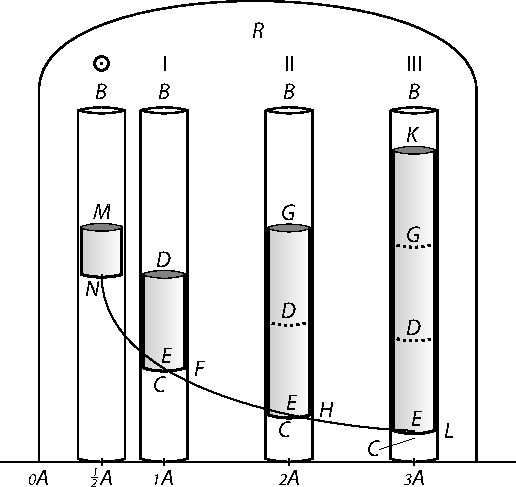
\includegraphics[width=0.61\textwidth]{gesamttex/edit_VIII-4/images/LH_37_03_125-127_d2_125v.pdf}%
\edcaption[0.75em]{%
\edtext{%
\lbrack\textit{Fig.\:2}\rbrack%
}{%
\lemma{\textit{Über dem Diagramm} \lbrack\textit{Fig.\:2}\rbrack:}%
\Afootnote[nonum]{%
$%
\quad\quad%
\displaystyle%
\frac{1}{2}
\quad\quad%
1%
\quad\quad%
1%
$%
\newline%
\hspace*{48.5mm}%
$%
\displaystyle%
\frac{1}{2}%
\quad\quad%
1%
\quad\quad%
2%
\quad\quad%
3%
$%
\newline%
\hspace*{49.5mm}%
$%
\displaystyle%
2%
\quad\quad%
\hspace*{0.4mm}%
1%
\quad\quad%
\hspace*{-0,4mm}%
\frac{1}{2}%
\quad\quad%
\hspace*{-0,7mm}%
\frac{1}{3}%
$%
}}%
}%
\end{edfigure}%
\newpage%
\pstart%
\edlabel{LH_37_03_125-127_125v_atmr-1}%
(10)%
\textls{ }%
\edlabel{LH_37_03_125-127_125v-126r_htzj-1}%
\textls{Compressiones autem sunt ut elastra,}%
\indexS{elastrum reciproce proportionale compressioni}%
\indexS{compressio aeris}%
\indexS{elastrum aeris}%
\edlabel{LH_37_03_125-127_125v-126r_htzj-2}
ac proinde%
\textls{ Elastra sunt spatiis reciproce proportionalia,}%
\indexS{elastrum reciproce proportionale spatio}%
\edlabel{LH_37_03_125-127_125v_atmr-2}
seu corpus
in qua ratione compressum seu coarctatum est,%
\indexS{corpus compressum}%
\indexS{corpus coartatum}
in ea nititur se liberare.%
\indexS{corpus nitens liberare se}
Aerem enim instar corporis homogenei%
\indexS{aer corpus homogeneum}%
\indexS{corpus homogeneum}
\lbrack%
\href{\Scan{LH_37_03_126r}}%
{126\:r\textsuperscript{o}}%
\rbrack\
considero,%
\edlabel{LH_37_03_125-127_125v-126r_vdvd-2}
quod natura sua spatium majus quaerit,%
\indexS{corpus quaerens spatium majus}
spatio quoque angusto%
\indexS{corpus repugnans spatio angusto}%
\indexS{spatium angustum}
\edtext{%
repugnat,
ac proinde%
}{%
\lemma{repugnat,}%
\Bfootnote{%
\textit{(1)}~adeoque %
\textit{(2)}~ac proinde%
~\textit{L}%
}}
vis ejus praecise%
\indexS{vis aeris}%
\indexS{vis definita ab angustia spatii}
\edtext{}{%
\xxref{LH_37_03_125-127_126r_ejwe-1}{LH_37_03_125-127_126r_ejwe-2}%
\lemma{ab}%
\Bfootnote{%
\textit{(1)}~quanti %
\textit{(2)}~angustia %
\textit{(a)}~spatii definietur. %
\textit{(b)}~spatii %
\textit{(aa)}~definietur, neque ullum aliud est, quod in %
\textit{(bb)}~intra quod cohibitus est %
\textit{(cc)}~intra quod %
\lbrack...\rbrack\ in considerationem %
\textit{(aaa)}~venire possit %
\textit{(bbb)}~veniat, quam %
\lbrack...\rbrack\ spatii quantitatem. %
\lbrack/\rbrack\ %
\bars{(11) \textit{erg.}} Licet %
\textit{(aaaa)}~enim %
\textit{(bbbb)}~autem%
~\textit{L}%
}}%
\edlabel{LH_37_03_125-127_126r_ejwe-1}%
ab angustia spatii%
\indexS{angustia spatii}%
\indexS{spatium intra quod aer comprimitur}
intra quod cohibitus est%
\indexS{aer cohibitus}%
\lbrack,\rbrack\
definietur,
quia
\edtext{%
ponimus%
}{%
\lemma{ponimus}%
\Cfootnote{%
Nicht ausdrücklich in N.\;\ref{60212}.}}
nihil aliud esse
quod in considerationem veniat,%
\indexS{consideratio}
quam naturam aeris%
\indexS{natura aeris}
et spatii quantitatem.%
\indexS{quantitas spatii}%
\pend%
\pstart%
(11)
Licet autem%
\edlabel{LH_37_03_125-127_126r_ejwe-2}
revera aer non sit corpus homogeneum%
\indexS{aer corpus non homogeneum}%
\indexS{corpus homogeneum}
et vim elasticam non habeat a principio%
\indexS{principium intrinsecum}%
\indexS{vis elastica aeris}%
\indexS{vis elastica a principio intrinseco}
\edtext{%
intrinseco %
sed a motu aetheris per eum transeuntis,%
\indexS{aether transiens per aerem}%
\indexS{motus aetheris per aerem}%
\indexS{vis elastica a motu aetheris}
et ideo vis Elastica aeris habeat terminum expansionis%
\indexS{vis elastica aeris}%
\indexS{vis elastica habens terminum expansionis}%
\indexS{terminus expansionis}%
}{%
\lemma{intrinseco}%
\Bfootnote{%
\textit{(1)}~adeoque %
\textit{(2)}~atque ideo incertum sit an non %
\textit{(3)}~%
\bars{sed a %
\lbrack...\rbrack\ eum transeuntis, \textit{erg.}}
et ideo %
\lbrack...\rbrack\ terminum expansionis%
~\textit{L}%
}}
ultra quem sese expandere non affectet%
\lbrack,\rbrack\
\edtext{%
ac proinde praecise a spatio nec possit aestimari;%
\indexS{vis elastica aestimata a spatio}%
\indexS{vis aeris aestimata a spatio}%
}{%
\lemma{}%
\Bfootnote{%
ac proinde praecise a %
\textit{(1)}~spatii %
\textit{(2)}~spatio %
\textit{(a)}~non %
\textit{(b)}~nec possit aestimari %
\textit{erg.\;L}%
}}
quia tamen ad sensum homogeneus est aer%
\indexS{aer homogeneus ad sensum}%
\indexS{sensus}
et
\edtext{%
experimentis constat%
\indexS{experimentum}%
}{%
\lemma{experimentis constat}%
\Cfootnote{%
Das Experiment, durch das G.\:P.\;de Roberval\indexN{\textls{Roberval} (Robervallius), Gilles Personne de 1602\textendash1675} mithilfe einer Karpfenblase im Vakuum die Ausdehnbarkeit der Luft nachgewiesen hatte, wurde später verbessert und wiederholt;
vgl. \textsc{R.\;Boyle}, \textit{New experiments}, Nr.\;4--6 (London 1660, S.\;45--62;\cite{00015} \textit{BW}~I, S.\;173--180).\cite{00017}
Siehe auch \textsc{Guericke}, \textit{Experimenta nova}, lib.\;III, cap.\;33 (S.\;116b).\cite{00055}%
}}
eum ad incredibilem amplitudinem se dilatare%
\indexS{aer dilatans se}%
\indexS{dilatatio aeris}%
\indexS{amplitudo dilatationis aeris}
si sibi
\edtext{%
relinquatur%
\indexS{aer relictus sibi} %
sive si nullum corpus a nobis perceptibile impediat%
\lbrack,\rbrack%
\indexS{corpus perceptibile}%
\indexS{corpus impediens}
sine errore%
}{%
\lemma{relinquatur}%
\Bfootnote{%
\bars{sive si %
\lbrack...\rbrack\ perceptibile impediat %
\textit{erg.}}; sine
\bars{ullo \textit{gestr.}} errore%
~\textit{L}%
}}
notabili%
\indexS{error notabilis}
pro homogeneo et sponte elastico sumi potest.%
\indexS{aer corpus homogeneum}%
\indexS{aer corpus sponte elasticum}%
\indexS{corpus homogeneum}%
\indexS{corpus elasticum sponte}
Ex qua hypothesi%
\indexS{hypothesis}
rigorose verum
\edtext{%
erit
\edtext{%
quod articulo praecedenti diximus,%
\indexS{articulus}%
}{%
\lemma{quod \lbrack...\rbrack\ diximus}%
\Cfootnote{%
\refpassage{LH_37_03_125-127_125v_atmr-1}{LH_37_03_125-127_125v_atmr-2}.%
}}
prorsus quaemadmodum
Mechanici%
\indexS{mechanicus}%
}{%
\lemma{erit}%
\Bfootnote{%
\textit{(1)}~compressionem %
\textit{(2)}~vim %
\textit{(3)}~compressionem seu vim elasticam qua corpus %
\textit{(4)}~quod articulo praecedenti diximus %
\textit{(a)}~. (11) Manifestum est etiam %
\textit{(b)}~, prorsus quaemadmodum Mechanici%
~\textit{L}%
}}
considerant gravia%
\indexS{corpus grave ut homogeneum}
\edtext{%
veluti si homogenea essent,
sive qualibet sui parte gravitarent,%
\indexS{corpus gravitans qualibet sua parte}%
\indexS{corpus gravitans a principio intrinseco}
et quasi gravitatem haberent a principio intrinseco,%
\indexS{gravitas a principio intrinseco}%
\indexS{principium intrinsecum}%
}{%
\lemma{veluti}%
\Bfootnote{%
\textit{(1)}~si ab interius %
\textit{(2)}~si homogenea %
\lbrack...\rbrack\ principio intrinseco,%
~\textit{L}%
}}
adeoque eam quovis%
\indexS{gravitas augens quovis momento descensus}
\edtext{%
momento descensus aequaliter augerent%
\indexS{descensus corporis gravis}
et in lineis parallelis moverentur%
\indexS{corpora descendentia in lineis parallelis}%
}{%
\lemma{momento}%
\Bfootnote{%
\textit{(1)}~accelerarent %
\textit{(2)}~descensus aequaliter augerent %
\textit{(a)}~et %
\textit{(aa)}~lineas %
\textit{(bb)}~in lineis %
\textit{(b)}~et in lineis parallelis moverentur%
~\textit{L}%
}}%
\lbrack;\rbrack\
quae omnia etsi in rigore falsa sint,
tamen pro veris assumuntur %
animusque a %
circumstantiis contrariis abstrahitur%
\indexS{circumstantia contraria}
in illis casibus %
ubi illae
nullum notabilem defectum producere possunt.%
\indexS{circumstantia producens defectum notabilem}
\pend%
\newpage%
\pstart%
(12)%
\textls{ }%
\edlabel{LH_37_03_125-127_126r_umgq-1}%
\textls{Elastra}%
\edlabel{LH_37_03_125-127_126r_umgq-2}
\edtext{%
porro%
\indexS{elastrum corporis compressi}
seu \textls{vires
quibus corpus compressum se liberare nititur,%
\indexS{corpus compressum}%
\indexS{corpus nitens liberare se}%
\indexS{vis corporis compressi}
sunt ut vires comprimentes.}%
\indexS{vis comprimens}%
}{%
\lemma{porro}%
\Bfootnote{%
\textit{(1)}~sunt ut pondera vires comprime %
\textit{(2)}~seu \textls{vires} %
\lbrack...\rbrack\ \textls{vires comprimentes.}%
~\textit{L}%
}}
Quod manifestum est,
ex eo
\edtext{%
quod vis%
}{%
\lemma{quod}%
\Bfootnote{%
\textit{(1)}~vires %
\textit{(2)}~vis%
~\textit{L}%
}}
comprimens%
\indexS{vis comprimens}
\edtext{%
et elastrum%
\indexS{elastrum corporis compressi}
seu vis%
}{%
\lemma{et}%
\Bfootnote{%
\textit{(1)}~vis %
\textit{(2)}~elastrum seu vis%
~\textit{L}%
}}
compressioni renitens,%
\indexS{vis renitens compressioni}
sive vis se liberandi%
\indexS{vis liberandi se}%
\lbrack,\rbrack\
aequalia sunt;%
\indexS{elastrum et vis compressionis in aequilibrio}%
\indexS{vis compressionis et elastrum in aequilibrio}
sunt
\edtext{%
enim praecise in%
}{%
\lemma{enim}%
\Bfootnote{%
\textit{(1)}~in %
\textit{(2)}~praecise in%
~\textit{L}%
}}
aequilibrio,
neque unum magis comprimere,
nec alterum magis dilatare
aerem potest,%
\indexS{aer compressus}%
\indexS{aer dilatatus}%
\indexS{compressio aeris}%
\indexS{dilatatio aeris}
quemadmodum et supra
\edtext{%
artic.\;5%
\indexS{articulus}
}{%
\lemma{artic.\;5}%
\Cfootnote{%
\refpassage{LH_37_03_125-127_125r_sdfi-1}{LH_37_03_125-127_125r_sdfi-2}.%
}}
jam diximus.
\pend%
\pstart%
(13)
Hinc jam
\edtext{%
denique%
}{%
\lemma{denique}%
\Bfootnote{%
\textit{erg.\;L}%
}}
concluditur
\edtext{%
quod artic.\;8 posuerimus%
}{%
\lemma{quod artic.\;8}%
\Bfootnote{%
\textit{(1)}~diximus %
\textit{(2)}~posuerimus %
\textit{erg.\;L}%
}%
\lemma{artic.\;8}%
\Cfootnote{%
\refpassage{LH_37_03_125-127_125v_fgso-1}{LH_37_03_125-127_125v_fgso-2}.%
}%
}%
\lbrack:\rbrack\
spatia%
\indexS{spatium intra quod corpus elasticum comprimitur}
intra quae corpus Elasticum comprimitur%
\indexS{corpus elasticum compressum}%
\indexS{compressio corporis elastici}
esse in reciproca ratione virium comprimentium,%
\indexS{spatia in ratione reciproca virium comprimentium}%
\indexS{vis comprimens}
adeoque
\edlabel{LH_37_03_125-127_126r_nhfd-1}%
spatium \textit{AH} esse ad spatium \textit{AF},
ut pondus \textit{DE} super spatio \textit{AF}
est af pondus \textit{GDE} super spatio \textit{AH}.%
\indexS{spatia in ratione reciproca ponderum comprimentium}%
\indexS{pondus comprimens aerem}%
\edlabel{LH_37_03_125-127_126r_nhfd-2}
Sunt enim spatia in reciproca ratione compressionum%
\indexS{spatia in ratione reciproca compressionum}%
\textls{ }%
\edtext{%
\textls{per art.\;9,%
\indexS{articulus}}%
}{%
\lemma{\textls{per art.\;9}}%
\Cfootnote{%
\refpassage{LH_37_03_125-127_125v_thnd-1}{LH_37_03_125-127_125v_thnd-2}.%
}}
compressiones ut elastra%
\indexS{elastrum proportionale compressioni}%
\textls{ }%
\edtext{%
\textls{per art.\;10,%
\indexS{articulus}}%
}{%
\lemma{\textls{per art.\;10}}%
\Cfootnote{%
\refpassage{LH_37_03_125-127_125v-126r_htzj-1}{LH_37_03_125-127_125v-126r_htzj-2}.%
}}
Elastra ut vires comprimentes%
\indexS{elastrum proportionale vi comprimenti}%
\textls{ }%
\edtext{%
\textls{per art.\;12.%
\indexS{articulus}}%
}{%
\lemma{\textls{per art.\;12}}%
\Cfootnote{%
\refpassage{LH_37_03_125-127_126r_umgq-1}{LH_37_03_125-127_126r_umgq-2}.
}}
Ergo spatia reciproce ut vires comprimentes.%
\indexS{spatia reciproce proportionalia viribus comprimentibus}
Quod erat demonstrandum.
\lbrack%
\href{\Scan{LH_37_03_126v}}%
{126\:v\textsuperscript{o}}%
\rbrack%
\pend%
\pstart%
(14)
\edlabel{LH_37_03_125-127_126v_zcvyj-1}%
Hinc porro sequitur
Rectangulum \textit{AFD}%
\indexS{rectangulum}
(seu
\edtext{%
sub%
}{%
\lemma{sub}%
\Bfootnote{%
\textit{erg.\;L}%
}}
\textit{AF} et \textit{ED})
aequari Rectangulo \textit{AHG}%
\indexS{rectangulum}
(seu sub \textit{AH} et \textit{EG}),
posito scilicet tubum ac pondera cylindrica esse.%
\indexS{tubus cylindricus}%
\indexS{pondus cylindricum}
Nam \textit{AH} ad \textit{AF} ut \textit{ED} ad \textit{EG}%
\textls{ }%
\edtext{%
\textls{per artic.\;13.}%
}{%
\lemma{\textls{per artic.\;13}}%
\Cfootnote{%
\refpassage{LH_37_03_125-127_126r_nhfd-1}{LH_37_03_125-127_126r_nhfd-2}.%
}}
Ergo
\edtext{%
\textls{(per Elementa)}%
}{%
\lemma{\textls{(per Elementa)}}%
\Cfootnote{%
Siehe \textsc{Euklid}, \textit{Elementa} VII, prop.~19.\cite{01051}%
}}
\textit{AH}
\edtext{%
in \textit{EG} aequal. \textit{AF} in \textit{ED}.%
\edlabel{LH_37_03_125-127_126v_zcvyj-2}%
}{%
\lemma{in \textit{EG}}%
\Bfootnote{%
\textit{(1)}~seu %
\textit{(a)}~\textit{AHG} %
\textit{(b)}~rectang. \textit{AHG} (nam puncta \textit{H} et \textit{D} coincidunt) aequal. %
\textit{(aa)}~\textit{DE} \textlangle in\textrangle\ %
\textit{(bb)}~\textit{AF} in %
\textit{(aaa)}~\textit{ED} %
\textit{(bbb)}~\textit{DE} seu rectang. \textit{AF} in %
\textit{(2)}~aequal. \textit{AF} in \textit{ED}.%
~\textit{L}%
}}
Jam \textit{AH} in \textit{EG} idem est quod rectang. \textit{AHG},
quia puncta \textit{H} et \textit{E} coincidunt
\edtext{%
in tubo \textit{AB} sub num.\;II,%
}{%
\lemma{}%
\Bfootnote{%
in tubo %
\lbrack...\rbrack\ num.\;II, %
\textit{erg.\;L}%
}}
et
\edtext{%
rectang.%
}{%
\lemma{rectang.}%
\Bfootnote{%
\textit{erg.\;L}%
}}
\textit{AF} in \textit{ED} idem
\edtext{%
\lbrack est\rbrack%
}{%
\lemma{est}%
\Bfootnote{%
\textit{L~erg. Hrsg.}%
}}
quod \textit{AFD},%
\indexS{rectangulum}
quia puncta \textit{F} et \textit{E} coincidunt
in tubo \textit{AB} sub num.\;I.%
\indexS{tubus cylindricus}
Ergo \textit{AFD} et \textit{AHG} equalia sunt.
Q.E.D.
Idem est si quotcunque aliae compressiones assumantur,%
\indexS{compressio aeris}
exempli causa sit
\edtext{%
sub%
}{%
\lemma{sub}%
\Bfootnote{%
\textit{erg.\;L}%
}}
num.\;III
compressio ejusdem aeris \textit{AC}%
\indexS{compressio aeris}%
\indexS{aer compressus}
a pondere \textit{EK}%
\indexS{pondus comprimens aerem}
in spatium%
\indexS{spatium intra quod aer comprimitur}
\edtext{%
\textit{AL},
erit rectang. \textit{ALK} aequale primo \textit{AFD}.%
\indexS{rectangulum}%
}{%
\lemma{\textit{AL},}%
\Bfootnote{%
\textit{(1)}~erunt %
\textit{(2)}~erit %
\textit{(a)}~semper %
\textit{(b)}~rectang. \textit{ALK} aequale primo \textit{AFD}.%
~\textit{L}%
}}
\pend%
\pstart%
(15)
Hinc problema non inelegans solvere poterimus.%
\indexS{problema non inelegans}
Dato
\edtext{%
tubo \textit{AB}
qui sit aere communi plenus,%
\indexS{tubus plenus aere}%
\indexS{aer communis}
quaeritur
quanto Hydrargyro infuso%
\indexS{hydrargyros infusus}
aer in spatium comprimi possit \textit{AF}%
\indexS{aer compressus}%
\indexS{compressio aeris}%
\indexS{spatium intra quod aer comprimitur}
aequale spatio \textit{DE}
quod occupat ipse Mercurius.%
\indexS{mercurius infusus}%
}{%
\lemma{tubo}%
\Bfootnote{%
\textit{(1)}~quaeri %
\textit{(2)}~aere pleno %
\bars{\textit{AB} \textit{erg.}} %
\textit{(3)}~\textit{AB} qui %
\lbrack...\rbrack\ quaeritur quanto %
\textit{(a)}~Mercurio infus %
\textit{(b)}~Hydrargyro infuso %
\lbrack...\rbrack\ comprimi possit %
\bars{\textit{AF} \textit{erg.}} %
aequale spatio
\bars{\textit{DE} \textit{erg.}} %
quod occupat ipse Mercurius.%
~\textit{L}%
}}
\edlabel{LH_37_03_125-127_126v_wdrf-1}%
Sit datus tubus \textit{AB}%
\indexS{tubus plenus aere}
notatus
\edtext{%
signo \astrosun.%
\indexS{signum}%
}{%
\lemma{signo \astrosun}%
\Cfootnote{%
Vgl. das Diagramm \lbrack\textit{Fig.\:2}\rbrack.%
}}
In eum infundatur Mercurii quantum placet,%
\indexS{mercurius infusus}
ut \textit{MN},
qui scilicet aerem antea%
\indexS{aer contentus in tubo}
\edtext{%
contentum in tubo \textit{AB}%
\indexS{tubus plenus aere}
nunc comprimat in%
\indexS{aer compressus}%
\indexS{compressio aeris}%
}{%
\lemma{contentum}%
\Bfootnote{%
\textit{(1)}~in %
\textit{(2)}~in tubo %
\lbrack...\rbrack\ comprimat in~%
~\textit{L}%
}}
partem ejus \textit{AN} utcunque.
Quaeratur quadratum aequale rectangulo%
\indexS{quadratum aequale rectangulo}
\edtext{%
\textit{ANM,}%
}{%
\lemma{\textit{ANM,}}%
\Bfootnote{%
\textit{(1)}~quod %
\textit{(2)}~cujus%
~\textit{L}%
}}
cujus
quadrati latus sit \textit{DE}.
Vel quod idem est,
inter \textit{AN} et \textit{NM}
quaeratur media proportionalis \textit{DE},%
\indexS{media proportionalis}
ea erit altitudo Mercurii quaesita.%
\indexS{altitudo mercurii quaesita}%
\edlabel{LH_37_03_125-127_126v_wdrf-2}
Eo enim infuso%
\indexS{mercurius infusus}
in%
\indexS{tubus plenus aere}
\edtext{%
tubum eundem \textit{AB}
nunc positum sub%
}{%
\lemma{tubum}%
\Bfootnote{%
\bars{eundem \textit{erg.}} %
\textit{AB}
\bars{nunc positum \textit{erg.}} %
sub%
~\textit{L}%
}}
num.\;I,
aer comprimetur%
\indexS{aer compressus}%
\indexS{compressio aeris}
in spatium \textit{AF}%
\indexS{spatium intra quod aer comprimitur}
aequale
\edtext{%
ipsi spatio \textit{DE}.%
}{%
\lemma{ipsi}%
\Bfootnote{%
\textit{(1)}~\textit{DE} %
\textit{(2)}~spatio \textit{DE}.%
~\textit{L}%
}}
\pend%
\begin{edfigure}[1.00em][1.00em]%
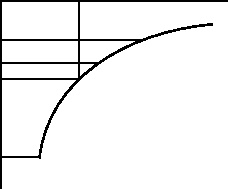
\includegraphics[width=0.28\textwidth]{gesamttex/edit_VIII-4/images/LH_37_03_125-127_d3_126v.pdf}%
\edcaption[-1.00em]%
{%
\hspace{1.50mm}\lbrack\textit{Fig.\:3}\rbrack%
}%
\end{edfigure}%
\pstart%
(16)
Ut vero generaliter praedicere possimus
dato pondere%
\indexS{pondus comprimens aerem}
quantum futurum sit spatium,%
\indexS{spatium intra quod aer comprimitur}
manifestum est ex dictis
tres rectas:
\edtext{%
altitudinem aeris compressi,%
\indexS{altitudo aeris compressi}
ut \textit{AH},
rectam \textit{DE}
et denique altitudinem%
\indexS{altitudo liquidi comprimentis}%
}{%
\lemma{altitudinem}%
\Bfootnote{%
\textit{(1)}~spatii %
\textit{(2)}~ut \textit{AH} in %
\textit{(3)}~aeris compressi, ut \textit{AH}, %
\textit{(a)}~altitud %
\textit{(b)}~rectam \textit{DE} et denique %
\textit{(aa)}~pondus %
\textit{(bb)}~altitudinem%
~\textit{L}%
}}
liquidi comprimentis \textit{HG},%
\indexS{liquidum comprimens}
esse continue proportionales,%
\indexS{proportio continua}
adeoque quadratum ipsius \textit{DE}%
\indexS{quadratum aequale rectangulo}
divisum per ipsam \textit{AH}
\edtext{%
dare
\lbrack\textit{HG}\rbrack,
et idem divisum per
\lbrack\textit{HG}\rbrack\
dare \textit{AH}.
Imo etsi ignoremus rectam \textit{DE},
sufficiet
unum experimentum in tubo fecisse%
\indexS{experimentum in tubo}%
\indexS{tubus plenus aere}
ad praedicendum eventum%
\indexS{eventus praedicendus}
reliquorum.%
}{%
\lemma{dare}%
\Bfootnote{%
\bars{\textit{AG} \textit{ändert Hrsg.}} %
et idem divisum per %
\bars{\textit{AG} \textit{ändert Hrsg.}} %
dare \textit{AH} %
\textit{(1)}~, idque procedet %
\textit{(2)}~. Imo etsi %
\lbrack...\rbrack\ eventum reliquorum.%
~\textit{L}%
}}
Si enim experimentum%
\indexS{experimentum in tubo}
sub signo%
\indexS{signum}
\astrosun\ fecerimus %
\edtext{%
modo dicto in artic.\;praecedente,%
\indexS{articulus}%
}{%
\lemma{modo \lbrack...\rbrack\ praecedente}%
\Cfootnote{%
\refpassage{LH_37_03_125-127_126v_wdrf-1}{LH_37_03_125-127_126v_wdrf-2}.%
}}
et rectang. \textit{ANM}%
\indexS{rectangulum}
dividerimus per datum pondus \textit{HG},%
\indexS{pondus comprimens aerem}
habebimus quaesitum spatium aeris \textit{AH};%
\indexS{spatium intra quod aer comprimitur}
sin idem rectangulum%
\indexS{rectangulum}
dividamus per datum spatium \textit{AH},%
\indexS{spatium intra quod aer comprimitur}
\edtext{%
habebimus \textit{HG} quaesitam altitudinem ponderis%
\indexS{altitudo ponderis quaesita}%
}{%
\lemma{habebimus}%
\Bfootnote{%
\textit{(1)}~quaesitum pond %
\textit{(2)}~%
\bars{\textit{HG} \textit{erg.}} quaesitam altitudinem
\textit{(a)}~liquidi %
\textit{(b)}~ponderis%
~\textit{L}%
}}
aerem in datum spatium%
\indexS{spatium intra quod aer comprimitur}%
\indexS{pondus comprimens aerem}
\edtext{%
compressuri.
\lbrack%
\href{\Scan{LH_37_03_127r}}%
{127\:r\textsuperscript{o}}%
\rbrack\
Quodsi altitudines istae non sint datae in numeris,%
\indexS{altitudo aeris compressi}%
\indexS{altitudo ponderis comprimentis}%
\indexS{altitudo liquidi comprimentis}
sed tantummodo in lineis,
semper tamen Geometrice praestari poterit quaesitum%
\indexS{quaesitum geometrice praestitum}
per inventionem quartae proportionalis,%
\indexS{inventio quartae proportionalis}%
\indexS{quarta proportionalis}%
}{%
\lemma{compressuri.}%
\Bfootnote{%
\textit{(1)}~Quodsi %
\textit{(a)}~\textlangle lineae\textrangle\ %
\textit{(b)}~altitudines %
\textit{(c)}~altitudines non sint datae %
\bars{\textlangle in num\textrangle eris \textit{gestr.}}, semper tamen res ad tertiae vel quartae %
\lbrack\href{\Scan{LH_37_03_127r}}{127\:r\textsuperscript{o}}\rbrack\ %
\textit{(2)}~Quodsi altitudines %
\bars{istae \textit{erg.}} non sint datae in %
\textit{(a)}~lineis sed tantum in %
\textit{(aa)}~\textlangle inn\textrangle\ %
\textit{(bb)}~in %
\textit{(b)}~numeris, sed %
\lbrack...\rbrack\ quartae proportionalis,%
~\textit{L}%
}}
quia ut \textit{AH} ad \textit{AN} %
ita \textit{NM} ad \textit{HG},
\edtext{%
\textls{per artic.\;14.}%
}{%
\lemma{per artic.\;14}%
\Cfootnote{%
\refpassage{LH_37_03_125-127_126v_zcvyj-1}{LH_37_03_125-127_126v_zcvyj-2}.%
}}%
\pend%
\newpage%
\pstart%
\edlabel{LH_37_03_125-127_127rv_progrharmon-1}%
(17)
Ut autem naturam%
\indexS{natura progressionis}
\edtext{%
Progressionis
secundum quam
aucto pondere%
\indexS{pondus comprimens aerem}
spatium minuitur%
\indexS{spatium intra quod aer comprimitur}%
\lbrack,\rbrack\
penitus explicem,%
}{%
\lemma{Progressionis}%
\Bfootnote{%
\textit{(1)}~hujus penitus explicem, %
\textit{(2)}~secundum quam %
\lbrack...\rbrack\ penitus explicem,%
~\textit{L}%
}}
prius hoc lemma demonstrandum est:%
\indexS{lemma demonstrandum}%
\textls{ }%
\edlabel{LH_37_03_125-127_127r_ext-1}%
\textls{Si sint quantitates quotcunque in progressione
\indexS{progressio arithmetica}%
Arithmetica,}
ut \textit{DE}, \textit{GE}, \textit{KE} etc.,%
\textls{ sintque aliae }%
\edtext{%
\textls{totidem }%
\textit{AF}, \textit{AH}, \textit{AL} etc.%
}{%
\lemma{\textls{totidem}}%
\Bfootnote{%
\textit{(1)}~\textlangle\textendash\textrangle\ %
\textit{(2)}~\textit{AG} %
\textit{(3)}~\textit{AF}, \textit{AH}, \textit{AL} etc.%
~\textit{L}%
}}%
\textls{ quae sint prioribus reciproce proportionales }%
(id
\edtext{%
est,
\edlabel{LH_37_03_125-127_127r_ve8c-1}%
sit \textit{DE} ad \textit{GE} ut $AH : AF,$
itemque
\textit{DE} ad \textit{KE} ut $AL : AF$%
\edlabel{LH_37_03_125-127_127r_ve8c-2}
etc.,
unde et \textit{GE} ad \textit{KE} ut \textit{AL} ad \textit{AH} etc.)%
}{%
\lemma{est,}%
\Bfootnote{%
\textit{(1)}~ut %
\textit{(a)}~\textit{DE}~: %
\textit{(b)}~$DE : KE$ %
\textit{(2)}~sit \textit{DE} ad %
\lbrack...\rbrack\ ut $AL : AF$ %
\textit{(a)}~etc.) %
\textit{(b)}~\textlangle et\textrangle\ $GE : KE \squaredots AL : AH$ etc.) %
\textit{(c)}~etc., unde %
\lbrack...\rbrack\ ad \textit{AH} etc.)%
~\textit{L}%
}}%
\textls{ tunc ipsas }%
\edtext{%
\textit{AF}, \textit{AH}, \textit{AL} etc.%
\textls{ fore}%
}{%
\lemma{\textit{AF}, \textit{AH}, \textit{AL}}%
\Bfootnote{%
\textit{(1)}~fore %
\textit{(2)}~etc. \textls{fore}~%
~\textit{L}%
}}%
\textls{ progressionis }%
\indexS{progressio harmonica}%
\edtext{%
\textls{Harmonicae }%
\edlabel{LH_37_03_125-127_127r_drzh-1}%
seu fore $AF - AH$ ad $AH - AL$
ut \textit{AF} ad \textit{AL}.%
\edlabel{LH_37_03_125-127_127r_ext-2}%
}{%
\lemma{\textls{Harmonicae}}%
\Bfootnote{%
\textit{(1)}~. Sit \textit{DE} aequ. \textit{x} %
\textit{(2)}~. Sit \textit{DE} aequ. %
\textit{(3)}~seu %
\textit{(a)}~erit %
\textit{(b)}~fore $AF - AH$ %
\lbrack...\rbrack\ \textit{AF} ad \textit{AL}.%
~\textit{L}%
}}
Cum enim sit \textit{GE} ad \textit{DE} ut \textit{AF} ad \textit{AH},
erit dividendo $GE - DE$ ad \textit{DE} ut $AF - AH$
\edtext{%
ad \textit{AH}.
Ergo rectangulum sub $GE - DE$ et \textit{AH}
aequale rectangulo sub \textit{DE} et $AF - AH.$%
\indexS{rectangulum}
Similiter,
quia \textit{KE} ad \textit{GE} ut \textit{AH} ad~\textit{AL},
erit dividendo $KE - GE$ ad \textit{GE} ut $AH - AL$ ad \textit{AL},
et rectang. sub $KE -GE$ et \textit{AL} aequale rectangulo sub \textit{GE} et $AH - AL.$
Ergo rectang. sub \textit{DE} et $AF - AH$ est ad rectang. sub \textit{GE} et $AH - AL$
ut rectang. sub $GE - DE$ et \textit{AH} ad rectang. sub $KE - GE$ et \textit{AL},
id est ut \textit{AH} ad \textit{AL},
demta communi altitudine
$GE - DE$ aequal. $KE - GE.$
Nam $GE - DE$ aequal. $KE - GE$
ob naturam progressionis Arithmeticae,%
\indexS{progressio arithmetica}%
\indexS{natura progressionis}
ubi semper differentiae terminorum quorumcunque%
\indexS{termini progressionis proximi}%
\indexS{differentia terminorum proximorum}
sibi proximorum sunt aequales.
Quoniam ergo rectang. sub \textit{DE} et $AF - AH$
est ad rectang. sub \textit{GE} et $AH - AL$%
\indexS{rectangulum}
ut \textit{AH} ad \textit{AL},
erit ratio \textit{AH} ad \textit{AL}
composita ex rationibus%
\indexS{ratio composita e rationibus}
\textit{DE} ad \textit{GE} et $AF - AH$ ad $AH- AL.$
Ergo vicissim%
}{%
\lemma{ad \textit{AH}.}%
\Bfootnote{%
\textit{(1)}~%
\bars{Jam rectang. sub $GE - DE$ et \textit{AH} aequal. rectangulo sub \textit{DE} et $AF- AH$ \textit{erg. u. gestr.}}
Similiter, quia \textit{KE} ad \textit{GE} ut \textit{AH} ad \textit{AL}, erit dividendo $KE - GE$ ad \textit{GE} ut $AH - AL$ ad \textit{AL}.
\bars{Ergo ratio composita ex ratione $GE - DE$ ad $KE - GE$ et ex ratione \textit{GE} ad \textit{DE} est eadem cum ratione composita \textit{erg. u. gestr.}}
Est autem $GE - DE$ aequal. $KE - GE$ (ex natura progressionis arithmeticae ubi differentiae terminorum duorum %
\textit{(a)}~vicinorum %
\textit{(b)}~proximorum sunt aequales) %
\textit{(2)}~Ergo rectangulum sub $GE - DE$ et \textit{AH} %
\textit{(a)}~et sub \textit{DE} %
\textit{(b)}~aequale rectangulo %
\lbrack...\rbrack\ et $AH - AL.$ Ergo %
\textit{(aa)}~rectang. sub $GE - DE$ et \textit{AH} est ad %
\textit{(bb)}~rectang. sub %
\lbrack...\rbrack\ $KE - GE$ et \textit{AL},
\textit{(aaa)}~(id est q %
\textit{(bbb)}~id est ut %
\textit{(ccc)}~id est %
\lbrack...\rbrack\ altitudine $GE - DE$ aequal. $KE - GE$ %
\textit{(aaaa)}~(quia %
\textit{(bbbb)}~. Nam $GE - DE$ aequal. $KE - GE$ %
\bars{( \textit{gestr.}} ob naturam %
\lbrack...\rbrack\ sunt aequales. %
\bars{) \textit{gestr.}} Quoniam ergo %
\lbrack...\rbrack\ $AF - AH$ ad $AH- AL$
\textit{(aaaaa)}~adeoque vicissim %
\textit{(bbbbb)}~. Ergo vicissim%
~\textit{L}%
}}
ratio $AF - AH$ ad $AH - AL$
composita est ex%
\indexS{ratio composita e rationibus}
\edtext{%
rationibus \textit{GE} ad \textit{DE} et \textit{AH} ad~\textit{AL}.%
}{%
\lemma{rationibus}%
\Bfootnote{%
\textit{(1)}~\textit{AH} %
\textit{(a)}~ad \textit{AL} et %
\textit{(b)}~et %
\textit{(2)}~\textit{GE} ad %
\lbrack...\rbrack\ ad \textit{AL}.%
~\textit{L}%
}}
Jam ratio \textit{GE} ad \textit{DE} eadem est
cum ratione \textit{AF}
\edtext{%
ad \textit{AH}
(per
\edtext{%
dicta sub initium huius demonstrationis).%
\indexS{demonstratio}%
}{%
\lemma{dicta \lbrack...\rbrack\ demonstrationis}%
\Cfootnote{%
Vgl. \refpassage{LH_37_03_125-127_127r_ve8c-1}{LH_37_03_125-127_127r_ve8c-2}.%
}}%
}{%
\lemma{ad \textit{AH}}%
\Bfootnote{%
\textit{(1)}~(ob %
\textit{(a)}~\textit{DE} %
\textit{(b)}~\textit{GE}, \textit{DE} et \textit{AH} ad \textit{AF} recipro %
\textit{(2)}~(per %
\textit{(a)}~superiora %
\textit{(b)}~dicta sub initium huius demonstrationis).%
~\textit{L}%
}}
Ergo
\edtext{%
ratio
$AF - AH$ ad $AH - AL$
composita est ex rationibus%
\indexS{ratio composita e rationibus}
\textit{AF} ad \textit{AH} et \textit{AH} ad \textit{AL},%
}{%
\lemma{ratio}%
\Bfootnote{%
\textit{(1)}~\textit{AF} ad %
\textit{(2)}~$AF - AH$ ad %
\lbrack...\rbrack\ ex rationibus %
\textit{(a)}~\textit{AH} ad %
\textit{(b)}~\textit{AF} ad %
\lbrack...\rbrack\ ad \textit{AL},%
~\textit{L}%
}}
quae eadem est cum ratione \textit{AF} ad \textit{AL}.
Ergo $AF - AH$ est ad $AH - AL$ ut \textit{AF} ad \textit{AL}.
Seu termini extremi \textit{AF} et \textit{AL}%
\indexS{termini proportionis extremi}
sunt inter se
ut $AF - AH$ et $AH - AL$
\edtext{%
\textlangle seu u\textrangle t%
}{%
\lemma{\textlangle seu u\textrangle t}%
\Cfootnote{%
Beide Worte noch lesbar in dem 1967 aufgenommenen S-Film Nr. 116 der GWLB Hannover.%
}}
differentiae extremorum a%
\indexS{differentia terminorum extremorum a medio}
\edtext{%
medio \textit{AH}.%
\indexS{terminus proportionis medius}
Ergo%
}{%
\lemma{medio \textit{AH}.}%
\Bfootnote{%
\textit{(1)}~Adeoque %
\textit{(2)}~Ergo%
~\textit{L}%
}}
hi tres termini
\edtext{\textit{AF}, \textit{AH}, \textit{AL}%
}{%
\lemma{\textit{AF}, \textit{AH}, \textit{AL}}%
\Bfootnote{%
\textit{erg.\;L}%
}}
sunt progressionis harmonicae.%
\indexS{progressio harmonica}%
\edlabel{LH_37_03_125-127_127r_drzh-2}
\lbrack%
\href{\Scan{LH_37_03_127v}}%
{127\:v\textsuperscript{o}}%
\rbrack\
Idemque patet
de tribus aliis continuis quibuscunque,%
\indexS{termini proportionis continuae}
si
\edtext{%
plures tribus secundum%
}{%
\lemma{plures}%
\Bfootnote{%
\bars{tribus \textit{erg.}} secundum%
~\textit{L}%
}}
\edtext{%
conditiones%
\indexS{conditio}
\edtext{%
initio hujus articuli%
\indexS{articulus}
dictas%
}{%
\lemma{initio}%
\Bfootnote{%
\textit{(1)}~dictas %
\textit{(2)}~hujus articuli dictas%
~\textit{L}%
}}%
}{%
\lemma{conditiones \lbrack...\rbrack\ dictas}%
\Cfootnote{%
\refpassage{LH_37_03_125-127_127r_ext-1}{LH_37_03_125-127_127r_ext-2}.%
}}
assumantur%
\lbrack;\rbrack\
adeoque
\edtext{%
tota series quotcunque%
}{%
\lemma{tota}%
\Bfootnote{%
\textit{(1)}~quotcunque %
\textit{(2)}~series quotcunque%
~\textit{L}%
}}
terminorum hujusmodi
\textit{AF}, \textit{AH}, \textit{AL} etc.
progressionis harmonicae erit.%
\indexS{progressio harmonica}
Q.E.D.%
\edlabel{LH_37_03_125-127_127rv_progrharmon-2}
\pend%
\pstart%
(18)
Hinc sequitur%
\textls{ fractiones quaecunque,%
\indexS{fractio reciproce proportionalis numeratori}
quorum numerator sit idem,%
\indexS{numerator fractionis}
nominatores%
\indexS{nominator fractionis}
vero }%
\edtext{%
\textls{sint progressionis arithmeticae,%
\indexS{progressio arithmetica}
fore progressionis harmonicae}%
\indexS{progressio harmonica}%
}{%
\lemma{\textls{sint progressionis}}%
\Bfootnote{%
\textit{(1)}~harmonicae, fore prog %
\textit{(2)}~\textls{arithmeticae, fore progressionis harmonicae}%
~\textit{L}%
}}%
\textls{ }%
ut
\rule[-2,8mm]{0mm}{6.9mm}%
$\displaystyle\frac{1}{1}\,~\frac{1}{2}\,~\frac{1}{3}\,~\frac{1}{4}\,~\frac{1}{5}$ etc.
Sunt enim hae fractiones reciproce proportionales%
\indexS{fractio reciproce proportionalis numeratori}
\edtext{%
suis nominatoribus,%
\indexS{nominator fractionis}
ac proinde%
}{%
\lemma{}%
\Bfootnote{%
suis nominatoribus, ac proinde
\textit{erg.\;L}%
}}
totidem numeris progressionis Arithmeticae,%
\indexS{progressio arithmetica}
nempe
\edtext{%
1\,~2\,~3\,~4\,~5.
Est enim%
\rule[-2mm]{0mm}{0mm}
\newline%
\hspace*{7.5mm}%
$\displaystyle\frac{1}{1}$ ad $\displaystyle\frac{1}{2}$ ut 2 ad 1,%
\rule[-4mm]{0mm}{8mm}
\newline%
\hspace*{7.5mm}%
$\displaystyle\frac{1}{1}$ ad $\displaystyle\frac{1}{3}$ ut 3 ad 1,%
\rule[-4mm]{0mm}{8mm}
\newline%
\hspace*{7.5mm}%
$\displaystyle\frac{1}{1}$ ad $\displaystyle\frac{1}{4}$ ut 4 ad 1,%
\rule[-4mm]{0mm}{8mm}
\newline%
\hspace*{7.5mm}%
$\displaystyle\frac{1}{2}$ ad $\displaystyle\frac{1}{3}$ ut 3 ad 2,%
\rule[-4mm]{0mm}{8mm}
\newline%
\hspace*{7.5mm}%
etc.
\newline%
Jam%
\edtext{%
\textls{ per artic.\;praecedentem }%
}{%
\lemma{\textls{per artic.\;praecedentem}}%
\Cfootnote{%
ebd.%
}}%
termini quotcunque totidem arithmeticis%
\indexS{termini arithmetici}
reciproce proportionales%
\indexS{termini reciproce proportionales terminis arithmeticis}
sunt progressionis harmonicae.%
\indexS{progressio harmonica}
Ergo hae fractiones sunt progressionis harmonicae.%
\indexS{progressio harmonica}%
}{%
\lemma{1~2~3~4~5.}%
\Bfootnote{%
\textit{(1)}~Ergo \textls{per artic. praecedentem ipsae fractiones sunt progressionis harmonicae.} %
\textit{(2)}~Est enim %
\lbrack...\rbrack\ progressionis harmonicae.%
~\textit{L}%
}}
\pend%
\newpage%
\pstart%
\noindent%
\lbrack\textit{Auf der rechten Spalte von Bl.~\href{\Scan{LH_37_03_127r}}{127\:r\textsuperscript{o}} als Nebenrechnung zum Abschnitt Nr.} 17 \textit{(\refpassage{LH_37_03_125-127_127r_drzh-1}{LH_37_03_125-127_127r_drzh-2})%
}:\rbrack\
\pend%
\vspace{2.0em}%
\pstart%
$%
\displaystyle%
\efrac{AF}{x}
\quad\quad\quad \ \ %
\efrac{AH}{y}
\quad\quad\quad \ \ \ %
\efrac{AL}{z}%
$%
\pend%
\vspace{1.5em}%
\pstart%
$%
\displaystyle%
\efrac{\displaystyle\frac{a^2}{a}}{\rule[0mm]{0mm}{4mm}DE}
\quad\quad%
\efrac{\displaystyle\frac{a^2}{a + d \sqcap b}}{\rule[0mm]{0mm}{4mm}GE}
\quad\quad%
\efrac{\displaystyle\frac{a^2}{a + 2d \sqcap c}}{\rule[0mm]{0mm}{4mm}KE}%
$%
\edlabel{LH_37_03_125-127_127r_akn-1}%
\edtext{}{%
\xxref{LH_37_03_125-127_127r_akn-1}{LH_37_03_125-127_127r_akn-2}%
\lemma{\textit{KE}}%
\Bfootnote{%
\textit{(1)}~\lbrack/\rbrack\ $\displaystyle\frac{x}{y} \sqcap \frac{a + d}{a}.$ %
\textit{(2)}~\lbrack/\rbrack\ $\displaystyle\frac{a + d}{a} \sqcap \frac{x}{y}.$
\textit{(3)}~$\displaystyle\efrac{a + d}{}$
\textit{(4)}~\lbrack/\rbrack\ $\displaystyle\frac{a}{a + d} \sqcap \frac{y}{x}.$%
~\textit{L}%
}}%
\pend%
\vspace{1.75em}%
\pstart%
$%
\displaystyle%
\frac{a}{a + d} \sqcap \frac{y}{x}.%
\edlabel{LH_37_03_125-127_127r_akn-2}%
$%
\pend%
\vspace{1.75em}%
\pstart%
$%
\displaystyle%
\frac{b}{a} \sqcap \frac{x}{y}.
\quad\quad\quad%
\frac{c}{a} \sqcap
\edtext{%
\lbrack\frac{x}{z}\rbrack.%
}{%
\lemma{$\displaystyle\frac{z}{x}$}%
\Bfootnote{%
\textit{L~ändert Hrsg.}%
}}
\quad\quad\quad%
\frac{c}{b} \sqcap \frac{y}{z}.
$%
\pend%
\vspace{1.75em}%
\pstart%
$%
\displaystyle%
\frac{x - y}{y} \sqcap \frac{b - a}{a}
\quad\quad\quad%
\frac{y - z}{z} \sqcap \frac{c - b}{b}.%
$%
\edlabel{LH_37_03_125-127_127r_vhb-1}%
\edtext{}{%
\xxref{LH_37_03_125-127_127r_vhb-1}{LH_37_03_125-127_127r_vhb-2}%
\lemma{$\displaystyle\frac{c - b}{b}.$\rule[0mm]{0mm}{5mm}}%
\Bfootnote{%
\textit{(1)}~\lbrack/\rbrack\ $\displaystyle\frac{x - y}{y - z} \sqcap \frac{y}{z}$ %
\textit{(2)}~$\displaystyle\frac{x - y}{y - z} \sqcap \efrac{b - a}{}$ %
\textit{(3)}~\lbrack/\rbrack\ $\displaystyle\frac{x - y}{y - z} \smallfrown $ %
\textit{(a)}~$\displaystyle\frac{y}{z}$ %
\textit{(b)}~$\displaystyle\frac{z}{y} \ \text{aequ.} \ \frac{b - a}{c - b} \smallfrown \frac{b}{a}.$%
~\textit{L}%
}}%
\pend%
\vspace{1.75em}%
\pstart%
$%
\displaystyle%
\frac{x - y}{y - z} \smallfrown \frac{z}{y}
\ \text{aequ.} \
\frac{b - a}{c - b} \smallfrown \frac{b}{a}.
$%
\edlabel{LH_37_03_125-127_127r_vhb-2}%
\pend%
\vspace{1.75em}%
\pstart%
Est autem
$%
\displaystyle%
b - a \ \text{aequ.} \ c - b.
$%
\pend%
\vspace{1.75em}%
\pstart%
Ergo
$%
\displaystyle%
\frac{x - y}{y - z} \smallfrown \frac{z}{y}
\ \text{aequ.} \
\frac{b}{a}.
$%
\pend%
\vspace{1.75em}%
\pstart%
Ergo
$%
\displaystyle%
\frac{x - y}{y - z} \sqcap \frac{b}{a} \smallfrown \frac{y}{z} \sqcap \frac{x}{y} \smallfrown \frac{y}{z} \sqcap \frac{x}{z}.
$%
\pend%
\newpage%
\newpage%
\vspace{3.0em}%
\pstart%
\noindent%
\centering%
*     *     *
\pend%
\vspace{2.5em}%
\selectlanguage{latin}%
\frenchspacing%
\begin{ledgroup}%
\footnotesize%
\pstart%
\noindent%
\textls{Ausführliche Datierungsgründe:}%
\pagelabel{60212_dat}
In der undatierten und titellosen Aufzeichnung N.\;\ref{60212} befasst sich Leibniz ausführlich mit dem elastischen Verhalten einer Luftmasse, die in einem geschlossenen Raum zusammengedruckt wird.
Im Mittelpunkt der Untersuchung steht das Verhältnis zwischen dem Volumen der Luftmasse und dem Druck, den eine aufgesetzte Quecksilbermasse übt.
Eine direkte Berechnung der elastischen Kraft wird nicht unternommen.
Vielmehr wird festgestellt, dass die "elastische Kraft" (\textit{elastrum}), mit der die zusammengedruckte Luftmasse sich zu befreien dränge, proportional zur "druckenden Kraft" (\textit{vis comprimens}), d.\,h. zum Gewicht der Quecksilbermasse, wachse, während das Volumen der Luftmasse sich umgekehrt proportional verringere; siehe vornehmlich die Abschnitte Nr.\;(10) und Nr.\;(12) im Text.
\pend%
\pstart%
Das im Träger der Aufzeichnung N.\;\ref{60212} anzutreffende Wasserzeichen (eine achtblättrige Rosette über den Buchstaben CS; vgl. Bl.\:\href{\Scan{LH_37_03_125wz}}{125}) ist im Leibniz-Nachlass für die ersten Hannoveraner Jahre (etwa bis 1685) häufig belegt.
Inhaltliche Gründe für eine Einschränkung der Datierung liefert der Vergleich mit den Briefen, die Leibniz zwischen August und September 1679 mit dem Kieler Juristen und Mathematiker Samuel Reyher\indexN{\textls{Reyher} (Reiherus, Reiher), Samuel 1635\textendash1714} austauschte.
In seinem Schreiben vom 24\; (3.\;September) 1679 bedankt sich Reyher für den Vorschlag einer \textit{divisio thermometri}, den ihm Leibniz am 12.\;(22.) August 1679 mitgeteilt hat, äußert aber Zweifel an Leibnizens Behauptung, die Einteilung der thermometrischen Skala solle nach harmonischer Progression erfolgen (\textit{LSB} III,\;2 N.\;333, S.\;808.16\,f.;\cite{01436}
N.\;338, S.\;823.11--16).\cite{01434}
Reyher bemerkt zudem, der Zweifel lasse sich wohl durch ein \textit{experimentum per pondera corpori elastico imponenda} klären (\textit{LSB} III,\;2 N.\;338 S.\;823.16\,f.).\cite{01434}
Auf diese Andeutung geht Leibniz ausdrücklich in seiner Antwort vom 8.\;September 1679 ein, indem er ein Gedankenexperiment entwirft, das in erheblichem Maße demjenigen ähnelt, das im Mittelpunkt der vorliegenden Aufzeichnung N.\;\ref{60212} steht:
Wenn in einem im Vakuum stehenden Rohr eine Quecksilbermasse eine eingekesselte Luftmasse zusammendrücke, dann ergebe sich bei einer linearen Gewichtszunahme der Quecksilbermasse, dass der von der Luft eingenommene Raum nach harmonischer Progression abnehme, d.\,h. in umgekehrter Proportionalität (\textit{LSB} III,\;2 N.\;341, S.\;828.9--829.15).\cite{01435}
Zu demselben Ergebnis kommt Leibniz auch in N.\;\ref{60212} (bes. \refpassage{LH_37_03_125-127_127rv_progrharmon-1}{LH_37_03_125-127_127rv_progrharmon-2};
vgl. zudem das Diagramm \lbrack\textit{Fig.\:2}\rbrack\ in N.\;\ref{60212} mit der Abbildung in \textit{LSB} III,\;2 N.\;341, S.\;828).\cite{01435}
Das Ergebnis dieses Gedankenexperiments kennzeichnet Leibniz in seiner Antwort auf Reyher als empirisch (\textit{quemadmodum tentando comperies}); er kündigt jedoch an, der entsprechende Beweis sei bereits in Vorbereitung (\textit{Quanquam et demostratio in promtu sit}; \textit{LSB} III,\;2 N.\;341, S.\;829.13).\cite{01435}
Die Vermutung liegt somit nahe, dass Leibnizens Ankündigung auf die vorliegende Aufzeichnung N.\;\ref{60212} anspielt.
Unter dieser Voraussetzung ist anzunehmen, dass sie in engem zeitlichem Zusammenhang mit Leibnizens Antwort an Reyher\indexN{\textls{Reyher} (Reiherus, Reiher), Samuel 1635\textendash1714} entstand, d.h. wohl noch im September 1679.
\pend%
\pstart%
Eine spätere Abfassungszeit der Aufzeichnung N.\;\ref{60212} ist unwahrscheinlich, aber nicht auszuschließen.
Die Texte
\textit{LSB} VIII,\;3 N.\;14\textsubscript{3} (Januar -- März/April 1683),\cite{01437}
N.\;14\textsubscript{7} (März/April 1683 -- erste Hälfte 1684),\cite{01438}
N.\;17 (Ende Januar 1683 -- Ende 1684)\cite{01439}
und N.\;21 (Ende Januar 1683 [?] -- Juli 1686 [?])\cite{01440}
setzen jedoch mutmaßlich die Ergebnisse von N.\;\ref{60212} voraus.
Wenn diese Vermutung zutrifft, dann ist die vorliegende Aufzeichnung spätestens in den ersten Monaten 1683 entstanden.
\pend%
\pstart%
Abschließend gilt es zu bemerken, dass sämtliche Verweise auf die Aufzeichnung N.\;\ref{60212}, die in den Texten  \textit{LSB} VIII,\,3 N.\;14\textsubscript{3}\cite{01437} \textit{Explicatio mechanica elastri}, N.\;14\textsubscript{7}\cite{01438} \textit{Demonstratio quod extensiones elasticorum sint viribus tendentibus proportionales}, N.\;17\cite{01439} \textit{De viribus chordas ad rupturam tendendibus} und N.\;21\cite{01440} \textit{De vibrationibus aeris tensi}, sich als fraglich erwiesen haben.
Somit erweisen sich auch sämtliche von diesen Verweisen herrührenden Schlussfolgerungen als fraglich.
\pend%
\end{ledgroup}%
\selectlanguage{latin}%
\frenchspacing%
\normalsize%
\newpage%




\chapter[tocentry={Corpus impingens a penetrabili repercuti potest
\enskip%
\bracks{%
1680\;(?) -- 1684\;(?)%
}},
head={Corpus impingens repercuti potest}]%
{\MakeUppercase{Corpus impingens a penetrabili repercuti potest}
\newline%
\bracks{%
1680\;(?) -- 1684\;(?)}%
}
\label{60283}
\selectlanguage{ngerman}
\begin{ledgroupsized}[r]{120mm}
\footnotesize
\pstart
\noindent\textbf{Überlieferung:}
\pend
\end{ledgroupsized}
\begin{ledgroupsized}[r]{114mm}
\footnotesize
\pstart \parindent -6mm
\makebox[6mm][l]{\textit{L}}%
Aufzeichnung:
LH~XXXVII~5 Bl.\;25.
Ein Zettel (etwa 5,5\;x\;10~cm),
Ränder beschnitten;
Papiererhaltungsmaßnahmen;
\href{\Scan{LH_37_05_025wz}}{Harzer Papier}.
Eine Seite auf Bl.\;25\,r\textsuperscript{o}.
Bl.\;25\,v\textsuperscript{o} überliefert lediglich das Diagramm \lbrack\textit{Fig.\:1}\rbrack,
welches keinen erkennbaren Bezug zum Text aufweist.
\pend%
\end{ledgroupsized}
\vspace{5mm}
\begin{ledgroup}
\footnotesize
\pstart
\noindent%
\textbf{Datierungsgründe:}
Die Datierung der Aufzeichnung N.~\ref{60283} beruht auf äußeren Eigenschaften des Text\-trägers %
sowie auf inhaltlichen Betrachtungen.
Siehe die ausführliche Begründung auf S.~\pageref{60283_dat}.
\pend%
\end{ledgroup}%
\selectlanguage{latin}%
\frenchspacing%
\vspace{8mm}%
\normalsize%
\pstart%
\noindent%
\lbrack%
\href{\Scan{LH_37_05_025r}}%
{25\:r\textsuperscript{o}}%
\rbrack\ %
Corpus impingens%
\indexS{corpus impingens}
in penetrabile%
\indexS{corpus penetrabile}
cum difficultate,%
\indexS{difficultas penetrandi}
tanta celeritate ferri potest,%
\indexS{celeritas corporis impingentis}
ut ab eo repercutiatur.%
\indexS{repercussio corporis impingentis}
Nam corpus penetrabile ipsummet%
\indexS{corpus penetrabile}
tanta celeritate moveri potest,%
\indexS{celeritas corporis penetrabilis}
ut aliud solidum sustineat,%
\indexS{corpus solidum}
imo et ut fortius propellat,
quam ipsummet
\edlabel{LH_37_05_025_025r_evbw-1}%
fertur.%
\edtext{}{%
\xxref{LH_37_05_025_025r_evbw-1}{LH_37_05_025_025r_evbw-2}%
\lemma{fertur.}%
\Bfootnote{%
\textit{(1)}~Causa %
\textit{(2)}~Idem autem %
\lbrack...\rbrack\ effectum. \lbrack/\rbrack\ Causa%
~\textit{L}%
}}
Idem autem est
corpus impingere et excipere%
\lbrack,\rbrack\
quantum ad hunc effectum.
\pend%
\pstart%
Causa%
\edlabel{LH_37_05_025_025r_evbw-2}
horum omnium,
quod eo
\edtext{%
major est difficultas penetrandi,%
\indexS{difficultas penetrandi}
quo major est penetrantis celeritas;%
\indexS{celeritas penetrantis}%
\indexS{corpus penetrans}%
}{%
\lemma{major est}%
\Bfootnote{%
\textit{(1)}~celeritas %
\textit{(2)}~difficultas penetrandi, %
\lbrack...\rbrack\ penetrantis celeritas;%
~\textit{L}%
}}
et potest esse impingentis celeritas%
\indexS{corpus impingens}%
\indexS{celeritas corporis impingentis}
tanta,
ut citius ipsum
\edtext{%
corpus excipiens%
\indexS{corpus excipiens}
flectatur et resiliat,
adeoque et repercutiat,
quam ut%
}{%
\lemma{corpus}%
\Bfootnote{%
\textit{(1)}~impingens flectatur et repercutiatur %
\textit{(2)}~excipiens flectatur et resiliat, %
\textit{(a)}~quam ut %
\textit{(b)}~adeoque et %
\textit{(aa)}~repercutiatur, %
\textit{(bb)}~repercutiat, quam ut%
~\textit{L}%
}}
dividi se patiatur.
Nimirum divisio%
\indexS{divisio corporis penetrabilis}
ex eo oritur,
quod totum motui magis resistit,%
\indexS{motus corporis impingentis}
quam elastrum partes connectens.%
\indexS{elastrum connectens partes}
\lbrack%
\href{\Scan{LH_37_05_025v}}%
{25\:v\textsuperscript{o}}%
\rbrack%
\pend%
\vspace{1.25em}%
\pstart%
\noindent%
\lbrack\textit{Ohne erkennbaren Bezug zum Text:}\rbrack\
\pend%
\vspace{0.50em} %
\centerline{%
\hspace{1.5mm}%
\includegraphics[width=0.060\textwidth]{%
gesamttex/edit_VIII-4/images/LH_37_05_025_d_025v.pdf%
}} 
\nobreak\vspace{0.25em}
\centerline{%
\hspace{2.0mm}%
\lbrack\textit{Fig.\:1}\rbrack%
}
\newpage%
\vspace*{1.0em}%
\pstart%
\noindent%
\centering%
*     *     *
\pend%
\vspace{2.0em}%
\selectlanguage{latin}%
\frenchspacing%
\begin{ledgroup}%
\footnotesize%
\pstart%
\noindent%
\textls{Ausführliche Datierungsgründe:}%
\pagelabel{60283_dat}
Die titellose und undatierte Aufzeichnung N.\;\ref{60283} ist mit der These befasst, dass ein weicherer Körper einen eindringenden härteren zurückzustoßen vermöge, wenn die Geschwindigkeit des Zusammenpralls hinreichend hoch sei.
Die These wird durch die allgmeine Annahme begründet, dass umso mehr Widerstand einem Körper beim Eindringen in einen anderen Körper widerfahre, je höher die relative Geschwindigkeit sei.
Die für N.\;\ref{60283} vorgeschlagene Datierung lässt sich folgendermaßen begründen:
\pend%
\pstart%
Der Träger der vorliegenden Aufzeichnung weist zwar kein Wasserzeichen auf, kann aber anhand des gegitterten \href{\Scan{LH_37_05_025wz}}{Papiermusters} einer Harzer\indexO{Harz} Papiermühle zugeordnet werden. %
Papier dieser Art ist in Leibnizens Nachlass für den Zeitraum 1680--1684 belegt.
Demzufolge erweist sich als wahrscheinlich, dass auch N.\;\ref{60283} in diesem Zeitraum entstand.
Der in N.\;\ref{60283} ausgrdruckte Gedanke findet sich tatsächlich in Texten der frühen 1680er Jahre wieder, so etwa in dem zwischen August 1681 und Ende 1682 abgefassten Entwurf \textit{De soni generatione, propagatione et expressione in organo, mechanice explicatis} (\textit{LSB} VIII,\;3 N.\;12\textsubscript{1}, S.\;96.2--4; 98.10--14)\cite{02527} und in dem anschließenden Konzept \textit{L\textsuperscript{1}} zum Entwurf \textit{Cogitationes novae quomodo formetur sonus et per aerem propagetur atque in organo auditus exprimatur} (\textit{LSB} VIII,\;3 N.\;12\textsubscript{3}, S.\;118.11--119.2),\cite{02529} welches spätestens im Winter 1682/1683 angefertigt wurde.
Der Gedanke lässt sich aber auch in älteren Texten nachweisen, die auf Leibnizens frühere Auseinandersetzung mit Honoré Fabris \textit{Physica, id est scientia rerum corporearum} (4 Bde, Lyon 1669-1671)\cite{00044} zurückgehen; vgl. etwa den wohl zwischen Ende 1674 und Ende 1677\;(?) entstandene Entwurf \textit{De motu} (\textit{LSB} VIII,\;3 N.\;4, S.\;14.4--8)\cite{02598} sowie die auf die Zeitspanne Frühjahr 1679 bis Winter 1680/1681\;(?) datierten Aufzeichnung \textit{LSB} VIII,\;3 N.\;7 (Randbemerkung zu S.\;25.4--7).\cite{02599}
Die Aufzeichnung N.\;\ref{60283} könnte somit auch etwas früher als 1680 entstanden sein. 
Auch eine etwa spätere Datierung als 1684 ist möglich.
\pend%
\end{ledgroup}%
\selectlanguage{latin}%
\frenchspacing%
\normalsize%
\newpage%




\chapter[tocentry={Non quies est causa unionis corporum, sed motus %
\enskip\lbrack%
1680--1687%
\rbrack}, %
head={Non quies est causa unionis corporum, sed motus%
}]%
{\MakeUppercase{Non quies est causa unionis corporum, sed motus} %
\newline\lbrack%
1680--1687%
\rbrack} %
\label{60349-1}
\selectlanguage{ngerman}%
\frenchspacing%
\begin{ledgroupsized}[r]{120mm}%
\footnotesize%
\pstart%
\noindent\textbf{Überlieferung:}%
\pend%
\end{ledgroupsized}%
\begin{ledgroupsized}[r]{114mm}%
\footnotesize%
\pstart%
\parindent -6mm%
\makebox[6mm][l]{\textit{L}}%
Aufzeichnung:
LH~XXXVII,\;5 Bl.\;171--172.
Ein Bogen, 8\textsuperscript{o},
Ränder zum Teil beschnitten;
Papiererhaltungsmaßnahmen.
Fragment eines \href{\Scan{LH_37_05_171-172wz}}{Wasserzeichens} am oberen Rand.
Eine ganzseitig beschriebene Seite auf Bl.\;\href{\Scan{LH_37_05_171r}}{171\,r\textsuperscript{o}}.
Bl.\;\href{\Scan{LH_37_05_171v}}{171\,v\textsuperscript{o}} und
Bl.\;\href{\Scan{LH_37_05_172r}}{172\,r\textsuperscript{o}} sind unbeschrieben.
Bl.\;\href{\Scan{LH_37_05_172v}}{172\,v\textsuperscript{o}} überliefert die Aufzeichnung N.\;\ref{60349-2}.
\pend%
\end{ledgroupsized}%
\vspace{5mm}%
\begin{ledgroup}%
\footnotesize%
\pstart%
\noindent%
\textbf{Datierungsgründe:}
Die Datierung der Aufzeichnung N.\;\ref{60349-1} beruht auf Eigenschaften des Textträgers sowie auf inhaltlichen Betrachtungen.
Siehe die ausführliche Begründung auf S.\;\pageref{60349-1_dat}.%
\pend%
\end{ledgroup}%
\selectlanguage{latin}%
\frenchspacing%
\vspace{8mm}%
\normalsize%
\pstart%
\noindent%
\bracks{%
\href{\Scan{LH_37_05_171r}}%
{171\,r\textsuperscript{o}}%
}
Mihi videtur
\edtext{%
non quies%
\indexS{quies causa unionis corporum}
esse causa unionis corporum%
\indexS{causa unionis corporum}%
\indexS{unio corporum}%
}{%
\lemma{quies \bracks{...} corporum}%
\Cfootnote{%
Anspielung auf die kartesische Erklärung der Körperkohäsion.
Siehe etwa \textsc{R.\;Descartes},
\textit{Principia philosophiae} pars~II, §\;54--55
(Amsterdam 1644, S.\;62\,f.;\cite{00035}
\textit{DO} VIII,\;1, S.\;70\,f.).\cite{00120}%
}}
sed motus.%
\indexS{motus causa unionis}
Motus inquam corporum ambientium,%
\indexS{motus corporum ambientium}%
\indexS{corpora ambientia}
quia duo
\edtext{%
corpora sine turbatione ejus%
\indexS{turbatio motus e disjuntione corporum}
disjungi%
\indexS{corpora disjuncta}%
\indexS{disjunctio corporum}%
}{%
\lemma{corpora}%
\Bfootnote{%
\textit{(1)}~disjungi %
\textit{(2)}~sine turbatione ejus disjungi%
~\textit{L}%
}}
non possunt,
et quo majus turbatio est,%
\indexS{turbatio motus e disjuntione corporum}
eo major est resistentia.%
\indexS{resistentia disjunctioni corporum}%
\indexS{resistentia e turbatione motus}
Ut fit
\edtext{%
cum pars fluidi%
\indexS{fluidum expulsum}%
\indexS{pars fluidi expulsa}
loco%
\indexS{locus fluidi expulsi}
expellitur%
\indexS{expulsio fluidi}%
\bracks{,}
alia ejusdem fluidi%
\indexS{fluidum succedens}
parte non succedente;%
\indexS{pars fluidi succedens}%
\indexS{successio fluidi}%
}{%
\lemma{cum}%
\Bfootnote{%
\textit{(1)}~corpus %
\textit{(a)}~li\angles{q} %
\textit{(b)}~fluidum %
\textit{(2)}~pars fluidi loco expellitur %
\textit{(a)}~nec %
\textit{(aa)}~ali\angles{ud} %
\textit{(bb)}~alia simile\bracks{\textit{!}} in eum succedere statim potest %
\textit{(b)}~alia ejusdem %
\bracks{...} non succedente;%
~\textit{L}%
}}
inde enim magnam mutationem sequi%
\indexS{mutatio sequens}
necesse est,
ut videmus
cum aquam antliis haurimus%
\indexS{aqua hausta antliis}%
\indexS{haustus aquae antliis}%
\indexS{antlia}
aut duo marmora polita%
\indexS{marmora polita}
a se invicem avellimus.%
\indexS{avulsio marmorum politorum}
Quando autem aer facile circulare potest,%
\indexS{aer circulans}%
\indexS{circulatio aeris}
ita ut
anteriore pulso%
\indexS{aer pulsus}
alius a tergo succedat,%
\indexS{aer succedens a tergo}
resistentia exigua est,%
\indexS{resistentia pulsioni aeris}
quia mutatio etiam exigua est,%
\indexS{mutatio sequens}
quae non in alio constabit,
quam quod corpus%
\indexS{corpus commovens aerem}
\edtext{%
motum aerem commovit,%
\indexS{aer commotus}
quantum satis erat ad circulationem,%
\indexS{circulatio aeris}
id est portionem ejus%
\indexS{portio aeris}
non multo mole majorem corpore moto.%
\indexS{corpus motum}%
}{%
\lemma{motum}%
\Bfootnote{%
\textit{(1)}~tantundem %
\textit{(2)}~tantu %
\textit{(3)}~aequalem suae aeris molem loco exp\angles{rimit}, %
\textit{(4)}~\angles{comm} %
\textit{(5)}~aerem commovit, %
\bracks{...} id est %
\textit{(a)}~\angles{partem} %
\textit{(b)}~portionem ejus %
\bracks{...} corpore moto.%
~\textit{L}%
}}
\pend%
\pstart%
Dum enim
\edtext{%
corpus \textit{A} transit in locum \textit{B},%
\indexS{corpus transiens in locum alium}%
}{%
\lemma{corpus \textit{A} \bracks{...} locum \textit{B}}%
\Cfootnote{%
Vgl. das Diagramm \bracks{\textit{Fig.\:1}}.%
}}
sufficit
\edtext{%
moveri aerem \textit{clBmf},%
\indexS{aer commotus}%
}{%
\lemma{moveri aerem}%
\Bfootnote{%
\textit{(1)}~\textit{fedc} %
\textit{(2)}~\angles{\textit{clBmf}}, %
\textit{(3)}~\textit{clBmf},%
~\textit{L}%
}}
id est aerem loci occupandi \textit{B} %
cum filo tenui \textit{cl.fm}%
\indexS{filum aeris tenue}
corpus \textit{A} radente;
nam corpore \textit{A} vel minimum progrediente
\edtext{%
versus~\textit{B},
nempe in locum \textit{medl}%
\indexS{locus occupandus}
deserto loco \textit{fghc},%
\indexS{locus desertus}
statim filum aeris \textit{emf}%
\indexS{filum aeris tenue}
ruit in \textit{mfg},
et filum \textit{dlc}
ruit in \textit{lch},%
\indexS{filum aeris tenue}
atque ita circulatio%
\indexS{circulatio aeris}
ad implendum locum desertum%
\indexS{locus desertus}%
\indexS{locus implendus}
necessaria,%
\indexS{circulatio necessaria ad locum implendum}
fit
quam minima aeris ambientis mutatione.%
\indexS{mutatio aeris ambientis}%
\indexS{aer ambiens}%
}{%
\lemma{versus~\textit{B},}%
\Bfootnote{%
\textit{(1)}~aer lateralis \textit{lc}, \textit{mf} versus \textit{ch}, \textit{fg} ruens,\indexS{aer ruens} in locum relictum\indexS{locus relictus} succedit, quem alius aer ex \textit{B} veniens %
\textit{(a)}~continue sequi %
\textit{(b)}~contr %
\textit{(c)}~et his filamentis\indexS{filamentum} velut adductis continuis supplementis\indexS{supplementum continuum} sequitur. Nam dum %
\textit{(aa)}~\textit{mf} %
\textit{(bb)}~\textit{lc} et \textit{mf} tendunt versus \textit{gh} %
\textit{(aaa)}~\angles{\textit{em}} %
\textit{(bbb)}~interea %
\textit{(aaaa)}~\angles{et} %
\textit{(bbbb)}~\textit{dl} et \textit{em} succedunt in locum %
\textit{(aaaaa)}~\textit{mf} %
\textit{(bbbbb)}~\textit{lc} et \textit{mf} eodemque modo corpus \textit{A} radunt. %
\textit{(2)}~nempe in %
\bracks{...} in \textit{mfg}, et %
\textit{(a)}~\textit{dlc} in \textit{lc} %
\textit{(b)}~filum \textit{dlc} %
\bracks{...} quam minima %
\textit{(aa)}~fluidi %
\textit{(bb)}~aeris ambientis mutatione.%
~\textit{L}%
}}
Unde
\edtext{%
si piscis moveatur in media aqua,%
\indexS{piscis movens sine turbatione aquae}
videmus tranquillitatem aquae%
\indexS{tranquillitas aquae}%
\indexS{aqua tranquilla}
non turbari notabiliter.%
\indexS{turbatio tranquillitatis aquae}%
}{%
\lemma{si}%
\Bfootnote{%
\textit{(1)}~\angles{cor}pus %
\textit{(2)}~piscis moveatur in media aqua, %
\textit{(a)}~ut piscis, %
\textit{(b)}~n\angles{ec} %
\textit{(c)}~\angles{et fundo} %
\textit{(d)}~et a fundo et superficie sic satis distet, tranquillitas aquae notabi %
\textit{(e)}~videmus tranquillitatem %
\textit{(aa)}~ejus %
\textit{(bb)}~no %
\textit{(cc)}~aquae non turbari notabiliter.%
~\textit{L}%
}}
Et quo
\edtext{%
magis medium%
}{%
\lemma{magis}%
\Bfootnote{%
\textit{(1)}~corpus %
\textit{(2)}~medium%
~\textit{L}%
}}
liquidum et homogeneum est,%
\indexS{medium liquidum}%
\indexS{medium homogeneum}
eo minus motui corporum resistit,%
\indexS{medium resistens motui}%
\indexS{resistentia medii}%
\indexS{motus corporum}
praesertim si et
\edtext{%
corpora,
aptissima ad medium dividendum ratione%
\indexS{ratio motus apta ad medium dividendum}%
}{%
\lemma{corpora}%
\Bfootnote{%
\bars{in r \textit{erg. u. gestr.}}%
, aptissima ad medium dividendum ratione%
~\textit{L}%
}}
moveantur.%
\indexS{corpora mota ratione apta ad medium dividendum}
\pend%
\begin{edfigure}[2.50em][1.50em]%
\includegraphics%
{gesamttex/edit_VIII-4/images/LH_37_05_171-172_d_171r.pdf}%
\edcaption[0.5em]{%
\bracks{\textit{Fig.\:1}}%
\edtext{%
}{%
\lemma{\bracks{\textit{Fig.\:1}}\,}%
\Cfootnote[nonum]{%
Zusätzlich zum Diagramm sind zwei gestrichene, nicht wiedergegebenen Entwürfe in \textit{L} (Bl.\;\href{\Scan{LH_37_05_171r}}{171\,r\textsuperscript{o}}) überliefert.%
}%
}%
}%
\end{edfigure}%
\vspace{4.0em}%
\pstart%
\noindent%
\centering%
*     *     *
\pend%
\newpage%
\selectlanguage{german}%
\frenchspacing%
\footnotesize%
\pstart%
\noindent%
\textls{Ausführliche Datierungsgründe:}%
\pagelabel{60349-1_dat}
Die undatierte und titellose Aufzeichnung N.\;\ref{60349-1} ist dem grundlegenden Phänomen der Körperkohäsion gewidmet.
Ausgangspunkt ist René Descartes'\indexN{\textls{Descartes} (Cartesius, des Cartes), René 1596\textendash1650} Erklärung, die relative Ruhe der Körperteile begründe deren Zusammenhalt und somit die Kohäsion der Körper (siehe den Quellennachweis im Erläuterungsapparat).
Über diese Erklärung hat sich Leibniz seit den frühen 1670er Jahren kritisch geäußert, etwa in der Aufzeichnung \textit{De consistentia corporum}, die auf die Monate zwischen Herbst und Winter 1672/1673 datierbar ist (\textit{LSB} VI,\;3 N.\;4, bes. S.\;95.6--18);\cite{01299}
seine Abneigung ihr gegenüber lässt sich auf die bereits in der \textit{Theoria motus abstracti} %
aufgestellte Annahme zurückführen, dass Körperkohäsion letztlich auf Bewegung beruht, nicht auf Ruhe (Mainz 1671; \textit{LSB} VI,\;2 N.\;41, S.\;269.28\,f.).\cite{00259}
In der vorliegenden Aufzeichnung N.\;\ref{60349-1} stellt Leibniz der Auffassung Descartes'\indexN{\textls{Descartes} (Cartesius, des Cartes), René 1596\textendash1650} die These entgegen, dass die Kohäsion der Teile eines Körpers von der Bewegung eines umgebenden Fluidums herrühre.
Verdeutlicht wird diese These am Beispiel eines Wurfels, der sich in der Luft fortbewegt.
\pend%
\pstart%
Der Träger der Aufzeichnung N.\;\ref{60349-1} weist am oberen Rand das Fragment eines \href{\Scan{LH_37_05_171-172wz}}{Wasserzeichens} auf, das von der Papiermühle bei Lauenstein\indexO{Lauenstein (Niedersachsen)} (Niedersachsen)\indexO{Niedersachsen} %
verwendet wurde und im Leibniz-Nachlass nach heutigem Kenntnisstand für die Jahre 1680 bis 1683 bzw. 1687 belegt ist. %
Die Aufzeichnung N.\;\ref{60349-1} ist demzufolge aller Wahrscheinlichkeit nach innerhalb dieses Zeitraums entstanden, %
der hier insgesamt als Datierung vorgeschlagen wird.
Diese Entscheidung lässt sich folgendermaßen begründen:
\pend%
\pstart%
Leibnizens Ablehnung von Descartes'\indexN{\textls{Descartes} (Cartesius, des Cartes), René 1596\textendash1650} Erklärung der Körperkohäsion, gekoppelt mit der These, dass die "erste Ursache" in der \textit{pressio ambientium} liege, äußert Leibniz auch in einer Auzeichnung, die er selbst \textit{Cohaesio} betitelt hat (\textit{LSB} VIII,\;3 N.\;16, S.\;262.7).\cite{02615}
Diese lässt sich aufgrund ihrer inhaltlichen Verwandschaft mit den Entwürfen \textit{Explicatio mechanica elastri} (\textit{LSB} VIII,\;3 N.\;14\textsubscript{3})\cite{01437} und \textit{Demonstratio quod extensiones elasticorum sint viribus tendentibus proportionales} (\textit{LSB} VIII,\;3 N.\;14\textsubscript{7})\cite{01438} auf die Zeitspanne von Ende Januar 1683 und der ersten Hälfte 1684 datieren (vgl. die Begründung in \textit{LSB} VIII,\;3 N.\;16, S.\;261).\cite{02615} 
Mit diesen Texten -- vornehmlich mit \textit{Cohaesio} -- ist auch die vorliegende Aufzeichnung N.\;\ref{60349-1} inhaltlich verwandt.
\pend%
\pstart%
Diese letztere %
stellt ferner das Verhalten der Luft als widerstandsfähigen Mediums in einer Weise dar, welche den Ausführungen über die Übertragung des Schalls in den \textit{Cogitationes novae de sono} bemerkenswert ähnelt (vgl. \textit{LSB} VIII,\;3 N.\;12\textsubscript{1} bis N.\;12\textsubscript{3}, bes. S.\;98.1--99.2, 106.21--109.3 u.\;123.5--126.8).\cite{02527}\cite{01481}\cite{02529}
Diese Ausführungen entstanden allesamt im Zeitraum von der zweiten Hälfte August 1681 bis etwa Ende April 1682 und wurden spätestens in der ersten Hälfte 1685 zum Teil überarbeitet (vgl. die editorische Einleitung zu \textit{LSB} VIII,\;3 N.\;12, S.\;90--93, bes. S.\;90.37--91.27).\cite{02526}
Im gleichen Zeitraum könnte auch -- möglicherweise als Nebenprodukt der Abfassung und Überarbeitung %
der \textit{Cogitationes novae de sono} -- die vorliegende Aufzeichnung N.\;\ref{60349-1} entstanden sein.
Diese könnte aber auch im Zusammenhang mit den ersten Briefen über die physikalische Akustik stehen, die Leibniz bereits im Februar oder März 1681 an Günther Christoph Schelhammer\indexN{\textls{Schelhammer} (Schelhammerus), Günther Christoph 1649\textendash1716} und Edme Mariotte\indexN{\textls{Mariotte}, Edme, Seigneur de Chazeuil ca. 1620\textendash1684} sendete und als Vorlage für die \textit{Cogitationes novae de sono} dienten (siehe erneut die editorische Einleitung zu \textit{LSB} VIII,\;3 N.\;12, S.\;90.4--21).\cite{02526}
\pend%
\pstart%
Die gleich zu Beginn der Aufzeichnung N.\;\ref{60349-1} formulierte These, dass die "Ursache" der Körperkohäsion der \textit{motus corporum ambientium} sei, sofern er Widerstand gegen die Trennung der Körperteile leiste, ist bereits in älteren Texten anzutreffen, etwa in Leibnizens Brief an Honorè Fabri\indexN{\textls{Fabri}, Honoré 1607\textendash1688} wohl von den ersten Monaten 1677 (prop.\;4: \textit{LSB} II,\;1\textsuperscript{2} N.\;133, S.\;452.1--16).\cite{01309}
Wahrscheinlich ist N.\;\ref{60349-1} später entstanden als dieser Brief, %
in dem Leibniz noch die Ruhe als mögliche Ursache der Körperkohäsion zulässt (ebd., %
bes. S.\;452.11\,f.),\cite{01309} während dies in N.\;\ref{60349-1} nicht mehr der Fall ist.
Trotzdem ist nicht auszuschließen, dass N.\;\ref{60349-1} noch vor Leibnizens Auseinandersetzung mit Schelhammer\indexN{\textls{Schelhammer} (Schelhammerus), Günther Christoph 1649\textendash1716} und Mariotte\indexN{\textls{Mariotte}, Edme, Seigneur de Chazeuil ca. 1620\textendash1684} und vor den Texten zur Übertragung des Schalls abgefasst wurde.
Auch eine Entstehung von N.\;\ref{60349-1} nach 1684/1685 ist nicht auszuschließen, wenngleich sie weniger wahrscheinlich ist.
Demgemäß empfiehelt es sich, als Datierung der Aufzeichnung N.\;\ref{60349-1} den gesamten Belegzeitraum des Wasserzeichens zu betrachten.%
\pend%
\selectlanguage{latin}%
\frenchspacing%
\normalsize%




\chapter[tocentry={Estne lumen liquor ultimae subtilitatis? %
\enskip\lbrack%
1680--1687%
\rbrack}, %
head={Estne lumen liquor ultimae subtilitatis?%
}]%
{\MakeUppercase{Estne lumen liquor ultimae subtilitatis?} %
\newline\lbrack%
1680--1687%
\rbrack} %
\label{60349-2}
\selectlanguage{ngerman}%
\frenchspacing%
\begin{ledgroupsized}[r]{120mm}%
\footnotesize%
\pstart%
\noindent\textbf{Überlieferung:}%
\pend%
\end{ledgroupsized}%
\begin{ledgroupsized}[r]{114mm}%
\footnotesize%
\pstart%
\parindent -6mm%
\makebox[6mm][l]{\textit{L}}%
Aufzeichnung:
LH~XXXVII,\;5 Bl.\;171--172.
Ein Bogen, 8\textsuperscript{o},
Ränder zum Teil beschnitten;
Papiererhaltungsmaßnahmen.
\href{\Scan{LH_37_05_171-172wz}}{Fragment} eines Wasserzeichens am oberen Rand.
Eine ganzseitig beschriebene Seite auf Bl.\;\href{\Scan{LH_37_05_172v}}{172\,v\textsuperscript{o}}.
Bl.\;\href{\Scan{LH_37_05_171r}}{171\,r\textsuperscript{o}} überliefert die Aufzeichnung N.\;\ref{60349-1}.
Bl.\;\href{\Scan{LH_37_05_171v}}{171\,v\textsuperscript{o}} und
Bl.\;\href{\Scan{LH_37_05_172r}}{172\,r\textsuperscript{o}} sind unbeschrieben.
\pend%
\end{ledgroupsized}%
\vspace{5mm}%
\begin{ledgroup}%
\footnotesize%
\pstart%
\noindent%
\textbf{Datierungsgründe:}
Die titellose und undatierte Aufzeichnung N.\;\ref{60349-2}, in der Leibniz vor dem Hintegrund einer kritischen Stellungnahme zu Descartes' Lehre der Elemente nach der Natur des Lichts fragt, ist aller Wahrscheinlichkeit nach zur gleichen Zeit entstanden wie die auf demselben Trager überlieferte Aufzeichnung N.\;\ref{60349-1}.
Siehe zur Datierung dieser letzteren die ausführliche Begründung auf S.\;\pageref{60349-1_dat}.
\pend%
\end{ledgroup}%
\selectlanguage{latin}%
\frenchspacing%
\vspace{8mm}%
\normalsize%
\pstart%
\noindent%
\bracks{%
\href{\Scan{LH_37_05_172v}}%
{172\,v\textsuperscript{o}}%
}
\edtext{%
Cartesius\indexN{\textls{Descartes} (Cartesius, des Cartes), René 1596\textendash1650}
in suo libro%
\indexS{liber}
quem \textit{mundum} inscripsit,
sibi persuadet
elementa sua pura%
\indexS{elementa Cartesii}%
\indexS{elementum purum}
esse in maxima universi parte,%
\indexS{universum}
mixta%
\indexS{corpus mixtum}%
\indexS{mixta}
autem tantum in locis %
\indexS{locus}
ubi sibi vicina sunt%
\bracks{;}
ita materiam subtilem%
\indexS{materia subtilis}
seu fluidum perfectum%
\indexS{fluidum perfectum}
collocat in fixis,%
\indexS{stella fixa}
\edtext{%
globulos secundi elementi%
\indexS{globulus secundi elementi}%
\indexS{elementum secundum}%
}{%
\lemma{globulos}%
\Bfootnote{%
\textit{(1)}~aut \angles{--} %
\textit{(2)}~secundi elementi%
~\textit{L}%
}}
credit implere coelos;%
\indexS{coelum}
tertium elementum,%
\indexS{elementum tertium}
quod nec divisibilitatem primi,%
\indexS{divisibilitas primi elementi}%
\indexS{elementum primum}
nec mobilitatem secundi elementi%
\indexS{mobilitas secundi elementi}
habet%
\bracks{,}
statuit locum habere
in planetis%
\indexS{planeta}
et cometis.%
\indexS{cometa}
A primo elemento%
\indexS{elementum primum}
esse lucis originem,%
\indexS{origo lucis}%
\indexS{lux}
a secundo%
\indexS{elementum secundum}
ejus transmissionem,%
\indexS{transmissio lucis}
a
\edtext{%
tertio%
\indexS{elementum tertium}
resistentiam%
\indexS{resistentia et opacitas}
et opacitatem%
\indexS{opacitas}.%
}{%
\lemma{tertio}%
\Bfootnote{%
\textit{(1)}~opacitatem seu %
\textit{(2)}~\angles{reflex} %
\textit{(3)}~resistentiam et opacitatem.%
~\textit{L}%
}}%
}{%
\lemma{Cartesius \bracks{...} opacitatem}%
\Cfootnote{%
Vgl.
\textsc{R.\;Descartes,} \textit{Le monde}, cap.\;V
(Paris 1664, S.\;59--64;\cite{02532}
\textit{DO} XI, S.\;28.14--30.27).\cite{00120}%
}}
\pend%
\pstart%
Sed mihi parum divinae magnitudini%
\indexS{magnitudo divina}
consentaneum videtur,
\edtext{%
ut varietas%
\indexS{varietas creaturarum}%
}{%
\lemma{ut}%
\Bfootnote{%
\textit{(1)}~varietati %
\textit{(2)}~varietas%
~\textit{L}%
}}
creaturarum%
\indexS{creatura}
in solis locum habeat
\edtext{%
confiniis illis%
\indexS{confinium}%
}{%
\lemma{confiniis}%
\Bfootnote{%
\textit{(1)}~\angles{rerum,} %
\textit{(2)}~illis,%
~\textit{L}%
}}
quae respectu ingentium illarum massarum%
\indexS{massa ingens}
nullius momenti sunt,
et pene punctorum instar.
Quin contra arbitror
nullam esse particulam universi,%
\indexS{universum}%
\indexS{particula universi}
in qua non existat
quidam creaturarum%
\indexS{creatura}
velut Mundus.%
\indexS{mundus}
\pend%
\pstart%
Deinde
\edtext{%
quod Lucem considerat%
\indexS{lux}
velut elementum quoddam%
\indexS{elementum resolutionis ultimae}%
\indexS{elementum subtilitatis extremae}
ultimae resolutionis%
\indexS{resolutio ultima}
extremaeque subtilitatis,%
\indexS{subtilitas extrema}%
}{%
\lemma{quod}%
\Bfootnote{%
\textit{(1)}~Lumen %
\textit{(2)}~Lucem considerat %
\textit{(a)}~quasi primum quoddam %
\textit{(b)}~velut elementum quoddam %
\textit{(aa)}~extremae %
\textit{(bb)}~ultimae resolutionis extremaeque subtilitatis,%
~\textit{L}%
}%
\lemma{Lucem \bracks{...} subtilitatis}%
\Cfootnote{%
Siehe a.a.o. (S.\;62;\cite{02532}
\textit{DO} XI, S.\;29.28--30.2).\cite{00120}
}%
}
in eo assentiri non
\edtext{%
possum.
Nam cum phosphoros%
\indexS{phosphorus Bononiensis}
considero,
maxime
\edtext{%
Bononiensem%
\indexS{phosphorus Bononiensis}
qui lucem ex aere attrahit,%
\indexS{lux attractus ex aere}%
\indexS{aer}%
}{%
\lemma{Bononiensem \bracks{...} attrahit}%
\Cfootnote{%
Gemeint ist der phos­pho­res­zie­rende \textit{lapis Bononiensis}.
Den Bologneser Leuchtstein kannte Leibniz etwa aus
\textsc{H.\;Fabri}, \textit{Physica},
tract.\;II, lib.\;III, prop.\;64
(Lyon 1669--1671, Bd.\;I, S.\;442b--451a)\cite{00044}
und
\textsc{O.\;v.\;Guericke}, \textit{Experimenta nova},
lib.\;IV, cap.\;10 (Amsterdam 1672, S.\;139b);\cite{00055}
beide Stellen hatte er 1670--1672 exzerpiert
(vgl. \textit{LSB} VIII,\;2 N.\;55, S.\;499.20--501.21\cite{01234}
bzw. \textit{LSB} VIII,\;1 N.\;36, S.\;251.18\,f.).\cite{01197}
Eine weitere Quelle war möglicherweise:
\textsc{A.\;Kircher}, \textit{Magnes},
l.\;III, p.\;II, c.\;4, q.\;2 (Rom 1654, S.\;463).\cite{02533}%
}}
\ledpb%
suspicor
lumen%
\indexS{lumen}%
}{%
\lemma{possum.}%
\Bfootnote{%
\textit{(1)}~Credo %
\textit{(2)}~Nam cum phosphoros considero, %
\textit{(a)}~lucemque %
\textit{(b)}~maxime Bononiensem %
\bracks{...} aere attrahit, %
\textit{(aa)}~in f\angles{ac--} %
\textit{(bb)}~suspicor lumen%
~\textit{L}%
}}
esse liquorem aliquem%
\indexS{liquor subtilitatis ultimae}
non utique ultimae subtilitatis,%
\indexS{subtilitas ultima}
alioqui non ita facile a corpore hujusmodi hauriretur;%
\indexS{liquor haustus a corpore}%
\indexS{corpus hauriens liquorem}
nam ipsum ultimae subtilitatis%
\indexS{subtilitas ultima}
fluidum%
\indexS{fluidum subtilitatis ultimae}
corpore aliquo crasso%
\indexS{corpus crassum}
et haud dubie poroso%
\indexS{corpus porosum}
capere velle,
foret aquam haurire cribro.%
\indexS{haustus aquae cribro}%
\indexS{cribrum}
Itaque
\edtext{%
nec instantaneam esse arbitror luminis transmissionem,%
\indexS{transmissio luminis instantanea}
etsi non negem %
liquidum%
}{%
\lemma{nec}%
\Bfootnote{%
\textit{(1)}~instantaneum %
\textit{(2)}~instantaneam esse arbitror luminis %
\textit{(a)}~motum %
\textit{(b)}~transmissionem, etsi %
\textit{(aa)}~liquidum %
\textit{(bb)}~non negem, liquidum%
~\textit{L}%
}}
quo transmittitur%
\indexS{liquidum quo lumen transmittitur}
ab astris%
\indexS{aster}
ad nos usque
diffusum esse.%
\indexS{liquidum diffusum}
Nec simplici impulsu,%
\indexS{impulsus}
sed certa quadam modificatione motus,%
\indexS{modificatio motus}
qualem et in sono%
\indexS{sonus}
agnoscimus,
credo propagari%
\indexS{propagatio luminis}
atque ita liquorem illum%
\indexS{liquor accensus per aerem}
ut ita dicam
per totum aerem%
\indexS{aer}
accendi%
\indexS{liquor accensus per aerem}
instar fumi%
\indexS{fumus}
aut
\edtext{%
fulguris,%
\indexS{fulgur}
aut halitus naphthae,%
\indexS{halitus naphthae}%
\indexS{naphtha}
licet incomparabili subtilitate%
\indexS{subtilitas incomparabilis}%
}{%
\lemma{fulguris, aut}%
\Bfootnote{%
\textit{(1)}~subtilissimi %
\textit{(2)}~halitus naphthae, licet incomparabili subtilitate,%
~\textit{L}%
}}
et velocitate.%
\indexS{velocitas incomparabilis}
Et peculiarem accensionis%
\indexS{accensio liquidi per aerem}
sive motus explodentis modum%
\indexS{modus motus}%
\indexS{motus explodens}
esse colorem.%
\indexS{color}
\pend%




\chapter[tocentry={De nova pressione aeris subtilioris etiam intra locum aeri communi exhaustum deprehensa, et in aere libero pressionem a cylindro aeris crassi ortam longe superante
\enskip\bracks{%
Herbst\;(?) 1680 -- April 1683%
}},
head={De nova pressione aeris subtilioris}]%
{\MakeUppercase{De nova pressione aeris subtilioris etiam intra locum aeri communi exhaustum deprehensa, et in aere libero pressionem a cylindro aeris crassi ortam longe superante}
\newline\bracks{%
Herbst\;(?) 1680 -- April 1683%
}%
}
\label{60205}
\selectlanguage{ngerman}%
\frenchspacing%
\begin{ledgroupsized}[r]{120mm}%
\footnotesize%
\pstart%
\noindent%
\textbf{Überlieferung:}%
\pend%
\end{ledgroupsized}%
\begin{ledgroupsized}[r]{114mm}%
\footnotesize%
\pstart%
\parindent -6mm%
\makebox[6mm][l]{\textit{L}}%
Aufzeichnung:
LH\;XXXVII\;3, Bl.\;115--116.
Ein Bogen 4\textsuperscript{o};
\href{\Scan{LH_37_03_115-116wz}}{Wasserzeichen} mittig.
Vier ganzseitig beschriebene Seiten.
\pend%
\end{ledgroupsized}%
\vspace{5mm}%
\begin{ledgroup}%
\footnotesize%
\pstart%
\noindent%
\textbf{Datierungsgründe:}
Die Datierung der Aufzeichnung N.\;\ref{60205} beruht auf äußeren Eigenschaften des Text\-trägers %
sowie auf inhaltlichen Betrachtungen.
Siehe die ausführliche Begründung auf S.~\pageref{60205_dat}.%
\pend%
\end{ledgroup}%
\selectlanguage{latin}%
\frenchspacing%
\vspace{8mm}%
\normalsize%
\pstart%
\noindent%
\lbrack%
\href{\Scan{LH_37_03_115r}}%
{115\,r\textsuperscript{o}%
}%
\rbrack%
\hfill%
De nova pressione aeris%
\indexS{pressio aeris}
subtilioris%
\indexS{aer subtilior}%
\hfill%
\phantom{\lbrack115\,r\textsuperscript{o}\rbrack}%
\pend%
\pstart%
\centering%
etiam intra locum aere communi exhaustum%
\indexS{locus exhaustus aere}
deprehensa,
\pend%
\pstart%
\centering%
et in aere libero%
\indexS{aer liber}
pressionem a cylindro aeris crassi ortam%
\indexS{pressio orta a cylindro aeris}%
\indexS{cylinder aeris}%
\indexS{aer crassus}
longe superante%
\pend%
\vspace{0.5em}%
\pstart%
\noindent%
\edlabel{LH_37_03_115-116_115r_veteres-1}%
\edtext{%
}{%
\xxref{LH_37_03_115-116_115r_veteres-1}{LH_37_03_115-116_115r_veteres-2}%
\lemma{Veteres \lbrack...\rbrack\ abhorreat}%
\Cfootnote{%
Nicht ermittelt.%
}}%
Veteres%
\indexS{veteres}
cum observarent
aquam ex vase pleno%
\indexS{vas plenum aqua}
angusti oris%
\indexS{os vasis angustum}
non
effluere %
\indexS{aqua non effluens e vase}
nisi alio
\edtext{%
adhuc%
}{%
\lemma{adhuc}%
\Bfootnote{%
\textit{erg.\:L}%
}}
foramine aperto,%
\indexS{foramen apertum in vase}
eandem in
\edtext{%
antlia aspirante%
\indexS{antlia aspirans}
sequi embolum ascendentem,%
\indexS{embolus ascendens in antlia}%
\indexS{aqua sequens embolum ascendentem}
follem quoque foramine carentem%
\indexS{follis carens foramine}%
}{%
\lemma{antlia}%
\Bfootnote{%
\textit{(1)}~sequi em %
\textit{(2)}~aspirante sequi embolum ascendentem, %
\textit{(a)}~\bars{item \textit{erg.}} %
\textit{(b)}~follem %
\bars{quoque \textit{erg.}} foramine carentem%
~\textit{L}%
}}
magna licet vi adhibita%
\indexS{vis adhibita}
non posse
\edtext{%
aperiri,
id ajebant fieri%
}{%
\lemma{aperiri,}%
\Bfootnote{%
\textit{(1)}~ventosam chirurgicam calefacto citius aere uti applicatam %
\textit{(2)}~id ajebant fieri%
~\textit{L}%
}%
}
ob fugam vacui,%
\indexS{fuga vacui}
quod natura%
\indexS{natura abhorrens vacuum}
abhorreat.%
\edlabel{LH_37_03_115-116_115r_veteres-2}
Nam embolo ascendente
si aqua non sequeretur,
\edtext{%
mansur\lbrack u\rbrack m%
}{%
\lemma{mansuram}%
\Bfootnote{%
\textit{L\;ändert Hrsg.}%
}}
intra embolum%
\indexS{embolus ascendens in antlia}
et aquam%
\indexS{aqua sequens embolum ascendentem}
locum vacuum.%
\indexS{locus vacuus aere}
Sed
\edtext{%
Galilaeus%
\indexN{\textls{Galilei} (Galilaeus, Galileus), Galileo 1564\textendash1642}
didicit ab
\edtext{%
Hydraulis%
\indexS{hydraulum}
hanc%
}{%
\lemma{Hydraulis}%
\Bfootnote{%
\bars{Italis \textit{gestr.}} hanc%
~\textit{L}%
}}
naturae resistentiam%
\indexS{resistentia naturae}%
\indexS{natura abhorrens vacuum}
posse
\edtext{%
vinci a pondere aquae%
}{%
\lemma{vinci}%
\Bfootnote{%
\textit{(1)}~per aquam %
\textit{(2)}~a pondere aquae%
~\textit{L}%
}}
altitudinis circiter 35 pedum,%
\indexS{pondus aquae 35 pedum}%
\indexS{pes}
sive aquam in antliis aspirantibus%
\indexS{antlia aspirans}
ultra hanc altitudinem%
\indexS{altitudo 35 pedum}
elevari non posse,%
\indexS{aqua elevata in antlia}%
}{%
\lemma{Galilaeus \lbrack...\rbrack\ posse}%
\Cfootnote{%
Siehe
G.\;\textsc{Galilei},
\textit{Discorsi}, giornata I
(Leiden 1638,\cite{00050}
S.\;17;
\textit{GO} VIII,\cite{00048}
S.\;63.36--64.25).
}}
quod etiam in fodinis%
\indexS{fodina}
\edtext{%
dudum%
}{%
\lemma{dudum}%
\Bfootnote{%
\textit{erg.\:L}%
}}
experti
\edtext{%
sunt nostri.%
}{%
\lemma{sunt}%
\Bfootnote{%
\textit{(1)}~Germani.\indexS{Germanus} %
\textit{(2)}~nostri.%
~\textit{L}%
}}
Postea
\edlabel{LH_37_03_115-116_115_torricelli-1}%
\edtext{}{%
\xxref{LH_37_03_115-116_115_torricelli-1}{LH_37_03_115-116_115_torricelli-2}%
\lemma{Torricellius \lbrack...\rbrack\ tegerent}%
\Cfootnote{%
Siehe \textsc{E.\;Torricelli},
Brief an M.\;Ricci vom 11.\;Juni 1644\cite{00107}
(C.\,\textsc{Dati},
\textit{Lettera a Filaleti ... della famosissima esperienza dell’argento vivo},
Florenz 1663, S.\;20\,f.;\cite{00032}
\textit{TO}\;III, S.\;186--188).\cite{00108}%
}}%
Torricellius%
\indexN{\textls{Torricelli} (Torricellius), Evangelista 1608\textendash1647}
pro pondere 35 pedum aquae%
\indexS{pondus aquae 35 pedum}%
\indexS{pes}
invenit pondus 27
\edtext{%
pollicum Hydrargyri,%
\indexS{pondus hydrargyri 27 pollicum}%
\indexS{hydrargyrum}%
\indexS{pollex}%
}{%
\lemma{pollicum}%
\Bfootnote{%
\textit{(1)}~Mercurii\indexS{mercurius} %
\textit{(2)}~Hydrargyri%
~\textit{L}%
}}
cujus altitudo%
\indexS{altitudo 27 pollicum}
tanto minor sufficit,
quanto ipsum est aqua
\edtext{%
ponderosius.
Nam tubum%
\indexS{tubus Torricellianus}
qui unum foramen%
\indexS{foramen tubi}
apertum habebat%
\lbrack,\rbrack\
Hydrargyro%
\indexS{hydrargyrum}%
\indexS{tubus impletus hydrargyro}
implevit %
et invertit,
quo facto expertus est
non obstante fuga vacui%
\indexS{fuga vacui}%
\bracks{,}
ex tubo effluere Mercurium%
\indexS{mercurius effluens e tubo Torricelliano}
exceptis 27 pollicibus %
qui in tubo suspensi manent%
\indexS{mercurius suspensus in tubo Torricelliano}%
\bracks{,}
locum supra se vacuum%
\indexS{locus vacuus aere}
\bracks{(}%
quantum sensu judicari potest%
\indexS{sensus}%
\indexS{judicium sensus}%
\bracks{)}
relinquentes.
Unde%
}{%
\lemma{ponderosius.}%
\Bfootnote{%
\bars{Nam tubum
\textit{(1)}~unum tantum apertum habentem %
\textit{(2)}~qui unum %
\lbrack...\rbrack\ expertus est %
\textit{(a)}~Mercurium effluere ex tubo non obstante fuga vacui %
\textit{(b)}~non obstante %
\lbrack...\rbrack\ qui in 
\textit{(aa)}~eo %
\textit{(bb)}~tubo suspensi %
\lbrack...\rbrack\ se vacuum %
\textit{(aaa)}~relinquentes %
\textit{(bbb)}~quantum sensu judicari potest relinquentes %
\textit{erg.}} %
\textit{(1)}~Cumque inde a %
\textit{(2)}~Unde%
~\textit{L}%
}}
judicavit Torricellius%
\indexN{\textls{Torricelli} (Torricellius), Evangelista 1608\textendash1647}
pondus aeris externi circumfusi%
\indexS{pondus aeris externi}%
\indexS{aer externus}%
\indexS{aer circumfusus}
et in locum aere vacuum%
\indexS{locus vacuus aere}
tota sua vi intrare%
\indexS{vis aeris intrantis in locum vacuum}
\edtext{%
intent\lbrack i\rbrack%
}{%
\lemma{intentis}%
\Bfootnote{%
\textit{L\;ändert Hrsg.}%
}}
causam esse
\edtext{%
difficultatis%
\indexS{difficultas in embolis extrahendis}
quae sentitur%
}{%
\lemma{difficultatis quae}%
\Bfootnote{%
\textit{(1)}~scitur %
\textit{(2)}~sentitur%
~\textit{L}%
}}
in embolis extrahendis,%
\indexS{embolus extrahendus}
et exaltationis aquae%
\indexS{exaltatio aquae}%
\indexS{aqua exaltata}
\edtext{%
quippe%
}{%
\lemma{quippe}%
\Bfootnote{%
\textit{erg.\:L}%
}}
quae non tam attrahitur %
\indexS{aqua attracta}
quam ab aere incumbente%
\indexS{aer incumbens telluri}
\edtext{%
sursum exprimitur.%
\indexS{aqua expressa ab aere incumbente}
Et pondus aeris%
\indexS{pondus aeris}
telluri%
\indexS{tellus}
incumbentis%
\indexS{aer incumbens}
tantum esse circiter
quantum esset pondus aquae,%
\indexS{pondus aquae 35 pedum}
si 35 ejus pedes
aut 27 pollices Hydrargyri%
\indexS{pondus hydrargyri 27 pollicum}
globum telluris%
\indexS{globus telluris}%
\indexS{tellus}
tegerent.%
\edlabel{LH_37_03_115-116_115_torricelli-2}%
}{%
\lemma{sursum}%
\Bfootnote{%
\textit{(1)}~premitur. %
\textit{(2)}~exprimitur. Et %
\textit{(a)}~hoc pondus aeris aequ %
\textit{(b)}~pondus aeris telluri incumbentis %
\textit{(aa)}~aequari circiter ponderi 35 
\textit{(bb)}~tantum esse %
\lbrack...\rbrack\ esset pondus %
\textit{(aaa)}~aquae, si 35 ejus pedes superficiem globi telluris %
\textit{(bbb)}~, si 35 pedes aquae aut %
\textit{(aaaa)}~\textlangle\textendash\textrangle\ %
\textit{(bbbb)}~Hydrargyrii aut %
\textit{(ccc)}~aquae, si %
\lbrack...\rbrack\ telluris tegerent.%
~\textit{L}%
}}
\edlabel{LH_37_03_115-116_115r_pascal-1}%
\edtext{}{%
\xxref{LH_37_03_115-116_115r_pascal-1}{LH_37_03_115-116_115r_pascal-2}%
\lemma{Cumque \lbrack...\rbrack\ deprehendit}%
\Cfootnote{%
Siehe %
B.\;\textsc{Pascal},
\textit{Récit de la grande expérience}, 1648\cite{02577} %
(\textit{Traitez}, Paris 1663, S.\;165--194;\cite{00081}
\textit{PO}\;II, S.\;653--690).\cite{01524}
Leibniz hatte 1672 die \textit{Traitez} gelesen und exzerpiert;
vgl. \textit{LSB} VIII,\;1 N.\;38.\cite{01038}%
}}%
Cumque hinc sequeretur
in altissimis montibus%
\indexS{mons altissimus}
minorem debere esse altitudinem Mercurii
in tubo
\edtext{%
Torricellian\lbrack o\rbrack%
\indexS{tubus Torricellianus}%
}{%
\lemma{Torricelliani}%
\Bfootnote{%
\textit{L\;ändert Hrsg.}%
}}
suspensi,%
\indexS{altitudo mercurii suspensi}%
\indexS{mercurius suspensus in tubo}
\edtext{%
quia aeris infra montem positi pondus%
\indexS{aer positus infra montem}%
\indexS{pondus aeris detrahendum}
detrahendum est,%
}{%
\lemma{quia}%
\Bfootnote{%
\textit{(1)}~aer infra montem positus eum %
\textit{(2)}~aeris infra %
\lbrack...\rbrack\ detrahendum est, %
\textit{erg.\:L}%
}}
hoc expertus Pascalius%
\indexN{\textls{Pascal} (Pascalius), Blaise 1623\textendash1662}
verum deprehendit.%
\edlabel{LH_37_03_115-116_115r_pascal-2}
Et jam
\edlabel{LH_37_03_115-116_115r_pascal-3}%
\edtext{}{%
\xxref{LH_37_03_115-116_115r_pascal-3}{LH_37_03_115-116_115r_pascal-4}%
\lemma{pro indubitato \lbrack...\rbrack\ avellendae}%
\Cfootnote{%
Siehe \textsc{Pascal},
\textit{De la pesanteur de la masse de l'air},
cap.\;3\cite{01432}
(\textit{Traitez}, S.\;95\,f.;\cite{00081}
\textit{PO}\;II, S.\;1082\,f.).\cite{01524}%
}}%
pro indubitato habuit,
\edtext{%
praecise aperiri posse follem clausum,%
\indexS{follis clausus}
aut divelli posse duas tabulas politas
sibi impositas,%
\indexS{tabulae politae impositae sibi}
pondere
quod aequivaleat cylindro altitudinis 35 pedum aquae,%
\indexS{pondus cylindri aquae 35 pedum}%
\indexS{cylinder aquae 35 pedum}%
\indexS{altitudo 35 pedum}
basis vero seu crassitiei tantae
quanta est latitudo follis,%
\indexS{follis clausus}
aut tabulae minoris avellendae.%
\indexS{tabula polita avellenda}%
\indexS{avulsio tabularum politarum}%
\edlabel{LH_37_03_115-116_115r_pascal-4}%
}{%
\lemma{praecise}%
\Bfootnote{%
\textit{(1)}~pondere 35 pedum aquae basin latitudini follis aut minimae ex duabus t %
\textit{(2)}~pond %
\textit{(3)}~aperiri posse follem clausum, aut %
\textit{(a)}~distrahi posse %
\textit{(b)}~divelli posse %
\lbrack...\rbrack\ impositas, pondere %
\textit{(aa)}~cylindr %
\textit{(bb)}~quod aequivaleat cylindro %
\bars{altitudinis \textit{erg.}} 35 pedum %
\lbrack...\rbrack\ minoris avellendae.%
~\textit{L}%
}}
\pend%
\pstart%
\edlabel{LH_37_03_115-116_115_lpo-1}%
Verum haec
licet pulchre conclusa viderentur,
turbarunt Experimenta posteriora%
\indexS{experimentum turbans}%
\lbrack;\rbrack\
nam
\edlabel{LH_37_03_115-116_115r_Brouncker-1}%
\edtext{}{%
\xxref{LH_37_03_115-116_115r_Brouncker-1}{LH_37_03_115-116_115r_Brouncker-2}%
\lemma{Brounckerus \lbrack...\rbrack\ altitudine}%
\Cfootnote{%
Hierüber berichtet
\textsc{J.\;Wallis}, \textit{Mechanica}, cap.\;XIV, prop.\;13, schol.
(London 1670--1671, Bd.\;II, S.\;740;\cite{00301}
\textit{WO}~I, S.\;1051);\cite{01008}
Leibniz hatte 1674--1675 die Stelle exzerpiert;
vgl. \textit{LSB} VIII,\;2 N.\;8, S.\;96.18--97.6.%
\cite{01343}
Siehe zudem
J.\;\textsc{Wallis}, "An Extract of letters"
(\textit{PT} VII, 1672, S.\;5160).\cite{00213}%
}}%
\edtext{%
Brounckerus%
\indexN{\textls{Brouncker} (Brunckerus), William Viscount 1620\textendash1684}
observavit%
}{%
\lemma{Brounckerus}%
\Bfootnote{%
\bars{in Anglia \textit{gestr.}} observavit%
~\textit{L}%
}}
aliquando
Mercurium ab aere jam purgatum%
\indexS{mercurius purgatus aere}
ad 70 et ultra pollices%
\indexS{pollex}
in aere libero%
\indexS{aer liber}
suspensum%
\indexS{mercurius suspensus ad 70 pollices}
mansisse,
\edtext{%
leviter tamen concusso tubo%
\indexS{tubus concussus}
facile decidisse
remanente tantum communi 27 pollicum altitudine.%
\indexS{altitudo mercurii 27 pollicum}%
\indexS{pollex}%
}{%
\lemma{leviter tamen \lbrack...\rbrack\ pollicum altitudine}%
\Bfootnote{%
\textit{erg.\:L}%
}}%
\edlabel{LH_37_03_115-116_115r_Brouncker-2}
\edlabel{LH_37_03_115-116_115r_Hugenius-1}%
\edtext{}{%
\xxref{LH_37_03_115-116_115r_Hugenius-1}{LH_37_03_115-116_115r_Hugenius-2}%
\lemma{Hugenius \lbrack...\rbrack\ cesset}%
\Cfootnote{%
Siehe
\textsc{C.\;Huygens}, "Extrait d'une lettre"
(\textit{JS}, 25.\;Juli 1672, S.\;140;\cite{00062}
\textit{HO} VII, S.\;206).\cite{00113}
Mit diesem Aufsatz hatte sich Leibniz 1672--1673 ausführlich auseinandergesetzt;
vgl. insbesondere
\textit{LSB} VIII,\:1 N.\;39.%
\cite{01069}%
}}%
Hugenius%
\indexN{\textls{Huygens} (Hugenius, Ugenius, Hugens, Huguens), Christiaan 1629\textendash1695}
quoque
\edtext{%
notavit,
quod aqua%
\indexS{aqua purgata aere}
aere purgata%
}{%
\lemma{notavit,}%
\Bfootnote{%
\textit{(1)}~aquam %
\textit{(2)}~quod aqua %
\bars{aere purgata \textit{erg.}}%
\textit{L}%
}}
ex vase exhauriri possit%
\indexS{aqua exhausta e vase}%
\indexS{vas plenum aqua}
ope Siphonis inversi bicruri,%
\indexS{sipho bicrurus}
licet durante effluxu%
\indexS{effluxus aquae e vase}
aer ex
\edtext{%
\edlabel{LH_37_03_115-116_115r_dfe-1}%
Recipiente Magdeburgico%
\indexS{recipiens Magdeburgicus}%
\edlabel{LH_37_03_115-116_115r_dfe-2}%
}{%
\lemma{Recipiente Magdeburgico}%
\Cfootnote{%
Pneumatische Vorrichtung zur Vakuumerzeugung.
Leibniz spielt auf die Instrumente an,
die in \textsc{O.\,v.\,Guericke},
\textit{Experimenta nova}, l.\;III
(Amsterdam 1672, S.\;71--124)\cite{00055}
geschildert sind.
Hieraus hatte er 1672 Exzerpte angefertigt;
vgl. \textit{LSB} VIII,\;1 N.\;36.\cite{01197}%
}}
extraheretur,%
\indexS{aer extractus e recipiente Magdeburgico}
cum tamen exhausto prope omni aere%
\indexS{aer exhaustus e recipiente Magdeburgico}
ratio%
\indexS{ratio cessans}
quae secundum Torricellianas Hypotheses%
\indexS{hypothesis Torricelliana}
siphonem bicrurum%
\indexS{sipho bicrurus}
fluere facit,
omnino
\edtext{%
cesset.%
\edlabel{LH_37_03_115-116_115r_Hugenius-2}
\edlabel{LH_37_03_115-116_115r_Gerickius-1}%
\edtext{}{%
\xxref{LH_37_03_115-116_115r_Gerickius-1}{LH_37_03_115-116_115r_Gerickius-2}%
\lemma{Gerickius \lbrack...\rbrack\ editur}%
\Cfootnote{%
Siehe \textsc{Guericke},
\textit{Experimenta nova}, l.\;III, cap.\;7 u.\;8
(S.\;79b--80a u.\;82a).\cite{00055}
Vgl. zudem:
\textit{LSB} VIII,\;1 N.\;36, S.\;247.19--248.2.\cite{01197}%
}}%
Gerickius%
\indexN{\textls{Guericke} (Gerickius, Gericke), Otto von 1602\textendash1686}
etiam vidit in tubulo vitreo,%
\indexS{tubulus vitreus}%
\indexS{tubulus vacuus aere}
licet aeris vacuo%
\lbrack,\rbrack\
aquam tamen aere purgatam%
\indexS{aqua purgata aere}
tubi extremitatibus%
\indexS{aqua adhaerens tubo}
(aut partem unam aquae alteri)
firmiter adhaerere,
et ut avellatur fortiter concutiendam esse%
\lbrack,\rbrack\
ubi et sonus editur.%
\indexS{sonus editus}%
\edlabel{LH_37_03_115-116_115r_Gerickius-2}
Denique%
\edlabel{LH_37_03_115-116_115r_deVolder-1}%
\edtext{}{%
\xxref{LH_37_03_115-116_115r_deVolder-1}{LH_37_03_115-116_115v_deVolder-2}%
\lemma{deprehendit \lbrack...\rbrack\ sustinuisse}%
\Cfootnote{%
Dieses im März 1676 von B.\;de Volder\indexN{\textls{Volder} (Volter, Wolder), Burchard (Burcher) de 1643\textendash1709} durchgefürte Experiment kannte Leibniz wohl aus einem Bericht in der von P.\;Lohmeier betreuten Dissertation \textit{Exercitationum physicarum de paradoxi gravitatis et levitatis prima}, parad.\;I, §~IX (Rinteln 1678, S.\;32--34;\cite{01429}
das bei der GWLB Hannover unter der Signatur M-A 262 aufbewarte Exemplar weist Gerbrauchsspuren wohl von Leinizens Hand auf).
Das Experiment erwähnt Lohmeier\indexN{\textls{Lohmeier} (Lohmeierus, Lomeierus), Philipp 1648\textendash1680} auch in seinem Brief an Leibniz vom 23.\:August\;/\;2.\:September 1679
(\textit{LSB} III,\;2 N.\;336, S.\;817.16--20).\cite{01425}
Über einen ähnlichen Versuch De Volders\indexN{\textls{Volder} (Volter, Wolder), Burchard (Burcher) de 1643\textendash1709} berichtete ferner die anonyme Bemerkung "Experience faite à Leyden" im \textit{Journal des sçavans} vom 17.\;April 1679 (S.\;107\,f.).\cite{02524}
Hierauf spielt E.\,W.\,v.\;Tschirnhaus\indexN{\textls{Tschirnhaus} (H. v. Tch., H. v. Tsch.), Ehrenfried Walther v. 1651\textendash1708} in seinem Brief an Leibniz vom 11.\;September 1682 ab
(\textit{LSB} III,\;3 N.\;399, S.\;711.8\,f.).\cite{02525}%
}}
deprehendit%
}{%
\lemma{cesset.}%
\Bfootnote{%
\bars{Gerickius
\textit{(1)}~quoque %
\textit{(2)}~etiam vidit %
\textit{(a)}~aquam aere purgatam %
\textit{(b)}~in tubulo vitreo, licet %
\textit{(aa)}~partim vacuo %
\textit{(bb)}~aeris vacuo %
\lbrack...\rbrack\ sonus editur. %
\textit{erg.}} Denique %
\textit{(1)}~notavit %
\textit{(2)}~deprehendit%
~\textit{L}%
}}
Volderus%
\indexN{\textls{Volder} (Volter, Wolder), Burchard (Burcher) de 1643\textendash1709}
marmora duo bene polita%
\indexS{marmora polita}%
\indexS{marmora inuncta sero calido}
seroque%
\indexS{serum calidum}
\lbrack%
\href{\Scan{LH_37_03_115v}}%
{115\,v\textsuperscript{o}%
}%
\rbrack\
calido inuncta ...
\edtext{%
libras%
\indexS{libra}
aliquandiu sustinuisse,%
\edlabel{LH_37_03_115-116_115v_deVolder-2}
quamadmodum et
\edlabel{LH_37_03_115-116_115v_Huygens-1}%
\edtext{}{%
\xxref{LH_37_03_115-116_115v_Huygens-1}{LH_37_03_115-116_115v_Huygens-2}%
\lemma{ab Hugenio \lbrack...\rbrack\ esset}%
\Cfootnote{%
Siehe
\textsc{Huygens}, "Extrait d'une lettre"
(%
S.\;139\,f.;\cite{00062}
\textit{HO} VII, S.\;205\,f.).\cite{00113}
Siehe zudem
\textit{LSB} VIII,\:1 N.\;39, S.\;313.2--12.%
\cite{01069}%
}}%
ab Hugenio%
\indexN{\textls{Huygens} (Hugenius, Ugenius, Hugens, Huguens), Christiaan 1629\textendash1695}
notatum est
corpora polita duo
bene juncta in
\edtext{%
vacuo Magdeburgico%
\indexS{vacuum Magdeburgicum}%
}{%
\lemma{vacuo Magdeburgico}%
\Cfootnote{%
Künstlich erzeugtes Vakuum.
Leibniz spielt auf den in
\textsc{Guericke}, \textit{Experimenta nova}, l.\;II, cap.\;3 (S.\;56a)\cite{00055}
dargelegten Begriff sowie auf die
ebd., l.\;III (S.\;71--124)\cite{00055}
beschriebenen Versuche über das Vakuum an.
Siehe auch \textit{LSB} VIII,\;1 N.\;36.\cite{01197}%
}}
sibi adhuc adhaesisse%
\indexS{corpora polita adhaerentia in vacuo}
ubi tamen sejungi nullo negotio debebant,
siquidem solo ponderi cylindri aeris 35 pedum aquae pondus%
\indexS{pondus cylindri aeris}%
\indexS{cylinder aeris}%
\indexS{pondus aquae 35 pedum}
aequant\lbrack i,\rbrack\
vel saltem aeris inclusi ab hoc cylindro pressi Elastro,%
\indexS{elastrum aeris pressi}%
\indexS{aer inclusus}
ascribenda duorum corporum politorum adhaesio esset.%
\indexS{adhaesio corporum politorum}%
\edlabel{LH_37_03_115-116_115v_Huygens-2}
Nam aer ille
qui in Recipiente residuus est%
\indexS{aer residuus in recipiente Magdeburgico}%
\indexS{recipiens Magdeburgicus}%
\lbrack,\rbrack\
exiguum adeo elastrum habet%
\indexS{elastrum aeris}
ut vix aliquot aquae pollices sustinere possit.%
\indexS{pollex aquae}%
\indexS{aqua sustenta ab elastro aeris}
Ex quibus omnibus%
}{%
\lemma{libras}%
\Bfootnote{%
\bars{aliquandiu \textit{erg.}} sustinuisse %
\textit{(1)}~. Notatum est etiam aquam in tubos %
\textit{(a)}~\textlangle arc\textrangle\ %
\textit{(b)}~angustissimos assurgere ultra suum aequilibrium idque in in\lbrack\textit{!}\rbrack\ vacuo etiam Magdeburgico vel Torricelliano. Ex quibus omnibus %
\textit{(2)}~, quemadmodum et %
\bracks{...} notatum est %
\textit{(a)}~marmora %
\textit{(b)}~corpora polita \lbrack...\rbrack\ ubi tamen %
\textit{(aa)}~decidere %
\textit{(bb)}~sejungi nullo negotio debebant, siquidem %
\textit{(aaa)}~Torricelliano et %
\textit{(bbb)}~sola %
\textit{(ccc)}~aeris %
\textit{(ddd)}~solo cylindro %
\textit{(eee)}~solo %
\textit{(aaaa)}~pondere %
\textit{(bbbb)}~ponderi cylindri aeris 35 %
\textit{(aaaaa)}~pedes %
\textit{(bbbbb)}~pedum aquae %
\textit{(aaaaa-a)}~pondere %
\textit{(bbbbb-b)}~pondus %
\bars{aequante \textit{L\;ändert Hrsg.}} vel saltem aeris inclusi
\textit{(aaaaa-aa)}~ab ho %
\textit{(bbbbb-bb)}~a super %
\textit{(ccccc-cc)}~ab hoc \lbrack...\rbrack\ quibus omnibus%
~\textit{L}%
}%
\lemma{libras \bracks{...} omnibus}%
\Cfootnote{%
Den Kapillaritätseffekt, auf den in der gestr. Variante \textit{(1)} angespielt wird, kannte Leibniz aus
\textsc{B.\;de Monconys}, \glqq Discours sur l’ascension de l’eau en un tuyau estroit\grqq\cite{02519}
(\textit{Journal de voyages}, Bd.\;III, Lyon 1666,
\glqq Lettres escrittes à Monconys\grqq, S.\;33--38)\cite{00118} %
sowie möglicherweise aus Erfahrungen von A.\;v.\;Leeuwenhoek,\indexN{\textls{Leeuwenhoek}, Antoni van 1632\textendash1723}
wie der Brief für J.\;P. de La Roque\indexN{\textls{La Roque} (Larroque), Jean Paul de, gest. 1691} von Ende 1677 nahelegt (\textit{LSB} III,\;2 N.\;94, S.\;258.1--6, 261.7--10).\cite{02521}
Siehe hierzu N.\;\ref{42488} in diesem Band, \refpassage{LH_37_07_008_008r_xyz_1}{LH_37_07_008_008r_xyz_2} samt Erläuterungen.%
}%
}
probabile fit
superesse pressionem quandam%
\indexS{pressio aeris subtilioris}
\edtext{%
aeris communi subtilioris,%
\indexS{aer subtilior communi}
cujus sphaera%
\indexS{sphaera aeris}%
}{%
\lemma{aeris}%
\Bfootnote{%
\textit{(1)}~subtilioris %
\textit{(2)}~communi subtilioris, cujus %
\textit{(a)}~atmosphaera\indexS{atmosphaera} %
\textit{(2)}~sphaera%
~\textit{L}%
}}
ad immensam%
\indexS{altitudo immensa}
\edtext{%
fortasse%
}{%
\lemma{fortasse}%
\Bfootnote{%
\textit{erg.\:L}%
}}
altitudinem assurgit,
et proinde longe communi gravior est.%
\indexS{aer gravior communi}%
\edlabel{LH_37_03_115-116_115_lpo-2}
\pend%
\pstart%
Verum in eo est difficultas%
\indexS{difficultas}
quod
\edtext{%
dicendum plerisque videtur%
}{%
\lemma{dicendum}%
\Bfootnote{%
\textit{(1)}~videtur %
\textit{(2)}~plerisque videbatur %
\textit{(3)}~plerisque videtur%
~\textit{L}%
}%
\lemma{dicendum plerisque videtur}%
\Cfootnote{%
Nicht ermittelt.%
}%
}
hunc aerem subtilem%
\indexS{aer subtilis}
penetrare per poros%
\indexS{pori in vitro}
\edtext{%
vitri,%
\indexS{vitrum} 
quoniam pressionem suam%
\indexS{pressio aeris subtilioris}
intra vacuum quoque Magdeburgicum%
\indexS{vacuum Magdeburgicum}
exercet.
Quo posito nulla ratio apparet%
\indexS{ratio apparens}%
}{%
\lemma{vitri,}%
\Bfootnote{%
\textit{(1)}~quo admisso non apparet %
\textit{(2)}~quoniam pressionem %
\lbrack...\rbrack\ ratio apparet%
~\textit{L}%
}}
cur non et penetret per duo marmora polita,%
\indexS{marmora polita}
\edtext{%
aut per%
}{%
\lemma{aut}%
\Bfootnote{%
\bars{cur \textit{gestr.}} per%
~\textit{L}%
}}
Mercurium%
\indexS{mercurius suspensus in tubo}
quem suspensum tenet,
neque etiam apparet,
quid ad rem faciat,
\edtext{%
quod aqua et Mercurius aere%
}{%
\lemma{quod}%
\Bfootnote{%
\textit{(1)}~aer %
\textit{(2)}~aqua et Mercurius %
\textit{(a)}~aqua %
\textit{(b)}~aere%
~\textit{L}%
}}
purgari debent,%
\indexS{aqua purgata aere}%
\indexS{mercurius purgatus aere}
\edtext{%
ut hanc%
}{%
\lemma{ut}%
\Bfootnote{%
\textit{(1)}~hanc %
\textit{(2)}~a %
\textit{(3)}~hanc%
~\textit{L}%
}}
novam pressionem%
\indexS{pressio aeris subtilioris}
\edlabel{LH_37_03_115-116_115v_a1}%
sentiant.%
\edtext{}{%
\xxref{LH_37_03_115-116_115v_a1}{LH_37_03_115-116_115v_a2}%
\lemma{sentiant.}%
\Bfootnote{%
\lbrack/\rbrack\
\textit{(1)}~Verum re recte expensa %
\textit{(2)}~Multa commenti sunt viri %
\textit{(a)}~clarissimi\indexS{vir clarus} %
\textit{(b)}~docti %
\textit{(aa)}~Hugenius, et Wallisius aliique%
\indexN{\textls{Huygens} (Hugenius, Ugenius, Hugens, Huguens), Christiaan 1629\textendash1695}%
\indexN{\textls{Wallis} (Wallisius), John 1616\textendash1703} %
\textit{(bb)}~ut horum phaenomenorum rationem redderent. %
\textit{(aaa)}~Videatur \textit{Epistola} %
\textit{(bbb)}~Videantur quae dedit %
\bars{celeber \textit{gestr.}} Wallisius in %
\lbrack...\rbrack\ et \textit{Epistola} %
\textit{(aaaa)}~cujusdam %
\textit{(bbbb)}~Huetii professoris%
\indexN{\textls{Huet} (Huetius), Pierre-Daniel 1630\textendash1721} %
\textit{(aaaaa)}~He %
\textit{(bbbbb)}~nunc Helvetii quam %
\bars{Parisiis \textit{erg.}} super Hugenii observationibus edidit %
\bars{ubi quaedam Hugeniana defendit \textit{erg.}}. Qui approbante ut videtur Hugenio poros in corporibus supponit per quos transeat %
\textit{(aaaaa-a)}~hic cy %
\textit{(bbbbb-b)}~aer. Sed non satis explicate %
\bars{mihi olim legenti videbatur \textit{erg.}} cur non semper transeat et cur aliquando corpora teneat suspensa. Ego %
\textit{(aaaaa-aa)}~recte suspens %
\textit{(bbbbb-bb)}~\bars{re \textit{erg. u. gestr.}} diligenter et diu expensa %
\textit{(cccc)}~Parisiis super Hugenii observationibus huc %
\bars{facientibus \textit{ändert Hrsg.}} %
\bars{hujusmodi \textit{gestr.}} edita, ubi supponuntur %
\lbrack...\rbrack\ et diu expensa%
~\textit{L}%
}}%
\pend%
\pstart%
Multa commenti sunt viri docti%
\indexS{vir doctus}
ut horum phaenomenorum rationem redderent.%
\indexS{ratio phaenomeni}%
\indexS{phaenomenon}
Videantur
quae dedit
\edtext{%
Wallisius%
\indexN{\textls{Wallis} (Wallisius), John 1616\textendash1703}
in \textit{Transactionibus Anglicanis}.%
}{%
\lemma{Wallisius \lbrack...\rbrack\ \textit{Anglicanis}}
\Cfootnote{%
Vgl.
\textsc{Wallis}, "An Extract of letters"
(%
S.\;5160--5170).%
\cite{00213}%
}}
Videatur et
\edtext{%
\textit{Epistola} Parisiis%
\indexO{Paris}%
\indexS{epistola}
super
\edtext{%
Hugenii%
\indexN{\textls{Huygens} (Hugenius, Ugenius, Hugens, Huguens), Christiaan 1629\textendash1695}
observationibus%
}{%
\lemma{Hugenii observationibus}%
\Cfootnote{%
Siehe
\textsc{Huygens}, "Extrait d'une lettre"
(%
S.\;133--140;\cite{00062}
\textit{HO} VII,
S.\;201--206)\cite{00113}
sowie
\textit{LSB} VIII,\:1 N.\;39.%
\cite{01069}%
}}
huc fac\bracks{tis} edita,%
}{%
\lemma{Epi\-sto\-la \lbrack...\rbrack\ edita}%
\Cfootnote{%
Anspielung auf
\textsc{P.-D.\;Huet},
\textit{Lettre touchant les experiences de l'eau purgée}
(Paris 1673, bes. S.\;2).\cite{00163}
Leibniz las Huets Brief in Paris kurz nach dessen Erscheinung;
sein Handexemplar mit Randbemerkungen ist in der GWLB Hannover unter der Signatur Leibn. Marg. 105 aufbewahrt;
siehe zudem \textit{LSB} VIII,\;1 N.\;47.\cite{00266}%
}}
ubi supponuntur pori in corporibus%
\indexS{pori in corpore}
per quos transeat
subtile fluidum%
\indexS{fluidum subtile}
et praeterea motus in Fluido varius%
\indexS{motus varius in fluido}
et quasi aequalis in omnes partes,%
\indexS{motus aequalis in omnes partes fluidi}
quo posito omnia corpora poros habentia%
\indexS{corpus habens poros}
nonnihil cohaerent.%
\indexS{corpora cohaerentia}
Sed quia Hypothesis Motus%
\indexS{hypothesis motus in fluido premente}
in fluido premente%
\indexS{fluidum premens}
et quidem tam varii%
\indexS{motus varius in fluido}
paulo remotior videtur,
et res alia simpliciore ratione%
\indexS{ratio simplicior}
confici potest,
hanc sequi praestabit.
Re igitur diligenter et diu expensa%
\edlabel{LH_37_03_115-116_115v_a2}
divinasse mihi videar veram hujus phaenomeni%
\indexS{causa phaenomeni vera}%
\indexS{phaenomenon}
\edlabel{LH_37_03_115-116_115v-kdge-1}%
causam.%
\edtext{}{%
\xxref{LH_37_03_115-116_115v-kdge-1}{LH_37_03_115-116_115v-kdge-2}%
\lemma{causam.}%
\Bfootnote{%
\lbrack/\rbrack\
\textit{(1)}~Illud %
\textit{(2)}~Itaque%
~\textit{L}%
}}%
\pend%
\pstart%
Itaque%
\edlabel{LH_37_03_115-116_115v-kdge-2}
statui
\edtext{%
utique subesse hic%
}{%
\lemma{utique}%
\Bfootnote{%
\textit{(1)}~esse %
\textit{(2)}~subesse %
\bars{hic \textit{erg.}}%
\textit{L}%
}}
Aerem quendam communi
longe subtiliorem,%
\indexS{aer subtilior communi}
et ad quem fortasse se habeat aer communis%
\indexS{aer communis}
ut lana%
\indexS{lana}
vel
\edtext{%
plumae%
\indexS{pluma}
ad ipsum.%
}{%
\lemma{plumae ad}%
\Bfootnote{%
\textit{(1)}~aerem communem. %
\textit{(2)}~ipsum.%
~\textit{L}%
}}
Verum non tantam esse hujus aeris tenuissimi subtilitatem%
\indexS{subtilitas aeris tenuis}%
\indexS{aer tenuis}%
\indexS{aer subtilis non penetrans per poros corporum}
ut per corporum%
\indexS{corpus vitreum}
\edtext{%
quale vitrum est%
\indexS{vitrum}%
}{%
\lemma{quale vitrum est}%
\Bfootnote{\textit{erg.\:L}%
}}
poros%
\indexS{pori corporis vitrei}
penetret.%
\indexS{aer subtilis penetrans per poros corporum}
Quomodo ergo inquies fit
\edtext{%
ut penetret in
\edtext{%
Recipientem Gerickii%
\indexS{recipiens Gerickii}%
\indexN{\textls{Guericke} (Gerickius, Gericke), Otto von 1602\textendash1686}%
}{%
\lemma{Recipientem Gerickii}%
\Cfootnote{%
Gemeint ist das auf
\refpassage{LH_37_03_115-116_115r_dfe-1}{LH_37_03_115-116_115r_dfe-2}
erwähnte \textit{recipens Magdeburgicum}.
Siehe die Erläuterung hierüber.%
}}%
}{%
\lemma{ut}%
\Bfootnote{\bars{non \textit{gestr.}} penetret in %
\textit{(1)}~vacuum %
\textit{(2)}~Recipientem Gerickii%
~\textit{L}%
}}
aut tubum Torricellii.%
\indexS{tubus Torricellii}%
\indexN{\textls{Torricelli} (Torricellius), Evangelista 1608\textendash1647}
Nam cum Tubus Torricellianus%
\indexS{tubus Torricellianus}
\edtext{%
invertitur,
effluente Mercurio%
\indexS{mercurius effluens e tubo Torricelliano}
qui tubum antea impleverat,
necesse esse profecto videtur%
}{%
\lemma{invertitur,}%
\Bfootnote{%
\textit{(1)}~necesse est %
\textit{(2)}~effluente Mercurio, %
\lbrack...\rbrack\ esse profecto %
\bars{videtur \textit{erg.}}%
\textit{L}%
}}
aerem hunc tenuem,%
\indexS{aer tenuis}
siquidem intraturus est in Mercurii locum%
\lbrack,\rbrack\
per Mercurium penetrare aut per vitrum;%
\indexS{aer penetrans per mercurium}%
\indexS{aer penetrans per vitrum}%
\indexS{vitrum}
Verum respondeo dari tertium quoddam,
\lbrack%
\href{\Scan{LH_37_03_116r}}%
{116\,r\textsuperscript{o}%
}%
\rbrack\
penetrabit scilicet per spatium medium inter Mercurium et vitrum;%
\indexS{spatium medium inter mercurium et vitrum}%
\indexS{aer penetrans per spatium medium}
\edtext{%
nam licet Mercurius exacte locum claudere videatur,%
}{%
\lemma{nam}%
\Bfootnote{%
\textit{(1)}~utcunque %
\bars{exacte \textit{gestr.}} vitrum claudat %
\textit{(2)}~licet Mercurius %
\lbrack...\rbrack\ claudere videatur,%
~\textit{L}%
}}
id tamen intelligendum est respectu aeris communis,%
\indexS{aer communis}
cui ultro citroque commeandi spatium non concedit.%
\indexS{spatium commeandi}
At respectu aeris illius tenuissimi%
\indexS{aer tenuis}
Mercurius%
\indexS{mercurius claudens aditum aeri}
\edtext{%
fortasse non magis claudit aditum%
}{%
\lemma{fortasse}%
\Bfootnote{%
\textit{(1)}~locum %
\textit{(2)}~non magis claudit aditum%
~\textit{L}%
}}
quam embolus communis ex subere%
\indexS{embolus e subere}%
\indexS{suber}
evaporationem subtilissimorum spirituum%
\indexS{evaporatio spiritus subtilis}
prohibet.%
\indexS{embolus prohibens evaporationem}
Idem dicendum est
\edtext{%
cum Gerickius%
\indexN{\textls{Guericke} (Gerickius, Gericke), Otto von 1602\textendash1686}
aerem ex sua machina exantlat,%
\indexS{aer exantlatus e machina Gerickiana}%
\indexS{machina Gerickiana}
emboli enim
quibus utitur,%
\indexS{embolus adjutus aqua}
\edtext{%
licet aqua adjuti,%
}{%
\lemma{licet aqua adjuti}%
\Cfootnote{%
Siehe \textsc{Guericke},
\textit{Experimenta nova}, l.\;III, cap.\;4
(S.\;77a--b).\cite{00055}%
}}
nunquam tamen satis exacti sunt,%
\indexS{embolus excludens aerem subtilem}%
}{%
\lemma{cum}%
\Bfootnote{%
\textit{(1)}~Embolo ex %
\textit{(2)}~Gerickius aerem %
\bracks{...} exacti sunt,%
~\textit{L}%
}}
ut hunc aerem subtilissimum perfecte diuque%
\indexS{aer subtilis exclusus ex embolo}
\edtext{%
excludant.
Nihilominus tanta%
}{%
\lemma{excludant.}%
\Bfootnote{%
\textit{(1)}~Aliquam %
\textit{(2)}~Ni %
\textit{(3)}~Nihilominus %
\textit{(a)}~satis %
\textit{(b)}~tanta%
~\textit{L}%
}}
non est hujus aeris subtilitas,%
\indexS{subtilitas aeris tenuis}
quin non saltem ad exiguum tempus possit excludi,%
\indexS{aer subtilis exclusus ex embolo}
ut patet duobus marmoribus politis%
\indexS{marmora polita}
calidaque pinguedine inunctis%
\indexS{marmora inuncta pinguedine}%
\indexS{pinguedo calida}
\edtext{%
exemploque Mercurii ad 70 usque pollices suspensi;%
\indexS{mercurius suspensus ad 70 pollices}%
}{%
\lemma{exemploque Mercurii \lbrack...\rbrack\ pollices suspensi}%
\Bfootnote{%
\textit{erg.}%
~\textit{L}%
}}
sed cavendus est motus et concussio,%
\indexS{concussio vasis}
alioqui mox sese insinuat hic aer;%
\indexS{aer insinuans se}
et cum in evacuandis tubis vel recipientibus Torricellii%
\indexN{\textls{Torricelli} (Torricellius), Evangelista 1608\textendash1647}
vel Gerickii%
\indexN{\textls{Guericke} (Gerickius, Gericke), Otto von 1602\textendash1686}
more,%
\indexS{tubus evacuandus more Torricellii}%
\indexS{recipiens evacuandus more Gerickii}
\edtext{%
motus vehemens%
\indexS{motus vehemens}%
}{%
\lemma{motus}%
\Bfootnote{%
\bars{utique \textit{gestr.}} vehemens%
~\textit{L}%
}}
vitari
\edtext{%
non possit,%
}{%
\lemma{non}%
\Bfootnote{%
\bars{facile \textit{erg. u. gestr.}} possit%
~\textit{L}%
}}
mirum non est,
quod aer tenuis%
\indexS{aer tenuis}
\edtext{%
aditum tam facile invenit%
\indexS{aditus inventus ab aere tenui}%
\indexS{aer subtilis inveniens aditus}
Mercuriumque omnem praeter eum
qui aeris crassi cylindro aequiponderat%
\indexS{mercurius aequiponderans cylindro aeris}%
\indexS{cylinder aeris crassi}
elabi patitur.%
\indexS{mercurius elabens in tubo}
\edlabel{LH_37_03_115-116_116r_quidam-1}%
\edtext{%
}{%
\xxref{LH_37_03_115-116_116r_quidam-1}{LH_37_03_115-116_116r_quidam-2}%
\lemma{Cuidam \lbrack...\rbrack\ fuisset}%
\Cfootnote{%
Nicht ermittelt.%
}}%
Cuidam mihi noto
in siphonis bicruri%
\indexS{sipho bicrurus}
utrinque aperti
\bracks{et}
cruribus erectis positi%
\indexS{crus siphonis}
uno crure
aliquot pollices Mercurii,
altero multo plures aquae
in aequilibrio positos habente%
\indexS{mercurius et aqua in aequilibrio}%
\indexS{aqua et mercurius in aequilibrio}
contigisse accepi
ut post aliquod tempus aqua trans Mercurium pervadens,%
\indexS{aqua pervadens trans mercurium}
utrinque ad libellam se collocaret,%
\indexS{libella}
idemque faceret Mercurius%
\indexS{mercurius delapsus in siphone}
in imam duorum crurum commissuram%
\indexS{commissura crurum siphonis}%
\indexS{crus siphonis}%
\indexS{sipho bicrurus}
delapsus%
\indexS{mercurius delapsus in siphone}%
\lbrack,\rbrack\
quod scilicet violenta illa liquorum collocatio%
\indexS{collocatio violenta liquorum in siphone}%
\indexS{liquor in siphone}
diuturna non fuisset%
\lbrack;\rbrack\
\edlabel{LH_37_03_115-116_116r_quidam-2}
licet autem non putem id semper eventurum%
\lbrack,\rbrack\
tamen eo facilius credi potest,
quam viam aqua tandem et aliquando%
\indexS{aqua inveniens viam}%
\lbrack,\rbrack\
hunc aerem subtilissimum statim invenire et semper.%
\indexS{aer subtilis inveniens viam} %
\newline\hspace*{7,42mm}%
Sed cur liquores%
}{%
\lemma{aditum}%
\Bfootnote{%
\bars{tam facile \textit{erg.}} invenit %
\textit{(1)}~. Hunc re %
\textit{(2)}~. \bracks{/} Sed quid confert %
\textit{(a)}~cur %
\textit{(b)}~Mercurius aere purgatus %
\textit{(3)}~Mercuriumque omnem %
\lbrack...\rbrack\ elabi patitur.  \textit{erg.} \textbar\ 
\textit{(a)}~\textlangle\textendash\textrangle\ mihi \textlangle\textendash\textrangle s %
\textit{(b)}~Cuidam mihi noto %
\textit{(aa)}~sibi %
\textit{(bb)}~aliquando %
\textit{(cc)}~in %
\textit{(aaa)}~siphone bicruro %
\textit{(bbb)}~siphonis bicruri untrinque %
\textit{(aaaa)}~aperto %
\textit{(bbbb)}~aperti %
\textit{(aaaaa)}~cruris %
\textit{(bbbbb)}~\bars{et \textit{erg. Hrsg.}} cruribus erectis %
\textit{(aaaaa-a)}~et ab una part %
\textit{(bbbbb-b)}~posito %
\textit{(ccccc-c)}~positi uno %
\bracks{...} pollices Mercurii, 
\bars{in \textit{streicht Hrsg.}} altero multo %
\bracks{...} aequilibrio positos %
\textit{(aaaaa-aa)}~habenti %
\textit{(bbbbb-bb)}~habente contigisse %
\textit{(aaaaa-aaa)}~ut %
\textit{(bbbbb-bbb)}~accepi ut %
\lbrack...\rbrack\ violenta illa %
\textit{(aaaaa-aaaa)}~constitutio %
\textit{(bbbbb-bbbb)}~liquorum collocatio diuturna non fuisset, %
\textit{(aaaaa-aaaaa)}~eoque %
\textit{(bbbbb-bbbbb)}~\bars{licet autem %
\lbrack...\rbrack\ tamen eo \textit{erg.}} facilius credi %
\lbrack...\rbrack\ Sed cur liquores%
~\textit{L}%
}}
aere purgati%
\indexS{liquor purgatus aere}
ut aqua et%
\indexS{aqua purgata aere}
\edtext{%
Mercurius%
\indexS{mercurius purgatus aere}
ubi%
}{%
\lemma{Mercurius}%
\Bfootnote{%
\textit{(1)}~quae %
\textit{(2)}~ubi%
~\textit{L}%
}}
diu in vacuo%
\indexS{liquor stans diu in vacuo}%
\indexS{vacuum}
stetere %
et bullas suas aereas%
\indexS{bulla aerea}
emisere%
\lbrack,\rbrack\
facilius
\edtext{%
postea%
}{%
\lemma{postea}%
\Bfootnote{%
\textit{erg.}%
~\textit{L}%
}}
aerem hunc tenuem%
\indexS{aer tenuis}%
\indexS{liquor excludens aerem tenuem}%
\edtext{%
excludunt %
et ultra solitam
alia\lbrack m\rbrack\
altitudinem suspensi manent%
\indexS{liquor suspensus ultra solitam altitudinem}%
\lbrack?\rbrack%
}{%
\lemma{excludunt}
\Bfootnote{%
\textit{(1)}~. %
\textit{(2)}~, et ultra soli %
\textit{(3}~et ultra solitam %
\bars{alias \textit{ändert Hrsg.}} altitudinem suspensi manent%
~\textit{L}%
}}
Hujus ratio haud dubie nulla alia est,
quam quod aer iste%
\indexS{aer tenuis}%
\indexS{aer crassus}
\edtext{%
tenuis crassiorem imitatur
qui%
}{%
\lemma{tenuis}%
\Bfootnote{%
\textit{(1)}~in eo %
\textit{(2)}~crassiorem imitatur %
\textit{(a)}~quod %
\textit{(b)}~qui %
~\textit{L}%
}}
non libenter se dividi et discontinuari patitur,
unde
\edtext{%
videmus aliquando aerem%
}{%
\lemma{videmus}%
\Bfootnote{%
\textit{(1)}~aerem %
\textit{(2)}~aliquando aerem%
~\textit{L}%
}}
per vesicas%
\indexS{vesica}%
\indexS{aer non penetrans per vesicam}
non
\edtext{%
penetrare per quas%
}{%
\lemma{penetrare}%
\Bfootnote{%
\textit{(1)}~ubi %
\textit{(2)}~per quas%
~\textit{L}%
}}
liquores longe crassiores facile transmittuntur.%
\indexS{liquor crassus}%
\indexS{liquor transmissus per vesicam}
Itaque cum transire debet per locum
ubi nihil sui invenit,
restitat%
\indexS{aer restitans}
et conglobatur%
\indexS{aer conglobatus}
velut aqua in pulvere sicco,%
\indexS{aqua in pulvere sicco}%
\indexS{pulvis siccus}
\edtext{%
quae in guttas%
\indexS{gutta}
rotundatur%
\indexS{aqua rotundata in guttas}
nec se%
}{%
\lemma{quae}%
\Bfootnote{%
\textit{(1)}~non se %
\textit{(2)}~in guttas rotundatur nec se%
~\textit{L}%
}}
dispergit aut dilatat,
donec humidum locum attingat.%
\indexS{locus humidus}
Eodem
\edtext{%
modo aeri huic
per locum ubi nihil
aut parum
est aer\bracks{is},
difficilior est transitus,%
\indexS{transitus aeris}
et ideo%
}{%
\lemma{modo}%
\Bfootnote{%
\textit{(1)}~cum %
\textit{(2)}~aeri %
\textit{(a)}~trenseun %
\textit{(b)}~tenui %
\textit{(c)}~huic %
\textit{(aa)}~transeundum est %
\textit{(bb)}~per locum ubi nihil %
\bars{aut parum \textit{erg.}} est %
\textit{(aaa)}~aeri %
\textit{(bbb)}~\bars{aerei \textit{ändert Hrsg.}}, difficilior est transitus, et %
\textit{(aaaa)}~proinde %
\textit{(bbbb)}~ideo%
~\textit{L}%
}}
cum aqua aut%
\indexS{aqua purgata aere}
\edtext{%
Mercurius sunt%
}{%
\lemma{Mercurius}%
\Bfootnote{%
\textit{(1)}~aqua %
\textit{(2)}~sunt%
~\textit{L}%
}}
purgata%
\indexS{mercurius purgatus aere}
\edtext{%
aere\bracks{,}
non satis aeris%
}{%
\lemma{aere}%
\Bfootnote{%
\textit{(1)}~inte %
\textit{(2)}~per ips %
\textit{(3)}~medio in %
\textit{(4)}~nullum aerem crass %
\textit{(5)}~non satis aeris%
~\textit{L}%
}}
invenit in loco inter ipsa vitrumque medio;%
\indexS{locus inter aquam et vitrum}%
\indexS{locus inter mercurium et vitrum}%
\indexS{vitrum}
ac proinde nec satis sui,
unde nec facile transit.
At cum Mercurius aere non est
\edtext{%
purgatus%
\lbrack,\rbrack\
aeris crassi bullulae multae restitant%
\indexS{bullula aeris crassi}%
\indexS{aer crassus}
haerentque toto per tubi longitudinem tractu%
}{%
\lemma{purgatus}%
\Bfootnote{%
\textit{(1)}~aeris plurimum restitat %
\textit{(2)}~aeris crassi %
\lbrack...\rbrack\ haerentque toto %
\textit{(a)}~tubi %
\textit{(b)}~per tubi longitudinem tractu%
~\textit{L}%
}}
inter vitrum et%
\indexS{tractus tubi inter vitrum et mercurium}
\edtext{%
Mercurium
tenuissimisque striis%
\indexS{stria aeris interspersi}
inter se communicant;
licet autem eae non sufficiant
ad aditum aeri communi faciendum,%
\indexS{aer communis externus}%
\indexS{aditus aeris communis}%
}{%
\lemma{Mercurium}%
\Bfootnote{%
\textit{(1)}~quae licet %
\textit{(a)}~non su %
\textit{(b)}~ipsae non sufficiant ad transitum aeri communi praebendum %
\textit{(2)}~tenuissimisque striis %
\lbrack...\rbrack\ licet autem %
\bars{eae \textit{erg.}} non sufficiant %
\lbrack...\rbrack\ communi faciendum,%
~\textit{L}%
}}
sufficiunt tamen
ad viam praebendam subtiliori,%
\indexS{aer subtilior communi}%
\indexS{via aeris subtilis}
qui scilicet intra communem%
\indexS{aer subtilis stagnans intra communem}
\edtext{%
stagnat
eumque facile pervadit%
\indexS{aer subtilis pervadens communem}%
\lbrack,\rbrack\
sed striae illae%
\indexS{stria aeris interspersi}
exhausto paulatim aere communi intersperso%
\indexS{aer communis interspersus}%
\indexS{aer communis exhaustus}
passim interrumpuntur,%
}{%
\lemma{stagnat}%
\Bfootnote{%
\textit{(1)}~cum %
\textit{(2)}~quae communicatio extracto aer %
\textit{(3)}~\bars{eumque facile pervadit \textit{erg.}} sed striae illae exhausto %
\bars{paulatim \textit{erg.}} aere communi %
\bars{intersperso \textit{erg.}} %
\textit{(a)}~passi %
\textit{(b)}~passim interrumpuntur,%
~\textit{L}%
}}
aut saltem tenues adeo redduntur,
ut nec
\lbrack%
\href{\Scan{LH_37_03_116v}}%
{116\,v\textsuperscript{o}%
}%
\rbrack\
\edtext{%
aer subtilis%
\indexS{aer subtilis commeans in fluido}%
}{%
\lemma{aer}%
\Bfootnote{%
\textit{(1)}~communis %
\textit{(2)}~subtilis%
~\textit{L}%
}}
amplius
nisi accedente concussione%
\indexS{concussio vasis}
facile per
\edtext{%
eas commeet.%
\indexS{aer subtilis commeans in fluido}%
}{%
\lemma{eas}%
\Bfootnote{%
\textit{(1)}~commeat %
\textit{(2)}~commeet%
~\textit{L}%
}}
Concussio%
\indexS{concussio vasis}
autem
\edtext{%
id hic efficit,
quod%
}{%
\lemma{id}%
\Bfootnote{%
\textit{(1)}~efficit, quod %
\textit{(2)}~\bars{id \textit{streicht Hrsg.}} hic efficit, quod%
~\textit{L}%
}}
in guttis aquae,%
\indexS{gutta aquae conglobata}
quae in loco sicco%
\indexS{aqua conglobata in loco sicco}%
\indexS{locus siccus}
\edtext{%
positae conglobataeque%
\indexS{aqua conglobata in loco sicco}%
\indexS{gutta aquae conglobata}%
\lbrack,\rbrack\
motu violentiore%
\indexS{motus violentus}
demum diffunduntur%
\lbrack;\rbrack\
\indexS{gutta aquae diffusa motu violento}
et si%
}{%
\lemma{positae}%
\Bfootnote{%
\textit{(1)}~conglobantur nec diffunduntur nisi %
\textit{(2)}~conglobataeque motu %
\lbrack...\rbrack\ diffunduntur, et si%
~\textit{L}%
}}
plures hujusmodi
\edtext{%
guttae%
\indexS{gutta aquae conglobata}
in tabula sicca%
\indexS{tabula sicca}
sibi valde vicinae sint,%
}{%
\lemma{guttae}%
\Bfootnote{%
\textit{(1)}~adsint, %
\textit{(2)}~in tabula sicca, %
\textit{(a)}~quae li %
\textit{(b)}~quae %
\textit{(c)}~sibi %
\bars{valde \textit{erg.}} vicinae sint,%
~\textit{L}%
}}
non tamen sese
\edtext{%
attingant,
levi concussione vasis%
\indexS{concussio vasis}
aut fundi fiet%
}{%
\lemma{attingant,}%
\Bfootnote{%
\textit{(1)}~motu indigent %
\textit{(2)}~opus est %
\textit{(3)}~exiguo motu %
\textit{(4)}~exigua %
\textit{(5)}~levi concussione %
\lbrack...\rbrack\ fundi fiet%
~\textit{L}%
}}
ut sese attingant,
et in unum corpus%
\indexS{corpus continuum}
\edtext{%
continuum%
}{%
\lemma{continuum}%
\Bfootnote{%
\textit{erg.}%
~\textit{L}%
}}
coeant omnes.
Idem
\edtext{%
prorsus in guttulis aereis%
\indexS{guttulae aereae inter vitrum et liquorem}
inter vitrum%
\indexS{vitrum}
et liquorem aere purgatum%
\indexS{liquor purgatus aere}
ubique disseminatis,%
\indexS{guttulae aereae disseminatae}
sed
(:\;in loco tam sibi incongruo%
\indexS{locus aquae incongruus}
quam sicca tabula aquae est\;:)%
\indexS{tabula sicca}
difficulter communicantibus commeantibusque,
donec concussio accedat%
\indexS{concussio vasis}%
\lbrack,\rbrack\
intelligi debet.%
}{%
\lemma{prorsus}%
\Bfootnote{%
\textit{(1)}~in aere cogitandum est %
\textit{(a)}~eoque %
\textit{(b)}~eaque consideratione phoenomena ista omnia mihi tam facilior facta videntur, ut nihil amplius %
\textit{(2)}~in guttulis %
\lbrack...\rbrack\ aere purgatum %
\bars{dispersis et \textit{gestr.}} ubique disseminatis, %
\textit{(a)}~et %
\textit{(b)}~sed %
\textit{(aa)}~non %
\textit{(bb)}~in loco %
\textit{(cc)}~difficilius %
\textit{(dd)}~(:\;in loco %
\lbrack...\rbrack\ aquae est\;:) %
\textit{(aaa)}~incon %
\textit{(bbb)}~difficulter communicantibus %
\lbrack...\rbrack\ intelligi debet.%
~\textit{L}%
}}
Concussio%
\indexS{concussio vasis}
\edtext{%
autem exigua eo magis sufficit,
quod Mercurius delabi%
\indexS{mercurius delabens}
et aer externus ingredi magna satis vi conatur%
\lbrack:\rbrack%
\indexS{aer externus}%
\indexS{aer ingrediens vi}%
}{%
\lemma{autem}%
\Bfootnote{%
\textit{(1)}~eo %
\textit{(a)}~ma %
\textit{(b)}~mi %
\textit{(2)}~exigua eo magis sufficit, %
\textit{(a)}~quod vis ingens par %
\textit{(b)}~quod Mercurius %
\lbrack...\rbrack\ vi conatur,%
~\textit{L}%
}}
quemadmodum ergo pondus%
\indexS{pondus liberatum concussione}%
\indexS{pondus descendens concussione}
in declivi aliqua tabula%
\indexS{tabula declivis}
asperitate ejus%
\indexS{asperitas tabulae}
aut ruga aliqua%
\indexS{ruga tabulae}
\edtext{%
exigua licet%
}{%
\lemma{exigua licet}%
\Bfootnote{%
 \textit{erg.}%
~\textit{L}%
}}
facile sustentatur,
concussione autem levi%
\indexS{concussio levis}
\edtext{%
liberatur ac descendit,%
\indexS{pondus liberatum concussione}%
\indexS{pondus descendens concussione}
vel potius quemadmodum poculum aliquod vino ita repleri potest,%
\indexS{poculum repletum vino}%
\indexS{vinum replens poculum}
ut liquor supra labia vasis sicca in tumorem emineat%
\indexS{liquor eminens supra labia vasis}%
\indexS{labia vasis}%
\indexS{vas repletum liquore}%
\indexS{tumor}
nec effluat tamen%
\lbrack,\rbrack\
motu autem vel ictu levissimo exundet%
\indexS{motus levis}%
\indexS{ictus levis}%
\indexS{liquor exundans ictu levi}
et viam reperiat;%
\indexS{via liquoris}
ita quoque vis illa parata Mercurii ad effluendum%
\indexS{vis parata}%
\indexS{vis mercurii ad effluendum}%
\indexS{mercurius effluens}
vel aeris ad intro%
\indexS{vis aeris ad intro penetrandum}%
\indexS{aer penetrans intro}
penetrandum%
\lbrack,\rbrack\
quae sola aeris conglobatione%
\indexS{conglobatio aeris}
et ad diffundendum sese
(:\,in loco
ut ita dicam
respectu aeris sicco,%
\indexS{locus siccus respectu aeris}
sive ad diffusionem aeris incongruo\,:)%
\indexS{locus incongruus ad diffusionem aeris}%
\indexS{diffusio aeris}%
\indexS{aer diffusus}
repugnatione%
\indexS{repugnatio aeris ad diffusionem}%
\indexS{aer repugnans diffusioni}
nonnihil impeditur%
\lbrack,\rbrack\
exiguo autem auxilio%
\indexS{auxilium exiguum}
obstaculum hoc%
\indexS{obstaculum}
superare potest,
si levi ictu%
\indexS{ictus levis}
aer conglobatus%
\indexS{aer conglobatus}
ad diffundendum sese excitetur.%
\indexS{aer excitatus ictu ad diffundendum se}
Sed et si%
}{%
\lemma{liberatur}%
\Bfootnote{%
\textit{(1)}~ita hic quoque vis illa parata %
\textit{(a)}~exigua %
\textit{(b)}~exiguo auxilio indiget ut obstaculum %
\textit{(aa)}~exiguum %
\textit{(bb)}~tantillum et quasi in puncto positum superet %
\textit{(2)}~vel quemadmodum vas aliquod aqua %
\textit{(3)}~\bars{ac descendit \textit{erg.}} vel potius quemadmodum 
\textit{(a)}~poculu 
\textit{(a)}~poculum aliquod %
\textit{(aa)}~aqua %
\textit{(bb)}~vino ita repleri potest %
\textit{(aaa)}~ut %
\textit{(bbb)}~ut liquor supra labia %
\textit{(aaaa)}~ejus %
\textit{(bbbb)}~vasis sicca %
\lbrack...\rbrack\ effluat tamen %
\textit{(aaaaa)}~exigua vero %
\textit{(bbbbb)}~motu autem %
\lbrack...\rbrack\ ad effluendum %
\bars{vel \textit{erg.}} aeris ad intro penetrandum %
\textit{(aaaaa-a)}~aeris conglobatione et ad diffundendum sese %
\textit{(aaaaa-aa)}~repugnantia nonnihil %
\textit{(aaaaa-aaa)}~impedita %
\textit{(bbbbb-bbb)}~impeditur %
\textit{(bbbbb-bb)}~in loco incongruo repugnantia nonnihil impeditur %
\textit{(ccccc-cc)}~(:\,in loco ut ita dicam respectu aeris sicco, sive ad diffusionem aeris incongruo\;:) repugnantia %
\textit{(bbbbb-b)}~quae sola aeris %
\lbrack...\rbrack\ repugnatione nonnihil impeditur %
\textit{(aaaaa-aa)}~interdum exiguo %
\textit{(bbbbb-bb)}~exiguo autem %
\lbrack...\rbrack\ potest, si %
\textit{(aaaaa-aaa)}~licet %
\textit{(bbbbb-bbb)}~levi ictu %
\lbrack...\rbrack\ Sed et si%
~\textit{L}%
}}
nullus ictus accedat,
tamen
\edtext{%
paulatim ipsum pondus Mercurii sollicitans%
}{%
\lemma{paulatim}%
\Bfootnote{%
\textit{(1)}~ipse nisus aquae M\indexS{nisus aquae} %
\textit{(2)}~ipsum pondus Mercurii sollicitans%
~\textit{L}%
}}
egressum%
\indexS{pondus mercurii sollicitans egressum e tubo}%
\indexS{egressus mercurii e tubo}%
\indexS{mercurius egrediens e tubo}
strias%
\indexS{stria aeris interspersi}
\edtext{%
aeris interspersi angustas%
}{%
\lemma{aeris}%
\Bfootnote{%
\textit{(1)}~tenues %
\textit{(2)}~interspersi angustas%
~\textit{L}%
}}
extendi faciet
\edtext{%
et tenuiori ejus parti%
}{%
\lemma{et}%
\Bfootnote{%
\textit{(1)}~ex tenuissimo i
\textit{(2)}~tenuiori ejus parti%
~\textit{L}%
}}
aditum%
\indexS{aditus aeris interspersi}
\edtext{%
dabit
vel novum aerem%
\indexS{aer novus e liquore}
ex liquoris meditullio%
\indexS{meditullium liquoris}
versus vitri parietes%
\indexS{paries vitri}%
\indexS{vitrum}
eliciet,
ad ipsas augendas.
Unde fit ut Mercurius
ubi ad%
}{%
\lemma{dabit}%
\Bfootnote{%
\textit{(1)}~. Et proinde Mercurius %
\textit{(2)}~\bars{vel novum \lbrack...\rbrack\ ipsas augendas \textit{erg.}}. Unde fit ut Mercurius %
\textit{(a)}~ad %
\textit{(b)}~ubi \bars{ad \textit{erg.}}%
\textit{L}%
}}
70 aut ultra pollices aliquandiu suspensus mansit,%
\indexS{mercurius suspensus ad 70 pollices}
saepe sponte decidat.%
\indexS{mercurius decidens sponte}
\pend%
\begin{edfigure}[1.75em][0.0em]%
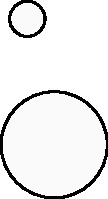
\includegraphics[width=0.10\textwidth]
{gesamttex/edit_VIII-4/images/LH_37_03_115-116_d_116v.pdf}%
\edcaption[0.25em]{%
\lbrack\textit{Fig.\:1}\rbrack%
}%
\end{edfigure}%
\newpage%
\pstart%
\edlabel{LH_37_03_115-116_116v_aestusmaris-1}%
Quousque autem pressionis hujus vis%
\indexS{vis pressionis aeris subtilis}%
\indexS{pressio aeris subtilis}
se extendat
ignotum
\edtext{%
est,
crediderim maximam esse 
et fortasse aeris tenuissimi sphaeram%
\indexS{sphaera aeris tenuis}
ad ipsam usque lunam%
\indexS{luna}
et ultra assurgere.%
}{%
\lemma{est,}%
\Bfootnote{%
\textit{(1)}~credidi sp %
\textit{(2)}~crediderim %
\bars{esse multo \textit{streicht Hrsg.}} maximam esse %
\textit{(a)}~quonam aeris hujus %
\textit{(b)}~aerisque hujus sphaeram forte sese %
\textit{(c)}~et fortasse %
\lbrack...\rbrack\ et ultra %
\textit{(aa)}~extendi %
\textit{(bb)}~assurgere.%
~\textit{L}%
}}
Et posito Lunam%
\indexS{luna}
gravitate carere%
\indexS{gravitas lunae}
neque ad terram nostram tendere,%
\indexS{terra}
sustinebit ipsa cylindrum aeris ultra-lunaris%
\indexS{aer ultra-lunaris}%
\indexS{cylinder aeris superimminens lunae}
sibi superimminentem %
et quominus terram premat prohibebit.%
\indexS{cylinder aeris premens terram}%
\indexS{terra}
Unde mare lunae subjectum%
\indexS{mare subjectum lunae}
\edtext{%
minus quam reliquus oceanus premetur%
\indexS{oceanus}
et ideo%
}{%
\lemma{minus}%
\Bfootnote{%
\textit{(1)}~pressum quam %
\textit{(a)}~ambiens %
\textit{(b)}~reliquus oceanus %
\textit{(2)}~quam reliquus %
\lbrack...\rbrack\ et ideo%
~\textit{L}%
}}
cum lunam in Meridiano%
\indexS{luna in meridiano}%
\indexS{meridianus}
habebit intumescet.%
\indexS{mare intumescens sub luna}
Sed haec conjectura%
\indexS{conjectura examinanda}
diligentius
\edtext{%
alias%
}{%
\lemma{alias}%
\Bfootnote{%
\textit{erg.}%
~\textit{L}%
}}
examinanda est;
explicandumque
quomodo omnia loca%
\indexS{locus sub meridiano lunae}
sub meridiano lunae posita
\edtext{%
simul afficiantur.%
}{%
\lemma{simul}%
\Bfootnote{%
\bars{tantum \textit{gestr.}} afficiantur.%
~\textit{L}%
}}%
\edlabel{LH_37_03_115-116_116v_aestusmaris-2}
\edlabel{LH_37_03_115-116_116v_schedapeculiaris-1}%
De quo
\edtext{%
scheda peculiari.%
\indexS{scheda peculiaris}%
\edlabel{LH_37_03_115-116_116v_schedapeculiaris-2}%
}{%
\lemma{scheda peculiari}%
\Cfootnote{%
Wohl Anspielung auf die (voraussichtlich in einem späteren Band von \textit{LSB} VIII zu edierende) Aufzeichnung \textit{De aestu maris ratio nova plane singularis; accessit suspicio de declinatione magnetica deque annulo lunari fluido circa Terram, ut est solidus circa Saturnum} (LH XXXV\;13,\;3 Bl.\;194). %
Das Manuskript ist von Leibniz eigenhändig auf April 1683 datiert.
}}
\pend%
\pstart%
Tantum
\pend%
\vspace*{1.5em}%
\pstart%
\noindent%
\centering%
*     *     *
\pend%
\vspace{2.75em}%
\selectlanguage{german}%
\frenchspacing%
\footnotesize%
\pstart%
\noindent%
\textls{Ausführliche Datierungsgründe:}%
\pagelabel{60205_dat}
Im Mittelpunkt der undatierten Aufzeichnung N.\;\ref{60205} \textit{De nova pressione aeris subtilioris etiam intra locum aere communi exhaustum deprehensa, et in aere libero pressionem a cylindro aeris crassi ortam longe superante} steht Leibnizens Annahme eines besonderen Fluidums, welches sich als "dünnere Luft" mit der wahrnehmbaren Luft vermische, durchdrigender als diese letztere sei und durch seinen Druck Phänomene hervorbringe, die unter bloßer Berücksichtigung des gewöhnlichen Luftdrucks unerklärbar wären (wie etwa Adhäsion im Vakuum).
Die Datierung der Aufzeichnung N.\;\ref{60205} ergibt sich aus folgenden Beobachtungen:
\pend%
\pstart%
(1)
Am Ende der Aufzeichnung N.\;\ref{60205} \textit{De nova pressione aeris subtilioris} gibt Leibniz, im Anschluss an die Frage nach der Höhe der die Erde um\-fassenden Sphäre "dünnerer Luft", eine skizzenhafte Erklärung des Phänomens der Gezeiten ab, der zufolge die Erhöhung des Meeresspiegels in der Phase der Flut von einer Verkürzung der Luftsäule durch den %
Mond herrühren soll (vgl. oben, \refpassage{LH_37_03_115-116_116v_aestusmaris-1}{LH_37_03_115-116_116v_aestusmaris-2}).
Daraufhin kundigt er an, die dargelegte Mutmaßung in einer \textit{scheda peculiaris} ausführlich erörten zu wollen (vgl. oben, \refpassage{LH_37_03_115-116_116v_schedapeculiaris-1}{LH_37_03_115-116_116v_schedapeculiaris-2}).
Nach heutigem Wissenstand finden sich im Nachlass zwei (voraussichtlich in einem späteren Band von \textit{LSB} VIII zu edierende) handschriftliche Aufzeichnungen, in denen sich Leibniz ausführlich um eine Erklärung der Gezeiten bemüht:
das Manuskript LH XXXV\;13,\;3 Bl.\;194, %
das die Überschrift
\ledpb%
\textit{De aestu maris ratio nova plane singularis; accessit suspicio de declinatione magnetica deque annulo lunari fluido circa Terram,
ut est solidus circa Saturnum} aufweist und von Leibniz eigenhändig auf April 1683 datiert ist;
sowie das titellose und undatierte Manuskript LH\;XXXVII\;4 Bl.\;109. %
In diesem letzteren findet der am Ende der Aufzeichnung N.\;\ref{60205} umrissene Erklärungsansatz keine Erwähnung.
Anders verhält es sich in der Aufzeichnung \textit{De aestu maris}: %
Dort wird gegen Ende des Textes (%
Bl.\;194\,v\textsuperscript{o}) -- unter der zusätzlichen Annahme eines rotierenden magnetischen Ringes, der den jeweiligen vom Mond besetzten Meridian umkreisen soll -- ein ähnlicher Erklärungsansatz dargelegt wie in N.\;\ref{60205}.
Dies rechtfertigt die Annahme, dass \textit{De aestu maris} die am Ende von N.\;\ref{60205} angekündigte \textit{scheda peculiaris} sein dürfte.
Eine im Kopf dieses Manuskriptes %
(Bl.\;194\,r\textsuperscript{o}) nachträglich hinzugefügte Randbemerkung -- \textit{Annulus, credo, inanis nec necessarius, vide aliam schedam} -- dürfte auf die titellose Aufzeichnung LH XXXVII\;4 Bl.\;109 %
hinweisen und somit zeigen, dass diese letztere erst nach \textit{De aestu maris} verfasst wurde.
Hieraus folgt, dass \textit{April 1683} als Terminus ante quem der Datierung von N.\;\ref{60205} anzusehen ist.
\pend%
\pstart%
(2)
Zur Bekräftigung dieser Feststellung gilt es zu beachten, dass in der Aufzeichnung N.\;\ref{60205} Jacob Bernoullis \textit{Dissertatio de gravitate aetheris} (Amsterdam 1683)\cite{01403} nicht erwähnt wird, obwohl sie thematisch durchaus relevant gewesen wäre:
Ähnlich wie Leibniz fasst Bernoulli\indexN{\textls{Bernoulli}, Jacob 1655\textendash1705} dort den Äther als nicht sinnenfälliges, aber mit Schwere versehenes Fluidum an, das physikalische Phänomene erklären soll, die der Druck der wahrnehmbaren Luft nicht zu erklären vermag.
(In der späteren Aufzeichnung N.\;\ref{41212} \textit{De aestimatione virium quas per aeris compressionem acquirere licet} wird hingegen ausdrücklich auf die \textit{Dissertatio de gravitate aetheris}\cite{01403} verwiesen; vgl. \refpassage{LH_35_09_25_001-002+004-005_005r_Bernoulli-1}{LH_35_09_25_001-002+004-005_005r_Bernoulli-2} im vorliegenden Band.)
Demgemäß ist zu vermuten, dass die Aufzeichnung N.\;\ref{60205} vor Leibnizens Lektüre von Bernoullis\indexN{\textls{Bernoulli}, Jacob 1655\textendash1705} Abhandlung entstand.
Leibniz hat diese letztere wohl nicht vor deren anonymer Rezension\cite{01406} im Märzheft 1683 der \textit{Acta eruditorum}\cite{01023} (S.\;106\textendash112) gekannt; gelesen hat er sie aber wahrscheinlich erst später. %
Das Buch war nämlich auf der Frankfurter\indexO{Frankfurt am Main} Michaelis-Messe 1682 (\textit{Catalogus universalis}, Bl.\;\bracks{D4\,r\textsuperscript{o}})\cite{02596} angekündikgt und auf der Leipziger\indexO{Leipzig} Ostermesse 1683 (\textit{Catalogus universalis}, Bl.\;B3\,v\textsuperscript{o})\cite{02597} ausgestellt worden, weshalb es frühestens ab dem Frühjahr 1683 auf dem Buchmarkt erhältlich gewesen sein dürfte (in beiden Katalogen ist der Titel auch ungenau angegeben: wohl das Zeichen für eine späte Auslieferung).
Im Briefwechsel wird die Abhandlung zum ersten und bisher einzigen Mal erst nach Leibnizens Italienreise\indexO{Italien} erwähnt, nämlich in seinem Brief an Jacob Bernoulli\indexN{\textls{Bernoulli}, Jacob 1655\textendash1705} vom 24.\;September/4.\;Oktober 1690; vgl. \textit{LSB} III,\;4 N.\;279, S.\;573.24\,f.\cite{01260} %
Leibniz dürfte somit erst etliche Zeit nach dem Erscheinen der anonymen Rezension\cite{01406} %
imstande gewesen sein, Bernoullis\indexN{\textls{Bernoulli}, Jacob 1655\textendash1705} \textit{Dissertatio de gravitate aetheris}\cite{01403} in die Hände zu bekommen, jedenfalls nicht vor April 1683.
\pend%
\pstart%
(3)
Für die Bestimmung des Terminus post quem der Datierung von N.\;\ref{60205} ist zunächst zu beachten, dass das im Textträger von N.\;\ref{60205} anzutreffende Harzer Wasserzeichen im Leibniz-Nachlass nicht vor 1679 belegt ist und überhaupt nicht vor 1678 verwendet wurde. %
Das gleiche Wasserzeichen ist zudem im Träger von \textit{De aestu maris} sowie in LH\;XXXVII\;4 Bl.\;109 (siehe oben) anzutreffen.
Daher ist anzunehmen, dass die Aufzeichnung N.\;\ref{60205} zwischen 1679 und April 1683 -- wahrscheinlich aber eher gegen Ende dieser Zeitspanne -- entstand.
Leibniz hielt sich ohnehin erst ab dem Herbst 1680 regelmäßig im Harz\indexO{Harz} auf.
Somit dürfte N.\;\ref{60205} nicht vor dem Herbst 1680 abgefasst worden sein.
\pend%
\pstart%
(4)
Leinbiz erwähnt in N.\;\ref{60205} (\refpassage{LH_37_03_115-116_115r_deVolder-1}{LH_37_03_115-116_115v_deVolder-2}) ein Experiment zur Vermessung der Adhäsionskraft zweier in der Luft hängender Marmorplatten, das der kartesianische Physiker und Philosoph Burchard de Volder\indexN{\textls{Volder} (Volter, Wolder), Burchard (Burcher) de 1643\textendash1709} im März 1676 in Leiden\indexO{Leiden} durchgefürt hatte.
Von diesem Experiment hatte Leibniz aus einem ausführlichen Bericht erfahren können, welcher in der von Philipp Lohmeier\indexN{\textls{Lohmeier} (Lohmeierus, Lomeierus), Philipp 1648\textendash1680} betreuten und von Johann Pestel\indexN{\textls{Pestel}, Johann, 1678 in Rinteln promoviert} eingereichten Dissertation \textit{Exercitationum physicarum de paradoxi gravitatis et levitatis prima}, paradoxon I, §\;IX (Rinteln 1678, S.\;32--34)\cite{01429} zu lesen war.
(Das bei der GWLB Hannover unter der Signatur M-A 262 aufbewarte Exemplar weist Gerbrauchsspuren, die wahrscheinlich auf Leiniz zürückgehen.)
Das Experiment hatte Lohmeier\indexN{\textls{Lohmeier} (Lohmeierus, Lomeierus), Philipp 1648\textendash1680} aber auch in seinem Brief an Leibniz vom 23.\:August\;/\;2.\:September 1679 geschildert (\textit{LSB} III,\;2 N.\;336, S.\;817.16--20).\cite{01425}
Über einen ähnlichen von de Volder\indexN{\textls{Volder} (Volter, Wolder), Burchard (Burcher) de 1643\textendash1709} angestellten Versuch hatte ferner die anonyme Bemerkung "Experience faite à Leyden" im \textit{Journal des sçavans} vom 17.\;April 1679 (S.\;107\,f.)\cite{02524} erzählt,
worauf Ehrenfried Walther von Tschirnhaus\indexN{\textls{Tschirnhaus} (H. v. Tch., H. v. Tsch.), Ehrenfried Walther v. 1651\textendash1708} in seinem Brief an Leibniz vom 11.\;September 1682 flüchtig anspielt (\textit{LSB} III,\;3 N.\;399, S.\;711.8\,f.).\cite{02525}
Kannte Leibniz, wie es plausibel erscheint, De Volders\indexN{\textls{Volder} (Volter, Wolder), Burchard (Burcher) de 1643\textendash1709} Experiment mit den Marmorplatten vornehmlich aus Lohmeiers\indexN{\textls{Lohmeier} (Lohmeierus, Lomeierus), Philipp 1648\textendash1680} \textit{Exercitationum physicarum de paradoxi gravitatis et levitatis prima},\cite{01429} so ist zu vermuten, dass die Erwähnung des Experiments in N.\;\ref{60205} (\refpassage{LH_37_03_115-116_115r_deVolder-1}{LH_37_03_115-116_115v_deVolder-2}) wahrscheinlich erst einige Zeit nach Leibnizens Lektüre der Dissertation\cite{01429} erfolgt sein sollte.
Denn zwar wiedergibt Leibniz korrekt die Details des Verfahrens (hauptsächlich die Verwendung von Fett zum Abdichten), kann sich aber nicht mehr an das Gewicht erinnern, dessen es nach de Volders\indexN{\textls{Volder} (Volter, Wolder), Burchard (Burcher) de 1643\textendash1709} Angabe zum Abtrennen der Platten bedurft hatte.
Wenn man bedenkt, dass Leibniz die laut Titelblatt im August 1678 an der Universität zu Rinteln\indexO{Rinteln} verteidigte Dissertation frühestens einige Monaten nach deren Erscheinen lesen konnte (möglicherweise nach dem Empfangen von Lohmeiers\indexN{\textls{Lohmeier} (Lohmeierus, Lomeierus), Philipp 1648\textendash1680} Brief\cite{01425} vom 23.\:August\;/\;2.\:September 1679), 
dann dürfte die besagte Erwähnung in N.\;\ref{60205} (\refpassage{LH_37_03_115-116_115r_deVolder-1}{LH_37_03_115-116_115v_deVolder-2}) erst im Laufe der frühen 1680er Jahren verfasst worden sein.
\pend%
\pstart%
(5)
Es gilt schließlich zu bemerken, dass auch in weiteren Texten der frühen 1680er Jahre Leibniz die Hypothese eines luftähnlichen, aber unermeßlich viel dünneren umgebenden Fluidums aufgestellt hatte, um physikalische Phänomene zu erklären, die unter bloßer Berücksichtigung der wahrnehmbaren Luft unerklärbar wären.
Dies ist besonders deutlich in dem auf die Zeitspanne zwischen Januar und März/April 1683 datierbaren Entwurf \textit{Explicatio mechanica elastri, seu causa cur corpora per vim tensa spopnte restitui videantur}\cite{01437} der Fall, in dem Leibniz das besagte umgebende Fluidum in Anspruch nimmt, um Grundeigenschaften makroskopischer Körper wie Elastizit und Kohäsion verständlich zu machen (vgl. \textit{LSB} VIII,\;3 N.\;14\textsubscript{3}, bes. S.\;211.16--212.5).
Demnach ist plausibel, dass auch die Aufzeichnung N.\;\ref{60205} im Zusammenhang mit einem Text wie \textit{Explicatio mechanica elastri} und in einem gemeinsamen Zeitraum verfasst wurde, d.\,h. zwischen Januar und April 1683.
Eine frühere Entstehung (wohl ab dem Herbst 1680) ist jedoch nicht auszuschließen.
\pend%
\pstart%
Aus den angegebenen Gründen ergibt sich als Gesamtdatierung der Aufzeichnung N.\;\ref{60205} \textit{De nova pressione aeris subtilioris} %
die Zeitspanne vom Herbst 1680 bis zum April 1683.
Vor 1680 ist sie unwahrscheinlich entstanden;
vielmehr dürfte sie gegen Ende der angegebenen Zeitspanne niedergeschrieben worden sein.
\pend%
\selectlanguage{latin}%
\frenchspacing%
\newpage%




\chapter[tocentry={Consideratio magni in mechanicis momenti %
\enskip\bracks{%
ab Herbst 1680 (?)%
}}, %
head={Consideratio magni in mechanicis momenti%
}]%
{\MakeUppercase{Consideratio magni in mechanicis momenti} %
\newline\bracks{%
ab Herbst 1680 (?)%
}}%
\label{55813-C}
\selectlanguage{ngerman}%
\frenchspacing%
\begin{ledgroupsized}[r]{120mm}%
\footnotesize%
\pstart%
\noindent%
\textbf{Überlieferung:}%
\pend%
\end{ledgroupsized}%
\begin{ledgroupsized}[r]{114mm}%
\footnotesize%
\pstart%
\parindent -6mm%
\makebox[6mm][l]{\textit{L}}%
Aufzeichnung:
LH XXXVIII Bl.\;182.
Ein Zettel (6\;x\;10 cm),
Ränder unregelmäßig beschnitten und zum Teil abgerissen.
Zwei vollbeschriebene Seiten.
\pend%
\end{ledgroupsized}%
\vspace{5mm}%
\begin{ledgroup}%
\footnotesize%
\pstart%
\noindent%
\textbf{Datierungsgründe:}
Die Datierung der Aufzeichnung N.\;\ref{55813-C} beruht auf %
inhaltlichen Betrachtungen.
Siehe die ausführliche Begründung auf S.\;\pageref{55813-C_dat}.%
\pend%
\end{ledgroup}%
\selectlanguage{latin}%
\frenchspacing%
\vspace{8mm}%
\normalsize%
\pstart%
\noindent%
\lbrack%
\href{\Scan{LH_38_182r}}%
{182\,r\textsuperscript{o}}%
\rbrack\
Consideratio incidit magni in Mechanicis Momenti,%
\indexS{consideratio magni momenti in mechanicis}%
\indexS{mechanica}
cur caeteris paribus melius
\edtext{%
sit idem punctum moventis%
}{%
\lemma{sit}%
\Bfootnote{%
\textit{(1)}~movens %
\textit{(2)}~idem punctum moventis%
~\textit{L}%
}}
eidem puncto movendi insistere,
quam ab alio ad aliud procedi.
\pend%
\begin{edfigure}[2.05em][1.5em]
\includegraphics%
{gesamttex/edit_VIII-4/images/LH_38_182_d1_182r.pdf}
\edcaption[0.25em]{%
\lbrack\textit{Fig.\:1}\rbrack%
}%
\end{edfigure}%
\pstart%
\noindent%
Exempli causa
si centro \textit{A}
radius \textit{AC} %
impellere debeat %
radium \textit{De}%
\indexS{radius}
\edtext{%
centri \textit{D},
is corporis movendi punctum \textit{e} %
primum impellet%
}{%
\lemma{centri \textit{D},}%
\Bfootnote{%
\textit{(1)}~impellet %
\textit{(2)}~is %
\textit{(a)}~punctum movendi %
\textit{(b)}~corporis movendi %
\lbrack...\rbrack\ primum impellet%
~\textit{L}%
}}
puncto suo \textit{B},
deinde puncto suo \textit{C};
ubi,
ut frictionis%
\indexS{frictio}
mentionem non faciam
(quam patitur \textit{e}
incedendo a \textit{B} ad \textit{C},
quae ex parte saltem
\edtext{%
rotula%
\indexS{rotula}
vel trochlea%
\indexS{trochlea}
tollitur),%
}{%
\lemma{rotula}%
\Bfootnote{%
\textit{(1)}~tollitur, %
\textit{(2)}~vel trochlea tollitur),%
~\textit{L}%
}}
sciendum est,
vi impulsus%
\indexS{vis impulsus}%
\indexS{impulsus}
nonnihil corporum partes cedere et comprimi;%
\indexS{compressio}
itaque primum partes radii%
\indexS{radius}
sive brachii \textit{AC}%
\indexS{brachium}
ad punctum \textit{B} comprimentur,
et digresso resistente
\edtext{%
\textit{e} a \textit{B} ad \textit{C},%
}{%
\lemma{\textit{e} a}%
\Bfootnote{%
\textit{(1)}~\textit{C} ad %
\textit{(2)}~\textit{B} ad \textit{C},%
~\textit{L}%
}}
iterum se restituent;%
\indexS{restitutio}
dum interea partes comprimentur
ad punctum \textit{C}.
Omnis autem
\edtext{%
vis quam
\lbrack%
\href{\Scan{LH_38_182v}}%
{182\,v\textsuperscript{o}}%
\rbrack\
ipsum corpus quodammodo sentit,%
\indexS{vis sentita a corpore}
et quae in%
}{%
\lemma{vis}%
\Bfootnote{%
\textit{(1)}~in \lbrack\href{\Scan{LH_38_182v}}{182~v\textsuperscript{o}}\rbrack\ %
\textit{(2)}~quam ipsum %
\lbrack...\rbrack\ quae in%
~\textit{L}%
}}
partes corporum
(licet insensibiliter)
\ledpb%
comprimendas impensa est,%
\indexS{vis impensa in partes comprimendas}
periit.%
\indexS{vis perita}
At
\edtext{%
si punctis semper iisdem%
}{%
\lemma{si}%
\Bfootnote{%
\textit{(1)}~eidem semper puncto %
\textit{(2)}~punctis semper iisdem%
~\textit{L}%
}}
tota vis%
\indexS{vis tota}
innitatur%
\lbrack,\rbrack\
non nisi
\edlabel{LH_38_182_zfk-1}%
\edtext{}{%
\xxref{LH_38_182_zfk-1}{LH_38_182_zfk-2}%
\lemma{semel}%
\Bfootnote{%
\textit{(1)}~toto tractu %
\textit{(2)}~fiet compressio %
\lbrack...\rbrack\ continuetur pressio, %
\textit{(a)}~non tamen perinde con %
\textit{(b)}~toto tractu %
\lbrack...\rbrack\  sed mox cessabit.
\textit{(aa)}~Caeterum putem tractu temporis illam \textlangle dis\textrangle\ %
\textit{(bb)}~Et hoc %
\lbrack...\rbrack\ et restitutionem%
~\textit{L}%
}}%
semel fiet compressio%
\indexS{compressio}
et restitutio;%
\indexS{restitutio}
adeoque minus virium perdetur.%
\indexS{vis perdita}
Licet enim continuetur pressio,%
\indexS{pressio}
toto tractu%
\indexS{tractus}
vel impulsu%
\indexS{impulsus}
durante,
non tamen continuabitur compressio,%
\indexS{compressio}
sed mox cessabit.
\edlabel{LH_38_182_182v_fodinae-1}%
Et hoc contingit,
v.\:g.
cum ansa recurva parallelogramma%
\indexS{ansa recurva parallelogramma}
apud fodinas moveatur,%
\indexS{fodina}
ubi puncta aggressionis%
\indexS{punctum aggressionis}
\textit{a} et \textit{b}
sunt semper eadem.%
\edlabel{LH_38_182_182v_fodinae-2}%
\pend%
\begin{edfigure}[1.90em][1.55em]
\includegraphics%
{gesamttex/edit_VIII-4/images/LH_38_182_d2_182v.pdf}
\edcaption[-0.40em]{%
\lbrack\textit{Fig.\:2}\rbrack%
}%
\end{edfigure}%
\pstart%
Puto tamen tractu temporis%
\indexS{tractus temporis}
minui compressionem illam%
\indexS{compressio}
et restitutionem%
\indexS{restitutio}%
\edlabel{LH_38_182_zfk-2}
in casu priori,
quia semper eodem tendit nisus,%
\indexS{nisus}
corpus autem saepe eodem modo compressum%
\indexS{corpus compressum}%
\indexS{compressio}
non amplius facile restituitur%
\indexS{corpus restitutum}%
\indexS{restitutio}
(et hanc inter caeteras causam puto,%
\indexS{causa inter caeteras}
cur initio novae machinae magis resistant).%
\indexS{machina nova magis resistens}
Posteriori vero casu
tardius opinor desinit,
quia in
\edtext{%
tantum trahuntur iterum%
}{%
\lemma{tantum}%
\Bfootnote{%
\textit{(1)}~retrahitur iterum %
\textit{(2)}~trahuntur iterum%
~\textit{L}%
}}
partes corporum%
\indexS{pars corporis tracta}
in quantum erant impulsae%
\indexS{pars corporis impulsa}
et compressae.%
\indexS{pars corporis compressa}
Et quoniam rotae dentatae%
\indexS{rota dentata}
ad priorem casum pertinent,
quae tamen satis utiles deprehenduntur,
forte minus est malum
quam prima fronte videtur.
\pend%
\newpage%
\pstart%
\noindent%
\centering%
*     *     *
\pend%
\vspace{3.0em}%
\selectlanguage{german}%
\frenchspacing%
\footnotesize%
\pstart%
\noindent%
\textls{Ausführliche Datierungsgründe:}%
\pagelabel{55813-C_dat}
Die titellose und undatierte Aufzeichnung N.\;\ref{55813-C}, in deren Mittelpunkt mögliche praktische Folgen einer allgemeinen Betrachtung zur Kraftanwendung stehen, weist weder Spuren eines Wasserzeichens noch besondere äußere Merkmale auf, die eine klare chronologische Einordnung ermöglichen würden.
Auch der Inhalt bietet kaum Anhaltspunkte, um die Entstehungszeit der Aufzeichnung zu bestimmen.
Eine Beobachtung im Text (\refpassage{LH_38_182_182v_fodinae-1}{LH_38_182_182v_fodinae-2}) zeigt jedoch, dass Leibniz zu dem Zeitpunkt, als er sie verfasst hat, bereits eine gewisse Erfahrung mit technischen Vorrichtungen im Bereich des Bergbaus haben musste.
Daraus lässt sich schließen, dass die Aufzeichnung N.\;\ref{55813-C} vermutlich nicht entstanden ist, bevor Leibniz im Herbst 1680 begonnen hatte, seine Projekte für die Verbesserung des Bergbaus im Harz\indexO{Harz} regelmäßig zu betreuen.
Eine frühere Datierung ist trotzdem möglich.
Das Papierformat deutet jedenfalls auf eine Entstehung nach Leibnizens Umzug von Paris\indexO{Paris} nach Hannover\indexO{Hannover} gegen Ende 1676.
\pend%
\selectlanguage{latin}%
\frenchspacing%
\normalsize%
\newpage%




\chapter[tocentry={Pendulae chordae curvitas ex vibratione %
\enskip \lbrack um 22.\;Juni 1681\rbrack}, %
head={Pendulae chordae curvitas ex vibratione%
}]%
{\MakeUppercase{Pendulae chordae curvitas ex vibratione} %
\newline\lbrack um den 22.\;Juni (2.\;Juli) 1681\rbrack} %
\label{60234}
\selectlanguage{ngerman}%
\frenchspacing%
\begin{ledgroupsized}[r]{120mm}%
\footnotesize%
\pstart%
\noindent%
\textbf{Überlieferung:}%
\pend%
\end{ledgroupsized}%
\begin{ledgroupsized}[r]{114mm}%
\footnotesize%
\pstart%
\parindent -6mm%
\makebox[6mm][l]{\textit{L}}%
Aufzeichnung:
LH XXXVII\;4 Bl.\;55.
Ein Blatt 4\textsuperscript{o},
Ränder beschnitten;
Papiererhaltungsmaßnahmen.
Drei Viertel Seite auf Bl.\;\href{\Scan{LH_37_04_055r}}{55~r\textsuperscript{o}}.
Bl.\;\href{\Scan{LH_37_04_055v}}{55~v\textsuperscript{o}} überliefert folgenden Entwurf einer Quittung von Leibnizens Hand:
\textit{%
Ich endesbenanter bekenne
daß mir der fürstl. Kämmerer Herr Kuckuck%
\indexN{\textls{Kuckuck} (Guckhguckh), Franz gest. 1702 (?)}
\sout{%
die bereits fallige halbjahrige besoldung dieses iezt lauffenden jahres heut dato baar ausgezahlet,
worüber ihn hiemit zu danck gebührend quittire.
\edlabel{LH_37_04_055_055v_datum-1}%
Hanover den 22 junij Anno Ein tausend Sechshundert Ein und achtzig%
\edlabel{LH_37_04_055_055v_datum-2}%
}
die von Luciae achtzig bis crucis ein und achtzig fallige halbjahrige besoldung mit dreyhundert thalern baar ausgezahlet,
darüber ihn hiemit zu danck gebuhrend quittire.%
} %
Der Rest ist unbeschrieben.%
\pagelabel{LH_37_04_055_uebrlf}
\pend%
\end{ledgroupsized}%
\vspace{5mm}%
\begin{ledgroup}%
\footnotesize%
\pstart%
\noindent%
\textbf{Datierungsgründe:}
Die Datierung der Aufzeichnung N.\;\ref{60234} beruht auf Eigenschaften des Textträgers.
Siehe die ausführliche Begründung auf S.\;\pageref{60234_dat}.%
\pend%
\end{ledgroup}%
\selectlanguage{latin}%
\frenchspacing%
\vspace{8mm}%
\normalsize%
\pstart%
\noindent%
\lbrack%
\href{\Scan{LH_37_04_055r}}%
{55~r\textsuperscript{o}}%
\rbrack%
\hfill%
Pendulae chordae curvitas ex%
\indexS{chorda pendula}%
\indexS{curvitas chordae pendulae}%
\indexS{chorda curva}
\edlabel{LH_37_04_055_055r_ifr-1}%
vibratione%
\indexS{vibratio chordae pendulae}%
\indexS{chorda vibrans}%
\hfill%
\phantom{\lbrack55~r\textsuperscript{o}\rbrack}%
\edtext{}{%
\xxref{LH_37_04_055_055r_ifr-1}{LH_37_04_055_055r_ifr-2}%
\lemma{vibratione}%
\Bfootnote{%
\lbrack/\rbrack\
\textit{(1)}~Die %
\textit{(2)}~Chordam %
\textit{(3)}~Ein strick \textit{ab}%
~\textit{L}%
}}%
\pend%
\vspace{0.5em}%
\pstart%
\noindent%
Ein
\edtext{%
strick \textit{ab}%
\indexS{Strick, schwingend}%
}{%
\lemma{strick \textit{ab}}%
\Cfootnote{%
Vgl.\;das Diagramm \lbrack\textit{Fig.\:1}\rbrack.%
}}%
\edlabel{LH_37_04_055_055r_ifr-2}
welcher an einem orth
\edtext{%
\textit{a}%
}{%
\lemma{\textit{a}}%
\Bfootnote{%
\textit{erg.\;L}%
}}
fest angebunden,
von dannen frey in der lufft%
\indexS{Lufft}
herunter hänget,
und denn
\edtext{%
beweget wird,
daß er%
}{%
\lemma{beweget}%
\Bfootnote{%
\textit{(1)}~werden %
\textit{(2)}~wird, daß %
\textit{(a)}~sie %
\textit{(b)}~er%
~\textit{L}%
}}
hin und hehr
\edtext{%
sich schwinge,%
\indexS{Strick, schwingend}%
}{%
\lemma{sich}%
\Bfootnote{%
\textit{(1)}~schwingen %
\textit{(2)}~schwinge%
~\textit{L}%
}}
bleibet nicht gerade,
sondern machet eine krumme lini,%
\indexS{Linie, krumm}
welche immer krümmer wird,
ie mehr der schwung%
\indexS{Schwung eines hängenden Stricks}
von dem mittel abweichet;
und ob gleich ein gewichte%
\indexS{Gewicht, hängend}
an den strick%
\indexS{Strick, schwingend}
oder faden%
\indexS{Faden, schwingend}
gehänget wird,
so bleibt doch
\edtext{%
diese krümme,%
\indexS{Krümme (Krümmung) eines schwingenden Fadens}
kan also der faden%
\indexS{Faden, schwingend}
eine krümme haben%
\indexS{Krümme (Krümmung) eines schwingenden Fadens}
ob er gleich%
}{%
\lemma{diese krümme,}%
\Bfootnote{%
\textit{(1)}~welche %
\textit{(2)}~ob gleich der faden %
\textit{(3)}~ob er gleich %
\textit{(4)}~kan also %
\lbrack...\rbrack\ er gleich%
~\textit{L}%
}}
frey,
und nicht an herr
\edtext{%
Huygens%
\indexN{\textls{Huygens} (Hugenius, Ugenius, Hugens, Huguens), Christiaan 1629\textendash1695}
Cycloidem%
\indexS{cycloides Hugenii}%
}{%
\lemma{Huygens Cycloidem}%
\Cfootnote{%
Wohl Anspielung auf den geometrischen Nachweis der Tautochronie der Schwingungen eines Zykloidenpendels (bei beliebiger Auslenkung) in
\textsc{C.\;Hyugens},
\textit{Horologium oscillatorium},
pars~II, prop.\;25;
pars~III, prop.\;6
(Paris 1673, S.\;57 u.\;67;\cite{00123}
\textit{HO}\;XVIII, S.\;185 u.\;203).\cite{00113}
}}
oder andere figur%
\indexS{Figur}
anschlägt%
\lbrack;\rbrack\
\edtext{%
stünde demnach zu fragen%
}{%
\lemma{stünde demnach zu fragen}%
\Bfootnote{%
\textit{erg.\;L}%
}}
was dieses für
\edtext{%
eine krumme lini sey,%
\indexS{Linie, krumm}%
}{%
\lemma{eine}%
\Bfootnote{%
\textit{(1)}~figur sey, %
\textit{(2)}~krumme lini sey,%
~\textit{L}%
}}
so der strick macht,%
\indexS{Strick, schwingend}
wenn er gleich durchgehends biegsam;
was auch das ende \textit{b}
im schwingen%
\indexS{Schwingen eines hängenden Stricks}
für eine krumme lini%
\indexS{Linie, krumm}
beschreibe%
\lbrack;\rbrack\
ja wenn der strick%
\indexS{Strick, schwingend}
ungleich biegsam,
\ledpb%
köndte gefragt werden,
mit was graden oder zuwachs
solche biegsamkeit%
\indexS{Biegsamkeit eines schwingenden Stricks}
von einem ende zum andern gehen solte,
damit
sie im schwung%
\indexS{Schwung eines hängenden Stricks}
eine gegebene lini%
\indexS{Linie, krumm}
machen,
oder auch wohl beschreiben könne;
dabey dann auch das gewicht%
\indexS{Gewicht, hängend}
so wohl des stricks selbst,%
\indexS{Strick, schwingend}
als das daran hänget,%
\indexS{Gewicht, hängend}
zu betrachten.
Dieses alles kan ich durch
\edtext{%
meine neue rechnungs%
\indexS{Rechnungs- und Messungsart}
und Meßungs-art,%
}{%
\lemma{meine \lbrack...\rbrack\ Meßungs-art}%
\Cfootnote{Hierbei ist wohl Leibnizens Methode zur Integral- und Differentialrechnung gemeint.}}
ausfinden.
\pend%
\begin{edfigure}[2.50em][0.00em]
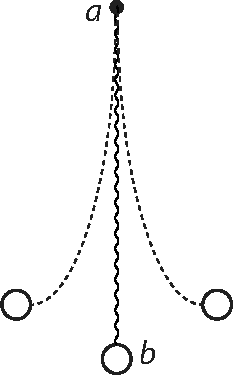
\includegraphics[width=0.18\textwidth]
{gesamttex/edit_VIII-4/images/LH_37_04_055_d_055r.pdf}
\edcaption[0.5em]{\hspace{-1.00mm}\lbrack \textit{Fig.\:1}\rbrack}%
\end{edfigure}%
\vspace{3.0em}%
\pstart%
\noindent%
\centering%
*     *     *
\pend%
\vspace{2.5em}%
\selectlanguage{german}%
\frenchspacing%
\footnotesize%
\pstart%
\noindent%
\textls{Ausführliche Datierungsgründe:}%
\pagelabel{60234_dat}
Der Textträger der undatierten Aufzeichnung N.\;\ref{60234} \textit{Pendulae chordae curvitas ex vibratione} weist kein Wasserzeichen auf, überliefert aber auf der Hinterseite (Bl.\;\href{\Scan{LH_37_04_055v}}{55~v\textsuperscript{o}}) zusätzlich den Entwurf einer Quittung, in der Leibniz bestätigt, vom Hofkammerer Franz Kuckuck\indexN{\textls{Kuckuck} (Guckhguckh), Franz gest. 1702 (?)} für das Halbjahr zwischen Dezember 1680 und Mai 1681 ein Gehalt in Höhe von 300 Reichstaler erhalten zu haben (siehe die Beschreibung der Überlieferung, \pageref{LH_37_04_055_uebrlf}).
Im gestrichenen Textteil des Entwurfs wird die Quittung ausdrücklich auf den 22.\;Juni (2.\;Juli) 1681 datiert; vgl.\;\refpassage{LH_37_04_055_055v_datum-1}{LH_37_04_055_055v_datum-2}.
Die einheitliche Überlieferung rechtfertigt die Annahme, dass auch die Aufzeichnung N.\;\ref{60234} nicht viel früher oder später als den 22.\;Juni (2.\;Juli) 1681 verfasst wurde.
\pend%
\selectlanguage{latin}%
\frenchspacing%
\normalsize%
\newpage%




\chapter[tocentry={Aus und zu Dechales, Cursus (Pneumatik) %
\enskip \bracks{Winter 1682/1683 -- erste Hälfte 1685}},
head={Aus und zu Dechales, Cursus (Pneumatik)}]%
{\MakeUppercase{Aus und zu Dechales, Cursus (Pneumatik)}
\newline \bracks{Winter 1682/1683 -- erste Hälfte 1685}}
\label{41182-1}%
\selectlanguage{ngerman}%
\frenchspacing%
\begin{ledgroupsized}[r]{120mm}%
\footnotesize%
\pstart%
\noindent\textbf{Überlieferung:}%
\pend%
\end{ledgroupsized}%
\begin{ledgroupsized}[r]{114mm}%
\footnotesize%
\pstart%
\parindent -6mm%
\makebox[6mm][l]{\textit{L}}%
Auszüge mit Bemerkungen aus
\textsc{C.\:F.\:M.\;Dechales},%
\indexN{\textls{Dechales} (Chalesius), Claude François Milliet 1621\textendash1678}
\textit{Cursus seu mundus mathematicus} (3~Bde, Lyon 1674)%
:\cite{00124}
LH~XXXV\;9,\;17 Bl.\;5--6.
Ein Bogen 2\textsuperscript{o}.
Zweizweidrittel Seiten auf Bl.\;5\,r\textsuperscript{o} bis Bl.\;6\,r\textsuperscript{o},
zumeist einspaltig beschrieben.
Bl.\;6\,r\textsuperscript{o} überliefert auch N.\;\ref{41182-2} (Auszüge zur Statik aus demselben Werk) in diesem Band.
Bl.\;6\,v\textsuperscript{o} ist unbeschrieben.
Der Text ist durch Abstände und Striche unterteilt;
die Anordnung der %
Auszüge entspricht nicht durchweg der Textabfolge in der %
Vorlage.
\textemdash\
Weitere Auszüge aus Dechales' \textit{Cursus} überliefern im Leibniz-Nachlass die Manuskripte:
LH~XXXV\;9,\;17 Bl.\;1--4; %
LH~XXXVI Bl.\;54--57, 60--61; %
LH~XXXVII\;5 Bl.\;2--3 %
(sie werden voraussichtlich in künftigen Bänden von \textit{LSB} VIII ediert).
Ein Exemplar von Dechales' \textit{Cursus} mit Gebrauchsspuren von Leibnizens Hand liegt in der GWLB Hannover unter der Signatur Nm-A\,10018:1--3 vor.
\pend%
\end{ledgroupsized}%
\vspace{5mm}%
\begin{ledgroup}%
\footnotesize%
\pstart%
\noindent%
\textbf{Datierungsgründe:}
Die Datierung der Auszüge mit Bemerkungen N.\;\ref{41182-1} beruht auf Eigenschaften des Textträgers sowie auf inhaltlichen Betrachtungen.
Siehe die ausführliche Begründung auf S.\;\pageref{41182_dat}.%
\pend%
\end{ledgroup}%
\selectlanguage{latin}%
\frenchspacing%
\vspace{8mm}%
\normalsize%
\pstart%
\noindent%
\centering%
\bracks{%
\href{\Scan{LH_35_09_17_005r}}%
{5\,r\textsuperscript{o}}%
}
\hfill%
\textls{Statica}%
\indexS{statica}
\hfill%
\phantom{\bracks{5\,r\textsuperscript{o}}}%
\pend%
\vspace{0.5em}%
\pstart%
\noindent%
Incertum an in locis centro terrae%
\indexS{centrum terrae}
propioribus%
\indexS{locus propior centro terrae}
minor gravitatio gravium.%
\indexS{gravitatio gravium}%
\indexS{grave in loco propiori centro terrae} %
\pend%
\pstart%
\edtext{%
\textit{Corpus non possumus}%
\indexS{corpus separatum a terra}
separare a terra%
\indexS{terra}
\textit{nisi instrumentis}%
\indexS{istrumentum annexum terrae}
ipsi \textit{terrae annexis.
Aviculae}%
\indexS{avicula}
cum \textit{in aera tolluntur
primo saltant pedibus%
\indexS{pes aviculae}
terramque percutiunt,
deinde alis%
\indexS{ala aviculae}
aerem contra terram}%
\indexS{aer impulsus contra terram}
\edtext{%
\textit{impellunt}
(+\;nil%
}{%
\lemma{\textit{impellunt}}%
\Bfootnote{%
\bars{, deinde alis aerem contra terram impellunt \textit{streicht Hrsg.}} (+\;nil%
~\textit{L}%
}}
refert an contra terram%
\;\bracks{+})
et aer ipse incumbit terrae,%
\indexS{aer incumbens terrae}
ut aqua.%
\indexS{aqua incumbens terrae}%
}{%
\lemma{\textit{Corpus} \bracks{...} aqua}%
\Cfootnote{%
Vgl. \textsc{C.\,F.\,M.\;Dechales},
\textit{Cursus seu mundus mathematicus}, tract.\;VII, lib.\;I, digr.\;III
(Lyon 1674, Bd.\;I, S.\;434b:\cite{00124}
Zitat mit Auslassungen).%
}}
\edtext{%
Venti quoque%
\indexS{ventus separans gravia a terra}
cum gravia a terra separantur
sunt motus aeris,%
\indexS{ventus ut motus aeris}%
\indexS{motus aeris}
et ipsorum motus etiam
\edtext{%
oritur quodam nisu repellendi terram.%
\indexS{nisus repellendi terram}%
\indexS{terra}%
}{%
\lemma{oritur}\Bfootnote{%
\textit{(1)}~a corpore quod terrae %
\textit{(2)}~quodam nisu repellendi terram.%
~\textit{L}%
}}%
}{%
\lemma{Venti \bracks{...} terram}%
\Cfootnote{%
Vgl. a.a.O. (S.\;434b--435a).\cite{00124}%
}}
\pend%
\pstart%
\edtext{%
\textit{Si aer esset levis,
condensatus} foret \textit{levior},%
\indexS{aer condensatus}
quod contra est.%
}{%
\lemma{\textit{Si aer} \bracks{...} contra est}%
\Cfootnote{%
Vgl. a.a.O., digr.\;V
(S.\;437a--b).\cite{00124}%
}}
\pend%
\pstart%
\edtext{%
\textls{Thermometrum} simplex%
\indexS{thermometrum simplex}
\edtext{%
\textit{A} vel \textit{B}%
}{%
\lemma{\textit{A} vel \textit{B}}%
\Cfootnote{%
Vgl. die Diagramme \bracks{\textit{Fig.\:1}} u.\;\bracks{\textit{Fig.\:2}}.%
}}
nempe calefit
et inde
\edtext{%
in aqua%
}{%
\lemma{in}%
\Bfootnote{%
\textit{(1)}~aerem %
\textit{(2)}~aqua%
~\textit{L}%
}}
osculo%
\indexS{osculum thermometri}
\edtext{%
aperto \textit{C} collocatur,%
}{%
\lemma{aperto\;\textit{C}}%
\Bfootnote{%
\textit{(1)}~vel %
\textit{(2)}~collocatur,%
~\textit{L}%
}}
refrigefactum attrahet aerem,%
\indexS{thermometrum refrigefactum attrahens aerem}
itaque calefactum rursus expellet,%
\indexS{thermometrum calefactum expellens aerem}
vel saltem depellet.%
}{%
\lemma{\textls{Thermometrum} \bracks{...} depellet}%
\Cfootnote{%
Vgl. a.a.O. (S.\;441b--442a).\cite{00124}%
}}
\pend%
\newpage%
\begin{edfigure}[0.00em][2.50em]%
\hfill
\includegraphics[scale=0.85]{%
gesamttex/edit_VIII-4/images/LH_35_09_17_005-006_d01_005r.pdf}
\hfill
\includegraphics[scale=0.85]{%
gesamttex/edit_VIII-4/images/LH_35_09_17_005-006_d02_005r.pdf}
\hfill
\includegraphics[scale=0.85]{%
gesamttex/edit_VIII-4/images/LH_35_09_17_005-006_d03_005r.pdf}
\hfill
\includegraphics[scale=0.85]{%
gesamttex/edit_VIII-4/images/LH_35_09_17_005-006_d04_005r.pdf}
\hfill
\edcaption{%
\bracks{\textit{Fig.\:1}}%
\hspace*{20mm}%
\bracks{\textit{Fig.\:2}}%
\hspace*{20mm}
\bracks{\textit{Fig.\:3}}%
\hspace*{20mm}%
\bracks{\textit{Fig.\:4}}%
\edtext{}{%
\lemma{\bracks{\textit{Fig.\:1}} u. \bracks{\textit{Fig.\:2}}}%
\Cfootnote[nonum]{%
Vgl. \textsc{Dechales}, \textit{Cursus}, tract.\;VII, lib.\;I, %
digr.\;VI (S.\;441b: einzige Diagramme).\cite{00124}%
}}%
\edtext{}{%
\lemma{\bracks{\textit{Fig.\:3}} u. \bracks{\textit{Fig.\:4}}}%
\Cfootnote[nonum]{%
Vgl. a.a.O. (S.\;442a: erstes u. zweites Diagramm).\cite{00124}%
}}%
}
\end{edfigure}
\pstart%
\edtext{%
Alia
\edtext{%
species thermometri \textit{HGF},%
\indexS{species thermometri}%
\indexS{thermometrum alterius speciei}%
}{%
\lemma{species thermometri \textit{HGF}}%
\Cfootnote{%
Vgl. das Diagramm \bracks{\textit{Fig.\:3}}.%
}}
ubi frigore%
\indexS{frigus contrahens aerem}
aer \textit{GF} contrahitur,%
\indexS{aer contractus frigore}
et aqua descendit,%
\indexS{aqua ascendens in thermometro}
cum in priori descendat calore.%
\indexS{calor}%
}{%
\lemma{Alia \bracks{...} calore}%
\Cfootnote{%
Vgl. a.a.O. (S.\;442a).\cite{00124}%
}}
\pend%
\pstart%
\edtext{%
\textit{Tertia%
\indexS{thermometrum tertiae speciei}
\edtext{%
species \textit{KMN},%
}{%
\lemma{\textit{species \textit{KMN}}}%
\Cfootnote{%
Vgl. das Diagramm \bracks{\textit{Fig.\:4}}.%
}}
aqua \textit{KM} descendet calore%
\indexS{aqua descendens in thermometro}
ex \textit{M}}
ad \textit{R},
\textit{ascendet ex \textit{K}}
ad \textit{O}.
Addi potest index%
\indexS{index in trochlea}
qui in
\edtext{%
trochlea \textit{S}%
\indexS{trochlea in thermometro}%
}{%
\lemma{trochlea \textit{S}}%
\Cfootnote{%
Vgl. das Diagramm \bracks{\textit{Fig.\:5}}.%
}}
notet numeris
quantum ascenderit \textit{KO},
globulus autem ligneus%
\indexS{globulus ligneus natans in aqua thermometri}
in \textit{K} natat in aqua.%
\indexS{aqua thermometri}%
}{%
\lemma{\textit{Tertia} \bracks{...} aqua}%
\Cfootnote{%
Vgl. \textsc{Dechales}, \textit{Cursus}, tract.\;VII, lib.\;I, %
digr.\;VI (S.\;442a).\cite{00124}%
}}
\pend%
\begin{edfigure}[2.50em][0.00em]%
\hfill%
\includegraphics[scale=0.85]{%
gesamttex/edit_VIII-4/images/LH_35_09_17_005-006_d05_005r.pdf}
\hfill%
\edcaption{%
\bracks{\textit{Fig.\:5}}
\edtext{}{%
\lemma{\bracks{\textit{Fig.\:5}}}%
\Cfootnote[nonum]{%
Vgl. \textsc{Dechales}, \textit{Cursus}, tract.\;VII, lib.\;I, %
digr.\;VI (S.\;442a: viertes Diagramm).\cite{00124}
Ein gestrichener Entwurf wird nicht wiedergegeben.}}
}
\end{edfigure}%
\newpage%
\pstart%
\edtext{%
\textit{Globulus vitreus%
\indexS{globulus vitreus mergens frigore}
inferiori parte apertus
semiplenus aere,%
\edtext{}{%
\lemma{\textit{Am Rand:}}%
\Afootnote{NB}}
ingruente frigore%
\indexS{frigus ingruens}
magis mergitur,}
tempore calido minus.%
\indexS{tempus calidum}%
}{%
\lemma{\textit{Globulus} \bracks{...} minus}%
\Cfootnote{%
Vgl. a.a.O. (S.\;442a).\cite{00124}%
}}
\edlabel{LH_35_09_17_005-006_005r_ewk-1}
\edtext{%
Huc pertinent \textls{\textit{cucurbitulae}}%
\indexS{cucurbitula medicorum}
\edtext{%
\textit{A},%
}{%
\lemma{\textit{A}}%
\Bfootnote{%
\textit{erg.\:L}%
}}
\textit{calefit aer inclusus quantum potest,%
\indexS{aer inclusus cucurbitulae}%
\indexS{aer cucurbitulae calefactus}
deinde} quantum potest
\textit{carni applicatur firmiter,%
\indexS{cucurbitula applicata carni}
ut nullus circa ejus labra%
\indexS{labrum cucurbitulae}
aeri externo pateat aditus,%
\indexS{aditus patens aeri externo}%
\indexS{aer externus}
tum frigefit}%
\indexS{cucurbitula frigefacta}
\textit{vel} af\textit{fusa frigid}\angles{\textit{a}}%
\indexS{frigida (aqua) affusa}
\textit{vel pannis madidis applicatis},%
\indexS{pannus madidus}
et \textit{caro elevatur intra cucurbitulam,%
\indexS{caro elevata intra cucurbitulam}
et saepe etiam ossa
si quae sint luxata.%
\indexS{os luxatum}
Si incidatur caro%
\indexS{caro incisa}
multus sanguis exilit.%
\indexS{sanguis exiliens}}%
\edlabel{LH_35_09_17_005-006_005r_ewk-2}%
}{%
\lemma{Huc \bracks{...} \textit{exilit}}%
\Cfootnote{%
Vgl. a.a.O. (S.\;442a:\cite{00124}
Zitat mit Auslassungen).
Die Passage ist zweimal exzerpiert;
vgl. unten, \refpassage{LH_35_09_17_005-006_005v_dfg-1}{LH_35_09_17_005-006_005v_dfg-2}.%
}}
\pend%
\begin{edfigure}[0.5em][1.0em]%
\includegraphics[scale=0.90]{%
gesamttex/edit_VIII-4/images/LH_35_09_17_005-006_d06_005r.pdf}
\edcaption[0.25em]{%
\hspace{4mm}%
\bracks{\textit{Fig.\:6}}%
\edtext{}{%
\lemma{\bracks{\textit{Fig.\:6}}}%
\Cfootnote[nonum]{%
Vgl. \textsc{Dechales}, \textit{Cursus}, tract.\;VII, lib.\;I, %
digr.\;VI (S.\;442a: fünftes Diagramm).\cite{00124}%
}}%
}%
\end{edfigure}
\pstart%
\edtext{%
\textit{R.\:P.\;Franc.\;de la Chaise}%
\indexN{\textls{La Chaise} (La Chaize, Hedraeus), François de 1624\textendash1709}
sumsit \textit{tubum 56 pedum%
\indexS{pes}
secundum parietis altitudinem erectum%
\indexS{tubus erectus 56 pedum}
aqua plenum,
ubi orificium
intra aliam aquam} demersum
\textit{fuit apertum}%
\bracks{,}
\textit{mansit tantum aqua}
\edtext{%
\bracks{\textit{ad}}%
}{%
\lemma{\textit{ad}}%
\Bfootnote{%
\textit{erg. Hrsg. nach Vorlage}%
}}
\textit{altitudinem pedum 32 circiter,%
\indexS{aqua 32 pedum altitudinis}
qui aequales in gravitate%
\indexS{gravitas 32 pedum aquae}%
\indexS{gravitas 2,25 pedum mercurii}
pedibus duobus et~%
$\displaystyle\frac{\textit{1}}{\textit{4}}$} Mercurii.%
\indexS{mercurius 2,25 pedum altitudinis}%
}{%
\lemma{\textit{R.\:P.\;Franc.} \bracks{...} Mercurii}%
\Cfootnote{%
Vgl. a.a.O., digr.\:VII, Nr.\;14
(S.\;443b--444a).\cite{00124}
François de La Chaise (1624--1709)%
\indexN{\textls{La Chaise} (La Chaize, Hedraeus), François de 1624\textendash1709}
war Jesuit und Beichtvater Ludwigs XIV.%
\indexN{\textls{Frankreich: Ludwig XIV.}, König 1643\textendash1715}
Dechales%
\indexN{\textls{Dechales} (Chalesius), Claude François Milliet 1621\textendash1678}
beschreibt ihn als \textit{in hujusmodi experimentis physicis exercitatissimus} (ebd.).%
}}
\edlabel{LH_35_09_17_005-006_005r_svj-1}%
\edtext{%
Si tubus
Mercurium%
\indexS{mercurius suspensus in tubo}
\edtext{%
suspensum%
}{%
\lemma{suspensum}%
\Bfootnote{%
\textit{erg.\;L}%
}}
continens%
\indexS{tubus continens mercurium sustentatus e bilance}
ex bilance
\edtext{%
sustentatur,
aequilibrium habebitur pondere%
\indexS{aequilibrium tubi continentis mercurium}%
}{%
\lemma{sustentatur,}%
\Bfootnote{%
\textit{(1)}~pondere %
\textit{(2)}~aequilibrium habebitur pondere%
~\textit{L}%
}}
quod et tubo et mercurio simul sit aequale.%
\edlabel{LH_35_09_17_005-006_005r_svj-2}%
}{%
\lemma{Si tubus \bracks{...} aequale}%
\Cfootnote{%
Vgl. a.a.O., N.\;16 (S.\;444a).\cite{00124}
Der Auszug wird später fortgesetzt;
vgl. unten \refpassage{LH_35_09_17_005-006_005v_ukp-1}{LH_35_09_17_005-006_005v_ukp-2}
u. das Diagramm \bracks{\textit{Fig.\:11}}.%
}}
\pend%
\pstart%
\edtext{%
\textit{Pascalius%
\indexN{\textls{Pascal} (Pascalius), Blaise 1623\textendash1662}
in Arvernis\indexO{Auvergne}
prope Clermontium}\indexO{Clermont-Ferrand}
hoc curavit fieri experimentum%
\indexS{experimentum Pascalii}%
\bracks{:}\;%
\textit{ad radices altissimi montis%
\indexS{radix montis}%
\indexS{mons altissimus}
le puits de dome}\indexO{Puy de Dôme}
\edtext{%
mercurius \textit{supra superficiem
stagnantis in vase} alterius mercurii%
\indexS{mercurius stagnans}
attollebatur%
}{%
\lemma{mercurius}%
\Bfootnote{%
\textit{(1)}~attollebatur %
\textit{(2)}~\textit{supra superficiem} %
\bracks{...} mercurii attollebatur%
~\textit{L}%
}}
\textit{digitis 26 et 4 lineis}%
\bracks{;}
conscenso monte \textit{ad altitudinem}
\textit{perpendicularem hexapedarum 150} %
\textit{altitudo}
\textit{intra tubum fuit digitorum 25,%
\indexS{altitudo mercurii intra tubum}%
\indexS{mercurius intra tubum}
\ledpb%
et superato montis vertice%
\indexS{vertex montis}
ad 500 hexapedas,%
\indexS{hexapeda}
digitorum 23 et}
\edtext{%
\bracks{\textit{duarum}}%
}{%
\lemma{trium}%
\Bfootnote{%
\textit{L\;ändert Hrsg. nach Vorlage}%
}}
\textit{linearum}%
\bracks{:}
\textit{quare altitudo diminuta
tribus digitis%
\indexS{digitus}
et 2 lineis.%
\indexS{linea (mensura)}}%
}{%
\lemma{\textit{Pascalius} \bracks{...} \textit{lineis}}%
\Cfootnote{%
Vgl. \textsc{Dechales}, \textit{Cursus}, tract.\:VII, lib.\;I, %
digr.\:VII, Nr.\;18 (S.\;444a:\cite{00124}
Zitat mit Auslassungen).
Siehe zum Experiment am Puy de Dôme\indexO{Puy de Dôme} etwa:
B.\;\textsc{Pascal},
\textit{Récit de la grande expérience}, 1648\cite{02577} %
(\textit{Traitez}, Paris 1663, S.\;165--194;\cite{00081}
\textit{PO}\;II, S.\;653--690).\cite{01524}
}}
\pend%
\pstart%
\edtext{%
\edlabel{LH_35_09_17_005-006_005r_scs-1}%
\textit{Qui Mercurium} habent \textit{in officinis},%
\indexS{officina}%
\indexS{mercurius servatus in officinis}
dicunt
\textit{quantacunque} eum tractent \textit{diligentia},%
\indexS{diligentia in mercurio servando}
tamen quovis
\edtext{%
anno
\textit{20\textsuperscript{ma} aut 25\textsuperscript{ta} parte decrescere.}%
\edlabel{LH_35_09_17_005-006_005r_scs-2}%
}{%
\lemma{anno}%
\Bfootnote{%
\textit{(1)}~perdere %
\textit{(2)}~\textit{20\textsuperscript{ma} aut 25\textsuperscript{ta} parte decrescere.}%
~\textit{L}%
}}
Ergo non mirum
si inde vapores sublati ferantur%
\indexS{vapor mercurii in vacuitate tubi}
in vacuitatem tubi,%
\indexS{vacuitas tubi}
et ibi dilatentur.%
}{%
\lemma{\textit{Qui} \bracks{...} dilatentur}%
\Cfootnote{%
Vgl. \textsc{Dechales}, \textit{Cursus}, tract.\:VII, lib.\;I, %
digr.\:VII (S.\;445a--b).\cite{00124}
Die Passage ist zum Teil zweimal exzerpiert;
vgl. unten,
\refpassage{LH_35_09_17_005-006_005v_jkr-1}{LH_35_09_17_005-006_005v_jkr-2}.%
}}
\pend%
\vspace{1.0em}%
\pstart%
\noindent%
\edtext{%
\textit{%
Lampades accensae et carbones igniti%
\indexS{lampas in recipiente evacuato}%
\indexS{carbo in recipiente evacuato}
citius extinguuntur in recipiente%
\indexS{recipiens evacuatus}
quam in aere libero,%
\indexS{aer liber}
et adhuc citius}
cum \textit{exugitur recipientis aer.%
\indexS{aer exuctus e recipiente}
Funis militaris accensus%
\indexS{funis militaris}
et in recipiens demissus
primo fumo implevit recipiens,}%
\indexS{recipiens impletus fumo}
exucto vero aere cum fumo,%
\indexS{fumus exuctus cum aere}%
\indexS{aer exuctus cum fumo}
\textit{ignis non apparuit,}%
\indexS{ignis in recipiente evacuato}%
\indexS{aer immissus recipienti}
sed \textit{immisso} iterum \textit{aere
coepit} denuo \textit{ardere.}%
}{%
\lemma{\textit{Lampades} \bracks{...} \textit{ardere}%
}%
\Cfootnote{%
Vgl. \textsc{Dechales}, \textit{Cursus}, tract.\:VII, lib.\;I, %
digr.\;IX, experim.\;17
(S.\;455b: Zitat mit Auslassungen);\cite{00124}
nach \textsc{R.\;Boyle}, \textit{New experiments}, Nr.\;10--12 %
(Oxford 1660, S.\;74--83;\cite{00015}
\textit{BW}~I, S.\;184--188).\cite{00017}%
}}
(+\;%
Experiendum
quamdiu hoc modo
in
\edtext{%
vacuo vis%
}{%
\lemma{vacuo}%
\Bfootnote{%
\textit{(1)}~actio %
\textit{(2)}~vis~%
\textit{L}%
}}
ignis sopita%
\indexS{vis ignis sopita}%
\indexS{vis ignis conservata in vacuo}%
\indexS{vacuum}
conservari possit.%
~\bracks{+)}
\pend%
\pstart%
\edtext{%
Elastrum%
\indexS{elastrum sclopeti}
\edtext{%
sclopeti%
\indexS{sclopetum}%
}{%
\lemma{sclopeti}%
\Bfootnote{%
\textit{erg.\;L}%
}}
intra recipientem exhaustum%
\indexS{recipiens exhaustus}
egit ut extra,
imo \textit{scintillas excussit}%
\indexS{scintilla}
quibus \textit{accensus est pulvis} pyrius,%
\indexS{pulvis pyrius}
\textit{flammamque%
\indexS{flamma pulveris pyrii}
habuit more consueto.}%
\indexS{mos consuetus}%
}{%
\lemma{Elastrum \bracks{...} \textit{consueto}}%
\Cfootnote{%
Vgl. \textsc{Dechales}, \textit{Cursus}, tract.\:VII, lib.\;I, digr.\;IX, %
experim.\;18 (S.\;455b: Zitat mit Auslassungen);\cite{00124}
nach \textsc{Boyle}, \textit{New experiments}, Nr.\;14
(S.\;88--102;\cite{00015} \textit{BW}~I, S.\;189--191).\cite{00017}%
}}
\pend%
\pstart%
\edtext{%
\textit{Ex oleo%
\indexS{oleum}
erumpunt plures bullae,%
\indexS{bulla erumpens}
ex aqua distillata%
\indexS{aqua distillata}
pauciores
quam ex communi.%
\indexS{aqua communis}%
} %
Aqua in recipiente posita%
\indexS{aqua in recipiente exhausto}%
\indexS{recipiens exhaustus}
in \textit{phiala colli oblongi},%
\indexS{phiala colli oblongi}
exucto aere%
\indexS{aer exuctus e recipiente}
nonnihil intumuit,
cum prius \textit{bullae%
\indexS{bulla erumpens}
a fundo ad summitatem usque erupissent.}%
}{%
\lemma{\textit{Ex oleo} \bracks{...} erupissent}%
\Cfootnote{%
Vgl. \textsc{Dechales}, \textit{Cursus}, tract.\:VII, lib.\;I, digr.\;IX, %
experim.\;22 (S.\;456b:\cite{00124}
Zitat mit Auslassungen);\cite{00124}
nach \textsc{Boyle}, \textit{New experiments}, Nr.\;23--24 %
(S.\;182--189;\cite{00015} \textit{BW}~I, S.\;221--223).\cite{00017}%
}}
\pend%
\vspace{1.0em}
\begin{edfigure}[0.5em][0.0em]%
\includegraphics[scale=0.85]{%
gesamttex/edit_VIII-4/images/LH_35_09_17_005-006_d07_005v.pdf}%
\edcaption[0.25em]{%
\bracks{\textit{Fig.\:7}}%
\edtext{}{%
\lemma{\lbrack\textit{Fig.\:7}\rbrack}%
\Cfootnote[nonum]{%
Vgl. \textsc{Dechales}, \textit{Cursus}, tract.\:VII, lib.\;I, digr.\;IX, %
experim.\;5 (S.\;450a: drittes Diagramm).\cite{00124}%
}}%
}%
\end{edfigure}%
\newpage%
\pstart%
\noindent%
\edtext{%
\edtext{%
\textit{LM} vas aqua plenum%
\indexS{vas plenum aqua}%
}{%
\lemma{\textit{LM}}%
\Bfootnote{%
\textit{(1)}~aqua plena %
\textit{(2)}~\bars{\textls{vas} \textit{erg.}} aqua plenum%
~\textit{L}%
}}
usque ad osculum,%
\indexS{osculum vasis}
in eo natat globulus \textit{N} %
semiplenus aqua%
\indexS{globulus natans semiplenus aqua}%
\bracks{;}
si vasculi orificium%
\indexS{orificium vasculi}
et ita aquam digitis%
\indexS{digitus}
premas%
\bracks{,}
aer in \textit{N} contentus comprimetur%
\indexS{aer compressus}%
\bracks{;}
ergo plus aquae ingredietur,
et mergi poterit \textit{N}.
\edtext{%
Pro meliori compressione%
\indexS{compressio aeris}
quidam orificio%
\indexS{orificium vasculi}
\textit{circumligant vesicam suillam.}%
\indexS{vesica suilla}%
}{%
\lemma{Pro meliori}%
\Bfootnote{%
\bracks{...} \textit{vesicam suillam.} %
\textit{erg.\;L}
}}
Quidam \textit{artificium} ita \textit{occultant,%
\indexS{artificium occultatum}
suilla vesica collo addita%
\indexS{vesica suilla}
totam phialam%
\indexS{phiala inversa}
invertunt,}
et foramen inserunt mensae,%
\indexS{foramen in mensa}%
\indexS{mensa forata}
\textit{ita ut vesica suilla%
\indexS{vesica suilla}
plena aqua intra mensam depend}\angles{\textit{eat}},
\textit{tum lignum ita accommodant%
\indexS{lignum accommodatum}
ut adduci et remitti
\edtext{%
possit,
et per%
}{%
\lemma{\textit{possit, et}}%
\Bfootnote{%
\bars{et \textit{streicht Hrsg.}} \textit{per}%
~\textit{L}%
}}
adductionem vesicam comprimat.%
\indexS{vesica suilla}%
}
Quidam
\edtext{%
\textit{extra cubiculum}%
\indexS{cubiculus}%
}{%
\lemma{\textit{extra}}%
\Bfootnote{%
\textit{(1)}~vesicam %
\textit{(2)}~\textit{cubiculum}%
~\textit{L}%
}}
\textit{positus,
ampullis imperabat,%
\indexS{ampulla ascendens vel descendens}
ut ascenderent vel descenderent,}
colore%
\indexS{color}
autem distinguebantur
et \textit{filum adducebat ad certam mensuram.%
\indexS{filum adductum ad mensuram}%
}%
}{%
\lemma{\textit{LM} \textls{vas} \bracks{...} \textit{mensuram}}%
\Cfootnote{%
Vgl. a.a.O. (S.\;450a: Zitat mit Auslassungen).\cite{00124}
Die Beschreibung bezieht sich auf das Diagramm \bracks{\textit{Fig.\:7}.}%
}}
\bracks{%
\href{\Scan{LH_35_09_17_005v}}%
{5\,v\textsuperscript{o}}%
}
\pend%
\pstart%
Elegantissime res
praestaretur hoc
\edtext{%
modo%
\bracks{:}
vasi vitreo \textit{L}%
\indexS{vas vitreum}
qualicunque,%
}{%
\lemma{modo}%
\Bfootnote{%
\textit{(1)}~vas\angles{e} %
\textit{(2)}~vas vitreum \bars{\textit{L} \textit{erg.}} lagen %
\textit{(3)}~vasi vitreo \textit{L} qualicunque,%
~\textit{L}%
}}
in quo natat
\edlabel{35_09_17_005-006_005v_tbe-1a}%
ampulla~\textit{N},%
\indexS{ampulla natans in vase}%
\edtext{}{%
\xxref{35_09_17_005-006_005v_tbe-1a}{35_09_17_005-006_005v_tbe-1b}%
\lemma{ampulla~\textit{N} \bracks{...} in~\textit{N}}%
\Cfootnote{%
Die Bezeichnung \textit{N} wird im Text sowie im entsprechenden Diagramm \bracks{\textit{Fig.\:8}} zweideutig verwendet.%
}}
superponatur aliud vas vitreum inversum majus \textit{MNP}.%
\indexS{vas vitreum}
\edtext{%
In mensa%
\indexS{mensa forata}
cui%
}{%
\lemma{In}%
\Bfootnote{%
\textit{(1)}~fundo cui %
\textit{(2)}~mensa cui%
~\textit{L}%
}}
insistunt
sit foramen \textit{Q}%
\indexS{foramen in mensa}
per quod aer%
\indexS{aer inflatus ope tubi}
ope tubi inflatus%
\indexS{tubus ad aerem inflandum}
insensibiliter aquam comprimet,%
\indexS{aer comprimens aquam}%
\indexS{aqua compressa aere}
et aerem in~\textit{N}.%
\indexS{aer compressus}%
\edlabel{35_09_17_005-006_005v_tbe-1b}
Foramen \textit{Q} sit insensibile%
\bracks{,}
vas inversum \textit{MNP}%
\indexS{vas vitreum}
sit sub jugo \textit{RS},%
\indexS{jugum}
ne attollatur flatu,%
\indexS{flatus aeris}
vel alia ratione firmetur.%
\indexS{ratio firmitatis}
Potest quis efficere
ut quaelibet ampulla%
\indexS{ampulla natans in vase}
maneat in quolibet \angles{loco}.
Patietur enim ascendere 
\edtext{%
aliquousque
vel descendere,%
\indexS{ampulla ascendens vel descendens}
et ibi%
}{%
\lemma{aliquousque}%
\Bfootnote{%
\textit{(1)}~, et ibi %
\textit{(2)}~vel descendere, et ibi%
~\textit{L}%
}}
laxabit.%
\edtext{}{%
\lemma{\textit{Am Ende der Zeile:}}%
\Afootnote{%
\Denarius%
}}
\pend%
\begin{edfigure}%
\hspace{-55mm}%
\includegraphics[scale=0.95]{%
gesamttex/edit_VIII-4/images/LH_35_09_17_005-006_d08_005r.pdf}
\edcaption{%
\hspace{-55mm}%
\lbrack\textit{Fig.\:8}\rbrack}
\vspace{-6.50em}          
\hspace{55mm}%
\includegraphics[scale=0.95]{%
gesamttex/edit_VIII-4/images/LH_35_09_17_005-006_d09_005v.pdf}
\edcaption[1.00em]{%
\hspace{55mm}%
\lbrack\textit{Fig.\:9}\rbrack%
\edtext{}{%
\lemma{\lbrack\textit{Fig.\:9}\rbrack}%
\Cfootnote[nonum]{%
Vgl. \textsc{Dechales}, \textit{Cursus}, tract.\:VII, lib.\;I, digr.\;IX %
(S.\;450b: einziges Diagramm).\cite{00124}%
}}%
}
\end{edfigure}%
\newpage%
\pstart%
\noindent%
\edtext{%
\textit{Afferuntur ex Svevia%
\indexO{Schwaben}
vitreae lacrymae%
\indexS{lacryma vitrea}
e vitro crassiori et fere viridi%
\indexS{vitrum viride}
confectae et solidae;
crassiores in medio},
sed \textit{desinunt in tenuissimum capillum.}%
\indexS{capillus tenuis}
\textit{Dominus Fieschi%
\indexN{\textls{Fieschi}, Sinibaldo, 1665 Inhaber einer Glasmanufaktur in Lyon}
qui anno 1665 Lugduni%
\indexO{Lyon}
fornacem%
\indexS{fornax}
ad crystallum%
\indexS{crystallus}
Veneta limpidiorem excitarat},
asseruit:
Materiam vitri hujus%
\indexS{materia vitri}
hoc habere peculiare,
quod
\textit{in aqua extincta
non abiret in friabilem pulverem%
\indexS{pulvis friabilis}
ut solet vitrum nostrum}%
\bracks{,}
\textit{quod} in pulverem \textit{abit,
si} ei \textit{immergatur dum incanduit;
dum haec materia colliquata in frigidam} incidit,
\textit{exteriores partes subito condensantur}
licet \textit{interioribus male compactis.}
Etiam \textit{vitrum commune praecipue crassius%
\indexS{vitrum commune}
nisi sensim frigefiat
externi aeris frigore diffringetur.}%
\indexS{aer externus}%
\indexS{frigus aeris}
Hinc \textit{artifices%
\indexS{artifex vasorum}
vas elaboratum%
\indexS{vas elaboratum ab artificibus}
rursus fornaci%
\indexS{fornax}
imponunt}
in
\edtext{%
quo \textit{recoquatur}%
\indexS{vas recoctum in fornace}%
}{%
\lemma{quo}%
\Bfootnote{%
\textit{(1)}~\angles{per}coquatur %
\textit{(2)}~\textit{recoquatur}%
~\textit{L}%
}}
et \textit{de} nimia \textit{rigiditate remittat.}%
\indexS{rigiditas vitri}
Eodem modo \textit{ferrum candens
frigidae
immersum}%
\bracks{,}%
\indexS{ferrum candens immersum}
\textit{tantum induit rigorem%
\indexS{rigor ferri}
ut facile frangi possit,
nisi denuo igni imponatur.}%
\indexS{ferrum impositum igni}%
}{%
\lemma{\textit{Afferuntur} \bracks{...} \textit{imponatur}}%
\Cfootnote{%
Vgl. a.a.O. %
(S.\;450b: Zitat mit Auslassungen).\cite{00124}
Ein nicht weiter ermittelter Sinibaldo Fieschi\indexN{\textls{Fieschi}, Sinibaldo, 1665 Inhaber einer Glasmanufaktur in Lyon} führte 1655 eine Glasmanufaktur in Lyon;\indexO{Lyon}
vgl. etwa \textsc{S.\;Fieschi}, Brief an J.-B.\;Colbert\indexN{\textls{Colbert}, Jean-Baptiste 1619\textendash1683} vom Februar 1665 (Bibliothèque Nationale de France, Département des manuscrits, Mélanges de Colbert 127, Bl.\;576\,r\textsuperscript{o}).\cite{02552}%
}}
\pend%
\begin{edfigure}[2.5em][0.0em]%
\includegraphics[scale=0.85]{%
gesamttex/edit_VIII-4/images/LH_35_09_17_005-006_d10_005v.pdf}
\edcaption[0.0em]{%
\lbrack\textit{Fig.\:10}\rbrack%
\edtext{}{%
\lemma{\lbrack\textit{Fig.\:10}\rbrack}%
\Cfootnote[nonum]{%
Vgl. \textsc{Dechales}, \textit{Cursus},
tract.\:VII, lib.\;I, digr.\;IX %
(S.\;453b u.\;454a: jeweils einziges Diagramm).\cite{00124}
Siehe hierzu und zur folgenden Beschreibung der Vakuumpumpe
(unten, \refpassage{LH_35_09_17_005-006_005v_jmt-1}{LH_35_09_17_005-006_005v_jmt-2}):
\textsc{Boyle}, \textit{New experiments}, Proemium u.\;Fig.\:1
(S.\,9--14 u.\;Tafel d.\;Abbildungen;\cite{00015} %
\textit{BW}~I, S.\;156, 160--162).\cite{00017}%
\indexN{\textls{Boyle} (Boylius, Boyl), Robert 1627\textendash1691}%
}}%
}
\end{edfigure}%
\newpage%
\pstart%
\noindent%
\edlabel{LH_35_09_17_005-006_005v_jmt-1}%
\edtext{%
\textit{AB} recipiens%
\indexS{recipiens capax 50 librarum aquae}%
\indexS{libra}
\edtext{%
\textit{50 librarum aquae capax.}%
}{%
\lemma{\textit{50 librarum aquae capax}}%
\Bfootnote{%
\textit{erg.\;L}%
}}
\textit{BC} epistomium cum verticillo \textit{D}.%
\indexS{epistomium cum verticillo}%
\indexS{verticillum}
\textit{In summitate} Recipientis
\textit{foramen 4 digitorum%
\indexS{foramen in summitate recipientis}
cum marginali labio
in conum turbinato%
\indexS{labium marginale turbinatum in conum}
ad altitudinem unius digiti,%
\indexS{digitus}
huic inseritur operculum
quod caemento ferruminatur%
\indexS{operculum recipientis ferruminatum caemento}
in cujus medio est foramen,%
\indexS{foramen instructum clavicula}
clavicula instructum,%
\indexS{clavicula operculi in summitate recipientis}
ut cum opus aer intromittatur.%
\indexS{aer intromissus recipienti}
Debet collum recipientis%
\indexS{collum recipientis ferruminatum caemento}
inseri tubo stanneo%
\indexS{tubus stanneus}
aut cupreo,%
\indexS{tubus cupreus}
et diligenter ferruminari caemento%
\indexS{caementum e pice resina et cineribus ligneis}
ex pice resina%
\indexS{pix resina}
et ligneis cineribus.%
\indexS{cinis ligneus}%
}%
}{%
\lemma{\textit{AB} recipiens \bracks{...} \textit{cineribus}}%
\Cfootnote{%
Vgl. \textsc{Dechales}, \textit{Cursus},
tract.\;VII, lib.\;I, digr.\;IX %
(S.\;453b: Zitat mit Auslassungen).\cite{00124}%
}}
\pend%
\pstart%
\edtext{%
\textit{%
Secunda pars machinae%
\indexS{machina (Boyleana)}
constat antlia \textit{E}%
\indexS{antlia constans cylindro cavo}
et ejus sustentaculo.%
\indexS{sustentaculum antliae}
Antlia cylindrum habet
cavitatis trium digitorum,%
\indexS{digitus}
huic aptatur Embolus%
\indexS{embolus antliae}
constans alio cylindro metallico minore et perforato,%
\indexS{cylinder metallicus perforatus}
cui imponitur segmentum corii
satis crassum et amplum,
optime lixivio praeparatum,%
\indexS{corium praeparatum lixivio}%
\indexS{lixivium}
ut cavitati cylindri coaptari possit,%
\indexS{cavitas cylindri}
et omnem aeri externo aditum praecludat.%
\indexS{aer externus}%
\indexS{aditus praeclusus aeri externo}
Manubrium autem emboli%
\indexS{manubrium emboli dentatum}
ferreum est %
et dentatum,
ita ut inseri possint denticuli rotae\;\textit{G}.}%
\indexS{denticulus rotae}%
\indexS{rota dentata}
Sed et
\textit{immittendum oleum intra cavitatem antliae,%
\indexS{oleum immittendum cavitati antliae}%
\indexS{cavitas antliae}%
\indexS{antlia constans cylindro cavo}
ut et facilius currat embolus,%
\indexS{embolus antliae}
et} melius \textit{excludatur aer.}%
\indexS{aer exclusus ex antlia}
Jam
\textit{obserata clavi \textit{CD},%
\indexS{clavis antliae}
embolum%
\indexS{embolus immissus summitati antliae}
ad summitatem usque}
\edtext{%
\textit{antliae} prius immissum%
\bracks{,}%
}{%
\lemma{\textit{antliae}}%
\Bfootnote{%
\textit{(1)}~\textit{immittas} %
\textit{(2)}~prius immissum%
~\textit{L}%
}}
\textit{quanta fieri poterit celeritate%
\indexS{embolus eductus ad imum antliae}
educes ad imum} usque \textit{antliae,%
\indexS{antlia constans cylindro cavo}
et versa clavicula}%
\indexS{clavicula antliae}
aditum aperies aeri%
\indexS{aditus aeris e recipiente in antliam}
\textit{ex recipiente in cavitatem} cylindri.
Jam clausa iterum clavi%
\indexS{clavis antliae}
\edtext{%
\textit{CD},
embolum%
\indexS{embolus antliae}%
}{%
\lemma{\textit{CD},}%
\Bfootnote{%
\bars{aerem \textit{streicht Hrsg.}} embolum %
~\textit{L}%
}}
rursus in cavitatem immittes%
\indexS{embolus immissus in cavitatem antliae}
aeremque expelles.%
\indexS{aer expulsus e cavitate antliae}%
\indexS{expulsio aeris e cavitate antliae}
Jamque rursus
educes.%
\indexS{embolus eductus e cavitate antliae}
Ita %
continuando%
\bracks{,}
semper tamen minus ac minus aeris extrahes.%
\indexS{aer extractus antlia}%
\indexS{extractio aeris antlia}%
}{%
\lemma{\textit{Secunda} \bracks{...} extrahes}%
\Cfootnote{%
Vgl. a.a.O. %
(S.\;454a: Zitat mit Auslassungen).\cite{00124}%
}}%
\edlabel{LH_35_09_17_005-006_005v_jmt-2}%
\pend%
\pstart%
\edtext{%
\textit{%
Arida agni vesica%
\indexS{vesica agni arida}%
\indexS{agnus}
capax duarum tertiarum pintae,%
\indexS{pinta}
per aeris inclusi recessum%
\indexS{recessus aeris inclusi}%
\indexS{aer inclusus vesicae}
amisit de suo pondere granum,%
\indexS{granum ponderis}
et octavam grani partem.
Vitreus recipiens aere exhaustus%
\indexS{recipiens exhaustus aere}
levior fuit uncia et tertia unciae parte,%
\indexS{uncia}
fuit autem capax mensurarum 32.%
\indexS{mensura}%
}%
}{%
\lemma{\textit{Arida} \bracks{...} \textit{mensurarum 32}}%
\Cfootnote{%
Vgl. a.a.O., experim.\;11 (S.\;455a);\cite{00124}
nach \textsc{Boyle}, \textit{New experiments}, Nr.\;1
(S.\;29\,f.;\cite{00015} \textit{BW}~I, S.\;167\,f.).\cite{00017}%
}}
\edtext{%
\textit{Aeolipila calefacta}%
\indexS{aeolipila calefacta}
occluso \textit{foramine}
ponderata est,
et post iterum
\textit{admisso
\edtext{%
aere,%
\indexS{aer admissus aeolipilae}
XI granis%
\indexS{granum ponderis}%
}{%
\lemma{aere,}%
\Bfootnote{%
\bars{et \textit{streicht Hrsg.}} \textit{XI granis}%
~\textit{L}%
}}
ponderosior fuit.}%
}{%
\lemma{\textit{Aeolipila} \bracks{...} \textit{fuit}}%
\Cfootnote{%
Vgl. \textsc{Dechales}, \textit{Cursus},
tract.\;VII, lib.\;I, digr.\;IX, experim.\;26
(S.\;457a: Zitat mit Auslassungen);\cite{00124}
nach \textsc{Boyle}, \textit{New experiments}, Nr.\;36
(S.\;286\,f.;\cite{00015} \textit{BW}~I, S.\;258\,f.).\cite{00017}%
}}
\edtext{%
\textit{Vesica aere plena%
\indexS{vesica plena aere}
inventa ponderosior XIV granis%
\indexS{granum ponderis}
se ipsa vacua,%
\indexS{vesica vacua}
erat autem capax 14 librarum aquae},%
\indexS{libra}
ergo
\indexS{proportio aquae ad aerem}%
\indexS{proportio aeris ad aquam}%
aqua ad aerem,
\textit{ut libra ad granum},%
\indexS{granum ponderis}
seu ut 7600 ad 1.
\ledpb%
\edtext{%
Ricciolus%
\indexN{\textls{Riccioli} (Ricciolus), Giovanni Battista 1598\textendash1671}%
}{%
\lemma{Ricciolus}%
\Cfootnote{%
Nicht ermittelt.
Siehe aber \textsc{Boyle}, \textit{New experiments}, N.\;36
(S.\;289;\cite{00015} \textit{BW}~I, S.\;259).\cite{00017}%
}}
vult ut 10000
ad 1.
Verum
\textit{ex Aeolipila%
\indexS{aeolipila calefacta}
alia proportio%
\indexS{proportio aquae ad aerem}%
\indexS{proportio aeris ad aquam}
nempe ut 1000 ad 1 circiter.
\edtext{%
Mersennus\indexN{\textls{Mersenne} (Mersennus), Marin 1588\textendash1648}%
}{%
\lemma{\textit{Mersennus}}%
\Cfootnote{%
Siehe \textsc{M.\;Mersenne}, \textit{Cogitata physico-mathematica}, De hydraulicis et pneumaticis phaenomenis, prop.\;29 (Paris 1644, S.\;141\,f.).\cite{00130}
Siehe zudem \textsc{Boyle}, \textit{New experiments}, N.\;36
(S.\;291;\cite{00015} \textit{BW}~I, S.\;260).\cite{00017}%
}}
ut 1300 ad 1.}%
\indexS{proportio aquae ad aerem}%
\indexS{proportio aeris ad aquam}%
}{%
\lemma{\textit{Vesica} \bracks{...} \textit{ad~1}}%
\Cfootnote{%
Vgl. \textsc{Dechales}, \textit{Cursus}, tract.\;VII, lib.\;I, %
digr.\;IX, experim.\;27 (S.\;457a: Zitat mit Auslassungen);\cite{00124}
nach \textsc{Boyle}, \textit{New experiments}, Nr.\;36
(S.\;288--291;\cite{00015} \textit{BW}~I, S.\;259\,f.).\cite{00017}%
}}
\pend%
\vspace{1.0em}%
\pstart%
\noindent%
\edlabel{LH_35_09_17_005-006_005v_dfg-1}%
\edtext{%
\textit{Medicorum cucurbitulae ita applicantur:%
\indexS{cucurbitula medicorum}
calefit aer inclusus quantum fieri potest,%
\indexS{aer inclusus cucurbitulae}%
\indexS{aer calefactus}
deinde carni applicantur firmiter,%
\indexS{cucurbitula applicata carni}
ita ut nullus aeri externo pateat aditus,%
\indexS{aditus patens aeri externo}
tunc frigefit cucurbitula%
\indexS{cucurbitula frigefacta}
vel infusa frigida,%
\indexS{frigida (aqua) infusa}
vel applicatione pannorum madidorum,%
\indexS{pannus madidus}
tunc caro elevatur intra cucurbitulam,%
\indexS{caro elevata intra cucurbitulam}
saepe etiam ossa,%
\indexS{os luxatum}
si quae sint luxata;
si incidatur caro,%
\indexS{caro incisa}
sanguis multus exilit.%
}%
\indexS{sanguis exiliens}%
\edlabel{LH_35_09_17_005-006_005v_dfg-2}%
}{%
\lemma{\textit{Medicorum} \bracks{...} \textit{exilit}}%
\Cfootnote{%
Vgl. \textsc{Dechales}, \textit{Cursus}, tract.\;VII, lib.\;I, %
digr.\;VI (S.\;442a: Zitat mit Auslassungen).\cite{00124}
Die Passage ist zweimal exzerpiert;
vgl. oben, \refpassage{LH_35_09_17_005-006_005r_ewk-1}{LH_35_09_17_005-006_005r_ewk-2}.%
}}
\pend%
\begin{edfigure}[0.00em][1.0em]
\includegraphics[scale=0.85]{%
gesamttex/edit_VIII-4/images/LH_35_09_17_005-006_d11_005v.pdf}
\edcaption[0.25em]{\lbrack\textit{Fig.\:11}\rbrack%
\edtext{}{%
\lemma{\lbrack\textit{Fig.\:11}\rbrack}%
\Cfootnote[nonum]{%
Vgl. \textsc{Dechales}, \textit{Cursus}, tract.\:VII, lib.\;I, %
digr.\:VII, n.\;16
(S.\;444a: einziges Diagramm).\cite{00124}%
}}%
}%
\end{edfigure}
\pstart%
\edlabel{LH_35_09_17_005-006_005v_ukp-1}%
\edtext{%
\textit{Sit tubus capitatus \textit{bc}%
\indexS{tubus capitatus}
in cujus summitate circumligetur frustulum suillae vesicae,%
\indexS{vesica suilla}
quod frustulum annectatur ipsi \textit{d} lanci bilancis \textit{de},%
\indexS{lanx bilancis}%
\indexS{bilanx}
impletoque tubo \textit{bc}
fiat experimentum more consueto}%
\indexS{mos consuetus}%
\lbrack:\rbrack\
\textit{vesica deberet intra caput tubi praecipitari,%
\indexS{caput tubi}%
\indexS{vesica praecipitata intra tubum}
quod facile impedietur
adjectis in adversa lance ponderibus}%
\indexS{pondus adjectum in lance adversa}%
\lbrack;\rbrack\
\textit{fiat igitur aequilibrium%
\indexS{aequilibrium in bilance}
ita ut detracto vel minimo pondere%
\indexS{pondus vel minimum detractum}
praecipitanda esset vesica}%
\indexS{vesica praecipitata intra tubum}%
\lbrack;\rbrack\
\textit{si supponas digitum tubo,
supponasque Mercurium%
\indexS{mercurius contentus in tubo}
in eo contentum,
invenies illud}
(+\:an illum\:+)
\textit{aequiponderare ponderibus%
\indexS{mercurius aequiponderans in bilance}
in adversa lance positis.}%
\edlabel{LH_35_09_17_005-006_005v_ukp-2}%
}{%
\lemma{\textit{Sit tubus} \lbrack...\rbrack\ \textit{positis}}%
\Cfootnote{%
Vgl. a.a.O.\cite{00124}
(S.\;444a: Zitat mit Auslassungen).
Die Passage setzt einen früheren Auszug fort;
vgl. oben, \refpassage{LH_35_09_17_005-006_005r_svj-1}{LH_35_09_17_005-006_005r_svj-2}.%
}}
\pend%
\pstart%
\edtext{%
Aerem includi Mercurio%
\indexS{aer inclusus mercurio}
multis indiciis constat.%
\indexS{indicium}
Sane aerem esse in liquidis,%
\indexS{aer in liquidis}%
\indexS{liquidum}
patet ex \textit{dissolutionibus}%
\indexS{dissolutio per aquas stygias}
quae fiunt \textit{per aquas stygias},%
\indexS{aqua stygia}
item \textit{in machina}%
\indexS{machina ministrans ventum}
qua \textit{aqua praecipitatur}%
\indexS{aqua praecipitata}
ut \textit{follibus%
\indexS{follis}
ventum ministret}.%
\indexS{machina ministrans ventum}%
\indexS{ventus ministratus per machinam}
Mercurius \textit{est maxime volatilis};%
\indexS{mercurius volatilis}%
\indexS{volatilitas mercurii}
\edlabel{LH_35_09_17_005-006_005v_jkr-1}%
ajunt
\textit{qui} eum \textit{in officinis servant},%
\indexS{mercurius servatus in officinis}%
\indexS{officina}
\textit{in singulos}
\edtext{%
\textit{anno}\bracks{\textit{s}}%
\indexS{annus singulus}%
}{%
\lemma{\textit{anno}}%
\Bfootnote{%
\textit{L\;ändert Hrsg. nach Vorlage}%
}}
\textit{20\textsuperscript{ma} aut}
\edtext{%
\bracks{\textit{25\textsuperscript{ta}}}%
}{%
\lemma{\textit{25\textsuperscript{ma}}}%
\Bfootnote{%
\textit{L\;ändert Hrsg.}%
}}
\textit{parte decrescere},%
\indexS{decrementum mercurii servati}
\ledpb%
quacunque diligentia%
\indexS{diligentia in mercurio servando}
servetur.%
\edlabel{LH_35_09_17_005-006_005v_jkr-2}
\edtext{%
Si eodem
\edtext{%
Mercurio%
}{%
\lemma{Mercurio}%
\Bfootnote{%
\textit{erg.\;L}%
}}
experimentum Torricellianum%
\indexS{experimentum Torricellianum}
repetas%
\bracks{,}
\textls{\textit{non tam descendit}}%
\bracks{;}%
}{%
\lemma{\textit{Am Rand:}}%
\Afootnote{%
\Denarius%
}}
\textit{post iterata saepe experimenta%
\indexS{experimentum iteratum}
multo fit deterior,%
\indexS{mercurius deterioratus}
et mobilitate,%
\indexS{mobilitas mercurii}
splendore}%
\indexS{splendor mercurii}
etc. imminuitur.%
}{%
\lemma{Aerem \bracks{...} imminuitur}%
\Cfootnote{%
Vgl. \textsc{Dechales}, \textit{Cursus}, tract.\:VII, lib.\;I, %
digr.\:VII (S.\;445a--b: Zitat mit Auslassungen).\cite{00124}
Die Passage ist zum Teil zweimal exzerpiert;
vgl. oben, \refpassage{LH_35_09_17_005-006_005r_scs-1}{LH_35_09_17_005-006_005r_scs-2}.%
}}
\bracks{%
\href{\Scan{LH_35_09_17_006r}}%
{6\,r\textsuperscript{o}}%
}
\pend%
\vspace{1.0em}%
\pstart%
\noindent%
\edtext{%
\textit{Si capillaris tubus%
\indexS{tubus capillaris immersus}
aquae immergatur,
in eo ascendet aqua ad 5 digitos} usque.%
\indexS{aqua ascendens in tubo capillari}
Hinc \textit{uni\-ver\-sa\-le principium%
\indexS{principium universale}
quo liquor se insinuat et ascendit%
\indexS{liquor ascendens per arenas}\indexS{liquor ascendens per cineres}\indexS{liquor ascendens per fibras arborum}
per arborum fibras,%
\indexS{fibra arboris}%
\indexS{arbor}
per medios cineres,%
\indexS{cinis}
arenas,%
\indexS{arena}
aliaque.}%
}{%
\lemma{\textit{Si capillaris} \bracks{...} \textit{aliaque}}%
\Cfootnote{%
Vgl. \textsc{Dechales}, \textit{Cursus}, tract.\:VII, lib.\;I, %
digr.\;IX, experim.\;25 (S.\;456b: Zitat mit Auslassungen).\cite{00124}%
}}
\pend%
\pstart%
\edtext{%
Difficultas vulgo,%
\indexS{difficultas vulgo}
si aqua in aquam
\edtext{subjectam}{%
\lemma{subjectam}%
\Bfootnote{%
\textit{erg.\;L}%
}}
gravitat%
\indexS{aqua gravitans in aquam subjectam}%
\indexS{aqua subjecta}
quomodo fit,
ut in fundo%
\indexS{fundus}
pondus aquae vix sentiamus?%
\indexS{pondus aquae in fundo}%
}{%
\lemma{Difficultas \bracks{...} sentiamus}%
\Cfootnote{%
Vgl. a.a.O., %
digr.\;X, obiect.\;4 (S.\;460a).\cite{00124}%
}}
\edtext{%
Equidem \textit{in acervo}%
\indexS{acervum ovorum}%
\indexS{ovum}
\edtext{%
\textit{ovorum inferiora}%
}{%
\lemma{\textit{ovorum}}%
\Bfootnote{%
\textit{(1)}~acervis ovor %
\textit{(2)}~\textit{inferiora}%
~\textit{L}%
}}
\textit{non franguntur a} super\textit{positorum pondere},
itaque \textit{si homo manum ovis supponeret,%
\indexS{manus supposita ovis}
non majorem sentiret}
\edtext{%
\textit{pressionem%
\indexS{pressio ovorum in manum suppositam}
quam} unum \textit{ovum},
quae%
}{%
\lemma{\textit{pressionem quam}}%
\Bfootnote{%
\textit{(1)}~unum \textit{ovum} qu %
\textit{(2)}~unum \textit{ovum}, quae%
~\textit{L}%
}}
minor est
quam ut ovum frangat.%
\indexS{pressio frangens ovum}%
\indexS{ovum fractum pressione}
Si \textit{manus acervo milii supponatur}%
\indexS{acervum milii}%
\indexS{manus supposita acervo milii}
\textit{non sentitur pondus milii}%
\indexS{pondus milii}%
\indexS{milium}
(\textit{in arenae cumulo}%
\indexS{cumulus arenae}%
\indexS{arena}
\edtext{%
paulo%
}{%
\lemma{paulo}%
\Bfootnote{%
\textit{erg.\;L}%
}}
majus \textit{sentitur pondus}).%
\indexS{pondus cumuli arenae}
In acervo milii%
\indexS{acervum milii}%
\indexS{milium}
\textit{distribuitur pondus singulis partibus},%
\indexS{pondus distributum singulis partibus}
hinc \textit{nulla partium separatio}
seu \textit{laesio};%
\indexS{laesio}
\textit{partes se invicem sustentant}%
\indexS{partes sustentantes se instar fornicis}
instar \textit{fornicis};%
\indexS{fornix}
\textit{divisibilitas facilis},%
\indexS{partes divisibiles}%
\indexS{divisibilitas partium}
quia \textit{milii grana laevia et polita}%
\indexS{granum milii}%
\indexS{milium}
\edtext{%
faci\bracks{un}t,%
}{%
\lemma{facit}%
\Bfootnote{%
\textit{L\;ändert Hrsg.}%
}}
ut facile sub acervo moveatur manus.%
\indexS{manus mota sub acervo milii}
\edtext{%
Si quae%
}{%
\lemma{Si}%
\Bfootnote{%
\textit{(1)}~aliae %
\textit{(2)}~quae%
~\textit{L}%
}}
\textit{partes milii manum premunt},
\textit{aliae} %
\textit{ad latera sustentant,
unde vix dignosci potest
in quam partem impellatur},
et \textit{sentitur potius mollis compressio%
\indexS{compressio mollis}
quam gravitatio.%
\indexS{gravitatio acervi milii}%
}%
}{%
\lemma{Equidem \bracks{...} \textit{gravitatio}}%
\Cfootnote{%
Vgl. a.a.O. %
(S.\;460b: Zitat mit Auslassungen).\cite{00124}%
}}
\edtext{%
At \textit{aperto foramine sub manu}%
\indexS{foramen apertum sub manu}
\edtext{%
manus magis%
}{%
\lemma{manus}%
\Bfootnote{%
\textit{(1)}~melius %
\textit{(2)}~magis%
~\textit{L}%
}}
\textit{percipiet pondus}.%
\indexS{manus percipiens pondus}%
\indexS{pondus perceptum manu}%
}{%
\lemma{At \textit{aperto} \bracks{...} \textit{pondus}}%
\Cfootnote{%
Vgl. a.a.O. %
(S.\;461a: Zitat mit Auslassungen).\cite{00124}%
}}
\pend%
\pstart%
\edtext{%
Quidam ridicule putabat
\textit{in malacia}%
\indexS{malacia}
homines%
\indexS{homo intra navem}
qui sunt intra navem%
\indexS{navis in malacia}
debere \textit{alligare funem ad puppim},%
\indexS{funis alligatus puppi}%
\indexS{puppis}
et ita \textit{trahere ad proram}%
\indexS{prora}
atque ita movere navem.%
\indexS{navis in malacia}%
}{%
\lemma{Quidam \bracks{...} navem}%
\Cfootnote{%
Vgl. a.a.O., %
digr.\;XI (S.\;462b: Zitat mit Auslassungen).\cite{00124}%
}}
\edtext{%
Quidam studiosus%
\indexS{studiosus}
\textit{lanternam componere} volebat,%
\indexS{lanterna mota impetu fumi}
\textit{quae solius fumi%
\indexS{fumus erumpens e candela}
\edtext{%
ex candela%
\indexS{candela infixa lanternae}%
}{%
\lemma{\textit{ex}}%
\Bfootnote{%
\textit{(1)}~lanterna %
\textit{(2)}~\textit{candela}%
~\textit{L}%
}}
erumpentis impetu}%
\indexS{impetus fumi erumpentis}
moveretur%
\bracks{:}
cum igitur \textit{alas}%
\indexS{ala lanternae}
prout oportet
\textit{detorsisset}
ut in machinis aliis%
\indexS{machina circumacta fumo}
quae fumo circumaguntur,%
\indexS{fumus circumagens machinam}
\textit{lanterna}%
\indexS{lanterna mota impetu fumi}
tamen
\textit{licet duabus candelis%
\indexS{candela infixa lanternae}
adhibitis}
non \textit{nutabat}.
\ledpb%
Sed causa erat,%
\indexS{causa immobilitatis}
quod candela%
\indexS{candela infixa lanternae}
esset lanternae%
\indexS{lanterna mota impetu fumi}
infixa
et deberet simul moveri;
cum vero candela esset immota,
et lanterna circa eam moveretur,
res successit
et \textit{machina} magno \textit{impetu mota} est.%
\indexS{machina mota impetu magno}
Eodem
\edtext{%
mod\bracks{o}%
}{%
\lemma{modus}%
\Bfootnote{%
\textit{L\;ändert Hrsg.}%
}}
ventus ex terra quippe assurgens,%
\indexS{ventus assurgens e terra}%
\indexS{terra}
ictus lapidis%
\indexS{ictus lapidis recidentis in terram}%
\indexS{lapis recidens in terram}
in terram recidentis,%
\indexS{terra}
aliaque id genus
non magis terram movent
quam homines in nave navim,%
\indexS{navis in malacia}%
\indexS{homo intra navem}
si in nihil extra navim impingant.
Nam et aer a terra sustinetur.%
\indexS{aer sustentus a terra}%
\indexS{terra sustinens aerem}%
}{%
\lemma{Quidam \bracks{...} sustinetur}%
\Cfootnote{%
Vgl. a.a.O. %
(S.\;463a: Zitat mit Auslassungen).\cite{00124}%
}}
\pend%
\vspace{2.5em}%
\pstart%
\noindent%
\centering%
*     *     *
\pend%
\vspace{3.0em}%
\selectlanguage{german}%
\frenchspacing%
\footnotesize%
\pstart%
\noindent%
\textls{Ausführliche Datierungsgründe:}%
\pagelabel{41182_dat}
Das vorliegende undatierte Stück N.\;\ref{41182-1} umfasst Leibnizens ausführliche Auszüge mit Bemerkungen aus \textsc{C.\:F.\:M.\;Dechales}, \textit{Cursus seu mundus mathematicus} (3~Bde, Lyon 1674), tract.\;VII: \textit{Statica}, lib.\;I: \textit{Digressiones physicae} (Bd.\;I, S.\;433--464).\cite{00124}
Die Auszüge sind auf einem Papierbogen überliefert (LH~XXXV\;9,\;17 Bl.\;5--6), der weder Spuren eines Wasserzeichens noch sonstige datierungsrelevante äußere Merkmale aufweist.
Derselbe Bogen überliefert auch die wohl zum gleichen Zeitpunkt entstandenen Auszüge aus Dechales'\indexN{\textls{Dechales} (Chalesius), Claude François Milliet 1621\textendash1678} \textit{Cursus}, tract.\;VII, lib.\;III: \textit{De descensu gravium in planis inclinatis, et funependulis} (Bd.\;I, S.\;489--524, bes. S.\;491--496), die in diesem Band unter N.\;\ref{41182-2} ediert sind.
Beide Stücke N.\;\ref{41182-1} und N.\;\ref{41182-2} gehören zu einer umfangreicheren Gruppe von Exzerpten aus Dechales'\indexN{\textls{Dechales} (Chalesius), Claude François Milliet 1621\textendash1678} \textit{Cursus},\cite{00124} die nach heutigem Wissensstand folgende Manuskripte umfasst:
LH~XXXV\;9,\;17 Bl.\;1--4; %
LH~XXXVI Bl.\;54--57, 60--61; %
LH~XXXVII\;5 Bl.\;2--3 %
(sämtliche werden voraussichtlich in künftigen Bänden von \textit{LSB}\;VIII veröffentlicht).
Darunter weisen drei Bogen (Bl.\;1--4; 60--61) kein Wasserzeichen auf, wohingegen drei Bogen (Bl.\;2--3; 54--57) mit ein und derselben Marke versehen sind.
Dieses Wasserzeichen kennzeichnet eine Papiersorte, die Leibniz im Zeitraum 1683--1685/6, vermutlich während seiner Aufenthalte im Harz,\indexO{Harz} verwendete.
Innerhalb dieses Zeitraumes dürfte die ganze Gruppe der Handschriften entstanden sein, die Auszüge aus Dechales' \textit{Cursus} überliefern: darunter wohl auch das vorliegende Stück N.\;\ref{41182-1}.
In dieser Hinsicht ist besonders relevant, dass das besagte Wasserzeichen auch im Bogen LH~XXXV\;9,\;17 Bl.\;2--3 nachweisbar ist, welcher Auszüge aus dem Traktat VI (\textit{Mechanica}) überliefert, der in Dechales' \textit{Cursus}\cite{00124} dem Traktat VII (\textit{Statica}) unmittelbar vorhergeht.
Die Annahme liegt nahe, dass Leibniz beide Traktate nacheinander exzerpiert hat.
\pend%
\pstart%
Weiter eingrenzen lässt sich die Datierung der vorliegenden Auszüge N.\;\ref{41182-1} unter Berufung auf folgenden Umstand:
In Leibnizens physikalischer Abhandlung \textit{Cogitationes novae quomodo formetur sonus et per aerem propagetur, atque in organo auditus exprimatur} findet sich ein ausführliches, zum Teil wörtliches Zitat aus \textsc{Dechales}, \textit{Cursus seu mundus mathematicus}, tract.\;XXII, prop.\;16 (Bd.\;III, S.\;24a--b);\cite{00124} vgl. \textit{LSB} VIII,\;3 N.\;12\textsubscript{3}, S.\;135.9--136.3.\cite{02529}
Zu dem Zeitpunkt, als diese Abhandlung entstand, hätte sich Leibniz offenbar gründlich mit Dechales' Werk, oder wenigstens mit Teilen davon, auseinandergesetzt.
In der ersten Fassung der \textit{Cogitationes novae} -- d.\,h. dem zwischen Frühjahr 1682 und Winter 1682/1683 verfassten Konzept \textit{LSB} VIII,\;3 N.\;12\textsubscript{3}, \textit{L\textsuperscript{1}} -- fehlte jedoch das besagte Zitat aus Dechales'\indexN{\textls{Dechales} (Chalesius), Claude François Milliet 1621\textendash1678} \textit{Cursus}\cite{00124} noch gänzlich.
\ledpb%
Dieses wurde (wie die gesamte Passage \textit{LSB} VIII,\;3 N.\;12\textsubscript{3}, S.\;135.9--137.4) erst zu dem Zeitpunkt hinzugefügt, als Leibniz die von seinem Sekretär Jobst Dietrich Brandshagen\indexN{\textls{Brandshagen} (Brondhaguen), Jobst Dietrich 1659\textendash nach 1716} angefertigte Abschrift \textit{l} von \textit{L\textsuperscript{1}} überarbeitete, d.\,h. zwischen der zweiten Hälfte Juni 1684 und dem Spätfrühling 1685 (siehe zur Datierung der verschiedenen Textschichten der \textit{Cogitationes novae}\cite{02529} die editorische Erläuterung in \textit{LSB} VIII,\;3 N.\;12, bes. S.\;91.19--92.40).\cite{02526}
Zu diesem Zeipunkt hatte sich Leibniz mit großer Wahrscheinlichkeit nicht nur mit dem dritten Band von Dechales'\indexN{\textls{Dechales} (Chalesius), Claude François Milliet 1621\textendash1678} Werk befasst, sondern auch mit den oben erwähnten Traktaten im ersten Band des \textit{Cursus}.\cite{00124}
Daraus dürften auch die vorliegenden Auszüge N.\;\ref{41182-1} entstanden sein.
Diese sollten demgemäß nicht vor dem Winter 1682/1683 und nicht nach der ersten Hälfte 1685 verfasst worden sein.
Eine etwas frühere oder eine etwas spätere Datierung sind zwar nicht ausgeschlossen, aber unwahrscheinlich.
\pend%
\selectlanguage{latin}%
\frenchspacing%
\normalsize%
%



\chapter[tocentry={Observationes von Winden
\enskip \lbrack1683 \textendash\ 1684\rbrack},
head={Observationes von Winden}]%
{\MakeUppercase{Observationes von Winden}
\newline \lbrack1683 \textendash\ 1684\rbrack}
\label{60258}
\selectlanguage{ngerman}%
\frenchspacing%
\begin{ledgroupsized}[r]{120mm}%
\footnotesize%
\pstart%
\noindent%
\textbf{Überlieferung:}%
\pend%
\end{ledgroupsized}%
\begin{ledgroupsized}[r]{114mm}%
\footnotesize%
\pstart%
\parindent -6mm%
\makebox[6mm][l]{\textit{L}}%
Aufzeichnung:
LH XXXVII 4 Bl.\;104.
Ein Blatt 4\textsuperscript{o},
Ränder beschnitten:
Papiererhaltungsmaßnahmen;
Fragment eines
\href{\Scan{LH_37_04_104wz}}{Wasserzeichens}:
Harzer Papier. %
Eineinhalb Seiten;
untere Hälfte von Bl.\;\href{\Scan{LH_37_04_104v}}{104\,v\textsuperscript{o}} unbeschrieben.
\pend%
\end{ledgroupsized}%
\vspace{5mm}%
\begin{ledgroup}%
\footnotesize%
\pstart%
\noindent%
\textbf{Datierungsgründe:}
Die Datierung der Aufzeichnung N.\;\ref{60258} beruht auf äußeren Eigenschaften des Texträgers.
Siehe die ausführliche Begründung auf S.\;\pageref{60258_dat}.%
\pend%
\end{ledgroup}%
\selectlanguage{latin}%
\frenchspacing%
\vspace*{8mm}
\normalsize%
\pstart%
\noindent%
\lbrack%
\href{\Scan{LH_37_04_104r}}%
{104\,r\textsuperscript{o}}%
\rbrack%
\hfill%
Observationes von Winden%
\indexS{observatio}%
\indexS{Wind}%
\hfill%
\phantom{\lbrack104\,r\textsuperscript{o}\rbrack}%
\pend%
\pstart%
\noindent%
Wenn ein sud Wind%
\indexS{Südwind}
oder Sud westwind%
\indexS{Südwestwind}
etliche tage geblasen,%
\indexS{Tag}
und ein Nord%
\indexS{Nordwind}
oder Nordost wind%
\indexS{Nordostwind}
folget,
erhebt
\edtext{%
sich der wetter Zeiger%
\indexS{Wetterzeiger}%
\indexS{Zeiger}%
}{%
\lemma{sich}%
\Bfootnote{%
\textit{(1)}~der sudwest wind im wet %
\textit{(2)}~der wetter Zeiger%
~\textit{L}%
}}
7 oder 8 linien höher
als er geweßen,
und steigt etwa auff 28 Zoll,%
\indexS{Zoll}
oder 28 Zoll und etliche linien,
und da folgt sehr schohn wetter.%
\indexS{Wetter}%
\pend%
\pstart%
Wenn nach
\edtext{%
einem Nord%
\indexS{Nordwind}
oder Nordostwind%
\indexS{Nordostwind}
ein Sud%
\indexS{Südwind}
oder Sud West Wind%
\indexS{Südwestwind}%
}{%
\lemma{einem}%
\Bfootnote{%
\textit{(1)}~sud oder sud west Winde ein %
\textit{(2)}~Nord oder %
\lbrack...\rbrack\ West Wind%
~\textit{L}%
}}
folget,
fallet der wetter Zeiger%
\indexS{Wetterzeiger}%
\indexS{Zeiger}
etwa auff 27 Zoll%
\indexS{Zoll}
\edtext{%
und 4 linien%
}{%
\lemma{und 4}%
\Bfootnote{%
\textit{(1)}~ligne %
\textit{(2)}~linien%
~\textit{L}%
}}
oder
\edtext{%
bis weilen%
}{%
\lemma{bis weilen}%
\Bfootnote{%
\textit{erg.\;L}%
}}
27 Zoll,
oder gar 26 Zoll%
\indexS{Zoll}
10 linien.
Und da folget großer regen.%
\indexS{Regen}
Es beträgt sich bis weilen
daß sud und Sudwest viel wolcken%
\indexS{Wolken}
nacher Nord und Nordost getrieben,
und eine Ebbe%
\indexS{Ebbe}
oder ruckfluß%
\indexS{Rückfluss der Luft}
der lufft%
\indexS{Lufft, zurückfließend}
erfolget,
da macht der Nord%
\indexS{Nordwind}
oder NO,%
\indexS{Nordostwind}
daß die zuruck getriebenen Wolcken%
\indexS{Wolken}
zusammen gepreßet werden
und ein oder 2 tage%
\indexS{Tag}
regen folget.%
\indexS{Regen}%
\pend%
\pstart%
Wenn Nord Winde%
\indexS{Nordwind}
aufhohren%
\lbrack,\rbrack\
pflegen ost winde%
\indexS{Ostwind}
zu folgen,
und denn sud%
\indexS{Südwind}
und sud West,%
\indexS{Südwestwind}
und selten contra.%
\pend%
\pstart%
Deßen ursachen%
\indexS{Ursache}
ich mir also einbilde:
weil die erde%
\indexS{Erde}
umb ihren ax herumb
\edtext{%
sich drehet%
}{%
\lemma{sich}%
\Bfootnote{%
\textit{(1)}~gedrehet %
\textit{(2)}~drehet%
~\textit{L}%
}}%
\lbrack,\rbrack\
folgt ihr die lufft%
\indexS{Lufft, der Erdbewegung folgend}
so nahe bey der lini,
doch etwas langsamer%
\lbrack;\rbrack\
dahehr alda meist ostwind%
\indexS{Ostwind}
gegen die Tropicos%
\indexS{Tropicus}
und 10 oder 12 grad drüber,
da ist die lufft%
\indexS{Lufft, langsamer}
viel langsamer als unter der lini%
\lbrack;\rbrack\
dahehr zu zeiten ein theil der erwarmten lufft%
\indexS{Lufft, erwärmt}
von der lini nach den Tropicos gehet,%
\indexS{Tropicus}
daher ein Sud West%
\indexS{Südwestwind}
oder West%
\indexS{Westwind}%
\lbrack:\rbrack\
gleichwie das waßer%
\indexS{Waßer}%
\lbrack,\rbrack\
so mitten in strohm schnell,%
\indexS{Schtromschnell}
wellen wirfft,%
\indexS{Welle}
welche etwas scharff nach dem ufer%
\indexS{Ufer}
zu gehen,
bis weilen auch wohl rückwerts.
Wenn dieße wellen nachlaßen,%
\indexS{Welle}
und die Nord%
\indexS{Nordwind}
und nordost winde%
\indexS{Nordostwind}
ihre Ebbe%
\indexS{Ebbe}
verrichtet haben%
\lbrack,\rbrack\
pflegets stille zu werden,
und folgt ein ostwind%
\indexS{Ostwind}
so von Natur aus%
\indexS{Natur}
\edtext{%
\lbrack der\rbrack%
}{%
\lemma{der}%
\Bfootnote{%
\textit{erg.\;Hrsg.}%
}}
bewegung der Erde%
\indexS{Bewegung der Erde}%
\indexS{Erde}
ohne dem folget.
Sud%
\indexS{Südwind}
und sudwest%
\indexS{Südwestwind}
folgen auf ost%
\indexS{Ostwind}
in den temperirten Zonis,%
\indexS{Zone, temperiert}
denn es kommen wieder neue wellen%
\indexS{Welle}
von der lini.
Doch wird die ordnung%
\indexS{Ordnung}
bisweilen von exhalation,%
\indexS{Exhalation}
mond,%
\indexS{Mond}
warme%
\indexS{Wärme}
und kalte%
\indexS{Kälte}
und dergleichen particularibus geändert.%
\indexS{particularia}
Nord%
\indexS{Nordwind}
und NO%
\indexS{Nordostwind}
heben den Zeiger%
\indexS{Zeiger}%
\indexS{Wetterzeiger}
denn sie machen
\edtext{%
nicht nur%
}{%
\lemma{nicht nur}%
\Bfootnote{%
\textit{erg.\;L}%
}}
die lufft schwehrer%
\indexS{Lufft, schwerer}
weil sie sie zusamen preßen%
\indexS{Lufft, zusammengepresst}
(\Denarius)
sondern in dem sie sie preßen gegen die Erde,%
\indexS{Erde}
vermehren sie ihr Ressort.%
\indexS{Ressort der Luft}
Und weil NO%
\indexS{Nordostwind}
guth wetter bringet,%
\indexS{Wetter}
so ist die Elevation%
\indexS{Elevation des Zeigers}
des Zeigers%
\indexS{Wetterzeiger}%
\indexS{Zeiger}
ein Zeichen%
\indexS{Zeichen}%
\indexS{Wetterzeichen}
daß Nord%
\indexS{Nordwind}
von oben nieder blase%
\edtext{%
\lbrack; das\rbrack%
}{%
\lemma{; das}%
\Bfootnote{%
\textit{erg.\; Hrsg.}%
}}
bestarcket diese erfahrung,%
\indexS{Erfahrung}
henge eine bleyerne Kugel%
\indexS{Kugel, bleiern}
von~3 Zoll%
\indexS{Zoll}
an einen faden,%
\indexS{Faden}
und gieb ihr eine bewegung%
\indexS{Bewegung in die Runde}
in die rundte%
\indexS{Runde}
in einem eymer%
\indexS{Eimer}%
\indexS{Waßereimer}
waßer,%
\indexS{Waßer}
so wird der staub%
\indexS{Staub}%
\lbrack,\rbrack\
so am boden des eymers%
\indexS{Eimer}%
\indexS{Waßereimer}%
\lbrack,\rbrack\
sich erheben gegen die kugel%
\lbrack;\rbrack\
wenn sie aber~3 oder~4 Zoll%
\indexS{Zoll}%
\lbrack,\rbrack\
nicht davon.
Aber das waßer%
\indexS{Waßer}%
\lbrack,\rbrack\
so nächst bey der kugel%
\indexS{Kugel, bleiern}%
\lbrack,\rbrack\
drehet sich mit ihr umb.
\pend%
\pstart%
\edlabel{LH_37_04_104_paradox-1}%
N und NO%
\indexS{Nordwind}%
\indexS{Nordostwind}
bringen guth wetter erst,%
\indexS{Wetter}
weil sie uber lauter land%
\indexS{Land}
kommen%
\lbrack;\rbrack\
denn
weil sie niederwerts blaßen,
und die elevation%
\indexS{Elevation der Dünste}
der dunste%
\indexS{Dunst}
aus der erde%
\indexS{Erde}
verhindern%
\lbrack;\rbrack\
drittens weil in gepreßeter%
\indexS{Lufft, gepreßt}
\edtext{%
lufft %
der dunst%
\indexS{Dunst}%
}{%
\lemma{lufft}%
\Bfootnote{%
\textit{(1)}~das waßer %
\textit{(2)}~der dunst%
~\textit{L}%
}}
\lbrack%
\href{\Scan{LH_37_04_104v}}%
{104\,v\textsuperscript{o}}%
\rbrack\
beßer schwebet,
\edtext{%
und nicht so%
}{%
\lemma{und}%
\Bfootnote{%
 \textit{(1)}~so %
\textit{(2)}~nicht so%
~\textit{L}%
}}
leicht fallet
und zu tropfen wird.%
\indexS{Tropfen}%
\edlabel{LH_37_04_104_paradox-2}
Der ost wind%
\indexS{Ostwind}
macht nebel%
\indexS{Nebel}
sonderlich im winter%
\indexS{Winter}
und die andern winde%
\indexS{Wind}
\edtext{%
selten,
weil seine bewegung%
\indexS{Bewegung des Windes}%
}{%
\lemma{selten,}%
\Bfootnote{%
\textit{(1)}~weil er %
\textit{(2)}~weil seine bewegung%
~\textit{L}%
}}
nicht auf- noch niederwärts gehet,
sondern der erde parallel,%
\indexS{Erde}
gegen eine langsamere lufft,%
\indexS{Lufft, langsamer}
also bleiben auch die vapores%
\indexS{vapor}
bey ihrer ehemahligen höhe,
und werden von andern vermehret,
und dicker.%
\pend%
\pstart%
Sud und sudwest%
\indexS{Südwind}%
\indexS{Südwestwind}
so von ferne kommen,
blaßen nach den tangent-linien%
\indexS{Tangentlinie}
der Erde%
\indexS{Erde}
und erheben also die hohere lufft,%
\indexS{Lufft, höher}
dadurch wird die gespante feder%
\indexS{Feder, gespannt}%
\indexS{Feder der Lufft}
der untren
lufft%
\indexS{Lufft, untere}
losgelaßen, %
und der Zeiger fallet,%
\indexS{Zeiger}%
\indexS{Wetterzeiger}
da folget regen,%
\indexS{Regen}
sonderlich %
wenn der wind%
\indexS{Wind}
von west %
nach sud und sudwest zuruckgehet,
aber wenn er
\edtext{%
von ONO%
}{%
\lemma{von}%
\Bfootnote{%
\textit{(1)}~N %
\textit{(2)}~ONO%
~\textit{L}%
}}
nach Nord oder NNO gehet,
ist ein Zeichen%
\indexS{Zeichen}%
\indexS{Wetterzeichen}
\edtext{%
da\lbrack ß\rbrack%
}{%
\lemma{das}%
\Bfootnote{%
\textit{L\;ändert Hrsg.}%
}}
guth wetter%
\indexS{Wetter}
folgen wird,
wenn gleich der zeiger%
\indexS{Zeiger}%
\indexS{Wetterzeiger}
ein wenig fallen solte.
Die winde%
\indexS{Wind}
in diesen Landen%
\indexS{Land}
gehen gemeiniglich
von O nach S oder SW
denn W, N, NO,
und
\edtext{%
gar%
}{%
\lemma{gar}%
\Bfootnote{%
\textit{erg.\;L}%
}}
selten gehen sie also contra,
daß sie
\edtext{%
de\lbrack n\rbrack%
}{%
\lemma{denn}%
\Bfootnote{%
\textit{L\;ändert Hrsg.}%
}}
ganzen umbkreiß%
\indexS{Umkreis}
machen solten.%
\pend%
\pstart%
\edlabel{LH_37_04_104_paradox-3}%
Das fallen des zeigers%
\indexS{Zeiger}%
\indexS{Wetterzeiger}
bedeutet regen,%
\indexS{Regen}
erst weil denn die lufft dünner%
\indexS{Lufft, dünner}
und alsdann die dünste%
\indexS{Dunst}
nicht so wohl träget,
da fallen die obersten auf die untersten
und machen große wolcken,%
\indexS{Wolken}
daraus endtlich regen wird.%
\indexS{Regen}%
\edlabel{LH_37_04_104_paradox-4}
Vors andere so kommen sued und sudwest%
\indexS{Südwind}%
\indexS{Südwestwind}
über meer,%
\indexS{Meer}
und sind also mit feuchtigkeiten beladen.%
\indexS{Feuchtigkeit}%
\pend%
\pstart%
Wenn N und NO lang regiret,%
\indexS{Nordwind}%
\indexS{Nordostwind}
fället der Zeiger allmahlig,%
\indexS{Zeiger}%
\indexS{Wetterzeiger}
und doch bleibt guth wetter,%
\indexS{Wetter}
denn die winde%
\indexS{Wind}
bringen wenig dünste%
\indexS{Dunst}
aber die lufft%
\indexS{Lufft, gepreßt}%
\lbrack,\rbrack\
so nieder gepreßet, %
breitet sich auff die seite aus,
und erlanget ihre freyheit wieder.%
\indexS{Freiheit der Luft}
\pend%
\vspace{3.0em}%
\pstart%
\noindent%
\centering%
*     *     *
\pend%
\vspace{2.0em}%
\selectlanguage{german}%
\frenchspacing%
\footnotesize%
\pstart%
\noindent%
\textls{Ausführliche Datierungsgründe:}%
\pagelabel{60258_dat}
Im Textträger der vorliegenden undatierten Aufzeichnung N.\;\ref{60258} \textit{Observationes von Winden} liegt das \href{\Scan{LH_37_04_104wz}}{Fragment} der Gegenmarke eines häufigen Wasserzeichens, das zur Papiermühle bei Arensburg\indexO{Arensburg (Niedersachsen)} gehörte. %
Diese Papiersorte ist im Nachlass nach heutigem Kenntnisstand für die Jahre 1683--1684 belegt.
Mangels weiterer Anhaltspunkte wird zur chronologischen Einordnung von N.\;\ref{60258} die Datierung des Wasserzeichens übernommen.
Die Aufzeichnung könnte aber auch etwas früher oder etwas später entstanden sein.
\pend%
\pstart%
Es gilt zu bemerken, dass in der Aufzeichnung N.\;\ref{60258} Leibniz auch die Frage streift, warum der Luftdruck bei schönem Wetter steigt und bei schlechtem Wetter sinkt;
vgl. \refpassage{LH_37_04_104_paradox-1}{LH_37_04_104_paradox-2} und vor allem \refpassage{LH_37_04_104_paradox-3}{LH_37_04_104_paradox-4}.
Die an diesen Stellen angedeutete Antwort unterscheidet sich von der Erklärung, die er mehr als zehn Jahre später im Textkomplex N.\;\ref{paradoxon_intro} \textit{Paradoxon de gravitate aeris} entfalten würde.
\pend%
\selectlanguage{latin}%
\frenchspacing%
\normalsize%
\newpage%





\chapter[tocentry={Pro pressione aeris, contra funiculum
\enskip \bracks{1683 -- 1684}},
head={Pro pressione aeris, contra funiculum}]%
{\MakeUppercase{Pro pressione aeris, contra funiculum}
\newline \bracks{1683 -- 1684}}
\label{60206}
\selectlanguage{ngerman}%
\frenchspacing%
\begin{ledgroupsized}[r]{120mm}%
\footnotesize%
\pstart%
\noindent%
\textbf{Überlieferung:}%
\pend%
\end{ledgroupsized}%
\begin{ledgroupsized}[r]{114mm}%
\footnotesize%
\pstart%
\parindent -6mm%
\makebox[6mm][l]{\textit{L}}%
Aufzeichnung:
LH XXXVII\;3 Bl.\;117.
Ein Blatt 4\textsuperscript{o};
Fragment eines \href{\Scan{LH_37_03_117wz}}{Wassezeichens}; %
Ränder beschnitten, zum Teil unregelmäßig.
Zwei ganzseitig beschriebene Seiten.
\pend%
\end{ledgroupsized}%
\vspace{5mm}%
\begin{ledgroup}%
\footnotesize%
\pstart%
\noindent%
\textbf{Datierungsgründe:}
Die Datierung der Aufzeichnung N.\;\ref{60206} beruht auf äußeren Eigenschaften des Text\-trägers %
sowie auf inhaltlichen Betrachtungen.
Siehe die ausführliche Begründung auf S.~\pageref{60206_dat}.%
\pend%
\end{ledgroup}%
\selectlanguage{latin}%
\frenchspacing%
\vspace{8mm}%
\normalsize%
\pstart%
\noindent%
\lbrack%
\href{\Scan{LH_37_03_117r}}%
{117\,r\textsuperscript{o}}%
\rbrack%
\hfill%
Pro pressione aeris%
\indexS{pressio aeris}
contra Funiculum%
\indexS{funiculus aeris}
\hfill%
\phantom{\lbrack117\,r\textsuperscript{o}\rbrack}%
\pend%
\vspace{0.5em}%
\pstart%
\noindent%
Circa naturam%
\indexS{natura aeris}
\edtext{%
aeris disceptatum est hactenus inter
Torricellium,%
\indexN{\textls{Torricelli} (Torricellius), Evangelista 1608\textendash1647} %
Pascalium,%
\indexN{\textls{Pascal} (Pascalius), Blaise 1623\textendash1662} %
Gerickium,%
\indexN{\textls{Guericke} (Gerickius, Gericke), Otto von 1602\textendash1686} %
Boylium%
\indexN{\textls{Boyle} (Boylius, Boyl), Robert 1627\textendash1691} %
et
Sinclarum%
\indexN{\textls{Sinclair} (Singlarius, Sinclarus), George gest. 1696} %
ab una;
et doctos quosdam e Societate Jesu viros,%
\indexS{vir doctus}%
\indexS{Societas Jesu}
quibus astipulantur
Franciscus Linus%
\indexN{\textls{Line} (Linus), Francis 1595\textendash1675} %
et
Thomas Albius%
\indexN{\textls{White} (Albus, Albius, Anglus), Thomas 1592/1593\textendash1676}%
\lbrack,\rbrack\
ab altera parte.%
}{%
\lemma{aeris}%
\Bfootnote{%
\bars{diu \textit{gestr.}} disceptatum est %
\textit{(1)}~inter %
\textit{(2)}~hactenus inter %
\textit{(a)}~Patres Societatis %
\textit{(b)}~Francescum, %
\textit{(c)}~Thomam Albium %
\textit{(d)}~doctos e Societate %
\textit{(e)}~Torricellium, Pascalium, Gerickium %
\textit{(aa)}~et %
\textit{(bb)}~, Boylium et Sinclarum ab una %
\textit{(aaa)}~parte, 
\textit{(bbb)}~; et doctos %
\lbrack...\rbrack\ ab altera parte.%
~\textit{L}%
}}
\edtext{%
Illi statuunt
aerem habere vim sese dilatandi
quantum possit%
\indexS{vis aeris dilatandi se}%
\indexS{vis elastica aeris}%
\lbrack,\rbrack\
\edtext{%
quam vocant Elasticam%
}{%
\lemma{quam vocant Elasticam}%
\Bfootnote{%
\textit{erg.\;L}%
}}%
}{%
\lemma{Illi \lbrack...\rbrack\ Elasticam}%
\Cfootnote{%
Siehe etwa
O.\,v.\,\textsc{Guericke},
\textit{Experimenta nova},
lib.\;III, cap.\;33
(Amsterdam 1672, S.\;116\,f.);\cite{00055}
\textsc{R.\;Boyle},
\textit{New experiments physico-mechanicall},
Nr.\;1
(Oxford 1660, S.\;20--36;\cite{00015}
\textit{BW}~I, S.\;164--170)\cite{00017}
und öfters;
\textsc{G.\;Sinclair},
\textit{Ars nova et magna gravitatis et levitatis},
lib.\;III, dialog.\;II, Nr.\;3
(Rotterdam 1669, S.\;286\,f.)\cite{00546}
und öfters.%
}}%
\lbrack;\rbrack\
\edtext{%
his contra videtur
aerem habere vim sese contrahendi%
\indexS{vis aeris contrahendi se}
instar funiculi%
\indexS{funiculus aeris}
seu chordae%
\indexS{chorda tensa}
\edlabel{LH_37_03_117_117r_saltus-1}%
tensae.%
}{%
\lemma{his \lbrack...\rbrack\ tensae}%
\Cfootnote{%
Siehe
\textsc{F.\;Line},
\textit{De corporum inseparabilitate},
cap.\;V bis cap.\;VII
(London 1661, S.\;22--29);\cite{00072}
\textsc{T.\;White}, \textit{Appendicula tentans solutionem problematis Torricelliani} %
(London 1663;\cite{00567} %
Leibnizens Handexemplar ist in der GWLB unter der Signatur Leibn.\;Marg.\;119 erhalten).
}}%
\edtext{}{%
\xxref{LH_37_03_117_117r_saltus-1}{LH_37_03_117_117r_saltus-2}%
\lemma{tensae.}%
\Bfootnote{%
\textit{(1)}~Et ideo Mercurium \textit{AB} in tubo %
\bars{\textit{BDE} \textit{erg. u. gestr.}} \textit{CB} %
\bars{intra vas \textit{DE} accurate clausum suspenso, \textit{erg.}} ad altitudinem 27 et ultra pollicum suspensum teneri putant illi a vi aeris\indexS{altitudo mercurii 27 pollicum}\indexS{pollex}\indexS{mercurius suspensus in tubo}\indexS{tubus suspensus in vase} %
\textit{(a)}~elastica in \textit{DE} contenti\indexS{vis elastica aeris} %
\textit{(b)}~in vase contenti \textls{elastica;} hi ab aeris \textit{CA} intra tubum residui \textls{funiculo}. Ponamus totum tubum \textit{CAB} fuisse Mercurio\indexS{aer residuus in tubo} %
\bars{\textit{(1)}~circiter \textit{(2)}~prope \textit{erg.}} plenum, et digito remoto\indexS{digitus remotus} %
\textit{(aa)}~partem \textit{CA} %
\textit{(bb)}~Mercuriique parte effluente in vasis \textit{DE} capacitatem, partem %
\textit{(aaa)}~va %
\textit{(bbb)}~tubi \textit{CA} remansisse aere prope vacuam; dicent illi qui Elastrum defendunt, ideo\indexS{pars tubi vacua aere} %
\textit{(2)}~Quae diversitas %
\lbrack...\rbrack\ \textit{CA} manebit aere %
\textit{(a)}~circiter vacua %
\textit{(b)}~propemodum vacua. %
\lbrack...\rbrack\ vel vas \textit{DE} %
\textit{(aa)}~accurate clausum, %
\textit{(bb)}~idque jam accuratissime %
\lbrack...\rbrack\ defendunt, statuent%
~\textit{L}%
}}
Quae diversitas maxime apparet
in explicando%
\indexS{diversitas in explicando}
\edtext{%
experimento Torricelliano.%
\indexS{experimentum Torricellianum}%
\indexS{experimentum explicandum}%
}{%
\lemma{experimento Torricelliano}%
\Cfootnote{%
Siehe \textsc{E.\;Torricelli},
Brief an M.\;Ricci vom 11.\;Juni 1644\cite{00107}
(C.\,\textsc{Dati},
\textit{Lettera a Filaleti}, %
Florenz 1663, S.\;20\,f.;\cite{00032}
\textit{TO}~III, S.\;186--188).\cite{00108}%
}}%
\pend%
\newpage%
\begin{edfigure}[0.0em][1.0em]%
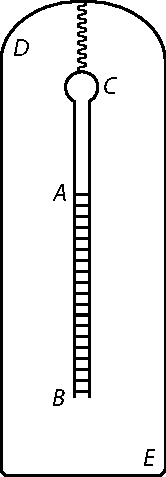
\includegraphics[width=0.18\textwidth]
{gesamttex/edit_VIII-4/images/LH_37_03_117_d1_117r.pdf}%
\edcaption[0.5em]{%
\lbrack\textit{Fig.\:1}\rbrack%
}%
\end{edfigure}%
\pstart%
Tubus \textit{CB}
clausus in \textit{C}
apertus in \textit{A}
impleatur Mercurio,%
\indexS{tubus impletus mercurio}
deinde invertatur,%
\indexS{tubus inversus}
effluet pars Mercurii,%
\indexS{mercurius effluens e tubo}
residuaque tantum manebit pars ejus \textit{AB}%
\indexS{pars mercurii residua}
altitudinis plus minus 27 pollicum,%
\indexS{altitudo mercurii 27 pollicum}%
\indexS{pollex}
et pars tubi \textit{CA} manebit aere propemodum vacua.%
\indexS{pars tubi vacua}
Tubus hoc modo inversus%
\indexS{tubus inversus}
cum Mercurio in eo suspenso,%
\indexS{mercurius suspensus in tubo}
suspendatur intra alium tubum%
\indexS{tubus suspensus in tubo}
vel vas \textit{DE},
idque jam accuratissime claudatur.%
\indexS{tubus clausus accurate}
Qui vim Elasticam defendunt,%
\indexS{vis elastica aeris}
statuent%
\edlabel{LH_37_03_117_117r_saltus-2}
aerem \textit{DE}
elastro suo se dilatare conantem%
\indexS{elastrum aeris}%
\indexS{aer conans dilatare se}
conari Mercurium \textit{AB} intra%
\indexS{mercurius suspensus in tubo}
\edtext{%
tubum supra \textit{A} pellere,%
}{%
\lemma{tubum}%
\Bfootnote{%
\textit{(1)}~\textit{CA} %
\textit{(2)}~supra \textit{A} pellere,%
~\textit{L}%
}}
idque
\edtext{%
facturum esse%
}{%
\lemma{facturum}%
\Bfootnote{%
\textit{(1)}~esset %
\textit{(2)}~esse%
~\textit{L}%
}}
nisi
\edtext{%
pondus 27 pollicum Mercurii%
\indexS{pondus mercurii 27 pollicum}%
\indexS{pollex}%
}{%
\lemma{pondus}%
\Bfootnote{%
\textit{(1)}~Mercurii %
\textit{(2)}~27 pollicum Mercurii%
~\textit{L}%
}}
cum ejus elastro esset in aequilibrio.%
\indexS{elastrum aeris}%
\indexS{aequilibrium mercurii cum elastro aeris}
Contra%
\lbrack,\rbrack\
\edtext{%
autores funiculi%
\indexS{autores funiculi}%
\indexS{funiculus aeris}
dicent Mercurium
\edtext{%
\textit{AB}%
}{%
\lemma{\textit{AB}}%
\Bfootnote{%
\textit{erg.\;L}%
}}
effluere conantem%
\indexS{mercurius effluens e tubo}%
\lbrack,\rbrack\
secum extendere aerem%
\indexS{mercurius extendens aerem residuum}
\edtext{%
quantulumcunque%
\indexS{aer quantuluscunque}
intra tubum residuum%
\indexS{aer residuus in tubo}%
}{%
\lemma{quantulumcunque}%
\Bfootnote{%
\textit{(1)}~inclusum %
\textit{(2)}~intra tubum residuum%
~\textit{L}%
}}
\textit{CA},
et omnino effluxurum esse%
\indexS{mercurius effluens e tubo}
nisi a funiculo aeris,%
\indexS{funiculus aeris}
velut pondus a chorda tensa,%
\indexS{chorda tensa}%
\indexS{pondus retentum a chorda tensa}
retineretur.%
\indexS{mercurius retentus a funiculo aeris}%
}{%
\lemma{autores \lbrack...\rbrack\ retineretur}%
\Cfootnote{%
Leibnizens Darstellung deckt sich nur begrenzt mit Lines\indexN{\textls{Line} (Linus), Francis 1595\textendash1675} Erklärung von Torricellis\indexN{\textls{Torricelli} (Torricellius), Evangelista 1608\textendash1647} Experiment; vgl. \textit{De corporum inseparabilitate}, cap.\;XI (S.\;49--51).\cite{00072}
Line betont vielmehr, dass das \textit{vinculum}, das die Quecksilbersäule in der Rohr vom Sinken abhält, aus verdünntem Quecksilber besteht, nicht aus restlicher Luft; vgl. ebd., cap.\;X (S.\;37--45).\cite{00072}
Leibnizens Darstellung zeigt auch mit Whites\indexN{\textls{White} (Albus, Albius, Anglus), Thomas 1592/1593\textendash1676} Erklärung begrenzt Verwandschaft; vgl. \textit{Appendicula}, prop.\;II u.\;III (S.\;8--10).\cite{00567}%
}}
Verum in Hypothesi funiculi%
\indexS{hypothesis funiculi aeris}%
\indexS{funiculus aeris}
reddenda est ratio determinatae altitudinis Mercurii,%
\indexS{altitudo mercurii determinata}%
\indexS{ratio altitudinis mercurii reddenda}%
\indexS{mercurius suspensus in tubo}
quae in Hypothesi Elastri%
\indexS{hypothesis elastri aeris}%
\indexS{elastrum aeris}
est manifesta.%
\indexS{ratio manifesta}
Imo in Hypothesi funiculi%
\indexS{hypothesis funiculi aeris}%
\indexS{funiculus aeris}
determinata hujusmodi altitudo%
\indexS{altitudo mercurii determinata}
servari non potest,
nam aeris%
\indexS{aer latens in mercurio}\indexS{aer intra tubum et mercurium}
\edtext{%
in Mercurio vel intra%
}{%
\lemma{in}%
\Bfootnote{%
\textit{(1)}~Tubo vel intra %
\textit{(2)}~Mercurio vel intra%
~\textit{L}%
}}
tubum et Mercurium latentis
pro varia tubi superficie concava%
\indexS{tubus impletus mercurio}
(quae capacitati minime proportionalis est)
varia esse potest quantitas;
et ita effici poterit
ut aer tantillus%
\indexS{aer tantillus}
intra \textit{CA} residuus,%
\indexS{aer residuus in tubo}
duplo fiat dilatatior%
\indexS{aer dilatatus}
\edtext{%
in uno casu quam in alio,%
}{%
\lemma{in uno %
\lbrack...\rbrack\ in alio}%
\Bfootnote{%
\textit{erg.\;L}%
}}
unde duplo pondere dilatante,%
\indexS{pondus mercurii dilatans aerem}
\edtext{%
seu duplicata%
}{%
\lemma{seu}%
\Bfootnote{%
\textit{(1)}~duplici %
\textit{(2)}~duplicata%
~\textit{L}%
}}
Mercurii altitudine opus esset.%
\indexS{altitudo mercurii suspensi in tubo}%
\indexS{mercurius suspensus in tubo}
Accedit
quod diversi liquores%
\indexS{liquor}
servant altitudinem ponderibus reciproce proportionalem,%
\indexS{altitudo liquoris reciproce proportionalis ponderi}
cum tamen ratione aeris%
\indexS{ratio aeris contenti in tubo}%
\indexS{aer contentus in tubo}
\edtext{%
contenti in tubo variare deberent.%
}{%
\lemma{contenti}%
\Bfootnote{%
\bars{in tubo \textit{erg.}} variare %
\textit{(1)}~debeant %
\textit{(2)}~deberent%
~\textit{L}%
}}
Itaque
licet
aerem aliquem in tubo superesse%
\indexS{aer residuus in tubo}
non sit negandum,
tantillam tamen
\edtext{%
ejus quantitatem esse oportet,
ut%
}{%
\lemma{ejus}%
\Bfootnote{%
\textit{(1)}~quantitas est, ut oportet %
\textit{(2)}~quantitatem esse oportet, ut%
~\textit{L}%
}}
majoris minorisque ejus dilatationis%
\indexS{dilatatio aeris residui in tubo}
rationem haberi non sit opus,
unde funiculus%
\indexS{funiculus aeris}
locum habere non
\edtext{%
potest,
quod%
}{%
\lemma{potest,}%
\Bfootnote{%
\textit{(1)}~idque %
\textit{(2)}~quod%
~\textit{L}%
}}
imposterum habendum erit pro demonstrato
et ex ipsa societate%
\indexS{Societas Jesu}
\edtext{%
\edlabel{LH_37_03_117_117r_Dechales-1}%
agnitum est a Chalesio%
\indexN{\textls{Dechales} (Chalesius), Claude François Milliet 1621\textendash1678}%
\edlabel{LH_37_03_117_117r_Dechales-2}%
}{%
\lemma{agnitum \lbrack...\rbrack\ Chalesio}%
\Cfootnote{%
Wohl Anspielung auf
\textsc{C.\;Dechales}, \textit{Cursus seu mundus mathematicus},
tract.\;VII, lib.\;I, digr.\;V--VII (Lyon 1674, Bd.\;I, S.\;436a--448b):\cite{00124}
Torricellis\indexN{\textls{Torricelli} (Torricellius), Evangelista 1608\textendash1647} Experiment wird dort lediglich unter Berücksichtigung des Luftgewichts erklärt, während Lines\indexN{\textls{Line} (Linus), Francis 1595\textendash1675} alternative Erklärung unerwähnt bleibt.
Aus dem nachgewiesenen Abschnitt aus Deschales' \textit{Cursus}\cite{00124} hat Leibniz Exzerpte verfasst; siehe N.\;\ref{41182-1} im vorliegenden Band.%
}}
viro maxime ingenuo et judicioso.%
\indexS{vir ingenuus}%
\indexS{vir judiciosus}
\lbrack%
\href{\Scan{LH_37_03_117v}}%
{117\,v\textsuperscript{o}}%
\rbrack\ %
\edlabel{LH_37_03_117_117v_PaderbornJS-1}%
Addatur
\edtext{%
Epistola%
\indexS{epistola}
quam ad Jesuitam%
\indexN{Jesuita mathematicus Paderbornensis}%
\indexS{mathematicus}
\edtext{%
Mathematicum Padebornensem\indexO{Paderborn}%
}{%
\lemma{Mathematicum}%
\Bfootnote{%
\textit{(1)}~Osnabrugensem %
\textit{(2)}~Padebornensem%
~\textit{L}%
}}
de hoc argumento scripsi anno 1681.%
\indexS{argumentum}%
\edlabel{LH_37_03_117_117v_PaderbornJS-2}%
}{%
\lemma{Epistola \bracks{...} 1681}%
\Cfootnote{%
Nicht nachgewiesen.}}
\pend%
\pstart%
Interea
ut dicam
quod res
\edtext{%
est,
non videtur aer per se ac sua natura esse Elasticus,%
\indexS{aer non elasticus per se ac sua natura}%
\indexS{natura aeris}
nec%
}{%
\lemma{est,}%
\Bfootnote{%
\textit{(1)}~non puto in aere proprie vim E\indexS{vis elastica aeris} %
\textit{(2)}~non videtur %
\lbrack...\rbrack\ esse Elasticus, %
\textit{(a)}~nec %
\textit{(b)}~nec%
~\textit{L}%
}}
magis dicendum est
aerem habere per se vim sese dilatandi,%
\indexS{vis aeris dilatandi se}%
\indexS{aer non habens per se vim dilatandi}
quam contrahendi.%
\indexS{vis aeris contrahendi se}%
\indexS{aer non habens per se vim contrahendi}
Licet enim fingamus
aerem esse instar lanae%
\indexS{aer instar lanae}%
\indexS{lana}
constareque ex partibus ramosis rigidis%
\indexS{aer constans e partibus ramosis rigidis}%
\indexS{partes aeris ramosae rigidae}
ac si premantur se restituentibus,
nova quaestio erit,
undenam hae partes suum habeant Elastrum.%
\indexS{elastrum partium aeris}
\edlabel{LH_37_03_117_117r_explmechelstr-1}%
Dicendum est ergo%
\lbrack,\rbrack\
\edtext{%
quod alibi fusius explicui,%
}{%
\lemma{alibi}%
\Cfootnote{%
Möglicherweise Anspielung auf den Entwurf \textit{Explicatio mechanica elastri}, \textit{LSB} VIII,\;3 N.\;14\textsubscript{3}\cite{01437} \bracks{Ende Januar -- März\:/\:April 1683}.%
}}
fluidum aetherium cuncta pervadens%
\indexS{fluidum aetherium pervadens cuncta}
celerrimo suo motu%
\indexS{motus fluidi aetherei}
partes aeris dispergere et dissipare conari%
\lbrack,\rbrack\
prorsus ut aqua calore ebullit%
\indexS{aqua ebulliens calore}
\edtext{%
et pulvis%
\indexS{pulvis disgregatus a vento}
aut plumae%
\indexS{plumae disgregatae a vento}%
}{%
\lemma{et}%
\Bfootnote{%
\textit{(1)}~fumae %
\textit{(2)}~pulvis aut plumae%
~\textit{L}%
}}
vento perflante%
\indexS{ventus perflans}
disgregantur.%
\edlabel{LH_37_03_117_117r_explmechelstr-2}
Sed cum idem motus%
\indexS{motus fluidi aetherei}
corpora
quae dispergere non potest
\edtext{%
ita colligat,%
}{%
\lemma{ita}%
\Bfootnote{%
\textit{(1)}~componat %
\textit{(2)}~colligat%
~\textit{L}%
}}
ut quam minimum ab illis turbetur,
et ita versus centrum globi nostri detrudat,%
\indexS{corpora detrusa versus centrum terrae}%
\indexS{centrum globi nostri}
luctantur inter%
\indexS{lucta inter gravitatem et elastrum aeris}
\edtext{%
se gravitas%
\indexS{gravitas aeris}
et Elastrum,%
\indexS{elastrum aeris}
et elastrum unius partis
cum elastro alterius partis,
unde partes aeris
ad eundem consistentiae gradum%
\indexS{gradus consistentiae aeris}%
\indexS{consistentia aeris}
sese qua possunt componunt,
nisi quod%
}{%
\lemma{se}%
\Bfootnote{%
\textit{(1)}~conatus gravitat %
\textit{(2)}~gravitas et Elastrum, et %
\textit{(a)}~quand %
\textit{(b)}~licet %
\textit{(aa)}~servata %
\textit{(bb)}~servatur uniformitas %
\textit{(c)}~elastrum unius %
\lbrack...\rbrack\ ad eundem %
\textit{(aa)}~tensionis sive ela %
\textit{(bb)}~consistentiae gradum %
\lbrack...\rbrack\ nisi quod%
~\textit{L}%
}}
ob gravitatem%
\indexS{gravitas aeris}
magis pressae sunt inferiores%
\indexS{pars aeris inferior}
quam superiores.%
\indexS{pars aeris superior}
\pend%
\pstart%
Caeterum adjicere hic placet
\edlabel{LH_37_03_117_117v_morland-1}%
responsionem ad%
\indexS{responsio ad objectionem}
\edtext{%
objectionem mire%
}{%
\lemma{objectionem}%
\Bfootnote{%
\textit{(1)}~per %
\textit{(2)}~mire%
~\textit{L}%
}}
elegantem ipsius
\edtext{%
Magnae Britanniae Regis%
\indexN{\textls{England: Karl II.}, König 1660\textendash1685}%
}{%
\lemma{Magnae Britanniae Regis}%
\Cfootnote{%
Der von 1660 bis 1685 regierende König von England\indexO{England} Karl II.%
}}
pro funiculo factam%
\indexS{responsio pro funicolo}
et a Samuele
\edtext{%
Morelando%
\indexN{\textls{Morland} (Moreland), Samuel 1625\textendash1695}%
}{%
\lemma{Morelando}%
\Cfootnote{%
Nicht nachgewiesen.
Siehe aber Leibnizens Brief an N.\;Grew vom 9./19.\;Marz 1680:
\textit{Vidi schedam quandam Domini Morlandi,\indexN{\textls{Morland} (Moreland), Samuel 1625\textendash1695} quibus refutare conatur aequilibrium cylindri aerei, sed ex observatione ejus, quanquam ea non inelegans sit, nescio an quod ille voluit concludatur.}
(\textit{LSB} III,\;3 N.\;32, S.\;88.14--16).\cite{02600}%
}}
relatam.%
\edlabel{LH_37_03_117_117v_morland-2}
Nempe
\edtext{%
tubus%
\indexS{tubus inversus}%
\indexS{tubus suspensus e libra}
\edtext{%
inversus%
}{%
\lemma{inversus}%
\Bfootnote{%
\textit{erg.\;L}%
}}
\textit{CAB},%
}{%
\lemma{tubus inversus \textit{CAB}}%
\Cfootnote{%
Vgl. das Diagramm \bracks{\textit{Fig.\:2}}.%
}}
\edtext{%
clausus in \textit{C},
apertus in \textit{B},%
}{%
\lemma{clausus in \textit{C},
apertus in \textit{B},}%
\Bfootnote{%
\textit{erg.\;L}%
}}
cujus pars superior \textit{AC} vacua%
\indexS{pars tubi vacua aere}
communi aere,%
\indexS{aer communis}
pars autem
\edtext{%
\textit{AB}
27 circiter pollicum%
\indexS{pollex}
plena est Mercurio pensili;%
\indexS{mercurius pensilis 27 pollicum}
suspendatur%
}{%
\lemma{\textit{AB}}%
\Bfootnote{%
\bars{27 circiter pollicum \textit{erg.}} plena est %
\textit{(1)}~Mercurius 27 circiter po %
\textit{(2)}~Mercurio %
\textit{(a)}~suspenso %
\textit{(b)}~pensili; %
\textit{(aa)}~totus autem tubus %
\textit{(bb)}~suspendatur%
~\textit{L}%
}}
ex librae \textit{DEF} brachio \textit{ED} in \textit{D},%
\indexS{brachium librae}%
\indexS{libra}%
\indexS{tubus suspensus e libra}
et ab altero brachio \textit{EF} in \textit{F}
suspendatur pondus \textit{G},%
\indexS{pondus suspensum e libra}
\edtext{%
reperietur non haberi aequilibrium,%
\indexS{aequilibrium brachiorum librae}
nisi pondus aequivaleat%
}{%
\lemma{reperietur}%
\Bfootnote{%
\textit{(1)}~pondus ut in %
\textit{(2)}~non haberi %
\lbrack...\rbrack\ pondus aequivaleat%
~\textit{L}%
}}
non tantum tubo vitreo,%
\indexS{tubus vitreus includens hydrargyrum}
sed et Hydrargyro incluso.%
\indexS{hydrargyrum inclusum in tubo}
Unde colligi videtur,
Mercurium non%
\indexS{mercurius sustentus ab aere}
\edtext{%
sustineri ab aere%
}{%
\lemma{sustineri}%
\Bfootnote{%
\textit{(1)}~aere %
\textit{(2)}~ab aere%
~\textit{L}%
}}
ambiente%
\indexS{aer ambiens}%
\lbrack,\rbrack\
alioqui cum tubo non ponderaret,
sed potius Mercurium ope%
\indexS{mercurius pendens ope funiculi aerei}
\edtext{%
funiculi aerei ex tubo pendere.%
}{%
\lemma{funiculi}%
\Bfootnote{%
\textit{(1)}~ex tubo pend %
\textit{(2)}~aerei ex tubo pendere%
~\textit{L}%
}}
Responderi potest %
primum per instantiam,%
\indexS{responsio per instantiam}%
\indexS{instantia}
ubi negari non potest Mercurium%
\indexS{mercurius sustentus a liquido ambiente}
\edtext{%
ab ambiente liquido%
\indexS{liquidum ambiens}%
}{%
\lemma{ab}%
\Bfootnote{%
\textit{(1)}~aere %
\textit{(2)}~ambiente liquido%
~\textit{L}%
}}
sustentari,
nempe si
\edtext{%
experimentum Torricellianum%
\indexS{experimentum Torricellianum}
fiat%
}{%
\lemma{experimentum}%
\Bfootnote{%
\textit{(1)}~fiat %
\textit{(2)}~Torricellianum fiat%
~\textit{L}%
}}
in fundo maris,%
\indexS{fundus maris}%
\indexS{mare}
ubi longe altius extabit Mercurius,%
\indexS{altitudo mercurii in fundo maris}%
\indexS{mercurius extans in tubo}
\edtext{%
ad 50 et%
}{%
\lemma{ad}%
\Bfootnote{%
\textit{(1)}~40 et %
\textit{(2)}~50 et%
~\textit{L}%
}}
amplius pollices%
\indexS{pollex}
pro maris profunditate,%
\indexS{profunditas maris}%
\indexS{mare}
et nihilo minus
\edtext{%
pondus totius Mercurii,%
\indexS{pondus mercurii sustenti a cylindro aquae}
etiam quem aquae cylinder sustinet%
\indexS{mercurius sustentus a cylindro aquae}%
\indexS{cylinder aquae}%
\lbrack,\rbrack\
a librante in fundo maris%
\indexS{fundus maris}%
}{%
\lemma{pondus}%
\Bfootnote{%
\textit{(1)}~non tubi tantum, sed et %
\textit{(2)}~totius Mercurii, %
\lbrack...\rbrack\ cylinder sustinet %
\textit{(a)}~in libra %
\textit{(b)}~in maris fundo %
\textit{(c)}~a librante in fundo maris%
~\textit{L}%
}}
certissime sentietur,
nec dubitem pignore%
\indexS{pignus}
hac de re certare.
Deinde ad argumentum ipsum respondendum
\edtext{%
est fluidum ambiens%
\indexS{fluidum ambiens}%
}{%
\lemma{est}%
\Bfootnote{%
\textit{(1)}~aere %
\textit{(2)}~fluidum ambiens%
~\textit{L}%
}}
sustinere pondus Mercurii%
\indexS{pondus mercurii sustentum a fluido ambiente}%
\indexS{mercurius sustentus a fluido ambiente}
non omnino
(neque enim impedit,
quin una cum tubo
\edtext{%
descendat
cum tubus librae appenditur)%
\indexS{tubus appensus librae}%
\indexS{libra}%
}{%
\lemma{descendat}%
\Bfootnote{%
\textit{(1)}~ut fit in libra, %
\textit{(2)}~cum tubus librae appenditur)%
~\textit{L}%
}}
sed hactenus
\edtext{%
tantum,
ne%
}{%
\lemma{tantum,}%
\Bfootnote{%
\textit{(1)}~ut %
\textit{(2)}~ne%
~\textit{L}%
}}
sine tubo descendat,
\edtext{%
seu ne a%
}{%
\lemma{seu}%
\Bfootnote{%
\bars{ne \textit{erg.}} a%
~\textit{L}%
}}
tubo separetur.
Idemque ad duo
\edtext{%
Marmora polita sibi adhaerentia,%
\indexS{marmora polita adhaerentia}%
}{%
\lemma{Marmora}%
\Bfootnote{%
\textit{(1)}~sibi adhae %
\textit{(2)}~polita sibi adhaerentia,%
~\textit{L}%
}}
aliosque casus applicari potest.
\pend%
\newpage%
\begin{edfigure}[2.0em][0.0em]%
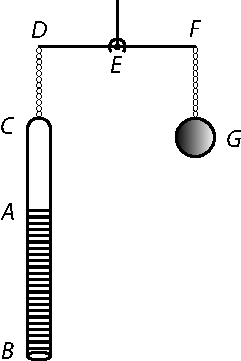
\includegraphics[width=0.26\textwidth]
{gesamttex/edit_VIII-4/images/LH_37_03_117_d2_117v.pdf}%
\edcaption[0.25em]{%
\lbrack\textit{Fig.\:2}\rbrack%
}%
\end{edfigure}%
\vspace*{4.5em}%
\pstart%
\noindent%
\centering%
*     *     *
\pend%
\vspace{4.5em}%
\selectlanguage{german}%
\frenchspacing%
\footnotesize%
\pstart%
\noindent%
\textls{Ausführliche Datierungsgründe:}%
\pagelabel{60206_dat}
Die undatierte Aufzeichnung N.\;\ref{60206} \textit{Pro pressione aeris, contra funiculum} knüpft gleich zu Beginn an die Auseinandersetzung an, die in den frühen 1660er Jahren Verfechter des elastischen Verhaltens der Luft wie etwa Robert Boyle\indexN{\textls{Boyle} (Boylius, Boyl), Robert 1627\textendash1691} und Anhänger der "Funiculus"-Lehre wie Francis Line\indexN{\textls{Line} (Linus), Francis 1595\textendash1675} oder Thomas White\indexN{\textls{White} (Albus, Albius, Anglus), Thomas 1592/1593\textendash1676} entfachteten. %
Leibniz nimmt hierbei, wie der Titel selbst zeigt und wie bereits in der inhaltlich verwandten Aufzeichnung N.\ref{60261} der Fall war, gegen die "Funiculus"-Lehre Stellung.
Die für die Aufzeichnung N.\;\ref{60206} vorgeschlagene Datierung ergibt sich aus folgenden Beobachtungen:
\pend%
\pstart%
(1)
Im Träger von N.\;\ref{60206} ist das Fragment eines Harzer \href{\Scan{LH_37_03_117wz}}{Wassezeichens} (Wilder Mann mit Glocke und Jahresangabe 1678) anzutreffen, %
das im Leibniz-Nachlass nach heutigem Wissensstand %
für die Zeitspanne 1679 bis 1685 belegt ist;
dieses Papier wird im Nachlass ab 1686 durch ähnliches (mit gleichem Wasserzeichen, aber Jahresangabe 1685) ersetzt.
Die Eigenschaften des Fragments im Träger von N.\;\ref{60206} zeigen, dass es sich hierbei um die ältere Papiersorte handelt. %
\pend%
\pstart%
(2)
In N.\;\ref{60206} (\refpassage{LH_37_03_117_117v_PaderbornJS-1}{LH_37_03_117_117v_PaderbornJS-2}) verweist Leibniz auf einen Brief, den er im Jahr 1681 an einen nicht ermittelten jesuitischen Mathematiker aus Paderborn\indexN{Jesuita mathematicus Paderbornensis}\indexO{Paderborn} geschrieben haben soll.
Folglich kann die Aufzeichnung N.\;\ref{60206} frühestens im Jahr 1682 abgefasst worden sein.
Da Leibniz bei seiner Andeutung, statt eine Wendung zu benutzen wie \textit{anno priore} oder \textit{superiore}, die Jahreszahl angibt, erweist sich als wahrscheinlich, dass N.\;\ref{60206} nicht vor 1683 verfasst wurde.
\pend%
\pstart%
(3)
Ausschlaggebend für die Bestimmung des Terminus post quem der Datierung dürfte vorwiegend der Umstand sein, dass in N.\;\ref{60206} (\refpassage{LH_37_03_117_117r_Dechales-1}{LH_37_03_117_117r_Dechales-2}) auf \textsc{C.\;Dechales}, \textit{Cursus seu mundus mathematicus},
tract.\;VII, lib.\;I, digr.\;V--VII (Lyon 1674, Bd.\;I, S.\;436a--448b)\cite{00124} angespielt wird.
Mit Dechales'\indexN{\textls{Dechales} (Chalesius), Claude François Milliet 1621\textendash1678} \textit{Cursus seu mundus mathematicus}\cite{00124} hat sich Leibniz wohl zwischen dem Winter 1682/1683 und der ersten Hälfte 1685 befasst, wie die im vorliegenden Band veröffentlichten Auszüge mit Bemerkungen N.\;\ref{41182-1} und N.\;\ref{41182-2} zeigen (siehe dort die ausführlichen Datierungsgründe, S.\;\pageref{41182_dat}).
Hieraus ist zu schließen, dass die Aufzeichnung N.\;\ref{60206} wahrscheinlich nicht vor dem Winter 1682/1683 angefertigt wurde, vermutlich nicht vor Anfang 1683.
Falls die Vermutung ferner zutrifft, dass N.\;\ref{60206} (\refpassage{LH_37_03_117_117r_explmechelstr-1}{LH_37_03_117_117r_explmechelstr-2}) auf den zwischen Ende Januar und März\:/\:April 1683 entstandenen Entwurf \textit{Explicatio mechanica elastri} (\textit{LSB} VIII,\;3 N.\;14\textsubscript{3})\cite{01437} anspielt, dann würde dies den vorgeschlagenen Terminus post quem weiterhin bestätigen.
\pend%
\pstart%
(4)
Zur Bestimmung des Terminus ante quem trägt die Feststellung bei, dass die Aufzeichnung N.\;\ref{60206} (\refpassage{LH_37_03_117_117v_morland-1}{LH_37_03_117_117v_morland-2}) aller Wahrscheinlichkeit nach auf eine nicht ermittelte \textit{scheda} von Samuel Morland\indexN{\textls{Morland} (Moreland), Samuel 1625\textendash1695} verweist, deren Inhalt Leibniz in seinem Brief an Nehemiah Grew\indexN{\textls{Grew}, Nehemiah 1641\textendash1712} vom 9./19.\;Marz 1680 kurz zusammenfasst (\textit{LSB} III,\;3 N.\;32, S.\;88.14--16; siehe die Erläuterung zu N.\;\ref{60206}, \refpassage{LH_37_03_117_117v_morland-1}{LH_37_03_117_117v_morland-2}).\cite{02600}
Demnach ist anzunehmen, dass der König von England,\indexO{England} über den Morland\indexN{\textls{Morland} (Moreland), Samuel 1625\textendash1695} in der besagten \textit{scheda} berichtet haben soll und auf den sich Leibniz als amtierenden Monarch bezieht, der am 6.\;Februar 1685 verstorbene Karl~II. sein muss.\indexN{\textls{England: Karl II.}, König 1660\textendash1685}
Von dessen Tod wusste Leibniz bereits einen Monat später, wie sein Brief vom 4./14.\;März 1685 an Landgraf Ernst von Hessen-Rheinfels\indexN{\textls{Hessen-Rheinfels: Ernst}, Landgraf 1649\textendash1693} nachweist (\textit{LSB} I,\;4 N.\;308, S.\;349.4\,f.).\cite{02601}
Dies ist Grund für die Annahme, dass N.\;\ref{60206} spätestens im Februar 1685 angefertigt wurde, wohl aber schon etwas früher.
\pend%
\pstart%
Aus diesen Betrachtungen ergibt sich als wahrscheinliche Gesamtdatierung der vorliegenden Aufzeichnung N.\;\ref{60206} \textit{Pro pressione aeris, contra funiculum} der Zeitraum 1683--1684.
Eine frühere (ab 1682) oder eine spätere (bis 1685) Entstehung sind nicht auszuschließen, aber unwahrscheinlich.
\pend%
\selectlanguage{latin}%
\frenchspacing%
\newpage%




\chapter[tocentry={De aestimatione virium aeris compressi %
\enskip%
\bracks{%
zweite Hälfte 1683\;(?)
\textendash\
erste Hälfte
1686}},
head={De aestimatione virium aeris compressi}]%
{\MakeUppercase{De aestimatione virium aeris compressi}
\newline%
\bracks{%
zweite Hälfte 1683\;(?)
\textendash\
erste Hälfte
1686}}
\label{aestimavirium_intro}
\footnotesize%
\pstart%
\noindent%
\pagelabel{aestimavirium_dat}%
(1)~Der vorliegende Textkomplex N.\;\ref{aestimavirium_intro} umfasst die umfangreiche Aufzeichnung N.\;\ref{41212} \textit{De aestimatione virium quas per aeris compressionem acquirere licet} und die weitgehend kürzere, titellose Aufzeichnung N.\;\ref{41213}, welcher editorisch der Titel \textit{Die Kraft der zusammengedruckten Luft} zugewiesen wurde.
Beide Texte sind der gleichen Aufgabe gewidmet, die elastische Kraft einer Luftmasse, die in einem verschlossenem Behälter zusammengedruckt wird, unter Berücksichtigung der Unterscheidung zwischen "toten" und "lebendigen" Kräften zu berechnen.
Hinsichtlich ihrer Textart unterscheiden sich N.\;\ref{41212} und N.\;\ref{41213} erheblich voneinander: \textit{De aestimatione virium quas per aeris compressionem acquirere licet} ist eine im Latenischen verfasste und auf zwei ganzen Foliobogen ausgedehnte ausführliche Untersuchung, die sich inhaltlich durch zahlreiche Wedungen und wiederholte Neuansätze auszeichnet, wohingegen \textit{Die Kraft der zusammengedruckten Luft} den Charakter eines gradlinigen und komprimierten Entwurfes aufweist, der unprätenziös auf Deutsch startet und nur ein kleines Quartoblatt in Anspruch nimmt.
Ihre inhaltliche Verwandschaft rechtfertigt jedoch die Entscheidung der Herausgeber, beide Texte einheitlich als Unterstücke zu edieren.
Denn N.\;\ref{41212} und N.\;\ref{41213} teilen nicht nur die gleiche oben genannte Zielsetzung, sondern auch die gleichen empirischen Voraussetzungen:
Untersucht wird in beiden Texten das Verhalten einer Luftmasse mit anfänglichem Volumen eines Kubikfußes, deren elastische Kraft unter gewöhnlichen Druckbedingungen als Fähigkeit geschätzt wird, ein Gewicht von 2.100 Pfund zu stemmen, (vgl. \refpassage{LH_35_09_25_001-002+004-005_001r_nld-1}{LH_35_09_25_001-002+004-005_001r_nld-2} mit \refpassage{LH_35_09_25_003_003r_nld-1}{LH_35_09_25_003_003r_nld-2}).
Vor allem aber in ihrem Ergebnis stimmen N.\;\ref{41212} und N.\;\ref{41213} überein:
Der besagten Luftmasse, in ein Zentel ihres ursprünglichen Volumens zusammengedrängt, komme eine elastische Kraft zu, die der kinetischen Kraft eines Körpers entspreche, das 4.200 Pfund wiege und aus einer Höhe von 0,9 Fuß falle %
(vgl. \refpassage{LH_35_09_25_001-002+004-005_005v_nld-1}{LH_35_09_25_001-002+004-005_005v_nld-2} mit \refpassage{LH_35_09_25_003_003v_nld-1}{LH_35_09_25_003_003v_nld-2} u. der Randbemerkung zum Diagramm \bracks{\textit{Fig.\:4}}, S.\;\pageref{LH_35_09_25_003_003v_Fig4}).
\pend%
\pstart%
Zu diesem gemeinsamen Ergebnis gelangt N.\;\ref{41212} erst am Ende eines langen und verwinkelten Weges, N.\;\ref{41213} hingegen ohne Umwendungen.
Aus diesem Unterschied lässt sich im Hinblick auf die relative Chronologie der zwei Texte schließen, dass N.\;\ref{41213} \textit{nicht} vor N.\;\ref{41212} entstanden sein kann.
Vielmehr dürfte N.\;\ref{41213} eine schnelle Zusammenfassunug der in N.\;\ref{41212} durchgeführten und abgeschlossenen Untersuchung sein, oder aber eine Art Zuarbeit, die ab einem bestimmten Punkt parallel zu N.\;\ref{41212} verfasst wurde und möglicherweise zur Orientierung bei der komplexen Untersuchung dienen sollte.
In beiden Fällen ist anzunehmen, dass N.\;\ref{41212} zumindest teilweise bereits vorlag, als N.\;\ref{41213} verfasst wurde; und auch in dem Fall, dass N.\;\ref{41213} auf N.\;\ref{41212} folgte, lag zwischen ihnen wahrscheinlich kein relevanter Zeitabstand.
Für eine gleichzeitige oder wenigstens zeitnahe Entstehung sprechen 
ferner die Überlieferungsumstände:
Im Leibniz-Nachlass findet sich N.\;\ref{41213}, wie schon die Blattzählung zeigt, in den gefalteten Bogen eingelegt, die als Textträger für N.\;\ref{41212} dienen (siehe \refpassage{LH_35_09_25_003_ubrlf-1}{LH_35_09_25_003_ubrlf-2}).
Diese Anordnung der Handschriften könnte auf Leibniz selbst zurückgehen.
\pend%
\pstart%
(2)~Ausschlaggebend für die Datierung der Aufzeichnung N.\;\ref{41212} \textit{De aestimatione virium quas per aeris compressionem acquirere licet} ist zunächst das in beiden Textträgern anzutreffende Wasserzeichen (vgl. LH~XXXV~9,\;25 Bl.\;\href{\Scan{LH_35_09_25_002wz}}{2} u.\;\href{\Scan{LH_35_09_25_005wz}}{5}): ein Posthorn an gekröntem Zierschield, das aus der Papiermühle in Hehlen\indexO{Hehlen (bei Goslar)} bei Goslar\indexO{Goslar} stammen könnte. %
Das Wasserzeichen kommt im Leibniz-Nachlass nach heutigem Wissensstand insgesamt sieben Mal vor und weist zwei verschiedene Varianten auf: die eine mit dünnhalsigem, die andere mit dickhalsigem Posthorn.
Belegt ist die Variante mit dünnhalsigem Posthorn u.\,a. in dem auf den Anfang 1685 datierbaren Zeugen~C des im Herbst 1685 angefertigten Briefes Leibnizens an seinen Dienstherrn, Herzog Ernst August\indexN{\textls{Braunschweig-Lüneburg}, Ernst August von, Herzog und Kurfürst von Hannover 1679\textendash1698} (LH~XXIII 2,\;1 Bl.\;1--4; vgl. \textit{LSB} I,\;4 N.\;173),\cite{01404} sowie im Träger des Briefes, den Johann Georg Lange\indexN{\textls{Lange}, Johann Georg (1687)} am 9.\;(19.) September 1686 an Leibniz gesendet hat (LBr~523 Bl.\;5; vgl. \textit{LSB} I,\;4 N.\;246).\cite{01410}
Die Variante mit dickhalsigem Posthorn findet sich u.\,a. im Konzept~A des Briefes Leibnizens vom April 1687 an de Bourgeauville,\indexN{\textls{Bourgeauville}, de (französischer Gesandter in Celle 1688--1689)} französischen Gesandten in Celle\indexO{Celle} (LBr~183 Bl.\;12--13; vgl. \textit{LSB} I,\;4 N.\;526).\cite{01405}
Die vier weiteren im Leibniz-Nachlass bekannten Vorkommnisse des Wasserzeichens sind bisher nicht mit Sicherheit datiert.
Die in den Textträgern der Aufzeichnung N.\;\ref{41212} vorkommende Variante ist die für die Zeitspanne von Anfang 1685 bis September 1686 belegte mit \textit{dünnhalsigem} Posthorn.
Folglich liegt die Annahme nahe, dass N.\;\ref{41212} im Zeitraum zwischen dem Winter 1684/1685 und dem Herbst 1686 verfasst wurde, als Leibniz sich oft im Harz\indexO{Harz} aufhielt (\textit{Chronik}, S.\;73--79).\cite{01236}
Da es aber nach heutigem Wissensstand nicht auszuschließen ist, dass die Variante des Wasserzeichens mit dünnhalsigem Posthorn auch früher oder später im Umlauf war, ist auch eine etwas frühere oder etwas spätere Datierung von N.\;\ref{41212} möglich.
Sowohl über den Terminus post quem wie auch über den Terminus ante quem der Entstehung von N.\;\ref{41212} lassen sich im Folgenden Beobachtungen anstellen, die Datierung des Wasserzeichens tatsächlich ergänzen.
\pend%
\pstart%
Gegen Ende der Aufzeichnung N.\;\ref{41212} (\refpassage{LH_35_09_25_001-002+004-005_005r_Bernoulli-1}{LH_35_09_25_001-002+004-005_005r_Bernoulli-2}) ist ein präziser Verweis auf die \textit{Dissertatio de gravitate aetheris}\cite{01403} des Baseler\indexO{Basel} Mathematikers Jacob Bernoulli\indexN{\textls{Bernoulli}, Jacob 1655\textendash1705} anzutreffen.
Diese 1683 in Amsterdam\indexO{Amsterdam} erschienene Abhandlung dürfte Leibniz durch die Lektüre der ihr gewidmeten anonymen Rezension im Märzheft 1683 der \textit{Acta eruditorum} (S.\;106\textendash112)\cite{01406} zur Kenntnis genommen haben.
Da er in N.\;\ref{41212} aber auf eine Ausführung in Bernoullis Traktat Bezug nimmt, auf die in der anonymen Rezension nicht eingegangen wird, kann nicht diese letztere die Quelle dafür gewesen sein.
Wann Leibniz die \textit{Dissertatio de gravitate aetheris}\cite{01403} tatsächlich gelesen hat, lässt sich nach heutigem Wissensstand nicht genau bestimmen.
Das Buch war auf der Frankfurter\indexO{Frankfurt am Main} Michaelis-Messe 1682 (\textit{Catalogus universalis}, Bl.\;\bracks{D4\,r\textsuperscript{o}})\cite{02596} angekündikgt und auf der Leipziger\indexO{Leipzig} Ostermesse 1683 (\textit{Catalogus universalis}, Bl.\;B3\,v\textsuperscript{o})\cite{02597} ausgestellt worden, weshalb es frühestens ab dem Frühjahr 1683 auf dem Buchmarkt erhältlich gewesen sein dürfte (in beiden Katalogen ist der Titel auch ungenau angegeben: wohl das Zeichen für eine späte Auslieferung).
Im Briefwechsel wird die Abhandlung zum ersten und bisher einzigen Mal erst nach Leibnizens Italienreise\indexO{Italien} erwähnt, nämlich in seinem Brief an Jacob Bernoulli\indexN{\textls{Bernoulli}, Jacob 1655\textendash1705} vom 24.\;September/4.\;Oktober 1690; vgl. \textit{LSB} III,\;4 N.\;279, S.\;573.24\,f.\cite{01260} %
Leibniz dürfte erst einige Monate nach dem Erscheinen der anonymen Rezension imstande gewesen sein, Bernoullis Traktat in die Hände zu bekommen, d.\,h. wohl frühestens in der zweiten Hälfte 1683 oder vielmehr im Laufe des Jahres 1684.
Dieser ungenaue Zeitpunkt, der sich insgesamt aber nur begrenzt vom frühesten Beleg des Wasserzeichens absezt, soll hier als Terminus post quem der Datierung von N.\;\ref{41212} betrachtet werden.
\pend%
\pstart%
Den Versuch, die elastische Kraft der zusammengedruckten Luft mathematisch zu bestimmen, stellt Leibniz auch in anderen Texten an, etwa in den von ihm eigenhändig datierten Entwürfen \textit{De aeris resistentia elastica} (Juli 1686; \textit{LSB} VIII,\;3 N.\;27\textsubscript{1}\cite{02561}) und \textit{De vi elastica ad rationes geometricas revocata tentamen} (27.\;August 1689; ebd. N.\;27\textsubscript{2}\cite{02562}).
Diese beiden Texte, die sowohl genetisch wie auch inhaltlich eng miteinander verbunden sind (siehe die einlaeitende Erläuterung in \textit{LSB} VIII,\;3, S.\;306), gehen von einem theoretischen Ansatz aus, welcher dem der Aufzeichnung N.\;\ref{41212} \textit{De aestimatione virium quas per aeris compressionem acquirere licet} stark ähnelt, obwohl sie auf konkrete empirische Werte verzichten.
Beide Texte \textit{LSB} VIII,\;3 N.\;27\textsubscript{1}\cite{02561} und N.\;27\textsubscript{2} sind aller Wahrschinlichkeit nach später entstanden als N.\;\ref{41212} in diesem Band.
Weder \textit{De aeris resistentia elastica} noch \textit{De vi elastica ad rationes geometricas revocata tentamen} weisen die Unsicherheiten und Schwankungen auf, die hingegen die Aufzeichnung N.\;\ref{41212} auszeichnen.
Die Entwürfe \textit{LSB} VIII,\;3 N.\;27\textsubscript{1}\cite{02561} und N.\;27\textsubscript{2}\cite{02562} setzen vielmehr -- stillschweigend -- den Ansatz voraus, der sich in N.\;\ref{41212} durchgesetzt hat, und operieren mit ihm ohne Zögerungen weiter.
Daher ist anzunehmen, dass die Aufzeichnung N.\;\ref{41212} in diesem Band bereits abgeschlossen war, als \textit{LSB} VIII,\;3 N.\;27\textsubscript{1}\cite{02561} in Juli 1686 angefertigt wurde.
Eine Entstehung von N.\;\ref{41212} nach diesem Datum würde sich als unerklärlich erweisen.
Dass in \textit{LSB} VIII,\;3 N.\;27\textsubscript{1}\cite{02561} keine Erwähnung der Aufzeichnung N.\;\ref{41212} erfolgt, könnte sogar als Zeichen dafür gedeutet werden,
\ledpb%
dass zwischen beiden Texten bereits ein gewisser zeitlicher Abstand vorlag.
Die erste Häfte 1686 ist demgemäß als spätester Entstehungszeitpunkt von N.\;\ref{41212} anzusehen, was wiederum mit der Datierung des Wasserzeichens gut übereinstimmt.
\pend%
\pstart%
Der Vollständigkeit halber ist festzuhalten, dass der Schlussteil des unter Vorbehalt auf die Zeitspanne von Ende Januar 1683 bis zum Juli 1686 datierbaren Entwurfes \textit{De vibrationibus aeris tensi} inhaltliche Verwandschaft mit der in der Aufzeichnung N.\;\ref{41212} ausgeführten Untersuchung aufweist (vgl. \textit{LSB} VIII,\;3 N.\;21,\cite{01440} S.\;284.20--285.10).
Welches Abhängigkeitsverhältnis zwischen beiden Texten besteht, lässt sich nicht leicht bestimmen.
Da diese Frage aber keinen relevanten Beitrag zur Datierung von N.\;\ref{41212} verspricht, wird hier auf sie nicht weiter eingegangen.
\pend%
\pstart%
(3)~Da die Aufzeichnung N.\;\ref{41213} \textit{Die Kraft der zusammengedruckten Luft} -- wie oben unter Punkt~(1) festgestellt wurde -- weder vor der Aufzeichnung N.\;\ref{41212} noch wesentlich später abgefasst worden sein dürfte, ist auch für sie den gleichen Entstehungszeitraum anzunehmen wie für N.\;\ref{41212}.
Die Spanne zwischen 1684 (oder Herbst 1683) und der ersten Hälfte 1686 wird demgemäß als Datierung für den gesamten Textkomplexes N.\;\ref{aestimavirium_intro} vorgeschlagen.
\pend%
\vspace{4.0em}%
\selectlanguage{latin}%
\frenchspacing%
\normalsize%



\section[tocentry={De aestimatione virium quas per aeris compressionem acquirere licet
\enskip%
\bracks{%
zweite Hälfte 1683\;(?)
\textendash\
erste Hälfte
1686}},
head={De aestimatione virium}]%
{\MakeUppercase{De aestimatione virium quas per aeris compressionem acquirere licet}
\newline%
\bracks{%
zweite Hälfte 1683\;(?)
\textendash\
erste Hälfte
1686}}
\label{41212}
\include{gesamttex/edit_VIII-4/LH_35_09_25_001-002+004-005.tex}


\section[tocentry={Die Kraft der zusammengedrückten Luft
\enskip%
\bracks{%
zweite Hälfte 1683\;(?)
\textendash\
erste Hälfte
1686%
}},
head={Die Kraft der zusammengedrückten Luft}]%
{\MakeUppercase{Die Kraft der zusammengedrückten Luft}
\newline%
\bracks{%
zweite Hälfte 1683\;(?)
\textendash\
erste Hälfte
1686%
}}
\label{41213}
\selectlanguage{ngerman}%
\frenchspacing%
\begin{ledgroupsized}[r]{120mm}%
\footnotesize%
\pstart%
\noindent%
\textbf{Überlieferung:}%
\pend%
\end{ledgroupsized}%
\begin{ledgroupsized}[r]{114mm}%
\footnotesize%
\pstart%
\parindent -6mm%
\makebox[6mm][l]{\textit{L}}%
Aufzeichnung:
LH\;XXXV\;9,\;25 Bl.\;3.
Ein Blatt 4\textsuperscript{o};
Ränder teilweise beschnitten.
Zwei ganzseitig beschriebene Seiten.
\edlabel{LH_35_09_25_003_ubrlf-1}%
Die Aufzeichnung ist im Nachlass zwischen den Trägern des inhaltlich verwandten Entwurfs N.\;\ref{41212} (LH~XXXV~9,~25, Bl.\;1--2 und Bl.\;4--5) überliefert.%
\edlabel{LH_35_09_25_003_ubrlf-2}
\pend%
\end{ledgroupsized}%
\selectlanguage{latin}%
\frenchspacing%
\vspace{8mm}%
\normalsize%
\pstart%
\noindent%
\bracks{%
\href{\Scan{LH_35_09_25_003r}}%
{3\,r\textsuperscript{o}}%
}
\edlabel{LH_35_09_25_003_003r_nld-1}%
Die lufft in dem%
\indexS{Lufft, gepreßt}
\edtext{%
Cubischen Schuch \textit{AB}%
\indexS{Schuch, cubisch}%
}{%
\lemma{Cubischen Schuch \textit{AB}}%
\Cfootnote{%
Vgl. das Diagramm \lbrack\textit{Fig.\:1}\rbrack.
Der \textit{Schuh} als Maßeinheit der Länge entsprach im deutschsprachigen Raum dem \textit{Fuß}.%
}}
wird
\edtext{%
durch%
}{%
\lemma{durch}%
\Bfootnote{%
\textit{erg.\:L}%
}}
die last der obliegenden
\edtext{%
lufft,%
\indexS{Last der obliegenden Lufft}%
\indexS{Lufft, obliegend}
in dem stand%
}{%
\lemma{lufft,}%
\Bfootnote{%
\textit{(1)}~welche soviel th %
\textit{(2)}~in dem stand%
~\textit{L}%
}}
wie sich bey uns insgemein befindet%
\lbrack,\rbrack\
zusammen gehalten und gepreßet.
\edtext{%
Solche last beträgt%
\indexS{Last der obliegenden Lufft}%
}{%
\lemma{Solche}%
\Bfootnote{%
\textit{(1)}~last ist, %
\textit{(2)}~last beträgt%
~\textit{L}%
}}
soviel als 30 schuch waßer ohngefehr,%
\indexS{Waßer}
und
\edtext{%
ieder Cubischer schuch%
\indexS{Schuch, cubisch}%
}{%
\lemma{ieder}%
\Bfootnote{%
\textit{(1)}~schuch %
\textit{(2)}~Cubischer schuch%
~\textit{L}%
}}
waßer
gerechnet auff 70 Pfund,%
\indexS{Pfund}
\edtext{%
thut 2100 \Pfund.%
}{%
\lemma{thut}%
\Bfootnote{%
\textit{(1)}~3700 \Pfund\ %
\textit{(2)}~2100 \Pfund.%
~\textit{L}%
}}
Wolte man nun die lufft%
\indexS{Lufft, gepreßt}
in ein halb so enges Spatium preßen,
müste man dazu noch eins soviel gewicht haben,%
\indexS{Gewicht, von der Lufft getragen}
nehmlich 4200 \Pfund,
und hat also die in einen Cubischen schuch%
\indexS{Schuch, cubisch}
\edtext{%
\textit{AB} auß zwey in \textit{CB}%
}{%
\lemma{\textit{AB} auß zwey in \textit{CB}}%
\Bfootnote{%
\textit{erg.\;L}%
}}
gepreßete lufft soviel%
\indexS{Lufft, gepreßt}
\edtext{%
krafft,%
\indexS{Krafft der gepreßten Lufft}
daß sie das gewicht von 4200 \Pfund\ in vacuo%
\indexS{vacuum}%
\indexS{in vacuo}
tragen kan,%
}{%
\lemma{krafft,}%
\Bfootnote{%
\textit{(1)}~als 4200 \Pfund, so %
\textit{(a)}~aus %
\textit{(b)}~von \textit{C} bis \textit{A}
\bars{herab \textit{streicht Hrsg.}} fallen, und %
\textit{(2)}~daß sie %
\bars{das gewicht von \textit{erg.}} 4200 \Pfund\ %
\bars{in vacuo \textit{erg.}} tragen kan,%
~\textit{L}%
}}
und gesezt
man konne 10 mahl soviel lufft hinein preßen,%
\indexS{Lufft, gepreßt}
so
\edtext{%
kondte solche lufft hernach 21000 \Pfund\ tragen.%
\indexS{Gewicht, von der Lufft getragen}%
\edlabel{LH_35_09_25_003_003r_nld-2}%
}{%
\lemma{kondte}%
\Bfootnote{%
\textit{(1)}~sie 21000 \Pfund\ %
\textit{(2)}~solche lufft hernach 21000 \Pfund\ tragen.%
~\textit{L}%
}}
Weilen aber die krafft der sich wieder stellenden lufft%
\indexS{Krafft der sich wieder stellenden Lufft}
zu meßen
nicht gnug ist,
daß man wiße
wieviel sie tragen %
oder noch wohl in die höhe heben könne,
sondern auch wie hoch;
so ist
\edtext{%
zu bedencken,%
}{%
\lemma{zu}%
\Bfootnote{%
\textit{(1)}~wißen, %
\textit{(2)}~bedencken%
~\textit{L}%
}}
daß wenn man
\edtext{%
in vacuo%
\indexS{vacuum}%
\indexS{in vacuo}%
}{%
\lemma{in vacuo}%
\Bfootnote{\textit{erg.\;L}%
}}
anstatt der
\edtext{%
4200 \Pfund,
so%
}{%
\lemma{4200 \Pfund,}%
\Bfootnote{%
\textit{(1)}~nur %
\textit{(2)}~so%
~\textit{L}%
}}
die lufft \textit{CB} in \textit{AB} halten,
nur 2100 darauff legte
\edtext{%
in \textit{D},%
}{%
\lemma{in \textit{D}}%
\Bfootnote{\textit{erg.\;L}%
}}
sich die lufft restituiren werde%
\indexS{Lufft, sich restituirend}
aus \textit{AB} in \textit{CB},
und das gewicht bis dahin heben,%
\indexS{Gewicht, von der Lufft getragen}
welches
\edtext{%
dann durch den erlangten Schwung%
\indexS{Schwung, erlangt}
noch sich selbst werde steigen können.%
}{%
\lemma{dann}%
\Bfootnote{%
\textit{(1)}~auch eine mehrere krafft %
\textit{(2)}~durch den erlangten Schwung %
\textit{(a)}~hernach %
\textit{(b)}~vor dann %
\textit{(c)}~noch sich %
\lbrack...\rbrack\ steigen können.%
~\textit{L}%
}}
Wie hoch aber,
das wäre
\edtext{%
auszurechnen,
und daher ein gewicht%
\indexS{Gewicht, von der Lufft getragen}
zu finden,
welches
durch einen fall%
\indexS{Fall}
aus einer gewissen Hohe%
\indexS{Hohe des Falles}
praecise die lufft%
\indexS{Lufft, gepreßt}
aus \lbrack\textit{CB}\rbrack\
in \lbrack\textit{AB}\rbrack\
preßen köndte.
Nun ist das gewicht \textit{D} von 2100 \Pfund%
\indexS{Pfund}%
}{%
\lemma{auszurechnen}%
\Bfootnote{%
\textit{(1)}~. Es ist nehmlic %
\textit{(2)}~. Es ist aber das das\lbrack\textit{!}\rbrack\ pondus \textit{D} von 2100 pfunden %
\textit{(3)}~. Solches wäre aus %
\textit{(4)}~, und daher %
\lbrack...\rbrack\ die lufft %
\textit{(a)}~bis %
\textit{(b)}~aus %
\bars{\textit{CD} \textit{ändert Hrsg.}} in %
\bars{\textit{AD} \textit{ändert Hrsg.}} preßen köndte. Nun %
\textit{(aa)}~das %
\textit{(bb)}~ist das %
\lbrack...\rbrack\ 2100 \Pfund%
~\textit{L}%
}}
und fallet aus \textit{C} bis \textit{A},
so kan es solches nicht verrichten;
ist es aber von 4200 \Pfund,
und fället von \textit{C} bis \textit{A},
so kan es ein weit mehrers Verrichten,
und wurde
in \textit{A} nicht bleiben.
Ja es falle das
\edtext{%
gewicht%
\indexS{Gewicht, von der Lufft getragen}
\lbrack4200\rbrack\
von was für kleiner hohe \textit{EA}%
\indexS{Hohe des Falles}%
}{%
\lemma{gewicht}%
\Bfootnote{%
\textit{(1)}~\textit{E} von was fur klei %
\textit{(2)}~\textit{D} vo %
\textit{(3)}~von %
\textit{(4)}~\bars{42100 \textit{ändert Hrsg.}} von was %
\lbrack...\rbrack\ hohe \textit{EA}%
~\textit{L}%
}}
es wolle,
wird es doch durch den schwung%
\indexS{Schwung, erlangt}
etwas unter \textit{A} herabsteigen,
wiewohl es hernach wieder wird hinauff müßen.
\pend%
\begin{edfigure}[2.75em][2.0em]%
\hspace*{-50mm}%
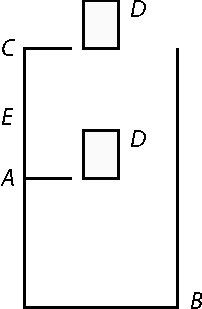
\includegraphics[width=0.22\textwidth]
{gesamttex/edit_VIII-4/images/LH_35_09_25_003_d1_003r.pdf}
\edcaption[0.25em]{%
\hspace*{-50mm}%
\lbrack\textit{Fig.\:1}\rbrack%
}%
\vspace{-13.00em}%
\hspace*{50mm}%
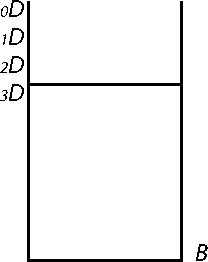
\includegraphics[width=0.23\textwidth]
{gesamttex/edit_VIII-4/images/LH_35_09_25_003_d2_003r.pdf}
\edcaption[0.25em]{%
\hspace*{50mm}%
\lbrack\textit{Fig.\:2}\rbrack%
}%
\end{edfigure}%
\pstart%
Demnach muß
\edtext{%
man die hohe des falles%
\indexS{Hohe des Falles}
unendtlich klein nehmen,%
}{%
\lemma{man}%
\Bfootnote{%
\textit{(1)}~\textit{EA} unendtlich klein nehmen %
\textit{(2)}~die hohe %
\lbrack...\rbrack\ klein nehmen,%
~\textit{L}}}
und sezen,
daß das fallende corpus%
\indexS{corpus, fallend}
\edtext{%
immer
weren\lbrack d \rbrack dem
fallen%
}{%
\lemma{immer}%
\Bfootnote{%
\textit{(1)}~we %
\textit{(2)}~wehr %
\textit{(3)}~\bars{werendem \textit{ändert Hrsg.}} fallen%
~\textit{L}%
}}
wachse,
\edtext{%
wurde der calculus%
\indexS{calculus, angestellet}
also%
}{%
\lemma{wurde}%
\Bfootnote{%
\textit{(1)}~\bars{also \textit{streicht Hrsg.}} %
\textit{(2)}~der calculus also%
~\textit{L}%
}}
angestellet werden konnen.
Das gewicht \textit{\ind{1}D}%
\indexS{Gewicht, von der Lufft getragen}
ist der lufft feder gleich%
\indexS{Lufft}%
\indexS{Feder der Lufft}
und drückt sie
\edtext{%
derowegen hinab%
}{%
\lemma{derowegen}%
\Bfootnote{%
\bars{von \textit{\ind{1}D} \textit{gestr.}} hinab%
~\textit{L}%
}}
in \textit{\ind{2}D},
also daß
\textit{\ind{1}D}\textit{\ind{2}D}
unendtlich%
\indexS{Fall, unendtlich klein}
\edtext{%
klein sey.
\textit{B}\textit{\ind{1}D}
sey \textit{x},
so ware die lufft feder%
\indexS{Lufft}%
\indexS{Feder der Lufft}
$\dfrac{1}{x}$,%
}{%
\lemma{klein sey.}%
\Bfootnote{%
\textit{(1)}~\bars{Wir sollen \textit{streicht Hrsg.}} %
\textit{(2)}~Sey der lufft feder\indexS{Feder der Lufft}\indexS{Lufft} %
\textit{(3)}~\textit{B}\textit{\ind{1}D} sey %
\lbrack...\rbrack\ feder $\dfrac{1}{x}$,%
~\textit{L}%
}}
ferner das Spatium
\textit{\ind{1}D}\textit{\ind{2}D}
ist $d\overline{x}$,
so
\edtext{%
ware die lini \textit{B}\textit{\ind{2}D}
soviel als $x - d\overline{x}$
und die lufft feder%
\indexS{Lufft}%
\indexS{Feder der Lufft}%
}{%
\lemma{ware die}%
\Bfootnote{%
\textit{(1)}~lufft feder %
\textit{(2)}~lini \textit{B}\textit{\ind{2}D} %
\lbrack...\rbrack\ lufft feder%
~\textit{L}%
}}
in \textit{B}\textit{\ind{2}D}
soviel als $\dfrac{1}{x - d\overline{x}}$,%
\ledpb
und müßen wir derowegen das gewicht \textit{\ind{1}D}%
\indexS{Gewicht, von der Lufft getragen}%
\indexS{Gewicht, vermehrt}
soviel vermehren in~\textit{\ind{2}D},
daß es solcher lufft feder gleich%
\indexS{Lufft}%
\indexS{Feder der Lufft}
und also sey $\dfrac{1}{x-d\overline{x}}$,
auff welchen fall es fallen konne
\edtext{%
bis \textit{\ind{3}D},
das augmentum ponderis%
\indexS{augmentum ponderis}
aber ware
$\dfrac{d\overline{x}}{xx}$.
\bracks{%
\href{\Scan{LH_35_09_25_003v}}%
{3\,v\textsuperscript{o}}%
}
\edtext{}{%
\lemma{\textit{Am oberen Blattrand, gestrichen:}}%
\Afootnote{%
Das beste wäre sezen
daß man das pondus allzeit lasse.%
\indexS{pondus, fallend}%
}}%
Wenn nun das pondus $\dfrac{\pi}{x}$%
\indexS{pondus, fallend}
fallend von der Höhe \textit{\ind{1}D},%
\indexS{Hohe des Falles}
capabel ist die lufft%
\indexS{Lufft, gepreßt}
deren vis Elastica%
\indexS{vis elastica der Lufft}
$\dfrac{\varepsilon}{x}$,
so zu preßen von \textit{\ind{1}D}
bis \textit{\ind{2}D}
durch das Spatium $d\overline{x}$,%
so wird das pondus $\dfrac{\pi}{x + d\overline{x}}$,
fallende von der hohe \textit{\ind{2}D},%
\indexS{pondus, fallend}
capabel seyn
die lufft%
\indexS{Lufft, gepreßt}
deren vis Elastica%
\indexS{vis elastica der Lufft}
$\displaystyle\dfrac{\varepsilon}{x + d\overline{x}}$
zu preßen durch das Spatium $(d\overline{x})$
oder \textit{\ind{2}D}\textit{\ind{3}D},
und $(d\overline{x})$ wird seyn zu $d\overline{x}$
in ratione composita
\rule[0mm]{0mm}{4.0mm}%
ex directa ponderum
et reciproca virium Elasticarum%
\indexS{vis elastica aeris}
seu
$\displaystyle\dfrac{(d\overline{x})}{d\overline{x}}=\dfrac{\pi}{x}$ ad $\displaystyle\dfrac{\pi}{x + d\overline{x}}$ in $\dfrac{\varepsilon}{x + d\overline{x}}$ ad $\displaystyle\dfrac{\varepsilon}{x}$,
seu
$\displaystyle\dfrac{(d\overline{x})}{d\overline{x}}=1$.
\rule[0mm]{0mm}{5.4mm}%
Ergo aucto pondere,%
\indexS{pondus comprimens aerem}%
\indexS{pondus auctum}
ut sit semper vi Elasticae%
\indexS{vis elastica aeris}
aequale%
\lbrack,\rbrack\
erunt incrementa spatiorum aequalia.%
\indexS{incrementum spatii}%
}{%
\lemma{bis \textit{\ind{3}D},}%
\Bfootnote{%
\textit{(1)}~we %
\textit{(2)}~und weil wir konnen sezen %
\textit{(a)}~\textit{x} %
\textit{(b)}~$\ind{1}D\ind{2}D = \ind{2}D\ind{3}D$, so muste das pondus in \textit{\ind{3}D} wieder vermehrt werden, daß es stiege auff $\dfrac{1}{x-3d\overline{x}}$ und so fort, bis man aufhohren will %
\textit{(3)}~das augmentum %
\lbrack...\rbrack\ ware $\dfrac{d\overline{x}}{xx}$. %
\textit{(a)}~Wenn nun das pondus $\dfrac{1}{x}$ fallend von der hohe \textit{\ind{0}D}\textit{\ind{1}D} %
\textit{(aa)}~hat %
\textit{(bb)}~macht die lufft feder \textit{B}\textit{\ind{1}D} ein zu preßen bis \textit{\ind{2}D} \href{\Scan{LH_35_09_25_003v}}{\lbrack3\,v\textsuperscript{o}\rbrack} quaeritur wie weit %
\textit{(b)}~Wenn nun das pondus %
\textit{(aa)}~$\dfrac{\pi}{x}$ fallende %
\textit{(bb)}~$\dfrac{\pi}{x}$ fallend %
\lbrack...\rbrack\ die lufft %
\textit{(aaa)}~deren vis Elastica $\dfrac{\pi}{x}$, %
\textit{(bbb)}~deren vis Elastica $\dfrac{\pi}{x}$, %
\textit{(ccc)}~deren vis Elastica $\dfrac{\varepsilon}{x}$, so %
\textit{(aaaa)}~weit zu preßen bis in \textit{\ind{2}D} %
\textit{(bbbb)}~zu preßen von \textit{\ind{1}D} bis \textit{\ind{2}D} %
\textit{(aaaaa)}~und %
\textit{(bbbbb)}~q %
\textit{(ccccc)}~durch das %
\lbrack...\rbrack\ so wird %
\textit{(aaaaa-a)}~die lufft %
\textit{(bbbbb-b)}~das pondus %
\lbrack...\rbrack\ durch das Spatium %
\textit{(aaaaa-aa)}~$(d\overline{x})$, welches %
\textit{(bbbbb-bb)}~$(d\overline{x})$ oder \textit{\ind{2}D}\textit{\ind{3}D},%
\textit{(aaaaa-aaa)}~welches %
\textit{(bbbbb-bbb)}~und dergestalt weil %
\textit{(ccccc-ccc)}~und $(d\overline{x})$ wird %
\lbrack...\rbrack\ ponderum et reciproca %
\textit{(aaaaa-aaaa)}~distantiarum %
\textit{(bbbbb-bbbb)}~virium Elasticarum %
\lbrack...\rbrack\ seu $\displaystyle\dfrac{(d\overline{x})}{d\overline{x}}=1$. Ergo %
\textit{(aaaaa-aaaaa)}~auctore %
\textit{(bbbbb-bbbbb)}~aucto pondere, %
\lbrack...\rbrack\ spatiorum aequalia.%
~\textit{L}%
}}
\rule[0mm]{0mm}{3.9mm}%
Jam
\edtext{%
vi\lbrack re\rbrack s%
}{%
\lemma{vis}%
\Bfootnote{%
\textit{L\;ändert Hrsg.}%
}}
Elasticae sunt%
\indexS{vis elastica aeris}
$\dfrac{\varepsilon}{x}$
quarum differentiae $\dfrac{\varepsilon}{xx}$,
\rule[0mm]{0mm}{5.4mm}%
erunt ergo incrementa%
\indexS{incrementum ponderis}
\edtext{%
ponderum reciproce
ut quadrata spatiorum recipientium,%
}{%
\lemma{ponderum}%
\Bfootnote{%
\textit{(1)}~ut quadrata spatiorum 
\textit{(a)}~contrahentium, %
\textit{(b)}~recipientium, %
\textit{(2)}~reciproce ut quadrata spatiorum recipientium,%
~\textit{L}%
}}
\rule[0mm]{0mm}{3,4mm}%
aggregata autem%
\indexS{aggregatum}
seu pondera acquisita%
\indexS{pondus acquisitum}
erunt reciproce
\rule[0mm]{0mm}{5.2mm}%
ut spatia.
\pend%
\newpage%
\vspace*{0.75em}%
\begin{edfigure}[0.0em][1.75em]%
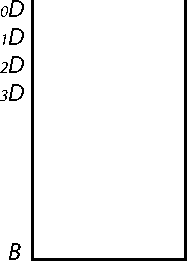
\includegraphics[width=0.21\textwidth]
{gesamttex/edit_VIII-4/images/LH_35_09_25_003_d3_003v.pdf}
\edcaption[0.25em]{%
\hspace*{4mm}%
\lbrack\textit{Fig.\:3}\rbrack%
}%
\end{edfigure}%
\pstart%
Sit ergo
\edtext{%
Hyperbola%
\indexS{hyperbola}%
}{%
\lemma{Hyperbola}%
\Cfootnote{%
Vgl. das Diagramm \lbrack\textit{Fig.\:4}\rbrack.%
}}
\edtext{%
cujus asymptotis \textit{BX},%
\indexS{asymptotos}
ordinatae%
}{%
\lemma{cujus}%
\Bfootnote{%
\textit{(1)}~ordinata %
\textit{(2)}~asymptotis \textit{BX}, ordinatae%
~\textit{L}%
}}
ad asymptoton $X\varPi$,
et
\edtext{%
sit in vacuo vas \textit{BC}%
\indexS{vas in vacuo}%
\indexS{vas comprimendum}%
\indexS{vacuum}%
}{%
\lemma{sit}%
\Bfootnote{%
\textit{(1)}~vas %
\textit{(2)}~in vacuo vas 
\textit{(a)}~\textit{AB} %
\textit{(b)}~\textit{BC}%
~\textit{L}%
}}
comprimendum a pondere%
\indexS{pondus comprimens vas}
$\varPi X$
continue augendo,%
\indexS{pondus augendum}
quantum opus est
\edtext{%
ut tum ab impetu concepto,%
\indexS{impetus conceptus}
tum a pondere accedente%
\indexS{pondus accedens}
continuetur%
}{%
\lemma{ut}%
\Bfootnote{%
\textit{(1)}~continuetur %
\textit{(2)}~tum ab %
\lbrack...\rbrack\ accedente continuetur%
~\textit{ L}}}
compressio%
\indexS{compressio aeris in vase}
usque
\edtext{%
ad \textit{A}.
Erunt gravitates%
\indexS{gravitas comprimens}%
}{%
\lemma{ad \textit{A}.}%
\Bfootnote{%
\textit{(1)}~Hinc erit %
\textit{(2)}~Erunt %
\textit{(a)}~continue %
\textit{(b)}~gravitates%
~\textit{L}%
}}
seu pondera%
\indexS{pondus comprimens vas}
ubique
ut ipsae $X\varPi$ ordinatae Hyperbolae,%
\indexS{hyperbola}
si ponamus primum pondus fuisse praecise
quale oportet
ut%
\lbrack,\rbrack\
si non augeretur%
\lbrack,\rbrack\
non amplius
comprimeret in\;\textit{C},
sed sustineretur.%
\indexS{pondus sustentum ab aere}
Quaeritur jam
quodnam pondus aequabile seu constans,%
\indexS{pondus aequabile}%
\indexS{pondus constans}
ex eadem altitudine \textit{CA} cadens%
\indexS{pondus cadens}%
\indexS{altitudo casus}
eundem effectum praestare potuisset.%
\indexS{effectus praestitus}
Aestimandum erit centrum gravitatis descensus%
\indexS{centrum gravitatis descensus}
seu summa descensus aequivalentis.%
\indexS{summa descensus aequivalentis}%
\indexS{descensus aequivalens}
Ponamus
\edtext{%
$CX = [X\varPi]$, 
dico pondus constans%
\indexS{pondus constans}%
}{%
\lemma{$CX\ =$}\Bfootnote{%
\bars{\textit{XP} \textit{ändert Hrsg.}} dico
\bars{dico \textit{gestr.}} pondus %
\textit{(1)}~uniforme\indexS{pondus uniforme} %
\textit{(2)}~constans%
~\textit{L}%
}}
quod ex \textit{C} cadens in \textit{A}%
\indexS{pondus cadens}
comprimit aerem \textit{CB}%
\indexS{pondus comprimens aerem}
in \textit{AB}
nec ultra esse ad pondus aliud constans%
\indexS{pondus constans}
quod ex \textit{C} cadens in \textit{((A))}%
\indexS{pondus cadens}
comprimit aerem \textit{CB}%
\indexS{pondus comprimens aerem}
in \textit{((A))B}
fore
\edtext{%
ut quadrilineum $\varPi CA\textit{(X)}$%
\indexS{quadrilineum}
divisum per \textit{CA}
ad quadrilin. $\varPi C\textit{((A))((X))}$%
\indexS{quadrilineum}
divisum per \textit{C((A))}.
Nimirum vis%
\indexS{vis effecta a corpore descendente}
quam efficit corpus
dicto modo auctum%
\indexS{corpus auctum}
suo descensu%
\indexS{descensus corporis comprimentis}
est
tum $X\varPi$ prima
seu \textit{CX} ductum in \textit{CA},%
}{%
\lemma{ut}%
\Bfootnote{%
\textit{(1)}~quinquilineum\indexS{quinquilineum} %
\textit{(2)}~quadrilineum $\varPi CA\textit{(X)}$ %
\bars{%
\textit{(1)}~ductum in %
\textit{(2)}~divisum per \textit{CA} %
\textit{erg.}} ad quadrilin. %
\lbrack...\rbrack\ \textit{C((A))}. Nimirum %
\textit{(a)}~corpus $X\varPi$ %
\textit{(b)}~vis quaesita descen\indexS{vis quaesita descensu} %
\textit{(c)}~vis quam %
\lbrack...\rbrack\ est tum
\textit{(aa)}~\textit{X} du %
\textit{(bb)}~$X\varPi$ 
\textit{(aa)}~ductum %
\textit{(bb)}~prima %
\textit{(aaa)}~du %
\textit{(bbb)}~seu \textit{CX} ductum in \textit{CA},%
~\textit{L}%
}}
tum differentia quaelibet
quae est
$\dfrac{\varPi}{xx} d\overline{x}$
ducta in \textit{x},
quae facit
$\dfrac{\varPi}{x}d\overline{x}$.
\pend%
\newpage%
\begin{edfigure}[0.0em][1.0em]%
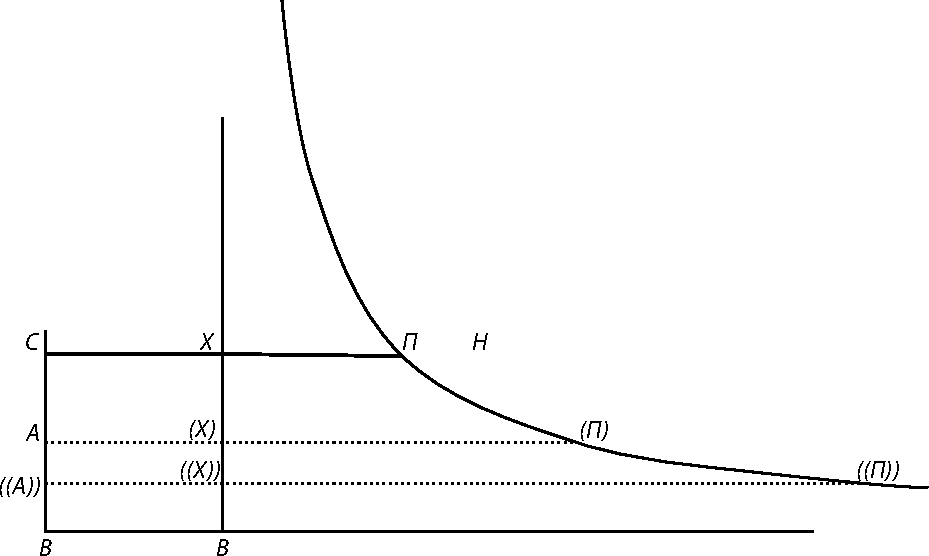
\includegraphics[width=0.94\textwidth]
{gesamttex/edit_VIII-4/images/LH_35_09_25_003-d4_003v.pdf}
\edcaption[0.25em]{%
\lbrack\textit{Fig.\:4}\rbrack%
\edtext{}{%
\lemma{\textit{Zum Diagramm} \lbrack\textit{Fig.\:4}\rbrack:}%
\Afootnote%
[nonum]%
{%
$BX = 1 = [X\varPi]\textsuperscript{[\text{a}]} = XC$.
\quad%
$B\textit{(X)} = \dfrac{1}{10}$.
\quad%
$\varPi \textit{X(X)}\varPi$
circiter est $18 + \dfrac{1}{\langle25\rangle}$,
dividatur per \textit{CA} 
seu $\dfrac{10}{9}$
fit circiter $\dfrac{167}{100}$,%
\textsuperscript{[b]}
cui addatur
\textit{CX} seu 1,
fit $\dfrac{267}{100}$,
multiplicanda per 2100
fit 267 per 21,
pondus quod cadens ex alt. \textit{CA}%
\indexS{altitudo casus}
$\dfrac{10}{9}$ pedis in vacuo%
\indexS{pes}%
\indexS{vacuum}%
\indexS{in vacuo}
deprimere potest aerem.%
\indexS{pondus deprimens aerem}
\\[1.5ex]%
{\footnotesize%
\textsuperscript{[a]}~\textit{XP} \textit{L ändert Hrsg.}
\quad%
\textsuperscript{[b]}~circiter $\dfrac{167}{100}$:
Das ungefähre Ergebnis ist um den Faktor 10 zu klein.%
}%
}}%
}%
\pagelabel{LH_35_09_25_003_003v_Fig4}%
\end{edfigure}
\pstart%
\noindent%
\edlabel{LH_35_09_25_003_003v_nld-1}%
Ergo summa differentiarum
in suos descensus ductarum%
\indexS{descensus corporis comprimentis}
est
$\displaystyle\varPi\!\!\int\!\!\dfrac{1}{x}$
\edtext{%
seu repraesentatur%
}{%
\lemma{seu}%
\Bfootnote{%
\textit{(1)}~est %
\textit{(2)}~repraesentatur%
~\textit{L}%
}}
per ipsum spatium
\edtext{%
\lbrack$\varPi X \textit{(X)(}\varPi\textit{)}$\rbrack,%
}{%
\lemma{$\varPi X \textit{(X)((}\varPi\textit{))}$}%
\Bfootnote{%
\textit{L\;ändert Hrsg.}%
}}
cui si addas \textit{CX} in \textit{CA}
seu $\varepsilon$
\edtext{%
in \textit{x}
quae repraesentatur per rectang.
\lbrack\textit{XCA}\rbrack,
habebimus
\lbrack$XCA + \varPi X\textit{(X)(}\varPi\textit{)}$\rbrack,
seu%
}{%
\lemma{in \textit{x}}%
\Bfootnote{%
\textit{(1)}~habebimus %
\textit{(2)}~quae repraesentatur per rectang. %
\bars{\textit{C((A))} \textit{ändert Hrsg.}}, habebimus %
\bars{$C\textit{((A))} + \varPi X\textit{(X)(}\varPi\textit{)}$ \textit{ändert Hrsg.}}, seu%
~\textit{L}%
}}
$\varPi CA\textit{(}\varPi\textit{)}$
figuram%
\indexS{figura repraesentans vim descensus}
quae vim descensus talis corporis repraesentat.%
\indexS{vis descensus corporis comprimentis}
Quaerenda est ergo recta \textit{CH}
quae ducta in \textit{CA}
faciat rectangulum
$HCA = \text{quadrilineo}\ \varPi \textit{CA(}\varPi\textit{)}$,
cujus
\edtext{%
rectae \textit{CH} descensus ex \textit{CA}%
}{%
\lemma{rectae}%
\Bfootnote{%
\textit{(1)}~descensus ex \textit{CA} 
\textit{(2)}~\textit{CH} descensus ex \textit{CA}%
~\textit{L}%
}}
tantundem efficit
quantum ipsius $X\varPi$ continuae auctae
pro resistentia crescente,%
\indexS{resistentia aeris ad compressionem}
descensus ex \textit{CA}.
Sint ergo \textit{BX} seu \textit{CB} pedes 10
et \textit{B(X)} seu \textit{BA} pes 1.
Quaeratur logarithmus
\edtext{%
Hyperbolicus%
\indexS{logarithmus hyperbolicus}%
}{%
\lemma{Hyperbolicus}\Bfootnote{%
\textit{erg.\;L}%
}}
\textit{B(X)} ad \textit{BX}
seu \textit{BA} ad \textit{BC}
repraesentans area
$\varPi X\textit{(X)(}\varPi\textit{)}$
seu log. 10 ad 1.
Is multiplicetur per 2100 libras,%
\indexS{libra}
has enim repraesentat $X\varPi$
seu \textit{CX}
seu
\edtext{%
pondus.
Deinde rectang. \textit{CA(X)} divis. per \textit{CA}
seu recta \textit{CX} vel $X\varPi$ seu 1
multiplicetur etiam per 2100,%
}{%
\lemma{pondus.}%
\Bfootnote{%
\textit{(1)}~Deinde \textit{CA} %
\textit{(a)}~multipli %
\textit{(b)}~seu 9 multiplicetur etiam per 2100 libras, seu $1-\dfrac{1}{10}$ multiplicetur per easdem sed ambae summae addantur %
\textit{(2)}~Deinde rectang. %
\lbrack...\rbrack\ etiam per 2100,%
~\textit{L}%
}}
fiet
$2100 + 2100$ in Log. Hyp. de 10 ad 1,%
\indexS{logarithmus hyperbolicus}
id est $X\varPi$ %
est minor $\langle\varepsilon\rangle$.%
\edlabel{LH_35_09_25_003_003v_nld-2}%
\pend
\selectlanguage{latin}%
\frenchspacing%
\normalsize%
\newpage%




\chapter[tocentry={Principium demonstrandi perutile in geometria et mechanica
\enskip%
\bracks{September 1686 -- Frühjahr 1695~(?)}},
head={Principium demonstrandi perutile}]%
{\MakeUppercase{Principium demonstrandi perutile in geometria et mechanica%
}
\newline%
\bracks{September 1686 -- Frühjahr 1695~(?)}}
\label{39978}
\selectlanguage{ngerman}%
\frenchspacing%
\begin{ledgroupsized}[r]{120mm}%
\footnotesize%
\pstart%
\noindent\textbf{Überlieferung:}%
\pend%
\end{ledgroupsized}%
\begin{ledgroupsized}[r]{114mm}%
\footnotesize%
\pstart%
\parindent -6mm%
\makebox[6mm][l]{\textit{L}}%
Aufzeichnung:
LH XXXV~1,\;9 Bl.\;30.
Ein Zettel;
Ränder zum Teil beschnitten und unregelmäßig.
Eineinhalb Seiten;
Textfolge:
Bl.\;\href{\Scan{LH_35_01_09_030v}}{30\,v\textsuperscript{o}},%
~\href{\Scan{LH_35_01_09_030r}}{30\,r\textsuperscript{o}}.
\pend%
\end{ledgroupsized}%
\vspace{5mm}%
\begin{ledgroup}%
\footnotesize%
\pstart%
\noindent%
\textbf{Datierungsgründe:}
Die Datierung der Aufzeichnung N.\;\ref{39978} beruht auf inhaltlichen Betrachtungen.
Siehe die ausführliche Begründung auf S.\;\pageref{39978_dat}.%
\pend%
\end{ledgroup}%
\selectlanguage{latin}%
\frenchspacing%
\vspace{8mm}%
\normalsize%
\pstart%
\noindent%
\bracks{%
\href{\Scan{LH_35_01_09_030v}}%
{30\,v\textsuperscript{o}}%
}
\edlabel{LH_35_01_09_030_030v_vdf-1}%
Inter principia demonstrandi%
\indexS{principium demonstrandi}
in Geometria%
\indexS{geometria}
et Mechanica%
\indexS{mechanica}
\edtext{%
perutilia,%
\indexS{principium perutile in geometria et mechanica}
etiam%
}{%
\lemma{perutilia,}%
\Bfootnote{%
\textit{(1)}~et %
\textit{(2)}~etiam%
~\textit{L}%
}}
hoc est ex natura continui%
\indexS{natura continui}%
\indexS{continuum}
a me sumtum,%
\indexS{principium sumtum e natura continui}
quod in rebus continue variabilibus,%
\indexS{res variabilis continue}
paulatim non momento
quantitas aliqua acquiritur
vel amittitur.%
\edlabel{LH_35_01_09_030_030v_vdf-2}%
\indexS{quantitas acquisita vel amissa paulatim}
\pend%
\begin{edfigure}[1.750em][1.50em]%
\includegraphics[scale=1.05]%
{gesamttex/edit_VIII-4/images/LH_35_01_09_030_d_030v.pdf}
\edcaption[0.5em]{%
\bracks{\textit{Fig.\:1}}%
}%
\end{edfigure}
\pstart%
Sic demonstro
\edlabel{LH_35_01_09_030_030v_prdem-1}%
\edtext{%
(contra Libellatorum metallicorum praxin)%
\indexS{praxis libellatorum metallicorum}%
\indexS{libellator metallicus}%
}{%
\lemma{(contra}%
\Bfootnote{%
\textit{(1)}~Libellatores %
\textit{(2)}~Libellatorum %
\bars{metallicorum \textit{erg.}} praxin)%
~\textit{L}%
}%
\lemma{Libellatorum metallicorum praxin}%
\Cfootnote{%
Im wissenschaftlich-technischen Sprachgebrauch der Frühneuzeit waren \textit{libellatores} im Allgemeinen die "Vermesser".
Im Bergbau bezeichnete dieser Begriff die Markscheider.
}%
}%
\edlabel{LH_35_01_09_030_030v_prdem-2}
funiculum \textit{CD}
ad horizontem inclinatum%
\indexS{funiculum inclinatum}%
\indexS{horizon}%
\bracks{,}
a
\edtext{%
pondere in medio~\textit{B} appenso%
\indexS{pondus appensum funiculo}%
}{%
\lemma{pondere}%
\Bfootnote{%
\textit{(1)}~\textit{BC} %
\textit{(2)}~in medio \textit{B} appenso%
~\textit{L}%
}}
inaequaliter tendi,%
\indexS{funiculum tensum inaequaliter}
magis supra in \textit{BD} %
quam infra in \textit{BC}.
Quoniam
si filum \textit{DC} continue erigi ponatur,%
\indexS{filum inclinatum continue erectum}
donec ex inclinato fiat%
\indexS{filum factum ex inclinato verticale}
\edtext{%
vertical\bracks{e},%
\indexS{filum verticale}%
}{%
\lemma{verticali}%
\Bfootnote{%
\textit{L\;ändert Hrsg.}%
}}
utique in transitu illo ultimo%
\indexS{transitus ultimus}
ubi perpendiculare fit,%
\indexS{filum perpendiculare}
sola pars \textit{BD} tenditur
a
\edtext{%
pondere \textit{B},%
\indexS{pondus appensum funiculo}%
}{%
\lemma{pondere}%
\Bfootnote{%
\textit{(1)}~\textit{BC} %
\textit{(2)}~\textit{B},%
~\textit{L}%
}}
pars autem inferior \textit{BC}
nullo modo.
Quod
si ergo antea aequalis fuisset utriusque tensio%
\indexS{tensio funiculi inclinati}
sub quacunque inclinatione%
\indexS{inclinatio funiculi tensi}%
\bracks{,}
necesse
\edtext{%
esset
momento transitus%
\indexS{momentum transitus}
totam medietatem tensionis%
\indexS{medietas tensionis}
ab uno amitti,
ab altero aequari.%
}{%
\lemma{esset}%
\Bfootnote{%
\textit{(1)}~\angles{vel} %
\textit{(2)}~momento transitus %
\bracks{...} altero aequari.%
~\textit{L}%
}}
\bracks{%
\href{\Scan{LH_35_01_09_030r}}%
{30\,r\textsuperscript{o}}%
}
\pend%
\newpage%
\pstart%
Quod
si quis asserat
aliquandiu aequalem manere tensionem%
\indexS{tensio funiculi inclinati}
sub aliquibus inclinationibus,%
\indexS{inclinatio funiculi tensi}
inde alicubi incipere decrescere,
v.\,g.
sub inclinatione 45 graduum?%
\indexS{inclinatio 45 graduum}
Ejus initii ratio reddi non potest.%
\indexS{ratio initii reddenda}
Cur citra illum limitem%
\indexS{limes}%
\bracks{,}
nullum fiat
\edtext{%
tensionis%
}{%
\lemma{tensionis}%
\indexS{tensio funiculi inclinati}%
\Bfootnote{%
\textit{erg.\;L}%
}}
decrementum%
\indexS{decrementum tensionis}
inter mutandum
\edtext{%
situm;%
\indexS{situs mutandus}%
}{%
\lemma{situm}%
\Bfootnote{%
\textit{erg.\;L}%
}}
supra illum fiat?
\pend%
\vspace{2.0em}%
\pstart%
\noindent%
\centering%
*     *     *
\pend%
\vspace{2.0em}%
\selectlanguage{german}%
\frenchspacing%
\footnotesize%
\pstart%
\noindent%
\textls{Ausführliche Datierungsgründe:}%
\pagelabel{39978_dat}
Der Träger der vorliegenden Aufzeichnung N.\;\ref{39978} weist weder Spuren eines Wasserzeichens noch irgendein äußeres datierungsrelevantes Merkmal auf.
Das "aus der Natur des Kontinuums" gewonnene und "in der Geometrie und der Mechanik überaus nützliche" Prinzip, das im Mittelpunkt der Aufzeichnung steht, ist zweifelsohne das Kontinuitätsprinzip (vgl. oben, \refpassage{LH_35_01_09_030_030v_vdf-1}{LH_35_01_09_030_030v_vdf-2}).
Dessen heuristische Anwendung als \textit{principium demonstrandi}, wie sie in der Aufzeichnung N.\;\ref{39978} exemplifiziert wird, lässt sich im Leibniz-Nachlass bis zum Anfang 1678 zurückverfolgen;
vgl. etwa \textit{De corporum concursu}, scheda~III, lemma~1 (\textit{LSB} VIII,\;3 N. 58\textsubscript{4}, S.\;563\,f., bes. S.\;563.19--564.3).\cite{01401}
Es ist auszuschließen, dass die vorliegende Aufzeichnung N.\;\ref{39978} vor Anfang 1678 entstand.
Denn anders als in \textit{LSB} VIII,\;3 N. 58\textsubscript{4}\cite{01401} wird das Kontinuitätsprinzip in der Aufzeichnung N.\;\ref{39978} als selbständiger und bereits "angenommener" (\textit{sumptum}) Grundsatz dargestellt.
\pend%
\pstart%
Die erste öffentliche Ankündigung des Kontinuitätsprinzips erfolgte wohl in dem \textit{Extrait d’une lettre sur un principe general utile à l'explication des loix de la nature par la consideration de la sagesse divine}, den Leibniz im Juliheft 1687 der \textit{Nouvelles de la république des lettres} drucken ließ (S.\;744–753; \textit{LPG}~III, S.\;51–55).\cite{02054}
Auch der von Leibniz in den letzten Monaten des Jahres 1688 in Wien\indexO{Wien} verfasste Entwurf \textit{Principium quoddam generale non in mathematicis tantum sed et physicis utile} (\textit{LSB} VI,\;4 N.\;371),\cite{02055} thematisiert das Kontinuitätsprinzip ausführlich.
In beiden Texten wird der heuristische Nutz dieses Prinzips in den strengen Wissenschaften -- in den mathematischen sowie in den physischen -- ausdrücklich hervorgehoben.
Inhaltlich stimmt die vorliegende Aufzeichnung N.\;\ref{39978} mit diesem Ansatz überein und könnte zu einer ähnlichen oder späteren Zeit entstanden sein.
\pend%
\pstart%
Diese Feststellung lässt sich ebenfalls durch die Anspielung auf die \textit{Libellatorum metallicorum praxis} im Text (\refpassage{LH_35_01_09_030_030v_prdem-1}{LH_35_01_09_030_030v_prdem-2}) bestätigen.
Im Staatsarchiv Hannover\indexO{Hannover} waren bis 1943 zwei Manuskripte von Leibnizens Hand erhalten, welche die Überschriften \textit{Chordae tensae libellator}\bracks{\textit{um}} und \textit{Libellatio} trugen und somit wohl eben jener "Tätigkeit der Markscheider" gewidmet waren, die in der Aufzeichnung N.\;\ref{39978} erwähnt wird;
vgl. NLA~HA~MS Nr.\;59 (früher: Hannover, HStA Ms.\;E\;3) Bl.\;330 u.\;331.\cite{02553}\cite{02554}
Beide Manuskripte, die heute als Kriegsverlust gelten,
waren auf den 29.\;August (8.\;September) 1686 datiert.
Es ist zu vermuten,
dass die Aufzeichnung N.\;\ref{39978} im Zusammenhang mit diesen Texten verfasst wurde, oder zumindest nicht vor ihnen.
Weitere heute verschollene Texte des Hannoveraner\indexO{Hannover} Staatsarchivs zeigten, dass Leibniz sich im gleichen Sommer -- wohl an der Hand von Nikolaus \textsc{Voigtel}s gerade veröffentlichter \textit{Geometria subterranea} (Eisleben 1686)\cite{02556} -- intensiv mit der Markscheidekunst und der mit ihr verwandten Wägekunst beschäftig haben soll;
siehe hierzu \textsc{R.\;Koser}, "Über die Sammlung von Leibniz-Handschriften im Staatsarchiv zu Hannover",
\ledpb%
\textit{Sitzungsberichte der königlich preußischen Akademie der Wissenschaften zu Berlin} XXV (1902), S.\;565.\cite{02555}
Demgemäß wäre eine Anspielung auf die Tätigkeit der \textit{libellatores metallici} wie die, die in der Aufzeichnung N.\;\ref{39978} (\refpassage{LH_35_01_09_030_030v_prdem-1}{LH_35_01_09_030_030v_prdem-2}) vorkommt, vor dem Sommer 1686 weniger wahrscheinlich gewesen.
Hieraus ergibt sich der wahrscheinlichste Terminus post quem der Datierung.%
\pend%
\pstart%
Ein plausibler Terminus ante quem lässt sich aus folgender terminologischer Beobachtung gewinnen.
Das Kontinuitätsprinzip wird in der Aufzeichnung N.\;\ref{39978} zwar unmissverständlich angesprochen, aber noch nicht mithilfe eines spezifischen "Fachbegriffs".
Auch angesichts des bescheidenen Umfangs der Aufzeichnung hätte Leibniz einen solchen Begriff wohl verwendet, wenn dieser sich in seinem Sprachgebrauch bereits etabliert hätte.
In dem nur handschriftlich überlieferten zweiten Teil seines \textit{Specimen dynamicum} etwa bedient er sich durchaus des "Fachbegriffs" \textit{lex continuitatis}, wenn er auf das Kontinuitätsprinzip Bezug nimmt (vgl. etwa \textit{LGM}~VI, S.\;249).\cite{02557}\cite{01043}
Dieser Umstand kann als Zeichen gedeutet werden, dass die Aufzeichnung N.\;\ref{39978} zu einem früheren Zeitpunkt entstand.
Den zweiten Teil von Leibnizens \textit{Specimen dynamicum} hatte Otto Mencke\indexN{\textls{Mencke} (Menken, Menkenius, Menque), Otto 1644\textendash1707} für eine Veröffentlichung im Maiheft 1695 der \textit{Acta eruditorum} vorgesehen,\cite{01023} wie dies sich seinem Brief an Leibniz vom 13./23.\;März desselben Jahres entnehmen lässt (\textit{LSB} I,\;11 N.\;238 S.\;342.6--8).\cite{02558}
Zu dieser Veröffentlichung ist es freilich nie gekommen:
Mitte September und Anfang November 1695 wartete Mencke\indexN{\textls{Mencke} (Menken, Menkenius, Menque), Otto 1644\textendash1707} noch vergeblich darauf, dass Leibniz den zweiten Teil des \textit{Specimen dynamicum} übersenden würde (vgl. \textit{LSB} I,\;11 N.\;471, S.\;695.6--11;\cite{02559} I,\;12 N.\;109, S.\;126.9--12).\cite{02560}
Unter der Voraussetzung aber, dass der zweite Teil des \textit{Specimen dynamicum} ungefähr zur gleichen Zeit entstand wie der im Aprilheft 1695 der \textit{Acta eruditorum} veröffentlichte erste Teil (S.\;145--157;\cite{02032} \textit{LMG}~VI, S.\;234--246)\cite{01043} oder nicht wesentlich später, dürfte auch die Aufzeichnung N.\;\ref{39978} spätestens im Frühjahr 1695 verfasst worden sein, wahrscheinlich aber früher.
\pend%
\pstart%
Aus den angegebenen Gründen ergibt sich schließlich für die vorliegende Aufzeichnung N.\;\ref{39978} folgende Gesamtdatierung:
Eine Entstehung vor September 1686 (jedenfalls nach 1677) ist nicht auszuschließen, aber unwahrscheinlich;
N.\;\ref{39978} dürfte auch nicht viel später verfasst worden sein, jedenfalls nicht nach dem Frühjahr 1695; eine spätere Entstehung ist aber möglich.
\pend%
\selectlanguage{latin}%
\frenchspacing%
\normalsize%




\chapter[tocentry={Problema thermometri aequaliter dividendi
\enskip \lbrack Zweite Hälfte April 1689 \textendash\ 20. Februar 1690\rbrack},
head={Problema thermometri aequaliter dividendi}]%
{\MakeUppercase{Problema thermometri aequaliter dividendi}
\newline \lbrack Zweite Hälfte April 1689 \textendash\ 20. Februar 1690\rbrack}
\label{60270+RK60326}


\footnotesize%
\pstart%
\noindent%
Das Stück N.\;\ref{60270} ist auf Papier geschrieben, wie es Leibniz für die Abfassung der \textit{Dynamica}\cite{01354} während seines Aufenthaltes in Rom\indexO{Rom} verwendete. Dort traf er am 14. April 1689 ein, so dass N.\;\ref{60270} erst danach entstanden sein kann.  Darin finden sich zwei Verweise auf die \textit{Dynamica}\cite{01354}, die Leibniz beide nachträglich ergänzt und präzisiert, einmal unter Angabe der Proposition mit genauer Nummer, das andere Mal mit Bezug auf eine nicht gezählte Proposition im zweiten Teil der \textit{Dynamica}\cite{01354} (\refpassage{LH_37_04_169-170_21a}{LH_37_04_169-170_21b} und \refpassage{LH_37_04_169-170_22a}{LH_37_04_169-170_22b}). 
\pend
\pstart
Noch auf der Rückreise nach Deutschland schreibt Leibniz am 20. Februar 1690 aus Venedig\indexO{Venedig} an Rudolf Christian von Bodenhausen\indexN{\textls{Bodenhausen} (Bodenus, Bodenausen), Rudolf Christian, Freiherr v. 1698}: Er kündigt ihm weitere Teile für die \textit{Dynamica}\cite{01354} an, um dieses Werk für eine Reinschrift zu vervollständigen, darunter auch eine Schrift über den „Modum construendi Thermometrum accurate divisum“. Dabei handelt es sich aller Wahrscheinlichkeit nach um das vorliegende Stück N.\;\ref{60270}. Das „päckchen“ mit diesem und weiteren Nachträgen zu den \textit{Dynamica}\cite{01354} werde von Bodenhausen\indexN{\textls{Bodenhausen} (Bodenus, Bodenausen), Rudolf Christian, Freiherr v. 1698} durch Friedrich von Walter\indexN{\textls{Walter}, Friedrich von gest. 1718} überbracht werden (Brief an R.\,C.\,v.\,Bodenhausen, 20.02.1690,\cite{01527} \textit{LSB} III,\;4 N.\;236, S.\;462.21-463.5, 464.6-7 und S.\;464 Anm. zu N.\;236). Am 4. März bestätigt von Bodenhausen\indexN{\textls{Bodenhausen} (Bodenus, Bodenausen), Rudolf Christian, Freiherr v. 1698}, dieses „Päcklein“ durch von Walter\indexN{\textls{Walter}, Friedrich von gest. 1718} erhalten zu haben, so dass Leibniz davon ausgehen kann, von Bodenhausen\indexN{\textls{Bodenhausen} (Bodenus, Bodenausen), Rudolf Christian, Freiherr v. 1698} habe darin „auch einen bogen gefunden“, der die „ratio Thermometri exacte in gradus dividendi“ enthalte (Leibniz an R.\,C.\,v.\,Bodenhausen, 18.03.1690, \textit{LSB} III,\;4 N.\;245\cite{01392}, S.\;485.1-11; R.\,C.\,v.\,Bodenhausen an Leibniz, 04.03.1690, \textit{LSB} III,\;4 N.\;241\cite{01389}, S.\;470.13-16). Im Folgenden zählt von Bodenhausen\indexN{\textls{Bodenhausen} (Bodenus, Bodenausen), Rudolf Christian, Freiherr v. 1698}  die „ratio dividendi Thermometrum“ dennoch zu denjenigen Nachträgen, die Leibniz zwar angekündigt habe, die ihm aber noch fehlten (R.\,C.\,v.\,Bodenhausen an Leibniz, 29.07.1690, \textit{LSB} III,\;4 N.\;268\cite{01393}, S.\;539.5-7). Leibniz bekräftigt hingegen, dass von Bodenhausen\indexN{\textls{Bodenhausen} (Bodenus, Bodenausen), Rudolf Christian, Freiherr v. 1698} dieses Stück schon bekommen haben müsse  (Leibniz an R.\,C.\,v.\,Bodenhausen, Aug. 1690,\cite{01528} \textit{LSB} III,\;4 N.\;272, S.\;553.10-11), 
woraufhin von Bodenhausen\indexN{\textls{Bodenhausen} (Bodenus, Bodenausen), Rudolf Christian, Freiherr v. 1698} ihm erklärt, dass es in der durch von Walter\indexN{\textls{Walter}, Friedrich von gest. 1718} zugestellten Sendung nicht enthalten gewesen sei (R.\,C.\,v.\,Bodenhausen an Leibniz, 16.09.1690,\cite{01535} \textit{LSB} III,\;4 N.\;273, S.\;558.2-6). 
Auch wenn er sich einen Verlust nicht erklären könne, hält Leibniz auf diese Nachricht hin das „problema Thermometri aequaliter dividendi“ für verloren und für schwer zu ersetzen (Leibniz an R.\,C.\,v.\,Bodenhausen, 26.10./05.11.1690, \textit{LSB} III,\;4 N.\;285\cite{02132}, S.\;630.5-8). Noch in fünf weiteren Briefen erinnert von Bodenhausen\indexN{\textls{Bodenhausen} (Bodenus, Bodenausen), Rudolf Christian, Freiherr v. 1698} daran, dass ihm die „constructio Thermometri“ immer noch fehle (R.\,C.\,v.\,Bodenhausen an Leibniz:  \textit{LSB} III,\;4 N.\;288, S.\;649.14-16 (11.11.1690)\cite{01530}; \textit{LSB} III,\;4 N.\;295, S.\;681.2-4 (12.12.1690)\cite{01531}; \textit{LSB} III,\;5 N.\;3, S.\;31.1-8 (19.01.1691)\cite{01532}; \textit{LSB} III,\;5 N.\;25, S.\;126.8 (23.06.1691)\cite{01394}; \textit{LSB} III,\;5 N.\;125, S.\;474.22-23 (16.01.1693)\cite{01533}). Leibniz gesteht ihm 1693 ein, nicht zu wissen wo seine „Meditationes de Thermometro accurate dividendo“ stecken könnten, hegt aber die Hoffnung, dass sie ihm unter seinen Papieren dereinst wieder „unter die hand kommen müßen“; zugleich macht er von Bodenhausen\indexN{\textls{Bodenhausen} (Bodenus, Bodenausen), Rudolf Christian, Freiherr v. 1698} Mut, solch eine Gradeinteilung des Thermometers selbst finden zu können, da dies nicht schwer sei (Leibniz an R.\,C.\,v.\,Bodenhausen, 12./22.07.1693,\cite{01529} \textit{LSB} III,\;5 N.\;171, S.\;601.4-10). Offenbar unternimmt von Bodenhausen hierauf einen eigenständigen Versuch dazu, bei dem er Leibniz um Hilfe bittet (R.\,C.\,v.\,Bodenhausen an Leibniz, 05.09.1693,\cite{01534} \textit{LSB} III,\;5 N.\;182, S.\;626.1-6).
\pend
\pstart
Es ist anzunehmen, dass es sich bei N.\;\ref{60270} um jenes Stück für die \textit{Dynamica}\cite{01354} handelt, das von Bodenhausen\indexN{\textls{Bodenhausen} (Bodenus, Bodenausen), Rudolf Christian, Freiherr v. 1698} nie erhalten hat. Damit war es, anders als Leibniz und von Bodenhausen\indexN{\textls{Bodenhausen} (Bodenus, Bodenausen), Rudolf Christian, Freiherr v. 1698} in den Jahren 1690 bis 1693 glaubten, nicht verloren gegangen. Wenn es sich bei N.\;\ref{60270}  um dasjenige Stück handelt, das Leibniz seiner Überzeugung nach an von Bodenhausen\indexN{\textls{Bodenhausen} (Bodenus, Bodenausen), Rudolf Christian, Freiherr v. 1698} geschickt hatte, muss er seine Arbeit daran spätestens zu dem Zeitpunkt beendet haben, als er davon ausging, es an von Walter\indexN{\textls{Walter}, Friedrich von gest. 1718} übergeben zu haben: Als \textit{terminus ante quem} ergibt sich daraus für N.\;\ref{60270} der 20. Februar 1690.
Nicht auszuschließen ist, dass Leibniz später selbst das womöglich nur vermeintlich abgeschickte Stück unter seinen Papieren (wie er erhoffte) wiederentdeckte; für eine weitere Bearbeitung desselben, die dann nach dem 22. Juli 1693 erfolgt sein müsste, oder für spätere Hinweise auf dieses Stück gibt es bislang aber keine Anhaltspunkte.
\pend
\pstart
N.\;\ref{60326} ist allem Anschein nach ebenfalls auf römischem Papier geschrieben und dürfte in demselben Zeitraum entstanden sein wie \ref{60270}. N.\;\ref{60326} diente Leibniz als Arbeitsgrundlage für seine Ausarbeitung des Themas in \ref{60270}, die in mehreren Anläufen erfolgt. 
Leibniz führt in N.\;\ref{60326} Rechnungen aus, deren Ergebnisse er für N.\;\ref{60270} übernimmt (\refpassage{LH_37_04_169-170_20a}{LH_37_04_169-170_20b}), beruft sich in N.\;\ref{60270} auf seine Ausführungen in N.\;\ref{60326} (\refpassage{LH_37_04_169-170_19a}{LH_37_04_169-170_19b}); in N.\;\ref{60270} arbeitet er anfangs noch mit einer frühen Fassung von Fig.~2, die sich nur in N.\;\ref{60326} erkennen lässt (\refnote{LH_37_04_169-170_21ab}), bevor er diese Zeichnung korrigiert und eine neue dafür in N.\;\ref{60270} (Fig.~2) erstellt; er benutzt in N.\;\ref{60270} unvermittelt Größen ($\varepsilon$, \textit{V} bzw. \textit{Y}), die er in N.\;\ref{60326} herleitet; die Bezeichnung für die Größen \textit{V} bzw. \textit{Y} ändert Leibniz im Laufe der Ausarbeitung von N.\;\ref{60270} und dokumentiert dies nachträglich in N.\;\ref{60326} (\refpassage{LH_37_05_108_01a}{LH_37_05_108_01b}).%
\pend
\selectlanguage{latin}%
\frenchspacing%
\normalsize%







\section[tocentry={Rechnungen und Zeichnungen},
head={Rechnungen und Zeichnungen}]%
{\MakeUppercase{Rechnungen und Zeichnungen}}
\label{60326}

\begin{ledgroupsized}[r]{120mm}
\footnotesize
\pstart
\noindent\textbf{Überlieferung:}
\pend
\end{ledgroupsized}
\begin{ledgroupsized}[r]{114mm}
\footnotesize
\pstart
\parindent -6mm
\makebox[6mm][l]{\textit{L}}%
Aufzeichnung: LH XXXVII 5 Bl. 108. Ein Blatt 8\textsuperscript{o}; Papiererhaltungsmaßnahmen. Zwei Seiten.
\pend
\end{ledgroupsized}
\selectlanguage{latin}		%
\vspace{8mm}
\pstart
\noindent
\href{\Scan{LH_037_05_108r}}%
{\lbrack108~r\textsuperscript{o}\rbrack}%
\pend
\begin{edfigure}[1.5em]%
\vspace{-1em}
\hfill%
\hspace*{5mm}%
\includegraphics[scale=1]{%
gesamttex/edit_VIII-4/images/LH_037_05_108_d1_108r.pdf}%
\hfill%
\includegraphics[scale=1]{%
gesamttex/edit_VIII-4/images/LH_037_05_108_d2_108r.pdf}%
\hfill%
\edcaption[1em]{%
\lbrack\textit{Fig.~1}\rbrack%
\hspace*{41mm}%
\lbrack\textit{Fig.2}\rbrack%
\hspace*{5mm}
\edtext{}{%
\lemma{}%
\Afootnote[nonum]{%
\edlabel{LH_37_05_108_05a}%
\textit{Am Rand von \bracks{Fig.~2}:}\\
\textit{PF} vel \textit{P\greek{f}} %
$=N-\varepsilon$ vel $\varepsilon-N$\bracks{,} %
$D=Q\langle D\rangle$\bracks{,} %
sed $M=GF$\bracks{,} %
$GF-QP= %
FP+GQ= %
FP+CT=\text{bis}\;CT$.
Ergo $M-D=\text{bis}\;\overline{N-\varepsilon}$.%
\edlabel{LH_37_05_108_05b}%
}}%
}%
\end{edfigure}%
\pstart%
\noindent%
\edtext{%
Capacitas totius \textit{A} partis \textit{PQ}
\edtext{sit \textit{B} spatium}{%
\lemma{sit \textit{B}}%
\Bfootnote{%
\textit{(1)}~quantitas
\textit{(2)}~spatium~\textit{L}}}
hydrargyri\indexS{spatium hydrargyri} \textit{G}
\edtext{et \textit{QX} sit \textit{H}}{%
\lemma{}%
\Bfootnote{et \textit{QX} sit \textit{H} \textit{erg.~L}}}%
\lbrack ,\rbrack\ \textit{PX} sit $B-H$ %
\edtext{et}{\lemma{}\Bfootnote{et \textit{erg.~L}}}
erit spatium\indexS{spatium aeris} aeris
\edtext{primum \textit{STV},}{%
\lemma{}%
\Bfootnote{%
\bars{primum \textit{erg.}}
\textit{(1)}~\textit{AC}
\textit{(2)}~\textit{SV}
\textit{(3)}~\textit{STV}~\textit{L}}}%
erit $A-G-B+H$. 
}{%
\lemma{Capacitas \bracks{...} $A-G-B+H$.}%
\Cfootnote{Die Buchstaben beziehen sich womöglich auf teils gestrichene oder ersetzte Bezeichnungen in einer früheren Fassung von \bracks{\textit{Fig.~2}}.}
}
Sed spatium %
\edtext{aeris\indexS{spatium aeris} mutatione}{%
\lemma{aeris}%
\Bfootnote{%
\textit{(1)}~post m
\textit{(2)}~mutatione~\textit{L}}}
facta
\edtext{est $A-G-B+C$. Et}{%
\lemma{est $A-G-B+C$.}%
\Bfootnote{%
\textit{(1)}~Sunt ergo
\textit{(2)}~Ergo
\textit{(3)}~Et~\textit{L}}}
densitas\indexS{densitas aeris} mutatione
\edtext{facta est}{%
\lemma{}%
\Bfootnote{%
facta \bars{\textit{AG} \textit{gestr.}} 
est~\textit{L}}}
ad priorem ut spatium prius aeris\indexS{spatium aeris} ad posterius. Sed pondus
\begin{tabular}{c}
posterius\\ prius
\end{tabular}
est ad
\begin{tabular}{c}
prius\\ posterius
\end{tabular}
\edtext{ut \textit{C} ad \textit{H}. }{%
\lemma{ut}%
\Bfootnote{%
\textit{(1)}~\textit{C} ad \textit{I}
\textit{(2)}~\textit{H} ad \textit{C}
\textit{(3)}~\textit{C} ad \textit{H}~\textit{L}}}%
Et calores\indexS{calor} sunt in ratione directa ponderum\indexS{ratio ponderum} et reciproca
\edtext{densitatum\indexS{densitas} seu ob spatia}{%
\lemma{densitatum}%
\Bfootnote{%
\textit{(1)}~. Ergo calor
\textit{(a)}~pri
\textit{(b)}~\bars{posterior est \textit{streicht Hrsg.}}
 ad priorem
\textit{(2)}~seu ob spatia~\textit{L}}}
hic aeris densitatibus\indexS{densitas aeris} reciproce proportionalia, sunt in ratione ponderum\indexS{ratio ponderum} et spatiorum\indexS{ratio spatiorum}. Ergo %
\edtext{calor posterior est ad priorem, ut}{%
\lemma{spatiorum\indexS{ratio spatiorum}.}%
\Bfootnote{%
\textit{(1)}~prior est ad posteriorem, ut
\textit{(2)}~posterior \bracks{...}, ut~\textit{L}}}	
\indexS{calor} 
\textit{H} in $\overline{A-G-B+H}$ est ad \textit{C} in $\overline{A-G-B+C}$.
\pend
\pstart
\edlabel{LH_37_05_108_04a}%
\rule[0mm]{0pt}{6mm}
\edtext{%
$QXVT=A$, 100, $FQ=L=60$. 
\edtext{%
$TC=20=N$.%
}{%
\lemma{}%
\Afootnote{%
\textit{Am Rand: $\displaystyle\efrac{130}{65}$}
}}
$B=100\PM 20$\lbrack ,\rbrack\ $M=60%
\edtext{\PM \text{bis}\;20$\bracks{,} \textit{BM}}{%
\lemma{}%
\Bfootnote{%
$\PM \text{bis}\, 20$\bars{$\displaystyle\frac{30}{100}.$ \textit{streicht Hrsg.}} 
\textit{BM}~\textit{L}}}
$=100\cdot 60+\text{bis}\, 20^2\PM%
\begin{array}{l}
20\cdot 60\\
\text{bis}\, 20\cdot 100
\end{array}%
\edtext{%
\!=100\cdot 60\cdot 2$\;%
}{%
\lemma{}%
\Bfootnote{%
$=100\cdot 60\cdot 2$ \bars{seu $\displaystyle20^2\,\PM\,\frac{60}{2}$ \textit{erg. u. gestr.}} 
et~\textit{L}}}
et $20^2\,
\edtext{\PM\;\langle60:\text{duo}\cdot 100\cdot 20\rangle%
}{%
\lemma{$\PM\;\langle60:\text{duo}\cdot 100\cdot 20\rangle$}%
\Cfootnote{Der Term müsste 2600 ergeben, damit die Gleichung erfüllt ist.}}
=100\cdot 60\; \overline{2-1}:\text{duo}$. Sit $60:\text{duo}+100 = \text{bis}\, 65$\bracks{,} %
\edtext{%
Calor\indexS{calor} $C=2$\bracks{,} %
}{\lemma{}\Bfootnote{Calor $C=2$ \textit{erg.~L}}}
$65=V$ et $1:2=\varepsilon$
 et $\displaystyle\frac{2-1}{2}=\PM\, \overline{1:2}$, et fit $20^2\PM \text{bis}\, 65\cdot 20=\PM\, \overline{1:2}\cdot 100\cdot 60$ et $20=\surd\llcorner 65^2\PM\, \overline{1:2}\cdot 100\cdot 60\lrcorner \MP 65$
}{%
\lemma{}%
\Afootnote{%
\textit{Nebenrechnungen am Rand von \bracks{Fig.~1} und \bracks{Fig.~2}:}\\%
\rule[0mm]{0pt}{6mm}%
$\begin{array}[t]{r}
120\phantom{00}\\00\\\overline{12000}
\end{array}$
$\begin{array}[t]{r}
130\phantom{0}\\20\\\overline{2600}\\400\\\overline{3000}
\end{array}$
$\begin{array}[t]{r}
400\\2600\\\overline{3000}
\end{array}$
$\begin{array}[t]{r}
65\\65\\\overline{325}\\390\phantom{0}\\\overline{4225}
\end{array}$
$\begin{array}[t]{r}
4225\\3000\\7225\\\underline{\phantom{7}\ldotp\phantom{2}\ldotp}\\\cancel{825}\\\cancel{6}\phantom{5}\\\cancel{1}\phantom{85}
\end{array}$
$\begin{array}[t]{r}
6000\\100\\200\\4000\\\overline{10300}
\end{array}$
$\begin{array}[t]{r}
6000\\800\\1200\\4000\\\overline{12000}
\end{array}$%
}}%
\edlabel{LH_37_05_108_04b}
\pend
\vspace{0.5em}
\pstart
\href{\Scan{LH_037_05_108v}}%
{\lbrack108~v\textsuperscript{o}\rbrack} 
$\displaystyle\frac{\text{cal. nov.}}{\text{cal. vet.}}\cdot AL=AL\PM AN+2NN$. %
\edtext{Ut ergo}{%
\lemma{$=AL\PM 2AN+2NN$.}%
\Bfootnote{%
\textit{(1)}~\bars{Fiet quib \textit{streicht Hrsg.}}
\textit{(2)}~$NN\PM\, \displaystyle\frac{1}{2}AN+cal.$
\textit{(3)}~Si ergo
\textit{(4)}~Ut ergo~\textit{L}}}
gradus
\edtext{ascribamus, ponamus}{%
\lemma{ascribamus,}%
\Bfootnote{%
\textit{(1)}~fiet
\textit{(2)}~ponamus~\textit{L}}}
\rule[0mm]{0pt}{4mm}%
datum numerum partium quibus distat \textit{F} a \textit{P}. 
\pend%
\pstart%
\noindent%
\rule[0mm]{0pt}{6mm}%
$\text{cal. nov.}\edlabel{LH_37_05_108v_1i}=\text{cal. vet.}\;\PM\;\text{cal. vet.}\;A:L\;\PM$%
\edtext{}{%
\xxref{LH_37_05_108v_1i}{LH_37_05_108v_1f}
\lemma{$=\text{cal. vet.}\;\PM\;\text{cal. vet.}\;A:L \PM$}%
\Bfootnote{%
\textit{(1)}~$L+N$
\textit{(2)}~$\displaystyle\frac{\text{cal. nov.}-\text{cal. vet.}}{2}+$
\textit{(3)}~$\displaystyle\frac{\text{cal. nov.}-\text{cal. vet.}}{2}$ sit $\PM\;$
\textit{(a)}~\textit{D}
\textit{(b)}~$\varepsilon$~\textit{L}}}%
$\displaystyle\frac{\text{cal. nov.}-\text{cal. vet.}}{2}$ sit $\PM\;\varepsilon\,$\edlabel{LH_37_05_108v_1f} %
et $\displaystyle\frac{A+2L}{2}$ sit 2\textit{Y}. %
\rule[0mm]{0pt}{6mm}%
Fiet $\displaystyle NN\;\PM\; 2YN+YY=YY+\varepsilon\cdot AL$ et $N\PM Y=\sqrt{YY\PM \varepsilon\cdot AL}$ seu $\displaystyle\frac{2A+L}{4}=Y$\lbrack ,\rbrack\ $N=\sqrt{YY\PM \varepsilon\cdot AL}\MP Y$.%
\rule[0mm]{0pt}{6mm}%
\pend
\pstart
\rule[0mm]{0pt}{6mm}%
\edtext{\textit{A} volumen aeris\indexS{volumen aeris} ordinarii, \textit{B} alterati, \textit{L} volumen \mercury\indexS{volumen mercurii} ordinarii, \textit{M} alterati. \edlabel{LH_37_05_108_01a}%
\edtext{In discursu absoluto}{%
\lemma{In discursu absoluto}%
\Cfootnote{%
Im gültigen Text von N.~\ref{60270} bezeichnet Leibniz diese Größe mit \textit{V} (S.~\refpassageohne{LH_37_04_169-170_17a}{LH_37_04_169-170_17b} u.ö.), in den gestrichenen Textteilen mit \textit{Y} (S.~\refpassageohne{LH_37_04_169-170_16a}{LH_37_04_169-170_16b} u.ö.).}}
pro \textit{Y} scripsi \textit{V}\edlabel{LH_37_05_108_01b}.}{%
\lemma{}\Bfootnote{%
\textit{A} volumen aeris\indexS{volumen aeris} \bracks{...} absoluto pro \textit{Y}
\bars{scripsi \textit{streicht Hrsg.}}
scripsi \textit{V}. \textit{erg.~L}}}
\pend
\pstart
\noindent
\rule[0mm]{0pt}{6mm}%
$BM:AL\squaredots\, C:1$.%
\qquad%
$\PM\:B\,\MP\,A=N$%
\qquad%
$\PM\:M\,\MP\,L=2N$%
\qquad%
$B=\PM\:N+A$
\qquad%
$M=\PM\:2N+L$\\%
\rule[0mm]{0pt}{6mm}%
\edlabel{LH_37_05_108_02a}%
$BM=AL\,\PM\,2AN+
\edtext{LN}{\lemma{}\Bfootnote{\textit{LN} \textit{erg.~L}}}
+2NN=ALC$ seu $NN\,\PM\,\displaystyle\frac{2A+L}{2}\,N+\displaystyle\frac{1}{2}\,AL=\displaystyle\frac{1}{2}\,ALC$ seu %
\rule[0mm]{0pt}{6mm}%
 $NN\,\PM \displaystyle\frac{2A+L}{2}\,N=\displaystyle\frac{C-1}{2}\,AL$. Sit $\displaystyle\frac{2A+L}{4}=Y$ et dimidia diff. inter \textit{C} et 1 sit $\varepsilon$.%
\edlabel{LH_37_05_108_02b}
\\%
\rule[0mm]{0pt}{7mm}%
Patet in casu $\PM =+$ esse $\displaystyle\frac{C-1}{2}=+\:\varepsilon$\lbrack ,\rbrack\ in casu $\MP =+$ esse $\displaystyle\frac{C-1}{2}=-\:\varepsilon$. Ergo $\displaystyle\frac{C-1}{2}=\PM\:\varepsilon$ et fit\\%
\rule[0mm]{0pt}{6mm}%
$NN\,\PM\;2\,YN=\PM\;\varepsilon\,AL$ et $N=(\PM )\sqrt{YY\PM\: \varepsilon AL}\;\MP\,Y$ vel %
\edlabel{LH_37_05_108_03a}%
$\PM\;N=(\PM)\sqrt{\dots}-Y$\lbrack ,\rbrack\ $N=(\PM)\:\PM \sqrt{\dots}\:\MP\;Y$\lbrack ,\rbrack\ %
\rule[0mm]{0pt}{5mm}%
id est $N=\PM \sqrt{\dots}\MP\,Y$. 
\edlabel{LH_37_05_108_03b}%
\edtext{}{%
\xxref{LH_37_05_108_03a}{LH_37_05_108_03b}%
\lemma{}%
\Cfootnote{%
Auslassungspunkte von Leibniz.}}%
\edtext{Nam}{%
\lemma{}%
\Bfootnote{%
$=\PM \sqrt{\dots}\MP Y$.
\bars{Pro \textit{Y} in discursu absoluto scripsi \textit{V}. \textit{gestr.}} 
Nam~\textit{L}}}
in casu $\varepsilon=0$, oportet et \textit{N} fieri 0, unde tunc si %
\rule[0mm]{0pt}{5mm}%
$N\,\MP =+$ debet esse $(\PM)=-$, et contra.%
\pend
\vspace{1.5em}
\pstart
\noindent
\bracks{\textit{Nachfolgend kleingedruckter Text in L quer zur Schreibrichtung und gestrichen:\,}}
\pend
\nobreak
\vspace{0.5em}
\footnotesize	%
\pstart 
\noindent
\rule[0mm]{0pt}{5.5mm}
\hspace{4mm}$\displaystyle\frac{A}{B}=\displaystyle\frac{C}{D}$\quad$\displaystyle\frac{L}{M}=\displaystyle\frac{A}{B}$ si $C=D$\\%
\rule[0mm]{0pt}{5.5mm}
et $\displaystyle\frac{L}{M}=\displaystyle\frac{C}{D}$ si $A=B$\\%
\rule[0mm]{0pt}{5.5mm}
et $\displaystyle\frac{(L)}{(M)}=\displaystyle\frac{(C)}{(D)}$ si $(A)=(B)$.\\%
\rule[0mm]{0pt}{5.5mm}
Ergo $\displaystyle\frac{((L))}{((B))}=\efrac{((A))}{}$ %
\quad%
\normalsize%
\bracks{\textit{Text bricht ab.}}
\pend


\section[tocentry={Problema exactum indicem densitatum et raritatum aeris designare seu thermometrum exhibere ad gradus caloris vel frigoris designandos accurate divisurum},
head={Problema exactum Indicem densitatum et raritatum Aeris designare}]%
{\MakeUppercase{Problema exactum indicem densitatum et raritatum aeris designare seu thermometrum exhibere ad gradus caloris vel frigoris designandos accurate divisurum}}
\label{60270}


\selectlanguage{ngerman}%
\frenchspacing%
\begin{ledgroupsized}[r]{120mm}%
\footnotesize%
\pstart%
\noindent\textbf{Überlieferung:}%
\pend%
\end{ledgroupsized}%
\begin{ledgroupsized}[r]{114mm}%
\footnotesize%
\pstart%
\parindent -6mm
\makebox[6mm][l]{\textit{L}}%
Konzept:
LH~XXXVII~4 Bl.\;169--170.
Ein Bogen 2\textsuperscript{o};
Wasserzeichen in Bl.~\href{\Scan{LH_37_04_169wz}}{169} (Papier aus Rom).
Vier Seiten.
Textfolge: Bl.~169\:r\textsuperscript{o}, 169\:v\textsuperscript{o}, 170\:r\textsuperscript{o}, 170\:v\textsuperscript{o}, 169\:r\textsuperscript{o}.
Die uneinheitliche Schreibweise des Namens Guericke wird beibehalten.
\pend%
\end{ledgroupsized}
\selectlanguage{latin}%
\frenchspacing%
\vspace{8mm}%
\normalsize%
\pstart%
\noindent%
\centering%
\href{\Scan{LH_37_04_169r}}%
{\lbrack169\:r\textsuperscript{o}\rbrack}\
\edlabel{LH_37_04_169-170_08a}%
\hfill
Problema
\hfill
\edtext{}{%
\xxref{LH_37_04_169-170_08a}{LH_37_04_169-170_08b}%
\lemma{Problema}%
\Bfootnote{%
\textit{(1)}~Indices %
\textit{(2)}~Indicem
\textit{(a)}~exactum
\textit{(b)}~accuratum
\textit{(3)}~Exactum Indicem~\textit{L}}}
\linebreak
\phantom{\lbrack169\:r\textsuperscript{o}\rbrack}
Exactum Indicem%
\edlabel{LH_37_04_169-170_08b}
\linebreak
\phantom{\lbrack169\:r\textsuperscript{o}\rbrack}
densitatum\indexS{densitas aeris} et raritatum Aeris\indexS{raritas aeris}
\edlabel{LH_37_04_169-170_15a}
designare seu Thermometrum\indexS{thermometrum} exhibere ad
\linebreak
\phantom{\lbrack169\:r\textsuperscript{o}\rbrack}
gradus caloris\indexS{gradus caloris} vel frigoris\indexS{gradus frigoris} designandos accurate divisurum
\edlabel{LH_37_04_169-170_15b}
\edtext{}{%
\xxref{LH_37_04_169-170_15a}{LH_37_04_169-170_15b}
\lemma{designare}%
\Bfootnote{%
\textit{(1)}~, quod pro aere est %
\textit{(2)}~seu Thermometrum %
\textit{(a)}~exactum %
\textit{(b)}~accuratum %
\textit{(c)}~exhibere %
\textit{(aa)}~et %
\textit{(bb)}~convenientem ejus divisionem instituere %
\textit{(cc)}~accurate divis %
\textit{(dd)}~ad %
\textit{(aaa)}~aequales %
\textit{(bbb)}~gradus caloris %
\textit{(aaaa)}~accurate divisum %
\textit{(bbbb)}~vel frigoris designandos accurate divisurum~\textit{L}}}
\pend
\nobreak
\vspace{0.5\baselineskip}
\pstart%

\noindent%
Sit materiae aptae, ut aeris\indexS{aer} communis, certa
quantitas 
\edtext{datae densitatis,\indexS{densitas}}{\lemma{datae}\Bfootnote{%
\textit{(1)}~quantitatis %
\textit{(2)}~densitatis~\textit{L}}}
in datae magnitudinis
spatio inclusa. Jam qua ratione
augetur spatium, quod eadem moles implet,
in eadem
\edtext{ratione minuitur}{\lemma{ratione}\Bfootnote{%
\textit{(1)}~augetur %
\textit{(2)}~minuitur~\textit{L}}}
densitas\indexS{densitas} %
\edlabel{LH_37_04_169-170_21a}%
(per %
\edtext{prop.\,6 %
\edtext{cap. de quantitate%
\edtext{materiae); sufficit}{\lemma{materiae)}
\Bfootnote{%
\textit{(1)}~neque opus est ponderis coercentis rationem haberi %
\textit{(2)}~; sufficit~\textit{L}}}%
}{\lemma{(per}\Bfootnote{
\textit{(1)}~...) %
\textit{(2)}~prop.\,6 cap. de quantitate materiae)~\textit{L}}}
}{\lemma{prop.\,6 \lbrack...\rbrack\ materiae}%
\Cfootnote{\textsc{G.~W. Leibniz}, \textit{Dynamica de potentia et legibus}, %
pars\,I, sectio\,I, cap.\,2, prop.\,6 (%
\textit{LMG}\cite{01043}~VI, S.\,300\cite{01354}; %
\textit{CFP}~I, S.\,35\:\lbrack A\rbrack, II.1, S.\,42\textendash45\:\lbrack C\rbrack\cite{01482}).%
\hfill
}}%
\edlabel{LH_37_04_169-170_21b}
ergo quantitates spatiis reciprocas
numeris designari, ut habeatur index
densitatum\indexS{index densitatum} et raritatum\indexS{index raritatum}. Hinc si%
\edtext{spatium est ubique}{\lemma{spatium}
\Bfootnote{%
\textit{(1)}~semper %
\textit{(2)}~est ubique~\textit{L}}}
uniforme\lbrack,\rbrack\ dividendum est \textls{progressione harmonica}.
Ut si tubus sit vitreus\indexS{tubus vitreus} \textit{LMN} clausus %
in \textit{L}\lbrack,\rbrack\ apertus in \textit{N},
\edtext{(et aequalis amplitudinis in}{\lemma{et}\Bfootnote{%
\textit{(1)}~in parte %
\textit{(2)}~aequalis amplitudinis in~\textit{L}}}
\textit{L\ind{1}} parte
ipsius %
\edtext{\textit{LM}); tunc }{\lemma{}\Bfootnote{\textit{LM}) \ \textbar \ aequalis amplitudinis \textit{ gestr.}\ \textbar\ ; tunc \textit{ L}}}%
ut Aer\indexS{aer} %
in \textit{L1} sit densitatis\indexS{densitas} ut 1, in \textit{L2} ut 2, in \textit{L3} ut 3
et ita porro, debent spatia \textit{L1}, \textit{L2}, \textit{L3} et caetera
esse progressionis harmonicae, et secundum \textit{L2}
dimidium esset primi \textit{L1}, unde habentur et reliqua. %
Ita enim spatia erunt densitatibus\indexS{densitas} reciproce %
proportionalia. %
\edtext{Quae divisio sufficeret in thermometris\indexS{thermometrum} vulgaribus, apertis,
uti ponderis in liquore non habetur ratio\indexS{ratio ponderum}. Sed notum est %
haec thermometra\indexS{thermometrum} %
etiam a pondere %
aeris\indexS{pondus aeris} pati, nec %
exacta esse, nisi adsit %
praeterea barometrum, %
cujus comparatione corrigatur aestimatio.
}{\lemma{}\Bfootnote{Quae \lbrack...\rbrack\ aestimatio.~\textit{erg.~L}}}
\pend
\begin{edfigure}[1.5em]%
\hfill%
\hspace*{5mm}%
\includegraphics[scale=1]{%
gesamttex/edit_VIII-4/images/LH_37_04_169-170_d1_169r.pdf}%
\hfill%
\includegraphics[scale=1]{%
gesamttex/edit_VIII-4/images/LH_37_04_169-170_d2_169r.pdf}%
\hfill%
\edcaption[1em]{%
\lbrack\textit{Fig.~1}\rbrack%
\hspace*{41mm}%
\lbrack\textit{Fig.2}\rbrack%
\hspace*{5mm}}%
\end{edfigure}%
\pstart
At si non %
\edtext{tam}{\lemma{}\Bfootnote{tam~\textit{erg.~L}}}
densitatum\indexS{densitas} %
\edtext{vel raritatum}{\lemma{}\Bfootnote{vel raritatum~\textit{erg.~L}}}
gradus\indexS{gradus densitatum}\indexS{gradus raritatum} %
\edtext{in aere\indexS{aer} incluso}{\lemma{}\Bfootnote{in aere incluso~\textit{erg.~L}}}%
\edtext{quam caloris\indexS{calor} et frigoris%
\edtext{hoc est}{\lemma{}
\Afootnote{%
\textit{Am Rand, gestrichen:} \footnotesize{Hoc est si desideretur \textls{Thermometrum\indexS{thermometrum}}} \lbrack\textit{Text bricht ab.}\rbrack
}}
densitatis\indexS{densitas} et raritatis\indexS{raritas} in aere\indexS{aer} ambiente quaerantur\lbrack,\rbrack\ id est si desideretur thermometrum\indexS{thermometrum} clausum accurate divisum, sic rem instituemus in exemplo. Sit ex vitro instrumentum\indexS{instrumentum} \textit{MPQRSTVXZ}, cujus pars \textit{MPQR}
}{\lemma{quam}
\Bfootnote{%
\textit{(1)}~calorum quaerantur, sic rem instituemus in exemplo. Sit \bars{ex vitro~\textit{streicht Hrsg.}} tubus recurvus cum globo cavo \textit{OPQRSXVZ}, si \textit{C} %
\textit{(2)}~caloris %
\textit{(a)}~et frigoris (hoc est densitatis et raritatis) in ambiente aere %
\textit{(b)}~et frigoris hoc est densitatis et raritatis in aere ambiente quaerantur %
\textit{(aa)}~hoc %
\textit{(bb)}~id est si desideretur thermometrum clausum %
\textit{(aaa)}~instituemus \bars{in~\textit{streicht Hrsg.}} %
\textit{(bbb)}~accurate divisum, sic rem instituemus in exemplo. Sit ex vitro %
\textit{(aaaa)}~machina\indexS{machina}%
\textit{(bbbb)}~instrumentum
\textit{(aaaaa)}~\textit{OPQRSTVXZ} %
\textit{(bbbbb)}~\textit{MPQRSTVXZ} cujus pars %
\textit{(aaaaa-a)}~\textit{OPQR} %
\textit{(bbbbb-b)}~\textit{MPQR}%
~\textit{L}}}%
sit tubus\indexS{tubus} rectilineus %
\edtext{clausus in \textit{M}}{\lemma{}\Bfootnote{clausus in \textit{M}~\textit{erg.~L}}}
aequalis ubique amplitudinis, similiter %
\edtext{et pars \textit{STV} sit tubus\indexS{tubus}}{\lemma{}\Bfootnote{et \lbrack...\rbrack\ tubus~\textit{erg.~L}}}
priori parallelus et capacitate ubique aequalis, cui in \textit{V} insistat pila cava\indexS{pila cava} \textit{VXZ},
\edtext{cum tubulo\indexS{tubus}}{\lemma{}\Bfootnote{cum \ \textbar \ exiguo \textit{ gestr.}\ \textbar\ tubulo \textit{ L}}} %
\edtext{aperto}{\lemma{}%
\Bfootnote{aperto~\textit{erg.~L}}} %
in
\edtext{\textit{Z}, intelligantur autem \textit{QR} vel \textit{ST} aequales et \textit{PQ} aequalis sit}{%
\lemma{\textit{Z},}%
\Bfootnote{%
\textit{(1)}~\bars{ arcto quidem sed satis longo, ut sensu notabili \textit{erg. u. gestr.}}
intelligantur \textit{OP}, \textit{PQ}, \textit{QR}, \textit{ST}, \textit{TV} aequales, et quaevis %
\bars{pars \textit{streicht Hrsg.}}
trium circiter pedum, ita ut %
\textit{(2)}~intelligantur autem %
\textit{(a)}~aequales \textit{PR}, et \textit{SV}, item \textit{QR} et \textit{ST} quae duae portiones aequentur %
\textit{(aa)}~(quaelibet) %
\textit{(bb)}~quae et %
\textit{(b)}~\textit{QR} vel \lbrack...\rbrack\ aequalis sit %
~\textit{L}}}
altitudini hydrargyri\indexS{hydrargyrum} in tubo %
\edtext{Torricelliano\indexS{tubus Torricellianus}. Dum ergo immittatur tantum Hydrargyri\indexS{hydrargyrum}}{\lemma{Torricelliano}\Bfootnote{%
\textit{(1)}~Immisso %
\textit{(a)}~deinde %
\textit{(b)}~jam Hydrargyro %
\textit{(2)}~. Dum %
\textit{(a)}~ja %
\textit{(b)}~venditum %
\textit{(c)}~ergo immittatur tantum Hydrargyri~\textit{L}}}
per %
\edtext{\textit{Z} quantum capere potest \textit{PQRST},}{\lemma{}\Bfootnote{quantum capere potest \textit{PQRST}~\textit{erg.~L}}}
ita inclinetur tubus\indexS{tubus}, %
ut ab Hydrargyro\indexS{hydrargyrum} impleatur usque %
\edtext{in \textit{M} quo facto}{\lemma{in}\Bfootnote{%
\textit{(1)}~\textit{O} %
\textit{(2)}~\textit{M}. %
\textit{(a)}~Igne %
\textit{(aa)}~deinde %
\textit{(bb)}~denique %
\textit{(b)}~Deinde igne lampadis claudatur tubus vel hermetice sigillatur in
\textit{(aa)}~\textit{O} %
\textit{(bb)}~\textit{M} %
\textit{(3)}~quo facto
~\textit{L}}}
\edtext{tubus\indexS{tubus}}{\lemma{}\Bfootnote{tubus~\textit{erg.~L}}}
erigatur %
\edtext{ut \textit{MR}}{\lemma{ut}\Bfootnote{%
\textit{(1)}~\textit{OR} %
\textit{(2)}~\textit{MR}~\textit{L}}}
sit %
\edtext{perpendicularis ad horizontem}{\lemma{perpendicularis}\Bfootnote{%
\textit{(1)}~, et extre %
\textit{(2)}~ad horizontem~\textit{L}}}
et %
\edtext{extremitas \textit{M}}{\lemma{extremitas}\Bfootnote{%
\textit{(1)}~\textit{O} %
\textit{(2)}~\textit{M}~\textit{L}}}
superior; decidetque %
Argentum vivum usque in \textit{PQRST},
\edtext{et pars tubi\indexS{tubus} \textit{MP}}{\lemma{et}\Bfootnote{%
\textit{(1)}~in \textit{MP} %
\textit{(2)}~pars tubi \textit{MP}~\textit{L}}}
manebit aere vacua. %
\edtext{Claudatur nunc exiguus}{\lemma{Claudatur}\Bfootnote{%
\textit{(1)}~jam %
\textit{(2)}~nunc \bars{igne lampadis \textit{ gestr.}} exiguus~\textit{L}}}
quoque tubulus\indexS{tubus} in \textit{Z} %
\href{\Scan{LH_37_04_169v}}%
{\lbrack169\:v\textsuperscript{o}\rbrack}\ %
et paratum erit \textls{Thermometrum\indexS{thermometrum} clausum} quod %
aeris ambientis pondere\indexS{pondus aeris} non potest %
\edtext{mutari. Proinde convenit autem hydrargyrum\indexS{hydrargyrum}}{\lemma{mutari.}\Bfootnote{%
\textit{(1)}~Utile autem est %
\textit{(2)}~Proinde convenit autem hydrargyrum~\textit{L}}}
prius fuisse ab aere\indexS{aer} purgatum 
quod fit si aliquamdiu steterit 
\edlabel{LH_37_04_169-170_00a}
in machina\indexS{machina}
\edtext{ab insigni viro}{\lemma{}\Bfootnote{ab insigni viro~\textit{erg.~L}}}
Ottone Gerickio\indexN{\textls{Guericke} (Gerickius, Gericke), Otto von 1602\textendash1686} 
primum%
\edtext{Magdeburgi pulchre excogitata\edlabel{LH_37_04_169-170_00b}}{\lemma{Magdeburgi}
\Bfootnote{%
\textit{(1)}~inventa %
\bars{
\textit{(2)}~ingeniosissime %
\textit{(3)}~felici %
\textit{(4)}~pulchre excogitata~\textit{erg.}}~\textit{L}}}%
\edtext{}{%
\xxref{LH_37_04_169-170_00a}{LH_37_04_169-170_00b}%
\lemma{in \lbrack...\rbrack\ excogitata}%
\Cfootnote{\textsc{O.~von Guericke}, \textit{Experimenta nova}, lib.~III, cap. IV, Amsterdam 1672, S.\,75\textendash77.\cite{00055}}}%
\edlabel{LH_37_04_169-170_01a}
et a celeberrimo 
\edlabel{LH_37_04_169-170_02a}
Boylio\indexN{\textls{Boyle} (Boylius, Boyl), Robert 1627\textendash1691} egregie exculta, ex qua aer\indexS{aer} suctu est exhaustus. Utile quoque est %
\edlabel{LH_37_04_169-170_02b}%
\edtext{}{%
\xxref{LH_37_04_169-170_02a}{LH_37_04_169-170_02b}%
\lemma{Boylio}%
\Bfootnote{%
\textit{(1)}~promota (unde aer suctu exhauritur) et %
\textit{(2)}~,~egregie \lbrack...\rbrack\ est~\textit{L}}}%
\edlabel{LH_37_04_169-170_01b}%
\edtext{}{%
\xxref{LH_37_04_169-170_01a}{LH_37_04_169-170_01b}%
\lemma{et \lbrack...\rbrack\ exculta}%
\Cfootnote{\textsc{R. Boyle}, \textit{New experiments physico-mechanicall}, Oxford 1660, S.\,1\textendash19.\cite{00015}}}%
\edtext{thermometrum\indexS{thermometrum} praeparari tempore quo}{\lemma{thermometrum}\Bfootnote{%
\textit{(1)}~fabricari %
\textit{(2)}~praeparari %
\textit{(a)}~vel saltem %
\textit{(b)}~tempore quo~\textit{L}}}
medius est circiter tam caloris\indexS{calor} in aere\indexS{aer}, quam %
ponderis in atmosphaera\indexS{atmosphaera} status. Ponamus jam caloris\indexS{calor} %
\edtext{in aere\indexS{aer} \textit{TVXZ}}{\lemma{}\Bfootnote{%
in aere \textit{TVXZ}~\textit{erg.~L}}}
\edtext{gradum\indexS{gradus} adeoque et dilatandi se vim mutari et vel ea aucta}{\lemma{gradum}\Bfootnote{%
\textit{(1)}~mutari et vel eo aucto %
\textit{(2)}~adeoque \lbrack...\rbrack\ aucta~\textit{L}}}
Hydrargyrum\indexS{hydrargyrum} ex \textit{P} %
ascendere in \textit{F}, vel minuta eadem ex \textit{P} descendere %
in \textit{\greek{f}}.
\edtext{Quaeritur quis}{\lemma{Quaeritur}\Bfootnote{%
\textit{(1)}~quomodo gradus %
\textit{(2)}~quis~\textit{L}}}
in casu hydrargyri\indexS{hydrargyrum} positi %
\edtext{in \textit{F} vel \textit{\greek{f}}}{\lemma{in}\Bfootnote{%
\textit{(1)}~\textit{P} ve %
\textit{(2)}~\textit{F} vel \textit{\greek{f}}~\textit{L}}}
sit caloris gradus\indexS{gradus caloris} %
\edtext{posita ratione rectae \textit{PF} vel \textit{P\greek{f}} ad \textit{PQ} datam,}{\lemma{}\Bfootnote{posita
ratione \bars{\textit{(1)} rectarum \textit{(2)} rectae} \textit{PF} \lbrack...\rbrack\ datam~\textit{erg.~L}}}
seu quis numerus %
\edtext{divisionis ascribendus sit}{\lemma{divisionis}\Bfootnote{%
\textit{(1)}~esset %
\textit{(2)}~ascribendus sit~\textit{L}}}
in \textit{F} vel \textit{\greek{f}}.
Hoc ita vestigabimus:
\pend
\vspace{0.75em}
\pstart\noindent
\lbrack \textit{Nachfolgend kleingedruckter Text in L gestrichen:}\rbrack%
\pend
\vspace{0.5em}
\pstart
\normalsize
\centering{%
\lbrack \textit{Erste Fassung}\rbrack}
\pend 
\pstart
\footnotesize
Capacitas %
totius instrumenti\indexS{instrumentum} sit \textit{A} et %
\edtext{capacitas seu spatium}{\lemma{}\Bfootnote{capacitas seu spatium \textit{ erg.} \textit{ L}}} %
Hydrargyri\indexS{spatium hydrargyri} 
\edtext{infusi (seu portionis \textit{PQRST}) sit \textit{G};}{%
\lemma{infusi}%
\Bfootnote{%
\textit{(1)}~\textit{G}, et
\textit{(2)}~(seu \lbrack...\rbrack\ sit \textit{G}~\textit{L}}}
et spatium seu %
\edtext{volumen Hydrargyri\indexS{volumen hydrargyri}}{\lemma{volumen}\Bfootnote{%
\textit{ (1) } Mercurii\indexS{mercurius} %
\textit{ (2) } Hydrargyri suspensi~\textit{L}}}
suspensi \textit{PQ} sit \textit{H}. %
\edtext{Ergo volumen}{\lemma{}\Bfootnote{Ergo \ \textbar \ et spa \textit{erg. u. gestr.}\ \textbar\ volumen \textit{ L}}}
aeris\indexS{aer} 
\edtext{\textit{TVXZ}}{\lemma{}\Bfootnote{\textit{TVXZ} \textit{ erg.} \textit{ L}}}
habebitur, si a %
\edtext{spatio \textit{QRSTVXZ}}{\lemma{spatio}\Bfootnote{%
\textit{ (1) } toto \textit{A} %
\textit{ (2) } \textit{QRSTVXZ}~\textit{L}}}
detrahatur %
\edtext{\textit{G}}{\lemma{}\Bfootnote{\textit{G} \textit{ erg.} \textit{ L}}}
spatium hydrargyri\indexS{spatium hydrargyri} %
\edtext{totius \textit{QRST}.}{\lemma{totius}\Bfootnote{%
\textit{(1)}~\textit{G} %
\textit{(2)}~\textit{QRST}.
~\textit{L}}}
Sed %
spatium \textit{QRSTVXZ} habetur si a toto spatio \textit{A} detrahatur 
\edtext{spatium \textit{OP},}{%
\lemma{spatium \textit{OP}}%
\applabel{LH_37_04_169-170_21ab}%
\Cfootnote{Der Buchstabe \textit{O} bezeichnet hier wie an weiteren Stellen des gestrichenen Textes den Punkt \textit{M} in Fig.~2. Die Bezeichnung \textit{O} geht auf eine frühe Fassung der Zeichnung zurück, wie sie noch auf \href{\Scan{LH_037_05_108r}}{Bl.~108\:r\textsuperscript{o}} von N.~\ref{60326} zu erkennen ist.}}
id est \lbrack\textit{Text bricht ab.}\rbrack%

\pend
\vspace{0.5em}
\pstart
\normalsize
\centering{%
\lbrack \textit{Zweite Fassung}\rbrack}
\pend 
\pstart
\footnotesize
Capacitas ipsius instrumenti\indexS{instrumentum} integri %
seu spatii \textit{OPQRSTVXZ} sit \textit{A}; spatium %
ipsius hydrargyri\indexS{spatium hydrargyri}, ut \textit{PQRST} %
\edtext{vel \textit{FGRSC},}{\lemma{}\Bfootnote{vel \textit{FGRSC} \textit{ erg.} \textit{ L}}}
sit \textit{B}. %
Haec duo %
\edtext{\textit{A} et \textit{B}}{\lemma{}\Bfootnote{\textit{A} et \textit{B}~\textit{erg.~L}}}
semper manent eadem. %
\pend
\vspace{1.25em}
\pstart
\normalsize
\centering{%
\lbrack \textit{Erste Fassung}\rbrack}
\pend 
\pstart
\footnotesize
Constat autem spatium %
\edtext{hydrargyri\indexS{spatium hydrargyri} \textit{PQRST} ex spatio}{\lemma{hydrargyri}\Bfootnote{%
\textit{ (1) } ex spatio \textit{RS} semper manente %
\textit{ (2) } \textit{PQRST} ex spatio~\textit{L}}} %
\textit{RS} quod sit $\varepsilon$ et spatio \textit{ST} duplicato, (nempe %
\textit{QR} et \textit{ST}) quod sit bis \textit{D}; et spatio \textit{PQ} %
\edtext{Hydrargyri\indexS{spatium hydrargyri} ab aere\indexS{aer} ordinario sustentati}{\lemma{}\Bfootnote{Hydrargyri \lbrack...\rbrack\ sustentati \textit{ erg.} \textit{ L}}} %
quod %
est datum, data quippe altitudine \textit{PQ} eadem %
quae est in Tubo Torricelliano\indexS{tubus Torricellianus}. Habemus %
ergo \textit{B} aequal. $\varepsilon$ %
\edtext{plus}{\lemma{}\Bfootnote{plus \textit{ erg.} \textit{ L}}} %
bis \textit{D} %
\edtext{plus}{\lemma{}\Bfootnote{plus \textit{ erg.} \textit{ L}}} %
\textit{H}. Similiter constat \lbrack\textit{Text bricht ab.}\rbrack
\pend
\vspace{0.25em}
\pstart
\normalsize
\centering{%
\lbrack \textit{Zweite Fassung}\rbrack}
\pend 
\pstart
\footnotesize
\edtext{Constat autem}{\lemma{}\Bfootnote{Constat autem \textit{ erg.} \textit{ L}}} %
spatium hydrargyri\indexS{spatium hydrargyri} \textit{FGRSC} ex spatio \textit{RS} seu $\varepsilon$, %
spatio \textit{SC} duplicato (nempe \textit{GR} et \textit{SC}) quod sit %
bis \textit{L}, et \textit{FG} quod sit \textit{M}, spatium scilicet Hydrargyri\indexS{spatium hydrargyri} %
ab aere\indexS{aer} nunc alterato sustentati; et habemus %
iterum \textit{B} aequal. $\varepsilon$ %
\edtext{plus}{\lemma{}\Bfootnote{plus \textit{ erg.} \textit{ L}}} %
bis \textit{L}
\edtext{plus}{\lemma{}\Bfootnote{plus \textit{ erg.} \textit{ L}}} %
\textit{M}. Ergo %
\edtext{fit \textit{B} minus $\varepsilon$ aequal.}{%
\lemma{fit}\Bfootnote{%
\textit{(1)}~bis \textit{D} plus \textit{M} %
\textit{(2)}~\textit{B} minus $\varepsilon$ 
\textit{(a)}~seu %
\textit{(b)}~aequal.%
~\textit{L}}}
bis %
\edtext{\textit{L} plus \textit{M}.}{\lemma{\textit{L}}%
\Bfootnote{%
\textit{(1)}~+~\textit{M} %
\textit{(2)}~plus \textit{M}~\textit{L}}}
Porro %
spatium aeris\indexS{spatium aeris} ante alterationem, nempe \textit{TVXZ} %
sit \textit{N}%
, cui si addatur in %
\edtext{\textit{TC} in casu}{%
\lemma{\textit{TC}}%
\Bfootnote{%
\textit{(1)}~vel auferatur %
\textit{(2)}~in casu~\textit{L}}}
aucti caloris\indexS{calor}, (vel auferatur \textit{TK} in casu %
minuti) 
\edlabel{LH_37_04_169-170_03a}%
fit \lbrack\textit{Text bricht ab.}\rbrack%
\pend
\pstart
\footnotesize
\edtext{Datur et \textit{PQ} spatium Hydrargyri\indexS{spatium hydrargyri} ab aere\indexS{aer} ante alterationem sustentati, cujus altitudo}{%
\xxref{LH_37_04_169-170_03a}{LH_37_04_169-170_03b}%
\lemma{fit}%
\Bfootnote{%
\textit{(1)}~Spatium \textit{PQ} %
\textit{(2)}~Datur et \textit{PQ} spatium %
\textit{(a)}~ex quo \textit{M} %
\textit{(b)}~Hydrargyri ab aere %
\textit{(aa)}~ordinario %
\textit{(bb)}~ante alterationem sustentati, %
\textit{(aaa)}~quod idem est cum alti %
\textit{(bbb)}~cujus altitudo %
~\textit{L}}}%
\edlabel{LH_37_04_169-170_03b} %
est eadem cum altitudine ejusdem in tubo Torricelliano\indexS{tubus Torricellianus} %
suspensi, quod vocetur \textit{D}; %
\edlabel{LH_37_04_169-170_04a} 
itemque datur
\href{\Scan{LH_37_04_170r}}%
{\lbrack170\:r\textsuperscript{o}\rbrack}\
\textit{TVXZ} spatium %
aeris\indexS{aer} ante alterationem, %
quod vocetur %
$\varepsilon$ %
jam \textit{CT} vel \textit{RQ} vocetur \textit{L}.
\edlabel{LH_37_04_169-170_04b}
\edtext{}{%
\xxref{LH_37_04_169-170_04a}{LH_37_04_169-170_04b}%
\lemma{datur}%
\Bfootnote{%
\textit{(1)}~$\varepsilon$ spatium %
\textit{(2)}~\textit{TVXZ} spatium, \lbrack...\rbrack\ vocetur $\varepsilon$, jam %
\textit{(a)}~\textit{RS} vocetur \textit{H} et \textit{C}\textlangle\textit{Q}\textrangle\ vel %
\textit{(b)}~\textit{CT} vel \textit{RQ} vocetur \textit{L}.~\textit{L}}} %
\pend
\pstart
\footnotesize
\edtext{Habemus }{\lemma{}\Bfootnote{Habemus \textit{ erg.~L}}}%
\textit{B} aequal. \textit{D} plus \textit{RS} plus bis %
\edtext{\textit{L}, seu bis \textit{L} aequal. \textit{B} minus \textit{D} minus \textit{RS}.}{\lemma{\textit{L},}%
\Bfootnote{%
\textit{(1)}~et \textit{A} %
\textit{(2)}~seu \lbrack...\rbrack\ \textit{RS}.%
~\textit{L}}}
\edtext{Porro \textit{A} aequal. \textit{OR}}{\lemma{Porro}%
\Bfootnote{%
\textit{(1)}~\textit{OR} vocemus \textit{M}, fit %
\textit{(2)}~\textit{A} aequal. %
\textit{(a)}~\textit{M} %
\textit{(b)}~\textit{OR}%
~\textit{L}}}
plus \textit{RS} %
plus \textit{L} plus%
\edtext{$\varepsilon$ seu }{\lemma{$\varepsilon$} %
\Bfootnote{%
\textit{(1)}~similiter in casu aeris %
\textit{(2)}~seu%
~\textit{L}}}%
bis \textit{L} aequal. bis \textit{A} minus bis \textit{OR} minus bis \textit{RS} %
minus bis %
\edtext{$\varepsilon$ seu \textit{B} }{\lemma{$\varepsilon$}%
\Bfootnote{%
\textit{(1)}~. Ergo fit bis %
\textit{(2)}~seu \textit{B}%
~\textit{L}}}%
minus \textit{D} minus %
\edtext{\textit{RS}. Ergo fit \textit{D} plus bis $\varepsilon$ aequal. \textit{B} minus bis \textit{A} plus \textit{ORS}. Similiter igitur post alterationem aeris\indexS{aer} translato }{\lemma{\textit{RS}}%
\Bfootnote{%
\textit{(1)}~Ergo fit \textit{D} aequal. \textit{B} plus \textit{OR} \bars{\textit{ORS}~\textit{erg. u. gestr.}} plus \textit{RS} minus bis \textit{A} minus bis $\varepsilon$. %
\textit{(a)}~Spatium igitur aeris post %
\textit{(b)}~igitur
\textit{(2)}~Ergo fit %
\textit{(a)}~bis $\varepsilon$ minus \textit{D} aequal. %
\textit{(b)}~\textit{D} plus \lbrack...\rbrack\ aeris %
\textit{(aa)}~altit %
\textit{(bb)}~spatium %
\textit{(cc)}~translato~\textit{L}}}%
Hydrargyro\indexS{hydrargyrum} ex \textit{PQRST} in %
\textit{FGRSC}, et altitudinem %
\edtext{Hydrargyri\indexS{hydrargyrum} \textit{FG}}{\lemma{Hydrargyri}%
\Bfootnote{%
\textit{(1)}~\textit{FQ} %
\textit{(2)}~\textit{FG}%
~\textit{L}}} %
quam nunc aer\indexS{aer} sustinet vocando \textit{M} 
\edtext{et aeris spatium\indexS{spatium aeris} \textit{CVXZ}}{\lemma{et}%
\Bfootnote{%
\textit{(1)}~spatium quod \bars{nunc occupat~\textit{streicht Hrsg.}} %
\textit{(2)}~aeris spatium \textit{CVXZ}%
~\textit{L}}} %
vocando \textit{N}, fit %
\textit{M} plus bis \textit{N} %
\edtext{aequal. \textit{B} minus bis \textit{A}}{\lemma{aequal.}%
\Bfootnote{%
\textit{(1)}~\textit{D} plus bis $\varepsilon$ %
\textit{(2)}~\textit{B} minus bis \textit{A}
~\textit{L}}} %
plus \textit{ORS}, itaque \textit{M} plus bis \textit{N} aequal. \textit{D} plus bis $\varepsilon$
\edlabel{LH_37_04_169-170_05a}
jam \lbrack\textit{Text bricht ab.}\rbrack%
\pend%
\vspace{0.5em} 
\normalsize
\pstart 
\edtext{Hydrargyro\indexS{hydrargyrum}}{%
\xxref{LH_37_04_169-170_05a}{LH_37_04_169-170_05b}%
\lemma{jam}%
\Bfootnote{%
\textit{(1)}~Si %
\textit{(2)}~Hydrargyro%
~\textit{L}}} %
 \edlabel{LH_37_04_169-170_05b}
ex %
\edtext{\textit{PQRST} (ubi pars cujus \textit{PQ} super aequilibrium \textit{QRST} suspensa fuerat) 
\edlabel{LH_37_04_169-170_07a}
per auctum calorem\indexS{calor}
\edlabel{LH_37_04_169-170_07b}
aeris\indexS{aer} (ex \textit{ZXVT} se expandentis in \textit{ZXVC}) translato in \textit{FGRSC} (ita ut pars Hydrargyri\indexS{hydrargyrum} \textit{FG} jam suspensa sit super aequilibrium \textit{GRSC}) patet esse \textit{TC} aequal.\,\textit{QG} et rursus \textit{TC} aequal.\,\textit{PF}.}%
{\lemma{\textit{PQRST}}%
\Bfootnote{%
\textit{(1)}~translato in \textit{FGRSC} %
\textit{(2)}~vi caloris aeris in \textit{ZVT} se expandentis in \textit{ZVC} translato \bars{ubi~\textit{erg. u. gestr.}} patet esse %
\textit{(a)}~\textit{CT} %
\textit{(aa)}~et %
\textit{(bb)}~aeq %
\textit{(b)}~\textit{TC} aequal. \textit{QG}, rursus \textit{TC} aequal. \textit{PF}. %
\textit{(3)}~(ubi pars cujus \textit{PQ} super aequilibrium \textit{QRST} suspensa fuerat) %
\textit{(a)}~\textlangle vi\textrangle\ aucti caloris (aeris ex \textit{ZXV} \bars{se~\textit{streicht Hrsg.}} expandentis \bars{in~\textit{streicht Hrsg.}} \textit{ZXVT}) %
\textit{(b)}~per vim aucti caloris in aere %
\textit{(c)}~per auctum calorem aeris \lbrack...\rbrack\ \textit{PF}.
~\textit{L}}} %
\edtext{}{%
\xxref{LH_37_04_169-170_07a}{LH_37_04_169-170_07b}%
\lemma{}%
\Afootnote{%
\textit{Am Rand, gestr.}: \footnotesize{per calo}%
}}%
Ergo \textit{GF} minus \textit{QP} aequal. bis %
\edtext{\textit{TC}\lbrack,\rbrack\ id est differentia}{\lemma{\textit{TC}}%
\Bfootnote{%
\textit{(1)}~est autem \textit{GF} %
\textit{(2)}~.~\textit{GF} minus \textit{QP} differentia %
\textit{(3)}~id est dupla %
\textit{(4)}~id est differentia%
~\textit{L}}}
inter %
\edtext{duo loca seu volumina Hydrargyri\indexS{hydrargyrum}}{\lemma{duo}%
\Bfootnote{%
\textit{(1)}~spatia %
\textit{(2)}~volumina %
\textit{(3)}~altitudines Mercu %
\textit{(4)}~loca seu volumina Hydrargyri%
~\textit{L}}}
sustentati in diversis aeris\indexS{aer} secundum %
calorem\indexS{calor} statibus seu inter \textit{GF} et \textit{QP}, est %
\edtext{aequalis ipsi \textit{C}\lbrack\textit{K}\rbrack, duplae}{%
\lemma{aequalis}%
\Bfootnote{%
\textit{(1)}~duplae %
\textit{(2)}~ipsi \bars{\textit{CT~L ändert Hrsg.}}, duplae%
~\textit{L}}}
differentiae inter volumina aeris\indexS{volumen aeris} ejusdem %
\edtext{calore\indexS{calor} diversi,}{\lemma{calore}%
\Bfootnote{%
\textit{(1)}~differentis %
\textit{(2)}~diversi \bars{ \textit{CT}~\textit{gestr.}}%
~\textit{L}}}
idemque concluditur si minuto %
calore\indexS{calor} Hydrargyrum\indexS{hydrargyrum} ex \textit{PQRT} %
\edtext{in \textit{\greek{f}HRSK} translatum ponamus. Nam}{\lemma{}%
\Bfootnote{%
in \bars{\textit{\greek{f}HRSK}~\textit{erg., streicht Hrsg.}} \textit{\greek{f}HRSK} %
\textit{(1)}~ad aequilibrium \textit{DRSV} magis accessisse ponamus, (a quo tamen semper longe abest, %
\textit{(a)}~itaque %
\textit{(b)}~et proinde sufficit \textit{V} initium pilae esse ex adverso ipsius \textit{H} puncti medii inter \textit{P} et \textit{Q}) 
\textit{(2)}~translatum ponamus. Nam%
~\textit{L}}} %
$QP-H\text{\textit{\greek{f}}}$ aequal. bis %
\edtext{\textit{C}\lbrack\textit{T}\rbrack}{%
\lemma{}%
\Bfootnote{%
 \textit{CK}
\textit{L ändert Hrsg.}}}
et vero minuto %
\edtext{calore\indexS{calor} Mercurius\indexS{mercurius} accedit}{\lemma{calore}%
\Bfootnote{%
\textit{(1)}~sem %
\textit{(2)}~ab Hydrargyro %
\textit{(3)}~Hydrargyrum acceditur %
\textit{(4)}~Mercurius accedit%
~\textit{L}}}
ad aequilibrium \textit{DRSV}, quanquam %
\edtext{id nunquam attingat, et multum semper inde absit.}{\lemma{quanquam}%
\Bfootnote{%
\textit{(1)}~ longe semper ab eo %
\textit{(2)}~id \lbrack...\rbrack\, inde %
\textit{(a)}~desit %
\textit{(b)}~absit%
~\textit{L}}}
(Itaque cum \textit{D} sit %
punctum medium inter \textit{P} et \textit{Q}, quorum distantia determinata %
est, potest pila\indexS{pila} in \textit{V} incipere ex %
adverso ipsius \textit{D}.)
\pend
\pstart
\edlabel{LH_37_04_169-170_18a}%
Jam %
\edtext{generaliter sine discrimine caloris\indexS{calor} aucti vel minuti}{\lemma{}\Bfootnote{generaliter \lbrack...\rbrack\ minuti~\textit{erg.~L}}}
volumen aeris\indexS{volumen aeris} ante alterationem %
\edtext{nempe \textit{ZXVT} numero expressum}{\lemma{}\Bfootnote{nempe \textit{ZXVT} %
\bars{%
\textit{(1)} numeri ratione %
\textit{(2)} numero} %
expressum%
~\textit{erg.~L}}}
vocemus \textit{A}, post %
\edtext{alterationem nempe \textit{ZXVC} vel \textit{ZXVK} vocemus \textit{B}; et altitudinem seu volumen ante alterationem, nempe \textit{PQ} vocemus \textit{L}, post eam nempe \textit{FG} vel \textit{\greek{f}H} vocemus \textit{M}. Differentiam autem inter \textit{A} et \textit{B} %
(quae est \textit{TC} vel \textit{TK}) vocemus \textit{N}, %
erit differentia inter \textit{L} et \textit{M} aequalis duplae \textit{N}. %
\edlabel{LH_37_04_169-170_18b}%
Dantur autem \textit{L} et \textit{M}, et \textit{N}, ex inspectione Tubi\indexS{tubus} aequabiliter crassi, cujus sunt partes, datur et \textit{A}, seu capacitas ipsius spatii \textit{ZXVT} %
quia %
capacitas pilae\indexS{pila}, seu partis instrumenti\indexS{instrumentum} inaequaliter crassae, sive ejus ratio ad tubum\indexS{tubus} aequaliter crassum vel partes ejus altitudine datas, potuit antequam clauderetur tubus\indexS{tubus}, aqua immissa explorari. Datur ergo et \textit{B} seu $A+N$ vel $A-N$.%
}{%
\lemma{alterationem}%
\Bfootnote{%
\textit{(1)}~\textit{B} \bars{et~\textit{streicht Hrsg.}} volumen %
\textit{(a)}~Mercu %
\textit{(b)}~\bars{Hydrargyri sustentati~\textit{streicht Hrsg.}} ante alterationem vocemus %
\textit{(aa)}~\textit{D}, post $\varepsilon$ %
\textit{(bb)}~\textit{L} post eam \textit{M}, erit differentia inter %
\textit{(aaa)}~\textit{D} et $\varepsilon$ %
\textit{(bbb)}~\textit{L} et \textit{M} aequalis duplae differentiae inter \textit{A} et \textit{B}. Sed rursus %
\textit{(aaaa)}~\textit{TVXZ} (id est \textit{A}) plus \textit{TC} plus %
\textit{(bbbb)}~\textit{A} seu \textit{TVXZ}, plus \textit{CT}, plus %
\textit{(2)}~nempe \textit{ZXVC} vel \textit{ZXVK} vocemus %
\textit{(a)}~\textit{A} %
\textit{(b)}~\textit{B}; \lbrack...\rbrack\ vocemus \textit{M}
\textit{(aa)}~, erit differentia inter \textit{L} et \bars{\textit{M} aequalis~\textit{streicht Hrsg.}} duplae differentiae inter \textit{A} et \textit{B}. %
\textit{(bb)}~.~Datur jam \textit{L} et \textit{M} ex differentia %
\textit{(cc)}~.~Differentiam autem inter \textit{A} et \textit{B} %
\textit{(aaa)}~nempe \textit{TC} vel \textit{CK} %
\textit{(bbb)}~(quae est \textit{TC} vel \textit{TK}) vocemus \textit{N}, %
\textit{(aaaa)}~fiet %
\textit{(bbbb)}~erit differentia \lbrack...\rbrack\ spatii \textit{ZXVT} %
\textit{(aaaaa)}~cujus %
\textit{(bbbbb)}~quia %
\textit{(aaaaa-a)}~magnitudo %
\textit{(bbbbb-b)}~capacitas pilae, \lbrack...\rbrack\ vel $A-N$.%
~\textit{L}}} %
\pend 
\vspace{0.75em}
\pstart
\noindent
\lbrack \textit{Nachfolgend kleingedruckter Text in L gestrichen:}\rbrack%
\pend
\vspace{0.25em}
\pstart 
\footnotesize
Porro volumen totius instrumenti\indexS{instrumentum} \textit{ORSVXZ} vocemus \textit{L} %
et volumen totius Hydrargyri\indexS{hydrargyrum} vocemus \textit{M}, %
\edtext{et \textit{OP} sit \textit{N.}}{\lemma{}\Bfootnote{et \textit{OP} sit \textit{N.}~\textit{erg.~L}}}
Patet fore %
\textit{A} (hoc est \textit{TVXZ}), plus \textit{CT}, plus \textit{M} (seu \textit{CSRF}) plus %
\textit{OF} (id est %
\edtext{plus \textit{OP} minus}%
{\lemma{plus}%
\Bfootnote{%
\textit{(1)}~\textit{PO} min %
\textit{(2)}~\textit{OP} minus%
~\textit{L}}}
\textit{PF} seu plus \textit{N} minus \textit{CT}) %
aequal. \textit{L}.
\edlabel{LH_37_04_169-170_13a}%
\normalsize
\href{\Scan{LH_37_04_170v}}%
{\lbrack170\:v\textsuperscript{o}\rbrack}\
\pend
\pstart
\footnotesize
\edtext{Datur vero ratio voluminis \textit{TVXZ}, %
\edlabel{LH_37_04_169-170_13b}%
}{%
\xxref{LH_37_04_169-170_13a}{LH_37_04_169-170_13b}%
\lemma{\textit{L.}}%
\Bfootnote{%
\textit{(1)}~Detur jam ratio %
\textit{(2)}~Datur %
\textit{(a)}~jam %
\textit{(b)}~vero ratio voluminis %
\textit{(aa)}~esse %
\textit{(bb)}~\textit{TVXZ}%
~\textit{L}}}
seu ipsius \textit{L} %
ad \textit{PQ} 
\edtext{sive \textit{A}}{\lemma{}\Bfootnote{sive \textit{A}~\textit{erg.~L}}}
volumen hydrargyri\indexS{hydrargyrum} ab aere\indexS{aer} nondum alterato %
\edtext{sustentati. Nam divisa}{\lemma{sustentati,}%
\Bfootnote{%
\textit{(1)}~seu ad %
\textit{(2)}~.~Nam divisa%
~\textit{L}}}
altitudine \textit{PQ} in %
1000 %
\edtext{(si placet)}{\lemma{}\Bfootnote{(si placet)~\textit{erg.~L}}}
partes aequales %
\edtext{ita ut \textit{A} sit 1000,}{\lemma{}\Bfootnote{ita ut \textit{A} sit 1000~\textit{erg.~L}}}
numerus %
\edtext{partium quibus aequivalet \textit{TVXZ} si erit}%
{\lemma{partium}%
\Bfootnote{%
\textit{(1)}~quas continet %
\textit{(2)}~quibus %
\textit{(a)}~aequivalent %
\textit{(b)}~aequivalet %
\textit{(aa)}~sit %
\textit{(bb)}~si erit%
~\textit{L}}}
ipse numerus \textit{L} %
\edtext{isque utique facile sciri potest implendo %
pilam\indexS{pila} \textit{VXZ} aqua, et %
\edtext{eandem aquam}{\lemma{}%
\Bfootnote{%
eandem \bars{deinde~\textit{gestr.}} aquam%
~\textit{ L}}}
in tubum\indexS{tubus} transfundendo, atque %
observando quot partes tubi\indexS{tubus}
\edtext{aqua}{\lemma{}%
\Bfootnote{aqua~\textit{gestr. L, wieder gültig gemacht Hrsg.}}} 
occupet, quibus deinde addentur partes %
\textit{VT}, ut habeatur 
\edlabel{LH_37_04_169-170_09a}
\textit{L}.
}{\lemma{}%
\Bfootnote{isque \lbrack...\rbrack\ habeatur \textit{L}~\textit{erg.~L}}}
\edtext{Porro}{%
\xxref{LH_37_04_169-170_09a}{LH_37_04_169-170_09b}%
\lemma{\textit{L}.}%
\Bfootnote{%
\textit{(1)}~,~cui si addetur et %
\textit{(2)}~.~Porro%
~\textit{L}}}
\edlabel{LH_37_04_169-170_09b}%
diviso in similes partes toto %
\edtext{instrumento\indexS{instrumentum} \textit{MRSV},}%
{\lemma{instrumento}%
\Bfootnote{%
\textit{(1)}~\textit{VSRO} %
\textit{(2)}~\textit{MRSV}%
~\textit{L}}}
dabitur \textit{TC} %
\edtext{vel \textit{PF},}{\lemma{}%
\Bfootnote{vel \textit{PF}~\textit{erg.~L}}}
ex inspectione %
voceturque \textit{N}; (eodemque modo \textit{P\greek{f}}) %
\edtext{%
\edlabel{LH_37_04_169-170_10a}%
itaque et datur \textit{M} aequale \textit{L} plus (vel minus) \textit{N}.%
}%
{%
\xxref{LH_37_04_169-170_10a}{LH_37_04_169-170_10b}%
\lemma{itaque}%
\Bfootnote{%
\textit{(1)}~\textit{M} %
\textit{(a)}~est %
\textit{(b)}~aequal. \textit{L} plus (vel minus) \textit{N}, datur. %
\textit{(2)}~et datur \textit{M} aequal. \textit{L} plus (vel minus) \textit{N} %
~\textit{L}}}%
\edlabel{LH_37_04_169-170_10b}%
\edtext{Similiter ex inspectione datur \textit{B} seu numerus partium in \textit{GF} et \textit{B} seu numerus partium earundem quas continet \textit{FG} est aequal. \textit{A} plus (vel minus) bis \textit{N}.}
{\lemma{}
\Bfootnote{Similiter \bracks{...} aequal. \textit{A} \bars{\textit{(1)}~(seu \textit{(PO}) \textit{(2)}~plus (vel minus) bis \textit{N}} \textit{erg.~L}}}
\edlabel{LH_37_04_169-170_26a}%
\edtext{Porro densitates aeris\indexS{densitas aeris} \bracks{\textit{Text bricht ab}}}{%
\xxref{LH_37_04_169-170_26a}{LH_37_04_169-170_26b}%
\lemma{Porro}%
\Bfootnote{%
\textit{(1)}~densitates %
\textit{(2)}~densitas aeris post alterationem %
\textit{(3)}~densitates aeris %
\textit{(4)}~Jam vero%
~\textit{L}}}%
\pend
\normalsize
\vspace{1em}
\pstart
Jam %
vero %
\edlabel{LH_37_04_169-170_26b}%
calores\indexS{calor} aeris\indexS{aer} sunt in ratione composita %
ponderum\indexS{ratio ponderum} coercentium et voluminum\indexS{ratio voluminum} ejusdem%
\edtext{aeris\indexS{aer} %
\edlabel{LH_37_04_169-170_22a}%
(per prop. ... cap. de causa et Effectu).}%
{\lemma{prop. ... Effectu}
\Cfootnote{Auslassungspunkte von Leibniz. \textsc{G.~W. Leibniz}, \textit{Dynamica de potentia et legibus}, pars\,II, sectio\,I, prop.\,25; (%
\textit{LMG}\cite{01043}\,VI, S.\,450\cite{01354}; %
\textit{CFP}~I, S.\,331\:\lbrack A\rbrack. S.\,572\:\lbrack B\rbrack, II.2, S.\,399\textendash401\:\lbrack C\rbrack\cite{01482}).}%
{\lemma{aeris}%
\Bfootnote{%
\textit{(1)}~(per praecedentem). %
\textit{(2)}~(per \lbrack...\rbrack\ Effectu).%
~\textit{L}}}}
\edlabel{LH_37_04_169-170_22b}%
Ergo calor aeris\indexS{calor aeris} post alterationem %
est ad calorem\indexS{calor} aeris\indexS{calor aeris} %
\edtext{priorem in ratione }%
{\lemma{priorem}%
\Bfootnote{%
\textit{(1)}~ut %
\textit{(a)}~in ra %
\textit{(b)}~r %
\textit{(c)}~ut \textit{A} %
\textit{(2)}~in ratione%
~\textit{L}}}%
\edtext{composita \textit{B} ad \textit{A} et \textit{M} ad \textit{L}}%
{\lemma{composita}%
\Bfootnote{%
\textit{(1)}~\textit{A} ad \textit{B} et \textit{L} ad \textit{M} %
\textit{(2)}~\textit{B} \lbrack...\rbrack\ \textit{L}%
~\textit{L}}}
seu ut factum ex %
\edtext{numero \textit{B} in \textit{M}}%
{\lemma{numero}%
\Bfootnote{%
\textit{(1)}~\textit{A} in \textit{L} %
\textit{(2)}~\textit{B} in \textit{M}%
~\textit{L}}}
ad %
factum ex %
\edtext{numero \textit{A} in \textit{L}.}%
{\lemma{numero}%
\Bfootnote{%
\textit{(1)}~\textit{B} in \textit{M} \bars{multiplicatio~\textit{erg. u. gestr.}}, %
\textit{(2)}~\textit{A} in \textit{L},%
~\textit{L}}}
\edlabel{LH_37_04_169-170_11a}%
\pend%
\vspace{1em}
\pstart
\noindent
\lbrack\textit{Nachfolgend klein gedruckter Text in L gestrichen:}\rbrack%
\pend
\vspace{0.25em}
\pstart
\footnotesize%
\edtext{%
Factus autem ex \textit{B} in \textit{M} est factus ex \textit{A} plus (vel minus) bis \textit{N} multiplicato per \textit{L} plus (vel minus) \textit{N}.%
}{%
\xxref{LH_37_04_169-170_11a}{LH_37_04_169-170_11b}%
\lemma{\textit{L}}%
\Bfootnote{%
\textit{(1)}~,~seu %
\textit{(a)}~ut
\textit{(aa)} \textit{A} %
\textit{(bb)}~\textit{L} est ad %
\textit{(b)}~ut \textit{A} in \textit{L} est ad \bars{\textit{A}~\textit{streicht Hrsg.}} plus (vel minus) \textit{N} %
\textit{(2)}~. Factus \lbrack...\rbrack\ \textit{N}.
~\textit{L}}}
\edlabel{LH_37_04_169-170_11b}%
Qui est \textit{A} in %
\edtext{\textit{L}, plus (vel minus) \textit{A} in \textit{N}, plus (vel minus) bis \textit{L} in \textit{N}}%
{\lemma{\textit{L},}%
\Bfootnote{%
\textit{(1)}~plus \textit{A} in \textit{N}, plus bis \textit{L} in \textit{N}, plus %
\textit{(2)}~plus \lbrack...\rbrack\ \textit{N},%
~\textit{L}}}
plus bis \textit{N} %
\edlabel{LH_37_04_169-170_12a}%
quadrat. %
\edtext{Itaque ut gradum caloris\indexS{gradus caloris}%
}{%
\xxref{LH_37_04_169-170_12a}{LH_37_04_169-170_12b}%
\lemma{quadrat.}%
\Bfootnote{%
\textit{(1)}~Et %
\textit{(2)}~Itaque \bars{per calculum facilem~\textit{erg. u. gestr.}} %
\textit{(3)}~Si calor ordinarius ponatur esse ut unitas, fiet calor novus %
\textit{(3)}~Itaque %
\textit{(4)}~dato \textit{N} numero partium %
\textit{(5)}~Itaque ut gradum caloris%
~\textit{L}}}
\edlabel{LH_37_04_169-170_12b}%
ascribamus ad quodlibet punctum thermometri\indexS{thermometrum} %
\textit{P} (vel \textit{\greek{f}}) dato numero partium aequalium %
\edtext{inter \textit{Q} et \textit{P}}%
{\lemma{inter}%
\Bfootnote{%
\textit{(1)}~\textit{P\greek{f}} %
\textit{(2)}~\textit{Q} et \textit{P}%
~\textit{L}}}
interceptarum nempe \textit{N}, et calore\indexS{calor} %
\edtext{ordinario Hydrargyrum\indexS{hydrargyrum}}{\lemma{}%
\Bfootnote{%
ordinario \bars{enim~\textit{gestr.}} Hydrargyrum\indexS{hydrargyrum}%
~\textit{ L}}}
sustinente in \textit{Q} posito graduum\indexS{gradus} 100 %
et \textit{A} numero partium Hydrargyri\indexS{hydrargyrum} ordinarii posito 1000, et %
fiet numerus gradus caloris\indexS{gradus caloris} novi.%
\edlabel{LH_37_04_169-170_14a}%
\pend
\pstart
\footnotesize
\edtext{Unde si ponamus calorem\indexS{calor} ordinarium, (nempe %
\edlabel{LH_37_04_169-170_14b}
}{%
\xxref{LH_37_04_169-170_14a}{LH_37_04_169-170_14b}%
\lemma{novi.}%
\Bfootnote{%
\textit{(1)}~Datur autem %
\textit{(2)}~Posito %
\textit{(3)}~Datur %
\textit{(a)}~autem %
\textit{(b)}~vero et \textit{B}, seu numerus partium quas continet \textit{FG}, qui est aequalis ut \textit{A} plus (vel minus) bis \textit{N}, %
\textit{(4)}~\bars{Unde si~\textit{erg.~L}} ponamus %
\textit{(a)}~autem %
\textit{(b)}~jam %
\textit{(c)}~calorem ordinarium %
\textit{(aa)}~ut %
\textit{(bb)}~(nempe%
~\textit{L}}}%
Hydrargyro\indexS{hydrargyrum} existente %
ad altitudinem communem, seu %
\edtext{in \textit{P}),}%
{\lemma{in}%
\Bfootnote{%
\textit{(1)}~\textit{Q} %
\textit{(2)}~\textit{P})%
~\textit{L}}}
esse %
graduum\indexS{gradus} %
\edtext{100. Calor\indexS{calor} novus erit}{\lemma{}%
\Bfootnote{%
100. \bars{ergo~\textit{gestr.}} Calor novus %
\textit{(1)}~est %
\textit{(2)}~erit%
~\textit{ L}}}
graduum\indexS{gradus} quorum numerus fit dividendo numerum factum %
ex multiplicatione 
\edtext{\textit{B} et \textit{M} invicem;}%
{\lemma{\textit{B}}%
\Bfootnote{%
\textit{(1)}~in \textit{M} %
\textit{(2)}~per \textit{M}, %
\textit{(3)}~in %
\textit{(4)}~et \textit{M} %
\textit{(a)}~in se %
\textit{(b)}~invicem;%
~\textit{L}}}
per decuplum ipsius \textit{L}. Is ergo numerus %
ascribetur puncto cui libuerit%
\edtext{\textit{F} supra}{\lemma{\textit{}} %
\Bfootnote{%
\textit{F} \bars{vel \textit{G}~\textit{gestr.}} supra%
~\textit{ L}}}
\textit{P}, %
\edtext{vel puncto \textit{\greek{f}}}%
{\lemma{vel}%
\Bfootnote{%
\textit{(1)}~\textit{F} %
\textit{(2)}~puncto \textit{\greek{f}}%
~\textit{L}}}
infra \textit{P}; hoc tantum observato, ut quando %
diximus: plus vel minus serviat plus pro \textit{F}, et minus pro %
\edtext{\textit{\greek{f}}. Ex his vicissim facili calculo habetur praxis talis, si quis non dato spatio \textit{N} quaerat gradum caloris\indexS{gradus caloris}, sed contra dato gradu caloris\indexS{gradus caloris}, quaerat \textit{N} magnitudinem ipsius \textit{PF} (vel \textit{P\greek{f}}). %
\edlabel{LH_37_04_169-170_16a}%
Nempe assumat %
\edtext{numerum \textit{Y}}{%
\lemma{numerum \textit{Y}}%
\Cfootnote{Der Buchstabe \textit{Y} bezeichnet hier wie an weiteren gestrichenen Stellen dieselbe Größe, für die im gültigne Text des Stückes \textit{V} steht. Die Bezeichnung \textit{Y} geht auf N.~\ref{60326} zurück, wo Leibniz auf \refpassage{LH_37_05_108_01a}{LH_37_05_108_01b} anmerkt, diese Bezeichnung durch den Buchstaben \textit{V} in der fertigen Fassung (N.~\ref{60270}) ersetzt zu haben.}}
qui aequivaleat quartae parti ipsius \textit{A} et dimidiae ipsius \textit{L} simul sumtis \edlabel{LH_37_04_169-170_16b} deinde et numerum $\varepsilon$ qui sit differentia gr. inter numeros graduum caloris\indexS{gradus caloris} novi, et caloris\indexS{calor} ordinarii, inde ex numero qui sit quadratum numeri \textit{Y}, plus vel minus facto ex numeris, \textit{A}, \textit{L}, $\varepsilon$, in se invicem multiplicatis extracta radix quadratica, plus vel minus \textit{Y}, erit \textit{N}. Unde et Tabulam\indexS{tabula} pro 100 gradibus\indexS{gradus} condere licebit. Sed si quis malit statui ordinario caloris\indexS{calor} seu medio quem sensus noster nec calidum nec frigidum iudicat ascribi non 100, sed 0 
tunc pro gradibus\indexS{gradus} 110, 120, etc. scribentur gradus caloris\indexS{gradus caloris} 10, 20, etc. At loco calorum\indexS{calor} imminutorum 90, 80 etc. poterunt scribi gradus frigoris\indexS{gradus frigoris} 10, 20 etc., et alterutro modo habebimus thermometrum\indexS{thermometrum} in gradus\indexS{gradus}}%
{\lemma{\textit{\greek{f}}}%
\Bfootnote{%
\textit{(1)}~et condi poterit tabula pro gradibus 100 et habebimus thermometrum\indexS{thermometrum} in gradus accurate divisum, ubi revera numeri minorum calorum significabunt frigus\indexS{frigus}: %
\textit{(a)}~quos e %
\textit{(b)}~et pro gradibus caloris infra \textit{P} in \textit{\greek{f}} poterunt ascribi gradus frigoris. Sumendo pro frigore numerus reciproce proportionales caloris, ut si calor \bars{ordinarius (seu potius status medius per sensu nostro inter frigus et calorem \textit{Y}) \textit{(1)}~esset inv \textit{(2)}~quem \textit{(a)}~concipimus \textit{(b)}~ponimus graduum 100 factus esset~\textit{erg.}} esset graduum %
\textit{(aa)}~80 %
\textit{(bb)}~90 %
\textit{(2)}~Ex \lbrack...\rbrack\ talis, \bars{et generaliter~\textit{gestr.}} si quis non dato spatio \bars{\textit{N}~\textit{erg.}} \lbrack...\rbrack\ contra %
\textit{(a)}~quod %
\textit{(aa)} si quis %
\textit{(bb)} autem %
\textit{(b)}~dato gradu \lbrack...\rbrack\ ipsius %
\textit{(aa)}~\textit{LP} %
\textit{(bb)}~\textit{Q} %
\textit{(cc)}~\textit{PF} (vel \textit{P\greek{f}}). \bars{Nempe~\textit{erg.}} assumat \lbrack...\rbrack\ ipsius \textit{L} \bars{simul sumtis~\textit{erg.}} deinde et \lbrack...\rbrack\ medio %
\textit{(aaa)}~pro sensu nostro %
\textit{(bbb)}~quem \lbrack...\rbrack\ iudicat \lbrack...\rbrack\ etc. %
\textit{(aaaa)}~ascribe %
\textit{(bbbb)}~scribetur 10, 20 etc. %
\textit{(cccc)}~scribentur \lbrack...\rbrack\ etc. %
\textit{(aaaaa)}~et habebimus thermometrum in gradus %
\textit{(aaaaa-a)}~accurate divisum %
\textit{(bbbbb-b)}~aequales %
\textit{(bbbbb)}~et \lbrack...\rbrack\ gradus%
~\textit{L}}}
aequales per spatia
\edtext{licet}{\lemma{}%
\Bfootnote{licet~\textit{erg.~L}}}
inaequalia accurate divisuri %
parato autem semel hoc Thermometro\indexS{thermometrum}, aliae %
\edtext{alterius constructionis,}%
{\lemma{alterius}%
\Bfootnote{%
\textit{(1)}~molis %
\textit{(2)}~magnitudini %
\textit{(3)}~constructionis%
~\textit{L}}}
et minoris molis, ope ejus %
accurate dividi possunt quae facienda nobis proposueramus.
\pend
\vspace{0.5em}
\normalsize
\pstart
Itaque posito calorem medium aeris\indexS{calor aeris} seu ordinarium, (nempe %
cum Hydrargyri\indexS{hydrargyrum} altitudo est \textit{PQ}) 
\edtext{esse ut unitatem.}%
{\lemma{esse}%
\Bfootnote{%
\textit{(1)}~graduum 100 %
\textit{(2)}~ut unitatem. %
\textit{(a)}~Itaque %
\textit{(b)}~Hinc%
~\textit{L}}}
Hinc si \textit{B} multiplices per %
\edtext{\textit{M} et productum denique dividas}%
{\lemma{\textit{M}}%
\Bfootnote{%
\textit{(1)}~, et quod provenit per 100, %
\textit{(2)}~et productum denique dividas%
~\textit{L}}}
per factum ex \textit{A} multiplicato %
per \textit{L}, quotiens proveniens erit gradus caloris\indexS{gradus caloris} %
novi quaesitus. Itaque sic data alteratione Hydrargyri\indexS{hydrargyrum} %
nempe \textit{N}, id est \textit{PF} (vel \textit{P\greek{f}}) elevatione eius (vel depressione) %
datur gradus caloris\indexS{gradus caloris}, sed %
\edtext{nobis jam potius opus est ad gradus caloris\indexS{gradus caloris} et frigoris in thermometro\indexS{thermometrum} designandos dato}%
{\lemma{nobis}%
\Bfootnote{%
\textit{(1)}~\bars{jam~\textit{streicht Hrsg.}} vicissim opus est ad divisionem Ther %
\textit{(2)}~jam potius opus est %
\textit{(a)}~dato \textit{N} %
\textit{(b)}~ad \lbrack...\rbrack\ dato%
~\textit{L}}}
caloris\indexS{calor} gradu\indexS{gradus caloris} invenire \textit{N}, seu \textit{PF} vel \textit{P\greek{f}}, id est %
punctum \textit{F}, vel \textit{\greek{f}}, cui %
\edtext{ille gradus\indexS{gradus} debet ascribi.}%
{\lemma{ille}%
\Bfootnote{%
\textit{(1)}~calor debet ascribi %
\textit{(2)}~gradus debet ascribi%
~\textit{L}}}
Quod facili %
calculo praestatur hoc %
\edtext{modo $\pm B \mp A=N$ ex hypothesi, ergo $\displaystyle B=\pm N+A$. Jam $\pm M \mp L=2N$}%
{\lemma{modo}%
\Bfootnote{%
\textit{(1)}~ %
\textit{(a)}~$+\,A\,-$ %
\textit{(b)}~$\pm A \mp B=N$, ex hypothesi prima %
\textit{(2)}~, \bars{primo \textit{streicht Hrsg.}} %
\textit{(a)}~$\pm A$ %
\textit{(b)}~\bars{(1) \textit{streicht Hrsg.}} $\pm B$ \bracks{...}, ergo \bars{(secunda)~\textit{gestr.}} $B=\pm N+A$. Jam \bars{(tertio)~\textit{gestr.}} $\pm M \mp L=2N$%
~\textit{L}}}
\edtext{(ex supra ostensis). }{%
\lemma{ex supra ostensis}%
\Cfootnote{Siehe in vorliegendem Stück \refpassage{LH_37_04_169-170_18a}{LH_37_04_169-170_18b}.}}%
\rule[0mm]{0pt}{5.5mm}%
Ergo $\displaystyle M=\pm2N+L$. %
\edlabel{LH_37_04_169-170_19a}%
Ac proinde %
$\displaystyle BM=2NN\pm\overline{2A+L}\;N+AL$ jam ex %
\edtext{supra inventis }{%
\lemma{supra inventis}%
\Cfootnote{Siehe in N.~\ref{60326} \refpassage{LH_37_05_108_02a}{LH_37_05_108_02b}}}
erat %
\edtext{$BM=cAL$.}{\lemma{%
}\Afootnote{%
\textit{Am Rand}:
$c:100\squaredots BM:AL$\hspace{3mm} $c\cdot AL=100\cdot BM$}}
Fit ergo $\displaystyle NN\pm\frac{2A+L}{2}\ N=\frac{1}{2}\ cAL-\frac{1}{2}\ AL$. %
\edlabel{LH_37_04_169-170_19b}%
\edlabel{LH_37_04_169-170_17a}%
Sit \rule[0mm]{0pt}{5.5mm}%
 $\displaystyle \frac{2A+L}{4}=V$, \edlabel{LH_37_04_169-170_17b}%
et dimidia differentia inter \textit{c} et 1 seu %
inter gradum\indexS{gradus} ordinarium et novum sit\rule[0mm]{0pt}{3mm} %
$\varepsilon$, erit $c-1\ \text{aequ.}+2\:\!\varepsilon$ %
in casu caloris\indexS{calor} aucti, et $c-1\ \text{aequ.}\,-2\:\!\varepsilon$ in casu caloris\indexS{calor} %
diminuti. Ergo alterutro modo (ex natura signorum %
ambiguorum hic assumtorum\lbrack)\rbrack, fit $c-1\ \text{aequ.}\,\pm2\:\!\varepsilon$, ac %
proinde fit $NN\pm2VN=\,\pm\,\varepsilon AL$. Unde haec nascitur operatio %
posito gradum caloris\indexS{gradus caloris} ordinarium seu medium repraesentari %
per unitatem, quem dato gradu aucti vel diminuti caloris\indexS{gradus caloris} quaeritur %
longitudo rectae \textit{PF} vel \textit{P\greek{f}}, seu spatium quo hydrargyrum\indexS{hydrargyrum} calore\indexS{calor} %
aucto assurgere supra \textit{P}, vel diminuto %
descendere infra \textit{P} oportet, ut hic propositus calor\indexS{calor} a thermometro\indexS{thermometrum} %
indicetur. %
Volumen aeris\indexS{volumen aeris} ordinarii, seu spatium %
\edtext{\textit{ZXVT}\ 
\href{\Scan{LH_37_04_169r}}%
{\lbrack169\:r\textsuperscript{o}\rbrack}\
expressimus numero \textit{A} (notante quot verbi gratia pollices}%
{\lemma{\textit{ZXVT}}%
\Bfootnote{%
\textit{(1)}~vocavimus \bars{\textit{A}~\textit{streicht Hrsg.}}, et volumen ordinarium Hydrargyri s %
\textit{(2)}~\bars{expressimus~\textit{streicht Hrsg.}} %
\textit{(a)}~numero partem \ 
\href{\Scan{LH_37_04_169r}}%
{\lbrack169~r\textsuperscript{o}\rbrack}\
suspensi, seu spatium \textit{PQ} vocavimus \textit{L} %
\textit{(b)}~sus %
\textit{(c)}~numerum partium (verbi gratia pollicum %
\textit{(3)}~expressimus numero \textit{A} %
\textit{(a)}~(exprimente %
\textit{(b)}~(notante quot verbi gratia pollices%
~\textit{L}}}
cubicos hoc spatium contineat, quemadmodum prius aquam %
experiri licuit) et volumen ordinarium Hydrargyri\indexS{hydrargyrum} %
suspensi, seu spatium \textit{PQ}, expressimus numero \textit{L}.  %
\edtext{Jam dimidiam}%
{\lemma{Jam}%
\Bfootnote{%
\textit{(1)}~quartam %
\textit{(2)}~dimidiam%
~\textit{L}}}
partem ipsius \textit{A}, auctam quarta %
parte ipsius %
\edtext{\textit{L} designemus}%
{\lemma{\textit{L}}%
\Bfootnote{%
\textit{(1)}~vocemus %
\textit{(2)}~designemus%
~\textit{L}}}
numero \textit{V}, et %
denique differentiam dimidiam inter calorem\indexS{calor} medium %
per unitatem repraesentatum et gradum\indexS{gradus} novum %
caloris\indexS{calor} aucti vel minuti vocemus $\varepsilon$. %
\edtext{Jam quadrato}{\lemma{Jam}%
\Bfootnote{%
\textit{(1)}~ad quadrata %
\textit{(2)}~quadrato%
~\textit{L}}}
ipsius \textit{V} addatur in casu caloris\indexS{calor} aucti %
detrahatur in casu caloris\indexS{calor} imminuti factum ex %
tribus numeris \textit{A}, \textit{L}, $\varepsilon$; et ex numero hac additione %
vel subtractione proveniente extrahatur radix %
\edtext{quadrata, et differentia inter}{\lemma{quadrata,}%
\Bfootnote{%
\textit{(1)}~cui in casu aucti %
\textit{(2)}~et differentia inter %
~\textit{L}}} %
hanc radicem et numerum \textit{V}, erit numerus \textit{N} %
quaesitus, indicans quantitatem spatii \textit{PF} vel \textit{P\greek{f}}, %
adeoque punctum \textit{F} vel %
\edlabel{LH_37_04_169-170_20a}%
\edtext{%
\edtext{\textit{\greek{f}}. Et exempli causa}{\lemma{\textit{\greek{f}}}%
\Bfootnote{%
\textit{(1)}~Quod si ponimus inter gradus %
\textit{(2)}~Et exempli causa%
~\textit{L}}}
sit \textit{A} 100, \textit{L} 60, \textit{c} 2 (seu calor\indexS{calor} ordinarius %
\edtext{sit}{\lemma{}\Bfootnote{sit \textit{ erg.} \textit{ L}}} %
duplicatus) erit \textit{V}\:65, %
$\rule[0mm]{0pt}{6mm}\varepsilon\:\displaystyle\frac{1}{2}$. Quadratum a 65 est 4225 cui addatur factum ex 100, 60, 
$\rule[0mm]{0pt}{2mm}\displaystyle\frac{1}{2}$, id est 3000, %
fit 7225, cujus radix quadratica est %
\edtext{85, unde}%
{\lemma{85,}%
\Bfootnote{%
\textit{(1)}~unde (\textit{nicht gestr.}) %
\textit{(2)}~seu %
\textit{(3)}~unde%
~\textit{L}}}
si auferas 65, restat 20. %
}{%
\lemma{Et exempli causa}%
\Cfootnote{%
Die Rechungen hierzu macht Leibniz in N.\:\ref{60326}, \refpassage{LH_37_05_108_05a}{LH_37_05_108_05b} und \refpassage{LH_37_05_108_04a}{LH_37_05_108_04b}.
}}%
\edlabel{LH_37_04_169-170_20b}%
\rule[0mm]{0pt}{4mm}%
Ergo in casu propositi thermometri\indexS{thermometrum} si calor\indexS{calor} sit 2 seu duplicatus %
\edtext{tunc 20,}{\lemma{}%
\Bfootnote{tunc 20~\textit{erg.~L}}}
erit %
\textit{PF} ascensus Mercurii\indexS{mercurius} ultra \textit{QP} altitudinem ordinariam, %
quod si velimus gradus frigoris\indexS{gradus frigoris} non considerare ut gradus %
\edtext{60}{\lemma{}%
\Bfootnote{60~\textit{erg.~L}}}
medii caloris\indexS{gradus caloris} diminuti, sed ut gradus\indexS{gradus} propriae %
qualitatis, 
\edtext{tunc}{\lemma{}%
\Bfootnote{tunc~\textit{erg.~L}}}
gradus medii status %
exprimetur per 0, et gradus caloris\indexS{gradus caloris} %
et frigoris sic %
\edtext{designandi, erunt differentiae inter paulo ante inventos et unitatem. }%
{\lemma{designandi,}%
\Bfootnote{%
\textit{(1)}~ex %
\textit{(2)}~habebantur, %
\textit{(3)}~si a paulo ante inventis detrahatur unitas, ubi residuum majus nihilo dabit  g %
\textit{(4)}~si eorum qui paulo ante inventi sunt differentia ab unitate quaeratur, quae erit gradus caloris si excessus differentiam pr\textlangle odit\textrangle\ gradum antea inventum %
\textit{(5)}~erunt differentiae %
\textit{(a)}~paulo ante %
\textit{(b)}~inter \lbrack...\rbrack\ unitatem.%
~\textit{L}}}%
Et quidem si gradus\indexS{gradus} paulo ante inventi majores unitate fuerunt, prodeunt gradus caloris\indexS{gradus caloris} sin minores habemus gradus frigoris\indexS{gradus frigoris}. Quorum illi supra \textit{P} ut in \textit{F}, hi infra ut in \textit{\greek{f}}, designantur, potest etiam hac methodo tabula\indexS{tabula} condi ex qua numeri in %
\edtext{instrumentum\indexS{instrumentum} transferentur.}%
{\lemma{instrumentum}%
\Bfootnote{%
\textit{(1)}~transferri possunt. %
\textit{(2)}~transferentur.%
~\textit{L}}}
Parato jam semel hoc Thermometro\indexS{thermometrum} %
praescripto, tanquam mensura caeterorum %
\edtext{et sui ipsius regula,}{\lemma{}%
\Bfootnote{et sui ipsius regula,~\textit{erg.~L}}}
alia alterius constructionis cujuscunque et minoris operae, cum hoc collata %
similiter in gradus caloris\indexS{gradus caloris} (aequales) %
accurate dividi poterunt. Quod nobis %
faciendum proposueramus.  %
\pend%
\vspace{1em}
\pstart
\noindent
\lbrack\textit{Am Rand von Bl.~\href{\Scan{LH_37_04_170v}}{170\:v\textsuperscript{o}}:}\rbrack%
\pend
\vspace{0.5em}
\pstart\noindent
Sit %
$\displaystyle L+\frac{1}{2}A=R$ %
fiet%
\edlabel{LH_37_04_169-170_06a}%
\edtext{}{%
\xxref{LH_37_04_169-170_06a}{LH_37_04_169-170_06b}%
\lemma{fiet}%
\Bfootnote{%
\textit{(1)}~$\frac{1}{2}A^2+RN+NN$ %
\textit{(2)}~$LR$ %
\textit{(3)}~$\MP RN+NN$ 
~\textit{L}}}
$\displaystyle \MP RN+NN\edlabel{LH_37_04_169-170_06b}\edlabel{LH_37_04_169-170_23a}-\frac{1}{2}AL+\frac{1}{2}AL\cdot c\edlabel{LH_37_04_169-170_23b}$ %
seu%
\edtext{}{%
\xxref{LH_37_04_169-170_23a}{LH_37_04_169-170_23b}%
\lemma{}%
\Bfootnote{%
$-\frac{1}{2}AL$ \bars{$+\frac{1}{4}RR$ \textit{streicht Hrsg.}}$+\frac{1}{2}AL\cdot c$~\textit{L}}}
$\displaystyle \edlabel{LH_37_04_169-170_25a}N=\frac{1}{2}\sqrt{R^2+2AL\edlabel{LH_37_04_169-170_24a}\overline{[1-c]}\edlabel{LH_37_04_169-170_24b}}\;\PM\frac{1}{2}R\edlabel{LH_37_04_169-170_25b}$.%
\edtext{}{%
\xxref{LH_37_04_169-170_25a}{LH_37_04_169-170_25b}%
\lemma{$N=$}%
\Bfootnote{%
\textit{(1)}~$\MP R$
\textit{(2)}~$\PM R$
\textit{(3)}~$\frac{1}{2}\sqrt{R^2+2AL\overline{[1-c]}}\;\PM\frac{1}{2}R$~\textit{L}}}
\edtext{}{%
\xxref{LH_37_04_169-170_24a}{LH_37_04_169-170_24b}%
\lemma{}%
\Bfootnote{%
$-1+c$ 
\textit{L ändert Hrsg.}}}
Sit\,$\displaystyle\frac{1}{2}\;\!R=Y$ et differentia %
\edtext{dimidia}{\lemma{}\Bfootnote{dimidia \textit{erg.~L}}}
\edtext{inter 1 et \textit{c}}{%
\lemma{inter}\Bfootnote{%
\textit{(1)}~100 et \textit{c} %
\textit{(2)}~1 et \textit{c} %
~\textit{L}}}
seu inter gradum caloris\indexS{gradus caloris} novum et gradum caloris\indexS{gradus caloris} ordinarium %
repraesentatum per unitatem vocetur %
\edtext{$\varepsilon$, sin sit $\varepsilon=+1-c$ in casu quo $\PM$ significat $+$ et $-1+c$ in casu quo $\MP$ significat $+$.}{%
\lemma{$\varepsilon$,}%
\Bfootnote{%
\textit{(1)}~fit $N=\surd{YY\PM}\; \varepsilon\;\PM$ %
\textit{(a)}~$\varepsilon\varepsilon$ %
\textit{(b)}~$\varepsilon$ %
\textit{(2)}~Ergo $c\PM \varepsilon$ %
\textit{(3)}~Ergo $-1+c\;\PM$ %
\textit{(4)}~Ergo %
\textit{(a)}~$-c$
\textit{(b)}~$+c-1=+\:\!\varepsilon$ in casu quo $\PM=+$. Ergo $c-1=\MP\:\!\varepsilon$ et fit $\displaystyle N=\sqrt{YY\MP \varepsilon\cdot AL}\PM Y$. %
\textit{(5)}~sin sit \lbrack...\rbrack\ significat $+$.%
~\textit{L}}}
\pend
\vspace{2em}
\pstart
\noindent
\lbrack\textit{Gestrichene Rechnungen am Rand von Bl.~\href{\Scan{LH_37_04_170v}}{170\:v\textsuperscript{o}}:}\rbrack%
\pend
\vspace{0.5em}%
\footnotesize
\pstart\noindent
$\displaystyle \langle c\rangle: 1\squaredots BM:AL$. %
Ergo %
$\displaystyle c\cdot AL=BM$, jam $A-B\PM A\MP B=N=\PM L\MP M$. %
Ergo %
$\displaystyle B=A\MP N$. %
Et %
$\displaystyle M=L\MP2N$. %
Ergo %
$\displaystyle BM=AL\MP AN+2NN=AL\,\cdot\,c$. %
Seu %
$\displaystyle NN\MP \overline{L+\displaystyle\frac{1}{2}A}\ N+\displaystyle\frac{1}{4}LL+\displaystyle\frac{1}{4}AL+\displaystyle\frac{1}{4}AA=\displaystyle\frac{1}{4}LL+\displaystyle\frac{1}{4}AL+\displaystyle\frac{1}{4}AA+\displaystyle\frac{1}{2}ALc:100$ %
et %
$\displaystyle N=\frac{1}{2}\protect\surd{\llcorner LL+AA+\overline{L+2c:100}\ NL\lrcorner}\PM L+\frac{1}{2}A$ %
\pend
\normalsize




\chapter[tocentry={Densitas ex viribus coercentibus %
\enskip%
\bracks{%
Sommer -- November
1689}}, %
head={Densitas ex viribus coercentibus%
}]%
{\MakeUppercase{Densitas ex viribus coercentibus} %
\newline%
\bracks{%
Sommer -- November
1689}%
}%
\label{58656-A}
\selectlanguage{ngerman}%
\frenchspacing%
\begin{ledgroupsized}[r]{120mm}%
\footnotesize%
\pstart%
\noindent%
\textbf{Überlieferung:}%
\pend%
\end{ledgroupsized}%
\begin{ledgroupsized}[r]{114mm}%
\footnotesize%
\pstart%
\parindent -6mm%
\makebox[6mm][l]{\textit{L}}%
Aufzeichnung:
LH XXXV~6,\;23 Bl.\;3.
Ein Blatt 8\textsuperscript{o};
Ränder zum Teil beschnitten;
römisches\indexO{Rom} Papier %
(ohne Wasserzeichen).
Eine halbe Seite auf Bl.\;\href{\Scan{LH_35_06_23_003r}}{3\,r\textsuperscript{o}}
und zwei Drittel einer Seite auf Bl.\;\href{\Scan{LH_35_06_23_003v}}{3\,v\textsuperscript{o}};
Textfolge nicht eindeutig. %
Bl.\;\href{\Scan{LH_35_06_23_003r}}{3\,r\textsuperscript{o}} überliefert ferner im unteren Seitenteil den in diesem Band veröffentlichten Text N.\;\ref{58656-B}, %
im oberen Seitenteil folgendes Textfragment von Leibnizens Hand:
\textit{%
\sout{Datum est quod exposito}
Datus est angulus qui exposito aequalis vel idem est.
Ita Ratio data est, quae eadem rationi magnitudin}%
\bracks{\textit{um}}
(Handschrift: \textit{magnitudini})
\textit{datarum.
Data directio, quae est eadem directioni expositae.}%
\pend%
\end{ledgroupsized}%
\vspace{5mm}%
\begin{ledgroup}%
\footnotesize%
\pstart%
\noindent%
\textbf{Datierungsgründe:}
Die Datierung der Aufzeichnung N.\;\ref{58656-A} beruht auf Eigenschaften des Textträgers sowie auf inhaltlichen Betrachtungen.
Siehe die ausführliche Begründung auf S.\;\pageref{58656-A_dat}.%
\pend%
\end{ledgroup}%
\selectlanguage{latin}%
\frenchspacing%
\vspace{8mm}%
\normalsize%
\pstart%
\noindent%
\edlabel{LH_35_06_23_003_003r_anfg-1}%
\edtext{}{%
\xxref{LH_35_06_23_003_003r_anfg-1}{LH_35_06_23_003_003r_anfg-2}%
\lemma{\lbrack\href{\Scan{LH_35_06_23_003r}}{3\,r\textsuperscript{o}}\rbrack}%
\Bfootnote{%
\textit{(1)}~Eadem posita mole \lbrack/\rbrack\ %
\textit{(2)}~\textlangle Vires intra datum spatium co\textrangle\ \lbrack/\rbrack\ %
\textit{(3)}~Vires %
\textit{(4)}~Pondera intra datum spatium %
\textit{(a)}~coercentes %
\textit{(b)}~coercentia sunt %
\bars{ut \textit{erg.}} densitates seu moles, %
\textit{(aa)}~densitat %
\textit{(bb)}~seu iisdem positis %
\textit{(aaa)}~ponderibus %
\textit{(bbb)}~spatiis pondera %
\lbrack...\rbrack\ spatiorum et densitatum. \lbrack/\rbrack\ %
\textit{(aaaa)}~Pondera eadem mole coercentia sunt ut \lbrack/\rbrack\ %
\textit{(bbbb)}~Pondera eandem molem %
\bars{ejusdem caloris \textit{erg.}} coercentia sunt ut %
\textit{(aaaaa)}~spatia seu reci %
\textit{(bbbbb)}~densitates seu reciproce ut spatia.%
~\textit{L}%
}}%
\lbrack%
\href{\Scan{LH_35_06_23_003r}}%
{3\,r\textsuperscript{o}}%
\rbrack\
\lbrack%
\textit{Nachfolgend kleingedruckter Text in L gestrichen:}%
\rbrack\
\pend%
\vspace{0.5em}%
\footnotesize%
\pstart%
\noindent%
Pondera intra datum spatium coercentia%
\indexS{pondus coercens molem}%
\indexS{spatium datum}
sunt ut densitates seu moles,%
\indexS{densitas molis coercitae}%
\indexS{moles coercita pondere}
seu iisdem positis spatiis
pondera sunt ut densitates.
\pend%
\pstart%
Iisdem positis ponderibus
spatia sunt reciproce ut densitates.
Ergo densitates sunt in ratione composita
ex ponderum directa et spatiorum reciproca.
\pend%
\pstart%
Seu pondera sunt in ratione composita
spatiorum et densitatum.
\pend%
\vspace{1.0em}%
\normalsize%
\pstart%
\noindent%
Pondera eandem molem ejusdem caloris coercentia%
\indexS{pondus coercens molem}%
\indexS{moles coercita pondere}%
\indexS{moles ejusdem caloris}%
\indexS{calor molis coercitae}
sunt ut densitates%
\indexS{densitas molis coercitae}
seu reciproce ut spatia.%
\indexS{spatium molis coercitae}%
\edlabel{LH_35_06_23_003_003r_anfg-2}
\pend%
\pstart%
Pondera eandem molem intra idem spatium coercentia%
\indexS{pondus coercens molem}%
\indexS{moles coercita pondere}
sunt ut calores%
\indexS{calor molis coercitae}
(calores enim sunt ut auctae%
\indexS{calor ut densitas aucta}%
\indexS{densitas molis aucta}
\edtext{%
densitates;
at%
}{%
\lemma{densitates;}%
\Bfootnote{%
\textit{(1)}~et %
\textit{(2)}~at%
~\textit{L}%
}}
pondera materiam%
\indexS{pondus coercens materiam}%
\indexS{materia coercita pondere}
\edtext{%
duplo densiorem%
}{%
\lemma{duplo}%
\Bfootnote{%
\textit{(1)}~densa\textlangle m\textrangle\ %
\textit{(2)}~densiorem%
~\textit{L}%
}}
intra idem spatium coercentia%
\indexS{spatium materiae coercitae}%
\indexS{densitas materiae coercitae}
\edlabel{LH_35_06_23_003_saltus-1}%
\edtext{}{%
\xxref{LH_35_06_23_003_saltus-1}{LH_35_06_23_003_saltus-2}%
\lemma{sunt}%
\Bfootnote{%
\textit{(1)}~ut densitates %
\textit{(2)}~dupla). \lbrack/\rbrack\ %
\textit{(a)}~Pondera \lbrack/\rbrack\ %
\textit{(b)}~Itaque pondera \lbrack\href{\Scan{LH_35_06_23_003v}}{3\,v\textsuperscript{o}}\rbrack\ %
\textit{(c)}~Vires quae dupl \lbrack/\rbrack\ %
\textit{(d)}~Pondera materiam %
\lbrack...\rbrack\ sunt dupla.%
~\textit{L}%
}}%
sunt dupla).
\lbrack%
\href{\Scan{LH_35_06_23_003v}}%
{3\,v\textsuperscript{o}}%
\rbrack%
\pend%
\pstart%
Pondera materiam duplo densiorem%
\indexS{pondus coercens materiam}%
\indexS{materia coercita pondere}
intra idem spatium coercentia%
\indexS{spatium materiae coercitae}%
\indexS{densitas materiae coercitae}
sunt dupla.%
\edlabel{LH_35_06_23_003_saltus-2}
Nam pondera
\edtext{%
duplam%
}{%
\lemma{duplam}%
\Bfootnote{%
\textit{erg.\;L}%
}}
materiam aeque densam
intra duplum spatium coercentia
sunt eadem
\edtext{%
per \dots\
Ergo pondera
duplam materiam aeque densam
intra simplum%
\indexS{pondus coercens materiam}%
\indexS{materia coercita pondere}%
\indexS{spatium materiae coercitae}%
\indexS{densitas materiae coercitae}
\edtext{%
spatium coercentia,
sunt dupla
per \dots%
}{%
\lemma{spatium}%
\Bfootnote{%
\textit{(1)}~coercentia, id est materiam %
\textit{(2)}~coercentia, %
\textit{(a)}~id est %
\textit{(b)}~sunt dupla per \dots%
~\textit{L}%
}}%
\
Sed hoc ipsum est
materiam duplo densiorem
intra idem spatium coercere%
\indexS{materia coercita pondere}%
\indexS{spatium materiae coercitae}%
\indexS{densitas materiae coercitae}
per def.\;\dots%
\indexS{definitio}%
\
Ergo
\edlabel{LH_35_06_23_003_003v_schluss-1}%
\edtext{}{%
\xxref{LH_35_06_23_003_003v_schluss-1}{LH_35_06_23_003_003v_schluss-2}%
\lemma{duplum}%
\Bfootnote{%
\lbrack/\rbrack\ %
\textit{(1)}~Aequalibus positis molibus, vires coercentes sunt ut densitates %
\lbrack/\rbrack\ %
\textit{(2)}~Vires quae moles aequal %
\textit{(3)}~Similes sunt aequales, hoc est%
\textit{(a)}~Si mole %
\textit{(b)}~Si spatia %
\lbrack...\rbrack\ coercentes sunt ut %
\textit{(aa)}~spatia seu ut densitates,
\textit{(bb)}~densitates, seu reciproce ut spatia.%
~\textit{L}%
}}
duplum%
}{%
\lemma{per \bracks{...} duplum}%
\Cfootnote{%
Siehe zu den Andeutungen
\textsc{G.\,W.\;Leibniz},
\textit{Dynamica}, pars\;II, sectio\;I, prop.\;22--25
(%
\textit{CFP}\;I, S.\;327--331~[A], 570--572~[B]; II.2, S.\;395--400~[C]).\cite{01354}%
}}
\lbrack%
\textit{Text bricht ab.}%
\rbrack\
\pend%
\begin{edfigure}[1.5em][1.0em]
\includegraphics%
{gesamttex/edit_VIII-4/images/LH_35_06_23_003_d1_003v.pdf}
\edcaption[0.25em]
{\lbrack \textit{Fig.\:1}\rbrack}%
\end{edfigure}%
\pstart%
Similes sunt aequales,
hoc est%
\lbrack:\rbrack\
Si spatia sint densitatibus reciproce proportionalia,
vires coercentes sunt ut densitates,
seu reciproce ut spatia.%
\indexS{vis coercens materiam}%
\indexS{spatium materiae coercitae}%
\indexS{densitas materiae coercitae}%
\edlabel{LH_35_06_23_003_003v_schluss-2}
\pend%
\pstart%
Si densitates sint eaedem
et spatia sint utcunque,
vires sunt%
\indexS{vis coercens materiam}%
\indexS{spatium materiae coercitae}%
\indexS{densitas materiae coercitae}
\edlabel{LH_35_06_23_003_003v_math-1}%
eaedem.
\edtext{}{%
\xxref{LH_35_06_23_003_003v_math-1}{LH_35_06_23_003_003v_math-2}%
\lemma{eaedem.}%
\Bfootnote{%
\textit{(1)}~Si vires sint eaedem %
\textit{(2)}~Si spatia sint eadem %
\textit{(3)}~Ergo pondera %
\lbrack...\rbrack\ aut moles. %
\textit{(a)}~$HL = CD$ %
\textit{(b)}~\textit{DB} dupl.\;\textit{FB} %
\lbrack...\rbrack\ $DB = \text{bis}\;LB$ %
\textit{(aa)}~rursusque \textlangle\textit{DB}\textrangle\ %
\textit{(bb)}~et contra dens.\;\textit{LM} $=$ bis dens.\;\textit{DB}.%
\textit{(aaa)}~Ergo %
\textit{(aaaa)}~$CD~=$ %
\textit{(bbbb)}~$HL = \text{bis}\;CD$. %
\textit{(cccc)}~$GF = \text{bis}\;CD$. %
\textit{(bbb)}~Ergo $HL = \text{bis}\;CD$.%
~\textit{L}%
}}%
Ergo pondera sunt ut densitates absolutae,
quaecunque sint spatia aut moles.%
\indexS{pondus coercens molem}%
\indexS{moles coercita pondere}%
\indexS{spatium molis coercitae}%
\indexS{densitas molis coercitae}
\pend%
\pstart%
\textit{DB} dupl.\;\textit{FB}
et dens.\;\textit{DB} $=$ dens.\;\textit{FB}.
Ergo
$CD = EF$
et
$DB = \text{bis}\;LB$
et contra
dens.\;\textit{LM} $=$ bis dens.\;\textit{DB}.
Ergo
$HL = \text{bis}\;CD$.
Ergo $HL = \text{bis}\;EF$.%
\edlabel{LH_35_06_23_003_003v_math-2}%
\pend%
\begin{edfigure}[1.750em][0em]
\includegraphics%
{gesamttex/edit_VIII-4/images/LH_35_06_23_003_d2_003v.pdf}
\edcaption[-0.25em]{\lbrack \textit{Fig.\:2}\rbrack}%
\end{edfigure}%
\newpage%
\pstart%
\noindent%
\centering%
*     *     *
\pend%
\vspace{2.0em}%
\selectlanguage{german}%
\frenchspacing%
\footnotesize%
\pstart%
\noindent%
\textls{Ausführliche Datierungsgründe:}%
\pagelabel{58656-A_dat}
Die titellose und undatierte Aufzeichnung N.\;\ref{58656-A} umfasst flüchtige Bemerkungen zum Verhältnis von Druck, Dichte und Volumen bei einer komprimierbaren Masse, die einige Verwandschaft mit Leibnizens \textit{Dynamica} aufweisen
(vgl. bes. pars II, sectio I, prop.\;22--25:\cite{01354}
\textit{CFP}\;I, S.\;327--331~[A], 570--572~[B]; II.1, S.\;395--400~[C]).\cite{01043} %
Dies legt die Annahme nahe, dass N.\;\ref{58656-A} zu einem Zeitpunkt ab dem Sommer 1689 entstand, als Leibniz zwischen Rom\indexO{Rom} und Florenz\indexO{Florenz} am Entwurf der \textit{Dynamica} arbeitete.
\pend%
\pstart%
Eine Bestätigung dieser Annahme und zugleich einen Grund dafür, die Entstehungszeit der Aufzeichnung N.\;\ref{58656-A} weiter einzugrenzen, liefert ihr Träger.
Denn obwohl dieser kein Wasserzeichen aufweist, lässt sich seine römische\indexO{Rom} Herkunft anhand sichtbarer Eigenschaften des Papiers (wie Farbe und Anordnung der Stege) feststellen:
Auf gleichem Papier sind etwa auch die in diesem Band veröffentlichten Aufzeichnungen N.\;\ref{58258}, N.\;\ref{58218} und N.\;\ref{58235} %
überliefert (bei N.\;\ref{58258} und N.\;\ref{58235} liegt auch ein inhaltlicher Zusammenhang mit Leibnizens \textit{Dynamica} vor; siehe die ausführlichen Datierungsgründe auf S.\;\pageref{58258_dat} u.\;\pageref{58235_dat}).
Ein Vergleich mit weiteren Handschriften aus dem Leibniz-Nachlass
-- etwa mit %
den Auszügen aus Giovanni Alfonso Borellis\indexN{\textls{Borelli} (Borellus), Giovanni Alfonso 1608\textendash1679} \textit{De vi percussionis}\cite{01001} (\textit{LSB} VIII,\;3 N.\;73),\cite{02602}
mit den Aufzeichnungen \textit{De motu elaterii se restituentis} (\textit{LSB} VIII,\;3 N.\;28\textsubscript{1} u.\;28\textsubscript{2})\cite{02603}
und mit %
dem Konzept des Briefes an Christoph Gudenus\indexN{\textls{Gudenus}, Johann Christoph 1632\textendash1705} vom 6.\;August 1689 (\textit{LSB} I,\;5 N.\;250)\cite{01297}
-- zeigt,
dass N.\;\ref{58656-A} sowie N.\;\ref{58258}, N.\;\ref{58218} und N.\;\ref{58235} auf Papier verfasst wurden, das Leibniz während seines Aufenthaltes in Rom\indexO{Rom} benutzte (das Wasserzeichen weist eine umkreiste sechsstrahlige Sonne mit Kreuz und Buchstaben F auf). %
Auf gleichem Papier sind auch etliche Bogen der handschriftlichen A-Fassung der \textit{Dynamica}\cite{01354} überliefert.
Somit ist eine Entstehung sämtlicher Aufzeichnungen N.\;\ref{58656-A}, N.\;\ref{58258}, N.\;\ref{58218} und N.\;\ref{58235} zu der Zeit, als Leibniz in Rom\indexO{Rom} an der ersten Fassung der \textit{Dynamica}\cite{01354} arbeitete, sehr wahrscheinlich.
\pend%
\pstart%
Die vorliegende Aufzeichnung N.\;\ref{58656-A} ist demgemäß auf den Zeitraum zwischen Sommer und November 1689 zu datieren (siehe zur Entstehung von Leibnizens \textit{Dynamica}\cite{01354} \textsc{Robinet} 1988, S.\;81--83 u.\;259-262).\cite{01240}
Eine frühere (ab Leibnizens Ankunft in Rom\indexO{Rom} im Mai 1689) oder eine spätere Abfassungszeit (höchstens bis Ende März 1690, als Leibniz Italien\indexO{Italien} verlassen hat) sind nicht ausgeschlossen, aber unwahrscheinlich.%
\pend%
\selectlanguage{latin}%
\frenchspacing%
\normalsize%
\newpage%




\chapter[tocentry={Densitates sunt ut materiae quantitates
\enskip\bracks{%
Sommer -- November 1689 (?)%
}}, %
head={Densitates sunt ut materiae quantitates}]%
{\MakeUppercase{Densitates sunt ut materiae quantitates}
\newline\bracks{%
Sommer -- November 1689 (?)%
}}%
\label{58216}
\selectlanguage{ngerman}%
\frenchspacing%
\begin{ledgroupsized}[r]{120mm}%
\footnotesize%
\pstart%
\noindent%
\textbf{Überlieferung:}%
\pend%
\end{ledgroupsized}%
\begin{ledgroupsized}[r]{114mm}%
\footnotesize%
\pstart%
\parindent -6mm%
\makebox[6mm][l]{\textit{L}}%
Notiz:
LH XXXV 14,\;2 Bl.\;1.
Ein Zettel (3\;x\;10 cm),
Ränder beschnitten und zum Teil gerissen;
möglicherweise italienisches Papier (ohne Wasserzeichen).
Zwei vollbeschriebene Seiten.
\pend
\end{ledgroupsized}%
\vspace{4mm}%
\begin{ledgroup}%
\footnotesize%
\pstart%
\noindent%
\textbf{Datierungsgründe}: %
Die Datierung der Notiz N.\;\ref{58216} beruht auf äußeren Eigenschaften des Text\-trägers %
sowie auf inhaltlichen Betrachtungen.
Siehe die ausführliche Begründung auf S.\;\pageref{58216_dat}.%
\pend%
\end{ledgroup}%
\selectlanguage{latin}%
\frenchspacing%
\vspace{8mm}%
\normalsize%
\pstart%
\noindent%
\edtext{%
\bracks{%
\href{\Scan{LH_35_14_02_001r}}%
{1\,r\textsuperscript{o}}%
}
Si duo sint mobilia%
\indexS{mobile e materia uniformi}
aequale spatium occupantia%
\indexS{mobilia occupantia spatium aequale}%
\lbrack,\rbrack\
unumquodque in omnibus suis partibus
materiae uniformis%
\indexS{materia uniformis}
(ut duo aeres pedales%
\indexS{aer pedalis}%
\lbrack)\rbrack;
et ambo facta sint
ex alia quadam materia uniformi prius%
\indexS{materia uniformis}
(ut aere communi)%
\indexS{aer communis}
sed cujus quantitates diversae%
\indexS{quantitas materiae}
intra duo mobilia sint redactae,
(ita ut unus aer pedalis%
\indexS{aer pedalis}
\bracks{%
\href{\Scan{LH_35_14_02_001v}}%
{1\,v\textsuperscript{o}}%
}
duplo plus aeris communis
\lbrack sit\rbrack\
quam alter)
tunc densitas est ea ipsa%
\indexS{densitas aeris}%
\lbrack,\rbrack\
in ipsis mobilibus%
\indexS{densitas in mobili} %
aut aliis conformibus%
\lbrack,\rbrack\
quae sunt
materiae constituentis quantitates%
\indexS{materia constituens}%
\indexS{quantitas materiae}
(seu unus aer pedalis%
\indexS{aer pedalis}
altero dicitur duplo densior%
\indexS{aer densior}%
\indexS{densitas aeris}%
\lbrack)\rbrack.%
}{%
\lemma{\href{\Scan{LH_35_14_02_001r}}{\lbrack1\,r\textsuperscript{o}\rbrack}}%
\Bfootnote{%
\textit{(1)}~Densitas mobilis est ut factum %
\textit{(2)}~Si duo sint mobilia %
\textit{(a)}~aequalis %
\textit{(aa)}~extensionis %
\textit{(bb)}~spatii et materiae uniformis, %
\textit{(b)}~aequale spatium %
\lbrack...\rbrack\ suis partibus %
\textit{(aa)}~uniforme, et in %
\textit{(bb)}~materiae uniformis %
\bars{(ut duo aeres pedales \textit{erg.}}; et %
\textit{(aaa)}~ambo facta sint et %
\textit{(bbb)}~\textlangle ambo\textrangle\ %
\textit{(ccc)}~ambo facta %
\lbrack...\rbrack\ quadam materia %
\textit{(aaaa)}~hom %
\textit{(bbbb)}~uniformi prius %
\bars{(ut aere communi) \textit{erg.}} sed cujus %
\textit{(aaaaa)}~mater %
\textit{(bbbbb)}~copia red %
\textit{(ccccc)}~quantitas %
\textit{(ddddd)}~qu %
\textit{(eeeee)}~quantitates diversae intra duo mobilia %
\bars{quae constituerunt \textit{erg.~u.~gestr.}} sint redactae, %
\lbrack...\rbrack\ aer pedalis %
\textit{(aaaaa-a)}~duplo plus aeris communis %
\href{\Scan{LH_35_14_02_001v}}{\lbrack1\,v\textsuperscript{o}\rbrack} %
\textit{(bbbbb-b)}~duplo plus %
\textit{(aaaaa-aa)}~aer\textlangle-- --\textrangle\  %
\textit{(bbbbb-bb)}~\textlangle--\textrangle\ %
\textit{(ccccc-cc)}~aeris communis %
\bars{sit \textit{erg.\;Hrsg.}} quam alter) %
\textit{(aaaaa-aaa)}~tunc %
\textit{(aaaaa-aaaa)}~erit sane mobile %
\textit{(bbbbb-bbbb)}~quae %
\textit{(aaaaa-aaaaa)}~sunt rationes quantitatum %
\textit{(bbbbb-bbbbb)}~quantitates materiae prius uniformis intra diversa mobilia (aeris communis) sunt %
\textit{(bbbbb-bbb)}~tunc %
\textit{(aaaaa-aaaa)}~densitates sunt %
\textit{(bbbbb-bbbb)}~densitas est %
\textit{(aaaaa-aaaaa)}~id ipsum in mobilibus, quod %
\textit{(aaaaa-aaaaa-a)}~est in %
\textit{(bbbbb-bbbbb-b)}~sunt %
\textit{(bbbbb-bbbbb)}~ea ipsa in %
\textit{(aaaaa-aaaaa-a)}~mobi %
\textit{(bbbbb-bbbbb-b)}~ipsis mobilibus %
\bars{aut aliis conformibus \textit{erg.}} quae sunt %
\bars{ut \textit{streicht Hrsg.}} materiae constituentis quantitates %
\textit{(aaaaa-aaaaa-aa)}~seu %
\textit{(bbbbb-bbbbb-bb)}~(seu unus aer %
\textit{(aaaaa-aaaaa-aaa)}~communis de %
\textit{(bbbbb-bbbbb-bbb)}~pedalis altero dicitur duplo densior.%
~\textit{L}%
}}
Et si detur aer cujus
\lbrack\textit{Text bricht ab.}\rbrack
\pend%
\vspace{0.75em}%
\newpage%
\begin{edfigure}[0.00em][0.0em]%
\includegraphics[width=0.50\textwidth]%
{gesamttex/edit_VIII-4/images/LH_35_14_02_001_d_001v.pdf}%
\edcaption[1.0em]{%
\lbrack\textit{Fig.\:1, quer und z.T. überschrieben}\rbrack%
\edtext{}{%
\lemma{\lbrack\textit{Fig.\:1}\rbrack}%
\Cfootnote[nonum]{%
Ein in \textit{L} (Bl.\;\href{\Scan{LH_35_14_02_001v}}{1\,v\textsuperscript{o}}) überlieferter, gestr. Entwurf zum Diagramm wird hier nicht wiedergegeben.%
}}
}%
\end{edfigure}%
\vspace{4.25em}%
\pstart%
\noindent%
\centering%
*     *     *
\pend%
\vspace{3.75em}%
\selectlanguage{german}%
\begin{ledgroup}%
\footnotesize%
\pstart%
\noindent%
\textls{Ausführliche Datierungsgründe:}%
\pagelabel{58216_dat}
Der Träger der undatierten Notiz N.\;\ref{58216} weist keine Spuren eines Wasserzeichens auf.
Die Datierung des Textes ergibt sich aus folgenden Beobachtungen:
\pend%
\pstart%
(1)
Das Zettelformat des Trägers deutet auf eine Entstehung der Notiz N.\;\ref{58216} nach Leibnizens Umzug von Paris\indexO{Paris} nach Hannover:\indexO{Hannover}
Kleine und fragmentarische Zettel sind im Nachlass seltener aus der Mainzer\indexO{Mainz} oder Pariser\indexO{Paris} Zeit überliefert.
Folglich ist unwahrscheinlich, dass die Notiz vor Ende Dezember 1676 verfasst wurde.
\pend%
\pstart%
(2)
Die Notiz N.\;\ref{58216} drückt eine intuitive Feststellung aus:
Die Dichte einer gleichförmigen Materie (wie etwa Luft) sei bei gleichem Volumen (und gleicher Temperatur) proportional zur Quantität der Materie.
Dass diese Feststellung in Texten, die spätestens Mitte 1686 entstanden sind (wie etwa N.\;\ref{60212}, \ref{41212} und \ref{41213} im vorliegenden Band), als selbstverständlich vorausgesetzt wird, muss freilich nicht bedeuten, dass N.\;\ref{58216} davor entstand.
Denn die Notiz N.\;\ref{58216} beabsichtigt wohl nicht, einen neue Inhalte darzulegen, sondern vielmehr, einen gemeinverständlichen Gedanken rigorös und anschaulich auszuformulieren.
\pend%
\pstart%
(3)
In dieser Hinsicht ist zu beachten, dass ein ähnlicher Gedanke %
noch in der \textit{Dynamica}, pars\;I, sectio\;I, cap.\;II, def.\;2\cite{01354} anzutreffen ist (\textit{CFP}~II, S.\;36.1--26~[C]). %
Auch dort versucht Leibniz, den intuitiven Begriff der Dichte rigorös und anschaulich auszuformulieren.
Die Textgenese der ältesten Fassung der \textit{Dynamica} zeigt zudem, dass Leibniz mit der Formulierung dieses Begriffs gehadert hat (vgl. \textit{CFP}~I, S.\;28.8--30.26~[A] samt Variantenapparat).
Demnach erweist es sich als plausibel, dass die Notiz N.\;\ref{58216} im Zusammenhang mit der Bearbeitung dieses Teils der \textit{Dynamica}\cite{01354} verfasst wurde, d.\,h. zwischen Sommer und November 1689.
Die italienische Herkunft des Trägers von N.\;\ref{58216} lässt sich aufgrund des kleinen Papierformats weder bestätigen noch zurückweisen;
zahlreiche Manuskripte der Signatur LH~XXXV~14,\;2 sind aber tatsächlich auf italienischem Papier verfasst.
Schließlich sei bemerkt, dass auch die im vorliegenden Band edierten Texte N.\;\ref{58656-A} und N.\;\ref{58258} im Zusammenhang mit der Bearbeitung der ersten Fassung der \textit{Dynamica}\cite{01354} entstanden und mit dem Begriff der Dichte befasst sind.
\pend%
\pstart%
(4)
Eine frühere Datierung der Notiz N.\;\ref{58216} als \textit{Sommer bis November 1689} bleibt aber möglich.%
\pend%
\end{ledgroup}%
\normalsize%
\selectlanguage{latin}%
\frenchspacing%




\chapter[tocentry={Ratio densitatis et voluminis in mobilium molibus %
\enskip%
\bracks{%
Sommer -- November
1689}}, %
head={Ratio densitatis et voluminis%
}]%
{\MakeUppercase{Ratio densitatis et voluminis in mobilium molibus} %
\newline%
\bracks{%
Sommer -- November
1689}} %
\label{58258}
\selectlanguage{ngerman}%
\frenchspacing%
\begin{ledgroupsized}[r]{120mm}%
\footnotesize%
\pstart%
\noindent%
\textbf{Überlieferung:}%
\pend%
\end{ledgroupsized}%
\begin{ledgroupsized}[r]{114mm}%
\footnotesize%
\pstart%
\parindent -6mm%
\makebox[6mm][l]{\textit{L}}%
Aufzeichnung:
LH XXXV 14,\;2 Bl.\;165.
Ein Zettel (9,5 x 10,4 cm);
Ränder beschnitten;
römisches Papier (ohne Wasserzeichen).
Zwei Seiten auf Bl.\;\href{\Scan{LH_35_14_02_165v}}{165~v\textsuperscript{o}}\! und \href{\Scan{LH_35_14_02_165r}}{165~r\textsuperscript{o}}.
Auf Bl.\;\href{\Scan{LH_35_14_02_165r}}{165~r\textsuperscript{o}}\! ist quer zur Schreibrichtung das durchgestrichene Wort \textit{semper} zu lesen.
\pend%
\end{ledgroupsized}%
\vspace{5mm}%
\begin{ledgroup}%
\footnotesize%
\pstart%
\noindent%
\textbf{Datierungsgründe:}
Die Datierung der Aufzeichnung N.\;\ref{58258} beruht auf Eigenschaften des Textträgers sowie 
inhaltlichen Betrachtungen.
Siehe die ausführliche Begründung auf S.\;\pageref{58258_dat}.%
\pend%
\end{ledgroup}%
\selectlanguage{latin}%
\frenchspacing%
\vspace{8mm}%
\normalsize%
\pstart%
\noindent%
\edtext{%
\lbrack%
\href{\Scan{LH_35_14_02_165v}}%
{165~v\textsuperscript{o}}%
\rbrack\
In omni mobili%
\indexS{mobile}
partem accipere licet
cujus volumen%
\indexS{volumen mobilis}
sit ad volumen mobilis %
in ratione data%
\indexS{ratio data}
minoris ad majus,%
}{%
\lemma{\lbrack\href{\Scan{LH_35_14_02_165v}}{165~v\textsuperscript{o}}\rbrack}%
\Bfootnote{%
\textit{(1)}~In quacunque mole partem accipere licet, et rat %
\textit{(2)}~In omni %
\lbrack...\rbrack\ accipere licet %
\textit{(a)}~dato volumini minori %
\textit{(b)}~volumine mobilis minori %
\textit{(c)}~cujus volumen %
\lbrack...\rbrack\ ad majus,%
~\textit{L}%
}}
et densitas%
\indexS{densitas mobilis}
sit densitati mobilis aequalis.
\pend%
\begin{edfigure}[1.750em][1.00em]
\includegraphics%
{gesamttex/edit_VIII-4/images/LH_35_14_02_165_d_165v.pdf}
\edcaption[0.5em]{%
\lbrack\textit{Fig.\:1}\rbrack%
}%
\end{edfigure}%
\pstart%
\noindent%
Cum in toto quovis pars capi possit %
quae sit ad totum
in ratione data minoris ad majus,%
\indexS{ratio data}
poterit
\edtext{%
et in volumine dato \textit{AB}%
\indexS{volumen mobilis}
capi pars talis.
Quod si jam totum est constantis ubique densitatis,%
\indexS{densitas constans}
etiam pars erit ejusdem densitatis,
et habetur propositum.%
\indexS{propositum}
Si totum sit minoris densitatis %
quam pars haec \textit{C},
necesse est
totum idem alibi majoris esse densitatis
quam pars \textit{C};%
}{%
\lemma{et}%
\Bfootnote{%
\textit{(1)}~capi talis pars voluminis dati %
\textit{(2)}~in volumine %
\lbrack...\rbrack\ pars talis. %
\textit{(a)}~Haec pars \textit{C} %
\textit{(aa)}~aut major est toto aut minor %
\textit{(bb)}~aut densior est aut ra %
\textit{(cc)}~aut aequalis est %
\textit{(b)}~Quod si %
\lbrack...\rbrack\ propositum. Si %
\textit{(aa)}~pars %
\textit{(bb)}~totum sit %
\textit{(aaa)}~majoris %
\textit{(bbb)}~minoris densitatis, quam %
\textit{(aaaa)}~totum %
\textit{(bbbb)}~pars haec \textit{C}, necesse est totum %
\textit{(aaaaa)}~in aliis partibus majoris esse densitatis; %
\textit{(bbbbb)}~idem alibi majoris esse densitatis %
\textit{(aaaaa-a)}~, ut fiat compensatio %
\textit{(bbbbb-b)}~quam pars \textit{C};%
~\textit{L}%
}}
ibi sumatur \textit{E} aequalis ipsi \textit{C},
et transferendo \textit{C} in \textit{E},
necesse est
\edtext{%
\lbrack\textit{C}\rbrack%
}{%
\lemma{\textit{C}}%
\Bfootnote{%
\textit{erg.\;Hrsg.}%
}}
continue accedere ad densitatem ipsius \textit{E},
ergo transire per intermedias,%
\indexS{densitas intermedia}
adeoque et eam
qua aequale sit ipsi volumini \textit{AB}.%
\indexS{volumen mobilis}
Haec propter exemplum ratiocinandi.%
\indexS{exemplum ratiocinandi}
Unde jam deduco generaliter mobilia%
\indexS{mobile}
\lbrack%
\href{\Scan{LH_35_14_02_165r}}%
{165~r\textsuperscript{o}}%
\rbrack\
habere moles%
\indexS{moles mobilis}
in ratione composita
\edtext{%
\lbrack volumin\rbrack um%
}{%
\lemma{mobilium}%
\Bfootnote{%
\textit{L\;ändert Hrsg.}%
}}
et densitatum,%
\indexS{densitas mobilis}
etiamsi sint inconstantis%
\indexS{densitas inconstans}
\edtext{%
densitatis.
Ex eo
quod
\edtext{%
assumsimus
mobilia aequalis voluminis%
\indexS{mobilia voluminis aequalis}
esse in ratione densitatum,%
\indexS{densitas mobilis}
et aequalis densitatis%
\indexS{mobilia densitatis aequalis}
in ratione voluminum.%
\indexS{volumen mobilis}%
}{%
\lemma{assumsimus \lbrack...\rbrack\ voluminum}%
\Cfootnote{%
Siehe \textsc{G.\;W.\;Leibniz},
\textit{Dynamica},
pars~I, sectio~I, cap.\;II,
prop.\;1--2
(%
\textit{CFP}~I, S.\;31\:f.\;[A]; II.1, S.\;38~[C]).\cite{01354}%
}}
Sumendo nempe%
}{%
\lemma{densitatis.}%
\Bfootnote{%
\textit{(1)}~Sumendo scilicet %
\textit{(2)}~Ex eo quod assumsimus mobilia %
\textit{(a)}~esse %
\textit{(b)}~aequalis voluminis %
\lbrack...\rbrack\ Sumendo nempe%
~\textit{L}%
}}
partem majoris voluminis aequalem volumini minori,
sed aequalem densitate sui toti.
\pend%
\pstart%
Idem tamen alia ratione demonstravi
non usus hoc auxilio praesenti,%
\indexS{auxilium}
\edtext{%
in prop.\;3
mei capituli de quantitate%
\indexS{quantitas materiae}%
}{%
\lemma{in \lbrack...\rbrack\ Materiae}%
\Cfootnote{%
Vgl.\;a.a.O.,
prop.\;3
(%
\textit{CFP}~I, S.\;32\:f.\;[A]; II.1, S.\;38--40~[C]).\cite{01354}%
}}
\edtext{%
Materiae,%
\indexS{materia}
singulari illic usus artificio.%
\indexS{artificium}
Idem et alia%
}{%
\lemma{Materiae,}%
\Bfootnote{%
\textit{(1)}~idem adhuc al %
\textit{(2)}~singulari illic %
\lbrack...\rbrack\ et alia%
~\textit{L}%
}}
ratione assequi potuissem
reducendo prius mobile
ad aliud aequidensum%
\indexS{mobile aequidensum}
ejusdem molis.%
\indexS{moles mobilis}
\pend%
\vspace{3.5em}%
\pstart%
\noindent%
\centering%
*     *     *
\pend%
\vspace{3.0em}%
\selectlanguage{german}%
\frenchspacing%
\footnotesize%
\pstart%
\noindent%
\textls{Ausführliche Datierungsgründe:}%
\pagelabel{58258_dat}
Der Träger der titellosen und undatierten Aufzeichnung N.\;\ref{58258}, die mit dem Verhältnis von Dichte und Volumen eines Körpers befasst ist, weist zwar kein Wasserzeichen auf, wohl aber gleiche sichtbare Eigenschaften wie eine Papiersorte, die Leibniz während seines Aufenthalts in Rom\indexO{Rom} verwendete, unter anderem für die erste Fassung seiner \textit{Dynamica}.\cite{01354}
Auf gleichem Papier sind ebenfalls die im vorliegenden Band veröffentlichten Aufzeichnungen N.\;\ref{58656-A}, N.\;\ref{58218} und N.\;\ref{58235} überliefert %
(siehe die ausführlichen Datierungsgründe zu N.\;\ref{58656-A}, S.\;\pageref{58656-A_dat}).
Bei all diesen Texten, von denen N.\;\ref{58656-A} und N.\;\ref{58235} auch einen inhaltlichen Zusammenhang mit Leibnizens \textit{Dynamica} aufweisen, %
ist demnach eine Entstehungszeit anzunehmen, die sich auf die Monate vom Sommer bis zum November 1689 erstreckt, als Leibniz in Rom\indexO{Rom} am \textit{Phoranomus}\cite{01402} und an der ersten Fassung der \textit{Dynamica}\cite{01354} gearbeitet hat (siehe \textsc{Robinet} 1988, S.\;81\,ff.).\cite{01240}
\pend%
\pstart%
Auch Folgendes ist zu beachten:
In der Aufzeichnung N.\;\ref{58258} verweist Leibniz auf
\textit{Dynamica}, pars~I, sectio~I,
cap.\;II: \textit{De quantitate materiae seu volumine et densitate},
prop.\;3: \textit{Moles mobilium, vel ipsa mobilia, sunt in ratione composita voluminum et densitatum, seu extensionum et intensionum materiae}
(%
\textit{CFP}~I, S.\;32\:f.\;[A]; II.1, S.\;38--40~[C]).\cite{01354} %
In der ersten Fassung der \textit{Dynamica}\cite{01354} lag dieses Kapitel somit vor, als die Aufzeichnung N.\;\ref{58258} angefertigt wurde.
Dies schließt aus, dass N.\;\ref{58258} älter als die zwischen Sommer und November 1689 entstandene erste Fassung der \textit{Dynamica}\cite{01354} ist.
Eine spätere Entstehung von N.\;\ref{58258} (höchstens bis Ende März 1690, als Leibniz Italien\indexO{Italien} verlassen hat) ist zwar nicht ausgeschlossen, aber unwahrscheinlich.
\pend%
\selectlanguage{latin}%
\frenchspacing%
\newpage%




\chapter[tocentry={Tenacitas in fluidis %
\enskip%
\bracks{%
Sommer -- November
1689}}, %
head={Tenacitas in fluidis%
}]%
{\MakeUppercase{Tenacitas in fluidis} %
\newline%
\bracks{%
Sommer -- November
1689}} %
\label{58218}
\selectlanguage{ngerman}%
\frenchspacing%
\begin{ledgroupsized}[r]{120mm}%
\footnotesize%
\pstart%
\noindent%
\textbf{Überlieferung:}%
\pend%
\end{ledgroupsized}%
\begin{ledgroupsized}[r]{114mm}%
\footnotesize%
\pstart%
\parindent -6mm%
\makebox[6mm][l]{\textit{L}}%
Aufzeichnung:
LH XXXV 14,\;2 Bl.\;4.
Ein Blatt 4\textsuperscript{o},
Ränder zum Teil beschnitten;
römisches Papier (ohne Wasserzeichen). 
Eine volle Seite auf Bl.\;\href{\Scan{LH_35_14_02_004r}}{4\,r\textsuperscript{o}}
und vier Zeilen auf Bl.\;\href{\Scan{LH_35_14_02_004v}}{4\,v\textsuperscript{o}};
der Rest ist unbeschrieben.
\pend%
\end{ledgroupsized}%
\vspace{5mm}%
\begin{ledgroup}%
\footnotesize%
\pstart%
\noindent%
\textbf{Datierungsgründe:}
Die Datierung der Aufzeichnung N.\;\ref{58218} beruht auf Eigenschaften des Textträgers.
Siehe die ausführliche Begründung auf S.\;\pageref{58218_dat}.%
\pend%
\end{ledgroup}%
\selectlanguage{latin}%
\frenchspacing%
\vspace{8mm}%
\normalsize%
\pstart%
\noindent%
\lbrack%
\href{\Scan{LH_35_14_02_004r}}%
{4\,r\textsuperscript{o}}%
\rbrack\
Ut examinetur
quomodo parte liquidi mota%
\indexS{liquidum}
moveatur totum,%
\indexS{motus liquidi}
consideranda est ejus tenacitas.%
\indexS{tenacitas liquidi}
Videndum est ergo
quomodo corpus unum moveat aliud%
\indexS{corpus movens aliud ope filorum}
ope filorum%
\indexS{filum tendibile}
\edtext{%
tendibilium,
ut si trahat ope fili%
}{%
\lemma{tendibilium,}%
\Bfootnote{%
\textit{(1)}~seu ope asperi %
\textit{(2)}~ut si trahat ope fili%
~\textit{L}%
}}
quod tendi potest%
\indexS{filum tendibile}
et tandem nimis tensum rumpitur,%
\indexS{filum tensum}%
\indexS{filum ruptum}
ita ut tunc non sequantur se amplius%
\lbrack;\rbrack\
\edtext{%
vel sine filo,%
\indexS{filum tendibile}%
}{%
\lemma{vel}%
\Bfootnote{%
\textit{(1)}~si non r %
\textit{(2)}~sine filo,%
~\textit{L}%
}}
ope ansae curvae%
\indexS{ansa curva}
quae flectit sese%
\indexS{ansa flectens se}
ob elastrum%
\indexS{elastrum ansae}
et denique trahentem deserit.
Vel dum unum corpus alterum radit%
\indexS{corpus radens alterum}
et asperitates ejus elasticas vincit,%
\indexS{asperitas elastica}
et partim corpus alterum secum%
\indexS{corpus secum abripens alterum}
\edtext{%
abripit,
partim quatenus%
}{%
\lemma{abripit, partim}%
\Bfootnote{%
\bars{in \textit{streicht Hrsg.}} quatenus %
~\textit{L}%
}}
elastra asperitatum%
\indexS{elastrum asperitatis}
cedunt%
\indexS{elastrum cedens}
deserit.
Sit ergo corpus \textit{A} in motu%
\indexS{corpus in motu}%
\indexS{motus corporis}
et corpus \textit{B} radat,%
\indexS{corpus radens alterum}
et occurrant sibi eorum asperitates%
\indexS{asperitas elastica}
\textit{m} et \textit{n}.
Quaeritur
quantum motus accipiat \textit{B},
et quantum virium accipiat%
\indexS{vis accepta ab elastro}
elaster%
\indexS{elaster accipiens vim}%
\indexS{elaster asperitatis}
\edtext{%
\textit{mn}.
Idem%
}{%
\lemma{\textit{mn}}%
\Bfootnote{%
\textit{(1)}~, an %
\textit{(2)}~. Idem%
~\textit{L}%
}}
est si \textit{A} in motum concitatum%
\indexS{corpus concitatum in motum}%
\indexS{motus corporis}
filum intendat%
\indexS{filum tensum}
et ejus ope%
\indexS{filum tendibile}
\edtext{%
trahat~\textit{B}.%
\indexS{corpus tractum ope filorum}
Utrobique
in quantum Elaterium resistit,%
\indexS{elaterium resistens motui}
in tantum facit%
}{%
\lemma{trahat~\textit{B}.}%
\Bfootnote{%
\textit{(1)}~Quamquam hic sit illud peculiare, quod Elastrum semper non tantum facit %
\textit{(2)}~Utrobique in %
\lbrack...\rbrack\ tantum facit%
~\textit{L}%
}}
motum%
\indexS{motus communicatus}%
\indexS{communicatio motus}
\edlabel{LH_35_14_02_004_004r_1a}%
communicari.%
\edtext{%
}{\xxref{LH_35_14_02_004_004r_1a}{LH_35_14_02_004_004r_1b}\lemma{communicari.}%
\Bfootnote{%
\lbrack/\rbrack\ %
\textit{(1)}~Ponamus primum aliquid potentiae dari Elastro, nam %
\lbrack/\rbrack\ %
\textit{(2)}~Initio elastrum %
\bars{\textit{mn} \textit{erg.}} potius tendetur, quia%
~\textit{L}%
}}
\pend%
\begin{edfigure}[2.25em][0em]
\hspace{-45mm}%
\includegraphics%
{gesamttex/edit_VIII-4/images/LH_35_14_02_004_d1_004r.pdf}
\edcaption%
{\hspace{-46mm}\lbrack \textit{Fig.\:1}\rbrack}%
\vspace{-5.5em}%
\hspace{45mm}%
\includegraphics%
{gesamttex/edit_VIII-4/images/LH_35_14_02_004_d2_004r.pdf}
\edcaption[0.5em]{\hspace{43mm}\lbrack\textit{Fig.\:2}\rbrack}%
\end{edfigure}%
\newpage%
\begin{edfigure}[0em][1.25em]
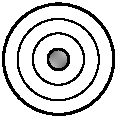
\includegraphics[width=0.15\textwidth]
{gesamttex/edit_VIII-4/images/LH_35_14_02_004_d3_004r.pdf}
\edcaption[0.5em]{\lbrack \textit{Fig.\:3}\rbrack}%
\end{edfigure}%
\pstart%
\noindent%
Initio elastrum \textit{mn} potius tendetur,%
\indexS{elastrum tensum}%
\indexS{elastrum resistens motui}
quia%
\edlabel{LH_35_14_02_004_004r_1b}
resistentia ejus%
\indexS{resistentia elastri ad tensionem}
ad tensionem quantulamcunque%
\indexS{tensio elastri quantulacunque}
nulla est.%
\indexS{tensio elastri nulla}
Sed aliquousque tensum%
\indexS{elastrum tensum}
resistet aliquantum,%
\indexS{elastrum resistens motui}
et adeo movebitur et aliquantum corpus \textit{B};
et quia
\edtext{%
causa%
\indexS{causa elastri tensi}
cur elastrum tendi cogatur,%
\indexS{elastrum coactum tendi}%
}{%
\lemma{causa}%
\Bfootnote{%
\textit{(1)}~cur resiste %
\textit{(2)}~cur elastrum tendi cogatur,%
~\textit{L}%
}}
est
quod motui
\edtext{%
resistit~\textit{B},
tantum semper movebitur \textit{B}%
}{%
\lemma{resistit \textit{B},}%
\Bfootnote{%
\textit{(1)}~ideo eousque semper mo %
\textit{(2)}~tantum semper movebitur \textit{B}%
~\textit{L}%
}}
ut non majore vi%
\indexS{vis tendens elastrum}
tendatur Elastrum%
\indexS{elastrum tensum}
quam opus est ad movendum~\textit{B}.
Cum igitur superato Elastro%
\indexS{elastrum superatum}
\edtext{%
\textit{mn}%
}{%
\lemma{\textit{mn}}%
\Bfootnote{%
\textit{erg.\;L}%
}}
cesset translatio motus%
\indexS{translatio motus}%
\indexS{motus translatus}%
\lbrack,\rbrack\
sequitur %
tantum virium conferri corpori \textit{B},%
\indexS{vis collata corpori ab elastro}
ut vis ejus sit aequalis Elastro tenso.%
\indexS{vis aequalis elastro tenso}%
\indexS{elastrum tensum}
Et proinde
\edtext{%
\lbrack vis\rbrack%
}{%
\lemma{celeritas}%
\Bfootnote{%
\textit{L\;ändert Hrsg.}%
}}
quae corpori \textit{B} affertur%
\indexS{celeritas allata corpori ab alio}
a corpore \textit{A}
est eadem,
sive magna sive parva sit velocitas%
\indexS{velocitas corporis tendentis elastrum}
ipsius \textit{A};
dimidium scilicet virium Elastri.%
\indexS{vis elastri}%
\indexS{elastrum tensum}
Et ideo
si multa simul Elastra tendantur,%
\indexS{elastra simul tensa}
seu superficies radens%
\indexS{superficies radens}
sit longa,
erit motus%
\indexS{motus acceptus}
quem accipit
\edtext{%
\lbrack\textit{B}\rbrack%
}{%
\lemma{\textit{A}}%
\Bfootnote{%
\textit{L\;ändert Hrsg.}%
}}
in ratione directa
\edtext{%
Elastricitatis,%
\indexS{elastricitas}
seu connexionis,
et reciproca%
}{%
\lemma{Elastricitatis\lbrack\textit{!}\rbrack}%
\Bfootnote{%
\textit{(1)}~et reciproca %
\textit{(2)}~, seu connexionis, et reciproca%
~\textit{L}%
}}
superficiei.%
\indexS{superficies radens}
Sed dum \textit{A} continuat motum %
(quod et intelligi potest
si \textit{A} esset cylindrus%
\indexS{cylinder convexus intra concavum}
\edtext{%
convexus%
}{%
\lemma{convexus}%
\Bfootnote{%
\textit{erg.\;L}%
}}
intra concavum cylindrum \textit{B}) %
repetitur impressio aliquousque.%
\indexS{impressio motus repetita}
Idque tamdiu,
donec motus fiat conspirans,%
\indexS{motus conspirans}
seu donec se mutuo non deserant.%
\indexS{corpora se mutuo non deserantia}
Verum si extrema quaedam sit superficies immota,%
\indexS{superficies immota}
tunc ipsa perinde resistit%
\indexS{superficies resistens motui}
ac si ipsa in contrariam partem moveretur%
\indexS{superficiens movens in partem contrariam}
quiescente incluso:%
\indexS{corpus quiescens}
itaque hoc
\edtext{%
casu non%
}{%
\lemma{casu}%
\Bfootnote{%
\bars{\textlangle vero\textrangle\ \textit{gestr.}} non%
~\textit{L}%
}}
potest unquam obtineri consensus,%
\indexS{consensus}
sed tandem continuatis resistentiis elasticis superandis%
\indexS{resistentia elastica}
necesse est absorberi motum.%
\indexS{motus absorptus}%
\indexS{absorptio motus}
Quod de sphaera%
\indexS{sphaera}
idem et de cylindro%
\indexS{cylinder}
et aliis figuris
quibuscunque assero%
\lbrack:\rbrack\
nam cum cessat motus absorptio,%
\indexS{absorptio motus}
remanente tenacitate%
\indexS{tenacitas remanens post motum absorptum}%
\indexS{tenacitas fluidi}
necesse est
omnia moveri ut unum solidum.%
\indexS{mota ut unum solidum}
\lbrack%
\href{\Scan{LH_35_14_02_004v}}%
{4\,v\textsuperscript{o}}%
\rbrack\
\pend%
\pstart%
An etiam sine
\edtext{%
tenacitate%
\indexS{tenacitas fluidi}%
\indexS{fluidum}%
\lbrack,\rbrack\
una fluidi pars%
}{%
\lemma{tenacitate}%
\Bfootnote{%
\textit{(1)}~unum fluidum %
\textit{(2)}~una fluidi pars%
~\textit{L}%
}}
aliam moveat%
\indexS{pars fluidi movens aliam sine tenacitate}
dispiciendum est.
Videtur scilicet
ex ipsa natura materiae%
\indexS{natura materiae}%
\indexS{materia}
omnes partes habere inter se unitatem,%
\indexS{partes materiae habentes unitatem}
ut communis sit earum motus%
\indexS{motus communis partium materiae}
nisi quid impediat,
et
\lbrack\textit{Text bricht ab.}\rbrack%
\pend%
\newpage%
\pstart%
\noindent%
\centering%
*     *     *
\pend%
\vspace{3.0em}%
\selectlanguage{german}%
\frenchspacing%
\footnotesize%
\pstart%
\noindent%
\textls{Ausführliche Datierungsgründe:}%
\pagelabel{58218_dat}
Der Träger der titellosen und undatierten Aufzeichnung N.\;\ref{58218}, die den dynamischen Zusammenhang der Teile eines Fluidums erörtert, weist zwar kein Wasserzeichen auf, wohl aber gleiche sichtbare Eigenschaften wie eine Papiersorte, die Leibniz während seines Aufenthalts in Rom\indexO{Rom} verwendete, unter anderem für die erste Fassung seiner \textit{Dynamica}.\cite{01354}
Auf gleichem Papier sind ebenfalls die in diesem Band veröffentlichten Aufzeichnungen N.\;\ref{58656-A}, N.\;\ref{58258} und N.\;\ref{58235} überliefert %
(siehe die ausführlichen Datierungsgründe zu N.\;\ref{58656-A}, S.\;\pageref{58656-A_dat}).
Bei diesen Texten, %
die auch einen inhaltlichen Zusammenhang mit Leibnizens \textit{Dynamica} aufweisen, ist demnach eine Entstehungszeit anzunehmen, die sich auf die Monate vom Sommer bis zum November 1689 erstreckt, als Leibniz in Rom\indexO{Rom} am \textit{Phoranomus}\cite{01402} und an der ersten Fassung der \textit{Dynamica}\cite{01354} gearbeitet hat (siehe \textsc{Robinet} 1988, S.\;81\,ff.).\cite{01240}
Die vorliegende Aufzeichnung N.\;\ref{58218} ist demgemäß auf den gleichen Zeitraum zwischen Sommer und November 1689 zu datieren.
Eine frühere (ab Leibnizens Ankunft in Rom\indexO{Rom} im Mai 1689) oder eine spätere Abfassungszeit (höchstens bis Ende März 1690, als Leibniz Italien\indexO{Italien} verlassen hat) sind nicht ausgeschlossen, aber unwahrscheinlich.%
\pend%
\selectlanguage{latin}%
\frenchspacing%
\normalsize%
\newpage%




\chapter[tocentry={Motus leges ex abstractis principiis ductae %
\enskip%
\bracks{ab
Sommer
1689}%
}, %
head={Motus leges ex abstractis principiis ductae%
}]%
{\MakeUppercase{Motus leges ex abstractis principiis ductae} %
\newline%
\bracks{ab
Sommer
1689}%
} %
\label{60080}
\selectlanguage{ngerman}%
\frenchspacing%
\begin{ledgroupsized}[r]{120mm}%
\footnotesize%
\pstart%
\noindent\textbf{Überlieferung:}%
\pend%
\end{ledgroupsized}%
\begin{ledgroupsized}[r]{114mm}%
\footnotesize%
\pstart%
\parindent -6mm%
\makebox[6mm][l]{\textit{L}}%
Aufzeichnung:
LH XXXV 10,\;11 Bl.\;107.
Ein Blatt 8\textsuperscript{o},
Ränder zum Teil beschnitten;
ein \href{\Scan{LH_35_10_11_107wz}}{Wasserzeichen}.
Eineinhalb Seiten;
die untere Hälfte von Bl.\;\href{\Scan{LH_35_10_11_107v}}{107\,v\textsuperscript{o}} ist unbeschrieben.
Geringfügiger Textverlust am rechten Rand von Bl.\;\href{\Scan{LH_35_10_11_107r}}{107\,r\textsuperscript{o}}
\pend%
\end{ledgroupsized}%
\begin{ledgroupsized}[r]{114mm}%
\footnotesize%
\pstart%
\parindent -6mm%
\makebox[6mm][l]{\textit{Ü}}%
\textsc{G.\:W.\;Leibniz}, \textit{Deriving the laws of motion from abstract principles}. Translation and Commentary, hrsg. von \textsc{R.\;Arthur} und \textsc{O.\;Ottaviani} (\textit{Leibniz Review} XXXIV, 2024, im Erscheinen):\cite{02619}\pend%
\end{ledgroupsized}%
\vspace{5mm}%
\begin{ledgroup}%
\footnotesize%
\pstart%
\noindent%
\textbf{Datierungsgründe:}
Die Datierung der Aufzeichnung N.\;\ref{60080} beruht auf äußeren Eigenschaften des Text\-trägers %
sowie auf inhaltlichen Betrachtungen.
Siehe die ausführliche Begründung auf S.~\pageref{60080_dat}.%
\pend%
\end{ledgroup}%
\selectlanguage{latin}%
\frenchspacing%
\vspace{8mm}%
\normalsize%
\pstart%
\noindent%
\lbrack%
\href{\Scan{LH_35_10_11_107r}}%
{107\,r\textsuperscript{o}}%
\rbrack\ %
Debent motus leges%
\indexS{lex motus}
ex abstractis principiis%
\indexS{principium abstractum}
posse duci.
Et videtur maxime servire haec consideratio,%
\indexS{consideratio}
\edtext{%
quod ex motu rectilineo%
\indexS{motus rectilineus}
corporum quotcunque%
}{%
\lemma{quod}%
\Bfootnote{%
\textit{(1)}~motus semper est uniformis\indexS{motus uniformis} %
\textit{(2)}~ex motu %
\textit{(a)}~prae s %
\textit{(b)}~rectilineo corporum quotcunque%
~\textit{L}%
}}
per se discerni non potest,
in quo sit motus;
seu omnes Hypotheses succedunt.%
\indexS{hypothesis succedens}
Ergo et in consequentiis%
\indexS{consequentia}
omnes Hypotheses succedere debent.%
\indexS{hypothesis succedens}
Si nullus est modus discernendi in determinantibus,%
\indexS{modus discernendi in determinantibus}
nec debet esse in ipsis determinatis.%
\indexS{modus discernendi in determinatis}
Itaque nec in circulari
debet esse modus discernendi,%
\indexS{motus circularis}
\edlabel{LH_35_10_11_107_107r_centrip-1}%
nam firmitas corporum%
\indexS{firmitas corporis}%
\indexS{corpus firmum}
non aliunde oritur%
\indexS{origo firmitatis corporis}
quam ex vi quadam quasi centripeta,%
\indexS{vis quaedam quasi centripeta}
corpora versus se invicem agente%
\indexS{vis agens corpora versus se invicem}%
\indexS{corpora acta versus se invicem}
ob motum ambientium.%
\indexS{motus ambiens}%
\edlabel{LH_35_10_11_107_107r_centrip-2}
Et quae
\edtext{%
parum recessa%
\bracks{,}%
}{%
\lemma{parum}%
\Bfootnote{%
\textit{(1)}~recessere %
\textit{(2)}~recessa%
~\textit{L}%
}}
magna vi retrorsum aguntur,
et hoc est firmitas.%
\indexS{firmitas corporis}
Causa autem est motus%
\indexS{causa firmitatis corporis}
\edtext{%
conspiratio%
\indexS{conspiratio motus}
qui%
}{%
\lemma{conspiratio}%
\Bfootnote{%
\textit{(1)}~cum %
\textit{(2)}~quae %
\textit{(3)}~qui%
~\textit{L}%
}}
huc abiit,
nec mutari facile potest.
Nempe pro principio habendum,
quam minimum mutari.
\pend%
\pstart%
\edlabel{LH_35_10_11_107_107r_qwp-1}%
Ex principio aequivalentium hypothesium%
\indexS{principium hypothesium aequivalentium}
sequitur
eandem esse actionem et reac\-tionem,%
\edlabel{LH_35_10_11_107_107r_qwp-2}%
\indexS{actio et reactio}%
\indexS{reactio et actio}
seu ictum.
\pend%
\pstart%
Varia
\edtext{%
principia:
\newline\hspace*{7,42mm}%
(1)~%
Quam minima fit mutatio.%
\indexS{mutatio quam minima}%
}{%
\lemma{principia: (1)}%
\Bfootnote{%
\textit{(1)}~nihil fit %
\textit{(2)}~null\textlangle a\textrangle\ %
\textit{(3)}~quam minima fit mutatio.%
~\textit{L}%
}}
\newline\hspace*{7,42mm}%
(2)~%
Eadem servatur
\edtext{%
in summa%
}{%
\lemma{in summa}%
\Bfootnote{%
\textit{erg.\;L}%
}}
quantitas potentiae.%
\indexS{quantitas potentiae}%
\indexS{potentia servata}
\newline\hspace*{7,42mm}%
(3)~%
Eadem servatur quantitas directionis%
\indexS{quantitas directionis}
in
\edtext{%
summa.
\newline\hspace*{7,42mm}%
(4)~%
Motus est aliquid respectivum%
\indexS{motus respectivus}
seu omnes hypotheses%
}{%
\lemma{summa (4)}%
\Bfootnote{%
\textit{(1)}~Omnes hypotheses %
\textit{(2)}~Motus est %
\lbrack...\rbrack\ omnes hypotheses%
~\textit{L}%
}}
sunt aequivalentes.%
\indexS{hypotheses aequivalentes}%
\newline\hspace*{7,42mm}%
(5)~%
\edlabel{LH_35_10_11_107_107r_njm-1}%
Actio et reactio sunt aequales.%
\edlabel{LH_35_10_11_107_107r_njm-2}%
\indexS{actio et reactio}%
\indexS{reactio et actio}
\newline\hspace*{7,42mm}%
(6)~%
Si determinantia in se invicem abeant,%
\indexS{determinantia abeuntia in se invicem}
\ledpb%
etiam determinata in se invicem abibunt.%
\indexS{determinantia et determinata}
Hinc quies est casus motus,%
\indexS{quies ut casus motus}
aequalitas inaequalitatis.%
\indexS{aequalitas ut casus inaequalitatis}
\newline\hspace*{7,42mm}%
(7)~%
Nulla fit mutatio per saltum,%
\indexS{mutatio per saltum}
hinc omnia corpora flexilia.%
\indexS{corpora omnia flexilia}%
\indexS{corpus flexile}
\newline\hspace*{7,42mm}%
(8)~%
Communis motus%
\indexS{motus communis}
nil mutat%
\lbrack:\rbrack\
sequitur ex aequivalentia hypothesium?%
\indexS{aequivalentia hypothesium}
\pend%
\pstart%
An regula haec bona,%
\indexS{regula bona}
ut omnia serventur
quae servari possunt
\edtext{%
aliis
compa\bracks{ti}bilia
servandis.
An ergo et servanda%
}{%
\lemma{aliis}%
\Bfootnote{%
\bars{compabilia \textit{ändert Hrsg.}} servandis. %
\textit{(1)}~Quod si plura servanda \angles{mi--} %
\textit{(3)}~An ergo et servanda%
~\textit{L}%
}}
quantitas motus,%
\indexS{quantitas motus}
sed ea non potest servari,
servata quantitate potentiae;%
\indexS{quantitas potentiae}%
\indexS{potentia servanda}
et non involvit omnia.
Ope virtutis elasticae%
\indexS{virtus elastica}
revera quam
\lbrack%
\href{\Scan{LH_35_10_11_107v}}%
{107\,v\textsuperscript{o}}%
\rbrack\
minima fit mutatio.%
\indexS{mutatio quam minima}
Et hinc etiam necesse est
corpora esse flexilia.%
\pend%
\begin{edfigure}[1.75em][1.15em]%
\includegraphics[width=0.3\textwidth]%
{gesamttex/edit_VIII-4/images/LH_35_10_11_107_d_107v.pdf}%
\edcaption[0.25em]
{\hspace{0.5mm}\lbrack\textit{Fig.\:1}\rbrack}%
\end{edfigure}%
\pstart%
Ex diversis principiis
reliqua omnia semper demonstrari possunt,
sed difficile
\edtext{%
est
ultimam analysin reperire,%
\indexS{analysis ultima}
seu ostendere
quid sit omnium primum.%
\indexS{primum omnium}%
}{%
\lemma{est}%
\Bfootnote{%
\textit{(1)}~ultimum %
\textit{(2)}~ultimam analysin \lbrack...\rbrack\ omnium primum.%
~\textit{L}%
}}
Omnia tamen videntur pendere
ex hoc principio,
\edlabel{LH_35_10_11_107_107v_PID-1}%
\edtext{%
quod indiscernibilibus%
}{%
\lemma{quod}%
\Bfootnote{%
\textit{(1)}~similibus %
\textit{(2)}~indiscernibilibus%
~\textit{L}}%
}
existentibus determinantibus%
\indexS{determinantia indiscernibilia}
etiam similia sint determinata%
\indexS{determinantia et determinata}
atque discerni nequeant.%
\edlabel{LH_35_10_11_107_107v_PID-2}
Unde sequitur
quod in motu
\edtext{%
etiam post concursum%
\indexS{concursus corporum}
una Hypothesis ab alia discerni nequeat.%
\indexS{hypotheses indiscernibiles}%
}{%
\lemma{etiam}%
\Bfootnote{%
\textit{(1)}~potest %
\textit{(2)}~post concursum \lbrack...\rbrack\ discerni nequeat.%
~\textit{L}%
}}
\pend
\pstart%
Item
quod quam minima semper debet esse mutatio.%
\indexS{mutatio quam minima}
Unde non quidem sufficit
eandem quantitatem motus servari,%
\indexS{quantitas motus}
sed potentiam%
\indexS{potentia servanda}%
\lbrack,\rbrack\
\edlabel{LH_35_10_11_107_107v_ert-1}%
quia ea omnia involvit%
\lbrack,\rbrack\
nempe effectum%
\indexS{effectus potentiae}
et actionis perfectionem.%
\edlabel{LH_35_10_11_107_107v_ert-2}%
\indexS{perfectio actionis}%
\indexS{actio perfecta}
\pend%
\vspace*{6.5em}%
\pstart%
\noindent%
\centering%
*     *     *
\pend%
\newpage%
\selectlanguage{german}%
\frenchspacing%
\footnotesize%
\pstart%
\noindent%
\textls{Ausführliche Datierungsgründe:}%
\pagelabel{60080_dat}
In der titellosen und undatierten Aufzeichnung N.\;\ref{60080}, editorisch \textit{Motus leges ex abstractis principiis ductae} benannt, umreißt Leibniz eine Ableitung der Bewegungsgesetze aus allgemeineren "abstrakten Prinzipien" unter besonderer Berücksichtigung des folgenden Grundsatzes:
Sind die bestimmenden Umstände voneinander ununterscheidbar, so sind auch die bestimmten Folgen voneinander ununterscheidbar (vgl. oben, \refpassage{LH_35_10_11_107_107v_PID-1}{LH_35_10_11_107_107v_PID-2}).
Der Träger N.\;\ref{60080} weist ein \href{\Scan{LH_35_10_11_107wz}}{Wasserzeichen} auf, das noch nicht eindeutig ermittelt wurde;
somit kann nach heutigem Wissensstand nicht behauptet werden, dass es sich hierbei um die Marke einer italienischen oder österreichischen Papiermühle handele.
Eine chronologische Einordnung der Aufzeichnung ergibt sich trotzdem aus folgenden Beobachtungen (siehe hierüber \textsc{G.\:W.\;Leibniz}, \textit{Deriving the laws of motion from abstract principles}. Translation and Commentary, hrsg. von \textsc{R.\;Arthur} und \textsc{O.\;Ottaviani}, \textit{Leibniz Review} XXXIV, 2024, im Erscheinen):\cite{02619}
\pend%
\pstart%
Leibniz verwendet in der Aufzeichnung N.\;\ref{60080} eine Begrifflichkeit, die offenbar eine Lektüre von Isaac Newtons\indexN{\textls{Newton} (Neutonus), Isaac 1643\textendash1727} \textit{Philosophiae naturalis principia mathematica} (London 1687)\cite{00535} bezeugt:
etwa den Bregriff einer \textit{vis quaedam quasi centripeta} (als Ursprüng der Körperkohäsion \refpassage{LH_35_10_11_107_107r_centrip-1}{LH_35_10_11_107_107r_centrip-2}) oder die Gleichsetzung von \textit{actio} und \textit{reactio} (\refpassage{LH_35_10_11_107_107r_qwp-1}{LH_35_10_11_107_107r_qwp-2}, \refpassageohne{LH_35_10_11_107_107r_njm-1}{LH_35_10_11_107_107r_njm-2}).
Leibnizens erste bezeugte Lektüre der \textit{Principia}\cite{00535} fand – wie \textsc{Bertoloni Meli} 1993 (S.\;97)\cite{01357} nachgewiesen hat – im Herbst 1688 statt, als Leibniz sich auf dem Weg nach Italien\indexO{Italien} in Wien\indexO{Wien} aufhielt.
Aus diesem Grund dürfte N.\;\ref{60080} nicht vor dem Herbst 1688 entstanden sein.
(Siehe die Datierungsgründe des wohl ebenfalls im Herbst 1688 verfassten Entwurfs \textit{Physico-mechanicae leges ex congressu corporum ductae} \textit{LSB} VIII,\;3 N.\;68,\cite{02604} S.\;747\,f.)
Einer umfassenderen Lektüre von Newtons\indexN{\textls{Newton} (Neutonus), Isaac 1643\textendash1727} \textit{Principia}\cite{00535} widmete sich Leibniz während seines Aufenthaltes in Rom\indexO{Rom} zwischen Mai und November 1689 (vgl. \textit{Chronik}, S.\;98.)\cite{01236}
\pend%
\pstart%
Inhaltlich weist die Aufzeichnung N.\;\ref{60080} auch einen engen Zusammenhang mit Leibnizens \textit{Dynamica}\cite{01354} auf.
Dies zeigt sich zunächst wieder in der in N.\;\ref{60080} verwendeten Begrifflichkeit (vgl. etwa den Schlusssatz, \refpassage{LH_35_10_11_107_107v_ert-1}{LH_35_10_11_107_107v_ert-2}: die Potenz \textit{omnia involvit, nempe effectum et actionis perfectionem}).
Als noch bedeutender erweist sich wohl die Berührung mit der zwischen Rom\indexO{Rom} und Florenz\indexO{Florenz} abgefassten Abhandlung im Hinblick auf den besagten Grundsatz \textit{quod indiscernibilibus existentibus determinantibus etiam similia sint determinata atque discerni nequeant} (oben, \refpassage{LH_35_10_11_107_107v_PID-1}{LH_35_10_11_107_107v_PID-2}).
Nahezu identisch wird in Leibnizens \textit{Dynamica}, pars~II, sectio~III, prop.\;19 das "allgemeine Axiom" formuliert, \textit{quod quorum determinantia discerni non possunt, eorum nec discerni possint determinata} (\textit{CFP}~I, S.\;429.24--430.2; II.2, S.\;530.26--28).\cite{01354}
Demnach ist eine Entstehung der Aufzeichnung N.\;\ref{60080} vor der ersten Fassung der \textit{Dynamica}\cite{01354} unwahrscheinlich.
Diese letztere ist wohl nicht vor dem Sommer 1689 zu datieren (siehe hierüber \textsc{Robinet} 1988, S.\;81\,ff.).\cite{01240}
Folglich sollte auch N.\;\ref{60080} nicht vor dem Sommer 1689 abgefasst worden sein.
\pend%
\pstart%
Wahrscheinlich ist die Aufzeichnung N.\;\ref{60080} nicht viel später entstanden, möglicherweise auf dem Rückweg aus Italien\indexO{Italien} nach Hannover.\indexO{Hannover}
Dies könnte das im Träger anzutreffende unübliche Wasserzeichen erklären.
Ein genauer Terminus ante quem der Datierung von N.\;\ref{60080} lässt sich aber nach heutigem Wissensstand nicht ermittel.
\pend%
\selectlanguage{latin}%
\frenchspacing%
\normalsize%




\chapter[tocentry={Utrum et quatenus vis aeris elastica imminuatur per flammam
\enskip \lbrack Dezember 1689\rbrack}, %
head={Utrum vis aeris elastica imminuatur per flammam %
}]%
{\MakeUppercase{Utrum et quatenus vis aeris elastica imminuatur per flammam
}
\newline \lbrack Dezember 1689\rbrack}%
\label{55743+55744+60656}
\include{gesamttex/edit_VIII-4/LH_38_049-051+Gerland_1906_006.tex}



\chapter[tocentry={Liquorum ascensus in tubulos capillares %
\enskip\lbrack%
ab Frühjahr 1690 (?)%
\rbrack}, %
head={Liquorum ascensus in tubulos capillares%
}]%
{\MakeUppercase{Liquorum ascensus in tubulos capillares} %
\newline\lbrack%
ab Frühjahr 1690 (?)%
\rbrack}%
\label{42488}
\selectlanguage{ngerman}%
\frenchspacing%
\begin{ledgroupsized}[r]{120mm}%
\footnotesize%
\pstart%
\noindent\textbf{Überlieferung:}%
\pend%
\end{ledgroupsized}%
\begin{ledgroupsized}[r]{114mm}%
\footnotesize%
\pstart%
\parindent -6mm%
\makebox[6mm][l]{\textit{L}}%
Aufzeichnung:
LH~XXXVII,\;7 Bl.\;8.
Ein Blatt 4\textsuperscript{o},
Ränder beschnitten.
Zwei ganzseitig beschriebene Seiten.
\pend%
\end{ledgroupsized}%
\vspace{5mm}%
\begin{ledgroup}%
\footnotesize%
\pstart%
\noindent%
\textbf{Datierungsgründe:}
Die Datierung der Aufzeichnung N.\;\ref{42488} beruht auf %
inhaltlichen Betrachtungen.
Siehe die ausführliche Begründung auf S.\;\pageref{42488_dat}.%
\pend%
\end{ledgroup}%
\selectlanguage{latin}%
\frenchspacing%
\vspace{8mm}%
\normalsize%
\pstart%
\noindent%
\lbrack%
\href{\Scan{LH_37_07_008r}}%
{8\,r\textsuperscript{o}}%
\rbrack\
\edtext{%
Succi nutritii ascensus%
\indexS{succus nutritius in plantis}%
\indexS{ascensus succi in plantis}%
}{%
\lemma{Succi}%
\Bfootnote{%
\textit{(1)}~cum %
\textit{(2)}~nutritii ascensus%
~\textit{L}%
}}
in plantis%
\indexS{planta}
non est deducendus ex communi illa aeris pressione%
\indexS{pressio aeris communis}
quae Mercurium in Barometro%
\indexS{mercurius suspensus in barometro}%
\indexS{barometrum}
\edtext{%
ad 27 circiter%
}{%
\lemma{ad 27}%
\Bfootnote{%
\textit{(1)}~\angles{vel 28} %
\textit{(2)}~circiter%
~\textit{L}%
}}
pollices%
\indexS{pollex}
suspensum tenet,%
\indexS{suspensio mercurii in barometro}
aut aquam in antlia aspirante%
\indexS{aqua in antlia aspirante}%
\indexS{antlia aspirans}
ad 32 pedes%
\indexS{pes}
attollit,%
\indexS{suspensio aquae in antlia}
neque inde colligere licet
\edtext{%
arbores%
\indexS{arbor excrescens}
ultra 17 ulnarum%
\indexS{ulna}
altitudinem%
\indexS{altitudo arborum}
excrescere non debere,%
}{%
\lemma{arbores}%
\Bfootnote{%
\bars{non \textit{gestr.}} ultra 17 %
\textit{(1)}~ulnas excrescere %
\textit{(2)}~ulnarum altitudinem excrescere non debere,%
~\textit{L}%
}}
cum multo altiores pinus%
\indexS{pinus}
\edtext{%
abietesve%
\indexS{abies}
haberi%
}{%
\lemma{abietesve}%
\Bfootnote{%
\bars{apud nos \textit{gestr.}} haberi%
~\textit{L}%
}}
res sit
\edtext{%
indubitata;%
\indexS{res indubitata}
ut taceam%
}{%
\lemma{indubitata;}%
\Bfootnote{%
\textit{(1)}~sed re %
\textit{(2)}~ut taceam%
~\textit{L}%
}}
non omnem succum%
\indexS{succus nutritius in plantis}
inde a radice venire,%
\indexS{radix plantarum}
sed novum ex aere%
\indexS{aer pluvius}
aquave pluvia,%
\indexS{aqua pluvia}
imo etiam ex vicina
\edtext{%
planta sustentante interdum%
}{%
\lemma{planta}%
\Bfootnote{%
\textit{(1)}~interdum %
\textit{(2)}~sustentante interdum%
~\textit{L}%
}}
attrahi.%
\indexS{attractio succi in plantis}
\pend%
\pstart%
\edlabel{LH_37_07_008_jel-1}%
Succi igitur propagationem%
\indexS{propagatio succi in plantis}%
\indexS{succus nutritius in plantis}
rectius peti
putem ab alio naturae
\edtext{%
principio,%
\indexS{principium naturae}
nimirum a \textls{pressione subtiliore}%
\indexS{pressio aeris subtilioris}%
}{%
\lemma{principio,}%
\Bfootnote{%
\textit{(1)}~quod exp\textlangle on\textrangle\ %
\textit{(2)}~nimirum a \textls{pressione subtiliore}%
~\textit{L}%
}}
nondum satis explorata,
\edtext{%
a pondere%
\indexS{pondus aeris}
et vi elastica%
\indexS{vis elastica aeris}
\lbrack aeris\rbrack\
non dependente,%
\indexS{pressio aeris independens a pondere et vi elastica}%
}{%
\lemma{a pondere et vi elastica %
\bars{aeris \textit{erg. Hrsg. nach \refpassage{LH_37_07_008_008r_hdf-1}{LH_37_07_008_008r_hdf-2}}} %
non dependente,}%
\Bfootnote{%
\textit{erg.\;L}%
}}
quae multis tamen sese effectibus ostendit.%
\indexS{effectus pressionis aeris subtilioris}
Ex his unus
\edtext{%
est
cum%
}{%
\lemma{est}%
\Bfootnote{%
\textit{(1)}~quod %
\textit{(2)}~cum%
~\textit{L}%
}}
\edlabel{LH_37_07_008_008r_xyz_1}%
aquam%
\indexS{aqua assurgens sponte sua in tubis capillaribus}
vel alios multos liquores%
\indexS{liquor assurgens sponte in tubis capillaribus}
experimur
in tubos vitreos tenuissimos etiam capillares%
\indexS{tubus vitreus capillaris}
\edtext{%
(qualibus celeberrimus Leewenhoekius%
\indexN{\textls{Leeuwenhoek}, Antoni van 1632\textendash1723}
ad experimenta microscopica utitur)%
\indexS{experimentum microscopicum}%
}{%
\lemma{qualibus \lbrack...\rbrack\ utitur}%
\Cfootnote{%
Siehe \textsc{A.\;van Leeuwenhoek},
"Letter wherein some account is given of the manner of observing so great a number of little animals in divers sorts of water"
(\textit{PT} XII, Nr.\;134, 23.\;April [3.\;Mai] 1677, S.\;844).\cite{02520}
Der Kapillaritätseffekt wird dort nicht erwähnt.
Auf das Phänomen geht Leibniz aber ein, als er Ende 1677 in einem Brief für J.\;P. de La Roque\indexN{\textls{La Roque} (Larroque), Jean Paul de, gest. 1691} über Leeuwenhoeks\indexN{\textls{Leeuwenhoek}, Antoni van 1632\textendash1723} Mikroskopie berichtet (\textit{LSB} III,\;2 N.\;94, S.\;258.1--6, 261.7--10).\cite{02521}
Bei einem persönlichen Gespräch in Delft\indexO{Delft} mitte November 1676 (\textit{Chronik}, S.\;46)\cite{01236} hatte Leeuwenhoek\indexN{\textls{Leeuwenhoek}, Antoni van 1632\textendash1723} allerdings von seinen neuesten Forschungen erzählt;
vgl. Leibnizens Brief an H.\;Oldenburg\indexN{\textls{Oldenburg} (Grubendol), Heinrich 1618\textendash1677} vom 18./28. November 1676 (\textit{LSB} III,\;5 N.\;II, S.\;6.17--22).\cite{02522}
Leeuwenhoek\indexN{\textls{Leeuwenhoek}, Antoni van 1632\textendash1723} könnte hierbei auch über seine Erfahrungen mit dem Kapillaritätseffekt berichtet haben.%
}}
ad pollicum%
\indexS{pollex}
aliquot altitudinem%
\indexS{altitudo liquorum in tubis capillaribus}
sponte sua
\edtext{%
assurgere.%
\indexS{aqua assurgens sponte sua in tubis capillaribus}%
\indexS{liquor assurgens sponte in tubis capillaribus}
\edtext{%
Quod primus dicitur observasse Rohaultius,%
\indexN{\textls{Rohault}, Jacques 1618\textendash1672}
et extant complura de hac re experimenta%
\indexS{experimentum de liquoribus in tubis capillaribus}
in Monconisi\bracks{i}%
\indexN{\textls{Monconys} (Monconisius), Balthasar de 1611\textendash1665}
itinerario relata.%
}{%
\lemma{Quod \lbrack...\rbrack\ relata}%
\Cfootnote{%
Siehe \textsc{B.\;de Monconys},
\glqq Discours sur l’ascension de l’eau en un tuyau estroit\grqq\cite{02519}
(\textit{Journal de voyages}, Bd.\;III, Lyon 1666,
\glqq Lettres escrittes à Monconys\grqq, S.\;33--38).\cite{00118}%
}}%
\edlabel{LH_37_07_008_008r_xyz_2}
Hanc%
}{%
\lemma{assurgere.}%
\Bfootnote{%
\textit{(1)}~Hanc %
\textit{(2)}~\textlangle--\textrangle\ %
\textit{(3)}~Quod primus %
\lbrack...\rbrack\ experimenta in %
\bars{Monconisio \textit{ändert Hsrg.}} itinerario relata. Hanc%
~\textit{L}%
}}
pressionem%
\indexS{pressio aeris subtilioris}
etiam arbitror rotundare
\edtext{%
guttas%
\indexS{gutta rotundata}%
\indexS{rotundatio guttarum}
(usque adeo ut duae vicinae minores in unam novam coeant)%
\indexS{guttae coeuntes in unam}
et exprimere%
\indexS{gutta expressa}%
}{%
\lemma{guttas}%
\Bfootnote{%
\textit{(1)}~et exprimere etiam %
\textit{(2)}~(usque adeo %
\lbrack...\rbrack\ unam novam %
\textit{(a)}~cone %
\textit{(b)}~coeant) et exprimere%
~\textit{L}%
}}
rotundatas%
\indexS{gutta rotundata}
in eam partem
qua liquor facilius fertur;
veluti
\edtext{%
si atramenti guttam%
\indexS{gutta atramenti}%
\indexS{atramentum}
vel aliam superficiem tangamus%
\indexS{superficies tacta apice pennae}
apice pennae jam imbutae,%
\indexS{apex pennae}%
\indexS{penna imbuta atramento}%
}{%
\lemma{si}%
\Bfootnote{%
\textit{(1)}~guttam atramenti pennae jam imbutae tangamus %
\textit{(2)}~atramenti guttam %
\lbrack...\rbrack\ jam imbutae,%
~\textit{L}%
}}
videbimus atramentum%
\indexS{atramentum}
ex gutta%
\indexS{gutta atramenti}
in pennam%
\indexS{penna imbuta atramento}
subito ferri
sive sursum sive ad latus,
prout
\edlabel{LH_37_07_008_gravitasaetheris-1}%
\edtext{%
se offeret situs.%
\indexS{situs}
\edtext{%
Haec omnia compertum mihi est fieri
etiam in
\edtext{%
vacuo Gerikiano%
\indexS{vacuum Gerickianum}%
}{%
\lemma{vacuo Gerikiano}%
\Cfootnote{%
Künstlich erzeugtes Vakuum.
Anspielung auf den in
\textsc{O.\;v.\;Guericke}, \textit{Experimenta nova}, lib.\;II, cap.\;3 (Amsterdam 1672, S.\;56a)\cite{00055}
dargelegten Begriff der "Leere" sowie auf die
ebd., lib.\;III (S.\;71--124)\cite{00055}
beschriebenen Versuche hierüber.
}}
ex quo omnis pene aer est extractus%
\indexS{aer extractus}%
}{%
\lemma{Haec \lbrack...\rbrack\ extractus}%
\Cfootnote{%
Quelle nicht ermittelt.%
}}
\edlabel{LH_37_07_008_008r_hdf-1}%
atque adeo ponderi%
\indexS{pondus aeris}
vel vi elasticae aeris%
\indexS{vis elastica aeris}
tribui nequeunt.%
\edlabel{LH_37_07_008_008r_hdf-2}
\edtext{%
Quidam viri docti putant%
\bracks{,}%
\indexS{viri docti}
praeter aeris atmosphaeram,%
\indexS{atmosphaera aeris}%
\indexS{aer incumbens telluri}
incumbere telluri nostrae%
\indexS{tellus}
aliam atmosphaeram%
\indexS{atmosphaera alia}
multo altiorem%
\indexS{atmosphaera altior}
et subtiliorem%
\indexS{atmosphaera subtilior}
et ipsum aerem penetrantem%
\indexS{atmosphaera penetrans ipsum aerem}%
}{%
\lemma{Quidam \lbrack...\rbrack\ penetrantem}%
\Cfootnote{%
Siehe N.\;\ref{60205} in diesem Band, bes. %
\refpassage{LH_37_03_115-116_115_lpo-1}{LH_37_03_115-116_115_lpo-2}.%
}}
(ut aqua spongiam)%
\indexS{aqua penetrans spongiam}%
\indexS{spongia}
cujus pressione fiat%
\indexS{pressio aeris subtilioris}
ut
\edtext{%
liquor assurgat in Tubulum arctiorem utrinque apertum,%
\indexS{liquor assurgens in tubulum utrinque apertum}%
\indexS{tubulus apertus utrinque}%
}{%
\lemma{liquor \bracks{...} apertum}%
\Cfootnote{%
Siehe oben,
\refpassage{LH_37_07_008_008r_xyz_1}{LH_37_07_008_008r_xyz_2}.%
}}
et ut
\edtext{%
Mercurius aere purgatus%
\indexS{mercurius purgatus aere}
in Tubo superius
\lbrack%
\href{\Scan{LH_37_07_008v}}%
{8\,v\textsuperscript{o}}%
\rbrack\
clauso%
\indexS{tubus clausus superius}
ad 70 usque pollices%
\indexS{pollex}
suspensus teneatur%
\indexS{mercurius suspensus ad 70 pollices}%
\bracks{,}%
}{%
\lemma{Mercurius \bracks{...} teneatur}%
\Cfootnote{%
Hierüber berichtet
\textsc{J.\;Wallis}, \textit{Mechanica}, cap.\;XIV, prop.\;13, schol.
(London 1670--1671, Bd.\;II, S.\;740;\cite{00301}
\textit{WO}~I, S.\;1051);\cite{01008}
Leibniz hatte 1674--1675 die Stelle exzerpiert
(vgl. \textit{LSB} VIII,\;2 N.\;8, S.\;96.18--97.6).%
\cite{01343}
Siehe zudem
J.\;\textsc{Wallis}, "An extract of letters concerning the suspension of quicksilver well purged of air" %
(\textit{PT} VII, 1672, S.\;5160).\cite{00213}%
}}
et
\edtext{%
siphones%
\indexS{sipho}
in vacuo etiam Gerikiano%
\indexS{vacuum Gerickianum}
eundem Mercurium aere purgatum%
\indexS{mercurius purgatus aere}
attollant%
\bracks{,}%
}{%
\lemma{siphones \bracks{...} attollant}%
\Cfootnote{%
Wohl Anspielung auf
\textsc{C.\;Huygens}, "Extrait d'une lettre, touchant les phenomenes de l'eau purgée d'air"
(\textit{JS}, 25.\;Juli 1672, S.\;140;\cite{00062}
\textit{HO} VII, S.\;206).\cite{00113}
Im erwähnten (VI.) Experiment wurde aber Wasser verwendet, nicht Quecksilber.%
}}
et
\edtext{%
duo marmor\bracks{a} probe levigata%
\indexS{marmora levigata}
experiente Cl. Voldero
longe plus ponderis%
\indexS{pondus conans distrahere}
perpendiculariter distrahere conantis%
\indexS{pondus conans distrahere}
sustineant %
quam est incumbentis aeris cylindri.%
\indexS{cylinder aeris incumbentis}%
\indexS{aer incumbens}%
}{%
\lemma{duo \bracks{...} cylindri}%
\Cfootnote{%
Dieses im März 1676 von B.\;de Volder\indexN{\textls{Volder} (Volter, Wolder), Burchard (Burcher) de 1643\textendash1709} in Leyden\indexO{Leyden} durchgefürte Experiment kannte Leibniz wohl aus einem Bericht in der von P.\;Lohmeier betreuten Dissertation \textit{Exercitationum physicarum de paradoxi gravitatis et levitatis prima}, parad.\;I, §~IX (Rinteln 1678, S.\;32--34).\cite{01429}
Das Experiment erwähnt Lohmeier\indexN{\textls{Lohmeier} (Lohmeierus, Lomeierus), Philipp 1648\textendash1680} auch in seinem Brief an Leibniz vom 23.\;August (2.\;September) 1679
(\textit{LSB} III,\;2 N.\;336, S.\;817.16--20).\cite{01425}
Über einen ähnlichen Versuch de Volders\indexN{\textls{Volder} (Volter, Wolder), Burchard (Burcher) de 1643\textendash1709} berichtete ferner die anonyme Bemerkung "Experience faite à Leyden" im Heft des \textit{Journal des sçavans} vom 17.\;April 1679 (S.\;107\,f.).\cite{02524}
Hierauf spielt E.\,W.\,v.\;Tschirnhaus\indexN{\textls{Tschirnhaus} (H. v. Tch., H. v. Tsch.), Ehrenfried Walther v. 1651\textendash1708} in seinem Brief an Leibniz vom 11.\;September 1682 ab
(\textit{LSB} III,\;3 N.\;399, S.\;711.8\,f.).\cite{02525}
Siehe %
N.\;\ref{60205} in diesem Band,
\refpassage{LH_37_03_115-116_115r_deVolder-1}{LH_37_03_115-116_115v_deVolder-2}.%
}} %
Sed licet haec nova Atmosphaera subtilior%
\indexS{atmosphaera subtilior}
sufficere posset
reddendae rationi%
\indexS{ratio reddenda}
suspensi Mercurii aere purgati%
\indexS{mercurius purgatus aere}%
\indexS{mercurius suspensus ad 70 pollices}
et marmoreae Tabulae pondere gravatae,%
\indexS{tabulae marmoreae gravatae}
non tamen apparet
quid conferat ad liquorem impellendum%
\indexS{liquor impellendus}
in orificium inferius tubi%
\indexS{orificium tubi}
etiam supra aperti,%
\indexS{tubus apertus utrinque}
et multo minus
quomodo rotundet guttas%
\indexS{gutta rotundata}%
\indexS{rotundatio guttarum}
aut exprimat liquorem in locum%
\indexS{locus imbutus liquore}
cognato liquore jam imbutum.%
\indexS{liquor expressus in locum imbutum liquore}%
\edlabel{LH_37_07_008_jel-2}%
\edlabel{LH_37_07_008_gravitasaetheris-2}%
}{%
\lemma{se}%
\Bfootnote{%
\bars{penna \textit{streicht Hrsg.}} offeret %
\textit{(1)}~guttae. \lbrack/\rbrack\ %
\textit{(a)}~Hanc autem pressionem %
\textit{(b)}~Non est %
\bars{autem \textit{gestr.}} necessarium %
\textit{(c)}~Sed nec necessarium est ut haec pressio\indexS{pressio e gravitate aetheris} oriatur ex gravitate\indexS{gravitas aetheris} aetheris\indexS{aether} seu materiae aere subtilioris;\indexS{materia subtilior aere} cum videamus simplicem motum liquorum intestinum\indexS{motus intestinus liquorum} %
\bars{insensibilem \textit{erg.}}\indexS{motus insensibilis liquorum} rotundare guttas extranei liquoris, veluti olei in aqua natantis.\indexS{oleum natans in aqua} Itaque fieri posset ut Aethereae cujusdam materiae\indexS{materia aetherea} motus\indexS{motus materiae aethereae} haec efficeret, qui idem et vis Elasticae\indexS{vis elastica} causa\indexS{causa vis elasticae} %
\textit{(aa)}~esse \textlangle possit\textrangle\ %
\textit{(bb)}~est \textlangle--\textrangle\ %
\textit{(2)}~situs. %
\bars{Haec omnia %
\textit{(1)}~fiunt %
\textit{(2)}~compertum mihi %
\lbrack...\rbrack\ tribui nequeunt. \textit{erg.}} %
Quidam viri %
\lbrack...\rbrack\ aeris atmosphaeram, %
\textit{(a)}~occumbere %
\textit{(b)}~incumbere telluri %
\lbrack...\rbrack\ Tubulum arctiorem %
\textit{(aa)}~itemque ut Mercurius in %
\textit{(bb)}~utrinque apertum, et ut Mercurius %
\textit{(aaa)}~in Tubo %
\textit{(bbb)}~aere purgatus in Tubo superius %
\lbrack\href{\Scan{LH_37_07_008v}}{8\,v\textsuperscript{o}}\rbrack\ %
\textit{(aaaa)}~clausus %
\textit{(bbbb)}~clauso ad %
\lbrack...\rbrack\ et duo %
\bars{marmore \textit{ändert Hrsg.}} probe levigata %
\bracks{...} plus ponderis %
\bars{perpendiculariter distrahere conantis \textit{erg.}} %
sustineant, quam %
\lbrack...\rbrack\ cylindri. Sed %
\textit{(aaaaa)}~\textlangle-- --\textrangle\ %
\textit{(bbbbb)}~licet haec %
\lbrack...\rbrack\ conferat ad %
\textit{(aaaaa-a)}~tubum %
\textit{(bbbbb-b)}~liquorem impellendum %
\lbrack...\rbrack\ et multo minus %
\textit{(aaaaa-aa)}~\textlangle ponendo\textrangle\ %
\textit{(bbbbb-bb)}~quomodo rotundet %
\lbrack...\rbrack\ in locum %
\textit{(aaaaa-aaa)}~eodem %
\textit{(bbbbb-bbb)}~cognato liquore jam imbutum.%
~\textit{L}%
}}
\pend%
\pstart%
\edlabel{LH_37_07_008_008v_kex-1}%
Itaque malim
\edtext{%
esse Motum quendam%
}{%
\lemma{esse}%
\Bfootnote{%
\textit{(1)}~modum quendam %
\textit{(2)}~Motum quendam%
~\textit{L}%
}}
magnetico analogum%
\indexS{motus magneticus}%
\indexS{motus analogus magnetico}
in omni corporum sensibilium particula%
\indexS{partculae corporis sensibilis}%
\indexS{corpus sensibile}
tanquam ipsa magnes esset,%
\indexS{magnes}
et quamlibet quidem a qualibet
\edtext{%
nonnihil,
sed tamen magis cognatam a cognata trahi.%
\indexS{particulae cognatae}
Sane videmus magnetem armatum%
\indexS{magnes armatus}
non nisi accedente contactu%
\indexS{contactus}
vim majorem exercere%
\indexS{vis magnetica}%
\lbrack,\rbrack\
in distans vero non agere fortius
quam non armatum;
et in universum
aliqua a contactu adhaerescentia%
\indexS{adhaerescentia a contactu}
est%
}{%
\lemma{nonnihil,}%
\Bfootnote{%
\textit{(1)}~sed magis tamen cognatam trahi a cognata %
\textit{(a)}~(unde %
\textit{(aa)}~\textlangle--\textrangle\ %
\textit{(bb)}~ex contactu \textlangle--\textrangle\ %
\textit{(b)}~(unde ex quovis contactu adhaerentia quaedam %
\textit{(2)}~sed tamen %
\lbrack...\rbrack\ videmus magnetem %
\textit{(a)}~ope contactu %
\textit{(b)}~armatum non %
\lbrack...\rbrack\ majorem exercere %
\bars{in distans %
\bracks{...} non armatum \textit{erg.}}; %
\textit{(aa)}~ut adeo intelligi possit %
\textit{(bb)}~et in %
\lbrack...\rbrack\ adhaerescentia est%
~\textit{L}%
}}
liquorum ad liquores,%
\indexS{adhaerescentia liquorum ad liquores}
liquorum ad solida%
\indexS{adhaerescentia liquorum ad solida}
et solidorum inter se.%
\indexS{adhaerescentia solidorum inter se}
\edtext{%
Quanquam non dubitem
contactus loco%
\indexS{locus contactus}%
\indexS{contactus}%
}{%
\lemma{Quanquam}%
\Bfootnote{%
\textit{(1)}~\angles{--} %
\textit{(2)}~in %
\textit{(3)}~non dubitem %
contactus loco%
~\textit{L}%
}}
esse et viciniam insensibilis intervalli.%
\indexS{vicinia intervalli insensibilis}%
\indexS{intervallum insensibile}
Hujus contactus major vis est,%
\indexS{vis contactus}%
\indexS{contactus}
\edtext{%
cum nullus%
}{%
\lemma{cum}%
\Bfootnote{%
\textit{(1)}~non %
\textit{(2)}~nullus%
~\textit{L}%
}}
liquor heterogeneus%
\indexS{liquor heterogeneus}
intercedit,%
\indexS{liquor intercedens}
is enim magnam contactuum partem intercipit;%
\indexS{contactus}
inde Mercurius aere purgatus%
\indexS{mercurius purgatus aere}
partes habet magis haerentes inter se,%
\indexS{partes mercurii haerentes}
et magis ipse adhaeret%
\indexS{mercurius adhaerens vitro}
\edtext{%
vitro.%
\indexS{vitrum}
Et praeterea pressio ambientis%
\indexS{pressio ambientis}
resistit separationi%
\indexS{resistentia separationi}%
\indexS{separatio}
cum ambiens non admittitur in intervallum.%
\indexS{ambiens non admissum in intervallum}%
}{%
\lemma{vitro.}%
\Bfootnote{%
\textit{(1)}~Ut taci %
\textit{(2)}~Et praeterea pressio %
\textit{(a)}~vicinae si locus non commode a\textlangle--\textrangle\ %
\textit{(b)}~ambientis resistit separationi %
\textit{(aa)}~in quam %
\textit{(bb)}~cum ambiens %
\lbrack...\rbrack\ in intervallum.%
~\textit{L}%
}}
Sed ab hac sola pressione%
\indexS{pressio ambientis}
guttarum formatio%
\indexS{formatio guttarum}
et
\edtext{%
liquoris in tubos arctos sublevatio%
\indexS{sublevatio liquoris in tubos arctos}%
\indexS{tubus arctus}
peti nequit;%
}{%
\lemma{liquoris}%
\Bfootnote{%
\textit{(1)}~expressio peti nequit %
\textit{(2)}~in tubos %
\lbrack...\rbrack\ peti nequit;%
~\textit{L}%
}}
ita enim non tantum sustinetur aliquid,
sed etiam movetur.
\ledpb%
Itaque attractione opus est
quae Magneticae%
\indexS{attractio magnetica}
vel etiam Electricae%
\indexS{attractio electrica}
sit analoga,%
\indexS{attractio analoga}
quae sola fortasse differunt subtilitate%
\indexS{subtilitas}
et inter se%
\bracks{,}
et
subtiliore adhuc nostra.%
\indexS{attractio subtilior}%
\edlabel{LH_37_07_008_008v_kex-2}%
\pend%
\pstart%
Instituenda autem sunt experimenta.%
\indexS{experimentum instituendum}
Ex.\;gr. an Mercurius purgatus ab aere,%
\indexS{mercurius purgatus aere}
suspensus in tubo 70 pollicum%
\indexS{mercurius suspensus ad 70 pollices}
\edtext{%
cadat in vacuo%
\indexS{vacuum}
si vel%
}{%
\lemma{cadat}%
\Bfootnote{%
\textit{(1)}~, si ve %
\textit{(2)}~in %
\textit{(a)}~\lbrack p\rbrack\ %
\textit{(b)}~in vacuo si vel%
~\textit{L}%
}}
minimum foramen%
\indexS{foramen minimum}
in summitate aperiatur;
ita enim res non attribuenda
\pgrk{t\~h| sunafe'ia|}%
\indexS{\pgrk{sun'afeia}}
et motui ejus autori,%
\indexS{motus autor \pgrk{t\~hs sunafe'ias}}
sed pressioni ambientis.%
\indexS{pressio ambientis}
\edtext{%
I\bracks{t}em%
}{%
\lemma{Idem}%
\Bfootnote{%
\textit{L\;ändert Hrsg.}%
}}
erit
an experimentum marmorum politorum%
\indexS{experimentum marmorum politorum}%
\indexS{marmora polita}
effici etiam possit,
si tantum circumferentiae marmorum sint politae,
ad excludendum scilicet externum affluxum,
accedente et materia pingui.%
\indexS{materia pinguis}
Nam si res pendet a pressione ambientis,%
\indexS{pressio ambientis}
non a contactu%
\indexS{contactus}%
\bracks{,}
non ideo minus succedet experimentum.%
\indexS{experimentum marmorum politorum}
Itaque distinguendam arbitror
\edtext{%
adhaesionem%
\indexS{adhaesio}
a pressione ortam%
\indexS{pressio orta ab attractione}
ab ea quae est attractione
tum sese contingentium,%
\indexS{attractio contingentium sese}
tum etiam distantium.%
\indexS{attractio distantium}
Haec causa
quae guttas rotundat%
\indexS{causa rotundans guttas}%
\indexS{gutta rotundata}%
\indexS{rotundatio guttarum}
et liquorem in arctissimos tubos attollit.%
\indexS{causa attollens liquorem in tubos arctos}%
\indexS{liquor sublevatus in tubos arctos}%
\indexS{sublevatio liquoris in tubos arctos}%
}{%
\lemma{adhaesionem}%
\Bfootnote{%
\textit{(1)}~et attractionem %
\textit{(2)}~a pressione %
\lbrack...\rbrack\ est attractione %
\textit{(a)}~quae \textlangle eadem\textrangle\ et guttas rotundat %
\textit{(b)}~quae %
\textit{(c)}~tum sese %
\lbrack...\rbrack\ tubos attollit.%
~\textit{L}%
}}
\pend%
\pstart%
Cum fluidis tenuioribus corpora crassiora pervadantur,%
\indexS{fluidum tenue pervadens corpus crassius}%
\indexS{corpus crassum pervasum fuido tenuiori}
fluida autem illa sint in motu,%
\indexS{fluidum in motu}
hinc ubique
inter obstacula%
\indexS{obstaculum impediens motum rectilineum}
\edtext{%
motum rectilineum impeditum%
\indexS{motus rectilineus impeditus}
convertunt in circularem,%
\indexS{motus rectilineus conversus in circularem}%
\indexS{fluidum convertens motum rectilineum in circularem}%
\indexS{motus circularis e rectilineo}%
}{%
\lemma{motum}%
\Bfootnote{%
\textit{(1)}~\textlangle --\textrangle\ impeditum convertunt in rec %
\textit{(2)}~rectilineum impeditum convertunt in circularem,%
~\textit{L}%
}}
hinc motus vorticosus partium crassiorum fluidi interlabentis,%
\indexS{motus vorticosus partium crassarum fluidi}%
\indexS{partes crassae fluidi}%
\indexS{fluidum interlabens}
tum tenuiores%
\indexS{partes tenues fluidi}
facilius perlabuntur%
\indexS{partes fluidi perlabentes}%
\bracks{;}
porro ex motu vorticoso%
\indexS{motus vorticosus partium crassarum fluidi}
oritur vis expansiva,%
\indexS{vis expansiva orta e motu vorticoso}
oritur et perpetua
\angles{emissio}%
\indexS{emissio perpetua}
et
\edtext{%
eradiatio%
\indexS{eradiatio}
dum bullae rumpuntur.%
\indexS{bulla rupta}
Hinc autem%
}{%
\lemma{eradiatio}%
\Bfootnote{%
\textit{(1)}~; ex qua \textlangle--\textrangle\  %
\textit{(2)}~dum bullae rumpuntur. Hinc autem%
~\textit{L}%
}}
gravitas%
\indexS{gravitas orta a motu vorticoso}
et lux.%
\indexS{lux orta a motu vorticoso}
Etsi gravitatis vis%
\indexS{vis gravitatis}
penetrantior
quam lucis.%
\indexS{vis lucis}
\pend%
\vspace{3.0em}%
\pstart%
\noindent%
\centering%
*     *     *
\pend%
\newpage%
\selectlanguage{german}%
\frenchspacing%
\footnotesize%
\pstart%
\noindent%
\textls{Ausführliche Datierungsgründe:}%
\pagelabel{42488_dat}
Die titellose und undatierte Aufzeichnung N.\;\ref{42488} ist auf einem Träger überliefert, der weder Spuren eines Wasserzeichens noch sonstige äußere Merkmale aufweist, die eine eindeutige chronologische Einordnung ermöglichen würden. %
Die vorgeschlagene Datierung -- ab Sommer 1690 (unter Vorbehalt) -- lässt sich folgendermaßen begründen:
\pend%
\pstart%
(1)
Die Aufzeichnung N.\;\ref{42488} wurde mit großer Wahrscheinlichket nach der wohl zwischen Herbst 1680 und April 1683 abgefassten Aufzeichnung \textit{De nova pressione aeris subtilioris} (N.\;\ref{60205} im vorliegenden Band) angefertigt.
Die These eines subtileren Fluidums, dessen Druck die Phänomene -- zunächst Adhäsionsphänomene im Vakuum -- erklären sollte, welche nicht auf den Luftdruck zurückgeführt werden konnten, ist im ersten Teil von N.\;\ref{42488} (\refpassage{LH_37_07_008_jel-1}{LH_37_07_008_jel-2}) in kürzerer Form dargestellt als im umfangreicheren Text N.\;\ref{60205}, der sich ausführlicher mit den Einzelheiten der damaligen Forschung auseinandersetzt.
Daher die Annhme, dass die Aufzeichnung N.\;\ref{42488} nach \textit{De nova pressione aeris subtilioris} entstanden ist.
\pend%
\pstart%
(2)
Einige Aspekte von N.\;\ref{42488} könnten als Zeichen dafür gedeutet werden, dass der Text nicht viel später als N.\;\ref{60205} verfasst wurde, d.\,h. noch in den 1680er Jahren.
Das trifft zunächst auf das für N.\;\ref{42488} geradezu ausschlaggebende Thema der Kapillarität zu, das Leibniz wahrscheinlich schon seit der Pariser\indexO{Paris} Zeit bekannt war (siehe N.\;\ref{56216} im vorliegenden Band).
Auch die Quellen, die im ersten Teil von N.\;\ref{42488} (\refpassage{LH_37_07_008_jel-1}{LH_37_07_008_jel-2}) erwähnt werden, stammen aus den 1670er (oder gar 1660er) Jahren.
Ebenso verdächtig ist, dass die thematisch treffende Abhandlung \textit{De gravitate aetheris}\cite{01403} von Jacob Bernoulli,\indexN{\textls{Bernoulli}, Jacob 1655\textendash1705} die 1683 veröffentlicht wurde, in N.\;\ref{42488} nicht -- wie es zu erwarten wäre -- genannt wird.
(Der Begriff der \textit{gravitas aetheris} wird in N.\;\ref{42488} ausdrücklich in einer gestrichenen Variante verwendet; vgl. den textkritischen Apparat zu \refpassage{LH_37_07_008_gravitasaetheris-1}{LH_37_07_008_gravitasaetheris-2}.)
Demzufolge könnte man eine Datierung der Aufzeichnung N.\;\ref{42488} bis ungefähr 1686 für plausibel halten.
Dagegen spricht aber folgender Grund:
\pend%
\pstart%
(3)
Im zweiten Teil von N.\;\ref{42488} (\refpassage{LH_37_07_008_008v_kex-1}{LH_37_07_008_008v_kex-2}) lehnt Leibniz den Druck eines dünneren Fluidums als Ursache der Kapillarität ab und schlägt stattdessen eine auf der "Anziehung" (\textit{attractio}) beruhenden Erklärung vor, die sich nach Vorbildern wie Magnetismus und Elektrizität richten sollte.
Dieser Aspekt fehlte in der Aufzeichnung \textit{De nova pressione aeris subtilioris}, in der lediglich Phänomene, die entweder vom gemeinen Lufdruck oder vom Druck eines dünneren Fluidums herrühren sollten, in Betracht gezogen werden.
Die Unterscheidung zwischen \textit{pressio ambientis} und \textit{attractio} als Ursachen der Adhäsion in N.\;\ref{42488} ist ebenfalls neu und kann als Zeichen angesehen werden, dass die Aufzeichnung nicht vor Leibnizens Auseinandersetzung mit Newtons\indexN{\textls{Newton} (Neutonus), Isaac 1643\textendash1727} \textit{Principia}\cite{00535} %
und somit nicht älter sein dürfte als etwa der Text \textit{LSB} VI,\;4 N.\;380,\cite{02616} editorisch \textit{De firmitate, vi elastica, explosione, attractione} benannt.
In diesem auf die Monate zwischen Frühjahr und Sommer 1690 (unter Vorbehalt) datierbaren, sicherlich nach der \textit{Dynamica}\cite{01354} entstandenen Entwurf wird die "Anziehung" -- wohl zum ersten Mal bei Leibniz -- als Ursache der Kohäsion angeführt (vgl. \textit{LSB} VI,\;4 N.\;380, S.\;2081.4--7).\cite{02616}
Die Verwandschaft der Aufzeichnung N.\;\ref{42488} mit \textit{De firmitate, vi elastica, explosione, attractione} in der explanatorischen Rolle, die der \textit{attractio} jeweils zugewiesen wird, ist Grund für die Annahme, dass auch N.\;\ref{42488} nicht vor dem Frühjahr oder Sommer 1690 entstand.
\pend%
\pstart%
(4)
Eine spätere Entstehung der Aufzeichnung N.\;\ref{42488} ist nicht auszuschließen, da auch in späteren Texten die \textit{attractio} eine entscheidende Rolle bei der Erklärung der Kohäsion spielt, wie dies etwa in einer kurzen Aufzeichnung, die zwischen April 1704 und Anfang 1705\;(?) angefertigt wurde, der Fall ist (vgl. \textit{LSB} VIII,\;3 N.\;33, S.\;362.28--30).\cite{02617}
Einen Terminus ante quem der Datierung von N.\;\ref{42488} lässt sich jedoch nach heutigem Wissensstand nicht angeben.
\pend%
\pstart%
Die vorliegende Aufzeichnung N.\;\ref{42488} kann aus den angeführten Gründen (3) und (4) \textit{ab dem Frühjahr 1690} datiert werden.
Eine frühere Entstehung ist zwar weniger wahrscheinlich, aber aus den Gründen (1) und (2) nicht auszuschließen.
\pend%
\selectlanguage{latin}%
\frenchspacing%
\normalsize%




\chapter[tocentry={Corporum solidorum liquida ingredientium refractio %
\enskip%
\bracks{%
August
1690 -- Anfang 1691\;(?)}}, %
head={Corporum solidorum refractio%
}]%
{\MakeUppercase{Corporum solidorum liquida ingredientium refractio} %
\newline%
\bracks{%
August
1690 -- Anfang 1691\;(?)}%
} %
\label{58952}
\selectlanguage{ngerman}%
\frenchspacing%
\begin{ledgroupsized}[r]{120mm}%
\footnotesize%
\pstart%
\noindent\textbf{Überlieferung:}
\pend%
\end{ledgroupsized}%
\begin{ledgroupsized}[r]{114mm}%
\footnotesize%
\pstart%
\parindent -6mm%
\makebox[6mm][l]{\textit{L}}%
Notiz:
LH XXXV 11,\;14 Bl.\;37.
Ein Zettel (6\;x\;5,5 cm);
Ränder beschnitten.
Eine voll beschriebene Seite auf Bl.\;\href{\Scan{LH_35_11_14_037v}}{37\:v\textsuperscript{o}}.
Bl.\;\href{\Scan{LH_35_11_14_037r}}{37\:r\textsuperscript{o}} überliefert lediglich folgende Textfragmente von Leibnizens Hand:
\textls{\textit{Ars combinator}}\textlangle\textls{\textit{ia}}\textrangle\ \textlangle...\textrangle\ \lbrack/\rbrack\ \textlangle \textit{Libell}\textrangle\textit{us ab autore admodum} \textlangle\textit{juvene}\textrangle\ \textlangle...\textrangle\ \lbrack/\rbrack\ \textlangle--\textrangle\ \sout{\textit{ob cogitationem}} \textit{ob nova} \textlangle...\textrangle\ \lbrack/\rbrack\ \textlangle--\textrangle\ \textit{artis inveniendi semina} \textlangle...\textrangle\ \lbrack/\rbrack\ \textlangle--\textrangle\textit{dicio usu atque annis elima} \textlangle...\textrangle\
Hierbei handelt es sich wohl um einen Entwurf seiner im Februar 1691 anonym veröffentlichten Besprechung der unauthorisierten Neuausgabe seiner Jugendschrift \textit{Dissertatio de arte combinatoria}
(vgl. \textit{AE} 1691, S.\;63\:f.; \textit{LSB} VI,\;2, S.\;549.9--550.5;\cite{01023}\cite{01486}
siehe zudem \textsc{G.\:W.\;Leibniz}, \textit{Ars combinatoria}, Frankfurt a.\:M.\;1690).\cite{01485}
\pend%
\end{ledgroupsized}%
\vspace{5mm}%
\begin{ledgroup}%
\footnotesize%
\pstart%
\noindent%
\textbf{Datierungsgründe:}
Die Datierung der Notiz N.\;\ref{58952} beruht auf Eigenschaften des Textträgers.
Siehe die ausführliche Begründung auf S.\;\pageref{58952_dat}.%
\pend%
\end{ledgroup}%
\selectlanguage{latin}%
\frenchspacing%
\vspace{8mm}%
\normalsize%
\pstart%
\noindent%
\lbrack%
\href{\Scan{LH_35_11_14_037v}}%
{37\:v\textsuperscript{o}}%
\rbrack\ %
Videamus
an refractionis regula%
\indexS{regula refractionis}%
\indexS{refractio corporum solidorum}
in corporibus solidis%
\indexS{corpus ingrediens liquida}
liquida ingredientibus%
\indexS{liquidum}
explicari possit per corpus%
\indexS{corpus incurrens in globulos}
in globulorum%
\indexS{series globulorum}%
\indexS{globulus}
\edtext{%
series incurrens.%
}{%
\lemma{series}%
\Bfootnote{%
\textit{(1)}~\textlangle ob\textrangle currens. %
\textit{(2)}~incurrens.%
~\textit{L}%
}}
Et quomodo explicari possit
quod experimur,
ut corpora solida%
\indexS{corpus impulsum in aquam}
nimis oblique in aquam impulsa%
\indexS{aqua impulsa a corpore}
non penetrent,%
\indexS{corpus penetrans aquam}
sed resiliant.%
\indexS{corpus resiliens ab aqua}
Videndum
quid fiat
\edtext{%
si excipientia sint magnitudinis inassignabilis,%
\indexS{magnitudo inassignabilis}%
\indexS{corpus magnitudinis inassignabilis}%
}{%
\lemma{si}%
\Bfootnote{%
\textit{(1)}~incurrens sit infinit\textlangle ae magni\textrangle\  %
\textit{(2)}~excipientia sint magnitudinis inassignabilis,%
~\textit{L}%
}}
ubi infinitus eorum numerus pellendus%
\indexS{numerus infinitus}
antequam tot­um incurrens immergatur.
\pend%
\begin{edfigure}[2.25em][0.00em]
\includegraphics%
{gesamttex/edit_VIII-4/images/LH_35_11_14_037_d_037v.pdf}
\edcaption[0.5em]{%
\lbrack\textit{Fig.\:1}\rbrack%
}%
\end{edfigure}%
\newpage%
\pstart%
\noindent%
\centering%
*     *     *
\pend%
\vspace{4.0em}%
\selectlanguage{german}%
\frenchspacing%
\footnotesize%
\pstart%
\noindent%
\textls{Ausführliche Datierungsgründe:}%
\pagelabel{58952_dat}
Die titellose und undatierte Notiz N.\;\ref{58952}, ein kurzer Vermerk über Bewegung in flüssigen Medien, ist auf einem Träger überliefert, der kein Wasserzeichen aufweist. %
Die auf Bl.\;\href{\Scan{LH_35_11_14_037r}}{37\:r\textsuperscript{o}} überlieferten Textfragmente lassen sich jedoch einem sonst nicht bekannten Entwurf von Leibnizens Besprechung des unauthorisierten Neudrucks seiner \textit{Dissertatio de arte combinatoria} zuordnen (\textsc{G.\:W.\;Leibniz}, \textit{Ars combinatoria}, Frankfurt am Main 1690).\cite{01485}
Da diese Besprechung im Februarheft der \textit{Acta eruditorum} 1691 (S.\;63\:f.)\cite{01023}\cite{01486}
anonym erschien, müssen die Textfragmente auf Bl.\;\href{\Scan{LH_35_11_14_037r}}{37\:r\textsuperscript{o}} früher entstanden sein, wahrscheinlich schon vor Ende 1690, spätestens aber Anfang 1691.
Die Notiz N.\;\ref{58952} könnte hingegen auch etwas später verfasst worden sein.
Eine viel spätere Entstehungszeit als Anfang 1691 ist freilich nicht ganz auszuschließen, aber unwahrscheinlich.
\pend%
\pstart%
Wann Leibniz vom unauthorisierten Frankfurter\indexO{Frankfurt am Main} Druck seiner \textit{Dissertatio de arte combinatoria} erfuhr, ist nicht bekannt.
Als er in seinem Brief an Daniel Georg Morhof\indexN{\textls{Morhof} (Morhofius), Daniel Georg 1639\textendash1691} vom August 1690 sein Jugendwerk ausdrücklich erwähnt (\textit{LSB} II,\;2 N.\;82, S.\;332.27--333.2),\cite{01487} verweist er, anders als in Briefen späterer Jahre, mit keinem Wort auf den Neudruck.
Dies lässt vermuten, dass er im August 1690 noch nichts von dem unauthoriserten Druck wusste und die Besprechung für die \textit{Acta eruditorm} folglich nicht davor verfassen konnte.
August 1690 ist daher als Terminus post quem der Datierung der vorliegenden Notiz N.\;\ref{58952} anzusehen.
\pend%
\selectlanguage{latin}%
\frenchspacing%
\normalsize%
\newpage%




\chapter[tocentry={Aus und zu Denis Papin, Nova methodus ad vires motrices validissimas levi pretio comparandas
\enskip%
\bracks{%
August
1690 -- Mitte April 1698}},
head={Aus und zu Denis Papin, Nova methodus
}]%
{\MakeUppercase{Aus und zu Denis Papin, Nova methodus ad vires motrices validissimas levi pretio comparandas}
\newline%
\bracks{%
August
1690 -- Mitte April 1698}}
\label{55804}
\selectlanguage{ngerman}%
\frenchspacing%
\begin{ledgroupsized}[r]{120mm}%
\footnotesize%
\pstart%
\noindent%
\textbf{Überlieferung:}%
\pend%
\end{ledgroupsized}%
\begin{ledgroupsized}[r]{114mm}%
\footnotesize%
\pstart%
\parindent -6mm%
\makebox[6mm][l]{\textit{L}}%
Auszüge mit Bemerkungen aus
\textsc{D.\;Papin}, \glqq Nova methodus ad vires motrices validissimas levi pretio comparandas\grqq\ (\textit{AE}, August 1690, S.\;410--414):\cite{01023}\cite{01479}
LH XXXVIII Bl.\;156.
Ein Blatt 8\textsuperscript{o};
Ränder zum Teil beschnitten;
\href{\Scan{LH_38_156wz}}{Fragment} eines Wasserzeichens.
Zwei Seiten;
Textfolge (nicht von Leibniz festgelegt):
Bl.\;\href{\Scan{LH_38_156v}}{156\,v\textsuperscript{o}},
Bl.\;\href{\Scan{LH_38_156r}}{156\,r\textsuperscript{o}}.
\pend%
\end{ledgroupsized}%
\vspace{5mm}%
\begin{ledgroup}%
\footnotesize%
\pstart%
\noindent%
\textbf{Datierungsgründe:}
Die Datierung der Auszüge N.\;\ref{55804} beruht auf %
inhaltlichen Betrachtungen.
Siehe die ausführliche Begründung auf S.\;\pageref{55804_dat}.%
\pend%
\end{ledgroup}%
\selectlanguage{latin}%
\frenchspacing%
\vspace*{8mm}
\normalsize%
\pstart%
\noindent%
\lbrack%
\href{\Scan{LH_38_156v}}%
{156\,v\textsuperscript{o}}%
\rbrack\ %
\edtext{}{%
\xxref{LH_38_156_156v_hkm-1}{LH_38_156_156v_hkm-2}%
\lemma{Si pulverem \lbrack...\rbrack\ diminuatur}%
\Cfootnote{%
Vgl.
\textsc{D.\;Papin},
\glqq Nova methodus ad vires motrices validissimas levi pretio comparandas\grqq\
(\textit{AE}, August 1690, S.\;410).\cite{01023}\cite{01479}%
}}%
\edtext{%
\edlabel{LH_38_156_156v_hkm-1}%
Si pulverem pyrium%
\indexS{pulvis pyrius accensus in tubo}
in Tubo accendas,
oritur in eo%
}{%
\lemma{\lbrack\href{\Scan{LH_38_156v}}{156\,v\textsuperscript{o}}\rbrack}%
\Bfootnote{%
\textit{(1)}~\textit{Pulvis pyrius in infima Tubi parte accensus totam cavitatem} Tubi it%
\indexS{cavitas tubi} %
\textit{(2)}~Si pulverem %
\lbrack...\rbrack\ in eo%
~\textit{L}%
}}
vis quaedam Elastica%
\indexS{vis elastica e pulvere pyrio}
\edtext{%
quae Tubum implet%
\indexS{tubus impletus a vi elastica}
aeremque inclusum%
\indexS{aer inclusus in tubo}
expellit%
\indexS{aer expulsus a tubo} %
atque eadem opera embolum%
\indexS{embolus tubi}
attollit.
Sed eadem vis %
extincta flamma%
\indexS{flamma extincta}%
}{%
\lemma{quae}%
\Bfootnote{%
\textit{(1)}~embolum attollit, %
\textit{(2)}~Tubum implet %
\textit{(a)}~et embolum in %
\textit{(b)}~aeremque inclusum %
\lbrack...\rbrack\ embolum attollit. %
\textit{(aa)}~Qui deinde %
\textit{(bb)}~Sed eadem  vis extincta flamma%
~\textit{L}%
}}
subito iterum perit,%
\indexS{vis periens}
tubusque vacuus relinquitur,%
\indexS{tubus vacuus aere}
et pondus aeris externi%
\indexS{pondus aeris externi}%
\indexS{aer externus}
rursus embolum%
\indexS{embolus tubi}
\edtext{%
intrudit,
simulque%
}{%
\lemma{intrudit}%
\Bfootnote{%
\textit{(1)}~eademque opera %
\textit{(2)}~simulque%
~\textit{L}%
}}
pondus embolo annexum%
\indexS{pondus annexum embolo}
satis magnum attollit.
Interim fatendum
\edtext{%
est
non posse perfectum aeris vacuum%
\indexS{vacuum aeris perfectum}%
\indexS{aer evacuatus}
hac arte obtineri,%
\indexS{vacuum obtentum arte}%
}{%
\lemma{est}%
\Bfootnote{%
\textit{(1)}~duo incommoda vim nonnihil minuere %
\textit{(2)}~non posse %
\lbrack...\rbrack\ arte obtineri,%
~\textit{L}%
}}
sed quintam circiter aeris partem intus restare.
Unde dimidius tantum obtinetur effectus%
\indexS{effectus dimidius} %
\edtext{%
et pro pondere 300 librarum%
\indexS{libra} %
tantum attolli possunt 150
ad pedis altitudinem;%
\indexS{altitudo elevationis}%
\indexS{pes}%
}{%
\lemma{et pro}%
\Bfootnote{%
\lbrack...\rbrack\ pedis altitudinem %
\textit{erg.\;L}%
}}
et praeterea inaequalis est actio Machinae,%
\indexS{actio machinae}%
\indexS{machina}
quia aer ille
qui intus superfuerat
descendente embolo%
\indexS{embolus tubi}
magis magisque
ad densitatem naturalem%
\indexS{densitas aeris naturalis}
\edtext{%
redit,
atque%
}{%
\lemma{redit,}%
\Bfootnote{%
\textit{(1)}~et %
\textit{(2)}~atque%
~\textit{L}%
}}
adeo continue diminuitur pressio aeris externi.%
\indexS{pressio aeris externi}
Unde necesse est
machinam ita applicatam esse oneri,%
\indexS{machina applicata oneri}%
\indexS{onus}
ut resistentia itidem continue%
\indexS{resistentia in machina}
\edlabel{lh038_156v_1a}%
\edlabel{LH_38_156_156v_hkm-2}%
diminuatur.%
\edtext{}{%
\xxref{lh038_156v_1a}{lh038_156v_1b}%
\lemma{diminuatur.}%
\Bfootnote{%
\textit{(1)}~Alia %
\textit{(2)}~Loco v %
\textit{(3)}~Caret his incommodis alia%
~\textit{L}%
}}
\pend%
\newpage%
\pstart%
\edtext{}{%
\xxref{LH_38_156_156v_rto-1}{LH_38_156_156v_rto-2}%
\lemma{Caret \lbrack...\rbrack\ respondens}%
\Cfootnote{%
a.a.O. (S.\;411).\cite{01023}\cite{01479}%
}}%
\edlabel{LH_38_156_156v_rto-1}%
Caret his incommodis%
\indexS{incommodum}
alia%
\edlabel{lh038_156v_1b}
quaedam Vis Elastica%
\indexS{vis elastica e vapore}
quam exercet aqua in vaporem%
\indexS{vapor aqueus}%
\indexS{aqua resoluta in vapore}
calore%
\indexS{calor resolvens aquam in vaporem}
\edtext{%
resoluta.
Hic enim vapor%
\indexS{vapor aqueus}
itidem vim habet%
\indexS{vis vaporis}
embolum expellendi;%
\indexS{vis expellendi embolum}%
\indexS{embolus tubi}
et quod caput rei est,
refrigerato tubo%
\indexS{tubus refrigeratus}%
\indexS{refrigeratio tubi}%
}{%
\lemma{resoluta}%
\Bfootnote{%
\textit{(1)}~; quae et ipsa superveniente mox frigore  %
\textit{(2)}~; qui %
\textit{(3)}~. Hic enim %
\lbrack...\rbrack\ embolum expellendi; %
\textit{(a)}~Tubumque ite %
\textit{(b)}~et quod %
\lbrack...\rbrack\ refrigerato tubo%
~\textit{L}%
}}
in aquam redit,%
\indexS{vapor reditus in aquam}%
\indexS{aqua e vapore}
nullo aeris vestigio relicto,%
\indexS{vestigium aeris relictum}
atque ita perfectum efficitur vacuum aeris%
\indexS{vacuum aeris perfectum} %
\edtext{%
visque pressioni atmosphaerae aequabilis%
\indexS{vis aequabilis pressioni atmosphaerae}%
\indexS{pressio atmosphaerae}%
\indexS{atmosphaera} %
et magnitudini Tubi respondens.%
\indexS{vis respondens magnitudini tubi}%
\indexS{tubus vacuus aere}%
\edlabel{LH_38_156_156v_rto-2}%
}{%
\lemma{visque}%
\Bfootnote{%
\textit{(1)}~pressione atmosphaerae respondens %
\textit{(2)}~pressioni atmosphaerae %
\lbrack...\rbrack\ Tubi respondens.%
~\textit{L}%
}}
(+\;%
Adde quod Tubus hoc modo semper manet clausus,
neque ut in accensione pulveris pyrii%
\indexS{accensio pulveris pyrii}%
\indexS{pulvis pyrius}
alternatim pro novi pulveris ingressu%
\indexS{ingressus pulveris pyrii in tubum} %
aperiri postulat.
Sumtus etiam minores sunt,
et parabilis atque
\edtext{%
ubique semper obvia%
}{%
\lemma{ubique}%
\Bfootnote{%
\textit{(1)}~obvia %
\textit{(2)}~semper obvia%
~\textit{L}%
}}
tantum materia desideratur,%
\indexS{materia parabilis}%
\indexS{materia obvia}
Aqua scilicet et
\edtext{%
ignis,%
\indexS{ignis}
sed promtitudo operationis%
\indexS{promtitudo operationis}%
\indexS{operatio machinae}%
}{%
\lemma{ignis,}%
\Bfootnote{%
\textit{(1)}~illud l %
\textit{(2)}~sed promtitudo operationis%
~\textit{L}%
}}
utique minor est.%
\;+)
\lbrack%
\href{\Scan{LH_38_156r}}%
{156\,r\textsuperscript{o}}%
\rbrack%
\pend%
\pstart%
\edtext{%
Experimentum%
\indexS{experimentum de vi vaporis}
sumtum est in Tubo metallico tenui%
\indexS{tubus metallicus tenuis}
\textit{%
cujus diameter $2\frac{1}{2}$ digitos non excedit.%
\indexS{digitus}%
}
Is 60 libras%
\indexS{libra}
attollere potest aequabili velocitate.%
\indexS{velocitas aequabilis}
Pondus ipsius vix est quinque unciarum%
\indexS{uncia}
(+\;%
altitudo, ni fallor, 4 pedum%
\;+).
Puto tubum
qui
\edtext{%
vix%
}{%
\lemma{vix}%
\Bfootnote{%
\textit{erg.\;L}%
}}
40 libras aequet,
bis mille libras singulis operationibus
ad 4 pedum altitudinem elevare posse.%
\indexS{altitudo elevationis}
Porro tubus ille exiguus
in quo factum est experimentum%
\indexS{experimentum de vi vaporis}%
\lbrack,\rbrack\
mediocri igne%
\indexS{ignis}
ita calefactus est,%
\indexS{tubus calefactus}
ut tempore unius minuti%
\indexS{minutum}
Embolus%
\indexS{embolus tubi}
ad summum attolleretur.
Nec majori tempore opus est%
\indexS{tempus elevationis emboli}
pro majoribus tubis,%
\indexS{tubus calefactus}
modo ignis%
\indexS{ignis}
proportione respondeat.
Notum est
columnam aeris incumbentem%
\indexS{columna aeris}%
\indexS{aer incumbens}
\edtext{%
Tubo%
\indexS{tubus calefactus}
unius pedis%
\indexS{pes}%
}{%
\lemma{Tubo}%
\Bfootnote{%
\textit{(1)}~40 pedum %
\textit{(2)}~unius pedis%
~\textit{L}%
}}
diametrum habenti
aequare bis mille libras.%
\indexS{libra}
Itaque si diameter sit 2 pedum,%
\indexS{pes}
poterunt tempore unius minuti%
\indexS{tempus elevationis emboli}%
\indexS{minutum}
attolli 8000 librae ad
\edtext{%
altitudinem 4 pedum%
}{%
\lemma{altitudinem}%
\Bfootnote{%
\textit{(1)}~40 pe %
\textit{(2)}~pe %
\textit{(3)}~4~pedum%
~\textit{L}%
}}
(+\;seu 800 librae
ad altitudinem 40 pedum\;%
\lbrack+)\rbrack. 
\edtext{%
Adeoque non minor est effectus%
\indexS{effectus}
quam si 80 librae attollentur%
\indexS{libra}%
}{%
\lemma{Adeoque}%
\Bfootnote{%
\textit{(1)}~8 secundis %
\textit{(a)}~atto %
\textit{(b)}~librae %
\textit{(2)}~non minor %
\lbrack...\rbrack\ librae attollentur%
~\textit{L}%
}}
ad altitudinem%
\indexS{altitudo elevationis emboli}
\edtext{%
pedum~40;
seu $106\frac{2}{3}$%
}{%
\lemma{pedum 40;}%
\Bfootnote{%
\textit{(1)}~($80 \cdot 40=30 \cdot \pi $, seu $\pi = 320 : 3 = 106 \frac{2}{3}$) %
\textit{(2)}~seu $106 \frac{2}{3}$%
~\textit{L}%
}}
libras,%
\indexS{libra}
vel centenarium,
ad altitudinem%
\indexS{altitudo elevationis emboli}
pedum 30,%
\indexS{pes}
\edtext{%
adeoque sexagies%
}{%
\lemma{adeoque}%
\Bfootnote{%
\textit{(1)}~sexcenties %
\textit{(2)}~sexagies%
~\textit{L}%
}}
in hora una%
\indexS{hora}
\edtext{%
repeti posset%
}{%
\lemma{repeti}%
\Bfootnote{%
\textit{(1)}~poterit %
\textit{(2)}~posset%
~\textit{L}%
}}
operatio.%
\indexS{operatio machinae}
Sufficit autem
infundi tubo%
\indexS{tubus calefactus}
exiguam aquae quantitatem%
\indexS{aqua infusa tubo}
ad 3 vel 4 linearum altitudinem.
Ignis continuus,%
\indexS{ignis continuus}
ne
\edtext{%
frustra consumatur%
}{%
\lemma{frustra}%
\Bfootnote{%
\textit{(1)}~agat %
\textit{(2)}~consumatur%
~\textit{L}%
}}
durante emboli intrusione%
\indexS{intrusio emboli}%
\indexS{embolus intrusus}%
\lbrack,\rbrack\
de tubo in tubum%
\indexS{tubus calefactus}
circumferri potest in fornace%
\indexS{fornax}
ex tenui ferro confecta.%
\indexS{ferrum tenue}%
}{%
\lemma{Experimentum \lbrack...\rbrack\ confecta}%
\Cfootnote{%
a.a.O. (S.\;411\,f.).\cite{01023}\cite{01479}
Leibniz hat hier stark umformuliert und eigenständig umgerechnet.%
}}
\pend%
\newpage%
\pstart%
\edtext{%
\textit{%
Vis haec applicari potest%
\indexS{vis vaporis}%
\indexS{vis applicata}
ad extrahendam ex fodinis aquam%
\indexS{aqua extracta e fodinis}%
\indexS{fodina}
aut mineram,%
\indexS{minera extracta e fodinis}
ferreos globos ad maximam distantiam projiciendos,%
\indexS{globus ferreus projiciendus}
naves adverso vento%
\indexS{ventus adversus}%
}
vel nullo
\textit{%
provehendas%
\indexS{navis provehenda}%
}
remigum loco.%
\indexS{remex}
Neque enim ut remiges gravat%
\indexS{remex}
(+\;%
imo magis ob alimentum ignis%
\indexS{alimentum ignis}%
\indexS{ignis continuus}
continuum%
\;+)
nec tantum loci occupat %
(+\;%
eadem difficultas%
\;+)%
\indexS{difficultas}
minoreque sumtu indiget%
\lbrack;\rbrack\
possent adhiberi remi rotatiles%
\indexS{remus rotatilis}
\edtext{%
exemplo triremis%
\indexS{triremis}
principis Roberti%
\indexN{\textls{Pfalz}, Ruprecht von der (Robertus Palatinus, princeps Robertus) 1619\textendash1682}%
}{%
\lemma{exemplo}%
\Bfootnote{%
\textit{(1)}~principis Roberti %
\textit{(2)}~triremis principis Roberti%
~\textit{L}%
}%
\lemma{exemplo \lbrack...\rbrack\ Roberti}%
\Cfootnote{%
Ruprecht von der Pfalz war 1672--1679 erster Admiral der englischen Marine.
Papin erwähnt, dessen von Pferdekraft betriebenes Ruderschiff in London\indexO{London} gesehen zu haben (a.a.O, S.\;413).\cite{01479}%
}%
}
quam equi%
\indexS{equus}
intus
\edtext{%
agitabant.
Haec%
}{%
\lemma{agitabant.}%
\Bfootnote{%
\textit{(1)}~Quae %
\textit{(2)}~Haec%
~\textit{L}%
}}
cymbam regiam%
\indexS{cymba}
sedecim remigum%
\indexS{remex}
longe post se relinquebat%
}{%
\lemma{\textit{Vis} \lbrack...\rbrack\ relinquebat}%
\Cfootnote{%
a.a.O. (S.\;412\,f.).\cite{01023}\cite{01479}%
}}
(+\;%
ad currus agendos,%
\indexS{currus}
\edtext{%
ad \bracks{navigia}%
\indexS{navigium}
\pgrk{Peri'androu}%
}{%
\lemma{ad}%
\Bfootnote{%
\bars{navigia \textit{gestr., wieder gültig macht Hrsg.}} \pgrk{Peri'androu}%
~\textit{L}%
}}
\edtext{%
\pgrk{Kle'anjhs}%
\;+).
}{%
\lemma{\pgrk{Peri'androu Kle'anjhs}}%
\Cfootnote{%
Anspielung unklar.
}}
\pend%
\pstart%
(+\;Majora fortasse praestari possunt
aere compresso calefacto.%
\indexS{aer compressus calefactus}%
\indexS{aer calefactus}%
\;\lbrack+)\rbrack%
\pend%
\vspace{4.0em}%
\pstart%
\noindent%
\centering%
*     *     *
\pend%
\vspace{3.0em}%
\selectlanguage{german}%
\frenchspacing%
\footnotesize%
\pstart%
\noindent%
\textls{Ausführliche Datierungsgründe:}%
\pagelabel{55804_dat}
Der undatierte und titellose Text N.\;\ref{55804} umfasst Leibnizens eigenhändige, stark zusammengefasste und mit eigenständigen Bemerkungen versehene Auszüge aus dem 1690 im Augustheft der \textit{Acta eruditorum}\cite{01023} veröffentlichten Aufsatz \glqq Nova methodus ad vires motrices validissimas levi pretio comparandas\grqq\ von Denis Papin.\cite{01479}\indexN{\textls{Papin} (Papinus), Denis 1647\textendash1713}
Unter der Annahme, dass Leibniz das Augustheft der \textit{Acta eruditorum}\cite{01023} kurz nach dessen Erscheinen hat lesen können, ist als Terminus post quem der Datierung August 1690 anzusehen.
\pend%
\pstart%
In seinem Brief an Papin vom 14.\;(24.) April 1698 spielt Leibniz eindeutig und zutreffend auf den besagten Aufsatz des französischen Naturforschers an (\textit{LSB} III,\;7 N.\;187, S.\;753.13--16).\cite{01480}
Demgemäß ist anzunehmen, dass er spätestens zu jenem Zeitpunkt Papins\indexN{\textls{Papin} (Papinus), Denis 1647\textendash1713} Aufsatz gelesen und exzerpiert hatte.
Mitte April 1698 ist folglich als Terminus ante quem der Datierung von N.\;\ref{55804} zu betrachten.
Das im Textträger vorliegende Fragment eines Wasserzeichens ist bei Redaktionsschluss nicht ermittelt worden.
\pend%
\selectlanguage{latin}%
\frenchspacing%
\normalsize%
\newpage%




\chapter[tocentry={Virium distributio in tractione %
\enskip \lbrack März 1691~(?)\rbrack}, %
head={Virium distributio in tractione%
}]%
{\MakeUppercase{Virium distributio in tractione} %
\newline\lbrack März 1691~(?)\rbrack} %
\label{60117}
\selectlanguage{ngerman}%
\frenchspacing%
\begin{ledgroupsized}[r]{120mm}%
\footnotesize%
\pstart%
\noindent\textbf{Überlieferung:}
\pend%
\end{ledgroupsized}%
\begin{ledgroupsized}[r]{114mm}%
\footnotesize%
\pstart%
\parindent -6mm%
\makebox[6mm][l]{\textit{L}}%
Aufzeichnung:
LH XXXV 10,\;14 Bl.\;11.
Ein Blatt 8\textsuperscript{o},
Ränder z.\,T. beschnitten und abgerissen.
Zwei voll beschriebene Seiten.
Bl.\;\href{\Scan{LH_35_10_14_011v}}{11\:v\textsuperscript{o}} überliefert ferner, z.\,T. überschrieben, die Anrede eines Briefes an D.\;Nessel:\indexN{\textls{Nessel} (Nesselius), Daniel 1644\textendash1700}
\textit{Amplissimo Dno Nesselio Consiliario et Bibliothecario Caesareo}. %
Im Kopf von Bl.\;\href{\Scan{LH_35_10_14_011r}}{11\,r\textsuperscript{o}} ist von unklarer Hand die römische Zahl \textit{X} in roter Tinte vermerkt
(vgl. die Träger der benachbarten Signaturen LH~XXXV~10,\;14 Bl.\;2 bis~13,
u.\,a. 
N.\;\ref{60118},
\ref{60115},
\ref{60112},
\ref{60116},
\ref{60113},
\ref{60114},
\ref{60110},
\ref{41824}
u.\;\ref{60111}
im vorliegenden Band).
\pend%
\end{ledgroupsized}%
\vspace{5mm}%
\begin{ledgroup}%
\footnotesize%
\pstart%
\noindent%
\textbf{Datierungsgründe:}
Die Datierung der Aufzeichnung N.\;\ref{60117} beruht auf Eigenschaften des Textträgers.
Siehe die ausführliche Begründung auf S.\;\pageref{60117_dat}.%
\pend%
\end{ledgroup}%
\selectlanguage{latin}%
\frenchspacing%
\vspace{5mm}%
\normalsize%
\pstart%
\noindent%
\lbrack%
\href{\Scan{LH_35_10_14_011r}}%
{11\:r\textsuperscript{o}}%
\rbrack\
Sint duo Globi
\textit{A} et \textit{B}
inaequales connexi%
\indexS{globi connexi filo}
\edtext{%
filo
ipsis diductis
tenso,%
\indexS{filum tensum}
tum subito dimittantur,%
}{%
\lemma{filo}%
\Bfootnote{\hspace{-0,5mm}%
\bars{ipsis diductis \textit{erg.}} tenso, %
\textit{(1)}~quod %
\textit{(2)}~tum subito %
\textit{(a)}~demittatur, %
\textit{(b)}~dimittantur,%
~\textit{L}%
}}
quaeritur
qua proportione celeritatum%
\indexS{proportio celeritatum}
ad se invicem accedant.
Suppono autem
tensiones esse%
\indexS{tensiones ut longitudines}
ut longitudines.
Ajo
\edtext{%
cum in conatibus primis%
\indexS{conatus primus}
vires sint reciproce
ut corpora%
\indexS{vires reciproce ut corpora}%
}{%
\lemma{cum}%
\Bfootnote{%
\textit{(1)}~conatus primi sint %
\textit{(a)}~ut %
\textit{(b)}~reciproce ut corpora %
\textit{(2)}~in conatibus %
\lbrack...\rbrack\ ut corpora%
~\textit{L}%
}}
et in quovis
\edtext{%
addititio conatu%
\indexS{conatus addititius}
ex nova contractione%
\indexS{contractio fili tensi}
similiter,%
}{%
\lemma{addititio}%
\Bfootnote{%
\textit{(1)}~similiter %
\textit{(a)}~et nova contra %
\textit{(b)}~con %
\textit{(2)}~conatu ex nova %
\textit{(a)}~attractione\indexS{attractio} %
\textit{(b)}~contractione similiter,%
~\textit{L}%
}}
hinc velocitates%
\indexS{velocitas acquisita}
\edtext{%
acquisitas%
}{%
\lemma{acquisitas}%
\Bfootnote{%
\textit{erg.\;L}%
}}
semper esse corporibus reciproce proportionales,
adeoque concursum fore in centro gravitatis.%
\indexS{concursus in centro gravitatis}%
\indexS{centrum gravitatis concursus}
Et idem
\edtext{%
fi\lbrack e\rbrack t,%
}{%
\lemma{fiat}%
\Bfootnote{%
\textit{L\;ändert Hrsg.}%
}}
si reflexione facta%
\indexS{reflexio post concursum}
iterum a se digrediantur
et filum denuo%
\indexS{filum tensum}
\edlabel{LH_35_10_14_011_011r_ujf-1}%
tendant.%
\edtext{}{%
\xxref{LH_35_10_14_011_011r_ujf-1}{LH_35_10_14_011_011r_ujf-2}%
\lemma{tendant.}%
\Bfootnote{\hspace{-0,5mm}%
\lbrack/\rbrack\ %
\textit{(1)}~Si filum in %
\textit{(2)}~Si corpus \textit{A} %
\textit{(a)}~certa %
\textit{(b)}~velocitate aliqua impellatur%
~\textit{L}%
}}
\pend%
\begin{edfigure}[0.35em][0.90em]
\includegraphics%
{gesamttex/edit_VIII-4/images/LH_35_10_14_011_d1_011r.pdf}
\edcaption[0.00em]{%
\hspace{2,75mm}%
\lbrack\textit{Fig.\:1}\rbrack%
}%
\end{edfigure}%
\pstart%
\noindent%
Si corpus \textit{A}
velocitate aliqua%
\indexS{velocitas impulsus}
impellatur%
\edlabel{LH_35_10_14_011_011r_ujf-2}
et ope
\edtext{%
fili \textit{AB}%
\indexS{filum tensum}
corpus \textit{B}%
}{%
\lemma{fili}%
\Bfootnote{%
\textit{(1)}~tensi corpus %
\textit{(2)}~tendibilis %
\textit{(3)}~\textit{AB} corpus \textit{B}%
~\textit{L}%
}}
secum trahat,%
\indexS{tractio corporis ab altero}%
\indexS{corpus tractum ab altero}
patet,
si filum rigidum esset,%
\indexS{filum rigidum}
motum eorum fore talem,%
\indexS{motus corporum connexorum}
ut vires sint%
\indexS{vires aequales}
\edtext{%
aequales\lbrack;\rbrack\ %
adeoque potestas%
\indexS{potestas movendi}
qua
move\lbrack re\rbrack tur
$A + B$
\lbrack foret\rbrack\
ad eam%
}{%
\lemma{aequales,}%
\Bfootnote{%
\textit{(1)}~ut aute %
\textit{(2)}~adeoque %
\textit{(a)}~potestatem %
\textit{(b)}~potestates reciproce %
\textit{(c)}~potestas qua %
\textit{(aa)}~moveretur %
\textit{(bb)}~%
\bars{movetur \textit{ändert Hrsg.}} $A + B$ %
\bars{foret \textit{erg. Hrsg.}} ad eam%
~\textit{L}%
}}
qua \textit{A} moveretur,
ut \textit{A} ad $A + B$ %
seu reciproce ut corpora.
Nunc vero
cum filum sit tendibile%
\indexS{filum tendibile}
et partem virium%
\indexS{vis tendens filum}%
\indexS{vis recepta in filum tendibile}
in se
\edtext{%
recipiat%
\lbrack,\rbrack\
magis%
}{%
\lemma{recipiat}%
\Bfootnote{%
\textit{(1)}~minus %
\textit{(2)}~magis%
~\textit{L}%
}}
movebitur \textit{A}
quam in casu rigoris,%
\indexS{rigor}
et \textit{B} minus.
\ledpb%
Quaeritur
quomodo distribuendae vires.%
\indexS{vis distribuenda}%
\indexS{distributio virium}
Ponamus aliquousque extendi filum%
\indexS{filum extensum}
motu ipsius \textit{A},
nec tamen trahi \textit{B},
quippe retentum,
ita ut sola vis
\edtext{%
\lbrack ipsius \textit{A}\rbrack%
}{%
\lemma{ipsius \textit{A}}%
\Bfootnote{%
\textit{erg.\;Hrsg.}%
}}
in filum perveniat,%
\indexS{filum extensum}
\edtext{%
quae vis%
\indexS{vis tendens filum}%
}{%
\lemma{quae}%
\Bfootnote{%
\textit{(1)}~si %
\textit{(2)}~vis%
~\textit{L}%
}}
tantum valeat %
\edtext{%
quantum $at^2$%
}{%
\lemma{quantum}%
\Bfootnote{%
\textit{(1)}~$av^2$ %
\textit{(2)}~$at^2$%
~\textit{L}%
}}
seu quantum celeritas \textit{t}
\edtext{%
ipsius
\lbrack\textit{A};\rbrack\
hoc jam posito%
}{%
\lemma{ipsius}%
\Bfootnote{%
\bars{\textit{t}, \textit{ändert Hrsg.}} hoc
\textit{(1)}~pacto %
\textit{(2)}~jam posito%
~\textit{L}%
}}
dimittatur,
patet
filum vi %
$t^2a$%
\indexS{vis tendens filum}%
\indexS{filum contrahens corpora}
\edtext{%
contrahere
corpora~\textit{A}
et~\textit{B},%
}{%
\lemma{contrahere}%
\Bfootnote{%
\bars{reciproce \textit{gestr.}} corpora~\textit{A} et~\textit{B},%
~\textit{L}%
}}
et corpori quidem \textit{A}
imprimere velocitatem%
\indexS{velocitas impressa}
\edtext{%
versus \textit{B} %
quae sit ut \textit{b},%
}{%
\lemma{versus \textit{B},}%
\Bfootnote{%
\textit{(1)}~ut \textit{a} %
\textit{(2)}~quae sit ut %
\textit{(a)}~\textit{a} %
\textit{(b)}~\textit{b},%
~\textit{L}%
}}
et corpori \textit{B}
velocitatem%
\indexS{velocitas impressa}
versus
\edtext{%
\lbrack\textit{A}\rbrack%
}{%
\lemma{\textit{B}}%
\Bfootnote{%
\textit{L\;ändert Hrsg.}%
}}
quae sit ut \textit{a}.
Verum
cum corpus \textit{A} interim pergat%
\indexS{corpus pergens}%
\lbrack,\rbrack\
secum abripiet corpus \textit{B},%
\indexS{corpus abripiens alterum}%
\indexS{corpus abreptum ab altero}
ita tamen
ut minor sit velocitas ipsius \textit{A} %
quam ante%
\lbrack,\rbrack\
et tamen minor ipsius \textit{B} %
quam ipsius \textit{C}.
Et quidem missis
\edlabel{LH_35_10_14_011_011r_nmf-1}%
praedictis,
rem ita concipiamus.%
\edtext{}{%
\xxref{LH_35_10_14_011_011r_nmf-1}{LH_35_10_14_011_011r_nmf-2}%
\lemma{praedictis,}%
\Bfootnote{%
\textit{(1)}~cum aeque %
\textit{(2)}~rem ita concipiamus. %
\lbrack/\rbrack\ %
\textit{(a)}~Ut \textlangle vi\textrangle\ corpus %
\textit{(b)}~Ponamus %
\textit{(aa)}~\textit{AB} esse rigidum sed fragile, %
\textit{(bb)}~rectam \textit{AB} %
\lbrack...\rbrack\ sed fragilem, %
\textit{(aaa)}~ut %
\textit{(bbb)}~ut %
\textit{(ccc)}~ita ut%
~\textit{L}%
}}%
\pend%
\begin{edfigure}[1.5em][1.00em]
\includegraphics%
{gesamttex/edit_VIII-4/images/LH_35_10_14_011_d2_011r.pdf}
\edcaption[0.25em]{%
\lbrack\textit{Fig.\:2}\rbrack%
}%
\end{edfigure}%
\pstart%
\noindent%
Ponamus rectam \textit{AB} esse rigidam%
\indexS{recta rigida}
sed fragilem,%
\indexS{recta fragilis}
ita ut%
\edlabel{LH_35_10_14_011_011r_nmf-2}
percusso fortiter \textit{A}
celeritate quadam certa,%
\indexS{celeritas percussionis}
rumpi possit %
ob resistentiam ad motum%
\indexS{resistentia ad motum}
seu inertiam naturalem%
\indexS{inertia naturalis}
ipsius~\textit{B},
\edtext{%
ajo
si percutiatur \textit{A}
directione%
\indexS{directio percussionis}
\lbrack\textit{BA}\rbrack\ %
vi tali%
\indexS{vis percussionis}
qua frangatur \textit{AB},
impressum iri toti \textit{AB}
vim%
}{%
\lemma{ajo}%
\Bfootnote{%
\textit{(1)}~tantum %
\textit{(2)}~tot %
\textit{(3)}~si %
\textit{(a)}~ictu sufficiente %
\textit{(b)}~\bars{si \textit{streicht Hrsg.}} percutiatur \textit{A} directione %
\bars{\textit{BA}, \textit{gestr., wieder gültig macht Hrsg.}}
\textit{(aa)}~im %
\textit{(bb)}~ea %
\textit{(cc)}~imp %
\textit{(dd)}~vi tali qua frangatur \textit{AB}, %
\textit{(aaa)}~impressam %
\textit{(bbb)}~impressum iri 
\textit{(aaaa)}~ipsi \textit{B} %
\textit{(bbbb)}~toti \textit{AB} vim%
~\textit{L}%
}}
quae impressa fuisset%
\indexS{vis impressa}
si \textit{AB} non fuisset fragilis,%
\indexS{recta fragilis}
demta vi%
\indexS{vis demta}
impensa in fracturam%
\indexS{fractura}%
\indexS{vis impensa in fracturam}%
\lbrack;\rbrack\
vis autem impensa in fracturam%
\indexS{fractura}%
\indexS{vis impensa in fracturam}
soli \textit{B} detrahetur,%
\indexS{vis detracta}
et
\edtext{%
quidem differentia celeritatis%
\indexS{differentia celeritatis}%
\indexS{celeritas impressa}
inter~\textit{A} et~\textit{B}
erit celeritas ipsius~\textit{B}%
}{%
\lemma{quidem}%
\Bfootnote{%
\textit{(1)}~tanta celerit %
\textit{(2)}~eri %
\textit{(3)}~differentia celeritatis %
\lbrack...\rbrack\ ipsius \textit{B}%
~\textit{L}%
}}
quae sufficeret%
\indexS{celeritas sufficiens ad frangendum}
\edtext{%
ad fra\lbrack n\rbrack gendam
lineam \textit{AB}.%
\indexS{linea frangenda}
Si jam
continuato vinculo rigido%
\indexS{vinculum rigidum}
\textit{AB} in \textit{BC},
etiam corpus \textit{C} eodem ictu moveri%
\indexS{corpora mota eodem ictu}%
\indexS{ictus}
et linea tam \textit{AB} %
quam \textit{BC} frangi%
\indexS{linea fracta}
intelligatur,
patet
ipsi \textit{A} nihil detrahi de celeritate,%
\indexS{celeritas detracta}
ipsi \textit{B} aeque ac ipsi \textit{C} detrahi vim%
\indexS{vis detracta}%
\indexS{vis frangendi}
qua frangitur \textit{AB},
at soli \textit{C} detrahi vim%
\indexS{vis detracta}%
\indexS{vis frangendi}
qua frangitur \textit{BC};%
}{%
\lemma{ad}%
\Bfootnote{%
\bars{fragendam \textit{ändert Hrsg.}} lineam \textit{AB}. %
\textit{(1)}~Assumto jam tertio corpore \textit{B}, ponamus %
\textit{(2)}~Si jam continuato vinculo rigido %
\textit{(a)}~etiam %
\textit{(b)}~\textit{AB} in %
\lbrack...\rbrack\ moveri et %
\textit{(aa)}~frangi %
\textit{(bb)}~linea tam %
\lbrack...\rbrack\ intelligatur, patet %
\textit{(aaa)}~corpori %
\textit{(aaaa)}~vi %
\textit{(bbbb)}~motum %
\textit{(cccc)}~vim qua frangitur \textit{B} %
\textit{(bbb)}~ipsi \textit{A} %
\lbrack...\rbrack\ de celeritate, %
\textit{(aaaa)}~at %
\textit{(bbbb)}~ult %
\textit{(cccc)}~ipsi \textit{B} %
\lbrack...\rbrack\ at soli %
\textit{(aaaaa)}~\textit{B} %
\textit{(bbbbb)}~\textit{C} detrahi vim qua frangitur \textit{BC};%
~\textit{L}%
}}
et eadem foret ratiocinatio,%
\indexS{ratiocinatio}
si plura corpora essent juncta.%
\indexS{corpora juncta}
Porro vis%
\indexS{vis frangendi}
qua frangitur \textit{BC}
sit eadem cum ea
qua frangitur%
\indexS{vis frangendi}
\edtext{%
\textit{AB},
itaque tota vis frangendo perdita%
\indexS{vis perdita frangendo}
sit \textit{v},
\ledpb%
ejus dimidium%
\indexS{dimidium virium}
reservetur ipsi \textit{C},
de reliquo dimidio
\lbrack%
\href{\Scan{LH_35_10_14_011v}}%
{11\:v\textsuperscript{o}}%
\rbrack\
etiam dimidium%
\indexS{dimidium virium}
ipsi \textit{C} assignetur,
\rule[-0mm]{0pt}{5mm}%
et unum tantum ipsi \textit{B},%
}{%
\lemma{\textit{AB},}%
\Bfootnote{%
\textit{(1)}~patet illam qua frangitur \textit{AB} %
\textit{(a)}~dividi in %
\textit{(b)}~diminu %
\textit{(2)}~itaque tota %
\lbrack...\rbrack\ reservetur ipsi %
\textit{(a)}~\textit{BC} %
\textit{(b)}~\textit{C}, de %
\lbrack...\rbrack\ ipsi \textit{B},%
~\textit{L}%
}}
et
\edtext{%
proinde vis detrahenda%
\indexS{vis detrahenda}%
}{%
\lemma{proinde}%
\Bfootnote{%
\textit{(1)}~celeritas d %
\textit{(2)}~vis detrahenda%
~\textit{L}%
}}
ipsi \textit{B} erit
$\displaystyle\frac{1}{4}$,
detrahenda ipsi \textit{C} erit
\rule[-0mm]{0pt}{5mm}%
$\displaystyle \frac{1}{4} + \displaystyle\frac{2}{4}$.
Si
\edtext{%
vero sint quatuor%
}{%
\lemma{vero}%
\Bfootnote{%
\textit{(1)}~tria %
\textit{(2)}~sint quatuor%
~\textit{L}%
}}
corpora
\edtext{%
[\textit{A},]%
}{%
\lemma{\textit{A},}%
\Bfootnote{\textit{erg.\;Hrsg.}%
}}
\textit{B}, \textit{C}, \textit{D},
tunc soli \textit{D}
servetur
\edtext{%
$\displaystyle\frac{1}{2}$,
ipsis \textit{D} et \textit{C} singulis%
}{%
\lemma{$\displaystyle\frac{1}{2}$,}%
\Bfootnote{%
\textit{(1)}~vel %
\textit{(2)}~soli \textit{C} %
\textit{(3)}~ipsis \textit{D} et \textit{C} singulis%
~\textit{L}%
}}
$\displaystyle\frac{1}{4}$,
ipsis \textit{D}, \textit{C}, \textit{B}
singulis $\displaystyle\frac{1}{8}$.
Ergo ipsi \textit{D} detrahetur vis
$\displaystyle \frac{1}{2} + \displaystyle\frac{1}{4} + \displaystyle\frac{1}{8}$,
ipsi \textit{C}
$\displaystyle \frac{1}{4} + \displaystyle\frac{1}{8}$,
et denique ipsi \textit{B} %
$\displaystyle\frac{1}{8}$ de tota vi %
quae erat et ad priorem%
\lbrack,\rbrack\
cum duo solum essent corpora,
\rule[-0mm]{0pt}{4.5mm}%
ut 3 ad 2.
\newline%
\indent%
\rule[-0mm]{0pt}{9.0mm}%
Sint corpora infinita%
\indexS{corpora infinita} %
\begin{tabular}{ccccccccccc}
&$\displaystyle\frac{1}{2}$&&$\displaystyle\frac{1}{4}$&&$\displaystyle\frac{1}{8}$&&$\displaystyle\frac{1}{16}$&&&\\
$\displaystyle\frac{1}{2}$&&$\displaystyle\frac{1}{4}$&&$\displaystyle\frac{1}{8}$&&$\displaystyle\frac{1}{16}$&&$\displaystyle\frac{1}{32}$&&$\displaystyle\frac{1}{64}$
\end{tabular}
etc.%
\\
\rule[-0mm]{0pt}{5mm}%
$1=$
\rule[0.5mm]{68.5mm}{0.6pt}\
etc. vis detracta ipsi ultimo ex infinitis%
\\
\rule[-0mm]{0pt}{8mm}\rule[0.5mm]{9mm}{0pt}%
$\displaystyle\frac{1}{2}=$
\rule[0.5mm]{58.5mm}{0.6pt}\
etc. penultimo%
\\
\rule[-0mm]{0pt}{6mm}\rule[0.5mm]{18mm}{0pt}%
$\displaystyle\frac{1}{4}=$
\rule[0.5mm]{49.5mm}{0.6pt}\
etc. antepenultimo etc.%
\newline%
Et ut verbo dicam,%
\indexS{verbum}
\rule[-0mm]{0pt}{5mm}%
\edtext{%
si numeri inde a primo sumantur
in progressione arithmetica,%
\indexS{progressio arithmetica}%
}{%
\lemma{si}%
\Bfootnote{%
\textit{(1)}~corpora sint u %
\textit{(2)}~numeri %
\textit{(a)}~a %
\textit{(b)}~inde a %
\lbrack...\rbrack\ progressione arithmetica,%
~\textit{L}%
}}
erunt vires detractae
in progressione%
\indexS{progressio geometrica}
\edtext{%
Geometrica,
et proinde si corpora sint aequalia,
erunt celeritatum detractiones%
\indexS{detractio celeritatis}%
\indexS{celeritas detracta}
ut numeri,%
}{%
\lemma{Geometrica}%
\Bfootnote{%
\textit{(1)}~. Sed quid si ponamus %
\textit{(2)}~, et proinde %
\lbrack...\rbrack\ aequalia, erunt %
\textit{(a)}~differentiae %
\textit{(b)}~celeritatum %
\textit{(aa)}~a celeri %
\textit{(bb)}~detractiones %
\textit{(aaa)}~in progressi %
\textit{(bbb)}~ut %
\textit{(ccc)}~ut numeri,%
~\textit{L}%
}}
si distantiae a primo corpore
sint ut
\edtext{%
logarithmi.%
\indexS{logarithmus}
\newline%
\indent%
\textls{Imo erratum videtur.}%
\indexS{erratum}%
}{%
\lemma{logarithmi.}%
\Bfootnote{%
\textit{(1)}~Si filum %
\textit{(2)}~Si fila ponantur esse multiplicata, in ratione distantiarum, %
\textit{(a)}~ita ut corpus %
\textit{(b)}~tunc toti corpori ultimo %
\textit{(c)}~tunc numerus corporum sit \textit{z}, et fila erunt \textit{z}, $z-1$, $z-2$, $z-3$, etc. tota igitur vis erit %
\lbrack/\rbrack\
\textit{(3)}~\textls{Imo erratum videtur.}%
~\textit{L}%
}}
Si sint duo corpora%
\indexS{corpus trahendum}%
\indexS{tractio corporum}
\edtext{%
trahenda a primo \textit{A},
nempe \textit{B} et \textit{C},
vis%
}{%
\lemma{trahenda}%
\Bfootnote{%
\textit{(1)}~, \textit{B} et \textit{C}, vis %
\textit{(2)}~a primo %
\lbrack...\rbrack\ \textit{C}, vis%
~\textit{L}%
}}
utique dividenda%
\indexS{vis dividenda}%
\indexS{vis tractionis}
in duas partes aequales
et ipsi \textit{C} detrahetur%
\indexS{vis detracta}
\rule[-0mm]{0pt}{5.5mm}%
$\displaystyle \frac{1}{2} + \displaystyle\frac{1}{4}$
et ipsi \textit{B}
$\displaystyle \frac{1}{4}$.
Sed si sint tria trahenda%
\indexS{corpus trahendum}%
\indexS{tractio corporum}
\textit{B}, \textit{C}, \textit{D},
vis dividenda in partes tres,%
\indexS{vis dividenda}%
\indexS{vis tractionis}
\edtext{%
et soli ultimo \textit{D} servabitur%
}{%
\lemma{et}%
\Bfootnote{%
\textit{(1)}~uno %
\textit{(2)}~soli ultimo %
\bars{\textit{D} \textit{erg.}} servabitur%
~\textit{L}%
}}
\rule[-0mm]{0pt}{5mm}%
$\displaystyle\frac{1}{3}$,
ipsis \textit{D} et \textit{C} servabitur
\rule[-0mm]{0pt}{5mm}%
$\displaystyle\frac{1}{3}$,
ipsis \textit{D}, \textit{C}, \textit{B},
$\displaystyle\frac{1}{3}$,
\ledpb%
ergo \textit{D} accipiet
$\displaystyle \frac{1}{3} + \frac{1}{6} + \frac{1}{9}$,
et \textit{C}
$\displaystyle \frac{1}{6} + \displaystyle\frac{1}{9}$,
et \textit{B}~%
$\displaystyle\frac{1}{9}$.
Ergo
si numerus sit \textit{z},
erit vis detrahenda%
\indexS{vis detrahenda}
ipsi \textit{z} %
ut
\rule[-0mm]{0pt}{5.5mm}%
$\displaystyle \frac{1}{z} + \frac{1}{z-1} + \frac{1}{z-2}$
etc.
Erit ergo area%
\indexS{area hyperbolae}
\edtext{%
Hyperbolae%
\indexS{hyperbola}
repr\lbrack aesent\rbrack ans%
}{%
\lemma{Hyperbolae}%
\Bfootnote{%
\textit{(1)}~distribuenda %
\textit{(2)}~\bars{reprehensans \textit{ändert Hrsg.}}%
~\textit{L}%
}}
totam vim%
\indexS{vis tota}%
\indexS{area repraesentans vim}%
\lbrack;\rbrack\
\rule[-0mm]{0pt}{3.5mm}%
et areae %
inde ab ultima ordinata
\edtext{%
sumtae,
ita ut distantia extremarum ordinatarum
\rule[-0mm]{0pt}{3.5mm}%
sit distantia corporis a primo,
dab\lbrack un\rbrack t vim%
}{%
\lemma{sumtae}%
\Bfootnote{%
\textit{(1)}~cresc %
\textit{(2)}~abscissa %
\textit{(3)}~\textlangle axi\textrangle\ %
\textit{(4)}~q %
\textit{(5)}~ita ut %
\lbrack...\rbrack\ ordinatarum sit %
\textit{(a)}~numerus cor %
\textit{(b)}~distantia corporis a primo, %
\bars{dabit \textit{ändert Hrsg.}} vim%
~\textit{L}%
}}
ei detrahendam corpori.%
\indexS{vis detrahenda}%
\rule[-0mm]{0pt}{3.5mm}%
\pend%
\begin{edfigure}[1.25em][1.00em]
\includegraphics%
{gesamttex/edit_VIII-4/images/LH_35_10_14_011_d3_011v.pdf}
\edcaption[0.5em]{%
\lbrack\textit{Fig.\:3}\rbrack%
}%
\end{edfigure}%
\pstart%
\noindent%
Sed si ponamus
fila esse multiplicata in ratione distantiarum,%
\indexS{filum tensum}
ita ut
\textit{A} et \textit{B} connectantur filo uno,
\textit{B} et \textit{C} duobus,
\textit{C} et \textit{D} tribus,
tunc primum vis repraesentanda%
\indexS{vis repraesentanda}
erit
\edtext{%
triangulo,
et quidem \textit{VR} erit%
}{%
\lemma{triangulo,}%
\Bfootnote{%
\textit{(1)}~sit \textit{B} et %
\textit{(2)}~et quidem %
\textit{(a)}~Area \textit{AVR} dabitur ut %
\textit{(b)}~\textit{VR} erit%
~\textit{L}%
}}
vis ascribenda ipsi corpori \textit{V}
soli seu ultimo%
\lbrack,\rbrack\
at $VR + \ind{1}B\ind{1}C$
ascribetur ipsis \textit{V}
et \textit{\ind{1}B},
\edtext{%
\lbrack et\rbrack%
}{%
\lemma{ut}%
\Bfootnote{%
\textit{L\;ändert Hrsg.}%
}}
$VR + \ind{1}B\ind{1}C + \ind{2}B\ind{2}C$
ipsis \textit{V} et \textit{\ind{1}B} et \textit{\ind{2}B},
et ita porro.
Ergo \textit{V} accipiet
\rule[-0mm]{0pt}{5mm}%
$\displaystyle \frac{VR}{1} + \frac{\ind{1}B\ind{1}C}{2} + \frac{\ind{2}B\ind{2}C}{3}$.
\edtext{%
Sit $AB = x$ et $AV = a = VR$.
Fiet vis detrahenda ipsi%
\indexS{vis detrahenda}
$\displaystyle [\ind{1}B] =%
}{%
\lemma{Sit}%
\Bfootnote{%
\textit{(1)}~$AVR = x$ ergo corpus \textit{B} habebit %
\textit{(2)}~\bars{sit \textit{streicht Hrsg.}} $AB = x$ %
\lbrack...\rbrack\ detrahenda ipsi \bars{$\displaystyle \ind{1}B\ind{1}C$ \textit{ändert Hrsg.}} $=$%
~\textit{L}%
}}
\frac{\ind{1}B\ind{1}C}{2} + \frac{\ind{2}B\ind{2}C}{3}$
etc. seu
\rule[-0mm]{0pt}{5.25mm}%
$\displaystyle \int\!\!\! \frac{x}{a - x}dx$.
Quodsi etiam corpora
\textit{V}, \textit{\ind{1}B}, \textit{\ind{2}B}, etc.
sint majora in ratione ipsarum \textit{VR}, \textit{BC}
\rule[-0mm]{0pt}{4.0mm}%
seu quodlibet suo filo alligatum,%
\indexS{filum tensum}%
\indexS{corpus alligatum filo}
tunc idem est calculus virium,%
\indexS{calculus virium}
tantum postea celeritates aliae prodeunt,
pro corporum ratione.
Major adhuc variatio,%
\indexS{variatio}
cum pluribus filis%
\indexS{filum tensum}
ejusdem distantiae%
\lbrack,\rbrack\
diversae magnitudinis corpora alligantur.%
\indexS{corpus alligatum filo}
Caeterum ista applicari possunt corpori
quod %
motum in fluido tenaci%
\indexS{fluidum tenax} %
secum ejus partes rapit%
\lbrack;\rbrack\
ibi enim
pro circulorum distantia
augetur multitudo filorum%
\indexS{multitudo filorum}%
\indexS{filum tensum}
et magnitudo orbium.%
\indexS{orbis}
Sed si perpetuo tenacitas%
\indexS{tenacitas fluidi}
manet,
vis demum omnis peribit.%
\indexS{vis perita}
\ledpb%
Forte naturalis est corporum%
\indexS{cohaesio corporum naturalis}
\edtext{%
cohaesio,
ut si moveatur pars anterior%
}{%
\lemma{cohaesio,}%
\Bfootnote{%
\textit{(1)}~sed %
\textit{(2)}~ut si %
\textit{(a)}~corpus %
\textit{(b)}~moveatur pars anterior%
~\textit{L}%
}}
secum trahet posteriorem nonnihil%
\lbrack,\rbrack\
morantem magis in circulo.
Et
\edtext{%
ita bis non%
}{%
\lemma{ita}%
\Bfootnote{%
\textit{(1)}~semel %
\textit{(2)}~bis%
~\textit{L}%
}}
minuetur,
sed solum distribuetur.
\pend%
\vspace{4.0em}%
\pstart%
\noindent%
\centering%
*     *     *
\pend%
\vspace{4.0em}%
\selectlanguage{german}%
\frenchspacing%
\footnotesize%
\pstart%
\noindent%
\textls{Ausführliche Datierungsgründe:}%
\pagelabel{60117_dat}
Die titellose und undatierte Aufzeichnung N.\;\ref{60117} ist auf einem Träger überliefert, der kein Wasserzeichen aufweist, wohl aber Spuren eines an den in Wien\indexO{Wien} ansässigen kaiserlichen Rat Daniel Nessel\indexN{\textls{Nessel} (Nesselius), Daniel 1644\textendash1700} gerichteten Briefes (vgl. Bl.\;\href{\Scan{LH_35_10_14_011v}}{11\:v\textsuperscript{o}}).
Dieser war seit 1680 Bibliothekar am Habsburgischen Hof und starb dort spätestens am 23.\;März 1700.
Der Briefwechsel zwischen ihm und Leibniz begann im Oktober 1688 in Wien und endete wohl im September 1691.
In diesem Zeitraum entstand wahrscheinlich auch die Aufzeichnung N.\;\ref{60117}.
\pend%
\pstart%
Der besagte Träger %
zeigt jedoch hinsichtlich seiner äußeren Eigenschaften keine Verwandschaft mit den Konzepten oder Abschriften der Briefe an Nessel,\indexN{\textls{Nessel} (Nesselius), Daniel 1644\textendash1700} die Leibniz im Winter 1688/89 aus Wien\indexO{Wien} oder im September 1691 aus Braunschweig\indexO{Braunschweig} abschickte.
Die einzige Ausnahme stellt sein Brief vom 4./14.\;Marz 1691 aus Hannover\indexO{Braunschweig} dar (\textit{LSB} I,\;6 N.\;221).\cite{01484}
Hierbei handelt es sich um Auszüge des Schreibers Gottfried Christian Otto\indexN{\textls{Otto}, Gottfried Christian, geb. 1670, Sterbedatum unbekannt} aus der (heute verschollenen) Anfertigung des benannten Briefes an Nessel,\indexN{\textls{Nessel} (Nesselius), Daniel 1644\textendash1700}.
Dieser Zeuge (LBr~680 Bl.\;13--14) weist hinsichtlich der Farbe, der Textur und der Alterung Merkmale auf, welche denen des Trägers von N.\;\ref{60117} stark ähneln.
Demgemäß erweist sich als plausibel, dass auch N.\;\ref{60117} ungefähr zur gleichen Zeit wie dieser Brief an Nessel\indexN{\textls{Nessel} (Nesselius), Daniel 1644\textendash1700} entstand, d.\,h. im März 1691.
Eine frühere oder spätere Datierung der Aufzeichnung N.\;\ref{60117} ist zwar möglich, wahrscheinlich aber nur innerhalb der Zeitspanne vom Oktober 1688 bis zum September 1691.
\pend%
\selectlanguage{latin}%
\frenchspacing%
\normalsize%
\newpage%




\chapter[tocentry={La composition de l'air
\enskip\bracks{%
1693\;(?) -- 1701%
}}, %
head={La composition de l'air%
}]%
{\MakeUppercase{La composition de l'air} %
\newline\bracks{%
1693\;(?) -- 1701%
}}%
\label{56214}
\selectlanguage{ngerman}%
\frenchspacing%
\begin{ledgroupsized}[r]{120mm}%
\footnotesize%
\pstart%
\noindent%
\textbf{Überlieferung:}%
\pend%
\end{ledgroupsized}%
\begin{ledgroupsized}[r]{114mm}%
\footnotesize%
\pstart%
\parindent -6mm%
\makebox[6mm][l]{\textit{E}}%
Druck nach unbekannter Vorlage:
\textsc{Gerland} 1906, S.\;5
(Nr.\;3 mit der Überschrift \textit{Wesen der Luft}).%
\cite{00197}
Die verschollene handschriftliche Vorlage war laut \textit{E} ein \textit{Blatt von der Hand Leibnizens, der rechts darauf "Cassini"\indexN{\textls{Cassini}, Giovanni Domenico 1625\textendash1712} gesetzt hat}.
Der oft fehlerhafte Text von \textit{E} (Gerlands Transkription, die wohl nur den Ausschnitt eines umfangreicheren Textes reproduziert) wird hier wiedergegeben und gegebenenfalls berichtigt oder kommentiert;
die Rechtschreibung wird an die Editionsregeln angepasst.
\pend%
\end{ledgroupsized}%
\vspace{5mm}%
\begin{ledgroup}%
\footnotesize%
\pstart%
\noindent%
\textbf{Datierungsgründe:}
Die undatierte Bemerkung N.\;\ref{56214}, wohl ein Ausschnitt aus einem umfangreicheren, nicht ermittelten Text Leibnizens, ist nach heutigem Wissensstand lediglich im Druck \textit{E} überliefert.
Befasst ist sie mit dem Gedanken, dass die atmosphärische Luft sich aus zwei funktional verscheinenen Bestandteilen zusammensetze: Von dem einen würde die Refraktion der Lichtstrahle, von dem anderen die Elastizität und Schwere der Luft selbst herrühren.
Hierbei knüpft Leibniz an Beobachtungen an, die Gian Domenico Cassini\indexN{\textls{Cassini}, Giovanni Domenico 1625\textendash1712} bereits im Jahr 1672 durchgeführt, aber wahrscheinlich erst in dem 1693 gedruckten Sammelband \textit{Recueil d’observations faites en plusieurs voyages par ordre de sa majesté, pour perfectionner l’astronomie et la géographie} veröffentlicht hatte (siehe unten den Erläuterungsapparat, \refpassage{Gerland_1906_005b_Cassini_wmc-1}{Gerland_1906_005b_Cassini_wmc-2}).\cite{02605}
Spätestens 1701 hatte Leibniz diese Veröffentlichung zur Kenntnis genommen, wie sein Brief an Joachim Tiede\indexN{\textls{Tiede}, Joachim, gest. 1704} vom 27.\;Dezember desselben Jahres bezeugt (\textit{LSB} III,\;8 N.\;321, S.\;819.3--7).\cite{02607}
Demgemäß ist zu vermuten, dass die Bemerkung N.\;\ref{56214} im Zeitraum zwischen 1693 und 1701 enstanden ist.
\pend%
\pstart%
Es ist jedoch nicht auszuschließen, dass Leibniz schon früher von Cassinis\indexN{\textls{Cassini}, Giovanni Domenico 1625\textendash1712} Beobachtungen und Schlussfolgerungen über die Zusammensetzung der Luft erfahren haben könnte, etwa während seines Aufenthaltes in Paris\indexO{Paris} 1672 bis 1676 oder ebenfalls zu einem späteren Zeitpunkt.
Demnach könnte N.\;\ref{56214} auch vor 1693 entstanden sein.
Die Genauigkeit, mit der Leibniz in N.\;\ref{56214} Cassinis\indexN{\textls{Cassini}, Giovanni Domenico 1625\textendash1712} Standpunkt wiedergibt, lässt aber eher mutmaßen, dass der Text erst nach Leibnizens Lektüre des besagten \textit{Recueil d’observations}\cite{02607} abgefasst wurde.
\pend%
\pstart%
Nach heutigem Wissensstand lässt sich ferner nicht feststellen, ob die Bemerkung N.\;\ref{56214} ursprünglich Teil eines eigenständigen Textes von Leibniz war oder vielmehr zu einem Auszug aus einem fremden Text gehörte.
\pend%
\end{ledgroup}%
\selectlanguage{latin}%
\frenchspacing%
\vspace{8mm}%
\newpage%
\normalsize%
\pstart%
\noindent%
\lbrack S.\;5\rbrack\
l'huyle%
\indexS{huyle}
qui est plu legere que l'eau%
\indexS{eau}
et aussi moins dense,
fait pourtant une moins grande refraction.%
\indexS{refraction}
Mons.
\edlabel{Gerland_1906_005b_Cassini_wmc-1}%
\edtext{%
Cassini dit,%
\indexN{\textls{Cassini}, Giovanni Domenico 1625\textendash1712}
que la hauteur de l'air%
\indexS{hauteur de l'air}%
\indexS{air}
trouvée par les refractions%
\indexS{refraction}
est moindre,
que celle
qui se trouve par les raisonnemens sur le Barometre.%
\indexS{barometre}%
}{%
\lemma{Cassini \lbrack...\rbrack\ Barometre}%
\Cfootnote{%
Vgl. \textsc{G.\;D. Cassini},
\textit{Observations astronomiques faites en divers endroits du royaume pendan l’année 1672} (\textsc{G.\;D. Cassini u. Andere}, \textit{Recueil d’observations faites en plusieurs voyages par ordre de sa majesté, pour perfectionner l’astronomie et la géographie}, Paris 1693, 4.\;Beitrag, S.\;20.)\cite{02605}%
}}%
\edlabel{Gerland_1906_005b_Cassini_wmc-2}
Ainsi
\edtext{%
il y a apparence,
qu'il y a deux matieres%
\indexS{matières qui composent l'air}
qui composent l'air:%
\indexS{air}%
}{%
\lemma{il y a \lbrack...\rbrack\ l'air}%
\Cfootnote{%
Vgl. a.a.O.\cite{02605}
}}
l'une
unie comme une huyle,%
\indexS{huyle}
qui est repercée dans certaines bornes
et qui fait la refraction%
\indexS{refraction}%
\lbrack;\rbrack\
l'autre est discontinue,
comme une matiere branchue %
\indexS{matière branchue}
qui passe au dessus de cette huyle%
\indexS{huyle}
et se etend par son ressort;%
\indexS{ressort de l'air}
c'est celle
qui fait la pesanteur de l'atmosphère%
\indexS{pesanteur de l'atmosphère}%
\indexS{atmosphère}
\edtext{%
\dots%
}{%
\lemma{\dots\,}%
\Cfootnote{%
Die Zeichensetzung in \textit{E} deutet darauf hin,
dass der Text unvollständig sein dürfte.%
}}
\pend%
\selectlanguage{latin}%
\frenchspacing%
\normalsize%
\newpage%




\chapter[tocentry={Calculus infinitesimalis de fili tensione %
\enskip\bracks{ab Juni 1695~(?)}}, %
head={Calculus infinitesimalis de fili tensione%
}]%
{\MakeUppercase{Calculus infinitesimalis de fili tensione} %
\newline\bracks{ab Juni 1695~(?)}} %
\label{57578}
\selectlanguage{ngerman}%
\frenchspacing%
\begin{ledgroupsized}[r]{120mm}%
\footnotesize%
\pstart%
\noindent%
\textbf{Überlieferung:}%
\pend%
\end{ledgroupsized}%
\begin{ledgroupsized}[r]{114mm}%
\footnotesize%
\pstart%
\parindent -6mm%
\makebox[6mm][l]{\textit{L}}%
Aufzeichnung:
LH XXXV\;13,\;1 Bl.\;427--428.
Ein Bogen 2\textsuperscript{o};
Wasserzeichen auf Bl.\;428.
Eine Seite auf Bl.\;\href{\Scan{LH_35_13_01_427r}}{427\:r\textsuperscript{o}}.
Bl.\;\href{\Scan{LH_35_13_01_428r}}{428\:r\textsuperscript{o}} überliefert \textit{LSB} VI,\;4 N.\;357. %
Bl.\;\href{\Scan{LH_35_13_01_428r}}{428\:r\textsuperscript{o}} u.\;\href{\Scan{LH_35_13_01_428v}}{428\:v\textsuperscript{o}} eine Aufzeichnung zur Quadratur der Hyperbel, %
die voraussichtlich in einem späteren Band von \textit{LSB}\;VII veröffentlicht wird.
Bl.\;\href{\Scan{LH_35_13_01_427v}}{427\:v\textsuperscript{o}} ist unbeschrieben.
\pend%
\end{ledgroupsized}%
\vspace{4mm}%
\begin{ledgroup}%
\footnotesize%
\pstart%
\noindent%
\textbf{Datierungsgründe:}
Die Datierung der Aufzeichnung N.\;\ref{57578} beruht auf Eigenschaften des Textträgers sowie auf inhaltlichen Betrachtungen.
Siehe die ausführliche Begründung auf S.\;\pageref{57578_dat}.%
\pend%
\end{ledgroup}%
\selectlanguage{latin}%
\frenchspacing%
\vspace{6mm}%
\normalsize%
\pstart%
\noindent%
\lbrack%
\href{\Scan{LH_35_13_01_427r}}%
{427\:r\textsuperscript{o}}%
\rbrack\ %
Tensio%
\indexS{tensio repraesentans aream}
id habet notatu dignum,
quod in linea repraesentat aream,%
\indexS{area seu quadratura}
seu quadraturas,%
\indexS{quadratura}
adeo
\edtext{%
ad altiores dimensiones%
\indexS{dimensio altior}%
}{%
\lemma{ad}%
\Bfootnote{%
\textit{(1)}~altiorem dimensionem, %
\textit{(2)}~altiores dimensiones%
~\textit{L}%
}}
figuram attollit.%
\indexS{figura allata ad altiorem dimensionem}
Nam quaevis allongatio%
\indexS{allongatio particulae tensae}
(vel contractio%
\indexS{contractio particulae tensae}%
\lbrack)\rbrack\
in quavis particula%
\indexS{particulae tensa}
porrigitur in
\edlabel{LH_35_13_01_427r_jhs-1}%
sequentes.%
\edtext{}{%
\xxref{LH_35_13_01_427r_jhs-1}{LH_35_13_01_427r_jhs-2}%
\lemma{sequentes.}%
\Bfootnote{%
\lbrack/\rbrack\ %
\textit{(1)}~Ex %
\textit{(2)}~Sit filum \textit{A} %
\textit{(a)}~\textlangle ten\textrangle\ %
\textit{(b)}~\textlangle--\textrangle, sed no  %
\textit{(c)}~rectum %
\textit{(aa)}~extensum %
\textit{(bb)}~sed nondum tensum.%
~\textit{L}%
}}%
\pend%
\begin{edfigure}[2.50em][1.250em]
\hspace{-50mm}%
\includegraphics%
{gesamttex/edit_VIII-4/images/LH_35_13_01_427r_d1_427r.pdf}
\edcaption%
{\hspace{-50mm}\lbrack \textit{Fig.\:1, gestr.}\rbrack}%
\vspace{-10.375em}%
\hspace{50mm}%
\includegraphics%
{gesamttex/edit_VIII-4/images/LH_35_13_01_427r_d2_427r.pdf}
\edcaption[0.5em]{\hspace{50mm}\lbrack\textit{Fig.\:2}\rbrack}%
\end{edfigure}%
\pstart%
\noindent%
Sit filum \textit{A},
rectum
sed nondum tensum.%
\indexS{filum rectum tensum}%
\indexS{tensio fili recti}%
\edlabel{LH_35_13_01_427r_jhs-2}
Id divisum intelligatur in partes
\textit{01}, \textit{12}, \textit{23}, \textit{34}, \textit{45}.
Extendatur in \textit{B} %
ita
\edtext{%
ut
\textit{0}, \textit{1}, \textit{2} etc.
puncta extrema%
}{%
\lemma{ut}%
\Bfootnote{%
\textit{(1)}~puncta %
\bars{\textit{0}, \textit{1}, \textit{2} \textit{erg.}} extrema %
\textit{(2)}~%
\bars{\textit{0}, \textit{1}, \textit{2} etc. \textit{erg.}} puncta extrema%
~\textit{L}%
}}
partium,
loca sua servent,
atque
\edtext{%
ita
allongetur quaevis pars,%
\indexS{pars fili allongata}
ex recta facta curva;
sed nondum in rectum protendatur totum filum.%
}{%
\lemma{ita}%
\Bfootnote{%
\textit{(1)}~extendatur %
\textit{(2)}~allongetur quaevis pars, %
\textit{(a)}~sed non %
\textit{(b)}~ex recta facta curva; sed %
\textit{(aa)}~non %
\textit{(bb)}~nondum in %
\lbrack...\rbrack\ totum filum.%
~\textit{L}%
}}
Id vero jam fiat
\edtext{%
in\;\textit{C},
punctis%
\indexS{punctum transiens}
\textit{1}, \textit{2}, \textit{3}, \textit{4}, \textit{5} %
transeuntibus in
\textit{(1)}, \textit{(2)}, \textit{(3)}, \textit{(4)}, \textit{(5)}. %
Iam \textit{(0)(1)} differt ab \textit{01},
vel \textit{(1)(2)} ab \textit{12} etc.
\ledpb%
certa lege tensionis.%
\indexS{lex tensionis}%
\indexS{tensio fili recti}%
}{%
\lemma{in\;\textit{C},}%
\Bfootnote{%
\textit{(1)}~ubi %
\textit{(a)}~increm %
\textit{(b)}~\textlangle--\textrangle\ %
\textit{(2)}~punctis \textit{1}, \textit{2}, \textit{3}, \textit{4}, \textit{5} %
transeuntibus in \textit{(1)}, \textit{(2)}, \textit{(3)}, \textit{(4)}, \textit{(5)}. %
\textit{(a)}~Et \textit{01} vel \textit{02} etc. sit \textit{x}; et \textit{01} vel \textit{12} vel \textit{23} etc. erit $d\overline{x}$; \textit{(0)(1)} vel \textit{(0)(2)} vel \textit{(0)(3)} etc. sit \textit{y}; et \textit{(0)(1)} vel \textit{(1)(2)} vel \textit{(2)(3)} etc. erit $d\overline{y}$. Differentia inter $d\overline{x}$ et $d\overline{y}$ %
\textit{(aa)}~sit %
\textit{(bb)}~infinite parvas erit infi %
\textit{(b)}~Iam \textit{(0)(1)} differt ab \textit{01}, vel \textit{(1)(2)} %
\textit{(aa)}~ab %
\textit{(bb)}~a \textlangle--\textrangle\ %
\textit{(cc)}~ab \textit{12} etc. certa lege tensionis.%
~\textit{L}%
}}
At \textit{(0)(2)} ab \textit{02},
vel \textit{(0)(3)} ab \textit{03},
differt summa%
\indexS{summa discriminum}
\edtext{%
priorum discriminum.%
\indexS{discrimen longitudinum partis fili tensi}
Nam
\newline%
\hspace*{7,8mm}%
$\textit{(0)(1)}\ \text{est}\
\textit{01} + \text{discrim.}\: [\textit{01}\ \text{et}\: \textit{(0)(1)}]$;%
\edtext{}{%
\lemma{$\text{discrim.}\: [\textit{01}\; \text{et}\: \textit{(0)(1)}]$}%
\Cfootnote{%
Bei derartigen Ausdrücken stammen die eckigen Klammern von Leibniz. Wo sie versehentlich fehlen, werden sie vom Hrsg. stillschweigend ergänzt.%
}}
et
\newline%
\hspace*{7,8mm}%
$\textit{(1)(2)}\ \text{est}\
\textit{12} + \text{discrim.}\: [\textit{12}\ \text{et}\: \textit{(1)(2)}]$;%
}{%
\lemma{priorum}%
\Bfootnote{%
\textit{(1)}~differentiarum.\indexS{summa differentiarum}\indexS{differentia longitudinum partis fili tensi} %
\textit{(2)}~excessuum.\indexS{summa excessum}\indexS{excessus} %
\textit{(3)}~discriminum. Nam %
\textit{(a)}\;$\textit{(0)(1)}\ \text{est}\ \textit{01} + \text{diff.}\: \textit{(0)(1)}$ %
\textit{(b)}\;$\textit{(0)(1)}\ \text{est}\ \textit{01}\; +$ %
\textit{(aa)}~excess. %
\textit{(bb)}~$\text{discrim.}\, [\textit{01}\: \text{et} \textit{(0)(1)}]$; et %
\textit{(aaa)}\;\textit{(0)(2)}\;est %
\textit{(bbb)}\;\textit{(1)(2)}\;est %
\textit{(aaaa)}\;$\textit{02} + \text{diff.}\, [\textit{02}\: \text{et} \textit{(0)(2)}]$; %
\textit{(bbbb)}\;$\textit{12} + \text{discrim.}\, [\textit{12}\: \text{et} \textit{(1)(2)}]$;%
~\textit{L}%
}}
et
\newline%
\hspace*{7,8mm}%
$\textit{(2)(3)}\ \text{est}\
\textit{23} + \text{discrim.}\: [\textit{23}\ \text{et}\: \textit{(2)(3)}]$;%
\edtext{}{%
\lemma{$\text{est}\ \textit{23}\ +$}%
\Bfootnote{%
\textit{(1)}~diff. %
\textit{(2)}~discrim.%
~\textit{L}%
}}
et
\newline%
\hspace*{7,8mm}%
$\textit{(0)(2)}\ \text{est}\
\textit{(0)(1)} + \textit{(1)(2)}$;
et
\newline%
\hspace*{7,8mm}%
$\textit{(0)(3)}\ \text{est}\
\textit{(0)(1)} + \textit{(1)(2)} + \textit{(2)(3)}$. %
Ergo fiet
explicando%
\lbrack:\rbrack\
\newline%
\hspace*{7,8mm}%
\edtext{%
$\textit{(0)(1)} = \textit{01} + \text{discr.}\: [\textit{01}\; \text{et}\: \textit{(0)(1)}]$;%
}{%
\lemma{$\textit{(0)(1)} = \textit{01}\, +$}%
\Bfootnote{%
\textit{(1)}\;diff. %
\textit{(2)}\;$\text{discr.}\, [\textit{01}$ %
\textit{(a)}\;$+$ %
\textit{(b)}\;~$\text{et} \textit{(0)(1)}]$;%
~\textit{L}%
}}
et
\newline%
\hspace*{7,8mm}%
$\textit{(0)(2)} = \underbrace{\textit{01} + \textit{02}}_{\displaystyle\textit{02}}\: +\: \text{discr.}\: [\textit{01}\; \text{et}\: \textit{(0)(1)}] + \text{discr.}\: [\textit{12}\; \text{et}\: \textit{(1)(2)}]$;%
\edtext{}{%
\lemma{$\underbrace{\textit{01} + \textit{02}}_{\displaystyle\textit{02}}\ +$}%
\Bfootnote{%
\textit{(1)}~diff. %
\textit{(2)}~$\text{discr.}\: [\textit{01}$ %
\textit{(a)}~$+$ %
\textit{(b)}~$\text{et}\: \textit{(0)(1)}]\ +$ %
\textit{(aa)}~diff. %
\textit{(bb)}~discr.%
~\textit{L}%
}}
et
\newline%
\hspace*{7,8mm}%
$\textit{(0)(3)} = \underbrace{\textit{01} + \textit{12} + \textit{23}}_{\displaystyle\textit{03}}\: +\: \text{discr.}\: [\textit{01}\; \text{et}\: \textit{(0)(1)}]\: +\: \text{discr.}\: [\textit{12}\; \text{et}\: \textit{(1)(2)}]\: +\: \text{discr.}\: [\textit{23}\; \text{et}\: \textit{(2)(3)}]$.%
\edtext{}{%
\lemma{$\underbrace{\textit{01} + \textit{12} + \textit{23}}_{\displaystyle\textit{03}}\ +$}%
\Bfootnote{%
\textit{(1)}~diff. %
\textit{(2)}~$\text{discr.}\: [\textit{01}\; \text{et}\: \textit{(0)(1)}]\ +$ %
\textit{(a)}~diff. %
\textit{(b)}~discr.%
~\textit{L}%
}}
\newline%
Et proinde filum tensum \textit{C}
differt%
\indexS{filum rectum tensum}
\edlabel{LH_35_13_01_427r_jdf-1}%
ab eodem minus tenso \textit{A},
seu portio suae integralis \textit{(0)(3)}%
\indexS{portio integralis fili tensi}
a portione \textit{03} respondente,
\lbrack ut\rbrack\ %
summa omnium tensionum%
\indexS{summa tensionum}%
\indexS{tensio fili recti}
seu discriminum%
\indexS{summa discriminum}%
\indexS{discrimen longitudinum partis fili tensi}
partis cujusque partialis tensae%
\indexS{pars fili tensa}
a non tensa.%
\edtext{}{%
\xxref{LH_35_13_01_427r_jdf-1}{LH_35_13_01_427r_jdf-2}%
\lemma{ab}%
\Bfootnote{%
\textit{(1)}~cognomine \textit{A}\indexS{cognomen} %
\textit{(2)}~respo\textlangle ns\textrangle\ %
\textit{(3)}~\bars{%
\bars{eodem non tenso seu \textit{erg.}} %
a cognomine \textit{A} \textit{erg.}} respondente %
\textit{(a)}~\textlangle seu\textrangle\ %
\textit{(b)}~velut %
\textit{(c)}~nempe \textit{(0)(3)} ab ipso \textit{03} summa omnium discriminum %
\textit{(aa)}~int %
\textit{(bb)}~tensi\textlangle--\textrangle\ %
\textit{(cc)}~tensionum cujusque particulae %
\textit{(4)}~\bars{ab \textit{streicht Hrsg.}} eodem minus tenso \textit{A}, %
\textit{(a)}~\textlangle tota\textrangle\ portio %
\textit{(b)}~seu portio %
\textit{(aa)}~tot %
\textit{(bb)}~integral %
\textit{(cc)}~suae integralis %
\lbrack...\rbrack\ \textit{03} respondente, %
\bars{ut \textit{erg. Hrsg.}} summa omnium %
\textit{(aaa)}~discriminum seu tensionum %
\textit{(bbb)}~tensionum seu discriminum partis cujusque %
\textit{(aaaa)}~tensae %
\textit{(aaaaa)}~a non tensa %
\textit{(bbbbb)}~elementaris %
\textit{(bbbb)}~particularis %
\textit{(cccc)}~partialis tensae a non tensa. %
\textit{(aaaaa)}~\textlangle Sint jam\textrangle\ %
\textit{(bbbbb)}~Quod \textlangle si jam\textrangle\ ponamus %
\lbrack/\rbrack\ %
\textit{(ccccc)}~Sit \textit{01} et \textit{02}, \textit{x} %
\textit{(ddddd)}~\textit{01} vel \textit{02} vel \textit{03} sit \textit{x}. \textit{(0)(1)} vel \textit{(0)(2)} vel \textit{(0)(3)} sit \textit{y}. \lbrack/\rbrack\ \textit{01} vel \textit{12} vel \textit{23} erit $d\overline{x}$. \textit{(0)(1)} vel \textit{(1)(2)} vel \textit{(2)(3)} erit $d\overline{y}.$ %
\lbrack/\rbrack\ %
\textit{(eeeee)}~Quod si jam%
~\textit{L}%
}}%
\pend%
\pstart%
Quod si jam ponamus%
\edlabel{LH_35_13_01_427r_jdf-2}
particulas%
\indexS{particulae fili tensi}
seu partes partiales%
\indexS{pars partialis}%
\indexS{pars fili tensi}
esse infinitas,%
\indexS{partes infinitae comparabiles inter se}
et magnitudine%
\indexS{magnitudo partis incomparabiliter inferioris toto}
incomparabiliter inferiores toto,%
\indexS{pars incomparabiliter inferior toto}
comparabiles tamen inter se%
\indexS{partes infinitae comparabiles inter se}%
\lbrack,\rbrack\
adeoque esse elementares;%
\indexS{pars elementaris}
ponamusque praeterea
\edtext{%
tensiones%
\indexS{tensiones propinquae sibi inassignabiliter}%
\indexS{tensio fili recti}
minorem \textit{A}
et majorem \textit{C}
esse sibi inassignabiliter propinquas,%
\indexS{tensiones propinquae sibi inassignabiliter}%
}{%
\lemma{tensiones}%
\Bfootnote{%
\textit{(1)}~minorem %
\textit{(2)}~\textit{A} et \textit{C} esse sibi ina %
\textit{(3)}~minorem \textit{A} %
\lbrack...\rbrack\ inassegnabiliter propinquas,%
~\textit{L}%
}}
ita ut differentia earum%
\indexS{differentia tensionum infinitesima}
non sit
totis comparabilis,
\ledpb%
sed infinitesima;%
\indexS{differentia infinitesima}
patet
cum differentia ista%
\indexS{differentia tensionum infinitesima}
ex infinitis discriminibus%
\indexS{discrimen longitudinum partis fili tensi}
seu tensionibus ejusdem partis%
\indexS{tensio partis fili recti}
componatur,%
\indexS{differentia composita ex infinitis discriminibus}
\edtext{%
discrimina tensionum,%
\indexS{discrimen tensionum partis fili}
seu incrementum longitudinis %
particulae elementaris,%
\indexS{incrementum longitudinis particulae elementaris}%
\indexS{particulae elementares}
non esse comparabilia incremento longitudinis%
}{%
\lemma{discrimina}%
\Bfootnote{%
\textit{(1)}~esse %
\textit{(2)}~tensionum, seu %
\textit{(a)}~tensio %
\textit{(b)}~incrementum %
\textit{(aa)}~ex %
\textit{(bb)}~longitudinis %
\textit{(aaa)}~parti %
\textit{(bbb)}~elemen %
\textit{(ccc)}~particulae elementaris, %
\textit{(aaaa)}~esse incomp %
\textit{(bbbb)}~non esse comparabilia incremento longitudinis%
~\textit{L}%
}}
totius fili%
\indexS{incrementum longitudinis fili tensi}
ab initio aliquousque sumti%
\lbrack,\rbrack\
seu partis totalis%
\indexS{pars totalis}%
\lbrack;\rbrack\
vel differentiam inter \textit{23} et \textit{(2)(3)}
esse incomparabiliter minorem%
\indexS{differentia incomparabiliter minor}
differentia inter \textit{03} et \textit{(0)(3)}.%
\indexS{differentia longitudinum partis fili tensi}
\quad%
\edlabel{LH_35_13_01_427r_clcinf-1}%
Re ergo ad Calculum infinitesimalem reducta%
\indexS{calculus infinitesimalis}%
\lbrack:\rbrack%
\edlabel{LH_35_13_01_427r_clcinf-2}
\newline%
\par%
\edtabcolsep=-4pt
\begin{edtabularl}%
\hspace{1,2mm}\textit{01} &
vel %
\textit{02} \phantom{iiiiiiiiiiiiiiiiiiiiiiiiiiiiiii}&
vel %
\textit{03} &
etc. sit \textit{x}. Et
\\
\textit{(0)(1)} &
vel %
\textit{(0)(2)} &
vel %
\textit{(0)(3)} &
[etc.] sit \textit{(x)}.%
\edtext{%
}{%
\lemma{etc.}%
\Bfootnote{%
\textit{erg.\;Hrsg.}%
}}
\\
\edlabel{LH_35_13_01_427r_tab_ls-1}%
\edtext{}{%
\xxref{LH_35_13_01_427r_tab_ls-1}{LH_35_13_01_427r_tab_ls-2}%
\lemma{$\scriptstyle \textit{01} + \text{discr.}\, [\textit{01}\, \text{et}\, \textit{(0)(1)}]$ \lbrack...\rbrack\ $\scriptstyle + \text{discr.}\, [\textit{23}\, \text{et}\, \textit{(2)(3)}]$}%
\Bfootnote{%
\textit{erg.\;L}%
}}%
$\scriptstyle \textit{01} + \text{discr.}\, [\textit{01}\, \text{et}\, \textit{(0)(1)}]$ &
$\scriptstyle \textit{02} + \text{discr.}\, [\textit{01}\, \text{et}\, \textit{(0)(1)}]$ &
$\scriptstyle \text{seu}\ \textit{03} + \text{discr.}\, [\textit{01}\, \text{et}\, \textit{(0)(1)}]$ &
\\
&
$\scriptstyle \phantom{\textit{02}} + \text{discr.}\, [\textit{12}\, \text{et}\, \textit{(1)(2)}]$ &
$\scriptstyle \phantom{\text{seu}}\ \phantom{\textit{03}} + \text{discr.}\, [\textit{12}\, \text{et}\, \textit{(1)(2)}]$ &
\\
&
&
$\scriptstyle \phantom{\text{seu}}\ \phantom{\textit{03}} + \text{discr.}\, [\textit{23}\, \text{et}\, \textit{(2)(3)}]$%
\edlabel{LH_35_13_01_427r_tab_ls-2}
&
\\
\edlabel{LH_35_13_01_427r_tafel_fhlr-1}%
\edtext{}{%
\xxref{LH_35_13_01_427r_tafel_fhlr-1}{LH_35_13_01_427r_tafel_fhlr-2}%
\lemma{\textit{01} \lbrack...\rbrack\ $\scriptstyle\textit{(0)(4)} - \textit{(0)(3)}$}%
\Cfootnote{%
Vielmehr gelten folgende Äquivalenzen:
$\textit{02} - \textit{01} = \textit{12}$; %
$\textit{03} - \textit{02} = \textit{23}$; %
$\textit{04} - \textit{03} = \textit{34}$; %
$\textit{(0)(2)} - \textit{(0)(1)} = \textit{(1)(2)}$; %
$\textit{(0)(3)} - \textit{(0)(2)} = \textit{(2)(3)}$; %
$\textit{(0)(4)} - \textit{(0)(3)} = \textit{(3)(4)}$.%
}}%
\textit{01} &
vel %
\textit{12} &
vel %
\textit{23} &
etc. erit $d\overline{x}$. Et
\\
\edlabel{LH_35_13_01_427r_tab_ny-1}%
\edtext{}{%
\xxref{LH_35_13_01_427r_tab_ny-1}{LH_35_13_01_427r_tab_ny-2}%
\lemma{$\scriptstyle \text{seu}\; \textit{02} - \textit{01}$ \lbrack...\rbrack\ $\scriptstyle \text{seu}\; \textit{04} - \textit{03}$}%
\Bfootnote{%
\textit{erg.\;L}%
}}%
\!$\scriptstyle \text{seu}\; \textit{02} - \textit{01}$ &
\!$\scriptstyle \text{seu}\; \textit{03} - \textit{02}$ &
\!$\scriptstyle \text{seu}\; \textit{04} - \textit{03}$ &%
\edlabel{LH_35_13_01_427r_tab_ny-2}
\\
\textit{(0)(1)} &
vel %
\textit{(1)(2)} &
\edlabel{LH_35_13_01_427r_tab_dh-1}%
\edtext{}{%
\xxref{LH_35_13_01_427r_tab_dh-1}{LH_35_13_01_427r_tab_dh-2}%
\lemma{vel \textit{(2)(3)}}%
\Bfootnote{%
\bars{etc. \textit{erg. Hrsg.}} erit $d\overline{\textit{(x)}}$. %
\lbrack/\rbrack\ %
\bars{$\scriptstyle \text{seu}\; \textit{(0)(2)} - \textit{(0)(1)}$ %
\lbrack...\rbrack\ $\scriptstyle \text{seu}\; \textit{03} - \textit{02} + \textit{(2)(3)} - \textit{23}\ \text{seu}$ %
\bars{$\scriptstyle ...$ \textit{erg. Hrsg.}} $\scriptstyle d\,d\overline{\textit{(x)}}\: =\: d\,d\overline{x}\: +\: d\,\overline{\text{discr.\,...}}$ \textit{erg.}} %
\lbrack/\rbrack\ %
\textit{(1)}~\textit{03} vel \textit{(0)(3)} vel \textit{((0))((3))} etc. sit \textit{z}. %
\lbrack/\rbrack\ %
\textit{(2)}~\textit{x} vel \textit{(x)} vel \textit{((x))} etc. sit %
\textit{(a)}~\textit{z}
\textit{(b)}~$\overset{\scriptstyle 1}{\tilde{a}}$.%
~\textit{L}%
}}%
vel %
\textit{(2)(3)} &
[etc.] erit $d\overline{\textit{(x)}}$.%
\\
$\scriptstyle \text{seu}\; \textit{(0)(2)} - \textit{(0)(1)}$ &
$\scriptstyle \text{seu}\; \textit{(0)(3)} - \textit{(0)(2)}$ &
$\scriptstyle \text{seu}\; \textit{(0)(4)} - \textit{(0)(3)}$%
\edlabel{LH_35_13_01_427r_tafel_fhlr-2} &
$\scriptstyle \text{seu}\; d\overline{x}\: +\: \text{discr.}\: ...\ \text{Hinc}$
\\
$\scriptstyle \text{seu}\; \textit{02} - \textit{01} + \textit{(1)(2)} - \textit{12}$ %
&
$\scriptstyle \text{seu}\; \textit{03} - \textit{02} + \textit{(2)(3)} - \textit{23}$ %
&
$\scriptstyle \text{seu}\; [...]$%
&
$\scriptstyle d\,d\overline{\textit{(x)}}\: =\: d\,d\overline{x}\: +\: d\,\overline{\text{discr.\,...}}$
\\
\rule[0mm]{0mm}{5,6mm}%
\textit{x} &
vel %
\textit{(x)} &
vel %
\textit{((x))} &
etc. sit $\overset{\scriptstyle 1}{\tilde{a}}$.%
\edlabel{LH_35_13_01_427r_tab_dh-2}
\\
$\scriptstyle \text{id est}$ &
$\scriptstyle \text{id est}$ &
$\scriptstyle \text{id est}$ &
\\
$\scriptstyle +\: \textit{01}$ &
$\scriptstyle +\: \textit{(0)(1)}$ &
$\scriptstyle +\: \textit{((0))((1))}$ &
\\
$\scriptstyle +\: \textit{12}$ &
$\scriptstyle +\: \textit{(1)(2)}$ &
$\scriptstyle +\: \textit{((1))((2))}$ &
\\
$\scriptstyle +\: \textit{23}$ &
$\scriptstyle +\: \textit{(2)(3)}$ &
$\scriptstyle +\: \textit{((2))((3))}$ &
\\
$\scriptstyle \text{seu}\; \textit{03}$ &
$\scriptstyle \text{seu}\; \textit{(0)(3)}$ &
$\scriptstyle \text{seu}\; \textit{((0))((3))}$ &
\\
&
$\scriptstyle \text{seu}\ +\: \textit{03}$ &
$\scriptstyle \text{seu}\ +\: \textit{(0)(3)}$ &
\end{edtabularl}%
\noindent%
\vspace{1.5em}%
\hspace*{25mm}%
$
\scriptstyle+\;%
\left\{%
\hspace{-4mm}
\begin{array}{ll}%
&
\scriptstyle%
\text{discr.}\, [\textit{01}\: \text{et}\, \textit{(0)(1)}]
\\
&
\scriptstyle%
\text{discr.}\, [\textit{12}\: \text{et}\, \textit{(1)(2)}]
\\
&
\scriptstyle%
\text{discr.}\, [\textit{23}\: \text{et}\, \textit{(2)(3)}]
\end{array}%
\right.%
$%
\hspace*{11.5mm}%
$
\scriptstyle+\;%
\left\{%
\hspace{-4mm}
\begin{array}{ll}%
&
\scriptstyle%
\text{discr.}\, [\textit{(0)(1)}\: \text{et}\, \textit{((0))((1))}]
\\
&
\scriptstyle%
\text{discr.}\, [\textit{(1)(2)}\: \text{et}\, \textit{((1))((2))}]
\\
&
\scriptstyle%
\text{discr.}\, [\textit{(2)(3)}\: \text{et}\, \textit{((2))((3))}]
\end{array}%
\right.%
$%
\par%
\edtabcolsep=-6pt
\begin{edtabularl}%
$\textit{(x)} - x$\phantom{iiiiiiiiiiiiiiiiiiii} &
vel %
$\textit{((x))} - \textit{(x)}$\phantom{iiiiiiiiiiiiiiiiiiii} & %
\ledpb%
vel %
$\textit{(((x)))} - \textit{((x))}$ \phantom{iiiii} &
[etc.] erit $d\overline{z} = d\overset{\scriptstyle 1}{\tilde{a}}. \phantom{i} $%
\edtext{%
}{%
\lemma{etc.}%
\Bfootnote{%
\textit{erg.\;Hrsg.}%
}}
\\
$\scriptstyle \text{id est}$ %
&
$\scriptstyle \text{id est}$ %
&
&
\\
$\scriptstyle +\: \text{discr.}\, [\textit{(0)(1)}\, \text{et}\, \textit{01}]$ &
$\scriptstyle +\: \text{discr.}\, [\textit{((0))((1))}\, \text{et}\, \textit{(0)(1)}]$ &
&
\\
$\scriptstyle +\: \text{discr.}\, [\textit{(1)(2)}\, \text{et}\, \textit{12}]$ &
$\scriptstyle +\: \text{discr.}\, [\textit{((1))((2))}\, \text{et}\, \textit{(1)(2)}]$ &
&
\\
$\scriptstyle +\: \text{discr.}\, [\textit{(2)(3)}\, \text{et}\, \textit{23}]$ &
\edlabel{LH_35_13_01_427r_uxdp-1}%
$\scriptstyle +\: \text{discr.}\, [\textit{((2))((3))}\, \text{et}\, \textit{(2)(3)}]$ &
&
\end{edtabularl}%
\pend%
\vspace*{0.5em}%
\pstart%
\noindent%
\edtext{}{%
\xxref{LH_35_13_01_427r_uxdp-1}{LH_35_13_01_427r_uxdp-2}%
\lemma{$\scriptstyle +\: \text{discr.}\, [\textit{((2))((3))}\, \text{et}\, \textit{(2)(3)}]$}%
\Bfootnote{%
\lbrack/\rbrack\ %
\textit{(1)}~$\scriptstyle \textit{(0)(1)} - \textit{01}\ \text{vel}\ \textit{(0)(2)} - \textit{12}\ \text{vel}$ %
\lbrack/\rbrack\ %
\textit{(2)}~$\scriptstyle \text{discr.\ inter}$ %
\textit{(a)}~\textlangle$\scriptstyle \textit{01}$\textrangle\ %
\textit{(b)}~$\scriptstyle \textit{23}\ \text{et}$ %
\textit{(aa)}~\textlangle$\scriptstyle \textit{(0)(1)}$\textrangle\ %
\textit{(bb)}~$\scriptstyle \textit{(2)(3)}\ \text{vel\ inter}$ %
\textit{(aaa)}~\textlangle$\scriptstyle \textit{(0)(1)}$\textrangle\ %
\textit{(bbb)}~$\scriptstyle \textit{(2)(3)}\ \text{et}$ %
\textit{(aaaa)}~\textlangle$\scriptstyle \textit{((0))((1))}$\textrangle\ %
\textit{(bbbb)}~$\scriptstyle \textit{((2))((3))}$ %
\textit{(aaaaa)}~$\scriptstyle \text{etc.\ est\ discr.}$ %
\textit{(bbbbb)}~$\scriptstyle \text{vel\ inter\;\textit{((2))((3))}\ et\;\textit{(((2)))(((3)))}\ est\ discr.}$ %
\textit{(aaaaa-a)}~\textlangle$\scriptstyle \text{trans}$\textrangle\ %
\lbrack/\rbrack\ %
\textit{(bbbbb-b)}~$\scriptstyle \text{discr.\;terminorum}$%
~\textit{L}%
}}%
$%
\scriptstyle%
\text{discr.\ inter\;\textit{23}\ et\;\textit{(2)(3)}
vel\ inter\;\textit{(2)(3)}\ et\;\textit{((2))((3))}\
vel\ inter\;\textit{((2))((3))}\ et\;\textit{(((2)))(((3)))}\
est\ discr.}%
$
\pend%
\pstart%
\noindent%
$%
\scriptstyle%
\text{discr.\ terminorum
hujus seriei est discr.\;discrim.}%
$%
\edlabel{LH_35_13_01_427r_uxdp-2}
\pend%
\pstart%
\noindent%
$%
\scriptstyle%
\text{discr.\ inter\;\textit{01} et\;\textit{12}
vel inter\;\textit{12}
et\;\textit{23}
vel inter\;\textit{23} et\;\textit{34} %
est diff.\ diff.}%
$%
\pend%
\pstart%
\noindent%
$%
\scriptstyle%
\text{discr.\ terminorum hujus seriei est diff.\ diff.\ diff.}%
$%
\pend%
\vspace*{0.5em}%
\pstart%
Data lege tensionum%
\indexS{lex tensionum}
seu discriminum%
\indexS{lex discriminum}%
\lbrack,\rbrack\
summa discriminum%
\indexS{summa discriminum}
inter particulas respondentes%
\indexS{particulae fili tensi}
\edtext{%
proximorum%
\indexS{particulae respondentes filorum proximorum}
filorum%
\indexS{filum rectum tensum}
dat differentiam%
\indexS{differentia filorum}
filorum proximorum,%
\indexS{filum rectum tensum}
sed%
}{%
\lemma{proximorum filorum}%
\Bfootnote{%
\textit{(1)}~dat %
\textit{(2)}~seu %
\textit{(3)}~dat differentiam filorum
\textit{(a)}~, at %
\textit{(b)}~proximorum, sed%
~\textit{L}%
}}
si duo fila remota
ex eodem facta
sint comparanda,%
\indexS{fila comparanda}%
\indexS{comparatio filorum}
id fieri potest
summando omnia discrimina%
\indexS{summa discriminum}
proximorum filorum,
seu summam summarum%
\indexS{summa summarum discriminum}
\edtext{%
dando
discriminum%
}{%
\lemma{dando}%
\Bfootnote{%
\textit{(1)}~discrimi %
\textit{(2)}~discrimen %
\textit{(3)}~discriminum%
~\textit{L}%
}}
descendentium;%
\indexS{discrimen descendens}
\edtext{%
vel summando omnia incrementa%
\indexS{summa incrementorum}%
}{%
\lemma{vel}%
\Bfootnote{%
\textit{(1)}~summando omnia dif %
\textit{(2)}~summando omnia incrementa%
~\textit{L}%
}}
ejusdem partis,%
\indexS{incrementum longitudinis partis fili tensi}
et harum summarum omnium
rursus quaerendo summam.%
\indexS{summa summarum incrementorum}
\pend%
\pstart%
Quod si data sit linea \textit{5(5)},
vicissim hinc
\edtext{%
apparet modus%
\lbrack,\rbrack\
calculando%
\lbrack,\rbrack\
quomodo%
}{%
\lemma{apparet}%
\Bfootnote{%
\textit{(1)}~motus %
\textit{(2)}~modus %
\textit{(3)}~quomodo per calculum %
\textit{(4)}~modus %
\textit{(a)}~calculandi %
\textit{(b)}~calculando quomodo%
~\textit{L}%
}}
hac tensione%
\indexS{tensio fili recti}
nata intelligatur.
\pend%
\pstart%
Si Methodus quaeratur tangentium%
\indexS{methodus tangentium inversa}%
\indexS{tangens}
\edtext{%
inversa%
\lbrack,\rbrack\
fingend\lbrack um\rbrack\
idem filum%
\indexS{filum circumplicatum et successive tensum}%
\indexS{circumplicatio fili}%
\indexS{tensio fili circumplicati}
curvis ordinatim positione datis%
\indexS{curva data ordinatim}%
}{%
\lemma{inversa}%
\Bfootnote{%
\bars{fingendo \textit{ändert Hrsg.}} idem %
\textit{(1)}~curvae %
\textit{(2)}~filum %
\textit{(a)}~diversis %
\textit{(b)}~curvis ordinatim positione %
\textit{(aa)}~datis %
\textit{(bb)}~datis%
~\textit{L}%
}}
circumplicari et successive tendi.%
\indexS{filum circumplicatum et successive tensum}%
\indexS{circumplicatio fili}%
\indexS{tensio fili circumplicati}
Ubi investigabitur
quae ex
\edtext{%
tensioni\lbrack bu\rbrack s%
}{%
\lemma{tensionis}%
\Bfootnote{%
\textit{L\;ändert Hrsg.}%
}} %
sit necessaria%
\indexS{extensio fili circumplicati}
ut angulus directionis puncti%
\indexS{angulus directionis}
in filo tendendo
sit ad horizontem ordinatim datus
in quavis curva idem.
Hoc deinde reperto
pro curvis fili statibus%
\indexS{filum curvum tensum}
exhibebuntur recti,%
\indexS{filum rectum tensum}
ut determinatur %
quae pro
\edtext{%
quavis curva%
}{%
\lemma{quavis}%
\Bfootnote{%
\textit{(1)}~recta %
\textit{(2)}~curva%
~\textit{L}%
}}
sit longitudo fili;%
\indexS{filum tensum}%
\indexS{longitudo fili tensi}
ita demum licebit
inventam longitudinem
\edtext{%
fili,%
\indexS{filum tensum}%
\indexS{longitudo fili tensi}%
}{%
\lemma{fili}%
\Bfootnote{%
\textit{erg.\;L}%
}}
curvae respondentem%
\lbrack,\rbrack\
transferri in curvam.
\pend%
\newpage%
\vspace{3.0em}%
\pstart%
\noindent%
\centering%
*     *     *
\pend%
\vspace{4.0em}%
\selectlanguage{german}%
\frenchspacing%
\footnotesize%
\pstart%
\noindent%
\textls{Ausführliche Datierungsgründe:}%
\pagelabel{57578_dat}
Die titellose und undatierte Aufzeichnung N.\;\ref{57578} ist auf demselben Träger überliefert wie der ebenfalls undatierte Text \textit{LSB}~VI,\;4 N.\;357,\cite{01490} dessen Entstehung editorisch in die Zeitspanne \textit{1677 bis 1678} verortet wurde (mit Vorbehalt; vgl. \textit{LSB}~VI,\;4, S.\;1965.22--25).
Diese auschließlich auf inhaltliche Überlegungen gestützte Datierung ist nicht als bindend zu betrachten, und zwar aus folgenden Gründen:
\pend%
\pstart%
(1) Im Textträger der Aufzeichnung N.\;\ref{57578} ist als Wasserzeichen ein Krummstab (Bischofsstab) anzutreffen, welcher auch in dem Papier vorkommt, auf dem das eigenhändige Konzept~\textit{L} des undatierten Stücks \textit{LSB}~IV,\;7 N.\;25\cite{01491} verfasst wurde.
Dieser letztere Text ist editorisch auf die Zeit \textit{um 1697} (unter Vorbehalt) datiert worden; für diese Datierung sprechen sowohl inhaltliche Gründe wie auch das Papier, auf dem die fremdhändige Abschrift~\textit{l} überliefert ist (vgl. \textit{LSB}~IV,\;7, S.\;160.1–8).\cite{01491}
Das besagte Wasserzeichen (Krummstab) ist im Leibniz-Nachlass nach heutigem Kenntnisstand niergendwoanders nachgewiesen.
Dies lässt die Annahme zu, dass auch die Aufzeichnung N.\;\ref{57578} ungefähr im gleichen Zeitraum verfasst worden sein dürfte wie \textit{LSB}~IV,\;7 N.\;25\cite{01491}.
\pend%
\pstart%
(2) In der Aufzeichnung N.\;\ref{57578} verwendet Leibniz als technischen Ausdruck den Begriff \textit{calculus infinitesimalis} (vgl. \refpassage{LH_35_13_01_427r_clcinf-1}{LH_35_13_01_427r_clcinf-2}).
Nach heutigem Wissensstand ist diese Begrifflichkeit in Leibnizens Schrifttum nicht vor seiner Auseinandersetzung mit dem niederländischen Mathematiker Bernard Nieuwentijt\indexN{\textls{Nieuwentijt}, Bernard 1654\textendash1718} im Sommer 1695 belegt.
Nieuwentijt\indexN{\textls{Nieuwentijt}, Bernard 1654\textendash1718} hatte den Ausdruck \textit{calculus infinitesimalis} sowohl in seinen \textit{Considerationes circa analyseos ad quantitates infinite parvas applicatae principia et calculi differentialis usum in resolvendis problematibus geometricis} (Amsterdam 1964)\cite{01494} wie auch in seiner Abhandlung \textit{Analysis infinitorum seu Curvilineorum proprietates ex polygonorum natura deductae} (Amsterdam 1695)\cite{01495} explizit verwendet und in beiden Schriften kritisch auf Leibnizens Methode der Differentialrechnung Bezug genommen.
Vielleicht noch am 31.\;Mai 1695 sendete Johann Daniel Crafft\indexN{\textls{Crafft} (Craftius, Krafft, Kraftius), Johann Daniel 1624\textendash1697} aus Amsterdam\indexO{Amsterdam} Nieuwentijts\indexN{\textls{Nieuwentijt}, Bernard 1654\textendash1718} \textit{Considerationes}\cite{01494} und \textit{Analysis infinitorum}\cite{01495} an Leibniz (vgl. \textit{LSB}~III,\;6 N.\;123, S.\;383.1--2,\cite{01496} mit \textit{LSB}~III,\;6 N.\;109, S.\;339.12--15;\cite{01497} beide Abhandlungen sind als Handexemplare in der GWLB Hannover unter den Signaturen Leibn. Marg.\;149 u.\;150 aufbewahrt, wobei die \textit{Analysis infinitorum}\cite{01495} hinter dem Titelblatt Derik Makreels\indexN{\textls{Makreel}, Derik (Johannes) um 1653\textendash1717} Widmung an Leibniz im Namen des Autors mit Datum 31.\;Mai 1695 trägt).
Über Nieuwentijts\indexN{\textls{Nieuwentijt}, Bernard 1654\textendash1718} Stellungnahme berichtete Leibniz in den folgenden Wochen wiederholt:
am 11./21. Juni an Thomas Burnett of Kemney\indexN{\textls{Burnett of Kemney}, Thomas 1657\textendash1729} (\textit{LSB}I\;11 N.\;348, S.\;518.14--18);\cite{01498}
am 14./24. Juni an Antonio Magliabechi,\indexN{\textls{Magliabechi} (Magliabecchi, Magliabecki, Magliabekius, Magliabequius), Antonio 1633\textendash1714} Rudolf Christian von Bodenhausen\indexN{\textls{Bodenhausen} (Bodenus, Bodenausen), Rudolf Christian, Freiherr v. 1698} und Guillaume François de L'Hospital\indexN{\textls{L'Hospital} (L'Hôpital, Hospitalius), Guillaume François Antoine de 1661\textendash1704} (\textit{LSB}~I,\;11 N.\;350, S.\;523.5--9;\cite{01499} III,\;6 N.\;134, S.\;411.22--412.9;\cite{02500} N.\;135, S.\;415.18--416.20);\cite{02501}
am 20./30. Juni an Henri Basnage de Bauval\indexN{\textls{Basnage de Bauval} (Bellavallius, Beauval, Bauvallius), Henri 1656\textendash1710} (\textit{LSB}~II,\;3 N.\;20, S.\;47.1--5);\cite{02502}
am 21.\;Juni\,/\,1.\;Juli an Christiaan Huygens\indexN{\textls{Huygens} (Hugenius, Ugenius, Hugens, Huguens), Christiaan 1629\textendash1695} (\textit{LSB}~III,\;6 N.\;136, S.\;421.1--422.6);\cite{02503}
am 24.\;Juni\,/\,4.\;Juli an Johann Bernoulli\indexN{\textls{Bernoulli}, Johann 1667\textendash1748} (\textit{LSB}~III,\;6 N.\;137, S.\;430.14--431.7).\cite{02504}
Im Brief an Vincent Placcius\indexN{\textls{Placcius} (Plak), Vincent 1642\textendash1699} vom 25.\;Juni\,/\,5.\;Juli 1695 benannte Leibniz selbst, als er über Nieuwentijts\indexN{\textls{Nieuwentijt}, Bernard 1654\textendash1718} Abhandlungen berichtete, den \textit{calculum novum infinitesimalem vel differentialem a me inventum} (\textit{LSB}~II,\;3 N.\;21, S.\;52.11--17;\cite{01492} eine weitere explizite Verwendung des Begriffs erfolgt im Brief an Michel Angelo Fardella\indexN{\textls{Fardella}, Michel Angelo 1650\textendash1718} vom 3./13. September 1696: \textit{LSB}~II,\;3 N.\;72, S.\;193.7--10).\cite{01493}
Inzwischen war im Juniheft der \textit{Acta eruditorum} eine (von Martin Knorr\indexN{\textls{Knorr} (Knorre), Martin 1657\textendash1699} verfasste) anonyme Kurzbesprechung von Nieuwentijts\indexN{\textls{Nieuwentijt}, Bernard 1654\textendash1718} \textit{Considerationes} erschienen, in welcher explizit vom \textit{calculus infinitesimalis seu arithmetica analysisque infinitorum} die Rede war (vgl. \textit{AE} 1695, S.\;271;\cite{02505}\cite{01023} siehe hierzu Otto Menckes\indexN{\textls{Mencke} (Menken, Menkenius, Menque), Otto 1644\textendash1707} Brief an Leibniz vom 2./12. Oktober 1695, \textit{LSB}~I,\;11 N.\;498 mit Erläuterungen).\cite{02506}
Im Juliheft derselben Zeitschrift ließ dann Leibniz seine offizielle Erwiderung auf Nieuwentijts\indexN{\textls{Nieuwentijt}, Bernard 1654\textendash1718} kritische Bemerkungen veröffentlichen, welche die neue Begrifflichkeit im Titel selbst anführte: \textit{Responsio ad nonnullas difficultates a Dn. Bernardo Nieuwentijt circa methodum differentialem seu infinitesimalem motas}\ (\textit{AE} 1695, S.\;310--316, mit späteren \glqq Zusätze\grqq, \textit{AE} 1695, S\;369--372; \textit{LMG}~V, S.\;320--328).%
\pend%
\pstart%
Während Leibniz in späteren Jahren den technischen Begriff \textit{infinitesimalis} mit einer gewissen Häufigkeit benutzte, lässt sich kein früheres Vorkommnis desselben als gesichert belegen.
Dies ist etwa der Fall bei der Verwendung des Ausdrucks \textit{Analysis infinitesimalis} in einer tabellarischen Darstellung der idealen Anordnung der Bücher einer Bibliothek (\textit{LSB}~IV,\;5 N.\;81, S.\;654.6--7):\cite{02509}
Das undatierte Stück, das zu einem weiteren Komplex verwandter Aufzeichnungen und Darstellungen gehört (siehe \textit{LSB}~IV,\;5 N.\;70--81 und \textit{LSB}~IV,\;6 N.\;65--70, 72 u. 77--78), ist editorisch auf den Zeitraum \textit{um 1693} (unter Vorbehalt) datiert worden.
Diese Datierung, die auf der erschlossenen relativen Chronologie des gesamten Komplexes beruht, erweist sich aber als nicht bindend, da das Stück \textit{LSB}~IV,\;5 N.\;81 auf Papier aus der Mühle von Hehlen\indexO{Hehlen (bei Goslar)} (bei Goslar)\indexO{Goslar} überliefert ist, welches im Leibniz-Nachlass mindestens bis zum Jahr 1698 belegt ist (etwa in den drei zusammenhängenden Texten \textit{LSB}~IV,\;7 N.\;53--55\cite{02510}\cite{02511}\cite{02512} sowie beim Zeugen \textit{L\textsuperscript{1}} von \textit{LSB}~I,\;15 N.\;379\cite{02513} und beim Textträger von \textit{LSB}~I,\;15 N.\;457).\cite{02514}
Auch das Papier der Stücke \textit{LSB}~IV,\;5 N.\;76 bis N.\;79, von denen \textit{LSB}~IV,\;5 N.\;81\cite{02509} genetisch abhängt, ist bis zum Jahr 1699 belegt, wenngleich mit abnehmender Häufigkeit (siehe die Datierungsgründe von \textit{LSB}~IV,\;5 N.\;78, S.\;626.12--15).\cite{02515}
Eine Entstehung von \textit{LSB}~IV,\;5 N.\;81\cite{02509} nach dem Sommer 1695 ist demgemäß weder ausgeschlossen noch unplausibel.
\pend%
\pstart%
Aus den beiden Gründen (1) und (2) erweist sich nach jetzigem Wissensstand als unwahrscheinlich, dass die vorliegende Aufzeichnung N.\;\ref{57578} vor Juni 1695 verfasst wurde; auszuschließen ist dies dennoch nicht.
Ein genauer Terminus ante quem für die Entstehung von N.\;\ref{57578} lässt sich gegenwärtig nicht angeben.
Das oben erwähnte, seltene Wasserzeichen (Bischofsstab) im Textträger von N.\;\ref{57578} lässt jedoch die Vermutung zu, dass die Aufzeichnung vor Ende der 1690er Jahre niedergeschrieben wurde.
\pend%
\selectlanguage{latin}%
\frenchspacing%
\normalsize%
\newpage%




\chapter[tocentry={Centrum tensionis %
\enskip\bracks{Ende Juli 1696~(?)}%
}, %
head={Centrum tensionis%
}]%
{\MakeUppercase{Centrum tensionis} %
\newline\bracks{Ende Juli 1696~(?)}%
} %
\label{60337}
\selectlanguage{ngerman}%
\frenchspacing%
\begin{ledgroupsized}[r]{120mm}%
\footnotesize%
\pstart%
\noindent%
\textbf{Überlieferung:}%
\pend%
\end{ledgroupsized}%
\begin{ledgroupsized}[r]{114mm}%
\footnotesize%
\pstart%
\parindent -6mm%
\makebox[6mm][l]{\textit{L}}%
Aufzeichnung:
LH XXXVII 5 Bl.\;121.
Ein Blatt~8\textsuperscript{o},
Ränder beschnitten;
Papiererhaltungsmaßnahmen.
Eine volle Seite auf Bl.\;\href{\Scan{LH_37_05_121r}}{121\,r\textsuperscript{o}}.
Bl.\;\href{\Scan{LH_37_05_121v}}{121\,v\textsuperscript{o}} überliefert lediglich ein Satzfragment von Leibnizens Hand (\textit{Si je n'esperois que}).
\pend%
\end{ledgroupsized}%
\vspace{5mm}%
\begin{ledgroup}%
\footnotesize%
\pstart%
\noindent%
\textbf{Datierungsgründe:}
Die Datierung der Aufzeichnung N.\;\ref{60337} beruht auf Eigenschaften des Textträgers sowie auf inhaltlichen Betrachtungen.
Siehe die ausführliche Begründung auf S.\;\pageref{60337_dat}.%
\pend%
\end{ledgroup}%
\selectlanguage{latin}%
\frenchspacing%
\vspace{8mm}%
\normalsize%
\pstart%
\noindent%
\lbrack%
\href{\Scan{LH_37_05_121r}}%
{121~r\textsuperscript{o}}%
\rbrack\
Centrum tensionis%
\indexS{centrum tensionis}%
\indexS{tensio inaequalis}
in linea,%
\indexS{linea inaequaliter tensa}
si tendatur inaequaliter
ob inaequalitatem materiae,%
\indexS{materia inaequalis}%
\indexS{inaequalitas materiae}
est illud punctum %
cujus tensio ducta in longitudinem,%
\indexS{tensio ducta in longitudinem}
ita ut tota linea uniformiter puncti tensione%
\indexS{tensio puncti}
ponatur%
\indexS{linea uniformiter tensa}
\edtext{%
tensa,
det productum aequale%
}{%
\lemma{tensa,}%
\Bfootnote{%
\textit{(1)}~aeque %
\textit{(2)}~det productum aequale%
~\textit{L}%
}}
facto ex praesentibus tensionibus%
\indexS{tensio praesens}
in lineam ordinatim%
\indexS{tensio ducta in lineam}
\edtext{%
ductis.
Atque ita est centrum%
\indexS{centrum tensionis}
tensionis mediae.%
\indexS{tensio media}
Tensio media autem illa est,
cui si attribuatur longitudo lineae,
idem prodit ac
si cuilibet puncto sua tensio attribuatur:%
\indexS{tensio puncti}
est ergo media arithmetica inter tensiones.%
\indexS{media arithmetica tensionum}
Similiter in centro gravitatis.%
\indexS{centrum gravitatis}%
}{%
\lemma{ductis.}%
\Bfootnote{%
\textit{(1)}~Ubi centrum gravitatis est, cui si attribuatur pondus %
\textit{(2)}~Atque ita %
\lbrack...\rbrack\ centro gravitatis.%
~\textit{L}%
}}
\pend%
\pstart%
\edtext{%
Sit
\edtext{%
recta horizontalis \textit{AGBCP}%
}{%
\lemma{recta horizontalis \textit{AGBCP}}%
\Cfootnote{%
Vgl. das Diagramm \lbrack\textit{Fig.\:1}\rbrack.%
}}
in qua recta gravis \textit{AGB},%
\indexS{recta gravis}
cujus centrum gravitatis \textit{G},%
\indexS{centrum gravitatis}%
}{%
\lemma{Sit}%
\Bfootnote{%
\textit{(1)}~centrum aequ %
\textit{(2)}~recta horizontalis \textit{AGBCP} %
\textit{(a)}~. Sit centru %
\textit{(b)}~in qua %
\lbrack...\rbrack\ centrum gravitatis \textit{G},%
~\textit{L}%
}}
contrapondium \textit{P},%
\indexS{contrapondium}
ita ut maneat aequilibrium.%
\indexS{aequilibrium rectae gravis}
Dico centrum gravitatis \textit{G}%
\indexS{centrum gravitatis}
habere gravitationem mediam,%
\indexS{gravitatio media}
ita
\edtext{%
ut idem momentum%
\indexS{momentum e gravitationibus}
seu factum ex gravitationibus
ad gravis partes ordinatim applicatis
prodeat,%
}{%
\lemma{ut}%
\Bfootnote{%
\textit{(1)}~idem pondus \textit{P} %
\textit{(2)}~eade %
\textit{(3)}~idem momentum %
\lbrack...\rbrack\ gravitationibus ad %
\textit{(a)}~graves ordi %
\textit{(b)}~gravis partes ordinatim applicatis prodeat,%
~\textit{L}%
}}
sive cuilibet puncto rectae \textit{AB}
suam tribuas gravitationem,%
\indexS{gravitatio puncti}
sive omnibus punctis rectae \textit{AB}
tribuas gravitationem mediam%
\indexS{gravitatio media}
quae est puncti \textit{G}.
Quod fit
si \textit{AB} colloces in situ \textit{(A)(B)},
vel si libere suspendas ex \textit{G}.
\pend%
\pstart%
\edlabel{LH_37_05_121_121r_bfs-1}%
Uti
\edtext{%
consideratio centri gravitatis%
\indexS{consideratio centri gravitatis}%
\indexS{centrum gravitatis}
\edtext{%
prodest
ad motum perpetuum refutandum,%
\indexS{motus perpetuus refutandus}%
}{%
\lemma{prodest}%
\Bfootnote{%
\textit{(1)}~contra %
\textit{(2)}~ad motum perpetuum refutandum,%
~\textit{L}%
}}
quia ut motus vi gravitatis%
\indexS{vis gravitatis}
fiat,%
\indexS{motus factus vi gravitatis}
oportet centrum gravitatis%
\indexS{centrum gravitatis}
totale descendere;%
\indexS{descensus centri gravitatis}%
}{%
\lemma{consideratio \lbrack...\rbrack\ descendere}%
\Cfootnote{%
Siehe zu diesem Grundsatz
\textit{LSB} VIII,\;3 N.\;39, S.\;387.16--388.6;\cite{01488}
N.\;58\textsubscript{11}, S.\;645.10--12\cite{01401}
(samt Quellenangaben in den dazugehörigen Erläuterungen).%
}}
ita
\edtext{%
e\lbrack a\rbrack dem%
}{%
\lemma{eodem}%
\Bfootnote{%
\textit{L\;ändert Hrsg.}%
}}
proderit etiam consideratio centri tensionis,%
\indexS{consideratio centri tensionis}%
\indexS{centrum tensionis}
nam non potest fieri operatio%
\indexS{operatio facta vi tensionis}
vi tensionis,%
\indexS{vis tensionis}
quin tensio media%
\indexS{tensio media}
minuatur
\edtext{%
seu laxetur.%
\edlabel{LH_37_05_121_121r_bfs-2}%
}{%
\lemma{seu laxetur}%
\Bfootnote{%
\textit{erg.\;L}%
}}
\ledpb%
Quod si conjungantur haec duo,
gravitas%
\indexS{gravitas conjuncta tensioni}
et tensio,%
\indexS{tensio conjuncta gravitati}
non potest fieri motus nisi
\edtext{%
plus descendatur%
}{%
\lemma{plus}%
\Bfootnote{%
\textit{(1)}~gravit\textlangle a\textrangle s %
\textit{(2)}~descendatur%
~\textit{L}%
}}
quam laxetur;
comparando scilicet ambo inter se.
Idem erit si accedat directio magnetica.%
\indexS{directio magnetica}
Postremo impetus ipse%
\indexS{impetus conjunctus tensioni}%
\indexS{impetus conjunctus gravitati}
\edtext{%
his conjungi potest,%
}{%
\lemma{his}%
\Bfootnote{%
\textit{(1)}~conjungitur %
\textit{(2)}~conjungi potest,%
~\textit{L}%
}}
pro quo substituamus tensionem%
\indexS{tensio substituta impetui}
vel elevationem%
\indexS{elevatio substituta impetui}
quam producere potest.
\pend%
\begin{edfigure}[2.50em][0.00em]
\includegraphics%
{gesamttex/edit_VIII-4/images/LH_37_05_121_d_121r.pdf}
\edcaption[0.0em]{%
\lbrack\textit{Fig.\:1}\rbrack%
\edtext{}{%
\lemma{\lbrack\textit{Fig.\:1}\rbrack}%
\Cfootnote{%
In \textit{L} (Bl.\;\href{\Scan{LH_37_05_121r}}{121\,r\textsuperscript{o}}) ist eine gestr., hier nicht wiedergegebene Vorstufe des Diagramms  überliefert.%
}}%
}%
\end{edfigure}%
\vspace{3.0em}%
\pstart%
\noindent%
\centering%
*     *     *
\pend%
\vspace{2.5em}%
\selectlanguage{german}%
\frenchspacing%
\footnotesize%
\pstart%
\noindent%
\textls{Ausführliche Datierungsgründe:}%
\pagelabel{60337_dat}
Der Träger der titellosen und undatierten Aufzeichnung N.\;\ref{60337} überliefert auf der Rücksiete (Bl.\;\href{\Scan{LH_37_05_121v}}{121\,v\textsuperscript{o}}) ein Satzfragment von Leibnizens Hand (\textit{Si je n'esperois que}), welches eine gewisse Ähnlichkeit mit dem Anfang von Leibnizens Brief an Guillaume François de L'Hospital vom 20./30. Juli 1696 aufweist:
\textit{Je serois fort en peine de Vostre santé, si je n'esperois, Monsieur, que vostre silence doit venir de ce que ...} 
(\textit{LSB} III,\;7 N.\;11, S.\;39.20-21).\cite{01483}
Möglicherweise hatte Leibniz begonnen, seinen Brief an L'Hospital auf dem Blatt, auf dem er N.\;\ref{60337} bereits verfasst hatte oder später verfassen würde, zu entwerfen, gab aber gleich seine Absicht auf.
Diese nicht weiter begründbare Annahme ermöglicht die Vermutung, dass die vorliegende Aufzeichnung kurz vor oder nach dem 20./30. Juli 1696 entstand.
Eine frühere oder spätere Entstehungszeit ist nicht auzuschließen.
\pend%
\pstart%
Schließlich ist zu bemerken, dass die im Text angedeutete Analogie zwischen \textit{centrum tensionis} und Schwerpunkt (\refpassage{LH_37_05_121_121r_bfs-1}{LH_37_05_121_121r_bfs-2}) Erkenntnisse der Statik voraussetzt, die Leibniz bereits in seinen frühen Hannoveraner\indexO{Hannover} Jahren besaß und wohl während seines Pariser Aufenthalts erworben hatte;
siehe \textit{LSB} VIII,\;3 N.\;39, S.\;387.16--388.6 (März 1677)\cite{01488}
und \textit{LSB} VIII,\;3 N.\;58\textsubscript{11}, S.\;645.10--12\cite{01401} (Januar-Februar 1678)
samt Quellenangaben in den dazugehörigen Erläuterungen.%
\pend%
\selectlanguage{latin}%
\frenchspacing%
\newpage%




\chapter[tocentry={Domini Amontons barometrum brevius
\enskip\bracks{%
Mitte September 1696
(?)
-- Sommer 1714%
}}, %
head={Domini Amontons barometrum brevius}]%
{\MakeUppercase{Domini Amontons barometrum brevius}
\newline\bracks{%
Mitte September 1696
(?)
-- Sommer 1714%
}} %
\label{53451}
\selectlanguage{ngerman}%
\frenchspacing%
\begin{ledgroupsized}[r]{120mm}%
\footnotesize%
\pstart%
\noindent\textbf{Überlieferung:}%
\pend%
\end{ledgroupsized}%
\begin{ledgroupsized}[r]{114mm}%
\footnotesize%
\pstart%
\parindent -6mm%
\makebox[6mm][l]{\textit{L}}%
Aufzeichnung:
LH XXXVII 4, Bl.\;171.
Ein Blatt 4\textsuperscript{o},
wiederverwendeter Umschlag eines nicht ermittelten Briefes;
\href{\Scan{LH_37_04_171wz}}{Wassezeichen}. %
Eine Seite auf Bl.\;\href{\Scan{LH_37_04_171r}}{171\,r\textsuperscript{o}};
der letzte Absatz (\refpassage{LH_37_04_171_171r_job-1}{LH_37_04_171_171r_job-2}) weist einen verschiedenen Schreibduktus auf.
Bl.\;\href{\Scan{LH_37_04_171v}}{171\,v\textsuperscript{o}} überliefert folgende Briefanschrift von fremder Hand:
\textit{A Monsieur}
\lbrack/\rbrack\
\textit{Monsieur Leibniz Conseileur}
\lbrack/\rbrack\
\textit{de la Cour de S.\;A.\;El.\;de Br.}
\lbrack/\rbrack\
\textit{et Lunebourg p}
\lbrack/\rbrack\
\textit{à Hannover.}%
\indexO{Braunschweig}\indexO{Luneburg}\indexO{Hannover}
\pend%
\end{ledgroupsized}%
\vspace{5mm}%
\begin{ledgroup}%
\footnotesize%
\pstart%
\noindent%
\textbf{Datierungsgründe:}
Die Datierung der Aufzeichnung N.\;\ref{53451} beruht auf äußeren Eigenschaften des Text\-trägers %
sowie auf inhaltlichen Betrachtungen.
Siehe die ausführliche Begründung auf S.~\pageref{53451_dat}.%
\pend%
\end{ledgroup}%
\selectlanguage{latin}%
\frenchspacing%
\vspace{8mm}%
\normalsize%
\pstart%
\noindent%
\lbrack%
\href{\Scan{LH_37_04_171r}}%
{171\,r\textsuperscript{o}%
}%
\rbrack\ %
Dn.
\edtext{%
Amontons%
\indexN{\textls{Amontons}, Guillaume 1663\textendash1705}
in \textit{Ephemerid.\;Paris.}%
\indexS{ephemerides}%
\;\edtext{%
10 Maji%
}{%
\lemma{\textit{Paris.}\;10}%
\Bfootnote{%
\textit{(1)}~Mart. %
\textit{(2)}~Maji%
~\textit{L}%
}}
1688
et \textit{Act.\;erud.}
inde desumtis Julii 1688%
}{%
\lemma{Amontons \lbrack...\rbrack\ 1688}%
\Cfootnote{%
Siehe
\textsc{G.\;Amontons},
\glqq Extrait d'une lettre touchant la construction d'un nouveau tube pour faire le vuide à une si petite hauteur perpendiculaire qu'on voudra\grqq\
(\textit{JS}, 10.\;Mai 1688, S.\;394--396)\cite{01511}
sowie die anonyme Übersetzung des Auszugs:
\glqq Contenta epistolae de constructione novi tubi ad faciendum vacuum in altitudine perpendiculari tam exigua quam placuerit\grqq\
(\textit{AE} 1688, S.\;376--378 u.\;Tafel VII, Abb.\;3; Übersetzer war C.\;Pincker).%
\indexN{\textls{Pincker} (Pinckert), Christoph gest. 1692}%
}}
proposuit modum exhibendi vacuum%
\indexS{modus exhibendi vacuum}%
\indexS{vacuum exhibendum}%
\indexS{vacuum factum in tubo}
altitudine liquoris dati,%
\indexS{liquor in tubo}
quantumlibet parva.%
\indexS{altitudo liquoris in tubo}
Nempe loco altitudinis continuae unius tubi%
\indexS{tubus plenus liquore}
adhibet
plures tubos
\edtext{%
aequales%
}{%
\lemma{aequales}%
\Bfootnote{%
\textit{erg.\;L}%
}}
liquore plenos
simul altitudinem requisitam
componentes;
inter se connexos ope tuborum
solo aere plenorum;%
\indexS{tubus plenus aere}%
\indexS{aer replens tubum}
sed elastri%
\indexS{elastrum aeris}
quod una cum
\edtext{%
altitudine liquoris%
\indexS{altitudo liquoris in tubo}%
\lbrack,\rbrack%
}{%
\lemma{altitudine}%
\Bfootnote{%
\textit{(1)}~\mercury ii %
\textit{(2)}~liquoris%
~\textit{L}%
}}
aeri externo incumbenti%
\indexS{aer externus incumbens}
resistat.%
\indexS{elastrum resistens aeri incumbenti}
\pend%
\pstart%
\edtext{%
Ponamus
nos uti velle Mercurio%
\indexS{mercurius in tubo}
et quidem altitudine 14 pollicum;%
\indexS{pollex mercurii}
dividamus 28
ordinariam altitudinem \mercury ii,
\edtext{%
per 14,
quotiens est 2.%
\indexS{quotiens}%
}{%
\lemma{per~14,}%
\Bfootnote{%
\textit{(1)}~fit~2 %
\textit{(2)}~quotiens est~2.%
~\textit{L}%
}}
Ergo duobus Tubis%
\indexS{tubus plenus aere}
est opus,
unoquoque pollicum 14.
\edtext{%
Nempe \textit{BC}%
}{%
\lemma{Nempe \textit{BC}}%
\Cfootnote{%
Vgl.\;das Diagramm \lbrack\textit{Fig.\:1}\rbrack.%
}}
altitudo 14 pollicum,
tubus \textit{BC} plenus Mercurio,%
\indexS{mercurius in tubo}%
\indexS{tubus plenus mercurio}
ut et similis tubus \textit{DE},
altitudinis similiter 14 pollicum;%
\indexS{altitudo mercurii in tubo}
qui connexi Tubo \textit{CD} pleno aere,%
\indexS{tubus plenus aere}
cujus elastrum%
\indexS{elastrum aeris}
una cum pondere Mercurii 14 pollicum%
\indexS{pondus mercurii in tubo}%
\indexS{pollex mercurii}
sustineat atmosphaerae pondus.%
\indexS{pondus atmosphaerae}
Porro tubus compositus \textit{ABCDEF}%
\indexS{tubus compositus} %
sit apertus in \textit{A},
clausus in \textit{F},
fiet vacuum in \textit{FE},%
\indexS{vacuum factum in tubo}
perinde ac si \textit{BC} et \textit{DE}
in unam altitudinem essent conjuncta.
Si 7 pollicum altitudinis%
\indexS{altitudo mercurii in tubo}%
\indexS{pollex mercurii}
deberet esse \textit{BC},
vel \textit{DE},
quatuor Tubis opus foret.%
\indexS{tubus plenus mercurio}%
}{%
\lemma{Ponamus \lbrack...\rbrack\ foret}%
\Cfootnote{%
Vgl.
\textsc{Amontons},
\glqq Extrait d'une lettre\grqq\
(S.\;394--396);\cite{01511}
\glqq Contenta epistolae\grqq\
(S.\;377\,f.).%
}}%
\pend%
\newpage%
\vspace*{0.0em}%
\begin{edfigure}[0.0em][2.00em]%
\includegraphics[width=0.38\textwidth]%
{gesamttex/edit_VIII-4/images/LH_37_04_171_d_171r.pdf}%
\edcaption[0.50em]
{\lbrack \textit{Fig.\:1}\rbrack%
\edtext{}{%
\lemma{\lbrack \textit{Fig.\:1}\rbrack}%
\Cfootnote[nonum]{%
Vgl. das Diagramm in:
\textsc{Amontons},
\glqq Extrait d'une lettre\grqq\
(S.\;395);\cite{01511}
\glqq Contenta epistolae\grqq\
(Tafel VII, Abb.\;3.)%
}}%
}%
\end{edfigure}%
\pstart%
Sed tunc invenio difficultatem%
\indexS{difficultas de elastro aeris}
in elastro aeris definiendo%
\indexS{elastrum aeris}%
\lbrack;\rbrack\
nam,
ut aequivaleat
\edtext{%
atmosphaerae%
\indexS{atmosphaera externa}
cum 7 pollicibus \mercury ii,%
\indexS{mercurius in tubo}%
\indexS{pollex mercurii}
debet per \textlangle se\textrangle\ 
aequivalere%
}{%
\lemma{atmosphaerae}%
\Bfootnote{%
\textit{(1)}~debet tale esse, ut %
\textit{(a)}~\textlangle cum\textrangle\ %
\textit{(b)}~cum %
\textit{(2)}~cum 7 %
\lbrack...\rbrack\ \textlangle se\textrangle\ aequivalere%
~\textit{L}%
}}
21 pollicibus Mercurii%
\indexS{pollex mercurii}%
\lbrack;\rbrack\
ita sane ab atmosphaera externa%
\indexS{atmosphaera externa}
non patietur.
Verum ita non sustinebit tantum,
sed et attollet Mercurium tubi ultimi \textit{ED},%
\indexS{mercurius in tubo}
adeoque nec eum descendere%
\indexS{descensus mercurii in tubo}
seu vacuum facere patietur.%
\indexS{vacuum factum in tubo}
Itaque vereor
ne auctoris inventum succedat.%
\indexS{auctor}
Solummodo in tubis duobus,%
\indexS{tubus compositus}
seu 14 pollicibus;
ita enim aer \textit{CD}
simul et aeri externo%
\indexS{aer externus}
cum 14 pollicibus aequivalet,
et ipsis 14 pollicibus.%
\indexS{pollex mercurii}
\pend%
\pstart%
Caeterum utcunque res sit,
non sufficit ista methodus%
\indexS{methodus insufficiens}
ad barometrum%
\indexS{barometrum brevius}
brevius solito efficiendum,
quia aer inclusus in \textit{CD}%
\indexS{aer inclusus tubo}
a calore et frigore nimium pateretur.%
\indexS{calor}%
\indexS{frigus}
Quare aliud remedium cogitavi,%
\indexS{remedium cogitatum}
quo et caloris frigorisque susceptibilitas,%
\indexS{susceptibilitas caloris}%
\indexS{susceptibilitas frigoris}%
\indexS{calor}%
\indexS{frigus}
et ipsa illa difficultas de aeris Elastro%
\indexS{difficultas de elastro aeris}
amovetur.
\pend%
\newpage%
\pstart%
Nempe ponamus exempli causa
desiderari Barometrum altitudinis pollicum 4.%
\indexS{barometrum brevius}%
\indexS{altitudo barometri}
\edtext{%
Erit illud tuborum%
}{%
\lemma{Erit}%
\Bfootnote{%
\textit{(1)}~illud pollicum %
\textit{(2)}~illud tuborum%
~\textit{L}%
}}
septem per sexalios connexorum
seu tuborum 13.%
\indexS{tubus compositus}
Porro \textit{CD} tubum connectentem%
\indexS{tubus connectens tubos mercuriales}
\mercury iales%
\indexS{tubus mercurialis}
implebimus non aere,%
\indexS{aer implens tubum}
sed liquore%
\indexS{liquor implens tubum}
congelationis%
\indexS{congelatio}%
\indexS{liquor expers congelationis}
et compressionis%
\indexS{compressio}%
\indexS{liquor expers compressionis}
ac rarefactionis%
\indexS{rarefactio}%
\indexS{liquor expers rarefactionis}
\edtext{%
expert[e].%
}{%
\lemma{expertae}%
\Bfootnote{%
\textit{L\;ändert Hrsg.}%
}}
Tale Barometrum%
\indexS{barometrum brevius}
poterit exiguae pyxidi includi,%
\indexS{pyxis in barometro}
praesertim si absit ventricositas.%
\indexS{ventricositas}
\edlabel{LH_37_04_171_171r_zfrw-1}%
In fine et initio tuborum%
\indexS{tubus compositus}
ventricositate retenta%
\indexS{ventricositas}
possemus super \textit{A} collocare liquorem%
\indexS{liquor implens tubum}
\edtext{%
methodo Hugeniana;%
\indexN{\textls{Huygens} (Hugenius, Ugenius, Hugens, Huguens), Christiaan 1629\textendash1695}%
\indexS{methodus Hugeniana}%
}{%
\lemma{methodo Hugeniana}%
\Cfootnote{%
Siehe
C.\;\textsc{Huygens},
\glqq Extrait d'une autre lettre touchant une nouvelle maniere de Barometre\grqq\
(\textit{JS}, 12.~Dezember 1672, S.\;153\,f.;%
\cite{01522}
\textit{HO} VII, S.\;239).%
\cite{00113}%
}}
sed sublata illa%
\lbrack,\rbrack\
quod praestat,
licebit
\edlabel{LH_37_04_171_171r_hooke-1}
\edtext{%
Hookiana%
\indexN{\textls{Hooke} (Hookius, Hook), Robert 1635\textendash1703}%
\indexS{methodus Hookiana}%
}{%
\lemma{Hookiana}%
\Cfootnote{%
Siehe \textsc{R.\;Hooke},
\textit{Micrographia}, Preface
(London 1665, S.\:[c2]--[c3] u.\;Tafel I, Abb.\;I);%
\cite{00061}
\textsc{Ders.},
\glqq A new Contrivance of Wheel-Barometer\grqq\
(\textit{PT}, I, 4.\;Juni 1666,
S.\;218\,f. u.\;Abb.\;1 vor S.\;215).%
\cite{01523}
Auf Hookes Radbarometer beziehen sich in diesem Band auch die Aufzeichnungen
N.\;\ref{57038} (\refpassage{LH_37_04_157-158_157v_udz-1}{LH_37_04_157-158_157v_udz-2})
und
N.\;\ref{57041} (\refpassage{LH_37_04_162-163_163r_hooke-1}{LH_37_04_162-163_163r_hooke-2} u.\;\refpassageohne{LH_37_04_162-163_163r_hooke-3}{LH_37_04_162-163_163r_hooke-4})
vom Herbst 1677.%
}}
vel simili latiore
uti,
\edtext{%
dum grave innatans%
}{%
\lemma{dum}%
\Bfootnote{%
\textit{(1)}~innatans %
\textit{(a)}~aliquod %
\textit{(b)}~gra %
\textit{(2)}~grave innatans%
~\textit{L}%
}}
Mercurio in \textit{B},%
\indexS{grave innatans mercurio}%
\indexS{mercurius in barometro}
secum
\edtext{%
indicem circumagit,%
\indexS{index barometri}
vel virunculum%
\indexS{virunculus}
attollit aut deprimit.%
}{%
\lemma{indicem}%
\Bfootnote{%
\textit{(1)}~vel virunculum mo %
\textit{(2)}~circumagit vel %
\lbrack...\rbrack\ aut deprimit.%
~\textit{L}%
}}%
\edlabel{LH_37_04_171_171r_hooke-2}%
\edlabel{LH_37_04_171_171r_zfrw-2}%
\pend%
\pstart%
\edtext{%
Liquor quo Hugenius%
\indexN{\textls{Huygens} (Hugenius, Ugenius, Hugens, Huguens), Christiaan 1629\textendash1695}
utitur in suo Barometro,%
\indexS{barometrum Hugenii}%
\indexS{liquor in barometro}%
}{%
\lemma{Liquor \lbrack...\rbrack\ Barometro}%
\Cfootnote{%
Siehe
\textsc{Huygens},
\glqq Extrait d'une autre lettre\grqq\
(S.\;154;%
\cite{01522}
\textit{HO} VII, S.\;239).%
\cite{00113}%
}}
etiam nobis utlilis
\edlabel{LH_37_04_171_171r_aud-1}%
erit.%
\edtext{}{%
\xxref{LH_37_04_171_171r_aud-1}{LH_37_04_171_171r_aud-2}%
\lemma{erit.}%
\Bfootnote{%
\lbrack/\rbrack\ %
\textit{(1)}~Pour d %
\textit{(2)}~Mons.\;Lami %
\textit{(3)}~Le pere Lami%
~\textit{L}%
}}%
\pend%
\vspace{1.0em}%
\pstart%
\noindent%
\lbrack\textit{Nachfolgender Absatz in L möglicherweise nachträglich ergänzt:}\rbrack\
\pend%
\vspace{0.5em}%
\pstart%
\noindent%
\edlabel{LH_37_04_171_171r_job-1}%
\edtext{%
Le pere Lami%
\indexN{\textls{Lamy} (L'Amy, Lami), Bernard (Bernhard) 1640\textendash1715}%
\edlabel{LH_37_04_171_171r_aud-2}
(chez M.\;Vallemont%
\indexN{\textls{Le Lorrain de Vallemont} (Vallemontius), Pierre 1649\textendash1721}
\textit{tr.\;de la baguette} p.\;262)
\edtext{%
dit que la liqueur
qu'on%
}{%
\lemma{dit}%
\Bfootnote{%
\textit{(1)}~qu'on %
\textit{(2)}~que la liqueur qu'on%
~\textit{L}%
}}
peut employer pour les Barometres%
\indexS{liquer pour le barometre}
\edtext{%
doubles,%
\indexS{barometre double}
et \textit{qui}%
}{%
\lemma{doubles,}%
\Bfootnote{%
\textit{(1)}~qui %
\textit{(2)}~et \textit{qui}%
~\textit{L}%
}}
\textit{ne gele point en hyver%
\indexS{liquer qui non gele pas}%
\indexS{hyver}
et ne puisse dissoudre le vif argent},%
\indexS{argent vif}
pourra estre \textit{l'eau fort%
\indexS{eau fort}
melée avec six fois autant d'eau commune}.%
\indexS{eau commune}%
}{%
\lemma{Le pere [...] commune}%
\Cfootnote{%
Siehe
\textsc{P.\;Le Lorrain de Vallemont},
\textit{Physique occulte}, %
ch.\;XI (Amsterdam 1693, S.\;262);%
\cite{01513}
vgl.
\textsc{B.\;Lamy}, \textit{Traitez de mechanique},
traité II, prop.\;6, probl.\;1; prop.\;7, probl.\;2
(Paris 1679, S.\;196--198, 216--219).\cite{01476}
Die von Leibniz getreu wiedergegebenen Worte
\textit{qui ne gele} \lbrack...\rbrack\ \textit{d'eau commune}
sind nahezu unverändert aus
\textsc{Huygens},
\glqq Extrait d'une autre lettre\grqq\
(S.\;154;%
\cite{01522}
\textit{HO} VII, S.\;239)%
\cite{00113}
übernommen.%
}}%
\edlabel{LH_37_04_171_171r_job-2}%
\pend%
\vspace{5.5em}%
\pstart%
\noindent%
\centering%
*     *     *
\pend%
\newpage%
\selectlanguage{german}%
\frenchspacing%
\footnotesize%
\pstart%
\noindent%
\textls{Ausführliche Datierungsgründe:}%
\pagelabel{53451_dat}
Die titellose und undatierte Aufzeichnung N.\;\ref{53451}, die nahezu den Charakter eines Exzerpten aufweist, ist dem Modell eines \glqq kürzeren\grqq\ bzw. \glqq zusammengesetzten\grqq\ Barometers gewidmet, welches Guillaume Amontons\indexN{\textls{Amontons}, Guillaume 1663\textendash1705} im Jahre 1688 beschrieben hatte.
Dieses wird im Text kurz geschildert, kritisch erörtert und mit Ideen zu technischen Innovationen, die Christiaan Huygens\indexN{\textls{Huygens} (Hugenius, Ugenius, Hugens, Huguens), Christiaan 1629\textendash1695} und Robert Hooke\indexN{\textls{Hooke} (Hookius, Hook), Robert 1635\textendash1703} Jahre zuvor erarbeitet hatten, erweitert.
Die vorgeschlagene Datierung der Aufzeichnung ergibt sich aus folgenden Beobachtungen:
\pend%
\pstart%
(1)
Das im Textträger der Aufzeichnung N.\;\ref{53451} vorliegende \href{\Scan{LH_37_04_171wz}}{Wassezeichen} ist bislang nicht ermittelt worden.
Bei diesem Textträger handelt es sich allerdings um den wiederverwendeten Umschlag eines Briefes an Leibniz, dessen Absender und Absendeort noch unbekannt sind.
Leibniz wird in der Briefanschrift auf Bl.\;\href{\Scan{LH_37_04_171v}}{171\,v\textsuperscript{o}} als Hofrat \textit{de Son Altesse Electorale de Brunschvick et Lunebourg} genannt.\indexO{Braunschweig}\indexO{Luneburg}
Sein zweiter Hannoveraner\indexO{Hannover} Dienstherr, der Herzog Ernst August von Braunschweig-Lüneburg,\indexN{\textls{Braunschweig-Lüneburg}, Ernst August von, Herzog und Kurfürst von Hannover 1679\textendash1698} erwarb offiziell die Kurwürde gegen Ende Dezember 1692 (\textit{Chronik}, S.\;120).\cite{01236}
Daher kann der Brief an Leibniz, auf dessen Umschlag die Aufzeichnung N.\;\ref{53451} verfasst wurde, nicht vor 1693 abgeschickt worden sein.
Das soll als frühester Terminus post quem der Datierung von N.\;\ref{53451} betrachtet werden.
\pend%
\pstart%
(2)
Kurfürst Georg Ludwig von Braunschweig-Lüneburg,\indexN{\textls{Braunschweig-Lüneburg}, Georg Ludwig von, Kurfürst von Hannover 1698\textendash1727} Ernst Augusts\indexN{\textls{Braunschweig-Lüneburg}, Ernst August von, Herzog und Kurfürst von Hannover 1679\textendash1698} Nachfolger als Dienstherr Leibnizens, stieg im August 1714 auf Englands\indexO{England} Thron und wurde somit in Personalunion König von Großbritannien\indexO{Großbritannien} und Irland.\indexO{Irland}
Da dieser Umstand in der besagten Briefanschrift keine Berücksichtigung findet, ist unwahrscheinlich, dass der Brief nach dem Sommer 1714 gesendet wurde.
Dies dürfte somit als der Terminus ante quem der Datierung der Aufzeichnung N.\;\ref{53451} gelten.
\pend%
\pstart%
(3)
Der Terminus post quem der Datierung lässt sich aber möglicherweise weiter bestimmen.
Es gilt nämlich zu bemerken, dass in N.\;\ref{53451} (\refpassage{LH_37_04_171_171r_zfrw-1}{LH_37_04_171_171r_zfrw-2}) Leibniz auf dieselben Aufsätze von Huygens\indexN{\textls{Huygens} (Hugenius, Ugenius, Hugens, Huguens), Christiaan 1629\textendash1695} (\glqq Extrait d'une autre lettre touchant une nouvelle maniere de Barometre\grqq, \textit{JS}, 12.~Dezember 1672, S.\;152--156;\cite{01522} \textit{HO} VII, S.\;238--241)\cite{00113} und Hooke\indexN{\textls{Hooke} (Hookius, Hook), Robert 1635\textendash1703} (\textit{Micrographia}, Preface, London 1665, S.\:[c3];\cite{00061} \glqq A new Contrivance of Wheel-Barometer\grqq, \textit{PT}, 4. Juni 1666, S.\;218\,f.)\cite{01523} verweist wie in der umfangreicheren Aufzeichnung N.\;\ref{60267} im vorliegenden Band (\refpassage{LH_37_04_149-150_149r_rvb-1}{LH_37_04_149-150_149r_rvb-2}).
Diese letztere lässt sich auf den Zeitraum von Mitte September 1696 bis zur zweiten Hälfte 1697 datieren, wobei der Schlussteil bis zur zweiten Hälte 1699 entstanden sein könnte (siehe hierzu die einleitende Erläuterung zu N.\;\ref{paradoxon_intro}, S.\;\pageref{paradoxonbarometricum_intro}\,ff.). %
Es ist bemerkenswert, dass in der ausführlicheren und an Literaturhinweisen großzügigen Aufzeichnung N.\;\ref{60267} Amontons'\indexN{\textls{Amontons}, Guillaume 1663\textendash1705} Barometer, ungeachtet seiner Verwandschaft mit den von Huygens\indexN{\textls{Huygens} (Hugenius, Ugenius, Hugens, Huguens), Christiaan 1629\textendash1695} und Hooke\indexN{\textls{Hooke} (Hookius, Hook), Robert 1635\textendash1703} beschriebenen Vorrichtungen, nicht erwähnt wird.
Dieser Umstand ist Grund für die Vermutung, dass Leibniz zu dem Zeitpunkt, als er N.\;\ref{60267} verfasste, sich mit Amontons'\indexN{\textls{Amontons}, Guillaume 1663\textendash1705} Bericht im \textit{Journal des sçavans} bzw. den \textit{Acta eruditorum} noch nicht gründlich befasst hatte.
Demgemäß dürfte auch die vorliegende Aufzeichnung N.\;\ref{53451} erst nach N.\;\ref{60267} entstanden sein.
\pend%
\pstart%
(4)
Zum gleichen Schluss kommt man auch, wenn man den expliziten Verweis auf Pierre Le Lorrain de Vallemonts\indexN{\textls{Le Lorrain de Vallemont} (Vallemontius), Pierre 1649\textendash1721} Abhandlung \textit{La physique occulte ou traité de la baguette divinatoire}\cite{01513} in Betracht zieht, welcher in dem möglicherweise nachträglich hinzugefügten Schlussabsatz der Aufzeichnung N.\;\ref{53451} (\refpassage{LH_37_04_171_171r_job-1}{LH_37_04_171_171r_job-2}) anzutreffen ist.
Vallemonts\indexN{\textls{Le Lorrain de Vallemont} (Vallemontius), Pierre 1649\textendash1721} Abhandlung war nicht vor dem 21.\;März 1693 in Paris\indexO{Paris} erschienen, wie man dem Kolophon der Erstausgabe entnehmen kann.
Wie die Seitenangabe in dem besagten Verweis zeigt, hatte Leibniz offenbar die zweite, im selben Jahr in Amsterdam\indexO{Amsterdam} gedruckte Ausgabe der \textit{Physique occulte}\cite{01513} vor Augen, die wohl nicht vor der zweiten Jahreshälfte erschienen war.
Freilich war Leibniz über Vallemonts\indexN{\textls{Le Lorrain de Vallemont} (Vallemontius), Pierre 1649\textendash1721} Abhandlung bereits kurz nach deren Erscheinen in Paris\indexO{Paris} durch Claude Nicaises\indexN{\textls{Nicaise} (Nicasius), Claude 1623\textendash1701} Brief vom 23.\;April 1693 informiert worden (\textit{LSB} II,\;2 N.\;216, S.\;690.23--26)\cite{02518} und verweist auf sie zum ersten Mal -- ohne den Titel ausdrücklich zu nennen -- in seinem Schreiben an Wilhelm Ernst Tentzel\indexN{\textls{Tentzel} (Tenzelius), Wilhelm Ernst 1659\textendash1707} vom 5./15. Mai 1693 (\textit{LSB} I,\;9 N.\;266, S.\;424.12--15).\cite{01467}
Keine Erwähnungen der \textit{Physique occulte}\cite{01513} im Briefwechsel zeigen jedoch mit Evidenz, dass Leibniz direkte Kenntnis von ihr hatte; vgl. das Schreiben an Wilhelm Ernst Tentzel\indexN{\textls{Tentzel} (Tenzelius), Wilhelm Ernst 1659\textendash1707} vom 16./26. Januar 1694 (\textit{LSB} I\;10 N.\;132, S. 226.21--24)\cite{01468}
und dasjenige an Henri Basnage de Bauval\indexN{\textls{Basnage de Bauval} (Bellavallius, Beauval, Bauvallius), Henri 1656\textendash1710} von Februar/März 1694 (\textit{LSB} II,\;2 N.\;258, S.\;794.7--14).\cite{01469}
Ausschlaggebend für den Verweis auf die \textit{Physique occulte}\cite{01513} in der Aufzeichnung N.\;\ref{53451} könnte vielmehr der Umstand gewesen sein, dass Bernardino Ramazzini\indexN{\textls{Ramazzini} (Ramazzinus), Bernardino 1633\textendash1714} sie in seinen 1695 in Modena\indexO{Modena}\cite{01516} und 1696 in Augsburg\indexO{Augsburg}\cite{01517} veröffentlichten \textit{Ephemerides barometricae} nennt, von deren Lektüre wiederum Leibnizens Aufzeichnung N.\;\ref{60267} herrührt (siehe erneut die einleitende Erläuterung zu N.\;\ref{paradoxon_intro}, S.\;\pageref{paradoxonbarometricum_intro}\,ff.).
Ramazzini\indexN{\textls{Ramazzini} (Ramazzinus), Bernardino 1633\textendash1714} erwähnt dort (Modena 1695, S.\;38\cite{01516} bzw. Augsburg 1696, S.\;15)\cite{01517} ausdrücklich dasselbe Kapitel~XI von Vallemonts\indexN{\textls{Le Lorrain de Vallemont} (Vallemontius), Pierre 1649\textendash1721} Abhandlung, wie Leibniz im besagten Schlussabsatz der vorliegenden Aufzeichnung N.\;\ref{53451}.
Demnach ist nicht unwahrscheinlich, dass Leibniz erst im Zuge seiner Auseinandersetzung mit Ramazzinis\indexN{\textls{Ramazzini} (Ramazzinus), Bernardino 1633\textendash1714} \textit{Ephemerides barometricae}\cite{01516}\cite{01517} das dem Barometer gewidmete Kapitel~XI der \textit{Physique occulte}\cite{01513} las.
Auch diese Betrachtung ist Grund für die Vermutung, dass N.\;\ref{53451} nicht vor der Aufzeichnung N.\;\ref{60267} und somit nicht vor der zweiten Hälfte September 1696 entstand.
\pend%
\pstart%
Aus den angeführten Gründen ergibt sich als vorgeschlagene Gesamdatierung der vorliegenden Aufzeichnung N.\;\ref{53451} die Zeitspanne von der zweiten Hälfte September 1696 bis zum Sommer 1714.
Eine frühere Entstehung von N.\;\ref{53451} ist zwar möglich, aber erst ab 1693;
wenigstens der Schlussabsatz der Aufzeichnung (\refpassage{LH_37_04_171_171r_job-1}{LH_37_04_171_171r_job-2}) muss nach Leibnizens Lektüre von Vallemonts\indexN{\textls{Le Lorrain de Vallemont} (Vallemontius), Pierre 1649\textendash1721} \textit{Physique occulte}\cite{01513} verfasst worden sein, d.\,h. frühestens in der zweiten Hälfte 1693.

\pend%
\selectlanguage{latin}%
\frenchspacing%
\normalsize%
\newpage%




\chapter[tocentry={Paradoxon de aeris gravitate%
\enskip%
\bracks{%
Mitte September 1696\;(?)
-- 1715}},
head={Paradoxon de aeris gravitate %
}]%
{\MakeUppercase{Paradoxon de aeris gravitate %
}
\newline%
\bracks{%
Mitte September 1696\;(?)
-- 1715}}
\label{paradoxon_intro}
\footnotesize%
\pstart%
\noindent%
\pagelabel{paradoxonbarometricum_intro}%
Der vorliegende Textkomplex N.\;\ref{paradoxon_intro}, dem editorisch der Titel \textit{Paradoxon de aeris gravitate} zugewiesen wurde, umfasst vier Texte (N.\;\ref{53442} %
bis N.\;\ref{54958}), welche von einem in den Augen der frühneuzeitlichen Naturforschung kontraintuitiven Phänomen handeln:
Das Luftgewicht sinkt bei schelechtem und steigt bei gutem Wetter, wie die Veränderung der Quecksilberhöhe im Barometer zeigt.
In den Aufzeichnungen N.\;\ref{53442} bis N.\;\ref{36805} schlägt Leibniz für dieses Phänomen eine Erklärung vor, die von folgender hydrostatischer Annahme ausgeht:
Ein Körper belaste mit seinem Gewicht eine Flüssigkeit nicht, solange er in ihr versinke.
Das paradoxe Verhalten des Luftgewichts will Leibniz entsprechend begründen:
Bei schlechtem Wetter verringere sich das Luftgewicht, weil die Luftfeuchtigkeit sich in Tropfen verdichte und folglich \glqq absinke\grqq, wodurch die Luftmasse gemäß der besagten Annahme entlastet werde;
nach Verbesserung der Wetterlage erhöhe sich das Luftgewicht wieder, weil die verdichtete Feuchtigkeit erneut verdünste und, mit der Luft vermischt, diese letztere wieder belaste.
Die hydrostatische Annahme, auf der die Erklärung beruht, lässt sich Leibniz zufolge empirisch bestätigen:
Mithilfe einer Waage soll möglich sein, die Entlastung einer flüssigen Masse beim Versinken eines in ihr schwimmenden Körpers zu zeigen.
Ein solches \textit{experimentum mechanicum} (\refpassage{LBr_413_048v_01b}{LBr_413_048v_01b}) -- ein Gedankenexperiment -- stellt Leibniz in den Aufzeichnungen N.\;\ref{53442} bis N.\;\ref{36805} stets in gleicher Weise dar.
Diese drei Texte dürften insgesamt zwischen Mitte September 1696 und dem 19.\;März 1701 abgefasst worden sein (siehe unten).
Später entstanden ist sicherlich die 1715 in den \textit{Ephemerides} der Leopoldina-Akademie veröffentlichten Erläuterung N.\;\ref{54958} \textit{De aetiologia barometri}, in der Leibniz auf die frühere Auseinandersetzung zwischen Bernardino Ramazzini\indexN{\textls{Ramazzini} (Ramazzinus), Bernardino 1633\textendash1714} und Günther Christoph Schelhammer\indexN{\textls{Schelhammer} (Schelhammerus), Günther Christoph 1649\textendash1716} über das paradoxe Verhalten des Luftgewichtes eingeht und seine eigene Erklärung des Phänomens gegen Schelhammers Kritik verteidigt.
Ausschaggebend für die absolute und relative Datierung der einzelnen Texte N.\;\ref{53442} bis N.\;\ref{54958} sind folgende Beobachtungen:
\pend%
\pstart%
(1)
In der titellosen und undatierten Aufzeichnung N.\;\ref{53442}, editorisch \textit{Causa paradoxi cur aer pluvius sit levior} benannt, wird hauptsächlich die oben umgerissene hydrostatische Annahme dargelegt, die aus Leibnizens Sicht die wetterbedingten Veränderungen des Luftgewichts begründen soll (\refpassage{LH_37_04_151_151r-annahme-1}{LH_37_04_151_151r-annahme-2}).
Hierbei greift er stillschweigend einen Gedanken wieder auf, welcher bereits in der von Leibniz eigenhändig auf \textit{März 1677} datierten Aufzeichnung N.\;\ref{60277} im vorliegenden Band geäußert worden war (\refpassage{LH_37_05_018_018r_Gdnkexp-1}{LH_37_05_018_018r_Gdnkexp-2}).
N.\;\ref{53442} ist sicherlich später als N.\;\ref{60277} entstanden.
Dafür spricht zunächst der Umnstand, dass in N.\;\ref{60277} die besagte hydrostatische Annahme noch keine Erklärung des "barometrischen Paradoxons" veranlasst, wie dies hingegen in N.\;\ref{53442} und in beiden späteren Texten N.\;\ref{60267} und \ref{36805} der Fall ist. %
Ferner überliefert der Textträger der Aufzeichnung N.\;\ref{53442} auch eine undatierte Kostenaufstellung, die sich dort bereits vor N.\;\ref{53442} befand und wahrscheinlich von Leibnizens Kutscher und Diener Hans\indexN{Hans, Leibnizens Diener und Kutscher} stammt (vgl. \refpassage{LH_37_04_151_151v_hans-1}{LH_37_04_151_151v_hans-2}). %
Ab wann dieser bei Leibniz angestellt war, ist nicht bekannt.
Erwähnt wird er %
im Leibniz-Briefwechsel insgesamt etwa dreißig Mal zwischem dem 26.\;Juni 1689 (Brief von Johann Daniel Crafft\indexN{\textls{Crafft} (Craftius, Krafft, Kraftius), Johann Daniel 1624\textendash1697} an Leibniz: \textit{LSB} III,\;4 N.\;210, S.\;403.15--18)\cite{02575} und dem 1.\;(11.) März 1698 (Brief von Johann Christoph Balcke\indexN{\textls{Balcke}, Johann Christoph 1661\textendash1730} an Leibniz: \textit{LSB} I,\;15 N.\;30, S.\;43.6)\cite{02576}.
Das umfassende Ausbleiben von Erwähnungen Hansens\indexN{Hans, Leibnizens Diener und Kutscher} im Briefwechsel vor dem Sommer 1689 lässt vermuten, dass er im März 1677 noch kein Dienstverhältnis zu Leibniz hatte.
Aus demselben Grund erweist sich als wenig wahrscheinlich, dass die Aufzeichnung N.\;\ref{53442} vor 1689 entstand.
Vielmehr ist es plausibel, bei N.\;\ref{53442} eine ähnliche Entstehungszeit anzunehmen wie bei der Aufzeichnung N.\;\ref{60267}.
Hierfür spricht hauptsächlich die enge inhaltliche Verwandtschaft beider Texte:
Die in N.\;\ref{53442} knapp, vorläufig und abbrechend formulierte Erklärung wird in N.\;\ref{60267} ausführlich entfaltet und umfassend artikuliert;
der Anfang von N.\;\ref{53442} (\refpassage{LH_37_04_151_151r-annahme-1}{LH_37_04_151_151r-annahme-2}) ist nahezu wörtlich in N.\;\ref{60267} (\refpassage{LH_37_04_149-150_149v-annahme-1}{LH_37_04_149-150_149v-annahme-2}) übernommen;
die jeweiligen Diagramme \bracks{\textit{Fig.\:1}} und \bracks{\textit{Fig.\:2}} weisen eine auffällige Ähnlichkeit auf.
Es ist daher wahrscheinlich, dass N.\;\ref{53442} nicht viel früher als N.\;\ref{60267} verfasst wurde.
Eine Datierung ab 1689 ist jedoch nicht auszuschließen.
\pend%
\pstart%
(2)
Die titellose und undatierte Aufzeichnung N.\;\ref{60267}, editorisch \textit{Paradoxon barometricum ejusque causa} benannt, beginnt mit einem ausdrücklichen und ausführlichen Verweis auf die \textit{Ephemerides barometricae} des italienischen Arztes und Naturforschers Bernardino Ramazzini,\indexN{\textls{Ramazzini} (Ramazzinus), Bernardino 1633\textendash1714} welche zunächst 1695\cite{01516} in Modena\indexO{Modena} und dann 1696\cite{01517} in Augsburg\indexO{Augsburg} (zusammen mit Rudolf Jakob Camerarius'\indexN{\textls{Camerarius}, Rudolf Jakob 1665\textendash1721} \textit{Ephemerides meteorologicae})\cite{01445} veröffentlicht worden waren.
Daraus ist zu schließen, dass N.\;\ref{60267} erst abgefasst wurde, als Leibniz Ramazzinis \textit{Ephemerides barometricae}\cite{01516} gelesen hatte.
Diese Schlussfolgerung trifft auf die Aufzeichnung N.\;\ref{53442} insofern nicht zwingend zu, als dort kein \textit{expliziter} Verweis auf Ramazzinis Abhandlung anzutreffen ist.
In N.\;\ref{53442} (\refpassage{LH_37_04_151_151r_anspiel-1}{LH_37_04_151_151r_anspiel-2}) findet sich allerdings eine Anspielung auf Vorgänger, die Leibnizens Ansatz zwar vorweggenommen, aber unzureichend begründet hätten.
Diese Anspielung dürfte sich ebenfalls auf die \textit{Ephemerides barometricae} beziehen, in denen Ramazzini das "paradoxe" Verhalten des Luftgewichtes sowohl empirisch nachzuweisen wie theoretisch zu verdeutlichen versucht und auch weitere Erklärungen des Phänomens ausfürlich erörtert, welche tatsächlich Leibnizens Ansatz zum Teil ähneln: u.\,a. etwa diejenigen von Joachim d'Alencé\indexN{\textls{Alencé} (d'Alancé, Dalancé, Dalancay, Dalencé), Joachim de 1640\textendash1707} und Claude Comiers\indexN{\textls{Comiers}, Claude, gest. 1693} (vgl. \textsc{Ramazzini}, \textit{Ephemerides barometricae}, 1695,\cite{01516} S.\;31\,f. u.\;38; 1996,\cite{01517} S.\;12\,f. u.\;15).
Trifft diese Vermutung zu, so %
wurde sowohl die Aufzeichnung N.\;\ref{60267} wie vermutlich auch die Aufzeichnung N.\;\ref{53442} erst verfasst, nachdem Leibniz Ramazzinis \textit{Ephemerides barometricae} gelesen hatte.\cite{01516}
Von deren Veröffentlichung dürfte er zum ersten Mal aus Antonio Magliabechis\indexN{\textls{Magliabechi} (Magliabecchi, Magliabecki, Magliabekius, Magliabequius), Antonio 1633\textendash1714} Brief vom 26.\;April 1695 erfahren haben, in dem auch die gelegentliche Sendung eines Exemplars der Abhandlung %
an Leibniz in Aussicht gestellt wurde (\textit{LSB} I,\;11 N.\;294, S.\;424.23--425.16).\cite{01441}
Dem weiteren Briefaustausch beider Gelehrten ist jedoch nicht zu entnehmen, dass diese Sendung jemals stattgefunden habe.
Ramazzini\indexN{\textls{Ramazzini} (Ramazzinus), Bernardino 1633\textendash1714} selbst teilte aber in seinem Brief an Leibniz vom 14.\;August 1696 mit, dem nach Hannover\indexO{Hannover} zurückreisenden Arzt Georg Erich Barnstorf\indexN{\textls{Barnstorf}, Georg Erich 1655\textendash1729} drei Exemplare der Abhandlung\cite{01516} %
für Leibniz anvertraut zu haben (\textit{LSB} III,\;7 N.\;22, S.\;87.10--13).\cite{01442}
Leibnizens Schreiben an Ramazzini\indexN{\textls{Ramazzini} (Ramazzinus), Bernardino 1633\textendash1714} vom 4.\;(14.) September 1696 zeigt allerdings, dass Barnstorf\indexN{\textls{Barnstorf}, Georg Erich 1655\textendash1729} bislang seinen Auftrag nicht erledigt hatte (\textit{LSB} III,\;7 N.\;31, S.\;118).\cite{01446}
Es ist daher anzunehmen, dass Leibniz vor Mitte September 1696 keine Gelegenheit hatte, Ramazzinis\indexN{\textls{Ramazzini} (Ramazzinus), Bernardino 1633\textendash1714} \textit{Ephemerides barometricae}\cite{01516}\cite{01517} zu lesen.
\textit{Mitte September 1696} ist demgemäß als frühester Entstehungszeitpunkt der Aufzeichnung N.\;\ref{60267} zu betrachten.
Dass die Aufzeichnung N.\;\ref{53442} ebensowenig vor diesem Datum verfasst wurde, ist nicht zwingend, aber wahrscheinlich.
\pend%
\pstart%
(3)
Ob Leibniz die erste Ausgabe von Ramazzinis\indexN{\textls{Ramazzini} (Ramazzinus), Bernardino 1633\textendash1714} \textit{Ephemerides barometricae} (Modena 1695)\cite{01516} oder die zweite (Augsburg 1696)\cite{01517} gelesen hat, ist unklar.
Die Augsburger\indexO{Augsburg} Ausgabe wurde erstmals auf der Leipziger\indexO{Leipzig} Ostermesse 1696 ausgestellt und dürfte somit ab dem Frühjahr desselben Jahres auf dem Büchermarkt erhältlich gewesen sein (vgl. \textit{Catalogus universalis}, Ostermesse, Leipzig 1696, S.\;B1\,r\textsuperscript{o}).\cite{02578}
Das oben erwähnte Schreiben an Ramazzini\indexN{\textls{Ramazzini} (Ramazzinus), Bernardino 1633\textendash1714} vom 4.\;(14.) September 1696 zeigt jedoch, dass Leibniz zu jenem Zeitpunkt noch gar kein Exemplar der ersten oder der zweiten Ausgabe besessen hat.
(Am Rande sei bemerkt, dass keine bei der GWLB Hannover\indexO{Hannover} aufbewahrten Exemplare der ersten und der zweiten Ausgabe der \textit{Ephemerides barometricae}\cite{01516}\cite{01517} eindeutige Gebrauchsspuren von Leibnizens Hand aufweisen.)
Ramazzinis\indexN{\textls{Ramazzini} (Ramazzinus), Bernardino 1633\textendash1714} Abhandlung wird zum ersten Mal in dem wohl kurz nach dem 12.\;Oktober 1696 verfassten Brief Leibnizens an Michel Angelo Fardella\indexN{\textls{Fardella}, Michel Angelo 1650\textendash1718} (\textit{LSB} II,\;3 N.\;78, S.\;203.20--204.2):\cite{01443}
\textit{Ramazzinus} \lbrack...\rbrack\ \textit{cum observasset Aeris columnam pluvia imminente leviorem fieri, quod dudum Gerickius\indexN{\textls{Guericke} (Gerickius, Gericke), Otto von 1602\textendash1686} primus virunculi prophetae inventor notaverat, miratus est non immerito, ut ipse in suis eruditis "Ephemeridibus" testatur. Causa nulla alia est, quam quod guttae aquae dum dispersae sunt et in aere sustinentur, cum eo gravitant; ubi vero collectae descendunt, jam aerem non amplius sustinentem exonerant. Proposui eam in rem experimentum in libra peragendum.}
Dieser Bericht zeigt, dass Leibniz um Mitte Oktober 1696 nicht nur Ramazzinis\indexN{\textls{Ramazzini} (Ramazzinus), Bernardino 1633\textendash1714} \textit{Ephemerides barometricae}\cite{01516}\cite{01517} gelesen hatte, sondern die kontraintuitive Veränderung des Luftgewichts bei wechselnder Wetterlage auch in gleicher Weise erklärte wie in der Aufzeichnungen N.\;\ref{53442} und N.\;\ref{60267} (\refpassage{37_04_149-150_149v_causa-1}{37_04_149-150_149v_causa-2}).
Insbesondere die in der Vergangenheitsform ausgedrückte Andeutung, er habe zu diesem Sachverhalt ein Experiment vorgeschlagen, das mithilfe einer Waage durchzuführen sei, rechtfertigt die Annahme, dass zu der Zeit, als Leibniz an Fardella\indexN{\textls{Fardella}, Michel Angelo 1650\textendash1718} schrieb, wenigstens die Aufzeichnung N.\;\ref{53442} bereits vorlag, möglicherweise aber auch die Aufzeichnung N.\;\ref{60267}.
\pend%
\pstart%
(4)
Ähnlich wie im Brief an Fardella\indexN{\textls{Fardella}, Michel Angelo 1650\textendash1718} äußert sich Leibniz in seinem Schreiben an Ramazzini\indexN{\textls{Ramazzini} (Ramazzinus), Bernardino 1633\textendash1714} vom 13.\;(23.) Januar 1697.\cite{01444}
Dort zeigt eine Bemerkung über Rudolf Jakob Camerarius\indexN{\textls{Camerarius}, Rudolf Jakob 1665\textendash1721} zusätzlich, dass Leibniz spätestens zu diesem Zeitpunkt dessen \textit{Ephemerides meteorologicae} (Augsburg 1696)\cite{01445} kannte (\textit{LSB} III,\;7 N.\;67, S.\;264.3--14).\cite{01444}
Ein früherer Hinweis auf Camerarius'\indexN{\textls{Camerarius}, Rudolf Jakob 1665\textendash1721} meteorologisches Werk,\cite{01445} das zugleich die zweite Ausgabe von Ramazzinis\indexN{\textls{Ramazzini} (Ramazzinus), Bernardino 1633\textendash1714} \textit{Ephemerides barometricae}\cite{01517} umfasste (siehe oben), ist im Leibniz-Briefwechsel nicht bekannt.
Camerarius\indexN{\textls{Camerarius}, Rudolf Jakob 1665\textendash1721} wird aber namentlich -- zusammen mit Salomon Reisel\indexN{\textls{Reisel} (Reyselius, Risselius, Reuschius), Salomon 1625\textendash1702} -- auch in einer Ergänzung zur Aufzeichnung N.\;\ref{60267} (\refpassage{LH_37_04_149-150_150v_Camerarius-1}{LH_37_04_149-150_150v_Camerarius-2}) erwähnt.
Dies lässt sich als Zeichen dafür deuten, dass N.\;\ref{60267} etwas später als die Aufzeichnung N.\;\ref{53442} (wo Camerarius unerwähnt bleibt) entstand, etwa um Mitte Januar 1697 wie der zuletzt erwähnte Brief an Ramazzini\indexN{\textls{Ramazzini} (Ramazzinus), Bernardino 1633\textendash1714}.
Eine noch spätere Entstehungszeit -- nach dem Frühjahr 1697 -- ist anzunehmen, wenn Leibniz in der Aufzeichnung N.\;\ref{60267} (\refpassage{LH_37_04_149-150_150v_hllnwtn-1}{LH_37_04_149-150_150v_hllnwtn-2}) tatsächlich auf Edmond Halleys\indexN{\textls{Halley} (Hali, Hallé, Hale, Hales, Hallaeus), Edmond 1656\textendash1742} Aufsatz "The true theory of the tides, extracted from 'hat admired treatise of Mr.\;Isaac Newton\indexN{\textls{Newton} (Neutonus), Isaac 1643\textendash1727} intituled \textit{Philosophiae naturalis principia mathematica}" anspielt, welcher im Heft der \textit{Philosophical transactions} vom 31.\;März 1697 (Bd.\;XIX, Nr.\;226, S.\;445--457)\cite{02593}\cite{00158} veröffentlicht worden war.
Hieraus ergibt sich als möglicher Terminus post quem der Abfassung von N.\;\ref{60267} der \textit{Frühjahr 1697}.
Da diese Schlussfolgerung aber unter Vorbehalt steht, %
ist auch möglich, dass Leibniz den Hauptteil der Aufzeichnung N.\;\ref{60267} %
doch früher verfasst und die besagte Ergänzung über Camerarius\indexN{\textls{Camerarius}, Rudolf Jakob 1665\textendash1721} und Reisel\indexN{\textls{Reisel} (Reyselius, Risselius, Reuschius), Salomon 1625\textendash1702} erst nachträglich in N.\;\ref{60267} hinzugefügt hat.
Hierfür spricht %
der Umstand, dass der gesamte Schlussteil von N.\;\ref{60267} (ab \refpassage{LH_37_04_149-150_150v_Camerarius-1}{LH_37_04_149-150_150v_Camerarius-1}) einen etwas anderen Schreibduktus als der vorausgehende Hauptteil aufweist und sich von diesem letzteren auch inhaltlich abhebt.
Der gesamte Schlussteil konnte somit nachträglich ergänzt worden sein.
\pend%
\pstart%
(5)
Als Leibniz in seinem Brief an Ramazzini\indexN{\textls{Ramazzini} (Ramazzinus), Bernardino 1633\textendash1714} vom 12.\;(22.) April 1699 wieder auf das paradoxe Verhalten des Luftgewichts Bezug nimmt, bezeichnet er die \textit{Ephemerides barometricae}\cite{01516}\cite{01517} als "zeitnah" und nennt sie im gleichen Atemzug mit Camerarius'\indexN{\textls{Camerarius}, Rudolf Jakob 1665\textendash1721} \textit{Ephemerides meteorologicae},\cite{01445} während er seinen eigenen Erklärungsvorschlag als älter darstellt (\textit{LSB} III,\;8 N.\;31, S.\;100.11--14):\cite{01447}
\textit{Cur Aeris pluvii columna levior sit, quod contra accidere debere videbatur, hujus et perelegantis problematis tua cum Experientissimo Camerario aliisque tractatio nupera utique praeclara multa continet; legique cum fructu et voluptate, etsi causam mechanicis nixam demonstrationibus jam dudum exploratam habere mihi sim visus.}
Diese Ausführung %
ist mit der Annahme vereinbar, dass die Aufzeichnung N.\;\ref{60267} ab dem Frühjahr 1697 verfasst wurde;
sie zeigt aber, dass wenigstens der Schlussteil von N.\;\ref{60267} (samt Verweis auf Camerarius\indexN{\textls{Camerarius}, Rudolf Jakob 1665\textendash1721} und Reisel\indexN{\textls{Reisel} (Reyselius, Risselius, Reuschius), Salomon 1625\textendash1702}) noch im April 1699 entstanden sein könnte oder später.
Dies ist ferner mit der Datierung des im Träger von N.\;\ref{60267} (Bl.\;\href{\Scan{LH_37_04_150wz}}{150}) vorliegenden Wasserzeichens vereinbar, dessen Vorkommen im Leibniz-Nachlass nach heutigem Wissensstand bis zum Jahr 1697 belegt ist:
Das Wasserzeichen zeigt zwar, dass wenigstens der Hauptteil von N.\;\ref{60267} -- wenn nicht die gesamte Aufzeichnung -- noch im Jahr 1697 oder etwas später niedergeschrieben worden sein sollte;
einer möglichen Ergänzung des Schlussteils zu einem späteren Zeitpunkt steht es aber nicht im Wege.
Hieraus ergibt sich als wahrscheinlicher Terminus ante quem der Datierung -- wenigstens für den Hauppteil von N.\;\ref{60267} -- die \textit{zweite Hälfte 1697 oder etwas später}.
\pend%
\pstart%
\edlabel{paradoxon_RamaSchel-fhg-1}%
(6)
Wahrscheinlich hatte Leibniz, als er die Aufzeichnung N.\;\ref{60267} samt deren möglicherweise nachträglich ergänztem Schlussteil verfasste, von Günther Christoph Schelhammers\indexN{\textls{Schelhammer} (Schelhammerus), Günther Christoph 1649\textendash1716} \textit{Solutio problematis cur mercurius in tubo Torricelliano, seu barometro, pluvioso tempore descendat cum deberet ascendere} noch keine Kenntnis.\cite{01450}
Denn dieser 1697 in den \textit{Miscellanea curiosa} (decuria III, annus IV, Appendix, S.\;54--62)\cite{01459} veröffentlichte Aufsatz -- Schelhammers\indexN{\textls{Schelhammer} (Schelhammerus), Günther Christoph 1649\textendash1716} erster Beitrag zur Erforschung der wetterbedingten Veränderung der Quecksilberhöhe im Barometer und zugleich der Beginn seines langwierigen Disputs mit Ramazzini -- bleibt in der gesamten, ansonsten an Literaturhinweisen großzügigen Aufzeichnung N.\;\ref{60267} unerwähnt.
Von Schelhammers \textit{Solutio problematis}\cite{01450} dürfte Leibniz erst erfahren haben, nachdem er Ramazzinis\indexN{\textls{Ramazzini} (Ramazzinus), Bernardino 1633\textendash1714} Brief vom 17.\;Juni 1699 empfangen hatte (vgl. \textit{LSB} III,\;8 N.\;51, S.\;153.5--8\cite{01448}).
Beigelegt war nämlich ein Nachdruck von Schelhammers\indexN{\textls{Schelhammer} (Schelhammerus), Günther Christoph 1649\textendash1716} Aufsatz samt Ramazzinis\indexN{\textls{Ramazzini} (Ramazzinus), Bernardino 1633\textendash1714} eigener Erwiderung unter dem gemeinsamen Titel \textit{Epistola G.\:C.\:Schelhammeri de motionibus mercurii in Torricelliana fistula ... Accedit ejusdem argumenti epistola B.\:Ramazzini} (Modena 1698,\cite{01451} Schelhammers Aufsatz auf S.\;1--14;\cite{01450} die Beilage ist im Leibniz-Nachlass unter der Signatur LH~XXXVII~4 Bl.\;172--173 erhalten).
Eine frühere Erwähnung der \textit{Solutio problematis}\cite{01450} im Leibniz-Briefwechsel ist nicht bekannt.
In seiner Antwort an Ramazzini\indexN{\textls{Ramazzini} (Ramazzinus), Bernardino 1633\textendash1714} vom 28.\;Dezember 1699 (7.\;Januar 1700) spielt Leibniz indessen auf Schelhammers zweiten Beitrag über die wetterbedingten Veränderungen des Lufgewichts an (\textit{LSB} III,\;8 N.\;103, S.\;281.13--15).\cite{01449}
Diese erneute Anfechtung von Ramazzinis Ansichten war in einem von Schelhammer selbst herausgegebenen \glqq Sammelband\grqq\ erschienen: \textit{De motu mercurii in tubo Torricelliano epistola. Accessit altera ejusdem argumenti B.\;Ramazzini ... itemque tertia, sive ejusdem Schelhameri ad objectiones Ramazzinianas responsio} (Kiel 1699, S.\;69--150);\cite{01452}
dort war auch seine \textit{Solutio problematis} ein zweites Mal abgedruckt worden (S.\;10--28).\cite{01450}\cite{01452}
(Das bei der GWLB Hannover\indexO{Hannover} unter der Signatur N-A 1193 aufbewahrte Exemplar von \textit{De motu mercurii in tubo Torricelliano}\cite{01452} weist Gebrauchspuren auf, die auf Leibniz zurückgehen könnten.)
Folglich dürfte er wohl zwischen Juli und Dezember 1699 Schelhammers\indexN{\textls{Schelhammer} (Schelhammerus), Günther Christoph 1649\textendash1716} Beiträge zur damaligen Diskussion um das paradoxe Verhalten des Luftgewichts gelesen haben;
dass er sie bereits früher kannte, ist nicht unmöglich, aber mangels Erwähnungen im Briefwechsel unwahrscheinlich.
Daraus lässt sich schließen, dass der Schlussteil von N.\;\ref{60267} -- falls überhaupt nachträglich ergänzt -- spätestenst in der \textit{zweiten Hälfte 1699} abgefasst worden sein düfte.
Dieser Zeitpunkt ist somit auch als spätester Terminus ante quem für die gesamte Aufzeichnung N.\;\ref{60267} zu betrachten.%
\edlabel{paradoxon_RamaSchel-fhg-3}
\pend%
\pstart%
(7)
Die titellose und undatierte Aufzeichnung N.\;\ref{36805}, editorisch \textit{Experimentum mechanicum de paradoxi barometrici causa} benannt, geht indessen gleich zu Beginn (\refpassage{LBr_413_048_048v_Schelh-1}{LBr_413_048_048v_Schelh-2}) auf Schelhammers\indexN{\textls{Schelhammer} (Schelhammerus), Günther Christoph 1649\textendash1716} Beiträge ein.
Die \textit{zweite Hälfte 1699} ist demgemäß als Terminus post quem der Entstehung von N.\;\ref{36805} anzusehen.
Dass Leibniz an der angegebenen Stelle (\refpassage{LBr_413_048_048v_Schelh-1}{LBr_413_048_048v_Schelh-2}) von den \textit{scripta nupera et mutua virorum clarissimorum Camerarii,\indexN{\textls{Camerarius}, Rudolf Jakob 1665\textendash1721} Ramazzini,\indexN{\textls{Ramazzini} (Ramazzinus), Bernardino 1633\textendash1714} Schelhameri\indexN{\textls{Schelhammer} (Schelhammerus), Günther Christoph 1649\textendash1716}} spricht, ist wohl als Zeichen für eine eher zeitnahe Entstehung von N.\;\ref{36805} zu deuten.
Demnach könnte die Aufzeichnung schon vorgelegen haben, als Leibniz am 18.\;März 1700 seine Erklärung der wetterbedingten Veränderung des Luftgewichts an Ramazzini mitteilte (vgl. \textit{LSB} III,\;8 N.\;139, S.\;371.13--372.14);\cite{01454}
um eine solche Mitteilung hatte Ramazzini\indexN{\textls{Ramazzini} (Ramazzinus), Bernardino 1633\textendash1714} selbst in seinem Brief vom 24.\;Februar 1700 gebeten (vgl. \textit{LSB} III,\;8 N.\;130, S.\;336.13--15).\cite{01453}
Leibnizens Brief vom 18.\;März 1700\cite{01454} und die Aufzeichnung N.\;\ref{36805} weisen zweifelsohne eine deutliche inhaltliche Verwandschaft auf, wobei es aber schwierig zu bestimmen ist, welcher Text welchem tatstächlich als Vorlage gedient haben könnte.
\pend%
\pstart%
(8)
Falls die Aufzeichnung N.\;\ref{36805} später entstand, könnte sie im Zusammenhang mit Leibnizens Brief an Friedrich Hoffmann\indexN{\textls{Hoffmann}, Friedrich 1660\textendash1742} vom 19.\;März 1701 stehen, dem eine \textit{explanatio phaenomeni in barometro} beigelegt war (vgl. III,\;8 N.\;225, S.\;577.17\,f.).\cite{01456}
Die Aufzeichnung könnte somit als Vorarbeit zu der nach heutigem Wissensstand verschollenen Beilage für Hoffmann\indexN{\textls{Hoffmann}, Friedrich 1660\textendash1742} gedient haben.
Hieraus ergibt sich der \textit{19.\;März 1701} als spätester Zeitpunkt, zu dem N.\;\ref{36805} angefertigt worden sein dürfte.
Für eine Entstehung der Aufzeichnung in diesem Zusammenhang spricht auch der Umstand, dass der Träger von N.\;\ref{36805} im Leibniz-Nachlass unter der Signatur LBr~413 überliefert ist, d.\,h. zusammen mit weiteren Konzepten von Leibnizens Briefen an Hoffmann.
Für eine frühere Entstehung spricht hingegen, dass Leibniz seine Erklärung bereits in seinem Schreiben an Hoffmann\indexN{\textls{Hoffmann}, Friedrich 1660\textendash1742} vom 16.\;Februar 1701 angekündigt und sogleich in die Zukunft verschoben hatte, weil ihm seine \textit{pristinae schedulae} nicht zu Hande gewesen seien (\textit{LSB} III,\;8 N.\;212, S.\;551.4--8).\cite{01455}
Falls Leibniz damit auch auf die Aufzeichnung N.\;\ref{36805} anspielt, dann ist diese vor dem 16.\;Februar 1701 entstanden:
Als er die Beilage für Hoffmann abfasste, könnte er die schon vorliegende Aufzeichnung zu Rate gezogen und sie dann einfach zusammen mit den übrigen Konzepten der Briefe an Hoffmann\indexN{\textls{Hoffmann}, Friedrich 1660\textendash1742} aufbewahrt haben.
Unter den \textit{pristinae schedulae} könnte er aber lediglich die früheren Aufzeichnungen N.\;\ref{60267} oder N.\;\ref{53442} gemeint haben, oder auch andere nicht ermittelte Texte zum gleichen Thema.
Eine genauere chronologische Einordnung der Aufzeichnung N.\;\ref{36805} ist angesichts dieser Unklarheit nicht möglich.
\pend%
\pstart%
(9)
Die in Leibnizens Brief an Ramazzini vom 18.\;März 1700 übermittelte Erklärung des paradoxen Verhaltens des Luftgewichtes\cite{01454} (siehe oben) hatte beim italienischen Arzt und Naturforscher, der im selben Jahr an die Universität zu Padua\indexO{Padua} berufen worden war, offenbar Beifall gefunden:
Ramazzini\indexN{\textls{Ramazzini} (Ramazzinus), Bernardino 1633\textendash1714} betrachtete Leibnizens Erklärung als richtige Lösung des Paradoxons und adäquate Antwort auf die Kritik, die Schelhammer\indexN{\textls{Schelhammer} (Schelhammerus), Günther Christoph 1649\textendash1716} in seinen polemischen Schriften \textit{Solutio problematis}\cite{01450} und \textit{De motu mercurii}\cite{01452} geübt hatte (siehe oben),
und er plante bereits zu diesem Zeitpunkt eine Erwiderung auf Schelhammer,\indexN{\textls{Schelhammer} (Schelhammerus), Günther Christoph 1649\textendash1716} wie Friedrich August Hackmann\indexN{\textls{Hackmann}, Friedrich August 1670\textendash1742} und Ramazzini selbst in ihren Briefen an Leibniz vom 8.\;Juni 1700 (\textit{LSB} I,\;18 N.\;75, S.\;103.20--21)\cite{01464} bzw. von der ersten Junihälfte 1704 (\textit{LSB} III,\;9 N.\;182 S.\;521.2--5)\cite{01466} festhalten.
Aufgrund einer schweren Erkrankung sollten jedoch insgesamt zehn Jahre vergehen, ehe Ramazzini\indexN{\textls{Ramazzini} (Ramazzinus), Bernardino 1633\textendash1714} wieder zur Feder griff und einen weiteren Beitrag zur Diskussion über die wetterbedingten Schwankungen des Barometeres und zur gelehrten Polemik mit Schelhammer\indexN{\textls{Schelhammer} (Schelhammerus), Günther Christoph 1649\textendash1716} leistete.
Dies erfolgte mit der dritten Auflage seiner meteorologischen Abhandlung:
\textit{Ephemerides barometricae cum disquisitione causae ascensus ac descensus mercurii in Torricelliana fistula juxta diversum aeris statum a Bernardino Ramazzini ... recusa cum tota controversia quam idem habuit cum C.\:G.\;Schelhamero ... Hisce omnibus jam editis accedit nova epistola ejusdem Ramazzini ad L.\;Schroekium ... cum solutione problematis ex invento V.\:G.\;Leibnitii} (Padua 1710).\cite{01462}
Wie der ausführliche Titel der neuen Ausgabe andeutet, umfasste der dort veröffentlichte Brief Ramazzinis\indexN{\textls{Ramazzini} (Ramazzinus), Bernardino 1633\textendash1714} (vom 1.\;Juni 1710) an Lucas Schröck auch einen Abdruck von Leibnizens Brief an Ramazzini vom 18.\;März 1700 (S.\;196\,f.).\cite{01460}\cite{01454}
Anschließend berichtete Ramazzini\indexN{\textls{Ramazzini} (Ramazzinus), Bernardino 1633\textendash1714} im gleichen Brief an Schröck,\indexN{\textls{Schröck} (Schroekius), Lucas 1646\textendash1730} mit Unterstützung seines Kollegen Giovanni Graziani\indexN{\textls{Graziani} (Gratianus), Giovanni, gest. 1744} ein Experiment durchgeführt zu haben, welches das von Leibniz vorgeschlagene nachgeahmt und empirisch bestätigt habe (ebd. S.\;197--201).\cite{01462}\cite{01460}
Ramazzinis\indexN{\textls{Ramazzini} (Ramazzinus), Bernardino 1633\textendash1714} Brief an Schröck\indexN{\textls{Schröck} (Schroekius), Lucas 1646\textendash1730} wurde ferner -- unter dem Titel \glqq Epistola de causa adscensus et descensus mercurii in fistula Torricelliana\grqq\ -- in den \textit{Academiae naturae curiosorum ephemerides}, centuriae I--II, 1712 abgedruckt (Anhang, Nr.\;3, S.\;92--98;\cite{01457} Leibnizens Brief findet sich dort auf S.\;95,\cite{01454} Ramazzinis Bericht über das Experiment auf S.\;95--97).\cite{01460}
Im selben Band der \textit{Academiae naturae curiosorum ephemerides} veröffentlichte auch Schelhammer\indexN{\textls{Schelhammer} (Schelhammerus), Günther Christoph 1649\textendash1716} seine kritischen Bemerkungen zu Leibnizens Erklärung und Ramazzinis\indexN{\textls{Ramazzini} (Ramazzinus), Bernardino 1633\textendash1714} Experiment (\glqq Schelhameri notata ad hanc epistolam\grqq, Anhang, Nr.\;4, S.\;98--106).\cite{01461}\cite{01457}
Dort stellt Schelhammer\indexN{\textls{Schelhammer} (Schelhammerus), Günther Christoph 1649\textendash1716} insbesondere in Frage, ob Ramazzinis\indexN{\textls{Ramazzini} (Ramazzinus), Bernardino 1633\textendash1714} empirischer Versuch Leibnizens Hypothese wirklich bestätig habe (ebd. S.\;98\,f.).\cite{01461}\cite{01457}%
\edlabel{paradoxon_RamaSchel-fhg-2}%
\pend%
\pstart%
(10)
Leibniz hatte diese kritischen Bemerkungen offenbar gelesen, als er am 17.\;Juni 1712 in einer knappen Mitteilung an Schelhammer\indexN{\textls{Schelhammer} (Schelhammerus), Günther Christoph 1649\textendash1716} darauf Bezug nahm (\textit{LOD}~II.2, S.\;70).\cite{01463}
Auf die Einwände des Kieler Arztes und Hochschullehrers geht Leibniz ausführlicher in der Erläuterung N.\;\ref{54958} \textit{De aetiologia barometri} ein, die er in der folgenden Ausgabe der \textit{Academiae naturae curiosorum ephemerides} von 1715 veröffentlichen ließ (Appendix, Nr.\;3, S.\;49--51).\cite{01457}\cite{01458}
Es ist anzunehmen, dass er diese kurze Stellungnahme N.\;\ref{54958}, zu der nach heutigem Kenntnisstand keine unmittelbaren Vorarbeiten überliefert sind, erst nach der Mitteilung an Schelhammer vom 17.\;Juni 1712 verfasste.
Die \textit{zweite Hälfte Juni 1712} gilt somit als Terminus post quem der Datierung von N.\;\ref{54958}.
Die (nicht aufgefundene) handschriftliche Vorlage für den Druck entstand wohl spätestens im Laufe des Jahres 1714 oder in den ersten Monaten des folgenden Jahres, jedenfalls rechtzeritig für die Veröffentlichung.
Wann genau im Jahre 1715 die betreffende Ausgabe der Zeitschrift der Leopoldina-Akademie ausgeliefert wurde, ist nicht bekannt.
Es ist aber wahrscheinlich, dass Leibniz den Text der Erläuterung N.\;\ref{54958} schon bald nach seiner Mitteilung an Schelhammer\indexN{\textls{Schelhammer} (Schelhammerus), Günther Christoph 1649\textendash1716} vom 17.\;Juni 1712 verfasst hatte.\cite{01463}
\pend%
\pstart%
Insgesamt ist der Textkomplex N.\;\ref{paradoxon_intro} \textit{Paradoxon de aeris gravitate} auf den Zeitraum von Mitte September 1696 bis zum Jahr 1715 zu datieren.
Die der Reihe nach älteste Aufzeichnung N.\;\ref{53442} könnte auch früher (etwa ab 1689) entstanden sein und wurde wahrscheinlich nicht nach Mitte Oktober 1696 angefertigt.
Die sicherlich nicht vor Mitte September 1696 und vermutlich nicht viel später als N.\;\ref{53442} entstandene Aufzeichnung N.\;\ref{60267} könnte in der zweiten Hälfte 1697 oder etwas später verfasst worden sein, wohl aber nicht nach der zweiten Hälfte 1699, als ihr Schlussteil spätestens hinzugefügt wurde (falls Leibniz ihn überhaupt nachträglich ergänzt hat).
Die Aufzeichnung N.\;\ref{36805} entstand nicht vor der zweiten Hälfte 1699 und wahrscheinlich nicht nach dem 19.\;März 1701.
Die im Laufe des Jahres 1715 veröffentlichte Stellungnahme N.\;\ref{54958} \textit{De aetiologia barometri} wurde wahrscheinlich nicht vor der zweiten Hälfte Juni 1712 abgefasst.
\pend%
\selectlanguage{latin}%
\frenchspacing%
\normalsize%



\section[tocentry={Causa paradoxi cur aer pluvius sit levior
\enskip%
\bracks{%
Mitte September\;(?) -- Mitte Oktober 1696%
}},
head={Causa paradoxi cur aer pluvius sit levior}]%
{\MakeUppercase{Causa paradoxi cur aer pluvius sit levior}
\newline%
\bracks{%
Mitte September\;(?) -- Mitte Oktober 1696%
}}
\label{53442}
\selectlanguage{ngerman}%
\frenchspacing%
\begin{ledgroupsized}[r]{120mm}%
\footnotesize%
\pstart%
\noindent%
\textbf{Überlieferung:}%
\pend%
\end{ledgroupsized}%
\begin{ledgroupsized}[r]{114mm}%
\footnotesize%
\pstart%
\parindent -6mm%
\makebox[6mm][l]{\textit{L}}%
Aufzeichnung:
LH XXXVII\;4, Bl.\;151.
Ein Blatt 4\textsuperscript{o},
zum Teil unregelmäßig beschnitten.
Eine Seite auf Bl.\;\href{\Scan{LH_37_04_151r}}{151\,r\textsuperscript{o}};
auf Bl.\;\href{\Scan{LH_37_04_151v}}{151\,v\textsuperscript{o}} Kostenaufstellung,
die vermutlich von Leibnizens Diener und Kutscher Hans%
\indexN{Hans, Leibnizens Diener und Kutscher}
verfasst wurde:
\edlabel{LH_37_04_151_151v_hans-1}%
\textit{Speicifications was ich Behuff außzugeben}
[/]
\textit{erste Nacht ins hauß geschlossen 14 gr.}
[/]
\textit{Zu den schwartzen Bandt 24 gr.}
[/]
\textit{fur wein 2\:\texttt{''}}
[/]
\textit{Zu den Dublüre unter Konsohl 1 gr. 4} \textlangle\textit{pf.}\textrangle\
[/]
\textit{Kasten undt Laden herzuführen 8\:\texttt{''}}
[/]
\textit{1 Thlr 13 gr.} \textlangle\textit{4 pf.}\textrangle\
[/]
\textit{Hanß}%
\edlabel{LH_37_04_151_151v_hans-2}%
\pend%
\end{ledgroupsized}%
\selectlanguage{latin}%
\frenchspacing%
\vspace{8mm}%
\normalsize%
\pstart%
\noindent%
\lbrack%
\href{\Scan{LH_37_04_151r}}%
{151\,r\textsuperscript{o}}%
\rbrack\
\edlabel{LH_37_04_151_151r-annahme-1}%
\edtext{%
In Libra parium brachiorum%
\indexS{libra parium brachiorum}%
\indexS{brachium librae}%
}{%
\lemma{Libra parium brachiorum}%
\Cfootnote{%
Vgl. das Diagramm \lbrack\textit{Fig.\;1}\rbrack.%
}}
\edtext{%
\textit{AB}, \textit{AC}%
}{%
\lemma{\textit{AB}, \textit{AC}}%
\Bfootnote{\textit{erg.\;L}%
}}
sint in aequilibrio%
\indexS{aequilibrium in libra}%
\indexS{pondus aequilibratum}
pondus \textit{D} %
et
\edtext{%
vas \textit{E} aquam continens,%
\indexS{vas continens aquam}%
\indexS{aqua in vase}%
}{%
\lemma{vas \textit{E}}%
\Bfootnote{%
\textit{(1)}~cum liquore %
\textit{(2)}~aquam continens,%
~\textit{L}%
}}
in qua natat%
\indexS{vasculum natans}
\edtext{%
aliud vasculum \textit{F} ex materia%
}{%
\lemma{aliud}%
\Bfootnote{%
\textit{(1)}~vas %
\textit{(a)}~plumbeum\indexS{vas plumbeum} %
\textit{(b)}~\textit{F} ex materia %
\textit{(2)}~vasculum \textit{F} ex materia%
~\textit{L}%
}}
in aqua subsidente,%
\indexS{materia subsidens in aqua}
sed ob
\edtext{%
cavitatem vacuam sustentata.%
\indexS{cavitas vacua}%
\indexS{materia sustentata cavitate vacua}
Sit%
}{%
\lemma{cavitatem}%
\Bfootnote{%
\textit{(1)}~sustentata. Sit %
\textit{(2)}~vacuam sustentata. Sit%
~\textit{L}%
}}
in
\edtext{%
imo vasculi%
}{%
\lemma{imo}%
\Bfootnote{%
\textit{(1)}~vasis %
\textit{(2)}~vasculi%
~\textit{L}%
}}
foramen charta%
\indexS{foramen vasculi obturatum}%
\indexS{charta obturans foramen}
si placet
vel simila aliqua materia obturatum,%
\indexS{materia obturans foramen}
quae initio aquam excludat,%
\indexS{materia excludens aquam} %
paulatim vero transmittat.%
\indexS{materia transmittens aquam}
Ubi ergo aqua vasculum impleverit,%
\indexS{aqua implens vasculum}%
\indexS{vasculum impletum aqua}
descendet;
et durante descensu vasculi \textit{F},%
\indexS{vasculum descendens in aqua}%
\indexS{descensus vasculi in aqua}
cum pondus ejus non amplius%
\indexS{pondus vasculi natantis}
\edtext{%
sustineatur a vase \textit{E} %
neque adeo a pondere \textit{D},
descendet pondus \textit{D}%
\indexS{pondus descendens in libra} %
et ascendet vas \textit{E},
donec vasculum \textit{F} fundum attigerit;
quo facto ad aequilibrium redibitur.%
\indexS{aequilibrium in libra}%
\indexS{reditus ad aequilibrium}%
\edlabel{LH_37_04_151_151r-annahme-2}%
}{%
\lemma{sustineatur}%
\Bfootnote{%
\textit{(1)}~a pondere \textit{D}, vincet hoc pondus %
\textit{(2)}~a vase \textit{E} %
\lbrack...\rbrack\ ascendet vas %
\textit{(a)}~\textit{F} %
\textit{(b)}~\textit{E} donec %
\textit{(aa)}~ad aequi %
\textit{(bb)}~vasculum \textit{F} %
\lbrack...\rbrack\ ad aequilibrium %
\textit{(aaa)}~pervenietur. %
\textit{(bbb)}~redibitur.%
~\textit{L}%
}}
\pend%
\pstart%
\edlabel{LH_37_04_151_151r_anspiel-1}%
Hinc colligitur causa paradoxi,%
\indexS{causa paradoxi}%
\indexS{paradoxon}
cur aer pluvius sit%
\indexS{aer pluvius}
\edtext{%
levior%
\indexS{aer levior}
nec amplius cum barometro%
\indexS{barometrum}
aequilibrium faciat,%
\indexS{aequilibrium aeris et barometri}
\edtext{%
\edlabel{LH_37_04_151_151r_anspiel-3}%
a viris quibusdam egregiis%
\indexS{vir egregius}
jam subindicata,%
\indexS{causa subindicata}
sed non satis dilucide exposita.%
\indexS{causa exposita}%
\edlabel{LH_37_04_151_151r_anspiel-2}%
}{%
\lemma{a viris \lbrack...\rbrack\ exposita}%
\Cfootnote{%
Wohl Anspielung auf B.\;\textsc{Ramazzini}, \textit{Ephemerides barometricae} %
(Modena 1695;\cite{01516} Augsburg 1696).\cite{01517}
Ramazzini\indexN{\textls{Ramazzini} (Ramazzinus), Bernardino 1633\textendash1714} erörtert dort verschiedene Erklärungen des "Paradoxons" %
(1695, S.\;31\,ff.; 1696, S.\;12\,ff.) und schlägt seine eigene vor (1695, S.\;47\,ff.; 1696, S.\;18\,ff.); auch die anschließend abgedrückten Briefe von
\textsc{G.\,B.\;Boccabadati}\indexN{\textls{Boccabadati} (Boccabadatus), Giovan Battista 1635\textendash1696} (1695, S.\;77--87; 1696, 31--36)\cite{01465} und 
\textsc{F.\;Torti}\indexN{\textls{Torti} (Tortus), Francesco 1658\textendash1741} (1695, S.\;89--127; 1696, S.\;37--60)\cite{01519} gehen auf das Phänomen ein.
Unter den von Ramazzini dargelegten Erklärungen sind vornehmlich zwei (1695, S.\;31\,f., 38;\cite{01516} 1696, S.\;12\,f.,\;15)\cite{01517} mit Leibnizens Ansatz verwandt:
die eines "autor anonymus"\indexN{\textls{Alencé} (d'Alancé, Dalancé, Dalancay, Dalencé), Joachim de 1640\textendash1707} (\textsc{J.\;d'Alencé}, \textit{Traittez des baromètres}, Amsterdam 1688,\cite{01525} S.\;45\,f.)
und diejenige von C.\;Comiers\indexN{\textls{Comiers}, Claude, gest. 1693} (nach \textsc{P.\;Le Lorrain de Vallemont}, \textit{Physique occulte}, cap.\;XI, Paris 1693,\cite{01513} Bd.\;II, S.\;355).\indexN{\textls{Le Lorrain de Vallemont} (Vallemontius), Pierre 1649\textendash1721}
}}%
}{%
\lemma{levior}%
\Bfootnote{%
\textit{(1)}~, quam viri nonnulli docti subinnuerunt etsi e %
\textit{(2)}~nonnullis egregiis jam indicata %
\textit{(3)}~nec amplius %
\lbrack...\rbrack\ aequilibrium faciat, %
\textit{(a)}~jam indicata a %
\textit{(b)}~a viris %
\lbrack...\rbrack\ dilucide exposita.%
~\textit{L}%
}}
\pend%
\newpage%
\pstart%
\noindent%
\lbrack\textit{Nachfolgend kleingedruckter Text in L gestrichen:}\rbrack\
\pend%
\vspace{0.5em}%
\footnotesize%
\pstart%
\noindent%
\edtext{%
Nempe columna aeris \textit{GH}%
\indexS{columna aeris}%
\indexS{aer atmosphaericus}%
}{%
\lemma{columna aeris \textit{GH}}%
\Cfootnote{%
Vgl. das Diagramm \lbrack\textit{Fig.\;2}\rbrack.%
}}
usque ad supremum atmosphaerae aereae%
\indexS{supremum atmosphaerae}%
\indexS{atmosphaera aerea}
\edtext{%
assurgens,
aequilibrium faciet%
\indexS{aequilibrium aeris et hydrargyri}%
\indexS{columna hydrargyri}%
\indexS{hydrargyrum}
cum Hydrargyri columna \textit{LM}. %
Sint autem in aere dispersae
particulae aqueae tam exiguae%
\indexS{particulae aqueae dispersae in aere}%
\indexS{particulae aqueae sine vi descendendi}%
\indexS{vis descendendi}
ut vim descendendi non habeant%
\lbrack,\rbrack\
quamdiu aer aquae particulas in ipso dilatatas sustinet;%
\indexS{aer sustinens particulas aqueas}
ubi vero aqua cadere incipit,%
\indexS{aqua cadens in aere}
non amplius sustinebitur ab aere,%
\indexS{aqua sustenta ab aere}
atque%
}{%
\lemma{assurgens,}%
\Bfootnote{%
\textit{(1)}~et aequilibrium faciens %
\textit{(2)}~aequilibrium faciet cum %
\textit{(a)}~\textit{L} %
\textit{(b)}~Hydrargyri columna \textit{LM} %
\textit{(aa)}~, descendentibus %
\textit{(bb)}~, ubi non amplius sustinebit aquam in ea dispersam et rarefactam\indexS{aqua dispersa in aere}\indexS{aqua rarefacta} %
\textit{(cc)}~. Sint autem in aere dispersae %
\textit{(aaa)}~aquae particulae %
\textit{(bbb)}~particulae aqueae %
\lbrack...\rbrack\ non habeant %
\textit{(aaaa)}~sed sustententur %
\textit{(aaaaa)}~. Eaedem %
\textit{(bbbbb)}~, et quidem ideo quod nimium habent superficiei proportione molis\indexS{proportio superficiei ad molem} %
\textit{(aaaaa-a)}~, atque adeo %
\textit{(bbbbb-b)}~, cumque ipsae %
\textit{(ccccc-c)}~. Cum enim valde tenues et dilatatae[\textit{!}] ajo fieri, ostendendum primum fieri posse ut %
\textit{(bbbb)}~quamdiu %
\textit{(aaaaa)}~sustinet %
\textit{(bbbbb)}~aer aquae %
\lbrack...\rbrack\ dilatatas sustinet; %
\textit{(aaaaa-a)}~sed %
\textit{(bbbbb-b)}~ubi %
\textit{(aaaaa-aa)}~non ampli %
\textit{(bbbbb-bb)}~au %
\textit{(ccccc-cc)}~aqua non amplius %
\textit{(ccccc-c)}~ubi vero aqua cadere incipit, %
\textit{(aaaaaa-aa)}~\textlangle ajo\textrangle\ %
\textit{(bbbbbb-bb)}~non amplius %
\lbrack...\rbrack\ aere, atque%
~\textit{L}%
}}
\lbrack\textit{Text bricht ab.}\rbrack
\pend%
\normalsize%
\begin{edfigure}[3.5em][3.5em]%
\hspace*{-46mm}%
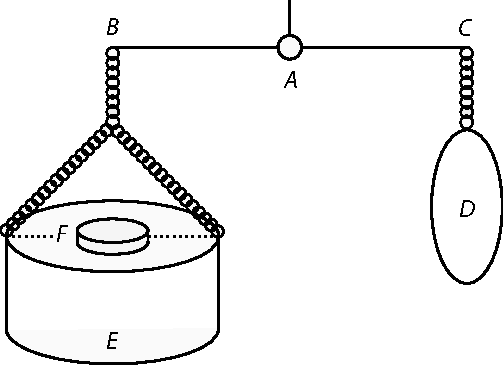
\includegraphics[width=0.55\textwidth]
{gesamttex/edit_VIII-4/images/LH_37_04_151-d1_151r.pdf}%
\edcaption[0.5em]{%
\hspace*{-34mm}%
\lbrack\textit{Fig.\:1}\rbrack%
}%
\vspace{-16.00em}%
\hspace*{86mm}%
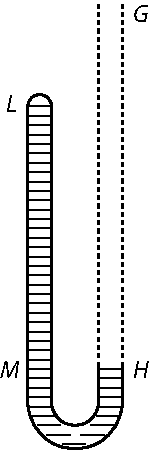
\includegraphics[width=0.156\textwidth]
{gesamttex/edit_VIII-4/images/LH_37_04_151-d2_151r.pdf}%
\edcaption[0.5em]{%
\hspace*{86mm}%
\lbrack\textit{Fig.\:2}\rbrack%
\edtext{%
}{%
\lemma{\lbrack\textit{Fig.\:2}\rbrack}%
\Cfootnote{%
\textit{L} überliefert (Bl.\;\href{\Scan{LH_37_04_151r}}{151\,r\textsuperscript{o}}) drei gestrichene, hier nicht wiedergegebene Entwürfe zum Diagramm.%
}}%
}%
\end{edfigure}%
\selectlanguage{latin}%
\frenchspacing%
\normalsize%



\section[tocentry={Paradoxon barometricum ejusque causa
\enskip%
\bracks{%
Mitte September 1696 -- zweite Hälfte 1697 / zweite Hälfte 1699%
}%
},
head={Paradoxon barometricum ejusque causa}]%
{\MakeUppercase{Paradoxon barometricum ejusque causa}
\newline%
\bracks{%
Mitte September 1696 -- zweite Hälfte 1697 / zweite Hälfte 1699%
}}
\label{60267}



\selectlanguage{ngerman}%
\frenchspacing%
\begin{ledgroupsized}[r]{120mm}%
\footnotesize%
\pstart%
\noindent%
\textbf{Überlieferung:}%
\pend%
\end{ledgroupsized}%
\begin{ledgroupsized}[r]{114mm}%
\footnotesize%
\pstart%
\parindent -6mm%
\makebox[6mm][l]{\textit{L}}%
Aufzeichnung:
LH~XXXVII\;4 Bl.\;149--150.
Zwei Blatt 2\textsuperscript{o},
die ursprünglich einen Bogen gebildet haben dürften;
Wasserzeichen im Bl.\;\href{\Scan{LH_37_04_150wz}}{150};
Ränder zum Teil ausgefranst mit geringfügigem Textverlust auf Bl.\;\href{\Scan{LH_37_04_150r}}{150\,r\textsuperscript{o}} %
u.\;\href{\Scan{LH_37_04_150v}}{150\,v\textsuperscript{o}}:
Papiererhaltungsmaßnahmen.
Vier Seiten;
Textfolge nach Blattzählung (nicht von Leibniz festgelegt).
Die Schreibweise einzelner Personennamen ist uneinheitlich.
\pend%
\end{ledgroupsized}%
\selectlanguage{latin}%
\frenchspacing%
\vspace{8mm}%
\normalsize%
\pstart%
\noindent%
\lbrack%
\href{\Scan{LH_37_04_149r}}%
{149\,r\textsuperscript{o}}%
\rbrack\
\edlabel{LH_37_04_149-150_149r_ersterTeil-1}%
\edtext{%
Bernardus Ramazzinus%
\indexN{\textls{Ramazzini} (Ramazzinus), Bernardino 1633\textendash1714}
\edtext{%
medicus%
\indexS{medicus}
non minus varia doctrina%
\indexS{doctrina varia}
quam naturae scientia%
\indexS{scientia naturae}
commendabilis%
}{%
\lemma{medicus}%
\Bfootnote{%
\textit{(1)}~doctissim %
\textit{(2)}~non minus %
\lbrack...\rbrack\ scientia commendabilis%
~\textit{L}%
}}
nuper dissertationem edidit de Barometro,%
\indexS{dissertatio de barometro}%
\indexS{barometrum}
cui suas intexuit
\edtext{%
\textit{Ephemerides Barometricas}%
\indexS{ephemeris barometrica}
rationemque quaesivit%
\indexS{ratio quaesita}%
}{%
\lemma{\textit{Ephemerides}}%
\Bfootnote{%
\bars{\textit{Barometricas} \textit{erg.}} rationemque
\bars{causae \textit{gestr.}} quaesivit%
~\textit{L}%
}}
cur aere%
\indexS{aer pluvius}
\edtext{%
pluvio Hydrargyrum descendat,%
\indexS{hydrargyrum descendens}%
}{%
\lemma{pluvio}%
\Bfootnote{%
\textit{(1)}~aer d %
\textit{(2)}~Mercurius\indexS{mercurius descendens} %
\textit{(3)}~Hydrargyrum descendat,%
~\textit{L}%
}}
sereno ascendat:%
\indexS{aer serenus}%
\indexS{hydrargyrum ascendens}%
}{%
\lemma{Bernardus \lbrack...\rbrack\ ascendat}%
\Cfootnote{%
Siehe \textsc{B.\;Ramazzini},
\textit{Ephemerides barometricae Mutinenses anni m.dc.xciv, una cum disquisitione causae ascensus ac descensus mercurii in Torricelliana fistula iuxta diversum aeris statum}
(Modena 1695; Augsburg 1696).%
\cite{01516}\cite{01517}%
}}
\edtext{%
\edlabel{LH_37_04_149-150_149r_borelli-1}%
Nimirum Joh. Alphonsus Borellus%
\indexN{\textls{Borelli} (Borellus), Giovanni Alfonso 1608\textendash1679}
philosophus%
\indexS{philosophus}
et Mathematicus%
\indexS{mathematicus}
\edtext{%
egregius in libro%
\indexS{liber}
\textit{de Motionibus a gravitate pendentibus}
dicere visus est%
}{%
\lemma{egregius}%
\Bfootnote{%
\textit{(1)}~statuerat %
\textit{(2)}~dic %
\textit{(4)}~in libro \lbrack...\rbrack\ visus est%
~\textit{L}%
}}
aerem pluvium esse%
\indexS{aer pluvius}%
\indexS{aer serenus}
\edtext{%
sereno%
}{%
\lemma{sereno}%
\Bfootnote{%
\textit{erg.\;L}%
}}
graviorem,%
\indexS{aer gravior}
ob aquas scilicet admistas,%
\indexS{aqua admista aeri}
ideoque debere ab
\edtext{%
eo Hydrargyrum%
\indexS{hydrargyrum ascendens}%
}{%
\lemma{eo}%
\Bfootnote{%
\textit{(1)}~Mercur %
\textit{(2)}~Hydrargyrum%
~\textit{L}%
}}
attolli
\edtext{%
altius,
quod contra sereno coelo%
\indexS{coelum serenum}
dum aer minus obnititur%
\indexS{aer minus obnixus}
praevalente gravitate sua%
\indexS{gravitas aeris}
descendat.%
\edlabel{LH_37_04_149-150_149r_borelli-2}%
}{%
\lemma{altius,}%
\Bfootnote{%
\textit{(1)}~sereno aer %
\textit{(2)}~Idem %
\textit{(3)}~quod contra sereno caelo %
\textit{(a)}~descendat %
\textit{(aa)}~aere minus obnitente %
\textit{(bb)}~dum aer minus obnititur %
\textit{(b)}~dum aer %
\lbrack...\rbrack\ sua descendat.%
~\textit{L}%
}}%
}{%
\lemma{Nimirum \lbrack...\rbrack\ descendat}%
\Cfootnote{%
Siehe
\textsc{G.\:A.\;Borelli},
\textit{De motionibus naturalibus a gravitate pendentibus},
prop.\;113 u.\;115
(Bologna 1670, S.\;239\,f. u.\;242).%
\cite{02068}
Leibnizens unmittelbare Quelle ist wohl aber \textsc{Ramazzini}, \textit{Ephemerides barometricae} (1695, S.\;2\,f.; 1696, S.\;1), wie seine Wendung \textit{dicere visus est} nahelegt.%
\cite{01516}\cite{01517}%
}}
Cum vero cl.
\edtext{%
\edtext{%
Ramazzinus%
\indexN{\textls{Ramazzini} (Ramazzinus), Bernardino 1633\textendash1714}
Barometricas observationes%
\indexS{observatio barometrica}%
}{%
\lemma{Ramazzinus}%
\Bfootnote{%
\textit{(1)}~experi %
\textit{(2)}~Barometricas observationes%
~\textit{L}%
}}
non ita dudum instituisset
\edtext{%
integroque anno continuasset,%
}{%
\lemma{integroque anno continuasset}%
\Bfootnote{%
\textit{erg.\;L}%
}}
contrarium prorsus accidere miratus%
}{%
\lemma{Ramazzinus \bracks{...} miratus est}%
\Cfootnote{%
Vgl. a.a.O. %
(1695, S.\;2;\cite{01516} 1696, S.\;1).\cite{01517}%
}}
\edtext{%
est.
Nempe sereno coelo%
\indexS{coelum serenum}
ascendere Mercurium,%
\indexS{mercurius ascendens}
quasi aere facto graviore,%
\indexS{aer gravior}
\ledpb%
contra pluvia tempestate%
\indexS{tempestas pluvia}
subsidere.%
\indexS{mercurius subsidens}
\edtext{%
Idem postea ab aliis observatum
notavit.%
}{%
\lemma{Idem \bracks{...} notavit}%
\Cfootnote{%
Vgl. a.a.O. %
(1695, S.\;4--7;\cite{01516} 1696, S.\;2\,f.).\cite{01517}
Erwähnt werden dort u.\,a. die Beobachtungen von 
J.\;d'Alencé,\indexN{\textls{Alencé} (d'Alancé, Dalancé, Dalancay, Dalencé), Joachim de 1640\textendash1707}
C.\;Comiers\indexN{\textls{Comiers}, Claude, gest. 1693}
und O.\;v.\:Guericke.\indexN{\textls{Guericke} (Gerickius, Gericke), Otto von 1602\textendash1686}%
}}%
}{%
\lemma{est.}%
\Bfootnote{%
\textit{(1)}~Idemque mox aliis %
\textit{(2)}~Nempe sereno %
\lbrack...\rbrack\ facto graviore, %
\textit{(a)}~leviore, %
\textit{(b)}~contra pluvia %
\lbrack...\rbrack\ postea ab %
\textit{(aa)}~aliis %
\textit{(bb)}~\bars{ab \textit{streicht Hrsg.}} aliis observatum notavit.%
~\textit{L}%
}}
\edtext{%
\edlabel{LH_37_04_149-150_149r_fee-1}%
Causas igitur paradoxi%
\indexS{causa paradoxi}%
\indexS{paradoxon}%
\indexS{causa inquisita}
inquirere %
peculiari dissertatione%
\indexS{dissertatio peculiaris}
instituit;
et aliorum doctissimorum virorum%
\indexS{vir doctus}
sententias
\edlabel{37_04_149-150_01a}%
adjecit.%
\indexS{sententia virorum doctissimorum}%
\edlabel{LH_37_04_149-150_149r_fee-2}%
}{%
\lemma{Causas \lbrack...\rbrack\ adjecit}%
\Cfootnote{%
Vgl. a.a.O. %
(1695, S.\;31\,f.;\cite{01516} 1696, ab S.\;12).\cite{01517}
Siehe zudem die Erläuterung zu N.\ref{53442}, \refpassage{LH_37_04_151_151r_anspiel-3}{LH_37_04_151_151r_anspiel-2} im vorliegenden Band.%
}}%
\edtext{}{%
\xxref{37_04_149-150_01a}{37_04_149-150_01b}%
\lemma{adjecit.}%
\Bfootnote{%
\textit{(1)}~Equidem verissimum est %
\textit{(2)}~Est autem res utique inquisitu digna, %
\textit{(a)}~quam primus quod %
\textit{(b)}~sin et %
\textit{(3)}~Ottono Gerikio\indexN{\textls{Guericke} (Gerickius, Gericke), Otto von 1602\textendash1686} %
\bars{consule Magdeburgensi~\textit{erg.}}, primo Antliae pneumaticae\indexS{antlia pneumatica} a Rob. Boilio\indexN{\textls{Boyle} (Boylius, Boyl), Robert 1627\textendash1691} %
\textit{(4)}~Bar %
\textit{(5)}~Est autem \lbrack...\rbrack\ dignissima primus %
\textit{(a)}~Torricellius\indexN{\textls{Torricelli} (Torricellius), Evangelista 1608\textendash1647} invenit %
\textit{(b)}~Galilaeus\indexN{\textls{Galilei} (Galilaeus, Galileus), Galileo 1564\textendash1642} rem a mechanicis compertam prodidit, %
\textit{(aa)}~aere %
\textit{(bb)}~non %
\textit{(cc)}~antlias aspirantes, %
\lbrack...\rbrack\ pedes attollere.%
~\textit{L}%
}}
\pend%
\pstart%
Est autem tota res inquisitione accuratiore dignissima%
\indexS{inquisitio accuratior}%
\indexS{res digna inquisitione}%
\lbrack:\rbrack\
primus
\edtext{%
Galilaeus%
\indexN{\textls{Galilei} (Galilaeus, Galileus), Galileo 1564\textendash1642}
rem a mechanicis compertam%
\indexS{res comperta a mechanicis}\indexS{mechanicus}
prodidit,
antlias aspirantes,%
\indexS{antlia aspirans}
quas vocant%
\lbrack,\rbrack\
aquam non nisi ad 30 circiter pedes attollere.%
\indexS{aqua elevata ad 30 pedes}%
\indexS{pes}%
\edlabel{37_04_149-150_01b}%
}{%
\lemma{Galilaeus \lbrack...\rbrack\ attollere}%
\Cfootnote{%
Siehe G.\;\textsc{Galilei},
\textit{Discorsi}, giornata I
(Leiden 1638, S.\;17;\cite{00050}
\textit{GO}~VIII, S.\;63\,f.).\cite{00048}
Dort ist von \textit{diciotto braccia} die Rede.%
}}
\edtext{%
Torricellius%
\indexN{\textls{Torricelli} (Torricellius), Evangelista 1608\textendash1647}
deprehendit similiter
Hydrargyrum non posse attolli%
\indexS{hydrargyrum eductum in altum}
\edtext{%
nisi%
}{%
\lemma{nisi}%
\Bfootnote{%
\textit{erg.\;L}%
}}
ad altitudinem%
\indexS{altitudo hydrargyri in barometro}
quae hujus sit pars circiter decima quarta,
quia tanto gravior est Mercurius aqua.%
\indexS{mercurius gravior aqua}
Unde videns rem pendere ab aequilibrio liquorum%
\indexS{aequilibrium liquorum}%
\indexS{liquor in aequilibrio}
\edtext{%
invenit oppositum columnae aereae%
}{%
\lemma{invenit}%
\Bfootnote{%
\textit{(1)}~aeris oppo %
\textit{(2)}~oppositum columnae aereae%
~\textit{L}%
}}
pondus%
\indexS{pondus columnae aereae}%
\indexS{columna aerea}
veram esse huius aquae vel
\edtext{%
Hydrargyri in altum eductionis causam,%
\indexS{causa eductionis aquae in altum}%
\indexS{causa eductionis hydrargyri in altum}%
\indexS{eductio aquae in altum}%
\indexS{eductio hydrargyri in altum}%
\indexS{aqua educta in altum}%
\indexS{hydrargyrum eductum in altum}
et comperit%
}{%
\lemma{Hydrargyri}%
\Bfootnote{%
\textit{(1)}~suspensionis causam, et deprehend\indexS{causa suspensionis hydrargyri}\indexS{suspensio hydrargyri in tubo Torricelliano} %
\textit{(2)}~in altum eductionis, et comperit%
~\textit{L}%
}}
Mercurium ad 27 pollices circiter suspensum%
\indexS{mercurius suspensus ad 27 pollices}%
\indexS{suspensio mercurii in tubo Torricelliano}%
\indexS{pollex}
manere in
\edtext{%
Tubo verticaliter erecto%
\indexS{tubus Torricellianus}
supra clauso,
infra aperto.%
}{%
\lemma{Tubo}%
\Bfootnote{%
\textit{(1)}~infra %
\textit{(2)}~supra %
\textit{(3)}~claus %
\textit{(4)}~perpendicu %
\textit{(5)}~verticaliter erecto %
\lbrack...\rbrack\ infra aperto.%
~\textit{L}%
}}%
}{%
\lemma{Torricellius \lbrack...\rbrack\ aperto}%
\Cfootnote{%
Siehe zum Experiment mit dem Quecksilber
E.\;\textsc{Torricelli}, %
Brief an M.\;Ricci vom 11.\;Juni 1644%
\cite{00107}
(C.\;\textsc{Dati},
\textit{Lettera a Filaleti}, %
Florenz 1663, S.\;20\,f.;%
\cite{00032}
\textit{TO} III, S.\;186--188).\cite{00108}%
}}
Postea experimentum%
\indexS{experimentum Torricellianum prosecutum}
prosecuti sunt
\edtext{%
Blasius Pascalius%
\indexN{\textls{Pascal} (Pascalius), Blaise 1623\textendash1662}
in Gallia,%
\indexO{Frankreich}
vir celebris%
\indexS{vir celebris}
qui primus
\edtext{%
notavit Mercurium%
}{%
\lemma{notavit}%
\Bfootnote{%
\textit{(1)}~aqua %
\textit{(2)}~Mercurium%
~\textit{L}%
}}
in monte excelso subsidere,%
\indexS{mercurius subsidens in monte}%
}{%
\lemma{Blasius \lbrack...\rbrack\ subsidere}%
\Cfootnote{%
Siehe zum Experiment am Puy de Dôme\indexO{Puy de Dôme}
B.\;\textsc{Pascal},
\textit{Récit de la grande expérience}, 1648\cite{02577} %
(\textit{Traitez}, Paris 1663, S.\;165--194;\cite{00081}
\textit{PO}\;II, S.\;653--690).\cite{01524}
}}
et
\edtext{%
Otto Gerickius%
\indexN{\textls{Guericke} (Gerickius, Gericke), Otto von 1602\textendash1686}
consul%
\indexS{consul}
\edtext{%
Magdeburgicus%
\indexO{Magdeburg}
\lbrack qui\rbrack\
rem omnem maxime promovit%
\lbrack:\rbrack\
idemque mirifice%
}{%
\lemma{Magdeburgicus}%
\Bfootnote{%
\textit{(1)}~qui %
\textit{(2)}~\bars{qui \textit{erg. Hrsg.}} rem omnem %
\textit{(a)}~longius %
\textit{(b)}~maxime promovit idemque%
~\textit{L}%
}}
sibi obstrinxit harum scientiarum cultores%
\indexS{cultor scientiarum}
excogitata Antlia,%
\indexS{antlia Magdeburgica}
\ledpb%
qua aerem ex vase eduxit,%
\indexS{antlia educens aerem e vase}%
\indexS{aer eductus e vase}
infinitisque pulcherrimis experimentis%
\indexS{experimentum pulchrum}%
\indexS{experimentum demonstrans effectum aeris}
(partim ab ipsomet sumtis)
occasionem
\edtext{%
dedit%
\lbrack,\rbrack\
quibus%
}{%
\lemma{dedit}%
\Bfootnote{%
\textit{(1)}~quam %
\textit{(2)}~quibus%
~\textit{L}%
}}
usus aeris effecutsque maximi ad oculum demonstrantur.%
\indexS{effectus aeris demonstratus ad oculum}%
\indexS{oculus}%
}{%
\lemma{Otto \lbrack...\rbrack\ demonstrantur}%
\Cfootnote{%
Siehe
O.\:v.\:\textsc{Guericke},
\textit{Experimenta nova}, lib.\;III
(Amsterdam 1672, S.\;71--124).%
\cite{00055}
Dort werden die Versuche und entsprechenden Vorrichtungen beschrieben, auf die Leibniz hinweist.
Diese waren aber bereits Jahre zuvor bekannt gemacht worden;
siehe für die frühere Überlieferung etwa
C.\;\textsc{Schott},
\textit{Mechanica hydraulico-pneumatica},
Anhang: \textit{Experimentum novum Magdeburgicum}
(Frankfurt a.\,M. 1657, S.\;441--488).\cite{00095}%
}}
Quae deinde a
\edtext{%
Roberto%
\indexN{\textls{Boyle} (Boylius, Boyl), Robert 1627\textendash1691}
Boylio Armigero%
\indexS{armigerus}
\edtext{%
Anglo porro praeclare sunt exculta,
integris%
}{%
\lemma{Anglo}%
\Bfootnote{%
\textit{(1)}~egregie %
\textit{(2)}~porro praeclare sunt exculta, %
\textit{(a)}~porro idem %
\textit{(b)}~integris%
~\textit{L}%
}}
de Antlia illa Magdeburgica vel Gerickio%
\indexN{\textls{Guericke} (Gerickius, Gericke), Otto von 1602\textendash1686}%
-Boyliana%
\indexN{\textls{Boyle} (Boylius, Boyl), Robert 1627\textendash1691}%
\indexS{antlia Magdeburgica}%
\indexS{antlia Gerickio-Boyliana}
libris conscriptis.%
\indexS{liber conscriptus}%
}{%
\lemma{Roberto \lbrack...\rbrack\ conscriptis}%
\Cfootnote{%
Seine Versuche mit der Vakuumpumpe über Gewicht und Elastizität der Luft schildert R.\;\textsc{Boyle} hauptsächlich in
\textit{New experiments physico-mechanicall}
(Oxford 1660;\cite{00015}
\textit{BW}~I, S.\;141--301)\cite{00017}
und
\textit{A continuation of new experiments} %
(Oxford 1669;\cite{01062}
\textit{BW}~VI, S.\;27--187).\cite{00017}
}}%
\pend%
\pstart%
\edtext{%
Porro
Gerikius mature%
\indexN{\textls{Guericke} (Gerickius, Gericke), Otto von 1602\textendash1686}
observatis aeris variationibus%
\indexS{variationes aeris collatae cum tubo hydrargyri}
et cum Tubo Hydrargyri collatis%
\indexS{tubus hydrargyri}
indicem tempestatum praenuncium%
\indexS{index praenuncius tempestatum}
sub homunculi figura%
\indexS{figura homunculi}%
\indexS{homunculus index tempestatum}
eleganter est commentus;%
}{%
\lemma{Porro}%
\Bfootnote{%
\textit{(1)}~idem %
\textit{(2)}~Gerikius\indexN{\textls{Guericke} (Gerickius, Gericke), Otto von 1602\textendash1686} %
\textit{(a)}~primus mo %
\textit{(b)}~mature observatis aeris variationibus %
\bars{et cum Tubo Hydrargyri collatis \textit{erg.}}
indicem tempestatum %
\lbrack...\rbrack\ homunculi figura %
\textit{(aa)}~egregie %
\textit{(bb)}~eleganter est commentus;%
~\textit{L}%
}%
\lemma{Gerikius \lbrack...\rbrack\ commentus}%
\Cfootnote{%
Siehe \textsc{Guericke}, \textit{Experimenta nova},\cite{00055}
lib.\;III, cap.\;20 u.\;31 (S.\;100a--b u.\;115a--b);
lib.\;V, appendix (S.\;188b--189a).
Leibniz hatte 1672 diese Stellen exzerpiert:
Vgl. \textit{LSB} VIII,\;1 N.\;36,\cite{01197}
S.\;257.23--30; 259.1--10; 270.14--19.%
}%
}
deinde et%
\edlabel{LH_37_04_149-150_149r_rvb-1}%
\edtext{%
Hugenius%
\indexN{\textls{Huygens} (Hugenius, Ugenius, Hugens, Huguens), Christiaan 1629\textendash1695}%
}{%
\lemma{Hugenius}
\Cfootnote{%
Siehe
C.\;\textsc{Huygens},
\glqq Extrait d'une autre lettre touchant une nouvelle maniere de Barometre\grqq\
(\textit{JS}, 12.\;Dezember 1672, S.\;152--156;%
\cite{01522}
\textit{HO}~VII, S.\;238--241).%
\cite{00113}%
}}
et%
\edtext{%
Hookius%
\indexN{\textls{Hooke} (Hookius, Hook), Robert 1635\textendash1703}%
}{%
\lemma{Hookius}
\Cfootnote{%
Siehe
\textsc{R.\;Hooke},
\textit{Micrographia}, Preface
(London 1665, S.\:[c3] u.\;Tafel I, Abb.\;I);%
\cite{00061}
\textsc{Ders.},
\glqq A new Contrivance of Wheel-Barometer\grqq\
(\textit{PT}, 4.\;Juni 1666,
S.\;218\,f. u.\;Abb.\;1 vor S.\;215).%
\cite{01523}%
}}
\edtext{%
aliique%
}{%
\lemma{aliique}%
\Bfootnote{%
~\textit{erg.\;L}%
}}
alias machinationes elegantes excogitavere,%
\indexS{machinatio elegans excogitata}
\edtext{%
quibus instrumentum%
}{%
\lemma{quibus}%
\Bfootnote{%
\textit{(1)}~Barometrum\indexS{barometrum} %
\textit{(2)}~instrumentum%
~\textit{L}%
}}
redditum est multo aptius ad aeris variationes%
\indexS{instrumentum ad variationes aeris indicandas}%
\indexS{variationes aeris minimae} 
\edtext{%
minimas indicandas,%
\edlabel{LH_37_04_149-150_149r_rvb-2}%
}{%
\lemma{minimas}%
\Bfootnote{%
\textit{(1)}~observandas %
\textit{(2)}~iudicandas%
~\textit{L}%
}}
unde tandem
\lbrack%
\href{\Scan{LH_37_04_149v}}%
{149\,v\textsuperscript{o}}%
\rbrack\
communi consensu%
\indexS{consensus communis}
Barometri%
\indexS{barometrum}
appellatio%
\indexS{appellatio barometri}
invaluit,
quia hoc Tubo aeris gravitatem metiri%
\indexS{gravitas aeris}%
\indexS{mensuratio gravitatis aeris}
\edtext{%
licet.
Fuere viri docti%
\indexS{vir doctus}%
}{%
\lemma{licet.}%
\Bfootnote{%
\textit{(1)}~Et %
\textit{(2)}~Extant autem complures Barometricae observationes apud\indexS{observatio barometrica} %
\textit{(a)}~Gerick\indexN{\textls{Guericke} (Gerickius, Gericke), Otto von 1602\textendash1686} %
\textit{(b)}~Pascalium,\indexN{\textls{Pascal} (Pascalius), Blaise 1623\textendash1662} Gerikium, Boylium\indexN{\textls{Boyle} (Boylius, Boyl), Robert 1627\textendash1691} %
\textit{(3)}~Fuere viri docti%
~\textit{L}%
}}
qui instrumentum hoc%
\indexS{instrumentum ad variationes aeris indicandas}
\edtext{%
cum Thermometro%
\indexS{thermometrum}
et Hygrometro%
\indexS{hygrometrum}
conju\lbrack n\rbrack xere;%
\indexS{barometrum conjunctum cum hygrometro et thermometro}%
}{%
\lemma{cum}%
\Bfootnote{%
\textit{(1)}~Barometro et %
\textit{(2)}~Thermometro et Hygrometro %
\textit{(a)}~comp %
\textit{(b)}~conjugerunt %
\textit{(c)}~\bars{conjuxere%
~\textit{ändert Hrsg.}}%
\textit{L}%
}}
inque ea re non exiguum posuit studium%
\indexS{studium}
v.\;cl.\;Sam.\;Reiherus,%
\indexN{\textls{Reyher} (Reiherus, Reiher), Samuel 1635\textendash1714}%
\indexS{vir clarus}
Jureconsultus%
\indexS{jureconsultus}
et
\edtext{%
Mathematicus%
\indexS{mathematicus}
chiloniensis%
\indexO{Kiel}
doctissimus, %
}{%
\lemma{Mathematicus}%
\Bfootnote{%
\textit{(1)}~et %
\textit{(2)}~chiloniensis %
\textit{(a)}~egregius %
\textit{(b)}~doctissimus,%
~\textit{L}%
}}%
\edtext{%
qui tabulas aliquas suas%
\indexS{tabulae Reiheri}
et observationes%
\indexS{observationes Reiheri}
ante complures annos mihi communicavit.%
}{%
\lemma{qui \lbrack...\rbrack\ communicavit}%
\Cfootnote{%
Siehe die Beilage zu
S.\;\textsc{Reyher}, Brief an G.\,W.\;Leibniz vom 24.\;August (3.\;September) 1679
(\textit{LSB} III,\;2 N.\;339).\cite{01518}\cite{01434}%
}}
Nec dubitem
collata opera%
\indexS{opera collata}
multa hic quoque erui posse
magni non ad rem tantum nauticam%
\indexS{res nautica}
et agricultoriam%
\indexS{res agricultoria}
sed et medicam%
\indexS{res medica}
ipsam momenti futura.
Certe
\edtext{%
Gerikius%
\indexN{\textls{Guericke} (Gerickius, Gericke), Otto von 1602\textendash1686}
observavit
\ledpb%
magnas tempestates%
\indexS{tempestas praesagita}
insolita Mercurii subsidentia%
\indexS{subsidentia mercurii insolita}%
\indexS{mercurius subsidens}
praesagiri.
\edtext{%
Itaque prodesse navigantibus posset Barometrum,%
\indexS{barometrum magno usui navigantibus}
ut%
}{%
\lemma{Itaque}%
\Bfootnote{%
\textit{(1)}~si naut %
\textit{(2)}~magnus %
\textit{(3)}~magno usui navigantibus esse posset %
\textit{(4)}~prodesse navigantibus posset Barometrum %
\textit{(a)}~ad %
\textit{(b)}~ut%
~\textit{L}%
}}
vel mature in portum%
\indexS{navigans receptus in portum}%
\indexS{portus}
se recipiant,
vel certe
\edlabel{37_04_149-150_149v_02a}%
a brevibus scopulisque recedant.%
\indexS{navigans recedens a brevibus scopulisque}%
\indexS{brevia}%
\indexS{scopulus}%
\edtext{}{%
\xxref{37_04_149-150_149v_02a}{37_04_149-150_149v_02b}
\lemma{a}%
\Bfootnote{%
\textit{(1)}~locis recede %
\textit{(2)}~brevibus scopulisque recedant %
\textit{(a)}~Sed %
\textit{(b)}~Caeterum%
~\textit{L}%
}}%
}{%
\lemma{Gerikius \lbrack...\rbrack\ recedant}%
\Cfootnote{%
Siehe \textsc{Guericke}, \textit{Experimenta nova},%
\cite{00055}
lib.\;V, appendix (S.\;195b--196a).
Leibniz hatte 1672 diese Stelle exzerpiert;
vgl. \textit{LSB} VIII,\;1 N.\;36,%
\cite{01197}
S.\;270.21--25.}}
\pend%
\pstart%
\edlabel{37_04_149-150_149v_causa-1}%
Caeterum%
\edlabel{37_04_149-150_149v_02b}
quod causam paradoxi%
\indexS{causa paradoxi}%
\indexS{paradoxon}
attinet%
\lbrack,\rbrack\
equidem verisimillimum mihi semper visum
\edtext{%
est aerem pluvium%
\indexS{aer pluvius}
et pluviam minantem%
\indexS{aer minans pluviam}%
\indexS{pluvia}
esse leviorem,%
\indexS{aer levior}
quia cadentes jam guttas%
\indexS{gutta pluvia}%
\indexS{gutta sustenta ab aere}
non amplius sustinet%
\indexS{aer sustinens guttas}
exoneratusque%
\indexS{aer exoneratus}
adeo partem ponderis sui amittit;%
\indexS{pondus aeris}
contra serena tempestate%
\indexS{tempestas serena}%
}{%
\lemma{est}%
\Bfootnote{%
\textit{(1)}~aere pluvio %
\textit{(2)}~aerem pluvium %
\textit{(a)}~aut paulo %
\textit{(b)}~et ante %
\textit{(c)}~et %
\textit{(d)}~allevari\lbrack\textit{!}\rbrack\ %
\textit{(e)}~et %
\textit{(f)}~velut exonerari %
\textit{(g)}~et pluviam %
\lbrack...\rbrack\ leviorem, quia %
\textit{(aa)}~a %
\textit{(bb)}~cadentes jam %
\lbrack...\rbrack\ amplius sustinet %
\textit{(aaa)}~; contra aer %
\textit{(bbb)}~exoneratusque adeo %
\lbrack...\rbrack\ amittit; contra %
\textit{(aaaa)}~aere sereno %
\textit{(bbbb)}~serena %
\mbox{\bars{tempestate \textit{erg.}}%
\textit{L}}%
}}
aquam attenuatam%
\indexS{aqua attenuata sustenta ab aere}
et dispersam%
\indexS{aqua dispersa sustenta ab aere}
ab aere%
\indexS{aer sustinens aquam attenuatam et dispersam}
susteneri
ac proinde %
cum ipso in subjectum Mercurium%
\indexS{mercurius subjectus gravitati aeris}
\edtext{%
gravita\lbrack r\rbrack e.%
}{%
\lemma{gravitate}%
\Bfootnote{%
\textit{L\;ändert Hrsg.}%
}}%
\edlabel{37_04_149-150_149v_causa-2}
\edtext{%
Eamque sententiam%
\indexS{sententia innuta}
\edtext{%
dudum innuere%
}{%
\lemma{dudum}%
\Bfootnote{%
\textit{(1)}~indicare %
\textit{(2)}~innuere%
~\textit{L}%
}}%
videntur viri docti%
\indexS{vir doctus}
quorum nonnulli etiam a cl.\;%
\edtext{%
Ramazzino%
\indexN{\textls{Ramazzini} (Ramazzinus), Bernardino 1633\textendash1714}
allegantur.%
\edlabel{LH_37_04_149-150_149r_ersterTeil-2}%
}{%
\lemma{Ramazzino}%
\Bfootnote{%
\textit{(1)}~indicantur %
\textit{(2)}~allegantur.%
~\textit{L}%
}}%
}{%
\lemma{Eamque \lbrack...\rbrack\ allegantur}%
\Cfootnote{%
Unter den in \textsc{Ramazzini}, \textit{Ephemerides barometricae} dargelegten Erklärungsvorschlägen sind vornehmlich zwei (1695, S.\;31\,f., 38;\cite{01516} 1696, S.\;12\,f.,\;15)\cite{01517} mit Leibnizens Ansatz verwandt:
der eines "autor anonymus"\indexN{\textls{Alencé} (d'Alancé, Dalancé, Dalancay, Dalencé), Joachim de 1640\textendash1707} (\textsc{J.\;d'Alencé}, \textit{Traittez des baromètres}, Amsterdam 1688,\cite{01525} S.\;45\,f.)
und derjenige von C.\;Comiers\indexN{\textls{Comiers}, Claude, gest. 1693} (bei \textsc{P.\;Le Lorrain de Vallemont}, \textit{Physique occulte}, cap.\;XI, Paris 1693,\cite{01513} Bd.\;II, S.\;355).\indexN{\textls{Le Lorrain de Vallemont} (Vallemontius), Pierre 1649\textendash1721}
}}
Sed quia rem non satis%
\indexS{res explicata distincte}
\edtext{%
distincte explicuere,
putavi sic omne clarius proponi posse.%
}{%
\lemma{distincte}%
\Bfootnote{%
\textit{(1)}~exposuere hinc %
\textit{(a)}~visum est %
\textit{(b)}~digna visa est %
\textit{(2)}~explicuere, putavi %
\lbrack...\rbrack\ proponi posse.%
~\textit{L}%
}}
\pend%
\begin{edfigure}[2.00em][0.00em]%
\includegraphics[width=0.56\textwidth]%
{gesamttex/edit_VIII-4/images/LH_37_04_149-150_d1_149v.pdf}
\edcaption[-0.50em]{\lbrack \textit{Fig.\:1}\rbrack}%
\end{edfigure}%
\newpage%
\pstart%
\edlabel{LH_37_04_149-150_149v-annahme-1}%
In
\edtext{%
libra parium brachiorum%
\indexS{libra parium brachiorum}%
\indexS{brachium librae}%
}{%
\lemma{libra parium brachiorum}%
\Cfootnote{%
Vgl. das Diagramm \lbrack\textit{Fig.\:1}\rbrack.%
}}
\textit{AB}, \textit{AC}
sint aequilibrata%
\indexS{pondus aequilibratum}%
\indexS{aequilibrium in libra}
pondus \textit{D} %
et vas \textit{E} %
aquam continens,%
\indexS{vas continens aquam}%
\indexS{aqua contena in vase}
quod sit altum potius sive profundum
quam largum.
Et in aqua natet%
\indexS{vasculum natans}
vasculum~\textit{F} ex
\edtext{%
plumbo%
\indexS{vasculum plumbeum}%
\indexS{plumbum}
vel ferro%
\indexS{vasculum ferreum}%
\indexS{ferrum}
vitrone%
\indexS{vasculum vitreum}%
\indexS{vitrum}
vel alia materia factum
quae%
}{%
\lemma{plumbo}%
\Bfootnote{%
\bars{vel \textit{erg.}} ferro vitro%
\bars{ne \textit{erg.}} vel alia materia %
\bars{factum \textit{erg.}} quae%
~\textit{L}%
}}
in aqua per se mergitur,%
\indexS{materia mergens in aqua}
hic autem ob vacuam cavitatem%
\indexS{cavitas vacua}
sustinetur.%
\indexS{materia sustenta cavitate vacua}
Sit porro in vasculo \textit{F}
foramen%
\indexS{foramen vasculi obturatum}
obturatum %
charta%
\indexS{charta obturans foramen} %
vel alia materia%
\indexS{materia obturans foramen}%
\indexS{materia perrupta ab aqua}
quam aqua paulatim perrumpat%
\indexS{aqua perrumpens chartam}%
\indexS{charta perrupta ab aqua}
et vasculum impleat;%
\indexS{aqua implens vasculum}
vasculum impletum descendet%
\indexS{vasculum impletum aqua}
et durante descensu%
\indexS{descensus vasculi in aqua}%
\indexS{vasculum descendens in aqua}%
\lbrack,\rbrack\
\edtext{%
mutato
quod erat ante descensum
aequilibrio,%
\indexS{aequilibrium mutatum}%
}{%
\lemma{mutato}%
\Bfootnote{%
\textit{(1)}~aequilibrio, %
\textit{(2)}~quod erat ante descensum aequilibrio,%
~\textit{L}%
}}
vincet pondus \textit{D} %
\edtext{%
et elevabit vas \textit{E},%
}{%
\lemma{et}%
\Bfootnote{%
\textit{(1)}~vas \textlangle \textit{E}\textrangle\ %
\textit{(2)}~elevabit vas \textit{E},%
~\textit{L}%
}}
quia a vase \textit{E} %
non amplius sustinetur vasculum \textit{F},
quippe descendens;
atque adeo vas \textit{E} de pondere suo aliquid amisit.%
\indexS{pondus amissum}
Nec vero restituetur aequilibrium,%
\indexS{aequilibrium restitutum}
\edtext{%
donec vasculum \textit{F}
ad fundum vasis \textit{E}%
}{%
\lemma{donec}%
\Bfootnote{%
\textit{(1)}~vas %
\textit{(2)}~vasculum \textit{F} %
\textit{(a)}~ad v %
\textit{(b)}~ad fundum vasis \textit{E}%
~\textit{L}%
}}
pervenerit %
ibique quieverit,
ubi scilicet rursus ab eo sustinetur.%
\edlabel{LH_37_04_149-150_149v-annahme-2}
\lbrack%
\href{\Scan{LH_37_04_150r}}%
{150\,r\textsuperscript{o}}%
\rbrack%
\pend%
\pstart%
Similiter ergo,
si
\edtext{%
cylinder aeris%
\indexS{cylinder aeris}
\textit{GH}%
}{%
\lemma{cylinder}%
\Bfootnote{%
\textit{(1)}~vasis %
\textit{(2)}~aeris \textit{GH}%
~\textit{L}%
}%
\lemma{cylinder aeris \textit{GH}}%
\Cfootnote{%
Vgl. das Diagramm \lbrack\textit{Fig.\:2}\rbrack.%
}%
}
et Hydrargyri \textit{LM}%
\indexS{hydrargyrum}
sint in aequilibrio,%
\indexS{aequilibrium aeris et hydrargyri}
erit Hydrargyrum instar ponderis \textit{D} %
et columna aeris,%
\indexS{columna aeris}
respectu
\edtext{%
aquae sustentatae%
\indexS{aqua sustentata ab aere}%
\lbrack,\rbrack\
instar%
}{%
\lemma{aquae}%
\Bfootnote{%
\textit{(1)}~inclusae instar %
\textit{(2)}~sustentatae instar%
~\textit{L}%
}}
vasis \textit{E}.
Cadente autem aqua%
\indexS{aqua cadens in aere}
cessanteque sustentatione
praevalebit Mercurius
atque adeo subsidet%
\indexS{mercurius subsidens in barometro}
\edtext{%
quemadmodum observationibus%
\indexS{observatio barometrica}%
}{%
\lemma{quemadmodum}%
\Bfootnote{%
\textit{(1)}~et %
\textit{(a)}~experientia\indexS{experientia} %
\textit{(b)}~per experientiam %
\textit{(2)}~observationibus%
~\textit{L}%
}}
comprobatur.
\edtext{%
Nec dubito ipsum Borellum%
\indexN{\textls{Borelli} (Borellus), Giovanni Alfonso 1608\textendash1679}
hic fuisse assensurum,
\edtext{%
etsi alia docere visus sit%
}{%
\lemma{etsi \lbrack...\rbrack\ sit}%
\Cfootnote{%
Siehe oben, die Erläuterung zu \refpassage{LH_37_04_149-150_149r_borelli-1}{LH_37_04_149-150_149r_borelli-2}.%
}}%
\lbrack,\rbrack\
\edtext{%
qu\textlangle em\textrangle admodum
ex ipsius principiis%
\indexS{principium}
cl.\;Tortu\textlangle s\textrangle%
\indexN{\textls{Torti} (Tortus), Francesco 1658\textendash1741}
bene ostendit apud dn. Ramazzinu\textlangle m.\textrangle%
\indexN{\textls{Ramazzini} (Ramazzinus), Bernardino 1633\textendash1714}%
}{%
\lemma{qu\textlangle em\textrangle admodum \lbrack...\rbrack\ Ramazzinu\textlangle m.\textrangle}%
\Cfootnote{%
Vgl. F.\;\textsc{Torti},
Brief an B.\;Ramazzini vom Januar 1695%
\cite{01519}
(in \textsc{Ramazzini},
\textit{Ephemerides barometricae},
1695, S.\;89--127;\cite{01516}
1696, S.\;37-60).\cite{01517}
Vgl. auch Ramazzinis Darstellung von Tortis exegetischem Ansatz
(a.a.O., %
1695, S.\;44\,f.; 1696, S.\;17\,f.).%
\cite{01516}\cite{01517}
}}%
}{%
\lemma{Nec}%
\Bfootnote{%
dubito %
\lbrack...\rbrack\ bene ostendit %
\textit{(1)}~in Epist\textlangle ola\textrangle\indexS{epistola}
\textit{(2)}~apud dn. Ramazzinu\textlangle m.\textrangle\
\textit{erg.\;L}%
}}%
\pend%
\pstart%
Sed operae pretium %
tamen erit %
paulo distinctius exponere
\edtext{%
quomodo fiat ut%
}{%
\lemma{quomodo}%
\Bfootnote{%
\textit{(1)}~fieri possit ut %
\textit{(2)}~fiat ut%
~\textit{L}%
}}
aqua in%
\indexS{aqua elevata in aere}%
\indexS{aqua sustenta in aere}%
\indexS{aqua cadens in aere}
\edtext{%
aere elevetur,
sustineatur,
cadat.%
}{%
\lemma{aere}%
\Bfootnote{%
\textit{(1)}~modo sustineatur modo cadat modo %
\textit{(2)}~elevetur, sustineatur, cadat.%
~\textit{L}%
}}
Elevatio esse potest duplex,%
\indexS{elevatio aquae in aere}
una exemplo fumi,%
\indexS{fumus assurgens in aere}%
\indexS{elevatio fumi in aere}
qui assurgit
quia
\edtext{%
est aere specifice%
}{%
\lemma{est}%
\Bfootnote{%
\textit{(1)}~aquae specie %
\textit{(2)}~aere specifice%
~\textit{L}%
}}
levior,%
\indexS{fumus levior aere specifice}%
\indexS{aer gravior fumo specifice}
altera exemplo pulveris%
\indexS{elevatio pulveris in aere}%
\indexS{pulvis elevatus in aere}
qui solo motu attolitur,
\edtext{%
quemadmodum et aqua motu turbida fit%
\indexS{aqua fiens turbida motu}
sedimentis elevatis.%
\indexS{sedimentum elevatum in aqua}
Ut autem%
}{%
\lemma{quemadmodum}%
\Bfootnote{%
\textit{(1)}~sedimenta %
\textit{(2)}~et aqua motu turbida %
\textit{(a)}~fuit %
\textit{(b)}~sit sedimentis elevatis. %
\textit{(aa)}~Iterumque %
\textit{(bb)}~Ut autem%
~\textit{L}%
}}
fumi instar
\edtext{%
elevetur humor,%
\indexS{humor elevatus in aere}%
\indexS{elevatio humoris in aere}%
}{%
\lemma{elevetur}%
\Bfootnote{%
\bars{aqua vel \textit{gestr.}} humor,%
~\textit{L}%
}}
fieri
\edtext{%
potest dilatatione orta a calore,%
\indexS{dilatatio orta a calore}%
\indexS{calor origo dilatationis}%
}{%
\lemma{potest}%
\Bfootnote{%
\textit{(1)}~rarefactione a %
\textit{(2)}~dilatatione %
\textit{(a)}~caloris %
\textit{(b)}~orta a calore,%
~\textit{L}%
}}
quemadmodum et distillationes Chemicorum%
\indexS{distillatio chemicorum}%
\indexS{chemicus}
ostendunt.
Elevata igitur materia aquosa%
\indexS{materia aquosa elevata in aere}
sustentabitur
vel a calore adhuc perdurante,%
\indexS{materia aquosa sustentata a calore}%
\indexS{calor perdurans}
cum nimirum ad eum locum pervenerit %
ubi aeris%
\indexS{tenuitas aeris continue crescens sursum}
\edtext{%
tenuitas
(continue scilicet sursum crescens)
tanta est,%
}{%
\lemma{tenuitas}%
\Bfootnote{%
\bars{(~%
\textit{(1)}~perpetuo %
\textit{(2)}~continue scilicet sursum crescens) %
\textit{erg.}} tanta est,%
\textit{L}%
}}
ut gravitas specifica utriusque%
\indexS{gravitas aeris specifica}%
\indexS{gravitas materiae aquosae specifica}
sit aequalis;
vel etiam%
\lbrack,\rbrack\
cessante jam calore%
\indexS{calor cessans}
vel
\edtext{%
imminuto%
\indexS{calor imminutus}%
\lbrack,\rbrack\
ex ipsa tenuitate%
\indexS{tenuitas aeris sustinens materiam aquosam}%
}{%
\lemma{imminuto}%
\Bfootnote{%
\textit{(1)}~ex ipsa %
\textit{(2)}~gradu tenuitatis %
\textit{(3)}~ex ipsa tenuitate%
~\textit{L}%
}}
et causis huic connexis.%
\indexS{causa connexa}
\pend%
\pstart%
Haec autem sustentatio a tenuitate%
\indexS{tenuitas aeris sustinens materiam aquosam}%
\indexS{sustentatio materiae aquosae e tenuitate aeris}
ita
\edtext{%
porro explicari%
}{%
\lemma{porro}%
\Bfootnote{%
\bars{Geometrice \textit{gestr.}} %
\textit{(1)}~acc %
\textit{(2)}~explicari%
~\textit{L}%
}}
potest:
Ponamus
\edtext{%
aerem,%
\indexS{aer habens gradum firmitatis seu tenacitatis}%
\indexS{aer ut fluidum}
ut omnia fluida,%
\indexS{fluidum habens gradum firmitatis seu tenacitatis}%
}{%
\lemma{aerem,}%
\Bfootnote{%
\textit{(1)}~ut %
\textit{(a)}~omnis %
\textit{(b)}~liquo %
\textit{(2)}~\bars{ut \textit{erg.}} omnia fluida,%
~\textit{L}%
}} %
habere
\edtext{%
gradum quendam%
\indexS{gradus firmitatis aeris}%
\indexS{gradus tenacitatis aeris}%
\indexS{gradus firmitatis fluidi}%
\indexS{gradus tenacitatis fluidi}%
}{%
\lemma{gradum}%
\Bfootnote{%
\textit{(1)}~aliquem %
\textit{(2)}~quendam%
~\textit{L}%
}}
firmitatis%
\indexS{firmitas aeris}%
\indexS{firmitas fluidi}
seu tenacitatis,%
\indexS{tenacitas aeris}%
\indexS{tenacitas fluidi}
ut aliqua vi sit opus,
quantulacunque%
\indexS{vis quantulacunque}
\edtext{%
licet,%
}{%
\lemma{licet,}%
\Bfootnote{%
~\textit{erg.\;L}%
}}
ad eum dividendum.%
\indexS{vis ad aerem dividendum}%
\indexS{vis ad fluidum dividendum}
Ponamus porro
materiam in aere sustentatam%
\indexS{materia sustentata in aere}
esse admodum attenuatam%
\indexS{materia attenuata}
\edtext{%
ac dilatatam%
\indexS{materia dilatata}
ut%
}{%
\lemma{ac}%
\Bfootnote{%
\textit{(1)}~dilutam %
\textit{(2)}~dilatatam %
\bars{ita \textit{streicht Hrsg.}} ut%
~\textit{L}%
}}
multum habeat
\edtext{%
superficiei,%
\indexS{proportio superficiei ad pondus}
ponderis vero sub ea superficie contenti%
\indexS{pondus contentum sub superficie} %
parum,
quemadmodum,
ex visibilibus corporibus,%
\indexS{corpus visibile}
plumae,%
\indexS{pluma}%
}{%
\lemma{superficiei,}%
\Bfootnote{%
\textit{(1)}~ponderisque %
\textit{(2)}~ponderis vero %
\textit{(a)}~sumta %
\textit{(b)}~sub ea %
\lbrack...\rbrack\ parum, quemadmodum, %
\textit{(aa)}~pluminae, in %
\textit{(bb)}~ex visibilibus corporibus, plumae,%
~\textit{L}%
}}
tenues laminae%
\indexS{lamina tenuis} %
aliaque id
\edtext{%
genus.
Cum ergo%
}{%
\lemma{genus.}%
\Bfootnote{%
\textit{(1)}~Ess %
\textit{(2)}~Ponamus porro %
\textit{(3)}~Cum ergo%
~\textit{L}%
}}
vis%
\indexS{vis perrumpendi aerem}
\edtext{%
perrumpendi aerem sit a pondere,%
\indexS{pondus perrumpens aerem}
resistentia autem%
\indexS{resistentia aeris ad perrumpendum}%
}{%
\lemma{perrumpendi}%
\Bfootnote{%
\textit{(1)}~sit a ponderi,\lbrack\textit{!}\rbrack\ %
\textit{(2)}~aerem sit a pondere, %
\textit{(a)}~vis autem %
\textit{(b)}~resistentia autem%
~\textit{L}%
}}
a superficie ipsius%
\indexS{superficies perrumpentis aerem}
quod perrumpere debet,
manifestum
\edtext{%
est
tam exiguum esse posse pondus%
}{%
\lemma{est}%
\Bfootnote{%
\textit{(1)}~fieri %
\textit{(2)}~tantum es %
\textit{(3)}~tam exiguum esse posse pondus%
~\textit{L}%
}}
proportione superficiei,%
\indexS{proportio ponderis ad superficiem}
ut aer non perrumpatur;
quemadmodum
\edtext{%
lamina tenuis%
\indexS{lamina tenuis}%
}{%
\lemma{lamina}%
\Bfootnote{%
\textit{(1)}~argen %
\textit{(2)}~tenuis%
~\textit{L}%
}}
in tela araneae%
\indexS{tela araneae}%
\indexS{aranea}
suspensa haerere potest,%
\indexS{lamina suspensa in tela araneae}
quae si fusione%
\indexS{fusio}
in globulum redacta esset,%
\indexS{lamina redacta in globulum}
\edlabel{37_04_149-150_150r_03a}%
perrumperet.%
\edtext{}{%
\xxref{37_04_149-150_150r_03a}{37_04_149-150_150r_03b}%
\lemma{perrumperet.}%
\Bfootnote{%
\bars{%
\lbrack/\rbrack\
Caeterum etsi vapores per aquam dispersi calore%
\indexS{vapor dispersus calore per aquam}%
\indexS{calor dispergens vaporem} %
\textit{erg. u. gestr.}}
Fieri etiam potest,%
~\textit{L}%
}}
\pend%
\begin{edfigure}[1.0em][0em]%
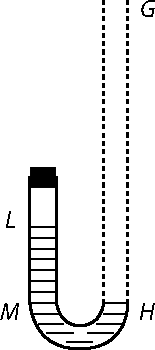
\includegraphics[width=0.15\textwidth]{gesamttex/edit_VIII-4/images/LH_37_04_149-150_d2_150r.pdf}
\edcaption[0.5em]{\lbrack \textit{Fig.\:2}\rbrack}
\end{edfigure}%
\newpage%
\pstart%
Fieri%
\edlabel{37_04_149-150_150r_03b}
etiam potest,
ob motum aeris vel alterius liquidi,%
\indexS{motus aeris}%
\indexS{motus liquidi}%
\indexS{aer motus}%
\indexS{liquidum motum}
ut
quae in eo natant%
\indexS{particulae natantes in aere}%
\indexS{particulae natantes in liquido}
non decidant%
\lbrack,\rbrack\
dum
\edtext{%
scilicet%
}{%
\lemma{scilicet}%
\Bfootnote{%
\textit{erg.\;L}%
}}
ipso motu rursus elevantur,%
\indexS{particulae elevatae motu aeris}%
\indexS{particulae elevatae motu liquidi}
atque ita alternis
nunc ascendentia,
nunc descendentia,
\edtext{%
revera%
}{%
\lemma{revera}%
\Bfootnote{%
\textit{erg.\;L}%
}}
manent in sublimi%
\indexS{particulae manentes in sublimi}
\edtext{%
donec
impetus ab externo impressus%
\indexS{impetus impressus ab externo}
elanguescat.%
}{%
\lemma{donec}%
\Bfootnote{%
impetus \lbrack...\rbrack\ impressus elanguescat
\textit{erg.\;L}%
}}
Quanquam haec minus ad institutum%
\indexS{institutum}
nostrum faciant,
quoniam quae motu%
\indexS{particulae elevatae motus aeris}%
\lbrack,\rbrack\
id est impresso%
\indexS{impetus impressus ab externo}%
\indexS{particulae elevatae impetu impresso}
\edtext{%
impetu%
\lbrack,\rbrack\
elevantur,%
\indexS{elevatio particularum impetu impresso}%
\indexS{impetus elevans particulas}
non sustinentur a liquore,%
\indexS{sustentatio particularum a liquore}%
\indexS{liquor sustinens particulas}%
}{%
\lemma{impetu}%
\Bfootnote{%
\textit{(1)}~sustentantur, %
\textit{(a)}~\textlangle--\textrangle\ %
\textit{(b)}~ipsi aeri %
\textit{(c)}~n\textlangle-- --\textrangle\ %
\textit{(2)}~elevantur, %
\textit{(a)}~vel %
\textit{(b)}~non sustinentur a liquore,%
~\textit{L}%
}}
atque adeo ad aequilibrium%
\indexS{aequilibrium particularum in liquore}
non conferunt.
\edtext{%
Nempe
(ut ex projectorum exemplo constat)%
\indexS{exemplum}
composito motu%
\indexS{motus compositus e gravitate et impetu}
feruntur ex gravitate%
\indexS{gravitas ferens particulas}
et impetu impresso.%
\indexS{impetus impressus ab externo}%
\indexS{impetus ferens  particulas}%
\indexS{latio particularum a gravitate et impetu}
Itaque gravitate%
\indexS{gravitas}
quidem continue cadunt,
sed cum concepto impetu%
\indexS{impetus conceptus}
magis vel saltem non minus eleventur,%
\indexS{impetus elevans particulas}
fit ut assurgant omnino
vel sustententur,%
\indexS{sustentatio particularum ab impetu}%
\indexS{impetus sustinens particulas}
non tamen a flu\textlangle ido\textrangle\
in quo suspenduntur.%
\indexS{suspensio particularum in fluido}%
\indexS{sustentatio particularum a fluido}%
\indexS{fluidum sustinens particulas}%
}{%
\lemma{Nempe}%
\Bfootnote{%
\textit{(1)}~continue %
\textit{(a)}~cadunt %
\textit{(b)}~cadere possu %
\textit{(c)}~cadunt ut %
\textit{(2)}~etsi inter cadendum %
\textit{(3)}~ex nisu gravitatis, etsi %
\textit{(4)}~(ut ex projectorum exemplo %
\textit{(a)}~cadunt %
\textit{(b)}~constat) composito %
\lbrack...\rbrack\ quo suspenduntur.
\textit{erg.\;L}%
}}
\pend%
\pstart%
Quae etiam
\edtext{%
causa confert ad%
}{%
\lemma{causa}%
\Bfootnote{%
\textit{(1)}~est cur %
\textit{(2)}~confert ad%
~\textit{L}%
}}
aerem ventis validis%
\indexS{aer sublevatus vento}%
\indexS{ventus sublevans aerem}
\edtext{%
sublevandum;
unde tempesta\lbrack s\rbrack\ futura%
\indexS{tempestas praenuntiata barometro}
saepe barometro praenuntiari potest%
\indexS{barometrum praenuntians tempestam}%
\lbrack,\rbrack\
quanquam praeterea
ventis nunc in diversa tendentibus%
\indexS{venti tendentes in diversa}
deduci aerem atque attenuari,%
\indexS{aer attenuatus ventis contrariis}%
\indexS{aer deductus ventis contrariis}
nunc concurrentibus condensari,%
\indexS{aer condensatus ventis concurrentibus}%
\indexS{venti concurrentes}
passim etiam ad fluctuum instar%
\indexS{fluctus}
nunc deprimi in valles%
\indexS{aer depressus in valles}%
\indexS{vallis}
nunc in montes attolli%
\indexS{aer elevatus in montes}%
\indexS{mons}
consentaneum videatur.
Quibus de rebus%
}{%
\lemma{sublevandum;}%
\Bfootnote{%
\textit{(1)}~eaque ventis est %
\textit{(2)}~et %
\textit{(3)}~unde %
\bars{tempestatem \textit{ändert Hrsg.}} %
\textit{(a)}~futuram %
\textit{(b)}~futura %
\bars{saepe \textit{erg.}} barometro %
\textit{(aa)}~praenuntiandam %
\textit{(bb)}~praenuntiari potest quanquam %
\textit{(aaa)}~eadem %
\textit{(bbb)}~praeterea ventis %
\textit{(aaaa)}~(praesertim si plures ad easdem aut diversas partes tendant) alicubi valles %
\textit{(bbbb)}~\bars{nunc in diversa tendentibus \textit{erg.}} deduci aerem atque attenuari %
\textit{(aaaaa)}~alibi et comprimi, %
\textit{(bbbbb)}~nunc conflictantibus %
\textit{(ccccc)}~aut in valles deprimi, alibi vero %
\textit{(ddddd)}~\bars{nunc concurrentibus \textit{erg.}} condensari %
\textit{(aaaaa-a)}~et ad fluctuum instar in montes attolli. %
\textit{(bbbbb-b)}~passim etiam \lbrack...\rbrack\ attolli consentaneum videatur.%
\textit{(aaaaa-aa)}~Quam in rem %
\textit{(bbbbb-bb)}~Quibus de rebus%
~\textit{L}%
}}
etiam
\edtext{%
Edmundus Hallejus%
\indexN{\textls{Halley} (Hali, Hallé, Hale, Hales, Hallaeus), Edmond 1656\textendash1742}
vir clarus%
\indexS{vir clarus}
nonnulla egregria est commentatus.%
}{%
\lemma{Edmundus \lbrack...\rbrack\ commentatus}%
\Cfootnote{%
Siehe E.\;\textsc{Halley},
"A discourse of the rule of the decrease of the height of the mercury"
(\textit{PT}~XVI, Nr.\;181, 25.\;Mai 1686, S.\;104--116).%
\cite{01526}%
}}%
\pend%
\vspace{1.0em}%
\pstart%
\noindent%
\lbrack%
\textit{Nachfolgender Textabschnitt (bis zu \refpassage{LH_37_04_149-150_150r_einschub}{LH_37_04_149-150_150r_einschub} ) in L am Rand ergänzt:}%
\rbrack\
\pend%
\vspace{0.5em}%
\pstart%
\noindent%
\edtext{%
Videri quidem posset
particulas calore sustentatas%
\indexS{particulae sustentatae calore}%
\indexS{calor sustinens particulas}%
\indexS{sustentatio particularum calore}
etiam ad rem non facere,
non magis quam
quae motu sustentantur,%
\indexS{sustentatio particularum motu aeris}
quia
cum sint aere paris spatii leviores,%
\indexS{particulae leviores aere paris spatii}%
}{%
\lemma{Videri}%
\Bfootnote{%
\textit{(1)}~etiam poterit %
\textit{(2)}~quidem posset particulas %
\textit{(a)}~heterogeneas %
\textit{(b)}~\bars{calore \textit{erg.}} in aere %
\textit{(c)}~calore sustentatas %
\textit{(aa)}~adeo aere pari\textlangle s\textrangle\ spatii leviores, non %
\textit{(bb)}~etiam ad rem %
\lbrack...\rbrack\ paris spatii leviores,%
~\textit{L}%
}}
cylindrum aereum%
\indexS{cylinder aereus}
potius leviorem reddant,
quam graviorem.
Sed respondendum est,
eo ipso
dum aer%
\indexS{aer recipiens materiam gravem}
novam materiam gravem%
\indexS{materia gravis recepta in aerem}
recipit,
fieri graviorem,%
\indexS{aer factus gravior}
\ledpb%
ut
cum lignum aquae innatat%
\indexS{lignum innatans aquae}%
\lbrack,\rbrack\
vas aquam continens%
\indexS{vas continens aquam}
gravius erit,
quam si lignum auferatur.
Itaque
\edtext{%
quod levior reddatur columna aeris%
\indexS{columna aeris}%
\indexS{aer redditus levior}%
\indexS{aer recipiens materiam leviorem}
ob materiam leviorem receptam%
\indexS{materia levior recepta in aerem}%
}{%
\lemma{quod}%
\Bfootnote{%
\textit{(1)}~leviorem %
\textit{(2)}~levior reddatur %
\textit{(a)}~cylinder %
\textit{(b)}~columnam %
\textit{(c)}~columna aeris %
\textit{(aa)}~materia leviore recepta %
\textit{(bb)}~ob materiam leviorem receptam%
~\textit{L}%
}}
intelligendum
\edtext{%
est de columna%
\indexS{columna aeris}
altitudinis ejusdem.%
\indexS{altitudo columnae aeris}%
}{%
\lemma{est}%
\Bfootnote{%
\textit{(1)}~de cylindro spatii pristini, cum %
\textit{(2)}~de columna altitudinis ejusdem.%
~\textit{L}%
}}
Hic vero consentaneum
\edtext{%
est
columnam%
\indexS{columna aeris}
reddi altiorem%
}{%
\lemma{est}%
\Bfootnote{%
\textit{(1)}~cylindrum reddi altius %
\textit{(2)}~columnam reddi altiorem%
~\textit{L}%
}}
materia nova recepta%
\indexS{materia nova recepta in aerem}
ac sustentata.%
\edlabel{LH_37_04_149-150_150r_einschub}%
\pend%
\vspace{1.0em}%
\pstart%
\noindent%
Explicata jam
\edtext{%
sustentatione%
\indexS{sustentatio particularum in aere}%
\lbrack,\rbrack\
ad aquam rursus delabentem%
\indexS{aqua delabens in aere}%
}{%
\lemma{sustentatione}%
\Bfootnote{%
\textit{(1)}~ad casum %
\textit{(2)}~ad aquam rursus delabentem%
~\textit{L}%
}}
veniamus.
\edtext{%
Itaque cum calore
factum sit
ut humores%
\indexS{humor inflatus in bullas}
velut in bullas quasdam%
\indexS{bulla inflata humore}
et ut ita dicam vesicas%
\indexS{vesica inflata humore}
inflarentur,
quae excluso%
}{%
\lemma{Itaque}%
\Bfootnote{%
\textit{(1)}~vel deferente calore,\indexS{calor deferens} %
\textit{(2)}~quemadmodum %
\textit{(3)}~cum calore factum sit ut humores %
\textit{(a)}~inflati in %
\textit{(b)}~velut in %
\lbrack...\rbrack\ vesicas inflarentur, %
\textit{(aa)}~quibus exclu %
\textit{(bb)}~ex quibus exclus %
\textit{(cc)}~quae excluso%
~\textit{L}%
}}
aere crassiore%
\indexS{aer crassior}%
\indexS{aer exclusus}
intus
\edtext{%
vacuae%
\indexS{bulla vacua intus}
ascenderant ad certam usque altitudinem%
\indexS{bulla ascendens}%
\indexS{ascensus bullae}
ibique sustentabantur,%
\indexS{bulla sustentata}%
\indexS{sustentatio bullae}%
}{%
\lemma{vacua}%
\Bfootnote{%
\textit{(1)}~velu %
\textit{(2)}~vel ascenderant vel sustentabantur, %
\textit{(3)}~ascenderant %
\bars{ad certam usque altitudinem ibique \textit{erg.}} sustentabantur,%
~\textit{L}%
}}
nunc
\edtext{%
vicissim eveniet ut%
}{%
\lemma{vicissim}%
\Bfootnote{%
eveniet ut
\textit{erg.\;L}%
}}
cessante calore%
\indexS{calor cessans}
instar vesicae flaccidae%
\indexS{vesica flaccida}
concidant,%
\indexS{bulla concidens}
et recuperata gravitate%
\indexS{gravitas recuperata}
delabentur.%
\indexS{bulla delabens}
Sed et aliae
\lbrack%
\href{\Scan{LH_37_04_150v}}	%
{150\,v\textsuperscript{o}}%
\rbrack\	
humorum%
\indexS{humor particulatus}
particulae,%
\indexS{particulae humoris}
non quidem clausae
sed
\edtext{%
potius%
}{%
\lemma{potius}%
\Bfootnote{%
\textit{erg.\;L}%
}}
ab aere ubique penetratae%
\indexS{aer penetrans particulam}%
\lbrack,\rbrack\
ob nimiam tamen tenuitatem,%
\indexS{tenuitas superficiei particulae}
id est superficiei%
\indexS{superficies particulae humoris}
magnitudinem,%
\indexS{magnitudo superficiei particulae}
perrumpere ac descendere non valentes%
\lbrack,\rbrack\
poterunt rursus addensari%
\indexS{particulae addensatae}
vel incrassari,%
\indexS{particulae incrassatae}
dum plures laminae tenuissimae conjunguntur inter se,%
\indexS{laminae tenues conjunctae}
sive ipso motu aeris%
\indexS{motus aeris}
dum sibi occurrentes implicantur
ac cohaerescunt%
\lbrack,\rbrack\
sive eo modo
quo videmus sales in aquis solutos%
\indexS{sal solutus in aqua}%
\indexS{solutio salis in aqua}
\edtext{%
paulatimque%
}{%
\lemma{paulatimque}%
\Bfootnote{%
\textit{erg.\;L}%
}}
in crystallos%
\indexS{crystallus}
reconcrescere;%
\indexS{sal reconcretus in crystallos}
sive denique
\edtext{%
superiorum partium jam
ex caloris vel motus cessatione%
\indexS{cessatio motus}%
\indexS{cessatio caloris}%
\indexS{motus cessans}%
\indexS{calor cessans}
descendentium lapsu;%
\indexS{lapsus particularum in aere}%
}{%
\lemma{superiorum}%
\Bfootnote{%
\textit{(1)}~lapsu %
\textit{(2)}~quae %
\textit{(3)}~partium jam %
\textit{(a)}~descenden %
\textit{(b)}~ex caloris %
\textit{(aa)}~defectu %
\textit{(bb)}~cessatione %
\textit{(cc)}~vel motus %
\textit{(aaa)}~descendentium, %
\textit{(bbb)}~cessatione descendentium lapsu;%
~\textit{L}%
}}
ita enim labentes guttae%
\indexS{gutta labens}
ut
\edtext{%
pilae%
\indexS{pila nivis}%
\indexS{nix}
ex nive%
}{%
\lemma{pilae}%
\Bfootnote{%
\textit{(1)}~nivis %
\textit{(2)}~ex nive%
~\textit{L}%
}}
inter eundum crescent.%
\indexS{gutta crescens inter eundum}
\pend%
\pstart%
Et fieri omnino potest,
ut nulla sit
\edtext{%
prorsus quorundam vaporum sustentatio,%
\indexS{sustentatio vaporis}%
\indexS{vapor sustentatus}
sed continue vel ascendant,%
\indexS{vapor ascendens}
vel descendant;%
\indexS{vapor descendens}
dissipentur%
\indexS{vapor dissipatus}%
\indexS{dissipatio vaporis}
autem ascensu%
\indexS{ascensus vaporis}%
}{%
\lemma{prorsus}%
\Bfootnote{%
\textit{(1)}~(nisi calore quorundam %
\textit{(2)}~, nisi a calore %
\textit{(3)}~sustentatio motu quorundam %
\textit{(4)}~quorundam %
\textit{(a)}~particularum %
\textit{(b)}~vaporum %
\textit{(aa)}~suscitatio %
\textit{(bb)}~sustentatio, sed continue %
\textit{(aaa)}~descendant %
\textit{(bbb)}~vel ascendant, vel descendant;
\textit{(aaaa)}~tractantur %
\textit{(bbbb)}~di %
\textit{(cccc)}~dissipentur autem ascensu%
~\textit{L}%
}}
(dum tenuissimae partes reliquas post se relinquant)
et rursus descensu%
\indexS{descensus vaporis}
recolligantur.%
\indexS{vapor recollectus in guttas}%
\indexS{recollectio vaporis in guttas}
Descendent autem lentissime%
\indexS{descensus vaporis}%
\indexS{vapor descendens}
dum
\edtext{%
tenu\lbrack es\rbrack%
}{%
\lemma{tenuia}%
\Bfootnote{%
\textit{L\;ändert Hrsg.}%
}}
sunt,
ob aeris resistentiam%
\indexS{resistentia aeris}%
\lbrack;\rbrack\
aucta autem mole %
imminutaque simul superficie,
tandem recolligentur in guttas,%
\indexS{vapor recollectus in guttas}%
\indexS{recollectio vaporis in guttas}
et cum impetu
\edlabel{37_04_149-150_150v_duza-1}%
delabentur.%
\indexS{vapor delabens}%
\indexS{delapsus vaporis}%
\edtext{}{%
\xxref{37_04_149-150_150v_duza-1}{37_04_149-150_150v_duza-2}%
\lemma{delabentur,}%
\Bfootnote{%
\textit{(1)}~Haec p %
\textit{(2)}~Ex %
\textit{(3)}~Atque ex his prinicpiis %
\textit{(a)}~putem %
\textit{(b)}~attente consideratis, et circumspecte adhibitis, putem %
\textit{(5)}~At %
\bars{%
\textit{(1)}~Quod %
\textit{(2)}~Quae igitur %
\textit{(a)}~sint %
\textit{(b)}~hujus %
\textit{(aa)}~sunt %
\textit{(bb)}~naturae sunt exhalationes %
\textit{(aaa)}~ipsae per se %
\textit{(aaaa)}~a b %
\textit{(bbbb)}~in barometro nihil mutabunt %
\textit{(bbb)}~ut nunquam %
\lbrack...\rbrack\ per se mutabunt, %
\textit{(aaaa)}~sed %
\textit{(bbbb)}~nisi dum %
\lbrack...\rbrack\ colligendo densadoque %
\textit{(aaaaa)}~sed satis ad descen %
\textit{(bbbbb)}~ad descendendum validas reddent. %
\textit{erg.}} %
\textit{(6)}~Atque ex \lbrack...\rbrack\ phaenomena putem%
~\textit{L}%
}}
Quae igitur hujus naturae%
\indexS{natura}
sunt exhalationes%
\indexS{exhalatio sustentata in aere}
ut nunquam sustententur in aere%
\lbrack,\rbrack\
in barometro%
\indexS{barometrum}
nihil per se mutabunt,
nisi dum alias in aere sustentatas%
\indexS{exhalatio sustentata in aere}
colligendo densandoque
ad descendendum validas reddent.
\pend%
\pstart%
Atque ex his principiis attente consideratis%
\indexS{principium consideratum}
et circumspecte adhibitis%
\indexS{principium adhibitum}
pleraque phaenomena%
\indexS{phaenomenon solutum e principiis}
putem%
\edlabel{37_04_149-150_150v_duza-2}
solvi posse,
praesertim
\edtext{%
si \lbrack accedant\rbrack\
\edtext{%
\edlabel{LH_37_04_149-150_150v_hllnwtn-1}%
quae viri ingeniosissimi%
\indexS{vir ingeniosus}
nuper de ventis regnantibus%
\indexS{ventus regnans}
et marium motu%
\indexS{motus maris}
sunt meditati.%
\edlabel{LH_37_04_149-150_150v_hllnwtn-2}%
}{%
\lemma{quae \lbrack...\rbrack\ meditati}%
\Cfootnote{%
Möglicherweise Anspielung auf
\textsc{E.\;Halley}, "The true theory of the tides, extracted from 'hat admired treatise of Mr.\;Isaac Newton intituled \textit{Philosophiae naturalis principia mathematica}"
(\textit{PT}~XIX, %
Nr.\;226, 31.\;März 1697, S.\;445--457).\cite{02593}\cite{00158}
Leibniz könnte aber auch auf folgenden Aufsatz anspielen:
\textsc{E.\;Halley}, "An historical account of the trade winds ... with an attempt to assign the physical cause" 
(\textit{PT}~XVI, %
Nr.\;183, 30.\;September 1686, S.\;153--168).\cite{02594}\cite{00158}%
\indexN{\textls{Halley} (Hali, Hallé, Hale, Hales, Hallaeus), Edmond 1656\textendash1742}%
\indexN{\textls{Newton} (Neutonus), Isaac 1643\textendash1727}%
}}
Horum autem omnium%
}{%
\lemma{si}%
\Bfootnote{%
\bars{accedant \textit{gestr., wieder gültig macht Hrsg.}} quae
\textit{(1)}~clari %
\textit{(2)}~viri ingniossimi %
\textit{(a)}~\textlangle Astronomicis principiis\textrangle\ %
\textit{(b)}~nuper de ventis regnantibus %
\bars{et marium motu sunt \textit{erg.}} meditati
\textit{(aa)}~sunt, %
\textit{(bb)}~conjugentur. Nam quibus %
\textit{(2)}~. Horum autem %
\bars{omnium \textit{erg.}}\textit{L}%
}}
rationes
partim a sole%
\indexS{sol}
et luna,%
\indexS{luna}
partim a motu%
\indexS{motus terrae}
\edtext{%
terrae,%
\indexS{terra}
partim a diversa partium telluris%
\indexS{partes telluris}%
\indexS{tellus}
conditione%
\indexS{conditio partium telluris}
desumendas%
}{%
\lemma{terrae}%
\Bfootnote{%
\bars{partim a diversa partium %
\textit{(1)}~terrae conditione \textlangle--\textrangle\ %
\textit{(2)}~telluris conditione \textit{erg.}} %
\textit{(1)}~provenire %
\textit{(2)}~desumendas%
~\textit{L}%
}}
multa ostendunt phaenomena.%
\indexS{phaenomenon ostendens rationes}
Nec dubito
si majore in his attentione%
\indexS{attentio hominum}
versarentur homines%
\indexS{homo} %
conferrentque operas%
\indexS{operae hominum collatae} %
et ab iis excitarentur %
ad quos reipublicae cura%
\indexS{cura reipublicae}%
\indexS{respublica}
pertinet,
multa quae fiunt explicari,%
\indexS{facta explicata}
et quae futura sunt
\edtext{%
praevideri %
\indexS{futura praevista}
caverique%
}{%
\lemma{praevideri,}%
\Bfootnote{%
\textit{(1)}~caverique %
\textit{(2)}~posse, %
\textit{(3)}~magn %
\textit{(4)}~caverique%
~\textit{L}%
}}
si mala sunt,
aut si bona %
obtineri posse,
quae
\edtext{%
nunc casui%
\indexS{casus}%
}{%
\lemma{nunc}%
\Bfootnote{%
\textit{(1)}~fortunae\indexS{fortuna} %
\textit{(2)}~casui%
~\textit{L}%
}}
committuntur.
\pend%
\vspace{1.0em}%
\pstart%
\noindent%
\lbrack\textit{Der nachfolgende, abschließende Textabschnitt könnte womöglich nachträglich in~L ergänzt worden sein:}\rbrack%
\pend%
\newpage%
\pstart%
\noindent%
\edlabel{LH_37_04_149-150_150v_Camerarius-1}%
\edtext{%
(Itaque magnam laudem%
\indexS{laus magna}
merentur egregii viri%
\indexS{vir egregius}
Reiselius%
\indexN{\textls{Reisel} (Reyselius, Risselius, Reuschius), Salomon 1625\textendash1702}
et Camerarius%
\indexN{\textls{Camerarius}, Rudolf Jakob 1665\textendash1721}
quod et
\edtext{%
ipsi faciunt observationes%
\indexS{observatio de motu maris}
et alios ad easdem faciendas excitant.%
\edlabel{LH_37_04_149-150_150v_Camerarius-2}%
\lbrack)\rbrack%
}{%
\lemma{(Itaque}%
\Bfootnote{%
magnam \lbrack...\rbrack\ faciendas excitant.%
~\textit{erg.\;L}%
}}%
}{%
\lemma{ipsi \bracks{...} excitant}%
\Cfootnote{%
Siehe
\textsc{R.\:J.\;Camerarius}, \textit{Ephemerides meteorologicae} (Augsburg 1696);\cite{01445}
dort erklärt die Praefatio (S.\;5\,f.), mit welchen Absichten Wetterbeobachtungen in den Jahren 1691 bis 1694 durchgeführt und in der Abhandlung (S.\;36--105) veröffentlicht worden seien.
Sowohl Camerarius (a.a.O., Descriptio instrumenti, S.\;11)\cite{01445} wie auch Ramazzini\indexN{\textls{Ramazzini} (Ramazzinus), Bernardino 1633\textendash1714} (\textit{Ephemerides barometricae}, 1695, S.\;7\,f.;\cite{01516} 1696, S.\;3)\cite{01517} verweisen ferner auf \textsc{S.\;Reisel}, "Cogitatio de thermometro correspondente" (\textit{AL1}, decuria~III, annus~I, 1694, Appendix, S.\;1--12),\cite{02592} wo ein Instrument geschildert wird, das eine kollektive systematische Erhebung thermometrischer Daten ermöglichen soll.
Reisel erwähnt dort (S.\;5) auch eigene Wetterbeobachtungen.%
}}
\pend%
\pstart%
Sequentes interim propositiones notari velim,%
\indexS{propositio}
quarum pars
\edtext{%
etiam in
\edtext{%
nostr\lbrack o\rbrack\ olim edito libello physico%
\indexS{libellum physicum}%
}{%
\lemma{nostro \lbrack...\rbrack\ physico}%
\Cfootnote{%
Siehe G.\:W.\;\textsc{Leibniz},
\textit{Hypothesis physica nova}
(Mainz 1671;
\textit{LSB} VI,\;2 N.\;40).%
\cite{00256}%
}}%
}{%
\lemma{etiam}%
\Bfootnote{%
\textit{(1)}~ex %
\textit{(2)}~in \bars{nostra \textit{ändert Hrsg.}} olim %
\textit{(a)}~edita Hypo %
\textit{(b)}~edito libello physico%
~\textit{L}%
}}
tradita
\edlabel{37_04_149-150_150v_09a}%
est%
\lbrack:\rbrack%
\edtext{}{%
\xxref{37_04_149-150_150v_09a}{37_04_149-150_150v_10b}%
\lemma{est}%
\Bfootnote{%
\lbrack/\rbrack\
\textit{(1)}~(1)~Quod in liquido\indexS{liquidum} cadit, %
\textit{(a)}~cum ipso non gravitationem suam %
\textit{(b)}~non exercet %
\textit{(2)}~(1) %
\textit{(a)}~Liquores\indexS{liquor} %
\textit{(b)}~Vapores in aere per calorem ascendentes\indexS{vapor ascendens in aere per calorem} %
\textit{(c)}~Quae calore in bullas intus %
\textit{(aa)}~vacuas %
\textit{(bb)}~inflantur %
\textit{(cc)}~aere %
\textit{(dd)}~vacuas inflata \lbrack...\rbrack\ destillationum chemicarum. %
\lbrack/\rbrack\ 
\textit{(aaa)}~(2)~Quae per motum in liquido elevantur et concepto impetu sustinentur in liqui %
\textit{(bbb)}~(2)~\bars{Gravia~\textit{erg.}} quae motu %
\textit{(aaaa)}~in liquido eleva %
\textit{(bbbb)}~fluido %
\textit{(cccc)}~elevanur et concepto impetu sustinentur %
\textit{(aaaaa)}~in liquido %
\textit{(bbbbb)}~in fluido, %
\lbrack...\rbrack\ non sustentantur %
\textit{(aaaaa-a)}~nec cum ipso gravitationem suam exercent, sed %
\textit{(aaaaa-aa)}~cadunt etiam %
\textit{(bbbbb-bb)}~cadunt etiamsi non proficiant cadendo %
\textit{(bbbbb-b)}~. %
\bars{Hinc patet \lbrack...\rbrack\ vehementer aguntur. \textit{erg.}} %
\lbrack/\rbrack\ (3) Quod in %
\textit{(aaaaa-aa)}~liquore cada %
\textit{(bbbbb-bb)}~fluido %
\textit{(aaaaa-aaa)}~\bars{grave \textit{streicht Hrsg.}} %
\textit{(bbbbb-bbb)}~cadit grave, %
\lbrack...\rbrack\ non exercet, %
\bars{neque \textit{ändert Hrsg.}} fundum vel oppositum onus premit.%
~\textit{L}%
}}%
\pend%
\pstart%
\noindent%
(1)
Quae calore%
\indexS{calor}
in bullas intus vacuas%
\indexS{bulla vacua intus}
inflata in aere assurgunt,
refrigerata
instar vesicae flaccescentis%
\indexS{vesica flaccescens}
gravitatem recipiunt.%
\indexS{gravitas recepta}
Haec illustrant naturam%
\indexS{natura destillationis chemicae}
destillationum%
\indexS{destillatio chemica}
chemicarum.%
\pend%
\pstart%
\noindent%
(2)
Gravia quae motu elevantur%
\indexS{grave elevatum motu}%
\indexS{motus elevans grave}
et concepto impetu sustinentur%
\indexS{grave sustentum impetu concepto}%
\indexS{impetus conceptus}
in fluido,%
\indexS{grave sustentum in fluido}
ab ipso fluido non sustentantur.
Hinc patet
gravitatem aeris%
\indexS{gravitas aeris minuta ventis}
ventis minui posse%
\indexS{ventus minuens gravitatem aeris}
cum nubes ab ipsis vehementer aguntur.%
\indexS{nubes actae a ventis}
\pend%
\pstart%
\noindent%
(3)
Quod in fluido %
cadit grave,%
\indexS{grave cadens in fluido}%
\indexS{fluidum grave}
cum ipso gravitationem suam non exercet,%
\indexS{gravitatio gravis}%
\indexS{gravitatio exercita}
\lbrack donec\rbrack\
fundum vel oppositum onus%
\indexS{fundus}%
\indexS{onus oppositum}
premit.%
\edlabel{37_04_149-150_150v_10b}
\edtext{%
Hinc pluvius aer sereno levior,%
\indexS{aer pluvius}%
\indexS{aer serenus}%
\indexS{aer levior}
minusque sustinet Hydrargyrum in Barometro.%
\indexS{aer sustinens hydrargyrum}%
\indexS{hydrargyrum in barometro}%
\indexS{barometrum}%
}{%
\lemma{Hinc}%
\Bfootnote{%
pluvius aer %
\textit{(1)}~gravior %
\textit{(2)}~sereno levior, %
\lbrack...\rbrack\ in Barometro.
\textit{erg.\;L}%
}}%
\pend%
\pstart%
\noindent%
(4)
\edtext{%
Omne fluidum%
\indexS{fluidum}
habet gradum%
}{%
\lemma{omne}%
\Bfootnote{%
\textit{(1)}~liquidum %
\textit{(2)}~quod gradum %
\textit{(3)}~fluidum habet gradum%
~\textit{L}%
}}
aliquem tenacitatis.%
\indexS{gradus tenacitatis fluidi}%
\indexS{tenacitas fluidi}
\edtext{%
Hujus usus contra atomos%
\indexS{atomi}
et materiam%
\indexS{materia subtilis primi elementi}
\edtext{%
quam vocant subtilem primi elementi.%
\indexS{elementum primum}%
}{%
\lemma{quam \lbrack...\rbrack\ elementi}%
\Cfootnote{%
Anspielung auf die kartesische Elementenlehre;%
\indexN{\textls{Descartes} (Cartesius, des Cartes), René 1596\textendash1650}
s‚†iehe etwa R.\;\textsc{Descartes},
\textit{Le monde}, cap.\;V
(Paris 1664, S. 49--51;\cite{02532}
\textit{DO} XI, S.\;24.3--28).\cite{00120}%
}}
}{%
\lemma{Hujus}%
\Bfootnote{%
usus \lbrack...\rbrack\ primi elementi.
\textit{erg.\;L}%
}}
\pend%
\newpage%
\pstart%
\noindent%
\edtext{%
(5)
Fluidum tenacitate sua resistit%
\indexS{fluidum resistens proportione superficiei}%
\indexS{tenacitas fluidi}
proportione superficiei perrumpentis.%
\indexS{superficies perrumpentis}
Hinc%
}{%
\lemma{(5)}%
\Bfootnote{%
\textit{(1)}~Tenacis %
\textit{(2)}~Fluidum tenacitate sua resistit %
\textit{(a)}~perrumpenti, %
\textit{(b)}~proportione superficiei perrumpentis. %
\textit{(aa)}~Quae %
\textit{(bb)}~Hinc%
~\textit{L}%
}}
fit ut divisa in partes exiguas,%
\indexS{divisum in partes exiguas}%
\indexS{pars exigua}
minus toto continuo possint.%
\indexS{totum continuum}
\pend%
\pstart%
\noindent%
(6)
Grave in fluido suspendi potest,%
\indexS{grave suspensum in fluido}%
\indexS{suspensio gravis in fluido}
\edtext{%
si tam magna sit superficies%
\indexS{proportio superficiei corporis}
proportione exigui corporis,%
\indexS{corpus exiguum}
ut major sit resistentia a fluidi tenacitate,%
\indexS{resistentia a tenacitate fluidi}%
\indexS{tenacitas fluidi}
quam nisus a corporis gravitate.%
\indexS{nisus a gravitate corporis}%
\indexS{gravitas corporis}%
}{%
\lemma{si}%
\Bfootnote{%
\textit{(1)}~minor sit vis %
\textit{(2)}~tam magna %
\lbrack...\rbrack\ a corporis gravitate.%
~\textit{L}%
}}
\pend%
\pstart%
\noindent%
(7)
Iisdem positis
ex sola corporum complicatione%
\indexS{complicatio corporum}
descensus fieri potest.%
\indexS{descensus e complicatione corporum}
Hinc
\edtext{%
crystallismi salium illustrantur.%
\indexS{crystallismus salis}%
}{%
\lemma{crystallismi}%
\Bfootnote{%
\textit{(1)}~illustrantur %
\textit{(2)}~salium illustrantur.%
~\textit{L}%
}}
\pend%
\pstart%
\noindent%
(8)
Motu terrae %
lucisque circa terram,%
\indexS{motus terrae}%
\indexS{motus lucis circa terram}%
\indexS{terra}%
\indexS{lux}
\edtext{%
et actione%
}{%
\lemma{et}%
\Bfootnote{%
\textit{(1)}~pressione\indexS{pressio lunae} %
\textit{(2)}~actione%
~\textit{L}%
}}
lunae%
\indexS{actio lunae}%
\indexS{luna}%
\lbrack,\rbrack\
motus certi in aere et aquis nascuntur,%
\indexS{motus in aere}%
\indexS{motus in aquis}
de quibus
\edtext{%
\edtext{%
Keplerus,%
\indexN{\textls{Kepler} (Keplerus), Johannes 1571\textendash1630}
Galilaeus,%
\indexN{\textls{Galilei} (Galilaeus, Galileus), Galileo 1564\textendash1642}
Cartesius,%
\indexN{\textls{Descartes} (Cartesius, des Cartes), René 1596\textendash1650}%
}{%
\lemma{Keplerus,}%
\Bfootnote{%
\textit{(1)}~Cartesius, %
\textit{(2)}~Galilaeus, Cartesius,%
~\textit{L}%
}}
Is.\;%
\edtext{%
Vossius,%
\indexN{\textls{Vossius}, Isaac 1618\textendash1689}
Newtonius,%
\indexN{\textls{Newton} (Neutonus), Isaac 1643\textendash1727}
Mariottus,%
\indexN{\textls{Mariotte}, Edme, Seigneur de Chazeuil ca. 1620\textendash1684}%
}{%
\lemma{Vossius,}%
\Bfootnote{%
\textit{(1)}~Ma\textlangle riottus\textrangle\ %
\textit{(2)}~Newtonius, Mariottus,%
~\textit{L}%
}}
Hallejus,%
\indexN{\textls{Haak} (Haackius, Haakius, Hack), Theodor 1605\textendash1690}%
}{%
\lemma{Keplerus \bracks{...} Hallejus}%
\Cfootnote{%
Sämtliche Verweise sind nicht ermittelt worden.%
}}
\edtext{%
nos olim in \textit{Hypothesi}.%
}{%
\lemma{nos olim in \textit{Hypothesi}}%
\Cfootnote{%
Vgl. \textsc{Leibniz}, \textit{Hypothesis physica nova} §\,13 (Mainz 1671; \textit{LSB} VI,\;2 N.\;40, S.\;226\,f.).\cite{00256}%
}}
\pend%
\pstart%
\noindent%
(9)
\edtext{%
Hi motus quominus ubique %
sint%
\lbrack,\rbrack%
}{%
\lemma{Hi}%
\Bfootnote{%
\bars{motus \textit{erg.}}
quominus
\textit{(1)}~statim %
\textit{(2)}~\bars{ubique \textit{erg.}}
\bars{stati \textit{streicht Hrsg.}} sint%
~\textit{L}%
}}
diversae partium superficiei telluris conditiones faciunt,%
\indexS{tellus}%
\indexS{superficies telluris}%
\indexS{partes superficiei telluris}
quanquam et hae cum sint durabiles%
\lbrack,\rbrack\
latere aliquam regularitatem oporteat%
\indexS{regularitas}
sub ipsa irregularitate apparente.%
\indexS{irregularitas apparens}%
\pend%
\selectlanguage{latin}%
\frenchspacing%
\normalsize%



\section[tocentry={Experimentum mechanicum de paradoxi barometrici causa %
\enskip \bracks{zweite Hälfte 1699 -- 19.\;März 1701}%
},
head={Experimentum mechanicum de paradoxi barometrici causa}]%
{\MakeUppercase{Experimentum mechanicum de paradoxi barometrici causa} %
\newline \bracks{zweite Hälfte 1699 -- 19.\;März 1701}%
}
\label{36805}
\selectlanguage{ngerman}%
\frenchspacing%
\begin{ledgroupsized}[r]{120mm}%
\footnotesize%
\pstart%
\noindent\textbf{Überlieferung:}%
\pend%
\end{ledgroupsized}%
\begin{ledgroupsized}[r]{114mm}%
\footnotesize%
\pstart%
\parindent -6mm%
\makebox[6mm][l]{\textit{L}}%
Aufzeichnung:
LBr~413 Bl.\;48.
Ein Blatt 2\textsuperscript{o};
Wassezeichen. %
Eine Seite auf Bl.\;\href{\Scan{LBr_413_048v}}{48\,v\textsuperscript{o}}.
Bl.\;\href{\Scan{LBr_413_048r}}{48\,r\textsuperscript{o}} überliefert eine Aufzeichnung medizinischen Inhalts,
die voraussichtlich in einem späteren Band von \textit{LSB}\;VIII erscheinen wird.
\pend%
\end{ledgroupsized}%
\selectlanguage{latin}%
\frenchspacing%
\vspace{8mm}%
\normalsize%
\pstart%
\noindent%
\edtext{%
\lbrack%
\href{\Scan{LBr_413_048v}}%
{48\,v\textsuperscript{o}}%
\rbrack
Mirum et expectationi%
\indexS{expectatio}
contrarium habetur%
}{%
\lemma{\lbrack\href{\Scan{LBr_413_048v}}{48\,v\textsuperscript{o}}\rbrack}%
\Bfootnote{%
\textit{(1)}~Cum mirum %
\textit{(2)}~Mirum et expectationi contrarium %
\textit{(a)}~videatur %
\textit{(b)}~sit %
\textit{(c)}~habetur%
~\textit{L}%
}}
Hydrargyrum in Barometro ascendere%
\indexS{hydrargyrym ascendens}\indexS{hydrargyrym in barometro}%
\indexS{barometrum}
sereno coelo,%
\indexS{coelum serenum}
descendere%
\indexS{hydrargyrym descendens}\indexS{hydrargyrym in barometro}
pluvio,%
\indexS{coelum pluvium}
aut pluviam minante:%
\indexS{coelum minans pluviam}%
\indexS{pluvia}
Cum aer pluvius%
\indexS{aer pluvius}
magis oneratus aquosis vaporibus,%
\indexS{aer oneratus vaporibus}%
\indexS{vapor aquosus}
\edtext{%
et graviore%
}{%
\lemma{et}\Bfootnote{%
\textit{(1)}~majore %
\textit{(2)}~graviore%
~\textit{L}%
}}
adeo columna%
\indexS{columna aeris}%
\lbrack,\rbrack\
oppositum sibi velut in lance%
\indexS{lanx}
\edtext{%
Mercurium%
\indexS{mercurius impulsus pressione aeris}%
}{%
\lemma{Mercurium}%
\Bfootnote{\textit{erg.\;L}%
}}
pressione sua%
\indexS{pressio aeris}
sursum impulsurus%
\indexS{aer impellens mercurium sursum}
videatur.
\edlabel{LBr_413_048_048v_Schelh-1}%
\edtext{%
Variae viris eruditissimis%
\indexS{vir eruditus}
natae sunt sententiae%
\indexS{sententia}
et contentiones,%
\indexS{contentio}
phaenomeni explicandi causa,%
\indexS{causa phaenomeni explicandi}%
\indexS{phaenomenon explicandum}%
}{%
\lemma{Variae \lbrack...\rbrack\ causa}%
\Cfootnote{%
Siehe oben, die Aufzeichnung N.\;\ref{60267}, \refpassage{LH_37_04_149-150_149r_ersterTeil-1}{LH_37_04_149-150_149r_ersterTeil-2} (samt Erläuterungen).
Dort legt Leibniz in Anlehnung an
\textsc{B.\;Ramazzini}, \textit{Ephemerides barometricae}
(Modena 1695;\cite{01516} Augsburg 1696)\cite{01517}
die Debatte über das kontraintuitiven Verhalten des Luftgewichts ausführlich dar.%
}}
de quibus scripta%
\indexS{scripta mutua}
\edtext{%
nupera et mutua%
}{%
\lemma{nupera et mutua}%
\Bfootnote{%
\textit{erg.\;L}%
}}
virorum clarissimorum%
\indexS{vir clarus}
\edtext{%
Camerarii,%
\indexN{\textls{Camerarius}, Rudolf Jakob 1665\textendash1721}%
}{%
\lemma{Camerarii}%
\Cfootnote{%
Siehe
\textsc{R.\:J.\;Camerarius}, \textit{Ephemerides meteorologicae} (Augsburg 1696).\cite{01445}%
}}
\edtext{%
Ramazzini,%
\indexN{\textls{Ramazzini} (Ramazzinus), Bernardino 1633\textendash1714}
\edtext{%
Schelhameri%
\indexN{\textls{Schelhammer} (Schelhammerus), Günther Christoph 1649\textendash1716}
legi%
}{%
\lemma{Schelhameri}%
\Bfootnote{%
\bars{et Camerarii~\textit{gestr.}} legi%
\textit{L}%
}}%
}{%
\lemma{Ramazzini, Schelhameri}%
\Cfootnote{%
Zwischen B.\;Ramazzini und G.\:C.\;Schelhammer entwickelte sich ab 1697 eine gelehrte Auseinandersetzung über die Ursachen des "barometrischen Paradoxons".
Siehe über die daraus entstandene Schriften oben, die editorische Einleitung zu N.\;\ref{paradoxon_intro}, \refpassage{paradoxon_RamaSchel-fhg-1}{paradoxon_RamaSchel-fhg-3}.%
}}
possunt.%
\edlabel{LBr_413_048v_01a}%
\edlabel{LBr_413_048_048v_Schelh-2}%
\edtext{}{%
\xxref{LBr_413_048v_01a}{LBr_413_048v_01b}%
\lemma{possunt.}%
\Bfootnote{%
\lbrack/\rbrack\
\textit{(1)}~Ego %
\textit{(2)}~Mihi visum est%
~\textit{L}}}%
\pend%
\pstart%
Mihi visum est%
\edlabel{LBr_413_048v_01b}
rem Mechanico quodam Experimento posse illustrari.%
\indexS{experimentum mechanicum}
\edtext{%
In bilance \textit{B},%
\indexS{bilanx}%
}{%
\lemma{In bilance \textit{B}}%
\Cfootnote{%
Vgl. das Diagramm \lbrack\textit{Fig.\:1}\rbrack.%
}}
sit ab una parte pondus \textit{P},%
\indexS{pondus aequilibratum in bilance}
ab altera,
in aequilibrium suspensus,%
\indexS{aequilibrium in bilance}
tubus%
\indexS{tubus suspensus in aequilibrium}
\edtext{%
vitreus%
\indexS{tubus vitreus}%
}{%
\lemma{vitreus}%
\Bfootnote{%
\textit{erg.\;L}%
}}
\textit{T}
satis longus,
aqua repletus,%
\indexS{tubus repletus aqua}
in quo natet vasculum \textit{V}%
\indexS{vasculum natans}
cavum atque pertusum foramine%
\indexS{vasculum pertusum foramine}
ita
\edtext{%
obturato,%
\indexS{foramen vasculi obturatum}
veluti charta%
\indexS{charta obturans foramen}
aut alio obstaculo%
\indexS{obstaculum obturans foramen}%
\indexS{obstaculum per quod aqua transit} %
per quod %
filtratione%
\indexS{filtratio}
aut solutione%
\indexS{solutio} %
mox transire possit aqua,%
\indexS{aqua transiens per obstaculum}%
\indexS{aqua transiens filtratione aut solutione}
ut scilicet
aliquamdiu exclusa,
mox illabatur.%
\indexS{aqua illabans in vasculum}
Res ita temperabitur%
\indexS{res temperata}%
}{%
\lemma{obturato,}%
\Bfootnote{%
\textit{(1)}~ut %
\textit{(a)}~paulatim illabi possit aqua %
\textit{(b)}~aqua aliquamdiu exclusa mox illabatur %
\textit{(2)}~\bars{veluti charta aut alio \textit{erg.}} obstaculo, per %
\lbrack...\rbrack\ aut solutione %
\bars{mox \textit{erg.}} transire possit %
\lbrack...\rbrack\ mox illabatur %
\textit{(a)}~; ac demu %
\textit{(b)}~. Res ita temperabitur%
~\textit{L}%
}}
ut%
\lbrack,\rbrack\
\edtext{%
dum vasculum adhuc in summo natat,%
\indexS{vasculum natans}
sint \textit{T} et \textit{P} in aequilibrio.%
\indexS{aequilibrium in bilance}%
}{%
\lemma{dum}%
\Bfootnote{%
\textit{(1)}~aqua %
\textit{(2)}~vasculum 
\textit{(a)}~natat %
\textit{(b)}~sit %
\textit{(c)}~\textit{P} et \textit{T} sint in aequ %
\textit{(3)}~adhuc in %
\lbrack...\rbrack\ in aequilibrio.%
~\textit{L}%
}}
\pend%
\newpage%
\pstart%
\edtext{Dico%
\lbrack:\rbrack\
ubi aqua irrepserit%
\indexS{aqua irrepens in vasculum}
secuto ac durante descensu vasculi,%
\indexS{descensus vasculi in aqua}%
\indexS{vasculum descendens in aqua}
descensurum esse pondus~\textit{P},
atque adeo ipso praevalente%
\indexS{pondus praevalens in bilance} %
aequilibrium esse cessaturum,%
\indexS{aequilibrium cessans}%
}{%
\lemma{Dico}%
\Bfootnote{%
\textit{(1)}~cessante %
\textit{(2)}~durante descensu %
\textit{(3)}~ubi aqua irrepserit %
\bars{secuto ac\textit{~erg.}} durante descensu %
\textit{(a)}~vasculi aequilibrium esse cessaturum, %
\textit{(aa)}~et pondus~\textit{P} praevaliturum %
\textit{(bb)}~praevalituro pondere~\textit{P} %
\textit{(b)}~vasculi, descensurum %
\lbrack...\rbrack\ esse cessaturum,%
~\textit{L}%
}}
nec rediturum%
\indexS{reditus aequilibrii}
donec vasculum attigerit fundum tubi.%
\indexS{fundus tubi}%
\edtext{}{%
\lemma{\textit{Am Rand, abbrechend und gestrichen:}}%
\Afootnote{%
\footnotesize{%
Sunt \textlangle tamen\textrangle\ et alii modi quibus}%
}}
Cuius rei ratio est,%
\indexS{ratio rei}
quod
durante descensu%
\indexS{descensus vasculi in aqua}
vasculum%
\indexS{vasculum sustentum in aequilibrium}
\edtext{%
a pondere \textit{P}%
}{%
\lemma{a pondere \textit{P}}%
\Bfootnote{%
\textit{erg.\;L}%
}}
non sustinetur,
itaque
quantum gravitatis in vasculo est%
\indexS{gravitas vasculi descendentis}
dum descendit,
tantum ponderis parti \textit{T} in balance%
\indexS{balanx}
detractum iri.%
\indexS{pondus detractum}%
\indexS{detractio ponderis}%
\pend%
\begin{edfigure}[2.0em][1.5em]
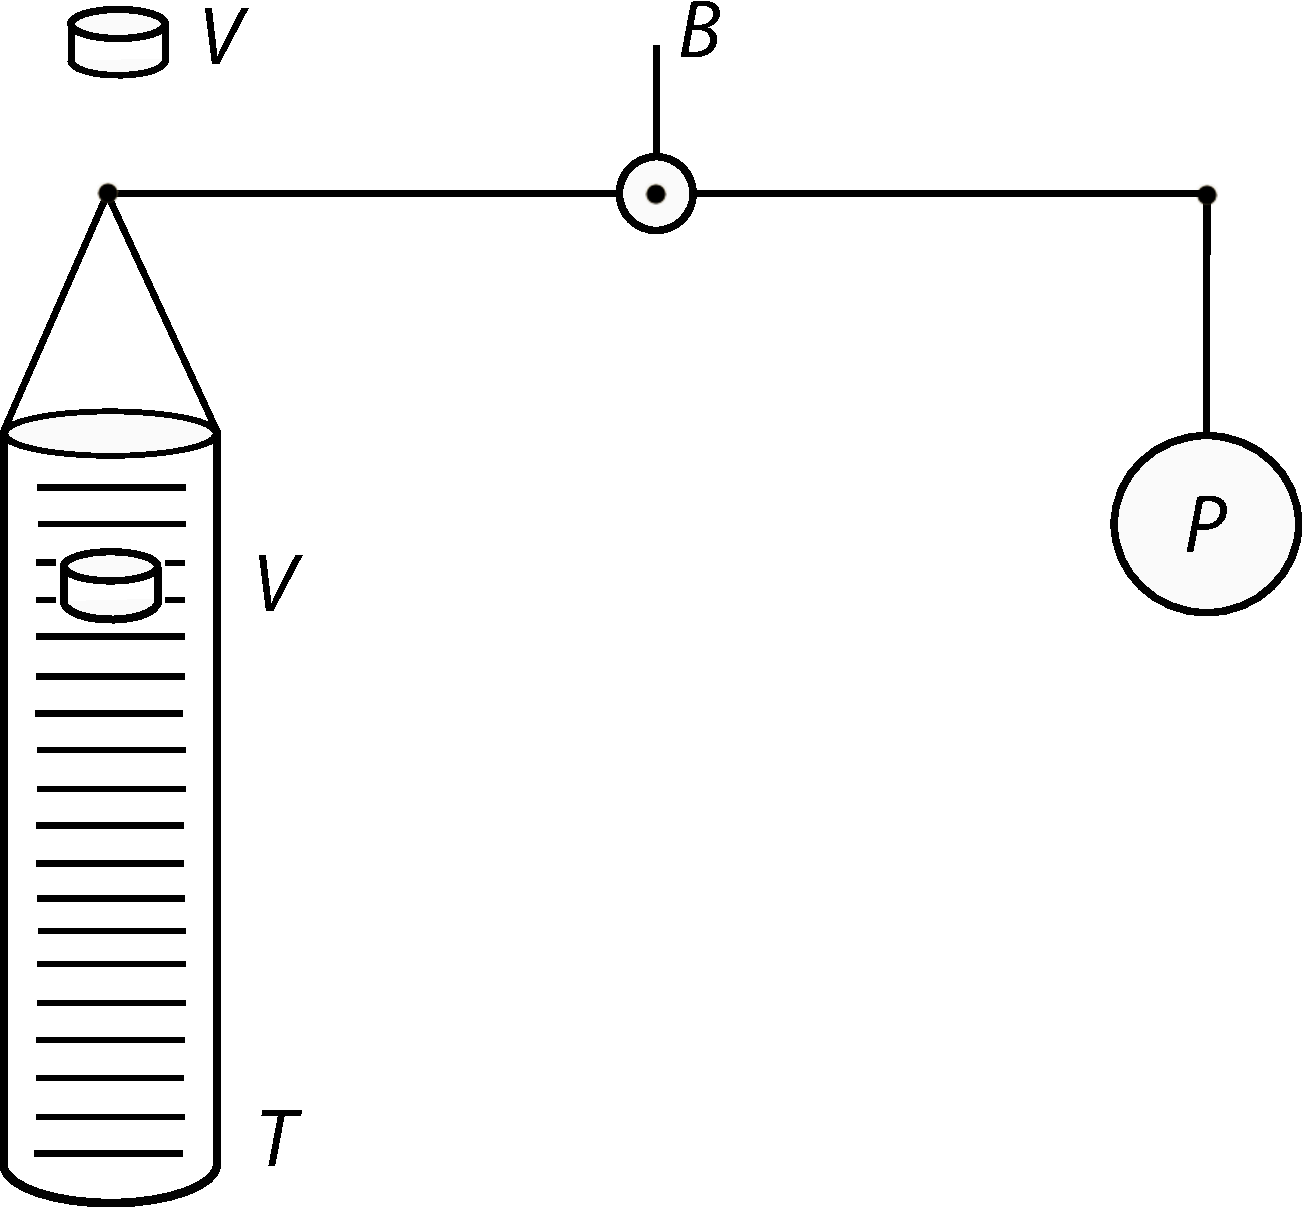
\includegraphics[width=0.42\textwidth]{gesamttex/edit_VIII-4/images/LBr_413_048_d_048v.pdf}
\edcaption[-0.5em]{\lbrack \textit{Fig.\:1}\rbrack}%
\end{edfigure}%
\pstart%
Haec in rem nostram transferamus.%
\indexS{res nostra}
\edtext{%
Ponderi \textit{P}%
\indexS{pondus aequilibratum in bilance}
respondet Mercurius in Barometro;%
\indexS{mercurius in barometro}%
\indexS{barometrum}
columnae in tubo \textit{T}%
\indexS{columna in tubo}
respondet aeris columna,%
\indexS{columna aeris}%
}{%
\lemma{Ponderi \textit{P}}%
\Bfootnote{%
\textit{(1)}~in Barometri phaenomeno proposito %
\textit{(2)}~respondet %
\textit{(a)}~Mer %
\textit{(b)}~Hydrargyrus %
\textit{(c)}~Mercurius in %
\textit{(aa)}~Tu %
\textit{(bb)}~Barometro; %
\textit{(aaa)}~tubo \textit{T} respondet aeris %
\textit{(bbb)}~columnae in %
\lbrack...\rbrack\ aeris columna,%
~\textit{L}%
}}
vasculo%
\indexS{vasculum natans}
respondent aqueae guttae per aerem dispersae.%
\indexS{gutta aquea}%
\indexS{guttae dispersae per aerem}%
\indexS{dispersio guttarum per aerem}
\edtext{%
Haec dum in minutissimas partes sunt divisae%
\indexS{gutta divisa in partes minutas}%
}{%
\lemma{Haec}%
\Bfootnote{%
\textit{(1)}~dum exiguae adhu %
\textit{(2)}~dum in %
\lbrack...\rbrack\ sunt divisae%
~\textit{L}%
}}
vim descendendi non habent,%
\indexS{vis descendendi guttarum in aere}%
\indexS{gutta carens vi descendendi}
quia plus habent superficiei
quam pro mole,%
\indexS{proportio superficiei ad molem}
atque adeo aeris cohaesionem%
\indexS{cohaesio aeris} %
et%
\lbrack,\rbrack\
quae in omni fluido est,%
\indexS{cohaesio fluidi}
velut glutinositatem quantumvis exiguam%
\indexS{glutinositas fluidi exigua}
vincere non possunt,
natantque;%
\indexS{gutta natans in aere}
ne dicam huc illuc volitare%
\indexS{gutta volitans in aere} %
ut pulveris atomos %
\indexS{atomus pulveris}%
\indexS{pulvis}
quas videmus in sole,%
\indexS{sol}
\edtext{%
nonnullas etiam esse rarefactas.%
\indexS{gutta rarefacta}%
}{%
\lemma{nonnullas etiam esse rarefactas}%
\Bfootnote{%
\textit{erg.\;L}%
}}
Sed ubi multae particulae exiguae aquosi vaporis%
\indexS{particulae vaporis collectae}%
\indexS{vapor aquosus}
\edtext{%
condensati%
\indexS{vapor condensatus}%
}{%
\lemma{condensati}%
\Bfootnote{%
\textit{erg.\;L}%
}}
collectae sunt
\edtext{%
in unius guttulae%
}{%
\lemma{in}%
\Bfootnote{%
\textit{(1)}~unam %
\textit{(2)}~unius guttulae%
~\textit{L}%
}}
rudimentum,%
\indexS{rudimentum guttulae}
jam descendunt%
\indexS{particulae vaporis descendentes}
atque inter descendendum
etiam augentur%
\lbrack,\rbrack\
ut procurrens pila nivis.%
\indexS{pila nivis}%
\indexS{nix}
Durante autem hoc innumerabilium guttarum descensu%
\indexS{descensus guttarum innumerabilium}
tantum levior fit
\edtext{%
columna,%
\indexS{columna aeris}
quantum%
}{%
\lemma{columna}%
\Bfootnote{%
\bars{fit \textit{streicht Hrsg.}}, quantum%
~\textit{L}%
}}
est ponderis in descensu guttarum,%
\indexS{pondus guttarum descendentium}%
\indexS{descensus guttarum innumerabilium}
quae scilicet amplius a columna%
\indexS{columna aeris}
non sustinentur.
Atque hinc vaticinatur Barometrum futuram pluviam,%
\indexS{barometrum vaticinans pluviam}%
\indexS{pluvia futura}
quod jam sentit hanc columnae aereae%
\indexS{columna aerea}
ut sic dicam alleviationem,%
\indexS{alleviatio columnae aereae}
\edtext{%
antequam cadendo ad nos%
}{%
\lemma{antequam}%
\Bfootnote{%
\textit{(1)}~ad nos %
\textit{(2)}~cadendo %
\textit{(a)}~crescendoque %
\textit{(b)}~ad nos%
~\textit{L}%
}}
perveniant guttulae %
\indexS{guttula cadens}
et %
quantum ad pluviam%
\indexS{pluvia futura}
\edtext{%
aut nivem%
\indexS{nix}%
}{%
\lemma{aut nivem}%
\Bfootnote{%
\textit{erg.\;L}%
}}
satis est %
cadendo
\edlabel{LBr_413_048_048v_sviu-1}%
\edtext{}{%
\xxref{LBr_413_048_048v_sviu-1}{LBr_413_048_048v_sviu-2}%
\lemma{crescant.}%
\Bfootnote{%
\textit{(1)}~Hinc et ventus ingens columnam\indexS{ventus ingens} %
\textit{(2)}~Sed ubi serenitas vapores %
\bars{aquosos \textit{erg.}} rursus comminuit %
\lbrack...\rbrack\ aeris reddant leviorem,%
~\textit{L}%
}}%
crescant.
Sed ubi serenitas%
\indexS{serenitas}
vapores aquosos%
\indexS{vapor aquosus}
rursus comminuit%
\indexS{vapor comminutus}
atque dispersit,%
\indexS{vapor dispersus}
sive aestate%
\indexS{aestas}
sive hyeme,%
\indexS{hyems}
manifestum est
rursus sustineri eos columna,%
\indexS{vapor sustentus columna aerea}
et gravitatem ei redire.%
\indexS{gravitas redita}%
\pend%
\pstart%
Patet hinc etiam
cur venti columnam aeris reddant leviorem,%
\indexS{ventus reddens columnam aeris leviorem}%
\indexS{columna aeris reddita levior ventis}%
\edlabel{LBr_413_048_048v_sviu-2}
nempe
quantum ipsi sustinent,
\edtext{%
tantum resistentiae ex columna aeris%
\indexS{resistentia columnae aeris}
Mercurius in Barometro%
\indexS{mercurius in barometro}%
\indexS{barometrum}
sibi detractum sentit,%
}{%
\lemma{tantum}%
\Bfootnote{%
\textit{(1)}~non sentit resti %
\textit{(2)}~resistentiae ex %
\lbrack...\rbrack\ detractum sentit,%
~\textit{L}}}
descensuque testatur.%
\indexS{descensus mercurii}
Et perinde est
ac si extranea vis%
\indexS{vis extranea}%
\indexS{vis sustinens aquam in tubo}
aquam in Tubo \textit{T}%
\indexS{aqua sustenta in tubo}
pro bona parte sustineret,
haustro fortassis aliquo immerso %
\indexS{haustrum immersum}
\edtext{%
quo aqua sursum traheretur.%
\indexS{aqua tracta sursum}%
}{%
\lemma{quo}%
\Bfootnote{%
\textit{(1)}~extrahere %
\textit{(2)}~illa %
\textit{(3)}~aqua sursum traheretur.%
~\textit{L}%
}}
Tantum enim vinceret pondus oppositum \textit{P}%
\indexS{pondus vincens in bilance}
descenderetque. 
\edtext{%
Hinc maxima futura est
\textls{Barometri%
\indexS{utilitas barometri ad praevidendas tempestates}%
\indexS{barometrum}
utilitas}%
}{%
\lemma{Hinc}%
\Bfootnote{%
\textit{(1)}~summa utilitas %
\textit{(2)}~\bars{Hinc \textit{streicht Hrsg.}} maxima %
\textit{(a)}~erit %
\textit{(b)}~es %
\textit{(c)}~futura est \textls{Barometri utilitas}%
~\textit{L}%
}}
\textls{in mari%
\indexS{mare}
ad praevidendas%
\indexS{tempestas praevidenda}
tempestates,}
jam aliquot horae sufficere possunt,
si non ut portus petatur%
\indexS{portus petitus}%
\lbrack,\rbrack\
saltem %
ut recedatur a scopulis%
\indexS{scopulus}
syrtibusque%
\indexS{syrtis}
\edtext{%
et navis paretur ad sustinendam%
\indexS{navis parata ad vim procellae sustinendam}%
}{%
\lemma{et}%
\Bfootnote{%
\textit{(1)}~ad sustinenda %
\textit{(2)}~navis paretur ad sustinendam%
~\textit{L}%
}}
vim procellae.%
\indexS{vis procellae}%
\indexS{procella}
Ut mirum sit
per tot jam annos
rem tantae utilitatis esse neglectam.%
\indexS{res neglecta}%
\pend%
\selectlanguage{latin}%
\frenchspacing%
\normalsize%



\section[tocentry={De aetiologia barometri
\enskip%
\bracks{zweite Hälfte Juni 1712 --
1715%
}},
head={De aetiologia barometri}]%
{\MakeUppercase{De aetiologia barometri} %
\newline%
\bracks{zweite Hälfte Juni 1712 --
1715%
}}
\label{54958}
\selectlanguage{ngerman}%
\frenchspacing%
\begin{ledgroupsized}[r]{120mm}%
\footnotesize%
\pstart%
\noindent\textbf{Überlieferung:}%
\pend%
\end{ledgroupsized}%
\begin{ledgroupsized}[r]{114mm}%
\footnotesize%
\pstart%
\parindent -6mm%
\makebox[6mm][l]{\textit{E\textsuperscript{1}}}%
Druck:
\textit{AL2%
}, centuriae III--IV (1715), Anhang, Nr.\;3, S.\;49--51.\cite{01457}\cite{01458}
\pend%
\pstart%
\parindent -6mm%
\makebox[6mm][l]{\textit{E\textsuperscript{2}}}%
Druck (nach \textit{E\textsuperscript{1}}):
\textit{LOD} II.2, S.\:78--79.\cite{00150}
\pend%
\pstart%
\parindent -6mm%
\makebox[6mm][l]{\textit{Ü}}%
(ins Französische):
\textsc{Peyroux} 1990, S.\:110--111.\cite{01414}
\pend%
\end{ledgroupsized}%
\selectlanguage{latin}%
\frenchspacing%
\vspace{8mm}%
\normalsize%
\pstart%
\noindent%
\lbrack S.\:49\rbrack%
\hfill%
lllustris Dn.\;G.\;G.\;Leibnitii%
\indexN{\textls{Leibniz} (Leibnitius, GGL), Gottfried Wilhelm 1646\textendash1716}
\hfill%
\phantom{\lbrack S.\:49\rbrack}%
\pend%
\vspace*{0.5em}%
\pstart%
\centering%
De Aetiologia Barometri,%
\indexS{aetiologia barometri}%
\indexS{barometrum}\\
\edtext{%
occasione n.\;3 et 4 appendicis ad Centur.\;1.\;et 2.\\
Ephemeridum novarum Societatis Caesareae Naturae Curiosorum%
\indexS{Academia naturae curiosorum}%
}{%
\lemma{occasione \lbrack...\rbrack\ Curiosorum}%
\Cfootnote{%
Vgl.
\textit{AL2}, centuriae I--II (1712), Anhang,
Nr.\;3, S.\;92--98\cite{01457}
(B.\;\textsc{Ramazzini}, \glqq Epistola de causa adscensus et descensus mercurii in fistula Torricelliana\grqq);\cite{01460}
Nr.\;4, S.\;98--110\cite{01457}
(G.\:C.\;\textsc{Schel\-ham\-mer}, \glqq Notata ad hanc epistolam\grqq).\cite{01461}
Ramazzinis \glqq Epistola\grqq\ ist ein Nachdruck seines Briefes an L.\;Schröck vom 1.\;Juni 1710,
nach B.\;\textsc{Ramazzini}, \textit{Ephemerides barometricae. Cum disquisitione}
(Padua 1710, S.\;191--202).\cite{01462}%
}}
\pend%
\vspace*{1.0em}%
\pstart%
\noindent%
Barometrum,%
\indexS{barometrum}
quod vocant,
Hydrargyro%
\indexS{hydrargyrum in barometro}
aeris pondus indicans,%
\indexS{pondus aeris}
\edtext{%
primus invenit Torricellius,%
\indexN{\textls{Torricelli} (Torricellius), Evangelista 1608\textendash1647}%
}{%
\lemma{primus invenit Torricellius}%
\Cfootnote{%
Siehe \textsc{E.\;Torricelli},
Brief an M.\;Ricci vom 11.\;Juni 1644\cite{00107}
(in C.\,\textsc{Dati},
\textit{Lettera a Filaleti ... della famosissima esperienza dell’argento vivo},
Florenz 1663, S.\;20\,f.;\cite{00032}
\textit{TO} III, S.\;186--188).\cite{00108}%
}}
\edtext{%
primus Gerikius%
\indexN{\textls{Guericke} (Gerickius, Gericke), Otto von 1602\textendash1686}
sub nomine virunculi meteorologi
aliquandiu occultatum%
\indexS{virunculus meteorologus}
ad praedictiones mutationum aeris%
\indexS{praedictio mutationum aeris}%
\indexS{mutatio aeris}
publice adhibuit.%
}{%
\lemma{primus \lbrack...\rbrack\ adhibuit}%
\Cfootnote{%
Siehe O.\;v.\;\textsc{Guericke}, \textit{Experimenta nova},%
\cite{00055}
lib.\;III, cap.\;20; 31; lib.\;V, appendix
(Amsterdam 1672, S.\;100a--b; 115a--b; 188b--189a; 195b--196a).
Leibniz hatte 1672 diese Stellen exzerpiert:
Vgl. \textit{LSB} VIII,\;1 N.\;36,%
\cite{01197}
S.\;257.23--30; 259.1--10; 270.14--25.%
}}
\edtext{%
Sed cum observaretur
aerem,%
\indexS{aer factus levior}
imminente pluvia,%
\indexS{pluvia imminens}
leviorem fieri solere%
\lbrack,\rbrack\
siccum vero et serenum,%
\indexS{aer siccus}%
\indexS{aer serenus}
ponderosiorem ostendi;%
\indexS{aer ponderosior}
cum contra tempore ad pluviam vergente,%
\indexS{tempus vergens ad pluviam}%
\indexS{pluvia imminens}
vaporibus aqueis%
\indexS{vapor aqueus}
magis oneratus%
\indexS{aer oneratus vaporibus aqueis}
videri posset;
problema perplexum%
\indexS{problema perplexum}
varie agitatum est,%
}{%
\lemma{Sed cum \lbrack...\rbrack\ agitatum est}%
\Cfootnote{%
Auf die vorherige wissenschaftliche Diskussion über die wetterbedingten Änderungen des Luftgewichts geht ausführlich
-- in Anlehnung an B.\;\textsc{Ramazzini}, \textit{Ephemerides barometricae Mutinenses%
} (Modena 1695) --\cite{01516}
die Aufzeichnung N.\;\ref{60267} ein.%
}}
et in primis egregii Medici%
\indexS{medicus}
et Naturae consulti,%
\indexS{vir consultus naturae}%
\indexS{natura}
mihique amici,%
\indexS{amicus}
\edtext{%
Ramazzinus%
\indexN{\textls{Ramazzini} (Ramazzinus), Bernardino 1633\textendash1714}
et Schelhamerus%
\indexN{\textls{Schelhammer} (Schelhammerus), Günther Christoph 1649\textendash1716}
de ea re inter se contulerunt.%
}{%
\lemma{Ramazzinus \lbrack...\rbrack\ contulerunt}%
\Cfootnote{%
Anspielung auf die Auseinandersetzung zwischen B.\;Ramazzini und G.\:C.\;Schelhammer,
welche ab 1697 in zahlreichen Veröffentlichungen %
ihren Niederschlag fand.
Siehe für die Einzelheiten die editorische Einleitung zu N.\;\ref{paradoxon_intro} (\refpassage{paradoxon_RamaSchel-fhg-1}{paradoxon_RamaSchel-fhg-2}).%
}}
Mihi in mentem jam olim venerat,
pluvia imminente%
\indexS{pluvia imminens}
levari aeris columnam,%
\indexS{columna aeris}
quod ea guttulas%
\indexS{guttula cadens}
jam jam cadentes %
et pluviae mox materiam%
\indexS{materia pluviae}%
\indexS{pluvia imminens}
praebituras %
non amplius sustineret;
contra sereno tempore%
\indexS{tempus serenum} %
aquam%
\indexS{aqua dilatata in vapores}%
\indexS{aqua mixta aeri}
in minutissimos vapores%
\indexS{vapor aqueus}
dilatatam%
\indexS{aqua dilatata in vapores} %
misceri aeri,%
\indexS{aqua mixta aeri}
nec descendendi%
\indexS{vis descendendi}
aeremve penetrandi vim%
\indexS{vis penetrandi aerem}
habere%
\lbrack,\rbrack\
ac proinde una cum columna%
\indexS{columna aeris}
a subjecto Mercurio%
\indexS{mercurius subjectus columnae aeris}
sustentari.
\edtext{%
Proposui et experimentum,%
\indexS{experimentum propositum}
quo ad oculum%
\indexS{oculus}
appareret %
gravia solida%
\indexS{grave solidum}%
\indexS{grave descendens in fluido}
descendentia in gravi fluido%
\indexS{fluidum grave}
non gravitare in fundum fluido%
\indexS{fluidum grave}
subjectum.%
}{%
\lemma{Proposui \lbrack...\rbrack\ subjectum}%
\Cfootnote{%
Das Gedankenexperiment wird in den Aufzeichnungen N.\;\ref{53442}, \ref{60267} und \ref{36805} dargelegt.
Siehe zudem G.\:W.\;\textsc{Leibniz}, Brief an F.\;Hoffmann vom 19. März 1701
(\textit{LSB} III,\;8 N.\;225, S.\;577.17\,f.).\cite{01456}%
}}
Nempe tubus aqua plenus%
\indexS{tubus plenus aqua}%
\indexS{aqua in tubo}
in una parte librae bilancis%
\indexS{libra bilanx}%
\indexS{bilanx}
suspenditur,%
\indexS{tubus suspensus in libra}
et gravi aliquo aquae innatante%
\indexS{grave innatans aquae}
aut aliter in ea suspenso%
\indexS{grave suspensum in aqua}
et tubum%
\indexS{tubus plenus aqua}
vel lancem%
\indexS{lanx librae}
gravante,
totum per pondus%
\indexS{pondus redactum ad aequilibrium}
in opposita lance%
\indexS{lanx librae}
ad aequilibrium%
\indexS{aequilibrium in libra}
redigitur:
mox eodem gravi in aqua descendente%
\indexS{grave descendens in aqua}
(sive resecto filo%
\indexS{filum resectum}
sive aqua in cavitatem gravis admissa)%
\indexS{aqua admissa in cavitatem}%
\indexS{cavitas repleta aqua}
levior fit lanx%
\indexS{lanx librae}
tubi,%
\indexS{tubus suspensus in libra}
et pondus oppositum%
\indexS{pondus oppositum in libra}
praeponderat,%
\indexS{pondus praeponderans}
donec grave cadens%
\indexS{grave cadens}
fundum at%
\lbrack S.\:50\rbrack%
tingat.
Itaque occasione data
\edtext{%
sententiam meam%
\indexS{sententia}
Celeberrimo Ramazzino%
\indexN{\textls{Ramazzini} (Ramazzinus), Bernardino 1633\textendash1714}
per literas%
\indexS{literae}
significavi.%
}{%
\lemma{sententiam \lbrack...\rbrack\ significavi}%
\Cfootnote{%
Siehe G.\:W.\;\textsc{Leibniz}, Brief an B.\;Ramazzini vom 18.\;März 1700
(\textit{LSB} III,\;8 N.\;139, S.\;371\,f.).%
}}
Virum acutum%
\indexS{vir acutus}
et rationi%
\indexS{ratio}
cedere facilem
tetigit meditatio mea,%
\indexS{meditatio}
\edtext{%
cumque etiam experimentum,%
\indexS{experimentum Ramazzini}
adjuvante
\edtext{%
Cl.\;Gratiano,%
\indexN{\textls{Graziani} (Gratianus), Giovanni, gest. 1744}%
}{%
\lemma{Cl.\;Gratiano}%
\Cfootnote{%
Giovanni Graziani lehrte seit 1703 in Padua\indexO{Padua} (zunächst Astronomie, ab 1709 Philosophie).%
}}
sumsisset,
laudabili candore
publice professus est %
veritati%
\indexS{veritas}
a se manus dari.%
\indexS{manus data veritati}%
}{%
\lemma{cumque \lbrack...\rbrack\ dari}%
\Cfootnote{%
Siehe \textsc{Ramazzini}, Brief an Schröck vom 1.\;Juni 1710,\cite{01460}
in
\textsc{Ders.}, \textit{Ephemerides barometricae. Cum disquisitione}
(1710, S.\;197--201)\cite{01462}
sowie in
\textit{AL2}%
, 1712 (Anhang, %
S.\;95--97).\cite{01457}
Das Experiment, auf das Leibniz anspielt, hatte nach Ramazzinis Angabe zur Fastnachtszeit 1710 in Padua stattgefunden.
Ramazzini lehrte seit 1700 Medizin an der dortigen Universität.%
\indexO{Padua}%
}}
Sed
\edtext{%
Antagonistae%
\indexN{\textls{Schelhammer} (Schelhammerus), Günther Christoph 1649\textendash1716}%
\indexS{antagonista}%
}{%
\lemma{Antagonistae}%
\Cfootnote{%
Gemeint ist Günther Christoph Schelhammer.%
}}
haud minus celebri nondum satisfactum video.
\pend%
\pstart%
\edtext{%
Objicit%
\indexS{objectio}
\textls{primo,}
vapores aquosos%
\indexS{vapor aquosus}
natantes in aere%
\indexS{vapor natans in aere}
eum premere;%
\indexS{vapor premens aerem}
at corpus suspensum ex filo%
\indexS{corpus suspensum e filo}
in experimento D.\;Ramazzini%
\indexN{\textls{Ramazzini} (Ramazzinus), Bernardino 1633\textendash1714}%
\indexS{experimentum Ramazzini}
non premere aquam.%
\indexS{aqua in tubo}%
}{%
\lemma{Objicit \lbrack...\rbrack\ aquam}%
\Cfootnote{%
Vgl. \textsc{Schelhammers} kritische Bemerkungen
in \textit{AL2}, %
1712 (Anhang, %
S.\;98).\cite{01461}\cite{01457}%
}}
Sed responsio est facilis%
\lbrack:\rbrack%
\indexS{responsio objectioni}
discrimen%
\indexS{discrimen}
inde nullum oriri ad rem faciens%
\lbrack,\rbrack\
sufficit enim
quod utrobique corpus grave in fluido descendens%
\indexS{corpus descendens in fluido}%
\indexS{grave descendens in fluido}%
\indexS{fluidum grave}
cum eo non gravitet;%
\indexS{corpus non gravitans}
quod tamen antea gravitabat in lancem%
\indexS{corpus gravitans in lancem}%
\indexS{lanx librae}
oppositumque pondus%
\indexS{pondus oppositum in libra}
sive a filo sive ab aqua sustentaretur.%
\indexS{grave sustentum a filo}%
\indexS{corpus sustentum a filo}%
\indexS{grave sustentum ab aqua}%
\indexS{corpus sustentum ab aqua}
\edtext{%
Objicit%
\indexS{objectio}
\textls{secundo,}
hac causa supposita%
\indexS{causa supposita}
Mercurium ergo non descensurum,%
\indexS{mercurius descendens in barometro}
nisi cum actu%
\indexS{actus}
pluit%
\indexS{pluvia actualis}%
\lbrack.%
}{%
\lemma{Objicit \lbrack...\rbrack\ pluit}%
\Cfootnote{%
Vgl. a.a.O., S.\;98\,f.\cite{01461}\cite{01457}%
}}
S\rbrack ed respondetur%
\indexS{responsio objectioni}%
\lbrack:\rbrack\
etsi aqueae particulae%
\indexS{particulae aqueae separatae ab aere}
ab aere separari
et cadere incipiant,%
\indexS{particulae aqueae cadentes}
non tamen statim ad nos pervenire
aut pluviam formare;%
\indexS{particulae aqueae formantes pluviam}%
\indexS{pluvia formata particulis aqueis}
sed interdum a vento%
\indexS{ventus agitans aerem}%
\indexS{ventus dissipans particulas aqueas}%
\indexS{ventus retardans particulas aqueas}
in superiore regione%
\indexS{regio aeris superior}
aerem agitante,%
\indexS{aer regionis superioris}%
\indexS{aer agitatus a vento}
vel alia causa,%
\indexS{causa alia}
dissipari%
\indexS{particulae aqueae dissipatae a vento}
aut rerardari.%
\indexS{particulae aqueae retardatae a vento}
\edtext{%
Objicit%
\indexS{objectio}
\textls{tertio,}
Mercurium saepe descendere%
\indexS{mercurius descendens in barometro}
et varie mutari,
nulla pluvia cadente.%
\indexS{pluvia non cadens}%
}{%
\lemma{Objicit \lbrack...\rbrack\ cadente}%
\Cfootnote{%
Vgl. a.a.O., S.\;99.\cite{01461}\cite{01457}%
}}
Solutio%
\indexS{solutio obiectionis}
ex praecedenti patet:
nam fieri potest et solet,
ut particulae descendere incipientes%
\indexS{particulae aqueae descendentes in aere}
rursus sole%
\indexS{sol dissipans particulas aqueas}
vel vento,%
\indexS{ventus dissipans particulas aqueas}
vel alia causa,%
\indexS{causa alia}
dissipentur,%
\indexS{particulae aqueae dissipatae}
imo plane alio ferantur,
novo aere substituto;%
\indexS{aer novus substitutus}
\edtext{%
quod etiam jam notavit Cl.\;Ramazzinus.%
\indexN{\textls{Ramazzini} (Ramazzinus), Bernardino 1633\textendash1714}%
}{%
\lemma{quod \lbrack...\rbrack\ Ramazzinus}%
\Cfootnote{%
Siehe \textsc{Ramazzini}, Brief an Schröck vom 1.\;Juni 1710\cite{01460}
in \textsc{Ders.}, \textit{Ephemerides barometricae. Cum disquisitione}
(1710, S.\;200\,f.)\cite{01462}
sowie in \textit{AL2}%
, 1712 (Anhang, %
S.\;97).\cite{01457}%
}}
\edtext{%
Objicit%
\indexS{objectio}
\textls{quarto,}
alias magnas mutationes in Barometro%
\indexS{mutatio in barometro}%
\indexS{barometrum}
notari ex aliis causis,%
\indexS{causa alia}%
\indexS{causa mutationis in barometro}
verbi gratia %
a validis procellis.%
\indexS{procella}%
}{%
\lemma{Objicit \lbrack...\rbrack\ procellis}%
\Cfootnote{%
Vgl. \textsc{Schelhammers} kritische Anmerkungen\cite{01461}
in \textit{AL2}%
, 1712 (Anhang, %
S.\;99).\cite{01457}%
}}
Hoc concedo,
neque enim omnes mutationes%
\indexS{mutatio ponderis columnae aereae}
ponderis%
\indexS{pondus columnae aereae}
columnae aereae%
\indexS{columna aerea}
ex hac sola,
quam adduxi,%
\indexS{causa adducta}
causa%
\indexS{causa mutationis columnae aereae}
oriri puto;
sufficit eam saepe valere%
\indexS{causa valens saepe}
et principali phaenomeno%
\indexS{phaenomenon principale}
\edtext{%
(ut jam Dn.\;Ramazzinus ait)%
\indexN{\textls{Ramazzini} (Ramazzinus), Bernardino 1633\textendash1714}%
}{%
\lemma{ut \lbrack...\rbrack\ ait}%
\Cfootnote{%
Siehe \textsc{Ramazzini}, Brief an Schröck vom 1.\;Juni 1710,\cite{01460}
in \textsc{Ders.}, \textit{Ephemerides barometricae. Cum disquisitione}
(1710, S.\;201)\cite{01462}
sowie in \textit{AL2}%
, 1712 (Anhang, %
S.\;97\,f.).\cite{01457}%
}}
satisfacere,
cum scilicet Mercurii%
\indexS{mercurius descendens in barometro}%
\indexS{mercurius ascendens in barometro}
descensus%
\indexS{descensus mercurii in barometro}
pluviam%
\indexS{descensus mercurii nuntians pluviam}%
\indexS{pluvia nuntiata a barometro}
aut nivem,%
\indexS{descensus mercurii nuntians nivem}%
\indexS{nivis nuntiata a barometro}
ascensus%
\indexS{ascensus mercurii in barometro}
serenitatem nuntiat.%
\indexS{ascensus mercurii nuntians serenitatem}%
\indexS{serenitas nuntiata a barometro}
Sane ventus vehemens%
\indexS{ventus suspendens pondus aeris}
etiam aeris pondus suspendere potest,%
\indexS{pondus aeris suspensum a vento}
unde jam
\edtext{%
Gerikius%
\indexN{\textls{Guericke} (Gerickius, Gericke), Otto von 1602\textendash1686}
notavit,
in magnis tempestatibus%
\indexS{tempestas magna}
Mercurium Barometri descendere.%
\indexS{mercurius descendens in barometro}%
\indexS{descensus mercurii in barometro}%
\indexS{barometrum}%
}{%
\lemma{Gerikius \lbrack...\rbrack\ descendere}%
\Cfootnote{%
Siehe \textsc{Guericke}, \textit{Experimenta nova},%
\cite{00055}
lib.\;III, cap.\;20;
lib.\;V, appendix
(100b; 189a; 195b--196a).
Vgl. zudem Leibnizens Exzerpt,
\textit{LSB} VIII,\;1 N.\;36,%
\cite{01197}
S.\;270.17--19.%
}}
Sed et aliter mutare venti%
\indexS{ventus mutans pondus aeris}
pondus columnae aereae%
\indexS{pondus columnae aereae}%
\indexS{columna aerea}%
\indexS{pondus aeris mutatum a vento}
possunt,
ex.\:gr.\;duo venti sibi occurrentes%
\indexS{venti occurrentes sibi}%
\indexS{venti comprimentes aerem}
aerem interceptum%
\indexS{aer interceptus}
\lbrack S.\:51\rbrack\
compriment%
\indexS{aer compressus a ventis}
et reddent densiorem%
\indexS{aer factus densior}
adeoque graviorem;%
\indexS{aer factus gravior}
contra in diversa tendentes,%
\indexS{venti tendentes in diversa}
distrahent eundem%
\indexS{venti distrahentes aerem}%
\indexS{aer distractus a ventis}
et reddent rariorem%
\indexS{aer factus rarior}
et leviorem;%
\indexS{aer factus levior}
aer autem rarior guttas aqueas%
\indexS{gutta aquea}
minus sustentabit,%
\indexS{aer sustentans guttas aqueas}
et ita ex duplici capite
levior erit.%
\indexS{aer factus levior}
Harum aliarumque causarum%
\indexS{causa alia}
interventio%
\indexS{interventio aliarum causarum}
facit,
ut regulae praedictionum ex Barometro%
\indexS{regula praedictionum e barometro}%
\indexS{praedictio e barometro}%
\indexS{barometrum}
multas exceptiones patiantur.%
\indexS{exceptio regulae}
\edtext{%
Objicit%
\indexS{objectio}
tandem \textls{quinto,}
Experimentum Ramazzinianum%
\indexN{\textls{Ramazzini} (Ramazzinus), Bernardino 1633\textendash1714}%
\indexS{experimentum Ramazzini}
nonnihil differre a meo.
Nam ego corpus cavum proposueram%
\indexS{corpus cavum natans}
quod nataret in aqua Tubi,%
\indexS{tubus plenus aqua}%
\indexS{aqua in tubo}
mox aqua repletum%
\indexS{corpus cavum repletum aqua}
in ea mergeretur;
Ramazzinus%
\indexN{\textls{Ramazzini} (Ramazzinus), Bernardino 1633\textendash1714}
suum grave ex filo suspendit,%
\indexS{grave suspensum e filo}
et mox filo resecto%
\indexS{filum resectum}
cadere permisit.%
\indexS{grave cadens}%
}{%
\lemma{Objicit \lbrack...\rbrack\ permisit}%
\Cfootnote{%
Vgl. \textsc{Schelhammers} kritische Anmerkungen\cite{01461}
in \textit{AL2}%
, 1712 (Anhang, %
S.\;99).\cite{01457}%
}}
Sed respondeo
primo
nullam esse rationem differentiae,%
\indexS{ratio differentiae}
ut ostensum est ad objectionem primam;%
\indexS{objectio}
secundo
si Cl.\;objector%
\indexN{\textls{Schelhammer} (Schelhammerus), Günther Christoph 1649\textendash1716}%
\indexS{objector}
sumere experimentum dignetur,%
\indexS{experimentum}
cavo natante debite substituto%
\indexS{corpus cavum natans}
in locum gravis suspensi ex filo,%
\indexS{grave suspensum e filo}
eosdem eventus reperturum,%
\indexS{eventus}
cum eadem ratio subsit.
\pend%
\pstart%
Obiter addo
\edtext{%
in Epistolae%
\indexS{epistola}
meae secunda linea%
\indexS{linea textus}
(p.\;95)
vocem%
\indexS{vox delenda}
\textit{mehercle} esse delendam,%
}{%
\lemma{in Epistolae \lbrack...\rbrack\ delendam}%
\Cfootnote{%
Ramazzini hat in seinem Brief an Schröck vom 1.\;Juni 1710\cite{01460}
auch den Brief abgedruckt, mit dem ihm Leibniz am 18. März 1700 seine Erklärung der wetterbedingten Änderung des Luftgewichts gesendet hatte (vgl. \textit{LSB} III,\;8, N.\;139, S.\;371\,f.).\cite{01454}
In dem von Ramazzini veranlassten Abdruck dieses Briefes findet sich an der von Leibniz angegebenen Stelle tatsächlich der Fehler, um dessen Berichtigung er in N.\;\ref{54958} bittet;
vgl.
\textsc{Ramazzini}, \textit{Ephemerides barometricae. Cum disquisitione}
(1710, S.\;196)\cite{01462}
sowie \textit{AL2}%
, 1712 (Anhang, %
S.\;95).\cite{01457}
Leibniz zitiert offenbar aus den \textit{Ephemerides} der Leopoldina.%
}}
ex alia credo non bene scripta lectaque natam,
\edtext{%
quae qualis fuerit nunc non divino.%
}{%
\lemma{quae \lbrack...\rbrack\ divino}%
\Cfootnote{%
Anstelle von \textit{mehercle meis} stand in Leibnizens Brief an Ramazzini vom 18. März 1700 das Wort \textit{Mechanicis};
vgl. \textit{LSB} III,\;8 N.\;139, S.\;371.13.\cite{01454}%
}}
\pend%
\selectlanguage{latin}%
\frenchspacing%
\normalsize%




\chapter[tocentry={Tentamen de aeris extensione per determinatum caloris gradum
\enskip Juni 1698}, %
head={Tentamen de aeris extensione %
}]%
{\MakeUppercase{Tentamen de aeris extensione per determinatum caloris gradum}
\newline Juni 1698} %
\label{36650}
\selectlanguage{ngerman}%
\frenchspacing%
\begin{ledgroupsized}[r]{120mm}%
\footnotesize%
\pstart%
\noindent\textbf{Überlieferung:}%
\pend%
\end{ledgroupsized}%
\begin{ledgroupsized}[r]{114mm}%
\footnotesize%
\pstart%
\parindent -6mm%
\makebox[6mm][l]{\textit{F}}%
Fremdhändige Aufzeichnung mit Verbesserungen und Ergänzungen von Leibnizens Hand 
(\textit{LiF}, im edierten Text unterpunktelt):
Halle an der Saale, Universitäts- und Landesbibliothek Sachsen-Anhalt, Yg~8\textsuperscript{o}\;23~C, Bl.\;1--2
(aus der Sammlung J.\:F.\;Pfaffs).
Ein Bogen 4\textsuperscript{o},
kleine Papierabbrüche an den Falzen mit geringfügigen Textverlusten;
Wasserzeichen mittig: Hannoveraner Papier. %
Drei Seiten, einspaltig beschrieben;
Bl.\;2\,v\textsuperscript{o} ist unbeschrieben.
\pend%
\end{ledgroupsized}%
\selectlanguage{latin}%
\frenchspacing%
\vspace{8mm}%
\normalsize%
\pstart%
\noindent%
\lbrack1\,r\textsuperscript{o}\rbrack%
\phantom{Junii 1698}%
\hfill%
\phantom{\lbrack1\,r\textsuperscript{o}\rbrack}%
\edtext{%
\dotuline{Junii 1698}%
}{%
\lemma{\dotuline{Junii 1698}}%
\Bfootnote{%
\textit{erg.\;LiF}%
}}
\pend%
\pstart%
\noindent%
In
\edtext{%
duobus
\dotuline{Tubis}%
\indexS{tubus}%
}{%
\lemma{duobus}%
\Bfootnote{%
\textit{(1)}~barometris\indexS{barometrum}%
~\textit{F} %
\textit{(2)}~\dotuline{Tubis}%
~\textit{LiF}%
}}
\textit{AC} et \textit{BD} majori et minori,
tentamen%
\indexS{tentamen} institutum fuit
\edtext{%
quousque quantitate aliqua\;%
\edtext{%
\mercury ii%
\indexS{mercurius in tubo}%
}{%
\lemma{\mercury ii}%
\Cfootnote{%
Das Symbol \mercury\ steht für \textit{mercur}(\textit{ius}).%
}}
compressus aer%
\indexS{aer compressus in tubo}%
}{%
\lemma{quousque}%
\Bfootnote{%
\textit{(1)}~certa %
\textit{(2)}~quantitate aliqua \mercury ii %
\bars{\textlangle indefinita\textrangle\ \textit{gestr.\;LiF}} %
compressus aer%
~\textit{F}%
}}
per aequalem et determinatum caloris gradum%
\indexS{gradus caloris}%
\indexS{calor}
se extendere%
\indexS{aer extendens se per calorem}%
\indexS{extensio aeris per calorem}
\mercury iumque%
\indexS{mercurius in tubo}
attollere possit.
Processus fuit talis.%
\indexS{processus tentaminis}%
\pend%
\pstart%
\edtext{%
\edtext{%
In \dotuline{Tubo}%
\indexS{tubus}%
}{%
\lemma{In}%
\Bfootnote{%
\textit{(1)}~barometro\indexS{barometrum}%
~\textit{F} %
\textit{(2)}~\dotuline{Tubo}%
~\textit{LiF}%
}}
\textit{AC},%
}{%
\lemma{In \dotuline{Tubo} \textit{AC}}%
\Cfootnote{%
Die Beschreibung des Experiments bezieht sich auf ein in N.\;\ref{36650} nicht überliefertes Diagramm.%
}}
spatium aeris in globulo \textit{C}%
\indexS{globulus tubi}
comprimendi \textit{pq}%
\indexS{aer comprimendus in tubo}
continebat
1 \Pfund,%
\indexS{Pfund}
20
\edtext{%
loth,%
\indexS{Loth}%
}{%
\lemma{loth}%
\Cfootnote{%
Gewichtseinheit, die gemäß dem Handelsgewicht $\displaystyle\frac{1}{32}$ des Pfundes entsprach.%
}}
$1 \frac{1}{2}$~%
\edtext{%
qt.%
\indexS{Quentchen}%
}{%
\lemma{qt}%
\Cfootnote{%
Quentchen, d.\,h. Gewichtseinheit, die gemäß dem Handelsgewicht einem Viertel %
des Lots bzw. $\displaystyle\frac{1}{128}$ des Pfundes entsprach.
Hierfür wird im Folgenden zumeist \textit{qtchen} als Abkürzung verwendet.%
}}%
\;\mercury ii.
In altero minori \textit{BD},%
\indexS{tubus}
spatium \textit{lm} globuli \textit{D}%
\indexS{globulus tubi}
replebatur
1 \Pfund,%
\indexS{Pfund}
7 loth,%
\indexS{Loth}
$2 \frac{1}{2}$ qtchen%
\indexS{Quentchen}%
\;\mercury ii.%
\indexS{mercurius in tubo}%
\pend%
\pstart%
Hisce exemtis ponderatisque
infundebatur de
\edtext{%
novo in \dotuline{Tubum}%
\indexS{tubus}%
}{%
\lemma{novo in}%
\Bfootnote{%
\textit{(1)}~barometrum\indexS{barometrum}%
~\textit{F} %
\textit{(2)}~\dotuline{Tubum}%
~\textit{LiF}%
}}
\textit{AC}
\edtext{%
\mercury \dotuline{ius},%
\indexS{mercurius in tubo}%
\indexS{mercurius infusus}%
}{%
\lemma{\dotuline{ius},}%
\Bfootnote{%
\textit{erg.\;LiF}%
}}
donec in tubulo \textit{A}%
\indexS{tubulus}
in \textit{i},
in globulo \textit{C}%
\indexS{globulus tubi}
vero in \textit{r}
u\textlangle sque\textrangle\
ascendisset.%
\pend%
\pstart%
Sic et in altero \textit{BD},
\edtext{%
\mercury \dotuline{ius}%
\indexS{mercurius in tubo}%
}{%
\lemma{\dotuline{ius}}%
\Bfootnote{%
\textit{erg.\;LiF}%
}}
infusus%
\indexS{mercurius infusus}
in tubulo \textit{B}%
\indexS{tubulus}
locum \textit{g},
in globulo \textit{D}%
\indexS{globulus tubi}
vero locum \textit{o}
\edlabel{Halle_ULB_Yg_8o_23_C_001-002_001r_wlw-1}%
attingebat.%
\edtext{}{%
\xxref{Halle_ULB_Yg_8o_23_C_001-002_001r_wlw-1}{Halle_ULB_Yg_8o_23_C_001-002_001r_wlw-2}%
\lemma{attingebat.}%
\Bfootnote{%
\lbrack/\rbrack\ %
\textit{(1)}~Aer%
~\textit{F} %
\textit{(2)}~\dotuline{Aeris}%
~\textit{LiF} %
igitur in
\bars{barometro \textit{ändert Hrsg.}}
\textit{AC} %
\bars{in locum \textit{rq} \textit{streicht Hrsg.}} %
\textit{(a)}~compressus%
~\textit{F} %
\textit{(b)}~\dotuline{compressi spatium \textit{rq}}%
~\textit{LiF} %
post %
\bars{totam \textit{gestr.\;LiF}} %
operationem %
\textit{(aa)}~mensuratus,%
~\textit{F} %
\textit{(bb)}~\dotuline{mensuratum},%
~\textit{LiF}%
}}%
\pend%
\newpage%
\pstart%
\dotuline{Aeris} igitur%
\indexS{aer compressus in tubo}
in \lbrack tubo\rbrack\
\textit{AC}%
\indexS{barometrum}
\dotuline{compressi%
\indexS{aer compressus in tubo}
spatium \textit{rq}}
post operationem%
\indexS{operatio in tentamine}
\dotuline{mensuratum,}%
\edlabel{Halle_ULB_Yg_8o_23_C_001-002_001r_wlw-2}
1 \Pfund,%
\indexS{Pfund}
5 loth,%
\indexS{Loth}
$2 \frac{1}{2}$ qtchen%
\indexS{Quentchen}
\mercury ii
capiebat,
\edtext{%
cum
\dotuline{alterius}%
\indexS{aer adimplens spatium}
in \textit{BD}
spatium \textit{om}
\dotuline{adimplentis capacitas}%
\indexS{capacitas aeris compressi}
non nisi
\mercury ium%
\indexS{mercurius in tubo}%
\indexS{mercurius infusus}
$29 \frac{1}{2}$ loth%
\indexS{Loth}
\dotuline{ponderantem caperet.}%
}{%
\lemma{cum}%
\Bfootnote{%
\textit{(1)}~alter%
~\textit{F} %
\textit{(2)}~\dotuline{alterius}%
~\textit{LiF} %
in %
\bars{barometro\indexS{barometrum} \textit{gestr.\;LiF}} %
\textit{BD} spatium \textit{om} %
\textit{(a)}~adimplens%
~\textit{F} %
\textit{(b)}~\dotuline{adimplentis capacitas}%
~\textit{LiF} %
non nisi \mercury ium $29 \frac{1}{2}$ loth %
\textit{(aa)}~ponderare.%
~\textit{F} %
\textit{(bb)}~\dotuline{ponderantem caperet}.%
~\textit{LiF}%
}}%
\pend%
\pstart%
Immittebantur nunc ambo in
\lbrack1\,v\textsuperscript{o}\rbrack\ %
\edtext{%
$\bigtriangledown$m%
}{%
\lemma{$\bigtriangledown$m}%
\Cfootnote{%
Das Symbol $\bigtriangledown$ steht für \textit{aqua}.%
}}
calidam,%
\indexS{aqua calida}
ascendebatque
\edtext{%
\mercury%
\indexS{mercurius in tubo}%
\indexS{mercurius ascendens calore}
in
\dotuline{Tubo}%
\indexS{tubus}
\textit{AC} in~\textit{k},
in
\dotuline{Tubo}%
\indexS{tubus}%
\textit{BD} in \textit{h},%
}{%
\lemma{\mercury in}%
\Bfootnote{%
\textit{(1)}~barometro\indexS{barometrum}%
~\textit{F} %
\textit{(2)}~\dotuline{Tubo}%
~\textit{LiF} %
\textit{AC} in~\textit{k}, in %
\textit{(a)}~minori%
~\textit{F} %
\textit{(b)}~\dotuline{Tubo}%
~\textit{LiF} %
\textit{BD} in \textit{h},%
~\textit{F}%
}}
usque Spatium
\edtext{%
\textit{ik}
\dotuline{capiebat
\mercury ii}%
}{%
\lemma{\textit{ik}}%
\Bfootnote{%
\textit{(1)}~in majori%
~\textit{F} %
\textit{(2)}~\dotuline{capiebat \mercury ii}%
~\textit{LiF}%
}}
6 loth%
\indexS{Loth}
$3 \frac{1}{2}$ qtchen,%
\indexS{Quentchen}
\textit{gh}
\edtext{%
vero
\dotuline{Mercurii}%
\indexS{mercurius in tubo}%
\indexS{mercurius ascendens calore}%
}{%
\lemma{vero}%
\Bfootnote{%
\textit{(1)}~in minori%
~\textit{F} %
\textit{(2)}~\dotuline{ca} %
\textit{(3)}~\dotuline{\mercury ii} %
\textit{(4)}~\dotuline{Mercurii}%
~\textit{LiF}%
}}
$3 \frac{1}{2}$~loth%
\indexS{Loth}
capiebat.%
\pend%
\pstart%
\edtext{%
Eaedem
\dotuline{hae capacitates,}%
\indexS{capacitas aeris compressi}%
}{%
\lemma{Eadem}%
\Bfootnote{%
\textit{(1)}~haec pondera,\indexS{pondus mercurii infusi}%
~\textit{F} %
\textit{(2)}~\dotuline{hae capacitates,}%
~\textit{LiF}%
}}
nimirum
\edtext{%
\dotuline{pro}%
}{%
\lemma{\dotuline{pro}}%
\Bfootnote{%
\textit{erg.\;LiF}%
}}
6 loth%
\indexS{Loth}
$3 \frac{1}{2}$ qtchen%
\indexS{Quentchen}
et
\edtext{%
\dotuline{pro}%
}{%
\lemma{\dotuline{pro}}%
\Bfootnote{%
\textit{erg.\;LiF}%
}}
$3 \frac{1}{2}$ loth,%
\indexS{Loth}
addendae
\edtext{%
sunt
\dotuline{capacitatibus%
\indexS{capacitas aeris compressi}
seu spatiis}%
}{%
\lemma{sunt}%
\Bfootnote{%
\textit{(1)}~ponderibus %
~\textit{F} %
\textit{(2)}~\dotuline{capacitatibus seu spatiis}%
~\textit{LiF}%
}}
compressi aeris \textit{rq}%
\indexS{aer compressus in tubo}
capienti %
1 \Pfund,%
\indexS{Pfund}
5 loth,%
\indexS{Loth}
$2 \frac{1}{2}$
\edtext{%
qtchen%
\indexS{Quentchen}
\dotuline{in}%
}{%
\lemma{qtchen}%
\Bfootnote{%
\textit{(1)}~in barometro\indexS{barometrum}%
~\textit{F} %
\textit{(2)}~\dotuline{in}%
~\textit{LiF}%
}}
\textit{AC},
et \textit{om}
capienti %
$\langle2\rangle9 \frac{1}{2}$
\edtext{%
loth%
\indexS{Loth}
in \textit{BD}.%
}{%
\lemma{loth in}%
\Bfootnote{%
\bars{barometro \textit{gestr.\;LiF}}
\textit{BD}.%
~\textit{F}%
}}
Prodibit in illo
\edtext{%
\dotuline{capacitas}%
\indexS{capacitas aeris compressi}%
}{%
\lemma{\dotuline{capacitas}}%
\Bfootnote{%
\textit{erg.\;LiF}%
}}
1 \Pfund,%
\indexS{Pfund}
12 loth,%
\indexS{Loth}
2 qtchen,%
\indexS{Quentchen}
in hoc
\edtext{%
\dotuline{capacitas pro}%
}{%
\lemma{\dotuline{capacitas pro}}%
\Bfootnote{%
\textit{erg.\;LiF}%
}}
1 \Pfund,%
\indexS{Pfund}
1 loth.%
\indexS{Loth}
Quia
quantum in ambobus assurgit
\mercury,%
\indexS{mercurius assurgens calore}
tantum dilatatur utrobique spatium
et per consequens aer%
\indexS{aer dilatatus calore}
in globulis \textit{C} et \textit{D}.%
\indexS{globulus tubi}
\pend%
\pstart%
Hisce
\edtext{%
peractis,
in \textit{BD}%
}{%
\lemma{peractis, in}%
\Bfootnote{%
\textit{(1)}~minus barometrum\indexS{barometrum}%
~\textit{F} %
\textit{(2)}~\bars{\dotuline{instrume}\indexS{instrumentum} \textit{erg.\;u. gestr.\;LiF}} %
\textit{BD}%
~\textit{F}%
}}
adhuc major quantitas
\mercury ii%
\indexS{mercurius infusus}
infundebatur,
ita ut in tubulo \textit{B}%
\indexS{tubulus}
locum \textit{e},
in globulo \textit{D}%
\indexS{globulus tubi}
vero locum \textit{n}
attingeret.
Notabantur ambo exterius.
\lbrack2\,r\textsuperscript{o}\rbrack\ %
\pend%
\pstart%
Imittebatur iterum in
$\bigtriangledown$m%
\indexS{aqua calida}
eundem caloris gradum,%
\indexS{gradus caloris}%
\indexS{calor}
beneficio thermometri%
\indexS{thermometrum}
determinatum,
cum pristina habentem,
ascendebatque in \textit{f} usque
\mercury ius.%
\indexS{mercurius ascendens calore}%
\indexS{mercurius in tubo}%
\pend%
\pstart%
Mensuratum
\mercury ii
spatium
\edtext{%
\textit{ef}
$\dotuline{2} \frac{1}{2}$\dotuline{ loth,}%
\indexS{Loth}%
}{%
\lemma{\textit{ef}}%
\Bfootnote{%
\textit{(1)}~non nisi%
~\textit{F} %
\textit{(2)}~$\dotuline{2} \frac{1}{2}$\dotuline{ loth,}%
~\textit{LiF}%
}}
spatium vero \textit{nm}
aeris postremo
\edtext{%
compres\lbrack s\rbrack i%
\indexS{aer compressus in tubo}%
}{%
\lemma{compresi}%
\Bfootnote{%
\textit{F\;ändert Hrsg.}%
}}
19~loth%
\indexS{Loth}
1 qtchen%
\indexS{Quentchen}
continebat.%
\pend%
\pstart%
Illud huic additum
producebat iterum totum spatium
quod calore dilatatus%
\indexS{aer dilatatus calore}
aer occupabat%
\indexS{aer compressus in tubo}%
\lbrack:\rbrack\
21 loth%
\indexS{Loth}
3 qtchen.%
\indexS{Quentchen}
\pend%
\pstart%
Tandem et spatia
quae \mercury%
\indexS{mercurius in tubo}
a regione dimidiorum hemisphaeriorum \textit{S}, \textit{S}%
\indexS{hemisphaerium}
usque in \textit{i}, \textit{g} et \textit{e} occupaverat,
in scala pedali%
\indexS{scala pedalis}
\edtext{%
e\textlangle m\textrangle etiebantur,
inveniebaturque%
}{%
\lemma{e\textlangle m\textrangle etiebantur,}%
\Bfootnote{%
\textit{(1)}~eratque %
\textit{(2)}~inveniebaturque%
~\textit{F}%
}}
\textit{Si} 4 ped.,%
\indexS{pes}
\textit{Sg} 1 ped.
$6 \frac{7}{10}$ digit.,%
\indexS{digitus}
\textit{Se} 4 ped.%
\indexS{pes}
$1 \frac{1}{2}$ digit.
Spatia vero
\textit{ik} $4 \frac{1}{7}$ digit.,
\textit{gh} 3 digit.%
\indexS{digitus}
et \textit{ef} $2 \frac{1}{10}$ erant.%
\pend%
\newpage%
\pstart%
\edtext{%
\dotuline{%
Aer per \textit{Si}
compressus est%
\indexS{aer compressus in tubo}
in spatium \textit{qr}
quod est ad spatium \textit{qp}
aeris ejusdem naturalem statum habentis,%
\indexS{aer habens statum naturalem}%
\indexS{status aeris naturalis}
ut \mercury ii quantitates%
\indexS{mercurius in tubo}%
\indexS{mercurius contentus ab aere compresso}
quas continent haec spatia,
seu ut 1 \Pfund%
\indexS{Pfund}
5~loth%
\indexS{Loth}
}%
$\dotuline{2}
\frac{1}{2}$%
\dotuline{ quentchen%
\indexS{Quentchen}
ad 1 \Pfund%
\indexS{Pfund}
20 loth%
\indexS{Loth}
}%
$\dotuline{1}
\frac{1}{2}$%
\dotuline{\ quentchen.%
\indexS{Quentchen}
Dividatur hoc per illud,
fit%
}%
}{%
\lemma{\dotuline{Aer per \textit{Si} compressus}}%
\Bfootnote{%
\textit{(1)}~\dotuline{\textit{S}}\textlangle\dotuline{--}\textrangle\ %
\textit{(2)}~\dotuline{est in} %
\textit{(a)}~\dotuline{spatia} %
\textit{(b)}~\dotuline{spatium \textit{qr} quod est} %
\bars{\dotuline{ad} \textit{erg.}} \dotuline{spatium \textit{qp}} %
\textit{(aa)}~\dotuline{natural} %
\textit{(bb)}~\dotuline{aeris ejusdem naturalem statum habentis,} %
\textit{(aaa)}~\dotuline{ut Mercurius quem} %
\textit{(bbb)}~\dotuline{ut \mercury ii} %
\lbrack...\rbrack\ \dotuline{5 loth }$\dotuline{2} \frac{1}{2}$ %
\textit{(aaaa)}~\dotuline{q}\textlangle\dotuline{\textendash}\textrangle\ %
\textit{(bbbb)}~\dotuline{quentchen ad} %
\lbrack...\rbrack\ \dotuline{illud, fit} %
\textit{erg.\;LiF}%
}}%
\lbrack:\rbrack\
\edtext{%
$1 \frac{118}{301}$
sive
$\frac{419}{301}$.%
}{%
\lemma{$1 \frac{118}{301}$}%
\Bfootnote{%
\bars{L\,qtchen \textit{gestr.\;LiF}} %
sive $\frac{419}{301}$ %
\bars{L\,qtchen \textit{gestr.\;LiF}}.%
~\textit{F}%
}}%
\pend%
\pstart%
\edtext{%
\dotuline{%
Aer per \textit{Sg}
compressus est%
\indexS{aer compressus in tubo}
in spatium \textit{mo}
quod est ad spatium \textit{ml}
aeris ejusdem naturalis statum habentis,%
\indexS{aer habens statum naturalem}%
\indexS{status aeris naturalis}
ut \mercury ii quantitates%
\indexS{mercurius in tubo}%
\indexS{mercurius contentus ab aere compresso}
quas continent haec spatia,
seu ut }%
$\dotuline{29}
\frac{1}{2}$%
\dotuline{ loth%
\indexS{Loth}
ad 1 \Pfund%
\indexS{Pfund}
7 loth%
\indexS{Loth}
}%
$\dotuline{2}
\frac{1}{2}$%
\dotuline{ quentchen.%
\indexS{Quentchen}
Dividatur hoc per illud,
fit}%
}{%
\lemma{\dotuline{Aer per}}%
\Bfootnote{%
\lbrack...\rbrack\ \dotuline{illud, fit} %
\textit{erg.\;LiF}%
}}%
\lbrack:\rbrack\
\edtext{%
$1 \frac{81}{236}$
sive
$\frac{317}{236}$.%
}{%
\lemma{$1 \frac{81}{236}$}%
\Bfootnote{%
\bars{L\,qtchen \textit{gestr.\;LiF}} %
sive
$\frac{317}{236}$ %
\bars{L\,qtchen \textit{gestr.\;LiF}}.%
~\textit{F}%
}}%
\pend%
\pstart%
\edtext{%
\dotuline{%
Aer per \textit{Se}
compressus est%
\indexS{aer compressus in tubo}
in spatium \textit{mn}
quod est ad spatium \textit{ml}
aeris ejusdem naturalis statum habentis,%
\indexS{aer habens statum naturalem}%
\indexS{status aeris naturalis}
ut \mercury ii quantitates%
\indexS{mercurius in tubo}%
\indexS{mercurius contentus ab aere compresso}
quas continent haec spatia,
seu ut 19 loth%
\indexS{Loth}
1 quentchen%
\indexS{Quentchen}
ad 1 \Pfund%
\indexS{Pfund}
7 loth%
\indexS{Loth}
}%
$\dotuline{2} \frac{1}{2}$%
\dotuline{ quentchen.%
\indexS{Quentchen}
Dividatur hoc per illud,
fit%
}%
}{%
\lemma{\dotuline{Aer per}}%
\Bfootnote{%
\lbrack...\rbrack\ \dotuline{haec spatia,} %
\textit{(1)}~\dotuline{seu ut 29 loth 1 quentchen ad 1 \Pfund\ 7 l,} %
\textit{(2)}~\dotuline{seu ut 19} %
\lbrack...\rbrack\ \dotuline{illud, fit} %
\textit{erg.\;LiF}%
}}%
\lbrack:\rbrack\
\edtext{%
$2 \frac{9}{154}$
sive
$\frac{317}{154}$.%
}{%
\lemma{$2 \frac{9}{154}$}%
\Bfootnote{%
\bars{L\,qtchen \textit{gestr.\;LiF}} sive $\frac{317}{154}$ %
\bars{L\,qtchen \textit{gestr.\;LiF}}.%
~\textit{F}%
}}%
\pend%
\selectlanguage{latin}%
\frenchspacing%
\normalsize%




\chapter[tocentry={Duplices naturae leges %
\enskip\bracks{%
ab 1705 (?)%
}}, %
head={Duplices naturae leges%
}]%
{\MakeUppercase{Duplices naturae leges} %
\newline\bracks{%
ab 1705 (?)%
}}%
\label{39746}
\selectlanguage{ngerman}%
\frenchspacing%
\begin{ledgroupsized}[r]{120mm}%
\footnotesize%
\pstart%
\noindent%
\textbf{Überlieferung:}%
\pend%
\end{ledgroupsized}%
\begin{ledgroupsized}[r]{114mm}%
\footnotesize%
\pstart%
\parindent -6mm%
\makebox[6mm][l]{\textit{L}}%
Notiz:
LH IV\;1,\;2a Bl.\;15.
Ein Zettel, %
Ränder abgerissen.
Eine Seite auf Bl.\;\href{\Scan{LH_04_01_02a_015r}}{15\:r\textsuperscript{o}}.
Bl.\;\href{\Scan{LH_04_01_02a_015v}}{15\:v\textsuperscript{o}}
ist unbeschrieben.
\pend%
\pstart%
\parindent -6mm%
\makebox[6mm][l]{\textit{E}}%
Zitat:
\textsc{F.\;Duchesneau}, \textit{Le modèles du vivant de Descartes a Leibniz}, Paris 1998, S.\;350, Anm.\;1.\cite{02588}
\pend%
\end{ledgroupsized}%
\vspace{5mm}%
\begin{ledgroup}%
\footnotesize%
\pstart%
\noindent%
\textbf{Datierungsgründe:}
Der Träger der undatierten Notiz N.\;\ref{39746}, die eine Analogie zwischen den organischen und den mechanischen Naturgesetzen hinsichtlich ihrer gemeinsamen Postulierung von \textit{sytemata in systematibus} feststellt, weist weder Spuren eines Wasserzeichens noch sonstige datierungsrelevante äußere Merkmale auf.
Die im Text verwendete Terminologie -- insbesondere der zweimal vorkommende Begriff "plastisch" -- ermöglicht jedoch eine mutmaßliche Datierung.
Es ist nämlich zu vermuten, dass die Notiz N.\;\ref{39746} im Zusammenhang mit der Debatte zwischen Pierre Bayle\indexN{\textls{Bayle} (Baylius, Beill, Baile), Pierre 1647\textendash1706} und Jean Le Clerc\indexN{\textls{Le Clerc} (Clericus, Clerique, Clerke, Liberius de Sancto Amore), Jean 1657\textendash1736} über die Existenz und Bedeutung der plastischen Naturen entstand.
Damit befasste sich Leibniz ausführlich in einem im Maiheft 1705 der \textit{Histoire des ouvrages des savans} veröffentlichten Aufsatz (\textit{Considerations sur les principes de vie, et sur les natures plastiques}, \textit{LPG} VI, S.\;539--546)\cite{02589}\cite{02039} sowie in der inhaltlich und zeitlich verbundenen Aufzeichnung \textit{Éclaircissement sur les natures plastiques et les principes de vie et de mouvement} (\textit{LPG} VI, S.\;546--555).\cite{02590}
(Siehe über diesen thematischen Zusammenhang \textsc{F.\;Duchesneau}, \textit{Le modèles du vivant de Descartes a Leibniz}, Paris 1998, S.\;349\,f.)\cite{02588}
Es ist somit plausibel anzunehmen, dass Leibniz im Zuge seiner Auseinandersetzung mit dieser Thematik auch die Notiz N.\;\ref{39746} verfasst hat, d.\,h. im gleichen Jahr 1705 oder später.
Eine frühere Datierung kann aber nach heutigem Wissensstand nicht ausgeschlossen werden.
\pend%
\end{ledgroup}%
\selectlanguage{latin}%
\frenchspacing%
\vspace{8mm}%
\normalsize%
\pstart%
\noindent%
\lbrack%
\href{\Scan{LH_04_01_02a_015r}}%
{15\:r\textsuperscript{o}}%
\rbrack\
Duplices naturae leges%
\indexS{lex naturae}%
\indexS{natura}%
\lbrack:\rbrack\
dynamicae%
\indexS{lex naturae dynamica}
et plasticae%
\indexS{lex naturae plastica}
seu organicae.%
\indexS{lex naturae organica}
Est tamen et in dynamicis%
\indexS{dynamicum}
hoc velut organicum,%
\indexS{organicum}
quod obtineri non possint
nisi materia ubique Elastica esset,%
\indexS{materia elastica ubique}
neque elastrum%
\indexS{elastrum ubique in materia}
\edtext{%
ubique%
}{%
\lemma{ubique}%
\Bfootnote{%
\textit{erg.\;L}%
}}
in materia,%
\indexS{materia elastica ubique}
nisi sytemata in systematibus collocarentur.%
\indexS{systemata in systematibus}
In quod dynamica%
\indexS{dynamicum}
respondent plasticis,%
\indexS{plasticum}
quae semper organa in organis habent.%
\indexS{organa in organis}
\pend%
\selectlanguage{latin}%
\frenchspacing%
\normalsize%




\chapter[tocentry={De elevatione vaporum
\enskip%
\bracks{Mitte Mai 1708 --
Mitte Mai 1710%
}},
head={De elevatione vaporum}]%
{\MakeUppercase{De elevatione vaporum}
\newline%
\bracks{Mitte Mai 1708 --
Mitte Mai 1710%
}}
\label{elevaporum_intro}
\footnotesize%
\pstart%
\noindent%
\pagelabel{elevatio_intro}%
\indexN{\textls{Chauvin} (Chauvinus), Etienne 1640--1725}%
\indexN{\textls{Jablonski}, Johann Theodor 1654--1731}%
\indexN{\textls{Chuno} (Couneau, Cuneau), Johann Jacob Julius 1661--1715}%
Die im Folgenden edierten Texte N.\;\ref{60210} \textit{Annotatio ad hypothesin de ascensu vaporum} und N.\;\ref{37109+60209} \textit{De elevatione vaporum et de corporibus quae ob cavitatem inclusam in aere natare possint} sind ihrer Entstehung und ihrem Inhalt nach aufs Engste miteinander verbunden.
Ihren Ausgangspunkt stellt der Aufsatz \textit{Nova circa vapores hypohesis} dar, den Etienne Chauvin, Mitglied der 1700 gegründeten Brandenburgischen\indexO{Brandenburg} Sozietät der Wissenchaften zu Berlin,\indexO{Berlin} für die geplanten \textit{Collectanea}, später \textit{Miscellanea Berolinensia} -- die Zeitschrift der Sozietät -- beigesteuert hatte (vgl. \textit{MB} 1710, S.\;120--122).\cite{01415}\cite{01411}
Die \textit{Annotatio} N.\;\ref{60210} war -- oder zumindest begann als -- eine direkte Stellungnahme Leibnizens zu Chauvins Aufsatz, wie dies am Titel selbst erkennbar ist.
Aus ihr entstand in einem zweiten Schritt der Aufsatz N.\;\ref{37109+60209}, den Leibniz im ersten Band der Zeitschrift unmittelbar nach Chauvins Beitrag veröffentlichen ließ (vgl. \textit{MB} 1710, S. 123–128):\cite{01412}\cite{01411}
Zunächst verfasste er das stark bearbeitete Konzept \textit{L}, auf dem -- mittelbar oder unmittelbar -- die verschollene Abschrift beruhte, die für den Druck \textit{E\textsuperscript{1}} verwendet wurde (siehe die Synopsis der Überlieferung von N.\;\ref{37109+60209} weiter unten, S.\;\pageref{MB_1710_123-128+LH_37_03_120-122_uebrlief}).
Leibnizens Aufsatz war zwar, stillschweigend, eine Erwiderung auf Chauvins \textit{Nova circa vapores hypothesis}\cite{01415}, knüpfte aber auch an seine früheren eigenständigen Überlegungen zur Aerostatik an, wie die dreißig Jahre ältere Aufzeichnung \textit{Aero-nautica} (N.\;\ref{56215} im vorliegenden Band) zeigt.
Die Entstehung der Texte N.\;\ref{60210} und N.\;\ref{37109+60209} lässt sich anhand der zumeist brieflichen Quellen, die die Vorbeireitung des ersten Bandes der \textit{Miscellanea Berolinensia} dokumentieren, mit relativer Genauigkeit darlegen.
\pend%
\pstart%
Der Plan für den ersten Band der Zeitschrift wurde auf den \glqq Aktivitätskonferenzen\grqq\ der Sozietät geschmiedet, zu denen Leibniz im Winter 1706/1707 die Berliner\indexO{Berlin} Mitglieder zusammengerufen hatte (\textsc{Brather} 1993, S.\;279).\cite{01419} %
Auf der Konferenz vom 30.\;Dezember 1706 erklärte Chauvin seine Absicht, zur gemeinsamen Unternehmung mit einer verbesserten Fassung seiner alten Ansichten über das Schweben der Dünste beizutragen; das Sitzungsprotokoll rubriziert als Arbeitstitel \textit{Neue Hypothesis de elevatione vaporum} (\textsc{Brather} 1993, S.\;185\,f.).\cite{01419} %
Am 27.\;August 1707 teilte Johann Theodor Jablonski, Sekretär der Sozietät der Wissenschaften, dem Präses Leibniz mit, dass ein guter Teil der für die Zeitschrift vorgesehenen Beiträge bereits bei dem mit der redaktionellen Arbeit beauftragten Mitglied der Sozietät, Johann Jacob Julius Chuno, angekommen sei (\textit{LSB} I,\;27 N.\;252, S.\;428.3--7).\cite{02563}
Ob zu diesem Zeitpunkt auch Chauvin seinen Aufsatz \textit{Nova circa vapores hypothesis} gesendet hatte, ist nicht bekannt.
Getan hatte er das wohl aber, bevor Jablonski am 8.\;Oktober 1707 an Leibniz schrieb: \textit{Der H.\;Chovin dörfte wol nicht gerne sehen, wenn seine arbeit zurück gesezet bliebe} (\textit{LSB} I,\;27 N.\;299, S.\;498.15).\cite{02564}
Der Ausfsatz hatte offenbar Zweifel erweckt, vermutlich beim sachverständigen Chuno.%
\indexN{\textls{Chauvin} (Chauvinus), Etienne 1640--1725}%
\indexN{\textls{Jablonski}, Johann Theodor 1654--1731}%
\indexN{\textls{Chuno} (Couneau, Cuneau), Johann Jacob Julius 1661--1715}%
\pend%
\pstart%
Leibniz muss dann den Wunsch geäßert haben, selbst den Aufsatz zu prüfen, wenn ihm Chuno am 24.\;März 1708 folgendermaßen antwortete: \textit{On vous envoyera comme vous le desirez le discours de M\textsuperscript{r} Chauvin, pour faire les remarques que vous} \angles{\textit{aurez}} \textit{dessein d'y faire. Il est cepandant sur que si l'on n'insere pas ce discours dans les Miscellanea, que nous n'aurons plus rien de luy une autre fois} (LBr~185 Bl.\;77\,r\textsuperscript{o}).\cite{02565}
Der Aufsatz erreichte tatsächlich Leibniz als Beilage zum Brief des Sekretärs Jablonski vom 5.\;Mai 1708: \textit{Des Hrn.\;Chauvins dissertation, so mir der Hr.\;Chuno zu dem Ende zugestellet, kommt hiebei} (\textit{Berichte}, S.\;53).\cite{02566}
Somit kann Leibniz nicht vor Mitte Mai 1708 Gelegenheit gehabt haben, Chauvins Text zu lesen und die Abfassung der \textit{Annotatio ad hypothesin de ascensu vaporum} N.\;\ref{60210} zu beginnen.
Da das Konzept \textit{L} seines Aufsatzes N.\;\ref{37109+60209} \textit{De elevatione vaporum et de corporibus quae ob cavitatem inclusam in aere natare possint} textgenetisch von der \textit{Annotatio} N.\;\ref{60210} abhängt, ist Mitte Mai 1708 als Terminus post quem der Datierung beider Texte zu betrachten.
Das Konzept N.\;\ref{37109+60209}, \textit{L} ist sicherlich später als N.\;\ref{60210} entstanden; wie groß der zeitliche Abstand aber gewesen ist, das lässt sich nach heutigem Wissensstand nicht ermitteln.%
\indexN{\textls{Chauvin} (Chauvinus), Etienne 1640--1725}%
\indexN{\textls{Jablonski}, Johann Theodor 1654--1731}%
\indexN{\textls{Chuno} (Couneau, Cuneau), Johann Jacob Julius 1661--1715}%
\pend%
\pstart%
Chunos Feststellung gegenüber Leibniz am 6.\;April 1709 -- \textit{Nous attendrons donc ... L'hypothese des faveurs}\bracks{\textit{!}} \textit{de M\textsuperscript{r} Chauvin avec ce que vous y apporterez} (LBr~185 Bl.\;81\,v\textsuperscript{o})\cite{02567} -- zeigt, dass zu jenem Zeitpunkt der Aufsatz \textit{De elevatione vaporum} N.\;\ref{37109+60209} noch nicht Berlin\indexO{Berlin} erreicht hatte.
Dies könnte aber schon bald geschenen sein, etwa mit einer Paketsendung aus Hannover,\indexO{Hannover} deren Ankunft Jablonski am 27.\;April 1709 bestetigte (\textit{Berichte}, S.\;60).\cite{02568}
In seinem Schreiben an Leibniz vom 27.\;Juli 1709 stellte Chuno tatsächlich fest, dass das Setzen der die physikalischen und medizinischen Beiträge umfassenden zweiten Abteilung des \textit{Miscellanea}-Bandes bereits Fortschritte gemacht habe; allerdings fügt er hinzu: \textit{On ajoutera du reste vos pieces, cet-à-dire la description et dessein de la machine aritmetique et des Meteora là où il convient} (LBr~185 Bl.\;94\,r\textsuperscript{o}, 95\,v\textsuperscript{o}).\cite{02569}
Wenn Chuno hiermit auf Chauvins Aufsatz und Leibnizens Erwiderung anspielt, dann war Leibniz gegen Ende Juli 1709 seiner Sendung noch schuldig.
Diese muss aber spätestens wenige Tage danach -- etwa mit dem Paket, für das sich Jablonski bei Leibniz am 10.\;August 1709 bedankt (\textit{Berichte}, S.\;62)\cite{02570} -- angekommen sein; denn am 20.\;August 1709 teilte Chuno dem Präses der Sozietät mit, \textit{Nous sommes presentement aux Medica et physica dans l'impression des Miscellanea}, und erwähnt weder Chauvins noch Leibnizens Aufsätze "über den Aufstieg der Dünste" unter den Beiträgen, die für den Abschluss der physikalisch-medizinischen Abteilung dringend benötigt wurden (LBr~185 Bl.\;96\,r\textsuperscript{o}).\cite{02571}
Und am 10.\;September 1709 kündigt Chuno an: \textit{L'impression s'avance et nous avons presque fini les Physica} (LBr~185 Bl.\;98\,r\textsuperscript{o})\cite{02572} -- eine Aussage, die Jablonski vier Tage später bestätigen sollte (\textit{Berichte}, S.\;65).\cite{02573}
In der physikalisch-medizinischen Abteilung des gedruckten Bandes sind Chauvins und Leibnizens Aufsätze am Anfang anzutreffen, nämlich unter Nr.\;5 und Nr.\;6 (vgl. \textit{MB} 1710, Inhaltsverzeichnis, S.\;387).\cite{01411}
Daher müssen sie spätestens zu dem Zeitpunkt, als der Druck dieses frühen Abschnitts der Abteilung durchgeführt wurde, bei Chuno vorgelegen haben, d.\,h. spätestens Mitte August 1709 (wahrscheinlich waren sie aber bereits vor dem 27.\;April verfasst und versendet worden). %
Zu diesem Zeitpunkt muss Leibniz foglich sowohl das Konzept \textit{L} des Aufsatzes N.\;\ref{37109+60209} \textit{De elevatione vaporum} wie erst recht auch die \textit{Annotatio} N.\;\ref{60210} angefertigt haben.
Das Konzept \textit{L} diente als mittelbare oder unmittelbare Vorlage für die verschollene Abschrift (mit Leibnizens letzten Textänderungen), die nach Berlin verschickt und spätestens ab Mitte August 1709 für den Druck \textit{E\textsuperscript{1}} verwendet wurde.
\pend%
\pstart%
Der gedruckte erste Band der \textit{Miscellanea Berolinensia} wurde schließlich auf der Leipziger\indexO{Leipzig} Buchmesse im Frühjahr 1710 ausgestellt, wie Jablonski am 17.\;Mai desselben Jahres an Leibniz berichtet: \textit{Das Buch ist zwar in Leipzig schon heraus, hie aber wird es noch nicht ausgegeben, bis es am Hofe überreichet worden, wozu die Exemplaria bei dem Buchbinder in der Arbeit sind.} (\textit{Berichte}, S.\;75).\cite{02574}
Spätestens in der ersten Hälfte Mai 1710 muss demgemäß auch der Druck \textit{E\textsuperscript{1}} des Aufsatzes \textit{De elevatione vaporum} N.\;\ref{37109+60209} endgültig angefertigt worden sein.
\pend%
\pstart%
Aus dieser ausführlichen Darstellung ergibt sich die Zeitspanne von Mitte Mai 1708 bis spätestens Mitte August 1709 als Datierung der gesamten handschriftlichen Überlieferung der Texte N.\;\ref{60210} \textit{Annotatio ad hypothesin de ascensu vaporum} und N.\;\ref{37109+60209} \textit{De elevatione vaporum et de corporibus quae ob cavitatem inclusam in aere natare possint}, während der Druck N.\;\ref{37109+60209},\textit{E\textsuperscript{1}} bis zur ersten Hälfte Mai 1710 fertiggestellt wurde.%
\indexN{\textls{Chauvin} (Chauvinus), Etienne 1640--1725}%
\indexN{\textls{Jablonski}, Johann Theodor 1654--1731}%
\indexN{\textls{Chuno} (Couneau, Cuneau), Johann Jacob Julius 1661--1715}%
\pend%
\selectlanguage{latin}%
\frenchspacing%
\normalsize%



\section[tocentry={Annotatio ad hypothesin de ascensu vaporum
\enskip%
\bracks{Mitte Mai 1708 --
Mitte August\;(?) 1709%
}},
head={Annotatio ad hypothesin de ascensu vaporum%
}]%
{\MakeUppercase{Annotatio ad hypothesin de ascensu vaporum}
\newline%
\bracks{Mitte Mai 1708 --
Mitte August\;(?) 1709%
}}
\label{60210}
\selectlanguage{ngerman}%
\frenchspacing%
\begin{ledgroupsized}[r]{120mm}%
\footnotesize%
\pstart%
\noindent\textbf{Überlieferung:}%
\pend%
\end{ledgroupsized}%
\begin{ledgroupsized}[r]{114mm}%
\footnotesize%
\pstart%
\parindent -6mm%
\makebox[6mm][l]{\textit{L}}%
Konzept:
LH~XXXVII~3 Bl.\:123--124.
Ein Bogen 2\textsuperscript{o};
Wasserzeichen auf Bl.\:\href{\Scan{LH_37_03_124wz}}{124};
Ränder teilweise ausgefranst mit geringfügigem Textverlust
(Papiererhaltungsmaßnahmen);
nachträgliche Textänderungen im oberen Drittel von Bl.\:\href{\Scan{LH_37_03_123r}}{123\,r\textsuperscript{o}}\! und in der Mitte von Bl.\:\href{\Scan{LH_37_03_124v}}{124\,v\textsuperscript{o}}\! mit verblasster Tinte verfasst.
Vier ganzseitig beschriebene Seiten
mit zahlreichen Verbesserungen und Nebenrechnungen;
Textfolge grundsätzlich nach Blattzählung,
wobei der Textabschnitt \refpassage{LH_37_03_123-124_123r+124r_zweitestufe-1}{LH_37_03_123-124_123r+124r_zweitestufe-2}
teils auf Bl.\:\href{\Scan{LH_37_03_123r}}{123\,r\textsuperscript{o}}\! und
teils auf Bl.\:\href{\Scan{LH_37_03_124r}}{124\,r\textsuperscript{o}}\! verfasst ist
(ein Kustos verbindet beide Textteile).
Auf Bl.\:\href{\Scan{LH_37_03_124r}}{124\,r\textsuperscript{o}}\! im oberen Seitenbereich
ein zum Teil gestr. Vermerk von Leibnizens Hand:
\textit{%
\sout{%
Ich solte dafür halten, daß Schediasma de angulo incidentiae et reflexionis aequali sey auß zu lassen weilen, in der that darinn keine ratio dieser%
}
Putem omittendam esse dissertationem de angulo incidentiae et reflexionis aequali, quia revera in ea ostenditur quidem corpus oblique incidens non debere recedere e linea qua venit, sed non ostenditur quod angulus lineae recessus sit aequalis angulo lineae adventus. Quod aliunde satis explicatum habetur.%
}
Die in N.\:\ref{37109+60209}, \refpassage{MB_1710_123-128+LH_37_03_120-122_121r_berechng}{MB_1710_123-128+LH_37_03_120-122_121r_berechng}\!\,ff. angestellte Berechnung knüpft an das lediglich in N.\:\ref{60210}, Bl.\:\href{\Scan{LH_37_03_123r}}{123\,r\textsuperscript{o}}\! (S.\:\pageref{LH_37_03_123-124_123r_Fig1})
überlieferte Diagramm \lbrack\textit{Fig.\:1}\rbrack\ an.
\pend%
\end{ledgroupsized}%
\selectlanguage{latin}%
\frenchspacing%
\vspace{8mm}%
\normalsize%
\pstart%
\noindent%
\lbrack%
\href{\Scan{LH_37_03_123r}}%
{123\,r\textsuperscript{o}}%
\!.
\textit{Nachfolgend kleingedruckter Text in L gestrichen und durch den überschriebenen Textabschnitt \refpassage{LH_37_03_123-124_123r_ersetzung-1}{LH_37_03_123-124_123r_ersetzung-2} ersetzt:}%
\rbrack%
\pend%
\vspace{1.0em}%
\footnotesize%
\pstart%
\noindent%
\centering%
Annotatio%
\indexS{annotatio}
\edlabel{LH_37_03_123-124_123r_anfang-1}%
G.G.L.%
\indexN{\textls{Leibniz} (Leibnitius, GGL), Gottfried Wilhelm 1646\textendash1716}%
\edtext{%
}{%
\xxref{LH_37_03_123-124_123r_anfang-1}{LH_37_03_123-124_123r_anfang-2}%
\lemma{G.G.L.}%
\Bfootnote{\lbrack/\rbrack\ %
\textit{(1)}~Difficultatis aliquid in hac explicatione reperio. %
\textit{(2)}~In hac %
\lbrack...\rbrack\ immutandum putem.%
~\textit{L}%
}}%
\pend%
\vspace{0.5em}%
\pstart%
\noindent%
In
\edtext{%
hac Explicatione%
\indexS{explicatio}%
}{%
\lemma{hac Explicatione}%
\Cfootnote{%
Vgl. E.\;\textsc{Chauvin}, \glqq Nova circa vapores hypothesis\grqq, \textit{MB} 1710, S.\:120--122.\cite{01415}
Siehe über die Ümstände der Entstehung von N.\:\ref{60210}\! die einführende Erläuterung, S.\:\pageref{elevatio_intro}\,f.%
}}
aliquid supplendum, et aliquid immutandum putem.%
\edlabel{LH_37_03_123-124_123r_anfang-2}
Vult doctissimus
\edtext{%
autor%
\indexS{autor doctus}
in ascensu vaporum%
\indexS{ascensus vaporis}
bullas%
\indexS{bulla vaporis}%
}{%
\lemma{autor}%
\Bfootnote{%
\textit{(1)}~bull\textlangle\textendash\textrangle\ %
\textit{(2)}~bullas %
\textit{(3)}~in ascensu vaporum bullas%
~\textit{L}%
}}
ex aquae pellicula%
\indexS{pellicula aquea bullarume}
et aere incluso rarefacto%
\indexS{aer inclusus bullae}%
\indexS{aer rarefactus}
constantes
pelli sursum in aerem communi,%
\indexS{bulla pulsa sursum}%
\indexS{aer communis}
non per pondus aeris ambientis,%
\indexS{pondus aeris ambientis}%
\indexS{aer ambiens}
sed per vim ejus
\edtext{%
Elasticam.%
\indexS{vis elastica aeris ambientis}
Sed \textls{primo} vis Elastica aeris externi%
\indexS{vis elastica aeris externi}%
\indexS{aer externus}
aut eadem erit quae inclusi,%
\indexS{vis elastica aeris inclusi}
aut si major sit
comprimere conabitur aerem bullae inclusum,%
\indexS{aer inclusus bullae}
elastro debiliore praeditum;%
\indexS{elastrum aeris}
atque illa bullam vel reddet minorem%
\indexS{bulla reddita minor}
vel dirumpet.%
\indexS{bulla dirupta}
Desideratur igitur%
}{%
\lemma{Elasticam}%
\Bfootnote{%
\textit{(1)}~. Hic duo desiderantur, primum causa cur aer %
\textit{(2)}~. Sed vis Elastica aeris %
\textit{(3)}~, atque ita bullam vel reddet %
\textit{(a)}~arc %
\textit{(b)}~minorem vel dirumpet %
\textit{(4)}~Sed \textls{primo} vis Elastica aeris %
\textit{(a)}~comprimere conabitur %
\textit{(b)}~externi %
\textit{(aa)}~non %
\textit{(bb)}~potius %
\textit{(cc)}~spatio %
\textit{(dd)}~\textlangle sur\textrangle\ %
\textit{(ee)}~eadem %
\textit{(ff)}~aut eadem %
\lbrack...\rbrack\ aut si %
\textit{(aaa)}~diversa %
\textit{(bbb)}~major sit comprimere %
\textit{(aaaa)}~nitetur %
\textit{(bbbb)}~conabitur aerem %
\lbrack...\rbrack\ debiliore praeditum; %
\textit{(aaaaa)}~explicanda ergo ratio erat %
\textit{(bbbbb)}~atque illa %
\lbrack...\rbrack\ Desideratur igitur%
~\textit{L}%
}}
\lbrack%
\textit{der Text wird auf \refpassage{LH_37_03_123-124_123r_ersetzung-2}{LH_37_03_123-124_123r_ersetzung-2} fortgesetzt.}%
\rbrack%
\newpage%
\pend%
\vspace{1.5em}%
\normalsize%
\pstart%
\noindent%
\centering%
\edlabel{LH_37_03_123-124_123r_ersetzung-1}%
\edtext{%
Annotatio%
\indexS{annotatio}
ad Hypothesin%
\indexS{hypothesis de ascensu vaporis}
de Ascensu vaporum%
\indexS{vapor ascendens calore}%
\indexS{ascensus vaporis}%
}{%
\lemma{Annotatio}%
\Bfootnote{%
\textit{(1)}~de Vapore %
\textit{(2)}~ad Hypothesin de Ascensu vaporum%
~\textit{L}%
}}
\pend%
\vspace*{0.5em}%
\pstart%
\noindent%
Partem Vaporum ex%
\indexS{vapor ascendens calore}
\edtext{%
bullis esse,%
\indexS{bulla vaporis}
quae ex aquae pellicula%
\indexS{pellicula aquea bullarume}
et aere incluso rarefacto constent,%
\indexS{aer inclusus bullae}%
\indexS{aer rarefactus}
verisimilitudine non caret.%
\indexS{verisimilitudo}
Et tales bullae%
\indexS{bulla vaporis}
si habeant%
}{%
\lemma{bullis}%
\Bfootnote{%
\textit{(1)}~constare %
\textit{(2)}~esse, quae %
\lbrack...\rbrack\ rarefacto constent, %
\textit{(a)}~non %
\textit{(b)}~verisimilitudine non caret. Et %
\textit{(aa)}~cum %
\textit{(bb)}~tales bullae %
\textit{(aaa)}~cum \textlangle\textendash\textrangle t %
\textit{(bbb)}~si habeant%
~\textit{L}%
}}
minorem gravitatem specificam%
\indexS{gravitas specifica bullae}
quam aer ambiens,%
\indexS{aer ambiens}
ascendent,%
\indexS{bulla ascendens in aere}
alias
\edtext{%
secus,
nam vis Elastica aeris ambientis%
\indexS{vis elastica aeris ambientis}
cum aeque in omnes partes agat,
per se ad ascensum nil facit,%
\indexS{ascensus vaporis}
nec agere bullas minus elasticas%
\indexS{bulla elastica}
\lbrack aut\rbrack\ comprimere tentabit.%
}{%
\lemma{secus,}%
\Bfootnote{%
\textit{(1)}~vi %
\textit{(2)}~nam vis Elastica %
\textit{(a)}~cum sursum %
\textit{(b)}~aeris ambientis %
\lbrack...\rbrack\ partes agat, %
\textit{(aa)}~per se nihil ad ascensum facit, %
\textit{(bb)}~cum vi dela %
\textit{(cc)}~per se %
\lbrack...\rbrack\ facit, nec %
\textit{(aaa)}~tam sursum %
\textit{(bbb)}~agere bullas %
\textit{(aaaa)}~\textlangle, qua\textrangle\ %
\textit{(bbbb)}~minus elasticas \bars{quam \textit{ändert Hrsg.}} comprimere tentabit.%
~\textit{L}%
}}
Sed %
vis Elastica aeris externi%
\indexS{vis elastica aeris externi}
si
\edtext{%
m\lbrack aj\rbrack or%
}{%
\lemma{minor}%
\Bfootnote{%
\textit{L\;ändert Hrsg.}%
}}
sit
\edtext{%
quam inclusi in bulla,%
\indexS{vis elastica aeris inclusi}%
}{%
\lemma{quam}%
\Bfootnote{%
\textit{(1)}~\textlangle aer\textrangle\ %
\textit{(2)}~inclusi in bulla,%
~\textit{L}%
}}
id est si aer inclusus%
\indexS{aer inclusus bullae}
sit rarefactus,%
\indexS{aer rarefactus}
comprimere eum conabitur;%
\indexS{aer compressus}%
\indexS{compressio aeris}
atque ita bullam
vel reddet minorem
vel
\edlabel{LH_37_03_123-124_123r_dirumpetItaque-1}%
dirumpet.%
\indexS{bulla dirupta}%
\edtext{%
}{%
\xxref{LH_37_03_123-124_123r_dirumpetItaque-1}{LH_37_03_123-124_123r_dirumpetItaque-2}%
\lemma{dirumpet.}%
\Bfootnote{%
\textit{(1)}~Ita nihil aget, \textlangle aut\textrangle\ si major sit, comprimere %
\textit{(2)}~\lbrack/\rbrack\ Itaque desideratur \bars{igitur \textit{streicht Hrsg.}} %
\textit{(a)}~aliqua ratio, cur comprimi se %
\textit{(aa)}~ab %
\textit{(bb)}~\textlangle\textendash\textrangle\ %
\textit{(cc)}~aer inclusus non patiatur. Id poterit %
\bars{%
\textit{(1)}~fortasse conf %
\textit{(2)}~posterius in calorem conferri \textit{erg. u. gestr.}} %
oriri ab %
\textit{(aaa)}~aliquo %
\textit{(bbb)}~ejus calore, sed %
\textit{(aaaa)}~non apparet %
\textit{(bbbb)}~reddenda ratio %
\textit{(b)}~\bars{aliqua \textit{gestr.}} ratio cur aer %
\textit{(c)}~duplex ratio %
\textit{(d)}~duplicis effectus ratio, %
\textit{(aa)}~nec %
\textit{(bb)}~tum cur %
\lbrack...\rbrack\ etiam cur %
\textit{(aaa)}~\textlangle\textendash\textrangle\ 
\textit{(bbb)}~comprimi %
\textit{(aaaa)}~se ab %
\textit{(bbbb)}~se ab ambiente non patiatur. %
\textit{(aaaaa)}~Potest %
\textit{(bbbbb)}~Et potest sane haec resistentia %
\bars{peti \textit{erg.}} a calore %
\textit{(aaaaa-a)}~peti; sed quaeritur rursus %
\textit{(bbbbb-b)}~aeris inclusi; sed rursus quaeritur%
~\textit{L}%
}}
\pend%
\pstart%
Itaque desideratur%
\edlabel{LH_37_03_123-124_123r_ersetzung-2}
duplicis effectus ratio,%
\indexS{ratio effectus}%
\indexS{effectus duplex}
tum cur aer inclusus%
\indexS{aer inclusus bullae}
sit rarior ambiente,%
\indexS{aer rarior ambiente}
tum etiam cur comprimi se ab ambiente%
\indexS{aer compressus}
non patiatur.%
\indexS{aer resistens compressioni}
Et potest sane haec resistentia%
\indexS{resistentia bullae compressioni}
peti a calore aeris inclusi;%
\indexS{calor aeris inclusi}%
\indexS{aer inclusus bullae}
sed rursus quaeritur%
\edlabel{LH_37_03_123-124_123r_dirumpetItaque-2}
unde calor%
\indexS{calor aeris inclusi}
\edtext{%
sit%
}{%
\lemma{sit}%
\Bfootnote{%
\textit{erg.\;L}%
}}
in aere incluso %
potius
\edtext{%
quam in aere ambiente,%
\indexS{calor aeris ambientis}
atque adeo ratio simul%
\indexS{ratio effectus}
prioris effectus petitur%
\lbrack:\rbrack\
cur ille rarior isto?
An dicemus%
}{%
\lemma{quam}%
\Bfootnote{%
\textit{(1)}~in aere ambiente, nisi %
\textit{(2)}~in aere ambiente, atque adeo %
\textit{(a)}~cur %
\textit{(b)}~ratio simul prioris %
\textit{(aa)}~effectus quaeritur %
\textit{(bb)}~effectus petitur cur %
\textit{(aaa)}~aer inclusus %
\textit{(aaaa)}~sit ra %
\textit{(bbbb)}~plus %
\textit{(cccc)}~rarior sit ambiente %
\textit{(bbb)}~\bars{cur \textit{streicht Hrsg.}} ille rarior isto? An dicemus%
~\textit{L}%
}}
bullam a loco%
\indexS{locus calidus}%
\indexS{bulla vaporis}
\edtext{%
calido
(ubi forte aer%
}{%
\lemma{calido}%
\Bfootnote{%
\textit{(1)}~et %
\textit{(2)}~ubi aer %
\textit{(3)}~ubi forte aer %
\textit{(4)}~(ubi forte aer%
~\textit{L}%
}}
ambiens%
\indexS{aer ambiens}
et inclusus%
\indexS{aer inclusus bullae}
aeque rari erant)
ad locum%
\indexS{locus frigidus}
\edtext{%
frigidum %
nescio quo causu %
transvectam,%
\indexS{bulla transvecta a loco calido in frigidum}
calore suo conservato;%
\indexS{calor bullae}%
\indexS{calor conservatus}
\ledpb%
an ponemus initio aeque calidum fuisse
aerem externum%
\indexS{aer externus}
et aerem bullae inclusum%
\lbrack,\rbrack\
sed inclusum%
\indexS{aer inclusus bullae}
diutius suum calorem conservasse.%
\indexS{calor conservatus}
An potius dicemus
a calore aerem intra aquam produci%
\indexS{aer productus calore intra aquam}
uti aerem%
\indexS{aer natus ex aqua imposita igni}
ex aqua igni imposita%
\indexS{aqua imposita igni}
nasci constat;
aerem autem sic natum%
\indexS{aer natus ex aqua imposita igni}
et in bulla inclusum%
\indexS{aer inclusus bullae}
longe aere pristino ambiente%
\indexS{aer ambiens}
esse tenuiorem;%
\indexS{aer tenuior ambiente}
et quod vi elasticae%
\indexS{vis elastica aeris}
seu densitati deest,%
\indexS{densitas aeris}
vi dilatativa%
\indexS{vis dilatativa aeris}
vel explosiva%
\indexS{vis explosiva aeris}
suppleri,%
\indexS{vis suppleta}
ne scilicet ab ambiente comprimatur.%
\indexS{aer compressus}%
\indexS{aer ambiens}
Porro
quod calor efficit,%
\indexS{effectus caloris}%
\indexS{calor bullae}
id quaedam quoque effervescentia%
\indexS{effervescentia}
vel fermentatio%
\indexS{fermentatio}
vel alia causa adventitia%
\indexS{causa adventitia}
aerem producens%
\indexS{causa producens aerem}
ac dilatans%
\indexS{causa dilatans aerem}%
\lbrack,\rbrack\
efficere posset.%
}{%
\lemma{frigidum}%
\Bfootnote{%
\bars{nescio quo causu \textit{erg.}} transvectam %
\textit{(1)}~ponamus, %
\textit{(2)}~, calore suo %
\textit{(a)}~aliquandiu servato; %
\textit{(b)}~conservato; %
\textit{(aa)}~aut nisi %
\textit{(bb)}~an %
\textit{(aaa)}~putemus ipsu %
\textit{(bbb)}~ponamus %
\textit{(ccc)}~ponemus initio %
\lbrack...\rbrack\ externum et %
\textit{(aaaa)}~inclusum %
\textit{(bbbb)}~aerem bullae %
\lbrack...\rbrack\ calorem conservasse. %
\bars{%
\textit{(1)}~An dicemus aerem bullae inclusum %
diutius calorem %
passum antequam dilataretur, ob\indexS{aer dilatatus}\indexS{aer passus calorem} %
\textit{(a)}~pelliculae dil\textlangle a\textrangle\ %
\textit{(b)}~bullae\lbrack\textit{!}\rbrack\ ambientis renisum;\indexS{renisus} %
\textit{(aa)}~aut %
\textit{(bb)}~cum aer ambiens a solo pondere\indexS{pondus aeris superstantis} %
\textit{(aaa)}~incumbentis %
\textit{(bbb)}~superstantis (quod etiam bullae incumbentis) dilatationis impedimentum sentiret\indexS{dilatatio aeris}\indexS{aer superstans}\indexS{aer incumbens bullae} %
\textit{(2)}~An potius %
\lbrack...\rbrack\ intra aquam %
\textit{(a)}~natum %
\textit{(b)}~produci uti %
\textit{(aa)}~aquam ex %
\textit{(bb)}~aerem ex %
\lbrack...\rbrack\ aerem autem %
\bars{sic \textit{erg.}} natum %
\textit{(aaa)}~longe antiquo %
\textit{(bbb)}~et in bulla %
\lbrack...\rbrack\ deest, vi dilatativa %
\textit{(aaaa)}~caloris %
\textit{(bbbb)}~vel explosiva %
\lbrack...\rbrack\ comprimatur. Porro %
\textit{erg.}%
} %
quod calor efficit, %
\textit{(aaaaa)}~idem inter %
\textit{(bbbbb)}~id quaedam %
\textit{(aaaaa-a)}~fermentatio seu explosio %
\textit{(bbbbb-b)}~\bars{quoque \textit{erg.}} effervescentia vel fermentatio %
\textit{(aaaaa-aa)}~efficere posset %
\textit{(bbbbb-bb)}~vel %
\textit{(aaaaa-aaa)}~alias %
\textit{(bbbbb-bbb)}~alia causa %
\textit{(aaaaa-aaaa)}~aerem dilatans efficere posset. %
\textit{(bbbbb-bbbb)}~adventitia aerem %
\lbrack...\rbrack\ efficere posset.%
~\textit{L}%
}}%
\pend%
\pstart%
\textls{Secundo}
\edtext{%
posita majore aeris intra bullam raritate%
\indexS{raritas aeris intra bullam}%
\indexS{bulla vaporis}
ejusque resistentia%
\indexS{resistentia bullae ad compressionem}%
}{%
\lemma{posita}%
\Bfootnote{%
\textit{(1)}~\bars{jam \textit{gestr.}} resistentia bullae aerem rarum continentis %
\textit{(2)}~majore aeris %
\lbrack...\rbrack\ ejusque resistentia%
~\textit{L}%
}}
contra compressionem aeris externi,%
\indexS{compressio bullae ab aere externo}%
\indexS{aer externus}
adeoque posito
\edtext{%
dari et durare bullas%
\indexS{bulla vaporis}
quibus inclusus%
}{%
\lemma{dari}%
\Bfootnote{%
\bars{et durare \textit{erg.}} bullas %
\bars{in \textit{gestr.}} quibus inclusus%
~\textit{L}%
}}
aer sit rarior aere ambiente;%
\indexS{aer inclusus bullae}%
\indexS{aer rarior ambiente}
non putem a vi elastica%
\indexS{vis elastica aeris ambientis}%
\indexS{aer ambiens}
\edtext{%
aeris ambientis%
}{%
\lemma{aeris ambientis}%
\Bfootnote{%
\textit{erg.\;L}%
}}
ascensionem talium bullarum peti%
\indexS{ascensio bullae}
\edtext{%
posse:
tum quia vis Elastica%
\indexS{vis elastica aeris ambientis}
tam sursum quam deorsum
aut ad latus agit;%
}{%
\lemma{posse}%
\Bfootnote{%
\textit{(1)}~, quia vis elastica %
\textit{(2)}~: tum quia vis Elastica %
\bars{non \textit{gestr.}} tam sursum quam deorsum 
\bars{aut ad latus \textit{erg.}} agit;%
~\textit{L}%
}}
tum etiam quia revera tanta est
\edtext{%
vis dilatativa%
\indexS{vis dilatativa aeris}%
}{%
\lemma{vis}%
\Bfootnote{%
\textit{(1)}~Elastica %
\textit{(2)}~dilatativa%
~\textit{L}%
}}
intra bulla%
\indexS{bulla vaporis}
(pro ipsius magnitudine)%
\indexS{magnitudo aeris}
quanta in aere ambiente,%
\indexS{aer ambiens}
eo
\edtext{%
ipso
quia hujus compressioni bulla resistit;%
\indexS{bulla resistens compressioni}%
\indexS{compressio bullae ab aere externo}%
}{%
\lemma{ipso quia}%
\Bfootnote{%
\textit{(1)}~ejus pressioni resistit %
\textit{(2)}~hujus %
\textit{(3)}~hujus compressioni bulla resistit;%
~\textit{L}%
}}
quia nempe
quod vi elasticae aeris%
\indexS{vis elastica aeris rari}
\edtext{%
rari,
id est vi dilatatrici insitae,%
\indexS{vis dilatatrix insita aeri}%
\indexS{vis insita}
defit,%
}{%
\lemma{rari}%
\Bfootnote{%
\textit{(1)}~defit %
\textit{(2)}~, id est %
\lbrack...\rbrack\ insitae, defit,%
~\textit{L}%
}}
id calor supplet%
\indexS{calor supplens vim}
\edtext{%
vel alia quaecunque vis dilatandi superveniens.%
\indexS{vis dilatandi superveniens aeri}%
\indexS{vis superveniens}
Itaque omnino ascensus bullae talis%
\indexS{ascensus bullae}%
\indexS{bulla ascendens in aere}
a pondere%
\indexS{pondus bullae}%
}{%
\lemma{vel}%
\Bfootnote{%
\textit{(1)}~quaecunque %
\textit{(2)}~qualis dixi effervescentia, vim delata %
\textit{(3)}~alia quaecunque vis %
\bars{se \textit{gestr.}} dilatandi superveniens. Itaque %
\textit{(a)}~ascensio %
\textit{(b)}~omnino %
\textit{(aa)}~ascendentis pon %
\textit{(bb)}~ascensus bullae talis a pondere%
~\textit{L}%
}}
petendus erit,
cum nempe tota bulla%
\indexS{bulla vaporis}
composita ex
\edtext{%
pellicula aquea%
\indexS{pellicula aquea bullarume}
\ledpb%
et aere rariore incluso%
\indexS{aer inclusus bullae}%
\indexS{aer rarior ambiente}
minus ponderat quam aer ambiens%
\indexS{aer ambiens}
minus rarus%
\indexS{bulla ponderans minus aere ambiente}
paris cum bulla spatii.%
}{%
\lemma{pellicula}%
\Bfootnote{%
\textit{(1)}~rariore incluso %
\textit{(2)}~aquea %
\textit{(a)}~ex a %
\textit{(b)}~et aere rariore incluso %
\textit{(aa)}~plus %
\textit{(bb)}~minus ponderat quam aer ambiens %
\textit{(aaa)}~paris cum bulla spatii %
\textit{(bbb)}~minus rarus %
\textit{(aaaa)}~paris cum bulla spatii. %
\textit{(bbbb)}~paris cum bulla spatii.%
~\textit{L}%
}}
\pend%
\pstart%
\edtext{%
Itaque
ut bullae ex aqua%
\indexS{bulla ex aqua}
aerem includente%
\indexS{aqua}%
\indexS{bulla includens aerem}%
\indexS{aer inclusus bullae}
vim in aere ambiente ascendendi%
\indexS{vis ascendendi in aere}%
\indexS{aer ambiens}
habeant%
}{%
\lemma{Itaque}%
\Bfootnote{%
\textit{(1)}~si volumus bullas %
\textit{(a)}~ex aqua %
\textit{(b)}~e %
\textit{(c)}~aquae aerem %
\textit{(d)}~includentes %
\textit{(2)}~ut bullae ex aqua aerem %
\textit{(a)}~includente in aere attollantur %
\textit{(b)}~inte %
\textit{(c)}~includente vim %
\lbrack...\rbrack\ ascendendi habeant%
~\textit{L}%
}}%
\lbrack,\rbrack\
oportet
\edtext{%
ut calorem%
\indexS{calor aeris inclusi}
vel aliam vim dilatatricem extraneam,%
\indexS{vis dilatatrix insita aeri}%
\indexS{vis extranea}
calori analogam,%
\indexS{vis analoga caloris}
aeris inclusi raritatem%
\indexS{raritas aeris inclusi}
contra compressionem aeris externi%
\indexS{compressio aeris externi}
sustentare statuamus,%
}{%
\lemma{ut}%
\Bfootnote{%
\textit{(1)}~a calore vel aliqua effervescentia\indexS{effervescentia} %
\textit{(2)}~calorem vel %
\textit{(a)}~aliquam effervescentiam aut analogum aliquod petamus %
\textit{(b)}~aliam vim %
\lbrack...\rbrack\ aeris inclusi %
\textit{(aa)}~rarioris %
\textit{(bb)}~raritatem contra %
\lbrack...\rbrack\ sustentare statuamus,%
~\textit{L}%
}}
ascensum autem a pondere%
\indexS{ascensus bullae}%
\indexS{pondus bullae}
\edtext{%
derivemus,
sed pelliculas%
\indexS{pellicula aquea bullarume}%
}{%
\lemma{derivemus}%
\Bfootnote{%
\textit{(1)}~, pelliculas autem %
\textit{(2)}~. Porro pelliculas %
\textit{(3)}~, sed pelliculas%
~\textit{L}%
}}
admodum tenues esse
necesse erit%
\lbrack;\rbrack\
quod ita
\edlabel{LH_37_03_123-124_123r_solmu-1}%
determinabimus:%
\edtext{%
}{%
\xxref{LH_37_03_123-124_123r_solmu-1}{LH_37_03_123-124_123r_solmu-2}%
\lemma{determinabimus:}%
\Bfootnote{%
\textit{(1)}~Sit %
\textit{(2)}~Habeat%
~\textit{L}%
}}
\edtext{}{%
\lemma{\textit{Am Satzende:}}%
\Afootnote{%
Pagina\indexS{pagina}%
\textsuperscript{\lbrack a\rbrack}
quarta abhinc signo\indexS{signum} \hebr{'}%
\textsuperscript{\lbrack b\rbrack}%
\\[1.5ex]%
{\footnotesize%
\textsuperscript{\lbrack a\rbrack}~%
Pagina %
\textit{(1)}~3tia %
\textit{(2)}~quarta%
~\textit{L}
\quad%
\textsuperscript{\lbrack b\rbrack}~%
Pagina \lbrack...\rbrack\ signo \hebr{'}:
Siehe
Bl.\:\href{\Scan{LH_37_03_124v}}{124\,v\textsuperscript{o}}\! %
(\refpassage{LH_37_03_123-124_124v_viertestufe-1}{LH_37_03_123-124_124v_viertestufe-2}).
Die gestr. Variante \textit{Pagina 3tia} verweist auf Bl.\:\href{\Scan{LH_37_03_124r}}{124\,r\textsuperscript{o}}\! %
(\refpassage{LH_37_03_123-124_124r_drittestufe-1}{LH_37_03_123-124_124r_drittestufe-2}).%
}%
}}
\pend%
\begin{edfigure}[0.75em][1.50em]%
\includegraphics%
{gesamttex/edit_VIII-4/images/LH_37_03_123-124_d_123r.pdf}
\edcaption[0.25em]{%
\edtext{%
\lbrack\textit{Fig.\:1}\rbrack%
}{%
\lemma{\lbrack\textit{Fig.\:1}\rbrack}%
\Cfootnote[nonum]{%
In \textit{L} (Bl.\:\href{\Scan{LH_37_03_123r}}{123\,r\textsuperscript{o}}) ist ferner ein nicht wiedergegebener Entwurf zum Diagramm überliefert.%
}}%
}%
\pagelabel{LH_37_03_123-124_123r_Fig1}%
\end{edfigure}
\pstart%
\noindent%
\lbrack%
\textit{Erster Ansatz:}%
\rbrack\
\edlabel{LH_37_03_123-124_123rv_erstestufe-1}%
Habeat%
\edlabel{LH_37_03_123-124_123r_solmu-2}
aeris%
\indexS{aer inclusus bullae}
\edtext{%
inclusi sphaera%
\indexS{sphaera}
radium \textit{AB},
tota bulla radium \textit{AC}.%
\indexS{radius bullae}%
\indexS{bulla vaporis}%
}{%
\lemma{inclusi}%
\Bfootnote{%
\textit{(1)}~diameter %
\textit{(2)}~sphaera %
\textit{(a)}~diametro %
\textit{(b)}~radium \textit{AB}, tota bulla %
\textit{(aa)}~diametri %
\textit{(bb)}~radium \textit{AC}.%
~\textit{L}%
}}
Ratio densitatis %
in aere ambiente%
\indexS{densitas aeris ambientis}
ad densitatem %
aeris in bulla sit%
\indexS{densitas aeris in bulla}
ut \textit{d}
ad 1. %
Pondus aquae%
\indexS{pondus aquae}
ad aerem%
\indexS{ratio ponderis aquae ad aerem}
ut 800 ad 1.
Pondus aeris in \textit{AB} sit \textit{p}.
Pelliculae spatium%
\indexS{spatium pelliculae aqueae}%
\indexS{pellicula aquea bullarume}
ad aeris inclusi spatium%
\indexS{spatium aeris inclusi}%
\indexS{aer inclusus bullae}
ut $AC\,\text{cub.} - AB\,\text{cub.}$ ad \textit{AB}\,cub.
Pelliculae pondus%
\indexS{pondus pelliculae aqueae}%
\indexS{pellicula aquea bullarume}
ad aeris inclusi%
\indexS{pondus aeris in bulla}%
\indexS{aer inclusus bullae}
\edtext{%
pondus \textit{p}
in ratione composita ex%
}{%
\lemma{pondus \textit{p}}%
\Bfootnote{%
\textit{(1)}~ut %
\textit{(2)}~in ratione composita ex%
~\textit{L}%
}}
hac et ratione 800 ad 1:
adeoque habebis
\bracks{%
\href{\Scan{LH_37_03_123v}}%
{123\,v\textsuperscript{o}}%
}
pelliculae%
\indexS{pondus pelliculae aqueae}%
\indexS{pellicula aquea bullarume}
\edtext{%
pondus,
si 800\textit{p} multiplices
per $AC\,\text{cub.} - AB\,\text{cub.}$%
}{%
\lemma{pondus,}%
\Bfootnote{%
\textit{(1)}~$p(AC\,\text{cub.} - AB\,\text{cub.})$ %
\textit{(2)}~\textit{p} multiplicat. %
\textit{(3)}~si \textit{p} %
\textit{(4)}~si 800\textit{p} multiplices %
\textit{(a)}~per $AC - A$ %
\textit{(b)}~per $AC\,\text{cub.} - AB\,\text{cub.}$%
~\textit{L}%
}}
et
\edtext{%
proven\lbrack i\rbrack ens%
}{%
\lemma{proventens\lbrack\textit{!}\rbrack}%
\Bfootnote{%
\textit{L\;ändert Hrsg.}%
}%
\lemma{proven\lbrack i\rbrack ens}%
\Cfootnote{%
Vgl. zur Berichtigung \refpassage{LH_37_03_123-124_123r_proveniens-1}{LH_37_03_123-124_123r_proveniens-2}.%
}%
}
dividas
\edtext{%
per \textit{AB}\,cub.%
\edtext{}{\lemma{\textit{Am Rand:}}\Afootnote{%
$\displaystyle\frac{800p, \, AC\,\text{cub.} - AB\,\text{cub.}}{AB\,\text{cub.}} + \frac{AC\,\text{cub.}}{AB\,\text{cub.}}p$%
}}
Quod si ad pondus hoc pelliculae%
\indexS{pondus pelliculae aqueae}%
\indexS{pellicula aquea bullarume}
addatur \textit{p} pondus aeris inclusi%
\indexS{pondus aeris in bulla}%
\indexS{aer inclusus bullae}
prodibit pondus bullae totius%
\indexS{pondus bullae}%
\indexS{bulla vaporis}%
\lbrack,\rbrack\
quod etiam prodibit %
\edlabel{LH_37_03_123-124_123v_799p-1}%
si a 800\textit{p}
multiplicato per \textit{AC}\,cub.
et diviso per \textit{AB}\,cub.
detrahas 799\textit{p}.%
\edlabel{LH_37_03_123-124_123v_799p-2}%
}{%
\lemma{per \textit{AB}\,cub.}%
\Bfootnote{%
\textit{(1)}~Sed totam  %
\textit{(2)}~Cui %
\textit{(3)}~Quod si %
\lbrack...\rbrack\ aeris inclusi %
\textit{(a)}~quod e %
\textit{(b)}~et %
\textit{(c)}~prodibit pondus bullae totius %
\textit{(aa)}~8 %
\textit{(bb)}~80 %
\textit{(cc)}~799\textit{p} %
\textit{(dd)}~800\textlangle\textendash\textrangle\ %
\textit{(ee)}~quod e %
\textit{(ff)}~quod etiam prodibit %
\textit{(aaa)}~si a 799\textit{p} detrahas id quod %
\textit{(aaaa)}~prodit %
\textit{(bbbb)}~fit 800\textit{p} multiplicando per \textit{AB}\,cub. et productum deinde per \textit{AC} cub. %
\textit{(bbb)}~si a 800\textit{p} %
\lbrack...\rbrack\ detrahas 799\textit{p}.%
~\textit{L}%
}}
At
\edtext{%
aer ambiens%
\indexS{aer ambiens}
paris cum bulla spatii%
\indexS{spatium bullae}%
}{%
\lemma{aer}%
\Bfootnote{%
\textit{(1)}~paris spatii, s %
\textit{(2)}~ambien %
\textit{(3)}~ambiens paris cum bulla spatii%
~\textit{L}%
}}
erit ad pondus aeris in bulla%
\indexS{pondus aeris in bulla}%
\indexS{aer inclusus bullae}%
\indexS{bulla vaporis}
\edtext{%
inclusi
in ratione composita
ex ratione densitatium%
\indexS{densitas aeris}
quae est \textit{d} ad 1,
et ex ratione spatiorum,
nempe spatii bullae totius%
\indexS{spatium bullae}
ad spatium aeris inclusi%
\indexS{spatium aeris inclusi}
seu \textit{AC}\,cub.
ad cub.\,\textit{AB}.%
}{%
\lemma{inclusi in}%
\Bfootnote{%
\textit{(1)}~composita %
\textit{(2)}~ratione composita %
\textit{(a)}~\textit{d} ad 1, et spatii bullae totius ad spatium aeris inclusi, seu cubi \textit{AC} ad cubum \textit{AB} %
\textit{(b)}~ex ratione %
\lbrack...\rbrack\ ad 1, et %
\bars{ex \textit{erg.}} ratione spatiorum, %
\lbrack...\rbrack\ aeris inclusi seu %
\textit{(aa)}~cub.\,\textit{AB} ad %
\textit{(bb)}~\textit{AC}\,cub. ad cub.\,\textit{AB}.%
~\textit{L}%
}}
Ergo aeris ambientis%
\indexS{pondus aeris ambientis}%
\indexS{aer ambiens}
\edtext{%
pari\lbrack s\rbrack%
}{%
\lemma{pari}%
\Bfootnote{%
\textit{L\;ändert Hrsg.}%
}}
cum bulla spatii pondus%
\indexS{spatium bullae}%
\indexS{bulla vaporis}
prodit,
\edtext{%
si productum ex \textit{p} in \textit{d}
multiplices porro per \textit{AC}\,cub.%
}{%
\lemma{si}%
\Bfootnote{%
\textit{(1)}~\textit{dp} in %
\textit{(2)}~productum ex %
\lbrack...\rbrack\ per \textit{AC}\,cub.%
~\textit{L}%
}}
et
\edlabel{LH_37_03_123-124_123r_proveniens-1}
proveniens
\edlabel{LH_37_03_123-124_123r_proveniens-2}%
dividas per \textit{AB}\,cub.
\edlabel{LH_37_03_123-124_123v_randrechnung-1}%
\edtext{}{%
\xxref{LH_37_03_123-124_123v_randrechnung-1}{LH_37_03_123-124_123v_randrechnung-2}%
\lemma{\textit{Am Rand:}}%
\Afootnote{%
\rule[0mm]{0mm}{12mm}%
$\displaystyle\frac{pd \cdot AC\,\text{cub.}}{AB\,\text{cub.}} \groesser \displaystyle\frac{800p, \, AC\,\text{cub.} - AB\,\text{cub.}}{AB\,\text{cub.}}$
\quad \ %
$\displaystyle d - 800, \, \frac{AC\,\text{cub.}}{AB\,\text{cub.}} \groesser 1$%
}}%
Itaque
hoc pondus%
\indexS{pondus aeris ambientis}
debet esse majus
quam pondus bullae,%
\indexS{pondus bullae}
ut bulla in aere ascendat,%
\indexS{bulla ascendens in aere}%
\indexS{bulla vaporis}
\ledpb%
seu
$\displaystyle\frac{dp \cdot AC\,\text{cub.}}{AB\,\text{cub.}}$
maj. quam
$\displaystyle\frac{800p \cdot AC\,\text{cub.}}{AB\,\text{cub.}} - 
\edtext{%
\edtext{%
800p$.%
\edlabel{LH_37_03_123-124_123v_randrechnung-2}%
}{%
\lemma{$-\,800p$}%
\Cfootnote{%
Der Subtrahend ist eigentlich 799\textit{p}
(vgl. \refpassage{LH_37_03_123-124_123v_799p-1}{LH_37_03_123-124_123v_799p-2}).
Der Fehler wirkt sich auf die folgenden Ableitungen bis zu \refpassage{LH_37_03_123-124_123rv_erstestufe-2}{LH_37_03_123-124_123rv_erstestufe-2} 
aus.
Weitere Fehler kommen hinzu.%
}}
Adeoque 800,
vel quisquis sit numerus,
debet esse major quam numerus%
\rule[0mm]{0mm}{6mm}
$\displaystyle\frac{800 - d, \, AC\,\text{cub.}}{AB\,\text{cub.}}$,
ubi 800 est numerus%
\indexS{numerus exprimens rationem}
exprimens rationem gravitatis specificae aquae%
\indexS{gravitas specifica aquae}%
\indexS{aqua}%
\rule[0mm]{0mm}{4mm}
ad gravitatem specificam aeris ordinarii,%
\indexS{gravitas specifica aeris}%
\indexS{aer ordinarius}
et \textit{d} est numerus exprimens rationem%
\indexS{numerus exprimens rationem}
gravitatis specificae seu densitatis aeris ordinarii%
\indexS{densitas aeris ordinarii}
ad densitatem aeris dilatati%
\indexS{aer dilatatus}
in bulla inclusi.%
\indexS{densitas aeris in bulla}
Itaque debet ratio 800 ad $800 - d$ major esse
quam ratio \textit{AC}\,cub. ad \textit{AB}\,cub.
\edlabel{LH_37_03_123-124_123v_nbnrchng-1}%
\edtext{}{%
\xxref{LH_37_03_123-124_123v_nbnrchng-1}{LH_37_03_123-124_123v_nbnrchng-2}%
\lemma{Ponamus \lbrack...\rbrack\ $\sqrt[3]{\vphantom{()}}(8000 - 100)$}%
\Cfootnote{%
Vgl. hierzu die auf S.\:\pageref{LH_37_03_123-124_123v_nbnrchngn}\,f. abgedruckten Nebenrechnungen.}}%
Ponamus \textit{d} esse 10
seu aerem ambientem%
\indexS{aer ambiens}
esse decuplo graviorem incluso,%
\indexS{aer inclusus bullae}
debet major esse ratio 20
ad radicem cubicam ex 790%
\indexS{radix cubica}
quam ratio radii \textit{AC}
ad radium \textit{AB};%
\indexS{radius bullae}
adeoque eo casu crassities pelliculae $AC - AB$%
\indexS{crassities pelliculae}
erit ad radium sphaerae aeris inclusi%
\indexS{sphaera aeris inclusi}%
\indexS{aer inclusus bullae}
minor quam ratio
$\displaystyle20 - \sqrt[3]{\vphantom{j}}(8000 - 100)$%
\edlabel{LH_37_03_123-124_123rv_erstestufe-2}%
\edlabel{LH_37_03_123-124_123v_nbnrchng-2}%
}{%
\lemma{800\textit{p}.}%
\Bfootnote{%
\textit{(1)}~Seu 800 %
\textit{(2)}~Adeoque 800, %
\textit{(a)}~ratio po %
\textit{(b)}~numerus %
\textit{(c)}~vel quisquis sit numerus %
\textit{(aa)}~exprimens rationem %
\textit{(aaa)}~ponderis specifici aquae ad pondus specific\indexS{pondus specificum aquae} %
\textit{(bbb)}~gravitatis specificae aquae et aeris, %
\textit{(bb)}~, debet esse %
\lbrack...\rbrack\ numerus \rule[0mm]{0mm}{4mm} $\displaystyle\frac{800 - d, \, AC\,\text{cub.}}{AB\,\text{cub.}}$, %
\textit{(aaa)}~vel ratio 800 ad 1 debet esse major quam ratio composita ex ratione $800 - 1$ ad 1 et ratione \textit{AC}\,cub. ad \textit{AB}\,cub., posito %
\textit{(aaaa)}~\textit{d} esse rat %
\textit{(bbbb)}~rationem \textit{d} ad 1 esse rationem %
\textit{(aaaaa)}~aeris %
\textit{(bbbbb)}~densitatis seu gravitatis specificae aeris ambientis %
\textit{(aaaaa-a)}~ad inclusi densi %
\textit{(bbbbb-b)}~et inclusi %
\textit{(aaaaa-aa)}~. Si duo numeri essent aequales, foret %
\textit{(bbbbb-bb)}~. Si essent aequa %
\textit{(ccccc-cc)}~%
, adeoque ratio 800 ad $800 - d$
\textit{(bbb)}~ubi \textit{d} est numerus %
\textit{(ccc)}~ubi 800 %
\lbrack...\rbrack\ specificae aquae %
\textit{(aaaa)}~ad gr. spec. aeris %
\textit{(bbbb)}~ad gravitatem specificam aeris ordinarii, %
\textit{(aaaaa)}~et \textit{d} est est n %
\textit{(bbbbb)}~et \textit{d} est numerus exprimens %
\textit{(aaaaa-a)}~densitatem in qua %
\textit{(bbbbb-b)}~rationem gravitatis %
\lbrack...\rbrack\ graviorem incluso, %
\textit{(aaaaa-aa)}~fiet %
\textit{(bbbbb-bb)}~debet ratio bullae %
\textit{(ccccc-cc)}~20 ad radicem
\textit{(ddddd-dd)}~debet major esse %
\textit{(aaaaa-aaa)}~numer %
\textit{(bbbbb-bbb)}~ratio 20 %
\lbrack...\rbrack\ ex 790 %
\textit{(aaaaa-aaaa)}~quam est $\displaystyle\sqrt[3]{\vphantom{j}}790$
\textit{(bbbbb-bbbb)}~quam %
\textit{(aaaaa-aaaaa)}~\textit{AC} ad %
\textit{(bbbbb-bbbbb)}~ratio radii \textit{AC} ad %
\textit{(aaaaa-aaaaa-a)}~rationem %
\textit{(bbbbb-bbbbb-b)}~radium \textit{AB}; %
\lbrack...\rbrack\ aeris inclusi %
\textit{(aaaaa-aaaaa-aa)}~ut 800 %
\textit{(bbbbb-bbbbb-bb)}~minor quam ratio $\displaystyle20 - \sqrt[3]{\vphantom{j}}(8000 - 100)$%
~\textit{L}%
}}
\lbrack%
\textit{der Text bricht ab und wird durch eine Trennlinie abgeschlossen,
die den gesamten Abschnitt \refpassage{LH_37_03_123-124_123rv_erstestufe-1}{LH_37_03_123-124_123rv_erstestufe-2} umkreist.}%
\rbrack%
\pend%
\pstart%
Hinc etiam intelligi%
\indexS{causa intellecta}
\edtext{%
causa potest cur%
}{%
\lemma{causa}%
\Bfootnote{%
\textit{(1)}~est c %
\textit{(2)}~potest cur%
~\textit{L}%
}}
bullae rursus descendant,%
\indexS{descensus bullae}%
\indexS{bulla descendens}%
\indexS{bulla vaporis}
nam cessante vi dilatatrice%
\indexS{vis dilatatrix adventitia aeri}%
\indexS{vis adventitia}
adventitia %
comprimentur a vi elastica aeris%
\indexS{bulla compressa a vi elastica aeris}%
\indexS{vis elastica aeris}
\edtext{%
ambientis,%
\indexS{aer ambiens}
adeoque imminuto volumine%
\indexS{volumen bullae imminutum}
descendere nitentur,%
}{%
\lemma{ambientis,}%
\Bfootnote{%
\textit{(1)}~adeoque ubi aer inclusus et ambiens paris densitatis erunt, %
\textit{(2)}~adeoque in eo descendent, %
\textit{(3)}~adeoque imminuto volumine descendere nitentur,%
~\textit{L}%
}}
vel dirumpentur,%
\indexS{bulla dirupta}
quo casu
\edtext{%
etiam aqua per se sumta%
\indexS{aqua descendens in aere}
utique in aere descendere nitetur.%
}{%
\lemma{etiam}%
\Bfootnote{%
\textit{(1)}~descendet aqua %
\textit{(a)}~ad %
\textit{(b)}~de %
\textit{(c)}~per %
\textit{(2)}~aqua per se sumta utique %
\textit{(a)}~in guttas %
\textit{(b)}~in aere descendet. %
\textit{(c)}~in aere descendere nitetur.%
~\textit{L}%
}}
\ledpb%
Quod si tantae sint%
\indexS{tenuitas bullulae}
\edtext{%
tenuitatis %
vel bullulae ex aere et aqua%
\indexS{bullula ex aere et aqua}%
}{%
\lemma{tenuitatis}%
\Bfootnote{%
\textit{(1)}~guttae vel laminae aqu %
\textit{(2)}~vel bullulae %
\lbrack...\rbrack\ et aqua%
~\textit{L}%
}}
vel particulae aqueae,%
\indexS{tenuitas particulae aqueae}%
\indexS{particulae aqueae}
\edtext{%
ut non facile aerem%
\indexS{aer non carens cohaesione}
cohaesione aliqua partium suarum non carentem%
\indexS{cohaesio partium aeris}
penetrent,
adeoque in eo%
\lbrack,\rbrack\ licet graviores%
\lbrack,\rbrack\
natent%
\indexS{bullula natans in aere}
et huc illuc motu ejus jactentur,%
\indexS{motus aeris}
quemadmodum et pulvisculis fieri%
\indexS{pulvisculus}
videmus in aere natantibus;
hoc posito
tamdiu poterit suspendi descensus,%
\indexS{descensus guttae in aere}%
}{%
\lemma{ut}%
\Bfootnote{%
\textit{(1)}~qualecunque %
\textit{(2)}~descendant, quemadmodum et de pulvisculis fieri videmus, sed facile huc illuc motu ejus jactentur, %
\textit{(a)}~si %
\textit{(b)}~fiet ta 
\textit{(c)}~alio %
\textit{(3)}~non facile %
\textit{(a)}~in aere descendant, sed %
\textit{(b)}~aerem %
\textit{(aa)}~penetrent %
\textit{(bb)}~cohaesione aliqua %
\lbrack...\rbrack\ poterit suspendi %
\bars{in motu \textit{erg. u. gestr.}} descensus,%
~\textit{L}%
}}
donec plures guttae%
\indexS{guttae concrescentes}%
\indexS{gutta descendens in aere}
\edtext{%
minores concrescant in majores,
quae resistentiam medii vincant;%
\indexS{resistentia medii}%
}{%
\lemma{minores}%
\Bfootnote{%
\textit{(1)}~in %
\textit{(2)}~concrescant in majores, %
\textit{(a)}~ubi %
\textit{(b)}~quo facto %
\textit{(c)}~quae resistentiam medii vincant;%
~\textit{L}%
}}
quoniam resistentiae%
\indexS{resistentia medii}
crescunt tantum
ut superficies guttarum,%
\indexS{superficies guttae}
sed pondera crescent ut earum%
\indexS{pondus guttae}
\edtext{%
soliditates,%
\indexS{soliditas guttae}
sunt autem%
}{%
\lemma{soliditates,}%
\Bfootnote{%
\textit{(1)}~nam %
\textit{(2)}~sunt autem%
~\textit{L}%
}}
\edtext{%
superficies ut quadrata,
at soliditates ut cubi diametrorum.%
\indexS{diameter guttae}%
}{%
\lemma{superficies \lbrack...\rbrack\ diametrorum}%
\Cfootnote{%
Siehe \textsc{Euklid}, \textit{Elementa}, lib.\;XII, prop.\;18.\cite{01051}%
}}
\bracks{%
\href{\Scan{LH_37_03_123r}}%
{123\,r\textsuperscript{o}}%
}%
\pend%
\vspace{1.750em}%
\footnotesize%
\pstart%
\noindent%
\lbrack%
{\normalsize%
\textit{Zweiter Ansatz, kleingedruckter Text gestrichen:}%
\rbrack%
}
\edlabel{LH_37_03_123-124_123r+124r_zweitestufe-1}%
Ponamus %
800 esse numerum
quo aqua%
\indexS{aqua gravior aere}
est gravior aere ordinario,%
\indexS{aer ordinarius}
et \textit{d} esse numerum
quo aer ordinarius seu ambiens%
\indexS{aer ambiens}
est gravior
aere intra pelliculam incluso%
\indexS{aer inclusus bullae}%
\indexS{pellicula aquea bullarume}%
\lbrack;\rbrack\
dico
crassitiem pelliculae aqueae%
\indexS{crassities pelliculae aqueae}%
\indexS{pellicula aquea bullarume}
se haber\textlangle e\textrangle\
ad radium sphaerae aeris%
\indexS{sphaera aeris inclusi}%
\indexS{aer inclusus bullae}
\edtext{%
inlcusi %
in ratione minore quam est
$\displaystyle 20 - \sqrt[3]{\vphantom{j}}(8000 - \langle100)\rangle$%
}{%
\lemma{inlcusi}%
\Bfootnote{%
\textit{(1)}~ut %
\textit{(a)}~8000 %
\textit{(b)}~$\displaystyle 20 - \sqrt[3]{\vphantom{j}}(8000 - \langle100)\rangle$ se habet %
\textit{(2)}~in ratione minore quam est $\displaystyle 20 - \sqrt[3]{\vphantom{j}}(8000 - \langle100)\rangle$%
~\textit{L}%
}}
ad
$\displaystyle \sqrt[3]{\vphantom{j}}(8000 - 10d).$
Itaque si \textlangle\textit{d}\textrangle\ sit 10,
seu si aer inclusus sit decuplo
\edtext{%
\textlangle rarior\textrangle%
}{%
\lemma{\textlangle rarior\textrangle}%
\Cfootnote{%
Das Wort ist noch tlw. lesbar im S-Film Nr.\:116 der GWLB Hannover.%
}}
ordinario ambiente,%
\indexS{aer rarior ambiente}
erit pelliculae
\edtext{%
aqueae%
}{%
\lemma{aqueae}%
\Bfootnote{%
\textit{erg.\;L}%
}}
crassities%
\indexS{crassities pelliculae aqueae}%
\indexS{pellicula aquea bullarume}
ad radium sphaerae aeris inclusi%
\indexS{sphaera aeris inclusi}%
\indexS{aer inclusus bullae}
in ratione
\edtext{%
minore
quam est
20 $-$ rad.cub. de 7900 ad rad.cub. de 7900,
id est minore quam 1 ad 200.%
}{%
\lemma{minore}%
\Bfootnote{%
\textit{(1)}~est %
\textit{(2)}~quam est %
\textit{(a)}~$\displaystyle 20 - \sqrt[3]{\vphantom{j}}\langle7900\rangle$ ad $\sqrt[3]{\vphantom{j}}7900$ %
\textit{(b)}~20 $-$ rad.cub.de 7900 ad rad.cub.de 7900 %
\textit{(aa)}~id e %
\textit{(bb)}~, id est minore quam 1 ad %
\textit{(aaa)}~40\textlangle0\textrangle\ %
\textit{(bbb)}~200.%
~\textit{L}%
}}
\normalsize%
\bracks{%
\href{\Scan{LH_37_03_124r}}%
{124\,r\textsuperscript{o}}%
}%
\pend%
\vspace{0.50em}%
\normalsize%
\pstart%
Quod sic
\edtext{%
ostendo: %
Centro bullae%
\indexS{centrum bullae}%
\indexS{bulla vaporis}
existente \textit{A},
habeat aeris%
}{%
\lemma{ostendo:}%
\Bfootnote{%
\textit{(1)}~Sit %
\textit{(2)}~Habeat areas\lbrack\textit{!}\rbrack\ %
\textit{(3)}~Centro bullae %
\lbrack...\rbrack\ habeat aeris%
~\textit{L}%
}}
inclusi sphaera%
\indexS{sphaera aeris inclusi}%
\indexS{aer inclusus bullae}
radium \textit{AB},
bulla tota
ex aere et pellicula aquea constans,%
\indexS{bulla constans ex aqua et aere}%
\indexS{pellicula aquea bullarume}
radium
\edtext{%
\textit{AC};
et Gravitas specifica aquae%
\indexS{gravitas specifica aquae}%
\indexS{aqua in bulla}
sit ad Gravitatem specificam aeris%
\indexS{gravitas specifica aeris}
oridinarii seu ambientis%
\indexS{aer ordinarius}%
\indexS{aer ambiens}
ut 800 ad 1,
et gravitas specifica seu densitas aeris ambientis%
\indexS{densitas aeris ambientis}
ad densitatem (multo minorem) aeris inclusi%
\indexS{densitas aeris in bulla}%
\indexS{aer inclusus bullae}
ut \textit{d} ad 1.
Erit gravitas specifica aquae%
\indexS{gravitas specifica aquae}%
\indexS{aqua in bulla}
ad %
gravitatem specificam aeris inclusi%
\indexS{gravitas specifica aeris}%
\indexS{aer inclusus bullae}%
}{%
\lemma{\textit{AC};}%
\Bfootnote{%
\textit{(1)}~centro bullae existe %
\textit{(2)}~sit aeris %
\textit{(3)}~et %
\textit{(4)}~numerus 800 ex %
\textit{(5)}~pondus aeris inclusi sit \textit{p}; pelliculae spatium erit differentia cuborum ab \textit{AC} et ab \textit{AB}. Et pelliculae pondus erit ad \textit{p} in ratione composita\indexS{pondus aeris in bulla}\indexS{spatium pelliculae aqueae}\indexS{pondus pelliculae aqueae} %
\textit{(a)}~aquae ad %
\textit{(aa)}~aerem %
\textit{(bb)}~gravitatem %
\textit{(b)}~aquae et aeris %
\textit{(c)}~spatii aquae ad spatium %
\textit{(6)}~pondus aeris %
\textit{(7)}~pondus aer %
\textit{(8)}~pondus aquae est ad pondus %
\textit{(9)}~gravitas specifica aqueae %
\textit{(a)}~est %
\textit{(b)}~erit %
\textit{(10)}~et Gravitas specifica aquae %
\textit{(a)}~erit ad %
\textit{(b)}~sit ad %
\textit{(c)}~erit %
\textit{(d)}~sit ad Gravitatem specificam aeris %
\textit{(aa)}~ut %
\textit{(bb)}~oridinarii seu %
\lbrack...\rbrack\ aeris inclusi%
~\textit{L}%
}}
in ratione
\edtext{%
composita ex rationibus
aquae ad aerem ordinarium,%
\indexS{aqua in bulla}
\ledpb%
et aeris ordinarii ad inclusum,%
\indexS{aer inclusus bullae}%
\indexS{aer ordinarius}
quae sunt 800 ad 1,
et \textit{d} ad 1,
adeoque erit ut 800\textit{d} ad 1.%
}{%
\lemma{composita}%
\Bfootnote{%
\textit{(1)}~800 ad 1 et \textit{d} ad 1, id est ut 800\textit{d} ad 1, %
\textit{(2)}~ex rationibus %
\textit{(3)}~800 ad 1 %
\textit{(4)}~ex rationibus %
\lbrack...\rbrack\ ut 800\textit{d} ad 1.%
~\textit{L}%
}}
Rursus pondus%
\indexS{pondus pelliculae aqueae}%
\indexS{pellicula aquea bullarume}
\edtext{%
pelliculae aqueae est ad pondus%
}{%
\lemma{pelliculae}%
\Bfootnote{%
\textit{(1)}~est ad pondus %
\textit{(2)}~aqueae est ad pondus%
~\textit{L}%
}}
aeris inclusi%
\indexS{pondus aeris in bulla}
in ratione composita%
\indexS{ratio composita e rationibus}
ex rationibus gravitatis specificae aquae%
\indexS{gravitas specifica aquae}
ad gravitatem specificam aeris inclusi,%
\indexS{gravitas specifica aeris}%
\indexS{aer inclusus bullae}
et spatii aqueae pelliculae%
\indexS{spatium pelliculae aqueae}%
\indexS{pellicula aquea bullarume}
ad spatium aeris%
\indexS{spatium aeris inclusi}%
\indexS{aer inclusus bullae}
\edtext{%
inclusi,
quae rationes sunt%
}{%
\lemma{inclusi,}%
\Bfootnote{%
\textit{(1)}~id est %
\textit{(2)}~quae rationes sunt%
~\textit{L}%
}}
800\textit{d} ad 1,
et
\edtext{%
\textit{AC}\,cubus
demto \textit{AB}\,cubo%
}{%
\lemma{\textit{AC}\,cubus}%
\Bfootnote{%
\textit{(1)}~minus %
\textit{(2)}~demto \textit{AB}\,cubo%
~\textit{L}%
}}
ad \textit{AB}\,cubum,
adeoque ratio erit
ut
\edtext{%
800\textit{d}
numerus multiplicans differentiam cuborum,%
\indexS{differentia cuborum}
divisu\lbrack s\rbrack\
per cubum minorem,%
}{%
\lemma{800\textit{d}}%
\Bfootnote{%
\textit{(1)}~in %
\textit{(2)}~numerus %
\textit{(a)}~dividens %
\textit{(b)}~multiplicans differentiam cuborum, %
\textit{(aa)}~ad cubum %
\textit{(bb)}~\bars{divisum \textit{ändert Hrsg.}} per cubum minorem, %
~\textit{L}%
}}
est ad
\edtext{%
unitatem.%
\indexS{unitas}
Itaque
si pondus aeris inclusi
sit \textit{p},
pondus pelliculae%
\indexS{pondus pelliculae aqueae}%
\indexS{pellicula aquea bullarume}
erit
$800dp,\, (AC\,\text{cub.} - AB\,\text{cub.}) : AB\,\text{cub.}$
Cui si%
}{%
\lemma{unitatem.}%
\Bfootnote{%
\textit{(1)}~Cui si %
\textit{(2)}~Itaque si ad pondus %
\textit{(3)}~Itaque si pondus %
\textit{(a)}~pelliculae sit \textit{p} pondus aeris inclusi erit %
\textit{(b)}~aeris inclusi %
\lbrack...\rbrack\ Cui si%
~\textit{L}%
}}
addatur ipsum pondus aeris inclusi~\textit{p},
prodibit pondus totius bullae%
\indexS{pondus bullae}
ex pellicula et aere compositae.%
\indexS{bulla composita ex aere et pellcula aquea} %
Sed aer
\edtext{%
ordinarius seu ambiens%
\indexS{aer ordinarius}%
\indexS{aer ambiens}%
}{%
\lemma{ordinarius seu ambiens}%
\Bfootnote{%
\textit{erg.\;L}%
}}
paris cum bulla spatii%
\indexS{spatium bullae}
est ad \textit{p}
pondus aeris inclusi%
\indexS{pondus aeris in bulla}%
\indexS{aer inclusus bullae}
\edtext{%
in ratione composita
gravitatum specificarum%
\indexS{gravitas specifica aeris}
et spatiorum,%
\indexS{spatium aeris inclusi}%
}{%
\lemma{in}%
\Bfootnote{%
\textit{(1)}~composita %
\textit{(2)}~ratione composita %
\textit{(a)}~gravitatis specificae %
\textit{(b)}~gravitatum specificarum et spatiorum,%
~\textit{L}%
}}
id est in ratione composita ex rationibus%
\indexS{ratio composita e rationibus}
\textit{d} ad 1 et \textit{AC}\,cub. ad \textit{AB}\,cub.
Ergo pondus aeris ambientis%
\indexS{pondus aeris ambientis}
qui sit paris cum bulla spatii%
\indexS{spatium bullae}
est $dp \cdot AC\,\text{cub.} : AB\,\text{cub.}$ %
Itaque ut bulla in aere ascendere nitatur,%
\indexS{bulla ascendens in aere}
oportet ut pondus bullae sit minus%
\indexS{pondus bullae}
pondere aeris ambientis paris spatii,%
\indexS{pondus aeris ambientis}
seu ut%
\rule[0mm]{0mm}{6mm}
$\displaystyle\frac{800dp \, (AC\,\text{cub.} - AB\,\text{cub.})}{AB\,\text{cub.}} + p$
sit minus quam
$\displaystyle\frac{dp \cdot AC\,\text{cub.}}{AB\,\text{cub.}},$
adeoque ut
$800d \, (AC\,\text{cub.} - AB\,\text{cub.}) + AB\,\text{cub.}$
sit minus quam
\edtext{%
$d \cdot AC\,\text{cub.},$
vel ut
$799d \cdot AC\,\text{cub.}$%
\rule[0mm]{0mm}{4mm}
sit minor quam $(800d - 1) \cdot AB\,\text{cub.},$
vel ut
\textit{AB}\,cubus sit minor quam
$(800\,AB\,\text{cub.} - 799\,AC\,\text{cub.})\,d,$
vel denique
ut \textit{d} sit major%
}{%
\lemma{$d \cdot AC\,\text{cub.}$}%
\Bfootnote{%
\textit{(1)}~vel ut %
\textit{(a)}~800 %
\textit{(b)}~$799d \cdot AC\,\text{cub.}$ sit minus quam $(800d + 1) \cdot AC\,\text{cub.},$ seu denique ut sit %
\textit{(2)}~vel ut %
\lbrack...\rbrack\ $(800d - 1) \cdot AB\,\text{cub.},$ vel ut %
\textit{(a)}~$799d \cdot AC\,\text{cub.}$ %
\textit{(b)}~$(800\,AB\,\text{cub.} - 799\,AC\,\text{cub.})d$ sit minus quam %
\textit{(aa)}~\textit{AB}\,cub. %
\textit{(bb)}~nihilum %
\textit{(c)}~\textit{AB}\,cubus sit %
\lbrack...\rbrack\ ut \textit{d} sit %
\textit{(aa)}~minor %
\textit{(bb)}~major%
~\textit{L}%
}}
quam \textit{AB}\,cub.
divisus per
$800\,AB\,\text{cub.} -
\edtext{%
799\,AC\,\text{cub.}$
Ergo \textit{AC}\,cubi
excessus super \textit{AB}\,cubum
sit pars
$\displaystyle\frac{1}{r}\text{esima}$ cubi\,\textit{AB},
fiet
$\displaystyle AC\,\text{cub.} = AB\,\text{cub.} + \frac{1}{r}AB\,\text{cub.}\;$%
\ledpb%
\lbrack et\rbrack\
fiet
$\displaystyle 800\,AB\,\text{cub.} - 799\,AC\,\text{cub.} = 800\,AB\,\text{cub.} - 799\,AB\,\langle\text{cub.}\rangle - \frac{1}{r}AB\,\text{cub.} = AB\,\text{cub.}\, (1 - \frac{1}{r}).$
Ergo \textit{d} major quam 1 divis. per $\displaystyle1 - \frac{1}{r}$
seu quam \textit{r} divis. per%
\edlabel{LH_37_03_123-124_123r+124r_zweitestufe-2}%
}{%
\lemma{$799\,AC\,\text{cub.}$}%
\Bfootnote{%
\textit{(1)}~Itaque si pellicula\indexS{pellicula aquea bullarume} %
\bars{(exempli gratia) \textit{erg.}} occupet sexagesimam quartam %
\textit{(a)}~spatii partem %
\textit{(b)}~spatii bullae partem, ita ut sit \textit{AC}\,cub. %
\textit{(2)}~Ponamus %
\textit{(a)}~pelliculam esse partem %
\textit{(b)}~spatium pelliculae continere partem \textit{r} spatii bullae, seu esse $\displaystyle\frac{1}{r}AC\,\text{cub.} = AC\,\text{cub.} - AB\,\text{cub.}$, fiet $AB\,\text{cub.} = AC\,\text{cub.}\, (1 - \displaystyle\frac{1}{r}).$ %
\textit{(3)}~Ergo %
\textit{(a)}~sit %
\textit{(aa)}~\textit{d} minor quam ------ seu \textit{d} minor quam %
\textit{(bb)}~\textit{d} major quam 1 divis per (800 - 799r) %
\textit{(b)}~sit $AC\,\text{cub.} = r \cdot AB\,\text{cub.}$ fiet %
\textit{(c)}~\textit{AC}\,cubi excessus %
\lbrack...\rbrack\ fiet $\displaystyle AC\,\text{cub.} = AB\,\text{cub.} + \frac{1}{r}AB\,\text{cub.}$ %
\bars{et \textit{erg. Hrsg.}} fiet $\displaystyle 800\,AB\,\text{cub.} - 799\,AC\,\text{cub.} =$ %
\lbrack...\rbrack\ \textit{r} divis. per%
~\textit{L}%
}}
\lbrack\textit{der Text bricht ab.}\rbrack\
\pend%
\vspace{1.50em}%
\normalsize%
\pstart%
\noindent%
\lbrack%
\textit{Dritter Ansatz:}%
\rbrack\
\edlabel{LH_37_03_123-124_124r_drittestufe-1}%
\edtext{}{%
\xxref{LH_37_03_123-124_124r_drittestufe-1}{LH_37_03_123-124_124r_drittestufe-3}%
\lemma{\hebr{'}}%
\Bfootnote{%
\textit{(1)}~$AB - AC\,\text{cub.} = AB\,\text{cub.} + \displaystyle\frac{1}{r}AB\,\text{cub.},$ erit pelliculae spatium $\displaystyle\frac{1}{r}AB\,\text{cub.},$ et %
\textit{(2)}~Sit %
\textit{(3)}~Gravitas specifica aquae %
\textit{(a)}~erit %
\textit{(b)}~800 vicibus \lbrack...\rbrack\ sphaera aeris inclusi %
\textit{(aa)}~ut cubus %
\textit{(bb)}~radium habeat \textit{AB}, %
\textit{(aaa)}~sphaerae totius bullae radium \textit{AC}, p\textlangle--\textrangle\ erunt %
\textit{(bbb)}~sphaerae totius bullae radium %
\textit{(aaaa)}~\textit{AB} %
\textit{(bbbb)}~erit %
\textit{(cccc)}~\textit{AC}, %
\textit{(aaaaa)}~soliditas %
\textit{(bbbbb)}~\textlangle totum\textrangle\ bullae ad soliditatem co\textlangle--\textrangle\ %
\textit{(ccccc)}~erit spatium \lbrack...\rbrack\ horum cuborum. %
\textit{(aaaaa-a)}~Sit cubus \textit{A} %
\textit{(bbbbb-b)}~Quae sit %
\textit{(aaaaa-aa)}~ut %
\textit{(bbbbb-bb)}~$\displaystyle\frac{1}{r}\,\text{cub.}\,AB,$ erit \text{cub.} %
\bars{\textit{AB} \textit{ändert Hrsg.}} $\displaystyle=\ \text{cub.}\,AB + \frac{1}{r}\,\text{cub.}\,AB.$ %
\textit{(aaaaa-aaa)}~Sit \textit{A} %
\textit{(bbbbb-bbb)}~Jam aeris %
\lbrack...\rbrack\ erit pelliculae %
\bars{aqueae \textit{erg.}} pondus %
\textit{(aaaaa-aaaa)}~$\displaystyle\frac{800d}{rp}\text{cub.}\,AB$ %
\textit{(bbbbb-bbbb)}~ut $\displaystyle 800\, \frac{d}{r}$ %
\bars{\textit{p} \textit{erg. Hrsg.}} cub.\,\textit{AB},%
~\textit{L}%
}}%
\hebr{'}
Gravitas specifica aquae%
\indexS{gravitas specifica aquae}
800 vicibus contineat
gravitatem specificam aeris%
\indexS{gravitas specifica aeris}
ordinarii seu ambientis,%
\indexS{aer ordinarius}%
\indexS{aer ambiens}
et haec \textit{d} vicibus contineat
gravitatem specificam seu densitatem%
\indexS{densitas aeris in bulla}
aeris bullae inclusi.%
\indexS{aer inclusus bullae}%
\indexS{bulla vaporis}
Bullae centrum sit \textit{A},%
\indexS{centrum bullae}
sphaera aeris inclusi%
\indexS{sphaera aeris inclusi}
radium habeat \textit{AB},
sphaerae totius bullae radium \textit{AC},%
\indexS{sphaera bullae}%
\indexS{radius bullae}
erit spatium bullae%
\indexS{spatium bullae}
ad spatium aeris inclusi%
\indexS{spatium aeris inclusi}
ut cubus ab \textit{AC} ad cubum ab \textit{AB},
et spatium pelliculae aqueae%
\indexS{spatium pelliculae aqueae}
ut differentia horum cuborum.%
\indexS{differentia cuborum}
Quae sit
$\displaystyle\frac{1}{r}\,\text{cub.}\,AB,$
erit%
\rule[0mm]{0mm}{5.8mm}
$\displaystyle\text{cub.}\,[AC] = \text{cub.}\,AB + \frac{1}{r}\,\text{cub.}\,AB.$
\edlabel{LH_37_03_123-124_124r_pondusp-1}%
Jam aeris inclusi pondus%
\indexS{pondus aeris in bulla}
sit \textit{p},%
\edlabel{LH_37_03_123-124_124r_pondusp-2}
erit pelliculae aqueae pondus%
\indexS{pondus pelliculae aqueae}%
\indexS{pellicula aquea bullarume}
ut
$\displaystyle 800 \frac{d}{r} [p]\,\text{cub.}\,AB,$%
\edlabel{LH_37_03_123-124_124r_drittestufe-3}
et
\edtext{%
aeris
\edtext{%
inclusi pondus%
\indexS{pondus aeris in bulla}%
\indexS{aer inclusus bullae}
ut
$\displaystyle p \cdot \text{cub.}\,AB,$%
}{%
\lemma{inclusi pondus}%
\Bfootnote{%
\textit{(1)}~\textit{AB} %
\textit{(2)}~ut $\displaystyle p \cdot \text{cub.}\,AB,$%
~\textit{L}%
}}%
}{%
\lemma{aeris \lbrack...\rbrack\ $\displaystyle p \cdot \text{cub.}\,AB$}%
\Cfootnote{%
Das Gewicht der eingeschlossenen Luft ist bereits als \textit{p} definiert (vgl. \refpassage{LH_37_03_123-124_124r_pondusp-1}{LH_37_03_123-124_124r_pondusp-2}).
Die Unstimmigkeit wirkt sich auf die folgenden Ableitungen bis zu \refpassage{LH_37_03_123-124_124r_drittestufe-2}{LH_37_03_123-124_124r_drittestufe-2} aus.%
}}
et bullae pondus%
\indexS{pondus bullae}
ut
$\displaystyle p \cdot \text{cub.}\,AB \cdot (1 + \frac{800d}{r}),$%
\rule[0mm]{0mm}{5.4mm}
et aeris
\edtext{%
ambientis%
}{%
\lemma{ambientis}%
\Bfootnote{%
\textit{erg.\;L}%
}}
paris spatii pondus%
\indexS{pondus aeris ambientis}%
\indexS{aer ambiens}
ut
$\displaystyle 800p \, (1 + \frac{1}{r})\, \text{cub.}\,AB.$
Ergo debet esse
$\displaystyle 800\,(1 + \frac{1}{r})$
majus quam
\edtext{%
$\displaystyle 1 + 800\,\frac{d}{r}$
seu 799 majus quam $\displaystyle 800 \frac{d - 1}{r},$
seu erit ratio
$d - 1$ ad \textit{r}
\ledpb%
minor quam ratio 799 ad 800%
}{%
\lemma{$\displaystyle 1 + 800\,\frac{d}{r}$}%
\Bfootnote{%
\textit{(1)}~seu $\displaystyle 800 + 800\,\frac{1}{r}$ majus quam $\displaystyle 1 + 800\,\frac{d}{r},$ seu %
\textit{(2)}~seu 799 %
\lbrack...\rbrack\ seu erit %
\textit{(a)}~$\displaystyle\frac{799}{8}$ majus quam $d - 1$ divis. per $r - 1$ %
\textit{(b)}~ratio %
\textit{(aa)}~799 ad 800 major quam 
\textit{(aaa)}~ratio %
\textit{(bbb)}~$d - 1$ a %
\textit{(ccc)}~\rule[0mm]{0mm}{4.0mm}ratio %
\textit{(ddd)}~ratio %
\textit{(bb)}~$d - 1$ ad \textit{r} %
\textit{(aaa)}~major %
\textit{(bbb)}~minor quam %
\lbrack...\rbrack\ ad 800%
~\textit{L}%
}}
\edtext{%
\lbrack%
atque%
}{%
\lemma{\lbrack atque}%
\Cfootnote{%
Die eckige Klammer stammt von Leibniz.%
}}
\edtext{%
adeo circiter dici potest rem succedere
si \textit{d} sit minor quam \textit{r},
\rule[0mm]{0mm}{3.4mm}
id est
si \textit{d}
numerus exprimens rationem%
\indexS{numerus exprimens rationem}
densitatis aeris ambientis
ad densitatem aeris inclusi%
\indexS{densitates aeris comparatae}%
\indexS{densitas aeris}
sit minor quam \textit{r}
numerus exprimens rationem%
\indexS{numerus exprimens rationem}
spatii aeris inclusi%
\indexS{spatium aeris inclusi}
ad spatium pelliculae%
\indexS{pellicula aquea bullarume}%
\indexS{spatium pelliculae aqueae}
\edtext{%
aqueae.%
\rbrack%
}{%
\lemma{aqueae.\rbrack\,}%
\Cfootnote{%
Die eckige Klammer stammt von Leibniz.%
}}%
}{%
\lemma{adeo}%
\Bfootnote{%
\textit{(1)}~erit \bars{fere \textit{gestr.}} ratio %
\textit{(2)}~propemodum dici potest fore \textit{d} minorem quam %
\textit{(3)}~si \textit{d} sit mino %
\textit{(4)}~si numerus %
\textit{(a)}~\textit{rd} %
\textit{(b)}~\textit{d} exprimens rationem densitatis aeris ordinarii ad aerem inclusum, sit minor quam unitate minutus%
\textit{(5)}~propemodum dici potest %
\textit{(6)}~circiter dici %
\lbrack...\rbrack\ id est si %
\bars{\textit{d} \textit{erg.}} numerus %
\textit{(a)}~densit %
\textit{(b)}~exprimens rationem %
\lbrack...\rbrack\ pelliculae aqueae.\rbrack%
~\textit{L}%
}}
Sit verbi gratia $d = 10,$
seu aer ambiens decuplo densior incluso,%
\indexS{aer inclusus bullae}%
\indexS{aer ambiens}
fiet 9
\edtext{%
ad \textit{r} minus
quam 799 ad 800,%
}{%
\lemma{ad \textit{r}}%
\Bfootnote{%
\textit{(1)}~ut 799 %
\textit{(2)}~minus quam 799 ad 800,%
~\textit{L}%
}}
et \textit{r}
\edtext{%
majus quam
$\displaystyle\frac{7200}{799}$%
\rule[0mm]{0mm}{5.9mm}%
}{%
\lemma{majus quam}%
\Bfootnote{%
\textit{(1)}~\rule[0mm]{0mm}{5.0mm}$\displaystyle\frac{800 \cdot 9}{799}$ seu %
\textit{(2)}~$\displaystyle\frac{7200}{799}$%
~\textit{L}%
}}%
\edlabel{LH_37_03_123-124_124r_drittestufe-2}
\lbrack%
\textit{der Text bricht ab.}
\href{\Scan{LH_37_03_124v}}%
{124\,v\textsuperscript{o}}%
\rbrack%
\pend%
\vspace{1.50em}%
\normalsize
\pstart%
\noindent%
\lbrack%
\textit{Vierter Ansatz:}%
\rbrack\
\edtext{%
\edtext{%
\edlabel{LH_37_03_123-124_124v_viertestufe-1}%
\hebr{'}
Experimentis compertum est%
\indexS{experimentum}
gravitatem specificam aquae%
\indexS{gravitas specifica aquae}
circiter 800 vicibus continere
gravitatem specificam aeris%
\indexS{gravitas specifica aeris}%
}{%
\lemma{\hebr{'}}%
\Bfootnote{%
\textit{(1)}~Gravitas specifica %
\textit{(2)}~Experimentis compertum est gravitatem specificam\rule[0mm]{0mm}{3.6mm} %
\textit{(a)}~aeris in %
\textit{(b)}~aquae circiter %
\lbrack...\rbrack\ gravitatem specificam %
\textit{(aa)}~aquae %
\textit{(bb)}~aeris%
~\textit{L}%
}}
ordinarii seu ambientis.%
\indexS{aer ordinarius}%
\indexS{aer ambiens}%
}{%
\lemma{Experimentis \lbrack...\rbrack\ ambientis}%
\Cfootnote{%
Nicht ermittelt.%
}}
\edtext{%
Ponamus %
hunc \textit{d} vicibus
continere gravitatem specificam
seu densitatem aeris inclusi,%
\indexS{densitas aeris in bulla}
et pondus%
}{%
\lemma{Ponamus}%
\Bfootnote{%
\textit{(1)}~po %
\textit{(2)}~et %
\textit{(3)}~hunc \textit{d} vicibus %
\lbrack...\rbrack\ et pondus%
~\textit{L}%
}}
aeris%
\indexS{pondus aeris ordinarii}
\edtext{%
ordinarii
qui sit%
}{%
\lemma{ordinarii qui sit}%
\Bfootnote{%
\textit{erg.\;L}%
}}
paris cum bulla spatii%
\indexS{spatium bullae}%
\indexS{bulla vaporis}
\edtext{%
esse \textit{p}.
Bullae%
}{%
\lemma{esse \textit{p}.}%
\Bfootnote{%
\textit{(1)}~Ejus %
\textit{(2)}~Bullae%
~\textit{L}%
}}
centrum sit \textit{A},%
\indexS{centrum bullae}
sphaerae aeris inclusi radius \textit{AB},%
\indexS{sphaera aeris inclusi}
sphaerae totius bullae radius \textit{AC},%
\indexS{sphaera bullae}%
\indexS{radius bullae}
erit
\edlabel{LH_37_03_123-124_124v_liue-1}%
\edtext{}{%
\xxref{LH_37_03_123-124_124v_liue-1}{LH_37_03_123-124_124v_liue-2}%
\lemma{spatium}%
\Bfootnote{%
\textit{(1)}~bullae ut %
\textit{(a)}~rad %
\textit{(b)}~cub %
\textit{(2)}~aeris inclusi %
\lbrack...\rbrack\ ut cub.\,\textit{AC},%
~\textit{L}%
}}%
spatium aeris inclusi%
\indexS{spatium aeris inclusi}
ut cubus ab\;\textit{AB},
spatium totius bullae%
\indexS{spatium bullae}
ut cub.\,\textit{AC},%
\edlabel{LH_37_03_123-124_124v_liue-2}
spatium pelliculae aqueae%
\indexS{spatium pelliculae aqueae}%
\indexS{pellicula aquea bullarume}
ut differentia horum cuborum\lbrack;\rbrack%
\indexS{differentia cuborum}
quae
\edtext{%
sit
$\displaystyle\frac{1}{r}\,\text{cub.}\,AC,$%
}{%
\lemma{sit}%
\Bfootnote{%
\textit{(1)}~$\displaystyle\frac{r}{d}$ %
\textit{(2)}~$\displaystyle\frac{1}{r}\,\text{cub.}\,AC,$%
~\textit{L}%
}}
eritque
$\displaystyle\text{cub.}\,AB =
\edtext{%
\text{cub.}\,AC - \frac{1}{r}\,\text{cub.}\,AC.$%
\rule[0mm]{0mm}{5.8mm}
Pondus aeris inclusi%
\indexS{pondus aeris in bulla}%
\indexS{aer inclusus bullae}
erit
$\displaystyle\frac{1}{d}\frac{AB\,\text{cub.}}{AC\,\text{cub.}}p = \frac{1}{d} \cdot \frac{r - 1}{r}p.$%
\rule[0mm]{0mm}{5.6mm}
Pondus pelliculae%
\indexS{pondus pelliculae aqueae}%
\indexS{pellicula aquea bullarume}
erit
$\displaystyle\frac{800}{r}p.$
Ergo Pondus totius bullae%
\indexS{pondus bullae}
erit%
}{%
\lemma{$\displaystyle\text{cub.}\,AC - \frac{1}{r}\,\text{cub.}\,AC.$}%
\Bfootnote{%
\textit{(1)}~Pondus aqueae pelliculae %
\textit{(a)}~erit %
\textit{(b)}~ad pondus %
\textit{(aa)}~\textit{p} %
\textit{(bb)}~800\textit{pr} %
\textit{(c)}~in ratione co %
\textit{(d)}~\rule[0mm]{0mm}{4.0mm}ad %
\textit{(aa)}~pondus aeris %
\textit{(bb)}~pondus aeris inclusi erit %
\textit{(aaa)}~\textit{p} %
\textit{(bbb)}~\rule[0mm]{0mm}{5.0mm}$\displaystyle\frac{1}{d}\frac{AB\,\text{cub.}}{AC\,\text{cub.}}p$ seu $\displaystyle\frac{1}{d, \, 1 + \displaystyle\frac{1}{r}}p,$ %
\textit{(aaaa)}~ponderis %
\textit{(bbbb)}~pondus pelliculae erit %
\textit{(aaaaa)}~$\displaystyle\frac{800p}{r}$ %
\textit{(bbbbb)}~800 %
\textit{(2)}~Pondus aeris %
\lbrack...\rbrack\ erit
$\displaystyle\frac{800}{r}p.$ %
\bars{Ergo \textit{erg.}} Pondus totius bullae %
\bars{erit \textit{erg.}}%
\textit{L}%
}}
$\displaystyle(\frac{r - 1}{d} + 800)\frac{p}{r},$
quod debet esse minus
\ledpb%
quam \textit{p} %
pondus aeris paris spatii,%
\indexS{pondus aeris ambientis}
et
\edtext{%
fiet
$r - 1 + 800d$
minus quam \textit{rd},
adeoque%
}{%
\lemma{fiet}%
\Bfootnote{%
\textit{(1)}~$rp - 1p + 800dp$ %
\textit{(2)}~$r - 1 + 800d$ minus quam %
\textit{(a)}~\textit{rp} %
\textit{(b)}~\textit{rdp}, %
\textit{(c)}~\textit{rd}, %
\textit{(aa)}~seu %
\textit{(bb)}~adeoque%
~\textit{L}%
}}
\textit{r} majus quam
\edtext{%
$\displaystyle\frac{800d - 1}{d - 1}.$
Et pelliculae spatium%
\indexS{spatium pelliculae aqueae}%
\indexS{pellicula aquea bullarume}
designatum per~%
$\displaystyle\frac{1}{r}$
minus quam
$\displaystyle\frac{d - 1}{800d - 1}$
ipsius bullae.%
\indexS{bulla vaporis}%
\indexS{spatium bullae}
\edtext{%
\lbrack%
Itaque%
}{%
\lemma{\lbrack Itaque}%
\Cfootnote{%
Die eckige Klammer stammt von Leibniz.%
}}
si aer externus%
\indexS{aer externus}
sit decuplo%
}{%
\lemma{$\displaystyle\frac{800d - 1}{d - 1}.$}%
\Bfootnote{%
\rule[0.0mm]{0.0mm}{5.4mm}%
\textit{(1)}~Itaque si aer externus sit decuplo %
\textit{(2)}~Et pelliculae spatium %
\bars{designatum per $\displaystyle\frac{1}{r}$ \textit{erg.}} minus quam %
\lbrack...\rbrack\ sit decuplo%
~\textit{L}%
}}
densior incluso,%
\indexS{aer inclusus bullae}
fiet \textit{r} majus
quam%
\rule[0mm]{0mm}{5.4mm}
$7999 : 9,$
id
\edtext{%
est majus quam 889,%
}{%
\lemma{est majus quam}%
\Bfootnote{%
\textit{(1)}~890 %
\textit{(2)}~888 %
\textit{(3)}~889,%
~\textit{L}%
}}
eritque pelliculae spatium%
\indexS{spatium pelliculae aqueae}%
\indexS{pellicula aquea bullarume}
minus
\edtext{%
quam
$\displaystyle[\frac{1}{889}]$
spatii ipsius%
\indexS{spatium bullae}
\edtext{%
bullae.%
\rbrack%
}{%
\lemma{bullae.\rbrack\,}%
\Cfootnote{%
\rule[0.0mm]{0.0mm}{3.2mm}%
Die eckige Klammer stammt von Leibniz.%
}}
Unde ex regula cubica,%
\indexS{regula cubica}%
\rule[0.0mm]{0.0mm}{6.5mm}
ipsius quoque bullae crassities%
\indexS{crassities bullae}%
\indexS{bulla vaporis}
determinari potest.
Nam
$\displaystyle AB = AC \cdot \sqrt[3]{\vphantom{\displaystyle\frac{1}{r}}}\!(1 - \frac{1}{r})$
et
$\displaystyle AC - AB = AC, \: 1 - \sqrt[3]{\vphantom{\displaystyle\frac{1}{r}}}\!(1 - \frac{1}{r}).$
Jam
$\displaystyle 1 - \frac{1}{r}$
majus
\lbrack quam\rbrack\
$\displaystyle 1 - \frac{d - 1}{800d - 1},$
fit
$\displaystyle 1 - \frac{1}{r}$
majus quam
$\displaystyle\frac{800d - 1 -d + 1}{800d - 1},$
adeoque%
}{%
\lemma{quam}%
\Bfootnote{%
\bars{$\displaystyle\frac{1}{888}$ \textit{ändert Hrsg.}} %
\bars{spatii \textit{erg.}} ipsius\rule[0mm]{0mm}{3.6mm} bullae %
\textit{(1)}~; et ejus crassities %
\textit{(2)}~. Unde ex %
\lbrack...\rbrack\ determinari potest. %
\textit{(a)}~Fit enim cub.\,\textit{A} %
\textit{(b)}~Nam $\displaystyle AB = AC \cdot \sqrt[3]{\vphantom{\displaystyle\frac{1}{r}}}\!(1 - \frac{1}{r})$ et %
\bars{et \textit{streicht Hrsg.}} $\displaystyle AC - AB = AC, \: 1 - \sqrt[3]{\vphantom{\displaystyle\frac{1}{r}}}\!(1 - \frac{1}{r})$ %
\textit{(aa)}~, adeoque %
\textit{(bb)}~. Jam $\displaystyle 1 - \frac{1}{r}$ %
\textit{(aaa)}~= %
\textit{(bbb)}~majus \bars{quam \textit{erg. Hrsg.}} $\displaystyle 1 - \frac{d - 1}{800d - 1},$ fit $\displaystyle 1 - \frac{1}{r}$ %
\textit{(aaaa)}~= %
\textit{(bbbb)}~majus quam $\displaystyle\frac{800d - 1 -d + 1}{800d - 1},$ %
\textit{(aaaaa)}~adeoque %
\textit{(bbbbb)}~adeoque\rule[0mm]{0mm}{3.6mm}%
~\textit{L}%
}}
radius aeris inclusi%
\indexS{aer inclusus bullae}
major est quam%
\rule[0mm]{0mm}{5.6mm}
$\sqrt[3]{\vphantom{()}}(800d - d,\, :\, ,\, 800d - 1),$
ergo crassities pelliculae%
\indexS{crassities pelliculae aqueae}
\edlabel{LH_37_03_123-124_124v_verblasst-1}%
\edtext{}{%
\xxref{LH_37_03_123-124_124v_verblasst-1}{LH_37_03_123-124_124v_verblasst-2}%
\lemma{erit}%
\Bfootnote{%
\textit{(1)}~major %
\textit{(2)}~minor quam \textit{AC} %
\textit{(3)}~ad\rule[0mm]{0mm}{3.6mm} %
\textit{(a)}~crassi %
\textit{(b)}~\textit{AC} radium %
\lbrack...\rbrack\ ad unitatem. %
\textit{(aa)}~Unde %
\textit{(bb)}~Unde si %
\bars{si \textit{streicht Hrsg.}} aer bullae sit decuplo %
\bars{minor \textit{ändert Hrsg.}} aere ambiente erit %
\textit{(aaa)}~rat %
\textit{(bbb)}~crassitiei pelliculae %
\lbrack...\rbrack\ id est \dots\ \lbrack/\rbrack\ %
\textit{(aaaa)}~Ex hoc %
\textit{(bbbb)}~Si calculo simul intelligitur %
\textit{(cccc)}~Simili calculo aestimari potest%
~\textit{L}%
}}%
erit ad \textit{AC}
radium totius bullae%
\indexS{radius bullae}
in minore ratione quam est%
\rule[0mm]{0mm}{5.6mm}
$\displaystyle 1 - \sqrt[3]{\vphantom{\displaystyle\frac{1}{r}}}\frac{800d - d}{800d -1}$
ad unitatem.%
\indexS{unitas}
Unde
\edlabel{LH_37_03_123-124_124v_decuplo-1}%
si aer bullae%
\indexS{aer inclusus bullae}
sit decuplo
\lbrack minus densus\rbrack\
aere ambiente%
\indexS{aer ambiens}%
\edlabel{LH_37_03_123-124_124v_decuplo-2}
\ledpb%
erit crassitiei pelliculae ratio%
\indexS{crassities pelliculae aqueae}%
\indexS{pellicula aquea bullarume}
ad radium bullae%
\indexS{radius bullae}
in minore ratione quam est
\edtext{%
$1 - \sqrt[3]{\vphantom{()}}(890 : 899)$%
}{%
\lemma{\textit{Am Rand:}}%
\Afootnote{%
$\displaystyle
\efrac{8000-10}{8000-1}
=
\frac{890}{899}$}%
\lemma{$1 - \sqrt[3]{\vphantom{()}}(890 : 899)$}%
\Cfootnote{%
Leibniz setzt in seine Rechnung $d = 10$ ein (\refpassage{LH_37_03_123-124_124v_decuplo-1}{LH_37_03_123-124_124v_decuplo-2}).
Daraus ergibt sich eigentlich:
$\displaystyle 1 - \sqrt[3]{\frac{7.990}{7.999}}$.
Das falsche Ergebis ist bereits in der Nebenrechnung am Rand anzutreffen.%
}%
}
ad unitatem,%
\indexS{unitas}
id est
\dots
\pend%
\pstart%
Simili calculo%
\indexS{calculus}
aestimari potest%
\edlabel{LH_37_03_123-124_124v_verblasst-2}
quanta debeat
\edtext{%
esse magnitudo et crassities
sphaerae metallicae aere exhaustae,%
\indexS{magnitudo sphaerae aere exhaustae}%
\indexS{crassities sphaerae aere exhaustae}%
\indexS{sphaera metallica exhausta aere}
quae in aere nostro natare possit.%
\indexS{sphaera metallica natans in aere}%
\indexS{aer noster}%
}{%
\lemma{esse}%
\Bfootnote{%
\textit{(1)}~crassities %
\textit{(2)}~crassities sphaerae metallicae aere exhaus %
\textit{(3)}~magnitudo et crassities sphaerae metallicae %
\textit{(a)}~exhaustae, quae in %
\textit{(b)}~aere exhaustae, quae in aere %
\bars{nostro \textit{erg.}} natare possit.%
~\textit{L}%
}}
Pono specificam gravitatem metalli%
\indexS{gravitas specifica metalli}
esse ad gravitatem specificam aeris%
\indexS{gravitas specifica aeris}
ut \textit{m}
\edtext{%
ad 1,
et posito
recipientem esse sic satis exhaustum,%
\indexS{recipiens exhaustus}
fiet%
}{%
\lemma{ad\;1,}%
\Bfootnote{%
\textit{(1)}~fiet %
\textit{(2)}~et posito %
\lbrack...\rbrack\ exhaustum, fiet%
~\textit{L}%
}}
\textit{d} quasi numerus%
\indexS{numerus infinitus}
\edtext{%
infinitus
aere ambiente%
\indexS{aer ambiens}
incomparabiliter densiore existente
quam est aer in globo residens,%
\indexS{aer in globo exhausto}
et%
\rule[0.0mm]{0.0mm}{5.2mm}
$\displaystyle\frac{md - d}{md - 1}$
fiet
$\displaystyle\frac{m - 1}{m},$%
}{%
\lemma{infinitus}%
\Bfootnote{%
\bars{aere %
\textit{(1)}~\textlangle\textendash\textrangle\ %
\textit{(2)}~ambiente incomparabiliter %
\lbrack...\rbrack\ globo residens, \textit{erg.}} %
et %
\textit{(1)}~$\displaystyle\frac{800d - d}{800d - 1}$ fiet $\displaystyle=\: \frac{800 - 1}{800}$ %
\textit{(2)}~$\displaystyle\frac{md - d}{md - 1}$ fiet $\displaystyle\frac{m - 1}{m},$%
~\textit{L}%
}}
et posito sphaerae
\edtext{%
metallicae%
}{%
\lemma{metallicae}%
\Bfootnote{%
\textit{erg.\;L}%
}}
totius radium esse \textit{AC},
erit crassities%
\rule[0.0mm]{0.0mm}{4.0mm}
\edtext{%
metalli%
\indexS{crassities sphaerae metallicae}%
\indexS{crassities metalli}%
\indexS{metallum}
(quam vocamus \textit{K})%
}{%
\lemma{metalli}%
\Bfootnote{%
\textit{(1)}~\textit{AC} %
\textit{(2)}~(quam vocamus \textit{K})%
~\textit{L}%
}}
minor quam
\edtext{%
$\displaystyle AC,\, 1 - \sqrt[3]{\vphantom{\displaystyle\frac{1}{r}}}\frac{m - 1}{m}.$
\edlabel{LH_37_03_123-124-124v_nebenrechn-1}%
Itaque si metallum esset
5832 vicibus ponderosius aere%
\lbrack,\rbrack\
crassities metalli%
\indexS{crassities sphaerae metallicae}%
\indexS{crassities metalli}%
\indexS{metallum}
minor esse deberet
quam
\edtext{%
$\displaystyle AC,\, 1 - \frac{1}{18}\sqrt[3]{\vphantom{()}}5831,$
\ledpb%
seu
$\displaystyle AC,\, \frac{18000 - 17998{\scriptstyle\frac{1}{2}}}{18000} = AC,\, \frac{1{\scriptstyle\frac{1}{2}}}{18000} = \frac{\angles{{\scriptstyle\frac{3}{4}}}}{9000},\, AC = \frac{1}{12000} [AC].$%
\edlabel{LH_37_03_123-124-124v_nebenrechn-2}%
}{%
\lemma{\textit{Am unteren Rand:}}%
\Afootnote{%
$\sqrt[3]{\vphantom{()}}5831$
cadit inter 17.999 et 17.997.%
\textsuperscript{\lbrack a\rbrack} %
Nam \fbox{3}\:17.999 dat 5831.028
et \fbox{3}\:17.997 dat 5829.08[4].%
\textsuperscript{\lbrack b\rbrack}
Ergo sumamus
$\sqrt[3]{\vphantom{()}}5831 = 17.998[9].$%
\textsuperscript{\lbrack c\rbrack}%
\\[1.5ex]%
{\footnotesize%
\textsuperscript{\lbrack a\rbrack}~%
17.997.~%
\textit{(1)}~Nam illud proce %
\textit{(2)}~Nam \fbox{3}\:17.999 dat 5831.028%
~\textit{L}
\quad
\textsuperscript{\lbrack b\rbrack}~%
5829.086.%
~\textit{L~ändert Hrsg.}
\quad
\textsuperscript{\lbrack c\rbrack}~%
17.9985.%
~\textit{L~ändert Hrsg.}
}%
}}%
}{%
\lemma{$\displaystyle AC,\, 1 - \sqrt[3]{\vphantom{\displaystyle\frac{1}{r}}}\frac{m - 1}{m}.$}%
\Bfootnote{%
\textit{(1)}~Ergo \textit{K} minor quam $\displaystyle AC - AC \, \sqrt[3]{\vphantom{\displaystyle\frac{1}{r}}}\frac{m - 1}{m}$ seu $\displaystyle\sqrt[3]{\vphantom{\displaystyle\frac{1}{r}}}\frac{m - 1}{m}$ minor quam %
\textit{(a)}~$AC - K$ et %
\textit{(b)}~$\displaystyle 1 - \frac{K}{AC}$ et $\displaystyle\frac{m - 1}{m} = \text{cub.}\,(1 - \frac{K}{AC}),$ seu $\displaystyle m = \frac{1}{1 - \text{cub.}\,(1 - \displaystyle\frac{K}{AC})}$ %
\textit{(2)}~Itaque si metallum esset %
\textit{(a)}~8000 vicibus ponderosius aere, fieret crassities metalli minor quam $\displaystyle AC,\, 1 - \frac{1}{20} \sqrt[3]{\vphantom{j}} 7999$ %
\textit{(b)}~5832 vicibus ponderosius aere %
\textit{(aa)}~foret %
\textit{(bb)}~crassities metalli %
\lbrack...\rbrack\ $\displaystyle%
\frac{{\scriptstyle\langle\frac{3}{4}\rangle}}{9000},\, AC = \frac{1}{12000}$ %
\bars{\textit{AC} \textit{erg. Hrsg.}}.%
~\textit{L}%
}}
\pend%
\pstart%
Itaque
si ponamus
crassitiem metalli%
\indexS{crassities metalli}%
\indexS{metallum}
minimum
\edtext{%
esse duorum pollicum,%
\indexS{pollex}%
\rule[0.0mm]{0.0mm}{4.8mm}%
}{%
\lemma{esse}%
\Bfootnote{%
\textit{(1)}~pollic\textlangle em\textrangle, %
\textit{(2)}~duorum pollicum %
\textit{(3)}~duorum pollicum,%
~\textit{L}%
}}
erit radius%
\indexS{radius sphaerae metallicae}
\edtext{%
sphaerae 1500 pedum
et diameter 3000 pedum%
}{%
\lemma{sphaerae}%
\Bfootnote{%
\textit{(1)}~1000 pedum et diameter 2000 pedum %
\textit{(2)}~1500 pedum %
\lbrack...\rbrack\ 3000 pedum%
~\textit{L}%
}}
vel 600
\edtext{%
passuum geometricorum.%
\indexS{passus geometricus}%
}{%
\lemma{passuum geometricorum}%
\Cfootnote{%
Der \textit{passus geometricus} entsprach dem römischen Schritt, d.h. fünf Fuß.%
}}%
\edtext{}{%
\lemma{\textit{Zwischen den Zeilen:}}%
\Afootnote{%
Calculetur et quod
aucto globo,%
\indexS{globus aere exhaustus}
\textlangle ut\textrangle\ crescit pondus aeris incumbentis,%
\indexS{pondus aeris incumbentis}\indexS{aer incumbens}
ita et crassitie\lbrack s\rbrack\ auct\lbrack a\rbrack,%
\indexS{crassities globi aere exhausti}%
\textsuperscript{\lbrack a\rbrack}
sed augetur
sol\textlangle um\textrangle\
ut bases,
ergo ut superficies.%
\indexS{superficies globi aere exhausti}%
\\[1.5ex]%
{\footnotesize%
\textsuperscript{\lbrack a\rbrack}~%
crassitiem auctam \textit{L~ändert Hrsg.}
}%
}}
Itaque
quoties crassities metalli hujusmodi%
\indexS{crassities metalli}%
\indexS{metallum}
erit pollicum,%
\indexS{pollex}
toties diameter sphaerae%
\indexS{diameter sphaerae aere exhaustae}
minimum erit
\edtext{%
\lbrack300\rbrack%
}{%
\lemma{400}%
\Bfootnote{%
\textit{L\;ändert Hrsg.}%
}}
passuum%
\indexS{passus geometricus}
\edtext{%
geometricorum.%
}{%
\lemma{geometricorum.}%
\Bfootnote{%
\bars{minimum \textit{gestr.}}. Itaque%
~\textit{L}%
}}
Itaque
valde lapsi sunt
\edtext{%
Franciscus Lana,%
\indexN{\textls{Lana de Terzi}, Francesco 1631\textendash1687}%
}{%
\lemma{Franciscus Lana}%
\Cfootnote{%
Siehe F.\,\textsc{Lana\:de\:Terzi},
\textit{Prodromo}, erster Teil, cap.\;6 (Brescia 1670, S.\;52--61, bes. S.\;56\,f.);\cite{00069}
\textsc{Ders.}, 
\textit{Magisterium}, lib.\;VI, cap.\;3, artificium 46 (Bd.\;II, Brixen 1686, S.\;291\,F--294\,A, bes. S.\;292\,F--293\,B).\cite{01408}
Leibniz hatte den \textit{Prodromo} 1671 gelesen;
vgl. \textit{LSB} VIII,\;1 N.\;16.\cite{01103}%
}}
\edtext{%
Joh. Lomeierus%
\indexN{\textls{Lohmeier} (Lohmeierus, Lomeierus), Philipp 1648\textendash1680}%
}{%
\lemma{Joh. Lomeierus}%
\Cfootnote{%
Siehe 
P.\:\textsc{Lohmeier} und F.\,D.\:\textsc{Prescheur},
\textit{Exercitatio physica de artificio navigandi per aerem}
\lbrack Dissertation 1676\rbrack,
3. Ausg., Rinteln 1708.\cite{01422} %
Leibniz verwechselt im Text Philipp Lohmeier wohl mit seinem Vater Johann Georg.\indexN{\textls{Lohmeier}, Johann Georg, gest. 1680}%
}}
et alii viri docti,%
\indexS{vir doctus}
qui sphaeram%
\indexS{sphaera metallica exhausta aere}
\edtext{%
hujusmodi arte humana%
\indexS{ars humana}
facile fabricari posse
crediderunt,%
}{%
\lemma{hujusmodi}%
\Bfootnote{%
\textit{(1)}~fabricari %
\textit{(2)}~arte humana facile %
\textit{(a)}~posse crediderunt, %
\textit{(b)}~fabricari posse crediderunt,%
~\textit{L}%
}}
ut taceam
materiam tam puram%
\indexS{materia pura}
et uniformem%
\indexS{materia uniformis}
parari non posse,
ut tantae moli aeris incumbentis%
\indexS{moles aeris incumbentis}%
\indexS{aer incumbens}
ubique aequaliter resistat.%
\indexS{materia resistens ubique aequaliter}%
\edlabel{LH_37_03_123-124_124v_viertestufe-2}%
\edtext{}{%
\lemma{\textit{Am Rand:}}%
\Afootnote{%
Opus non minus quam imperator Sinensis.%
\indexS{imperator Sinensis}%
}}%
\pend%
\newpage%
\normalsize%
\pstart%
\noindent%
\lbrack\textit{In L,\;Bl.\:\href{\Scan{LH_37_03_123r}}{123\,r\textsuperscript{o}}\! überlieferte Nebenrechnungen%
:}\rbrack%
\pagelabel{LH_37_03_123-124_123r_nbnrchngn}%
\pend%
\vspace{1.5em}%
\pstart%
\centering%
\phantom{3339}199%
\hspace{40mm}%
\phantom{7239}195%
\\
\phantom{33}$\underline{\phantom{39}199\vphantom{j}}$%
\hspace{40mm}%
\phantom{72}$\underline{\phantom{39}195\vphantom{j}}$%
\\
\phantom{333}1791%
\hspace{40mm}%
\phantom{7239}975%
\\
\phantom{33}1791\phantom{1}%
\hspace{40mm}%
\phantom{72}1755\phantom{5}%
\\
\phantom{33}\underline{199\phantom{91}\vphantom{j}}%
\hspace{40mm}%
\phantom{72}\underline{195\phantom{95}\vphantom{j}}%
\\
\phantom{33}39601%
\hspace{40mm}%
\edtext{%
\phantom{72}37125%
}{\lemma{37125}%
\Cfootnote{Das Quadrat von 195 ist 38.025.}}%
\\
$\underline{\phantom{3339}199\vphantom{j}}$%
\hspace{40mm}%
$\underline{\phantom{7239}195\vphantom{j}}$%
\\
\phantom{3}356409%
\hspace{40mm}%
\phantom{3}185625%
\\
356409\phantom{9}%
\hspace{40mm}%
334125\phantom{5}%
\\
$\underline{39601\phantom{99}\vphantom{j}}$%
\hspace{40mm}%
$\underline{37125\phantom{95}\vphantom{j}}$%
\\
7880599%
\hspace{40mm}%
\edtext{%
7239375%
}{\lemma{7239375}%
\Cfootnote{Der Kubus von 195 ist 7.414.875.}}%
\pend%
\vspace{2.0em}%
\pstart%
\noindent%
\centering%
\phantom{31}195%
\hspace{35mm}%
\phantom{3}1190%
\hspace{35mm}%
\phantom{33}38315%
\\
$\phantom{3}\underline{\phantom{119}6\vphantom{j}}$%
\hspace{35mm}%
$\underline{37125\vphantom{j}}$%
\hspace{35mm}%
$\underline{\phantom{3338}198\vphantom{j}}$%
\\
\phantom{3}1170%
\hspace{35mm}%
38315%
\hspace{35mm}%
\phantom{3}306520%
\\
\phantom{31170}%
\hspace{35mm}%
\phantom{38315}
\hspace{35mm}%
344835\phantom{0}%
\\
\phantom{31170}%
\hspace{35mm}%
\phantom{38315}
\hspace{35mm}%
$\underline{38315\phantom{50}\vphantom{j}}$%
\\
\phantom{31170}%
\hspace{35mm}%
\phantom{38315}
\hspace{35mm}%
7586370%
\pend%
\vspace{1.0em}%
\pstart%
\centering%
\phantom{66}19%
\\
$\phantom{6}\underline{\phantom{6}19\vphantom{j}}$%
\\
\phantom{6}171%
\\
$\underline{\phantom{6}19\phantom{9}\vphantom{j}}$%
\\
\edtext{%
\phantom{6}351%
}{\lemma{351}%
\Cfootnote{Das Quadrat von 19 ist 361.}}%
\\
\phantom{66}19%
\\
3159
\\
$\underline{351\phantom{9}\vphantom{j}}$%
\\
\edtext{%
6669%
}{\lemma{6669}%
\Cfootnote{Der Kubus von 19 ist 6859.}}%
\pend%
\vspace{1.5em}%
\pstart%
\centering%
$\phantom{9 + 6}$
$\displaystyle 20 - 19.9 = \frac{1}{100}[\textit{!}]$
\hspace{20mm}%
\hspace{20mm}%
$9 + 6$
$\phantom{\displaystyle 20 - 19.9 = \frac{1}{100}[\textit{!}]}$
\pend%
\newpage%
\pstart%
\noindent%
\lbrack\textit{In L,\;Bl.\:\href{\Scan{LH_37_03_123v}}{123\,v\textsuperscript{o}}\! überlieferte Nebenrechnungen zum Textabschnitt \refpassage{LH_37_03_123-124_123v_nbnrchng-1}{LH_37_03_123-124_123v_nbnrchng-2}:}\rbrack%
\pagelabel{LH_37_03_123-124_123v_nbnrchngn}%
\pend%
\vspace{1.0em}%
\pstart%
\noindent%
\centering%
$\phantom{\cancel{0} \cancel{0} \cancel{0}} 1 0 \phantom{\cancel{0} 0 0 \ f \ 0.000}$%
\\%
$\phantom{\cancel{0}} \cancel{9} \cancel{9} \cancel{9} \cancel{1} 1 \phantom{0 0 \ f \ 0.000}$%
\\%
$\cancel{7} \cancel{2} \cancel{0} \cancel{0} \cancel{0} \cancel{0} 0 0 \ f \ 9.011$%
\\%
$\phantom{\cancel{0}} \cancel{7} \cancel{9} \cancel{9} \cancel{9} \cancel{9} 9 \phantom{0 \ f \ 0.000}$%
\\%
$\phantom{\cancel{0} \cancel{0}} \cancel{7} \cancel{9} \cancel{9} 9 \phantom{0 0 \ f \ 0.000}$%
\\%
$\phantom{\cancel{0} \cancel{0} \cancel{0}} \cancel{7} 7 \phantom{\cancel{0} 0 0 \ f \ 0.000}$
\pend%
\vspace{1.00em}%
\pstart%
\noindent%
\begin{edarrayl}
3 &
\edtext{%
[9]%
}{%
\lemma{3}%
\Bfootnote{%
\textit{L\;ändert Hrsg.}}}
        & 27 \\
4 &  16 & 64 \\
5 &  25 & 125 \\
6 &  36 & 216 \\
7 &     &
\end{edarrayl}%
\begin{edarrayl}
10 & 100 & 1000 & 1000
\end{edarrayl}%
\pend%
\vspace{0.5em}%
\pstart%
\noindent%
\centering%
$\displaystyle\frac{8000}{8000 - 10d}$%
\quad%
\quad%
\quad%
$\displaystyle\frac{20}{\sqrt[3]{\vphantom{()}}(8000 - 10d)} = \frac{AC}{AB}$
\pend%
\vspace{3.0em}%
\pstart%
\noindent%
\lbrack\textit{In L (Bl.\:\href{\Scan{LH_37_03_124r}}{124\,r\textsuperscript{o}}\!) überlieferte Nebenrechnungen:%
}\rbrack%
\pend%
\vspace{1.0em}%
\pstart%
\noindent%
\centering%
$\phantom{100300}1001$%
\\
$\phantom{100}\underline{\phantom{300}1001\vphantom{j}}$%
\\
$\phantom{100300}1001$%
\\
$\phantom{100}\underline{100100\phantom{1}\vphantom{j}}$%
\\
$\phantom{100}1002001$%
\\
$\phantom{100}\underline{\phantom{300}1001\vphantom{j}}$%
\\
$\phantom{100}1002001$%
\\
$\underline{100200100\phantom{1}\vphantom{j}}$%
\\
$1003003001$%
\\
$\underline{1000000000\vphantom{j}}$%
\\
$\phantom{100}3003001$%
\pend%
\newpage%
\pstart%
\noindent%
\lbrack\textit{In L,\;Bl.\:\href{\Scan{LH_37_03_124v}}{124\,v\textsuperscript{o}}\! überlieferte Nebenrechnungen zum Textabschnitt \refpassage{LH_37_03_123-124-124v_nebenrechn-1}{LH_37_03_123-124-124v_nebenrechn-2}:}\rbrack%
\pend%
\vspace{1.5em}%
\pstart%
\noindent%
\centering%
$a = 17990$%
\hspace{10mm}%
$b = 9$
\\
$\phantom{a = 17990}$%
\hspace{10mm}%
\underline{\phantom{b\,\ 8}9\vphantom{j}}%
\\
$\phantom{a = 17990}$%
\hspace{10mm}%
$\phantom{bl\ }81$
\\
$\phantom{a = 17990}$%
\hspace{10mm}%
$\underline{\phantom{b =\ }9\vphantom{j}}$%
\\
$\phantom{a = 17990}$%
\hspace{10mm}%
$\phantom{b\;}729$%
\pend%
\vspace{1.0em}%
\pstart%
\noindent%
\centering%
\edlabel{LH_37_03_123-124_124v_djg-1}%
$\text{cub.}\,(a + b) = a^3 + 3ab (a + b) + b^3$%
\edlabel{LH_37_03_123-124_124v_djg-2}%
\pend%
\vspace{1.0em}%
\pstart%
\noindent%
\centering%
$b^3 = 729$
\pend%
\vspace{1.0em}%
\pstart%
\noindent%
\centering%
$\phantom{0}4857300 = 3ab\phantom{0}$
\\
$\underline{\phantom{000000}9\vphantom{j}}\phantom{0 = 3abb}$
\\
$43715700 = 3abb$
\pend%
\vspace{1.5em}%
\pstart%
\noindent%
\centering%
$\phantom{3}aab =
\edtext{%
2012760900\phantom{0}%
}{%
\lemma{2012760900}%
\Cfootnote{%
$a^2b$ ist vielmehr $323.640.100 \cdot 9 = 2.912.760.900.$
Der Fehler wirkt sich auf den weiteren Verlauf der Nebenrechnungen ein.%
}}$%
\\
$\phantom{3aab =\ }\underline{\phantom{0000000}3\vphantom{j}\phantom{00}}\phantom{0}$
\\
$3aab = 6038282700\phantom{0}$
\\
$3abb\, = \underline{\phantom{000}4371570\vphantom{j}}0$
\\
$\phantom{3aab =\ }6042654270\phantom{0}$
\\
$\phantom{3aab =\ }%
\edtext{%
\underline{\phantom{000000000}9\vphantom{j}}\phantom{0}
}{%
\lemma{9}%
\Cfootnote{%
Der Summand ist eigentlich $b^3,$ d.h. 729
(vgl. \refpassage{LH_37_03_123-124_124v_djg-1}{LH_37_03_123-124_124v_djg-2}).
Der Fehler wirkt sich auf den weiteren Verlauf dieser Rechnung ein.%
}}$%
\\
$\phantom{3aab =\ }%
6042654279\phantom{0}$
\pend%
\vspace{1.5em}%
\pstart%
\noindent%
\centering%
\hspace{20mm}%
$\phantom{000}1799\phantom{0000000000}$%
\hspace{20mm}%
$\phantom{000}3236401\phantom{0000000}$%
\\
\hspace{20mm}%
$\phantom{00}\underline{\phantom{0}1799\vphantom{j}}\phantom{0000000000}$%
\hspace{20mm}%
$\phantom{00}\underline{\phantom{0000}1799\vphantom{j}}\phantom{0000000}$%
\\
\hspace{20mm}%
$\phantom{00}16191\phantom{0000000000}$%
\hspace{20mm}%
$\phantom{00}29127609\phantom{0000000}$%
\\
\hspace{20mm}%
$\phantom{0}16191\phantom{0}\phantom{0000000000}$%
\hspace{20mm}%
\edtext{%
$\phantom{0}20127609\phantom{0}\phantom{0000000}$%
}{%
\lemma{20127609}%
\Cfootnote{%
Vielmehr 29127609.
Der Fehler wirkt sich auf den weiteren Verlauf dieser Rechnung ein.
Der Kubus von 1.799 ist 5.822.285.399.%
}}%
\\
\hspace{20mm}%
$12593\phantom{00}\phantom{0000000000}$%
\hspace{20mm}%
$22654807\phantom{00}\phantom{0000000}$%
\\
\hspace{20mm}%
$\underline{1799\phantom{000}\vphantom{j}}\phantom{0000000000}$%
\hspace{20mm}%
$\underline{3236401\phantom{000}\vphantom{j}}\phantom{0000000}$%
\\
\hspace{20mm}%
$3236401$\phantom{0000000000}%
\hspace{20mm}%
$5732285399\phantom{0000000}$%
\pend%
\newpage%
\pstart%
\noindent%
\centering%
\edlabel{LH_37_03_123-124_124v_lasku-1}%
$\phantom{[000]}603828270000$%
\edtext{}{%
\xxref{LH_37_03_123-124_124v_lasku-1}{LH_37_03_123-124_124v_lasku-2}%
\lemma{603828270000 \lbrack...\rbrack\ 603871985709}%
\Cfootnote{%
Rechnungen unstimmig.%
}}%
\hspace{35mm}%
$\phantom{[}5732285399000\phantom{00]}$%
\\
$\phantom{[000]}\phantom{0000}43715700$%
\hspace{35mm}%
$\phantom{[000}6042654279\phantom{00]}$%
\\
$\phantom{[000]}\underline{\phantom{00000000000}9\vphantom{j}}$%
\hspace{35mm}%
$\edtext{%
[\underline{5738328053279\vphantom{j}}00]$%
}{%
\lemma{573833804427900}%
\Bfootnote{%
\textit{L\;ändert Hrsg.}%
}}%
\\
$\phantom{[000]}603871985709$%
\hspace{35mm}%
$\phantom{[000}603871985709\phantom{]}$%
\edlabel{LH_37_03_123-124_124v_lasku-2}%
\pend%
\vspace{1.5em}%
\pstart%
\noindent%
\centering%
$\phantom{\cancel{0}}\cancel{7}\cancel{7}[7]\phantom{\ f\ 000}$%
\edtext{}{%
\lemma{2}%
\Bfootnote{%
\textit{L\;ändert Hrsg.}}}%
\\
$\cancel{7}\cancel{9}\cancel{9}\cancel{9}\ f\ 888$%
\\
$\phantom{\cancel{0}}\cancel{9}\cancel{9}\cancel{9}\phantom{\ f\ 000}$%
\pend%
\vspace{1.0em}%
\pstart%
\noindent%
\centering%
$\phantom{00}16$%
\hspace{70mm}%
$\phantom{000}6$%
\\
$\phantom{00}\underline{16\vphantom{j}}$%
\hspace{70mm}%
$\phantom{00}\underline{\phantom{0}6\vphantom{j}}$%
\\
$\phantom{00}96$%
\hspace{70mm}%
$\phantom{00}36$%
\\
$\phantom{0}\underline{16\vphantom{j}\phantom{0}}$%
\hspace{70mm}%
$\phantom{0}\underline{\phantom{00}6\vphantom{j}}$%
\\
$\phantom{0}256$%
\hspace{70mm}%
$\phantom{0}216$%
\\
$\underline{\phantom{00}16\vphantom{j}}$%
\hspace{70mm}%
$\underline{\phantom{00}27\vphantom{j}}$%
\\
$1536$%
\hspace{70mm}%
$1512$%
\\
$\underline{256\phantom{0}\vphantom{j}}$%
\hspace{70mm}%
$\underline{432\phantom{0}\vphantom{j}}$%
\\
$4096$%
\hspace{70mm}%
$5832$%
\pend%
\vspace{1.0em}%
\pstart%
\noindent%
\centering%
$\phantom{00}\phantom{00}179$%
\hspace{25mm}%
$\phantom{00}32041$%
\\
$\phantom{00}\phantom{0}\underline{\phantom{0}179\vphantom{j}}$%
\hspace{25mm}%
$\phantom{00}\phantom{0}\underline{\phantom{0}179\vphantom{j}}$%
\\
$\phantom{00}\phantom{0}1611$%
\hspace{25mm}%
$\phantom{0}288369$%
\\
$\phantom{00}1253\phantom{0}$%
\hspace{25mm}%
$224287\phantom{0}$%
\\
$\phantom{00}\underline{179\phantom{00}\vphantom{j}}$%
\hspace{25mm}%
$\underline{32041\phantom{00}\vphantom{j}}$%
\\
$\phantom{00}32041$%
\hspace{25mm}%
5735339
\pend%
\vspace{1.0em}%
\pstart%
\noindent%
\centering%
$6000\ f\ 5\phantom{00}$%
\hspace{75mm}%
$200\ f\ 400$%
\\
$12\phantom{00\ f\ 00}$%
\hspace{75mm}%
$\phantom{0}5\phantom{00\ f\ 000}$%
\pend%
\vspace{0.5em}%
\pstart%
\noindent%
\centering%
$\phantom{\cancel{0}}\cancel{6}\phantom{\cancel{0}0\ f\ 000}$%
\hspace{20mm}%
$\phantom{00\ f\ 0}\phantom{00000}$%
\\
$\cancel{9}\cancel{0}\cancel{0}0\ f\ 750$%
\hspace{20mm}%
$\phantom{00\ f\ 0}18000$%
\\
$\cancel{1}\cancel{2}\cancel{2}\phantom{0\ f\ 000}$%
\hspace{20mm}%
$\phantom{00\ f\ 0}17997$%
\\
$\phantom{\cancel{0}}\cancel{1}\phantom{\cancel{0}0\ f\ 000}$%
\hspace{20mm}%
$\phantom{00\ f\ 0}\phantom{0000}3$%
\pend%
\newpage
\pstart%
\noindent%
\centering%
$\phantom{0000}\phantom{0000}17999$%
\hspace{35mm}%
$\phantom{0000}323964001$%
\\
$\phantom{0000}\phantom{000}\underline{\phantom{0}17999\vphantom{j}}$%
\hspace{35mm}%
$\phantom{0000}\phantom{000}\underline{\phantom{0}17999\vphantom{j}}$%
\\
$\phantom{0000}\phantom{000}161991$%
\hspace{35mm}%
$\phantom{000}2915676009$%
\\
$\phantom{0000}\phantom{00}161991\phantom{0}$%
\hspace{35mm}%
$\phantom{00}2915676009\phantom{0}$%
\\
$\phantom{0000}\phantom{0}161991\phantom{00}$%
\hspace{35mm}%
$\phantom{0}2915676009\phantom{00}$%
\\
$\phantom{0000}125993\phantom{000}$%
\hspace{35mm}%
$2267748007\phantom{000}$%
\\
$\phantom{0000}\underline{17999\phantom{0000}\vphantom{j}}$%
\hspace{35mm}%
$\underline{323964001\phantom{0000}\vphantom{j}}$%
\\
$\phantom{0000}323964001$%
\hspace{35mm}%
$5831028053999$%
\pend%
\vspace{3.00em}%
\pstart%
\noindent%
\centering%
$\phantom{00000}\phantom{00000}179999$%
\hspace{35mm}%
$\phantom{00000}32399640001$%
\\
$\phantom{00000}\phantom{0000}\underline{\phantom{0}179999\vphantom{j}}$%
\hspace{35mm}%
$\phantom{00000}\phantom{0000}\underline{\phantom{0}179999\vphantom{j}}$%
\\
$\phantom{00000}\phantom{0000}1619991$%
\hspace{35mm}%
$\phantom{0000}291596760009$%
\\
$\phantom{00000}\phantom{000}1619991\phantom{0}$%
\hspace{35mm}%
$\phantom{000}291596760009\phantom{0}$%
\\
$\phantom{00000}\phantom{00}1619991\phantom{00}$%
\hspace{35mm}%
$\phantom{00}291596760009\phantom{00}$%
\\
$\phantom{00000}\phantom{0}1619991\phantom{000}$%
\hspace{35mm}%
$\phantom{0}291596760009\phantom{000}$%
\\
$\phantom{00000}1259993\phantom{0000}$%
\hspace{35mm}%
$226797480007\phantom{0000}$%
\\
$\phantom{00000}\underline{179999\phantom{00000}\vphantom{j}}$
\hspace{33,8mm}%
$\underline{32399640001\phantom{00000}\vphantom{j}}$%
\\
$\phantom{00000}32399640001$%
\hspace{35mm}%
$5831902800539999$%
\pend%
\vspace{3.00em}%
\pstart%
\noindent%
\centering%
$\phantom{000000}\phantom{0000000}17999999$%
\hspace{35mm}%
$\phantom{0000000}%
\edtext{%
32399964000001$%
}{%
\lemma{32399964000001}%
\Cfootnote{%
Von Leibniz falsch übertragen.
Der Kubus von 17.999.999 ist
5,831999028000054e21.}}%
\\
$\phantom{000000}\phantom{000000}\underline{\phantom{0}17999999\vphantom{j}}$%
\hspace{35mm}%
$\phantom{0000000}\underline{\phantom{000000}17999999\vphantom{j}}$%
\\
$\phantom{000000}\phantom{000000}161999991$%
\hspace{35mm}%
$\phantom{000000}291599676000009$%
\\
$\phantom{000000}\phantom{00000}161999991\phantom{0}$%
\hspace{35mm}%
$\phantom{00000}291599676000009\phantom{0}$%
\\
$\phantom{000000}\phantom{0000}161999991\phantom{00}$%
\hspace{35mm}%
$\phantom{0000}291599676000009\phantom{00}$%
\\
$\phantom{000000}\phantom{000}161999991\phantom{000}$%
\hspace{35mm}%
$\phantom{000}291599676000009\phantom{000}$%
\\
$\phantom{000000}\phantom{00}161999991\phantom{0000}$%
\hspace{35mm}%
$\phantom{00}291599676000009\phantom{0000}$%
\\
$\phantom{000000}\phantom{0}161999991\phantom{00000}$%
\hspace{35mm}%
$\phantom{0}291599676000009\phantom{00000}$%
\\
$\phantom{000000}125999993\phantom{000000}$%
\hspace{35mm}%
$226799748000007\phantom{000000}$%
\\
$\phantom{000000}\underline{17999999\phantom{0000000}\vphantom{j}}$%
\hspace{35mm}%
$\underline{32399964000001\phantom{0000000}\vphantom{j}}$%
\\
$\phantom{000000}323999964000001$%
\hspace{35mm}%
$583199\phantom{000000000000000}$%
\pend%
\newpage%
\pstart%
\noindent%
\centering%
$\phantom{0000}\phantom{0000}17995$%
\hspace{35mm}%
$\phantom{0000}323820025$%
\\
$\phantom{0000}\phantom{000}\underline{\phantom{0}17995\vphantom{j}}$%
\hspace{35mm}%
$\phantom{000}\underline{\phantom{0000}\phantom{0}17995\vphantom{j}}$%
\\
$\phantom{0000}\phantom{0000}89975$%
\hspace{35mm}%
$\phantom{000}1619100125$%
\\
$\phantom{0000}\phantom{00}161955\phantom{0}$%
\hspace{35mm}%
$\phantom{00}2914380225\phantom{0}$%
\\
$\phantom{0000}\phantom{0}161955\phantom{00}$%
\hspace{35mm}%
$\phantom{0}2914380225\phantom{00}$%
\\
$\phantom{0000}125965\phantom{000}$%
\hspace{35mm}%
$2266740175\phantom{000}$%
\\
$\phantom{0000}\underline{17995\phantom{0000}\vphantom{j}}$%
\hspace{35mm}%
$\underline{323820025\phantom{0000}\vphantom{j}}$%
\\
$\phantom{0000}323820025$%
\hspace{35mm}%
$5827141349875$%
\pend%
\vspace{2.5em}%
\pstart%
\noindent%
\centering%
$\phantom{00000}78995$%
\\
$\phantom{0000}\underline{\phantom{0}78995\vphantom{j}}$%
\\
$\phantom{0000}394975$%
\\
$\phantom{000}710955\phantom{0}$%
\\
$\phantom{00}710955\phantom{00}$%
\\
$\phantom{0}631960\phantom{000}$%
\\
$\underline{552965\phantom{0000}\vphantom{j}}$%
\\
$6240210025$%
\pend%
\vspace{3.5em}%
\pstart%
\noindent%
\centering%
$\begin{array}{l}
5831000000000000%
\\
\cdot\phantom{83}\cdot\phantom{00}\cdot\phantom{00}\cdot\phantom{00}\cdot\phantom{00}\cdot%
\\
\hline%
\\
1%
\\
\hline%
\\
1%
\end{array}$%
\pagelabel{LH_37_03_123-124_124v_nbnrchngn-ende}%
\pend%
\selectlanguage{latin}%
\frenchspacing%
\normalsize%



\section[tocentry={De elevatione vaporum et de corporibus quae ob cavitatem inclusam in aere natare possint
\enskip%
\bracks{Mitte Mai 1708 --
Mitte August\;(?) 1709 / erste Hälfte Mai 1710%
}},
head={De elevatione vaporum%
}]%
{\MakeUppercase{De elevatione vaporum et de corporibus quae ob cavitatem inclusam in aere natare possint}
\newline%
\bracks{Mitte Mai 1708 --
Mitte August\;(?) 1709 / erste Hälfte Mai 1710%
}}
\label{37109+60209}
\include{gesamttex/edit_VIII-4/MB_1710_123-128+LH_37_03_120-122.tex}























\part{II.~STATIK} 




\chapter[tocentry={Demonstratio centri gravitatis
\enskip \bracks{ab 1677\,(?)}
},
head={Demonstratio centri gravitatis}]
{\MakeUppercase{Demonstratio centri gravitatis}
\newline \bracks{ab 1677\,(?)}
}
\label{60066}

\begin{ledgroupsized}[r]{120mm}
\footnotesize
\pstart
\noindent\textbf{Überlieferung:}
\pend
\end{ledgroupsized}
\begin{ledgroupsized}[r]{114mm}
\footnotesize
\pstart
\parindent -6mm
\makebox[6mm][l]{\textit{L}}%
Notiz:
LH~XXXV~10, 8~Bl.~14. 
Ein Zettel (ca.~4,5~x~11,5~cm.);
alle Ränder bis auf den oberen beschnitten. 
Eine Seite auf Bl.~14~r\textsuperscript{o}; Bl.~14~v\textsuperscript{o} leer.
\pend
\end{ledgroupsized}
\vspace{5mm}
\begin{ledgroup}
\footnotesize
\pstart
\noindent
\textbf{Datierungsgründe:}
Die kurze Notiz N.\;\ref{60066} hat Leibniz auf einem kleinen Papierstreifen entworfen, der weder ein Wasserzeichen noch eine gemeinsame Schnittkante mit anderen bekannten Textträgern aufweist.
Die Datierung der Notiz wird zusätzlich durch die knappe Behandlung einer sehr allgeimeinen Frage erschwert: Wie nämlich aus kosmologischen Annahmen, wie etwa der Existenz eines gemeinsamen Schwerpunkts aller Körper, bewiesen werden könne, dass ein jeder Körper einen eigenen Schwerpunkt hat.
\pend
\pstart
Aus den genannten Gründen erscheint eine präzise Datierung nicht ohne Weiteres möglich. Dennoch lässt der Schreibduktus, der der (frühen) Hannoveraner Zeit als der Pariser Zeit näherkommt, die Vermutung zu, Leibniz habe die Notiz ab 1677 verfasst.
\pend 
\end{ledgroup}
\selectlanguage{latin}
\vspace{8mm}
\pstart
\centering
\href{\Scan{LH_35_10_08_014r}}%
{\lbrack14~r\textsuperscript{o}\rbrack}  
\hfill
Demonstratio centri\indexS{centrum gravitatis}\indexS{demonstratio centri gravitatis}
\edlabel{35_10_08_014_1a}%
\edtext{}{\xxref{35_10_08_014_1a}{35_10_08_014_1b}\lemma{gravitatis}\Bfootnote{%
\textit{(1)}~Fingamus %
\textit{(2)}~Si ponatur~\textit{L}}}%
gravitatis
\hfill
\phantom{\lbrack14~r\textsuperscript{o}\rbrack}
\pend 
\nobreak
\vspace{0.5\baselineskip}
\pstart
\noindent
Si ponatur\edlabel{35_10_08_014_1b}
omnia corpora tendere\indexS{corpora omnia versus centrum gravium tendentia} versus aliquod
\edtext{punctum seu centrum\indexS{centrum gravium} gravium, necesse est in ipsis esse}{%
\lemma{punctum}\Bfootnote{%
\bars{seu centrum gravium \textit{erg.}},
\textit{(1)}~est in ipsis ce
\textit{(2)}~necesse est in ipsis esse~\textit{L}}}
certum aliquod centrum\indexS{centrum gravitatis}
\edtext{gravitatis, quo cum centro}{\lemma{gravitatis,}\Bfootnote{%
\textit{(1)}~alioqui 
\textit{(a)}~punctum 
\textit{(b)}~ipsorum %
\textit{(2)}~quo cum %
\textit{(a)}~cent %
\textit{(b)}~punct %
\textit{(c)}~centro~\textit{L}}}
gravium\indexS{centrum gravium} coincidant.
\pend
\pstart
Haec demonstratio\indexS{demonstratio centri gravitatis} 
oritur ex nisu ad unum punctum.\indexS{nisus ad unum punctum}
Aliter demonstrari potest ex nisu parallelo\indexS{nisus parallelus} quanquam 
et illa accommodari possit ad hanc sumendo punctum illud valde remotum.
\pend






\chapter[tocentry={Demonstratio quod in quolibet corpore sit Centrum Gravitatis
\enskip \bracks{April 1677\,(?) \textendash\ Oktober 1684\,(?)}},
head={Demonstratio quod in quolibet corpore sit Centrum Gravitatis}]
{\MakeUppercase{Demonstratio quod in quolibet corpore sit Centrum Gravitatis}
\newline \bracks{April 1677\,(?) \textendash\ Oktober 1684\,(?)}}
\label{41137}
\begin{ledgroupsized}[r]{120mm}
\footnotesize
\pstart
\noindent\textbf{Überlieferung:}
\pend
\end{ledgroupsized}
\begin{ledgroupsized}[r]{114mm}
\footnotesize
\pstart
\parindent -6mm
\makebox[6mm][l]{\textit{L}}%
Aufzeichnung:
LH~XXXV~9, 10~Bl.~7. 
Ein Blatt (ca.~16,5~x~14~cm.);		%
\href{\Scan{LH_35_09_10_007wz}}%
{Wasserzeichenfragment} am Rand (Papier aus Relliehausen bei Hannover);
alle Ränder beschnitten.
Eine Seite auf Bl.~7~r\textsuperscript{o}; Bl.~7~v\textsuperscript{o} leer.
\pend
\end{ledgroupsized}
\vspace{5mm}
\begin{ledgroup}
\footnotesize
\pstart
\noindent
\textbf{Datierungsgründe:}
Die Datierung der Aufzeichnung N.\;\ref{41137} beruht auf dem Wasserzeichen, das im Leibniz-Korpus für den Zeitraum von April 1677 bis Oktober 1684 häufig belegt ist.
\pend
\pstart
Leibniz ist hier um einen Beweis des Satzes bemüht, dass jede flache Figur einen Schwerpunkt besitzt. Damit weist die Aufzeichnung mit dem eigenhändig auf März 1678 datierten Konzept "De centro gravitatis" (N.\;\ref{60279}) nicht nur eine thematische Ähnlichkeit, sondern auch viele inhaltliche Übereinstimmungen auf.
Allerdings sind die festgestellten Anklänge nicht derart eng (etwa wörtliche Übereinstimmung), um eindeutig auf ein Abhängigkeitsverhältnis zwischen N.\;\ref{41137} und dem Konzept N.\;\ref{60279} schließen zu lassen und eine Präzisierung der Datierung auf Grundlage des Wasserzeichens zu ermöglichen.
\pend
\end{ledgroup}
\selectlanguage{latin}
\vspace{8mm}
\pstart
\centering
\href{\Scan{LH_35_09_10_007r}}%
{\lbrack7~r\textsuperscript{o}\rbrack}
\hfill
Demonstratio\indexS{demonstratio centri gravitatis} quod in quolibet corpore sit Centrum Gravitatis\indexS{centrum gravitatis}
\hfill
\phantom{\lbrack7~r\textsuperscript{o}\rbrack}
\pend
\nobreak
\vspace{0.5\baselineskip}
\pstart\noindent 
Centrum gravitatis\indexS{centrum gravitatis} voco, cui si insistat corpus\indexS{corpus} in neutram partem inclinet. 
Ostendam primum id
\edtext{esse in qualibet superficie.}{\lemma{esse in}\Bfootnote{%
\textit{(1)}~quolibet plano %
\textit{(2)}~qualibet superficie.~\textit{L}}}
Nam in qualibet linea esse manifestum est. 
\edtext{In superficie}{\lemma{In}\Bfootnote{%
\textit{(1)}~plano %
\textit{(2)}~superficie~\textit{L}}}
autem ostendendum omnes axes aequilibrii\indexS{axis aequilibrii} se in 
\edtext{eodem puncto}{%
\lemma{eodem}%
\Bfootnote{%
\textit{(1)}~pl
\textit{(2)}~\bars{se \textit{streicht Hrsg.}}
\textit{(3)}~puncto~\textit{L}}}
secare.
\pend
\begin{edfigure}%
\includegraphics[scale=1]{%
gesamttex/edit_VIII-4/images/LH_35_09_10_007_d.pdf}
\edcaption{\lbrack\textit{Fig.~1}\rbrack}
\end{edfigure}
\pstart
Sit superficies \textit{AB}. 
Sit aliquis axis aequilibrii\indexS{axis aequilibrii} qui utique necessario est 
(eodem modo id probatur, quo in puncto probatur esse centrum\indexS{centrum gravitatis} 
\edtext{gravitatis) nam}{\lemma{gravitatis)}\Bfootnote{%
\textit{(1)}~cum enim 
\textit{(2)}~nunc %
\textit{(3)}~nam~\textit{L}}}
corpus semper parallelum sibi huc illuc movendo super recta \textit{DE},
ita scilicet, ut eaedem semper maneant rectae in corpore eidem axi\indexS{axis aequilibrii} vel jugo \textit{DE} 
\edtext{parallelae, patet}{\lemma{parallelae,}\Bfootnote{%
\textit{(1)}~tandem %
\textit{(2)}~patet~\textit{L}}}
corpus nunc in hoc nunc in illud latus praeponderaturum et ideo necessario 
in medio alicubi quieturum, quod ostendi posset operosius. 
Sit ille axis\indexS{axis aequilibrii} \textit{FG}. Diminuatur ille utrobique demtis
\edtext{\lbrack\textit{FH}, \textit{LG}\rbrack}{\lemma{}\Bfootnote{\textit{HL} \textit{L ändert Hrsg.}}}
tali modo ut incumbat corpus \textit{AB} soli axi \textit{HL}.
Nihilominus patet ab una parte adhuc tantundem ponderare quantum ab alia, nec magis in \textit{B} 
quam 
\edtext{in \textit{A} inclinaturum}{\lemma{}%
\Bfootnote{in \textit{A} \bars{in \textit{streicht Hrsg.}} inclinaturum~\textit{L}}}
(nec enim nunc adhuc disputo an ad \textit{F} vel \textit{G} inclinaturum sit).
Cumque \textit{HL} possit esse quantulacunque, poterit esse infinite parva seu punctum ut \textit{M}. 
Jam punctum hoc non magis respectum habet ad hanc rectam
\edtext{\textit{FG}}{\lemma{}\Bfootnote{\textit{FG} \textit{erg.~L}}}
quam ad aliam quamcunque. %
\pend
\pstart
Sed ut inde distinctius consequentiam ducam\lbrack,\rbrack\ invenimus punctum \textit{M}, 
in quo positum corpus non magis inclinat versus \textit{B}, quam versus \textit{A}. 
Ergo etiam non magis versus \textit{N}, quam versus \textit{P}. Nam si inclinat versus \textit{N}, 
magis inclinabit versus \textit{B} quam versus \textit{A}.
Eodem modo si premat in \textit{F} potius quam in \textit{G} magis premet versus \textit{N} quam versus \textit{P}. 
Et ita de qualibet recta, ergo in nullam magis partem premet, 
adeoque unum erit punctum commune aequilibrii.\indexS{punctum commune aequilibrii}
Sed vellem ex hoc solo quod in punctum definitur rem posse duci,
quod punctum illud omnibus axibus\indexS{axis aequilibrii} commune\indexS{punctum omnibus axibus aequilibrii commune} est. 
Nimirum, si punctum hoc \textit{M} datum sit non vero axis,\indexS{axis aequilibrii}
non poterit inde per regressum inveniri ex quo axe sit ortum. 
Verum hoc clariori explicatione indiget.
\pend





\chapter[tocentry={De centro gravitatis
\enskip März 1678 (a.\,St.)},
head={De centro gravitatis}]
{\MakeUppercase{De centro gravitatis}
\newline März 1678 (a.\,St.)}

\label{60279}

\begin{ledgroupsized}[r]{120mm}
\footnotesize
\pstart
\noindent\textbf{Überlieferung:}
\pend
\end{ledgroupsized}
\begin{ledgroupsized}[r]{114mm}
\footnotesize
\pstart
\parindent -6mm
\makebox[6mm][l]{\textit{L}}%
Konzept:
LH~XXXVII~5 Bl.~21. 
Ein Blatt~8\textsuperscript{o};
Papiererhaltungsmaßnahmen;
alle Ränder beschnitten.
Eindreiviertel Seiten.
\pend
\end{ledgroupsized}
\selectlanguage{latin}
\vspace{8mm}
\pstart
\noindent
\href{\Scan{LH_37_05_021r}}%
{\lbrack21~r\textsuperscript{o}\rbrack}
\hfill
Martii 1678. 
\pend
\nobreak
\pstart
\centering De centro gravitatis.\indexS{centrum gravitatis}
\pend
\nobreak
\vspace{0.5\baselineskip}
\pstart
\noindent 
Quod in quavis linea 
\edtext{sit punctum}{\lemma{sit}\Bfootnote{%
\textit{(1)}~centru %
\textit{(2)}~punctum~\textit{L}}}
aequilibrii,\indexS{punctum aequilibrii} 
in quavis vero superficie axis aequilibrii\indexS{axis aequilibrii} facile patet. 
Et ad principium vectis\indexS{principium vectis} 
demonstrandum\indexS{demonstratio principii vectis} non puto
opus esse consideratione centri gravitatis\indexS{centrum gravitatis} in plano vel solido, 
in quo sese axes 
\edtext{aequilibrii\indexS{axis aequilibrii} intersecant.\indexS{intersectio axium aequilibrii}}{\lemma{aequilibrii}\Bfootnote{%
\textit{(1)}~, cum %
\textit{(2)}~intersecant.~\textit{L}}}
\pend
\begin{edfigure}[1em][1em]
\includegraphics[scale=1]{%
gesamttex/edit_VIII-4/images/LH_37_05_021_d1_021r.pdf}
\edcaption{\lbrack\textit{Fig.~1}\rbrack}
\end{edfigure}
\pstart
Si sint duo axes 
\edtext{aequilibrii\indexS{axis aequilibrii} \textit{AB}, \textit{CD} sese ad angulos rectos secantes in \textit{L} ac ducatur \textit{ELF},}{%
\lemma{aequilibrii}%
\Bfootnote{%
\textit{(1)}~sese ad angulos rectos secantes \textit{AB}, \textit{CD}
\textit{(2)}~\textit{AB}, \textit{CD} \lbrack...\rbrack\ ducatur 
\textit{(a)}~\textit{EF} %
\textit{(b)}~\textit{ELF} %
\textit{(c)}~\textit{ELF},~\textit{L}}}
ita ut angulus \textit{ELC} sit semirectus\lbrack,\rbrack\ 
ajo \textit{EF} fore etiam axem aequilibrii,\indexS{axis aequilibrii} 
alioqui enim corpus si inclinet in latus \textit{CB} verbi gratia tunc magis inclinabit in \textit{C} quam in \textit{D}, et in \textit{B} quam in \textit{A}. 
Idem est de \textit{GH}. Et ita porro pergendo demonstrari potest si rursus bisecetur angulus \textit{ALE}, per 
\edtext{rectam \textit{MLN}}{%
\lemma{rectam}%
\Bfootnote{%
\textit{(1)}~\textit{MN}
\textit{(2)}~\textit{MLN}~\textit{L}}}
fore etiam \textit{MN} axem aequilibrii,\indexS{axis aequilibrii} nam si inclinet in partem \textit{ECG} 
\edtext{utique magis}{\lemma{utique}\Bfootnote{%
\textit{(1)}~non ratio %
\textit{(2)}~ubique %
\textit{(3)}~\bars{utique \textit{streicht Hrsg.}} magis~\textit{L}}}
inclinabit in \textit{E} quam in \textit{F} et in \textit{C} quam in \textit{D}, et in \textit{G} quam in \textit{H}, et in \textit{B} quam in \textit{A} 
et ita continuata bisectione in infinitum, ostendetur quamlibet rectam per \textit{L} transeuntem esse axem aequilibrii,\indexS{axis aequilibrii} 
aut ab eo minus differre angulo quolibet assignabili. 
Hanc ratiocinationem pro demonstratione habeo, nam parem ubique rationem esse manifestum est. 
Imo ne opus est quidem consideratione progressus in infinitum,\indexS{progressus in infinitum} 
si initio non sint recti anguli, sed quicunque dati postea bisecentur.
\pend
\pstart
Idem videtur demonstrari 
\edtext{posse, magis}{\lemma{posse,}\Bfootnote{%
\textit{(1)}~si %
\textit{(2)}~magis~\textit{L}}}
geometrice minusque metaphysice, si componamus planum ex multis lineis\indexS{lineae sese secantes in centro gravitatis}
sese secantibus in puncto \textit{L} (quibus lineis aliquam crassitiem dabimus\lbrack)\rbrack, et centra gravitatis singularum\indexS{centrum gravitatis singulorum}
\href{\Scan{LH_37_05_021v}}%
{\lbrack21~v\textsuperscript{o}\rbrack}
quaerendo et inter se connectendo ostendamus tandem, unum omnium fore centrum gravitatis,\indexS{centrum gravitatis omnium} 
sed ad hanc rem Lemmate prius opus est, quod centrum gravitatis centrorum gravitatis\indexS{centrum gravitatis centrorum gravitatis} est centrum gravitatis totius.\indexS{centrum gravitatis totius}
\pend
\pstart
Corpus quod ab omni latere uniforme est, ut Sphaera,\indexS{Sphaera} utique habet centrum gravitatis,\indexS{centrum gravitatis} jam duo corpora centrum gravitatis habentia, utique habent centrum gravitatis 
\edtext{commune,\indexS{centrum gravitatis commune} alicubi}{\lemma{commune,}\Bfootnote{%
\textit{(1)}~in %
\textit{(2)}~alicubi~\textit{L}}}
in rigida recta earum centra conjungente.\indexS{recta centra gravitatis conjungens} 
Et ita invento eorum centro gravitatis 
\edtext{communi,\indexS{centrum gravitatis commune} id}{\lemma{communi,}\Bfootnote{%
\textit{(1)}~\bars{ejus \textit{streicht Hrsg.}} rursus centrum commune cum 4\textsuperscript{to} %
\textit{(2)}~id~\textit{L}}}
rursus cum centro quarti alicujus vel aliquot aliorum conjungatur, atque ita 
\edtext{tandem quotcunque}{\lemma{tandem}\Bfootnote{%
\textit{(1)}~omnium pa %
\textit{(2)}~quotcunque~\textit{L}}}
sphaerarum ac proinde cujuscunque corporis quod ex sphaeris interpolatis mente componi potest,\indexS{compositio corporis ex sphaeris interpolatis} aliquod erit centrum gravitatis.\indexS{centrum gravitatis} 
Possis etiam pro sphaera\indexS{sphaera} 
\edtext{adhibere sphaeroeidem\indexS{sphaeroeides}}{\lemma{}\Bfootnote{adhibere \bars{fusum Ellipticum vel \textit{gestr.}} sphaeroeidem~\textit{L}}}
vel etiam prisma\indexS{prisma} aliquod aut aliud ejusmodi 
\edtext{corpus, quod}{\lemma{corpus,}\Bfootnote{%
\textit{(1)}~in o %
\textit{(2)}~quod~\textit{L}}}
recta vel plano 
\edtext{per certum punctum}{\lemma{per}\Bfootnote{%
\textit{(1)}~aliquod 
\textit{(a)}~pu %
\textit{(b)}~cent %
\textit{(2)}~certum punctum~\textit{L}}}
transeunte semper in partes uniformes similes et aequales secatur.
\pend
\begin{edfigure}[1.5em]%
\hfill%
\hspace*{5mm}%
\includegraphics[scale=1]{%
gesamttex/edit_VIII-4/images/LH_37_05_021_d2_021v.pdf}%
\hfill%
\includegraphics[scale=1]{%
gesamttex/edit_VIII-4/images/LH_37_05_021_d3_021v.pdf}%
\hfill%
\edcaption{%
\lbrack\textit{Fig.~2}\rbrack%
\hspace*{41mm}%
\lbrack\textit{Fig.~3}\rbrack%
\hspace*{5mm}}
\end{edfigure}





\chapter[tocentry={Demonstration analytique du principe de l'equilibre et qu'il y a un centre de gravité dans toutes les figures
\enskip \bracks{Ende April -- Dezember 1679\,(?)}},
head={Demonstration analytique du principe de l'equilibre}]%
{\MakeUppercase{Demonstration analytique du principe de l'equilibre et qu'il y a un centre de gravité dans toutes les figures}
\newline \bracks{Ende April -- Dezember 1679\,(?)}}
\label{intro_demonstration-equilibre}

\begin{ledgroup}
\footnotesize
\pstart
\noindent
Die nachfolgenden fünf Stücke bezeugen Leibnizens Bemühungen um einen neuen Ansatz, das \indexN{\textls{Archimedes} 287\textendash212 v. Chr.}archimedische Hebelgesetz zu beweisen -- 
einen "analytischen" Ansatz, womit er meint, dass die Demonstration "monstre l'origine de l'invention,
car elle monstre comment on peut trouver la regle
de l'equilibre par une voye asseurée, 
sans en sçavoir rien par avance" (N.\;\ref{41134}, \refpassage{35_09_10_001-002-analytique-a}{35_09_10_001-002-analytique-b})
Die Stücke eint zudem eine gemeinsame Entstehungsgeschichte, weil sie durch einen
Brief, in dem 
\indexN{\textls{Mariotte}, Edme, Seigneur de Chazeuil ca. 1620\textendash1684}Edme Mariotte
\indexN{\textls{Huygens} (Hugenius, Ugenius, Hugens, Huguens), Christiaan 1629\textendash1695}
Huygens' Beweis des Hebelgesetzes mit Leibniz teilte, veranlasst wurden.
\pend
\pstart
Die Stücke (eine Aufzeichnung und fünf Konzepte) sind auf sechs Textträgern überliefert, von denen mit Ausnahme des Textzeugen \textit{L\textsuperscript{1}} von N.\;\ref{57033+41135} alle das gleiche, für den Zeitraum 1678 bis Mai 1684 häufig belegte Wasserzeichen enthalten.
Diesem datierungsrelevanten Umstand kommen jedoch gewichtige Datierungsgründe hinzu, die eine nähere Eingrenzung der Entstehung der Texte erlauben, indem sie deren Kontext beleuchten.
\pend
\pstart
Mariotte referiert in seinem Brief an Leibniz vom 23. April 1679 (\cite{02152}\textit{LSB} III, 2 N.~299, bes. S.\;693 Z.\;20 bis 694 Z\;15)
Huygens' Beweis des archimedischen Satzes, den dieser am 2. Dezember 1673 in der Académie des Sciences vorgetragen hatte. Der Beweis ist in unveröffentlichten Texten aus der Zeit überliefert:
\textsc{Huygens}, \cite{02161}"Demonstration de l'equilibre de la balance", \textit{HO} XIX, S.\;40--47.
Mariotte gibt ihn getreu wieder und zeichnet im Brief Huygens' Diagramm nach.
\pend
\pstart
In der lateinischen Aufzeichnung "Regula Aequilibrii", N.\;\ref{57032}, greift Leibniz zunächst offensichtlich die Zeichnung aus Mariottes Brief (\textit{LSB} III,~2, S.\;694) auf und wiederholt den Huygens'schen Beweis.
Am Ende von N.\;\ref{57032} versucht sich Leibniz dann an einer alternativen, eigenen Beweismethode. Dieser Textteil bricht mitten in einer Rechnung ab und wurde von Leibniz samt \bracks{\textit{Fig.~3}} auf S.\;\pageref{Fig:37_03_063:Fig_3} nachträglich gestrichen.
\pend
\pstart
Mit dem lateinischen Konzept "Theorema aequiponderantium", N.\;\ref{57036}, liegt der zweite Zeuge dieses Komplexes vor: Hier greift Leibniz den gestrichenen letzten Teil aus "Regula aequilibrii", nämlich die "Alia methodus demonstrandi", auf (insbesondere auf \refpassage{37_03_082-083_6a}{37_03_082-083_6b}). Auch die dazugehörige \bracks{\textit{Fig.~3}} überträgt er in das neue Konzept (\bracks{\textit{Fig.~2}} auf S.\;\pageref{Fig:37_03_082-083:Fig_2}).
Leibniz hat in N.\;\ref{57036} seinen analytischen Beweisansatz erarbeitet, wie er gegen Ende (auf \refpassage{37_03_082-083_inventio-a}{37_03_082-083_inventio-b}) feststellt:
"Sed nunc tandem veram et pulcherrimam et simul analyticam theorematis inventionem reperi".
\pend
\pstart
Die übrigen vier Konzepte dieser Gruppe sind auf Französisch verfasst, werden nach und nach ausgearbeitet und um eine Einleitung ergänzt: einige Indizien, dass Leibniz seinen originellen Beweisansatz nun mit Mariotte teilen oder gar veröffentlichen möchte.
Den ersten dieser Texte, den Zeugen \textit{L\textsuperscript{1}}  von N.\;\ref{57033+41135}, begann Leibniz ursprünglich mit den Worten "P.\,S. Voicy une autre demonstration du principe de l'Equilibre qui ne vous plaira peutestre pas moins que celle que vous m'aves envoyée": Er sah offenbar seine "Demonstration" als mögliche Beilage zu einer künftigen Antwort an Mariotte an. Dieses Konzept beinhaltet ein einfaches Diagramm.
Im Zeugen \textit{L\textsuperscript{2}} hat Leibniz den Text von \textit{L\textsuperscript{1}} abgeschrieben, verbessert und mit einer Überschrift ("Demonstration du Principe de l'Equilibre et qu'il y a un centre de Gravité dans toutes les figures") und Einleitung versehen. Er hat allerdings die Figur aus \textit{L\textsuperscript{1}} nicht reproduziert, sondern  lediglich darauf Bezug genommen.
Zusätzlich enthält \textit{L\textsuperscript{1}} eine (vermutlich nach der Abfassung von \textit{L\textsuperscript{2}} nachgetragene) Passage auf \refpassage{37_03_064_3a}{37_03_064_3b}, die  in \textit{L\textsuperscript{2}} fehlt, aber  in das nächste Konzept N.\;\ref{41134} eingearbeitet wurde.
\pend
\pstart
Das Konzept "Demonstration analytique du principe de l'Equilibre", N.\;\ref{41134}, ist nur dem Beweis des Hebelgesetzes, nicht der Existenz eines Schwerpunkts, gewidmet (dem analytischen Beweis stellt nun Leibniz eine "synthese" gegenüber). Der Text beruht hauptsächlich auf den Zeugen  \textit{L\textsuperscript{2}} von N.\;\ref{57033+41135}, wie ein textgenetischer Vergleich zeigt.
\pend
\pstart
Schließlich hat Leibniz das Konzept N.\;\ref{41136} abgefasst: "Demonstration analytique du Principe de l’Equilibre et qu’il y a un centre de gravité dans toutes les figures", das allerdings eine unvollständige (verbesserte) Reinschrift von N.\;\ref{41134} sowie (teilweise) der Einleitung aus N.\;\ref{57033+41135} ist.
Auffallend dabei ist, dass Leibniz nicht nur den Text von N.\;\ref{41134} eingearbeitet hat, sondern auch das erste Diagramm aufwändig, mithilfe punktgenauer Perforierung des Papiers und Blindzeichnungen, in N.\;\ref{41136} übertragen hat.
Es sind keine weiteren Zeugen des Komplexes "Demonstration analytique" bekannt; allem Anschein nach hat Leibniz nie  eine endgültige Fassung des Textes festgelegt.
\pend
\pstart
Nicht alle Briefe aus der (teils sporadischen) Korrespondenz zwischen \indexN{\textls{Mariotte}, Edme, Seigneur de Chazeuil ca. 1620\textendash1684}Mariotte und Leibniz in den nächsten zwölf Monaten sind erhalten. 
Bekannt sind Schreiben von 
Leibniz \cite{02174}von Mai, \cite{02175}vom 30. Juni und \cite{02177}vom 25. Dezember 1679 sowie \cite{02179}vom 5. Februar 1680; und von
Mariotte \cite{02176}vom 23. Juli 1679, \cite{02178}14. Januar und \cite{02180}2. Mai 1680.
In den erhaltenen Briefen findet sich keine weitere Erwähnung der Thematik des Hebelgesetzes: Wahrscheinlich hat Leibniz die Ergebnisse seiner Konzepte, anders als ursprünglich beabsichtigt, nie mit Mariotte geteilt.
\pend
\pstart
Aus den genannten Gründen wird für 
N.\;\ref{57032} und N.\;\ref{57036}, die Leibnizens erste Reaktion auf den Huygens'schen Beweis darstellen,
eine Entstehung bereits Ende April 1679 für sehr wahrscheinlich erachtet.
Die weiteren, französischen Konzepte können ebenfalls spätestens ab Ende April entstanden sein, als erstes N.\;\ref{57033+41135}, dessen Zeuge \textit{L\textsuperscript{1}} ursprünglich als Sendung für Mariotte gedacht war. Vermutlich hat Leibniz auch genannten Text kurz nach Erhalt des Briefes verfasst, aber eine spätere Entstehung kann nicht ausgeschlossen werden. 
Noch später müssen der zweite Zeuge von \ref{57033+41135} und die ebenfalls ausführlichen, sorgfältigen Konzepten N.\;\ref{41134} und N.\;\ref{41136} abgefasst worden sein, wobei der Endpunkt der Datierungsspanne mangels ausdrücklicher Belege in der Korrespondenz nicht genau anzugeben ist.
Dass der Briefwechsel nach heutigem Kenntnisstand zu Leibnizens originellem Beweisansatz schweigt, erscheint allerdings als starkes Indiz dafür, dass Leibniz nach der anfänglichen intensiven Beschäftigung und mehreren Anläufen, seine Ergebnisse in endgültige Textform zu bringen, vermutlich noch im Laufe des Jahres 1679 den Versuch aufgab.
\pend
\end{ledgroup}

\section[tocentry={Regula aequilibrii
\enskip \bracks{Ende April 1679\,(?)}},
head={Regula aequilibrii}]
{\MakeUppercase{Regula aequilibrii}
\newline \bracks{Ende April 1679\,(?)}}
\label{57032}
\begin{ledgroupsized}[r]{120mm}
\footnotesize
\pstart
\noindent\textbf{Überlieferung:}
\pend
\end{ledgroupsized}
\begin{ledgroupsized}[r]{114mm}
\footnotesize
\pstart
\parindent -6mm
\makebox[6mm][l]{\textit{L}}%
Aufzeichnung:
LH~XXXVII~3 Bl.~63.
Ein Blatt~8\textsuperscript{o};
\href{\Scan{LH_37_03_063wz}}%
{Wasserzeichenfragment} in der Blattecke;
oberer und rechter Rand beschnitten.
Einzweidrittel Seiten.
\pend
\end{ledgroupsized}
\selectlanguage{latin}
\vspace{8mm}
\pstart
\centering
\href{\Scan{LH_37_03_063r}}%
{\lbrack63~r\textsuperscript{o}\rbrack} 
\hfill
Regula aequilibrii\indexS{regula aequilibrii}
\hfill
\phantom{\lbrack63~r\textsuperscript{o}\rbrack} 
\pend
\begin{edfigure}%
\includegraphics[scale=1]{%
gesamttex/edit_VIII-4/images/LH_37_03_063_d1_063r.pdf}
\edcaption[0.2em]{\lbrack\textit{Fig.~1}\rbrack}
\end{edfigure}
\pstart 
\noindent
\textit{CF} aequ 
\edtext{2\textit{CE}. \textit{AEB}}{%
\lemma{2\textit{CE}.}%
\Bfootnote{%
\textit{(1)}~\textit{AB} aequ.
\textit{(2)}~\textit{AEB}~\textit{L}}}
aequ. 2\textit{GFD}.
Primum \textit{ECF} axis aequilibrii\indexS{axis aequilibrii} est, nam ab utraque parte tantundem ponderis. 
\edtext{Ducatur \textit{LCN}}{\lemma{Ducatur}\Bfootnote{%
\textit{(1)}~semirecto angulo %
\textit{(2)}~\textit{LCN}~\textit{L}}}
recta angulo \textit{LCE}
\edtext{semirecto quae}{%
\lemma{semirecto}%
\Bfootnote{%
\textit{(1)}~itemque \textit{EL} et \textit{LB}
\textit{(2)}~quae~\textit{L}}}
sit novus axis librationis.\indexS{axis librationis} Ajo et hanc esse axem aequilibrii.\indexS{axis aequilibrii} 
Nam \textit{EL} et \textit{LB} 
\edtext{aequilibrantur quia per}{\lemma{aequilibrantur}\Bfootnote{%
\textit{(1)}~.~Sed et \textit{AHE} et \textit{GFD} quia rectae %
\textit{(2)}~.~Per
\textit{(3)}~quia per~\textit{L}}} 
rectae \textit{EB} centrum gravitatis\indexS{centrum gravitatis} 
\edtext{\textit{L}}{\lemma{}\Bfootnote{\textit{L} \textit{erg.~L}}} 
transit axis \textit{LN}. Similiter etiam \textit{AE} et \textit{GD} aequilibrantur nam \textit{FN} aequ. \textit{CH}. distantiae scilicet centrorum gravitatis\indexS{distantia centri gravitatis ab axe aequilibrii} \textit{H}. \textit{F} ab axe aequilibrii.\indexS{axis aequilibrii} 
Idem applicetur et ad reliquas proportiones. Idem scilicet si non de linea agatur sed de corporibus 
\edtext{ex centro grav.\indexS{centrum gravitatis}}{\lemma{}\Bfootnote{ex centro grav. \textit{erg.~L}}} 
suspensis in \textit{A}. \textit{H}. \textit{E}. \textit{L}. \textit{B}. 
et locis quibuslibet intermediis modo aequaliter utrobique.
\pend 
\begin{edfigure}%
\includegraphics[scale=1]{%
gesamttex/edit_VIII-4/images/LH_37_03_063_d2_063r.pdf}
\edcaption{\lbrack\textit{Fig.~2}\rbrack}
\end{edfigure}
\pstart 
\edtext{Demonstrabo semel quod duarum 
\edtext{linearum quae}{\lemma{linearum}\Bfootnote{%
\textit{(1)}~centr. gr. %
\textit{(2)}~quae~\textit{L}}}
rationem duplam habent centrum gravitatis\indexS{centrum gravitatis} 
sit in rectae earum centra gravitatis\indexS{centrum gravitatis} jungentis 
\edtext{intersectione simili,}{\lemma{intersectione}\Bfootnote{%
\textit{(1)}~in tres partes %
\textit{(2)}~simili, \textit{L}}}
videtur idem de caeteris etiam proportionibus hoc modo demonstrari.}{%
\lemma{Demonstrabo \bracks{...} demonstrari}%
\Cfootnote{Im wenig später entstandenen und thematisch eng zusammenhängenden Konzept N.\;\ref{57036} beweist Leibniz ein "Theorema aequiponderantium", das für alle Proportionen gilt und nicht nur für den Spezialfall von Linien, "quae rationem duplam habent".}}
\pend
\pstart
\textit{GD} et \textit{AL} centrum grav. in \textit{C}. Ponatur rursus $PA+LQ$ duplum $GD+AL$ enimque centr. g. $GD+AL$ sit \textit{C}. et centr. gr. $PA+LQ$ sit \textit{E}. 
Erit \textit{EC} rursus similiter secanda. Et ita res semper procedit repetitis sectionibus cum \textit{GD} est ad
\edtext{\textit{PQ} ut 1.}{\lemma{}\Bfootnote{%
\textit{PQ} \bars{est \textit{streicht Hrsg.}}
\textit{(1)}~in progressio %
\textit{(2)}~ut 1.~\textit{L}}}
ad
\href{\Scan{LH_37_03_063v}}%
{\lbrack63~v\textsuperscript{o}\rbrack}
numerum progressionis geometricae duplae. Sin non ita est, tunc pars ipsius \textit{GD}
\edtext{ut \textit{SD}}{\lemma{}\Bfootnote{ut \textit{SD} \textit{erg.~L}}}
sumenda est quae talis sit; et residui \textit{GS} rursum pars quae talis sit ad totum $SD+PQ$, ut 1. ad numerum progressionis geometricae, et ita 
\edtext{porro, et ita}{\lemma{porro,}\Bfootnote{%
\textit{(1)}~itaque accedemus %
\textit{(2)}~et ita~\textit{L}}}
semper procedendo demonstratum est in omni proportione quod
\edtext{de dupla}{\lemma{de}\Bfootnote{%
\textit{(1)}~geometrica %
\textit{(2)}~demonstra %
\textit{(3)}~dupla~\textit{L}}}
ostendimus.
\pend
\clearpage
\vspace{0.5em} %
\pstart
\noindent
\lbrack%
\textit{Nachfolgend kleingedruckter Text samt Zeichnung gestrichen:}\rbrack %
\pend
\nobreak
\vspace{0.5em}
\footnotesize
\pstart 
\noindent
Alia methodus 
\edlabel{37_03_063_1a}%
\edtext{}{%
\xxref{37_03_063_1a}{37_03_063_1b}%
\lemma{}\Bfootnote{demonstrandi \bars{brevissima \textit{gestr.}}. Sint~\textit{L}}}%
demonstrandi.
\pend
\normalsize
\begin{edfigure}%
\includegraphics[scale=1]{%
gesamttex/edit_VIII-4/images/LH_37_03_063_d3_063v.pdf}
\edcaption{\lbrack\textit{Fig.~3, gestrichen}\rbrack%
\pagelabel{Fig:37_03_063:Fig_3}}
\end{edfigure}
\footnotesize
\pstart 
Sint\edlabel{37_03_063_1b} duae rectae quaecunque \textit{AD} 
\edtext{et \textit{CB} axi aequilibrii\indexS{axis aequilibrii} \textit{EF} quaesito parallelae. Jung\lbrack at\rbrack ur}{\lemma{et \textit{CB}}\Bfootnote{%
\textit{(1)}~aequilibrii axi %
\textit{(a)}~parallelis
\textit{(b)}~parallelae,
\textit{(2)}~axi %
\textit{(a)}~aequilibrii \textit{EF}
\textit{(b)}~aequilibrii \textit{EF} \textit{EF} quaesito parallelae. %
\textit{(aa)}~Manifestum est in iisdem distantiis pondera %
\textit{(bb)}~\bars{Jungantur \textit{ändert Hrsg.}} \textit{GH}~\textit{L}}}
qui erit notus aequilibrii axis,\indexS{axis aequilibrii} secans quaesitum 
\edtext{in \textit{L}. Tamdiu}{\lemma{in \textit{L}.}\Bfootnote{%
\textit{(1)}~Ubi patet semper esse \textit{GL} ad \textit{LH}, ut (\textit{G})(\textit{L}) ad (\textit{L})(\textit{H}). et ita porro, adeoque semper eandem esse 
\textit{(a)}~distantiam ab axe
\textit{(b)}~distantiarum a centro grav. rationem %
\textit{(2)}~Tamdiu~\textit{L}}}
moveatur \textit{CB} sursum et deorsum, donec contingat \textit{GH}, \textit{EF} et \textit{DC} se secare in eodem puncto (\textit{L}). Hoc enim fieri potest.
\pend
\pstart
\textit{PH} ad \textit{KG} ut (\textit{H})\textit{M} ad (\textit{G})\textit{N}
{\normalsize \lbrack\textit{Text bricht ab.}\rbrack} 
\pend 
\normalsize

\section[tocentry={Theorema aequiponderantium
\enskip \bracks{Ende April 1679\,(?)}},
head={Theorema aequiponderantium}]
{\MakeUppercase{Theorema aequiponderantium}
\newline \bracks{Ende April 1679\,(?)}}
\label{57036}
\begin{ledgroupsized}[r]{120mm}
\footnotesize
\pstart
\noindent\textbf{Überlieferung:}
\pend
\end{ledgroupsized}
\begin{ledgroupsized}[r]{114mm}
\footnotesize
\pstart
\parindent -6mm
\makebox[6mm][l]{\textit{L}}%
Konzept:
LH~XXXVII~3 Bl.~82\textendash83. 
Ein Bogen~2\textsuperscript{o};
\href{\Scan{LH_37_03_083wz}}%
{Wasserzeichen} in Bl.~83.
Drei Seiten auf Bl.~82~r\textsuperscript{o} bis Bl.~83~v\textsuperscript{o};
Textfolge: Bl.~82~r\textsuperscript{o}, obere Hälfte von Bl.~82~v\textsuperscript{o}, Bl.~83~r\textsuperscript{o}, untere Hälfte von Bl.~82~v\textsuperscript{o}; 
Bl.~83~v\textsuperscript{o} leer. 
Bei der Anfertigung der Zeichnung \bracks{\textit{Fig.~2}} auf Bl.~\href{\Scan{LH_37_03_082v}}{82~v\textsuperscript{o}} (hier S.~\pageref{Fig:37_03_082-083:Fig_1}) hat Leibniz sich an den durch das Blatt durchscheinenden Konturen der \bracks{\textit{Fig.~1}} auf der Rückseite (Bl.~\href{\Scan{LH_37_03_082r}}{82~r\textsuperscript{o}}, S.~\pageref{Fig:37_03_082-083:Fig_2}) orientiert, die damit als exakte Vorlage für \bracks{\textit{Fig.~2}} diente.
\pend
\end{ledgroupsized}
\selectlanguage{latin}
\vspace{8mm}
\pstart
\noindent
\href{\Scan{LH_37_03_082r}}%
{\lbrack82~r\textsuperscript{o}\rbrack}\ 
\pend
\nobreak	%
\begin{edfigure}[.5em][1em]
\includegraphics[scale=1]{%
gesamttex/edit_VIII-4/images/LH_37_03_082-083_d1_082r.pdf}
\edcaption[0.2em]{\lbrack\textit{Fig.~1, tlw. Blindzeichnung}\rbrack%
\pagelabel{Fig:37_03_082-083:Fig_1}}
\end{edfigure}
\pstart
\noindent
\textls{Centrum gravitatis}\indexS{centrum gravitatis} est punctum ex quo suspensum\indexS{corpus ex centro gravitatis suspensum}
\edtext{corpus, non movetur vi gravitatis.\indexS{gravitas}}{\lemma{corpus,}\Bfootnote{%
\textit{(1)}~vi gravitatis %
\textit{(2)}~non movetur vi gravitatis. %
\textit{(a)}~\bars{\bars{Itaque si \textit{streicht Hrsg.}} figurae situs \textit{erg.}} %
\textit{(b)}~\textls{Centrum}~\textit{L}}}
\pend
\pstart
\textls{Centrum figurae}\indexS{centrum figurae} est punctum per quod transiens recta vel planum quodlibet figuram secat in duas partes similes\bracks{,} aequales, et ex adverso respondentes 
\edtext{seu similiter positas.}{\lemma{}\Bfootnote{seu similiter positas \textit{erg.~L}}} 
\textls{Figuram}\indexS{figura Amphidextra} autem centrum habentem\indexS{figura centrum habentem} possis vocare \textls{Amphidextram} 
\edtext{ut Linea Recta,}{\lemma{ut}\Bfootnote{%
\textit{(1)}~Circulus, %
\textit{(2)}~Linea Recta,~\textit{L}}} 
Peripheria circuli, Circulus, Ellipsis. Sphaera\bracks{,} Sphaeroides, Cylinder.
\pend
\pstart
\textls{Omnis figura amphidextra\indexS{figura amphidextra} habet centrum gravitatis\indexS{centrum gravitatis} idem cum centro figurae.\indexS{centrum figurae}}
Hoc manifestum est, quia a qualibet recta vel 
\edtext{plano per}{\lemma{plano}\Bfootnote{%
\textit{(1)}~ita secatur, %
\textit{(2)}~per~\textit{L}}}
centrum gravitatis\indexS{centrum gravitatis} ita secatur, ut omnium par sit ratio ab utraque 
\edlabel{37_03_082-083_1a}%
\edtext{}{%
\xxref{37_03_082-083_1a}{37_03_082-083_1b}%
\lemma{parte.}%
\Bfootnote{%
\lbrack/\rbrack\
\textit{(1)}~Figura %
\textit{(2)}~\textls{Duarum}~\textit{L}}}%
parte. 
\pend
\pstart
\textls{Duarum\edlabel{37_03_082-083_1b} figurarum liberarum\indexS{figura libera} vel ex centro gravitatis\indexS{centrum gravitatis} suspensarum\indexS{figura ex centro gravitatis suspensa} pondera\indexS{pondus} sunt inter se, ut earum areae}. 
\pend
\pstart
Si corporis situs utcunque mutetur, manente situ\indexS{situs centri gravitatis} centri gravitatis\indexS{centrum gravitatis} nihil variatur quoad gravitatem.
\pend
\vspace{.5\baselineskip}
\pstart
\centering
\edtext{\textls{Theorema aequiponderantium}.\indexS{Theorema aequiponderantium}}{\lemma{\textls{Theorema aequiponderantium}}\Cfootnote{Doppelt unterstrichen.}}
\pend
\nobreak
\pstart
Hoc ita investigavi, methodo analytica.\indexS{methodus analytica}
\pend
\pstart
Duo 
\edtext{corpora\indexS{corpora ex extremis rectae suspensa} \textit{ACB} et \textit{DEF}, suspensa}{\lemma{}\Bfootnote{%
corpora
\bars{%
\textit{(1)}~\textit{AB} et \textit{DF} %
\textit{(2)}~\textit{ACB} et \textit{DEF}, \textit{erg.}} %
\textit{(1)}~ex eadem libra debent esse suspensa per centrum gravitatis %
\textit{(2)}~suspensa~\textit{L}}}
sunt centris gravitatis\indexS{centrum gravitatis} \textit{C} et \textit{E} ex rectae \textit{CE} 
\edtext{extremis, et sit}{\lemma{extremis,}\Bfootnote{%
\textit{(1)}~quaeritur %
\textit{(2)}~et sit~\textit{L}}}
punctum aequilibrii\indexS{punctum aequilibrii}\indexS{aequilibrium} \textit{G}. Quaeritur ratio \textit{CG} ad \textit{GE}. 
\pend
\pstart
Haec 
\edtext{ut investigetur,}{\lemma{ut}\Bfootnote{%
\textit{(1)}~facilius investigetur, %
\textit{(2)}~investigetur,~\textit{L}}}
considerandum est, corpora \textit{AB}, \textit{DF} varias habere posse 
\edtext{figuras, manente}{\lemma{figuras,}\Bfootnote{%
\textit{(1)}~easque nihil %
\textit{(2)}~manente~\textit{L}}}
eodem pondere,\indexS{pondus corporis}
et assumta eorum figura\indexS{figura corporis} 
quacunque varios etiam situs eorum intelligi posse, 
manente semper eodem centri gravitatis situ,\indexS{situs centri gravitatis}\indexS{centrum gravitatis} 
adeoque et manente aequilibrio.\indexS{aequilibrium} Et cum fieri possit ut una figura alia aptior sit ad hanc 
\edtext{indagationem; et variarum}{\lemma{indagationem;}\Bfootnote{%
\textit{(1)}~hinc %
\textit{(2)}~et %
\bars{fortasse \textit{gestr.}} variarum~\textit{L}}}
figurarum, variorumque situum inter se collatio institui possit, hinc ordine varios status examinabimus. 
\pend
\pstart
Simplicissimus omnium est, ut totum corpus \textit{AB}, vel \textit{DF}, intelligatur collectum;\indexS{pondus corporis in punctum collectum} illud in punctum \textit{C}, hoc in punctum \textit{E}. 
\pend
\pstart
Sed 
\edtext{cum hoc modo}{\lemma{cum}\Bfootnote{%
\textit{(1)}~huic %
\textit{(2)}~hoc modo~\textit{L}}}
in partes dividi non possint 
\edtext{corpora, hinc utilis non}{\lemma{corpora}\Bfootnote{%
\textit{(1)}~nec %
\textit{(2)}~hinc utilis non~\textit{L}}}
est haec consideratio. Proximum ex 
\edtext{simplicissimis hoc}{\lemma{simplicissimis}\Bfootnote{%
\textit{(1)}~hoc %
\textit{(2)}~hoc~\textit{L}}}
est, ut ponamus utrumque corpus extensum\indexS{corpus extensum} in lineam rectam \textit{ACB} vel \textit{DEF}. Quarum situs maxime simplex\indexS{situs corporis maxime simplex} et ille est,
\edtext{ut ad rectam}{\lemma{ut}\Bfootnote{%
\textit{(1)}~sint para %
\textit{(2)}~ad %
\textit{(a)}~centrum aequi %
\textit{(b)}~rectam aequilib %
\textit{(c)}~rectam~\textit{L}}}
\textit{CE} angulum faciant rectum, adeoque sint parallelae inter 
\edlabel{37_03_082-083_2a}%
\edtext{}{%
\xxref{37_03_082-083_2a}{37_03_082-083_2b}%
\lemma{se.}%
\Bfootnote{%
\textit{(1)}~Per punctum \textit{G} quaesitum ducatur recta \textit{PGQ} %
\textit{(a)}~illis parallela %
\textit{(b)}~quae erit alius aequilibrii axis %
\textit{(2)}~Porro~\textit{L}}}%
se. 
\pend
\pstart
Porro\edlabel{37_03_082-083_2b}
puncti quaesiti \textit{G} ea est natura\bracks{,} 
\edtext{seu punctum tale a nobis quaeritur,}{\lemma{}\Bfootnote{seu punctum tale a nobis quaeritur \textit{erg.~L}}}
ut quaecunque recta per ipsum transiens sit axis aequilibrii\indexS{axis aequilibrii}\indexS{aequilibrium}
duorum 
\edtext{corporum \textit{AB}, \textit{DF} ita}{\lemma{corporum \textit{AB}, \textit{DF}}\Bfootnote{%
\textit{(1)}~ita ut corpora %
\textit{(2)}~. Et cum variae %
\textit{(3)}~ita~\textit{L}}}
ut si ipsa sustineat totam libram \textit{CE} cum corporibus annexis, mansurum sit aequilibrium.\indexS{aequilibrium} %
\pend
\pstart
\edlabel{37_03_082-083_6a}%
Ex pluribus autem qui duci 
\edtext{\bracks{possunt}}{\lemma{}\Bfootnote{possunt \textit{erg.~Hrsg.}}}
\href{\Scan{LH_37_03_082v}}%
{\lbrack82~v\textsuperscript{o}\rbrack}
aequilibrii\indexS{aequilibrium}
\edtext{axibus\indexS{axis aequilibrii} ducamus}{%
\lemma{axibus}%
\Bfootnote{%
\textit{(1)}~ducatur
\textit{(2)}~ducamus~\textit{L}}}
\textit{PQ} parallelum corporibus, seu ipsi librae \textit{CE} perpendicularem 
\edtext{in \textit{G}. Jam quia rursus ponimus eam}{%
\lemma{in \textit{G}.}%
\Bfootnote{%
\textit{(1)}~Ubi rursus manifestum est %
\textit{(2)}~Jam quia rursus %
\textit{(a)}~manifestum est %
\textit{(aa)}~manente eadem distantia ab axe aequilibrii %
\textit{(b)}~ponimus eam~\textit{L}}}
esse naturam puncti \textit{G} quaesiti seu rectae \textit{PGQ} per ipsum transeuntis, ut manente centri 
\edtext{gravitatis\indexS{centrum gravitatis} cujusque}{%
\lemma{gravitatis cujusque}%
\Bfootnote{%
\textit{(1)}~eadem distantia
\textit{(2)}~cujusque~\textit{L}}}
corporis eadem distantia\indexS{distantia centri gravitatis ab axe aequilibrii} ab axe aequilibrii\indexS{axis aequilibrii} idem maneat aequilibrium,\indexS{aequilibrium} 
\edtext{hinc patet}{\lemma{hinc}\Bfootnote{%
\textit{(1)}~servato %
\textit{(2)}~patet~\textit{L}}}
\textit{A\,C\,B} transferri posse in (\textit{A})\,(\textit{C})\,(\textit{B}) in eadem recta \textit{A}(\textit{A})\textit{C}(\textit{C})\textit{B}(\textit{B}).%
\edlabel{37_03_082-083_6b}%
\pend
\begin{edfigure}[1.2em][1em]
\includegraphics[scale=1]{%
gesamttex/edit_VIII-4/images/LH_37_03_082-083_d2_082v.pdf}
\edcaption[.25em]{\edtext{\lbrack\textit{Fig.~2, tlw. Blindzeichnung}\rbrack\pagelabel{Fig:37_03_082-083:Fig_2}}{%
\lemma{\lbrack\textit{Fig.~2}\rbrack}%
\Cfootnote[nonum]{Bei der Anfertigung der Zeichnung hat Leibniz sich an den durch das Blatt durchscheinenden Konturen der \lbrack\textit{Fig.~1}\rbrack\ auf der Rückseite (Bl.~\href{\Scan{LH_37_03_082r}}{82~r\textsuperscript{o}}) orientiert, die damit als exakte Vorlage für \lbrack\textit{Fig.~2}\rbrack\ diente.}}}%
\end{edfigure}
\pstart
Cumque varie assumi possit distantia \textit{A}(\textit{A}) vel \textit{B}(\textit{B}), eligamus eam quae 
\edtext{nobis ad}{\lemma{}\Bfootnote{nobis \bars{aliquid \textit{gestr.}} ad~\textit{L}}}
contemplationem utilis esse possit, itaque eousque moveamus \textit{AB} in (\textit{A})(\textit{B})  donec juncta \textit{D}(\textit{B}) secet ambas rectas \textit{PQ}, et 
\edtext{(\textit{C})\lbrack\textit{E}\rbrack}{%
\lemma{}%
\Bfootnote{(\textit{C})\textit{R} \textit{L ändert Hrsg.}}}
(ipsi \textit{CE} aequalem et parallelam) in eodem puncto (\textit{G}). Hic autem fieri posse patet, nam 
\edtext{si angulus}{\lemma{}\Bfootnote{si \bars{totus \textit{gestr.}} angulus~\textit{L}}}
\textit{ABGS} rectae \textit{CE} affixus, et cum ea descendens intelligatur, perveniet \textit{AB} in (\textit{A})(\textit{B}) et \textit{CE} in (\textit{C})(\textit{E}) et \textit{G} in (\textit{G}) et \textit{S} in (\textit{S}) adeoque tamdiu descendet \textit{S} per rectam \textit{SD}, donec incidat (\textit{S}) in 
\edlabel{37_03_082-083_3a}%
\edtext{}{\xxref{37_03_082-083_3a}{37_03_082-083_3b}%
\lemma{ipsam \textit{D}.}%
\Bfootnote{%
\textit{(1)}~Patet \textit{B} \textit{G} \textit{D} fore etiam axem aequilibri. Adeoque 
\textit{(a)}~distantia \textit{E} centri gravitatis ipsius \textit{DF}, \bars{nempe \textit{EM} \textit{erg.}} 
\textit{(b)}~\textit{EM} distantia \textit{E} centri gravitatis ipsius \textit{DF}, ab axe 
aequilibrii \textit{DB} erit ad (\textit{C})\textit{N} distantiam (\textit{C}) centri gravitatis ipsius (\textit{A})(\textit{B}) ut %
\textit{(aa)}~\textit{FG} ad %
\textit{(bb)}~(\textit{E})(\textit{G}) ad (\textit{G})(\textit{C}) seu ut \textit{EG} ad \textit{GC}. Atque ita ad aliquam aequationem sive cognitionem pervenimus quae ad rem definiendam sufficit. 
\lbrack/\rbrack\ Nimirum ob triangula similia \textit{EMD} et (\textit{C})\textit{N}(\textit{B}) erit (\textit{C})(\textit{B}) ad (\textit{C})\textit{N} ut
\href{\Scan{LH_37_03_083r}}%
{\lbrack83~r\textsuperscript{o}\rbrack}  
\textit{(2)}~\bars{Sit \textit{streicht Hrsg.}} pa
\textit{(3)}~Sit~\textit{L}}}%
ipsam \textit{D}.
\pend 
\clearpage
\pstart
\noindent
\href{\Scan{LH_37_03_083r}}%
{\lbrack83~r\textsuperscript{o}\rbrack}%
\pend
\nobreak
\begin{edfigure}[1em][1em]
\hfill
\includegraphics[scale=1]{%
gesamttex/edit_VIII-4/images/LH_37_03_082-083_d3_083r.pdf}
\hfill%
\includegraphics[scale=1]{%
gesamttex/edit_VIII-4/images/LH_37_03_082-083_d4_083r.pdf}
\hfill
\edcaption{%
\hspace*{5mm}%
\lbrack\textit{Fig.~3}\rbrack%
\hspace*{30mm}%
\lbrack\textit{Fig.~4, tlw. Blindzeichnung}\rbrack}
\end{edfigure}
\pstart 
Sit\edlabel{37_03_082-083_3b}
parallelogrammum\indexS{parallelogrammum} \textit{DVBF}, in cujus duobus lateribus \textit{DF}, \textit{VB} sumantur duo quaecunque puncta \textit{E}, \textit{C} 
velut poli circa quos parallelogrammum\indexS{parallelogrammum circa polos duos mobile} 
moveatur. Jungatur \textit{DB} secans ipsam \textit{EC} in \textit{T}. Ajo ipsam (\textit{B})(\textit{D}) eandem rectam immobilem \textit{EC} secare videri in eodem puncto \textit{T}, seu punctum quoque \textit{T} esse immobile. Hoc an verum sit, quaerenda demonstratio 
\edlabel{37_03_082-083_5a}%
\edtext{}{%
\xxref{37_03_082-083_5a}{37_03_082-083_5b}%
\lemma{est.}%
\Bfootnote{%
\lbrack/\rbrack\
\textit{(1)}~Nimirum hoc esse deberet \bars{ut \textit{streicht Hrsg.}} duorum circulorum %
\textit{(a)}~centra \textit{E} \textit{F} %
\textit{(b)}~diametri sint %
\textit{(c)}~radii sint paralleli \textit{DEF}, \textit{ACB}. %
\textit{(2)}~Sed ea~\textit{L}}}%
est.
\pend
\pstart
Sed ea\edlabel{37_03_082-083_5b}
ut video est facilis. Nam semper \textit{DE} ad \textit{ET}, ut \textit{BV} ad \textit{CT}, quae ratio cum semper sit eadem, etiam \textit{ET} ad \textit{TC} semper erit eadem, et 
\edtext{cum \textit{EC}}{\lemma{cum}\Bfootnote{%
\textit{(1)}~\textit{ETC} semper sit %
\textit{(2)}~\textit{EC}~\textit{L}}}
sit semper idem, etiam punctum \textit{T} erit semper idem. Non ergo effici potest, ut recta \textit{BD} incidat in \textit{G}, sed incidet in \textit{T} semper. Quia 
\edtext{autem patet}{\lemma{}\Bfootnote{%
autem \bars{hinc \textit{gestr.}} patet~\textit{L}}}
\textit{ET} esse aequ. \textit{CG}, tunc ut in \textit{G} incidat linea jungens duo puncta \textit{D}, \textit{B} efficiemus fortasse sumendo \textit{DF} et \textit{AB} non parallelas sed alteram alteri 
\edtext{si opus productae}{\lemma{}\Bfootnote{si opus productae \textit{erg.~L}}} 
perpendicularem. Compleatur parallelogrammum \textit{ALMB} ita ut sit \textit{AL} vel \textit{MB} parall. et aequ. \textit{EC} et \textit{LM} parall. et aequ. \textit{AB}. 
\pend 
\begin{edfigure}[1em][1em]
\hspace*{-5em}%
\includegraphics[scale=1]{%
gesamttex/edit_VIII-4/images/LH_37_03_082-083_d5_083r.pdf}
\edcaption{\lbrack\textit{Fig.~5, tlw. Blindzeichnung}\rbrack}
\end{edfigure}
\begin{edfigure}[1em][1em]
\includegraphics[scale=1]{%
gesamttex/edit_VIII-4/images/LH_37_03_082-083_d6_083r.pdf}
\edcaption{%
\edtext{\lbrack\textit{Fig.~6}\rbrack}{%
\lemma{\lbrack\textit{Fig.~6}\rbrack}%
\Cfootnote[nonum]{Die von Leibniz gestrichene Strecke (\textit{A})\textit{H} ergänzt Hrsg.}}
}
\end{edfigure}
\pstart
\edlabel{37_03_082-083_inventio-a}%
Sed nunc tandem veram et pulcherrimam et simul
\edtext{analyticam theorematis\indexS{inventio analytica theorematis}}{\lemma{analyticam}\Bfootnote{%
\textit{(1)}~problematis com %
\textit{(2)}~theorematis~\textit{L}}}
inventionem reperi, quae ita habet.%
\edlabel{37_03_082-083_inventio-b}
\pend
\pstart
Sint duo 
\edtext{pondera \textit{C}, \textit{E}}{%
\lemma{pondera}%
\Bfootnote{%
\textit{(1)}~,~\textit{ACB}, \textit{DEF} ex n
\textit{(2)}~\textit{E}, \textit{C}
\textit{(3)}~\textit{C}, \textit{E}~\textit{L}}}
repraesentata per rectas (vel cylindros)\indexS{cylinder centrum gravitatis habens} \textit{ACB} et
\edtext{\textit{DEF} centra gravitatis\indexS{centrum gravitatis} \textit{C}, \textit{E} habentes. Nihil}{%
\lemma{}%
\Bfootnote{%
\textit{DEF} %
\bars{centra gravitatis \textit{C}, \textit{E} habentes~\textit{erg.}}
\bars{centra gravitatis \textit{C}. \textit{E} habentes \textit{erg., streicht Hrsg.}}.~Nihil~\textit{L}}}
enim refert quomodo figura ponderis\indexS{figura ponderis} mutetur modo idem maneat situs centri\indexS{situs centri gravitatis} 
\edtext{gravitatis\indexS{centrum gravitatis}}{\lemma{}\Bfootnote{gravitatis \textit{erg.~L}}} 
id est puncti per quod transiens quodlibet planum figuram secat
in partes aequiponderantes,\indexS{partes aequiponderantes figurae} quale punctum in figuris amphidextris\indexS{figura amphidextra} 
dari manifestum est, in quibus coincidit cum centro figurae.\indexS{centrum figurae} 
Jungantur eorum centra \textit{E}, \textit{C} recta \textit{EC} velut libra cujus fulcrum\indexS{fulcrum librae} sit alicubi in \textit{G} puncto aequilibrii,\indexS{punctum aequilibrii} ita ut ex 
\edtext{eo rectae}{\lemma{eo}\Bfootnote{%
\textit{(1)}~ponder %
\textit{(2)}~lineae %
\textit{(3)}~rectae~\textit{L}}}
\textit{DF}, \textit{AB} licet inaequales sint aequiponderantes,\indexS{rectae aequiponderantes} 
quaeritur punctum \textit{G}. Ponatur inventum, et per ipsum ducatur recta \textit{PGQ} normalis 
\edtext{ipsi \textit{EGC}. Et quoniam}{\lemma{ipsi \textit{EGC}}\Bfootnote{%
\textit{(1)}~retentoque %
\textit{(2)}~. Et quoniam~\textit{L}}}
corpora \textit{DF} et \textit{AB} manent in aequilibrio\indexS{aequilibrium} 
quomodocunque circa centra gravitatis\indexS{centrum gravitatis} propria, \textit{E}, et \textit{C}, gyrentur, ideo ex infinitis 
\edtext{modis quibus invicem et ad libram\indexS{libra} inclinari possunt, eligatur}{\lemma{modis}\Bfootnote{%
\textit{(1)}~sola 
\textit{(2)}~eligat %
\textit{(3)}~quibus invicem et ad %
\textit{(a)}~l
\textit{(b)}~jugum %
\textit{(c)}~libram~\textit{L}}}
inclinatio hujusmodi, ut si in \textit{AB} sumatur \textit{BZ} 
\edtext{aequ. \textit{DF} et}{%
\lemma{aequ. \textit{DF}}%
\Bfootnote{%
\textit{(1)}~sit \textit{XY} %
\textit{(2)}~et~\textit{L}}}
hujus punctum medium \textit{X} ac residui \textit{AZ} medium \textit{R}. Sit \textit{XY} perpendicularis in \textit{PQ} (si opus productum) aequalis ipsi \textit{EG}, et punctum \textit{R} cadat in ipsam \textit{PQ} si opus productum. Hoc enim posito manifestum est omnia circa axem\indexS{axis} \textit{PQ} in aequilibrio\indexS{aequilibrium} fore, 
\edtext{nam \textit{BZ} et 
\lbrack\textit{DF}\rbrack\ 
aequales}{\lemma{nam \textit{BZ}}\Bfootnote{%
\textit{(1)}~ipsi \textit{DE} aequalis %
\textit{(2)}~et~\bars{\textit{DE} \textit{ändert Hrsg.}} aequales~\textit{L}}}
et ab axe (quoad medium punctum \textit{X} 
\edtext{vel \textit{E} ob}{\lemma{vel \textit{E}}\Bfootnote{%
\textit{(1)}~) aequidistantes %
\textit{(2)}~ob~\textit{L}}}
distantias \textit{EG} et \textit{XY} aequales) aequidistantes, utique in aequilibrio\indexS{aequilibrium} 
erunt et quae superest recta \textit{ARZ} quia in medio puncto \textit{R}
ab axe aequilibrii\indexS{axis aequilibrii} secatur, etiam in aequilibrio erit. 
\pend
\pstart
\href{\Scan{LH_37_03_082v}}%
{\lbrack82~v\textsuperscript{o}\rbrack}
Hunc ergo situm in quo id contingit investigare problema est pure geometricum adeoque in 
\edlabel{37_03_082-083_4a}%
\edtext{}{\xxref{37_03_082-083_4a}{37_03_082-083_4b}\lemma{potestate.}\Bfootnote{%
\textit{(1)}~Hoc ita sovemus.\lbrack\textit{!}\rbrack\ Quoniam \textit{XB} aequalis \textit{FE}, ergo dabitur et \textit{CX} %
\textit{(a)}~centro %
\textit{(b)}~quo radio ex \textit{C} describatur circulus. %
\textit{(aa)}~Et 
\textit{(aaa)}~pro
\textit{(bbb)}~producatur \textit{EG} in \textit{W}, ut fiat aequalis %
\textit{(bb)}~In \textit{EG} %
\textit{(cc)}~\bars{\textit{GC} \textit{streicht Hrsg.}} si opus producta sumatur \textit{GW} aequ. \textit{EG} \bars{unde \textit{streicht Hrsg.}} demissa \textit{WX} occurrat circulo centro \textit{C}. %
\textit{(aaa)}~de %
\textit{(bbb)}~radio \textit{CX} descripto in \textit{X}. %
\textit{(2)}~Hoc ita solvemus: %
\textit{(a)}~sit \textit{EG} aequ. \textit{YX} aequ. \textit{e}. et \textit{CE} aequ. \textit{c} erit \textit{CG} aequ. $c-e$. et \textit{CW} aequ. $GW-CG$ aequ. %
\textit{(aa)}~$e-$ %
\textit{(bb)}~$e-c+e$ aequ $2e-c$ %
\textit{(b)}~\textit{GC} est~\textit{L}}}%
potestate. 
\pend
\pstart
Hoc ita solvemus:
\textit{GC} est\edlabel{37_03_082-083_4b}
ad \textit{YX} (seu \textit{EG}) ut \textit{RC} ad \textit{RX}. Est autem \textit{RC} aequ. $AB-AR-BC$ 
\edtext{seu quia \textit{BC} aequ. \rule[-3mm]{0pt}{9mm}$\displaystyle\frac{AB}{2}$ fiet: \textit{RC} aequ. \rule[-3mm]{0pt}{9mm}$\displaystyle\frac{AB}{2}-AR$,}{%
\lemma{}\Bfootnote{seu quia \lbrack...\rbrack\ $-\,AR$, \textit{erg.~L}}}
et \textit{AR} 
\edtext{aequ. $\displaystyle\frac{AZ}{2}$ et \textit{AZ}}{\lemma{aequ. $\displaystyle\frac{AZ}{2}$}\Bfootnote{%
\textit{(1)}~et \textit{AZ} aequ. $AB\,-$
\textit{(a)}~\textit{DF}
\textit{(b)}~(\textit{ZB})\textit{DF} %
\textit{(2)}~et \textit{AZ}~\textit{L}}}
aequ. $AB-(ZB\ \text{vel})\; DF$ ergo \textit{RC} aequ. $\ovalbox{\displaystyle\frac{AB}{2},-\displaystyle\frac{AB}{2}}+\displaystyle\frac{DF}{2}$. At \textit{RX} aequ. $RC+CB-(XB\ \text{vel})\;\displaystyle\frac{DF}{2}$\rule[-3mm]{0pt}{9mm} seu \textit{RX} aequ. \rule[-3mm]{0pt}{9mm}$+\displaystyle\frac{DF}{2}+\displaystyle\frac{AB}{2}-\displaystyle\frac{DF}{2}$ 
\edtext{aequ. $\displaystyle\frac{AB}{2}$. Habemus}{\lemma{aequ. 
\rule[-1.8ex]{0pt}{5.4ex}%
$\displaystyle\frac{AB}{2}$,}\Bfootnote{%
\textit{(1)}~,~vel sic: \textit{CZ} aequ. 
\rule[-1.8ex]{0pt}{5.4ex}%
$\displaystyle\frac{AB}{2}-DF$ %
\textit{(2)}~.~Habemus~\textit{L}}}
ergo \textit{RC} aequ. \textit{DE} (vel \textit{XB}) et \textit{RX} aequ. \textit{CB}. Itaque \textit{CG} ad (\textit{XY} vel) \textit{GE} ut (\textit{DE} ad \textit{CB} vel ut) \textit{DF} ad \textit{AB}. Habemus ergo punctum \textit{G}. 
\pend
\pstart
Eo jam habito in recta \textit{GC} si opus producta sumatur \textit{GW} aequ. \textit{GE} et centro \textit{C} radio \textit{CX} describatur circulus inde ex \textit{W} demittatur parallela ipsi \textit{GQ} circulum secans in \textit{X}, rursusque 
\edtext{centro \textit{C} diametro}{\lemma{centro \textit{C}}\Bfootnote{%
\textit{(1)}~radio %
\textit{(2)}~diametro
\textit{(3)}~diametro~\textit{L}}}
\textit{CA} describatur circulus cui producta \textit{XC} occurrat in \textit{AB},
habemus \textit{AB} ita sitam, ut initio desiderabatur. Quoniam autem \textit{RX} aequ. \textit{AC}, hinc si sumatur \textit{CH} aequ. \textit{YX} vel \textit{GE} fiet triang. \textit{ACH} aequ. et simile Triangulo
\textit{RXY} et angulus \textit{AHC} et rectus et quia \textit{CH} aequ. \textit{EG} erit \textit{EH} aequ. \textit{CG}. 
\edtext{Porro $HC^2+AC^2$}{\lemma{}\Bfootnote{Porro \bars{aequ. \textit{streicht Hrsg.}} $HC^2$~\textit{L}}}
aequ. $\langle AH^2\rangle$ aequ. $-AC^2-EG^2$. 
\pend
\pstart
Est autem \textit{EG},\textit{DE} aequ. \textit{GC},\textit{AC} et $CG+GE$ aequ. \textit{c}.
Fiet $CG+\displaystyle\frac{GC,\!AC}{DE}$ aequ. \textit{c}. seu $\displaystyle\frac{c,\!DE}{AC+DE}$ aequ. \textit{CG} et $\displaystyle\frac{c,\!AC}{AC+DE}$ aequ. \textit{EG}.
Ergo $AH^2$ aequ. $AC^2-\displaystyle\frac{c^2,\!\overline{AC}^2}{AC^2+DE^2,\!2AC,\!DE}$.
Seu $AH^2$ aequ. $AC\!+\!EG,AC\!-\!EG$ id est $AC+\displaystyle\frac{c,\!AC}{AC+DE},\!+AC-\displaystyle\frac{c,\!AC}{AC+DE}$.
Unde non est necesse fieri angulum \textit{EAC} rectum seu $AH^2$ aequ. $\displaystyle\frac{c^2,\!DE^2}{AC+DE,\!\framebox{$2$}}$.%
Hoc tamen possumus efficere si lubet quia ipsius \textit{DF} quae sit inclinatio nil refert. Ergo possumus facere ipsi \textit{AB} perpendicularem vel etiam parallelam. \pend 

\section[tocentry={Demonstration du principe de l'equilibre et qu'il y a un centre de gravité dans toutes les figures
\enskip \bracks{Ende April -- Dezember 1679\,(?)}},
head={Demonstration du principe de l'equilibre}]
{\MakeUppercase{Demonstration du principe de l'equilibre et qu'il y a un centre de gravité dans toutes les figures}
\newline \bracks{Ende April -- Dezember 1679\,(?)}}
\label{57033+41135}
\include{gesamttex/edit_VIII-4/LH_35_09_10_003-004+37_03_064.tex}  
\section[tocentry={Demonstration analytique du principe de l'équilibre 
\enskip \bracks{Ende April -- Dezember 1679\,(?)}},
head={Demonstration analytique du principe de l'équilibre}]
{\MakeUppercase{Demonstration analytique du principe de l'équilibre} 
\newline \bracks{Ende April -- Dezember 1679\,(?)}}
\label{41134}
\begin{ledgroupsized}[r]{120mm}
\footnotesize
\pstart
\noindent\textbf{Überlieferung:}
\pend
\end{ledgroupsized}
\begin{ledgroupsized}[r]{114mm}
\footnotesize
\pstart
\parindent -6mm
\makebox[6mm][l]{\textit{L}}%
Konzept:
LH~XXXV~9, 10~Bl.~1\textendash2. 
Ein Bogen~2\textsuperscript{o};
\href{\Scan{LH_35_09_10_001wz}}%
{Wasserzeichen} in Bl.~1.
Dreieinhalb %
Seiten;
untere Hälfte von Bl.~2~r\textsuperscript{o} leer.
Bei der Anfertigung der Zeichnungen \lbrack\textit{Fig.~3}\rbrack\  und \lbrack\textit{Fig.~4}\rbrack\ auf
Bl.~\href{\Scan{LH_35_09_10_001v}}{\lbrack1~v\textsuperscript{o}\rbrack}
hat Leibniz sich an den mit Zirkel gestochenen Punkten und den durch das Blatt durchscheinenden Konturen der Diagramme \lbrack\textit{Fig.~1}\rbrack\  und \lbrack\textit{Fig.~2}\rbrack\ auf der Rückseite (Bl.~\href{\Scan{LH_35_09_10_001r}}{1~r\textsuperscript{o}}) orientiert.
\pend
\end{ledgroupsized}
\selectlanguage{french}
\vspace{8mm}
\pstart
\centering
\edlabel{35_09_10_001-002_1a}%
\edtext{}{\xxref{35_09_10_001-002_1a}{35_09_10_001-002_1b}%
\lemma{\href{\Scan{LH_35_09_10_001r}}%
{\lbrack1~r\textsuperscript{o}\rbrack}}\Bfootnote{%
\textit{(1)}~Invention et demo %
\textit{(2)}~Demonstration analytique du principe de l'Equilibre 
\bars{, \bars{c'est à dire \textit{erg.}} 
qui fait voir en même temps l'origine 
\textit{(1)}~de l'invention
\textit{(2)}~de son invention~\textit{gestr.}} 
\lbrack/\rbrack\
\bars{Soyent les \textit{erg.}} corps~\textit{L}}}%
\href{\Scan{LH_35_09_10_001r}}%
{\lbrack1~r\textsuperscript{o}\rbrack}
\hfill
Demonstration analytique du principe\indexS{principe de l'Equilibre} de l'Equilibre\indexS{demonstration du principe de l'Equilibre}\indexS{demonstration analytique du Principe de l'Equilibre}
\hfill
\phantom{\lbrack1~r\textsuperscript{o}\rbrack}
\pend
\nobreak
\vspace{0.5\baselineskip}
\pstart
\noindent 
\edlabel{35_09_10_001-002_9a}%
\edtext{}{%
\xxref{35_09_10_001-002_9a}{35_09_10_001-002_9b}%
\lemma{Soyent \bracks{...} par \textit{DF}}%
\Cfootnote{%
Leibniz hat an dieser Stelle eine Passage aus dem Zeugen \textit{L\textsuperscript{1}} von N.\;\ref{57033+41135} abgeschrieben, die er dort nachträglich eingefügt und in \textit{L\textsuperscript{2}} nicht übernommen hatte: \refpassage{37_03_064_3a}{37_03_064_3b}.}}%
Soyent les corps\edlabel{35_09_10_001-002_1b}
donnés representés par les droites (ou cylindres egalement epais 
dont la longueur quelconque est en raison des corps) \textit{DEF}, \textit{ACB},
\edtext{attachées par}{%
\lemma{attachées}%
\Bfootnote{%
\textit{(1)}~à
\textit{(2)}~par~\textit{L}}}
leur points de milieu à la balance\indexS{corps suspendus d'une balance} \textit{CGE} soûtenue 
\edtext{par \textit{PGQ}}{\lemma{par}\Bfootnote{%
\textit{(1)}~l'axe %
\textit{(2)}~\textit{PGQ}~\textit{L}}}
axe\indexS{axe} perpendiculaire à \textit{CGE} tellement pris, et \textit{ACB} tellement inclinée, qu'en supposant \textit{BXZ} (partie de \textit{ACB}) egale à \textit{DEF} 
\edtext{soient \textit{EG}, \textit{XY}}{\lemma{soient}\Bfootnote{%
\textit{(1)}~leur points de milieu %
\textit{(2)}~les di %
\textit{(3)}~\textit{XY}, \textit{E} %
\textit{(4)}~\textit{EG}, \textit{XY}~\textit{L}}}
distances de leur points de milieu \textit{E}, \textit{X}, de l'axe \textit{PGYQ} égales; 
\edtext{et que \textit{ARZ} (reste de \textit{ACB}) soit}{\lemma{et}\Bfootnote{%
\textit{(1)}~le reste 
\textit{(2)}~\textit{AZ} %
\textit{(3)}~que \textit{ARZ} (reste de \textit{ACB}) soit~\textit{L}}}
coupé en 
\edtext{deux egalement}{\lemma{deux}\Bfootnote{%
\textit{(1)}~par %
\textit{(2)}~egalement~\textit{L}}}
au point de 
\edtext{milieu\indexS{point de milieu} \textit{R}, par}{\lemma{milieu \textit{R},}\Bfootnote{%
\textit{(1)}~par l'axe \textit{PRG} %
\textit{(2)}~par~\textit{L}}}
le dit axe\indexS{axe} \textit{PRG}. Il s'agit de trouver le point \textit{G} ou axe \textit{PG}; 
et l'inclination de \textit{ACB} ou l'angle \textit{ACE} tel qu'il faut pour cet 
\edlabel{35_09_10_001-002_2a}%
\edtext{}{\xxref{35_09_10_001-002_2a}{35_09_10_001-002_2b}\lemma{effect.}\Bfootnote{%
\textit{(1)}~Cela estant une %
\textit{(2)}~Cecy %
\textit{(3)}~Cela est un problemen purement
\textit{(4)}~Ce probleme est donc~\textit{L}}}%
effect.
\pend
\begin{edfigure}%
\hfill
\includegraphics[scale=1]{%
gesamttex/edit_VIII-4/images/LH_35_09_10_001-002_d1_001r.pdf}
\hspace*{10mm}%
\includegraphics[scale=1]{%
gesamttex/edit_VIII-4/images/LH_35_09_10_001-002_d2_001r.pdf}
\hfill
\edcaption{\pagelabel{Fig:35_09_10_001-002_fig-1}%
\lbrack\textit{Fig.~1, tlw. Blindzeichnung}\rbrack 
\hspace*{26mm}%
\lbrack\textit{Fig.~2, tlw. Blindzeichnung}\rbrack\hspace*{12mm}}
\end{edfigure}
\pstart 
Ce probleme est donc\edlabel{35_09_10_001-002_2b} 
purement Geometrique au quel nous avons reduit ce grand Probleme de\indexS{grand probleme de mecanique} 
\edtext{Mechanique: et}{\lemma{Mechanique:}\Bfootnote{%
\textit{(1)}~Car %
\textit{(2)}~et~\textit{L}}}
il est manifeste que \textit{G} sera le point 
\edtext{d'equilibre\indexS{point d'equilibre}\indexS{equilibre} demandé. Car \textit{ARZ}. est en}{\lemma{d'equilibre}\Bfootnote{%
\textit{(1)}~, parce que %
\textit{(2)}~demandé. %
\textit{(a)}~Puisque %
\textit{(b)}~Car \textit{ARZ}. est \bars{manifestement \textit{gestr.}} en~\textit{L}}}
equilibre par luy même (puisque il est coupé au milieu 
\edtext{\textit{R}}{\lemma{}\Bfootnote{\textit{R} \textit{erg.~L}}} 
par l'axe\indexS{axe} \textit{PRG}.) et \textit{ZB} est contrabalancée par \textit{DF}%
\edlabel{35_09_10_001-002_9b}
(puisqu'elles sont egales et ont leurs points de milieu\indexS{point de milieu} egalement distans
de l'axe.) donc tout est en equilibre\indexS{equilibre} à l'egard de 
\edtext{l'axe \textit{PGQ}.}{\lemma{l'axe}\Bfootnote{%
\textit{(1)}~\textit{PQ} %
\textit{(2)}~\textit{PGQ}.~\textit{L}}} 
\pend
\pstart 
Pour trouver le point \textit{G} considerons que les triangles \textit{RGC}, \textit{RYX} sont semblables donc \textit{GC} à \textit{YX}, c'est à dire \textls{\textit{GC} à} 
\edtext{\lbrack\textls{\textit{EG}}\rbrack}{\lemma{}\Bfootnote{\textls{\textit{CG}} \textit{L ändert Hrsg.}}}
\textls{comme \textit{RC} à \textit{RX}}. Or \textit{RC} est $AC-AR$ et \textit{AR} moitié de \textit{AZ} 
(et \textit{AZ} est $AB-ZB$ ou $AB-DF$. donc
\edtext{la moitié de \textit{AZ}, ou}{%
\lemma{la moitié de \textit{AZ},}%
\Bfootnote{%
\textit{(1)}~est
\textit{(2)}~ou~\textit{L}}}
\textit{AR}) est $AC-DE$. 
Donc \textit{RC} est $AC-AC+DE$. C'est à dire
\edtext{\textls{\textit{RC} est égale à \textit{DE}} ou \textit{XB} ou \textit{XZ}. De plus puisque}{%
\applabel{FnB:35_09_10_001-002_est-egale}%
\lemma{\textls{\textit{RC} est}}\Bfootnote{%
\textit{(1)}~\textls{\textit{DE}}
\textit{(2)}~\textls{égale à \textit{DE}}
\bars{\textit{(1)}~ou \textit{XR} ou \textit{X} %
\textit{(2)}~ou \textit{XB} ou \textit{XZ}. \textit{erg.}}
\textit{(a)}~De même \textit{RX} est égal %
\textit{(b)}~De %
\textit{(c)}~Donc \textit{RX} ou \textit{RC} égale à \textit{XB}. Donc \textit{RX} egale \textit{CB} ou \textit{AC}. Et de \textit{RX} et \textit{AC} egales ostant \textit{ZX} et \textit{RC} egales resteront %
\textit{(d)}~Or puisque %
\textit{(e)}~De plus puisque~\textit{L}}}
\textit{AR} doit estre egale 
\edtext{à \textit{RZ}, à}{%
\lemma{à \textit{RZ},}%
\Bfootnote{%
\textit{(1)}~à choses egales %
\textit{(2)}~à~\textit{L}}}
ces droites egales adjoutons autres droites egales, \textit{RC}, \textit{ZX}, les sommes \textls{\textit{AC}, \textit{RX} seront} 
\edtext{\textls{égales}. \edlabel{35_09_10_001-002_10a}%
Donc \textls{\textit{GC} à} \lbrack\textls{\textit{EG}}\rbrack\ estant}{\lemma{\textls{égales}.}\Bfootnote{%
\textit{(1)}~Donc %
\textit{(2)}~Donc \textls{\textit{GC}} %
\textit{(a)}~\textls{sera} %
\textit{(b)}~\textls{estant à \textit{CG}} %
\textit{(c)}~\textls{à} 
\bars{\textls{\textit{CG}} \textit{ändert Hrsg.}} 
estant~\textit{L}}}
comme \textit{RC} à \textit{RX} sera comme \textit{DE} à \textit{AC}, c'est à dire \textls{comme \textit{DF} à \textit{AB}}. Et le point \textit{G} coupant la droite donnée, \textit{CE} en raison donnée \textit{DF} à \textit{AB} (c'est à dire en raison reciproque des poids\indexS{raison reciproque de deux poids}) sera trouvé. Ce qu'il falloit faire.%
\edlabel{35_09_10_001-002_10b}
\pend
\pstart
Le point \textit{G} estant trouvé il est aisé, mais il n'est pas necessaire de 
\edlabel{35_09_10_001-002_6a}%
\edtext{}{%
\xxref{35_09_10_001-002_6a}{35_09_10_001-002_6b}%
\lemma{trouver}\Bfootnote{%
\textit{(1)}~l'inclination de %
\textit{(2)}~l'angle %
\textit{(a)}~\textit{ABC} %
\textit{(b)}~\textit{ACE} %
\textit{(aa)}~propre à cette demonstration. Car prenant \textit{GV} égale à %
\textit{(bb)}~.~Neantmoins pour ne rien laisser en arriere, prenons
\textit{(cc)}~.~Car \bars{il est manifeste que \textit{erg.}} toute \bracks{...} l'equilibre %
\textit{(aaa)}~pourveu que l'on tourn %
\textit{(bbb)}~, quand \lbrack...\rbrack\ de part et %
\textit{(aaaa)}~de %
\textit{(bbbb)}~d'autre, %
\textit{(aaaaa)}~il s'approche %
\textit{(bbbbb)}~ce qui s'approché de l'axe \textit{PQ} est tousjours egal semblable et semblablement située
\textit{(ccccc)}~il \lbrack...\rbrack\  éloigne. Et %
\textit{(aaaaa-a)}~nostre %
\textit{(bbbbb-b)}~\textls{la demonstration} %
\textit{(aaaaa-aa)}~du centre %
\textit{(bbbbb-bb)}~\textls{de l'equilibre} \lbrack...\rbrack\ \textls{autres}. Neantmoins~\textit{L}}}%
trouver l'angle \textit{ACE}. Car il est manifeste que toute inclination de \textit{ACB} est indifferente à l'egard de l'equilibre,\indexS{equilibre} quand on tourne \textit{AB} sur son milieu immobile \textit{C}. 
Car tout estant égal de part et d'autre, il s'approche tousjours autant de l'axe\indexS{axe} \textit{PQ} qu'il s'en éloigne.
Et \textls{la demonstration de l'equilibre\indexS{demonstration de l'equilibre} dans une inclination de \textit{AB}, vaut pour toutes les autres}.
\pend
\pstart 
Neantmoins\edlabel{35_09_10_001-002_6b}
pour determiner l'inclination \textit{ACE} 
\edtext{si propre à monstrer}{\lemma{l'inclination}\Bfootnote{%
si \bars{si \textit{gestr.}} propre à %
\textit{(1)}~faire comprendre %
\textit{(2)}~monstrer~\textit{L}}}
le point d'equilibre,\indexS{point d'equilibre} 
\textit{G} à veue d'oeil: puisque \textit{G} est trouvé prenons \textit{GV} égale à \textit{GE}, et menons \textit{VT} parallele à 
\edtext{\textit{GQ}, et dans}{\lemma{\textit{GQ}, et}\Bfootnote{%
\textit{(1)}~tournant %
\textit{(2)}~dans~\textit{L}}}
\textit{CB} prenons \textit{BL} egale à \textit{FE} et du centre \textit{C} des points du diametre \textit{ACLB} decrivons les arcs \textit{Aa}, \textit{Bb}, \textit{LX} coupant \textit{VT} en \textit{X}, et l'inclination \textit{ARCZXb} sera telle qu'il 
\edtext{faut. Il faut}{\lemma{faut.}\Bfootnote{%
\textit{(1)}~Il est 
\textit{(a)}~nec
\textit{(b)}~seulement %
\textit{(2)}~Il faut~\textit{L}}}
seulement prendre garde, 
\edtext{que \textit{CX} ne}{\lemma{que \textit{CX}}\Bfootnote{%
\textit{(1)}~soit p %
\textit{(2)}~ne~\textit{L}}}
soit pas moindre que \textit{CV} ce qui est aisé puis qu'on n'a qu'à prendre les droites \textit{DF}, \textit{AB} assés longes, c'est à 
\edtext{dire l'épaisseur}{\lemma{dire}\Bfootnote{%
\textit{(1)}~la %
\textit{(2)}~l'épaisseur~\textit{L}}}
des cylindres assés petite. Si 
\edtext{$AB+DF$ estoit}{\lemma{$AB+DF$}\Bfootnote{%
\textit{(1)}~estoient %
\textit{(2)}~estoit~\textit{L}}}
le double de \textit{CE}\lbrack,\rbrack\ \textit{CX} seroit egale à \textit{CV} et les points 
\edtext{\textit{R}. et \textit{G}. item \textit{X}, \textit{V}, seroient}{\lemma{}\Bfootnote{%
\textit{R}. \bars{et~\textit{erg.}} \textit{G}. item \textit{X}, \textit{V}, 
\bars{et item \textit{A} et \textit{E} \textit{erg.~u.~gestr.}} seroient~\textit{L}}}
les mêmes, c'est à dire \textit{ab} 
\edtext{\textit{aRCZXb} et \textit{EC}}{\lemma{\textit{aRCZXb}}\Bfootnote{%
\textit{(1)}~sera %
\textit{(2)}~et 
\textit{(a)}~\textit{EGCV}
\textit{(b)}~\textit{EC}~\textit{L}}}
seront coincidentes. 
\edtext{Ce qui nous fournira une belle synthese que je donneray cy après.}{\lemma{Ce \lbrack...\rbrack\ après}\Cfootnote{Siehe \refpassage{35_09_10_001-002_8a}{35_09_10_001-002_8b}.}}
\pend
\selectlanguage{latin}
\vspace{0.5em} %
\pstart
\noindent
\lbrack\textit{Nachfolgend kleingedruckter Text: gestrichene Nebenrechnungen am Rand von Bl.~1~r\textsuperscript{o}}\rbrack %
\pend
\nobreak
\vspace{0.5em}
\footnotesize
\pstart
\parbox{4cm}{$AC-DE$\rule[0mm]{3mm}{0pt}$EG+CG$
\\[1ex]
\hspace*{1mm}\begin{tikzpicture}\draw (0,0) -- (0.45,-0.45) -- (0.9,0); \end{tikzpicture}\hspace*{7mm}\begin{tikzpicture}\draw (0,0) -- (0.45,-0.45) -- (0.9,0); \end{tikzpicture}}
\pend
\pstart
\hspace*{3mm}\rule[-3mm]{0pt}{9mm}$\displaystyle\frac{CL}{LS} \hspace{3.5mm} \sqcap \hspace{3.5mm} \displaystyle\frac{EC}{CS}\sqcap \frac{EG}{GR}$.\quad 
$\displaystyle\frac{ER}{RS}\sqcap\frac{EG}{CG}$
\pend
\pstart
\parbox{4cm}{%
\hspace*{17mm}\begin{tikzpicture}\draw (0.0,-0.3) -- (-0.45,-0.75); \draw (0.0,-0.3) -- (.45,-0.75); \end{tikzpicture}
\\[-.5ex]
\hspace*{15mm}$\sqrt{LS,SE}$}
\pend
\pstart
\rule[-6mm]{0pt}{12mm}$\displaystyle\frac{ER}{RS}\sqcap\frac{EG}{CG}$.\quad
$EL^2\sqcap ME^2+CL^2$. 
\pend
\pstart
$CL^2$ 
\ledpb%
aequ. $CS^2+LS^2$
\pend
\pstart
\parbox{4cm}{%
\hspace*{12mm}\begin{tikzpicture}\draw (0.0,-0.3) -- (-0.45,-0.75); \draw (0.0,-0.3) -- (.45,-0.75); \end{tikzpicture}
\\[-.5ex]
\hspace*{11.5mm}$LS,SE$}
\pend
\pstart
\rule[-5mm]{0pt}{10mm}%
$\displaystyle\frac{CL}{LS}\sqcap\frac{EG}{GR}$.\quad
$\displaystyle\frac{LS}{GR}\sqcap\frac{CL}{EG}$.\quad 
$\displaystyle\frac{LS}{CS}\sqcap\frac{CL}{EC}$. \qquad
$\displaystyle\frac{CL}{CS}\sqcap\frac{EG,CL}{GR,EG}$.\quad 
$\displaystyle\frac{ER}{RG}\sqcap\frac{EC}{CL}$.
\pend
\pstart
\textit{EC}. \textit{CL}. \textit{EL}. \textit{EG}. \textit{EC}. \textit{CG} datae.
\pend
\pstart
\rule[-4mm]{0pt}{11mm}%
$\displaystyle\frac{ER}{EG}\sqcap\frac{CE}{EL}$. seu $ER\sqcap\displaystyle\frac{CE,EG}{EL}$.\quad
$\displaystyle\frac{LS}{CL}\sqcap\frac{CL}{EL}$ seu $LS\sqcap\displaystyle\frac{CL^2}{EL}$
\pend
\pstart
$\displaystyle\frac{SR}{ER}\sqcap\frac{CG}{GE}$. Ergo $SR\sqcap\displaystyle\frac{ER,CG}{GE}$. 
\edtext{Ergo}{\lemma{Ergo}\Bfootnote{%
\textit{(1)}~\textit{LR} aeq. Ergo %
\textit{(2)}~$LR \;\sqcap $~\textit{L}}}
$LR \sqcap\displaystyle\frac{CL^2}{EL}+\displaystyle\frac{ER,CG}{GE}$ seu $LR \sqcap\displaystyle\frac{CL^2+CE,CG}{EL}$ et \textit{LR} ad \textit{ER}, ut $CL^2+CE,CG$ ad $CE,EG$ seu ut 
\rule[-2mm]{0pt}{9mm}%
$\displaystyle\frac{LR}{ER}\sqcap\frac{CL^2}{CE,GG}+\efrac{E}{}$ \lbrack\textit{Rechnung bricht ab.}\rbrack\
\pend
\normalsize %
\vspace{0.5em} %
\selectlanguage{french}
\pstart
\edlabel{35_09_10_001-002-analytique-a}%
\href{\Scan{LH_35_09_10_001v}}%
{\lbrack1~v\textsuperscript{o}\rbrack} 
J'appelle cette demonstration\indexS{demonstration analytique}
\edtext{analytique non pas comme si elle dependoit des symboles, car c'est une erreur ridicule de quelques uns qui s'imaginent qu'il n'y a point d'autre analyse\indexS{analyse} que l'algebre\bracks{,}\indexS{algebre} mais}{\lemma{analytique}%
\Bfootnote{%
\textit{(1)}~parce qu'elle
\textit{(2)}~\bars{%
non pas comme si elle dependoit
\textit{(1)}~de l'algebre %
\textit{(2)}~des %
\textit{(a)}~si %
\textit{(b)}~sy %
\textit{(c)}~symboles, \bracks{...} mais \textit{erg.}}
par ce~\textit{L}}} 
qu'elle monstre l'origine de l'invention,\indexS{origine de l'invention} 
car elle monstre comment on peut 
\edtext{trouver la regle}{\lemma{trouver}\Bfootnote{%
\textit{(1)}~par une voye %
\textit{(2)}~la regle~\textit{L}}}
de l'equilibre\indexS{regle de l'equilibre} par une voye asseurée, 
\edtext{sans en sçavoir rien par avance.\edlabel{35_09_10_001-002-analytique-b} Du lieu que les}{\lemma{sans}\Bfootnote{%
\textit{(1)}~la sçavoir déjà
\textit{(2)}~sçavoir déjà cette regle
\textit{(3)}~en sçavoir rien par avance. Du lieu
\textit{(a)}~que les autres demonstrations %
\textit{(aa)}~que j'ay veues n
\textit{(bb)}~que %
\textit{(cc)}~qu'on %
\textit{(aaa)}~ne %
\textit{(bbb)}~n'a p %
\textit{(b)}~que les~\textit{L}}}
demonstrations ordinaires supposent qu'on ait déjà entendu parler du
\edtext{theoreme \indexN{\textls{Archimedes} 287\textendash212 v. Chr.}d'Archimede\indexS{theoreme d'Archimede}}{\lemma{theoreme d'Archimede}\Cfootnote{Siehe \indexN{\textls{Archimedes} 287\textendash212 v. Chr.}\textsc{Archimedes},
\cite{01010}\textit{De planorum aequilibris libri duo}, lib.~I, prop.~VI.}} 
pour en chercher seulement la demonstration. Elle a encor cela de commode 
\edtext{qu'elle convient d'abord à toutes}{\lemma{qu'elle}\Bfootnote{%
\textit{(1)}~reussit %
\textit{(2)}~contient %
\textit{(3)}~s'accommode d'abord %
\textit{(4)}~convient d'abord %
\textit{(a)}~aussi bien 
\textit{(aa)}~qu'
\textit{(bb)}~à l'e %
\textit{(b)}~à toutes~\textit{L}}}
les proportions sans distinction des commensurables\indexS{commensurables} et incommensurables.\indexS{incommensurables}
\pend 
\begin{edfigure}%
\includegraphics[scale=1]{%
gesamttex/edit_VIII-4/images/LH_35_09_10_001-002_d3_001v.pdf}
\hfill%
\includegraphics[scale=1]{%
gesamttex/edit_VIII-4/images/LH_35_09_10_001-002_d4_001v.pdf}
\edcaption{%
\edtext{%
\lbrack\textit{Fig.~3, tlw. Blindzeichnung}\rbrack \hspace*{25mm}%
}{%
\lemma{\bracks{\textit{Fig.~3}}, \bracks{\textit{Fig.~4}}}%
\Cfootnote[nonum]{%
Bei der Anfertigung der Zeichnungen hat Leibniz sich an den Diagrammen auf der Rückseite (Bl.~\href{\Scan{LH_35_09_10_001r}}{1~r\textsuperscript{o}}) orientiert, mithilfe der durch das Blatt durchscheinenden Konturen und der mit Zirkel gestochenen Punkte.
Damit diente das Diagramm \lbrack\textit{Fig.~1}\rbrack\ als exakte Vorlage für \lbrack\textit{Fig.~3}\rbrack, während \lbrack\textit{Fig.~4}\rbrack\ gegenüber seiner Vorlage  \lbrack\textit{Fig.~2}\rbrack\ leicht verkleinert ist.}}
\edtext{%
\lbrack\textit{Fig.~4, tlw. Blindzeichnung}\rbrack}{\lemma{\bracks{\textit{Fig. 4}}}%
\Cfootnote[nonum]{Im Diagramm \bracks{\textit{Fig. 4}} hat Leibniz das kleinere Gewicht mit \textit{L} und die Punkte in den gedrehten Körpern mit kleinen Buchstaben bezeichnet. 
Im Text auf \refpassage{35_09_10_001-002_8b}{35_09_10_001-002_8b} hat er zunächst dieselben Bezeichnungen verwendet, sie jedoch nachträglich durchgehend geändert: 
Die gültigen Varianten bezeichnen das Gewicht mit \textit{K} und die Punkte mit Großbuchstaben, gemäß dem Diagramm \bracks{\textit{Fig. 2}} auf S.~\pageref{Fig:35_09_10_001-002_fig-1}.}}}
\end{edfigure}
\pstart 
\edlabel{35_09_10_001-002_8a}%
Voicy la synthese\indexS{synthese} la plus commode qu'on peut tirer de cette analyse:\indexS{analyse} 
\pend
\pstart
Soit la balance\indexS{balance} \textit{CGE} soutenue en 
\edtext{\textit{G} et deux poids \textit{K} et \textit{M} suspendus\indexS{poids suspendu librement} librement ou par leur centres de gravité\indexS{centre de gravité}\indexS{poids suspendu par son centre de gravité} des}{\lemma{\textit{G} et}\Bfootnote{%
\textit{(1)}~des %
\textit{(2)}~deux poids
\textit{(a)}~\textit{L}
\textit{(b)}~\textit{K}
\bars{et \textit{erg.}} \textit{M}
\textit{(aa)}~\bars{librement \textit{erg.}} suspendus
\textit{(bb)}~suspendus \bars{librement ou
\textit{(1)}~de
\textit{(2)}~par leur centres de gravité \textit{erg.}} des~\textit{L}}} 
extremites,\indexS{poids suspendus d'une balance} \textit{E}, \textit{C}. Je dis qu'ils seront en 
\edtext{equilibre\indexS{equilibre} si}{\lemma{equilibre}\Bfootnote{%
\textit{(1)}~si %
\textit{(a)}~\textit{G} et %
\textit{(b)}~\textit{G} %
\textit{(2)}~si~\textit{L}}}
les bras sont en raison reciproque des poids,\indexS{raison reciproque de deux poids} c'est à dire, si \textit{GC} est à \textit{GE}, comme 
\edtext{le poids \textit{K}}{%
\lemma{le poids}%
\Bfootnote{%
\textit{(1)}~ \textit{L}
\textit{(2)}~\textit{K}~\textit{L}}}
au poids \textit{M}. 
\pend
\pstart
Supposons ces poids homogenes\indexS{poids homogenes} (car les heterogenes\indexS{poids heterogenes} peuvent estre reduits à des heterogènes egalement 
\edtext{pesans) et prenons \textit{DGB}}{\lemma{pesans)}\Bfootnote{%
\textit{(1)}~et puis que %
\textit{(a)}~ils sont comme %
\textit{(b)}~\textit{L} est à \textit{M} comme \textit{C} %
\textit{(2)}~et prenons %
\textit{(a)}~\textit{dGb} %
\textit{(b)}~\textit{DGB}~\textit{L}}}
double de \textit{CE} en sorte que son point de milieu 
\edtext{soit \textit{G} et \textit{DE} sera}{\lemma{soit \textit{G}}\Bfootnote{%
\textit{(1)}~\textit{de} sera %
\textit{(2)}~et \textit{DE} sera~\textit{L}}}
égale à \textit{CG} prenons 
\edtext{aussi \textit{EF},}{%
\lemma{aussi}%
\Bfootnote{%
\textit{(1)}~\textit{ef}
\textit{(2)}~\textit{EF},~\textit{L}}}
\textit{BX}, \textit{XZ} égales à \textit{CG}, 
\edtext{et \textit{DF}}{\lemma{et}\Bfootnote{%
\textit{(1)}~\textit{DF} sera double %
\textit{(2)}~\textit{DF}~\textit{L}}}
ou \textit{BZ} sera double de \textit{CG}, et \textit{FB} double de \textit{GE} et \textit{GX} egale à \textit{GE}. Donc \textit{DF} sera à \textit{FB}
\edlabel{35_09_10_001-002_3a}%
\edtext{}{\xxref{35_09_10_001-002_3a}{35_09_10_001-002_3b}%
\lemma{comme}\Bfootnote{%
\textit{(1)}~\textit{L}
\textit{(2)}~\textit{K} à \textit{M}.
\textit{(a)}~Soyent deux cylindres egalement épais, l'un %
\textit{(b)}~\lbrack/\rbrack\ Soyent donc deux cylindres %
\textit{(aa)}~également épais l'un de la hauteur de 
\textit{(aaa)}~\textit{df}
\textit{(bbb)}~\textit{DF}, l'autre de celle de \textit{FB} %
\textit{(bb)}~\textit{DF}, \textit{FB} egaux aux corps
\textit{(aaa)}~\textit{L}
\textit{(bbb)}~\textit{K}~\textit{L}}}%
comme \textit{K}  à \textit{M}.
\pend
\pstart
Soyent donc deux cylindres \textit{DF}, \textit{FB} egaux aux corps \textit{K},\edlabel{35_09_10_001-002_3b} 
\textit{M}, et par consequent egalement 
\edtext{épais. Et}{%
\lemma{épais.}%
\Bfootnote{%
\textit{(1)}~L'un suspendu \bars{de la balance \textit{erg.}} de son point de milieu \textit{e}, l'autre de son point de milieu 
\bars{\textit{F}. \textit{streicht Hrsg.}}
Il est manifeste, qu'il n'importe point de quelle maniere qu'on les tourne sur %
\textit{(2)}~Et %
\textit{(3)}~Et~\textit{L}}}
comme il n'importe point quelle figure on donne aux 
\edtext{corps \textit{K}, \textit{M}, et}{%
\lemma{corps}%
\Bfootnote{%
\textit{(1)}~\textit{L},
\textit{(2)}~\textit{K}, \textit{M},
\textit{(a)}~pourveu qu'ils soyent tousjours suspendus de leur centre de gravité qu'ils ayent tousjours %
\textit{(b)}~leurs c %
\textit{(c)}~et~\textit{L}}}
de quelle maniere on les tourne, pourveu que leurs centres de gravité\indexS{centre de gravité} demeurent tousjours
attachés en \textit{E}, \textit{C}, nous pourrons placer ces deux cylindres \textit{DF}, \textit{FB} in directum, en sorte qu'il en composent un cylindre
\textit{DB}. Car ainsi leurs centres de gravité\indexS{centre de gravité} seront \textit{E}, \textit{C}. Or \textit{G} est le centre de gravité du cylindre
\edtext{\textit{db}}{\lemma{}\Bfootnote{\textit{db} \textit{erg.~L}}}
tout 
\edtext{entier, donc}{\lemma{entier,}\Bfootnote{%
\textit{(1)}~donc \textit{G} sera aussi %
\textit{(2)}~donc~\textit{L}}}
tout sera en equilibre; quand la balance\indexS{balance} est soutenue en \textit{G}, ce qu'il falloit demonstrer. Cela est aussi manifeste de ce, 
\edtext{que \textit{DF}}{\lemma{que}\Bfootnote{%
\textit{(1)}~\textit{df} e %
\textit{(2)}~\textit{DF}~\textit{L}}}
est contrabalancé par \textit{ZB} et \textit{FZ} est en equilibre par luy même.%
\edlabel{35_09_10_001-002_8b}
\pend
\pstart
Il est donc visible que cette belle synthese\indexS{synthese} n'est autre chose qu'un cas particulier de nostre analyse:\indexS{analyse} 
\edtext{lors que nous faisons (dans la prem. 
\edtext{figure) les longueur\bracks{s} des cylindres telle\bracks{s} que}{\lemma{figure)}\Bfootnote{%
\textit{(1)}~la longueur des cylindres telle
\textit{(2)}~les \bars{longueur \textit{ändert Hrsg.}} des cylindres 
\bars{telle \textit{ändert Hrsg.}} que~\textit{L}}} 
\textit{CV} et \textit{CX} deviennent egales.}{%
\lemma{lors \bracks{...} egales}%
\Cfootnote{Siehe das Diagramm \bracks{\textit{Fig.~1}} auf S.~\pageref{Fig:35_09_10_001-002_fig-1}.}}
\pend
\pstart
\href{\Scan{LH_35_09_10_002r}}%
{\lbrack2~r\textsuperscript{o}\rbrack}  
\edlabel{35_09_10_001-002_4a}%
\edtext{}{\xxref{35_09_10_001-002_4a}{35_09_10_001-002_4b}\lemma{L'on \bracks{...} equilibre}\Cfootnote{Siehe das Diagramm \lbrack\textit{Fig.~1}\rbrack\ auf S.~\pageref{Fig:35_09_10_001-002_fig-1}.}}%
L'on pourra encor trouver une autre demonstration par la même analyse;\indexS{analyse} menant l'axe\indexS{axe} (\textit{P})\textit{G} obliquement, en sorte que coupant 
\edtext{\textit{AB} \bracks{en} \textit{H} et prenant \textit{HN} égale à \textit{AH} soit \textit{NB} egale à \textit{DF}, et \textit{LS}, \textit{ER}}{\lemma{}\Bfootnote{%
\textit{AB} \bars{in \textit{ändert Hrsg.}}
\textit{(1)}~\textit{Q} et prenant \textit{QN} aequ. \textit{AQ} 
\textit{(2)}~\textit{H} \lbrack...\rbrack\ \textit{NB}
\textit{(a)}~aequ.
\textit{(b)}~egale à \textit{DF},
\textit{(aa)}~\bars{et \textit{streicht Hrsg.}}
\textit{(aaa)}~\textit{L}, \textit{E}
\textit{(bbb)}~\textit{L}, \textit{E}, leurs points de milieu egalement distans de l'axe (\textit{p})(\textit{q}) sçavoir \textit{LS} egale à \textit{ER} %
\textit{(bb)}~et \textit{LS}, \textit{ER}~\textit{L}}}
(distances de leur points de milieu \textit{E}, \textit{L} de l'axe (\textit{p})(\textit{q})) egales.
Mais pour le faire il faut ou que \textit{AB} ne soit pas perpendiculaire mais inclinée à \textit{CE} ou si elle est perpendiculaire, il faut la prendre en sorte 
\edtext{que \textit{AC} soit}{\lemma{que \textit{AC}}\Bfootnote{%
\textit{(1)}~c'est à dire %
\textit{(2)}~soit~\textit{L}}}
égale à \textit{GE}. 
\edtext{Et on trouvera 
\edtext{tousjours le}{\lemma{tousjours}\Bfootnote{%
\textit{(1)}~que \textit{GE} est à %
\textit{(2)}~le~\textit{L}}}
point \textit{G} comme cydessus.
Par example \textit{AB} estant perpendiculaire à \textit{CE} et \textit{AC} egale à \textit{GE}, 
\edtext{donc}{\lemma{}\Bfootnote{donc \textit{erg.~L}}} 
\textit{HL} (c'est à dire \textit{RX} 
\edtext{ou \textit{AC} par ce}{\lemma{ou \textit{AC}}\Bfootnote{%
\textit{(1)}~parce %
\textit{(2)}~par ce~\textit{L}}}
que nous avons monstré cydessus)}{%
\lemma{Et on \bracks{...} cydessus)}%
\Cfootnote{Siehe die Passage auf \refpassage{35_09_10_001-002_10a}{35_09_10_001-002_10b}.}}
sera aussi égale à \textit{GE}. Donc les triangles \textit{HLS}, \textit{EGR} estant semblables, \textit{LS} sera aussi égale à \textit{ER}. Et par consequent \textit{NB}, \textit{DF} egales seront en equilibre\indexS{equilibre} à l'egard de l'axe\indexS{axe} (\textit{p})(\textit{q}); et \textit{AN} coupé au milieu \textit{H} par cet 
\edtext{axe, sera}{\lemma{axe,}\Bfootnote{%
\textit{(1)}~c'est %
\textit{(2)}~sera~\textit{L}}}
en equilibre\indexS{equilibre} à l'egard de soy même. Donc tout est en equilibre.\edlabel{35_09_10_001-002_4b}
\pend
\pstart
On pourroit encor chercher quelques autres situations de l'axe\indexS{axe} et des poids, en sorte que l'axe coupe les deux poids 
\edtext{ensemble, pour fair paroistre l'equilibre\lbrack,\rbrack\ et}{\lemma{ensemble,}\Bfootnote{%
\textit{(1)}~en sorte %
\textit{(2)}~et que l'equilibre puisse neantmoins paroistre; %
\textit{(3)}~pour faire paroistre l'equilibre; %
\textit{(a)}~et %
\textit{(b)}~car %
\textit{(c)}~et~\textit{L}}}
le point cherché \textit{G} pourra tousjours estre trouvé par un probléme de la pure géometrie.
\pend
\pstart
\edtext{%
\href{\Scan{LH_35_09_10_002v}}%
{\lbrack2~v\textsuperscript{o}\rbrack} 
Puisque 
(1)~\textls{deux corps sont en equilibre}\indexS{equilibre}}{\lemma{géometrie.
\href{\Scan{LH_35_09_10_002v}}%
{\lbrack2~v\textsuperscript{o}\rbrack}}\Bfootnote{%
\textit{(1)}~\foreignlanguage{latin}{Ex eo quod corpora aequalia ex aequalibus distantiis aequiponderant demonstrari potest quod ex inaequalibus distantiis illud \bars{aequalium \textit{erg.}} praeponderat,} %
\textit{(a)}~\foreignlanguage{latin}{quod est majus} %
\textit{(b)}~\foreignlanguage{latin}{quod est remotius. Hoc modo:} %
\textit{(aa)}~\textit{DF}, \textit{AB} %
\textit{(bb)}~\foreignlanguage{latin}{Ex librae} %
\textit{(2)}~En supposant \bars{que \textit{streicht Hrsg.}}
\textit{(3)}~Puisque \bars{(1)~\textit{erg.}} \textls{deux corps} %
\textit{(a)}~pesent egalement %
\textit{(b)}~\textls{sont en equilibre}~\textit{L}}}
\textls{quand ils sont egaux, et quand leur centres\indexS{centre de gravité} sont egalement distans\indexS{distance du centre de gravité} du milieu de la} 
\edtext{\textls{balance}, il s'ensuit manifestement 
(2)~\textls{que le plus grand l'emporte quand les distances sont égales}\indexS{distances égales du milieu de la balance} 
car quand tout est en equilibre,\indexS{equilibre} et quand on adjoute quelques poids le costé où l'on a adjouté le doit emporter.
De ces deux propositions on peut demonstrer 
(3)~\textls{que celuy de deux corps egaux qui est plus eloigné l'emporte.}}{\lemma{}\Bfootnote{%
\textls{balance}
\bars{il s'ensuit manifestement \bars{(2)~\textit{erg.}} \textls{que} \lbrack...\rbrack\ l'on a %
\textit{(1)}~adjoue %
\textit{(2)}~adjout %
\textit{(3)}~adjouté \lbrack...\rbrack\ propositions \textit{erg.}} 
on peut demonstrer %
\textit{(1)}~qu'ils pesent %
\textit{(a)}~également %
\textit{(b)}~inégalement \textls{quand les distances} %
\textit{(aa)}~\textls{est} %
\textit{(bb)}~\textls{sont inégales} %
\textit{(2)}~\bars{(3)~\textit{erg.}} que \textls{celuy} 
\bars{\textls{de deux corps egaux} \textit{erg.}} 
\textls{qui est plus eloigné l'emporte.}~\textit{L}}}
\pend
\begin{edfigure}[1em][1em]
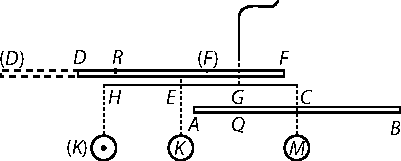
\includegraphics[scale=1]{gesamttex/edit_VIII-4/images/LH_35_09_10_001-002_d5_002v.pdf} 
\edcaption{\edtext{\lbrack\textit{Fig.~5}\rbrack}{%
\lemma{\lbrack\textit{Fig.~5}\rbrack}%
\Cfootnote[nonum]{Ein gestrichener Entwurf zum Diagramm wird nicht wiedergegeben. Leibniz zeichnet in \lbrack\textit{Fig.~5}\rbrack\ \textit{R} und \textit{D} als separate Punkte. Allerdings gilt gemäß den Angaben im Text $AB = CD$ sowie $QB = QR$ bzw. $= GR$. Daher müssen die Punkte \textit{R} und \textit{D} zusammenfallen. Der Fehler wirkt sich nicht auf die Argumentation aus.}}}
\end{edfigure}
\pstart
Soit la 
\edtext{balance\indexS{balance} \textit{CGEH}}{\lemma{balance}\Bfootnote{%
\textit{(1)}~\textit{EC} soutenue %
\textit{(2)}~\textit{CGEH}~\textit{L}}}
soutenue 
\edtext{en \textit{G}. Les bras \textit{GC} et \textit{GE} égaux, et deux corps egaux \textit{M}, \textit{K}}{\lemma{en \textit{G}.}\Bfootnote{%
\textit{(1)}~\textit{GC} et \textit{GE} égales, %
\textit{(2)}~Les bras \textit{GC} et \textit{GE} égaux,
\textit{(a)}~dont son %
\textit{(b)}~deux
\textit{(aa)}~\textit{M}, \textit{K} %
\textit{(bb)}~egaux \textit{M}, \textit{K}~\textit{L}}}
suspendus de ces bras,\indexS{bras de la balance} qui sont en equilibre.\indexS{equilibre} 
Changeons ces deux corps en deux parallelepipedes prismes ou cylindres egaux et egalement épais \textit{K} en \textit{DF} et \textit{M} en \textit{AB} 
\edtext{attachés 
\edlabel{35_09_10_001-002_7a}%
\edtext{}{%
\xxref{35_09_10_001-002_7a}{35_09_10_001-002_7b}%
\lemma{\textls{fermement} \lbrack...\rbrack\ \textls{fermement}}%
\Cfootnote{Das Wort ist in beiden Fällen doppelt unterstrichen.}}%
\textls{fermement} le long de la balance\bracks{,}}{\lemma{}\Bfootnote{attachés \textls{fermement} %
\textit{(1)}~à %
\textit{(2)}~le long de la balance \textit{erg.~L}}} 
soutenus en leur points de milieu\indexS{point de milieu} par 
\edtext{\bracks{\textit{C}}}{\lemma{}\Bfootnote{\textit{E} \textit{L ändert Hrsg.}}}
et \textit{F}. Il est manifeste que tout demeure en equilibre.\indexS{equilibre} Mais 
\edtext{avançons \textit{K} en (\textit{K}). Il est manifeste que c'est comme si nous avancions \textit{FD} en (\textit{F})(\textit{D}) et l'attachions \textls{fermement}\edlabel{35_09_10_001-002_7b} en \textit{H}. Prenons \textit{GR} égale à \textit{QB}. Il est manifeste que $QA+AR$ contrebalancent \textit{QB}. 
Or il y a encor \bracks{(\textit{F})}\textit{A}
et \textit{R}(\textit{D}) qui pesent du costé de \textit{GE} donc ce costé l'emporte.}{\lemma{avançons}\Bfootnote{%
\textit{(1)}~\textit{FD} en (\textit{F})(\textit{D}) %
\textit{(2)}~\textit{K} en (\textit{K}) \bars{en sorte \textit{erg.~u.~gestr.}}. Il est \bracks{...} en (\textit{F})(\textit{D})  
\textit{(a)}~par
\textit{(b)}~.~Or
\textit{(c)}~.~Alors
\textit{(d)}~.~Il est manifeste qu'il y a plus de poids alors du costé de \textit{GE} que du costé de \textit{GC}. Car du costé de \textit{GC} il n'y a que \textit{QB}; mais du costé de \textit{GE} il y a maintenant (\textit{F})(\textit{D})
\textit{(aa)}~egale à
\textit{(bb)}~et encor \textit{QA}. Et tout cela fait bien plus que \textit{QB}. Or lors qu'il y a plus de po
\textit{(e)}~et \lbrack...\rbrack\ que %
\textit{(aa)}~$QA+(F)R$  %
\textit{(aaa)}~contre %
\textit{(bbb)}~du costé de \textit{GE} %
\textit{(bb)}~$QA+AR$ \bracks{...} encor \bars{\textit{FA} \textit{ändert Hrsg.}} et \textit{R}(\textit{D})
 \bracks{...} l'emporte.~\textit{L}}}
\pend
\pstart \textls{Problème}: deux 
\edtext{corps estant}{%
\lemma{corps}\Bfootnote{%
\textit{(1)}~estan
\textit{(2)}~ine
\textit{(3)}~estant donnés 
\textit{(a)}~trouver leur
\textit{(b)}~la pr
\textit{(4)}~estant donnés, \bars{et \textit{streicht Hrsg.}}
\textit{(a)}~la place de l'un de deux dans la balance, trouver \bars{la place de \textit{streicht Hrsg.}} l'autre \bars{pour les mettre en equilibre. \textit{streicht Hrsg.}}
\textit{(b)}~trouver %
\textit{(aa)}~leur places %
\textit{(bb)}~leur places
\textit{(5)}~estant~\textit{L}}}
donnés, et leur Points dans la balance\bracks{,} trouver le point de l'equilibre\indexS{point de l'equilibre} ou du 
\edlabel{35_09_10_001-002_5a}%
\edtext{}{\xxref{35_09_10_001-002_5a}{35_09_10_001-002_5b}\lemma{soutien.}\Bfootnote{%
\textit{(1)}~Soyent les corps donnés
\textit{(a)}~\textit{ACB} 
\textit{(b)}~\bars{en forme de prismes egalement epais representés par les droites \textit{erg.}}
\textit{DEF} \textit{ACB} \bars{qui ont la meme raison entre elles que les corps \textit{erg.}}
\textit{(aa)}~et place de celuycy donnée, on cherche la place de l'autre. 
\textit{(aaa)}~Si (\textit{D})(\textit{E})(\textit{F}) estoit la veritable, il faudroit que 
\textit{(aaaa)}~$DG+$
\textit{(bbbb)}~$(A)G+$ 
\textit{(cccc)}~$AG+DG$ fût egale à
\textit{(bbb)}~Si (\textit{A})(\textit{C})(\textit{B}) et
\textit{(ccc)}~Si $AG+(D)G$ estoit égal à $GB+G(F)$
\textit{(ddd)}~Si $AG+DG$ estoit égal à $GB+GF$ tout s
\textit{(bb)}~on cherche leur places, c'est à dire
\textit{(aaa)}~les points
\textit{(bbb)}~celles des points de milieu \textit{C}, \textit{E}. Si \textit{AG} estoit égal à \textit{GF} et \textit{DG} à \textit{GB}, tout seroit en equilibre. Or si \textit{AG} egal à \textit{GF} donc $AC+CG$ égal à $GE+EF$. Et si \textit{DG} égal à \textit{GB} donc $DE-EG$ égal à $CB-CG$. Mais en ce cas \textit{AB} seroit égal à \textit{DF}
\textit{(2)}~\lbrack/\rbrack\ Soyent les corps donnés 
\textit{(a)}~\textit{DEF}, \textit{ACB}.
\textit{(b)}~en forme~\textit{L}}}%
soutien.
\pend 
\begin{edfigure}[0.5em][1em] 		%
\includegraphics[scale=1]{%
gesamttex/edit_VIII-4/images/LH_35_09_10_001-002_d6_002v.pdf}
\edcaption{\edtext{\lbrack\textit{Fig.~6}\rbrack}{%
\lemma{\lbrack\textit{Fig.~6}\rbrack}%
\Cfootnote[nonum]{Ein gestrichener Entwurf zum Diagramm wird nicht wiedergegeben. Auf die darin enthaltenen Punktebezeichnungen (\textit{A}), ... (\textit{F}) \textendash\ beziehen sich die gestrichenen Varianten \textit{(aaa)}\textendash\textit{(ccc)} zu \refpassage{35_09_10_001-002_5a}{35_09_10_001-002_5b}.}}}
\end{edfigure}
\pstart 
Soyent les corps donnés en forme\edlabel{35_09_10_001-002_5b} 
de prismes ayant l'epaisseur 
\edtext{égale, et les longueurs quelconques (selon que les prismes sont plus ou moins épais) \textit{DF},}{%
\lemma{égale,}%
\Bfootnote{%
\textit{(1)}~et representés
\textit{(2)}~et
\textit{(a)}~la longeur de ces droites
\textit{(b)}~les longueurs
\bars{quelconques \lbrack...\rbrack\ épais) \textit{erg.}}
\textit{DF},~\textit{L}}}
\textit{AB}, en raison\indexS{raison de deux corps} des 
\edtext{corps attachés}{\lemma{corps}\Bfootnote{%
\textit{(1)}~ou des %
\textit{(2)}~suspendus
\textit{(3)}~attachés à la balance %
\textit{(3)}~en \textit{E}, \textit{C}. Leur points de milieu et extremites de la dite balance %
\textit{(4)}~attachés~\textit{L}}}
le long de la balance en sorte que \textit{E}, \textit{C} leur points de milieu\indexS{point de milieu} sont 
\edtext{l\lbrack es\rbrack}{\lemma{}\Bfootnote{l' \textit{L ändert Hrsg.}}}
extremités de la dite balance.
On demande le point de milieu\indexS{point de milieu} \textit{G}. %
\pend
\pstart
Soit \textit{BXZ} egale à \textit{DEF} et leurs points de milieu, \textit{X}, \textit{E} egalement distans de \textit{G}, c'est à dire \textit{XG} égale 
\edtext{à \textit{EG}. Enfin}{\lemma{à \textit{EG}.}\Bfootnote{%
\textit{(1)}~De plus \textit{A} %
\textit{(2)}~Enfin $FA+AG$ égal à \textit{ZG}. %
\textit{(3)}~Enfin~\textit{L}}}
\textit{FG} ou \textit{AG} (posant qu'\textit{AB} commence où \textit{DF} finit) egal à \textit{ZG}.
\edtext{Ainsi \textit{DF}}{\lemma{Ainsi}\Bfootnote{%
\textit{(1)}~\textit{BZ} sera %
\textit{(2)}~\textit{DF}~\textit{L}}}
sera contrabalancée par \textit{BZ} et \textit{AZ} 
\edtext{ou \textit{FZ} de soy même. Donc}{\lemma{ou \textit{FZ}}\Bfootnote{%
\textit{(1)}~par luy même %
\textit{(2)}~de soy même. %
\textit{(a)}~Donc \textit{BC} egal à \textit{GE} %
\textit{(b)}~Donc~\textit{L}}}
\textit{G} est au 
\edtext{milieu. Or}{\lemma{milieu.}\Bfootnote{%
\textit{(1)}~De plus \textit{AG} estant \textit{FG}, donc \textit{EG} égale 
\textit{(a)}~\textit{AC}
\textit{(b)}~à \textit{AC}
\textit{(c)}~\bars{à \textit{AC} \textit{streicht Hrsg.}}
\textit{(2)}~Or~\textit{L}}}
puisque \textit{GZ} egale à \textit{GA}, donc 
\edtext{$BG-DF$ egale}{\lemma{$BG-DF$}\Bfootnote{%
\textit{(1)}~c'est à dire %
\textit{(2)}~egale~\textit{L}}}
à \textit{GA}. C'est à dire $BC+CG-DF$ egale à $AC-CG$. Et \textit{AC} estant egale à \textit{BC} nous aurons $2\,CG$ egale à \textit{DF}. C'est à dire \textit{CG} egale à \textit{FE} ou \textit{DE}, donc \textit{CA} (ou $CG+GA$) egale à \textit{GE} (ou 
\edtext{$GA+FE$). Donc \textit{CG} à}{\lemma{$GA+FE$).}\Bfootnote{%
\textit{(1)}~C'est à dire %
\textit{(2)}~Donc \textit{CG}
\textit{(a)}~égale %
\textit{(b)}~à~\textit{L}}}
\textit{GE} comme \textit{DF} à \textit{AB}, c'est à dire les bras 
\edtext{dont les corps sont suspendus en equilibre,\indexS{corps suspendus en equilibre}\indexS{equilibre} sont}{\lemma{}\Bfootnote{dont les corps
\bars{qu'en \textit{erg.~u.~gestr.}} sont suspendus en equilibre, sont \textit{erg.~L}}} 
en raison reciproque\indexS{raison reciproque de deux corps} des 
\edtext{corps. Ainsi nous rencontrons enfin la regle}{\lemma{corps.}\Bfootnote{%
\textit{(1)}~Et nous avons la solution du probleme conforme au theoreme %
\textit{(2)}~Ainsi nous rencontrons enfin %
\textit{(a)}~le theoreme co %
\textit{(b)}~la regle~\textit{L}}}
vulgaire de l'equilibre,\indexS{regle vulgaire de l'equilibre} par une espece 
\edtext{d'Analyse\indexS{Analyse} et}{\lemma{d'Analyse}\Bfootnote{%
\textit{(1)}~et sans l'avoir sçeue. %
\textit{(2)}~et~\textit{L}}}
comme si nous en avions rien sçeu.
\pend
\pstart 
\edtext{La chose}{\lemma{}\Bfootnote{La  \bars{seule \textit{gestr.}} chose~\textit{L}}}
qui reste à mon 
\edtext{avis, pour}{\lemma{}\Bfootnote{%
avis, \bars{à faire \textit{gestr.}}  pour perfectionner~\textit{L}}}
perfectionner cette meditation, c'est 
\foreignlanguage{ngerman}{\lbrack\textit{Text bricht~ab.}\rbrack}
\pend
\selectlanguage{ngerman}

\section[tocentry={Demonstration analytique du Principe de l'Equilibre et qu'il y a un centre de gravité dans toutes les figures
\enskip \bracks{Ende April -- Dezember 1679\,(?)}},
head={Demonstration analytique du Principe de l'Equilibre}]
{\MakeUppercase{Demonstration analytique du Principe de l'Equilibre et qu'il y a un centre de gravité dans toutes les figures}
\newline \bracks{Ende April -- Dezember 1679\,(?)}}
\label{41136}

\begin{ledgroupsized}[r]{120mm}
\footnotesize
\pstart
\noindent\textbf{Überlieferung:}
\pend
\end{ledgroupsized}
\begin{ledgroupsized}[r]{114mm}
\footnotesize
\pstart
\parindent -6mm
\makebox[6mm][l]{\textit{L}}%
Konzept:
LH~XXXV~9, 10~Bl.~5\textendash6. 
Ein Bogen~2\textsuperscript{o};
\href{\Scan{LH_35_09_10_005wz}}%
{Wasserzeichen} in Bl.~5.
Vier vorwiegend einspaltig beschriebene Seiten.
\pend
\end{ledgroupsized}
\selectlanguage{french}
\vspace{8mm}
\pstart
\centering
\href{\Scan{LH_35_09_10_005r}}%
{\lbrack5~r\textsuperscript{o}\rbrack}
\hfill
Demonstration\indexS{demonstration du principe de l'Equilibre}\indexS{demonstration analytique du Principe de l'Equilibre}
\edtext{analytique}{\lemma{}\Bfootnote{analytique \textit{erg.~L}}} 
du Principe de\indexS{principe de l'Equilibre}
\edlabel{35_09_10_005-006_1a}%
\edtext{}{\xxref{35_09_10_005-006_1a}{35_09_10_005-006_1b}\lemma{l'Equilibre}\Bfootnote{%
\textit{(1)}~\lbrack/\rbrack\ La demonstration d'Archimede dans son livre %
\textit{(2)}~Arc
\textit{(3)}~et qu'il y a un centre de gravité dans %
\textit{(a)}~tous les corps %
\textit{(b)}~toutes les figures \lbrack/\rbrack\
\textit{(4)}~Plusieurs~\textit{L}}}%
l'Equilibre
\hfill
\phantom{\lbrack5~r\textsuperscript{o}\rbrack}%
\linebreak
et qu'il y a un centre de gravité\indexS{centre de gravité} dans toutes les figures
\pend
\vspace{0.5\baselineskip}
\pstart
\noindent
Plusieurs\edlabel{35_09_10_005-006_1b} 
habiles Geometres\indexS{Geometres} 
\edtext{ont jugé}{%
\lemma{ont}%
\Bfootnote{%
\textit{(1)}~trouvé %
\textit{(2)}~jugé~\textit{L}}}
qu'il manque quelque chose à 
\edtext{la demonstration\indexS{demonstration d'Archimede} 
\indexN{\textls{Archimedes} 287\textendash212 v. Chr.}qu'Archimede\indexN{\textls{Archimedes} 287\textendash212 v. Chr.} 
a donné dans son livre \cite{01010}\textit{de aequiponderantibus}.}{\lemma{la demonstration \lbrack...\rbrack\ \textit{aequiponderantibus}}%
\Cfootnote{\indexN{\textls{Archimedes} 287\textendash212 v. Chr.}\textsc{Archimedes}, 
\cite{01010}\textit{De planorum aequilibris libri duo}, 
lib.~I, prop.~VI\textendash VII, S.\;152\textendash161.}} 
Il y en a d'autres qui la soûtiennent. Mais il n'est pas lieu icy d'entrer en cette discussion, et il sera plus à 
\edtext{propos de donner une nouvelle}{\lemma{propos}\Bfootnote{%
\textit{(1)}~de donner %
\textit{(2)}~de donner \bars{icy \textit{gestr.}} une %
\textit{(a)}~autre %
\textit{(b)}~nouvelle~\textit{L}}}
demonstration qui a des grands avantages, 
\edtext{sur celles que je me souviens}{\lemma{sur}\Bfootnote{%
\textit{(1)}~toutes les autres \bars{et celles \textit{erg.}} %
\textit{(2)}~celles
\textit{(3)}~celles que je me
\textit{(a)}~souvienne %
\textit{(b)}~souviens~\textit{L}}}
d'avoir veues. Car elle monstre 
\edtext{d'abord generalement}{\lemma{}\Bfootnote{%
d'abord
\bars{generalement \textit{erg.}}
que
\textit{(1)}~la distance \bars{des corps pesans \textit{erg.}} doit estre reciproque. Et elle le monstre sans distinction des proportions commensurables ou
\textit{(2)}~les 
\textit{(a)}~distances
\textit{(b)}~eloignements %
\textit{(aa)}~du centre de gravité de chaque corps et du point de l'equilibre, ou %
\textit{(aaa)}~de leur %
\textit{(bbb)}~du centre de gravité commun doivvent estre \bars{en raison \textit{erg.}} reciproque %
\textit{(aaaa)}~aux corps %
\textit{(bbbb)}~de celle des pesanteurs des corps, c'est à dire %
\textit{(aaaaa)}~à leurs %
\textit{(bbbbb)}~de leur grandeurs quand ils sont homogenes. 
\textit{(bb)}~des centres de gravité du centre
\textit{(aaa)}~de
\textit{(bbb)}~d'equilibre doivvent~\textit{L}}} 
estre en raison reciproque à celle des corps.\indexS{raison reciproque de deux corps} 
Soit que les corps soyent commensurables\indexS{commensurables} ou 
\edtext{non.\indexS{incommensurables} Au lieu}{\lemma{non.}\Bfootnote{%
\textit{(1)}~Au lieu %
\textit{(a)}~que les demonstrations %
\textit{(aa)}~que %
\textit{(bb)}~que j'ay %
\textit{(b)}~qu'on ne le prouve ordinairement, %
\textit{(aa)}~qu'on %
\textit{(bb)}~que dans le %
\textit{(2)}~Au lieu~\textit{L}}}
qu'on se contente ordinairement de le prouver 
\edtext{au commencement}{\lemma{}\Bfootnote{au commencement \textit{erg.~L}}}
dans les proportions commensurables\indexS{proportions commensurables} et de l'accommoder par apres aux incommensurables\indexS{proportions incommensurables} par une demonstration qui mene à l'impossible. 
\edtext{Mais ce qui est le principal, nostre}{\lemma{Mais}\Bfootnote{%
\textit{(1)}~le plus grand a %
\textit{(2)}~ce qui est le principal, %
\textit{(a)}~nostre %
\textit{(b)}~nostre~\textit{L}}}
demonstration est purement analytique;\indexS{demonstration analytique} 
c'est à dire elle monstre en même temps l'origine de l'invention.\indexS{origine de l'invention} 
Car il ne faut pas s'imaginer comme plusieurs qui sont entestés de l'Algebre,\indexS{Algebre} que l'analyse\indexS{analyse} n'est autre
\edtext{chose que la specieuse.\indexS{specieuse} 
L'analyse est \bracks{la methode}\indexS{methode analytique} 
de prendre la chose depuis sa source, de ne rien faire en tastonnant ny par rencontre, de ne rien supposer de dehors, ny de se servir d'aucune connoissance, à la quelle cette methode même ne mene\lbrack,\rbrack\ de faire voir par tout comment et pourquoy on s'est avisé de raisonner ainsi, et de prendre ce biais. En un mot d'aller par une voye dont on prevoit le succès. Car}{\lemma{chose que}\Bfootnote{%
\textit{(1)}~le calcul %
\textit{(a)}~d' %
\textit{(b)}~par 
\textit{(aa)}~symboles
\textit{(bb)}~lettres 
\textit{(2)}~la specieuse. 
\textit{(a)}~Toute la methode 
\textit{(aa)}~qui prend la chose depuis sa source, qui ne fait rien en tastonnant ny par rencontre, qui 
ne sert\lbrack\!\textit{!}\rbrack\ d'aucune connoissance 
\textit{(aaa)}~prise 
\textit{(aaaa)}~de
\textit{(bbbb)}~d'ailleurs, 
\textit{(bbb)}~,~à la quelle cette methode même ne mene,
et qui fait voir par tout comment \bars{et pourquoy \textit{erg.}} 
on \lbrack...\rbrack\ biais dont en s'est servi: est purement Analytique.
\textit{(bb)}~doi %
\textit{(b)}~La methode est tousjours analytique lors qu'on prend %
\textit{(c)}~L'analyse est \bars{la methode \textit{erg. Hrsg.}} de \lbrack...\rbrack\ ne mene
\bars{enfin \textit{erg.~u.~gestr.}}
de \lbrack...\rbrack\ biais.
\bars{En \lbrack...\rbrack\ voye
\textit{(1)}~qu'on prevoit d
\textit{(2)}~dont on prevoit le succès.~\textit{erg.}}
\textit{(aa)}~Par %
\textit{(bb)}~Dans l %
\textit{(cc)}~Car~\textit{L}}}
\edtext{icy par 
\edtext{exemple les corps}{\lemma{exemple}\Bfootnote{%
\textit{(1)}~quand %
\textit{(2)}~les corps~\textit{L}}}
pesans estans \textit{DEF}, et \textit{ACB}, la balance \textit{CE}, le point de l'equilibre\indexS{point de l'equilibre} \textit{G}. quand on prend \textit{G} en sorte que \textit{CG}, et \textit{EG} sont comme \textit{DEF}, \textit{ACB},}{%
\lemma{icy \bracks{...} \textit{DEF}, \textit{ACB}}%
\Cfootnote{Dem Text liegt das Diagramm \bracks{\textit{Fig.~1}} von N.\;\ref{41134} (S.~\pageref{Fig:35_09_10_001-002_fig-1}) zugrunde, das Leibniz am Ende des vorliegenden Konzepts (auf Bl.~6~v\textsuperscript{o}, hier S.~\pageref{Fig:35_09_10_005-006_fig-1}) mithilfe von Blindlinien und punktueller Perforierung des Papiers sehr genau nachgezeichnet hat.}}
pour prouver par là que \textit{G} est le point de l'equilibre,\indexS{point de l'equilibre} 
la demonstration peut estre bonne, mais la methode n'est pas telle qu'on la peut souhaiter,
\href{\Scan{LH_35_09_10_005v}}%
{\lbrack5~v\textsuperscript{o}\rbrack}  car comment est on allé s'aviser de diviser \textit{EC} 
\edtext{par le point \textit{G}}{\lemma{}\Bfootnote{par le point \textit{G} \textit{erg.~L}}} 
en raison reciproque des corps: si ce n'est peut estre parce qu'on sçavoit déja d'ailleurs que cela devoit reussir.
\edtext{Mais la veritable analyse\indexS{analyse}}{%
\lemma{Mais}%
\Bfootnote{%
\textit{(1)}~l'analyse
\textit{(2)}~la veritable analyse~\textit{L}}}
nous mene insensiblement à cette 
\edtext{division, si même}{\lemma{division,}\Bfootnote{%
\textit{(1)}~et sans %
\textit{(2)}~si même~\textit{L}}}
on n'en avoit pas entendu parler 
\edtext{auparavant. C'est}{%
\lemma{auparavant.}%
\Bfootnote{%
\textit{(1)}~J'ay jugé à propos de m'etendre la dessus
\textit{(2)}~C'est~\textit{L}}}
pourquoy il y a des demonstrations ou constructions qu'on a trouvées par la specieuse,\indexS{specieuse} mais 
\edtext{qui ne sont}{%
\lemma{qui ne}%
\Bfootnote{%
\textit{(1)}~laissent 
\textit{(2)}~sont~\textit{L}}}
pas pour cela analytiques.
\pend
\pstart 
J'ay jugé à propos de m'etendre la 
\edtext{dessus, parce que ces}{%
\lemma{dessus,}%
\Bfootnote{%
\textit{(1)}~à fin de
\textit{(2)}~parce que
\textit{(a)}~s
\textit{(b)}~ces~\textit{L}}}
reflexions sont
de consequence pour l'avancement de l'art d'inventer.\indexS{art d'inventer} Pour venir à la demonstration, 
\edtext{voicy comme}{%
\lemma{voicy}%
\Bfootnote{%
\textit{(1)}~comme j'ay fait pour la trouver. Soit la balance 
\textit{(2)}~comme~\textit{L}}}
j'y suis arrivé.
\pend
\pstart 
Soit la balance\indexS{balance} 
\edtext{\textit{EC} qu'on considere comme sans poids\lbrack,\rbrack\ les centres\indexS{centre de gravité} de gravit\lbrack é\rbrack\ des}{%
\lemma{\textit{EC}}%
\Bfootnote{%
\textit{(1)}~,~les corps
\textit{(2)}~\bars{qu'on considere comme sans poids \textit{erg.}} les centres de 
\bars{gravités \textit{ändert Hrsg.}} des~\textit{L}}}
corps attachés à la balance, \textit{C.E.} et les corps homogenes, et en raison donnée de \textit{DF} à \textit{AB}. Il s'agit de trouver le 
\edtext{point de l'equilibre,\indexS{point de l'equilibre} 
en sorte que la balance\indexS{balance} 
estant soutenue en \textit{G}}{\lemma{point}\Bfootnote{%
\textit{(1)}~\textit{G} %
\textit{(2)}~du soûtien, sçavoir \textit{G} %
\textit{(a)}~c'est à dire on la %
\textit{(b)}~tel que %
\textit{(3)}~de \lbrack...\rbrack\ en \textit{G}~\textit{L}}}
les corps \textit{C}, \textit{E} demeurent en 
\edtext{equilibre. Or}{\lemma{equilibre.}\Bfootnote{%
\textit{(1)}~Pour %
\textit{(2)}~Or~\textit{L}}}
l'on peut considerer toute la pesanteur des corps\indexS{pesanteur des corps considerée comme ramassée dans son centre} comme ramassée dans leurs centres de gravité\indexS{centre de gravité} \textit{C} et \textit{E}. Mais il est visible qu'on trouve plus de matiere de raisonner, quand on les 
\edtext{suppose etendus}{\lemma{suppose}\Bfootnote{%
\textit{(1)}~étendues %
\textit{(2)}~étendus~\textit{L}}}
par ce qu'ainsi on peut examiner chaque partie 
\edtext{à part. Or quoyqu'il importe}{\lemma{à part.}\Bfootnote{%
\textit{(1)}~Mais d %
\textit{(2)}~Or quoyqu'\bars{il \textit{erg.}} importe~\textit{L}}}
point à la 
\edtext{necessité de la}{\lemma{}\Bfootnote{necessité de la \textit{erg.~L}}}
demonstration quelle figure\indexS{figure du corps} on donne à ces corps, il peut neantmois importer 
\edtext{beaucoup à la commodité de}{\lemma{beaucoup}\Bfootnote{%
\textit{(1)}~à %
\textit{(2)}~à la commodité de~\textit{L}}}
l'invention. Et comme nous avons dit que ces corps entre eux sont 
\edtext{en raison}{%
\lemma{en}%
\Bfootnote{%
\textit{(1)}~raisons
\textit{(2)}~raison~\textit{L}}}
des droites \textit{DF}, et \textit{AB} 
\edtext{qui est la maniere la plus simple d'exprimer une raison.}{\lemma{}\Bfootnote{qui \lbrack...\rbrack\  raison \textit{erg.~L}}}
Supposons 
\edtext{donc}{\lemma{}\Bfootnote{donc \textit{erg.~L}}}
ces deux corps etendus comme ces lignes, c'est à dire supposons que ces sont deux 
\edtext{cylindres suspendus de la balance chacun par le point de son milieu\lbrack,\rbrack\ qui}{\lemma{cylindres}\Bfootnote{%
\textit{(1)}~egalement %
\bars{\textit{(1)}~attachés à %
\textit{(2)}~suspendus de la balance \bars{chacun \textit{erg.}} par le point %
\textit{(a)}~du milieu %
\textit{(b)}~de 
\textit{(aa)}~leur
\textit{(bb)}~son milieu \textit{erg.}}
qui~\textit{L}}}
ont la même epaisseur mais dont les longeurs
sont les droites \textit{DF}. et \textit{AB}. Car ainsi nous pourrons considerer ces corps, comme si ce n'estoient que des lignes 
\edtext{droites, puisque}{\lemma{droites,}\Bfootnote{%
\textit{(1)}~car %
\textit{(2)}~puisque~\textit{L}}}
l'epaisseur 
\edtext{estant la même de}{\lemma{estant}\Bfootnote{%
\textit{(1)}~de %
\textit{(2)}~la même de~\textit{L}}}
part et d'autre, ne change rien au 
\edlabel{35_09_10_005-006_3a}%
\edtext{}{\xxref{35_09_10_005-006_3a}{35_09_10_005-006_3b}\lemma{raisonnement.}\Bfootnote{%
\textit{(1)}~La situation %
\textit{(2)}~\href{\Scan{LH_35_09_10_006r}}%
{\lbrack6~r\textsuperscript{o}\rbrack} La %
\textit{(3)}~La %
\textit{(a)}~situation plus %
\textit{(b)}~situation plus simple et \bars{la \textit{gestr.}} plus~\textit{L}}}%
raisonnement.
\pend 
\pstart 
\href{\Scan{LH_35_09_10_006r}}%
{\lbrack6~r\textsuperscript{o}\rbrack} La situation plus simple et plus\edlabel{35_09_10_005-006_3b} 
naturelle de ces 
\edtext{corps \textit{DEF}. \textit{ACB}}{\lemma{corps}\Bfootnote{%
\textit{(1)}~entre eux %
\textit{(2)}~\textit{DF}. \textit{AB} %
\textit{(3)}~\textit{DEF}. \textit{ACB}~\textit{L}}}
entre eux et à l'egard de la balance est quand ils sont paralleles entre eux et perpendiculaires à la 
\edtext{balance. Par}{\lemma{balance.}\Bfootnote{%
\textit{(1)}~Mais cette situati %
\textit{(2)}~Par~\textit{L}}}
le point cherché \textit{G} menons \textit{PGQ} axe de l'equilibre\indexS{axe de l'equilibre} soutenant la
\edtext{\textit{CE}}{\lemma{}\Bfootnote{\textit{CE} \textit{erg.~L}}} 
\edtext{balance \textit{CE} en \textit{G} et}{\lemma{balance}\Bfootnote{%
\bars{\textit{CE} \textit{erg.}} en \textit{G}
\textit{(1)}~et parallele aux %
\textit{(2)}~per %
\textit{(3)}~perpendiculaire %
\textit{(4)}~et~\textit{L}}}
quoyque l'angle \textit{PGE} et \textit{PGC} puisse estre quelconque posons le droit; car c'est le plus simple. Mais comme nous ne voyons encor point de jour, pour découvrir le point \textit{G}. il faut que nous nous servions encor d'autres suppositions aussi faisables que celles que nous avons faites. Or il est manifeste, 
\edtext{que les corps \textit{DEF}. \textit{ACB} peuvent estre tournés à}{\lemma{que}\Bfootnote{%
\textit{(1)}~nous n'avons
\textit{(2)}~les %
\textit{(a)}~corps %
\textit{(b)}~lignes %
\textit{(c)}~corps \textit{DEF}. \textit{ACB} peuvent estre tournés %
\textit{(aa)}~sur leur centres de gravi %
\textit{(bb)}~à~\textit{L}}}
l'entour de leur centres \textit{E}. \textit{C}, c'est à dire qu'ils peuvent faire à la balance tel angle que nous 
\edtext{voulons car}{\lemma{voulons}\Bfootnote{%
\textit{(1)}~par %
\textit{(2)}~car~\textit{L}}}
au lieu que l'angle \textit{ACE} est droit, il pourra estre oblique, comme l'on voit dans la situation (\textit{A})\textit{C}(\textit{B}). Car il est 
\edtext{manifeste que l'equilibre\indexS{equilibre}}{\lemma{manifeste}\Bfootnote{%
\textit{(1)}~que %
\textit{(2)}~que %
\textit{(a)}~rien %
\textit{(b)}~l'equilibre~\textit{L}}}
demeure tousjous le même. Mais de ces situations obliques il faut choisir la plus commode à nostre raisonnement. C'est à dire une telle qui fasse voir 
\edtext{à veue d'oeil}{\lemma{}\Bfootnote{à veue d'oeil \textit{erg.~L}}}
l'equilibre 
\edtext{des corps \textit{DF}. \textit{AB}}{\lemma{}\Bfootnote{des corps \textit{DF}. \textit{AB} \textit{erg.~L}}} 
à l'egard de l'axe \textit{PQ}. Mais comment le ferons nous? C'est à dire comment est il possible de voir à veue d'oeil que deux corps inégaux\indexS{corps inégaux en equilibre} sont en 
\edtext{equilibre? Nous y arriverons ainsi: de}{\lemma{equilibre?}\Bfootnote{%
\textit{(1)}~Je %
\textit{(a)}~respond %
\textit{(b)}~reponds qu'on le peut faire en faisant en sorte qu'une partie %
\textit{(aa)}~de l'un %
\textit{(bb)}~du %
\textit{(2)}~Cela %
\textit{(3)}~Nous y arriverons ainsi: %
\textit{(a)}~deux c %
\textit{(b)}~de~\textit{L}}}
deux corps inegaux l'un est plus grand que l'autre, et le plus grand est celuy qui a une partie égale à l'autre tout entiere, par 
\edtext{exemple \textit{ZB}}{\lemma{exemple}\Bfootnote{%
\textit{(1)}~\textit{Z}(\textit{B}) partie de \textit{AB} %
\textit{(2)}~\textit{ZB}~\textit{L}}}
partie de \textit{AB} egale à \textit{DF}. Donc si \textit{ZB} 
\edtext{et \textit{DF} avoient}{\lemma{et \textit{DF}}\Bfootnote{%
\textit{(1)}~estoient le %
\textit{(2)}~avoient~\textit{L}}}
leurs 
\edtext{centres ou points de milieu \indexS{point de milieu} \textit{E} et \textit{X}}{\lemma{centres}\Bfootnote{%
\textit{(1)}~\textit{E} et \textit{X} ou milieux %
\textit{(2)}~ou points de milieu \textit{E} et \textit{X}~\textit{L}}}
également distans de l'axe \textit{PQ}, c'est à dire que les perpendiculaires à l'axe \textit{EG}, et \textit{XY} fussent égales; il est  
\edtext{visible que \textit{DF}}{\lemma{visible que}\Bfootnote{%
\textit{(1)}~les %
\textit{(2)}~\textit{DF}~\textit{L}}}
et \textit{ZB} seroient en equilibre; et pour faire que tout soit en equilibre\indexS{equilibre} il faut que le reste de \textit{AB}; sçavoir \textit{AZ} fût aussi en 
\edtext{equilibre, c'est à dire}{\lemma{equilibre,}\Bfootnote{%
\textit{(1)}~ce qui %
\textit{(2)}~c'est à dire~\textit{L}}}
que son point de milieu \textit{R} soit dans l'axe \textit{PQ}.
\pend
\pstart 
\href{\Scan{LH_35_09_10_006v}}%
{\lbrack6~v\textsuperscript{o}\rbrack}
Voila donc 
\edtext{ce grand}{\lemma{ce}\Bfootnote{%
\textit{(1)}~probleme %
\textit{(2)}~grand~\textit{L}}}
probleme de Mechanique\indexS{grand probleme de mecanique} (trouver le point de l'equilibre,\indexS{point de l'equilibre} \textit{G}.) reduit aux termes de la pure Geometrie,\indexS{Geometrie pure} c'est à dire au probleme 
\edtext{suivant. La droite \textit{DEF} (dont le milieu est \textit{E}) et la droite \textit{EC}}{\lemma{suivant.}\Bfootnote{%
\textit{(1)}~Dans la droite, %
\textit{(2)}~Les droites \textit{DEF}. et \textit{EC} %
\textit{(3)}~La droite \textit{DEF}. \bars{(dont \lbrack...\rbrack\ droite \textit{erg.}}
\textit{EC}~\textit{L}}}
estant données de grandeur et de 
\edtext{position; mais la droite \textit{AB} de grandeur et}{\lemma{position;}\Bfootnote{%
\textit{(1)}~et %
\textit{(2)}~mais la droite 
\textit{(a)}~\textit{Ab}
\textit{(b)}~\textit{AB} de grandeur
\textit{(aa)}~en sorte q %
\textit{(bb)}~et~\textit{L}}}
son point de milieu\indexS{point de milieu} \textit{C} de 
\edtext{position: trouver}{\lemma{position:}\Bfootnote{%
\textit{(1)}~trouver \textit{PGQ} %
\textit{(2)}~trouver~\textit{L}}}
le point \textit{G} dans la droite \textit{EC}, et l'angle \textit{ACE} en sorte que menant \textit{PGQ} perpendiculaire à \textit{CGE} et 
\edlabel{35_09_10_005-006_2a}%
prenant \textit{BZ} égale à \textit{FD}, et \textit{BX} égale à \textit{FE}\lbrack,\rbrack\ soit \textit{XY} (perpendiculaire à \textit{PQ}) egale à 
\edtext{\textit{EG}, et que \textit{AB}}{\lemma{\textit{EG},}\Bfootnote{%
\textit{(1)}~et \textit{AZ} %
\textit{(2)}~et que 
\textit{(a)}~\textit{Ab}
\textit{(b)}~\textit{AB}~\textit{L}}}
rencontre \textit{PQ} en \textit{R} point de milieu de \textit{AZ}. Ce probleme de Geometrie est aisé à resoudre car à cause des triangles semblables \textit{RGC}, \textit{RYX}\lbrack,\rbrack\ \textit{GC} sera à \textit{YX} c'est à dire à \textit{GE} comme \textit{RC} à \textit{RX}. Or est il que \textit{RC} est égale à \textit{DE}, et \textit{RX} à \textit{AC}, donc \textit{GC} est à \textit{GE} comme \textit{DE} à \textit{AC}, c'est à dire comme \textit{DF} 
\edtext{à \textit{AB}. C'est}{\lemma{à \textit{AB}.}\Bfootnote{%
\textit{(1)}~C'est à dire en raison reciproque des %
\textit{(2)}~C'est~\textit{L}}}
à dire il se trouve que la raison des distances\indexS{raison des distances} \textit{GE}, et \textit{GC}, 
\edtext{est reciproque}{%
\lemma{est}%
\Bfootnote{%
\textit{(1)}~raison
\textit{(2)}~reciproque~\textit{L}}}
à celle des corps\indexS{raison de deux corps} \textit{E}, \textit{C}.
\pend
\pstart
Il reste seulement de prouver que \textit{RC} est egale à \textit{DE}, et \textit{RX} à \textit{AC}. 
Ce qui est aisé, car \textit{RC} est $AC-AR$, 
et 
\edtext{\textit{AR} est moitié de \textit{AZ} et \textit{AZ} est 
$AB-ZB$\lbrack,\rbrack\ ou 
$AB-DF$ et la moitié de \textit{AZ} ou 
\textit{AR} toute entiere, est $AC-DE$.}{%
\lemma{\textit{AR} est}\Bfootnote{%
\textit{(1)}~\textit{AZ} %
\textit{(2)}~dimidia \textit{AZ} %
\textit{(3)}~moitié de \textit{AZ} et \textit{AZ} est $AB-ZB$,
\textit{(a)}~seu $AB-DE$ donc \textit{RC} est $AC-AB$ ergo \bars{et \textit{streicht Hrsg.}} dimidia \textit{AZ} est $AC-DE$ donc \textit{AR} est $AC-DE$, vel tota \textit{AR} %
\textit{(b)}~vel %
\textit{(c)}~ou \lbrack...\rbrack\ entiere, est \bars{est \textit{streicht Hrsg.}} 
$AC-DE$~\textit{L}}}
\edtext{}{\lemma{}\Afootnote{\foreignlanguage{ngerman}{\textit{Am Rand}:}
\begin{tabular}{ccc}
\textit{CX} & \groesser & \textit{CV}\\
\begin{tikzpicture}\draw (-0.35,-0.65) -- (0.0,-0.3) -- (0.35,-0.65);\end{tikzpicture} & & 
\begin{tikzpicture}\draw (-0.35,-0.65) -- (0.0,-0.3) -- (0.35,-0.65);\end{tikzpicture}\\
$CB-EF$ &  & $GE-CG$
\end{tabular}%
}} 
Donc \textit{RC} est $AC-AC+DE$. 
C'est à dire \textit{RC} est égale à \textit{DE}. Ce qui est le premier. 
D'où il est manifeste que \textit{RX} est égale à \textit{AC}, ou 
\textit{CB} ce qui estoit le second. Car de \textit{CB} ostons 
\textit{XB}, et adjoutons y \textit{RC}, et nous aurons 
\edtext{\textit{RX}, or}{%
\lemma{\textit{RX},}%
\Bfootnote{%
\textit{(1)}~et
\textit{(2)}~or~\textit{L}}}
nous avons autant 
\edtext{}{\lemma{}\Afootnote{\foreignlanguage{ngerman}{\textit{Am Rand}:} \textit{CV} difference entre \textit{GE} et \textit{CG}\lbrack,\rbrack\ \textit{CX} difference entre \textit{CB} et \textit{EF}.}} 
\edtext{adjouté qu'osté, puisque \textit{RC} est}{\lemma{adjouté}\Bfootnote{%
\textit{(1)}~que %
\textit{(2)}~qu'osté, puisque \textit{RC}
\textit{(a)}~est
\textit{(b)}~et
\textit{(c)}~est~\textit{L}}}
égale à \textit{XB} ou \textit{DE}. 
Donc la grandeur de \textit{RX} est la même que celle de \textit{CB}, c'est à dire 
\edlabel{35_09_10_005-006_4a}%
\edtext{}{%
\xxref{35_09_10_005-006_4a}{35_09_10_005-006_4b}%
\lemma{de \textit{AC}.}\Bfootnote{%
\lbrack/\rbrack\ 
\textit{(1)}~que %
\textit{(2)}~quand %
\textit{(3)}~Quand~\textit{L}}}%
de \textit{AC}.
\pend
\pstart
Quand\edlabel{35_09_10_005-006_4b}
le point \textit{G} est trouvé on n'a pas besoin de chercher l'angle \textit{ACE} mais si on le demande pour voir à l'oeil ce que nous avons demonstré  
\edtext{et pour donner la synthese\indexS{synthese} de nostre analyse\indexS{analyse}}{\lemma{}\Bfootnote{et pour donner la synthese de nostre analyse \textit{erg.~L}}} 
on peut faire ainsi: Du point \textit{G} soit prise \textit{GV} égale à \textit{GE} d'où il 
\edtext{soit abbaissée \textit{VX} parallele}{\lemma{soit}\Bfootnote{%
\textit{(1)}~\textit{VX} parallele à \textit{GQ} %
\textit{(2)}~abbaissée \textit{VX} %
\textit{(a)}~egale %
\textit{(b)}~parallele~\textit{L}}}
à \textit{GQ}. Du centre \textit{C}, 
\edtext{rayon \textit{CX} (c'est à dire $CB -BX$}{\lemma{rayon \textit{CX}~(}\Bfootnote{%
\textit{(1)}~c'est à dire $CB-LC$) %
\textit{(2)}~c'est à dire $CB - BX$~\textit{L}}}
ou $CB -EF$) soit decrit un 
\edtext{arc de cercle}{\lemma{arc}\Bfootnote{%
\textit{(1)}~coupant %
\textit{(2)}~de cercle~\textit{L}}}
coupant \textit{VX} 
\edtext{en \textit{X}. et en}{\lemma{en \textit{X}.}\Bfootnote{%
\textit{(1)}~en %
\textit{(2)}~et en~\textit{L}}}
même temps du centre 
\edtext{\textit{C}, et rayons}{\lemma{}\Bfootnote{\textit{C}, \bars{et \textit{erg.}} rayons~\textit{L}}}
\textit{CA}, \textit{CB}\bracks{,} soyent decrits les 
\edtext{arcs \textit{Aa} et \textit{Bb}.}{\lemma{arcs}\Bfootnote{%
\textit{(1)}~\textit{A}(\textit{A}) et \textit{B}(\textit{B}) %
\textit{(2)}~\textit{Aa} et \textit{Bb}.~\textit{L}}}
Continués la droite \textit{CX} de part et d'autre jusqu'à ce qu'elle rencontre ces arcs 
\edtext{en \textit{a} et \textit{b}}{\lemma{en}\Bfootnote{%
\textit{(1)}~(\textit{A}) et (\textit{B}) %
\textit{(2)}~\textit{a} et \textit{b}~\textit{L}}}
et nous 
\edtext{aurons l'inclination ou}{\lemma{aurons}\Bfootnote{%
\textit{(1)}~la %
\textit{(2)}~l'inclination ou~\textit{L}}}
situation 
\edtext{du corps \textit{AB}}{\lemma{}\Bfootnote{du corps \textit{AB} \textit{erg.~L}}} 
propre à nostre demonstration. Car il est visible que \textit{XY} est égale à \textit{VG} ou \textit{GE}, et que \textit{ZX}. \textit{XB}. \textit{DE}. \textit{EF} sont egales par la construction, donc \textit{ZB} et \textit{DF} sont en balance.\indexS{balance} Il est manifeste aussi et aisé à demonstrer par une synthese\indexS{synthese} opposée à l'analyse\indexS{analyse} de cydessus, que \textit{AR} est egale à \textit{RZ}, le point \textit{R} estant celuy où le corps \textit{AB}
\edtext{incliné comme}{\lemma{incliné}\Bfootnote{%
\textit{(1)}~comme nous venons de %
\textit{(2)}~comme~\textit{L}}}
nous avons dit, coupe l'axe \textit{PQ}. Donc \textit{AZ}
est aussi en equilibre, donc il n'y a rien qui puisse agir par sa pesanteur.%
\edlabel{35_09_10_005-006_2b} 
\edtext{Mais afin de ne rien laisser en arriere, adjoutons la synthese\indexS{synthese} dans la feuille suivante.}{%
\lemma{Mais \bracks{...} suivante}%
\Cfootnote{Gemeint ist wohl der Abschnitt von N.\;\ref{41134} ab \refpassage{35_09_10_001-002_8a}{35_09_10_001-002_8a} ("Voicy la synthese la plus commode qui on peut tirer de cette analyse.")}}
\pend 
\begin{edfigure}%
\includegraphics[scale=1]{%
gesamttex/edit_VIII-4/images/LH_35_09_10_005-006_d_006v.pdf}
\edcaption{%
\pagelabel{Fig:35_09_10_005-006_fig-1}%
\edtext{\lbrack\textit{Fig.~1, tlw. Blindzeichnung}\rbrack}{%
\lemma{\lbrack\textit{Fig.~1}\rbrack}%
\Cfootnote[nonum]{%
Bei der Anfertigung der Zeichnung hat Leibniz an dieser Stelle das Diagramm \bracks{\textit{Fig.~1}} von N.\;\ref{41134} (S.~\pageref{Fig:35_09_10_001-002_fig-1}) mithilfe von Blindlinien und punktueller Perforierung des Papiers sehr genau nachgezeichnet.
Leibniz hat zunächst die Punkte des gedrehten Körpers mit \textit{A}, \textit{B} bezeichnet und sie anschließend in \textit{a}, \textit{b} unbenannt. Diese Änderung hat er im Text auf \refpassage{35_09_10_005-006_2a}{35_09_10_005-006_2b} jedoch nicht berücksichtigt.
Ein gestrichener Entwurf zum Diagramm wird nicht wiedergegeben.}}}
\end{edfigure}
\selectlanguage{ngerman}






\chapter[tocentry={De vectibus conjugatis et figuris dentium in rotis
\enskip 25. Oktober (4. November) 1679
},
head={De vectibus conjugatis et figuris dentium in rotis}]%
{\MakeUppercase{De vectibus conjugatis et figuris dentium in rotis}
\newline 25. Oktober (4. November) 1679
}

\label{intro_vectibus-conjugatis}

\begin{ledgroup}
\footnotesize
\pstart
\noindent
Mit N.\;\ref{57034} und N.\;\ref{57035} liegen zwei eigenhändig datierte "\textit{Schedae}" vor, die sich dem statischen Thema aufeinander wirkender Hebel und der Bestimmung der darauf folgenden Bewegungen widmen. 
Solche Hebel bieten auch ein gutes Modell für die Wechselwirkung der ineinander verschränkten Zähne zweier Zahnräder, deren Eigenschaften Leibniz in N.\;\ref{intro_vectibus-conjugatis} ebenfalls behandelt ("de figuris dentium in rotis").
\pend
\pstart
Leibniz hatte sich bereits in der Pariser Zeit mit diesen Fragen beschäftigt: In unmittelbar benachbarten Signaturen (LH~XXXVII~3, Bl.~77\textendash80) sind vier Konzepte \cite{02160}"De vectibus conjugatis" aus der zweiten Hälfte von 1674 überliefert (ediert in \textit{LSB} VIII,~2 N.\;45). 
Die Diagramme \bracks{\textit{Fig.~1}}, \bracks{\textit{Fig.~3}} und \bracks{\textit{Fig.~8}} von N.\;\ref{57034} greifen bspw. die Figuren des ersten Pariser Konzepts (\textit{LSB} VIII,~2 N.\;45\textsubscript{1}) auf.
Leibnizens Angabe "resumtae priores cogitationes" in der Überschrift von N.\;\ref{57034} bezieht sich daher aller Wahrscheinlichkeit nach auf die vier Texte von 1674.
Ein weiterer Zeuge seiner Beschäftigung mit dem Thema liegt mit der Notiz "De curvis inveniendis ope vectium conjugatorum" vor, die gemäß ihrer wahrscheinlichen Entstehungszeit (Dezember 1674 bis 1675) in diesem Band als Nachtrag ediert wird (N.\;\ref{Cc2_847-2}).
\pend
\pstart
Der Text der zweiten Konzepts N.\;\ref{57035} ist ursprünglich als direkte Fortsetzung des ersten entstanden, wie der Kustos "Longe secus est" am Ende von N.\;\ref{57034} (Bl.~76~v\textsuperscript{o}) bezeugt.
Erst nachträglich hat Leibniz die Einteilung in "\textit{Scheda prima}" und "\textit{secunda}" vorgenommen, 
indem er auf Bl.~75~r\textsuperscript{o}, hier \refpassage{37_03_075-076_1a}{37_03_075-076_1b}, und Bl.~81~r\textsuperscript{o}, hier \refnote{FnB:37_03_081_scheda-2da}, entsprechende Überschriften hinzufügte.
\pend
\end{ledgroup}


\section[tocentry={De vectibus conjugatis et figuris dentium in rotis scheda prima},  	%
head={De vectibus conjugatis et figuris dentium in rotis scheda prima}]%
{\MakeUppercase{De vectibus conjugatis et figuris dentium in rotis scheda prima}}  	%

\label{57034}
\begin{ledgroupsized}[r]{120mm}
\footnotesize
\pstart
\noindent\textbf{Überlieferung:}
\pend
\end{ledgroupsized}
\begin{ledgroupsized}[r]{114mm}
\footnotesize
\pstart
\parindent -6mm
\makebox[6mm][l]{\textit{L}}%
Konzept:
LH~XXXVII~3~Bl.~75\textendash76. 
Ein Bogen~2\textsuperscript{o}; 
\href{\Scan{LH_37_03_075wz}}%
{Wasserzeichen} in Bl.~75.
Vier unregelmäßig beschriebene Seiten.
Die obere Hälfte von Bl.~76~v\textsuperscript{o} überliefert Rechnungen und eine Zeichnung (in Bleistift, wohl von Leibnizens Hand) ohne Bezug zum Text. Diese sind tlw. überschrieben und müssen vor dem Text enstanden sein.
\pend
\end{ledgroupsized}
\selectlanguage{latin}
\vspace{8mm}
\pstart
\centering
\edlabel{37_03_075-076_1a}%
\edtext{}{%
\xxref{37_03_075-076_1a}{37_03_075-076_1b}%
\lemma{\href{\Scan{LH_37_03_075r}}%
{\lbrack75~r\textsuperscript{o}\rbrack}}%
\Bfootnote{%
\bars{\textit{(1)}~De %
\textit{(a)}~rotis %
\textit{(b)}~figuris dent  %
\textit{(2)}~De vectibus \lbrack...\rbrack\ cogitationes
\bars{scheda 1\textsuperscript{ma}. \textit{erg.}}
25 Octobr. 1679.~\textit{erg.}}
\lbrack/\rbrack\
\textit{(1)}~Sit Triangulum isosceles %
\textit{(a)}~ \textit{ADC} %
\textit{(b)}~\textit{BCD} sumtaque in recta \textit{BD} producta alio puncto \textit{A} junctaeque %
\textit{(2)}~In Triangulo~\textit{L}}}%
\href{\Scan{LH_37_03_075r}}%
{\lbrack75~r\textsuperscript{o}\rbrack}
\hfill
De vectibus\indexS{vectes conjugati} conjugatis et figuris\indexS{figurae dentium} dentium in \indexS{rota}rotis,
\hfill
\phantom{\lbrack75~r\textsuperscript{o}\rbrack}
\linebreak
resumtae
\edtext{priores cogitationes}{%
\applabel{FnC:37_03_075-076_resumtae}%
\lemma{priores cogitationes}\Cfootnote{Gemeint sind vier, mit N.\;\ref{57034} inhaltlich verwandte und in der benachbarten Signatur LH XXXVII 3, Bl.~77\textendash80 überlieferte Konzepte \cite{02160}"De vectibus conjugatis" aus der zweiten Hälfte von 1674 (\textit{LSB} VIII,~2 N.\;45).}}
scheda 1\textsuperscript{ma}. 25 Octobr. 1679.
\pend
\nobreak
\vspace{0.5\baselineskip}
\begin{edfigure}%
\includegraphics[scale=1]{%
gesamttex/edit_VIII-4/images/LH_37_03_075-076_d1_075r.pdf}
\edcaption[-.1em]{%
\edtext{\lbrack\textit{Fig.~1, tlw. Blindzeichnung}\rbrack}{%
\lemma{}%
\Afootnote[nonum]{\textit{Neben \bracks{\textit{Fig.~1}}}: Brevior vectis potentior}}}
\end{edfigure}
\pstart
\noindent
In Triangulo\indexS{triangulum}\edlabel{37_03_075-076_1b}
\textit{BCD} sint latera \textit{BC}, \textit{BD} aequalia, producatur \textit{BD} usque in \textit{A}, junctaeque \textit{AC}, sumatur in \textit{AB} aequalis \textit{AE} ita ut juncta \textit{CE} fiat aliud triangulum\indexS{triangulum isosceles} isosceles \textit{ACE}, quaeritur ratio inter \textit{CD} et \textit{CE}.
\pend
\pstart
\textls{%
$\left.\begin{array}{c}AC\\AE\end{array}\!\!\right\}$
sit \textit{a}, \textit{CE} sit \textit{e}\bracks{;}}
\textit{CG} erit $\displaystyle\frac{e}{2}$, \textit{AG} erit $\sqrt{a^2-\displaystyle\frac{e^2}{4}}$ 
vel $\displaystyle\frac{\sqrt{4a^2-e^2}}{2}$ 
et area Trianguli \textit{ACE} erit $\displaystyle\frac{e\sqrt{4a^2-e^2}}{4}$, eadem
\edtext{est \textit{AE}}{%
\lemma{est}%
\Bfootnote{%
\textit{(1)}~\textit{AF} in %
\textit{(2)}~\textit{AE}~\textit{L}}}
in \textit{CF}, seu \textit{a} in \textit{CF}, ergo erit 
\textls{\textit{CF} aequ. $\displaystyle\frac{e\sqrt{4a^2-e^2}}{4a}$.}
\pend
\pstart
Eodem
\edtext{modo ponendo}{%
\lemma{modo}%
\Bfootnote{%
\textit{(1)}~quaerendo %
\textit{(2)}~ponendo~\textit{L}}}
\rule[-3.1ex]{0pt}{4ex}%
\textls{$\left.\begin{array}{c}BC\\BD\end{array}\!\!\right\}$ 
esse \textit{b}} 
et 
\textls{\textit{CD} esse \textit{d}}
quaerendoque
\edtext{similiter altitudinem}{%
\lemma{similiter}%
\Bfootnote{%
\textit{(1)}~perpendicularem \textit{CF}, e %
\textit{(2)}~altitudinem~\textit{L}}}
\textit{CF} in Triangulo \textit{BCD}, uti quaesiveramus in Triangulo \textit{ACE}, fiet \textls{\textit{CF} aequ.}
\rule[-1.8ex]{0pt}{5.4ex}%
$\displaystyle\frac{d\sqrt{4b^2-d^2}}{4b}$.
\pend
\pstart
Quos duos valores aequando, fiet: $be\sqrt{4a^2-e^2}\sqcap ad\,\sqrt{4b^2-d^2}$ sive $4a^2b^2e^2-b^2e^4\sqcap 4a^2b^2d^2-a^2d^4$\bracks{,} qua aequatione satis exprimitur relatio inter \textit{a}, \textit{b}, \textit{e}, \textit{d}.
\pend
\pstart
Ponamus jam \textit{d} et \textit{e} esse infinite parvas, tunc utique evanescent termini $b^2e^4$, et $a^2d^4$, et restabit $4a^2b^2e^2\sqcap 4a^2b^2d^2$ sive fiet $d\sqcap e$.
\edtext{}{%
\lemma{}\Afootnote{\textit{Am Rand}:\quad 
\raisebox{-1ex}{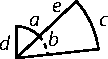
\includegraphics[scale=1]{gesamttex/edit_VIII-4/images/LH_37_03_075-076_d2_075r.pdf}}\enskip \lbrack\textit{Fig.~2}\rbrack\textsuperscript{\bracks{a}}\\
$\displaystyle\frac{c}{b}\sqcap\displaystyle\frac{e}{d}$. $b\sqcap\displaystyle\frac{dc}{e}$.\raisebox{.5ex}{\textsuperscript{\bracks{b}}}
$\displaystyle\frac{a}{b}\sqcap\doublefrac{a}{\dfrac{dc}{e}}$. Ergo $\displaystyle\frac{a}{b}\sqcap\displaystyle\frac{ae}{cd}$.\raisebox{.5ex}{\textsuperscript{\bracks{c}}} 
Ergo anguli \textit{a}, \textit{b} inter se in ratione composita ex directa\textsuperscript{\lbrack d\rbrack} arcuum \textit{a}, \textit{c} et reciproca radiorum \textit{e}, \textit{d}.
\\[1.5ex] 
{\footnotesize 
\textsuperscript{\lbrack a\rbrack}\bracks{\textit{Fig.~2}}: Ein nicht gestrichener Entwurf zum Diagramm wird nicht wiedergegeben.
\textsuperscript{\lbrack b\rbrack}$b\sqcap\displaystyle\frac{dc}{e}$. %
\textit{(1)}~$\displaystyle\frac{a}{c}\sqcap\doublefrac{a}{\dfrac{eb}{c}}$ %
\textit{(2)}~$\displaystyle\frac{a}{b}\sqcap\doublefrac{a}{\dfrac{dc}{e}}$~\textit{L}\quad
\textsuperscript{\lbrack c\rbrack}$\displaystyle\frac{a}{b}\sqcap\displaystyle\frac{ae}{cd}$. %
\textit{(1)}~anguli %
\textit{(a)}~arcus vel anguli %
\textit{(b)}~\textit{a}, \textit{b} inter se %
\textit{(2)}~Ergo~\textit{L}\quad
\textsuperscript{\lbrack d\rbrack}directa %
\textit{(1)}~radiorum %
\textit{(2)}~arcuum~\textit{L}}}}
\pend
\pstart
Hinc sequitur duos vectes conjugatos in directum
\edtext{sitos aequali potentia recta descendente se prementes, agere potentia longitudini brachiorum reciproca.}{%
\lemma{sitos}%
\Bfootnote{%
\textit{(1)}~aequali potentia se prementes, 
\textit{(a)}~in aequilibrio esse %
\textit{(b)}~agere
\textit{(2)}~se potentia
\textit{(3)}~aequali \bracks{...} agere potentia
\textit{(a)}~longitudines
\textit{(b)}~longitudinis brachiorum reciproca.~\textit{L}}}
Sive si sint duo vectes \textit{AE}, \textit{BD}, mobiles circa centra \textit{A}, \textit{B} quorum ille deprimitur a pondere \textit{L}, hic a pondere \textit{M} attollitur et si pondera\indexS{pondera aequalia} sint
\edtext{aequalia et ex aequalibus trochleis\indexS{trochlea} suspensa, et in linea recta descendant}{%
\lemma{et}%
\Bfootnote{%
\textit{(1)}~aequalia %
\textit{(2)}~aequalis %
\textit{(3)}~aequali a centro \textit{A} distantia suspensa, %
\textit{(4)}~ex aequalibus trochleis %
\textit{(a)}~suspensas %
\textit{(b)}~suspensa, \bars{et ita \textit{streicht Hrsg.}} et in linea recta descendant~\textit{L}}}
ita, ut discrimen sit tantum in vectium
\edtext{longitudine \textit{AE}, \textit{BD} inaequali. Vincet pondus, quod magis descendit\lbrack,\rbrack\ id est quod majorem arcum trochleae circumagit, id est quod majorem evolvit fili partem. Sunt autem anguli \textit{A}, \textit{B} inter se in ratione composita ex directa arcuum, et reciproca radiorum. Sed initio positis rectis}{%
\lemma{longitudine \textit{AE}, \textit{BD}}%
\Bfootnote{%
\textit{(1)}~inaequali, ajo %
\textit{(a)}~hoc %
\textit{(b)}~hac non obstante aequilibrium fore; nam %
\textit{(aa)}~ut %
\textit{(bb)}~ut brachium longius \bars{\textit{BD} \textit{erg.}} vincat, debet extremitas ejus \textit{D} majorem %
\textit{(aaa)}~circulum describere \textit{DE} %
\textit{(bbb)}~arcum \textit{DE} describere, quam est arcus \textit{EC}, quem describit extremitas \textit{E} vectis brevioris \textit{AE}, ita enim pondus \textit{M} magis descendit quam pondus \textit{L}. Sed initio positis %
\textit{(2)}~inaequali. Vincet pondus, quod magis descendit id est quod %
\textit{(a)}~majorem 
\textit{(aa)}~\bars{angulum \textit{streicht Hrsg.}}
\textit{(bb)}~arcum
\textit{(cc)}~arcum trochleae
\textit{(aaa)}~evolvit, id enim majorem circum
\textit{(bbb)}~circum
\textit{(ccc)}~circumagit, \bracks{...} positis rectis~\textit{L}}}
\textit{DC}, \textit{EC} infinite parvis calculus ostendit eas esse aequales (quod alioqui ut in sequentibus ostendam etiam infinite parvis fieri non solet).
\edtext{Itaque et arcus quibus rectae \textit{DE}, \textit{CE} subtenduntur sunt aequales, adeoque sublata ratione arcuum directa manet ratio radiorum seu vectium reciproca, quare}{%
\lemma{Itaque}%
\Bfootnote{%
\textit{(1)}~aequalis est ab initio nisus sive descendendi potentia utrinque, quare %
\textit{(2)}~et arcus quibus \bars{rectae \textit{erg.}} \textit{DE}, \bracks{...} ratio %
\textit{(a)}~radiorum %
\textit{(b)}~radiorum seu vectium reciproca, \bars{quare \textit{streicht Hrsg.}} quare~\textit{L}}}
\textls{duo vectes conjugati in directum positi utcunque longitudine inaequales, si modo aequali utrinque}
\edtext{\textls{ponderis recta descendentis gravitatione sibi contranitantur} potentiam habebunt in reciproca longitudinum ratione.}{%
\lemma{\textls{utrinque}}%
\Bfootnote{%
\textit{(1)}~vi agantur %
\textit{(2)}~in contra %
\textit{(3)}~si %
\textit{(4)}~vi %
\textit{(5)}~\textls{ponderis} \bars{\textls{recta descendentis} \textit{erg.}} \textls{gravitatione sibi contranitantur} %
\textit{(a)}~\textls{in aequilibrio manebunt} %
\textit{(b)}~potentiam habebunt in reciproca longitudinum ratione.~\textit{L}}}
Ipsi autem vectes per se hic pondere semper carere ponuntur, vel 
\edtext{ab eodem pondere animus}{%
\lemma{ab}%
\Bfootnote{%
\textit{(1)}~eo
\textit{(2)}~eodem pondere
\textit{(a)}~animo
\textit{(b)}~animus~\textit{L}}}
abstrahitur.
\pend
\pstart
\href{\Scan{LH_37_03_075v}}%
{\lbrack75~v\textsuperscript{o}\rbrack}\ 
\edtext{Caeteris ut ante positis}{%
\lemma{}%
\Bfootnote{Caeteris ut ante positis \textit{erg.~L}}}
sint jam duo vectes conjugati \textit{AE}, \textit{BD} non in directum siti, sed angulum facientes in \textit{D} seque ducentes in eodem plano in quo sunt siti. \textit{BD} describet arcum \textit{DC}, et \textit{AE}
\edtext{arcum \textit{EC}. Quaeritur horum}{%
\lemma{arcum \textit{EC}.}%
\Bfootnote{%
\textit{(1)}~Manifestum est vires exercitas esse ut ponderum descensus, quia autem pondera \bars{\textit{L}, \textit{M} \textit{erg., streicht Hrsg.}} ex trochleis \bars{aequalibus \textit{erg.}} %
\textit{(a)}~\textit{A}, \textit{B} circa %
\textit{(b)}~circa \textit{A}, \textit{B} 
\bars{\textit{(1)}~filis
\textit{(2)}~filo \textit{erg.}} 
suspensa intelliguntur; hinc %
\textit{(aa)}~tantam portione %
\textit{(bb)}~tantum descendit pondus \textit{L} vel \textit{M}, quantum est filum quod evolvitur trochlea circumacta, %
\textit{(aaa)}~trochlea autem, e %
\textit{(bbb)}~id est quantus est trochleae arcus, is autem tantus est quantus est angulus %
\textit{(2)}~Quaeritur horum~\textit{L}}}
arcum\indexS{ratio arcuum} ratio. %
\pend
\pstart
Cum sint infinite parvi eadem erit quae subtensarum; subtensa autem arcus infinite parvi haberi potest pro portione
\edtext{tangentis. Ergo}{%
\lemma{tangentis}%
\Bfootnote{%
\textit{(1)}~, productae %
\textit{(2)}~. Ergo~\textit{L}}}
\textit{CD}, \textit{CE}
\edtext{cum circulos tangant in \textit{C} angulos facient}{%
\lemma{cum}%
\Bfootnote{%
\textit{(1)}~arcus circuli %
\textit{(2)}~circulos tangant
\textit{(a)}~in %
\textit{(aa)}~\textit{C} et %
\textit{(bb)}~\textit{D} et \textit{E} 
\textit{(aaa)}~productae
\textit{(bbb)}~si producantur in \textit{Q}, \textit{P} erunt anguli ipsarum %
\textit{(cc)}~\textit{C} sive \bars{in \textit{gestr.}} \textit{C}, \textit{D}, \textit{E} %
\textit{(dd)}~si producantur %
\textit{(aaa)}~angulos %
\textit{(bbb)}~in \textit{Q}, \textit{P} %
\textit{(ccc)}~\bars{in \textit{C}, \textit{D}, \textit{E} \textit{erg.}} angulos fa %
\textit{(b)}~in \textit{C} angulos facient~\textit{L}}}
rectos ad radios
\edtext{suos \textit{BC}, \textit{AC} sive si producantur}{%
\lemma{suos}%
\Bfootnote{%
\textit{(1)}~\textit{AC} vel \textit{AE} aut \textit{BC} vel \textit{BD}
\textit{(2)}~\textit{BC}, \textit{AC}
\textit{(a)}~vel \textit{A}, \textit{E} et %
\textit{(b)}~\textit{BC} %
\textit{(c)}~\textit{AC} %
\textit{(aa)}~vel \textit{BD} %
\textit{(bb)}~sive si producantur~\textit{L}}}
in \textit{P}, \textit{Q} erunt
\edtext{anguli \textit{BCQ} sive \textit{BDQ}}{%
\lemma{anguli}%
\Bfootnote{%
\textit{(1)}~\textit{ACP} sive \textit{AEP} %
\textit{(2)}~\textit{BCQ} sive \textit{BDQ}~\textit{L}}}
(nam puncta \textit{C}, \textit{D} eatenus pro coincidentibus
\edtext{habentur) recti}{%
\lemma{habentur)}%
\Bfootnote{%
\textit{(1)}~recti, vel \textit{ADR} %
\textit{(2)}~recti~\textit{L}}}
itemque anguli \textit{ACP} sive \textit{AEP}, sive \textit{ADR}. Ducatur ipsi \textit{AD} parallela, \textit{BRQ}\bracks{,} erit triangulum \textit{QDR} simile Triangulo \textit{DCE}. Erit ergo \textit{DC}
\edtext{ad \textit{EC} subtensa}{%
\lemma{ad \textit{EC}}%
\Bfootnote{%
\textit{(1)}~sive arcus ad arcum %
\textit{(2)}~subtensa~\textit{L}}}
ad subtensam, sive quod hic idem est, arcus ad arcum, ut \textit{QD} ad \textit{PR}. Angulus ergo \textit{CAE}, est 
\edtext{ad angulum \textit{CBD}}{%
\lemma{ad angulum}%
\Bfootnote{%
\textit{(1)}~\textit{BD}
\textit{(2)}~\textit{CBD}~\textit{L}}}
in ratione
\edtext{directa}{%
\lemma{}%
\Bfootnote{directa \textit{erg.~L}}}
arcuum \textit{CE}, \textit{CD}, sive rectarum \textit{DR}, \textit{DQ}, et reciproca\indexS{ratio reciproca radiorum} radiorum, seu in ratione \textit{BD} ad \textit{AD}. 
Regulam ergo hanc praescribemus: sint duo vectes\indexS{vectes conjugati} conjugati, qui ponderibus\indexS{pondus} ex aequalibus trochleis\indexS{trochlea} pendentibus circumaguntur, sibique obnituntur
\edtext{in \textit{D}, manentes}{%
\lemma{in \textit{D},}%
\Bfootnote{%
\textit{(1)}~in eodem plano %
\textit{(2)}~manentes~\textit{L}}}
\edtext{plano. Uni vectium \textit{AE}, ducatur}{%
\lemma{plano}%
\Bfootnote{%
\textit{(1)}~Ipsi vecti ducendo %
\textit{(2)}~Uni vectium %
\textit{(a)}~ducatur %
\textit{(b)}~\textit{AE}, %
\textit{(aa)}~ab %
\textit{(bb)}~ducatur~\textit{L}}}
in eodem invicem per alterius centrum \textit{B}
\edtext{parallela \textit{BRQ}}{%
\lemma{parallela}%
\Bfootnote{%
\textit{(1)}~\textit{BR} %
\textit{(2)}~\textit{BRQ}~\textit{L}}}
cui ex
\edtext{puncto \textit{D} vectibus ad angulos rectos eductae}{%
\lemma{puncto \textit{D}}%
\Bfootnote{%
\textit{(1)}~ad angulos rectos 
\textit{(a)}~tam ipsi \textit{A} 
\textit{(b)}~utrique vectium %
\textit{(2)}~vectibus \bars{ad angulos rectos \textit{erg.}}
eductae~\textit{L}}}
\textit{DR}, \textit{DQ}, occurrant in punctis
\edtext{\textit{R}, \textit{Q}, erit}{%
\lemma{\textit{R}, \textit{Q},}%
\Bfootnote{%
\textit{(1)}~erunt potentiae vectium %
\textit{(2)}~erit~\textit{L}}}
potentia vectis \textit{AD} contra potentiam\indexS{potentia} vectis \textit{BD} in composita ratione
\edtext{ex rationibus}{%
\lemma{ex}%
\Bfootnote{%
\textit{(1)}~ratione %
\textit{(2)}~rationibus~\textit{L}}}
\textit{DR} ad \textit{DQ} et \textit{DB} ad \textit{DA}. 
Seu ratio exercitii potentiarum \textit{L}, et \textit{M} erit ut \textit{BD}, \textit{DR} ad \textit{AD}, \textit{DQ} seu \rule[-4mm]{0pt}{10mm}$\displaystyle\frac{\text{pot.}\; L}{\text{pot.}\; M}\sqcap\displaystyle\frac{BD, DR}{AD, DQ}$.
\pend
\pstart
Si Angulus \textit{ADB} nullus seu infinite obtusus, 
\edtext{seu si \textit{ADB} recta}{%
\lemma{seu si}%
\Bfootnote{%
\textit{(1)}~\textit{AB}, \textit{DB} %
\textit{(2)}~\textit{ABD} recta %
\textit{(3)}~\textit{ADB} recta~\textit{L}}}
una, coincident \textit{DQ}, \textit{DR} quippe ad hanc rectam perpendiculares,
\edtext{coincidet et recta \textit{AB} ipsi \textit{ADB},}{%
\lemma{}%
\Bfootnote{coincidet et recta \textit{AB} ipsi \textit{ADB} \textit{erg.~L}}}
adeoque sublata ratione \textit{DR}, \textit{DQ} remanebit sola \textit{BD}, \textit{AD}, seu ratio pot. \textit{L} ad pot. \textit{M} erit \textit{BD} ad \textit{AD}, nempe reciproca
\edtext{radiorum. Quod}{%
\lemma{radiorum}%
\Bfootnote{%
\textit{(1)}~, 
\textit{(a)}~ut
\textit{(b)}~ut supra %
\textit{(2)}~. Quod~\textit{L}}}
jam supra alia methodo ostenderamus.
\pend
\pstart
Si
\edtext{jam vectium}{%
\lemma{jam}%
\Bfootnote{%
\textit{(1)}~dens vel vectis %
\textit{(2)}~vectium~\textit{L}}}
conjugatorum alteruter,
\edtext{ut \textit{ACS}}{%
\lemma{}%
\Bfootnote{ut  \bars{dens \textit{gestr.}} \textit{ACS}~\textit{L}}}
non sit
\edtext{linea}{%
\lemma{}%
\Bfootnote{linea \textit{erg.~L}}}
recta, sed vel curva, vel ex recta una in plures fracta, quod et in curva intelligi potest,
\edtext{quae componi intelligitur ex recta in infinitas partes}{%
\lemma{quae}%
\Bfootnote{%
\textit{(1)}~semper est infi %
\textit{(2)}~rect %
\textit{(3)}~componi intelligitur ex recta in infinitas %
\textit{(a)}~curvas fracta %
\textit{(b)}~partes~\textit{L}}}
fracta, res eodem redit. Nempe ponatur vectis curvus vel flexus \textit{ACS} ab altero \textit{BC} duci in \textit{ACT}. erunt potentiae, ut anguli \textit{TAS}, \textit{TBC}, seu in ratione \textit{TS}, \textit{TC} directa, et radiorum reciproca, ducatur ipsi \textit{CS} fragmento seu portioni vectis fracti ducendae, seu si vectis curva linea constat. Ducatur Tangenti ejus
\edtext{curvae (quae curvam contingat}{%
\lemma{curvae~(}%
\Bfootnote{%
\textit{(1)}~quae est %
\textit{(2)}~quae curvam contingat~\textit{L}}}
in puncto ubi sibi vectis ille ab alio impellitur) parallela per punctum \textit{B}, nempe \textit{BVX}, cui productae \textit{TSV}, \textit{TCX} occurrant\bracks{,} id est perpendiculares ad \textit{AT}, \textit{BT} seu \textit{AC}, \textit{BC}. Coincidere enim intelliguntur puncta \textit{C}, \textit{T}, \textit{S}. Erit angulus ad angulum, 
\edlabel{37_03_075-076_3a}%
\edtext{}{%
\xxref{37_03_075-076_3a}{37_03_075-076_3b}%
\lemma{}%
\Bfootnote{%
\textit{(1)}~\href{\Scan{LH_37_03_076r}}%
{\lbrack76~r\textsuperscript{o}\rbrack} potentia \textit{L} ad potentiam \textit{M}, ut
\textit{(a)}~\textit{BD}
\textit{(b)}~\textit{BC}
\textit{(c)}~ \textit{BT}, \textit{TX} ad \textit{AT}, \textit{TV}.
\textit{(2)}~potentia \bracks{...} \textit{TV}. \href{\Scan{LH_37_03_076r}}%
{\lbrack76~r\textsuperscript{o}\rbrack} Quaeritur~\textit{L}}}%
seu potentia \textit{L} ad potentiam \textit{M}, ut \textit{BT}, \textit{TX} ad \textit{AT}, \textit{TV}.
\pend
\pstart\noindent
\href{\Scan{LH_37_03_076r}}%
{\lbrack76~r\textsuperscript{o}\rbrack}\ 
\pend
\begin{edfigure}[0em][1em]
\includegraphics[scale=1]{%
gesamttex/edit_VIII-4/images/LH_37_03_075-076_d3_076r.pdf}
\edcaption[-.25em]{\edtext{\lbrack\textit{Fig.~3}\rbrack}{%
\lemma{}\Afootnote[nonum]{\textit{Unter \bracks{Fig.~3}, gestrichen}: potentia \textit{L} ad potentiam \textit{M}, ut\textsuperscript{\lbrack a\rbrack} \textit{BT}, \textit{TX} ad \textit{AT}, \textit{TV}.
\\[1.5ex] 
{\footnotesize \textsuperscript{\lbrack a\rbrack} ut %
\textit{(1)}~\textit{BD} %
\textit{(2)}~\textit{BC} %
\textit{(3)}~\textit{BT}~\textit{L}}}}}
\end{edfigure}
\pstart
\edtext{}{%
\lemma{}\Afootnote{\textit{Neben} \lbrack\textit{Fig.~3}\rbrack: Nota: Brevior vectis potentior, ideo figura nonnihil immutanda, vel in contraria trochlearum parte locanda pondera, ut non attollat\textsuperscript{\lbrack a\rbrack} vectis \textit{BD} vectem \textit{AE} sed deprimat\textsuperscript{\lbrack b\rbrack} vectis \textit{AE} vectem \textit{AD}.\\[1.5ex] 
{\footnotesize 
\textsuperscript{\lbrack a\rbrack}attollat %
\textit{(1)}~\textit{BC} \textit{AE}
\textit{(2)}~vectis \textit{BD} vectem \textit{AD}~\textit{L}\quad
\textsuperscript{\lbrack b\rbrack}deprimat %
\textit{(1)}~\textit{AE} %
\textit{(2)}~\textit{AE} %
\textit{(3)}~vectis \textit{AE}~\textit{L}}}}
Quaeritur\edlabel{37_03_075-076_3b} 
jam qualisnam debeat esse curva, seu flexio\indexS{flexio vectis} vectis sive \indexS{flexio dentis}dentis \textit{ACS} talis,
\edtext{ut eadem}{%
\lemma{ut}%
\Bfootnote{%
\textit{(1)}~ea
\textit{(2)}~aequalis semper %
\textit{(3)}~eadem~\textit{L}}}
semper maneat ratio\indexS{ratio potentiarum} potentiarum, sive quod idem est angulorum\indexS{ratio angulorum} vel revolutionum\indexS{ratio revolutionum}, id vero non difficulter 
\edlabel{37_03_075-076_2a}%
\edtext{}{%
\xxref{37_03_075-076_2a}{37_03_075-076_2b}%
\lemma{fiet}%
\Bfootnote{%
\textit{(1)}~sive per puncta, sive etiam continuo tractu. %
\textit{(a)}~Hoc modo: %
\textit{(b)}~Et primum per puncta hoc modo: %
\textit{(2)}~Moveatur~\textit{L}}}%
fiet.
\pend
\pstart
Moveatur\edlabel{37_03_075-076_2b}
planum $\Omega$ circa centrum \textit{A},
\edtext{et recta}{%
\lemma{et}%
\Bfootnote{%
\textit{(1)}~vectis %
\textit{(2)}~recta~\textit{L}}}
\textit{BD} circa centrum \textit{B} et quidem
\edtext{vectis}{%
\lemma{}%
\Bfootnote{vectis \textit{erg.~L}}}
\textit{B} triplo celerius quam planum, in puncto vectis \textit{D}. Sit stylus describens curvam in
\edtext{plano $A\gimel\beth\aleph D$ $\aleph\beth\gimel D$.}{%
\lemma{plano}%
\Bfootnote{%
\textit{(1)}~\textit{DCA} %
\textit{(2)}~\bars{$\aleph\beth\gimel D$ \textit{streicht Hrsg.}}
\textit{(3)}~$A\gimel\beth\aleph D$~\textit{L}}}
Ea curva erit quaesita nempe dens sive vectis 
\edtext{erit $A\gimel\beth\aleph D$.}{%
\lemma{erit}%
\Bfootnote{%
\textit{(1)}~\textit{ADCS} %
\textit{(2)}~\textit{$A\aleph\beth\gimel D$} %
\textit{(3)}~$A\gimel\beth\aleph D$.~\textit{L}}}
\pend
\begin{edfigure}%
\includegraphics[scale=1]{%
gesamttex/edit_VIII-4/images/LH_37_03_075-076_d4_076r.pdf}%
\hspace*{2.5em}
\edcaption{\bracks{\textit{Fig.~4}}}
\end{edfigure}
\pstart
Si rotae duae
\edtext{se ducentes in quibus figura dentium quaeritur}{%
\lemma{}%
\Bfootnote{se ducentes %
\textit{(1)}~\bars{de \textit{streicht Hrsg.}}
\textit{(2)}~quarum dentes %
\textit{(3)}~figur %
\textit{(4)}~in quibus figura dentium quaeritur \textit{erg.~L}}}
non sint in eodem plano, ut rotae \textit{S}, \textit{T}, figura dentium eodem modo quaeri
\edtext{potest. Hoc}{%
\lemma{pot\-est}%
\Bfootnote{%
\textit{(1)}~, nam %
\textit{(2)}~. Hoc~\textit{L}}}
ita fiet:
\pend
\begin{edfigure}%
\includegraphics[scale=1]{%
gesamttex/edit_VIII-4/images/LH_37_03_075-076_d5_076r.pdf}
\edcaption[.1em]{\lbrack\textit{Fig.~5}\rbrack}
\end{edfigure}
\pstart
Dum
\edtext{rota \textit{T} vel ejus dens \textit{BT} aut alius movetur circa centrum \textit{B}: interea solidum aliquod rotae \textit{S}}{%
\lemma{rota}%
\Bfootnote{%
\textit{(1)}~\textit{S} vel ejus dens \textit{AS} aut \bracks{...} rotae \textit{T}
\textit{(2)}~\textit{T} \bracks{...} rotae \textit{S}~\textit{L}}}
affixum cum ea moveatur
\edtext{et in solido illo punctum \textit{T}}{%
\lemma{et}%
\Bfootnote{%
\textit{(1)}~puncta quae in solido illo designabit %
\textit{(2)}~in solido illo punctum \textit{T}~\textit{L}}}
expers dentis \textit{BT} designabit
\edtext{lineam seu}{%
\lemma{lineam}%
\Bfootnote{%
\textit{(1)}~dentis %
\textit{(2)}~seu~\textit{L}}}
curvaturam\indexS{curvatura dentis} dentis \textit{S}, si quidem rota \textit{B} ducens \textit{A}
\edtext{ducenda. Observando}{%
\lemma{ducenda}%
\Bfootnote{%
\textit{(1)}~idemque fieri, %
\textit{(2)}~.~Observando~\textit{L}}}
inter circumagendum certam proportionem\indexS{proportio revolutionum} revolutionum
\edtext{datam,}{%
\lemma{}%
\Bfootnote{datam \textit{erg.~L}}}
debet autem solidum fingi simul consistens seu tenax, et tamen
\edtext{penetrabile; interea}{%
\lemma{penetrabile;}%
\Bfootnote{%
\textit{(1)}~per %
\textit{(2)}~interea~\textit{L}}}
tamen calculo ejus puncta omnia etiam sine hoc solido invenire non difficile erit, et modum alium describendi uno tractu excogitare.
\pend
\begin{edfigure}[.25em][1em]
\includegraphics[scale=1]{%
gesamttex/edit_VIII-4/images/LH_37_03_075-076_d6_076r.pdf}
\edcaption[.1em]{\edtext{\bracks{\textit{Fig.~6}}}{%
\lemma{\bracks{\textit{Fig.~6}}}%
\Cfootnote[nonum]{%
Ein gestrichener Entwurf zum Diagramm wird nicht wiedergegeben.}}}
\end{edfigure}
\pstart
Porro hae lineae etsi videantur esse Mechanicae,\indexS{lineae mechanicae}
\edtext{nam duo \indexS{motus}motus}{%
\lemma{nam}%
\Bfootnote{%
\textit{(1)}~puncta eorum %
\textit{(2)}~duo motus~\textit{L}}}
adhibendi a se invicem 
\edtext{sunt}{\lemma{}\Bfootnote{sunt \textit{erg.~L}}}
independentes, possunt tamen motibus describi a se invicem dependentibus, si nimirum uno eodemque motu aequabili simul et
\edtext{filum trochleae}{%
\lemma{filum}%
\Bfootnote{%
\textit{(1)}~rotae \textit{A}, et %
\textit{(2)}~trochleae~\textit{L}}}
circa \textit{A}, et filum\indexS{filum} aliquod trochleae proportionem datam habentis circa \textit{B} evolvatur, ita enim facile efficiemus, ut rotae \textit{A}, \textit{B} sive in eodem sive in diverso plano revolutionem habeant datam. %
\pend
\pstart
Caeterum etsi haec descriptio\indexS{descriptio geometrica} sit geometrica, non tamen est \indexS{descriptio analytica}analytica. 
\href{\Scan{LH_37_03_076v}}%
{\lbrack76~v\textsuperscript{o}\rbrack}
Mihi tamen hae lineae\indexS{lineae analyticae} Analyticae esse
\edtext{videntur et primum}{%
\lemma{videntur}%
\Bfootnote{%
\textit{(1)}~nam %
\textit{(2)}~et primum~\textit{L}}}
in eo exemplo id ostendam, cum id quaeritur ut semper utriusque rotae\indexS{revolutio rotae} revolutio sit eadem. %
\pend
\begin{edfigure}%
\includegraphics[scale=1]{%
gesamttex/edit_VIII-4/images/LH_37_03_075-076_d7_076v.pdf}
\edcaption{\lbrack\textit{Fig.~7}\rbrack}
\end{edfigure}
\pstart
Sit \textit{AF} aequ. \textit{BG} et in directum posita seu in eadem recta et recta 
\edtext{alia \textit{H} moveatur in medio}{%
\lemma{alia \textit{H}}%
\Bfootnote{%
\textit{(1)}~\bars{moveatur \textit{streicht Hrsg.}} aequab
\textit{(2)}~in medio~\textit{L}}}
posita inter \textit{A}, \textit{B}
\edtext{moveatur medio}{%
\lemma{moveatur}%
\Bfootnote{%
\textit{(1)}~aequabiliter %
\textit{(2)}~medio~\textit{L}}}
sui puncto semper eundem servans situm ad \textit{A} et \textit{B}, id est
\edtext{moveatur quodlibet}{%
\lemma{moveatur}%
\Bfootnote{%
\textit{(1)}~recta %
\textit{(2)}~ipsam %
\textit{(3)}~quodlibet~\textit{L}}}
punctum ejus in recta ad \textit{AB} perpendiculari, manifestum est hoc motu tam \textit{AF} quam \textit{BG} eodem modo propelli, et revolutionum angulos esse eosdem. Hoc jam
\edtext{obtento, si uni dentem\bracks{,}}{%
\lemma{obtento}%
\Bfootnote{%
\textit{(1)}~facile ut %
\textit{(2)}~si %
\textit{(a)}~illi dentem %
\textit{(b)}~uni dentem~\textit{L}}}
alteri planum affigamus facile in hoc plano stylo in dentis apice posito curvam quaesitam describemus. Haec curva manifeste analytica est, seu puncta ejus quaelibet analysi exhiberi possunt ordinaria.
\pend
\pstart
\edtext{\lbrack Quid\rbrack}{\lemma{}\Bfootnote{Sed~\textit{L ändert Hrsg.}}}
si revolutiones\indexS{revolutio rotae} debeant esse in data ratione, exempli causa ut dum unus dens unum angulum absolvit, alter absolvat ejus tertiam partem\lbrack,\rbrack\
sed tunc curva etiam erit analytica\indexS{curva analytica} quia per calculum semper
\edtext{potest angulus}{%
\lemma{potest}%
\Bfootnote{%
\textit{(1)}~curva %
\textit{(2)}~angulus~\textit{L}}}
secari in quacunque ratione numerica.
Sed si alia ratio quaeratur ut lineae ad lineam, erit curva non quidem transcendens\indexS{curva transcendens} non tamen analytica sed interpolata\indexS{curva interpolata}.
\pend
\pstart
Restat quaerendum 
\edtext{an hi}{%
\lemma{an}%
\Bfootnote{%
\textit{(1)}~hae
\textit{(2)}~hi~\textit{L}}}
dentes motibus rotarum utiliores, quod vix puto, non tantum quia facile franguntur, sed et quia non video cur tam ratio habenda aequabilis motus\indexS{motus}, quam potius excludendorum duorum malorum quae maxime nocent in rotis,
nempe frictionis, et
directionis ineptae.
\pend
\pstart
Quoad frictionem\indexS{frictio} effici potest, ut duarum rotarum dentes eandem semper invicem habeant frictionem, si talis sit curva
\edtext{dentis,}{%
\lemma{}%
\Bfootnote{dentis \textit{erg.~L}}}
ut semper
\edtext{dens alter, sit tangens ejus}{%
\lemma{dens}%
\Bfootnote{%
\textit{(1)}~unius %
\textit{(2)}~alter, sit tangens ejus,
\textit{(a)}~vel dentis %
\textit{(aa)}~unius %
\textit{(bb)}~alterius, %
\textit{(b)}~ejus,~\textit{L}}}
vel certum ad ejus tangentem faciens angulum, exempli gratia 45 graduum, vel 30, etc.
\pend
\begin{edfigure}%
\includegraphics[scale=1]{%
gesamttex/edit_VIII-4/images/LH_37_03_075-076_d8_076v.pdf}
\edcaption[0pt]{\lbrack\textit{Fig.~8}\rbrack}
\end{edfigure}
\pstart
\edtext{Sit dens curvus vel flexus}{%
\lemma{Sit}%
\Bfootnote{%
\textit{(1)}~dens \textit{Acde} %
\textit{(2)}~tang %
\textit{(3)}~dens curvus vel %
\textit{(a)}~rectus %
\textit{(b)}~flexus~\textit{L}}}
\textit{Acde}, alter rectus \textit{Bf}, semper tangens curvam \textit{cde}.
\edtext{seu in chordas ejus indefinite}{%
\lemma{seu}%
\Bfootnote{%
\textit{(1)}~part %
\textit{(2)}~chordis %
\textit{(3)}~in chordas ejus
\textit{(a)}~con %
\textit{(b)}~infini %
\textit{(c)}~indefinite~\textit{L}}}
parvas continuatas incidens. Sed hoc modo semper magna erit frictio, quia semper
\edtext{toti isti}{%
\lemma{toti}%
\Bfootnote{%
\textit{(1)}~portioni %
\textit{(2)}~isti~\textit{L}}}
portiunculae curvae aequalis portio dentis \textit{Bf} tota affricabitur. Quanto
\edtext{itaque major}{%
\lemma{itaque}%
\Bfootnote{%
\textit{(1)}~minor angulus %
\textit{(2)}~major~\textit{L}}}
angulus dentis ducentis ad tangentem\indexS{tangens curvae} curvae ducendae, eo minor frictio. Si esset maximus angulus nempe rectus seu
\edtext{si dens \textit{B}\lbrack\textit{f}\rbrack\ rectilineus}{%
\lemma{si}%
\Bfootnote{%
\textit{(1)}~angulus dentis \textit{BF} recti %
\textit{(2)}~dens  \bars{\textit{BF} \textit{ändert Hrsg.}} rectilineus~\textit{L}}}
ad
\edtext{curvam esset}{%
\lemma{curvam}%
\Bfootnote{%
\textit{(1)}~\textit{CDE} esset 90 graduum, %
\textit{(2)}~esset~\textit{L}}}
semper perpendicularis, seu minima ducta ex puncto \textit{B}, tunc plane non duceret alter alterum, quia circulus centro \textit{B}
\edtext{radio \textit{Bf}}{%
\lemma{radio}%
\Bfootnote{%
\textit{(1)}~\textit{BF} %
\textit{(2)}~\textit{Bf}~\textit{L}}}
descriptus curvam dentis alterius tangeret seu raderet.
\pend
\pstart
Alterum observandum esse dixi ineptam directionem, nimirum, in rotis magnam potentiae partem sentit id quod eum sentire non debet, quando ictus dirigitur non in objectum ducendum, sed
\edtext{in firmacula}{%
\lemma{in}%
\Bfootnote{%
\textit{(1)}~columnas %
\textit{(2)}~firmacula~\textit{L}}}
axesque aut loca fixa, omnis enim illa vis inutiliter perit. Exempli gratia
\edtext{in hoc casu dens}{%
\lemma{in}%
\Bfootnote{%
\textit{(1)}~hoc corpus %
\textit{(2)}~hoc casu dens~\textit{L}}}
\textit{B\ind{3}f} ingruens in dentem 
\edtext{\textit{A\ind{3}c\ind{3}d\ind{3}e}, perpendiculariter quidem et proinde}{%
\lemma{\textit{A\ind{3}c}\textit{\ind{3}d}\textit{\ind{3}e},}%
\Bfootnote{\bars{seu impingens in \textit{\ind{3}d}\textit{\ind{3}e} \textit{gestr.}} %
\textit{(1)}~recte %
\textit{(2)}~perpendiculariter quidem %
\textit{(a)}~\bars{et commode \textit{erg.}} incurrit in \textit{\ind{3}d}\textit{\ind{3}e} cui %
\textit{(b)}~et proinde~\textit{L}}}
commodissime incurrit in \textit{\ind{3}d}\textit{\ind{3}e}, sed ictus non bene pervenit ad corpus\indexS{elevatio corporis} elevandum \textit{L}.
\edtext{Nam si linea perpendicularis}{%
\lemma{Nam}%
\Bfootnote{%
\textit{(1)}~ictum excipit %
\textit{(2)}~si linea %
\textit{(a)}~conti %
\textit{(b)}~perpendicularis~\textit{L}}}
ad \textit{\ind{3}d}\textit{\ind{3}e} continuetur patet eam dirigere ictum versus \textit{A}, et ita totus dens \textit{A\ind{3}c}\textit{\ind{3}d}, secundum longitudinem suam excipit
eumque propagat versus \textit{A}, cujus resistentia inutiliter
\edtext{%
\edtext{consumitur.}{%
\lemma{consumitur.}%
\Bfootnote{%
\textit{(1)}~\bars{Longe secus est \textit{erg.~u.~gestr.}} %
\textit{(2)}~\bars{longe secus \textit{streicht Hrsg.}}~\textit{L}}}%
}{%
\lemma{consumitur}%
\Cfootnote{An dieser Stelle der vorliegenden "Scheda prima" hat Leibniz zunächst, am Rand von Bl.~76~v\textsuperscript{o}, den Satzanfang "Longe secus est" geschrieben, diesen dann gestrichen.
Vermutlich im Anschluss daran hat er die "Scheda secunda" begonnen, die mit diesen Worten ansetzt (Bl.~81~r\textsuperscript{o}, hier auf \refpassage{37_03_81_1a}{37_03_81_1b}). Die am Textende noch einmal wiederholten Worte "longe secus" (vom Hrsg. gestrichen) dienen dementsprechend als Kustos zur "Scheda secunda", N.\;\ref{57035}.}}
\pend
\vspace{0.5em} %
\pstart
\noindent
\bracks{\textit{Rechnungen in Bleistift, in gegenläufiger Schreibrichtung:}}
\pend
\nobreak
\vspace{0.5em}
\pstart
$\displaystyle\frac{a}{(2,\!)3}$.
\qquad
$\displaystyle\frac{\overset{\displaystyle (2,\!)4}{(2)\cancel{\smallfrown 3}},,+\overset{\displaystyle 1\vphantom{(1}}{3\vphantom{\cancel{3}}}}{3}\;$
$\reflectbox{\Large{\textit{f}}}$
5.
\qquad
$2\,\ovalbox{\begin{array}{c}+1\\-1\end{array}}$
\pend
\pstart
$a\sqcap$
\qquad
$\displaystyle\frac{3a+8}{-9}\sqcap 3$.
\qquad
$\begin{array}{r}3a\cancel{+8}\\\cancel{-8}\end{array}
\sqcap 
\begin{array}{r}27\\-8\end{array}$.
\qquad
$\displaystyle\frac{a}{9}$.
\qquad
$\displaystyle\frac{3a}{3}\sqcap \displaystyle\frac{18}{3}$.
\qquad
$a\sqcap 6$.
\qquad
$9\smallfrown \displaystyle\frac{a}{9}\sqcap a$.
\qquad
$\cancel{9,}\displaystyle\frac{3a+6}{\cancel{9}}\sqcap 3, 9$.
\qquad
$\displaystyle\frac{b}{9}$.
\qquad
$\begin{array}{r}3a+6\\-6\end{array}\sqcap \begin{array}{r}27\\-6\end{array}$.
\qquad
$\displaystyle\frac{3a-}{3}\sqcap\displaystyle\frac{21}{3}\;$\reflectbox{\Large{\textit{f}}} 
7.
\pend
\vspace{0.5em} %
\pstart
\noindent
\bracks{\textit{Rechnungen und Zeichnung in Bleistift, senkrecht zur Schreibrichtung:}}
\pend
\nobreak
\vspace{0.5em}
\pstart
$\displaystyle\frac{5a,-3}{\cancel{7}}\sqcap 6\cdot7\sqcap 42$.
\qquad
$\displaystyle\frac{\cancel{5}a}{\cancel{5}}\begin{array}{r}-3\\+3\end{array}\sqcap\begin{array}{r}+2\phantom{,}\\+2,\end{array}$.
\qquad
$\displaystyle\frac{45}{5}\;$\reflectbox{\Large{\textit{f}}} 
9.
\pend
\begin{edfigure}%
\includegraphics[scale=1]{%
gesamttex/edit_VIII-4/images/LH_37_03_075-076_d9_076v.pdf}
\edcaption{\lbrack\textit{Fig.~9}\rbrack}
\end{edfigure}


\section[tocentry={De vectibus conjugatis et figuris dentium in rotis scheda secunda},  	%
head={De vectibus conjugatis et figuris dentium in rotis scheda secunda}]%
{\MakeUppercase{De vectibus conjugatis et figuris dentium in rotis scheda secunda}}  	%

\label{57035}
\begin{ledgroupsized}[r]{120mm}
\footnotesize
\pstart
\noindent\textbf{Überlieferung:}
\pend
\end{ledgroupsized}
\begin{ledgroupsized}[r]{114mm}
\footnotesize
\pstart
\parindent -6mm
\makebox[6mm][l]{\textit{L}}%
Konzept:
LH~XXXVII~3~Bl.~81. 
Ein Blatt (ca.~19~x~28~cm.);
linker und unterer Rand beschnitten.
Eine Seite auf Bl.~81~r\textsuperscript{o};
Bl.~81~v\textsuperscript{o} leer.
\pend
\end{ledgroupsized}
\selectlanguage{latin}
\vspace{8mm}
\pstart
\centering
\href{\Scan{LH_37_03_081r}}%
{\lbrack81~r\textsuperscript{o}\rbrack}
\hfill
\edtext{%
De vectibus\indexS{vectes conjugati} conjugatis et figuris\indexS{figurae dentium} dentium in \indexS{rota}rotis
\hfill
\phantom{\lbrack81~r\textsuperscript{o}\rbrack}
\linebreak
resumtae
\edtext{priores cogitationes}{%
\lemma{priores cogitationes}\Cfootnote{Siehe die Erläuterung zu \refnote{FnC:37_03_075-076_resumtae}.}}
\textls{scheda 2\textsuperscript{da}.} 25 Octobr. 1679.%
}{\applabel{FnB:37_03_081_scheda-2da}%
\lemma{}%
\Bfootnote{De vectibus \bracks{...} 1679. \textit{erg.~L}}}
\pend
\nobreak
\vspace{0.5\baselineskip}
\pstart
\noindent
\edlabel{37_03_81_1a}Longe secus est\edlabel{37_03_81_1b}
si concipiamus 
\edtext{dentem\indexS{dens inflexus} inflexum \textit{Acde}}{%
\lemma{dentem}%
\Bfootnote{%
\textit{(1)}~\textit{Acde} %
\textit{(2)}~curvilineum %
\textit{(3)}~flexum
\textit{(4)}~inflexum \textit{Acde}~\textit{L}}} 
esse ducentem, rectum vero \textit{Bf} esse ducendum\lbrack,\rbrack\ quia enim motus jam existit in dente \textit{Acde}, imprimitur statim denti \textit{Bf}, qui eum recipit a linea ad ipsum perpendiculari \textit{\ind{3}d\ind{3}e}. Illud tamen considerandum est, non tam rationem habendam an corpus impingens sit perpendiculare, sed potius an ictus sit perpendicularis, quod hic non fit.
\pend
\begin{edfigure}%
\includegraphics[scale=1]{%
gesamttex/edit_VIII-4/images/LH_37_03_081_d1.pdf}
\edcaption{\edtext{\lbrack\textit{Fig.~1}\rbrack}{%
\lemma{\lbrack\textit{Fig.~1}\rbrack}%
\Cfootnote[nonum]{Zwei gestrichene Entwürfe zum Diagramm werden nicht wiedergegeben.}}}
\end{edfigure}
\pstart
Ad frictionem\indexS{frictio} excludendam possemus duas has considerationes conjungere. Nempe 
\edtext{si retenta}{%
\lemma{si}%
\Bfootnote{%
\textit{(1)}~efficeremus curvam quidem %
\textit{(2)}~retento %
\textit{(3)}~retenta~\textit{L}}}
quidem dentis \textit{AC} 
\edtext{curva \textit{cde} ut ante (scilicet sic, ut semper durante motu in puncto concursus tangens curvae dirigatur in punctum \textit{B})}{%
\lemma{curva \textit{cde}}%
\Bfootnote{%
\textit{(1)}~tam, %
\textit{(2)}~tanta (scilicet sic, \lbrack...\rbrack\ dirigatur
\textit{(a)}~) %
\textit{(b)}~in punctum \textit{B}~\textit{L}}} 
sed denti \textit{Bf} detur flexus talis, ut semper tangens\indexS{tangens curvae} curvae \textit{cde} sit ad eum 
\edtext{perpendicularis, verum}{%
\lemma{perpendicularis,}%
\Bfootnote{%
\textit{(1)}~sed %
\textit{(2)}~verum~\textit{L}}}
jam video non opus esse flexu, sed rem esse praestitam jam tum, nempe ipsi \textit{Bf} in \textit{f} praefigatur portio arcus centro \textit{B}, radio \textit{Bf} descripti, in eum semper impinget dens \textit{Acde} perpendiculariter adeoque hoc modo quam minimam possibilem habebit frictionem\indexS{frictio}, modo 
\edtext{acies hujus arcus}{%
\lemma{acies}%
\Bfootnote{%
\textit{(1)}~hujus parti %
\textit{(2)}~hujus arcus~\textit{L}}}
sit probe elaborata et durata.
\pend
\begin{edfigure}%
\includegraphics[scale=1]{%
gesamttex/edit_VIII-4/images/LH_37_03_081_d2.pdf}
\edcaption{\lbrack\textit{Fig.~2}\rbrack}
\end{edfigure}
\pstart
Denique quo perfectius omnia fiant, et ut ictus\indexS{ictus} ipse quam maxime sit perpendicularis ad radium rotae, adhibeantur dentes quam plurimi; credo ergo si dentium 
\edtext{figura in rota ducen\bracks{da}}{%
\lemma{figura}%
\Bfootnote{%
\textit{(1)}~sit %
\textit{(2)}~in rota %
\textit{(a)}~ducenda %
\textit{(b)}~\bars{ducente \textit{ändert Hrsg.}} sit~\textit{L}}}
curvae \textit{cde}, in ducente autem acies\indexS{acies dentis} dentis 
\edtext{probe elaborata,}{%
\lemma{}%
\Bfootnote{probe \bars{probe \textit{streicht Hrsg.}} elaborata,~\textit{L}}} 
et dentes sint quantum commode 
\edtext{sine motu rupturae}{\lemma{}\Bfootnote{sine motu rupturae \textit{erg.~L}}}
licet 
\edtext{multiplicati et exigui, rotam meliorem}{%
\lemma{multiplicati}%
\Bfootnote{%
\textit{(1)}~, eam
\textit{(2)}~seu
\textit{(3)}~et exigui, rotam
\textit{(a)}~melius %
\textit{(b)}~meliorem~\textit{L}}}
haberi non posse.
\pend
\pstart
Quantum ad rotas\indexS{rotae molendinariae} molendinarias \lbrack(\rbrack Kamrath\indexS{Kamrath} und getriebe\indexS{getriebe}\lbrack)\rbrack\ videtur utile esse, ut striae quaedam in solida columna 
lanternae loco incidantur 
\edtext{secundum lineas aptas,}{%
\lemma{secundum}%
\Bfootnote{%
\textit{(1)}~lineam aptam %
\textit{(2)}~lineas aptas,~\textit{L}}}
ut dentes rotae pectinatae commode in ea ascendere vel descendere, et simul ducere possint. Dentium etiam acies obliquitati striarum adaptata erit, puto melius fore strias in ducente quam in ducendo. 
\pend
\pstart
\selectlanguage{ngerman}%
Es weren nichts als Stucke von schnecken linien, so aber nicht weiter ausgefuhret, als vor einen Zahn, ein wenig zu treiben. Der zähne aber sind desto mehr, wie auch der schnecken\indexS{schnecken linien} 
linien, nach menge der schnecken linien und Zähne kan man die proportiones geben. 
\pend
\begin{edfigure}[.5em][1em]
\includegraphics[scale=1]{%
gesamttex/edit_VIII-4/images/LH_37_03_081_d3.pdf}
\edcaption{\lbrack\textit{Fig.~3}\rbrack}
\end{edfigure}






\chapter[tocentry={Regula inclinationis planorum ex evitatione motus perpetui demonstrata
\enskip \bracks{um 1680\,(?)}},
head={Regula inclinationis planorum}]
{\MakeUppercase{Regula inclinationis planorum ex evitatione motus perpetui demonstrata}
\newline \bracks{um 1680\,(?)}%
}

\label{60129}

\begin{ledgroupsized}[r]{120mm}
\footnotesize
\pstart
\noindent\textbf{Überlieferung:}
\pend
\end{ledgroupsized}
\begin{ledgroupsized}[r]{114mm}
\footnotesize
\pstart
\parindent -6mm
\makebox[6mm][l]{\textit{L}}%
Aufzeichnung:
LH~XXXV~10, 16~Bl.~9. 
Ein Zettel (ca.~15,5~x~9~cm.);
alle Ränder bis auf den unteren beschnitten.
Eine Seite auf Bl.~9~r\textsuperscript{o};
\href{\Scan{LH_35_10_16_009v}}%
{Bl.~9~v\textsuperscript{o}}
leer bis auf zwei Zahlenreihen 
(letzte Ziffern der Vielfachen von 2 bzw. von 3): 
\textit{2 \textbar\ 2 4 6 8 0 \textbar\textbar\ 3 \textbar\ 3 6 9 2 5 8 1 4 7 0}.
\pend
\end{ledgroupsized}
\vspace{5mm}
\begin{ledgroup}
\footnotesize
\pstart
\noindent
\textbf{Datierungsgründe:}
Die Überlegungen in N.\;\ref{60129} knüpfen an 
\indexN{\textls{Stevin} (Stevinus), Simon 1548\textendash1620}Stevins 
berühmten "Kugelkettenbeweis"
für das Gesetz der Zerlegung von Kräften auf schiefen Ebenen an: 
vgl. 
\indexN{\textls{Stevin} (Stevinus), Simon 1548\textendash1620}%
\textsc{S.~Stevin}, \cite{00196}\textit{De Beghinselen der Weeghconst}, Leiden 1586, 
Buch~1, Teil~2,
Theor.~XI Prop.~XIX mit Koroll.~I, S.\;40\textendash42
(\cite{02084}\textit{SPW} I, S.\;174\textendash179).
Neben einem Referat von \indexN{\textls{Stevin} (Stevinus), Simon 1548\textendash1620}Stevins Beweis enthält N.\;\ref{60129} eine Erweiterung des Gesetzes auf eine schiefe krumme Fläche.
\pend
\pstart
Obwohl im bislang edierten Leibnizkorpus sich keine Erwähnungen finden, die  den Zeitpunkt der ersten Lektüre der statischen Werke \indexN{\textls{Stevin} (Stevinus), Simon 1548\textendash1620}Stevins eindeutig bestimmen ließen, so darf dennoch von einer sehr frühen Begegnung Leibnizens mit diesem allgemein bekannten Satz ausgegangen werden. 
Des Weiteren stellt N.\;\ref{60129} wohl keinen direkten Zeugen der ersten Lektüre von Stevin dar, 
da es sich einerseits beim Referat des Beweises nicht um einen Auszug aus der niederländischen \cite{00196}Erstausgabe von 1586 handelt,
noch aus der von 
\indexN{\textls{Snell van Royen} (Snellius), Willebrord 1580\textendash1626}W.~Snell 
besorgten lateinischen Übersetzung (\cite{02130}\textit{Hypomnemata Mathematica}, Leiden 1605\textendash1608, tom.~4, S.\;34\,f.);
und andererseits Leibniz \indexN{\textls{Stevin} (Stevinus), Simon 1548\textendash1620}Stevins Gedanken eigens weiterführt.
\pend
\pstart
Einen möglichen Anhaltspunkt
für die Datierung von N.\;\ref{60129}
bieten indessen die wahrscheinlich um 1680 verfassten Konzepte 
"Principium Mechanicae universae novum"
(LH~XXXV~10, 5 Bl.~1\textendash4, Fortsetzung in LH~XXXVII~5, Bl.~178\textendash179 und LH~XXXVII~5 Bl.~53\textendash54),
die der Begründung des \textit{principium aequilibrii} auf verschiedenen Gebieten der Mechanik gewidmet sind (die Texte werden in einem späteren Band der Reihe erscheinen). Für die Begründung der Anwendung in der Statik beruft sich Leibniz ausdrücklich auf den Kugelkettenbeweis (siehe LH~XXXV~10, 5 Bl.~2~v\textsuperscript{o}).
Mangels eines Wasserzeichens im Träger von N.\;\ref{60129} und genauerer inhaltlicher Anhaltspunkte 
wird die Entstehung der Aufzeichnung mutmaßlich in dieser Zeit intensiver Beschäftigung mit dem \textit{principium aequilibrii} verortet.
\pend
\end{ledgroup}


\newpage
\selectlanguage{latin}
\vspace{8mm}
\pstart
\noindent
\href{\Scan{LH_35_10_16_009r}}%
{\lbrack9~r\textsuperscript{o}\rbrack}
\pend
\nobreak
\begin{edfigure}[0.5em]%
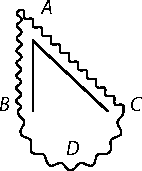
\includegraphics[scale=1]{gesamttex/edit_VIII-4/images/LH_35_10_16_009_d1_009r.pdf}
\edcaption{\edtext{\lbrack\textit{Fig.~1}\rbrack}{%
\lemma{\lbrack\textit{Fig.~1}\rbrack}%
\Cfootnote[nonum]{\indexN{\textls{Stevin} (Stevinus), Simon 1548\textendash1620}%
\textsc{S.~Stevin}, \cite{00196}\textit{De Beghinselen der Weeghconst}, Leiden 1586, S.\;41
(\cite{02084}\textit{SPW} I, S.\;176).}}}
\end{edfigure}
\pstart
\noindent
\edtext{Ex evitatione motus perpetui\indexS{motus perpetuus} sequitur regula\indexS{regula inclinationis planorum} statica inclinationis planorum,\indexS{inclinatio plani}}{%
\lemma{Ex evitatione \lbrack...\rbrack\ planorum}%
\Cfootnote{\cite{00196}a.\,a.\,O., Buch~1, Teil~2, Theor.~XI Prop.~XIX mit Koroll.~I,
S.\;40\textendash42 (\cite{02084}\textit{SPW} I, S.\;174\textendash179).}}
ut ostendit figura adjuncta. 
Nam in ea sunt omnia in aequilibrio,\indexS{aequilibrium}
quia alioqui in quam partem catena\indexS{catena} \textit{BACDB} 
\edtext{super erecto\indexS{planum erectum} \textit{BA} et inclinato\indexS{planum inclinatum}}{%
\lemma{super}%
\Bfootnote{%
\textit{(1)}~erecta \textit{BA} et inclinata
\textit{(2)}~erecto \textit{BA} et inclinato~\textit{L}}}
\textit{AC} posita semel iret, in eam 
\edtext{semper itura}{%
\lemma{semper}%
\Bfootnote{%
\textit{(1)}~iturus
\textit{(2)}~itura~\textit{L}}}
esset, cum semper redeat idem; 
jam \textit{BDC} est in aequilibrio.\indexS{aequilibrium} Ergo et 
\edtext{catenae\indexS{catena}}{\lemma{}\Bfootnote{catenae \textit{erg.~L}}} 
\textit{AB} et \textit{AC} sunt in aequilibrio, quae sunt inter se ut rectae. 
Idem est 
\edtext{\lbrack si\rbrack}{\lemma{}\Bfootnote{si \textit{erg.~Hrsg.}}}
\textit{AB} et \textit{AC} colligantur in unum, velut in sphaeras. 
\pend 
\begin{edfigure}%
\includegraphics[scale=1]{%
gesamttex/edit_VIII-4/images/LH_35_10_16_009_d2_009r.pdf}
\edcaption{\lbrack\textit{Fig.~2}\rbrack}
\end{edfigure}
\pstart 
Eodem modo \textit{EF} et \textit{EG}, catenae sunt in aequilibrio.
Colligatur \textit{EG} in globum \textit{I}. 
Quaeritur ubi is collocari debeat in arcu \textit{EG}, ut 
\edtext{posito \textit{EI} esse}{\lemma{posito}\Bfootnote{%
\textit{(1)}~\textit{EG} esse 
\textit{(2)}~\textit{EI} esse~\textit{L}}} 
catenam pondere carentem,\indexS{catena pondere carens} 
sit pondus \textit{I} in aequilibrio\indexS{aequilibrium}  cum pondere \textit{EF}. 
Id fiet ubi in triangulo elementari\indexS{triangulum elementare} tangens\indexS{tangens} 
\textit{IL} est ad verticalem \textit{IK}, 
\edtext{ut \textit{I},}{\lemma{ut}\Bfootnote{%
\textit{(1)}~\textit{I} ad \textit{EF} \textit{(2)}~\textit{I},~\textit{L}}}
vel \textit{EIG} ad \textit{EF}.
\pend






\chapter[tocentry={Aus und zu Dechales, Cursus (Statik)
\enskip\bracks{Winter 1682/1683 -- erste Hälfte 1685}},
head={Aus und zu Dechales, Cursus (Statik)}]%
{\MakeUppercase{Aus und zu Dechales, Cursus (Statik)}
\newline \bracks{Winter 1682/1683 -- erste Hälfte 1685}}
\label{41182-2}
\selectlanguage{ngerman}%
\frenchspacing%
\begin{ledgroupsized}[r]{120mm}%
\footnotesize%
\pstart%
\noindent\textbf{Überlieferung:}%
\pend%
\end{ledgroupsized}%
\begin{ledgroupsized}[r]{114mm}%
\footnotesize%
\pstart%
\parindent -6mm%
\makebox[6mm][l]{\textit{L}}%
Auszüge mit Bemerkungen aus
\textsc{C.\:F.\:M.\;Dechales},%
\indexN{\textls{Dechales} (Chalesius), Claude François Milliet 1621\textendash1678}
\textit{Cursus seu mundus mathematicus} (3~Bde, Lyon 1674)%
:\cite{00124}
LH~XXXV\;9,\;17 Bl.\;5--6.
Ein Bogen 2\textsuperscript{o}.
Eine Spalte auf Bl.\;6\,r\textsuperscript{o}.
Bl.\;5\,r\textsuperscript{o} bis Bl.\;6\,r\textsuperscript{o} überliefern N.\;\ref{41182-1} im vorliegenden Band (Auszüge mit Bemerkungen zur Pneumatik aus demselben Werk).
Bl.\;6\,v\textsuperscript{o} ist unbeschrieben.
\textemdash\
Weitere Auszüge aus Dechales' \textit{Cursus} überliefern im Leibniz-Nachlass die Manuskripte:
LH~XXXV\;9,\;17 Bl.\;1--4; %
LH~XXXVI Bl.\;54--57, 60--61; %
LH~XXXVII\;5 Bl.\;2--3 %
(sämtliche werden voraussichtlich in künftigen Bänden von \textit{LSB} VIII ediert).
Ein Exemplar von Dechales' \textit{Cursus} mit Gebrauchsspuren von Leibnizens Hand liegt in der GWLB Hannover unter der Signatur Nm-A\,10018:1--3 vor.
\pend%
\end{ledgroupsized}%
\vspace{5mm}%
\begin{ledgroup}%
\footnotesize%
\pstart%
\noindent%
\textbf{Datierungsgründe:}
Das vorliegende undatierte Stück N.\;\ref{41182-2} umfasst Leibnizens ausführliche Exzerpte aus \textsc{C.\:F.\:M.\;Dechales}, \textit{Cursus seu mundus mathematicus} %
tract.\;VII: \textit{Statica}, lib.\;III: \textit{De descensu gravium in planis inclinatis et funependulis} (Bd.\;I, Lyon 1674, S.\;489--524, bes. S.\;491--496).\cite{00124}
Die vorgeschlagene Datierung beruht auf der Annahme, dass die Exzerpte N.\;\ref{41182-2} zum gleichen Zeitpunkt entstanden sind wie die auf demselben Bogen überlieferten Exzerpte aus Dechales'\indexN{\textls{Dechales} (Chalesius), Claude François Milliet 1621\textendash1678} \textit{Cursus}, %
die in diesem Band unter N.\;\ref{41182-1} ediert sind.
Siehe zur Datierung von N.\;\ref{41182-1} die ausführliche Begründung auf S.\;\pageref{41182_dat}.%
\pend%
\end{ledgroup}%
\selectlanguage{latin}%
\frenchspacing%
\vspace{8mm}%
\normalsize%
\pstart%
\noindent%
\bracks{%
\href{\Scan{LH_35_09_17_006r}}%
{6\,r\textsuperscript{o}}%
}
\edtext{%
\textit{Gravia in planis inclinatis%
\indexS{planum inclinatum}%
\indexS{grave in plano inclinato}
eandem altitudinem perpendicularem habentibus%
\indexS{altitudo perpendicularis}
posita,
et ita se habentia %
ut planorum}
\edtext{%
\textit{longitudines},
sunt in aequilibrio,%
\indexS{gravia in aequilibrio}%
}{%
\lemma{\textit{longitudines},}%
\Bfootnote{%
\textit{(1)}~\textit{aequalia habent mom} %
\textit{(2)}~sunt in aequilibrio,%
~\textit{L}%
}}
seu
\edtext{%
si pondus \textit{A} ad pondus \textit{B}%
\indexS{pondus gravium in plano inclinato}
ut recta \textit{AC} ad rectam \textit{CB}.%
}{%
\lemma{pondus \textit{A} \bracks{...} rectam \textit{CB}}%
\Cfootnote{%
Vgl. das Diagramm \bracks{\textit{Fig.\:1}}.%
}}
\textit{Ingeniosissima}
\edtext{%
\textit{demonstratio Stevini},%
\indexN{\textls{Stevin} (Stevinus), Simon 1548\textendash1620}%
\indexS{demonstratio Stevini}%
}{%
\lemma{\textit{demonstratio}}%
\Cfootnote{%
Siehe \textsc{S.\;Stevin}, \textit{De beghinselen der weeghconst},
Buch~I, Teil~II, Theor.\;XI, Prop.\;XIX mit Koroll.\;I
(Leiden 1586, S.\;40\textendash42;\cite{00196}
\textit{SPW}~I, S.\;174\textendash179).\cite{02084}%
}}
alioqui posito
\edtext{%
fune gravi circumplicato \textit{ACBA},%
\indexS{funis circumplicatus gravi}%
}{%
\lemma{fune \bracks{...} \textit{ACBA}}%
\Cfootnote{%
Vgl. das Diagramm \bracks{\textit{Fig.\:2}}.%
}}
vel etiam globulis aequaliter instructo%
\indexS{funis instructus globulis}%
\bracks{,}
necessario \textit{sequetur motus perpetuus}.%
\indexS{motus perpetuus}
Idem demonstratur ex principio generali,%
\indexS{principium generale}
quia \textit{perpendicula} descensum \textit{metientia}
sunt ponderibus \textit{reciproca}.%
\indexS{perpendicula metientia descensum sunt ponderibus reciproca}
Item \textit{supposito corpus non moveri
nisi centrum gravitatis descendat}.%
\indexS{descensus centri gravitatis}%
}{%
\lemma{\textit{Gravia} \bracks{...} \textit{descendat}}%
\Cfootnote{%
Vgl. \textsc{C.\,F.\,M.\;Dechales},
\textit{Cursus seu mundus mathematicus},
tract.\:VII, lib.\;III, prop.\;IV %
(Lyon 1674, Bd.\;I, S.\;491b--492a: Zitat mit Auslassungen).%
\cite{00124}%
}}
\edtext{%
\textit{Hinc momenta gravium aequalium
in planis inclinatis consistentium},%
\indexS{planum inclinatum}%
\indexS{grave in plano inclinato}
sunt \textit{ut sinus recti inclinationum%
\indexS{sinus rectus inclinationis}%
\indexS{inclinatio plani}%
\indexS{momenta gravium in planis inclinatis sunt ut sinus inclinationum}
seu angulorum} \textit{A},\;\textit{B}.%
}{%
\lemma{\textit{Hinc} \bracks{...} \textit{angulorum} \textit{A},\;\textit{B}}%
\Cfootnote{%
Vgl. \textsc{Dechales}, \textit{Cursus}, tract.\:VII, lib.\;III, %
prop.\;VI, coroll.
(S.\;492b: Zitat mit Auslassungen).%
\cite{00124}%
}}
\pend%
\newpage%
\begin{edfigure}[0.00em][1.5em]%
\hfill%
\includegraphics[scale=0.90]{%
gesamttex/edit_VIII-4/images/LH_35_09_17_005-006_d12_006r.pdf}
\hfill%
\includegraphics[scale=0.90]{%
gesamttex/edit_VIII-4/images/LH_35_09_17_005-006_d13_006r.pdf}
\hfill%
\edcaption[0.25em]{%
\hspace*{-5mm}%
\lbrack\textit{Fig.\:1}\rbrack%
\edtext{}{%
\lemma{\lbrack\textit{Fig.\:1}\rbrack}%
\Cfootnote[nonum]{%
Vgl. a.a.O., %
prop.\;IV (S.\;491b: Detail aus dem einzigen Diagramm).%
\cite{00124}%
}%
}%
\hspace*{42mm}%
\lbrack\textit{Fig.\:2}\rbrack%
\edtext{}{%
\lemma{\lbrack\textit{Fig.\:2}\rbrack}%
\Cfootnote[nonum]{%
Vgl. a.a.O. %
(S.\;492a: erstes Diagramm).%
\cite{00124}%
}%
}%
}%
\end{edfigure}
\pstart%
\edtext{%
Sit
\edtext{%
pondus \textit{E}%
}{%
\lemma{pondus\;\textit{E}}%
\Cfootnote{%
Vgl. das Diagramm \bracks{\textit{Fig.\:3}}.%
}}
trahens \textit{D} in linea \textit{FD}%
\indexS{pondus trahens alterum in plano inclinato}%
\indexS{tractio ponderis in plano inclinato}
ipsi \textit{BC} plano inclinato parallela,%
\indexS{planum inclinatum}
et cum eo in aequilibrio,%
\indexS{pondera aequilibrata in plano inclinato}
et pondus \textit{P} trahens non parallela \textit{ID},
et tamen cum pondere \textit{D}
\edtext{%
in aequilibrio.%
\indexS{pondera aequilibrata in plano inclinato}
Ergo et pondera%
}{%
\lemma{in aequilibrio}%
\Bfootnote{%
\textit{(1)}~, debent pondera %
\textit{(2)}~, perinde est ac si pondera %
\textit{(3)}~. Ergo et pondera%
~\textit{L}%
}}
\textit{E} et \textit{P}%
\indexS{pondera aequilibrata in plano inclinato}
eorundem momentorum,%
\indexS{momentum gravis in plano inclinato}
ergo fingendo Hypomochlium \textit{G}%
\indexS{hypomochlium}
erunt reciproce ut distantiae ab eo,
\textit{GD} et
\edtext{%
\bracks{\textit{YG}},%
}{%
\lemma{\textit{YD}}%
\Bfootnote{%
\textit{L\;ändert Hrsg. nach Vorlage}%
}}
seu \textit{P} %
ad \textit{E}
ut \textit{DG} ad \textit{YG}.
\edtext{%
Jam \textit{E} ad \textit{D}
ut \textit{KG} ad \textit{DG}.%
}{%
\lemma{Jam}%
\Bfootnote{%
\textit{(1)}~\textit{D} ad \textit{E} %
\textit{(2)}~\textit{E} ad \textit{D} ut %
\textit{(a)}~\textit{DG} %
\textit{(b)}~\textit{KG} ad \textit{DG}.%
~\textit{L}%
}}
Ergo \textit{P} ad \textit{D}
ut \textit{KG} sinus inclinationis plani,%
\indexS{sinus rectus inclinationis}%
\indexS{inclinatio plani}
ad \textit{YG} sinum compl.%
\indexS{sinus complementi anguli tractionis}
\edtext{%
anguli \textit{IDF}
qui angulus tractionis est.%
\indexS{angulus tractionis}%
}{%
\lemma{anguli}%
\Bfootnote{%
\textit{(1)}~tractionis %
\textit{(2)}~\textit{IDF} qui %
\textit{(a)}~est %
\textit{(b)}~angulus tractionis est.%
~\textit{L}%
}}%
}{%
\lemma{Sit \bracks{...} est}%
\Cfootnote{%
Vgl. a.a.O., prop.\;IX %
(S.\;494a: Zusammenfassung).\cite{00124}%
}}
\pend%
\pstart%
\edtext{%
\edtext{%
\textit{BEADC} funis,%
\indexS{funis tensus}%
}{%
\lemma{\textit{BEADC} funis}%
\Cfootnote{%
Vgl. das Diagramm \bracks{\textit{Fig.\:4}}.%
}}
angulus \textit{A} rectus%
\indexS{angulus rectus}%
\bracks{,}
erunt pondera
\textit{B}, \textit{A}, \textit{C}
homologa seu proportionalia%
\indexS{pondus homologum lateri opposito}
lateribus oppositis
\textit{AD}, \textit{DE}, \textit{EA}.
Nam pondus \textit{A}
trahitur%
\indexS{pondus trahens alterum in plano inclinato}%
\indexS{tractio ponderis in plano inclinato}
\edtext{%
a pondere \textit{B},%
}{%
\lemma{a}%
\Bfootnote{%
\textit{(1)}~chorda %
\textit{(2)}~pondere \textit{B},%
~\textit{L}%
}}
quasi suspensum ex \textit{DA}%
\indexS{pondus suspensum a brachio staterae}
brachio staterae inclinatae,%
\indexS{brachium staterae inclinatae}%
\indexS{statera inclinata}
unde \textit{A} ad \textit{B}
ut \textit{AD} ad \textit{FD}
seu ut \textit{ED} ad \textit{DA}.
Ita et in altero \textit{C}.%
}{%
\lemma{\textit{BEADC} \bracks{...} altero \textit{C}}%
\Cfootnote{%
Vgl. \textsc{Dechales}, \textit{Cursus}, tract.\:VII, lib.\;III, prop.\;X %
(S.\;494b--495a: Zusammenfassung).\cite{00124}%
}}
\pend%
\begin{edfigure}[1.50em][0.00em]%
\hfill%
\includegraphics[scale=0.90]{%
gesamttex/edit_VIII-4/images/LH_35_09_17_005-006_d14_006r.pdf}
\hfill%
\includegraphics[scale=0.90]{%
gesamttex/edit_VIII-4/images/LH_35_09_17_005-006_d15_006r.pdf}%
\hfill%
\edcaption[0.5em]{%
\hspace{-1mm}%
\lbrack\textit{Fig.\:3}\rbrack%
\edtext{}{%
\lemma{\lbrack\textit{Fig.\:3}\rbrack}%
\Cfootnote[nonum]{%
Vgl. \textsc{Dechales}, \textit{Cursus}, tract.\:VII, lib.\;III, %
prop.\;IX (S.\;494a: einziges Diagramm).\cite{00124}%
}}%
\hspace{48mm}%
\lbrack\textit{Fig.\:4}\rbrack%
\edtext{}{%
\lemma{\lbrack\textit{Fig.\:4}\rbrack}%
\Cfootnote[nonum]{%
Vgl. a.a.O., prop.\;X %
(S.\;494b: einziges Diagramm).\cite{00124}%
}}%
}%
\end{edfigure}%
\newpage%
\pstart%
\edtext{%
Si
\edtext{%
angulus \textit{A}%
}{%
\lemma{angulus \textit{A} acutus}%
\Cfootnote{%
Vgl. das Diagramm \bracks{\textit{Fig.\:5}}.%
}}
\edtext{%
acutus,%
\indexS{angulus acutus}
tunc \textls{anguli tractionis}%
\indexS{angulus tractionis}
complementum erit angulus \textit{A},%
\indexS{complementum anguli tractionis}%
}{%
\lemma{acutus,}%
\Bfootnote{%
\textit{(1)}~erit \textit{A} complementum %
\textit{(2)}~tunc \textls{anguli} %
\bracks{...} angulus \textit{A},%
~\textit{L}%
}}
ergo per dicta
erit \textit{A} ad \textit{B}
ut \textit{EI} ad \textit{EG}.
Sed triangula \textit{GAN}, \textit{IEG} sunt similia.%
\indexS{triangula similia}
Nam ob angulos \textit{EGA}, \textit{EIA} rectos,%
\indexS{angulus rectus}
puncta \textit{A}, \textit{I}, \textit{G}, \textit{E}
erunt in semicirculo super \textit{AE}.
\textit{%
Cumque anguli
\edtext{%
\lbrack\textit{GAI}, \textit{GEI}\rbrack%
}{%
\lemma{\textit{GAE}, \textit{GIE}}%
\Bfootnote{%
\textit{L\;ändert Hrsg. nach Vorlage}%
}}
eidem arcui \textit{GI} insistant,%
\indexS{anguli insistentes eidem arcui}%
\indexS{arcus circuli}
erunt aequales,
item anguli \textit{GIE}, \textit{GAE}
insistentes eidem arcui \textit{GE},
et cum lineae \textit{NG}, \textit{AE}
sint parallelae
anguli alterni \textit{NGA}, \textit{GAE}
erunt aequales,%
\indexS{anguli alterni}
ergo ut \textit{EI} ad \textit{GE},
seu ut \textit{A} ad \textit{B},
ita \textit{AG} ad \textit{AN}.
Eodem modo~\textit{A}~ad~\textit{C}
ut \textit{AG} ad \textit{AK}.%
}%
}{%
\lemma{Si angulus \bracks{...} \textit{AG} ad \textit{AK}}%
\Cfootnote{%
Vgl. a.a.O., prop.\;XI %
(S.\;495b: Zitat mit Auslassungen).\cite{00124}%
}}
\edtext{%
Jam triangula \textit{EIG}, \textit{FHE} sunt similia,%
\indexS{triangula similia}
ergo \textit{FHE} %
ipsi \textit{GNA},
ergo $HE : FE : FH\; \squaredots\; AN : AG : NG$
seu $AK \squaredots B.\:A.\:C$.%
}{%
\lemma{Jam triangula \bracks{...} \textit{B.\:A.\:C}}%
\Cfootnote{%
Vgl. \textsc{Dechales}, \textit{Cursus}, tract.\:VII, lib.\;III, prop.\;XI, coroll. %
(S.\;495b).\cite{00124}%
}}
\pend%
\begin{edfigure}[1.25em][1.00em]%
\hfill%
\includegraphics[scale=0.90]{%
gesamttex/edit_VIII-4/images/LH_35_09_17_005-006_d16_006r.pdf}%
\hfill%
\includegraphics[scale=0.90]{%
gesamttex/edit_VIII-4/images/LH_35_09_17_005-006_d17_006r.pdf}%
\hfill%
\edcaption[0.25em]{%
\hspace*{-5mm}%
\lbrack\textit{Fig.\:5}\rbrack%
\edtext{}{%
\lemma{\lbrack\textit{Fig.\:5}\rbrack}%
\Cfootnote[nonum]{%
Vgl. a.a.O., prop.\;XI %
(S.\;495b: einziges Diagramm).\cite{00124}%
}}%
\hspace*{50mm}
\lbrack\textit{Fig.\:6}\rbrack%
\edtext{}{%
\lemma{\lbrack\textit{Fig.\:6}\rbrack}%
\Cfootnote[nonum]{%
Vgl. a.a.O., prop.\;XII %
(S.\;496a: einziges Diagramm).\cite{00124}%
}}%
}
\end{edfigure}%
\pstart%
\edtext{%
Sit
\edtext{%
angulus \textit{A} obtusus.%
\indexS{angulus obtusus}%
}{%
\lemma{angulus \textit{A}}%
\Bfootnote{%
\textit{(1)}~acutus %
\textit{(2)}~obtusus%
~\textit{L}%
}%
\lemma{angulus \textit{A} obtusus}%
\Cfootnote{%
Vgl. das Diagramm \bracks{\textit{Fig.\:6}}.%
}%
}
Caetera ut ante.
$C:A\squaredots FG:FI$.
Jam $\triangledown$\textsuperscript{la} \textit{FIE} simil.\;\textit{FGH}.%
\indexS{triangula similia}
$FG:FI \squaredots FH:FE$.
Ergo haec\:$\squaredots\: C:A$.
Eodem modo $B:A \squaredots HE:FE$.
Ergo $B:A:C$\;$\squaredots$ $HE:FE:HF$.
Ergo et
(ob sim. $\triangledown$ \textit{FIE}, \textit{FGH})
$ \squaredots\; FL : HE : IE$.
Denique et triangula similia sunt \textit{FHE}, \textit{GNA},%
\indexS{triangula similia}
\textit{angulus enim \textit{GNA}
duobus internis \textit{NFG}, \textit{NGF} seu \textit{AEG},
hoc est angulo \textit{FHE},
aequalis est.
Item angulus \textit{NAG}
duobus internis \textit{ALG} seu \textit{AEG}
et \textit{AGL} seu \textit{AEL},
hoc est toti \textit{FEH} aequalis est.
Eodem modo ostendam
triangulum \textit{GAK} eidem}
\edtext{%
\textit{FHE}
aequaleangulum.%
\indexS{triangulum aequaleangulum}%
}{%
\lemma{\textit{FHE}}%
\Bfootnote{%
\textit{(1)}~aequi %
\textit{(2)}~aequaleangulum.~%
~\textit{L}%
}}
Ergo $HE:FE:HF \squaredots NA:AG:NG$ seu \textit{AK}.%
}{%
\lemma{Sit angulus \bracks{...} seu \textit{AK}}%
\Cfootnote{%
Vgl. a.a.O. %
(S.\;496a: Zitat mit Auslassungen).\cite{00124}%
}}
\edtext{%
Ex his converse
\edtext{%
determ\bracks{inab}iles angul\bracks{i}%
}{%
\lemma{determaniles angulos}%
\Bfootnote{%
\textit{L\;ändert Hrsg.}%
}}
datis ponderibus.%
}{%
\lemma{Ex his \bracks{...} ponderibus}%
\Cfootnote{%
Vgl. \textsc{Dechales}, \textit{Cursus}, tract.\:VII, lib.\;III, prop.\;XII, coroll. %
(S.\;496a).\cite{00124}%
}}
\pend%
\begin{edfigure}[0.00em][1.75em]%
\hfill%
\includegraphics[scale=0.95]{%
gesamttex/edit_VIII-4/images/LH_35_09_17_005-006_d18_006r.pdf}
\hfill%
\includegraphics[scale=0.95]{%
gesamttex/edit_VIII-4/images/LH_35_09_17_005-006_d19_006r.pdf}
\hfill%
\edcaption[0.25em]{%
\lbrack\textit{Fig.\:7}\rbrack%
\hspace*{35mm}%
\lbrack\textit{Fig.\:8}\rbrack%
\edtext{}{%
\lemma{\bracks{\textit{Fig.\:7}}}%
\Cfootnote[nonum]{%
Vgl. a.a.O., prop.\;XIII %
(S.\;496b: erstes Diagramm).\cite{00124}%
}}%
\edtext{}{%
\lemma{\bracks{\textit{Fig.\:8}}}%
\Cfootnote[nonum]{%
Vgl. a.a.O. %
(S.\;496b: zweites Diagramm).\cite{00124}%
}}%
}
\end{edfigure}%
\pstart%
\edtext{%
\textit{Si
\edtext{%
grave
\edtext{\textit{AB}%
}{%
\lemma{\textit{AB}}%
\Bfootnote{%
\textit{erg.\;L}%
}}%
}{%
\lemma{\textit{grave AB}}%
\Cfootnote{%
Vgl. das Diagramm \bracks{\textit{Fig.\:7}}.%
}}
e duobus}
\edtext{%
\textit{funibus}%
\indexS{grave pendens e duobus funibus}%
\indexS{funis tensus}
\bracks{\textit{FE}}%
\textit{, \textit{DC}
non}%
}{%
\lemma{\textit{funibus}}%
\Bfootnote{%
\bars{%
\bars{\textit{FB} \textit{ändert Hrsg. nach Vorlage}}%
\textit{, DC}
\textit{erg.}} \textit{non}%
~\textit{L}%
}}
\textit{parallelis pendeat},
et \textit{ex} eorum \textit{concursu}\;\textit{G}%
\indexS{concursus funium}
\textit{linea perpendiculi}%
\indexS{linea perpendiculi}%
\indexS{perpendiculum}
\edtext{%
\textit{GH} \textit{ducatur},%
}{%
\lemma{\textit{GH}}%
\Bfootnote{%
\textit{(1)}~demittatur %
\textit{(2)}~\textit{ducatur}%
~\textit{L}%
}}
ea \textit{transibit per centrum gravitatis}%
\indexS{centrum gravitatis gravis pendentis}
ipsius gravis \textit{AB}.
Nam grave eodem modo sustentatur ex puncto \textit{C},%
\indexS{grave sustentatum}
quo ex \textit{G},
et ex puncto
\edtext{%
\lbrack\textit{E}\rbrack%
}{%
\lemma{\textit{e}}%
\Bfootnote{%
\textit{L\;ändert Hrsg.}%
}}
quo ex eodem\;\textit{G}.
Jam si ex \textit{G} suspensum esset,%
\indexS{grave suspensum}
linea perpendiculi%
\indexS{linea perpendiculi}%
\indexS{perpendiculum}
transiret per centrum gravitatis.%
\indexS{centrum gravitatis gravis suspensi}%
}{%
\lemma{\textit{Si grave} \bracks{...} gravitatis}%
\Cfootnote{%
Vgl. a.a.O. %
(S.\;496b: Zitat mit Auslassungen).\cite{00124}%
}}
\pend%
\pstart%
(+\;Hoc etiam sic demonstres:
Eodem modo sustentatur ex
\edtext{%
\lbrack\textit{CE}\rbrack,%
}{%
\lemma{\textit{ce}}%
\Bfootnote{%
\textit{L\;ändert Hrsg.}%
}}
quomodo ex \textit{LM},
posito \textit{LM} ipsi \textit{CE} parallela,
et omnibus similibus
et similiter
\edtext{%
positis,
et si \textit{GM} vel \textit{GL} ponatur
infinite parva,%
}{%
\lemma{positis,}%
\Bfootnote{%
\textit{(1)}~jam si \textit{LM}, ponatur in %
\textit{(2)}~et si %
\bracks{...} infinite parva,%
~\textit{L}%
}}
nihilo minus eodem modo sustinebitur%
\indexS{grave sustentum}%
\bracks{;}
ut eo
\edtext{%
casu
(quo scilicet revera
suspenditur \textit{AB}
ex ipso \textit{G})
transit%
}{%
\lemma{casu}%
\Bfootnote{%
\textit{(1)}~transit %
\textit{(2)}~(quo scilicet %
\bars{revera \textit{erg.}} suspenditur \textit{AB} ex ipso \textit{G}) transit%
~\textit{L}%
}}
linea directionis%
\indexS{linea directionis}
per centrum gravitatis,%
\indexS{centrum gravitatis gravis suspensi}
ergo et alias.%
\;\bracks{+)}
\pend%
\selectlanguage{latin}%
\frenchspacing%
\normalsize%
 







\chapter[tocentry={Kritisches zu G.\,F.\,Vanni, Specimen libri de momentis gravium
\enskip \bracks{27. September \textendash\ November 1684}},
head={Kritisches zu Vanni, Specimen}]%
{\MakeUppercase{Kritisches zu G.\,F.\,Vanni, Specimen libri de momentis gravium}
\newline \bracks{27. September \textendash\ November 1684}}%
\label{intro_vanni-specimen}
\begin{ledgroup}
\footnotesize
\pstart
\noindent
Die nachfolgenden Stücke N.\;\ref{41667} und N.\;\ref{55606}
dokumentieren Leibnizens erste Auseinandersetzung 
mit den Thesen des Jesuiten
\indexN{\textls{Vanni}, Giovanni Francesco 1638\textendash1709}Giovanni Francesco Vannis
über ein Grundprinzip der Statik,
die eine über die Grenzen Italiens hinaus heftig ausgetragene Kontroverse entfachten
(siehe dazu die Monographie \cite{02126}\textsc{M.~Torrini}, \textit{Dopo Galileo}, Florenz 1979)
und mit denen sich Leibniz über die folgende Jahrzehnte mehrmals befassen sollte (siehe neben N.\;\ref{intro_vanni-specimen} die Stücke N.\;\ref{intro_vanni-demonstratio}, \ref{41199}, \ref{intro_vanni-solutio-problematis}, und \ref{intro_vanni-investigatio} und \ref{intro_theoremata-duo-vanni}).
\pend
\pstart
\indexN{\textls{Vanni}, Giovanni Francesco 1638\textendash1709}Vanni veröffentlichte um 1684 in Rom die anonyme Flugschrift \cite{01995}\textit{Specimen libri de momentis gravium} als Auszug und Vorankündigung seines späteren Buchs \cite{02000}\textit{Exegeses physico-mathematicae} (Rom 1685).
Im \textit{Specimen} griff Vanni den bekannten, von Stevin, Galilei und Torricelli prominent verfochtenen 
Satz der Zerlegung von Kräften auf schiefen Ebenen an. 
Seine kontroverse These und der polemische Ton zogen die Aufmerksamkeit der italienischen und europäischen Gelehrtenwelt schlagartig auf sich.
\pend
\pstart
Dank der Vermittlung 
seines Förderers
\indexN{\textls{Magliabechi} (Magliabecchi, Magliabecki, Magliabekius, Magliabequius), Antonio 1633\textendash1714}A.~Magliabechi
und \indexN{\textls{Papebroch} (Papenbrockius), Daniel 1628\textendash1714}Daniel Papebrochs
gelang es Vanni, das \cite{01995}\textit{Specimen} in den \cite{01023}\textit{Acta Eruditorum} von November 1684 veröffentlichen zu lassen.
Der Mitherausgeber der \cite{01023}\textit{Acta},
\indexN{\textls{Pfautz} (Pfauzius), Christoph 1645\textendash1711}C.~Pfautz,
schickte allerdings zunächst den Text an Leibniz (\cite{02006}Brief vom 17./27. September 1684, \textit{LSB} III,~4 N.\;70), von dem er sich eine inhaltliche Einordnung und ggf. eine kritische Stellungnahme, die den Aufsatz begleiten sollte, erbat.
Leibniz verfasste eine solche im Konzept N.\;\ref{41667}; dessen Entstehung ist sicher zwischen dem 27. September 1684 und, wie aus folgenden Umständen ersichtlich wird, dem 17. Oktober 1684 zu verorten.
Denn an diesem Tag schickte Leibniz dem anderen Mitherausgeber der \textit{Acta}, \indexN{\textls{Mencke} (Menken, Menkenius, Menque), Otto 1644\textendash1707}Otto Mencke,
eine gekürzte Fassung von N.\;\ref{41667}, in der er seine Kritik an \indexN{\textls{Vanni}, Giovanni Francesco 1638\textendash1709}Vanni viel zurückhaltender als im Konzept äußerte: \glqq breviter et mollissimis verbis\grqq\ (\cite{02007}\textit{LSB} I,~4 N.\;398).
Diese Fassung der Bemerkung (von der keine handschriftlichen Textzeugen erhalten sind) 
erschien anonym in den \textit{Acta Eruditorum} von November 1684 (S.\;514)
im Anschluss an das \cite{01995}\textit{Specimen}.%
\pend
\pstart
\indexN{\textls{Vanni}, Giovanni Francesco 1638\textendash1709}Vannis Reaktion auf die Kritik ist uns durch seine Briefe an \indexN{\textls{Magliabechi} (Magliabecchi, Magliabecki, Magliabekius, Magliabequius), Antonio 1633\textendash1714}Magliabechi bekannt und wurde in dieser Form um 1685 auch an Leibniz herangetragen (siehe N.\;\ref{32310}). Sie veranlasste eine zweite Phase seiner Auseinandersetzung mit Vannis Thesen, der im Komplex um die \textit{Demonstratio geometrica} von 1685 ihren Niederschlag fand (N.\;\ref{intro_vanni-demonstratio}).
Des Weiteren verfasste Leibniz zwischen Ende Oktober 1686 und Mitte Februar 1687 auf Wunsch der Herausgeber der \textit{Acta Eruditorum} eine Rezension von Vannis angekündigtem Buch \textit{Exegeses}, nachdem es um 1685 erschienen war (N.\;\ref{41199}).
\pend
\end{ledgroup}





\section[tocentry={Animadversio in Specimen libri de momentis gravium
\enskip \bracks{27. September \textendash\ 17. Oktober 1684}%
},
head={Animadversio in Specimen}]%
{\MakeUppercase{Animadversio in Specimen libri de momentis gravium}
\newline \bracks{27. September \textendash\ 17. Oktober 1684}
}%
\label{41667}
\begin{ledgroupsized}[r]{120mm}
\footnotesize
\pstart
\noindent\textbf{Überlieferung:}
\pend
\end{ledgroupsized}
\begin{ledgroupsized}[r]{114mm}
\footnotesize
\pstart
\parindent -6mm 
\makebox[6mm][l]{\textit{L}}%
Konzept:
LH~XXXV~5,~28~Bl.~8\textendash9.
Ein Bogen~8\textsuperscript{o}.
Ränder beschnitten.
Drei Seiten.
Bl.~9~v\textsuperscript{o} leer.
\pend
\end{ledgroupsized}%
\selectlanguage{latin}
\vspace{8mm}
\pstart%
\noindent%
\href{\Scan{LH_35_05_28_008r}}%
{\lbrack8~r\textsuperscript{o}\rbrack} 
\edtext{Objectio viri\indexN{\textls{Vanni}, Giovanni Francesco 1638\textendash1709}
ut apparet peringeniosi contra receptissimum Staticorum\indexS{Statici} 
Theorema\indexS{Theorema Staticorum receptissimum} 
de momento gravis super plano inclinato\indexS{momentum gravis super plano inclinato},}{%
\lemma{Objectio \lbrack...\rbrack\ inclinato}%
\Cfootnote{\textsc{G.\,F. Vanni},\indexN{\textls{Vanni}, Giovanni Francesco 1638\textendash1709} \cite{01995}\textit{Specimen libri de momentis gravium etc. Autore I.\,F.\,V. Lucensi}, \cite{01023}\textit{AE} November 1684, S.\;511\textendash513. 
Vanni kritisiert
\indexN{\textls{Galilei} (Galilaeus, Galileus), Galileo 1564\textendash1642}%
\textsc{G.~Galilei}, %
\cite{00050}\textit{Discorsi}, %
Giornata Terza, De motu naturaliter accelerato; \glqq Aggiunta postuma dell'Autore\grqq\ %
nach dem Scholion zum 2.~Theorem (der Zusatz erschien erst in der posthumen Werkausgabe: \cite{01084}\textit{Opere}, Bologna 1656, Bd.~II, S.\;132\lbrack ter\rbrack\textendash134; \cite{00048}\textit{GO} VIII, S.\;216\textendash219 im Apparat) %
und
\indexN{\textls{Torricelli} (Torricellius), Evangelista 1608\textendash1647}%
\textsc{E.~Torricelli}, \textit{De motu gravium}, lib.~I
(\cite{00304}\textit{Opera geometrica}, Florenz 1644, S.\;99;
\cite{00108}\textit{TO}~II, S.\;105).}}
solvi omnino potest;
meretur tamen non contemni, quia ita speciosa est
ut negotium aliis quoque facessere possit. 
\pend
\begin{edfigure}%
\includegraphics[scale=1]{%
gesamttex/edit_VIII-4/images/LH_35_05_28_008-009_d1.pdf}
\edcaption{%
\edtext{\lbrack\textit{Fig.~1, erg. Hrsg. nach Vanni\indexN{\textls{Vanni}, Giovanni Francesco 1638\textendash1709}}\rbrack}{%
\lemma{\lbrack\textit{Fig.~1}\rbrack}%
\Cfootnote[nonum]{%
\cite{01995}a.\,a.\,O., S.\;512.}}}
\end{edfigure}
\pstart
Retenta
ejus figura, argumenti vis breviter huc redit: Gravis \textit{I}
momentum super plano inclinato\indexS{momentum gravis super plano inclinato} \textit{XC} est ad momentum
gravis absolutum seu perpendiculare\indexS{momentum gravis absolutum seu perpendiculare} ut \textit{XN} ad
\textit{XC}, per theorema receptum.\indexS{theorema Staticorum receptum} Et eodem modo,
ejusdem gravis momentum super plano inclinato\indexS{momentum gravis super plano inclinato} \textit{ZC}
erit ad idem momentum absolutum\indexS{momentum gravis absolutum} ut \textit{ZO} ad \textit{ZC}
seu ad \textit{XC}, quia \textit{ZC} et \textit{XC} ponuntur aequales.
Ergo summa horum duorum momentorum in planis
inclinatis\indexS{planum inclinatum} sustentantibus est ad momentum
absolutum\indexS{momentum absolutum} ut $XN+ZO$ ad \textit{XC}. Hactenus
recte. Jam vero summa haec aequatur momento
absoluto ut ait autor\indexN{\textls{Vanni}, Giovanni Francesco 1638\textendash1709}. Ergo $XN+ZO$ aequatur
ipsi \textit{XC} quod est absurdum. Verum
sciendum est causam falsae conclusionis non latere
in theoremate recepto,\indexS{theorema Staticorum receptum} sed in assumto \indexN{\textls{Vanni}, Giovanni Francesco 1638\textendash1709}viri docti,
quod nempe duo momenta in planis inclinatis\indexS{planum inclinatum sustentans}
sustentantibus simul sumta aequentur momento
absoluto.\indexS{momentum absolutum} Id quod illi
\edtext{nulla demonstratio,}{\lemma{}\Bfootnote{nulla \bars{nulla \textit{gestr.}} demonstratio,~\textit{L}}} 
sed probabilis consideratio persuaserat; et fraudi fuisse
videtur, quod illa vocavit partialia,\indexS{momentum partiale} hoc totale.\indexS{momentum totale}
Cum tamen componantur inter se partialia illa
non conjunctive\indexS{compositio momentorum conjunctiva seu cumulativa} 
seu cumulative ut ita dicam\lbrack,\rbrack\
sed disjunctive,\indexS{compositio momentorum disjunctiva} quia si conatus in uno plano
\href{\Scan{LH_35_05_28_008v}}%
{\lbrack8~v\textsuperscript{o}\rbrack} descendendi\indexS{conatus descendendi in plano} 
exitum sortietur, cessabit conatus
in altero. Praeterea (ne dicam nullum facile
repertum iri qui simili argumentatione sit
usus) certe multa falsa hoc modo possent
concludi. Imo quaecunque assignetur regula
pro planis inclinatis\indexS{planum inclinatum} ex ea tali modo argumentandi
absurdum deducam. Et poterit
grave millies millenis planis simul
\edtext{inniti. Imo}{\lemma{inniti}\Bfootnote{%
\textit{(1)}~, imo %
\textit{(2)}~. Imo~\textit{L}}}
infinitis, si sit in superficie concava
alicujus coni excavati apicem deorsum
vertentis; ubi infinitis suis punctis globus
superficiem conicam tangit,
\edtext{et plano conum}{\lemma{et}\Bfootnote{%
\textit{(1)}~cono planum %
\textit{(2)}~plano conum~\textit{L}}}
ibidem tangenti quolibet suo puncto inniti
putandus est.
\pend 
\begin{edfigure}[1em][1em]    	%
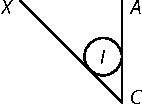
\includegraphics[scale=1]{
gesamttex/edit_VIII-4/images/LH_35_05_28_008-009_d2_008v.pdf}
\edcaption{\lbrack\textit{Fig.~2}\rbrack}
\end{edfigure}
\pstart
Et quid si grave inter
duo plana sit comprehensum\indexS{grave duobus planis innitens}
iisque innitatur, quorum
unum \textit{XC} sit
\edtext{inclinatum ad horizontem,\indexS{planum inclinatum}}{\lemma{inclinatum}\Bfootnote{%
\textit{(1)}~horizonti, %
\textit{(2)}~ad horizontem,~\textit{L}}} 
\textit{AC} alterum verticale?\indexS{planum verticale}
Utique si momenta respectiva
in duobus planis exercita
in unum addita\indexS{additio momentorum} aequantur
momento perpendiculari seu absoluto,\indexS{momentum perpendiculare seu absolutum} aequabuntur
ambo simul ipsorum uni nempe momento
in plano \textit{AC}, pars toti. Sed non est cur
his insistamus. Nam Theorema receptum
omnino apud Staticos\indexS{Statici}\indexS{Theorema apud Staticos receptum} habetur demonstratum,
\href{\Scan{LH_35_05_28_009r}}%
{\lbrack9~r\textsuperscript{o}\rbrack} nec meum est aliorum demonstrationes
repetere, quibus non puto resisti posse,
nisi quis principia statica,\indexS{principia statica} de centro
gravitatis et reciproca\indexS{principium de reciproca distantia aequiponderantium}
ab eo aequiponderantium\indexS{aequiponderantia}
distantia\lbrack,\rbrack\ evertere velit,
cui satisfacere hujus loci non est. Idem
fere dicendum arbitror de \edlabel{35_05_28_8-9_1a}%
\edtext{}{%
\xxref{35_05_28_8-9_1a}{35_05_28_8-9_1b}%
\lemma{docti cujusdam \lbrack...\rbrack\ oscillantium ascensu}%
\Cfootnote{Mit dem Ausdruck \glqq Mathematici Parisini\grqq\ ist 
der Abbé \indexN{\textls{Catelan}, François, Abbé de gest. nach 1719}Catelan gemeint. 
Dessen Kritik an \indexN{\textls{Huygens} (Hugenius, Ugenius, Hugens, Huguens), Christiaan 1629\textendash1695}Huygens' Satz über den Schwingungsmittelpunkt eines zusammengesetzten Pendels 
(\indexN{\textls{Huygens} (Hugenius, Ugenius, Hugens, Huguens), Christiaan 1629\textendash1695}\textsc{C.~Huygens}, \cite{00123}\textit{Horologium Oscillatorium}, 
pars IV, prop. IV, Paris 1673, S.\;98; \cite{00113}\textit{HO} XVIII, S.\;255) 
entfachte einen Streit, an dem sich neben 
\indexN{\textls{Catelan}, François, Abbé de gest. nach 1719}Catelan und 
\indexN{\textls{Huygens} (Hugenius, Ugenius, Hugens, Huguens), Christiaan 1629\textendash1695}Huygens auch 
\indexN{\textls{Bernoulli}, Jacob 1655\textendash1705}Jacob Bernoulli beteiligte. 
Die Beiträge erschienen zwischen Dezember 1681 und September 1684 im \cite{00157}\textit{Journal des Sçavans} und den \cite{02002}\textit{Nouvelles de la République des Lettres}.
Die \cite{01023}\textit{Acta Eruditorum} von September 1684 (S.\;416\textendash419) brachten einen anonymen (von \indexN{\textls{Lehmann}, Georg Heinrich fl. 1675\textendash1690}Georg Heinrich Lehmann verfassten) Bericht über die Geschehnisse bis Juli 1684: \textit{Relatio de controversia, quae hactenus inter Dn.\,Hugenium et Dn.\,Catelanum agitatur de centro Oscillationis, collecta ex Ephemeridibus Gallicis}\cite{02004}. Dort wird \indexN{\textls{Catelan}, François, Abbé de gest. nach 1719}Catelan u.\,a. als \glqq Mathematicus Parisiensis\grqq\ bezeichnet.}}%
docti cujusdam Mathematici Parisini\indexN{\textls{Catelan}, François, Abbé de gest. nach 1719} 
objectione in
his ipsis \cite{01023}\textit{Actis} mense Septembri hujus anni editis p.~416 relata,
\edtext{contra celeberrimi}{\lemma{contra}\Bfootnote{%
\textit{(1)}~propositionem ab %
\textit{(2)}~celeberrimi~\textit{L}}} 
Hugenii\indexN{\textls{Huygens} (Hugenius, Ugenius, Hugens, Huguens), Christiaan 1629\textendash1695}
positionem de centri gravitatis corporum
oscillantium\indexS{centrum gravitatis corporum oscillantium} 
ascensu.\indexS{ascensus centri gravitatis corporum oscillantium} 
\edlabel{35_05_28_8-9_1b} Itaque hortandi
sunt viri eruditi, ut in promovendis
potius scientiis industriam suam
ostendant, nec quae a Geometris\indexS{Geometra} praeclaris
accurate constituta sunt sine diligenti
examine labefactare aggrediantur.
Quamquam interim objectiones
\edtext{quoque, quarum solutio}{\lemma{quoque,}\Bfootnote{%
\textit{(1)}~quae lucem aliam %
\textit{(2)}~quarum so %
\textit{(3)}~quarum solutio~\textit{L}}} lucem
aliquam afferre potest, si absit
contentionis studium, laudem suam
mereantur.
\pend

\section[tocentry={Brevis annotatio circa Specimen libri de momentis gravium
\enskip November 1684%
},
head={Brevis annotatio circa Specimen}]%
{\MakeUppercase{Brevis annotatio circa Specimen libri de momentis gravium}
\newline November 1684%
}
\label{55606}
\begin{ledgroupsized}[r]{120mm}
\footnotesize
\pstart
\noindent\textbf{Überlieferung:}
\pend
\end{ledgroupsized}
\begin{ledgroupsized}[r]{114mm}
\footnotesize
\pstart
\parindent -6mm 
\makebox[6mm][l]{\textit{E\textsuperscript{1}}}%
Erstdruck:
\cite{01023}\textit{AE} November 1684, S.\;514. Nachdr. \textsc{Lamarra/Palaia} 2005, S.\;994.\cite{01289} (Unsere Druckvorlage.)%
\pend
\end{ledgroupsized}%
\begin{ledgroupsized}[r]{114mm}
\footnotesize
\pstart
\parindent -6mm
\parindent -6mm\makebox[6mm][l]{\textit{E\textsuperscript{2}}}%
Abdruck (nach \textit{E\textsuperscript{1}}):
\cite{01421}\textit{Opuscula omnia Actis eruditorum Lipsiensibus inserta, quae ad universam mathesin, physicam, medicinam, anatomiam, chirurgiam et philologiam pertinent}, Bd. I, Venedig 1740, S.\;281; Abbildungen am Ende des Bandes.
\pend
\end{ledgroupsized}%
\begin{ledgroupsized}[r]{114mm}
\footnotesize
\pstart
\parindent -6mm\makebox[6mm][l]{\textit{E\textsuperscript{3}}}%
Abdruck (nach \textit{E\textsuperscript{1}}):
\cite{02005}\textsc{Jacob Bernoulli}, \textit{Opera},
hrsg. von G.~\textsc{Cramer}, Genf 1744,
Bd.~I, S.\;247;
Abbildungen (Tab.~VIII, Fig.~2\textendash3) zwischen S.\;290 und S.\;291.
\pend%
\end{ledgroupsized}
\selectlanguage{latin}
\vspace{8mm}
\pstart%
\noindent%
\lbrack S.\;514\rbrack\  %
\edtext{Objectio Viri,\indexN{\textls{Vanni}, Giovanni Francesco 1638\textendash1709}
ut apparet, peringeniosi, contra receptum, et mea sententia demonstratum 
Staticorum\indexS{Statici} Theorema,\indexS{Theorema Staticorum receptum et demonstratum}}{\lemma{Objectio \lbrack...\rbrack\ Theorema}%
\Cfootnote{\textsc{G.\,F. Vanni},\indexN{\textls{Vanni}, Giovanni Francesco 1638\textendash1709} 
\cite{01995}\textit{Specimen libri de momentis gravium etc. Autore I.\,F.\,V. Lucensi}, \cite{01023}\textit{AE} November 1684, S.\;511\textendash513.}} 
non contemnenda est
quidem, solvi tamen omnino potest negando momenta in planis\indexS{momentum in plano} \textit{XC} et \textit{ZC}
in unum posse addi,\indexS{additio momentorum} ut componant momentum
gravis absolutum;\indexS{momentum gravis absolutum} 
et fraudi Viro docto\indexN{\textls{Vanni}, Giovanni Francesco 1638\textendash1709} 
fuisse videtur, quod illa vocavit partialia\indexS{momentum partiale}, hoc totale.\indexS{momentum totale}
Quid enim si grave\indexS{grave a duobus planis sustentatum} sustentetur a duobus planis
\textit{XC} inclinato,\indexS{planum inclinatum} et \textit{AC} verticali?\indexS{planum verticale} Utique momenta
in ambobus planis\indexS{momentum in plano} in unum addita\indexS{additio momentorum} non possunt
aequari uni ex ipsismet, totum parti; quod tamen
secundum objicientis\indexN{\textls{Vanni}, Giovanni Francesco 1638\textendash1709} sententiam fieri deberet: momentum enim in plano
verticali\indexS{momentum in plano verticali} 
utique est ipsum momentum gravis absolutum.\indexS{momentum gravis absolutum}
\pend
\begin{edfigure}[1.5em]%
\hfill
\includegraphics[scale=1]{%
gesamttex/edit_VIII-4/images/AE_1684_514_d1.pdf}
\hspace*{15mm}
\raisebox{0.6em}{%
\includegraphics[scale=1]{%
gesamttex/edit_VIII-4/images/AE_1684_514_d2.pdf}}
\hfill
\edcaption{%
\pagelabel{Fig:AE_1684_514_fig-1-2}%
\edtext{\lbrack\textit{Fig.~1, erg. Hrsg. nach Vanni\indexN{\textls{Vanni}, Giovanni Francesco 1638\textendash1709}}\rbrack}{%
\lemma{\lbrack\textit{Fig.~1}\rbrack}%
\Cfootnote[nonum]{%
\cite{01995}\textsc{Vanni},\indexN{\textls{Vanni}, Giovanni Francesco 1638\textendash1709} a.\,a.\,O., S.\;512.}}%
\hspace*{20mm}%
\lbrack\textit{Fig.~2}\rbrack\hspace*{10mm}}
\end{edfigure}






\chapter[tocentry={Aufzeichnungen zum Schwerpunkt
\enskip \bracks{1679 \textendash\ Januar 1687\,(?)}},
head={Aufzeichnungen zum Schwerpunkt}]%
{\MakeUppercase{Aufzeichnungen zum Schwerpunkt}
\newline \bracks{1679 \textendash\ Januar 1687\,(?)}}

\label{Cc2-1421}	%
\label{5konzepte133}	%

\begin{ledgroupsized}[r]{120mm}
\footnotesize
\pstart
\noindent\textbf{Überlieferung:}
\pend
\end{ledgroupsized}
\begin{ledgroupsized}[r]{114mm}
\footnotesize
\pstart
\parindent -6mm
\makebox[6mm][l]{\textit{L}}%
Aufzeichnungen:
LH~XXXV~8, 30~Bl.~133. 
Ein Blatt (ca.~20~x~16~cm.);
{Wasserzeichenfragment} am Rand (französisches Papier);
alle Ränder beschnitten; 
Eineinhalb Seiten auf Bl.~133~r\textsuperscript{o} bis Bl.~133~v\textsuperscript{o};
Bl. 133~r\textsuperscript{o} horizontal in fünf Felder aufgeteilt,
Bl. 133~v\textsuperscript{o} in drei Bereichen, die Aufzeichnungen auf Bl. 133~r\textsuperscript{o} in gleicher Höhe weiterführen, zur Hälfte beschrieben.
Textfolge für die erste, zweite und vierte Aufzeichnung: Bl. 133~r\textsuperscript{o}, Bl. 133~v\textsuperscript{o}; beim vierten Text ist der Seitenübergang durch den Kustos "arbitrarium" und den Hinweis "(verte)" gesichert (\refpassage{35_08_30_133_3a}{35_08_30_133_3b}).
\pend
\pstart
\noindent
Cc 2, Nr. 1421
\pend
\end{ledgroupsized}
\vspace{5mm}
\begin{ledgroup}
\footnotesize
\pstart
\noindent
\textbf{Datierungsgründe:}
Mit N.\;\ref{5konzepte133} liegt
eine Gruppe fünf auf dem gemeinsamen Träger LH~XXXV, 8, 30 Bl.~133
sequentiell verfasster Aufzeichnungen 
(\refpassage{35_08_30_133-teil1a}{35_08_30_133-teil1b}, \refpassage{35_08_30_133-teil2a}{35_08_30_133-teil2b}, \refpassage{35_08_30_133-teil3a}{35_08_30_133-teil3b}, \refpassage{35_08_30_133-teil4a}{35_08_30_133-teil4b} und \refpassage{35_08_30_133-teil5a}{35_08_30_133-teil5b})
vor,
die Leibniz ursprünglich wohl zu Streifen zerschneiden wollte.
Deshalb hat er bei drei der fünf Texte, deren Länge eine Fortsetzung auf der Rückseite erforderte, den Schlussteil auf Bl.~133~v\textsuperscript{o} in gleicher Höhe wie den Anfang geschrieben. (Eine ähnliche Textverteilung durch sequentielle Abfassung liegt bei dem Träger LH~XXXV, 8, 30 Bl.~121, der Notizen aus der Pariser Zeit überliefert; zwei von diesen, N.\;\ref{Cc2_847-1} und N.\;\ref{Cc2_847-2}, werden als Nachträge im vorliegenden Band ediert.)
Wegen der konsekutiven Beschreibung des Blattes ist anzunehmen, dass Leibniz die Aufzeichnungen, oder zumindest ihre Anfänge auf Bl.~133~r\textsuperscript{o}, sequentiell verfasst hat.
Gemäß des Charakters des Blattes als einer Sammlung thematisch verwandter Aufzeichnungen beleuchten alle fünf Texte den Begriff Schwerpunkt: Der erste und dritte behandeln die Bestimmung des Schwerpunkts von Rotationsfiguren; der zweite und vierte die Bestimmung des gemeinsamen Schwerpunkt von Punkten in eigentümlichen Konfigurationen bzw. Bewegungen; der fünfte die einem Körper eigene Bewegung in Zusammenhang mit der des gemeinsamen Schwerpunkts des Systems.
\pend
\pstart
Zur Datierung von N.\;\ref{Cc2-1421} lässt sich zunächst feststellen, dass das Blatt ein Fragment eines 
im Leibniz-Korpus für Februar bis Juli 1676 häufig belegten französischen Wasserzeichens enthält: 
u.\,a. in den
\cite{02169}Auszügen aus 
\indexN{\textls{Mariotte}, Edme, Seigneur de Chazeuil ca. 1620\textendash1684}Mariottes  \textit{Logique}-Handschrift (\textit{LSB} VI, 3 N.\;22, Mai bis Juli 1676)
und den Exzerpten \cite{02170}\textit{Anatomica quaedam ex manuscripto \indexN{\textls{Descartes} (Cartesius, des Cartes), René 1596\textendash1650}Cartesii} mit der editorischen Datierung Februar bis September 1676 (\textit{LSB} VII, 2 N.\;58).
Dasselbe Zeichen kommt auch in den Aufzeichnungen N.\;\ref{Cc2_1381} aus der späten Pariser Zeit (Februar bis 25. April 1676) vor, die als Nachtrag in diesem Band erscheinen.
Dennoch liefert das Wasserzeichen im Träger (im Licht noch zu erörternder inhaltlicher Umstände) keinen belastbaren Datierungsgrund: Leibniz hat die Aufzeichnungen nach dem Ende seiner Pariser Jahre verfasst.
Die Verwendung französischen Papiers erklärt sich in diesem Fall dadurch, dass Leibniz für N.\;\ref{Cc2-1421} wohl den freigebliebenen Teil eines alten Bogens bzw. Blattes verwendet hat und diesen dann abgeschnitten. Dass der Text von N.\;\ref{Cc2-1421} quer zur üblichen Beschreibrichtung des Bogens verläuft, bekräftigt die Annahme einer Zweitnutzung des französischen Papiers. (Weitere ursprünglich mit dem Träger zusammenhängende Papiere konnten bislang nicht identifiziert werden.)
\pend
\pstart
Belastbare Datierungsgründe lassen sich indessen aus inhaltlichen Betrachtungen gewinnen. Insbesondere die Aufzeichnung auf \refpassage{35_08_30_133-teil2a}{35_08_30_133-teil2b}, die Leibniz offenbar als zweite verfasst hat, lässt sich mit dem Konzept N.\;\ref{60309} produktiv vergleichen, das auf Grund des Wasserzeichens auf den Zeitraum September 1685 bis Januar 1687 datierbar ist.
Das Konzept stellt eine ausführliche Weiterentwicklung einiger Gedanken und Beweise aus der zweiten Aufzeichnung: Viele Diagramme werden wieder aufgegriffen, einige Passagen fast wörtlich wiederholt (bspw. \refnote{FnC:35_08_30_133-Lamy} hier und \refpassage{37_05_064-065_4a}{37_05_064-065_4b} in N.\;\ref{60309}).
Insbesondere die Passage \refpassage{35_08_30_133-teil2a}{35_08_30_133_4} aus der zweiten Aufzeichnung von N.\;\ref{Cc2-1421} wird in einer Randanmerkung zu \refnote{FnA:37_05_064-065_elementa-lineae} des Konzepts wortgleich übernommen.
Wegen dieses festgestellten Abhängigkeitsverhältnisses sind die Aufzeichnungen N.\;\ref{Cc2-1421} sicher vor dem Konzept entstanden; daher bietet der Endpunkt der vermutlichen Entstehungsspanne von N.\;\ref{60309}, Januar 1687, einen Terminus ante quem für N.\;\ref{Cc2-1421}.
\pend
\pstart
Eine Anspielung in derselben Aufzeichnung bietet wiederum einen sicheren Terminus post quem für ihre Entstehung, damit für die der gesamten Gruppe: Denn Leibniz hat den zweiten Text sehr wohl kurz nach dem ersten verfasst, wie der Schreibduktus nahelegt.
Auf \refnote{FnC:35_08_30_133-Lamy} erwähnt Leibniz eine These
\indexN{\textls{Lamy} (L'Amy, Lami), Bernard (Bernhard) 1640\textendash1715}Bernard Lamys zu Schwerpunkt und Rektifikation einer Kurve.
Die Anspielung konnte nicht mit Sicherheit aufgelöst werden: Sie gilt eventuell einer Erwähnung der Problematik in
\textsc{B.\;Lamy}, \cite{01476}\textit{Traitez de mecanique}, Paris 1679: erstes Traktat ("De l'equilibre des solides"), S.\;17--152, bes. S.\;71\,f., wobei die Stelle allerdings sehr vage und beiläufig ist.
Dennoch steht fest, dass die \textit{Traitez} von 1679 das früheste mehrerer Werke Lamys auf dem naturwissenschaftlichen Gebiet sind: Daher bietet die Anspielung einen Grund, die Entstehung der Aufzeichnungen nicht vor 1679 zu verorten.
\pend
\pstart
Eine letzte Anspielung von Interesse befindet sich in einer Randanmerkung zu \refnote{FnC:35_08_30_133-ceva} in der zweiten Aufzeichnung.
Leibniz bemerkt die Ähnlichkeit seines Ansatzes zu dem \indexN{\textls{Ceva}, Giovanni 1647\,(?)\textendash1734}Giovanni Cevas; es handelt sich um die "Appendix Geometrica" zum "De Aquis", in  \cite{02154}\textit{Opuscula mathematica}, Mailand 1682, prop.\;II, S.\;52\,f. sowie Tab.\;8, fig.\;5. (Ceva bestimmt dort allerdings den Schwerpunkts einer Halbkugeloberfläche, nicht wie Leibniz eines Halbkreises.)
Es steht fest, dass Leibniz um 1685 die "Opuscula mathematica" \cite{02153}rezensierte (\cite{01023}\textit{AE} November 1685 S. 493--496; die Rezension erscheint vsl. in einem späteren Band der Reihe), wobei er in der Besprechung den einschlägigen Anhang "Appendix geometrica" nicht erwähnte.
Dennoch wird diese Anspielung als nicht Datierungsrelevant angesehen, da es sich um einen womöglich später nachgetragenen Randzusatz handelt.
\pend
\end{ledgroup}
\selectlanguage{latin}		%
\vspace{8mm}
\pstart
\noindent
\bracks{\textit{Nachfolgender Text bis \refpassage{35_08_30_133-teil1b}{35_08_30_133-teil1b} erste Aufzeichnung:}}
\pend
\nobreak
\vspace{.5em}
\pstart
\noindent
\edlabel{35_08_30_133-teil1a}%
\href{\Scan{LH_35_08_30_133r}}%
{\lbrack133~r\textsuperscript{o}\rbrack} 
Considerandum pro ampliatione \textls{centri gravitatis},\indexS{centrum gravitatis} quid fiat si axis\indexS{axis non rectus} non sit rectus,
sed ubique eodem modo obliquus,\indexS{axis ubique eodem modo obliquus}\indexS{axis ad radium librationis obliquus} ad radium librationis\bracks{,}\indexS{radium librationis}
deinde quid si ubique variet obliquitatem.\indexS{axis variabiliter obliquus}
\pend
\begin{edfigure}%
\includegraphics[scale=1]{%
gesamttex/edit_VIII-4/images/LH_35_08_30_133_d1_133r.pdf}
\edcaption{\lbrack\textit{Fig.~1}\rbrack}
\end{edfigure}
\pstart
Ponamus axem\indexS{axis} esse cylindroidem Ellipticum\indexS{cylindroides Ellipticus} cujus sectiones sint 
\edtext{circuli circa axem\bracks{,} ita}{%
\lemma{circuli}%
\Bfootnote{%
\textit{(1)}~.~Sed
\textit{(2)}~ita ipse etsi 
\textit{(3)}~circa axem
\textit{(a)}~quod moveri possit, ipse tamen axis non potest aliter
circumagi quam circa rectam
\textit{(b)}~ita~\textit{L}}}
et res circa axem moveri possunt, et ipse axis\indexS{axis} crassus circa rectam transeuntem per centra circulorum.
Frustraque videtur hic addi axis cylindri.\indexS{axis cylindri} %
\pend
\pstart
Quid de axe curvilineo\indexS{axis curvilineus variabiliter inclinatus} ubi quovis momento
variatur inclinatio\indexS{inclinatio} ut 
\pend
\begin{edfigure}%
\includegraphics[scale=1]{%
gesamttex/edit_VIII-4/images/LH_35_08_30_133_d2_133r.pdf}
\edcaption{\lbrack\textit{Fig.~2}\rbrack}
\end{edfigure}
\pstart
Verum cum inter circumagendum statim
\edtext{asseres a se}{%
\lemma{asseres}%
\Bfootnote{%
\textit{(1)}~quasi in
\textit{(2)}~a se~\textit{L}}}
invicem divellantur inutiles sunt axes curvilinei.\indexS{axis curvilineus}
\pend
\pstart
Possumus potius concipere motum communem\indexS{motus communis} 
rectilineae perpendicularis insistentiae,
\edtext{et figuram}{%
\lemma{et}%
\Bfootnote{%
\textit{(1)}~corpus mo
\textit{(2)}~figuram~\textit{L}}}
motam superficialem\indexS{figura superficialis} vel solidam\indexS{figura solida} inter movendum
\edtext{aliquid secum}{%
\lemma{aliquid}%
\Bfootnote{%
\textit{(1)}~secum acquirere
\textit{(2)}~secum~\textit{L}}}
abripere quod prius quieverat, vel derelinquere locu et inter evolvendum intelligi potest.
\pend
\pstart
\href{\Scan{LH_35_08_30_133v}}%
{\lbrack133~v\textsuperscript{o}\rbrack}
Mirum est in omni corpore esse centrum aequilibrii\indexS{centrum aequilibrii in omni corpore existens} non centr. figurae.\indexS{centrum figurae non in omni corpore existens}
Sic omnes rectae bisecantes triangulum isosceles non transeunt per idem punctum.
Operae pretium erit inquirere in \textls{locum horum punctorum}, qui erit vicarius centri figurae.\indexS{centrum figurae}%
\edlabel{35_08_30_133-teil1b}
\pend
\vspace{.5em}
\pstart
\noindent
\lbrack\textit{Nachfolgender Text bis \refpassage{35_08_30_133-teil2b}{35_08_30_133-teil2b} zweite Aufzeichnung:}\rbrack
\pend
\nobreak
\vspace{.5em}
\pstart
\noindent
\edlabel{35_08_30_133-teil2a}%
\href{\Scan{LH_35_08_30_133r}}%
{\lbrack133~r\textsuperscript{o}\rbrack} 
Si Elementa\indexS{elementum loci centrorum gravitatis} lineae quae est locus centrorum gravitatis\indexS{locus centrorum gravitatis}\indexS{centrum gravitatis} 
sint proportionalia ipsis quorum sunt illa centra,
centrum gravitatis loci,\indexS{centrum gravitatis loci centrorum gravitatis} 
erit centrum gravitatis totale\indexS{centrum gravitatis totale} eorum quorum centra gravitatis in illum locum cadunt.%
\edlabel{35_08_30_133_4}
\pend
\begin{edfigure}%
\includegraphics[scale=1]{%
gesamttex/edit_VIII-4/images/LH_35_08_30_133_d3_133r.pdf}
\edcaption{%
\edtext{\bracks{\textit{Fig.~3}}%
}{%
\lemma{\bracks{\textit{Fig.~3}}}%
\Cfootnote[nonum]{%
Der Punkt \textit{E} hieß bei Leibniz $\beta$; diese Bezeichnung ändert Hrsg. gemäß den Angaben im Text.}}}%
\end{edfigure}
\pstart
\edtext{%
Ita locus omnium \textit{e} centrorum gravitatis\indexS{locus omnium centrorum gravitatis} triangulorum (seu sectorum infinite parvorum)
\edtext{in quae}{%
\lemma{in}%
\Bfootnote{%
\textit{(1)}~qui
\textit{(2)}~quae~\textit{L}}}
circulus vel datus sector circuli\indexS{centrum gravitatis sectoris circuli} resolvitur, est arcus circuli centro \textit{C} 
\edtext{radi\bracks{o}}{\lemma{}\Bfootnote{radio \textit{L ändert Hrsg.}}}
\textit{CE} descripti, et puncta sunt etiam centra gravitatis\indexS{centrum gravitatis} ipsorum $L\lambda$ elementorum loci centrorum.\indexS{elementum loci centrorum gravitatis}}{%
\applabel{FnC:35_08_30_133-ceva}%
\lemma{}%
\Afootnote{%
\textit{Neben dem Text und \bracks{\textit{Fig.~3}}}:
\indexN{\textls{Ceva}, Giovanni 1647\,(?)\textendash1734}Joh.~Ceva Mediol. 
sic procedit in circulo\textsuperscript{\bracks{a}}
\\[1.5ex] %
{\footnotesize 
\textsuperscript{\bracks{a}}Joh.~Ceva \bracks{...} circulo: 
Siehe \textsc{G.\;Ceva}, \cite{02154}\textit{Opuscula mathematica}, Mailand 1682: "De Aquis", "Appendix Geometrica", prop.\;II, S.\;52\,f. sowie Tab.\;8, fig.\;5. Ceva bestimmt a.\,a.\,O. allerdings den Schwerpunkts einer Halbkugeloberfläche, nicht eines Halbkreises.}}}
Et cum ratio \textit{CL} ad \textit{EB} sit 2 
\edtext{ad 3 ex}{%
\lemma{ad 3}%
\Bfootnote{%
\textit{(1)}~ob trian
\textit{(2)}~ex~\textit{L}}}
natura trianguli, hinc generaliter dici potest centrum gravitatis semicirculi\indexS{centrum gravitatis semicirculi}
vel sectoris\indexS{centrum gravitatis sectoris circuli} cujuscunque
idem esse cum centro gravitatis semicircumferentiae\indexS{centrum gravitatis semicircumferentiae} 
alterius sectoris similis et similiter positi seu concentrici
per radium subsesquialtera ratione minorem descripti.
\pend
\begin{edfigure}%
\includegraphics[scale=1]{%
gesamttex/edit_VIII-4/images/LH_35_08_30_133_d4_133r.pdf}
\edcaption{\lbrack\textit{Fig.~4}\rbrack}
\end{edfigure}
\pstart
At in Evolutione\indexS{evolutio} res ista non procedit, neque linea \textit{e}(\textit{e}) est parallela
lineae $\beta(\beta)$.
Parallela fit linea si eadem quantitas a filo semper resecetur, non si proportionalis.
Interim patet lineam centrorum gravitatis\indexS{centrum gravitatis}\indexS{linea centrorum gravitatis elementorum}
\edtext{elementorum}{\lemma{}\Bfootnote{elementorum \textit{erg.~L}}}
figurae $AC\beta A$ haberi, si semper sumatur in \textit{CB} ipsa \textit{Ce} ad \textit{CB}
ut 2 
\edlabel{35_08_30_133_1a}%
\edtext{}{%
\xxref{35_08_30_133_1a}{35_08_30_133_1b}%
\lemma{ad 3.}%
\Bfootnote{%
\textit{(1)}~Caeterum in Hemisph
\bracks{/}
\textit{(2)}~Summa
\textit{(a)}~omnium
\textit{(b)}~\textit{AC}~\textit{L}}}%
ad 3.
\pend
\begin{edfigure}%
\includegraphics[scale=1]{%
gesamttex/edit_VIII-4/images/LH_35_08_30_133_d5_133r.pdf}
\edcaption{\lbrack\textit{Fig.~5}\rbrack}
\end{edfigure}
\pstart
Summa \textit{AC}\edlabel{35_08_30_133_1b}
in $\ind{1}N\ind{2}N = NC$ in \textit{\ind{2}V\ind{1}C}.
Ergo et summae 
\edtext{aequantur ex}{\lemma{}\Bfootnote{aequantur \bars{ergo \textit{streicht Hrsg.}} ex \textit{erg.~L}}}
datis 
\edtext{summis radiorum,}{%
\lemma{summis}%
\Bfootnote{%
\textit{(1)}~\textit{AC} ad
\textit{(2)}~radiorum,~\textit{L}}}
ad axem, \textit{d} ad momentum ipsorum \textit{\ind{2}V\ind{1}C} 
\edlabel{35_08_30_133_2a}%
\edtext{}{%
\xxref{35_08_30_133_2a}{35_08_30_133_2b}%
\lemma{ex axe.}%
\Bfootnote{%
\href{\Scan{LH_35_08_30_133v}}%
{\lbrack133~v\textsuperscript{o}\rbrack} 
\textit{(1)}~Caeterum in Hemisphaerio (ut in circulo) centrum gravitatis itidem
\textit{(2)}~Similiter~\textit{L}}}%
ex axe.\indexS{axis}
\pend
\pstart
\href{\Scan{LH_35_08_30_133v}}%
{\lbrack133~v\textsuperscript{o}\rbrack} 
Similiter\edlabel{35_08_30_133_2b}
in sphaera\indexS{sphaera} vel sectore solido\indexS{sector sphaerae}\indexS{sector solidus} (ut in circulo\indexS{circulus} vel sectore plano\indexS{sector circulis}\indexS{sector planus})
centrum gravitatis\indexS{centrum gravitatis} coincidit cum centro gravitatis superficiei hemisphaerii\indexS{centrum gravitatis superficiei hemisphaerii} vel sectoris
similis et similiter positi seu concentrici, in subtertia ratione minoris, resolvendo sectorem in pyramides.\indexS{resolutio sectoris sphaerae in pyramides}
\pend
\begin{edfigure}%
\includegraphics[scale=1]{%
gesamttex/edit_VIII-4/images/LH_35_08_30_133_d6_133v.pdf}
\edcaption{\lbrack\textit{Fig.~6}\rbrack}
\end{edfigure}
\pstart
Pro curva Evoluta si ab \textit{e} ad (\textit{e}) ducantur semper 
\edtext{rectae quae}{%
\lemma{rectae}%
\Bfootnote{%
\textit{(1)}~.~Si ja
\textit{(2)}~quae~\textit{L}}}
sunt elementa loci centrorum gravitatis,\indexS{elementum loci centrorum gravitatis}\indexS{locus centrorum gravitatis} quod si jam curva
\edtext{\textit{MM}}{\lemma{}\Bfootnote{\textit{MM} \textit{erg.~L}}}
ita secetur ut ipsae \textit{e}(\textit{e}) fiant triangulis \textit{ML}(\textit{L}) proportionales\bracks{,}
idem esset centrum gravitatis curvae,\indexS{centrum gravitatis} quod 
\edtext{figurae. Verum}{%
\lemma{figurae.}%
\Bfootnote{%
\textit{(1)}~Verum
\textit{(2)}~Et ad hanc
\textit{(3)}~Verum~\textit{L}}}
revera 
\edtext{si bene ratiocinat \indexN{\textls{Lamy} (L'Amy, Lami), Bernard (Bernhard) 1640\textendash1715}Lamy,}{%
\applabel{FnC:35_08_30_133-Lamy}%
\lemma{si bene ratiocinat Lamy}%
\Cfootnote{Die Anspielung konnte nicht mit Sicherheit aufgelöst werden. Leibniz bezieht sich womöglich auf 
\textsc{B.\;Lamy}, \cite{01476}\textit{Traitez de mecanique}, Paris 1679: erstes Traktat, S.\;17--152, bes. S.\;71\,f.}}
sufficit hanc sectionem esse possibilem.
\pend
\begin{edfigure}%
\includegraphics[scale=1]{%
gesamttex/edit_VIII-4/images/LH_35_08_30_133_d7_133v.pdf}
\edcaption{\lbrack\textit{Fig.~7}\rbrack}
\end{edfigure}
\pstart
Et videtur generaliter res applicari posse ad quamlibet lineam centrorum gravitatis,\indexS{linea centrorum gravitatis quaelibet}
etiam trapeziorum\bracks{,} possumus enim semper fingere sectionem ita
\edtext{institui ut trapezia seu}{\lemma{}\Bfootnote{institui \bars{posse \textit{gestr.}} ut trapezia \bars{\textit{BC} \textit{gestr.}} seu~\textit{L}}}
rectangula \textit{B}(\textit{C}) sint ipsis \textit{e}(\textit{e}) proportionalia. 
Et coincidet centrum rectanguli cum centro\indexS{centrum cujusque elementi curvae} cujusque 
\edtext{elementi curvae.}{%
\lemma{elementi}%
\Bfootnote{%
\textit{(1)}~sed
\textit{(2)}~curvae.~\textit{L}}}
Sed jam video difficultatem\bracks{:} non incidet centrum \textit{e} rectanguli in 
medium tangentium seu rectarum per \textit{e} ductarum. Examinandum an hoc 
mutet ratiocinationem.%
\edlabel{35_08_30_133-teil2b}%
\pend
\vspace{.5em}
\pstart
\noindent
\lbrack\textit{Nachfolgender Text bis \refpassage{35_08_30_133-teil3b}{35_08_30_133-teil3b} dritte Aufzeichnung:}\rbrack
\pend
\vspace{.5em}
\nobreak
\pstart
\noindent
\edlabel{35_08_30_133-teil3a}%
\href{\Scan{LH_35_08_30_133r}}%
{\lbrack133~r\textsuperscript{o}\rbrack}
\pend
\nobreak
\begin{edfigure}[0.5em][1em]
\includegraphics[scale=1]{%
gesamttex/edit_VIII-4/images/LH_35_08_30_133_d8_133r.pdf}
\edcaption{\lbrack\textit{Fig.~8}\rbrack}
\end{edfigure}
\pstart
\noindent
\edtext{Cum movetur}{%
\lemma{Cum}%
\Bfootnote{%
\textit{(1)}~circa
\textit{(2)}~movetur~\textit{L}}}
recta per duos circulos parallelos sic ut superficiem \textls{cylindri obliqui}\indexS{cylinder obliquus} describat,
si jam recta ista intelligatur chorda alicujus arcus circuli et planum segmenti semper tendat in axem cylindri\bracks{,}\indexS{axis cylindri}
quaeritur quae superficies describatur hoc motu, quaeve lineae a quovis arcus puncto ut \textit{C}.
\pend
\pstart
Transferenda consideratio centri gravitatis\indexS{centrum gravitatis} 
a parallelis planis verticalibus corpus in aequalia momenta\indexS{plana secantia corpus in aequalia momenta} secantibus
ad convergentia in centro.\indexS{convergentia in centro gravitatis}
Si corpus sit quodcunque et in eo punctum pro arbitrio assumatur, fingatur fixum,
corpus ita se convertet sponte sua ipso manente fixo, ut quantum potest descendat\indexS{descensus quam maximum}
seu cuidam horizontali suppositae appropinquet, seu ut distantiae punctorum corporis
(potius particularum corporis, seu centrorum globulorum, vel aliorum in quae corpus resolvitur\indexS{resolutio corporis in particulas seu globulos})
ab horizonte (vel si convergunt omnia a centro gravium\indexS{centrum gravium})
sint omnium possibilium minimae.\indexS{distantiae a centro gravium omnium possibilium minimae}
Hinc si corpus \astrosun\ consideretur ut cylindricum horizontaliter jacens
\lbrack\textit{Text bricht ab.}\rbrack
\edlabel{35_08_30_133-teil3b}
\pend
\vspace{.5em}
\pstart
\noindent
\lbrack\textit{Nachfolgender Text bis \refpassage{35_08_30_133-teil4b}{35_08_30_133-teil4b} vierte Aufzeichnung:}\rbrack
\pend
\nobreak
\vspace{.5em}
\pstart
\noindent
\edlabel{35_08_30_133-teil4a}%
\href{\Scan{LH_35_08_30_133r}}%
{\lbrack133~r\textsuperscript{o}\rbrack} 
Via centri gravitatis\indexS{centrum gravitatis}\indexS{via centri gravitatis} servit ad loca Geometriae communis.\indexS{Geometria communis}
Ut si corpus unum 
\edtext{\textit{A}}{\lemma{}\Bfootnote{\textit{A} \textit{erg.~L}}}
moveatur in linea recta alterum vero \textit{B} quiescat centrum gravitatis commune\indexS{centrum gravitatis commune} 
continue movetur\indexS{motus continuus centri gravitatis communis} 
in recta priori parallela, et quia punctum \textit{C}
rectam \textit{AB} jungentem \textit{A} et \textit{B} 
in eadem semper ratione secet quae scil. est corporum,\indexS{ratio corporum}
hinc locus planum\bracks{,} si sit recta positione data \textit{A}(\textit{A}) 
et extra eam punctum \textit{B}, et \textit{AB} semper in data ratione 
\edtext{secetur\bracks{,} erit}{%
\lemma{secetur}%
\Bfootnote{%
\textit{(1)}~\textit{CC} erit
\textit{(2)}~\bars{\textit{C} \textit{streicht Hrsg.}}
\textit{(3)}~erit~\textit{L}}}
\textit{C}(\textit{C}) recta ipsi \textit{A}(\textit{A}) parallela.
\pend
\pstart
Generalius si corpora quotcunque moveantur in rectis,\indexS{corpora quotcunque mota in rectis}
aut sin aliqua ex ipsis quiescant,
via centri communis\indexS{centrum gravitatis commune} omnium\indexS{via centri communis omnium corporum motorum} erit recta\lbrack,\rbrack\
fingo enim omnia esse gravia et descendere libere\indexS{corpora gravia libere descendentia} adeoque in recta, 
utique et centrum gravitatis\indexS{centrum gravitatis} in recta descendet, nec refert etsi rectae non sint parallelae,
saltem enim descensus\indexS{descensus in plano inclinato} erit in plano inclinato.
Item etsi motus sint inaequabiles perinde est enim ac si unum in aere\indexS{corpus in aere descendens} descendat
alterum 
\edtext{in aqua;\indexS{corpus in aqua descendens}}{%
\lemma{in}%
\Bfootnote{%
\textit{(1)}~terra
\textit{(2)}~aqua;~\textit{L}}}
et unum modo in aere modo in aqua vel alio medio.\indexS{corpus in diversis mediis descendens}
Idem est si in plano horizontali vel diversis moveantur.
Si sint igitur
duae rectae positione datae, et in qualibet punctum datum, et aliud
\edlabel{35_08_30_133_3a}
\href{\Scan{LH_35_08_30_133v}}%
{\lbrack133~v\textsuperscript{o}\rbrack} 
\edtext{arbitr\bracks{ari}um,\edlabel{35_08_30_133_3b}}{\lemma{}\Bfootnote{arbitrariarium \textit{L ändert Hrsg.}}}
sic ut intervallum puncti dati et arbitrarii in una recta 
ad intervallum puncti dati et arbitrarii in alia recta sit in ratione data,
denique recta jungens duo puncta arbitraria respondentia secetur etiam in ratione data\bracks{,}
locus omnium punctorum secantium jungentes 
pro quibuslibet punctis 
\edtext{arbitrarii\bracks{s}}{%
\lemma{}%
\Bfootnote{%
arbitrarii, 
\textit{L ändert Hrsg.}}}
respondentibus erit recta.
Quid si plura puncta moveantur in superficie sphaerica\indexS{superficies sphaerica}\indexS{puncta mota in superficie sphaerica} per vias brevissimas
seu circulos magnos,\indexS{circuli magni superficies sphaericae}
an et ita eorum centrum gr.\indexS{centrum gravitatis}\bracks{?}
\pend
\pstart
Mobilia intelligi possunt puncta diversae gravitatis.\indexS{puncta diversae gravitatis}
Si plura puncta moveantur in lineis circularibus\bracks{,}\indexS{puncta mota in lineis circularibus} 
quaerenda via centri.\indexS{via centri gravitatis}
Et ita in aliis lineis dabuntur theoremata.
\pend
\pstart
Quaeratur linea centri\indexS{linea centri gravitatis} duorum mobilium quorum unum in circulo alterum in 
\edtext{recta. An}{%
\lemma{recta.}%
\Bfootnote{%
\textit{(1)}~Non videtur
\textit{(2)}~An~\textit{L}}}
generaliter summa ex ductibus\indexS{ductus mobilis in viam sui centri gravitatis} duorum mobilium in sui centri gravitatis\indexS{via centri gravitatis} vias
aequatur facto\indexS{factum ex summa mobilium in viam centri gravitatis communis} ex summa mobilium in viam centri communis.\indexS{via centri gravitatis communis}
An vero id solum verum de descensu,\indexS{descensus} vel si alias directio eadem manet.%
\edlabel{35_08_30_133-teil4b}%
\pend
\vspace{.5em}
\pstart
\noindent
\lbrack\textit{Nachfolgender Text bis \refpassage{35_08_30_133-teil5b}{35_08_30_133-teil5b} fünfte Aufzeichnung:}\rbrack
\pend
\nobreak
\vspace{.5em}
\pstart
\noindent
\edtext{\edlabel{35_08_30_133-teil5a}%
\href{\Scan{LH_35_08_30_133r}}%
{\lbrack133~r\textsuperscript{o}\rbrack} 
Sint}{%
\lemma{\href{\Scan{LH_35_08_30_133r}}%
{\lbrack133~r\textsuperscript{o}\rbrack}}%
\Bfootnote{%
\textit{(1)}~Sint
\textit{(2)}~Sit
\textit{(3)}~Sint~\textit{L}}}
duae rectae \textit{AF} et \textit{BH} positione et magnitudine datae
quae secentur in eadem ratione in punctis \textit{G} 
\edtext{et \textit{E}. Jungatur}{%
\lemma{et \textit{E}.}%
\Bfootnote{%
\textit{(1)}~Junge \textit{GE}
\textit{(2)}~Jungatur~\textit{L}}}
\textit{GE} eique parallelae ducantur \textit{AL} et \textit{FH} sic ut anguli \textit{ABL} 
\edtext{\bracks{\textit{FHC}}}{%
\lemma{}%
\Bfootnote{%
\textit{FCH}
\textit{L ändert Hrsg.}}}
sint recti.
\pend
\begin{edfigure}%
\includegraphics[scale=1]{%
gesamttex/edit_VIII-4/images/LH_35_08_30_133_d9_133r.pdf}
\edcaption{\lbrack\textit{Fig.~9}\rbrack}
\end{edfigure}
\pstart
Debent $BE \cdot FH + CE \cdot AL$ esse $= BC \cdot GE$.
Et si \textit{BC}, \textit{CE} aequales erit dupla
$GE = AL + AF$.
Usus in motibus,\indexS{motus}
possumus enim corpora\indexS{motus corporis communis et navi} considerare ut mota in navi\indexS{navis mota motu centri gravitatis} quae moveatur motu centri gravitatis\indexS{motus centri gravitatis}
et ipsis attribuere motum proprium\indexS{motus corporis proprium} ad eam rem necessarium.%
\edlabel{35_08_30_133-teil5b}%
\pend





\chapter[tocentry={Singulares quaedam ratiocinationes circa centrum gravitatis
\enskip \bracks{September 1685\,(?) \textendash\ Januar 1687\,(?)}
},
head={Singulares quaedam ratiocinationes circa centrum gravitatis}]%
{\MakeUppercase{Singulares quaedam ratiocinationes circa centrum gravitatis}
\newline \bracks{September 1685\,(?) \textendash\ Januar 1687\,(?)}
}

\label{60309}
\begin{ledgroupsized}[r]{120mm}
\footnotesize
\pstart
\noindent\textbf{Überlieferung:}
\pend
\end{ledgroupsized}
\begin{ledgroupsized}[r]{114mm}
\footnotesize
\pstart
\parindent -6mm
\makebox[6mm][l]{\textit{L}}%
Konzept:
LH~XXXVII~5 Bl.~64\textendash65. 
Ein Bogen~2\textsuperscript{o};
\href{\Scan{LH_37_05_065wz}}%
{Wasserzeichen} in Bl.~65,
\href{\Scan{LH_37_05_064wz}}%
{Gegenmarke} in Bl.~64;
Papiererhaltungsmaßnahmen;
Ränder ausgefranst; 
geringfügiger Textverlust durch Papierschaden im oberen Bereich von Bl.~64~r\textsuperscript{o} und 65~r\textsuperscript{o}.
Dreieinhalb Seiten.
\pend
\end{ledgroupsized}
\vspace{5mm}
\begin{ledgroup}
\footnotesize
\pstart
\noindent
\textbf{Datierungsgründe:}
Das Wasserzeichen im Träger von N.\;\ref{60309} ist für den angegebenen Zeitraum belegt:
erstens in einem mit Sicherheit im September 1685 verfassten Konzept für den Aufsatz \glqq Demonstratio Geometrica regulae apud Staticos receptae\grqq\ (N.\;\ref{32313} in diesem Band);
zweitens in einem Entwurf von Januar 1687 zu Leibnizens erster Streitschrift gegen
\indexN{\textls{Catelan}, François, Abbé de gest. nach 1719}Catelan
(\cite{02086}"Replique de M.\;L. à M.\;l'abbé D.\;C.", \textit{NRL}, Februar 1687, S.\;131\textendash145).
Mangels weiterer Anhaltspunkte wird für die Entstehung von N.\;\ref{60309} diese Zeitspanne vorgeschlagen.
\pend
\pstart
Das vorliegende Konzept stellt eine ausführliche Weiterentwicklung einiger Gedanken und Beweise aus den ab 1679 entstandenen Texten zum Schwerpunkt N.\;\ref{Cc2-1421}, insbesondere der zweiten Aufzeichnung (\refpassage{35_08_30_133-teil2a}{35_08_30_133-teil2b}).
Viele Diagramme und Inhalte des genannten Stücks werden in N.\;\ref{60309} wieder aufgegriffen und es sind viele wörtliche Anklänge feststellbar, wie bspw. zwischen \refpassage{37_05_064-065_4a}{37_05_064-065_4b} von N.\;\ref{60309} und \refnote{FnC:35_08_30_133-Lamy} von N.\;\ref{Cc2-1421}.
Insbesondere die Passage \refpassage{35_08_30_133-teil2a}{35_08_30_133_4} aus der zweiten Aufzeichnung wird hier in einer Randanmerkung zu \refnote{FnA:37_05_064-065_elementa-lineae} wortgleich übernommen.
(Das Abhängigkeitsverhältnis des vorliegenden Konzept von den Aufzeichnungen N.\;\ref{Cc2-1421} wird mit als Grund für deren wahrscheinlichen Datierung bis 1687, also vor dem Endpunkt der vermutlichen Entstehungsspanne von N.\;\ref{60309}, angeführt.)
\pend 
\end{ledgroup}
\selectlanguage{latin}
\vspace{8mm}
\pstart
\centering
\edtext{%
\href{\Scan{LH_37_05_064r}}%
{\lbrack64~r\textsuperscript{o}\rbrack}%
}{\lemma{}\Afootnote{\textit{Am oberen Blattrand}: Quae prima pagina habentur certa sunt et usitata, sequentia \mbox{\textlangle\textendash\ \textendash\ \textendash\ \textendash\textrangle}}}
\hfill
Singulares quaedam ratiocinationes circa 
\edlabel{37_05_064-065_1a}%
\edtext{}{\xxref{37_05_064-065_1a}{37_05_064-065_1b}\lemma{}\Bfootnote{%
centrum \bars{gravitates \textit{ändert Hrsg.}}
\lbrack/\rbrack\
\textit{(1)}~Saepe mihi %
\textit{(2)}~Non~\textit{L}}}%
centrum gravitat\lbrack i\rbrack s
\hfill
\phantom{\lbrack64~r\textsuperscript{o}\rbrack}
\pend
\vspace{0.5\baselineskip}
\nobreak
\pstart
\noindent
\edtext{%
Non\edlabel{37_05_064-065_1b}
paucae jam olim exoticae ratiocinationes\indexS{ratiocinationes exoticae circa centrum gravitatis} circa centrum gravitatis\indexS{centrum gravitatis} mihi incidere,%
}{%
\lemma{Non \bracks{...} incidere}%
\Cfootnote{%
Womöglich sind hiermit die Aufzeichnungen N.\;\ref{Cc2-1421} gemeint.}}
his nuper accessere quae sequuntur: 
\pend
\begin{edfigure}%
\includegraphics[scale=1]{%
gesamttex/edit_VIII-4/images/LH_37_05_064-065_d1_064r.pdf}
\edcaption{\lbrack\textit{Fig.~1}\rbrack}
\end{edfigure}
\pstart 
Sit semicirculus \textit{ABD} cujus centrum \textit{C}, patet eum resolvi\indexS{resolutio semicirculi in innumera triangula} posse in innumera triangula ut $CB\beta$. Trianguli autem cujusque centrum gravitatis\indexS{centrum gravitatis trianguli} \textit{e}, una tertia altitudinis abesse a basi $B\beta$. Ergo locum omnium centrorum gravitatis\indexS{locum centrorum gravitatis triangulorum} talium triangulorum 
\edtext{fore semicircumferentiam}{\lemma{fore}\Bfootnote{%
\textit{(1)}~circumferentiam %
\textit{(2)}~semicircumferentiam~\textit{L}}}
centro \textit{C} radio \textit{Ce} vel \textit{CF}, qui est duabus tertiis radii \textit{CA} aequalis, descriptam. Centrum autem gravitatis\indexS{centrum gravitatis} omnium horum punctorum \textit{e} ex quibus pendere pondera suis triangulis 
\edtext{adeoque hoc loco}{\lemma{adeoque}\Bfootnote{%
\textit{(1)}~inter se aeq %
\textit{(2)}~hoc loco~\textit{L}}} 
in circulo inter se aequalia, intelligantur, erit centrum gravitatis totius semicirculi.\indexS{centrum gravitatis semicirculi} 
Videamus an centrum gravitatis\indexS{centrum gravitatis} omnium punctorum \textit{e}, coincidat cum centro gravitatis ipsius loci\indexS{centrum gravitatis loci punctorum seu curvae} omnium horum punctorum seu curvae. Et quidem cum puncta ista \textit{e}, sint etiam centra gravitatis\indexS{centrum gravitatis rectae} rectarum $L\lambda$, elementorum circumferentiae \textit{FeD} hinc si semper 
\edtext{contingat rectas}{\lemma{contingat}\Bfootnote{%
\textit{(1)}~$L\lambda$ esse triangulis %
\textit{(2)}~rectas~\textit{L}}}
$L\lambda$ esse triangulis $CB\beta$ proportionales, seu 
\edtext{triangulis $CB\beta$ et $C(B)(\beta)$}{\lemma{triangulis}\Bfootnote{%
\textit{(1)}~existentibus aequalibus, e %
\textit{(2)}~$CB\beta$ et $C(B)(\beta)$~\textit{L}}}
existentibus aequalibus, etiam rectas $L\lambda$ et 
\edtext{$(L)\lbrack(\lambda)\rbrack$}{\lemma{}\Bfootnote{$(L)\lambda$ \textit{L ändert Hrsg.}}}
esse aequales, quod quidem in circulo verissimum est, necesse est centrum gravitatis\indexS{centrum gravitatis semicircumferentiae} 
\edtext{omnium $L\lambda$ seu semicircumferentiae}{\lemma{omnium $L\lambda$}\Bfootnote{%
\textit{(1)}~idem esse cu %
\textit{(2)}~seu %
\textit{(a)}~semicirculi %
\textit{(b)}~semicircumferentiae~\textit{L}}}
\textit{FeD} idem esse cum centro gravitatis semicirculi\indexS{centrum gravitatis semicirculi} \textit{ABD}. 
\edtext{%
Centrum enim 
\edtext{gravitatis \bracks{\textit{e}} cujuslibet $L\lambda$ est}{\lemma{gravitatis}\Bfootnote{\bars{\textit{E} \textit{erg., ändert Hrsg.}} %
\textit{(1)}~omnium $L\lambda$, sunt c %
\textit{(2)}~cujuslibet $L\lambda$ est~\textit{L}}}
centrum gravitatis cujuslibet $CB\beta$, et si cum $CB\beta$ sint ipsis $L\lambda$ proportionales nihil refert ad centrum gravitatis\indexS{centrum gravitatis}
\edtext{commune}{\lemma{}\Bfootnote{commune \textit{erg.~L}}} 
omnium ponderum\indexS{centrum gravitatis commune omnium ponderum} ex suis centris
gravitatis particularibus 
\edtext{\bracks{\textit{e}}}{\lemma{}\Bfootnote{\textit{E} \textit{L ändert Hrsg.}}} 
suspensorum utrum 
\edtext{pondera illa sint}{\lemma{pondera}\Bfootnote{%
\textit{(1)}~inde s %
\textit{(2)}~illa sint~\textit{L}}}
recta, an 
\edtext{ipsis proportionalia triangula. Idem}{\lemma{ipsis}\Bfootnote{%
\textit{(1)}~proportionales %
\textit{(2)}~proportionalia triangula.
\textit{(a)}~Centrum igitur gravitatis %
\textit{(b)}~Idem~\textit{L}}}
argumentum procedit etiam in sectore quocunque. Itaque 
\textls{centrum gravitatis semicirculi\indexS{centrum gravitatis semicirculi} vel sectoris cujuscunque\indexS{centrum gravitatis sectoris circuli cujuscunque} 
idem est cum centro gravitatis semicircumferentiae\indexS{centrum gravitatis semicircumferentiae}}%
}{%
\applabel{FnA:37_05_064-065_elementa-lineae}%
\lemma{}%
\Afootnote{\textit{Am Rand}: 
Si \indexS{elementum loci centrorum gravitatis}elementa\textsuperscript{\bracks{a}} 
lineae quae est locus centrorum gravitatis\indexS{locus centrorum gravitatis}\indexS{centrum gravitatis}
sint proportionalia ipsis quorum sunt illa centra, 
centrum gravitatis loci\indexS{centrum gravitatis loci centrorum gravitatis} 
erit centrum gravitatis totale\indexS{centrum gravitatis totale}
eorum quorum centra gravitatis in illum locum cadunt. 
\\[1.5ex] %
{\footnotesize 
\textsuperscript{\bracks{a}} elementa %
\textit{(1)}~loci g %
\textit{(2)}~lineae %
\textit{(a)}~quae %
\textit{(b)}~quae est locus~\textit{L}}}} 
\edtext{\textls{vel arcus\indexS{centrum gravitatis arcus} alterius}}{\lemma{\textls{vel}}\Bfootnote{%
\textit{(1)}~\textls{similis} %
\textit{(2)}~\textls{arcus} %
\textit{(a)}~\textls{similis sectoris} %
\textit{(b)}~sectoris in %
\textit{(aa)}~sesquia %
\textit{(bb)}~subsesquialtera 
\textit{(b)}~\bars{similis \textit{erg.}} et \textls{similiter positi (seu concentrici)} sectoris in subsesquialtera ratione minoris %
\textit{(3)}~\textls{alterius}~\textit{L}}}
\textls{sectoris\indexS{centrum gravitatis sectoris concentrici} similis et similiter positi seu}
\edtext{\textls{concentrici, per radium}}{%
\lemma{\textls{concentrici,}}%
\Bfootnote{%
\textit{(1)}~radio
\textit{(2)}~a radio
\textit{(3)}~\textls{per radium}~\textit{L}}}
\textls{in subsesquialtera ratione minorem descripti}.
\pend
\pstart 
Simili plane ratione 
\edtext{\textls{Hemisphaerii vel}}{\lemma{\textls{Hemisphaerii}}\Bfootnote{%
\textit{(1)}~\textls{et} %
\textit{(2)}~\textls{vel}~\textit{L}}}
\textls{sectoris solidi, centrum gravitatis\indexS{centrum gravitatis Hemisphaerii}\indexS{centrum gravitatis sectoris solidi} coincidit cum centro gravitatis superficiei hemisphaerii\indexS{centrum gravitatis superficiei hemisphaerii} vel sectoris minoris similis et similiter positi in subsesquitertia ratione minoris}, 
quoniam Haemisphaerium vel ejus sector in innumera conformia corpora resolvi\indexS{resolutio Haemisphaerii in innumera corpora conformia} 
potest, quorum apex in centro basis in superficie, centrum gravitatis\indexS{centrum gravitatis} autem abest a 
\edtext{centro tribus quartis radii. Sunt ergo}{\lemma{centro}\Bfootnote{%
\textit{(1)}~$\frac{3}{4}$ rad %
\textit{(2)}~tribus
\textit{(a)}~quatris
\textit{(b)}~quartis radii. %
\textit{(aa)}~Unde %
\textit{(bb)}~Sunt %
\textit{(aaa)}~autem %
\textit{(bbb)}~ergo~\textit{L}}}
loca omnium centrorum\indexS{locum omnium centrorum gravitatis} partium sectoris in minoris sectoris superficie; et 
\edtext{spatia seu partes superficiei sectoris}{\lemma{spatia}\Bfootnote{%
\textit{(1)}~inter %
\textit{(2)}~in
\textit{(3)}~seu partes superficiei %
\textit{(a)}~hemishpaerii %
\textit{(b)}~he
\textit{(c)}~sectoris~\textit{L}}}
minoris, a majore sectore abscissae, sunt proportionales ipsis majoribus sectoribus, et eadem habere intelligi possunt centra gravitatis\indexS{centrum gravitatis} cum ipsis sectoribus. 
\edtext{Ergo nihil}{%
\lemma{Ergo}%
\Bfootnote{%
\textit{(1)}~cum
\textit{(2)}~nihil~\textit{L}}}
refert ad centrum gravitatis totale,\indexS{centrum gravitatis totale} 
utrum ex his centris partialibus suspendas 
\edtext{partes sectoris}{\lemma{partes}\Bfootnote{%
\textit{(1)}~hemisphaerii %
\textit{(2)}~sectoris~\textit{L}}}
an partes respondentes superficiei sectoris minoris. Ac proinde centrum gravitatis\indexS{centrum gravitatis}
erit idem utrobique. 
\edtext{Si in Hemisphaerii}{\lemma{Si}\Bfootnote{%
\textit{(1)}~Hemisphaeri %
\textit{(2)}~in Hemisphaerii~\textit{L}}}
majoris 
\edtext{superficie circulos}{\lemma{superficie}\Bfootnote{%
\textit{(1)}~majores %
\textit{(2)}~circulos~\textit{L}}}
inassignabiles descriptos 
\edtext{intelligas, sese tangentes,}{\lemma{intelligas,}\Bfootnote{%
\textit{(1)}~qui sese %
\textit{(2)}~quorum tres quilibet sese tan %
\textit{(3)}~sese tangentes,~\textit{L}}}
et tam conos inde ortos quam intercepta inter hos conos corpora conicos consideres 
\edtext{circulosque similiter}{\lemma{circulosque}\Bfootnote{%
\textit{(1)}~similes %
\textit{(2)}~similiter~\textit{L}}}
positos et proportionales, interceptaque his 
\edtext{spatia trilinea (si vis tresquosque circulos se tangere)}{\lemma{spatia}\Bfootnote{%
\textit{(1)}~in su %
\textit{(2)}~in quas superficies minoris %
\textit{(3)}~triang %
\textit{(4)}~tri %
\textit{(5)}~trilinea %
\textit{(a)}~si placet aut %
\textit{(aa)}~ali %
\textit{(bb)}~quadrilinea (prout circul %
\textit{(b)}~(si vis %
\textit{(aa)}~circulos in %
\textit{(bb)}~tresquosque circulos \bars{aequales \textit{gestr.}} se tangere)~\textit{L}}}
vel quadrilinea aliave, consideres, res est manifesta.
\pend
\clearpage
\pstart\noindent
\href{\Scan{LH_37_05_064v}}%
{\lbrack64~v\textsuperscript{o}\rbrack}  
\pend
\nobreak	%
\begin{edfigure}[0.5em][1em]
\includegraphics[scale=1]{%
gesamttex/edit_VIII-4/images/LH_37_05_064-065_d2_064v.pdf}
\edcaption{\edtext{\lbrack\textit{Fig.~2}\rbrack}{%
\lemma{\lbrack\textit{Fig.~2}\rbrack}%
\Cfootnote[nonum]{Zwei gestrichene Entwürfe zum Diagramm werden nicht wiedergegeben.}}}
\end{edfigure}
\pstart
Itaque haec quidem in circulo pulchre procedunt sed difficulter ad alias figuras
\edtext{transferuntur, patet tamen si figura aliqua plana}{\lemma{transferuntur,}\Bfootnote{%
\textit{(1)}~si scilicet %
\textit{(2)}~patet tamen si figura aliqua %
\textit{(a)}~ita resolvi poss %
\textit{(b)}~plana~\textit{L}}}
ita resolvi\indexS{resolutio figurae in partes inassignabiles} posset in
\edtext{partes inassignabiles\indexS{partes inassignabiles figurae} ut quadrilatera \textit{\ind{1}L\ind{1}M\ind{2}M\ind{2}L} ut linea}{\lemma{partes}\Bfootnote{%
\textit{(1)}~\textit{ML}, verbi grat %
\textit{(2)}~ut %
\textit{(3)}~inassignabiles ut quadrilatera \textit{\ind{1}L\ind{1}M\ind{2}M\ind{2}L} %
\textit{(a)}~\bars{ut \textit{streicht Hrsg.}} centra gravitatis %
\textit{(b)}~ut %
\textit{(aa)}~du %
\textit{(bb)}~loco %
\textit{(cc)}~linea~\textit{L}}}
\textit{EE} ducta, quae sit locus centrorum gravitatis\indexS{locus centrorum gravitatis} \textit{E}, 
harum partium sint elementa hujus curvae ut \textit{\ind{1}E\ind{2}E} ipsis partibus in quas figura plana resolvitur proportionalia; 
eodem plane modo manifestum erit, centrum gravitatis curvae\indexS{centrum gravitatis curvae} \textit{EE}, et figurae \textit{LLLMMM} coincidere. 
Praeterea patet etiam ex dimensione curvae \textit{EE} dimensionem figurae illius haberi posse. 
Tale quid etiam in figuris solidis tentari potest, ubi major adhuc est eligendi libertas. 
\pend
\pstart
Videamus an haec cum fructu aliquo transferri possint
ad curvas evolutione descriptas,\indexS{curva evolutione descripta}
\edtext{quanquam jam tum circa illas talia quaedam olim me inquisivisse meminerim.}{%
\lemma{quanquam \bracks{...}  meminerim.}%
\Cfootnote{Womöglich sind hiermit die vermutlich Aufzeichnungen N.\;\ref{Cc2-1421} gemeint, insbesondere der zweite Text: \refpassage{35_08_30_133-teil2a}{35_08_30_133-teil2b}}}
\pend
\begin{edfigure}%
\includegraphics[scale=1]{%
gesamttex/edit_VIII-4/images/LH_37_05_064-065_d3_064v.pdf}
\edcaption[0.25em]{\lbrack\textit{Fig.~3}\rbrack}
\end{edfigure}
\pstart 
Evolutione curvae vel polygoni 
\edtext{inassignabilis}{\lemma{}\Bfootnote{inassignabilis \textit{erg.~L}}}
\textit{AMB} describatur curva vel polygonum inassignabile \textit{ALC}, et spatium \textit{AMBCLA} resolutum erit in triangula \textit{A\ind{1}M\ind{1}L}, \textit{\ind{1}L\ind{2}M\ind{2}L}, etc. quorum centra gravitatis\indexS{centra gravitatis triangulorum} sint \textit{\ind{1}E}, \textit{\ind{2}E}, \textit{\ind{3}E}, etc. Si jam 
\edtext{contingeret elementa}{\lemma{contingeret}\Bfootnote{%
\textit{(1)}~intervalla %
\textit{(2)}~elementa~\textit{L}}}
curvae \textit{EE}, seu intervalla duorum centrorum gravitatis\indexS{intervallum duorum centrorum gravitatis} esse triangulis porportionalia (vel quod eodem
\edtext{rediret inassignabilibus)}{%
\lemma{rediret}%
\Bfootnote{%
\textit{(1)}~\bars{in \textit{streicht Hrsg.}}
\textit{(2)}~in
\textit{(3)}~inassignabilibus)~\textit{L}}}
duorum in quae cadunt triangulorum summae (tantum enim omnia Triangula praeter duo extrema quae nihil addunt vel tollunt, duplicata fingenda essent) foret idem centrum gravitatis curvae\indexS{centrum gravitatis curvae evolutione descriptae} \textit{EE}, et figurae 
\edtext{ex}{\lemma{}\Bfootnote{ex \textit{erg.~L}}} 
his triangulis compositae.\indexS{centrum gravitatis figurae triangulis compositae} 
Equidem triangula sunt in duplicata ratione rectarum \textit{ML}, quae vocabo
\textit{m} et \textit{ME} 
\edtext{est \rule[-3.5mm]{0pt}{9mm}$\displaystyle\frac{2}{3}m$ et}{\lemma{est $\displaystyle\frac{2}{3}m$}\Bfootnote{%
\textit{(1)}~et \textit{\ind{1}E\ind{2}E} est 
\textit{(a)}~\textit{d}
\textit{(b)}~\textit{d}
\textit{(c)}~$\overline{\displaystyle\frac{2}{3}d\omega}^2$ %
\textit{(2)}~et~\textit{L}}}
\textit{\ind{1}L\ind{2}L} sit $\displaystyle\frac{m}{a}\omega$. Posito $\omega$ esse inassignabilem 
\edtext{constantem, erit \textit{\ind{1}E\ind{2}E}}{\lemma{constantem,}\Bfootnote{%
\textit{(1)}~erit %
\textit{(2)}~erit %
\textit{(a)}~\textit{\ind{1}E\ind{2}E} aeq. \textit{d} %
\textit{(b)}~\textit{\ind{1}E\ind{2}E}~\textit{L}}}
aeq. $\sqrt{\overline{\displaystyle\frac{2}{3}dm}^2+\overline{\displaystyle\frac{2}{3}\displaystyle\frac{m}{a}d\omega}^2}$, 
\edtext{quae si}{\lemma{quae}\Bfootnote{%
\textit{(1)}~debet esse ad $\omega$ %
\textit{(2)}~si~\textit{L}}}
debet esse triangulo seu ipsi \textit{mm} proportionalis fiet: 
aeq. $d\omega \displaystyle\frac{mm}{aa}$. 
Ergo fiet: \rule[-5mm]{0pt}{11mm}$\displaystyle\frac{4}{9}d\overline{m}^2+\displaystyle\frac{4mm}{9aa}d\overline{\omega}^2$ aeq. \rule[-5mm]{0pt}{11mm}$\displaystyle\frac{m^4}{a^4}d\overline{\omega}^2$, seu fiet: $d\omega$ aeq. \rule[-5mm]{0pt}{11mm}$\displaystyle\frac{2aadm}{m\sqrt{9m^2-4aa}}$. 
\pend
\pstart
Itaque si curva data \textit{AMMB} ita secetur in partes, 
\edtext{ut elementis ejus existentibus \textit{dm} fiat}{\lemma{ut}\Bfootnote{%
\textit{(1)}~elementa ejus respectu alicujus inassignabilis $d\omega$, tum ordinatim assumtae %
\textit{(2)}~elementis ejus existentibus 
\textit{(a)}~\textit{dm},
\textit{(b)}~\textit{dm}
\textit{(aa)}~eductisque inde rectis utcunque, ali %
\textit{(bb)}~fiat~\textit{L}}}
$\displaystyle\frac{2aadm}{m\sqrt{9mm-4aa}}$\rule[-5mm]{0pt}{11mm} quantitas constans\bracks{,} tunc proportionales erunt ipsae \textit{\ind{1}E\ind{2}E}, ipsis triangulis \textit{\ind{1}L\ind{2}M\ind{2}L}\bracks{,} 
quantitas autem talis constans pendet a quadratura seu summa ipsius \rule[-5mm]{0pt}{11mm}$\displaystyle\frac{2aadm}{m\sqrt{9mm-4aa}}$, et 
\edtext{talis sectio a curva}{\lemma{}\Bfootnote{%
talis \bars{figurae \textit{gestr.}} sectio
\textit{(1)}~pendet %
\textit{(2)}~a curva~\textit{L}}}
\textit{AMM} pendet a dimensione ipsius et partium ejus\bracks{,} ita enim abscindi poterit arcus in data 
\edtext{relatione. Sed}{\lemma{relatione.}\Bfootnote{%
\textit{(1)}~\bars{Sed \textit{streicht Hrsg.}} videtur tali sectio %
\textit{(2)}~Sed~\textit{L}}}
ecce, 
\edlabel{37_05_064-065_4a}%
nonne videtur tali sectione actuali non esse opus, sufficereque 
\edtext{ipsam esse}{\lemma{}\Bfootnote{ipsam \bars{ipsam \textit{streicht Hrsg.}} esse~\textit{L}}}
possibilem\bracks{,}%
\edlabel{37_05_064-065_4b}%
si enim secundum illam sectionem centrum gravitatis curvae\indexS{centrum gravitatis curvae} \textit{EE}, et figurae\indexS{centrum gravitatis figurae} ubique coincidit, secundum quamcumque coincidet. Itaque hic videtur subesse subtile sophisma. 
\pend 
\pstart\noindent
\href{\Scan{LH_37_05_065r}}%
{\lbrack65~r\textsuperscript{o}\rbrack} 
\pend
\nobreak	%
\begin{edfigure}%
\includegraphics[scale=1]{%
gesamttex/edit_VIII-4/images/LH_37_05_064-065_d4_065r.pdf}
\edcaption{\lbrack\textit{Fig.~4}\rbrack}
\end{edfigure}
\pstart
Similis difficultas tentetur in simpliciori casu. Propos\angles{ita cu}rva \textit{ALC}, 
radiis 
\edtext{ex puncto}{\lemma{ex}\Bfootnote{%
\textit{(1)}~centro %
\textit{(2)}~puncto~\textit{L}}}
\textit{B} eductis secetur arcus in triangula ut \textit{B\ind{1}L\ind{2}L}, sic ut sumtis \textit{BE} in d\angles{a}ta quadam ratione constante, (vel si mavis relatione) ad \textit{BL}, 
\edtext{sit \textit{\ind{1}E\ind{2}E},}{\lemma{sit}\Bfootnote{%
\textit{(1)}~ipsa %
\textit{(2)}~el %
\textit{(3)}~\textit{\ind{1}E\ind{2}E},~\textit{L}}}
elementum curvae\indexS{elementum curvae} \textit{EE}, ipsi triangulo \textit{B\ind{1}L\ind{2}L} proportionale. Quod quidem si possibile esset, ostendi posset curvam illam \textit{EE}, fore spatiis respondentibus proportionalem, quod tamen cum data quaevis curva pro \textit{EE}, assumi queat, quia generaliter de quacunque relatione ipsius \textit{BE} ad \textit{BL} ratiocinationem instituimus, fieri non potest. Rationem 
\edtext{tamen impossibilitatis}{\lemma{tamen}\Bfootnote{%
\textit{(1)}~absurditatis %
\textit{(2)}~impossibilitatis~\textit{L}}}
a priori nondum video, sed deprehenderem haud dubie si methodum exequi aggrederer.
\pend
\pstart
Aliud autem non 
\edtext{inelegans hic}{\lemma{inelegans}\Bfootnote{%
\textit{(1)}~. Sumatur %
\textit{(2)}~hic~\textit{L}}}
incidit. Sumatur in \textit{B\ind{1}L} ipsa \textit{B\ind{1}V} aequalis ipsi \textit{B\ind{2}L}, et ita similiter in caeteris, ut designentur puncta \textit{\ind{1}V}, \textit{\ind{2}V}, \textit{\ind{3}V}, manifestum est triangulum \textit{B\ind{1}L\ind{2}L} seu \textit{B\ind{1}V\ind{2}L},
\edtext{(nam Anoristis\indexS{Anoristum sive inassignabile} sive inassignabilibus discrimen anoristum\indexS{discrimen anoristum}}{\lemma{(nam}\Bfootnote{%
\textit{(1)}~assign %
\textit{(2)}~Anoristicum %
\textit{(3)}~Anoristis sive inassignabilibus discrimen
\textit{(a)}~A
\textit{(b)}~anoristum~\textit{L}}}
est\lbrack)\rbrack. Porro cum ipsae \textit{BL}, sint perpendiculares vel quasi ad ipsas \textit{\ind{1}V\ind{2}L}, hinc si ex \textit{L} in axem et basin demittantur 
\edtext{perpendiculares \textit{LN},}{\lemma{perpendiculares}\Bfootnote{%
\textit{(1)}~ut \textit{\ind{1}L\ind{2}N}, $\ind{2}$ %
\textit{(2)}~\textit{LN},~\textit{L}}}
et \textit{LQ}, patet omnia, \textit{NL} in \textit{\ind{1}V\ind{2}L}, 
\edtext{esse momentum}{\lemma{esse}\Bfootnote{%
\textit{(1)}~momenta omn %
\textit{(2)}~momentum~\textit{L}}}
omnium \textit{\ind{1}V\ind{2}L} ex axe, et omnia, \textit{LQ} in \textit{\ind{1}V\ind{2}L} esse momentum omnium \textit{\ind{1}V\ind{2}L} ex basi. Jam \textit{BL} in \textit{\ind{1}N\ind{2}N} aeq. \textit{NL} in \textit{\ind{1}V\ind{2}L} et similiter \textit{BL} in \textit{\ind{1}Q\ind{2}Q} aeq. \textit{QL} in \textit{\ind{1}V\ind{2}L}. Ergo radii ad 
\edtext{axem applicati dant momentum}{\lemma{axem}\Bfootnote{%
\textit{(1)}~sunt %
\textit{(2)}~applicati %
\textit{(a)}~sunt %
\textit{(b)}~dant %
\textit{(aa)}~momenta %
\textit{(bb)}~momentum~\textit{L}}}
differentiarum radiorum, ex axe, et radii ad basin applicati dant momentum\indexS{momentum differentiarum radiorum} differentiarum radiorum ex basi, et si ratio inter duas illas figuras detur, dabitur et recta transiens per centrum gravitatis harum differentiarum. \textit{BL} vocemus \textit{l} et \textit{\ind{1}V\ind{2}L} vocemus \textit{dv}. Fiet \textit{dvl} triangulum \textit{B\ind{1}L\ind{2}L}, et $\int ldv$ aeq. areae figurae. 
Porro quaeratur $\theta$ aeq. 
\rule[-3mm]{0pt}{8mm}%
\edtext{$\displaystyle\frac{ldv}{a}$. Erit}{\lemma{$\displaystyle\frac{ldv}{a}$}\Bfootnote{%
\textit{(1)}~quae %
\textit{(2)}~.~Erit~\textit{L}}}
$\theta$ proportionalis triangulo, ea $\theta$ sit in figura $\theta\mu$, ut $\ind{1}\theta\ind{1}\mu$, $\ind{2}\theta\ind{2}\mu$, parallela ipsi \textit{\ind{1}V\ind{2}L}, \textit{\ind{2}V\ind{3}L} collocata, patet ipsas $\ind{1}\theta\ind{1}\mu$, $\ind{2}\theta\ind{2}\mu$ fore triangulis \textit{B\ind{1}L\ind{2}L}, \textit{B\ind{2}L\ind{3}L}, etc. proportionales, jam 
\edtext{$B\ind{1}\theta$ est \textit{B\ind{1}L}, seu ad \textit{B\ind{1}V} seu}{\lemma{$B\ind{1}\theta$}\Bfootnote{%
\textit{(1)}~sit %
\textit{(2)}~est ad \textit{B\ind{1}L},
\textit{(a)}~ut %
\textit{(b)}~ut %
\textit{(c)}~seu
ad \textit{B\ind{1}V} 
\textit{(aa)}~ut
\textit{(bb)}~seu~\textit{L}}}
ad \textit{l}, ut $\theta$ ad \textit{dv} seu ut \textit{l} ad \textit{a}, ergo $B\ind{1}\theta$ aeq. \rule[-3mm]{0pt}{8mm}$\displaystyle\frac{ll}{a}$, hinc ipsa $B\ind{1}\theta$ \rule[-3mm]{0pt}{8mm}%
\edtext{seu $\displaystyle\frac{ll}{a}$ applicata}{\lemma{seu}\Bfootnote{%
\textit{(1)}~\textit{lla} %
\textit{(2)}~$\displaystyle\frac{ll}{a}$ %
\textit{(a)}~transferens %
\textit{(b)}~applicata~\textit{L}}}
ad axem erunt momentum\indexS{momentum} ipsorum $\theta\mu$ ex axe, translata
ad basin erunt momentum\indexS{momentum} ipsorum $\theta\mu$ ex basi, et datis quadraturis translatorum tam ad 
\edtext{ax\lbrack em\rbrack}{\lemma{}\Bfootnote{axin \textit{L ändert Hrsg.}}}
quam ad basin, vel saltem eorum ratione, datur recta ex centro \textit{B} educta transiens per centrum gravitatis\indexS{centrum gravitatis} ipsorum $\theta\mu$ omnium. %
\pend
\pstart
Porro si ponamus in \textit{\ind{1}E} esse centrum gravitatis trianguli\indexS{centrum gravitatis trianguli} \textit{B\ind{1}L\ind{2}L}, erit \textit{B\ind{1}E} aequ. $\displaystyle\frac{2}{3}l$. Ergo $B\ind{1}\theta$ ad \textit{B\ind{1}E} ut $\displaystyle\frac{ll}{a}$ ad \rule[-4mm]{0pt}{8mm}$\displaystyle\frac{2}{3}l$ seu ut \textit{l} ad $\displaystyle\frac{2}{3}a$. 
\pend
\pstart
Video tamen etsi recta habeatur quae momentum ipsarum $\theta\mu$ proportionalium  ipsius \textit{B\ind{1}L\ind{2}L} bisecat, non tamen ipsorum triangulorum \textit{B\ind{1}L\ind{2}L} momentum ab ea recta bisecari, quia 
\edtext{non sunt sita}{%
\lemma{non sunt}%
\Bfootnote{%
\textit{(1)}~proportionaliter
\textit{(2)}~sita~\textit{L}}}
triangula similiter ut ipsa $\theta\mu$, nam $B\theta$ sunt ut \textit{ll}, 
\edtext{et \textit{BL} seu \textit{BE}}{%
\lemma{et \textit{BL}}%
\Bfootnote{%
\textit{(1)}~sunt
\textit{(2)}~seu \textit{BE}~\textit{L}}}
sunt ut \textit{l}, 
\edtext{hinc rectae jungentis}{%
\lemma{hinc}%
\Bfootnote{%
\textit{(1)}~recta jungens
\textit{(2)}~rectae jungentis~\textit{L}}}
duorum $\theta\mu$ centra medium non cadit necessario 
\edtext{in rectae jungentis duo}{\lemma{in rectae jungentis}\Bfootnote{%
\textit{(1)}~duorum %
\textit{(2)}~duo~\textit{L}}}
\textit{E} (quae sunt triangulorum centra) medium. 
\pend
\begin{edfigure}%
\includegraphics[scale=1]{%
gesamttex/edit_VIII-4/images/LH_37_05_064-065_d5_065r.pdf}
\edcaption{\lbrack\textit{Fig.~5}\rbrack}
\end{edfigure}
\pstart
Illud superest
\edtext{considerandum}{\lemma{}\Bfootnote{considerandum \textit{erg.~L}}}
an momentum\indexS{momentum figurae} alicujus figurae sumere liceat ex axe curvo,\indexS{axis curvus} 
\edtext{v.\,g. an}{\lemma{v.\,g.}\Bfootnote{%
\textit{(1)}~momentum %
\textit{(2)}~an~\textit{L}}}
momentum figurae\indexS{momentum figurae} \textit{ABC} 
\edtext{ex linea}{\lemma{ex}\Bfootnote{%
\textit{(1)}~axe %
\textit{(2)}~linea~\textit{L}}}
curva \textit{ALLC} intelligi possit, hoc est 
\edtext{eductis curvae perpendicularibus \textit{LM}, usque ad axem \textit{AM}, intelligatur quadrilaterum}{\lemma{eductis}\Bfootnote{%
\textit{(1)}~ex curva perpendicularibus \textit{LM} ad axem %
\textit{(2)}~curvae perpendicularibus %
\textit{(a)}~usque a %
\textit{(b)}~\textit{LM} usque ad axem \textit{AM}, %
\textit{(aa)}~utrum %
\textit{(bb)}~intelligatur %
\textit{(aaa)}~triangulum %
\textit{(bbb)}~rectangulum %
\textit{(ccc)}~quadrilaterum~\textit{L}}}
\textit{\ind{1}M\ind{1}L\ind{2}L\ind{2}M} mobile circa \textit{\ind{1}L\ind{2}L} velut axem, 
\edtext{et quadrilaterum}{\lemma{et}\Bfootnote{%
\textit{(1)}~triangulum \bars{rectangulum \textit{erg.}} \textit{\ind{2}M\ind{2}L\ind{3}L} mobile circa %
\textit{(2)}~quadrilaterum~\textit{L}}}
\textit{\ind{2}M\ind{2}L\ind{3}L\ind{3}M} mobile circa \textit{\ind{2}L\ind{3}L} velut axem.
Patet his rotationibus (quanquam unaquaeque separatim fieri concipienda sit)
fieri solidum aliquod cujus area habebitur 
\edtext{si centri gravitatis ipsius quadrilateri distantia ab axe}{\lemma{si}\Bfootnote{%
\textit{(1)}~centrum %
\textit{(2)}~centrorum %
\textit{(3)}~centri gravitatis %
\textit{(a)}~dista %
\textit{(b)}~ipsius quadrilateri distantia ab
\textit{(aa)}~element %
\textit{(bb)}~ab %
\textit{(cc)}~axe~\textit{L}}}
suo, hoc est a tangente curvae ducta in ipsum quadrilaterum\bracks{,}
ipsi curvae superponatur, talis 
\edtext{superficies ex}{\lemma{superficies}\Bfootnote{%
\textit{(1)}~cylindrica erit solido proportionalis %
\textit{(2)}~ex~\textit{L}}}
cylindrica quodammodo absecta, erit solido illi proportionalis. Quod 
\edtext{si in rectum}{\lemma{si}\Bfootnote{%
\textit{(1)}~solidum %
\textit{(2)}~in rectum~\textit{L}}}
extendamus curvam, et 
\edtext{tum applicare ei possumus}{\lemma{tum}\Bfootnote{%
\textit{(1)}~applicamus ei jam %
\textit{(2)}~applicare ei possumus~\textit{L}}}
rectangula, ipsis quadrilateris 
\edtext{aequalia vel}{\lemma{aequalia}\Bfootnote{%
\textit{(1)}~habentiaque %
\textit{(2)}~vel~\textit{L}}}
proportionalia, habentiaque etiam centra gravitatis sua aeque remota ab illa recta tanquam 
\edtext{axe, vel}{\lemma{axe,}\Bfootnote{%
\textit{(1)}~ut %
\textit{(2)}~vel~\textit{L}}}
proportionaliter, ut ante a tangente curvae, tunc rotatione inde factae curvae natum solidum\indexS{solidum rotatione curvae natum} foret proportionale priori. Sed tale quid communiter fieri non potest. Dubito an in 
\edtext{rotatione punctum \textit{\ind{2}M} non}{\lemma{rotatione}\Bfootnote{%
\textit{(1)}~puncta \textit{\ind{1}M} et \textit{\ind{2}M} %
\textit{(2)}~punctum \textit{\ind{2}M}
\textit{(a)}~prop
\textit{(b)}~non~\textit{L}}}
divelli debeat in duo. Imo utrum non solidum ab 
\edtext{unius quadrilateri}{\lemma{unius}\Bfootnote{%
\textit{(1)}~rectanguli %
\textit{(2)}~quadrilateri~\textit{L}}}
rotatione genitum\indexS{solidum ab rotatione quadrilateri genitum} 
vel in alterius proximi rotationem irrumpat, vel locum vacuum relinquat,
et ita solum hac ratione non completur nec proinde tale quid  
\edlabel{37_05_064-065_2a}%
\edtext{}{\xxref{37_05_064-065_2a}{37_05_064-065_2b}\lemma{procedit.}\Bfootnote{%
\href{\Scan{LH_37_05_065v}}%
{\lbrack65~v\textsuperscript{o}\rbrack} 
\textit{(1)}~Curvam ita secare, \bars{ut el \textit{streicht Hrsg.}}
\textit{(2)}~Si velimus~\textit{L}}}%
procedit.
\pend
\clearpage
\pstart
\noindent
\href{\Scan{LH_37_05_065v}}%
{\lbrack65~v\textsuperscript{o}\rbrack}
\pend
\nobreak
\begin{edfigure}[0.5em][1em]
\includegraphics[scale=1]{%
gesamttex/edit_VIII-4/images/LH_37_05_064-065_d6_065v.pdf}
\edcaption{\edtext{\lbrack\textit{Fig.~6}\rbrack}{%
\lemma{\lbrack\textit{Fig.~6}\rbrack}%
\Cfootnote[nonum]{Ein gestrichener Entwurf zum Diagramm wird nicht wiedergegeben.}}}
\end{edfigure}
\pstart
Si velimus\edlabel{37_05_064-065_2b} 
ut elementa lineae centrorum gravitatis\indexS{elementa lineae centrorum gravitatis rectangulorum}
omnium rectangulorum componentium sint rectangulis 
\edtext{proportionali\lbrack a\rbrack}{\lemma{}\Bfootnote{proportionalis \textit{L ändert Hrsg.}}} 
idem est ac 
\edtext{si jungamus}{\lemma{si}\Bfootnote{%
\textit{(1)}~faciamus %
\textit{(2)}~jungamus~\textit{L}}}
dimidia puncta ordinatarum et ita faciamus novam curvam, 
\edtext{quae ita}{\lemma{}\Bfootnote{quae \bars{quod \textit{streicht Hrsg.}} ita~\textit{L}}}
secanda. Sed cum elementa hujus novae curvae sint proportionalia elementis curvae\indexS{elementum curvae} datae, 
\edtext{%
(nam datae Elementa sunt 
\edtext{$\sqrt{d\overline{x}^2+d\overline{y}^2}$\lbrack,\rbrack\ novae}{\lemma{$\sqrt{d\overline{x}^2+d\overline{y}^2}$}\Bfootnote{%
\textit{(1)}~quae sunt %
\textit{(2)}~novae~\textit{L}}}
sunt 
\rule[-4mm]{0pt}{10mm}%
$\sqrt{d\overline{\overline{\displaystyle\frac{1}{2}x}^2}+d\overline{\overline{\displaystyle\frac{1}{2}y}^2}}$, 
seu \rule[-4mm]{0pt}{10mm}%
$\displaystyle\frac{1}{2}\sqrt{d\overline{x}^2+d\overline{y}^2}$ \lbrack)\rbrack%
}{\lemma{}\Afootnote{\textit{Nebenrechnung am oberen Blattrand}: $\sqrt{d\overline{x}^2+d\overline{y}^2}$.\enskip $\surd \displaystyle\frac{1}{2} d\overline{x}^2+$ \lbrack\textit{Rechnung bricht ab.}\rbrack}} 
patet esse proportionalia. Sufficit itaque quaeri modum ita secandi curvam per parallelas ut elementa curvae et elementa figurae sint proportionalia.
\pend
\pstart 
Seu erit \textit{ydx} aequ. $a\sqrt{d\overline{x}^2+d\overline{y}^2}$, 
seu $y^2d\overline{x}^2$ aeq. $aadx^2+a^2dy^2$ seu 
\rule[-3mm]{0pt}{3mm}%
$\displaystyle\frac{y^2-a^2}{a^2}$ aeq. 
\rule[-3mm]{0pt}{3mm}%
$\displaystyle\frac{dy^2}{dx^2}$. seu 
\rule[-3mm]{0pt}{6mm}%
$dx\ \overset{\astrosun}{\text{aeq.}}\ \dfrac{ady}{\sqrt{yy-aa}}$. 
Seu \textit{y} sic explicanda est, per 
\edtext{aliam assumtam,}{%
\lemma{aliam}%
\Bfootnote{%
\textit{(1)}~,~ut
\textit{(2)}~assumtam,~\textit{L}}}
ut si pro \textit{dx} substituas valorem quem postulat relatio inter \textit{x} et \textit{y}, debet idem prodire, quod ex 
\rule[-3mm]{0pt}{6mm}%
$\displaystyle\frac{ady}{\sqrt{yy-aa}}$. 
Quod si aequatio \astrosun\ posset revocari ad communem, res credo adhuc foret facilior. 
\edlabel{37_05_064-065_3a}%
\edtext{}{%
\xxref{37_05_064-065_3a}{37_05_064-065_3b}%
\lemma{}\Afootnote{\textit{Am Rand}: Latet in his aliquid non contemnendum.}}%
Puto pendere \astrosun\ ex quadratura Hyperbolae.\indexS{quadratura Hyperbolae}
\pend
\pstart
\edtext{Possunt}{\lemma{Hyperbolae.}\Bfootnote{%
\lbrack/\rbrack\ \textit{(1)}~Quid %
\textit{(2)}~Potest %
\textit{(3)}~Possunt~\textit{L}}}
enim innumeris 
\edtext{modis dividi}{\lemma{modis}\Bfootnote{%
\textit{(1)}~fieri %
\textit{(2)}~dividi~\textit{L}}}
figurae, et quaeri.\edlabel{37_05_064-065_3b}
\pend
\begin{edfigure}%
\includegraphics[scale=1]{%
gesamttex/edit_VIII-4/images/LH_37_05_064-065_d7_065v.pdf}
\edcaption{\lbrack\textit{Fig.~7}\rbrack}
\end{edfigure}
\pstart
Videndum tamen an non aequatio \astrosun\ sit impossibilis, nisi in eo casu quo curva jam est determinata. Patet etiam talem quadratricem Hyperbolicam cujus aequatio est 
\rule[-3mm]{0pt}{8mm}%
$dx\ \text{aeq.}\ \displaystyle\frac{ady}{\sqrt{yy-aa}}$ 
habere hoc privilegium ut curvae elementa\indexS{elementum curvae} sint proportionalia partibus figurae.
\pend 





\chapter[tocentry={Demonstratio geometrica regulae apud Staticos receptae de momentis gravium in planis inclinatis
\enskip \bracks{Ende September \textendash\ November 1685}%
},
head={Demonstratio geometrica regulae apud Staticos receptae}]%
{\MakeUppercase{Demonstratio geometrica regulae apud Staticos receptae de momentis gravium in planis inclinatis} 
\newline \bracks{Ende September \textendash\ November 1685}%
}

\label{intro_vanni-demonstratio}
\begin{ledgroup}
\footnotesize
\pstart
\noindent
Die nachfolgenden Stücke N.\;\ref{32310}, N.\;\ref{60341}, N.\;\ref{32313} und N.\;\ref{49409}
belegen die zweite Phase von Leibnizens Auseinandersetzung mit \indexN{\textls{Vanni}, Giovanni Francesco 1638\textendash1709}Vannis kontroversen Thesen über die Statik,
die in der Publikation der \textit{Demonstratio geometrica regulae apud Staticos receptae} im November 1685 mündete (Textzeuge \textit{E\textsuperscript{1}} von N.\;\ref{49409}).
Für diesen Textkomplex wird aus folgenden Gründen die Gesamtdatierung Ende September bis November 1685 vorgeschlagen.
\pend
\pstart
In seinem \cite{02009}Brief an Leibniz vom 9. (19.) September 1685 (\textit{LSB} III,~4 N.\;96) berichtete 
\indexN{\textls{Pfautz} (Pfauzius), Christoph 1645\textendash1711}Pfautz 
von \indexN{\textls{Vanni}, Giovanni Francesco 1638\textendash1709}Vannis Entrüstung über die,
von Leibniz verfasste aber anonym erschienene,
kritische Bemerkung über sein \cite{01995}\textit{Specimen}
in den \textit{Acta Eruditorum} von November 1684 (N.\;\ref{55606}).
Seinem Brief legte Pfautz
ein \cite{02010}Schreiben 
\indexN{\textls{Vanni}, Giovanni Francesco 1638\textendash1709}Vannis an 
\indexN{\textls{Magliabechi} (Magliabecchi, Magliabecki, Magliabekius, Magliabequius), Antonio 1633\textendash1714}Magliabechi bei.
Leibniz nahm Vannis Schreiben (von dem er auch eine \cite{02010}Abschrift anfertigte: \textit{LSB} III,~4 N.\;97) zum Anlass für
die Ausführungen und Beweise im ersten Text dieser Gruppe, dem Konzept N.\;\ref{32310}.
Später diente N.\;\ref{32310} als Vorlage für den zweiten Teil der \textit{Demonstratio geometrica} (N.\;\ref{49409}, \refpassage{AE_1685_501-505_3a}{AE_1685_501-505_4b}), der sich mit der Beantwortung des in Vannis \textit{Specimen} vorgeschlagenen Problems einer auf zwei schiefen Ebenen ruhenden Kugel befasst.
\pend
\pstart
Die Lösung des Problems im zweiten Teil der \textit{Demonstratio} ist zugleich eine Anwendung von Leibnizens eigenständigem, im ersten Teil (\refpassage{AE_1685_501-505_16b}{AE_1685_501-505_3a}) erbrachten Beweis des bekannten Satzes (von Stevin, Galilei und Torricelli) der Zerlegung der Kräfte auf schiefen Ebenen.
Leibniz hebt die Originalität seines Beweises hervor: Er beruht ausschließlich auf geometrischen, nicht mechanischen Grundlagen.
Dessen erster bekannter Kern findet sich in der kurzen, nicht datierten Aufzeichung N.\;\ref{60341}. 
Leibniz übernimmt den Beweis aus N.\;\ref{60341} (bis in die Einzelheiten der Zeichnung) im ausführlichen und stark bearbeiteten Konzept N.\;\ref{32313} sowie im weiteren, auf N.\;\ref{32313} beruhenden Konzept, das hier als Textzeuge \textit{L} von N.\;\ref{49409} erscheint.
In N.\;\ref{32313} hat Leibniz außerdem auch die in N.\;\ref{32310} entworfene Beantwortung von Vannis Frage integriert und somit bereits beide Kerninhalte der \textit{Demonstratio geometrica} miteinander verbunden.
\pend
\pstart
Den sicheren Terminus ante quem für die Entstehung der Handschriften dieses Komplexes in der geschilderten Reihenfolge (in erster Linie N.\;\ref{32310} und N.\;\ref{60341}, dann N.\;\ref{32313}, schließlich der Zeuge \textit{L} von N.\;\ref{49409}) bietet wieder der Briefwechsel mit \indexN{\textls{Pfautz} (Pfauzius), Christoph 1645\textendash1711}Pfautz:
Bereits wenige Tagen nach Erhalt von Vannis Brief an Magliabechi reichte Leibniz (mit einem \cite{02011}Schreiben an Pfautz von Ende September 1685, \textit{LSB} III,~4 N.\;98)
seinen Aufsatz bei den \cite{01023}\textit{Acta Eruditorum} ein (wahrscheinlich eine, heute nicht mehr erhaltene, Reinschrift des Konzepts \textit{L} in N.\;\ref{49409}).
Daher muss er sämtliche Texte innerhalb der kurzen Zeitspanne verfasst haben, die hier als "Ende September" angegeben wird.
Eine Ausnahme bildet nur die Aufzeichnung N.\;\ref{60341}, deren Datierung lediglich als wahrscheinlich einzustufen ist. Mangels weiterer Belege ihrer Entstehung (etwa im Briefwechsel) und da das Wasserzeichen des weit verbreiteten Typus "Hollandia" keine sicheren Schlüsse zulässt, wird für N.\;\ref{60341} eine Entstehung im unmittelbaren Vorfeld der Konzepte \ref{32313} und N.\;\ref{49409} (Textzeuge \textit{L}) angenommen.
\pend
\end{ledgroup}

\section[tocentry={Solutio casus de globo duobus planis incumbente ex literis I.\,F. Vannii
\enskip \bracks{Ende September 1685}%
},
head={Solutio casus \bracks{...}  ex literis I.\,F. Vannii}]%
{\MakeUppercase{Solutio casus de globo duobus planis incumbente ex literis I.\,F. Vannii}
\newline \bracks{Ende September 1685}%
}
\label{32310}
\begin{ledgroupsized}[r]{120mm}
\footnotesize
\pstart
\noindent\textbf{Überlieferung:}
\pend
\end{ledgroupsized}
\begin{ledgroupsized}[r]{114mm}
\footnotesize
\pstart \parindent -6mm
\makebox[6mm][l]{\textit{L}}%
Konzept: LBr~724 Bl.~16\textendash16a.
Ein Bogen~4\textsuperscript{o}, Ränder beschnitten.
Zwei Seiten auf Bl.~16a.
Textfolge: 16a~r\textsuperscript{o} bis auf den Textbereich \glqq NB\grqq\ in der oberen Ecke, dann Bl.~16a~v\textsuperscript{o}, zuletzt der Bereich \glqq NB\grqq\ auf Bl.~16a~r\textsuperscript{o}.
Bl.~16 enthält Leibnizens Abschrift eines \cite{02010}Briefes von 
\indexN{\textls{Vanni}, Giovanni Francesco 1638\textendash1709}G.\,F.~Vanni an 
\indexN{\textls{Magliabechi} (Magliabecchi, Magliabecki, Magliabekius, Magliabequius), Antonio 1633\textendash1714}A.~Magliabechi 
vom 5. Juni 1685 (\textit{LSB} III, 4 N.\;97), sowie eine Nebenrechnung zum vorliegenden Stück (siehe \refnote{FnA:LBr_724_16a_Nebenrechnung}).
\pend
\end{ledgroupsized}
\pstart
\noindent
\href{\Scan{LBr_724_16ar}}%
{\lbrack16a~r\textsuperscript{o}\rbrack} 
\pend
\nobreak
\begin{edfigure}[0.5em]%
\includegraphics[scale=1]{%
gesamttex/edit_VIII-4/images/LBr_724_016a_d1_016ar.pdf}
\edcaption{\edtext{\lbrack\textit{Fig.~1}\rbrack}{\lemma{\lbrack\textit{Fig.~1}\rbrack}%
\Cfootnote[nonum]{Vorlage ist die Figur aus \indexN{\textls{Vanni}, Giovanni Francesco 1638\textendash1709}\textsc{G.\,F. Vanni},
\cite{01995}\textit{Specimen libri de momentis gravium}, %
\cite{01023}\textit{AE} November 1684, S.\;511\textendash513, hier S.\;512.
Ein gestrichener Entwurf zum Diagramm wird nicht wiedergegeben.}}}
\end{edfigure}
\pstart
\noindent
\edlabel{LBr_724_16a_4a}%
Ob duas causas 
\edtext{planum\indexS{planum declive} alterutrum}{\lemma{planum}\Bfootnote{%
\textit{(1)}~premi %
\textit{(a)}~intel %
\textit{(b)}~intelli %
\textit{(2)}~alterutrum~\textit{L}}} 
ut \textit{XC}, 
\edtext{a globo}{\lemma{a}\Bfootnote{%
\textit{(1)}~gravi %
\textit{(2)}~globus %
\textit{(3)}~globo~\textit{L}}} 
\textit{I} premi
\edtext{intelligitur. Prima est quod globus\indexS{globus in plano descendere tendens} \textit{I} descendere tendens}{\lemma{intelligitur}\Bfootnote{%
\textit{(1)}~nam %
\textit{(a)}~quia etiamsi abesset \bars{planum \textit{streicht Hrsg.}} \textit{ZC}, %
\textit{(aa)}~ipsumque %
\textit{(bb)}~et globus \textit{I} libere decurrere posset in plano 
\bars{\bars{declivi \textit{erg.}}
\textit{XC} \textit{streicht Hrsg.}}
tamen premeret planum \textit{XC}, eo ipso dum ab \bars{eo \textit{streicht Hrsg.}} sustentatur, ne %
\textit{(aaa)}~libere rec %
\textit{(bbb)}~recta descendere possit %
\textit{(2)}~. Prima est %
\textit{(a)}~quod sublato etiam plano \textit{ZC} tamen a globo %
\textit{(b)}~quod globus %
\textit{(aa)}~decurre %
\textit{(bb)}~\textit{I} %
\textit{(aaa)}~decurrere tendens %
\textit{(bbb)}~descendere incipiens \bars{in \textit{streicht Hrsg.}} aliquo plano declivi ut \textit{XC} %
\textit{(ccc)}~descendere tendens~\textit{L}}} 
in linea \textit{FC},
\edtext{momento\indexS{momentum} quod}{\lemma{momento}\Bfootnote{%
\textit{(1)}~ut %
\textit{(2)}~quod~\textit{L}}} 
sit ad totale,\indexS{momentum totale} ut \textit{XN} ad \textit{XC} 
\edlabel{LBr_724_16a_3a}%
\edtext{}{%
\xxref{LBr_724_16a_3a}{LBr_724_16a_3b}%
\lemma{(quemadmodum \lbrack...\rbrack\ demonstravimus)}%
\Cfootnote{%
Das vorliegende Konzept N.\;\ref{32310} enthält keinen Beweis des Theorems der Momente, aber ein solcher wird in N.\;\ref{32313} erbracht, das neben N.\;\ref{32310} eine Vorarbeit zur \textit{Demonstratio geometrica} (N.\;\ref{49409} in diesem Band), und zwar zu ihrem ersten Teil, darstellt.}}%
(quemadmodum 
\edtext{demonstravimus)\lbrack,\rbrack\ aget reliquo,}{\lemma{demonstravimus)}\Bfootnote{%
\textit{(1)}~agit reliquo, (quod erit ut $XC - XN$ %
\textit{(2)}~aget reliquo,~\textit{L}}}
(quod erit
\edtext{ad totale\indexS{momentum totale}}{\lemma{}\Bfootnote{ad totale \textit{erg.}~\textit{L}}}
ut $XC - XN$
\edtext{ad \textit{XC},)}{\lemma{}\Bfootnote{ad \textit{XC} \textit{erg.}~\textit{L}}}
in ipsum planum declive\indexS{planum declive}
\edtext{\textit{XFC}, a quo}{\lemma{\textit{XFC}}\Bfootnote{%
\textit{(1)}~. Altera est quod %
\textit{(2)}~, a quo~\textit{L}}}
sustentatur ne perpendiculariter descendere possit.
\pend 
\pstart
Secunda
\edtext{causa premendi planum\indexS{planum declive}}{\lemma{causa}\Bfootnote{%
\textit{(1)}~est, quod globus \textit{I} descendens in %
\textit{(a)}~\textit{HC} momento %
\textit{(b)}~plano %
\textit{(2)}~premendi %
\textit{(a)}~glo %
\textit{(b)}~planum~\textit{L}}}
\textit{XC} est, quod globus \textit{I} descendens in altero plano \textit{HC} momento quod sit ad totale ut \textit{ZO} ad \textit{ZC}
(quemadmodum demonstravimus)\edlabel{LBr_724_16a_3b}
premit hoc ipso momento planum \textit{XC}.
\pend 
\pstart
\edtext{Cumque eadem ratiocinatio institui possit}{\lemma{Cumque}\Bfootnote{%
\textit{(1)}~idem dici possit %
\textit{(2)}~eadem ratiocinatio institui possit~\textit{L}}} et de plano
\edtext{altero \textit{ZC} hinc ponendo}{\lemma{altero}\Bfootnote{%
\textit{(1)}~, et %
\textit{(2)}~\textit{ZC} hinc %
\textit{(a)}~secundum %
\textit{(b)}~ponendo~\textit{L}}}
momentum globi totale\indexS{momentum globi totale} esse unitatem,
\edtext{tunc}{\lemma{}\Bfootnote{tunc \textit{erg.}~\textit{L}}} 
secundum
\href{\Scan{LBr_724_16av}}%
{\lbrack16a~v\textsuperscript{o}\rbrack} 
\edtext{hypothesin primae causae applicatae ad planum}{\lemma{hypothesin}\Bfootnote{%
\textit{(1)}~prima causa %
\textit{(a)}~in plano %
\textit{(b)}~applicata ad planum %
\textit{(2)}~primae causae applicatae ad planum~\textit{L}}}
\textit{XC}, qua premitur
\edtext{ipsum}{\lemma{}\Bfootnote{ipsum \textit{erg.}~\textit{L}}}
\edtext{\textit{XC} momento \rule[-1.4ex]{0pt}{5.4ex}$\displaystyle\frac{XC - XN}{XC}$,}{\lemma{\textit{XC}}\Bfootnote{%
\textit{(1)}~momentum %
\textit{(2)}~momento %
\textit{(a)}~ut %
\textit{(b)}~%
\rule[-2.4ex]{0pt}{6ex}%
$\displaystyle\frac{XC - XN}{XC}$,~\textit{L}}}
reliquum momenti totalis \rule[-2.4ex]{0pt}{5.4ex}$\displaystyle\frac{XN}{XC}$ secundum Hypothesin secundae 
\edtext{causae premet planum \textit{ZC}, in quantum}{\lemma{causae}\Bfootnote{%
\textit{(1)}~aget %
\textit{(2)}~premet planum \textit{ZC}. %
\textit{(aa)}~Et contra secundum hypothesin secundae causae in plano %
\textit{(bb)}~, in quantum~\textit{L}}}
enim non
\edtext{sustentatur globus a plano \textit{XC}}{\lemma{sustentatur}\Bfootnote{%
\textit{(1)}~ab uno plano %
\textit{(2)}~globus a plano \textit{XC}~\textit{L}}}
in tantum
\edtext{decliviter descendendo}{\lemma{}\Bfootnote{decliviter descendendo \textit{erg.}~\textit{L}}} 
agit in
\edtext{alterum \textit{ZC.} Et similiter alia methodo secundum}{\lemma{alterum}\Bfootnote{%
\textit{(1)}~, Et %
\textit{(2)}~\textit{ZC}. Et %
\textit{(a)}~con %
\textit{(b)}~similiter \bars{alia methodo \textit{erg.}} secundum~\textit{L}}}
\edtext{hypothesin secundae causae applicatae ad planum}{\lemma{hypothesin}\Bfootnote{%
\textit{(1)}~secundam %
\textit{(2)}~secundae causae %
\textit{(a)}~in plano %
\textit{(b)}~applicatae ad planum~\textit{L}}} 
\textit{XC} quae premitur \textit{XC} momento
\edtext{\rule[-1.4ex]{0pt}{5.4ex}$\displaystyle\frac{ZO}{ZC}$, reliquum}{%
\lemma{$\displaystyle\frac{ZO}{ZC}$,\rule[-2.8ex]{0pt}{6ex}}%
\Bfootnote{%
\textit{(1)}~premetur %
\textit{(2)}~reliquum~\textit{L}}}
momenti totalis\indexS{momentum totale} \rule[-2.8ex]{0pt}{6ex}$\displaystyle\frac{ZC - ZO}{ZC}$
\edtext{secundum hypothesin primae causae}{\lemma{}\Bfootnote{secundum hypothesin primae causae \textit{erg.}~\textit{L}}} 
premet planum\indexS{planum declive} \textit{ZC}, in quantum
\edtext{enim globus decliviter}{\lemma{enim}\Bfootnote{%
\textit{(1)}~non sustentatur globus %
\textit{(2)}~non agit globus in planum %
\textit{(3)}~globus decliviter~\textit{L}}}
descendendo agit in planum \textit{XC},\indexS{globus in planum agens} 
in tantum non sustentatur a plano\indexS{globus a plano non sustentatus}
\edlabel{LBr_724_16a_1a}%
\edtext{}{%
\xxref{LBr_724_16a_1a}{LBr_724_16a_1b}%
\lemma{\textit{ZC}.}%
\Bfootnote{%
\textit{(1)}~Utraque ergo Hypothesis %
\textit{(2)}~Quaelibet ergo methodus %
\textit{(a)}~quae u %
\textit{(b)}~utramque hypothesin jungens~\textit{L}}}%
\textit{ZC}.%
\edlabel{LBr_724_16a_4b}		%
\pend 
\pstart
Quaelibet ergo methodus utramque hypothesin jungens \edlabel{LBr_724_16a_1b}
exhaurit totum momentum globi,\indexS{momentum globi totale} 
sed non possunt ambae ita absolute conjungi, seu non
\edtext{potest unumquodque}{\lemma{potest}\Bfootnote{%
\textit{(1)}~utrumque %
\textit{(2)}~unumquodque~\textit{L}}} 
planum
\edtext{integris}{\lemma{}\Bfootnote{integris \textit{erg.}~\textit{L}}} 
duobus momentis
\edtext{sibi}{\lemma{}\Bfootnote{sibi \textit{erg.}~\textit{L}}} 
assignatis premi, quia ita summa omnium
\edtext{quatuor}{\lemma{}\Bfootnote{quatuor \textit{erg.}~\textit{L}}} 
momentorum partialium\indexS{momentum partiale} aequaretur duplo momento totali.\indexS{momentum totale}
Itaque per \textls{regulam alternativorum},\indexS{regula alternativorum} 
cum nulla sit ratio cur dicatur
\edtext{potius planum \textit{XC} premi momento}{\lemma{potius}\Bfootnote{%
\textit{(1)}~globus %
\textit{(2)}~planum %
\textit{(a)}~moment %
\textit{(b)}~\textit{XC} %
\textit{(aa)}~momenti %
\textit{(bb)}~premi momento~\textit{L}}}
$\displaystyle\frac{XC - XN}{XC}$, quam
\edtext{momento\indexS{momentum}}{\lemma{}\Bfootnote{momento \textit{erg.}~\textit{L}}} 
$\displaystyle\frac{ZO}{ZC}$ seu 
\edtext{$\displaystyle\frac{ZO}{XC}$, utrumque}{%
\lemma{$\displaystyle\frac{ZO}{XC}$,\rule[-2.4ex]{0pt}{6.0ex}}%
\Bfootnote{%
\textit{(1)}~utraque %
\textit{(2)}~utrumque~\textit{L}}}
autem in rationes venire
\edtext{debeat, ideo dimidio amborum premetur planum \textit{XC}, seu}{\lemma{debeat}\Bfootnote{%
\textit{(1)}~premetur \bars{mom \textit{erg.~u.~gestr.}} dimidio amborum, seu %
\textit{(2)}~ideo dimidio amborum premetur planum \textit{XC}, seu~\textit{L}}}
momento
\edtext{\rule[-1.2ex]{0pt}{5.4ex}$\displaystyle\frac{XC - XN + ZO}{2. XC}$. Et similiter}{%
\lemma{$\displaystyle\frac{XC - XN + ZO}{2. XC}$.\rule[-2.7ex]{0pt}{6ex}}%
\Bfootnote{%
\textit{(1)}~Et similiter planum \textit{ZC} momento $XC + XN$ %
\textit{(2)}~Et similiter~\textit{L}}}
planum \textit{ZC} premetur momento \rule[-2.8ex]{0pt}{6.4ex}$\displaystyle\frac{XC - ZO + XN}{2. XC}$
quorum amborum momentorum\indexS{momentum partiale} summa facit momentum totale\indexS{momentum totale} seu unitatem.
\edtext{%
Sit \textit{XC}, 5; \textit{XN}, 3;
\edtext{\textit{ZO}, 4. Momentum}{\lemma{\textit{ZO}, 4.}\Bfootnote{%
\textit{(1)}~fiet %
\textit{(2)}~Momentum~\textit{L}}} 
quo premitur planum \textit{XC} erit \rule[-2.4ex]{0pt}{6ex}$\displaystyle\frac{3}{5}$;
et momentum quo premitur planum \textit{ZC} erit
\edlabel{LBr_724_16a_2a}%
\edtext{}{%
\xxref{LBr_724_16a_2a}{LBr_724_16a_2b}%
\lemma{$\displaystyle\frac{2}{5}$.}%
\Bfootnote{\bars{itaque mom \textit{gestr.}}
\href{\Scan{LBr_724_16ar}}%
{\lbrack16a~r\textsuperscript{o}\rbrack} NB.~\textit{L}}}%
\rule[-2.4ex]{0pt}{6ex}$\displaystyle\frac{2}{5}$.}{
\lemma{}%
\applabel{FnA:LBr_724_16a_Nebenrechnung}%
\Afootnote{%
\textit{Hierzu, am Rand von 
\href{\Scan{LBr_724_16v}}%
{Bl.~16~v\textsuperscript{o}}:} $\displaystyle\frac{4}{5}+\displaystyle\frac{3}{5}$}}
\pend
\pstart
\href{\Scan{LBr_724_16ar}}%
{\lbrack16a~r\textsuperscript{o}\rbrack} 
NB.\edlabel{LBr_724_16a_2b} Cum sit \textit{B} ad \textit{C} ut \textit{AB} ad \textit{AC}\lbrack,\rbrack\
\edtext{hinc tota vis\indexS{vis globum deprimens}}{%
\lemma{hinc}%
\Bfootnote{%
\bars{de \textit{streicht Hrsg.}} tota vis~\textit{L}}}
globum \textit{C} deprimens sustinebitur vi globum \textit{B} deprimente,\indexS{vis globum deprimens} 
quae est ipsius \rule[-1.4ex]{0pt}{5.4ex}$\displaystyle\frac{AB}{AC}$, et elaterio\indexS{elaterium plani} plani in \textit{C} 
quod proinde patitur vim ut \rule[-2.8ex]{0pt}{6ex}$\displaystyle\frac{AC - AB}{AC}$\lbrack,\rbrack\
et tanta vi censendus est globus\indexS{globus in planum agens} \textit{C} perpendiculariter agere in planum \textit{AC}.
\pend
\begin{edfigure}[0.5em]%
\includegraphics[scale=1]{%
gesamttex/edit_VIII-4/images/LBr_724_016a_d2_016ar.pdf}
\edcaption{\lbrack\textit{Fig.~2}\rbrack}
\end{edfigure}
\pstart
Quae actio obliqua\indexS{actio obliqua potentiae mortuae} potentiae mortuae,\indexS{potentia mortua} 
longe abest ab actione obliqua potentiae\indexS{actio obliqua potentiae vivae} vivae\indexS{potentia viva} seu impetus\indexS{impetus} quaesiti.
\pend

\section[tocentry={Centrum commune gravium connexorum in aequilibrio non attollitur
\enskip \bracks{Ende September 1685\,(?)}%
},
head={Centrum commune gravium connexorum in aequilibrio}]
{\MakeUppercase{Centrum commune gravium in aequilibrio non attollitur}
\newline \bracks{Ende September 1685\,(?)}%
}
\label{60341}
\begin{ledgroupsized}[r]{120mm}
\footnotesize
\pstart
\noindent\textbf{Überlieferung:}
\pend
\end{ledgroupsized}
\begin{ledgroupsized}[r]{114mm}
\footnotesize
\pstart
\parindent -6mm
\makebox[6mm][l]{\textit{L}}%
Aufzeichnung:
LH~XXXVII~5 Bl.~133.
Ein Bogen~2\textsuperscript{o};
Ein Zettel (ca.~10~x~16~cm.);		%
\href{\Scan{LH_37_05_133wz}}%
{Wasserzeichenfragment} in der Blattecke; 
Papiererhaltungsmaßnahmen.
Eine Seite auf Bl.~133~r\textsuperscript{o}, zwei Zeichnungen (davon eine gestrichen) auf Bl.~133~v\textsuperscript{o};
Textfolge: Bl.~133~v\textsuperscript{o}, Bl.~133~r\textsuperscript{o}.
\pend
\end{ledgroupsized}
\selectlanguage{latin}
\vspace{8mm}
\pstart\noindent
\normalsize
\href{\Scan{LH_37_05_133v}}%
{\lbrack133~v\textsuperscript{o}\rbrack}\ 
\pend
\nobreak
\begin{edfigure}[0pt][.5em]    	%
\includegraphics[scale=1]{%
gesamttex/edit_VIII-4/images/LH_37_05_133_d1_133v.pdf}
\edcaption{\lbrack\textit{Fig.~1}\rbrack}
\end{edfigure}
\pstart\noindent
\href{\Scan{LH_37_05_133r}}%
{\lbrack133~r\textsuperscript{o}\rbrack}
\pend
\nobreak
\begin{edfigure}[.5em][1em]    	%
\hfill
\includegraphics[scale=1]{%
gesamttex/edit_VIII-4/images/LH_37_05_133_d2_133r.pdf}
\hfill
\raisebox{3ex}{%
\includegraphics[scale=1]{%
gesamttex/edit_VIII-4/images/LH_37_05_133_d3_133r.pdf}}
\hfill
\edcaption{%
\edtext{\lbrack\textit{Fig.~2}\rbrack}{%
\lemma{\lbrack\textit{Fig.~2}\rbrack}%
\Cfootnote[nonum]{Ein auf Bl.~133~v\textsuperscript{o} befindlicher, gestrichener Entwurf zum Diagramm wird nicht wiedergegeben.}}
\hspace*{45mm}
\edtext{\lbrack\textit{Fig.~3}\rbrack}{%
\lemma{\lbrack\textit{Fig.~3}\rbrack}%
\Cfootnote[nonum]{Ein gestrichener Entwurf zum Diagramm wird nicht wiedergegeben.}}}
\end{edfigure}
\pstart\noindent
Sint puncta gravia\indexS{punctum grave} \textit{A}, \textit{B}, \textit{D} et recta \textit{AB} horizontalis secetur in \textit{C}, 
ita ut sit \textit{AC} ad \textit{BC}, ut 
\edtext{gravitas puncti \lbrack\textit{B}\rbrack, ad gravitatem puncti \lbrack\textit{A}\rbrack.}{%
\lemma{}%
\Bfootnote{%
gravitas puncti 
\bars{\textit{A} \textit{ändert Hrsg.}}, ad gravitatem puncti 
\bars{\textit{B} \textit{ändert Hrsg.}}.~\textit{L}}}
Erit \textit{C} 
\edtext{\lbrack centrum\rbrack}{%
\lemma{}%
\Bfootnote{%
punctum 
\textit{L ändert Hrsg.}}}
commune gravitatis.\indexS{centrum gravitatis commune}
Sit \textit{A} in verticali\indexS{planum verticale} \textit{AD}, \textit{B} in inclinato\indexS{planum inclinatum} \textit{DB}, 
\edtext{sitque \lbrack\textit{DB}\rbrack\ ad \lbrack\textit{AD}\rbrack}{%
\lemma{}%
\Bfootnote{%
sitque
\bars{\textit{AD} \textit{ändert Hrsg.}} ad
\bars{\textit{DB} \textit{ändert Hrsg.}}~\textit{L}}}
ut \textit{B} ad \textit{A}, seu ut \textit{AC} ad \textit{BC}. 
\pend 
\pstart 
Attollatur \textit{A} in perpendiculari 
\edtext{usque}{\lemma{}\Bfootnote{usque \textit{erg.~L}}} 
ad $\alpha$, 
\edtext{et \textit{B} deprimatur}{%
\lemma{et}%
\Bfootnote{%
\textit{(1)}~\textit{B} in
\textit{(2)}~\textit{B} deprimatur~\textit{L}}}
\edtext{tantundem}{\lemma{}\Bfootnote{tantundem \textit{erg.~L}}}
in 
\edtext{inclinata usque ad $\beta$.}{\lemma{inclinata}%
\Bfootnote{%
\textit{(1)}~$\alpha$ %
\textit{(2)}~usque ad $\beta$.~\textit{L}}} 
Jungatur recta $\alpha\beta$ ipsam \textit{AB} secans in \textit{K}, dico fore $K\beta$ ad $K\alpha$ 
\edtext{\lbrack ut\rbrack}{\lemma{}\Bfootnote{ad \textit{L ändert Hrsg.}}} 
\textit{CB} ad \textit{CA}. Est enim 
\edtext{$K\beta$ ad $K\alpha$ ut \textit{KE} ad $A\alpha$,}{\lemma{$K\beta$ ad}%
\Bfootnote{%
\textit{(1)}~\textit{KA} %
\textit{(2)}~$K\alpha$ ut %
\textit{(a)}~\textit{K} ad %
\textit{(b)}~\textit{KE} ad %
\textit{(aa)}~\textit{KE} %
\textit{(bb)}~$A\alpha$,~\textit{L}}}
sed \textit{KE} vel \textit{BF} est ad $B\beta$ vel ad $A\alpha$, 
ut \textit{AD} ad \textit{DB}, seu ut \textit{CB} ad \textit{CA}\lbrack,\rbrack\ ergo $K\beta$ est 
\edtext{\lbrack ad\rbrack}{\lemma{}\Bfootnote{ad \textit{erg.~Hrsg.}}} 
$K\alpha$ ut \textit{CB} ad \textit{CA}, quod erat demonstrandum. 
\pend 
\pstart 
Hinc sequitur centrum gravitatis commune\indexS{centrum gravitatis commune} ipsorum punctorum \textit{A} et \textit{B}, 
non attolli, sed cum ex \textit{C} transeat in \textit{K} manere in horizonte\indexS{horizon}\indexS{centrum gravitatis in horizonte manens} \textit{AB}. 
\pend 




\section[tocentry={Demonstratio geometrica regulae apud staticos receptae de momentis gravium in planis inclinatis
\enskip \bracks{Ende September 1685}%
},
head={Demonstratio geometrica regulae apud staticos receptae}]%
{\MakeUppercase{Demonstratio geometrica regulae apud staticos receptae de momentis gravium in planis inclinatis} 
\newline \bracks{Ende September 1685}%
}
\label{32313}
\begin{ledgroupsized}[r]{120mm}
\footnotesize
\pstart
\noindent\textbf{Überlieferung:}
\pend
\end{ledgroupsized}
\begin{ledgroupsized}[r]{114mm}
\footnotesize
\pstart \parindent -6mm
\makebox[6mm][l]{\textit{L}}%
Konzept:
LBr~724 Bl.~18\textendash19. %
Ein Bogen~2\textsuperscript{o}.
{Wasserzeichen} in Bl.~18 und 
{Gegenmarke} in Bl.~19.
Vier Seiten.
Der Text ist vorwiegend linksspaltig geschrieben, aber die zahlreichen Änderungen und Ergänzungen (bes.\ im mittleren Textabschnitt, 18~v\textsuperscript{o}\textendash19~r\textsuperscript{o}) bedingen Sprünge in der Textfolge. %
Am Rand von 19~v\textsuperscript{o}, gegenläufig zum Text, eigh.\ Vermerk \glqq\textit{Pfautz}\grqq; der Bogen ist im Pfautz-Briefwechsel (LBr~724) überliefert. 
\pend
\end{ledgroupsized}
\selectlanguage{latin}
\vspace{8mm}
\pstart%
\noindent%
\href{\Scan{LBr_724_18r}}%
{\lbrack18~r\textsuperscript{o}\rbrack}
\lbrack%
\textit{Nachfolgend kleingedruckter Text (erste Fassung von \refpassage{LBr_724_018-019_13a}{LBr_724_018-019_13b}) gestrichen:}\rbrack %
\pend
\vspace{0.5em}
\footnotesize
\pstart 
\noindent
\edlabel{LBr_724_018-019_8a}%
\edtext{}{%
\xxref{LBr_724_018-019_8a}{LBr_724_018-019_8b}%
\lemma{Intelligo \lbrack...\rbrack\ pondera}%
\Cfootnote{%
Leibniz übernimmt in beträchtlichem Maße den Wortlaut 
von \indexN{\textls{Vanni}, Giovanni Francesco 1638\textendash1709}Vannis
\cite{02010}Brief an 
\indexN{\textls{Magliabechi} (Magliabecchi, Magliabecki, Magliabekius, Magliabequius), Antonio 1633\textendash1714}Magliabechi 
vom 5. Juni 1685,
den Leibniz über \indexN{\textls{Pfautz} (Pfauzius), Christoph 1645\textendash1711}C.~Pfautz
bekommen (siehe \cite{02009}\textit{LSB} III, 4 N.\;96) und abgeschrieben hatte (ebd. \cite{02010}N.\;97, hier S.\;222).}}%
\edtext{Intelligo 
\indexN{\textls{Vanni}, Giovanni Francesco 1638\textendash1709}autorem 
\cite{01995}\textit{Speciminis libri de momentis gravium}}{%
\lemma{}%
\Afootnote{\textit{Am Rand, nicht gestrichen:} %
\indexN{\textls{Vanni}, Giovanni Francesco 1638\textendash1709}
I.\,F.\,V. Lucensis\textsuperscript{\lbrack a\rbrack} viro\textsuperscript{\lbrack b\rbrack}
\lbrack\textit{Text bricht ab.}\rbrack\
\\[1.5ex]%
{\footnotesize%
\textsuperscript{\lbrack a\rbrack} Lucensis\ %
\textit{(1)}~Epistola %
\textit{(2)}~viro \textit{L}\quad
\textsuperscript{\lbrack b\rbrack} I.\,F.\,V. Lucensis viro: Abbrechende Abschrift der Eingangsformel in
\indexN{\textls{Vanni}, Giovanni Francesco 1638\textendash1709}Vannis
\cite{02010}Brief an 
\indexN{\textls{Magliabechi} (Magliabecchi, Magliabecki, Magliabekius, Magliabequius), Antonio 1633\textendash1714}A.~Magliabechi 
vom 5. Juni 1685, der Vorlage für die Textpassage \refpassage{LBr_724_018-019_8a}{LBr_724_018-019_8b} war: \glqq I.\,F.\,V. Lucensis Viro Ill\textsuperscript{mo} Antonio Magliabechio Ser\textsuperscript{mi} M.\;D. Etruriae Bibliothecae praefecto S.\;P.\grqq.}}}
in \cite{01023}\textit{Actis eruditorum} mensis Novemb. 1684.
\edtext{cum animadversione}{%
\lemma{cum}%
\Bfootnote{%
\textit{(1)}~animadversione %
\textit{(2)}~annotatione %
\textit{(3)}~animadversione~\textit{L}}}
quadam recusi, respondisse, primum ab 
\indexN{\textls{Leibniz} (Leibnitius, GGL), Gottfried Wilhelm 1646\textendash1716}autore 
\edtext{animadversionis in ea quam objecit \textls{instantia} perverti \cite{01995}\textit{Speciminis} Hypothesin;}{%
\lemma{animadversionis}%
\Bfootnote{%
\bars{autore \textit{gestr.}} %
\textit{(1)}~perverti suam %
\textit{(2)}~in ea quam objecit \textls{instantia} perverti \textit{Speciminis} Hypothesin;~\textit{L}}}
\edlabel{LBr_724_018-019_1a}%
\edtext{}{%
\xxref{LBr_724_018-019_1a}{LBr_724_018-019_1b}%
\lemma{}%
\Afootnote{%
\textit{Am Rand, gestrichen:} %
{\footnotesize Man kan die andere figur pag.~512. vorigen jahres, und die Figur p.~514. wieder hiehehr transferiren\textsuperscript{\lbrack a\rbrack}
\\[1.5ex]%
\textsuperscript{\lbrack a\rbrack} 
Gemeint sind die Figuren in \textsc{Vanni}\indexN{\textls{Vanni}, Giovanni Francesco 1638\textendash1709}, \cite{01995}\textit{Specimen libri de momentis gravium},
\cite{01023}\textit{AE} November 1684, S.\;512 und in Leibnizens Begleittext (N.\;\ref{55606}), ebd. S.\;514.
Siehe N.\;\ref{55606} mit den Diagrammen \lbrack\textit{Fig.~1}\rbrack\ und \lbrack\textit{Fig.~2}\rbrack\ auf S.~\pageref{Fig:AE_1684_514_fig-1-2}
sowie hier \lbrack\textit{Fig.~3}\rbrack\ auf S.~\pageref{Fig:LBr_724_018-019_fig-3}.}}}%
angulum enim duorum planorum\indexS{planum inclinatum}\indexS{angulus duorum planorum ad se invicem}
\textit{XC} et \textit{ZC} ad se invicem debere esse rectum, alioqui non
applicarentur globo\indexS{globus} in 
\edtext{\lbrack lineis\rbrack}{%
\lemma{}%
\Bfootnote{%
planis 
\textit{L ändert Hrsg.}}}
directionis,\indexS{linea directionis} in quo demonstrationis nervus
\edtext{consistat, \indexN{\textls{Leibniz} (Leibnitius, GGL), Gottfried Wilhelm 1646\textendash1716}%
animadversorem vero unum}{%
\lemma{consistat,}%
\Bfootnote{%
\textit{(1)}~autorem vero animadversionis unum %
\textit{(2)}~animadversorem vero unum~\textit{L}}}
ex planis fecisse verticale\indexS{planum verticale} alterum
\edtext{declive.\indexS{planum declive}\edlabel{LBr_724_018-019_1b} Deinde 
\indexN{\textls{Leibniz} (Leibnitius, GGL), Gottfried Wilhelm 1646\textendash1716}animadversorem}{%
\lemma{declive.}%
\Bfootnote{%
\textit{(1)}~Eundem autorem %
\textit{(2)}~Deinde %
\textit{(a)}~autorem animadversionis %
\textit{(b)}~animadversorem~\textit{L}}}
demonstrationi ipsi \cite{01995}\textit{Speciminis} frustra satisfacere conari, negando duo
\edtext{momenta\indexS{momentum in plano declivi} in planis declivibus\indexS{plana declivia angulum rectum facientia} facientibus angulum}{%
\lemma{momenta}%
\Bfootnote{%
\textit{(1)}~in duobus planis diversis %
\textit{(a)}~componere %
\textit{(b)}~cui
\textit{(c)}~quibus grave simul incumbit, componere momentum %
\textit{(d)}~quibus grave %
\textit{(2)}~in planis declivibus facientibus 
\textit{(a)}~in
\textit{(b)}~angulum~\textit{L}}}
rectum in unum posse addi,\indexS{additio momentorum} nam evidens
esse momenta\indexS{momentum} in unum posse addi,\indexS{additio momentorum} ut pondera.%
\edlabel{LBr_724_018-019_8b}		%
\pend
\normalsize
\begin{edfigure}%
\hfill
\includegraphics[scale=1]{%
gesamttex/edit_VIII-4/images/LBr_724_018-019_d1_018r.pdf}
\hfill
\includegraphics[scale=1]{%
gesamttex/edit_VIII-4/images/LBr_724_018-019_d2_018r.pdf}
\hfill
\edcaption{%
\hspace*{7mm}%
\edtext{\lbrack\textit{Fig.~1, nicht gestr.}\rbrack}{%
\lemma{\lbrack\textit{Fig.~1}\rbrack}%
\Cfootnote[nonum]{Ein gestrichener Entwurf zum Diagramm wird nicht wiedergegeben.}}%
\hspace*{18mm}%
\lbrack\textit{Fig.~2, nicht gestr.}\rbrack}
\end{edfigure}
\footnotesize
\pstart
Ad hanc responsionem ita replicari
posse visum est:
\edtext{primum in animadversione non perverti \cite{01995}\textit{Speciminis} hypothesin,}{%
\lemma{primum}%
\Bfootnote{%
\textit{(1)}~autorem %
\textit{(2)}~in animadversione non perverti %
\textit{(a)}~autoris h %
\textit{(b)}~\textit{Speciminis} hypothesin,~\textit{L}}}
sed aliam in ejus locum substitui, in qua facilius apparet
modum concludendi \cite{01995}\textit{Speciminis} non procedere. Quanquam 
autem
\edtext{recte notetur in responsione magnum}{%
\lemma{recte}%
\Bfootnote{%
\textit{(1)}~notet aut %
\textit{(2)}~notetur in responsione, %
\textit{(a)}~cum angulus planorum non est rectus %
\textit{(b)}~magnum~\textit{L}}}
esse discrimen inter casum anguli planorum recti\indexS{angulus planorum rectus} et acuti\indexS{angulus planorum acutus}\lbrack,\rbrack\ attamen
secundum ipsius argumentandi modum, cum 
\lbrack\textit{Text bricht ab.}\rbrack
\pend
\normalsize %
\vspace{0.5em} %
\pstart
\noindent
\lbrack%
\textit{Nachfolgend kleingedruckter Text (zweite Fassung von \refpassage{LBr_724_018-019_13a}{LBr_724_018-019_13b}) in \textit{L} teilweise gestrichen:}\rbrack%
\pend
\vspace{0.5em}
\footnotesize
\pstart
\noindent
Ad animadversionem in \cite{01023}\textit{Actis}
Novemb. 1684.\
\edtext{p.~514.\ \indexN{\textls{Vanni}, Giovanni Francesco 1638\textendash1709}autor 
\cite{01995}\textit{Speciminis} respondit}{%
\lemma{p.~514.}%
\Bfootnote{%
\textit{(1)}~respondet autor %
\textit{(a)}~momenti %
\textit{(b)}~\textit{Speciminis}, ut %
\textit{(2)}~autor \textit{Speciminis} respondit~\textit{L}}}
\textls{1\textsuperscript{\textls{mo}} ad instantiam,} in ea angulum planorum\indexS{angulus planorum} non
esse rectum, et ideo non posse momenta\indexS{momentum} in unum
\edtext{addi.\indexS{additio momentorum} Qua quidem responsione, autoris sententia ita declaratur,}{%
\lemma{addi.}%
\Bfootnote{%
\textit{(1)}~Quae quidem responsio bona %
\textit{(a)}~videtur, %
\textit{(b)}~est, %
\textit{(aa)}~autor %
\textit{(bb)}~objectio autem ex %
\textit{(aaa)}~ea o %
\textit{(bbb)}~eo orta erat, quod 
\textit{(aaaa)}~autor \textit{Speciminis},
\textit{(bbbb)}~\textit{Specimen}, in sua ratiocinatione, %
\textit{(ccc)}~ex eo quod dixisset %
\textit{(aaaa)}~glo %
\textit{(bbbb)}~planum quod totaliter descensum impedit, ut %
\textit{(2)}~Et quidem fatenda est ratio disparitatis %
\textit{(3)}~Et sane fatenda est disparitas %
\textit{(4)}~Et si \bars{quidem \textit{erg.}} autoris senten %
\textit{(5)}~Hinc apparet autoris sententia
\textit{(6)}~Qua quidem responsione %
\textit{(a)}~, intellecta sic autoris %
\textit{(aa)}~hypothesi, ut %
\textit{(bb)}~sententia, %
\textit{(b)}~autoris sententia ita declaratur,~\textit{L}}}
ut additio momentorum\indexS{additio momentorum} ipsi tantum locum habeat, cum plana
\edtext{faciunt angulum}{%
\lemma{faciunt}%
\Bfootnote{%
\textit{(1)}~ad %
\textit{(2)}~angulum~\textit{L}}}
rectum,\indexS{plana declivia angulum rectum facientia}
\edtext{ac proinde}{%
\lemma{}%
\Bfootnote{%
ac proinde %
\textit{erg.~L}}}
videtur instantiae satisfactum\lbrack,\rbrack\
\edlabel{LBr_724_018-019_6a}%
\edtext{}{%
\xxref{LBr_724_018-019_6a}{LBr_724_018-019_6b}%
\lemma{quae tamen}%
\Bfootnote{%
\textit{(1)}~non %
\textit{(2)}~vel ideo non sine ratione objecta fuit, quia %
\textit{(a)}~verum semper est %
\textit{(b)}~quemcunque angulum faciant plana inter se, tamen %
\textit{(aa)}~vim %
\textit{(bb)}~eodem jure \lbrack...\rbrack\ aequalia %
\textit{(aaa)}~sunt %
\textit{(bbb)}~esse \bars{semper \textit{gestr.}} momento %
\textit{(aaaa)}~quo pr %
\textit{(bbbb)}~totali. Sed %
\textit{erg.~L}}}%
quae tamen vel ideo non sine ratione objecta fuit, quia quemcunque angulum faciant plana inter se,\indexS{angulus planorum} 
tamen eodem semper jure dicetur, momenta\indexS{momentum quo planum singulum premitur} quibus singula simul premuntur 
semper aequalia esse momento totali.\indexS{momentum totale}
\pend
\normalsize
\begin{edfigure}[1em][1em]    	%
\includegraphics[scale=0.8]{%
gesamttex/edit_VIII-4/images/LBr_724_018-019_d3.pdf}%
\edcaption{%
\pagelabel{Fig:LBr_724_018-019_fig-3}%
\edtext{\lbrack\textit{Fig.~3, erg. Hrsg. nach Vanni\indexN{\textls{Vanni}, Giovanni Francesco 1638\textendash1709}}\rbrack}{%
\lemma{\lbrack\textit{Fig.~3}\rbrack}%
\Cfootnote[nonum]{%
\textsc{Vanni}\indexN{\textls{Vanni}, Giovanni Francesco 1638\textendash1709}, \cite{01995}\textit{Specimen}, S.\;512.}}}
\end{edfigure}
\footnotesize
\pstart
Sed%
\edlabel{LBr_724_018-019_6b}
\textls{respondet 2\textsuperscript{\textls{do}} ad solutionem} suae demonstrationis 
non posse negari, duorum momentorum\indexS{momentum} in singulis
planis declivibus additionem\indexS{additio momentorum} in unum ad componendum
momentum totale;\indexS{momentum totale} evidens enim esse, in unum
posse addi momenta perinde ac
\edtext{pondera. Itaque}{%
\lemma{pondera.}%
\Bfootnote{%
\textit{(1)}~Ut ergo huic dubio %
\textit{(2)}~Itaque~\textit{L}}}
\indexN{\textls{Leibniz} (Leibnitius, GGL), Gottfried Wilhelm 1646\textendash1716}autori 
animadversionis visum est, mentem suam paulo
\edtext{clarius exponere\lbrack,\rbrack}{%
\lemma{clarius}%
\Bfootnote{%
\textit{(1)}~exponendam esse %
\textit{(2)}~exponere~\textit{L}}}
ne quid litigandi animo negasse videatur.
Inspiciatur
\edtext{figura 2\textsuperscript{da} paginae 512.}{%
\lemma{figura 2\textsuperscript{da} paginae 512}%
\Cfootnote{\cite{01995}a.\,a.\,O., S.\;512.}}
ubi
\edtext{supponit}{\lemma{}%
\Bfootnote{supponit %
\textit{gestr.~L, wieder gültig gemacht Hrsg.}}}
in effectu \cite{01995}\textit{Specimen}, planum\indexS{planum inclinatum} \textit{CZ} 
premi tanta vi,\indexS{vis qua planum premitur} quanta
descenderet
\edtext{globus\indexS{globus in plano descendens} \textit{I} in plano}{%
\lemma{globus \textit{I}}%
\Bfootnote{%
\textit{(1)}~si p %
\textit{(2)}~in plano~\textit{L}}}
\textit{CX}, si planum \textit{CZ} abesset;
et planum\indexS{planum inclinatum} \textit{CX} premi tanta vi\indexS{vis qua planum premitur} quanta descenderet
globus\indexS{globus in plano descendens} \textit{I} in plano \textit{CZ} si planum \textit{CX} abesset. Quo
admisso haud dubie communis sententia\indexS{sententia communis Staticorum} Staticorum\indexS{Statici} refutata
\edlabel{LBr_724_018-019_2a}%
\edtext{}{%
\xxref{LBr_724_018-019_2a}{LBr_724_018-019_2b}%
\lemma{}%
\Bfootnote{%
esset 
\href{\Scan{LBr_724_18v}}%
{\lbrack18~v\textsuperscript{o}\rbrack}
\textit{(1)}~. Verum cum illa %
\textit{(2)}~\bars{ut autor \lbrack...\rbrack\ premitur. \textit{streicht Hrsg.}} %
Ad brevem~\textit{L}}}%
esset 
\href{\Scan{LBr_724_18v}}%
{\lbrack18~v\textsuperscript{o}\rbrack}
ut \indexN{\textls{Vanni}, Giovanni Francesco 1638\textendash1709}autor
ingeniose ostendit; illud enim certum
\edtext{est, momenta\indexS{momentum quo planum singulum premitur} 
quibus singula plana declivia\indexS{planum declive} simul premuntur, in unum addita %
aequari momento \lbrack quo\rbrack\ grave\indexS{grave}}{%
\lemma{est,}%
\Bfootnote{%
\textit{(1)}~vim qua ambo plana simul premuntur %
\textit{(2)}~\bars{sive \textit{streicht Hrsg.}}
\textit{(3)}~vires \bars{quibus \textit{streicht Hrsg.}} %
\textit{(a)}~ambo plana simul %
\textit{(b)}~singula plana declivia simul premuntur, %
\textit{(aa)}~ea simul %
\textit{(bb)}~in unum additas aequari vi qu
\textit{(4)}~momenta quibus \lbrack...\rbrack\ unum addita aequari momento %
\bars{quibus \textit{ändert Hrsg.}} grave~\textit{L}}}
horizontale premeretur,\indexS{momentum quo grave planum horizontale premit}
recteque illa vocari partialia,\indexS{momentum partiale} hoc totale.\indexS{momentum totale} Sed
negatur eam
\edtext{\lbrack esse\rbrack}{%
\lemma{}%
\Bfootnote{esse %
\textit{erg.~Hrsg.}}}
vim\indexS{vis qua planum premitur} qua unumquodque planum in casu
\edtext{impediti per utriusque}{%
\lemma{impediti}%
\Bfootnote{%
\textit{(1)}~utriusque %
\textit{(2)}~per utriusque~\textit{L}}}
simul oppositionem descensus\indexS{descensus impeditus} premitur.
\pend
\normalsize %
\vspace{0.5em} 
\pstart
\noindent
\edlabel{LBr_724_018-019_13a}%
Ad brevem\edlabel{LBr_724_018-019_2b} %
annotationem in \cite{01023}\textit{Actis} Novemb. 1684.
\edtext{p.~514. \indexN{\textls{Vanni}, Giovanni Francesco 1638\textendash1709}autor 
\cite{01995}\textit{Speciminis de momentis gravium} 
respondit, ut intelligo, primo instantiae objectae contra se hic non}{%
\lemma{p.~514.}%
\Bfootnote{%
\textit{(1)}~respondet %
\textit{(2)}~respondit autor \textit{Speciminis} %
\textit{(3)}~autor \lbrack...\rbrack\ intelligo, %
\textit{(a)}~objecti %
\textit{(b)}~instantiam ad se %
\textit{(c)}~\bars{primo \textit{erg.}} instantiae objectae %
\bars{%
\textit{(1)}~in hypothesi sua %
\textit{(2)}~contra se \textit{erg.}} %
hic non~\textit{L}}}
esse locum, quia in ea anguli planorum\indexS{angulus planorum} non sint
\edlabel{LBr_724_018-019_3a}%
\edtext{}{%
\xxref{LBr_724_018-019_3a}{LBr_724_018-019_3b}%
\lemma{recti.}%
\Bfootnote{%
\textit{(1)}~Deinde %
\textit{(2)}~Secundo frustra negari %
\textit{(a)}~pondera parti %
\textit{(b)}~momenta partialia, duorum momentorum in singulis planis declivibus additionem in unum, %
\textit{(aa)}~cum sint %
\textit{(bb)}~ad componendum momentum totale, cum sint ut pondera, quae utique in unum addi possunt. %
\textit{(c)}~plana in momentis %
\textit{(d)}~momenta in planis declivibus \lbrack...\rbrack\ demonstraverit.~\textit{L}}}%
recti. Secundo frustra negari momenta in planis declivibus\indexS{plana declivia angulum rectum facientia} facientibus angulum rectum in unum posse addi
ut componant momentum totale\indexS{momentum totale}\lbrack,\rbrack\ nam evidens esse in unum posse addi
momenta\indexS{momentum} non secus ac pondera, quibus illa aequari demonstraverit.
\pend
\begin{edfigure}%
\hfill
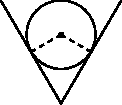
\includegraphics[scale=1]{gesamttex/edit_VIII-4/images/LBr_724_018-019_d4_018v.pdf}
\hfill
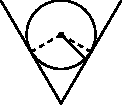
\includegraphics[scale=1]{gesamttex/edit_VIII-4/images/LBr_724_018-019_d5_018v.pdf}
\hfill
\edcaption{\lbrack\textit{Fig.~4}\rbrack 
\hspace{40mm}%
\lbrack\textit{Fig.~5}\rbrack}
\end{edfigure}
\pstart
Replicari\edlabel{LBr_724_018-019_3b}
posse
\edtext{videtur ad \textls{primum} equidem cessare instantiam aut saltem esse immutandam, si 
\indexN{\textls{Vanni}, Giovanni Francesco 1638\textendash1709}autor 
\cite{01995}\textit{Speciminis} additionem}{%
\lemma{videtur}%
\Bfootnote{%
\bars{ad \textls{primum} \textit{erg.}} equidem
\textit{(1)}~cessare %
\textit{(2)}~omitti posse %
\textit{(3)}~cessare instantiam %
\bars{aut \bars{aut \textit{gestr.}} saltem esse immutandam \textit{erg.}} , si autor \textit{Speciminis}
\textit{(a)}~assertionem suam
\textit{(b)}~additionem~\textit{L}}}
momentorum\indexS{additio momentorum}
\edtext{quibus grave\indexS{grave} in plano declivi descendere conatur,\indexS{grave in plano declivi descendens} et in alterum planum agit,\indexS{grave in planum declive agens}}{%
\lemma{}%
\Bfootnote{%
quibus grave in plano declivi descendere conatur, et in alterum planum agit, %
\bars{et recte quidem, \textit{gestr.}} %
\textit{erg.~L}}}
ad solum angulum rectum planorum\indexS{angulus planorum rectus}
\edtext{restringat, itaque si vires\indexS{vis} solum considerandae hic essent\lbrack,\rbrack\ additio}{%
\lemma{restringat,}%
\Bfootnote{%
\bars{in quo recte fecit \textit{erg.~u.~gestr.}} %
\textit{(1)}~qu %
\textit{(2)}~non tamen sine ratione objectum fuisse, %
\textit{(a)}~quia revera etiam in aliis planis %
\bars{alium angulum facientibus, \textit{erg.}} ex %
\textit{(aa)}~prem %
\textit{(bb)}~momentis quibus singula plana premuntur %
additio momentorum locum habet,
\textit{(b)}~si rigidius agere %
\textit{(c)}~et in rigore %
\textit{(aa)}~augeri posse %
\textit{(bb)}~angulum augeri posse %
\textit{(3)}~secu %
\textit{(4)}~additio momentorum \bars{locum \textit{streicht Hrsg.}} %
\textit{(5)}~itaque si %
\bars{secundum mentem \textit{Speciminis} \textit{erg.~u.~gestr.}} %
vires solum considerandae hic essent additio~\textit{L}}}
\edtext{partialium}{%
\lemma{}%
\Bfootnote{%
partialium %
\textit{erg.~L}}}
momentorum\indexS{additio momentorum partialium} locum
\edlabel{LBr_724_018-019_7a}%
\edtext{}{%
\xxref{LBr_724_018-019_7a}{LBr_724_018-019_7b}%
\lemma{habet,}%
\Bfootnote{%
\textit{(1)}~licet singula aliter sint aestimanda quam autor fecit. Non vero negatum est %
\textit{(2)}~quibus premuntur plana, sed ex merito distinguuntur ab his quibus %
\textit{(3)}~et, si %
\textit{(a)}~vis %
\textit{(aa)}~qua plana premuntur ea est secund %
\textit{(bb)}~quam grave exercet %
\textit{(cc)}~qua %
\textit{(aaa)}~grave in plano declivi descen %
\textit{(bbb)}~grave in plano %
agit ea est qua %
premit, ea est, qua %
\textit{(b)}~vires quibus grave in plano premit, eae essent, quibus %
\textit{(4)}~quibus grave %
\textit{(a)}~planum %
\textit{(b)}~in declivibus planis descendere conatur. %
\textit{(aa)}~Utique secundum %
\textit{(aaa)}~men %
\textit{(bbb)}~rationes autoris %
\textit{(bb)}~Quemadmodum pon %
\textit{(cc)}~Utique semper %
\textit{(aaa)}~ea in unam summam addenda esset, %
\textit{(bbb)}~eae in unam summam addendae essent,  %
quicumque sit angulus, alioqui aliquod earum %
\textit{(aaaa)}~periret %
\textit{(bbbb)}~perirent  %
\textit{(cccc)}~periret %
nihil agendo. Sed recte notavit \href{\Scan{LBr_724_19r}}%
{\lbrack19~r\textsuperscript{o}\rbrack} %
\textit{(aaaaa)}~et %
\textit{(bbbbb)}~Adm.\,R.\,P.~Kochanskius etiam illas vires in computum venire debere quibus grave %
\textit{(aaaaa-a)}~pla %
\textit{(bbbbb-b)}~in plano %
\textit{(aaaaa-aa)}~des %
\textit{(bbbbb-bb)}~declivi descendens ipsum planum declive premit, nec addenda esse simpliciter momenta, %
\textit{(aaaaa-aaa)}~alioqui fieret summa major %
\textit{(bbbbb-bbb)}~quae in rationes veniunt, %
\textit{(aaaaa-aaaa)}~et quae locum haberent; si unum tantum planum adesset %
\textit{(bbbbb-bbbb)}~sed quantitates tantum ipsis proportionales. %
\href{\Scan{LBr_724_18v}}%
{\lbrack18~v\textsuperscript{o}\rbrack} %
\textit{(dd)}~Ad \textls{secundum} replicatur: negatum non esse~\textit{L}}}%
habet, quibus grave in declivibus planis\indexS{planum declive} descendere conatur.\indexS{grave in plano declivi descendens}
\pend
\pstart
Ad \textls{secundum} replicatur: negatum non esse%
\edlabel{LBr_724_018-019_7b}
\edtext{momenta\indexS{momentum} quaecunque in unum posse addi,\indexS{additio momentorum} %
\edtext{sed ab \indexN{\textls{Vanni}, Giovanni Francesco 1638\textendash1709}autore \lbrack in\rbrack\ unum}{%
\lemma{sed}%
\Bfootnote{%
\textit{(1)}~ista %
\textit{(2)}~ab autore %
\bars{in \textit{gestr., wieder gültig gemacht Hrsg.}} %
unum~\textit{L}}}
addita aequari momento totali.\indexS{momentum totale} Negatum quoque non est}{%
\lemma{}%
\Bfootnote{%
momenta quaecunque \lbrack...\rbrack\ non est %
\textit{erg.~L}}}
momenta\indexS{momentum quo planum singulum premitur} quibus singula plana
\edtext{revera}{%
\lemma{}%
\Bfootnote{%
revera %
\textit{erg.~L}}}
premuntur,
\edtext{in unum addita\indexS{additio momentorum}}{%
\lemma{in unum}%
\Bfootnote{%
\textit{(1)}~adda %
\textit{(2)}~addita~\textit{L}}}
componere
\edtext{totale\indexS{momentum totale seu absolutum} seu absolutum momentum globi, nam id quoque per se patet cum tota vis\indexS{vis globi} globi a planis sustineatur,}{%
\lemma{totale}%
\Bfootnote{%
\textit{(1)}~momentum, %
\textit{(2)}~seu absolutum momentum globi, %
\textit{(a)}~sed hoc tantum, quod %
\textit{(b)}~id enim per se patet, %
\textit{(c)}~nam id \lbrack...\rbrack\  sustineatur,~\textit{L}}}
sed hoc tantum 
\edtext{negatur\lbrack:\rbrack}{%
\lemma{}%
\Bfootnote{%
negatur\lbrack:\rbrack\ %
\textit{erg.~L}}}
ea momenta
\edtext{quibus grave\indexS{grave} planum alterutrum\lbrack,\rbrack\ si cedere posset, propelleret,\indexS{momentum quo grave in planum agit}}{%
\lemma{quibus}%
\Bfootnote{%
\textit{(1)}~in singulis %
\textit{(2)}~singula plana propelleret %
\textit{(a)}~si posset %
\textit{(b)}~grave si posset %
\textit{(aa)}~grave \bars{alterutrum \textit{gestr.}} %
\textit{(bb)}~planum alterutrum\lbrack,\rbrack\ si cedere posset, propelleret,~\textit{L}}}
hoc est, (in casu recti
\edtext{planorum}{%
\lemma{}%
\Bfootnote{%
planorum %
\textit{erg.~L}}}
anguli),\indexS{angulus planorum rectus} 
\edtext{momenta}{%
\lemma{}%
\Bfootnote{%
momenta %
\textit{erg.~L}}}
\edtext{quibus in altero plano declivi descenderet,\indexS{grave in plano declivi descendens} si posset\lbrack,\rbrack}{%
\lemma{quibus in}%
\Bfootnote{%
\textit{(1)}~opposito %
\textit{(2)}~altero plano declivi %
\textit{(a)}~descendit, si possit %
\textit{(b)}~descenderet, si posset~\textit{L}}}
coincidere cum his quibus ipsa plana in casu impediti descensus\indexS{descensus impeditus}
\edtext{premuntur, ac proinde}{%
\lemma{premuntur,}%
\Bfootnote{%
\textit{(1)}~seu %
\textit{(2)}~ac proinde~\textit{L}}}
in unum addita\indexS{additio momentorum}
\edtext{\lbrack momentum\rbrack}{%
\lemma{}%
\Bfootnote{%
planum %
\textit{L ändert Hrsg.}}}
totale\indexS{momentum totale}
\edtext{conficere.\edlabel{LBr_724_018-019_13b} %
\href{\Scan{LBr_724_19r}}%
{\lbrack19~r\textsuperscript{o}\rbrack} Et recte}{%
\lemma{conficere.}%
\Bfootnote{%
\textit{(1)}~Verum %
\textit{(2)}~Nec puta %
\textit{(3)}~Placet \bars{autem \textit{gestr.}} %
ex multis modis quibus demonstrari %
\textit{(a)}~solet potestque %
\textit{(b)}~potest communis regula Staticorum quam autor \textit{Speciminis} impugnat, unam %
\bars{non inelegantem \textit{erg.}} 
\bars{,~nec quantum meminerim \textit{erg.~u.~gestr.}} %
hoc loco adducere ut si satisfacere ei autor non potest, %
\textit{(aa)}~agnoscat assumtam 
\textit{(aaa)}~illam
\textit{(bbb)}~ab ipso momentorum additionem, quae sola in demonstratione ejus, jam super negari potest, jure negatam fuisse. 
\textit{(bb)}~agnoscat non temere sibi contradici.
\textit{(4)}~Ut autem
\textit{(a)}~hoc jure negari %
\textit{(aa)}~(quod enim demonstravi) %
\textit{(bb)}~(cui enim demonst %
\textit{(cc)}~(in quo %
\textit{(dd)}~( quod 
\textit{(aaa)}~\textlangle\textendash\textrangle\ %
\textit{(bbb)}~potissimam in demonstratione \textit{Speciminis} dubitationem accipit, %
\textit{(b)}~additionem ab autore docto \textit{Speciminis}  %
\textit{(aa)}~propositam %
\textit{(bb)}~sine probationem propositam %
\bars{jure negari appareat \textit{streicht Hrsg.}}
\href{\Scan{LBr_724_19r}}%
{\lbrack19~r\textsuperscript{o}\rbrack} Et recte~\textit{L}}}
\edtext{notavit \indexN{\textls{Kochański}, Adam Adamandus 1631\textendash1700}Adm.\,R.\,P.~Kochanskius in \cite{01023}\textit{Actis} Jun. 1685.}{%
\lemma{notavit \lbrack...\rbrack\ 1685}%
\Cfootnote{\indexN{\textls{Kochański}, Adam Adamandus 1631\textendash1700}\textsc{A.\,A. Kochański}, %
\cite{01996}\textit{Consideratio speciminis libri de momentis gravium, Authore J.\,F.\,V. Lucensi}, %
\cite{01023}\textit{Acta eruditorum},
Juni 1685, S.\;262\textendash265.}}
etiam illa momenta consideranda esse, quibus grave
\edtext{etiam}{%
\lemma{}%
\Bfootnote{etiam \textit{erg.~L}}}
in plano declivi decurrens\indexS{grave in plano declivi decurrens} hoc planum
\edtext{premit,\indexS{momentum quo grave planum premit} praeterea non}{%
\lemma{premit,}%
\Bfootnote{%
\textit{(1)}~nec %
\textit{(2)}~praeterea non~\textit{L}}}
simpliciter addenda esse
\edtext{momenta\indexS{additio momentorum} illa}{%
\lemma{momenta}%
\Bfootnote{%
\textit{(1)}~qualia ess %
\textit{(2)}~illa~\textit{L}}}
quae in rationes
\edtext{veniunt alioqui summa excederet momentum totale,\indexS{momentum totale} sed quantitates proportionales}{%
\lemma{veniunt}%
\Bfootnote{%
\textit{(1)}~sed quantitates e %
\textit{(2)}~alioqui summa excederet momentum totale, sed quantitates %
\textit{(a)}~proportionis %
\textit{(b)}~proportionales~\textit{L}}}
in quas momentum totale\indexS{momentum totale}
\edtext{distribuitur. \href{\Scan{LBr_724_18v}}%
{\lbrack18~v\textsuperscript{o}\rbrack} Quoniam}{%
\lemma{distribuitur.}%
\Bfootnote{%
\textit{(1)}~Ut autem eam additionem quae potissimam in demonstratione %
\textit{Speciminis} dubitationem recipit jure negari appareat %
\textit{(2)}~\href{\Scan{LBr_724_18v}}%
{\lbrack18~v\textsuperscript{o}\rbrack} Quoniam~\textit{L}}}
autem testatur doctissimus \indexN{\textls{Vanni}, Giovanni Francesco 1638\textendash1709}autor
\edtext{\cite{01995}\textit{Speciminis} demonstrationes regulae}{%
\lemma{\textit{Speciminis}}%
\Bfootnote{%
\textit{(1)}~quasdam %
\textit{(2)}~demonstrationes %
\textit{(a)}~quas refert %
\textit{(b)}~regulae~\textit{L}}}
staticorum\indexS{regula staticorum}
\edtext{quas apud \indexN{\textls{Galilei} (Galilaeus, Galileus), Galileo 1564\textendash1642}Galilaeum 
et \indexN{\textls{Torricelli} (Torricellius), Evangelista 1608\textendash1647}Torricellium extare ait,}{%
\lemma{quas \lbrack...\rbrack\ ait}%
\Cfootnote{\textsc{Vanni},\indexN{\textls{Vanni}, Giovanni Francesco 1638\textendash1709} \cite{01995}\textit{Specimen} hier S.\;511.
Siehe
\indexN{\textls{Galilei} (Galilaeus, Galileus), Galileo 1564\textendash1642}%
\textsc{G.~Galilei}, %
\cite{00050}\textit{Discorsi}, %
Giornata Terza, De motu naturaliter accelerato; \glqq Aggiunta postuma dell'Autore\grqq\ %
nach dem Scholion zum 2.~Theorem (der Zusatz erschien erst in der posthumen Werkausgabe: \cite{01084}\textit{Opere}, Bologna 1656, Bd.~II, S.\;132\lbrack ter\rbrack\textendash134; \cite{00048}\textit{GO} VIII, S.\;216\textendash219 im Apparat) %
und 
\indexN{\textls{Torricelli} (Torricellius), Evangelista 1608\textendash1647}%
\textsc{E.~Torricelli}, \textit{De motu gravium}, lib.~I
(\cite{00304}\textit{Opera geometrica}, Florenz 1644, S.\;99;
\cite{00108}\textit{TO}~II, S.\;105).}}
sibi parum solidas visas, eaeque mihi non sunt ad manus\lbrack,\rbrack\ 
placet aliquam subjicere, quae videtur manifesta, nec inelegans.
\pend
\begin{edfigure}%
\hfill
\includegraphics[scale=1]{%
gesamttex/edit_VIII-4/images/LBr_724_018-019_d6_018v.pdf}
\hfill
\includegraphics[scale=1]{%
gesamttex/edit_VIII-4/images/LBr_724_018-019_d7_018v.pdf}
\hfill
\edcaption{\lbrack\textit{Fig.~6}\rbrack 
\hspace*{40mm}%
\edtext{\lbrack\textit{Fig.~7, gestr.}\rbrack}{%
\lemma{\lbrack\textit{Fig.~7}\rbrack}%
\Cfootnote[nonum]{%
Ein ebenfalls gestrichener Entwurf zum Diagramm wird nicht wiedergegeben.}}}
\end{edfigure}
\pstart
\noindent
\lbrack%
\textit{Nachfolgend kleingedruckter Text (erste Fassung des Beweises %
auf \refpassage{LBr_724_018-019_10a}{LBr_724_018-019_10b}) samt Zeichnungen gestrichen:}\rbrack
\pend
\vspace{0.5em}
\footnotesize
\pstart 
\noindent
Suppono autem, corporibus duobus ita positis, ut 
uno ascendente alterum descendat,\indexS{corpus ascendens altero corpore descendente} et contra, nullum 
fieri motum a gravitate,\indexS{gravitas} nisi plus descendat quam ascendat, 
seu nisi descendat commune eorum centrum gravitatis.\indexS{centrum gravitatis commune}
Assumo etiam Lemma
\edlabel{LBr_724_018-019_4a}%
\edtext{}{%
\xxref{LBr_724_018-019_4a}{LBr_724_018-019_4b}%
\lemma{Geometricum}%
\Bfootnote{%
\textit{(1)}~facile demonstratu %
\textit{(2)}~ni fallor elegans. %
\textit{(a)}~\bars{Si \textit{streicht Hrsg.}} in basi trianguli sumatur punctum %
\textit{(b)}~Si duorum trianguli laterum uni %
\textit{(aa)}~tantum adda %
\textit{(bb)}~producto tantum addatur quantum ab \bars{altero \textit{streicht Hrsg.}} abscinditur %
\textit{(c)}~Duorum triangulorum %
\textit{(d)}~Si triangula quaecunque %
\textit{(e)}~Omnium triangulorum angulum congruentem et summam%
\textit{(aa)}~laterum %
\textit{(bb)}~crurum %
eandem habentium bases %
\textit{(aaa)}~ab eadem recta, %
\textit{(aaaa)}~eaque ad alterutrum %
\textit{(aaaaa)}~lat %
\textit{(bbbbb)}~crus (quod productum omni %
\textit{(bbbb)}~in eadem ratione secantur, eaque est perpendicularis ad %
\textit{(bbb)}~a recta ad crus %
\textit{(aaaa)}~commune perpendicu %
\textit{(bbbb)}~si producatur %
\textit{(cccc)}~commune perpendiculari in eadem ratione secantur. %
\textit{(aaaaa)}~Si trian %
\textit{(bbbbb)}~Sit triangulum \textit{ABC} sumaturque %
\textit{(aaaaa-a)}~ver %
\textit{(bbbbb-b)}~a \textit{C} versus \textit{A} %
\textit{(ccccc-c)}~in \textit{AC} a \textit{C} versus \textit{A} punctum \textit{D}, et in \textit{AB} produc %
\textit{(ccccc)}~Hoc est si sint triangula \textit{ABC} %
et \textit{ADE}, et \textit{EC} aequalis \textit{BD} %
cadant autem \textit{E} in rectam \textit{AC}, et \textit{B} in rectam \textit{AD} et ex %
\bars{uno \textit{gestr.}} crure communi ut \textit{AB}, educatur perpendicularis %
aliqua \textit{FGH} secans \textit{DE} in \textit{G}, et \textit{BC} in \textit{H}, erit %
$DG : GE\; \squaredots\; BH : HC$.
\href{\Scan{LBr_724_19r}}%
{\lbrack19~r\textsuperscript{o}\rbrack}
\textit{(f)}~Duorum triangulorum~\textit{L}}}%
Geometricum ni fallor elegans.
\pend
\normalsize
\begin{edfigure}%
\includegraphics[scale=1]{%
gesamttex/edit_VIII-4/images/LBr_724_018-019_d8_018v.pdf}
\edcaption{\edtext{\lbrack\textit{Fig.~8, gestr.}\rbrack}{%
\lemma{\lbrack\textit{Fig.~8}\rbrack}%
\Cfootnote[nonum]{Das Diagramm wird von Leibniz lediglich in gestrichenen Varianten besprochen: Siehe die Variante \textit{(e)}, bes. \textit{(ccccc)} zu \refpassage{LBr_724_018-019_4a}{LBr_724_018-019_4b}.}}}
\end{edfigure}
\pstart 
\noindent
\href{\Scan{LBr_724_19r}}%
{\lbrack19~r\textsuperscript{o}\rbrack}
\pend
\begin{edfigure}[0.25em][1em]    	%
\hfill
\includegraphics[scale=1]{%
gesamttex/edit_VIII-4/images/LBr_724_018-019_d9_019r.pdf}
\hfill
\includegraphics[scale=1]{%
gesamttex/edit_VIII-4/images/LBr_724_018-019_d10_019r.pdf}
\hfill
\edcaption{%
\edtext{\lbrack\textit{Fig.~9, gestr.}\rbrack}{%
\lemma{\lbrack\textit{Fig.~9}\rbrack}%
\Cfootnote[nonum]{Ein ebenfalls gestrichener Entwurf zum Diagramm wird nicht wiedergegeben.}}
\hspace*{28mm}%
\edtext{\lbrack\textit{Fig.~10, gestr.}\rbrack}{%
\lemma{\lbrack\textit{Fig.~10}\rbrack}%
\Cfootnote[nonum]{Ein ebenfalls gestrichener Entwurf zum Diagramm wird nicht wiedergegeben.}}}
\end{edfigure}
\footnotesize
\pstart
Duorum triangulorum
\edlabel{LBr_724_018-019_4b}
\edtext{angulum coincidentem et summa crurum}{%
\lemma{angulum}%
\Bfootnote{%
\textit{(1)}~congruentem %
\textit{(2)}~coincidentem et summa %
\textit{(a)}~crurum eandem habentium %
\textit{(b)}~laterum eandem habentium %
\textit{(c)}~crurum~\textit{L}}}
circa eum angulum communem habentium latera se
\edtext{mutuo}{%
\lemma{}%
\Bfootnote{%
mutuo %
\textit{erg.~L}}}
secant in eadem
\edtext{ratione. Seu si duarum}{%
\lemma{ratione.}%
\Bfootnote{%
\textit{(1)}~Si sint duae rectae in eodem plano positae inter se aequales per quatuor eorum puncta extrema circulus describi potest
\textit{(2)}~Seu si~\textit{L}}}
rectarum aequalium in eodem plano
\edtext{positarum}{%
\lemma{}%
\Bfootnote{%
positarum %
\textit{erg.~L}}}
extrema jungantur rectae jungentes sese secabunt in eadem 
\edtext{ratione. $AB : CD\; \squaredots\; BE : CD$. Ergo}{%
\lemma{ratione.}%
\Bfootnote{%
\textit{(1)}~Hinc %
\textit{(2)}~Eritq %
\textit{(3)}~$AB : CD\; \squaredots\; BE : $
\textit{(a)}~\textit{GF}. Ergo $AB : BE\; \squaredots\; CD : GF\; \squaredots\; LC$ 
\bars{:~\textit{LG} \textit{gestr.}} %
\textit{(b)}~\textit{CD}. Ergo~\textit{L}}}
\textit{AB} aeq.~\textit{BE}.
\pend
\normalsize
\vspace{0.5em} %
\pstart
\noindent
\lbrack%
\textit{Nachfolgend kleingedruckter Text (zweite Fassung des Beweises %
auf \refpassage{LBr_724_018-019_10a}{LBr_724_018-019_10b}) gestrichen:}\rbrack
\pend
\vspace{0.5em}
\footnotesize
\pstart 
\noindent
Suppono
\edtext{autem duobus}{%
\lemma{autem}%
\Bfootnote{%
\textit{(1)}~corporibus %
\textit{(2)}~duobus~\textit{L}}}
gravibus ita positis, ut uno ascendente alterum
descendere necesse sit,\indexS{corpus ascendens altero corpore descendente} nullum fieri motum
a gravitate,\indexS{gravitas} nisi potior sit ascensus quam descensus,
seu nisi descendat eorum centrum gravitatis\indexS{centrum gravitatis commune}
\edlabel{LBr_724_018-019_5a}%
\edtext{}{%
\xxref{LBr_724_018-019_5a}{LBr_724_018-019_5b}%
\lemma{commune.}%
\Bfootnote{%
\textit{(1)}~Sit recta verticalis %
\textit{(1)}~\textit{AB} %
\textit{(2)}~\textit{ADBF}, et recta declivis \textit{AGCE}, %
\textit{(a)}~et gravia \textit{B} et \textit{C}, connexa fune \textit{BAC} %
\textit{(b)}~et gravia %
\textit{F} et \textit{G} sint in aequilibrio, junctaque \textit{FG}, sit
\textit{(aa)}~centrum %
\textit{(bb)}~gravium %
\textit{F} et \textit{G} centrum gravitatis. Jam si gravia %
\textit{F} et \textit{G} sunt in aequilibrio, manebunt in aequilibrio %
\textit{(aaa)}~etiamsi fune prehenso \textit{G} detrahas in \textit{E},  %
\textit{(bbb)}~translato \textit{F} in \textit{D} et \textit{G} in \textit{E}, si scilicet prehenso fune %
\textit{(aaaa)}~det %
\textit{(bbbb)}~detrahas \textit{G} in \textit{E} %
\textit{(ccc)}~etiamsi prehenso \lbrack...\rbrack\ \textit{E}, %
\textit{(aaaa)}~eademque %
\textit{(bbbb)}~simulque attollas \textit{F} in \textit{D} %
\textit{(aaaaa)}~, existente %
\textit{(bbbbb)}~. Ergo centrum gravitatis %
\textit{(aaaaa-a)}~ipsorum \textit{D} et \textit{H} in eadem est %
\textit{(bbbbb-b)}~manet in eadem semper altitudine, quae erat ipsius \textit{H}, %
seu ducta per \textit{H} recta horizontali \textit{BHC}, quae verticali ad angulos %
rectos occurrat in \textit{B}, declivi occurrat in \textit{C}, centrum gravitatis %
ipsorum \textit{D} et \textit{E}, erit in eadem recta \textit{BC}, in qua centrum \textit{H}. %
Et si grave \textit{F} vel \textit{D} %
\textit{(2)}~Sit recta~\textit{L}}}%
commune.
\pend
\normalsize
\begin{edfigure}[1em][1em]    	%
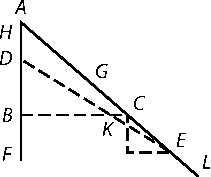
\includegraphics[scale=1]{gesamttex/edit_VIII-4/images/LBr_724_018-019_d11_019r.pdf}
\edcaption{\edtext{\lbrack\textit{Fig.~11, nicht gestr.}\rbrack}{\lemma{}%
\Afootnote{\textit{Am Rand, neben \lbrack\textit{Fig.~11}\rbrack, ebenfalls nicht gestrichen:} si sit \textit{CE} aeq.\ \textit{BD} et \textit{DE} secet \textit{BC} in \textit{K}, erit $EK : KD\; \squaredots\; BA : AC$.}}}
\end{edfigure}
\footnotesize
\pstart
Sit recta\edlabel{LBr_724_018-019_5b}
verticalis \textit{ADBF}, et declivis
\edtext{\textit{AGCE}, et angulus}{%
\lemma{\textit{AGCE},}%
\Bfootnote{%
\textit{(1)}~sintque dua gravia \textit{B} et %
\textit{(2)}~et angulus~\textit{L}}}
\edtext{%
\textit{ABC} rectus, sintque duo
gravia\indexS{gravia fune connexa} \textit{B} et \textit{C}, fune\indexS{funis}
\edtext{\textit{BAC} connexa eaque in aequilibrio.\indexS{gravia in aequilibrio} Erit}{%
\lemma{\textit{BAC}}%
\Bfootnote{%
\textit{(1)}~, verticali %
\textit{(2)}~connexa eaque in aequilibrio. %
\textit{(a)}~Erit utique %
\textit{(b)}~Erit~\textit{L}}}
eorum centrum gravitatis\indexS{centrum gravitatis gravium} in recta
\edtext{jungente, \textit{BC}.}{%
\lemma{jungente,}%
\Bfootnote{%
\textit{(1)}~\textit{BH} %
\textit{(2)}~\textit{BC}.~\textit{L}}}
Manent autem in aequilibrio,\indexS{aequilibrium} etiamsi fune\indexS{funis} apprehenso detrahas
\textit{C} in \textit{E}, simulque attollas \textit{B} in \textit{D},
\edtext{existentibus}{%
\lemma{existentibus}%
\Bfootnote{%
\textit{(1)}~\textit{CD} %
\textit{(2)}~\textit{CE},~\textit{L}}}
\textit{BD} aequalibus; (vel etiamsi detrahas \textit{B} in \textit{F} simulque attollas \textit{C} in \textit{G}
existentibus \textit{BF},
\edtext{\textit{CG} aequalibus)}{%
\lemma{\textit{CG}}%
\Bfootnote{%
\textit{(1)}~) %
\textit{(2)}~aequalibus)~\textit{L}}}
itaque etiam centrum}{\lemma{}\Afootnote{%
\textit{Am Rand, nicht gestrichen:} NB multa elegantia Lemmata Geometrica ex his duci possent ut quod recta \textit{BC} ipsas \textit{DE}, \textit{FG}, \textit{HL} in eadem ratione secat\textsuperscript{\lbrack a\rbrack} quae est \textit{AC} ad \textit{AB}, si \textit{BD} et \textit{CE}, item \textit{BF} et \textit{CG} item \textit{BH} et \textit{CL}, sint aequales.
\\[1.5ex]%
{\footnotesize \textsuperscript{\lbrack a\rbrack} secat \bars{quae est \textit{AC} ad \textit{AB} \textit{erg.}}, %
\textit{(1)}~si \textit{BF} et \textit{CG}, %
\textit{(2)}~si \textit{BD} \textit{L}}}}
gravitatis\indexS{centrum gravitatis commune} semper manebit in eadem altitudine, nempe in
\edtext{recta BC,}{%
\lemma{recta}%
\Bfootnote{%
\textit{(1)}~\textit{BH} %
\textit{(2)}~\textit{BC},~\textit{L}}}
sive situs gravium sit \textit{B}, \textit{C}; sive
\edtext{\textit{D}, \textit{E}; sive}{%
\lemma{\textit{D}, \textit{E};}%
\Bfootnote{%
\textit{(1)}~si \textit{F}, \textit{G} %
\textit{(2)}~sive~\textit{L}}}
\textit{F}, \textit{G}.
\pend
\pstart
Quod si ergo grave \textit{B} 
\edtext{attollas in \textit{H},}{%
\lemma{attollas}%
\Bfootnote{%
\textit{(1)}~per %
\textit{(2)}~in %
\textit{(a)}~\textit{A} %
\textit{(b)}~\textit{H}~\textit{L}}}
ita ut quantillum vis\indexS{vis} absit ab \textit{A}, detrahasque simul \textit{C} in \textit{L}, ita ut
\edtext{\textit{CL} sit aequal.~\textit{BH}\lbrack,\rbrack}{%
\lemma{\textit{CL} sit}%
\Bfootnote{%
\textit{(1)}~aeq.~\textit{B} %
\textit{(2)}~aequal.~\textit{BH}~\textit{L}}}
patet, centrum
\edtext{gravitatis\indexS{centrum gravitatis commune} gravium \textit{H} et \textit{L} cadere adhuc}{%
\lemma{gravitatis}%
\Bfootnote{%
\textit{(1)}~ipsorum %
\textit{(2)}~gravium \textit{H} et \textit{L} cadere %
\textit{(a)}~in rectam \textit{BC} %
\textit{(b)}~adhuc~\textit{L}}}
in
\edtext{rectam \textit{BC}, idem}{%
\lemma{rectam \textit{BC},}%
\Bfootnote{%
\textit{(1)}~idemque cadere in rectam \textit{HL} %
\textit{(2)}~idem~\textit{L}}}
autem cadit in rectam \textit{HL} 
\edtext{et proinde in rectarum \textit{BC}, \textit{HL} intersectionem,}{%
\lemma{}%
\Bfootnote{%
et proinde in rectarum \textit{BC}, \textit{HL} intersectionem, %
\textit{erg.~L}}}
ergo
\edtext{quo \textit{H} propius}{%
\lemma{quo}%
\Bfootnote{%
\textit{(1)}~propius \textit{H} a %
\textit{(2)}~\textit{H} propius~\textit{L}}}
assumseris ad \textit{A}, erit centrum gravitatis\indexS{centrum gravitatis commune} ipsorum \textit{H}, \textit{L}, propius
\edtext{ipsi \textit{C}, efficereque}{%
\lemma{ipsi \textit{C},}%
\Bfootnote{%
\textit{(1)}~ita ut tantum absit a %
\textit{(2)}~efficereque~\textit{L}}}
possumus ut absit
\edtext{a \textit{C} intervallo}{%
\lemma{a \textit{C}}%
\Bfootnote{%
\textit{(1)}~errore qui sit %
\textit{(2)}~intervallo~\textit{L}}}
quod sit minus quovis dato,
et denique si \textit{H} incidat in \textit{A}, erit \textit{CL}, aeq.~\textit{BA}, centrumque %
gravitatis\indexS{centrum gravitatis commune} ipsorum \textit{H} et \textit{L} incidet in \textit{C},
\edtext{intersectionem rectarum \textit{BC}, et \textit{HL}\lbrack,\rbrack}{%
\lemma{}%
\Bfootnote{%
intersectionem rectarum \textit{BC}, et \textit{HL} %
\textit{erg.~L}}}
ergo grave \textit{L} sive \textit{C} erit
\edtext{ad grave \textit{H}}{%
\lemma{ad grave}%
\Bfootnote{%
\textit{(1)}~\textit{B} sive %
\textit{(2)}~\textit{H}~\textit{L}}}
seu \textit{A} sive \textit{B}, ut \textit{AC} ad \textit{CL} sive \textit{BC}.
Quod erat demonstrandum.
\pend
\pstart
Demonstrationem autem brevitatis
\edtext{ac claritatis}{%
\lemma{ac}%
\Bfootnote{%
\textit{(1)}~claritatisque %
\textit{(2)}~claritatis~\textit{L}}}
causa exposui familiarius; si quis vero pertinacius
\edtext{resistat, facile}{%
\lemma{resistat,}%
\Bfootnote{%
\textit{(1)}~ex his %
\textit{(2)}~faci %
\textit{(3)}~facile~\textit{L}}}
ad absurdum redigi potest, eo ipso
\edtext{quod discrimen}{%
\lemma{quod}%
\Bfootnote{%
\textit{(1)}~discrimen ab eo quod asserimus dato quovis minus \bars{esse \textit{streicht Hrsg.}} ostendi potest %
\textit{(2)}~discrimen
~\textit{L}}}
a sententia nostra dato quovis minus esse ostendi potest.
\pend
\normalsize %
\vspace{0.5em} %
\newpage
\pstart
\centering 
\edlabel{LBr_724_018-019_9a}%
\edtext{}{%
\xxref{LBr_724_018-019_9a}{LBr_724_018-019_9b}%
\lemma{\href{\Scan{LBr_724_19v}}%
{\lbrack19~v\textsuperscript{o}\rbrack}}%
\Bfootnote{%
\textit{(1)}~Cum vir quidam %
\textit{(a)}~doc %
\textit{(b)}~doctus %
\textit{(c)}~ingeniosissi %
\textit{(d)}~doctus %
eam regulam nuper in dubium revocaverit \textit{Specimine} edito %
\textit{(aa)}~in %
\textit{(aaa)}~mom %
\textit{(bbb)}~sche %
\textit{(bb)}~\textit{de momentis gravium} %
inserto in \textit{Actis} Novembr.~1684.\ placet ex compluribus  %
\bars{regulae \textit{erg.}} %
demonstrationibus unam %
\bars{prae alteras \textit{gestr.}} %
non inelegantem subjicere, ut appareat quid ad eam %
\textit{(aaa)}~vir doctus %
\textit{(bbb)}~autor \textit{Speciminis} %
excipere possit. %
\textit{(2)}~Demonstratio %
\textit{(a)}~communis %
\textit{(b)}~Geometrica~\textit{L}}}%
\href{\Scan{LBr_724_19v}}%
{\lbrack19~v\textsuperscript{o}\rbrack} %
\hfill
\edlabel{LBr_724_018-019_10a}%
Demonstratio Geometrica%
\edlabel{LBr_724_018-019_9b}
regulae apud staticos\indexS{statici} receptae\indexS{regula apud staticos recepta}
\hfill
\phantom{\lbrack19~v\textsuperscript{o}\rbrack}
\linebreak
de momentis gravium\indexS{momenta gravium in planis inclinatis} in planis inclinatis
\pend
\pstart
\noindent
\edtext{Sit planum verticale\indexS{planum verticale} \textit{ADB}, et inclinatum\indexS{planum inclinatum} \textit{ACE} et in illo descendere tendat grave\indexS{grave in plano declivi descendens} \textit{B}, in hoc}{%
\lemma{Sit }%
\Bfootnote{%
\textit{(1)}~recta verticalis \textit{ADBF}, et inclinata \textit{AGCE} et in illa
\textit{(a)}~grave \textit{B}, in hac grave \textit{D}, descendere tendens %
\textit{(b)}~descendere tendat grave \textit{B}, in hac %
\textit{(2)}~planum verticale \lbrack...\rbrack\ in hoc~\textit{L}}}
grave \textit{C},
\edtext{sint autem gravia}{%
\lemma{}%
\Bfootnote{%
sint autem gravia %
\textit{erg.~L}}}
connexa\indexS{gravia fune connexa} fune\indexS{funis}
\edtext{\textit{BAC}, angulusque \textit{ABC}}{%
\lemma{\textit{BAC},}%
\Bfootnote{%
\textit{(1)}~ponamusque eam esse rationem gravium inter se, ut %
\textit{(2)}~angulus autem %
\textit{(3)}~angulusque \textit{ABC}~\textit{L}}}
sit rectus, et gravia eam inter se rationem habeant ut sint in aequilibrio.\indexS{gravia in aequilibrio} 
Ajo fore grave \textit{B} ad grave \textit{C}, ut recta \textit{AB} ad 
\edlabel{LBr_724_018-019_11a}%
\edtext{}{%
\xxref{LBr_724_018-019_11a}{LBr_724_018-019_11b}%
\lemma{rectam \textit{AC}.}%
\Bfootnote{%
\textit{(1)}~Trahatur grave \textit{C} in \textit{E}, \bars{ut \textit{erg.}} %
assurgat \textit{B} in \textit{D}, %
\textit{(a)}~eruntque %
\textit{(b)}~ex %
\textit{(c)}~erunt %
\textit{(d)}~patet %
\textit{(e)}~centrum gra %
\textit{(2)}~Prehendendo funem manu \bars{in \textit{C} \textit{erg.}} %
trahendoque ex situ \textit{BAC} \bars{in \textit{streicht Hrsg.}} %
situm \textit{DAE} (translatis gravibus %
\textit{(3)}~Funem~\textit{L}}}%
rectam \textit{AC}.
\pend
\begin{edfigure}[1em][1em]    	%
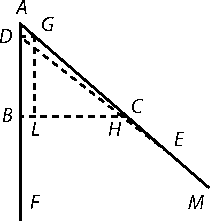
\includegraphics[scale=1]{gesamttex/edit_VIII-4/images/LBr_724_018-019_d12_019v.pdf}
\edcaption[0.25em]{\lbrack\textit{Fig.~12}\rbrack}
\end{edfigure}
\pstart
Funem\indexS{funis}%
\edlabel{LBr_724_018-019_11b}
(qui gravitate carere intellegitur) manu prehendendo
in \textit{C}, trahendoque grave \textit{C} deorsum
\edtext{in \textit{E}, adeoque simul}{%
\lemma{in \textit{E},}%
\Bfootnote{%
\textit{(1)}~simulque %
\textit{(2)}~adeoque simul~\textit{L}}}
grave \textit{B} sursum 
\edtext{in \textit{D}, (quo facto aequales erunt \textit{CE} et \textit{BD}) patet}{%
\lemma{in}%
\Bfootnote{%
\textit{(1)}~\textit{A}, %
\textit{(2)}~\textit{D}, %
\textit{(a)}~( %
\textit{(b)}~pat %
\textit{(c)}~sic ut %
\textit{(aa)}~sit aequa %
\textit{(bb)}~aequales sint \textit{CE} et \textit{BD}, patet %
\textit{(d)}~(quo facto \lbrack...\rbrack\ \textit{BD}) patet~\textit{L}}}
aequilibrium\indexS{aequilibrium} quod prius erat, inter gravia,
\edtext{manere; nec proinde eorum centrum gravitatis commune\indexS{centrum gravitatis commune} attolli vel deprimi.}{%
\lemma{manere;}%
\Bfootnote{%
\textit{(1)}~et similiter %
\textit{(2)}~nec \bars{proinde \textit{erg.}} eorum \lbrack...\rbrack\ deprimi.~\textit{L}}}
Cumque gravium in situ \textit{B}, \textit{C} centrum gravitatis\indexS{centrum gravitatis commune} esset in
\edtext{recta \textit{BC} horizontali, in ea manebit}{%
\lemma{recta \textit{BC}}%
\Bfootnote{%
\textit{(1)}~, utique non mutabitur %
\textit{(2)}~horizontali, %
\textit{(a)}~inque ea maneret %
\textit{(b)}~in ea manebit~\textit{L}}}
non obstante hac
\edtext{gravium translatione, quae ipsa in aequilibrio\indexS{gravia in aequilibrio} relinquit. Cumque sit}{%
\lemma{gravium}%
\Bfootnote{%
\textit{(1)}~translatione %
\textit{(a)}~, erit in intersectione %
\textit{(b)}~. Sitque %
\textit{(2)}~translatione, quae ipsa in aequilibrio relinquit. Cumque sit~\textit{L}}}
\edtext{praeterea idem centrum in recta}{%
\lemma{praeterea}%
\Bfootnote{%
\textit{(1)}~in recta %
\textit{(2)}~idem centrum in recta~\textit{L}}}
\textit{DE}, gravia in situ \textit{D}, \textit{E}, jungente,
\edtext{erit in rectarum \textit{BC}, \textit{DE}, intersectione \textit{H}. Jam}{%
\lemma{erit in}%
\Bfootnote{%
\textit{(1)}~earum intersectione \textit{H}. Constat autem ex %
\textit{(2)}~intersectione \textit{H} rectarum \textit{BC}, \textit{DE}, %
\textit{(3)}~rectarum \textit{BC}, \textit{DE}, intersectione \textit{H}. Jam~\textit{L}}}
ex Geometria\indexS{Geometria} ostendi
\edtext{potest lemma facile nec inelegans, si}{%
\lemma{potest}%
\Bfootnote{%
\textit{(1)}~esse %
\textit{(2)}~lemma %
\textit{(a)}~elegans, %
\textit{(b)}~faci %
\textit{(3)}~lemma facile nec inelegans,~\textit{L}}}
si sint \textit{CE}, \textit{BD} aequales, fore
$DH : HE\; \squaredots\;$%
\edtext{$AC : AB$. Est}{%
\lemma{$AC : AB$.}%
\Bfootnote{%
\textit{(1)}~Ergo et gravia %
\textit{(2)}~Sunt autem gravia \textit{E} et %
\textit{(3)}~Est~\textit{L}}}
autem ob aequilibrium gravium,\indexS{aequilibrium gravium}
\edtext{grave \textit{E} (sive \textit{C})}{%
\lemma{grave \textit{E}}%
\Bfootnote{%
\textit{(1)}~ad gra %
\textit{(2)}~(sive \textit{C})~\textit{L}}}
ad grave \textit{D} (sive \textit{B}) ut \textit{DH} ad \textit{HE},
quia \textit{H} est ipsorum \textit{D} et \textit{E} centrum gravitatis.\indexS{centrum gravitatis commune} Ergo
\edtext{erit grave \textit{C}}{%
\lemma{erit grave}%
\Bfootnote{%
\textit{(1)}~\textit{B} ad grave %
\textit{(2)}~\textit{C}~\textit{L}}}
ad grave \textit{B} ut \textit{AC} ad \textit{AB}.
\pend
\pstart
Idem
\edtext{aliter}{%
\lemma{}%
\Bfootnote{%
aliter %
\textit{erg.~L}}}
etiam sine assumto lemmate illo
\edtext{Geometrico ostendi potest, si grave \textit{B} attollatur usque ad \textit{A}, seu si}{%
\lemma{Geometrico}%
\Bfootnote{%
\textit{(1)}~ostendi potest, si %
\textit{(2)}~ostendi potest, si grave \textit{B} %
\textit{(a)}~erat %
\textit{(b)}~\bars{sive \textit{D} \textit{erg.}} eousque attollatur \textit{A} seu %
\textit{(c)}~attollatur usque ad \textit{A}, seu si~\textit{L}}}
(\textit{D}) incidat in ipsum punctum \textit{A},
\edtext{quo casu \textit{C}(\textit{E}) aequalis \textit{B}(\textit{D}) erit aequalis \textit{BA}, et (\textit{H})}{%
\lemma{quo}%
\Bfootnote{%
\textit{(1)}~casu (\textit{H}) %
\textit{(2)}~casu \textit{C}(\textit{E}) aequalis \textit{B}(\textit{D}) erit aequalis \textit{BA}, et (\textit{H})~\textit{L}}}
incidet in \textit{C}, et
\edtext{(\textit{H})(\textit{D}) coincidet cum \textit{CA}, eritque}{%
\lemma{(\textit{H})(\textit{D}) }%
\Bfootnote{%
\textit{(1)}~in \textit{CA} %
\textit{(2)}~coincidet cum \textit{CA}, %
\textit{(a)}~et 
\textit{(aa)}~\textit{CE} erit %
\textit{(aaa)}~aequ.~\textit{BD} %
\textit{(bbb)}~aequalis \textit{BA}
\textit{(bb)}~\textit{BD} erit aequalis \textit{BA}
\textit{(b)}~eritque~\textit{L}}}
gravium \textit{B} et \textit{C}
\edtext{nunc}{%
\lemma{}%
\Bfootnote{%
nunc %
\textit{erg.~L}}}
positorum in \textit{A} et (\textit{E}),
\edtext{centrum aequilibrii\indexS{centrum aequilibrii} \textit{C}}{%
\lemma{centrum}%
\Bfootnote{%
\textit{(1)}~gravitatis \textit{C}, %
\textit{(2)}~aequilibrii \textit{C}~\textit{L}}}
ac proinde (\textit{E}) sive \textit{C} ad \textit{B} sive \textit{A}, ut \textit{AC} ad \textit{C}(\textit{E}) sive \textit{AB}.
Placet tamen ipsius propositionis Geometricae demonstrationem
\edlabel{LBr_724_018-019_12a}%
\edtext{}{%
\xxref{LBr_724_018-019_12a}{LBr_724_018-019_12b}%
\lemma{subjicere. \lbrack/\rbrack}%
\Bfootnote{%
\textit{(1)}~Lemma \lbrack/\rbrack\ Si sint triangula %
\textit{(2)}~Lemma \lbrack/\rbrack\ Omnium triangulorum %
\bars{eundem \textit{gestr.}} angulum~\textit{L}}}%
subjicere.
\pend
\vspace{0.5\baselineskip}
\pstart%
\centering%
Lemma
\pend
\pstart
\noindent
Omnium triangulorum angulum\edlabel{LBr_724_018-019_12b}
coincidentem et summam laterum circa eundem angulum, aequalem habentium bases
a basi ejus trianguli quod inter ipsa rectangulum
\edtext{est in}{%
\lemma{}%
\Bfootnote{%
est \bars{est \textit{gestr.}} %
in~\textit{L}}}
eadem ratione secantur
\edtext{quae scilicet est ratio laterum}{%
\lemma{quae}%
\Bfootnote{%
\textit{(1)}~scilicet est ratio laterum %
\textit{(2)}~ratio scilicet est %
\textit{(3)}~eadem cum ratione %
\textit{(4)}~scilicet est ratio laterum~\textit{L}}}
\edtext{trianguli ipsius rectanguli}{%
\lemma{}%
\Bfootnote{%
trianguli
\bars{\textit{(1)}~hujus %
\textit{(2)}~ipsius \textit{erg.}} 
rectanguli~\textit{L}}}
\edtext{positorum}{%
\lemma{}%
\Bfootnote{%
positorum %
\textit{erg.~L}}}
circa
\edtext{illum angulum triangulis communem.}{%
\lemma{illum}%
\Bfootnote{%
angulum \textit{gestr., wieder gültig gemacht Hrsg.} %
\textit{(1)}~communem %
\textit{(2)}~triangulorum %
\textit{(3)}~triangulis communem.~\textit{L}}}
\pend
\pstart
Sit angulus
\edtext{communis \textit{FAM}}{%
\lemma{communis}%
\Bfootnote{%
\textit{(1)}~\textit{LAM} %
\textit{(2)}~\textit{FAM}~\textit{L}}}
et triangula
\edtext{quotcunque \textit{ABC}, \textit{ADE}}{%
\lemma{}%
\Bfootnote{%
quotcunque \textit{ABC}, \textit{ADE} %
\textit{erg.~L}}}
\edtext{angulum habentia ei}{%
\lemma{angulum}%
\Bfootnote{%
\textit{(1)}~eum angulum %
\textit{(2)}~ei~\textit{L}}}
angulo coincidentem, 
\edtext{ut \textit{BAC},}{%
\lemma{ut}%
\Bfootnote{%
\textit{(1)}~\textit{DAC}, %
\textit{(2)}~\textit{BAC},~\textit{L}}}
\edtext{\textit{DAE}, et summam laterum $BA + AC$ vel $DA + AE$ semper aequalem %
(unde et \textit{BC} aequalis erit ipsi \textit{CE}) unumque}{%
\lemma{\textit{DAE},}%
\Bfootnote{%
\textit{(1)}~sitque summa %
\textit{(a)}~eo %
\textit{(b)}~cruru %
\textit{(2)}~et
\textit{(a)}~summa %
\textit{(aa)}~cr %
\textit{(bb)}~laterum $BA + AC$ vel $DA + AE$ %
\bars{semper \textit{erg.}} %
aequalis. (et qu
\textit{(b)}~summam \lbrack...\rbrack\ aequalem %
\bars{(unde et \textit{BC} aequalis erit ipsi \textit{CE}) \textit{erg.}} %
unumque~\textit{L}}}
ex his
\edtext{triangulis, ut \textit{ABC} sit rectangulum.}{%
\lemma{triangulis,}%
\Bfootnote{%
\textit{(1)}~\textit{BAC} %
\textit{(2)}~ut \textit{ABC} sit %
\textit{(a)}~rectum %
\textit{(b)}~rectangulum.~\textit{L}}}
Dico a basi ejus \textit{BC}, secari \textit{DE} basin alterius trianguli
\edtext{\textit{ADE}, in partes}{%
\lemma{\textit{ADE},}%
\Bfootnote{%
\textit{(1)}~cujuscunque condition %
\textit{(2)}~in partes~\textit{L}}}
\textit{DH}, \textit{HE}, quae sint in ratione \textit{AC},
\edtext{\textit{AB}. Nimirum}{%
\lemma{\textit{AB}.}%
\Bfootnote{%
\textit{(1)}~Quod %
\textit{(2)}~Nimirum~\textit{L}}}
ex \textit{D} ad \textit{AM}, ducatur
\edtext{\textit{DG} parallela ipsi \textit{BC}}{%
\lemma{\textit{DG}}%
\Bfootnote{%
\textit{(1)}~parallela %
\textit{(2)}~recta ad \textit{AF}, %
\textit{(3)}~parallela ipsi \textit{BC}~\textit{L}}}
et ex \textit{G} ducatur 
\edtext{\textit{GL} perpendicularis}{%
\lemma{\textit{GL}}%
\Bfootnote{%
\textit{(1)}~recta %
\textit{(2)}~perpendicularis~\textit{L}}}
ad \textit{BC}.
\edtext{Jam}{%
\lemma{}%
\Bfootnote{%
Jam %
\textit{erg.~L}}}
ob triangula \textit{ABC}, \textit{GLC} similia, erit
$AC : AB\; \squaredots\; $%
\edtext{$GC : GL$ sive $\squaredots\; GC : CE$ (quia \textit{GL} seu \textit{BD} est aequal.}{%
\lemma{$GC : GL$}%
\Bfootnote{%
\textit{(1)}~seu %
\textit{(2)}~sive $\squaredots\; GC : CE$ %
\textit{(a)}~(quia \textit{GL} aequ.~\textit{DB}, aequal.~\textit{CE} %
\textit{(b)}~(quia \lbrack...\rbrack\ \textit{CE}, %
\textit{(aa)}~quoniam %
\textit{(bb)}~cum~\textit{L}}}%
~$BA + AC$, hoc est \textls{$BD\, +\, DA\, +\, AC$} sit aeq.~$DA + AE$ seu
\textls{$DA\, +\, AC\, +\, CE\,$}).
Jam ob triangula similia \textit{EGD}, \textit{ECH} erit $GC : CE\; \squaredots\; DH : HE$.
Ergo $AC : AB\; \squaredots\; DH : HE$ quod erat
\edtext{ostendendum.%
\edlabel{LBr_724_018-019_10b}}{%
\lemma{}%
\Bfootnote{%
ostendendum. \bars{Hinc autem patet jure negatam esse \textit{gestr.}}~\textit{L}}}
\pend

\section[tocentry={Demonstratio geometrica regulae apud Staticos receptae de momentis gravium in planis inclinatis
\enskip \bracks{Ende September \textendash\ November 1685}%
},
head={Demonstratio geometrica regulae apud Staticos receptae}]%
{\MakeUppercase{Demonstratio geometrica regulae apud Staticos receptae de momentis gravium in planis inclinatis} 
\newline \bracks{Ende September \textendash\ November 1685}%
}
\label{49409}
\begin{ledgroupsized}[r]{120mm}
\footnotesize
\pstart
\noindent\textbf{Überlieferung:}
\pend
\end{ledgroupsized}
\begin{ledgroupsized}[r]{114mm}
\footnotesize
\pstart \parindent -6mm
\makebox[6mm][l]{\textit{L}}%
Konzept:
LH~XXXV~11,~14 Bl.~1\textendash2.
Ein Bogen~4\textsuperscript{o}.
\href{\Scan{LH_35_11_14_001-002wz}}%
{Wasserzeichen}
im Falz.
Vier Seiten.
\pend
\end{ledgroupsized}
\begin{ledgroupsized}[r]{114mm}
\footnotesize
\pstart
\parindent -6mm
\makebox[6mm][l]{\textit{E\textsuperscript{1}}}%
Erstdruck: \cite{01023}\textit{AE} November 1685, S.\;501\textendash505;
Abbildungen (\textit{Tab.~XIII, Fig. 2\textendash3}) ebd. zw. S.\;494 u. 495.
(Unsere Druckvorlage.)
Nachdr. \textsc{Lamarra/Palaia} 2005, S.\;84\textendash89.\cite{01289}
Es existieren verschiedene, in der Interpunktion und im Seitenumbruch von S.\;504 auf S.\;505 abweichende Druckfassungen der \textit{Acta Eruditorum}.
\pend%
\end{ledgroupsized}
\begin{ledgroupsized}[r]{114mm}
\footnotesize 
\pstart \parindent -6mm
\makebox[6mm][l]{\textit{E\textsuperscript{2}}}%
Abdruck (nach \textit{E\textsuperscript{1}}): 
\cite{01421}\textit{Opuscula omnia Actis eruditorum Lipsiensibus inserta, quae ad universam mathesin, physicam, medicinam, anatomiam, chirurgiam et philologiam pertinent}, Venedig 1740--1743,  Bd.~I, S.\;358--362; Abbildungen am Ende des Bandes.
\pend
\end{ledgroupsized}
\begin{ledgroupsized}[r]{114mm}
\footnotesize 
\pstart \parindent -6mm
\makebox[6mm][l]{\textit{E\textsuperscript{3}}}%
Abdruck (nach \textit{E\textsuperscript{1}}): 
G.\,W. \textsc{Leibniz}, \textit{Opera omnia}, hrsg. von L.~\textsc{Dutens}, 
Genf 1768, Bd.~III, %
S.\;175\textendash179; 
Abbildungen am Ende des Bandes, Tab.~VII, Fig. 32\textendash33.\cite{00150}
\pend
\end{ledgroupsized}
\begin{ledgroupsized}[r]{114mm}
\footnotesize 
\pstart \parindent -6mm
\makebox[6mm][l]{\textit{E\textsuperscript{4}}}%
Abdruck (nach \textit{E\textsuperscript{1}}): 
G.\,W. \textsc{Leibniz}, \textit{Mathematische Schriften}, hrsg. von C.\,I. \textsc{Gerhardt}, 
Bd.~VI, Halle 1860, S.\;112\textendash117; 
Abbildungen auf dem ersten Faltblatt am Ende des Bandes, Fig.~9\textendash10.\cite{01043}
\pend
\end{ledgroupsized}
\begin{ledgroupsized}[r]{114mm}
\footnotesize 
\pstart
\parindent -6mm
\makebox[6mm][l]{\textit{Ü}}%
(ins Französische): 
G.\,W. \textsc{Leibniz}, \textit{Oeuvre concernant la physique}, hrsg. von P.~\textsc{Peyroux}, 
Paris 1985, S.\;21\textendash24; 
Abbildungen im Text.\cite{01248}
\pend
\end{ledgroupsized}
\vspace{8mm}
\selectlanguage{latin}
\pstart
\noindent
\lbrack%
\textit{Nachfolgender Text bis \refpassage{AE_1685_501-505_16a}{AE_1685_501-505_16a} 
nur in \textit{L}, fehlt in E\textsuperscript{1}:}\rbrack
\pend
\vspace{0.5em}
\pstart%
\noindent
\href{\Scan{LH_35_11_14_001r}}%
{\lbrack1~r\textsuperscript{o}\rbrack} %
Ad
\edtext{brevem annotationem in \cite{01023}\textit{Actis} Novemb. 1684 p.~514}{%
\lemma{brevem annotationem \lbrack...\rbrack\ p.~514}%
\Cfootnote{%
\indexN{\textls{Vanni}, Giovanni Francesco 1638\textendash1709}Vannis anonymes 
\cite{01995}\textit{Specimen libri de momentis gravium}
(\cite{01023}\textit{AE} November 1684, S.\;511\textendash513)
war von einer ebenfalls anonymen, titellosen Bemerkung Leibnizens begleitet
(ebd. S.\;514),
die unter dem Titel \glqq Brevis annotatio circa Specimen libri de momentis gravium\grqq\ 
in diesem Band als N.\;\ref{55606} erscheint.}}
\indexN{\textls{Vanni}, Giovanni Francesco 1638\textendash1709}autor 
\edtext{\cite{01995}\textit{Speciminis de momentis gravium}}{%
\lemma{\textit{Speciminis de momentis gravium}}%
\Cfootnote{\indexN{\textls{Vanni}, Giovanni Francesco 1638\textendash1709}\textsc{G.\,F. Vanni},
\cite{01995}\textit{Specimen}.}} 
\textls{respondit},
\edtext{ut intelligo:}{%
\lemma{ut intelligo}%
\Cfootnote{%
Leibniz hatte über 
\indexN{\textls{Magliabechi} (Magliabecchi, Magliabecki, Magliabekius, Magliabequius), Antonio 1633\textendash1714}A.~Magliabechi und 
\indexN{\textls{Pfautz} (Pfauzius), Christoph 1645\textendash1711}C.~Pfautz
einen
Brief \indexN{\textls{Vanni}, Giovanni Francesco 1638\textendash1709}Vannis erhalten (siehe \cite{02009}\textit{LSB} III, 4 N.\;96) und daraus exzerpiert (ebd. \cite{02010}N.\;97).
Beide nachfolgenden Einwände sind diesem Brief entnommen; Leibniz hatte sie bereits in den Konzepten N.\;\ref{32310} und N.\;\ref{32313} (dort ab \refpassage{LBr_724_018-019_8b}{LBr_724_018-019_8b}), zwei Vorarbeiten zum vorliegenden Aufsatz, wiedergegeben und beantwortet.}}
\textls{primo} instantiae objectae hic
non esse locum contra se, quia in ea anguli planorum
non sint recti,\indexS{angulus planorum non rectus} in
\edtext{qu\lbrack o\rbrack}{%
\lemma{}%
\Bfootnote{qua \textit{L ändert Hrsg.}}}
consistat nervus suae demonstrationis\lbrack;\rbrack\
\textls{secundo} frustra
\edtext{negari momenta}{%
\lemma{negari}%
\Bfootnote{%
\textit{(1)}~plana in %
\textit{(2)}~momenta %
\textit{L}}} 
in planis
declivibus\indexS{planum declive} facientibus angulum rectum\indexS{plana declivia angulum rectum facientia} 
in unum posse addi,\indexS{additio momentorum} ut componant momentum totale.\indexS{momentum totale} 
Nam evidens esse, in unum posse addi momenta\indexS{additio momentorum} non secus ac pondera,
\indexS{additio ponderum} quibus illa aequari demonstratum sit.
\pend
\pstart
\textls{Replicari} posse videtur ad \textls{primum},
equidem cessare instantiam, aut saltem esse immutandam,
si \indexN{\textls{Vanni}, Giovanni Francesco 1638\textendash1709}autor 
\cite{01995}\textit{Speciminis} additionem momentorum\indexS{additio momentorum} 
ad solum angulum rectum planorum\indexS{angulus planorum rectus} restringat.
\pend
\pstart
Ad \textls{secundum}
\edtext{(quod ipsam praetensae ab autore demonstrationis solutionem concernit)}{%
\lemma{}%
\Bfootnote{%
(quod %
\textit{(1)}~ab %
\textit{(2)}~ipsam praetensae %
\textit{(a)}~\bars{ab aut \textit{erg.~u.~gestr.}} demonstrationis solutionem %
\textit{(b)}~ab autore %
\textit{(aa)}~solutionis demonstrationem concernit)
\textit{(bb)}~demonstrationis solutionem concernit)
\textit{erg.~L}}}
replicatur, negatum
non esse momenta\indexS{additio momentorum quaecunque} quaecunque in unum posse addi, sed ab autore in
unum addita aequari momento totali.\indexS{momentum totale} Negatum quoque non est
momenta quibus singula plana revera premuntur,\indexS{momentum quo planum singulum premitur} in unum
addita\indexS{additio momentorum} componere totale seu absolutum momentum globi,\indexS{momentum totale seu absolutum} nam
id quoque per se patet, cum tota vis globi\indexS{vis globi} a planis sustineatur\lbrack;\rbrack\
sed hoc tantum negatum est, ea momenta\indexS{momentum gravis planum propellendi} quibus grave planum
alterutrum\lbrack,\rbrack\ si cedere posset, propelleret\lbrack,\rbrack\ hoc est (in casu recti
planorum anguli)\indexS{angulus planorum rectus} momenta quibus in altero plano
\edtext{declivi si posset descenderet,\indexS{momentum gravis in plano descendendi}}{%
\lemma{declivi}%
\Bfootnote{%
\textit{(1)}~descenderet, si posset %
\textit{(2)}~si posset descenderet, %
\textit{L}}}
coincidere cum his quibus ipsa plana in casu impediti
descensus\indexS{descensus impeditus} premuntur, ac proinde in unum addita\indexS{additio momentorum}
\edtext{\lbrack momentum\rbrack}{%
\lemma{}%
\Bfootnote{planum \textit{L ändert Hrsg.}}}
totale\indexS{momentum totale} conficere.
\pend 
\pstart
Ut autem utilitatem aliquam ex hac concertatione capiat lector,
nec tantum in refutando, aut refutationi
\edtext{communis ac ut putamus verae sententiae}{%
\lemma{communis}%
\Bfootnote{%
\bars{%
\textit{(1)}~ac ve %
\textit{(2)}~ac ut putamus verae
\textit{erg.}}
sententiae~\textit{L}}}
respondendo, occupemur\lbrack,\rbrack\ placet primum demonstrationem
\edtext{aliquam nostram brevem et evidentem nec ut putamus inelegantem Regulae}{%
\lemma{aliquam}%
\Bfootnote{%
\bars{nostram \textit{erg.}} %
brevem %
\textit{(1)}~, ut %
\textit{(2)}~et evidentem nec ut putamus inelegantem %
\textit{(a)}~communis %
\textit{(b)}~Regulae %
\textit{L}}}
Staticorum\indexS{Statici} circa momenta inclinata\indexS{momentum inclinatum} receptae\indexS{regula Staticorum recepta} subjicere, %
\edtext{neque enim ad manus sunt demonstrationes 
\indexN{\textls{Galilei} (Galilaeus, Galileus), Galileo 1564\textendash1642}Galilaei et 
\indexN{\textls{Torricelli} (Torricellius), Evangelista 1608\textendash1647}Torricellii, quas doctissimus 
\indexN{\textls{Vanni}, Giovanni Francesco 1638\textendash1709}autor 
\cite{01995}\textit{Speciminis} sibi satisfacere negat.%
}{%
\lemma{neque enim \lbrack...\rbrack\ negat}%
\Cfootnote{%
\textsc{Vanni},\indexN{\textls{Vanni}, Giovanni Francesco 1638\textendash1709} \cite{01995}\textit{Specimen}, hier S.\;511.
Siehe
\indexN{\textls{Galilei} (Galilaeus, Galileus), Galileo 1564\textendash1642}%
\textsc{G.~Galilei}, %
\cite{00050}\textit{Discorsi}, %
Giornata Terza, De motu naturaliter accelerato; \glqq Aggiunta postuma dell'Autore\grqq\ %
nach dem Scholion zum 2.~Theorem (der Zusatz erschien erst in der posthumen Werkausgabe: \cite{01084}\textit{Opere}, Bologna 1656, Bd.~II, S.\;132\lbrack ter\rbrack\textendash134; \cite{00048}\textit{GO} VIII, S.\;216\textendash219 im Apparat) %
und 
\indexN{\textls{Torricelli} (Torricellius), Evangelista 1608\textendash1647}%
\textsc{E.~Torricelli}, \textit{De motu gravium}, lib.~I
(\cite{00304}\textit{Opera geometrica}, Florenz 1644, S.\;99;
\cite{00108}\textit{TO}~II, S.\;105).}}
Huic demonstrationi 
\edtext{deinde \href{\Scan{LH_35_11_14_001v}}%
{\lbrack1~v\textsuperscript{o}\rbrack} subnectemus tentatam Solutionem}{%
\lemma{deinde}%
\Bfootnote{%
\textit{(1)}~solvemus %
\textit{(2)}~\href{\Scan{LH_35_11_14_001v}}%
{\lbrack1~v\textsuperscript{o}\rbrack} subjiciemus %
\textit{(3)}~subnectemus
\textit{(a)}~modum quo putamus unumquodque planum %
\textit{(b)}~tentatam Solutionem %
\textit{L}}}
casus ab \indexN{\textls{Vanni}, Giovanni Francesco 1638\textendash1709}autore \cite{01995}\textit{Speciminis} propositi,
\edtext{seu determinationem}{%
\lemma{seu}%
\Bfootnote{%
\textit{(1)}~modum quo ex %
\textit{(2)}~momentum quo utrumque planorum inclinatorum, quant %
\textit{(3)}~determinationem %
\textit{L}}}
momenti\indexS{momentum quo planum premitur} quo unumquodque planorum propositorum
angulum rectum facientium\indexS{plana angulum rectum facientia}
\edtext{premitur\lbrack,\rbrack\ \lbrack Q\rbrack uoniam}{%
\lemma{}%
\Bfootnote{premitur. Quoniam \textit{L ändert Hrsg.}}} 
id nondum videmus explicatum\lbrack;\rbrack\
ut ita Clarissimum \indexN{\textls{Vanni}, Giovanni Francesco 1638\textendash1709}autorem 
\edlabel{AE_1685_501-505_8a}%
\edtext{}{%
\xxref{AE_1685_501-505_8a}{AE_1685_501-505_8b}%
\lemma{\textit{Speciminis}}%
\Bfootnote{%
\textit{(1)}~aliosque, %
\textit{(2)}~pariter ac Adm.\,R.\,P.~Kochanskium cujus in \textit{Actis} Junii hujus anni elegantes meditationes habentur,~\textit{L}}}%
\cite{01995}\textit{Speciminis} pariter ac %
\edtext{Adm.\,R.\,P.~Kochanskium\indexN{\textls{Kochański}, Adam Adamandus 1631\textendash1700} cujus in \textit{Actis} Junii hujus anni elegantes meditationes habentur,\edlabel{AE_1685_501-505_8b}}{%
\lemma{Adm. \lbrack...\rbrack\ habentur}%
\Cfootnote{%
\textsc{A.\,A. Kochański}, %
\cite{01996}\textit{Consideratio speciminis libri de momentis gravium, Authore J.\,F.\,V. Lucensi}, %
\cite{01023}\textit{AE} Juni 1685, %
S.\;262\textendash265.}}
ad argumentum hoc porro illustrandum
\edlabel{AE_1685_501-505_1a}%
\edtext{}{%
\xxref{AE_1685_501-505_1a}{AE_1685_501-505_1b}%
\lemma{}%
\Bfootnote{%
invitemus.
\textls{Demonstratio Geometrica regulae apud Staticos
receptae de momentis gravium in planis inclinatis} %
\bars{et solutio casus %
\textit{(1)}~de gra %
\textit{(2)}~in \textit{Actis} Novembr.~1684 p.~512 propositi de %
\textit{(a)}~gravi %
\textit{(b)}~globo %
duobus planis angulum rectum facientibus simul incumbente, quantum %
unumquodque planorum premat autore G.\,G.\,L. \textit{erg.}}%
~\textit{L}
\textbullet~\lbrack S.\;501\rbrack\
G.\,G.\,L. \lbrack...\rbrack\ determinans.~\textit{E\textsuperscript{1}}}}%
invitemus.\edlabel{AE_1685_501-505_16a}	%
\pend
\normalsize 
\vspace{0.5\baselineskip}
\pstart
\centering
\lbrack S.\;501\rbrack\  %
\hfill
\edlabel{AE_1685_501-505_16b}%
G.\,G.\,L. DEMONSTRATIO GEOMETRICA
\hfill
\phantom{\lbrack S.\;501\rbrack}
\linebreak
regulae apud Staticos\indexS{Statici} receptae\indexS{regula apud Staticos recepta}
\textls{de momentis gravium in planis inclinatis,}\indexS{momentum gravis in plano inclinato}
nuper in dubium vocatae: et solutio casus elegantis,
\edtext{in \textit{Actis} Novembr.~1684 pag.~512}{%
\lemma{in \textit{Actis} Novembr.~1684 pag.~512}%
\Cfootnote{\textsc{Vanni},\indexN{\textls{Vanni}, Giovanni Francesco 1638\textendash1709} \cite{01995}\textit{Specimen}, bes. S.\;512.}}
propositi, \textls{de globo\indexS{globus duobus planis simul incumbens} duobus planis angulum rectum facientibus\indexS{plana angulum rectum facientia} simul incumbente;}\linebreak%
quantum unumquodque planorum prematur, determinans.\indexS{momentum quo planum inclinatum premitur}\edlabel{AE_1685_501-505_1b}
\pend 
\begin{edfigure}%
\hfill
\hspace*{2mm}
\includegraphics[scale=1]{%
gesamttex/edit_VIII-4/images/LH_35_11_14_001-002_d_001v.pdf}
\hspace*{15mm}%
\includegraphics[scale=1]{%
gesamttex/edit_VIII-4/images/AE_1685_501-505_d1.pdf}
\hfill
\edcaption{%
\edtext{%
\lbrack\textit{Fig.~1a; L, Bl.~1~v\textsuperscript{o}}\rbrack}{\lemma{\lbrack\textit{Fig.~1a}\rbrack}\Cfootnote[nonum]{%
Tlw. Blindzeichnung.}}
\hspace*{32.5mm}
\edtext{\lbrack\textit{Fig.~1b; E\textsuperscript{1}}\rbrack}{\lemma{\lbrack\textit{Fig.~1b}\rbrack}\Cfootnote[nonum]{%
Die Verbindungsstrecke zwischen \textit{D} und \textit{E} ändert Hrsg. nach ihrer Definition im Text.}}%
\hspace*{7.5mm}}
\end{edfigure}
\pstart
\noindent
\edtext{Sit in 
\edtext{\textls{Fig. 2}}{%
\lemma{\textls{Fig. 2}}%
\Cfootnote{Siehe hier das Diagramm \lbrack\textit{Fig.~1b}\rbrack.}}
planum verticale\indexS{planum verticale} \textit{ADB}, et inclinatum\indexS{planum inclinatum} \textit{ACE}; et}{%
\lemma{Sit}%
\Bfootnote{%
\textit{(1)}~planum verticale \bars{in figur \textit{erg.}} \textit{ADB}, %
\textit{(2)}~\bars{in fig. 1 \textit{erg.}} planum verticale \textit{ADB}, %
\textit{(a)}~\bars{et \textit{erg.}} inclinatum %
\textit{(b)}~et inclinatum \textit{ACE} et%
~\textit{L}
\repeatlemma \lbrack...\rbrack\ \textit{ACE}; et~\textit{E\textsuperscript{1}}}}
in illo descendere tendat grave\indexS{grave descendere tendens} \textit{B}, in hoc
\edtext{grave \textit{C}, quae designo per puncta in quae incidunt eorum centra gravitatis.\indexS{centrum gravitatis} Sint autem}{%
\lemma{grave \textit{C},}%
\Bfootnote{%
sint autem%
~\textit{L}
\repeatlemma \lbrack...\rbrack\ autem ~\textit{E\textsuperscript{1}}%
}}
gravia connexa\indexS{gravia fune connexa}
\edtext{fune\indexS{funis} \textit{BAC}, et in aequilibrio, angulusque \textit{ABC} rectus. \textls{Ajo fore grave \textit{B} ad grave \textit{C}, ut recta \textit{AB} ad rectam \textit{AC}}, quod sic}{%
\lemma{fune \textit{BAC}}%
\Bfootnote{%
\bars{et in aequilibrio \textit{erg.}},
angulusque \textit{ABC} sit rectus
\textit{(1)}~, et gravia eam inter se rationem habeant, ut sint in %
\textit{(a)}~aequilibrio, %
\textit{(b)}~aequilibrio %
\textit{(2)}~. Ajo fore grave \textit{B} ad grave \textit{C}, ut recta \textit{AB} ad rectam \textit{AC}. Quod sic%
~\textit{L}
\repeatlemma \lbrack...\rbrack\ sic~\textit{E\textsuperscript{1}}%
}}
ostendo: 
\edlabel{AE_1685_501-505_15a}%
Funem\indexS{funis gravitate carens}, (qui gravitate carere
\edtext{intelligitur),}{%
\lemma{intelligitur)}%
\Bfootnote{\textit{L}
\repeatlemma,~\textit{E\textsuperscript{1}}}}
manu prehendendo
\edtext{in \textit{C},}{%
\lemma{in \textit{C}}%
\Bfootnote{\textit{L}
\repeatlemma~,~\textit{E\textsuperscript{1}}}}
trahendoque grave \textit{C} deorsum in \textit{E}, adeoque simul grave \textit{B} sursum in \textit{D} 
(quo facto aequales erunt \textit{CE} et \textit{BD}) 
\edtext{aequilibrium\indexS{aequilibrium},}{%
\lemma{aequilibrium}%
\Bfootnote{\textit{L}
\repeatlemma,~\textit{E\textsuperscript{1}}}}
quod prius erat inter gravia, 
\edtext{manere, nec manum ab ipsis juvari vel impediri, nec}{%
\lemma{manere,}%
\Bfootnote{%
\bars{nec manum ab illis 
\textit{(1)}~juv %
\textit{(2)}~juvari vel impediri, %
\textit{erg.}} nec~\textit{L}
\repeatlemma \lbrack...\rbrack\ nec~\textit{E\textsuperscript{1}}}}
proinde eorum centrum gravitatis\indexS{centrum gravitatis commune} commune 
\edtext{(seu centrum totius ex ipsis compositi, sive centrum aequilibrii\indexS{centrum aequilibrii})}{%
\lemma{}%
\Bfootnote{%
(seu \lbrack...\rbrack\ aequilibrii) %
\textit{fehlt~L}}}
attolli vel
\edtext{deprimi.\edlabel{AE_1685_501-505_15b}	%
Et cum}{%
\lemma{deprimi}%
\Bfootnote{%
\textit{(1)}~. Cumque %
\textit{(2)}~: itaque cum %
gravium \bars{in \textit{streicht Hrsg.}} %
situ \textit{B}, \textit{C}, centrum gravitatis esset in recta \textit{BC}, horizontali, %
in ea manebit, non obstante hac gravium translatione quae ipsa in aequilibrio relinquit %
\textit{(3)}~.~Cumque gr
\textit{(4)}~.~\bars{Et~\textit{erg.}} cum~\textit{L}}}
gravium in situ \textit{B}, \textit{C}, centrum gravitatis\indexS{centrum gravitatis commune} commune esset in recta
\edtext{\textit{BC}, horizonti parallela,\indexS{recta horizonti parallela} ideo}{%
\lemma{\textit{BC},}%
\Bfootnote{%
\bars{horizonti parallela \textit{erg.}} %
\textit{(1)}~eoru %
\textit{(2)}~ideo %
\textit{L}
\repeatlemma horizonti parallela, ideo~\textit{E\textsuperscript{1}}}}
eorundem centrum\indexS{centrum gravitatis}
\edtext{in situ \lbrack\textit{D}, \textit{E},\rbrack\ positorum}{%
\lemma{in situ}%
\Bfootnote{\textit{D}, \textit{E},~\textit{L}
\repeatlemma \bars{\textit{DE} \textit{ändert Hrsg. nach L}} positorum~\textit{E\textsuperscript{1}}}}
manebit in
\edtext{recta \textit{BC}, alioqui attolleretur vel deprimeretur. At idem est et in recta \textit{DE}; quippe quae eorum centra gravitatis\indexS{centrum gravitatis}, \textit{B} et \textit{C}, jungit: erit ergo in \textit{H} puncto communi}{%
\lemma{recta}%
\Bfootnote{%
\textit{BC}; at idem est \bars{et~\textit{erg.}} %
in recta \textit{DE}. Erit ergo in
\textit{(1)}~intersec %
\textit{(2)}~\textit{H} puncto %
\textit{(a)}~intersectionis %
\textit{(b)}~communi~\textit{L}
\repeatlemma \lbrack...\rbrack\ communi~\textit{E\textsuperscript{1}}}}
rectarum \textit{BC} et \textit{DE}. Jam ex Geometria\indexS{Geometria} ostendi potest 
\textls{Lemma} facile nec
\edtext{injucundum:}{%
\lemma{injucundum}%
\Bfootnote{,~\textit{L}
\repeatlemma:~\textit{E\textsuperscript{1}}}}
si sint \textit{CE} et \textit{BD} aequales, fore \textit{DH} ad
\edtext{\textit{HE},}{%
\lemma{\textit{HE}}%
\Bfootnote{\textit{L}
\repeatlemma,~\textit{E\textsuperscript{1}}}}
ut \textit{AC} ad
\edtext{\textit{AB},}{%
\lemma{\textit{AB}}%
\Bfootnote{.~\textit{L}
\repeatlemma,~\textit{E\textsuperscript{1}}}}
(\textls{de quo mox}.) Est autem etiam grave \textit{E} (sive \textit{C}) ad grave \textit{D} (sive \textit{B}) ut \textit{DH} ad \textit{HE}, quia \textit{H} est centrum
\edtext{aequilibrii\indexS{centrum aequilibrii} ipsorum. Ergo}{%
\lemma{aequilibrii}%
\Bfootnote{eorum. Ergo~\textit{L}
\repeatlemma ipsorum. Ergo~\textit{E\textsuperscript{1}}}}
erit grave \textit{C} ad
\edtext{grave \textit{B},}{%
\lemma{grave}%
\Bfootnote{\textit{B}~\textit{L}
\repeatlemma \textit{B}~,~\textit{E\textsuperscript{1}}}} 
ut \textit{AC} ad
\edtext{\textit{AB},}{%
\lemma{\textit{AB}}%
\Bfootnote{\textit{L}
\repeatlemma,~\textit{E\textsuperscript{1}}}}
quod asserebatur.
\pend
\pstart
\textls{Idem aliter etiam sine assumto lemmate} 
\edtext{illo geometrico ostendi potest, si}{%
\lemma{illo}%
\Bfootnote{Geometrico ostendi potest si~\textit{L}
\repeatlemma geometrico ostendi potest, si~\textit{E\textsuperscript{1}}}}
grave \textit{B} attollatur usque ad \textit{A}, seu si
\edtext{\textit{(D)} incidat in ipsum punctum \textit{A}, eo enim casu \textit{C}\textit{(E)} seu \textit{B}\textit{(D)}}{%
\lemma{\textit{(D)}}%
\Bfootnote{%
\textit{(1)}~incidet %
\textit{(2)}~incidat in ipsum punctum \textit{A}, %
\textit{(a)}~quo %
\textit{(b)}~eo enim casu \textit{C}(\textit{E}) %
\textit{(aa)}~aequalis %
\textit{(bb)}~seu \textit{B}(\textit{D})~\textit{L}}}
erit aequalis \textit{BA}, et \textit{(H)} incidet in \textit{C}, et \textit{(H)}\textit{(D)} co\lbrack S.\;502\rbrack incidet cum
\edtext{\textit{CA}; eritque \textit{C} centrum aequilibrii\indexS{centrum aequilibrii} gravium 
ex \textit{B} et \textit{C} translatorum in \textit{A} et \textit{(E)}, ac proinde grave in \textit{(E)} 
hoc est grave \textit{C}, ad grave in \textit{A}, hoc est grave \textit{B}, erit}{%
\lemma{\textit{CA}}%
\Bfootnote{, eritque \textit{C} gravium
\textit{(1)}~\textit{B} et \textit{C} %
\textit{(2)}~ex \textit{B} \lbrack...\rbrack\ et \textit{(E)}, centrum %
\textit{(a)}~gravitatis %
\textit{(b)}~aequilibrii, ac proinde %
\bars{grave in \textit{erg.}} \textit{(E)} %
\textit{(aa)}~sive \textit{C} ad \textit{B} sive \textit{A} %
\textit{(bb)}~hoc est grave \textit{C} ad grave in \textit{A} hoc est grave \textit{B} erit~\textit{L}
\repeatlemma; \lbrack...\rbrack\ erit~\textit{E\textsuperscript{1}}}}
ut \textit{AC} ad \textit{C}\textit{(E)} %
\edlabel{AE_1685_501-505_2a}%
\edtext{}{%
\xxref{AE_1685_501-505_2a}{AE_1685_501-505_2b}%
\lemma{sive}%
\Bfootnote{%
\textit{AB}~. Placet%
~\textit{L}
\repeatlemma \textit{AB}, ut ante. Placet~\textit{E\textsuperscript{1}}}}%
sive \textit{AB}, ut ante.
\pend
\pstart
Placet\edlabel{AE_1685_501-505_2b}
tamen ipsius propositionis Geometricae supradictae demonstrationem 
\edlabel{AE_1685_501-505_7a}%
\edtext{}{%
\xxref{AE_1685_501-505_7a}{AE_1685_501-505_7b}%
\lemma{subjicere.}%
\Bfootnote{%
\textls{Lemma: omnium triangulorum angulum coincidentem et}~\textit{L}
\repeatlemma \lbrack...\rbrack\ et~\textit{E\textsuperscript{1}}}}%
subjicere.
\pend
\pstart
LEMMA: \textls{omnium triangulorum, angulum coincidentem, et\edlabel{AE_1685_501-505_7b} 
summam laterum circa eundem angulum aequalem habentium, bases}
\edtext{\textls{a basi unius ex ipsis trianguli in eadem}}{%
\lemma{\textls{a basi}}%
\Bfootnote{%
\textit{(1)}~\textls{ejus trianguli} %
\textit{(2)}~\textls{unius ex ipsis trianguli} %
\textit{(a)}~, \textls{quod inter ipsa rectangulum est} %
\textit{(b)}~\textls{in eadem}~\textit{L}}}
\textls{ratione}
\edtext{\textls{secantur;}}{%
\lemma{\textls{secantur}}%
\Bfootnote{\,\textit{L}
\repeatlemma;~\textit{E\textsuperscript{1}}}}
\textls{quae scilicet est ratio}
\edtext{\textls{laterum hujus trianguli positorum}}{%
\lemma{\textls{laterum}}%
\Bfootnote{%
\textit{(1)}~\textls{trianguli illius} %
\textit{(2)}~\textls{hujus trianguli} %
\textit{(a)}~\textls{rectanguli} %
\textit{(b)}~\textls{positorum}~\textit{L}}}
\textls{circa angulum}
\edlabel{AE_1685_501-505_6a}%
\edtext{}{%
\xxref{AE_1685_501-505_6a}{AE_1685_501-505_6b}%
\lemma{\textls{communem.}}%
\Bfootnote{%
\href{\Scan{LH_35_11_14_002r}}%
{\lbrack2~r\textsuperscript{o}\rbrack} Sit in \textls{eadem} 
\textit{(1)}~\textls{figura} 
\textit{(2)}~\textls{figur.~1} angulus communis \textit{FAM}, et triangula quotcunque \textit{ABC},~\textit{L}
\repeatlemma \lbrack...\rbrack\ ut \textit{ABC},~\textit{E\textsuperscript{1}}}}%
\textls{communem.}
\pend
\pstart
Sit angulus communis \textit{FAM} \textls{in eadem} 
\edtext{\textls{Figur.~2,}}{%
\lemma{\textls{Figur.~2}}%
\Cfootnote{Siehe hier das Diagramm \lbrack\textit{Fig.~1b}\rbrack.}}
et triangula quotcunque ut \textit{ABC},\edlabel{AE_1685_501-505_6b}
\textit{ADE} angulum \textit{BAC}, \textit{DAE} habentia coincidentem, et summam laterum
$BA+AC$ vel $DA+AE$
semper aequalem (unde et \textit{BD} aequalis erit ipsi \textit{CE}) unumque ex his
\edtext{triangulis assumatur ut \textit{ABC}: dico a basi ejus \textit{BC} secari basin \textit{DE} trianguli alterius cujuscunque supradictas conditiones habentis \textit{ADE}, in partes}{%
\lemma{triangulis}%
\Bfootnote{%
\textit{(1)}~ut \textit{ABC} sit rectangulum %
\textit{(2)}~assumatur ut \textit{ABC}. Dico a basi ejus \textit{BC}
\textit{(a)}~, basin %
\textit{(aa)}~alterius trianguli, \textit{DE}, %
\textit{(bb)}~\textit{DE} %
\textit{(aaa)}~al %
\textit{(bbb)}~trianguli \bars{alterius cujuscunque supradictas conditiones habentis \textit{erg.}} 
\textit{ADE} secari in partes
\textit{(c)}~secari basin \lbrack...\rbrack\ \textit{ADE} in partes~\textit{L}
\repeatlemma \lbrack...\rbrack\ in partes~\textit{E\textsuperscript{1}}}}
\textit{DH},
\edtext{\textit{HE},}{%
\lemma{\textit{HE}}%
\Bfootnote{\textit{L}
\repeatlemma,~\textit{E\textsuperscript{1}}}}
quae sint in ratione \textit{AC}, \textit{AB}. Nimirum ex \textit{D} ad \textit{AC} ducatur \textit{DG} parallela ipsi \textit{BC}, et ex \textit{G} ad \textit{BC} ducatur
\edtext{\textit{GL}, parallela ipsi \textit{AB}. Jam (ob triangula \textit{ABC}, \textit{GLC}, similia) est \textit{AC} ad \textit{AB}, ut \textit{GC} ad \textit{GL}, seu ad \textit{DB}, seu}{%
\lemma{\textit{GL}}%
\Bfootnote{parallela ipsi \textit{AB}. %
\textit{(1)}~Ob %
\textit{(2)}~Jam (ob triangula \textit{ABC}, \textit{GLC} similia) %
\textit{(a)}~erit $AC : AB\; \squaredots\; GC : GL$ seu \textit{DB} seu \textit{CE} %
\textit{(b)}~est \textit{AC} %
ad \textit{AB} ut \textit{GC} ad \textit{GL} seu ad \textit{DB} seu~\textit{L}
\repeatlemma, \lbrack...\rbrack\ seu~\textit{E\textsuperscript{1}}}}
ad \textit{CE}. Rursus (ob triangula \textit{EGD}, \textit{ECH} similia)
\edtext{\textit{GC} ad \textit{CE},}{%
\lemma{\textit{GC} ad \textit{CE}}%
\Bfootnote{\textit{L}
\repeatlemma,~\textit{E\textsuperscript{1}}}}
ut \textit{DH} ad \textit{HE}. Ergo (a primis ad postrema) erit \textit{AC}
\edlabel{AE_1685_501-505_13a}%
\edtext{}{%
\xxref{AE_1685_501-505_13a}{AE_1685_501-505_13b}%
\lemma{ad \textit{AB}}%
\Bfootnote{%
ut \textit{DH} ad \textit{HE}. Quod ostendendum proponebatur. %
\bars{Possent ista extendi latius, si nunc immorari vacaret \textit{gestr.}} %
Patet autem ex %
\textit{(1)}~figura %
\textit{(2)}~demonstratione nihil~\textit{L}
\repeatlemma, \lbrack...\rbrack\ nihil~\textit{E\textsuperscript{1}}}}%
ad \textit{AB}, ut \textit{DH} ad \textit{HE}, quod ostendendum proponebatur.%
\edlabel{AE_1685_501-505_17}	%
\pend
\pstart
Patet autem ex demonstratione, nihil\edlabel{AE_1685_501-505_13b}
referre utrum angulus \textit{B} sit
\edtext{rectus,}{%
\lemma{rectus}%
\Bfootnote{;~\textit{L}
\repeatlemma,~\textit{E\textsuperscript{1}}}}
et proinde
\edtext{etiam \textit{DE}, basin trianguli \textit{ADE}, secare}{%
\lemma{etiam}%
\Bfootnote{%
\bars{rectam \textit{gestr.}} \textit{DE} basin trianguli \textit{ADE} secare~\textit{L}
\repeatlemma \lbrack...\rbrack\ secare~\textit{E\textsuperscript{1}}}}
basin \textit{BC} alterius trianguli \textit{ABC} (eandem laterum circa communem angulum summam habentis) ita ut segmenta \textit{CH}, 
\edtext{\textit{HB}, sint proportionalia ipsis \textit{DA}, \textit{AE}, lateribus trianguli}{%
\lemma{\textit{HB}}%
\Bfootnote{sint %
\textit{(1)}~in ratione %
\textit{(a)}~laterum trianguli \textit{DA}, \textit{AE}, %
\textit{(b)}~\textit{DA}, \textit{AE}, laterum %
\textit{(2)}~proportionalia ipsis %
\textit{(aa)}~lateribus \textit{DA}, \textit{AE}, %
\textit{(bb)}~\textit{DA}, \textit{AE}, lateribus trianguli~\textit{L}
\repeatlemma, \lbrack...\rbrack\ trianguli~\textit{E\textsuperscript{1}}}}
\textit{ADE} circa angulum
\edtext{triangulis}{%
\lemma{}%
\Bfootnote{triangulis \textit{fehlt~L}}}
communem \textit{A}. 
\pend
\pstart
\edtext{Potest etiam Lemma nostrum haberi pro accessione locorum Planorum. Locus enim punctorum, quibus bases omnium triangulorum, eandem summam laterum circa communem angulum habentium, in data ratione secantur, est recta.}{%
\lemma{}%
\Bfootnote{Potest \lbrack...\rbrack\ recta. \textit{fehlt~L}}}
\pend
\begin{edfigure}[1em][1em]
\includegraphics[scale=1]{%
gesamttex/edit_VIII-4/images/AE_1685_501-505_d2.pdf}
\edcaption{\lbrack\textit{Fig.~2; E\textsuperscript{1}}\rbrack}
\end{edfigure}
\pstart
\edlabel{AE_1685_501-505_3a}%
\edtext{}{%
\xxref{AE_1685_501-505_3a}{AE_1685_501-505_3b}%
\lemma{Superest}%
\Bfootnote{%
\textit{(1)}~ut %
\textit{(2)}~nunc ut \textls{veniamus ad solutionem casus de globo} \bars{\textit{I}~\textit{erg.}} %
\textls{duobus planis inclinatis} \bars{\textit{XC}, \textit{ZC} \textit{erg.}} %
\textls{ad se angulum} \lbrack...\rbrack\ \textls{incumbente ut determinemus quantum sit momentum quo} 
\textit{(a)}~unumquodque ex sin 
\textit{(b)}~\textls{unumquodque planum premitur.} %
\bars{Statim autem patet quod \textit{erg.}} %
ob \textls{duas causas} planum alterutrum ut \textit{XC} a globo~\textit{L}
\repeatlemma \lbrack...\rbrack\ \textls{planis}  \bars{\textit{XC}, \textit{ZC}, \textit{ändert Hrsg.}} \textls{ad horizontem} %
\bars{\textit{NO} \textit{ändert Hrsg.}} \textls{inclinatis,} \lbrack...\rbrack\ a globo~\textit{E\textsuperscript{1}}}}%
\edtext{Superest nunc, ut veniamus ad solutionem casus \textls{de globo}\indexS{globus duobus planis simul incumbens} \textit{I}
\edtext{(figur.~3)}{%
\lemma{(figur.~3)}%
\Cfootnote{Siehe hier das Diagramm \lbrack\textit{Fig.~2}\rbrack.}}
\textls{duobus planis} \lbrack\,\textls{\textit{XC}\,}\rbrack, %
\lbrack\,\textls{\textit{ZC}\,}\rbrack, %
\textls{ad horizontem} \lbrack\,\textls{\textit{NO}\,}\rbrack\ %
\textls{inclinatis, sed ad se invicem angulum rectum facientibus\indexS{plana inclinata angulum rectum facientia} simul incumbente, illi in \textit{F}, huic in \textit{H};} %
ut determinemus, quantum sit momentum, quo unumquodque planum premitur.\indexS{momentum quo planum inclinatum premitur}%
}{\lemma{}\Afootnote{%
\textit{Nur in L, am Rand von Bl.~2~r\textsuperscript{o}:} Hiehehr gehöhret die\textsuperscript{\lbrack a\rbrack} andere figur auß den \cite{01023}\textit{Actis} Novemb.~1684 \cite{01995}pag.~512%
\\[1.5ex]%
{\footnotesize \textsuperscript{\lbrack a\rbrack} die %
\textit{(1)}~figur auß %
\textit{(2)}~andere figur auß~\textit{L}}}}
\pend
\pstart
Statim autem patet, 
\edtext{(quod etiam ab Adm.\,R.\,P.~Kochanskio\indexN{\textls{Kochański}, Adam Adamandus 1631\textendash1700} in \cite{01023}\textit{Actis} Junii 1685 recte notatum video)}{%
\lemma{(quod \lbrack...\rbrack\ video)}%
\Cfootnote{\indexN{\textls{Kochański}, Adam Adamandus 1631\textendash1700}\textsc{Kochański}, \cite{01996}\textit{Consideratio speciminis}.}} 
globum\indexS{globus} in plano aliquo inclinato duplex exercere momentum,\indexS{momentum duplex} unum quo decliviter descendere 
\lbrack S.\;503\rbrack\ 
tendit,\indexS{momentum decliviter descendendi} alterum quo planum declive premit,\indexS{momentum planum declive premendi} 
quae duo simul absolutum seu totale gravis momentum\indexS{momentum gravis totale seu absolutum} constituunt. 
\edlabel{AE_1685_501-505_14a}%
Itaque in nostro casu \textls{ob duas causas} planum alterutrum ut \textit{XFC}, a globo\indexS{globus} %
\edlabel{AE_1685_501-505_3b}
\textit{I} premi intelligitur: \textls{prima} est quod globus\indexS{globus descendere tendens} \textit{I} descendere tendens in
\edtext{plani \textit{XFC}}{%
\lemma{}%
\Bfootnote{plani \textit{XFC}~\textit{fehlt~L}}}
linea \textit{FC},
\edtext{momento,}{%
\lemma{momento}%
\Bfootnote{\textit{L}
\repeatlemma,~\textit{E\textsuperscript{1}}}}
quod sit ad 
\edtext{totale,\indexS{momentum totale}}{%
\lemma{totale}%
\Bfootnote{\textit{L}
\repeatlemma,~\textit{E\textsuperscript{1}}}}
ut \textit{XN} ad
\edtext{\textit{XC} (quemadmodum demonstravimus) aget reliquo, (quod}{%
\lemma{\textit{XC}}%
\Bfootnote{(\textls{quemadmodum demonstravimus}) aget reliquo (quod~\textit{L}
\repeatlemma \lbrack...\rbrack\ (quod~\textit{E\textsuperscript{1}}}}
erit ad
\edtext{totale,}{%
\lemma{totale}%
\Bfootnote{\textit{L}
\repeatlemma,~\textit{E\textsuperscript{1}}}}
ut \textls{\textit{XC}\;\textendash\;}%
\edtext{\textls{\textit{XN},}}{%
\lemma{\textit{X\,N}}%
\Bfootnote{\textit{L}
\repeatlemma,~\textit{E\textsuperscript{1}}}}
\textls{ad \textit{XC}}) in ipsum planum declive
\edtext{\textit{XFC},}{%
\lemma{\textit{XFC}}%
\Bfootnote{\textit{L}
\repeatlemma,~\textit{E\textsuperscript{1}}}}
a quo
\edtext{sustentatur. Sed actio\indexS{actio} ista etsi vera et realis sit, est tamen alternativa et ob praesentiam alterius plani etiam sustentantis refracta, ut postea explicabitur. \textls{Secunda} causa premendi planum \textit{XFC} est,}{%
\lemma{sustentatur}%
\Bfootnote{%
ne perpendiculariter descendere possit. \textls{Secunda causa premendi} planum \textit{XC} est,~\textit{L}
\repeatlemma. Sed \lbrack...\rbrack\ est,~\textit{E\textsuperscript{1}}}}
quod globus\indexS{globus} \textit{I} descendens in altero plano \textit{ZHC}, momento quod sit ad
\edtext{totale,}{%
\lemma{totale}%
\Bfootnote{\textit{L}
\repeatlemma,~\textit{E\textsuperscript{1}}}} 
\textls{ut \textit{ZO}}
\edtext{\textls{ad \textit{ZC}}, premit}{%
\lemma{}%
\Bfootnote{%
\textls{ad \textit{Z\,C}} \bars{seu ad \textit{XC} \textit{gestr.}}, premit~\textit{L}}}
hoc ipso momento
\edtext{planum \textit{XFC} descensui suo declivi, in linea \textit{HC} affectato, se directe objiciens, atque ita hanc descensus vim excipiens. Porro}{%
\lemma{planum}%
\Bfootnote{%
\textit{(1)}~\textit{XC} %
\textit{(2)}~\textit{XFC} %
\bars{descensui suo declivi se directe objiciens atque \lbrack...\rbrack\ excipiens \textit{erg.}}. Porro~\textit{L}
\repeatlemma \lbrack...\rbrack\ Porro~\textit{E\textsuperscript{1}}}}
eadem ratiocinatio institui potest de
\edtext{plano altero \textit{ZHC}, etiam ex duabus illis premendi causis, et quidem \textls{ex prima causa} quae erat \textls{sustentatio} globi\indexS{globus} in ipso plano, in quo decliviter}{%
\lemma{plano}%
\Bfootnote{%
\textit{(1)}~\textit{ZC} altero %
\textit{(2)}~altero %
\textit{(a)}~\textit{ZC} %
\textit{(b)}~\textit{ZHC}, etiam ex duabus %
\bars{illis~\textit{erg.}} premendi causis, %
\bars{et quidem \textit{erg.}} \textls{ex prima} %
\textit{(aa)}~sustentationis propriae momento premitur a globo \textit{I}%
\textit{(bb)}~causa, quae erat sustentatio globi in ipso
\textit{(aaa)}~decurrere tendentis intelligi
\textit{(bbb)}~plano
\textit{(aaaa)}~\textit{ZC}
\textit{(bbbb)}~\textit{ZHC} decurrere tentantis
\textit{(cccc)}~dum in eo
\textit{(dddd)}~in quo decliviter~\textit{L}
\repeatlemma \lbrack...\rbrack\ decliviter~\textit{E\textsuperscript{1}}}}
descendere tendit,
\edtext{premitur hoc planum \textit{ZHC} momento\indexS{momentum}, quod sit ad totale momentum}{%
\lemma{premitur}%
\Bfootnote{%
\bars{hoc~\textit{erg.}} planum %
\bars{%
\textit{(1)}~\textit{ZC} %
\textit{(2)}~\textit{ZHC} \textit{erg.}} %
momento quod sit ad totale %
\textit{(1)}~, ut %
\textit{(2)}~momentum~\textit{L}
\repeatlemma \lbrack...\rbrack\ momentum~\textit{E\textsuperscript{1}}}}
\indexS{momentum globi}globi, \textls{ut \textit{ZC}\;\textendash\;}%
\edtext{\textls{\textit{ZO}, ad \textit{ZC}:} %
at vero \textls{ex altera} causa, quae erat \textls{exceptio} globi\indexS{globus}, %
dum scilicet planum \textit{ZHC}, ei in altero plano \textit{XFC}, decliviter descendere conanti, %
se directe objiciens, vim illam excipit, premitur planum \textit{ZHC} momento, quod}{%
\lemma{\textit{Z\,O}}%
\Bfootnote{%
\textls{ad} \textit{Z\,C}; %
\textls{ex altera} vero 
\textit{(1)}~exc %
\textit{(2)}~causa, \bars{quae erat \textit{erg.}} %
exceptio globi \bars{a plano \textit{ZC} \textit{erg.}} %
decliviter descendere conantis in altero plano \textit{XC}, %
premitur planum \textit{ZC} momento quod~\textit{L}
\repeatlemma \lbrack...\rbrack\ quod~\textit{E\textsuperscript{1}}}}
sit ad
\edtext{totale,}{%
\lemma{totale}%
\Bfootnote{\textit{L}
\repeatlemma,~\textit{E\textsuperscript{1}}}}
\textls{ut \textit{XN} ad \textit{XC}.}%
\edlabel{AE_1685_501-505_14b}%
\pend
\pstart
Et quidem causa 
\edtext{prima premendi planum \textit{XFC}, et secunda premendi planum \textit{ZHC}, quae}{%
\lemma{prima}%
\Bfootnote{%
\textit{(1)}~planum \textit{XC} %
\textit{(2)}~premendi planum \textit{XC}, et secunda premendi planum \textit{ZC} quae~\textit{L}
\repeatlemma \lbrack...\rbrack\ quae~\textit{E\textsuperscript{1}}}}
sunt dissimilares,
\edtext{simul}{\lemma{}\Bfootnote{simul~\textit{erg.~L}}}
constituunt totum momentum
\edtext{globi;\indexS{momentum globi totum}}{%
\lemma{globi}%
\Bfootnote{,~\textit{L}
\repeatlemma;~\textit{E\textsuperscript{1}}}}
globus enim premit
\edtext{planum \textit{XFC} quatenus ab eo sustentatur, et planum \textit{ZHC}}{%
\lemma{planum}%
\Bfootnote{%
\textit{XC} \lbrack...\rbrack\ planum \textit{ZC}~\textit{L}
\repeatlemma \lbrack...\rbrack\ \textit{ZHC}~\textit{E\textsuperscript{1}}}}
quatenus a priore non sustentatur. Similiter
\edtext{causa prima premendi planum \textit{ZHC}, et secunda premendi planum \textit{XFC}, licet dissimilares, constituunt totum momentum globi.\indexS{momentum globi totum} Causae}{%
\lemma{causa}%
\Bfootnote{%
\textit{(1)}~secunda premendi planum \textit{XC}, et %
\textit{(2)}~prima premendi planum \textit{ZC} et secunda premendi planum \textit{XC} licet dissimiles constituunt totum momentum globi. 
\href{\Scan{LH_35_11_14_002v}}%
{\lbrack2~v\textsuperscript{o}\rbrack} Causae~\textit{L}
\repeatlemma \lbrack...\rbrack\ Causae~\textit{E\textsuperscript{1}}}}
autem similes conjunctae, duae scilicet pressiones\indexS{pressio} ob sustentationem\indexS{sustentatio}, vel
\edlabel{AE_1685_501-505_9a}%
\edtext{}{%
\xxref{AE_1685_501-505_9a}{AE_1685_501-505_9b}%
\lemma{duae pressiones}%
\Bfootnote{%
\textit{(1)}~ad %
\textit{(2)}~ob exceptiones %
\bars{(quibus posterioribus compositis utitur 
\textit{(1)}~\textit{Specimen})
\textit{(2)}~doctissimus autor \textit{Speciminis} in \textit{Act.} Novemb. 1684) \textit{erg.}} %
momentum totale non integrant %
\bars{sumtae scilicet \lbrack...\rbrack\ partitionibus \textit{erg.}}. Verum cum %
\textit{(a)}~ita
\textit{(b)}~quatuor~\textit{L}
\repeatlemma \lbrack...\rbrack\ quatuor~\textit{E\textsuperscript{1}}}}%
duae pressiones\indexS{pressio} ob exceptionem,\indexS{exceptio} 
(quibus duabus posterioribus compositis utitur doctissimus 
\indexN{\textls{Vanni}, Giovanni Francesco 1638\textendash1709}Autor 
\cite{01995}\textit{Speciminis de momentis gravium} 
\edtext{in \cite{01023}\textit{Actis} Novembr.~1684}{\lemma{in \textit{Actis} Novembr. 1684}\Cfootnote{\textsc{Vanni},\indexN{\textls{Vanni}, Giovanni Francesco 1638\textendash1709} \cite{01995}\textit{Specimen}.}} 
exhibiti, qui casum hunc de duobus planis angulum rectum facientibus,\indexS{plana angulum rectum facientia} a se ingeniose excogitatum proposuit) %
momentum\indexS{momentum totale} totale non integrant, sumptae scilicet ex diversis momenti totalis partitionibus.\indexS{partitiones diversae momenti totalis} 
Verum cum quatuor%
\edlabel{AE_1685_501-505_9b}
premendi causis simul
\edtext{sumtis}{%
\lemma{sumtis}%
\Bfootnote{,~\textit{L}
\repeatlemma~\textit{E\textsuperscript{1}}}}
bis integretur momentum totale,\indexS{momentum totale}
\edtext{patet illas sic}{%
\lemma{patet}%
\Bfootnote{eas sic~\textit{L}
\repeatlemma illas sic~\textit{E\textsuperscript{1}}}}
absolute sumtas\indexS{causae absolute sumtae} non esse 
\edtext{compatibiles, nec \textls{cumulative},\indexS{causae cumulative sumtae} 
sed ut post dicam \lbrack S.\;504\rbrack\ tantum \textls{elective}\indexS{causae elective seu alternative compositae} sive alternative componendas:\indexS{causae alternative compositae}
alioqui effectus globi\indexS{globus} in plana major esset momento globi totalis absoluto.\indexS{momentum globi absolutum}\indexS{momentum globi totale seu absolutum}}{%
\lemma{compatibiles}%
\Bfootnote{%
\bars{nec componendas \textit{erg.}}, alioqui effectus globi %
\textit{(1)}~in %
\textit{(a)}~om %
\textit{(b)}~omnia %
\textit{(2)}~in plana, major esset momento globi \bars{totalis \textit{erg.}} absoluto.~\textit{L}
\repeatlemma, nec \lbrack...\rbrack\ absoluto.~\textit{E\textsuperscript{1}}}}
Cum vero manifestum 
\edtext{sit, duas}{%
\lemma{sit}%
\Bfootnote{%
\textit{(1)}~amb 
\textit{(2)}~duas~\textit{L}
\repeatlemma, duas~\textit{E\textsuperscript{1}}}}
semper causas in
\edlabel{AE_1685_501-505_5a}%
\edtext{}{%
\xxref{AE_1685_501-505_5a}{AE_1685_501-505_5b}%
\lemma{quolibet}%
\Bfootnote{%
\textit{(1)}~plano
\textit{(2)}~planorum %
in considerationem aequali
\textit{(a)}~jure %
\textit{(b)}~ratione venire \lbrack...\rbrack\ posse
adhibenda est \textls{regula alternativorum} \bars{seu \textls{concursuum} \textit{erg.}}, %
\textit{(aa)}~seu
\textit{(bb)}~hoc est utriusque %
\textit{(aaa)}~adhibendum %
\textit{(bbb)}~sumendum est dimidium
\textit{(ccc)}~momenti
\textit{(aaaa)}~sumendi
\textit{(bbbb)}~sumendum est \lbrack...\rbrack\ redit %
\bars{medium inter ipsa arithmeticum seu \textit{erg.}} dimidium~\textit{L}
\repeatlemma \lbrack...\rbrack\ dimidium~\textit{E\textsuperscript{1}}}}%
quolibet plano aequali ratione in considerationem venire debere, nec tamen integras retineri posse;
\edtext{adhibenda est \textls{regula alternativorum},\indexS{regula alternativorum} quae in jure accrescendi,\indexS{jus accrescendi} in aestimatione spei alea ludentium,\indexS{alea} aliisque casibus locum habet,}{%
\lemma{adhibenda \lbrack...\rbrack\ habet}%
\Cfootnote{%
In einigen Texten aus den Jahren 1686 und 1687 wendet Leibniz die \glqq\textls{regula alternativorum} (bzw. \glqq\textls{regula alternativorum} seu \textls{concursuum}\grqq\ in der Variante \textit{(b)} zu \refpassage{AE_1685_501-505_5a}{AE_1685_501-505_5b}) auf den schiefen Mehrkörperstoß an,
u.\,a. in der Aufzeichnung 
\cite{01398}\textit{De methodo alternorum, deque compositione motuum et virium in concursu obliquo} (\textit{LSB} VIII,~3 N.\;65\textsubscript{2}), unter ausdrücklicher Erwähnung des vorliegenden Aufsatzes (dort auf S.\;686),
und in dem Konzept \cite{02092}\textit{Motuum compositioni non est fidendum, praesertim in concursu obliquo} (\textit{LSB} VIII,~3 N.\;65\textsubscript{3}).}}
hoc est utriusque momenti\indexS{momentum} sumendum est dimidium, seu quod eodem redit, medium inter ipsa arithmeticum, sive dimidium%
\edlabel{AE_1685_501-505_5b}
summae ex ambobus. 
\pend
\pstart
Itaque si momentum
\edtext{globi}{%
\lemma{}%
\Bfootnote{%
globi~%
\textit{fehlt~L}}}
totale\indexS{momentum totale} sit unitas, cum duo momenta\indexS{momentum planum premendi} premendi
\edtext{planum \textit{XFC} sint \rule[-2ex]{0pt}{6.0ex}$\displaystyle\frac{XC-XN}{XC}$, et $\displaystyle\frac{ZO}{ZC}$ seu $\displaystyle\frac{ZO}{XC}$ (si ponantur \textit{XC} et \textit{ZC} aequales) sequitur momentum, quo}{%
\lemma{planum}%
\Bfootnote{%
\textit{XC} sint \rule[-2.2ex]{0pt}{6ex}$\displaystyle\frac{XC-XN}{XC}$ et $\displaystyle\frac{ZO}{ZC}$ sive $\displaystyle\frac{ZO}{XC}$ %
(quia \textit{ZC} et \textit{XC} aequales),
\textit{(1)}~itaque %
\textit{(2)}~sequitur momentum quo~\textit{L}
\repeatlemma \lbrack...\rbrack\ quo~\textit{E\textsuperscript{1}}}}
revera in hoc situ premitur
\edlabel{AE_1685_501-505_10a}%
\edtext{}{%
\xxref{AE_1685_501-505_10a}{AE_1685_501-505_10b}%
\lemma{planum}%
\Bfootnote{%
\textit{XC} erit \rule[-3ex]{0pt}{6.8ex}$\dfrac{XC - XN + ZO}{2XC}$, et similiter momentum quo
\textit{(1)}~premitur pl %
\textit{(2)}~revera premitur planum \textit{ZC}, erit \rule[-2.6ex]{0pt}{6ex}$\displaystyle\frac{XC - ZO + XN}{2XC}$ quorum %
\textit{(a)}~summa %
\textit{(b)}~duorum momentorum summa componit Momentum globi totale seu unitatem %
\bars{quod omnino \lbrack...\rbrack\ difficultas quae ex casu horum planorum nasci posse videbat \textit{erg.}}. %
In Numeris sit \textit{XN}, 3; \textit{ZO}, 4; \textit{XC}, 5,
\textit{(aa)}~planum \textit{XC} %
\textit{(bb)}~tunc planum \textit{XC} revera 
\textit{(aaa)}~$\displaystyle\frac{3}{5}$
\textit{(bbb)}~premitur 
\textit{(aaaa)}~trib
\textit{(bbbb)}~$\dfrac{3}{5}$
\textit{(cccc)}~a $\dfrac{3}{5}$ et planum \textit{ZC} a $\displaystyle\frac{2}{5}$,~\textit{L}
\repeatlemma \lbrack...\rbrack\ a $\dfrac{2}{5}$,~\textit{E\textsuperscript{1}}}}%
planum \textit{XFC}, fore dimid. \rule[-1.4ex]{0pt}{3.6ex}$\displaystyle\frac{XC - XN}{XC}\,+$ %
dimid. $\displaystyle\frac{ZO}{XC}$ seu $\displaystyle\frac{XC - XN\ \raisebox{0.05\baselineskip}{\rotatebox{90}{\dag}}\, ZO}{2XC}$, et similiter momentum\indexS{momentum quo planum premitur} quo revera premitur planum \textit{ZHC} erit dimid. 
\rule[-2.4ex]{0pt}{5ex}$\displaystyle\frac{ZC-ZO}{ZC}$ (seu dimid. $\displaystyle\frac{XC-ZO}{XC})\,+$ dimid. $\displaystyle\frac{XN}{XC}$ hoc est $\displaystyle\frac{XC-ZO\ \raisebox{0.35\baselineskip}{\rotatebox{-90}{\dag}}\,XN}{2XC}.$ 
quorum duorum momentorum revera duo plana prementium summa componit momentum globi totale\indexS{momentum globi totale} seu unitatem, quod omnino opus erat observari. 
\pend
\pstart
Atque adeo cessat difficultas, quae ex casu proposito nasci posse videbatur; quae tamen talis erat, ut omnino mereretur explicari: 
nec ideo minus obligati sumus \indexN{\textls{Vanni}, Giovanni Francesco 1638\textendash1709}Autori \cite{01995}\textit{Speciminis}, 
qui eam excogitavit, pariter atque \indexN{\textls{Kochański}, Adam Adamandus 1631\textendash1700}Adm.\,R.\,P.~Kochanskio, 
qui viam jam tum designavit, cui recte insistendo ad determinationem pressionis\indexS{pressio} %
cujusque plani perveniri poterat. 
In numeris \indexN{\textls{Kochański}, Adam Adamandus 1631\textendash1700}Kochanskianis
sit \textit{XN} vel \textit{CO}, 3. \textit{CN} vel \textit{ZO}, 4. \textit{XC} vel \textit{ZC}, 5. 
tunc planum \textit{XFC} revera premitur a $\displaystyle\frac{3}{5}$ et planum \textit{ZHC} a 
\rule[-2.6ex]{0pt}{6.0ex}$\displaystyle\frac{2}{5}$,%
\edlabel{AE_1685_501-505_10b}
momenti totalis.\indexS{momentum totale} Sin pro 3, 4, 5, numeri sint 5, 12, 13,
\edlabel{AE_1685_501-505_11a}%
\edtext{}{%
\xxref{AE_1685_501-505_11a}{AE_1685_501-505_11b}%
\lemma{tunc planum}%
\Bfootnote{%
\textit{XC} premitur \lbrack...\rbrack\ planum \textit{ZC} a 
\rule[-2ex]{0pt}{5.4ex}$\displaystyle\frac{3}{13}$, momenti totalis. %
\textit{(1)}~Quod fuerat %
\textit{(a)}~assignan %
\textit{(b)}~determinandum. Nec video qua alia %
\textit{(aa)}~ratione %
\textit{(bb)}~methodo omnium ratio habeatur. %
\textit{(aaa)}~Sic tamen ut in summa colligenda non impingatur
\textit{(bbb)}~Volo tamen
\textit{(ccc)}~Methodus autem ista per regulam alternativorum, %
etiam in aliis perplexis quaestionibus magni usus esse potest. %
\textit{(3)}~Ad examen~\textit{L}
\repeatlemma \lbrack...\rbrack\ examen~\textit{E\textsuperscript{1}}}}%
tunc planum \textit{XFC} premitur a 
\rule[-0ex]{0pt}{3.2ex}$\displaystyle\frac{10}{13}$, 
et planum \textit{ZHC} a $\displaystyle\frac{3}{13}$ momenti totalis.
\pend
\pstart
Ad examen%
\edlabel{AE_1685_501-505_11b}
autem regulae nostrae proderit etiam considerare, 
\edtext{et cum regula conferre solutiones casuum specialium aliunde notas: ut si}{%
\lemma{}%
\Bfootnote{%
et cum regula conferre solutiones casuum \bars{specialium \textit{erg.}} aliunde notas: ut si \textit{erg.~L}}}
\textit{XN} fiat aequalis nihilo,
\edtext{planum \textit{XFC} fiet horizontale,\indexS{planum horizontale} \textit{ZHC} verticale,\indexS{planum verticale} rectaeque \textit{XC} et \textit{ZO} aequales, ubi etiam ex regula recte prodibit}{%
\lemma{planum}%
\Bfootnote{%
\textit{XC}
\textit{(1)}~fieri
\textit{(2)}~fiet horizontale, \textit{ZC} verticale, et \textit{XC}, et \textit{ZO} aequales, ac proinde ex regula %
\bars{recte \textit{erg.}} %
\textit{(a)}~prodire
\textit{(b)}~prodibit~\textit{L}
\repeatlemma \lbrack...\rbrack\ prodibit~\textit{E\textsuperscript{1}}}}
totum momentum
\edtext{totale\indexS{momentum totale} pro premendo plano \textit{XFC}, et nihil pro premendo plano \textit{ZHC}. Si vero rectae \textit{XN}}{%
\lemma{totale}%
\Bfootnote{pro 
\textit{(1)}~\textit{XC}, nihil pro %
\textit{(2)}~premendo plano \textit{XC}, nihil pro premendo plano \textit{ZC}. Si vero \textit{XN}~\textit{L}
\repeatlemma \lbrack...\rbrack\ \textit{XN}~\textit{E\textsuperscript{1}}}}
et \textit{ZO} sumantur aequales,
\edtext{adeoque et anguli \textit{XCN}, \textit{ZCO} aequales, tunc per se manifestum est, utrumque}{%
\lemma{adeoque}%
\Bfootnote{%
\textit{(1)}~anguli \textit{XCN} %
\textit{(2)}~et anguli \textit{XCN}, \textit{ZCO} aequales, 
\textit{(a)}~manifestum est 
\bars{%
\textit{(1)}~aliunde %
\textit{(2)}~\bars{per \textit{streicht Hrsg.}}
\textit{erg.}}
\textit{(b)}~\bars{per se \textit{erg.}} manifestum est, utrumque~\textit{L}
\repeatlemma \lbrack...\rbrack\ utrumque~\textit{E\textsuperscript{1}}}}
plano eodem modo premi a globo, ac proinde dimidium
\edtext{momenti totalis unicuique impendi: quod}{%
\lemma{momenti}%
\Bfootnote{%
\textit{(1)}~unicuique %
\textit{(2)}~totalis unicuique impendi, quod~\textit{L}
\repeatlemma quod~\textit{E\textsuperscript{1}}}}
ipsum et ex regula nostra prodit. 
\pend
\pstart
Methodus\indexS{methodus per regulam alternativorum}
\edtext{autem qua}{%
\lemma{autem}%
\Bfootnote{%
,
\textit{(1)}~( %
\textit{(2)}~qua~\textit{L}
\repeatlemma qua~\textit{E\textsuperscript{1}}}}
usi sumus,
\edtext{per re\lbrack S.\;505\rbrack gulam alternativorum\indexS{regula alternativorum}, etiam}{%
\lemma{per}%
\Bfootnote{%
\textls{regulam alternativorum}, etiam~\textit{L}
\repeatlemma re\lbrack S.\;505\rbrack gulam alternativorum, etiam~\textit{E\textsuperscript{1}}}}
in aliis casibus perplexis enodandis magnum usum habere
\edlabel{AE_1685_501-505_12a}%
\edtext{}{%
\xxref{AE_1685_501-505_12a}{AE_1685_501-505_12b}%
\lemma{potest}%
\Bfootnote{%
.
\textit{(1)}~Et %
\textit{(2)}~Unum autem %
\textit{(a)}~add %
\textit{(b)}~adhuc admonendum est, (ne quis in captionem incidat %
\bars{nempe satis subtilem \textit{erg.}}), %
haec quidem
\textit{(aa)}~vera ess %
\textit{(bb)}~quae \lbrack...\rbrack\ determinavimus %
\textit{(aaa)}~vera es %
\textit{(bbb)}~tantum locum habere, cum %
\textit{(aaaa)}~ambo plana satis firma sunt ut resistere possint, %
\textit{(bbbb)}~unumquodque \lbrack...\rbrack\ possit %
\textit{(aaaaa)}~, alterutri conatuum alternativorum, %
\textit{(aaaaa-a)}~nam si %
\textit{(bbbbb-b)}~sed si maj %
\textit{(bbbbb)}~unicuique conatuum alternativorum, \bars{a quibus premitur, \textit{erg.}} separatim %
\textit{(aaaaa-a)}~spectat %
\textit{(bbbbb-b)}~sumto; sed si %
\textit{(aaaaa-aa)}~tam %
\textit{(bbbbb-bb)}~resistere possit %
\textit{(aaaaa-aaa)}~minori %
\textit{(bbbbb-bbb)}~majori ex ipsis %
\textit{(ccccc-cc)}~unum resistere quidem posset minori, vel \lbrack...\rbrack\ summae \bars{sed medio arithmetico \textit{erg.}}, non vero etiam majori %
\textit{(aaaaa-aaa)}~tunc cessante alternatione ipsa vi majoris conatus %
\textit{(bbbbb-bbb)}~alterum vero \lbrack...\rbrack\ esset ut %
\textit{(aaaaa-aaaa)}~ambobus %
\textit{(bbbbb-bbbb)}~unicuique~\textit{L}
\repeatlemma; quamvis \lbrack...\rbrack\ unicuique~\textit{E\textsuperscript{1}}}}%
potest; quamvis non sit pure Geometrica, sed quodammodo Metaphysica\indexS{regula simul Geometrica ac Metaphysica} simul; unde provisionalis censeri potest,
\edtext{donec idem demonstretur alia via, magis secundum vulgares notiones geometrica et rigorosa, quam ubi vacaverit, exhibere mihi reservo.}{%
\lemma{donec \lbrack...\rbrack\ reservo}%
\Cfootnote{Ein solcher Text ist nicht bekannt.}} 
\pend
\pstart
\edlabel{AE_1685_501-505_18a}%
Porro unum adhuc admonendum est, ne quis in captionem satis alioqui subtilem incidat, 
et ut appareat clarius, cur duos conatus\indexS{conatus alternativi} componendos vocaverimus alternativos: 
nempe haec quidem quae de pressione\indexS{pressio plani} cujusque plani determinavimus, 
tantum locum habent, cum unumquodque planum satis firmum est, ut resistere possit unicuique conatuum alternativorum\indexS{conatus alternativi} a quibus premitur, separatim sumto; 
sed si unum ex planis resistere quidem posset minori conatui\indexS{conatus urgens} se urgenti, 
vel etiam dimidiae amborum summae, non vero majori, alterum vero planum ita firmum esset, ut unicuique %
\edlabel{AE_1685_501-505_12b}
ex ambabus in se pressionibus posset resistere, 
\edtext{tunc eo ipso locum habebit absolute unus ex casibus alternativis \textls{prae reliquis}, ac proinde cessante regula alternativorum\indexS{regula alternativorum} aequaliter locum habentium, prius illud seu debilius planum vi ejus conatus,\indexS{conatus} cui impar est, superaretur.}{%
\lemma{tunc}%
\Bfootnote{%
\textit{(1)}~prius illud sed debilius %
\textit{(2)}~cessante alternativorum regula prius illud seu debilius %
\textit{(a)}~vi ejus conatus cui %
\textit{(aa)}~resiste %
\textit{(bb)}~impar est, sup
\textit{(b)}~planum vi ejus conatus cui impar est superaretur.~\textit{L}
\repeatlemma \lbrack...\rbrack\ superaretur.~\textit{E\textsuperscript{1}}}}
Quae quidem observatio singularis est, utilisque ut conatus\indexS{conatus alternativi} %
\edtext{naturae alternativi singuli, a conatu ob exitum}{%
\lemma{naturae}%
\Bfootnote{%
alternativus, a conatu denique post exitum~\textit{L}
\repeatlemma \lbrack...\rbrack\ exitum~\textit{E\textsuperscript{1}}}}
alterutro modo frustra
\edtext{tentatum,}{%
\lemma{tentatum}%
\Bfootnote{\textit{L}
\repeatlemma,~\textit{E\textsuperscript{1}}}}
ex ipsis %
\edtext{alternativis\indexS{conatus alternativi} sibi obstantibus resultante, distinguantur: nec ideo, exempli causa putetur planum \textit{XFC} premi absolute momento\indexS{momentum} 
\rule[-2.4ex]{0pt}{6ex}$\displaystyle\frac{ZO}{XC}$, quoniam}{%
\lemma{alternativis}%
\Bfootnote{%
\bars{sibi obstantibus \textit{erg.}} %
resultante distinguatur, nec ideo %
\bars{exempli causa \textit{erg.}} %
\textit{(1)}~petut %
\textit{(2)}~putatur %
\textit{(3)}~putetur %
\textit{(a)}~ambo plana pr %
\textit{(b)}~planum %
\textit{(aa)}~premi %
\textit{(bb)}~ut \textit{XFC} premi absolute momento globi \textit{I}, quod sit ad ejus gravitatem ut \textit{ZO} ad \textit{XC}, quoniam~\textit{L}
\repeatlemma \lbrack...\rbrack\ quoniam~\textit{E\textsuperscript{1}}}}
eo ipso momento\indexS{momentum} premitur %
\edlabel{AE_1685_501-505_4a}%
\edtext{}{%
\xxref{AE_1685_501-505_4a}{AE_1685_501-505_4b}%
\lemma{conditionaliter}%
\Bfootnote{%
, ita ut si ei resistere non posset frangeretur. %
Sunt autem haec quemadmodum paradoxa ita jucunda, et processum \lbrack...\rbrack\ mathematicum sed et quodammodo \protect{meta\greek{f}ysicum} illustrare apta.~\textit{L}
\repeatlemma; ita \lbrack...\rbrack\ apta.~\textit{E\textsuperscript{1}}}}%
conditionaliter; ita scilicet, ut frangendum sit, si ei resistere non possit. 
Nam in casu quo ei resistere potest, vi sua elastica\indexS{vis elastica} renitens prementi, 
onus in alterum planum rejicere tentat; quod ipsum si etiam satis firmum sit, ex conflictu ea demum aequissima distributio sequitur, quam exposuimus, ubi non ipsa quidem quatuor momenta,
\indexS{momentum} sed tamen ipsis proportionalia adhibentur, in quae momentum totale\indexS{momentum totale} distribuitur.%
\edlabel{AE_1685_501-505_18b}%
\pend
\pstart
Sunt autem haec, quemadmodum prima fronte paradoxa 
(ut scilicet planum aliquod dicatur certo aliquo momento\indexS{momentum alternative sive conditionaliter premendi} seu conatu\indexS{conatus alternative sive conditionaliter premendi} premi alternative sive conditionaliter)
ita consideratu jucunda, et processum naturae\indexS{processus naturae} non tantum mathematicum, sed et quodammodo Metaphysicum illustrare apta.%
\edlabel{AE_1685_501-505_4b}
\pend






\chapter[tocentry={Aus und zu F.~Spoleti, De momento quo gravia nituntur deorsum und De secretione bilis in hepate
\enskip \bracks{1686 \textendash\ Februar 1687}},
head={Aus und zu Spoleti, De momento und De secretione}]
{\MakeUppercase{Aus und zu F.~Spoleti, De momento quo gravia nituntur deorsum und De secretione bilis in hepate}
\newline \bracks{1686 \textendash\ Februar 1687}}
\label{intro_spoleti}
\begin{ledgroup}
\footnotesize
\pstart
\noindent
In den nachfolgenden Stücken N.\;\ref{60458} und N.\;\ref{41200} widmet sich Leibniz zwei Dissertationen \indexN{\textls{Spoleti}, Francesco, gest. 1712}Francesco Spoletis:
\cite{02095}\textit{De momento quo gravia nituntur deorsum per datum planum} \lbrack...\rbrack\ \textit{de secretione bilis in Hepate}, Venedig 1686.
Bei N.\;\ref{60458} handelt es sich um Auszüge mit Bemerkungen, vorwiegend aus der ersten Dissertation;
bei der Reinschrift N.\;\ref{41200} (aus der Hand J.\,D.~Brandshagens\indexN{\textls{Brandshagen} (Brondhaguen), Jobst Dietrich 1659\textendash nach 1716})
lassen Form und Inhalt auf die Textgattung Rezension schließen.
Diese Besprechung, die beide Werke in ähnlichem Umfang behandelt, blieb nach heutigem Wissensstand unveröffentlicht (die anonyme \cite{02117}Rezension in den \cite{01023}\textit{Acta Eruditorum} 1687, S.\;627--629 stammt von \indexN{\textls{Knorr} (Knorre), Martin 1657\textendash1699}Martin Knorr).
Als Vorlage der Reinschrift ist zwar ein eigenhändiges Konzept anzunehmen, jedoch ist kein solches bekannt.
\pend

\pstart
Spoletis erste Dissertation, statischen Inhalts, widmet sich der
um 1684 von \indexN{\textls{Vanni}, Giovanni Francesco 1638\textendash1709}G.\,F. Vanni entfachten
und besonders in Italien heftig ausgetragenen
Kontroverse über die korrekte Zerlegung der Kräfte auf schiefen Ebenen (wozu auch Leibniz publizierte, siehe N.\;\ref{55606} und N.\;\ref{49409}).
Der Dissertation war eine Flugschrift vorausgegangen:
\indexN{\textls{Spoleti}, Francesco, gest. 1712}\textsc{Spoleti}, \cite{02096}\textit{De momento gravis in plano inclinato}, Rom 1684.
\pend

\pstart
Den Terminus post quem für die Entstehung der Auszüge (damit auch der Rezension)
bietet die Erscheinung des Werks um 1686.
Der vorgeschlagene Terminus ante quem \glqq Mitte Februar 1687\grqq\ 
ergibt sich aus dem Briefwechsel mit \indexN{\textls{Mencke} (Menken, Menkenius, Menque), Otto 1644\textendash1707}O.\;Mencke
und aus dem Verhältnis der Reinschrift N.\;\ref{41200} mit der zweiten auf demselben Bogen überlieferten Reinschrift, d.\,h. dem Textzeugen \textit{l} von N.\;\ref{41199} (Leibnizens Rezension zu
\indexN{\textls{Vanni}, Giovanni Francesco 1638\textendash1709}\textsc{G.\,F. Vanni}, \cite{02000}\textit{Exegeses physico-mathematicae}).
Der Schreibduktus und die Textverteilung auf dem Träger lassen auf eine gemeinsame, konsekutive Abfassung beider Texte durch J.\,D.~Brandshagen\indexN{\textls{Brandshagen} (Brondhaguen), Jobst Dietrich 1659\textendash nach 1716} schließen: erst N.\;\ref{41199}, dann N.\;\ref{41200}.
Die Reinschrift des Textes über Vanni samt Leibnizens Verbesserungen (Textschicht \textit{Lil}  von N.\;\ref{41199})
bildete die Vorlage für die in den \cite{01023}\textit{Acta} von April 1687
gedruckte Rezension (Textzeuge \textit{E}; siehe die Datierung von N.\;\ref{41199}).
Da die Eintragung der Verbesserungen nach der (als etwa gleichzeitig angenommene) Abfassung beider Reinschriften erfolgt sein muss,
darf der Terminus ante quem von N.\;\ref{41199} (Zusendung der Rezension an \indexN{\textls{Mencke} (Menken, Menkenius, Menque), Otto 1644\textendash1707}Mencke am 21. Februar 1687) auf N.\;\ref{41200} übertragen werden.
\pend
\pstart
Der Bogen LH~III 5 Bl.~17\textendash18 überliefert neben N.\;\ref{60458} ein weiteres Stück (Überschrift "De secretione animali"). Es handelt sich dabei um umfangreiche kommentierte Auszüge aus \indexN{\textls{Spoleti}, Francesco, gest. 1712}Spoletis Dissertation \textit{De secretione bilis in hepate}, die vsl. in einem späteren Band der Reihe erscheinen werden.
Der Text ist wie folgt auf dem Träger verteilt: Anfang von "De secretione animali" auf Bl.~17~r\textsuperscript{o}, Fortsetzung auf Bl.~17~v\textsuperscript{o}, Schlussteil in dicht gedrängter Schrift ebd. am unteren, dann linken Rand; auf Bl.~18~r\textsuperscript{o} unser Stück N.\;\ref{60458}; Bl.~18~v\textsuperscript{o} leer.
Dieser Umstand legt nahe, dass Leibniz zunächst auf Bl.~18~r\textsuperscript{o} die Auszüge N.\;\ref{60458}
anfertigte, die die Dissertation \textit{De secretione} nur beiläufig behandeln (lediglich wenige Zeilen zu den ersten drei Seiten der Vorlage);
als er dann, auf Grund seines großen Interesses an der Dissertation, auf Bl.~17~r\textsuperscript{o} die Exzerpierung erneut aufnahm (ab der zweiten Seite des Werks und viel ausführlicher), musste er in zunehmend kleiner und dicht gedrängter Schrift fortfahren, da Bl.~18~r\textsuperscript{o} nun schon beschrieben war.
\pend
\pstart
Leibnizens Interesse an \indexN{\textls{Spoleti}, Francesco, gest. 1712}Spoletis innovativem Forschungsansatz belegt neben seiner Bemerkung im Schlussatz von N.\;\ref{41200} (\refpassage{LH_35_09_20_003-004_2a}{LH_35_09_20_003-004_2b})
auch der Bericht über sein persönliches Gespräch mit \indexN{\textls{Spoleti}, Francesco, gest. 1712}Spoleti 
in \indexO{Venedig}Venedig
im \cite{02135}Brief an \indexN{\textls{Bianchini}, Francesco 1672\textendash1729}Bianchini vom 18. März 1690:
\glqq A \indexN{\textls{Spoleti}, Francesco, gest. 1712}Spoleto non contemnenda expecto, juvenis enim est, et ingenio valens, et praeclarae quantum judicare possum voluntatis. Hortatus sum, ut mathematicum in re medica agat, quoad ejus fieri potest, id enim hactenus mea sententia desideratur, et demto \indexN{\textls{Borelli} (Borellus), Giovanni Alfonso 1608\textendash1679}Borello, qui medicus non fuit, magis observationes aut divinationes quam firmas ratiocinationes circa corpora animalium scriptores nobis dedere\grqq\ 
(\cite{02135}\textit{LSB} III,~4 N.\;244, S.\;481 Z.~13--17).
\pend
\end{ledgroup}

\section[tocentry={Aus und zu F.~Spoleti, De momento quo gravia nituntur deorsum und De secretione bilis in hepate
},
head={Aus und zu Spoleti, De momento und De secretione}]
{\MakeUppercase{Aus und zu F.~Spoleti, De momento quo gravia nituntur deorsum und De secretione bilis in hepate}
}
\label{60458}
\begin{ledgroupsized}[r]{120mm}
\footnotesize
\pstart
\noindent\textbf{Überlieferung:}
\pend
\end{ledgroupsized}
\begin{ledgroupsized}[r]{114mm}
\footnotesize
\pstart
\parindent -6mm
\makebox[6mm][l]{\textit{L}}%
Auszüge mit Bemerkungen aus 
\indexN{\textls{Spoleti}, Francesco, gest. 1712}\textsc{F.~Spoleti},
\cite{02095}\textit{De momento quo gravia nituntur deorsum per datum planum} \lbrack...\rbrack\ \textit{de secretione bilis in Hepate}, Venedig 1686:
LH~III~5~Bl.~17\textendash18. 
Ein Bogen~4\textsuperscript{o};
\href{\Scan{LH_03_05_017-018wz}}%
{Wasserzeichen} im Falz;	
oberer Rand beschnitten.
Eine Seite auf Bl.~18~r; Bl.~18~v leer;
Bl.~17 überliefert einen Text mit der Überschrift \glqq De secretione animali\grqq: Dabei handelt es sich um umfangreiche Auszüge mit Bemerkungen aus \indexN{\textls{Spoleti}, Francesco, gest. 1712}Spoletis medizinischer Dissertation (\textit{De secretione bilis in hepate}), die vsl. in einem späteren Band der Reihe erscheinen werden.
\pend
\end{ledgroupsized}
\selectlanguage{latin}
\vspace{8mm}
\pstart
\noindent
\edtext{\href{\Scan{LH_03_05_018r}}%
{\lbrack18~r\textsuperscript{o}\rbrack} 
Francisci}{%
\lemma{\href{\Scan{LH_03_05_018r}}%
{\lbrack18~r\textsuperscript{o}\rbrack}}%
\Bfootnote{%
\textit{(1)}~Ex Franci
\textit{(2)}~Francisci~\textit{L}}}
\indexN{\textls{Spoleti}, Francesco, gest. 1712}Spoleti 
\edtext{\cite{02095}\textit{De Momento quo gravia nituntur deorsum}
\edtext{\textit{per datum planum,}}{\lemma{}\Bfootnote{\textit{per datum planum,} \textit{erg.~L}}}
\textit{et quo subjectum planum urgent, item quo planum inclinatum grave deorsum conatur.
Altera ejusdem Dissertatio de secretione bilis in Hepate}
Venet. 1686. 4\textsuperscript{o} apud Andr. Poleti.}{%
\lemma{\textit{De momento} \lbrack...\rbrack\ Poleti}%
\Cfootnote{\indexN{\textls{Spoleti}, Francesco, gest. 1712}\textsc{F.~Spoleti},
\cite{02095}\textit{De momento quo gravia nituntur deorsum per datum planum} \lbrack...\rbrack\ \textit{de secretione bilis in Hepate}, Venedig 1686, Titelseite.}}
\pend
\pstart
\edtext{\indexN{\textls{Christina}, Königin von Schweden 1632\textendash1654, gest. 1689}Christinae reginae dedicat.}{%
\lemma{}%
\Bfootnote{Christinae reginae dedicat. \textit{erg.~L}}%
\lemma{Christinae reginae dedicat}%
\Cfootnote{\cite{02095}a.\,a.\,O., S.\;3\,f.}}
\pend
\pstart
\edtext{Ait se anno superiore \indexO{Rom}Romae edidisse
\textit{Unicam propositionem, in qua institutum ipsi fuerit ostendere quod 
Momentum gravis in plano inclinato\indexS{momentum gravis in plano inclinato} 
esse ad momentum totale,\indexS{momentum gravis totale} 
ut perp.\indexS{perpendiculum plani inclinati} ad Hypoth.\indexS{hypothenusa plani inclinati}}}{%
\lemma{Ait \lbrack...\rbrack\ \textit{Hypoth.}}%
\Cfootnote{\cite{02095}a.\,a.\,O., S.\;5 mit Änderungen; siehe \indexN{\textls{Spoleti}, Francesco, gest. 1712}\textsc{Spoleti}, \cite{02096}\textit{De momento gravis in plano inclinato}, Rom 1684.}}
\edtext{%
\textit{Demonstrationem a nonnullis damnatam obscuritatis} qui 
\textit{\indexN{\textls{Archimedes} 287\textendash212 v. Chr.}Archimedis et 
\indexN{\textls{Valerio}, Luca 1552\textendash1618}Lucae Valerii libros non bene calleant}, 
a quibus dum \textit{Pseudocatonibus qui papyraceam in \indexO{Rom}urbe Mathesin jactant}
pro \textit{spuria} habitam, a nonnullis 
\edtext{culpatam, quasi}{%
\lemma{culpatam,}%
\Bfootnote{%
\textit{(1)}~quod
\textit{(2)}~quasi~\textit{L}}}
trigonometriam\indexS{trigonometria} et quadraturam Circuli\indexS{quadratura circuli} supponeret.
Hic verum \textit{edit cum lemmatibus} simulque ait 
\textit{novam} a se exhiberi 
\textit{methodum}
\edtext{\lbrack\textit{inveniendi}\rbrack}{%
\lemma{}%
\Bfootnote{%
exhibendi
\textit{L ändert Hrsg. nach Vorlage}}}
\textit{centra Gravitatis\indexS{centrum gravitatis segmenti sphaerae} datorum Spherae segmentorum.}}{%
\lemma{\textit{Demonstrationem} \lbrack...\rbrack\ \textit{segmentorum}}%
\Cfootnote{\indexN{\textls{Spoleti}, Francesco, gest. 1712}\textsc{F.~Spoleti},
\cite{02095}\textit{De momento} \lbrack...\rbrack\ \textit{de secretione bilis}, S.\;5, mit Änderungen.
Siehe
\indexN{\textls{Archimedes} 287\textendash212 v. Chr.}\textsc{Archimedes}, 
\cite{01010}\textit{De planorum aequilibris libri duo};
\indexN{\textls{Valerio}, Luca 1552\textendash1618}\textsc{L.~Valerio}, 
\cite{02100}\textit{De centro gravitatis solidorum libri tres}, Rom 1604.}}
\edtext{Ait se eodem usurum Schemate quo 
\indexN{\textls{Vanni}, Giovanni Francesco 1638\textendash1709}doctor Lucensis
qui receptam de plano inclinato\indexS{planum inclinatum} sententiam\indexS{sententia recepta de plano inclinato} impugnare ausus est
in suo \cite{01995}\textit{Specimine} et \cite{02000}\textit{Exegesi Physico-Mathematica} 
est usus.}{%
\lemma{Ait \lbrack...\rbrack\ usus}%
\Cfootnote{\cite{02095}a.\,a.\,O., S.\;7.
Vgl. \indexN{\textls{Vanni}, Giovanni Francesco 1638\textendash1709}\textsc{G.\,F.~Vanni},
\cite{01995}\textit{Specimen libri de momentis gravium}, \textit{AE} November 1684, S.\;511\textendash513
und \cite{02000}\textit{Exegeses physico-mathematicae}, Rom 1685.
Zu Leibnizens Reaktionen auf diese Publikationen Vannis siehe u.\,a. die (anonym) veröffentlichten Stücke N.\;\ref{intro_vanni-specimen}, N.\;\ref{49409} und N.\;\ref{41199}. 
Das hier erwähnte Diagramm, das \indexN{\textls{Spoleti}, Francesco, gest. 1712}Spoleti dem \textit{Specimen} (dort auf S.\;512) entnimmt, wird auch von Leibniz in seinen Besprechungen von \indexN{\textls{Vanni}, Giovanni Francesco 1638\textendash1709}Vanni wiederaufgegriffen.}}
\pend
\begin{edfigure}%
\includegraphics[scale=1]{%
gesamttex/edit_VIII-4/images/LH_03_05_018_d.pdf}
\edcaption[0em]{\edtext{\lbrack\textit{Fig.~1}\rbrack}{%
\lemma{\lbrack\textit{Fig.~1}\rbrack}%
\Cfootnote[nonum]{Ein gestrichener Entwurf zum Diagramm wird nicht wiedergegeben.}}}
\end{edfigure}
\pstart
\edtext{Ostendit sphaeram\indexS{sphaera} in plano inclinato\indexS{planum inclinatum} librari super puncto 
\edtext{insistentiae\indexS{punctum insistentiae} \textit{E}, plano \textit{EC} recto ad horizontem\lbrack,\rbrack\ 
et planum inclinatum\indexS{planum inclinatum} secari in duo segmenta, \textit{ACE}, et \textit{FCE}}{%
\lemma{insistentiae \textit{E},}%
\Bfootnote{%
\textit{(1)}~et plano verticali ad horizontem et recto ad planum
\textit{(2)}~\bars{et \textit{streicht Hrsg.}} plano
\textit{(a)}~ver
\textit{(b)}~\bars{\textit{EC} \textit{erg.}} recto \lbrack...\rbrack\ \textit{FCE}~\textit{L}}} 
et volvi deorsum conari 
\edtext{excessu, quo}{%
\lemma{excessu}%
\Bfootnote{%
\textit{(1)}~momenti, quod
\textit{(2)}~, quo~\textit{L}}}
momentum\indexS{momentum} segmenti
\edtext{majoris}{\lemma{}\Bfootnote{majoris \textit{erg.~L}}}
\textit{FCE} excedit momentum contrarium
\edtext{segmenti}{\lemma{}\Bfootnote{segmenti \textit{erg.~L}}}
\textit{ACE}.
Calculo autem ex doctrina de centris gravitatis segmentorum sphaerae\indexS{centrum gravitatis segmenti sphaerae} ducto
ostendit differentiam horum ductum momentorum esse ad momentum totale sphaerae\indexS{momentum sphaerae totale}
\edtext{ut perpendiculum}{%
\lemma{ut}%
\Bfootnote{%
\textit{(1)}~cathetum
\textit{(2)}~perpendiculum~\textit{L}}}
plani inclinati\indexS{perpendiculum plani inclinati} ad 
\edtext{Hypothenusam,\indexS{hypothenusa plani inclinati} seu}{%
\lemma{Hypothenusam,}%
\Bfootnote{%
\textit{(1)}~seu ut \textit{MB} ad \textit{C}
\textit{(2)}~nam
\textit{(3)}~seu~\textit{L}}}
ut \textit{MB} ad \textit{MA}
\edtext{seu ad \textit{ME}}{\lemma{}\Bfootnote{seu ad \textit{ME} \textit{erg.~L}}}
nam, quo magis erigitur planum \textit{PN}
eo magis \textit{B} accedit ad \textit{A}, donec coincidunt cum planum est rectum \textit{QA}.
Sunt autem triangula \textit{MBE} et \textit{PRE} similia.}{%
\lemma{Ostendit \lbrack...\rbrack\ similia}%
\Cfootnote{\indexN{\textls{Spoleti}, Francesco, gest. 1712}\textsc{Spoleti},
\cite{02095}\textit{De momento gravis}, S.\;17\,f.}}
\pend
\pstart
\edtext{%
Idem et brevius sic ostendit\lbrack:\rbrack\ Momentum sphaerae in plano inclinato,\indexS{momentum sphaerae in plano inclinato} 
esse aestimandum distantia ejus centri gravitatis\indexS{centrum gravitatis} \textit{M},
\edtext{a verticali}{\lemma{}\Bfootnote{a verticali \textit{erg.~L}}}
per punctum librationis\indexS{punctum librationis} \textit{E} transeunte \textit{EC}\lbrack;\rbrack\ 
quae distantia est \textit{MB} et plano erecto\indexS{planum erectum} abit in radium.%
}{\lemma{Idem \lbrack...\rbrack\ radium}%
\Cfootnote{\cite{02095}\textit{a.\,a.\,O.}, S.\;19.}}
\pend
\pstart
\edtext{%
Notat praeterea momentum quo sphaera descendit in plano,\indexS{momentum quo sphaera descendit in plano} additum momento quo
\edtext{sphaera premit}{%
\lemma{sphaera}%
\Bfootnote{%
\textit{(1)}~trudit
\textit{(2)}~in pla
\textit{(3)}~premit~\textit{L}}}
ipsum planum,\indexS{momentum quo sphaera premit planum} aequari totali momento sphaerae.\indexS{momentum sphaerae totale}%
}{\lemma{Notat \lbrack...\rbrack\ sphaerae}%
\Cfootnote{\cite{02095}a.\,a.\,O., S.\;19\,f.}}
\edtext{%
Notat et rectam inclinatam et circa centrum quo subjecto plano insistit mobilem\indexS{recta inclinata circa centrum mobilis}
momentum quo descendere conatur trahere, quod sit similiter
\edtext{ad momentum ejus totale}{\lemma{}\Bfootnote{ad momentum ejus totale \textit{erg.~L}}}
ut perpendicularis inclinationis\indexS{perpendicularis inclinationis} ad Hypothenusam.\indexS{hypothenusa inclinationis}%
}{\lemma{Notat \lbrack...\rbrack\ Hypothenusam}%
\Cfootnote{\cite{02095}a.\,a.\,O., S.\;21\,f.}}
\edtext{Utileque id esse ad motus \textit{pontium versatilium\indexS{pontes versatiles} qui ad arcium custodiam} adhibentur aestimandos.}{%
\lemma{Utileque \lbrack...\rbrack\ aestimandos}%
\Cfootnote{\cite{02095}a.\,a.\,O., coroll. \lbrack II\rbrack, S.\;22 mit Änderungen.}}
\pend
\pstart
Dissertatio ejusdem \textit{de secretione Bilis\indexS{secretio bilis} in Hepate\indexS{hepar}}
brevis quidem est, sed quaedam habet peringeniosa.
\edtext{Notat 
\indexN{\textls{Cesalpino} (Caesalpinus), Andrea 1524 od. 1525\textendash1603}\textit{Caesalpinum
detexisse sanguinem\indexS{sanguis} a dextro\indexS{ventriculus dexter} per pulmones\indexS{pulmo} in sinistrum\indexS{ventriculus sinistrus} cordis\indexS{cor} ventriculum ruentem}
idque \indexN{\textls{Harvey} (Harvaeus), William 1578\textendash1657}Harvaeo lucem attulisse ut 
\textit{detegeret sanguinem\indexS{sanguis} per aortam\indexS{aorta} et reliquas arterias\indexS{arteria} in universum corpus
impelli}\lbrack,\rbrack\ \textit{per venas\indexS{vena} iterum} ad cor\indexS{cor} \textit{regressurum}.}{%
\lemma{Notat \lbrack...\rbrack\ regressurum}%
\Cfootnote{\cite{02095}a.\,a.\,O., S.\;23 mit Auslassungen.
Siehe \indexN{\textls{Cesalpino} (Caesalpinus), Andrea 1524 od. 1525\textendash1603}\textsc{A.~Cesalpino}, \cite{02111}\textit{Quaestionem medicarum libri II}, Venedig 1593;
\indexN{\textls{Harvey} (Harvaeus), William 1578\textendash1657}\textsc{W.~Harvey},
\cite{02112}\textit{Exercitatio anatomica de motu cordis et sanguinis in animalibus}, Frankfurt 1628.}}
\edtext{Borelli\indexN{\textls{Borelli} (Borellus), Giovanni Alfonso 1608\textendash1679} opus 
\cite{02099}\textit{De motu animalium} magnifacit\lbrack;\rbrack\ porro Mechanicam\indexS{Mechanica}
\edlabel{LH_03_05_018_1a}%
\edtext{}{%
\xxref{LH_03_05_018_1a}{LH_03_05_018_1b}%
\lemma{et}%
\Bfootnote{%
\textit{(1)}~chymicam
\textit{(2)}~chemicam esse fungendas.
\textit{(a)}~Sed
\textit{(b)}~Non~\textit{L}}}%
et chemicam\indexS{chemica} esse fungendas.}{%
\lemma{Borelli \lbrack...\rbrack\ fungendas}%
\Cfootnote{%
\indexN{\textls{Spoleti}, Francesco, gest. 1712}\textsc{Spoleti},
\cite{02095}\textit{De momento} \lbrack...\rbrack\ \textit{de secretione bilis}, S.\;23\,f.
Siehe \indexN{\textls{Borelli} (Borellus), Giovanni Alfonso 1608\textendash1679}\textsc{G.\,A.~Borelli},
\cite{02099}\textit{De motu animalium}, Rom 1680\textendash1681.}}
\edtext{\textit{Non\edlabel{LH_03_05_018_1b} dari quatuor humores,\indexS{humor} sed unum ex pluribus constitutum, 
gignere in glandulosa cerebri\indexS{cerebrum} substantia\indexS{substantia glandulosa cerebri}
nerveum succum\indexS{succus nerveus} cui adscribendae facultatis animalis operationes,\indexS{operationes facultatis animalis} gignere in ventriculo\indexS{ventriculus} liquidum
nitro-sulphureum\indexS{liquidum nitro-sulphureum} quo diluitur cibus\indexS{cibus}} et digeritur
non \textit{calore innato},\indexS{calor innatus} qui \textit{figmentum} sit, quemadmodum \textit{et humidum radicale}.\indexS{humidum radicale}}{%
\lemma{\textit{Non dari} \lbrack...\rbrack\ \textit{radicale}}%
\Cfootnote{%
\indexN{\textls{Spoleti}, Francesco, gest. 1712}\textsc{Spoleti},
\cite{02095}\textit{De momento} \lbrack...\rbrack\ \textit{de secretione bilis}, S.\;24. mit Auslassungen.}}
\edtext{Cum alia \textit{ex arterioso sanguine}\indexS{sanguis arteriosus} separentur,
\textit{sola bilis\indexS{bilis} secernitur ex} 
\edtext{\lbrack\textit{venoso}\rbrack.\indexS{sanguis venosus}}{%
\lemma{}%
\Bfootnote{seroso \textit{L ändert Hrsg. nach Vorlage}}}%
}{%
\lemma{Cum alia \lbrack...\rbrack\ \lbrack\textit{venoso}\rbrack}%
\Cfootnote{\cite{02095}a.\,a.\,O., S.\;24 mit Auslassungen.}}
\edtext{Non \textit{fieri secretiones\indexS{secretio} per solam cribrationem,\indexS{cribratio}}
quasi fluida sine ullo \textit{nexu et solo contactu simul haereant,} 
et pororum ratione qua diversis partibus congruant discernantur;}{%
\lemma{Non \textit{fieri} \lbrack...\rbrack\ discernantur}%
\Cfootnote{\cite{02095}a.\,a.\,O., S.\;24\,f. mit Auslassungen.}}
\edtext{nec fermentatione\indexS{fermentatio}
\edtext{sola}{\lemma{}\Bfootnote{sola \textit{erg.~L}}}
fieri ut chymici\indexS{chymici} 
\edtext{volunt\lbrack,\rbrack\ quomodo}{%
\lemma{volunt}%
\Bfootnote{%
\textit{(1)}~unde
\textit{(2)}~quomodo~\textit{L}}}
enim ipsum fermentum prius secretum?
Nec \textit{motum illum intestinum vertiginosum} fermentationi\indexS{fermentatio}
necessarium \textit{fieri} omnimode \textit{posse in angustissimis illis canaliculis.}%
}{%
\lemma{nec fermentatione \lbrack...\rbrack\ \textit{canaliculis}}%
\Cfootnote{\cite{02095}a.\,a.\,O., S.\;25\,f. mit Auslassungen.}}
\pend

\section[tocentry={Rezension zu F.~Spoleti, De momento quo gravia nituntur deorsum und De secretione bilis in hepate
},
head={Rezension zu Spoleti, De momento und De secretione bilis}]
{\MakeUppercase{Rezension zu F.~Spoleti, De momento quo gravia nituntur deorsum und De secretione bilis in hepate}
}
\label{41200}



\begin{ledgroupsized}[r]{120mm}
\footnotesize
\pstart
\noindent\textbf{Überlieferung:}
\pend
\end{ledgroupsized}
\begin{ledgroupsized}[r]{114mm}
\footnotesize
\pstart
\parindent -6mm
\makebox[6mm][l]{\textit{l}}%
Reinschrift
(Hand von J.\,D.~Brandshagen%
\indexN{\textls{Brandshagen} (Brondhaguen), Jobst Dietrich 1659\textendash nach 1716}) %
mit Verbesserungen von Leibniz (\textit{Lil}):
LH~XXXV~9,~20 Bl.~3\textendash4.
Ein Bogen~2\textsuperscript{o}.
Ränder ausgefranst.
\href{\Scan{LH_35_09_20_003wz}}%
{Wasserzeichen} in der Mitte von Bl.~3.
Eineinhalb Seiten auf Bl.~3~v\textsuperscript{o} und 4~r\textsuperscript{o}.
Bl.~3~r\textsuperscript{o} und das obere Drittel von Bl.~3~v\textsuperscript{o}
überliefern eine weitere Reinschrift durch Brandshagen:
Leibnizens Rezension zu \indexN{\textls{Vanni}, Giovanni Francesco 1638\textendash1709}\textsc{G.\,F.~Vanni},
\cite{02000}\textit{Exegeses physico-mathematicae}, Rom 1685, die als Textzeuge \textit{Lil} von N.\;\ref{41199} ediert wird.
Bl.~4~v\textsuperscript{o} bis auf den eigh. Ordnungsvermerk „Mathematica“ leer.
Der als Rezension konzipierte Text blieb unveröffentlicht.
\pend
\end{ledgroupsized}
\selectlanguage{latin}
\vspace{8mm}
\pstart
\centering
\href{\Scan{LH_35_09_20_003v}}%
{\lbrack3~v\textsuperscript{o}\rbrack}\ 
\hfill
\cite{02095}\textit{De momento quo gravia nituntur deorsum per datum planum};
\hfill
\phantom{\lbrack3~v\textsuperscript{o}\rbrack}
\linebreak 
\textit{quo subjectum planum urgent; quo planum inclinatum grave}\linebreak 
\textit{deorsum conatur; Dissertatio \indexN{\textls{Spoleti}, Francesco, gest. 1712}Francisci Spoleti.}\linebreak \textit{Altera ejusdem Dissertatio de secretione bilis in Hepate.} 
\edtext{Venet.~1686}{%
\lemma{Venet.}%
\Bfootnote{%
\textit{(1)}~1684
\textit{(2)}~1686~\textit{l}}}
in 4\textsuperscript{o}. 
\pend
\vspace{0.5\baselineskip}
\pstart\noindent
\edtext{\cite{02095}Libellus brevis at non inelegans 
\indexN{\textls{Christina}, Königin von Schweden 1632\textendash1654, gest. 1689}Christinae Reginae inscriptus est.}{%
\lemma{Libellus \lbrack...\rbrack\ est}%
\Cfootnote{\cite{02095}\textit{De momento quo gravia nituntur deorsum per datum planum} \lbrack...\rbrack\ \textit{de secretione bilis in Hepate}, Venedig 1686, S.\;3\,f.}}
\indexN{\textls{Spoleti}, Francesco, gest. 1712}Autor inter alia
\edtext{%
ostendit si globus plano inclinato\indexS{planum inclinatum} insistat\lbrack,\rbrack\indexS{globus plano inclinato insistens} momenta segmentorum seu 
\edtext{partium sphaerae\indexS{momenta partium spherae}}{%
\lemma{partium}%
\Bfootnote{%
\textit{(1)}~spherae~\textit{l}
\textit{(2)}~sphaerae~\textit{Lil}}}
citra ultraque punctum quo globus planum tangit\indexS{punctum quo globus planum tangit} 
consistentium differre 
momento quod sit ad momentum
\edtext{totalem sphaerae\indexS{momentum totale sphaerae}}{%
\lemma{totalem}%
\Bfootnote{%
\textit{(1)}~spherae~\textit{l}
\textit{(2)}~sphaerae~\textit{Lil}}}
ut perpendicularis ad hypotenusam inclinationis.\indexS{perpendicularis inclinationis}\indexS{hypothenusa inclinationis}
Cumque sphaera hic 
\edtext{unius segmenti}{%
\lemma{unius}%
\Bfootnote{%
\textit{(1)}~segmente\lbrack\textit{!}\rbrack~\textit{l}
\textit{(2)}~segmenti~\textit{Lil}}}
momento\indexS{momentum quo sphaera retrorsum ascendit} retrorsum ascendere, alterius 
\edtext{majoris vi\indexS{vis}}{%
\lemma{majoris}%
\Bfootnote{%
\textit{(1)}~qui~\textit{l}
\textit{(2)}~vi~\textit{Lil}}}
prorsum devolvi conetur; differentiam hanc momentorum\indexS{differentia momentorum} 
esse ipsam vim\indexS{vis qua sphaera devolvitur} statuit qua devolvitur 
\edlabel{LH_35_09_20_003-004_1a}%
\edtext{}{%
\xxref%
{LH_35_09_20_003-004_1a}{LH_35_09_20_003-004_1b}%
\lemma{sphaera.}%
\Bfootnote{%
\textit{(1)}~Quaeritur~\textit{l}
\textit{(2)}~Queritur~\textit{Lil}}}%
sphaera.%
}{\lemma{ostendit \lbrack...\rbrack\ sphaera}%
\Cfootnote{\cite{02095}a.\,a.\,O., pars~I, bes. S.\;17\,f.}}
\edtext{Queritur\edlabel{LH_35_09_20_003-004_1b}
autem aliquos demonstrationem suam infirmam proclamasse quasi Trigonometriae\indexS{Trigonometria}
et dimensioni circuli\indexS{dimensio circuli} inniteretur,%
}{\lemma{Queritur \lbrack...\rbrack\ inniteretur}%
\Cfootnote{\cite{02095}a.\,a.\,O., S.\;5.}}
sed testimonium perhibendum est veritati
fatendumque hanc dictorum momentorum differentiam\indexS{differentia momentorum} recte omnino sese habere,
nec levem Geometriae interioris\indexS{Geometria interior} peritiam 
\indexN{\textls{Spoleti}, Francesco, gest. 1712}autorem ostendisse.
\edtext{%
Detrahens autem momentum quo descendit sphaera,\indexS{momentum quo sphaera descendit} 
a momento ejus totali,\indexS{momentum totale}
reliquum esse ait momentum quo ipsa planum inclinatum premit.\indexS{momentum quo sphaera planum inclinatum premit}%
}{\lemma{Detrahens \lbrack...\rbrack\ premit}%
\Cfootnote{\cite{02095}a.\,a.\,O., S.\;19\,f.}}
\edtext{%
Denique si planum aliquod grave,\indexS{planum grave mobile} ponatur mobile circa axem, quo planum horizontis\indexS{planum horizontis} secat
planum inclinatum,\indexS{planum inclinatum} ait momentum quo planum mobile deorsum tendit\indexS{momentum quo planum mobile tendit deorsum} 
esse ad momentum totale ut sinum rectum anguli inclinationis\indexS{sinus rectus anguli inclinationis} ad sinum totum,\indexS{sinus totus}
idque pontibus versatilibus\indexS{pontes versatiles} applicat 
\edtext{qui arcium}{%
\lemma{qui}%
\Bfootnote{%
\textit{(1)}~artium~\textit{l}
\textit{(2)}~arcium~\textit{Lil}}}
custodiae apponi solent, quando ex 
\edtext{horizontali situ}{%
\lemma{horizontali}%
\Bfootnote{%
\textit{(1)}~sinu~\textit{l}
\textit{(2)}~situ~\textit{Lil}}}
circa cardinem versus verticalem debent attolli.%
}{\lemma{Denique \lbrack...\rbrack\ attolli}%
\Cfootnote{\cite{02095}a.\,a.\,O., S.\;21\,f.}}
\pend
\pstart
\href{\Scan{LH_35_09_20_004r}}%
{\lbrack4~r\textsuperscript{o}\rbrack}\ 
\edtext{Dissertatione posteriore statuit secretionem\indexS{secretio humorum corporis} humorum corporis\indexS{humor corporis} per solam cribrationem\indexS{cribratio} explicari non debere,
quasi diversae partes sanguinis\indexS{sanguis}\indexS{partes sanguinis} solo contactu jungerentur ut grana frumenti\indexS{grana frumenti} diversa,
sed cohaerere praeterea eo nexu, quo fluidorum villi\indexS{villi fluidorum} mutuo vinciuntur.
Hinc partes fluidorum\indexS{partes fluidorum} 
\edtext{minores minus}{%
\lemma{minores}%
\Bfootnote{%
\textit{(1)}~\textlangle\textendash\textrangle~\textit{l}
\textit{(2)}~minus~\textit{Lil}}}
facile se posse extricare.}{%
\lemma{Dissertatione \lbrack...\rbrack\ extricare}%
\Cfootnote{\cite{02095}a.\,a.\,O., S.\;24\,f.}}
\edtext{Considerat autem arterias\indexS{arteria} ut tubos conicos\lbrack,\rbrack\
semper enim magis in arctum per eas sanguis\indexS{sanguis} propellitur.}{%
\lemma{Considerat \lbrack...\rbrack\ propellitur}%
\Cfootnote{\cite{02095}a.\,a.\,O., suppositio VIII, S.\;27.}}
\edtext{Hinc putat 
\edtext{vincula fluidorum\indexS{vincula fluidorum}}{%
\lemma{}%
\Bfootnote{%
vincula \bars{illa \textit{gestr.~Lil}} fluidorum~\textit{l}}}
in illo ad angustias transitu magis dirumpi et alia ab aliis
\edtext{separari: et}{%
\lemma{separari}%
\Bfootnote{%
\textit{(1)}~.~Et~\textit{l}
\textit{(2)}~:~et~\textit{Lil}}}
ea quidem prius, quae minus cohaerint reliquis.}{%
\lemma{Hinc \lbrack...\rbrack\ reliquis}%
\Cfootnote{\cite{02095}a.\,a.\,O., suppositio V, S.\;27.}}
\edtext{Etsi autem Chymicorum\indexS{Chymici} fermentationem\indexS{fermentatio} pro Chymo\indexS{chymus} in ventriculo\indexS{ventriculus}
et Chylo\indexS{chylus} in Duodeno\indexS{duodenum} aliisque 
\edtext{agnoscat, negat}{%
\lemma{agnoscat,}%
\Bfootnote{%
\textit{(1)}~neget~\textit{l}
\textit{(2)}~negat~\textit{Lil}}}
tamen necessarium esse peculiare fermentum in parte secretioni\indexS{secretio} dicata.
Alioqui quaeri rursus 
\edtext{posset quonam}{%
\lemma{posset}%
\Bfootnote{%
\textit{(1)}~quinam~\textit{l}
\textit{(2)}~quonam~\textit{Lil}}}
priore fermento ipsum fermentum secretum fuerit.}{%
\lemma{Etsi \lbrack...\rbrack\ fuerit}%
\Cfootnote{\cite{02095}a.\,a.\,O., S.\;28.}}
\edtext{Quod speciatim ad secretionem bilis\indexS{bilis}\indexS{secretio bilis} 
attinet ostendit eam generari in hepate\indexS{hepar} ex sanguine venoso,\indexS{sanguis venosus}
Venamque portae\indexS{vena portae} ibi quodammodo arteriae\indexS{arteria} munere fungi, distribuendo sanguinem\indexS{sanguis} per innumera
capillamenta in glandulas secretorias\indexS{glandula secretoria} toto hepate\indexS{hepar} sparsas;
unde separatione facta bilis\indexS{bilis} quidem in ductum proprium\lbrack,\rbrack\
sanguis\indexS{sanguis} autem ea deposita
in venam cavam\indexS{vena cava} per innumera capillamenta feratur.}{%
\lemma{Quod \lbrack...\rbrack\ feratur}%
\Cfootnote{\cite{02095}a.\,a.\,O., S.\;30.}}
\edtext{Haec autem secretio\indexS{secretio} quo melius fiat in hepate,\indexS{hepar} ait sanguinem\indexS{sanguis} in lieni\indexS{lien}
semisolvi et disponi ad secretionem\indexS{secretio} in hepate\indexS{hepar} faciendam.
Animalia splenem\indexS{splen} execta\indexS{animal splenem exectum} salaciora esse et magis mingere,
quia supersit in sanguine\indexS{sanguis} aliquid execto liene\indexS{lien} quod ipsum reddat acriorem,
similiter in 
\edtext{mesaraicis\indexS{mesaraica} semisolvi}{%
\lemma{}%
\Bfootnote{%
mesaraicis \bars{\textlangle arteriis\textrangle~\textit{gestr.~Lil}} semisolvi~\textit{l}}}
bilem.\indexS{bilis} Porro semisolutum sanguinem\indexS{sanguis} cum bile\indexS{bilis} progredi in venam portae\indexS{vena portae}
cujus magna insuetaque latitudo, adeoque lentior in ea sanguinis motus,\indexS{motus sanguinis} 
spatium det partibus bilis semisolutis\indexS{partes bilis semisolutae} antea, sese invicem jungendi
ut fiant grandiores quod motus celer impediret,
quemadmodum ventus vapores impedire potest ne in pluviam coeant.}{%
\lemma{Haec \lbrack...\rbrack\ coeant}%
\Cfootnote{\cite{02095}a.\,a.\,O., S.\;31\,f.}}
\edtext{Hinc jam porro ex vena portae\indexS{vena portae} in angustiores canales intrusas cum sanguine\indexS{sanguis}
bilis partes in glandulis denique hepatis,\indexS{glandulae hepatis} prorsus secerni.}{%
\lemma{Hinc jam \lbrack...\rbrack\ secerni}%
\Cfootnote{\cite{02095}a.\,a.\,O., S.\;32.}}
\edtext{Caeterum negat bilem\indexS{bilis} continuo fluxu in intestina\indexS{intestinum} delabi, 
sed eo solum tempore quo refertus cibo ventriculus\indexS{ventriculus} vesicam felleam\indexS{vesica fellea} 
propinquam premat. Hinc in corporibus longo jejunio vexatis turgidum 
et multa repletum bile folliculum\indexS{folliculus} inveniri.}{%
\lemma{Caeterum \lbrack...\rbrack\ inveniri}%
\Cfootnote{\cite{02095}a.\,a.\,O., S.\;32.}}
\edlabel{LH_35_09_20_003-004_2a}%
Aliaque id genus habet \indexN{\textls{Spoleti}, Francesco, gest. 1712}autor, cujus eo magis laudandum est studium 
et ad majora excitandum quo pauciores in naturae animalis\indexS{natura animalis}
Mechanismis particulatim explicandis hactenus operae pretium fecerunt.%
\edlabel{LH_35_09_20_003-004_2b}%
\pend


\chapter[tocentry={Rezension zu G.\,F.\,Vanni, Exegeses physico-mathematicae
\enskip \bracks{Ende Oktober 1686 \textendash\ April 1687}%
},
head={Rezension zu Vanni, Exegeses physico-mathematicae}]%
{\MakeUppercase{Rezension zu G.\,F.\,Vanni, Exegeses physico-mathematicae}
\newline \bracks{Ende Oktober 1686 \textendash\ April 1687}%
}

\label{41199}
\begin{ledgroupsized}[r]{120mm}
\footnotesize
\pstart
\noindent\textbf{Überlieferung:}
\pend
\end{ledgroupsized}
\begin{ledgroupsized}[r]{114mm}
\footnotesize
\pstart \parindent -6mm
\makebox[6mm][l]{\textit{L}}%
Konzept:
LH~XXXV~9,~20 Bl.~2.
Ein Blatt 4\textsuperscript{o}.
Oberer, linker und rechter Rand beschnitten.
\href{\Scan{LH_35_09_20_002wz}}%
{Hälfte eines Wasserzeichens} 
am unteren Rand.
Zwei Seiten.
Auf 2~v\textsuperscript{o}, nach Ende des Konzepts (\refpassage{AE_1687_197-198_2a}{AE_1687_197-198_2b}), eigh.\ Rechnungen ohne erkennbaren Zusammenhang mit dem Text.
\pend
\end{ledgroupsized}
\begin{ledgroupsized}[r]{114mm}
\footnotesize
\pstart \parindent -6mm
\makebox[6mm][l]{\textit{l}}%
Reinschrift von \textit{L} (Hand von J.\,D.~Brandshagen%
\indexN{\textls{Brandshagen} (Brondhaguen), Jobst Dietrich 1659\textendash nach 1716}) %
mit Verbesserungen von Leibniz (\textit{Lil}):
LH~XXXV~9,~20 Bl.~3\textendash4.
Ein Bogen~2\textsuperscript{o}.
Ränder ausgefranst.
\href{\Scan{LH_35_09_20_003wz}}%
{Wasserzeichen} in der Mitte von Bl.~3.
Eineindrittel Seiten auf Bl.~3~r\textsuperscript{o} und 3~v\textsuperscript{o}.
Bl.~3~v\textsuperscript{o}\textendash4~r\textsuperscript{o} überliefern eine weitere Reinschrift durch Brandshagen: 
Leibnizens Rezension zu
\indexN{\textls{Spoleti}, Francesco, gest. 1712}\textsc{F.~Spoleti},
\cite{02095}\textit{De momento quo gravia nituntur deorsum per datum planum} \lbrack...\rbrack\ \textit{de secretione bilis in Hepate}, Venedig 1686. Die von Leibniz nicht veröffentlichte Rezension erscheint als N.\;\ref{41200} in diesem Band.
Bl.~4~v\textsuperscript{o} bis auf den eigh. Ordnungsvermerk „Mathematica“ leer.
\pend
\end{ledgroupsized}
\begin{ledgroupsized}[r]{114mm}
\footnotesize
\pstart
\parindent -6mm
\makebox[6mm][l]{\textit{E\textsuperscript{1}}}%
Erstdruck:
\cite{01023}\textit{AE} April 1687, S.\;197\,f.
(Unsere Druckvorlage.) Wie zu Leibnizens Zeiten üblich erschien die Rezension anonym.
\pend
\end{ledgroupsized}
\begin{ledgroupsized}[r]{114mm}
\footnotesize
\pstart
\parindent -6mm
\makebox[6mm][l]{\textit{E\textsuperscript{2}}}%
Abdruck (nach \textit{E\textsuperscript{1}}): 
\cite{01421}\textit{Opuscula omnia Actis eruditorum Lipsiensibus inserta, quae ad universam mathesin, physicam, medicinam, anatomiam, chirurgiam et philologiam pertinent}, Venedig 1740--1743,  Bd.~I, S.\;501\,f.
\pend%
\end{ledgroupsized}
\vspace{5mm}
\begin{ledgroup}
\footnotesize
\pstart
\noindent%
\textbf{Datierungsgründe:}
Die drei Zeugen der vorliegenden Rezension zu 
\indexN{\textls{Vanni}, Giovanni Francesco 1638\textendash1709}G.\,F.~Vannis anonym erschienenem Werk
\cite{02000}\textit{Exegeses physico-mathematicae, de momentis gravium, de vecte, ac de motu aequabiliter accelerato}, Rom 1685,
weisen eine lineare Entstehungsgeschichte auf.
(Siehe auch Leibnizens Besprechungen von Vannis bereits um 1684 erschienenem \cite{01995}\textit{Specimen} aus den \textit{Exegeses}: N.\;\ref{intro_vanni-specimen} und N.\;\ref{intro_vanni-demonstratio} in diesem Band.)
Der erste Textzeuge, das eigenhändige Konzept \textit{L}, 
diente dem Amanuensis
\indexN{\textls{Brandshagen} (Brondhaguen), Jobst Dietrich 1659\textendash nach 1716}J.\,D.~Brandshagen als unmittelbare Vorlage für seine Reinschrift \textit{l}, wie aus verschiedenen Fehlern in der Abschrift (Haplographien, Zeilensprüngen) klar hervorgeht.
Die Reinschrift, einschließlich der Verbesserungen durch Leibniz (Textschicht \textit{LiL}) war wiederum Vorlage für den Druck \textit{E\textsuperscript{1}}; weitere Textzeugen (etwa eine weitere Reinschrift von \textit{Lil} als \textit{unmittelbare} Vorlage für \textit{E\textsuperscript{1}}) sind nicht bekannt.
\pend
\pstart
Leibnizens Briefwechsel mit O.~Mencke\indexN{\textls{Mencke} (Menken, Menkenius, Menque), Otto 1644\textendash1707} %
gibt Auskunft über die Entstehung der Stücke zwischen Ende Oktober 1686 und Mitte Februar 1687.
Am \cite{02013}14. (24.) Oktober 1686 bestätigt Mencke die Zusendung einiger Bücher, 
darunter Vannis \cite{02000}\textit{Exegeses}, und bittet Leibniz um eine \glqq relation ad Acta\grqq\ des Werks (\textit{LSB} I, 4 N.\;499, hier S.\;601). 
Das Schreiben liefert daher einen Terminus post quem für den Textzeugen \textit{L} und insgesamt für N.\;\ref{41199}.
In seinem \cite{02014}Brief vom 2. (12.) März 1687 (\cite{00115}\textit{LSB} I, 4 N.\;521)
bedankt sich Mencke\indexN{\textls{Mencke} (Menken, Menkenius, Menque), Otto 1644\textendash1707}
bei Leibniz für dessen (nicht erhaltenes) Schreiben vom 11. (21.) Februar und für die \glqq beygefügten recensionen\grqq, die im Aprilheft der \cite{01023}\textit{Acta Eruditorum} erscheinen sollen. 
Die \textit{Acta} brachten tatsächlich Leibnizens Besprechungen von
\indexN{\textls{Gregory} (Gregorie), David 1625\textendash1720}%
D.~Gregory, \textit{Exercitatio geometrica de dimensione figurarum}, Edinburgh 1684 (dort S.\;196\,f.)
und von \indexN{\textls{Vanni}, Giovanni Francesco 1638\textendash1709}Vannis 
\cite{02000}\textit{Exegeses} (dort S.\;197\,f., unser Textzeuge \textit{E\textsuperscript{1}}).
Die verbesserte Reinschrift \textit{Lil} von N.\;\ref{41199} (bzw. eine nicht bekannte Abschrift davon)
zählte aller Wahrscheinlichkeit nach zu den am 21. Februar verschickten "recensionen". Damit liegt ein Terminus ante quem für die Abfassung der Reinschrift vor.
\pend
\pstart
Die eigenhändigen Rechnungen am Ende des Textzeugen \textit{L} (Bl.~2~v\textsuperscript{o}, hier \refpassage{AE_1687_197-198_2a}{AE_1687_197-198_2b}) 
weisen zwar keinen erkennbaren Zusammenhang mit dem Text auf;
die zweite und dritte Spalte lassen sich jedoch als Hilfsrechnungen zum in einer benachbarten Signatur (LH~XXXV~9,~21 Bl.~1\textendash2) überlieferten Konzept \cite{01383}\textit{Leges Concursuum} identifizieren (\textit{LSB}~VIII,~3 N.\;67). 
Daher tragen die Rechnungen, dank der im Briefwechsel gut dokumentierten Entstehung von N.\;\ref{41199},
zur Datierung der \textit{Leges Concursuum} bei
(siehe die Datierungsbegründung in \textit{LSB}~VIII,~3 S.\;735 und die Hilfsrechnungen in der Marginalie zu S.\;742 Z.~2\textendash5.)
\pend 
\end{ledgroup}
\selectlanguage{latin}
\vspace{8mm}
\pstart
\centering
\edlabel{AE_1687_197-198_1a}%
\edtext{}{%
\xxref{AE_1687_197-198_1a}{AE_1687_197-198_1b}%
\lemma{}%
\Bfootnote{%
\href{\Scan{LH_35_09_20_002r}}%
{\lbrack2~r\textsuperscript{o}\rbrack} \textit{Exegeses physico-Mathematicae} \lbrack...\rbrack\ Romae ex typogr. Rev. Cam. Apost. 1685. 8\textsuperscript{o}.~\textit{L}
\textbullet~%
\href{\Scan{LH_35_09_20_003r}}%
{\lbrack3~r\textsuperscript{o}\rbrack} \textit{Exegeses physico-Mathematicae} \lbrack...\rbrack\ \textit{de motu aequabiliter accelerato}. Romae ex typogr. Rev. Cam. Apost. 1686. 8\textsuperscript{o}.~\textit{l}
\textbullet~%
\lbrack S.\;197\rbrack~\textit{EXEGESES} \lbrack...\rbrack\ Apost. \bars{1686 \textit{ändert Hrsg.}}, in 8.~\textit{E\textsuperscript{1}}}}%
\lbrack S.\;197\rbrack
\hfill
\edtext{%
\cite{02000}\textit{EXEGESES PHYSICO-MATHEMATICAE}
\hfill
\phantom{\lbrack S.\;197\rbrack}
\linebreak
\textit{de Momentis gravium, de Vecte, de Motu aequabiliter accelerato}.\linebreak
Romae, ex typograph. Rev. Cam. Apost.
\lbrack1685\rbrack,}{%
\lemma{\textit{EXEGESES} \lbrack...\rbrack\ \lbrack1685\rbrack}%
\Cfootnote{%
\indexN{\textls{Vanni}, Giovanni Francesco 1638\textendash1709}\textsc{G.\,F.~Vanni}, 
\cite{02000}\textit{Exegeses physico-mathematicae, de momentis gravium, de vecte, ac de motu aequabiliter accelerato}, Rom 1685. Das Buch erschien anonym.
Das Erscheinungsdatum wird in \textit{L} richtig als 1685 angegeben, in \textit{l} und \textit{E\textsuperscript{1}} hingegen als 1686.}}
in 8.\edlabel{AE_1687_197-198_1b}
\pend%
\vspace{0.5\baselineskip}%
\pstart  
\noindent
Quemadmodum laudandi
\edtext{sunt,}{%
\lemma{sunt}%
\Bfootnote{\textit{L~u.~l}
\repeatlemma,~\textit{E\textsuperscript{1}}}}
qui locupletant
\edtext{scientias:}{%
\lemma{scientias}%
\Bfootnote{\textit{L}
\repeatlemma,~\textit{l}
\repeatlemma:~\textit{E\textsuperscript{1}}}} 
ita illorum quoque non spernenda est industria,
qui
\edtext{saltem}{%
\lemma{}%
\Bfootnote{%
saltem %
\textit{erg.~L}}}
elegantia
\edtext{quaedam}{%
\lemma{quaedam}%
\Bfootnote{,~\textit{l}
\repeatlemma~\textit{L~u.~E\textsuperscript{1}}}}
dubia
\edtext{proponunt}{%
\lemma{proponunt}%
\Bfootnote{,~\textit{L}
\repeatlemma~\textit{l}}}
contra sententias
\edtext{receptas.\indexS{sententia recepta} Nam}{%
\lemma{receptas}%
\Bfootnote{%
,~%
\textit{(1)}~etiamsi ea essent verae et demonstratae %
\textit{(2)}~licet %
\textit{(3)}~sive %
\textit{(4)}~nam~\textit{L}
\repeatlemma; nam~\textit{l}
\repeatlemma. Nam~\textit{E\textsuperscript{1}}}}
si falsae sunt 
\edtext{istae,}{%
\lemma{}%
\Bfootnote{%
istae, %
\textit{erg.~L}}}
veritas
\edtext{detegitur. Sin}{%
\lemma{detegitur}%
\Bfootnote{%
,~%
\textit{(1)}~si %
\textit{(2)}~sin~\textit{L}
\repeatlemma; Sin~\textit{l}
\repeatlemma. Sin~\textit{E\textsuperscript{1}}}}
verae et demonstratae 
\edtext{sint,}{%
\lemma{}%
\Bfootnote{%
sint \textit{erg.~L}
\repeatlemma,~\textit{l}}}
saltem ex solutione dubii nova quaedam
\edtext{lux effulget.}{%
\lemma{}%
\Bfootnote{%
lux \bars{emergit, et~\textit{gestr.}} %
effulget~\textit{L}}}
\pend
\begin{edfigure}%
\includegraphics[scale=1]{%
gesamttex/edit_VIII-4/images/AE_1687_197-198_d1_002r.pdf}
\edcaption{\lbrack\textit{Fig.~1, gestr.; L (Bl.~2~r\textsuperscript{o})}\rbrack}%
\end{edfigure}
\pstart
\edlabel{AE_1687_197-198_5a}%
\edtext{}{%
\xxref{AE_1687_197-198_5a}{AE_1687_197-198_5b}%
\lemma{Primus \lbrack...\rbrack\ aequalia}%
\Cfootnote{%
\indexN{\textls{Tartaglia} (Tartalea), Niccolò 1499 o. 1500\textendash1557}%
\textsc{N.~Tartaglia}, %
\cite{02016}\textit{Quesiti et inventioni diverse}, %
2.~Ausgabe, Venedig 1554. %
Libro Ottavo, Quesito XLII Propositione XV, %
Bl.~97~r\textsuperscript{o}\textendash97~v\textsuperscript{o}.}}%
Primus Nicolaus
\edtext{\indexN{\textls{Tartaglia} (Tartalea), Niccolò 1499 o. 1500\textendash1557}Tartalea,}{%
\lemma{Tartalea}%
\Bfootnote{\textit{l}
\repeatlemma,~\textit{L~u.~E\textsuperscript{1}}}}
quantum constat,
\edtext{invenit gravium momenta\indexS{momentum gravis in plano inclinato}}{%
\lemma{invenit}%
\Bfootnote{%
\textit{(1)}~Gravia in %
\bars{ejusdem elevationis posit\textlangle a\textrangle~\textit{erg.}} %
planis inclinatis habere momenta reciproce ut plana %
\bars{sive ut lineas~\textit{erg.}} %
, seu ut ipse loquitur, duorum gravium aequalia esse momenta si %
\textit{(2)}~Gravia %
\textit{(3)}~Gravium momenta~\textit{L}
\repeatlemma
\textit{(1)}~aequalia %
\textit{(2)}~Gravium momenta~\textit{l}
}}
\edtext{in planis,}{%
\lemma{in}%
\Bfootnote{
\textit{(1)}~plan %
\textit{(2)}~lineis rectis %
\textit{(3)}~planis~\textit{L}
\repeatlemma planis~\textit{l}
\repeatlemma planis,~\textit{E\textsuperscript{1}}}}
sive potius lineis rectis\indexS{linea recta inclinata}
\edtext{inclinatis,}{%
\lemma{inclinatis}%
\Bfootnote{\textit{L~u.~l}
\repeatlemma,~\textit{E\textsuperscript{1}}}} 
esse reciproce
ut ipsas lineas
\edtext{inclinatas,\indexS{linea recta inclinata}}{%
\lemma{inclinatas}%
\Bfootnote{\textit{L}
\repeatlemma,~\textit{l}}}
positis
\edtext{gravibus\indexS{grave} aeque elevatis,\indexS{gravia aeque elevata}}{%
\lemma{gravibus}%
\Bfootnote{%
\textit{(1)}~ejusdem %
\textit{(a)}~inclina %
\textit{(b)}~eleva %
\textit{(2)}~aeque elevatis;~\textit{L}
\repeatlemma aeque elevatis,~\textit{l}}}
vel ut
\edtext{\indexN{\textls{Tartaglia} (Tartalea), Niccolò 1499 o. 1500\textendash1557}Tartalea rem}{%
\lemma{Tartalea}%
\Bfootnote{%
\textit{(1)}~loquitur; si %
\textit{(2)}~rem~\textit{L}}}
eleganter
\edtext{exprimit: si gravia aeque elevata,\indexS{gravia aeque elevata} 
inter se sint ut ipsae rectae inclinatae,\indexS{linea recta inclinata} 
momenta\indexS{momentum gravis} eorum fore aequalia.%
\edlabel{AE_1687_197-198_5b}}{%
\lemma{exprimit}%
\Bfootnote{%
\textit{(1)}~gravium %
\textit{(a)}~aeque le %
\textit{(b)}~momenta esse ut ipsas rectas inclinat
\textit{(2)}~gravium aeque elevatorum momenta esse ut ipsas rectas inclinatas. %
\textit{(3)}~si %
\textit{(4)}~. Si gravia aeque elevata %
\textit{(a)}~ess %
\textit{(b)}~sint
\textit{(c)}~inter se \lbrack...\rbrack\ fore aequalia.~\textit{L}
\repeatlemma. Si gravia aeque elevata inter \lbrack...\rbrack\ %
inclinatae momenta eorum fore aequalia.~\textit{l}
\repeatlemma: \lbrack...\rbrack\ aequalia.~\textit{E\textsuperscript{1}}}}
Hoc postea
\edtext{\indexN{\textls{Stevin} (Stevinus), Simon 1548\textendash1620}Stevinus,}{%
\lemma{Stevinus}%
\Cfootnote{%
\indexN{\textls{Stevin} (Stevinus), Simon 1548\textendash1620}%
\textsc{S.~Stevin}, %
\cite{00196}\textit{De beghinselen der weeghconst}, %
Leiden 1586. %
Buch~1, Teil~2, Theorem~XI Prop.~XIX mit Koroll.~I, bes.\ S.\;40\textendash42
(\cite{02084}\textit{SPW} I, S.\;174\textendash179).}} 
\edtext{\indexN{\textls{Galilei} (Galilaeus, Galileus), Galileo 1564\textendash1642}Galilaeus,}{%
\lemma{Galilaeus}%
\Bfootnote{\textit{L~u.~l}
\repeatlemma,~\textit{E\textsuperscript{1}}%
}%
\Cfootnote{%
\indexN{\textls{Galilei} (Galilaeus, Galileus), Galileo 1564\textendash1642}%
\textsc{G.~Galilei}, %
\cite{00050}\textit{Discorsi}, %
Giornata Terza, De motu naturaliter accelerato; \glqq Aggiunta postuma dell'Autore\grqq\ %
nach dem Scholion zum 2.~Theorem. Der Zusatz erschien erst in der posthumen Werkausgabe: \cite{01084}\textit{Opere}, Bologna 1656, Bd.~II, S.\;132\lbrack ter\rbrack\textendash134 (\cite{00048}\textit{GO} VIII, S.\;216\textendash219 im Apparat).}}
\edtext{aliique excellentes viri}{%
\lemma{aliique excellentes viri}%
\Cfootnote{\indexN{\textls{Vanni}, Giovanni Francesco 1638\textendash1709}%
Vanni kritisiert neben \indexN{\textls{Stevin} (Stevinus), Simon 1548\textendash1620}Stevin 
und \indexN{\textls{Galilei} (Galilaeus, Galileus), Galileo 1564\textendash1642}Galilei 
auch Mersenne,\indexN{\textls{Mersenne} (Mersennus), Marin 1588\textendash1648} %
Dechales\indexN{\textls{Dechales} (Chalesius), Claude François Milliet 1621\textendash1678} %
und Borelli.\indexN{\textls{Borelli} (Borellus), Giovanni Alfonso 1608\textendash1679} %
Siehe \cite{02000}\textit{Exegeses}, pars I, S.\;4\,f.}}
prosecuti
\edtext{sunt, nonnulli}{%
\lemma{sunt,}%
\Bfootnote{%
\textit{(1)}~et compluribus demonstrationibus muniverunt. Nihilominus doctissimus autor haec %
\textit{(2)}~nonnulli~\textit{L}}}
et demonstrationibus
\edtext{varie}{%
\lemma{}%
\Bfootnote{varie \textit{erg.~L}}}
\edtext{muniverunt.}{%
\lemma{muniverunt}%
\Bfootnote{%
;~\textit{l}
\repeatlemma.~\textit{L~u.~E\textsuperscript{1}}}}
At doctissimo \indexN{\textls{Vanni}, Giovanni Francesco 1638\textendash1709}autori 
harum \cite{02000}\textit{Exegesium} in mentem venit 
\edlabel{AE_1687_197-198_6a}%
\edtext{}{%
\xxref{AE_1687_197-198_6a}{AE_1687_197-198_6b}%
\lemma{difficultas \lbrack...\rbrack\ proposuit}%
\Cfootnote{%
\indexN{\textls{Vanni}, Giovanni Francesco 1638\textendash1709}%
\textsc{G.\,F. Vanni}, \cite{01995}\textit{Specimen libri de momentis gravium}, in \cite{01023}\textit{AE} November 1684, S.\;511\textendash513. Der Aufsatz erschien anonym und war von einer ebenfalls anonymen Leibniz'schen \glqq censura\grqq\ begleitet, siehe N.\;\ref{55606} in diesem Band. In \textit{L} und \textit{l} dienen die Punkte als Platzhalter für die Seitenangabe.}}%
difficultas perelegans, quam in \cite{01995}\textit{Specimine} aliquo jam his 
\edtext{\cite{01023}\textit{Actis} a.\;1684. m.\,Nov. pag.\;511. inserto}{%
\lemma{\textit{Actis}}%
\Bfootnote{%
.~.~.~.~.~.~.~. inserto \textit{L~u.~l}
\repeatlemma a.\;1684. m.\,Nov. pag.\;511. inserto~\textit{E\textsuperscript{1}}}}
\edtext{proposuit,\edlabel{AE_1687_197-198_6b}}{%
\lemma{proposuit}%
\Bfootnote{\textit{l}
\repeatlemma,~\textit{L~u.~E\textsuperscript{1}}}}
\edtext{cui responderunt aliquot viri in his %
\edtext{studiis versati.}{%
\lemma{studiis}%
\Bfootnote{%
\textit{(1)}~insignes %
\textit{(2)}~versati.~\textit{L}}}%
}{%
\lemma{cui \lbrack...\rbrack\ versati}%
\applabel{FnC:AE_1687_197-198_demonstratio-geometrica}%
\Cfootnote{In den \cite{01023}\textit{Acta Eruditorum} erschienen folgende Repliken auf 
\indexN{\textls{Vanni}, Giovanni Francesco 1638\textendash1709}%
Vannis \cite{01995}\textit{Specimen}: %
\indexN{\textls{Kochański}, Adam Adamandus 1631\textendash1700}\textsc{A.\,A. Kochański}, %
\cite{01996}\textit{Consideratio speciminis libri de momentis gravium, Authore J.\,F.\,V. Lucensi}, %
Juni 1685, S.\;262\textendash265;
\indexN{\textls{Leibniz} (Leibnitius, GGL), Gottfried Wilhelm 1646\textendash1716}\textsc{Leibniz}, \textit{Demonstratio geometrica regulae apud Staticos receptae}, %
November 1685, S.\;501\textendash505 (N.\;\ref{49409} in diesem Band);
\indexN{\textls{Bernoulli}, Jacob 1655\textendash1705}\textsc{Jacob Bernoulli}, %
\cite{02003}\textit{Solutio difficultatis contra propositionem quandam mechanicam Autore I.\,F.\,V. Lucensi propositae}, 
Februar 1686, S.\;96\textendash98.}}
Nos judicium nobis non 
\edlabel{AE_1687_197-198_3a}%
\edtext{}{%
\xxref{AE_1687_197-198_3a}{AE_1687_197-198_3b}%
\lemma{arrogamus}%
\Bfootnote{%
, 
\textit{(1)}~illud tamen
\textit{(a)}~ex
\textit{(b)}~fortasse cum aliis possemus non injuria expectare,
\textit{(aa)}~non t
\textit{(bb)}~si sententiam receptam \bars{adhuc~\textit{erg.}} infirmam esse arbitratur
\bars{vir egregius~\textit{erg.}} non tantum
\textit{(aaa)}~sa
\textit{(bbb)}~etiam 
\textit{(aaaa)}~pro 
\textit{(bbbb)}~adductis pro ea demonstrationibus satisfacere velit
\textit{(aaaaa)}~; \bars{ex \textit{verseh.\ erhalten}} his ultra inprimis
\textit{(bbbbb)}~. Et
\textit{(aaaaa-a)}~quidem
\textit{(bbbbb-b)}~ex his
\textit{(ccccc-c)}~ex illis facilis esse videtur, quae pro
\textit{(ccccc)}~et stringere videtur, 
quae proposita est in \textit{Actis} nostris .~.~.~.~.~.~.~.
\textit{(ddddd)}~Et quidem ex illis, qui in \textit{Actis} nostris
\textit{(aaaaa-a)}~difficultati \textit{Speciminis}
\textit{(bbbbb-b)}~\textit{Specimini} respondere sunt conati unus attulit demonstrationem aliquam novam quae hoc habet peculiare, quod tota Geometrica est,
\textit{(aaaaa-aa)}~tantu
\textit{(bbbbb-bb)}~nisi quod ex Mechanicis assumit 
\textit{(ccccc-cc)}~ex Mechanicis tantum supponendo
\textit{(aaaaa-aaa)}~quae Archimedes habet de
\textit{(bbbbb-bbb)}~conc
\textit{(ccccc-ccc)}~centrum gravitatis
\textit{(ddddd-ddd)}~corpor
\textit{(eeeee-eee)}~regulam aequilibrii posita
\textit{(fffff-fff)}~corpo 
\textit{(ggggg-ggg)}~notissima illa
\textit{(hhhhh-hhh)}~notissimum illud quod corpora sunt
\textit{(iiiii-iii)}~notissima illa \bars{principia~\textit{erg.}}, quod corpora
\textit{(aaaaa-aaaa)}~descendere
\textit{(bbbbb-bbbb)}~sunt in aequilibrio, quando centrum eorum descendere non potest; et quando reciproce sunt ut distantiae a sustentaculo.
\textit{(2)}~sed integrum lectori relinquimus. Caeterum \bars{clarissimus \textit{gestr.}} autor
\textit{(a)}~in his \textit{Exegesibus}
\textit{(b)}~in harum \textit{Exegesium} prima~\textit{L}
\repeatlemma \lbrack...\rbrack\ prima~\textit{l}%
}%
\lemma{arrogamus \lbrack...\rbrack\ prima}%
\Cfootnote{%
Leibnizens Anspielung \glqq demonstrationem aliquam novam\grqq\ in der Variante \textit{(ddddd)} gilt seiner \textit{Demonstratio Geometrica}; vgl. die Erläuterung zu \refnote{FnC:AE_1687_197-198_demonstratio-geometrica}.
Zu \indexN{\textls{Archimedes} 287\textendash212 v. Chr.}Archimedes siehe
\cite{01010}\textit{De planorum aequilibris libri duo}, lib.~I, prop.~VI.}}%
arrogamus, sed integrum lectori relinquimus.
\pend
\pstart
Caeterum Autor in harum \cite{02000}\textit{Exegesium} prima%
\edlabel{AE_1687_197-198_3b}
non tantum receptam sententiam\indexS{sententia recepta}
impugnat, sed et novam stabilire
\edtext{tentat:}{%
\lemma{tentat}%
\Bfootnote{%
,~\textit{L}
\repeatlemma;~\textit{l}
\repeatlemma~:~\textit{E\textsuperscript{1}}}}
\edlabel{AE_1687_197-198_8a}%
\edtext{}{%
\xxref{AE_1687_197-198_8a}{AE_1687_197-198_8b}%
\lemma{putat \lbrack...\rbrack\ horizontale}%
\Cfootnote{%
\indexN{\textls{Vanni}, Giovanni Francesco 1638\textendash1709}%
\textsc{Vanni}, 
\cite{02000}\textit{Exegeses}, pars I, Prop.~XVI, S.\;25.}}%
putat scilicet
\edtext{momenta gravium in planis declivibus\indexS{momentum gravis in plano declivi}}{%
\lemma{momenta}%
\Bfootnote{%
\textit{(1)}~planorum %
\textit{(2)}~gravium in planis %
\textit{(a)}~inclinatis %
\textit{(b)}~declivibus~\textit{L}}}
esse ut
\edtext{angulos,\indexS{angulus plani ad planum horizontale} quos plana\indexS{planum declive} faciunt ad planum horizontale;\indexS{planum horizontale}\edlabel{AE_1687_197-198_8b}}{%
\lemma{angulos}%
\Bfootnote{%
\textit{(1)}~elevationis; momenta autem quibus pre %
\textit{(2)}~quos plana faciunt ad %
\textit{(a)}~horizontem, %
\textit{(b)}~planum horizontale,~\textit{L}
\repeatlemma \lbrack...\rbrack\ horizontale;~\textit{l}
\repeatlemma, \lbrack...\rbrack\ horizontale;~\textit{E\textsuperscript{1}}}}
\edlabel{AE_1687_197-198_7a}%
\edtext{}{%
\xxref{AE_1687_197-198_7a}{AE_1687_197-198_7b}%
\lemma{momenta \lbrack...\rbrack\ evanescant}%
\Cfootnote{%
\cite{02000}a.\,a.\,O., Prop.~XV, S.\;23\textendash25.}}%
momenta\indexS{momentum quo planum declive premitur} autem quibus ipsa 
\edtext{plana\indexS{planum declive} premuntur,}{%
\lemma{plana}%
\Bfootnote{%
\textit{(1)}~prementur %
\textit{(2)}~premuntur~\textit{L}
\repeatlemma premuntur,~\textit{l}}}
esse ut horum angulorum\indexS{complementum anguli elevationis}
\edtext{complementa: idque}{%
\lemma{complementa}%
\Bfootnote{%
. %
\textit{(1)}~quod %
\textit{(2)}~idque~\textit{L}
\repeatlemma; idque~\textit{l}
\repeatlemma: idque~\textit{E\textsuperscript{1}}}}
\edtext{pag.~24. probare instituit ex eo, quod plano}{%
\lemma{pag.}%
\Bfootnote{24.
\textit{(1)}~probat %
\textit{(2)}~probare %
\textit{(a)}~instituit %
\textit{(b)}~instituit ex eo quod %
\textit{(aa)}~quo magis %
\textit{(bb)}~plano~\textit{L}
\repeatlemma \lbrack...\rbrack\ eo quod plano:~\textit{l}
\repeatlemma \lbrack...\rbrack\ eo, quod plano~\textit{E\textsuperscript{1}}}}
prorsus
\edtext{jacente\indexS{planum prorsus jacens} totalis}{%
\lemma{jacente}%
\Bfootnote{%
totalis~\textit{L}
\repeatlemma, 
\textit{(1)}~talis~\textit{l} %
\textit{(2)}~totalis~\textit{Lil}
\repeatlemma totalis~\textit{E\textsuperscript{1}}}}
est
\edtext{pressio,\indexS{pressio totalis globi in planum} et erecto\indexS{planum magis magisque erectum}}{%
\lemma{pressio}%
\Bfootnote{
,~%
\textit{(1)}~quae erecto plan %
\textit{(2)}~crescente %
\textit{(3)}~et erecto~\textit{L}
\repeatlemma; et erecto~\textit{l}
\repeatlemma, et erecto~\textit{E\textsuperscript{1}}}}
magis magisque
\edtext{plano,}{%
\lemma{plano}%
\Bfootnote{\textit{L~u.~l}
\repeatlemma,~\textit{E\textsuperscript{1}}}}
\edtext{seu decrescente angulo complementi elevationis,\indexS{angulus complementi elevationis}}{%
\lemma{seu}%
\Bfootnote{%
\textit{(1)}~angulo complementi elevationis decrescente %
\textit{(2)}~decrescente angulo complementi elevationis,~\textit{L}}}
continue
\edtext{pres\lbrack S.\;198\rbrack sio\indexS{pressio globi in planum}}{%
\lemma{}%
\Bfootnote{pressio \textit{erg.~L}}}
imminuitur, donec plano prorsus perpendiculariter erecto,\indexS{planum prorsus perpendiculariter erectum} simul et
angulus complementalis\indexS{angulus complementalis elevationis} et pressio\indexS{pressio globi in planum} 
\edtext{globi}{%
\lemma{}%
\Bfootnote{globi \textit{erg.~L}}}
in 
\edtext{planum, evanescant.\edlabel{AE_1687_197-198_7b} Licet}{%
\lemma{planum,}%
\Bfootnote{%
\textit{(1)}~evanescat %
\textit{(2)}~evanescant. \href{\Scan{LH_35_09_20_002v}}%
{\lbrack2~v\textsuperscript{o}\rbrack} %
\textit{(a)}~Sed cum %
\textit{(b)}~Licet~\textit{L}}}
autem non semper 
\edtext{alias}{%
\lemma{}%
\Bfootnote{alias \textit{erg.~L}}}
\edtext{sequatur,}{%
\lemma{sequatur}%
\Bfootnote{\textit{L~u.~l}
\repeatlemma,~\textit{E\textsuperscript{1}}}}
ea quae simul incipiunt, crescunt
\edtext{et desinunt,}{%
\lemma{et}%
\Bfootnote{%
desinunt~\textit{L}
\repeatlemma %
\textit{(1)}~desinant~\textit{l} %
\textit{(2)}~desinunt~\textit{Lil}
\repeatlemma desinunt,~\textit{E\textsuperscript{1}}}}
esse proportionalia, ut multis exemplis
\edtext{constat; eadem enim ratio et ad sinus angulorum applicari potuisset: videtur tamen aestimatio per angulos\indexS{aestimatio momenti per angulos} 
\indexN{\textls{Vanni}, Giovanni Francesco 1638\textendash1709}%
Autori placuisse,}{%
\lemma{constat}%
\Bfootnote{%
\bars{; eadem \lbrack...\rbrack\ potuisset~\textit{erg.}}. %
\textit{(1)}~Videt %
\textit{(a)}~per %
\textit{(b)}~aestimatio \bars{per~\textit{erg.}}  angulos %
\textit{(2)}~Videtur tamen aestimatio per angulos autori placuisse~\textit{L}
\repeatlemma; \lbrack...\rbrack\ potuisset; Videtur \lbrack...\rbrack\ autori placuisse~\textit{l}
\repeatlemma; \lbrack...\rbrack\ placuisse,~\textit{E\textsuperscript{1}}}}
\edtext{quod concinne}{%
\lemma{quod}%
\Bfootnote{%
\textit{(1)}~commode %
\textit{(2)}~concinne~\textit{L}}}
admodum
\edtext{schemati in \cite{01023}\textit{Actis} nostris
\edtext{l.\,c.}{%
\lemma{}%
\Bfootnote{l.\,c.~\textit{fehlt} \textit{L~u.~l}}}
exhibito,}{%
\lemma{schemati \lbrack...\rbrack\ exhibito}%
\Cfootnote{%
\indexN{\textls{Vanni}, Giovanni Francesco 1638\textendash1709}%
\textsc{Vanni}, \cite{01995}\textit{Specimen} (N.\;\ref{55606} in diesem Band).}}
\edtext{quo globus}{%
\lemma{quo}%
\Bfootnote{%
\textit{(1)}~duo plana %
\textit{(2)}~globus~\textit{L}}}
duobus planis\indexS{planum} angulum rectum facientibus incumbit,\indexS{globus duobus planis incumbens} satisfacere 
\edtext{videatur. Licet alioqui geometrae\indexS{geometra} in}{%
\lemma{videatur}%
\Bfootnote{%
\textit{(1)}~. Licet alioqui G %
\textit{(2)}~, licet alioqui Geometrae \bars{omnes~\textit{gestr.}} in~\textit{L}}}
applicatione\indexS{applicatio linearum ad naturam rerum}
\edtext{linearum}{%
\lemma{}%
\Bfootnote{linearum \textit{erg.~L}}}
ad naturam
\edtext{rerum}{%
\lemma{}%
\Bfootnote{rerum \textit{erg.~L}}}
\edtext{instituenda,}{%
\lemma{instituenda}%
\Bfootnote{\textit{fehlt}~\textit{L~u.~l}, \textit{erg.~Lil}
\repeatlemma,~\textit{E\textsuperscript{1}}}}
\edtext{potius sinuum quam angulorum}{%
\lemma{potius}%
\Bfootnote{%
\textit{(1)}~sinus quam angulos %
\textit{(2)}~sinuum quam angulorum~\textit{L}}} 
\edtext{proportionem cum successu observare soleant. Si}{%
\lemma{proportionem}%
\Bfootnote{%
\bars{%
\textit{(1)}~feliciter %
\textit{(2)}~cum successu~\textit{erg.}}
observare soleant, \bars{ut exemplo refractionum patet~\textit{gestr.}}. Si~\textit{L}}}
vero duo
\edtext{plana,\indexS{plana quibus globus incumbet}}{%
\lemma{plana}%
\Bfootnote{\textit{L~u.~l}
\repeatlemma,~\textit{E\textsuperscript{1}}}}
quibus globus 
\edtext{incumberet, angulum}{%
\lemma{incumberet}%
\Bfootnote{%
\textit{(1)}~a globo premantur ex his %
\textit{(a)}~autoribus %
\textit{(b)}~autoris %
\textit{(2)}~angulum~\textit{L}
\repeatlemma, angulum~\textit{l}}}
inter se facerent
\edtext{non rectum, \indexN{\textls{Vanni}, Giovanni Francesco 1638\textendash1709}%
Autor mentem}{%
\lemma{}%
\Bfootnote{%
non-rectum~, %
\bars{doctissimus~\textit{gestr.}} %
autor mentem~\textit{L}
\textbullet~non-rectum autor mentem~\textit{l}
\textbullet~non rectum~, Autor mentem~\textit{E\textsuperscript{1}}}}
suam nondum
\edtext{explicuit, quomodo}{%
\lemma{explicuit}%
\Bfootnote{%
, %
\textit{(1)}~qua nam tunc quoque ambo plana simul totam vim globi %
\textit{(a)}~sustinent, %
\textit{(b)}~sustinerent %
\textit{(2)}~quomodo~\textit{L}
\repeatlemma %
\textit{(1)}~quando~\textit{l} %
\textit{(2)}~quomodo~\textit{Lil}
\repeatlemma, quomodo~\textit{E\textsuperscript{1}}}}
pressiones\indexS{pressio globi} inter ipsa distribuerentur. 
\edlabel{AE_1687_197-198_13a}%
\edtext{}{%
\xxref{AE_1687_197-198_13a}{AE_1687_197-198_13b}%
\lemma{Caeterum \lbrack...\rbrack\ angulos}%
\Cfootnote{%
\indexN{\textls{Vanni}, Giovanni Francesco 1638\textendash1709}%
\textsc{Vanni}, \cite{02000}a.\,a.\,O., I, Prop.~XXI, S.\;29\,f.}}%
Caeterum 
\edtext{ex positis}{%
\lemma{ex}%
\Bfootnote{%
\textit{(1)}~tradit %
\textit{(2)}~positis~\textit{L}}}
\edtext{porro infert,}{%
\lemma{porro}%
\Bfootnote{%
\textit{(1)}~inferre ve
\textit{(2)}~infert~\textit{L}
\repeatlemma infert~\textit{l}
\repeatlemma infert,~\textit{E\textsuperscript{1}}}}
\edtext{etiam velocitates,\indexS{velocitas qua globus in plano descendit} quibus globi\indexS{globus} in plano}{%
\lemma{etiam}%
\Bfootnote{%
\textit{(1)}~velocitatem qua globus in planis
\textit{(2)}~velocitates qua globi in plano~\textit{L}
\repeatlemma velocitates, %
\textit{(1)}~qua globi in plano~\textit{l} %
\textit{(2)}~quibus globi in plano~\textit{Lil}
\repeatlemma velocitates, quibus globi in plano~\textit{E\textsuperscript{1}}}}
inclinato\indexS{planum inclinatum} descendere nituntur,  
\edtext{fore non}{%
\lemma{fore}%
\Bfootnote{%
\textit{(1)}~ut a %
\textit{(2)}~non~\textit{L}}}
reciproce ut longitudines planorum,\indexS{longitudo plani} sed  
\edtext{potius}{%
\lemma{potius}%
\Bfootnote{,~\textit{L}
\repeatlemma~\textit{l}}}
ut eorum
\edtext{angulos;\indexS{angulus elevationis}\edlabel{AE_1687_197-198_13b} \edlabel{AE_1687_197-198_14a}non}{%
\lemma{angulos}%
\Bfootnote{. Non~\textit{l}
\repeatlemma; non~\textit{l}}}%
\edtext{}{%
\xxref{AE_1687_197-198_14a}{AE_1687_197-198_14b}%
\lemma{non vult \lbrack...\rbrack\ descendere}%
\Cfootnote{%
\cite{02000}a.\,a.\,O., Prop.~XXIII, S.\;30\,f.}}
vult  
\edtext{adhiberi globos}{%
\lemma{adhiberi}%
\Bfootnote{%
\textit{(1)}~momenta inaequal %
\textit{(2)}~globos~\textit{L}}}
inaequales\indexS{globi inaequales} in momentis gravium\indexS{momentum gravis} investigandis, quia experientia
\edtext{ostendat,}{%
\lemma{ostendat}%
\Bfootnote{\textit{L~u.~l}
\repeatlemma,~\textit{E\textsuperscript{1}}}}
globos inaequales\indexS{globi inaequales} non aeque velociter descendere,\edlabel{AE_1687_197-198_14b}  quod
\edtext{tamen alii accidentale}{%
\lemma{tamen}%
\Bfootnote{%
alii \bars{tanquam~\textit{gestr.}} accidentale~\textit{L}
\repeatlemma %
\textit{(1)}~allii %
\textit{(2)}~alii~\textit{Lil} %
\href{\Scan{LH_35_09_20_003v}}%
{\lbrack3~v\textsuperscript{o}\rbrack} accidentale~\textit{l}}}
et ab extrinsecis
\edtext{ortum censent.}{%
\lemma{ortum}%
\Bfootnote{%
\textit{(1)}~hic considerare nolunt %
\textit{(2)}~aliorsum %
\textit{(a)}~relegant %
\textit{(b)}~relegantes %
\textit{(3)}~prodientes %
\textit{(4)}~censentes %
\textit{(a)}~aliorsum relegant %
\textit{(b)}~hic considerare nolunt %
\textit{(c)}~aliorsum ablegant.~\textit{L}
\repeatlemma censentes, aliorsum ablegant.~\textit{l}
\repeatlemma censent.~\textit{E\textsuperscript{1}}}}
\pend
\pstart%
\edlabel{AE_1687_197-198_16}%
In \cite{02000}\textit{Exegesi} secunda 
de vecte\indexS{vectis} eo usque progreditur,  
\edlabel{AE_1687_197-198_10a}%
\edtext{}{%
\xxref{AE_1687_197-198_10a}{AE_1687_197-198_10b}%
\lemma{ut neget \lbrack...\rbrack\ commune}%
\Cfootnote{%
\indexN{\textls{Vanni}, Giovanni Francesco 1638\textendash1709}%
\textsc{Vanni}, \cite{02000}a.\,a.\,O., pars II, Prop. XXII, S.\;74\,f.}}%
ut neget  
\edtext{p.~74.}{%
\lemma{}%
\Bfootnote{p.~74. \textit{erg.~L}}}
globorum\indexS{globi qui funiculis tantum connectuntur} qui funiculis\indexS{funiculus}  
\edtext{tantum}{%
\lemma{}%
\Bfootnote{tantum \textit{erg.~L}}}
\edtext{connectuntur, ullum}{%
\lemma{connectuntur}%
\Bfootnote{%
,~%
\textit{(1)}~considerantur ullum debere centrum %
\textit{(2)}~ullum~\textit{L}
\repeatlemma ullum~\textit{l}
\repeatlemma, ullum~\textit{E\textsuperscript{1}}}}
debere considerari centrum gravitatis commune.\indexS{centrum gravitatis commune}\edlabel{AE_1687_197-198_10b} 
Et proinde licet centrum gravitatis\indexS{centrum gravitatis commune}  
\edtext{eorum commune}{%
\lemma{eorum commune}%
\Bfootnote{,~\textit{L}
\repeatlemma~\textit{l}}}
(quod scilicet Geometrae\indexS{Geometrae} hactenus tale appellarunt, punctum scilicet quod
\edtext{rectam, centrum\indexS{centrum gravitatis} singulorum}{%
\lemma{rectam}%
\Bfootnote{%
, centra singulorum~\textit{L}
\repeatlemma centrum %
\textit{(1)}~angulorum~\textit{l} %
\textit{(2)}~singulorum~\textit{Lil}
\repeatlemma, centrum singulorum~\textit{E\textsuperscript{1}}}}
\edtext{conjungentem,}{%
\lemma{conjungentem}%
\Bfootnote{\textit{l}
\repeatlemma,~\textit{L~u.~E\textsuperscript{1}}}}
in ratione  
\edtext{distantiarum corporibus}{%
\lemma{distantiarum}%
\Bfootnote{%
\textit{(1)}~reciproca secat %
\textit{(2)}~corporibus~\textit{L}}}
reciproca secet)
in planis inclinatis\indexS{planum inclinatum} descendere nequeat,\indexS{centrum gravitatis descendere nequiens}
\edlabel{AE_1687_197-198_11a}%
\edtext{}{%
\xxref{AE_1687_197-198_11a}{AE_1687_197-198_11b}%
\lemma{negat \lbrack...\rbrack\ aequilibrio}%
\Cfootnote{%
\cite{02000}a.\,a.\,O., S.\;75.}}%
negat tamen ea esse in
\edtext{aequilibrio,\indexS{aequilibrium}\edlabel{AE_1687_197-198_11b} %
quod hactenus pro indubitato apud staticos\indexS{statici} principio\indexS{principium apud staticos indubitatum} habebatur.}{%
\lemma{aequilibrio}%
\Bfootnote{%
\textit{(1)}~. Caeterum ibidem \bars{denique~\textit{erg.}} pag.~81.
\textit{(a)}~videtur quodammodo in gratiam redire cum communi sententia concedens
\textit{(aa)}~globos duos in diversis planis declivibus positos
\textit{(aaa)}~esse in aequilibrio, seu mutuo se
\textit{(bbb)}~et 
\textit{(aaaa)}~funiculis
\textit{(bbbb)}~funiculo connexos se mutuo sustinere, si
\textit{(bb)}~globis duobus in diversis planis declivibus positis et funiculo connexis ac sese mutuo sustinentibus, ut maneant immoti
\textit{(b)}~ait duos globos 
\textit{(aa)}~funiculis
\textit{(bb)}~funiculo connexos
\textit{(aaa)}~in
\textit{(bbb)}~super diversis planis inclinatis positos, se mutuo sustinere et manere immotos, si sci
\textit{(ccc)}~quorum unus liber pendet 
\textit{(aaaa)}~alter super
\textit{(bbbb)}~alter super plano inclinato est positus, se sustinere, et manere immotos, quando non integer globus in plano inclinato positus, ut
\textit{(aaaaa)}~volunt
\textit{(bbbbb)}~vult communis sententia, sed pars ejus a plano non sustentata, est ut planum ad perpendiculum. Ubi communis sententiae autores dicerent, non partem quidem globi, sed tamen partem momenti ejus
\bars{a plano~\textit{gestr.}}
\textit{(aaaaa-a)}~sustineri
\textit{(bbbbb-b)}~non sustineri. At autor noster partem etiam a trochlea
\textit{(2)}~, quod hactenus pro indubitato apud Staticos principio habebatur.~\textit{L}
\repeatlemma quod hactenus pro indubitato apud Staticos principio habebatur.~\textit{l}
\repeatlemma, \lbrack...\rbrack\ habebatur.~\textit{E\textsuperscript{1}}}}
\edlabel{AE_1687_197-198_12a}%
\edtext{}{%
\xxref{AE_1687_197-198_12a}{AE_1687_197-198_12b}%
\lemma{Quando \lbrack...\rbrack\  sustineri}%
\Cfootnote{%
\cite{02000}a.\,a.\,O., Prop.~XXVIII, S.\;81\,f.}}%
Quando duo  
\edtext{globi\indexS{globus} in planis inclinatis\indexS{planum inclinatum} positi, et}{%
\lemma{globi}%
\Bfootnote{%
\bars{in planis inclinatis positi et~\textit{erg.}}~\textit{L}
\repeatlemma in planis inclinatis positi et~\textit{l}
\repeatlemma in planis inclinatis positi, et~\textit{E\textsuperscript{1}}}}  
\edlabel{AE_1687_197-198_4a}%
\edtext{}{%
\xxref{AE_1687_197-198_4a}{AE_1687_197-198_4b}%
\lemma{funiculo}%
\Bfootnote{%
\textit{(1)}~connecti inter %
\textit{(2)}~connexi super trochlea incedente %
\textit{(a)}~, quorum unus statim %
\textit{(b)}~se mutuo \lbrack...\rbrack\ a trochlea, %
\textit{(aa)}~subsis %
\textit{(bb)}~sustineri %
\textit{(aaa)}~, easque definire %
\textit{(aaaa)}~tentat %
\textit{(bbbb)}~aggreditur. %
\textit{(bbb)}~. \textit{Exegesi} %
\textit{(aaaa)}~3tia de %
\textit{(bbbb)}~tertia~\textit{L}
\repeatlemma connexi, super \bars{trochlea incedente se mutuo sustinent; notat \lbrack...\rbrack\ partem a \textit{erg.~Lil}} trochlea substineri. \textit{Exegesi} tertia~\textit{l}
\repeatlemma \lbrack...\rbrack\ tertia~\textit{E\textsuperscript{1}}}}%
funiculo connexi,\indexS{globi funiculo super trochlea incedente connexi} 
super trochlea\indexS{trochlea} incedente se mutuo sustinent, notat
partem virium\indexS{vis} uniuscujusque globi\indexS{globus} a plano,\indexS{planum inclinatum} partem a trochlea\indexS{trochlea} sustineri.\edlabel{AE_1687_197-198_12b}
\pend
\pstart
\cite{02000}\textit{Exegesi} tertia%
\edlabel{AE_1687_197-198_4b}
de 
\edtext{motu gravium\indexS{motus gravium} \edlabel{AE_1687_197-198_15a}consentit}{%
\lemma{motu}%
\Bfootnote{%
gravium %
\textit{(1)}~concedit %
\textit{(2)}~consentit~\textit{L}}}%
\edtext{}{%
\xxref{AE_1687_197-198_15a}{AE_1687_197-198_15b}%
\lemma{consentit \lbrack...\rbrack\ liberorum}%
\Cfootnote{%
\indexN{\textls{Vanni}, Giovanni Francesco 1638\textendash1709}%
\textsc{Vanni}, \cite{02000}a.\,a.\,O., pars III, S.\;97. Vgl. 
\indexN{\textls{Galilei} (Galilaeus, Galileus), Galileo 1564\textendash1642}%
\textsc{G.~Galilei}, %
\cite{01084}\textit{Discorsi}, %
Giornata Terza, theor.~I\textendash II (\textit{Opere}, Bd.~II, S.\;129\textendash131; \cite{00048}\textit{GO} VIII, S.\;208\textendash213).}}
quidem cum \indexN{\textls{Galilei} (Galilaeus, Galileus), Galileo 1564\textendash1642}%
Galilaeo circa descensum gravium liberorum,\indexS{descensus gravium liberorum}\edlabel{AE_1687_197-198_15b}
\edtext{at non circa descensum in planis inclinatis,\indexS{descensus gravis in plano inclinato}}{%
\lemma{at non \lbrack...\rbrack\ inclinatis}%
\Cfootnote{%
\indexN{\textls{Vanni}, Giovanni Francesco 1638\textendash1709}%
\textsc{Vanni}, \cite{02000}\textit{Exegeses}, pars III \textit{passim}, bes. Prop.~XII-XXII, S.\;108-115.
Vgl. \indexN{\textls{Galilei} (Galilaeus, Galileus), Galileo 1564\textendash1642}%
\textsc{G.~Galilei}, %
\cite{01084}\textit{Discorsi}, %
Giornata Terza, Scholium nach theor.~II bis prop.~XXXVIII (\textit{Opere} Bd.~II, S.\;132\textendash179; \cite{00048}\textit{GO} VIII, S.\;214\textendash267).}}
ut scilicet \cite{02000}\textit{Exegeseos} primae 
\edtext{dogmata tueatur.}{%
\lemma{dogmata}%
\Bfootnote{%
\textit{(1)}~tuentur.~\textit{l} %
\textit{(2)}~tueatur.~\textit{Lil}}}
\pend
\vspace{1em}
\pstart
\noindent
\lbrack%
\textit{Rechnungen in L (Bl.~\href{\Scan{LH_35_09_20_002v}}{2~v\textsuperscript{o}}) ohne erkennbaren Zusammenhang mit dem Text:}\rbrack
\pend
\nobreak
\vspace{0.5em}
\nobreak
\pstart
\begin{edtabularr}
\rule{7.5mm}{0pt}
\edlabel{AE_1687_197-198_2a}%
\edtext{}{%
\xxref{AE_1687_197-198_2a}{AE_1687_197-198_2b}%
\lemma{25 \lbrack...\rbrack\ 48}%
\Cfootnote{%
Die zweite und dritte Spalte lassen sich als Hilfsrechnungen zum Konzept 
\cite{01383}\textit{Leges Concursuum} von Oktober 1686\textendash Februar 1687 
(\textit{LSB}~VIII,~3 N.\;67) 
identifizieren.
Siehe die Datierungsbegründung des Konzepts, \textit{LSB}~VIII,~3 S.\;735 und die Nebenrechnung in der Marginalie zu S.\;742 Z.~2\textendash5.}}%
  18\; & & 25\; &  & 16\; & \hfill \\ 
  4\;\rule[-0.75ex]{0pt}{0pt} & & 6\; &  & 3\; & \hfill \\ 
$\overline{\rule{0pt}{2.4ex}\phantom{22}22}$\; &  & $\overline{\rule{0pt}{2.4ex}\phantom{2}150}$\; &  & $ \overline{\rule{0pt}{2.4ex}\phantom{2}48}$\; & \hfill   \\ 
  9\;\rule[-0.75ex]{0pt}{0pt} &  & 48\; &  & & \hfill  \\ 
  $\overline{\rule{0pt}{2.4ex}\phantom{2}198}$\; &  & $\overline{\rule{0pt}{2.4ex}\phantom{2}198}$\;%
\edlabel{AE_1687_197-198_2b} &  &  & \hfill  
\end{edtabularr}
\pend
\normalsize






\chapter[tocentry={Motus cubi in plano inclinato
\enskip\bracks{8.\;Mai 1688 -- Mitte Mai 1690\;(?)}},
head={Motus cubi in plano inclinato}]%
{\MakeUppercase{Motus cubi in plano inclinato}
\newline\bracks{8.\;Mai 1688 -- Mitte Mai 1690\;(?)}}
\label{60118}
\selectlanguage{ngerman}%
\frenchspacing%
\begin{ledgroupsized}[r]{120mm}%
\footnotesize%
\pstart%
\noindent\textbf{Überlieferung:}%
\pend%
\end{ledgroupsized}%
\begin{ledgroupsized}[r]{114mm}%
\footnotesize%
\pstart%
\parindent -6mm%
\makebox[6mm][l]{\textit{L}}%
Aufzeichnung:
LH~XXXV~10,\;14 Bl.\;12.
Ein Blatt 4\textsuperscript{o},
Ränder zum Teil beschnitten;
Fragment eines \href{\Scan{LH_35_10_14_012wz}}{Wasserzeichens}:
Wiener Papier.
Eine Seite auf Bl.\;\href{\Scan{LH_35_10_14_012r}}{12\,r\textsuperscript{o}} und sieben Zeilen auf Bl.\;\href{\Scan{LH_35_10_14_012v}}{12\,v\textsuperscript{o}}, sonst unbeschrieben.
Im Kopf von Bl.\;\href{\Scan{LH_35_10_14_012r}}{12\,r\textsuperscript{o}} ist von unklarer Hand die römische Zahl \textit{XI} in roter Tinte vermerkt
(vgl. die Träger der benachbarten Signaturen LH~XXXV~10,\;14 Bl.\;2 bis~13,
u.\,a.
N.\;\ref{60117},
\ref{60115},
\ref{60112},
\ref{60116},
\ref{60113},
\ref{60114},
\ref{60110}, 
\ref{41824}
u.\;\ref{60111}
im vorliegenden Band).
\pend%
\end{ledgroupsized}%
\vspace{5mm}%
\begin{ledgroup}%
\footnotesize%
\pstart%
\noindent%
\textbf{Datierungsgründe:}
Die Datierung der Aufzeichnung N.\;\ref{60118} beruht auf Eigenschaften des Textträgers.
Siehe die ausführliche Begründung auf S.\;\pageref{60118_dat}.%
\pend%
\end{ledgroup}%
\selectlanguage{latin}%
\frenchspacing%
\vspace{8mm}%
\normalsize%
\pstart%
\noindent%
\edlabel{LH_35_10_14_012_012r_anfg-1}%
\bracks{%
\href{\Scan{LH_35_10_14_012r}}%
{12\,r\textsuperscript{o}}%
}%
\edtext{}{%
\xxref{LH_35_10_14_012_012r_anfg-1}{LH_35_10_14_012_012r_anfg-2}%
\lemma{\bracks{\href{\Scan{LH_35_10_14_012r}}{12\,r\textsuperscript{o}}}}%
\Bfootnote{%
\textit{(1)}~Quaeri \bracks{/} %
\textit{(2)}~Quandonam%
~\textit{L}%
}} %
Quandonam%
\edlabel{LH_35_10_14_012_012r_anfg-2}
cubus%
\indexS{cubus gravis homogeneus}
\edtext{%
homogeneus gravis
cujus centrum \textit{C},%
\indexS{centrum cubi}%
}{%
\lemma{homogeneus gravis}%
\Bfootnote{%
\textit{(1)}~cujus hedra \angles{--} %
\textit{(2)}~cujus centrum \textit{C} %
\textit{erg.\;L}%
}}
in plano inclinato%
\indexS{planum inclinatum}
aliqua
\edtext{%
sua hedra \textit{AB} positus,%
\indexS{cubus in plano inclinato}%
\indexS{hedra cubi}%
}{%
\lemma{sua}%
\Bfootnote{%
\textit{(1)}~superfi %
\textit{(2)}~hedra \bars{\textit{AB} \textit{erg.}} positus,%
~\textit{L}%
}}
\edtext{%
gliscat%
\indexS{cubus gliscans}%
}{%
\lemma{gliscat}%
\Cfootnote{%
Wohl in der Bedeutung von \textit{labatur}, "gleitet". So auch bei den folgenden Verwendungen.%
}}
aut
\edlabel{LH_35_10_14_012_012r_fwc_1a}%
evertatur,%
\indexS{cubus eversus}%
\indexS{eversio cubi in plano inclinato}
et an
aliquando stet sine descensu%
\bracks{?}%
\indexS{descensus cubi in plano inclinato}%
\edtext{}{%
\xxref{LH_35_10_14_012_012r_fwc_1a}{LH_35_10_14_012_012r_fwc_1b}%
\lemma{evertatur,}%
\Bfootnote{%
\textit{(1)}~quaestio est. %
\bracks{/} Sit planum inclinatum \textit{AB}, centrum cubi \textit{C}, Horizon \textit{HB}. %
\textit{(2)}~et an %
\bracks{...} sine descensu \bracks{/} %
\textit{(a)}~Respondeo %
\textit{(aa)}~globum gliscere sine eversione %
\textit{(bb)}~gliscere hedra %
\textit{(b)}~Respondeo \textls{primo} %
\textit{(aa)}~globum\indexS{globus in plano inclinato} %
\textit{(bb)}~cubum semper descendere. Nam %
\textit{(c)}~Respondebo per aliquot positiones: \bracks{/} %
\textit{(aa)}~\textls{Primo.} Globus quamdiu gliscit, descendit %
\textit{(bb)}~\textls{Primo.} %
\textit{(aaa)}~E\angles{--} %
\textit{(bbb)}~Eversio fit %
\bracks{...} fulcro nempe %
\bars{super \textit{erg.}} ima acie hedrae %
\bars{cujus unum %
\bars{medium \textit{erg., ändert Hrsg.}} punctum \textit{B} hic designo \textit{erg.}}.%
~\textit{L}%
}} %
Respondebo per aliquot positiones:%
\indexS{positio in responsione}
\pend%
\begin{edfigure}[2.25em][0.00em]
\hspace{-84mm}%
\includegraphics%
{gesamttex/edit_VIII-4/images/LH_35_10_14_012_d1_012r.pdf}%
\edcaption[0.75em]{%
\hspace{-84mm}%
\bracks{\textit{Fig.\:1}}%
}%
\vspace{-8.675em}%
\includegraphics%
{gesamttex/edit_VIII-4/images/LH_35_10_14_012_d2_012r.pdf}%
\edcaption[0.675em]{%
\bracks{\textit{Fig.\:2}}%
}%
\vspace{-8.75em}%
\hspace{84mm}%
\includegraphics%
{gesamttex/edit_VIII-4/images/LH_35_10_14_012_d3_012r.pdf}%
\edcaption[0.525em]{%
\hspace{84mm}%
\bracks{\textit{Fig.\:3}}%
\edtext{}{%
\lemma{\bracks{\textit{Fig.\:1}} bis \bracks{\textit{Fig.\:3}}}%
\Cfootnote[nonum]{%
Zusätzlich zu den Diagrammen überliefert \textit{L} (Bl.\;\href{\Scan{LH_35_10_14_012r}}{12\,r\textsuperscript{o}}) zwei gestrichene, hier nicht wiedergegebene Entwürfe.%
}}
}%
\end{edfigure}
\newpage%
\pstart%
\textls{Primo.}
Eversio%
\indexS{eversio cubi in plano inclinato}
fit super \textit{B} tanquam fulcro%
\indexS{fulcrum eversionis cubi}%
\bracks{,}
nempe super ima acie hedrae%
\indexS{hedra cubi}%
\indexS{acies hedrae}
cujus unum \bracks{extrem}um punctum \textit{B} hic designo.%
\edlabel{LH_35_10_14_012_012r_fwc_1b}
\pend%
\pstart%
\textls{Secundo.}
Itaque
si recta \textit{CB} %
sit horizonti \textit{HB}%
\indexS{horizon}
\edtext{%
perpendicularis%
\indexS{recta perpendicularis horizonti}
\edtext{%
(minima a centro%
\indexS{centrum cubi}
ad fulcrum)%
\indexS{fulcrum eversionis cubi}%
}{%
\lemma{(minima \bracks{...} fulcrum)}%
\Cfootnote{%
Das zur Geraden \textit{HB} senkrechte Segment \textit{CB} stellt vielmehr den größten Abstand des Zentrums des Würfels vom Horizont dar.%
}}
(ut%
}{%
\lemma{perpendicularis}%
\Bfootnote{%
\bars{%
\textit{(1)}~minima %
\textit{(2)}~(minima a centro ad fulcrum) \textit{erg.}} (ut%
~\textit{L}%
}}
in
\edtext{%
fig.\;2)%
\indexS{figura}%
}{%
\lemma{fig.\;2}%
\Cfootnote{%
Vgl. das Diagramm \bracks{\textit{Fig.\;2}}.%
}}
aequilibrium est super%
\indexS{aequilibrium cubi super fulcro} %
hoc
\edlabel{LH_35_10_14_012_012r_dbn-1}%
fulcro,%
\indexS{fulcrum eversionis cubi}%
\edtext{}{%
\xxref{LH_35_10_14_012_012r_dbn-1}{LH_35_10_14_012_012r_dbn-2}%
\lemma{fulcro}%
\Bfootnote{%
\textit{(1)}~. \bracks{/} \textls{Tertio} %
\textit{(2)}~, nam %
\textit{(a)}~\textit{CB} %
\textit{(b)}~planum verticale %
\bracks{...} partes similes %
\textit{(aa)}~aequales, %
\textit{(bb)}~et aequales, %
\bracks{...} sine eversione. \bracks{/} \textls{Tertio.}%
~\textit{L}%
}}
nam planum verticale
per \textit{CB} et aciem \textit{B}
dividit cubum%
\indexS{cubus in plano inclinato}
in duas partes
similes et aequales,
et quantum pars dextra
(in figura)%
\indexS{figura}
nititur ad eversionem,%
\indexS{nisus ad eversionem}
tantum sinistra contra;
manet igitur cubus adhuc sine eversione.%
\indexS{eversio cubi in plano inclinato}
\pend%
\pstart%
\textls{Tertio.}%
\edlabel{LH_35_10_14_012_012r_dbn-2}
Itaque hic status%
\indexS{status cubi in plano inclinato}
est terminus gliscendi,%
\indexS{terminus gliscendi}
hoc est elevatio plani inclinati semirecta%
\indexS{elevatio plani inclinati}
est maxima earum in quibus
\edtext{%
\bracks{cubus}%
}{%
\lemma{cubus}%
\Bfootnote{%
\textit{erg. Hrsg.}%
}}
gliscitur sine eversione,%
\indexS{cubus gliscans}
nam si angulus \textit{CBH} est rectus,
ideo cum angulus \textit{CBA} sit semirectus,
residuus \textit{ABH} erit etiam semirectus.
\pend%
\pstart%
\textls{Quarto.}
Si major
\edtext{%
sit elevatio quam semirecta,%
\indexS{elevatio plani inclinati}
cubus%
}{%
\lemma{sit}%
\Bfootnote{%
\textit{(1)}~inclinatio %
\textit{(2)}~elevatio \bars{ quam \textit{erg.}} semirecta, %
\textit{(a)}~globus %
\textit{(b)}~cubus%
~\textit{L}%
}}
evertitur%
\indexS{cubus eversus}%
\indexS{eversio cubi in plano inclinato}
ut in
\edtext{%
fig.\;3.%
\indexS{figura}%
}{%
\lemma{fig.\;3}%
\Cfootnote{%
Vgl. das Diagramm \bracks{\textit{Fig.\;3}}.%
}}
Exceditur enim aequilibrium%
\indexS{aequilibrium cubi super fulcro}
casus praecedentis.%
\indexS{casus aequilibrii}
\pend%
\pstart%
\textls{Quinto.}
Si minor
\edtext{sit,}{%
\lemma{sit}%
\Bfootnote{%
\textit{erg.\;L}%
}}
gliscit tantum,%
\indexS{cubus gliscans}
ut patet.
\pend%
\pstart%
\textls{Sexto.}
\edtext{%
Quamdiu cubus gliscere potest%
\indexS{cubus gliscans}
descendit,%
\indexS{cubus descendens}%
\indexS{descensus cubi in plano inclinato}%
}{%
\lemma{Quamdiu}%
\Bfootnote{%
\textit{(1)}~globus %
\textit{(2)}~cubus %
\textit{(a)}~gliscit descendit %
\textit{(b)}~gliscere potest descendit,%
~\textit{L}%
}}
potest enim centrum gravitatis descendere%
\indexS{centrum gravitatis cubi}%
\indexS{descensus centri gravitatis}
in linea recta
\edtext{%
plano inclinato%
\indexS{planum inclinatum}
parallela.%
}{%
\lemma{plano}%
\Bfootnote{%
\textit{(1)}~parallela. %
\textit{(2)}~inclinato parallela.%
~\textit{L}%
}}
\pend%
\pstart%
\textls{Septimo.}
Cum cubus evertitur%
\indexS{cubus eversus}%
\indexS{eversio cubi in plano inclinato}
descendit;%
\indexS{descensus cubi in plano inclinato}
nam si descendit cubus%
\indexS{cubus descendens}
per
\edtext{%
planum%
\indexS{planum inclinatum}
ut cum gliscit%
\indexS{cubus gliscans}
per art.\;6,%
\indexS{articulus}
id est in minore elevatione%
\indexS{elevatio plani inclinati}
per artic.\;3,
multo magis descendet in majore elevatione,%
}{%
\lemma{planum}%
\Bfootnote{%
\textit{(1)}~in minore elevatione, multo magis ascendet in majore elevati %
\textit{(2)}~cum gliscit %
\textit{(3)}~ut cum \bracks{...} majore elevatione,%
~\textit{L}%
}}
hoc est per artic.\;4,%
\indexS{articulus}
cum evertitur.%
\indexS{cubus eversus}%
\indexS{eversio cubi in plano inclinato}
\pend%
\pstart%
\textls{Octavo.}
Itaque
\edtext{%
cubus homogeneus%
\indexS{cubus gravis homogeneus}
in plano%
}{%
\lemma{cubus}%
\Bfootnote{%
\textit{(1)}~in pl %
\textit{(2)}~homo %
\textit{(3)}~homogeneus in plano%
~\textit{L}%
}}
inclinato%
\indexS{planum inclinatum}
positus%
\indexS{cubus in plano inclinato}
semper descendit.%
\indexS{cubus descendens}
Nam descendit%
\indexS{descensus cubi in plano inclinato}
cum 
\edtext{plani}{%
\lemma{plani}%
\Bfootnote{%
\textit{erg.\;L}%
}}
elevatio est%
\indexS{elevatio plani inclinati}
\edtext{%
infra semirectam,
quia tunc per 3 aut 5 gliscit,%
\indexS{cubus gliscans}
ergo per 6 descendit.%
}{%
\lemma{infra}%
\Bfootnote{%
\textit{(1)}~grad %
\textit{(2)}~semirectam, %
\textit{(a)}~per 6 et 3 et 5 %
\textit{(b)}~quia tunc %
\bracks{...} per 6 descendit.%
~\textit{L}%
}}
Cum vero plani elevatio%
\indexS{elevatio plani inclinati}
est major,
descendit multo
magis.%
\indexS{cubus descendens}%
\indexS{descensus cubi in plano inclinato}
\bracks{%
\href{\Scan{LH_35_10_14_012v}}%
{12\,v\textsuperscript{o}}%
}
\pend%
\pstart%
\textls{Nono.}
\ledpb%
In eversione compositus est motus,%
\indexS{motus compositus ex eversione et descensu}
ex eversione %
(quae eodem modo fieret et in plano horizontali \textit{HB})%
\indexS{planum horizontale}
et ex descensu,%
\indexS{descensus cubi in plano inclinato}
qui interim
cum fieri possit,
ab eversione%
\indexS{eversio cubi in plano inclinato}
non retardatur.
\pend%
\pstart%
\textls{Decimo.}
Operae pretium ergo foret definire lineam,
quam describit centrum cubi%
\indexS{centrum cubi eversi}
durante motu composito ex eversione et descensu.%
\indexS{motus compositus ex eversione et descensu}
\pend
\vspace{5.0em}%
\pstart%
\noindent%
\centering%
*     *     *
\pend%
\vspace{5.0em}%
\selectlanguage{german}%
\frenchspacing%
\footnotesize%
\pstart%
\noindent%
\textls{Ausführliche Datierungsgründe:}%
\pagelabel{60118_dat}
Der Träger der titellosen und undatierten Aufzeichnung N.\;\ref{60118} weist das Fragment eines \href{\Scan{LH_35_10_14_012wz}}{Wasserzeichens} auf, das die Wiener\indexO{Wien} Herkunft des Papiers bezeugt. %
Nach heutigem Wissensstand ist dieses Papier nur für den ersten und den zweiten Aufenthalt Leibnizens in der habsburgischen Hauptstadt\indexO{Wien} belegt, d.\,h. für den Zeitraum vom 8.\;Mai 1688 bis etwa zum 12.\;Februar 1689 sowie für den Zeitraum von Ende April bis Mitte Mai 1690 (vgl. \textit{Chronik}, S.\;89--95 u.\;103).\cite{01236} 
Dass in den Monaten dazwischen Leibniz auf seiner Italienreise\indexO{Italien} mitgenommenes Papier dieser Art gelegentlich verwendet haben kann, ist zwar unwahrscheinlich, aber nicht unmöglich.
Hieraus ergeben sich insgesamt der früheste und der späteste Entstehungszeitpunkt der Aufzeichnung N.\;\ref{60118}.
\pend%
\pstart%
Während ein früheres Entstehen derselben %
so gut wie ausgeschlossen ist, ist eine spätere Datierung nicht undenkbar, war doch Leibniz zeit seines Lebens noch dreimal in Wien,\indexO{Wien} nämlich von Ende Oktober bis Mitte Dezember 1700, im Dezember 1708 und von Mitte Dezember 1712 bis Anfang September 1714 (vgl. \textit{Chronik}, S.\;167--169, 211\,f. u.\;233--247).\cite{01236}
Die Aufzeichnung N.\;\ref{60118} könnte auch bei einem dieser späteren Aufenthalte verfasst worden sein.
Für eine Verwendung des besagten Papiers nach 1690 ist im Leibniz-Nachlass jedoch kein Beleg bekannt.
\pend%
\selectlanguage{latin}%
\frenchspacing%
\normalsize%






\chapter[tocentry={Aus und zu P.\;de\;Fermat, Varia opera mathematica
\enskip \bracks{Mitte April \textendash\ November 1689}},
head={Aus und zu P.\;de\;Fermat, Varia opera mathematica}]%
{\MakeUppercase{Aus und zu P.\;de\;Fermat, Varia opera mathematica}
\newline \bracks{Mitte April \textendash\ November 1689}}%
\label{58229}
\begin{ledgroupsized}[r]{120mm}
\footnotesize
\pstart
\noindent\textbf{Überlieferung:}
\pend
\end{ledgroupsized}
\begin{ledgroupsized}[r]{114mm}
\footnotesize
\pstart
\parindent -6mm
\makebox[6mm][l]{\textit{L}}%
Auszüge mit Bemerkungen aus
\indexN{\textls{Fermat}, Pierre de 1601\textendash1665}%
\textsc{P.\;de\;Fermat},
\cite{00533}\textit{Varia opera mathematica}, Toulouse 1679:
LH~XXXV~14,\;2 Bl.\;22--23. 
Ein Bogen 2\textsuperscript{o};
{Wasserzeichen} in Bl.\;22 (Papier aus Rom); %
oberer und unterer Rand beschnitten.
Dreieindrittel Seiten;
die oberen zwei Drittel von Bl.\;%
\href{\Scan{LH_035_14_02_022r}}
{22~r\textsuperscript{o}} (wie auch die benachbarten Bogen LH~XXXV~14,\;2 Bl.\;20--21 und 24--25) überliefern Auszüge mathematischen Inhalts aus demselben \cite{00533}Werk Fermats\indexN{\textls{Fermat}, Pierre de 1601\textendash1665}; sie werden in einem künftigen Band von \textit{LSB}~VII ediert.
Am oberen Rand von Bl.\;%
\href{\Scan{LH_035_14_02_022r}}
{22~r\textsuperscript{o}} findet sich folgender Vermerk von Leibnizens Hand:
\textit{Altera scheda meorum excerptorum ex Posthumis Fermatii}.
Die Diagramme im Text sind nicht der Vorlage entnommen.
\pend
\end{ledgroupsized}
\vspace{5mm}
\begin{ledgroup}
\footnotesize
\pstart
\noindent
\textbf{Datierungsgründe:}
Auf Grund des Wasserzeichens in Bl.\;22 kann eine Abfassung während der Aufenthalte in Rom (zweite Hälfte April bzw. Mitte Mai bis November 1689) angenommen werden.
\pend
\end{ledgroup}
\selectlanguage{latin}		%
\vspace{8mm}
\pstart
\noindent
\href{\Scan{LH_035_14_02_022r}}%
{\lbrack22~r\textsuperscript{o}\rbrack} 
Sequuntur Epistolae Fermatii\indexN{\textls{Fermat}, Pierre de 1601\textendash1665},
\edtext{scribit Mersenno,\indexN{\textls{Mersenne} (Mersennus), Marin 1588\textendash1648}}{%
\lemma{scribit Mersenno}%
\Cfootnote{%
\cite{02580}\indexN{\textls{Fermat}, Pierre de 1601\textendash1665}\textsc{P. Fermat}, Brief an \indexN{\textls{Mersenne} (Mersennus), Marin 1588\textendash1648}M. Mersenne vom 24. Juni 1636
(\cite{00533}\textit{Varia opera mathematica}, Toulouse 1679, S.\;122\textendash124; \textit{OF} II, S.\;17\textendash20).}}
id quod sumsit 
\edtext{Archimedes,\indexN{\textls{Archimedes} 287\textendash212 v. Chr.}}{%
\lemma{Archimedes}%
\Cfootnote{%
\indexN{\textls{Archimedes} 287\textendash212 v. Chr.}\textsc{Archimedes}, 
\cite{01010}\textit{De planorum aequilibris libri duo}, lib.~I, prop.~VI\textendash VII.}}
brachia\indexS{brachia aequalia} aequalia etiam Horizonti\indexS{brachia horizonti non parallela} non parallela in aequilibrio fore pondere existente aequali, non esse rigorose verum; nempe cum directiones\indexS{directiones gravium} gravium non parallelae sunt, sed tendunt ad centrum\indexS{centrum gravium} gravium,
\edtext{\foreignlanguage{french}{\textit{soit le centre\indexS{centre de la terre} de la terre \textit{A}, le grave \textit{E} au point \textit{E}, et le point \textit{N} dans la superficie ou ailleurs plus éloigné du centre que le point \textit{E}, je ne dis pas que le poids \textit{E} pese moins en \textit{E} qu'en \textit{N} mais}}}{%
\lemma{\textit{soit} \bracks{...} \textit{\textit{N} mais}}%
\Cfootnote{%
\cite{02580}\indexN{\textls{Fermat}, Pierre de 1601\textendash1665}\textsc{P. Fermat}, Brief an \indexN{\textls{Mersenne} (Mersennus), Marin 1588\textendash1648}M. Mersenne vom 24. Juni 1636 (\cite{00533}\textit{Varia opera}, S.\;123; \textit{OF} II, S.\;20).}}
\foreignlanguage{french}{que la
\edtext{force en \textit{N}}{%
\lemma{force en}%
\Bfootnote{%
\textit{(1)}~\textit{A}
\textit{(2)}~\textit{N}~\textit{L}}}
par le moyen de la balance le retiendra plus aisement.}
\edtext{\foreignlanguage{french}{\textit{Le principe que M. de Fermat\indexN{\textls{Fermat}, Pierre de 1601\textendash1665} demande}}
\edtext{\foreignlanguage{french}{pour la}}{%
\lemma{pour}%
\Bfootnote{%
\textit{(1)}~\textit{les}
\textit{(2)}~\textit{la}~\textit{L}}}
\foreignlanguage{french}{Geostatique est, que si deux poids\indexS{poids egaux} egaux sont joints par une ligne droite ferme et de soy sans poids, et qu'ainsi disposés, ils puissent descendre librement, ils ne reposeront jamais jusqu'à ce que le milieu de la ligne s'unisse au centre\indexS{centre commun} commun des choses pesantes.}%
}{%
\lemma{\textit{Le principe} \bracks{...} \textit{pesantes}}%
\Cfootnote{%
\indexN{\textls{Pascal}, Étienne 1588\textendash1651}É.\;Pascal und 
\indexN{\textls{Roberval} (Robervallius), Gilles Personne de 1602\textendash1675}G.\;Roberval, 
\cite{02581}Brief an 
\indexN{\textls{Fermat}, Pierre de 1601\textendash1665}P.\;Fermat vom 16. August 1636 
(\cite{00533}\textit{Varia opera}, S.\;124; \textit{OF} II, S.\;35\textendash36; mit Änderungen).}}
\pend
\begin{edfigure}
\includegraphics[scale=1]{%
gesamttex/edit_VIII-4/images/LH_35_14_02_022-023_d1_022r.pdf}
\edcaption{\lbrack\textit{Fig.\;1}\rbrack}
\end{edfigure}
\pstart
Theorema Fermatii\indexN{\textls{Fermat}, Pierre de 1601\textendash1665} tale: \textit{A} centrum\indexS{centrum gravium} gravium seu terrae\indexS{centrum terrae}, erunt \textit{F} et \textit{M} corpora in aequilibrio\indexS{aequilibrium}
\edtext{quando \indexS{arcus}arcus}{%
\lemma{}%
\Bfootnote{%
quando \bars{quando \textit{streicht Hrsg.}} 
arcus~\textit{L}}}
seu distantiae vectis circularis reciproce ut corpora seu 
\edtext{$FH:MH\squaredots M:F$ (+ de reliquo}{%
\lemma{$FH:MH\squaredots M:F$}%
\Bfootnote{%
\textit{(1)}~(+ ipsum tractatum Fermatii\indexN{\textls{Fermat}, Pierre de 1601\textendash1665},
\bars{in \textit{erg.}}
libris iis
\textit{(a)}~adjunctum,
\textit{(b)}~relatum de Geostaticis non reperio
\textit{(2)}~(+ de reliquo~\textit{L}}}
puto pro his quae a centro inaequaliter distant omnia absolvi posse, si consideremus idem esse hic 
\edtext{sive grave sit in \textit{M}, sive in (\textit{M}) et ex \textit{M}}{%
\lemma{sive grave}%
\Bfootnote{%
\textit{(1)}~\textit{M}
\textit{(2)}~sit in \textit{M}, sive in (\textit{M})
\textit{(a)}~unde
\textit{(b)}~et ex \textit{M} ~\textit{L}}}%
pendeat ope 
\edlabel{LH_35_14_02_022r_1a}%
\edtext{}{%
\xxref{LH_35_14_02_022r_1a}{LH_35_14_02_022r_1b}%
\lemma{fili \textit{M}~+).}%
\Bfootnote{%
\href{\Scan{LH_035_14_02_022v}}%
{\lbrack22~v\textsuperscript{o}\rbrack}
\textit{(1)}~(+ Centrum gravitatis corporum non manere semper idem in rigore, sed variari
\textit{(a)}~in si
\textit{(b)}~.~Pro appropinquatione ad centrum terrae, ex eo demonstro
\textit{(2)}~(+ Ponamus~\textit{L}}}%
fili \textit{M}(\textit{M})~+).
\pend
\pstart
\noindent
\href{\Scan{LH_035_14_02_022v}}%
{\lbrack22~v\textsuperscript{o}\rbrack}
\pend
\nobreak
\begin{edfigure}[0em][1em]
\includegraphics[scale=1]{%
gesamttex/edit_VIII-4/images/LH_35_14_02_022-023_d2_022r.pdf}
\edcaption{\lbrack\textit{Fig.\;2}\rbrack}
\end{edfigure}
\pstart
(+ Ponamus\edlabel{LH_35_14_02_022r_1b}
\textit{A} et \textit{B} connecti recta \textit{AB} et esse \textit{C} centrum grav., si jam collocentur in centro terrae, sic ut \textit{C} 
\edtext{coincidat centro terrae. Quaeritur}{%
\lemma{coincidat centro terrae.}%
\Bfootnote{%
\textit{(1)}~Videtur exam
\textit{(2)}~Considera
\textit{(3)}~Quaeritur~\textit{L}}}
an ita maneant et quomodo se collocent. Et examinandum,
an mutatione obtineri possit major vicinia in summa id est sumendum est punctum \textit{C} tale, ut distantiis in corporum quaevis puncta dictis sint summae utrobique aequales. An hic centrum ipsorum globum considerari sufficiat examinandum. Et non videtur, hic enim NB, distantiae non sunt rectae parallelae, ab aliquo axe sed ductae ad ipsum
punctum. NB NB~+).
\pend
\pstart
\edtext{%
\edtext{\textit{Ax. 1.}}{\lemma{}\Bfootnote{\textit{Ax. 1.} \textit{erg.~L}}}
\textit{Si grave\indexS{grave quiescens} quiescens ab aliquo puncto suspendatur, gravitabit super lineam rectam, punctum\indexS{punctum suspensionis} suspensionis et centrum terrae conjungentem, alioqui grave utique non quiesceret.}}{%
\lemma{\textit{Ax. 1.} \bracks{...} \textit{quiesceret}}%
\Cfootnote{%
\indexN{\textls{Fermat}, Pierre de 1601\textendash1665}%
\textsc{P.\;Fermat}, \cite{02582}Brief an \indexN{\textls{Pascal}, Étienne 1588\textendash1651}É.\;Pascal und \indexN{\textls{Roberval} (Robervallius), Gilles Personne de 1602\textendash1675}G.\;Roberval vom 23. August 1636 (\cite{00533}\textit{Varia opera}, S.\;131; \textit{OF} II, S.\;52; mit Änderungen im letzten Teilsatz).}}
\pend
\begin{edfigure}[0em][1em]
\includegraphics[scale=1]{%
gesamttex/edit_VIII-4/images/LH_35_14_02_022-023_d3_022v.pdf}
\edcaption{\lbrack\textit{Fig.\;3}\rbrack}
\end{edfigure}
\pstart
\edtext{\textit{Axiom. 2. In vecte circulari}
\edtext{\textit{cujus} centrum est centrum terrae et}{%
\lemma{}%
\Bfootnote{\textit{cujus} centrum est centrum terrae et \textit{erg.~L}}}
\textit{cujus dimidium sit punctum suspensionis}
\edtext{\textit{N,}}{\lemma{}\Bfootnote{\textit{N} \textit{erg.~L}}}
\textit{si ex utraque in punctis aequalium sectionum} \textit{D} et \textit{G} \textit{gravia aequalia collocentur corpus quiescet}.%
}{%
\lemma{\textit{Axiom. 2.} \bracks{...} \textit{quiescet}}%
\Cfootnote{%
\cite{02582}a.\,a.\,O., mit Auslassungen und Änderungen.}}
\pend
\begin{edfigure}[.5em][1em]
\includegraphics[scale=1]{%
gesamttex/edit_VIII-4/images/LH_35_14_02_022-023_d4_022v.pdf}
\edcaption{\lbrack\textit{Fig.\;4}\rbrack}
\end{edfigure}
\pstart
\edtext{%
\textit{Axiom. 3. Si vero punctum suspensionis inaequaliter vectem dividat non manebit} in aequilibrio \textit{sed inclinabitur ex parte}
\edtext{\textit{majoris portionis.}}{%
\lemma{majoris}%
\Bfootnote{%
\textit{(1)}~portionibus
\textit{(2)}~portionis~\textit{L}}}%
}{%
\lemma{\textit{Axiom. 3.} \bracks{...} \textit{portionis}}%
\Cfootnote{\cite{02582}a.\,a.\,O., mit Auslassungen und Änderungen.}}
\edlabel{LH_35_14_02_022-023_6a}%
\edtext{}{%
\xxref{LH_35_14_02_022-023_6a}{LH_35_14_02_022-023_6b}%
\lemma{Hinc \bracks{...} anguli}%
\Cfootnote{%
\cite{02582}a.\,a.\,O. (\cite{00533}\textit{Varia opera}, S.\;131\,f.; \textit{OF} II, S.\;52\,f.).}}%
Hinc ad modum Archimedeum\indexN{\textls{Archimedes} 287\textendash212 v. Chr.}
\edtext{demonstratur (corpora in vecte aequaliter distribuendo) esse aequilibrium,}{%
\lemma{demonstratur}%
\Bfootnote{%
\bars{(~\textit{gestr. u. wieder gültig gemacht}}
\textit{(1)}~disponendo
\textit{(2)}~corpora in vecte aequaliter distribuendo)
\textit{(a)}~manente
\textit{(b)}~esse~\textit{L}}}
si
\edtext{sit \textit{DE} ad \textit{EG},}{%
\lemma{sit}%
\Bfootnote{%
\textit{(1)}~\textit{GE}
\textit{(2)}~\textit{EG}
\textit{(3)}~\textit{DE} ad \textit{EG}~\textit{L}}}
ut \textit{G} ad \textit{D}. Hinc sequitur corpora aequidistantia\indexS{corpora aequidistantia} a centro terrae aequaliter ponderare si
\edtext{anguli\indexS{angulus radii} radiorum a centris eorum}{%
\lemma{anguli}%
\Bfootnote{%
\textit{(1)}~cum
\textit{(2)}~radiorum 
\textit{(a)}~ab extrem
\textit{(b)}~a centris~\textit{L}}}
ad centrum terrae ductorum faciant cum radio ex puncto suspensionis ad centrum terrae
\edtext{ducto angulos}{%
\lemma{ducto}%
\Bfootnote{%
\textit{(1)}~radios
\textit{(2)}~angulos~\textit{L}}}
corporibus reciproce proportionales seu si corpora duo
\edtext{suspensa ex}{\lemma{}\Bfootnote{suspensa \bars{sint \textit{streicht Hrsg.}} ex~\textit{L}}}
\textit{D} et \textit{G} sint
\edtext{in libra\indexS{libra}}{%
\lemma{in}%
\Bfootnote{%
\textit{(1)}~vecte
\textit{(2)}~libra~\textit{L}}}
\textit{DG}, sitque punctum suspensionis \textit{F}, et ang. \textit{GNF} ad ang. \textit{DNE}, ut \textit{D} ad \textit{G} erunt in
\edtext{aequilibrio. Quod si}{%
\lemma{aequilibrio.}%
\Bfootnote{%
\textit{(1)}~Haec intellige
\textit{(2)}~Quod~\textit{L}}}
punctum \textit{F} cadat in ipsum centrum
\edtext{gravium \textit{N}, tunc evanescent anguli.\edlabel{LH_35_14_02_022-023_6b}}{%
\lemma{gravium \textit{N},}%
\Bfootnote{%
\textit{(1)}~tunc \textit{DN} et \textit{GN} cadent
\textit{(2)}~tunc~\textit{L}}}
\edtext{(+~Hic}{%
\lemma{(+}%
\Cfootnote{Die Klammer bleibt offen.}}
Fermatius\indexN{\textls{Fermat}, Pierre de 1601\textendash1665} rem peculiari ratione tractat, ego vero ex principio priore
\edtext{suppon\bracks{o}}{%
\lemma{}%
\Bfootnote{%
suppone
\textit{L ändert Hrsg.}}}
\textit{FN} esse infinite parvum. Hinc invenio
\edtext{difficultatem, nam deberet}{%
\lemma{difficultatem}%
\Bfootnote{%
\textit{(1)}~deberet
\textit{(2)}~nam deberet~\textit{L}}}
prodire
\edtext{ve\bracks{ra}}{%
\lemma{}%
\Bfootnote{%
veia
\textit{L ändert Hrsg.}}}
regula in casu nostro nempe
\edtext{debere\bracks{t}}{%
\lemma{}%
\Bfootnote{%
debere~\textit{L ändert Hrsg.}}}
esse \textit{FG} (seu \textit{NG})
\edtext{et \textit{FD} ut \textit{D} ad \textit{G} cum tamen faciendo angulos\indexS{anguli reciproce proportionales} reciproce proportionales}{%
\lemma{et \textit{FD}}%
\Bfootnote{%
\textit{(1)}~reciproce proportionalia ipsis
\textit{(2)}~ut \textit{D} ad \textit{G} cum tamen
\textit{(a)}~ductis
\textit{(b)}~faciendo~\textit{L}}}
fiant aequales partes.
\edtext{Unde colligo}{%
\lemma{}%
\Afootnote{%
\textit{Am Rand}: NB}}
pro certo errorem alicubi subesse in argumento Fermatii\indexN{\textls{Fermat}, Pierre de 1601\textendash1665} seu esse. Ego igitur sic ratiocinor.
\pend
\begin{edfigure}
\includegraphics[scale=1]{%
gesamttex/edit_VIII-4/images/LH_35_14_02_022-023_d5_022v.pdf}
\edcaption{\lbrack\textit{Fig.\;5}\rbrack}
\end{edfigure}
\pstart
Ponamus fieri motum in alterutram partem et \textit{G} descendere.
\edtext{Debet omnibus compensatis}{%
\lemma{Debet}%
\Bfootnote{%
\textit{(1)}~plus jam m
\textit{(2)}~omnibus~\textit{L}}}
plus esse descensus\indexS{descensus} quam ascensus\indexS{ascensus}, quod si et aequalis nulla erat ratio et omnia erant in aequilibrio\indexS{aequilibrium}. Sit igitur \textit{ND = NG}
\edtext{primum.}{%
\lemma{primum}%
\Bfootnote{%
\textit{(1)}~, et sit =
\textit{(2)}~erit 
\textit{(a)}~momentum
\textit{(b)}~ipsius \textit{D} distantia a centro ducta in \textit{D}, seu
\textit{(aa)}~momentum 
\textit{(bb)}~quantitas distantiae materiae, \textit{ND} et similiter quantitas distantiae ipsius
\textit{(aaa)}~\textit{g}
\textit{(bbb)}~\textit{G}
\textit{(aaaa)}~sit in \textit{g}
\textit{(bbbb)}~quaeratur differentia inter \textit{ACG}
\textit{(3)}~. Ponatur~\textit{L}}}
Ponatur fieri descensus ex \textit{G} in (\textit{G}) et Ascensus ex \textit{D} in (\textit{D}). Ajo ut sit aequilibrium, debere tale sumi punctum \textit{F}, ut sint saltem in initio seu infinite parvis ipsae appropinquationes seu differentiae\indexS{differentiae reciproce proportionales} inter \textit{NG} et \textit{N}(\textit{G}) item \textit{ND} et \textit{N}(\textit{D}) ipsis corporibus reciproce proportionales. Investigentur calculo.
\pend
\vspace{0.5em}
\pstart
\noindent
\lbrack\textit{Nachfolgend kleingedruckter Text samt \bracks{\textit{Fig.\;6}} gestrichen:}\rbrack %
\pend
\nobreak
\footnotesize	%
\begin{edfigure}[.5em][.5em]
\includegraphics[scale=1]{%
gesamttex/edit_VIII-4/images/LH_35_14_02_022-023_d6_022v.pdf}
\edcaption{\normalsize\lbrack\textit{Fig.\;6, gestrichen}\rbrack}
\end{edfigure}
\pstart 
\noindent
Sit $ND=t$ et $NG=e$ (abstrahamus nunc ab aequalitate\bracks{)} et \textit{NR} data
\edtext{\textit{r} et \textit{FR} data}{%
\lemma{\textit{r} et}%
\Bfootnote{%
\textit{(1)}~\textit{fr} d
\textit{(2)}~\textit{FR} data~\textit{L}}}
\textit{f} et \textit{RD\;\greek{d}}, et \textit{RG\;g} erit
\edtext{$tt=\delta\delta+rr$, et $ee=gg+rr$ et $FD=\delta+f$}{%
\lemma{$tt=\delta\delta+rr$, et}%
\Bfootnote{%
\textit{(1)}~\textit{NG}
\textit{(2)}~\textit{NE}
\textit{(3)}~$ee=gg+rr$~\textit{L}
\textit{(a)}~fiet
\textit{(b)}~\bars{et \textit{streicht Hrsg.}} $FD=\delta+f$~\textit{L}}}
\edtext{et $FG=g-f$}{%
\lemma{}%
\Bfootnote{et $FG=g-f$ \textit{erg.~L}}}
et $DB=b$ et $BR=\sqrt{FD^2-bb}=(D)Q$. et $N(D)=\surd\llcorner rr+2rb\ovalbox{+bb}+FD^2\ovalbox{-bb}\lrcorner$ seu $ND=\sqrt{rr+2rb+\delta^2+2\delta f+f^2}$ et $N(D)-ND=\sqrt{rr+2rb+\delta^2+2\delta f+f^2}-\sqrt{\delta\delta+rr}$. Ob infinite parva autem
\edtext{sufficiet quaeri}{%
\lemma{}%
\Bfootnote{%
sufficiet \bars{ad \textit{streicht Hrsg.}} 
quaeri~\textit{L}}}
differentialem ipsius $\sqrt{\delta\delta+rr}$, quae est
\edlabel{LH_35_14_02_022-023_5a}%
\edtext{}{%
\xxref{LH_35_14_02_022-023_5a}{LH_35_14_02_022-023_5b}%
\lemma{est $dt=$}%
\Bfootnote{%
\textit{(1)}~$2\delta\, d\delta$
\textit{(2)}~$\cancel{2}\delta\,d\overline{\delta}:\cancel{2}\sqrt{\delta\delta+rr}$
\textit{(a)}~ergo
\textit{(b)}~diff \textit{ND}
\textit{(c)}~$d\delta=FD-FB$
\textit{(d)}~Similiter $de=$
\textit{(aa)}~$g\,\delta g$
\textit{(bb)}~$g\,dg:\sqrt{gg+rr}$. 
\textit{(aaa)}~Ubi patet
\textit{(bbb)}~Debent~\textit{L}}}%
$dt=\cancel{2}\delta\,d\overline{\delta}:\cancel{2}\sqrt{\delta\delta+rr}$.
\pend
\pstart
Similiter $de=g\,dg:\sqrt{gg+rr}$. Debent\edlabel{LH_35_14_02_022-023_5b}
autem
\edtext{esse $d\overline{e}$ in pond. $G=d\overline{\delta}$}{%
\lemma{esse}%
\Bfootnote{%
\textit{(1)}~$d\overline{e}\, G=d\overline{\delta}\, D$
\textit{(2)}~$d\overline{e}$~\textit{L}}}
in
\edtext{pondus \textit{D} et cum}{%
\lemma{pondus \textit{D}}%
\Bfootnote{%
\textit{(1)}~. Ergo fiet
\textit{(2)}~et cum~\textit{L}}}
$d\overline{\delta}$ et $d\overline{g}$ seu \textit{DB} et \textit{GH} sint sinus\indexS{sinus anguli} versi eorundem angulorum \textit{DF}(\textit{D}) et \textit{GF}(\textit{G}) erunt ut radii, seu ut \textit{FD} ad \textit{FG}. Ergo $d\overline{\delta}:d\overline{g}\squaredots FD$ seu $\delta +f:FG\;\overline{g-f}$ seu $d\overline{\delta}=d\overline{g}\;\overline{\delta +f}:\overline{g-f}$. Ergo fiet
\edtext{tandem $D\cdot\overline{\delta +f}:\overline{\sqrt{\delta\delta+rr}\cdot\overline{g-f}}=G\cdot\sqrt{gg+rr}$}{%
\lemma{tandem $D\,\cdot$}%
\Bfootnote{%
\textit{(1)}~$\delta\, d\overline{g}$
\textit{(2)}~$\overline{\delta +f}$
\textit{(a)}~$h\,\overline{g-f}=$
\textit{(b)}~$=g\, d\overline{g}\,\delta\delta$
\textit{(c)}~$:\overline{\sqrt{\delta\delta+rr}\cdot\overline{g-f}}=G\cdot\sqrt{gg+rr}$.~\textit{L}}}
seu $D:G=\overline{g-f}\cdot\sqrt{\delta\delta+rr}:\overline{\overline{\delta +f}\cdot\sqrt{gg+rr}}$.
Hinc si \textit{r} sit infinita fit $D:G\squaredots \overline{g-f}:\overline{g+f}$ seu $\squaredots\,FG:DG$. ut dudum notum, et sic consentit. Hoc Fermatius\indexN{\textls{Fermat}, Pierre de 1601\textendash1665} ex suo ducere non posset. Hinc theorema
\edtext{in aequilibrio:}{%
\lemma{}%
\Bfootnote{in aequilibrio \textit{erg.~L}}}
\textit{D} ad \textit{G} in composita ratione ex directa distantiarum a centro gravium, et reciproca distantiarum a centro aequilibrii. Hinc in casu vectis in centro posito vires sunt ut quantitates cessantibus momentis.
\pend
\normalsize		%
\vspace{0.5em}
\pstart
\href{\Scan{LH_035_14_02_023r}}%
{\lbrack23~r\textsuperscript{o}\rbrack}
\edtext{Theorema meum}{%
\lemma{}%
\Bfootnote{%
Theorema \bars{igitur \textit{gestr.}} 
meum~\textit{L}}%
\lemma{}%
\Afootnote{%
\textit{Am Rand:} Verum Theorema sed malus fuit calculus quem pag. seq. correxi.}}
\edtext{est: Duo}{%
\lemma{est:}%
\Bfootnote{%
\textit{(1)}~in aequilibrio 
\textit{(2)}~Duobus
\textit{(a)}~grav
\textit{(b)}~punctis gravibus
\textit{(3)}~Duo~\textit{L}}}
puncta gravia in alicujus vectis rectilinei extremitate posita aequilibrium faciunt, si sint eorum gravitates in ratione\indexS{ratio composita} composita
\edtext{ex ratione}{%
\lemma{ex}%
\Bfootnote{%
\textit{(1)}~distant
\textit{(2)}~ratione~\textit{L}}}
distantiarum a centro gravium directa,
\edtext{et distantiarum\indexS{distantia a centro suspensionis}}{%
\lemma{et}%
\Bfootnote{%
\textit{(1)}~centro
\textit{(2)}~aequi
\textit{(3)}~ratione
\textit{(4)}~distantiarum~\textit{L}}}
a centro suspensionis
\edtext{reciproca. Hinc}{%
\lemma{reciproca.}%
\Bfootnote{%
\textit{(1)}~Et cor
\textit{(2)}~Hinc~\textit{L}}}
corollaria consequuntur quorum veritas\indexS{veritas}
aliunde comperta est.
\edtext{Nimirum in casu}{%
\lemma{Nimirum}%
\Bfootnote{%
\textit{(1)}~in casu
\textit{(a)}~aequilibr
\textit{(b)}~pa
\textit{(2)}~in casu~\textit{L}}}
parallelismi\indexS{parallelismus} linearum directionis seu communis staticae, cum distantiae\indexS{distantia infinita} a centro gravium sint infinitae,
\edtext{adeoque}{%
\lemma{}%
\Bfootnote{adeoque \textit{erg.~L}}}
et inter se aequales (hoc est differentiam habentes differentibus incomparabilem). Restat sola ratio distantiarum a centro suspensionis reciproca. Idem est in casu aequidistantiae\indexS{aequidistantia} a centro gravium. In casu
\edtext{quo centrum}{%
\lemma{quo}%
\Bfootnote{%
\textit{(1)}~punctum
\textit{(2)}~centrum~\textit{L}}}
\edtext{suspensionis collocatur}{%
\lemma{suspensionis}%
\Bfootnote{%
\textit{(1)}~incidit in punctum
\textit{(2)}~collocatur~\textit{L}}}
in centro gravium oportet gravia
\edtext{esse pondera}{%
\lemma{esse}%
\Bfootnote{%
\textit{(1)}~magnitudine
\textit{(2)}~pondera~\textit{L}}}
aequalia, nec momenta\indexS{momentum} quicquam
\edtext{faciunt. Imo}{%
\lemma{faciunt}%
\Bfootnote{%
\textit{(1)}~, et
\textit{(2)}~. Imo~\textit{L}}}
revera puncti suspensionis nulla amplius ratio habetur; et quantum accedit tantum repellitur.
\pend
\begin{edfigure}[.25em][1em]
\includegraphics[scale=1]{%
gesamttex/edit_VIII-4/images/LH_35_14_02_022-023_d7_022v.pdf}
\edcaption{\lbrack\textit{Fig.\;7}\rbrack}
\end{edfigure}
\pstart
Est tamen in hoc ex calculo derivando subtilis quaedam difficultas, nam si centrum suspensionis fingamus extra centrum gravium, poni res non procedit. An ergo dicemus, cum nulla sit ratio cur alibi, potius hic supponi debere. Hinc etiam patet Axioma aliquod
\edtext{Fermatii\indexN{\textls{Fermat}, Pierre de 1601\textendash1665}}{%
\lemma{Fermatii}%
\Cfootnote{%
Siehe \indexN{\textls{Fermat}, Pierre de 1601\textendash1665}%
\textsc{P.~Fermat},
\cite{02585}\textit{Propositio geostatica}, Beilage zu einem verlorenen Brief an \indexN{\textls{Carcavy} (Carcavi), Pierre de um 1600\textendash1684}Carcavy vom Mai 1636 (\cite{00533}\textit{Varia Opera}, S.\;143\textendash144; \textit{OF} II, S.\;6\textendash11).}}
non esse verum. Gravia\indexS{gravia aequalia} duo aequalia \textit{D}
\edtext{et \textit{G} in extremo}{%
\lemma{et \textit{G}}%
\Bfootnote{%
\textit{(1)}~non
\textit{(2)}~in extremo~\textit{L}}}
rectae \textit{DG} non gravis non quiescere nisi medium eorum incidat in centrum gravium.
\edtext{Nam modo}{%
\lemma{Nam}%
\Bfootnote{%
\textit{(1)}~etsi
\textit{(2)}~modo~\textit{L}}}
centrum gravium in rectam ipsam \textit{DG} cadat, etiamsi alterutrum in centro ponatur tamen quiescent.
\pend
\pstart
Sed ubi a punctis
\edtext{in recta per centrum tendente positis}{%
\lemma{}%
\Bfootnote{in recta per centrum tendente positis \textit{erg.~L}}}
abitur, jam conatus\indexS{conatus} ad centrum gravium tendendi non sunt ut gravia, nec corporum vires\indexS{vis corporis} ut magnitudines\indexS{magnitudo corporum}. Sed puncti cujusque momentum ex generali theoremate quaeri debet. Et primum quaerendum momentum
\edtext{rectae\indexS{momentum rectae}, et quadrati\indexS{momentum quadrati}}{%
\lemma{rectae,}%
\Bfootnote{%
\textit{(1)}~et plani, et cubi
\textit{(2)}~et quadrati~\textit{L}}}
et cubi\indexS{momentum cubi}, quia his complentur aliae figurae.
Quanquam nec hoc necesse sit, \edtext{quia tunc}{%
\lemma{quia}%
\Bfootnote{%
\textit{(1)}~sunt
\textit{(2)}~tunc~\textit{L}}}
tantum rectis quadratis planis infinite parvis 
\edlabel{LH_35_14_02_022-023_4a}%
\edtext{}{%
\xxref{LH_35_14_02_022-023_4a}{LH_35_14_02_022-023_4b}%
\lemma{opus.}%
\Bfootnote{%
\textit{(1)}~Fermatius\indexN{\textls{Fermat}, Pierre de 1601\textendash1665} putat esse pondera reciproce ut angulos modo explicato
\textit{(2)}~Sequitur Robervallii
\textit{(a)}~ratiocinatio quam
\textit{(b)}~Epistola~\textit{L}}}%
opus.
\pend
\pstart
Sequitur
\edtext{Robervallii\indexN{\textls{Roberval} (Robervallius), Gilles Personne de 1602\textendash1675} Epistola\edlabel{LH_35_14_02_022-023_4b}}{%
\lemma{Robervallii Epistola}%
\Cfootnote{%
\indexN{\textls{Roberval} (Robervallius), Gilles Personne de 1602\textendash1675}%
\cite{02583}\textsc{G. Roberval}, Brief an \indexN{\textls{Fermat}, Pierre de 1601\textendash1665}P. Fermat vom 11. Oktober 1636 (\cite{00533}\textit{Varia opera}, 
S.\;138\textendash141; \textit{OF} II, S.\;75\textendash83).}}
et ratiocinatio quam examinemus; 
\edlabel{LH_35_14_02_022-023_3a}%
\edtext{}{%
\xxref{LH_35_14_02_022-023_3a}{LH_35_14_02_022-023_3b}%
\lemma{sit}%
\Bfootnote{%
\textit{(1)}~Quia
\textit{(2)}~Si~\textit{L}}}%
sit\bracks{:}
\pend
\begin{edfigure}
\includegraphics[scale=1]{%
gesamttex/edit_VIII-4/images/LH_35_14_02_022-023_d8_023r.pdf}
\edcaption{\lbrack\textit{Fig.\;8}\rbrack}
\end{edfigure}
\pstart
Si\edlabel{LH_35_14_02_022-023_3b}
\edtext{potentiae \textit{B} et \textit{C} aequales, et anguli directionum ad vectem \textit{ECA}, \textit{DBA} aequales erit vis\indexS{vis aequalis} aequalis et in aequilibrio seu opposita et in \textit{B} et \textit{F} dupla.}{%
\lemma{Si potentiae \bracks{...} dupla}%
\Cfootnote{\cite{02583}a.\,a.\,O. (\cite{00533}\textit{Varia opera}, S.\;138; \textit{OF} II, S.\;75; Französisch mit Änderungen).}}
Si brachia inaequalia et anguli aequales, ut et potentiae effectus erit inaequalis et pro majori brachio major. Supponit praeterea autor
\edtext{noster, si eadem sit}{%
\lemma{noster,}%
\Bfootnote{%
\textit{(1)}~si sit
\textit{(2)}~si eadem sit~\textit{L}}}
potentia linea directionis, et centrum\indexS{libra}\indexS{centrum librae} librae nihil referre quod sit brachium\indexS{brachium librae} seu per \textit{B} eodem modo trahi, sive in \textit{F} sive in \textit{C} sive in \textit{G}. Hoc principium ait Robervallius\indexN{\textls{Roberval} (Robervallius), Gilles Personne de 1602\textendash1675} tacite ab autoribus assumi et ab experientia confirmari. Hinc iam Robervallius\indexN{\textls{Roberval} (Robervallius), Gilles Personne de 1602\textendash1675} probat generaliter. Si potentiae\indexS{potentiae contrariae}
\edtext{contrariae}{%
\lemma{}%
\Bfootnote{contrariae \textit{erg.~L}}}
sint reciprocae perpendicularibus ex centro in lineas directionum ductis, fore aequilibrium.
\edtext{\indexN{\textls{Fermat}, Pierre de 1601\textendash1665}Fermatius (fol.\;147) negat}{%
\lemma{Fermatius (fol.\;147) negat}%
\Cfootnote{Siehe \indexN{\textls{Fermat}, Pierre de 1601\textendash1665}\textsc{P.\;Fermat}, \cite{02584}Brief an \indexN{\textls{Roberval} (Robervallius), Gilles Personne de 1602\textendash1675}G.\;Roberval vom 7. Dezember 1636 (\cite{00533}\textit{Varia opera}, S.\;147; \textit{OF} II, S.\;89).}}
hoc principium Robervallii\bracks{,}%
\indexN{\textls{Roberval} (Robervallius), Gilles Personne de 1602\textendash1675}
quod potentia eodem modo
\edtext{trahat in \textit{G} vel \textit{C} vel \textit{F}}{%
\lemma{trahat}%
\Bfootnote{%
\textit{(1)}~per \textit{A} \textit{B} et \textit{C}
\textit{(2)}~in \textit{G} vel \textit{C} vel \textit{F}~\textit{L}}}
esse verum. Dignissima res examinari.
\pend
\begin{edfigure}
\hfill
\includegraphics[scale=1]{%
gesamttex/edit_VIII-4/images/LH_35_14_02_022-023_d9_023r.pdf}
\hfill%
\includegraphics[scale=1]{%
gesamttex/edit_VIII-4/images/LH_35_14_02_022-023_d10_023r.pdf}
\hfill
\edcaption{\lbrack\textit{Fig.\;9}\rbrack 
\hspace*{40mm}%
\edtext{\lbrack\textit{Fig.\;10}\rbrack}{%
\lemma{}%
\Afootnote[nonum]{%
\textit{Unter dem Diagramm} \lbrack \textit{Fig.\;10}\rbrack\textit{, gestrichen}:
\textit{DF} \textit{FG} et \textit{GN} \textit{ND}}}
\hspace*{10mm}%
}%
\end{edfigure}
\vspace{0.5em}
\pstart
\noindent
\lbrack\textit{Nachfolgend kleingedruckter Text samt \bracks{\textit{Fig.\;11}} gestrichen:}\rbrack %
\pend
\nobreak
\footnotesize	%
\begin{edfigure}[.5em][.5em]
\includegraphics[scale=1]{%
gesamttex/edit_VIII-4/images/LH_35_14_02_022-023_d11_023r.pdf}
\edcaption{%
\edtext{\normalsize{\lbrack\textit{Fig.\;11, gestrichen}\rbrack}}{%
\lemma{}%
\Afootnote[nonum]{%
\textit{Über das Diagramm} \lbrack \textit{Fig.\;11}\rbrack\textit{:} Reperi veram et meae coincidentem}}}
\end{edfigure}
\pstart 
Fortasse res vera \edtext{erit potentiae}{%
\lemma{erit}%
\Bfootnote{%
\textit{(1)}~si gravis inter descen
\textit{(2)}~potentiae~\textit{L}}}
eadem semper manet linea directionis ut axes\indexS{axis} fixi \textit{L}
\edtext{et \textit{M}, circa}{%
\lemma{et \textit{M}}%
\Bfootnote{%
\textit{(1)}~per
\textit{(2)}~circa~\textit{L}}}
sua centra acti funibus trahant puncta \textit{B} et \textit{C}, et forte secus in motu libero, grave enim ad centrum aliquod tendens ad \textit{C} affixum, gyrando circa \textit{A}, non manet in recta \textit{CM}.
\pend
\normalsize		%
\vspace{0.5em}
\pstart
\noindent
{\normalsize\href{\Scan{LH_035_14_02_023v}}%
{\lbrack23~v\textsuperscript{o}\rbrack}}%
\pend
\nobreak
\begin{edfigure}[0em][1em]
\includegraphics[scale=1]{%
gesamttex/edit_VIII-4/images/LH_35_14_02_022-023_d12_023v.pdf}
\edcaption{\lbrack\textit{Fig.\;12}\rbrack}
\end{edfigure}
\pstart
Puncta\indexS{punctum grave} gravia \textit{A}
\edtext{et \textit{B} annexa extremis}{%
\lemma{et \textit{B}}%
\Bfootnote{%
\textit{(1)}~in
\textit{(2)}~annexa
\textit{(a)}~extremo
\textit{(b)}~extremis~\textit{L}}}
rectae rigidae pondere carentis \textit{AB} tendunt ad punctum \textit{H}. Quaeritur punctum suspensionis \textit{C}, ut sint in
\edtext{aequilibrio. Ex puncto}{%
\lemma{aequilibrio}%
\Bfootnote{%
\textit{(1)}~ex puncto communi \textit{H}
\textit{(2)}~. Ex centro gra
\textit{(3)}~. Ex puncto~\textit{L}}}
ad quod tendunt \textit{H} agatur perpendicularis in vectem \textit{AB},
\edtext{nempe \textit{HG}, jam \textit{AG} sit \textit{e} et \textit{BG} sit \textit{f}, et}{%
\lemma{nempe}%
\Bfootnote{%
\textit{(1)}~\textit{DF}
\textit{(2)}~\textit{DE}
\textit{(3)}~\textit{HG}
\textit{(4)}~\textit{HG},
\textit{(a)}~vocetur \textit{g}, et \textit{AC} hoc vocetur \textit{h},
\textit{(b)}~jam \textit{AG} sit
\textit{(aa)}~\textit{g}
\textit{(bb)}~\textit{e} et \textit{BG} sit
\textit{(aaa)}~\textit{h}
\textit{(bbb)}~\textit{f}, et~\textit{L}}}
\textit{HG} sit \textit{h}, et \textit{GC}
\edtext{sit \textit{c}, et ex punctis}{%
\lemma{}%
\Bfootnote{%
sit \textit{c}, \bars{fiet \textit{HA}, $\sqrt{rr+gg}=a$ et $H(A)=\sqrt{rr+(g)^2}$ posito $g=(g)=GC$ \textit{gestr.}} 
et ex punctis~\textit{L}}}
(\textit{A}) et (\textit{B}) demittantur in vectem priorem normales\indexS{normalis} (\textit{A})\textit{E}, et (\textit{B})\textit{F}. Compleantur etiam rectangula (\textit{A})\textit{EG}(\textit{G}) et 
\edtext{\bracks{(\textit{B})\textit{FG}((\textit{G}))}.}{%
\lemma{}%
\Bfootnote{%
(\textit{B})\textit{FG}(\textit{G}) 
\textit{L ändert Hrsg.}}}
Jam \textit{HA} vel \textit{H}(\textit{A})
\edtext{vocemus \textit{a}, et \textit{GA}}{%
\lemma{vocemus \textit{a},}%
\Bfootnote{%
\textit{(1)}~et \textit{HB} vel \textit{H}(\textit{B}), \textit{b} et \textit{v}
\textit{(2)}~et
\textit{(a)}~\textit{GH}
\textit{(b)}~\textit{GA}~\textit{L}}}
vel \textit{GE} vocemus \textit{e}, et \textit{HG}
\edtext{vel \textit{H}(\textit{G}) \textit{h}. Similiter \textit{HB} vel \textit{H}(\textit{B}) sit \textit{v}, et \textit{GB} vel \textit{GF} sit \textit{f}, et}{%
\lemma{vel \textit{H}(\textit{G}) \textit{h}.}%
\Bfootnote{%
\textit{(1)}~Similiter \textit{HB} vel \textit{H}(\textit{B}) sit \textit{v} et \textit{HG} vel \textit{A}((\textit{G}))
\textit{(2)}~Similiter \textit{HB} vel \textit{H}(\textit{B}) sit \textit{v}, et
\textit{(a)}~\textit{H}
\textit{(b)}~\textit{GB} vel \textit{GF} sit 
\textit{(aa)}~\textit{H}
\textit{(bb)}~\textit{f}, et~\textit{L}}}
\textit{HG} vel \textit{H}(\textit{GG})
\edtext{sit \textit{H}.}{%
\lemma{}%
\Afootnote{%
\textit{Am Rand:} Mira et notabilis ratio rem ad meam methodum\indexS{methodus tangentium} tangentium revocandi. Eadem quantitas hic diversarum serierum, et ita $H=h$, et tamen $d\overline{H}$ non est aeq. $d\overline{h}$.}}
Fiet $a = \sqrt{ee + hh}$ et $d\overline{a} = \overline{2e\,de + 2h\,dh},\ :2\sqrt{ee + hh}$. Sed $d\overline{e}$ seu \textit{AE} est incomparabilis ipsi \textit{dh}
\edtext{seu (\textit{A})\textit{E}}{%
\lemma{}%
\Bfootnote{seu (\textit{A})\textit{E} \textit{erg.~L}}}
sinus versus recto anguli incomparabilis ad rectum. Ergo fiet $d\overline{a} = h\,dh \sqrt{ee + hh}$. Similiter fiet $v = \sqrt{ff + H^2}$ seu fiet $dv = \overline{2f\,df + 2H\,d\overline{H}} : 2\sqrt{ff + H^2}$. Ubi cum eodem modo elidatur $d\overline{f}$ seu \textit{BF} incomparabilis ipsi (\textit{B})\textit{F} 
\edtext{seu $d\overline{H}$}{%
\lemma{}%
\Bfootnote{seu $d\overline{H}$ \textit{erg.~L}}}
fiet $d\overline{v} = H\,d\overline{H} : \sqrt{ff + H^2}$. Jam pondus in \textit{A} sit \textit{l} et pondus in \textit{B} sit \textit{m}, debet
\edtext{esse $l\,d\overline{a} = m\,d\overline{v}$ seu}{%
\lemma{esse}%
\Bfootnote{%
\textit{(1)}~$mdv=$
\textit{(2)}~$l\,d\overline{a} = m\,d\overline{v}$
\textit{(a)}~rursus
\textit{(b)}~seu~\textit{L}}}
 fiet $lh\,dh\sqrt{ff + H^2} = mH\,dH\sqrt{ee + hh}$. Est autem $H = h$ et \textit{dh} ad \textit{dH} seu (\textit{A})\textit{E} ad (\textit{B})\textit{F}, ut \textit{C}(\textit{A}) ad \textit{C}(\textit{B}) seu ut $\overline{g + e}$ ad $\overline{b - c}$. Fiet $dH = dh\,\overline{f - c}:\overline{e + c}$ adeoque tandem fiet $\cancel{dh}l\cancel{h}\,\overline{e + c}\,\sqrt{ff + hh}=\cancel{dh}m\cancel{h}\,\overline{f - c}\,\sqrt{ee + hh}$ 
\edtext{erit \textit{l} pondus in \textit{A}, seu}{%
\lemma{$\sqrt{ee + hh}$}%
\Bfootnote{%
\textit{(1)}~seu
\textit{(a)}~\textit{l} pon
\textit{(b)}~ut fiat aequilibrium
\textit{(2)}~erit \textit{l} pondus in \textit{A},
\textit{(a)}~ad \textit{m} pondus in \textit{B}, 
\textit{(b)}~ut
\textit{(c)}~in ratione directa
\textit{(d)}~seu~\textit{L}}}
\edtext{$l : m\squaredots\overline{f - c}\,\sqrt{ee + hh}:\overline{e + c}\,\sqrt{ff + hh}$}{%
\lemma{}%
\Afootnote{%
\textit{Am Rand:} calc.}}
seu $l:m \squaredots \overline{CB\cdot HA} : \overline{CA\cdot HB}$, seu
\edtext{\edlabel{LH_35_14_02_022-023_2a}posito aequilibrio}{%
\lemma{}%
\Bfootnote{posito aequilibrio \textit{erg.~L}}}
pondus in \textit{A} est ad pondus in \textit{B}, in
\edtext{ratione composita}{%
\lemma{ratione}%
\Bfootnote{%
\textit{(1)}~directa
\textit{(2)}~composita~\textit{L}}}
ex directa distantiarum\indexS{distantia a centro gravium} a centro gravium
\edtext{\textit{H}}{%
\lemma{}%
\Bfootnote{\textit{H} \textit{erg.~L}}}
(seu \textit{HA} ad \textit{HB})
\edtext{et reciproca}{%
\lemma{et}%
\Bfootnote{%
\textit{(1)}~composita
\textit{(2)}~reciproca~\textit{L}}}
distantiarum a centro aequilibrii \textit{C}, (seu \textit{CB} ad \textit{CA}). Jam ex \textit{C} ducantur \textit{CN}
\edtext{et \textit{CP} normales\indexS{normalis}\edlabel{LH_35_14_02_022-023_2b}}{%
\lemma{et \textit{CP}}%
\Bfootnote{%
\textit{(1)}~perpendiculares
\textit{(2)}~normales~\textit{L}}}
ad lineas directionum \textit{HA} et \textit{HP}. Item ex \textit{G} ad easdem normales\indexS{normalis} \textit{GQ}, \textit{GR}. Primum $CN: GQ \squaredots CA : GA$, et $GQ : GA \squaredots HG : HA$. Ergo $CN : CA \squaredots HG : HA$, quod et initio patebat. Et
\edtext{similiter $CP : CB \squaredots HG : HB$.}{%
\lemma{similiter}%
\Bfootnote{%
\textit{(1)}~$CR:CB$
\textit{(2)}~$CP:CR$
\textit{(3)}~$CP : CB \squaredots HG : HB$.~\textit{L}}}
Ergo
\edtext{tandem $CP : CN \squaredots \overline{CB\cdot HG : HB} : \overline{CA\cdot HG : HA}$}{%
\lemma{tandem}%
\Bfootnote{%
\textit{(1)}~$CN:CB$
\textit{(2)}~\textit{CP}
\textit{(3)}~$CP : CN \squaredots \overline{CB\cdot HG : HB} : \overline{CA\cdot HG : HA}$~\textit{L}}}
seu $CP : CN \squaredots CB\cdot HA : CA\cdot HB$. Ergo $l : m \squaredots CP : CN$, seu
\begin{tabular}{c}
potentiae\\ pondera
\end{tabular}
in casu aequilibrii sunt reciproce ut perpendiculares ex centro aequilibrii ad lineas directionum. Nimirum ut obiter
\edtext{dicam in triangulo}{%
\lemma{dicam}%
\Bfootnote{%
\textit{(1)}~circuli
\textit{(2)}~in triangulo~\textit{L}}}
ex puncto basin dividente ductae ad latera normales\indexS{normalis} sunt in ratione composita directa segmentorum\indexS{ratio segmentorum}, et reciproca laterum\indexS{ratio laterum}. Nullum corpus praeter sphaeram\indexS{sphaera}, in quo grave extra centrum terrae suspensum servet eam quam in principio habuit positionem, ita Fermatius\indexN{\textls{Fermat}, Pierre de 1601\textendash1665}. Eodem judicante errat
\edtext{Ubaldus\indexN{\textls{Del Monte}, Guidobaldo 1545\textendash1607}}{%
\lemma{Ubaldus}%
\Cfootnote{%
\indexN{\textls{Del Monte}, Guidobaldo 1545\textendash1607}%
\textsc{Guidobaldo del Monte},
\cite{01009}\textit{Mechanicorum Liber}, Pesaro 1577, lib. I, prop. III.}}
putans librae\indexS{brachia librae} brachia, etsi non sint parallela horizonti, aequilibrium tamen servare. Ex
\edtext{sententia}{%
\lemma{sententia \indexN{\textls{Fermat}, Pierre de 1601\textendash1665}Fermatii}%
\Cfootnote{%
Siehe
\indexN{\textls{Fermat}, Pierre de 1601\textendash1665}%
\textsc{P.~Fermat},
\cite{02586}\textit{Nova in Mechanicis Theoremata}, Beilage zum Brief an 
\indexN{\textls{Mersenne} (Mersennus), Marin 1588\textendash1648}Mersenne vom 24. Juni 1636 
(\textit{Varia opera}, S.\;142\textendash143; \textit{OF} II, S.\;23\textendash26).}}
Fermatii\indexN{\textls{Fermat}, Pierre de 1601\textendash1665}, quo propius
\edtext{corpus accedit}{%
\lemma{}%
\Bfootnote{%
corpus \bars{corpus \textit{gestr.}} 
accedit~\textit{L}}}
ad centrum\indexS{centrum terrae} terrae, hoc facilius
\edtext{tollitur. 
\edtext{(+~Hoc}{%
\lemma{(+}%
\Cfootnote{Die Klammer bleibt offen.}}%
}{%
\lemma{tollitur.}%
\Bfootnote{%
\textit{(1)}~Posita scilicet
\textit{(2)}~(+~Hoc~\textit{L}}}
etiam ex meis sequitur, posita scil. eadem ratione\indexS{ratio brachiorum librae} brachiorum librae, et distantia unius ponderis a centro, facilitates quo attollitur alterum sunt ut viciniae ejus respectu centri seu distantiis reciproce
\edtext{proportionales, vires}{%
\lemma{proportionales,}%
\Bfootnote{%
\textit{(1)}~resistentiae
\textit{(2)}~vires~\textit{L}}}
enim ponderum\indexS{vis ponderis} ut distantiae.
\pend
\begin{edfigure}[.5em][1em]
\includegraphics[scale=1]{%
gesamttex/edit_VIII-4/images/LH_35_14_02_022-023_d13_023v.pdf}
\edcaption{\edtext{\lbrack\textit{Fig.\;13}\rbrack}{%
\lemma{\lbrack\textit{Fig.\;13}\rbrack}%
\Cfootnote[nonum]{Leibniz hat zunächst die Strecken \textit{AH} und \textit{BX} verlängert, die Verlängerungen jedoch anschließend gestrichen. Die versehentlich stehen gebliebene Bezeichnung \textit{K} für ihren Treffpunkt streicht Hrsg.}}}
\end{edfigure}
\pstart
Ut rem generaliter quaeramus, etiam
\edtext{cum non concurrant}{%
\lemma{cum}%
\Bfootnote{%
\textit{(1)}~puncta
\textit{(2)}~non concurrant~\textit{L}}}
omnes directiones, ut si trahant quaevis potentiae, exempli gratia chordae\indexS{chordae} vel funes\indexS{funis} axibus\indexS{axis} \textit{M} et \textit{X} circumvoluti trahant \textit{A} et \textit{B} ubi sciendum est duas directiones quatuor \textit{AH}, (\textit{A})(\textit{H}), \textit{BX} et (\textit{B})(\textit{X}) non coincidere in idem punctum. 
Igitur ex puncto\indexS{punctum concursus} concursus ipsorum contactuum circuli, quem vocemus \textit{H}, quia infinite parvo invicem intervallo distant\lbrack ,\rbrack\ ducatur perpendicularis \textit{HG}, et
\edtext{similiter $X\gamma$, ita}{%
\lemma{similiter $X\gamma$}%
\Bfootnote{%
\textit{(1)}~. Et ut ante \textit{HA}
\textit{(2)}~, ita~\textit{L}}}
\textit{H} et \textit{X} \lbrack ,\rbrack\ \textit{H} et \textit{X} ita manebunt fixa, jam ut ante
\edtext{sit \textit{HA} vel $H(A), \textit{a}$, \textit{GA} vel \textit{GE}, \textit{e} \textit{CG}, \textit{c} \textit{XB} vel \textit{X}(\textit{B}), \textit{v}}{%
\lemma{sit \textit{HA}}%
\Bfootnote{%
\bars{vel \textit{H}(\textit{A}) \textit{erg.}},
\textit{a}
\textit{(1)}~$XB=v$
\textit{(2)}~\textit{GA} \bars{vel \textit{GE} \textit{erg.}}, \textit{e} \textit{CG}, \textit{c} \textit{XB} \bars{vel \textit{X}(\textit{B}) \textit{erg.}}, \textit{v}~\textit{L}}}
$\gamma B$
\edtext{vel $\gamma F$,}{%
\lemma{}%
\Bfootnote{vel $\gamma F$ \textit{erg.~L}}}
\textit{f}, \textit{HG}
\edtext{vel \textit{H}(\textit{G}),}{%
\lemma{}%
\Bfootnote{vel \textit{H}(\textit{G}) \textit{erg.~L}}}
\textit{h},
\edtext{et $\bracks{X}\gamma$ vel \bracks{$X(\gamma)$}, \textit{x}. $aa = ee + hh$\bracks{,}}{%
\lemma{}%
\Bfootnote{%
et
\bars{$H\gamma$ \textit{ändert Hrsg.}}
\bars{vel $H(\gamma)$ \textit{erg., ändert Hrsg.}}
\textit{x}. \bars{\textit{CA} vel \textit{gestr.}} 
$aa = ee + hh$~\textit{L}}}
$d\overline{a} = h\,dh: \sqrt{ee + hh}$. Et $vv = ff + xx$. Et $dv = x\,dx: \sqrt{ff + xx}$. Est 
\edtext{autem \textit{dh} (seu (\textit{A})\textit{E}) ad \textit{dx} (seu (\textit{B})\textit{F}) ut \textit{CA} ad \textit{CB}. Ergo $d\overline{a}$ ad $d\overline{v}$}{%
\lemma{autem}%
\Bfootnote{%
\textit{(1)}~$dh:dx\squaredots CA:CB$
\textit{(2)}~ \textit{dh} \bracks{...} \textit{CB}.
\textit{(a)}~seu ut jam vires sunt \textit{l} in $d\overline{a}$ et \textit{m} in $d\overline{v}$.
\textit{(b)}~Ergo $d\overline{a}$ ad $d\overline{v}$~\textit{L}}}
ut $\overline{HG : HA}$ ad
\edtext{$\overline{X\gamma : XB}\cdot\overline{CB : CA}$ seu}{%
\lemma{}%
\Bfootnote{%
 $\overline{X\gamma : XB}\cdot\overline{CB : CA}$ \bars{seu vires ponderum sunt \textit{gestr.}} 
seu~\textit{L}}}
$d\overline{a}$ ad $d\overline{v}$ ut $\overline{HG\cdot CA : HA}$ ad $\overline{X\gamma\cdot XB : CB}$. Jam ductis \textit{CN} et \textit{CP} normalibus in \textit{HA} et \textit{XB} fient $CN : CA \squaredots HG : HA$ seu $CN = HG\cdot CA : HA$. Et eodem modo
\edtext{$CP = X\gamma\cdot \lbrack CB : XB\rbrack$.}{%
\lemma{}%
\Bfootnote{%
$CP = X\gamma\cdot XB : CB$ 
\textit{L ändert Hrsg.}}}
Ergo $d\overline{a} : dv \squaredots CN : CP$. Seu vires\indexS{vires ponderum} ponderum sunt in composita ratione ipsorum ponderum et normalium\indexS{normalis} in lineas directionis. Eadem demonstratio foret etiamsi \textit{H} et \textit{X} non essent puncta fixa, sed ipsa durante motu mobilia. Saltem enim invenietur punctum concursus\indexS{vires ponderum} \textit{H} duarum directionum in \textit{A} et in (\textit{A}) et eadem erit ratiocinatio quae ante. Sed hic notandum hoc modo corporis integri
\edtext{agentis in extremitate non}{%
\lemma{agentis}%
\Bfootnote{%
\textit{(1)}~non
\textit{(2)}~in extremitate non~\textit{L}}}
esse
\edtext{sumend\lbrack as\rbrack}{%
\lemma{}%
\Bfootnote{%
sumendum
\textit{L ändert Hrsg.}}}
\edtext{gravitat\lbrack e\rbrack s\indexS{gravitas},}{%
\lemma{}%
\Bfootnote{%
gravitatis
\textit{L ändert Hrsg.}}}
nisi ejus omnium punctorum directiones parallelas.
\pend
\vspace{.5em}%
\pstart
\noindent
\lbrack\textit{Nachfolgender Text samt \bracks{\textit{Fig.\;14}} befindet sich am Rand von Bl.\;%
\href{\Scan{LH_035_14_02_023v}}%
{23~v\textsuperscript{o}}, auf der Höhe von \refpassage{LH_35_14_02_022-023_2a}{LH_35_14_02_022-023_2b}:}\rbrack
\pend

\begin{edfigure}[0em][1em]
\includegraphics[scale=1]{%
gesamttex/edit_VIII-4/images/LH_35_14_02_022-023_d14_023v.pdf}
\edcaption{\lbrack\textit{Fig.\;14}\rbrack}
\end{edfigure}
\pstart
\edtext{Dato corpore}{%
\lemma{Dato}%
\Bfootnote{%
\textit{(1)}~puncto
\textit{(2)}~corpore~\textit{L}}}
\textit{A} ad centrum terrae tendente, quaeritur quae sit linea directionis \textit{BC} seu quod punctum sustentationis \textit{C}, v.\,g. si ponamus esse triangulum scalenum ut cujus latera 3.4.5.
\pend






\chapter[tocentry={Centrum gravitatis relativum vel absolutum in curvis
\enskip\bracks{%
Mitte April -- November 1689%
}},
head={Centrum gravitatis in curvis}]%
{\MakeUppercase{Centrum gravitatis relativum vel absolutum in curvis} %
\newline\bracks{%
Mitte April -- November 1689%
}%
}
\label{58240}
\selectlanguage{ngerman}%
\frenchspacing%
\begin{ledgroupsized}[r]{120mm}%
\footnotesize%
\pstart%
\noindent\textbf{Überlieferung:}%
\pend%
\end{ledgroupsized}%
\begin{ledgroupsized}[r]{114mm}%
\footnotesize%
\pstart%
\parindent -6mm%
\makebox[6mm][l]{\textit{L}}%
Aufzeichnung:
LH XXXV 14,\;2 Bl.\;45.
Ein Blatt 4\textsuperscript{o},
Ränder zumeist beschnitten;
römisches\indexO{Rom} Papier (ohne Wasserzeichen).
Zwei ganzseitig beschriebene Seiten. %
\pend%
\end{ledgroupsized}%
\vspace{5mm}%
\begin{ledgroup}%
\footnotesize%
\pstart%
\noindent%
\textbf{Datierungsgründe:}
Die Datierung der Aufzeichnung N.\;\ref{58240} beruht auf Eigenschaften des Textträgers. %
Siehe die ausführliche Begründung auf S.\;\pageref{58240_dat}.%
\pend%
\end{ledgroup}%
\selectlanguage{latin}%
\frenchspacing%
\vspace{8mm}%
\normalsize%
\pstart%
\noindent%
\bracks{%
\href{\Scan{LH_35_14_02_045r}}%
{45\,r\textsuperscript{o}}%
}
Videndum jam,
an non sint lineae%
\indexS{centrum gravitatis linearum}
quarum centrum relativum%
\indexS{centrum gravitatis relativum}
\edtext{%
\bracks{vel}%
}{%
\lemma{vel}%
\Bfootnote{%
\textit{erg. Hrsg.}%
}}
absolutum%
\indexS{centrum gravitatis absolutum}
inveniri possit,
et quae proinde aptiores sint resolutioni figurae,
quam rectae.
Videamus nempe de circulo ejusque arcu.%
\indexS{circulus}%
\indexS{arcus circuli}
Sit ergo centrum arcus%
\indexS{centrum arcus circuli}
\edtext{%
circuli \textit{A},
centrum gravium \textit{E},%
\indexS{centrum gravium}%
\indexS{grave}%
}{%
\lemma{circuli \textit{A},}%
\Bfootnote{%
\textit{(1)}~punctum %
\textit{(2)}~centrum gravium \textit{E},%
~\textit{L}%
}}
ex quo quaeratur arcus dati momentum.%
\indexS{momentum arcus circuli}
Sit $ AB = x $
et $ AL = a $
et $ BL = \sqrt{aa-xx} $
et $ EA =
\edtext{%
[b] $%
}{%
\lemma{\textit{a}}%
\Bfootnote{%
\textit{L\;ändert Hrsg.}%
}}
et $ EB = b-x $,
fiet $ LE = \sqrt{bb-2bx\;\ovalbox{+xx}+aa\;\ovalbox{-xx}}$.
Sed haec ducenda in elementum arcus%
\indexS{elementum arcus circuli}
\edtext{%
circuli,
et fiet
$\displaystyle a \!\!\int\!\! \overline{dx\sqrt{\overline{bb+aa-2bx}:\overline{aa-xx}}}$.%
\rule[-5.6mm]{0pt}{12.4mm}%
}{%
\lemma{circuli,}%
\Bfootnote{%
\bars{quod est \textit{streicht Hrsg.}} %
\textit{(1)}~\bars{\textit{a} \textit{erg.}} $d \overline{x}:\sqrt{aa-xx}$ %
\textit{(2)}~et fiet $\displaystyle a \!\int\!\! \overline{dx \sqrt{\overline{bb+aa-2bx}:\overline{aa-xx}}}$.%
~\textit{L}%
}}
Hujus figurae datur area,%
\indexS{figura}%
\indexS{area figurae}
\edtext{%
opinor.
Saltem enim in eo casu dabitur,
quo arcus est integra circumferentia,%
\indexS{arcus circuli}%
\indexS{circumferentia integra}
ubi coincidere debere videtur absolutum centrum grav.%
\indexS{centrum gravitatis absolutum}
cum relativo.%
\indexS{centrum gravitatis relativum}%
}{%
\lemma{opinor.}%
\Bfootnote{%
\textit{(1)}~Sit enim %
\textit{(a)}~$\sqrt{b}$ %
\textit{(b)}~$x=ge+h$, fiet $\displaystyle \!\int\!\! \overline{de \sqrt{\overline{bb+aa-2bh-2be} : \overline{aa-hh-2hge-ggee}}}$. Fingatur $\sqrt{\vphantom{l}m+nx-ggee}$ ejus differentia est \textit{n} %
\textit{(2)}~Datur enim moment %
\textit{(3)}~Saltem enim %
\bracks{...} casu dabitur, %
\textit{(a)}~quo recta \textit{AE} bisecat arcum, tunc enim idem opinor %
\textit{(b)}~quo arcus %
\bracks{...} cum relativo.%
~\textit{L}%
}}
\pend%
\begin{edfigure}[2.25em][0.00em]
\includegraphics[scale=1]{%
gesamttex/edit_VIII-4/images/LH_35_14_02_045_d1_045r.pdf}
\edcaption[0.00em]{%
\bracks{\textit{Fig.\:1}}%
}
\end{edfigure}
\newpage%
\pstart%
Est et specialis difficultas%
\indexS{difficultas specialis}
in curvis,%
\indexS{curva}
quod etsi detur momentum%
\indexS{momentum curvae}
ex puncto \textit{E},
tamen non ideo datur centrum gravitatis,%
\indexS{centrum gravitatis curvae}
neque enim id semper cadit in ipsam lineam.
Ideo non sufficit distantiam ejus ab \textit{E} dari
nisi tunc,
cum
\edtext{%
recta
ut \textit{EB} lineam propositam%
}{%
\lemma{recta}%
\Bfootnote{%
\bars{ut \textit{erg.}} \textit{EB} %
\textit{(1)}~arcum %
\textit{(2)}~lineam propositam%
~\textit{L}%
}}
in duas partes congruas dividit.%
\indexS{linea divisa in duas partes congruas}
Poterimus tamen
ni fallor
invenire tali artificio,%
\indexS{artificium}
ut
\edtext{%
data linea
cujus centrum relativum quaeritur,%
\indexS{centrum gravitatis linearum}%
\indexS{centrum gravitatis relativum}
datoque puncto
quod est centrum gravium,%
\indexS{centrum gravium}%
\indexS{grave}
investigemus lineam
qua
\bracks{linea data} %
accedit ad centrum gravium%
\indexS{centrum gravium}%
\indexS{grave}%
\bracks{;}%
}{%
\lemma{data}%
\Bfootnote{%
\textit{(1)}~linea inquiramus in qua %
\textit{(2)}~linea cujus %
\textit{(a)}~momentum %
\textit{(b)}~centrum relativum quaeritur %
\textit{(aa)}~dataque %
\textit{(bb)}~datoque puncto %
\bracks{...} lineam qua %
\textit{(aaa)}~grave %
\textit{(bbb)}~\bars{linea data \textit{erg. Hrsg.}} accedit ad %
\textit{(aaaa)}~centrum %
\textit{(bbbb)}~centrum gravium%
~\textit{L}%
}}
seu dato ejus uno situ,%
\indexS{situs (corporis) gravis}
quaeramus situm proximum,
quo omnium %
maxime in dato tempore accedat,
et quaeramus
quodnam tunc punctum
(sive in linea,
sive
\edtext{%
extra figuram%
}{%
\lemma{extra}%
\Bfootnote{%
\textit{(1)}~figura
\textit{(2)}~figuram%
~\textit{L}%
}}
in superficie%
\indexS{superficies mota}
quam cum linea motam supponimus,
ita tamen
ut totius lineae pondus consideretur)%
\indexS{pondus lineae}
recta accesserit ad centrum gravium%
\indexS{centrum gravium}%
\indexS{grave}%
\bracks{:}
id punctum erit centrum gravitatis relativum.%
\indexS{centrum gravitatis relativum}
Hoc subtilissimum,
sed opinor satis
\edlabel{LH_35_14_02_045_045r_sxn-1}%
difficile.%
\edtext{}{%
\xxref{LH_35_14_02_045_045r_sxn-1}{LH_35_14_02_045_045r_sxn-2}%
\lemma{difficile}%
\Bfootnote{%
\textit{(1)}~; est et alia via brevior pro arcu circuli %
\textit{(2)}~. \bracks{/} Si recta rigida%
~\textit{L}%
}}%
\pend%
\begin{edfigure}[1.0em][1.0em]
\includegraphics[scale=1]{%
gesamttex/edit_VIII-4/images/LH_35_14_02_045_d2_045r.pdf}
\edcaption{\lbrack\textit{Fig.\:2}\rbrack}
\end{edfigure}
\pstart%
Si recta rigida%
\edlabel{LH_35_14_02_045_045r_sxn-2}%
\indexS{recta rigida}
ducatur ex centro gravium%
\indexS{centrum gravium}%
\indexS{grave}
ad centrum gravitatis,
impediet
\edtext{%
appropinquationem gravis,%
\indexS{appropinquatio gravis}%
}{%
\lemma{appropinquationem}%
\Bfootnote{%
\bars{puncti \textit{gestr.}} gravis,%
~\textit{L}%
}}
et hoc est quasi aequilibrium in linea recta.%
\indexS{aequilibrium in linea recta}
An vero hinc sequitur
nec ipsum corpus circa hoc punctum converti?
Ita videtur;
neque enim motus erit,%
\indexS{motus gravis}
sine aliqua accessione.%
\indexS{accessio gravis}
Quod si duae rectae rigidae%
\indexS{recta rigida}
et diversa corpora pugnent%
\indexS{corpora pugnantia}
ut \textit{A} et \textit{B} simul
\edtext{%
contra \textit{C},%
}{%
\lemma{contra}%
\Bfootnote{%
\bars{contra \textit{streicht Hrsg.}} \textit{C},%
~\textit{L}%
}}
et \textit{A} et \textit{C} contra \textit{B},
et \textit{B} et \textit{C} contra \textit{A}.
Quaerendum ergo centrum commune omnium%
\indexS{centrum gravitatis commune}
quod feretur in \textit{E}.
\bracks{%
\href{\Scan{LH_35_14_02_045v}}%
{45\,v\textsuperscript{o}}%
}
\pend%
\vspace{1.0em}%
\pstart%
\noindent
\bracks{\textit{Nachfolgend kleingedruckter Text in L gestrichen:}}
\pend%
\vspace{0.5em}%
\footnotesize%
\pstart%
Tractatus aliquis de hac materia%
\indexS{materia tractatus}
posset appellari Geocentricus%
\indexS{tractatus geocentricus}
\edtext{%
cum quaeritur%
}{%
\lemma{cum}%
\Bfootnote{%
\textit{(1)}~supponitur %
\textit{(2)}~quaeritur%
~\textit{L}%
}}
quid gravia factura sint
in locis centro gravium vicinis.%
\indexS{grave}%
\indexS{centrum gravium}%
\indexS{locus vicinus centro gravium}
\pend%
\pstart%
Ex punctis quotcunque quadrato ordine%
\indexS{ordo quadratus}
\normalsize{\bracks{\textit{Text bricht ab.}}}
\pend%
\normalsize%
\begin{edfigure}[0.00em][2.50em]%
\hspace{-85mm}%
\includegraphics[scale=1]{%
gesamttex/edit_VIII-4/images/LH_35_14_02_045_d3_045v.pdf}
\edcaption{%
\hspace{-85mm}%
\bracks{\textit{Fig.\:3, gestr.}}%
}%
\vspace{-6.70em}%
\hspace{1mm}%
\includegraphics[scale=1]{%
gesamttex/edit_VIII-4/images/LH_35_14_02_045_d4_045v.pdf}
\edcaption{%
\hspace{1mm}%
\bracks{\textit{Fig.\:4, gestr.}}%
}%
\vspace{-6.70em}%
\hspace{85mm}%
\includegraphics[scale=1]{%
gesamttex/edit_VIII-4/images/LH_35_14_02_045_d5_045v.pdf}
\edcaption{%
\hspace{85mm}%
\bracks{\textit{Fig.\:5, gestr.}}%
}%
\vspace{2.0em}%
\hspace{-45mm}%
\includegraphics[scale=1]{%
gesamttex/edit_VIII-4/images/LH_35_14_02_045_d6_045v.pdf}
\edcaption{%
\hspace{-45mm}%
\bracks{\textit{Fig.\:6, gestr.}}%
}
\vspace{-7.5em}%
\hspace{55mm}%
\includegraphics[scale=1]{%
gesamttex/edit_VIII-4/images/LH_35_14_02_045_d7_045v.pdf}
\edcaption{%
\hspace{50mm}%
\bracks{\textit{Fig.\:7, gestr.}}%
}%
\end{edfigure}
\pstart%
Sit
\edtext{%
recta quaecunque \textit{BC};%
}{%
\lemma{recta quaecunque \textit{BC}}%
\Cfootnote{%
Vgl. das Diagramm \bracks{\textit{Fig.\:8}}.%
}}
ducatur in distantias a
\edtext{%
puncto dato
\bracks{\textit{E}}.%
}{%
\lemma{puncto}%
\Bfootnote{%
\textit{(1)}~suo \textit{C} %
\textit{(2)}~dato %
\bars{\textit{E} \textit{erg. Hrsg. nach \textup{[}Fig.\:8\textup{]}}}.%
~\textit{L}%
}}
Sit $ BV = v $,
quaeritur \textit{VE}.
Sit $ BF = b $,
et $ EF = c $,
fiet
$ \sqrt{\vphantom{l^i}cc+bb \MP 2bv+vv} = EV $.%
\rule[-2.0mm]{0pt}{7.5mm}
Ergo summa omnium \textit{EV}
insistentium in \textit{V},
erit
\edtext{%
$ \displaystyle\!\!\int\!\! \overline{dv\sqrt{cc+bb \MP 2bv+vv}} $.%
\rule[-2.5mm]{0pt}{8.0mm}
Haec summa pendet ex quadratura Hyperbolae.%
\indexS{quadratura hyperbolae}%
\indexS{hyperbola}%
}{%
\lemma{$ \displaystyle\!\int\!\! \overline{dv\sqrt{cc+bb \MP 2bv+vv}} $}%
\Bfootnote{%
\bars{$=$ . Quae pendet ex quadratura Hyperbolae \textit{streicht Hrsg.}}.
\textit{(1)}~Si \textit{FV} vocetur \textit{e}, fiet $ \displaystyle\!\!\int\!\! \overline{\sqrt{cc+ee}\;d\overline{e}}$ %
\textit{(2)}~Haec summa %
\bracks{...} quadratura Hyperbolae.%
~\textit{L}%
}}
Porro maxima \textit{v} est \textit{y} seu \textit{BC}.%
\rule[-0.0mm]{0pt}{5.0mm}
Inventa igitur summa dicta,
pro \textit{v} substituatur \textit{y} seu \textit{BC},
et pro \textit{y} ejus valor%
\indexS{valor}
\edtext{%
ex \textit{AB}%
}{%
\lemma{ex}%
\Bfootnote{%
\textit{(1)}~\textit{AE} %
\textit{(2)}~\textit{AB}%
~\textit{L}%
}}
seu \textit{x},
et fiet:
$ \displaystyle\!\!\int\!\! \overline{\displaystyle\!\!\int\!\! \overline{dv\sqrt{cc+bb \MP 2bv+vv}}\;dx}$.%
\rule[-4.0mm]{0pt}{10.5mm}%
\pend%
\pstart%
Caeterum ex his patet
regulam centri gravitatis%
\indexS{regula centri gravitatis}
hic non succedere,
qua
\edtext{%
alioqui%
}{%
\lemma{alioqui}%
\Cfootnote{%
Nicht ermittelt.%
}}
utimur,
ut scilicet habeatur
exempli causa
momentum rectae \textit{BC}%
\indexS{momentum rectae}
ex puncto \textit{E},
\edtext{%
ducendo rectam \textit{BC}%
}{%
\lemma{ducendo}%
\Bfootnote{%
\textit{(1)}~punctum %
\textit{(2)}~rectam \textit{BC}%
~\textit{L}%
}}
in \textit{EV} distantiam centri gravitatis%
\indexS{distantia centri gravitatis}
seu medii ejus,
quod est centrum gravitatis absolutum.%
\indexS{centrum gravitatis absolutum}
Et proinde sequi dari quoddam centrum
\edtext{%
gravitatis \textit{G}
rectae ut \textit{BC},
relativum%
\indexS{centrum gravitatis relativum}%
}{%
\lemma{gravitatis}%
\Bfootnote{%
\bars{\textit{G} \textit{erg.}} %
\textit{(1)}~relativum %
\textit{(2)}~rectae ut \textit{BC}, relativum%
~\textit{L}%
}}
ad centrum gravium \textit{E}.%
\indexS{centrum gravium}%
\indexS{grave}
Nempe momentum rectae%
\indexS{momentum rectae}
\edtext{%
\textit{BC}%
}{%
\lemma{\textit{BC}}%
\Bfootnote{\textit{erg.\;L}%
}}
est
$ \!\displaystyle\!\int\!\! \overline{dv\sqrt{cc+bb \MP 2bv+vv}} $,%
\rule[-3.0mm]{0pt}{8.5mm}
posito maximum\;\textit{v} esse ipsam rectam \textit{BC};
\ledpb%
jam dividatur hoc momentum%
\indexS{momentum rectae}
per \textit{BC} seu \textit{y}
(seu applicetur ipsi maxima \textit{v})
fiet
$ \!\displaystyle\!\int\!\! dv\;\overline{\sqrt{cc+bb \MP 2bv+vv}} : y = EG $.
Seu centro \textit{E},
radio%
\indexS{radius circuli}
\edtext{%
\bracks{seu}%
}{%
\lemma{seu}%
\Bfootnote{%
\textit{erg. Hrsg.}%
}}
valore isto ipsius \textit{EG}%
\indexS{valor}
describatur circulus,%
\indexS{circulus}%
\rule[-3.0mm]{0pt}{6.6mm}
secans rectam \textit{BC} %
in puncto \textit{G} quaesito,
quod erit ejus centrum gravitatis relativum.%
\indexS{centrum gravitatis relativum}
\edtext{%
Etenim hoc supponit quadraturam Hyperbolae,%
\indexS{quadratura hyperbolae}%
\indexS{hyperbola}
non potest\;\textit{G} cadere regulariter in \angles{ra}dium.%
\indexS{radius circuli}%
}{%
\lemma{Etenim hoc}%
\Bfootnote{%
\bracks{...} in \angles{ra}dium. %
\textit{erg.\;L}%
}}
Hinc si \textit{G} cadat in \textit{F}
seu rectam \textit{BC} continuatam,
tunc centrum gravitatis absolutum%
\indexS{centrum gravitatis absolutum}
coincidet cum relativo,%
\indexS{centrum gravitatis relativum}
nam
\edtext{%
posita \textit{FE} seu $c=0$,
fiet%
}{%
\lemma{posita}%
\Bfootnote{%
\textit{(1)}~$G=0$ fi %
\textit{(2)}~$c=0$ se %
\textit{(3)}~\textit{FE} seu $c=0$, fiet%
~\textit{L}%
}}
\textit{EG} seu
$ FG = \displaystyle\frac{1}{y} \!\int\!\! \overline{dv\;\overline{b-v}} = \overline{bv - \displaystyle\frac{1}{2}vv} : y$. %
Seu quia maxima $v=y$,
fiet $FG=b-\displaystyle\frac{1}{2}v$.
Ergo $BG=\displaystyle\frac{1}{2}v$, %
\edtext{%
quando \textit{E} coincidit
\bracks{cum}
\textit{F}.%
}{%
\lemma{quando}%
\Bfootnote{%
\textit{(1)}~\textit{C} %
\textit{(2)}~\textit{E} coincidit %
\bars{cum \textit{erg. Hrsg.}}%
~\textit{L}%
}}
\pend%
\begin{edfigure}[1.25em][2.0em]
\includegraphics[scale=1]{%
gesamttex/edit_VIII-4/images/LH_35_14_02_045_d8_045v.pdf}
\edcaption[0.50em]{%
\bracks{\textit{Fig.\:8}}%
}%
\end{edfigure}%
\pstart%
\noindent%
\bracks{\textit{Auf Bl.\;\href{\Scan{LH_35_14_02_045r}}{45\,r\textsuperscript{o}} schräg zur Schreibrichtung:}}
\pend%
\vspace{0.5em}%
\pstart%
\noindent%
Per centr.\;gr. reducuntur corpora%
\indexS{corpus reductum ad centrum gravitatis}
\edtext{%
ad puncta%
\bracks{,}
puncta in aequilibrio sunt%
\indexS{aequilibrium punctorum}
si sint reciproce%
}{%
\lemma{ad puncta}%
\Bfootnote{%
\textit{(1)}~corp %
\textit{(2)}~puncta %
\textit{(a)}~ponderant recipr %
\textit{(b)}~in aequilibrio %
\bracks{...} sint reciproce%
~\textit{L}%
}}
ut distantiae circulares%
\indexS{distantia circularis}
seu in sphaera%
\indexS{sphaera}
circa centrum descripta,
minima per puncta duo et punctum suspensionis%
\indexS{punctum suspensionis librae}%
\indexS{suspensio librae}
\edtext{%
libr\bracks{a}e%
\indexS{libra}%
}{%
\lemma{libre}%
\Bfootnote{%
\textit{L\;ändert Hrsg.}%
}}
ducta.
Sed quid
si haec tria puncta una sint
in eodem centro maximo?%
\indexS{centrum maximum}
\pend%
\pstart%
Videndum etiam
an non centrum gravitatis%
\indexS{centrum gravitatis relativum}
\edtext{%
relativum%
}{%
\lemma{relativum}%
\Bfootnote{%
\textit{erg.\;L}%
}}
durante motu
mutetur in corpore.
\pend%
\pstart%
Videtur corpus
ex centro gravitatis suspensum%
\indexS{corpus suspensum e centro gravitatis}
eodem modo se habere,
ac si ejus vis in centrum illud reducta esset%
\indexS{vis corporis reducta in centrum gravitatis}
cum durante motu mutetur centrum grav.%
\indexS{centrum gravitatis mutans durante motu}
\pend%
\pstart%
Videndum an nihilominus verum sit
viam centri gravitatis,%
\indexS{via centri gravitatis}
seu potius diversorum compositam
in unum ductam%
\bracks{,}
in corpus aequari areae.
\pend%
\newpage%
\pstart%
\noindent%
\centering%
*     *     *
\pend%
\vspace{4.0em}%
\selectlanguage{german}%
\frenchspacing%
\footnotesize%
\pstart%
\noindent%
\textls{Ausführliche Datierungsgründe:}%
\pagelabel{58240_dat}
Die titellose und undatierte Aufzeichnung N.\;\ref{58240} ist auf einem Träger überliefert, der zwar keine Spuren eines Wasserzeichens aufweist, anhand seiner äußeren Merkmale aber als römisches\indexO{Rom} Papier identifiziert werden kann.
In der Farbe und der Anordnung der Stege ähnelt er nämlich den Trägern weiterer im vorliegenden Band edierter Texte (etwa N.\;\ref{58656-A}, N.\;\ref{58258}, N.\;\ref{58218}, N.\;\ref{60197}, N.\;\ref{58220} und N.\;\ref{58235}), deren römische\indexO{Rom} Herkunft feststellbar ist.
Auf gleichem Papier sind ebenfalls Leibnizens Auszüge mit Bemerkungen aus \textsc{P.\;de Fermat}, \textit{Varia opera mathematica} (Toulouse 1679)\cite{00533} überliefert, welche zum Teil unter N.\;\ref{58229} im vorliegenden Band ediert sind.
Auch die Aufzeichnung N.\;\ref{58240} ist demgemäß -- wie die Auszüge mit Bemerkungen N.\;\ref{58229} -- auf Leibnizens Aufenthalt in Rom\indexO{Rom} zu datieren, d.\,h. auf die Monate von Mitte April bis November 1689.
Eine frühere Entstehung ist ausgeschlossen, eine spätere unwahrscheinlich.
\pend%
\selectlanguage{latin}%
\frenchspacing%
\normalsize%




\chapter[tocentry={De pondere in plano inclinato, per brachium horizonti obliquum in stateram agente
\enskip\bracks{%
Mitte April -- November 1689%
}},
head={De pondere in plano inclinato}]%
{\MakeUppercase{De pondere in plano inclinato, per brachium horizonti obliquum in stateram agente%
}
\newline\bracks{%
Mitte April -- November 1689%
}}
\label{60197}
\selectlanguage{ngerman}%
\frenchspacing%
\begin{ledgroupsized}[r]{120mm}%
\footnotesize%
\pstart%
\noindent\textbf{Überlieferung:}%
\pend%
\end{ledgroupsized}%
\begin{ledgroupsized}[r]{114mm}%
\footnotesize%
\pstart%
\parindent -6mm%
\makebox[6mm][l]{\textit{L}}%
Aufzeichnung:
LH XXXVII\;3 Bl.\;62.
Ein Blatt 4\textsuperscript{o},
Ränder beschnitten;
\href{\Scan{LH_37_03_062wz}}{italienisches Papier} (ohne Wasserzeichen).
Zwei ganzseitig beschriebene Seiten;
geringfügige Textverluste durch Beschneidung am linken Rand von Bl.\;\href{\Scan{LH_37_03_062v}}{62\,v\textsuperscript{o}}.
Gestrichene, hier nicht wiedergegebene Entwürfe zu den Diagrammen \bracks{\textit{Fig.\;1}} %
bis \bracks{\textit{Fig.\;3}}.
\pend%
\end{ledgroupsized}%
\vspace{5mm}%
\begin{ledgroup}%
\footnotesize%
\pstart%
\noindent%
\textbf{Datierungsgründe:}
Die Datierung der Aufzeichnung N.\;\ref{60197} beruht auf Eigenschaften des Textträgers sowie auf inhaltlichen Betrachtungen.
Siehe die ausführliche Begründung auf S.\;\pageref{60197_dat}.%
\pend%
\end{ledgroup}%
\selectlanguage{latin}%
\frenchspacing%
\vspace{6mm}%
\normalsize%
\pstart%
\noindent%
\centering%
\bracks{%
\href{\Scan{LH_37_03_062r}}%
{62\,r\textsuperscript{o}}%
}%
\hfill%
\edtext{%
De pondere in plano inclinato%
\indexS{pondus descendens in plano inclinato}%
\indexS{planum inclinatum}
\hfill%
\phantom{\bracks{62\,r\textsuperscript{o}}}%
\linebreak%
per brachium horizonti obliquum%
\indexS{brachium staterae}%
\indexS{statera}%
\indexS{horizon}
in stateram agente%
\indexS{pondus agens in stateram}%
}{%
\lemma{\textit{Am Rand:}}%
\Afootnote{%
Hic casus proponi potest
peritiam mechanicam jactanti.%
\indexS{casus proponendus jactanti peritiam mechanicam}%
\indexS{peritia mechanica}%
}}%
\pend%
\vspace{0.5em}%
\pstart%
\noindent%
\edtext{%
Ponamus
pondera%
\indexS{pondera in statera}
ita esse sita
in
\edtext{%
\textit{H} et \textit{G}%
}{%
\lemma{\textit{H} et \textit{G}}%
\Cfootnote{%
Vgl. die Diagramme \bracks{\textit{Fig.\:1}} bzw. \bracks{\textit{Fig.\:5}}.%
}}
ut%
\bracks{,}%
}{%
\lemma{Ponamus}%
\Bfootnote{%
\textit{(1)}~pondus in %
\textit{(2)}~pondera ita esse sita in\;\textit{H} %
\textit{(a)}~\angles{et}\;\textit{G} %
\textit{(b)}~et\;\textit{G} ut%
~\textit{L}%
}}
\textit{H} descendente ad \textit{S}
in plano inclinato \textit{HS}%
\indexS{planum inclinatum}
et transferente
\edtext{%
staterae%
\indexS{statera}%
}{%
\lemma{staterae}%
\Bfootnote{%
\textit{erg.\;L}%
}}
brachium \textit{AH} in \textit{AS} %
adeoque brachium \textit{AG} in \textit{AI},%
\indexS{brachium staterae}
attollatur pondus perpendiculariter ex \textit{G} in \textit{I}.
Quaeritur
quae debeat esse proportio ponderum%
\indexS{proportio ponderum in statera}
in \textit{H} et \textit{G},
ut sint in aequilibrio.%
\indexS{aequilibrium ponderum in statera}%
\indexS{aequilibrium brachiorum staterae}
\pend%
\pstart%
Ducatur \textit{ST} horizonti parallela,%
\indexS{horizon}
et in eam demittatur perpendicularis \textit{HT}.
Cum
\edtext{%
\bracks{ita}%
}{%
\lemma{ita}%
\Bfootnote{%
\textit{erg. Hrsg.}%
}}
sit,
utique debent esse
pondus in \textit{H},
nempe \astrosun,
ad pondus in \textit{G},%
\indexS{pondus agens in stateram}
nempe $\rightmoon,$
reciproce ut descensus,%
\indexS{descensus brachii staterae}%
\indexS{descensus ponderis in plano inclinato}
id est directe
\edtext{%
\astrosun\ ad $\rightmoon$
ut \textit{GI} ad \textit{HT}.%
}{%
\lemma{\astrosun\ ad $\rightmoon$}%
\Bfootnote{%
\textit{(1)}~ut \textit{GI} ad \textit{HS} %
\textit{(2)}~ut \textit{GI} ad \textit{HT}.%
~\textit{L}%
}}
Porro datur ratio \textit{HT} ad \textit{HS}
quae sit \textit{m}.
Rursus
\edtext{%
ex \textit{S} ducta $S\xi$ normali in \textit{AH},%
}{%
\lemma{ex \textit{S}}%
\Bfootnote{%
\bracks{...} in \textit{AH} %
\textit{erg.\:L}%
}}
datur ratio \textit{HS} ad $\xi S,$
\edtext{%
nempe \textit{n}.
Datur ergo et
ratio
\edtext{%
$ HT :\, \xi S. $%
}{%
\lemma{$ HT :\, \xi S $}%
\Cfootnote{%
Das Verhältnis ist gleich~1.%
}}
Ex \textit{I}%
}{%
\lemma{nempe \textit{n}.}%
\Bfootnote{%
\bars{Datur ergo %
\bracks{...} $ HT :\, \xi S. $ \textit{erg.}} %
\textit{(1)}~Et \textit{I} %
\textit{(2)}~Ex \textit{I}%
~\textit{L}%
}}
agatur $I\beta$
normalis in
\edtext{%
\textit{AG}.
Quia angulus \textit{GAI}
est aequalis angulo \textit{HAS},
erunt triangula $A\xi S$ et $A\beta I$ similia,%
\indexS{triangula similia}
et $ \xi S : \beta I \squaredots AS : AI. $
Id est,
si de initio descensus%
\indexS{descensus brachii staterae}%
\indexS{descensus ponderis in plano inclinato}
agatur,
sunt $ \bracks{AS : AI} \squaredots AH : AG. $
Jam $ \beta I : IG \squaredots AC : AG. $
Ergo
demum componendo
erit%
}{%
\lemma{\textit{AG}.}%
\Bfootnote{%
\textit{(1)}~Erit %
\textit{(a)}~\textit{AS} %
\textit{(b)}~$S\xi : AS$ %
\textit{(c)}~ob %
\textit{(2)}~Ob triangula %
\textit{(3)}~Et %
\textit{(4)}~Quia angulus %
\textit{(a)}~\textit{GIA} %
\textit{(b)}~\textit{GAI} est %
\bracks{...} et $\xi S : \beta I \squaredots AS : AI$
\textit{(aa)}~Jam %
\textit{(bb)}~Id est %
\bracks{...} agatur, sunt %
\textit{(aaa)}~\textit{AI} ad \textit{AS} ut \textit{AG} %
\textit{(bbb)}~$AS : AI$ %
\textit{(ccc)}~\bars{$AS : AI$ \textit{erg. Hrsg.}} $\squaredots\; AH : AG.$ %
\textit{(aaaa)}~Fit ergo %
\textit{(bbbb)}~Jam $\beta I : IG \squaredots AC : AG.$ Ergo demum %
\textit{(aaaaa)}~dantur %
\textit{(bbbbb)}~componendo erit%
~\textit{L}%
}}
$ HT : GI \squaredots mn \cdot \overline{AH \cdot AC} :
\edtext{%
\overline{AG^2} $.
Jam \textit{n},%
}{%
\lemma{$ \overline{AG^2} $.}%
\Bfootnote{%
\bars{Jam \textit{n} \textit{streicht Hrsg.}} Jam \textit{n},%
~\textit{L}%
}}
seu $ HS : \xi S, $
est $ \squaredots\; AH : AD. $
Ergo fiet denique
\edtext{%
\edlabel{LH_37_03_062_062r_nxs-1}%
$ HT : GI \squaredots m \cdot \overline{AH^2 \cdot AC} : \overline{AG^2 \cdot AD}. $
Seu
ut sit aequilibrium%
\indexS{aequilibrium brachiorum staterae}%
\indexS{aequilibrium ponderum in statera}
erit pondus $\rightmoon$ directum
ad pondus \astrosun\ obliquum%
\indexS{pondus agens in stateram}
in ratione composita%
\indexS{ratio composita}
(\textit{m} id est)
sinus anguli inclinationis plani%
\indexS{planum inclinatum}%
\indexS{inclinatio plani}%
\indexS{angulus inclinationis plani}%
\indexS{sinus anguli inclinationis}
ad radium,%
\indexS{radius staterae}
et (\textit{AC} ad \textit{AD}) directa%
\indexS{ratio directa}
perpendicularium%
}{%
\lemma{$ HT : GI $}%
\Bfootnote{%
\textit{(1)}~$\squaredots$ %
\textit{(2)}~seu pondus $\rightmoon$ ad pond %
\textit{(3)}~$\squaredots\ m \cdot \overline{AH^2 \cdot AC} : \overline{AG^2 \cdot AD} $. Seu %
\textit{(a)}~erit p %
\textit{(b)}~ut sit %
\bracks{...} pondus $\rightmoon$ %
\bars{directum \textit{erg.}} ad pondus \astrosun\ %
\bars{obliquum \textit{erg.}} in ratione composita %
\bars{(\textit{m} id est) \textit{erg.}} sinus %
\textit{(aa)}~complementi %
\textit{(bb)}~anguli inclinationis %
\bracks{...} radium, et %
\textit{(aaa)}~\textit{AC} %
\textit{(bbb)}~directa %
\textit{(ccc)}~(\textit{AC} ad \textit{AD}) %
\bars{directa \textit{erg.}} perpendicularium%
~\textit{L}%
}}
ad directiones ex centro,%
\indexS{centrum staterae}
et ($AH^2$ ad $AG^2$) reciproca%
\indexS{ratio reciproca}
duplicata%
\indexS{ratio duplicata}
\edlabel{LH_37_03_062_062r_1a}%
brachiorum.%
\indexS{ratio brachiorum staterae}%
\edlabel{LH_37_03_062_062r_nxs-2}%
\edtext{}{%
\xxref{LH_37_03_062_062r_1a}{LH_37_03_062_062r_1b}%
\lemma{brachiorum.}%
\Bfootnote{%
\bracks{/} %
\textit{(1)}~Idem aliter investigare tentemus %
\textit{(2)}~Verum %
\textit{(3)}~Ducatur jam \textit{IE} parallela ipsi \textit{HS}, erit triangulum \textit{AIE} ad triangulum %
\textit{(4)}~Cum triangula \textit{AIE} et \textit{AHS} sint si %
\textit{(5)}~Ducatur \textit{IE} %
\bracks{...} \textit{AIE} aequalis %
\bars{anguli \textit{ändert Hrsg.}} \textit{AHS}, erunt triangula %
\textit{(a)}~\textit{AHS} %
\textit{(b)}~\textit{AIE} et \textit{AHS} %
\bracks{...} homologorum laterum,%
~\textit{L}%
}}%
\pend%
\begin{edfigure}[2.15em][1.5em]
\hspace{-55mm}%
\includegraphics%
{gesamttex/edit_VIII-4/images/LH_37_03_062_d1a_062r.pdf}%
\edcaption[-0.25em]{%
\hspace{-55mm}%
\edtext{%
\bracks{\textit{Fig.\:1a}}%
}{%
\lemma{\textit{Über dem Diagramm}:}%
\Afootnote[nonum]{%
Figura haec melius in fine paginae versae.%
\textsuperscript{\bracks{a}}%
\indexS{figura}%
\indexS{pagina versa}%
\\[1ex]%
{\footnotesize%
\textsuperscript{\bracks{a}}~%
Figura \bracks{...} versae:
Vgl. das (unvollständige) Diagramm \bracks{\textit{Fig.\:5}}, das in \textit{L} auf Bl.\;\href{\Scan{LH_37_03_062v}}{62\,v\textsuperscript{o}} überliefert ist.%
}%
}%
\lemma{\bracks{\textit{Fig.\:1a}}}%
\Cfootnote[nonum]{%
Das Diagramm entspricht den Angaben im Text.
Die dort nicht erwähnten Konstruktionslinien sind nicht wiedergegeben;
vgl. die Abbildung \bracks{\textit{Fig.\:1b}}.%
}%
}%
}%
\vspace{-10.25em}%
\hspace{65mm}%
\includegraphics[scale=0.20]%
{gesamttex/edit_VIII-4/images/LH_37_03_062_d1b_062r.pdf}%
\edcaption[0.275em]
{%
\hspace{65mm}%
\bracks{\textit{Fig.\:1b}}%
}%
\end{edfigure}
\pstart%
Ducatur \textit{IE} ita
ut sit angulus \textit{AIE} aequalis
angul\bracks{o}
\textit{AHS},
erunt triangula \textit{AIE} et \textit{AHS} similia%
\bracks{,}
at triangula similia%
\indexS{triangula similia}
sunt in ratione duplicata homologorum laterum,%
\indexS{ratio laterum homologorum}%
\indexS{ratio duplicata}%
\indexS{latera triangulorum homologa}%
\edlabel{LH_37_03_062_062r_1b}
ergo triang.\;\textit{AIE},
id est (in initiis) triangulum \textit{AIG},
est ad triangulum \textit{AHS}
ut $AI^2,$
hoc est (in initiis) $AG^2,$
ad $AH^2.$
Sed eadem triangula
\textit{AIG} et \textit{AHS}
sunt ut \textit{AC} in \textit{IG}
ad \textit{AD} in \textit{HS}.
Ergo denique fiet
\textit{IG} ad \textit{HS}
in ratione composita%
\indexS{ratio composita}
$AG^2$ ad $AH^2$ %
\edtext{%
et \textit{AD} ad \textit{AC}.%
}{%
\lemma{et}%
\Bfootnote{%
\textit{(1)}~\textit{A} %
\textit{(2)}~reciproca %
\textit{(3)}~\textit{AD} ad \textit{AC}.%
~\textit{L}%
}}
\edtext{%
Quod consentit priori.%
}{%
\lemma{Quod \bracks{...} priori}%
\Cfootnote{%
Vgl. \refpassage{LH_37_03_062_062r_nxs-1}{LH_37_03_062_062r_nxs-2}.%
}}
\pend%
\pstart%
\edtext{%
\edlabel{LH_37_03_062_062r_add-1}%
Non ergo h\angles{i}c verum est
pondera in plano%
\indexS{planum inclinatum}
inclinat\bracks{o}
hoc modo descendentia%
\indexS{pondus descendens in plano inclinato}
(ut brachia impellant%
\indexS{brachium staterae}%
\indexS{pondus impellens brachium staterae}
quibus affixa non sunt) %
imminuta in ratione%
\indexS{ratio catheti ad hypotenusam}
catheti%
\indexS{cathetum}
ad hypotenusam inclinationis,%
\indexS{hypotenusa inclinationis}
seu potentias,%
\indexS{potentia ponderis in plano inclinato}
esse in reciproca ratione%
\indexS{ratio reciproca}
perpendicularium ex centro \textit{A}%
\indexS{centrum staterae}
ad rectas directionum.
Quod mirum.
Verum esset si
fune ad brachii certum punctum extremum affixo,%
\indexS{funis affixus brachio staterae}%
\indexS{brachium staterae}
potentia traheret%
\indexS{potentia trahens}%
\bracks{;}
ibi enim angulus inclinationis%
\indexS{angulus inclinationis}
inter agendum mutatur.%
\edlabel{LH_37_03_062_062r_add-2}%
}{%
\lemma{Non ergo}%
\Bfootnote{%
\bars{h\angles{i}c \textit{erg.}} verum est %
\textit{(1)}~momenta ponderum in ratione\indexS{momentum ponderis in plano inclinato} %
\textit{(2)}~pondera in plano %
\bars{inclinationis \textit{ändert Hrsg.}} %
\textit{(a)}~hic desc %
\textit{(b)}~hoc modo %
\bracks{...} in ratione %
\textit{(aa)}~inclinationis %
\textit{(bb)}~catheti ad %
\bracks{...} ex centro %
\bars{sphaerae \textit{gestr.}} \textit{A} ad rectas directionum. Quod mirum.
\textit{(aaa)}~Quod tamen %
\textit{(bbb)}~Verum %
\textit{(aaaa)}~esset %
\textit{(bbbb)}~esset %
\textit{(aaaaa)}~cum %
\textit{(bbbbb)}~si fune ad %
\textit{(aaaaa-a)}~immobile %
\textit{(bbbbb-b)}~brachii %
\textit{(aaaaa-aa)}~\angles{cert} %
\textit{(bbbbb-bb)}~certum punctum extremum affixo, potentia %
\textit{(aaaaa-aaa)}~trahit %
\textit{(bbbbb-bbb)}~traheret ibi %
\bracks{...} agendum mutatur. %
\textit{erg.\;L}%
}%
\lemma{Non \bracks{...} mutatur}%
\Cfootnote{%
Die Bemerkung dürfte nach Abfassung des Abschnitts \refpassage{LH_37_03_062_062v_lvd-1}{LH_37_03_062_062v_lvd-2} ergänzt worden sein und bezieht sich vermutlich auf die Ergebnisse von Leibnizens Auseinandersetzung mit %
Fragen der Geostatik aus \textsc{P.\;de Fermat}, \textit{Varia opera mathematica} (Toulouse 1679)\cite{00533} in %
den Exzerpten N.\;\ref{58229} im vorliegenden Band.
Siehe hierüber auch die ausführlichen Datierungsgründe zu N.\;\ref{60197}, S.\;\pageref{60197_dat}.%
}%
}
\bracks{%
\href{\Scan{LH_37_03_062v}}%
{62\,v\textsuperscript{o}}%
}%
\pend%
\pstart%
\edlabel{LH_37_03_062_062v_lvd-1}%
Quoniam
\edtext{%
ostendimus%
}{%
\lemma{ostendimus}%
\Cfootnote{%
Siehe \refpassage{LH_37_03_062_062r_nxs-1}{LH_37_03_062_062r_nxs-2}.%
}}
\edtext{%
esse
$ \rightmoon : \astrosun \squaredots \overline{m \cdot AH^2\cdot AC} : \overline{AG^2 \cdot AD}, $
seu
$ \rightmoon : m\, \astrosun = \overline{AH^2 : AG^2} $
in $ \overline{AC : AD}, $
seu si pondera,%
\indexS{pondera in statera}
in ratione inclinationis%
\indexS{ratio inclinationis}
seu catheti ad hypotenusam%
\indexS{ratio catheti ad hypotenusam}%
\indexS{cathetum}%
\indexS{hypotenusa inclinationis}
imminuta,
sint in ratione perpendicularium%
\indexS{ratio directa}%
\indexS{ratio reciproca}%
\indexS{ratio duplicata}
ex centro staterae%
\indexS{centrum staterae}%
\indexS{statera}
in lineas directionum directa %
et brachiorum duplicata reciproca%
\bracks{,}
erit aequilibrium.%
\indexS{aequilibrium brachiorum staterae}%
\indexS{aequilibrium ponderum in statera}
Jam si coincidant \textit{AH} et \textit{AD},%
}{%
\lemma{esse}%
\Bfootnote{%
\textit{(1)}~$ \astrosun : \rightmoon \squaredots m \cdot AH^2 \cdot A $
\textit{(2)}~$ \rightmoon : \astrosun \squaredots \overline{m\,AH^2\cdot AC} : \overline{AG^2 \cdot AD} $ %
\textit{(a)}~. Jam si coincidant %
\textit{(b)}~, seu $ \rightmoon : m\, \astrosun $ %
\bracks{...} in $ \overline{AC : AD} $ %
\bars{, seu %
\bars{seu \textit{streicht Hrsg.}} %
\bars{si \textit{erg.}} pondera, in %
\bracks{...} imminuta, sint %
\textit{(1)}~hic in aequilibrio %
\textit{(2)}~in %
\textit{(3)}~in ratione %
\bracks{...} erit aequilibrium %
\textit{erg.}%
}. Jam si coincidant \textit{AH} et \textit{AD},%
~\textit{L}%
}}
sitque praeterea planum
non inclinatum%
\indexS{planum inclinatum}
sed perpendiculare,%
\indexS{planum perpendiculare}
seu
\edtext{%
$ m = 1, $
et coincidant denique \textit{AG} et \textit{AC},
fiet%
}{%
\lemma{$ m = 1, $}%
\Bfootnote{%
\textit{(1)}~fiet %
\textit{(2)}~et coincidant %
\bracks{...} \textit{AC}, fiet%
~\textit{L}%
}%
\lemma{coincidant \bracks{...} \textit{AG} et \textit{AC}}%
\Cfootnote{%
Vgl. das Diagramm \bracks{\textit{Fig.\;2}.}%
}%
}
$ \rightmoon : \astrosun \squaredots AD : AC, $
quod verum esse scimus
\edtext{%
aliunde.%
}{%
\lemma{aliunde}%
\Cfootnote{%
Gemeint ist das Hebelgesetzt.
Siehe \textsc{Archimedes},
\textit{De planorum aequilibriis}~%
I, prop.\;6--7.\cite{01010}%
}}
\edlabel{LH_37_03_062_062r_rmo-1}%
Quodsi
\edtext{%
faciamus \textit{AH} parallelam horizonti,%
\indexS{horizon}
erit
$ HS : HT \squaredots AH : AD, $
hoc est $ m = AD : AH .$
Quod si ergo praeterea 
$ AG = AC, $
his valoribus substitutis%
\indexS{valor substitutus}
\ledpb%
fiet:%
}{%
\lemma{faciamus}%
\Bfootnote{%
\textit{(1)}~$ AG = AC, $ et %
\textit{(2)}~\textit{AH} parallelam %
\bracks{...} $ HS : HT \squaredots AH : AD $ %
\textit{(a)}~. Jam si praeterea %
\textit{(b)}~, hoc est %
\bracks{...} praeterea  $ AG = AC, $ %
\textit{(aa)}~fiet
\textit{(bb)}~his valoribus substitutis fiet:%
~\textit{L}%
}}
$ \rightmoon : \astrosun = \overline{AD \cdot AH \cdot AC} : AC^2 \cdot AD, $
id est
$ \rightmoon : \astrosun \squaredots AH : AC. $%
\edlabel{LH_37_03_062_062r_rmo-2}
\edtext{%
Quod
\edlabel{LH_37_03_062_062v_dfs-1}%
paradoxum.%
\indexS{paradoxum}%
}{%
\lemma{Quod paradoxum}%
\Cfootnote{%
Siehe die Erläuterung zu \refpassage{LH_37_03_062_062r_add-1}{LH_37_03_062_062r_add-2}.%
}}%
\edtext{}{%
\xxref{LH_37_03_062_062v_dfs-1}{LH_37_03_062_062v_dfs-2}%
\lemma{paradoxum.}%
\Bfootnote{%
\textit{(1)}~Ideo amplius examinandum. Triangulum \textit{AGI} est ad triangulum \textit{AHS} (in initiis) ut $AG^2$ ad $AH^2,$ et eadem sunt ut \textit{AC} in \textit{GI} ad %
\textit{(2)}~\bracks{/} Ideo amplius exami %
\textit{(3)}~%
\bars{Ideo amplius examinandum. \textit{erg.}} \bracks{/} %
Video esse verum,
\textit{(a)}~nam %
\textit{(b)}~nam in casu aequilibrii %
\textit{(aa)}~est \astrosun\ ad $\rightmoon,$ ut %
\textit{(aaa)}~\textit{HT} a %
\textit{(bbb)}~\angles{in} %
\textit{(ccc)}~\textit{C\angles{I}} %
\textit{(bb)}~sunt pondera %
\bars{ad \textit{erg. Hrsg.}} initia descensuum %
\bars{vel ascensuum \textit{erg.}} reciproce, seu %
\bracks{...} ad \textit{HT}.%
~\textit{L}%
}}
Ideo amplius examinandum.%
\edlabel{LH_37_03_062_062v_lvd-2}%
\pend%
\pstart%
Video esse verum,
nam in casu aequilibrii%
\indexS{casus aequilibrii}%
\indexS{aequilibrium brachiorum staterae}%
\indexS{aequilibrium ponderum in statera}
sunt pondera
\edtext{%
\bracks{ad}%
}{%
\lemma{ad}%
\Bfootnote{%
\textit{erg. Hrsg.}%
}}
initia descensuum%
\indexS{descensus brachii staterae}%
\indexS{descensus ponderis in plano inclinato}
vel ascensuum%
\indexS{ascensus brachii staterae}%
\indexS{ascensus ponderis in statera}
reciproce,
seu \astrosun\ ad $\rightmoon$
est
ut \textit{CI} ad \textit{HT}.%
\edlabel{LH_37_03_062_062v_dfs-2} %
Jam secet \textit{AS} ipsam \textit{HT} in $\omega,$
patet
triangula $AH\omega$ et \textit{AGI} esse similia.%
\indexS{triangula similia}
Ergo erit
$ CI : H\omega \squaredots AC : AH. $
\pend%
\pstart%
Verum in casu initii
coincidunt $H\omega$ et \textit{HT},
nam
\edtext{%
differentia%
}{%
\lemma{differentia}%
\Bfootnote{%
\textit{erg.\;L}%
}}
$\omega T$ est incomparabiliter minor%
\indexS{differentia incomparabiliter minor}
ipsa $H\omega.$
Habemus ergo
esse
$ CI : HT \squaredots AC : AH. $
Ergo denique \astrosun\ ad $\rightmoon$
ut \textit{AC} ad \textit{AH},
\edtext{%
ut ante.%
}{%
\lemma{ut ante}%
\Cfootnote{%
Siehe \refpassage{LH_37_03_062_062r_rmo-1}{LH_37_03_062_062r_rmo-2}.%
}}
\pend%
\pstart%
Et id
ipsum redditur manifestius,
si pondus \astrosun%
\indexS{pondus descendens in plano inclinato}
ponatur sub %
plano inclinato,%
\indexS{planum inclinatum}
patet enim
utroque modo rem eodem
\edtext{%
redi\bracks{re},%
}{%
\lemma{redit,}%
\Bfootnote{%
\textit{L\;ändert Hrsg.}%
}}
et revera
in isto descensu%
\indexS{descensus ponderis in plano inclinato}%
\indexS{descensus brachii staterae}
pondus \astrosun%
\indexS{pondus descendens in plano inclinato}
non sustineri
a plano inclinato,%
\indexS{planum inclinatum}
etsi ita videatur,
sed retineri tantum
ne inferius decurrat
in ipsum brachium \textit{AS} continuatum,%
\indexS{brachium staterae}
ultra quam oportet,
seu ut maneat in recta illa inclinata.
\pend%
\begin{edfigure}[2.0em][0.00em]%
\hspace{6mm}%
\includegraphics%
{gesamttex/edit_VIII-4/images/LH_37_03_062_d2_062v.pdf}%
\edcaption[-0.5em]{%
\hspace{5.5mm}%
\bracks{\textit{Fig.\:2}}}
\end{edfigure}
\begin{edfigure}[2.25em][0.00em]%
\hspace{-72mm}%
\includegraphics%
{gesamttex/edit_VIII-4/images/LH_37_03_062_d3_062v.pdf}
\edcaption[0.5em]{%
\hspace{-72mm}%
\bracks{\textit{Fig.\:3}}%
}%
\vspace{-9.00em}%
\hspace{74mm}%
\includegraphics%
{gesamttex/edit_VIII-4/images/LH_37_03_062_d4_062v.pdf}
\edcaption[0.5em]{%
\hspace{74mm}%
\bracks{\textit{Fig.\:4}}%
}%
\end{edfigure}
\newpage%
\begin{edfigure}[0.00em][1.00em]
\includegraphics%
{gesamttex/edit_VIII-4/images/LH_37_03_062_d5_062v.pdf}
\edcaption[-0.5em]{%
\lbrack\textit{Fig.\:5}\rbrack}%
\end{edfigure}
\vspace{5.0em}%
\pstart%
\noindent%
\centering%
*     *     *
\pend%
\vspace{5.0em}%
\selectlanguage{german}%
\frenchspacing%
\footnotesize%
\pstart%
\noindent%
\textls{Ausführliche Datierungsgründe:}%
\pagelabel{60197_dat}
Die titellose und undatierte Aufzeichnung N.\;\ref{60197} ist auf einem Träger überliefert, der zwar keine Spuren eines Wasserzeichens aufweist, anhand seiner äußeren Merkmale aber als römisches\indexO{Rom} Papier identifiziert werden kann.
In der Farbe und der Anordnung der Stege ähnelt er nämlich den Trägern weiterer im vorliegenden Band edierter Texte (etwa N.\;\ref{58656-A}, N.\;\ref{58258}, N.\;\ref{58218}, N.\;\ref{58240}, N.\;\ref{58220} und N.\;\ref{58235}), deren römische\indexO{Rom} Herkunft feststellbar ist.
Auf gleichem Papier sind ebenfalls Leibnizens Auszüge mit Bemerkungen aus \textsc{P.\;de Fermat}, \textit{Varia opera mathematica} (Toulouse 1679)\cite{00533} überliefert, welche zum Teil unter N.\;\ref{58229} im vorliegenden Band ediert sind.
Eine Ergänzung in N.\;\ref{60197} (\refpassage{LH_37_03_062_062r_add-1}{LH_37_03_062_062r_add-2}) deutet vermutlich auf diese Auszüge hin, insbesondere auf Leibnizens Auseinandersetzung mit Fragen der Geostatik, die im Mittelpunkt des Briefwechsels zwischen Pierre de Fermat\indexN{\textls{Fermat}, Pierre de 1601\textendash1665} und Gilles Personne de Roberval\indexN{\textls{Roberval} (Robervallius), Gilles Personne de 1602\textendash1675} standen; siehe N.\;\ref{58229} im vorliegenden Band.
Die Aufzeichnung N.\;\ref{60197} dürfte somit nicht vor den Auszügen mit Bemerkungen N.\;\ref{58229} 
entstanden sein, jedenfalls -- wie diese letzteren -- zu der Zeit, als Leibniz sich in Rom\indexO{Rom} aufhielt.
Auch N.\;\ref{60197} ist demgemäß auf den Zeitraum von Mitte April bis November 1689 zu datieren.
Eine frühere Entstehung ist ausgeschlossen, eine spätere unwahrscheinlich.
\pend%
\selectlanguage{latin}%
\frenchspacing%
\normalsize%




\chapter[tocentry={De via centri gravitatis solidi generati invenienda
\enskip \bracks{Sommer bis Herbst 1689\,(?)}},
head={De via centri gravitatis solidi generati invenienda}]%
{\MakeUppercase{De via centri gravitatis solidi generati invenienda}
\newline \bracks{Sommer bis Herbst 1689\,(?)}}

\label{58657}
\label{58656-B}		%
\selectlanguage{ngerman}
\frenchspacing
\begin{ledgroupsized}[r]{114mm}
\footnotesize
\pstart
\noindent
\textbf{Überlieferung:}
\pend
\end{ledgroupsized}
\begin{ledgroupsized}[r]{114mm}
\footnotesize
\pstart
\parindent -6mm
\makebox[6mm][l]{\textit{L}}%
Notiz:
LH XXXV~6,~23 Bl.~3.
Ein Blatt 8\textsuperscript{o} (italienisches Papier);
Ränder zum Teil beschnitten.
Eindrittel Seite im unteren Bereich von Bl.~\href{\Scan{LH_35_06_23_003r}}{3~r\textsuperscript{o}}.
Bl.~\href{\Scan{LH_35_06_23_003r}}{3~r\textsuperscript{o}} und \href{\Scan{LH_35_06_23_003v}}{3~v\textsuperscript{o}} überliefern außerdem die Aufzeichnung N.\;\ref{58656-A}.
\pend
\end{ledgroupsized}
\vspace{5mm}
\begin{ledgroup}
\footnotesize
\pstart
\noindent
\textbf{Datierungsgründe:}
Die gemeinsame Überlieferung der Notiz N.\;\ref{58656-B} und der Aufzeichnung N.\;\ref{58656-A} rechtfertigt eine gemeinsame Datierung beider Texte. 
Letztere Aufzeichnung N.\;\ref{58656-A} ist aller Wahrscheinlichkeit nach im Sommer bis Herbst 1689 entstanden, im Zusammenhang mit Leibnizens Entwürfe zur \cite{01354}\textit{Dynamica de potentia} (siehe die Datierung auf Grund inhaltlicher Betrachtungen auf S.~\pageref{58656-A_dat}).
Mangels weiterer, inhaltlicher Anhaltspunkte für die genauere Datierung der vorliegenden Notiz N.\;\ref{58656-B} wird obengenannte Datierung übernommen.
\pend
\end{ledgroup}
\selectlanguage{latin}
\vspace{8mm}
\pstart
\noindent
\href{\Scan{LH_35_06_23_003r}}%
{\lbrack3~r\textsuperscript{o}\rbrack}
Si in figuram \textit{ABC} ducamus figuram \textit{ABDEF}, eadem est 
\edtext{difficultas in via\indexS{via centri gravitatis}}{%
\lemma{difficultas in}%
\Bfootnote{%
\textit{(1)}~figura
\textit{(2)}~via~\textit{L}}}
centri gravitatis\indexS{centrum gravitatis} \edlabel{35_06_23_003r_1}ductus
\edtext{invenienda, et}{%
\lemma{invenienda,}%
\Bfootnote{%
\textit{(1)}~neque
\textit{(2)}~et~\textit{L}}}
licet ponamus \textit{ABC} et \textit{FABDEF} esse utrinque congruas quamlibet suis partibus,
hinc quidem sequitur viam\indexS{via centri gravitatis} esse in linea recta\lbrack,\rbrack\ sed ultimum punctum
\edtext{postulat centrum}{%
\lemma{postulat}%
\Bfootnote{%
\textit{(1)}~viam
\textit{(2)}~centrum~\textit{L}}}
gravitatis omnium rectangulorum ut \textit{EG}, ubi relicta sunt, non vero centrum gravitatis\indexS{centrum gravitatis}
superficiei solidi generati.\indexS{centrum gravitatis superficiei solidi generati}
\pend

\begin{edfigure}%
\hfill
\includegraphics[scale=1]{%
gesamttex/edit_VIII-4/images/LH_35_06_23_003r_d1.pdf}
\hfill%
\includegraphics[scale=1]{%
gesamttex/edit_VIII-4/images/LH_35_06_23_003r_d2.pdf}
\hfill
\includegraphics[scale=1]{%
gesamttex/edit_VIII-4/images/LH_35_06_23_003r_d3.pdf}
\hspace{1cm}
\edcaption{\lbrack\textit{Fig.~1}\rbrack 
\hspace*{30mm}%
\lbrack\textit{Fig.~2}\rbrack
\hspace*{35mm}%
\edtext{\lbrack\textit{Fig.~3}\rbrack}{%
\lemma{\lbrack\textit{Fig.~3}\rbrack}%
\Cfootnote[nonum]{Zwei gestrichene Entwürfe zum Diagramm, davon einer auf Höhe des Textes von \refpassage{35_06_23_003r_1}{35_06_23_003r_1}, werden nicht wiedergegeben.}}}
\end{edfigure}





\chapter[tocentry={Aus und zu V.~Giordani, De componendis gravium momentis dissertatio und Fundamentum doctrinae motus gravium
\enskip \bracks{Mitte November 1689 \textendash\ März 1690}%
},
head={Aus und zu Giordani, De componendis momentis und Fundamentum}]%
{\MakeUppercase{Aus und zu V.~Giordani, De componendis gravium momentis dissertatio und Fundamentum doctrinae motus gravium}
\newline \bracks{Mitte November 1689 \textendash\ März 1690}%
}

\label{58253}

\begin{ledgroupsized}[r]{120mm}
\footnotesize
\pstart
\noindent\textbf{Überlieferung:}
\pend
\end{ledgroupsized}
\begin{ledgroupsized}[r]{114mm}
\footnotesize
\pstart
\parindent -6mm
\makebox[6mm][l]{\textit{L}}%
Auszüge mit Bemerkungen aus
\indexN{\textls{Giordani} (Giordano), Vitale 1633\textendash1711}\textsc{V.\;Giordani}, 
\cite{02110}\textit{De componendis gravium momentis dissertatio}, Rom~1687 und 
\cite{02109}\textit{Fundamentum doctrinae motus gravium}, 1.~Ausg. Rom~1688: 
LH~XXXV~14, 2~Bl.~89. 
Ein Blatt~2\textsuperscript{o};
italienisches Papier;
oberer und linker Rand beschnitten. 
Zwei Seiten.
\pend
\end{ledgroupsized}
\vspace{5mm}
\begin{ledgroup}
\footnotesize
\pstart
\noindent
\textbf{Datierungsgründe:}
Die vorliegenden Auszüge aus zwei Werken \indexN{\textls{Giordani} (Giordano), Vitale 1633\textendash1711}Vitale Giordanis lassen sich
in erster Näherung
aufgrund der Verwendung italienischen Papiers auf die Zeit des Italienaufenthaltes datieren: März 1689 bis März 1690.
Die Umstände von Leibnizens Begegnung mit \indexN{\textls{Giordani} (Giordano), Vitale 1633\textendash1711}Giordani und seinem Werk bieten zudem einen Terminus post quem für die Abfassung der Auszüge und erlauben die genauere Einkreisung ihrer Entstehung auf den Zeitraum Mitte November 1689 bis März 1690.
\pend
\pstart
Das erste persönliche Treffen zwischen Leibniz und \indexN{\textls{Giordani} (Giordano), Vitale 1633\textendash1711}Giordani fand wahrscheinlich Ende Oktober in Rom\indexO{Rom} statt: 
Siehe die Erläuterung zu Leibnizens erstem \cite{02119}Brief an Giordani (Ende Oktober bis Anfang November 1689, \textit{LSB} III,~4 N.\;216, bes. S.\;420).
Seinem darauffolgenden \cite{02120}Schreiben an Leibniz vom 11.~November 1689 legt Giordani ein Exemplar des \cite{02109}\textit{Fundamentum doctrinae motus gravium} von 1688 bei (N.\;217, bes. S.\;425\,f.).
Leibniz bedankt sich in seinem kurz vor der Abreise aus Rom\indexO{Rom} (am 21.\,(?) November 1689, siehe \cite{01236}\textit{Chronik}, S.\;98) 
verfassten \cite{02121}Brief 
bei \indexN{\textls{Giordani} (Giordano), Vitale 1633\textendash1711}Giordani
für sein \glqq neues Geschenk\grqq, das Leibniz auf der bevorstehenden Reise (\glqq in itinere\grqq) zu lesen gedenkt (N.\;218, hier S.\;427). 
Hiermit verstummt nach heutigem Kenntisstand der Briefwechsel.
Leibnizens Lektüre des \cite{02109}\textit{Fundamentum} kann daher frühestens Mitte November erfolgt sein; dieser Umstand liefert zugleich einen Terminus post quem für die Entstehung des Großteils der vorliegenden Auszüge N.\;\ref{58253}, der diesem Werk gewidmet ist.
\pend
\pstart
Was die \cite{02110}\textit{Dissertatio} von 1687 angeht, so gilt es anzumerken, dass 
\indexN{\textls{Giordani} (Giordano), Vitale 1633\textendash1711}Giordani
in seinem \cite{02120}Brief vom 11.~November Leibniz
\glqq\lbrack d\rbrack e honorifico Judicio tuo super mea \cite{02110}\textit{de momentis Dissertatione}\grqq\
dankt (N.\;217, S.\;423).
Diesem entweder mündlich oder
in der nicht erhaltenen Abfertigung des vorangeganenen Leibniz-Briefes (dessen Konzept schweigt N.\;216 über die \cite{02110}\textit{Dissertatio})
mitgeteilten Urteil muss eine, wenngleich kursorische, Lektüre des Opusculums durch Leibniz vorangegangen sein.
Dennoch erscheint die Annahme, Leibniz habe die ersten Absätze der Auszüge bereits nach dieser Lektüre, also vor dem Erhalt des \cite{02109}\textit{Fundamentum}, abgefasst,
in paläographischer Hinsicht als nicht plausibel: Weder der Schreibduktus noch die verwendete Tinte oder Feder lassen eine Unterbrechung im Textfluss erkennen.
Daraus ergibt sich für die Gesamtheit von N.\;\ref{58253} die vorgeschlagene Datierung: Mitte November 1689 bis März 1690.
\pend
\pstart
Leibniz exzerpiert aus dem ihm im November 1689 von \indexN{\textls{Giordani} (Giordano), Vitale 1633\textendash1711}Giordani geschenkten Exemplar der \cite{02109}ersten Ausgabe des \textit{Fundamentum} (Rom 1688).
In dieser Ausgabe fehlt die \glqq Beantwortung einiger Einwände, da sie noch nicht im Druck vorliegt\grqq, wie Giordani selbst an Leibniz schreibt (\textit{LSB} III,~4 \cite{02120}N.\;217, hier S.\;425). 
Gleichzeitig verspricht der Autor, nach Erscheinen des Werks Leibniz auch diesen Teil zukommen zu lassen, und zwar über \indexN{\textls{Ciampini}, Giovanni Giusto 1633\textendash1698}G.~Ciampini, der ihm bereits die Einwände mitgeteilt hatte (siehe \textsc{M.~Torrini}, \cite{02126}\textit{Dopo Galileo}, Florenz 1979, S.\;111).
Erst die zweite Ausgabe des Buchs (\cite{02118}\glqq Editio altera priori longe auctior, atque emendatior\grqq, Rom 1689) enthält genannte \glqq Responsiones\grqq\ (Anhang, S.\;82\textendash98).
Einen entsprechenden Auszug aus dieser \cite{02118}zweiten Ausgabe (S.\;81\textendash98) 
sowie deren Titelblatt und Widmung erhielt Leibniz vermutlich erst nach seiner Ankunft in Hannover\indexO{Hannover}
über \indexN{\textls{Ciampini}, Giovanni Giusto 1633\textendash1698}Ciampini und \indexN{\textls{Deseine}, François Jacques gest. 1715}François Deseine (wohl mit dessen \cite{02121}Brief aus Rom\indexO{Rom} vom 10.~Juni 1690, \textit{LSB} I,~5 N.\;339, hier S.\;586).
Tatsächlich ist das nachgesendete Material zusammen mit \indexN{\textls{Giordani} (Giordano), Vitale 1633\textendash1711}Giordanis \cite{02110}\textit{Dissertatio} und der Erstausgabe des \cite{02109}\textit{Fundamentum} zu Leibnizens Handexemplar gebunden (\textit{GWLB}, Nm-A 7049)
\pend
\pstart
Dass Leibniz aus der \cite{02109}\textit{ersten} Ausgabe exzerpiert hat, wird -- zusätzlich zu den Einzelheiten seiner Begegnung mit \indexN{\textls{Giordani} (Giordano), Vitale 1633\textendash1711}Giordani -- durch folgende Umstände bestätigt:
\indexN{\textls{Giordani} (Giordano), Vitale 1633\textendash1711}Giordani widmete 
die \cite{02109}Ausgabe von 1688 dem um 1689 verstorbenen 
\indexN{\textls{Howard of Worsop}, Thomas gest. 1689}Thomas Howard of Worsop 
(Leibniz hat die Stelle exzerpiert, siehe \refnote{FnC:35_14_02_089_Worsop}), während die \cite{02118}zweite Ausgabe
\indexN{\textls{Ottoboni}, Antonio 1646\textendash1720}Antonio Ottoboni zugeeignet ist.
Außerdem findet sich eine von Leibniz ausgezogene Stelle (siehe \refnote{FnC:35_14_02_089_finem}) nur in der \cite{02109}ersten Ausgabe des \textit{Fundamentum}, und zwar im Abschnitt \glqq Monita\grqq, bes. S.\;84\,f. im Schlussteil des Werks (Leibniz: \glqq sub finem operis\grqq); die Passage fehlt hingegen in der \cite{02118}zweiten Ausgabe.
\pend
\end{ledgroup}
\selectlanguage{latin}
\vspace{8mm}
\pstart
\noindent
\href{\Scan{LH_35_14_02_089r}}%
{\lbrack89~r\textsuperscript{o}\rbrack}\ 
\edtext{\indexN{\textls{Giordani} (Giordano), Vitale 1633\textendash1711}\textit{Vitalis Jordani Bitontini} 
\textit{in Romano Archigymnasio\indexS{Archigymnasium Romanum} necnon in 
regia Gallorum Academia\indexS{Academia regia Gallorum in Urbe} in \indexO{Rom}Urbe 
Matheseos professoris}
\cite{02110}\textit{De} 
\edtext{\textit{componendis gravium}}{%
\lemma{\textit{componendis}}%
\Bfootnote{%
\textit{(1)}~gravum
\textit{(2)}~\textit{gravium}~\textit{L}}}
\textit{momentis dissertatio.}
\textit{Romae typis Angeli Barnabò, 1687}\lbrack,\rbrack\ 
\edtext{folia 14.}{%
\lemma{folia}%
\Bfootnote{%
\textit{(1)}~85
\textit{(2)}~14
\textit{(3)}~14.~\textit{L}}}%
}{\lemma{\textit{Vitalis} \lbrack...\rbrack\ folia 14}%
\Cfootnote{\indexN{\textls{Giordani} (Giordano), Vitale 1633\textendash1711}\textsc{V.~Giordani}, \cite{02110}\textit{De componendis gravium momentis dissertatio}, Rom 1687, Titelseite.}}
\pend
\pstart
\edtext{In 
\edtext{praefatione: \textit{libellus superioribus mensibus editus}}{%
\lemma{praefatione:}%
\Bfootnote{%
\textit{(1)}~\textit{libellum superioribus mensibus editum}
\textit{(2)}~\textit{libellus superioribus mensibus editus}~\textit{L}}}
\textit{atque inscriptus} 
\cite{02000}\textit{Exegeses \greek{f}ysico-Mathematicae de momentis gravium, de vecte, ac de motu aequabiliter accelerato},
\indexN{\textls{Vanni}, Giovanni Francesco 1638\textendash1709}autor demonstrare aggressus est contra 
\indexN{\textls{Stevin} (Stevinus), Simon 1548\textendash1620}Stevinum et 
\indexN{\textls{Galilei} (Galilaeus, Galileus), Galileo 1564\textendash1642}Galilaeum
\textit{momentum partiale globi super plano declivi\indexS{momentum partiale globi super plano declivi} ad momentum suum totale\indexS{momentum totale globi}
non esse ut perpendiculum ad longitudinem plani declivis.}
\edtext{Cumque quidam putaret}{%
\lemma{Cumque}%
\Bfootnote{%
\textit{(1)}~Anonymus subtilis
\textit{(2)}~quidam putaret~\textit{L}}}
\textit{subtilem \indexN{\textls{Vanni}, Giovanni Francesco 1638\textendash1709}Anonymi doctrinam hoc} paralogismo 
\textit{laborare quod in ea componantur momenta gravium per additionem,\indexS{compositio momentorum gravium per additionem} cum sint revera}
\edtext{\textit{componend}\lbrack\textit{a}\rbrack}{%
\lemma{}%
\Bfootnote{%
componendae 
\textit{L ändert Hrsg. nach Vorlage}}}
\textit{per multiplicationem,\indexS{compositio momentorum gravium per multiplicationem}
dubitatum fuerit additio an Multiplicatio} praeferenda.}{%
\lemma{In praefatione \lbrack...\rbrack\ praeferenda}%
\applabel{FnC:35_14_02_089_Stevin}%
\Cfootnote{\cite{02110}a.\,a.\,O., S.~\lbrack III\rbrack, mit Auslassungen.
Siehe
\indexN{\textls{Vanni}, Giovanni Francesco 1638\textendash1709}\textsc{G.\,F.~Vanni} \lbrack anonym\rbrack, 
\cite{02000}\textit{Exegeses physico-mathematicae, de momentis gravium, de vecte, ac de motu aequabiliter accelerato}, Rom 1685,
sowie Leibnizens Rezension: N.\;\ref{41199} in diesem Band.
Zu Stevin und Galilei siehe
\indexN{\textls{Stevin} (Stevinus), Simon 1548\textendash1620}%
\textsc{S.~Stevin}, %
\cite{00196}\textit{De beghinselen der weeghconst}, Leiden 1586. %
Buch~1, Teil~2, Theorem~XI Prop.~XIX mit Koroll.~I, bes.\ S.\;40\textendash42
(\cite{02084}\textit{SPW} I, S.\;174\textendash179);
\indexN{\textls{Galilei} (Galilaeus, Galileus), Galileo 1564\textendash1642}%
\textsc{G.~Galilei}, %
\cite{00050}\textit{Discorsi}, %
Giornata Terza, De motu naturaliter accelerato; \glqq Aggiunta postuma dell'Autore\grqq\ %
nach dem Scholion zum 2.~Theorem. Der Zusatz erschien erst in der posthumen Werkausgabe: \cite{01084}\textit{Opere}, Bologna 1656, Bd.~II, S.\;132\lbrack ter\rbrack\textendash134 (\cite{00048}\textit{GO} VIII, S.\;216\textendash219 im Apparat).}}
\edtext{\indexN{\textls{Giordani} (Giordano), Vitale 1633\textendash1711}Autor 
\textit{a discipulis tota Europa dissitis}
\edtext{\textit{sententiam}}{\lemma{}\Bfootnote{\textit{sententiam} \textit{erg.~L}}}
\textit{rogatus}, hunc tractatum scripsit.}{%
\lemma{Autor \lbrack...\rbrack\ scripsit}%
\Cfootnote{\indexN{\textls{Giordani} (Giordano), Vitale 1633\textendash1711}\textsc{Giordani}, \cite{02110}\textit{De componendis gravium momentis}, S.~\lbrack III\rbrack f., mit Auslassungen.}}
\pend
\pstart
\edtext{%
\indexN{\textls{Casati}, Paolo 1617\textendash1707}\textit{Casatus} 
jam \textit{consideravit grave ex} duobus \textit{funiculis suspensum}\indexS{grave ex duobus funiculis suspensum}
\edtext{momentum\indexS{momentum gravis} exercere}{%
\lemma{momentum}%
\Bfootnote{%
\textit{(1)}~duplo
\textit{(2)}~exercere~\textit{L}}}
intelligi posse respectu unius solius quasi ex eo esset suspensum.}{%
\lemma{Casatus \lbrack...\rbrack\ suspensum}%
\Cfootnote{\cite{02110}a.\,a.\,O., S.\;1\,f. 
Siehe \indexN{\textls{Casati}, Paolo 1617\textendash1707}\textsc{P.~Casati}, 
\cite{02106}\textit{Mechanicorum libri octo}, Lyon 1684, lib.~I, cap.~XV.}}
\edtext{Et male ipsum inferri momentum totale\indexS{momentum totale gravis} \textit{non componi per additionem} ex duobus istis
\textit{sed temperari}\lbrack,\rbrack\ \textit{pag.~103.}\lbrack,\rbrack\
quin idem \textit{pag.~107 momenta} gravium\indexS{momentum gravis} \textit{per additionem componit.}\indexS{compositio momentorum gravium per additionem}}{%
\lemma{Et male \lbrack...\rbrack\ \textit{componit}}%
\Cfootnote{\indexN{\textls{Giordani} (Giordano), Vitale 1633\textendash1711}\textsc{Giordani}, \cite{02110}\textit{De componendis gravium momentis}, S.\;3 mit Änderungen.
Siehe \indexN{\textls{Casati}, Paolo 1617\textendash1707}\textsc{Casati}, \cite{02106}\textit{Mechanicorum libri octo}, lib.~I, cap.~XV, S.\;103 und S.\;107.}}
\edtext{Vult \textit{momenta ita temperari, ut}
\edtext{momentum}{\lemma{}\Bfootnote{momentum \textit{erg.~L}}}
\textit{diagonalis \textit{AN} repraesentet compositum\indexS{momentum compositum} ex \textit{AG} et \textit{AR} momentis.}}{%
\lemma{Vult \lbrack...\rbrack\ \textit{momentis}}%
\Cfootnote{\indexN{\textls{Giordani} (Giordano), Vitale 1633\textendash1711}\textsc{Giordani}, \cite{02110}\textit{De componendis gravium momentis}, S.\;4 mit Änderungen.}}
\pend
\begin{edfigure}%
\includegraphics[scale=1]{%
gesamttex/edit_VIII-4/images/LH_35_14_02_089_d1_089r.pdf}
\edcaption{\edtext{\lbrack\textit{Fig.~1}\rbrack}{%
\lemma{\lbrack\textit{Fig.~1}\rbrack}%
\Cfootnote[nonum]{Tlw. Übernahme der Vorlage: \cite{02110}a.\,a.\,O., S.\;4. Einen von Leibniz doppelt vergebenen Buchstaben \textit{A} ändert Hrsg. nach der Vorlage.}}}
\end{edfigure}
\pstart
\edtext{\textit{\textls{Definitio}. Gravia quorum aequales moles aequales habent gravitates} 
\edtext{seu \textit{pondera totalia}}{\lemma{}\Bfootnote{seu \textit{pondera totalia} \textit{erg.~L}}}
\textit{dicuntur \textls{ejusdem speciei}.}}{%
\lemma{\textit{\textls{Definitio}} \lbrack...\rbrack\ \textit{\textls{speciei}}}%
\Cfootnote{\cite{02110}a.\,a.\,O., S.\;5 mit Auslassungen.}}
\edtext{\textit{Gravia ejusdem speciei in eodem plano inclinato\indexS{planum inclinatum} inter se sunt ut momenta\indexS{momenta quae gravia exercent in plano} 
quae exercent in plano,} est prop.\;1.\lbrack,\rbrack\ 
quam demonstrat ex schol.
\edtext{\lbrack2.\rbrack}{\lemma{}\Bfootnote{1. \textit{L ändert Hrsg.}}}%
\;prop. de motu gravium 
\indexN{\textls{Galilei} (Galilaeus, Galileus), Galileo 1564\textendash1642}Galilaei,
et ex 
\indexN{\textls{Ghetaldi} (Getaldus), Marino 1566\textendash1626}Marini Ghetaldi prop.~2. et 3. \cite{00312}\textit{Archimedis promoti},}{%
\lemma{\textit{Gravia} \lbrack...\rbrack\ \textit{promoti}}%
\applabel{FnC:35_14_02_089_Ghetaldi}%
\Cfootnote{\cite{02110}a.\,a.\,O., S.\;6, theor.~I prop.~I.
Zu \indexN{\textls{Galilei} (Galilaeus, Galileus), Galileo 1564\textendash1642}%
Galilei siehe \cite{00050}\textit{Discorsi}, %
Giornata Terza; \glqq Aggiunta postuma dell'Autore\grqq\ %
nach dem Scholion zum 2.~Theorem (vgl. die Erläuterung zu \refnote{FnC:35_14_02_089_Stevin}). Leibnizens inkorrekter Verweis auf das \glqq schol. 1.~prop.\grqq\ geht auf Giordani zurück.
Zu Ghetaldi siehe 
\indexN{\textls{Ghetaldi} (Getaldus), Marino 1566\textendash1626}\textsc{M.~Ghetaldi},
\cite{00312}\textit{Promotus Archimedis}, Rom 1603, S.\;2\textendash4.}}
cum tamen res velut ex lemmis pateat, tantumque illud deest, 
quod non dedit definitionem momenti.\indexS{definitio momenti}
\edtext{Assumit igitur quod dixerat 
\indexN{\textls{Galilei} (Galilaeus, Galileus), Galileo 1564\textendash1642}Galilaeus\lbrack,\rbrack\
\textit{pondus totale gravis\indexS{pondus totale gravis} ad momentum\indexS{momentum gravis in plano inclinato} in plano} inclinato \textit{esse 
ut longitudo\indexS{longitudo plani inclinati}} plani inclinati \textit{ad perpendiculum}.}{%
\lemma{Assumit \lbrack...\rbrack\ \textit{perpendiculum}}%
\Cfootnote{\indexN{\textls{Giordani} (Giordano), Vitale 1633\textendash1711}\textsc{Giordani}, \cite{02110}\textit{De componendis gravium momentis}, S.\;6 mit Änderungen. 
Siehe \indexN{\textls{Galilei} (Galilaeus, Galileus), Galileo 1564\textendash1642}\textsc{Galilei}, \glqq Aggiunta postuma dell'Autore\grqq.}}
\pend
\pstart
\edtext{\textit{Theorema 4tum} est: 
\textit{absurdum est momentum\bracks{,} aequale composito ex momentis duorum gravium\indexS{momentum compositum} in} eodem \textit{plano inclinato}\bracks{,}
\textit{oriri ex continua multiplicatione} eorundem 
\edtext{\lbrack\textit{momentorum}\rbrack.}{%
\lemma{}\Bfootnote{gravium \textit{L ändert Hrsg. nach Vorlage}}}%
}{%
\lemma{\textit{Theorema} \lbrack...\rbrack\ \lbrack\textit{momentorum}\rbrack}%
\Cfootnote{\indexN{\textls{Giordani} (Giordano), Vitale 1633\textendash1711}\textsc{Giordani}, \cite{02110}\textit{De componendis gravium momentis}, S.\;11 mit Änderungen.}}
Sed quis hoc somniavit?
\pend
\pstart
Obiter
\edtext{in appendice asserit demonstrationem compositionis rationum\indexS{compositio rationum} non esse facilem
nec ab aliis praestitum ante Editionem \cite{02116}\textit{Euclidis} sui 
\edlabel{35_14_02_089_2a}%
\edtext{}{%
\xxref{35_14_02_089_2a}{35_14_02_089_2b}%
\lemma{\textit{restituti}. \lbrack/\rbrack\ \textit{Fundamentum}}%
\Cfootnote{Die Absätze sind durch eine waagerechte Linie getrennt.}}%
\textit{restituti}.}{%
\lemma{in appendice \lbrack...\rbrack\ restituti}%
\applabel{FnC:35_14_02_089_Euclide}%
\Cfootnote{\cite{02110}a.\,a.\,O., S.\;13.
Siehe \indexN{\textls{Giordani} (Giordano), Vitale 1633\textendash1711}\textsc{Giordani}, \cite{02116}\textit{Euclide restituto}, Rom~1680 (2.~Ausg. 1686), \glqq Annotazione\grqq\ und Beweise nach lib.~VI, prop.~XVIII, S.\;261\textendash271. Leibnizens Exemplar der zweiten Ausgabe des \textit{Euclide}
ist im Besitz der GWLB Hannover (Leibn.~Marg.~115).}}
\pend
\pstart
\edtext{%
\edtext{%
\cite{02109}\textit{Fundamentum\edlabel{35_14_02_089_2b} doctrinae motus gravium}
\textit{et comparatio momentorum gravis in planis sejunctis ad gravitationes}
\textit{quibus} corpus \textit{plana concurrentia premit}.
\textit{Geometrice restituta a \indexN{\textls{Giordani} (Giordano), Vitale 1633\textendash1711}Vitali Jordano Bitontino} \textit{Rom.~1688}.
fol. \textit{ex typographia Johannis Jacobi Komarek Bohemi apud Angelum Custodem}.%
}{\lemma{\textit{Fundamentum} \lbrack...\rbrack\ \textit{Custodem}}%
\Cfootnote{%
\indexN{\textls{Giordani} (Giordano), Vitale 1633\textendash1711}\textsc{Giordani},
\cite{02109}\textit{Fundamentum}, Titelseite mit Änderungen.}}%
}{\lemma{}%
\Afootnote{%
\textit{Am Rand:} %
\indexN{\textls{Giordani} (Giordano), Vitale 1633\textendash1711}Autor citat suum \cite{02106}\textit{Euclidem restitutum} et asserit in eo 
a se primum demonstrata\lbrack m\rbrack\textsuperscript{\lbrack a\rbrack} 
\indexS{doctrina proportionum}proportionum doctrinam.\textsuperscript{\lbrack b\rbrack}
Idem sub finem hujus operis promittit opus absolutum de motu gravium 
una cum sua mechanica.\textsuperscript{\lbrack c\rbrack} 
\\[1.5ex] %
{\footnotesize 
\textsuperscript{\lbrack a\rbrack}~demonstrata \textit{L ändert Hrsg.} \quad 
\textsuperscript{\lbrack b\rbrack}~asserit \lbrack...\rbrack\ doctrinam:
\indexN{\textls{Giordani} (Giordano), Vitale 1633\textendash1711}\textsc{Giordani},
\cite{02109}\textit{Fundamentum doctrinae motus gravium}, 1.~Ausg. Rom~1688, S.\;22.
Zu \indexN{\textls{Giordani} (Giordano), Vitale 1633\textendash1711}Giordanis
\cite{02116}\textit{Euclide restituto} siehe die Erläuterung zu \refnote{FnC:35_14_02_089_Euclide}.\quad 
\textsuperscript{\lbrack c\rbrack}~sub finem \lbrack...\rbrack\ mechanica: \indexN{\textls{Giordani} (Giordano), Vitale 1633\textendash1711}\textsc{Giordani}, \textit{Fundamentum}, monitum~IV, S.\;85.}}}
\pend
\pstart
Aggreditur probare et defendere 
\edtext{principium \indexN{\textls{Stevin} (Stevinus), Simon 1548\textendash1620}Stevini et 
\indexN{\textls{Galilei} (Galilaeus, Galileus), Galileo 1564\textendash1642}Galilaei.}{%
\lemma{principium Stevini et Galilaei}%
\Cfootnote{Siehe die Erläuterung zu \refnote{FnC:35_14_02_089_Stevin}.}}
\edtext{Librum 
\edtext{dedicat \textit{Domino}}{%
\lemma{dedicat}%
\Bfootnote{%
\textit{(1)}~\textit{Thomae}
\textit{(2)}~\textit{Domino}~\textit{L}}}
\indexN{\textls{Howard of Worsop}, Thomas gest. 1689}\textit{Thomae Howard de Worsop}\lbrack,\rbrack\
\indexN{\textls{Howard}, Henry VI.~duke of Norfolk 1677\textendash1684}\textit{ducis Norfolciae secundogenito} 
qui Romae\indexO{Rom} ab ipso ante 15 annos Mathesin audierat.}{%
\lemma{Librum \lbrack...\rbrack\ audierat}%
\applabel{FnC:35_14_02_089_Worsop}%
\Cfootnote{\cite{02109}a.\,a.\,O., S.~\lbrack III\rbrack\textendash\lbrack VI\rbrack.}}
\pend
\begin{edfigure}%
\includegraphics[scale=1]{%
gesamttex/edit_VIII-4/images/LH_35_14_02_089_d2_089r.pdf}
\edcaption{\edtext{\lbrack\textit{Fig.~2}\rbrack}{%
\lemma{\lbrack\textit{Fig.~2}\rbrack}%
\Cfootnote[nonum]{\cite{02109}a.\,a.\,O., S.\;1. Den Buchstaben \textit{G} ergänzt Hrsg.}}}
\end{edfigure}

\pstart
\edtext{%
\indexN{\textls{Torricelli} (Torricellius), Evangelista 1608\textendash1647}Torricellius 
ita rem probare instituit: 
\textit{Si grave\indexS{grave} circumferatur a} diametro \textit{\textit{FA} seu \textit{FH}
manente puncto \textit{F}}\lbrack,\rbrack\ \textit{tunc momentum totale\indexS{momentum totale gravis} ejus} 
seu \textit{momentum quod habet in \textit{H} ad momentum quod habet in \textit{A} 
ut \textit{FH} ad \textit{FL} hoc est ut \textit{DF} ad \textit{FI} vel \textit{BC} ad \textit{CE}.}
\indexN{\textls{Giordani} (Giordano), Vitale 1633\textendash1711}Autor obscuritatem hic invenit}{%
\lemma{Torricellius \lbrack...\rbrack\ invenit}%
\Cfootnote{\cite{02109}a.\,a.\,O., S.\;1 mit Änderungen;
siehe \indexN{\textls{Torricelli} (Torricellius), Evangelista 1608\textendash1647}%
\textsc{E.~Torricelli}, \textit{De motu gravium}, lib.~I, prop.~II, Lemma
(\cite{00304}\textit{Opera geometrica}, Florenz 1644, S.\;101\,f.;
\cite{00108}\textit{TO}~II, S.\;106f).}}
sed nulla est, certum enim est eodem modo moveri grave, in \textit{A}
\edtext{super plano inclinato,\indexS{planum inclinatum}}{\lemma{}\Bfootnote{super plano inclinato \textit{erg.~L}}}
ac si abesset planum inclinatum et grave conaretur in extremo semidiametro 
\edlabel{35_14_02_089_1a}%
\edtext{}{%
\xxref%
{35_14_02_089_1a}{35_14_02_089_1b}%
\lemma{\textit{FA}}%
\Bfootnote{%
\textit{(1)}~\textit{Gravitas}
\textit{(2)}~Autor~\textit{L}}}%
\textit{FA}.
\pend
\pstart
\indexN{\textls{Giordani} (Giordano), Vitale 1633\textendash1711}Autor\edlabel{35_14_02_089_1b}
hoc melius demonstrare aggreditur\lbrack:\rbrack\
\edtext{%
\edtext{\textit{Gravit}\lbrack\textit{as}\rbrack}{%
\lemma{}\Bfootnote{Gravitatis \textit{L ändert Hrsg. nach Vorlage}}}
\textit{totalis\indexS{gravitas totalis} est propensio} gravis \textit{si liberum relinqueretur.}}{%
\lemma{\textit{Gravit}\lbrack\textit{as}\rbrack}%
\Cfootnote{%
\indexN{\textls{Giordani} (Giordano), Vitale 1633\textendash1711}\textsc{Giordani}, \textit{Fundamentum}, def.~III, S.\;3.}}
\pend
\pstart
\edtext{\textit{Duo gravia contraponderantia}\indexS{gravia controponderantia} autor dicit \textit{librari, cum vero aequalia habent momenta 
\edlabel{35_14_02_089_3a}%
\edtext{}{%
\xxref{35_14_02_089_3a}{35_14_02_089_3b}%
\lemma{\textit{aequilibrari.}}%
\Bfootnote{%
\textit{(1)}~Ex
\textit{(2)}~Potentia~\textit{L}}}%
aequilibrari.}}{%
\lemma{Duo \lbrack...\rbrack\ aequilibrari}%
\Cfootnote{\cite{02109}a.\,a.\,O., def.~IV, monitum~I, S.\;5, mit Änderungen.}}
\pend
\begin{edfigure}%
\includegraphics[scale=1]{%
gesamttex/edit_VIII-4/images/LH_35_14_02_089_d3_089r.pdf}
\edcaption{\edtext{\lbrack\textit{Fig.~3}\rbrack}{%
\lemma{\lbrack\textit{Fig.~3}\rbrack}%
\Cfootnote[nonum]{\cite{02109}a.\,a.\,O., S.\;6.}}}
\end{edfigure}
\pstart
\edlabel{35_14_02_089_4a}%
\edtext{}{%
\xxref{35_14_02_089_4a}{35_14_02_089_4b}%
\lemma{Potentia \lbrack...\rbrack\ quartam}%
\Cfootnote{\cite{02109}a.\,a.\,O., exemplum~II, S.\;6.}}%
Potentia\edlabel{35_14_02_089_3b} sustinens\indexS{potentia sustinens corpus} 
\edtext{corpus\indexS{corpus ex vecte suspensum} \textit{A} ex vect\lbrack e\rbrack\ \textit{BD} suspensum ne descendat est}{%
\lemma{corpus \textit{A}}%
\Bfootnote{%
\textit{(1)}~ne descendat fit
\textit{(2)}~ex \bars{vectes \textit{ändert Hrsg.}} \textit{BD}
\textit{(a)}~ne
\textit{(b)}~suspensum ne descendat
\textit{(aa)}~opus
\textit{(bb)}~est~\textit{L}}}
aequalis momento
\edtext{peculiari}{\lemma{}\Bfootnote{peculiari \textit{erg.~L}}}
gravis ex \textit{CD} suspensi, altera vero pars sustinetur a fulcimento\indexS{fulcimentum} \textit{B}.
Ita autor pag.~6 in exemplo secundo post definitionem 
\edtext{quartam.\edlabel{35_14_02_089_4b} Hoc}{%
\lemma{quartam.}%
\Bfootnote{%
\textit{(1)}~(+~posset dicere, momentum peculiare absolutum. Sed in eo est error, \bars{quo \textit{streicht Hrsg.}} enim
\textit{(2)}~Hoc~\textit{L}}}
enim ejus sunt verba:
\edtext{\textit{Ex aliquo puncto D in vecte \textit{BC} sumto pendeat grave \textit{A} et 
unum vectis extremum incumbat fulcimento\indexS{fulcimentum} \textit{B}, alterum vero extremum \textit{C} 
ab aliqua potentia\indexS{potentia} sustineatur. Jam gravitatis pars ea quae sustinetur a potentia in \textit{C}, 
repraesentat momentum\indexS{momentum gravis} quod habet grave \textit{A} ex \textit{D} suspensum, 
quodque dicitur momentum peculiare gravis\indexS{momentum gravis} \textit{A} ex puncto \textit{D} suspensi.
Altera pars quae sustinetur a fulcimento\indexS{fulcimentum} \textit{B} 
dicitur momentum impeditum seu momentum resistentiae.\indexS{momentum resistentiae}}}{%
\lemma{\textit{Ex} \lbrack...\rbrack\ \textit{resistentiae}}%
\Cfootnote{\cite{02109}a.\,a.\,O., S.\;6.}}
Hoc ille\lbrack,\rbrack\ sed non video quod ita ratiocinari possit, cum alia atque alia sit 
\edtext{vis quo}{\lemma{}\Bfootnote{vis \bars{vis \textit{streicht Hrsg.}} quo~\textit{L}}}
\textit{C} 
\edtext{premitur quo propius}{%
\lemma{premitur quo}%
\Bfootnote{%
\textit{(1)}~gravius
\textit{(2)}~propius~\textit{L}}}
est ipsi \textit{D}\lbrack,\rbrack\ et cum ipsi \textit{D} supponitur est totalis.
Et revera tunc \textit{B} non sustinet.
\pend
\pstart
\href{\Scan{LH_35_14_02_089v}}%
{\lbrack89~v\textsuperscript{o}\rbrack}\ 
\edtext{Ipse mox fatetur \indexN{\textls{Giordani} (Giordano), Vitale 1633\textendash1711}autor si potentia sustineat 
\edtext{sub gravi nihil}{%
\lemma{sub}%
\Bfootnote{%
\textit{(1)}~pondere
\textit{(2)}~gravi
\textit{(a)}~non
\textit{(b)}~nihil~\textit{L}}}
sustinere fulcimentum.\indexS{fulcimentum}}{%
\lemma{Ipse \lbrack...\rbrack\ fulcimentum}%
\Cfootnote{\cite{02109}a.\,a.\,O., S.\;6.}}
Forte ergo voluit pressiones fulcimentorum 
esse reciproce ut distantias,\indexS{pressiones reciprocae ut distantias} sed male se 
\edtext{explicuit. Praeterea}{%
\lemma{explicuit.}%
\Bfootnote{%
\textit{(1)}~Nec hoc quicquam commune habet cum momento
\textit{(a)}~suspension
\textit{(b)}~suspensionis ex \textit{D}. Et certum est si abstrah
\textit{(2)}~Praeterea~\textit{L}}}
hoc debebat probare.
\pend
\begin{edfigure}%
\includegraphics[scale=1]{%
gesamttex/edit_VIII-4/images/LH_35_14_02_089_d4_089v.pdf}
\edcaption{\edtext{\lbrack\textit{Fig.~4}\rbrack}{%
\lemma{\lbrack\textit{Fig.~4}\rbrack}%
\Cfootnote[nonum]{\cite{02109}a.\,a.\,O., S.\;8, zweites Diagramm.}}}
\end{edfigure}
\pstart
\edtext{%
Momentum Gravis \textit{G} in \textit{E} positi sic ut pondera \textit{A} et \textit{G} 
sint in aequilibrio\indexS{aequilibrium} aequatur momento totali gravis\indexS{momentum totale gravis} \textit{A}, quia cum remoto pondere \textit{G}
totali suo momento\indexS{momentum quo corpus premit planum} premeret planum \textit{BC} nunc premit nullo modo.}{%
\lemma{Momentum \lbrack...\rbrack\ modo}%
\Cfootnote{\cite{02109}a.\,a.\,O., exemplum~IV, S.\;8.}}
Liceat \indexN{\textls{Giordani} (Giordano), Vitale 1633\textendash1711}autori nostro sic uti voce \textls{momenti}. Sed intelligendum est 
momentum relativum\indexS{momentum relativum} respectu scilicet ejus 
\edtext{cujus exercitium}{%
\lemma{cujus}%
\Bfootnote{%
\textit{(1)}~vim
\textit{(2)}~exercitium~\textit{L}}}
impediunt. Hinc infert tales conclusiones:
\edtext{%
\textit{Momentum minoris gravis\indexS{momentum gravis suspensi} ex majore distantia suspensi pondere totali ipsius minoris gravis est majus.
Momentum majoris gravis\indexS{momentum gravis suspensi} ex minore distantia suspensi ponderi totali ejusdem gravis est aequale. 
Momenti minoris gravis\indexS{momentum gravis suspensi} ex majore distantia suspensi}
\edtext{\textit{ponderi totali}}{%
\lemma{\textit{ponderi}}%
\Bfootnote{%
\textit{(1)}~ejusdem
\textit{(2)}~\textit{totali}~\textit{L}}}
\textit{majoris gravis est aequale.}}{%
\lemma{Momentum \lbrack...\rbrack\ aequale}%
\Cfootnote{\cite{02109}a.\,a.\,O., S.\;9.}}
\pend
\begin{edfigure}%
\includegraphics[scale=1]{%
gesamttex/edit_VIII-4/images/LH_35_14_02_089_d5_089v.pdf}
\edcaption[0.25em]{\edtext{\lbrack\textit{Fig.~5}\rbrack}{%
\lemma{\lbrack\textit{Fig.~5}\rbrack}%
\Cfootnote[nonum]{\cite{02109}a.\,a.\,O., S.\;14.}}}
\end{edfigure}

\pstart
\edtext{%
Si \textit{gravia \textit{A} et \textit{B}} inaequalia \textit{sint in aequilibrio\indexS{gravia inaequalia in aequilibrio} erit \textit{CE} ad \textit{ED}, 
ut grave \textit{B} ad grave \textit{A}}
ex 6. et 7.~prop. \indexN{\textls{Archimedes} 287\textendash212 v. Chr.}Archim. 
\cite{01010}\textit{De aequip.}
id \textit{est ut pondus totale gravis \textit{B} ad pondus totale gravis \textit{A}}
ex \textit{prop.~2. et 3. 
\indexN{\textls{Ghetaldi} (Getaldus), Marino 1566\textendash1626}Marini Ghetaldi in 
\cite{00312}\textit{Archimede promoto}.}
Ideo si \textit{CE} sit unitas 
\textit{productum ex multiplicatione distantiae \textit{ED}
in pondus totale\indexS{pondus totale}} 
\edtext{\textit{gravi}\lbrack\textit{s}\rbrack}{%
\lemma{}%
\Bfootnote{%
gravitatis 
\textit{L ändert Hrsg. nach Vorlage}}}
\edtext{\textit{B} dabit}{%
\lemma{\textit{B}}%
\Bfootnote{%
\textit{(1)}~seu
\textit{(2)}~sumta
\textit{(3)}~\bars{dabit \textit{streicht Hrsg.}}
\textit{(4)}~dabit~\textit{L}}}
\textit{pondus totale}
\edtext{\textit{gravi}\lbrack\textit{s}\rbrack}{%
\lemma{}%
\Bfootnote{gravitatis \textit{L ändert Hrsg. nach Vorlage}}}
\edlabel{35_14_02_089_5a}%
\edtext{}{%
\xxref{35_14_02_089_5a}{35_14_02_089_5b}%
\lemma{\textit{A}.}%
\Bfootnote{%
\textit{(1)}~Et
\textit{(2)}~(+~Omnia~\textit{L}}}%
\textit{A}.}{%
\lemma{Si gravia \lbrack...\rbrack\ \textit{A}}%
\Cfootnote{\cite{02109}a.\,a.\,O., S.\;14 mit Änderungen. 
Der Verweis auf \indexN{\textls{Archimedes} 287\textendash212 v. Chr.}\textsc{Archimedes}, 
\cite{01010}\textit{De planorum aequilibris libri duo}, lib.~I, prop.~VI\textendash VII fehlt in der Vorlage.
Zu Ghetaldi\indexN{\textls{Ghetaldi} (Getaldus), Marino 1566\textendash1626} siehe die Erläuterung zu \refnote{FnC:35_14_02_089_Ghetaldi}.}}
\pend
\begin{edfigure}[0.5em]%
\includegraphics[scale=1]{%
gesamttex/edit_VIII-4/images/LH_35_14_02_089_d6_089v.pdf}
\edcaption{\lbrack\textit{Fig.~6}\rbrack}
\end{edfigure}
\pstart
(+~Omnia\edlabel{35_14_02_089_5b} haec ita quidem dici possunt sed parvum usum habent.
\edtext{Nam si}{%
\lemma{Nam}%
\Bfootnote{%
\textit{(1)}~sive
\textit{(2)}~pondus
\textit{(3)}~si~\textit{L}}}
\textit{A} et \textit{B} ponantur 
\edtext{aequalia et}{%
\lemma{aequalia}%
\Bfootnote{%
\textit{(1)}~habent m
\textit{(2)}~et~\textit{L}}}
aequidistantia\indexS{gravia aequalia et aequidistantia} 
momenta eorum secundum ratiocinationem autoris sunt ipsa pondera totalia.
Sed hinc patet non habere fixam sedem momenta 
\edtext{totalia, sed}{%
\lemma{totalia,}%
\Bfootnote{%
\textit{(1)}~ut
\textit{(2)}~sed~\textit{L}}}
pendere ab opposito, ut proinde sensus sit pondus relativum\indexS{pondus relativum} esse majus absoluto,\indexS{pondus absolutum}
\edtext{cum majus corpus sustinet.}{%
\lemma{cum}%
\Bfootnote{%
\textit{(1)}~plus
\textit{(2)}~majus corpus
\textit{(a)}~elevat
\textit{(b)}~sustinet~\textit{L}}}
Quod satisfacit modo loquendi vulgari\lbrack,\rbrack\ sed si momenta semper aestimes
a conatu descendendi\indexS{conatus descendendi} seu quantitate velocitatis\indexS{velocitas} in molem\indexS{moles} ductae,\indexS{quantitas velocitatis in molem ductae} non est his opus.~+)
\pend
\begin{edfigure}[0.5em]%
\includegraphics[scale=1]{%
gesamttex/edit_VIII-4/images/LH_35_14_02_089_d7_089v.pdf}
\edcaption[0.em]{\edtext{\lbrack\textit{Fig.~7}\rbrack}{%
\lemma{\lbrack\textit{Fig.~7}\rbrack}%
\Cfootnote[nonum]{\indexN{\textls{Giordani} (Giordano), Vitale 1633\textendash1711}\textsc{Giordani}, \cite{02109}\textit{Fundamentum}, S.\;25, erstes Diagramm.}}}
\end{edfigure}
\pstart
\edtext{%
Sit vectis\indexS{vectis} \textit{BDA} ex quo suspensum pondus \textit{C} in \textit{D}, et potentia\indexS{potentia sustinens pondus}
\edtext{in \textit{A}}{\lemma{}\Bfootnote{in \textit{A} \textit{erg.~L}}}
sustinens pondus
\edtext{\textit{C}\lbrack,\rbrack\ erit}{%
\lemma{\textit{C}}%
\Bfootnote{%
\textit{(1)}~in \textit{A}
\textit{(2)}~quae
\textit{(3)}~erit~\textit{L}}}
ea potentia tanta ut sustineat pondus\indexS{potentia sustinens pondus} \textit{F}, quod 
\edtext{sit ad \textit{C} ut \textit{DB} ad \textit{AB}.}{%
\lemma{sit ad}%
\Bfootnote{%
\textit{(1)}~\textit{E}, ut
\textit{(2)}~\textit{C} ut
\textit{(a)}~\textit{BD} ad \textit{AB}
\textit{(b)}~\textit{DB} ad \textit{AB}.~\textit{L}}}
Hoc 
\edtext{probat sic\lbrack:\rbrack}{%
\lemma{probat}%
\Bfootnote{%
\textit{(1)}~quia
\textit{(2)}~sic~\textit{L}}}
sumatur $E=C$, 
\edtext{erit mom.}{%
\lemma{erit}%
\Bfootnote{%
\textit{(1)}~mom. \textit{E} ex \textit{A}, ad mom.
\textit{(2)}~mom.~\textit{L}}}
\textit{C} ex \textit{D} ad mom. \textit{E} ex \textit{A}, ut \textit{BD}
\edtext{ad \textit{BA} ex propositione~6 
\indexN{\textls{Del Monte}, Guidobaldo 1545\textendash1607}Guidubaldi de Monte in 
\cite{01009}tractatu \textit{de libra}, ut jam}{%
\lemma{ad \textit{BA}}%
\Bfootnote{%
\textit{(1)}~jam \textit{F} ad \textit{E}
\textit{(2)}~\bars{ex \lbrack...\rbrack\ \textit{libra} \textit{erg.}}
ut jam~\textit{L}}}
momenta ex iisdem punctis suspensa simul ut Gravia,
ergo mom. \textit{F} ex \textit{A} est ad mom. \textit{E} ex \textit{A}
ut \textit{BD} ad \textit{BA}. Ergo mom. \textit{C} ex \textit{D} et mom. \textit{F} ex \textit{A} sunt aequales.
Si ergo potentia \textit{A} sustinere potest pondus \textit{C} ex \textit{D} 
seu est aequalis momento \textit{C} ex \textit{D}, erit et aequalis momento \textit{F} ex \textit{A}.}{%
\lemma{Sit vectis \lbrack...\rbrack\ ex \textit{A}}%
\Cfootnote{\cite{02109}a.\,a.\,O., theor.~II prop.~II, S.\;25.
\indexN{\textls{Del Monte}, Guidobaldo 1545\textendash1607}\textsc{G. Del~Monte}, 
\cite{01009}\textit{Mechanicorum liber}, Pesaro 1577, \textit{De libra}, prop.~6, Bl.~40~v\textsuperscript{o}.}}
\pend
\begin{edfigure}[1em][1em]    	%
\includegraphics[scale=1]{%
gesamttex/edit_VIII-4/images/LH_35_14_02_089_d8_089v.pdf}
\edcaption{\lbrack\textit{Fig.~8}\rbrack}
\end{edfigure}
\pstart
\edtext{%
\textit{Momenta gravium ejusdem speciei a vectium sejunctorum extremitatibus pendentium}
vult \textit{esse ut eorum pondera totalia\indexS{pondus totale}}
\edtext{seu momentum}{%
\lemma{seu}%
\Bfootnote{%
\textit{(1)}~pondus totale \textit{C} ad
\textit{(2)}~momentum~\textit{L}}}
\textit{C} ad momentum\indexS{momentum} \textit{N} ut pondus\indexS{pondus} \textit{C} ad pondus \textit{N}.
Considerat scilicet quod aequalibus potentiis suppositis\indexS{gravia aequalibus potentiis suppositis sustentata} directe, sint sustinenda.}{%
\lemma{\textit{Momenta} \lbrack...\rbrack\ sustinenda}%
\Cfootnote{\cite{02109}a.\,a.\,O., theor.~IV prop.~IV, S.\;28\,f.}}
\edtext{Hinc enim ostendit momenta duorum gravium\indexS{momenta duorum gravium}
ex extremitatibus duorum vectium appensorum non esse 
\edtext{statim}{\lemma{}\Bfootnote{statim \textit{erg.~L}}}
ut extremitates ex quibus pendent nisi eadem sit gravium proportio\indexS{proportio gravium} et distantia.\indexS{distantia gravium}}{%
\lemma{Hinc \lbrack...\rbrack\ distantia}%
\Cfootnote{\cite{02109}a.\,a.\,O., coroll.~I, S.\;30.}}
\pend
\pstart
\edtext{Demum demonstrat 
\indexN{\textls{Giordani} (Giordano), Vitale 1633\textendash1711}autor 
\textit{momentum liberum\indexS{momentum liberum gravis} gravis in plano inclinato\indexS{planum inclinatum} aequale esse momento peculiari ejusdem gravis, 
quod solum tangens planum illud inclinatum a vecte vel libra totaliter sustinetur.}}{%
\lemma{Demum \lbrack...\rbrack\ \textit{sustinetur}}%
\Cfootnote{\cite{02109}a.\,a.\,O., theor.~VI prop.~VI, S.\;37.}}
Atque ita 
\edtext{%
\edtext{\indexN{\textls{Torricelli} (Torricellius), Evangelista 1608\textendash1647}Torricellii demonstratione}{%
\lemma{Torricellii}%
\Bfootnote{%
\textit{(1)}~Theorema pe
\textit{(2)}~demonstratione~\textit{L}}}
perficit sed ego vim non intelligo\lbrack,\rbrack\ est 
\edtext{prop.~\lbrack7\rbrack}{%
\lemma{}%
\Bfootnote{6 \textit{L ändert Hrsg.}}}
\edtext{\lbrack pag.\rbrack~38.}{%
\lemma{}%
\Bfootnote{fol. \textit{L ändert Hrsg.}}}%
}{%
\lemma{Torricellii \lbrack...\rbrack\ \lbrack pag.\rbrack~38}%
\Cfootnote{\cite{02109}a.\,a.\,O., theor.~VII prop.~VII, S.\;38\,f.}}
Nec vacat meditari.
\pend
\begin{edfigure}%
\includegraphics[scale=1]{%
gesamttex/edit_VIII-4/images/LH_35_14_02_089_d9_089v.pdf}
\edcaption{%
\edtext{\lbrack\textit{Fig.~9}\rbrack}{%
\lemma{\lbrack\textit{Fig.~9}\rbrack}%
\Cfootnote[nonum]{Vorlage sind die Diagramme \cite{02109}a.\,a.\,O., S.\;54 und S.\;55 mit Änderungen.}%
\lemma{}%
\Afootnote[nonum]{%
\textit{Unterhalb des Diagramms \lbrack\textit{Fig.~9}\rbrack}:
Totum erroneum}}%
}
\end{edfigure}
\pstart
\edtext{%
\edtext{%
Prop.~XV. pag.~54. \textit{Si grave sphaericum\indexS{grave sphaericum duobus planis sustentatum} duobus planis declivibus\indexS{planum declive}} \textit{DC}, \textit{CB}
\textit{in quemcunque angulum \textit{DCB} coeuntibus sustineatur}\lbrack,\rbrack\
\textit{ex centro autem} \textit{A} \textit{et ex contactibus} cum rectis \textit{D} et \textit{B} 
\textit{cadant ad horizontem} \textit{EGCF} \textit{perpendiculares} \textit{DE}, \textit{AG}, \textit{BF}\lbrack,\rbrack\
\textit{gravitationes quibus grave plana illa premit sunt in reciproca ratione cum perpendicularibus
quae de contactibus}
\edtext{\textit{cadunt} (hoc est gravitatio}{%
\lemma{\textit{cadunt}}%
\Bfootnote{%
\textit{(1)}~\textit{, et pondus totale gravis,}
\textit{(2)}~(+
\textit{(3)}~(hoc est 
\textit{(a)}~pondus quo premitur
\textit{(b)}~gravitatio~\textit{L}}}
qua premitur planum\indexS{gravitatio qua premitur planum} \textit{DC} est ad gravitationem qua premitur planum \textit{BC},
ut \textit{BF} ad \textit{DE}) \textit{et pondus}
\edtext{\textit{totale gravis} \textit{Z}}{%
\lemma{\textit{totale}}%
\Bfootnote{%
\textit{(1)}~gravitatis \textit{Z}
\textit{(2)}~\textit{gravis} \textit{Z}~\textit{L}}}
\textit{ad unam dictarum}}{%
\lemma{}%
\Afootnote{%
\textit{Am Rand}: %
(+~Subtilitatem non satis attingit quam ego explicui\bracks{:}\textsuperscript{\bracks{a}} 
planum diruptum iri si \textit{B}\textsuperscript{\lbrack b\rbrack}
non sit firmius quam
ab \indexN{\textls{Giordani} (Giordano), Vitale 1633\textendash1711}autore assignatum,
exigua plani firmitas\indexS{firmitas plani} debet sustinere posse potentiam liberam\indexS{potentia libera gravis descendentis}
descendentis per \textit{DC}, quae sit ad totam ut \textit{DE} ad \textit{DC}
seu ut \textit{NE} ad \textit{EF}~\lbrack+\rbrack)
\\[1.5ex] %
{\footnotesize 
\textsuperscript{\lbrack a\rbrack} explicui: Siehe Leibnizens \textit{Demonstratio geometrica regulae apud Staticos receptae}, \cite{01023}\textit{Acta Eruditorum} 1685, S.\;501--505, bes. S.\,505; hier als N.\;\ref{49409}, \refpassage{AE_1685_501-505_18a}{AE_1685_501-505_18b}.
\textsuperscript{\lbrack b\rbrack} \textit{B} \textit{erg.~L}}}}
\edtext{\textit{gravitationum} ut}{%
\lemma{\textit{gravitationum}}%
\Bfootnote{%
\textit{(1)}~\textit{est ut ho}
\textit{(2)}~ut~\textit{L}}}
in \textit{D} vel in \textit{B} \textit{est ut horizontalis} \textit{EF} 
\textit{intercepta inter dictas perpendiculares} \textit{DE}, 
\edtext{\textit{BF} ut}{%
\lemma{\textit{BF}}%
\Bfootnote{%
\textit{(1)}~ut
\textit{(2)}~ad
\textit{(3)}~ut~\textit{L}}}
pars horizontalis \textit{intercepta inter perpendicularem ex centro et ex contactu alterne sumtam}
seu grave \textit{Z} est ad gravitationem\indexS{gravitatio gravis} in \textit{D} ut \textit{EF} ad \textit{FG},
ad gravitationem vero in \textit{B} ut \textit{EF} ad \textit{EG}.}{%
\lemma{Prop.~XV. \lbrack...\rbrack\ \textit{EG}}%
\Cfootnote{\cite{02109}a.\,a.\,O., theor.~XIII prop.~XV, S.\;54\,f. mit Änderungen.}}
Haec ita probare aggreditur satis ingeniose:
\edtext{%
fingit vectem\indexS{vectis}
\edtext{\textit{DB} et grave}{%
\lemma{\textit{DB} et}%
\Bfootnote{%
\textit{(1)}~mobile suspensum
\textit{(2)}~grave~\textit{L}}}
suspensum\indexS{grave suspensum} ex puncto \textit{H} (in quod cadit linea directionis)\lbrack,\rbrack\ supponit\lbrack,\rbrack\
\edtext{nec satis probat quantum nunc judicare possum\lbrack,\rbrack}{\lemma{}\Bfootnote{nec \lbrack...\rbrack\ possum \textit{erg.~L}}}
eodem modo tunc a vecte plana premi,\indexS{pressio vectis in planum} ut nunc a globo.\indexS{pressio globi in planum} Hinc
\edtext{jam (contracto}{%
\lemma{jam}%
\Bfootnote{%
\textit{(1)}~ita ratiocinatur:
\textit{(2)}~(contracto~\textit{L}}}
autoris argumento quod prolixe admodum 
\edtext{exponit) ex}{%
\lemma{exponit)}%
\Bfootnote{%
\textit{(1)}~pro
\textit{(2)}~ex
\textit{(3)}~ex~\textit{L}}}
3~coroll. ad 2.~prop. 
\indexN{\textls{Del Monte}, Guidobaldo 1545\textendash1607}Guidubaldi de Monte in \cite{01009}tr. 
\edtext{\textit{de Vecte}; assumit}{%
\lemma{\textit{de Vecte};}%
\Bfootnote{%
\textit{(1)}~infert
\textit{(2)}~assumit~\textit{L}}}
potentiam quae sustinet vectem\indexS{potentia quae sustinet vectem} in \textit{D} esse ad eam quae sustinet in \textit{B}
ut \textit{HB} ad \textit{HD} seu ut \textit{GF} 
\edtext{ad \textit{EG}.}{%
\lemma{}%
\Bfootnote{ad \bars{ad \textit{streicht Hrsg.}} \textit{EG}.~\textit{L}}}
Probat autem esse \textit{GF} ad \textit{GE} ut \textit{BF} ad \textit{DE} hoc modo:
anguli \textit{EDO} et \textit{ADC} sunt aequales\lbrack,\rbrack\ ergo demto communi \textit{ODC}
erit $ADO=EDC$. Ergo $DAO=DCE$. Ergo $ED:DC\squaredots$
\edtext{$OD:DA$ (ob}{%
\lemma{$OD:DA$}%
\Bfootnote{%
\textit{(1)}~. Et simi
\textit{(2)}~(ob~\textit{L}}}
angulum ad \textit{O} rectum). Et similiter $CB:BF$ ut \textit{AD} seu \textit{AB} ad \textit{BL}\lbrack,\rbrack\
est autem $DC=BC$ (ob contactum in \textit{D} et \textit{B}). Ergo fiet $ED: BF\squaredots OD\ \text{seu}\ EG:BL\ \text{seu}\ GF$.
Quia autem \textit{EG} et \textit{GF} simul componunt \textit{EF}, 
et sunt \textit{EG} et \textit{GF} ut pressiones in plana,\indexS{pressio vectis in planum} utique \textit{EF} totam gravitatem\indexS{gravitas totalis globi}
globi repraesentabit.}{%
\lemma{fingit \lbrack...\rbrack\ repraesentabit}%
\Cfootnote{\cite{02109}a.\,a.\,O., S.\;55\textendash57. Siehe 
\indexN{\textls{Del Monte}, Guidobaldo 1545\textendash1607}\textsc{Del Monte}, 
\cite{01009}\textit{Mechanicorum liber}, \textit{De vecte}, prop.~2, coroll.~III, Bl.~40~v\textsuperscript{o}.}}
Consentit prior meis 
\edtext{nempe planum}{%
\lemma{nempe}%
\Bfootnote{%
\textit{(1)}~grave sustinet vim quae est ad
\textit{(2)}~pondus
\textit{(3)}~planum~\textit{L}}}
\textit{D} sustinet vim qua globus descendet in plano\indexS{vis qua globus descendet in plano} \textit{B}, quae est ad totam 
ut \textit{BF} ad \textit{BC} seu \textit{DC}, et grave \textit{B} sustinet vim quae est ad totam
ut \textit{DE} ad \textit{DC} seu ad \textit{BC} ergo vis in \textit{B} ad vim in \textit{D}
ut \textit{BF} ad \textit{DE}, seu ut \textit{GF} ad \textit{GE}, vis autem tota ut \textit{EF}.
\pend
\pstart
\edtext{Notat \indexN{\textls{Giordani} (Giordano), Vitale 1633\textendash1711}autor sub finem \cite{02109}operis
\indexN{\textls{Galilei} (Galilaeus, Galileus), Galileo 1564\textendash1642}Galilaeum 
\cite{00050}dial.~2 \textit{mechanicorum}
simili artificio investigasse \textit{cum pars saxi a subjecto plano\indexS{planum subjectum}}\lbrack,\rbrack\
\textit{pars ab extremitate alicujus vectis\indexS{vectis} sustinetur}\lbrack,\rbrack\ 
\textit{quota pars ponderis a vecte et plano sustineatur.}}{%
\lemma{Notat \lbrack...\rbrack\ \textit{sustineatur}}%
\applabel{FnC:35_14_02_089_finem}%
\Cfootnote{%
\indexN{\textls{Giordani} (Giordano), Vitale 1633\textendash1711}\textsc{Giordani}, \cite{02109}\textit{Fundamentum}, probl.~III prop.~XXXI, annotatio, S.\;84\,f.
Siehe \indexN{\textls{Galilei} (Galilaeus, Galileus), Galileo 1564\textendash1642}\textsc{Galilei}, \cite{00050}\textit{Discorsi}, Giornata Seconda, S.\;113 (\cite{00048}\textit{GO} VIII, S.\;155\,f.).}}
\pend




\chapter[tocentry={Aus und zu P.~Varignon, Projet d'une nouvelle mechanique
\enskip \bracks{Dezember 1689 \textendash\ 2.~Februar 1690}
},
head={Aus und zu Varignon, Projet}]%
{\MakeUppercase{Aus und zu P.~Varignon, Projet d'une nouvelle mechanique}
\newline \bracks{Dezember 1689 \textendash\ 2.~Februar 1690}
}

\label{60365}

\begin{ledgroupsized}[r]{120mm}
\footnotesize
\pstart
\noindent\textbf{Überlieferung:}
\pend
\end{ledgroupsized}
\begin{ledgroupsized}[r]{114mm}
\footnotesize
\pstart
\parindent -6mm
\makebox[6mm][l]{\textit{L}}%
Auszüge mit Bemerkungen aus
\indexN{\textls{Varignon}, Pierre de 1654\textendash1722}\textsc{P.~Varignon},
\cite{02028}\textit{Projet d'une nouvelle mechanique avec un examen de l'opinion de M.\;Borelli, sur les proprietéz des poids suspendus par des cordes}, Paris 1687:
LH~XXXVII~5 Bl.~217\textendash218. 
Ein Bogen~2\textsuperscript{o};
\href{\Scan{LH_37_05_218wz}}%
{Wasserzeichen} in Bl.~218 (italienisches Papier);
Papiererhaltungsmaßnahmen;
alle Ränder beschnitten; geringfügiger Textverlust an den Bogenaußenrändern durch Papierschaden sowie infolge der Papiererhaltungsmaßnahmen
(einige der verlorenen Textteile sind in dem 1967 angefertigten S-Film Nr.~116 der GWLB Hannover noch lesbar).
Vier Seiten.
\pend
\end{ledgroupsized}
\vspace{5mm}
\begin{ledgroup}
\footnotesize
\pstart
\noindent
\textbf{Datierungsgründe:}
Mit N.\;\ref{60365} liegen Leibnizens Auszüge aus zwei \cite{02028}Werken über die Statik vor, die 
\indexN{\textls{Varignon}, Pierre de 1654\textendash1722}Pierre Varignon 
um 1687 veröffentlichte. 
Seiner Arbeit über den Grundsatz des Parallelogramms der Kräfte (\textit{Projet d'une nouvelle mechanique})
war eine Kritik eines statischen Theorems in \indexN{\textls{Borelli} (Borellus), Giovanni Alfonso 1608\textendash1679}G.\,A.~Borellis \cite{02099}\textit{De motu animalium}, Rom 1680 beigebunden (\textit{Examen}).
Leibniz hat aus beiden Teilen von \indexN{\textls{Varignon}, Pierre de 1654\textendash1722}Varignons
\cite{02028}Publikation exzerpiert, wobei der Großteil seiner Auszüge (\refpassage{37_05_217-218_4a}{37_05_217-218_4b}) auf das \textit{Projet} (S.\;1\textendash83 in der Vorlage) entfällt, 
während nur das untere Drittel der letzten Seite des Bogens (Bl.~218~v\textsuperscript{o}, hier \refpassage{37_05_217-218_5a}{37_05_217-218_5b}) dem \textit{Examen} (S.\;85\textendash133 bei \indexN{\textls{Varignon}, Pierre de 1654\textendash1722}Varignon) gewidmet ist,
und zwar lediglich dem Abschnitt auf S.\;92\textendash100.
\pend
\pstart
Die vorgeschlagene Datierung beruht auf dem Papier (italienischer Herstellung) und dem Wasserzeichen (Wappen der Medici), das bei Leibniz 
für die Zeit seiner Aufenthalte in \indexO{Florenz}Florenz (1. \textendash\ 22. Dezember 1689) 
und Modena\indexO{Modena} (30. Dezember 1689 \textendash\ 2. Februar 1690) belegt ist.
Die kumulative Zeitspanne dieser Aufenthalte bildet den wahrscheinlichen Entstehungszeitraum der Auszüge.
Mangels ausdrücklicher Belege einer Auseinandersetzung mit \indexN{\textls{Varignon}, Pierre de 1654\textendash1722}Varignons Publikation in der Korrespondenz der italienischen Zeit erscheint es nicht möglich, die Datierung näher zu präzisieren.
\pend
\end{ledgroup}
\newpage
\selectlanguage{french}
\vspace{8mm}
\pstart
\centering
\edlabel{37_05_217-218_4a}%
\href{\Scan{LH_37_05_217r}}%
{\lbrack217~r\textsuperscript{o}\rbrack}\ 
\hfill
\edtext{%
\textit{Projet d'une nouvelle mechanique avec un} 
\edtext{\textit{examen de}}{%
\lemma{}%
\Bfootnote{%
\textit{examen} \bars{\textit{de l'opinion} \textit{streicht Hrsg.}} \textit{de}~\textit{L}}}
\textit{l'opinion de} 
\hfill
\phantom{\lbrack217~r\textsuperscript{o}\rbrack}
\linebreak
\textit{M.\;Borelli\indexN{\textls{Borelli} (Borellus), Giovanni Alfonso 1608\textendash1679} sur les proprietés des poids suspendus par des cordes.}%
}{%
\lemma{\textit{Projet} \lbrack...\rbrack\ \textit{cordes}}%
\Cfootnote{
\indexN{\textls{Varignon}, Pierre de 1654\textendash1722}\textsc{P.~Varignon}, \cite{02028}\textit{Projet d'une nouvelle mechanique avec un examen de l'opinion de M.\;Borelli, sur les proprietéz des poids suspendus par des cordes}, Paris 1687, Titelseite.}}
Paris 1687
\pend
\vspace{0.5\baselineskip}
\pstart
\noindent
\edtext{Preface.}{\lemma{}\Bfootnote{Preface. \textit{erg.~L}}}
\edtext{Pour \textit{chercher l'equilibre\indexS{equilibre} dans sa generation}}{%
\lemma{Pour \lbrack...\rbrack\ \textit{generation}}%
\Cfootnote{\cite{02028}a.\,a.\,O., Preface, S.~\lbrack IX\rbrack\ mit Änderungen.}}
\edtext{%
je consideray \textit{un poids qu'une puissance\indexS{puissance} soutient sur un plan incliné,\indexS{plan incliné} 
d'abord je me le representay de telle figure que le concours de sa ligne de direction\indexS{ligne de direction}\indexS{concours des lignes de direction}
avec celle de cette puissance\indexS{puissance} se fit dans} 
\edtext{\textit{quel}\lbrack\textit{qu'}\rbrack\textit{un}}{%
\lemma{}%
\Bfootnote{quelcun \textit{L ändert Hrsg. nach Vorlage}}}
\textit{de ses points. De là je vis que leur concours d'action se faisant aussi par} 
le \textit{moyen} dans \textit{ce seul point, il devenoit alors son centre de direction,\indexS{centre de direction}
de sorte que si ce plan eut manqué tout d'un coup ce corps auroit necessairement suivi
l'impression de ce point. Je cherchai ensuite quelle devoit estre cette impression, 
et j'apperçus que celles qui} se
\textit{faisoient sur ce point, et la pesanteur de ce poids,
et la puissance\indexS{puissance} qui le retenoit estant les memes que s'il eut esté poussé 
en meme temps par deux forces qui leur eussent esté egales et qui eussent agi
suivant leurs lignes de direction,\indexS{ligne de direction} j'apperçus dis-je qu'il luy en resultoit une impression composée,\indexS{impression composée}
suivant une ligne, qui estoit la diagonale d'un parallelogramme\indexS{diagonale du parallelogramme} fait sous des parties
de ces lignes de direction,\indexS{ligne de direction} qui estoient entre elles comme ce poids et cette puissance\indexS{puissance}}\,\lbrack\!;\rbrack\
\textit{d'où je vis que l'impression de ce corps se faisoit alors suivant cette diagonale,
qui devenoit en ce cas sa ligne de direction.\indexS{ligne de direction} Mais que ce plan 
luy estant perpendiculairement opposé il la soutenoit toute entiere,
ce qui faisoit que ce poids ainsi poussé par le concours d'action de sa pesanteur
et de la puissance,\indexS{puissance} qui luy estoit appliquée}\lbrack,\rbrack\
\textit{demeurant sur ce plan incliné\indexS{plan incliné} de meme que s'il eust esté horizontal,\indexS{plan horizontal}
et que cette impression composée\indexS{impression composée} n'eut esté qu'un effet de sa seule pesanteur.}
\textit{De cette pensée j'en vis naistre plusieurs autres, et je m'apperçus}\,\lbrack\!\!:\rbrack\
\textit{1\textsuperscript{o}\! que toute l'impression que ce plan recevoit alors de ce poids}
et \textit{cette puissance\indexS{puissance} se faisoit suivant cette diagonale.\indexS{diagonale du parallelogramme}
2\textsuperscript{o}\! que sa charge}\lbrack,\rbrack\ \textit{c'estoit à dire la force
de cette meme impression}\lbrack,\rbrack\ \textit{estoit à ce poids et à cette puissance\indexS{puissance}
comme cette meme diagonale\indexS{diagonale du parallelogramme} à chacun des costés qui les representent
dans son parallelogramme.
3\textsuperscript{o}\! que ce poids et cette puissance\indexS{puissance} estoient tousjours entre eux 
comme ces memes costés}\lbrack,\rbrack\ \textit{c'est à dire en raison reciproque
des sinus des angles\indexS{sinus de l'angle} que font leur lignes de direction avec cette diagonale,\indexS{diagonale du parallelogramme} ou
(ce qui revient au meme) en raison reciproque des distances de quelque point 
que ce soit de cette diagonale à leur lignes de direction.}}{%
\lemma{je consideray \lbrack...\rbrack\ \textit{direction}}%
\Cfootnote{\cite{02028}a.\,a.\,O., S.~\lbrack IX\textendash XI\rbrack\ mit Änderungen.}}
\pend
\pstart
\edtext{\textit{Je cherchay par le meme chemin comment des poids soutenus avec des cordes\indexS{poids soutenus avec des cordes}\indexS{corde}
ou appliqués à des poulies\indexS{poulie} ou bien à des leviers\indexS{levier} font equilibre\indexS{equilibre} entre eux 
ou avec les puissances\indexS{puissance} qui les soustiennent, et j'apperçus de meme 
que tout cela se faisoit encor par la voye des mouvemens composés.\indexS{mouvement composé}}}{%
\lemma{\textit{Je} \lbrack...\rbrack\ \textit{composés}}%
\Cfootnote{\cite{02028}a.\,a.\,O., S.~\lbrack XII\rbrack\ mit Auslassung.}}
\edtext{\textit{Ensuite au lieu} d'une seule \textit{demonstration qu'on ne fait ordinairement 
que pour les plans inclinés,\indexS{plan incliné} j'en trouvay une qui s'étend generalement à toute sorte de surfaces
et à toutes les directions possibles des puissances,\indexS{puissance} ou des poids qui y sont appliqués.}}{%
\lemma{\textit{Ensuite} \lbrack...\rbrack\ \textit{appliqués}}%
\Cfootnote{\cite{02028}a.\,a.\,O., S.~\lbrack XIII\rbrack\ mit Änderungen.}}
\edtext{Cette \textit{route facilite extremement le calcul}\lbrack,\rbrack\
les rapports des forces\indexS{rapport des forces} estant 
\textit{determinés immediatement par les sinus des angles,\indexS{sinus de l'angle} que font leur lignes de direction\indexS{ligne de direction}}
\edtext{\textit{avec celle}}{%
\lemma{\textit{avec}}%
\Bfootnote{%
\textit{(1)}~celles
\textit{(2)}~\textit{celle}~\textit{L}}}
\textit{de l'impression qui resulte de leur concours d'action, et que cette methode determine
pour le point ou elles concourent. On y voit que lors que deux puissances\indexS{puissance} 
ou deux poids ou bien une puissance\indexS{puissance} et un poids font equilibre\indexS{equilibre} soit avec des cordes\indexS{corde} seulement,
soit à l'aide de quelque poulie,\indexS{poulie} de quelque surface}
\edtext{\textit{ou}}{\lemma{}\Bfootnote{\textit{ou} \textit{erg.~L}}}
\textit{de quelque levier\indexS{levier} que ce soit, ils sont toujours entre eux 
en raison reciproque des sinus\indexS{sinus de l'angle} de ces memes angles.}}{%
\lemma{Cette \lbrack...\rbrack\ \textit{angles}}%
\Cfootnote{\cite{02028}a.\,a.\,O., S.~\lbrack XIV\rbrack\ mit Änderungen.}}
\pend
\pstart
\edtext{L'auteur\indexN{\textls{Varignon}, Pierre de 1654\textendash1722} 
espere \textit{d'expliquer} par là \textit{les effects les plus surprenans
des Machines composées\indexS{Machine composée} de l'art et de la nature.}}{%
\lemma{L'auteur \lbrack...\rbrack\ \textit{nature}}%
\Cfootnote{\cite{02028}a.\,a.\,O., S.~\lbrack XIV\rbrack\ mit Änderungen.}}
\pend
\pstart
\edtext{\textit{\textls{Axiome}. Les espaces que parcourent des corps egaux 
dans des temps egaux sont comme les forces\indexS{force} et reciproquement.}}{%
\lemma{\textit{\textls{Axiome}.} \lbrack...\rbrack\ \textit{reciproquement}}%
\Cfootnote{\cite{02028}a.\,a.\,O., S.\;1 mit Auslassungen.}}
\pend
\pstart
\edtext{\textit{\textls{Demande}. On suppose que dans tout corps qui se meut 
ou qui fait effort pour se mouvoir il y a tousjours un certain point qui surchargé
de l'impression de tous les autres determine ce corps à suivre celle qu'il a pour lors
vers l'endroit où il tend.
\textls{On ne se met point en peine} que ce point soit
\textls{le meme dans toutes les situations possibles de ce corps}.
C'est assez que dans chaque situation il y en ait un, qu'on appelle icy
son \textls{centre de gravité\indexS{centre de gravité}} or plus generalement 
son centre de direction\indexS{centre de direction} ou d'equilibre,\indexS{centre d'equilibre}\indexS{equilibre} du moins pour le temps 
qu'il determine ainsi ce corps à suivre son impression, et la ligne qui joint ce point
avec celuy où il tend, s'appelle la ligne de direction.\indexS{ligne de direction}}}{%
\lemma{\textit{\textls{Demande}.} \lbrack...\rbrack\ \textit{direction}}%
\Cfootnote{\cite{02028}a.\,a.\,O., S.\;2 mit Änderungen.}}
\pend
\begin{edfigure}%
\hspace{1em}%
\includegraphics[scale=1]{%
gesamttex/edit_VIII-4/images/LH_37_05_217-218_d1_217r.pdf}
\hspace*{15mm}%
\includegraphics[scale=1]{%
gesamttex/edit_VIII-4/images/LH_37_05_217-218_d2_217r.pdf}
\edcaption{\edtext{\lbrack\textit{Fig.~1}\rbrack}{%
\lemma{\lbrack\textit{Fig.~1}\rbrack}%
\Cfootnote[nonum]{\cite{02028}a.\,a.\,O., pl.~1, fig.~3; die zum \textit{Projet} gehörigen Tafeln befinden sich auf neun Durchschussblättern am Ende dieses Werks, nach S.\;83.}}%
\hspace*{25mm}%
\edtext{\lbrack\textit{Fig.~2}\rbrack}{%
\lemma{\lbrack\textit{Fig.~2}\rbrack}%
\Cfootnote[nonum]{\cite{02028}a.\,a.\,O., pl.~1, fig.~4. Die Strecke \textit{NT} fehlt in der Vorlage.}%
\lemma{}%
\Afootnote[nonum]{\selectlanguage{latin}%
\textit{Neben dem Diagramm \lbrack\textit{Fig.~2}\rbrack}:
Sed quid si palus \textit{HN} continuatus
sustineatur in duobus locis ut in \textit{T} et \textit{H} ut non possit descendere \textit{A} per \textit{AB}.
\textit{HM} et \textit{HN} pali ut ab autore\indexN{\textls{Varignon}, Pierre de 1654\textendash1722}
exhibentur inutiles, nam in nullo situ sustinent.}}}
\end{edfigure}
\pstart
\edtext{%
\edtext{\textit{Lemme~1.}}{\lemma{}\Bfootnote{\textit{Lemme~1.} \textit{erg.~L}}}
\textit{Le poids\indexS{poids suspendu de deux cordes} \textit{A} suspendu de deux cordes\indexS{corde} \textit{MH}, \textit{NH}, ou soutenu de deux} 
\edtext{\textit{pieux} se mouvera \textit{jusqu'à ce que}}{%
\lemma{\textit{pieux}}%
\Bfootnote{%
\textit{(1)}~sera en repos, si
\textit{(2)}~se mouvera \textit{jusqu'à ce que}~\textit{L}}}
\textit{la} droite \textit{\textit{AH} qui joint le point de suspension\indexS{point de suspension}} \textit{H}, 
\edtext{\textit{avec le centre}}{%
\lemma{avec le}%
\Bfootnote{%
\textit{(1)}~point de dir
\textit{(2)}~centre~\textit{L}}} 
\textit{de} direction\indexS{centre de direction} \textit{\textit{A} soit dans la perpendiculaire,} ou pour les 
\edtext{\lbrack p\rbrack ieux}{\lemma{}\Bfootnote{epieux \textit{L ändert Hrsg. nach Vorlage}}}
dans l'horizontale, et alors il sera en repos.}{%
\lemma{\textit{Lemme~1.} \lbrack...\rbrack\ repos}%
\Cfootnote{\cite{02028}a.\,a.\,O., S.\;3 mit Änderungen.}}
(+~Les 
\edtext{\lbrack p\rbrack ieux}{\lemma{}\Bfootnote{epieux \textit{L ändert Hrsg. nach Vorlage}}}
ne repondent pas assez, car le corps 
\edtext{\textit{A}}{\lemma{}\Bfootnote{\textit{A} \textit{erg.~L}}}
arrive en (\textit{B}) peut aller encor plus bas.~+)
\pend
\begin{edfigure}[1em]%
\includegraphics[scale=1]{%
gesamttex/edit_VIII-4/images/LH_37_05_217-218_d3_217r.pdf}
\edcaption{\edtext{\lbrack\textit{Fig.~3}\rbrack}{%
\lemma{\lbrack\textit{Fig.~3}\rbrack}%
\Cfootnote[nonum]{\cite{02028}a.\,a.\,O., pl.~1, fig.~5.}}}
\end{edfigure}
\pstart
\edtext{%
\textit{Lemm.~2. Le poids\indexS{poids suspendu de deux cordes} \textit{MN} estant suspendu par 2 cordes\indexS{corde} \textit{PM} et \textit{RN}}
\edtext{\textit{attach}\lbrack\textit{é}\rbrack\textit{es}}{%
\lemma{}\Bfootnote{attaches \textit{L ändert Hrsg. nach Vorlage}}}
\textit{aux clous \textit{P} et \textit{R}, et qui prolongées concourent en \textit{H},
sa ligne de direction\indexS{ligne de direction} \textit{AH} passera par ce point de concours.}
Nam idem est 
\edtext{\lbrack utrum\rbrack}{\lemma{}\Bfootnote{utrum \textit{erg.~Hrsg.}}}
chorda\indexS{chorda} sit \textit{MP} an \textit{MH}, vel \textit{NR} aut \textit{NH} jam 
\edtext{si chordae\indexS{chorda}}{%
\lemma{si}%
\Bfootnote{%
\textit{(1)}~sint
\textit{(2)}~chordae~\textit{L}}}
concurrant in \textit{H}, linea 
\edtext{directio\lbrack nis\rbrack\indexS{linea directionis}}{%
\lemma{}%
\Bfootnote{directio \textit{L ändert Hrsg.}}}
est \textit{AH} per lemma~1. Ergo et nunc.}{%
\lemma{\textit{Lemm.~2.} \lbrack...\rbrack\ nunc}%
\Cfootnote{\cite{02028}a.\,a.\,O., S.\;4\,f. mit Änderungen.}}
\pend
\pstart
\edtext{\textit{Lemm.~3. Si un point \textit{A} sans pesanteur est poussé en meme temps 
par deux puissances\indexS{puissance} \textit{E} et \textit{F} suivant les lignes}
\edtext{\textit{AC}.\lbrack\textit{AB}\rbrack}{%
\lemma{}%
\Bfootnote{%
\textit{AC}.\textit{BC} 
\textit{L ändert Hrsg. nach Vorlage}}}
\textit{qui fassent un angle \textit{CAB}, et}
\edtext{\textit{soit puissance\indexS{puissance}}}{%
\lemma{\textit{soit}}%
\Bfootnote{%
\textit{(1)}~\textit{E} à \textit{F} \bars{vel \textit{streicht Hrsg.}} ut
\textit{(2)}~\textit{puissance}~\textit{L}}}
\textit{\textit{E} à puissance\indexS{puissance} \textit{F}
comme \textit{AC} à \textit{AB}, ce point \textit{A} suivra la diagonale\indexS{diagonale du parallelogramme} \textit{AD}
du parallelogramme \textit{BC} fait sous ces deux lignes.}}{%
\lemma{\textit{Lemm.~3.} \lbrack...\rbrack\ lignes}%
\Cfootnote{\cite{02028}a.\,a.\,O., S.\;6 mit Änderungen.}}
\pend
\pstart
\edtext{Lemme~4. eodem
\edtext{re\lbrack dd\rbrack it.}{\lemma{}\Bfootnote{redidit \textit{L ändert Hrsg.}}}}{%
\lemma{Lemme~4. eodem re\lbrack dd\rbrack it}%
\Cfootnote{Siehe \cite{02028}a.\,a.\,O., S.\;7\,f.}}
\pend
\pstart
\edtext{\textit{Lemme~5. Les trois costés d'un triangle rectiligne quelqu'il soit sont entre eux 
comme les sinus des angles opposés.\indexS{sinus de l'angle opposé}}}{%
\lemma{\textit{Lemme~5.} \lbrack...\rbrack\ \textit{opposés}}%
\Cfootnote{\cite{02028}a.\,a.\,O., S.\;9 mit Auslassung.}}
\pend
\begin{edfigure}[0.5em][1em]
\hspace{1.5em}%
\includegraphics[scale=1]{%
gesamttex/edit_VIII-4/images/LH_37_05_217-218_d4_217r.pdf}
\edcaption{\edtext{\lbrack\textit{Fig.~4}\rbrack}{%
\lemma{\lbrack\textit{Fig.~4}\rbrack}%
\Cfootnote[nonum]{%
\cite{02028}a.\,a.\,O., pl.~2, fig.~14. Ein gestrichener Entwurf zum Diagramm wird nicht wiedergegeben.}}}
\end{edfigure}
\pstart
\edtext{%
\textit{\textls{Proposition fondamentale des poids suspendus avec des cordes\indexS{poids suspendu avec des cordes}}.}
Poids ou puissance\indexS{puissance} \textit{K} est à la puissance\indexS{puissance} \textit{R} (vel \textit{P})
qui soutient la corde\indexS{corde} \textit{RA} (\textit{PA}) comme le sinus de l'angle\indexS{sinus de l'angle} \textit{PAR}
au sinus de l'angle\indexS{sinus de l'angle} \textit{PAD}
\edtext{(\textit{RAD}).
\selectlanguage{latin}%
Et}{%
\lemma{(\textit{RAD})}%
\Bfootnote{%
\textit{(1)}~.~scilicet
\textit{(2)}~Et~\textit{L}}}
potentiae\indexS{potentia} proinde \textit{R} et \textit{P} sunt reciproce ut sinus angulorum\indexS{sinus anguli} 
quos directiones earum faciunt in directione potentiae sustentatae 
seu quae cum ipsis in aequilibrio\indexS{aequilibrium} est. Idem enim est ac si 
\edtext{punctum \textit{A} duabus potentiis\indexS{potentia}}{%
\lemma{punctum \textit{A}}%
\Bfootnote{%
\textit{(1)}~duobus
\textit{(a)}~nisibus impelleretur
\textit{(b)}~conatibus impe
\textit{(2)}~duabus potentiis~\textit{L}}}
(+~ut ego loquor conatibus\indexS{conatus}~\lbrack+\rbrack)
impelleretur \textit{AC}, \textit{AB}, sunt autem \textit{AC}\lbrack,\rbrack\ \textit{AB}, \textit{AD} 
ut sinus angulorum oppositorum\indexS{sinus anguli oppositi} id est dicto modo.}{%
\lemma{\textls{\textit{Proposition}} \lbrack...\rbrack\ modo}%
\Cfootnote{\cite{02028}a.\,a.\,O., S.\;11\textendash13 mit Änderungen.}}
\edtext{\selectlanguage{french}%
Comme les sinus sont comme les costés du triangle \textit{ADC} vel \textit{ABD},
et les puissances\indexS{puissance} de meme, tousjours deux de ces puissances\indexS{puissance} 
seront plus grandes que la 3\textsuperscript{me}.}{%
\lemma{\textls{Comme} \lbrack...\rbrack\ 3\textsuperscript{me}}%
\Cfootnote{\cite{02028}a.\,a.\,O., siehe Coroll.~III, S.\;14.}}
\pend
\pstart
\edlabel{37_05_217-218_7a}%
\edtext{}{%
\xxref{37_05_217-218_7a}{37_05_217-218_7b}%
\lemma{\textls{S'il} \lbrack...\rbrack\ concourent}%
\Cfootnote{Siehe \cite{02028}a.\,a.\,O., Coroll.~VII, S.\;16\,f.}}%
\textls{S'il y avoit} plusieurs cordes\indexS{corde} on 
\edtext{peut prendre pour une seule}{%
\lemma{peut}%
\Bfootnote{%
\textit{(1)}~conclure
\textit{(2)}~prendre pour une seule~\textit{L}}}
l'impression
\edtext{composée\indexS{impression composée}}{\lemma{}\Bfootnote{composée \textit{erg.~L}}}
de chacun des points où deux de ces cordes\indexS{corde} 
\edtext{concourent\edlabel{37_05_217-218_7b}
\selectlanguage{latin}%
(+~debet}{%
\lemma{concourent (+}%
\Bfootnote{%
\textit{(1)}~potest
\textit{(2)}~debet~\textit{L}}}
autem concipi pondus totum esse redactum in punctum \textit{A} ubi chordae\indexS{chorda} concurrunt. 
Hoc autem punctum concursus semper esse in linea directionis.\indexS{linea directionis}~\lbrack+)\rbrack\
Autor demonstrare
\edtext{voluit lemm.~1.}{%
\lemma{voluit}%
\Bfootnote{%
\textit{(1)}~prop.~1
\textit{(2)}~lemm.~1.~\textit{L}}}
Sed demonstratio ejus non applicatur ad casum, 
\edtext{quo intersectio chordarum\indexS{chorda}\indexS{intersectio chordarum} est infra.}{%
\lemma{quo}%
\Bfootnote{%
\textit{(1)}~corpora
\textit{(2)}~intersectio chordarum
\textit{(a)}~\bars{est \textit{streicht Hrsg.}} infra pondus
\textit{(b)}~est infra.~\textit{L}}}
Videtur tamen et sic demonstrari posse fingendo chordas\indexS{chorda} \textit{R} et \textit{P}
revera concurrere in \textit{A}, et 
\edtext{\lbrack\textit{K}\rbrack}{\lemma{}\Bfootnote{\textit{A} \textit{L ändert Hrsg.}}}
suspensum esse
\edtext{in puncto}{%
\lemma{in}%
\Bfootnote{%
\textit{(1)}~linea
\textit{(2)}~puncto~\textit{L}}}
lineae directionis\indexS{linea directionis}
\edtext{infra \textit{A}, ut}{%
\lemma{infra \textit{A}}%
\Bfootnote{%
\textit{(1)}~ex
\textit{(2)}~ut~\textit{L}}}
in 
\edtext{\lbrack\textit{H}\rbrack,}{\lemma{}\Bfootnote{\textit{K} \textit{L ändert Hrsg.}}}
utique chorda\indexS{chorda} \textit{H} annectens chordae\indexS{chorda} \textit{RAP}, annectetur in \textit{A}.
Est autem \textit{AH} in linea directionis.\indexS{linea directionis} Ergo et nunc \textit{A} est in linea directionis.\indexS{linea directionis}
\pend
\begin{edfigure}[0.75em][0.5em]
\includegraphics[scale=1]{%
gesamttex/edit_VIII-4/images/LH_37_05_217-218_d5_217r.pdf}
\edcaption{\edtext{\lbrack\textit{Fig.~5}\rbrack}{%
\lemma{\lbrack\textit{Fig.~5}\rbrack}%
\Cfootnote[nonum]{%
Ein gestrichener Entwurf zum Diagramm wird nicht wiedergegeben.}
\lemma{}\Afootnote[nonum]{\selectlanguage{latin}%
\textit{Unterhalb der Zeichnung \lbrack\textit{Fig.~5}\rbrack}: 
Quid si duo sint pali sustinentes\textsuperscript{\lbrack a\rbrack} 
corpus \textit{FMA}, nempe \textit{MP}, et \textit{RN}, sed ita ut concursus eorum \textit{H}
non fia\lbrack t\rbrack\textsuperscript{\lbrack b\rbrack} in linea directionis\indexS{linea directionis} \textit{FC} per centrum gravitatis\indexS{centrum gravitatis} transiente.
Oportet autem palos esse perpendiculares ad superficiem corporis, alioqui non sustinerent.
\\[1.5ex] %
{\footnotesize 
\textsuperscript{\lbrack a\rbrack}~sustinentes \textit{(1)}~centrum \textit{(2)}~corpus~\textit{L}\quad 
\textsuperscript{\lbrack b\rbrack}~fiant \textit{L ändert Hrsg.}}}}%
}
\end{edfigure}
\pstart
\noindent
\href{\Scan{LH_37_05_217v}}%
{\lbrack217~v\textsuperscript{o}\rbrack}
\pend
\nobreak
\begin{edfigure}[0.0em][1.0em]
\includegraphics[scale=1]{%
gesamttex/edit_VIII-4/images/LH_37_05_217-218_d6_217v.pdf}
\edcaption{\edtext{\lbrack\textit{Fig.~6}\rbrack}{%
\lemma{\lbrack\textit{Fig.~6}\rbrack}%
\Cfootnote[nonum]{\cite{02028}a.\,a.\,O., pl.~3, fig.~20. Die von Leibniz gegenüber der Vorlage vertauschten Bezeichnungen der Punkte \textit{P} und \textit{R} werden vom Hrsg. wiederhergestellt.}}}
\end{edfigure}
\selectlanguage{french}
\pstart
\edtext{%
\textit{Proposition fondamentale \textls{des poulies}.\indexS{poulie}
Soit la puissance\indexS{puissance} ou le poids \textit{D} appliqué ou suspendu au centre mobile\indexS{centre mobile de la poulie}
d'une poulie \textit{A} autour de la quelle passe la corde\indexS{corde} \textit{PMNR}, dont les extremités
sont retenues par les puissances\indexS{puissance} \textit{P} et \textit{R}: quelque angle \textit{MHN} 
que fassent entre elles les parties \textit{MP} et \textit{NR} de cette corde,\indexS{corde} 
prolongées jusqu'à ce qu'elles concourent en \textit{H}}\,\lbrack\!;\rbrack\ 
\textit{le poids ou la puissance\indexS{puissance} \textit{D} sera tousjours à chacune des puissances\indexS{puissance} \textit{P} et \textit{R},
comme le sinus de cet angle\indexS{sinus de l'angle} au sinus de la}
\edtext{\textit{moitié.} Car \textit{les puissances\indexS{puissance} \textit{P} et \textit{R}} estant \textit{en equilibre\indexS{equilibre}} entre}{%
\lemma{\textit{moitié.}}%
\Bfootnote{%
\textit{(1)}~\textit{Les puiss}
\textit{(2)}~\textit{Car les puissances}
\textit{(a)}~\textit{estant}
\textit{(b)}~\textit{\textit{P} et \textit{R} estant en equilibre}
\textit{(aa)}~aussi bien
\textit{(bb)}~entre~\textit{L}}}
elles et \textit{avec la puissance\indexS{puissance} \textit{D}, 
la corde\indexS{corde} \textit{PNMR} demeure fixe dessus sans glisser,}
et c'est autant \textit{que si elle y estoit collée}.}{%
\lemma{\textit{Proposition} \lbrack...\rbrack\ \textit{collée}}%
\Cfootnote{\cite{02028}a.\,a.\,O., S.\;25 mit Änderungen.}}
\edtext{%
C'est donc la meme chose \textit{que si \textit{PN} et \textit{MR} estoient deux cordes\indexS{corde}} differentes \textit{attachées} 
\edtext{\textit{separément} à}{%
\lemma{\textit{separément}}%
\Bfootnote{%
\textit{(1)}~au \textit{NM}
\textit{(2)}~à~\textit{L}}}
la poulie\indexS{poulie} \textit{NM}. \textit{Or en ce cas la ligne de direction\indexS{ligne de direction}}
\edtext{\textit{AD}}{\lemma{}\Bfootnote{\textit{AD} \textit{erg.~L}}}
de la puissance\indexS{puissance} \textit{D} \textit{passera par \textit{H}, point} du concours
\textit{(Lemm.~2 cor.~1}\lbrack\textit{)}\rbrack\
\textit{mais encor cette poulie\indexS{poulie} regardée avec une telle impression, seroit
(\textup{par la} prop. fondamentale des} 
\edtext{\textit{cordes\indexS{corde}) aux}}{%
\lemma{\textit{cordes)}}%
\Bfootnote{%
\textit{(1)}~comme
\textit{(2)}~\textit{aux}~\textit{L}}}
\textit{puissances\indexS{puissance} \textit{P} et \textit{R} qui la retiennent comme le sinus de l'angle\indexS{sinus de l'angle} \textit{MHN}}
\edtext{\textit{au}\lbrack\textit{x}\rbrack}{%
\lemma{}\Bfootnote{\textit{au}\lbrack\textit{x}\rbrack\ \textit{L ändert Hrsg. nach Vorlage}}}
\textit{sinus des angles\indexS{sinus de l'angle} \textit{NHA}, et}
\edtext{\textit{MHA} qui}{%
\lemma{\textit{MHA}}%
\Bfootnote{%
\textit{(1)}~la m
\textit{(2)}~or les mo
\textit{(3)}~qui~\textit{L}}}
\textit{sont icy les moitiés de l'angle \textit{MHN}.}}{%
\lemma{C'est \lbrack...\rbrack\ \textit{MHN}}%
\Cfootnote{\cite{02028}a.\,a.\,O., S.\;26 mit Änderungen.}}
\edtext{La meme chose se doit entendre de la resistence de \textit{D}, si \textit{D} estoit seulement un clou.}{%
\lemma{La meme \lbrack...\rbrack\ clou}%
\Cfootnote{\cite{02028}a.\,a.\,O., Coroll.~V, S.\;28.}}
\pend
\pstart
\edtext{La puissance\indexS{puissance} \textit{D} n'est double des puissances\indexS{puissance} \textit{P} et \textit{R}, 
que lors que \textit{PN} et \textit{MR} sont 
\edlabel{37_05_217-218_1a}%
\edtext{}{%
\xxref{37_05_217-218_1a}{37_05_217-218_1b}%
\lemma{paralleles;}%
\Bfootnote{%
\textit{(1)}~lors ce
\textit{(2)}~ce que lors ceux gr
\textit{(3)}~ce~\textit{L}}}%
paralleles;}{%
\lemma{La puissance \lbrack...\rbrack\ paralleles}%
\Cfootnote{\cite{02028}a.\,a.\,O., Coroll.~VIII, S.\;30.}}
\edtext{ce\edlabel{37_05_217-218_1b} qu'on a pourtant regardé comme general.
\textit{Il est vray que les demonstrations des auteurs} sont fondées sur le parallelisme des cordes,
mais ayant enoncé la conclusion generalement, ils en ont abusé
quelques fois sans se souvenir de la demonstration qui est limitée.}{%
\lemma{ce qu'on a \lbrack...\rbrack\ limitée}%
\Cfootnote{\cite{02028}a.\,a.\,O., S.\;31\,f. mit Änderungen.}}
\pend
\begin{edfigure}[0.5em][1em]
\includegraphics[scale=1]{%
gesamttex/edit_VIII-4/images/LH_37_05_217-218_d7_217v.pdf}
\edcaption{\edtext{\lbrack\textit{Fig.~7}\rbrack}{%
\lemma{\lbrack\textit{Fig.~7}\rbrack}%
\Cfootnote[nonum]{Teilweise Übernahme der Vorlage, \cite{02028}a.\,a.\,O., pl.~3, fig.~24.
In der Vorlage hängt der Körper \textit{D} an einer dritten Rolle \textit{A}, deren Seile einen Winkel \textit{H} bilden (siehe hier die gestrichene Variante zu \refnote{FnB:37_05_217-218_angle-H}).}}}
\end{edfigure}
\pstart
\edtext{%
S'il ya plusieurs poulies\indexS{poulie} comme \textit{C}, \textit{B},
\edtext{etc.}{\lemma{}\Bfootnote{etc. \textit{erg.~L}}}
\textit{le poids \textit{D}} est \textit{à la puissance\indexS{puissance} \textit{R}, comme le produit des sinus\indexS{sinus de l'angle} des}
\edtext{\textit{Angles \textit{K},}}{%
\lemma{\textit{Angles}}%
\applabel{FnB:37_05_217-218_angle-H}%
\Bfootnote{%
\textit{(1)}~\textit{H}
\textit{(2)}~\textit{\textit{K},}~\textit{L}}}
\textit{\textit{L}, etc. qui}
\edtext{\textit{font les cordes\indexS{corde}}}{%
\lemma{\textit{font les}}%
\Bfootnote{%
\textit{(1)}~chordes
\textit{(2)}~\textit{cordes}~\textit{L}}}
\textit{prolongées qui touchent ces poulies,\indexS{poulie}}
\textit{au produit des sinus de} 
\edtext{\textit{chacun leur}}{%
\lemma{}%
\Bfootnote{%
\textit{chacun} \bars{des \textit{streicht Hrsg.}}  \textit{leur}~\textit{L}}}
\edlabel{37_05_217-218_2a}%
\edtext{}{%
\xxref{37_05_217-218_2a}{37_05_217-218_2b}%
\lemma{\textit{moitié.}}%
\Bfootnote{%
\textit{(1)}~Les au
\textit{(2)}~Il~\textit{L}}}%
\textit{moitié.}}{%
\lemma{S'il \lbrack...\rbrack\ \textit{moitié}}%
\Cfootnote{\cite{02028}a.\,a.\,O., Coroll.~XIV, S.\;33 mit Änderungen.}}
\edtext{Il\edlabel{37_05_217-218_2b} n'y a qu'un seul cas, 
ou ce que les auteurs \textit{ont avancé} generalement,
(\textit{que le poids \textit{D} est à la puissance\indexS{puissance} \textit{R}, comme le dernier terme 
de la progression} Geometrique\indexS{progression Geometrique} \textit{double, qui en a autant qu'il y a de moufles,}
\edtext{\lbrack\textit{plus un,}\rbrack}{\lemma{}\Bfootnote{\textit{plus un,} \textit{erg.~Hrsg. nach Vorlage}}}
\textit{est au premier}\!\!:) a lieu. Sçavoir quand les parties des cordes\indexS{corde} qui touchent une meme poulie\indexS{poulie} sont paralleles.\indexS{cordes paralleles}}{%
\lemma{Il n'y a \lbrack...\rbrack\ paralleles}%
\Cfootnote{\cite{02028}a.\,a.\,O., Coroll.~XV, S.\;34 mit Änderungen.}}
\pend
\begin{edfigure}[1em][1em]
\includegraphics[scale=1]{%
gesamttex/edit_VIII-4/images/LH_37_05_217-218_d8_217v.pdf}
\edcaption{\edtext{\lbrack\textit{Fig.~8}\rbrack}{%
\lemma{\lbrack\textit{Fig.~8}\rbrack}%
\Cfootnote[nonum]{\cite{02028}a.\,a.\,O., pl.~3, fig.~26.}}}
\end{edfigure}
\pstart
\edlabel{37_05_217-218_3a}%
\edtext{}{%
\xxref{37_05_217-218_3a}{37_05_217-218_3b}%
\lemma{Que \textit{si} \lbrack...\rbrack\ \textit{dfb}}%
\Cfootnote{\cite{02028}a.\,a.\,O., Coroll.~XVI, S.\;35\,f. mit Änderungen.}}%
Que \textit{si l'on se sert de plusieurs} 
\edtext{\lbrack\textit{poulies\indexS{poulie} liées}\rbrack}{\lemma{}\Bfootnote{moufles liés \textit{L ändert Hrsg. nach Vorlage}}}
\textit{ensemble\indexS{poulies liées ensemble} comme on le voit}
\edtext{icy. \textit{La}}{%
\lemma{icy.}%
\Bfootnote{%
\textit{(1)}~Le
\textit{(2)}~\textit{La}~\textit{L}}}
\textit{puissance\indexS{puissance} \textit{R} est au poids \textit{D}, qui elle soutient à l'aide de ces poulies,\indexS{poulie}
comme \textls{le produit} des sinus des moitiés de chacun des angles que font
(si on les prolonge) les cordes\indexS{corde} tangentes des poulies mobiles,\indexS{poulie mobile} \textit{L}, \textit{K}, \textit{H}; 
à \textls{la somme des produits} de chacun des sinus\indexS{sinus de l'angle} 
des ces memes angles par le sinus des moitiés de chacun des autres.}
\textit{Soit le sinus de l'angle\indexS{sinus de l'angle} \textit{A}}\lbrack,\rbrack\ \textit{(\textit{a}), de sa moitié, \textit{b}; 
de l'angle \textit{C}, (\textit{c}) de sa moitié \textit{D}, de l'angle \textit{E}, (\textit{e}),
de sa moitié \textit{f}; je dis que la puissance\indexS{puissance} \textit{R}, est au poids \textit{D},
comme \textit{bdf}} est \textit{à $(a)df + (c)bf + (e)bd$. Parce que la corde\indexS{corde} \textit{RRORNRM}
estant egalement}
\edtext{\textit{bandé}\lbrack\textit{e}\rbrack}{\lemma{}\Bfootnote{bandées \textit{L ändert Hrsg. nach Vorlage}}}
\textit{dans toutes ses parties, et d'une force}
\edtext{\textit{egale à celle}}{%
\lemma{\textit{egale à}}%
\Bfootnote{%
\textit{(1)}~la puissance \textit{R}
\textit{(2)}~\textit{celle}~\textit{L}}}
\textit{de la puissance\indexS{puissance} \textit{R}}\lbrack,\rbrack\ \textit{on la peut regarder tant que dure cet equilibre,\indexS{equilibre}
comme divisée en autant de cordes; \textit{RRO}, \textit{RN}, et \textit{RM}
qu'il y a de poulies\indexS{poulie} dans l'echarpe \textit{LH}, et chacune de ces cordes\indexS{corde} comme fixe
en \textit{O}, \textit{M}, et \textit{N} et tirée du costé d'~\textit{R}, \textit{R}, \textit{R} 
par la puissance\indexS{puissance} \textit{R}.}
\textit{Et parce que les poulies\indexS{poulie} \textit{L}, \textit{K}, \textit{H} portent
chacune quelque chose du poids, regardons-le aussi comme divisé 
en autant de parties \textit{x}, \textit{y}, \textit{z} dont la partie \textit{x} soit portée
par la poulie\indexS{poulie} \textit{L}, et \textit{y} par \textit{K}, et \textit{z} par \textit{H}.}
\pend
\pstart
Or \textit{la proposition} des poulies\indexS{poulie}
$x:R \squaredots (a):b$\lbrack,\rbrack\
$y:R \squaredots (c):d$ et
$z:R \squaredots (e):f$\lbrack,\rbrack\
et poursuivant le calcul nous aurons
$D\ \text{(vel}\ x+y+z\text{)}:R \squaredots \overline{(a)df + (c)bf + (e)bd} : dfb$.\edlabel{37_05_217-218_3b}
\pend
\pstart
\edtext{%
Et seulement dans le cas où les cordes\indexS{corde} des poulies\indexS{poulie} \textit{qui touchent 
celles de d'escharpe \textit{LH} sont paralleles, la puissance\indexS{puissance} \textit{R} est au poids \textit{D},
comme $1$ au double du nombre des poulies\indexS{poulie} suspendues}\lbrack,\rbrack\
\edtext{\textit{mais} en}{\lemma{}\Bfootnote{\textit{mais} \bars{\textit{que} \textit{gestr.}} en~\textit{L}}}
\textit{tout autre cas elle luy est toujours en plus grande raison.}}{%
\lemma{et seulement \lbrack...\rbrack\ raison}%
\Cfootnote{\cite{02028}a.\,a.\,O., Coroll.~XVII, S.\;36 mit Änderungen.}}
\pend
\pstart
\edtext{%
Par \textit{cette proposition} generale on peut \textit{resoudre des problemes} comme \textit{par example}
\textit{faire soutenir quelque}
\edtext{\textit{poids} donné \textit{D}, \textit{à}}{%
\lemma{}%
\Bfootnote{\textit{poids} \bars{donné \textit{D} \textit{erg.}} 
\bars{\textit{D} \textit{streicht Hrsg.}} \textit{à}~\textit{L}}}
\textit{quelque puissance\indexS{puissance}} donnée \textit{\textit{R} par le moyen d'une seule poulie\indexS{poulie} à}
\edtext{\textit{moufle}. Et alors on peut}{%
\lemma{\textit{moufle}.}%
\Bfootnote{%
\textit{(1)}~On applique tousjours
\textit{(2)}~\bars{Et alors \textit{erg.}} on peut~\textit{L}}}
tousjours appliquer le moindre des deux au centre mobile de cette poulie\indexS{poulie}\indexS{centre mobile de la poulie} et le plus grand au bout libre 
\edtext{de la corde,\indexS{corde}}{%
\lemma{de la}%
\Bfootnote{%
\textit{(1)}~chorde
\textit{(2)}~corde,~\textit{L}}}%
}{%
\lemma{Par \lbrack...\rbrack\ corde}%
\Cfootnote{\cite{02028}a.\,a.\,O., S.\;36\textendash38 mit Änderungen.}}
\edtext{\textit{cependant} cela \textit{n'est pas}
\edtext{\textit{tousjours}}{\lemma{}\Bfootnote{\textit{tousjours} \textit{erg.~L}}}
\textit{necessaire, car si le plus grand de deux n'est pas plus que double de l'autre, 
on sera libre d'appliquer celuy qu'on voudra au centre mobile de la poulie\indexS{poulie}\indexS{centre mobile de la poulie} \textit{A}}\;\lbrack\!\!:\rbrack\
\textit{puisque qu'il y soit ou non}\lbrack,\rbrack\ \textit{il y peut tousjours monter 
jusqu'à estre double de l'autre,} et \textit{jamais davantage}.}{%
\lemma{\textit{cependant} \lbrack...\rbrack\ \textit{davantage}}%
\Cfootnote{\cite{02028}a.\,a.\,O., \textit{Remarque}, S.\;39 mit Änderungen.}}
\pend
\begin{edfigure}[0.5em]%
\includegraphics[scale=1]{%
gesamttex/edit_VIII-4/images/LH_37_05_217-218_d9_217v.pdf}
\hspace*{15mm}%
\includegraphics[scale=1]{%
gesamttex/edit_VIII-4/images/LH_37_05_217-218_d10_217v.pdf}%
\hspace*{5mm}%
\edcaption{%
\edtext{\lbrack\textit{Fig.~9}\rbrack}{%
\lemma{\lbrack\textit{Fig.~9}\rbrack}%
\Cfootnote[nonum]{\cite{02028}a.\,a.\,O., pl.~4, fig.~33 mit Änderungen.}}
\hspace*{48mm}%
\edtext{\edtext{\lbrack\textit{Fig.~10}\rbrack}{%
\lemma{\lbrack\textit{Fig.~10}\rbrack}%
\Cfootnote[nonum]{\cite{02028}a.\,a.\,O., pl.~4 fig.~33 mit Änderungen. Die Punkte $\omega$, $\beta$, $\kappa$, $\delta$ und die entsprechenden Verbindungsstrecken stammen von Leibniz. Ein gestrichener Entwurf zum Diagramm wird nicht wiedergegeben.}}}{%
\lemma{}%
\Afootnote[nonum]{\selectlanguage{latin}%
\textit{Neben und unterhalb dem Diagramm \lbrack\textit{Fig.~10}\rbrack}: %
Quid\textsuperscript{\lbrack a\rbrack}
si recta \textit{AD} non transeat per \textit{O}\lbrack?\rbrack\
Manifestum est idem oriri si pro \textit{A} sumas datum \textit{F} centrum gr.\indexS{centrum gravitatis}
et conatus\indexS{conatus} sumas esse $F\beta$, $F\kappa$, $F\delta$ quasi tunc contactus esset in $\omega$.
\newline
Potius conatus sustinentes\indexS{conatus sustinens} \textit{BA} et \textit{AD} in uno addendi 
qui component aequalem ipsi \textit{AC}, nam si plures sint superficies sustinentes\indexS{superficies sustinens} sic procedendum.
\\[1.5ex] %
{\footnotesize 
\textsuperscript{\lbrack a\rbrack}~Die verlorengegangenen Textteile dieser Anmerkung sind im S-Film Nr.~116 der GWLB Hannover noch vollständig lesbar.}}}%
\hspace*{15mm}}
\end{edfigure}
\pstart
\edtext{%
\edlabel{37_05_217-218_8a}%
\textit{Proposition fondamentale des poids soutenus sur quelque espece de surface\indexS{poids soutenus sur une surface} que ce soit
et pour toutes les directions possibles des puissances\indexS{puissance} qui y sont appliquées.
Telle que soit la surface \textit{GH}; le poids \textit{EO}, et la puissance\indexS{puissance} \textit{R} qui le soutient 
sont tousjours entre eux en raison reciproque des sinus des angles \indexS{sinus de l'angle}
que font leur lignes de direction\indexS{ligne de direction} avec \textit{AD} tirée perpendiculairement 
du point \textit{A} de leur concours sur la surface \textit{GH}.}\edlabel{37_05_217-218_8b}
Soit \textit{F} le centre de gravité\indexS{centre de gravité} du corps. Et la ligne de direction\indexS{ligne de direction} \textit{FC}.
\textit{1\textsuperscript{o}}\;Premièrement \textit{il faut qu'~\textit{FC} et \textit{EB} se rencontrent} 
comme \textit{en \textit{A}, car si elles estoient paralleles, le centre de gravité\indexS{centre de gravité} du poids 
pourroit encor descendre d'une longueur egale à} leur \textit{distance}.
\textit{2\textsuperscript{o}\;Les impressions sur \textit{A},}
\edtext{\lbrack\textit{estant}\rbrack}{\lemma{}\Bfootnote{sont \textit{L ändert Hrsg. nach Vorlage}}}
\textit{les memes que s'il estoit poussé par deus} puissances\indexS{puissance} \textit{suivant leur lignes de direction\indexS{ligne de direction}
\textit{AC} et \textit{AB}, le poids \textit{EO} ainsi soutenu}
\edtext{\lbrack\textit{sur}\rbrack}{\lemma{}\Bfootnote{par \textit{L ändert Hrsg. nach Vorlage}}}
\textit{la surface \textit{GH} par le concours}
\edtext{\textit{d'action de}}{\lemma{}\Bfootnote{\textit{d'action} \bars{\textit{de sa pesanteur} \textit{streicht Hrsg.}} \textit{de}~\textit{L}}}
\textit{sa pesanteur et de la puissance\indexS{puissance} \textit{R}, doit tendre suivant quelque ligne}
\edtext{\textit{AD}}{\lemma{}\Bfootnote{\textit{AD} \textit{erg.~L}}}
\textit{qui soit}
\edtext{\textit{diagonale}\indexS{diagonale du parallelogramme} du}{%
\lemma{\textit{diagonale}}%
\Bfootnote{%
\textit{(1)}~\textit{d'un par}
\textit{(2)}~du~\textit{L}}}
\textit{parallelogramme} \textit{BACD} et le poids et la puissance\indexS{puissance} sont entre eux 
\edtext{comme \textit{AB},}{%
\lemma{comme}%
\Bfootnote{%
\textit{(1)}~les
\textit{(2)}~\textit{AB},~\textit{L}}}
\textit{AC}.
\edtext{\textit{3\textsuperscript{o}}\;La \textit{ligne \textit{AD} doit estre perpendiculaire à la surface}}{%
\lemma{}%
\Afootnote{\selectlanguage{latin}%
\textit{Oberhalb der Zeile}: dubito an haec vera}}
\edtext{\lbrack\textit{HOG}\rbrack}{\lemma{}\Bfootnote{\textit{HOD} \textit{L ändert Hrsg.}}}
\edtext{\lbrack\textit{4\textsuperscript{o}}\rbrack\!}{\lemma{}\Bfootnote{4\textsuperscript{o} \textit{erg. Hrsg. nach Vorlage}}}
ou à sa touchante en \textit{O}, \textit{autrement} le corps \textit{roulerait} sur cette surface.
\edtext{\lbrack\textit{5\textsuperscript{o}}\rbrack\!}{\lemma{}\Bfootnote{4\textsuperscript{o} \textit{L ändert Hrsg. nach Vorlage}}}
\textit{R} est au poids \textit{F} \textit{comme le}
\edtext{\textit{sinus de l'angle\indexS{sinus de l'angle}}}{%
\lemma{\textit{sinus}}%
\Bfootnote{%
\textit{(1)}~\bars{de \textit{streicht Hrsg.}} l'angle \textit{BAD}, au sinus de l'angle \textit{EAD}
\textit{(2)}~\textit{de l'angle}~\textit{L}}}
\textit{\textit{DBA} ou de son complement\indexS{sinus du complement} \textit{BAC}, au sinus de l'angle\indexS{sinus de l'angle}
\textit{BDA} ou de \textit{DAC} qui luy est}
\edtext{\textit{egal.} Cette}{%
\lemma{\textit{egal}.}%
\Bfootnote{%
\textit{(1)}~\textit{Elle est aussi}
\textit{(2)}~Cette~\textit{L}}}
force \textit{est aussi pour la meme raison à la pesanteur de ce poids
comme le sinus du meme angle\indexS{sinus de l'angle} \textit{BAC}, au sinus de \textit{BAD}.
Ainsi la pesanteur de ce poids est à la force de cette puissance\indexS{puissance} comme le sinus
de l'angle\indexS{sinus de l'angle} \textit{BAD} au sinus de l'angle\indexS{sinus de l'angle} \textit{DAC},
et par consequent ce poids et cette puissance\indexS{puissance} sont entre eux 
en raison reciproque des sinus des angles\indexS{sinus de l'angle} que font leur lignes de direction\indexS{ligne de direction}
avec la ligne tirée de leur point de concours perpendiculairement
à la surface \textit{GH}, telle qu'elle soit.}}{%
\lemma{\textit{Proposition} \lbrack...\rbrack\ \textit{soit}}%
\Cfootnote{\cite{02028}a.\,a.\,O., S.\;40\,f. mit Änderungen.}}
\pend
\pstart
\href{\Scan{LH_37_05_218r}}%
{\lbrack218~r\textsuperscript{o}\rbrack}\ 
\edtext{%
On voit par là que si le corps
\edtext{\textit{EO}}{\lemma{}\Bfootnote{\textit{EO} \textit{erg.~L}}}
est une sphere\lbrack,\rbrack\ la ligne \textit{AD} passe necessairement 
par son centre de grandeur\indexS{centre de grandeur} (quand il ne seroit pas centre de gravité\indexS{centre de gravité})%
}{%
\lemma{On voit \lbrack...\rbrack\ gravité)}%
\Cfootnote{Siehe \cite{02028}a.\,a.\,O., Coroll.~III, S.\;43.}}
\selectlanguage{latin}%
(+~nam perpendicularis ad superficiem contactam \textit{HG}, 
est etiam perpendicularis ad superficiem sphaerae contingentem,
adeoque transit per centrum~\lbrack+\rbrack)
(+~si jam sphaera sit uniformis coincidunt \textit{A} et \textit{F}. 
Ergo linea \textit{BE} tendit etiam in centrum~+).
\edtext{%
Potentia\indexS{potentia} quantacunque sit pondus sustinere non potest in superficie,
nisi linea directionis\indexS{linea directionis} \textit{AR} intra angulum \textit{NRO}, 
qui est complementum anguli \textit{CAO} reperiatur.
Nam si \textit{AR} \textit{concouroit}
\edtext{(+~potius: estoit}{%
\lemma{\foreignlanguage{latin}{(+~potius:}}%
\Bfootnote{%
\textit{(1)}~esset coinc
\textit{(2)}~estoit~\textit{L}}}
coincidente~+)
\selectlanguage{french}%
avec 
\edtext{\textit{AN}, la puissance\indexS{puissance}}{%
\lemma{\textit{AN},}%
\Bfootnote{%
\textit{(1)}~\textit{R} poten
\textit{(2)}~la puissance~\textit{L}}}
\textit{R} \textit{seule porteroit tout le poids, et non avec} la surface \textit{contre} 
\edtext{\textit{l'hypothese. Si}}{%
\lemma{}%
\Bfootnote{\textit{l'hypothese.} \bars{Qui \textit{streicht Hrsg.}} \textit{Si}~\textit{L}}}
\textit{elle sortoit} hors \textit{de l'angle} (+~et venoit comme de (\textit{R})\textit{A}~+)
\textit{la diagonale\indexS{diagonale du parallelogramme} \textit{AD} du parallelogramme \textit{BC} se tourneroit vers \textit{G}}\lbrack,\rbrack\
\textit{ce qui feroit tomber le poids de ce costé là.}%
}{%
\lemma{Potentia \lbrack...\rbrack\ là}%
\Cfootnote{\cite{02028}a.\,a.\,O., Coroll.~IV, S.\;43 mit Änderungen.}}
\edtext{\textit{Le plan \textit{BAC} est aussi tousjours perpendiculaire 
à la surface que la ligne \textit{GH} represente,
et sur la quelle le poids est soutenu.}}{%
\lemma{\textit{Le plan} \lbrack...\rbrack\ \textit{soutenu}}%
\Cfootnote{\cite{02028}a.\,a.\,O., Coroll.~V, S.\;44 mit Auslassung.}}
\edtext{\textit{Le poids \textit{EO} est à la charge de} la \textit{surface} ou à sa resistence, 
\textit{comme le sinus de l'angle\indexS{sinus de l'angle} \textit{BAD} au sinus de l'angle\indexS{sinus de l'angle} \textit{BAC}.}}{%
\lemma{\textit{Le poids} \lbrack...\rbrack\ \textit{BAC}}%
\Cfootnote{\cite{02028}a.\,a.\,O., Coroll.~VI, S.\;44 mit Änderungen.}}
\edtext{Item \textit{le poids \textit{EO}}\lbrack,\rbrack\ {la charge (ou resistence) de la surface \textit{GH},
et la puissance\indexS{puissance} \textit{R}, sont entre eux comme}
\edtext{\textit{le}\lbrack\textit{s}\rbrack}{\lemma{}\Bfootnote{le \textit{L ändert Hrsg. nach Vorlage}}}
\textit{sinus des Angles\indexS{sinus de l'angle} \textit{BAD}, \textit{BAC} ou \textit{ABD} son complement,\indexS{sinus du complement}
et \textit{DAC} ou \textit{ADB} qui luy est egal, c'est à dire (lem.~5) comme les lignes
\textit{BD}, \textit{AD} et \textit{AB}.}}{%
\lemma{Item \lbrack...\rbrack\ \textit{AB}}%
\Cfootnote{\cite{02028}a.\,a.\,O., Coroll.~VII, S.\;44.}}
\edtext{\textit{Plus l'angle \textit{BAC} est obtus, moins la charge de la surface} sera \textit{grande}.}{%
\lemma{\textit{Plus} \lbrack...\rbrack\ \textit{grande}}%
\Cfootnote{\cite{02028}a.\,a.\,O., Coroll.~VIII, S.\;44 mit Änderung.}}
\edtext{\textit{Mais la charge de} la \textit{surface ne peut jamais estre plus grande que la somme} 
du \textit{poids et de} la \textit{puissance\indexS{puissance}} ensemble, lors qu'elle est 
\edtext{\lbrack\textit{horizontale}\rbrack}{\lemma{}\Bfootnote{perpendiculaire \textit{L ändert Hrsg. nach Vorlage}}}
\edtext{et les}{\lemma{}\Bfootnote{et \bars{toutes \textit{gestr.}} les~\textit{L}}}
deux puissances\indexS{puissance} tirent perpendiculairement.}{%
\lemma{\textit{Mais} \lbrack...\rbrack\ perpendiculairement}%
\Cfootnote{\cite{02028}a.\,a.\,O., Coroll.~IX, S.\;45 mit Änderungen.}}
\pend
\pstart
\edtext{\textit{On entend par} une \textit{\textls{surface horizontale}, un point de la surface courbe 
dont toutes les} touchantes (+~ou le plan touchant~+) \textit{sont horizontales}.}{%
\lemma{\textit{On entend} \lbrack...\rbrack\ \textit{horizontales}}%
\Cfootnote{\cite{02028}a.\,a.\,O., S.\;45 mit Änderungen.}}
\pend
\pstart
\edtext{Ce que nous disons d'un poids, et de sa direction qui est perpendiculaire à l'horizon,\indexS{horizon}
se peut entendre de toute autre puissance\indexS{puissance} quelque direction qu'elle ait.}{%
\lemma{Ce que \lbrack...\rbrack\ ait}%
\Cfootnote{Siehe \cite{02028}a.\,a.\,O., S.\;48.}}
\pend
\pstart
\edtext{%
Si des \textit{puissances\indexS{puissance}} diverses \textit{\textit{P} et \textit{R} soutiennent successivement
un meme poids \textit{A}, ou des poids egaux sur les points \textit{O} et \textit{Q}
d'un meme plan \textit{HG},} ces puissances\indexS{puissance} \textit{P} et \textit{R}, \textit{sont entre elles 
en raison composée de celles des sinus des angles\indexS{sinus de l'angle} \textit{QAD} et \textit{QAP}; 
\textit{OAR}, et \textit{OAD}.}}{%
\lemma{Si des \lbrack...\rbrack\ \textit{OAD}}%
\Cfootnote{\cite{02028}a.\,a.\,O., Coroll.~XXI, S.\;52 mit Änderungen.}}
\pend
\pstart
\edtext{On pourroit \textit{encor tirer} plusieurs \textit{corollaires par rapport aux poliplans\indexS{polyplan}}.}{%
\lemma{On pourroit \lbrack...\rbrack\ \textit{poliplans}}%
\Cfootnote{\cite{02028}a.\,a.\,O., S.\;55 mit Änderungen.}}
\selectlanguage{latin}%
(+~polyplans\indexS{polyplan} credo, id est cum multa plana simul sustinent.\indexS{multa plana simul sustinentia}
Et quando idem corpus a pluribus ejusdem superficiei punctis sustinetur,\indexS{corpus a pluribus ejusdem superficiei punctis sustentum}
idem esset ac si plures forent superficies. Et 
\edtext{semper utique}{%
\lemma{semper}%
\Bfootnote{%
\textit{(1)}~utrique
\textit{(2)}~utique~\textit{L}}}
sustentans considerari potest ut impellens. Illud vero hic considerandum quod
\edtext{semper pressio}{%
\lemma{semper}%
\Bfootnote{%
\textit{(1)}~debet press
\textit{(2)}~pressio~\textit{L}}}
superficiei et tensio chordae\indexS{chorda}\indexS{tensio chordae} simul, seu pressio plurium superficierum\indexS{pressio plurium superficierum} aequalis esse
toti ponderi videtur. Cujus vis\indexS{vis} nec perditur nec augetur.\indexS{vis nec perdita nec aucta} Quod explicabitur fingendo
pro iis pondera elevata. Sed hoc intelligendum arbitror non de pondere\indexS{pondus} sed de momento.\indexS{momentum}
Res accurate consideranda. 
\edtext{Nam demonstravi 
tunc pondus non amplius descendere, 
quia pondera chordis appensa\indexS{pondus chordae appensum} magis ascendant, cum chordae\indexS{chorda}
ita dispositae,
ut ostendi in scheda separata.}{%
\lemma{Nam \lbrack...\rbrack\ separata}%
\Cfootnote{Die Anspielung konnte noch nicht ermittelt werden.}}
\pend
\begin{edfigure}[1em][1em]
\includegraphics[scale=1]{%
gesamttex/edit_VIII-4/images/LH_37_05_217-218_d11_218r.pdf}
\edcaption{\edtext{\lbrack\textit{Fig.~11}\rbrack}{%
\lemma{\lbrack\textit{Fig.~11}\rbrack}%
\Cfootnote[nonum]{Ein gestrichener Entwurf zum Diagramm wird nicht wiedergegeben.}}}
\end{edfigure}
\selectlanguage{latin}
\pstart
Quid si lineae perpendiculares ad superficiem tangentem non concurrant in linea directionis\indexS{linea directionis}\lbrack?\rbrack\
Considerandum 
\edtext{est pondus}{%
\lemma{est}%
\Bfootnote{%
\textit{(1)}~lineam
\textit{(2)}~pondus~\textit{L}}}
\textit{F} velut actum circa centrum
\edtext{\textit{E}}{\lemma{}\Bfootnote{\textit{E} \textit{erg.~L}}}
agere in \textit{O}, et vicissim pondus \textit{F} velut actum circa centrum \textit{O}, agere in \textit{E}.
Cogitandum 
\edtext{est plana sustentantia\indexS{planum sustentans} esse ut lineas}{%
\lemma{est}%
\Bfootnote{%
\textit{(1)}~duas lineas esse sustentatas
\textit{(2)}~plana sustentantia
\textit{(a)}~cog
\textit{(b)}~esse ut
\textit{(aa)}~rectas
\textit{(bb)}~lineas~\textit{L}}}
rigidas \textit{TOI}, \textit{LEK} sustentatas in duobus punctis \textit{T} et \textit{I}, vel 
\edtext{\lbrack\textit{L} et \textit{K}\rbrack.}{\lemma{}\Bfootnote{\textit{LK} \textit{L ändert Hrsg.}}}
Vel quod eodem redit pali ad superficiem
\edtext{corpori}{\lemma{}\Bfootnote{corpori \textit{erg.~L}}}
perpendiculares \textit{ED}, \textit{OQ}. Quid 
\edtext{si superficies}{%
\lemma{si}%
\Bfootnote{%
\textit{(1)}~in planis
\textit{(2)}~superficies~\textit{L}}}
sustinens\indexS{superficies sustinens} et 
\edtext{sustentata\indexS{superficies sustentata} in}{%
\lemma{sustentata}%
\Bfootnote{%
\textit{(1)}~seu
\textit{(2)}~in~\textit{L}}}
linea vel plano tangant, quae puncta eligemus?
Hinc videtur principium difficultat\textlangle is\textrangle\
\textlangle sol\textrangle vendae praeberi,
semper enim fingi potest salva sustentandi ratione,
in plano ejus magno esse contactus, sic ut pa\textlangle li\textrangle\ 
e\textlangle li\textrangle g\textlangle an\textrangle tur,
qui producti incidant in centrum gravitatis\indexS{centrum gravitatis} corporis.
NB NB. Per figuram appictam res accurate poterit determinari. 
Ope ponderum sumamus $VQ = V\hebr{.h}$ et $ND = N\hebr{l}$. 
Sed haec alias.~+)
\pend
\begin{edfigure}[0.25em][1em]
\includegraphics[scale=1]{%
gesamttex/edit_VIII-4/images/LH_37_05_217-218_d12_218r.pdf}
\edcaption{\edtext{\lbrack\textit{Fig.~12}\rbrack}{%
\lemma{\lbrack\textit{Fig.~12}\rbrack}%
\Cfootnote[nonum]{\cite{02028}a.\,a.\,O., pl.~6, fig.~42.}}}
\end{edfigure}
\selectlanguage{french}
\pstart
\edtext{%
\textit{\textls{Proposition fondamentale} pour toutes sortes des leviers,\indexS{levier}
de quelque espece et dans quelque situation qu'ils soyent et pour toutes
les directions possibles des puissances\indexS{puissance} ou des poids qui y sont appliqués.}
\textit{Soyent les puissances\indexS{puissance} \textit{E} et \textit{F} appliqués aux points \textit{O} et \textit{X}
du levier\indexS{levier} \textit{MN} de quelque espece et en quelque situation qu'il soit, 
quelque angle \textit{OAX} que fassent aussi entre elles les lignes de direction\indexS{ligne de direction}
de ces puissances\indexS{puissance}}
\edtext{\textit{indefi}\lbrack\textit{ni}\rbrack\textit{ment}}{\lemma{}\Bfootnote{indefiment \textit{L ändert Hrsg. nach Vorlage}}}
\textit{prolongées vers \textit{A}}\;\lbrack\!\!:\rbrack\ 
\textit{ces deux puissances\indexS{puissance} feront equilibre sur le point fixe \textit{B} de ce levier,\indexS{levier}
par ou passe la diagonale\indexS{diagonale du parallelogramme} \textit{AG} du parallelogramme \textit{RS}, dont les costés
\textit{AS} et \textit{AR} sont entre eux comme les puissances\indexS{puissance} \textit{E} et \textit{F}.}
\textit{Concevons pour un moment que \textit{MAN} est la figure de ce levier\indexS{levier}}
\foreignlanguage{latin}{(+~probandum an hoc licere~+)}
\textit{et qu'au lieu d'estre tiré ou poussé par les puissances\indexS{puissance} \textit{E} et \textit{F}
son point \textit{A} soit seulement poussé, mais en meme temps vers \textit{R} suivant \textit{AR}}
\edtext{\textit{par une puissance\indexS{puissance} egale à \textit{F}}}{\lemma{}\Bfootnote{\textit{par une puissance egale à \textit{F}} \textit{erg.~L}}}
\textit{et vers \textit{S} suivant \textit{AS} par une puissance\indexS{puissance} egale à \textit{E}. Il est constant que
l'impression composée\indexS{impression composée} que ce point recevroit alors du concours d'action 
de ces deux puissances\indexS{puissance}}
ainsi ce point \textit{tendra}
\edtext{\textit{en \textit{AG}}, et}{%
\lemma{\textit{en \textit{AG}},}%
\Bfootnote{%
\textit{(1)}~et soutiendra
\textit{(2)}~et~\textit{L}}}
\textit{le point fixe} comme \textit{B} en \textit{GAB} 
\textit{soutiendra ces puissances,\indexS{puissance} et par consequent le levier\indexS{levier}}
\edtext{\lbrack\textit{n'}\rbrack\textit{ayant}}{\lemma{}\Bfootnote{\textit{ayant} \textit{L ändert Hrsg. nach Vorlage}}}
\textit{que ce que} ces puissances\indexS{puissance} luy donnent sera \textit{en equilibre.}\indexS{equilibre}
\textit{Remettons les deux premieres \textit{E} et \textit{F},} elles seront le 
\edtext{meme sur}{%
\lemma{meme}%
\Bfootnote{%
\textit{(1)}~et on peut
\textit{(2)}~sur~\textit{L}}}
\textit{MAN}, \textit{et si on en retranche \textit{MAN},} et laisse seulement \textit{MN},
ce sera le meme.}{%
\lemma{\textit{\textls{Proposition}} \lbrack...\rbrack\ meme}%
\Cfootnote{\cite{02028}a.\,a.\,O., S.\;58\,f. mit Änderungen.}}
\selectlanguage{latin}%
(+~Non admodum placet argumentandi
\edlabel{37_05_217-218_6a}%
\edtext{}{%
\xxref{37_05_217-218_6a}{37_05_217-218_6b}%
\lemma{ratio.~+)}%
\Bfootnote{%
\textit{(1)}~Donc le point
\textit{(2)}~Ex his apparet,~\textit{L}}}%
ratio.~+) 
\edtext{Ex his apparet,\edlabel{37_05_217-218_6b}
\selectlanguage{french}%
encor comme le point fixe du levier\indexS{point fixe du levier}\indexS{levier} est chargé sçavoir par la puissance\indexS{puissance} comme \textit{AG}.}{%
\lemma{Ex his \lbrack...\rbrack\ \textit{AG}}%
\Cfootnote{Siehe \cite{02028}a.\,a.\,O., Coroll.~IV, S.\;61.}}
\edtext{\textit{Personne que je sçache n'avoit encor demonstré la charge ou les points d'appui des leviers.\indexS{levier}\indexS{point d'appui du levier}
Il y a bien des problemes qu'on ne sçavoit resoudre sans cela, comme par exemple:
quelles doivent estre les directions de deux puissances\indexS{puissance} soit egales soit inegales
pour qu'elles fassent equilibre\indexS{equilibre} sur quelque levier\indexS{levier} que ce soit, dont l'appui est une sphère.}
Item \textit{sur combien de points} le \textit{levier\indexS{levier} ainsi appuyé, il est possible qu'elles fassent
equilibre\indexS{equilibre} en changeant seulement leur} 
\edtext{\textit{directions.} Item}{%
\lemma{\textit{directions.}}%
\Bfootnote{%
\textit{(1)}~\bars{\textit{Il} \textit{streicht Hrsg.}} \textit{n'e}
\textit{(2)}~Item~\textit{L}}}
\textit{trouver le point d'appui\indexS{point d'appui du levier} de} 
\edtext{\textit{celuy}}{\lemma{}\Afootnote{\foreignlanguage{latin}{\textit{Oberhalb celuy}:\enskip levier}}}
\textit{au quel tant de puissances\indexS{puissance} qu'on voudra soyent appliquées pour toutes les directions possibles.}
Item \textit{deux puissances\indexS{puissance} estant} 
\edtext{\textit{données avec}}{%
\lemma{\textit{données}}%
\Bfootnote{%
\textit{(1)}~\textit{trouver} nat
\textit{(2)}~hinc
\textit{(3)}~\textit{avec}~\textit{L}}}
\textit{leur directions et leur points} d'appui
\edtext{de}{\lemma{}\Bfootnote{de \textit{erg.~L}}}
\textit{trouver quelle doit estre la direction et le point d'application d'une 3\textsuperscript{me} puissance\indexS{puissance}
aussi donnée pour que toutes les trois ensemble fassent equilibre\indexS{equilibre} 
sur quelque point donné que ce soit de ce levier.\indexS{levier}}%
}{%
\lemma{\textit{Personne} \lbrack...\rbrack\ \textit{levier}}%
\Cfootnote{\cite{02028}a.\,a.\,O., S.\;64 mit Änderungen.}}
\edtext{\textit{On en voit} aussi, \textit{que lors que deux puissances\indexS{puissance} font equilibre sur un levier,\indexS{levier} elles sont tousjours
entre elles en raison reciproque des distances de leur lignes de direction,\indexS{ligne de direction} au point d'appui de ce levier.\indexS{levier}\indexS{point d'appui du levier}
Et} viceversa quand \textit{elles sont en raison reciproque de} ces \textit{distances, elles font equilibre.\indexS{equilibre}
Voilà ce qu'on appelle ordinairement le premier principe de Mecanique.\indexS{premier principe de Mecanique}}}{%
\lemma{\textit{On} \lbrack...\rbrack\ \textit{Mecanique}}%
\Cfootnote{\cite{02028}a.\,a.\,O., Coroll.~XIII, S.\;66 mit Änderungen.}}
\selectlanguage{latin}%
(+~a solidis seu rigidis merito incipiunt potius quam a 
\edtext{chordis.\indexS{chorda}~\lbrack+)\rbrack\ 
\selectlanguage{french}%
\textit{Lemme}}{%
\lemma{chordis.}%
\Bfootnote{%
\textit{(1)}~\textit{Si deux}
\textit{(2)}~\textit{Lemme}~\textit{L}}}
\edtext{\textit{6. Si deux puissances\indexS{puissance} \textit{D} et \textit{E} appliqués au meme point \textit{A},
d'un levier\indexS{levier} \textit{AB} dont le point fixe\indexS{point fixe du levier} soit \textit{B}}\lbrack,\rbrack\ \textit{sont entre elles en raison reciproque 
des sinus des angles\indexS{sinus de l'angle} que font leur lignes de direction\indexS{ligne de direction} avec ce levier\indexS{levier}}\lbrack,\rbrack\
\textit{elles demeureront en equilibre.\indexS{equilibre}}}{%
\lemma{\textit{6.~Si} \lbrack...\rbrack\ \textit{equilibre}}%
\Cfootnote{\cite{02028}a.\,a.\,O., Lemme~VI, S.\;66\,f.}}
La demonstration est telle:
\pend
\pstart\noindent
\href{\Scan{LH_37_05_218v}}%
{\lbrack218~v\textsuperscript{o}\rbrack}\ 
\pend
\nobreak
\begin{edfigure}[0em]%
\hspace{7mm}%
\includegraphics[scale=1]{%
gesamttex/edit_VIII-4/images/LH_37_05_217-218_d13_218v.pdf}
\edcaption{\edtext{\lbrack\textit{Fig.~13}\rbrack}{%
\lemma{\lbrack\textit{Fig.~13}\rbrack}%
\Cfootnote[nonum]{\cite{02028}a.\,a.\,O., pl.~7, fig.~47.}}}
\end{edfigure}
\pstart
\edtext{%
\textit{Le point \textit{A} ainsi tiré par les puissances\indexS{puissance} \textit{D} et \textit{E}, doit en recevoir 
une impression suivant quelque ligne \textit{AG} diagonale\indexS{diagonale du parallelogramme} d'un parallelogramme \textit{RS},
fait sous des parties de leur lignes de direction,\indexS{ligne de direction} \textit{AS}, \textit{AR}, 
qui soyent entre elles (Lemme~3.) comme ces puissances\indexS{puissance}}\,\lbrack\!;\rbrack\
\textit{et la force de cette impression doit estre} 
\edtext{\lbrack(\rbrack\textit{Lem.~3}\lbrack)\rbrack}{\lemma{}\Bfootnote{\textit{Lem.~3} \textit{erg.~L}}}
\textit{a chacune des puissances\indexS{puissance} \textit{D} et \textit{E}}
\edtext{\textit{comme \textit{AG}}}{%
\lemma{}%
\Bfootnote{%
\textit{comme} \bars{comme \textit{streicht Hrsg.}} \textit{AG}~\textit{L}}}
\textit{à chacune des lignes \textit{AS}, et \textit{AR} ou \textit{SQ} qui luy est egale,
c'est à dire (Lem.~5) comme le sinus de l'angle\indexS{} \textit{ASG} à chacun des sinus 
des angles\indexS{} \textit{AGS} ou \textit{GAR} qui lui est egal, et \textit{GAS}, 
et par consequent les puissances\indexS{puissance} \textit{D} et \textit{E} sont entre elles
comme les sinus \textit{GAR}, et \textit{GAS}. Elles sont aussi (hyp.) entre elles
comme les sinus des Angles\indexS{} \textit{RAB} et \textit{SAB}, et par consequent
les sinus de \textit{GAR}, et \textit{RAB}, de meme que ceux de \textit{GAS}, et \textit{SAB},
sont egaux entre eux. Donc} leur \textit{angles sont aussi egaux, ou dumoins complemens
l'un de l'autre à deux droits. D'où il suit qu'\textit{AG} est en ligne droite avec \textit{AB},
et par consequent le point fixe\indexS{point fixe du levier} \textit{B} du levier\indexS{levier} \textit{AB}, soutient luy seul
l'impression toute entiere que le point \textit{A} reçoit du concours d'action}
\textit{des puissances\indexS{puissance} \textit{D} et \textit{E}, et ce point demeurant ainsi en repos}\lbrack,\rbrack\
\textit{ces puissances\indexS{puissance} doivent aussi demeurer par consequent en equilibre\indexS{equilibre}}\lbrack,\rbrack\
\textit{ce qu'il falloit demonstrer.}}{%
\lemma{\textit{Le point} \lbrack...\rbrack\ \textit{demonstrer}}%
\Cfootnote{\cite{02028}a.\,a.\,O., Demonstration, S.\;67 mit Änderungen.}}
\pend
\pstart
\foreignlanguage{latin}{Sequitur}
\edtext{%
\textit{Autre proposition des leviers.\indexS{levier}
Si les puissances\indexS{puissance} \textit{E} et \textit{F} appliquées aux differens points \textit{X} et \textit{O}
du levier\indexS{levier} \textit{BO} sont entre elles en raison reciproque des distances \textit{BD} et \textit{BP}
de leurs lignes de direction\indexS{ligne de direction} \textit{XE}, et \textit{OF}, qu'elles quelles soyent, au point fixe\indexS{point fixe du levier}
de ce levier,\indexS{levier} c'est à dire si $E : F\squaredots BP : BD$}\lbrack,\rbrack\
\textit{ces deux puissances\indexS{puissance} ainsi appliquées demeurent en equilibre\indexS{equilibre} sur ce levier.\indexS{levier}}}{%
\lemma{\textit{Autre} \lbrack...\rbrack\ \textit{levier}}%
\Cfootnote{\cite{02028}a.\,a.\,O., S.\;70 mit Änderungen.}}
\edtext{%
\textit{Demonstration. Si la puissance\indexS{puissance} \textit{E} étoit appliquée en \textit{O} 
suivant une ligne de direction\indexS{ligne de direction} \textit{OQ}, dont la distance \textit{BQ} au point d'appui\indexS{point d'appui du levier} \textit{B}
de ce levier,\indexS{levier} fut egale a \textit{BD}, qui est celle de ce meme point à la ligne de direction\indexS{ligne de direction} \textit{XE}
qu'elle a presentement, cette puissance\indexS{puissance} (Lemme~6.) demeureroit en equilibre\indexS{equilibre} 
avec la puissance\indexS{puissance} \textit{F}. Or l'action de cette puissance\indexS{puissance} appliquée en \textit{X}, 
suivant \textit{XE} est la meme}
\edtext{\textit{(Lem.~6) qu'elle}}{%
\lemma{}%
\Bfootnote{%
\textit{(Lem.~6} \bars{\textit{cor.}~\textit{gestr.}} \textit{qu'elle}~\textit{L}}}
\textit{seroit alors sur ce levier.\indexS{levier} Donc ces puissances\indexS{puissance} ainsi appliquées en \textit{X} et en \textit{O}
doivent demeurer en equilibre\indexS{equilibre}}\lbrack,\rbrack\ \textit{ce qu'il falloit demonstrer.}}{%
\lemma{\textit{Demonstration} \lbrack...\rbrack\ \textit{demonstrer}}%
\Cfootnote{\cite{02028}a.\,a.\,O., Demonstration, S.\;70\,f. mit Änderung.}}
\pend
\pstart
\edtext{Ces raisonnemens se peuvent appliquer 
\textit{à la balance}\lbrack,\rbrack\ \textit{à la romaine, au tour,
aux roues à dent, aux ciseaux, aux tenailles, aux etocs, etc.}}{%
\lemma{Ces \lbrack...\rbrack\ \textit{etc.}}%
\Cfootnote{\cite{02028}a.\,a.\,O., S.\;71 mit Änderungen.}}
\pend
\begin{edfigure}[1em][1em]
\includegraphics[scale=1]{%
gesamttex/edit_VIII-4/images/LH_37_05_217-218_d14_218v.pdf}
\edcaption{%
\edtext{\lbrack\textit{Fig.~14}\rbrack}{%
\lemma{\lbrack\textit{Fig.~14}\rbrack}%
\Cfootnote[nonum]{\cite{02028}a.\,a.\,O., pl.~8, fig.~56. Teilverlust wegen Papierschadens; die Buchstaben \textit{E}, \textit{G}, \textit{H}, \textit{b}, \textit{e} und \textit{h} ergänzt Hrsg. nach der Vorlage.
Ein gestrichener Entwurf zum Diagramm wird nicht wiedergegeben.}}}
\end{edfigure}
\pstart
\edtext{%
\textit{Ce que nous venons de demonstrer des leviers droits\indexS{levier droit} se peut appliquer aux courbes,\indexS{levier courbe}
en faisant à discretion quelque ligne droite \textit{AH}, qui rencontre il n'importe comment
toutes les lignes de direction\indexS{ligne de direction} des puissances\indexS{puissance} \textit{M}, \textit{N}, \textit{O}, \textit{P}, \textit{Q}
en \textit{a}, \textit{c}, \textit{e}, \textit{h}, \textit{g}}\lbrack,\rbrack\ 
\textit{car la regardant comme un levier\indexS{levier}} ou \textit{ces puissances\indexS{puissance} soyent appliquées, 
on trouvera le point d'appui\indexS{point d'appui du levier} \textit{b}, avec sa ligne de direction\indexS{ligne de direction} \textit{bB}, 
qui rencontrant le levier\indexS{levier} \textit{AH} donnera le point \textit{B}, qui sera son point d'appui.\indexS{point d'appui du levier}}}{%
\lemma{\textit{Ce} \lbrack...\rbrack\ \textit{appui}}%
\Cfootnote{\cite{02028}a.\,a.\,O., Coroll.~II, S.\;73 mit Änderungen.}}
\selectlanguage{latin}%
Quod si directiones non parallelae\lbrack?\rbrack\
quaeratur punctum concursus, 
\edtext{et facto}{%
\lemma{et}%
\Bfootnote{%
\textit{(1)}~ducto
\textit{(2)}~facto~\textit{L}}}
parallelogrammo, habebitur duarum potentiarum\indexS{potentia} concursus,\indexS{concursus duarum potentiarum} unde et trium\indexS{concursus trium potentiarum} etc.
\pend
\selectlanguage{french}
\pstart
\edtext{La vis n'est qu'une espece de plan incliné\indexS{plan incliné} ou surface. En voici une proposition.}{%
\lemma{La vis \lbrack...\rbrack\ proposition}%
\Cfootnote{\cite{02028}a.\,a.\,O., S.\;77.}}
\edtext{%
\textit{Lors qu'une puissance\indexS{puissance} soutient quelque poids, ou l'action de quelque autre force
à l'aide d'une vis}\lbrack,\rbrack\ \textit{soit que cette vis soit fixe ou que ce soit son ecroue}\lbrack,\rbrack\
\textit{cette puissance\indexS{puissance} est tousjours à ce poids ou à cette force\lbrack,\rbrack\ quelle qu'elle soit\lbrack,\rbrack\
comme la distance qui est}
\edtext{\textit{entre deux}}{%
\lemma{\textit{entre}}%
\Bfootnote{%
\textit{(1)}~cette vis
\textit{(2)}~\textit{deux}~\textit{L}}}
\textit{des pas de cette vis à la circomference d'un cercle dont le rayon est egal à la distance
qui est entre cette puissance\indexS{puissance} et l'axe de cette meme vis.}}{%
\lemma{\textit{Lors} \lbrack...\rbrack\ \textit{vis}}%
\Cfootnote{\cite{02028}a.\,a.\,O., S.\;79\,f.}}%
\edlabel{37_05_217-218_4b}		%
\pend
\begin{edfigure}%
\includegraphics[scale=1]{%
gesamttex/edit_VIII-4/images/LH_37_05_217-218_d15_218v.pdf}%
\hspace*{7mm}
\edcaption[0.25em]{\edtext{\lbrack\textit{Fig.~15}\rbrack}{%
\lemma{\lbrack\textit{Fig.~15}\rbrack}%
\Cfootnote[nonum]{%
\cite{02028}a.\,a.\,O., pl.~1, fig.~1;
die vier zum \textit{Examen} gehörigen Tafeln befinden sich am Ende des Bandes.
Zwei gestrichene Entwürfe zum Diagramm werden nicht wiedergegeben.}%
\lemma{}%
\Afootnote[nonum]{%
\selectlanguage{ngerman}%
\textit{Neben dem Diagramm \lbrack\textit{Fig.~15}\rbrack}:
\textit{CP} et \textit{CQ} 
\indexN{\textls{Varignon}, Pierre de 1654\textendash1722}l'auteur 
appelle sublimités des puissances.\indexS{puissance}  
Si elles estoient au dessous de \textit{C},\textsuperscript{\lbrack a\rbrack} 
il les appelleroit \textls{profondeurs},\textsuperscript{\lbrack b\rbrack} 
et \textit{CN}, \textit{CK} \textls{parties proportionelles}.\textsuperscript{\lbrack c\rbrack}
\\[1.5ex] %
{\footnotesize
\textsuperscript{\lbrack a\rbrack}~\textit{C}, \textit{(1)}~seroient \textit{(2)}~il~\textit{L}\quad 
\textsuperscript{\lbrack b\rbrack}~\textls{profondeurs}, \textit{(1)}~la somme \textit{(2)}~et~\textit{L}\quad
\textsuperscript{\lbrack c\rbrack}~\textit{CP} \lbrack...\rbrack\ \textls{proportionelles}:
\indexN{\textls{Varignon}, Pierre de 1654\textendash1722}\textsc{Varignon},
\cite{02028}\textit{Examen}, S.\;95 und 100.}}}}
\end{edfigure}
\pstart
\edlabel{37_05_217-218_5a}%
\edtext{%
\indexN{\textls{Borelli} (Borellus), Giovanni Alfonso 1608\textendash1679}M.\;Borelli
tome I \cite{02099}\textit{De mot. animal.} prop.~68 %
monstre que 
\textit{lors que les puissances\indexS{puissance} \textit{R.S} soutiennent ensemble le poids \textit{T}, la}
\edtext{\textit{puissance\indexS{puissance} \textit{R}}}{%
\lemma{}%
\Bfootnote{%
\textit{puissance} \bars{puissance \textit{streicht Hrsg.}} \textit{R}~\textit{L}}}
\textit{soutient pour sa part une partie \textit{X} de meme qu'elle feroit si elle estoit appliquée}
\edtext{\textit{suivant sa}}{%
\lemma{\textit{suivant}}%
\Bfootnote{%
\textit{(1)}~cette
\textit{(2)}~\textit{sa}~\textit{L}}}
\textit{meme direction \textit{AC} avec cette partie \textit{X} au levier\indexS{levier} horizontal \textit{CG},
et la puissance\indexS{puissance} \textit{S}, soutient \textit{Z},} comme \textit{si elle estoit appliquée
au levier\indexS{levier} horizontal \textit{CI} egal au premier. 
Et par consequent si} selon notre \textit{lemme 3 on regarde l'impression\indexS{impression composée} de \textit{S} sur \textit{C},
comme composée des impressions \textit{CO} et \textit{CH}, on trouvera que}
l'impression selon \textit{CO}, \textit{est egal à la resistence du levier\indexS{levier} \textit{CG}
pour empecher la corde\indexS{corde} \textit{ACX} de se redresser, c'est à dire 
egal à la charge de l'appui \textit{G} de ce levier.\indexS{levier} Or} 
par la \textit{prop. fondamentale des leviers\indexS{levier} la puissance\indexS{puissance} \textit{R} est à la charge de cet appui comme}
\edtext{\textit{\textit{AC}, costé}}{%
\lemma{\textit{AC},}%
\Bfootnote{%
\textit{(1)}~à \textit{CG}
\textit{(2)}~\textit{costé}~\textit{L}}}
\textit{du parallelogramme \textit{AE}, à la diagonale\indexS{diagonale du parallelogramme} \textit{CG}, et} de meme
\textit{l'impression de \textit{S} sur \textit{C}, suivant \textit{CO},}
\edtext{\textit{est à} l'impression}{%
\lemma{\textit{est à}}%
\Bfootnote{%
\textit{(1)}~\textit{B}, comme
\textit{(2)}~l'impression~\textit{L}}}
de \textit{S} \textit{suivant \textit{CB} c'est à dire à cette puissance\indexS{puissance} elle meme,}
\edtext{\lbrack\textit{comme}\rbrack}{\lemma{}\Bfootnote{\textit{comme} \textit{erg. Hrsg. nach Vorlage}}}
\textit{\textit{OC} costé du parallelogramme \textit{OH} à sa diagonale\indexS{diagonale du parallelogramme} \textit{BC}, c'est}
\edtext{\textit{à dire (en}}{%
\lemma{\textit{à dire}}%
\Bfootnote{%
\textit{(1)}~comme
\textit{(2)}~\textit{(en}~\textit{L}}}
\textit{faisant \textit{IK} perpendiculaire sur \textit{BC}}\lbrack)\rbrack,
\textit{comme \textit{CK}, à \textit{CI} egale (\textup{per} hyp.) à \textit{CG}, donc}
\edtext{\lbrack\textit{la}\rbrack}{\lemma{}\Bfootnote{\textit{la} \textit{erg. Hrsg. nach Vorlage}}}
\textit{puissance\indexS{puissance} \textit{R} est à \textit{S}, comme le produit
de \textit{AC} par \textit{CK} est au quarré de \textit{CG}. Or en faisant \textit{GF}
perpendiculaire sur \textit{AC} les triangles \textit{AGC} et \textit{GFC} estant semblables}\lbrack,\rbrack\
\textit{le produit de \textit{AC} par \textit{CF}, est egal au quarré de \textit{CG}}\;\lbrack\!\!:\rbrack\
\textit{donc la puissance\indexS{puissance} \textit{R} est à la puissance\indexS{puissance} \textit{S} comme le produit de \textit{AC} par \textit{CK} 
au produit de la meme \textit{AC} par \textit{CF}, c'est à dire comme \textit{CK} à \textit{CF}, 
ou bien à cause des}
\edtext{\textit{ra}\lbrack\textit{y}\rbrack\textit{ons}}{%
\lemma{}\Bfootnote{raisons \textit{L ändert Hrsg. nach Vorlage}}}
\textit{\textit{IC}, \textit{CG} (hyp.) egaux\lbrack,\rbrack\ comme le sinus de \textit{KIC} egal à \textit{BCH} 
au sinus de \textit{FGC}, egal à \textit{ACH}. Donc la puissance\indexS{puissance} \textit{R} est à la puissance\indexS{puissance} \textit{S} 
comme le sinus de l'angle\indexS{sinus de l'angle} \textit{BCH} à celuy de \textit{ACH}, 
qui a cause du parallelogramme \textit{MN} est egal à \textit{CHM}, donc (lemme~5) la puissance\indexS{puissance}} 
\edtext{\lbrack\textit{R}\rbrack}{%
\lemma{}%
\Bfootnote{\textit{S} \textit{L ändert Hrsg. nach Vorlage}}} 
\textit{est à la puissance\indexS{puissance}} 
\edtext{\lbrack\textit{S}\rbrack}{%
\lemma{}%
\Bfootnote{\textit{R} \textit{L ändert Hrsg. nach Vorlage}}} 
\textit{comme \textit{HM}, ou comme son egale \textit{NC}, à \textit{CM}.}}{%
\lemma{M.\;Borelli \lbrack...\rbrack\ à \textit{CM}}%
\Cfootnote{\cite{02028}a.\,a.\,O., S.\;93\textendash95 mit Änderungen. 
Vgl. \indexN{\textls{Borelli} (Borellus), Giovanni Alfonso 1608\textendash1679}\textsc{G.\,A.~Borelli},
\cite{02099}\textit{De motu animalium}, Bd~I, Rom 1680, prop.~LXVIII mit Scholium, S.\;129\,f.}}
\edtext{%
Cela prouvé\lbrack,\rbrack\ 
\indexN{\textls{Borelli} (Borellus), Giovanni Alfonso 1608\textendash1679}M.\;Borelli 
pouvoit passer plus avant et 
\textit{faisant \textit{MP} et \textit{NQ} perpendiculaires sur \textit{HC}, ces lignes
marquant tousjours \textit{CP} egale à \textit{HQ}}\lbrack,\rbrack\ 
\textit{cet auteur auroit trouvé comme il a fait p.~137.} edit. de Rome
\textit{que chacune des puissances\indexS{puissance} \textit{R} et \textit{S} estant tousjours 
par le coroll. de sa 69. Prop. à tout ce poids comme chacun des costés
\textit{CN}, \textit{CM} du parallelogr. \textit{MN}, à la somme de leur sublimités
\textit{CP}, et \textit{CQ}, lui est aussi tousjours comme chacun de ces memes costés
à la diagonale\indexS{diagonale du parallelogramme} \textit{CH} de ce meme parallelogramme.} 
\selectlanguage{latin}%
Q.\,E.\,Dem.}{%
\lemma{Cela \lbrack...\rbrack\ Q.\,E.\,Dem.}%
\Cfootnote{\indexN{\textls{Varignon}, Pierre de 1654\textendash1722}\textsc{Varignon},
\cite{02028}\textit{Examen}, S.\;95 mit Änderungen.
Vgl. \indexN{\textls{Borelli} (Borellus), Giovanni Alfonso 1608\textendash1679}\textsc{Borelli},
\cite{02099}\textit{De motu animalium}, prop.~LXIX mit Corollarium und Digressio, S.\;131\textendash143, hier S.\;137.}}
\edtext{Hinc concludere potuisset, non posse mutare angulos quin mutatur aequilibrium.\indexS{aequilibrium}}{%
\lemma{Hinc \lbrack...\rbrack\ aequilibrium}%
\Cfootnote{\indexN{\textls{Varignon}, Pierre de 1654\textendash1722}\textsc{Varignon},
\cite{02028}\textit{Examen}, S.\;96.}}
Contra 
\edtext{demonstrationem, (quae \indexN{\textls{Pardies}, Ignace Gaston 1636\textendash1673}Pardiesii videtur)}{%
\lemma{demonstrationem, (quae Pardiesii videtur)}%
\Cfootnote{\cite{02028}a.\,a.\,O., S.\;97.
\indexN{\textls{Borelli} (Borellus), Giovanni Alfonso 1608\textendash1679}Borelli schreibt den Beweis 
lediglich einem \glqq insignis geometra neotericus\grqq\ zu (\cite{02099}\textit{De motu animalium}, S.\;135\,f.); Varignon kommentiert, dass der Beweis \glqq paroît être du P.~Pardie\grqq.
Vgl. \indexN{\textls{Pardies}, Ignace Gaston 1636\textendash1673}\textsc{I.\,G.~Pardies}, \textit{La statique}, Paris 1673, prop.~LXVII, S.\;112\textendash117.}}
argumentans 
\edtext{male supponit pag.~139\lbrack:\rbrack\
\textit{patet quod pondus \textit{T} est ad vim qua idem \textit{T} nititur et comprimit planum \textit{IC},}
\edtext{\textit{ut \textit{IC}}}{\lemma{}\Bfootnote{\textit{ut} \bars{ut \textit{streicht Hrsg.}} \textit{IC}~\textit{L}}}
\textit{ad \textit{LC}.}
Et contra 
\indexN{\textls{Stevin} (Stevinus), Simon 1548\textendash1620}Stevinum et
\edtext{\indexN[Herigone]{\textls{Hérigone}, Pierre 1580\textendash1643}Herigonum pag.~141}{%
\lemma{Herigonum}%
\Bfootnote{%
\textit{(1)}~male
\textit{(2)}~pag.~141~\textit{L}}}
male dicit: \textit{tunc pondus \textit{T} dum moveri niteretur per duas rectas inclinatas \textit{CK},
et \textit{CG} cogeretur moveri aut nisum\indexS{nisus} exercere per diagonalem \textit{CO} 
secantem angulum \textit{GCK} bifariam.}}{%
\lemma{male \lbrack...\rbrack\ \textit{bifariam}}%
\Cfootnote{\indexN{\textls{Varignon}, Pierre de 1654\textendash1722}\textsc{Varignon},
\cite{02028}\textit{Examen}, S.\;97 mit Änderungen.
Vgl. \indexN{\textls{Borelli} (Borellus), Giovanni Alfonso 1608\textendash1679}\textsc{Borelli},
\cite{02099}\textit{De motu animalium}, Digressio, S.\;139 und 141, sowie
\indexN[Herigone]{\textls{Hérigone}, Pierre 1580\textendash1643}\textsc{P.\,Hérigone},
\cite{02127}\textit{Cursus mathematicus}, Tome~III, Paris 1634, \textit{Mechanica}, prop.~XII, S.\;313\,f.
und
\indexN{\textls{Stevin} (Stevinus), Simon 1548\textendash1620}\textsc{S.~Stevin}, 
\cite{00196}\textit{De Beghinselen der Weeghconst}, Leiden 1586, 
Buch~1, Teil~2, Theor.~XVIII Prop.~XXVII, S.\;60\,f. (\cite{02084}\textit{SPW} I, S.\;212\textendash215).}}
\edtext{Item male dicit: quod \textit{vis quam patitur planum\indexS{vis quam patitur planum} \textit{CO} 
a compressione ponderis \textit{T} aequalis est viribus ambarum potentiarum\indexS{potentia} \textit{R} et \textit{S}, 
quae sustinendo idem pondus in tali situ, plani \textit{CO} inclinati\indexS{planum inclinatum} vicem supplent.}}{%
\lemma{Item \lbrack...\rbrack\ \textit{supplent}}%
\Cfootnote{\indexN{\textls{Varignon}, Pierre de 1654\textendash1722}\textsc{Varignon},
\cite{02028}\textit{Examen}, S.\;98 mit Änderungen.}}%
\edlabel{37_05_217-218_5b}%
\pend





\chapter[tocentry={Vires quas sustentacula globi patiuntur 
\enskip \bracks{Dezember 1689\,(?) -- Oktober 1690}},
head={Vires quas sustentacula globi patiuntur}]
{\MakeUppercase{Vires quas sustentacula globi patiuntur}
\newline \bracks{Dezember 1689\,(?) -- Oktober 1690}}
\label{60115}
\begin{ledgroupsized}[r]{120mm}
\footnotesize
\pstart
\noindent\textbf{Überlieferung:}
\pend
\end{ledgroupsized}
\begin{ledgroupsized}[r]{114mm}
\footnotesize
\pstart
\parindent -6mm
\makebox[6mm][l]{\textit{L}}%
Konzept:
LH~XXXV~10, 14~Bl.~8. 
Ein Blatt~4\textsuperscript{o};
\href{\Scan{LH_35_10_14_008wz}}%
{Wasserzeichenfragment} am Blattrand;
oberer und linker Rand beschnitten.
Eine Seite auf Bl.~8~r\textsuperscript{o}; 
Bl.~\href{\Scan{LH_35_10_14_008v}}%
{\lbrack8~v\textsuperscript{o}\rbrack}
leer bis auf zwei gestrichene und einen nicht gestrichenen Entwurf zu \bracks{\textit{Fig.~1}}, die nicht wiedergegeben werden.
Am oberen Rand von Bl.~8~r\textsuperscript{o}, in Rot, der Vermerk von unklarer Hand \textit{VIII}
(vgl. die Träger der benachbarten Signaturen LH~XXXV~10, 14 Bl.~2 bis 13, u.\,a. 
N.\;\ref{60117},
\ref{60118},
\ref{60112},
\ref{60116},
\ref{60113},
\ref{60114},
\ref{60110},
\ref{41824}
und \ref{60111}
in diesem Band).
\pend
\end{ledgroupsized}
\vspace{5mm}
\begin{ledgroup}
\footnotesize
\pstart
\noindent
\textbf{Datierungsgründe:}
Das vorliegende Konzept N.\;\ref{60115} hat Leibniz auf einem Blatt verfasst, dessen Wasserzeichenfragment einerseits bislang nicht identifiziert werden konnte, das andererseits ähnliche Eigenschaften wie andere Papiere italienischer oder österreichischer Herkunft aus der Zeit der Italienreise (1688--1690) aufweist.
Maßgebend für die angegebene Datierung ist allerdings nicht die (unsichere) Bestimmung des Trägers, sondern folgender inhaltlicher Umstand.
\pend
\pstart
Leibniz beruft sich in N.\;\ref{60115} zur Beleuchtung einer statischen Frage auf einen Fall der Stoßlehre, der eine angemessene Analogie für die Statik bietet, mit den Worten
"Confugiendum est ad ea quae de directione Eccentrica a me primum sunt definita" (\refpassage{35_10_14_008-1a}{35_10_14_008-1b}).
Gemeint sind die Ergebnisse der intensiven Beschäftigung mit dem exzentrischen Stoß am Ende der italienischen Zeit, die zu innovativen Ergebnissen führte (in den Worten von N.\;\ref{60115}: "\textit{a me primum} sunt definita").
Sämtliche erhaltene Konzepte sind nach der Abreise aus Florenz\indexO{Florenz}, während der Rückreise nach Deutschland oder in den ersten Monaten in Hannover\indexO{Hannover} entstanden:
die frühesten (N.\;\ref{impulsuseccentricus}) ab Dezember 1689,
die letzten (N.\;\ref{cecs_intro}) im September 1691.
Zwar hatte Leibniz beabsichtigt, im letzten Abschnitt der \cite{01354}\textit{Dynamica de potentia}, "De Concursu Corporum", auch den exzentrischen Stoß zu behandeln, aber er konnte das Werk in Florenz nicht vollenden: Der Abschnitt zur Stoßlehre bricht vor dieser geplanten Besprechung ab
(\textit{CFP} I, S.\;444, Fassung \bracks{A}).
\pend
\pstart
Die frühesten erhaltenen Konzepte zu diesem Thema (N.\;\ref{impulsuseccentricus}, bes. N.\;\ref{60142+60297}: "Impulsus eccentrice directi effectum explicare") folgen noch der Form "Propositio ... problema", in welcher Leibniz sie in die Beweisstruktur der \textit{Dynamica} zu integrieren trachtete (zur Entwicklung der Leibniz'schen Nachforschungen über den exzentrischen Stoß nach 1689 siehe die Datierung von N.\;\ref{impulsuseccentricus}).
Eine weitere Anspielung auf Befunde zum "nisum gyrandi" ("Manifestum est ex alibi explicatis...") im selben Absatz von N.\;\ref{60115} gilt tatsächlich dem erwähnten Text N.\;\ref{60142+60297}, denn Leibniz beruft sich ausdrücklich auf die dort aufgestellte These, dass dem direkten exzentrischen Stoß eine Drehung um den Mittelpunkt des indirekt angestoßenen Körperteils folge (siehe dort \refpassage{60142+60297_centrumgyrationis-1}{60142+60297_centrumgyrationis-2} und \refpassage{LH_37_05_043_043v_centrgyr-1}{LH_37_05_043_043v_urzelle-2}).
Diese Theorie verwirft Leibniz allerdings wenige Monate später endgültig, zuerst im Konzept "De impulso eccentrico" von April -- Oktober 1690 (N.\;\ref{60300}).
N.\;\ref{60142+60297} kann frühestens im Dezember 1689 entstanden sein, während  N.\;\ref{60300} spätestens im Oktober 1690 verfasst wurde; die Abfassung unseres Konzepts N.\;\ref{60115} muss in der Zeitspanne zwischen diesen beiden Endpunkten fallen.
\pend 
\end{ledgroup}

\clearpage
\selectlanguage{latin}		%
\vspace{8mm}
\pstart
\noindent
\href{\Scan{LH_35_10_14_008r}}%
{\lbrack8~r\textsuperscript{o}\rbrack} 
\pend
\nobreak
\begin{edfigure}[0em][1em]
\hfill
\includegraphics[scale=1]{%
gesamttex/edit_VIII-4/images/LH_35_10_14_008_d1_008r.pdf}
\hfill%
\includegraphics[scale=1]{%
gesamttex/edit_VIII-4/images/LH_35_10_14_008_d2_008r.pdf}
\hfill%
\edcaption{%
\edtext{%
\hspace*{18mm}%
\bracks{\textit{Fig.~1}}}{%
\lemma{\bracks{\textit{Fig.~1}}}%
\Cfootnote[nonum]{%
Zwei gestrichene und ein nicht gestrichener Entwurf zum Diagramm auf Bl.~8~v\textsuperscript{o} werden nicht wiedergegeben.}}
\hspace*{45mm}%
\bracks{\textit{Fig.~2}}}
\end{edfigure}
\pstart
\noindent
Sit globus\indexS{globus} 
\edtext{\textit{ABC}}{%
\lemma{}%
\Bfootnote{%
\textit{ABC} \textit{erg.~L}}}
ex materia similari constans, seu centrum saltem gravitatis\indexS{centrum gravitatis} \textit{C} habens in ipso centro globi.\indexS{centrum globi} Is sustineatur\indexS{globus a planis inclinatis sustentatus} si 
\edtext{placet in punctis}{%
\lemma{placet}%
\Bfootnote{%
\textit{(1)}~a duobus %
\textit{(2)}~in punctis~\textit{L}}}
\textit{A}, \textit{B} a planis \textit{LM}, \textit{NP}, quaeritur qua 
\edtext{vi plana\indexS{planum inclinatum}}{%
\lemma{vi}%
\Bfootnote{%
\textit{(1)}~pondere %
\textit{(2)}~plana~\textit{L}}}
premantur. Vel pro planis, sint sustentacula\indexS{sustentaculum} seu pali\indexS{palus} \textit{AE}, \textit{BF}, ad dicta plana\indexS{planum inclinatum} perpendiculares adeoque producti concurrentes\indexS{directiones sustentaculorum in centro concurrentes} in centro\indexS{centrum gravitatis} \textit{C}, 
\edtext{quaeritur quantam}{%
\lemma{quaeritur}%
\Bfootnote{%
\textit{(1)}~quae vis sit sustenta %
\textit{(2)}~quantam~\textit{L}}}
sustentacula\indexS{sustentaculum} vim\indexS{vis quam patitur sustentaculum} patiantur. Seu si ponamus palos\indexS{palus} \textit{AE}, \textit{BF} esse normales 
\edtext{ad radios\indexS{radius mobilis circa centrum} \textit{GE}, \textit{HF}}{%
\lemma{ad}%
\Bfootnote{%
\textit{(1)}~radiu %
\textit{(2)}~radios \textit{GE}, %
\textit{(a)}~\textit{FH}, circa cent %
\textit{(b)}~\textit{HF}~\textit{L}}}
circa centra \textit{G} et \textit{H} mobiles, esseque circa idem centrum mobiles\indexS{radius mobilis circa centrum} alios radios horizonti\indexS{horizon} parallelos \textit{GI}, \textit{HK} quorum extremis \textit{I} et \textit{K} appensa sint pondera, quaeritur, quam proportionem debeant habere pondera \textit{I} et \textit{K}, inter se, et cum pondere \textit{C}, ut omnia sint in aequilibrio.\indexS{aequilibrium} 
Quoniam igitur perinde est ac 
\edtext{si omnis}{%
\lemma{si}%
\Bfootnote{%
\textit{(1)}~punctum %
\textit{(2)}~omnis~\textit{L}}}
gravitas collecta esset in punctum \textit{C}, idque punctum nisibus 
\edtext{in \textit{AC},}{%
\lemma{in}%
\Bfootnote{%
\textit{(1)}~\textit{EC}, %
\textit{(2)}~\textit{AC},~\textit{L}}}
\textit{BC}, sustineretur. Patet nisus\indexS{nisus} esse tales, ut inter se compositi\indexS{compositio nisuum} aequent directionem 
\edtext{gravis \textit{C}}{%
\lemma{gravis}%
\Bfootnote{%
\textit{(1)}~horizonta ad %
\textit{(2)}~\textit{C}~\textit{L}}}
ad horizontem. Itaque sumta \textit{CQ}, 
\edtext{pro nisu gravis,\indexS{nisus gravis} in linea directionis\indexS{linea directionis}}{%
\lemma{pro}%
\Bfootnote{%
\textit{(1)}~directione gravis %
\textit{(2)}~nisu gravis in linea directionis~\textit{L}}}
seu perpendiculari ad horizontem; et ex \textit{Q} educendo
\edtext{ipsis directionibus sustentaculorum\indexS{sustentaculum} seu}{%
\lemma{ipsis}%
\Bfootnote{%
\textit{(1)}~directionis
\textit{(2)}~directionibus 
\textit{(a)}~in
\textit{(b)}~sustentaculorum
\textit{(aa)}~parallelas %
\textit{(bb)}~seu~\textit{L}}}
ipsis \textit{AC}, \textit{BC}, parallelas \textit{QR}, \textit{QS}; patet fore pondera \textit{I}, \textit{C}, \textit{K}, ut rectas \textit{CS}, \textit{CQ}, \textit{CR}.
\pend
\pstart
Sed quid 
\edtext{si directiones}{%
\lemma{si}%
\Bfootnote{%
\textit{(1)}~puncta %
\textit{(2)}~directiones~\textit{L}}}
sustinentium\indexS{directio sustinentis} non tendant\indexS{directiones sustinentium non in centrum tendentes} in centrum gravitatis;\indexS{centrum gravitatis} vel saltem non omnes, adeoque nec concurrant inter se\bracks{?}\indexS{directiones inter se non concurrentes} 
\edlabel{35_10_14_008-1a}%
Confugiendum est ad 
\edtext{ea quae de directione Eccentrica\indexS{directio eccentrica} a me primum sunt definita.\edlabel{35_10_14_008-1b}}{%
\lemma{ea \bracks{...} definita}%
\Cfootnote{Gemeint sind die Befunde zum exzentrischen Stoß in nach der italienischen Zeit entstandenen Konzepten (siehe die "Datierungsgründe"), insbesondere N.\;\ref{60142+60297}: siehe die Erläuterung zu \refnote{FnC:LH_35_10_14_008-gyrandi}.}}
Ponamus ergo mobilis centrum\indexS{centrum gravitatis} esse quidem \textit{C}. Sed 
\edtext{unius}{%
\lemma{}%
\Bfootnote{%
unius \textit{erg.~L}}}
sustentaculi directionem\indexS{directio sustentaculi} esse \textit{XT} tendentem in \textit{T} centrum portionis ipsius mobilis \textit{TCV}, et reliquae portionis centrum esse \textit{V}.
\edtext{Manifestum est ex alibi explicatis perinde esse ac si mobile acciperet nisum gyrandi\indexS{nisus gyrandi}}{%
\applabel{FnC:LH_35_10_14_008-gyrandi}%
\lemma{Manifestum \bracks{...} gyrandi}%
\Cfootnote{Gemeint ist das ursprünglich wohl für den Schlussteil der \cite{01354}\textit{Dynamica de potentia} vorgesehene Konzept N.\;\ref{60142+60297}.}}  
circa \textit{V}, sic
\edtext{ut celeritas\indexS{celeritas} vel (si in mortuis nisibus\indexS{nisus mortuus} sic appellare malis) promtitudo\indexS{promtitudo nisus}}{%
\lemma{ut}%
\Bfootnote{%
\textit{(1)}~celeritas %
\textit{(2)}~prom
\textit{(3)}~celeritas 
\textit{(a)}~(vel in mortuis cona
\textit{(a)}~vel (si \bracks{...} promtitudo~\textit{L}}}
ipsius \textit{T} 
\edtext{respondeat promtitudini nisus\indexS{promtitudo nisus} qui}{%
\lemma{respondeat}%
\Bfootnote{%
\textit{(1)}~nisum %
\textit{(2)}~nisui \textit{XT} %
\textit{(3)}~promtitudini nisus \bars{\textit{XT} \textit{erg. u. gestr.}} %
\textit{(a)}~se %
\textit{(b)}~qui~\textit{L}}}
est in directione \textit{XT}, unde promtitudo\indexS{promtitudo nisus} ipsius \textit{C} erit ad promtitudinem\indexS{promtitudo nisus} ipsius \textit{T}, seu nisus sustentaculi,\indexS{nisus sustentaculi} ut \textit{CV} 
\edtext{ad \textit{TV}. Alterius}{%
\lemma{ad \textit{TV}.}%
\Bfootnote{%
\textit{(1)}~Ipsius %
\textit{(2)}~Alterius~\textit{L}}}
autem sustentaculi nisus\indexS{nisus sustentaculi} secundum \textit{YC} ponatur tendere\indexS{nisus in centrum gravitatis tendens} in ipsum centrum gravitatis mobilis.\indexS{centrum gravitatis mobilis} Sumta igitur \textit{CZ} in linea directionis ipsius \textit{C}, ducantur ipsae \textit{Z$\alpha$}, \textit{Z$\beta$}, parallelae ipsis \textit{XT}, \textit{YC} et compleatur parallelogrammum \textit{C$\alpha$Z$\beta$}, tunc 
\edtext{ipsa \textit{CZ}}{%
\lemma{ipsa}%
\Bfootnote{%
\textit{(1)}~\textit{C$\alpha$} %
\textit{(2)}~\textit{CZ}~\textit{L}}}
exprimente totum ponderis \textit{C} nisum\bracks{,}\indexS{nisus ponderis} 
ipsa \textit{C$\alpha$} exprimet nisum sustentaculi\indexS{nisus sustentaculi}
\textit{Y}. Sed nisus sustentaculi\indexS{nisus sustentaculi}
\textit{X}, erit ad ipsam \textit{C$\beta$}, in ratione composita \textit{TV} ad \textit{CV}, et gravis \textit{T} (portionis) ad grave \textit{C} (totum).
\pend

\chapter[tocentry={De inveniendo aequilibrio  globi descendentis in plano sine volutione
\enskip \bracks{Dezember 1689\,(?) -- Oktober 1690}},
head={De inveniendo aequilibrio  globi descendentis in plano sine volutione}]
{\MakeUppercase{De inveniendo aequilibrio  globi descendentis in plano sine volutione}
\newline \bracks{Dezember 1689\,(?) -- Oktober 1690}}
\label{intro_globus-volutione}

\vspace{5mm}
\begin{ledgroup}
\footnotesize
\pstart
\noindent
Die vorliegenden zwei Konzepte N.\;\ref{60112} und N.\;\ref{60220} widmen sich in ähnlicher Weise derselben statischen Fragestellung und sind mit sehr hoher Wahrscheinlicheit etwa gleichzeitig, in einer Zeit intensiver Beschäftigung mit dieser und verwandten Fragen der Statik (siehe u.\,a. N.\;\ref{intro_vanni-solutio-problematis} und N.\;\ref{60116}) entstanden.
\pend
\pstart
Bei N.\;\ref{60112} lassen die Ähnlichkeiten mit dem Schreibduktus und den Papiereigenschaften des Konzeptes N.\;\ref{60115} eine Entstehung im selben Zeitraum vermuten; Leibniz verfasste N.\;\ref{60115} mit Sicherheit zwischen Dezember 1689 und Oktober 1690, wahrscheinlich auf der Durchreise durch Oberitalien oder Österreich.
Ebenso ist das besonders weiße und feine Papier von N.\;\ref{60220} vermutlich italienischer oder österreichischer Fabrikation (das Wasserzeichen im Träger konnte bislang nicht identifiziert werden.)
Aus den genannten Gründen wird die Datierung von N.\;\ref{60115} (Dezember 1689 bis Oktober 1690) für N.\;\ref{60112} übernommen und aus den folgenden inhaltlichen Gründen auch auf N.\;\ref{60220} übertragen.
\pend
\pstart
Die auffallenden Symmetrien in Aufbau und Inhalt beider Stücke lassen auf eine etwa gleichzeitige Abfassung schließen.
Denn sowohl N.\;\ref{60112} als auch N.\;\ref{60220} beginnen mit derselben Annahme 
einer (an einer Stelle abgeflachten) Kugel, die entlang einer schiefen Ebene lediglich gleiten, aber nicht rollen kann. Es handelt sich um das komplementäre Gedankenexperiment zum Wiener Konzept N.\;\ref{60116} (30. April bis Mitte Mai 1690), worin Leibniz eine auf der schiefen Ebene rollende Kugel annahm.
Die zwei Konzepte weisen außerdem teils wörtliche Übereinstimmungen im jeweils ersten Absatz.
Ebenfalls beiden Texten gemein ist die Fragestellung, nämlich nach den Bedingungen des Gleichgewichts der Kugel, allerdings unter zwei verschiedenen Voraussetzungen: In N.\;\ref{60112} wird die Kugel von unten mittels eines Hebels gestützt, in N.\;\ref{60220} aber von oben, mittels eines Seils, an dem sie hängt.
In beiden Fällen führt schließlich derselbe Ansatz zur Lösung: Das Gleichgewicht wird analytisch gesucht, mithilfe der "Methodu\bracks{s} de Maximis et Minimis" (\refnote{FnC:35_10_14_005_Maximis} in N.\;\ref{60112}).
\pend
\end{ledgroup}

\section[tocentry={Globus descendens in plano ita ut non possit volvi, vecte sustentatus},
head={Globus descendens ita ut non possit volvi, vecte sustentatus}]
{\MakeUppercase{Globus descendens in plano ita ut non possit volvi, vecte sustentatus}%
}
\label{60112}
\begin{ledgroupsized}[r]{120mm}
\footnotesize
\pstart
\noindent\textbf{Überlieferung:}
\pend
\end{ledgroupsized}
\begin{ledgroupsized}[r]{114mm}
\footnotesize
\pstart
\parindent -6mm
\makebox[6mm][l]{\textit{L}}%
Konzept:
LH~XXXV~10, 14~Bl.~5. 
Ein Blatt~4\textsuperscript{o};
\href{\Scan{LH_35_10_14_005wz}}%
{Wasserzeichenfragment} am Blattrand;
Rechter und unterer Rand beschnitten.
Einzweidrittel Seiten.
In der oberen linken Ecke von Bl.~5~r\textsuperscript{o}, in Rot, der Vermerk von unklarer Hand \textit{V} 
(vgl. die Träger der benachbarten Signaturen LH~XXXV~10, 14 Bl.~2 bis 13, u.\,a. 
N.\;\ref{60117},
\ref{60118},
\ref{60115},
\ref{60116},
\ref{60113},
\ref{60114},
\ref{60110},
\ref{41824}
und \ref{60111} 
in diesem Band).
\pend
\end{ledgroupsized}
\vspace*{8mm}
\selectlanguage{latin}
\pstart
\noindent
\href{\Scan{LH_35_10_14_005r}}%
{\lbrack5~r\textsuperscript{o}\rbrack}\ 
Sit Globus cujus centrum figurae\indexS{centrum figurae} \textit{C}, centrum
\edtext{gravitatis\indexS{centrum gravitatis} \textit{G}. Is tangat\indexS{globus planum inclinatum tangens}}{%
\lemma{gravitatis \textit{G}}%
\Bfootnote{%
\textit{(1)}~tangens %
\textit{(2)}~. Is tangat~\textit{L}}} 
planum\indexS{planum inclinatum}
\edtext{inclinatum \textit{AD}, in \textit{D} ita ut \textit{C}, \textit{G}, \textit{D} sint in directum, seu recta \textit{CG} continuata cadat in \textit{D}}{%
\lemma{inclinatum \textit{AD},}%
\Bfootnote{%
\textit{(1)}~puncto \textit{D} %
\textit{(2)}~in \textit{D} %
\textit{(a)}~quod sit in recta \textit{CGD} continuata %
\textit{(b)}~ita \bracks{...} in \textit{D}~\textit{L}}}. 
Ponatur autem ibi in \textit{D}, globus nonnihil truncatus,
\edtext{vel aliter impeditus}{%
\lemma{}%
\Bfootnote{vel aliter impeditus \textit{erg.~L}}} 
ita
\edtext{ut non possit volvi}{%
\lemma{ut}%
\Bfootnote{%
\textit{(1)}~globus p %
\textit{(2)}~non possit %
\textit{(a)}~volver %
\textit{(b)}~volvi~\textit{L}}} 
super plano,\indexS{planum inclinatum} sed
\edtext{descendens\indexS{globus descendens in plano sine volutione} eodem semper loco \textit{D} ipsum planum tangat\bracks{,} porro descendere nitens\indexS{globus descendere nitens}}{%
\lemma{descendens}%
\Bfootnote{%
\textit{(1)}~super ipso %
\textit{(2)}~glis %
\textit{(3)}~eodem semper %
\textit{(a)}~puncto %
\textit{(b)}~loco \textit{D} %
\textit{(aa)}~plano %
\textit{(bb)}~pla %
\textit{(cc)}~ipsum planum tangat porro
\textit{(aa)}~descendens urg %
\textit{(bb)}~descendere nitens~\textit{L}}} 
globus urgeat \textit{BF} brachium\indexS{brachium librae} librae\indexS{libra} 
\textit{EBF}, cujus centrum\indexS{centrum librationis} librationis 
\textit{B}, et brachium\indexS{brachium librae} oppositum \textit{BE}, 
sit oneratum pondere \textit{E}. Quaeritur situs aequilibrii,\indexS{aequilibrium}\indexS{situs aequilibrii}
seu maximus descensus\indexS{descensus centri gravitatis maximus}
centri gravitatis communis.\indexS{centrum gravitatis commune} %
\pend
\pstart
Per \textit{B} ducatur recta
\edtext{verticalis \textit{AB}, cui occurrat}{%
\lemma{verticalis}%
\Bfootnote{%
\textit{(1)}~, cui occu %
\textit{(2)}~\textit{AB}, cui occurrat~\textit{L}}} 
planum\indexS{planum inclinatum} \textit{AD}
\edtext{in \textit{A}. Datus}{%
\lemma{in \textit{A}}%
\Bfootnote{%
\textit{(1)}~et ex punctis \textit{C} %
\textit{(2)}~. Datus~\textit{L}}} 
est angulus \textit{BAD}, 
\edtext{praeterea anguli}{%
\lemma{praeterea}%
\Bfootnote{%
\textit{(1)}~angulus \textit{CD}
\textit{(2)}~anguli~\textit{L}}}
\textit{ADC}, et \textit{BFC} sunt 
\edtext{recti. Caeterum}{%
\lemma{recti. Caeterum}%
\Bfootnote{%
\textit{(1)}~Ex
\textit{(2)}~Caeterum~\textit{L}}}
ex punctis \textit{C}, \textit{G}, \textit{D} agantur in ipsam \textit{AB} normales \textit{CH}, \textit{GL}, \textit{DM}. 
\edtext{Et quia}{%
\lemma{Et quia}%
\Bfootnote{%
\textit{(1)}~qua
\textit{(2)}~quia~\textit{L}}}
dantur rectae \textit{CG}, \textit{CD}, \textit{GD} 
daturque etiam angulus \textit{HCD}, vel \textit{LGD} vel \textit{MDG}, 
ideo dabuntur rectae \textit{HL}, \textit{HM}, \textit{LM}. Sed \textit{AH}, adeoque 
\edtext{\textit{AL}, et \textit{AM}}{%
\lemma{\textit{AL}, et}%
\Bfootnote{%
\textit{(1)}~\textit{M}
\textit{(2)}~\textit{AM}~\textit{L}}}
variantur, pro altiore aut depressiore globi situ. Assumto igitur situ globi aliquo, eo scilicet qui quaeritur eo
\edtext{ipso habetur}{%
\lemma{ipso}%
\Bfootnote{%
\textit{(1)}~fit et p %
\textit{(2)}~habetur~\textit{L}}} 
et punctum \textit{F}, ducendo scilicet ex \textit{B} rectam \textit{BF} quae globum tangat; adeoque habetur et punctum \textit{E}, ex
\edtext{quo agatur}{%
\lemma{quo}%
\Bfootnote{%
\textit{(1)}~demittatur %
\textit{(2)}~agatur~\textit{L}}} 
\textit{EN} normalis ad \textit{AB}, et recta \textit{LN} secetur in puncto \textit{P}, sic ut sit \textit{NP} ad \textit{LP} ut globus \textit{C} ad
\edtext{pondus \textit{E}. Itaque}{%
\lemma{pondus \textit{E}.}%
\Bfootnote{%
\textit{(1)}~Et punctum \textit{P} respondet c %
\textit{(2)}~Itaque~\textit{L}}} 
cum punctum \textit{N} responderit centro gravitatis\indexS{centrum gravitatis} ipsius ponderis \textit{E}, et punctum \textit{L} responderit
\edtext{ipsi \textit{G}}{%
\lemma{}%
\Bfootnote{ipsi \textit{G} \textit{erg.~L}}} 
centro gravitatis\indexS{centrum gravitatis}
\edtext{ipsius Globi \textit{C}.}{%
\lemma{ipsius}%
\Bfootnote{%
\textit{(1)}~ponderis %
\textit{(2)}~Globi \textit{C}.~\textit{L}}} 
Patet \textit{P} respondere centro\indexS{centrum gravitatis commune}
\edtext{gravitatis communi}{%
\lemma{gravitatis}%
\Bfootnote{%
\textit{(1)}~communis %
\textit{(2)}~communi~\textit{L}}}
ejusque altitudinem\indexS{altitudo centri gravitatis} vel depressionem\indexS{depressio centri gravitatis}
\edtext{exprimere. Quaeritur}{%
\lemma{exprimere.}%
\Bfootnote{%
\textit{(1)}~Debet igitur %
\textit{(2)}~Quaeritur~\textit{L}}} 
ergo situs globi \textit{C} adeoque ponderis \textit{E}
\edtext{talis, \bracks{ut} \textit{P}}{%
\lemma{talis,}%
\Bfootnote{%
\textit{(1)}~ut recta %
\textit{(2)}~\bars{ut \textit{erg. Hrsg.}} \textit{P}~\textit{L}}} 
prodeat omnium\indexS{situs centri gravitatis omnium possibilium infimus}
possibilium infimum; seu ut recta \textit{AP} sit omnium possibilium minima, posito \textit{P} cadere supra \textit{A}, vel omnium possibilium maxima, posito \textit{P} cadere infra \textit{A}.
\pend
\pstart
Superest ergo 
\edtext{ut ipsius}{%
\lemma{ut}%
\Bfootnote{%
\textit{(1)}~ipsa
\textit{(2)}~ipsius~\textit{L}}}
rectae \textit{AP} 
magnitudinem\indexS{magnitudo Analytice expressa} exprimamus Analytice,
ac deinde
\edtext{per nostram Methodum de Maximis et Minimis,\indexS{Methodus de Maximis et Minimis}}{%
\applabel{FnC:35_10_14_005_Maximis}%
\lemma{per \bracks{...} Minimis}%
\Cfootnote{Siehe \textsc{G.\,W.~Leibniz}, \cite{02077}\textit{Nova methodus pro maximis et minimis}, \cite{01023}\textit{AE} Oktober 1684, S.\;467--473.}}
situm debitum hinc eruamus, adeoque relationem quoque inter pondera %
\edlabel{35_10_14_005_1a}%
\edtext{}{%
\xxref{35_10_14_005_1a}{35_10_14_005_1b}%
\lemma{situsque.}%
\Bfootnote{%
\bracks{/}
\textit{(1)}~ \textit{AH} vocetur \textit{y} %
\textit{(2)}~\textit{AM} vocetur \textit{y}. Jam ob datum angulum %
\textit{(3)}~Ex puncto \textit{C} demittatur %
\textit{(a)}~recta
\textit{(b)}~perpendicularis
\textit{(c)}~perpendiculariter~\textit{L}}}%
situsque.
\pend
\pstart
Ex puncto \textit{C} demittatur perpendiculariter\edlabel{35_10_14_005_1b}
\textit{CQ} in ipsam \textit{MD}. Et globi radius \textit{CD}, vocetur \textit{r}, ipsa 
\edtext{\textit{CQ} vocetur \textit{c} (aequalis}{%
\lemma{\textit{CQ} vocetur}%
\Bfootnote{%
\textit{(1)}~\textit{q}  %
\textit{(2)}~\textit{c} %
\textit{(a)}~et ipsa \textit{QD} v %
\textit{(b)}~(aequalis~\textit{L}}}
ipsi \textit{HM}) et recta \textit{QD} vocetur \textit{q}, quae omnes sunt datae. Ipsa autem \textit{AM} quaesita vocetur \textit{y}, 
et ob triangula similia \textit{AMD}, et \textit{DQC} erit \textit{DM} ad \textit{AM} seu \textit{y}, ut \textit{CQ} seu \textit{c} ad \textit{QD} seu \textit{q}. Adeoque \textit{DM} erit $yc:q$ et \textit{AH} erit $y+c$ et \textit{CH} erit $\overline{yc:q}-q$. Porro quia ex puncto \textit{B} tangens
\edtext{\textit{BF}}{%
\lemma{}%
\Bfootnote{\textit{BF} \textit{erg.~L}}} 
duci debet ad circulum \textit{FD} centro \textit{C} descriptum ideo situs ipsius \textit{BF} debet esse talis, ut normalis \textit{CF} ex \textit{C} in \textit{BF} acta aequetur radio circuli seu ipsi \textit{CD}. Ex \textit{F} agatur in \textit{AB}, normalis \textit{FS},
\edtext{et in \textit{CH} normalis \textit{FR}\bracks{,}}{%
\lemma{}%
\Bfootnote{et in \textit{CH} normalis \textit{FR} \textit{erg.~L}}}
et \textit{CH} producatur dum ipsi \textit{FE} occurrat
\edtext{in \textit{T}. Et triangula}{%
\lemma{in \textit{T}.}%
\Bfootnote{%
\textit{(1)}~Jam ob Triangula simi %
\textit{(2)}~Et triangula~\textit{L}}} 
\textit{FSB} et \textit{TFC} sunt similia.
Item triangula \textit{TFC} et \textit{FRC} sunt similia, itaque triangula \textit{FSB} et \textit{FRC} sunt simila. Seu $FS:SB:BF\squaredots FR:RC:CF$. %
\pend
\pstart
Hinc erit 
\rule[0ex]{0pt}{4ex}%
\edtext{$SB:SF:\overset{BF}{\sqrt{SB^2+SF^2}} \squaredots \overline{SB+BH}$}{%
\lemma{}%
\Bfootnote{$SB:SF:\sqrt{SB^2+SF^2}$ \bars{\textit{BF}~erg.} $\squaredots\;\overline{SB+BH}$~\textit{L}}}
(seu \textit{FR}) $:\overline{CH-SF}$, (seu \textit{RC}) $:CF$ seu 
\edlabel{35_10_14_005_2a}%
\edtext{}{\xxref{35_10_14_005_2a}{35_10_14_005_2b}%
\lemma{}%
\Bfootnote{%
$\sqrt{\,\overline{SB+BH}^2+\overline{CH-SF}^2}$.
\bars{Habemus ergo hinc: $SB:SF\squaredots \overline{SB+BH}:CH-SF$ seu $SB\cdot CH-SB\cdot SF=SB\cdot SF+SF\cdot BH$ seu $2SB\cdot SF=SB\cdot CH-SF\cdot BH$ rursus $SB:$
\textit{(1)}~$SB^2:\overline{SB}^2$ %
\textit{(2)}~\bars{$\overline{SB^2+SF^2}$ \textit{ändert Hrsg.}} $\squaredots\;\overline{SB:BH}:CF$. \textit{gestr. u.~wieder gültig gemacht}}
\textit{(1)}~\bars{Habemus ergo 2 \textit{streicht Hrsg.}} %
\textit{(2)}~Rursus %
\textit{(3)}~Rursus %
\textit{(3)}~$CF^2$ %
\textit{(4)}~$SB^2+2SB\cdot BH+BH^2+CH^2-2CH\cdot EF+SF^2+$%
\textit{(5)}~rursus jungatur \textit{BC} quae est data, ut et \textit{FC}, fiet $BF=\sqrt{BC^2+CF^2}$. 
Datur ergo $BF^2=SB^2+SF^2=BC^2+CF^2$. Fiet ergo $SB^2+SF^2+2SB=BC^2+CF^2+S$ %
\textit{(6)}~Rursus~\textit{L}}}%
\rule[-.5ex]{0pt}{4ex}%
$\sqrt{\,\overline{SB+BH}^2+\overline{CH-SF}^2}$. Habemus ergo hinc: $SB:SF\squaredots \overline{SB+BH}:CH-SF$ seu 
$SB\cdot CH-SB\cdot SF=SB\cdot SF+SF\cdot BH$ seu $2SB\cdot SF=SB\cdot CH-SF\cdot BH$ rursus $SB:\bracks{\sqrt{\,\overline{SB^2+SF^2}}} \squaredots \overline{SB:BH}:CF$. Rursus%
\edlabel{35_10_14_005_2b}
jungatur \textit{BC} quae est data ut et \textit{FC}, fiet 
\edtext{$BF^2$ seu $SB^2+SF^2=BC^2+\bracks{CF^2}$, habetur}{%
\lemma{$BF^2$}%
\Bfootnote{%
\textit{(1)}~(seu
\textit{(2)}~seu $SB^2+SF^2=BC^2\,+$ \bars{$CF^2)$, \textit{ändert Hrsg.}} habetur~\textit{L}}}
ergo \textit{BF}.
\pend
\pstart
\href{\Scan{LH_35_10_14_005v}}%
{\lbrack5~v\textsuperscript{o}\rbrack}\ 
Jam $SB:BF\squaredots \overline{SB+BH}:CF$. 
Fit $SB\cdot CF=SB\cdot BF+BF\cdot BH$. Ergo fiet $SB=BF\cdot BH:\overline{CF-BF}$ seu $SB=\sqrt{BC^2+CF^2}\cdot BH:CF-\sqrt{BC^2+CF^2}$, 
ubi \textit{BC} intendit incognitam, nam $BC^2=BH^2+CH^2$,
et $CH=
\edtext{\overline{yc:q}-q$. Porro datur \textit{BE} quam vocabimus \textit{e}. Fiet ergo ut \textit{BE} seu \textit{e}, ad \textit{BF} ita \textit{BN} ad \textit{SB}. Ergo $BN=SB\cdot e:BF$ seu $BN=BH.e:\overline{CF-BF}$. Porro $BH=AH-AB$}{%
\lemma{}%
\Bfootnote{%
$\overline{yc:q}-q$. \bars{Ipsa autem \textit{BH} datur quam vocabimus \textit{h}.~\textit{gestr.}}
Porro datur 
\textit{(1)}~\textit{CE} quam vocabimus \textit{Ce}. Fiet ergo ut \textit{BE} seu \textit{Ce}, ad \bracks{...} Ergo  $BN=SB\cdot Ce:BF$ %
\textit{(2)}~\textit{BE} \bracks{...} $BN=SB\cdot e:BF$
\bars{seu $BN=BH.e:\overline{CF-BF}$.~\textit{erg.}}
\textit{(a)}~Jam datur \textit{BL} seu \textit{BH} vel \textit{h}, \textit{-HL} seu \textit{l}. Ergo $BL=h-l$ %
\textit{(b)}~Porro
\textit{(aa)}~\textit{CH}
\textit{(bb)}~$BH=AH-AB$~\textit{L}}}
et $AH=AM+MH=y+c$. Sit $AB=b$, et fiet $BH=y+c-b$. Porro datur \textit{HL}, quam vocemus \textit{l}, fiet $BL=y+c-b-l$
\edtext{et $AL=y+c-l$}{%
\lemma{}%
\Bfootnote{et $AL=y+c-l$ \textit{erg.~L}}} 
et fiet \rule[-.5ex]{0pt}{4ex}%
$NL=BN-BL=\overline{y+c-b}\;e:\overline{CF(-\sqrt{BC^2+CF^2}\text{\ seu})-\sqrt{BH^2+CH^2+CF^2}} -\overline{y+c-b-l}$
seu \rule[-.5ex]{0pt}{5ex}%
$NL=\overline{y+c-b}\;e:\overline{r-\sqrt{\,\overline{y+c-b}^2+\overline{\overline{yc:q}-q}^2+rr}}-\overline{y+c-b-l}$. 
\edtext{Jam \textit{LP}}{%
\lemma{Jam \textit{LP}}%
\Bfootnote{%
\textit{(1)}~\textit{LH}
\textit{(2)}~\textit{LH}
\textit{(3)}~\textit{LP}~\textit{L}}}
est ad \textit{NL} ut pondus in \textit{E} quod vocabimus \textit{p} est 
\edtext{ad pondus in \textit{E}}{\lemma{}\Bfootnote{ad pondus \bars{\textit{e} \textit{gestr.}} in \textit{E}~\textit{L}}}
et pondus globi quod vocabimus \textit{y} simul, seu \textit{LP} ad 
\edtext{\textit{NL} ut \textit{p} ad}{%
\lemma{\textit{NL} ut}%
\Bfootnote{%
\textit{(1)}~\textit{c} ad %
\textit{(2)}~\textit{p} ad~\textit{L}}} 
$\overline{p+g}$, adeoque tandem fiet %
\pend
\pstart
\noindent
\rule[-2mm]{0pt}{10mm}%
\edtext{%
$LP=\overline{\overline{\overline{y+c-b}\;%
e:\overline{r-\sqrt{\,\overline{y+c-b}^2+\overline{\overline{yc:q}-q}^2+rr}}}-\overline{y+c-b-l}}\;p:\overline{p+g}$.%
}{%
\lemma{$e$}%
\Bfootnote{%
\textit{(1)}~$p:\overline{p+g}$
\textit{(2)}~\rule[-.5ex]{0pt}{4ex}%
$:\overline{r-\sqrt{\,\overline{y+c-b}^2}}$~\textit{L}}} 
\pend
\pstart
\noindent
\edtext{Et $AP=$}{%
\lemma{$p:\overline{p+g}$}%
\Bfootnote{%
\textit{(1)}~$LP=$ %
\textit{(2)}~Et $AP=$~\textit{L}}}
$\overline{\overline{\overline{\overline{y+c-b}\;e:\overline{r-\sqrt{\,\overline{y+c-b}^2+\overline{\overline{yc:q}-q}^2+rr}}}-\overline{y+c-b-l}}\;p:\overline{p+g}}+y+c-l$. %
\pend
\pstart
\noindent
Quae \textit{AP} debet esse omnium possibilium minima vel
\edtext{maxima. Quoniam}{%
\lemma{maxima}%
\Bfootnote{%
\textit{(1)}~et fit $0=d$ %
\textit{(2)}~. Quoniam~\textit{L}}} 
autem compendii causa multa possumus assumere pro arbitrio ut magnitudinem ipsius \textit{AB} seu rectae \textit{b}, item ipsius \textit{BE}, seu rectae \textit{e}, item ipsius radii \textit{r} hinc formula\indexS{formula irrationalis} irrationalis reddi poterit extrahibilis. %
\pend
\pstart
Generaliter pro $y+c$ substituatur $v=AH$, et pro $yc:q$ ponatur $\overline{v-c}\;c:q$. Ita formula extrahenda erit $v^2-2vb+bb+\overline{v^2-2vc+cc}\;c^2:q^2-2\overline{v-c}\;c+qq+rr$. Seu $vv+\overline{-2b-\overline{2c^3:qq}-2c}:\overline{1+\overline{cc:qq}}\;v+\overline{bb+\overline{c^2:qq}+2cc+qq+rr}:\overline{1+\overline{cc:qq}}$.%
\rule[-.5ex]{0pt}{3.5ex}
Quae ut fiat extrahibilis si comparemus cum $vv-2Kv+KK$ debet esse $\overline{b+\overline{c^3:qq}+c:\overline{1+\overline{cc:qq}}}^2=\overline{bb+\overline{c^4:qq}+2cc+qq+rr}:\overline{1+\overline{cc:qq}}$.%
\rule[-.5ex]{0pt}{3.5ex}
\pend
\begin{edfigure}%
\includegraphics[scale=1]{%
gesamttex/edit_VIII-4/images/LH_35_10_14_005_d1_005v.pdf}
\edcaption{\lbrack\textit{Fig.~1}\rbrack}
\end{edfigure}

\section[tocentry={Globus descendens in plano sine volutione, chorda sustentatus},
head={Globus descendens sine volutione, chorda sustentatus}]
{\MakeUppercase{Globus descendens in plano sine volutione, chorda sustentatus}}
\label{60220}
\begin{ledgroupsized}[r]{120mm}
\footnotesize
\pstart
\noindent\textbf{Überlieferung:}
\pend
\end{ledgroupsized}
\begin{ledgroupsized}[r]{114mm}
\footnotesize
\pstart
\parindent -6mm
\makebox[6mm][l]{\textit{L}}%
Konzept:
LH~XXXVII~4~Bl.~2. 
Ein Blatt~4\textsuperscript{o} (ca.~19~x~20~cm.);		%
\href{\Scan{LH_37_04_002wz}}%
{Wasserzeichenfragment} am Blattrand;
Papiererhaltungsmaßnahmen.
Zwei Seiten.
\pend
\end{ledgroupsized}
\selectlanguage{latin}		%
\vspace{8mm}
\pstart
\noindent
\href{\Scan{LH_37_04_002r}}%
{\lbrack2~r\textsuperscript{o}\rbrack} 
\pend
\nobreak 
\begin{edfigure}[-.5\baselineskip][0em]
\includegraphics[scale=1]{%
gesamttex/edit_VIII-4/images/LH_37_04_002_d1_002r.pdf}
\edcaption[0em]{%
\edtext{\lbrack\textit{Fig.~1}\rbrack}{%
\lemma{\bracks{\textit{Fig.~1}}}%
\Cfootnote[nonum]{%
Zwei gestrichene und zwei nicht gestrichene Entwürfe zum Diagramm werden nicht wiedergegeben.}%
\lemma{}%
\Afootnote[nonum]{%
\!\textit{Oberhalb \bracks{\textit{Fig.~1}}}: In casu simplicis descensus per planum inclinatum\textsuperscript{\bracks{a}} ex theoremate nostro novo nascetur theorema vulgare.
\textsuperscript{\bracks{b}}
\\[1.5ex]
{\footnotesize 
\textsuperscript{\bracks{a}}inclinatum %
\textit{(1)}~pro %
\textit{(2)}~ex~\textit{L}
\qquad
\textsuperscript{\bracks{b}}theorema vulgare: Siehe bspw.
\indexN{\textls{Galilei} (Galilaeus, Galileus), Galileo 1564\textendash1642}%
\textsc{G.~Galilei}, %
\cite{00050}\textit{Discorsi}, %
Giornata Terza; \glqq Aggiunta postuma dell'Autore\grqq\ %
nach dem Scholion zum 2.~Theorem. Der Zusatz erschien erst in der posthumen Ausgabe: \cite{01084}\textit{Opere}, Bologna 1656, Bd.~II, S.\;132\lbrack ter\rbrack\textendash134 (\cite{00048}\textit{GO} VIII, S.\;216\textendash219 im Apparat).}}%
\lemma{}%
\Afootnote[nonum]{%
\!\textit{Unterhalb \bracks{\textit{Fig.~1}}, gestrichen}:
{\footnotesize Poterunt puncta \textit{A} et \textit{B} sumi coincidentia,\textsuperscript{\bracks{a}} seu in intersectione plani dati \textit{AD}, et rectae positione datae}
\\[1.5ex]
{\footnotesize 
\textsuperscript{\bracks{a}}coincidentia, \textit{(1)}~ad \textit{(2)}~seu~\textit{L}}}}%
}
\end{edfigure}
\clearpage
\pstart
\noindent
Sit 
\edtext{globus\indexS{globus} cujus centrum figurae\indexS{centrum figurae} \textit{C}}{%
\lemma{globus}%
\Bfootnote{%
\textit{(1)}~\textit{C} %
\textit{(2)}~eodem sem %
\textit{(3)}~cujus centrum figurae \textit{C}~\textit{L}}}
descendens\indexS{globus descendens in plano sine volutione} in plano\indexS{planum inclinatum} \textit{AD} sine volutione\indexS{volutio} ita ut eodem\indexS{globus eodem puncto planum tangens} semper puncto \textit{D} planum tangat. Ex centro ejus \textit{C} prodeat chorda \textit{CB}, ad trochleam\indexS{trochlea} \textit{B}, per quam globum\indexS{pondus sustinens globum per trochleam} sustinere conetur pondus \textit{E}. Sit 
\edtext{globi centrum gravitatis\indexS{centrum gravitatis a centro figurae diversum} \textit{G}}{%
\lemma{globi}%
\Bfootnote{%
\textit{(1)}~centrum gravitatis %
\textit{(2)}~centrum Gravitatis %
\textit{(a)}~\textit{C} %
\textit{(b)}~\textit{G}~\textit{L}}}
a centro figurae\indexS{centrum figurae} diversum situm in recta \textit{CD} et centrum commune\indexS{centrum commune duorum ponderum}
tam ponderis \textit{E}, quam centri grav.\indexS{centrum gravitatis} \textit{G}, sit \textit{K}\bracks{;}
ex \textit{D}, \textit{G}, \textit{C}, \textit{K} in rectam \textit{BE} demittantur normales \textit{DM}, \textit{GL},
\textit{CH}, \textit{KP}; quaeritur situs globi et ponderis talis, ut \textit{BP} sit omnium possibilium 
minima.
\pend
\pstart
Itaque \textit{BP} per calculum investigetur. Dantur puncta \textit{A} et \textit{B} adeoque recta \textit{AB}. Datur et ratio laterum trianguli \textit{AMD} 
\edtext{vel \textit{DM$\beta$}. Dantur et rectae \textit{CG}, \textit{GD}, \textit{DC}. Datur et summa}{%
\lemma{vel \textit{DM$\beta$}.}%
\Bfootnote{%
\textit{(1)}~Datur et recta \textit{CG} %
\textit{(2)}~Dantur et rectae \textit{CG}, \textit{GD}, \textit{DC}. %
\textit{(a)}~Ut igitur investigemus rectam \textit{BP}, adeoque punctum %
\textit{(b)}~Daturque %
\textit{(c)}~Datur %
\textit{(d)}~Datur \bars{et \textit{erg.}} summa~\textit{L}}}
rectarum \textit{CB}, et \textit{BE}\bracks{,} denique datur
\edtext{ratio}{%
\lemma{}%
\Bfootnote{%
ratio \textit{erg.~L}}}
ponderis globi ad pondus \textit{E}. Assumatur 
\edtext{jam \textit{BM} vel \textit{AM} tanquam esset data,}{%
\lemma{jam}%
\Bfootnote{%
\textit{(1)}~\textit{BH} %
\textit{(2)}~\textit{BM} %
\textit{(a)}~tanquam %
\textit{(b)}~vel \textit{AM} tanquam %
\textit{(aa)}~data %
\textit{(bb)}~esset data,~\textit{L}}}
hinc daretur \textit{DM}, \textit{AC}, \textit{M$\beta$}, \textit{D$\beta$}. Adeoque ob datas \textit{DG}, \textit{DC}, darentur \textit{BG}, 
\edtext{\textit{BC}, adeoque}{%
\lemma{\textit{BC},}%
\Bfootnote{%
\textit{(1)}~eo
\textit{(2)}~adeoque~\textit{L}}}
et \textit{GL}, \textit{CH}, et \textit{$\beta$H}, \textit{$\beta$L} adeoque \textit{BL}, \textit{BH}. Datur igitur et \textit{CB}, adeoque et $CB+BH$, unde si auferas $CB+BE$ dat. restabit \textit{BE}, datur ergo et \textit{EL}; ejusque certa portio \textit{EP}, quae addita ipsa ipsi \textit{BE}, dat \textit{BP}, quae facienda omnium possibilium 
\edtext{maxima.
Haec jam calculo}{%
\lemma{maxima.}%
\Bfootnote{%
\textit{(1)}~Hic calcul %
\textit{(2)}~Haec jam %
\textit{(a)}~data %
\textit{(b)}~calculo~\textit{L}}}
exequamur. %
\pend
\pstart
\textit{AB}, \textit{a}. \textit{BR}, \textit{b}. \textit{AR}, 
\edtext{$c=\sqrt{aa+bb}$.}{\lemma{}\Bfootnote{$=\sqrt{aa+bb}$ \textit{erg.~L}}}
\textit{CD}, \textit{d}. \textit{CG}, \textit{g}. \textit{GD}, $d-g$. 
\edtext{$CB+BE=e$. Globus}{%
\lemma{$CB+BE=e$.}%
\Bfootnote{%
\textit{(1)}~\textit{C} ad
\textit{(2)}~Globus~\textit{L}}}
\textit{C} ad pondus \textit{E} sit \textit{m} ad \textit{n}.
\pend
\pstart
\textit{AM}, \textit{y}. \textit{DM}\bracks{,} $yb:a$.
\textit{AD}, $yc:a$.
\textit{M$\beta$}\bracks{,} $ybb:aa$. \textit{D$\beta$}, $ybc:aa$. Et $\beta G=\overline{ybc:aa}+d-g$ et $GL,=\overline{\overline{ybc:aa}+d-g}\; a:c$ et $L\beta =\overline{\overline{ybc:aa}+d-g}\; b:c$ et $\beta C=ybc:aa+d$ et $CH=\overline{\overline{ybc:aa}+d}\; a:c$ 
et $H\beta =\overline{\overline{ybc:aa}+d}\;$
\edtext{$b:c$ et 
\edtext{$AH,y-\overline{db:c}$}{%
\lemma{}%
\Afootnote{%
\textit{Am Rand}: $HM:CD\squaredots b:c$ seu \textit{HM}, $db:c$}}
et $BH,y-\overline{db:c}-a$.}{%
\lemma{$b:c$}%
\Bfootnote{%
\textit{(1)}~$BH=y-a$ %
\textit{(2)}~$CB=\sqrt{yy}$ %
\textit{(3)}~et $AH,y-\overline{db:c}$ et $BH,y-\overline{db:c}-a$.~\textit{L}}}
\pend
\pstart
$CB^2=CH^2+BH^2$, jam $CH\!=$
\edtext{$yb:a+da:c$ et \textit{EH}}{%
\lemma{$yb:a+da:c$}%
\Bfootnote{%
\textit{(1)}~et $CH^2=yybb:aa+2ybd:c+ddaa:cc$ %
\textit{(2)}~\bars{et \textit{streicht Hrsg.}}  $BH^2=yy-2ya+aa$. 
\bars{Fiet $\overline{B}^2\!=$ \textit{streicht Hrsg.}} $yy-\overline{\overline{bb:aa}+1}+2y\overline{\overline{bd:c}-a}+aa\,\overline{\overline{dd:cc}-1}$. %
\textit{(a)}~Unde auferen %
\textit{(b)}~A \textit{CB}, auferendo $CB+BE=e$, fiet %
\textit{(c)}~et $CB+BH-$ %
\textit{(aa)}~$\underbrace{\dfrac{CB-BE}{}}_{e}$ %
\textit{(bb)}~$\overbrace{CB-BE}^{e}=\sqrt{yy-\overline{\overline{bb:aa}+1}+2y\;\overline{\overline{bd:c}-a}+aa\,\overline{\overline{dd:cc}-1}}+y-a-e=EH$. Porro %
\textit{(cc)}~et \textit{EH}~\textit{L}}}
\edtext{%
$=CB+BH\overbrace{-CB-BE}^{-e}=\sqrt{\overline{\overline{yb:a}+\overline{da:c}}^2+\overline{y-\overline{db:c}-a}^2}+y-\overline{db:c}-a-e$.%
}{%
\lemma{}%
\Afootnote{%
\textit{Am Rand}: \textsuperscript{\lbrack a\rbrack} $d\overline{x^e}=ex^{\underline{e-1}}$\bracks{,} $dx^{1:2}=\dfrac{1}{2}dx\; x^{-1:2}=\dfrac{dx}{2\surd x}$\bracks{,} $dv^2=2vdv$
\\[1.5ex]
{\footnotesize \textsuperscript{\lbrack a\rbrack}%
\textit{(1)}~$dx^2=2xdx$. $d\,\overline{\surd x}=\dfrac{dx}{2\surd x}$. %
\textit{(2)}~\bars{$dx^e=$ \textit{streicht Hrsg.}} $d\overline{x}\; x^{\underline{e-1}}:e$. %
\textit{(3)}~$d\overline{x^e}=ex^{\underline{e-1}}$~\textit{L}}}}
$HL:HM\squaredots CG$ seu $g:CD$ seu \textit{d} ergo $HL=\overline{db:c}\; g:d=bg:c$ et $EL=EH+HL,=EH+\overline{bg:c}$. Jam $EP:EL\squaredots m:\overline{m+n}$. Fit $EP=\overline{EH+\overline{bg:c}}\; m:\overline{m+n}$ et $BE=e-CB$ et $BP=BE+EP=e-CB+\overline{EH+\overline{bg:c}}\; m:\overline{m+n}=e-CB+\overline{CB-e+BH+\overline{bg:c}}\; m:\overline{m+n}$. Ergo $BP=\overline{e-CB}\; m:\overline{m+n}+BH\; m:\overline{m+n}+bgm:\overline{c\cdot\overline{m+n}}=$ Maxima.
\pend
\pstart
Jam $d\,\overline{CB}=\overline{\overline{yb:a}+\overline{da:c}}\; d\,\overline{y}\,{b:a}\;+\overline{y-db:c-a}$
\edlabel{37_04_002_1a}%
\edtext{}{%
\xxref{37_04_002_1a}{37_04_002_1b}%
\lemma{$dy\; y:CB$.}%
\Bfootnote{%
\textit{(1)}~Sed %
\textit{(2)}~Seu $=$ %
\textit{(3)}~Seu $d\,\overline{CB} =$~\textit{L}}}%
$dy\; y:CB$.%
\pend
\pstart
Seu $d\,\overline{CB} =$%
\edlabel{37_04_002_1b}
$\overline{ybb:aa}\;\ovalbox{+\overline{db:c}}+y\;\ovalbox{-db:c}-a,\,\cdot\, d\overline{y}:CB$ et
\edlabel{37_04_002_2a}%
\edtext{}{%
\xxref{37_04_002_2a}{37_04_002_2b}%
\lemma{$d\overline{BH}=d\overline{y}$.}%
\Bfootnote{%
\textit{(1)}~Ergo fit %
\textit{(2)}~Jam~\textit{L}}}%
$d\overline{BH}=d\overline{y}$.
\pend
\pstart
Jam\edlabel{37_04_002_2b}
$d\,\overline{BP}=-d\,\overline{CB}\; n:\overline{m+n}+d\,\overline{BH}\; m:\overline{m+n}=0$. %
\pend
\pstart
Ergo fiet denique $nybb:aa+ny-aa=m\;\overline{CB}$, seu $n:m\squaredots CB:\left(\overbrace{ybb:aa}^{M\beta}+\stackrel{\displaystyle{AM}}{y}-\stackrel{\displaystyle{AB}}{a}=\right)B\beta$. %
\pend
\pstart
\edlabel{37_04_002_3a}%
Ergo habetur \textls{theorema memorabile},\indexS{theorema memorabile} \textit{n} ad \textit{m}, seu pondus \textit{E} ad globum \textit{C}, ut \textit{CB} ad \textit{B$\beta$}.%
\edlabel{37_04_002_3b}
Et valde memorabile est, quod nihil refert ubi sit centrum\indexS{centrum gravitatis} 
\edtext{gravitatis globi}{%
\lemma{gravitatis}%
\Bfootnote{%
\textit{(1)}~modo cadat in rectam \textit{CD} %
\textit{(2)}~cor
\textit{(3)}~globi~\textit{L}}}
seu corporis, modo cadat in rectam \textit{CD}\bracks{,} pondus \textit{E} ad globum \textit{C} ut \textit{CT} ad \textit{TD}. 
Patet etiam nil referre, utrum \textit{CD} sit globus et \textit{C} ejus centrum,\indexS{centrum globi}
tantum enim ex centro gravitatis\indexS{centrum gravitatis} \textit{G} ducatur in planum sustentans\indexS{planum sustentans} normalis \textit{GD} quae producta rectam tendentiae reliquae 
\edtext{sustentationis\indexS{tendentia sustentationis plani} \textit{BC}}{%
\lemma{sustentationis}%
\Bfootnote{%
\textit{(1)}~secet \textit{C} %
\textit{(2)}~\textit{BC}~\textit{L}}}
secet in \textit{C}. Sed hic supposuimus tendentiam sustentationis\indexS{tendentia sustentationis plani} plani \textit{AD} perpendicularem ad planum ex contactu \textit{D} cadere in \textit{G} centrum gravitatis.\indexS{centrum gravitatis}
\pend
\pstart
Quaerendum superest qua vi\indexS{vi qua planum premitur} prematur planum \textit{AD}. Videndum et quid futurum fuisset, si centrum gravitatis\indexS{centrum gravitatis} \textit{G} non cecidisset in rectam \textit{CD}. Nostra demonstratio supponit corpus\indexS{corpus volvi non potens} non posse 
\edtext{volvi ut si affixa ei esset recta \textit{SV}, ubi si \textit{V} esset non perpendiculariter sub \textit{G} sed magis ad dextram versus \textit{D}, posset \textit{G} volvi\indexS{corpus volvi seu rotari potens} seu rotari circa \textit{V}. 
Sed si contra esset \textit{V} praecise sub \textit{G} vel magis ad sinistram ipsius \textit{G} conatus volvendi\indexS{conatus volvendi} impedietur, et perinde erit ac si corpus cujus centrum grav.\indexS{centrum gravitatis} \textit{G} affixum in puncto \textit{C} inniteretur plano recta \textit{XV}\bracks{,} est datum punctum \textit{X} illud quo \textit{GL} horizontalis secat \textit{AD}, nam quod supra est \textit{XS} non sustinet globum.}{%
\lemma{}%
\Bfootnote{%
\textit{(1)}~ut si affixa ei esset recta \textit{SV} %
\textit{(2)}~ut si \bracks{...} \textit{V} esset 
\textit{(a)}~perpendiculariter sub \textit{G} vel
\textit{(b)}~non perpendiculariter sub \textit{G} sed
\bracks{...} globum \textit{erg.}. Sed~\textit{L}}}
Sed operae pretium erit inquisitionem instituere generaliorem.
\pend
\begin{edfigure}%
\includegraphics[scale=1]{%
gesamttex/edit_VIII-4/images/LH_37_04_002_d2_002v.pdf}
\edcaption{\edtext{\lbrack\textit{Fig.~2}\rbrack}{%
\lemma{\lbrack\textit{Fig.~2}\rbrack}%
\Cfootnote[nonum]{%
Ein gestrichener Entwurf zum Diagramm wird nicht wiedergegeben.}}}
\end{edfigure}
\pstart
\href{\Scan{LH_37_04_002v}}%
{\lbrack2~v\textsuperscript{o}\rbrack} 
Consideratu dignum 
\edtext{vide\bracks{tur}}{\lemma{}\Bfootnote{videri \textit{L ändert Hrsg.}}}
omnem sustinendi modum\indexS{modus sustinendi tendens in centrum gravitatis} sic accipiendum ut tendentem in centrum gravitatis.\indexS{centrum gravitatis} Sit enim globus \textit{C}, cujus centrum gravitatis\indexS{centrum gravitatis} \textit{G}, innitens plano inclinato\indexS{planum inclinatum} \textit{AD}, sustentatus filo\indexS{globus filo sustentatus} \textit{HF} quod productum tendat in centrum gravitatis.\indexS{centrum gravitatis}
Hoc filum concipiatur replicatum circa trochleam\indexS{trochlea} \textit{H} atque inde tendere versus aliam trochleam\indexS{trochlea} \textit{K}, atque trahi a suspenso inde pondere\indexS{pondus suspensum} \textit{E}. 
\edtext{Patet nihil referre, quanta sit longitudo}{%
\lemma{}%
\Afootnote{%
\textit{Am Rand}: Potest etiam concipi\textsuperscript{\bracks{a}} ipsa \textit{DL} secante lineam directionis ponderis \textit{G}, in \textit{R}, esse \textit{LR} chordam quae in \textit{R} circa trochleam\indexS{trochlea} jacta trahat \textit{G} perpendiculariter,\indexS{chorda trahens globum perpendiculariter circa trochlea} et elegans erit si quacunque facta hypothesi omnia redirent eodem ut arbitror.
\\[1.5ex] %
{\footnotesize 
\textsuperscript{\bracks{a}}concipi \bars{et \textit{gestr.}} ipsa~\textit{L}}}}
fili \textit{HF}, hac igitur evanescente perinde erit 
\edtext{ac si globus\indexS{globus filo sustentatus} sustineretur}{%
\lemma{ac si}%
\Bfootnote{%
\textit{(1)}~pondus %
\textit{(2)}~globus %
\textit{(a)}~sustinet %
\textit{(b)}~sustineretur~\textit{L}}}
filo \textit{FK}. Ergo vicissim globo sustentato\indexS{globus filo sustentatus} a filo \textit{FK} perinde est ac si sustineretur\indexS{globus filo sustentatus} a filo \textit{HF}\bracks{,} 
adeoque sustentatio\indexS{sustentatio tendens in centrum gravitatis} sumi potest ut tendens in centrum gravitatis\indexS{centrum gravitatis}\indexS{modus sustinendi tendens in centrum gravitatis} 
quod valde videtur memorabile, et ob conclusionem et ob modum argumentandi. 
Sic eodem modo pro plano sustentante\indexS{planum sustentans} \textit{AD}, finge filum \textit{LMND} replicatum transiens per trochleas\indexS{trochlea} \textit{M} et \textit{N} et ex 
\edtext{\bracks{\textit{N}}}{\lemma{}\Bfootnote{\textit{M} \textit{L ändert Hrsg.}}}
tendens in \textit{D}, sic ut \textit{N} cadat in 
\edtext{rectam \textit{GD} ubi sustentatio\indexS{sustentatio tendens in centrum gravitatis}}{%
\lemma{rectam}%
\Bfootnote{%
\bars{inter \textit{gestr.}}
\textit{(2)}~\textit{GD} %
\textit{(1)}~.~Patet si puncta \textit{M}, \textit{N}, \textit{D} %
\textit{(2)}~.~Pona %
\textit{(3)}~ubi %
\textit{(a)}~tendentia %
\textit{(b)}~sustentatio~\textit{L}}}
tendit in centrum gravitatis\indexS{centrum gravitatis} et tamen hic casus coincidit cum sustentatione plani\indexS{sustentatio plani} \textit{AD}, seu cum sustentatione chordae\indexS{sustentatio chordae} \textit{LD} si puncta \textit{D}, \textit{M}, \textit{N} fingantur coincidere seu esse distantiae infinite parvae. Caeterum ut chorda \textit{LD} a corpore
\edtext{\bracks{non}}{\lemma{}\Bfootnote{non \textit{erg.~Hrsg.}}}
impediatur fingi potest infinitae tenuitatis, et corpus perforatum,\indexS{corpus perforatum} 
pro ipsius transitu, detrimento perforationis infinite parvo\indexS{detrimentum perforationis infinite parvum}
seu nil nocente.
Quid si in pluribus punctis\indexS{planum in pluribus punctis sustentans}
\edtext{simul sustineat}{%
\lemma{simul}%
\Bfootnote{%
\textit{(1)}~sustineatur %
\textit{(2)}~sustineat~\textit{L}}}
planum? Poterimus 
\edtext{considerare infinitas}{\lemma{}\Bfootnote{considerare \bars{ut \textit{gestr.}} infinitas~\textit{L}}}
rectas in centrum gravitatis\indexS{centrum gravitatis} tendentes,\indexS{rectae infinitae in centrum gravitatis tendentes} et componendo inde facere unum nisum.\indexS{nisus compositus} 
Sed haec opinor in corporibus revera sustentatis,\indexS{corpus sustentatum} 
nam si partem libertatis habeant, videndum an aliud saltem in ictibus\indexS{ictus} ubi 
eccentricae impressiones\indexS{impressio eccentrica} contribuunt ad gyrationes,\indexS{gyratio} 
an forte hinc inde ipsa gyrationum origo\indexS{origo gyrationum} manifestari potest cum non est aequilibrium.
\pend
\begin{edfigure}%
\includegraphics[scale=1]{%
gesamttex/edit_VIII-4/images/LH_37_04_002_d3_002v.pdf}
\edcaption{\lbrack\textit{Fig.~3}\rbrack}
\end{edfigure}
\pstart
Perfecte consentit 
\edtext{theorema pagina praecedente a me inventum}{%
\lemma{theorema pagina praecedente a me inventum}%
\Cfootnote{Siehe \refpassage{37_04_002_3a}{37_04_002_3b}.}}
\edlabel{37_04_002_4a}%
\edtext{}{%
\xxref{37_04_002_4a}{37_04_002_4b}%
\lemma{cum theoremate \bracks{...} ut \textit{CG}}%
\Cfootnote{Mit "theorema generalissimum" ist die Parallelogramm-Regel gemeint:
vgl. 
\indexN{\textls{Varignon}, Pierre de 1654\textendash1722}\textsc{P.~Varignon},
\cite{02028}\textit{Projet d'une nouvelle mechanique}, Paris 1687, bes. "Proposition fondamentale des poids suspendus avec des cordes", S.\;11; Leibniz hat zwischen Dezember 1689 und 2. Februar 1690 Auszüge angefertigt, siehe N.\;\ref{60365} in diesem Band.}}%
\edtext{cum theoremate}{%
\lemma{cum}%
\Bfootnote{%
\textit{(1)}~alio
\textit{(2)}~theoremate~\textit{L}}}
illo generalissimo
nempe tres sunt directiones\indexS{directiones tres se intersecantes} se intersecantes\bracks{:} potentiae\indexS{directiones ponderis et potentiarum} seu ponderis \textit{G}, nempe \textit{FG}, 
\edtext{potentiae \textit{T} (seu}{%
\lemma{potentiae}%
\Bfootnote{%
\textit{(1)}~seu %
\textit{(2)}~\textit{T} %
\textit{(a)}~ponderis %
\textit{(b)}~(seu~\textit{L}}}
ponderis \textit{E}) nempe \textit{FC} et potentiae resistentis\indexS{potentia resistens} \textit{D}, 
nempe \textit{GC} et erit
\edtext{pondus \textit{E}, seu potentia \textit{T} ad pondus\indexS{pondus} seu potentiam\indexS{potentia} \textit{G}}{%
\lemma{pondus \textit{E},}%
\Bfootnote{%
\textit{(1)}~ad %
\textit{(2)}~ad potentiam \textit{G} seu po %
\textit{(3)}~seu potentia \textit{T} %
\textit{(a)}~ad %
\textit{(b)}~ad~\textit{L}}}
pondus seu potentiam \textit{G} ut \textit{CF} 
\edtext{ad \textit{FG}, pressio\indexS{pressio globi in planum} autem seu resistentia\indexS{resistentia plani}}{%
\lemma{ad \textit{FG},}%
\Bfootnote{%
\textit{(1)}~resistentia autem %
\textit{(2)}~pressio autem seu resistentia~\textit{L}}}
ipsius \textit{D} est ut \textit{CG}.%
\edlabel{37_04_002_4b}
Haec proportio \textit{CF} ad \textit{FG} coincidit cum supra dicta \textit{CT} ad \textit{TD}.
\pend




\chapter[tocentry={Solutio problematis R.\,P.~Vannii S.\,J.
\enskip \bracks{April \textendash\ Juni 1690}},
head={Solutio problematis R.\,P.~Vannii S.\,J.}]
{\MakeUppercase{Solutio problematis R.\,P.~Vannii S.\,J.}
\newline \bracks{April \textendash\ Juni 1690}}
\label{intro_vanni-solutio-problematis}
\begin{ledgroup}
\footnotesize
\pstart
\noindent%
Die vorliegenden Stücke N.\;\ref{60631} und N.\;\ref{41823} ("Solutio problematis R.\,P. Vannii S.\,J.") bezeugen eine weitere Phase von Leibnizens Beschäftigung 
mit den kontroversen Thesen des Jesuiten
\indexN{\textls{Vanni}, Giovanni Francesco 1638\textendash1709}Giovanni Francesco Vannis
und der von ihm aufgeworfenen Frage der korrekten Zerlegung des Gewichts einer Kugel auf zwei schiefen Ebenen (\textsc{G.\,F.\;Vanni}, \cite{01995}\textit{Specimen libri de momentis gravium}, Rom 1684) um 1690. 
Die zwei Konzepte, die in N.\;\ref{41823} als Zeugen kollationiert werden (der Zettel mit der Signatur LH~XXXV~10, 13~Bl.~9 als \textit{L\textsuperscript{1}}, der Bogen LH~XXXV~10, 13~Bl.~10\textendash11 als \textit{L\textsuperscript{2}}), sind laut Leibnizens eigener Angabe während seiner Rückreise nach Deutschland nach dem \indexO{Italien}italienischen Jahr entstanden ("Dum in \indexO{Deutschland}Germaniam redeo").
Die kurze Aufzeichnung N.\;\ref{60631} enthält keine eindeutigen Datierungselemente, aber sie erweist sich im Vergleich mit den Konzepten als die Vorlage für eine bestimmte Stelle der "Solutio"
(\refpassage{35_10_13_010-011_15a}{35_10_13_010-011_15b}).
\pend
\pstart
\edlabel{intro_vanni-solutio-problematis_1a}%
Nachdem er während seines kurzen Besuchs in \indexO{Parma}Parma am 2./3. Februar 1690
\indexN{\textls{Bacchini}, Benedetto 1651\textendash1721}Benedetto Bacchini 
kennengelernt hatte (siehe den Brief vom 23. März 1690, \cite{02182}\textit{LSB} I,~5 N.\;316, S.\;554\,f.),
plante Leibniz eine Veröffentlichung in der
von Bacchini und \indexN{\textls{Roberti}, Gaudenzio 1655\textendash1695}Gaudenzio Roberti
herausgegebenen, kurzlebigen Zeitschrift \cite{02102}\textit{Giornale de' Letterati di Parma} (1686\textendash1690).
Mit der Vermittlung \indexN{\textls{Magliabechi} (Magliabecchi, Magliabecki, Magliabekius, Magliabequius), Antonio 1633\textendash1714}Magliabechis -- der als Gönner \indexN{\textls{Vanni}, Giovanni Francesco 1638\textendash1709}Vannis um 1684 dem \cite{}\textit{Specimen} zu größerer Verbreitung geholfen hatte (siehe N.\;\ref{intro_vanni-specimen}) -- sollte die "Solutio ... ad clarissimos editores \textit{Diarii Eruditorum} Parmensis ... missa" in der italienischen Zeitschrift erscheinen.
Gemäß einem später verworfenen Konzept von Mitte Mai zu einem Brief an Magliabechi (die abgefertigte Fassung ist vom \cite{02162}16. Juli 1690, \textit{LSB} I,~5 N.\;362, S.\;619--621) hoffte Leibniz,
dass sein Beitrag der "controversia a R. P. Vannio mota", die das italienische und europäische Fachpublikum rege ausgetragen hatte,
ein Ende setzen könnte
(ebd. S.\;621).
\pend
\pstart
\edlabel{intro_vanni-solutio-problematis_1b}
Allerdings sollte die "Solutio" nie in der geplanten Form erscheinen.
Grund dafür ist nicht lediglich, dass das \cite{02102}\textit{Giornale de' Letterati} im Laufe des Jahres 1690 eingestellt wurde, als  \indexN{\textls{Bacchini}, Benedetto 1651\textendash1721}Bacchini \indexO{Parma}Parma verlassen musste (in den Jahren 1692--1698 gab er in \indexO{Modena}Modena ein neues \cite{02103}\textit{Giornale de' Letterati} heraus).
Vielmehr sprachen Leibnizens Bedenken gegen die Publikation.
Zwar hatte er im ersten Teil des Konzepts \textit{L\textsuperscript{2}} (\refpassage{35_10_13_010-011_16b}{35_10_13_010-011_16b}) den Text des ersten Zeugen \textit{L\textsuperscript{1}} eingearbeitet, seinen Aufsatz sorgfältig ausgearbeitet und mit akkuraten Diagrammen (\textit{fig. 1} -- \textit{fig. 3}) versehen, so dass dieser einen formal und inhaltlich sauberen, gepflegten und durchaus druckreifen Text bildet.
Aber im übrigen Teil des Konzepts, gleich im Anschluss an das Ende des Beweises, hat Leibniz neue Schwierigkeiten erblickt, die ihn dazu bewogen, nachdem der Text zu keinem befriedigenden Abschluss führte, diesen einzubehalten und von seinem Veröffentlichungsplan abzusehen.
So schreibt er im Anschluss an den Beweis, auf \refpassage{35_10_13_010-011_12b}{35_10_13_010-011_12b}: "Re accurate expensa video insignem nasci difficultatem" und stellt an mehreren Orten neue Fehler und Schwierigkeiten fest (\refpassage{35_10_13_010-011_13a}{35_10_13_010-011_13b}, \refpassage{35_10_13_010-011_error-specialis_a}{35_10_13_010-011_error-specialis_b} und  \refnote{FnA:35_10_13_010-011_hoc-falsum}).
\pend
\pstart
Zur genauen Datierung der Entstehung des Konzepts \textit{L\textsuperscript{2}} von N.\;\ref{41823} lässt sich auf Grund der Angabe "Dum in Germaniam redeo" und v.\,a. des obengenannten, nicht versendeten Briefkonzept für Magliabechi von Mitte Mai (\textit{LSB} I,~5 N.\;362), Folgendes feststellen:
Leibniz hatte seit frühestens Anfang April am Aufsatz gearbeitet, und ihn bis Mitte Mai mit sehr hoher Wahrscheinlichkeit abgeschlossen (d.\,h. den ersten Teil des Konzepts, \refpassage{35_10_13_010-011_16b}{35_10_13_010-011_16b}) und bereitete die Veröffentlichung vor. 
Im Briefkonzept für Magliabechi, dem er die "Solutio" beilegen wollte, bat Leibniz, den Aufsatz zuerst \indexN{\textls{Bodenhausen} (Bodenus, Bodenausen) Rudolf Christian, Freiherr v. 1698}Bodenhausen mitzuteilen, wohl damit dieser eine Reinschrift für den Druck anfertigen könne (siehe die editorische Erläuterung zu Leibnizens \cite{02163}Brief an Bodenhausen von Ende Juni 1690, \textit{LSB} III~4 N.\;263). Auf diese Weise gingen zur selben Zeit Leibniz und Bodenhausen mit den Entwürfen zur \cite{01354}\textit{Dynamica de potentia} vor.
Aus dem Briefwechsel geht kein konkreter Endpunkt der Arbeit an N.\;\ref{41823} hervor; womöglich war Leibniz schon Mitte Mai auf die neuen Schwierigkeiten gestoßen, vielleicht erst kurze Zeit danach.
Die vorgeschlagene Datierung trägt dem Umstand Rechnung, dass Leibniz in seinem aus Hannover tatsächlich abgeschickten \cite{02162}Brief an Magliabechi seinen frühere Absicht, die "Solutio" zu veröffentlichen, nicht mehr erwähnt.
\pend
\pstart
Für die Aufzeichnung N.\;\ref{60631}, die als Vorlage für eine Passage von N.\;\ref{41823} diente, erscheint die Annahme angemessen, dass diese auch im unmittelbaren Vorfeld des Konzepts entstanden sei, allerdings vor dem Zeitpunkt, zu dem dieses abgeschlossen vorlag (Mitte Mai).
\pend
\end{ledgroup}

\section[tocentry={Vis qua pondus unoquoque duorum planorum incumbit
\enskip \bracks{April -- Mitte Mai 1690}},
head={Vis qua pondus unoquoque duorum planorum incumbit}]
{\MakeUppercase{Vis qua pondus unoquoque duorum planorum incumbit}
\newline \bracks{April -- Mitte Mai 1690}}
\label{60631}

\begin{ledgroupsized}[r]{120mm}
\footnotesize
\pstart
\noindent\textbf{Überlieferung:}
\pend
\end{ledgroupsized}
\begin{ledgroupsized}[r]{114mm}
\footnotesize
\pstart \parindent -6mm
\makebox[6mm][l]{\textit{L}}%
Aufzeichnung:
LH~XLII~5 Bl.~42. 
Ein Zettel (ca.~6,5~x~5~cm.);
linker, unterer und rechter Rand beschnitten.
Eine Seite auf Bl.~42~r\textsuperscript{o}; 
Rückseite nicht zugänglich, da der Zettel, zusammen mit LH~XLII 5 Bl.~41 und Bl.~43, 
auf einer leeren Seite von LH~XLII 5 Bl. 39\textendash40 aufgeklebt ist.
\pend
\end{ledgroupsized}
\selectlanguage{latin}
\vspace{8mm}
\pstart\noindent
\href{\Scan{LH_42_05_042r}}%
{\lbrack42~r\textsuperscript{o}\rbrack}\ 
\pend
\begin{edfigure}[1em][1em]    	%
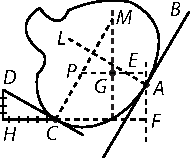
\includegraphics[scale=1]{gesamttex/edit_VIII-4/images/LH_42_05_042_d_042r.pdf}
\edcaption[0.5em]{%
\lbrack\textit{Fig.~1}\rbrack}
\end{edfigure}
\pstart
\noindent
Si 
\edtext{pondus\indexS{pondus} \textit{GAC}\lbrack,\rbrack}{%
\lemma{pondus}%
\Bfootnote{%
\textit{(1)}~\textit{G}
\textit{(2)}~\textit{GAC}
\textit{(a)}~\textit{L}}} 
cujus centrum gravitatis\indexS{centrum gravitatis} \textit{G}\lbrack,\rbrack\ incumbat duobus planis\indexS{pondus duobus planis incumbens} \textit{AB}, 
\edlabel{42_05_042_1a}%
\edtext{}{%
\xxref{42_05_042_1a}{42_05_042_1b}%
\lemma{\textit{CD}}%
\Bfootnote{%
\textit{(1)}~patet 
\textit{(2)}~\bracks{/} Ex punctis~\textit{L}}}%
\textit{CD} \lbrack\textit{Satz bricht ab}\rbrack.
\pend
\pstart
Ex punctis\edlabel{42_05_042_1b}
\textit{G} et \textit{C} demittantur 
\edtext{normales \textit{GE},}{%
\lemma{normales}%
\Bfootnote{%
\textit{(1)}~in
\textit{(2)}~\textit{GE},~\textit{L}}}
\textit{CF} in rectam horizonti\indexS{horizon} perpendicularem \textit{EF} transeuntem per \textit{A}. 
\edtext{Constat perinde esse ac si pondus\indexS{pondus} \textit{GCA} esset}{%
\lemma{Constat}%
\Bfootnote{%
\textit{(1)}~\textit{G} agere perinde ac si suspensum %
\textit{(2)}~perinde %
\textit{(a)}~esset %
\textit{(b)}~esse ac si pondus
\bars{\textit{GCA} \textit{erg.}}
\textit{(aa)}~suspensum ex \textit{G}, %
\textit{(bb)}~vel %
\textit{(cc)}~esset~\textit{L}}} 
suspensum ex puncto \textit{G} extremitate brachii \textit{GE} mobilis\indexS{brachium mobile} 
\edtext{circa \textit{E} quod vocemus pondus\indexS{pondus}}{%
\lemma{circa \textit{E}}%
\Bfootnote{%
\textit{(1)}~et ac %
\textit{(2)}~quod vocemus %
\textit{(a)}~punctu %
\textit{(b)}~pondus~\textit{L}}} 
\textit{G}, vel perinde esse ac si ex 
\edtext{puncto \textit{C} extremitate}{%
\lemma{puncto \textit{C}}%
\Bfootnote{%
\textit{(1)}~suspensum esset pondus quo %
\textit{(2)}~extremitate~\textit{L}}} 
brachii mobilis\indexS{brachium mobile} circa \textit{F} suspensum esset pondus\indexS{pondus} quod vocabimus pondus\indexS{pondus} \textit{C}, 
ita se habens ad pondus\indexS{pondus} \textit{G} ut \textit{GE} ad \textit{CF} seu reciproce ut brachia.\indexS{brachium}
Jam pondus\indexS{pondus} \textit{C} aget in planum\indexS{pondus agens in planum} 
\edtext{\bracks{\textit{CD}}}{%
\lemma{}%
\Bfootnote{\textit{C} \textit{L ändert Hrsg.}}}
potentia\indexS{potentia} quae sit ad totum pondus\indexS{pondus} \textit{C}, 
\edtext{ut \textit{DC} ad \textit{CH},}{%
\lemma{ut \textit{DC}}%
\Bfootnote{%
\textit{(1)}~ad \textit{CH} posito \textit{D} %
\textit{(2)}~cathetus ad %
\textit{(3)}~ad \textit{CH},~\textit{L}}} 
posito \textit{DH} 
\ledpb%
esse verticalem \textit{CH} horizontalem; ergo vis\indexS{vis quam patitur planum} quam patitur planum\indexS{planum}
\edtext{\textit{CD}}{%
\lemma{}%
\Bfootnote{%
\textit{CD} 
\textit{erg.~L}}}
est 
\edtext{ad pondus\indexS{pondus} \textit{G},}{%
\lemma{ad}%
\Bfootnote{%
\textit{(1)}~vim ponderis %
\textit{(2)}~pondus \textit{G}~\textit{L}}}
in ratione composita \textit{CH} ad \textit{DC}, et \textit{GE} 
\edtext{ad \textit{CF}. Jam $CH:DC\squaredots MG:\lbrack PM\rbrack$\lbrack,\rbrack\ fit}{%
\lemma{ad \textit{CF}}%
\Bfootnote{%
\textit{(1)}~seu in ratione $CH\cdot GE$ ad $DE\cdot CF$ \bars{seu \textit{streicht Hrsg.}} %
\textit{(2)}~. Jam $CH:DC\squaredots$ %
\textit{(a)}~$MP:GM$ %
\textit{(b)}~$MG:$ \bars{\textit{GP} \textit{ändert Hrsg.}} fit~\textit{L}}} 
ratio composita 
$MG\cdot GE:
\edtext{\lbrack PM\rbrack}{%
\lemma{}%
\Bfootnote{\textit{GP} \textit{L ändert Hrsg.}}}
\cdot CF$. 
\pend

\section[tocentry={Solutio problematis R.\,P.~Vannii S.\,J.
\enskip \bracks{April \textendash\ Juni 1690}%
},
head={Solutio problematis R.\,P.~Vannii S.\,J.}]
{\MakeUppercase{Solutio problematis R.\,P.~Vannii S.\,J.}
\newline \bracks{April \textendash\ Juni 1690}%
}
\label{41823}
\include{gesamttex/edit_VIII-4/LH_35_10_13_009+010-011.tex}





\chapter[tocentry={Si concursus nisuum sit extra centrum gravitatis
\enskip \bracks{April \textendash\ Mai 1690\,(?)}%
},
head={Si concursus nisuum sit extra centrum gravitatis}]
{\MakeUppercase{Si concursus nisuum sit extra centrum gravitatis}
\newline \bracks{April \textendash\ Mai 1690\,(?)}%
}

\label{60314}




\begin{ledgroupsized}[r]{120mm}
\footnotesize
\pstart
\noindent\textbf{Überlieferung:}
\pend
\end{ledgroupsized}
\begin{ledgroupsized}[r]{114mm}
\footnotesize
\pstart \parindent -6mm
\makebox[6mm][l]{\textit{L}}%
Konzept: 
LH XXXVII~5 Bl.~74.
Ein Blatt 8\textsuperscript{o}. 
\href{\Scan{LH_37_05_074wz}}%
{Gegenmarke} eines Wasserzeichens in der Blattecke;
Papiererhaltungsmaßnahmen;
Alle Ränder beschnitten.
Zwei Seiten.
\pend
\end{ledgroupsized}
\vspace{5mm}
\begin{ledgroup}
\footnotesize
\pstart
\noindent
\textbf{Datierungsgründe:}
Der Träger von N.\;\ref{60314} enthält die Gegenmarke eines Wasserzeichens. Diese kommt auch im Zeugen \textit{L\textsuperscript{2}} der \glqq Solutio problematis R.\,P. Vannii S.\,J.\grqq\ (N.\;\ref{41823}) vor, den Leibniz während seiner Rückkehr aus Italien abfasste, und zwar zwischen April und Juni 1690 (siehe die Einleitung zu N.\;\ref{intro_vanni-solutio-problematis}). Da Leibniz vor oder während seines Aufenthaltes in Wien (30. April bis Mitte Mai 1690) mit der Arbeit an N.\;\ref{41823} begann, muss ihm zu diesem Zeitpunkt Papier von der Sorte vorhanden sein, die wir auch in N.\;\ref{60314} wiederfinden. Daher teilen beide Stücke einen Terminus post quem (April 1690); ferner erscheint eine Entstehung des kurzen Konzepts N.\;\ref{60314} binnen einer entsprechenden Zeitspanne als wahrscheinlich, was den vorgeschlagenen Terminus ante quem ergibt.
\pend 
\end{ledgroup}
\vspace{8mm}
\pstart\noindent
\href{\Scan{LH_37_05_074r}}%
{\lbrack74~r\textsuperscript{o}\rbrack} 
\pend
\nobreak	%
\begin{edfigure}[0em][0.5em]
\includegraphics[scale=1]{%
gesamttex/edit_VIII-4/images/LH_37_05_074_d1_074r.pdf}
\end{edfigure}
\pstart\noindent
Si nisuum\indexS{nisus} 
\edtext{grave\indexS{grave} sustinentium}{\lemma{}\Bfootnote{grave \bars{impellentium vel \textit{gestr.}} sustinentium \textit{erg.~L}}} 
\textit{AC}, \textit{EC} 
\edtext{(\textls{fig.\;1})}{\lemma{}\Bfootnote{(\textls{fig.\;1}) \textit{erg.~L}}}
concursus\indexS{concursus nisuum grave sustinentium} \textit{C} coincidat cum centro gravitatis\indexS{centrum gravitatis} \textit{G}, 
\edtext{erunt vires sustinentes\indexS{vis sustinens}}{\lemma{erunt}\Bfootnote{%
\textit{(1)}~conatus su %
\textit{(2)}~vires sustinentes~\textit{L}}}
inter se et ad grave\indexS{grave} 
\edtext{ut in}{\lemma{ut}\Bfootnote{%
\textit{(1)}~latera %
\textit{(2)}~in~\textit{L}}}
completo parallelogrammo \textit{CEFA}, 
cujus diagonalis sit verticalis, latera parallelogrammi sunt inter se et ad diagonalem. 
\pend
\pstart 
Quod si 
\edtext{concursus nisuum\indexS{concursus nisuum}}{\lemma{concursus}\Bfootnote{%
\textit{(1)}~gravium sit extra centrum~g %
\textit{(2)}~nisuum~\textit{L}}}
\textit{C} sit extra centrum gravitatis\indexS{centrum gravitatis} (\textit{G})\lbrack,\rbrack\ 
cadat tamen in ejus directionem, 
ut nempe \textit{C}(\textit{G}) sit verticalis\lbrack,\rbrack\ idem est quod 
\edtext{ante, perinde}{\lemma{ante,}\Bfootnote{%
\textit{(1)}~nam %
\textit{(2)}~perinde~\textit{L}}}
enim est ac si pondus reductum in punctum (\textit{G}) suspensum esset ex puncto \textit{C}, 
ubi nihil refert quam longum sit filum.\indexS{filum} 
\pend
\clearpage
\pstart
Sed 
\edtext{et}{\lemma{}\Bfootnote{et \textit{erg.~L}}} 
si concursus nisuum\indexS{concursus nisuum} \textit{C} sit extra lineam directionis\indexS{linea directionis} 
ipsius centri gravitatis\indexS{centrum gravitatis} ((\textit{G})) idem adhuc verum. 
Quod demonstrare cum magnum operae pretium esse videatur 
conficiemus diversis modis idem concludentibus. 
\pend
\begin{edfigure}[1.32em][0.5em]
\includegraphics[scale=1]{%
gesamttex/edit_VIII-4/images/LH_37_05_074_d2_074r.pdf}
\end{edfigure}
\pstart
Incumbat exempli 
\edtext{gratia (\textls{fig.\;2}) circulus}{%
\lemma{gratia}\Bfootnote{%
\textit{(1)}~globus 
\textit{(a)}~ce
\textit{(b)}~duobus plan %
\textit{(2)}~fig.
\textit{(3)}~(\textls{fig.\;2}) circulus~\textit{L}}}
centrum habens \textit{C} duabus 
\edtext{rectis inclinatis\indexS{recta inclinata} \textit{AB}, \textit{ED}; utique}{%
\lemma{rectis}%
\Bfootnote{%
\textit{(1)}~inclinatis; cum
\textit{(2)}~inclinatis \textit{AB}, \textit{ED}; utique~\textit{L}}}
cum nisus sint in normali ad tangentem, concurrent in centro circuli \textit{C}, 
nempe \textit{AC}, \textit{EC}. Quod si jam circuli centrum gravitatis\indexS{centrum gravitatis} sit extra centrum 
\edtext{figurae,\indexS{centrum figurae} quod}{\lemma{figurae,}\Bfootnote{%
\textit{(1)}~q %
\textit{(2)}~imo et ejus directionem, %
\textit{(3)}~quod~\textit{L}}}
utique fieri potest, si constet ex materia heterogenea\lbrack,\rbrack\ poterit ita collocari circulus ut 
\edtext{centrum circuli \textit{C},}{\lemma{centrum}\Bfootnote{%
\textit{(1)}~grav. ejus, \textit{G}, %
\textit{(2)}~circuli \textit{C},~\textit{L}}}
etiam cadat extra lineam directionis\indexS{linea directionis centri gravitatis} ipsius 
centri gravitatis\indexS{centrum gravitatis} \textit{G}\lbrack,\rbrack\
quo facto quaeritur quantum in eo situ premantur plana. 
Ajo eodem prorsus modo premi, ac si centrum gravitatis\indexS{centrum gravitatis}
\edtext{\textit{G}}{\lemma{}\Bfootnote{\textit{G} \textit{erg.~L}}}
esset in centro circuli \textit{C}, seu in puncto concursus\indexS{concursus nisuum}\indexS{punctum concursus nisuum} nisuum.\indexS{nisus} 
Et quidem fatendum 
\edtext{est ob \textit{CA},}{%
\lemma{est}%
\Bfootnote{%
\textit{(1)}~sal
\textit{(2)}~poss
\textit{(3)}~ob
\textit{(a)}~\textit{CE},
\textit{(b)}~\textit{CA},
\textit{(c)}~\textit{CA},~\textit{L}}}
\textit{CE} aequales posse circulum non impedientibus planis sustinentibus\indexS{plana sustinentia} 
(quae perfecte plana seu polita suppono) gyrari circa \textit{C}, donec \textit{G} 
veniat sub \textit{C}, seu donec \textit{C} sit in directione ipsius \textit{G}. Nobis tamen licet disquirere, 
\edtext{quantum}{\lemma{}\Bfootnote{quantum \textit{erg.~L}}}
ante illam conversionem in ipso momento collocationis
\edtext{datae, plana\indexS{planum}}{\lemma{datae,}\Bfootnote{%
\textit{(1)}~extra %
\textit{(2)}~plana~\textit{L}}}
sustentent. Ut igitur ostendam nihil interesse, 
\edtext{utrum \textit{C}}{\lemma{utrum}\Bfootnote{%
\textit{(1)}~\textit{G} sit extra %
\textit{(a)}~\textit{C} an non %
\textit{(b)}~dire %
\textit{(2)}~et %
\textit{(3)}~\textit{C}~\textit{L}}}
sit extra directionem ipsius \textit{G} an non; considerandum est motum\indexS{motus compositus ex duobus} 
ipsius \textit{G} posse intelligi compositum ex duobus, uno 
\edtext{parallelo et}{%
\lemma{parallelo}%
\Bfootnote{%
\textit{(1)}~ipsi \textit{C}, altero
\textit{(2)}~et~\textit{L}}}
aequali ipsi \textit{C}, altero circulari\indexS{motus circularis} circa \textit{C}, ex his 
\href{\Scan{LH_37_05_074v}}%
{\lbrack74~v\textsuperscript{o}\rbrack}  
posterior nihil mutat in planis, quia salvo eorum situ fieri potest. Itaque prior solus in rationes veniet, 
ac proinde perinde est ac si \textit{G} caderet in \textit{C}, cum idem sit 
\edtext{ipsius \textit{G} motus}{\lemma{ipsius \textit{G}}\Bfootnote{%
\textit{(1)}~descensus seu %
\textit{(2)}~motus~\textit{L}}}
ad rem faciens qui ipsius \textit{C}. 
\pend 
\begin{edfigure}[1em][0.5em]
\includegraphics[scale=1]{%
gesamttex/edit_VIII-4/images/LH_37_05_074_d3_074v.pdf}
\end{edfigure}
\pstart 
Jam quod de globo\indexS{globus} vel circulo demonstravimus, 
ubi rectae \textit{CA}, \textit{CE} sunt aequales, id de aliis quibuscunque corporibus 
quae duobus planis incumbunt,\indexS{corpus duobus planis incumbens} demonstrari potest. 
Hoc modo remotis caeteris 
\edtext{\textls{fig.\;3}}{\lemma{}\Bfootnote{\textls{fig.\;3} \textit{erg.~L}}} 
considerentur punctum concursus\indexS{punctum concursus nisuum} \textit{C}, 
et rectae nisuum\indexS{nisus} \textit{CA}, 
\edtext{\textit{CF}, perpendiculares}{%
\lemma{\textit{CF},}%
\Bfootnote{%
\textit{(1)}~perinde ac si
\textit{(2)}~perpendiculares~\textit{L}}}
ad plana\indexS{planum inclinatum} \textit{AB}, \textit{FG}; perinde ac si eae duae rectae essent rigidae. 
Jam si \textit{CA}, \textit{CF} sint inaequales sumatur alia \textit{CE}, pars ipsius \textit{CF}, 
innitens plano \textit{ED} parallelo ad planum \textit{FG}, 
patet nihil referre quanta sit longitudo rectae \textit{CE}, vel \textit{CF}, 
seu eandem manere pressionem plani\indexS{pressio plani} \textit{AB}, et eam quae est plani \textit{ED} 
esse etiam pressionem plani\indexS{pressio plani} \textit{FG}. 
Itaque cum in casu plani \textit{CE} locum habeat proportio quam initio stabilivimus\lbrack,\rbrack\ 
habebit eadem quoque locum in casu inaequalium rectarum concurrentium, nec referet
utrum \textit{CAE}, sit circulus an Ellipsis vel alia figura quaevis. Et in genere nihil referet 
\edtext{\lbrack utrum\rbrack}{\lemma{}\Bfootnote{utrum \textit{erg.~Hrsg}}}
centrum gravitatis\indexS{centrum gravitatis} coincidat 
in punctum concursus\indexS{punctum concursus nisuum} nisuum\indexS{nisus} an non. 
\edtext{Si plura}{\lemma{Si}\Bfootnote{%
\textit{(1)}~plures %
\textit{(2)}~plura~\textit{L}}}
sint plana duobus remedium mox afferemus. 
\pend
\pstart
Aliter idem 
\edtext{sic probatur}{\lemma{sic}\Bfootnote{%
\textit{(1)}~demonstratur %
\textit{(2)}~probatur~\textit{L}}}
etsi minore nonnihil firmitate\indexS{firmitas} planum \textit{AB} renisu\indexS{renisus} suo 
\edtext{(quasi arcu tenso),}{\lemma{}\Bfootnote{(quasi arcu tenso) \textit{erg.~L}}}
conatur
\edtext{impellere corpus \textit{CAD}, ita ut quodlibet ejus punctum moveatur}{\lemma{impellere}\Bfootnote{%
\textit{(1)}~\textit{C} ut recta %
\textit{(2)}~corpus \textit{CAD}, \lbrack...\rbrack\ moveatur~\textit{L}}}
secundum rectam \textit{AC} et parallelas, perinde ac si 
exiguum latus polygoni quo incumbit \textit{AB} impelleretur 
ita ut quodlibet ejus punctum moveretur parallele ad \textit{AC}. Eodem 
\edtext{modo planum}{\lemma{modo}\Bfootnote{%
\textit{(1)}~p %
\textit{(2)}~quodlibet punctum corporis \textit{C} %
\textit{(3)}~planum~\textit{L}}}
\textit{ED} renisu\indexS{renisus} 
\edtext{suo conatur}{\lemma{suo}\Bfootnote{%
\textit{(1)}~(quasi %
\textit{(2)}~conatur~\textit{L}}}
impellere corpus \textit{CAD} ita ut quodlibet punctum moveatur secundum 
\edtext{rectam \textit{EC}}{\lemma{rectam}\Bfootnote{%
\textit{(1)}~\textit{AC} %
\textit{(2)}~\textit{EC}~\textit{L}}}
et parallelas. Et proinde punctum \textit{G}, quod est centrum gravitatis corporis\indexS{centrum gravitatis corporis} 
et toti corpori aequivalet, recipiet duos nisus\indexS{nisus}\lbrack,\rbrack\ unum in parallela ipsi \textit{AC}, 
alterum in parallela ipsi \textit{EC}, quorum compositio\indexS{compositio nisuum} dabit nisum ipsius \textit{G} verticalem, 
seu aequivalebit ejus gravitati ut in parallelogrammo figurae 1. 
Potest tamen aliquid objici quod facit ut huic argumento satis per se fidi non posset. Nam 
\edtext{(nisi \textit{ED} sit normalis ad \textit{AB})}{\lemma{}\Bfootnote{(nisi \textit{ED} sit normalis ad \textit{AB}) \textit{erg.~L}}} 
ipsum planum\indexS{planum sustinens} \textit{ED} obstat impulsui plani \textit{AB} et viceversa, quod in aliis conatuum compositionibus\indexS{compositio conatuum} non fit. Praeterea 
\edtext{grave \textit{C}}{\lemma{grave}\Bfootnote{%
\textit{(1)}~impulsum conatu ecc %
\textit{(2)}~\textit{C}~\textit{L}}}
impulsum 
\edtext{solo}{\lemma{}\Bfootnote{solo \textit{erg.~L}}}
nisu Eccentrico\indexS{nisus eccentricus}
\textit{AC}, revera non moveretur in parallelis ipsi \textit{AC}, quia simul \textit{G} 
conabitur circulari circa \textit{A} radio \textit{AG}. 
Cui licet nunc obstet alterum planum, videbitur tamen hic 
\edtext{ipse ipsius}{\lemma{ipse}\Bfootnote{%
\textit{(1)}~nisus %
\textit{(2)}~ipsius~\textit{L}}}
\textit{G} circa \textit{A} circulare conantis nisus\indexS{nisus} in planum\indexS{planum sustinens} alterum \textit{ED} 
debere venire in rationes. Idemque est de impulsu ipsius \textit{EC}, 
nisi \textit{G} cadat in rectam \textit{EC}.
\pend
\begin{edfigure}[1em]%
\includegraphics[scale=1]{%
gesamttex/edit_VIII-4/images/LH_37_05_074_d4_074v.pdf}
\edcaption[-4.5ex]{%
\edtext{}{%
\lemma{\textls{fig.\;4}}%
\Cfootnote[nonum]{Ein gestrichener Entwurf zum Diagramm wird nicht wiedergegeben.}}}
\end{edfigure}
\pstart 
\edtext{Sed et alia demonstratio melior suppetit.}{\lemma{Sed}\Bfootnote{\bars{et \textit{erg.}} alia %
\textit{(1)}~adhuc superest %
\textit{(2)}~demonstratio \bars{melior \textit{erg.}} suppetit.~\textit{L}}}
Fig.\;4 ajo primum, eodem modo premi planum \textit{AB}, 
sive corpus \textit{EBA} incumbat in puncto \textit{A}, sive in puncto \textit{B}, sive in ambobus. 
Ducta enim \textit{E3G2} in centrum gravitatis\indexS{centrum gravitatis} \textit{G}, 
\edtext{et ad \textit{AB}}{\lemma{et}\Bfootnote{%
\textit{(1)}~id pat %
\textit{(2)}~ad \textit{AB}~\textit{L}}}
normalibus \textit{A2}, \textit{B3}, patet \textit{EG} sive quatenus fluit
per \textit{ED} circa \textit{E} eodem modo agere in \textit{A}, quo  
\edtext{in \textit{B}\lbrack,\rbrack\ nam etsi \textit{B} videatur facilius moveri 
tamen tanto minus promovetur\lbrack,\rbrack\ unde}{\lemma{}\Bfootnote{%
in \textit{B}
\bars{%
\textit{(1)}~non enim %
\textit{(2)}~nam etsi \lbrack...\rbrack\ minus promovetur \textit{erg.}}
unde~\textit{L}}} 
si ambobus simul sive quatenus volvitur dimidia tantum vis 
est in uno puncto tota in integro plano\indexS{planum integrum} 
v\angles{olve}nte, non ergo refert. 
\pend
\pstart
Hinc jam 
\edtext{sequitur, \textls{quotcunque}}{\lemma{sequitur,}\Bfootnote{%
\textit{(1)}~nisu utcun %
\textit{(2)}~\textls{quotcunque}~\textit{L}}}
\textls{assumtis planis}, et nisibus utcunque eccentricis,\indexS{nisus eccentricus} 
sufficere ut ex centro 
\edtext{gravitatis\indexS{centrum gravitatis} agantur}{%
\lemma{gravitatis}%
\Bfootnote{%
\textit{(1)}~agat
\textit{(2)}~agantur~\textit{L}}}
normales in plana, et perinde fore, ac si ubi normales 
ex centro gravitatis\indexS{centrum gravitatis} planis\indexS{planum sustinens} occurrent, esset contactus.
\pend





\chapter[tocentry={De invenienda potentia sustentandi onus super planum volvens
\enskip \bracks{30.\;April -- Mitte Mai 1690}},
head={De invenienda potentia sustentandi onus super planum volvens}]
{\MakeUppercase{De invenienda potentia sustentandi onus super planum volvens}
\newline \bracks{30.\;April -- Mitte Mai 1690}}
\label{60116}
\begin{ledgroupsized}[r]{120mm}
\footnotesize
\pstart
\noindent\textbf{Überlieferung:}
\pend
\end{ledgroupsized}
\begin{ledgroupsized}[r]{114mm}
\footnotesize
\pstart
\parindent -6mm
\makebox[6mm][l]{\textit{L}}%
Konzept:
LH~XXXV~10, 14~Bl.~9\textendash10. 
Ein Bogen~2\textsuperscript{o};
\href{\Scan{LH_35_10_14_009wz}}%
{Wasserzeichen} im Falz (Papier aus Wien);
geringfügiger Textverlust durch Abrieb auf Bl.~9~r\textsuperscript{o} infolge erneuter Faltung entlang der Blattmitte.
Zweieinhalb Seiten auf Bl.~9~r\textsuperscript{o} bis Bl.~10~r\textsuperscript{o};
Bl.~10~v\textsuperscript{o} leer.
Am oberen Rand von Bl.~9~r\textsuperscript{o}, in Rot, der Vermerk von unklarer Hand \textls{\textit{IX}} (vgl. die Träger der benachbarten Signaturen LH~XXXV~10, 14 Bl.~2 bis 13, u.\,a. 
N.\;\ref{60117},
\ref{60118},
\ref{60115},
\ref{60112},
\ref{60113},
\ref{60114},
\ref{60110},
\ref{41824}
u.\;\ref{60111}
in diesem Band).
\pend
\end{ledgroupsized}
\vspace{5mm}
\begin{ledgroup}
\footnotesize
\pstart
\noindent
\textbf{Datierungsgründe:}
Das Wasserzeichen Wiener Herkunft ist für Leibnizens Aufenthalte in Wien\indexO{Wien} auf dem Weg nach Italien (Mai 1688 bis Februar 1689) und auf der Rückkehr (30 April bis Mitte Mai 1690) belegt.
Folgende zwei Umstände erlauben, die Entstehung von N.\;\ref{60116} auf letzteren dieser Zeiträume zu verorten.
\pend
\pstart
Erstens 
nimmt Leibniz auf \refnote{FnC:35_10_14_009-010_Varignon} ausdrücklichen Bezug auf 
\indexN{\textls{Varignon}, Pierre de 1654\textendash1722}Pierre Varignons 
Analyse des dort behandelten Falls.
Diese Lösung konnte Leibniz im \cite{02028}\textit{Projet d'une nouvelle mechanique}, Paris 1687 (S.\;40\,f.), lesen, den er in Florenz oder Modena (Dezember 1689 bis 2. Februar 1690) exzerpiert hat: siehe N.\;\ref{60365} in diesem Band. 
Zwar war bereits in den \cite{01023}\textit{Acta Eruditorum} von August 1688 (S\;411--414) eine \cite{02166}Rezension erschienen, die auch auf die einschlägige Stelle  einging (S.\;413), und die Leibniz im Laufe seines ersten Wiener Aufenthaltes womöglich lesen konnte.
Allerdings zeigt
die Genauigkeit, mit der er Varignons \textit{fig.\;30} sowie seine eigentümlichen Bezeichnungen \textit{pondus EO} und \textit{superficies GH} übernimmt,
dass ihm das Buch selbst vorlag oder wenigstens seine ausführlichen Auszüge (\refpassage{37_05_217-218_8b}{37_05_217-218_8b} von N.\;\ref{60365} mit den Diagrammen \bracks{\textit{Fig.\;9}} und \bracks{\textit{Fig.\;10}}); genannte Einzelheiten hätte er der Rezension von 1688 nicht entnehmen können.
Folglich setzt N.\;\ref{60116} die Lektüre von Varignons Werk voraus.
\pend
\pstart
Zweitens lässt sich feststellen, dass Leibniz das Diagramm \bracks{\textit{Fig.\;7}} auf S.\;\pageref{Fig:35_10_14_009-010_Fig-7} 
in Anlehnung an die \bracks{\textit{Fig.\;4}} seines Konzepts \textit{Solutio problematis R.\,P.\;Vannii S.\,J.}
angefertigt hat (siehe den Zeugen \textit{L\textsuperscript{2}} von N.\;\ref{41823}, S.\;\pageref{Fig:35_10_13_010-011_Fig-4}).
Er hat zunächst im vorliegenden Konzept die Figur von N.\;\ref{41823} nachgezeichnet, auch die Buchstaben zur Bezeichnung der Punkte fast ausnahmslos übernommen; diese hat er aber durch Zahlen ersetzt und im einschlägigen Abschnitt von N.\;\ref{60116} die Punkte durch entsprechende Zahlen bezeichnet.
Daher muss N.\;\ref{60116} nach N.\;\ref{41823} entstanden sein,
zumindest nach dessen Kernteil (\refpassage{35_10_13_010-011_16a}{35_10_13_010-011_16a}), den Leibniz auf dem Rückweg nach Deutschland, vor oder spätestens während seines Aufenthaltes in Wien verfasst hatte, und den er noch im Mai 1690 zu veröffentlichen beabsichtigte (siehe die Einführung zu N.\;\ref{intro_vanni-solutio-problematis}).
\pend 
\end{ledgroup}
\clearpage
\selectlanguage{latin}
\vspace{8mm}
\pstart
\noindent
\href{\Scan{LH_35_10_14_009r}}%
{\lbrack9~r\textsuperscript{o}\rbrack} 
\pend\nobreak
\begin{edfigure}[0em][.5em]
\includegraphics[scale=1]{%
gesamttex/edit_VIII-4/images/LH_35_10_14_009-010_d1_009r.pdf}
\edcaption{%
\edtext{\lbrack\textit{Fig.~1, tlw. Blindzeichnung}\rbrack}{%
\lemma{\lbrack\textit{Fig.~1}\rbrack}%
\Cfootnote[nonum]{Der Punkt \bracks{(M)} heißt bei Leibniz \textit{M}; diese Bezeichnung ändert Hrsg. gemäß den Angaben im Text. Ein gestrichener Entwurf zum Diagramm wird nicht wiedergegeben.}}}
\end{edfigure}
\vspace{0.5em}		%
\pstart
\noindent
\lbrack\textit{Nachfolgend kleingedruckter Text gestrichen:}\rbrack
\pend
\nobreak
\vspace{0.5em}
\footnotesize	%
\pstart 
\noindent
\edtext{Sit onus \textit{GCD} cujus}{%
\lemma{Sit}%
\Bfootnote{%
\textit{(1)}~pondus
\textit{(2)}~onus \bars{\textit{GCD} \textit{erg.}} cujus~\textit{L}}}
centrum gravitatis\indexS{centrum gravitatis} \textit{G}; superficies \textit{VDS} qua tangit planum sustentans\indexS{planum sustentans} \textit{AD} punctum affixae chordae 
\edtext{\textit{CBE}, tractae}{%
\lemma{\textit{CBE},}%
\Bfootnote{%
\textit{(1)}~trahentis
\textit{(2)}~tractae~\textit{L}}}
in linea \textit{BC}, a pondere \textit{E} appenso,\indexS{pondus appensum} et perpendiculariter descendente.
\edtext{Quaeritur magnitudo}{%
\lemma{Quaeritur}%
\Bfootnote{%
\textit{(1)}~\bars{situs \textit{streicht Hrsg.}} talis
\textit{(2)}~pondus
\textit{(3)}~magnitudo~\textit{L}}}
ponderis \textit{E}, ut sustineat onus 
\edtext{\textit{CGD} et}{%
\lemma{\textit{CGD}}%
\Bfootnote{%
\textit{(1)}~nec tamen
\textit{(2)}~etiam plus
\textit{(a)}~vel
\textit{(b)}~vel minus
\textit{(c)}~et~\textit{L}}}
ab ipso vicissim sustineatur.\indexS{pondera vicissim sustinentia}
\pend
\normalsize		%
\vspace{0.5em}		%
\pstart
\noindent
\edtext{Sit onus \textit{GCSD\greek{d}V}}{%
\lemma{Sit}%
\Bfootnote{%
\textit{(1)}~\textit{G}
\textit{(2)}~onus
\textit{(a)}~\textit{GCD}
\textit{(b)}~\textit{GCSD\greek{d}V}~\textit{L}}}
cujus centrum gravitatis\indexS{centrum gravitatis} \textit{G}, superficies \textit{VDS} qua tangit planum sustentans\indexS{planum sustentans} \textit{AD} in puncto \textit{D}; retineatur praeterea ab affixa chorda \textit{CBE}, tracta in linea \textit{CB} super trochlea\indexS{trochlea} \textit{B}, a pondere\indexS{pondus chordam super trochlea trahens} \textit{E}, perpendiculariter deorsum nitente in recta \textit{BE}, cui (si opus productae\bracks{)} 
\edtext{planum sustentans\indexS{planum sustentans}}{%
\lemma{planum}%
\Bfootnote{%
\textit{(1)}~occurrat in
\textit{(2)}~sustentans~\textit{L}}}
occurrat in \textit{A}. Ponamus jam volvi onus\indexS{onus super plano volvens} super plano, 
\edtext{et ita}{%
\lemma{et}%
\Bfootnote{%
\textit{(1)}~ita %
\textit{(2)}~p %
\textit{(3)}~cum %
\textit{(4)}~ita~\textit{L}}}
transferri ex 
\edtext{situ \textit{GCSD\greek{d}V}}{%
\lemma{situ}%
\Bfootnote{%
\textit{(1)}~\textit{GCD\greek{d}}, %
\textit{(2)}~\textit{GCD\greek{d}V},
\textit{(2)}~\textit{GCSD\greek{d}V}~\textit{L}}}
in situm \textit{(G)(C)(S)(D)(\greek{d})(V)} planumque jam tangere in 
\edtext{puncto \textit{(\greek{d})} atque ita puncto affixionis\indexS{punctum affixionis} \textit{C} translato}{%
\lemma{puncto}%
\Bfootnote{%
\textit{(1)}~\textit{(D)} %
\textit{(2)}~\textit{(\greek{d})} atque ita
\textit{(a)}~\textit{C} translato in \textit{(C)}, pondus \textit{E} %
\textit{(b)}~puncto affixionis \bars{\textit{C} \textit{erg.}} translato~\textit{L}}}
in \textit{(C)} et centro gravitatis\indexS{centrum gravitatis} \textit{G}, descendente in \textit{(G)} pondus \textit{E}
\edtext{ascendisse in \textit{(E)} debent compensari}{%
\lemma{ascendisse}%
\Bfootnote{%
\bars{in \textit{(E)} \textit{erg.}} %
\textit{(1)}~debet, %
\textit{(2)}~\bars{debent, \textit{ändert Hrsg.}} compensari~\textit{L}}}
inter se ascensus\indexS{ascensus ponderis} descensusque,\indexS{descensus ponderis} ita ut in neutram partem sit 
lucrum; hoc est ut altitudo\indexS{altitudo descensus}
descensus, \textit{Q(Q)} ducta in pondus \textit{G}, aequetur altitudini\indexS{altitudo ascensus} \textit{E(E)} ductae in pondus\indexS{altitudo ducta in pondus} \textit{E}; 
adeoque quod eodem redit, centrum gravitatis commune\indexS{centrum gravitatis commune} 
\textit{K} neque ascenderit neque descenderit, adeoque nec punctum \textit{R} ei respondens in recta 
\edtext{perpendiculari \textit{BA}. Evanescente proinde}{%
\lemma{perpendiculari \textit{BA}.}%
\Bfootnote{%
\textit{(1)}~Quod %
\textit{(2)}~Evanescente %
\textit{(a)}~differentia inter %
\textit{(b)}~proinde~\textit{L}}}
\textit{R(R)} seu differentia inter \textit{BR} 
\edtext{et \textit{B(R)},}{%
\lemma{et}%
\Bfootnote{%
\textit{(1)}~inter \textit{TB} %
\textit{(2)}~\textit{B(R)},~\textit{L}}}
quod idem est, ac si diceremus 
\edtext{\textit{BR} vel \textit{\greek{W}R} quaeri maximam vel minimam. Itaque}{%
\lemma{}%
\Bfootnote{%
\textit{BR} \bars{vel \textit{\greek{W}R}~\textit{erg.}} quaeri maximam \bars{vel minimam~\textit{erg.}}. Itaque~\textit{L}}}
perinde est ac si calculum instituamus quem hactenus exposuimus; efficiendo, 
\edtext{ut fiat}{%
\lemma{ut}%
\Bfootnote{%
\textit{(1)}~fiant
\textit{(2)}~fiat~\textit{L}}}
\textit{E(E)} in pondus \textit{E} aequalis ipsi \textit{Q(Q)} ductae in pondus \textit{G}; an vero quod longe est 
\edtext{compendiosius; si}{%
\lemma{compendiosius;}%
\Bfootnote{%
\textit{(1)}~invento valore ipsius \textit{BR} %
\textit{(2)}~si~\textit{L}}}
ex assumta \textit{E} quacunque, et simplici situ adhibito ipsius oneris\indexS{situs oneris}
\edtext{\textit{GCSD\greek{d}V}, valorem ipsius \textit{BR}}{%
\lemma{\textit{GCSD\greek{d}V},}%
\Bfootnote{%
\textit{(1)}~calculo investige %
\textit{(2)}~calculo exper %
\textit{(3)}~valorem ipsius \textit{BR}~\textit{L}}}
analytice inventum\indexS{valor analytice inventus} faciamus
\edtext{o\bracks{m}nium}{%
\lemma{}%
\Bfootnote{%
ommnium \textit{L ändert Hrsg.}}} 
possibilium Maximum,\indexS{valor omnium possibilium maximus}
\edtext{adhibitis meis artificiis,\indexS{artificia mea de maximo et minimo} de maximo et minimo,}{%
\lemma{adhibitis \bracks{...} minimo}%
\Cfootnote{Siehe \textsc{G.\,W.~Leibniz}, \cite{02077}\textit{Nova methodus pro maximis et minimis}, \cite{01023}\textit{AE} Oktober 1684, S.\;467--473.}}
quae nullas irrationales morantur, et mire calculum contrahunt.
Ubi tamen inprimis notandum est, si \textit{G} immineat ipsi \textit{D} nullam fieri volutionem,\indexS{volutio}
sed simplicem defluxionem\indexS{defluxio} manente eodem puncto tangente \textit{D} 
\edtext{in quo casu calculum jam sum executus.}{%
\lemma{in \bracks{...} executus}%
\Cfootnote{%
Siehe bspw. \textit{Solutio problematis R.\,P.\;Vannii S.\,J.}, N.\;\ref{41823}, bes. \refpassage{35_10_13_010-011_9a}{35_10_13_010-011_9b} im Zeugen \textit{L\textsuperscript{1}}.}}
Video praeterea rem his propositis non satis fore determinatam; prout enim initium assumitur volutionis,\indexS{volutio} aliud atque aliud prodibit
\edtext{maximum; ut si}{%
\lemma{maximum;}%
\Bfootnote{%
\textit{(1)}~imo assumto quolibet \bars{puncto \textit{D} \textit{streicht Hrsg.}} inveniri potest situs %
\textit{(a)}~ejus optimus %
\textit{(b)}~in plano talis, ut %
\textit{(2)}~ut si~\textit{L}}}
\textit{S} primum cadat in\;\textit{A}, volvetur curva, descendensque inveniet tandem situm aequilibrii\indexS{situs aequilibrii} attrahens pondus\;\textit{E}.
\pend
\pstart
Itaque omissa consideratione curvae, optima methodus haec esse videtur ut rem staticam\indexS{res statica seu res aequilibrii} seu aequilibrii,\indexS{aequilibrium} et quid sustentet, adeoque quid moveat\bracks{,} 
reducamus primum ad apices\indexS{apex grave sustentans} quosdam perpendiculari nisu\indexS{nisus perpendicularis} gravia sustentantes, ita ut nec superficiei gravis,\indexS{superficies gravis} nec superficiei sustentantis, nec lineae 
\edtext{adeo trahentis}{%
\lemma{adeo}%
\Bfootnote{%
\textit{(1)}~nisus %
\textit{(2)}~illi %
\textit{(3)}~trahentis~\textit{L}}}
vel retinentis habeatur 
\edlabel{35_10_14_009-010_1a}%
\edtext{}{%
\xxref{35_10_14_009-010_1a}{35_10_14_009-010_1b}%
\lemma{ratio.}%
\Bfootnote{%
\textit{(1)}~Sit corpus grave, cujus centrum gravitatis \textit{G} %
\textit{(a)}~, sustentatum ab %
\textit{(b)}~. \bars{Hoc \textit{streicht Hrsg.}} corpus sustentetur ab apicibus \bars{seu punctis \textit{streicht Hrsg.}} \textit{A} et \textit{B}, 
\textit{(2)}~Sit gravis cen %
\textit{(3)}~Sit~\textit{L}}}%
gravis centrum \textit{G}, ratio.
\pend
\begin{edfigure}%
\includegraphics[scale=1]{%
gesamttex/edit_VIII-4/images/LH_35_10_14_009-010_d2_009r.pdf}
\edcaption[.2em]{\edtext{\lbrack\textit{Fig.~2}\rbrack}{%
\lemma{\lbrack\textit{Fig.~2}\rbrack}%
\Cfootnote[nonum]{%
Drei gestrichene Entwürfe zum Diagramm werden nicht wiedergegeben.}}}
\end{edfigure}
\pstart
Sit\edlabel{35_10_14_009-010_1b}
gravis centrum \textit{G}, id innitatur puncto \textit{D}, sed pro parte tantum, ut rotam scilicet circa \textit{D}, adeoque descendere possit, quaeritur quantum sit pondus retinens\indexS{pondus grave retinens} \textit{E}.
\pend
\pstart
Cum pondus\indexS{pondus planis incumbens} 
\edtext{cujus centrum gravitatis\indexS{centrum gravitatis} est}{%
\lemma{}%
\Bfootnote{%
cujus centrum gravitatis est \textit{erg.~L}}}
\textit{G} incumbit planis \textit{AB}, \textit{EF}, punctis \textit{C} et \textit{D}, perinde est ac si punctum seu centrum \textit{G} impellatur rectis 
\textit{CG}, \textit{DG} tanquam contis;\indexS{contus}\indexS{conti centrum gravitatis impellentes} sed hi ipsi conti\indexS{contus} impellantur 
\edtext{nisibus\indexS{nisus} \textit{LC}, \textit{MD}.}{%
\lemma{nisibus \textit{LC},}%
\Bfootnote{%
\textit{(1)}~\textit{DM} %
\textit{(2)}~\textit{MD}.~\textit{L}}}
Nimirum grave \textit{G} tendens conatu\indexS{conatus} \textit{GK} perpendiculari tendit simul conatibus \textit{GD}, \textit{GN}\bracks{,} tendens autem conatu \textit{GD} vel \textit{DR}, premit planum \textit{FE} conatu \textit{DM}, tendensque conatu \textit{GN} vel \textit{CS} premit planum \textit{AB} conatu \textit{CL}. %
\pend
\begin{edfigure}[.2em][1em]
\includegraphics[scale=1]{%
gesamttex/edit_VIII-4/images/LH_35_10_14_009-010_d3_009r.pdf}
\edcaption{\edtext{\lbrack\textit{Fig.~3}\rbrack}{%
\lemma{\lbrack\textit{Fig.~3}\rbrack}%
\Cfootnote[nonum]{%
Drei gestrichene Entwürfe zum Diagramm werden nicht wiedergegeben.}}}
\end{edfigure}
\pstart
Videtur hic nasci improba quaedam difficultas; nitens 
\edtext{in \textit{EF} nisu \textit{GD}, vel \textit{DR}, afficit}{%
\lemma{in \textit{EF}}%
\Bfootnote{%
\textit{(1)}~impetu \textit{GD} %
\textit{(2)}~nisu \textit{GD}, 
\bars{\textit{(1)}~vel \textit{DR} %
\textit{(2)}~vel \textit{DR}, \textit{erg.}}
afficit~\textit{L}}}
ipsum tantum nisu \textit{DM}. Ergo videtur resistentia\indexS{resistentia} opus esse ut \textit{DM}; 
\edtext{adeoque sufficiet}{%
\lemma{adeoque}%
\Bfootnote{%
\textit{(1)}~pondere %
\textit{(2)}~sufficiet~\textit{L}}}
pondus ut \textit{D}\textit{M}. Verum vicissim pondus agens directione \textit{MD}; dat ipsi \textit{G}, in directione \textit{DG} tantum conatum\indexS{conatus} ut \textit{VD}, non vero ut \textit{RD}, atque ita ad imprimendum conatum ut \textit{RD}, opus videtur pondere ut \textit{TD}. Quomodo igitur dicemus premi planum \textit{EF}, ponderene 
\edtext{ut \textit{DM}}{%
\lemma{}%
\Bfootnote{%
ut \bars{ut \textit{streicht Hrsg.}} \textit{DM}~\textit{L}}}
an ut 
\edtext{\textit{DT}, pondus vero resistens debere esse}{%
\lemma{\textit{DT},}%
\Bfootnote{%
\textit{(1)}~et pon
\textit{(2)}~pondus vero resistens
\textit{(a)}~premi nisu et %
\textit{(b)}~debere esse~\textit{L}}}
\ledpb%
ut \textit{TD}, an solum ut \textit{MD}. An dicemus aliam esse vim quam excipit planum,\indexS{vis quam excipit planum} 
quae sit ut \textit{DM}, aliam esse vim quam debeat habere pondus quae sit ut \textit{TD}. Cum tamen rationis 
\edtext{sit, utramque vim}{%
\lemma{sit,}%
\Bfootnote{%
\textit{(1)}~utraque vis %
\textit{(2)}~utramque vim~\textit{L}}}
quam patitur planum,\indexS{vis quam patitur planum} et qua sustineri potest\indexS{vis qua planum sustineri potest} contra actionem,\indexS{actio} esse eandem.
\pend
\pstart
Concipi etiam potest, pondus \textit{G} circa centrum \textit{C} agere vectem\indexS{vectis} \textit{CGD}
eodemque propellere punctum \textit{D}, indeque comparandus est descensus 
\edtext{puncti \textit{G} seu progressus}{%
\lemma{puncti \textit{G}}%
\Bfootnote{%
\textit{(1)}~cum propulsione %
\textit{(2)}~seu progressus~\textit{L}}}
in parallela ad \textit{GK}, cum progressu
\edtext{puncti \textit{D} in}{%
\lemma{puncti}%
\Bfootnote{%
\textit{(1)}~cum %
\textit{(2)}~\textit{D} in~\textit{L}}}
parallela ad \textit{D}\textit{M}. Est autem descensus ipsius \textit{G} ad descensum ipsius \textit{D} (in parallelis ad \textit{GK}) ut \textit{CN} ad \textit{CD}.
\pend
\pstart
\href{\Scan{LH_35_10_14_009v}}%
{\lbrack9~v\textsuperscript{o}\rbrack}\ 
Videndum quomodo corpus cujus centrum gravitatis\indexS{centrum gravitatis} \textit{G}, innitens plano\indexS{planum inclinatum} \textit{AD}, sed cum libertate descendendi\indexS{libertas descendendi} moveatur 
\edtext{in plano, et}{%
\lemma{in plano,}%
\Bfootnote{%
\textit{(1)}~et simul
\textit{(2)}~et~\textit{L}}}
an ac quatenus simul volvatur\indexS{corpus volvens} et 
\edlabel{35_10_14_009-010_2a}%
\edtext{}{%
\xxref{35_10_14_009-010_2a}{35_10_14_009-010_2b}%
\lemma{\textls{defluat}. \bracks{/}}%
\Bfootnote{%
\textit{(1)}~Pondus \textit{EO} %
\textit{(2)}~Si Varignonio credimus pondus \textit{EO},~\textit{L}}}%
\textls{defluat}.
\pend
\begin{edfigure}%
\hfill
\includegraphics[scale=1]{%
gesamttex/edit_VIII-4/images/LH_35_10_14_009-010_d4_009v.pdf}
\hfill%
\includegraphics[scale=1]{%
gesamttex/edit_VIII-4/images/LH_35_10_14_009-010_d5_009v.pdf}
\hfill
\edcaption{%
\hspace*{10mm}%
\lbrack\textit{Fig.~4}\rbrack 
\hspace*{30mm}%
\edtext{\lbrack\textit{Fig.~5, tlw. Blindzeichnung}\rbrack%
}{%
\lemma{\lbrack\textit{Fig.~5}\rbrack}%
\Cfootnote[nonum]{%
Vorlage ist die "fig.\;30"
bei \indexN{\textls{Varignon}, Pierre de 1654\textendash1722}\textsc{P.~Varignon},
\cite{02028}\textit{Projet d'une nouvelle mechanique}, Paris 1687, Tafel 4.}}}
\end{edfigure}
\pstart
\edtext{Si \indexN{\textls{Varignon}, Pierre de 1654\textendash1722}Varignonio credimus resistentia superficiei\indexS{resistentia superficiei} \textit{GH}, et potentia\indexS{potentia} \textit{R}, 
sunt invicem, ut lineae \textit{AC}, \textit{AD}, \textit{AB}.}{%
\applabel{FnC:35_10_14_009-010_Varignon}%
\lemma{Si \bracks{...} \textit{AC}, \textit{AD}, \textit{AB}}%
\Cfootnote{Es handelt sich um \indexN{\textls{Varignon}, Pierre de 1654\textendash1722}Varignons \textit{Proposition fondamentale des poids soutenus sur quelque espèce de surfaces que ce soit}, \cite{02028}a.\,a.\,O., S.\;40\,f.}}
pondus\indexS{pondus} \textit{EO},\edlabel{35_10_14_009-010_2b}
Posito \textit{A} esse 
punctum concursus directionis ponderis\indexS{directio ponderis} et potentiarum\indexS{concursus directionis potentiarum et ponderis}
praeterea necessario debet esse \textit{AD} perpendicularis ad 
\edtext{\bracks{\textit{GH}}}{\lemma{}\Bfootnote{\textit{G} \textit{L ändert Hrsg.}}}
in \textit{O}, alioqui corpus volvetur super superficie.\indexS{corpus volvens super superficie} 
Haec itaque perinde ipsi 
\edtext{est, in}{%
\lemma{est,}%
\Bfootnote{%
\textit{(1)}~utrum centrum grav %
\textit{(2)}~in~\textit{L}}}
quo puncto rectae \textit{AC} centrum 
\edtext{gravitatis\indexS{centrum gravitatis} corporis}{%
\lemma{gravitatis}%
\Bfootnote{%
\textit{(1)}~sit %
\textit{(2)}~corporis~\textit{L}}}
sit situm. Et quidem videtur rationi consentaneum nam perinde est, si esset linea 
\ledpb%
rigida pondere carens \textit{AO}, et punctum \textit{A} traheretur appenso pondere\indexS{pondus appensum} \textit{F}, (ubi nihil refert quanta sit longitudo ipsius
\edtext{\textit{AF}) et}{%
\lemma{\textit{AF})}%
\Bfootnote{%
\textit{(1)}~punctum autem %
\textit{(2)}~et~\textit{L}}}
potentia\indexS{potentia} \textit{R}.
\pend
\begin{edfigure}%
\hfill
\includegraphics[scale=1]{%
gesamttex/edit_VIII-4/images/LH_35_10_14_009-010_d6_009v.pdf}
\hfill%
\includegraphics[scale=1]{%
gesamttex/edit_VIII-4/images/LH_35_10_14_009-010_d7_009v.pdf}
\hfill
\edcaption{%
\pagelabel{Fig:35_10_14_009-010_Fig-7}%
\edtext{\lbrack\textit{Fig.~6}\rbrack}{%
\lemma{\lbrack\textit{Fig.~6}\rbrack}%
\Cfootnote[nonum]{%
Leibniz hat die Bezeichnung "\textit{22}" an zwei verschiedene Punkte vergeben.}} 
\hspace*{52mm}%
\edtext{\lbrack\textit{Fig.~7}\rbrack%
\hspace*{8mm}}{%
\lemma{\lbrack\textit{Fig.~7}\rbrack}%
\Cfootnote[nonum]{%
Zur Bezeichnung der Punkte hat Leibniz zunächst Buchstaben verwendet, die fast ausnahmslos aus dem Diagramm \bracks{\textit{Fig.\;4}} von N.\;\ref{41823} (S.\;\pageref{Fig:35_10_13_010-011_Fig-4}) übernommen waren, und erst später die Buchstaben durch Zahlen ersetzt (z.\,B. \textit{4}, \textit{5}, \textit{6}, \textit{7} statt \textit{F}, \textit{H}, \textit{E}, \textit{Q}).}}}
\end{edfigure}
\pstart
Sed si pondus simul pluribus planis incumbat,\indexS{pondus pluribus planis incumbens}
ut in \textit{N} et \textit{O}, major est 
\edtext{difficultas, cum}{%
\lemma{difficultas,}%
\Bfootnote{%
\textit{(1)}~quidem si %
\textit{(2)}~cum~\textit{L}}}
rectae \textit{N.1}, \textit{F.2}, \textit{O.3} non concurrant in uno puncto, sed in tribus \textit{4},\;\textit{5}\;\textit{6}; quae si coinciderent cessat difficultas; sed aliis casibus manet. 
Videtur sic procedi posse: ob directionem resistentiae\indexS{directio resistentiae} in \textit{N} quae est \textit{N.4.7}, et directionem resistentiae\indexS{directio resistentiae} in \textit{O}, quae est
\edtext{\textit{O.6.8}, a quibus}{%
\lemma{\textit{O.6.8},}%
\Bfootnote{%
\textit{(1)}~perinde est %
\textit{(2)}~a quibus~\textit{L}}}
linea directionis\indexS{linea directionis ponderis} ipsius 
\edtext{ponderis nempe \textit{6.4.F},}{%
\lemma{ponderis}%
\Bfootnote{%
\textit{(1)}~secatur in
\textit{(2)}~nempe \textit{6.4.F},~\textit{L}}}
secatur in \textit{6} et \textit{4}, perinde est
ac si adesset linea rigida \textit{6.4.F}, pondere carens, nisi quod totum pondus collectum seu appensum\indexS{pondus appensum} in \textit{F}, et haec linea rigida 
\edtext{trahatur chordis}{%
\lemma{trahatur}%
\Bfootnote{%
\textit{(1)}~in \textit{8} %
\textit{(2)}~chordis~\textit{L}}}
\textit{8.6}, et \textit{7.4}, quaeritur quae debeat esse proportio ponderum,\indexS{proportio ponderum} ut \textit{6.4} 
\edtext{maneat horizonti perpendicularis. Pro}{%
\lemma{maneat}%
\Bfootnote{%
\textit{(1)}~linea %
\textit{(2)}~recta per %
\textit{(3)}~horizonti perpendicularis. %
\textit{(a)}~Tollamus %
\textit{(b)}~Pro~\textit{L}}}
uno pondere\indexS{pondus} concipiamus tantum chordam seu potius lineam rigidam \textit{8.6}, in \textit{7} firmiter annexam et circa \textit{7} rotatilem. Pondere 
\edtext{jam altero}{%
\lemma{jam}%
\Bfootnote{%
\textit{(1)}~assumto %
\textit{(2)}~altero~\textit{L}}}
\textit{9} assumto quocunque quaeritur situs ipsius \textit{8.6}, adeoque et ipsius \textit{6.4.F} (semper verticaliter ponendi) talis,
ut descensus centri gravitatis\indexS{centrum gravitatis}\indexS{descensus centri gravitatis} \textit{9} et \textit{F}, 
sit omnium possibilium maximus,\indexS{descensus centri gravitatis omnium possibilium maximum} id centrum sit \textit{K}, debet \textit{7.K} esse maxima. 
Datur \textit{8.6} licet pro arbitrio assumenda, datur et \textit{8.10}, et \textit{7.10}, item \textit{6.4}, et \textit{6.F}. 
\pend
\pstart
Assumatur \textit{7.11} pro arbitrio, datur et \textit{11.10}, quae est $\textit{7.10}-\textit{7.11}$ cujus quadratum si subtrahas ab \textit{8.6} data, habetur \textit{8.12}, quam subtrahendo ab \textit{8.10}, restat \textit{10.12} 
\edlabel{35_10_14_009-010_4a}%
\edtext{}{%
\xxref{35_10_14_009-010_4a}{35_10_14_009-010_4b}%
\lemma{}%
\Afootnote{%
\textit{Am Rand}: Hic calculus supponit rectam \textit{6.4.F} vi aliqua inter mutandum horizonti\textsuperscript{\bracks{a}} perpendicularem servari et ita quaeri optimum situm ita non opus supponere semper \textit{6.4.F} maneret perpendicularem.
\\[1.5ex]
{\footnotesize
\textsuperscript{\lbrack a\rbrack}horizonti %
\textit{(1)}~paralle %
\textit{(2)}~recta %
\textit{(3)}~perpendicularem~\textit{L}}}}%
\edtext{vel \textit{6.11} vel \textit{7.13},}{%
\lemma{vel \textit{6.11}}%
\Bfootnote{%
\textit{(1)}~v %
\textit{(2)}~porro
\textit{(3)}~vel \textit{7.13},~\textit{L}}}
cujus quadrato si addas qu. \textit{4.13} (quae fit a \textit{6.4} data subtrahendo \textit{10.11} seu \textit{6.13}) restat quadr. de \textit{4.7}. Jam si \textit{4.7} subtrahas a $\textit{4.7}+\textit{7.9}$ data
\edtext{restat \textit{7.9}. Jam $\textit{13}.F-\textit{7.9}=\textit{9.14}$ seu $\textit{6}.F-\textit{7.10}$}{%
\lemma{restat \textit{7.9}.}%
\Bfootnote{%
\textit{(1)}~cui addas \textit{9.K}. quae se habet %
\textit{(2)}~Jam %
\textit{(a)}~$\textit{7.9}-\textit{13}.F$ seu \textit{7.9} %
\textit{(b)}~$\textit{13}.F-\textit{7.9}$~\textit{L}}}
$\!-\,\textit{7.9}=\textit{9.14}$,
jam \textit{9.K} est ad \textit{9.14} 
\edtext{ut pondus}{%
\lemma{ut}%
\Bfootnote{%
\textit{(1)}~\textit{F} ad
\textit{(2)}~pondus~\textit{L}}}
\textit{F} ad pondus $\textit{9}+F$, addendo ergo \textit{9.K} ad \textit{7.9}. habetur \textit{7.K} quaesita ad minimam
\edlabel{35_10_14_009-010_3a}%
\edtext{}{%
\xxref{35_10_14_009-010_3a}{35_10_14_009-010_3b}%
\lemma{determinanda.}%
\Bfootnote{%
\textit{(1)}~\textit{7.11} sit %
\textit{(a)}~\textit{y} %
\textit{(b)}~\textit{7}. \textit{8.6} sit %
\textit{(aa)}~\textit{8} %
\textit{(bb)}~\textit{6} %
\textit{(cc)}~\textit{8}; \textit{6.F} sit \textit{6}. \textit{6.4} sit \textit{4}. %
\textit{(aaa)}~$\textit{4.7}+\textit{7}$ %
\textit{(bbb)}~\textit{8.10} sit \textit{10}. \textit{7.10} sit \textit{12}. $\sqrt{-\overline{\textit{12}-\textit{7}}^2+\textit{8}^2}=\textit{8}.\textit{12}$ %
\textit{(2)}~\textit{7.11} sit \textit{y}~\textit{L}}}%
determinanda.
\pend
\pstart
\textit{7.11} sit \textit{y}\bracks{,}\edlabel{35_10_14_009-010_3b}
\textit{8.6},\,\textit{a}\bracks{,} \textit{4.7.9}\,\textit{e}, 
\textit{8.10}\,\textit{b}, \textit{7.10},\,\textit{c}.\bracks{,} 
\textit{6.4}\,\textit{g}, \textit{6.F}\,\textit{h}\bracks{,} pondus \textit{9},\,\textit{p},
pondus \textit{F}\,\textit{f}. %
\pend
\pstart
$\textit{11.10}=c-y$,
\edtext{fit}{\lemma{}\Bfootnote{fit \textit{erg.~L}}}
$\sqrt{aa-\overline{c-y}^2}=\textit{8.12}=m$\bracks{,}
$b-m=\textit{10.12}$ vel \textit{6.11} vel \textit{7.13}\bracks{,} $\textit{4.13}=\textit{6.4}-\textit{7.11}=g-y$\bracks{,} 
$\overline{7.13}^2+\overline{4.13}^2=\overline{4.7}^2$.
Ergo $\sqrt{\overline{b-m}^2+\overline{g-y}^2}=\overline{4.7}=n$, $e-n=\textit{7.9}$. 
\pend
\pstart
Porro $\textit{13}.F=\textit{6}.F-7.\textit{10}=h-y=\textit{7.14}$, unde auferendo \textit{7.9}. 
\edtext{fit $h-y-e+n=\textit{9.14}$}{%
\lemma{fit $h-y-e+n=$}%
\Bfootnote{%
\textit{(1)}~\textit{K.14} %
\textit{(2)}~\textit{7.14} %
\textit{(3)}~\textit{9.14}~\textit{L}}}
cujus%
\edlabel{35_10_14_009-010_4b}
sumenda portio \textit{9.K}, quae fit multiplicando per \textit{f}, et dividendo per $f+p$. Ergo fiet $\textit{9}.K=\overline{h-y-e+n}\;f:\overline{f+p}$ quam addendo ad \textit{7.9} 
fit $e-n+\overline{\overline{h-y-e+n}\;f:\overline{f+p}}= \text{Max}$.
\pend
\begin{edfigure}%
\includegraphics[scale=1]{%
gesamttex/edit_VIII-4/images/LH_35_10_14_009-010_d8_009v.pdf}
\edcaption[.2em]{\edtext{\lbrack\textit{Fig.~8}\rbrack}{%
\lemma{\lbrack\textit{Fig.~8}\rbrack}%
\Cfootnote[nonum]{%
Ein nicht gestrichener Entwurf zum Diagramm wird nicht wiedergegeben.}}}
\end{edfigure}
\pstart
Unde fiet $d\overline{n}\;\overline{f+p}=dnf-d\overline{y}\; f$ seu $d\overline{n}\; p+d\overline{y}\; f=0$, idque praevideri poterat, sine calculo, nihil aliud enim dicit quam ascensum\indexS{ascensus ponderis} 
\edtext{ipsius puncti \textit{6},}{%
\lemma{ipsius}%
\Bfootnote{%
\textit{(1)}~ponderis \textit{6}, qui est $d\overline{n}$ %
\textit{(2)}~puncti \textit{6},~\textit{L}}}
seu ponderis \textit{f} qui est $d\overline{y}$, et descensum ponderis\indexS{descensus ponderis} \textit{p}, qui est $d\overline{n}$, vel potius qui est $-d\overline{n}$ qui in 
\edtext{quantum \textit{n} seu}{%
\lemma{quantum}%
\Bfootnote{%
\textit{(1)}~\textit{n}, crescit, in ta %
\textit{(2)}~\textit{n} seu~\textit{L}}}
\textit{4.7} crescit, in tantum \textit{7.9} decrescit et contra, esse reciproce ut pondera.
\edtext{Jam $d\overline{n}=\overline{\cancel{2}\;\overline{b-m}.\overline{-dm}+\cancel{2}\;\overline{g-y}.\overline{-dy}}:\cancel{2}n$}{%
\lemma{}%
\Bfootnote{%
Jam $d\overline{n}$ \bars{seu potius $2d\overline{n}$ \textit{gestr.}} $=\overline{\cancel{2}\;\overline{b-m}.\overline{-dm}+\cancel{2}\;\overline{g-y}.\overline{-dy}}:\cancel{2}n$~\textit{L}}}
et $d\overline{m}=-2\;\overline{c-y}.\overline{-dy}:2m=\overline{c-y}\; dy:m$. Fit $-\overline{b\cdot\overline{c-y}:m}+
\underset{c-g}
{\ovalbox{\overline{c-y}-\overline{g-y}}}
=-fn:p$.
\pend
\pstart
Jam \textit{n} 
\edtext{e\bracks{s}t}{%
\lemma{}\Bfootnote{et \textit{L ändert Hrsg.}}}
\textit{4.7}. $c-y$ est \textit{10.11}. vel \textit{6.12} et \textit{m} est \textit{8.12}. Hinc  
\edtext{$b\cdot\overline{c-y}:m$ est recta}{%
\lemma{$b\cdot\overline{c-y}:m$ est}%
\Bfootnote{%
\textit{(1)}~quantitas %
\textit{(2)}~recta~\textit{L}}}
quae est ad \textit{b} seu \textit{8.10} ut $c-y$ seu \textit{6.12} est ad \textit{m} seu ad \textit{8.12}. Sed haec recta est \textit{10.15}. quae habetur producendo \textit{86}. dum ipsi \textit{10.14} occurrat in \textit{15}, cui si addas \textit{15.16} seu \textit{g}, quae habetur ducendo \textit{4.16} parallelam ipsi \textit{8.6}. ipsi \textit{10.14} occurrentem in \textit{16}, fiet $\textit{10.15}=\overline{b\cdot\overline{c-y}:m}+g$, unde si auferas \textit{7.10} seu \textit{c}, fiet $\textit{7.16}=b.\overline{c-y}:m+g-c$. Ergo fit $\textit{7.16}=fn:p$ seu \textit{7.16} ad \textit{4.7}, ut \textit{f} ad \textit{p}. Jam \textit{8.15} secet \textit{4.7} in \textit{5}, patet esse \textit{7.16} ad \textit{7.4} ut \textit{15.16} seu \textit{6.4} ad \textit{5.4}. %
\pend
\pstart
Itaque pondus appendendum\indexS{pondus appensum} in \textit{9} est ad 
\edtext{pondus\indexS{pondus} datum}{%
\lemma{pondus}%
\Bfootnote{%
\textit{(1)}~appendend %
\textit{(2)}~datum~\textit{L}}}
integrum \textit{f}, ut \textit{4.5} ad \textit{4.6} datam.%
\pend
\pstart
Eodem ergo modo investigabimus quantitatem ponderis\indexS{pondus appensum} in \textit{18} appendendi, producatur \textit{7.4} donec ipsi \textit{8.18} occurrat in \textit{19}. et huic per \textit{6} ducatur parallela \textit{6.20}, erit pondus \textit{18} ad pondus \textit{F} ut \textit{8.6} ad \textit{8.20}, seu 
\edtext{ut \textit{6.5}}{%
\lemma{ut}%
\Bfootnote{%
\textit{(1)}~\textit{6.17} %
\textit{(2)}~\textit{6.5}~\textit{L}}}
ad \textit{6.4}. 
Itaque pulcherrima conclusione, latera 
\edtext{trianguli \textit{6.4.5}}{%
\lemma{trianguli}%
\Bfootnote{%
\textit{(1)}~\textit{6.14.17}  %
\textit{(2)}~\textit{6.4.} %
\textit{(a)}~\textit{19} %
\textit{(b)}~\textit{5}~\textit{L}}}
in quo tres 
\edtext{directiones ponderis\indexS{directiones potentiarum et ponderis} \textit{F},}{%
\lemma{directiones}%
\Bfootnote{%
\textit{(1)}~se 
\textit{(a)}~inters %
\textit{(b)}~intersecant %
\textit{(2)}~ponderis \textit{F},~\textit{L}}}
potentiae \textit{7} et potentiae\indexS{potentia} \textit{8} se intersecant exhibent potentiarum\indexS{potentia} proportiones, 
scilicet unaquaeque potentia exprimitur per latus trianguli cadens in suam directionem,\indexS{directio potentiae} 
seu potentiae \textit{F}, \textit{7}, \textit{8}, sunt ut rectae \textit{6.4}. et \textit{4.5} et \textit{5.6}. Et quia in triangulo latera sunt ut sinus angulorum\indexS{sinus anguli oppositi} 
\edtext{oppositorum, erunt potentiae quaevis ad quamvis,}{%
\lemma{oppositorum,}%
\Bfootnote{%
\textit{(1)}~erunt %
\textit{(2)}~\bars{erit \textit{streicht Hrsg.}} unaquaeque potentia, ut %
\textit{(3)}~erunt potentiae quaevis ad quamvis,~\textit{L}}}
\edtext{ut sinus angulorum\indexS{sinus anguli directionum duarum potentiarum} quos faciunt duae reliquae potentiae.}{%
\lemma{}%
\Afootnote{%
\textit{Zwischen den Zeilen}: Habeat locum, forte licebit concipere \textit{O} et \textit{N} non esse puncta, sed plana, ut coincidant puncta \textit{4}, \textit{5}, \textit{6}.}} 
Et hinc cum regula\indexS{regula generalis pro velocitate progressus} 
\edtext{general\bracks{i}}{\lemma{}\Bfootnote{generalis \textit{L ändert Hrsg.}}}
pro velocitate progressus,\indexS{progressus}\indexS{velocitas progressus} \textit{dm} est velocitas\indexS{velocitas} qua pondus \textit{6} 
\edtext{transit dextrorsum}{%
\lemma{transit}%
\Bfootnote{%
\textit{(1)}~versus %
\textit{(2)}~dextrorsum~\textit{L}}}
vel sinistrorsum, \textit{dy} qua sursum aut 
\edtext{deorsum et erit}{%
\lemma{deorsum,}%
\Bfootnote{%
\textit{(1)}~\textit{dn} est velocitas qua pondus %
\textit{(2)}~et erit~\textit{L}}}
illa ad hanc ut \textit{6.12} ad \textit{8.12}. Si scilicet radius \textit{8.6} moveatur circa centrum 
\edtext{\textit{8},}{%
\lemma{}%
\Bfootnote{%
\textit{8} \textit{erg.~L}}}
velocitas 
\edtext{qua augetur \textit{8.12} sinus complementi\indexS{sinus complementi}}{%
\lemma{qua}%
\Bfootnote{%
\textit{(1)}~transit %
\textit{(2)}~augetur \bars{\textit{8.12} \textit{erg.}} sinus
\textit{(a)}~rectus %
\textit{(b)}~complementi~\textit{L}}}
\textit{m}, (nempe $d\overline{m}$) est ad velocitatem\indexS{velocitas} qua minuitur 
\edtext{\textit{12.6}}{%
\lemma{}%
\Bfootnote{%
\textit{12.6} \textit{erg.~L}}}
\edtext{sinus rectus\indexS{sinus rectus} (seu}{%
\lemma{sinus}%
\Bfootnote{%
\textit{(1)}~comple %
\textit{(2)}~rectus
\bars{\textit{(1)}~$-y$ \textit{(2)}~$-y$ \textit{gestr.}}
\textit{(a)}~(seu ad $-dy$) ut s %
\textit{(b)}~(seu~\textit{L}}}
ad $dy$ nam sinus rectus est $c-y$) ut sinus rectus\indexS{sinus rectus} ad sinum complementi,\indexS{sinus complementi}
\edtext{seu}{%
\lemma{seu}%
\Bfootnote{%
\textit{(1)}~velocitates sunt reciproce ut %
\textit{(2)}~seu~\textit{L}}}
crementa\indexS{crementum} sunt reciproce ut crescentia vel decrescentia. 
Similiter ex velocitatibus\indexS{velocitas} quibus augentur \textit{m} et \textit{y}, 
determinatur velocitas\indexS{velocitas} qua augetur \textit{n} seu $\sqrt{\overline{b-m}^2+\overline{g-y}^2}$.
\edtext{Sumantur $\omega$}{%
\lemma{}\Bfootnote{Sumantur \bars{rectae \textit{gestr.}} $\omega$~\textit{L}}}
et $\beta$ quae sunt respective ad velocitates crescentium\indexS{velocitates crescentium} $m$ et $y$ ut $b-m$, vel $g-y$ ad \textit{n}, summa $\omega + \beta$ erit velocitas\indexS{velocitas decrescendi} qua decrescunt ipsae \textit{n}.
\pend
\pstart
\noindent
\href{\Scan{LH_35_10_14_010r}}%
{\lbrack10~r\textsuperscript{o}\rbrack}\ 
\pend
\begin{edfigure}[0em][1em]
\includegraphics[scale=1]{%
gesamttex/edit_VIII-4/images/LH_35_10_14_009-010_d9_010r.pdf}
\edcaption{\lbrack\textit{Fig.~9}\rbrack}
\end{edfigure}

\pstart
Mirum 
\edtext{autem videri possit,}{%
\lemma{autem}%
\Bfootnote{%
\textit{(1)}~videtur %
\textit{(2)}~videri possit,~\textit{L}}}
quod eadem prodit regula\indexS{regula pro velocitate progressus} ac si coinciderent puncta \textit{4. 5. 6}. 
Hoc generali Methodo ita videtur demonstrari posse, quod magni est momenti. 
Nempe planum aliquod ut \textit{N} eodem modo premitur a pondere\indexS{pondus planum premens} \textit{F}, sive tangat in puncto \textit{O} uno,  
\edtext{sive in linea}{%
\lemma{sive in}%
\Bfootnote{%
\textit{(1)}~pluribus %
\textit{(2)}~linea~\textit{L}}}
recta integra ut \textit{21.22}. Idem est in plano \textit{N}, et ita tantum opus est ex centro gravitatis\indexS{centrum gravitatis} demitti perpendiculares in plana contactus.\indexS{planum contactus} Atque 
\edtext{ita habebitur}{%
\lemma{ita}%
\Bfootnote{%
\textit{(1)}~res proced %
\textit{(2)}~habebitur~\textit{L}}}
exitus et in casu plurium planorum.
\pend
\pstart
Et quae tunc linea directionis centri gravitatis\indexS{linea directionis centri gravitatis}\indexS{centrum gravitatis} non cadit planum verticale\indexS{planum verticale} cum punctis occursuum seu lineis directionum,\indexS{linea directionis}
\edtext{itaque sumemus}{%
\lemma{itaque}%
\Bfootnote{%
\textit{(1)}~duae %
\textit{(2)}~fingemus planum inclinatum composi %
\textit{(3)}~sumemus~\textit{L}}}
planum inclinatum\indexS{planum inclinatum} in quo est centrum gravitatis\indexS{centrum gravitatis} et duae directiones, inde habebitur directio composita\indexS{directio composita} in illo ipso plano inclinato\indexS{planum inclinatum} quae conjuncta cum aliis directionibus\indexS{directio composita} 
\edtext{compositis, unam demum dabit directionem\indexS{directio totalis}}{%
\lemma{compositis,}%
\Bfootnote{%
\textit{(1)}~una demum prodibit directio
\textit{(2)}~unam demum dabit directionem~\textit{L}}}
totalem quae erit ipsa directio centri gravitatis.\indexS{directio centri gravitatis} 
Videndum an non sic demonstrari possit eodem modo premi planum\indexS{corpus planum premens}
\textit{YOZ} sive in puncto \textit{O}, sive in alio quovis a corpore \textit{FON} tangatur. Nempe si tangitur in \textit{F}, ponatur linea rigida \textit{NF3O}, composita ex rectis 
\edtext{\textit{NF3} et \textit{3O}, est}{%
\lemma{\textit{NF3} et}%
\Bfootnote{%
\textit{(1)}~\textit{FO} %
\textit{(2)}~\textit{3O}, %
\textit{(a)}~hujus vectes inflexi ope %
\textit{(b)}~pr %
\textit{(c)}~pondus collectum in \textit{F} premet \bars{planum in \textit{O} \textit{streicht Hrsg.}} certo modo
\textit{(d)}~est~\textit{L}}}
autem \textit{3O} normalis ad 
\edtext{planum \textit{YO}. Apparet}{%
\lemma{planum \textit{YO}.}%
\Bfootnote{%
\textit{(1)}~Patet
\textit{(2)}~Apparet~\textit{L}}}
eodem modo premere, ac fieret vecte inflexo\indexS{vectis inflexus}
\textit{NFZ}, si esset \textit{FZ} normalis ad \textit{OYZ}. 
Et hoc accuratius examinandum\bracks{,} hoc ipso 
\edtext{enim demonstrato, omne}{%
\lemma{enim}%
\Bfootnote{%
\textit{(1)}~demonstratio, omnis Statica %
\textit{(2)}~demonstrato, omne~\textit{L}}}
Staticae\indexS{Statica} negotium\indexS{negotium Staticae} absolutum est. %
\pend%
\begin{edfigure}%
\includegraphics[scale=1]{%
gesamttex/edit_VIII-4/images/LH_35_10_14_009-010_d10_010r.pdf}
\edcaption{\lbrack\textit{Fig.~10}\rbrack}
\end{edfigure}
\pstart
Addendum 
\edtext{jam quid}{%
\lemma{jam}%
\Bfootnote{%
\textit{(1)}~si %
\textit{(2)}~quid fiat, si plures chordae unam in %
\textit{(3)}~quid~\textit{L}}}
fiat si punctum trahatur a pluribus chordis,\indexS{punctum tractum a pluribus chordis} et harum quaevis rursus a pluribus\indexS{chorda trahens tracta a pluribus aliis} quemadmodum et si sustentacula\indexS{sustentaculum} rursus aliis sustentaculis\indexS{sustentaculum alio sustentaculo incumbens} incumbant, sed hac methodo omnia sunt finita.
\pend
\pstart
Res omnis conspirante conclusione etiam inde 
\edtext{conficitur quod punctis corporis cadentibus}{%
\lemma{conficitur}%
\Bfootnote{%
\textit{(1)}~quod corpore tendente linea quacunque, %
\textit{(a)}~qua %
\textit{(b)}~motu aequidistributo 
\textit{(aa)}~seu %
\textit{(bb)}~nempe 
\textit{(cc)}~ita ut %
\textit{(aa)}~per %
\textit{(bb)}~puncta %
\textit{(2)}~quod punctis corporis %
\textit{(a)}~tendentibus ut %
\textit{(b)}~cadentibus~\textit{L}}}
in rectam perpendicularem ad contactum plani in eadem recta tendentibus, posito motu aequidistributo\indexS{motus aequidistributus}
totum corpus eodem modo tendit adeoque et centrum gravitatis.\indexS{centrum gravitatis} 
Et abstrahendo a renisu materiae\indexS{renisus materiae} qui locum habet in vi viva,\indexS{vis viva} nulla oritur gyratio.\indexS{gyratio}
\pend






\chapter[tocentry={Sphaera gravis sustentata a duobus planis
\enskip \bracks{Mitte Juni -- Dezember 1690\,(?)}},
head={Sphaera gravis sustentata a duobus planis}]
{\MakeUppercase{Sphaera gravis sustentata a duobus planis}
\newline \bracks{Mitte Juni -- Dezember 1690\,(?)}}
\label{60113}
\begin{ledgroupsized}[r]{120mm}
\footnotesize
\pstart
\noindent\textbf{Überlieferung:}
\pend
\end{ledgroupsized}
\begin{ledgroupsized}[r]{114mm}
\footnotesize
\pstart
\parindent -6mm
\makebox[6mm][l]{\textit{L}}%
Konzept:
LH~XXXV~10, 14~Bl.~6. 
Ein Blatt~2\textsuperscript{o};
\href{\Scan{LH_35_10_14_006wz}}%
{Wasserzeichen} in der Blattmitte (Papier aus Osterode im Harz);
linker Rand beschnitten; horizontal gefaltet, im Falz Papierbruch ohne Textverlust.
Eine Seiten auf Bl.~6~r\textsuperscript{o}; Bl.~6~v\textsuperscript{o} leer.
Der Träger bildete ursprünglich eine Einheit mit LH~XXXV~10, 14~Bl.~5 (Träger von N.\;\ref{60114}).
Am oberen Rand von Bl.~6~r\textsuperscript{o}, in Rot, der Vermerk von unklarer Hand \textit{VI}
(vgl. die Träger der benachbarten Signaturen LH~XXXV~10, 14 Bl.~2 bis 13, u.\,a. 
N.\;\ref{60117},
\ref{60118},
\ref{60115},
\ref{60112},
\ref{60116},
\ref{60114},
\ref{60110},
\ref{41824}
und \ref{60111}
in diesem Band).
\pend
\end{ledgroupsized}
\vspace{5mm}
\begin{ledgroup}
\footnotesize
\pstart
\noindent
\textbf{Datierungsgründe:}
Der Träger des vorliegenden Stücks N.\;\ref{60113} hing ursprünglich mit dem Quartblatt LH~XXXV~10, 14~Bl.~5 zusammen, auf dem das Konzept "Perinde est ac si grave impellatur in normalibus ad plana" (N.\;\ref{60114}) überliefert ist. 
Zusammen bilden die Blätter etwa vier Fünftel eines Bogens, dessen verbleibenden Teile bislang nicht identifiziert werden konnten.
Der Träger von N.\;\ref{60113} enthält ein Wasserzeichen mit dem Motiv "Wappen der Stadt Osterode\indexO{Osterode} (Harz)"; N.\;\ref{60114} enthält die Gegenmarke; das Zeichen ist für den Zeitraum 1690 bis 1694 belegt, also für die Zeit unmittelbar nach der italienischen Reise (wobei Leibniz erst in der zweiten Junihälfte 1690 in Hannover eintraf).
\pend
\pstart
Während der Terminus post quem für die Entstehung von N.\;\ref{60113} als sicher gelten darf,
ist der vorgeschlagene Endpunkt lediglich als wahrscheinlich anzusehen.
Die Angabe beruht auf der Feststellung, dass Leibniz sich im Jahr 1690 besonders intensiv mit dem hier erörterten statischen Problem beschäftigte und diese und eng verwandte Fragen durch konsequente Heranziehung seiner Analysis ("Methodus de Maximis et Minimis", hier auf \refnote{FnC_35_10_14_006-maximis}) zu lösen suchte (siehe dazu die auf 1690 datierbaren Stücke N.\;\ref{60112}, N.\;\ref{60220}, und N.\;\ref{41823}).
\pend 
\end{ledgroup}
\vspace*{8mm}
\selectlanguage{latin}
\pstart
\noindent
\href{\Scan{LH_35_10_14_006r}}%
{\lbrack6~r\textsuperscript{o}\rbrack}\ 
\pend
\nobreak
\begin{edfigure}[0em][1em]
\includegraphics[scale=.8]{%
gesamttex/edit_VIII-4/images/LH_35_10_14_006_d1_006r.pdf}
\edcaption{\edtext{\bracks{\textit{Fig.~1, gestrichen}}}{%
\lemma{\bracks{\textit{Fig.~1}}}%
\Cfootnote[nonum]{%
Ein gestrichener Entwurf zum Diagramm wird nicht wiedergegeben.}}}
\end{edfigure}
\begin{edfigure}[1em][1em]
\includegraphics[scale=1]{%
gesamttex/edit_VIII-4/images/LH_35_10_14_006_d2_006r.pdf}
\edcaption[-0.2em]{%
\edtext{\bracks{\textit{Fig.~2}}%
\hspace{10mm}}{%
\lemma{}%
\Afootnote[nonum]{\textit{Neben \bracks{\textit{Fig.~2}}}:
Nihil debet ad r\angles{em} fa\angles{c}ere quae sit figura corporis \textit{ABC} modo normales ad plana incurrant in centrum gravitatis\indexS{centrum gravitatis}}}}
\end{edfigure}
\pstart
\noindent
Sit gravis sphaera \textit{ABC} sustentata\indexS{sphaera a duobus planis sustentata} a duobus planis\indexS{planum inclinatum} \textit{DB}, \textit{EC}, quaeritur quam cuique vim imprimat, seu quae sint pondera\indexS{pondera quibus plana sustinentur} \textit{F}, \textit{G} quibus plana\indexS{planum inclinatum} sustinentur. Pono autem 
\edtext{angulos \textit{BDF} et \textit{CEG} esse rectos et \textit{DE}}{%
\lemma{angulos \textit{BDF}}%
\Bfootnote{%
\textit{(1)}~esse rectos, %
\textit{(2)}~et \textit{CEG} esse rectos %
\textit{(a)}~.~In rect %
\textit{(b)}~et \textit{DE}~\textit{L}}}
esse horizontalem. Ex \textit{A, F, G}, in \textit{DE} agantur 
\edtext{normales, \textit{AH},}{%
\lemma{normales,}%
\Bfootnote{%
\textit{(1)}~\textit{H}, \textit{K}, \textit{L} %
\textit{(2)}~\textit{AH},~\textit{L}}}
\textit{FK}, \textit{GL}. 
Quaeritur situs talis, ut centrum gravitatis\indexS{centrum gravitatis} sit omnium 
\edtext{possibilium infime\indexS{situs centri gravitatis infimus}}{%
\lemma{possibilium}%
\Bfootnote{%
\textit{(1)}~minimum %
\textit{(2)}~infime~\textit{L}}}
situm. Sint pondera \textit{a}, \textit{f}, \textit{g}. 
Erit $AH\cdot a+FK\cdot f+GL\cdot l$ divis. per $a+f+l$ distantia centri gravitatis\indexS{centrum gravitatis} a \textit{DE}, 
quae debet 
\edtext{$\stackrel{(1)}{}$}{\lemma{}\Bfootnote{$\stackrel{(1)}{}$ \textit{erg.~L}}}
esse omnium possibilium maxima.\indexS{distantia centri gravitatis maxima} 
Assumamus \textit{DH} et \textit{AH}, inde caeteri situs 
\edtext{determinabuntur. $DA\!\stackrel{(2)}{=}$}{%
\lemma{determinabuntur.}%
\Bfootnote{%
\textit{(1)}~Datur
\textit{(2)}~$DA\!\stackrel{(2)}{=}$~\textit{L}}}%
$\;\sqrt{DH^2+AH^2}$.
Datur \textit{AB} radius datae sphaerae; cujus quadratum detractum a quadrato \textit{DA}, 
relinquet quadratum \textit{DB}, ergo fiet $DB\stackrel{(3)}{=}\sqrt{DH^2+AH^2-AB^2}$.
Similiter $CE\stackrel{(4)}{=}\sqrt{EH^2+AH^2-AB^2}$. 
Est autem $EH\stackrel{(5)}{=}DE-DH$\bracks{,} 
$DB:BM:MD\stackrel{(6)}{\squaredots}AB:\stackrel{DH-DM}{MH}:MB-AH$. 
Seu $BM:MD\stackrel{(7)}{=}DH-DM,:,MB-AH$ et fiet 
$BM^2-AH\cdot BM\stackrel{(8)}{=}DH\cdot DM\,$%
\edtext{$-\,DM^2$; seu}{%
\lemma{$-\,DM^2$;}%
\Bfootnote{%
\textit{(1)}~seu $DM^2+DM^2\!=$
\textit{(2)}~seu~\textit{L}}}
$AH\cdot BM+DH\cdot DM\stackrel{(9)}{=}BM^2+DM^2$%
\edtext{$\;\stackrel{(10)}{=}DH^2\,$}{%
\lemma{$\;\stackrel{(10)}{=}\,$}%
\Bfootnote{%
\textit{(1)}~$DB^2\stackrel{(11)}{=}$
\textit{(2)}~$DH^2$~\textit{L}}}%
$+\,AH^2-AB^2\stackrel{(11)}{=}AH\cdot BM+DH\cdot DM$ 
quarum duarum aequationum 10 et 11. ope dantur \textit{BM} et \textit{DM}. 
Similiter loco aeqq. 10 et 11. scribemus $CN^2+EN^2\stackrel{(12)}{=}EH^2+AH^2-AB^2\stackrel{(13)}{=}AH\cdot CN+EH\cdot EN$. 
Ita similiter dantur \textit{CN} et \textit{EN} tantumque ad aeqq.~10. 11. 12. 13. 
\edtext{adjungenda ae\bracks{q.}~5. Ponimus}{%
\lemma{adjungenda}%
\Bfootnote{\bars{aeqq. \textit{ändert Hrsg.}} 5. %
\textit{(1)}~Postremo %
\textit{(2)}~Ponimus~\textit{L}}}
autem $DF\stackrel{(14)}{=}EG$, datas. Estque $FK\stackrel{(15)}{=}DF,BM-AH,:AB$ et similiter $GL\stackrel{(16)}{=}DF,CN-AH,:AB$. 
\edlabel{35_10_14_006r_21a}%
\edtext{}{%
\xxref{35_10_14_006r_21a}{35_10_14_006r_21b}%
\lemma{Ex aeq.~1. \bracks{...} $d.AH$}%
\Cfootnote{%
Hier und in der Folge dient das Zeichen \textit{d} bzw. \textit{d.} als Differential-Symbol.}}%
Ex aeq.~1. fit $a\,d.AH + f\,d.FK + l\,d.GL\,$%
\edtext{$\stackrel{(17)}{=}0$ et}{%
\lemma{$\stackrel{(17)}{=}0$}%
\Bfootnote{%
\textit{(1)}~et ex 15 fit %
\textit{(a)}~$DF$ %
\textit{(b)}~$AB\,d\,FK=$
\textit{(aa)}~\angles{$AB$}
\textit{(bb)}~$\overline{BM-AH}\,d\,DF:$
\textit{(aaa)}~$AB$
\textit{(bbb)}~$AB+\overline{DF\, d\, BM}-DF.\overline{d\,AH}.$ %
\textit{(2)}~et~\textit{L}}} 
ex 15 fit $AB.d.FK\stackrel{(18)}{=}DF\,d.BM-DF\,d.AH$.%
\edlabel{35_10_14_006r_21b}
Ex 11 est $DM\stackrel{(19)}{=}DH^2+AH^2-AB^2\,-$%
\edtext{$AH\cdot BM,:DH$ et quadrando 19 fit}{%
\lemma{$AH\cdot BM,:DH$}%
\Bfootnote{%
\textit{(1)}~et $DM^2=$
\textit{(2)}~et quadrando 19 fit~\textit{L}}}
$\ovalbox{DH^4}+AH^4+AB^4+AH^2\cdot BM^2+\ovalbox{2}\cdot DH^2\cdot AH^2+2\cdot AB^2\cdot AH\cdot BM-\ovalbox{2}\cdot AB^2\cdot DH^2-2AB^2\cdot AH^2-2AH\cdot BM\cdot DH^2-2AH^3\cdot BM=\ovalbox{DH^2}\ovalbox{+AH^2\cdot DH^4}\ovalbox{-AB^2\cdot DH^2}$%
\edlabel{35_10_14_006r_1a}%
\edtext{}{%
\xxref{35_10_14_006r_1a}{35_10_14_006r_1b}%
\lemma{$-BM^2\cdot DH^2$. \bracks{/}}%
\Bfootnote{%
\textit{(1)}~Vel si placet brevius procedere $DM=DB^2-AH\cdot BM,:DH. \ovalbox{11}$ (per aeq. 13.) ergo per 9 fit $DB^4+AH^2\cdot BM^2-2DB^2\cdot AH\cdot BM-DH^2\cdot BM^2=DH^2\cdot DB^2=DB^2\cdot DH^2-$ %
\textit{(2)}~$DM^2=DB^2-BM^2=DB^4+AH^2\cdot BM^2-2DB^2\cdot AH.BM,:DH^2$. Ergo $DB^2\cdot DH^2-BM^2\cdot DH^2=DB^4+AH^2\cdot BM^2-2.DB^2\cdot AH\cdot BM$\enskip $DB^2+A^2=DH^2+AH^2$. Ergo $-DB^2+DH^2=-AH^2+AB^2.$ Ergo fit $DB^2\cdot\overline{AB^2-AH^2}=\overline{AH^2+DH^2}\; BM^2-2\cdot DB^2\cdot AH\cdot BM$ seu $DM^2\cdot AB^2-DM^2\cdot AH^2+BM^2\cdot AB^2$\enskip $BM^2\cdot AH^2=AH^2\cdot BM^2+DM^2\cdot BM^2=2\cdot AH\cdot BM^3-2AH\cdot BM\cdot DM^2$\enskip $AH^4+AB^4-2AH^2\cdot AB^2$\bracks{,}
\textit{(a)}~$dB$ %
\textit{(b)}~$BM\; d\; BM+DM\cdot d\; DM=DH\;d \; DH+AH\;d \; AH$ %
\textit{(aa)}~$=AH\;d \; BM+BM\;d \; AH+DH\; d$ %
\textit{(aaa)}~$\ovalbox{+DM.DH}$ %
\textit{(bbb)}~$DM\; d\; DH$. %
\textit{(bb)}~et $2DH\; d\; DH+2AH\; d\; AH=AH\; d\; BM+BM\; d\; AH+DH\; d\; DM+DM\; d\; DH$ %
\textit{(3)}~Sed~\textit{L}}}%
$-\,BM^2\cdot DH^2$.
\pend
\pstart
Sed\edlabel{35_10_14_006r_1b} 
possumus tamen et sic procedere, ut consideremus situm ipsius \textit{EC} qualiscunque 
sit tanquam datum, inde ponamus decurrere \textit{A}, donec \textit{DB} deprimatur, 
ut amplius descendi non possit\bracks{,} et fiet $a\; d.AH+f\;d.FK=0$. %
\pend
\pstart
Et similiter fiet $a\; d.AH+l\;d.GL=0$.
\pend
\pstart
Ergo $f\; d.FK=l\; d.GL$.\enskip\ 
$d.FK=-\overline{a:f}\; d.AH$.\enskip\ 
$d.GL=-\overline{a:l}\; d.AH$.
\pend
\pstart
Sed haec non sint conciliabilia cum aeq.~17. quae tamen et ipsa videbatur esse debere vera.
Nam fieret: $a\; d.AH-a\cdot d.AH+a\; d.HA=0$ quod \edlabel{35_10_14_006r_2a}absurdum.
\edtext{}{\xxref{35_10_14_006r_2a}{35_10_14_006r_2b}\lemma{absurdum.}%
\Bfootnote{%
\textit{(1)}~Jam video in quo peccatum in aeq.~17. nempe quod %
\textit{(2)}~In eo etiam peccatum %
\textit{(3)}~Hinc~\textit{L}}}
\pend
\pstart
Hinc\edlabel{35_10_14_006r_2b} 
perficitur
\edtext{Methodus de Maximis et Minimis.\indexS{Methodus de Maximis et Minimis}}{%
\applabel{FnC_35_10_14_006-maximis}%
\lemma{Methodus de Maximis et Minimis}%
\Cfootnote{Siehe \textsc{G.\,W.~Leibniz}, \cite{02077}\textit{Nova methodus pro maximis et minimis}, \cite{01023}\textit{AE} Oktober 1684, S.\;467--473.}}
\edtext{Nempe cum casus}{%
\lemma{Nempe}%
\Bfootnote{%
\textit{(1)}~ex casibus %
\textit{(2)}~cum casus~\textit{L}}}
sunt infinities infiniti\indexS{casus infinities infiniti} et
\edtext{ex iis maximum}{%
\lemma{ex iis}%
\Bfootnote{%
\textit{(1)}~maximus
\textit{(2)}~maximum~\textit{L}}}
vel minimum quaeritur possunt alternatim omnes assumi constantes
\edtext{praeter duas.}{%
\lemma{praeter}%
\Bfootnote{%
\textit{(1)}~unum. %
\textit{(2)}~duas.~\textit{L}}} 
Nec licet omnes 
\edtext{assumere pro indeterminatis.}{%
\lemma{}%
\Bfootnote{%
\textit{(1)}~indeterminatas %
\textit{(2)}~pro indeterminatis~\textit{L}}} 
\pend
\pstart
Applicandum hoc ad maximam alicujus superficiei\indexS{superficies concava} concavae latitudinem.\indexS{latitudo superficiei concava maxima} 
Ubi etiam non licet omnes simul assumere ut indeterminatas.
\pend
\clearpage
\pstart
$-AB\;\overline{a:f}\;d.AH=DF\;d.BM-DF\cdot d.AH$. Ergo $d.BM:d.AH=f.DF-a\; AB,:,DF$.
Possumus facere $DB=DF$, ita ut \textit{EG} non sit aeq. \textit{DF} sed \textit{EC}, et fiet ni fallor $d.MB$ ut \textit{DM}.
\edtext{Ergo prodibunt}{%
\lemma{Ergo}%
\Bfootnote{%
\textit{(1)}~fiet
\textit{(2)}~prodibunt~\textit{L}}}
ea quae alias.
\pend
\pstart 
Videndum an non eodem calculo res 
\edtext{demonstretur etsi \textit{A} in quo}{%
\lemma{demonstretur}%
\Bfootnote{%
\textit{(1)}~etsi %
\textit{(2)}~etsi \textit{A} %
\textit{(a)}~Anguli %
\textit{(b)}~ipsae \textit{B} %
\textit{(c)}~in quo~\textit{L}}}
concurrunt normales ad plana\indexS{normales ad plana non in centro concurrentes} non sit centrum gravitatis\indexS{centrum gravitatis} globi.
\pend







\chapter[tocentry={Perinde est ac si grave impellatur in normalibus ad plana
\enskip \bracks{Mitte Juni -- Dezember 1690\,(?)}},
head={Perinde est ac si grave impellatur in normalibus ad plana}]
{\MakeUppercase{Perinde est ac si grave impellatur in normalibus ad plana}
\newline \bracks{Mitte Juni -- Dezember 1690\,(?)}}
\label{60114}

\begin{ledgroupsized}[r]{120mm}
\footnotesize
\pstart
\noindent\textbf{Überlieferung:}
\pend
\end{ledgroupsized}
\begin{ledgroupsized}[r]{114mm}
\footnotesize
\pstart \parindent -6mm
\makebox[6mm][l]{\textit{L}}%
Aufzeichnung:
LH~XXXV~10, 14~Bl.~7. 
Ein Blatt~4\textsuperscript{o};
\href{\Scan{LH_35_10_14_007wz}}%
{Fragment einer Wasserzeichen-Gegenmarke} (Papier aus Osterode im Harz) 
am Blattrand;
oberer und linker Rand beschnitten. 
Eindrittel Seite auf Bl.~7~r\textsuperscript{o}; Bl.~7~v\textsuperscript{o} leer.
Der Träger bildete ursprünglich eine Einheit mit LH~XXXV~10, 14~Bl.~6 (Träger von N.\;\ref{60113}).
Am oberen Seitenrand, in Rot, der Vermerk von unklarer Hand \textit{VII}
(vgl. die Träger der benachbarten Signaturen LH~XXXV~10, 14 Bl.~2 bis 13, u.\,a. 
N.\;\ref{60117},
\ref{60118},
\ref{60115},
\ref{60112},
\ref{60116},
\ref{60113},
\ref{60110},
\ref{41824}
und \ref{60111}
in diesem Band).
\pend
\end{ledgroupsized}

\vspace{5mm}
\begin{ledgroup}
\footnotesize
\pstart
\noindent
\textbf{Datierungsgründe:}
Der Träger des vorliegenden Stücks N.\;\ref{60114} hing ursprünglich mit dem Quartblatt LH~XXXV~10, 14~Bl.~6 zusammen, auf dem das Konzept "Sphaera gravis sustentata a duobus planis" (N.\;\ref{60113}) überliefert ist. 
Zusammen bilden die Blätter etwa vier Fünftel eines Bogens, dessen verbleibenden Teile bislang nicht identifiziert werden konnten.
Der Träger von N.\;\ref{60113} enthält ein Wasserzeichen mit dem Motiv "Wappen der Stadt Osterode\indexO{Osterode} (Harz)"; N.\;\ref{60114} enthält die Gegenmarke; das Zeichen ist für den Zeitraum 1690 bis 1694 belegt, also für die Zeit unmittelbar nach der italienischen Reise (wobei Leibniz erst in der zweiten Junihälfte 1690 in Hannover eintraf).
Damit ist der Terminus post quem für die Entstehung von N.\;\ref{60114} gesichert.
\pend
\pstart
Der Vergleich mit dem Konzept "Solutio problematis R.\,P.\;Vannii S.\,J." von April bis Juni 1690 (siehe dazu die Einleitung zu N.\;\ref{intro_vanni-solutio-problematis})
und der Aufzeichnung "Arcanum eccentrici concursus detectum" (10. November 1690 -- September 1691, N.\;\ref{60339})
liefert einen wahrscheinlichen Terminus ante quem.
Die Aufzeichung N.\;\ref{60114} führt denselben Gedanken auf, außerdem mit wörtlichen Anklängen, wie die Passage auf
\refpassage{35_10_13_010-011_14a}{35_10_13_010-011_14b}
des umfangreicheren beider Zeugen der "Solutio" (\textit{L\textsuperscript{2}} von N.\;\ref{41823}).
Bei N.\;\ref{60114} handelt es sich vermutlich um einen Versuch, das dort festgestellte Ergebnis zu präzisieren oder separat festzuhalten.
Derselbe Gedanke kommt wiederum in der Aufzeichnung "Arcanum" zur Anwendung (\refpassage{LH_37_05_124-125_125r_conatuseccentr-1}{LH_37_05_124-125-perinde}).
Aus diesen Gründen kann von einer wahrscheinlichen Entstehung von N.\;\ref{60114} noch in zeitlicher Nähe zu N.\;\ref{41823}, womöglich in Überschneidung mit der Abfassung von  N.\;\ref{60339}, ausgegangen werden, woraus sich die vorgeschlagene Datierung ergibt.
\pend 
\end{ledgroup}
\clearpage
\selectlanguage{latin}
\vspace{8mm}
\pstart
\noindent
\href{\Scan{LH_35_10_14_007r}}%
{\lbrack7~r\textsuperscript{o}\rbrack}\ 
\pend 
\begin{edfigure}[0.25em]%
\hspace{-2em}%
\includegraphics[scale=1.0]{%
gesamttex/edit_VIII-4/images/LH_35_10_14_007_d.pdf}
\edcaption[0.25em]{%
\lbrack\textit{Fig.~1}\rbrack}
\end{edfigure}
\pstart
Grave\indexS{grave} \textit{GAB},
\edtext{cujus centrum grav.\indexS{centrum gravitatis} sit \textit{G},}{%
\lemma{}%
\Bfootnote{%
cujus centrum grav. sit \textit{G}, 
\textit{erg.~L}}}
incumbit\indexS{grave duobus planis incumbens}
\edtext{planis \textit{AC}}{%
\lemma{planis}%
\Bfootnote{%
\textit{(1)}~\textit{A}
\textit{(2)}~\textit{AC}~\textit{L}}}
et \textit{BD}. Jungantur rectae \textit{AG}, \textit{BG}. Perinde est ac si grave\indexS{grave} punctum \textit{G}
per contos\indexS{contus} \textit{GA}, \textit{GB} innitatur 
\edtext{planis\indexS{planum} vel}{%
\lemma{planis}%
\Bfootnote{%
\textit{(1)}~. Sed conti impellantur
\textit{(a)}~norma
\textit{(b)}~in normalibus ad plana
\textit{(2)}~vel~\textit{L}}}
vicissim, mobile \textit{G}, sublata consideratione gravitatis,\indexS{gravitas} impellatur 
per contos\indexS{contus} \textit{AG}, \textit{BG}\lbrack;\rbrack\
intelligi autem debet impulsum\indexS{impulsus} fieri in perpendicularibus ad \textit{AC}\bracks{,} 
\edtext{\bracks{\textit{BD}}.}{\lemma{}\Bfootnote{\textit{BD} \textit{erg.~Hrsg.}}}
Perinde ac 
\edtext{si recta}{%
\lemma{si}%
\Bfootnote{%
\textit{(1)}~\textit{AE}
\textit{(2)}~planum
\textit{(a)}~recta~\textit{L}}}
\edtext{\textit{A}\lbrack\textit{CE}\rbrack}{%
\lemma{}%
\Bfootnote{%
\textit{AEC} 
\textit{L ändert Hrsg.}}}
moveatur circa \textit{E} et recta \textit{FBD} circa \textit{F}\lbrack,\rbrack\
quo pacto constat perinde esse ac 
\edtext{si mobile}{%
\lemma{si}%
\Bfootnote{%
\textit{(1)}~grave
\textit{(2)}~mobile~\textit{L}}}
impellatur nisu \textit{CG} vel \textit{DG}. %
\pend
\pstart
Itaque perinde est ac si \textit{G} impellatur in rectis\indexS{recta normalis ad planum} normalibus ad plana.\indexS{planum}
\pend
\pstart
\edtext{Et vis\indexS{vis}}{%
\lemma{Et}%
\Bfootnote{%
\textit{(1)}~pr
\textit{(2)}~ad aequili
\textit{(3)}~vis~\textit{L}}}
\textit{GS} premet plano\indexS{vis planum premens} gravitationibus\indexS{gravitatio} \textit{GR}, \textit{GQ}.
\pend
















\chapter[tocentry={De tensionibus funium et obliquis directionibus
\enskip \bracks{Herbst 1690~(?)}},
head={De tensionibus funium}]%
{\MakeUppercase{De tensionibus funium et obliquis directionibus}
\newline \bracks{Herbst 1690~(?)}}
\label{58943}
\selectlanguage{ngerman}%
\frenchspacing%
\begin{ledgroupsized}[r]{120mm}%
\footnotesize%
\pstart%
\noindent\textbf{Überlieferung:}%
\pend%
\end{ledgroupsized}%
\begin{ledgroupsized}[r]{114mm}%
\footnotesize%
\pstart%
\parindent -6mm%
\makebox[6mm][l]{\textit{L}}%
Aufzeichnung:
LH XXXV\;11,\;14 Bl.\;15.
Ein Blatt 2\textsuperscript{o};
Ränder beschnitten. %
Zwei ganzseitig beschriebene Seiten;
Textfolge:
Bl.\;\href{\Scan{LH_35_11_14_015v}}{15\,v\textsuperscript{o}}, \href{\Scan{LH_35_11_14_015r}}{15\,r\textsuperscript{o}}.
Teilentwürfe zum Diagramm \bracks{\textit{Fig.\:3}} auf Bl.\;\href{\Scan{LH_35_11_14_015v}}{15\,v\textsuperscript{o}}.%
\pend%
\end{ledgroupsized}%
\vspace{5mm}%
\begin{ledgroup}%
\footnotesize%
\pstart%
\noindent%
\textbf{Datierungsgründe:}
Die Datierung der Aufzeichnung N.\;\ref{58943} beruht auf %
inhaltlichen Betrachtungen.
Siehe die ausführliche Begründung auf S.\;\pageref{58943_dat}.%
\pend%
\end{ledgroup}%
\selectlanguage{latin}%
\frenchspacing%
\vspace{8mm}%
\normalsize%
\pstart%
\noindent%
\bracks{%
\href{\Scan{LH_35_11_14_015v}}%
{15\,v\textsuperscript{o}}%
}%
\hfill%
\edtext{%
De Tensionibus funium%
\indexS{tensio funis}%
\indexS{funis tensus}
\edtext{%
et obliquis directionibus%
\indexS{directio obliqua}%
}{%
\lemma{et}%
\Bfootnote{%
\textit{(1)}~potentiis\indexS{potentia} ob %
\textit{(2)}~obliquis directionibus%
~\textit{L}%
}}%
}{%
\lemma{\textit{Am Rand:}}%
\Afootnote{%
Hic specimen Methodi%
\indexS{specimen methodi de maximo}
de Maximo%
\indexS{methodus de maximo eligendo}%
\indexS{maximum eligendum ex infinitis maximis}
ex infinitis maximis eligendo;
seu cum infinities infinitae varietates%
\indexS{varietas infinities infinita}
per solam maximae conditionem determinantur.%
}}%
\hfill%
\phantom{\bracks{15\,v\textsuperscript{o}}}%
\pend%
\vspace{0.5em}%
\pstart%
\noindent%
Quanta
\edtext{%
vi \textit{A} et \textit{B} sustentacula%
\indexS{sustentaculum}
trahantur a pondere \textit{C};%
}{%
\lemma{vi}%
\Bfootnote{%
\textit{(1)}~pondus \textit{A} %
\textit{(a)}~\angles{--} %
\textit{(b)}~et %
\textit{(2)}~\textit{A} et \textit{B} %
\bracks{...} pondere\:\textit{C};%
~\textit{L}%
}%
\lemma{\textit{A} et \textit{B} sustentacula}%
\Cfootnote{%
Vgl. das Diagramm \bracks{\textit{Fig.\:1}}.%
}%
}
seu suspensis ponderibus \textit{D} et \textit{E}%
\indexS{pondus suspensum}
quaeritur ratio eorum,%
\indexS{ratio ponderum suspensorum}
ut omnia sint in aequilibrio.%
\indexS{pondera in aequilibrio}%
\indexS{aequilibrium ponderum suspensorum}
\pend%
\pstart%
Sit
\edtext{%
\textit{D} et \textit{E} ponderum%
}{%
\lemma{\textit{D} et \textit{E} ponderum}%
\Cfootnote{%
Vgl. das Diagramm \bracks{\textit{Fig.\:2}}.%
}}
centrum grav. \textit{F} in recta \textit{DE},
et centrum grav. omnium \textit{G} in recta \textit{CF}.%
\indexS{centrum gravitatis ponderum suspensorum}
Si jam ponamus
\textit{C} ascendere in \textit{(C)}%
\indexS{pondus ascendens}%
\indexS{ascensus ponderis}
descendentibus \textit{D} et \textit{E}
in \textit{(D)} et \textit{(E)},%
\indexS{pondus descendens}%
\indexS{descensus ponderis}
et omnia
\edtext{%
prius in aequilibrio
fu\bracks{iss}e,
tunc si manebunt%
}{%
\lemma{prius}%
\Bfootnote{%
in aequilibrio %
\bars{fuere \textit{ändert Hrsg.}}, %
\bars{tunc si \textit{erg.}} manebunt%
~\textit{L}%
}}
nunc quoque in aequilibrio,%
\indexS{pondera in aequilibrio}%
\indexS{aequilibrium ponderum suspensorum}
et punctum \textit{G} manebit immotum%
\bracks{,}
puncta autem \textit{(C)}, \textit{G}, \textit{(F)} erunt in eadem recta.
Et debent esse
elevatio ipsius \textit{C}%
\indexS{elevatio centri gravitatis}
et depressio ipsius \textit{F}%
\indexS{depressio centri gravitatis}
reciproce ut \textit{C} ad
\edtext{%
$ \overline{D + E} $.
Verum haec assertio non est certa.%
\indexS{assertio certa}
Videtur enim%
}{%
\lemma{$ \overline{D + E} $.}%
\Bfootnote{%
\textit{(1)}~Ita enim %
\textit{(2)}~Verum haec %
\bracks{...} Videtur enim %
~\textit{L}%
}}
potius centrum gravitatis%
\indexS{centrum gravitatis ponderum suspensorum}
attolli,
sive \textit{C} ascendat%
\indexS{pondus ascendens}%
\indexS{ascensus ponderis}
sive descendat.%
\indexS{pondus descendens}%
\indexS{descensus ponderis}%
\pend%
\pstart%
Sint tria
\edtext{%
pondera \textit{C}, \textit{D}, \textit{E},%
}{%
\lemma{pondera \textit{C}, \textit{D}, \textit{E}}%
\Cfootnote{%
Vgl. das Diagramm \bracks{\textit{Fig.\:3}}.%
}}
quorum
duo \textit{D} et \textit{E} %
extremitatibus %
chordae \textit{DACBE} sint affixa,%
\indexS{pondus affixum chordae}
unum \textit{C} medio alicui puncto chordae,%
\indexS{chorda tensa}
quaeritur situs punctorum talis
ut centrum commune%
\indexS{centrum gravitatis commune}
\edtext{%
gravitatis \textit{G} descendat%
\indexS{descensus centri gravitatis}
quantum potest.%
}{%
\lemma{gravitatis \textit{G}}%
\Bfootnote{%
\textit{(1)}~sit omnium %
\textit{(2)}~descendat quantum potest.%
~\textit{L}%
}}
Jungantur \textit{D} et \textit{E},
sitque centrum eorum \textit{F},
rursusque jungantur \textit{C} et \textit{F},
sitque centrum \textit{G}.%
\indexS{centrum gravitatis ponderum suspensorum}
Sint \textit{A} et \textit{B} in eadem horizontali,
id enim arbitrarium est%
\bracks{;}
\ledpb%
et ipsi \textit{AB} parallela seu horizontalis
transeat per \textit{G},
occurrens
ipsi \textit{AD} %
in \textit{H}.
\edlabel{LH_35_11_14_015_015v_evkq-1}%
Quaeritur situs punctorum
\textit{D}, \textit{C}, \textit{E} talis %
ut \textit{AH} %
sit omnium possibilium maxima.%
\edlabel{LH_35_11_14_015_015v_evkq-2}%
\pend%
\begin{edfigure}[1.50em][0.00em]
\hspace{-65mm}%
\includegraphics[scale=1.0]%
{gesamttex/edit_VIII-4/images/LH_35_11_14_015_d1_015v.pdf}%
\edcaption{%
\hspace{-65mm}%
\bracks{\textit{Fig.\:1}}%
}%
\vspace{-12.25em}%
\hspace{64mm}%
\includegraphics[scale=1.0]%
{gesamttex/edit_VIII-4/images/LH_35_11_14_015_d2_015v.pdf}
\edcaption[0.75em]{%
\hspace{64mm}%
\bracks{\textit{Fig.\:2}}%
}%
\vspace{1.50em}%
\hspace{-65mm}%
\includegraphics[scale=1.0]%
{gesamttex/edit_VIII-4/images/LH_35_11_14_015_d3a_015v.pdf}%
\edcaption[0.0em]{%
\hspace{-65mm}%
\bracks{\textit{Fig.\:3a}}%
\pagelabel{LH_35_11_14_015v_Fig.3}%
\edtext{}{%
\lemma{\textit{Zum Diagramm} \bracks{\textit{Fig.\:3}}
\textit{(die Bezeichnung F wird vom Hrsg. durch $[F']$ ersetzt):}%
}%
\Afootnote[nonum]{%
\newline%
$\hash$
$\left.%
\protect\begin{array}{r}%
Q[F']X + X[F']V = \text{rect.}\\
R[F']V + V[F']X = \text{rect.}\protect\end{array}%
\right\}$
\protect\begin{tabular}{l}%
Ergo ang.
$Q[F']X = \text{ang.}\ 
R[F']V$%
\\
Ergo $\bigtriangledown$\textsuperscript{la} haec
$[F']RV$, $[F']QX$ similia%
\protect\end{tabular}%
\\
Jam vis
qua tenditur filum \textit{BC}%
\indexS{filum tensum}%
\indexS{vis qua tenditur filum}%
\indexS{tensio fili}
est ad vim
qua tenditur filum \textit{AC}
ut $[F']Q$ ad $[F']R$
seu ut $[F']X$ ad $[F']V]$.
\bracks{\textit{Gestrichen:}}
{\footnotesize%
$X[F']C = CBE = AC[F']$,
$V[F']C = CAD = AC[F']$,
$ACB = X[F']V$,
$XV = C[F']$
}%
}%
\lemma{\bracks{\textit{Fig.\:3}}}%
\Cfootnote[nonum]{%
Die im Diagramm und Text zweifach verwendete Bezeichnung \textit{F} wird vom Hrsg. desambiguiert.
In der ersten Fassung des Diagramms war der Punkt \textit{B} höher als der Punkt \textit{A} angesetzt.%
}%
}%
}%
\vspace{-13.6em}%
\hspace{66mm}%
\includegraphics[scale=1.00]%
{gesamttex/edit_VIII-4/images/LH_35_11_14_015_d3b_015v.pdf}%
\edcaption[0.5em]{%
\hspace{66mm}%
\bracks{\textit{Fig.\:3b}}%
}
\end{edfigure}
\newpage%
\pstart%
\edlabel{LH_35_11_14_015_015v_rnd-1}%
\edtext{}{%
\xxref{LH_35_11_14_015_015v_rnd-1}{LH_35_11_14_015_015v_rnd-2}%
\lemma{\textit{Am Rand:}}%
\Afootnote{%
\textit{d} hic mihi non differentiam%
\indexS{differentia}
sed quantitatem%
\indexS{quantitas}
significat.}}%
Pondera \textit{C}, \textit{D}, \textit{E} %
designentur per literas \textit{c}, \textit{d}, \textit{e},%
\indexS{litera designans pondus}
et
\edtext{%
\textit{AB}, \textit{h},%
}{%
\lemma{\textit{AB}, \textit{h},}%
\Bfootnote{%
\textit{erg.\;L}%
}}
\textit{AD} vocetur \textit{a}
et \textit{BE},\;\textit{b}.
Et transeunte \textit{LCM} horizontali per \textit{C},
tunc \textit{AL} vocetur \textit{l}
et \textit{BM},
\textit{m}.
Datur et \textit{DAC},
quae vocetur \textit{q},
et \textit{EBC},
quae vocetur \textit{r}.
Erit
$ CA = q-a $,
et
$ CB = r-b $,
et fiet
$ CL = \sqrt{qq-2qa+aa-ll} $
et
$ CM = \sqrt{rr-2rb+bb-mm} $.
Ex \textit{E} et \textit{F} demittantur %
perpendiculares \textit{EN} et \textit{FP} in \textit{AD}.
Est autem \textit{EN}, seu \textit{AB}, \textit{h};
erit \textit{FP} ad \textit{NE},
seu ad \textit{h},
ut \textit{e} ad
$ \overline{d+e} $,
seu
$ FP = he : \overline{d+e} $;
et similiter %
\textit{DP} ad \textit{DN},
seu ad $ \overline{a-b} $,
ut \textit{e} ad $ \overline{d+e} $.
Ergo fit
$ DP =
\overline{a-b}\;e : \overline{d+e} $.
Similiter \textit{LH} ad \textit{LP} %
ut \textit{CG} ad \textit{CF},
seu ut $\overline{d+e}$ ad $\overline{c+d+e}$.
Est autem $LP=LD-DP$ et $LD=a-l$,
et \textit{DP} inventa est.
Ergo
fit
$ LP = a - l - \overline{a-b}\, e : \overline{d+e} $. %
Ergo fit \textit{LH} ad \textit{LP},
seu ad
$ \overline{\overline{a-l}\;\overline{d+e} - \overline{a-b}\,e} : \overline{d+e} $,
ut
$ \overline{d+e} $ ad $ \overline{c+d+e} $.
Ergo
$ LH = \overline{\overline{a-l}\;\overline{d+e} - \overline{a-b}\,e} : \overline{c+d+e} $.
Cui si addas \textit{AL} seu \textit{l},
fiet \textit{AH} talis:
$ AH = cl\, %
\ovalbox{+\,dl+el}%
+ ad\, %
\ovalbox{+\,ae}%
\ovalbox{-\,dl-el}%
\ovalbox{-\,ae}%
+\, be, : \overline{c+d+e} $,
et fit
$ AH = cl + ad + be, : \overline{c+d+e} $.
Quod etiam praevideri potuerat.%
\edlabel{LH_35_11_14_015_015v_rnd-2}%
\pend%
\pstart%
\edtext{%
Quaeritur \textit{AH} omnium possibilium minima,%
\indexS{minima omnium possibilium}%
}{%
\lemma{Quaeritur \bracks{...} minima}%
\Cfootnote{%
Gesucht wurde der maximale Wert; %
vgl. \refpassage{LH_35_11_14_015_015v_evkq-1}{LH_35_11_14_015_015v_evkq-2}.%
}}
fit $ cl + ad + be, : \overline{c+d+e} = m $, 
\edtext{%
\edtext{%
ergo
$ c\,d\overline{l}+d\,d\overline{a}+e\,d\overline{b} = 0$.%
}{%
\lemma{ergo}%
\Bfootnote{%
\textit{(1)}~$c\,d\overline{l}+d\overline{d}+d\overline{b}=0$ %
\textit{(2)}~$c\,d\overline{l}+d\,d\overline{a}+e\,d\overline{b}=0$%
~\textit{L}%
}}%
}{%
\lemma{\textit{Zur Rechnung:}}%
\Afootnote{\ %
$dx^e=e\cdot x^{e-1}dx$\ \
\bracks{/}\ \
$d\sqrt[2]{x}=dx^{1:2}=\dfrac{1}{2}x^{-1:2}dx=\dfrac{dx}{2\sqrt{x}}$%
}}
(Res eo redit,
ut quaeratur uti planum
superficiem tangens
plano dato parallelam,%
\indexS{planum tangens superficiem parallelam}
tunc ordinata in superficie ad planum erit minima.)%
\indexS{ordinata minima}
Caeterum subest adhuc aliqua relatio,%
\indexS{relatio}
\edtext{%
nam sit
$ CL = v $,%
}{%
\lemma{nam}%
\Bfootnote{%
\textit{(1)}~\textit{AD} seu %
\textit{(2)}~$ d + e $ %
\textit{(3)}~sit $ CL = v $,%
~\textit{L}%
}}
fiet:
$ a + \sqrt{ll+vv} = q $,
et
$ b +
\edtext{%
\sqrt{h^2-2hl+ll+vv}%
}{%
\lemma{$\sqrt{h^2-2hl+ll+vv}$}%
\Cfootnote{%
Der Summand $-\,2hl$ heißt $-\,2hv$.
Der Fehler wirkt sich auf die %
Herleitung bis zu \refpassage{LH_35_11_14_015_015r_prdx}{LH_35_11_14_015_015r_prdx} aus.
Weitere Rechnungsfehler kommen dabei hinzu.%
}}
 =\,r $.
Hos valores substituamus in aeq.%
\indexS{valor substituendus}%
\indexS{aequatio}
$ cl + ad + be = m\,\overline{c+d+e} $,
\edtext{%
fiet
\edlabel{LH_35_11_14_015_aequpp-a}%
$ cl + d\,\overline{q-\sqrt{ll+vv}} + e\,\overline{r-\sqrt{hh-2hl+ll+vv}} = m\,\overline{c+d+e} $%
\edlabel{LH_35_11_14_015_aequpp-b}
\bracks{\textit{%
kleingedruckter Text 
gestr. u. abbrechend:}}
{\footnotesize{%
et fiet
$ c - c - dl :
\edtext{%
\sqrt{ll+vv} + l\;\overline{h-l} : \sqrt{hh-2hl+ll+vv} = 0 $
seu
$ c = d\,\overline{AL:LC} - e\,CM : $%
}{%
\lemma{$\sqrt{ll+vv}$}%
\Bfootnote{%
\textit{(a)}~$ -\, l +\, h $ %
\textit{(b)}~$ -\, \overline{l-h} $ %
\textit{(c)}~$ +\, l\;\overline{h-l} : \sqrt{hh-2hl+ll+vv} = 0 $ seu $ c = $ %
\textit{(aa)}~\textit{c} %
\textit{(bb)}~$d\,\overline{AL:LC}-e\,CM:$%
~\textit{L}%
}}%
}}%
}{%
\lemma{\textit{Zur Rechnung, zwischenzeilig:}}%
\Afootnote{%
Jam error%
\indexS{error}%
\bracks{:}
non est $=\,c$.
Pro \textit{h}\angles{\textit{l}} pone \textit{h}\angles{\textit{v}}.%
}}%
\pend%
\pstart%
Caeterum
quia possumus \textit{a} et \textit{b} assumere pro arbitrio,%
\indexS{arbitrium}
ideo cum \textit{q} et \textit{r} sint datae,
sumamus ita
ut $q-a$ sit $=r-b$,
seu ut fiat $AC=BC$;
et fiet
$ll+vv=hh-2hl+ll+vv$
seu
\rule[-0mm]{0pt}{4mm}%
$l=\dfrac{1}{2}h$,
et fiet
$ch:2+d\,\overline{q-\omega}+e\,\overline{r-\omega}=m\,\overline{c+d+e}$,
posito $ \omega = AC = BC $
et fit $ -\, d - e = 0 $.
Eo casu debet esse
$ d = e $.
\bracks{%
\href{\Scan{LH_35_11_14_015r}}%
{15\,r\textsuperscript{o}}%
}
\pend%
\newpage%
\pstart%
Maxima ex infinitis maximis hic quaerenda.%
\indexS{maxima quaerenda ex infinitis maximis}
\pend%
\pstart%
\edlabel{LH_35_11_14_015_015r_fatio-1}%
\edtext{%
Facius Dullerius%
\indexN{\textls{Fatio de Duillier} (Facius Dullerius), Nicolas 1664\textendash1753}
casum specialissimum tantum,%
\indexS{casus specialissimus}
et hunc recte resolvit.%
}{%
\lemma{Facius \bracks{...} resolvit}%
\Cfootnote{%
Siehe zu dieser Anspielung die ausführlichen Datierungsgründe unten, S.\;\pageref{58943_dat}\,f.
}}%
\edlabel{LH_35_11_14_015_015r_fatio-2}
Possumus
loco infinitorum circuituum%
\indexS{circuitus infiniti}
concipere
\edtext{%
ponder\bracks{a}%
}{%
\lemma{pondere}%
\Bfootnote{%
\textit{L\;ändert Hrsg.}%
}}
in quacunque proportione,
et flatum%
\indexS{flatus sustinens pondus}
vel jactum aquae%
\indexS{jactus aquae sustinens pondus}
ponder\angles{a}
sustinentem,%
\indexS{pondus sustentum flatu vel jactu aquae}
linea jactus est perpendicularis ad curvam,
vis jactus autem%
\indexS{vis jactus aquae}
mensuranda per centrum gravitatis.%
\indexS{vis mensuranda per centrum gravitatis}
Idem est
si ad potentias ascendatur.%
\indexS{potentia}%
\indexS{ascensus ad potentias}%
\edlabel{LH_35_11_14_015_015r_fatio-3}
Probatur
quod corpus trahitur ea vi,%
\indexS{vis trahens corpus}
quia,
qua trahit trahitur.%
\indexS{corpus tractum vi}
Aequali autem vi retinacula trahit,%
\indexS{retinaculum}%
\indexS{corpus trahens retinacula}
nec longitudo chordae%
\indexS{chorda tracta corpore}
ad rem
\edlabel{35_11_14_015_2a}%
facit.%
\edtext{}{%
\xxref{35_11_14_015_2a}{35_11_14_015_2b}%
\lemma{facit.}%
\Bfootnote{%
\bracks{/}
\textit{(1)}~Si fila con
\textit{(2)}~Si catenae vel fila constent%
~\textit{L}%
}}
\pend%
\pstart%
Si catenae%
\indexS{catena constans ex articulis tensis}
vel fila%
\indexS{filum constans ex articulis tensis}%
\indexS{filum tensum}
constent%
\edlabel{35_11_14_015_2b}
ex articulis rectilineis
iisque tensis,%
\indexS{articulus tensus catenae}\indexS{articulus tensus fili}
stylo per fila incedente%
\indexS{stylus incedens per filum}
describatur
\edtext{%
curva%
\indexS{curva descripta a stylo}
sitque ea articulorum dispositio,%
\indexS{dispositio articulorum in filo}
ut omnes lineam rectam faciant
excepto articulo fili%
\indexS{articulus tensus catenae}\indexS{articulus tensus fili}
(unius replicationis)%
\indexS{replicatio fili}
qu\bracks{i}
a stylo attingitur,%
\indexS{stylus incedens per filum}
utique patet eum%
}{%
\lemma{curva}%
\Bfootnote{%
\textit{(1)}~constat %
\textit{(2)}~tum manifestum est ut funiculum quem stylus %
\textit{(a)}~attingit %
\textit{(b)}~solum attingit %
\textit{(3)}~sitque ea %
\bracks{...} (unius replicationis) %
\bars{quae \textit{ändert Hrsg.}} a stylo attingitur, utique %
\textit{(a)}~is articulus %
\textit{(b)}~patet eum%
~\textit{L}%
}}
continuatum esse tangentem curvae.%
\indexS{tangens curvae}%
\indexS{curva descripta a stylo}
Porro idem est
si plura sint fila%
\indexS{filum replicatum}
\edtext{%
replicata,
articuli enim plurium filorum%
\indexS{articulus tensus catenae}\indexS{articulus tensus fili}%
}{%
\lemma{replicata,}%
\Bfootnote{%
\textit{(1)}~duo enim articuli %
\textit{(2)}~articuli enim plurium filorum%
~\textit{L}%
}}
in puncto tensionis%
\indexS{punctum tensionis in filo}%
\indexS{tensio fili}
seu concursus eorum inter se%
\indexS{punctum concursus articulorum in filo}
concipi possunt congruentes,
cum nihil referat
quae sit eorum
\edlabel{LH_35_11_14_015_015r_khj-1}%
magnitudo.%
\edtext{}{%
\xxref{LH_35_11_14_015_015r_khj-1}{LH_35_11_14_015_015r_khj-2}%
\lemma{magnitudo.}%
\Bfootnote{%
\bracks{/}
\textit{(1)}~Intelligi a %
\textit{(2)}~Porro%
~\textit{L}%
}}%
\pend%
\begin{edfigure}[2.0em][0.00em]
\includegraphics[scale=1.0]%
{gesamttex/edit_VIII-4/images/LH_35_11_14_015_d4_015r.pdf}
\edcaption[0.25em]{%
\bracks{\textit{Fig.\:4}}%
\edtext{}{%
\lemma{\textit{Zum Diagramm} \bracks{\textit{Fig.\:4}}:}%
\Afootnote[nonum]{%
Quid si foci focorum?%
\indexS{focus focorum}%
\indexS{focus curvae}
ut%
\textsuperscript{\bracks{a}}
fune \textit{ACDB} teneatur recta rigida \textit{CD}
sic ut per funem currere possit.%
\indexS{funis tensus}
Ipsa autem recta \textit{CD} novos ferat focos
ut \textit{E},\;\textit{F}
quibus alligatus funis \textit{EGF} stylo \textit{G} tendatur et \textit{GG} sit curva.
\\[1.5ex]%
{\footnotesize%
\textsuperscript{\bracks{a}}~ut %
\textit{(1)}~funibus %
\textit{(2)}~fune %
\textit{(a)}~\textit{ACBD} %
\textit{(b)}~\textit{ACDB}%
~\textit{L}%
}%
}}%
}%
\end{edfigure}
\newpage%
\pstart%
\edlabel{LH_35_11_14_015_015r_bve-1}%
Porro%
\edlabel{LH_35_11_14_015_015r_khj-2}
cum stylus nitens%
\indexS{stylus nitens in filum}
seu filum intendens%
\indexS{stylus intendens filum}%
\indexS{filum tensum}
unum tantum articulum attingit,%
\indexS{articulus tensus catenae}\indexS{articulus tensus fili}
est ad ipsum perpendicularis.
Alioqui enim
si obliquus esset
\edtext{%
articulus \textit{ar}%
\indexS{articulus tensus catenae}\indexS{articulus tensus fili}
ad stylum \bracks{\textit{st}} nitentem%
\indexS{stylus nitens in filum}%
}{%
\lemma{articulus}%
\Bfootnote{%
\textit{(1)}~, in eo stylus %
\textit{(2)}~\textit{ar} ad stylum %
\bars{\textit{s} \textit{ändert Hrsg.}} nitentem%
~\textit{L}%
}}
linea \textit{ns};
manifestum est
stylum posse adhuc progredi
versus angulum \textit{r}.
Nam si dicas
fieri posse
ut stylus \textit{st} totum angulum
\edtext{%
impleat,
respondeo detrahendam%
}{%
\lemma{impleat}%
\Bfootnote{%
\textit{(1)}~ajo detra %
\textit{(2)}~respondeo detrahendam%
~\textit{L}%
}}
esse magnitudinem inutilem,
cum assumi possit quantumvis parvus%
\indexS{angulus quantumvis parvus}
et velut in puncto consistens.
Perpendiculari ergo styli nisu existente \textit{ps},%
\indexS{nisus styli in filum}%
\indexS{stylus nitens in filum}
manifestum est
stylum intendentem fila%
\indexS{stylus intendens filum}
\textit{fa}, \textit{oa}, \textit{cr}, \textit{vr}
ab ipsis in tantum retrahi,%
\indexS{stylus retractus a filo tenso}%
\indexS{filum retrahens stylum}
in quantum ipsa trahit,%
\indexS{stylus trahens filum tensum}%
\indexS{filum tractum a stylo}
adeoque perinde
\edtext{%
esse
(qu\bracks{i}a \textit{ar} concipitur
indefinitae parvitatis)%
\indexS{parvitas indefinita}
ac si stylus \bracks{\textit{st}} %
impelleretur conatibus parallelis%
\indexS{conatus paralleli}%
\indexS{conatus impellens stylum}%
\indexS{stylus impulsus conatibus parallelis}
ipsis \textit{af}, \bracks{\textit{ao}}, \textit{rc}, \textit{rv}
ipsius styli conatum aequilibrantibus.%
\indexS{conatus styli intendentis filum}%
\indexS{conatus aequilibrati}%
}{%
\lemma{esse}%
\Bfootnote{%
\textit{(1)}~ac si co %
\textit{(2)}~( %
\bars{qua \textit{ändert Hrsg.}} \textit{ar} concipitur %
\bracks{...} si stylus %
\bars{\textit{s} \textit{ändert Hrsg.}} impelleretur conatibus parallelis ipsis \textit{af}, %
\bars{\textit{of} \textit{ändert Hrsg.}} \textit{rc}, \textit{rv} ipsius styli conatum aequilibrantibus.%
~\textit{L}%
}}
\pend%
\pstart%
Cum autem conatus isti sint aequales;%
\indexS{conatus aequales}%
\indexS{conatus impellens stylum}
hinc perinde est,
ac si centro \textit{s}, vel \textit{a},
\edtext{%
vel \textit{r}
(haec enim puncta coincidunt)
describatur%
}{%
\lemma{vel \textit{r}}%
\Bfootnote{%
\textit{(1)}~describat %
\textit{(2)}~(haec enim puncta coincidunt) describatur%
~\textit{L}%
}}
circulus secans rectas
\textit{af}, \textit{ao}, \textit{rc}, \textit{rv}
in punctis \textit{i},
\edtext{%
$[r']$,%
}{%
\lemma{\textit{r}}%
\Bfootnote{%
\textit{L\;ändert Hrsg.}%
}}
\textit{l}, \textit{m}
eruntque nisus ut \textit{ai},%
\indexS{nisus styli in filum}
\edtext{%
$a[r']$,%
}{%
\lemma{\textit{ar}}%
\Bfootnote{%
\textit{L\;ändert Hrsg.}%
}}
\textit{rl}, \textit{rm}
et nisus ipsis aequilibratus est,%
\indexS{nisus styli in filum}%
\indexS{nisus aequilibratus}
cujus directio est \textit{ps},%
\indexS{directio nisus}
transiens per centrum gravitatis%
\indexS{nisus transiens per centrum gravitatis}
omnium punctorum \textit{i},
\edtext{%
$[r']$,%
}{%
\lemma{\textit{r}}%
\Bfootnote{%
\textit{L\;ändert Hrsg.}%
}}
\textit{l}, \textit{m},%
\indexS{centrum gravitatis omnium punctorum}
\edtext{%
sed multiplus%
\indexS{nisus multiplus}%
}{%
\lemma{sed}%
\Bfootnote{%
\textit{(1)}~multiplicatus %
\textit{(2)}~multiplius %
\textit{(3)}~multiplus%
~\textit{L}%
}}
ipsius nisus \textit{ps}
in ratione numeri punctorum \textit{i},
\edtext{%
$[r']$,%
}{%
\lemma{\textit{r}}%
\Bfootnote{%
\textit{L\;ändert Hrsg.}%
}}
\textit{l}, \textit{m} ad unitatem.%
\edlabel{LH_35_11_14_015_015r_bve-2}
Idem est
si plura puncta,
ut \textit{v} et \textit{c},
coincidant inter se%
\bracks{;}
considerabuntur enim ponderis
\edtext{%
respectu velut%
}{%
\lemma{respectu}%
\Bfootnote{%
\textit{(1)}~qua %
\textit{(2)}~velut%
~\textit{L}%
}}
plura.
\pend%
\begin{edfigure}[2.00em][0.00em]
\hspace{-45mm}%
\includegraphics[scale=1.0]%
{gesamttex/edit_VIII-4/images/LH_35_11_14_015_d5a_015r.pdf}
\edcaption[0.0em]{%
\hspace{-45mm}%
\bracks{\textit{Fig.\:5a}}%
\edtext{}{%
\lemma{\bracks{\textit{Fig.\:5a}}}%
\Cfootnote[nonum]{%
Die im Diagramm und Text zweifach verwendete Bezeichnung \textit{r} wird vom Hrsg. desambiguiert.%
}}%
}%
\vspace{-11.250em}%
\hspace{45mm}%
\includegraphics[scale=0.71]%
{gesamttex/edit_VIII-4/images/LH_35_11_14_015_d5b_015r.pdf}
\edcaption[0.35em]{%
\hspace{45mm}%
\bracks{\textit{Fig.\:5b}}%
}%
\end{edfigure}%
\newpage%
\pstart%
Caeterum resumamus
\edtext{%
aequationem paginae praecedentis,%
\indexS{aequatio resumta}%
\indexS{pagina}%
}{%
\lemma{aequationem%
}%
\Cfootnote{%
Vgl. \refpassage{LH_35_11_14_015_aequpp-a}{LH_35_11_14_015_aequpp-b}.%
}}%
\edtext{ %
et pro %
}{%
\lemma{praecedentis}%
\Bfootnote{%
\textit{(1)}~quae erat \textit{c} %
\textit{(2)}~et pro%
~\textit{L}%
}}%
$ ll + vv $ scribamus
$ \omega\omega $,
et fiet %
$ cl + dq - d\omega + er - e \sqrt{hh-2hl+\omega\omega} \stackrel{\astrosun}{=} m\,\overline{c+d+e} $;
posita \textit{m}
\edtext{%
maxima%
\bracks{,}
fiet
$ c + eh%
}{%
\lemma{maxima; fiet}%
\Bfootnote{%
\textit{(1)}~$ c + h : $ %
\textit{(2)}~$ c + h\, - $ %
\textit{(3)}~$ c + eh : $%
~\textit{L}%
}}
: \sqrt{hh-2hl+\omega\omega} = 0 $,
seu
$ \sqrt{hh-2hl+\omega\omega} = -\,eh : c $.
Et fieret
$ \sqrt{hh-2hl+\omega\omega} $
seu \textit{BC}, ad \textit{h} seu \textit{AB},
ut \textit{e} ad
\edtext{%
\bracks{$-\,c$}.%
}{%
\lemma{$-\,c$}%
\Bfootnote{%
\textit{erg. Hrsg.}%
}%
}
Ergo pari jure erit
$ \sqrt{ll+vv} $
seu $ \omega $
seu \textit{AC} ad \textit{h} seu \textit{AB},
ut \textit{d} ad \textit{c}.
Quod
\edtext{%
debet
\bracks{oriri}
tollendo \textit{l} ex aequ. superiore%
\indexS{aequatio superior}
ope valoris inventi%
\indexS{valor inventus}%
}{%
\lemma{debet}%
\Bfootnote{%
\bars{oriri \textit{gestr., wieder gültig macht Hrsg.}} %
\textit{(1)}~substituendo valorem\indexS{valor substituendus} %
\textit{(2)}~tollendo %
\textit{(a)}~$ \omega $ %
\textit{(b)}~\textit{l} ex %
\bracks{...} valoris inventi%
~\textit{L}%
}}
et rursus quaerendo maximam,%
\indexS{maxima quaesita}
\edlabel{LH_35_11_14_015_015r_wlj-3a}%
\edtext{%
nempe fit aequ.%
\indexS{aequatio}
\edtext{%
$ hh - 2hl + \omega\omega = ee\,hh : cc. $%
}{%
\lemma{\textit{Am Rand:}}%
\Afootnote{%
Error in calculo,%
\indexS{error in calculo}%
\indexS{calculus}
quia pro 2\textit{hl} debuisset scribi 2\textit{hv}.%
}}
seu
$ l = h : 2 + \omega\omega : 2h - hee : 2cc $,%
\edlabel{LH_35_11_14_015_015r_wlj-3b}%
}{%
\lemma{nempe}%
\Bfootnote{%
\textit{(1)}~$ \omega = \sqrt{\llcorner e^2h^2:cc-hh+2hl\lrcorner} $ %
\textit{(2)}~fit aequ. %
\textit{(a)}~$ c + e $ %
\textit{(b)}~$ cl + dq $ %
\textit{(c)}~$ hh - 2hl + \omega\omega = ee\,hh : cc $, %
\textit{(aa)}~seu %
\textit{(aaa)}~$ l = eehh : cc $ %
\textit{(bbb)}~$ \dfrac{hh}{2} + \dfrac{\omega\omega}{2h} - eeh : cc $ %
\textit{(bb)}~seu $ l = h : 2 + \omega\omega : 2h - hee : 2cc $.%
~\textit{L}%
}}
Unde ex aeq. \astrosun\ habemus:
$ ch : 2 + c\,\omega\omega : 2h - hee : 2c + dq - d \omega + er + eeh : c = m\cdot\overline{c+d+e} $
seu
$ ch : 2 + c\,\omega\omega : 2h + hee : 2c + dq - d \omega + er = m\,\overline{c+d+e} $,
et fiet
$ c\,\omega : h - d = 0 $,
seu
$\omega$ ad \textit{h} ut \textit{d} ad \textit{c}.
Ut praediximus.%
\edlabel{LH_35_11_14_015_015r_prdx}%
\pend%
\pstart%
Et notanda est haec methodus
ex infinitis maximis rursus maximam%
\indexS{methodus quaerendi maximam ex infinitis maximis}%
\indexS{maxima quaerenda ex infinitis maximis}
\edtext{%
quaerendi.
Quando scilicet
\bracks{sunt}
plures indeterminata\bracks{e}
quae ex sola conditione maximae quaerendae%
\indexS{conditio maximae quaerendae}
determinari debent,
ut hoc loco \textit{l} et $\omega $,
tunc omnes%
}{%
\lemma{quaerendi.}%
\Bfootnote{%
\textit{(1)}~Unam %
\textit{(2)}~Omnes scilicet %
\textit{(3)}~Quando scilicet %
\bars{sunt \textit{erg. Hrsg.}} plures %
\bars{indeterminatas \textit{ändert Hrsg.}} quae ex %
\textit{(a)}~solo %
\textit{(b)}~sola data %
\textit{(c)}~sola conditione \bracks{...} tunc omnes%
~\textit{L}%
}}
habeantur pro determinatis
demta una,
quae exposita ad maximam aequatione inveniatur.%
\indexS{aequatio exposita ad maximam}
Et reperta per aequationem incrementalem%
\indexS{aequatio incrementalis}
tollatur ex aequatione.
Ex residuis duabus rursus
una tollatur eadem methodo
et ita porro%
\bracks{;}
vel quod eodem redit%
\bracks{,}
statim prima aequatio
secundum quamlibet indeterminatarum%
\indexS{indeterminata in aequatione}
quasi solam talem
tractetur.
\edtext{%
Vera igitur methodus%
\indexS{methodus vera}
sed error in calculo.%
\indexS{calculus}%
\indexS{error in calculo}
Itaque resumamus:%
}{%
\lemma{Vera igitur \bracks{...} Itaque resumamus:}%
\Bfootnote{%
\textit{erg.\;L}%
}}
\pend%
\pstart%
\edtext{}{%
\lemma{\textit{Am Rand:}}%
\Afootnote{%
Quae sequuntur sufficiunt
et errore calculi carent.%
\indexS{calculus}%
\indexS{error calculi}%
}}%
\edtext{%
\edtext{%
Pondera \textit{c}, \textit{d}, \textit{e}.%
\indexS{pondus suspensum}%
}{%
\lemma{Pondera \textit{c}, \textit{d}, \textit{e}}%
\Cfootnote{%
Vgl. das Diagramm \bracks{\textit{Fig.\:6}}, das an %
\bracks{\textit{Fig.\:3}} anknüpft.%
}}
Eorum descensus%
\indexS{descensus ponderis}
\textit{AL}, \textit{l}.%
}{%
\lemma{Pondera}%
\Bfootnote{%
\textit{(1)}~\textit{d}, \textit{e} %
\textit{(2)}~\textit{c}, \textit{d}, \textit{e}. %
\textit{(a)}~Pond %
\textit{(b)}~Eorum descensus %
\textit{(aa)}~\textit{AD} %
\textit{(bb)}~\textit{AL} \textit{l}.%
~\textit{L}%
}}
\textit{AD}, \textit{a}.
\textit{BE}, \textit{b}.
\textit{AF}, \textit{f}.
\edtext{%
\textit{AG}, \textit{m}.%
}{%
\lemma{\textit{AG},}%
\Bfootnote{%
\textit{m}.
\textit{erg.\;L}%
}}
\textit{BF}, \textit{h}.
$ \overline{DA + AC} $, \textit{q}.
$ \overline{EB + BC} $, \textit{r}.
\textit{CL}, \textit{v}.
\textit{AC}, \textit{x}.
\textit{BC}, \textit{y}.%
\rule[0.0mm]{0.0mm}{4.6mm}
Ergo \textit{AG}
descensus centri gravitatis%
\indexS{descensus centri gravitatis}
ponderum%
\indexS{centrum gravitatis ponderum suspensorum}
erit
$ lc + ad + be , : \overline{c+d+e} \stackrel{(1)}{=} m $
\edtext{%
\bracks{qui}%
}{%
\lemma{quia}%
\Bfootnote{%
\textit{L\;ändert Hrsg.}%
}}
debet esse omnium possibilium maximus.%
\indexS{descensus maximus omnium possibilium}
Jam considerandum
\edtext{%
est
longitudinem funis \textit{DAC},
\ledpb%
item \bracks{\textit{CBE}}
esse datas.%
}{%
\lemma{est}%
\Bfootnote{%
\textit{(1)}~esse %
\textit{(2)}~longitudinem funis \textit{DAC}, item %
\bars{\textit{CDE} \textit{ändert Hrsg.}}, esse datas.%
~\textit{L}%
}}
Sit $ DA + AC = q $
et $ EB + BC = r $.
Jam \textit{AD} est \textit{a}
et $ AC^2$ est $AL^2+CL^2 $.
Jam \textit{CL} sit \textit{v},
fiet $ AC = \sqrt{ll+vv} = x $
et habemus
$ a + \sqrt{ll+vv} \stackrel{(2)}{=} q $.
Rursus \textit{BE} est \textit{b}
et $ BC^2 $ est $ BM^2 + CM^2 $.
Jam $ BM = AL - AF $
seu $ l - f $
et $ CM = FB - LC = h - v $,
et fiet
 $ b + \sqrt{ll-2lf+f\!f+hh-2hv+vv} \stackrel{(3)}{=} r $.
Ergo pro \textit{a} et \textit{b}
valores ex aeq.
\edtext{%
\bracks{2} et \bracks{3}%
}{%
\lemma{1 et~2}%
\Bfootnote{%
\textit{L\;ändert Hrsg.}%
}}
substituendo in aeq.\;1,%
\indexS{valor substituendus}%
\indexS{aequatio}
fiet
$ lc + dq -
\underbrace{d\sqrt{ll+vv}}_{\displaystyle\text{seu \textit{dx}}}
\edtext{%
+ ef%
}{%
\lemma{$+\, ef$}%
\Cfootnote{%
Der Summand ist falsch hergeleitet.
Der Fehler wirkt sich auf die folgende Herleitung
bis zu \refpassage{LH_35_11_14_015_015r_fhl}{LH_35_11_14_015_015r_fhl} aus.%
}}
+ er - \underbrace{e\, \sqrt{ll-2lf+f\!f+hh-2hv+vv}}_{\displaystyle\text{seu}\ ey} \stackrel{(4)}{=} m\,\overline{c+d+e} \stackrel{(5)}{=} lc + dq - dx + ef + er - ey $.
Ergo ponendo primum \textit{v} constantem,
fit
$ c - dl : x - el : y + ef : y \stackrel{(6)}{=} 0 $.%
\edlabel{LH_35_11_14_015_015r_fhl}
At ponendo \textit{l} constantem,
fit:
$ -\,dv : x + eh : y - ev : y%
\stackrel{(7)}{=} 0 $.
Ex aeq.\;7 %
patet
\edtext{%
esse
$ dv : e\,\overline{h-v} \: \squaredots \: x : y$,%
}{%
\lemma{esse}%
\Bfootnote{%
\textit{(1)}~$ l : e \: \squaredots \: \overline{h-v} $ seu $ CM : CB $ %
\textit{(2)}~$ dv : e\,\overline{h-v} \: \squaredots \: x : y $,%
~\textit{L}%
}}
seu momenta %
ponderum \textit{D} et \textit{E},%
\indexS{momentum ponderis suspensi}
ex axe \textit{HC}%
\indexS{axis}
\edtext{%
vel ex centro \textit{H},%
}{%
\lemma{vel}%
\Bfootnote{%
ex centro \textit{H} %
\textit{erg.\;L}%
}}
sunt ut chordae \textit{AC}, \textit{BC}.%
\indexS{chorda tensa}
In casu igitur chordarum aequalium,
pondera \textit{D} et \textit{E}
ex \textit{H}
forent in aequilibrio.%
\indexS{aequilibrium ponderum suspensorum}
\pend%
\pstart%
Quod an receptae propositioni consentiat%
\indexS{propositio recepta}
\edtext{%
videamus.
\edlabel{LH_35_11_14_015_015r_nempe-1}%
\edtext{}{%
\lemma{Nempe \bracks{...} aequalium}%
\xxref{LH_35_11_14_015_015r_nempe-1}{LH_35_11_14_015_015r_nempe-2}%
\Cfootnote{%
Die Ausführung knüpft letztlich an das Diagramm \bracks{\textit{Fig.\:3}} (S.\;\pageref{LH_35_11_14_015v_Fig.3}) an, wo die Bezeichnung \textit{F} zweifach verwendet ist.
Der Hrsg. desambiguiert durch Einsetzung der Bezeichnung $[F']$ anstelle von \textit{F}.%
}}%
Nempe%
}{%
\lemma{videamus.}%
\Bfootnote{%
\textit{(1)}~Pondus \textit{D} %
\textit{(2)}~Nempe%
~\textit{L}%
}}
si
\edtext{%
$ AC = BC $,%
}{%
\lemma{$ AC = BC $}%
\Cfootnote{%
Vgl. das Diagramm \bracks{\textit{Fig.\:7}},
das an %
\bracks{\textit{Fig.\:6}} und \bracks{\textit{Fig.\:3}} anknüpft.%
}}
debet
ex nostro hoc theoremate%
\indexS{theorema nostrum}
esse pondus \textit{D}
ad pondus \textit{E}%
\indexS{pondus suspensum}
ut \textit{BT} ad \textit{AS};
seu
\edtext{%
ex aliorum theoremate%
\indexS{theorema aliorum}%
}{%
\lemma{ex aliorum theoremate}%
\Cfootnote{%
Siehe \textsc{P.\;de Varignon}, \textit{Projet d'une nouvelle méchanique},
Proposition fondamentale des poids suspendus avec des cordes
(Paris 1687, S.\;11).\cite{02028}
Siehe zudem N.\;\ref{60365} im vorliegenden Band (Leibnizens Auszüge mit Bemerkungen aus Varignons \textit{Projet}).%
}}
est pondus \textit{D}
ad pondus \textit{E}%
\indexS{pondus suspensum}
ut \textit{\textup{[}F'\textup{]}R} ad \textit{\textup{[}F'\textup{]}Q}
\edtext{%
(posito angulos \textit{Q} et \textit{R} esse rectos),%
\indexS{angulus rectus}%
}{%
\lemma{(posito}%
\Bfootnote{%
angulos %
\bracks{...} esse rectos) %
\textit{erg.\;L}%
}}
ut
\edtext{%
ostendimus pagina praecedente%
\indexS{pagina}
ad signum\:$\hash$.%
\indexS{signum}%
}{%
\lemma{ ostendimus \bracks{...} signum\:$\hash$\,}%
\Cfootnote{%
Siehe die Randbemerkung zum Diagramm \bracks{\textit{Fig.\;3}},
S.\;\pageref{LH_35_11_14_015v_Fig.3}.
}}
Ergo debet esse \textit{BT} ad \textit{AS},
ut \textit{\textup{[}F'\textup{]}R} ad \textit{\textup{[}F'\textup{]}Q}.
Sed hoc reperitur verum.
Nam triangulum \textit{C\textup{[}F'\textup{]}A} est ad triangulum \textit{C\textup{[}F'\textup{]}B}
ut \textit{AS} ad \textit{BT}
(altitudines, ob communem basin \textit{C\textup{[}F'\textup{]}}).%
\indexS{altitudo trianguli}%
\indexS{basis trianguli}
Rursus triangulum \textit{C\textup{[}F'\textup{]}A} est ad triangulum \textit{C\textup{[}F'\textup{]}B}
ut \textit{\textup{[}F'\textup{]}Q} ad \textit{\textup{[}F'\textup{]}R}
(altitudines, ob aequales bases \textit{CA}, \textit{CB}).%
\indexS{altitudo trianguli}%
\indexS{basis trianguli}
Ergo \textit{AS} ad \textit{BT},
ut \textit{\textup{[}F'\textup{]}Q} ad \textit{\textup{[}F'\textup{]}R},
seu ut
$[F']X$ %
ad
$[F']V$ %
\edtext{%
(in fig.\;prima).%
\indexS{figura}%
}{%
\lemma{fig.\;prima}%
\Cfootnote{%
Das Diagramm \bracks{\textit{Fig.\:3}}.%
}}
\ledpb%
Sic ergo sunt pondera%
\indexS{pondus suspensum}
seu tensiones chordarum%
\indexS{tensio chordae}%
\indexS{chorda tensa}
in casu chordarum aequalium.%
\edlabel{LH_35_11_14_015_015r_nempe-2}
Ergo et semper,
quia
quae sit longitudo chordarum
nil refert.
\pend%
\pstart%
Igitur
quod peropportunum accidit%
\bracks{:}
ex sola aequatione~7
solvitur problema,%
\indexS{problema solutum}
nec opus est reliquis aequationibus~5,\;6 %
et praeterea explicatione ipsarum \textit{x} et \textit{y} uti.%
\indexS{explicatio}
Adeoque hoc
\edtext{%
modo semel tantum opus est
aequationis propositae~5%
\indexS{aequatio proposita}
depressione ad differentialem%
\indexS{aequatio differentialis}
seu incrementalem.%
\indexS{aequatio incrementalis}%
\indexS{depressio aequationis}%
}{%
\lemma{modo}%
\Bfootnote{%
\textit{(1)}~aequatione~5 differentiali %
\textit{(2)}~semel tantum \bracks{...} seu incrementalem.%
~\textit{L}%
}}
\pend%
\pstart%
Caeterum haec consentire
cum
\edtext{%
communi sententia%
\indexS{sententia communis}%
}{%
\lemma{communi sententia}%
\Cfootnote{%
Nicht ermittelt.%
}}
sic patet.
\edlabel{LH_35_11_14_015_015r_ost-1}%
\edtext{}{%
\xxref{LH_35_11_14_015_015r_ost-1}{LH_35_11_14_015_015r_ost-2}%
\lemma{Ostendimus \bracks{...} \textit{CX}, \textit{CV}, $C[F']$}%
\Cfootnote{%
Die Ausführung knüpft an das Diagramm \bracks{\textit{Fig.\:3}} (S.\;\pageref{LH_35_11_14_015v_Fig.3}) an, wo die Bezeichnung \textit{F} zweifach verwendet ist.
Der Hrsg. desambiguiert durch Einsetzung der Bezeichnung $[F']$ anstelle von \textit{F}.%
}}%
Ostendimus
\edtext{%
esse tensiones chordarum%
\indexS{tensio chordae}%
\indexS{chorda tensa}
\textit{AC} ad \textit{BC},
seu pondera \textit{D} ad \textit{E},%
\indexS{pondus suspensum}
ut $[F']R$ ad $[F']Q$,%
}{%
\lemma{esse}%
\Bfootnote{%
\textit{(1)}~pondera %
\textit{(2)}~tensiones chordarum \textit{AC} ad \textit{BC}, seu %
\textit{(a)}~chordas %
\textit{(b)}~pondera \textit{D} ad \textit{E}, %
\textit{(aa)}~ut $[F']Q$ %
\textit{(bb)}~ut $[F']R$ ad $[F']Q$,%
~\textit{L}%
}}
tum ex nostro calculo,%
\indexS{calculus noster}
tum etiam ex eo
\edtext{%
quia \textit{AB}
tracta a \textit{C}%
}{%
\lemma{quia}%
\Bfootnote{%
\textit{(1)}~rect
\textit{(2)}~libra
\textit{(3)}~\textit{AB} tracta a %
\bars{puncto \textit{gestr.}} \textit{C}%
~\textit{L}%
}}
per chordas \textit{AC}, \textit{BC}%
\indexS{chorda tensa}
est in
\edtext{%
aequilibrio,%
\indexS{aequilibrium ponderum suspensorum}
ergo%
}{%
\lemma{aequilibrio,}%
\Bfootnote{%
\textit{(1)}~quaerendo %
\textit{(2)}~ergo%
~\textit{L}%
}}
tractiones%
\indexS{tractio chordae}
\edtext{%
per \textit{CQ} et \textit{CR}
ut $[F']R$ ad $[F']Q$,%
}{%
\lemma{per}%
\Bfootnote{%
\textit{(1)}~\textit{CR} et \textit{CQ} %
\textit{(2)}~\textit{CQ} et \textit{CR} %
\textit{(a)}~reciproce %
\textit{(b)}~ut $[F']R$ ad $[F']Q$,%
~\textit{L}%
}}
seu ut $[F']V$ ad
\edtext{%
$[F']X$,
seu ut \textit{CX} ad \textit{CV}.
Quas rationes aequales esse%
\indexS{rationes aequales}
sic ostendo%
\bracks{:}%
}{%
\lemma{$[F']X$}%
\Bfootnote{%
\bars{seu ut \textit{CX} ad \textit{CV} \textit{erg.}}.
\textit{(1)}~Quod sic ostendo
\textit{(2)}~Quas rationes \bracks{...} sic ostendo%
~\textit{L}%
}}
angulus $Q[F']V$ est rectus%
\indexS{angulus rectus}
(quia rectus est ad \textit{Q},
et $[F']V$ parallela \textit{QC})
et similiter $X[F']R$ est rectus
(ob eandem rationem\bracks{)}.
Ergo anguli $Q[F']V$ et $X[F']R$ sunt aequales,
auferatur ab utroque communis 
\edtext{%
$[XF'V]$%
}{%
\lemma{$Q[F']R$}%
\Bfootnote{%
\textit{L\;ändert Hrsg.}%
}}
ergo et residui $X[F']Q$ et $V[F']R$ erunt aequales,
ergo triangula rectangula $[F']QX$ et $[F']RV$ sunt similia,%
\indexS{triangulum rectangulum}%
\indexS{triangula similia}
adeoque $[F']R$ ad $[F']Q$ ut $[F']V$ ad $[F']X$
\edtext{%
seu ut \textit{CX} ad \textit{CV},%
}{%
\lemma{seu}%
\Bfootnote{%
ut \textit{CX} ad \textit{CV}
\textit{erg.\;L}%
}}
adeoque tensiones funium \textit{AC}, \textit{BC},%
\indexS{tensio funis}%
\indexS{funis tensus}
seu pondera \textit{D}, \textit{E},%
\indexS{pondus suspensum}
\edtext{%
sunt [ut] $[F']R$ ad $[F']Q$,%
}{%
\lemma{sunt}%
\Bfootnote{%
\bars{ut \textit{erg. Hrsg.}} %
\textit{(1)}~\textit{HV} ad \textit{H} %
\textit{(2)}~$[F']R$ ad $[F']Q$,%
~\textit{L}%
}}
seu ut \textit{CX} ad \textit{CV}.
\pend%
\pstart%
Idem et alio adhuc%
\bracks{,}
nempe tertio modo%
\bracks{,}
sic probo breviter.
Pondus \textit{C}%
\indexS{pondus suspensum}
vi \textit{D}%
\indexS{vis ponderis suspensi}
tendit ad \textit{A}
et vi \textit{E} ad \textit{B},
tendit autem revera vi $[F']$,
ergo
\edtext{%
vires directrices%
\indexS{vis directrix}
ad \textit{A},
ad \textit{B},
ad $[F']$,
seu pondera
\textit{D}, \textit{E}, \textit{C}
sunt
(completo parallelogrammo $CX[F']V$)%
\indexS{parallelogrammum}
ut \textit{CX}, \textit{CV}, $C[F']$.%
}{%
\lemma{vires}%
\Bfootnote{%
\textit{(1)}~ad \textit{A} %
\textit{(2)}~directrices ad \textit{A}, ad \textit{B}, ad $[F']$, %
\textit{(a)}~sunt (completo parallelogrammo %
\textit{(b)}~seu pondera \textit{D}, \textit{E}, \textit{C} sunt %
\textit{(aa)}~ut %
\textit{(bb)}~(completo parallelogrammo $CX[F']V$) ut \textit{CX}, \textit{CV}, $C[F']$.%
~\textit{L}%
}}%
\edlabel{LH_35_11_14_015_015r_ost-2}%
\pend%
\newpage%
\begin{edfigure}[0.00em][0.0em]
\hspace{-53mm}%
\includegraphics[scale=1.0]%
{gesamttex/edit_VIII-4/images/LH_35_11_14_015_d6_015r.pdf}%
\edcaption[-0.50em]{%
\hspace{-53mm}%
\bracks{\textit{Fig.\:6}}%
}%
\vspace{-10.625em}%
\hspace{65mm}%
\includegraphics[scale=1.0]%
{gesamttex/edit_VIII-4/images/LH_35_11_14_015_d7_015r.pdf}%
\edcaption[1.25em]{%
\hspace{65mm}%
\bracks{\textit{Fig.\:7}}%
}%
\end{edfigure}
\vspace{4.5em}%
\pstart%
\noindent%
\centering%
*     *     *
\pend%
\vspace{5.0em}%
\selectlanguage{german}%
\frenchspacing%
\footnotesize%
\pstart%
\noindent%
\textls{Ausführliche Datierungsgründe:}%
\pagelabel{58943_dat}
Der Träger der undatierten Aufzeichnung N.\;\ref{58943} weist weder Spuren eines Wasserzeichens noch sonstige äußere datierungsrelevante Merkmale auf.
Im Text (\refpassage{LH_35_11_14_015_015r_fatio-1}{LH_35_11_14_015_015r_fatio-2}) spielt Leibniz allerdings -- in eher kryptischer Weise -- auf zwei Aufsätze des Schweizer Mathematikers Nicolas \textsc{Fatio de Duillier}\indexN{\textls{Fatio de Duillier} (Facius Dullerius), Nicolas 1664\textendash1753} an:
\textit{Réflexions sur une méthode de trouver les tangentes de certaines lignes courbes} (\textit{BUH}, Bd.\;V, April 1687, S.\,25--33)\cite{02539}\cite{02545} und
\textit{Réponse à} \angles{\textit{l'}}\textit{écrit de M.\;de T}\bracks{\textit{schirnhaus}} \textit{touchant une manière de déterminer les tangentes des lignes courbes} (\textit{BUH}, Bd.\;XIII, April 1689, S.\;46--76).\cite{02540}\cite{02545}
In den \textit{Réflexions}\cite{02539} wird die Methode zur Bestimmung der Tangenten, die Ehrenfried Walther von \textsc{Tschirnhaus}\indexN{\textls{Tschirnhaus} (H. v. Tch., H. v. Tsch.), Ehrenfried Walther v. 1651\textendash1708} in seiner Abhandlung \textit{Medicina mentis} (pars II, sectio II, regula III, Erläuterung zum zweiten Teil: Amsterdam 1687 \bracks{und 1686}, S.\;71--75)\cite{02542} dargelegt hatte, von Fatio de Duillier\indexN{\textls{Fatio de Duillier} (Facius Dullerius), Nicolas 1664\textendash1753} getadelt und verbessert.
In der \textit{Réponse}\cite{02540} erwidert der Schweizer Mathematiker ausführlich auf das Antwortschreiben, das Tschirnhaus\indexN{\textls{Tschirnhaus} (H. v. Tch., H. v. Tsch.), Ehrenfried Walther v. 1651\textendash1708} inzwischen, als Reaktion auf die \textit{Réflexions}, veröffentlicht hatte (\textit{BUH}, Bd.\;X, Juli 1688, S.\;497--509).\cite{02453}
Die von Fatio de Duillier\indexN{\textls{Fatio de Duillier} (Facius Dullerius), Nicolas 1664\textendash1753} kritisierte Methode Tschirnhausens\indexN{\textls{Tschirnhaus} (H. v. Tch., H. v. Tsch.), Ehrenfried Walther v. 1651\textendash1708} ging von Kurven aus, die mit einem Stift beschrieben werden können, der entlang eines an Brennpunkten gebundenen Fadens läuft (vgl. \textit{Medicina mentis}, pars II, sectio II, regula III, Erläuterung zum ersten Teil; S.\;68--71 samt Fig.\;5--11).\cite{02542} %
Bei seiner Anspielung in N.\;\ref{58943} dürfte sich Leibniz insbesondere auf die \textit{Réponse}\cite{02540} beziehen, wie seine Wortwahl in den unmittelbar folgenden Zeilen (\refpassage{LH_35_11_14_015_015r_fatio-2}{LH_35_11_14_015_015r_fatio-3}) zeigt:
seine Aussage \textit{Facius Dullerius casum specialissimum tantum, et hunc recte resolvit} entspricht Fatio de Duilliers\indexN{\textls{Fatio de Duillier} (Facius Dullerius), Nicolas 1664\textendash1753} Erläuterung \textit{j'ai cherché de propos déliberé un cas particulier, un exemple facile et de peu d'étendue}, welcher die Unzulänglichkeit von Tschirnhausens\indexN{\textls{Tschirnhaus} (H. v. Tch., H. v. Tsch.), Ehrenfried Walther v. 1651\textendash1708} Methode deutlich zeigen könne (\textit{Réponse}, S.\;48);\cite{02540}
im Ausdruck \textit{loco infinitorum circuituum} klingt Fatio de Duilliers\indexN{\textls{Fatio de Duillier} (Facius Dullerius), Nicolas 1664\textendash1753} Feststellung nach, gemäß Tschirnhausens\indexN{\textls{Tschirnhaus} (H. v. Tch., H. v. Tsch.), Ehrenfried Walther v. 1651\textendash1708} Methode erweise sich die Anwendung eines \textit{fil qui fit une infinité de retours} als unvermeidbar (ebd.);\cite{02540}
und Leibnizens Bemerkung \textit{Idem est si ad potentias ascendatur} knüpft an Fatio de Duilliers\indexN{\textls{Fatio de Duillier} (Facius Dullerius), Nicolas 1664\textendash1753} generalisierender Darstellung der eigenen Lösung an (vgl. ebd., Théoreme, S.\;63--66).\cite{02540}
Aus dieser Abhängigkeit von der \textit{Réponse}\cite{02540} ergibt sich der Spätfrühling 1689 als frühester möglicher Entstehungszeitpunkt der Aufzeichnung N.\;\ref{58943}.
\pend%
\pstart%
Wann genau Fatio de Duilliers\indexN{\textls{Fatio de Duillier} (Facius Dullerius), Nicolas 1664\textendash1753} Aufzätze \textit{Réflexions}\cite{02539} und \textit{Réponse}\cite{02540} von Leibniz gelesen wurden, ist allerdings nicht unmittelbar klar.
Dem Brief an Otto Mencke vom 22.\;Juli (1.\;August) 1687 lässt sich entnehmen, dass Leibniz zu jenem Zeitpunkt die \textit{Réflexions}\cite{02539} noch nicht kannte, obwohl er eine Ankündigung derselben in der \textit{Bibliothèque universelle et historique} (Bd.\;IV, Januar 1687, "Avertissement", S.\;\bracks{3\,r\textsuperscript{o}})\cite{02545} gelesen und diese sein Interesse geweckt hatte (\textit{LSB} I,\;4 N.\;541, S.\;645.12--14).\cite{02544}
Drei Monate später machte er sich aber auf den Weg nach Süddeutschland,\indexO{Süddeutschland} Österreich\indexO{Österreich} und Italien,\indexO{Italien} woher er erst Mitte Juni 1690 nach Hannover\indexO{Hannover} zurückkehrte.
Leibnizens erste briefliche Erwähnungen der Auseinandersetzung zwischen Fatio de Duillier\indexN{\textls{Fatio de Duillier} (Facius Dullerius), Nicolas 1664\textendash1753} und Tschirnhaus\indexN{\textls{Tschirnhaus} (H. v. Tch., H. v. Tsch.), Ehrenfried Walther v. 1651\textendash1708} stammen tatsächlich (nach heutigem Wissensstand) aus der Zeit nach der Italienreise:\indexO{Italien}
Im Schreiben an Jacob Bernoulli\indexN{\textls{Bernoulli}, Jacob 1655\textendash1705} vom 24.\;September~/ 4.\;Oktober 1690 hält er fest, %
anhand einer allgemeineren Methode ähnliche Ergebnisse gefunden zu haben wie die, die Fatio de Duilliers\indexN{\textls{Fatio de Duillier} (Facius Dullerius), Nicolas 1664\textendash1753} in seiner Kritik an Tschirnhaus\indexN{\textls{Tschirnhaus} (H. v. Tch., H. v. Tsch.), Ehrenfried Walther v. 1651\textendash1708} dargelegt habe (\textit{LSB} III,\;4 N.\;279, S.\;581.12--14).\cite{01260}
Und in seinem Brief an Christiaan Huygens\indexN{\textls{Huygens} (Hugenius, Ugenius, Hugens, Huguens), Christiaan 1629\textendash1695} vom 3./13.\;Oktober 1690 teilt er mit, eine bessere Methode für die Bestimmung der Tangenten durch \textit{foyers et filets} ausgearbeitet zu haben als diejenige Tschirnhausens,\indexN{\textls{Tschirnhaus} (H. v. Tch., H. v. Tsch.), Ehrenfried Walther v. 1651\textendash1708} wenngleich Fatio de Duillier\indexN{\textls{Fatio de Duillier} (Facius Dullerius), Nicolas 1664\textendash1753} bei der Veröffentlichung seiner eigenen Ergebnisse schneller gewesen sei als er sebst (\textit{LSB} III,\;4 N.\;283, S.\;623.17--19).\cite{01506}
Sodann erklärt er Huygens\indexN{\textls{Huygens} (Hugenius, Ugenius, Hugens, Huguens), Christiaan 1629\textendash1695} seinen methodischen Ansatz (ebd. S.\;623.21--624.5)\cite{01506} und stellt schließlich eine Betrachtung an, die eine bemerkenswerte Übereinstimmung mit der Ausführung auf \refpassage{LH_35_11_14_015_015r_bve-1}{LH_35_11_14_015_015r_bve-2} in der vorliegenden Aufzeichnung N.\;\ref{58943} aufweist: \textit{Cela posé je consideray que le stile qui tend les filets, peut estre conçu comme ayant autant de directions (egales en vistesse entre elles) qu'il y a de filets. Car comme il les tire, il en est tiré. Ainsi sa direction composée, qui doit estre dans la perpendiculaire à la courbe, passe par le centre de gravité d’autant de points qu’il y a de filets; qui sont les intersections d'un cercle (décrit du point de la courbe) avec les filets} (\textit{LSB} III,\;4 N.\;283, S.\;624.5--10).\cite{01506}
Es ist demgemäß unwahrscheinlich, dass Leibniz vor dem Herbst 1690 -- oder sogar vor seiner Rückkehr nach Hannover\indexO{Hannover} Mitte Juni 1690 -- Fatio de Duilliers\indexN{\textls{Fatio de Duillier} (Facius Dullerius), Nicolas 1664\textendash1753} \textit{Réflexions}\cite{02539} und \textit{Réponse}\cite{02540} gelesen hat.
Der Brief an Jacob Bernoulli\indexN{\textls{Bernoulli}, Jacob 1655\textendash1705}\cite{01260} und insbesondere derjenige an Christiaan Huygens\indexN{\textls{Huygens} (Hugenius, Ugenius, Hugens, Huguens), Christiaan 1629\textendash1695}\cite{01506} lassen vielmehr vermuten, dass die vorliegende Aufzeichnung N.\;\ref{58943} ungefähr zur gleichen Zeit entstanden sein dürfte.
Hieraus ergibt sich die für die Aufzeichnung N.\;\ref{58943} vorgeschlagene Datierung auf den Herbst 1690.
\pend%
\pstart%
Der Vollständigkeit halber ist festzuhalten, dass Leibniz bereits in seinem Brief an Rudolf Christian von Bodenhausen\indexN{\textls{Bodenhausen} (Bodenus, Bodenausen), Rudolf Christian, Freiherr v. 1698} vom 13.\;Januar 1690 die Methode zur Tangentenbestimmung dargelegt hatte, auf die er in den späteren Briefen an Jacob Bernoulli\indexN{\textls{Bernoulli}, Jacob 1655\textendash1705}\cite{01260} und vornehmlich an Christian Huygens\indexN{\textls{Huygens} (Hugenius, Ugenius, Hugens, Huguens), Christiaan 1629\textendash1695}\cite{01506} Bezug genommen hat (\textit{LSB} III,\;4 N.\;227, S.\;443.24--444.20)\cite{01385}.
Im Brief an Bodenhausen\indexN{\textls{Bodenhausen} (Bodenus, Bodenausen), Rudolf Christian, Freiherr v. 1698} erwähnt er freilich die unzulängliche Methode Tschirnhausens,\indexN{\textls{Tschirnhaus} (H. v. Tch., H. v. Tsch.), Ehrenfried Walther v. 1651\textendash1708} die er verbessern wollte, nicht jedoch -- anders als in den späteren Briefen an Bernoulli\indexN{\textls{Bernoulli}, Jacob 1655\textendash1705}\cite{01260} und Huygens\indexN{\textls{Huygens} (Hugenius, Ugenius, Hugens, Huguens), Christiaan 1629\textendash1695}\cite{01506} -- Fatio de Duilliers\indexN{\textls{Fatio de Duillier} (Facius Dullerius), Nicolas 1664\textendash1753} eigenständige Lösung.
Dies lässt sich als weiterer Beleg dafür betrachten, dass Leibniz Anfang 1690 die \textit{Réflexions}\cite{02539} und die \textit{Réponse}\cite{02540} noch nicht gelesen hatte.
Auch die Ausführung in dem während der Italienreise\indexO{Italien} entstandenen und im vorliegenden Band edierten Text N.\;\ref{58220} %
zeigt vielmehr, dass Leibniz wohl unabhängig vom Schweizer Mathematiker\indexN{\textls{Fatio de Duillier} (Facius Dullerius), Nicolas 1664\textendash1753} seine eigene Lösung entwickelt hatte.
Diese letztere machte er schließlich drei Jahre später in einem kurzen Aufsatz öffentlich: %
\textit{Deux problems construits par G.\:G.\;Leibniz en employant sa regle generale de la composition des mouvemens} (\textit{JS}, 14.\;September 1693, S.\;423\,f.; \textit{LMG} VI, S.\;233\,f.;\cite{00545} der Aufsatz wird voraussichtlich in einem späteren Band von \textit{LSB} VIII ediert werden).
\pend%
\pstart%
Es gilt schließlich zu bemerken, dass die in \textit{LSB} VI,\;4 N.\;382\cite{02546} edierten und auf \textit{Sommer bis Herbst 1688} (unter Vorbehalt) datierten Tschirnhaus-Auszüge\indexN{\textls{Tschirnhaus} (H. v. Tch., H. v. Tsch.), Ehrenfried Walther v. 1651\textendash1708} der oben vorgeschlagenen chronologischen Verortung der Aufzeichnung N.\;\ref{58943} nicht im Wege stehen.
In den Auszügen wird freilich eine Passage aus dem "Avertissement" zum Bd.\;V (April 1687) der \textit{Bibliothèque universelle et historique} (S.\;4\,r\textsuperscript{o}--5\,r\textsuperscript{o})\cite{02545} wörtlich wiedergegeben und mit der von Fatio de Duillier\indexN{\textls{Fatio de Duillier} (Facius Dullerius), Nicolas 1664\textendash1753} geäußerten Kritik an Tschirnhaus in Zusammenhang gesetzt (\textit{LSB} VI,\;4 N.\;382, S.\;2087.13--2088.11).\cite{02546}
Hieraus folgt jedoch nicht, dass Leibniz beim Verfassen dieser Auszüge Bd.\;V der \textit{Bibliothèque universelle et historique}\cite{02545} oder gar Fatio de Duilliers \textit{Réflexions}\cite{02539} vor Augen hatte.
Denn sämtliche in \textit{LSB} VI,\;4 N.\;382\cite{02546} edierten Auszüge entstammen entweder dem Aufsatz \textit{Eilfertiges Bedencken wieder die Objectiones, so im Mense Martio Schertz und Ernsthafter Gedancken über den Tractat Medicinae Mentis enthalten}, den Tschirnhaus in der Zeitschrift \textit{Freymüthige Lustige und Ernsthaffte jedoch Vernunfft- und Gesetz-Mässige Gedancken} (Juni 1688, S.\;746--792, bes. S.\;754\,f. u.\;762)\cite{02547} veröffentlicht hatte, oder der umfangreichen Erwiderung, die Christian Thomasius,\indexN{\textls{Thomasius}, Christian 1655\textendash1728} Herausgeber der Zeitschrift, im Anschluss an Tschirnhausens Aufsatz gedruckt hatte (ebd. S.\;793-854, bes. S.\;811--813, 814, 816\,f., 828, u.\;838\,f.).\cite{02548}
Ob die Auszüge \textit{LSB} VI,\;4 N.\;382\cite{02546} wirklich auf \textit{Sommer bis Herbst 1688} datiert werden sollen oder eher (wie es plausibel erscheint) etwas später entstanden, ist im Hinblick auf die Datierung der vorliegenden Aufzeichnung N.\;\ref{58943} unerheblich.
Denn sie setzen keineswegs voraus, dass Leibniz zum Zeitpunkt ihrer Entstehung direkte Kenntnis von Fatio de Duilliers\indexN{\textls{Fatio de Duillier} (Facius Dullerius), Nicolas 1664\textendash1753} Aufsätzen aus den Jahren 1687\cite{02539} und 1689\cite{02540} hatte, auf welche er in N.\;\ref{58943} anspielt.
\pend%
\pstart%
Ebenfalls unerheblich für die Datierung der vorliegenden Aufzeichnung N.\;\ref{58943} ist die Frage, wann das in \textit{LSB} VI,\;4 N.\;382,\cite{02546} S.\;2086.10--12 erwähnte Manuskript LH~XXXV\;12,\;1 Bl.\;42--43 verfasst wurde.
Dieses überliefert Leibnizens eigenhändige Auszüge der in der \textit{Bibliothèque universelle et historique} (Bd.\;III, September 1686, S.\;367--394)\cite{02545} veröffentlichten anonymen Besprechung\cite{02550} von Tschirnhausens Traktat \textit{Medicina mentis},\cite{02542} welcher bereits 1686, vor seinem laut Titelblatt offiziellen Erscheinungsdatum 1687, kursierte.
Diese Rezension kann für Leibniz aus offensichtlichen Gründen nicht die Quelle zu Fatio de Duilliers\indexN{\textls{Fatio de Duillier} (Facius Dullerius), Nicolas 1664\textendash1753} Kritik an Tschirnhaus\indexN{\textls{Tschirnhaus} (H. v. Tch., H. v. Tsch.), Ehrenfried Walther v. 1651\textendash1708} gewesen sein.
\pend%
\selectlanguage{latin}%
\frenchspacing%
\normalsize%




\chapter[tocentry={De globo brachiis sive planis mobilibus incumbente
\enskip \bracks{ab Mai 1692}},
head={De globo brachiis sive planis mobilibus incumbente}]
{\MakeUppercase{De globo brachiis sive planis mobilibus incumbente}
\newline \bracks{ab Mai 1692}}
\label{60110}

\begin{ledgroupsized}[r]{120mm}
\footnotesize
\pstart
\noindent\textbf{Überlieferung:}
\pend
\end{ledgroupsized}
\begin{ledgroupsized}[r]{114mm}
\footnotesize
\pstart
\parindent -6mm
\makebox[6mm][l]{\textit{L}}%
Aufzeichnung:
LH~XXXV~10, 14~Bl.~3. 
Ein Zettel (ca.~10,5~x~10~cm.);		%
rechter und unterer Rand schräg abgeschnitten.
Zwei Seiten; Textfolge durch den Verweis "\textit{verte}" auf Bl.~3~r\textsuperscript{o} gesichert.
In der oberen linken Ecke von Bl.~3~r\textsuperscript{o}, in Rot, der Vermerk von unklarer Hand \textit{:\;III}
(vgl. die Träger der benachbarten Signaturen LH~XXXV~10, 14 Bl.~2 bis 13, u.\,a. 
N.\;\ref{60117},
\ref{60118},
\ref{60115},
\ref{60112},
\ref{60116},
\ref{60113},
\ref{60114},
\ref{41824}
und \ref{60111}
in diesem Band).
\pend
\end{ledgroupsized}
\vspace{5mm}
\begin{ledgroup}
\footnotesize
\pstart
\noindent
\textbf{Datierungsgründe:}
Die Datierung der vorliegenden Aufzeichnung N.\;\ref{60110} beruht auf der Erwähnung des spätestens im Mai 1692 verfassten, um 1693 veröffentlichten Aufsatzes 
\cite{00542}\textit{Regle generale de la composition des mouvemens} (\cite{00157}\textit{JS} vom 7.~September 1693, S.\;417\textendash419; \cite{01043}\textit{LMG} VI, S.\;231--233)
bzw. der zwei "problèmes", die Leibniz auf den Aufsatz folgen ließ:
\cite{00545}\textit{Deux problemes construits par M.~Leibniz} (ebd. 14.~September 1693, S.\;423\,f.; \cite{01043}\textit{LMG} VI, S.\;233\,f.; die \textit{Regle} und die \textit{Problemes} erscheinen vsl. in einem künftigen Band von \textit{LSB} VIII). 
In letzterer Publikation behandelt Leibniz die Zerlegung der "conatus" eines Punktes, der von verschiedenen Seilen in ebensoviele Richtungen gezogen wird – ein Ansatz, den er in der vorliegenden Aufzeichnung N.\;\ref{60110} auf den Fall einer Kugel, die auf von Seilen gestützten Hebeln liegt, anzuwenden sucht. 
(Zur Anwendung der \textit{Regle generale} von 1692/1693 in der Statik, siehe auch das Konzept "Quae sit proportio gravitatis ponderis ex pluribus chordis suspensi ad pondera sustinentia": N.\;\ref{60105}.)
\pend 
\end{ledgroup}
\vspace*{8mm}
\selectlanguage{latin}
\pstart
\noindent
\href{\Scan{LH_35_10_14_003r}}%
{\lbrack3~r\textsuperscript{o}\rbrack}
\pend
\nobreak
\begin{edfigure}%
\hfill
\includegraphics[scale=1]{%
gesamttex/edit_VIII-4/images/LH_35_10_14_003_d1_003r.pdf}
\hspace*{2mm}%
\hfill%
\includegraphics[scale=1]{%
gesamttex/edit_VIII-4/images/LH_35_10_14_003_d2_003r.pdf}
\hfill
\includegraphics[scale=1]{%
gesamttex/edit_VIII-4/images/LH_35_10_14_003_d3_003r.pdf}
\hfill
\edcaption{%
\hspace*{1mm}%
\lbrack\textit{Fig.~1}\rbrack 
\hspace*{20mm}%
\lbrack\textit{Fig.~2}\rbrack
\hspace*{58mm}%
\lbrack\textit{Fig.~3}\rbrack
\hspace*{42mm}%
}
\end{edfigure}
\pstart
\noindent
Angulo \textit{DCE} cujus latera \textit{DC}, \textit{EC}, sint
\edtext{mobilia singulatim}{%
\lemma{mobilia}%
\Bfootnote{%
\textit{(1)}~circa %
\textit{(2)}~singulatim~\textit{L}}}
circa centrum fixum \textit{C} 
\edtext{incumbat\indexS{globus duobus planis incumbens} 
globus \textit{G} in punctis \textit{D} et \textit{E} tangens,}{%
\lemma{incumbat}%
\Bfootnote{%
\textit{(1)}~in punctis \textit{D} et \textit{E} globus
\textit{(2)}~globus \bracks{...} tangens,~\textit{L}}}
quaeritur quantum latera premat,\indexS{pressio globi in plana}
seu quanta debeant esse pondera \textit{A} et \textit{B} quibus laterum \textit{DC}, \textit{EC} conversio impeditur. %
\pend
\pstart
Per
\edtext{Globi\indexS{globus} \textit{G} centrum ducantur recta}{%
\lemma{Globi \textit{G}}%
\Bfootnote{%
\textit{(1)}~punctum %
\textit{(2)}~centrum ducantur
\textit{(a)}~rectae
\textit{(b)}~recta~\textit{L}}}
\textit{GM} normalis ad
\edtext{\textit{CD}, exprimens conatum\indexS{conatus ponderis} ponderis \textit{A} in \textit{G}, et}{%
\lemma{\textit{CD},}%
\Bfootnote{%
\textit{(1)}~et %
\textit{(2)}~exprimens %
\textit{(a)}~vis %
\textit{(b)}~conatum ponderis \textit{A}
\bars{%
\textit{(1)}~in \textit{G}
\textit{(2)}~in \textit{G}}, 
et~\textit{L}}}
recta \textit{GN}, normalis ad \textit{CE}, exprimens conatum\indexS{conatus ponderis} ponderis \textit{B} in \textit{G}.
Denique compleatur rectangulum \textit{GNLM} erit pondus \textit{G} ut
\edtext{diagonalis \textit{GL}, et pondera}{%
\lemma{diagonalis \textit{GL},}%
\Bfootnote{%
\textit{(1)}~et \textit{A}, \textit{B} eru %
\textit{(2)}~et pondera~\textit{L}}}
\textit{A}, \textit{B}, erunt ut
\edtext{latera \textit{GM}, \textit{GN}. Debet}{%
\lemma{latera \textit{GM}, \textit{GN}.}%
\Bfootnote{%
\textit{(1)}~Intelligi %
\textit{(2)}~Debet~\textit{L}}}
autem intelligi brachia quibus pondera aguntur \textit{DH} et \textit{EK} item \textit{HA}, \textit{KB} esse aequalia. %
\pend
\begin{edfigure}%
\includegraphics[scale=1]{%
gesamttex/edit_VIII-4/images/LH_35_10_14_003_d4_003r.pdf}
\edcaption{\lbrack\textit{Fig.~4}\rbrack}
\end{edfigure}


\pstart
Scilicet perinde est, ac si
\edtext{pondus\indexS{pondus trahens globum fune}
\textit{(A)} ut \textit{GM}}{%
\lemma{pondus \textit{(A)}}%
\Bfootnote{%
\textit{(1)}~traheret %
\textit{(2)}~ut \textit{GM}~\textit{L}}}
traheret fune \textit{(A)GM}, et pondus\indexS{pondus trahens globum fune}
\textit{(B)} ut \textit{GN} traheret fune
\edlabel{35_10_14_003v_1a}%
\edtext{}{%
\xxref{35_10_14_003v_1a}{35_10_14_003v_1b}%
\lemma{\textit{(B)GN}.}%
\Bfootnote{%
\href{\Scan{LH_35_10_14_003v}}%
{\lbrack3~v\textsuperscript{o}\rbrack}\ 
\textit{(1)}~Quaecunque %
\textit{(2)}~Quotcunque~\textit{L}}}%
\textit{(B)GN}.
\pend
\pstart
\href{\Scan{LH_35_10_14_003v}}%
{\lbrack3~v\textsuperscript{o}\rbrack}\ 
Quotcunque\indexS{globus pluribus planis incumbens}%
\edlabel{35_10_14_003v_1b} 
sint latera planorum,\indexS{planum inclinatum} et quoscunque angulos faciant, res erit reducta ad totidem funes, et expedietur 
\edtext{ex mea regula\indexS{regula generalis compositionis motuum} generali compositionis
\edtext{mot\bracks{uu}m.}{%
\lemma{}%
\Bfootnote{motum \textit{L ändert Hrsg.}}}%
}{%
\lemma{ex mea regula generali compositionis mot\bracks{uu}m}%
\Cfootnote{\indexN{\textls{Leibniz} (Leibnitius, GGL), Gottfried Wilhelm 1646\textendash1716}\textsc{G.\,W.~Leibniz},
\cite{00542}\textit{Regle generale de la composition des mouvemens}, \cite{00157}\textit{JS} vom 7.~September 1693, S.\;417\textendash419 und \textsc{Ders.}, \cite{00545}\textit{Deux problemes construits par M.~Leibniz}, ebd. 14.~September 1693, S.\;423\,f. (\cite{01043}\textit{LMG} VI, S.\;231--233 und 233\,f.).}} 
Nempe pondera
\edtext{talia esse}{%
\lemma{talia}%
\Bfootnote{%
\textit{(1)}~essent %
\textit{(2)}~esse~\textit{L}}}
debent, ut directiones quas gravi \textit{G} imprimunt, exprimendo rectis pro ponderum magnitudine ex \textit{G} productis,
\edtext{et quarum}{%
\lemma{et}%
\Bfootnote{%
\textit{(1)}~punctorum loca directionum %
\textit{(2)}~quarum~\textit{L}}}
extrema erunt loca directionum. Horum centrum gravitatis\indexS{centrum gravitatis}
\edtext{inventum jungatur}{%
\lemma{inventum}%
\Bfootnote{%
\textit{(1)}~debet %
\textit{(2)}~jungatur~\textit{L}}}
ipsi \textit{G} centro\indexS{centrum gravitatis} Gravis, recta haec jungens debet esse verticalis; eademque multipla per numerum ponderum debet esse proportionalis ipsi ponderi \textit{G}. Hinc
\edtext{patet cum duo\indexS{globus duobus planis incumbens}
sunt plana}{%
\lemma{patet}%
\Bfootnote{%
\textit{(1)}~in duobus ponde %
\textit{(2)}~cum duo sunt plana~\textit{L}}}
rem nos consequi uno tantum modo, sed idem debet fieri et cum pluribus\indexS{globus pluribus planis incumbens}
planis, utique enim determinatum est quantum prematur.
\pend
\pstart
Quid si globus impellatur non in
\edtext{puncto\indexS{globus in puncto impellens} sed}{%
\lemma{puncto}%
\Bfootnote{%
\textit{(1)}~sed in plano tunc quasi infiniti erunt imp %
\textit{(2)}~sed %
\textit{(3)}~sed~\textit{L}}}
in superficie,\indexS{globus in superficie, non in puncto impellens} 
tunc erunt\indexS{conatus impressi infiniti}
infiniti impressi conatus. Et pondus\indexS{pondus in superficie impellens} 
superficie impellens fingi potest in omnia ejus puncta distributum. 
\pend

\chapter[tocentry={Quae sit proportio gravitatis ponderis ex pluribus chordis suspensi ad pondera sustinentia
\enskip \bracks{Mai 1692 \textendash\ November 1694}},
head={Gravitas ponderis ex pluribus chordis suspensi}]
{\MakeUppercase{Quae sit proportio gravitatis ponderis ex pluribus chordis suspensi ad pondera sustinentia}
\newline \bracks{Mai 1692 \textendash\ November 1694}}

\label{60105}		%
\include{gesamttex/edit_VIII-4/LH_35_10_13_006+013.tex}






\chapter[tocentry={Kritisches zu G.\,F.~Vanni, Investigatio momentorum
\enskip \bracks{Ende Februar \textendash\ Anfang März 1694}},
head={Kritisches zu Vanni, Investigatio momentorum}]
{\MakeUppercase{Kritisches zu G.\,F.~Vanni, Investigatio momentorum}
\newline \bracks{Ende Februar \textendash\ Anfang März 1694}}
\label{intro_vanni-investigatio}
\vspace{5mm}
\begin{ledgroup}
\footnotesize
\pstart
\noindent
Bei den nachfolgend geschlossen edierten Stücken handelt es sich um
die in den \cite{01023}\textit{Acta Eruditorum} von März 1694 (S.\;112\,f.) 
anonym erschienene Rezension von 
\indexN{\textls{Vanni}, Giovanni Francesco 1638\textendash1709}\textsc{G.\,F. Vanni}, \cite{02001}\textit{Investigatio momentorum quibus gravia tendunt deorsum}, Rom 1693 (N.\;\ref{61037})
und um einen ursprünglich als Bestandteil derselben gedachten, zuletzt aber von Leibniz einbehaltenen (\glqq nicht abgangen\grqq)
Kommentar über \indexN{\textls{Vanni}, Giovanni Francesco 1638\textendash1709}Vannis Fehlschlüsse, der also nur noch als Abschrift im Konzept N.\;\ref{41824} erhalten ist.
\pend
\pstart
Während die gedruckte Rezension N.\;\ref{61037} neutral aus der \cite{02001}\textit{Investigatio} referiert,
setzt sich Leibniz in N.\;\ref{41824} mit \indexN{\textls{Vanni}, Giovanni Francesco 1638\textendash1709}Vannis Argumenten
auseinander und führt die eigene, bereits in früheren Texten (bes. N.\;\ref{49409} und N.\;\ref{41199}) geäußerte Kritik fort.
Eine Bemerkung am Anfang des Konzepts N.\;\ref{41824} gibt Auskunft über die gemeinsame Entstehung und das getrennte Schicksal der Stücke:
\glqq Haec sequentia addere constitueram, sed postea omisi, ne controversia relationi misceretur.\grqq\ 
Leibniz hatte den lediglich referierenden Teil der Rezension und die weiterführenden inhaltlichen Bemerkungen nicht nur gleichzeitig verfasst
\textendash\
in der Überschrift von N.\;\ref{41824} bezeichnet er die Rezension N.\;\ref{61037} als \glqq\textit{Actis} Lips. inserenda\grqq, also als fertiggestellt aber noch nicht erschienen \textendash\
sondern als zwei Teile ein und derselben Besprechung.
Obwohl Leibniz den Schutzes einer doppelten Anonymität genossen hätte
(denn in der rhetorischen Fiktion von N.\;\ref{41824} berichtet der \textit{anonyme} Rezensent von der kritischen Stellungnahme eines \textit{anonymen} Kritikers)
zog er es schließlich, im Interesse der Neutralität (\glqq ne controversia relationi misceretur\grqq) vor,
den Schlussteil des Textes auszulassen.
\pend
\pstart
Die Entstehung der Rezension lässt sich anhand des Briefwechsels mit 
\indexN{\textls{Mencke} (Menken, Menkenius, Menque), Otto 1644\textendash1707}O.~Mencke
datieren.
Mencke hatte Leibniz am 2.~(12.) Dezember 1693 ein Exemplar der \cite{02001}\textit{Investigatio} geschickt,
\glqq cum onere excerpendi\grqq\ und mit der Bitte, eine \glqq relation ad \textit{Acta}\grqq\ abzufassen 
(\cite{02097}\textit{LSB} I,~9 N.\;427, hier S.\;637).
Der genaue Zeitpunkt, zu dem Leibniz die fertige Rezension einsendete, ist nicht bekannt; 
in Frage kommen lediglich der 14.~(24.) Februar oder der 25.~Februar (7.~März) 1694, denn Mencke bedankt sich in seinem \cite{02098}Schreiben vom 7.~(17.) März für zwei entsprechend datierte, nach heutigem Kenntnisstand verschollene Leibnizbriefe
und für die Rezension, die schließlich im März 1694 (a.\:St.) in den \cite{01023}\textit{Acta} erscheint.
Die Abschrift (N.\;\ref{41824}) des Schlussteils der Besprechung entstand wohl gleichzeitig mit der Einsendung der gekürzten Rezension (N.\;\ref{61037}) und lässt sich daher etwa in der Zeitspanne zwischen den Briefen vom 24.~Februar und vom 7.~März datieren.
\pend
\pstart
Nach heutigem Wissenstand sind keine Notizen, Auszüge oder sonstige Spuren von Leibnizens Lektüre des Werkes überliefert; ebenfalls fehlen jegliche Konzepte, die die Entstehung der Rezension (und des einbehaltenen Kommentars) näher beleuchten könnten.
\pend 
\end{ledgroup}


\section[tocentry={Rezension zu G.\,F.~Vanni, Investigatio momentorum
\enskip März 1694%
},
head={Rezension zu Vanni, Investigatio momentorum}]
{\MakeUppercase{Rezension zu G.\,F.~Vanni, Investigatio momentorum}
März 1694%
}
\label{61037}

\begin{ledgroupsized}[r]{120mm}
\footnotesize
\pstart
\noindent\textbf{Überlieferung:}
\pend
\end{ledgroupsized}
\begin{ledgroupsized}[r]{114mm}
\footnotesize
\pstart
\parindent -6mm
\makebox[6mm][l]{\textit{E}}%
Erstdruck:
\cite{01023}\textit{AE} März 1694, S.\;112\textendash113.
Wie zu Leibnizens Zeiten üblich erschien die Rezension anonym.
\pend
\end{ledgroupsized}
\selectlanguage{latin}
\vspace{8mm}
\pstart%
\centering
\lbrack S.\;112\rbrack\
\hfill
\edtext{\cite{02001}\textit{Investigatio Momentorum, quibus gravia tendunt deorsum}, 
\hfill 
\phantom{\lbrack S.\;112\rbrack}
\linebreak
autore \indexN{\textls{Vanni}, Giovanni Francesco 1638\textendash1709}%
Jo.\;Franc. Vannio e Soc.\;Jesu, etc.
\linebreak
Romae apud D.\,A.\,Herculem, 1693. in 8. Plag.~7.}{%
\lemma{\textit{Investigatio} \lbrack...\rbrack\ Plag.~7}%
\Cfootnote{\indexN{\textls{Vanni}, Giovanni Francesco 1638\textendash1709}\textsc{G.\,F. Vanni}, \cite{02001}\textit{Investigatio momentorum quibus gravia tendunt deorsum}, Rom 1693.}}
\pend
\vspace{0.5\baselineskip}
\pstart\noindent
\edtext{\indexN{\textls{Vanni}, Giovanni Francesco 1638\textendash1709}%
Autor Clarissimus \cite{02001}librum suum Illustrissimo Viro, 
\indexN{\textls{Ciampini}, Giovanni Giusto 1633\textendash1698}\textls{Johanni Ciampino} dedicans,}{%
\lemma{Autor \lbrack...\rbrack\ dedicans}%
\Cfootnote{\cite{02001}a.\,a.\,O., S.\;7.}}
\edtext{inter caetera ejus in rem literariam et publicam merita memorat,
quod 
\cite{02101}\textit{Ephemerides Literatorum}
primus Romae\indexO{Rom} publici juris fecerit;}{%
\lemma{inter \lbrack...\rbrack\ fecerit}%
\Cfootnote{\cite{02001}a.\,a.\,O., S.\;7\,f.
Nach einer Spaltung in der Redaktion des ersten \cite{02101}\textit{Giornale de' Letterati} (Rom 1668--1675) gründete \indexN{\textls{Ciampini}, Giovanni Giusto 1633\textendash1698}Ciampini eine neue Reihe des \textit{Giornale},  in der u.\,a. \indexN{\textls{Vanni}, Giovanni Francesco 1638\textendash1709}Vanni und \indexN{\textls{Eschinardi}, Francesco 1623\textendash1703}Eschinardi publizierten.}}
\edtext{et quod mox Praesulis dignitate
ac pluribus muneribus auctus Academiam apud
\indexS{Collegium Urbanum de propaganda fide}%
Collegium Urbanum de propaganda fide,
in qua de rebus ecclesiasticis\indexS{res ecclesiastica} accuratissime disseratur, 
alteramque in aedibus suis, quae Physico-Mathematica\indexS{Academia Physico-Mathematica} 
nominetur, condiderit.}{%
\applabel{FnC:AE_1694_112-113_ciampini}%
\lemma{et quod \lbrack...\rbrack\  condiderit}%
\Cfootnote{\cite{02001}a.\,a.\,O., S.\;8.
Die "Accademia Fisicomatematica" versammelte sich von August 1677 bis 1689 bei Ciampini, dann bei Kardinal \indexN{\textls{Ottoboni}, Pietro 1667\textendash1740}Ottoboni, und löste sich nach Ciampinis Tod um 1698 auf (siehe \textsc{Robinet}, \textit{Iter Italicum}, Florenz 1988, S.\;42--121.)}}
Additque 
\edtext{in hac suam hanc de momentis\indexS{momentum} philosophiam audientia
\lbrack S.\;113\rbrack\ facta vitali aura ac spiritu frui coepisse.}{%
\lemma{in hac \lbrack...\rbrack\  coepisse}%
\Cfootnote{\cite{02001}a.\,a.\,O., S.\;9.}}
\pend
\pstart
Caeterum quod materiam \cite{02001}libri attinet, 
\edtext{notum est dudum vel ex \cite{01023}\textit{Actis} nostris, 
\indexN{\textls{Vanni}, Giovanni Francesco 1638\textendash1709}%
Autorem scriptis quibusdam editis impugnasse 
receptam doctrinam\indexS{doctrina recepta de momentis gravium in planis inclinatis} de momentis gravium\indexS{momentum gravis} praesertim in planis inclinatis,\indexS{planum inclinatum}}{%
\lemma{notum \lbrack...\rbrack\ inclinatis}%
\Cfootnote{\indexN{\textls{Vanni}, Giovanni Francesco 1638\textendash1709}Vannis anonym erschienenem Buch 
\cite{02000}\textit{Exegeses physico-mathematicae}, Rom 1685, war die Flugschrift 
\cite{01995}\textit{Specimen libri de momentis gravium}, Rom 1684, vorangegangen.
Diese hatten die 
\cite{01023}\textit{Acta Eruditorum} (November 1684, S.\;511\textendash513) nebst einer ebenfalls anonymen kritischen Anmerkung von Leibniz (ebd., S.\;514) abgedruckt. Die Anmerkung erscheint in diesem Band als N.\;\ref{intro_vanni-specimen}, Leibnizens anonyme Rezension der \textit{Exegeses} als N.\;\ref{41199}.}}
ingeniosisque in eam instantiis usum.
Adversarios vero nactus est aliquot Viros doctos,
qui justis scriptis doctrinam communem\indexS{doctrina communis de momentis gravium} defenderunt,
atque illustrare ac promovere sunt nisi, quibus hic respondetur;
nimirum Viris clarissimis, Professoribus Matheseos publicis,
\edtext{\indexN{\textls{Giordani} (Giordano), Vitale 1633\textendash1711}Vitali Jordano Romae,}{%
\lemma{Vitali Jordano Romae}%
\Cfootnote{Siehe \indexN{\textls{Giordani} (Giordano), Vitale 1633\textendash1711}\textsc{V.~Giordani},
\cite{02110}\textit{De componendis gravium momentis dissertatio}, Rom 1687 und das umfangreichere
\cite{02109}\textit{Fundamentum doctrinae motus gravium}, Rom 1689.
Leibniz hat aus beiden Werken exzerpiert: siehe N.\;\ref{58253} in diesem Band.}}
\edtext{\indexN{\textls{Marchetti}, Alessandro 1633\textendash1714}Alexandro Marchetto Pisis,}{%
\lemma{Alexandro Marchetto Pisis}%
\Cfootnote{%
Siehe 
die Flugschrift \cite{02113}\textit{Conclusioni intorno a' momenti de' gravi sopra i piani declivi}, Florenz 1687
und das Buch \cite{02114}\textit{Prove delle conclusioni intorno a' momenti de' gravi sopra i piani declivi}, Florenz 1688. 
Beide Werke stammen eigentlich von \indexN{\textls{Marchetti}, Alessandro 1633\textendash1714}Alessandro Marchetti, wurden aber unter dem Decknamen seines dreizehnjährigen Sohnes \indexN{\textls{Marchetti}, Angelo 1674\textendash1753}Angelo veröffentlicht.
Siehe die Erläuterung zu N.\;\ref{41823}, \refnote{FnC:35_10_13_010-011_marchettus}.}}
et 
\edtext{\indexN{\textls{Spoleti}, Francesco, gest. 1712}Francisco Spoleto Patavii.}{%
\lemma{Francisco Spoleto Patavii}%
\Cfootnote{%
\indexN{\textls{Spoleti}, Francesco, gest. 1712}Spoleti reagierte bereits 1684 auf 
\indexN{\textls{Vanni}, Giovanni Francesco 1638\textendash1709}Vannis 
Thesen mit dem Opusculum \cite{02096}\textit{De momento gravis in plano inclinato}, Rom 1684, das Vanni in der \cite{02001}\textit{Investigatio} wiederum zitiert,
sowie der Dissertation \cite{02095}\textit{De momento quo gravia nituntur deorsum per datum planum}, Venedig 1686, die Gegenstand einer nicht veröffentlichen Besprechung durch Leibniz war (N.\;\ref{41200} in diesem Band).}}
Et 
\indexN{\textls{Giordani} (Giordano), Vitale 1633\textendash1711}Jordano quidem ac 
\indexN{\textls{Marchetti}, Alessandro 1633\textendash1714}Marchetto passim, 
\edtext{\indexN{\textls{Spoleti}, Francesco, gest. 1712}Spoleto vero p.~91.}{%
\lemma{Spoleto vero p.~91}%
\Cfootnote{\indexN{\textls{Vanni}, Giovanni Francesco 1638\textendash1709}\textsc{Vanni}, \cite{02001}\textit{Investigatio}, S.\;91\,f.}}
\pend
\pstart
Quin et 
\edtext{p.~94 respondetur}{%
\lemma{p.~94 respondetur}%
\Cfootnote{\cite{02001}a.\,a.\,O., S.\;94\,f.}}
iis, 
\edtext{quae R.\,P. 
\indexN{\textls{Kochański}, Adam Adamandus 1631\textendash1700}Adamus Adamandus Kochanskius 
in nostris \cite{01023}\textit{Actis} objecerat\lbrack;\rbrack}{%
\lemma{quae \lbrack...\rbrack\ objecerat}%
\Cfootnote{\indexN{\textls{Kochański}, Adam Adamandus 1631\textendash1700}\textsc{A.\,A. Kochański}, 
\cite{01996}\textit{Consideratio speciminis libri de momentis gravium, Authore J.\,F.\,V. Lucensi}, \cite{01023}\textit{AE} Juni 1685, S.\;262\textendash265.}}
passim etiam disputatur contra 
\indexN{\textls{Galilei} (Galilaeus, Galileus), Galileo 1564\textendash1642}Galilaeum, et speciatim 
\edtext{p.~108 contra quaedam ejus dicta in libro \cite{02085}\textit{de insidentibus humido}.}{%
\lemma{p.~108 \lbrack...\rbrack\ \textit{humido}}%
\Cfootnote{\indexN{\textls{Vanni}, Giovanni Francesco 1638\textendash1709}\textsc{Vanni}, \cite{02001}\textit{Investigatio}, S.\;108\textendash110. Siehe 
\indexN{\textls{Galilei} (Galilaeus, Galileus), Galileo 1564\textendash1642}\textsc{G.~Galilei},
\cite{02085}\textit{Discorso intorno alle cose che stanno in su l'acqua, o che in quella si muovono}, Florenz 1612 (\cite{00048}\textit{GO}~IV, S.\;57\textendash141).}}
Sed et 
\edtext{a \indexN{\textls{Stevin} (Stevinus), Simon 1548\textendash1620}Stevini p.~105,}{%
\lemma{a Stevini p.~105}%
\Cfootnote{\indexN{\textls{Vanni}, Giovanni Francesco 1638\textendash1709}\textsc{Vanni}, \cite{02001}\textit{Investigatio}, S.\;104\,f.; 
siehe
\indexN{\textls{Stevin} (Stevinus), Simon 1548\textendash1620}%
\textsc{S.~Stevin}, \cite{00196}\textit{De Beghinselen der Weeghconst}, Leiden 1586, 
bes. Buch~1, Teil~2, Theor.~XI Prop.~XIX mit Koroll.~I, S.\;40\textendash42
(\cite{02084}\textit{SPW} I, S.\;174\textendash179).}}
et 
\edtext{\indexN{\textls{Torricelli} (Torricellius), Evangelista 1608\textendash1647}Torricelli 
p.~72 argumentis se expedire conatur;}{%
\lemma{Torricelli \lbrack...\rbrack\  conatur}%
\applabel{FnC:AE_1694_112-113_Torricelli}%
\Cfootnote{\indexN{\textls{Vanni}, Giovanni Francesco 1638\textendash1709}\textsc{Vanni}, \cite{02001}\textit{Investigatio}, prop.~XXVIII mit scholion, S.\;70\textendash72. 
Siehe 
\indexN{\textls{Torricelli} (Torricellius), Evangelista 1608\textendash1647}\textsc{E.~Torricelli}, 
\textit{De motu gravium}, lib.~I (\cite{00304}\textit{Opera geometrica}, Florenz 1644, S.\;99;
\cite{00108}\textit{TO}~II, S.\;105).}}
quam feliciter, nos nobis judicium non sumimus.
\pend
\pstart
Ex propria etiam Societate\indexS{Societas Jesu} 
(ne \indexN{\textls{Kochański}, Adam Adamandus 1631\textendash1700}Adamandum repetamus)
\edtext{impugnat \indexN{\textls{Zucchi}, Niccolò 1586\textendash1670}Zuchium p.~40,}{%
\lemma{impugnat Zuchium p.~40}%
\Cfootnote{\indexN{\textls{Vanni}, Giovanni Francesco 1638\textendash1709}\textsc{Vanni}, \cite{02001}\textit{Investigatio}, eigentlich auf S.\;42. 
Siehe
\indexN{\textls{Zucchi}, Niccolò 1586\textendash1670}\textsc{N.~Zucchi},
\cite{02104}\textit{Nova de machinis philosophia}, Rom 1649, bes. pars~III, sec.~II, S.\;68\textendash80.}} %
\edtext{\indexN{\textls{Eschinardi}, Francesco 1623\textendash1703}Eschinardum p.~42 et alias,}{%
\lemma{Eschinardum p.~42 et alias}%
\applabel{FnC:AE_1694_112-113_Eschinardi}%
\Cfootnote{\indexN{\textls{Vanni}, Giovanni Francesco 1638\textendash1709}\textsc{Vanni}, \cite{02001}\textit{Investigatio}, eigentlich auf S.\;43\,f.
Siehe
\indexN{\textls{Eschinardi}, Francesco 1623\textendash1703}\textsc{F.~Eschinardi},
\textit{Cursus physicomathematicus}, tom.~I,
Rom 1689, bes. app.~IV, S.\;358\textendash361.}}
\edtext{\indexN{\textls{Casati}, Paolo 1617\textendash1707}Casatum p.~99.}{%
\lemma{Casatum p.~99}%
\Cfootnote{\indexN{\textls{Vanni}, Giovanni Francesco 1638\textendash1709}\textsc{Vanni}, \cite{02001}\textit{Investigatio}, S.\;99.
Siehe
\indexN{\textls{Casati}, Paolo 1617\textendash1707}\textsc{P.~Casati}, 
\cite{02106}\textit{Mechanicorum libri octo}, Lyon 1684, bes. lib.~I, cap.~XIII, S.\;79\textendash86.}}
Phrasibus sibi peculiaribus subinde utitur, 
videturque quaedam profunde in hoc argumento meditatus, ut optandum sit ad scientiae pomoeria
proferenda ingenium ejus porro converti.
\edtext{\indexN{\textls{Pappos} (Pappus) von Alexandreia um 300}Pappi
propositionem 9. libri octavi culpat\lbrack;\rbrack\
eamque,
licet a \indexN{\textls{Del Monte}, Guidobaldo 1545\textendash1607}Guidone Ubaldo de Monte 
in \cite{01009}\textit{Mechan.} prop.~2. de cochlea admissam,
tamen a \indexN{\textls{Cabeo}, Niccolò 1586\textendash1650}P.\,Nic. Cabeo
lib.~4. \cite{02107}\textit{Philos. Magneticae} c.~20 ad absurdum fuisse deductam;}{%
\lemma{Pappi \lbrack...\rbrack\ deductam}%
\Cfootnote{\indexN{\textls{Vanni}, Giovanni Francesco 1638\textendash1709}\textsc{Vanni}, \cite{02001}\textit{Investigatio}, \textit{Praefatio}, S.\;4.
Siehe
\indexN{\textls{Pappos} (Pappus) von Alexandreia um 300}\textsc{Pappos}, 
\cite{01015}\textit{Collectio} VIII, prop.~9 (Hultsch 1054\textendash1059);
\indexN{\textls{Del Monte}, Guidobaldo 1545\textendash1607}\textsc{G. Del~Monte}, 
\cite{01009}\textit{Mechanicorum liber}, Pesaro 1577, \textit{De cochlea}, prop.~II, Bl.~124~v\textsuperscript{o};
\indexN{\textls{Cabeo}, Niccolò 1586\textendash1650}\textsc{N.~Cabeo}, 
\cite{02107}\textit{Philosophia magnetica}, Ferrara 1629, lib.~IV, cap.~XX, S.\;338\textendash346.}}
\edtext{quin et assumtum \indexN{\textls{Pappos} (Pappus) von Alexandreia um 300}Pappi a 
\indexN{\textls{Galilei} (Galilaeus, Galileus), Galileo 1564\textendash1642}Galilaeo 
reprehendi in lib. \cite{02108}\textit{de Scientia Mechanica} monet.}{%
\lemma{quin \lbrack...\rbrack\ monet}%
\Cfootnote{\indexN{\textls{Vanni}, Giovanni Francesco 1638\textendash1709}\textsc{Vanni}, \cite{02001}\textit{Investigatio}, S.\;4\,f.
Siehe \indexN{\textls{Galilei} (Galilaeus, Galileus), Galileo 1564\textendash1642}\textsc{G.~Galilei},
\cite{02108}\textit{Della scienza mecanica}, Bologna 1649, S.\;25 (\textit{GO}~II, S.\;181).}}
Caeterum 
\edtext{%
proportionem momentorum,\indexS{momentum} quae gravia exercent in planis inclinatis,\indexS{planum inclinatum}\indexS{proportio momentorum gravium in planis inclinatis}
cum \indexN{\textls{Cardano} (Cardanus), Girolamo (Geronimo) 1501\textendash1576}Cardano
metitur angulis planorum ad horizontem,\indexS{horizon}\indexS{angulus plani ad horizontem}
non vero angulorum sinubus\indexS{sinus anguli} cum 
\indexN{\textls{Tartaglia} (Tartalea), Niccolò 1499 o. 1500\textendash1557}Tartalea,
cui jam praeiverat 
\indexN{\textls{Nemorarius}, Jordanus 13. Jh.}Jordanus 
suo aevo celebris Mathematicus,
\indexN{\textls{Stevin} (Stevinus), Simon 1548\textendash1620}Stevinusque ac 
\indexN{\textls{Galilei} (Galilaeus, Galileus), Galileo 1564\textendash1642}Galilaeus
et plerique omnes sunt secuti.}{%
\lemma{proportionem \lbrack...\rbrack\ secuti}%
\Cfootnote{\indexN{\textls{Vanni}, Giovanni Francesco 1638\textendash1709}\textsc{Vanni}, \cite{02001}\textit{Investigatio}, S.\;5\,f.
Siehe
\indexN{\textls{Cardano} (Cardanus), Girolamo (Geronimo) 1501\textendash1576}\textsc{G.~Cardano}, 
\cite{02125}\textit{Opus novum de proportionibus}, prop.~LXXII, S.\;63;
\indexN{\textls{Tartaglia} (Tartalea), Niccolò 1499 o. 1500\textendash1557}\textsc{N.~Tartaglia}, %
\cite{02016}\textit{Quesiti et inventioni diverse}, 2.~Ausgabe, Venedig 1554,
Libro Ottavo, Quesito XLII Propositione XV, 
Bl.~97~r\textsuperscript{o}\textendash97~v\textsuperscript{o};
\indexN{\textls{Nemorarius}, Jordanus 13. Jh.}\textsc{Jordanus Nemorarius}, \cite{02128}\textit{De ratione ponderis}, 1.~Hälfte 13.~Jh., "quinta suppositio" (in Tartaglias Edition \textit{Iordani opusculum de ponderositate}, Venedig 1565, auf S.\;3)
\indexN{\textls{Stevin} (Stevinus), Simon 1548\textendash1620}%
\textsc{Stevin}, \cite{00196}\textit{De Beghinselen der Weeghconst}, S.\;40\textendash42;
\indexN{\textls{Galilei} (Galilaeus, Galileus), Galileo 1564\textendash1642}\textsc{Galilei},
\cite{00050}\textit{Discorsi}, Giornata Terza, De motu naturaliter accelerato; 
\glqq Aggiunta postuma dell'Autore\grqq\ nach dem Scholion zum 2.~Theorem (der Zusatz erschien erst in der posthumen Werkausgabe: \cite{01084}\textit{Opere}, Bologna 1656, Bd.~II, S.\;132\lbrack ter\rbrack\textendash134; \cite{00048}\textit{GO} VIII, S.\;216\textendash219 im Apparat).}}
\pend
\pstart
\edtext{Argumentum in his \cite{01023}\textit{Actis} oppositum, (quo etiam 
\indexN{\textls{Torricelli} (Torricellius), Evangelista 1608\textendash1647}Torricellius 
jam usus hic refertur) quod gravia\indexS{gravia in aequilibrio} tunc censenda sint esse
in aequilibrio,\indexS{aequilibrium} cum commune eorum centrum gravitatis\indexS{centrum gravitatis commune gravium} descendere non potest,\indexS{centrum gravitatis descendere nequiens}
eo effugere satagit \indexN{\textls{Vanni}, Giovanni Francesco 1638\textendash1709}Vannius,
quod duo gravia, filo connexa\indexS{gravia duo filo connexa} et in duobus diversis planis
descendere conantia,\indexS{gravia in diversis planis descendere conantia} 
communi gravitatis centro (ut ipse arbitratur) careant.\indexS{centrum gravitatis commune}\indexS{gravia centro gravitatis commune carentia}}{%
\lemma{Argumentum \lbrack...\rbrack\ careant}%
\applabel{FnC:AE_1694_112-113_argumentum}%
\Cfootnote{Leibniz spielt auf seine anonym erschienene \textit{Demonstratio geometrica regulae apud Staticos receptae} an (\textit{AE} November 1685, S.\;501\textendash505, N.\;\ref{49409} in diesem Band, bes. \refpassage{AE_1685_501-505_15a}{AE_1685_501-505_15b}.
Allerdings erwähnt \indexN{\textls{Vanni}, Giovanni Francesco 1638\textendash1709}Vanni 
in diesem Zusammenhang keine Publikation aus den \cite{01023}\textit{Acta Eruditorum}, sondern \indexN{\textls{Torricelli} (Torricellius), Evangelista 1608\textendash1647}Torricellis \textit{De motu gravium}: siehe die Erläuterung zu \refnote{FnC:AE_1694_112-113_Torricelli}.}}
\pend

\section[tocentry={Ex Relatione mea de novissimo libro P.\,Vanni de momentis gravium
\enskip \bracks{Ende Februar \textendash\ Anfang März 1694}},
head={Ex Relatione mea de novissimo libro P.\,Vanni}]
{\MakeUppercase{Ex Relatione mea de novissimo libro P.\,Vanni de momentis gravium} 
\newline \bracks{Ende Februar \textendash\ Anfang März 1694}}
\label{41824}

\begin{ledgroupsized}[r]{120mm}
\footnotesize
\pstart
\noindent\textbf{Überlieferung:}
\pend
\end{ledgroupsized}
\begin{ledgroupsized}[r]{114mm}
\footnotesize
\pstart \parindent -6mm
\makebox[6mm][l]{\textit{L}}%
Konzept:
LH~XXXV~10, 14~Bl.~2. 
Ein Blatt~4\textsuperscript{o}
\href{\Scan{LH_35_10_14_002wz}}%
{Wasserzeichenfragment} am Blattrand;
alle Ränder beschnitten.
Eineinhalb Seiten.
In der oberen linken Ecke von Bl.~2~r\textsuperscript{o}, in Rot, der Vermerk von unklarer Hand \textit{:\;II}
(vgl. die Träger der benachbarten Signaturen LH~XXXV~10, 14 Bl.~2 bis 13, u.\,a. 
N.\;\ref{60117},
\ref{60118},
\ref{60115},
\ref{60112},
\ref{60116},
\ref{60113},
\ref{60114},
\ref{60110}
und \ref{60111}
in diesem Band).
\pend
\end{ledgroupsized}
\selectlanguage{latin}
\vspace{8mm}
\pstart
\centering
\href{\Scan{LH_35_10_14_002r}}%
{\lbrack2~r\textsuperscript{o}\rbrack}
\hfill
\edtext{%
\edtext{Ex Relatione}{%
\lemma{}%
\Afootnote{%
\textit{Oberhalb der Überschrift nachgetragen:} nicht abgangen}}
\edtext{mea}{%
\lemma{}%
\Bfootnote{%
mea 
\textit{erg.~L}}}
de novissimo \cite{02001}libro \indexN{\textls{Vanni}, Giovanni Francesco 1638\textendash1709}P.\,Vanni 
de momentis gravium 
\hfill
\phantom{\lbrack2~r\textsuperscript{o}\rbrack}
\linebreak
1694 \cite{01023}\textit{Actis} Lips. inserenda}{%
\lemma{Ex relatione \lbrack...\rbrack\ inserenda}%
\Cfootnote{Gemeint ist Leibnizens Rezension von \indexN{\textls{Vanni}, Giovanni Francesco 1638\textendash1709}\textsc{G.\,F. Vanni}, \cite{02001}\textit{Investigatio momentorum quibus gravia tendunt deorsum}, Rom 1693, N.\;\ref{61037} in diesem Band.}}
\pend
\vspace{0.5\baselineskip}
\pstart
\noindent 
\edtext{Argumentum in his \textit{Actis} oppositum	%
\edtext{\indexN{\textls{Vanni}, Giovanni Francesco 1638\textendash1709}\lbrack R.\,P.\;Vannio\rbrack}{%
\lemma{\lbrack R.\,P.\;Vannio\rbrack}%
\Cfootnote{Eckige Klammern von Leibniz.}}
quo etiam \indexN{\textls{Torricelli} (Torricellius), Evangelista 1608\textendash1647}Torricellius jam usus hic refertur,
quod gravia\indexS{gravia in aequilibrio} tunc censenda sint esse in aequilibrio\indexS{aequilibrium}	%
cum commune eorum centrum gravitatis\indexS{centrum gravitatis commune gravium} 
descendere non potest,\indexS{centrum gravitatis descendere nequiens}
eo effugere satagit \indexN{\textls{Vanni}, Giovanni Francesco 1638\textendash1709}noster 		%
quod duo gravia, filo connexa,\indexS{gravia duo filo connexa} et in duobus diversis planis descendere\indexS{gravia in diversis planis descendere conantia} 		%
\edtext{conantia communi}{%
\lemma{conantia}%
\Bfootnote{%
\textit{(1)}~(ut ipse arb
\textit{(2)}~communi~\textit{L}}}
gravitatis centro,\indexS{centrum gravitatis commune} (ut ipse arbitratur) careant.%
\indexS{gravia centro gravitatis commune carentia}}{%
\lemma{Argumentum \lbrack...\rbrack\ careant}%
\Cfootnote{Die Passage stimmt mit dem letzten Absatz der gedruckten Rezension weitgehend wörtlich überein (\refnote{FnC:AE_1694_112-113_argumentum}).
Leibniz spielt auf seine anonym erschienene \textit{Demonstratio geometrica regulae apud Staticos receptae} an (\textit{AE} November 1685, S.\;501\textendash505, N.\;\ref{49409} in diesem Band, bes. \refpassage{AE_1685_501-505_15a}{AE_1685_501-505_15b}.
Allerdings erwähnt \indexN{\textls{Vanni}, Giovanni Francesco 1638\textendash1709}Vanni 
in diesem Zusammenhang keine Publikation aus den \cite{01023}\textit{Acta Eruditorum}, sondern \indexN{\textls{Torricelli} (Torricellius), Evangelista 1608\textendash1647}Torricellis \textit{De motu gravium}: siehe die Erläuterung zu N.\;\ref{61037}, \refnote{FnC:AE_1694_112-113_Torricelli}.}}
\pend
\pstart
Haec sequentia addere constitueram, sed postea omisi, ne controversia relationi misceretur.
\pend
\pstart
\edtext{\indexN{\textls{Leibniz} (Leibnitius, GGL), Gottfried Wilhelm 1646\textendash1716}Autor autem objectionis, intellecta hac responsione nobis significavit}{%
\lemma{Autor \lbrack...\rbrack\ significavit}%
\Cfootnote{Der anonyme Rezensent (\indexN{\textls{Leibniz} (Leibnitius, GGL), Gottfried Wilhelm 1646\textendash1716}Leibniz) stellt die nachfolgenden Ausführungen nicht als die eigenen dar,
sondern referiert angeblich aus einer Mitteilung des ebenfalls anonymen Autors der \textit{Demonstratio geometrica}, der wiederum \indexN{\textls{Leibniz} (Leibnitius, GGL), Gottfried Wilhelm 1646\textendash1716}Leibniz selbst ist.}}
\textls{centrum gravitatis commune}\indexS{centrum gravitatis commune plurium corporum}
\edtext{plurium corporum}{%
\lemma{}%
\Bfootnote{plurium corporum \textit{erg.~L}}}
a se hic intelligi quod mente assignatur quovis instanti,
perinde ac si corpora, vel eorum centra gravitatis\indexS{centra gravitatis propria corporum}
\edtext{\textls{propria}\lbrack,\rbrack\ essent conjuncta 
lineis gravitate carentibus,\indexS{linea gravitate carens} iisque rigidis,\indexS{linea rigida} 
licet de momento in momentum (ob privatos corporum motus)\indexS{motus privati corporum} 
variantibus sive aliter assignandis; atque}{%
\lemma{\textls{propria}}%
\Bfootnote{%
\textit{(1)}~lineis rigidis, licet de momento in momentum variantibus, sed gravitate carentibus
\textit{(2)}~gravit
\textit{(3)}~lineis \lbrack...\rbrack\ momentum
\textit{(a)}~variantibus
\textit{(b)}~(ob
\textit{(aa)}~privatus
\textit{(bb)}~privatos \lbrack...\rbrack\ assignandis essent conjuncta;
\textit{(4)}~essent conjuncta \lbrack...\rbrack\ assignandis; atque~\textit{L}}}
ita hoc sensu nihil referre utrum corpora gravia
\edtext{sint connexa}{%
\lemma{}%
\Bfootnote{%
sint connexa 
\textit{erg.~L}}}
firmiter,\indexS{gravia firmiter connexa} vel ut hic 
\edtext{flexiliter;\indexS{gravia flexiliter connexa} an}{%
\lemma{flexiliter;}%
\Bfootnote{%
\textit{(1)}~vel
\textit{(2)}~an~\textit{L}}}
vero sint omnino dissoluta.\indexS{gravia omnino dissoluta} 
Quoniam utique semper rectae centra gravium\indexS{centrum gravitatis} duorum conjungentes,\indexS{recta centra duorum gravium conjungens}
mente ductae, intelligi, et secundum legem aequilibrii\indexS{leges aequilibrii} secari possunt, quo facto punctum sectionis\indexS{punctum sectionis}
dicetur centrum commune gravitatis;\indexS{centrum gravitatis commune} 
etsi id non sit affixum corporibus, sed fixum ad ea variet,
quando ipsa sibi rigide connexa\indexS{gravia non rigide connexa} non sunt.
Isque loquendi usus jam apud eruditos\indexS{eruditi} est receptus.
Qua definitione posita cum negari nequeat
tale punctum\indexS{punctum sectionis} assignari posset, 
negabit Cl.~\indexN{\textls{Vanni}, Giovanni Francesco 1638\textendash1709}Vannius suppositionem,
quod scilicet tali centro\indexS{centrum gravitatis} vel puncto\indexS{punctum sectionis} 
descendere nequeunte\indexS{centrum gravitatis descendere nequiens} 
sit aequilibrium.\indexS{aequilibrium}
Replicatur ergo ab \indexN{\textls{Leibniz} (Leibnitius, GGL), Gottfried Wilhelm 1646\textendash1716}autore
objectionis non tantum nullam in contrarium instantiam repertum iri,
sed etiam posse suppositionem hanc demonstrari
ex eo, quod ubicunque hoc centrum gravitatis totale\indexS{centrum gravitatis totale} descendit,
ibi semper reperitur plus de gravibus\indexS{gravia plus descendentia quam ascendentia} descendere, quam ascendit, 
et quando hoc punctum descendere nequit,\indexS{centrum gravitatis descendere nequiens} 
tunc vel nihil, vel non plus descendere,
quam quantum ascendit, adeoque nihil agi.
Et revera considerationem
\href{\Scan{LH_35_10_14_002v}}%
{\lbrack2~v\textsuperscript{o}\rbrack}
centri gravitatis\indexS{consideratio centri gravitatis} 
tantum pro compendio hujus considerationis videri ab antiquis\indexS{antiqui} introductam.
Itaque missa omni mentione centri
\edtext{gravitatis,\indexS{centrum gravitatis} \textls{receptam}}{%
\lemma{gravitatis,}%
\Bfootnote{%
\textit{(1)}~statuit objector
\textit{(2)}~\textls{receptam}~\textit{L}}}
\textls{legem aequilibrii in planis}
\edtext{\textls{inclinatis\indexS{lex aequilibrii in planis inclinatis recepta} demonstrari posse,}}{%
\lemma{\textls{inclinatis}}%
\Bfootnote{%
\textit{(1)}~ex
\textit{(2)}~statuit objecto
\textit{(3)}~\textls{demonstrari}
\textit{(a)}~posse statuit objector,
\textit{(b)}~statuit objector posse, \textls{ex principio altiore}
\textit{(c)}~\textls{posse,}~\textit{L}}}
ex \textls{principio altiore},\indexS{principium altius} statuit 
\edtext{\indexN{\textls{Leibniz} (Leibnitius, GGL), Gottfried Wilhelm 1646\textendash1716}objector, nempe:}{%
\lemma{objector,}%
\Bfootnote{%
\textit{(1)}~quod
\textit{(2)}~nempe \textls{nullus} \bars{\textls{fiat} \textit{str. Hrsg.}} de
\textit{(3)}~nempe:~\textit{L}}}
\textls{quod nullus fiat descensus,\indexS{descensus} nisi plus descendatur,\indexS{descensus} quam ascenditur};\indexS{ascensus}
quod ex terminis patet; agitur enim descendendo, resistitur ascendendo,
itaque nisi plus agatur, quam resistitur, nihil agetur.
Non difficulter autem ostendi judicat: gravibus\indexS{grave} existentibus in situ et proportione 
secundum receptam legem\indexS{lex aequilibrii recepta} praescriptis, tunc sive in unam, 
\ledpb%
sive in alteram partem
descensum\indexS{descensus} fieri fingas, repertum iri, tantum esse descensum,\indexS{descensus} quantum ascensus,\indexS{ascensus}
adeoque nihil actum fuisse.
\pend
\pstart
Sed nos controversiae non misti virorum eruditorum\indexS{viri eruditi} judicio rem committimus.
\pend





\chapter[tocentry={Theoremata duo de planis inclinatis adversus Vannium
\enskip \bracks{1695\,(?) \textendash\ 1700\,(?)}},
head={Theoremata duo de planis inclinatis adversus Vannium}]%
{\MakeUppercase{Theoremata duo de planis inclinatis adversus Vannium}
\newline \bracks{1695\,(?) \textendash\ 1700\,(?)}}
\label{intro_theoremata-duo-vanni}
\begin{ledgroup}
\footnotesize
\pstart
\noindent
In den nachfolgenden zwei Stücken, der Aufzeichnung N.\;\ref{60030} und dem Konzept N.\;\ref{60100},
befasst sich Leibniz wieder mit den kontroversen Thesen des Jesuiten
\indexN{\textls{Vanni}, Giovanni Francesco 1638\textendash1709}Giovanni Francesco Vannis
und der von ihm aufgeworfenen Frage der korrekten Zerlegung des Gewichts einer Kugel auf zwei schiefen Ebenen (\textsc{G.\,F.\;Vanni}, \cite{01995}\textit{Specimen libri de momentis gravium}, Rom 1684 und  \cite{02000}\textit{Exegeses physico-mathematicae}, Rom 1685). 
Diese hatten Leibniz bereits zu mehreren Publikationen und Konzepten veranlasst (siehe dazu die Stücke N.\;\ref{intro_vanni-specimen}, N.\;\ref{intro_vanni-demonstratio}, \ref{41199}, \ref{intro_vanni-solutio-problematis} und \ref{intro_vanni-investigatio}).
In der Aufzeichnung N.\;\ref{60030} führt Leibniz zwei Theoreme ein, von denen er nur das (allgemeinere) "Theorema I" tatsächlich beweist. Diese diente ihm als Vorlage für das weit umfangreichere Konzept N.\;\ref{60100}, worin er beide Theoreme aus N.\;\ref{60030}, allerdings in umgekehrter Benennung und Reihenfolge, ausführlich behandelt.
Daraus ergibt sich zunächst die relative Datierung der zwei Stücke: Erst wurde N.\;\ref{60030}, dann N.\;\ref{60100} verfasst.
\pend
\pstart
Die vorgeschlagene Datierung beruht auf dem Wasserzeichen und Gegenmarke im Träger von N.\;\ref{60100}. Dieselben Zeichen sind auch  in einem Konzept mit dem Titel "Considerationes de vi rebus insita" (LH XXXV 4, 5, 11 Bl.\;15--16) und einer verbesserten Reinschrift desselben, ebd. Bl.\;17--18, belegt. Die Texte, zwei Vorarbeiten zu Leibnizens Aufsatz \cite{02063}\textit{De ipsa natura sive de vi insita actionibusque Creaturarum, pro Dynamicis suis confirmandis illustrandisque} (\cite{01023}\textit{AE} September 1698, S.\;427--440), sind nach heutigem Kenntnisstand auf die Jahre 1697/1698 datierbar.
Mangels weiterer Belege für das Wasserzeichen im Leibnizkorpus erscheint die Annahme einer Verwendungsspanne von einigen Jahren angemessen, weshalb sich die vorgeschlagene, wenngleich nur wahrscheinliche Datierung 1695 bis 1700 ergibt.
\pend

\pstart
Im Einklang mit dieser Einschätzung sind auch Leibnizens Angaben im Konzept N.\;\ref{60100}:
Er bezieht sich ausdrücklich auf die Thesen, die \indexN{\textls{Vanni}, Giovanni Francesco 1638\textendash1709}G.\,F.~Vanni in seinem Buch "de Momentis Gravium" (d.\,h. \textit{Exegeses physico-mathematicae, de momentis gravium, de vecte, ac de motu aequabiliter accelerato} von 1685) "ante annos complures" aufgestellt hatte (\refnote{FnC:LH_35_10_13_001-002-complures}).
Die Schwierigkeit ("difficultas"), die Vanni als Gegenbeweis der bekannten Grundsätze der Statik angeführte Beispiel der Kugel auf zwei schiefen Ebenen anführte, habe Leibniz zwar bereits lösen können ("Ego memini me olim soluisse difficultatem"), aber die alte Schrift ("vetus scheda") sei ihm derzeit nicht zur Hand (\refnote{FnC:35_10_13_001-002-scheda}).
Dabei handelt es sich um die unveröffentlicht gebliebenen Konzepte \textit{Solutio problematis R.\,P.\;Vannii S.\,J.} von April bis Juni 1690 (N.\;\ref{41823}), die gänzlich der Lösung des Problems geweiht sind.
Die Angaben "ante annos complures" für 1685 und "vetus scheda" für die \textit{Solutio problematis} von 1690 stimmen mit der vorgeschlagenen Datierung der vorliegenden Stücke zwischen 1695 und 1700 überein.
\pend
\end{ledgroup}

\section[tocentry={Theorema de viribus urgendi regularum inclinatarum
},
head={Theorema de viribus urgendi regularum inclinatarum}]
{\MakeUppercase{Theorema de viribus urgendi regularum inclinatarum}
}
\label{60030}
\begin{ledgroupsized}[r]{120mm}
\footnotesize
\pstart
\noindent\textbf{Überlieferung:}
\pend
\end{ledgroupsized}
\begin{ledgroupsized}[r]{114mm}
\footnotesize
\pstart
\parindent -6mm
\makebox[6mm][l]{\textit{L}}%
Aufzeichnung:
LH~XXXV~10, 6~Bl.~38.
Ein Zettel (ca.~9,5~x~10,5~cm.);
Ränder nach Abschnitt unregelmäßig.
Zwei Seiten.
\pend
\end{ledgroupsized}
\selectlanguage{latin}
\vspace{8mm}
\pstart
\noindent
\href{\Scan{LH_35_10_06_038r}}%
{\lbrack38~r\textsuperscript{o}\rbrack}\ 
\edtext{Theorema I. Pondera\indexS{pondus regulam retinens} 
quae retinent regulas\indexS{regula inclinata}
sunt inter se ut secantes angulorum\indexS{secans anguli regulae ad perpendicularem} 
quos faciunt regulae ad perpendicularem.}{%
\lemma{}%
\Bfootnote{Theorema I. \lbrack...\rbrack\ perpendicularem. \textit{erg.~L}}}
\pend
\begin{edfigure}[0.5em][1em]
\hfill
\includegraphics[scale=1]{%
gesamttex/edit_VIII-4/images/LH_35_10_06_038_d1_038r.pdf}
\hfill%
\includegraphics[scale=1]{%
gesamttex/edit_VIII-4/images/LH_35_10_06_038_d2_038r.pdf}
\hfill
\edcaption{\hspace*{3mm}%
\lbrack\textit{Fig.~1}\rbrack 
\hspace*{48mm}%
\lbrack\textit{Fig.~2}\rbrack}
\end{edfigure}
\pstart
\edtext{\textls{Theorema} II. Si alia regu\textlangle la\textrangle\ sit perpendicularis\indexS{regula perpendicularis} pondera sunt aequalia.
Coincidit \textit{Q} et \textit{M}\lbrack,\rbrack\ \textit{P} et \textit{N}.}{%
\lemma{}%
\Bfootnote{\textls{Theorema} \lbrack...\rbrack\ et \textit{N}. \textit{erg.~L}}%
\lemma{\textls{Theorema} II. \lbrack...\rbrack\ et \textit{N}}%
\Cfootnote{Das Theorem samt \lbrack\textit{Fig.~3}\rbrack\ wird im weiteren Verlauf von N.\;\ref{60030} nicht mehr behandelt. Siehe aber die ausführliche Besprechung in N.\;\ref{60100} (als "Theorema 2", \refpassage{35_10_13_001-002_8}{35_10_13_001-002_7b}).}}
\pend
\begin{edfigure}[0.1em][1em]
\includegraphics[scale=1]{%
gesamttex/edit_VIII-4/images/LH_35_10_06_038_d3_038r.pdf}
\edcaption[0pt]{\lbrack\textit{Fig.~3}\rbrack}
\end{edfigure}
\pstart
\edtext{Globus gravis\indexS{globus gravis}\indexS{globus duas rectas rigidas tangens} duas}{%
\lemma{Globus}%
\Bfootnote{%
\bars{\textit{A} \textit{gestr.}} gravis
\textit{(1)}~tangit simul
\textit{(2)}~duas~\textit{L}}}
rectas\indexS{recta rigida}
\edtext{rigidas}{\lemma{}\Bfootnote{rigidas \textit{erg.~L}}}
\textit{BC}, \textit{DE}, in eodem plano inter 
\edtext{se ejus}{%
\lemma{se}%
\Bfootnote{%
\textit{(1)}~et cum
\textit{(2)}~ejus~\textit{L}}}
centro \textit{A} existentes simul tangit et premit in punctis \textit{F} 
\edtext{et \textit{G}. Quaeritur qua vi\indexS{vis urgendi rectae rigidae} urgeantur hae rectae. Seu,}{%
\lemma{et \textit{G}.}%
\Bfootnote{%
\textit{(1)}~Unde ducantur
\textit{(2)}~Quaeritur qua vi
\textit{(a)}~plana
\textit{(b)}~urgeantur hae rectae.
\textit{(aa)}~Seu~(si
\textit{(bb)}~Ponantur
\textit{(cc)}~Seu,~\textit{L}}}
si ponantur ita coercitae ut non cedere possint nisi in perpendicularibus ad semet, 
quanta debeant esse pondera\indexS{pondus cessionem impediens}
\textit{K} et \textit{I}, quae cessionem eorum 
\edtext{impediant. Jungantur}{%
\lemma{impediant.}%
\Bfootnote{%
\textit{(1)}~Ex puncto \textit{A} agatur \bars{ad \textit{BC} \textit{streicht Hrsg.}} ipsa \textit{AH} parallela ipsi \textit{DE}, et ex eodem \bars{puncto \textit{streicht Hrsg.}}
\textit{(a)}~\textit{A}
\textit{(b)}~agatur ad \textit{DE}, ipsa \textit{AL} parallela rectae \textit{BC}. Dico
\textit{(2)}~Jungantur
\textit{(3)}~Ex A jung
\textit{(4)}~Jungantur~\textit{L}}}
\textit{AF} et \textit{AG}, et agatur ad \textit{BC}, ipsa \textit{AH} et ad \textit{DE} ipsa \textit{AL}, ita ut \textit{AH} et \textit{AL} sint 
\edtext{parallelae illa}{%
\lemma{parallelae}%
\Bfootnote{%
\textit{(1)}~ipsis
\textit{(2)}~illa~\textit{L}}}
ipsi \textit{DE}, haec 
\edtext{ipsi \textit{BC}. Jungatur $HQ=AG$, et parallela, et $LP=AC$ et parallela et perpendicularis per \textit{A}, secet \textit{HQ} in \textit{M} et \textit{LP} in \textit{N}. Patet}{%
\lemma{}%
\Bfootnote{%
ipsi \textit{BC}.
\bars{%
\textit{(1)}~Denique recta perpendicularis per \textit{A}, secet \textit{DE} in \textit{N} et \textit{BC} in \textit{M}.
\textit{(2)}~Jungatur $HQ=AG$, \bars{et parallela \textit{erg.}}, et \lbrack...\rbrack\ in \textit{N}.~\textit{erg.}} 
Patet~\textit{L}}}
corpus \textit{A} agere in \textit{BC},
\edtext{quasi in recta inclinata\indexS{recta inclinata} \textit{AH} descendens,}{%
\lemma{quasi}%
\Bfootnote{%
\textit{(1)}~ferretur
\textit{(2)}~in recta inclinata
\textit{(a)}~\textit{DE}
\textit{(b)}~\textit{AH}
\textit{(aa)}~parallela ipsi \textit{D}
\textit{(bb)}~descendens,~\textit{L}}}
et nisum\indexS{nisus in rectam inclinatam} in \textit{AH} 
esse ad nisum absolutum\indexS{nisus absolutus} ut \textit{AH} 
\edtext{ad \textit{AM}, sed}{%
\lemma{ad \textit{AM},}%
\Bfootnote{%
\textit{(1)}~\bars{et \textit{streicht Hrsg.}}
\textit{(2)}~et
\textit{(3)}~sed~\textit{L}}}
actio\indexS{actio in rectam inclinatam} in \textit{AH} quae pervenit in \textit{BC}, est ut \textit{AF} ad \textit{AH}. Ergo pondus \textit{K} est ad 
\edtext{pondus \textit{A} datum,}{\lemma{}\Bfootnote{pondus \bars{\textit{A} \textit{erg.}} datum,~\textit{L}}}
ut \textit{AF} ad \textit{AM}, et pondus \textit{I} ad \textit{A} 
ut \textit{AG} 
\edlabel{35_10_06_038_1a}%
\edtext{}{%
\xxref{35_10_06_038_1a}{35_10_06_038_1b}%
\lemma{ad \textit{AN}.}%
\Bfootnote{%
\href{\Scan{LH_35_10_06_038v}}%
{\lbrack38~v\textsuperscript{o}\rbrack}\ 
\textit{(1)}~Sut\lbrack\textit{!}\rbrack\
\textit{(2)}~Sunt ergo
\textit{(3)}~\bars{Sed \textit{streicht Hrsg.}}
\textit{(a)}~\textit{AG} et \textit{A}
\textit{(b)}~\bars{\textit{AG} \textit{streicht Hrsg.}} et \textit{AF} sunt \bars{aequales radio \textit{streicht Hrsg.}}
\textit{(aa)}~ergo
\textit{(bb)}~et Rad. \textit{AG} ad rad. \textit{AF}
\textit{(aaa)}~sunt \bars{reciproce \textit{streicht Hrsg.}} ut \textit{AF} ad \textit{AG}. Ergo
\textit{(bbb)}~ergo reciproce sunt
\textit{(ccc)}~\bars{inter se \textit{streicht Hrsg.}} reciproce
\textit{(4)}~Nisus~\textit{L}}}%
ad \textit{AN}.
\pend
\pstart
\begingroup
\setlength\edtabcolsep{0.375em}
\begin{edtabularc}
\href{\Scan{LH_35_10_06_038v}}%
{\lbrack38~v\textsuperscript{o}\rbrack}\ 
&
Nisus\edlabel{35_10_06_038_1b} in
&
\textit{AF}
&
ad absolutum\indexS{nisus absolutus}
&
ut \textit{AF}
&
seu rad. globi
&
ad \textit{AM}
\\
&
\makebox[3.8em]{\dotfill}
&
\textit{AG}
&
\makebox[6.3em]{\dotfill}
&
ut \textit{AG}
&
\makebox[6.5em]{\dotfill}
&
ad \textit{AN}
\end{edtabularc}
\hfill
\endgroup
\pend
\newpage
\pstart
Nisus in \textit{AF} ad absolutum\indexS{nisus absolutus}
\edtext{ut rad.}{%
\lemma{ut}%
\Bfootnote{%
\textit{(1)}~\textit{AF} ad \textit{A}
\textit{(2)}~rad.~\textit{L}}}
ad \textit{AM}, absolutus\indexS{nisus absolutus} ad nisum in \textit{AG} ut \textit{AN} ad rad.
\pend
\pstart
Ergo nisus\indexS{nisus super regula}
\edtext{in \textit{AF} seu super regula \textit{BC} ad nisum\indexS{nisus super regula} in \textit{AG} seu super regula \textit{DE},}{%
\lemma{in \textit{AF}}%
\Bfootnote{%
\textit{(1)}~ad nis. in \textit{AG},
\textit{(2)}~seu \lbrack...\rbrack\ regula \textit{DE},~\textit{L}}}
ut 
$\dfrac{\text{rad.}}{AM}\;\dfrac{AN}{\text{rad.}}$%
\rule[-2.7ex]{0pt}{6.6ex}
seu ut \textit{AN} ad
\edtext{\textit{AM}, seu ut rectae}{%
\lemma{\textit{AM}, seu}%
\Bfootnote{%
\textit{(1)}~reciproce 
\textit{(1)}~ut rectae~\textit{L}}} 
occursus perpendicularis per centrum\indexS{centrum gravis} cum parallelis ad 
\edtext{radios ductis ex punctis occursuum parallelarum}{%
\lemma{radios}%
\Bfootnote{%
\textit{(1)}~ex
\textit{(2)}~ductis ex punctis
\textit{(a)}~parallelo
\textit{(b)}~occursuum parallelarum~\textit{L}}}
ad rectas rigidas\indexS{recta rigida} rectis rigidis occurrentium. 
\pend
\pstart
\edtext{Jam \lbrack posito radio eodem\rbrack\ \textit{AG}}{%
\lemma{Jam}%
\Bfootnote{%
\textit{(1)}~\textit{AN}
\textit{(2)}~\bars{posito radio eodem \textit{gestr., wieder gültig gemacht Hrsg.}} \textit{AG}~\textit{L}}}
vel \textit{AF}, patet \textit{AM} 
\edtext{esse ad \textit{AH}\lbrack,\rbrack\ \lbrack ut\rbrack\ secantem anguli\indexS{secans anguli regulae ad perpendiculum} \textit{HAM} ad radium, id est anguli}{%
\lemma{esse}%
\Bfootnote{%
\textit{(1)}~secantem anguli \textit{HAM}, id est anguli \bars{ad \bars{radium \textit{streicht Hrsg.}}~\textit{erg.}}
\textit{(2)}~ad \textit{AH} \bars{ut \textit{erg. Hrsg.}} secantem \lbrack...\rbrack\ anguli~\textit{L}}}
quem recta \textit{DE} facit ad perpendiculum, et similiter \textit{AN}
\edtext{esse ad \textit{AL},}{%
\lemma{esse}%
\Bfootnote{%
\textit{(1)}~secantem
\textit{(2)}~ad \bars{ad \textit{gestr.}} \textit{AL},~\textit{L}}}
ut secantem anguli\indexS{secans anguli ad radium} \textit{LAN} ad radium. 
Ergo
\begin{tabular}{c}
$AM=AH \cdot \sec{(HAM)}:\text{rad.}$
\\$AN=AL\, \lbrack\cdot\rbrack \sec{(LAN)}:\text{rad.}$
\end{tabular}
Ergo $AM:AN=$  in ratione composita \textit{AH} ad \textit{AL} et secantium, 
sed \textit{AH} est ad \textit{AF} ut 
\edtext{secans anguli\indexS{secans anguli ad radium}}{%
\lemma{secans}%
\Bfootnote{%
\textit{(1)}~complementi
\textit{(2)}~anguli~\textit{L}}}
\textit{HAF} ad radium, qui
\edtext{est angulus complementi\indexS{angulus complementi regularum}}{%
\lemma{}%
\Bfootnote{%
est \bars{qui angulus est\textit{str. Hrsg.}} angulus~\textit{L}}}
complementi ipsius 
\edtext{\lbrack\textit{AHF}\rbrack,}{%
\lemma{}%
\Bfootnote{%
\textit{FAH} \textit{L ändert Hrsg.}}}
quem faciunt regulae\indexS{angulus qui faciunt regulae inter se} inter
\edtext{se. Ergo}{%
\lemma{se.}%
\Bfootnote{%
\textit{(1)}~Et pari jure
\textit{(2)}~Ergo~\textit{L}}}
pari jure et
\edtext{\textit{AL} est secans\indexS{secans anguli complementi regularum} complementi regularum.}{%
\lemma{\textit{AL} est}%
\Bfootnote{%
\textit{(1)}~angulus com
\textit{(2)}~secans complementi
\textit{(a)}~planorum
\textit{(b)}~regularum.~\textit{L}}}
Nempe \textit{AL} est 
\edtext{ad \textit{AG} ut secans}{%
\lemma{ad \textit{AG}}%
\Bfootnote{%
\textit{(1)}~radium
\textit{(2)}~ut secans~\textit{L}}}
anguli \textit{LAG} ad rad. 
Sed ang. \textit{LAG} est compl. anguli \textit{ALG}, qui est regularum.\indexS{angulus regularum} 
Ergo \textit{AH} et \textit{AL} sunt aequales. 
Ergo pondera\indexS{pondus cessionem impediens} 
sunt ut secantes angulorum,\indexS{secans anguli regulae ad perpendiculum} 
quos regulae quae urgentur
\edtext{faciunt \lbrack ad\rbrack\ perpendiculum.}{%
\lemma{}%
\Bfootnote{%
faciunt \bars{ad \textit{gestr., wieder gültig gemacht Hrsg.}}
\textit{(1)}~pendicul
\textit{(2)}~perpendiculum.~\textit{L}}}
\pend
\pstart
\edtext{%
Non est necesse ut pondera \textit{I} et \textit{K} aequentur ipsi \textit{A}, sed
summa rectangulorum\indexS{summa ductorum ex celeritatibus in pondera} ex celeritatibus in 
\edtext{pondera sua}{%
\lemma{pondera}%
\Bfootnote{%
\textit{(1)}~aequatur
\textit{(2)}~sua~\textit{L}}}
\textit{I} et \textit{K} aequatur 
\edtext{rectangulo\indexS{ductus ex pondere in celeritatem} ex}{%
\lemma{rectangulo}%
\Bfootnote{%
\textit{(1)}~ex celeritate in pondus \textit{A}
\textit{(2)}~ex~\textit{L}}}
pondere \textit{A} in suam celeritatem.}{%
\lemma{}%
\Bfootnote{%
Non est \lbrack...\rbrack\ celeritatem. \textit{erg.~L}}}
\pend

\section[tocentry={Theoremata duo de planis inclinatis adversus Vannium},
head={Theoremata duo de planis inclinatis adversus Vannium}]
{\MakeUppercase{Theoremata duo de planis inclinatis adversus Vannium}}
\label{60100}

\begin{ledgroupsized}[r]{120mm}
\footnotesize
\pstart
\noindent\textbf{Überlieferung:}
\pend
\end{ledgroupsized}
\begin{ledgroupsized}[r]{114mm}
\footnotesize
\pstart \parindent -6mm
\makebox[6mm][l]{\textit{L}}%
Konzept:
LH~XXXV~10, 13~Bl.~1\textendash2. 
Ein Bogen~2\textsuperscript{o};
\href{\Scan{LH_35_10_13_002wz}}%
{Wasserzeichen} in Bl.~2 und 
\href{\Scan{LH_35_10_13_001wz}}%
{Gegenmarke} in Bl.~1;
alle Ränder beschnitten.
Dreieindrittel Seiten.
\pend
\end{ledgroupsized}
\selectlanguage{latin}
\vspace{8mm}
\pstart%
\noindent%
\edtext{\href{\Scan{LH_35_10_13_001r}}%
{\lbrack1~r\textsuperscript{o}\rbrack}}{%
\applabel{FnA:35_10_13_001-002_Bernoullius}
\lemma{\textit{In der oberen linken Ecke nachgetragen:}}%
\Afootnote{%
Addantur quae 
\indexN{\textls{Bernoulli}, Jacob 1655\textendash1705}Bernoullius\lbrack,\rbrack\
\indexN{\textls{Eschinardi}, Francesco 1623\textendash1703}Eschinardus 
\lbrack et\rbrack\textsuperscript{\lbrack a\rbrack} alii
in \cite{01023}\textit{Actis Eruditorum}\textsuperscript{\lbrack b\rbrack} %
\lbrack\textit{Text bricht ab.}\rbrack
\\[1.5ex] %
{\footnotesize 
\textsuperscript{\lbrack a\rbrack} et \textit{erg.~Hrsg.} \quad 
\textsuperscript{\lbrack b\rbrack} in \textit{Actis Eruditorum}: 
Zu Bernoulli siehe 
\indexN{\textls{Bernoulli}, Jacob 1655\textendash1705}\textsc{Jacob Bernoulli},
\cite{02003}\glqq Solutio difficultatis contra propositionem quandam mechanicam Autore I.\,F.\,V. Lucensi propositae\grqq, \cite{01023}\textit{AE} Februar 1686, S.\;96\textendash98.
\indexN{\textls{Eschinardi}, Francesco 1623\textendash1703}F.~Eschinardi reagierte auf Vannis Thesen in seinem \cite{02105}\textit{Cursus physicomathematicus}, tom.~I, Rom 1689, bes. app.~IV, S.\;358\textendash361 (siehe auch die Erläuterung zu \refnote{FnC:AE_1694_112-113_Eschinardi}). 
Die \cite{01023}\textit{Acta Eruditorum} enthalten dennoch keine Publikation Eschinardis zu diesen Themen.
Zu den \glqq alii\grqq\ siehe z.\,B. 
\indexN{\textls{Kochański}, Adam Adamandus 1631\textendash1700}\textsc{A.\,A. Kochański}, %
\cite{01996}\textit{Consideratio speciminis libri de momentis gravium, Authore J.\,F.\,V. Lucensi}, %
\cite{01023}\textit{Acta eruditorum},
Juni 1685, S.\;262\textendash265.}}}
\pend
\nobreak
\begin{edfigure}[0pt][1em]    	%
\hspace{4mm}\includegraphics[scale=1]{%
gesamttex/edit_VIII-4/images/LH_35_10_13_001-002_d1_001r.pdf}
\edcaption{%
\lbrack\textit{Fig.~1}\rbrack}
\end{edfigure}
\pstart
\noindent
\indexN{\textls{Vanni}, Giovanni Francesco 1638\textendash1709}Johannes Franciscus Vannius
Jesuita Romanus
\edtext{librum ante annos complures ediderat 
\cite{02000}\textit{de Momentis Gravium},}{%
\applabel{FnC:LH_35_10_13_001-002-complures}%
\lemma{librum \lbrack...\rbrack\ \textit{Gravium}}%
\Cfootnote{%
\indexN{\textls{Vanni}, Giovanni Francesco 1638\textendash1709}\textsc{G.\,F.~Vanni}, \cite{02000}\textit{Exegeses physico-mathematicae, de momentis gravium...}, Rom 1685. Leibnizens Rezension erscheint als N.\;\ref{41199} in diesem Band.}}
in quo 
\edtext{stabilitam doctrinam\indexS{doctrina stabilita de gravitatione in plano inclinato} evertere conabatur, de gravitatione in plano inclinato.\indexS{planum inclinatum}}{%
\lemma{stabilitam \lbrack...\rbrack\ inclinato}%
\Cfootnote{%
\indexN{\textls{Vanni}, Giovanni Francesco 1638\textendash1709}Vanni kritisiert insbesondere
\indexN{\textls{Galilei} (Galilaeus, Galileus), Galileo 1564\textendash1642}%
\textsc{G.~Galilei}, %
\cite{00050}\textit{Discorsi}, %
Giornata Terza, De motu naturaliter accelerato; \glqq Aggiunta postuma dell'Autore\grqq\ %
nach dem Scholion zum 2.~Theorem (der Zusatz erschien erst in der posthumen Werkausgabe: \cite{01084}\textit{Opere}, Bologna 1656, Bd.~II, S.\;132\lbrack ter\rbrack\textendash134; \cite{00048}\textit{GO} VIII, S.\;216\textendash219 im Apparat) %
und
\indexN{\textls{Torricelli} (Torricellius), Evangelista 1608\textendash1647}%
\textsc{E.~Torricelli}, \textit{De motu gravium}, lib.~I
(\cite{00304}\textit{Opera geometrica}, Florenz 1644, S.\;99;
\cite{00108}\textit{TO}~II, S.\;105).}}
\edtext{Considerabat inter alia corpus \textit{A} incumbens 
\edtext{simul duabus regulis\indexS{corpus duabus regulis incumbens}}{%
\lemma{simul}%
\Bfootnote{%
\textit{(1)}~duobus planis
\textit{(2)}~duabus regulis~\textit{L}}}
rigidis, una \textit{BC}, altera \textit{DE}, ex quibus prior sit verticalis,\indexS{regula verticalis} posterior vero sit inclinata,\indexS{regula inclinata}
et hinc paralogismis 
\edtext{quibusdam intercedentibus impugnabat doctrinam receptam\indexS{doctrina stabilita de gravitatione in plano inclinato} de gravitatione in plano inclinato\indexS{planum inclinatum} novamque}{%
\lemma{quibusdam}%
\Bfootnote{%
\textit{(1)}~adhib
\textit{(2)}~intercedentibus
\textit{(a)}~novam
\textit{(b)}~impugnabat \lbrack...\rbrack\ novamque~\textit{L}}}
plane 
\edtext{Staticen\indexS{Statica nova} procudere}{%
\lemma{Staticen}%
\Bfootnote{%
\textit{(1)}~componere
\textit{(2)}~procudere~\textit{L}}}
volebat.}{%
\lemma{Considerabat \lbrack...\rbrack\ volebat}%
\Cfootnote{%
\indexN{\textls{Vanni}, Giovanni Francesco 1638\textendash1709}Vanni, \cite{02000}\textit{Exegeses}, \textit{passim}.
Siehe auch das als Vorankündigung des Buchs verstandene \cite{01995}\textit{Specimen libri de momentis gravium}, \cite{01023}\textit{AE} November 1684, S.\;511\textendash513, das bereits die wesentlichen Beweise enthielt.
Vgl. dazu Leibnizens anonyme, in den \cite{01023}\textit{Acta Eruditorum} zusammen mit dem \textit{Specimen} abgedruckte Anmerkung (N.\;\ref{55606} in diesem Band).}}
\edtext{Ego memini me olim soluisse difficultatem, sed cum 
\edtext{non sit}{%
\lemma{non}%
\Bfootnote{%
\textit{(1)}~satis 
\textit{(2)}~recordari
\textit{(3)}~sit~\textit{L}}}
ad manum vetus scheda,\indexS{scheda vetus}}{%
\applabel{FnC:35_10_13_001-002-scheda}%
\lemma{Ego \lbrack...\rbrack\ scheda}%
\Cfootnote{Gemeint sind die unveröffentlicht gebliebenen Konzepte \textit{Solutio problematis R.\,P.\;Vannii S.\,J.} (April bis Juni 1690), N.\;\ref{41823} in diesem Band.}}
et nuper considerationem renovaverim, repetere solutionem placet.
\pend
\pstart
\edtext{\textls{Theorema 1.} Si}{%
\lemma{\textls{Theorema 1.}}%
\Bfootnote{%
\textit{(1)}~Si
\textit{(a)}~gravis
\textit{(b)}~gravi
\textit{(c)}~globus 
\textit{(d)}~gravitate
\textit{(2)}~Si~\textit{L}}}
globus\indexS{globus gravis ex materia similari}
\edtext{gravis}{%
\lemma{}%
\Bfootnote{%
gravis
\textit{erg.~L}}}
ex materia similari simul 
\edtext{incumbat duabus regulis\indexS{globus duabus regulis incumbens}}{%
\lemma{incumbat}%
\Bfootnote{%
\textit{(1)}~duobus planis
\textit{(2)}~duabus regulis~\textit{L}}}
in eodem plano inter se et cum centro globi\indexS{centrum globi} positis
\edtext{quarum altera sit verticalis,\indexS{regula verticalis}}{%
\lemma{}%
\Bfootnote{%
quarum altera sit 
\textit{(1)}~perpendicu
\textit{(2)}~verticalis
\textit{erg.~L}}}
aequales erunt pressiones regularum,\indexS{pressio regulae}
\edtext{et alterutra erit ad pondus ipsum ut secans anguli complementi regularum.\indexS{secans anguli complementi regularum}}{%
\lemma{}%
\Bfootnote{%
,~et
\textit{(1)}~utraque
\textit{(2)}~alterutra
erit \lbrack...\rbrack\ regularum
\textit{erg.~L}}}
\pend
\begin{edfigure}[1em][1em]    	%
\includegraphics[scale=1]{%
gesamttex/edit_VIII-4/images/LH_35_10_13_001-002_d2_001r.pdf}
\edcaption[0.25em]{%
\lbrack\textit{Fig.~2}\rbrack}
\end{edfigure}
\pstart
Sit globus gravis similaris\indexS{globus gravis similaris} cujus centrum \textit{A}, regulae
\edtext{rigidae,}{%
\lemma{}%
\Bfootnote{%
rigidae
\textit{erg.~L}}}
\textit{BC}, et \textit{DE} quas simul
\edtext{ambas}{%
\lemma{}%
\Bfootnote{%
ambas
\textit{erg.~L}}}
tangit premitque globus illam in \textit{F}, hanc
\edtext{in \textit{G}. Ponatur regula ita coercita}{%
\lemma{in \textit{G}.}%
\Bfootnote{%
\textit{(1)}~Ponantur 
\textit{(a)}~aute
\textit{(b)}~regulae ita coercitae
\textit{(2)}~Ponatur regula ita coercita~\textit{L}}}
ut non possit recedere nisi in normali ad se, simulque in quantum 
\edtext{recedit, in tantum}{%
\lemma{recedit,}%
\Bfootnote{%
\textit{(1)}~\bars{in \textit{streicht Hrsg.}} tantum attrahere pondera 
\textit{(2)}~normaliter
\textit{(3)}~in tantum~\textit{L}}}
verticaliter attrahere pondera \textit{I}, et \textit{K}, quaeritur horum ponderum quantitas.
Jungantur rectae ex \textit{A} regulis
\edtext{\textit{BC}, \textit{DE}}{%
\lemma{}%
\Bfootnote{%
\textit{BC}, \textit{DE}
\textit{erg.~L}}}
normales,
\edtext{nempe}{%
\lemma{}%
\Bfootnote{%
nempe
\textit{erg.~L}}}
\textit{AF}, et 
\edtext{\textit{AG}, et rectae}{%
\lemma{\textit{AG},}%
\Bfootnote{%
\textit{(1)}~et iisdem parallelae \textit{AL} et \textit{L}
\textit{(2)}~et rectae~\textit{L}}}
iisdem regulis parallelae \textit{AL} et \textit{AH}
quarum illa secet
\textit{DE} 
\edlabel{35_10_13_001-002_6a}%
\edtext{}{%
\xxref%
{35_10_13_001-002_6a}{35_10_13_001-002_6b}%
\lemma{in \textit{L},}%
\Bfootnote{%
\textit{(1)}~prior \textit{BC}
\textit{(2)}~haec
\textit{(a)}~\textit{BC} 
\textit{(b)}~\textit{BC} 
in \textit{H}.
\bars{Compleatur \bars{trapezium \textit{erg.~Hrsg.}} rectangulum \textit{AHLG}. \textit{erg.}}
\textit{(aa)}~Posito
\textit{(bb)}~Jam~\textit{L}}}%
in \textit{L}, haec \textit{BC} in \textit{H}. 
\edtext{Compleatur \lbrack trapezium\rbrack\ rectangulum \textit{AHLG}.}{%
\lemma{Compleatur \lbrack trapezium\rbrack\ rectangulum \textit{AHLG}}%
\Cfootnote{%
Das Viereck \textit{AHLG} ist seiner Definition gemäß kein Rechteck (\glqq rectangulum\grqq\ in \textit{L}), sondern ein rechtwinkliges Trapez, da \textit{AH} und \textit{AL} gleich sind.}}
Jam\edlabel{35_10_13_001-002_6b}
si ambae regulae sufficienter resistant, perinde aget grave, ac si essent
immobiles. Si ergo immobilis esset regula \textit{DE},
grave \textit{A} in recta 
\edtext{\textit{A}\lbrack\textit{H}\rbrack}{%
\lemma{}%
\Bfootnote{%
\textit{AL} 
\textit{L ändert Hrsg.}}}
ei parallela conaretur descendere, 
et gravitatio ejus foret ad totalem seu 
\edtext{liberam\indexS{gravitatio gravis totalis seu libera} ut \textit{A}\lbrack\textit{H}\rbrack\ ad \textit{AL}.}{%
\lemma{liberam ut}%
\Bfootnote{%
\textit{(1)}~\textit{AL} ad
\textit{(2)}~\bars{\textit{AC} \textit{ändert Hrsg.}} ad \textit{AL}.~\textit{L}}}
Hoc ergo 
\edtext{nisu ut \textit{A}\lbrack\textit{H}\rbrack\ agit}{%
\lemma{}%
\Bfootnote{%
nisu ut \bars{\textit{AL} \textit{ändert Hrsg.}} agit~\textit{L}}}
in regulam 
\edtext{\textit{BC},}{%
\lemma{}%
\Bfootnote{%
\textit{BC}
\textit{erg.~L}}}
seu regula haec non impellitur nisi in recta \textit{AF} seu 
\edlabel{35_10_13_001-002_5a}%
\edtext{}{%
\xxref{35_10_13_001-002_5a}{35_10_13_001-002_5b}%
\lemma{\textit{Am Rand, gestrichen:}}%
\Afootnote{%
\newline\nobreak
{\footnotesize 
\nobreak
\centerline{\includegraphics[scale=1]{%
gesamttex/edit_VIII-4/images/LH_35_10_13_001-002_d3_001r.pdf}} 
\centerline{\lbrack\textit{Fig.~3}\rbrack}
\\[0.5em]
$AC^2 = AB^2+BC^2$. 
Sit $AC = 2AB$\lbrack,\rbrack\ fit $4AB^2 = AB^2+BC^2$ 
seu $BC=AB\surd 3$.}}}%
\edtext{nisu perpendiculari\indexS{nisus perpendicularis} ad ipsam, qui sit ad nisum parallelum\indexS{nisus parallelus}}{%
\lemma{nisu}%
\Bfootnote{%
\textit{(1)}~qui sit ad \textit{AL}, ut
\textit{(2)}~parallelo ad \textit{DE},
\textit{(3)}~perpendiculari ad ipsam,
\textit{(a)}~seu qui
\textit{(b)}~qui sit ad
\textit{(aa)}~\textit{AH} ut \textit{AF}
\textit{(bb)}~nisum
\textit{(aaa)}~quo
\textit{(bbb)}~parallelum~\textit{L}}}
ipsi \textit{DE}, ut \textit{AF} ad \textit{AH}. Ergo 
\edtext{erit nisus}{%
\lemma{erit}%
\Bfootnote{%
\textit{(1)}~nisus gravi
\textit{(2)}~nisus~\textit{L}}}
quo propelletur regula \textit{BC}, ad nisum gravis liberum,\indexS{nisus gravis liberus} 
\edtext{u\lbrack t\rbrack}{%
\lemma{}%
\Bfootnote{%
u \textit{L ändert Hrsg.}}}
\textit{AF} ad \textit{AL}.
Similiter \textit{A} descendens in recta parallela ipsi regulae \textit{BC}, id est in recta 
\edtext{vertic\lbrack ali\rbrack}{%
\lemma{}%
\Bfootnote{%
verticulari
\textit{L ändert Hrsg.}}}
\textit{AL}, agit in regulam \textit{DE}, secundum normalem \textit{AG},
eritque nisus quo haec regula impellitur, ut \textit{AG} 
\edtext{ad \textit{AL}. Sed}{%
\lemma{ad \textit{AL}.}%
\Bfootnote{%
\textit{(1)}~Sed \textit{AG} et \textit{AH} sunt
\textit{(2)}~Sed~\textit{L}}}
\textit{AF} et \textit{AG} sunt aequales.
Aequales ergo sunt resistentiae regularum seu aequalia erunt pondera\indexS{pondus} \textit{I} et \textit{K}, 
\edtext{et unumquodque erit ad pondus\indexS{pondus} \textit{A} ut \textit{AG} radius globi, ad \textit{AL},
est autem \textit{AG} ad \textit{AL}, ut radius ad secantem anguli \textit{GAL} qui est complementum 
anguli 
\edtext{\lbrack\textit{HAL}\rbrack,}{%
\lemma{}%
\Bfootnote{%
\textit{GAL} 
\textit{L ändert Hrsg.}}}
quem faciunt regulae inter se.\indexS{secans anguli complementi regularum}%
\edlabel{35_10_13_001-002_5b}}{%
\lemma{}%
\Bfootnote{%
,~et 
\textit{(1)}~utrumque erit ad
\textit{(a)}~\textit{H}
\textit{(b)}~\textit{A}, ut radius sphaerae ad
\textit{(2)}~unumquodque erit ad pondus \textit{A} ut 
\bars{\textit{AG} \textit{erg.}} radius \lbrack...\rbrack\ inter se~\textit{erg.~L}}}
\pend
\pstart
Hinc patet etiam pondera\indexS{pondus}
\edtext{\textit{I}, \textit{K}}{%
\lemma{}%
\Bfootnote{%
\textit{I}, \textit{K}
\textit{erg.~L}}}
duo simul sumta non aequari ponderi \textit{A}, sed esse majora\lbrack,\rbrack\
neque enim $AF + AG$ seu duplex radius globi rectae \textit{AL} aequatur.
Sed si poneremus \textit{A} perpendiculariter descendere tantillum, oportet ut 
\edtext{celeritates ipsorum}{%
\lemma{celeritates}%
\Bfootnote{%
\textit{(1)}~ipsarum
\textit{(2)}~ipsorum~\textit{L}}}
\textit{A} et \textit{I} sint reciproce ut pondera, quia tunc regula 
\edtext{\textit{B}\lbrack\textit{C}\rbrack}{%
\lemma{}%
\Bfootnote{%
\textit{BE} 
\textit{L ändert Hrsg.}}}
non impellitur.
Et si \textit{A} descendat in alia linea recta quacunque media inter \textit{AL} et \textit{AF},
\edtext{oportet factum ex \textit{A} in celeritatem perpendiculariter}{%
\lemma{oportet}%
\Bfootnote{%
\textit{(1)}~descensum ejus
\textit{(2)}~celeritatem
\textit{(3)}~factum ex
\textit{(a)}~massa
\textit{(b)}~\textit{A} in celeritatem
\textit{(aa)}~perpendiculare %
\textit{(bb)}~perpendiculariter~\textit{L}}}
aestimati descensus\indexS{celeritas descensi perpendiculariter aestimati} aequari 
\edtext{factis ex pondere unoquoque}{%
\lemma{factis ex}%
\Bfootnote{%
\textit{(1)}~pondera quoque
\textit{(2)}~pondere unoquoque~\textit{L}}}
duorum reliquorum ducto in celeritates perpendiculares\indexS{celeritas perpendicularis} suas, 
quod pro examine nostri theorematis valere posset.
\edtext{Et ex}{%
\lemma{Et}%
\Bfootnote{%
\textit{(1)}~hoc
\textit{(2)}~ex~\textit{L}}}
hoc ipso posset inveniri;
quia duabus assumtis 
\edtext{lineis res}{%
\lemma{lineis}%
\Bfootnote{%
\bars{ut \textit{erg. u. gestr.}}
\textit{(1)}~res 
\textit{(2)}~determinaturque
\textit{(3)}~res~\textit{L}}}
determinatur, et revera nos duas ex his maxime determinatas assumsimus, nempe extremas,
et duae sufficere debent ad alias omnes determinandas, 
alioqui problema foret impossibile. Quod absurdum.
\pend
\begin{edfigure}%
\includegraphics[scale=1]{%
gesamttex/edit_VIII-4/images/LH_35_10_13_001-002_d4_001r.pdf}
\edcaption{%
\edtext{\lbrack\textit{Fig.~4, gestr.}\rbrack}{%
\lemma{}%
\Afootnote[nonum]{%
\textit{Oberhalb \lbrack\textit{Fig.~4}\rbrack, ebenfalls gestrichen:}\enskip %
{\footnotesize
$\iota \lambda + \kappa \mu = A \beta$.
$\iota \lambda + \iota \mu = A \beta$.\textsuperscript{\lbrack a\rbrack}
$\iota = A \beta: \lambda + \mu$.
$2 \iota = A$. Foret
$\iota = 2$
\\[1.5ex] %
\textsuperscript{\lbrack a\rbrack} $\iota \mu = A \beta$. \textit{(1)}~$\iota = \lambda + \mu$ \textit{(2)}~$\iota =$~\textit{L}}}}}
\end{edfigure}
\pstart
Ex hoc ipso ergo patet methodum nostram esse 
\edlabel{35_10_13_001-002_1a}%
\edtext{}{%
\xxref%
{35_10_13_001-002_1a}{35_10_13_001-002_1b}%
\lemma{probam.}%
\Bfootnote{%
\textit{(1)}~\lbrack/\rbrack\ Theorema II
\textit{(2)}~\lbrack/\rbrack\ Vannii~\textit{L}}}%
probam.
\pend
\pstart
Vannii\indexN{\textls{Vanni}, Giovanni Francesco 1638\textendash1709}\edlabel{35_10_13_001-002_1b}
autem peccatum in eo potissimum constitit, 
quod rem secundum ipsum ad pondera\indexS{pondus} reducendo, oporteret 
\edtext{esse $I+K=A$. Quod certo}{%
\lemma{esse}%
\Bfootnote{%
\textit{(1)}~\textit{K}, et
\textit{(2)}~$I+K=A$.
\textit{(a)}~Quod absurdum est,
\textit{(aa)}~quia descendente
\textit{(bb)}~nisi in eo casu
\textit{(aaa)}~quo casus perpendi
\textit{(bbb)}~quo \bars{is \textit{streicht Hrsg.}}  est
\textit{(ccc)}~nisi is situs esset ut descendente \textit{A} in linea
\textit{(aaaa)}~quadam recta
\textit{(bbbb)}~recta qua maxime proficeret aequaliter ascenderent \textit{I} et \textit{K},
\textit{(aaaaa)}~essetque
\textit{(bbbbb)}~posset esse
\textit{(ccccc)}~essetque ascensus
\textit{(aaaaa-a)}~reciproce corporum 
\textit{(bbbbb-b)}~ponderum duorum ad Ascensum globi, ut globus ad pondera.
Quod qui situs efficere potest, dignum inquisitione foret. Nempe descendente \textit{A} in $\alpha$, 
ponatur maxime proficere positis \textit{I} et \textit{K} aequalibus, 
\textit{(aaaaa-aa)}~seu ponatur centrum gravitatis 
\textit{(bbbbb-bb)}~datis, 
\textit{(ccccc-cc)}~seu ponatur centrum gravitatis maxime descendere, videndum an tunc intervalla
inter \textit{BC} et $\beta\zeta$, vel
\textit{(aaaaa-aaa)}~iter
\textit{(bbbb-bbb)}~inter \textit{DE} et $\delta\varepsilon$ sint aequalia.
Vel potius eligatur is descensus ipsius \textit{A} in linea $A\alpha$, tali, ut fiant 
promoties\lbrack\textit{!}\rbrack\ 
regularum aequales, unde haberi potest, qualia tunc debeant esse pondera aequalia \textit{I} et \textit{K}. Quo facto videatur an data hoc modo pondera \textit{I} et \textit{K} sint
\textit{(aaaaa-aaaa)}~capacia
\textit{(bbbb-bbbb)}~sufficientia ad efficiendum, ut \textit{A} non descendat alio modo. Atque ita definiri poterit, quis situs sit talis, ut hoc obtineatur.
\textit{(b)}~Quod certo~\textit{L}}}
tantum 
\edtext{casu contingere}{%
\lemma{}%
\Bfootnote{%
casu \bars{ex demonstrato \textit{gestr.}} contingere~\textit{L}}}
potest.
Nam quia \textit{K} ad \textit{A} ut \textit{AG} ad \textit{AL}, 
\edtext{ergo si}{%
\lemma{ergo}%
\Bfootnote{%
\textit{(1)}~si
\textit{(2)}~qui
\textit{(3)}~si~\textit{L}}}
$I+K=A$ ideo quia \textit{I} et \textit{K} aequales, 
erit $2K=A$ seu \textit{K} ad \textit{A}, ut 1 ad 2,	%
ergo et \textit{AG} ad \textit{AL}, ut 1 ad 2.
Angulus ergo \textit{GAL} debet esse talis, ut secans sit radii 
\edlabel{35_10_13_001-002_2a}%
\edtext{}{%
\xxref%
{35_10_13_001-002_2a}{35_10_13_001-002_2b}%
\lemma{duplus.}%
\Bfootnote{%
\href{\Scan{LH_35_10_13_001v}}%
{\lbrack1~v\textsuperscript{o}\rbrack}
\textit{(1)}~THEOREMA II.
\textit{(2)}~%
\bars{\textls{Theorema 2.}
\textit{(1)}~Pondera quae retinent
\textit{(2)}~Iisdem positis nisi quod neutra regularum sit verticalis,
\bars{quemcumque faciant angulum \textit{erg.}}
erunt pressiones regularum ut secantes angulorum quos faciunt ad verticalem.
\textit{streicht Hrsg.}}
\textit{(3)}~Theorema 2.~\textit{L}}}%
duplus.
\pend
\pstart
\edtext{%
\href{\Scan{LH_35_10_13_001v}}%
{\lbrack1~v\textsuperscript{o}\rbrack}%
}{%
\lemma{}%
\Afootnote{%
\textit{Am oberen Seitenrand nachgetragen, gestrichen:} %
{\footnotesize 
Rad.
globi\textsuperscript{\lbrack a\rbrack}
ad \textit{AN} ut rad.
globi\textsuperscript{\lbrack b\rbrack}
ad ($AL\;\text{sec}\,LAN:\text{rad}$)\textsuperscript{\lbrack c\rbrack} 
seu in ratione composita radii globi ad \textit{AL}, et
radii ad secantem anguli \textit{LAN}. Sed radius globi est ad 
\textit{AL}, ut\textsuperscript{\lbrack d\rbrack}
radius ad secantem complementi anguli regularum.\indexS{secans anguli complementi regularum} Ergo rad. 
globi\textsuperscript{\lbrack e\rbrack}
est ad \textit{AN},
seu\textsuperscript{\lbrack f\rbrack}
nis\lbrack us\rbrack\ ponderis in regulam 
est ad\textsuperscript{\lbrack g\rbrack} 
pondus globi in ratione composita radii ad secantem complementi anguli regularum,\indexS{secans anguli complementi regularum} 
et radii ad secantem anguli quem regula altera facit ad verticalem.\indexS{secans anguli regulae ad verticalem}
\\[1.5ex] %
\textsuperscript{\lbrack a\rbrack} globi \textit{erg.~L}\quad 
\textsuperscript{\lbrack b\rbrack} globi \textit{erg.~L}\quad 
\textsuperscript{\lbrack c\rbrack} $:\text{rad}$) 
\textit{(1)}~\bars{seu ut qu. \textit{streicht Hrsg.}} rad. ad $AL\;\text{sec}\,LAN$ sed \textit{AL} 
\textit{(a)}~est
\textit{(b)}~est ad rad. globi ut rad. globi in rad.
\textit{(2)}~seu~\textit{L}\quad 
\textsuperscript{\lbrack d\rbrack} \textit{AL}, ut
\textit{(1)}~secans
\textit{(a)}~compl
\textit{(b)}~anguli
\textit{(2)}~radius~\textit{L}\quad 
\textsuperscript{\lbrack e\rbrack} globi \bars{\textit{AG} seu nisus \textit{streicht Hrsg.}} est~\textit{L}\quad 
\textsuperscript{\lbrack f\rbrack} seu \bars{nisi \textit{ändert Hrsg.}}
\textit{(1)}~in regu
\textit{(2)}~ponderis~\textit{L}\quad 
\textsuperscript{\lbrack g\rbrack} est ad
\textit{(1)}~nisum absol
\textit{(2)}~pondus globi \bars{ut \textit{streicht Hrsg.}} in~\textit{L}%
}}}
\edlabel{35_10_13_001-002_8}%
Theorema 2.\edlabel{35_10_13_001-002_2b}
Si globus\indexS{globus gravis similaris}
\edtext{gravis similaris}{%
\lemma{gravis}%
\Bfootnote{%
\textit{(1)}~ex ma
\textit{(2)}~similaris~\textit{L}}}
simul incumbat duabus rectis rigidis,\indexS{globus duabus rectis rigidis incumbens} 
sive regulis, in eodem plano inter se, et cum centro globi\indexS{centrum globi} 
\edtext{positis, pressiones regularum\indexS{pressio regulae} (seu}{%
\lemma{positis,}%
\Bfootnote{%
\textit{(1)}~erunt
\textit{(2)}~pressiones regularum
\textit{(a)}~,~ut
\textit{(b)}~(seu~\textit{L}}}
pondera quae retinent regulas) erunt inter se ut secantes angulorum, quos
\edtext{faciunt regulae}{%
\lemma{faciunt}%
\Bfootnote{%
\textit{(1)}~ad
\textit{(2)}~regulae~\textit{L}}}
ad verticalem\lbrack,\rbrack\indexS{secans anguli regulae ad verticalem} et cujusque regulae pressio\indexS{pressio regulae} ad pondus absolutum\indexS{pondus absolutum globi} 
\edtext{globi est}{%
\lemma{globi}%
\Bfootnote{%
\textit{(1)}~ut
\textit{(2)}~est~\textit{L}}}
in ratione 
\edtext{composita ex}{%
\lemma{composita}%
\Bfootnote{%
\textit{(1)}~radii ad se
\textit{(2)}~ex~\textit{L}}}
ratione radii ad secantem complementi anguli regularum inter se,\indexS{secans anguli complementi regularum} 
et radii ad secantem anguli quem altera regula facit ad verticalem.\indexS{secans anguli regulae ad verticalem}
\pend
\begin{edfigure}%
\hspace{-5mm}\includegraphics[scale=1]{%
gesamttex/edit_VIII-4/images/LH_35_10_13_001-002_d5_001v.pdf}
\edcaption{%
\lbrack\textit{Fig.~5}\rbrack}
\end{edfigure}
\pstart
Sit globus\indexS{globus gravis}
\edtext{gravis}{%
\lemma{}%
\Bfootnote{%
gravis
\textit{erg.~L}}}
centro 
\edtext{\textit{A}, tangens}{%
\lemma{\textit{A},}%
\Bfootnote{%
\textit{(1)}~premens reg
\textit{(2)}~tangens~\textit{L}}}
et premens regulam 
\edtext{\textit{B}\lbrack\textit{C}\rbrack}{%
\lemma{}%
\Bfootnote{%
\textit{BE} 
\textit{L ändert Hrsg.}}}
in \textit{F}, et regulam \textit{DE} in \textit{G}, 
per \textit{A} ad \textit{BC} ducatur \textit{AH} parallela ipsi \textit{DE}, et per \textit{A} ad \textit{DE}
ducatur \textit{AL} parallela ipsi 
\edtext{\textit{B}\lbrack\textit{C}\rbrack.}{%
\lemma{}%
\Bfootnote{%
\textit{BE} 
\textit{L ändert Hrsg.}}}
\edtext{Eruntque \textit{AH} et \textit{AL} aequales, nam in triangulis rectangulis \textit{AFH} et \textit{AGL},
sunt aequales \textit{AF} et \textit{AG}, angulique his oppositi \textit{AHF} et \textit{ALG}.}{%
\lemma{}%
\Bfootnote{%
Eruntque \textit{AH} et \textit{AL} aequales, nam 
\textit{(1)}~angulus
\textit{(2)}~in triangulis
\lbrack...\rbrack\ 
et \textit{ALG}
\textit{(a)}~,~et \textit{FH} et \textit{HL}, seu e
\textit{(b)}~.~\textit{erg.~L}}%
\lemma{Eruntque \lbrack...\rbrack\ et \textit{ALG}}%
\Cfootnote{%
Eine durch diese Ergänzung überschriebene Zeichnung eines rechtwinkligen Dreiecks wird nicht wiedergegeben.}}
Sit per \textit{A} verticalis 
\edtext{\textit{AV}, huic ex \textit{H}}{%
\lemma{\textit{AV},}%
\Bfootnote{%
\textit{(1)}~cui
\textit{(2)}~huic
\textit{(a)}~verti
\textit{(b)}~ex \textit{H}~\textit{L}}}
educta \textit{HM} parallela 
\edtext{ipsi \textit{AG}}{%
\lemma{ipsi}%
\Bfootnote{%
\textit{(1)}~\textit{AH}
\textit{(2)}~\textit{AG}~\textit{L}}}
adeoque recta ad \textit{AH}, occurrat in \textit{M}.
Et eidem verticali \textit{AV} 
\edtext{ex \textit{L} educta}{%
\lemma{ex \textit{L}}%
\Bfootnote{%
\textit{(1)}~ad re
\textit{(2)}~educta~\textit{L}}}
\textit{LP} parallela ipsi \textit{AF}, adeoque recta ad \textit{AL}, occurrat 
\edtext{in \textit{P}. Globus}{%
\lemma{in \textit{P}.}%
\Bfootnote{%
\textit{(1)}~Globus agit in
\textit{(a)}~\textit{BC}
\textit{(b)}~regulam \textit{BC}, quasi
\textit{(2)}~Globus~\textit{L}}}
\textit{A} impeditus a regula \textit{DE}, tendit descendere in plano inclinato\indexS{planum inclinatum} seu in recta
\edtext{\textit{AH}}{%
\lemma{}%
\Bfootnote{%
\textit{AH}
\textit{erg.~L}}}
parallela 
\edtext{ipsi \textit{DE}. Et}{%
\lemma{ipsi \textit{DE}.}%
\Bfootnote{%
\textit{(1)}~Et nisum in \textit{AH} esse
\textit{(2)}~Et~\textit{L}}}
gravitationem in \textit{AH} esse ad gravitationem absolutam seu ad pondus\indexS{pondus} \textit{A}, ut \textit{AH} ad \textit{AM}.
\edtext{Sed ex gravitatione in \textit{AH} tantum}{%
\lemma{Sed ex}%
\Bfootnote{%
\textit{(1)}~nisu \textit{A}
\textit{(2)}~sec
\textit{(3)}~gravitationem,
\textit{(4)}~gravitatione in \textit{AH}
\textit{(a)}~ad gravitationem
\textit{(b)}~tantum~\textit{L}}}
pervenit in \textit{BC} pars quae sit 
\edtext{ad totam}{%
\lemma{ad}%
\Bfootnote{%
\textit{(1)}~totum nisum
\textit{(2)}~totam~\textit{L}}}
gravitationem in \textit{AH}, ut \textit{AF} ad \textit{AH}.
Ergo gravitatio qua 
\edtext{premitur regula\indexS{pressio regulae}}{%
\lemma{premitur}%
\Bfootnote{%
\textit{(1)}~\textit{BC}
\textit{(2)}~regula~\textit{L}}}
\textit{BC} a 
\edtext{pondere \textit{A},}{%
\lemma{pondere}%
\Bfootnote{%
\textit{(1)}~\textit{H},
\textit{(2)}~\textit{C},
\textit{(3)}~\textit{A},~\textit{L}}}
est ad pondus\indexS{pondus} \textit{A}, ut \textit{AF} 
\edtext{radius globi}{%
\lemma{}%
\Bfootnote{%
radius globi
\textit{erg.~L}}}
ad 
\edtext{\textit{AM}. Et}{%
\lemma{\textit{AM}.}%
\Bfootnote{%
\textit{(1)}~Porro
\textit{(2)}~Et~\textit{L}}}
eodem modo gravitatio qua premitur regula\indexS{pressio regulae} \textit{DE} a pondere \textit{A}, est ad pondus\indexS{pondus} \textit{A}, 
ut \textit{AG} radius globi ad \textit{AP}, ergo pressio regulae \textit{BC} 
est ad pressionem regulae\indexS{pressio regulae} \textit{DE} ut \textit{AP} ad \textit{AM}. Porro
\textit{AM} est ad \textit{AH} ut secans 
\edlabel{35_10_13_001-002_3a}%
\edtext{}{%
\xxref%
{35_10_13_001-002_3a}{35_10_13_001-002_3b}%
\lemma{anguli \textit{HAM},}%
\Bfootnote{%
\textit{(1)}~qui est angulus regulae \textit{DE} ad verticalem \textit{AV}, 
\textit{(a)}~secans
\textit{(b)}~est ad radium.
\textit{(2)}~est ad \lbrack...\rbrack\ \textit{AV}.
\textit{(a)}~Porro
\textit{(b)}~Et~\textit{L}}}%
anguli \textit{HAM}, est ad radium. Angulus autem \textit{HAM} 
est angulus regulae \textit{DE} cum verticali \textit{AV}.\indexS{secans anguli regulae ad verticalem}
\pend
\vspace{0.5em}
\pstart
\noindent
\lbrack%
\textit{Nachfolgend kleingedruckter Text (erste Fassung von \refpassage{35_10_13_001-002_7a}{35_10_13_001-002_7b}) gestrichen:}\rbrack %
\pend
\nobreak
\vspace{0.5em}
\footnotesize
\pstart 
\noindent
Et\edlabel{35_10_13_001-002_3b}
\textit{AH} est ad \textit{AF}
\edtext{radium globi}{%
\lemma{}%
\Bfootnote{%
radium globi
\textit{erg.~L}}}
ut secans
\edtext{Anguli \textit{HAF} est ad radium. Sed jam angulus \textit{HAF} est angulus complementi anguli \textit{FHA}}{%
\lemma{Anguli \textit{HAF}}%
\Bfootnote{%
\textit{(1)}~(qui est angulus complementi
\textit{(2)}~est \lbrack...\rbrack\
\textit{HAF} est \bars{angulus \textit{erg.}} complementi anguli
\textit{(a)}~\textit{FAH}
\textit{(b)}~\textit{FHA}~\textit{L}}}
seu angulus complementi ejus quem faciunt regulae 
\edtext{inter se,\indexS{angulus complementi regularum} (unde cum \textit{AF} sit aequalis \textit{AG}, 
et angulus \textit{FHA} aequalis angulo \textit{GLA}, patet \textit{AH} et \textit{AL} esse aequales). 
Ex his sequitur radium globi esse ad \textit{AM}, seu gravitationem in regulam \textit{BC}, esse ad pondus}{%
\lemma{inter se,}%
\Bfootnote{%
\textit{(1)}~. Ergo
\textit{(a)}~est
\textit{(aa)}~r
\textit{(bb)}~ra
\textit{(b)}~radius globi est ad \textit{AM}, seu gravitatio in regulam \textit{BC}, est
\textit{(2)}~, (unde cum \textit{AF} sit aequalis \textit{AG},
\textit{(a)}~patet
\textit{(b)}~et angulus \lbrack...\rbrack\ \textit{BC}, esse ad 
\textit{(aa)}~totam gravitat
\textit{(bb)}~pondus~\textit{L}}}
globi \textit{A}, in ratione composita radii ad secantem anguli complementi regularum,\indexS{secans anguli complementi regularum}
et radii ad secantem anguli regulae alterius
\edtext{\textit{DE}}{%
\lemma{}%
\Bfootnote{%
\textit{DE}
\textit{erg.~L}}}
ad verticalem,\indexS{secans anguli regulae ad verticalem} quod erat in theoremate 
\edlabel{35_10_13_001-002_4a}%
\edtext{}{%
\xxref%
{35_10_13_001-002_4a}{35_10_13_001-002_4b}%
\lemma{secundum.}%
\Bfootnote{%
\textit{(1)}~Et gravitationem regulae \textit{BC} esse in gr
\textit{(2)}~Porro quia gravitatio
\textit{(a)}~regulae
\textit{(b)}~in regulam \textit{BC} est ad gravitationem in regulam \textit{DE}, 
ut secantem anguli \textit{DE} 
\textit{(aa)}~ad vert
\textit{(bb)}~\textit{B}
\textit{(cc)}~regulae \textit{BC}
\textit{(aaa)}~ad verticalem
\textit{(bbb)}~cum verticali ad secantem anguli regulae \textit{DE} cum verticali. 
Quod erat demonstrandum. \lbrack/\rbrack\
\textit{(aaaa)}~Rur
\textit{(bbbb)}~Rursus qui
\textit{(cccc)}~Eodem modo
\textit{(aaaaa)}~qui
\textit{(bbbbb)}~erit \textit{AP} ad
\textit{(dddd)}~Porro eodem modo, ut invenimus \textit{AH},
\textit{(eeee)}~Patet et fore
\textit{(ffff)}~Quia ergo eodem modo radius 
\textit{(gggg)}~Porro quia eodem modo radius globi est ad
\textit{(aaaaa)}~\textit{AM}
\textit{(bbbbb)}~\textit{AP} in ratione composita radii ad secantem anguli complementi regularum et radii ad secantem anguli regulae
\textit{(aaaaa-a)}~\textit{BC}
\textit{(bbbbb-b)}~\textit{DE}
\textit{(ccccc-c)}~\textit{BC} ad verticalem, ideo erit
\textit{(aaaaa-aa)}~\textit{AM} ad
\textit{(bbbbb-bb)}~\textit{AP} ad \textit{AM}
\textit{(hhhh)}~Est autem
\textit{(iiii)}~Et ratio \bars{radii \textit{erg.}} globi
\textit{(aaaaa)}~ad
\textit{(bbbbb)}~ad \textit{AP} est ad rationem 
\textit{(aaaaa-a)}~globi ad
\textit{(bbbbb-b)}~radii
\textit{(jjjj)}~Et ratio quam radius globi facit ad \textit{AP}, est ad rationem quam radius globi facit ad \textit{AM}, 
\textit{(aaaaa-a)}~ut \textit{AM} ad \textit{AP},
\textit{(bbbbb-b)}~erit ad\lbrack\textit{!}\rbrack\ \textit{AM} ad \textit{AP}, 
\textit{(ccccc-c)}~ut ratio composita. Et in utraque ratione radii globi ad \textit{AP} et radii globi ad \textit{AM}, communis est ratio radii ad secantem anguli complementi regularum, ergo
\textit{(aaaaa-aa)}~erit \textit{AM} ad \textit{AP} ut ratio 
\textit{(bbbbb-bb)}~ut secantem anguli complementi regularum ad
\textit{(3)}~Porro
\textit{(4)}~Porro quia
\textit{(a)}~\textit{AH}
\textit{(b)}~\textit{A}
\textit{(c)}~\textit{AM} ad
\textit{(d)}~quemad
\textit{(e)}~invenimus \textit{AH} esse ut
\textit{(5)}~Porro~\textit{L}}}%
secundum.
\pend
\pstart
Porro\edlabel{35_10_13_001-002_4b}
quia invenimus esse \textit{AM} ad \textit{AH} ut secans 
\edtext{anguli regulae}{%
\lemma{anguli}%
\Bfootnote{%
\textit{(1)}~\textit{DE}
\textit{(2)}~regulae~\textit{L}}}
\textit{DE} cum 
\edtext{verticali\indexS{secans anguli regulae ad verticalem} est ad}{%
\lemma{verticali}%
\Bfootnote{%
\textit{(1)}~ad
\textit{(2)}~est ad~\textit{L}}}
radium, et similiter \textit{AP} ad \textit{AL} ut secans anguli regulae \textit{BC} cum verticali\indexS{secans anguli regulae ad verticalem}
est ad radium, seu \textit{AL} et \textit{AH} sunt aequales ut supra est ostensum.
Erit \textit{AP} ad 
\edtext{\textit{AM}, id est}{%
\lemma{\textit{AM},}%
\Bfootnote{%
\textit{(1)}~ut secans anguli regulae \textit{BC} cum
\textit{(2)}~id est~\textit{L}}}
(per ostensa) 
\edtext{pressio in regulam}{%
\lemma{pressio}%
\Bfootnote{%
\textit{(1)}~regulae
\textit{(2)}~in regulam~\textit{L}}}
\textit{BC} ad pressionem in regulam \textit{DC}, ut secans anguli regulae \textit{BC}
cum verticali,\indexS{secans anguli regulae ad verticalem} ad secantem anguli regulae \textit{DE} cum verticali.\indexS{secans anguli regulae ad verticalem} Quod erat primum.
\pend
\normalsize %
\vspace{0.5em}
\pstart
\edlabel{35_10_13_001-002_7a}%
\href{\Scan{LH_35_10_13_002r}}%
{\lbrack2~r\textsuperscript{o}\rbrack}\ 
Et eodem modo \textit{AP} est ad \textit{AL} ut secans 
\edtext{Anguli \textit{LAP} est}{%
\lemma{Anguli}%
\Bfootnote{%
\textit{(1)}~\textit{HAM}
\textit{(2)}~\textit{LAP}
\textit{(a)}~seu
\textit{(b)}~\bars{cum verticali, \textit{streicht Hrsg.}}
\textit{(c)}~est~\textit{L}}}
ad radium, estque angulus \textit{LAP}, is quem regula \textit{BC} facit cum verticali.\indexS{secans anguli regulae ad verticalem}
Itaque quia \textit{AL} et \textit{AH} aequales, erit \textit{AP} ad
\edtext{\textit{AM}, adeoque}{%
\lemma{\textit{AM},}%
\Bfootnote{%
\textit{(1)}~ut secans anguli \bars{quem \textit{streicht Hrsg.}} re
\textit{(2)}~adeoque~\textit{L}}}
pressio regulae\indexS{pressio regulae} \textit{BC} ad pressionem regulae\indexS{pressio regulae} \textit{DE}, ut secans anguli 
quem regula \textit{BC} facit cum verticali\indexS{secans anguli regulae ad verticalem} ad secantem anguli quem regula \textit{DE}
facit cum verticali,\indexS{secans anguli regulae ad verticalem} \textls{quod in Theoremate erat primum}. Porro habuimus 
\edtext{rationem \textit{AM}}{%
\lemma{rationem}%
\Bfootnote{%
\textit{(1)}~\textit{AH} ad \textit{AM}
\textit{(2)}~\textit{AM}~\textit{L}}}
ad \textit{AH}. Jam \textit{AH} est ad \textit{AF} radium globi, ut secans anguli \textit{HAF} est 
ad radium. Jam angulus \textit{HAF} est angulus complementi anguli \textit{FHA},
seu angulus complementi ejus anguli quem faciunt regulae inter se.\indexS{angulus complementi regularum}
Itaque \textit{AH} est ad \textit{AF} ut secans complementi anguli regularum\indexS{secans complementi anguli regularum} est ad radium.
Componendo 
\edtext{ergo rationes}{%
\lemma{ergo}%
\Bfootnote{%
\textit{(1)}~rationem
\textit{(2)}~rationes~\textit{L}}}
\textit{AF} ad \textit{AH}, et \textit{AH} ad \textit{AM}, jam inventas;
erit \textit{AF} ad \textit{AM}, seu pressio regulae 
\edtext{\textit{BC} ad pondus \textit{A}, in}{%
\lemma{}%
\Bfootnote{%
\textit{BC} \bars{erit \textit{streicht Hrsg.}} ad pondus \textit{A},
\textit{(1)}~ut
\textit{(2)}~in~\textit{L}}}
ratione composita radii ad secantem complementi anguli regularum,\indexS{secans complementi anguli regularum}
et radii ad secantem anguli regulae alterius 
\edtext{\textit{DE}, cum verticali.\indexS{secans anguli regulae ad verticalem}}{%
\lemma{\textit{DE},}%
\Bfootnote{%
\textit{(1)}~ad verticalem
\textit{(2)}~cum verticali.~\textit{L}}}
\textls{Quod in Theoremate erat secundum.}%
\edlabel{35_10_13_001-002_7b}%
\pend
\begin{edfigure}%
\includegraphics[scale=1]{%
gesamttex/edit_VIII-4/images/LH_35_10_13_001-002_d6_002r.pdf}
\edcaption{%
\lbrack\textit{Fig.~6}\rbrack}
\end{edfigure}
\pstart
Explicandum superesset, quid fiat si
\edtext{pluribus quam duabus regulis}{%
\lemma{pluribus}%
\Bfootnote{%
\textit{(1)}~planis
\textit{(2)}~quam duabus regulis~\textit{L}}}
simul incumbat globus.\indexS{globus pluribus quam duabus regulis incumbens} 
Tunc autem ponendus est premere unam 
\edtext{regulam, perinde}{%
\lemma{regulam,}%
\Bfootnote{%
\textit{(1)}~quasi
\textit{(2)}~perinde~\textit{L}}}
ac si 
\edtext{globus\indexS{globus}}{%
\lemma{}%
\Bfootnote{%
globus 
\textit{erg.~L}}}
a 
\edtext{caeteris ipsa remota sustentaretur. Haec}{%
\lemma{caeteris}%
\Bfootnote{%
\textit{(1)}~sus
\textit{(2)}~sine ipsa sust
\textit{(3)}~ipsa remota sustentaretur
\textit{(a)}~, quo casu definiri potest, in qua recta descendere
\textit{(aa)}~conatur
\textit{(bb)}~conaretur
\textit{(b)}~. Haec recta 
\textit{(c)}~. Respe
\textit{(d)}~, et respectu \bars{ejus quae \textit{erg.}} pressionis regulae
\textit{(e)}~qu
\textit{(f)}~perind
\textit{(g)}~. Haec pressio sit e
\textit{(h)}~. Haec~\textit{L}}}
regula sit illa cujus pressio quaeritur. Porro videndum est in qua 
\edtext{recta conaturus}{%
\lemma{}%
\Bfootnote{%
recta \bars{et o \textit{erg. u. gestr.}} conaturus~\textit{L}}}
esset descendere globus si ipsa 
\edtext{abesset\lbrack,\rbrack\ in linea}{%
\lemma{abesset}%
\Bfootnote{%
\textit{(1)}~. Haec recta 
\textit{(a)}~sumat
\textit{(b)}~(quae cadet in idem planum cum
\textit{(c)}~deb
\textit{(d)}~\bars{erit ea quae \textit{streicht Hrsg.}}
\textit{(aa)}~in
\textit{(bb)}~glob
\textit{(cc)}~in plano
\textit{(dd)}~\bars{est \textit{erg.}} in plano communi globo et regulae cujus pressio
\bars{quaeritur \textit{streicht Hrsg.}}
globum tangit. Et perinde premetur haec regula, ac si recta illa esset regula nova globum cum ipsa consustentans
\textit{(2)}~in
\textit{(a)}~ea
\textit{(b)}~linea~\textit{L}}}
scilicet compositi conatus\indexS{conatus compositus} ex conatibus regularum 
\edtext{caeterarum.}{%
\lemma{}%
\Bfootnote{%
caeterarum 
\textit{erg.~L}}}
Haec linea si in planum 
\edtext{regulae propositae,}{%
\lemma{regulae}%
\Bfootnote{%
\textit{(1)}~et centri
\textit{(2)}~propositae,~\textit{L}}}
et centri,\indexS{planum per regulam et centrum} non incidit, fingatur globus 
\edtext{ab ea linea}{%
\lemma{ab ea}%
\Bfootnote{%
\textit{(1)}~per cent
\textit{(2)}~linea~\textit{L}}}
tanquam rigida perforatus, et secundum 
\edtext{eam descendere}{%
\lemma{eam}%
\Bfootnote{%
\textit{(1)}~descendens
\textit{(2)}~descendere~\textit{L}}}
tendens, qua ratione premat regulam. Is conatus cum non sit centralis,\indexS{conatus non centralis}
\edtext{seu non sit in plano per globum et regulam\lbrack,\rbrack\indexS{planum per regulam et globum}}{%
\lemma{}%
\Bfootnote{%
seu non sit in 
\textit{(1)}~glo
\textit{(2)}~plano per globum et regulam \textit{erg.~L}}}
compositus\indexS{conatus compositus} rursus intelligi potest,
\edtext{ex conatu tum}{%
\lemma{ex}%
\Bfootnote{%
\textit{(1)}~parallelo
\textit{(2)}~conatu
\textit{(a)}~ex centro
\textit{(b)}~tum~\textit{L}}}
\edtext{in plano secante normaliter in regula ipsa, planum}{%
\lemma{in plano}%
\Bfootnote{%
\textit{(1)}~per
\textit{(2)}~verticali
\textit{(3)}~normali ad planum in
\textit{(a)}~puncto contactus per
\textit{(b)}~regula ipsa,
\textit{(4)}~secante
\textit{(5)}~secante normaliter in regula ipsa,
\textit{(a)}~globum
\textit{(b)}~planum~\textit{L}}}
per regulam et centrum globi,\indexS{planum per regulam et centrum} tum in plano ipso globi, 
ita ut ex his duobus conatibus oriatur compositus\indexS{conatus compositus} in quo globus tendit.
\edtext{Et conatus qui}{%
\lemma{Et}%
\Bfootnote{%
\textit{(1)}~pre
\textit{(2)}~pressio quae
\textit{(3)}~conatus qui~\textit{L}}}
est in plano regulae cum globo, solum pro premente habendus.
\edtext{Tanquam linea}{%
\lemma{Tanquam}%
\Bfootnote{%
\textit{(1)}~is esset
\textit{(2)}~linea~\textit{L}}}
ejus esset altera regula, in qua globus praeter propositam incumberet. 
Reduco ergo conatum 
\edtext{globi pluribus}{%
\lemma{globi}%
\Bfootnote{%
\textit{(1)}~in
\textit{(2)}~pluribus~\textit{L}}}
planis simul 
\edtext{incumbentis,\indexS{conatus globi pluribus planis incumbentis} 
ita tamen ut ab ipsis solis non retineatur\lbrack,\rbrack}{%
\lemma{incumbentis}%
\Bfootnote{%
\textit{(1)}~(ita \lbrack...\rbrack\  retineatur)
\textit{(2)}~,~ita \lbrack...\rbrack\ retineatur;~\textit{L}}}
ad conatum in linea rigida per centrum 
\edtext{perforante; et hunc}{%
\lemma{perforante}%
\Bfootnote{%
\textit{(1)}~ad eum conatum
\textit{(2)}~, porro reduco ad eum
\textit{(3)}~; et hunc~\textit{L}}}
conatum cum 
\edtext{pos\lbrack s\rbrack it}{%
\lemma{}%
\Bfootnote{%
posit 
\textit{L ändert Hrsg.}}}
esse in plano diverso ab eo plano quod per regulam et globum transit\indexS{planum per regulam et globum}
reduco ad conatum componentem\indexS{conatus componens} 
\edtext{sumendum}{%
\lemma{}%
\Bfootnote{%
sumendum 
\textit{erg.~L}}}
in ipso plano per regulam 
\edtext{et globum.\indexS{planum per regulam et globum} Et fieri potest ut}{%
\lemma{et globum.}%
\Bfootnote{%
\textit{(1)}~Et
\textit{(2)}~Si plures glo
\textit{(3)}~Si plura plana \bars{sint \textit{streicht Hrsg.}} talia ut uno sublato non
\textit{(4)}~Et fieri potest 
\textit{(a)}~ut 
\textit{(aa)}~ipsa regula
\textit{(bb)}~ipsum regula
\textit{(b)}~ut~\textit{L}}}
nullius regulae planum per ipsam et centrum globi\indexS{planum per regulam et centrum globi} sit verticale.
Fieri etiam potest 
\edtext{ut una aut etiam plures regulae sublatae}{%
\lemma{ut}%
\Bfootnote{%
\textit{(1)}~plura aliquot
\textit{(2)}~unum aut etiam plura plana sublata
\textit{(3)}~una \lbrack...\rbrack\ sublatae~\textit{L}}}
non dent globo descendendi 
\edtext{potestatem. Tunc}{%
\lemma{potestatem.}%
\Bfootnote{%
\textit{(1)}~Itaque plura simul pr
\textit{(2)}~Videndum an combinationes institui possunt, qua
\textit{(3)}~Tunc duae re
\textit{(4)}~Tunc~\textit{L}}}
plures illae regulae sunt conjungendae et pro reliquis assumenda recta quam componunt, quasi perforans
\edtext{globum, haec}{%
\lemma{globum,}%
\Bfootnote{%
\textit{(1)}~et tunc 
\textit{(2)}~opino
\textit{(3)}~hae deinde re
\textit{(4)}~haec~\textit{L}}}
recta tanquam nova regula
\edtext{cum iis}{%
\lemma{cum}%
\Bfootnote{%
\textit{(1)}~caeteris
\textit{(2)}~iis~\textit{L}}}
quas simul tollere oportuit, est conjungenda.
\pend
\clearpage
\pstart\noindent
\href{\Scan{LH_35_10_13_002v}}%
{\lbrack2~v\textsuperscript{o}\rbrack}
\pend
\nobreak\begin{edfigure}[0.5em]%
\includegraphics[scale=1]{%
gesamttex/edit_VIII-4/images/LH_35_10_13_001-002_d7_002v.pdf}
\edcaption{%
\edtext{\lbrack\textit{Fig.~7}\rbrack}{%
\lemma{\lbrack\textit{Fig.~7}\rbrack}%
\Cfootnote[nonum]{%
Zwei gestrichene Entwürfe zum Diagramm werden nicht wiedergegeben.}}}
\end{edfigure}
\pstart
Si globus\indexS{globus in regula inclinata decurrens} \textit{A} decurreret in regula 
\edtext{inclinata}{%
\lemma{}%
\Bfootnote{%
inclinata 
\textit{erg.~L}}}
\edtext{\textit{BC}, quae tamen cedere}{%
\lemma{\textit{BC},}%
\Bfootnote{%
\textit{(1)}~quaeritur
\textit{(2)}~quae \bars{tamen \textit{erg.}}
cedere~\textit{L}}}
possit prementi, in angulo ad ipsam recto, quaeritur quantum oporteat esse 
\edtext{pondus \textit{I}, ut}{%
\lemma{pondus \textit{I},}%
\Bfootnote{%
\textit{(1)}~ut cessio
\textit{(2)}~ut~\textit{L}}}
cedere prohibeatur. Quoniam durante cessione globus \textit{A} semper manet in 
\edtext{\textit{BC}. Esto}{%
\lemma{\textit{BC}}%
\Bfootnote{%
\textit{(1)}~, patet
\textit{(2)}~, cedeat
\textit{(3)}~. Pon
\textit{(4)}~. Esto~\textit{L}}}
ergo dum \textit{BC} pervenit in (\textit{B})(\textit{C}) etiam \textit{A} pervenisse 
\edtext{in (\textit{A}). Etsi recta}{%
\lemma{in (\textit{A}).}%
\Bfootnote{%
\textit{(1)}~Q
\textit{(2)}~Ponendo ergo
\textit{(3)}~Etsi
\textit{(a)}~linea fortasse
\textit{(b)}~recta~\textit{L}}}
 \textit{A}(\textit{A}) non ideo asseratur esse verticalis,
cum globus\indexS{globus} simul duos motus, unum 
\edtext{deprimendi regulam,}{%
\lemma{deprimendi}%
\Bfootnote{%
\textit{(1)}~globum,
\textit{(2)}~regulam,~\textit{L}}}
alterum decurrendi in regula exercere possit. 
Dico igitur si quidem nullus sit globus\indexS{globus} \textit{I}, nec \textit{K},
globum \textit{A} descendere in recta verticali. Sed si absit globus \textit{K}, 
adsit globus \textit{I}, sed non satis 
\edtext{resistens nec}{%
\lemma{resistens}%
\Bfootnote{%
\textit{(1)}~ipsi \textit{A}
\textit{(2)}~nec~\textit{L}}}
sufficiens ad impedendam cessionem, centrum gravitatis\indexS{centrum gravitatis} amborum
\edtext{\textit{G}}{%
\lemma{}%
\Bfootnote{%
\textit{G} 
\textit{erg.~L}}}
recta verticali 
\edtext{\lbrack descendere\rbrack}{%
\lemma{}%
\Bfootnote{%
descendere
\textit{erg.~Hrsg.}}}
debere,
\edtext{seu \textit{G}(\textit{G})}{%
\lemma{seu}%
\Bfootnote{%
\textit{(1)}~\textit{\ind{1}G\ind{2}G}
\textit{(2)}~\textit{G}(\textit{G})~\textit{L}}}
esse 
\edtext{verticalem et}{%
\lemma{verticalem}%
\Bfootnote{%
\textit{(1)}~. Et quidem
\textit{(2)}~. Nempe recedente
\textit{(3)}~et~\textit{L}}}
quidem possibilium maximam. Sit 
\edtext{enim datus}{%
\lemma{enim}%
\Bfootnote{%
\textit{(1)}~ascensus
\textit{(2)}~datus~\textit{L}}}
ascensus ex \textit{I} 
\edtext{in (\textit{I}) assumtus}{%
\lemma{in (\textit{I})}%
\Bfootnote{%
\textit{(1)}~datus adeoque et
\textit{(2)}~assumtus~\textit{L}}}
eique aequalis $\beta(\beta)$ recessus regulae, sumatur \textit{\ind{2}G} pro arbitrio in 
\edtext{verticali \textit{G}(\textit{G}), et juncta (\textit{I})(\textit{G})}{%
\lemma{verticali}%
\Bfootnote{%
\textit{(1)}~\textit{\ind{1}G\ind{2}G}
\textit{(2)}~\textit{G}(\textit{G}),
et juncta
\textit{(a)}~\textit{\ind{2}G}
\textit{(b)}~(\textit{I})\textit{\ind{2}}
\textit{(c)}~(\textit{I})(\textit{G})~\textit{L}}}
occurret ipsi (\textit{B})(\textit{C}) in (\textit{A}).
\edtext{Oportet esse}{%
\lemma{Oportet}%
\Bfootnote{%
\textit{(1)}~\textit{G} sic assumi
\textit{(2)}~esse~\textit{L}}}
\textit{AG} ad \textit{GI}, ut (\textit{A})(\textit{G}) ad 
\edtext{(\textit{G})\lbrack(\textit{I})\rbrack}{%
\lemma{}%
\Bfootnote{%
(\textit{G})\textit{I}
\textit{L ändert Hrsg.}}}
unde dato pondere \textit{I} datur punctum (\textit{G}).
\pend
\pstart
\edtext{%
\edtext{Adda\lbrack ntur\rbrack}{%
\lemma{}%
\Bfootnote{%
Adda \textit{L ändert Hrsg.}}}%
}{%
\lemma{Adda\lbrack ntur\rbrack}%
\Cfootnote{%
Wohl abbrechender Anlauf zu der, anschließend auf der ersten Seite des Bogens nachgetragenen,
Anmerkung \glqq Addantur quae Bernoullius...\grqq, hier \refnote{FnA:35_10_13_001-002_Bernoullius}.}}
\lbrack\textit{Text bricht ab.}\rbrack
\pend






\chapter[tocentry={Demonstratio quod centrum gravitatis in quavis figura existit
\enskip \bracks{November 1703\,(?) \textendash\ 1708\,(?)}
},
head={Demonstratio quod centrum gravitatis in quavis figura existit}]%
{\MakeUppercase{Demonstratio quod centrum gravitatis in quavis figura existit}
\newline \bracks{November 1703\,(?) \textendash\ 1708\,(?)}
}

\label{58942}
\begin{ledgroupsized}[r]{120mm}
\footnotesize
\pstart
\noindent\textbf{Überlieferung:}
\pend
\end{ledgroupsized}
\begin{ledgroupsized}[r]{114mm}
\footnotesize
\pstart
\parindent -6mm
\makebox[6mm][l]{\textit{L}}%
Konzept:
LH~XXXV~11, 14~Bl.~8.
Ein Blatt~4\textsuperscript{o};
\href{\Scan{LH_35_11_14_008wz}}%
{Wasserzeichen} in der Blattmitte;
alle Ränder bis auf den oberen beschnitten.
Eineinhalb Seiten.
\pend
\end{ledgroupsized}
\vspace{5mm}
\begin{ledgroup}
\footnotesize
\pstart
\noindent
\textbf{Datierungsgründe:}
Das Wasserzeichen %
ist mehrfach für den angegebenen Zeitraum belegt:
einerseits in einigen in \indexO{Hannover}Hannover geschriebenen Briefen 
\indexN{\textls{Guidi} Giuseppe gest. 1720\,(?)}Giuseppe Guidis
(Briefe vom 3. und 7. November 1703: \textit{LSB}~I, 22 \cite{02156}N.\;381 und \cite{02157}N.\;387, sowie \cite{02158}Brief von April 1704: \textit{LSB}~I, 23 N.\;226);
andererseits im Träger des eigenhändig auf 1708 datierten \glqq Entwurff einer Historischen Medaille auf die Introductionem in das Collegium Electorale\grqq\  %
(LH XXIII 2, 18 Bl.~4; erscheint vsl. in einem Band der Vierten Reihe).
Aus diesem Grund wird von einer Entstehung von N.\;\ref{58942} in der angegebenen Zeitspanne ausgegangen.
\pend 
\end{ledgroup}
\selectlanguage{latin}
\vspace{8mm}
\pstart
\noindent
\href{\Scan{LH_35_11_14_008r}}%
{\lbrack8~r\textsuperscript{o}\rbrack}\ 
Centrum Gravitatis\indexS{centrum gravitatis}
\edtext{ubique}{\lemma{}\Bfootnote{ubique \textit{erg.~L}}} 
existere\indexS{demonstratio quod centrum gravitatis ubique existit} ex hoc principio demonstro, quod datis duobus circulis 
\edtext{vel aliis figuris\indexS{figura centrum gravitatis habens} centrum gravitatis\indexS{centrum gravitatis} haud dubie habentibus}{\lemma{}\Bfootnote{vel aliis figuris centrum gravitatis haud dubie habentibus \textit{erg.~L}}} 
datur punctum, per quod ducta quaevis recta facit ut circuli duo sint in aequilibrio\indexS{aequilibrium} seu ut momentum\indexS{momentum}\indexS{bisectio momenti in centro gravitatis} bisecetur\lbrack:\rbrack\ 
\edtext{hinc resoluta}{\lemma{hinc}\Bfootnote{%
\textit{(1)}~resolutio %
\textit{(2)}~resoluta~\textit{L}}}
Figura\indexS{resolutio figurae in circulos} in
\edtext{quotcunque circulos}{\lemma{quotcunque}\Bfootnote{%
\textit{(1)}~puncta %
\textit{(2)}~circulos~\textit{L}}}
inaequales\lbrack,\rbrack\ licet pro duobus semper 
\edtext{substitu\lbrack i\rbrack}{\lemma{}\Bfootnote{substituit \textit{L ändert Hrsg.}}} 
unus salvo aequilibrio,\indexS{aequilibrium}\indexS{substitutio salvo aequilibrio}
ipsis aequalis circa centrum gravitatis\indexS{centrum gravitatis} descriptus. 
\pend
\pstart
Si reperiri 
\edtext{posset punctum}{\lemma{posset}\Bfootnote{%
\textit{(1)}~recta
\textit{(a)}~bi
\textit{(b)}~bisecans %
\textit{(2)}~punctum~\textit{L}}}
per quod recta quaevis ducta utrinque 
\edtext{aequalem quantitatem ex duobus circulis haberet; dari posset}{\lemma{aequalem}\Bfootnote{%
\textit{(1)}~relinqueret %
\textit{(2)}~quantitatem \bars{ex duobus circulis \textit{erg.}} haberet; dari
\textit{(a)}~possent %
\textit{(b)}~posset~\textit{L}}}
centrum magnitudinis.\indexS{centrum magnitudinis}
\pend
\pstart
Duas quantitates centrum gravitatis\indexS{centrum gravitatis} 
\edtext{habentes (verb. gratia}{%
\lemma{habentes}%
\Bfootnote{%
\textit{(1)}~(
\textit{(2)}~(verb. gratia~\textit{L}}}
duos circulos) habere centrum gravitatis commune\indexS{centrum gravitatis commune} sic demonstro.\indexS{demonstratio quod centrum gravitatis commune existit}
\pend
\begin{edfigure}[1em][1em]
\includegraphics[scale=1]{%
gesamttex/edit_VIII-4/images/LH_35_11_14_008_d1_008r.pdf}
\edcaption{\edtext{\lbrack\textit{Fig.~1}\rbrack}{%
\lemma{\lbrack\textit{Fig.~1}\rbrack}%
\Cfootnote[nonum]{Zwei gestrichene Entwürfe zum Diagramm werden nicht wiedergegeben.}}}
\end{edfigure}
\pstart 
Primum datur centrum gravitatis\indexS{centrum gravitatis} circuli\indexS{centrum gravitatis circuli} 
\edtext{\textit{A}}{\lemma{}\Bfootnote{\textit{A} \textit{erg.~L}}}
id est punctum per quod quaevis recta in aequalia circulum momenta\indexS{momentum}\indexS{sectio in aequalia momenta} secat\lbrack;\rbrack\ 
demonstratum etiam est, posito centro gravitatis,\indexS{centrum gravitatis} verum esse ut momentum\indexS{momentum} corporis 
\edtext{sit ductum corporis in centri gravitatis distantiam.\indexS{ductus corporis in distantiam centri gravitatis} Sint circuli centris}{\lemma{sit}\Bfootnote{%
\textit{(1)}~distantia %
\textit{(2)}~ductum corporis in %
\textit{(a)}~dis %
\textit{(b)}~centri gravitatis distantiam. %
\textit{(aa)}~Sint %
\textit{(aaa)}~centra
\textit{(bbb)}~circuli %
\textit{(bb)}~Sint circuli centris~\textit{L}}}
\textit{A} et \textit{B}. Jungatur recta \textit{AB} et 
\edtext{secetur reciproce}{%
\lemma{secetur}%
\Bfootnote{%
\textit{(1)}~\bars{in \textit{streicht Hrsg.}}
\textit{(2)}~reciproce~\textit{L}}}
ad circulos in \textit{C}; ita ut sit \textit{AC}, ad \textit{BC} ut circulus \textit{B} ad circulum \textit{A}. Dico \textit{C} esse centrum duorum circulorum,\indexS{centrum gravitatis duorum} 
\edtext{seu punctum per quod quaevis \lbrack recta\rbrack\ ducta}{\lemma{seu}\Bfootnote{%
\textit{(1)}~rectam \bars{per \textit{streicht Hrsg.}} quam quaevis %
\textit{(2)}~punctum per quod \bars{quod \textit{streicht Hrsg.}} quaevis 
\bars{recta \textit{erg. Hrsg.}} ducta~\textit{L}}}
ut \textit{DE}, circulorum momentum\indexS{bisectio momenti in centro gravitatis} 
\edtext{bisecat. \textit{A}}{\lemma{bisecat.}\Bfootnote{%
\textit{(1)}~Ex %
\textit{(2)}~\textit{A}~\textit{L}}}
et \textit{B} agantur in \textit{DE} normales \textit{AF}, \textit{BG}, habemus triangula similia \textit{AFC}, \textit{BGC} ergo \textit{AF}, ad \textit{BG} ut \textit{AC} ad \textit{BC}, id est \textit{AF} ad \textit{BG} ut circulus \textit{B} ad 
\edtext{circulum \textit{A}, seu}{\lemma{circulum \textit{A},}\Bfootnote{%
\textit{(1)}~id est %
\textit{(2)}~seu~\textit{L}}}
reciproce ut distantiae centrorum. Ergo momenta\indexS{momenta aequalia} sunt aequalia. 
Et idem foret, si recta \textit{DE}, secaret ipsas magnitudines, neque enim amplius magnitudines sed centra spectamus. 
Hinc sequitur rursus quotcunque magnitudinum centrum habentium\indexS{magnitudo centrum gravitatis habens} dari centrum commune\indexS{centrum gravitatis commune quotcunque magnitudinum} 
\href{\Scan{LH_35_11_14_008v}}%
{\lbrack8~v\textsuperscript{o}\rbrack}  
\edtext{quia ut ex}{\lemma{quia}\Bfootnote{%
\textit{(1)}~duo %
\textit{(2)}~ex quotcunque unum %
\textit{(3)}~ut ex~\textit{L}}}
duobus fecimus, unum, ita ex composito ex duobus, et uno faciemus rursus unum\lbrack,\rbrack\ et ita porro.
Eodem argumento inveniemus centrum quasi-gravitatis,\indexS{centrum quasi-gravitatis} si 
\edtext{non distantiae,}{\lemma{non}\Bfootnote{%
\textit{(1)}~lineae %
\textit{(2)}~distantiae, \textit{L}}}
sed quadrata vel cubi distantiarum\indexS{quadratum vel cubus distantiae a centro gravitatis} sint 
\edtext{reciproce, ut quantitates. V.\,g.}{%
\lemma{reciproce, ut}%
\Bfootnote{%
\textit{(1)}~corpora
\textit{(2)}~quantitates.
\textit{(a)}~(
\textit{(b)}~V.\,g.~\textit{L}}}
ut sit \textit{A} ad \textit{B}, ut \textit{AC} qu. ad \textit{BC} qu. Sit enim $\surd A$ ad $\surd B$, ut \textit{AC} ad \textit{BC}. 
\edlabel{35_11_14_008_1a}%
\edtext{}{\xxref{35_11_14_008_1a}{35_11_14_008_1b}\lemma{}\Afootnote{\textit{Am Rand}: \Denarius}}%
Ergo fingendum tantum pro magnitudinibus 
\edtext{substitui quae}{\lemma{substitui}\Bfootnote{%
\textit{(1)}~earum %
\textit{(2)}~similes in ea \bars{ratione \textit{streicht Hrsg.}} %
\textit{(3)}~quae~\textit{L}}}
sint ut earum
\edtext{latera, fingendo quantitates}{\lemma{latera,}\Bfootnote{%
\textit{(1)}~servata %
\textit{(2)}~fingendo %
\textit{(a)}~corpora habere crassitiem %
\textit{(b)}~quantitates~\textit{L}}}
esse planas et habere crassitiem, eamque supra et infra augeri vel minui.\edlabel{35_11_14_008_1b}
\pend
\begin{edfigure}[1em][1em]
\includegraphics[scale=1]{%
gesamttex/edit_VIII-4/images/LH_35_11_14_008_d2_008v.pdf}
\edcaption{\lbrack\textit{Fig.~2}\rbrack}
\end{edfigure}
\pstart 
$\displaystyle\frac{A\cdot NO}{B\cdot RS}= \surd\displaystyle\frac{A\cdot LM}{B\cdot PQ}$.
\pend





\chapter[tocentry={Aus und zu G.~Saccheri, Neo-statica
\enskip \bracks{Mitte Dezember 1712 \textendash\ Februar 1713}},
head={Aus und zu Saccheri, Neo-statica}]
{\MakeUppercase{Aus und zu G.~Saccheri, Neo-statica}
\newline \bracks{Mitte Dezember 1712 \textendash\ Februar 1713}}
\label{intro_saccheri}

\vspace{5mm}
\begin{ledgroup}
\footnotesize
\pstart
\noindent
Die vorliegenden, auf zwei Bogen überlieferten drei Stücke gehen auf Leibnizens Lektüre von 
\indexN{\textls{Saccheri}, Girolamo 1667\textendash1733}Girolamo Saccheris 
\cite{00541}\textit{Neo-statica} (Mailand 1708) im Winter 1712/1713 
zurück.
\pend
\pstart
Bei N.\;\ref{60123} handelt es sich um Auszüge mit Bemerkungen aus 
\indexN{\textls{Saccheri}, Girolamo 1667\textendash1733}Saccheris \cite{00541}Werk, 
die die ersten drei Seiten des Bogens Bl.~3\textendash4 einnehmen.
Das auf der letzten Seite desselben Bogens, und aller Wahrscheinlichkeit nach im Anschluss an N.\;\ref{60123}, verfasste Konzept N.\;\ref{60124} 
greift die Themen der zusammengesetzten Bewegung und der Proportion parazentrischer Impulse besonders hervor, wobei Leibniz
\indexN{\textls{Saccheri}, Girolamo 1667\textendash1733}Saccheris Überlegungen 
eigene Theorien gegenüberstellt.
N.\;\ref{60124} diente wiederum als Vorlage für das ausführlichere Konzept N.\;\ref{60122}; 
der (von Leibniz nachträglich vollständig gestrichene) Text von N.\;\ref{60124} 
wurde weitgehend und mit teils beträchtlichen wörtlichen Übereinstimmungen
in N.\;\ref{60122} übernommen
(vgl. bspw. die Passagen \refpassage{35_10_16_004_4a}{35_10_16_004_4b} und \refpassageohne{35_10_16_004_5b}{35_10_16_004_5b} von N.\;\ref{60124} mit \refpassage{35_10_16_001-002_7a}{35_10_16_001-002_7b} und \refpassageohne{35_10_16_001-002_8a}{35_10_16_001-002_8b} in N.\;\ref{60122}).
Eine genauere Datierung ermöglichen einige von Leibniz in N.\;\ref{60122} gemachte Angaben.
\pend
\pstart
Einzig das zuletzt entstandene Konzept N.\;\ref{60122} hat Leibniz datiert: \glqq Viennae\indexO{Wien} mense Februario 1713\grqq\ (\refpassage{35_10_16_001-002_6a}{35_10_16_001-002_6a}); 
dieses Datum bildet einen Terminus ante quem für den gesamten Textkomplex.
Zudem bemerkt er an derselben Stelle, dass  
\indexN{\textls{Saccheri}, Girolamo 1667\textendash1733}Saccheris 
\cite{00541}\textit{Neo-statica} zwar um 1708 erschienen sei,
er sie aber \glqq erst jetzt\grqq\ habe lesen können (\glqq jam Mediolani\indexO{Mailand} A.\,D.~1708 edita, sed nunc demum a R\textsuperscript{mo} Patre Granello\indexN{\textls{Granelli} (Granellus), Carlo 1671\textendash1739} 
mihi communicata\grqq, \refpassage{35_10_16_001-002_6a}{35_10_16_001-002_6b}).
Der Zeitpunkt der (allen drei Stücken zugrundeliegenden, in den Auszügen N.\;\ref{60123} festgehaltenen) 
Lektüre der \cite{00541}\textit{Neo-statica} lässt sich genauer bestimmen,
da Leibniz wahrscheinlich Mitte Dezember 1712 in Wien ankam (\cite{01236}\textit{Chronik}, S.\;233).
Im Zeitraum Mitte Dezember 1712 bis Februar 1713 (der mit der Angabe "nunc demum" gut übereinstimmt) müsste Leibniz von einem "Patre Granello" das Werk erhalten haben.
Bei Letztgenanntem handelt es sich 
um den Jesuiten \indexN{\textls{Granelli} (Granellus), Carlo 1671\textendash1739}Carlo Granelli, 
Historiker und seit 1710 Beichtvater der früheren
\indexN{\textls{Braunschweig-Lüneburg}, Wilhelmine Amalie von, Kaiserin des HRR 1705\textendash1711 (1673\textendash1742)}Kaiserin Wilhelmine Amalie 
in Wien\indexO{Wien}
(vgl. \textsc{A.~Cito}, \textit{Vita, e virtù dell'imperadrice Guglielmina Amalia}, Wien~1744, S.~\lbrack XVI\rbrack). 
Granellis Exemplar der \textit{Neo-statica} ist in der Universitätsbibliothek Wien aufbewahrt (I-249050; zeitgenössisches Provenienzvermerk: \glqq Ex Dono R.\;P.\textsuperscript{is} Caroli Granelli S.\,J. 1732\grqq; das Buch enthält keine Anstreichungen oder Marginalien.) 
Aus diesen Umständen ergibt sich also die vorgeschlagene Datierung: Mitte Dezember 1712 bis Februar 1713.
\pend
\pstart
Ein Hinweis in Leibnizens
\cite{02124}Brief an \indexN{\textls{Hermann}, Jacob 1678\textendash1733}J.~Hermann 
vom 1.~Februar 1713
(LBr~396, Bl.~98\textendash99; ediert in \cite{00150}\textit{LOD}~III, S.\;536\textendash538)
bestätigt seine Kenntnis der \cite{00541}\textit{Neo-statica} zu jenem Zeitpunkt.
Leibniz schreibt: \glqq Vidistine Sacchieri jesuitae \indexO{Pavia}Ticinensis \textit{Neostaticam}, ubi supponitur corpora gravia habere directiones non parallelas, sed concurrentes in centro. Valde virum laudant, et magni ingenii esse ajunt\grqq\ (Bl.~99~v\textsuperscript{o}).
Noch einige Monate später erwähnt Leibniz in seinem
\cite{02123}Brief an \indexN{\textls{Des Bosses}, Barthélemy 1638\textendash1738}Des~Bosses 
vom 23. August 1713 (vgl. die Abfertigung, Paris \textit{BnF} Latin~10355, Bl.~6\textendash7; ediert in \cite{02039}\textit{LPG}~II, S.\;481\textendash483)
\indexN{\textls{Saccheri}, Girolamo 1667\textendash1733}Saccheris Werk:
\glqq Vidi quaedam ingeniosa admodum scripta a R.\,P. Saccherio Mathematico Ticinensi, ex Ordine vestro, in lucem edita, etsi sententias quasdam mathematicas foveat, quas non omnino probare possum\grqq\ (Bl.~7~v\textsuperscript{o}; bei \cite{02039}Gerhardt, S.\;482, inkorrekt als \glqq R.\,P.~Sacorierio\grqq\ transkribiert).
\pend
\pstart
Leibniz hat einige seiner Kommentare in N.\;\ref{60124}
zunächst in der zweiten Person formuliert (\glqq ponamus tecum...\grqq\ u.ä.),
womöglich ein Indiz seiner Absicht, sie \indexN{\textls{Saccheri}, Girolamo 1667\textendash1733}Saccheri mitzuteilen;
doch hat er diese Ausdrucksweise gleich verworfen
(siehe die Streichungen zu \refnote{FnB:LH_35_10_16_004_esto-tecum}, \refnote{FnB:LH_35_10_16_004_consentire-tuae} und \refnote{FnB:LH_35_10_16_004_ponamus-tecum}).
Ein Briefwechsel zwischen Leibniz und \indexN{\textls{Saccheri}, Girolamo 1667\textendash1733}Saccheri ist nicht bekannt.
\pend
\end{ledgroup}

\section[tocentry={Aus und zu G.~Saccheri, Neo-statica
\enskip \bracks{Mitte Dezember 1712 \textendash\ Februar 1713}%
},
head={Aus und zu Saccheri, Neo-statica}]
{\MakeUppercase{Aus und zu G.~Saccheri, Neo-statica}
\newline \bracks{Mitte Dezember 1712 \textendash\ Februar 1713}%
}
\label{60123}

\begin{ledgroupsized}[r]{120mm}
\footnotesize
\pstart
\noindent\textbf{Überlieferung:}
\pend
\end{ledgroupsized}
\begin{ledgroupsized}[r]{114mm}
\footnotesize
\pstart
\parindent -6mm
\makebox[6mm][l]{\textit{L}}%
Auszüge mit Bemerkungen aus 
\indexN{\textls{Saccheri}, Girolamo 1667\textendash1733}G.~\textsc{Saccheri},
\cite{00541}\textit{Neo-statica}, Mailand 1708:
LH~XXXV~10, 16~Bl.~3\textendash4. 
Ein Bogen~2\textsuperscript{o};
\href{\Scan{LH_35_10_16_003-004wz}}%
{Wasserzeichen} im Falz. 
Zweieinhalb Seiten auf Bl.~3~r\textsuperscript{o} bis Bl.~4~r\textsuperscript{o};
Bl.~4~v\textsuperscript{o} überliefert N.\;\ref{60124}.
\pend
\end{ledgroupsized}
\selectlanguage{latin}
\vspace{8mm}
\pstart\noindent
\href{\Scan{LH_35_10_16_003r}}%
{\lbrack3~r\textsuperscript{o}\rbrack}
\edtext{\cite{00541}\textit{Neostatica}\indexS{Neostatica}
\textit{auctore Hieronymo Saccherio\indexN{\textls{Saccheri}, Girolamo 1667\textendash1733}
e Soc.~Jesu in Ticinensi universitate Matheseos professore. Mediolani 1708}.}{\lemma{\textit{Neostatica} \lbrack...\rbrack\ \textit{1708}}\Cfootnote{%
\indexN{\textls{Saccheri}, Girolamo 1667\textendash1733}\textsc{G.~Saccheri}, 
\cite{00541}\textit{Neo-statica}, Mailand 1708, Titelseite, mit Auslassungen.}} 
4\textsuperscript{o}. 
\edtext{pagg~168.}{%
\lemma{}%
\Bfootnote{%
pagg~168
\textit{erg.~L}}}
\edtext{In praef. laudat 
\textit{Dn.~Marchionem Pium Bellisomum\indexN{\textls{Bellisomi}, Pio ? \textendash\ nach 1708} 
patricium Ticinensem, inter praeclaras animi dotes mathematicis disciplinis haud leviter instructum}.}{%
\lemma{in praef. \lbrack...\rbrack\ \textit{instructum}}%
\Cfootnote{\cite{00541}a.\,a.\,O., Praefatio, S.~\lbrack VII\rbrack\ mit Auslassungen.}}
\pend 
\pstart
Lib.~1.
\edtext{\textls{impetum}\indexS{impetus} definit a sola velocitate,\indexS{velocitas}}{\lemma{\textls{impetum} \lbrack...\rbrack\ velocitate}%
\Cfootnote{\cite{00541}a.\,a.\,O., lib.~1, def.~9, S.\;2.}}
\edtext{\textls{momentum}\indexS{momentum} a velocitate\indexS{velocitas} et pondere.\indexS{pondus}}{\lemma{\textls{momentum} \lbrack...\rbrack\ pondere}%
\Cfootnote{\cite{00541}a.\,a.\,O., def.~4, S.\;2.}} %
\pend
\begin{edfigure}%
\includegraphics[scale=1]{%
gesamttex/edit_VIII-4/images/LH_35_10_16_003-004_d1_003r.pdf}
\edcaption{\edtext{\lbrack\textit{Fig.~1}\rbrack}{%
\lemma{\lbrack\textit{Fig.~1}\rbrack}%
\Cfootnote[nonum]{\cite{00541}a.\,a.\,O., S.\;3.}}}
\end{edfigure}
\pstart
\edtext{\edtext{Si pondus}{\lemma{Si}\Bfootnote{%
\textit{(1)}~corpus %
\textit{(2)}~pondus~\textit{L}}}
tendat ire linea \textit{AC}, sed cogatur ire linea \textit{AB}, impetum \textit{AC} vocat primigenium,\indexS{impetus primigenius} sed \textit{AB} coactum\indexS{impetus coactus} vel subnascentem.\indexS{impetus subnascens}}{%
\lemma{Si pondus \lbrack...\rbrack\ subnascentem}%
\Cfootnote{\cite{00541}a.\,a.\,O., def.~10, S.\;2\,f.}}
\pend 
\begin{edfigure}%
\includegraphics[scale=1]{%
gesamttex/edit_VIII-4/images/LH_35_10_16_003-004_d2_003r.pdf}
\edcaption{\edtext{\lbrack\textit{Fig.~2}\rbrack}{%
\lemma{\lbrack\textit{Fig.~2}\rbrack}%
\Cfootnote[nonum]{Vorlage ist die Figur \cite{00541}a.\,a.\,O., S.\;4 mit Änderungen.}}}%
\end{edfigure}
\pstart
\edtext{%
\edtext{\textit{Postulat}\lbrack\textit{um}\rbrack.}{%
\lemma{}%
\Bfootnote{%
\textit{Postulat}
\textit{erg.~L, ändert Hrsg.}}}
\textit{Si quoddam pondus \textit{A}, citatum intelligatur impetu secundum \textit{AB}, dum interim} %
\edtext{\textit{ipsum planum}}{\lemma{\textit{ipsum}}\Bfootnote{%
\textit{(1)}~punctum %
\textit{(2)}~\textit{planum}~\textit{L}}}
\textit{movetur ipsi sibi parallelum describente puncto \textit{A}, rectam \textit{AD}, postulamus nullam in pondere sequi} %
\edtext{\textit{variationem quoad}}{\lemma{\textit{variationem}}\Bfootnote{%
\bars{in \textit{streicht Hrsg.}}
\textit{(1)}~quod %
\textit{(2)}~\textit{quoad}
\textit{(3)}~\textit{quoad}~\textit{L}}}
\textit{planum \textit{AB}.}}{%
\lemma{\textit{Postulat}\lbrack\textit{um}\rbrack. \lbrack...\rbrack\ planum \textit{AB}}%
\Cfootnote{\cite{00541}a.\,a.\,O., Postulatum, S.\;4 mit Auslassungen.}}
\edtext{Notat postulatum hoc jam apud alios esse receptum.}{%
\lemma{Notat \lbrack...\rbrack\ receptum}%
\Cfootnote{\cite{00541}a.\,a.\,O., S.\;4.}}
\edtext{Hinc infert prop.~8. si mobile duplici impetu moveatur,\indexS{mobile duplici impetu motum}
secundum latera parallelogrammi\indexS{latus parallelogrammi} moveri in ejus diagonali.\indexS{diagonalis parallelogrammi}}{\lemma{Hinc \lbrack...\rbrack\ diagonali}\Cfootnote{\cite{00541}a.\,a.\,O., prop.~8, S.\;10\,f.}}
\pend
\pstart
Ingeniosus est autor %
\edtext{%
\edtext{lib.~1. prop.~13}{\lemma{}\Bfootnote{lib.~1. prop.~13 \textit{erg.~L}}}
in tentanda demonstratione
\edtext{anguli}{\lemma{}\Bfootnote{anguli \textit{erg.~L}}}
incidentiae et reflexionis.\indexS{angulus incidentiae et reflexionis}}%
{\lemma{lib.~1. \lbrack...\rbrack\ reflectionis}\Cfootnote{\cite{00541}a.\,a.\,O., S.\;15\,f.}} %
\edtext{Tentat etiam in scholio post prop.~13}{\lemma{Tentat \lbrack...\rbrack\ prop.~13}\Cfootnote{\cite{00541}a.\,a.\,O., S.\;17\textendash19.}}
alia via demonstrare 
\edtext{postulatum supra dictum.}{%
\lemma{postulatum supra dictum}%
\Cfootnote{\cite{00541}a.\,a.\,O., S.\;4.}}
Sed illud postulatum praesupponit, mobile\indexS{mobile} a plano cui incumbit abripi; et ita res revera redit ad motum
\edlabel{35_10_16_003-004_2a}%
\edtext{}{%
\xxref%
{35_10_16_003-004_2a}{35_10_16_003-004_2b}%
\lemma{compositum.}%
\Bfootnote{%
\textit{(1)}~Caeterum
\textit{(2)}~Po
\textit{(3)}~Ipse~\textit{L}}}%
compositum.\indexS{motus compositus}
\edtext{Ipse\edlabel{35_10_16_003-004_2b} tamen conatur ex eo deducere, quod non potest intelligi ulla ratio, cur motus mobilis in plano\indexS{motus mobilis in plano} alius sit quam sibi parallelus.}{%
\lemma{Ipse \lbrack...\rbrack\ parallelus}%
\Cfootnote{\cite{00541}a.\,a.\,O., S.\;18.}}
\pend
\begin{edfigure}%
\includegraphics[scale=1]{%
gesamttex/edit_VIII-4/images/LH_35_10_16_003-004_d3_003r.pdf}
\edcaption[0.2em]{\edtext{\lbrack\textit{Fig.~3}\rbrack}{%
\lemma{\lbrack\textit{Fig.~3}\rbrack}%
\Cfootnote[nonum]{\cite{00541}a.\,a.\,O., S.\;19.}}}
\end{edfigure}
\pstart
Aliter etiam ingeniose satis procedit: postulat 
\edtext{%
\textit{si ponderi \textit{A}, citato secundum \textit{AC}, solus relictus sit motus liber\indexS{motus liber}} 
in immobili \textit{BAD}, ferri potius ad partes \textit{B}, quam ad partes 
\edlabel{35_10_16_003-004_3a}%
\edtext{}{%
\xxref%
{35_10_16_003-004_3a}{35_10_16_003-004_3b}%
\lemma{\textit{D} et}\Bfootnote{%
\textit{(1)}~impetum %
\textit{(2)}~fore~\textit{L}}}%
\textit{D}}{%
\lemma{si ponderi \lbrack...\rbrack\ \textit{D}}%
\Cfootnote{\cite{00541}a.\,a.\,O., postul.~1, S.\;19 mit Auslassungen.}}
\edtext{et fore\edlabel{35_10_16_003-004_3b} majorem velocitatem, si angulus \textit{BAC} sit acutior.}{%
\lemma{et fore \lbrack...\rbrack\ acutior}%
\Cfootnote{\cite{00541}a.\,a.\,O., postul.~2, S.\;19.}}
\pend 
\begin{edfigure}%
\includegraphics[scale=1]{%
gesamttex/edit_VIII-4/images/LH_35_10_16_003-004_d4_003r.pdf}
\edcaption{\edtext{\lbrack\textit{Fig.~4}\rbrack}{%
\lemma{\lbrack\textit{Fig.~4}\rbrack}%
\Cfootnote[nonum]{\cite{00541}a.\,a.\,O., S.\;20.}}}
\end{edfigure}
\pstart
\edtext{Item postulat, si mobile tendat directione \textit{AB}, et directione \textit{AC}, ferri directione media angulum secante \textit{AD}.}{%
\lemma{Item \lbrack...\rbrack\ \textit{AD}}%
\Cfootnote{\cite{00541}a.\,a.\,O., postul.~3, S.\;20.}}
\edtext{Postulat etiam motum secundum \textit{AD} fore aequabilem,\indexS{motus aequabilis} si motus secundum \textit{AB}, et secundum \textit{AC} sint aequabiles.}{%
\lemma{Postulat \lbrack...\rbrack\  aequabiles}%
\Cfootnote{\cite{00541}a.\,a.\,O., postul.~4, S.\;20.}}
\pend
\begin{edfigure}%
\includegraphics[scale=1]{%
gesamttex/edit_VIII-4/images/LH_35_10_16_003-004_d5_003r.pdf}
\edcaption{\edtext{\lbrack\textit{Fig.~5}\rbrack}{%
\lemma{\lbrack\textit{Fig.~5}\rbrack}%
\Cfootnote[nonum]{Vorlage ist die Figur \cite{00541}a.\,a.\,O., S.\;21 mit Änderungen.}}}
\end{edfigure}
\pstart
Haereo in
\edtext{demonstratione propositionis 14
\edtext{libri~1. Si}{\lemma{libri~1.}\Bfootnote{%
\textit{(1)}~Im %
\textit{(2)}~Si~\textit{L}}}
pondus\indexS{pondus duobus impetibus citatum} 
citatum sit duobus impetibus\indexS{impetus} \textit{AD} et \textit{AC}, %
\edtext{et impetu \textit{AC}}{\lemma{et}\Bfootnote{%
\textit{(1)}~\textit{AC} %
\textit{(2)}~impetu \textit{AC}~\textit{L}}}
subnascatur impetus\indexS{impetus subnascens} %
\edtext{adaequatus}{\lemma{}\Bfootnote{adaequatus \textit{erg.~L}}} 
\textit{AB} aequalis impetui 
\edtext{\lbrack\textit{AD}\rbrack,}{%
\lemma{}%
\Bfootnote{%
\textit{AB}
\textit{L ändert Hrsg. nach Vorlage}}}
ostendit autor impetum vivum\indexS{impetus vivus} 
(credo hoc nomine intelligit resultantem\indexS{impetus resultans})
non esse in \textit{R} aut (\textit{R}), supponit tamen esse aliquem, 
ergo concludit esse in \textit{AN} normali ad \textit{AB}.%
}{\lemma{demonstratione \lbrack...\rbrack\ ad \textit{AB}}\Cfootnote{a.\,a.\,O., S.\;21\,f.\cite{00541}}}
Sed debebat ostendere esse aliquem, videtur enim esse nullus, si subnascens\indexS{impetus subnascens}
aequali \textit{AD} tollatur, si modo mentem autoris terminos novantem satis intelligo. 
\pend
\pstart
\edtext{In scholio propositionis 26 ad componendos tres impetus\indexS{compositio trium impetuum} 
primum componit\indexS{compositio duorum impetuum} duos simplices\indexS{impetus simplex} 
in unum compositum,\indexS{impetus compositus} et cum hoc tertium 
simplicem,\indexS{impetus simplex}}{\lemma{In scholio \lbrack...\rbrack\ simplicem}\Cfootnote{\cite{00541}a.\,a.\,O., S.\;43\textendash45.}} 
sed
\href{\Scan{LH_35_10_16_003v}}%
{\lbrack3~v\textsuperscript{o}\rbrack}
\edtext{non animadvertit regulam generalem\indexS{regula generalis de compositione motuum} 
quod tunc sit progressus centri gravitatis\indexS{progressus centri gravitatis} per numerum impetuum\indexS{numerus impetuum} multiplicatus.}{%
\lemma{non \lbrack...\rbrack\ multiplicatus}%
\Cfootnote{Leibniz spielt auf seinen Aufsatz 
\cite{00542}\textit{Regle generale de la composition des mouvemens}, \textit{JS} vom 7.~September 1693, S.\;417\textendash419 an, 
dessen Hauptergebnis die angeführte allgemeine Regel ist.
In den entsprechenden Passagen von N.\;\ref{60124} und N.\;\ref{60122} (\refnote{FnC:35_10_16_004_regle} und \refnote{FnC:35_10_16_001-002_regle}) wird die Publikation ausdrücklich zitiert.}}
\pend 
\begin{edfigure}[0.5em]%
\includegraphics[scale=1]{%
gesamttex/edit_VIII-4/images/LH_35_10_16_003-004_d6_003v.pdf}
\edcaption{\edtext{\lbrack\textit{Fig.~6}\rbrack}{%
\lemma{\lbrack\textit{Fig.~6}\rbrack}%
\Cfootnote[nonum]{Vorlage ist die Figur aus 
\indexN{\textls{Saccheri}, Girolamo 1667\textendash1733}\textsc{Saccheri}, 
\cite{00541}\textit{Neo-statica}, S.\;59 mit Änderungen.}}}%
\end{edfigure}
\pstart
\edtext{Si sit 
\edtext{libra\indexS{libra} \textit{CNR},}{%
\lemma{libra \textit{CNR}}%
\Cfootnote{Zu Saccheris Begriff der \glqq libra\grqq\ siehe \cite{00541}a.\,a.\,O., lib.~2, \textit{Definitiones}, S.\;55.}}
et centrum motus\indexS{centrum motus} \textit{N}, %
\edtext{et directiones}{\lemma{et}\Bfootnote{%
\textit{(1)}~mobilium %
\textit{(2)}~directiones~\textit{L}}}
ponderum
\edtext{aequalium\indexS{pondera aequalia}}{\lemma{}\Bfootnote{aequalium \textit{erg.~L}}} 
\textit{C} et \textit{R} %
\edtext{sint in}{\lemma{sint}\Bfootnote{%
\textit{(1)}~versus %
\textit{(2)}~in~\textit{L}}}
\textit{CD} et in \textit{RD}, ait autor lib.~2 %
\edtext{prop.~6. si sint in aequilibrio\indexS{aequilibrium} tunc fore rationem \textit{CN} ad \textit{RN}}%
{\lemma{prop.~6.}\Bfootnote{%
\textit{(1)}~fore %
\textit{(2)}~si sint in aequilibrio tunc fore rationem
\textit{(a)}~ad \textit{RN} %
\textit{(b)}~\textit{CN} ad \textit{RN}~\textit{L}}}
compositam \textit{ex ratione directa \textit{CD}}
\edtext{\textit{ad \textit{RD} et ex reciproca} velocitatum\lbrack,\rbrack\ seu velocitatis}{\lemma{\textit{ad \textit{RD}}}\Bfootnote{%
\textit{(1)}~ex %
\textit{(2)}~\textit{et ex reciproca}
\textit{(a)}~velocitatis %
\textit{(b)}~velocitatum seu velocitatis~\textit{L}}}
\textit{secundum \textit{RD}} ad velocitatem secundum \textit{CD}.}{%
\lemma{Si sit \lbrack...\rbrack\ secundum \textit{CD}}%
\Cfootnote{\cite{00541}a.\,a.\,O., lib.~2, prop.~6, S.\;59 mit Auslassungen.}}
\pend
\pstart
Examinemus hoc ex nostris: %
\edtext{Ex \textit{N} agantur perpendiculares ad \textit{CD}}{\lemma{Ex \textit{N}}\Bfootnote{%
\textit{(1)}~agatur perpendicularis %
\textit{(2)}~agantur perpendiculares ad 
\textit{(a)}~\textit{CN} %
\textit{(b)}~\textit{CD}~\textit{L}}}
et ad \textit{RD}, nempe \textit{NE} et \textit{NF}. Si jam sint in aequilibrio pondera,\indexS{pondera in aequilibrium} erit \textit{NE} in conatum\indexS{conatus}
\edtext{ipsius \textit{C},}{\lemma{ipsius}\Bfootnote{%
\textit{(1)}~\textit{CE}, %
\textit{(2)}~\textit{C},~\textit{L}}}
$=$ ipsi \textit{NF} in conatum ipsius \textit{R}, seu \textit{NE} in conat.~\textit{C} $=NF$ in
\edtext{conat.~\textit{R}. Jam}{\lemma{conat. \textit{R}.}\Bfootnote{%
\textit{(1)}~Ergo %
\textit{(2)}~Jam~\textit{L}}}
triang. \textit{CDN} est ad %
\edtext{triang. \textit{RDN} ut}{\lemma{triang. \textit{RDN}}\Bfootnote{%
\textit{(1)}~ad %
\textit{(2)}~ut~\textit{L}}}
\textit{CN}
\edtext{ad \textit{RN}, seu}{\lemma{ad \textit{RN},}\Bfootnote{%
\textit{(1)}~\bars{vel \textit{streicht Hrsg.}} ut \textit{NF} in \textit{RD}, ut %
\textit{(2)}~seu~\textit{L}}}
ut \textit{NE} in \textit{CD} ad \textit{NF} in \textit{RD}. 
Habemus ergo $CN:RN=NE$ in $CD\mathbin{,:\,,}NF$ in $RD=(NE:NF)\cdot (CD:RD)$. 
Sed $NE:NF= \text{conat.}\; R:\text{conat.}\; C$. 
ex demonstratione mea.
Ergo fit $CN:RN=(\text{conat.}\; R:\text{conat.}\; C)\cdot (CD:RD)$. Et proinde vera est propositio autoris. 
\pend
\pstart
\edtext{%
Hinc infert autor si centrum gravium\indexS{centrum gravium} %
\edtext{sit in \lbrack\textit{N}\rbrack, sitque}{\lemma{sit in}\Bfootnote{%
\bars{\textit{D} \textit{ändert Hrsg.}},
\textit{(1)}~sintque pondera \bars{\textit{C} \textit{R} \textit{erg.}} reciproce ut dista %
\textit{(2)}~sitque~\textit{L}}}
pondus \textit{C} ad pondus \textit{R}, ut \textit{RN} ad \textit{CN}, fore %
\edtext{conatus seu gravitates\indexS{conatus seu gravitas} in ratione}{\lemma{conatus}\Bfootnote{%
\textit{(1)}~in r %
\textit{(2)}~seu %
\textit{(a)}~gravitationes %
\textit{(b)}~gravitatis %
\textit{(c)}~gravitates in ratione~\textit{L}}}
distantiarum\indexS{conatus in ratione distantiarum a centro} a centro.}{%
\lemma{Hinc \lbrack...\rbrack\ centro}%
\Cfootnote{\cite{00541}a.\,a.\,O., prop.~11, S.\;64.}}
(+~in Hypothesi communi ubi 
\edtext{\lbrack centrum\rbrack}{\lemma{}\Bfootnote{%
centrum \textit{gestr.~L, wieder gültig gemacht Hrsg.}}}
concursus\indexS{centrum concursus} seu centrum gravium\indexS{centrum gravium} ponitur abesse
\edtext{infinite, gravitates\indexS{gravitas}}{\lemma{infinite,}\Bfootnote{%
\textit{(1)}~eri %
\textit{(2)}~erit %
\textit{(3)}~etiam %
\textit{(4)}~gravitates~\textit{L}}}
censentur aequales, et distantiae\indexS{distantia a centro} etiam aequales.~\lbrack+)\rbrack
\pend 
\pstart
\edtext{%
\edtext{Postulatum libro 2\textsuperscript{do}}{\lemma{Postulatum}\Bfootnote{%
\textit{(1)}~libri 2\textsuperscript{di} %
\textit{(2)}~libro 2\textsuperscript{do}~\textit{L}}}
tale praemiserat autor: 
\textit{existente \textit{D} centro communi gravium,\indexS{centrum commune gravium} rectus sit}
\edtext{\textit{angulus \textit{RND}}, et data puncta, \textit{R}, \textit{N}, \textit{D}\,\lbrack;\rbrack\ \textit{data}}{\lemma{\textit{angulus \textit{RND}},}\Bfootnote{%
\textit{(1)}~\textit{data} %
\textit{(2)}~\bars{et data puncta, \textit{R}, \textit{N}, \textit{D} \textit{erg.}} \textit{data}~\textit{L}}}
\textit{etiam sint duo quaelibet gravia \textit{R} et \textit{C}, quorum primum constitutum intelligatur in puncto \textit{R},}
alterum in puncto \textit{C}, 
\textit{postulamus posse reperiri in recta \textit{RN} in infinitum} producta, 
\textit{quoddam punctum \textit{C}, in quo si locetur alterum grave \textit{C}, dictorum gravium aequilibrium\indexS{aequilibrium gravium} habeatur in puncto \textit{N}.}}{%
\lemma{Postulatum \lbrack...\rbrack\ \textit{puncto \textit{N}}}%
\Cfootnote{\cite{00541}a.\,a.\,O., S.\;56 mit Auslassungen.}}
\pend
\begin{edfigure}%
\includegraphics[scale=1]{%
gesamttex/edit_VIII-4/images/LH_35_10_16_003-004_d7_003v.pdf}\hspace*{2.2em}
\edcaption{\lbrack\textit{Fig.~7}\rbrack}
\end{edfigure}
\pstart
\edtext{%
Hinc autor contendit probare propositione 15 et ejus corollario fieri non posse, 
ut \textit{impetus naturales gravium\indexS{impetus naturales gravium} ex quiete versus centrum\indexS{impetus gravium versus centrum} commune} gravium,\indexS{centrum commune gravium}
\textit{sint in} quavis \textit{distantia aequales}\lbrack;\rbrack\ 
\textit{et multo minus, quod in majore distantia} (quae tamen mea sententia 
\edtext{est)}{\lemma{}\Bfootnote{est \textit{erg.~L}}}
\textit{sint minores}.%
}{\lemma{Hinc \lbrack...\rbrack\ \textit{minores}}%
\Cfootnote{\cite{00541}a.\,a.\,O., \textit{Corollarium}, S.\;69 mit Auslassungen.}}
\edtext{Sed quid}{\lemma{Sed}\Bfootnote{%
\textit{(1)}~non %
\textit{(2)}~quid~\textit{L}}}
si fingamus \textit{C} trahi filo\indexS{filum} \textit{CDEF}, quod transeat super
\edtext{trochlea\indexS{trochlea} \textit{E}, et}{\lemma{trochlea \textit{E},}\Bfootnote{%
\textit{(1)}~cui %
\textit{(2)}~et~\textit{L}}}
habeat annexum pondus\indexS{pondus filo annexum} \textit{F}, et \textit{R} trahi filo\indexS{filum} \textit{RDGH} %
\edtext{quod transeat super}{\lemma{quod}\Bfootnote{%
\textit{(1)}~transeat %
\textit{(2)}~t %
\textit{(3)}~transeat %
\textit{(a)}~etiam %
\textit{(b)}~super~\textit{L}}}
trochlea\indexS{trochlea} \textit{G}, et habeat annexum pondus\indexS{pondus filo annexum} \textit{H}. %
\pend
\pstart
Data sunt %
\edtext{pondera \textit{F}}{\lemma{pondera}\Bfootnote{%
\textit{(1)}~\textit{H} pro \textit{R}, et %
\textit{(2)}~\textit{F}~\textit{L}}}
pro \textit{C}, et \textit{H} pro \textit{R}, ponamus praeterea datas esse eorum velocitates, vel gravitationes %
\edtext{qualescunque, sive ponamus dari}{\lemma{qualescunque,}\Bfootnote{%
\textit{(1)}~vel d %
\textit{(2)}~sive ponamus %
\textit{(a)}~sup %
\textit{(b)}~dari~\textit{L}}}
per celeritates vel per plana inclinata\indexS{planum inclinatum} \textit{I} et \textit{K}. Dico fore, \textit{N} 
\edtext{punctum aequilibrii,\indexS{punctum aequilibrii}}{%
\lemma{punctum}%
\Bfootnote{%
\textit{(1)}~aequil.
\textit{(2)}~aequilibrii,~\textit{L}}}
si datis %
\edtext{punctis \textit{R} et \textit{N},}{\lemma{punctis}\Bfootnote{%
\textit{(1)}~\textit{N} %
\textit{(2)}~\textit{R} et \textit{N},~\textit{L}}}
itemque puncto \textit{D} ita ut angulus \textit{RND} sit rectus\lbrack,\rbrack\ %
\edtext{adeoque dato et puncto \textit{X},}{\lemma{}\Bfootnote{adeoque dato et puncto \textit{X}, \textit{erg.~L}}} 
assumatur punctum \textit{C} tale, ut sit \textit{NL} ad \textit{NX} in ratione momenti\indexS{momentum} ipsius \textit{H} ad momentum ipsius \textit{F}. Patet hic %
\edtext{dato centro}{\lemma{dato}\Bfootnote{%
\textit{(1)}~puncto %
\textit{(2)}~centro~\textit{L}}}
gravium,\indexS{centrum gravium} %
\edtext{posse rationem momenti\indexS{momentum} ponderis appensi ipsi \textit{R} datae extremitati librae ad alterius}{\lemma{posse}\Bfootnote{%
\textit{(1)}~momentum ponderis appensi ad extremitatem librae 
\textit{(a)}~datae
\textit{(b)}~datam \textit{R}, assumi utcunque %
\textit{(2)}~rationem momenti ponderis appensi \bars{ipsi \textit{R} \textit{erg.}}
datae extremitati librae \bars{\textit{R} \textit{streicht Hrsg.}} ad alterius~\textit{L}}}
momentum\indexS{momentum} assumi utcunque parvam, quia data \textit{NX}, potest \textit{NL} fieri utcunque parva, si satis
\href{\Scan{LH_35_10_16_004r}}%
{\lbrack4~r\textsuperscript{o}\rbrack} 
admoveatur \textit{C} ad \textit{N}. Sed non potest assumi ratio utcunque magna, quia non potest esse major
\edtext{quam \textit{ND}}{\lemma{quam}\Bfootnote{%
\textit{(1)}~\textit{NL} %
\textit{(2)}~\textit{ND}~\textit{L}}}
ad \textit{NX}\lbrack,\rbrack\ utcunque enim removeas \textit{C} ab \textit{N}, nunquam \textit{NL} excedet \textit{ND}. 
\pend
\pstart
Ponamus pondera \textit{H} et \textit{F} aequalia,\indexS{pondera aequalia} et sint %
\edtext{momenta,\indexS{momentum} seu}{\lemma{momenta}\Bfootnote{%
\textit{(1)}~recipro %
\textit{(2)}~seu %
\textit{(a)}~velocit %
\textit{(b)}~ve %
\textit{(5)}~, seu~\textit{L}}}
hoc loco conatus\indexS{conatus} reciproce ut distantiae, %
\edtext{seu sit conatus}{\lemma{seu sit}\Bfootnote{%
\textit{(1)}~momentum %
\textit{(2)}~conatus~\textit{L}}}
\edtext{applicatus ipsi \textit{R}, ad conatum applicatum ipsi \textit{C}, ut \textit{CD}}{\lemma{applicatus}\Bfootnote{%
\textit{(1)}~ad \textit{R}, ut conatus applicatus ad \textit{C} %
\textit{(2)}~ipsi \textit{R}, ad conatum applicatum ipsi \textit{C}, %
\textit{(a)}~ut %
\textit{(aa)}~\textit{DC} ad %
\textit{(bb)}~\textit{CD} ad %
\textit{(b)}~ut \textit{CD}~\textit{L}}}
ad \textit{RC} sive $\text{con.}\;R:\text{con.}\;C=CD:RD$. Ita suppono. 
Rursus $NL:NX=\text{con.}\;R:$ %
\edtext{$\text{con.}\;C$. Ex}{\lemma{con.~\textit{C}.}\Bfootnote{%
\textit{(1)}~Fit %
\textit{(2)}~Ex~\textit{L}}}
\edtext{meis demonstratis.}{%
\lemma{meis demonstratis}%
\Cfootnote{%
Siehe bspw. die \textit{Solutio problematis R.\,P.\;Vannii S.\,J.} (April bis Juni 1690), N.\;\ref{41823} in diesem Band, bes. \refpassage{35_10_13_010-011_17a}{35_10_13_010-011_17b}.}}
Ergo fit
$CD:RD=NL:NX$\lbrack,\rbrack\ sed per priora $NL:NX=(CN:RN)\cdot (RD:CD)$. Ergo fiet \edlabel{35_10_16_003-004_1a}$CN:RN=\text{qu.}\;CD:\text{qu.}\;RD$.%
\edtext{}{{\xxref{35_10_16_003-004_1a}{35_10_16_003-004_1b}}\lemma{qu.~\textit{RD}.}\Bfootnote{%
\textit{(1)}~$NR\,\text{qu}+ND\,\text{qu}=$ %
\textit{(2)}~\bars{$CD\,\text{qu}$ \textit{streicht Hrsg.}}
\textit{(3)}~$CN:RN=CN\,\text{qu}+ND\,\text{qu}$~\textit{L}}}
\pend
\pstart
$CN:RN=CN\,\text{qu}+ND\,\text{qu}\mathbin{,:\,,}RN\,\text{qu}+ND\,\text{qu}$\edlabel{35_10_16_003-004_1b}. 
Fiet $CN\cdot RN\,\text{qu}+CN\cdot ND\,\text{qu}=RN\cdot CN\,\text{qu}+RN\cdot ND\,\text{qu}$. 
\edlabel{35_10_16_003-004_5a}%
\edtext{}{%
\xxref%
{35_10_16_003-004_5a}{35_10_16_003-004_5b}%
\lemma{Quaeritur \textit{CN}.}%
\Bfootnote{%
\bars{Huic \lbrack...\rbrack\ $+ND\,\text{qu}$. \textit{erg.}}
\textit{(1)}~$CN\,\text{qu}-\displaystyle\frac{RN\,\text{qu}+ND\,\text{qu}}{RN}%
\rule[-2.4ex]{0pt}{6.2ex}%
+\displaystyle\efrac{\text{qu}(RN\,\text{qu}+}{}$ %
\textit{(2)}~$CN\,\text{qu}-$~\textit{L}}}%
Quaeritur \textit{CN}. Huic aequationi satisfit ponendo $RN=CN$. 
Fit enim $RN\,\text{qu}+ND\,\text{qu}=RN\,\text{qu}+ND\,\text{qu}$.
\pend
\pstart\noindent
\rule[-2.8ex]{0pt}{7ex}%
$CN\,\text{qu}-\edlabel{35_10_16_003-004_5b}%
\displaystyle\frac{RD\,\text{qu}}{RN}CN+\displaystyle\frac{RD.\text{biqu}}{4RN\,\text{qu}}=\displaystyle\frac{RD\,\text{biqu}}{4RN\,\text{qu}}-ND\,\text{qu}$.
\pend
\pstart\noindent
\rule[-2.9ex]{0pt}{6.5ex}%
$CN=\displaystyle\frac{RD\,\text{qu}+\surd (RD\,\text{biqu}-4\,\text{qu}\,(RD\cdot RN)\lbrack)\rbrack}{2RN}$. 
\pend
\pstart
Ergo res procedit %
\edtext{si $RD\,\text{qu}$ non sit minus quam}{\lemma{si $RD\,\text{qu}$}\Bfootnote{%
\textit{(1)}~sit majus quam %
\textit{(2)}~non sit minus quam~\textit{L}}}
bis~$RN\cdot ND$, sed hoc semper verum est %
\edtext{nam nunquam}{\lemma{nam}\Bfootnote{%
\textit{(1)}~semper %
\textit{(2)}~nunquam~\textit{L}}}
quadratum %
\edtext{Hypotenusae minus est}{\lemma{Hypotenusae}\Bfootnote{%
\textit{(1)}~majus est %
\textit{(2)}~minus est~\textit{L}}}
duplo triangulo rectangulo. 
\pend
\pstart
\edlabel{35_10_16_003-004_4a}%
\edtext{}{%
\xxref%
{35_10_16_003-004_4a}{35_10_16_003-004_4b}%
\lemma{Sed}\Bfootnote{%
\textit{(1)}~nunquam stabiliamus %
\textit{(2)}~nunc adhibeamus hypothesin veram, 
\textit{(a)}~seu
\textit{(b)}~mea sententia, seu ut 
\textit{(aa)}~quadrata sin %
\textit{(bb)}~co %
\textit{(cc)}~attractiones~\textit{L}}}%
Sed nunc adhibeamus 
\edtext{hypothesin veram, mea sententia, seu ut attractiones\indexS{attractiones reciprocae quadratis distantiarum}\edlabel{35_10_16_003-004_4b} sint reciproce ut quadrata distantiarum.\indexS{quadratum distantiae}}{%
\lemma{hypothesin \lbrack...\rbrack\ distantiarum}%
\Cfootnote{%
Zu dieser These siehe die unveröffentlichte sog. \glqq zweite Bearbeitung\grqq\ 
des \cite{00543}\textit{Tentamen de motuum coelestium causis}, bspw. LH~XXXV~9, 2~Bl.~54~v\textsuperscript{o} und \cite{01043}\textit{LMG}~VI, S.\;165\,f.
Vgl. dazu auch die Anmerkung zu N.\;\ref{60124}, \refnote{FnC:35_10_16_004_Tentamen}.}}
Fiat $\text{con.}\;R:\text{con.}\;C$ 
\edtext{\lbrack$=$\rbrack}{%
\lemma{}%
\Bfootnote{%
$=$ 
\textit{erg. Hrsg.}}}
$\text{qu.}\;CD:\text{qu.}\;RD=NL:NX=\displaystyle\frac{CN}{RN}\cdot \displaystyle\frac{RD}{CD}$.%
\rule[-2.8ex]{0pt}{6.5ex}
Fiet $CN:RN=CD^3:RD^3$. 
\pend 

\section[tocentry={De motuum compositione ac de ratione solicitationum apud Saccherium
\enskip \bracks{Mitte Dezember 1712 \textendash\ Februar 1713}%
},
head={De motuum compositione ac de ratione solicitationum}]
{\MakeUppercase{De motuum compositione ac de ratione solicitationum apud Saccherium}
\newline \bracks{Mitte Dezember 1712 \textendash\ Februar 1713}%
}
\label{60124}
\begin{ledgroupsized}[r]{120mm}
\footnotesize
\pstart
\noindent\textbf{Überlieferung:}
\pend
\end{ledgroupsized}
\begin{ledgroupsized}[r]{114mm}
\footnotesize
\pstart
\parindent-6mm
\makebox[6mm][l]{\textit{L}}%
Konzept:
LH~XXXV~10, 16~Bl.~3\textendash4. 
Ein Bogen~2\textsuperscript{o};
\href{\Scan{LH_35_10_16_003-004wz}}%
{Wasserzeichen} im Falz.
Eine Seite auf Bl.~4~v\textsuperscript{o};
Bl.~3 bis 4~r\textsuperscript{o} überliefern die Auszüge N.\;\ref{60123}.
Der Text und die Zeichnungen sind gestrichen.
\pend
\end{ledgroupsized}
\selectlanguage{latin}
\vspace{8mm}
\footnotesize
\pstart\noindent
\href{\Scan{LH_35_10_16_004v}}%
{\lbrack4~v\textsuperscript{o}\rbrack}
\edtext{Inspectione}{\lemma{}\Bfootnote{Inspectione \textit{erg.~L}}} 
\edtext{\cite{00541}\textit{Neostaticae}\indexS{Neostatica} celeberrimi viri Hieronymi Saccherii\indexN{\textls{Saccheri}, Girolamo 1667\textendash 1733}}{%
\lemma{\textit{Neostaticae} celeberrimi viri Hieronymi Saccherii}%
\Cfootnote{\indexN{\textls{Saccheri}, Girolamo 1667\textendash 1733}\textsc{G. Saccheri}, \cite{00541}\textit{Neo-statica}, Mailand 1708.}}
mirifice sum delectatus. Animadverti enim habere virum meditationes profundas, 
atque 
\edtext{ipsius etiam calculi infinitesimalis\indexS{calculus infinitesimalis} 
\edtext{a me nonnihil promoti}{\lemma{}\Bfootnote{a me nonnihil promoti \textit{erg.~L}}} 
veras rationes inspexisse, ut apparet 
ex p.~79.}{\lemma{ipsius \lbrack...\rbrack\ p.~79}\Cfootnote{%
\cite{00541}a.\,a.\,O., lib.~3, Praenotanda, Nr.~5, S.\;79. Dort verweist \indexN{\textls{Saccheri}, Girolamo 1667\textendash 1733}Saccheri außerdem auf einige \glqq clarissimos Geometras\grqq, allen voran \glqq Liebnitium\grqq\ (\textit{sic!}).}}
Et vellem 
\edtext{omnia quae dedit habere et eo \lbrack cui\rbrack\ par}{\lemma{omnia}\Bfootnote{%
\textit{(1)}~eo quo %
\textit{(2)}~quae dedit
\textit{(a)}~et
\textit{(b)}~habere et eo \bars{quo \textit{ändert Hrsg.}} par~\textit{L}}} 
est studio expendere \edlabel{LH_35_10_16_004_1a}liceret.
\edtext{}{{\xxref{LH_35_10_16_004_1a}{LH_35_10_16_004_1b}}\lemma{liceret.}\Bfootnote{%
\textit{(1)}~Pulchre \bars{etiam \textit{erg.}} uti videtur tangente cujusdam curvae ad circuli tetragonismum. %
\textit{(2)}~Haud dubie \lbrack...\rbrack\ principiis. \bars{Pulchre \lbrack...\rbrack\ circuli. \textit{erg.}} 
Nescio an viderit \textit{propositionem} %
\textit{(a)}~meam %
\textit{(b)}~\textit{generalem compositionis motuum} %
\textit{(aa)}~.~Esto mobile %
\textit{(bb)}~ante \lbrack...\rbrack\  productam. %
\textit{(aaa)}~Pon %
\textit{(bbb)}~Mobile \textit{M} %
\textit{(aaaa)}~habeat eodem %
\textit{(bbbb)}~feratur motu composito ex motibus
\textit{(aaaaa)}~ponentibus
\textit{(bbbbb)}~componentibus quotcunque \bars{\textit{MF}, \textit{MG}, \textit{MH} \textit{erg.}}. Fingatur ferri unoquoque %
\textit{(aaaaa-a)}~et intra ta
\textit{(bbbbb-b)}~via centr %
\textit{(ccccc-c)}~separatim, tanquam essent totidem mobilia 
\textit{(aaaaa-aa)}~seu
\textit{(bbbbb-bb)}~seu \lbrack...\rbrack\ commune %
\textit{(aaaaa-aaa)}~trium %
\textit{(bbbbb-bbb)}~horum \lbrack...\rbrack\ feretur \bars{mobile \textit{M} \bars{recta \textit{MK} \textit{gestr.}} \textit{erg.}} via hujus centri, %
\textit{(aaaaa-aaaa)}~et %
\textit{(bbbbb-bbbb)}~\bars{seu directione \textit{erg.}} \textit{MK}, et velocitate 
\bars{ut \textit{ML} \textit{erg.}} quae sit ad 
\bars{\textit{MK} \textit{erg.}} progressum centri gravitatis 
\bars{locorum \textit{erg.}} communis, \lbrack...\rbrack\ 3 ad 1. %
\textit{(aaaaa-aaaaa)}~In uno tamen cursoria mea lectio adhaesit. %
\textit{(bbbbb-bbbbb)}~\lbrack/\rbrack~In uno tamen \bars{adhaesit \textit{erg.}} cursoria~\textit{L}}}%
Haud dubie enim non parum inde proficerem. Sane ingeniose admodum et profunde versari videtur 
in ipsis rei phoranomicae\indexS{res phoranomica} demonstrandis principiis.\indexS{principia rei phoranomicae}
Pulchre etiam videtur uti tangente cujusdam curvae\indexS{tangens cujusdam curvae} ad tetragonismum circuli.\indexS{tetragonismus circuli} 
\edlabel{35_10_16_004_4a}%
Nescio an viderit 
\edtext{\textit{propositionem generalem compositionis motuum}\indexS{propositio generalis compositionis motuum}\indexS{compositio motuum} ante multos annos a me in \textit{diario eruditorum} Gallico productam.}{\lemma{propositionem \lbrack...\rbrack\ productam}%
\applabel{FnC:35_10_16_004_regle}%
\Cfootnote{\textsc{G.\,W.~Leibniz}, \cite{00542}\textit{Regle generale de la composition des mouvemens}, \textit{JS} vom 7.~September 1693, S.\;417\textendash419.}}
Mobile \textit{M} feratur motu composito ex motibus componentibus\indexS{motus componens} quotcunque\indexS{motus ex motibus componentibus quotcunque compositus} \textit{MF}, \textit{MG}, \textit{MH}. 
Fingatur ferri unoquoque separatim,\indexS{mobile latum unoquoque motu separatim} tanquam essent totidem mobilia seu tanquam simul veniret in \textit{F}, \textit{G}, \textit{H}. 
Quaeratur centrum commune\indexS{centrum commune} horum trium punctorum seu locorum quae unoquoque motu componente\indexS{motus componens} intra idem tempus nancisceretur, 
feretur mobile\indexS{mobile} \textit{M} via hujus centri,\indexS{via centri communis} seu directione \textit{MK}, et velocitate ut \textit{ML} 
quae sit ad \textit{MK} progressum centri gravitatis\indexS{progressus centri gravitatis} locorum communis,\indexS{centrum gravitatis commune} 
ut numerus motuum componentium\indexS{numerus motuum componentium} est ad unitatem, seu hic ut 3 ad 1.%
\edlabel{35_10_16_004_4b}%
\pend 
\begin{edfigure}%
\normalsize
\hspace*{2em}%
\includegraphics[scale=1]{%
gesamttex/edit_VIII-4/images/LH_35_10_16_004_d1_004v.pdf}
\edcaption{\edtext{\lbrack\textit{Fig.~1, gestr.}\rbrack}{%
\lemma{\lbrack\textit{Fig.~1}\rbrack}%
\Cfootnote[nonum]{Zwei ebenfalls gestrichene Entwürfe zum Diagramm werden nicht wiedergegeben.}}}
\end{edfigure}
\pstart
\edlabel{35_10_16_004_5a}%
In uno tamen adhaesit cursoria\edlabel{LH_35_10_16_004_1b}
mea lectio\lbrack,\rbrack\ nam 
\edtext{satis attenta}{\lemma{satis}\Bfootnote{%
\textit{(1)}~dilige %
\textit{(2)}~attenta~\textit{L}}} 
esse non potuit: video asseri 
\edlabel{LH_35_10_16_004_2a}%
\edtext{}{%
\xxref%
{LH_35_10_16_004_2a}{LH_35_10_16_004_2b}%
\lemma{lib.~2. prop.~15. corollar.}\Cfootnote{\indexN{\textls{Saccheri}, Girolamo 1667\textendash 1733}\textsc{Saccheri}, \cite{00541}\textit{Neo-statica}, S.\;69.}}%
lib.~2. prop.~15.
\edtext{corollar.\edlabel{LH_35_10_16_004_2b} solicitationes gravium\indexS{solicitatio gravis} ex quiete}{\lemma{corollar.}\Bfootnote{%
\textit{(1)}~impetus %
\textit{(2)}~conatus gravium ex quie %
\textit{(3)}~solicitationes gravium ex quiete~\textit{L}}} 
versus centrum\indexS{solicitationes gravium versus centrum} gravium commune\indexS{centrum gravium commune} 
non posse esse in quavis distantia aequales,\indexS{solicitationes in quavis distantia aequales} et multo minus in majore 
\edtext{distantia posse, sed potius in majore distantia debere esse}{\lemma{distantia}\Bfootnote{%
\textit{(1)}~\bars{posse \textit{erg.}} esse minores, %
\textit{(2)}~posse, sed \bars{potius \textit{erg.}} in majore distantia \bars{debere \textit{erg.}} esse~\textit{L}}} 
majores; mihi tamen contrarium persuasum fuit. 
\edtext{Quin olim in \textit{tentamine Motuum coelestium}	%
posui 
\edtext{esse solicitationes paracentricas\indexS{solicitatio paracentrica} reciproce}{\lemma{esse}\Bfootnote{%
\textit{(1)}~attractiones %
\textit{(2)}~solicitationes paracentricas
\textit{(a)}~in
\textit{(b)}~reciproce~\textit{L}}} 
ut 
\edtext{quadrata distantiarum;\indexS{quadratum distantiae}\indexS{solicitationes paracentricae reciprocae quadratis distantiarum}}{\lemma{quadrata}\Bfootnote{%
\textit{(1)}~distantiae %
\textit{(2)}~distantiarum;~\textit{L}}} 
eo argumento quo statuunt dudum Optici\indexS{Optici}\lbrack,\rbrack\ illuminationes\indexS{illuminatio}\indexS{illuminationes reciprocae quadratis distantiarum ab illuminante} esse reciproce ut quadrata distantiarum\indexS{quadratum distantiae} ab \indexS{illuminans}illuminante.%
\edlabel{35_10_16_004_5b}%
}{\lemma{Quin \lbrack...\rbrack\ illuminante}%
\applabel{FnC:35_10_16_004_Tentamen}%
\Cfootnote{Leibniz spielt auf sein \cite{00543}\textit{Tentamen de motuum coelestium causis} an, das in den \textit{Acta Eruditorum} von Februar 1689 erschien (S.\;82\textendash96). 
Die einschlägige Stelle findet sich allerdings nicht in der veröffentlichten Fassung, sondern nur in der späteren sog. \glqq zweiten Bearbeitung\grqq: 
siehe bspw. 
LH~XXXV~9, 2~Bl.~54~v\textsuperscript{o} und \cite{01043}\textit{LMG}~VI, S.\;165\,f.}} 
\pend
\begin{edfigure}%
\normalsize
\includegraphics[scale=1]{%
gesamttex/edit_VIII-4/images/LH_35_10_16_004_d2_004v.pdf}
\edcaption{%
\edtext{\lbrack\textit{Fig.~2, gestr.}\rbrack}{%
\lemma{\lbrack\textit{Fig.~2}\rbrack}%
\Cfootnote[nonum]{Vorlage ist die Figur aus \indexN{\textls{Saccheri}, Girolamo 1667\textendash 1733}\textsc{Saccheri}, \cite{00541}\textit{Neo-statica}, S.\;67.}}}
\end{edfigure}
\pstart
Rem autem 
\edtext{possibilem esse, ut solicitationes\indexS{solicitatio} decrescant aucta distantia,\indexS{solicitatio aucta distantia decrescens} sic ostendo.}{\lemma{possibilem}\Bfootnote{%
\textit{(1)}~, saltem sic ostendo. %
\textit{(2)}~esse ut solicitationes decrescant aucta distantia, sic ostendo.~\textit{L}}} 
\edtext{Esto libra\indexS{libra} \textit{CNR}, centrum aequilibrii\indexS{centrum aequilibrii} simul}{\lemma{Esto}\applabel{FnB:LH_35_10_16_004_esto-tecum}\Bfootnote{%
\textit{(1)}~(tecum) %
\textit{(2)}~ponamus pon %
\textit{(3)}~libra \textit{CNR}, %
\textit{(a)}~punctum aequilibrii si %
\textit{(b)}~centrum aequilibrii simul~\textit{L}}} 
et motus\indexS{centrum motus} 
\edtext{sit}{\lemma{}\Bfootnote{sit \textit{erg.~L}}} 
\textit{N}. Ponamus pondera 
\edtext{in \textit{C} et \textit{R}}{\lemma{in}\Bfootnote{%
\textit{(1)}~\textit{R} et %
\textit{(2)}~\textit{C} et \textit{R}~\textit{L}}} 
esse aequalia sed eorum solicitationes\indexS{solicitatio}\indexS{solicitationes gravium versus centrum} versus centrum commune gravium\indexS{centrum commune gravium} \textit{D} esse inaequales. 
\edtext{Pro manifesto semper habui}{%
\lemma{Pro manifesto semper habui}%
\Cfootnote{Siehe bspw. die \textit{Solutio problematis R.\,P.\;Vannii S.\,J.} (April bis Juni 1690), N.\;\ref{41823} in diesem Band, bes. \refpassage{35_10_13_010-011_17a}{35_10_13_010-011_17b}.}}
actis ex \textit{N} in \textit{CD}, \textit{RD}, normalibus \textit{NL}, \textit{NX} fore aequilibrium\indexS{aequilibrium} si sint 
\edtext{solicitationes\indexS{solicitatio} reciproce}{%
\lemma{solicitationes}%
\Bfootnote{%
\textit{(1)}~in e
\textit{(2)}~reciproce~\textit{L}}}
ut perpendiculares,\indexS{solicitationes reciprocae perpendicularibus} seu \textit{NL} ad \textit{NX}, ut solicitatio\indexS{solicitatio} in \textit{R} ad solicitationem 
\edtext{in \textit{C}. Nam fingi}{\lemma{in \textit{C}.}\Bfootnote{%
\textit{(1)}~Idque comperi %
\textit{(2)}~Nam fingi~\textit{L}}} 
potest \textit{NL}, \textit{NX}, esse lineas rigidas, ubi
patet idem esse, trahas in \textit{L} an in \textit{C}. Video etiam hoc 
\edlabel{LH_35_10_16_004_3a}%
\edtext{}{%
\xxref%
{LH_35_10_16_004_3a}{LH_35_10_16_004_3b}%
\lemma{consentire}\applabel{FnB:LH_35_10_16_004_consentire-tuae}\Bfootnote{%
\textit{(1)}~tuae %
\textit{(2)}~propositioni~\textit{L}}}%
consentire
\edtext{propositioni\edlabel{LH_35_10_16_004_3b}
sextae libri secundi,}{\lemma{propositioni sextae libri secundi}\Cfootnote{\indexN{\textls{Saccheri}, Girolamo 1667\textendash 1733}\textsc{Saccheri}, \cite{00541}\textit{Neo-statica}, S.\;59\,f.}}
nam \textit{NL} est ad \textit{NX} in ratione composita \textit{CN} ad \textit{RN} et \textit{RD} ad \textit{CD}. Hinc si 
\edtext{jam}{\lemma{}\Bfootnote{jam \textit{erg.~L}}} 
\edtext{ponamus cum cl\textsuperscript{mo} Autore}{\lemma{ponamus}\applabel{FnB:LH_35_10_16_004_ponamus-tecum}\Bfootnote{%
\textit{(1)}~tecum %
\textit{(2)}~cum cl\textsuperscript{mo}  Autore~\textit{L}}} 
dari puncta \textit{R}, \textit{N}, \textit{D}, 
\edtext{angulo \textit{RND} recto\lbrack,\rbrack}{\lemma{}\applabel{FnB:LH_35_10_16_004_angulo-recto}\Bfootnote{angulo \textit{RND} recto \textit{erg.~L}}} 
dari etiam solicitationes\indexS{solicitatio} \textit{R} et \textit{C}, quaerique punctum \textit{C}, 
\edtext{seu rectam \textit{NC}}{%
\lemma{}%
\Bfootnote{%
seu rectam \textit{NC} 
\textit{erg.~L}}}
ut \textit{N} sit centrum motus\indexS{centrum motus} et aequilibrii.\indexS{centrum aequilibrii} Dico 
\edtext{debere in \textit{RN} quantum satis producta punctum \textit{C} assumi}{\lemma{debere}\Bfootnote{%
\textit{(1)}~\textit{C} assu %
\textit{(2)}~in \textit{RN} quantum satis producta punctum \textit{C} assumi~\textit{L}}} 
tale, ut sit \textit{NL}, ad datam \textit{NX}, in ratione solicitationis\indexS{solicitatio} \textit{R} ad solicitationem \textit{C}. 
Sed hinc patet subesse quosdam limites datis punctis \textit{R}, \textit{N}, \textit{D}. 
Nam ratio solicitationis\indexS{solicitatio} in \textit{R} ad solicitationem in \textit{C}, 
potest esse quantumlibet parva, quia puncto \textit{C} satis admoto ad \textit{N}, etiam \textit{NL} fiet utcunque 
parva, sed non potest ratio solicitationis in \textit{R}, ad solicitationem 
\edtext{in \textit{C} assumi}{\lemma{in \textit{C}}\Bfootnote{%
\textit{(1)}~esse %
\textit{(2)}~assumi~\textit{L}}} 
major quam ratio \textit{ND} ad \textit{NX} data, quia utcunque removeas \textit{C} ab \textit{N}, seu augeas \textit{NC}, nunquam tamen \textit{NL} perveniet ad ipsam \textit{ND}. Ponamus jam 
\edtext{solicitationes paracentricas,\indexS{solicitatio paracentrica}}{\lemma{}\Bfootnote{solicitationes \bars{gravium \textit{gestr.}} paracentricas,~\textit{L}}} 
esse reciproce ut distantias,\indexS{solicitationes paracentricae reciprocae distantiis} seu minui ratione distantiarum, 
fiat solicitatio in \textit{R} ad solicitationem in \textit{C}, vel breviter \textit{R} ad \textit{C}, ut \textit{CD} ad \textit{RD}, ex hypothesi. 
Rursus \textit{R} est ad \textit{C} ut \textit{NL} ad \textit{NX} ex principiis mechanicis,\indexS{principia mechanica}
ergo fit \textit{CD} ad \textit{RD}, ut \textit{NL} ad \textit{NX} sed (ex Geometria)\indexS{Geometria} 
\textit{NL} est ad \textit{NX} in ratione composita \textit{CN} ad \textit{RN} et \textit{RD} ad \textit{CD}. 
Ergo fiet \textit{CN} ad \textit{RN} in duplicata ratione \textit{CD} 
\edtext{ad \textit{RD}. Quodsi (ut ego ex vero faciendum arbitror)}{\lemma{ad \textit{RD}.}\Bfootnote{%
\textit{(1)}~Quod 
\textit{(2)}~F
\textit{(3)}~Quodsi (ut ego
\textit{(a)}~arbitro %
\textit{(b)}~ex vero faciendum %
\textit{(aa)}~arb %
\textit{(bb)}~ar %
\textit{(cc)}~arbitror)~\textit{L}}} 
ponatur \textit{R} ad 
\edtext{\textit{C}, ut quadrat. \textit{CD} ad quadrat. \textit{RD}, manifestum}{\lemma{\textit{C}, ut}\Bfootnote{%
\textit{(1)}~quadr.
\textit{(2)}~quadrat. \textit{CD} ad quadrat. \textit{RD},
\textit{(a)}~eode %
\textit{(b)}~eadem %
\textit{(aa)}~ratioci %
\textit{(bb)}~ratio %
\textit{(cc)}~sim %
\textit{(c)}~manifestum~\textit{L}}} 
est simili ratione, fieri \textit{CN} ad \textit{RN}, in triplicata ratione \textit{CD} ad \textit{RD}\lbrack,\rbrack\ in quibus omnibus nihil est impossibilitatis.
\pend 
\normalsize

\section[tocentry={De motuum compositione apud Saccherium ac de ratione solicitationum Neostatice considerata
\enskip Februar 1713%
},
head={De ratione solicitationum Neostatice considerata}]
{\MakeUppercase{De motuum compositione apud Saccherium ac de ratione solicitationum Neostatice considerata}
\newline Februar 1713%
}
\label{60122}
\begin{ledgroupsized}[r]{120mm}
\footnotesize
\pstart
\noindent\textbf{Überlieferung:}
\pend
\end{ledgroupsized}
\begin{ledgroupsized}[r]{114mm}
\footnotesize
\pstart
\parindent -6mm
\makebox[6mm][l]{\textit{L}}%
Konzept:
LH~XXXV 10, 16 Bl.~1\textendash2.
Ein Bogen~2\textsuperscript{o};
\href{\Scan{LH_35_10_16_001-002wz}}%
{Wasserzeichen} im Falz.
Vier Seiten.
\pend
\end{ledgroupsized}
\selectlanguage{latin}
\vspace{8mm}
\pstart
\noindent
\href{\Scan{LH_35_10_16_001r}}%
{\lbrack1~r\textsuperscript{o}\rbrack}\  
\hfill
\edlabel{35_10_16_001-002_6a}%
Viennae\indexO{Wien} mense Februario 1713
\pend
\pstart
\noindent
(1) Cum nihil hactenus scriptorum celeberrimi viri 
Hieronymi Saccherii\indexN{\textls{Saccheri}, Girolamo 1667\textendash1733} 
\edtext{vidissem, eo magis 
\edtext{\cite{00541}\textit{Neostatica} ejus jam Mediolani\indexO{Mailand} A.\,D.~1708 edita,}{\lemma{\textit{Neostatica} \lbrack...\rbrack\ edita}\Cfootnote{\indexN{\textls{Saccheri}, Girolamo 1667\textendash 1733}\textsc{G.~Saccheri}, \cite{00541}\textit{Neo-statica}, Mailand 1708.}}
sed nunc demum a R\textsuperscript{mo} Patre Granello\indexN{\textls{Granelli} (Granellus), Carlo 1671\textendash1739} 
mihi communicata\edlabel{35_10_16_001-002_6b}		%
sum delectatus in qua}{\lemma{vidissem,}\Bfootnote{%
\textit{(1)}~gavisus sum %
\textit{(2)}~eo magis \textit{Neostatica} ejus
\bars{jam Mediolani A.\,D.~1708 edita, sed nunc demum %
\textit{(1)}~mihi %
\textit{(a)}~visa, %
\textit{(b)}~cognita %
\textit{(2)}~a R\textsuperscript{mo} Patre Granello mihi communicata~\textit{erg.}}
sum delectatus %
\textit{(a)}~plena ingenii, et %
\textit{(b)}~in qua~\textit{L}}} 
multa sunt ingenii acris, meditationisque profundae specimina. Probat 
\edtext{ut video}{\lemma{}\Bfootnote{ut video \textit{erg.~L}}} 
\edtext{calletque Geometriam infinitesimalium,\indexS{Geometria infinitesimalium} quae}{\lemma{calletque}\Bfootnote{%
\textit{(1)}~egregie calculum
\textit{(a)}~infinitesi %
\textit{(b)}~infinitesimalium %
\textit{(2)}~Geometriam infinitesimalium \bars{(de qua \textit{Neostaticae} pag.~79) \textit{erg.~u.~gestr.}}, quae~\textit{L}}}
\edtext{calculo\indexS{calculus infinitesimalium} quodam introducto a me nonnihil fuit promota,}{\lemma{calculo \lbrack...\rbrack\ promota}\Cfootnote{\textsc{G.\,W.~Leibniz}, \glqq Nova methodus pro maximis et minimis\grqq, \textit{AE} Oktober 1684, S.\;467\textendash473.}}
\edtext{ut ipse agnoscit \textit{Neostaticae} pagina 79.}{%
\lemma{ut \lbrack...\rbrack\ 79}%
\Cfootnote{%
\cite{00541}a.\,a.\,O., lib.~3, Praenotanda, Nr.~5, S.\;79. Dort verweist \indexN{\textls{Saccheri}, Girolamo 1667\textendash 1733}Saccheri außerdem auf einige \glqq clarissimos Geometras\grqq, allen voran \glqq Liebnitium\grqq\ (\textit{sic!}).}}
\pend
\begin{edfigure}%
\hspace*{4em}%
\includegraphics[scale=1]{%
gesamttex/edit_VIII-4/images/LH_35_10_16_001-002_d1_001r.pdf}
\edcaption{\lbrack\textit{Fig.~1}\rbrack}
\end{edfigure}
\pstart
Molitur etiam non vulgaria ad elementa\indexS{elementa rei staticae}\indexS{elementa compositionis motuum} quaedam rei staticae\indexS{res staticae} et compositionis motuum\indexS{compositio motuum} demonstranda. 
\edlabel{35_10_16_001-002_7a}%
Qua 
\edtext{occasione commemorare}{\lemma{occasione}\Bfootnote{%
\textit{(1)}~memorabo %
\textit{(2)}~memorare %
\textit{(3)}~commemoro %
\textit{(4)}~commemorare~\textit{L}}} 
placet, 
\edtext{olim a me in Parisino \textit{Eruditorum diario}
\textit{Generalem}\indexS{regula generalis de compositione motuum}  quandam \textit{regulam compositionis}
\edtext{\textit{motuum} fuisse}{\lemma{\textit{motuum}}\Bfootnote{%
\textit{(1)}~regulam %
\textit{(2)}~fuisse~\textit{L}}}
editam,}{\lemma{olim \lbrack...\rbrack\ editam}%
\applabel{FnC:35_10_16_001-002_regle}%
\Cfootnote{\indexN{\textls{Leibniz} (Leibnitius, GGL), Gottfried Wilhelm 1646\textendash1716}\textsc{G.\,W.~Leibniz},
\cite{00542}\textit{Regle generale de la composition des mouvemens}, \cite{00157}\textit{JS} vom 7.~September 1693, S.\;417\textendash419.}}
quae huc redit. %
\pend
\pstart
Mobile\indexS{mobile} \textit{M} 
\edtext{puncti instar consideratum\indexS{mobile instar puncti consideratum} 
(nempe sumto in mobilis locum ipso ejus centro gravitatis\indexS{centrum gravitatis})}{\lemma{}\Bfootnote{puncti instar consideratum (nempe sumto %
\textit{(1)}~ejus loco %
\textit{(2)}~in mobilis locum ipso ejus centro gravitatis) \textit{erg.~L}}} 
feratur motu composito\indexS{motus ex motibus componentibus quotcunque compositus} ex motibus componentibus\indexS{motus componens} quotcunque,
\edtext{velut}{\lemma{}\Bfootnote{velut \textit{erg.~L}}} 
\textit{MF}, \textit{MG}, 
\edtext{\textit{MH}\lbrack,\rbrack\ quarum rectarum unaquaque repraesentari ponitur directio et velocitas\indexS{directio et velocitas motus} cujusque motus. Fingatur mobile ferri}{\lemma{\textit{MH}}\Bfootnote{%
\bars{%
\textit{(1)}~quibus rectis repraesentari ponantur directiones et velocitates %
\textit{(2)}~quarum \lbrack...\rbrack\  motus. \textit{erg.}}
Fingatur
\bars{mobile \textit{erg.}}
ferri~\textit{L}}} 
unoquoque separatim,\indexS{mobile latum unoquoque motu separatim} tanquam esset multiplicatum, et simul veniret 
\edtext{in \textit{F}, \textit{G}, \textit{H}. Quaeratur}{\lemma{in \textit{F}, \textit{G}, \textit{H}. }\Bfootnote{%
\textit{(1)}~Quaeratur centrum \textit{K} %
\textit{(2)}~Quaeratur~\textit{L}}} 
\textit{K}, centrum
\edtext{commune\indexS{centrum commune} omnium horum}{\lemma{commune}\Bfootnote{%
\textit{(1)}~horum trium %
\textit{(2)}~omnium horum~\textit{L}}} 
punctorum seu 
\edtext{locorum quae Mobile}{\lemma{locorum}\Bfootnote{%
\textit{(1)}~quae %
\textit{(2)}~quae Mobile~\textit{L}}} 
unoquoque motu componente\indexS{motus componens} intra idem 
\edtext{tempus nancisceretur:}{\lemma{tempus}\Bfootnote{%
\textit{(1)}~mobile 
\textit{(2)}~nas %
\textit{(3)}~nancisceretur:~\textit{L}}} 
his positis feretur mobile
directione ipsius \textit{MK}, viae centri 
\edtext{communis,\indexS{via centri communis} sed directione simul et}{\lemma{communis,}\Bfootnote{%
\textit{(1)}~et %
\textit{(2)}~\bars{sed \textit{erg.}}  directione simul %
\textit{(a)}~ac %
\textit{(b)}~et~\textit{L}}} 
velocitate ut \textit{ML}, quae sit ad \textit{MK}, ut numerus motuum componentium\indexS{numerus motuum componentium} ad unitatem.%
\edlabel{35_10_16_001-002_7b}%
\pend 
\pstart 
(2) Vellem expendere totum 
\edtext{opus per praesentes distractiones liceret, haud dubie enim non mediocrem inde fructum percepturus essem. 
\edlabel{35_10_16_001-002_8a}%
Cursoria tamen}{\lemma{opus}\Bfootnote{%
\textit{(1)}~liceret per praesentes distractiones, cursoria tamen %
\textit{(2)}~liceret, \lbrack...\rbrack\ tamen~\textit{L}}}
lectione alicubi haesi. Nempe 
\edtext{video 
\edtext{asseverari in corollario propositionis 15, lib.~\lbrack2.\rbrack, solicitationes}{%
\lemma{asseverari}%
\Bfootnote{%
\textit{(1)}~lib.~1. prop.~15. corollario, %
\textit{(2)}~co
\textit{(3)}~in corollario propositionis 15, lib.~\bars{1.~\textit{ändert Hrsg.}}, solicitationes~\textit{L}}}
gravium\indexS{solicitatio gravis} ex quiete versus centrum\indexS{solicitationes gravium versus centrum} gravium commune\indexS{centrum gravium commune}
non posse esse in quavis distantia aequales\indexS{solicitationes in quavis distantia aequales} et multominus in minore distantia posse 
\edtext{esse}{\lemma{}\Bfootnote{esse \textit{erg.~L}}} 
minores, sed potius in majore distantia debere esse majores.}{\lemma{video \lbrack...\rbrack\ majores}%
\Cfootnote{\indexN{\textls{Saccheri}, Girolamo 1667\textendash 1733}%
\textsc{Saccheri}, \cite{00541}\textit{Neo-statica}, lib.~2, prop.~15, \textit{Corollarium}, S.\;69.}}
Fateri autem cogor mihi contrarium persuasum fuisse; usque adeo ut olim
\edtext{in \textit{Tentamine de Motuum coelestium causis} posuerim solicitationes paracentricas\indexS{solicitatio paracentrica} esse reciproce ut quadrata distantiarum;\indexS{quadratum distantiae}\indexS{solicitationes paracentricae reciprocae quadratis distantiarum} eo fere
\href{\Scan{LH_35_10_16_001v}}%
{\lbrack1~v\textsuperscript{o}\rbrack}\  
argumento quo statuunt dudum Optici,\indexS{Optici} illuminationes\indexS{illuminatio}\indexS{illuminationes reciprocae quadratis distantiarum ab illuminante} esse reciproce ut quadrata distantiarum\indexS{quadratum distantiae} ab illuminante:\indexS{illuminans} 
\edlabel{35_10_16_001-002_8b}%
dum radios solicitantes\indexS{radius solicitans} perinde concipio 
\edtext{ac illuminantes.\indexS{radius illuminans}}{%
\lemma{ac}%
\Bfootnote{%
\textit{(1)}~illuminandos.
\textit{(2)}~illuminantes.~\textit{L}}}%
}{\lemma{in \textit{Tentamine} \lbrack...\rbrack\ illuminantes}%
\Cfootnote{
Siehe die unveröffentlichte sog. \glqq zweite Bearbeitung\grqq\
des \cite{00543}\textit{Tentamen de motuum coelestium causis}, bspw. LH~XXXV~9, 2~Bl.~54~v\textsuperscript{o} und \cite{01043}\textit{LMG}~VI, S.\;165\,f.
Vgl. die Anmerkung zu N.\;\ref{60124}, \refnote{FnC:35_10_16_004_Tentamen}.}} 
Ut rem a physica consideratione ad mathematicam revocem, seponamque modum per quem solicitatio paracentrica\indexS{solicitatio paracentrica} procuratur. 
\edtext{Caeterum considerationem qua centrum gravium\indexS{centrum gravium} sumimus ut finite distans,\indexS{distantia finita} seu tendentias\indexS{tendentiae convergentes} ut convergentes, 
Neostaticam\indexS{consideratio Neostatica} cum cl. Autore appellare licebit.}{\lemma{}\Bfootnote{Caeterum considerationem qua centrum gravium %
\textit{(1)}~consideramus %
\textit{(2)}~sumimus \lbrack...\rbrack\  Neostaticam \bars{cum cl. Autore \textit{erg.}} appellare licebit. \textit{erg.~L}}} 
\pend
\begin{edfigure}%
\includegraphics[scale=1]{%
gesamttex/edit_VIII-4/images/LH_35_10_16_001-002_d2_001r.pdf}
\edcaption{%
\edtext{\lbrack\textit{Fig.~2}\rbrack}{\lemma{%
\lbrack\textit{Fig.~2}\rbrack}\Cfootnote[nonum]{Tlw. Übernahme der Vorlage: 
\indexN{\textls{Saccheri}, Girolamo 1667\textendash 1733}\textsc{Saccheri}, \cite{00541}\textit{Neo-statica}, lib.~2, Postulatum, S.\;56. Zwei gestrichene Entwürfe zum Diagramm werden nicht wiedergegeben.}}}
\end{edfigure}
\pstart 
(3) Rem autem possibilem esse, ut solicitationes\indexS{solicitatio}\indexS{solicitatio aucta distantia decrescens} decrescant aucta distantia a centro,\indexS{distantia a centro} sic videtur ostendi 
\edtext{posse: sit recta \textit{RC} inque ejus extremis \textit{R} et \textit{C} sint frusta ferrea;\indexS{frustum ferreum} in \textit{D} autem sit magnes.\indexS{magnes} Constat}{\lemma{posse:}\Bfootnote{%
\textit{(1)}~sint %
\textit{(a)}~in %
\textit{(b)}~\textit{R} et 
\textit{(aa)}~\textit{C}
\textit{(bb)}~in
\textit{(cc)}~\textit{C}
\textit{(2)}~sit recta \textit{RC} inque ejus extremis \textit{R} et %
\bars{sint \textit{erg.}}
frusta ferrea; in \textit{D} \bars{autem sit \textit{erg.}} magnes. %
\textit{(aa)}~Manifestum
\textit{(bb)}~Constat~\textit{L}}} 
magnetem\indexS{magnes} minus trahere ex distantia majore. Et 
\edtext{tamen poterunt}{\lemma{tamen}\Bfootnote{%
\textit{(1)}~poterit %
\textit{(2)}~posito angulo \textit{DNR} %
\textit{(a)}~\bars{recto \textit{erg.}}, poterunt %
\textit{(b)}~recto, %
\textit{(3)}~poterunt~\textit{L}}} 
ita 
\edtext{assignari frustorum ferreorum\indexS{frustum ferreum} et brachiorum\indexS{brachium} \textit{NC}, \textit{NR} magnitudines, ut \textit{N} sit}{\lemma{assignari}\Bfootnote{%
\textit{(1)}~rationes %
\textit{(2)}~frustorum ferreorum %
\textit{(a)}~et bra %
\textit{(b)}~inter se, %
\textit{(c)}~et brachiorum \textit{NC}, \textit{NR}, %
\textit{(aa)}~ut \textit{N} sit %
\textit{(bb)}~magnitudines, ut \textit{N} sit~\textit{L}}} 
punctum aequilibrii.\indexS{punctum aequilibrii} Possunt autem 
\edtext{frus\lbrack ta\rbrack}{%
\lemma{}%
\Bfootnote{%
frustra 
\textit{L ändert Hrsg.}}}
ferrea\indexS{frustum ferreum} conferri ponderibus, magnes\indexS{magnes} \textit{D} centro gravium.\indexS{centrum gravium} 
\pend
\begin{edfigure}[.5em][1em]    	%
\includegraphics[scale=1]{%
gesamttex/edit_VIII-4/images/LH_35_10_16_001-002_d3_001v.pdf}
\edcaption[0.25em]{\lbrack\textit{Fig.~3}\rbrack}
\end{edfigure}
\pstart
(4) Aliter per mera mechanica,\indexS{mechanica} nullo rei physicae occultae\indexS{res physica occulta} (qualis magnetica vis\indexS{vis magnetica} est) interventu idem assequemur. 
\edtext{Esto recta rigida \textit{CR}, mobilis circa punctum \textit{N}.}{\lemma{Esto}\Bfootnote{%
\textit{(1)}~ut supr
\textit{(2)}~recta
\bars{rigida~\textit{erg.}}
\textit{CR}, %
\textit{(a)}~et aliquod punctum \textit{D}, ex quo in rectam agatur normalis \textit{DN}. Po
\textit{(b)}~mobilis circa punctum \textit{N}.~\textit{L}}} 
Extremitati
\edtext{\textit{C}}{\lemma{}\Bfootnote{\textit{C} \textit{erg.~L}}} 
alligetur filum\indexS{filum} \textit{CDEF} 
\edtext{transiens per \textit{D} et super trochlea\indexS{trochlea} \textit{E},}{\lemma{transiens}\Bfootnote{%
\textit{(1)}~ super trochleam \textit{E}, %
\textit{(2)}~per \textit{D} et super %
\textit{(a)}~trochleam %
\textit{(b)}~trochlea \textit{E},~\textit{L}}} 
in extremo appensum 
\edtext{habens pondus\indexS{pondus filo appensum} \textit{F}, quod incumbat plano inclinato\indexS{planum inclinatum} \textit{G}. Similiterque}{\lemma{habens}\Bfootnote{%
\textit{(1)}~filum %
\textit{(2)}~pondus \textit{F} %
\textit{(a)}~incumbens %
\textit{(b)}~, quod incumbat plano inclinato \textit{G}.
\textit{(aa)}~Ac %
\textit{(bb)}~Similiterque~\textit{L}}} 
extremitati \textit{R}, allegetur filum\indexS{filum} \textit{RDHI}, transiens 
\edtext{per \textit{D}, vel}{%
\lemma{per \textit{D},}%
\Bfootnote{%
\textit{(1)}~et su
\textit{(2)}~vel~\textit{L}}}
proxime ad \textit{D}, et 
\edtext{super trochlea\indexS{trochlea}}{\lemma{super}\Bfootnote{%
\textit{(1)}~trochleam %
\textit{(2)}~trochlea~\textit{L}}} 
\textit{H}, in extremo appensum habens pondus\indexS{pondus filo appensum} \textit{I}, quod incumbat plano inclinato\indexS{planum inclinatum} \textit{K}. His positis patet \textit{D} respondere centro 
\edtext{gravium Neostatico,\indexS{centrum Neostaticum gravium} et}{\lemma{gravium}\Bfootnote{%
\textit{(1)}~,~et po %
\textit{(2)}~Geostatico %
\textit{(3)}~Neostatico, et~\textit{L}}} 
pondera \textit{F} et \textit{I}, respondere  
\edtext{ponderibus Neostatice appensis\indexS{pondera Neostatice appensa} in \textit{C} et \textit{R}, et perinde agere, ac si Neostatice essent pondera affixa\indexS{pondera Neostatice affixa} in \textit{C} et \textit{R}}{\lemma{ponderibus}\Bfootnote{%
\bars{\textit{(1)}~Neosta %
\textit{(2)}~Geostatice %
\textit{(3)}~Neostatice~\textit{erg.}}
appensis in \textit{C} et \textit{R},
\textit{(1)}~tendentibus versus \textit{D} %
\textit{(2)}~tractis versus \textit{D} %
\textit{(3)}~et perinde agere %
\bars{in \textit{C} et \textit{R} \textit{gestr.}}, ac si %
\textit{(a)}~essent %
\textit{(b)}~Neostatice essent pondera %
\textit{(aa)}~appensa in %
\textit{(bb)}~affixa in %
\textit{(aaa)}~\textit{R} et \textit{C} %
\textit{(bbb)}~\textit{C} et \textit{R}~\textit{L}}}
tendentiaque versus \textit{D}. Gravitationes autem 
\edtext{qua\lbrack s\rbrack}{%
\lemma{}%
\Bfootnote{%
quam 
\textit{L ändert Hrsg.}}}
habebunt 
\edtext{pondera \textit{F} et \textit{I},}{\lemma{pondera}\Bfootnote{%
\textit{(1)}~\textit{I} et \textit{K} %
\textit{(2)}~\textit{F} et \textit{I},~\textit{L}}} 
in planis inclinatis\indexS{gravitatio in plano inclinato} \textit{G} et \textit{K}, respondebunt solicitationibus ponderum 
\edtext{Neostaticis\indexS{solicitatio Neostatica ponderis} versus}{\lemma{Neostaticis}\Bfootnote{%
\textit{(1)}~ad %
\textit{(2)}~versus centrum \textit{D} %
\textit{(a)}~seu %
\textit{(b)}~et poterunt decrescere %
\textit{(aa)}~esse %
\textit{(aaa)}~tanto majores, 
\textit{(bbb)}~ma %
\textit{(bb)}~decrescere~\textit{L}}} 
crescentibus distantiis, ita ut crescente \textit{CD}, decrescat declivitas ipsius plani,\indexS{declivitas plani} \textit{G}, vel decrescente \textit{RD}, crescat declivitas ipsius plani\indexS{declivitas plani} \textit{K}. 
Itaque in Neostaticis etiam poterunt solicitationes crescere decrescentibus distantiis,\indexS{solicitatio decrescente distantia crescens} et decrescere crescentibus.\indexS{solicitatio crescente distantia decrescens} Et 
\edtext{quod dici}{\lemma{quod}\Bfootnote{%
\textit{(1)}~de %
\textit{(2)}~dici~\textit{L}}} 
poterit in nostra Machinatione Staticae vulgaris\indexS{Statica vulgaris} hic repraesentata, locum etiam habebit in Hypothesi Neostaticae\indexS{Neostatica} qualicunque. 
\pend 
\pstart
\noindent
\href{\Scan{LH_35_10_16_002r}}%
{\lbrack2~r\textsuperscript{o}\rbrack}\  
\pend
\nobreak
\begin{edfigure}[1.0em]%
\includegraphics[scale=1]{%
gesamttex/edit_VIII-4/images/LH_35_10_16_001-002_d4_002r.pdf}
\edcaption{%
\edtext{\lbrack\textit{Fig.~4}\rbrack}{\lemma{%
\lbrack\textit{Fig.~4}\rbrack}\Cfootnote[nonum]{Vorlage ist die Figur \cite{00541}a.\,a.\,O., S.\;67.
Ein gestrichener Entwurf zum Diagramm wird nicht wiedergegeben.}}}
\end{edfigure}
\pstart
(5) Sed operae pretium 
\edtext{erit aestimationem ipsam nonnihil}{\lemma{erit}\Bfootnote{%
\textit{(1)}~rem nonnihil 
\textit{(a)}~ad %
\textit{(b)}~calculo %
\textit{(2)}~aestimationem ipsam nonnihil~\textit{L}}} 
attentare. Ex puncto \textit{N} in rectas \textit{CD}, \textit{RD}, agantur normales \textit{NL}, \textit{NX}. 
\edlabel{35_10_16_001-002_5a}%
\edtext{}{%
\xxref%
{35_10_16_001-002_5a}{35_10_16_001-002_5b}%
\lemma{Constat \lbrack...\rbrack\ perpendiculares}%
\applabel{FnC:35_10_16_003-004_alibi-ostensis}%
\Cfootnote{%
Siehe bspw. die \textit{Solutio problematis R.\,P.\;Vannii S.\,J.} (April bis Juni 1690), N.\;\ref{41823} in diesem Band, bes. \refpassage{35_10_13_010-011_17a}{35_10_13_010-011_17b}. 
Der in der Folge für diesen Satz erbrachte Beweis 
gilt nur unter der Annahme, dass die Dreiecke \textit{NCD} und \textit{NRD} ähnlich sind, d.\,h., dass der Winkel \textit{D} recht ist; eine Annahme, die zwar nicht an dieser Stelle, aber in der entsprechenden Passage der Vorlage ausdrücklich gemacht wird (siehe \refnote{FnB:LH_35_10_16_004_angulo-recto} von  N.\;\ref{60124}).}}%
Constat (ex alibi
\edtext{ostensis,) fore aequilibrium\indexS{aequilibrium} in \textit{N}, si sint momenta reciproce ut perpendiculares;\edlabel{35_10_16_001-002_5b} seu si sit}{\lemma{ostensis,}\Bfootnote{%
\textit{(1)}~quae %
\textit{(a)}~nec %
\textit{(b)}~etiam %
\textit{(c)}~\bars{ex \textit{streicht Hrsg.}} prop. 6. libri 2. \textit{Neostaticae} %
\textit{(aa)}~abludunt) fore aequilib %
\textit{(bb)}~duci possent) %
\textit{(2)}~)~fore aequilibrium in \textit{N},
\textit{(1)}~si sit momentum in \textit{C} %
\textit{(2)}~si \lbrack...\rbrack\ seu \bars{si~\textit{erg.}} sit~\textit{L}}} 
momentum in \textit{C} ad momentum in \textit{R}, ut \textit{NX} ad \textit{NL}. 
\edtext{%
\href{\Scan{LH_35_10_16_001v}}%
{\lbrack1~v\textsuperscript{o}\rbrack}\ 
Idque etiam consentit in effectu cum 
\edtext{propositione sexta libri secundi \textit{Neostaticae}.}{\lemma{propositione sexta libri secundi \textit{Neostaticae}}\Cfootnote{\indexN{\textls{Saccheri}, Girolamo 1667\textendash 1733}\textsc{Saccheri}, \cite{00541}\textit{Neo-statica}, S.\;59\,f.}}
Est enim \textit{NC} ad \textit{NR} ut triang. \textit{NCD} ad triang. \textit{NRD}, id est ut \textit{NL} in \textit{CD} ad \textit{NX} in \textit{RD}. Ergo fit \textit{NC} in \textit{RD} ad \textit{NR} in \textit{CD}, ut \textit{NL} ad \textit{NX}.}{\lemma{}\Bfootnote{%
\href{\Scan{LH_35_10_16_001v}}%
{\lbrack1~v\textsuperscript{o}\rbrack}\ 
Idque \lbrack...\rbrack\  \textit{Neostaticae}. %
\textit{(1)}~Est enim %
\textit{(a)}~rectang. %
\textit{(b)}~triang. \textit{DCN} ad triang. %
\textit{(c)}~\textit{CN} ad %
\textit{(d)}~\textit{NC} ad \textit{NR} %
\textit{(2)}~Est enim \lbrack...\rbrack\ ad \textit{NX}. \textit{erg.~L}}} 
\href{\Scan{LH_35_10_16_002r}}%
{\lbrack2~r\textsuperscript{o}\rbrack}\  
Momentum\indexS{momentum} autem 
\edtext{mihi hic}{\lemma{}\Bfootnote{mihi hic \textit{erg.~L}}} 
significat factum ex pondere in solicitationem,\indexS{solicitatio}\indexS{factum ex pondere in solicitationem} seu 
\edtext{momenta\indexS{momentum} mihi hic sunt}{\lemma{momenta}\Bfootnote{%
\textit{(1)}~sunt %
\textit{(2)}~mihi hic sunt~\textit{L}}} 
in ratione composita ponderum et 
\edtext{solicitationum, vel quod idem est,}{\lemma{solicitationum,}\Bfootnote{%
\textit{(1)}~seu %
\textit{(2)}~vel quod idem est,~\textit{L}}} 
momentum in \textit{C}, est ad momentum in \textit{R},
\edtext{in ratione composita ponderis in \textit{C} ad pondus in \textit{R}, et solicitationis in \textit{C} ad solicitationem\indexS{solicitatio}
\edlabel{35_10_16_001-002_1a}%
\edtext{}{%
\xxref%
{35_10_16_001-002_1a}{35_10_16_001-002_1b}%
\lemma{in \textit{R}.}\Bfootnote{%
\textit{(1)}~Ponamus jam puncta \textit{R}, \textit{N}, \textit{D} esse data, item pondera in \textit{C} et in \textit{R} ponenda \bars{esse data \textit{erg.}}; quaeritur an punctum \textit{C} obtineri possit, posito solicitationes paracentricas esse minores in distantiis \bars{a centro~\textit{erg.}} majoribus. %
\textit{(2)}~(6) %
\textit{(a)}~Hic ante omnia %
\textit{(b)}~Praeterea~\textit{L}}}%
in \textit{R}.}{\lemma{}\Afootnote{%
\textit{Am Rand, gestrichen}:\enskip 
{\footnotesize
$CN:NR=CD\cdot NL:RD\cdot NX$. Ergo\textsuperscript{\lbrack a\rbrack} $CN\cdot RD:NR\cdot CD=NL:NX$.
\\[1.5ex] %
\textsuperscript{\lbrack a\rbrack}
\textit{(1)}~$CN\cdot NX:N$ %
\textit{(2)}~$CN\cdot RD$~\textit{L}}}}
\pend 
\begin{edfigure}%
\hspace*{-1em}%
\includegraphics[scale=1]{%
gesamttex/edit_VIII-4/images/LH_35_10_16_001-002_d5_002r.pdf}
\edcaption{\edtext{\lbrack\textit{Fig.~5}\rbrack}{\lemma{\lbrack\textit{Fig.~5}\rbrack}\Cfootnote[nonum]{Vorlage ist die Figur \cite{00541}a.\,a.\,O., S.\;67.}}}
\end{edfigure}
\pstart
(6) Praeterea\edlabel{35_10_16_001-002_1b} observo, 
\edtext{quaecunque affirmatur hypothesis quantitatis solicitationum\indexS{quantitas solicitationis}\lbrack,\rbrack\ si angulus \textit{DNR} sit rectus\lbrack,\rbrack}{\lemma{}%
\Bfootnote{quaecunque \lbrack...\rbrack\  rectus \textit{erg.~L}}} 
dato momento\indexS{momentum} in \textit{R}, posse quidem 
\edtext{momentum in \textit{C},}{\lemma{momentum}\Bfootnote{%
\textit{(1)}~\textit{C} %
\textit{(2)}~in \textit{C},~\textit{L}}} 
concipi 
\edtext{quantumvis eo majus momento in \textit{R} quia}{\lemma{quantumvis}\Bfootnote{%
\textit{(1)}~minus %
\textit{(2)}~eo majus
\bars{momento
\textit{(1)}~in \textit{R} %
\textit{(2)}~in \textit{R} \textit{erg.}} quia~\textit{L}}} 
etiam ipsa
\edtext{\textit{NX} data,}{\lemma{\textit{NX}}\Bfootnote{%
\textit{(1)}~d %
\textit{(2)}~potest esse %
\textit{(3)}~data,~\textit{L}}} 
potest esse in quantavis ratione major 
\edtext{ipsa \textit{NL}, cum}{\lemma{ipsa \textit{NL},}\Bfootnote{%
\textit{(1)}~quia %
\textit{(2)}~cum~\textit{L}}} 
\textit{C} tam prope 
\edtext{admoveri possit}{\lemma{admoveri}\Bfootnote{%
\textit{(1)}~potest %
\textit{(2)}~possit~\textit{L}}} 
ad \textit{N}, ut \textit{NL} fiat quantumvis 
\edtext{parva. Sed observo vicissim momentum in \textit{C} non posse concipi in quantavis ratione minus}{\lemma{parva.}\Bfootnote{%
\textit{(1)}~Sed momentum in \textit{C} non potest %
\textit{(2)}~Sed \lbrack...\rbrack\ concipi 
\textit{(a)}~quantumvis minus %
\textit{(b)}~in quantavis ratione minus~\textit{L}}} 
momento in \textit{R}, quia ipsa \textit{NL} non potest assumi quantumvis major data \textit{NX}, 
\edtext{cum \textit{NL} necessario sit minor ipsa \textit{ND}\lbrack,\rbrack}{\lemma{cum}\Bfootnote{%
\textit{(1)}~non possit %
\textit{(a)}~esse major quam \textit{ND} %
\textit{(b)}~pervenire \textit{NL} ad aequalitatem ipsius \textit{ND} %
\textit{(2)}~\textit{NL} necessario sit minor %
\textit{(a)}~ipsa \textit{ND} perpendiculari ex \textit{D} in \textit{CR} ducta %
\textit{(b)}~ipsa \textit{ND},~\textit{L}}} 
quantumvis \textit{C} removeatur ab \textit{N}. Itaque 
\edtext{hic}{\lemma{}\Bfootnote{hic \textit{erg.~L}}} 
assumtio rationis inter momenta,\indexS{momentum} vel datis ponderibus, assumtio rationis inter 
\edlabel{35_10_16_001-002_3a}%
\edtext{}{\xxref{35_10_16_001-002_3a}{35_10_16_001-002_3b}\lemma{solicitationes,}%
\Bfootnote{%
\textit{(1)}~aliquas %
\textit{(2)}~aliquos limites %
\textit{(a)}~reci %
\textit{(b)}~recipit %
\textit{(c)}~postulat.
\lbrack/\rbrack\ 
\textit{(aa)}~Quaeritur jam %
\textit{(aaa)}~datis \textit{R} et %
\textit{(bbb)}~positis utcunque punctis, \textit{R}, \textit{N}, \textit{D}, angulo \textit{RND} recto, %
\textit{(aaaa)}~datis etiam ponderibus %
\textit{(bbbb)}~ponderibusque in \textit{C} et in \textit{R} ponendis, positoque %
\textit{(bb)}~(7) Ponamus jam~\textit{L}}}%
solicitationes,\indexS{solicitatio} aliquos limites postulat.
\pend 
\pstart 
(7) Ponamus jam\edlabel{35_10_16_001-002_3b} 
solicitationes\indexS{solicitatio in distantia majori minor} esse minores in distantiis 
\edtext{majoribus; quaeritur regula aequilibrii.\indexS{regula aequilibrii} Redeamus ad 
\edtext{figuram paragraphi 5.}{%
\lemma{figuram paragraphi 5}%
\Cfootnote{Vgl. das Diagramm \lbrack\textit{Fig.~4}\rbrack.}}
Pondus}{\lemma{majoribus;}\Bfootnote{%
\textit{(1)}~vel contra, %
\textit{(2)}~quaeritur 
\textit{(a)}~quomodo %
\textit{(aa)}~desi %
\textit{(bb)}~inveniri possit %
\textit{(aaa)}~punctum %
\textit{(aaaa)}~\textit{D} %
\textit{(bbbb)}~\textit{C} %
\textit{(cc)}~regula %
\textit{(dd)}~regula aequilibrii 
\bars{posito 
\textit{(1)}~centrum %
\textit{(2)}~\bars{punctum \textit{streicht Hrsg.}} aequilibrii esse \textit{N} \textit{erg.~u.~gestr.}}.
\bars{Redeamus ad figuram paragraphi 5.~\textit{erg.}}
Pondus~\textit{L}}} 
in \textit{C}, vocetur \textit{c}, solicitatio in \textit{C}, vocetur \textit{k}\lbrack,\rbrack\ pondus in \textit{R} vocetur \textit{r}, et solicitatio in \textit{R}, 
\edtext{vocetur $\rho $. Erunt momenta ut \textit{ck}, $r\rho $, et}{\lemma{vocetur $\rho $.}\Bfootnote{%
\textit{(1)}~$NR\cdot CD:RD$ %
\textit{(2)}~Erunt momenta \bars{ut \textit{erg.}} \textit{ck}, $r\rho $, et~\textit{L}}} 
fiet 
\edtext{\textit{ck} ad $r\rho $ ut}{\lemma{\textit{ck} ad}\Bfootnote{%
\textit{(1)}~\textit{rR} %
\textit{(2)}~$r\rho $ %
\textit{(a)}~$=$ %
\textit{(b)}~ut~\textit{L}}} 
\textit{NX} ad \textit{NL} (ex principiis\indexS{principia mechanica} 
\edtext{mechanicis). Sed \textit{NX} est ad \textit{NL} ut \textit{NR} in \textit{CD} ad \textit{NC} in \textit{RD}}{\lemma{mechanicis)}\Bfootnote{%
\textit{(1)}~$=$ %
\textit{(2)}~seu ut \textit{CN} \bars{in \textit{erg.}} $RD:NR$ \bars{in \textit{erg.}} \textit{CD}  %
\textit{(3)}~. Sed \textit{NX} est ad \textit{NL} ut \textit{NR} \bars{in \textit{erg.}} \textit{CD} ad \textit{NC} \bars{in \textit{erg.}} \textit{RD}~\textit{L}}} 
(ex Geometria.\indexS{Geometria}) 
\edtext{Itaque}{\lemma{}\Bfootnote{Itaque \textit{erg.~L}}} 
fiet \textit{ck} 
\edtext{ad $r\rho $ ut \textit{NR} in \textit{CD} ad \textit{NC} in \textit{RD}}{\lemma{ad $r\rho $}\Bfootnote{%
\textit{(1)}~$=$ %
\textit{(2)}~ut %
\textit{(a)}~\textit{CN} \bars{in \textit{erg.}} $RD:RN$ in \textit{CD} %
\textit{(b)}~\textit{NR} \bars{in \textit{erg.}} \textit{CD} ad \textit{NC} \bars{in \textit{erg.}} \textit{RD}~\textit{L}}} 
seu fiet
\edlabel{35_10_16_001-002_4a}%
\edtext{}{\xxref{35_10_16_001-002_4a}{35_10_16_001-002_4b}\lemma{\textit{k} in \textit{RD} ad}%
\Bfootnote{%
\textit{(1)}~$\rho RD$ %
\textit{(2)}~$\rho $ in \textit{CD} %
\textit{(a)}~$=$ %
\textit{(b)}~ut %
\textit{(aa)}~\textit{CN} %
\textit{(bb)}~\textit{r} in $CN:$ %
\textit{(cc)}~\textit{r} in \textit{NR} ad \textit{c} in %
\textit{(aaa)}~\textit{RN} %
\textit{(bbb)}~\textit{NC}.
\textit{(aaaa)}~Si ergo crescente \textit{CD} decrescit \textit{k} et crescente \textit{RD} decrescit $\rho $ %
\textit{(bbbb)}~Si jam ponamus %
\textit{(aaaaa)}~\textit{k} %
\textit{(bbbbb)}~solicitationes %
\textit{(aaaaa-a)}~crescere ut %
\textit{(bbbbb-b)}~esse %
\textit{(cccc)}~V %
\textit{(dddd)}~\href{\Scan{LH_35_10_16_002v}}%
{\lbrack2~v\textsuperscript{o}\rbrack}\ (8) Veniamus
\textit{(aaaaa)}~jam %
\textit{(bbbbb)}~nunc~\textit{L}}}%
\textit{k} in \textit{RD} ad $\rho $ in \textit{CD} ut \textit{r} in \textit{NR} ad \textit{c} in \textit{NC}.
\pend
\pstart
\href{\Scan{LH_35_10_16_002v}}%
{\lbrack2~v\textsuperscript{o}\rbrack}\ 
(8) Veniamus nunc\edlabel{35_10_16_001-002_4b}
ad hypothesin 
\edtext{aliquam}{%
\lemma{}%
\Bfootnote{%
aliquam 
\textit{erg.~L}}} 
determinatam, et ponamus solicitationes esse reciproce ut distantias,\indexS{solicitationes reciprocae distantiis} 
\edtext{seu \textit{k} ad $\rho $ ut}{\lemma{seu}\Bfootnote{%
\textit{(1)}~$k\rho $ %
\textit{(2)}~\textit{k} ad $\rho $ %
\textit{(a)}~= %
\textit{(b)}~ut~\textit{L}}} 
\textit{RD} 
\edtext{ad \textit{CD}. Fiet \textit{k} in \textit{RD} ad $\rho $ in \textit{CD} ut quadr. \textit{RD} ad quadr. \textit{CD}, quod erit proinde ut \textit{r} in \textit{NR} ad \textit{c} in \textit{NC} per paragraphum praecedentem. Et erunt etiam pondera (\textit{c} et \textit{r}) in ratione composita}{\lemma{ad \textit{CD}}\Bfootnote{%
\textit{(1)}~,~fiet ratio \textit{k} in \textit{RD} ad $\rho $ in %
\textit{(a)}~\textit{RD} %
\textit{(b)}~\textit{CD} ratio aequalitatis, adeoque ratio %
\textit{(aa)}~\textit{r} in \textit{CN}, ad \textit{c} in \textit{RN} %
\textit{(bb)}~\textit{r} in \textit{NR} ad \textit{c} in \textit{NC} erit %
\textit{(aaa)}~ratio %
\textit{(bbb)}~etiam ratio aequalitatis, seu %
\textit{(aaaa)}~\textit{r} in %
\textit{(aaaaa)}~\textit{C} %
\textit{(bbbbb)}~\textit{NR} erit %
\textit{(bbbb)}~erit \textit{r} in $NR=$ %
\textit{(aaaaa)}~\textit{c} in \textit{RN} %
\textit{(bbbbb)}~\textit{c} in \textit{CN} %
\textit{(aaaaa-a)}~seu ut in communi statica, erunt ponde %
\textit{(bbbbb-b)}~seu erunt 
\textit{(ccccc-c)}~. Et erit pondus in \textit{C} ad pondus in \textit{R}, ut \textit{CN} ad \textit{RN} seu erit pondus in \textit{C} ad pondus in \textit{R}, ut %
\textit{(aaaaa-aa)}~\textit{RC} %
\textit{(bbbbb-bb)}~\textit{NR} ad \textit{NC} prorsus ut in statica vulgari %
\textit{(aaaaa-aaa)}~. Ibi enim %
\textit{(bbbbb-bbb)}~quae exhibet revera casum specialem hypotheseos nostrae. Cum enim in statica vulgari distantiae ponantur infinitae aequales, %
\textit{(aaaaa-aaaa)}~fient %
\textit{(bbbbb-bbbb)}~itaque si solicitationes sint reciproce ut distantiae fient etiam aequales. %
\textit{(2)}~.~Fiet \textit{k} \lbrack...\rbrack\ quadr. \textit{CD}, %
\textit{(a)}~quod erit $=$ %
\textit{(b)}~quod erit \lbrack...\rbrack\ ad \textit{c} 
\textit{(aa)}~in
\textit{(bb)}~in \textit{NC} per paragraphum praecedentem. Et
\textit{(aaa)}~erit etiam pondus in \textit{C} ad pondus in \textit{R} in %
\textit{(bbb)}~erunt etiam pondera %
\textit{(aaaa)}~(\textit{r} et \textit{c}) %
\textit{(bbbb)}~(\textit{r} et \textit{c}) %
\textit{(cccc)}~(\textit{c} et \textit{r}) in ratione composita~\textit{L}}} 
ex brachiorum reciproca simplice,\indexS{ratio brachiorum reciproca simplex} 
et distantiarum directa duplicata,\indexS{ratio distantiarum duplicata} 
seu erit pondus in \textit{C} ad pondus in \textit{R}, ut \textit{NR} in quadr. \textit{CD} ad \textit{NC} in quadr. \textit{RD}. 
Hinc quia hypothesis staticae vulgaris\indexS{statica vulgaris} haberi potest pro casu 
\edtext{speciali}{\lemma{}\Bfootnote{speciali \textit{erg.~L}}} 
hypotheseos 
\edtext{hujus praesentis,}{\lemma{hujus}\Bfootnote{%
\textit{(1)}~nostrae %
\textit{(2)}~praesentis,~\textit{L}}} 
quoniam tunc distantiae infinitae\indexS{distantia infinita} habentur pro aequalibus, adeoque et 
\edtext{solicitationes (si}{\lemma{solicitationes (}\Bfootnote{%
\textit{(1)}~cum %
\textit{(2)}~si~\textit{L}}} 
sint distantiis 
\edtext{reciprocae) fiunt aequales; hinc patet}{\lemma{reciprocae}\Bfootnote{%
\textit{(1)}~fient aequales ) %
\textit{(2)}~) fiunt aequales; hinc patet~\textit{L}}} 
rationem quadr. \textit{CD} ad quadr. \textit{RD} fore 
\edtext{tunc}{\lemma{}\Bfootnote{tunc \textit{erg.~L}}} 
aequalitatis ac proinde 
\edtext{tunc}{\lemma{}\Bfootnote{tunc \textit{erg.~L}}} 
fore pondus in \textit{C} ad pondus in \textit{R} ut \textit{NR} 
\edtext{ad \textit{NC}, uti esse debebat.}{\lemma{ad \textit{NC},}\Bfootnote{%
\textit{(1)}~quod %
\textit{(2)}~quemadmodum 
\textit{(a)}~constat. %
\textit{(b)}~et aliunde constat. %
\textit{(3)}~uti esse debebat.~\textit{L}}} 
\pend 
\pstart 
(9) Quod 
\edtext{si assumamus}{\lemma{si}\Bfootnote{%
\textit{(1)}~ponamus %
\textit{(2)}~assumamus~\textit{L}}} 
aliam Hypothesin, et ut arbitror veriorem, solicitationes\indexS{solicitationes reciprocae quadratis distantiarum} esse reciproce ut quadrata 
\edtext{distantiarum,\indexS{quadratum distantiae} seu \textit{k} ad $\rho $ esse ut qu. \textit{RD} ad qu. \textit{CD}, fient (ex paragrapho~7.) pondera}{\lemma{distantiarum,}\Bfootnote{%
\textit{(1)}~fiet %
\textit{(2)}~seu \textit{k} ad $\rho $ %
\textit{(a)}~$=$ %
\textit{(b)}~esse ut qu. \textit{RD} ad qu. \textit{CD}, %
\textit{(aa)}~et %
\textit{(bb)}~fiet %
\textit{(cc)}~fient (ex paragrapho
\textit{(aaa)}~penultima\lbrack\textit{!}\rbrack\ %
\textit{(bbb)}~antepenultima\lbrack\textit{!}\rbrack). %
\textit{(ccc)}~7.) %
\textit{(aaaa)}~\textit{k} in $RD:\rho \cdot CD$ %
\textit{(bbbb)}~fient %
\textit{(cccc)}~pondera~\textit{L}}} 
in ratione 
\edtext{composita ex brachiorum}{\lemma{composita ex}\Bfootnote{%
\textit{(1)}~ponderum %
\textit{(2)}~brachiorum~\textit{L}}} 
reciproca simplice\indexS{ratio brachiorum reciproca simplex} et distantiarum directa triplicata,\indexS{ratio distantiarum triplicata} 
seu erit pondus in \textit{C} ad pondus in \textit{R} ut \textit{NR} in cub. \textit{CD} 
ad \textit{NC} in cub. \textit{RD}. quae Hypothesis, 
etiam in vulgarem\indexS{Hypothesis vulgaris} evanescit, cum distantiae ponuntur 
\edlabel{35_10_16_001-002_2a}%
\edtext{}{\xxref{35_10_16_001-002_2a}{35_10_16_001-002_2b}\lemma{infinitae}\Bfootnote{%
\textit{(1)}~adeoque aequa %
\textit{(2)}~pro aequalibus habendae.
\textit{(a)}~Quae cum ita sint, operae pretium erit accuratius expendi quae allata sunt %
\textit{(aa)}~ad a %
\textit{(bb)}~in \textit{Neostatica} ad astruendum corollarium propositionis 15 libri secundi. %
\textit{(b)}~(10) Quod si~\textit{L}}}
infinitae\indexS{distantia infinita} pro aequalibus habendae.
\pend 
\pstart
(10) Quod si\edlabel{35_10_16_001-002_2b}
distantiis positis inaequalibus nihilominus solicitationes essent aequales, 
\edtext{fierent pondera in ratione composita ex brachiorum reciproca\indexS{ratio brachiorum reciproca}}{%
\lemma{fierent}%
\Bfootnote{%
\textit{(1)}~in %
\textit{(2)}~pondera in ratione composita ex brachiorum %
\textit{(a)}~directa, %
\textit{(b)}~reciproca~\textit{L}}}
et distantiarum directa.\indexS{ratio distantiarum directa} 
Denique, si solicitationes essent ut 
\edtext{distantiae secundum hypothesin nostri autoris pondera forent}{%
\lemma{distantiae}%
\Bfootnote{%
\bars{secundum hypothesin nostri autoris \textit{erg.}}
\textit{(1)}~fierent pon
\textit{(2)}~pondera forent~\textit{L}}}
reciproce ut brachia, nec regula aequilibrii\indexS{regula aequilibrii} differret a regula staticae vulgaris,\indexS{statica vulgaris}
\edtext{quod etiam Autor clarissimus bene observavit. Sed}{%
\lemma{quod}%
\Bfootnote{%
\textit{(1)}~etiam Cl. Autor \textit{Neostaticae} observavit. Sed %
\textit{(2)}~etiam %
\textit{(a)}~vir %
\textit{(b)}~Autor clarissimus bene observavit. Sed~\textit{L}}}
ex caeteris hactenus comprobatis, apparet accuratius expendenda esse, quae allate sunt in \textit{Neostatica} ad astruendum 
\edtext{Corollarium propositionis 15 libri secundi.}{\lemma{Corollarium propositionis 15 libri secundi}\Cfootnote{\indexN{\textls{Saccheri}, Girolamo 1667\textendash1733}\textsc{Saccheri}, \cite{00541}\textit{Neo-statica}, S.\;69.}} 
\pend 







\chapter[tocentry={Linea catenae suspensae
\enskip\bracks{%
Mitte Mai -- Ende Juni 1690  oder  Ende 1712 -- September 1714%
}}, %
head={Linea catenae suspensae}]%
{\MakeUppercase{Linea catenae suspensae}
\newline\bracks{%
Mitte Mai -- Ende Juni 1690  oder  Ende 1712 -- September 1714}}%
\label{60128}
\selectlanguage{ngerman}%
\frenchspacing%
\begin{ledgroupsized}[r]{120mm}%
\footnotesize%
\pstart%
\noindent\textbf{Überlieferung:}%
\pend%
\end{ledgroupsized}%
\begin{ledgroupsized}[r]{114mm}%
\footnotesize%
\pstart%
\parindent -6mm%
\makebox[6mm][l]{\textit{L}}%
Aufzeichnung:
LH XXXV 10,\;16 Bl.\;8.
Ein Blatt 8\textsuperscript{o},
Ränder beschnitten;
Fragment eines \href{\Scan{LH_35_10_16_008wz}}{Wasserzeichens}:
Wiener Papier.
Eine Seite auf Bl.\;\href{\Scan{LH_35_10_16_008r}}{8\,r\textsuperscript{o}}.
Bl.\;\href{\Scan{LH_35_10_16_008v}}{8\,v\textsuperscript{o}} überliefert lediglich einen abbrechenden Briefanfang: %
\textit{Monsieur} \bracks{/} \textit{je vous dois beaucoup}
\pend%
\end{ledgroupsized}%
\vspace{5mm}%
\begin{ledgroup}%
\footnotesize%
\pstart%
\noindent%
\textbf{Datierungsgründe:}
Die Datierung der Aufzeichnung N.\;\ref{60128} beruht auf Eigenschaften des Textträgers sowie auf inhaltlichen Betrachtungen.
Siehe die ausführliche Begründung auf S.\;\pageref{60128_dat}.%
\pend%
\end{ledgroup}%
\selectlanguage{latin}%
\frenchspacing%
\vspace{8mm}%
\normalsize%
\pstart%
\noindent%
\edtext{%
\lbrack%
\href{\Scan{LH_35_10_16_008r}}%
{8\,r\textsuperscript{o}}%
\rbrack\
\edlabel{LH_35_10_16_008_008r_inveni-1}%
Inveni
qualis sit linea catenae \textit{ACB}%
\indexS{linea catenae}%
}{%
\lemma{\lbrack%
\href{\Scan{LH_35_10_16_008r}}{8~r\textsuperscript{o}}\rbrack}%
\Bfootnote{%
\textit{(1)}~Novum Genus catenariae inveni\indexS{catenaria}\indexS{genus catenariae} %
\textit{(2)}~Inveni qualis sit linea %
\textit{(a)}~catena %
\textit{(b)}~catenae \textit{ACB}%
~\textit{L}%
}}
si simpliciter catena%
\indexS{catena suspensa}
ex \textit{A} et \textit{B} suspendatur.%
\edlabel{LH_35_10_16_008_008r_inveni-2}
Ponatur jam utrinque
\edtext{%
transire catenam
super trochleis
in \textit{A} et \textit{B},%
}{%
\lemma{transire}%
\Bfootnote{%
\textit{(1)}~per %
\textit{(2)}~catenam super %
\bracks{...} et \textit{B},%
~\textit{L}%
}}
et appensa esse pondera \textit{D} et \textit{E}.%
\indexS{pondus appensum catenae}
Quia data longitudine catenae,
datur locus%
\indexS{locus centri gravitatis}
centri gravitatis,%
\indexS{centrum gravitatis catenae}
adeoque centrum gravitatis commune;%
\indexS{centrum gravitatis commune}
\edtext{%
ideo%
}{%
\lemma{ideo}%
\Bfootnote{%
\textit{erg.\;L}%
}}
definiri potest,
quousque descendere possint
\edtext{%
pondera,%
\indexS{pondus appensum catenae}
ascendere catena %
adeoque abbreviari,
ut centrum gravitatis commune catenae%
\indexS{centrum gravitatis catenae}%
\indexS{centrum gravitatis commune}
et ponderum quam maxime descendat.%
}{%
\lemma{pondera,}%
\Bfootnote{%
\textit{(1)}~abbreviari %
\textit{(2)}~ascendere %
\textit{(a)}~centrum catenae %
\textit{(b)}~catena adeoque %
\bracks{...} maxime descendat.%
~\textit{L}%
}}
\pend
\pstart
Utile erit hoc problema%
\indexS{problema utile ad mechanicen practicam}
ad mechanicen practicam%
\indexS{mechanices practica} %
\edlabel{LH_35_10_16_008_008r_anspl-1}%
ut definiatur
quanta vi opus sit %
ad catenam intendendam,%
\indexS{vis ad catenam intendendam}
ut \textit{C} ad datam altitudinem ascendat
versus horizontem \textit{AB},%
\indexS{horizon}
etsi ad eum nulla vi assignabili%
\indexS{vis assignabilis}
\edtext{%
\bracks{accedere}%
}{%
\lemma{accedere}%
\Bfootnote{%
\textit{erg. Hrsg.}%
}}
possit.%
\edlabel{LH_35_10_16_008_008r_anspl-2}
Notandum
haec etiam definire posse,
etsi pondera \textit{D} et \textit{E}%
\indexS{pondus appensum catenae}
sint
\edtext{%
inaequalia,
licet etiam \textit{A}%
}{%
\lemma{inaequalia}%
\Bfootnote{%
\textit{(1)}~. Et \textit{A} ver %
\textit{(2)}~, licet etiam \textit{A}%
~\textit{L}%
}}
et \textit{B} non sint in eodem horizonte.%
\indexS{horizon}
\pend%
\begin{edfigure}[3.00em][0.00em]
\includegraphics[width=0.380\textwidth]%
{gesamttex/edit_VIII-4/images/LH_35_10_16_008_d_008r.pdf}
\edcaption[-0.00em]{%
\bracks{\textit{Fig.\:1}}%
}%
\end{edfigure}
\newpage%
\vspace{3.0em}%
\pstart%
\noindent%
\centering%
*     *     *
\pend%
\vspace{2.0em}%
\selectlanguage{german}%
\frenchspacing%
\footnotesize%
\pstart%
\noindent%
\textls{Ausführliche Datierungsgründe:}%
\pagelabel{60128_dat}
Die titellose und undatierte Aufzeichnung N.\;\ref{60128} stellt gleichsam eine Erweiterung des auf Galilei\indexN{\textls{Galilei} (Galilaeus, Galileus), Galileo 1564\textendash1642} (\textit{Discorsi}, giornata IV: Leiden 1638, S.\;284;\cite{00050} \textit{GO} VIII, S.\;309.31--310.15)\cite{00048} zurückgehenden Problems der Kettenlinie dar:
Die gebogene waagerechte Kette, deren Linie gesucht wird, wird im Fall von N.\;\ref{60128} nicht lediglich durch ihr eigenes Gewicht belastet, sondern auch durch zwei zusätzliche, an den Enden hängende Gewichte gespannt.
Die Datierung von N.\;\ref{60128} erweist sich aus den im Folgenden angeführten Gründen als ambivalent:
\pend%
\pstart%
Im Träger der Aufzeichnung N.\;\ref{60128} liegt das Fragment eines \href{\Scan{LH_35_10_16_008wz}}{Wasserzeichens} vor, das sich eindeutig Wiener\indexO{Wien} Papier zuordnen lässt;
Papier dieser Art ist im Leibniz-Nachlass insbesondere (aber möglicherweise nicht ausschließlich) für den Zeitraum von Leibnizens letztem Aufenthalt in der habsburgischen Hauptstadt\indexO{Wien} belegt, d.\,h. von Mitte Dezemeber 1712 bis zum 3.\;September 1714 (\textit{Chronik}, S.\;233--247).\cite{01236}
Dies ist Grund für die Annahme, dass auch die Aufzeichnung N.\;\ref{60128} etwa zur gleichen Zeit entstanden sein dürfte, d.\,h. wohl nicht vor Ende 1712 und nicht nach September 1714.
Diese Vermutung wird dadurch bekräftigt, dass das auf Bl.\;\href{\Scan{LH_35_10_16_008v}}{8\,v\textsuperscript{o}} überlieferte Satzfragment (\textit{Monsieur} \bracks{/} \textit{je vous dois beaucoup}) dem Anfang des Briefes ähnelt, den Leibniz am 25.\;April 1713 aus Wien an Johann Theodor von Imbsen\indexN{\textls{Imbsen} (Imsen, Immesen), Johann Theodor von 1678\textendash1742} sandte: \textit{Je vous dois beaucoup de remercimens des temoignages effectifs de votre bonté ...} (LH XLI\;9 Bl.\;39\,v\textsuperscript{o}).\cite{02537}
\pend%
\pstart%
Es gilt jedoch zu beachten, dass mindestens ein älterer Brief Leibnizens mit ähnlichem Anfang überliefert ist, nämlich sein Schreiben vom 18./28.\;November 1692 an Christoph von Weselow:\indexN{\textls{Weselow} (Weselau), Christoph von, gest. 1695} \textit{Je vous dois beaucoup de remercimens de la bonté que vous avés eue ...} (\textit{LSB} I,\;8 N.\;333, S.\;543.5).\cite{02538}
Ferner ist nicht auszuschließen, dass Wiener\indexO{Wien} Papier der gleichen Art auch früher in Verwendung gewesen sein kann;
diese Möglichkeit wäre selbst dann nicht gebannt, wenn eindeutige Belege dafür im Leibniz-Nachlass fehlen sollten.
Folglich ist auch nicht auszuschließen, dass die Aufzeichnung N.\;\ref{60128} bereits während eines vorhergehenden Aufenthaltes Leibnizens in Wien\indexO{Wien} entstanden sein könnte, nämlich %
vom 8.\;Mai 1688 bis etwa zum 12.\;Februar 1689,
von Ende April bis Mitte Mai 1690,
vom 29.\;Oktober 1700 bis spätestens zum 20.\;Dezember 1700
oder
im Dezember 1708 (\textit{Chronik}, S.\;89--95, 103, 167--169 u.\;211\,f.).\cite{01236}
\pend%
\pstart%
Für eine frühere Entstehung spricht etwa, dass gegen Ende der Aufzeichnung N.\;\ref{60128} (\refpassage{LH_35_10_16_008_008r_anspl-1}{LH_35_10_16_008_008r_anspl-2}) derselbe Gedanke aufgegriffen wird wie in der auf die Zeitspanne zwischen Herbst 1679 und 1682 (unter Vorbehalt) datierbaren, in diesem Band veröffentlichten Aufzeichnung N.\;\ref{60198} \textit{Nulla chorda pondere praedita exacte tendi potest} (siehe die ausführlichen Datierungsgründe auf S.\;\pageref{60198_dat}).
\pend%
\pstart%
Als besonders relevant erweist sich aber, dass Leibniz im ersten Satz der Aufzeichnung N.\;\ref{60128} zwar darauf anspielt, das Problem der Kettenlinie gelöst zu haben (\textit{Inveni qualis sit linea catenae ACB si simpliciter catena ex A et B suspendatur}, \refpassage{LH_35_10_16_008_008r_inveni-1}{LH_35_10_16_008_008r_inveni-2}),
mit keinem Wort aber seine diesbezüglichen Veröffentlichungen erwähnt, auch nicht seine erste: \textit{De linea in quam flexile se pondere proprio curvat} (\textit{AE}, Juni 1691, S.\;277--281; \textit{LMG} VI, S.\;243--247).\cite{02033}\cite{01043}
Dieser Umstand kann als weiterer Beleg für eine frühere Entstehung der Aufzeichnung N.\;\ref{60128} gedeutet werden.
Denn das Problem der Kettenlinie war von Johann Bernoulli\indexN{\textls{Bernoulli}, Johann 1667\textendash1748} im Maiheft 1690 der \textit{Acta eruditorum} als Herausforderung für die mathematisch versierte Leserschaft der Zeitschrift formuliert worden:
\textit{Invenire quam curvam referat funis laxus et inter duo puncta fixa libere suspensus} %
(\textit{AE} 1690, S.\;219)\cite{02620}\cite{01023}.
In der ersten Hälfte Mai 1690 befand sich Leibniz in Wien,\indexO{Wien} auf dem Rückweg aus Italien\indexO{Italien} nach Hannover.\indexO{Hannover}
Im folgenden Juliheft der \textit{Acta eruditorum} veröffentlichte er trotzdem eine Antwort auf Bernoullis Herausforderung, in welcher er ankündigte, zwar die Lösung gefunden zu haben, sie aber erst ein Jahr später öffentlich bekanntmachen zu wollen (\textit{AE} 1690, S.\;360).\cite{02621}\cite{01023}
Der Brief an Rudolf Christian von Bodenhausen\indexN{\textls{Bodenhausen} (Bodenus, Bodenausen), Rudolf Christian, Freiherr v. 1698} vom 6.\;Juli 1690 liefert einen Überblick über Leibnizens Beschäftigung mit dem Problem der Kettenlinie und zugleich einen Beleg dafür, dass seine Lösung Anfang Juli 1690 bereits vorlag: \textit{Die linea dependirt a quadratura Hyperbolae, ist also solvirt gnug, et construiret per logarithmos} (\textit{LSB} III,\;4 N.\;264, S.\;527.5--21, bes. Z.\;12\,f.).\cite{02622}
\pend%
\pstart%
Leibniz hat offenbar noch vor seiner Abfahrt aus Wien\indexO{Wien} um Mitte Mai 1690 oder kurz danach Gelegenheit gehabt, das Maiheft der \textit{Acta eruditorum} zu lesen und sich Johann Bernoullis\indexN{\textls{Bernoulli}, Johann 1667\textendash1748} Fragestellung zu widmen.
Die Vermutung liegt somit nahe, dass er zu dieser Zeit auch die Aufzeichnung N.\;\ref{60128} verfasst hat, deren erster Satz (\refpassage{LH_35_10_16_008_008r_inveni-1}{LH_35_10_16_008_008r_inveni-2}) eine Aspielung auf die gerade gefundene, aber noch nicht veröffentlichte Lösung des Problems der Kettenlinie sein könnte.
Dies würde Leibnizens Schweigsamkeit über seinen erst ein Jahr später erschienenen Aufsatz \textit{De linea in quam flexile se pondere proprio curvat}\cite{02033} und über die weiteren Veröffentlichungen zu diesem Thema erklären.
Auch die Wiener\indexO{Wien} Herkunft des Trägers von N.\;\ref{60128} würde sich in diesem Fall als plausibel erweisen:
Wenn die Aufzeichnung in den Wochen zwischen Mitte Mai und Ende Juni 1690 entstand, als Leibniz sich noch in der habsburgischen Hauptstadt\indexO{Wien} aufhielt oder diese gerade verlassen hatte, dann ist nicht verwunderlich, dass er noch Wiener\indexO{Wien} Papier dafür verwendet hat.
\pend%
\pstart%
Angesichts der soeben dargelegten alternativen Möglichkeiten bietet sich an, für die Aufzeichnung N.\;\ref{60128} eine zweifache Datierung vorzuschlagen: \textit{Mitte Mai bis Ende Juni 1690} oder \textit{Ende 1712 bis September 1714} (beide natürlich unter Vorbehalt).
Für die spätere Datierung plädieren die bekannten Belege des Wassezeichens;
für die frühere der dargestellte inhaltliche Sachverhalt.
\pend%
\selectlanguage{latin}%
\frenchspacing%
\normalsize%













\part{III.~STOSS} 




\chapter[tocentry={Zeichnungen zu Stoßfällen im Billardspiel
\enskip \bracks{ab 1677\,(?)}},
head={Zeichnungen zu Stoßfällen im Billardspiel}]%
{\MakeUppercase{Zeichnungen zu Stoßfällen im Billardspiel} 
\newline \bracks{ab 1677\,(?)}}
\label{60221-B}

\vspace*{-1mm}
\begin{ledgroupsized}[r]{120mm}
\footnotesize
\pstart
\noindent\textbf{Überlieferung:}
\pend
\end{ledgroupsized}
\begin{ledgroupsized}[r]{114mm}
\footnotesize
\pstart
\parindent -6mm
\makebox[6mm][l]{\textit{L}}%
Zeichnungen:
LH~XXXVII~4, Bl.~3.
Ein Zettel (ca.~5,5~x~18,5~cm.); oberer und unterer Rand beschnitten;
Papiererhaltungsmaßnahmen.
Eine Seite auf Bl.~\href{\Scan{LH_37_04_003v}}%
{3~v\textsuperscript{o}}.
Bl.~\href{\Scan{LH_37_04_003r}}%
{3~r\textsuperscript{o}}
überliefert einen Text geometrischen Inhalts mit dem Incipit "Sumtis in circulo \textit{F} cujus centrum\;\textit{A}" (das Stück wird in einem späteren Band der Siebenten Reihe erscheinen). 
Ein auf Bl.~3~v\textsuperscript{o} befindlicher, zu letzterem Stück gehöriger Diagrammentwurf wird nicht wiedergegeben.
\pend
\end{ledgroupsized}
\vspace{5mm}
\begin{ledgroup}
\footnotesize
\pstart
\noindent
\textbf{Datierungsgründe:}
Die Zeichnungen in N.\;\ref{60221-B} lassen sich als Abbildungen verschiedener Stoßmöglichkeiten zwischen Kugeln auf einem Billardtisch deuten.
Um die Ziele, d.\,i. auf dem Tisch freistehende Bögen, zu treffen (zu dieser Variante des Billardspiels siehe bspw. das Titelbild von \textsc{C.\;Cotton} \bracks{anonym}, \cite{02159}\textit{The Compleat Gamester}, London 1674) sollen 
verschiedene Eigenschaften des Stoßes eingesetzt werden.
So hebt Leibniz z.\,B. in den 
\bracks{\textit{Fig.~2}}, \bracks{\textit{Fig.~6}} und \bracks{\textit{Fig.~8}} ("Spiel über Bande") 
das Theorem der Gleichheit der Reflexionswinkel,
in den \bracks{\textit{Fig.~3}}, \bracks{\textit{Fig.~4}}, \bracks{\textit{Fig.~5}} und \bracks{\textit{Fig.~7}} indessen
die Phänomene des Mehrkörperstoßes hervor, mit deren Hilfe eine Kugel indirekt ins Ziel gestoßen werden kann.
\pend
\pstart
Das Fehlen jeglichen Kommentars oder Begleittextes zu den Zeichnungen, wie auch eines Wasserzeichens im Träger, stellt ein Hindernis zur Datierung von N.\;\ref{60221-B} dar.
Auch liegt für die noch nicht edierte Aufzeichnung geometrischen Inhalts auf Bl.~3~r\textsuperscript{o}, die Leibniz möglicherweise zeitnah zu N.\;\ref{60221-B} verfasste, derzeit keine verlässliche Datierung (durch die Siebente Reihe) vor.
\pend
\pstart
Zwar besteht zwischen N.\;\ref{60221-B} und einem um 1686 bis Oktober 1687 entstandenen Konzept (\cite{02093}"Principia universalia ad concursus directos ac obliquos determinandos": \textit{LSB} VIII,~3 N.\;66, bes. S.\;715\,f.) eine gewisse inhaltliche Ähnlicheit, da Leibniz auch dort sich mit den "leges Tabulae Globivolvae, quam Germani trucktafel, Galli billard vocant", also mit den theoretischen Grundlagen des Billardspiels, beschäftigt.
Die Ähnlichkeit wird jedoch nicht als hinreichend belastbarer Grund erachtet, die Entstehung von N.\;\ref{60221-B} um dieselbe Zeit anzunehmen und dadurch einer noch nicht erfolgten Datierung der Aufzeichnung auf Bl.~3~r\textsuperscript{o} vorzugreifen.
Plausibel erscheint nach aktuellem Wissensstand und unter den genannten Vorbehalten lediglich die Vermutung, dass es sich um ein Stück aus Leibnizens Hannoveraner Zeit handele.
\pend 
\end{ledgroup}
\selectlanguage{latin}		%
\vspace{5.5mm}
\pstart
\noindent
\href{\Scan{LH_37_04_003v}}%
{\lbrack3~v\textsuperscript{o}\rbrack} 
\pend
\nobreak
\begin{edfigure}[-.4em][0pt]
\hfill
\raisebox{2ex}{
\includegraphics[scale=1]{%
gesamttex/edit_VIII-4/images/LH_37_04_003v_d1.pdf}}
\hfill%
\includegraphics[scale=.25]{%
gesamttex/edit_VIII-4/images/LH_37_04_003v_d1_faks_SW.jpg}		%
\hfill
\edcaption{%
\hspace*{5mm}%
\lbrack\textit{Fig.~1}\rbrack 
\hspace*{40mm}%
\lbrack\textit{Fig.~1a (Bl.~3~v\textsuperscript{o})}\rbrack}
\end{edfigure}
\clearpage
\begin{edfigure}[0ex][0pt]
\hfill
\raisebox{2.5ex}{%
\includegraphics[scale=1]{%
gesamttex/edit_VIII-4/images/LH_37_04_003v_d2.pdf}}
\hfill%
\includegraphics[scale=.25]{%
gesamttex/edit_VIII-4/images/LH_37_04_003v_d2_faks_SW.jpg}	%
\hfill
\edcaption{\lbrack\textit{Fig.~2}\rbrack 
\hspace*{35mm}%
\lbrack\textit{Fig.~2a (Bl.~3~v\textsuperscript{o})}\rbrack}
\end{edfigure}
\begin{edfigure}[4ex][0pt]
\hspace*{20mm}%
\hfill
\raisebox{6ex}{%
\includegraphics[scale=1]{%
gesamttex/edit_VIII-4/images/LH_37_04_003v_d3.pdf}}
\hfill\hfill
\includegraphics[scale=.25]{%
gesamttex/edit_VIII-4/images/LH_37_04_003v_d3+4+5_faks_SW.jpg}	%
\hfill
\edcaption{%
\edtext{%
\hspace*{5mm}%
\lbrack\textit{Fig.~3}\rbrack 
\hspace*{35mm}%
\lbrack\textit{Fig.~3a (Bl.~3~v\textsuperscript{o})}\rbrack%
}{%
\lemma{\bracks{\textit{Fig.~3}} -- \bracks{\textit{Fig.~5}}}%
\Cfootnote[nonum]{%
Leibniz hat im reproduzierten Bereich der Handschrift \bracks{\textit{Fig.~3a}} vermutlich drei verschiedene Stoßkonfigurationen veranschaulicht, bei denen die Kugeln jeweils ins Ziel (das editorisch mit \bracks{\textit{A}} bezeichnete Element) treffen.
Der Übersichtlichkeit halber werden die drei Fälle unter Wiederholung des Elements \bracks{\textit{A}} gesondert wiedergegeben.}}}
\end{edfigure}
\begin{edfigure}[2.5ex][0pt]
\hfill%
\raisebox{1.5ex}{%
\includegraphics[scale=1]{%
gesamttex/edit_VIII-4/images/LH_37_04_003v_d4.pdf}}
\hfill%
\includegraphics[scale=1]{%
gesamttex/edit_VIII-4/images/LH_37_04_003v_d5.pdf}
\hfill
\edcaption[0pt]{\lbrack\textit{Fig.~4}\rbrack
\hspace*{45mm}%
\lbrack\textit{Fig.~5}\rbrack%
\hspace*{5mm}}
\end{edfigure}
\clearpage
\begin{edfigure}[5ex][0pt]
\hfill
\raisebox{2.ex}{%
\includegraphics[scale=1]{%
gesamttex/edit_VIII-4/images/LH_37_04_003v_d6.pdf}}
\hfill%
\includegraphics[scale=.25]{%
gesamttex/edit_VIII-4/images/LH_37_04_003v_d6_faks_SW.jpg}	%
\hfill
\edcaption{\lbrack\textit{Fig.~6}\rbrack 
\hspace*{40mm}%
\lbrack\textit{Fig.~6a (Bl.~3~v\textsuperscript{o})}\rbrack%
\hspace*{5mm}}
\end{edfigure}
\begin{edfigure}[5ex][0pt]
\hfill
\raisebox{5ex}{%
\includegraphics[scale=.8]{%
gesamttex/edit_VIII-4/images/LH_37_04_003v_d7.pdf}}
\hfill%
\includegraphics[scale=.25]{%
gesamttex/edit_VIII-4/images/LH_37_04_003v_d7_faks_SW.jpg}	%
\hfill
\edcaption{\lbrack\textit{Fig.~7, gestrichen}\rbrack 
\hspace*{30mm}%
\lbrack\textit{Fig.~7a (Bl.~3~v\textsuperscript{o})}\rbrack%
\hspace*{10mm}}
\end{edfigure}
\begin{edfigure}[5ex][0pt]
\hfill\hspace*{5mm}%
\raisebox{6ex}{%
\includegraphics[scale=.8]{%
gesamttex/edit_VIII-4/images/LH_37_04_003v_d8.pdf}}
\hfill\hspace*{10mm}%
\includegraphics[scale=.25]{%
gesamttex/edit_VIII-4/images/LH_37_04_003v_d8_faks_SW.jpg}	%
\hfill
\edcaption{\lbrack\textit{Fig.~8, gestrichen}\rbrack 
\hspace*{35mm}%
\lbrack\textit{Fig.~8a (Bl.~3~v\textsuperscript{o})}\rbrack%
\hspace*{12mm}}
\end{edfigure}




\chapter[tocentry={Quomodo potentia respectiva in concursu aestimetur
\enskip\bracks{1680 \textendash\ 1683\,(?)}},
head={Quomodo potentia respectiva aestimetur}]%
{\MakeUppercase{Quomodo potentia respectiva in concursu aestimetur}
\newline\bracks{1680 \textendash\ 1683\,(?)}}
\label{60243}
\selectlanguage{ngerman}%
\begin{ledgroupsized}[r]{120mm}%
\footnotesize%
\pstart%
\noindent\textbf{Überlieferung:}%
\pend%
\end{ledgroupsized}%
\begin{ledgroupsized}[r]{114mm}%
\footnotesize%
\pstart%
\parindent -6mm%
\makebox[6mm][l]{\textit{L}}%
Aufzeichnung:
LH~XXXVII~4, Bl.\;87.
Ein Blatt~4\textsuperscript{o},
Ränder teilweise beschnitten mit geringfügigem Textverlust;
Papiererhaltungsmaßnahmen.
\href{\Scan{LH_37_04_087wz}}%
Fragment eines {Wasserzeichens}:
Harzer Papier.
Eine Seite auf Bl.\;\href{\Scan{LH_37_04_087r}}{87\,r\textsuperscript{o}}.
Bl.\;\href{\Scan{LH_37_04_087v}}{87\,v\textsuperscript{o}} ist unbeschrieben.
\pend%
\end{ledgroupsized}%
\vspace{5mm}%
\begin{ledgroup}%
\footnotesize%
\pstart%
\noindent%
\textbf{Datierungsgründe:}
Die Datierung der Aufzeichnung N.\;\ref{60243} beruht auf äußeren Eigenschaften des Text\-trägers %
sowie auf inhaltlichen Betrachtungen.
Siehe die ausführliche Begründung auf S.\;\pageref{60243_dat}.
\pend%
\end{ledgroup}%
\selectlanguage{latin}%
\frenchspacing%
\vspace{8mm}%
\normalsize%
\pstart%
\noindent%
\lbrack%
\href{\Scan{LH_37_04_087r}}%
{87\,r\textsuperscript{o}}%
\rbrack\ %
Si corpus insequens%
\indexS{corpus insequens}
impingat in tardius antecedens,%
\indexS{corpus antecedens}
quaeritur
quanta vi in ipsum agere%
\indexS{vis agendi}
intelligatur,
an ea celeritatis suae parte %
qua ipsius celeritatem vincit,
an vero celeritate sua tota?
Verum sciendum est
neutrum proprie locum habere,
nec in aestimanda vi percussionis%
\indexS{vis percussionis aestimanda}
rationem habendam celeritatis absolutae%
\indexS{celeritas absoluta}
sed respectivae,%
\indexS{celeritas respectiva}
qua scilicet corpora sibi accedunt.
\edtext{%
Et cum arbitrarium sit
quantanam alterutri sit tribuenda celeritas,%
}{%
\lemma{Et}%
\Bfootnote{%
\textit{(1)}~cum diversa futura essent phaenomena %
\textit{(2)}~cum arbitrarium %
\lbrack...\rbrack\ tribuenda celeritas,%
~\textit{L}%
}}
seu quomodo celeritates accessionum%
\indexS{celeritas accessionis}%
\indexS{accessio}
inter ipsa corpora sint partiendae,%
\indexS{celeritas partienda}
\lbrack\textendash\rbrack\
potest enim unum fingi quiescens %
aut tarde motum,
toto motu aut maxima ejus parte in
\edtext{%
alterum transcripta,%
\indexS{motus transcriptus in aliud corpus}%
}{%
\lemma{alterum}%
\Bfootnote{%
\textit{(1)}~transcripto
\textit{(2)}~transcripta%
~\textit{L}%
}}
\lbrack\textendash\rbrack\
ideo calculum ita esse instituendum,%
\indexS{calculus de potentia respectiva}
ut celeritates accessionum%
\indexS{celeritas accessionis}
sint
\edtext{%
corporibus reciproce proportionales.%
}{%
\lemma{corporibus}%
\Bfootnote{%
\textit{(1)}~proportionales %
\textit{(2)}~reciproce proportionales.%
~\textit{L}%
}}
Itaque
\edlabel{LH_37_04_087_087r_potabs-1}%
licet potentia absoluta%
\indexS{potentia absoluta aestimanda}
sit aestimanda ductu corporis in quadratum celeritatis,%
\indexS{ductus corporis in quadratum celeritatis}
potentia tamen respectiva%
\indexS{potentia respectiva aestimanda}
aestimabitur ductu corporis in celeritatem,%
\indexS{ductus corporis in celeritatem}
quando de ipsa inter
\edtext{%
corpora concurrentia partienda%
\indexS{potentia respectiva partienda}%
}{%
\lemma{corpora}%
\Bfootnote{%
\textit{(1)}~inter se partienda %
\textit{(2)}~concurrentia partienda%
~\textit{L}%
}}
agitur.%
\edlabel{LH_37_04_087_087r_potabs-2}
Cujus rei ratio ex eo fluit,%
\indexS{ratio fluens}
quod centrum
\edtext{gravitatis compositi%
\indexS{centrum gravitatis compositi}
ex corporibus %
necesse est eodem%
}{%
\lemma{gravitatis}%
\Bfootnote{%
\textit{(1)}~necesse est eo %
\textit{(2)}~compositi ex %
\lbrack...\rbrack\ est eodem%
~\textit{L}%
}}
semper modo progredi.
\pend%
\pstart%
Ponamus duas
\edtext{%
Tabulas%
\indexS{tabula affixa librae}
\textit{LP} et \textit{QM}%
}{%
\lemma{Tabulas \textit{LP} et \textit{QM}}%
\Cfootnote{%
Vgl. das Diagramm \bracks{\textit{Fig.\:1}}.%
}}
horizonti parallelas
esse brachiis \textit{EL} et \textit{EM}%
\indexS{brachium librae}
librae \textit{LEM} %
\indexS{libra}
circa centrum \textit{E}%
\indexS{centrum librae}
mobilis
\edtext{%
affixas,
et in tabula \textit{PL}%
\indexS{tabula affixa librae}
esse duos globulos \textit{A} et \textit{B},%
\indexS{globulus}
in Tabula autem \textit{MQ}%
\indexS{tabula affixa librae}
duos alios \textit{C} et \textit{D},
omn\lbrack ia\rbrack\
ita sita et constituta %
ut tabulae tam%
\indexS{tabula affixa librae}
sine globulis
quam etiam cum globulis
sint in aequilibr\textlangle io\textrangle%
\indexS{aequilibrium}
et%
}{%
\lemma{affixas}%
\Bfootnote{%
\bars{et in aequilibrio constitutas \textit{erg.~u. gestr.}}%
, et in %
\lbrack...\rbrack\ \textit{C} et \textit{D}, %
\bars{omnes \textit{ändert Hrsg.}} ita 
\textit{(1)}~sitos %
\textit{(2)}~sita %
\textit{(a)}~ut duae tabulae sint in aequilibrio et %
\textit{(b)}~et %
\textit{(aa)}~\textlangle ipsi vim\textrangle\ %
\textit{(bb)}~constituta ut %
\lbrack...\rbrack\ aequilibr\textlangle io\textrangle\ et%
~\textit{L}%
}}
\ledpb%
maneant adhuc in aequilibrio%
\indexS{aequilibrium} %
licet globuli%
\indexS{globulus}
\edtext{%
a\lbrack d\rbrack%
}{%
\lemma{}%
\Bfootnote{%
a~%
\textit{L~ändert Hrsg.}%
}}
se invicem accedant %
aut a se invicem recedant, %
aut etiam %
ubi ad extremum Tabulae%
\indexS{tabula affixa librae}
accessere %
inde reflectantur %
eadem
(ut suppono)
celeritate
qua
\edtext{%
venerunt.
His positis si%
}{%
\lemma{venerunt.}%
\Bfootnote{%
\textit{(1)}~Si %
\textit{(2)}~His positis si%
~\textit{L}%
}}
jam intelligantur globi duo \textit{A} et \textit{B}%
\indexS{globi occurrentes sibi directe}
ad se accedentes,
sibi directe occurrere %
atque pergere vel repercuti,
globuli autem \textit{C} et \textit{D}%
\indexS{globulus}
sese praeterire,
nihilo minus tam ante %
quam post concursum%
\indexS{concursus corporum}
debebit manere
aequilibrium,%
\indexS{aequilibrium}
unde necesse est 
centrum gravitatis%
\indexS{centrum gravitatis commune}
globulorum%
\indexS{globulus}
unius partis
eodem modo procedere
ut centrum gravitatis%
\indexS{centrum gravitatis commune}
globulorum%
\indexS{globulus}
alterius partis,
seu duo illa centra
\edtext{%
gravitatis semper a centro librae \textit{E}%
\indexS{centrum librae}
eodem modo recedere,
vel eodem modo ad ipsum accedere,
alioqui nunc uno nunc altero centrorum gravitatis%
\indexS{centrum gravitatis commune}
alternis accedente %
magis minusve ad
centr\lbrack um\rbrack\
librae%
\indexS{centrum librae}%
\indexS{libra}
vel ab eo
\lbrack recedente\rbrack,
nunc unum nunc%
}{%
\lemma{gravitatis}%
\Bfootnote{%
\textit{(1)}~eandem semper distantiam servare %
\textit{(2)}~semper a %
\lbrack...\rbrack\ accedere, alioqui
\textit{(a)}~altern\textlangle is\textrangle\ %
\textit{(b)}~nunc uno nunc altero %
\bars{centrorum gravitatis \textit{erg.}}
alternis accedente %
\textit{(aa)}~ac %
\textit{(bb)}~\bars{vel recedente \textit{streicht Hrsg.}} magis minusve ad %
\bars{centro \textit{ändert Hrsg.}} librae vel ab eo %
\bars{recedente \textit{erg. Hrsg.}} nunc unum nunc%
~\textit{L}%
}}
alterum brachium librae%
\indexS{libra}%
\indexS{brachium librae}
inclinabitu\textlangle r\textrangle\
certa vi,%
\indexS{vis inclinationis}
habebiturque motus perpetuus mechanicus.%
\indexS{motus perpetuus mechanicus}
\pend%
\vspace{3.00em} %
\centerline{%
\includegraphics[width=0.35\textwidth]{%
gesamttex/edit_VIII-4/images/LH_37_04_087_d_087r.pdf%
}}
\nobreak\vspace{0.5em}%
\centerline{%
\lbrack\textit{Fig.\:1}\rbrack%
}
\vspace{5.50em}%
\pstart%
\noindent%
\centering%
*    *    *
\pend%
\newpage%
\selectlanguage{ngerman}%
\begin{ledgroup}%
\footnotesize%
\pstart%
\noindent%
\textls{Ausführliche Datierungsgründe:}%
\pagelabel{60243_dat}
Der Träger der titellosen und undatierten Aufzeichnung N.\;\ref{60243} weist das Fragment eines Wasserzeichens auf, welches die Harzer\indexO{Harz} Herkunft des Papiers bezeugt. %
Diese Papiersorte ist im Leib\-niz-Nachlass für die Zeitspanne von 1680 bis 1683 bzw. 1687 belegt.
Laut Fachliteratur war das Wasserzeichen ab Oktober 1679 im Umlauf. %
\pend
\pstart
Datierungsrelevant ist ferner die Art, wie \textit{potentia absoluta} und \textit{potentia respectiva} im ersten Teil der Aufzeichnung N.\;\ref{60243}, \refpassage{LH_37_04_087_087r_potabs-1}{LH_37_04_087_087r_potabs-2} voneinander unterschieden werden (siehe für eine Charakterisierung dieses Begriffspaars die ausführlichen Datierungsgründe zu N.\;\ref{58235}, S\;\pageref{58235_dat}).
Dass die bei zusammenstoßenden Körpern anzutreffende "absolute Potenz" -- die skalare Summe ihrer kinetischen Kraft -- als quadratisch ($mv^2$) dargelegt wird, verortet die Aufzeichnung N.\;\ref{60243} chronologisch nach dem Textkomplex \textit{De corporum concursu} (\textit{LBS} VIII,\;3 N.\;58\cite{01401}), den Leibniz eigenhändig auf den Anfang 1678 datiert hat.
Die "relative Potenz" \textendash\ d.\,h. im Kontext der Stoßlehre die \textit{vis percussionis}, die kinetischen Kraft, mit der die zusammenstoßenden Körper aufeinander wirken %
\textendash\ wird indes in dem Fall, dass die Körper mit Geschwindigkeiten zusammenstoßen, die in umgekehrtem Verhältnis zu deren Massen stehen, der Bewegungsgröße (\textit{mv}) gleichgesetzt.
Diese Charakterisierung der \textit{potentia respectiva} ist als Hinweis darauf zu betrachten, dass die Aufzeichnung N.\;\ref{60243} nicht viel später als der Textkomplex \textit{De concursu corporum}\cite{01401} entstand, d.\,h. noch zu einer Zeit, als Leibnizens Kraftlehre wohl noch nicht gefestigt war.
Anders verhält es sich etwa in dem vor Ende November 1689 an Rudolf Christian von Bodenhausen\indexN{\textls{Bodenhausen} (Bodenus, Bodenausen), Rudolf Christian, Freiherr v. 1698} übermittelten Teil von Leibnizens \textit{Dynamica}:
Die "relative Potenz" wird dort stets als quadratisch dargelegt und von der Bewegungsgröße auch dann unterschieden, wenn diese letztere \textendash\ wie in dem besagten Sonderfall \textendash\ beim Stoß erhalten bleiben soll (vgl. \textit{Dynamica}\cite{01354}, pars II, sectio III, prop.\;7--12: %
\textit{CFP}~I, S.\;400--412~\bracks{A}, II.2, S.\;498--512~\bracks{C};\cite{01354} %
siehe über die Entstehung der \textit{Dynamica}\cite{01354} unter besonderer Berücksichtigung des Abschnitts über die Stoßlehre die einleitende Erläuterung zu N.\;\ref{impulsuseccentricus} in diesem Band, \refpassage{impulsecc_intro_Dynam-1}{impulsecc_intro_Dynam-2}).
\pend%
\pstart%
Diese Betrachtung ist Anlass zur Vermutung, dass die Aufzeichnung N.\;\ref{60243} auf den ersten Teil des Belegzeitraums des Wasserzeichens zu datieren ist, d.\,h. auf die Zeitspanne von 1680 bis 1683.
Eine spätere Entstehung (bis 1687) ist jedoch nicht ausgeschlossen.
\pend%
\end{ledgroup}%
\normalsize%
\selectlanguage{latin}%
\frenchspacing%





\chapter[tocentry={Notae in septem regulas motus Cartesii 
\enskip \bracks{1685}},
head={Notae in septem regulas motus Cartesii}]%
{\MakeUppercase{Notae in septem regulas motus Cartesii}
\newline \bracks{1685}}

\label{60099}
\begin{ledgroupsized}[r]{120mm}
\footnotesize
\pstart
\noindent\textbf{Überlieferung:}
\pend
\end{ledgroupsized}
\begin{ledgroupsized}[r]{114mm}
\footnotesize
\pstart \parindent -6mm
\makebox[6mm][l]{\textit{L}}%
Auszüge mit Bemerkungen aus 
\indexN{\textls{Descartes} (Cartesius, des Cartes), René 1596\textendash1650}\textsc{R.~Descartes},
\cite{00035}\textit{Principia Philosophiae}, Pars~II, §§~46\textendash52, Amsterdam 1644, S.\;59\textendash62:
LH~XXXV~10, 12~Bl.~38.
Ein Blatt (ca.~20~x~28~cm.);
\href{\Scan{LH_35_10_12_038wz}}%
{Wasserzeichen}
in der Blattmitte (Papier aus Osterode im Harz); %
alle Ränder beschnitten.
Zwei Seiten;
Bl.~38~r\textsuperscript{o} einspaltig beschrieben.
\pend
\end{ledgroupsized}
\vspace{5mm}
\begin{ledgroup}
\footnotesize
\pstart
\noindent%
\textbf{Datierungsgründe:}	
Die Datierung %
der vorliegenden kommentierten Auszüge aus dem zweiten Teil von
\indexN{\textls{Descartes} (Cartesius, des Cartes), René 1596\textendash1650}Descartes' \cite{00035}\textit{Principia philosophiae}
stützt sich einerseits
auf das für den Zeitraum 1680\textendash1685 mehrfach belegte Wasserzeichen (Papier aus dem Harz),
andererseits
auf die inhaltliche Verwandtschaft mit den Randbemerkungen in Leibnizens Handexemplar der \cite{00035}\textit{Principia}, deren Entstehung ab 1685 datierbar ist, 
und mit Malebranches \cite{02080}\textit{De la Recherche de la vérité}.
Mit den um 1689/1690 während des Italienaufenthaltes angefertigten Exzerpten derselben Descartes-Stelle
(\cite{02091}\textit{LSB} VIII,~3 N.\;74)
ist N.\;\ref{60099} hingegen nicht näher verwandt.
\pend
\pstart
Bereits in den Pariser Jahren (wohl um 1675/1676) hatte Leibniz die sieben Stoßregeln aus den \cite{00035}\textit{Principia} exzerpiert (\cite{01302}\textit{LSB} VI,~3 N.\;15, bes. S.\;216\,f.).
Allerdings beruhen die vorliegenden Auszüge auf einer späteren Lektüre, wie das Wasserzeichen bezeugt.
Sie sind mit sehr hoher Wahrscheinlichkeit mit 
Leibnizens \cite{01301}Marginalien im Hannoveraner Exemplar von 
Descartes' \cite{01300}\textit{Opera Philosophica}, Amsterdam 1650 
(GWLB, Leibn.~Marg.~6)
verwandt,
mit denen sie bedeutende inhaltliche, teilweise auch wörtliche Übereinstimmungen aufweisen.
Denn die Randbemerkungen im zweiten Teil der \textit{Principia}, §§~46\textendash52 (ediert in \cite{01301}\textit{LSB} VI, 4 N.\;335\textsubscript{1}) 
sind hauptsächlich einem Vergleich der cartesischen Stoßgesetze mit denjenigen gewidmet, die
\indexN{\textls{Malebranche}, Nicolas 1638\textendash1715}Malebranche
in den ersten vier Ausgaben von \cite{02080}\textit{De la Recherche de la vérité} aufgestellt hatte
(siehe \textsc{N.~Malebranche}, \cite{02080}\textit{Recherche}, l.~VI, chap.~9:
1.~Ausg. Paris 1674\textendash1675, tome II, S.\;493\textendash500 \lbrack483\textendash490\rbrack;
\cite{02079}\textit{MOC} 17,1, S.\;39\textendash44).
Die genannten Bemerkungen aus den Descartes-Marginalien finden sich an den einschlägigen Stellen von N.\;\ref{60099} wieder.
So z.\,B. die Kritik, Descartes habe einen der bedeutendsten Stoßfälle vernachlässigt 
(\cite{01301}\textit{LSB} VI, 4, S.\;1696 Anm.~1, hier \refpassage{35_10_12_038_8a}{35_10_12_038_8b}),
sowie die Feststellung von Malebranches Zustimmung (\glqq approbat\grqq) zu Descartes' ersten drei Regeln und zur fünften (dort Anm.~2 und 4, hier \refnote{FnA:35_10_12_038_approbet}).
Im Fall des Kommentars zu Malebranches Berichtigung der vierten Regel (hier \refpassage{35_10_12_038_5a}{35_10_12_038_7}) ist die Übereinstimmung mit der entsprechenden Randanmerkung (\glqq Malebranchius vult corpora simul ire post concursum, eadem qua ante motus quantitate\grqq, Anm.~3) sogar wörtlich.
Wegen dieser markanten Übereinstimmungen kann von einer engen Verwandtschaft beider Texte ausgegangen werden.
Des Weiteren erscheint die Annahme der Abhängigkeit der Auszüge N.\;\ref{60099} von den Marginalien (\cite{01301}\textit{LSB} VI, 4 N.\;335\textsubscript{1}) plausibel;
demzufolge hätte Leibniz bei der Exzerpierung der \cite{00035}\textit{Principia} die dort gemachten Notizen übernommen und in die gleichzeitig entstehenden Auszüge eingearbeitet.
\pend
\pstart
Die Marginalien wurden in \textit{LSB} VI, 4 auf den Zeitraum 1677\textendash1687 datiert (S.\;1695),
wobei die Datierung als unsicher erschlossen ausgewiesen ist.
Dies geschah mit Verweis auf Leibnizens intensive Beschäftigung mit Descartes zwischen 1683 und 1686
sowie auf die ausführliche Besprechung von dessen und Malebranches Stoßregeln 
im Rahmen der öffentlichen Auseinandersetzung von 1687 mit
\indexN{\textls{Catelan}, François, Abbé de gest. nach 1719}Catelan 
und Malebranche selbst
in den \cite{02002}\textit{Nouvelles de la République des Lettres}
Mit Hilfe der vorliegenden Auszüge N.\;\ref{60099} und mit Verweis auf andere Zeugnisse einer um 1685 stattfindenden Lektüre der \cite{02080}\textit{Recherche}
lässt sich die Descartes-Lektüre bezüglich der Stoßgesetze und die Entstehung der Marginalien näher eingrenzen.
\pend
\pstart
Bereits in der Pariser Zeit, wohl um 1675, hatte Leibniz Malebranches Bekanntschaft gemacht
(siehe \cite{02078}\textsc{Robinet} 1955, S.\;37\textendash40)
und die \cite{02080}\textit{Recherche} gelesen
(\cite{02078}ebd., bes. S.\;136), 
wobei nach dem aktuellen Kenntnisstand keine aus dieser Lektüre hervorgegangenen Texte überliefert sind.
Von einer zweiten, wie N.\;\ref{60099} in der Hannoveraner Zeit stattfindenden
Auseinandersetzung mit der \textit{Recherche} zeugen die
Anstreichungen und Marginalien in Leibnizens
\cite{02081}Handexemplar der 4. Ausgabe, Paris 1678\textendash1679
(\cite{02081}GWLB, Leibn.~Marg.~22)
sowie die ausführlichen Exzerpte daraus; 
die Texte sind in \cite{02082}\textit{LSB} VI, 4 N.\;348 geschlossen ediert.
Da dieses Exemplar zu den Büchern zählt, die laut einer 
von Leibniz im April 1685 der Hannoveraner Kammer vorgelegten
\cite{02083}Rechnung \glqq zu behuf der Fürstl. Bibliothec gekauffet worden\grqq\ (\textit{LSB} I,~4 N.\;148, S.\;190),
können seine \cite{02082}Anstreichungen und Anmerkungen frühestens zum Zeitpunkt des Erwerbs, etwa im Frühjahr 1685, entstanden sein 
(für die \cite{02082}Auszüge wird in \textit{LSB} VI, 4 die vermutliche Datierung \glqq 1686 bis 1699\,(?)\grqq\ vorgeschlagen).
\pend
\pstart
Leibniz hat sich bei der zweiten Lektüre nachweislich mit der einschlägigen Stelle der \textit{Recherche} beschäftigt
(siehe die Anstreichungen zu tome II, S.\;487: \cite{02082}\textit{LSB} VI,~4, S.\;1908 Z.~19\textendash23).
Es kann daher angenommen werden, dass erst die wohl um 1685 erfolgte zweite Malebranche-Lektüre Anlass und Stoff zu den kurzen, aber präzisen Angaben im Hannoveraner Descartes-Exemplar und in den vorliegenden Auszügen gab
\textendash\ obgleich diese Annahme angesichts der schon um 1675 erfolgten ersten Lektüre nicht zwingend notwendig ist.
Demzufolge würden 
der Kauf des Exemplars der \textit{Recherche} im Frühjahr 1685 einen Terminus post quem
und das Wasserzeichen einen Terminus ante quem (etwa bis Ende 1685)
für N.\;\ref{60099} abgeben.
Leibniz hätte also die Descartes-Auszüge etwa um 1685 verfasst,
innerhalb des bereits in \textit{LSB} VI,~4 (S.\;1695) konstatierten Zeitraums intensiverer Beschäftigung mit Descartes und im unmittelbaren Vorfeld der 
(am 6./16. Januar 1686 bei den \textit{Acta Eruditorum} eingesandten) 
\cite{01099}\textit{Brevis demonstratio erroris memorabilis Cartesii} (\textit{LSB} VI,~4 N.\;369).
\pend
\pstart
Zu erwähnen ist schließlich die inhaltliche und genetische Abhängigkeit einer weiteren Leibniz'schen Schrift  von N.\;\ref{60099}.
In der Polemik gegen 
\indexN{\textls{Catelan}, François, Abbé de gest. nach 1719}Catelan 
über das wahre Kraftmaß 
nimmt Leibniz die Stoßregeln 
\indexN{\textls{Descartes} (Cartesius, des Cartes), René 1596\textendash1650}Descartes' und \indexN{\textls{Malebranche}, Nicolas 1638\textendash1715}Malebranches 
öffentlich ins Visier.
In sein erstes Schreiben
(\cite{02086}\glqq Replique de M.\,L. à M. l'Abbé D.\,C.\grqq, in \textit{NRL} Februar 1687, S.\;131\textendash145)
hat er einige Ergebnisse und Textteile von N.\;\ref{60099} einfließen lassen.
So ist eine exakte Übernahme des hier aufgestellten Gegenbeispiels zur dritten cartesischen Regel, einschließlich der von Leibniz erst im Laufe der Bearbeitung festgelegten Zahlenwerte, festzustellen (vgl. S.\;137\,f. der \glqq Replique\grqq\ mit \refpassage{35_10_12_038_6a}{35_10_12_038_6b}).
Auch der Schlusskommentar über die absurde Folge dieser Regel (d.\,h. den Verlust beinahe der Hälfte der Kraft) findet sich dort genau wieder, jedoch auf Französisch.
Die genetische Abhängigkeit dieser Textteile von den vorliegenden Auszügen 
wird weiter durch den Umstand bestätigt, dass 
eine unmittelbar benachbarte Signatur (LH~XXXV~10, 12~Bl.~39\textendash40)
eins der erhaltenen Konzepte der "Replique" überliefert,
das als Vorlage für die zitierte Stelle gedient hat und die Übernahme des Beispiels und der Berechnungen aus N.\;\ref{60099} bereits aufweist.
\pend
\end{ledgroup}
\newpage
\selectlanguage{latin}
\vspace{8mm}
\pstart%
\centering
\href{\Scan{LH_35_10_12_038r}}%
{\lbrack 38~r\textsuperscript{o}\rbrack}
\hfill
Notae in 
\edtext{septem}{%
\lemma{}%
\Bfootnote{%
septem \textit{erg.~L}}} 
regulas motus\indexS{regulae motus Cartesii} 
\indexN{\textls{Descartes} (Cartesius, des Cartes), René 1596\textendash1650}Cartesii
\hfill
\phantom{\lbrack 38~r\textsuperscript{o}\rbrack}
\pend
\begin{edfigure}[1.0em][1.0em]    	%
\includegraphics[scale=1]{%
gesamttex/edit_VIII-4/images/LH_35_10_12_038_d1_038r.pdf}
\edcaption{%
\edtext{\lbrack\textit{Fig.~1}\rbrack}{%
\lemma{\lbrack\textit{Fig.~1}\rbrack}%
\Cfootnote[nonum]{%
Siehe \indexN{\textls{Descartes} (Cartesius, des Cartes), René 1596\textendash1650}\textsc{R.~Descartes},
\cite{00035}\textit{Principia Philosophiae}, Pars~II, §~46, Amsterdam 1644, 
S.\;60 (\textit{DO} VIII.1, S.\;68).}}}
\end{edfigure}
\pstart\noindent
\textls{Regula prima} est:\enskip 
\edtext{%
\textit{Si duo corpora \textit{B} et \textit{C} essent plane aequalia, et aeque velociter}
\edtext{\textit{moverentur} in contrarias partes,\indexS{corpora aequalia in contrarias partes mota}}{%
\lemma{\textit{moverentur}}%
\Bfootnote{%
\textit{(1)}~ita ut occurrere %
\textit{(2)}~in contrarias partes,~\textit{L}}}
\edtext{\textit{\textit{B} a dextra ad sinistram}, \textit{C} autem contra\lbrack,\rbrack}{%
\lemma{}%
\Bfootnote{%
\textit{B} \lbrack...\rbrack\ contra \textit{erg.~L}}} 
reflectentur post concursum\indexS{concursus} eadem qua venerunt celeritate.%
}{\lemma{\textit{Si duo} \lbrack...\rbrack\ celeritate}%
\Cfootnote{%
\cite{00035}a.\,a.\,O., §~46, S.\;59\,f. mit Auslassungen.}}	%
Hanc regulam solam ex septem istis\indexS{regulae motus Cartesii} admitto.
\pend
\pstart
\textls{Regula secunda}:\enskip 
\edtext{%
\textit{Si \textit{B} esset}
\edtext{\textit{tantillo} majus\indexS{corpus majus}}{%
\lemma{\textit{tantillo}}%
\Bfootnote{%
\textit{(1)}~\textit{major} %
\textit{(2)}~majus~\textit{L}}}
\textit{quam \textit{C}, caeteris positis ut prius, tunc solum \textit{C} reflecteretur 
et utrumque versus sinistram eadem celeritate moveretur.}%
}{\lemma{\textit{Si \textit{B}} \lbrack...\rbrack\ \textit{moveretur}}%
\Cfootnote{%
\cite{00035}a.\,a.\,O., §~47, S.\;60.}}	%
Haec regula\indexS{regulae motus Cartesii} rationi contraria 
\edtext{est, tantillo}{%
\lemma{est,}%
\Bfootnote{%
\textit{(1)}~scilicet %
\textit{(2)}~usque a %
\textit{(3)}~tantillo~\textit{L}}}
scilicet adjecto ad \textit{B}, quod minus sit data quantitate, effectum plane contrarium nasci, 
ut cum antea iret ad dextram, 
\edtext{nunc eadem}{%
\lemma{nunc}%
\Bfootnote{%
\textit{(1)}~contra %
\textit{(2)}~eadem~\textit{L}}}
celeritate in contrarias partes tendat\lbrack,\rbrack\ 
cum tamen insensibilis mutatio in hypothesi,\indexS{mutatio insensibilis in hypothesis}
debeat etiam in consequentiis insensibilem mutationem\indexS{mutatio insensibilis in consequentiis}
\edtext{efficere. Praeterea in hoc casu, quo \textit{B} est tantillo majus\indexS{corpus majus} quam \textit{C}\lbrack,\rbrack\ directio ipsius \textit{B} sine ulla refractione\indexS{refractio} seu diminutione vincit}{%
\lemma{efficere.}%
\Bfootnote{%
\textit{(1)}~\textls{Regula tertia} %
\textit{(2)}~Ut taceam %
\textit{(3)}~Praeterea %
\textit{(a)}~hoc modo %
\textit{(b)}~sola directio ipsius \textit{B} vincit %
\textit{(c)}~in hoc \lbrack...\rbrack\ ipsius \textit{B} 
\bars{sine ulla refractione seu diminutione \textit{erg.}} vincit~\textit{L}}}
nulla ratione habita directionis ipsius \textit{C}, 
cum tamen semper utraque in nova directione resultante aliquid efficere debeat, 
et id quod vincit semper etiam nonnihil de suo remittat. 
\pend
\pstart
\textls{Regula tertia}:\enskip 
\edtext{%
\textit{Si mole essent aequalia}\indexS{corpora aequalia} et \textit{B}
\textit{tantillo celerius moveretur quam \textit{C}}\lbrack,\rbrack\indexS{corpus celerius}
\textit{non} 
\edtext{\textit{tantum} post occursum\indexS{occursus} \textit{ambo} moverentur \textit{versus sinistram},}{%
\lemma{\textit{tantum}}%
\Bfootnote{%
\textit{(1)}~\textit{ambo} %
\textit{(2)}~post occursum \textit{ambo} %
\textit{(a)}~\textit{pergerent moveri versus sinistram} %
\textit{(b)}~moverentur \textit{versus sinistram},~\textit{L}}}
\ledpb%
\edlabel{35_10_12_038_2a}%
\edtext{}{%
\xxref{35_10_12_038_2a}{35_10_12_038_2b}%
\lemma{}%
\Afootnote{%
\textit{Am Rand}:
\hspace*{2em}%
secundum \indexN{\textls{Descartes} (Cartesius, des Cartes), René 1596\textendash1650}Cartesium
\vspace{1ex}
\newline
\hspace*{2em}\protect\begin{tabular}{lll}
ante conflictum:\indexS{conflictus} & $6B+4C=m$\textsuperscript{\lbrack a\rbrack} & $B=C$\\
post conflictum\lbrack:\rbrack\indexS{conflictus} & $5B+5C=(m)$ & $m=(m)$\textsuperscript{\lbrack b\rbrack}
\\[1.0ex]
& $36B+16C=v$ & $B=C$\\
& $25B+25C=(v)$ &
\protect\end{tabular}
\vspace{1ex}
\newline
Ergo \textit{v} non est $=(v)$ nam \lbrack52\rbrack\textsuperscript{\lbrack c\rbrack} non est $=50$
\\[1.5ex] %
{\footnotesize 
\textsuperscript{\lbrack a\rbrack} $6B+4C=m$: Leibniz hat in der Randanmerkung die zwei Körper zunächst durchgehend mit \textit{A} und \textit{B} bezeichnet und die Bezeichnungen nachträglich der Vorlage angepasst.\quad
\textsuperscript{\lbrack b\rbrack} $m=(m)$ \bars{secundum me \textit{gestr.}} $36B+16C=v$ \textit{L}\quad
\textsuperscript{\lbrack c\rbrack} 46 \textit{L ändert Hrsg.}}}}%
\textit{sed etiam transferretur ex \textit{B} in \textit{C} media pars celeritatis}
\edtext{\textit{quae hoc}}{%
\lemma{\textit{quae}}%
\Bfootnote{%
\textit{(1)}~hac %
\textit{(2)}~\textit{hoc}~\textit{L}}}
\textit{ab illo excederetur}, ita ut postea amborum aequalis sit celeritas.%
}{\lemma{\textit{Si mole} \lbrack...\rbrack\ celeritas}%
\Cfootnote{%
\cite{00035}a.\,a.\,O., §~48, S.\;60.}}	%
Haec regula\indexS{regulae motus Cartesii} est contra naturam percussionis corporum durorum,\indexS{corpus durum}\indexS{percussio corporum durorum} 
semper enim duo corpora 
\edtext{dura post}{%
\lemma{dura}%
\Bfootnote{%
\textit{(1)}~quae sese %
\textit{(2)}~post~\textit{L}}}
conflictum\indexS{conflictus} a se invicem dissiliunt, nec unquam simul procedunt.%
\edlabel{35_10_12_038_2b}
Mollia\indexS{corpus molle} non dissiliunt, quia pars virium\indexS{pars virium} perditur in conflictu,\indexS{conflictus} 
absumiturque a mollium partibus insensibilibus\indexS{partes molles insensibiles} 
quae inde motum intestinum inobservabilem\indexS{motus intestinus inobservabilis} accipiunt. 
Sed quod est 
\edlabel{35_10_12_038_3a}%
\edtext{}{%
\xxref{35_10_12_038_3a}{35_10_12_038_3b}%
\lemma{multo}%
\Bfootnote{%
\textit{(1)}~absurdius ostendam effectum hoc modo fore potentiorem causa, ac proinde haberi motum perpetuum Mechanicum. %
\textit{(2)}~minus %
\textit{(3)}~absurdius, ostendam %
\textit{(a)}~caus %
\textit{(b)}~plurimum potentiae perdi sine ulla ratione. %
\textit{(aa)}~Ex plano inclinato %
\textit{(bb)}~In planis inclinatis %
\textit{(aaa)}~\textit{LS} %
\textit{(bbb)}~\textit{LP}, et
\textit{(aaaa)}~\textit{NQ} %
\textit{(bbbb)}~\textit{NV} %
\textit{(cccc)}~\textit{NMQ}~\textit{L}}}%
multo absurdius, ostendam plurimum potentiae\indexS{potentia} perdi\indexS{amissio potentiae} sine ulla ratione.
\pend
\begin{edfigure}%
\includegraphics[scale=1]{%
gesamttex/edit_VIII-4/images/LH_35_10_12_038_d2_038r.pdf}
\edcaption[0.25em]{\lbrack\textit{Fig.~2}\rbrack}
\end{edfigure}
\pstart
\edlabel{35_10_12_038_6a}%
In planis inclinatis\indexS{planum inclinatum} \textit{LP}, et \textit{NMQ}%
\edlabel{35_10_12_038_3b}
in planum subjectum
\edtext{horizontale\indexS{planum horizontale} \textit{PQ} descendant globi per omnia aequales\indexS{globi aequales} \textit{B} et \textit{C}, ille \textit{B} ex altitudine \textit{LS} quae sit 10000 pollicum, hic}{%
\lemma{horizontale}%
\Bfootnote{%
\textit{(1)}~\textit{MP}
\textit{(2)}~\textit{PQ}
\textit{(a)}~corpora aequalia \textit{B} et \textit{C} %
\textit{(b)}~globi per omnia aequales %
\textit{(aa)}~et ex %
\textit{(bb)}~\textit{B} et \textit{C}, ille \bars{\textit{B} \textit{erg.}} ex altitudine
\textit{(aaa)}~\textit{NT}, 
\textit{(aaaa)}~quae sit
\textit{(bbbb)}~quae sit 3
\textit{(bbb)}~quae sit %
\textit{(ccc)}~\textit{LS} quae sit %
\textit{(aaaa)}~36, haec ex alt %
\textit{(bbbb)}~36 %
\textit{(aaaaa)}~pollicum, haec ex altitudine %
\textit{(bbbbb)}~pedum, %
\textit{(ccccc)}~10000 pollicum, %
\textit{(aaaaa-a)}~haec %
\textit{(bbbbb-b)}~hic~\textit{L}}}
\textit{C} ex altitudine
\edtext{\lbrack\textit{MT}\rbrack}{%
\lemma{}%
\Bfootnote{%
\textit{NT} \textit{L ändert Hrsg.}}}
quae 
\edtext{sit unius pollicis, occurrant sibi in plano horizontali\indexS{planum horizontale} \textit{PQ}, nempe \textit{B} celeritate ut 100, et \textit{C} celeritate ut 1. Post concursum\indexS{concursus} autem in \textit{\ind{2}B\ind{2}C}, ambo}{%
\lemma{sit}%
\Bfootnote{%
\textit{(1)}~16 \bars{pedum \textit{streicht Hrsg.}}  %
\textit{(2)}~unius pollicis, %
\textit{(a)}~sibique occur %
\textit{(b)}~si %
\textit{(c)}~occurrent %
\textit{(d)}~occurrant sibi in plano
\textit{(aa)}~celeritatibus, %
\textit{(bb)}~\textit{B} celeritat %
\textit{(cc)}~horizontali %
\textit{(aaa)}~, \textit{B} haben %
\textit{(bbb)}~\textit{PQ}, nempe \textit{B} celeritate ut
\textit{(aaaa)}~6 %
\textit{(bbbb)}~100, et \textit{C} celeritate ut
\textit{(aaaaa)}~4 %
\textit{(bbbbb)}~1. Post concursum
\bars{autem \textit{erg.}} %
\textit{(aaaaa-a)}~\textit{\ind{2}C\ind{2}B} %
\textit{(bbbbb-b)}~in %
\textit{(aaaaa-aa)}~\textit{\ind{2}B} %
\textit{(bbbbb-bb)}~\textit{\ind{2}B\ind{2}C} %
\textit{(ccccc-c)}~in \textit{\ind{2}B\ind{2}C}, %
\textit{(aaaaa-aa)}~ipsum %
\textit{(bbbbb-bb)}~ambo~\textit{L}}}
si regulae 
\edtext{credimus inde simul tendent versus \textit{Q} celeritate, ut 
$\displaystyle\frac{101}{2}$}{%
\lemma{credimus}%
\Bfootnote{%
\textit{(1)}~\textit{B} secum abripiens \textit{C} assurget cum ipso ad \textit{N}, 
\textit{(2)}~ambo ibunt inde %
\textit{(3)}~\bars{ambo \textit{gestr.}} inde simul %
\textit{(a)}~ibunt %
\textit{(b)}~tendent versus
\textit{(aa)}~\textit{N} %
\textit{(bb)}~\textit{Q} celeritate, ut
\textit{(aaa)}~5, atque %
\textit{(bbb)}~\protect\rule[-0ex]{0pt}{3.5ex}$\displaystyle\frac{101}{2}$~\textit{L}}}
\rule[-0ex]{0pt}{3.5ex}inde porro assurgent usque ad \textit{N} posito 
\edtext{altitudinem \textit{NV} essent $\displaystyle\frac{10201}{4}$.}{%
\lemma{altitudinem}%
\Bfootnote{%
\textit{(1)}~\textit{M} %
\textit{(2)}~\textit{NV} %
\textit{(a)}~esse ut 25. %
\textit{(b)}~essent \protect\rule[-2ex]{0pt}{0ex}$\displaystyle\frac{10201}{4}$.~\textit{L}}}
\pend
\begin{edfigure}[1em]%
\includegraphics[scale=1]{%
gesamttex/edit_VIII-4/images/LH_35_10_12_038_d3_038r.pdf}
\edcaption[0.25em]{\lbrack\textit{Fig.~3}\rbrack}
\end{edfigure}
\pstart
Cum ergo duo corpora 
\edtext{aequalia quae ponamus esse singula unius librae}{%
\lemma{aequalia}%
\Bfootnote{%
\textit{(1)}~simul
\textit{(1)}~quae \lbrack...\rbrack\ librae~\textit{L}}}
initio elevata\indexS{elevatio unius librae} fuissent 
\edtext{unum ad altitudinem ut 10000, alterum ad altitudinem ut 1,}{%
\lemma{unum ad altitudinem ut}%
\Bfootnote{%
\textit{(1)}~25 %
\textit{(2)}~10000, alterum ad altitudinem ut
\textit{(a)}~25 %
\textit{(b)}~46 %
\textit{(c)}~1,~\textit{L}}}
quod est idem ac 
\edtext{si una}{%
\lemma{si}%
\Bfootnote{%
\textit{(1)}~unum %
\textit{(2)}~una~\textit{L}}}
libra esset 
\edtext{elevata\indexS{elevatio unius librae} ad pollices 10001,}{%
\lemma{elevata ad}%
\Bfootnote{%
\textit{(1)}~pedes 46, %
\textit{(2)}~pollices 10001,~\textit{L}}}
nunc vero duae librae sint 
\edtext{elevatae ad pollices $10201:4$}{%
\lemma{elevatae ad}%
\Bfootnote{%
\textit{(1)}~\bars{pedes \textit{streicht Hrsg.}} 25 %
\textit{(2)}~pollices $10201:4$~\textit{L}}}
quod idem est ac unam libram esse 
\edtext{elevatam\indexS{elevatio unius librae} ad pollices $10201:2$}{%
\lemma{elevatam}%
\Bfootnote{%
\textit{(1)}~ad %
\textit{(a)}~pedes 50, %
\textit{(b)}~pollices $10201:2$, patet effectum seu statum posteriorem esse potentiorem 
causa seu statu priore, adeoque haberi posse motum perpetuum 
\bars{Mechanicum \textit{gestr.}}, quod est absurdum. %
\textit{(2)}~ad pollices $10201:2$~\textit{L}}}
seu 5100 cum dimidio, cum 
\edtext{antea perinde}{%
\lemma{antea}%
\Bfootnote{%
\textit{(1)}~vir %
\textit{(2)}~tantum virium esset, quantum elevare posset libram ad %
\textit{(3)}~libra elevat %
\textit{(4)}~perinde~\textit{L}}}
esset ac si libra esset elevata\indexS{elevatio unius librae} ad pollices 10001. Itaque dimidia 
\edtext{fere}{%
\lemma{}%
\Bfootnote{fere \textit{erg.~L}}} 
pars potentiae\indexS{potentia} periit,\indexS{amissio partis potentiae} 
nulli rei impensa, ac proinde sine ulla causa, quod absurdum est.%
\edlabel{35_10_12_038_6b}	%
Notabile est, quo majus discrimen sumitur inter aequalium corporum\indexS{corpora aequalia} celeritates, 
eo major apparet error ita ut tandem assumto 
\edtext{infinito, seu posita quiete, alterutrius dimidium potentiae amittatur.\indexS{amissio dimidiae potentiae}}{%
\lemma{infinito}%
\Bfootnote{%
\textit{(1)}~error %
\textit{(2)}~, seu ratio virium %
\textit{(3)}~seu posita quiete, alterutrius %
\textit{(a)}~ratio virium fiat 3 %
\textit{(b)}~tres quartae potentiae amittantur
\textit{(c)}~dimidium potentiae amittatur.~\textit{L}}}
\pend
\pstart
Si vero aequalitas sit 
\edtext{in celeritatibus}{%
\lemma{in}%
\Bfootnote{%
\textit{(1)}~rationibus %
\textit{(2)}~celeritatibus~\textit{L}}}
error erit minimus, id est nullus, 
\href{\Scan{LH_35_10_12_038v}}%
{\lbrack 38~v\textsuperscript{o}\rbrack}\ seu nihil virium amittetur,\indexS{amissio virium} quod calculo ostendere placet. Sint celeritates \textit{a} 
\edtext{et \textit{b}; corporibus}{%
\lemma{et \textit{b};}%
\Bfootnote{%
\textit{(1)}~erit vi %
\textit{(2)}~corporibus~\textit{L}}}
igitur existentibus aequalibus, ac proinde inter calculandum omissis\lbrack,\rbrack\ erunt vires
$a^2+b^2$. ante ictum,\indexS{ictus}\indexS{vis ante ictum} at post ictum\indexS{ictus}
\edtext{secundum regulam}{%
\lemma{secundum}%
\Bfootnote{%
\textit{(1)}~celeritatem %
\textit{(2)}~regulam~\textit{L}}}
\indexN{\textls{Descartes} (Cartesius, des Cartes), René 1596\textendash1650}Cartesii\indexS{regulae motus Cartesii} celeritas 
\edtext{amborum}{%
\lemma{}%
\Bfootnote{amborum \textit{erg.~L}}} 
erit 
\edtext{$a+b,:2$. cujus quadratum\indexS{quadratum celeritatis}}{%
\lemma{$a+b,:2$.}%
\Bfootnote{%
\textit{(1)}~unde vi %
\textit{(2)}~cujus quadratum~\textit{L}}}
est $a^2+b^2+2ab,:4$ 
quod ductum\indexS{quadratum celeritatis ductum in molem} in 2 molem\indexS{moles} amborum dabit $a^2+bb+2ab,:2$, 
quo detracto a prioribus viribus,\indexS{vis} restabit: $2a^2+2b^2-a^2-b^2-2ab,:2=a^2+b^2-2ab,:2$. differentia 
\edtext{virium,\indexS{vis} cujus}{%
\lemma{virium,}%
\Bfootnote{%
\textit{(1)}~qua de ha %
\textit{(2)}~cujus~\textit{L}}}
ratio ad vires\indexS{vis} priores est $a^2+b^2-2ab,:\llcorner 2\;\overline{a^2+b^2}$. Seu pro 
$a:b$ ponendo \textit{y}, fiet 
\edtext{$yy+1-2y,:2yy+2$ quod ponatur $=z$. Et quaerendo}{%
\lemma{$yy+1-2y,:2yy+2$}%
\Bfootnote{%
\textit{(1)}~quod si ponatur $=z$ et quaeratur %
\textit{(2)}~quod ponatur $=z$
\textit{(a)}~cujus si %
\textit{(b)}~. Et quaerendo~\textit{L}}}
maximum et minimum\indexS{maximum et minimum} 
\edtext{fiet %
\edtext{mea methodo\indexS{methodus mea}}{%
\lemma{mea methodo\indexS{methodus mea}}%
\Cfootnote{%
Bereits um 1675\textendash1676 hatte Leibniz Fragen \glqq de maximis et minimis\grqq\ anhand seiner neuen Differentialmethode beantwortet (siehe die Schriften zur Infinitesimalmathematik in \textit{LSB} VII, 5 \textit{passim}); seine erste einschlägige Veröffentlichung ist die \cite{02077}\textit{Nova methodus pro maximis et minimis} (\cite{01023}\textit{AE} Oktober 1684, S.\;467\textendash473).}}
statim: $\overline{2y-2}\,\cdot\,\overline{2yy+2}=\overline{yy+1-2y}\,\cdot\,4y$,}{%
\lemma{fiet}%
\Bfootnote{%
\textit{(1)}~: $\overline{2y-2}\cdot\overline{2yy+2}=\overline{yy+1-2y}\cdot 4y$ ex mea methodo de maximis et minimis, %
\textit{(2)}~mea methodo statim: $\overline{2y-2}\cdot\overline{2yy+2}=\overline{yy+1-2y}\cdot 4y$,~\textit{L}}}
itaque fiet: $4y^3-4yy+4y-4=4y^3-8yy+4y$. seu $4yy=4$ seu $y=1$. Quod si ponamus 
\edtext{$y=0$. si scilicet \textit{a} infinitae parvitatis respectu \textit{b}.}{%
\lemma{$y=0$. si}%
\Bfootnote{%
\textit{(1)}~ratio %
\textit{(2)}~scilicet %
\textit{(a)}~$a:b$ sit %
\textit{(b)}~rat %
\textit{(c)}~\textit{a} infinitae parvitatis respectu \textit{b}.~\textit{L}}}
\edlabel{35_10_12_038_1a}%
\edtext{}{\xxref{35_10_12_038_1a}{35_10_12_038_1b}%
\lemma{}%
\Bfootnote{%
fiet $z=1:2$. 
\bars{Malebranchius \textit{erg. u. gestr.}}
Regula~\textit{L}}}%
fiet $z=1:2$.
\pend
\pstart
Regula\edlabel{35_10_12_038_1b} IVta.
\edtext{%
\textit{Si \textit{C} quiesceret et esset paulo majus\indexS{corpus majus quiescens} 
quam \textit{B}, nunquam \textit{C} moveretur} 
a \textit{B} sed ipsum \textit{repelleret in contrariam partem} ea vi qua venit.%
}{\lemma{\textit{Si} \lbrack...\rbrack\ venit}%
\Cfootnote{%
\cite{00035}a.\,a.\,O., §~49, S.\;60 mit Auslassungen.}}	%
Ita \indexN{\textls{Descartes} (Cartesius, des Cartes), René 1596\textendash1650}Cartesius, 
eoque casu fateor eandem potentiam mansuram,\indexS{conservatio potentiae} 
quia eadem in eodem corpore celeritas manet. Sed corpus 
\edtext{quiescens\indexS{corpus quiescens} a minori}{%
\lemma{quiescens}%
\Bfootnote{%
\textit{(1)}~nulla vi %
\textit{(2)}~ab aequali %
\textit{(3)}~a minori~\textit{L}}}
nulla vi impelli posse, plane incredibile est\lbrack,\rbrack\
\edtext{cum tamen ipse 
\edtext{velit ab aequali}{%
\lemma{velit}%
\Bfootnote{%
\textit{(1)}~a maj %
\textit{(2)}~ab aequali~\textit{L}}}
posse impelli.}{\lemma{cum \lbrack...\rbrack\  impelli}%
\Cfootnote{%
Siehe \indexN{\textls{Descartes} (Cartesius, des Cartes), René 1596\textendash1650}Descartes' sechste Regel, 
\cite{00035}a.\,a.\,O., §~51, S.\;61.}}	%
\edtext{Itaque utcunque}{%
\lemma{Itaque}%
\Bfootnote{%
\textit{(1)}~vel %
\textit{(2)}~utcunque~\textit{L}}}
exigua accessione infinitam acquiret Resistentiam,\indexS{Resistentia} quod absurdum est. Quodsi volebat 
\edtext{quietem tantam vim\indexS{vis}}{%
\lemma{quietem}%
\Bfootnote{%
\textit{(1)}~, et vim %
\textit{(2)}~corpus quiescens %
\textit{(3)}~tantam vim~\textit{L}}}
ad 
\edtext{resistend\lbrack u\rbrack m}{%
\lemma{}%
\Bfootnote{resistendam \textit{L ändert Hrsg.}}} 
habere, debebat asserere 
\edtext{etiam minus}{%
\lemma{etiam}%
\Bfootnote{%
\textit{(1)}~majus %
\textit{(2)}~minus~\textit{L}}}
corpus quiescens\indexS{corpus quiescens} ab aequali aut etiam majori non posse impelli nisi quod esset infinities majus.
\edlabel{35_10_12_038_5a}%
\edtext{}{%
\xxref{35_10_12_038_5a}{35_10_12_038_5b}%
\lemma{Malebranchius \lbrack...\rbrack\ omnibus}%
\Cfootnote{%
\indexN{\textls{Malebranche}, Nicolas 1638\textendash1715}\textsc{N.~Malebranche}, \cite{02081}\textit{Recherche}, l.~VI, p.~2, chap.~9, Paris 1678, S.\;486\textendash492, hier S.\;487\,f.
(\cite{02079}\textit{MOC} 17, 1, S.\;39\textendash44, hier S.\;40).}}%
Malebranchius\indexN{\textls{Malebranche}, Nicolas 1638\textendash1715}
vult in casu regulae 4tae\indexS{regulae motus Cartesii} corpora simul ire post concursum,\indexS{concursus} 
eadem qua ante motus quantitate,\indexS{quantitas motus}\edlabel{35_10_12_038_7} %
idemque statuit in casibus caeteris 
\edtext{omnibus,\edlabel{35_10_12_038_5b}
sed ita aequalitas causae et}{%
\lemma{omnibus,}%
\Bfootnote{%
\textit{(1)}~sed hoc ego plane absurdum %
\textit{(2)}~sed %
\textit{(a)}~ho %
\textit{(b)}~ita %
\textit{(aa)}~rursus %
\textit{(bb)}~aequalitas 
\textit{(aaa)}~motus %
\textit{(bbb)}~causae et~\textit{L}}}
effectus\indexS{aequalitas causae et effectus} violabitur, 
ut ad modum regulae 3\indexS{regulae motus Cartesii} calculando facile cognoscere licebit. 
\pend
\pstart
Regula V. 
\edtext{%
\edtext{Si corpus}{%
\lemma{Si}%
\Bfootnote{%
\textit{(1)}~\textit{C} minus, %
\textit{(2)}~corpus~\textit{L}}}
minus\indexS{corpus minus quiescens} \textit{C},
\edtext{quiescit\lbrack,\rbrack\ ambo post concursum\indexS{concursus}}{%
\lemma{quiescit}%
\Bfootnote{%
\textit{(1)}~moveretur %
\textit{(2)}~ambo post concursum~\textit{L}}}
simul ibunt priore quantitate motus.\indexS{quantitas motus}%
}{\lemma{Si corpus \lbrack...\rbrack\ motus}%
\Cfootnote{%
\indexN{\textls{Descartes} (Cartesius, des Cartes), René 1596\textendash1650}\textsc{Descartes},
\cite{00035}\textit{Principia Philosophiae}, §~50, S.\;60\,f.}}	%
Haec regula\indexS{regulae motus Cartesii} non minus 
\edtext{quam tertia}{%
\lemma{quam}%
\Bfootnote{%
\textit{(1)}~quarta %
\textit{(2)}~tertia~\textit{L}}}
contra aequalitatem causae et Effectus\indexS{aequalitas causae et effectus} peccat\lbrack,\rbrack\ 
quamvis 
\edtext{eam pariter ac primam secundam et 3tiam 
\indexN{\textls{Descartes} (Cartesius, des Cartes), René 1596\textendash1650}Cartesii 
regulam\indexS{regulae motus Cartesii}
Malebranchius\indexN{\textls{Malebranche}, Nicolas 1638\textendash1715} approbet.}{%
\lemma{eam \lbrack...\rbrack\ approbet}%
\applabel{FnA:35_10_12_038_approbet}%
\Cfootnote{%
\indexN{\textls{Malebranche}, Nicolas 1638\textendash1715}\textsc{Malebranche}, \cite{02081}\textit{Recherche}, a.\,a.\,O., S.\;487
(\cite{02079}\textit{MOC} 17, 1, S.\;40).}} 
\pend
\pstart
Reg. VI.
\edlabel{35_10_12_038_4a}%
\edtext{}{%
\xxref{35_10_12_038_4a}{35_10_12_038_4b}%
\lemma{\textit{Si corpus} \lbrack...\rbrack\ quarta}%
\Cfootnote{%
\indexN{\textls{Descartes} (Cartesius, des Cartes), René 1596\textendash1650}\textsc{Descartes},
\cite{00035}\textit{Principia Philosophiae}, §~51, S.\;61 mit Auslassungen.}}%
\edtext{%
\textit{Si corpus quiescens\indexS{corpus quiescens}}
\edtext{\textit{esset aequale}}{%
\lemma{}%
\Bfootnote{%
\textit{esset} 
\bars{\textit{accuratissime} \textit{gestr.}}
\textit{aequale}~\textit{L}}}
\textit{corpori \textit{B} versus illud moto, \textit{B} reflecteretur cum tribus}
quartis velocitatis,}{%
\lemma{}%
\Afootnote{%
\textit{Am Rand:} 
\protect\begin{tabular}[t]{l}
\;\,1 \\[1.5ex]
$\displaystyle\frac{9}{16}+\displaystyle\frac{1}{16}$
\protect\end{tabular}}}
\textit{C} vero impelleretur cum una 
\edtext{quarta.\edlabel{35_10_12_038_4b} Non}{%
\lemma{quarta.}%
\Bfootnote{%
\textit{(1)}~Hic vellem exurgeret aliquis, qui vel ex ipsis Cartesii principiis rationem redderet %
\textit{(a)}~divi %
\textit{(b)}~\bars{talium \textit{streicht Hrsg.}} numerorum; %
\textit{(2)}~Non~\textit{L}}}
possum hic divinare, unde divisio velocitatum in quatuor partes, et 
\edtext{cur inter}{%
\lemma{cur}%
\Bfootnote{%
\textit{(1)}~corpus %
\textit{(2)}~inter~\textit{L}}}
duo aequalia\indexS{corpora aequalia} ita debeat distribui velocitas, ut tripla sit ejus quod reflectitur. 
\edtext{Caeterum si}{%
\lemma{Caeterum}%
\Bfootnote{%
\textit{(1)}~secundum Cartesii Calculum cum prio %
\textit{(2)}~si~\textit{L}}}
haec regula\indexS{regulae motus Cartesii} vera est, cum prius adesset potentia\indexS{potentia} elevandi v.\,g. libram\indexS{elevatio unius librae} 
\edtext{ad pedes 16,}{%
\lemma{ad}%
\Bfootnote{%
\textit{(1)}~unum pedem, %
\textit{(2)}~pedes 16,~\textit{L}}}
nunc post concursum tantum potentia\indexS{potentia} adest elevandi libram\indexS{elevatio unius librae} ad pedes 10, et 
\edtext{ita tertia}{%
\lemma{ita}%
\Bfootnote{%
\textit{(1)}~dimidia %
\textit{(2)}~tertia~\textit{L}}}
pars virium\indexS{vis} sine causa periit. 
\pend
\pstart
Reg. VII. 
\edtext{%
Si \textit{B} insequeretur \textit{C} atque attingeret, essetque \textit{B} minus, 
\textit{sed excessus celeritatis\indexS{excessus celeritatis} in \textit{B} major quam excessus magnitudinis\indexS{excessus magnitudinis} in \textit{C}, ambo}
\edtext{post concursum\indexS{concursus}}{%
\lemma{post}%
\Bfootnote{%
\textit{(1)}~ictum %
\textit{(2)}~concursum~\textit{L}}}
\textit{aeque celeriter moverentur} servata eadem quantitate motus.\indexS{quantitas motus}\indexS{conservatio quantitatis motus}
Sin \textit{minor esset excessus celeritatis\indexS{excessus celeritatis} quam magnitudinis,\indexS{excessus magnitudinis} 
\textit{B} in contrariam partem reflecteretur, et motum\indexS{motus} suum omnem retineret.}%
}{\lemma{Si \textit{B} \lbrack...\rbrack\ \textit{retineret}}%
\Cfootnote{%
\cite{00035}a.\,a.\,O., §~52, S.\;61\,f. mit Auslassungen.}}	%
Itaque et \textit{C} pergeret ea qua prius celeritate. 
Haec regula\indexS{regulae motus Cartesii} quam perturbata sit indicatu facile 
\edtext{est, nec}{%
\lemma{est,}%
\Bfootnote{%
\textit{(1)}~quis credat %
\textit{(2)}~nec~\textit{L}}}
facile apparet quomodo haec distinctio prioribus regulis\indexS{regulae motus Cartesii} concilietur, 
ubi compensatae per celeritatem\indexS{celeritas} magnitudinis\indexS{magnitudo} nullam habuerat rationem. 
Quemadmodum hic quoque eum omittit casum, 
\edtext{quo praecise reciproca}{%
\lemma{quo}%
\Bfootnote{%
\textit{(1)}~praecisa
\textit{(2)}~praecise
\textit{(a)}~ea ratio est %
\textit{(b)}~reciproca~\textit{L}}}
est magnitudinum et celeritatum 
\edtext{ratio.\indexS{ratio magnitudinum et celeritatum reciproca} Sed et in priori casu fit ut effectus sit  inaequalis causae.\indexS{effectus inaequalis causae}}{%
\lemma{ratio.}%
\Bfootnote{%
\textit{(1)}~Et vero quis credat corpus in aliquam partem tendens, %
\textit{(a)}~alteri %
\textit{(b)}~(in casu posteriori regulae) alteri eodem tendenti atque ipsum insequenti %
\textit{(2)}~Sed %
\textit{(a)}~in priori %
\textit{(b)}~et in priori casu %
\textit{(aa)}~oritur %
\textit{(bb)}~fit ut effectus sit
\textit{(aaa)}~potentior \bars{causa \textit{streicht Hrsg.}} %
\textit{(bbb)}~inaequalis causae.~\textit{L}}}
\edtext{Nam sit \textit{B},}{%
\lemma{Nam}%
\Bfootnote{%
\textit{(1)}~sit \textit{B} 1, et \textit{C} sit 2  %
\textit{(2)}~sit \textit{B} 1 celeritate 1, et \textit{C} 2, celeritate 1 %
\textit{(3)}~sit \textit{B},~\textit{L}}}
\textit{b}, et \textit{C}, \textit{c}, et celeritas \textit{B} sit \textit{a}, ipsius 
\edtext{\textit{C} \textit{e}. erit}{%
\lemma{\textit{C} \textit{e}.}%
\Bfootnote{%
\textit{(1)}~sit %
\textit{(2)}~erit~\textit{L}}}
potentia ante concursum\indexS{concursus}\indexS{potentia ante concursum} $ba^2+ce^2$. celeritas post concursum\indexS{concursus}\indexS{celeritas post concursum} erit
\edtext{$\overline{ab+ec}:\overline{b+c}$, cujus quadratum}{%
\lemma{$\overline{ab+ec}:\overline{b+c}$}%
\Bfootnote{%
\textit{(1)}~cujus celeritas %
\textit{(2)}~, itaque %
\textit{(3)}~cujus quadratum~\textit{L}}}
ductum\indexS{quadratum celeritatis ductum in corpus} in
\edtext{\lbrack$b+c$\rbrack}{%
\lemma{}%
\Bfootnote{%
$a+b$ %
\textit{L ändert Hrsg.}}}
dabit: $a^2b^2+e^2c^2+2abce,:\overline{b+c}$ quae erit potentia\indexS{potentia post ictum}
\edtext{post ictum,\indexS{ictus} ut autem quaeratur differentia a}{%
\lemma{post ictum,}%
\Bfootnote{%
\textit{(1)}~ea autem multo minor est quam %
\textit{(2)}~ut autem quaeratur differentia a~\textit{L}}}
$ba^2+ce^2$ potentia\indexS{potentia ante ictum}
\edtext{ante ictum,\indexS{ictus} sit enim ipsius $a^2b^2+e^2c^2+2abce$ differentia a $b^2a^2}{%
\lemma{ante ictum,}%
\Bfootnote{%
\textit{(1)}~et differentia est %
\textit{(2)}~sit enim \bars{ipsius \textit{erg.}} $a^2b^2+e^2c^2+2abce$ differentia a %
\textit{(a)}~$ba^3+ace$ %
\textit{(b)}~$b^2a^2$~\textit{L}}}
+bce^2+bca^2+c^2e^2$, dividenda per $b+c$,  
\edtext{quae differentia divisa erit}{%
\lemma{quae differentia}%
\Bfootnote{%
\textit{(1)}~erit %
\textit{(2)}~divisa erit~\textit{L}}}
$e^2+a^2-2ae,\cdot\,bc:\overline{b+c}$. Unde patet quia $e^2+a^2$ est semper majus quam $2ae$, 
\edtext{etiam potentiam\indexS{potentia post ictum}}{%
\lemma{etiam}%
\Bfootnote{%
\textit{(1)}~vim %
\textit{(2)}~potentiam~\textit{L}}}
post ictum\indexS{ictus} 
\edtext{semper esse}{%
\lemma{semper}%
\Bfootnote{%
\textit{(1)}~erit %
\textit{(2)}~esse~\textit{L}}}
minorem quam ante ictum\indexS{ictus}\indexS{potentia ante ictum} et 
\edtext{calculo inveniri}{%
\lemma{}%
\Bfootnote{%
calculo \bars{prioribus simili \textit{gestr.}} inveniri~\textit{L}}}
poterit, quando differentia sit 
\edtext{maxima. Et jam tum patet quo}{%
\lemma{maxima.}%
\Bfootnote{%
\textit{(1)}~Sane quia \textit{e} est minor, hoc %
\textit{(2)}~Et jam tum patet quo~\textit{L}}}
celeritas ipsius \textit{e} minor assumitur, et hoc $e^2+a^2-2ae$ esse 
\edtext{majorem. Quod autem ad $bc:\overline{b+c}$ attinet sit}{%
\lemma{majorem}%
\Bfootnote{%
\textit{(1)}~, et rursus, patet quo %
\textit{(2)}~. Quod autem ad $bc:\overline{b+c}$ attinet %
\textit{(a)}~seu ad $b:c$ %
\textit{(b)}~sit~\textit{L}}}
$b=1$ et fiet $bc:\overline{b+c}=c:\overline{1+c}$, quod quaeritur omnium possibilium
\edtext{maximum,\indexS{maximum} seu}{%
\lemma{maximum,}%
\Bfootnote{%
\textit{(1)}~sit \textit{c} %
\textit{(2)}~seu~\textit{L}}}
$\displaystyle\frac{1+c}{c}$ omnium possibilium 
\edtext{minimum\indexS{minimum} $=z$. Assumsimus}{%
\lemma{minimum $=z$.}%
\Bfootnote{%
\textit{(1)}~Patet autem %
\textit{(2)}~Assumsimus~\textit{L}}}
autem \textit{c} esse majus quam \textit{b}. 
Itaque si \textit{c} sit infinitum, \textit{z} erit 1, si aequale ipsi \textit{b} erit $z=2$, 
\edtext{sed calculo differentiali\indexS{calculus differentialis}}{%
\lemma{sed}%
\Bfootnote{%
\textit{(1)}~quorum %
\textit{(2)}~calculo %
\textit{(a)}~Maximor %
\textit{(b)}~differentiali~\textit{L}}}
fiet: 
\edtext{$\lbrack b\rbrack=c+1$}{%
\lemma{}%
\Bfootnote{%
$c=c+1$ %
\textit{L ändert Hrsg.}}}
seu $c=0$.
\edtext{Unde cum}{%
\lemma{Unde}%
\Bfootnote{%
\textit{(1)}~patet absolute aeq. %
\textit{(2)}~cum~\textit{L}}}
sit una tantum radix ipsius, \textit{c}, 
\edtext{patet maximum\indexS{maximum}}{%
\lemma{patet}%
\Bfootnote{%
\textit{(1)}~Mini %
\textit{(2)}~mi %
\textit{(3)}~in %
\textit{(4)}~Minimum %
\textit{(5)}~maximum~\textit{L}}}
haberi cum $c=0$, minimum\indexS{minimum} autem nullum esse, sed \textit{c} posse augeri in infinitum, seu maximum\indexS{maximum} esse cum \textit{c} est infinitum limites autem sumi ex datis, 
\edtext{quod debet esse et $c \groesser b$.}{%
\lemma{quod}%
\Bfootnote{%
\textit{(1)}~\textit{b} %
\textit{(2)}~$a:e$ %
\textit{(3)}~debet esse %
\textit{(a)}~major %
\textit{(b)}~et $c \groesser b$.~\textit{L}}}
et $a:e \groesser b:c$. 
\edtext{Sumatur ergo celeritas corporis \textit{B} utcunque magna respectu ejus quam habet \textit{C} et magnitudo corporis \textit{C} utcunque magna respectu corporis \textit{B}, unde semper maneret ratio celeritatum\indexS{ratio celeritatum} major quam magnitudinum.\indexS{ratio magnitudinum}}{%
\lemma{}%
\Bfootnote{%
Sumatur ergo %
\textit{(1)}~utcunque %
\textit{(2)}~corpus \textit{C} %
\textit{(3)}~celeritas corporis \textit{B} utcunque magna respectu %
\textit{(a)}~corporis %
\textit{(b)}~ejus \lbrack...\rbrack\ ratio %
\textit{(aa)}~magnit %
\textit{(bb)}~celeritatum major quam magnitudinum. \textit{erg.~L}}} 
\pend
\pstart
\edtext{Caeterum in}{%
\lemma{}%
\Bfootnote{%
Caeterum
\bars{\textit{(1)}~hoc \textit{(2)}~haec \textit{streicht Hrsg.}} in~\textit{L}}}
universum in regulis 
\edtext{Cartesii\indexN{\textls{Descartes} (Cartesius, des Cartes), René 1596\textendash1650}\indexS{regulae motus Cartesii}
haec observo: primum non esse}{%
\lemma{Cartesii}%
\Bfootnote{%
\textit{(1)}~observo. Non esse %
\textit{(2)}~haec observo: primum non esse~\textit{L}}}
completas\lbrack,\rbrack\ 
\edlabel{35_10_12_038_8a}%
omissi enim casus valde notabiles, v.\,g. cum corpus unum attingit aliud antecedens 
celeritate magnitudinibus reciproca,\indexS{celeritas magnitudini reciproca} sed in universum 
quando duo corpora inaequalia\indexS{corpora inaequalia} inaequalibus celeritatibus\indexS{celeritates inaequales} sibi obviam eunt.\edlabel{35_10_12_038_8b}	%
Deinde 
\edtext{peccat graviter}{%
\lemma{peccat}%
\Bfootnote{%
\textit{(1)}~gravissime %
\textit{(2)}~graviter~\textit{L}}}
quod non considerat, ictum\indexS{ictus} duorum corporum esse proportionalem celeritatibus 
\edtext{e\lbrack o\rbrack rum}{%
\lemma{}%
\Bfootnote{%
earum %
\textit{L ändert Hrsg.}}}
non absolutis,\indexS{celeritates corporum absolutae} sed 
\edtext{respectivis,\indexS{celeritates corporum absolutae} et si eadem}{%
\lemma{respectivis,}%
\Bfootnote{%
\textit{(1)}~eundemque %
\textit{(2)}~et si eadem~\textit{L}}}
celeritate sibi appropinquant, eundem esse, in quacunque demum parte sit motus absolutus\indexS{motus absolutus} sive verus.\indexS{motus verus} 
\edtext{Sed gravissima omnium peccata\indexS{peccata gravissima Cartesii} sunt duo, quod}{%
\lemma{Sed}%
\Bfootnote{%
\textit{(1)}~gravissimum omnium peccatum est %
\textit{(2)}~gravissima omnium peccata sunt duo, 
\bars{primum \textit{gestr.}} quod~\textit{L}}}
effectus est inaequalis causae,\indexS{effectus inaequalis causae} 
ut jam in aliquot exemplis ostendimus, et quod mutatione in datis 
seu suppositis\indexS{mutatio in datis seu suppositis} 
facta utcunque exigua eventus\indexS{eventus} tamen in immensum discrepant,\indexS{discrepantia in eventibus} 
et levissima mutatione quae sit data quavis minor\indexS{mutatio data quavis minor} transitur 
in oppositam, quod naturae oppositum est, et ostendit regulas\indexS{regulae motus Cartesii} esse male concinnatas. 
Et incompatibile est cum calculo.
Si enim res ad calculum 
\edtext{generalem redacta}{%
\lemma{generalem}%
\Bfootnote{%
\textit{(1)}~redigi possit, necesse est casus %
\textit{(2)}~redacta~\textit{L}}}
sit, semper casus quietis debet posse comprehendi in casu motus, supponendo motum infinite parvum.
\pend





\chapter[tocentry={Vis respectiva in circulationem conversa
\enskip\bracks{%
ab Herbst 1688%
}},
head={Vis respectiva in circulationem conversa}]%
{\MakeUppercase{Vis respectiva in circulationem conversa}
\newline\bracks{%
ab Herbst 1688%
}}
\label{60111}
\selectlanguage{ngerman}%
\frenchspacing%
\begin{ledgroupsized}[r]{120mm}%
\footnotesize%
\pstart%
\noindent\textbf{Überlieferung:}%
\pend%
\end{ledgroupsized}%
\begin{ledgroupsized}[r]{114mm}%
\footnotesize%
\pstart%
\parindent -6mm%
\makebox[6mm][l]{\textit{L}}%
Aufzeichnung:
LH XXXV 10,\;14 Bl.\;4.
Ein Blatt 8\textsuperscript{o},
Ränder zum Teil gerissen;
Fragment eines \href{\Scan{LH_35_10_14_004wz}}{Wasserzeichens}:
niedersächsisches Papier. %
Zwei Drittel Seite auf Bl.\;\href{\Scan{LH_35_10_14_004r}}{4\,r\textsuperscript{o}},
unteres Drittel unbeschrieben;
Bl.\;\href{\Scan{LH_35_10_14_004v}}{4\,v\textsuperscript{o}} überliefert nur einen abbrechenden und gestrichenen Satz von Leibnizens Hand:
\textit{Si duo corpora inter se cohaereant, vis respectiva ipsorum et vim respectivam inter se co}.
Am oberen Rand von Bl.\;\href{\Scan{LH_35_10_14_004r}}{4\,r\textsuperscript{o}} liegt, von Leibnizens Hand und rot unterstrichen, die Feststellung \textit{Hoc recte} vor;
daneben von unklarer Hand und in roter Tinte der Vermerk \textit{:\:IV}
(vgl. die Träger der benachbarten Signaturen LH~XXXV~10,\;14 Bl.\;2 bis~13,
u.\,a. 
N.\;\ref{60117},
\ref{60118},
\ref{60115},
\ref{60112},
\ref{60116},
\ref{60113},
\ref{60114},
\ref{60110}
u.\;\ref{41824}
im vorliegenden Band).
\pend%
\end{ledgroupsized}%
\vspace{5mm}%
\begin{ledgroup}%
\footnotesize%
\pstart%
\noindent%
\textbf{Datierungsgründe:}
Die Datierung der Aufzeichnung N.\;\ref{60111} beruht auf Eigenschaften des Textträgers sowie auf inhaltlichen Betrachtungen.
Siehe die ausführliche Begründung auf S.\;\pageref{60111_dat}.%
\pend%
\end{ledgroup}%
\selectlanguage{latin}%
\frenchspacing%
\vspace{8mm}%
\normalsize%
\pstart%
\noindent%
\bracks{%
\href{\Scan{LH_35_10_14_004r}}%
{4\,r\textsuperscript{o}}%
}
\edtext{%
Quam vim respectivam%
\indexS{vis respectiva conversa in circulationem}
duo corpora inter se habitura essent,
si%
}{%
\lemma{\bracks{%
\href{\Scan{LH_35_10_14_004r}}{4\,r\textsuperscript{o}}%
}}%
\Bfootnote{%
\textit{(1)}~\angles{Si duo} %
\textit{(2)}~Quam vim %
\bracks{...} essent, si%
~\textit{L}%
}}
non firmiter cohaererent,%
\indexS{corpora non cohaerentia}
eam in casu firmae cohaesionis convertent%
\indexS{cohaesio firma}%
\indexS{vis respectiva conversa in circulationem}
in circulationem circa commune centrum gravitatis.%
\indexS{circulatio circa centrum gravitatis}%
\indexS{centrum gravitatis commune}
\pend%
\begin{edfigure}[0.50em][1.00em]%
\hfill%
\includegraphics[scale=0.87]%
{gesamttex/edit_VIII-4/images/LH_35_10_14_004_d1_004r.pdf}%
\hfill%
\includegraphics[scale=0.80]%
{gesamttex/edit_VIII-4/images/LH_35_10_14_004_d2_004r.pdf}%
\hfill%
\edcaption[0.75em]{%
\lbrack\textit{Fig.\:1}\rbrack%
\hspace*{46mm}%
\lbrack\textit{Fig.\:2}\rbrack%
}
\end{edfigure}%
\pstart%
Finge \textit{A} in \textit{B} incurrere,%
\indexS{corpora incurrentia sibi}
si jam \textit{B} non cohaereat ipsi \textit{C},%
\indexS{corpora non cohaerentia}
patet
quae inter \textit{B} et \textit{C}
futura sit respectiva vis%
\indexS{vis respectiva conversa in circulationem}
seu a se invicem recedendi conatus.%
\indexS{conatus recedendi a se invicem}
Sed cum ob firmitatem%
\indexS{firmitas corporis}
nequeant a se invicem recedere,
necesse est
ut vis respectiva%
\indexS{vis respectiva conversa in circulationem}
debita inter ipsa servetur, %
eam verti in circulationem%
\indexS{circulatio circa centrum gravitatis}
circa centrum gravitatis,%
\indexS{centrum gravitatis commune} %
ita enim eadem semper vi a se invicem recedere conabuntur.
Ipsum autem centrum commune%
\indexS{centrum gravitatis commune}
\ledpb%
eadem celeritate%
\indexS{celeritas centri gravitatis}
recedet ab \textit{A},
qua recessisset sine cohaesione.%
\indexS{cohaesio corporum}
Itaque nulla mutatio est,%
\indexS{mutatio virium}
nisi quod pars virium%
\indexS{pars virium translata}
transfertur in \textit{C},%
\indexS{pars virium translata}
ut eadem maneat vis respectiva%
\indexS{vis respectiva conversa in circulationem}
inter \textit{B} et \textit{C}
quae alias,
et inter \textit{A} et \textit{BC} %
quae alias.
Hinc patet
etiam vim centrifugam%
\indexS{vis centrifuga}
non designare vim absolutam,%
\indexS{vis absoluta}
sed solum vim respectivam,%
\indexS{vis respectiva conversa in circulationem}
adeoque nil mutare,
nec opus ejus
\edtext{%
determinatam Hypothesin%
}{%
\lemma{determinatam}%
\Bfootnote{%
\bars{ejus \textit{gestr.}} Hypothesin%
~\textit{L}%
}}
celeritatis%
\indexS{hypothesis celeritatis}
posse haberi%
\bracks{,}
\edlabel{LH_35_10_14_004_004r_Newt-1}%
\edtext{%
quod Neutonus minus observavit.%
\indexN{\textls{Newton} (Neutonus), Isaac 1643\textendash1727}%
}{%
\lemma{quod \bracks{...} observavit}%
\Cfootnote{%
Möglicherweise Anspielung auf
\textsc{I.\;Newton}, \textit{Principia},
lib.\;I, sect.\;II, prop.\;IV, theor.\;IV, scholium
(London 1687, S.\;43).%
\cite{00535}%
}}%
\edlabel{LH_35_10_14_004_004r_Newt-2}
Quantitas autem corporis \textit{B} definitur,%
\indexS{quantitas corporis}
\edtext{%
\edtext{%
si \textit{AE}%
}{%
\lemma{si}%
\Bfootnote{%
\bars{si \textit{streicht Hrsg.}} \textit{AE}%
~\textit{L}%
}}
normalis%
}{%
\lemma{si \textit{AE} normalis}%
\Cfootnote{%
Vgl. das Diagramm \bracks{\textit{Fig.\:2}}.%
}}
ad tangentem superficiei producatur%
\indexS{normalis ad tangentem superficiei}
et maxima corporis pars%
\indexS{centrum partis corporis maximae}%
\bracks{,}
cujus centrum cadit in \textit{EB} productam%
\bracks{,}
erit %
ea
quae centrice percutitur;%
\indexS{pars corporis percussa centrice}
reliqua vero non
nisi ob firmitatem.%
\indexS{firmitas corporis}
\pend%
\pstart%
Sed hic illud notandum,
fieri posse
\edtext{%
ut haec recta \textit{EB}
sit obliqua ad \textit{CB}
jungentem centra gravitatis.%
\indexS{recta jungens centra gravitatis}%
\indexS{centra gravitatis juncta}%
}{%
\lemma{\textit{Am Rand:}}%
\Afootnote{%
(fig.\:2)%
\indexS{figura}%
}}
Sit \textit{ED} parallela \textit{CB},
et angulus \textit{EDB} rectus,%
\indexS{angulus rectus}
\edtext{%
circulatio circa centrum commune%
\indexS{circulatio circa centrum gravitatis}%
\indexS{centrum gravitatis commune}
ipsorum \textit{C} et \textit{B}
tantum%
}{%
\lemma{circulatio}%
\Bfootnote{%
\textit{(1)}~tantum %
\textit{(2)}~circa centrum %
\bracks{...} et \textit{B} tantum%
~\textit{L}%
}}
imprimitur conatu \textit{DB},%
\indexS{conatus circulationis impressae}
non vero conatu \textit{ED};%
\indexS{conatus circulationis impressae}
quo perinde est
ac si incurrens%
\indexS{corpus incurrens}
in
\edtext{%
ipsa\bracks{m} recta\bracks{m}%
}{%
\lemma{ipsa recta}%
\Bfootnote{%
\textit{L\;ändert Hrsg.}%
}}
\textit{CB} moveretur,
et divellere conaretur \textit{B} et \textit{C},
adeoque ob eorum firmitatem%
\indexS{firmitas corporis}
hinc toti impetum conatu \textit{ED} imprimeret.%
\indexS{impetus impressus}%
\indexS{conatus impetus impressi}
\pend%
\begin{edfigure}[2.0em][1.25em]%
\includegraphics[scale=0.87]%
{gesamttex/edit_VIII-4/images/LH_35_10_14_004_d3_004r.pdf}%
\edcaption{%
\lbrack\textit{Fig.\:3}\rbrack%
\edtext{}{%
\lemma{\lbrack\textit{Fig.\:3}\rbrack}%
\Cfootnote[nonum]{%
\textit{L} überliefert (Bl.\;\href{\Scan{LH_35_10_14_004r}}{4\,r\textsuperscript{o}}) einen gestrichenen, hier nicht wiedergegebenen Entwurf zum Diagramm.%
}}%
}%
\end{edfigure}%
\pstart%
Poterit etiam hac methodo determinari%
\indexS{methodus determinandi}
quid fiat
si plura simul incurrant in idem%
\indexS{incursus plurium in idem}
eccentrice diverso modo,%
\indexS{incursus eccentricus}
inde diversae fiunt simul divisiones.%
\indexS{divisio corporis ob incursum}
Dividamus rem in tot partes,
quot opus est,
ut quaevis divisio%
\indexS{divisio corporis ob incursum}
\edtext{%
succedat.
Ut%
}{%
\lemma{succedat.}%
\Bfootnote{%
\textit{(1)}~Et %
\textit{(2)}~Ut%
~\textit{L}%
}}
si fig.\;\angles{3}%
\indexS{figura}
unus incursus dividat totum \textit{AC}%
\indexS{incursus dividens corpus}
in partes \textit{AB}, \textit{BC},
alter in partes \textit{AD}, \textit{DC},
habemus divisionem in tres partes
\textit{AB}, \textit{BD}, \textit{DC},
ubi \textit{BD} habet duos impulsus communes.%
\indexS{impulsus communis}
\pend%
\newpage%
\pstart%
\noindent%
\centering%
*     *     *
\pend%
\vspace{2.5em}%
\selectlanguage{german}%
\frenchspacing%
\footnotesize%
\pstart%
\noindent%
\textls{Ausführliche Datierungsgründe:}%
\pagelabel{60111_dat}
Der Träger der titellosen und undatierten Aufzeichnung N.\;\ref{60111} weist das Fragment eines Wasserzeichens auf, das von der Papiermühle Relliehausen am Solling\indexO{Relliehausen am Solling} (Niedersachsen)\indexO{Niedersachsen} stammte. %
Papier mit diesem Wasserzeichen hat Leibniz nach heutigem Wissensstand in der frühen Hannoveraner\indexO{Hannover} Zeit verwendet, d.\,h. vor seiner Reise nach Süddeutschland,\indexO{Süddeutschland} Österreich\indexO{Österreich} und Italien\indexO{Italien} zwischen November 1687 und der ersten Hälfte Juni 1690.
Ausschlaggebend für die Datierung der Aufzeichnung N.\;\ref{60111} aber ist vielmehr der dort anzutreffende Verweis auf Newtons\indexN{\textls{Newton} (Neutonus), Isaac 1643\textendash1727} Betrachtung der zentrifugalen Kraft (\textit{vis centrifuga}) in den 1687 veröffentlichten \textit{Principia}\cite{00535} (siehe oben, \refpassage{LH_35_10_14_004_004r_Newt-1}{LH_35_10_14_004_004r_Newt-2}).
Der Verweis zeigt, dass N.\;\ref{60111} nicht vor Leibnizens eigenständiger Lektüre von Newtons\indexN{\textls{Newton} (Neutonus), Isaac 1643\textendash1727} Werk entstanden sein kann.
Die von Christoph Pfautz,\indexN{\textls{Pfautz} (Pfauzius), Christoph 1645\textendash1711} veröffentlichte Rezension\cite{01356} der \textit{Principia}\cite{00535} (\textit{AE},\cite{01023} Juni 1680, S.\;303--315), die Leibniz gelesen und exzerpiert hat (vgl. LH~XXXV~10,\;7 Bl.\;13--14), kann nicht die Quelle für Leibnizens Verweis sein, weil dort die zentrifugale Kraft unerwähnt bleibt.
\pend%
\pstart%
Leibnizens erste bezeugte Lektüre von Newtons\indexN{\textls{Newton} (Neutonus), Isaac 1643\textendash1727} \textit{Principia}\cite{00535} fand -- wie \textsc{Bertoloni Meli} 1993\cite{01357} (S.\;97) nachgewiesen hat -- im Herbst 1688 statt, als er sich, auf dem Weg nach Italien,\indexO{Italien} in Wien\indexO{Wien} aufhielt.
Der Herbst 1688 ist folglich als frühester Entstehungszeitpunkt der Aufzeichnung N.\;\ref{60111} anzusehen.
Bei deren Abfassung verwendete Leibniz offenbar älteres Papier aus Niedersachsen.\indexO{Niedersachsen}
Dies macht eine Entstehung der Aufzeichnung N.\;\ref{60111} nach Mitte Juni 1690, als Leibniz nach Hannover\indexO{Hannover} zurückkam, wahrscheinlicher;
eine frühere Abfassung des Textes zwischen Wien\indexO{Wien} und Italien\indexO{Italien} ist jedoch nicht auszuschließen (Leibniz kann im November 1687 Papier aus Hannover\indexO{Hannover} mitegebracht und später auf der Reise verwendet haben).
\pend%
\pstart%
Für die Datierung der Aufzeichnung N.\;\ref{60111} lässt sich zum Redaktionsschluss kein eindeutiger Terminus ante quem angeben.
\pend%
\selectlanguage{latin}%
\frenchspacing%
\normalsize%




\chapter[tocentry={Calculus virium in incursu obliquo recto unius corporis in duo 
\enskip \bracks{1686 \textendash\ 1690\,(?)}},
head={Calculus virium in incursu obliquo recto unius corporis in duo}]%
{\MakeUppercase{Calculus virium in incursu obliquo recto unius corporis\linebreak in duo}
\newline \bracks{1686 \textendash\ 1690\,(?)}}
\label{60048}
\begin{ledgroupsized}[r]{120mm}
\footnotesize
\pstart
\noindent\textbf{Überlieferung:}
\pend
\end{ledgroupsized}
\begin{ledgroupsized}[r]{114mm}
\footnotesize
\pstart \parindent -6mm
\makebox[6mm][l]{\textit{L}}%
Aufzeichnung:
LH~XXXV~10, 7~Bl.~22. 
Ein Zettel (ca.~9~x~8,5~cm);
Ränder unregelmäßig beschnitten.
Zwei Seiten;
auf Bl.~22~r\textsuperscript{o} zwei nicht gestrichene Vorstufen zu \lbrack\textit{Fig.~1}\rbrack, die nicht wiedergegeben werden.
\pend
\end{ledgroupsized}
\vspace{5mm}
\begin{ledgroup}
\footnotesize
\pstart
\noindent%
\textbf{Datierungsgründe:} 
Bei der Berechnung der Geschwindigkeiten und Kräfte nach einem rechtwinkligen Stoß dreier Körper 
folgt Leibniz dem besonders in zwei Konzepten aus dem Zeitraum 1686 -- Oktober 1687 
ausführlich erarbeiteten Ansatz, d.\,h., der Dekomposition der ursprünglichen Kraft in die Katheten eines rechtwinkligen Dreiecks (siehe die Konzepte "Motuum compositioni non est fidendum, praesertim in concursu obliquo": \cite{02092}\textit{LSB} VIII,~3 N.\;65\textsubscript{3} und 
und "Principia universalia ad concursus directos ac obliquos determinandos": \cite{02093}N.\;66).
Wegen der sicheren Handhabung dieser Methode dürfte N.\;\ref{60048} nach den Stücken von 1686 entstanden sein.
\pend
\pstart
Mehrere ab 1690 verfasste Konzepte behandeln dieselbe Frage anhand einer neuen Methode: der Dekomposition des Dreikörpersystems in einfachere Teilsysteme, deren Kräfte separat berechnet und anschließend (als \textit{vires respectivae}) wieder zusammengesetzt werden können
(siehe bspw. N.\;\ref{60298}, N.\;\ref{58951}, N.\;\ref{58300}, N.\;\ref{58293}).
Dass Leibniz in N.\;\ref{60048} die ab 1686 entwickelte Methode verfolgt, die ab 1690 häufig auftretende hingegen nicht erwähnt, lässt die Vermutung zu, dass das Konzept spätestens um 1690 entstanden sei, wobei eine spätere Datierung nicht vollständig ausgeschlossen werden kann.
\pend
\end{ledgroup}
\selectlanguage{latin}
\vspace{8mm}
\pstart%
\normalsize%
\noindent%
\href{\Scan{LH_35_10_07_022r}}%
{\lbrack 22~r\textsuperscript{o}\rbrack}
\pend
\nobreak\begin{edfigure}[0.5em]%
\includegraphics[scale=1]{%
gesamttex/edit_VIII-4/images/LH_35_10_07_022_d_022r.pdf}
\edcaption{\edtext{\lbrack\textit{Fig.~1}\rbrack}{\lemma{}\Afootnote[nonum]{\textit{Neben \lbrack\textit{Fig.~1}\rbrack}: \textit{\ind{1}B} et \textit{\ind{2}B} hic coincidunt.}}}
\end{edfigure}
\pstart
\noindent
\edtext{$A=\lbrack D\rbrack=\lbrack E\rbrack$,}{%
\lemma{}%
\Bfootnote{%
$A = B = C$ \textit{L ändert Hrsg.}%
}}
\edtext{angulus \textit{\ind{3}D\ind{2}D}%
\textit{\ind{2}}\lbrack\textit{A}\rbrack\textit{\ind{2}E\ind{3}E}%
}{\lemma{angulus}%
\Bfootnote{%
\textit{(1)}~\textit{\ind{2}D\ind{2}C}\textit{\ind{2}E} %
\textit{(2)}~\textit{\ind{3}D\ind{2}D} %
\bars{\textit{\ind{2}C} \textit{ändert Hrsg.}} %
\textit{\ind{2}E\ind{3}E}~\textit{L}}}
rectus.%
\indexS{angulus rectus} \textit{C} centrum gravitatis commune,%
\indexS{centrum gravitatis commune} ejus via%
\indexS{via centri gravitatis} ante ictum\indexS{ictus} \textit{\ind{1}C\ind{2}C}, post ictum\indexS{ictus} 
\edtext{\textit{\ind{2}C\ind{3}}\lbrack\textit{D}\rbrack.}{%
\lemma{}%
\Bfootnote{%
\textit{\ind{2}C\ind{3}D} %
\textit{L ändert Hrsg.}}}
Debet esse $\ind{1}C\ind{2}C=\ind{2}C\ind{3}C$. $AC=\text{bis}\, BC$.  
\pend
\pstart
Quadr.\ $\ind{2}E\ind{3}E\,+\,\text{quadr.\ }\ind{2}D\ind{3}D$ est aequ.\ quater.\ quadr.\ \textit{\ind{2}B\ind{3}B}. 
\edtext{Igitur quadruplum}{%
\lemma{Igitur}%
\Bfootnote{%
\textit{(1)}~quadr.\ \textit{\ind{1}D\ind{2}D} %
\textit{(2)}~quadruplum~\textit{L}}}
quadratum \textit{\ind{1}B\ind{3}B} est %
vis\indexS{vis}
\edtext{communicata globis%
\indexS{globus}}{\lemma{communicata}\Bfootnote{%
\textit{(1)}~corporibus %
\textit{(2)}~globis~\textit{L}}}
\textit{D} et \textit{E}, cui si addatur quadratum \textit{\ind{2}A\ind{3}A}, habetur
\edtext{tota}{\lemma{}\Bfootnote{tota \textit{erg.~L}}}
vis\indexS{vis} aequalis priori, seu debet esse:
\pend
\pstart
4 $\overline{\text{quadr.}\ \textit{\ind{2}B\ind{3}B}}$ 
\edtext{+ qu.\ $\overline{\ind{2}A\ind{3}A}}{\lemma{}%
\Bfootnote{+ \bars{qu.\ \textit{erg.}} %
$\overline{\ind{2}A\ind{3}A}$~\textit{L}}}
\,=\,\text{qu.\ }\ind{1}A\ind{2}A$. 
\pend
\pstart
$\ind{1}A\ind{2}A=a$, $\ind{2}A\ind{2}E=\ind{2}A\ind{2}D=h$, et $\ind{2}A\ind{1}B=\overline{h:\sqrt2}$. 
Ergo \textit{\ind{1}A}\ind{1}$B=a+\overline{h:\sqrt2}$\lbrack,\rbrack\
$\ind{2}A\ind{2}C=\dfrac{2}{3}\ind{2}A\ind{1}B=h\sqrt2 :3$\lbrack,\rbrack\
$\ind{1}C\ind{1}A=\dfrac{2}{3}\ind{1}A\ind{1}B=2a:3+h\sqrt2 :3$. 
Jam $\ind{1}C\ind{2}A=\ind{2}A\ind{1}A-\ind{1}A\ind{1}C=a:3-h\sqrt2 :3$. 
Jam $\ind{1}C\ind{2}C=\ind{1}C\ind{2}A+\ind{2}A\ind{2}C$. 
Ergo $\ind{1}C\ind{2}C=a:3%
\edtext{=\ind{2}C\ind{3}C$.}{%
\lemma{}%
\Bfootnote{%
$=\ind{2}C\ind{3}C$. %
\textit{erg.~L}}}
Sit $\ind{1}B\ind{3}B=x$\lbrack,\rbrack\ adde
\edtext{$\ind{1}B\ind{2}C=h\sqrt2 :3$\lbrack,\rbrack}{%
\lemma{$\ind{1}B\ind{2}C=h\sqrt2 :3$}%
\Cfootnote{%
Der Wert von \textit{\ind{1}B\ind{2}C} ist eigentlich $h\sqrt2 :6$. Der Fehler wirkt sich auf die folgenden Ableitungen aus.}}
fit $\ind{3}B\ind{2}C=x+h\sqrt2 :3$,
unde aufer \textit{\ind{1}C\ind{2}C} seu $a:3$.
Fit $\ind{3}B\ind{3}C=x+h\sqrt2 :3-a:3$ cujus duplum est $\ind{3}A\ind{3}C=2x+2h\sqrt2 :3-2a:3$\lbrack,\rbrack\
aufer ab \textit{\ind{2}C\ind{3}C}\lbrack,\rbrack\ restat $a-2x-2h\sqrt2 :3=\ind{3}A\ind{2}C$\lbrack,\rbrack\ adde \textit{\ind{2}C\ind{2}A}\lbrack,\rbrack\ fit $a-2x+h\sqrt2 :3=\ind{2}A\ind{3}A$. \pend
\pstart
\href{\Scan{LH_35_10_07_022v}}%
{\lbrack 22~v\textsuperscript{o}\rbrack}\ 
Ergo fiet $4x^2 
\ovalbox{+a^2}
-4ax+2ah \sqrt2 :3+4x^2-4xh\sqrt2 :3+2h^2:9=\ovalbox{a^2}$
ob virium summam\indexS{summa virium}. 
\edtext{Sed si jam ponamus compendii causa \textit{h} esse infinite parvum, fit: $2x^2=ax$ seu 
\rule[-2.2ex]{0pt}{5.5ex}$x=\dfrac{1}{2}a$.}{%
\lemma{Sed \lbrack...\rbrack\  $x=\dfrac{1}{2}a$}%
\Cfootnote{%
Aufgrund der Setzung von \textit{h} als unendlich klein bleibt diese Ableitung von den Fehlern der vorangehenden Rechnungen unberührt und ist somit richtig.}}
Hoc est si puncta \textit{\ind{2}A\ind{2}D}\textit{\ind{2}E\ind{2}C} coincidere intelligantur seu globuli\indexS{globulus} sint infinite parvi fit \textit{\ind{2}B\ind{3}B} = dimidiae \textit{\ind{1}A\ind{2}A}, seu bis $\ind{2}B\ind{3}B=%
\edlabel{35_10_07_022_1a}%
\edtext{}{%
{\xxref%
{35_10_07_022_1a}{35_10_07_022_1b}}%
\lemma{\textit{\ind{1}A\ind{2}A}.}%
\Bfootnote{%
\textit{(1)}~Ergo quadrupla \textit{\ind{2}B\ind{3}B} = quad 
\textit{(2)}~Ergo~\textit{L}}}%
\ind{1}A\ind{2}A$. 
\pend
\pstart
Ergo\edlabel{35_10_07_022_1b} quadruplum quadratum \textit{\ind{2}B\ind{3}B} aequale
quadrato \textit{\ind{1}A\ind{2}A}. Jam supra ostensum est, quadruplum quadratum
\edtext{\textit{\ind{2}B\ind{3}B}, una}{\lemma{\textit{\ind{2}B\ind{3}B},}\Bfootnote{%
\textit{(1)}~unam %
\textit{(2)}~una~\textit{L}}}
cum quadrato \textit{\ind{2}A\ind{3}A}, aequali quadrato \textit{\ind{1}A\ind{2}A}. Ergo quadratum \textit{\ind{2}A\ind{3}A} aequatur nihilo, seu corpus \textit{A} post ictum\indexS{ictus} quiescit.  
\pend
\pstart
Si autem globuli\indexS{globulus} alicujus magnitudinis\indexS{magnitudo} ponantur, fit 
\pend
\pstart
\noindent
\rule[0mm]{0pt}{12mm}%
$x^2-\displaystyle\frac{1}{2}$%
{$ \left\{ \protect\begin{array}{l} a \\ h\sqrt2 :3 \end{array} \right. \!x$}
\rule[0mm]{0pt}{12mm}%
$\;+\;\displaystyle\frac{1}{4}$%
{$ \left\{ \begin{array}{l} a^2 \\ 2ah\sqrt2 :3 \\ 2h^2:3 \end{array} \right \}$}%
\rule[-4mm]{0pt}{12mm}%
$\;=\displaystyle\frac{1}{4}$%
{$\left \{\begin{array}{l} a^2 \\ 2ah\sqrt2 :3 \\2h^2:3 \end{array} \right \}$}%
$\begin{array}{l} \\ -2ah\sqrt2 :3 \\ -2h^2:9 \end{array}$
seu
\pend
\pstart
\noindent
 \rule[-4mm]{0pt}{12mm}%
 $x-\displaystyle\frac{1}{2}$%
 {$ \left \{\begin{array}{l} a \\ h\sqrt2 :3 \end{array} \right.$}%
 $ = \sqrt{a^2:4-ah:\sqrt2 -h^2:18}$. 
\pend




\chapter[tocentry={Summa directionum servata
\enskip\bracks{%
Mitte April -- November 1689%
}},
head={Summa directionum servata}]%
{\MakeUppercase{Summa directionum servata}
\newline\bracks{%
Mitte April -- November 1689%
}}
\label{58220}
\selectlanguage{ngerman}%
\frenchspacing%
\begin{ledgroupsized}[r]{120mm}%
\footnotesize%
\pstart%
\noindent\textbf{Überlieferung:}%
\pend%
\end{ledgroupsized}%
\begin{ledgroupsized}[r]{114mm}%
\footnotesize%
\pstart%
\parindent -6mm%
\makebox[6mm][l]{\textit{L}}%
Aufzeichnung:
LH XXXV 14,\;2 Bl.\;6.
Ein Blatt 4\textsuperscript{o},
Ränder beschnitten;
ein Wasserzeichen: %
römisches\indexO{Rom} Papier.
Zwei volle Seiten; %
Textfolge (editorisch festgelegt): Bl.\;\href{\Scan{LH_35_14_02_006v}}{6\,v\textsuperscript{o}}, \href{\Scan{LH_35_14_02_006r}}{6\,r\textsuperscript{o}}.
\pend%
\end{ledgroupsized}%
\vspace{5mm}%
\begin{ledgroup}%
\footnotesize%
\pstart%
\noindent%
\textbf{Datierungsgründe:}
Die Datierung der Aufzeichnung N.\;\ref{58220} beruht auf Eigenschaften des Textträgers sowie auf inhaltlichen Betrachtungen.
Siehe die ausführliche Begründung auf S.\;\pageref{58220_dat}.%
\pend%
\end{ledgroup}%
\selectlanguage{latin}%
\frenchspacing%
\vspace{7mm}%
\normalsize%
\pstart%
\noindent%
\edtext{%
\bracks{%
\href{\Scan{LH_35_14_02_006v}}%
{6\,v\textsuperscript{o}}%
}
Summum principium meum est%
}{%
\lemma{\bracks{\href{\Scan{LH_35_14_02_006v}}{6\,v\textsuperscript{o}}}}%
\Bfootnote{%
\textit{(1)}~Dico %
\textit{(2)}~Summum principium meum est%
~\textit{L}%
}}
in Mechanicis%
\indexS{principium summum in mechanicis}%
\indexS{mechanica}
effectum%
\indexS{effectus integrus}
\edtext{%
integrum%
}{%
\lemma{integrum}%
\Bfootnote{%
\textit{erg.\;L}%
}}
semper causae aequalem esse.%
\indexS{effectus aequalis causae}%
\indexS{causa aequalis effectui}
Unde consequitur
non tantum eandem semper servari summam virium,%
\indexS{summa virium servata}
sed et semper eandem summam directionum.%
\indexS{summa directionum servata}
\pend%
\pstart%
\edlabel{LH_35_14_02_006_006r_dmi-1}
Si idem punctum simul habeat diversas directiones,%
\indexS{punctum habens diversas directiones}%
\indexS{directiones puncti diversae}
ibit directione composita ex omnibus,%
\indexS{directio composita}
seu quod eodem
\edlabel{LH_35_14_02_006_006v3}%
redit,%
\edtext{%
}{%
\xxref{LH_35_14_02_006_006v3}{LH_35_14_02_006_006v4}%
\lemma{redit,}%
\Bfootnote{%
\textit{(1)}~perveniet ad centrum gravitatis dup %
\textit{(2)}~ibit %
\textit{(a)}~celeritate %
\textit{(b)}~directione centri gravitatis %
\textit{(aa)}~duplicationi %
\textit{(bb)}~suae duplicationis ad utrique nec %
\textit{(cc)}~quae foret %
\bracks{...} satisfaciendum necessariae, %
\textit{(aaa)}~per numerum %
\textit{(aaaa)}~multipl %
\textit{(bbbb)}~direction\angles{is} %
\textit{(cccc)}~directionum divisa. Ut si tres %
\textit{(bbb)}~et celeritate %
\bracks{...} numerum multiplicationis. \bracks{/} %
\textit{(aaaa)}~Si duo puncta in motu posita subito connecti ponantur, ibunt via et celeritate centri gravitatis communis, quae fuerat ante connexionem.\indexS{puncta mobilia connexa}\indexS{centrum gravitatis commune}\indexS{centrum gravitatis punctorum mobilium}\indexS{connexio punctorum mobilium} \bracks{/} %
\textit{(aaaaa)}~Idem est %
\textit{(bbbbb)}~Ac proinde si duo puncta connexa inter se solicitentur diversis directionibus, ponatur utraque succedere, quasi altera abesset, et notetur \bracks{/} %
\textit{(bbbb)}~Si duo %
\textit{(aaaaa)}~centri %
\textit{(bbbbb)}~puncta in motu %
\bracks{...} quae ante.%
~\textit{L}%
}}
ibit directione centri gravitatis%
\indexS{directio centri gravitatis}%
\indexS{centrum gravitatis}
quae foret in hypothesi multiplicationis suae
ad omnibus directionibus satisfaciendum necessariae,%
\indexS{hypothesis multiplicationis directionis}%
\indexS{multiplicatio directionis}
et celeritate ejusdem centri gravitatis,%
\indexS{celeritas centri gravitatis}%
\indexS{centrum gravitatis}
divisa per numerum multiplicationis.%
\edlabel{LH_35_14_02_006_006r_dmi-2}
\pend%
\begin{edfigure}[1.750em][0.00em]
\includegraphics[scale=0.80]{%
gesamttex/edit_VIII-4/images/LH_35_14_02_006_d1_006v.pdf}
\edcaption[0.0em]{\bracks{\textit{Fig.\:1}}}
\end{edfigure}
\newpage%
\pstart%
Si duo puncta in motu posita
subito connecti ponantur,%
\indexS{puncta mobilia connexa}%
\indexS{connexio punctorum mobilium}
centrum gravitatis eorum ibit%
\indexS{centrum gravitatis punctorum mobilium}
ea celeritate et directione%
\indexS{celeritas centri gravitatis}%
\indexS{directio centri gravitatis}
quae fuit ante concursum,%
\indexS{concursus punctorum mobilium}
et praeterea circulabuntur ambo
circa centrum gravitatis%
\indexS{circulatio circa centrum gravitatis}
ea celeritate,%
\indexS{celeritas circulationis}
ut eadem sit summa virium%
\indexS{summa virium servata}
quae ante.%
\edlabel{LH_35_14_02_006_006v4}%
\pend%
\pstart%
Sint
\edtext{%
puncta \textit{A} et \textit{B},%
}{%
\lemma{puncta \textit{A} et \textit{B}}%
\Cfootnote{%
Vgl. das Diagramm \bracks{\textit{Fig.\:1}}.%
}}
unius velocitas et directio \textit{A(A)},
alterius \textit{B(B)}.%
\indexS{velocitas punctorum mobilium}%
\indexS{directio punctorum mobilium}
Connectuntur in \textit{(A)(B)}.%
\indexS{connexio punctorum mobilium}
Si ejusdem ponantur
\edtext{%
densitatis%
\indexS{densitas punctorum mobilium}
erit%
}{%
\lemma{densitatis}%
\Bfootnote{%
\textit{(1)}~seu sibi %
\textit{(2)}~erit%
~\textit{L}%
}}
centrum gravitatis%
\indexS{centrum gravitatis punctorum mobilium}
in
\edtext{%
medio ipsius \textit{AB}
et ipsius \textit{(A)(B)}.%
}{%
\lemma{medio}%
\Bfootnote{%
\textit{(1)}~, et %
\textit{(2)}~ipsarum \textit{A} %
\textit{(3)}~ipsius \textit{AB} et ipsius \textit{(A)(B)}.%
~\textit{L}%
}}
Ergo celeritas et directio centri
est \textit{C(C)},%
\indexS{celeritas centri gravitatis}%
\indexS{directio centri gravitatis}
cui aequalis debet esse \textit{(C)((C))},
cui si accedat circulatio,%
\indexS{circulatio circa centrum gravitatis}
debet esse talis %
ut sit summa quadratorum
$ \overline{\textit{(A)((A))}}^2 + \overline{\textit{(B)((B))}}^2 $
aequalis summae quadratorum%
\indexS{summa quadratorum velocitatum}%
\indexS{quadratum velocitatis}
$ \textit{A(A)}^2 $ et 
\edlabel{LH_35_14_02_006_006v5}%
$ \textit{B(B)}^2 $.%
\edtext{}{%
\xxref{LH_35_14_02_006_006v5}{LH_35_14_02_006_006v6}%
\lemma{$B(B)^2$.}%
\Bfootnote{%
\bracks{/}
\textit{(1)}~Id %
\textit{(2)}~Eodem %
\bars{igitur \textit{erg.}} modo%
~\textit{L}%
}}%
\pend%
\pstart%
Eodem igitur modo%
\edlabel{LH_35_14_02_006_006v6}
si duo puncta jam connexa%
\indexS{puncta mobilia connexa}
\textit{(A)} et \textit{(B)}
solicitentur
directionibus%
\indexS{directio punctorum mobilium}
\textit{A(A)} et \textit{B(B)},
directiones inde ortae erunt
\textit{(A)((A))} et \textit{(B)((B))}.%
\indexS{directio punctorum mobilium}
Videndum
an tunc contingat
nullam fieri circulationem,%
\indexS{circulatio circa centrum gravitatis}
quando vires%
\indexS{vis punctorum mobilium}
seu celeritates%
\indexS{celeritas punctorum mobilium}
(punctis positis aeque gravibus)%
\indexS{puncta mobilia aeque gravia}
sunt reciproce proportionales
distantiis a centro gravitatis \textit{C},%
\indexS{distantia a centro gravitatis}
ut tunc scilicet recta \textit{((A))((B))}
\edtext{%
man\bracks{et}%
}{%
\lemma{manent}%
\Bfootnote{%
\textit{L\;ändert Hrsg.}%
}}
parallela rectae \textit{(A)(B)}.
Videndum
an non res eodem redeat,
ac si ponas \textit{(C)}
\edtext{%
hypomochlium%
\indexS{hypomochlium}%
}{%
\lemma{hypomochlium}%
\Bfootnote{%
\textit{erg.\;L}%
}}
moveri motu uniformi,%
\indexS{motus uniformis hypomochlii}
et puncta
\edtext{%
\textit{A} et \textit{B} niti circulari
ut gravia aequalia posita%
\indexS{gravia aequalia}
in \textit{P} et \textit{E},
posito%
}{%
\lemma{\textit{A} et \textit{B}}%
\Bfootnote{%
\textit{(1)}~posita in %
\textit{(2)}~niti circulari %
\bracks{...} \textit{P} et \textit{E}, %
\textit{(a)}~\angles{--} %
\textit{(b)}~posito%
~\textit{L}%
}}
\textit{(C)P} et \textit{(C)E}
esse perpendiculares in directiones,
quanquam ea res
\edtext{%
sine nostris%
}{%
\lemma{sine nostris}%
\Cfootnote{%
Anspielung unklar.%
}}
ad determinandum
modum
non sufficiat.
\bracks{%
\href{\Scan{LH_35_14_02_006r}}%
{6\,r\textsuperscript{o}}%
}
\pend%
\begin{edfigure}[2.50em][0.00em]
\includegraphics[scale=1.0]%
{gesamttex/edit_VIII-4/images/LH_35_14_02_006_d2_006r.pdf}%
\edcaption{%
\hspace{1.0mm}%
\bracks{\textit{Fig.\:2}}%
}%
\end{edfigure}
\newpage%
\pstart%
\edlabel{LH_35_14_02_006_006r_mip-1}%
Quippe demonstravimus
\edtext{%
alias,%
}{%
\lemma{alias}%
\Cfootnote{%
Siehe die Erläuterung zu \refpassage{LH_35_14_02_006_006r_njl-1}{LH_35_14_02_006_006r_njl-2}.
}}
si tractiones in%
\indexS{tractio in extremis}%
\indexS{tractio circa hypomochlium}
\edtext{%
extremis\;\textit{A} et\;\textit{B}%
}{%
\lemma{extremis \textit{A} et \textit{B}}%
\Cfootnote{%
Vgl. das Diagramm \bracks{\textit{Fig.\:2}}.%
}}
circa
\edtext{%
hypomochlium\;\textit{C}%
\indexS{hypomochlium}
fiant,
vires circulandi%
\indexS{vis circulandi}
fore%
}{%
\lemma{hypomochlium\;\textit{C}}%
\Bfootnote{%
\textit{(1)}~sint %
\textit{(2)}~fiant, %
\textit{(a)}~vim fore %
\textit{(b)}~vires circulandi fore%
~\textit{L}%
}}
in composita ratione%
\indexS{ratio composita}
\edtext{%
tractionum
per \textit{EB} et \textit{DA},
et perpendicularium
\textit{CF}, \textit{CG}
ex Hypomochlio \textit{C}%
\indexS{hypomochlium}
in directiones \textit{AD}, \textit{BE}
ductarum.%
}{%
\lemma{tractionum}%
\Bfootnote{%
\textit{(1)}~, et %
\textit{(2)}~\textit{EB} \textit{DA}, %
\textit{(3)}~per \textit{EB} et \textit{DA}, et perpendi\-cularium %
\bars{\textit{CF}, \textit{CG} \textit{erg.}} ex Hypomochlio \textit{C} in %
\textit{(a)}~lineas %
\textit{(b)}~directiones \textit{AD}, %
\textit{(aa)}~\textit{AE}, du %
\textit{(bb)}~\textit{BE} ductarum.%
~\textit{L}%
}}
\edlabel{LH_35_14_02_006_006r_njl-1}%
\edtext{%
Videantur mea ad posthuma Fermatii.%
\indexN{\textls{Fermat}, Pierre de 1601\textendash1665}%
\indexS{posthumum}%
}{%
\lemma{Videantur \bracks{...} Fermatii}%
\Cfootnote{%
Zu \textsc{P.\;de Fermat},
\textit{Varia opera mathematica} %
(Toulouse 1679)\cite{00533}
hat Leibniz ausführlich kommentierte Auszüge verfasst;
vgl. N.\;\ref{58229} im vorliegenden Band. %
Siehe auch die ausführlichen Datierunggründe zu N.\;\ref{58220}, S.\;\pageref{58220_dat}.%
}}%
\edlabel{LH_35_14_02_006_006r_njl-2}
Tractiones autem aestimandae%
\indexS{tractio aestimanda}
in ratione composita%
\indexS{ratio composita}
celeritatum et ponderum,%
\indexS{ratio celeritatum et poderum}
quia hic vis mortuae ratio%
\indexS{vis mortua}%
\indexS{ratio vis mortuae}
\edlabel{LH_35_14_02_006_006r1}%
habenda.%
\edlabel{LH_35_14_02_006_006r_mip-2}%
\edtext{}{%
\xxref{LH_35_14_02_006_006r1}{LH_35_14_02_006_006r2}%
\lemma{habenda.}%
\Bfootnote{%
\bracks{/}
\textit{(1)}~Quod si ea methodus succedat, ut liceat aestimare motum ex motu centri et circulatione circa centrum quasi hypomochlium,\indexS{aestimatio motus} %
\textit{(a)}~licebit jam de integro aliquo corpore sic ratiocinari. %
\textit{(aa)}~Sint %
\textit{(bb)}~Sit corpus %
\textit{(b)}~seu ut %
\textit{(aa)}~sumatur %
\textit{(bb)}~sumantur corpora %
\textit{(c)}~et plurium %
\textit{(aa)}~corporum %
\textit{(bb)}~punctorum \textit{A, B, D} centrum gravitatis commune %
\bars{\textit{C} \textit{erg.}} sumere, et %
\bars{ita \textit{gestr.}} fingere %
\bracks{/}
\textit{(2)}~Si plura %
\bracks{...} an res %
\textit{(a)}~\angles{ex} %
\textit{(b)}~nostra methodo %
\bracks{...} tria puncta %
\bars{\textit{A, B, C} connexa inter se et \textit{erg.}} conantia %
\textit{(aa)}~velocita %
\textit{(bb)}~aequalibus %
\textit{(cc)}~tractionibus %
\textit{(aaa)}~et %
\textit{(bbb)}~\textit{AL}, \textit{BM}, \textit{CN}, et quaeratur primum %
\textit{(aaaa)}~via %
\textit{(bbbb)}~directio et %
\bracks{...} ut summae %
\textit{(aaaaa)}~velocitatum %
\textit{(bbbbb)}~quadratorum a %
\bracks{...} directione progrederetur;%
~\textit{L}%
}}%
\pend%
\pstart%
Si plura sint puncta,
videndum an res
\edtext{%
nostra methodo prima%
\indexS{methodus nostra}%
}{%
\lemma{nostra methodo prima}%
\Cfootnote{%
Vgl. oben, \refpassage{LH_35_14_02_006_006r_dmi-1}{LH_35_14_02_006_006r_dmi-2}.%
}}
ex sola virium et directionum consideratione%
\indexS{consideratio virium et directionum}
sit determinata.
Sint
\edtext{%
tria puncta \textit{A,\;B,\;C}%
}{%
\lemma{tria puncta \textit{A,\;B,\;C}}%
\Cfootnote{%
Vgl. das Diagramm \bracks{\textit{Fig.\:3}}.%
}}
connexa inter se%
\indexS{puncta mobilia connexa}
et conantia tractionibus%
\indexS{punctum conans tractione}
\textit{AL}, \textit{BM}, \textit{CN},
et quaeratur primum
directio et velocitas centri gravitatis,%
\indexS{directio centri gravitatis}%
\indexS{velocitas centri gravitatis}%
\indexS{centrum gravitatis punctorum mobilium}
deinde talis circulatio%
\indexS{circulatio circa centrum gravitatis}
ut summae quadratorum a velocitatibus%
\indexS{summa quadratorum velocitatum}%
\indexS{quadratum velocitatis}
in ipsorum punctorum massas ductorum%
\indexS{massa punctorum mobilium}
sint eaedem
quae forent %
si quodlibet punctum sua directione progrederetur;%
\indexS{directio punctorum mobilium}%
\edlabel{LH_35_14_02_006_006r2}
et habebitur
\edlabel{LH_35_14_02_006_006r3}%
solutio.%
\indexS{solutio}%
\edtext{}{%
\xxref{LH_35_14_02_006_006r3}{LH_35_14_02_006_006r4}%
\lemma{solutio.}%
\Bfootnote{%
\bars{Hoc tamen %
\bracks{...} solicitationibus solius %
\textit{(1)}~velocitatibus %
\textit{(2)}~velocitatis non %
\bracks{...} ratio habeatur. \textit{erg.}} %
\bracks{/} %
\textit{(1)}~Videndum an non %
\textit{(2)}~Et videndum an non%
~\textit{L}%
}}
Hoc tamen notandum,
ut in primis seu infinite parvis solicitationibus%
\indexS{solicitatio prima seu infinite parva}
solius velocitatis%
\indexS{solicitatio velocitatis}%
\indexS{velocitas solicitata}%
\bracks{,}
non quadratorum ejus%
\bracks{,}
ratio habeatur.
\pend%
\pstart%
Et videndum
an non%
\edlabel{LH_35_14_02_006_006r4}
idem obtineatur
\edtext{%
methodo illa priore,%
\indexS{methodus prior}%
}{%
\lemma{methodo illa priore}%
\Cfootnote{%
Vgl. oben \refpassage{LH_35_14_02_006_006r_mip-1}{LH_35_14_02_006_006r_mip-2}.%
}}
ut dato motu debito ipsi centro%
\indexS{motus centri gravitatis}%
\indexS{centrum gravitatis}
\edtext{%
gravitatis%
\bracks{,}
conatus circulandi%
\indexS{conatus circulandi}%
}{%
\lemma{gravitatis}%
\Bfootnote{%
\textit{(1)}~vires ci %
\textit{(2)}~conatus circulandi%
~\textit{L}%
}}
ponantur esse ut normales in lineas directionum.%
\indexS{linea directionis}
Etsi id quidem non sufficiat
ad absolute habendam circulationis%
\indexS{circulatio circa centrum gravitatis}
\edlabel{LH_35_14_02_006_006r5}%
velocitatem.%
\indexS{velocitas circulationis}%
\edtext{}{%
\xxref{LH_35_14_02_006_006r5}{LH_35_14_02_006_006r6}%
\lemma{velocitatem.}%
\Bfootnote{%
\bracks{/} %
\textit{(1)}~Si ponamus pu %
\textit{(2)}~Si puncta ponantur%
~\textit{L}%
}}%
\pend%
\newpage%
\pstart%
Si puncta ponantur%
\edlabel{LH_35_14_02_006_006r6}
esse infinita%
\indexS{puncta mobilia infinita}
nihilominus eorum centrum gravitatis%
\indexS{centrum gravitatis punctorum infinitorum}
serviet
et circulatio determinata habebitur
ex conservatione virium,%
\indexS{conservatio virium}
vel ex proportione normalium ad lineas%
\indexS{linea directionis}
\edtext{%
directionum.
Tale quid in
\edtext{%
linea \textit{AB}:%
}{%
\lemma{linea \textit{AB}}%
\Cfootnote{%
Vgl. das Diagramm \bracks{\textit{Fig.\:4}}.%
}}
si integra esset figura plana%
\indexS{figura plana integra}%
\bracks{,}
eadem esset methodus,%
\indexS{methodus}%
}{%
\lemma{directionum.}%
\Bfootnote{%
\textit{(1)}~Si integra sit figura %
\textit{(2)}~Tale quid %
\bracks{...} esset figura %
\textit{(a)}~ead %
\textit{(b)}~plana eadem esset methodus,%
~\textit{L}%
}}
datur tamen compendium%
\indexS{compendium}
si omnes lineae directionum sint eodem plano,
nam punctum \textit{D} intelligitur grave%
\indexS{punctum mobile grave}
in ratione rectae \textit{FD},
quia cadit in lineam directionis%
\indexS{linea directionis}%
\lbrack,
\edtext{%
et\rbrack%
}{%
\lemma{in}%
\Bfootnote{%
\textit{L\;ändert Hrsg.}%
}}%
\;\textit{E} in ratione rectae \textit{EH}.
\pend%
\pstart%
Data
\edtext{%
\edtext{%
figura%
}{%
\lemma{\textit{Über dem Wort} figura \textit{vermerkt:}}%
\Afootnote{%
positione%
}}
aliqua \textit{ABC}%
}{%
\lemma{figura aliqua \textit{ABC}}%
\Cfootnote{%
Vgl. das Diagramm \bracks{\textit{Fig.\:5}}.%
}}
ad centrum terrae \textit{G} tendente,%
\indexS{tendentia ad centrum terrae}%
\indexS{centrum terrae}
invenire lineam descensus%
\indexS{linea descensus}%
\indexS{descensus punctorum mobilium}
seu directionis totalis,%
\indexS{linea directionis totalis}%
\indexS{directio totalis punctorum mobilium}
sive punctum sustentationis.%
\indexS{punctum sustentationis}%
\indexS{sustentatio}
\pend%
\begin{edfigure}[3.50em][2.00em]
\hfill%
\includegraphics[scale=1.0]{%
gesamttex/edit_VIII-4/images/LH_35_14_02_006_d3_006r.pdf}
\hfill%
\hspace*{1mm}%
\includegraphics[scale=1.0]{%
gesamttex/edit_VIII-4/images/LH_35_14_02_006_d4_006r.pdf}
\hspace*{4mm}%
\hfill%
\includegraphics[scale=1.0]{%
gesamttex/edit_VIII-4/images/LH_35_14_02_006_d5_006r.pdf}
\hfill%
\edcaption[0.75em]{%
\hspace*{18.5mm}%
\bracks{\textit{Fig.\:3}}%
\hspace*{30mm}%
\bracks{\textit{Fig.\:4}}%
\hspace*{34,5mm}%
\bracks{\textit{Fig.\:5}}%
\hfill%
\edtext{}{%
\lemma{\bracks{\textit{Fig.\:3}} bis \bracks{\textit{Fig.\:5}}}%
\Cfootnote[nonum]{%
\textit{L} überliefert (Bl.\;\href{\Scan{LH_35_14_02_006r}}{6\,r\textsuperscript{o}}) gestrichene, hier nicht wiedergegebene Entwürfe zu den Diagrammen.%
}}
}%
\end{edfigure}
\vspace{3.0em}%
\pstart%
\noindent%
\centering%
*     *     *
\pend%
\newpage%
\selectlanguage{german}%
\frenchspacing%
\footnotesize%
\pstart%
\noindent%
\textls{Ausführliche Datierungsgründe:}%
\pagelabel{58220_dat}
Der Träger der titellosen und undatierten Aufzeichnung N.\;\ref{58220} weist ein Wasserzeichen (umkreiste sechsstrahlige Sonne mit Kreuz und Buchstaben F) auf, welches die römische\indexO{Rom} Herkunft des Papiers bezeugt.
Auf gleichem Papier hat Leibniz zahlereiche weitere Texte verfasst, die allesamt auf die Zeit seines Aufenthalts in Rom\indexO{Rom} -- Mitte April bis November 1689 -- datierbar und in diesem Band ediert sind: u.\,a. N.\;\ref{58656-A}, N.\;\ref{58258}, N.\;\ref{58218}, N.\;\ref{58240}, N.\;\ref{60197} und N.\;\ref{58235} (siehe für die Details die jeweiligen Datierungsgründe, vornehmlich die zu N.\;\ref{58656-A}, S.\;\pageref{58656-A_dat}). %
Besonders relevant ist, dass auf Papier dieser Art auch Leibnizens ausführliche Auzüge mit Bemerkungen aus \textsc{P.\;de Fermat}, \textit{Varia opera mathematica} %
(Toulouse 1679)\cite{00533} überliefert sind, auf die in der Aufzeichnung N.\;\ref{58220} (\refpassage{LH_35_14_02_006_006r_njl-1}{LH_35_14_02_006_006r_njl-2}) ausdrücklich hingewiesen wird;
Leibniz beieht sich hierbei auf Ergebnisse seiner Auseinandersetzung mit Fragen der Geostatik, die er vorwiegend im Briefwechsel zwischen Pierre de Fermat\indexN{\textls{Fermat}, Pierre de 1601\textendash1665} und Gilles Personne der Roberval\indexN{\textls{Roberval} (Robervallius), Gilles Personne de 1602\textendash1675} lesen konnte (vgl. N.\;\ref{58229} im vorliegenden Band).
Foglich muss N.\;\ref{58220} nach den kommentierten Auszügen N.\;\ref{58229} abgefasst worden sein.
Eine Entstehung der Aufzeichnung N.\;\ref{58220} vor Mitte April 1689 ist somit ausgeschlossen;
eine Entstehung nach November 1689 unwahrscheinlich.
\pend%
\selectlanguage{latin}%
\frenchspacing%
\normalsize%




\chapter[tocentry={Potentia absoluta et conservativa in concursu
\enskip\bracks{%
Sommer -- November 1689%
}},
head={Potentia absoluta et conservativa in concursu}]%
{\MakeUppercase{Potentia absoluta et conservativa in concursu}
\newline\bracks{%
Sommer -- November 1689%
}}
\label{58235}
\begin{ledgroupsized}[r]{120mm}%
\footnotesize%
\pstart%
\noindent%
\textbf{Überlieferung:}%
\pend%
\end{ledgroupsized}%
\begin{ledgroupsized}[r]{114mm}%
\footnotesize%
\pstart%
\parindent -6mm%
\makebox[6mm][l]{\textit{L}}%
Aufzeichnung:
LH~XXXV~14,\;2 Bl.\;40. 
Ein Blatt~8\textsuperscript{o},
alle Ränder bis auf den unteren beschnitten;
römisches\indexO{Rom} Papier (ohne Wasserzeichen).
Eine Seite auf Bl.\;\href{\Scan{LH_35_14_02_040r}}{40\,r\textsuperscript{o}} und zwei Textabschnitte auf Bl.\;\href{\Scan{LH_35_14_02_040v}}{40\,v\textsuperscript{o}}:
Beim ersten handelt es sich um eine Textergänzung (\refpassage{35_14_02_040_2a}{35_14_02_040_2b}), deren Einfügung durch die Anweisung \textit{verte} auf Bl.\;\href{\Scan{LH_35_14_02_040r}}{40\,r\textsuperscript{o}} gesichert ist;
beim zweiten um den Textabschluss;
der Rest von Bl.\;\href{\Scan{LH_35_14_02_040v}}{40\,v\textsuperscript{o}} ist unbeschrieben.
\pend%
\end{ledgroupsized}%
\vspace{5mm}
\begin{ledgroup}
\footnotesize
\pstart
\noindent%
\textbf{Datierungsgründe:}
Die Datierung der Aufzeichnung N.\;\ref{58235} beruht auf äußeren Eigenschaften des Text\-trägers %
sowie auf inhaltlichen Betrachtungen.
Siehe die ausführliche Begründung auf S.\;\pageref{58235_dat}.
\pend%
\end{ledgroup}
\selectlanguage{latin}%
\frenchspacing%
\vspace{8mm}
\normalsize%
\pstart%
\noindent%
\lbrack%
\href{\Scan{LH_35_14_02_040r}}%
{40\,r\textsuperscript{o}}%
\rbrack%
\pend
\begin{edfigure}[-1.0em][1.75em]%
\hspace{-2,0mm}%
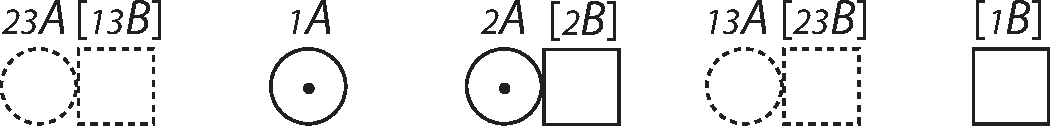
\includegraphics[width=0.56\textwidth]{gesamttex/edit_VIII-4/images/LH_35_14_02_040_d1_040r.pdf}%
\edcaption[0.75em]{%
\edtext{%
\lbrack\textit{Fig.\:1}\rbrack%
}{\lemma{\lbrack\textit{Fig.\:1}\rbrack}%
\Cfootnote[nonum]{%
Die im Diagramm vertauschten Bezeichnungen
\textit{\ind{13}B} und \textit{\ind{23}B}
sind sinngemäß geändert,
die fehlenden Bezeichnungen \textit{\ind{1}B} und \textit{\ind{2}B} ergänzt worden.%
}}%
}%
\vspace{2.25em}%
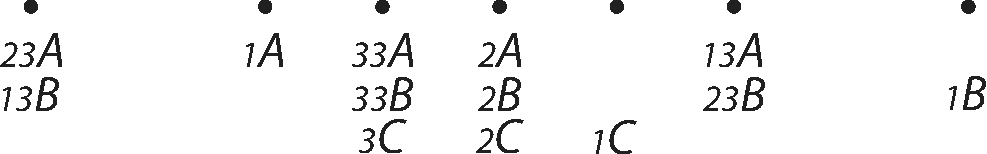
\includegraphics[width=0.52\textwidth]{gesamttex/edit_VIII-4/images/LH_35_14_02_040_d2_040r.pdf}%
\edcaption[0.75em]%
{%
\lbrack\textit{Fig.\:2}\rbrack%
}%
\end{edfigure}%
\pstart%
\noindent%
\edtext{%
Videamus an%
}{\lemma{}%
\Bfootnote{%
Videamus %
\bars{si corpora sint aequalia \textit{gestr.}} %
an%
~\textit{L}%
}}
res succedat,
ut possimus
\edtext{%
ponere corpus%
}{%
\lemma{}%
\Bfootnote{%
ponere %
\bars{utrumque \textit{gestr.}} %
corpus%
~\textit{L}%
}}
tam suo quam contrario nisu%
\indexS{nisus proprius}%
\indexS{nisus contrarius}%
\indexS{corpus latum nisu suo}%
\indexS{corpus latum nisu contrario}
ferri %
sic,
ut ponatur ferri illuc
ubi centrum est gravitatis amborum.%
\indexS{centrum gravitatis commune}
\edtext{%
Sit
\edtext{%
ipsius \textit{A}
}{%
\lemma{ipsius \textit{A}}%
\Cfootnote{Vgl. das Diagramm \lbrack\textit{Fig.\:2}\rbrack.}}%
directio et velocitas%
\indexS{directio in concursu}%
\indexS{velocitas in concursu}
\textit{\ind{1}A}\textit{\ind{2}A},%
}{%
\lemma{Sit}%
\Bfootnote{%
\textit{(1)}~\textit{A} %
\textit{(2)}~ipsius \textit{A} %
\textit{(a)}~conatus et %
\textit{(b)}~directio et~velocitas \textit{\ind{1}A}\textit{\ind{2}A},%
~\textit{L}%
}}
quae continuata esset in \textit{\ind{13}A},
et similiter sit ipsius \textit{B} velocitas
\textit{\ind{1}B}\textit{\ind{2}B},
continuata in \textit{\ind{13}B}.
Utique scimus
ita ferri centrum gravitatis%
\indexS{centrum gravitatis commune}
\edtext{%
commune \textit{C},
ut%
}{%
\lemma{}%
\Bfootnote{%
commune %
\bars{\textit{C} \textit{erg.}}, %
ut%
~\textit{L}}}
fuisset latum
si successum habuissent
\textit{\ind{13}A} et \textit{\ind{13}B}.
Itaque si contra daremus simul ipsi
\textit{A}
motum ipsius
\textit{B},
seu \textit{\ind{23}A},
et
\edtext{%
ipsi
\lbrack\textit{B}\rbrack\
motum ipsius
\lbrack\textit{A}\rbrack,
seu \textit{\ind{23}B},%
}{%
\lemma{}%
\Bfootnote{%
ipsi %
\bars{\textit{A} \textit{ändert Hrsg.}} %
motum ipsius %
\bars{\textit{B} \textit{ändert Hrsg.}}, %
seu \textit{\ind{23}B},%
~\textit{L}%
}}
\ledpb%
rursus idem erit progressus centri gravitatis%
\indexS{progressus centri gravitatis}%
\indexS{centrum gravitatis commune}
quia corpora sunt aequalia.%
\indexS{corpora concurrentia aequalia}
Itaque coincident
et \textit{\ind{33}A}, \textit{\ind{33}B} %
et \textit{\ind{3}C},
sed in inaequalibus%
\indexS{corpora concurrentia inaequalia}
non
\edlabel{35_14_02_040_1a}%
coinciderent.%
\edtext{}{%
\xxref{35_14_02_040_1a}{35_14_02_040_1b}%
\lemma{coinciderent.}%
\Bfootnote{%
\textit{(1)}~Sed fortasse sic procedere licebit, ut corpori %
\textit{(a)}~\textit{A} %
\textit{(b)}~uni %
\textit{(2)}~Sed an %
\lbrack\href{\Scan{LH_35_14_02_040v}}{40\,v\textsuperscript{o}}\rbrack\ \lbrack/\rbrack\ %
\textit{(3)}~\bars{Revera succedet \lbrack...\rbrack\ succedet compositio. \textit{erg.}} %
\lbrack\href{\Scan{LH_35_14_02_040r}}{40\,r\textsuperscript{o}}\rbrack\ %
\textit{(a)}~Eadem quantitas %
\textit{(b)}~Si corpus ducatur in %
\textit{(aa)}~omne %
\textit{(bb)}~aggregatum omnium %
\textit{(aaa)}~conatuum %
\textit{(bbb)}~velocitatum quas %
\lbrack...\rbrack\ 
in universo.%
~\textit{L}%
}}
\edlabel{35_14_02_040_2a}%
\lbrack%
\href{\Scan{LH_35_14_02_040v}}%
{40\:v\textsuperscript{o}}%
\rbrack%
\pend%
\pstart%
Revera succedet haec compositio %
si%
\lbrack,\rbrack\
ut res est,
ponamus
corpora concurrentia nisum%
\indexS{nisus dissiliendi}
semper habere a se invicem
reciprocis velocitatibus respectivis%
\indexS{velocitas respectiva}
dissiliendi%
\indexS{velocitas dissiliendi}
et praeterea motum communem%
\indexS{motus communis}
manere,
ut in navi%
\indexS{navis}
semper succedet
\edlabel{LH_35_14_02_040_40v/r_syyrtym-1}%
compositio.%
\indexS{compositio motuum}%
\edtext{}%
{\xxref{LH_35_14_02_040_40v/r_syyrtym-1}{LH_35_14_02_040_40v/r_syyrtym-2}%
\lemma{compositio. \lbrack/\rbrack\ Si corpus}%
\Cfootnote{In \textit{L} waagerechte Trennlinie zwischen den Absätzen.%
}}
\href{\Scan{LH_35_14_02_040r}}%
{\lbrack40\:r\textsuperscript{o}\rbrack}%
\pend%
\pstart%
\edlabel{LH_35_14_02_040_040r_aggregatum-1}%
Si%
\edlabel{35_14_02_040_1b}
corpus%
\edlabel{LH_35_14_02_040_40v/r_syyrtym-2}
ducatur%
\indexS{ductus corporis in aggregatum velocitatum}
in aggregatum omnium velocitatum%
\indexS{aggregatum velocitatum}
quas habuit inde a quiete%
\lbrack,\rbrack\
summa factorum in corpora%
\indexS{summa factorum in corpora}
erit eadem in
\edlabel{35_14_02_040_3a}%
universo.%
\indexS{universum}%
\edlabel{35_14_02_040_2b}%
\edlabel{LH_35_14_02_040_040r_aggregatum-2}%
\edtext{}{%
\xxref{35_14_02_040_3a}{35_14_02_040_3b}%
\lemma{universo. \lbrack/\rbrack\ Semper}%
\Cfootnote{%
In \textit{L} waagerechte Trennlinie zwischen den Absätzen.%
}}%
\pend%
\pstart%
Semper%
\edlabel{35_14_02_040_3b}
succedit compositio motuum.%
\indexS{compositio motuum}
Semper conservatur eadem potentia,%
\indexS{potentia conservata}
seu semper idem est
\edtext{%
effectus absolutus.%
\indexS{effectus absolutus}
Semper res ita prodeunt,
ut discerni nequeat
in quo corpore sit motus.%
}{%
\lemma{effectus}%
\Bfootnote{%
\bars{absolutus \textit{erg.}}. %
\textit{(1)}~Semper
\textit{(a)}~obtinetur %
\textit{(b)}~\textlangle idem est\textrangle\ effectus %
\textit{(c)}~eadem directio in summa %
\textit{(2)}~Semp %
\textit{(3)}~Semper %
\textit{(a)}~in %
\textit{(b)}~res ita %
\lbrack...\rbrack\ sit motus.%
~\textit{L}%
}}
\pend%
\pstart%
Duplex potentia in natura,%
\indexS{potentia duplex in natura}%
\indexS{natura}
una
\edtext{%
absoluta,%
\indexS{potentia absoluta}
ubi nihil interest%
}{%
\lemma{absoluta,}%
\Bfootnote{%
\textit{(1)}~nihil re %
\textit{(2)}~ubi nihil interest%
~\textit{L}%
}}
in quo
sit corpore,
altera conservativa%
\indexS{potentia conservativa}%
\lbrack,\rbrack\
qua conatur idem corpus
suam velocitatem et directionem retinere%
\indexS{conatus retinendi velocitatem}%
\indexS{conatus retinendi directionem}%
\lbrack,\rbrack\
et ab hac oritur percussio.%
\indexS{percussio}
Ab hac etiam oritur conatus%
\indexS{conatus alternativus}
\edtext{%
alternativus.
Et porro licet%
}{%
\lemma{alternativus.}%
\Bfootnote{%
\textit{(1)}~Et\textlangle iam\textrangle\ %
\textit{(2)}~Et porro licet%
~\textit{L}%
}}
\href{\Scan{LH_35_14_02_040v}}%
{\lbrack40\:v\textsuperscript{o}\rbrack} %
potentia conservativa%
\indexS{potentia conservativa}
in
\edtext{%
singulis exitum habere non possit,
habet tamen in summa plurium %
simul.%
}{%
\lemma{singulis}\Bfootnote{%
\textit{(1)}~conservari non possit, ta %
\textit{(2)}~exitum habere %
\lbrack...\rbrack\ plurium, simul.%
~\textit{L}%
}}
Hoc est%
\lbrack,\rbrack\
summa directionum%
\indexS{summa directionum}
semper succedit.
\pend%
\vspace{5em}%
\pstart%
\noindent%
\centering%
*    *    *
\pend%
\newpage%
\selectlanguage{ngerman}%
\begin{ledgroup}
\footnotesize
\pstart
\noindent%
\textls{Ausführliche Datierungsgründe:}%
\pagelabel{58235_dat}
Die titellose und undatierte Aufzeichnung N.\;\ref{58235} ist auf einem Träger überliefert, dessen römische\indexO{Rom} Herkunft sich durch Vergleiche mit weiteren Handschriften aus dem Leibniz-Nachlass feststellen lässt;
auf gleichem Papier sind auch die Aufzeichnungen N.\;\ref{58656-A}, N.\;\ref{58258} und N.\;\ref{58218} im vorliegenden Band verfasst worden (siehe für die Details die ausführliche Datierungsgründe zu N.\;\ref{58656-A}, S.\;\pageref{58656-A_dat}).
Bei all diesen Texten, von denen N.\;\ref{58656-A} und N.\;\ref{58258} auch einen inhaltlichen Zusammenhang mit Leibnizens \textit{Dynamica} aufweisen, %
ist demnach eine Entstehungszeit anzunehmen, die sich auf die Monate vom Sommer bis zum November 1689 erstrecket, als Leibniz in Rom\indexO{Rom} am \textit{Phoranomus}\cite{01402} und an der ersten Fassung der \textit{Dynamica}\cite{01354} gearbeitet hat (siehe \textsc{Robinet} 1988, S.\;81\,ff.).\cite{01240}
\pend%
\pstart%
Die Aufzeichnung N.\;\ref{58235} kann man nämlich als Beitrag zu der unvollendet gebliebenen Stoßlehre der \textit{Dynamica}\cite{01354} ansehen (siehe zur Entstehung der Abhandlung unter besonderer Berücksichtigung der Stoßlehre die einleitende Erläuterung zu den Entwürfen N.\;\ref{impulsuseccentricus} im vorliegenden Band, \refpassage{impulsecc_intro_Dynam-1}{impulsecc_intro_Dynam-2}).
In dieser Hinsicht ist Folgendes zu beachten:
Leibniz unterscheidet in seinen \textit{Dynamica}, pars~I, sectio~III, cap.\;II, def. zwischen absoluter und relativer Potenz: \textit{Distinguo autem potentiam mobilis \textls{absoluta,} in corpore per se consideratam, a \textls{respectiva,} qua aliud percutit, de qua suo loco} (%
\textit{CFP}~I, S.\;145.12--14~\bracks{A}; S.\;517.2--4~\bracks{B}; II.1,\;S.\;202.1--3~\bracks{C}).\cite{01354}
Die \glqq relative Potenz\grqq\ bzw. \glqq relative Kraft\grqq\ wird dann zunächst ebd., pars~II, sectio~I, \bracks{cap.\;II,} def.\;7 (\textit{Vis respectiva est, qua duo corpora in se invicem agunt}) und prop.\;41 u.\;42 untersucht, wobei die Stoßlehre auch dort den Rahmen festlegt (%
\textit{CFP}~I, S.\;349.12--352.17~\bracks{A}; S.\;585.28--588.17~\bracks{B}; II.2, S.\;426.13--430.31~\bracks{C}).\cite{01354}
Die Erhaltung der \glqq relativen Potenz\grqq\ wird vorwiegend ebd., pars~II, sectio~III, prop.\;7\textendash12 dargelegt (%
\textit{CFP}~I, S.\;400--412~\bracks{A}; %
II.2, S.\;498--512~\bracks{C}).\cite{01354}
Der Begriff \textit{potentia conservativa} wird dort nicht verwendet.
Das kann man als Zeichen dafür erachten, dass %
Leibniz bei der Bearbeitung der Stoßlehre der \textit{Dynamica}\cite{01354} den Begriff \textit{vis conservativa} aufgegeben und lediglich den Begriff \textit{vis respectiva} beibehalten hat.
Dies könnte wiederum zeigen, dass die Aufzeichnung N.\;\ref{58235} vor oder während der Bearbeitung der A-Fassung der \textit{Dynamica}\cite{01354} entstand und aus inhaltlichen Gründen beiseite gelegt wurde.%
\pend%
\pstart%
Die Aufzeichnung N.\;\ref{58235} ist demgemäß auf den Zeitraum zwischen Sommer und November 1689 zu datieren.
Eine frühere (ab Leibnizens Ankunft in Rom\indexO{Rom} im Mai 1689) oder eine spätere Abfassungszeit (höchstens bis Ende März 1690, als Leibniz Italien\indexO{Italien} verlassen hat) sind nicht ausgeschlossen, aber unwahrscheinlich.%
\pend%
\end{ledgroup}
\normalsize%
\selectlanguage{latin}%
\frenchspacing%




\chapter[tocentry={Regula de progressu centri gravitatis
\enskip\bracks{Dezember 1689}},
head={Regula de progressu centri gravitatis}]%
{\MakeUppercase{Regula de progressu centri gravitatis}
\newline\bracks{Dezember 1689}}
\label{66097}
\selectlanguage{ngerman}%
\frenchspacing%
\begin{ledgroupsized}[r]{120mm}%
\footnotesize%
\pstart%
\noindent\textbf{Überlieferung:}%
\pend%
\end{ledgroupsized}%
\begin{ledgroupsized}[r]{114mm}%
\footnotesize%
\pstart%
\parindent -6mm%
\makebox[6mm][l]{\textit{L}}%
Aufzeichnung:
LH~XXXV~10,\;11 Bl.\;88.
Ein Blatt 4\textsuperscript{o},
Ränder zum Teil beschnitten;
ein \href{\Scan{LH_35_10_11_088wz}}{Wasserzeichen}:
italienisches Papier.
Eine ganzseitig beschriebene Seite auf Bl.\;\href{\Scan{LH_35_10_11_088r}}{88\,r\textsuperscript{o}};
auf Bl.\,\href{\Scan{LH_35_10_11_088v}}{88\,v\textsuperscript{o}} ist lediglich das Diagramm \bracks{\textit{Fig.\:4}} überliefert.
Die Aufzeichnung N.\ref{66097} hängt mit der ersten Bearbeitung (Fassung~A) von Leibnizens \textit{Dynamica}\cite{01354} zusammen (siehe die Datierungsbegründung auf S.\;\pageref{66097_dat}).
\pend%
\end{ledgroupsized}%
\vspace{5mm}%
\begin{ledgroup}%
\footnotesize%
\pstart%
\noindent%
\textbf{Datierungsgründe:}
Die Datierung der Aufzeichnung N.\;\ref{66097} beruht auf Eigenschaften des Textträgers sowie 
auf inhaltlichen Betrachtungen.
Siehe die ausführliche Begründung auf S.\;\pageref{66097_dat}.%
\pend%
\end{ledgroup}%
\selectlanguage{latin}%
\frenchspacing%
\vspace{8mm}%
\normalsize%
\pstart%
\noindent%
\bracks{%
\href{\Scan{LH_35_10_11_088r}}%
{88\,r\textsuperscript{o}}%
}
\edlabel{LH_35_10_11_088_088r_1Teil-1}%
Videtur
non facile esse
comminisci modum efficiendi%
\indexS{modus efficiendi}%
\bracks{,}
motu etiam circulari adhibito,%
\indexS{motus circularis adhibitus}
ut corporum centrum gravitatis%
\indexS{centrum gravitatis corporum concurrentium}
non recta
\edtext{%
progrediatur.%
\indexS{progressus centri gravitatis}%
}{%
\lemma{progrediatur}%
\Bfootnote{%
\textit{(1)}~, nam si %
\textit{(2)}~. Nam si~%
\textit{L}%
}}
Nam si corpora aequalia \textit{A},\:\textit{B}%
\indexS{corpora concurrentia aequalia}
incurrant aequali celeritate in \textit{CD}%
\indexS{celeritas concursus}
et postea ibi motus convertant in circulares%
\indexS{motus conversus in circularem}, %
manebit quiescens ut ante centrum%
\indexS{centrum gravitatis quiescens in concursu}
\edtext{%
gravitatis in medio lineae \textit{CD}.
Idem forte, %
si%
}{%
\lemma{gravitatis}%
\Bfootnote{%
\textit{(1)}~. Idem erit fortasse si f %
\textit{(2)}~in medio lineae \textit{CD}. %
\textit{(a)}~Ita %
\textit{(b)}~Idem forte, si%
~\textit{L}%
}}
distantiae corporibus reciproce proportionales.%
\indexS{distantiae reciproce proportionales corporibus in concursu}
Cum corpus \textit{G} incidit in radium \textit{FH},%
\indexS{corpus incidens in radium}%
\indexS{radius}
firmum centrum habentem,%
\indexS{centrum radii}
considerari debet
centrum non esse perfecte firmum,%
\indexS{centrum perfecte firmum}
sed esse annexum corpori valde magno%
\indexS{centrum annexum corpori magno}
cujus motus tardus seu insensibilis.%
\indexS{motus tardus seu insensibilis}%
\indexS{motus insensibilis}
Et hinc calculo consequi licebit%
\indexS{calculus consequens}
quod fieri debeat.%
\edlabel{LH_35_10_11_088_088r_1Teil-2}
\pend%
\begin{edfigure}[2.50em][0.00em]%
\hfill%
\includegraphics[scale=0.81]%
{gesamttex/edit_VIII-4/images/LH_35_10_11_088_d1_088r.pdf}
\hfill%
\includegraphics[scale=0.81]%
{gesamttex/edit_VIII-4/images/LH_35_10_11_088_d2_088r.pdf}
\hfill%
\edcaption{\bracks{\textit{Fig.\:1}}
\hspace{47mm}%
\bracks{\textit{Fig.\:2}}}%
\end{edfigure}%
\newpage
\pstart%
Hinc
etsi verum sit
non obtinere
\edtext{%
Regulam de progressu centri gravitatis,%
\indexS{regula de progressu centri gravitatis}%
\indexS{progressus centri gravitatis}%
\indexS{centrum gravitatis corporum concurrentium}
si corpora circulentur circa centra firma%
\indexS{corpus circulans circa centrum}%
\bracks{;}
concipiendo tamen
nulla centra esse perfecte firma,%
\indexS{centrum perfecte firmum}%
}{%
\lemma{Regulam}%
\Bfootnote{%
\textit{(1)}~si %
\textit{(2)}~de progressu %
\bracks{...} corpora circulentur %
\textit{(a)}~, quia tamen circulatio oriri non potuit nisi prius a motibus rectilineis\bracks{,} hinc conjungendo %
\textit{(b)}~circa centra %
\bracks{...} perfecte firma,%
~\textit{L}%
}}
sed esse instar corporum magnae gravitatis%
\indexS{corpus gravitatis magnae}
quibus tardus imprimitur motus%
\indexS{motus tardus corporis gravitatis magnae}%
\indexS{motus impressus corpori gravitatis magnae}%
\bracks{,}
servabitur lex progressus totalis%
\indexS{lex progressus totalis}%
\bracks{,}
quoniam scilicet vis recedendi a centro%
\indexS{vis recedendi a centro in circulante}%
\indexS{recessus a centro in circulante}
in circulante
\edlabel{LH_35_10_11_088r_1i}%
aliquid%
\edtext{}{%
\xxref{LH_35_10_11_088r_1i}{LH_35_10_11_088r_1f}%
\lemma{aliquid}%
\Bfootnote{%
\textit{(1)}~corpori %
\textit{(a)}~magno %
\textit{(b)}~ipsi %
\textit{(2)}~motus ipsi centro imprimit. %
\bracks{/} %
\textit{(a)}~Si uni puncto %
\textit{(b)}~In motibus rectilineis %
\bars{uniformibus \textit{erg.}}%
\textit{L}%
}}
motus ipsi centro imprimit.%
\indexS{motus impressus centro gravitatis}
\pend%
\begin{edfigure}[2.25em][0.00em]%
\hspace{10mm}%
\includegraphics[scale=0.7375]{%
gesamttex/edit_VIII-4/images/LH_35_10_11_088_d3_088r.pdf}
\hspace{10mm}%
\edcaption[0.50em]%
{\lbrack\textit{Fig.\:3}\rbrack}%
\vspace{2.75em}%
\includegraphics[scale=0.7375]{%
gesamttex/edit_VIII-4/images/LH_35_10_11_088_d4_088r.pdf}%
\hspace{10mm}%
\edcaption[0.50em]%
{\lbrack\textit{Fig.\:4}\rbrack}
\end{edfigure}
\newpage%
\pstart%
\edlabel{LH_35_10_11_088_088r_letzTeil-1}%
In motibus rectilineis uniformibus%
\indexS{motus rectlineus uniformis}%
\edlabel{LH_35_10_11_088r_1f}
eadem prodeunt phaenomena,%
\indexS{phaenomena prodeuntia ex hypothesibus}
cuicunque corpori
motus rectilineus dat\angles{u}s uniformis%
\indexS{motus rectilineus assignatus in hypothesi}
vel quies%
\indexS{quies assignata in hypothesi}
\edtext{%
assignetur.
Nam omnes motus quidem rectilinei
in eodem plano
possunt intelligi compositi ex parallelis
ad datas duas
\edtext{%
rectas \textit{LM},\;\textit{LN}.%
\indexS{motus compositus e parallelis ad rectas datas}%
}{%
\lemma{rectas \textit{LM},\;\textit{LN}}%
\Cfootnote{%
Vgl. das Diagramm \bracks{\textit{Fig.\:3}}.%
}}
Et in solido intelligi possunt
compositi ex parallelis ad tres rectas datas.%
\indexS{motus compositus e parallelis ad rectas datas}
In parallelis autem motibus%
\indexS{motus paralleli}
manifestum est%
}{%
\lemma{assignetur.}%
\Bfootnote{%
\textit{(1)}~Reducantur ad %
\textit{(2)}~Possunt enim omnes %
\textit{(a)}~esse compositi ex p %
\textit{(b)}~intelligi %
\textit{(aa)}~compositi %
\textit{(bb)}~ut compositi ex rectis %
\textit{(3)}~Nam omnes \bracks{...} \textit{LM},\;\textit{LN}.
\textit{(a)}~In motibus autem parallelis
\textit{(b)}~Et in solido %
\bracks{...} rectas datas. %
\textit{(aa)}~Paralleli autem %
\textit{(bb)}~In parallelis autem motibus %
\textit{(aaa)}~si uni %
\textit{(bbb)}~manifestum est%
~\textit{L}%
}}
eandem servari distantiam
\edtext{%
\edtext{%
linearum \textit{AA},\;\textit{BB},\;\textit{CC},%
}{%
\lemma{linearum \textit{AA},\;\textit{BB},\;\textit{CC}}%
\Cfootnote{%
Vgl. das Diagramm \bracks{\textit{Fig.\:4}}.%
}}
quemcunque motum attribuamus puncto \textit{A}.
Servari etiam potest eadem variatio%
\indexS{variatio distantiarum relativarum}
distantiarum relativarum in recta \textit{AA},%
}{%
\lemma{linearum}%
\Bfootnote{%
\textit{(1)}~, servatur praeterea eadem %
\textit{(2)}~\textit{AA}, \textit{BB}, \textit{CC} %
\textit{(a)}~. Servatur et eadem %
\textit{(b)}~. Sic %
\textit{(c)}~, quemcunque motum attribuamus puncto \textit{A}. %
\textit{(aa)}~Servatur et eadem distantia %
\textit{(aaa)}~linearum %
\textit{(bbb)}~punctorum \angles{--} in \textit{AA} \angles{--} %
\textit{(bb)}~Servari etiam potest %
\textit{(aaa)}~magnitudo %
\textit{(bbb)}~eadem %
\textit{(aaaa)}~\bars{mutatio \textit{versehentlich erhalten, streicht Hrsg.}} %
\textit{(bbbb)}~variatio distantiarum %
\textit{(aaaaa)}~in rectam \textit{AA}, %
\textit{(bbbbb)}~relativarum in recta \textit{AA},%
~\textit{L}%
}}
per normales
\edtext{%
$B\beta$, $C\kappa$%
}{%
\lemma{$B\beta$, $C\kappa$}%
\Bfootnote{%
\textit{erg.\;L}%
}}
a punctis \textit{B} et \textit{C}
ad eam
\edtext{%
ductas,
quocunque ipsi\;\textit{A} motu assignato%
\bracks{,}
assignando competentes ipsis \textit{B} et \textit{C}.
Nam qui motus assignabitur%
\indexS{motus assignatus}
punctis $\beta$,\;$\kappa$,
erit et punctorum \textit{B},\;\textit{C} %
in suis parallelis.
Quicunque autem motus ipsi \textit{A} assignetur,
assignari utique potest motus punctorum
$\beta$ et $\kappa$ uniformis ejusmodi,
ut rectae $A\beta$ (vel $A\kappa$)
uniformiter eodem modo crescant aut decrescant,
adeoque celeritates respectivae maneant eaedem,%
\indexS{celeritas respectiva manens eadem in concursu}
seu ut serventur eaedem
pro eodem temporis momento%
\indexS{momentum temporis}
distantiae%
}{%
\lemma{ductas,}%
\Bfootnote{%
\textit{(1)}~seu eadem manet %
\textit{(2)}~quocunque %
\textit{(a)}~enim %
\textit{(b)}~ipsi \textit{A} motu assignato %
\bars{assignando competentes ipsis \textit{B} et \textit{C} \textit{erg.}}. %
\textit{(aa)}~\angles{Et} %
\textit{(bb)}~Utique enim deinde et talis motus uniformis\indexS{motus uniformis} ipsis punctis \textit{B} et \textit{C}, adeoque ipsis %
\textit{(cc)}~Nam si motus ipsorum \textit{B}, et \textit{C} in parallelis suis assignetur uniformis, erit et %
\textit{(dd)}~Nam qui %
\bracks{...} suis parallelis. %
\textit{(aaa)}~Assignari autem %
\textit{(bbb)}~Quicunque autem %
\bracks{...} assignetur, assignari %
\textit{(aaaa)}~potest utique %
\textit{(bbbb)}~utique potest %
\bracks{...} uniformis ejusmodi, %
\textit{(aaaaa)}~ut punctorum %
\textit{(aaaaa-a)}~\textit{A} et %
\textit{(bbbbb-b)}~$A\beta$ vel $A\kappa$, dista %
\textit{(bbbbb)}~ut %
\textit{(aaaaa-a)}~rectarum %
\textit{(bbbbb-b)}~rectae $A\beta$ %
\bracks{...} aut decrescant, %
\textit{(aaaaa-aa)}~licet ipsi \textit{A} quicu
\textit{(bbbbb-bb)}~sed
\textit{(ccccc-cc)}~adeoque celeritates respectivae maneant eaedem, %
\textit{(aaaaa-aaa)}~sive
\textit{(bbbbb-bbb)}~quicunque ipsi \textit{A} motus assignetur. %
\textit{(aaaaa-aaaa)}~Itaque %
\textit{(bbbbb-bbbb)}~Servatis igitur iisdem %
\textit{(ccccc-ccc)}~seu ut %
\bracks{...} temporis momento %
\textit{(aaaaa-aaaa)}~distantiis %
\textit{(bbbbb-bbbb)}~distantiae%
~\textit{L}%
}}
$A\beta$, $A\kappa$, $\beta\kappa$
(ut $\ind{1}A\ind{1}\beta$,
vel $\ind{1}A\ind{1}\kappa$,
\edtext{%
$\ind{1}\beta\ind{1}\kappa$%
}{%
\lemma{$\ind{1}\beta\ind{1}\kappa$}%
\Bfootnote{%
\textit{erg.\;L}%
}}
et alio tempore
$\ind{2}A\ind{2}\beta$,
\edtext{%
$\ind{2}A\ind{2}\kappa$,
$\ind{2}\beta\ind{2}\kappa$).
Quoniam igitur
quacunque hypothesi facta%
\indexS{hypothesis circa motum}
circa motum ipsius \textit{A},
eaedem manent rectae
ut $\ind{2}A\ind{2}\beta$,
\bracks{$\ind{2}\beta\ind{2}B$} %
pro eodem temporis momento,%
\indexS{momentum temporis}
utique et idem manet angulus
\textit{\ind{2}B\ind{2}A\ind{3}A}.%
}{%
\lemma{$\ind{2}A\ind{2}\kappa$}%
\Bfootnote{%
\textit{(1)}~,) %
\textit{(2)}~, $\ind{2}\beta\ind{2}\kappa$) %
\textit{(a)}~adeoque et distantiae $\beta\kappa$ %
\textit{(b)}~\angles{nam} %
\textit{(c)}~. Quacunque igitur Hypothesi facta, %
\textit{(aa)}~non %
\textit{(bb)}~prodit idem angulus ut $\ind{1}B\ind{1}A$, %
\textit{(d)}~. Quoniam %
\textit{(e)}~. Quoniam igitur %
\textit{(aa)}~quacunque %
\textit{(bb)}~quacunque hypothesi %
\bracks{...} manent rectae %
\textit{(aaa)}~\bars{ut \textit{erg.}} $\ind{2}\beta\ind{2}\beta$, et %
\textit{(bbb)}~ut $\ind{2}A\ind{2}\beta$, %
\bars{$\ind{2}\beta B$ \textit{ändert Hrsg.}} %
\bars{pro \textit{erg.}} eodem temporis %
\bracks{...} angulus \textit{\ind{2}B\ind{2}A\ind{3}A}.%
~\textit{L}%
}}
Et similiter idem manet angulus 
\textit{\ind{2}C\ind{2}A\ind{3}A},
ergo et idem manet angulus
\edtext{%
\bracks{\textit{\ind{2}B\ind{2}A\ind{1}A}},%
}{%
\lemma{\textit{\ind{2}B\ind{2}A\ind{3}A}}%
\Bfootnote{%
\textit{L\;ändert Hrsg.}%
}}
idemque est
\edtext{%
de angulis%
}{%
\lemma{de}%
\Bfootnote{%
\bars{punctis seu \textit{gestr.}} angulis%
~\textit{L}%
}}
quibuscunque.
Itaque
\edtext{%
phaenomena eadem prodeunt.%
\indexS{phaenomena prodeuntia ex hypothesibus}
Cum igitur hypotheses motuum%
\indexS{hypothesis circa motum}
discerni non possint
per rectas datis parallelas
quibus motus determinantur,
omnino non poterunt discerni.%
\indexS{hypotheses motuum non discernibiles}%
\edlabel{LH_35_10_11_088_088r_letzTeil-2}%
}{%
\lemma{phaenomena}%
\Bfootnote{%
\textit{(1)}~discerni non possunt %
\textit{(2)}~eadem prodeunt. %
\textit{(a)}~Jam quod %
\textit{(aa)}~\angles{re} %
\textit{(bb)}~respectu motuum parallelorum verum est %
\textit{(aaa)}~respectu %
\textit{(bbb)}~verum etiam est respectu compositorum ex ipsis. In universum igitur habetur propositum %
\textit{(3)}~Cum igitur hypotheses %
\bars{motuum \textit{erg.}} discerni non %
\bracks{...} poterunt discerni.%
~\textit{L}%
}}
\bracks{%
\href{\Scan{LH_35_10_11_088v}}%
{88\,v\textsuperscript{o}}%
}
\pend%
\vspace{1.0em}%
\begin{edfigure}[1.250em][0.0em]%
\hspace{-1.5mm}%
\includegraphics[scale=0.80]{%
gesamttex/edit_VIII-4/images/LH_35_10_11_088_d5_088v.pdf}%
\edcaption[0.25em]%
{\bracks{\textit{Fig.\:5}}}%
\end{edfigure}%
\vspace{3.0em}%
\pstart%
\noindent%
\centering%
*     *     *
\pend%
\vspace{2.5em}%
\selectlanguage{german}%
\frenchspacing%
\footnotesize%
\pstart%
\noindent%
\textls{Ausführliche Datierungsgründe:}%
\pagelabel{66097_dat}
Der Träger der titellosen und undatierten Aufzeichnung N.\;\ref{66097} weist ein \href{\Scan{LH_35_10_11_088wz}}{Wasserzeichen} (umkreiste Anker mit Stern und Buchstabe F) auf, welches häufig in Papier vorkommt, das Leibniz in Florenz\indexO{Florenz} verwendete.
Aus gleichem Papier etwa bestehen die letzten Bogen der ersten Bearbeitung von Leibnizens \textit{Dynamica}\cite{01354} (Fassung~A, bes. LH~XXXV~11,\;18\,A S.\;353--438 u. XXXVII~4 Bl.\;166-167).
In Florenz\indexO{Florenz} hielt sich Leibniz vom 1.\;bis zum 22.\;Dezember 1689 auf (siehe \textit{Chronik}, S.\;98\,f.).\cite{01236}
Demgemäß ist anzunehmen, dass die Aufzeichnung N.\;\ref{66097} in diesem Zeitraum entstand, als Leibniz an der Fassung~A der \textit{Dynamica}\cite{01354} arbeitete.
\pend%
\pstart%
Diese Annahme lässt sich auch inhaltlich bekräftigen.
Denn die im ersten Teil der Aufzeichnung N.\;\ref{66097} geäußerten Beobachtungen über die Bewegung des gemeinsamen Schwerpunkts bei Stoßfällen, aus denen eine Drehung entsteht (vgl. oben, \refpassage{LH_35_10_11_088_088r_1Teil-1}{LH_35_10_11_088_088r_1Teil-2}), ähneln den Ausführungen in Leibnizens \textit{Dynamica}, pars~II, sect.\;III, prop.\;18\cite{01354} (\textit{CFP}~I, S.\;419.6--421.7 [A]; II.2, S.\;520.19--524.3 [C]).\cite{01482} %
Ebenso erinnern die Überlegungen zur Gleichwertigkeit der Beschreibungen ("Äquivalenz der Hypothesen") gleichförmiger Bewegungen im letzten Teil der Aufzeichnung (vgl. oben, \refpassage{LH_35_10_11_088_088r_letzTeil-1}{LH_35_10_11_088_088r_letzTeil-2}) an die Thesen, die in \textit{Dynamica}, pars~II, sect.\;III, prop.\;15\cite{01354} (\textit{CFP}~I, S.\;415.22--416.7 [A]; II.2, S.\;516.16--25 [C])\cite{01482} %
vorgetragen werden.
Die Vermutung liegt somit nahe, dass die Aufzeichnung N.\;\ref{66097} zu dem Zeitpunkt entstand, als Leibniz mit der Abfassung dieses Teils seiner umfangreichen, nie abgeschlossenen Abhandlung beschäftigt war.
Es bedürfte aber weiterer Forschung, um besser klärzustellen, wie N.\;\ref{66097} textgenetisch mit den \textit{Dynamica}\cite{01354} zusammenhängt.
\pend%
\pstart%
Die Aufzeichnung N.\;\ref{66097} ist wohl vor dem Textkomplex N.\;\ref{impulsuseccentricus} \textit{De eccentrici impuslsus effectu} abgefasst worden (siehe die einleitende Erläuterung hierzu, S.\pageref{impulsecc_intro}\,ff).
\pend%
\selectlanguage{latin}%
\frenchspacing%
\normalsize%




\chapter[tocentry={De eccentrici impulsus effectu
\enskip\bracks{%
Dezember\;(?)} 1689 \textendash\ Sommer 1690%
},
head={De eccentrici impulsus effectu}]%
{\MakeUppercase{De eccentrici impulsus effectu}
\newline\bracks{%
Dezember\;(?) 1689 \textendash\ Sommer 1690%
}}
\label{impulsuseccentricus}
\footnotesize%
\pstart%
\noindent%
\pagelabel{impulsecc_intro}%
Die folgenden Texte N.\;\ref{60142+60297} und N.\;\ref{60299} erweisen sich inhaltlich und in ihrer Entstehung als eng miteinander verbunden und werden aus diesem Grund einheitlich ediert.
Vom Text N.\;\ref{60142+60297} sind ferner zwei Zeugen (\textit{L\textsuperscript{1}} und \textit{L\textsuperscript{2}}) überliefert, wobei \textit{L\textsuperscript{2}} offenbar eine Reinschrift des Konzepts \textit{L\textsuperscript{1}} ist (siehe die Beschreibung der Zeugen, \refpassage{LH_35_10_17_009+37_05_041_ueberlief-1}{LH_35_10_17_009+37_05_041_ueberlief-2}).
Der Textträger des Konzeptes \textit{L\textsuperscript{1}} weist freilich kein Wasserzeichen, wohl aber äußere Merkmale italienischen Papiers auf und ist somit aller Wahrscheinlichkeit nach zwischen März 1689 und März 1690 beschrieben worden, als Leibniz durch Italien\indexO{Italien} reiste.
Im Textträger der Reinschrift \textit{L\textsuperscript{2}} liegt das Fragment eines Wasserzeichens vor, das möglicherweise einer Papiermühle aus Venedigs\indexO{Venedig} Umgebung zugeschrieben werden kann.
Daher dürfte auch \textit{L\textsuperscript{2}} während der Italienreise entstanden sein.
Die Aufzeichnung N.\;\ref{60299} überliefert in ihren ersten Zeilen den nahezu gleichen Text wie N.\;\ref{60142+60297} (siehe hierzu die Beschreibung des Zeugen, %
\refpassage{LH_37_05_043_ueberliefer-1}{LH_37_05_043_ueberliefer-2}).
Hinzu kommt, dass der Textträger von N.\;\ref{60299}, dem das Wasserzeichen fehlt, die gleichen äußeren Merkmale aufweist wie der Träger der Reinschrift N.\;\ref{60142+60297}, \textit{L\textsuperscript{2}}.
Daher ist auch für N.\;\ref{60299} eine Entstehung zur Zeit von Leibnizens Italienreise anzunehmen.\indexO{Italien}
Anhand der im Folgenden dargelegten formalen und inhaltlichen Aspekte lässt sich die Datierung beider Texte N.\;\ref{60142+60297} und 
N.\;\ref{60299} jedoch weiter einschränken.
(Die Frage nach der relativen Chronologie wird erst am Schluss der editorischen Erläuterung erörtert.)
\pend%
\pstart%
Bei N.\;\ref{60142+60297} lässt die Form der Überschrift (\textit{Propositio \dots Problema} [/] \textit{Impulsus Eccentrice directi effectum explicare}, \refpassage{60142+60297_titel-1}{60142+60297_titel-2}) vermuten, dass der Text ursprünglich als Beitrag zur umfangreichen Abhandlung \textit{Dynamica de potentia et legibus naturae corporeae} gedacht war.
(Die gleiche Form \textit{Propositio \textendash\ Problema} kommt dort mehrmals vor; vgl. etwa %
\textit{CFP}~II.1, S.\;44--46, 52, 74, 80, 86, 228, 236, 268, 292 nach der Fassung \bracks{C}.)\cite{01354}
Insbesondere wäre zu erwarten, dass der \glqq Lehrsatz\grqq\ N.\;\ref{60142+60297} für den Abschnitt \textit{De concursu corporum} gedacht war, der die im Konvolut LH~XXXV~11, 18~A--C des Leibniz-Nachlasses überlieferte Fassung der \textit{Dynamica}\cite{01354} abschließt (%
\textit{CFP}~I, S.\;392--445~\bracks{A}; II.2, S.\;490--550~\bracks{C}).\cite{01354}
Im genannten Abschnitt findet sich dennoch weder ein Lehrsatz, der inhaltlich dem Text N.\;\ref{60142+60297} entspricht, noch überhaupt eine thematische Behandlung des direkten exzentrischen Stoßes zweier Körper.
Die Lehrsätze 18 und 19 erörtern zwar ausführlich die Entstehung eines \textit{gyrus}, d.\,h., wie sich aus dem Stoß mehrerer Körper eine Drehung ergibt (was auch beim direkten exzentrischen Stoß zweier Körper der Fall ist); im Mittelpunkt der Betrachtung steht dort %
jedoch wesentlich die Frage, wie kreisförmige bzw. kurvige Bewegungen aus gradlinigen gleichförmigen entstehen können, wohingegen der direkte exzentrische Stoß nur marginal besprochen wird (vgl. %
\textit{CFP}~I, S.\;419--436~\bracks{A}; II.2, S.\;520--538~\bracks{C}).\cite{01354}
Dieser bemerkenswerte Tatbestand ermöglicht \textendash\ unter Berücksichtigung weiterer biographischer Umstände \textendash\ eine genauere Datierung von N.\;\ref{60142+60297}.
\pend%
\pstart%
\edlabel{impulsecc_intro_Dynam-1}%
Leibniz begann wohl im Hochsommer 1689 den Text der \textit{Dynamica}\cite{01354} zu verfassen, während er sich in Rom\indexO{Rom} aufhielt (siehe hierüber \textsc{Robinet} 1988, S.\;81\textendash83; 259\textendash262\cite{01240}).
Ein weiter Teil der überlieferten Abhandlung war offenbar bereits niedergeschrieben worden, als in Dezember 1689 der Hofgelehrte Rudolf Christian von Bodenhausen,\indexN{\textls{Bodenhausen} (Bodenus, Bodenausen), Rudolf Christian, Freiherr v. 1698}\indexN{\textls{Bodenhausen} (Bodenus, Bodenausen), Rudolf Christian, Freiherr v. 1698} den Leibniz in Florenz\indexO{Florenz} kennengelernt hatte, sich dem \glqq Projekt\grqq\ anschloss.
Ihm war \textendash\ wie seinem (ersten) Brief an Leibniz vom 31.\;Dezember 1689 zu entnehmen ist \textendash\ der bislang entstandene Teil der \textit{Dynamica}\cite{01354} anvertraut worden mit dem Auftrag, daraus eine Reinschrift für den Druck anzufertigen (siehe \textit{LSB} III,\;4 N.\;223, S.\;436.5\textendash7).\cite{01384}
Leibniz erwartete von Bodenhausen\indexN{\textls{Bodenhausen} (Bodenus, Bodenausen), Rudolf Christian, Freiherr v. 1698} auch kritische Rückmeldungen über den Text und plante, ihm zu einem späteren Zeitpunkt auch Ergänzungen und die noch fehlenden Teile der Abhandlung zu senden (siehe seinen Brief an Bodenhausen\indexN{\textls{Bodenhausen} (Bodenus, Bodenausen), Rudolf Christian, Freiherr v. 1698} vom 13.\;Januar 1690; \textit{LSB} III,\;4 N.\;227, S.\;444.18\textendash23).\cite{01385}
Bereits am 21.\;Januar \textendash\ und dann wieder am 28.\;Januar, zu Ende Februar und am 4.\;März \textendash\ meldete Bodenhausen\indexN{\textls{Bodenhausen} (Bodenus, Bodenausen), Rudolf Christian, Freiherr v. 1698} an Leibniz, er komme mit der Arbeit an den \textit{Dynamica}\cite{01354} zügig voran und warte deshalb dringend auf das Ende des Abschnitts \textit{De concursu corporum} sowie auf die die Abhandlung abschließenden \textit{Miscellanea} (siehe \textit{LSB} III,\;4 N.\;229, \textit{K\textsuperscript{1}}, S. 448.4\textendash7, \textit{K\textsuperscript{2}}, S.\;450.6\textendash10;\cite{01386} N.\;234, S.\;458.8\textendash11;\cite{01387} N.\;240, S.\;448.16\textendash461.1;\cite{01388} N.\;241, S.\;471.2\textendash3\cite{01389}).
Am 4.\;März 1690 teilte ihm Leibniz aus Venedig mit, er werde erst auf der Rückfahrt nach Deutschland\indexO{Deutschland} in der Lage sein, den Abschnitt über den Stoß abzuschließen und die noch fehlenden Teile der \textit{Dynamica}\cite{01354} anzufertigen (\textit{LSB} III,\;4 N.\;242, S.\;473.25\textendash474.1;\cite{01390} die am 11.\;März nach Florenz gesendeten Ergänzungen enthielten tatsächlich nicht den erwarteten Schluss \textit{De concursu corporum}, vgl. \textit{LSB} III,\;4 N. 243, S.\;478.23\textendash479.5\cite{01391}).
Ähnlich drückte er sich auch wenige Tage vor der Abfahrt aus Venedig\indexO{Venedig} nach Augsburg\indexO{Augsburg} aus: In seinem Brief an Bodenhausen\indexN{\textls{Bodenhausen} (Bodenus, Bodenausen), Rudolf Christian, Freiherr v. 1698} vom 18.\;März 1690, in dem auch ein neues Inhaltsverzeichnis für die Abhandlung mit gesendet wurde, kündigt Leibniz an, er werde die \glqq sectionem \textit{De concursu corporum} forderlichst absolvieren\grqq\ und dann samt neuen bemerkenswerten Ergebnissen \textendash\ etwa über den Widerstand der Luft \textendash\ zuschicken; der Versuch, die \textit{Dynamica}\cite{01354} abzuschließen, sei doch für die Fahrt nach Augsburg\indexO{Augsburg} geplant (\textit{LSB} III,\;4 N.\;245, S.\;485.15\textendash23).\cite{01392}
Dazu aber ist Leibniz offenbar nie gekommen.
Am 29.\;Juli 1690, einen guten Monat nach seiner Ankunft in Hannover,\indexO{Hannover} erinnerte ihn Bodenhausen\indexN{\textls{Bodenhausen} (Bodenus, Bodenausen), Rudolf Christian, Freiherr v. 1698} aus Florenz\indexO{Florenz} wieder daran, dass der Abschnitt über den Stoß \textendash\ unter anderem \textendash\ noch unvollständig war (\textit{LSB} III,\;4 N.\;268, S.\;539.5\textendash6).\cite{01393}
Denselben Tenor weist auch eine Anmerkung in seinem Brief an Leibniz vom 23.\;Juni 1691 auf (\textit{LSB} III,\;5 N.\;25, S.\;127.2\textendash3).\cite{01394}
Und noch am 17.\;November 1694 ermunterte Bodenhausen\indexN{\textls{Bodenhausen} (Bodenus, Bodenausen), Rudolf Christian, Freiherr v. 1698} mit sanften Tönen Leibniz dazu, den Abschnitt \textit{De concursu corporum} abzuschließen (\textit{LSB} III,\;6 N.\;71, S~210.22\textendash24).\cite{01395}
Vergeblich.
Seit Anfang Juli 1690 hat ihm Leibniz keine neuen Textteile der \textit{Dynamica}\cite{01354} mehr zugeschickt und die Abhandlung in seinen Briefen an den Florentiner\indexO{Florenz} Hofgelehrten kaum noch erwähnt.
In seinem Schreiben an Leibniz vom 8.\;Februar 1695 nahm Bodenhausen\indexN{\textls{Bodenhausen} (Bodenus, Bodenausen), Rudolf Christian, Freiherr v. 1698} mit leicht verschleierter Enttäuschung vom gemeinsamen Projekt Abstand (\textit{LSB} III,\;6 N.\;93, S.\;279.16\textendash280.11).\cite{01396}
Damit war die Zusammenarbeit beider Gelehrter an den \textit{Dynamica}\cite{01354} beendet und das Schicksal der Abhandlung besiegelt.%
\edlabel{impulsecc_intro_Dynam-2}
\pend%
\pstart%
Der Text N.\;\ref{60142+60297} gehört offenbar nicht zu dem Teil der \textit{Dynamica},\cite{01354} den Leibniz seinem Mitstreiter Bodenhausen\indexN{\textls{Bodenhausen} (Bodenus, Bodenausen), Rudolf Christian, Freiherr v. 1698} anvertraute und dieser ordnete, prüfte und abschrieb (das ganze Konvolut, heute im Nachlass unter Signatur LH~XXXV~11, 18A--C aufbewahrt, blieb bei Bodenhausen\indexN{\textls{Bodenhausen} (Bodenus, Bodenausen), Rudolf Christian, Freiherr v. 1698} in Florenz\indexO{Florenz} bis zu dessen Tode im April 1698 und wurde anschließend von Leibniz nach Hannover\indexO{Hannover} zurückgefordert, siehe \textsc{Robinet} 1988, S.\;262\textendash267).\cite{01240}
Die Annahme liegt somit nahe, dass N.\;\ref{60142+60297} erst nach Beginn der Zusammenarbeit beider Gelehrter entstand, d.\,h. nicht vor Dezember 1689.
Insbesondere dürfte N.\;\ref{60142+60297} für jenen Schlussteil des Abschnitts \textit{De concursu corporum} gedacht worden sein, den Leibniz, allen Ermunterungen Bodenhausens\indexN{\textls{Bodenhausen} (Bodenus, Bodenausen), Rudolf Christian, Freiherr v. 1698} zum Trotz, nie anfertigen sollte.
Dass das Konzept \textit{L\textsuperscript{1}} bereits im Herbst 1689 (in Rom\indexO{Rom} oder Florenz\indexO{Florenz}) verfasst wurde, ist nicht auszuschließen:
Leibniz könnte \textit{L\textsuperscript{1}} absichtlich bei sich behalten haben, um den Text zu prüfen oder weiterzuentwickeln.
Der inhaltliche Zusammenhang mit dem für die \textit{Dynamica} vorgesehenen, nie vervollständigten Schlussteil der Stoßlehre lässt eine Entstehung vor Dezember 1689 jedoch als unwahrscheinlich erscheinen.
Jedenfalls sind beide Zeugen \textit{L\textsuperscript{1}} und \textit{L\textsuperscript{2}} aller Wahrscheinlichkeit nach noch vor Leibnizens Abreise aus Italien\indexO{Italien} Ende März 1690 entstanden, wie dies dem verwendeten Papier zu entnehmen ist.
Selbst wenn Leibniz beide Zeugen oder lediglich die Reinschrift \textit{L\textsuperscript{2}} erst auf der Rückfahrt nach Deutschland\indexO{Deutschland} abgefasst haben sollte, muss N.\;\ref{60142+60297} bereits vor dem auf Papier der Klostermühle zu Thierhaupten\indexO{Thierhaupten bei Augsburg} bei Augsburg\indexO{Augsburg} überlieferten Entwurf N.\;\ref{60300} vorgelegen haben, d.\,h. höchstwahrscheinlich noch im April 1690, allerspätestens aber vor dem folgenden Herbst (siehe die Datierungsgründe zu N.\;\ref{60300}, S.\;\pageref{LH_37_05_044_datierung}).
Denn in N.\;\ref{60142+60297} \textendash\ ebenso wie in der verwandten Aufzeichnung N.\;\ref{60299} \textendash\ wird behauptet, von einem direkten exzentrischen Stoß rühre eine Drehung her, deren Mittelpunkt mit dem Schwerpunkt des indirekt angestoßenen Körperteils zusammenfalle (\refpassage{60142+60297_centrumgyrationis-1}{60142+60297_centrumgyrationis-2} u. \refpassage{LH_37_05_043_043v_centrgyr-1}{LH_37_05_043_043v_urzelle-2}).
Diese Behauptung wird in N.\;\ref{60300} ausdrücklich zurückgewiesen und durch die Ansicht ersetzt, dass der Mittelpunkt der Drehung mit dem Schwerpunkt des gesamten angestoßenen Körpers zusammenfalle (\refpassage{LH_37_05_044_044r_cntrgyr-1}{LH_37_05_044_044r_cntrgyr-2}).
\pend%
\pstart%
Die Entstehungszeit der Aufzeichnung N.\;\ref{60299} \textendash\ und somit die relative Chronologie von N.\;\ref{60142+60297} und N.\;\ref{60299} \textendash\ lässt sich mit hinreichender Wahrscheinlichkeit durch einen Vergleich beider Texte ermitteln.
Ausschlaggebend ist der bereits eingangs hervorgehobene Umstand, dass in beiden Texten die Anfangspassage \textit{Directio conatuum ... quam ut} nahezu identisch ist.
Insbesondere stellt sich heraus, dass die ursprüngliche Fassung dieser Passage im Konzept N.\;\ref{60142+60297}, \textit{L\textsuperscript{1}} (\refpassage{60142+60297_anfang-1}{60142+60297_anfang-2} samt Variantenapparat) mit nur geringfügigen Abweichungen den gleichen Text wie der Anfang der Aufzeichnung N.\;\ref{60299} überliefert (\refpassage{LH_37_05_043r_anfang-1}{LH_37_05_043r_anfang-2}).
Dem Variantenapparat von N.\;\ref{60142+60297} ist ferner zu entnehmen, dass im Konzept \textit{L\textsuperscript{1}} die besagte Anfangspassage ursprünglich fehlte und erst nachträglich (am oberen Seitenrand) ergänzt wurde.
Bei der Abfassung der Reinschrift N.\;\ref{60142+60297}, \textit{L\textsuperscript{2}} wurde die Anfangspassage dann leicht geändert.
Denkbar ist folglich, dass das Konzept N.\;\ref{60142+60297}, \textit{L\textsuperscript{1}} (ohne Anfangspassage) bereits vorlag, als  die inhaltlich breitere Aufzeichnung N.\;\ref{60299} verfasst wurde, in welcher nicht so sehr der direkte exzentrische Stoß im Mittelpunkt steht, als vielmehr die allgemeinere Frage nach der \textit{directio conatuum eccentrica}.
Leibniz könnte anschließend bemerkt haben, dass die ersten Zeilen der Aufzeichnung N.\;\ref{60299} sich auch als Anfang des %
Lehrsatzes N.\;\ref{60142+60297} über den direkten exzentrischen Stoß eigneten, weshalb sie dem Konzept \textit{L\textsuperscript{1}} ergänzt wurden.
Daraufhin könnte er \textendash\ auf gleichem Papier wie bei der Aufzeichnung N.\;\ref{60299} \textendash\ die Reinschrift N.\;\ref{60142+60297}, \textit{L\textsuperscript{2}} angefertigt haben.
Trifft diese Darstellung zu, so ist berechtigt, von einer verschachtelten Entstehung der Texte N.\;\ref{60142+60297} und N.\;\ref{60299} zu reden.
Insbesondere ist eine gemeinsame Datierung der Reinschrift N.\;\ref{60142+60297},\;\textit{L\textsuperscript{2}} und der Aufzeichnung N.\;\ref{60299} naheliegend:
Während das Konzept N.\;\ref{60142+60297}, \textit{L\textsuperscript{1}} bereits früher \textendash\ wohl Ende 1689 oder Anfang 1690 in Oberitalien\indexO{Italien}, frühestens im Herbst 1689 in Rom\indexO{Rom} oder Florenz\indexO{Florenz} \textendash\ entstanden sein kann, dürften die Reinschrift N.\;\ref{60142+60297}, \textit{L\textsuperscript{2}} und die Aufzeichnung N.\;\ref{60299} erst in Februar oder März 1690 in Venedig\indexO{Venedig} oder aber etwas später in Deutschland\indexO{Deutschland} niedergeschrieben worden sein, jedenfalls vor dem Entwurf N.\;\ref{60300}, d.\,h. spätestens vor dem Herbst 1690.
Ein abweichender Entstehungsablauf und somit eine andere relative Chronologie der Texte N.\;\ref{60142+60297} und \ref{60299} sind jedoch nicht auszuschließen.
\pend%
\selectlanguage{latin}%
\frenchspacing%
\normalsize%



\section[tocentry={Impulsus eccentrice directi effectum explicare
\enskip\bracks{%
Dezember\;(?) 1689 \textendash\ Sommer 1690%
}},
head={Impulsus eccentrice directi effectus}]%
{\MakeUppercase{Impulsus eccentrice directi effectum explicare}
\newline\bracks{%
Dezember\;(?) 1689 \textendash\ Sommer 1690%
}%
}
\label{60142+60297}
\include{gesamttex/edit_VIII-4/LH_35_10_17_009+37_05_041.tex}


\section[tocentry={Directio conatuum eccentrica
\enskip\bracks{%
Februar\;(?) \textendash\ Sommer 1690%
}},
head={Directio conatuum eccentrica}]%
{\MakeUppercase{Directio conatuum eccentrica}
\newline\bracks{%
Februar\;(?) \textendash\ Sommer 1690%
}}
\label{60299}
\selectlanguage{ngerman}%
\frenchspacing%
\begin{ledgroupsized}[r]{120mm}
\footnotesize
\pstart
\noindent\textbf{Überlieferung:}
\pend
\end{ledgroupsized}
\begin{ledgroupsized}[r]{114mm}
\footnotesize
\pstart \parindent -6mm
\makebox[6mm][l]{\textit{L}}%
\edlabel{LH_37_05_043_ueberliefer-1}%
Aufzeichnung:
LH XXXVII~5 Bl.\;43.
Ein Blatt 8\textsuperscript{o},
Ränder beschnitten;
Papiererhaltungsmaßnahmen.
Gleiches Papier wie N.\;\ref{60142+60297},
Zeuge \textit{L\textsuperscript{2}}.
Zwei Seiten.
Der Anfang von N.\;\ref{60299} (unten, \refpassage{LH_37_05_043r_anfang-1}{LH_37_05_043r_anfang-2}: \textit{Directio conatuum ... quam ut}) überliefert mit wenigen Abweichungen den gleichen Text wie der Anfang von N.\;\ref{60142+60297}, Zeuge \textit{L\textsuperscript{1}} (vgl. \refpassage{60142+60297_anfang-1}{60142+60297_anfang-2} samt Varianten).%
\edlabel{LH_37_05_043_ueberliefer-2}
\pend
\end{ledgroupsized}
\vspace{5mm}%
\normalsize%
\pstart%
\noindent%
\lbrack%
\edtext{%
\href{\Scan{LH_37_05_043r}}%
{43\,r\textsuperscript{o}}%
\rbrack\ %
\edlabel{LH_37_05_043r_anfang-1}
Directio%
}{%
\lemma{\lbrack\href{\Scan{LH_37_05_043r}}{43\:r\textsuperscript{o}}\rbrack}%
\Bfootnote{%
\textit{(1)}~Praeter
\textit{(2)}~Directio%
~\textit{L}}}
conatuum%
\indexS{directio conatus duplex}%
\indexS{conatus eccentricus}
\edtext{corporis}{%
\lemma{}\Bfootnote{%
corporis
\textit{erg.\:L}}}
duplex est,
centralis%
\indexS{directio conatus centralis}
et Eccentrica.%
\indexS{directio conatus eccentrica}
Centralis est
cum linea directionis%
\indexS{linea directionis}
incidit in centrum gravitatis%
\indexS{centrum gravitatis corporis impulsi}
\edtext{ipsius corporis}{%
\lemma{}\Bfootnote{%
ipsius corporis
\textit{erg.\:L}}}
seu cum recta perpendicularis%
\indexS{recta perpendicularis ad contactum}%
\indexS{contactus corporis impellentis et impulsi}
\edtext{ad contactum}{%
\lemma{ad}\Bfootnote{%
\textit{(1)}~tangentem
\textit{(2)}~contactum%
~\textit{L}}}
impellentis et impulsi%
\indexS{corpus impellens}%
\indexS{corpus impulsum}
producta transit per centrum gravitatis impulsi;%
\indexS{centrum gravitatis corporis impulsi}
tunc enim directio%
\indexS{directio corporis impulsi}
\edtext{%
quam corpus impulsum accipit,%
}{%
\lemma{quam}\Bfootnote{%
\bars{corpus \textit{erg.}}
impulsum
\textit{(1)}~accidit,
\textit{(2)}~accipit,%
~\textit{L}}}
dicetur centralis;%
\indexS{directio conatus centralis}
sin minus, Eccentrica.%
\indexS{directio conatus eccentrica}
\pend%
\vspace{1.40em}%
\centerline{\hspace{-45mm}%
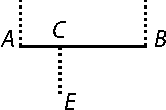
\includegraphics[width=0.19\textwidth]{gesamttex/edit_VIII-4/images/LH_37_05_043_d1_043r.pdf}}%
\vspace{0.25em}%
\centerline{\hspace{-45mm}%
\lbrack\textit{Fig.\:1}\rbrack}
\vspace{-5.82em}%
\centerline{\hspace{45mm}%
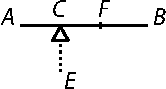
\includegraphics[width=0.19\textwidth]{gesamttex/edit_VIII-4/images/LH_37_05_043_d2_043r.pdf}}%
\vspace{0.25em}%
\centerline{\hspace{45mm}%
\lbrack\textit{Fig.\:2}\rbrack}
\vspace{1.0em}
\pstart%
Cum centralis est directio,%
\indexS{directio conatus centralis}
satis
\edtext{explicuimus}{%
\lemma{explicuimus}\Cfootnote{%
Siehe die Erläuterung zu N.\;\ref{60142+60297}, \refpassage{LH_35_10_17_009+37_05_041_explicuimus-1}{LH_35_10_17_009+37_05_041_explicuimus-2}.%
}}
ejus eventa,
perinde enim est,
ac si con\-ci\-pe\-re\-mus mobile
velut collectum in punctum,%
\indexS{mobile collectum in punctum}
nempe in centrum gravitatis.%
\indexS{mobile collectum in centrum gravitatis}
Sed Ec\-cen\-tri\-ca altioris est indaginis;%
\indexS{directio conatus eccentrica}%
\indexS{indago altior}%
\indexS{indago de directione conatus eccentrica}
quam ut%
\edlabel{LH_37_05_043r_anfang-2}
melius intelligamus,
utemur exemplo faciliore,%
\indexS{exemplum facilius}
lineae scilicet rectae \textit{ACB}
quae impellatur directione \textit{EC}.%
\indexS{linea recta impulsa}
Quaeritur quid sit futurum.
Eadem autem res redit,
ac si poneremus lineam \textit{AB}
incurrere in obstaculum \textit{C}.%
\indexS{obstaculum}%
\indexS{linea incurrens in obstaculum}
Quo facto
\edtext{conatus partium%
\indexS{conatus partium}%
}{%
\lemma{}\Bfootnote{%
conatus
\bars{ipsarum \textit{gestr.}}
partium%
~\textit{L}}}
\textit{CA} et \textit{CF} se
\edtext{mutuo compensabunt,%
\indexS{conatus compensantes se mutuo}
et conjungentur%
\indexS{conjunctio directionis centralis et circulationis}%
}{%
\lemma{mutuo}\Bfootnote{%
\textit{(1)}~destruent; et con
\textit{(2)}~compensabunt, et
\textit{(a)}~concur
\textit{(b)}~conjungentur%
~\textit{L}}}
directio centralis ipsius \textit{AF},%
\indexS{directio conatus centralis}
cujus centrum \textit{C},
et praeterea circulatio ipsius \textit{FB} circa \textit{C}.
Sed ubi paulum inclinata est \textit{AB}
per circulationem%
\indexS{circulatio in concursu eccentrico}
\edtext{circa \textit{C},%
}{%
\lemma{}\Bfootnote{%
circa \textit{C}
\textit{erg.\:L}}}
ita ut angulus \textit{ACE} fiat obtusus,%
\indexS{angulus obtusus}
jam simul et circulatur \textit{AB} circa \textit{C},
et progreditur glissando
\edtext{%
super \textit{C}.
\ledpb%
Fit etiam repercussio%
\indexS{repercussio ob obstaculum}%
\indexS{repercussio ob vim respectivam}
ab obstaculo,%
\indexS{obstaculum}
ob vim respectivam;%
\indexS{vis respectiva}
sed nobis sufficit%
\lbrack,\rbrack\
sine omni ictu,%
\indexS{ictus}
simplices%
}{%
\lemma{super \textit{C}.}\Bfootnote{%
\textit{(1)}~Sed nobis
\textit{(2)}~Fit etiam
\lbrack...\rbrack\ nobis sufficit
\textit{(a)}~si
\textit{(b)}~sine omni ictu, simplices%
~\textit{L}}}
nisus%
\indexS{nisus simplex}%
\indexS{nisus sine ictu}
\edlabel{LH_37_05_043_m043r1}%
considerare.
\edtext{}{%
\xxref{LH_37_05_043_m043r1}{LH_37_05_043_m043r2}%
\lemma{considerare.}\Bfootnote{%
\textit{(1)}~Idque
\textit{(2)}~Si \textit{AB}%
~\textit{L}}}%
\lbrack%
\href{\Scan{LH_37_05_043v}}%
{43\,v\textsuperscript{o}}%
\rbrack%
\pend%
\pstart%
Si%
\edlabel{LH_37_05_043_m043r2}
\edtext{\textit{AB} sustineatur}{\lemma{\textit{AB} sustineatur}\Cfootnote{%
Vgl. das Diagramm \lbrack\textit{Fig.\:3}\rbrack.}}
in \textit{C},
sumatur $CF=AC$,
et supererit nisus%
\indexS{nisus superstes}
ipsius \textit{FB} secundum nisum centri%
\indexS{nisus centri gravitatis}%
\indexS{centrum gravitatis corporis sustenti}
sui gravitatis \textit{H},
quo conabitur \textit{H} moveri circa \textit{C}
ita
\edtext{ut celeritas conatus circulatorii%
\indexS{conatus circulatorius}%
\indexS{celeritas conatus circulatorii}%
}{%
\lemma{ut}\Bfootnote{%
\textit{(1)}~conatus circ
\textit{(2)}~celeritas
\textit{(a)}~circulationis
\textit{(b)}~conatus circulatorii%
~\textit{L}}}
puncti \textit{H} sit aequalis celeritati
qua inciperet descendere \textit{H}
si non retineretur,
seu celeritati ipsius%
\indexS{impressio}%
\indexS{celeritas impressionis}
\edlabel{LH_37_05_043_m043v1}%
impressionis.%
\edtext{}{%
\xxref{LH_37_05_043_m043v1}{LH_37_05_043_m043v2}%
\lemma{impressionis.}\Bfootnote{%
\lbrack/\rbrack\
\textit{(1)}~Sed \textlangle\textit{C}\textrangle\ qui
\lbrack/\rbrack\
\textit{(2)}~Motus perinde
\textit{(a)}~erit
\textit{(b)}~aequalem exhibemus
\textit{(3)}~\bars{Se \textit{streicht Hrsg.}}
\textit{(4)}~\textit{C} premitur %
\lbrack...\rbrack\ \textit{AF}, sed%
~\textit{L}}}
\textit{C} premitur pondere%
\indexS{pondus premens}
ipsius \textit{AF},
sed%
\edlabel{LH_37_05_043_m043v2}
non pondere ipsius \textit{FB},
quod libere agit.%
\indexS{pondus agens libere}
\edlabel{LH_37_05_043_043v_centrgyr-1}%
Eodem igitur modo res se habet
cum impulsu \textit{C},%
\indexS{impulsus eccentricus}
ut eo solum afficiatur
\edlabel{LH_37_05_043_043v_cdrb-1}%
\edtext{}{%
\lemma{\textit{AF}}\Bfootnote{%
\textit{(1)}~. Sed si ponamus descendere \textit{H}
\textit{(2)}~reliquo \textit{FB} %
\lbrack...\rbrack\ puncto \textit{H},
\textit{(a)}~moveatur \textit{C} ea celeritate quam nisus pu
\textit{(b)}~punctum \textit{C} habet conatum impulsus.
\textit{(aa)}~\lbrack/\rbrack\ Hinc si
\textit{(bb)}~Adeoque gyratur %
\lbrack...\rbrack\ Idem est%
~\textit{L}}}%
\textit{AF}
reliquo \textit{FB} non affecto,
ac proinde quiescente puncto \textit{H},
punctum \textit{C} habet conatum impulsus.%
\indexS{conatus impulsus}
Adeoque gyratur \textit{C}
circa \textit{H}
celeritate impulsus.%
\indexS{celeritas impulsus}%
\indexS{impulsus eccentricus}%
\edlabel{LH_37_05_043_043v_centrgyr-2}
\pend%
\vspace{2.5em} %
\centerline{%
\hspace{-55mm}%
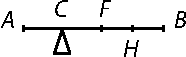
\includegraphics[width=0.20\textwidth]{gesamttex/edit_VIII-4/images/LH_37_05_043_d3_043v.pdf}}
\vspace{1.00em}
\centerline{%
\hspace{-55mm}%
\lbrack\textit{Fig.\:3}\rbrack}
\vspace{1em}
\vspace{-7.45em} %
\centerline{%
\hspace{55mm}%
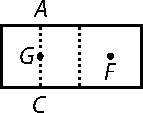
\includegraphics[width=0.15\textwidth]{gesamttex/edit_VIII-4/images/LH_37_05_043_d4_043v.pdf}}
\vspace{0.25em}
\centerline{%
\hspace{55mm}%
\lbrack\textit{Fig.\:4}\rbrack}
\vspace{1.15em}%
\pstart%
\edlabel{LH_37_05_043_043v_urzelle-1}%
Idem est%
\edlabel{LH_37_05_043_043v_cdrb-2}
in toto aliquo corpore,
ut si
\edtext{corpus %
impellitur%
\indexS{corpus impulsum}%
}{%
\lemma{corpus %
impellitur}\Cfootnote{%
Vgl. das Diagramm \lbrack\textit{Fig\:4}\rbrack.}}
impulsu \textit{C},%
\indexS{impulsus eccentricus}
habebitur \textit{G} centrum impulsi%
\indexS{centrum gravitatis corporis impulsi}%
\indexS{corpus impulsum}
et gyrantis%
\indexS{centrum gravitatis corporis gyrantis}%
\indexS{corpus gyrans}
ac \textit{F} centrum reliqui%
\indexS{corpus reliquum}%
\indexS{centrum gravitatis corporis reliqui}
circa quod fit gyratio.%
\indexS{gyratio circa centrum corporis reliqui}%
\edlabel{LH_37_05_043_043v_urzelle-2}
Puncti concursus%
\indexS{punctum concursus}%
\indexS{concursus corporum}
planorum,%
\indexS{planum concursus}
hic nulla habenda ratio.
\pend%
\pstart%
Dubia interdum fit perpendicularis ad contactum%
\indexS{contactus corporum concurrentium}%
\indexS{linea perpendicularis ad contactum}%
\lbrack,\rbrack\
ut si
\edtext{\textit{a} et \textit{b} corpora}{%
\lemma{\textit{a}~et~\textit{b} corpora}\Cfootnote{%
Vgl. das Diagramm \lbrack\textit{Fig.\:5}\rbrack.}}
concurrant;
multae enim duci
\edtext{%
possunt tangentes utrumque corpus
in puncto communi,%
\indexS{punctum commune}%
\indexS{linea tangens in puncto communi}
ut \textit{lm}, \textit{no},%
}{%
\lemma{possunt}\Bfootnote{%
\textit{(1)}~perpendiculares ad contactum, ut \textit{l}
\textit{(2)}~tangentes utrumque %
\lbrack...\rbrack\ ut \textit{lm}, \textit{no},%
~\textit{L}}}
nec proinde haec plane finita.
\pend%
\pstart%
Sit%
\indexS{pondus sustentatum}
\edtext{pondus \textit{A}}{%
\lemma{pondus \textit{A}}\Cfootnote{%
Vgl. das Diagramm \lbrack\textit{Fig.\:6}\rbrack.}}
sustentatum fulcris%
\indexS{fulcrum innitens}
\edtext{%
\textit{LM}, \textit{PQ}
quae innituntur brachiis \textit{NM},%
\indexS{brachium sustinens}
\lbrack\textit{RQ}\rbrack\
et sustinentur ponderibus \textit{B}, \textit{C} %
ex brachiis \textit{BN}, \textit{CR}.%
\indexS{pondus sustinens}%
\indexS{brachium sustinens}
Ponantur autem \textit{BN}, \textit{CR}, \textit{RQ}, \textit{NM} aequales.
Quaeritur quae debeat esse ratio%
}{%
\lemma{\textit{LM}, \textit{PQ}}\Bfootnote{%
\textit{(1)}~quaeritur quomodo se habere debeat
\textit{(2)}~quae innituntur brachiis \textit{NM},
\bars{\textit{RC} \textit{ändert Hrsg.}}
et sustinentur %
\lbrack...\rbrack\ Ponantur autem
\textit{(a)}~\textit{BN}, \textit{NM},
\textit{(b)}~\textit{BC} f
\textit{(c)}~\textit{BN}, \textit{CR}, %
\lbrack...\rbrack\ esse ratio%
~\textit{L}}}
cujusque ponderis \textit{B} et \textit{C} ad pondus \textit{A}.
\pend%
\newpage%
\pstart%
Comparetur haec consideratio
cum consideratione motus compositi%
\indexS{motus compositus e volutione et defluxu}
ex volutione%
\indexS{volutio globi}
et defluxu globi%
\indexS{defluxus globi}
super plano inclinato.%
\indexS{planum inclinatum}
Nam et in impulsu eccentrico%
\indexS{impulsus eccentricus}
motus compositus ex gyratione%
\indexS{gyratio ex impulsu eccentrico}
et directo motu.%
\indexS{motus directus}%
\indexS{motus compositus e gyratione et motu directo}
\pend%
\vspace*{1.5em} %
\centerline{\hspace{-90mm}%
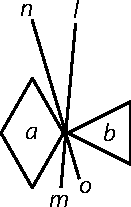
\includegraphics[width=0.14\textwidth]{gesamttex/edit_VIII-4/images/LH_37_05_043_d5_043v.pdf}}%
\vspace{1.0em}%
\centerline{\hspace{-90mm}%
\lbrack\textit{Fig.\:5}\rbrack}
\vspace{5.0em}%
\vspace{-15.65em} %
\centerline{\hspace{45mm}%
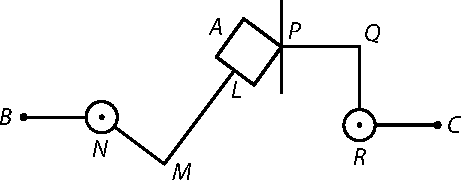
\includegraphics[width=0.5\textwidth]{gesamttex/edit_VIII-4/images/LH_37_05_043_d6_043v.pdf}}
\vspace{1.5em}
\centerline{\hspace{45mm}%
\lbrack\textit{Fig.\:6}\rbrack}
\vspace{3.5em}%
\pstart%
\noindent%
\lbrack\textit{Ohne unmittelbaren Zusammenhang mit dem Text und wohl bereits vorhanden:}\rbrack\
\pend%
\vspace*{2.5em} %
\centerline{\hspace{-05mm}%
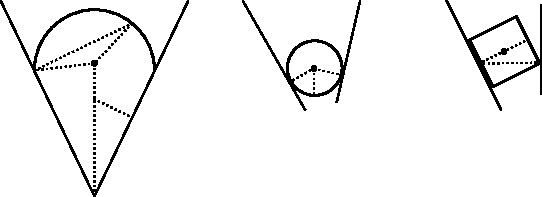
\includegraphics[width=0.52\textwidth]{gesamttex/edit_VIII-4/images/LH_37_05_043_d7_043v.pdf}}
\vspace{-1.0em}
\centerline{\hspace{-00mm}%
\lbrack\textit{Fig.\:7}\rbrack}
\vspace{2.5em} %
\centerline{\hspace{00mm}%
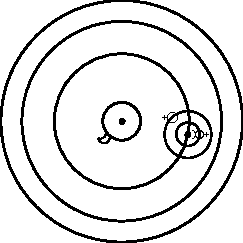
\includegraphics[width=0.26\textwidth]{gesamttex/edit_VIII-4/images/LH_37_05_043_d8_043v.pdf}}
\vspace{0.75em}
\centerline{\hspace{00mm}%
\lbrack\textit{Fig.\:8}\rbrack}
\selectlanguage{latin}%
\frenchspacing%
\normalsize%




\chapter[tocentry={De impulsu eccentrico
\enskip\bracks{%
April \textendash\ Oktober 1690%
}},
head={De impulsu eccentrico}]%
{\MakeUppercase{De impulsu eccentrico}
\newline\bracks{%
April \textendash\ Oktober 1690%
}}
\label{60300}
\selectlanguage{ngerman}
\begin{ledgroupsized}[r]{120mm}
\footnotesize
\pstart
\noindent\textbf{Überlieferung:}
\pend
\end{ledgroupsized}
\begin{ledgroupsized}[r]{114mm}
\footnotesize
\pstart \parindent -6mm
\makebox[6mm][l]{\textit{L}}%
Aufzeichnung:
LH~XXXVII~5 Bl.\;44.
Ein Blatt~2\textsuperscript{o},
unterer Rand ausgefranst mit geringfügigem Textverlust;
Papiererhaltungsmaßnahmen.
Ein \href{\Scan{LH_37_05_044wz}}{Wasserzeichen} mittig:
Papier der Klostermühle zu Thierhaupten bei Augsburg.%
\indexO{Thierhaupten bei Augsburg}\indexO{Augsburg}
Eine vollbeschriebene Seite auf Bl.\;44\,r\textsuperscript{o}
und vier Zeilen auf Bl.\;44\,v\textsuperscript{o},
sonst unbeschrieben.
Sämtliche Diagramme eigenhändig von Leibniz nummeriert.
\pend%
\end{ledgroupsized}%
\vspace{5mm}%
\begin{ledgroup}%
\footnotesize%
\pstart%
\noindent%
\textbf{Datierungsgründe:}%
\pagelabel{LH_37_05_044_datierung}
Die undatierte Aufzeichnung N.\;\ref{60300} \textit{De impulsu eccentrico} ist auf Papier der Klostermühle zu Thierhaupten bei Augsburg\indexO{Augsburg} verfasst.\indexO{Thierhaupten bei Augsburg}
Leibniz hielt sich in Augsburg\indexO{Augsburg} und Regensburg\indexO{Regensburg} im April 1690 auf, als er sich nach seiner Italienreise\indexO{Italien} auf dem Weg von Venedig\indexO{Venedig} nach Wien\indexO{Wien} befand (\textit{Chronik}, S.\;102\,f.).\cite{01236}
Die Aufzeichnung N.\;\ref{60300} wurde wohl damals geschrieben.
Die in \textit{LSB} VIII,\;3 N.\;31\textsubscript{2} edierte \textit{Appendix de vi absoluta},\cite{01397} deren Reinschrift \textit{L\textsuperscript{2}} auf gleichem Papier der Abtei zu Thierhaupten\indexO{Thierhaupten bei Augsburg} abgefasst wurde, zeigt, dass Leibniz seinen bairischen Aufenthalt unter anderem nutzte, um einige in den letzten Monaten seiner Italienreise\indexO{Italien} entstandene Entwürfe weiter zu bearbeiten.
Ähnlich dürfte es sich auch mit der Aufzeichnung N.\;\ref{60300} \textit{De impulsu eccentrico} verhalten.
Denn wie die auf \refpassage{LH_37_05_044r_alias_dhe-1}{LH_37_05_044r_alias_dhe-2} anzutreffende Anspielung zeigt, nimmt N.\;\ref{60300} unmittelbar auf die Behandlung des exzentrischen Stoßes in dem wohl noch Ende 1689 oder Anfang 1690 in Oberitalien\indexO{Italien} verfassten Text N.\;\ref{60142+60297} Bezug, um die dort (\refpassage{60142+60297_centrumgyrationis-1}{60142+60297_centrumgyrationis-2}) geäußerte Ansicht über das \textit{centrum gyrationis} zu berichtigen:
Anders als in N.\;\ref{60142+60297} ist Leibniz in N.\;\ref{60300} überzeugt, dass der Mittelpunkt der vom exzentrischen Stoß herrührenden Drehung mit dem Schwerpunkt des gesamten angestoßenen Körpers zusammenfalle.
Auch die Aufzeichnung N.\;\ref{60300} ist somit \textendash\ wie die Reinschrift \textit{LSB} VIII,\;3 N.\;31\textsubscript{2}, \textit{L\textsuperscript{2}} \textendash\ aller Wahrscheinlichkeit nach auf April 1690 zu datieren.
\pend%
\pstart%
Ferner gilt es zu beachten, dass kurz vor seiner Abreise aus Venedig\indexO{Venedig} Leibniz in seinem Brief an Rudolf Christian von Bodenhausen\indexN{\textls{Bodenhausen} (Bodenus, Bodenausen), Rudolf Christian, Freiherr v. 1698} vom 18.\;März 1690 versprochen hatte, den der Stoßlehre gewidmeten, noch unvollständigen Abschnitt der \textit{Dynamica} (%
\textit{CFP}~I, S.\;392--445~\bracks{A}; II.2, S.\;490--550~\bracks{C})\cite{01354} auf dem Weg nach Augsburg\indexO{Augsburg} abzuschließen (\textit{LSB} III,\;4 N.\;245, S.\;485.15\textendash23;\cite{01392} siehe zudem \textit{LSB} III,\;4 N.\;242, S.\;473.25\textendash474.1).\cite{01390}
Die Aufzeichnung N.\;\ref{60300} könnte somit ein vorläufiges Ergebnis aus Leibnizens Bestreben darstellen, die Versprechung an Bodenhausen\indexN{\textls{Bodenhausen} (Bodenus, Bodenausen), Rudolf Christian, Freiherr v. 1698} zu erfüllen.
(Siehe über die Genese der \textendash\ nie vollendeten \textendash\ \textit{Dynamica}\cite{01354} unter besonderer Berücksichtigung der Stoßlehre die einleitende Erläuterung zu N.\;\ref{impulsuseccentricus}, \refpassage{impulsecc_intro_Dynam-1}{impulsecc_intro_Dynam-2}.)
Auch dies bekräftigt die Annahme, dass die Aufzeichnung N.\;\ref{60300} im April 1690 entstand.
\pend%
\pstart%
Selbst wenn Leibniz erst später \textendash\ auf der Rückfahrt nach Hannover\indexO{Hannover} oder gar am Zielort \textendash\ die Aufzeichnung N.\;\ref{60300} verfasst haben sollte, so ist diese letztere in jedem Fall vor den von ihm eigenhändig auf den 31.\;Okto\-ber\,/\,10.\;November 1690 datierten \textit{Schedae de concursu eccentrico} N.\;\ref{58940} und N.\;\ref{58939} entstanden.
Denn über den Mittelpunkt der Drehung wird dort (N.\;\ref{58940}, \refpassage{LH_35_11_14_005-006_005r_cntrgyr-1}{LH_35_11_14_005-006_005r_cntrgyr-2}) ohne weitere Bemerkungen dieselbe Ansicht vertreten wie in der Aufzeichnung N.\;\ref{60300}.
\pend%
\end{ledgroup}%
\selectlanguage{latin}%
\frenchspacing%
\newpage%
\pstart%
\normalsize%
\noindent%
\lbrack%
\href{\Scan{LH_37_05_044r}}%
{44\,r\textsuperscript{o}}%
\rbrack\ %
\hfill%
De impulsu Eccentrico%
\indexS{impulsus eccentricus}%
\hfill%
\phantom{\lbrack44\,r\textsuperscript{o}\rbrack}%
\pend%
\vspace{1.0em}%
\pstart%
\noindent%
Cum recta \textit{AB}%
\indexS{recta inflexilis}
\edtext{inflexilis (fig.\,1)}{%
\lemma{inflexilis}\Bfootnote{%
(fig.\,1)
\textit{erg.\;L}}}
in medio \textit{C} impulsum recipit,%
\indexS{impulsus receptus in puncto medio}
utique nisu%
\indexS{nisus acceptus}
illo accepto fer\-tur ex
\textit{\ind{1}A\ind{1}C\ind{1}B}
in \textit{\ind{2}A\ind{2}C\ind{2}B}.
Et perinde est
ac si%
\indexS{figura}
(in fig.\,2) ponamus rectam%
\indexS{recta inflexilis}
\edtext{\textit{AB}
\edtext{infl\lbrack e\rbrack xam,}{%
\lemma{infl\lbrack e\rbrack xam}\Cfootnote{%
\glqq unverbogen\grqq.}}
nisu \textit{\ind{1}C\ind{2}C}%
}{%
\lemma{\textit{AB}}\Bfootnote{%
\bars{inflaexam \textit{ändert Hrsg.}}
nisu
\textit{(1)}~\textit{\ind{1}A\ind{2}A}
\textit{(2)}~\textit{\ind{1}C\ind{2}C}%
~\textit{L}}}
venientem ex
\textit{\ind{1}A\ind{1}C\ind{1}B}
in \textit{\ind{2}A\ind{2}C\ind{2}B},
ibi in \textit{\ind{2}C} invenire obstaculum nisum sistens,%
\indexS{obstaculum sistens nisum}
sine ictu tamen ullo,%
\indexS{ictus}
tunc tota linea \textit{AB}%
\indexS{linea inflexilis}
si inflexilis ponatur%
\lbrack,\rbrack\
quiescet in loco
\textit{\ind{2}A\ind{2}B}.
Dico autem sine
\edtext{ictu,
alioqui resiliret.
Ita ictus abest%
\indexS{ictus}%
}{%
\lemma{ictu,}\Bfootnote{%
\textit{(1)}~ali
\textit{(2)}~ut
\textit{(3)}~alioqui resiliret.
\textit{(a)}~Ut fit
\textit{(b)}~Ita ictus abest%
~\textit{L}}}
cum gravis recta \textit{AB} incumbit sustentaculo
\edtext{\lbrack\textit{C}\rbrack}{%
\lemma{\textit{B}}\Bfootnote{%
\textit{L~ändert Hrsg.}}}%
\indexS{sustentaculum}
quanquam revera nulla detur linea prorsus inflexilis,%
\indexS{linea inflexilis}
nec
\edtext{adeo}{%
\lemma{adeo}\Bfootnote{%
\textit{erg.\;L}}}
\edtext{ullus nisus%
\indexS{nisus}%
}{%
\lemma{ullus}\Bfootnote{%
\textit{(1)}~impetus
\textit{(2)}~nisus%
~\textit{L}}}
plane supprimi possit.
\pend%
\begin{edfigure}[2.00em][1.50em]%
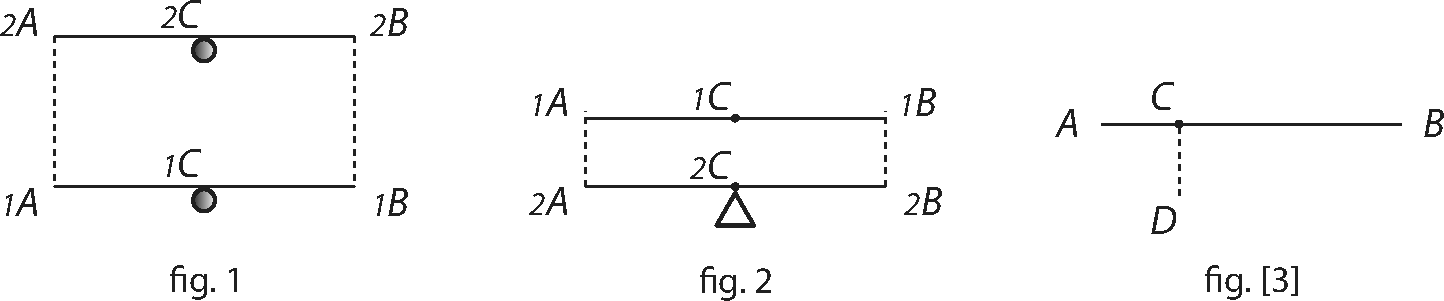
\includegraphics[width=0.96\textwidth]{gesamttex/edit_VIII-4/images/LH_37_05_044_d1-3_044r.pdf}%
\edcaption[-1.25em]%
{%
\edtext{}{\lemma{fig.\,\lbrack3\rbrack}%
\Cfootnote[nonum]{%
In \textit{L} irrtümlich als \textit{fig.\:4} bezeichnet.%
}}%
}%
\end{edfigure}%
\pstart%
\noindent%
\edlabel{LH_37_05_044r_impulsusnonplenus-1}%
Sed cum impulsus%
\indexS{impulsus extra punctum medium}
\edtext{\textit{DC}}{%
\lemma{\textit{DC}}\Bfootnote{%
\textit{erg.\;L}}}
est in puncto \textit{C} extra medium%
\indexS{figura}
\edtext{(fig.\,3),}{%
\lemma{(fig.\,3.)}\Bfootnote{%
\textit{erg.\;L}}}
ibi necesse non est %
ut tota recta%
\indexS{recta recipiens impulsum}
\edtext{\textit{AB} impulsum plene recipiat}{%
\lemma{\textit{AB}}\Bfootnote{%
\textit{(1)}~secundum lineam im
\textit{(2)}~impulsum plene recipiat%
~\textit{L}}}
et quodlibet ejus punctum feratur
nisus gradu \textit{DC}%
\indexS{gradus nisus}
in parallelis ipsi \textit{DC},
nam si
\edtext{punctum \textit{B} vel aliud
in recta \textit{AB} maneret
\lbrack immotum\rbrack\
et}{%
\lemma{punctum}\Bfootnote{%
\textit{B}
\textit{(1)}~manere
\textit{(2)}~vel aliud %
\lbrack...\rbrack\ \textit{AB} maneret
\bars{in motum \textit{ändert Hrsg.}}
et~\textit{L}}}
circa ipsum gyraretur punctum \textit{C} %
ipso nisu recepto,%
\indexS{nisus receptus}
jam impulsui esset satisfactum.%
\edlabel{LH_37_05_044r_impulsusnonplenus-2}
Sed non est rationi consentaneum
ut punctum aliquod in recta \textit{AB} plane quiescat.
Nam si impulsus \textit{C}%
\indexS{impulsus accedens ad punctum medium}
accedat continue versus
\edtext{medium%
\lbrack,\rbrack\
tunc
sive punctum illud quiescens idem maneat
sive continue mutetur%
\lbrack,\rbrack\
utroque modo tunc
continue
acceden\lbrack te\rbrack\
ad medium,%
\indexS{impulsus accedens ad punctum medium}%
}{%
\lemma{medium}\Bfootnote{%
\textit{(1)}~vel
\textit{(2)}~tunc sive punctum illud quiescens
\textit{(a)}~vel
\textit{(b)}~idem
\textit{(aa)}~manebit vel mutabitur
\textit{(bb)}~maneat sive continue mutetur;
\textit{(aaa)}~si enim manet
\textit{(bbb)}~utroque modo tunc continue
\bars{accedendo \textit{ändert Hrsg.}}
ad medium,%
~\textit{L}}}
denique in ipso medio impulsu quoque%
\indexS{impulsus receptus in puncto medio}%
\lbrack,\rbrack\
aliquod maneret punctum quiescens,
quod falsum esse jam
\edtext{constat.
Itaque necesse est
in impulsu Eccentrico%
\indexS{impulsus eccentricus}%
}{%
\lemma{constat.}\Bfootnote{%
\textit{(1)}~Sin punctum quiescens mutetur, tamen aliquod semper
\textit{(a)}~prodibit
\textit{(b)}~erit, etiam impulsus.
\textit{(2)}~Itaque in casu impu
\textit{(3)}~Itaque necesse %
\lbrack...\rbrack\ impulsu Eccentrico%
~\textit{L}}}
motum esse compositum%
\indexS{motus compositus}
ex propulsione%
\indexS{propulsio}
et
\edtext{gyratione.%
\indexS{gyratio in concursu eccentrico}
Et quidem
quo longius recedetur a medio,%
\indexS{impulsus recedens a puncto medio}
hoc magis valebit gyratio,%
\indexS{gyratio in concursu eccentrico}
quo propius ad medium accedetur,%
\indexS{impulsus accedens ad punctum medium}
hoc plus poterit impulsus
donec in medio%
\indexS{impulsus receptus in puncto medio}
omnis gyratio evanescat.%
\indexS{gyratio evanescens}%
}{%
\lemma{gyratione.}\Bfootnote{%
\textit{(1)}~Quod etiam inde \textit{C} vinci potest, quia
\textit{(2)}~Et quidem %
\lbrack...\rbrack\ magis valebit
\textit{(a)}~conatus,
\textit{(b)}~gyratio, quo %
\lbrack...\rbrack\ gyratio evanescat.%
~\textit{L}}}
\pend%
\pstart%
Centrum autem gyrationis%
\indexS{centrum gyrationis}%
\indexS{gyratio in concursu eccentrico}
erit ab ea parte,
quae a puncto impulsus%
\indexS{punctum impulsus}%
\indexS{impulsus eccentricus}
est remotior.
Et accedente puncto impulsus%
\indexS{punctum impulsus}
ad medium,%
\indexS{impulsus accedens ad punctum medium}
etiam centrum gyrationis medio accedet,%
\indexS{centrum gyrationis}
et incidente ipso in medium
\edtext{\lbrack etiam centrum gyrationis in medium\rbrack}{%
\lemma{etiam}\Bfootnote{%
centrum gyrationis in medium
\textit{erg.\;Hrsg.}}}
incidet,
transeunte enim puncto impulsus%
\indexS{punctum impulsus}
in alteram medietatem,
etiam centrum
\edtext{gyrationis%
\indexS{centrum gyrationis}
in priorem medietatem transibit.
Ut in fig.\,4%
\indexS{figura}
si punctum impulsus \textit{C}%
\indexS{punctum impulsus}
sit propius extremo \textit{A},
centrum}{%
\lemma{gyrationis}\Bfootnote{%
in
\textit{(1)}~alteram
\textit{(2)}~priorem medietatem transibit.
\textit{(a)}~Si \textit{C}
\textit{(b)}~Ut
\bars{in fig.\,4 \textit{erg.}}
\textit{(aa)}~si \textit{C} sit propius \textit{A}, cent
\textit{(bb)}~si punctum \lbrack...\rbrack\ \textit{A}, centrum%
~\textit{L}}}
gyrationis \textit{G}%
\indexS{centrum gyrationis}
erit propius extremo \textit{B};
et
\edtext{contra si \textit{C} sit}{%
\lemma{contra}\Bfootnote{%
si
\bars{centrum \textit{gestr.}}
\textit{C} sit%
~\textit{L}}}
propius ipsi \textit{B},
erit \textit{G} propius ipsi \textit{A},
ac proinde si \textit{C} in medio
erit et \textit{G} in medio,
adeoque tunc coincident \textit{G} et \textit{C}.
Sed ipsa gyratio tunc erit infinite parva.%
\indexS{gyratio infinite parva}
\pend%
\pstart%
At inquies,
fateor%
\lbrack,\rbrack\
ostendisti
\edtext{supra}{%
\lemma{supra}\Cfootnote{%
\refpassage{LH_37_05_044r_impulsusnonplenus-1}{LH_37_05_044r_impulsusnonplenus-2}.}}
non sequi
\edtext{necessario nisum}{%
\lemma{necessario}\Bfootnote{%
\textit{(1)}~impulsum
\textit{(2)}~nisum%
~\textit{L}}}
plenum%
\indexS{nisus plenus}
ex impulsu eccentrico;%
\indexS{impulsus eccentricus}
\edtext{attamen nec ostensum est}{%
\lemma{attamen}\Bfootnote{%
\textit{(1)}~nec ostendi
\textit{(2)}~nec ostensum est%
~\textit{L}}}
sequi gyrationem.%
\indexS{gyratio in concursu eccentrico}
Respondeo%
\lbrack:\rbrack\
eo ipso
quod inferri non potest
impulsus plenus,%
\indexS{nisus plenus}
utique nec orietur,
adeoque immiscebit se gyratio,%
\indexS{gyratio immixta}
quae
\edtext{\lbrack ni\-sum\rbrack}{%
\lemma{minus}\Bfootnote{%
\textit{L~ändert Hrsg.}}}
mutat.
Quod ut appareat distinctius %
in omni corpore considerandus est renisus ad motum.%
\indexS{renisus ad motum}
Et perinde est
ac si impulsu facto in \textit{C},%
\indexS{impulsus eccentricus}
reliqua puncta omnia contrarium quendam haberent%
\indexS{nisus contrarius}
\edtext{nisum,
quibus omnibus
posita inflexibilitate%
\indexS{inflexibilitas}
non melius satisfit
\lbrack nisi\rbrack\
per gyrationem.%
\indexS{gyratio immixta}%
}{%
\lemma{nisum,}\Bfootnote{%
\textit{(1)}~ubi sine g
\textit{(2)}~quibus omnibus %
\lbrack...\rbrack\ melius satisfit
\bars{nisi \textit{erg.\;Hrsg.}}
per gyrationem.%
~\textit{L}}}
\pend%
\vspace{1.25em} %
\centerline{%
\includegraphics[width=0.24\textwidth]{%
gesamttex/edit_VIII-4/images/LH_37_05_044_d4_044r.pdf%
}}
\newpage%
\vspace*{0.0em}%
\centerline{\hspace{-55mm}%
\includegraphics[width=0.24\textwidth]{%
gesamttex/edit_VIII-4/images/LH_37_05_044_d5_044r.pdf%
}}%
\vspace{-4.25em} %
\centerline{\hspace{55mm}%
\includegraphics[width=0.24\textwidth]{%
gesamttex/edit_VIII-4/images/LH_37_05_044_d6_044r.pdf%
}}
\vspace{1.0em}
\pstart%
\noindent%
Patet etiam centrum gyrationis \textit{G}%
\indexS{centrum gyrationis}
non esse semper punctum extremum \textit{B};
nam ut ex
\edtext{fig.\,4%
\indexS{figura}
manifestum est,}{%
\lemma{fig.\,4}\Bfootnote{%
\textit{(1)}~patet,
\textit{(2)}~manifestum est,%
~\textit{L}}}
eo propius accedit ad medium,
quo propius ipsum \textit{C} accedit ad medium.
\edlabel{LH_37_05_044_044r_cntrgyr-1}%
Quin imo hinc videtur refutari
\edlabel{LH_37_05_044r_alias_dhe-1}%
quod
\edtext{alias}{%
\lemma{alias}\Cfootnote{%
Wohl N.\;\ref{60142+60297},
\refpassage{60142+60297_centrumgyrationis-1}{60142+60297_centrumgyrationis-2}; siehe auch N.\;\ref{60299}, \refpassage{LH_37_05_043_043v_centrgyr-1}{LH_37_05_043_043v_urzelle-2}.%
}}
mihi rationabile visum est,%
\indexS{rationabile}
centrum gyrationis%
\indexS{centrum gyrationis}
\edtext{(fig.\,5)%
\indexS{figura}
esse centrum gravitatis%
\indexS{centrum gravitatis partis impulsae}
partis non plene impulsae.%
\edlabel{LH_37_05_044r_alias_dhe-2}
Sumatur \textit{AD} portio rectae \textit{AB},
cujus portionis \textit{AD} medium punctum sit \textit{C},%
}{%
\lemma{(fig.\,5)}\Bfootnote{%
\textit{(1)}~esse
\textit{(2)}~ita haberi. Sumatur \textit{CD} aequalis ipsi \textit{CA}
\textit{(3)}~esse centrum \lbrack...\rbrack\ punctum sit \textit{C},%
~\textit{L}}}
in quo fit impulsus,%
\indexS{impulsus eccentricus}
et reliquae partis \textit{DB} medium punctum sit \textit{G}.
Si igitur
\edtext{istud}{%
\lemma{istud}\Bfootnote{%
\textit{erg.\;L}}}
\textit{G} est centrum gyrationis,%
\indexS{centrum gyrationis}
tunc \textit{C} accedente ad medium,
non ideo \textit{G} accedit ad medium,
sed potius accedit ad \textit{B}.
Magis vero rationi consentaneum est%
\indexS{consentaneum rationi}
centrum gyrationis esse \textit{E}%
\indexS{centrum gyrationis}
centrum gravitatis commune%
\indexS{centrum gravitatis commune}
ipsorum \textit{C} et \textit{G},
\edtext{seu centrum gravitatis%
\lbrack,\rbrack%
}{%
\lemma{seu}\Bfootnote{%
centrum gravitatis
\textit{erg.\;L}}}
quoniam \textit{C} incidente in medium
\edtext{tunc \textit{E} etiam}{%
\lemma{tunc}\Bfootnote{%
\textit{(1)}~\textit{G} etiam
\textit{(2)}~\textit{E} etiam%
~\textit{L}}}
incidit in \textit{C}.
Et istud \textit{E} patet
semper esse invariabile seu idem,
ubicunque sit \textit{C}.%
\edlabel{LH_37_05_044_044r_cntrgyr-2}%
\pend%
\pstart%
Omnibus autem expensis
\edtext{talis eventus%
\indexS{eventus}
visus est rationi consentaneus.%
\indexS{consentaneum rationi}
\edlabel{LH_37_05_044r_fig.6-1}%
Incurrat}{%
\lemma{talis}\Bfootnote{%
\textit{(1)}~ratio visa est
\textit{(2)}~eventus visus est rationi consentaneus.
\textit{(a)}~Centrum
\textit{(b)}~Concurrant
\textit{(c)}~Incurrat%
~\textit{L}}}%
\edtext{}{%
\xxref{LH_37_05_044r_fig.6-1}{LH_37_05_044r_fig.6-2}%
\lemma{Incurrat globus \textit{H}}\Cfootnote{%
Vgl. das Diagramm \textit{fig.\,6}.%
}}
globus \textit{H}%
\edlabel{LH_37_05_044r_fig.6-2}
in rectam \textit{AB} quiescentem%
\indexS{globus incurrens in rectam quiescentem}
et incurrat Eccentrice in \textit{C}.%
\indexS{globus incurrens eccentrice}%
\indexS{incursus eccentricus}
\edlabel{LH_37_05_044_044r_navis-1}%
Utique centrum gravitatis eorum%
\indexS{centrum gravitatis commune}
progredietur eodem modo ante et post ictum,%
\indexS{progressus uniformis centri gravitatis}%
\indexS{ictus}
seu salvus erit motus communis%
\indexS{motus communis ut in navi}
quasi in navi ferrentur,%
\indexS{navis}
quae iret motu centri gravitatis.%
\indexS{motus centri gravitatis}%
\edlabel{LH_37_05_044_044r_navis-2}
Et proinde quoad hunc motum communem,%
\indexS{motus communis ut in navi}
ambo ferentur in rectis ipsi \textit{HC} parallelis.
Sed quoad motum proprium%
\indexS{motus proprius}
eadem
\edtext{est vis respectiva}{%
\lemma{est}\Bfootnote{%
\textit{(1)}~motus respectivus
\textit{(2)}~vis respectiva%
~\textit{L}}}
ante et post ictum,%
\indexS{vis respectiva ante ictum}%
\indexS{vis respectiva post ictum}
et \textit{H} quidem reflectitur in linea recta,
at recta \textit{AB} gyratur circa centrum
\edtext{gravitatis \textit{E},%
\indexS{centrum gravitatis commune}
quoniam considerando mobile \textit{AB}
ut reductum in duo puncta \textit{C} et \textit{G},
patet \textit{C} quidem impelli retrorsum
quo tendit \textit{H},
seu directione \textit{HC},
sed \textit{G} non impulsum
\textlangle interim\textrangle\
pergere
ut obstaculo in \textit{C} invento faceret,%
\indexS{obstaculum inventum}
et ita \textit{C} et \textit{G} in diversa nitentibus
gyratio fit%
\indexS{gyratio in concursu eccentrico}
circa centrum gravitatis eorum \textit{E};%
\indexS{centrum gravitatis commune}
ita quidem ut%
}{%
\lemma{gravitatis}\Bfootnote{%
\textit{E}
\textit{(1)}~celeritate
\textit{(2)}~motu reciproce proportionali; ita
\textit{(3)}~, quoniam considerando
\textit{(a)}~corpus
\textit{(b)}~mobile \textit{AB}
\lbrack...\rbrack\ ita quidem
\textit{(aa)}~ut
\textit{(bb)}~ut
\textit{(cc)}~ut%
~\textit{L}}}
motus proprii rectae%
\indexS{recta inflexilis}
et globi%
\indexS{globus incurrens eccentrice}
sint reciproce proportionales%
\indexS{motus proprius}%
\indexS{motus reciproce proportionalis}
ut ante concursum%
\indexS{concursus corporum}%
\lbrack,\rbrack\
tantum quod post ictum%
\indexS{ictus}
ipsius \textit{AB} motus proprius mutatur in gyrationem%
\indexS{motus proprius}%
\indexS{motus mutatus in gyrationem}
manente tamen eadem motus
\lbrack(\protect\vphantom)\rbrack%
\edtext{licet inaequaliter distributi%
\indexS{motus inaequaliter distributus}%
}{%
\lemma{licet}\Bfootnote{%
inaequaliter distributi
\textit{erg.\;L}}}%
\lbrack\protect\vphantom()\rbrack\
quantitate,%
\indexS{quantitas motus eadem}
seu si ex gyratione%
\indexS{gyratio in concursu eccentrico}
fieret motus
\edtext{rectus aequidistributus parallelus,%
\indexS{motus aequidistributus}%
\indexS{motus rectus}
centrum gravitatis \textit{E}%
\indexS{centrum gravitatis commune}
adeoque et tota \textit{AB} ferretur%
}{%
\lemma{rectus}\Bfootnote{%
\textit{(1)}~centrum gravitatis \textit{E} feretu
\textit{(2)}~aequidistributus parallelus, \lbrack...\rbrack\ \textit{AB} ferretur%
~\textit{L}}}
celeritate%
\indexS{celeritas reciproca}
\edtext{reciproca ad eam
qua}{%
\lemma{reciproca}\Bfootnote{%
\textit{(1)}~ad eam qu
\textit{(2)}~\bars{quantitatis \textit{streicht Hrsg.}}
\textit{(3)}~ad eam qua%
~\textit{L}}}
\textit{H} globus,%
\indexS{globus incurrens eccentrice}
itaque centra gravitatis%
\indexS{centrum gravitatis partis percussae}
\edtext{\textit{C}}{%
\lemma{\textit{C}}\Bfootnote{%
\textit{erg.\;L}}}
partis plene percussae \textit{AD} %
et \textit{G} partis non plene percussae \textit{DB} %
\indexS{centrum gravitatis partis percussae}
\edtext{gyrantur circa centrum totius \textit{E},%
\indexS{centrum gravitatis commune}
celeritatibus etiam}{%
\lemma{gyrantur}\Bfootnote{%
\textit{(1)}~etiam
\textit{(2)}~circa centrum %
\lbrack...\rbrack\ celeritatibus etiam%
~\textit{L}}}
reciproce proportionalibus%
\indexS{celeritas reciproce proportionalis}%
\lbrack;\rbrack\
et ducta quavis parte in celeritatem sui centri,%
\indexS{celeritas centri gravitatis}
prodit quantitas motus%
\indexS{quantitas motus eadem}
ex summa %
aequalis ei quam habet \textit{H}.%
\pend%
\pstart%
Sed succurrit tamen dubitatio%
\indexS{dubitatio}
quoad celeritatem reciproce proportionalem%
\indexS{celeritas reciproce proportionalis}
seu eandem quantitatem motus ipsius \textit{AB}%
\indexS{quantitas motus eadem}
et ipsius~\textit{H},
nam ita verum est quidem in motu aequidistributo%
\indexS{motus aequidistributus}
eandem prodire potentiam%
\indexS{potentia eadem}
\edtext{ex vi directionis%
\indexS{vis directionis}
et vi respectiva seu percussionis;%
\indexS{vis respectiva}%
\indexS{vis percussionis}%
}{%
\lemma{ex}\Bfootnote{%
\textit{(1)}~summa motus recti
\textit{(2)}~vi directionis \lbrack...\rbrack\ seu percussionis;%
~\textit{L}}}
sed hic videndum
an etiam absolutos motus considerando,%
\indexS{motus absolutus}
eadem hinc prodeat potentia absoluta%
\indexS{potentia absoluta}%
\indexS{potentia eadem}
in concursu Eccentrico%
\indexS{concursus eccentricus}%
\lbrack;\rbrack\
quod magnum foret indicium veritatis.%
\indexS{indicium veritatis}%
\indexS{veritas}
\lbrack%
\href{\Scan{LH_37_05_044v}}%
{44\,v\textsuperscript{o}\rbrack}%
\rbrack%
\pend%
\pstart%
Hinc etiam illud sequitur perpulchrum%
\lbrack:\rbrack\
omnes Eccentricos impulsus%
\indexS{impulsus eccentricus}
facere gyrationem%
\indexS{gyratio circa centrum gravitatis}
circa idem centrum.%
\indexS{centrum gyrationis}
Hinc si sint
\edtext{simul}{%
\lemma{simul}\Bfootnote{%
\textit{erg.\;L}}}
ad easdem partes augere gyrum,%
\indexS{gyrus}
sin
\edtext{minus e\lbrack u\rbrack m minuere.
Id quomodo fiat determinandum,
ut appareat quatenus unde augeatur repercussio,%
\indexS{repercussio}%
}{%
\lemma{minus}\Bfootnote{%
\bars{eam \textit{ändert Hrsg.}}
minuere
\textit{(1)}~, aucta repercussione
\textit{(2)}~. Id quomodo %
\lbrack...\rbrack\ augeatur repercussio,%
~\textit{L}}}
et quid omnino prodeat.%
\pend%
\selectlanguage{latin}%
\frenchspacing%
\normalsize%




\chapter[tocentry={Phorographica
\enskip \bracks{Oktober 1690 \textendash\ 1697}},
head={Phorographica}]%
{\MakeUppercase{Phorographica}
\newline \bracks{Oktober 1690 \textendash\ 1697}}

\label{60356}
\begin{ledgroupsized}[r]{120mm}
\footnotesize
\pstart
\noindent\textbf{Überlieferung:}
\pend
\end{ledgroupsized}
\begin{ledgroupsized}[r]{114mm}
\footnotesize
\pstart \parindent -6mm
\makebox[6mm][l]{\textit{L}}%
Konzept:
LH~XXXVII~5 Bl.~189. 
Ein Zettel (ca.~13~x~15~cm.) mit einem überstehenden Streifen unten rechts (ca.~7~x~3,5~cm.);
\href{\Scan{LH_37_05_189wz}}%
{Wasserzeichenfragment} am oberen Rand;
Papier\-erhaltungsmaßnahmen;
alle Ränder beschnitten.
Eine Seite auf Bl.~189~r\textsuperscript{o};
Bl.~\href{\Scan{LH_37_05_189v}}{189~v\textsuperscript{o}} 
überliefert einen eigenhändigen Briefentwurf:
\selectlanguage{french}%
\textit{Monsieur} \lbrack/\rbrack\
\textit{je vous demande pardon de ce que la premiere que j'ay} \lbrack/\rbrack\ \textit{l'honneur de vous ecrire est si precipitée. C'est pour profiter} \lbrack/\rbrack\ \textit{de l'occasion de vous envoyer ce qui y est joint. Je vous écriray} \lbrack/\rbrack\ \textit{plus amplement par la poste prochaine. Il me déplaist de ne} \lbrack/\rbrack\ \textit{vous pouvoir point envoyer la suite entiere des journaux de Paris.} \lbrack/\rbrack\ \textit{Comme je n'en reçois \sout{qu' apres avoir} que ce qui a passé par plusieurs mains à la} \lbrack/\rbrack\ \textit{cour, il s'en perd beaucoup, et quelques fois on ne me porte que des} \lbrack/\rbrack\ \textit{lambeaux. Comme en effect un des trois que voicy est imparfait.}
\pend
\end{ledgroupsized}
\vspace{5mm}
\begin{ledgroup}
\footnotesize
\pstart
\noindent%
\textbf{Datierungsgründe:}
Das Wasserzeichen im Träger von N.\;\ref{60356} ist für den Zeitraum Oktober 1690 bis Oktober 1697 mehrfach belegt.
Der Adressat des Entwurfs auf Bl.~189~v\textsuperscript{o}, offenbar als Begleitbrief für die Zusendung dreier Zeitschriften gedacht,
konnte noch nicht ermittelt werden.
\pend
\pstart
Am Ende von N.\;\ref{60356} (\refpassage{37_05_189_2a}{37_05_189_2b}) beruft sich Leibniz auf gewisse Ergebnisse der \glqq Dynamica\grqq, womit entweder bestimmte Schriften mit dem Titel "dynamica" (etwa die Entwürfe zur \cite{01354}\textit{Dynamica de potentia} von 1689, das \cite{02167}\textit{Essay de Dynamique} von 1692 oder aber das \cite{02032}\textit{Specimen Dynamicum} von 1695) gemeint sein könnten,
oder vielmehr die Disziplin der Dynamik im Allgemeinen, die der "Phorographica" folgen soll.
In diesem Zusammenhang siehe das vollständigste unter den erhaltenen Inhaltsverzeichnissen zur \textit{Dynamica de potentia}: Eine Randanmerkung von Leibniz zum allgemeinen Teil, insbesondere zur "Sect.\;2. De Motu in Genere", lautet "Addenda esset sectio phorographica" (\cite{01354}\textit{CFP} I, S.\;5 [A]).
\pend
\end{ledgroup}
\selectlanguage{latin}
\vspace{8mm}
\pstart%
\normalsize%
\noindent%
\href{\Scan{LH_37_05_189r}}%
{\lbrack189~r\textsuperscript{o}\rbrack}%
\edlabel{37_05_189_1a} %
\edtext{}{%
{\xxref%
{37_05_189_1a}{37_05_189_1b}}%
\lemma{\lbrack\textit{Fig.~1}\rbrack}%
\Bfootnote{%
\textit{(1)}~$\ind{1}C\ind{2}C=$
\textit{(a)}~\textit{\ind{1}A\ind{2}A}
\textit{(b)}~$\ind{2}A\ind{1}A-\ind{1}A\ind{1}C=
\ind{2}B\ind{2}B$\lbrack\textit{!}\rbrack\ $-$
\textit{(2)}~\bars{(1mo) \textit{erg.}}
$\ind{1}A\ind{1}C+\ind{1}C\ind{1}B=\ind{1}A\ind{2}A-\ind{2}B\ind{1}B=$
\bars{(2do) \textit{erg.}} 
$\ind{2}A\ind{3}C+\ind{3}C\ind{3}B=$
\textit{(a)}~$\ind{3}A\ind{2}A-\ind{2}B$
\textit{(b)}~\bars{(3tio) $\ind{3}B\ind{2}B-\ind{2}A\ind{3}A$ $=$ (4to) \textit{AB} \textit{streicht Hrsg.}}
\textit{(c)}~(3tio) \textit{\ind{1}C\ind{2}C} (4to)
$\ind{1}C\ind{2}C=\ind{2}C\ind{3}C=$ (5to)
$\ind{2}A\ind{1}A-\ind{1}A\ind{1}C$ (6to) $=$
\textit{(3)}~\bars{(1mo) \textit{erg.}}
$AB=A(A)-B(B)$. $C(C)=A(A)-$
\textit{(4)}~\textls{Phorographica} \lbrack/\rbrack\
\bars{Posito ante et post ictum
\textit{(a)}~omnes
\textit{(b)}~ambo tendere quo centrum
\bars{\textit{C} \textit{erg.}}
et \textit{A} sequi \textit{B} praecedere
ante ictum \textit{erg.}}
(1mo)~\textit{L}}}
\pend 
\begin{edfigure}[0.5em]%
\includegraphics%
[scale=1]{gesamttex/edit_VIII-4/images/LH_37_05_189_d_189r.pdf} %
\edcaption[0.25em]{\lbrack\textit{Fig.~1}\rbrack}
\end{edfigure}
\pstart\centering	%
\edtext{%
\textls{Phorographica}\indexS{Phorographica}%
}{\lemma{}\Afootnote{%
\textit{Am oberen rechten Rand}: 
$\ind{1}A\ind{1}C+\ind{1}B\ind{1}C=\ind{1}A\ind{1}C+\ind{1}B\ind{1}C=+\ind{1}A\ind{2}A-\ind{1}B\ind{2}B$}}
\pend
\nobreak\vspace{0.5\baselineskip}
\pstart\noindent
Posito ante et post ictum\indexS{ictus} ambo tendere quo centrum\indexS{centrum gravitatis} \textit{C} et \textit{A} sequi \textit{B} praecedere\lbrack,\rbrack\
ante ictum\indexS{ictus}
(1mo)%
\edlabel{37_05_189_1b}
$\ind{1}A\ind{1}B=\ind{1}A\ind{2}A-\ind{1}B\ind{2}B=$ 
(2do) $\ind{1}A\ind{1}C+\ind{1}B\ind{1}C$%
\pend
\pstart\noindent
(3tio) $\ind{1}C\ind{2}C=\ind{1}A\ind{2}A-\ind{1}A\ind{1}C=$ (4to) $\ind{1}B\ind{2}B+\ind{1}B\ind{1}C$
\pend
\pstart\noindent
post ictum (5to) $\ind{3}A\ind{3}B=-\ind{2}A\ind{3}A+\ind{2}B\ind{3}B=$ (6to) $\ind{3}A\ind{3}C+\ind{3}B\ind{3}C$
\pend
\pstart\noindent
(7mo) $\ind{2}C\ind{3}C=\ind{2}A\ind{3}A+\ind{3}A\ind{3}C=$ (8vo) $\ind{2}B\ind{3}B-\ind{3}B\ind{3}C$%
\pend
\pstart\noindent
Hinc generaliter (9no) $AB=\PM\, A(A) \MP B(B)=$ (10mo) $AC+BC$ et 
\edtext{(11mo)}{%
\lemma{}%
\Bfootnote{%
(11mo) %
\textit{erg.~L}%
}}
$C(C)=A(A) \MP AC=$ 
(12mo) $B(B) \PM BC$. 
Ubi notandum aeqq.~2, 6, 
\edtext{\lbrack11\rbrack,}{%
\lemma{}%
\Bfootnote{%
12 %
\textit{L ändert Hrsg.}%
}}
coincidere respective cum
\edtext{4, 8, 12. Et}{\lemma{4, 8, 12.}\Bfootnote{%
\textit{(1)}~Et aeqq.~9. 
\textit{(2)}~Aequ %
\textit{(3)}~Et~\textit{L}}}
aeqq.~9, 10, 11, 12, fieri respective ex collatis 1 et 5, 2 et 6, 3 et 7, 4 et 8 et in aeqq. dictis 4 
\edtext{postremis anteriorem}{\lemma{postremis}\Bfootnote{%
\textit{(1)}~prius signum ante %
\textit{(2)}~in signo ambiguo explicari de statu ante ictum %
\textit{(3)}~anteriorem~\textit{L}}}
explicationem signi ambigui\indexS{signum ambiguum} explicari de statu ante ictum,\indexS{status ante ictum}
\edtext{posteriorem de statu}{\lemma{posteriorem de}\Bfootnote{%
\textit{(1)}~signo %
\textit{(2)}~statu~\textit{L}}}
post ictum,\indexS{status post ictum} et quae vera sunt de \textit{A} ante ictum,\indexS{ictus} vera esse de \textit{B} post ictum\indexS{ictus} et vice versa.
\edtext{Atque haec vera}{\lemma{Atque}\Bfootnote{%
\textit{(1)}~hoc verum est %
\textit{(2)}~haec vera~\textit{L}}} 
sunt etiamsi status non sumantur immediate 
\edtext{ante ictum\indexS{ictus} vel}{\lemma{ante ictum}\Bfootnote{%
\textit{(1)}~sed %
\textit{(2)}~vel~\textit{L}}} 
immediate post ictum\lbrack,\rbrack\indexS{ictus}
\edtext{id est quorsumcunque}{\lemma{id est}\Bfootnote{%
\textit{(1)}~sive coincidant %
\textit{(2)}~quorsumcunque~\textit{L}}} 
cadant \textit{\ind{2}A}, \textit{\ind{2}B}, \textit{\ind{2}C}. 
Et licet fingas differre ea quae sunt primi (casus) cum iis quae sunt secundo, et ita 
\edtext{sumas 3 pro secundo 2, et 4}{\lemma{sumas}\Bfootnote{%
\textit{(1)}~\textit{\ind{1}A}, \textit{\ind{2}A}, \textit{\ind{3}A}, \textit{\ind{4}A}, seu
\textit{(2)}~3 pro secundo 2,
\textit{(a)}~cum hic sumamus \textit{\ind{1}A}, \textit{\ind{2}A}, \textit{\ind{2}A}, \textit{\ind{3}A}
\textit{(b)}~et 4~\textit{L}}}
pro 3; sive \textit{\ind{1}A}, \textit{\ind{2}A}, \textit{\ind{3}A}, \textit{\ind{4}A}, pro \textit{\ind{1}A}, \textit{\ind{2}A}, \textit{\ind{2}A}, \textit{\ind{3}A}. 
\pend
\pstart
\edlabel{37_05_189_2a}%
\edtext{}{%
\xxref{37_05_189_2a}{37_05_189_2b}%
\lemma{Sequuntur \bracks{...} generalis}%
\Cfootnote{%
Gemeint ist wohl die dynamische Disziplin im Allgemeinen, der eine \textit{phorographica} vorausgehen soll, und nicht etwa eine bestimmte Schrift. Ein ähnlich formuliertes Prinzip findet sich dennoch in den Entwürfen zur \textit{Dynamica de potentia} von 1689: pars II, sect. 6 (\textit{De concursu corporum}), prop.\;14 bzw. 19 (\cite{01354}\textit{CFP} I, S.\; 413 bzw. 430 [A]).}}%
Sequuntur \indexS{Dynamica}\textls{Dynamica}, ubi haec regula
\edtext{generalis.\edlabel{37_05_189_2b} \textls{Quicquid} reperitur}{\lemma{generalis.}\Bfootnote{%
\textit{(1)}~Omnis veritas quae reperitur %
\textit{(2)}~\textls{Quicquid} reperitur~\textit{L}}} 
commune duobus quibusvis statibus ante ictum,\indexS{status ante ictum} et duobus quibusvis statibus post ictum\lbrack,\rbrack\indexS{status post ictum} id etiam commune 
\edtext{reperitur cuivis statui ante ictum\indexS{status ante ictum}}{\lemma{reperitur}\Bfootnote{%
\textit{(1)}~statui ante ic %
\textit{(2)}~cuivis statui ante ictum~\textit{L}}} 
cum quovis statu post ictum.\indexS{status post ictum} \pend







\chapter[tocentry={Corpora diversa incurrentia in idem, idem efficere possunt
\enskip\bracks{%
Mitte Juni 1690 \textendash\ 1696\;(?)%
}},
head={Corpora diversa incurrentia idem efficere possunt}]%
{\MakeUppercase{Corpora diversa incurrentia in idem, idem efficere possunt}
\newline\bracks{%
Mitte Juni 1690 \textendash\ 1696\;(?)}%
}
\label{41121}
\selectlanguage{ngerman}
\begin{ledgroupsized}[r]{120mm}
\footnotesize
\pstart
\noindent\textbf{Überlieferung:}
\pend
\end{ledgroupsized}
\begin{ledgroupsized}[r]{114mm}
\footnotesize
\pstart \parindent -6mm
\makebox[6mm][l]{\textit{L}}%
Aufzeichnung:
LH~XXXV~9,\;7 Bl.\;22\textendash23. 
Ein Bogen~8\textsuperscript{o},
Ränder beschnitten;
Fragment eines \href{\Scan{LH_35_09_07_022-023wz}}{Wasserzeichens}: im Falz:
Niedersächsiches Papier.
Zweieinviertel Seiten;
Bl.\;23\,v\textsuperscript{o} ist unbeschrieben.
\pend
\end{ledgroupsized}
\vspace{3.5mm}
\begin{ledgroup}
\footnotesize
\pstart
\noindent%
\textbf{Datierungsgründe:}
Die Datierung der Aufzeichnung N.\;\ref{41121} beruht auf äußeren Eigenschaften des Text\-trägers %
sowie auf inhaltlichen Betrachtungen.
Siehe die ausführliche Begründung auf S.\;\pageref{41121_dat}.
\pend
\end{ledgroup}
\selectlanguage{latin}
\frenchspacing%
\vspace{5mm}
\pstart%
\normalsize%
\noindent%
\lbrack%
\href{\Scan{LH_35_09_07_022r}}%
{22\,r\textsuperscript{o}}%
\rbrack\ %
Si duo corpora%
\indexS{corpora occurrentia sibi directe centraliter}
(quae instar punctorum considerabimus)%
\indexS{corpus instar puncti}
sibi occurrant directe%
\indexS{occursus directus centralis}
\edtext{centraliter,
has}{%
\lemma{centraliter,}%
\Bfootnote{%
\textit{(1)}~et
\textit{(2)}~has%
~\textit{L}}}
habemus regulas.%
\indexS{regulae de concursu corporum}
(1)
Eadem est celeritas ad se%
\indexS{celeritas accedendi ante concursum}
\edtext{invicem accedendi}{%
\lemma{invicem}\Bfootnote{%
\textit{(1)}~recedendi
\textit{(2)}~accedendi%
~\textit{L}}}
ante concursum,
et a se invicem recedendi%
\indexS{celeritas recedendi post concursum}
post concursum.%
\indexS{concursus directus centralis}
(2)
Eadem est quantitas progressus%
\indexS{quantitas progressus ante concursum}%
\indexS{quantitas progressus post concursum}
ante et post
\edtext{%
concursum in easdem partes,
vel quod eodem redit,
eadem est celeritas centri gravitatis.%
\indexS{centrum gravitatis commune}%
\indexS{celeritas centri gravitatis}
(3)
Eadem%
}{%
\lemma{concursum}\Bfootnote{%
\textit{(1)}~. (3) Ea %
\textit{(2)}~in easdem partes %
\textit{(a)}~. (3) Eadem %
\textit{(b)}~, vel quod \lbrack...\rbrack\ (3) Eadem%
~\textit{L}}}
est quantitas virium.%
\indexS{quantitas virium in concursu}
(4)
Si corpora tendant ad easdem partes ante et post concursum,%
\indexS{corpora tendentia in easdem partes}
\edtext{%
servatur quantitas motus%
\indexS{quantitas motus servata}
seu summa motuum;%
\indexS{summa motuum}
si%
}{%
\lemma{servatur}\Bfootnote{%
\textit{(1)}~eadem quantitas mo
\textit{(2)}~summa
\textit{(a)}~motuum; si
\textit{(b)}~quantitatum motus
\textit{(3)}~quantitas motus %
\lbrack...\rbrack\ motuum; si%
~\textit{L}}}
corpora tendant in diversas partes ante et post concursum,%
\indexS{corpora tendentia in diversas partes}
servatur differentia%
\indexS{differentia motuum}
\edtext{%
motuum;
denique si corpora%
}{%
\lemma{motuum}\Bfootnote{%
\textit{(1)}~. (5) Si co %
\textit{(2)}~; denique si corpora%
~\textit{L}}}
tendant in partes easdem ante ictum,%
\indexS{corpora tendentia in easdem partes}%
\indexS{ictus}
in contrarias post ictum%
\indexS{corpora tendentia in contrarias partes}%
\indexS{ictus}%
\lbrack,\rbrack\
quae erat summa motuum%
\indexS{summa motuum}
fit differentia;%
\indexS{differentia motuum}
si tendant in contrarias ante ictum,%
\indexS{corpora tendentia in contrarias partes}%
\indexS{ictus}
in easdem post ictum,%
\indexS{corpora tendentia in easdem partes}%
\indexS{ictus}
ex differentia motuum%
\indexS{differentia motuum}
fit summa.%
\indexS{summa motuum}
\pend%
\vspace{0.25em}%
\pstart%
Calculus%
\indexS{calculus}
\pend%
\vspace{0.50em}%
\pstart%
\noindent%
Sit corpus
$\displaystyle\efrac{a}{b},$
celeritas ante ictum%
\indexS{celeritas ante ictum}%
\indexS{ictus}
$\displaystyle\efrac{v}{y},$
post ictum%
\indexS{celeritas post ictum}%
\indexS{ictus}
$\displaystyle\efrac{x}{z}.$%
\edlabel{35_09_07_022-023_1a}%
\edtext{}{%
\xxref{35_09_07_022-023_1a}{35_09_07_022-023_1b}%
\lemma{$\displaystyle\efrac{x}{z}.$\rule[-2ex]{0pt}{5ex}}%
\Bfootnote{%
\lbrack/\rbrack\
\textit{(1)}~$v \PM y$
\textit{(2)}~%
Sit%
~\textit{L}%
}}%
\pend%
\vspace{0.75em}%
\pstart%
\noindent%
\lbrack\textit{Nachfolgend kleingedruckter Text in L gestrichen:}\rbrack%
\pend%
\vspace{0.5em}%
\footnotesize%
\pstart%
\noindent%
Sit autem \textit{a}%
\edlabel{35_09_07_022-023_1b}
\edtext{%
corpus,
quod directioni contrariae non succumbit,%
\indexS{corpus succumbens directioni contrariae}%
\indexS{directio contraria}
seu cujus quantitas motus non est minor,%
\indexS{quantitas motus}%
}{%
\lemma{corpus,}%
\Bfootnote{%
\textit{(1)}~cujus quantitas motus est major, quodque adeo contrariae non succumbit,%
\indexS{corpus succumbens quantitati motus contrariae}
\textit{(2)}~quod directioni %
\lbrack...\rbrack\ cujus quantitas
\textit{(a)}~motus \textlangle prae\textrangle\
\textit{(b)}~motus non est minor,%
~\textit{L}%
}}
seu quod in easdem partes tendit cum centro%
\indexS{corpus tendens in easdem partes centri gravitatis}%
\indexS{centrum gravitatis commune}
\edtext{%
gravitatis.%
\quad%
$v - y \protect\overset{(1)}{=} \PM\, x \MP z,$%
\rule[-2ex]{0pt}{5ex}
explicando literam%
}{%
\lemma{gravitatis.}%
\Bfootnote{\lbrack/\rbrack\
\textit{(1)}~$v \PM y \protect\overset{(1)}{=} x - z$
\textit{(2)}~$v - y \protect\overset{(1)}{=} \PM\, x \MP z,$\rule[-2ex]{0pt}{5ex}
\textit{(a)}~pre
\textit{(b)}~sumendo lit
\textit{(c)}~explicando literam%
~\textit{L}%
}}
per numerum negativum,%
\indexS{litera explicanda per numerum negativum}%
\indexS{numerus negativus}
cum motus \textit{y} est contrarius ipsi \textit{v}.%
\indexS{motus contrarius}
\pend%
\newpage%
\normalsize%
\pstart%
\noindent%
Sit autem
$\displaystyle\efrac{a}{b}$
corpus quod%
\indexS{corpus antecedens centrum gravitatis}%
\indexS{corpus sequens centrum gravitatis}
$\displaystyle\efrac{\text{sequitur}}{\text{antecedit}}$
centrum gravitatis%
\indexS{centrum gravitatis commune}
ante ictum.%
\indexS{ictus}%
\pend%
\vspace{0.75em}%
\pstart%
\noindent%
Quodsi ambo tendant in easdem partes,
simul et \textit{a} sequetur et \textit{b} antecedet%
\lbrack;\rbrack\
quodsi tendant in contrarias partes,
tamen
\edtext{%
semper \textit{a} esto%
}{%
\lemma{semper \textit{a}}%
\Bfootnote{%
\textit{(1)}~erit
\textit{(2)}~esto%
~\textit{L}%
}}
illud
quod sequitur centrum
\edtext{%
gravitatis,%
\indexS{centrum gravitatis commune}
et \textit{b} centrum antecedet.
Potest tamen%
}{%
\lemma{gravitatis,}%
\Bfootnote{%
\textit{(1)}~et tunc e
\textit{(2)}~et \textit{b} %
\lbrack...\rbrack\ Potest tamen%
~\textit{L}%
}}
fieri
ut quod in easdem cum centro partes tendit
reflectatur.%
\indexS{corpus reflexum post ictum}
In
\edtext{%
casu motus contrarii%
\indexS{motus contrarius}%
}{%
\lemma{casu}%
\Bfootnote{%
\textit{(1)}~occursus
\textit{(2)}~motus contrarii%
~\textit{L}%
}}
corpus cujus
\edlabel{35_09_07_022-023_4a}%
quantitas motus%
\indexS{quantitas motus}%
\edtext{}{%
\xxref{35_09_07_022-023_4a}{35_09_07_022-023_4b}%
\lemma{quantitas motus}%
\Bfootnote{%
\bars{seu \textit{streicht Hrsg.}}
\textit{(1)}~\href{\Scan{LH_35_09_07_022v}}{\lbrack22~v\textsuperscript{o}\rbrack} seu quantitas progressus major est, in easdem partes tendit cum centro gravitatis. Sit \textit{a}
\textit{(2)}~\href{\Scan{LH_35_09_07_022r}}{\lbrack22~r\textsuperscript{o}\rbrack} seu quantitas \lbrack...\rbrack\ easdem partes
\textit{(a)}~centro gravitatis
\textit{(b)}~tendit cum centro gravitatis. \href{\Scan{LH_35_09_07_022v}}{\lbrack22~v\textsuperscript{o}\rbrack} \lbrack/\rbrack\ Generaliter%
~\textit{L}%
}}
seu quantitas progressus%
\indexS{quantitas progressus}
major est%
\lbrack,\rbrack\
in easdem partes tendit cum centro gravitatis.%
\indexS{corpus tendens in easdem partes centri gravitatis}%
\indexS{centrum gravitatis commune}
\lbrack%
\href{\Scan{LH_35_09_07_022v}}%
{22\,v\textsuperscript{o}}%
\rbrack%
\pend%
\vspace{0.5em}%
\pstart%
\edlabel{LH_35_09_07_022-023_generaliter-1}%
Generaliter%
\edlabel{35_09_07_022-023_4b}%
\lbrack:\rbrack\
\pend%
\vspace{0.25em}%
\pstart%
\noindent%
\protect%
\hspace*{30.5mm}$avv + byy$%
\hspace{3.5mm}$\overset{(1)}{=}$%
\hspace{4.8mm}$axx + bzz$%
\hspace{4mm}per reg. 3%
\newline%
\protect%
\hspace*{32.0mm}$av + by$%
\hspace{4.5mm}$\overset{(2)}{=}$%
\hspace{6.9mm}$ax + bz$%
\hspace{5.6mm}per reg. 2%
\newline%
\edlabel{35_09_07_022-023_3a}%
\protect%
ex 1 fit%
\hspace{19.5mm}$a\,\overline{vv - xx}$%
\hspace{4mm}$\overset{(3)}{=}$%
\hspace{5.1mm}$b\,\overline{zz - yy}$%
\newline%
\edtext{}{%
\xxref{35_09_07_022-023_3a}{35_09_07_022-023_3b}%
\lemma{\textit{Am Rand, %
gestrichen:}}%
\Afootnote{%
{\footnotesize%
Corpus
quod ante ictum%
\indexS{ictus}
in easdem partes tendit cum centro grav.%
\indexS{corpus tendens in easdem partes centri gravitatis}
vocamus \textit{a},
alterum \textit{b}.}%
}}%
\protect%
ex 2 fit%
\hspace{21.5mm}$a\,\overline{v - x}$%
\hspace{6.2mm}$\overset{(4)}{=}$%
\hspace{6.9mm}$b\,\overline{z - y}$%
\newline%
\protect%
divid. 3 per 4, fit%
\hspace{8.0mm}$v + x$%
\hspace{6.2mm}$\overset{(5)}{=}$%
\hspace{8.5mm}$y + z$%
\newline%
\protect%
ex 5%
\hspace{28.5mm}$v - y$%
\hspace{6.3mm}$\overset{(6)}{=}$%
\hspace{8.2mm}$z-x.$%
\edlabel{35_09_07_022-023_3b}%
\hspace{6.0mm}Est
\edlabel{35_09_07_022-023_2a}%
Reg.\;1.%
\edtext{}{%
\xxref{35_09_07_022-023_2a}{35_09_07_022-023_2b}%
\lemma{Reg.\;1.}%
\Bfootnote{%
\lbrack/\rbrack\
\textit{(1)}~Corporis $\displaystyle\efrac{a}{b}$
\textit{(a)}~celeritas
\textit{(b)}~progressus ante ictum $\displaystyle\efrac{v}{y}$ post ictum $\displaystyle\efrac{x}{z}.$
\textit{(2)}~Progressus cum \lbrack...\rbrack\ ictum $\displaystyle\efrac{x}{z}.$%
~\textit{L}%
}}%
\pend%
\vspace{0.75em}%
\pstart%
\noindent%
Progressus cum centro gravitatis%
\indexS{progressus cum centro gravitatis communi}
corporis $\displaystyle\efrac{a}{b}$
ante ictum $\displaystyle\efrac{v}{y}$
post ictum $\displaystyle\efrac{x}{z}.$%
\edlabel{35_09_07_022-023_2b}%
\edlabel{LH_35_09_07_022-023_generaliter-2}%
\pend%
\vspace{0.5em}%
\pstart%
\noindent%
\edtext{%
Quodsi corpus%
}{%
\lemma{Quodsi}%
\Bfootnote{%
\textit{(1)}~quod
\textit{(2)}~corpus%
~\textit{L}%
}}
moveatur in partes centro gravitatis,%
\indexS{centrum gravitatis commune}
vel praevalenti directioni%
\indexS{directio praevalens in concursu}%
\lbrack,\rbrack\
contrarias,%
\indexS{corpus movens contra centrum gravitatis}%
\indexS{corpus movens contra directionem praevalentem}
ejus litera explicanda est%
\indexS{litera explicanda per numerum negativum}
per numerum quidem graduum celeritatis,%
\indexS{numerus graduum celeritatis}%
\indexS{gradus celeritatis}%
\indexS{celeritas ante ictum}%
\indexS{celeritas post ictum}
sed praefixo
\edlabel{35_09_07_022-023_5a}%
\edtext{}{%
\xxref{35_09_07_022-023_5a}{35_09_07_022-023_5b}%
\lemma{signo $-$.}%
\Bfootnote{%
\textit{(1)}~Sit jam corpus \textit{a}, %
\textit{(2)}~Videamus jam \lbrack...\rbrack\ idem corpus%
~\textit{L}%
}}%
signo $-.$%
\indexS{signum praefixum}
\pend%
\pstart%
Videamus jam
an super idem corpus%
\edlabel{35_09_07_022-023_5b}
eodem modo ante concursum motum,
diversa idem efficere%
\indexS{effectus corporum diversorum super idem}
\edtext{%
possint.
Contenti autem simus aeqq. 4 et 5%
\indexS{aequatio}
cum caeterae inde sequantur;
et ponamus dari%
}{%
\lemma{possint.}%
\Bfootnote{%
\textit{(1)}~Ponantur
\textit{(2)}~Contenti autem %
\lbrack...\rbrack\ ponamus dari%
~\textit{L}%
}}
\textit{b}, \textit{y}, \textit{z},
quaeri \textit{a} et \textit{v},
eaque diversis modis.
Per aeq. 5 est
$v \overset{(7)}{=} y + z - x,$
et per 4 est
$v \overset{(8)}{=} \overline{b : a}\; \overline{z - y} + x.$
Per 7 et 8 fit
$\overline{b : a} \overset{(9)}{=} y + z - 2x,\, : \overline{z - y}.$
Ergo fiet:
$a\overset{(10)}{=} b\; \overline{z - y}\, :\, \overline{y - 2x + z}.$
Unde patet infinitis modis rem posse praestari,
prout variatur \textit{x}. %
Sed veniamus ad exemplum.%
\indexS{exemplum}
\pend%
\pstart
Sit
$b \overset{(11)}{=} 4,$
$z \overset{(12)}{=} 1,$
fiet:
$v \overset{(13)}{=} y + 1 - x,$
$a \overset{(14)}{=} 4 \cdot \overline{1 - y} : \overline{y - 2x + 1}.$
Si ponamus
$x \overset{(15)}{=} 0$
fiet
$v \overset{(16)}{=} y + 1$
et
$a \overset{(17)}{=} 4 \cdot \overline{1 - y}\, :\, \overline{ 1 + y}.$
Unde si sumatur
\edtext{%
$y \overset{(18)}{=} 1 : 2$
et
$x = 0,$
fiet%
}{%
\lemma{$y \protect\overset{(18)}{=} 1 : 2$}%
\Bfootnote{%
\textit{(1)}~fiet
\textit{(2)}~et $x = 0,$ fiet%
~\textit{L}%
}}
$v \overset{(19)}{=} 3 : 2$
et
$a \overset{(20)}{=} 4 : 3.$
Itaque corpus $4 : 3$
celeritate $3 : 2$
et corp. 4
celer. $1 : 2$
tendant in easdem%
\indexS{corpora tendentia in easdem partes}%
\indexS{celeritas ante ictum}
\edtext{%
partes,
post concursum%
}{%
\lemma{partes,}%
\Bfootnote{%
\textit{(1)}~concursu
\textit{(2)}~post concursum%
~\textit{L}%
}}
corpus $4 : 3$ quiescet%
\indexS{corpus quiescens post concursum}
et 4 perget celeritate 1.%
\indexS{corpus pergens post concursum}
Rursus retentis aeqq. 11. 12. 18%
\indexS{aequatio}
sit
$x \overset{(21)}{=} 1 : 2,$
fiet
$v \overset{(22)}{=} 1$
et
$a\overset{(23)}{=}4.$
Hoc est,
si corpus 4 celeritate 1,
et corpus 4 celeritate $1 : 2$
tendunt in easdem partes,
post concursum%
\indexS{corpora tendentia in easdem partes}%
\indexS{celeritas post ictum}
\edtext{%
corpus illud perget%
}{%
\lemma{corpus}%
\Bfootnote{%
\textit{(1)}~prius 4 p %
\textit{(2)}~illud perget%
~\textit{L}%
}}
celeritate $1 : 2,$
hoc celeritate ut 1.
\pend%
\pstart%
Ex quo exem%
\lbrack%
\href{\Scan{LH_35_09_07_023r}}{23\,r\textsuperscript{o}}%
\rbrack%
plo patet%
\indexS{exemplum}
\edtext{%
eleganter
super corpore \textit{A}, 4
moto celeritate $1 : 2$%
\indexS{celeritas ante ictum}
duo corpora%
}{%
\lemma{eleganter}%
\Bfootnote{%
\textit{(1)}~duo corpora
\textit{(2)}~super corpore %
\lbrack...\rbrack\ duo corpora%
~\textit{L}%
}}
ipsum persequentia,%
\indexS{corpus persequens}
\edtext{%
unum \textit{C}, $4 : 3$ motum%
}{%
\lemma{unum}%
\Bfootnote{%
\textit{(1)}~motum
\textit{(2)}~\textit{C}
\textit{(3)}~\textit{B}
\textit{(4)}~\textit{C}, $4 : 3$ motum%
~\textit{L}%
}}
celeritate $3 : 2,$
alterum \textit{B}, 4
motum celeritate 1,%
\indexS{celeritas ante ictum}
idem esse effectura,%
\indexS{effectus corporum diversorum super idem}
alterutro enim incurrente%
\indexS{corpus incurrens}
dabitur ipsi \textit{A}, 4
celeritas 1 ad easdem partes,%
\indexS{celeritas post ictum}
licet ipsa corpora \textit{B} et \textit{C}
in ipso \textit{A} idem efficientia,%
\indexS{corpora efficientia idem}
\edtext{%
neque potentiam%
\indexS{potentia corporum concurrentium}
\lbrack neque\rbrack\
quantitatem%
}{%
\lemma{neque}%
\Bfootnote{%
\textit{(1)}~potentiam, neque
\textit{(2)}~potentiam \bars{neque \textit{erg. Hrsg.}} quantitatem%
~\textit{L}%
}}
motus%
\indexS{quantitas motus corporum concurrentium}
eandem habeant.
Sane quantitatem motus eandem non habere
patet,
cum quantitas motus%
\indexS{quantitas motus corporum concurrentium}
ipsius \textit{C} sit 2,
ipsius \textit{B} sit 4.%
\pend%
\vspace{5.0em}%
\pstart%
\noindent%
\centering%
*     *     *
\pend%
\newpage%
\selectlanguage{ngerman}
\frenchspacing%
\begin{ledgroup}
\footnotesize
\pstart
\noindent%
\textls{Ausführliche Datierungsgründe:}%
\pagelabel{41121_dat}
Im Textträger der titellosen und undatierten Aufzeichnung N.\;\ref{41121} ist das Fragment eines Wasserzeichens anzutreffen, das im Leibniz-Nachlass nach heutigem Kenntnisstand lediglich für den Zeitraum 1687 bis 1696 belegt ist. %
Das von der Papiermühle zu Relliehausen am Solling\indexO{Relliehausen am Solling} in Niedersachsen\indexO{Niedersachsen} stammende Papier findet sich mit besonders hohen Häufigkeit in auf die frühen 1690er Jahre datierbaren Handschriften.
Da Leibniz nach seiner Italienreise\indexO{Italien} erst während der ersten Hälfte Juni 1690 in Hannover\indexO{Hannover} eintraf (\cite{01236}\textit{Chronik}, S.\;103), ist es unwahrscheinlich, dass die Aufzeichnung N.\;\ref{41121} vor der zweiten Monatshälfte verfasst wurde.
Als Terminus ante quem der Datierung ist -- unter Vorbehalt -- das Ende der Belegzeit des Wasserzeichens anzunehmen, d.\,h. das Jahr 1696.
Eine spätere Entstehung ist nicht auszuschließen.
\pend
\pstart
Für eine eher späte Datierung der Aufzeichnung N.\;\ref{41121} -- jedenfalls nach Leibnizens Rückkehr nach Hannover\indexO{Hannover} Mitte Juni 1690 -- spricht auch der feststellbare inhaltliche Zusammenhang mit dem wohl auf die Jahre 1699 bis 1701 datierbaren \textit{Essay de dynamique} (\textit{LMG}~VI, S.\;215\textendash231).\cite{02167}\cite{01043} %
Die Gleichungen (1) bis (3) im Abschnitt "Generaliter" von N.\;\ref{41121} (\refpassage{LH_35_09_07_022-023_generaliter-1}{LH_35_09_07_022-023_generaliter-2}) sind nämlich identisch, einschließlich der Wahl der Variabeln, mit denen im \textit{Essay de dynamique} dargelegten (\textit{LMG}~VI, S.\;226\textendash228).\cite{02167}\cite{01043}
Dort werden sie als \textit{trois equations fort simples et belles, et qui contiennent tout ce qui regarde le concours central de deux corps sur une même droite} ausgewiesen (\textit{LMG}~VI, S.\;226).\cite{02167}\cite{01043} 
\pend
\end{ledgroup}
\selectlanguage{latin}%
\frenchspacing%
\normalsize%




\chapter[tocentry={Casus concursuum distinguendi
\enskip\bracks{%
ab Frühjahr 1690 (?)%
}}, %
head={Casus concursuum distinguendi}]%
{\MakeUppercase{Casus concursuum distinguendi}
\newline\bracks{%
ab Frühjahr 1690 (?)%
}}%
\label{58946}
\selectlanguage{ngerman}%
\frenchspacing%
\begin{ledgroupsized}[r]{120mm}%
\footnotesize%
\pstart%
\noindent\textbf{Überlieferung:}
\pend%
\end{ledgroupsized}%
\begin{ledgroupsized}[r]{114mm}%
\footnotesize%
\pstart%
\parindent -6mm%
\makebox[6mm][l]{\textit{L}}%
Aufzeichnung:
LH~XXXV~11,\;14 Bl.\;31. 
Ein Zettel (etwa 6,5\;x\;8,5~cm).
Eineinhalb Seiten;
Textfolge: Bl.\;31\,v\textsuperscript{o}, 31\,r\textsuperscript{o}, durch Kustos (\textit{verte}) festgelegt.
Auf Bl.\;31\,r\textsuperscript{o}, senkrecht zur Schreibrichtung, ist das Überbleibsel eines nicht weiter ermittelten, bereits vorhandenen Textes von Leibnizens Hand (wohl das Fragment eines Briefkonzeptes) anzutreffen:
\textlangle...\textrangle\textit{ster,} %
\lbrack/\rbrack\
\textlangle...\textrangle\textit{er bewusten erkundigung}
\lbrack/\rbrack\
\textlangle...\textrangle\textit{ncke mich dienstlich}
\lbrack/\rbrack\
\textlangle...\textrangle\
\textit{Ludolphi, und dem Hr.}%
\indexN{\textls{Ludolph} (Ludolphus), Hiob 1624\textendash1704}
\lbrack/\rbrack\
\textlangle...\textrangle\
\textit{bey gelegenheit meines}
\lbrack/\rbrack\
\textlangle...\textrangle\
\textit{und werden Sie bald}
\textlangle...\textrangle%
\pend%
\end{ledgroupsized}%
\vspace{5mm}%
\begin{ledgroup}%
\footnotesize%
\pstart%
\noindent%
\textbf{Datierungsgründe:}
Im Texträger der titellosen und undatierten Aufzeichnung N.\;\ref{58946}, die einer Klassifizierung der Stoßfälle gewidmet ist, liegt kein Wasserzeichen vor.
Bei der im deutschen Textfragment erwähnten Person handelt es sich sehr wahrscheinlich um Hiob Ludolph,\indexN{\textls{Ludolph} (Ludolphus), Hiob 1624\textendash1704}
mit dem Leibniz jahrelang korrespondierte
(die edierte Korrespondenz erstreckt sich nämlich von Dezember 1687 bis Oktober 1703; Hiob Ludolph starb 1704).
Das betreffende Fragment entstammt aber unwahrscheinlich einem an Ludoph selbst gerichteten Brief, der ohnehin in Lateinischem verfasst worden wäre.
Da der Textträger wohl kein italienisches Papier ist, wurde der Text mit großer Wahrscheinlichkeit nicht zu der Zeit verfasst, als Leibniz sich in Italien befand (von März 1689 bis März 1690).
\pend%
\pstart%
Im edierten Briefwechsel lässt sich kein Brief auffindig machen, der mit unmittelbarer Evidenz dem Fragment in N.\;\ref{58946} entspricht.
Am meisten könnte das deutschsprachige Konzept \textit{LSB} I,\;14 N.\;319, S.\;542\,f.\cite{01424} (Leibniz für Nicolaus Förster, \lbrack 9.\;Oktober\rbrack\ 1697) in Frage kommen:\indexN{\textls{Förster}, Nicolaus 1657\textendash1732}
Das \glqq Memorial\grqq\ sollte als Grundlage für einen Brief an För\textit{ster} (ebd., S.\;542.5) dienen;
Otto M\textit{encke} wird am Anfang auch als Adressat erwähnt (ebd., Z.\;9);\indexN{\textls{Mencke} (Menken, Menkenius, Menque), Otto 1644\textendash1707}
kurz danach wird auch Hiob Ludolph im Zusammenhang mit anderen Gelehrten erwähnt (ebd., Z.\;13).
Ein noch schwächerer Kandidat ware das deutschsprachige Briefkonzept \textit{LSB} I,\;10 N.\;61, S.\;74\,f.\cite{01423} (Leibniz an Ludolf Hugo, 4./14.\;Oktober 1694).\indexN{\textls{Hugo}, Ludolf 1632\textendash1704}
Ansonsten ist festzustellen, dass in den 1690er Jahren die Erwähnungen von Hiob Ludolf in Leibnizens Briefwechsel deutlich dichter sind als zuvor (die meisten Erwähnungen finden sich in Bänden von \textit{LSB},\;I).\indexN{\textls{Ludolph} (Ludolphus), Hiob 1624\textendash1704}
Das Brieffragment ist somit unwahrscheinlich vor 1690 bzw. vor Leibnizens Abreise aus Italien verfasst worden.
Davon rührt die vorgeschlagene Datierung her.
Die Aufzeichnung N.\;\ref{58946} könnte demnach im Zusammenhang mit der unvollendeten Stoßlehre von Leibnizens \textit{Dynamica}\cite{01354} entstanden sein (siehe hierüber die einleitende Erläuterung zum Textkomplex N.\;\ref{impulsuseccentricus}, S.\;\pageref{impulsecc_intro}\,ff.).
\pend%
\pstart%
Als datierungsrelevant könnten sich ferner folgende Umstände erweisen: \ 
(1)~%
Nach der in N.\;\ref{58946} vorgeschlagenen Klassifizierung der Stoßfälle wäre es unangemessen, von einem \textit{direkten} exzentrischen Stoß zu reden, wie dies in N.\;\ref{60142+60297}, \refpassage{60142+60297_anfang-1}{60142+60297_anfang-1} geschieht.
Dies könnte zeigen, dass N.\;\ref{58946} und N.\;\ref{60142+60297} unwahrscheinlich in unmittelbarer Reihenfolge entstanden. \ 
(2)~%
Der Schlussteil von N.\;\ref{58946} (\refpassage{LH_35_11_14_031_031v_tang-1}{LH_35_11_14_031_031v_tang-2}) könnte an die Frage zur \textit{obliquitas concursus} anknüpfen, die in knapper Weise in der Aufzeichnung N.\;\ref{58950} (\refpassage{LH_35_11_14_035_035v_tang-1}{LH_35_11_14_035_035v_tang-2}) gestellt wird.
Diese letztere ist \textendash\ unter Vorbehalt \textendash\ auf die Zeit nach dem 10.\;November 1690 datiert.
(3)~%
Inhaltliche Verwandschaft (hinsichtlich des \textit{punctum contactus} bzw. \textit{planum contactus}) könnte auch mit dem Text N.\;\ref{58293} (\textit{Ex conservatione potentiae, tam absolutae quam respectivae, possunt derivari phaenomena concursus trium corporum}) im vorliegenden Band bestehen, der wohl nicht vor dem 8.\;Mai 1693 entstanden sein dürfte.
\pend 
\end{ledgroup}
\selectlanguage{latin}
\frenchspacing
\newpage%
\pstart%
\normalsize%
\noindent%
\lbrack%
\href{\Scan{LH_35_11_14_031v}}%
{31\,v\textsuperscript{o}}%
\rbrack\ %
\edtext{%
Omnis%
\textls{ concursus }%
\indexS{concursus corporum}%
est vel simplex%
\indexS{concursus simplex}
vel compositus.%
\indexS{concursus compositus}%
}{%
\lemma{Omnis}\Bfootnote{%
\textit{(1)}~\textls{incursus}
\textit{(2)}~\textls{concursus} est
\textit{(a)}~vel directus, vel indirectus.%
\indexS{incursus directus}\indexS{incursus indirectus}
\textit{(b)}~vel simplex vel compositus.%
~\textit{L}}}%
\edtext{%
\textls{ Simplex }%
\indexS{concursus simplex}%
si unus tantum sit contactus,%
\indexS{contactus unus}
quod fit
sive unum tantum sit punctum contactus,%
\indexS{punctum contactus}
sive una linea,%
\indexS{linea contactus}
aut una superficies.%
\indexS{superficies contactus}%
\textls{ Compositus }%
\indexS{concursus compositus}%
}{%
\lemma{\textls{Simplex}}\Bfootnote{%
\textit{(1)}~cum
\textit{(a)}~\textlangle\textendash\textrangle\
\textit{(b)}~una
\textit{(aa)}~\textlangle\textendash\textrangle\
\textit{(bb)}~est tantum
\textit{(aaa)}~\textlangle\textendash\textrangle\ %
\textit{(bbb)}~ictus plaga.\indexS{plaga ictus} Ut si
\textit{(2)}~si unum sit corpus incurrens
\textit{(3)}~si duo
\textit{(4)}~si unus tantum sit contactus,
\textit{(a)}~compositus
\textit{(b)}~quod fit sive unum
\bars{sit \textit{streicht Hrsg.}} tantum sit %
\lbrack...\rbrack\ superficies. \textls{Compositus}%
~\textit{L}}}%
sive plura sint corpora quam duo,%
\indexS{corpora concurrentia}
sive duorum corporum plures sint contactus discontinuati.%
\indexS{contactus plures discontinuati}
\pend%
\pstart%
Contactus%
\textls{ simplex }%
est vel%
\textls{ directus }%
\indexS{contactus simplex directus}%
vel%
\textls{ indirectus.}%
\indexS{contactus simplex indirectus}
Contactus%
\textls{ directus }%
\indexS{contactus simplex directus}%
est cum linea perpendicularis ad contactum%
\indexS{linea perpendicularis ad contactum}
transit per centra gravitatis duorum corporum%
\indexS{centra gravitatis corporum concurrentium}
\edtext{%
concurrentium;%
\indexS{corpora concurrentia}
potest etiam%
}{%
\lemma{concurrentium;}\Bfootnote{%
\textit{(1)}~et
\textit{(2)}~potest etiam%
~\textit{L}}}
definiri ab
\edtext{%
effectu,%
\indexS{effectus}
cum linea directionis%
\indexS{linea directionis mutata concursu}
punctorum in corporibus%
\indexS{corpora concurrentia}
quae erat ante concursum,
concursu%
\indexS{concursus corporum}
non mutatur.%
}{%
\lemma{effectu,}\Bfootnote{%
\textit{(1)}~cum contactus non mutat, \bars{cum \textit{erg.}} linea
\textit{(2)}~cum
\textit{(3)}~cum linea %
\lbrack...\rbrack\ in corporibus
\textit{(a)}~contactu non mutatur
\textit{(b)}~quae erat %
\lbrack...\rbrack\ non mutatur.%
~\textit{L}}}
Quanquam
\edtext{enim}{%
\lemma{enim}\Bfootnote{%
\textit{erg.\;L}}}
hoc contingere possit
etiam in concursu indirecto%
\indexS{concursus indirectus}
sed composito,%
\indexS{concursus compositus}
tamen inter simplices%
\indexS{concursus simplex}
soli competit
\edtext{%
directo.%
\indexS{concursus directus}
Directi igitur requisita sunt,%
\indexS{requisitum}
ut sit simul et perpendicularis%
\indexS{concursus perpendicularis}
et centricus.%
\indexS{concursus centricus}%
\textls{ Indirectus }fit,
sive non sit perpendicularis%
\indexS{concursus perpendicularis}
sed obliquus,%
\indexS{concursus obliquus}
sive non sit centricus%
\indexS{concursus centricus}
sed eccentricus.%
\indexS{concursus eccentricus}
Itaque est vel obliquus tantum,%
\indexS{concursus obliquus}
vel eccentricus tantum,%
\indexS{concursus eccentricus}
vel simul et eccentricus%
\indexS{concursus eccentricus}
et obliquus.%
\indexS{concursus obliquus}%
}{%
\lemma{directo.}\Bfootnote{%
\textit{(1)}~Indirectus est
\textit{(a)}~vel
\textit{(b)}~vel
\textit{(aa)}~eccen
\textit{(bb)}~obliquus centricus
\textit{(aaa)}~vel ec
\textit{(bbb)}~sive
\textit{(2)}~Directi igitur %
\lbrack...\rbrack\ centricus. \textls{Indirectus}
\textit{(a)}~vel est non perpendicularis
\textit{(b)}~fit, sive %
\lbrack...\rbrack\ obliquus tantum,
\textit{(aa)}~vel centricus %
\textit{(bb)}~vel eccentricus %
\lbrack...\rbrack\ et obliquus.%
~\textit{L}}}
\lbrack%
\href{\Scan{LH_35_11_14_031r}}%
{31\,r\textsuperscript{o}}%
\rbrack%
\pend%
\pstart%
\edlabel{LH_35_11_14_031_031v_tang-1}%
Re attentius considerata,%
\indexS{res considerata}
melius definiemus concursum simplicem,%
\indexS{concursus simplex}
ut sit is
in quo una tantum est linea perpendicularis ad contactum,%
\indexS{linea perpendicularis ad contactum}
\edtext{%
idque fiet%
}{\lemma{idque}\Bfootnote{%
\textit{(1)}~erit
\textit{(2)}~fiet%
~\textit{L}}}
non in puncto tantum,
sed et in tali puncto %
in quo non nisi una dici potest superficies%
\indexS{superficies plana tangens}
\edtext{plana}{%
\lemma{plana}\Bfootnote{%
\textit{erg.\;L}}}
tangens%
\lbrack:\rbrack\
nam interdum corpus in eodem puncto%
\indexS{corpus tactum a pluribus planis in puncto}
a pluribus planis%
\indexS{planum tangens}
tangi potest.%
\edlabel{LH_35_11_14_031_031v_tang-2}
Ex.\;gr. cycloidalis linea%
\indexS{linea cycloidalis}
in 
\edtext{%
extremo puncto%
\indexS{punctum extremum}
ubi%
}{%
\lemma{extremo}%
\Bfootnote{%
\textit{(1)}~ubi
\textit{(2)}~puncto ubi%
~\textit{L}%
}}
basin%
\indexS{basis}
attingit.
Et ita
quia unica hoc modo est linea perpendicularis,%
\indexS{linea perpendicularis ad contactum}
possumus deinde considerare
utrum ea cum linea ictus%
\indexS{linea ictus}
coincidat
et utrum transeat
\edtext{%
per centra%
}{\lemma{per}\Bfootnote{%
\textit{(1)}~centrum
\textit{(2)}~centra%
~\textit{L}}}
gravitatis.%
\indexS{centra gravitatis corporum concurrentium}
\pend%
\selectlanguage{latin}%
\frenchspacing%
\normalsize%




\chapter[tocentry={An ex solo principio conservandarum virium omnia in concursu duci possint 
\enskip \bracks{Mitte September 1690 \textendash\ 1696}},
head={An ex solo principio conservandarum virium omnia duci possint }]%
{\MakeUppercase{An ex solo principio conservandarum virium omnia in concursu duci possint}
\newline \bracks{Mitte September 1690 \textendash\ 1696}}
\label{41780}
\selectlanguage{ngerman}
\begin{ledgroupsized}[r]{120mm}
\footnotesize
\pstart
\noindent\textbf{Überlieferung:}
\pend
\end{ledgroupsized}
\begin{ledgroupsized}[r]{114mm}
\footnotesize
\pstart \parindent -6mm
\makebox[6mm][l]{\textit{L}}%
Konzept:
LH~XXXVII~3 Bl.~67.
Ein Blatt~4\textsuperscript{o};
alle Ränder beschnitten.
Zwei Seiten.
Der lange Zusatz auf \refpassage{37_03_067_1a}{37_03_067_1b} 
setzt am rechten Rand von Bl.~67~r\textsuperscript{o}, unmittelbar nach der auf \refnote{FnB:37_03_067_determinandum} ergänzten Frage, an und führt diese aus; er wurde, wie aus der Textverteilung ersichtlich ist, nachgetragen und nimmt die untere Hälfte von Bl.~67~r\textsuperscript{o} ein.
Eine weitere und spätere Textschicht auf Bl.~67~r\textsuperscript{o} bilden die Ausführungen über die Ursache der Festigkeit (\refpassage{37_03_067_4a}{37_03_067_4b}), die Leibniz im freigebliebenen Platz im oberen rechten Seitenbereich schrieb.
Auf Bl.~67~r\textsuperscript{o}, von Leibniz überschrieben, der eigh.\ Briefentwurf: 
\textit{Monsieur} \lbrack/\rbrack\ 
\textit{je serois faché de vous importuner sans sujet, mais} \lbrack/\rbrack\ 
\textit{voicy une raison, qui m'oblige de vous écrire.}
\pend
\end{ledgroupsized}
\vspace{5mm}
\begin{ledgroup}
\footnotesize
\pstart
\noindent%
\textbf{Datierungsgründe:}
Der Adressat des Briefentwurfs konnte bisher nicht identifiziert werden.
Wegen der Erwähnung von
\indexN{\textls{Huygens} (Hugenius, Ugenius, Hugens, Huguens), Christiaan 1629\textendash1695}Huygens' %
\cite{00525}\textit{Traité de la lumière}, Leiden 1690,
im Schlussteil des Konzepts (\refnote{FnC:37_03_067_Huygens})
bildet die erste Lektüre dieses Werkes, die, wie 
aus dem Briefwechsel mit \indexN{\textls{Mencke} (Menken, Menkenius, Menque), Otto 1644\textendash1707}O.~Mencke
(siehe \textit{LSB} III, 4 N. 281, bes. S.\;588) 
hervorgeht,
zwischen Mitte September und 12. Oktober 1690 stattgefunden haben muss, 
einen Terminus post quem für N.\;\ref{41780}.
Bereits ein kurzes Exzerpt aus dem \textit{Traité}, das bei dieser Lektüre entstanden sein muss (\cite{02094}\textit{LSB} VIII,~3 N.\;75), widmet sich derselben These über den Mehrkörperstoß, die  in N.\;\ref{41780} zum Thema wird.
\pend
\pstart			
Im langen Zusatz auf Bl.~67~v\textsuperscript{o} (\refpassage{37_03_067_1a}{37_03_067_1b})
erwähnt Leibniz die Methode der Stoßuntersuchung durch Dekomposition des Mehrkörpersystems in einfachere Teilsysteme, deren Kräfte separat berechnet und anschließend (als \textit{vires respectivae}) wieder zusammengesetzt werden können. Er nennt dies \glqq regula mea\grqq\ und veranschaulicht sie zudem durch das Modell des in einem Schiff bewegten zweiten Schiffs.
Allerdings scheint er zugleich diese Methode als weiterer Begründung und Bestätigung bedürftig anzusehen, im Gegensatz zu seinen Aussagen in den Konzepten N.\;\ref{58300} und N.\;\ref{58293}, in denen er sie für nunmehr ausgemacht und zuverlässig ansieht.
Diese Tatsache lässt die Vermutung zu, dass N.\;\ref{41780} vor den letzgenannten Stücken entstanden sei. Die Endpunkten ihrer erschlossenen Datierungsspannen (7. Februar 1696 für N.\;\ref{58300} und  1696 für N.\;\ref{58293}) ergeben auch für N.\;\ref{41780} den Terminus ante quem 1696.
\pend
\end{ledgroup}
\selectlanguage{latin}
\vspace{8mm}
\pstart%
\normalsize%
\noindent%
\edtext{\href{\Scan{LH_37_03_067r}}{\lbrack67~r\textsuperscript{o}\rbrack}
An ex solo principio conservandarum virium\indexS{principium conservandarum virium}\indexS{conservatio virium} omnia duci non possunt? Ex.~gr.}{%
\lemma{\href{\Scan{LH_37_03_067r}}{\lbrack67~r\textsuperscript{o}\rbrack}}%
\Bfootnote{%
\textit{(1)}~Ex solo \lbrack...\rbrack\ possunt, ex.~gr. %
\textit{(2)}~An ex \lbrack...\rbrack\  possunt? Ex.~gr.~\textit{L}}}
si globus\indexS{globus}\indexS{incursus globi in duo} \textit{A} incurrit in globos \textit{B}, \textit{C}, ex statu 1. fit status 2. Itaque
\edtext{accedit ut}{\lemma{accedit}\Bfootnote{%
\textit{(1)}~conservatio status prioris %
\textit{(2)}~ut~\textit{L}}} 
quam maxime obtineatur intentum.%
\pend
\vspace{1em}
\pstart
\begin{edtabularl}
\parbox{25mm}{%
\rule[-2mm]{0pt}{10mm}%
\protect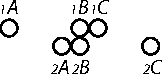
\includegraphics[scale=1]{gesamttex/edit_VIII-4/images/LH_37_03_067_d01a_067r.pdf}
\newline An sic potius \newline \rule{0pt}{16.3mm}%
\protect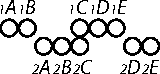
\includegraphics[scale=1]{gesamttex/edit_VIII-4/images/LH_37_03_067_d01b_067r.pdf}}
& 
\hspace{1.5em}%
\parbox{35mm}{%
\rule[-2mm]{0pt}{10mm}%
\protect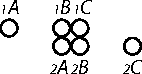
\includegraphics[scale=1]{gesamttex/edit_VIII-4/images/LH_37_03_067_d01c_067r.pdf}
\newline An sic \newline \rule{0pt}{16.3mm}%
\protect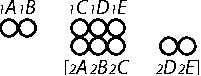
\includegraphics[scale=1]{gesamttex/edit_VIII-4/images/LH_37_03_067_d01d_067r.pdf}}
&
\parbox{40mm}{%
\rule[-2mm]{0pt}{16.3mm}
\newline Quid si \textit{DEF} cohaereant? \newline \rule{0pt}{16.3mm}%
\protect\raisebox{1.0ex}{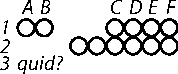
\includegraphics[scale=1]{gesamttex/edit_VIII-4/images/LH_37_03_067_d01e_067r.pdf}}}
\end{edtabularl}
\pend
\nopagebreak\vspace{0.5em}\startlock\nopagebreak
\pstart\centering
\edtext{\lbrack\textit{Fig.~1}\rbrack}{%
\lemma{\lbrack\textit{Fig.~1}\rbrack}%
\Cfootnote[nonum]{%
Im letzten Teildiagramm hat Leibniz die Punktbezeichnungen
\textit{\ind{1}A}, \dots\ \textit{\ind{1}E} doppelt vergeben.
Die dazugehörigen Indices ändert Hrsg.}}
\pend
\endlock
\vspace{1em}
\pstart
An efficitur, ut non solum centrum\indexS{centrum gravitatis omnium} omn.\ \textit{ABC} eadem celeritate procedat
\edtext{sed et \textit{A}}{\lemma{sed et}\Bfootnote{%
\textit{(1)}~centr. gr. %
\textit{(2)}~\textit{A}~\textit{L}}} 
et centr. gr.\indexS{centrum gravitatis} \textit{BC}, eadem celeritate a se invicem
\edtext{separentur; et \textit{C}}{\lemma{separentur; et}\Bfootnote{%
\textit{(1)}~\textit{A} et centr. gr %
\textit{(2)}~\textit{C}~\textit{L}}} 
et centr. gr.\indexS{centrum gravitatis} \textit{AB} similiter ut ante; an et \textit{B} et
\edlabel{37_03_067_2a}%
\edtext{}{%
\xxref%
{37_03_067_2a}{37_03_067_2b}%
\lemma{centr. gr. \textit{AC}.}\Bfootnote{%
\textit{(1)}~An pe %
\textit{(2)}~An~\textit{L}}}%
centr. gr. \textit{AC}.
\pend
\pstart
An%
\edlabel{37_03_067_2b}
cum inaequalia sunt corpora, et hoc perfecte
\edtext{obtineri semper}{\lemma{obtineri}\Bfootnote{%
\textit{(1)}~potest %
\textit{(2)}~semper~\textit{L}}}
non potest?
\edtext{Et an eo casu %
is motus erit, quo proxime accedetur, ut eo minor sit declinatio, a priori, quo major moles?
\edtext{Nempe determinandum qua ratione maxime accedatur ad priora.}{%
\lemma{}%
\applabel{FnB:37_03_067_determinandum}
\Bfootnote{Nempe \lbrack...\rbrack\ priora. \textit{erg.~L}}}%
}{\lemma{\textit{Am Rand}:}\Afootnote{NBNB}}
\pend 
\pstart 
An sufficit%
\edtext{}{\lemma{}\Afootnote{\textit{Am Rand}: Ita est}} 
\edtext{regula mea,\indexS{regula de summa virium respectivarum}}{%
\lemma{regula mea}%
\Cfootnote{Siehe bspw.
N.\;\ref{58300} und
N.\;\ref{58293} in diesem Band.}}
\edtext{ut summa ex vi}{%
\lemma{ut}%
\Bfootnote{%
\textit{(1)}~summa vis %
\textit{(2)}~summa ex vi~\textit{L}}} 
respectiva\indexS{vis respectiva}\indexS{summa virium respectivarum} 
inter \textit{A} et \textit{BC} juncta vi respectivae inter \textit{B} et 
\edtext{\textit{C}\lbrack;\rbrack\ item summa ex vi respectiva\indexS{vis respectiva} inter \textit{AB} et \textit{C} juncta}{%
\lemma{\textit{C}}%
\Bfootnote{%
\textit{(1)}~aequetur et vi respectivae inter \textit{AB} et \textit{C} junctae %
\textit{(2)}~item \lbrack...\rbrack\ juncta~\textit{L}}}
vi respectivae\indexS{vis respectiva} inter \textit{A} et \textit{B}; item summa ex vi respectiva\indexS{vis respectiva} inter \textit{AC} et \textit{B}, juncta vi respectivae\indexS{vis respectiva} inter \textit{A} et \textit{C}, semper conficiant idem, scil.\ vim respectivam\indexS{vis respectiva} priorem. 
Pro regulae hujus majore securitate videamus utrum ante concursum hic calculus virium respectivarum\indexS{vis respectiva} procedat.%
\edtext{}{\lemma{}\Afootnote{\textit{Hinter} procedat:\enskip NB. Video jam si succedit nihil determinare, quia ex uno sponte sequuntur et reliqua. An ergo adhibend. NB NB}}
\pend 
\pstart Vis ictus\indexS{vis ictus} inter duo est quadratum
\edtext{motus proprii,\indexS{motus proprius}}{\lemma{}\Bfootnote{motus \bars{motus \textit{streicht Hrsg.}} proprii,~\textit{L}}}
seu quo accedunt ad \indexS{centrum gravitatis commune}centrum commune grav.\lbrack,\rbrack\ 
ductum in molem.\indexS{moles}
\pend
\pstart
Vis ictus 
\edtext{inter tria\indexS{vis ictus inter tria}}{%
\lemma{}%
\Bfootnote{inter tria \textit{erg.~L}}} 
an itidem aestimari 
\edtext{potest quadratis celeritatum\indexS{quadratum celeritatis}}{%
\lemma{potest}%
\Bfootnote{%
\textit{(1)}~celeritate %
\textit{(2)}~quadratis celeritatum~\textit{L}}}
accedendi ad centr. com.,\indexS{centrum gravitatis commune} quod fingitur quiescere.
\edtext{Alius est sane modus inquirendi, si unum conferatur cum centro duorum,\indexS{centrum gravitatis duorum} et deinde reliqua inter se.}{%
\lemma{}%
\Bfootnote{Alius \lbrack...\rbrack\ se. \textit{erg.~L}}}
\pend
\begin{edfigure}			%
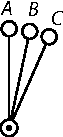
\includegraphics[scale=1]{gesamttex/edit_VIII-4/images/LH_37_03_067_d02_067r.pdf}
\edcaption{\lbrack\textit{Fig.~2}\rbrack}
\end{edfigure}
\pstart Si in circulum disposita sint \textit{A}, \textit{B}, \textit{C}, an ne idem eventus concursuum\indexS{concursus in circulo} ut in linea recta?
\pend
\vspace{0.5em}
\pstart
\noindent
\lbrack%
\textit{Der nachfolgende Zusatz bis \refpassage{37_03_067_1b}{37_03_067_1b} setzt unmittelbar nach der Ergänzung auf \refnote{FnB:37_03_067_determinandum} an:}\rbrack
\pend
\nobreak
\vspace{0.5em}
\pstart 
\noindent
\edlabel{37_03_067_1a}%
\edtext{Hic duo}{\lemma{Hic}\Bfootnote{%
\textit{(1)}~plura %
\textit{(2)}~duo~\textit{L}}} 
centra gravitatis partialia\indexS{centrum gravitatis partiale}
\edtext{quaevis}{\lemma{}\Bfootnote{quaevis \textit{erg.~L}}} 
eadem celeritate a se recedent
qua concurrerunt. Et an hoc sufficit ad determinandum? 
Nempe examinetur ante concursum,\indexS{concursus} an duo centra partialia\indexS{centrum gravitatis partiale}
eadem 
\edtext{celeritate sibi}{\lemma{celeritate}\Bfootnote{%
\textit{(1)}~concurrunt %
\textit{(2)}~sibi~\textit{L}}} 
accedunt, hoc video ita esse, quia nullo existente concursu, unumquodque uniformiter pergit.
Si haec succedunt\lbrack,\rbrack\ ut 
\edtext{arbitror, an consequens}{%
\lemma{arbitror,}%
\Bfootnote{%
\textit{(1)}~consequens %
\textit{(2)}~an consequens~\textit{L}}}
erit duo quaevis corpora eandem vim respectivam\indexS{vis respectiva} servare\indexS{conservatio vis respectivae} 
inter se, et tria quaevis
\edtext{itidem, et ita porro.}{\lemma{itidem,}\Bfootnote{%
\textit{(1)}~. Nam si sint  %
\textit{(2)}~et ita porro.~\textit{L}}} 
Nam si sint tria corpora \textit{A}, \textit{B}, \textit{C}, si \textit{A} et centr. \textit{BC} eadem qua ante celeritate a se invicem recedunt,
\edtext{erit ea pars}{\lemma{erit}\Bfootnote{%
\textit{(1)}~hactenus %
\textit{(2)}~ea pars~\textit{L}}} 
vis respectivae\indexS{vis respectiva} eadem quae
\edtext{ante. Sed}{\lemma{ante.}\Bfootnote{%
\textit{(1)}~Sed %
\textit{(2)}~Sed~\textit{L}}} 
cum tota sit eadem quae ante, etiam residua eadem erit, quae
\edtext{ante. Residua}{\lemma{ante.}\Bfootnote{%
\textit{(1)}~Ante aut %
\textit{(2)}~Residua~\textit{L}}} 
\edtext{a.}{%
\lemma{a.}%
\Cfootnote{%
\textit{autem}}}
tam ante quam post concursum est ipsa partialis vis respectiva\indexS{vis respectiva partialis} inter \textit{B} et \textit{C}. 
Videtur etiam forte hoc ex eo sequi, quia alioqui definiri poteret, in quo sit motus; quod examinandum.
\edtext{Imo falsam esse video consequentiam,}{\lemma{Imo}\Bfootnote{%
\textit{(1)}~hoc falsum esse video, \bars{et \textit{streicht Hrsg.}}
\textit{(a)}~institui perc
\textit{(b)}~poterit enim
\textit{(2)}~falsam esse video consequentiam,~\textit{L}}} 
quia duo corpora concurrentia sola sive constantia ex partibus unitis sive dissolutis eandem servant inter se vim respectivam,\indexS{conservatio vis respectivae} etiam
\edtext{du\lbrack o\rbrack}{\lemma{}\Bfootnote{duae \textit{L ändert Hrsg.}}} 
quaevis partialia\indexS{centrum gravitatis partiale} servare
\edtext{\lbrack debent\rbrack.}{%
\lemma{}%
\Bfootnote{debent \textit{erg.~Hrsg.}}}
\pend
\pstart
\edtext{Videndum an ex hypothesi respectivi motus\indexS{hypothesis motus respectivi}}{\lemma{Videndum}\Bfootnote{%
\textit{(1)}~quid %
\textit{(2)}~an ex
\textit{(a)}~casu %
\textit{(b)}~hypothesi %
\textit{(aa)}~motus %
\textit{(bb)}~respectivi motus~\textit{L}}}
seu indiscernibilis hypotheseos\indexS{hypothesis indiscernibilis} sequatur
\edtext{solutio. Finge}{\lemma{solutio.}\Bfootnote{%
\textit{(1)}~Fingo %
\textit{(2)}~Finge~\textit{L}}} 
duo \textit{B} et \textit{C} esse in navi\indexS{navis} mota motu eorum centri gr.\indexS{centrum gravitatis} 
Et hanc 
\edtext{navim in navi majore\indexS{navis in navi}}{%
\lemma{navim in navi}%
\Bfootnote{%
\textit{(1)}~mota %
\textit{(2)}~majore mota~\textit{L}}}
centr. gr. com. omnium\indexS{centrum gravitatis commune omnium} et \textit{A} moveri in hac navi majori. 
Quod si navis\indexS{navis} minor et \textit{A} non eadem celeritate qua venere a se invicem recedunt, 
sed diversis pro diversis celeritatibus, poterit discerni quantum motus sit in \textit{B}, 
et quantum in navi\indexS{navis} minori, etc.
Oportet ut celeritas recedendi\indexS{celeritas recedendi} sit qua venere. \pend
\pstart 
Adde hoc, nisi celeritas maneret eadem non reproducerentur priora
\edtext{licet pro re nata}{\lemma{licet}\Bfootnote{%
\textit{(1)}~re nata %
\textit{(2)}~res n %
\textit{(3)}~pro re nata~\textit{L}}} 
eo iretur. 
\pend
\pstart 
Idem etiam probatur ex natura actionis et reactionis aequalis,\indexS{actio et reactio aequales} poni enim potest \textit{A} agere in \textit{BC}, 
et haec reagere, adeoque eundem
\edtext{esse conatum}{\lemma{esse}\Bfootnote{%
\textit{(1)}~conatum reagendi %
\textit{(2)}~conatum~\textit{L}}}
a se discedendi.\indexS{conatus discedendi}
\pend
\begin{edfigure}%
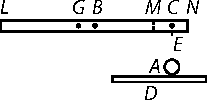
\includegraphics[scale=1]{gesamttex/edit_VIII-4/images/LH_37_03_067_d03_067r.pdf}
\edcaption{\edtext{\lbrack\textit{Fig.~3}\rbrack}{%
\lemma{\lbrack\textit{Fig.~3}\rbrack}%
\Cfootnote[nonum]{%
Ein gestrichener Entwurf zum Diagramm wird nicht wiedergegeben.}}}
\end{edfigure}
\pstart 
\edtext{Cum corpora concurrant eccentrice\indexS{concursus eccentricus} ut \textit{A} et
\edtext{\textit{B}, eodem modo videtur}{\lemma{\textit{B},}\Bfootnote{%
\textit{(1)}~et se
\textit{(2)}~eodem modo
\textit{(a)}~pergit %
\textit{(b)}~videtur~\textit{L}}} 
fieri ictus, ac si concurrerent tantum \textit{A} et \textit{C}.%
}{\lemma{}\Afootnote{\textit{Zwischen den Zeilen, oberhalb} eodem \lbrack...\rbrack\ concurrerent:\enskip Imo non puto, totum in motum concitandum\lbrack,\rbrack\ licet is gyrationis\indexS{motus gyrationis}}}
Datur ergo regressus\indexS{regressus} ipsius \textit{A}\lbrack,\rbrack\ datur et progressus centri gravitatis\indexS{progressus centri gravitatis} \textit{A} et \textit{B}, hinc dabitur et
\edtext{situs ipsius}{\lemma{}\Bfootnote{situs \bars{situs \textit{streicht Hrsg.}} ipsius~\textit{L}}} 
\textit{B}. Et quia datur vis respectiva inter \textit{A} et \textit{B} ex elongatione,\indexS{elongatio} 
oportet, ut quod deest vi respectivae\indexS{vis respectiva} priori, 
quaeratur in circulatione\indexS{circulatio} ipsius corporis oblongi\indexS{corpus oblongum} 
circa suum centrum\indexS{centrum gravitatis} \textit{B}; si duo oblonga\indexS{corpus oblongum} 
\edtext{concurrant, ut \textit{B} et \textit{D} res}{\lemma{concurrant,}\Bfootnote{%
\textit{(1)}~res mi %
\textit{(2)}~ut \textit{B} et \textit{D} res~\textit{L}}} 
minus faciles habet explicatus.
Videtur tamen ictus semper a centraliter obstante parte esse sumendus, deinde res concipienda, ac si
\edtext{pars illa}{\lemma{pars}\Bfootnote{%
\textit{(1)}~illa a re %
\textit{(2)}~illa~\textit{L}}} 
jam in motu posita ex
\edtext{legibus ante}{\lemma{legibus}\Bfootnote{%
\textit{(1)}~alibi %
\textit{(2)}~ante~\textit{L}}} 
determinatis a parte reliqua caperetur. 
Et quae est vis earum respectiva ante momentum rupturae\lbrack,\rbrack\ ea est vis
\edtext{circulationis.\indexS{vis circulationis} Vis}{\lemma{circulationis.}\Bfootnote{%
\textit{(1)}~Vis sc. respectiva inter ipsas part %
\textit{(2)}~Vis~\textit{L}}} 
sc. circulationis, est vis respectiva\indexS{vis respectiva} inter partes
\textit{LM}, et \textit{MN}, redactas in sua centra \textit{C} et \textit{G} circulantes circa commune centrum\indexS{centrum gravitatis commune} \textit{B}, haec enim
\edtext{si liberantur}{\lemma{si}\Bfootnote{%
\textit{(1)}~liberari possunt %
\textit{(2)}~liberantur~\textit{L}}} 
invicem recedent, licet oblique.
\pend
\pstart
Finge motum ipsius \textit{B} (in eccentrico concursu)\indexS{concursus eccentricus} esse progressus, 
et praeterea ex ictu fieri circulationem\indexS{circulatio} circa \textit{B}, et in momento ictus liberari \textit{BN}, 
feretur duplici motu uno recto\indexS{motus rectus} ipsius \textit{B}, 
altero ex circulatione\indexS{circulatio} in rectum averso,\indexS{motus in rectum aversus} per tangentem. 
Fingamus praeterea \textit{BL} similiter liberatum pergere in contrariam partem, 
sed ibi aequali occurrere, a quo reflectatur motu quo venerat.
Res redibit
\edtext{ad viam sine}{%
\lemma{ad}%
\Bfootnote{%
\textit{(1)}~vias %
\textit{(2)}~viam sine~\textit{L}}}
circulatione.\indexS{circulatio}
\edtext{Unde determinari puto poterit q. fuerit circulatio.\indexS{circulatio}%
}{\lemma{}\Afootnote{\textit{Unterhalb} Unde \lbrack...\rbrack\ circulatio:\enskip \textls{Hoc puto optimum}.}}
\pend
\pstart 
Videndum an ex hoc quod eadem vis absoluta\indexS{vis absoluta} manet, et quod centr. gr. commune\indexS{centrum gravitatis commune} aequabiliter procedit, 
et quod post momentum ictus duo concurrentia, \textit{A} scil. et punctum \textit{E} eadem celeritate a se invicem recedunt qua
\edtext{concurrere, eccentricus}{\lemma{concurrere,}\Bfootnote{%
\textit{(1)}~res %
\textit{(2)}~eccentricus~\textit{L}}} 
concursus\indexS{concursus eccentricus} possit definiri. %
Nam dum \textit{E}, uti 
\textit{C}, circulare incipit circa \textit{B}
et dum totum \textit{CN} procedere incipit\lbrack,\rbrack\
hi duo motus simul sumti componunt totam celeritatem recessus\indexS{celeritas recessus} \textit{C} ab \textit{A}.%
\edlabel{37_03_067_1b}
\pend 
\begin{edfigure}%
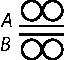
\includegraphics[scale=1]{gesamttex/edit_VIII-4/images/LH_37_03_067_d04_067r.pdf}
\edcaption{\lbrack\textit{Fig.~4}\rbrack}
\end{edfigure}
\pstart  
\edlabel{37_03_067_4a}%
Firmitatem corporum\indexS{firmitas corporum} venire necesse est a materia tenuissima,\indexS{materia tenuissima} 
cujus respectu solida nostra cribrorum\indexS{cribrum} instar habeant; quae 
corpora crassa\indexS{corpus crassum} a se invicem recedentia nonnihil, 
ob impulsus forte receptos, rursus ad se invicem pellat. 
\edtext{Alioqui ponenda}{%
\lemma{Alioqui}%
\Bfootnote{%
\textit{(1)}~ponendos %
\textit{(2)}~ponenda~\textit{L}}}
esset tractio,\indexS{tractio} non sola
\edtext{pulsio\indexS{pulsio}\lbrack,\rbrack\ dum}{\lemma{pulsio}\Bfootnote{%
\textit{(1)}~. Hujus actio %
\textit{(2)}~dum~\textit{L}}} 
intra brevissimum tempus in \textit{A} et \textit{B} innumeri ictus\indexS{ictus} ab aversis
\edtext{lateribus inferuntur}{\lemma{lateribus}\Bfootnote{%
\textit{(1)}~impingunt %
\textit{(2)}~inferuntur~\textit{L}}} 
qui has partes ad se invicem cogunt. Hinc
\edtext{si isti globuli\indexS{globulus}}{\lemma{si}\Bfootnote{%
\textit{(1)}~ista corpora %
\textit{(2)}~\bars{si \textit{streicht Hrsg.}} isti globuli~\textit{L}}} 
magneticis\indexS{globulus magneticus} similes adderentur, cum suis ictibus, 
utique appareret omnes motus esse rectilineos\indexS{motus rectilineus} in se, 
et per accidens ut curvilineos\indexS{motus curvilineus} considerari\lbrack,\rbrack\
neque adeo ob
\edtext{rece\lbrack de\rbrack ndi}{\lemma{}\Bfootnote{recededendi \textit{L ändert Hrsg.}}} 
a centro conatum\indexS{conatum recedendi a centrum} quicquam mutari 
de hypothesium aequivalentia.\indexS{aequivalentia hypothesium}
Accedit enim vis centripeta\indexS{vis centripeta} a 
\edtext{\lbrack curvi\rbrack lineo}{\lemma{}\Bfootnote{rectilineo \textit{L ändert Hrsg.}}}
motu.\indexS{motus rectilineus}\edlabel{37_03_067_4b}
\pend 
\pstart
\noindent
\href{\Scan{LH_37_03_067v}}%
{\lbrack67~v\textsuperscript{o}\rbrack}
\pend
\nobreak\begin{edfigure}[0.25em]%
\includegraphics[scale=1]{%
gesamttex/edit_VIII-4/images/LH_37_03_067_d05_067v.pdf}
\edcaption[0.25em]{\lbrack\textit{Fig.~5}\rbrack}
\end{edfigure}
\pstart
Conatus \textit{AC}, \textit{BC}, concurrunt in \textit{C} centro circuli.
Quod si id non sit centrum gravitatis\indexS{centrum gravitatis} sed aliud \textit{G}, sit tamen \textit{C} in directione ipsius \textit{G}, 
perinde est
ac si centrum gr.\indexS{centrum gravitatis} quoque esset
\edlabel{37_03_067_3a}%
\edtext{}{%
\xxref%
{37_03_067_3a}{37_03_067_3b}%
\lemma{in}%
\Bfootnote{%
\bars{\textit{G} \textit{ändert Hrsg.}}
\textit{(1)}~\bars{Si \textit{streicht Hrsg.}} di %
\textit{(2)}~Sit baculus \textit{BCG}, %
\textit{(a)}~in cujus %
\textit{(b)}~et~\textit{L}}}%
in \lbrack\textit{C}\rbrack.
\pend
\begin{edfigure}[0.5em]%
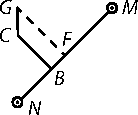
\includegraphics[scale=1]{gesamttex/edit_VIII-4/images/LH_37_03_067_d06_067v.pdf}
\edcaption{\lbrack\textit{Fig.~6}\rbrack}
\end{edfigure}
\pstart
Sit baculus \textit{BCG}, et%
\edlabel{37_03_067_3b}
sit impulsus in \textit{BC}, grave autem sit in altero extremo \textit{G}. 
An idem est, ac si impulsus fieret in \textit{FG} parallela ipsi \textit{BC}. %
\pend
\pstart
Sed hinc porro sequitur, si motus ille directus\indexS{motus directus} 
in linea \textit{BC} oriatur ex circulari\indexS{motus circularis} circa centrum \textit{M}, 
interesse, utrum grave sit in \textit{C} an vero in \textit{G} quia \textit{C} vecti\indexS{vectis} \textit{MFB} 
incumbet in \textit{B}, at \textit{G} in \textit{F}, propius ad centrum. Hinc etsi \textit{MB} 
et \textit{NB} sint aequales si tamen centrum grav.\indexS{centrum gravitatis} sit in \textit{G}, multum interest, 
utrum centrum motus sit \textit{N}, an \textit{M}, quia \textit{F} magis ab \textit{N} abest quam ab \textit{M}. 
Hoc prima fronte non apparebat. 
Et hinc video non posse tuto motus circulares\indexS{motus circularis} pro conatibus rectilineis\indexS{conatus rectilineus} substitui, etsi circulares quoque sint rectilinei in tangente.
\pend 
\begin{edfigure}[0.25em]%
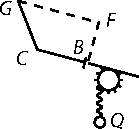
\includegraphics[scale=1]{gesamttex/edit_VIII-4/images/LH_37_03_067_d07_067v.pdf}
\edcaption{\lbrack\textit{Fig.~7}\rbrack}
\end{edfigure}
\pstart Si ope baculi
\edtext{curvi}{\lemma{}\Bfootnote{curvi \textit{erg.~L}}} 
\textit{BCG}, grave \textit{G} impellatur linea \textit{BC} vi ponderis \textit{Q}, perinde est quasi impulsus factus fuisset linea \textit{FG}, quia in hac
\edtext{linea ipsum}{\lemma{linea }\Bfootnote{%
\textit{(1)}~\textit{G} tendit %
\textit{(2)}~ipsum~\textit{L}}}
grave\indexS{grave} \textit{G} tendit.
\pend
\begin{edfigure}[2em][1em]    	%
\includegraphics[scale=1]{%
gesamttex/edit_VIII-4/images/LH_37_03_067_d08_067v.pdf}
\edcaption[0.25em]{\lbrack\textit{Fig.~8}\rbrack}
\end{edfigure}
\pstart Si \textit{A} incurrat in \textit{B} et \textit{C}, ita tamen ut tantum tangat \textit{B}, quid fiet? \pend 
\pstart Summa virium\indexS{summa virium} data est $Avv+Bee+%
\edtext{C\lbrack rr\rbrack$.}{%
\lemma{}%
\Bfootnote{\textit{Cr} \textit{L ändert Hrsg.}}}%
\pend
\pstart\noindent
$(A)((A))=v$. $(B)((B))=e$. $(C)((C))=r$. %
\pend
\pstart
Celeritas\indexS{celeritas centri gravitatis} et directio\indexS{directio centri gravitatis}
centr.\ grav.\ communis\indexS{centrum gravitatis commune} manet, 
seu quadratum ejus\indexS{quadratum celeritatis} ductum in Aggregatum.\indexS{quadratum celeritatis ductum in Aggregatum}
\pend
\pstart
Manere etiam debet eadem vis respectiva.\indexS{vis respectiva}
\pend
\pstart
Si ope horum determinari res
\edtext{potest, eadem}{\lemma{potest}\Bfootnote{%
\textit{(1)}~ut arbitror, determinabitur etiam, si fingamus %
\textit{(2)}~eadem~\textit{L}}} 
prodibunt, quae prodirent, si ponamus esse intervallum inter \textit{B} et \textit{C}, sed utcunque
\edtext{exiguum. Sed}{\lemma{exiguum.}\Bfootnote{%
\textit{(1)}~Nam %
\textit{(2)}~Sed~\textit{L}}} 
ea ratione semper quiescet \textit{A} post ictum si \textit{B} et \textit{C} 
\edtext{non cohaereant, sed}{%
\lemma{non cohaereant}%
\Bfootnote{%
\textit{(1)}~. Est %
\textit{(2)}~, sed~\textit{L}}}
quid si cohaereant? Tunc omnis vis respectiva\indexS{vis respectiva} redibit ad solum 
conatum discedendi\indexS{conatum discedendi} centri \textit{BC}
ab \textit{A}. Ergo haec duo confundi non debent. 
Sed si non cohaereant pars vis respectivae\indexS{vis respectiva} redacta erit ad recessum
inter \textit{B} et \textit{C}.
\pend 
\begin{edfigure}[1em][1em]    	%
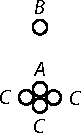
\includegraphics[scale=1]{gesamttex/edit_VIII-4/images/LH_37_03_067_d09_067v.pdf}\hspace*{20mm}
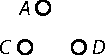
\includegraphics[scale=1]{gesamttex/edit_VIII-4/images/LH_37_03_067_d10_067v.pdf}
\edcaption[0.25em]{%
\edtext{\lbrack\textit{Fig.~9}\rbrack}{%
\lemma{\lbrack\textit{Fig.~9}\rbrack}%
\Cfootnote[nonum]{%
Ein gestrichener Entwurf zum Diagramm wird nicht wiedergegeben.}}%
\hspace*{22.5mm}
\lbrack\textit{Fig.~10}\rbrack\hspace*{2.5mm}}
\end{edfigure}
\pstart 
\edlabel{37_03_067_5a}%
Si globus\indexS{globus} \textit{A} simul tangat globos aequales plures\indexS{globus plures globos tangens} \textit{C}. 
et feriatur a globo \textit{B}, post ictum quiescent \textit{B} et \textit{A}, 
motusque omnis erit translatus\indexS{translatio omnis motus} in globos \textit{C}. 
\edtext{Hug.\ c.~1.\ \textit{Lum}.}{%
\applabel{FnC:37_03_067_Huygens}%
\lemma{Hug.\ c.~1.\ \textit{Lum}.}\Cfootnote{%
\indexN{\textls{Huygens} (Hugenius, Ugenius, Hugens, Huguens), Christiaan 1629\textendash1695}\textsc{C.~Huygens}, 
\textit{Traité de la lumière}, Leiden 1690\cite{00525}, 
chap.~1, S.\;14 mit Fig.\ (\textit{HO}\cite{00113} XIX, S.\;459\textendash477, hier S.\;473 mit Fig.~177). 
Siehe Leibnizens Auszüge aus dem einschlägigen Abschnitt des \cite{00525}\textit{Traité}:
\cite{02094}\textit{LSB} VIII,~3 N.\;75 von September\textendash Oktober 1690.%
}}
Ergo puto idem esse si \textit{A} incurrat in \textit{C} \textit{C} \textit{C} aequales,\indexS{incursus globi in plures aequales} 
sumamus duos tantum et consideremus quid futurum. Debet eadem
\edtext{esse vis\indexS{vis}}{\lemma{esse}\Bfootnote{%
\textit{(1)}~celeritas in sum %
\textit{(2)}~vis~\textit{L}}} 
in summa\lbrack,\rbrack\ a qua si detrahatur 
vis centri gravitatis\indexS{vis centri gravitatis} restabit vis ictus\indexS{vis ictus}\lbrack,\rbrack\
quem examinemus.
Videbimus et an idem prodeat, si paulo ante attingat \textit{C} quam \textit{D}.\edlabel{37_03_067_5b}%
\pend 
	





\chapter[tocentry={Concursus plurium globorum in plures
\enskip \bracks{Mitte September 1690 \textendash\ 1696}},
head={Concursus plurium globorum in plures}]%
{\MakeUppercase{Concursus plurium globorum in plures}
\newline \bracks{Mitte September 1690 \textendash\ 1696}}

\label{42014}

\begin{ledgroupsized}[r]{120mm}
\footnotesize
\pstart
\noindent\textbf{Überlieferung:}
\pend
\end{ledgroupsized}
\begin{ledgroupsized}[r]{114mm}
\footnotesize
\pstart
\parindent -6mm
\makebox[6mm][l]{\textit{L}}%
Konzept:
LH~XXXV~8, 30~Bl.~40.
Ein Blatt~2\textsuperscript{o}
(ca.~16~x~20~cm.)
{Wasserzeichen} in der Blattmitte;
oberer Rand nach Abschnitt unregelmäßig.
Zwei Seiten;
\pend
\end{ledgroupsized}
\vspace{5mm}
\begin{ledgroup}
\footnotesize
\pstart
\noindent
\textbf{Datierungsgründe:}
Das Wasserzeichen im Träger von N.\;\ref{42014}
konnte noch nicht identifiziert werden.
Die Datierung beruht auf bedeutenden inhaltlichen Ähnlichkeiten mit anderen Konzepten und mit dem Briefwechsel mit \indexN{\textls{Papin} (Papinus), Denis 1647\textendash1713}Denis Papin.
\pend
\pstart
Die Analyse komplexer Stoßfälle anhand zeitlicher Phasen ("status primus," "secundus" usw.) findet sich nicht nur im Ansatz, sondern auch in den Einzelheiten von Text und Zeichnungen in Konzepten wie N.\;\ref{41780} (Mitte September 1690 bis 1696), N.\;\ref{58300} (Januar 1691 bis 7. Februar 1697) und  N.\;\ref{58297} (August 1697 bis April 1703) wieder.
Dabei weist N.\;\ref{42014} eine engere Nähe zu beiden früheren Konzepten auf: Die Fragen werden hier aufgeworfen aber teilweise offen gelassen, oder auf eine später zu leistende Untersuchung vertagt (die auf 
\refnote{FnC:LH_35_08_30_040-advena}
nur skizzierte Fallstudie leistet Leibniz tatsächlich ausführlich im Konzept N.\;\ref{58300}).
Auf \refnote{FnC:LH_35_08_30_040-Papin} bezieht sich Leibniz auf das Gedankenexperiment einer zwischen den stoßenden Körpern befindlichen Feder mit den Worten "quae omnia distinctius exponi merentur".
Genau diesen Fall schlägt aber Leibniz im Juli 1696 Papin zur Diskussion vor; er wird beide Kontrahenten bis Januar 1698 rege beschäftigen (siehe dazu die Datierung zu N.\;\ref{60360} und die dort zitierten Briefe).
Die Ausdrucksweise von N.\;\ref{42014} lässt den Schluss zu, dass zu diesem Zeitpunkt die Auseinandersetzung mit Papin noch nicht stattgefunden (oder unlängst begonnen) hatte.
Aus den genannten Gründen ergibt sich das Jahr 1696 als Terminus ante quem.
\pend
\pstart
Als Terminus post quem wird das oben genannte Konzept N.\;\ref{41780} angenommen. Dort, wie auch im Schlussteil von N.\;\ref{42014} mit dem Diagramm \bracks{\textit{Fig. 4}}, hinterfragt (und verneint) Leibniz in ähnlichen Worten eine These zum schiefen Mehrkörperstoß, die Leibniz aus \indexN{\textls{Huygens} (Hugenius, Ugenius, Hugens, Huguens), Christiaan 1629\textendash1695}Huygens' 
\cite{00525}\textit{Traité de la lumière}, Leiden 1690, kennt (und in N.\;\ref{41780} ausdrücklich Huygens zuschreibt: \refnote{FnC:37_03_067_Huygens}).
Die Lektüre des Buchs kann frühestens Mitte September 1690 stattgefunden haben: Siehe die Datierung von N.\;\ref{41780} und des kurzen Exzerptes aus der einschlägigen Stelle des \textit{Traité}, das bei dieser Lektüre entstanden sein muss (in \cite{02094}\textit{LSB} VIII,~3 N.\;75).
\pend
\end{ledgroup}
\selectlanguage{latin}
\vspace{8mm}
\pstart
\centering
\edtext{\edtext{%
\href{\Scan{LH_35_08_30_040r}}%
{\lbrack40~r\textsuperscript{o}\rbrack} 
\hfill
\textls{Suppositio}}{%
\lemma{\href{\Scan{LH_35_08_30_040r}}%
{\lbrack40~r\textsuperscript{o}\rbrack}}%
\Bfootnote{%
\textit{(1)}~Sit recta
\textit{(2)}~\bars{In \textit{streicht Hrsg.}}
\textit{(a)}~recta
\textit{(b)}~linea signata sint puncta aequidistantia
\textit{(3)}~Suppositio: si globus durus directe occurrat 
\textit{(4)}~\textls{Suppositio}~\textit{L}}}
\textls{experimentis confirmata}\indexS{experimentum}}{%
\lemma{\textls{Suppositio experimentis confirmata}}%
\Cfootnote{Siehe bspw. \indexN{\textls{Mariotte}, Edme, Seigneur de Chazeuil ca. 1620\textendash1684}\textsc{E. Mariotte}, \cite{00311}\textit{Traité de la percussion}, Paris 1673, Première partie, Prop. XVI, S.\;100--102.}}
\hfill
\phantom{\lbrack40~r\textsuperscript{o}\rbrack}\ 
\pend
\nobreak
\vspace{.5em}
\pstart
\noindent
Si globus\indexS{globus}\indexS{globus incurrens} durus 
\edtext{incurrat directe}{%
\lemma{incurrat}%
\Bfootnote{%
\textit{(1)}~in ali
\textit{(2)}~directe~\textit{L}}}
et centraliter\indexS{incursus directus et centralis globi in aequalem quiescentem} in alium aequalem et materia similem sed 
\edtext{quiescentem;\indexS{globus quiescens} 
eveniet ut post ictum\indexS{ictus} incurrens\indexS{globus incurrens} quietem\indexS{quies} accipiat in loco}{%
\lemma{quiescentem;}%
\Bfootnote{%
\textit{(1)}~post ictum 
\textit{(a)}~quiescen
\textit{(b)}~incurrens quietem
\textit{(aa)}~ex
\textit{(bb)}~accipiet
\textit{(cc)}~accipiet
\textit{(2)}~con
\textit{(3)}~eveniet \lbrack...\rbrack\ accipiat
\textit{(a)}~loco e
\textit{(b)}~in loco~\textit{L}}}
excipientis;\indexS{globus excipiens} excipiens autem motum\indexS{motus} accipiat incurrentis, 
eademque celeritate et directione\indexS{celeritas et directio} qua ille sine incursu\indexS{incursus} perrexisset moveatur.
\pend
\begin{edfigure}[1em][1em]
\includegraphics[scale=1]{%
gesamttex/edit_VIII-4/images/LH_35_08_30_040_d1_040r.pdf}
\edcaption{\edtext{\lbrack\textit{Fig.~1}\rbrack}{%
\lemma{\lbrack\textit{Fig.~1}\rbrack}%
\Cfootnote[nonum]{Leibniz hat im oberen Bereich von Bl.~40~r\textsuperscript{o} das Diagramm in zwei gleichen Fassungen gezeichnet; die versehentlich stehen gebliebene Dublette, sowie ein gestrichener Entwurf zum Diagramm, werden nicht wiedergegeben.}}}
\end{edfigure}
\pstart
\edtext{%
Ut si in
\edtext{recta (fig.~1) signentur tria puncta aequidistantia et sit}{%
\lemma{recta}%
\Bfootnote{%
\textit{(1)}~in qua signentur tria puncta aequidistantia moto \textit{B}
\textit{(2)}~(fig.~1) signentur tria puncta aequidistantia
\textit{(a)}~sitque \textit{B}
\textit{(b)}~et sit~\textit{L}}}
\textit{B} in motu, \textit{L} vero quiescat ut in statu primo (fig.~1) inde incurrat \textit{B} in \textit{L} statu secundo, denique statu
\edtext{tertio quiesc\bracks{a}t \textit{B}}{%
\lemma{tertio}%
\Bfootnote{%
\textit{(1)}~quiescat
\textit{(2)}~\bars{quiescet \textit{ändert Hrsg.}} \textit{B}~\textit{L}}}
in loco ipsius 
\edtext{\textit{L}, nempe}{%
\lemma{\textit{L},}%
\Bfootnote{%
\textit{(1)}~sed
\textit{(2)}~nempe~\textit{L}}}
2, sed
\edtext{\lbrack\textit{L}\rbrack}{\lemma{}\Bfootnote{\textit{B} \textit{L ändert Hrsg.}}}
accipiat motum 2\,3 aequalem ipsi motui 1\,2 quem initio habebat \textit{B}.%
}{\lemma{}\Bfootnote{Ut si \lbrack...\rbrack\ habebat \textit{B}. \textit{erg.~L}}}
\pend
\vspace{0.5\baselineskip}
\pstart
\centering
\edlabel{35_08_30_040_1a}%
\edtext{}{%
\xxref{35_08_30_040_1a}{35_08_30_040_1b}%
\lemma{\textls{Theorema:}}%
\Bfootnote{%
\textit{(1)}~Si
\textit{(a)}~duo
\textit{(b)}~globi in
\textit{(2)}~\bars{Si \textit{streicht Hrsg.}} duo globi
\textit{(a)}~in re
\textit{(b)}~aequales m
\textit{(3)}~Si sint quatuor globi 
\textit{(a)}~in eadem recta
\textit{(b)}~duri~\textit{L}}}%
\textls{Theorema}:
\pend
\nobreak
\pstart
\noindent
Si sint quatuor globi\indexS{globi quatuor aequales} duri\edlabel{35_08_30_040_1b}
aequales et materia similes, centris\indexS{centrum gravitatis} in eadem recta positis, ex quibus duo moveantur, et duo
\edtext{quiescant, absoluto}{%
\lemma{quiescant,}%
\Bfootnote{%
\textit{(1)}~post
\textit{(2)}~absolutis
\textit{(3)}~absoluto~\textit{L}}}
concursu\indexS{concursus absolutus} fiet, ut duo incurrentes\indexS{globi incurrentes} loco excipientium\indexS{globi excipientes} quietem\indexS{quies} accipiant, duo
\edtext{vero excipientes vice incurrentium eodem}{%
\lemma{vero}%
\Bfootnote{%
\textit{(1)}~incurrentes
\textit{(2)}~excipientes vice incurrentium
\textit{(a)}~(eodem qui hi si nihil impediret mo
\textit{(b)}~eodem~\textit{L}}}
quo hi sine impedimento
\edtext{alias}{\lemma{}\Bfootnote{alias \textit{erg.~L}}}
perrexissent, motu\indexS{motus} moveantur.
\pend
\vspace{0.5\baselineskip}
\pstart
\centering
Demonstratio
\pend
\nobreak
\pstart
\noindent
Sint in recta 
\edtext{centrorum\indexS{recta centrorum gravitatis} (fig.~2) signata sex puncta 1,}{%
\lemma{}%
\Bfootnote{%
centrorum \bars{(fig.~2) \textit{erg.}}
\textit{(1)}~facilitat
\textit{(2)}~signata sex puncta
\bars{aequidistantia \textit{gestr.}} 1,~\textit{L}}}
2, 3, 4, 5, 6 et in ipsis 1 et 2 sint centra \textit{A} et \textit{B}, sed in ipsis 3 et 4 sint centra \textit{L} 
\edtext{et \textit{M}, tendantque \textit{A} motu 1\,2 et B motu aequali et simili 2\,3,}{%
\lemma{et \textit{M},}%
\Bfootnote{%
\textit{(1)}~dico absoluto concursu
\textit{(2)}~tendatque
\textit{(3)}~tendantque \textit{A}
\textit{(a)}~celeritate
\textit{(b)}~ motu 1\,2 et \textit{B} celeritate
\textit{(aa)}~motu
\textit{(bb)}~aequali \bars{et simili \textit{erg.}} 2\,3,~\textit{L}}}
sed quiescant \textit{L} et \textit{M}
\edtext{in 3 et 4,}{\lemma{}\Bfootnote{in 3 et 4 \textit{erg.~L}}}
dico post concursum\indexS{concursus} fore, 
\edtext{ut \textit{A} et \textit{B}}{%
\lemma{ut}%
\Bfootnote{%
\textit{(1)}~\textit{A} qui
\textit{(2)}~\textit{B} et \textit{A}~\textit{L}}}
quiescant in 3 et 4 sed \textit{L} et \textit{M} moveantur motu\indexS{motus post ictum} 4\,5, 5\,6, aequali\indexS{motus aequalis} et conveniente ipsis
\edlabel{35_08_30_040_2a}%
\edtext{}{%
\xxref{35_08_30_040_2a}{35_08_30_040_2b}%
\lemma{1\,2}%
\Bfootnote{%
\textit{(1)}~,
\textit{(2)}~et 2\,3. \lbrack/\rbrack\
\textit{(a)}~Nam \bars{fig.~1 \textit{gestr.}} ponamus primum
\textit{(aa)}~esse
\textit{(bb)}~\textit{A}
\textit{(cc)}~cum \textit{A}, \textit{B}, \textit{C}, \textit{D} sunt in 1, 2, 3, 4
\textit{(aaa)}~esse
\textit{(bbb)}~esse 1\,2 aequ. 3\,4. Cum ergo et
\textit{(b)}~Incipiamus a casu faciliore,
\textit{(c)}~sit distantia ipsorum \textit{A} et \textit{B} ante concursum
\textit{(d)}~Distantia ipsorum \textit{A} et \textit{B} ante concursum sit aequalis
\textit{(e)}~Ponamus \lbrack...\rbrack\ aequalem~\textit{L}}}%
1\,2 et 2\,3.
\pend
\begin{edfigure}%
\includegraphics[scale=1]{%
gesamttex/edit_VIII-4/images/LH_35_08_30_040_d2_040r.pdf}
\edcaption{\lbrack\textit{Fig.~2}\rbrack}
\end{edfigure}
\pstart
Ponamus distantiam ipsorum \textit{A} et \textit{B} ante concursum\indexS{concursus}\indexS{distantia corporum ante concursum} aequalem\edlabel{35_08_30_040_2b}
distantiae ipsorum \textit{L} et \textit{M}. 
\edtext{Et intelligamus momentum quo motus \textit{B}}{%
\lemma{}%
\Bfootnote{Et \bars{in fig.~1 \textit{gestr.}} intelligamus
\textit{(1)}~quand
\textit{(2)}~quo motus~\textit{B}~\textit{L}}}
eo pervenit, ut sit \textit{BL} aequ. \textit{AB} vel 
\edtext{\textit{LM}, hic}{%
\lemma{\textit{LM},}%
\Bfootnote{%
\textit{(1)}~hic esto
\textit{(2)}~hic~\textit{L}}}
\textls{status primus} esto. Sequitur post intervallum temporis 
\edtext{determinatum \textls{status secundus} quo transmisso intervallo punctorum ipse globus \textit{B} ferit \textit{L} in 3\lbrack,\rbrack\ A vero}{%
\lemma{determinatum}%
\Bfootnote{%
\textit{(1)}~tempus
\textit{(2)}~mo
\textit{(3)}~\textls{status secundus} \bars{fig.~2 \textit{gestr.}} quo
\textit{(a)}~\textit{A} quidem attingit punctum 2
\textit{(b)}~transmisso intervallo punctorum
\textit{(aa)}~A attingit punctum
\textit{(bb)}~\bars{ipse globus \textit{erg.}} \textit{B} ferit \textit{L} \bars{in 3 \textit{erg.}}
\textit{(aaa)}~sed \textit{A} tantum abest a
\textit{(bbb)}~sed \textit{A} se collocat in locum ipsius \textit{B}, nempe in 2. Ex hoc \textls{per suppositionem} colligitur status tertius,
\textit{(ccc)}~et per suppositionem
\textit{(ddd)}~sed \textit{A}
\textit{(eee)}~\textit{A} vero~\textit{L}}}
se collocat in locum ipsius \textit{B} nempe in 2.
Sed \textls{per suppositionem} hinc sequitur \textit{L} quidem pelli loco, 
\edtext{sed \textit{B} ejus loco quiescere.}{%
\lemma{sed \textit{B}}%
\Bfootnote{%
\textit{(1)}~in ejus locum
\textit{(2)}~ejus loco quiescere.~\textit{L}}}
Unde \textls{statu} 
\edtext{\textls{tertio} post}{%
\lemma{\textls{tertio}}%
\Bfootnote{%
\textit{(1)}~fit ut \textit{A} 
\textit{(a)}~pergit
\textit{(b)}~pergens
\textit{(2)}~post~\textit{L}}}
aequale priori temporis intervallum \textit{A}
\edtext{quidem pergens feriet \textit{B} quiescentem\indexS{globus quiescens}}{%
\lemma{quidem}%
\Bfootnote{%
\textit{(1)}~ferie
\textit{(2)}~feriet \textit{B} i
\textit{(3)}~pergens feriet \textit{B}
\textit{(aa)}~quiescens
\textit{(bb)}~quiescentem~\textit{L}}}
in 3 sed \textit{L} 
\edtext{in \textit{B} propulsus}{%
\lemma{in \textit{B}}%
\Bfootnote{%
\textit{(1)}~propulsum
\textit{(2)}~propulsus~\textit{L}}}
jam feriet \textit{M} 
\edtext{hactenus quiescentem}{%
\lemma{hactenus}%
\Bfootnote{%
\textit{(1)}~quiescens
\textit{(2)}~quiescentem~\textit{L}}}
in 4. Unde \textls{per suppos.} \textit{A} quidem quietem accipiet
\edtext{in 3 non turbandam,\indexS{quies non turbanda}}{%
\lemma{in 3}%
\Bfootnote{%
\textit{(1)}~non \bars{amplius \textit{gestr.}} turbandam, sed \textit{B},
\textit{(a)}~supr 
\textit{(b)}~motu ejus \bars{accepto \textit{streicht Hrsg.}}
\textit{(aa)}~feriet 
\textit{(bb)}~\textls{statu} jam \textls{quarto} feriet \textit{L} in 4, dum interim \textit{M} ab \textit{L} propulsus pervenit 
\textit{(aaa)}~ad
\textit{(aaaa)}~6
\textit{(bbbb)}~5
\textit{(bbb)}~ad 5. Unde \textls{statu quinto} tandem,
\textit{(aaaa)}~man
\textit{(bbbb)}~etiam \textit{B} \bars{iterum \textit{erg.}} loco pellens \textit{L} (\textls{per suppos.}) 
loco ejus \bars{in 4 \textit{streicht Hrsg.}} quietem accipiet non amplius turbandam;
\textit{(aaaaa)}~et ita \textit{L}
\textit{(bbbbb)}~et \textls{statu quinto} quie
\textit{(2)}~sed \textit{B} post tertium intervallum seu \textls{quarto statu} feriet \textit{L} in 4, dum interea \textit{M} pervenit ad \textlangle5\textrangle\ \bars{et \textit{gestr.}}
\textit{(3)}~non turbandam,~\textit{L}}}
\textit{B} vero recipiet ejus motum; et similiter \textit{L} quiescet in 4, loco \textit{M}, sed \textit{M}
recipiet ejus 
\edtext{motum non turbandum.\indexS{motus non turbandus} Quare jam post}{%
\lemma{motum}%
\Bfootnote{%
\textit{(1)}~.~Unde
\textit{(2)}~\bars{non turbandum \textit{erg.}}. Quare jam
\textit{(a)}~\textls{statu quarto}
\textit{(aa)}~\textit{A} manente in 3, \textit{B} feriet \textit{L} in 4, et \textit{M}
\textit{(bb)}~post
\textit{(b)}~post~\textit{L}}}
tertium intervallum \textls{statu quarto} \textit{A} manente in 3, \textit{B} feriet \textit{L} in 4,
et \textit{M} perveniet 
\edtext{ad 5. Et}{%
\lemma{ad 5.}%
\Bfootnote{%
\textit{(1)}~Ita
\textit{(2)}~Et~\textit{L}}}
\textls{per suppos.} \textit{B} quietem incipiet in 4 non amplius 
\edtext{turbandam, sed}{%
\lemma{turbandam,}%
\Bfootnote{%
\textit{(1)}~et
\textit{(2)}~sed~\textit{L}}}
\textit{L} accipiet ejus motum
\edtext{non amplius turbandum.\indexS{motus non turbandus}}{\lemma{}\Bfootnote{non amplius turbandum \textit{erg.~L}}}
Ergo denique post quartum intervallum \textls{statu quinto} \textit{A} et \textit{B} quiescentibus
in 3 et 4, \textit{L} perveniet in 5 motu 4\,5, et \textit{M} in 6 motu 5\,6. Ut asseverabatur.
\edtext{Quod si intervallum
\href{\Scan{LH_35_08_30_040v}}%
{\lbrack40~v\textsuperscript{o}\rbrack}\ 
ipsorum \textit{A} et \textit{B} ante concursum}{%
\lemma{Quod si}%
\Bfootnote{%
\textit{(1)}~intervalla
\href{\Scan{LH_35_08_30_040v}}%
{\lbrack40~v\textsuperscript{o}\rbrack}\ 
ipsorum \textit{A} et \textit{B}, non sint eadem
\textit{(2)}~intervallum 
\href{\Scan{LH_35_08_30_040v}}%
{\lbrack40~v\textsuperscript{o}\rbrack}\ 
\lbrack...\rbrack\ concursum~\textit{L}}}
non sit idem quod ipsorum \textit{L} et \textit{M}, patet nihil mutari in motibus,
sed tantum in intervallis temporum, semper enim necesse est
\textit{A} et \textit{B} redigi ad quietem sed \textit{L} et \textit{M} postremo moveri, 
nullum alium vero accipere, quam qui erat ipsorum \textit{A} et \textit{B}.
\pend
\pstart
\centering
Theorema 2.
\pend
\pstart
\noindent
Idem est iisdem positis, si plures sint 
\edtext{globi,\indexS{globus quiescens} modo quiescentium et in}{%
\lemma{globi}%
\Bfootnote{%
\textit{(1)}~incipientes
\textit{(2)}~,~modo
\textit{(a)}~ex
\textit{(b)}~quiescentium et
\textit{(aa)}~mot
\textit{(bb)}~in~\textit{L}}}
motu existentium\indexS{globus in motu existens} numerus sit aequalis.
\pend
\pstart
Sed operae pretium foret idem distincte ponere in tribus.
\pend
\pstart
\edtext{Fortasse magis commodum erit demonstrare, si
\edtext{unus globus\indexS{globus in quotcunque globos quiescentes incurrens}}{%
\lemma{unus}%
\Bfootnote{%
\textit{(1)}~modo
\textit{(2)}~globus~\textit{L}}}
incurrat in quotcunque aequales et quiescentes\indexS{globus quiescens}
\edtext{unum solum}{%
\lemma{unum}%
\Bfootnote{%
\textit{(1)}~quiescere
\textit{(2)}~ultimum so
\textit{(3)}~solum~\textit{L}}}
maxime remotum progredi, caeteros quiescere una cum advena.}{%
\lemma{Fortasse \bracks{...} advena}%
\applabel{FnC:LH_35_08_30_040-advena}
\Cfootnote{Die hier skizzierte Untersuchung leistet Leibniz tatsächlich im Konzept N.\;\ref{58297} (August 1697 bis April 1703).}}
Cujus rei manifesta ratio est, quid 
\edtext{quilibet incurrens in}{%
\lemma{quilibet}%
\Bfootnote{%
\textit{(1)}~praecedentem quiescen
\textit{(2)}~incurrens in~\textit{L}}}
anteriorem quiescentem\indexS{globus quiescens} redigitur ad quietem, et suum illi tribuit motum.\indexS{globus alteri motum tribuens}
Jam si unus sit incurrens, statim
\edtext{redigitur ad quietem,}{%
\lemma{redigitur}%
\Bfootnote{%
\textit{(1)}~et qui
\textit{(2)}~ad quietem,~\textit{L}}}
et de caetero res redit, 
\edtext{ac si esset unus}{%
\lemma{ac si}%
\Bfootnote{%
\textit{(1)}~alter
\textit{(2)}~esset
\textit{(a)}~incurren
\textit{(b)}~ex
\textit{(c)}~unus~\textit{L}}}
incurrens excipientium numerus uno minor.
Ergo tandem res eo redit ac si esset excipiens\indexS{globus excipiens} unus, et incurrens\indexS{globus incurrens} unus, id est, unus movebitur, qui est excipiens ultimus.
\pend
\pstart
Si duo\indexS{globi duo directe incurrentes in plures quiescentes} incurrant
\edtext{in alios, primo incurrente, fient}{%
\lemma{in}%
\Bfootnote{%
\textit{(1)}~duos
\textit{(2)}~alios,
\textit{(a)}~ultimo incurre
\textit{(b)}~primo incurrente
\textit{(aa)}~, res
\textit{(bb)}~solo, 
\textit{(aaa)}~res eo
\textit{(bbb)}~abstrahamus a secundo, et
\textit{(aaaa)}~ut
\textit{(bbbb)}~fiet ut
\textit{(ccc)}~fient~\textit{L}}}
omnia qua propositione praecedente, 
\edtext{nempe omnes quiescent, et solus}{%
\lemma{nempe}%
\Bfootnote{%
\textit{(1)}~ipse
\textit{(2)}~omnes quiescent, et
\textit{(a)}~ultimus solus
\textit{(b)}~solus~\textit{L}}}
remotissimus movebitur unde secundo superveniente, idem est, quod ante, 
seu rediimus ad statum priorem.
Ergo rursus movebitur 
\edtext{remotissimus\bracks{,} quiescent}{%
\lemma{remotissimus}%
\Bfootnote{%
\textit{(1)}~secundi
\textit{(2)}~ea
\textit{(3)}~quiescent~\textit{L}}}
caeteri. Et idem est 
\edtext{si sint}{%
\lemma{}%
\Bfootnote{%
si \bars{si \textit{streicht Hrsg.}} sint~\textit{L}}}
plures.
\pend
\pstart
Nec refert quod 
\edtext{secundus ferire}{%
\lemma{secundus}%
\Bfootnote{%
\textit{(1)}~feriat ante
\textit{(2)}~ferire~\textit{L}}}
fortasse possit ante quam prioris operatio sit transacta.
\edtext{Nam saltem secundi}{%
\lemma{Nam}%
\Bfootnote{%
\textit{(1)}~saltem
\textit{(2)}~saltem
\textit{(a)}~prioris operatio non p
\textit{(b)}~secundi~\textit{L}}}
operatio non perveniet ad remotiores, quam omnia primi ibi jam sint transacta. Unde res eodem redit.
\pend
\pstart
Nihil etiam refert, etsi plures sint incurrentes\indexS{globi plures directe incurrentes} quam excipientes,\indexS{globus excipiens}
\edtext{nam}{\lemma{}\Bfootnote{nam \textit{erg.~L}}}
semper res eo 
\edtext{redit ope}{%
\lemma{redit}%
\Bfootnote{%
\textit{(1)}~,~ac si incurrentes null
\textit{(2)}~ope~\textit{L}}}
vicariorum, ac si incurrentes\indexS{globus incurrens} obstaculum nullum sensissent.
\pend
\pstart
Superest jam ut ostendamus idem fieri, et si utrinque sit motus, si 
\edtext{modo duobus concurrentibus\indexS{globi duo concurrentes} ponamus fieri permutationem.\indexS{permutatio motus in concursu}}{%
\lemma{modo}%
\Bfootnote{%
\textit{(1)}~in consul
\textit{(2)}~duobus concurrentibus ponamus
\textit{(a)}~esse
\textit{(b)}~fieri
\textit{(aa)}~decussa
\textit{(bb)}~permutationem.~\textit{L}}}
\pend
\pstart
Nam cum 
\edtext{semper in concursu\indexS{concursus aequalium} aequalium}{%
\lemma{semper}%
\Bfootnote{%
\textit{(1)}~omnia fiant ut ante per motum
\textit{(2)}~in concursu aequalium~\textit{L}}}
medio motu omnia fiant perinde ac si esset penetratio\indexS{penetratio quasi dimensionum in concursu corporum} dimensionorum, postremo etiam idem 
\edlabel{35_08_30_040_3a}%
\edtext{}{%
\xxref{35_08_30_040_3a}{35_08_30_040_3b}%
\lemma{fiet.}%
\Bfootnote{%
\textit{(1)}~Ni
\textit{(2)}~\bars{Cum ergo non sit nisi concursu aequalium \textit{streicht Hrsg.}} fiet
\textit{(3)}~Hinc~\textit{L}}}%
fiet.
\pend
\pstart
Hinc\edlabel{35_08_30_040_3b}
infero aliquid pulcherrimum, etsi plures globi simul diversis motibus moveantur in eadem recta,\indexS{globi in recta diversis motis moti} 
post concursum\indexS{concursus} perinde faciendum, ac si per penetrationem\indexS{penetratio dimensionum} dimensionum
quilibet inoffensus progressus\indexS{progressus corporis inoffensus} fuisset\bracks{,} seu perinde ac si 
\edtext{fuissent singuli}{%
\lemma{fuissent}%
\Bfootnote{%
\textit{(1)}~in eadem linea omne
\textit{(2)}~singuli~\textit{L}}}
in linea sua priori
\edtext{parallela seu}{%
\lemma{parallela}%
\Bfootnote{%
\textit{(1)}~umbraeque solares in
\textit{(2)}~seu~\textit{L}}}
prorsus ut eorum 
\edtext{umbrae solares\indexS{umbra solaris in pariete}}{%
\lemma{umbrae}%
\Bfootnote{%
\textit{(1)}~in
\textit{(2)}~solares~\textit{L}}}
in pariete moverentur nam umbrae se impedire non possunt.
\pend
\pstart
Idem est si oblique concurrant,\indexS{concursus obliquus centralis} sed tamen centraliter 
\edtext{obliquitatem ascribendo}{%
\lemma{obliquitatem}%
\Bfootnote{%
\textit{(1)}~enim
\textit{(2)}~ascribendo~\textit{L}}}
motui cuidam transverso irrefracto.
\pend
\begin{edfigure}%
\includegraphics[scale=1]{%
gesamttex/edit_VIII-4/images/LH_35_08_30_040_d3_040v.pdf}
\edcaption{%
\edtext{\lbrack\textit{Fig.~3}\rbrack}{%
\lemma{\lbrack\textit{Fig.~3}\rbrack}%
\Cfootnote{%
Zwei gestrichene Entwürfe zum Diagramm werden nicht wiedergegeben.}}%
}
\end{edfigure}

\pstart
Sed si globi sint inaequales, vel si aequales connexi\indexS{globi aequales connexi} ponantur, ut a seinvicem divelli
\edtext{nequeant, sitque}{%
\lemma{nequeant,}%
\Bfootnote{%
\textit{(1)}~hic quam
\textit{(2)}~fit
\textit{(3)}~sitque~\textit{L}}}
vis Elastica\indexS{vis Elastica} eos 
connectens, considerandum est \textit{B} incurrens in \textit{L} dare ipsi motum suum.
Sed \textit{L} tendens versus 
\edtext{\textit{M} cogi intendere Elastrum\indexS{Elastrum} interceptum,}{%
\lemma{\textit{M}}%
\Bfootnote{%
\textit{(1)}~cogere
\textit{(2)}~cogi intendere Elastrum \bars{suum \textit{gestr.}} interceptum,~\textit{L}}}
quo facto Elastrum\indexS{Elastrum} aget in \textit{M}, eique dabit aliquid motus sed parvi,
sed quia \textit{M} tardius longe cedit, quam \textit{L} insequitur, continue
magis intendetur Elastrum,\indexS{Elastrum continue magis intensum} donec vis\indexS{vis} ipsius \textit{L} tota
partim Elastro partim ipsi \textit{M} sit tributa,\indexS{translatio virium} quo facto vi Elastri\indexS{vis Elastri} rursus a se recedent, et \textit{L} quidem
redibit ad locum priorem ultraque tendens residuo impetu feriet 
\edtext{\textit{B}, qui}{%
\lemma{\textit{B},}%
\Bfootnote{%
\textit{(1)}~quod
\textit{(2)}~qui~\textit{L}}}
globus proinde reflectetur sed \textit{L} deinde trahetur ab ipso 
\edtext{\textit{M} et}{%
\lemma{\textit{M}}%
\Bfootnote{%
\textit{(1)}~donec
\textit{(2)}~Elastro
\textit{(3)}~et~\textit{L}}}
elastro in contrarium intenso,\indexS{Elastrum intensum} seu distenso.\indexS{Elastrum distensum}
\edtext{Quae omnia distinctius exponi merentur.}{%
\applabel{FnC:LH_35_08_30_040-Papin}%
\lemma{Quae omnia distinctius exponi merentur}%
\Cfootnote{%
Leibniz führte im Briefwechsel mit \indexN{\textls{Papin} (Papinus), Denis 1647\textendash1713}Papin zwischen Juli 1696 und Januar 1698 eine rege Debatte über das Gedankenexperiment einer zwischen den stoßenden Körpern befindlichen Feder: Siehe dazu die Datierung zu N.\;\ref{60360} und die dort zitierten Briefe.}}
\pend
\begin{edfigure}%
\includegraphics[scale=1]{%
gesamttex/edit_VIII-4/images/LH_35_08_30_040_d4_040v.pdf}
\edcaption{%
\edtext{\lbrack\textit{Fig.~4}\rbrack}{%
\lemma{\lbrack\textit{Fig.~4}\rbrack}%
\Cfootnote{Das Diagramm ist wie auch der nachfolgende Text eine Ergänzung.}}%
}
\end{edfigure}
\pstart
\edtext{Quid si globus\indexS{globus in duos simul incurrens} \textit{A} incurrat in \textit{B} et \textit{C} simul, qui tangunt eodem modo \textit{D} quo \textit{A}\bracks{?}
An \textit{A} quiescet et ejus loco \textit{D} perget? Non puto.}{%
\lemma{}%
\Bfootnote{%
Quid \lbrack...\rbrack\ puto. \textit{erg.~L}}}
\pend





\chapter[tocentry={Methodus inveniendi vim respectivam in concursu
\enskip\bracks{%
Herbst 1690 (?)%
}},
head={Methodus inveniendi vim respectivam in concursu}]%
{\MakeUppercase{Methodus inveniendi vim respectivam in concursu}
\newline\bracks{%
Herbst 1690 (?)%
}}%
\label{58949}
\selectlanguage{ngerman}%
\frenchspacing%
\begin{ledgroupsized}[r]{120mm}%
\footnotesize%
\pstart%
\noindent\textbf{Überlieferung:}%
\pend%
\end{ledgroupsized}%
\begin{ledgroupsized}[r]{114mm}%
\footnotesize%
\pstart%
\parindent -6mm%
\makebox[6mm][l]{\textit{L}}%
Aufzeichnung:
LH~XXXV~11,\;14 Bl.\;34.
Ein Zettel (etwa 6\;x\;8~cm),
Ränder beschnitten.
Zwei Seiten.
\pend
\end{ledgroupsized}
\vspace{5mm}%
\begin{ledgroup}%
\footnotesize%
\pstart%
\noindent%
\textbf{Datierungsgründe:}
Die Datierung der Aufzeichnung N.\;\ref{58949} beruht %
auf inhaltlichen Betrachtungen.
Siehe die ausführliche Begründung auf S.\;\pageref{58949_dat}.
\pend%
\end{ledgroup}%
\selectlanguage{latin}%
\frenchspacing%
\vspace{6mm}%
\pstart%
\normalsize%
\noindent%
\lbrack%
\href{\Scan{LH_35_11_14_034r}}%
{34\,r\textsuperscript{o}}%
\rbrack%
\pend%
\vspace{-1.0em}
\centerline{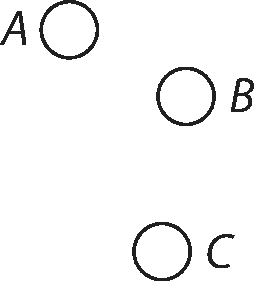
\includegraphics[width=0.145\textwidth]{gesamttex/edit_VIII-4/images/LH_35_11_14_034_d_034r.pdf}}
\nobreak\vspace{0.5em}
\centerline{\lbrack\textit{Fig.\:1}\rbrack}
\vspace{1.25em}
\pstart%
\noindent%
\edlabel{LH_35_11_14_034_034rv_drstllng-1}%
Si trium corporum \textit{A}, \textit{B}, \textit{C}%
\indexS{corpora concurrentia}
ponatur motus quicunque%
\indexS{motus quicunque}
et demto motu communi%
\indexS{motus communis demtus}
qui est communis centri gravitatis,%
\indexS{centrum gravitatis commune}%
\indexS{motus centri gravitatis}
cuique assignetur motus proprius,%
\indexS{motus proprius}
atque inde quaeratur vis respectiva%
\indexS{vis respectiva quaesita}%
\lbrack,\rbrack\ 
quae tribus modis inveniri potest,%
\indexS{modus inveniendi vim respectivam}
quaerendo eam inter \textit{A} et $B+C,$
inter \textit{B} et $A+C$,
inter \textit{C} et 
\edtext{%
$A+B,$ et%
}{%
\lemma{$A+B,$}%
\Bfootnote{%
\textit{(1)}~inter %
\textit{(2)}~et%
~\textit{L}%
}}
debet semper provenire
\edlabel{LH_35_11_14_034_034r_gfrs-1}%
idem.%
\edtext{}{%
\xxref{LH_35_11_14_034_034r_gfrs-1}{LH_35_11_14_034_034r_gfrs-2}%
\lemma{idem.}\Bfootnote{%
\textit{(1)}~Sufficitque
\textit{(2)}~Hac methodo determinari poterit%
~\textit{L}}}
Hac methodo determinari poterit%
\indexS{methodus inveniendi vim respectivam}%
\edlabel{LH_35_11_14_034_034r_gfrs-2}
\lbrack%
\href{\Scan{LH_35_11_14_034v}}%
{34\,v\textsuperscript{o}}%
\rbrack%
quid post concursum corporum%
\indexS{concursus corporum}
(\protect\vphantom)%
demto communi motu centri gravitatis,%
\indexS{motus communis centri gravitatis}%
\indexS{motus communis demtus}
\edtext{%
qui perdurat%
\protect\vphantom()%
}{%
\lemma{qui}\Bfootnote{%
perdurat
\textit{erg.\;L}}}
fieri debeat.
\edlabel{LH_35_11_14_034_034v_hypoth-1}%
Utcunque enim corpora colligari ponas,%
\indexS{corpora colligata}
semper debet servari in summa%
\indexS{summa potentiae respectivae}
eadem quantitas potentiae respectivae.%
\indexS{potentia respectiva servanda}%
\indexS{quantitas potentiae respectivae}%
\edlabel{LH_35_11_14_034_034v_hypoth-2}%
\edlabel{LH_35_11_14_034_034rv_drstllng-2}
Quid si singula
\edtext{%
corpora singulis%
}{%
\lemma{corpora}\Bfootnote{\hspace{-0,75mm}%
\bars{lineis rectis colliges tendibilibus et comprimilibus et \textit{gestr.}}
singulis%
~\textit{L}}}
compares,
an licebit sic
\edtext{\lbrack quoque\rbrack}{%
\lemma{quotque}\Bfootnote{%
\textit{L~ändert Hrsg.}}}
aestimare vim respectivam?%
\indexS{vis respectiva aestimanda}
Sed optimum erit sic progredi,
ut duorum aestimetur vis respectiva%
\indexS{vis respectiva aestimanda}
inter se,
et deinde centri gravitatis%
\indexS{centrum gravitatis commune}
eorum cum tertio.
\edlabel{LH_35_11_14_034_034v_proexc-1}%
Haec methodus%
\indexS{methodus pro concursu eccentrico}%
\indexS{methodus inveniendi vim respectivam}
etiam pro concursu eccentrico%
\indexS{concursus eccentricus}%
\lbrack,\rbrack\
ponendo corpus excipiens%
\indexS{corpus excipiens divisum}
divisum in duas partes%
\lbrack,\rbrack\
unam
quae maxima incursus centrici%
\indexS{incursus centricus}
assumi potest,
alteram
quae eccentrice excipit.%
\edlabel{LH_35_11_14_034_034v_proexc-2}
\edlabel{LH_35_11_14_034_034v_cntrgyr-1}%
Unde cum fit gyrus%
\indexS{gyrus}
simul et progressus%
\indexS{progressus in concursu eccentrico}%
\lbrack,\rbrack\
corpora gyrantur%
\indexS{corpus gyrans}
circa idem
\edtext{%
centrum%
\indexS{centrum gyrationis}
quod%
}{%
\lemma{centrum}%
\Bfootnote{%
\textit{(1)}~in %
\textit{(2)}~ad
\textit{(3)}~quod %
\textit{L}%
}}
est eorum centr. gr.%
\indexS{centrum gravitatis commune}%
\edlabel{LH_35_11_14_034_034v_cntrgyr-2}
Habent et vim respectivam%
\indexS{vis respectiva aestimanda}
quae quadratum est gyri%
\indexS{gyrus}
in corpus.%
\indexS{quadratum gyri in corpus}%
\textls{ Comprobatio seu examen,}%
\indexS{comprobatio}%
\indexS{examen}
si effici possit altero concursu%
\indexS{concursus alter}
restitutio in statum priorem.%
\indexS{status prior}%
\indexS{restitutio in statum priorem}%
\pend%
\newpage%
\pstart%
\noindent%
\centering%
*     *     *
\pend%
\selectlanguage{ngerman}%
\frenchspacing%
\vspace{4.0em}%
\begin{ledgroup}%
\footnotesize%
\pstart%
\noindent%
\textls{Ausführliche Datierungsgründe:}%
\pagelabel{58949_dat}
Der Träger der titellosen und undatierten Aufzeichnung N.\;\ref{58949} weist weder Spuren eines Wasserzeichens noch sonstige äußere Merkmale, die eine eindeutige Datierung ermöglichen würden.
Aus inhaltlichen Gründen erweist sich eine grobe chronologische Einordnung des Textes dennoch als möglich.
\pend%
\pstart%
Die in der Aufzeichnung N.\;\ref{58949} dargelegte Methode zur Bestimmung der Kinematik dreier zusammenstoßender Körper wird ausführlich in dem von Leibniz eigenhändig auf den 31.\;Oktober\,/\,10. November 1690 datierten Entwurf N.\;\ref{58939} \textit{Scheda secunda de impulsu eccentrico} angewandt.
Beide Texte gehen von derselben Voraussetzung aus:
Ungeachtet, wie man die einzelnen Körper untereinander gruppiert, \textit{semper debet servari in summa eadem quantitas potentiae respectivae} (\refpassage{LH_35_11_14_034_034v_hypoth-1}{LH_35_11_14_034_034v_hypoth-2}; vgl. \refpassage{LH_35_11_14_003-004_004v_methodus-1}{LH_35_11_14_003-004_004v_methodus-2}).
Dass die Aufzeichnung N.\;\ref{58949} besonders die Anwendbarkeit dieser Methode auf den exzentrischen Stoß hervorhebt (\refpassage{LH_35_11_14_034_034v_proexc-1}{LH_35_11_14_034_034v_proexc-2}), ist Grund für die Vermutung einer gemeinsamen Abfassungszeit mit der \textit{Scheda secunda}: %
N.\;\ref{58949} könnte entweder als Verallgemeinerung der in N.\;\ref{58939} erzielten Ergebnisse entstanden sein, oder aber als Skizze, durch welche die Untersuchung in N.\;\ref{58939} angespornt worden sein könnte.
Unter dieser Annahme ergibt sich als wahrscheinliche Abfassungszeit der Aufzeichnung N.\;\ref{58949} der Herbst 1690. %
Eine frühere oder eine spätere Datierung sind allerdings möglich.
\pend%
\pstart%
Eine Entstehung der Aufzeichnung N.\;\ref{58949} vor der auf den Zeitraum von April bis spätestens Oktober 1690 datierbaren Aufzeichnung N.\;\ref{60300} ist jedoch aus folgendem Grund auszuschließen:
In der Aufzeichnung N.\;\ref{58949} wird unvermittelt angenommen, dass beim exzentrischen Stoß eine Drehung entstehe, deren Zentrum %
mit dem Schwerpunkt des gestoßenen Körpers zusammenfalle (\refpassage{LH_35_11_14_034_034v_cntrgyr-1}{LH_35_11_14_034_034v_cntrgyr-2}).
Folglich muss N.\;\ref{58949} nach der %
Aufzeichnung N.\;\ref{60300} abgefasst worden sein.
Denn erst in N.\;\ref{60300} berichtigt Leibniz seine frühere (etwa in N.\;\ref{impulsuseccentricus} %
vertretene) Ansicht, das Zentrum der Drehung beim exzentrischen Stoß falle mit dem Schwerpunkt des indirekt angestoßenen Teils des Körpers zusammen (vgl. N.\;\ref{60300}, \refpassage{LH_37_05_044_044r_cntrgyr-1}{LH_37_05_044_044r_cntrgyr-2}; siehe auch die Datierungsgründe, S.\;\pageref{LH_37_05_044_datierung}).
Wenn damit -- wenigstens im Hinblick auf die relative Chronologie -- ein Terminus post quem ermittelbar ist, lässt sich hingegen kein klarer Terminus ante quem der Datierung von N.\;\ref{58949} zum Redaktionsschluss angeben.%
\pend%
\pstart%
Schließlich sei erwähnt, dass der letzte Satz der Aufzeichnung N.\;\ref{58949} (\textit{Comprobatio seu examen, si effici possit altero concursu restitutio in statum priorem}) eine Anwendung der Methode vorschlägt, die Leibniz bereits Anfang 1678 in seiner Untersuchung \textit{De corporum concursu} dargestellt hatte;
siehe \textit{LSB} VIII,\;3 N.\;58\textsubscript{2}, S.\;542.15\textendash23.\cite{01401}
\pend%
\end{ledgroup}%
\selectlanguage{latin}%
\frenchspacing%
\normalsize%





\chapter[tocentry={Oportet ut semper eadem sit vis respectiva inter tria corpora
\enskip \bracks{Ende September 1690\,(?)}},
head={Vis respectiva inter tria corpora}]%
{\MakeUppercase{Oportet ut semper eadem sit vis respectiva inter tria corpora}
\newline \bracks{Ende September 1690\,(?)}}

\label{53450}
\begin{ledgroupsized}[r]{120mm}
\footnotesize
\pstart
\noindent\textbf{Überlieferung:}
\pend
\end{ledgroupsized}
\begin{ledgroupsized}[r]{114mm}
\footnotesize
\pstart \parindent -6mm
\makebox[6mm][l]{\textit{L}}%
Aufzeichnung:
LH~XXXVII~4 Bl.~168. 
Ein als Schreibblatt wiederverwendeter Teil eines Briefumschlags (ca.~20~x~13,5~cm.);
Papiererhaltungsmaßnahmen;
oberer und linker Rand beschnitten.
Eine Seite auf Bl.~168~r\textsuperscript{o};
Bl.~\href{\Scan{LH_37_04_168v}}{168~v\textsuperscript{o}}
überliefert zwei Zeichnungen ohne Zusammenhang mit dem Text, sonst leer.
Auf Bl.~168~r\textsuperscript{o} befinden sich Briefsiegelreste sowie, in gegenläufiger Schreibrichtung, die Anschrift 
(Hand von \indexN{\textls{Bodenhausen} (Bodenus, Bodenausen), Rudolf Christian, Freiherr v. 1698}R.\,C. von Bodenhausen):	
\textit{All'\;Ill:\textsuperscript{mo} Sig.\textsuperscript{re} mio Sig.\textsuperscript{re} P\textsuperscript{\,rone} Col.\textsuperscript{mo}} \lbrack/\rbrack\
\textit{Il Sig.\textsuperscript{re} Gotofredo Gul.\textsuperscript{mo} Leibnitz, Consigl.\textsuperscript{ro}} \lbrack/\rbrack\
\textit{di S.A.S. di Bransvic.} \lbrack/\rbrack\ \textit{a} \lbrack/\rbrack\ \textit{Hannover}.
Der Träger bildete ursprünglich eine Einheit mit 
LBr~79 Bl.~31 (\cite{02131}Brief von \indexN{\textls{Bodenhausen} (Bodenus, Bodenausen), Rudolf Christian, Freiherr v. 1698}R.\,C. Bodenhausen an Leibniz vom 23. September 1690,
\textit{LSB} III, 4 N.\;275).	
\pend
\end{ledgroupsized}
\vspace{5mm}
\begin{ledgroup}
\footnotesize
\pstart
\noindent%
\textbf{Datierungsgründe:}
Leibniz hat die Aufzeichnung N.\;\ref{53450} auf der recto-Seite 
eines ursprünglich als Briefumschlag verwendeten, 
bis auf die Anschrift in R.\,C. Bodenhausens Hand nicht beschriebenen Blattes italienischen Papiers
verfasst.
Der dazugehörige Brief \indexN{\textls{Bodenhausen} (Bodenus, Bodenausen), Rudolf Christian, Freiherr v. 1698}Bodenhausens lässt sich auf Grund der gleichen Maße, Papiereigenschaften und der gemeinsamen Trennkante mit dem Träger LBr~79 Bl.~31 mit Sicherheit als
sein \cite{02131}Schreiben aus Florenz vom 23. September 1690 
(\textit{LSB} III, 4 N.\;275) identifizieren.
\pend
\pstart
Die zwei auf Bl.~168~v\textsuperscript{o} überlieferten,
keinen erkennbaren Zusammenhang mit N.\;\ref{53450} aufweisenden
Zeichnungen (Teildarstellungen einer Hyperbel und einer Zykloide)
sind ebenfalls mit dem genannten Brief in Beziehung zu setzen:
Leibniz beantwortet dieses und drei andere %
vorangegangene Schreiben Bodenhausens 
mit einem \cite{02132}Brief vom 26.~Oktober (5.~November) 1690 (\textit{LSB} III, 4 N.\;285),
dem er eine \cite{02133}\textit{scheda} mit Beispielen für die Leistungsfähigkeit des Calculus beilegt
(ebd. N.\;286).
Beide Diagramme finden sich darin in ausgearbeiteter Form wieder und dienen dort zur Veranschaulichung der Leibniz'schen Rektifikation der Hyperbel (S.\;638) bzw. der Zykloide (S.\;640).
Aus diesem Grund werden die Diagramme nicht mit N.\;\ref{53450} ediert.
Die Entstehung der Zeichnungen lässt sich daher auf den Zeitraum Ende September bis 5. November einkreisen.
\pend
\pstart
Der Zeitpunkt des Erhalts des Briefs durch Leibniz (wahrscheinlich Ende September 1690) bietet einen Terminus post quem für die Entstehung von N.\;\ref{53450}. 
Unter der Annahme einer zeitnahen Beschreibung des Blattes, die durch die sichere Entstehung der Diagramme auf Bl.~168~v\textsuperscript{o} vor dem 5. November 1690 bekräftigt wird,
ergibt sich die vorgeschlagene Datierung.
\pend
\end{ledgroup}
\newpage
\selectlanguage{latin}
\vspace{8mm}
\pstart%
\noindent%
\href{\Scan{LH_37_04_168r}}%
{\lbrack168~r\textsuperscript{o}\rbrack}
\pend
\vspace{1.0em} %
\centerline{\includegraphics[width=0.165\textwidth]{%
gesamttex/edit_VIII-4/images/LH_37_04_168_d1_168r.pdf}} 
\nobreak\vspace{0.5em}
\centerline{\lbrack\textit{Fig.~1}\rbrack}
\vspace{1.0em}
\pstart
\edtext{}{%
\lemma{\lbrack\textit{Fig.~1}\rbrack}%
\Cfootnote[nonum]{%
Ein gestrichener und von Leibniz überschriebener Entwurf zum Diagramm wird nicht wiedergegeben.}}%
Si corpora \textit{A} et \textit{B}
\edtext{concurrant,\indexS{concursus} ita ut}{\lemma{concurrant,}\Bfootnote{%
\textit{(1)}~ut %
\textit{(2)}~ita ut~\textit{L}}}
\textit{B} et \textit{C} intelligantur eandem semper servare distantiam\indexS{distantia eadem servata} inter se, et eundem semper 
angulum \textit{ABC}; id est ut vel quiescant simul \textit{B} et \textit{C} vel rectas parallelas describant, 
oportet ut discerni non possit per eventum
\edtext{concursus\indexS{concursus}\indexS{eventus concursus} quantus}{\lemma{concursus}\Bfootnote{%
\textit{(1)}~quantus cuique sit %
\textit{(2)}~utrum motus %
\textit{(3)}~quantus~\textit{L}}}
motus\indexS{motus} sit in altero, aut in quo sit quies\indexS{quies} inter \textit{B} et \textit{C}. 
Sit centrum\indexS{centrum gravitatis} \textit{G}, debet celeritas respectiva\indexS{celeritas respectiva}\indexS{celeritas respectiva eadem manens} eadem manere inter \textit{A}
\edtext{et \textit{G}. Quod}{\lemma{et \textit{G}.}\Bfootnote{%
\textit{(1)}~Sit porro centrum inter %
\textit{(2)}~Quod~\textit{L}}}
fiet,
\edtext{sive liberum}{\lemma{sive}\Bfootnote{%
\textit{(1)}~sint %
\textit{(2)}~liberum~\textit{L}}}
sit \textit{B} a \textit{C}, sive sint
connexa.\indexS{corpora connexa} 
Jam si liberum esset \textit{B} a \textit{C} orietur vis respectiva\indexS{vis respectiva} inter \textit{B}
\edtext{et \textit{C}. Hanc}{\lemma{et \textit{C}}\Bfootnote{%
\textit{(1)}~ea scilicet quae %
\textit{(2)}~. Hanc~\textit{L}}}
eandem vim respectivam servari\indexS{vis respectiva}\indexS{conservatio vis respectivae} 
necesse est inter \textit{B} et \textit{C} etsi sint
\edtext{connexa per circulationem\indexS{circulatio}\indexS{circulatio circa centrum} circa}{\lemma{connexa}\Bfootnote{%
\textit{(1)}~. Adeoque %
\textit{(2)}~. Unde %
\textit{(3)}~per circulationem circa~\textit{L}}}
centrum\indexS{centrum gravitatis} \textit{G}. 
Inter \textit{A} et \textit{B} sit centrum\indexS{centrum gravitatis} \textit{H}, et inter \textit{A} et \textit{C} sit centrum \textit{L}. 
Oportet ut semper eadem sit vis respectiva\indexS{vis respectiva}\indexS{vis respectiva eadem manens} inter 
\edtext{\lbrack\textit{A}\rbrack}{%
\lemma{}%
\Bfootnote{%
\textit{H} %
\textit{L ändert Hrsg.}}}
et \textit{G}, inter \textit{B} et \textit{L}\lbrack,\rbrack\ inter \textit{C} et \textit{H}. 
\pend
\pstart
Videndum an hoc fiat et in circulatione\indexS{circulatio} dicto modo determinata et an ex hoc solo de servata eadem vi respectiva\indexS{vis respectiva}\indexS{vis respectiva eadem servata} determinetur
\edtext{circulatio,\indexS{circulatio} posito servari eandem vim respectivam\indexS{vis respectiva}\indexS{vis respectiva eadem servata} et eandem inter \textit{B} et \textit{C} distantiam.\indexS{distantia}\indexS{distantia eadem servata}}{\lemma{circulatio}\Bfootnote{%
\textit{(1)}~. Sed quaeritur de ipsa celeritate circulationis. Sane illud discerni potest ex phaenomenis utrum %
\textit{(2)}~, posito servari \lbrack...\rbrack\ distantiam.~\textit{L}}}
Videndum an per circulationem\indexS{circulatio} 
translato \textit{B} in (\textit{B}) et \textit{C}
\edtext{in (\textit{C}) ipso}{%
\lemma{}%
\Bfootnote{%
in (\textit{C}) \bars{adhuc \textit{gestr.}} %
ipso~\textit{L}}}
autem \textit{A} in recta procedente, servetur 
vis respectiva\indexS{vis respectiva}\indexS{vis respectiva eadem servata} inter \textit{B} et \textit{L}, 
seu inter \textit{C} et \textit{H} quia servatur inter 
\edtext{\lbrack\textit{A}\rbrack}{%
\lemma{}%
\Bfootnote{%
\textit{H} %
\textit{L ändert Hrsg.}}}
et \textit{G}.
\pend
\pstart 
Examinandum etiam quid
\edtext{dicendum}{\lemma{}\Bfootnote{dicendum \textit{erg.~L}}}
\edtext{de circulatione,\indexS{circulatio}}{%
\lemma{de}%
\Bfootnote{%
\textit{(1)}~circulationibus, %
\textit{(2)}~circulatione,~\textit{L}}}
quatenus ex his phaenomenis cognosci possit centrum\indexS{centrum circulationis} ejus, 
et vertiginis\indexS{vertigo} quantitas.\indexS{quantitas vertiginis}
Existenti 
\edtext{in \textit{A} examinandum quid}{\lemma{in \textit{A}}\Bfootnote{%
\textit{(1)}~\textit{G} semper movebitur in linea recta, sed vi %
\textit{(2)}~examinandum quid~\textit{L}}}
appareat et quid ex ipsius apparentia\indexS{apparentia} ante et post concursum\indexS{concursus}
possit determinari, 
similiter quid ex \textit{B}, vel ex \textit{C} et quid prodeat,
\edtext{si habitans}{\lemma{si}\Bfootnote{%
\textit{(1)}~unusquisque se ponat %
\textit{(2)}~habitans~\textit{L}}}
cujusque corporis se ponat quiescentem. 
\pend
\pstart 
In motu\indexS{motus} examinemus, quae constantia sine concursu,\indexS{concursus}
quibus conjungenda
\edtext{deinde quidem manet quoque eadem quantitas}{\lemma{deinde}\Bfootnote{%
\bars{quidem \textit{erg.}} manet %
\textit{(1)}~eadem quantitas quoque %
\textit{(2)}~quoque eadem quantitas~\textit{L}}}
motus\indexS{quantitas motus}\indexS{quantitas motus eadem manens}
cum nullus est concursus.\indexS{concursus} Sed tamen hinc non sequitur
\edtext{manere et in concursu.\indexS{concursus}}{%
\lemma{manere}%
\Bfootnote{%
\textit{(1)}~\bars{et \textit{streicht Hrsg.}} donec %
\textit{(2)}~et in concursu.~\textit{L}}}
\pend
\pstart 
Optima Methodus
\edtext{ut ea mane\lbrack a\rbrack nt quae}{%
\lemma{ut}%
\Bfootnote{%
\textit{(1)}~ex %
\textit{(2)}~ea %
\bars{maneat \textit{ändert Hrsg.}} %
\textit{(a)}~etiam ante concursum %
\textit{(b)}~quae~\textit{L}}}
impenetrabilitas\indexS{impenetrabilitas}
\edtext{non}{\lemma{}\Bfootnote{non \textit{erg.~L}}}
impedit\lbrack,\rbrack\ si in astris\indexS{aster} concipiamus vim trajectoriam\indexS{vis trajectoria}
et simul vim magneticam\indexS{vis magnetica} 
seu respectivam\indexS{vis respectiva}\lbrack,\rbrack\ vel potest definiri in
\edtext{quo quies.\indexS{quies}}{\lemma{quo}\Bfootnote{%
\textit{(1)}~motus %
\textit{(2)}~quies.~\textit{L}}}
\pend
\pstart
Sed ratio\indexS{ratio pro quiete solis} pro quiete\indexS{quies solis} hac solis\indexS{sol} 
haec est, quod motus 
qui isti tribuitur rectilineus\indexS{motus rectilineus}\indexS{motus solis rectilineus} tribuendus esset 
omnibus fixis.\indexS{stellae fixae}\indexS{sidera fixa}
\pend
\pstart 
Omnis motus rectilineus.\indexS{motus rectilineus} 
Curvilinei\indexS{motus curvilineus} non nisi compositi.\indexS{motus compositus}
Hinc omnis firmitas\indexS{firmitas} non est nisi motus unius ad alterum 
ab ambiente\indexS{ambiens} impressus.\indexS{motus ab ambiente impressus}
\pend 




\chapter[tocentry={De tribus globis triangulatim concurrentibus, deque methodo per virium respectivarum combinationem utcunque 
\enskip \bracks{Oktober 1690 \textendash\ November 1694\,(?)}},
head={De tribus globis triangulatim concurrentibus}]%
{\MakeUppercase{De tribus globis triangulatim concurrentibus, 
deque methodo per virium respectivarum combinationem utcunque}
\newline \bracks{Oktober 1690 \textendash\ November 1694\,(?)}}
\label{60298}
\begin{ledgroupsized}[r]{120mm}
\footnotesize
\pstart
\noindent\textbf{Überlieferung:}
\pend
\end{ledgroupsized}
\begin{ledgroupsized}[r]{114mm}
\footnotesize
\pstart \parindent -6mm
\makebox[6mm][l]{\textit{L}}%
Konzept:
LH~XXXVII~5~Bl.~42. 
Ein Blatt (16,5 x 13,5 cm);
oberer, unterer und linker Rand beschnitten, rechter Rand ausgefranst;
Papiererhaltungsmaßnahmen.
\href{\Scan{LH_37_05_042wz}}%
{Gegenmarke}
eines Wasserzeichens.
Zweidrittel Seiten auf Bl.~42~r\textsuperscript{o}; Rückseite leer.
\pend
\end{ledgroupsized}
\vspace{5mm}
\begin{ledgroup}
\footnotesize
\pstart
\noindent%
\textbf{Datierungsgründe:}
Das Wasserzeichen ist für den Zeitraum Oktober 1690 
bis November 1694 mehrfach belegt.
\pend 
\end{ledgroup}
\selectlanguage{latin}
\vspace{8mm}
\pstart%
\normalsize%
\noindent%
\href{\Scan{LH_37_05_042r}}%
{\lbrack42~r\textsuperscript{o}\rbrack}
\pend %
\nobreak\begin{edfigure}[0.5em]%
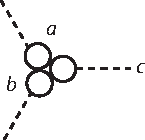
\includegraphics[scale=1]{gesamttex/edit_VIII-4/images/LH_37_05_042_d1.pdf} 
\edcaption[0.25em]{\lbrack\textit{Fig.~1}\rbrack}
\end{edfigure}
\pstart
\noindent
Concurrunt
\edtext{tres globi}{\lemma{tres}\Bfootnote{%
\textit{(1)}~Circuli %
\textit{(2)}~globi~\textit{L}}} 
aequales\indexS{globi tres aequales concurrentes} 
\edtext{aequali celeritate triangulatim}{\lemma{}\Bfootnote{aequali celeritate triangulatim \textit{erg.~L}}}.
Centrum grav.\indexS{centrum gravitatis}\ eorum quiescit ante ictum,%
\indexS{ictus} quiescet ergo et  
\edtext{post ictum.\indexS{ictus} Nullus}{\lemma{post ictum.}\Bfootnote{%
\textit{(1)}~Et cum %
\textit{(2)}~Necesse est %
\textit{(3)}~Nullus~\textit{L}}}
globus\indexS{globus} progredi potest, nam alioqui progrederentur omnes, quod impossibile. Si unus quiesceret, omnes quiescent, ergo periisset 
\edtext{vis.\indexS{vis} Reflecterentur}{\lemma{vis.}\Bfootnote{%
\textit{(1)}~Idem est si unius mot %
\textit{(2)}~Reflecterentur~\textit{L}}} 
ergo, et quidem qua venerunt 
\edtext{celeritate, nam}{\lemma{celeritate,}\Bfootnote{%
\textit{(1)}~alioqui %
\textit{(2)}~nam~\textit{L}}} 
si vel unus tardius iret, omnes tardius irent, et vis\indexS{vis} perisset. 
\pend
\pstart
Ponamus unum \textit{c} celerius ferri, sed duos \textit{a} et \textit{b}
eandem habere velocitatem. Fingatur Tabula\indexS{tabula} moveri 
celeritate centri gravitatis,\indexS{celeritas centri gravitatis}\indexS{centrum gravitatis} 
sed \textit{a}, \textit{b}, \textit{c}, 
in Tabula\indexS{tabula} aeque 
\edtext{celeriter, et}{\lemma{celeriter,}\Bfootnote{%
\textit{(1)}~et fiet %
\textit{(2)}~et~\textit{L}}} 
habebimus quid fiat, 
nempe motui tabulae\indexS{motus tabulae} %
\edtext{addit\lbrack a\rbrack}{%
\lemma{}%
\Bfootnote{%
additus %
\textit{L ändert Hrsg.}}}
cujusque reflexio\indexS{reflexio} 
aequalis et contraria adventuum\indexS{adventus}
in tabula\indexS{tabula}, dat motum absolutum\indexS{motus absolutus}. 
Sed si cuilibet ex globis\indexS{globus} propria sit velocitas, an duplicem tabulam\indexS{tabula} 
fingemus? Seu navim in navi?\indexS{navis in navi} 
\pend
\pstart
Sed hoc puto perplexum. Fingamus duos globos\indexS{globus} ferri in eadem navi,\indexS{navis} sic ut navis feratur eorum 
\indexS{centrum commune speciale}centro communi speciali\lbrack,\rbrack\ 
\edtext{motus his duobus attributi.}{\lemma{}\Bfootnote{motus his duobus  attributi \textit{erg.~L}}}
Haec navis feratur in alia navi;\indexS{navis in navi} quae moveatur motu centri grav.\ com.\indexS{motus centri gravitatis communis}\indexS{centrum gravitatis commune}\ et simul in ea feratur tertius globus,\indexS{globus} qui occurrat duobus prioribus 
in sua navi\indexS{navis} latis. Sed ista puto perplexiora.
\pend 
\begin{edfigure}%
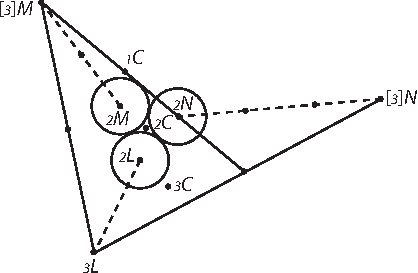
\includegraphics[scale=1]{gesamttex/edit_VIII-4/images/LH_37_05_042_d2.pdf}
\edcaption[0pt]{%
\edtext{\lbrack\textit{Fig.~2}\rbrack}{%
\lemma{\lbrack\textit{Fig.~2}\rbrack}%
\Cfootnote[nonum]{%
Ein gestrichener Entwurf zum Diagramm wird nicht wiedergegeben. Die Bezeichnungen der Punkte \textit{\ind{3}M} und \textit{\ind{3}N} (bei Leibniz \textit{\ind{2}M} und \textit{\ind{2}N}) ändert Hrsg.}}}
\end{edfigure}
\pstart
Vera methodus\indexS{methodus per virium respectivarum combinationem} mea est, per virium respectivarum\indexS{vis respectiva} combinationem\indexS{combinatio virium respectivarum} utcunque.
Globus\indexS{globus in globum oblique incurrens} \textit{L} incurrit in globum \textit{N} 
\edtext{oblique, et hinc}{\lemma{oblique}\Bfootnote{%
\textit{(1)}~, ictu cujus vis %
\textit{(2)}~, et hinc~\textit{L}}} 
patet vis respectiva inter ipsos particularis.\indexS{vis respectiva particularis} Sed similiter globus\indexS{globus} \textit{M} in globum \textit{N}. 
Vis respectiva totalis\indexS{vis respectiva totalis} esset intensio\indexS{intensio funis} trium funium\indexS{funis} tres globos 
connectentium per discessum. Et ita notandum si plures sint globi,\indexS{globus} 
quemlibet cuilibet connexum intelligi. 
NB Si sint 
\edtext{tres vis}{\lemma{tres}\Bfootnote{%
\textit{(1)}~\bars{concipi \textit{streicht Hrsg.}} possunt %
\textit{(2)}~vis~\textit{L}}} 
respectiva\indexS{vis respectiva} componi potest concipiendo tum qua celeritate centrum grav.\ 
\edtext{commune\indexS{centrum gravitatis commune} \textit{L}}{%
\lemma{commune}%
\Bfootnote{%
\textit{(1)}~\textit{M} et %
\textit{(2)}~\textit{L} %
\textit{L}%
}}
et \textit{M} recedit ab \textit{N}, 
tum qua \textit{M} et \textit{L} recedunt a se invicem.
Eadem quantitas alia hypothesi prodire debet.
\pend 




\chapter[tocentry={Dubium est an vis respectiva in concursu obliquo servetur
\enskip \bracks{Oktober 1690 \textendash\ 1696\,(?)}},
head={Dubium est an vis respectiva in concursu obliquo servetur}]%
{\MakeUppercase{Dubium est an vis respectiva in concursu obliquo servetur}
\newline \bracks{Oktober 1690 \textendash\ 1696\,(?)}}
\label{58951}
\begin{ledgroupsized}[r]{120mm}
\footnotesize
\pstart
\noindent\textbf{Überlieferung:}
\pend
\end{ledgroupsized}
\begin{ledgroupsized}[r]{114mm}
\footnotesize
\pstart \parindent -6mm
\makebox[6mm][l]{\textit{L}}%
Konzept:
LH~XXXV~11, 14~Bl.~36. 
Ein Blatt~8\textsuperscript{o};
oberer und linker Rand beschnitten.
Zwei Seiten; Textfolge: Bl.~36~v\textsuperscript{o}, Bl.~36~r\textsuperscript{o}.
Gemeinsame Schnittkanten mit LH~XXXV~4, 6~Bl.~12 und LH~XXXV~4, 6~Bl.~49.
\pend
\end{ledgroupsized}
\vspace{5mm}
\begin{ledgroup}
\footnotesize
\pstart
\noindent%
\textbf{Datierungsgründe:}
Zusammen mit LH~XXXV~4, 6~Bl.~12 und LH~XXXV~4, 6~Bl.~49 
(beide Stücke werden in Reihe VII erscheinen und sind bisher nicht datiert) bildete der Träger von N.\;\ref{58951} ein Quartblatt.
Auf LH~XXXV~4, 6~Bl.~49 befindet sich die Hälfte eines
nach aktuellem Kenntnisstand
für den Zeitraum Oktober 1690 bis März 1698 mehrfach belegten Wasserzeichens. %
\pend
\pstart
Im letzten Absatz von N.\;\ref{58951} kündigt Leibniz weitere Untersuchungen des schiefen Stoßes eines Körpers auf eine Mehrzahl anderer Körper an. Entsprechende Stellen finden sich in den Konzepten
N.\;\ref{41780} (bes. \refpassage{37_03_067_5a}{37_03_067_5b}),
und N.\;\ref{58300} (bes. \refpassage{35_13_03_242_6a}{35_13_03_242_6b})
die nach bisherigem Kenntnisstand auf die Zeiträume Januar 1691 bis 7.~Februar 1696 bzw.
Mitte September 1690 bis 1696 datierbar sind.
Demnach wird für die Entstehung von N.\;\ref{58951} das Ende der genannten Zeiträume als Terminus ante quem angenommen, woraus sich die angegebene Datierungsspanne ergibt.
\pend 
\end{ledgroup}
\selectlanguage{latin}
\vspace{8mm}
\pstart%
\normalsize%
\noindent%
\href{\Scan{LH_35_11_14_036v}}%
{\lbrack 36~v\textsuperscript{o}\rbrack}
\pend
\nobreak\begin{edfigure}[0.25em]%
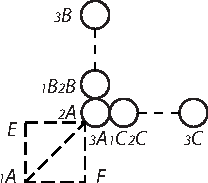
\includegraphics[scale=1]{gesamttex/edit_VIII-4/images/LH_35_11_14_036_d1_036v.pdf}
\edcaption{\edtext{\lbrack\textit{Fig.~1}\rbrack}{%
\lemma{\lbrack\textit{Fig.~1}\rbrack}%
\Cfootnote[nonum]{%
Ein gestrichener Entwurf zum Diagramm wird nicht wiedergegeben.}}}
\end{edfigure}
\pstart
\noindent
Si globus\indexS{globus}\indexS{globus in globos quiescentes incurrens} 
\textit{A} incurrat in globos\indexS{globus} \textit{B}, \textit{C}, 
\edtext{quiescentes videndum}{\lemma{quiescentes}\Bfootnote{%
\textit{(1)}~verum non est %
\textit{(2)}~videndum ~\textit{L}}} 
\textit{B} ire in \textit{\ind{3}B}, celeritate \textit{\ind{2}B\ind{3}B} $=$ \textit{F\ind{2}A} 
et \textit{C} ire in \textit{\ind{3}C} celeritate \textit{\ind{2}C\ind{3}C} $=$ \textit{E\ind{2}A}.
Sane hoc 
\edtext{modo manet}{\lemma{modo}\Bfootnote{%
\textit{(1)}~retinetur ea %
\textit{(2)}~manet~\textit{L}}} 
eadem vis directrix\indexS{vis directrix} 
\edtext{seu via centri,\indexS{via centri}}{\lemma{}\Bfootnote{seu via centri \textit{erg.~L}}}
et manet quoque eadem vis absoluta\indexS{vis absoluta}; ob summam 
\edtext{quadratorum.\indexS{summa quadratorum} Sed}{\lemma{quadratorum.}\Bfootnote{%
\textit{(1)}~Sed tamen arbitror hoc non procedere, quia non manet eadem quae ante vis respectiva, 
\bars{sed augetur \textit{streicht Hrsg.}} 
\textit{(2)}~Sed~\textit{L}}} 
quia haec data rem non determinant, ideo aliud quiddam adjiciendum, ut scil.\ eadem quoque %
vis respectiva\indexS{vis respectiva} colligi possit. Verum hac ratione video augeri vim respectivam,%
\indexS{vis respectiva} nam manet
\edtext{sic}{%
\lemma{}%
\Bfootnote{%
sic %
\textit{erg.~L}}}
eadem quae prior inter \textit{A} et \textit{BC}
cum eadem hoc modo sit 
\edtext{distantiarum augmentatio seu}{\lemma{distantiarum}\Bfootnote{%
\textit{(1)}~jam %
\textit{(2)}~augmentatio %
\textit{(a)}~inter %
\textit{(b)}~seu~\textit{L}}} 
celeritas respectiva\indexS{celeritas respectiva} inter
\edtext{\textit{A} et \lbrack\textit{D}\rbrack\ centrum}{%
\lemma{\textit{A} et}%
\Bfootnote{%
\textit{(1)}~\textit{D}
\textit{(2)}~\bars{\textit{C} \textit{ändert Hrsg.}} %
centrum
\textit{L}}}
gravitatis\indexS{centrum gravitatis} ipsorum \textit{BC}. Verum alia praeterea 
\edtext{adest vis\indexS{vis respectiva} respectiva}{\lemma{adest}\Bfootnote{%
\textit{(1)}~celeritas respectiva %
\textit{(2)}~vis respectiva~\textit{L}}} 
nova inter \textit{B} et 
\edtext{\textit{C}, invicem}{%
\lemma{\textit{C},}%
\Bfootnote{%
\textit{(1)}~quae pro %
\textit{(2)}~invicem~\textit{L}}}
discedentibus, ita lucrati fuissemus vim respectivam,%
\indexS{vis respectiva} quod absurdum est. Itaque non satis fidendum motuum compositioni\indexS{compositio motuum} 
nisi considerationi virium\indexS{vis}\indexS{consideratio virium} 
coincidat. 
\pend
\begin{edfigure}%
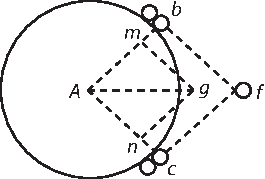
\includegraphics[scale=1]{gesamttex/edit_VIII-4/images/LH_35_11_14_036_d2_036v.pdf} 
\edcaption{%
\edtext{\lbrack\textit{Fig.~2}\rbrack}{%
\lemma{\lbrack\textit{Fig.~2}\rbrack}%
\Cfootnote[nonum]{Ein gestrichener Entwurf zum Diagramm wird nicht wiedergegeben.}}}
\end{edfigure}
\pstart
Sic si \textit{A} incidat simul in \textit{b} et \textit{c} sitque celeritas\indexS{celeritas composita}
\edtext{$A\lbrack f\rbrack$,}{%
\lemma{}%
\Bfootnote{%
\textit{AF}, %
\textit{L ändert Hrsg.}%
}}
 composita ex \textit{Ab} et \textit{Ac}, si igitur 
\edtext{perinde rem esse}{\lemma{perinde}\Bfootnote{%
\textit{(1)}~affici \textit{A} 
\textit{(2)}~rem esse~\textit{L}}} 
ponamus ac si simul \textit{A} incurrisset in \textit{b} celeritate \textit{Ab} et in \textit{c} celeritate \textit{Ac}, res eodem redibit 
\edtext{quoad \textit{A},}{\lemma{}\Bfootnote{quoad \textit{A} \textit{erg.~L}}}
ac si \textit{A} eadem quam dabat celeritate in unum eorum incurrisset, nam ex celeritatibus \textit{Ab}, \textit{Ac} fiet \textit{Am}, \textit{An}, cum ex \textit{Af}, fiat \textit{Ag} eadem proportione scil. $Am:Ab\squaredots Ag:Af\squaredots A-f,:A+f$. \pend
\pstart\noindent
\href{\Scan{LH_35_11_14_036r}}%
{\lbrack 36~r\textsuperscript{o}\rbrack} 
\pend
\nobreak
\begin{edfigure}[0.5em]%
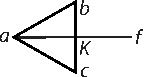
\includegraphics[scale=1]{gesamttex/edit_VIII-4/images/LH_35_11_14_036_d3_036r.pdf} 
\edcaption{\lbrack\textit{Fig.~3}\rbrack}
\end{edfigure}
\pstart
Considerandum etiam, si ponamus celeritatem \textit{af} compositam\indexS{celeritas composita} ex celeritatibus \textit{ab}, \textit{ac}, posito \textit{abfc} esse parallelogrammum;%
\indexS{parallelogrammum} in absoluta virium aestimatione%
\indexS{vis}\indexS{aestimatio absoluta virium} 
rem non procedere, 
\edtext{etiam}{\lemma{}\Bfootnote{etiam \textit{erg.~L}}}
 si ponamus esse rhombum%
\indexS{rhombus} seu $ab=ac=bf=cf$. Nam si 
\edtext{ponamus motum \textit{ab}}{\lemma{ponamus}\Bfootnote{%
\textit{(1)}~\textit{ab} 
\textit{(2)}~motum \textit{ab}~\textit{L}}} 
\edtext{componi ex $aK+Kb$,}{\lemma{}\Bfootnote{componi ex \textit{aK} \bars{et \textit{streicht Hrsg.}} $+\,Kb$,~\textit{L}}}
et 
\edtext{motum \textit{ac} ex}{\lemma{motum \textit{ac}}\Bfootnote{%
\textit{(1)}~ex \textit{aK} et \textit{Kb}, fiet quidem $aK-a$ %
\textit{(2)}~ex~\textit{L}}} 
$aK+Kc$
\edtext{seu ex $aK-\lbrack Kb\rbrack$ seu}{\lemma{}\Bfootnote{seu ex $aK\,-$ \bars{\textit{bK}  \textit{ändert Hrsg.}} seu~\textit{L}}}
ex 
\edtext{$Kf-\lbrack Kb\rbrack$, habemus}{\lemma{}\Bfootnote{$Kf\,-$ \bars{\textit{bK} \textit{ändert Hrsg.}} , habemus~\textit{L}}}
quidem $aK+Kb-Kb+Kf$, sed tamen praeterquam quod haec compositio%
\indexS{compositio motuum} non procedit in non rhombis,%
\indexS{rhombus} non tamen succedit virium compositio\indexS{compositio virium}, nam vires\indexS{vis} sunt $aK^2+Kb^2+aK^2$
\edtext{$+Kc^2$, seu bis}{\lemma{$+Kc^2$}\Bfootnote{%
\textit{(1)}~quae tamen non dant \textit{aK} %
\textit{(2)}~se %
\textit{(a)}~$2\cdot aK^2+$ %
\textit{(b)}~bis $aK^2$ %
\textit{(c)}~bis~\textit{L}}}
 $aK^2+\text{bis }bK^2$. Sed hoc non consentit cum quadrato ab \textit{af} quod est $4aK^2$ nisi eo solo casu cum %
rhombus\indexS{rhombus} abit in quadratum.%
\indexS{quadratum} 
\pend
\pstart
\edtext{Videndum quod fiat, cum globus unus 
\edtext{incurrit amphidextre}{%
\lemma{incurrit}%
\Bfootnote{%
\textit{(1)}~ambidextre %
\textit{(2)}~amphidextre~\textit{L}}}
in plures,%
\indexS{globus unus amphidextre in plures incurrens} item cum globus incurrit in globum plures amphidextre tangentem.\indexS{globus plures globos amphidextre tangens}
Possunt plures rursus tangi a paucioribus et semper paucioribus donec res reducitur ad unum. Ita plura notabilia colligentur.%
}{\lemma{Videndum \lbrack...\rbrack\  colligentur}%
\Cfootnote{%
Entsprechende Untersuchungen werden in den Konzepten N.\;\ref{41780} (bes. \refpassage{37_03_067_5a}{37_03_067_5b}) und N.\;\ref{58300} (bes. \refpassage{35_13_03_242_6a}{35_13_03_242_6b}) angestellt.}}
\pend




\chapter[tocentry={Schedae de impulsu eccentrico
\enskip 31.\;Oktober (10.\;November) 1690},
head={Schedae de impulsu eccentrico}]%
{\MakeUppercase{Schedae de impulsu eccentrico}
\newline 31.\;Oktober (10.\;November) 1690}
\label{sdie_intro}
\footnotesize%
\pstart%
\noindent%
Beide \textit{Schedae de impulsu eccentrico} N.\;\ref{58940} und N.\;\ref{58939} wurden von Leibniz eigenhändig auf den 31.\;Okto\-ber\,/\,10.\;November) 1690 datiert.
Der bereits am gemeinsamen Titel erkennbare enge Zusammenhang beider Aufzeichnungen ist auch dadurch belegt, dass ein Kustos am Schluss von N.\;\ref{58940} %
ausdrücklich auf N.\;\ref{58939} verweist (siehe die Beschreibung des Textzeugen, S.\;\pageref{LH_35_11_14_005-006_ueberlieferung}).
Dies rechtfertigt die Entscheidung, beide Konzepte N.\;\ref{58940} und N.\;\ref{58939} einheitlich zu edieren.
\pend%
\pstart%
Im Hinblick auf die relative Chronologie %
ist bemerkenswert, dass die \textit{Scheda} N.\;\ref{58940} (\refpassage{LH_35_11_14_005-006_005r_cntrgyr-1}{LH_35_11_14_005-006_005r_cntrgyr-2}) eine ähnliche Ansicht über den Mittelpunkt der von einem exzentrischen Stoß herrührenden Drehung vertritt wie der vermutlich in Augsburg\indexO{Augsburg} abgefasste Entwurf N.\;\ref{60300} (\refpassage{LH_37_05_044r_alias_dhe-1}{LH_37_05_044r_alias_dhe-2}):
Das \textit{centrum gyrationis} falle mit dem Schwerpunkt des angestoßenen Körpers zusammen.
Diesbezüglich widerlegt N.\;\ref{60300} ausdrücklich die Ansicht, die in den wohl noch Ende 1689 oder Anfang 1690 in Italien\indexO{Italien} entstandenen Texten N.\;\ref{60142+60297} und N.\;\ref{60299} vetreten worden war (siehe hierüber die Datierungsgründe zu N.\;\ref{60300}, S.\;\pageref{LH_37_05_044_datierung}).
Diese ältere Auffassung des Mittelpunkts der Drehung wird in N.\;\ref{58940} und N.\;\ref{58939} nicht mehr erwähnt.
Dies bekräftigt die Annahme, dass die \textit{Schedae de impulsu eccentrico} nach dem Entwurf N.\;\ref{60300} entstanden sein müssen.
\pend
\selectlanguage{latin}%
\frenchspacing%
\normalsize%
\newpage %



\section[tocentry={De impulsu eccentrico scheda prima
\enskip 31.\;Oktober (10.\;November) 1690},
head={De impulsu eccentrico scheda prima}]%
{\MakeUppercase{De impulsu eccentrico scheda prima}
\newline 31.\;Oktober (10.\;November) 1690}
\label{58940}
\selectlanguage{ngerman}%
\frenchspacing%
\begin{ledgroupsized}[r]{120mm}%
\footnotesize%
\pstart%
\noindent\textbf{Überlieferung:}%
\pend%
\end{ledgroupsized}%
\begin{ledgroupsized}[r]{114mm}%
\footnotesize%
\pstart%
\parindent -6mm%
\makebox[6mm][l]{\textit{L}}%
\pagelabel{LH_35_11_14_005-006_ueberlieferung}%
Aufzeichnung:
LH~XXXV~11,\;14 Bl.\;5\textendash6.
Ein Bogen~4\textsuperscript{o};
\href{\Scan{LH_35_11_14_005-006wz}}{Wasserzeichen} im Falz.
Vier Seiten. %
Ein Kustos am Ende von Bl.\;6\,v\textsuperscript{o} verweist auf die \textit{Scheda 2} (N.\;\ref{58939}).%
\pend%
\end{ledgroupsized}%
\selectlanguage{latin}%
\frenchspacing%
\vspace{8mm}%
\pstart%
\normalsize%
\noindent%
\lbrack%
\href{\Scan{LH_35_11_14_005r}}%
{5\,r\textsuperscript{o}}%
\rbrack%
\hfill%
\raggedleft%
31.\;Octob.\;1690
\pend%
\pstart%
\centering%
De impulsu Eccentrico sched. 1%
\indexS{impulsus eccentricus}%
\indexS{scheda}
\pend
\vspace{0.5em}
\pstart%
\noindent%
\edlabel{LH_35_11_14_005-006_005r_methodus-1}%
\edtext{Ad eccentricos corporum incursus%
\indexS{incursus eccentricus}%
\indexS{corpus incurrens}%
}{%
\lemma{Ad}\Bfootnote{%
\textit{(1)}~obliquos co
\textit{(2)}~eccentricos corporum incursus%
~\textit{L}}}
explicandos considerandum est lateralia,%
\indexS{corpus laterale}
quae non per se impelluntur,
ab ipsis per se impulsis quodammodo trahi.
Ut si
globus \textit{A}%
\indexS{globus incurrens}
centrice incurrat in globum \textit{B},%
\indexS{incursus centricus}
sed globo \textit{B} alligatus sit globus \textit{C},%
\indexS{globus alligatus}
tunc impelletur quidem globus\;\textit{B},
sed a globo \textit{B} impulso%
\indexS{globus impulsus}
trahetur globus \textit{C}.%
\indexS{globus tractus}
Atque ita efficitur
ut eccentrice impulsum intelligatur totum compositum \textit{BC}.%
\indexS{corpus impulsum eccentrice}%
\indexS{corpus compositum}%
\edlabel{LH_35_11_14_005-006_005r_methodus-2}%
\pend%
\vspace{1.25em}%
\centerline{%
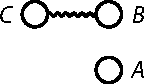
\includegraphics[width=0.16\textwidth]{gesamttex/edit_VIII-4/images/LH_35_11_14_005-006_d01_005r.pdf}}%
\vspace{0.25em}%
\centerline{%
\lbrack\textit{Fig.\:1}\rbrack}%
\vspace{1.0em}%
\pstart%
\noindent%
Antequam ergo impulsus%
\indexS{impulsus eccentricus}
tractionibus conjungamus,%
\indexS{impulsus conjunctus tractioni}
ipsas tractiones consideremus per se.%
\indexS{tractio conjuncta impulsui}
Licet enim omnis tractio per consequentiam%
\indexS{consequentia}
et ipsa ad impulsum%
\indexS{impulsus eccentricus}
redigatur,
id tamen nunc considerari necesse non est,
sufficitque assumi corporum connexionem atque tractionem%
\indexS{tractio conjuncta impulsui}%
\lbrack,\rbrack\
quaecunque demum sit causa%
\indexS{causa firmitatis}
quae fili trahentis%
\indexS{filum trahens}
\edtext{alteriusve vinculi%
\indexS{vinculum rigidum}%
}{%
\lemma{alteriusve}\Bfootnote{%
vinculi
\textit{erg.\;L}}}
firmitatem facit.%
\indexS{firmitas fili}%
\indexS{firmitas vinculi}
\pend%
\pstart%
\edtext{Ponamus ergo
\edtext{globum \textit{B}%
\indexS{globus incurrens}%
}{%
\lemma{globum \textit{B}}\Cfootnote{%
Vgl. das Diagramm \lbrack\textit{Fig.\:2}\rbrack.
Das Band ist dort nicht als \textit{D} bezeichnet.%
}}
initio solum esse in motu,%
\indexS{motus globi}
quiescente \textit{C},%
}{\lemma{Ponamus}\Bfootnote{%
\textit{(1)}~\bars{esse \textit{streicht Hrsg.}}
\textit{(2)}~ergo
\textit{(a)}~filum
\textit{(b)}~globum \textit{B} initio
\textit{(aa)}~esse in motu, solum quiescente \textit{C}
\textit{(bb)}~solum esse %
\lbrack...\rbrack\ quiescente \textit{C},%
~\textit{L}}}
ipsum autem \textit{B} progredientem induere
\edtext{se in retia vinculi%
\indexS{retia vinculi}%
\indexS{vinculum rigidum}%
}{%
\lemma{se}\Bfootnote{%
\textit{(1)}~in vincula
\textit{(2)}~in retia vinculi%
~\textit{L}}}
\textit{D} connexi globo \textit{C},%
\indexS{globi connexi}
et ita a globo \textit{C}
velut visco%
\indexS{viscus}
quodam capi,
quaeritur
quis oriatur motus compositi ex ambobus?%
\indexS{motus compositi} %
\edtext{Is determinatus habebitur ex solitis principiis nostris%
\indexS{principium nostrum}%
}{%
\lemma{Is}\Bfootnote{%
\textit{(1)}~ex sequentibus principibus
\bars{erit \textit{streicht Hrsg.}}
\textit{(2)}~determinatus habebitur %
\lbrack...\rbrack\ principiis nostris,%
~\textit{L}}}%
\lbrack:\rbrack\
nam centrum gravitatis commune%
\indexS{centrum gravitatis commune}
eandem debet habere celeritatem%
\indexS{celeritas centri gravitatis}
quam ante et in easdem partes,
ut eadem maneat vis directrix%
\indexS{vis directrix}%
\lbrack;\rbrack\
deinde oportet eandem quoque
\edtext{manere}{%
\lemma{manere}\Bfootnote{%
\textit{erg.\;L}}}
vim respectivam,%
\indexS{vis respectiva}
seu corporum
\edtext{\lbrack\textit{B}\rbrack\
et
\lbrack\textit{C}\rbrack}{%
\lemma{\textit{A}}\Bfootnote{%
et \textit{B}
\textit{L~ändert Hrsg.}}}
accedendi
recedendique a se invicem conatum.%
\indexS{conatus accedendi}%
\indexS{conatus recedendi}
Unde eadem quoque manebit vis absoluta.%
\indexS{vis absoluta}
\edlabel{35_11_14_005-006_3a}%
\edtext{}{%
\xxref{35_11_14_005-006_3a}{35_11_14_005-006_3b}%
\lemma{absoluta}\Bfootnote{%
\textit{(1)}~Et prim \lbrack/\rbrack\
\textit{(2)}~At
\textit{(3)}~Ac primum ponamus
\textit{(a)}~corpora esse aequalia
\textit{(b)}~globos esse aequales,%
~\textit{L}}}%
\pend%
\pstart%
\edlabel{LH_35_11_14_005-006_005r_cntrgyr-1}%
Ac primum ponamus globos%
\indexS{globus incurrens}%
\indexS{globi connexi}
esse aequales,%
\edlabel{35_11_14_005-006_3b}
et
\edtext{proinde}{%
\lemma{proinde}\Bfootnote{%
\textit{erg.\;L}}}
centrum gravitatis \textit{G} esse in medio,%
\indexS{centrum gravitatis commune}
viamque ejus%
\indexS{via centri gravitatis}
\edtext{\textit{\ind{1}G\ind{2}G}.
Haec}{%
\lemma{\textit{\ind{1}G\ind{2}G}}\Bfootnote{%
\textit{(1)}~quae
\textit{(2)}~. Haec%
~\textit{L}}}
continuetur recta in \textit{\ind{3}G},
sic ut recta
\edtext{\lbrack\textit{\ind{1}G}\ind{3}\textit{G}\rbrack%
}{%
\lemma{\textit{\ind{1}G\ind{2}G}}\Bfootnote{%
\textit{L~ändert Hrsg.}}}
sit dupla rectae \textit{\ind{1}G\ind{2}G}
vel \textit{\ind{2}G\ind{3}G}.
\edtext{Deinde vinculum globorum%
\indexS{globi connexi}
sit rigidum%
\indexS{vinculum rigidum}%
\lbrack,\rbrack\
quod ponamus consistere in linea rigida
centra connectente,%
\indexS{linea rigida}%
\indexS{linea connectens centra}
normali ad lineam motus%
\indexS{linea motus}%
\lbrack;\rbrack\
necesse}{%
\lemma{Deinde}\Bfootnote{%
\textit{(1)}~si ponamus
\textit{(2)}~vinculum globorum sit rigidum
\bars{quod ponamus \lbrack...\rbrack\ lineam motus \textit{erg.}}
necesse%
~\textit{L}}}
est globos%
\indexS{globi connexi}
a se recedere conantes%
\lbrack,\rbrack\
moveri circa aliquod rigidae%
\indexS{linea rigida}
\edtext{seu inflexilis%
\indexS{linea inflexilis}%
}{%
\lemma{seu}\Bfootnote{%
inflexilis
\textit{erg.\;L}}}
lineae \textit{C\ind{ 2}B} punctum %
tanquam centrum.%
\indexS{centrum gyrationis}
Vis autem%
\indexS{vis respectiva}
\edtext{respectiva eadem est}{%
\lemma{respectiva}\Bfootnote{%
\textit{(1)}~perinde
\textit{(2)}~eadem est%
~\textit{L}}}
ac si corpora \textit{B} et \textit{C} celeritate
\edtext{mo\lbrack l\rbrack ibus}{%
\lemma{motibus}\Bfootnote{\textit{L~ändert Hrsg.}}}
reciproca%
\indexS{celeritas reciproca moli}
sibi occurrerent%
\indexS{corpora occurrentia sibi}
et \textit{B} tenderet
\edtext{celeritate \textit{\ind{ 2}BL}%
}{\lemma{celeritate \textit{\ind{ 2}BL}}\Cfootnote{%
Vgl. das Diagramm \lbrack\textit{Fig.\:3}\rbrack.%
}}
et \textit{C} celeritate \textit{CM},
ita ut esset \textit{BL} ad \textit{CM} %
ut \textit{C} ad \textit{B}.
Quodsi igitur aequales sunt globi,%
\indexS{globus incurrens}%
\indexS{globi connexi}
erunt et celeritates \textit{BL},
\textit{CM} aequales,
quod fiet si gyrentur circa punctum medium,%
\indexS{gyratio circa punctum medium}
id est circa centrum gravitatis%
\indexS{centrum gravitatis commune}%
\indexS{gyratio circa centrum gravitatis}
\edlabel{LH_35_11_14_005r_hdsum-1}%
\textit{\ind{2}G}.
Quae celeritates conatusve%
\indexS{conatus procedendi recta}
recta procedendi,
nunc ob vinculum%
\indexS{vinculum rigidum}
in gyrationem%
\indexS{celeritas versa in gyrationem}%
\indexS{conatus versus in gyrationem}
vertentur;
quod ut fiat
eodem servato celeritatis gradu%
\indexS{gradus celeritatis servatus}%
\lbrack,\rbrack\
circulatio fit circa punctum medium \textit{\ind{2}G}%
\indexS{circulatio circa punctum medium}
quod simul est centrum gravitatis.%
\indexS{centrum gravitatis commune}%
\indexS{circulatio circa centrum gravitatis}%
\edtext{}{%
\xxref{LH_35_11_14_005r_hdsum-1}{LH_35_11_14_005r_hdsum-2}%
\lemma{gravitatis}\Bfootnote{%
\textit{\ind{2}G}.
\textit{(1)}~Quid
\textit{(2)}~Si corpora \textit{B} et \textit{C} ponantur inaequalia nihilominus gyratio fiet circa centrum gravitatis \textit{\ind{2}G}{,} nam ut
\textit{(a)}~gyrat
\textit{(b)}~celeritas
\textit{(3)}~Quae celeritates 
\textit{(a)}~in gyratione
\textit{(b)}~conatusve recta procedendi,
\bars{nunc \textit{erg.}}
ob vinculum 
\lbrack...\rbrack\
ut in gyratione
\bars{circa punctum ut \textit{G} \textit{erg.}}
eadem servetur celeritas,%
~\textit{L}}}%
\pend%
\pstart%
Si corpora \textit{B} et \textit{C} ponantur inaequalia,
nihilominus fiet gyratio circa centrum gravitatis,
nam ut in gyratione%
\indexS{gyratio circa centrum gravitatis}
circa punctum ut \textit{G}
eadem servetur celeritas,%
\indexS{celeritas servata in gyratione}%
\edlabel{LH_35_11_14_005r_hdsum-2}
quae erat conatus recti,
oportet esse \textit{BG} ad \textit{CG}
ut \textit{BL} ad
\edtext{\lbrack\textit{CM}\rbrack,}{%
\lemma{\textit{CL}}\Bfootnote{%
\textit{L~ändert Hrsg.}}}
id est ut \textit{C} ad \textit{B}.
Itaque \textit{G} est centrum gravitatis.%
\indexS{centrum gravitatis commune}%
\edlabel{LH_35_11_14_005-006_005r_cntrgyr-2}%
\pend%
\vspace{1.50em}%
\centerline{%
\hspace*{-50mm}%
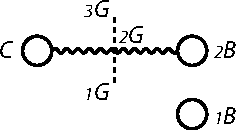
\includegraphics[width=0.25\textwidth]{gesamttex/edit_VIII-4/images/LH_35_11_14_005-006_d02_005r.pdf}}%
\vspace{0.25em}%
\centerline{%
\hspace*{-50mm}%
\lbrack\textit{Fig.\:2}\rbrack}%
\vspace{-8.40em}%
\centerline{%
\hspace*{50mm}
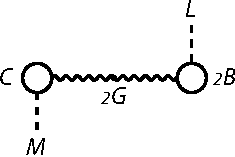
\includegraphics[width=0.26\textwidth]{gesamttex/edit_VIII-4/images/LH_35_11_14_005-006_d03_005r.pdf}}%
\vspace{0.0em}%
\centerline{%
\hspace*{50mm}%
\lbrack\textit{Fig.\:3}\rbrack}%
\newpage%
\pstart%
Itaque perinde movebuntur duo corpora%
\indexS{corpora connexa}
post connexionem%
\indexS{connexio corporum}
ac si habuissent motum communem centri gravitatis,%
\indexS{motus communis centri gravitatis}%
\indexS{centrum gravitatis}
quem et retinebunt,%
\indexS{motus retentus}
proprium autem,%
\indexS{motus proprius}
qui demto communi%
\indexS{motus communis demtus}
\edtext{sequitur,
in gyrum}{%
\lemma{sequitur,}\Bfootnote{%
\bars{quem \textit{streicht Hrsg.}}
in gyrum%
~\textit{L}}}
convertent.%
\indexS{motus conversus in gyrum}%
\indexS{gyrus post incursum}
\lbrack%
\href{\Scan{LH_35_11_14_005v}}%
{5\,v\textsuperscript{o}}%
\rbrack%
\pend%
\pstart%
Eadem vera sunt,
si ambo corpora sint in motu,%
\indexS{corpora occurrentia sibi}
sed parallelas lineas%
\indexS{linea motus}
\lbrack(\protect\vphantom)\rbrack%
ad lineam vinculi%
\indexS{linea vinculi}%
\indexS{vinculum normale ad lineam motus}
scilicet normales%
\lbrack\protect\vphantom()\rbrack\
motu describant.
\pend%
\pstart%
Sed quid
si vinculum ad lineam%
\indexS{linea motus}
\edtext{motus sit obliquum?%
\indexS{vinculum obliquum ad lineam motus}
Omisso}{%
\lemma{motus}\Bfootnote{%
\textit{(1)}~\textlangle motus\textrangle\
\textit{(2)}~sit obliquum
\textit{(a)}~; ut omisso
\textit{(b)}~? Omisso%
~\textit{L}}}
motu communi%
\indexS{motus communis}
\edtext{centri gravitatis%
\indexS{motus centri gravitatis}%
\indexS{centrum gravitatis commune}%
}{%
\lemma{centri}\Bfootnote{%
gravitatis
\textit{erg.\;L}}}
consideremus proprium%
\indexS{motus proprius}
\edtext{utriusque reciprocumque%
\indexS{motus reciprocus}%
}{%
\lemma{utriusque}\Bfootnote{%
reciprocumque
\textit{erg.\;L}}}
tantum%
\lbrack,\rbrack\
in quo consistit vis respectiva.%
\indexS{vis respectiva}
\edtext{%
Is componi intelligetur ex duobus%
\indexS{motus compositus}%
\lbrack,\rbrack\
uno normali ad
\edtext{vinculum \textit{CB},}{%
\lemma{vinculum \textit{CB}}\Cfootnote{%
Vgl. das Diagramm \lbrack\textit{Fig.\:4}\rbrack.}}%
\indexS{motus normalis ad vinculum}
altero parallelo,%
\indexS{motus parallelus ad vinculum}
et normalis quidem transferetur in gyrationem,%
\indexS{gyratio post incursum}%
\indexS{motus translatus in gyrationem}
sed parallelus pariet distractionem vinculi%
\indexS{distractio vinculi}%
\indexS{vinculum rigidum}
\edtext{si ejus sit capax,}{%
\lemma{si}\Bfootnote{%
ejus sit capax
\textit{erg.\;L}}}
cum secundum ipsum corpora \textit{C}
et \textit{\ind{2}B}
reciprocis celeritatibus in diversa trahant.%
\indexS{celeritas reciproca}%
\indexS{corpora trahentia in diversa}
Itaque is motus erit perditus pro toto.%
\indexS{motus perditus}
Itaque hic quoque casus est resolutus.%
\indexS{casus resolutus}%
}%
{\lemma{\textit{Am Rand:}}%
\Afootnote{Hinc
si explicatum esset
si \textit{A} incurreret in \textit{B}%
\indexS{incursus eccentricus}
angulo ad \textit{BC} recto%
\indexS{angulus incursus rectus}%
\lbrack,\rbrack\
explicatum etiam esset
quid in obliquo%
\indexS{angulus incursus obliquus}%
\lbrack:\rbrack\
nam eatenus ictus parallelus%
\indexS{ictus parallelus}
haberetur pro centrico.%
\indexS{ictus centricus}%
}}
Et quidem compositio haec motuum%
\indexS{compositio motuum}
cum fiat salva potentiae quantitate,%
\indexS{quantitas potentiae}%
\indexS{potentia salva}
cum summa quadratorum sit eadem,%
\indexS{summa quadratorum}
tute a nobis introducitur.
\pend%
\pstart%
Si
\edtext{vinculum esset omni rigore destitutum,%
\indexS{vinculum flexile}
simpliciterque flexile,}{%
\lemma{vinculum}\Bfootnote{%
\textit{(1)}~non esset rigidum
\textit{(2)}~esset omni \lbrack...\rbrack\ simpliciterque flexile,%
~\textit{L}}}
nulla fieret gyratio%
\indexS{gyratio nulla}
sed
\edtext{tantum}{%
\lemma{tantum}\Bfootnote{%
\textit{erg.\;L}}}
tractio,%
\indexS{tractio post occursum}
adeoque tota vis respectiva%
\indexS{vis respectiva}
\edtext{in vinculi Elastro%
\indexS{elastrum vinculi}%
}{\lemma{in}\Bfootnote{%
\textit{(1)}~vinculo
\textit{(2)}~vinculi Elastro%
~\textit{L~}}}
consumeretur.%
\indexS{vis consumta in elastrum}
\pend%
\vspace{1.25em}%
\centerline{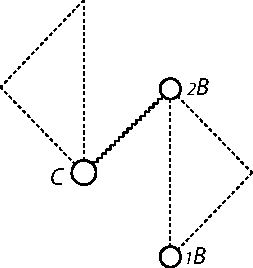
\includegraphics[width=0.26\textwidth]{gesamttex/edit_VIII-4/images/LH_35_11_14_005-006_d04_005v.pdf}}
\vspace{0.25em}
\centerline{\lbrack\textit{Fig.\:4}\rbrack}%
\newpage%
\pstart%
Nunc transferamus ista ad concursum,%
\indexS{concursus corporum}
\edtext{redeamusque ad
\edtext{tres globos%
\indexS{globus incurrens}%
\indexS{globi connexi}
\textit{A},\,\textit{B},\,\textit{C},%
}{\lemma{tres globos \textit{A},\,\textit{B},\,\textit{C}}\Cfootnote{%
Vgl. das Diagramm \lbrack\textit{Fig.\:5}\rbrack.}}%
}{\lemma{redeamusque}\Bfootnote{%
ad
\textit{(1)}~tria corpora
\textit{(2)}~tres globos \textit{A},\,\textit{B},\,\textit{C},%
~\textit{L}}}
et ponamus \textit{A} incurrere in \textit{B}
connexum cum \textit{C} vinculo inflexili.%
\indexS{vinculum inflexile}%
\indexS{globus incurrens}%
\indexS{globi connexi}
\edtext{\lbrack An}{%
\lemma{\lbrack An}\Cfootnote{%
Eckige Klammer von Leibniz.}}
perinde erit
ac si\;\textit{B} tantillum remotum esset a vinculo%
\indexS{vinculum inflexile}
\edtext{in momento concursus%
\indexS{momentum concursus}%
}{%
\lemma{in}\Bfootnote{%
momento concursus
\textit{erg.\;L}}}
et mox statim in ipsum
\edtext{indueretur?%
\indexS{globus indutus in vinculum}
Ita enim}{\lemma{indueretur}\Bfootnote{%
\textit{(1)}~, nam
\textit{(2)}~?
\textit{(a)}~Itaque
\textit{(b)}~Ita enim%
~\textit{L}}}
perinde \textit{A} reflectetur%
\indexS{globus reflexus}
ac si \textit{B} esset solum,
et \textit{B} deinde pergens motu %
quem
\edtext{ex legibus concursus centrici notis}{%
\lemma{ex le\-gi\-bus \lbrack...\rbrack\ notis}%
\Cfootnote{%
Siehe etwa G.\,W. \textsc{Leibniz},
\textit{Leges concursuum}
(\textit{LSB} VIII,\;3 N.\;67);\cite{01383}
\textit{Dynamica}, pars II, sectio III, prop.\;1\textendash15
(%
\textit{CFP}~I, S.\;392--417~\bracks{A};
II.2, S.\;490--518~\bracks{C}).\cite{01354}%
}}
acceperat%
\indexS{lex concursus centrici}%
\indexS{motus acceptus}
seque in vinculum induens%
\indexS{globus indutus in vinculum}
efficiet
quod paulo ante proposuimus.
Idque rationi%
\indexS{consentaneum rationi}
\edtext{consentaneum putes,}{%
\lemma{consentaneum}\Bfootnote{%
\textit{(1)}~est,
\textit{(2)}~putes,%
~\textit{L}}}
quorum
\edtext{enim}{%
\lemma{enim}\Bfootnote{%
\textit{erg.\;L}}}
unum in alterum desinit,
eorum et effectus sibi accedere%
\indexS{effectus accedens}
atque in se invicem
\edtext{tandem}{%
\lemma{tandem}\Bfootnote{%
\textit{erg.\;L}}}
desinere
\edtext{\lbrack debent\rbrack.}{%
\lemma{debeant}\Bfootnote{%
\textit{L~ändert Hrsg.}}}
Jam Hypothesis%
\indexS{hypothesis}
\textit{B} vinculo jam appositi%
\indexS{globus appositus vinculo}
et Hypothesis%
\indexS{hypothesis}
ejusdem a vinculo tantillum remoti,%
\indexS{globus remotus a vinculo}
sunt duo status quantumlibet exigue differentes.%
\indexS{status differens}
Verum sciendum est
\edtext{id in}{%
\lemma{id}\Bfootnote{%
in
\bars{in \textit{streicht Hrsg.}}
simplicibus%
~\textit{L}}}
simplicibus locum habere,
hic vero non aeque.
Et
\edtext{nec in centricis concursibus%
\indexS{concursus centricus}%
}{%
\lemma{nec}\Bfootnote{%
in
\textit{(1)}~communi
\textit{(2)}~centricis concursibus%
~\textit{L}}}
succedere,
multum enim interest exempli causa,
utrum
\edtext{\textit{L} incurrat in \textit{M}%
}{%
\lemma{\textit{L} incurrat in \textit{M}}\Cfootnote{%
Vgl. das Diagramm \lbrack\textit{Fig.\:6}\rbrack.}}
compositum cum \textit{N},%
\indexS{corpus compositum}
an vero ab eo nonnihil remotum,
quanquam certo comparandi modo semper effectus sibi%
\indexS{effectus accedens}
\edtext{accedant.
\edtext{%
Nec semper in compositis%
\indexS{corpus compositum}
locum habet processus per gradus,%
\indexS{processus per gradus}
nisi certo modo intellectus;%
}{%
\lemma{\textit{Am Rand:}}%
\Afootnote{NB Fortasse locum habent quae rejecimus.%
}}
sic refractiones subito transiliunt in reflexiones%
\indexS{refractio transiliens in reflexionem}%
\indexS{reflexio orta e refractione}
ubi ad certam obliquitatem%
\indexS{obliquitas incursus}
perventum est.%
}{\lemma{accedant.}\Bfootnote{%
\textit{(1)}~Sic et in refractionibus, ubi ad
\textit{(2)}~Nec semper \lbrack...\rbrack\ refractiones subito
\textit{(a)}~dissiliunt
\textit{(b)}~transiliunt in %
\lbrack...\rbrack\ perventum est.%
~\textit{L}}}
Itaque sic potius
\edtext{procedendum:\rbrack}{%
\lemma{procedendum:\rbrack\,}\Cfootnote{%
Eckige Klammer von Leibniz.}}%

\pend%
\vspace{2.5em}%
\centerline{\hspace{-95mm}%
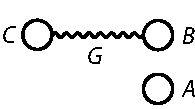
\includegraphics[width=0.20\textwidth]{gesamttex/edit_VIII-4/images/LH_35_11_14_005-006_d05_005v.pdf}}%
\vspace{0.0em}%
\centerline{\hspace{-95mm}%
\lbrack\textit{Fig.\:5}\rbrack}%
\vspace{-6.0em}%
\centerline{%
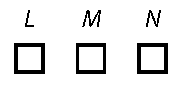
\includegraphics[width=0.20\textwidth]{gesamttex/edit_VIII-4/images/LH_35_11_14_005-006_d06_005v.pdf}}%
\vspace{0.5em}%
\centerline{%
\lbrack\textit{Fig.\:6}\rbrack}%
\vspace{-5.25em}%
\centerline{\hspace{95mm}%
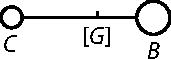
\includegraphics[width=0.18\textwidth]{gesamttex/edit_VIII-4/images/LH_35_11_14_005-006_d07_005v.pdf}}%
\vspace{1.0em}%
\centerline{\hspace{95mm}%
\lbrack\textit{Fig.\:7}\rbrack}%
\newpage%
\pstart%
\edlabel{LH_35_11_14_005-006_005v_navis-1}%
Corpora \textit{B} et \textit{C}%
\indexS{corpora connexa}
vinculo rigido connexa%
\indexS{vinculum rigidum}
concurrere intelligentur cum \textit{A},
et ita quidem ut ferri intelligantur motu communi centri gravitatis,%
\indexS{motus communis}%
\indexS{motus centri gravitatis}%
\indexS{centrum gravitatis commune}
velut in navi,%
\indexS{navis}
et motu proprio reciproco,%
\indexS{motus proprius}%
\indexS{motus reciprocus}
ita ut sit celeritas \textit{A} ad celeritatem \textit{B, C}
ut $B + C$ est ad \textit{A}.%
\edlabel{LH_35_11_14_005-006_005v_navis-2}
Jam ubi \textit{A} incurrit in \textit{B}, %
considerandum est%
\lbrack:\rbrack\
quatenus \textit{B} et \textit{C} gyrare debent
circa aliquod centrum,%
\indexS{gyratio circa centrum}
eatenus perinde
\edtext{e\lbrack st\rbrack}{%
\lemma{e}\Bfootnote{%
\textit{L~ändert Hrsg.}}}
ac si \textit{B} et \textit{C} pariter centrice impellerentur%
\indexS{corpus impulsum centrice}%
\indexS{impulsus centricus}
\edtext{tantum%
\lbrack,\rbrack\
\edtext{corpus oppositum \textit{C}%
}{\lemma{corpus oppositum \textit{C}}\Cfootnote{%
Vgl. das Diagramm \lbrack\textit{Fig.\:7}\rbrack.}}
sumendo tanquam tanto
\edtext{m\lbrack in\rbrack us,}{%
\lemma{m\lbrack in\rbrack us}\Cfootnote{%
Ist \textit{G} gemeinsamer Schwerpunkt der Körper \textit{B} und \textit{C}, so gilt $B : GC = C : GB.$}}
quanto%
}{%
\lemma{tantum}\Bfootnote{%
\textit{(1)}~considerando
\textit{(a)}~\bars{oppositum \textit{erg.}}
\textit{C} velut tanto m
\textit{(b)}~oppositum
\textit{(2)}~corpus oppositum \textit{C} sumendo tanquam
\bars{tanto \textit{erg.}}
\bars{majus \textit{ändert Hrsg.}},
quanto%
~\textit{L}}}
est a centro remotius.%
\indexS{centrum gyrationis}
Punctum autem istud\;\textit{G} est ipsum centrum gravitatis%
\indexS{centrum gravitatis commune}
corporum \textit{B} et \textit{C},
itaque perinde sic fiet
ac si \textit{B} esset duplum.
\lbrack%
\href{\Scan{LH_35_11_14_006r}}%
{6\,r\textsuperscript{o}}%
\rbrack%
\pend%
\pstart%
Videamus
an exitus inde habeatur%
\indexS{exitus}
\edtext{quod%
\lbrack,\rbrack\
dividendo}{%
\lemma{quod}\Bfootnote{%
\bars{quidem \textit{gestr.}}
dividendo%
~\textit{L}}}
corpora utcunque%
\lbrack,\rbrack\
eadem in ipsis manet vis respectiva%
\indexS{vis respectiva}%
\lbrack;\rbrack\
non tantum ergo debet servari
\edtext{eadem vis respectiva%
\indexS{vis respectiva}
inter}{\lemma{eadem}\Bfootnote{%
vis respectiva %
\textit{(1)}~cum et
\textit{(2)}~inter%
~\textit{L}}}
\textit{BC} et \textit{A},
sed etiam inter \textit{B} et \textit{AC}.
Itaque centrum gravitatis commune ipsius \textit{ABC}%
\indexS{centrum gravitatis commune}
debet ante omnia in eadem procedere linea recta,%
\indexS{processus centri gravitatis}
ut eadem in summa maneat vis directiva.%
\indexS{vis directiva}
Deinde \textit{BC}
\edtext{et \textit{A} eandem}{%
\lemma{et}\Bfootnote{%
\textit{A}
\bars{etiam \textit{gestr.}}
eandem%
~\textit{L}}}
retinere debent vim%
\indexS{vis respectiva}
\edtext{respectivam.
Itaque
si \textit{A} ita incidere%
\lbrack t\rbrack\
in \textit{BC}%
}{\lemma{respectivam}\Bfootnote{%
\textit{(1)}~, fingendo scilicet
\textit{(2)}~. Itaque si \textit{A} ita
\bars{incidere \textit{ändert Hrsg.}}
in \textit{BC}%
~\textit{L}}}
ut nulla fieri posset gyratio%
\indexS{gyratio post incursum}
(\protect\vphantom)%
ut si incideret in eorum centrum gravitatis commune%
\indexS{centrum gravitatis commune}%
\protect\vphantom()
tunc
\edtext{reced\lbrack er\rbrack ent}{%
\lemma{recedent}\Bfootnote{%
\textit{L~ändert Hrsg.}}}
a se invicem post%
\indexS{ictus eccentricus}
\edtext{ictum ea celeritate%
\indexS{recessus post ictum}%
\indexS{corpora recedentia}%
\indexS{celeritas recessus}
qua ademto motu communi%
\indexS{motus communis}
centri gravitatis%
\indexS{motus centri gravitatis}
venisse ponuntur,%
}{\lemma{ictum}\Bfootnote{%
\textit{(1)}~in ea celeritate qua venerunt.
\textit{(2)}~ea celeritate \lbrack...\rbrack\ venisse ponuntur,%
~\textit{L}}}
id est reciproce proportionali%
\indexS{celeritates reciproce proportionales corporibus}
\edtext{corporibus.
Si igitur}{\lemma{corporibus.}\Bfootnote{%
\textit{(1)}~Sed nunc
\textit{(2)}~Si igitur%
~\textit{L}}}
\textit{A} ponamus esse aequale ipsi \textit{B} et ipsi \textit{C},
ademto motu communi%
\indexS{motus communis}%
\indexS{motus ademtus}
centri gravitatis,%
\indexS{motus centri gravitatis}
ipsum \textit{A} accipiet celeritatem retrorsum
qua venisse intelligitur ut 2,
et \textit{BC} celeritatem%
\indexS{celeritas recessus}
qua venisse intelligitur ut 1.
Sed celeritas ut 1
quam \textit{BC} accipit%
\indexS{celeritas accepta}%
\lbrack,\rbrack\
non ita intelligenda est %
ac si eam acciperet ipsius \textit{BC} centrum gravitatis \textit{G}.%
\indexS{celeritas centri gravitatis}
Quod fit cum \textit{A} in ipsum impegit,
seu cum incursus in \textit{BC} fuit centricus.%
\indexS{incursus centricus}
Sed debet eam accipere partim centrum gravitatis \textit{G},%
\indexS{centrum gravitatis commune}
partim gyratio.%
\indexS{gyratio post incursum}
Et quatenus gyratio eam accipit,%
\indexS{gyratio post incursum}
eatenus censetur servari vis respectiva,%
\indexS{vis respectiva}
eodem enim modo intelligitur
\edtext{\textit{B} recedere ab \textit{A},%
}{%
\lemma{\textit{B} recedere ab \textit{A}}\Cfootnote{%
Vgl. das Diagramm \lbrack\textit{Fig.\:8}\rbrack.%
}}
sive recta id faciat%
\indexS{recessus rectus}
\edtext{\lbrack\textit{B}\rbrack}{%
\lemma{\textit{C}}\Bfootnote{%
\textit{L~ändert Hrsg.}}}
sive recedendo versus \textit{L} %
in gyrum vertatur,%
\indexS{gyrus post incursum}%
\indexS{recessus versus in gyrum}
initio enim moveri censetur in tangente circuli \textit{BL}.%
\indexS{tangens circuli}
\edlabel{LH_35_11_14_006r_sprdct-1}%
Et ipsum \textit{C}
etsi alibi sit%
\lbrack,\rbrack\
in gyro%
\indexS{gyrus post incursum}
eodem modo movetur %
ac si immediate alligatum ipsi \textit{B}.%
\edlabel{LH_35_11_14_006r_sprdct-2}%
\indexS{globus alligatus}%
\pend%
\pstart%
Illud dubitari poterat,
\edtext{an ipsum commune ipsorum \textit{BC}
centrum gravitatis \textit{G}%
\indexS{centrum gravitatis commune}
etiam motum accipiat,%
\indexS{motus centri gravitatis}%
\indexS{motus acceptus}%
}{%
\lemma{an}\Bfootnote{%
\textit{(1)}~\textit{G} etiam ictum
\textit{(2)}~ipsum commune
\bars{ipsorum \textit{BC} \textit{erg.}}
centrum gravitatis %
\lbrack...\rbrack\ motum accipiat%
~\textit{L}}}
an vero quiescat tantum%
\indexS{centrum gravitatis quiescens}
et gyrationem%
\indexS{gyratio circa centrum gravitatis}
permittat circa se.
Et quidem si \textit{G} non impellitur,
sed
\edtext{tantum vis respectivae%
\indexS{vis respectiva}%
}{\lemma{tantum}\Bfootnote{%
\textit{(1)}~motus res
\textit{(2)}~vis respectivae%
~\textit{L}}}
media
\edtext{pars quam \textit{BC} accipit,
in gyrationem%
\indexS{vis impensa in gyrationem}
impenditur,}{%
\lemma{pars}\Bfootnote{%
\textit{(1)}~quam \textit{G} accipit, est gyratio
\textit{(2)}~quam \textit{BC} accipit,
\textit{(a)}~est gyratio
\textit{(b)}~in gyrationem impenditur,%
~\textit{L}}}
sequitur nulla concursus vi effici posse%
\indexS{vis concursus}
ut
\edtext{corpor\lbrack um\rbrack\ duo\lbrack rum\rbrack}{%
\lemma{corporibus duobus}\Bfootnote{%
\textit{L~ändert Hrsg.}}}
reciproca celeritate%
\indexS{corpora concurrentia velocitatibus reciprocis}
\edtext{concurrenti\lbrack um\rbrack}{%
\lemma{concurrentibus}\Bfootnote{%
\textit{L~ändert Hrsg.}}}
id quod eccentrice impulsum est,%
\indexS{corpus impulsum eccentrice}
et tantillum loco pellatur,
sed quasi immobiliter centro gravitatis
\edtext{infix\lbrack o\rbrack,}{%
\lemma{infixum}\Bfootnote{%
\textit{L~ändert Hrsg.}}}%
\indexS{centrum gravitatis commune}
agetur in gyrum.%
\indexS{corpus actum in gyrum}%
\indexS{gyrus post incursum}
Et si ambo corpora eccentrice
\edtext{impellantur,%
\indexS{corpus impulsum eccentrice}
amborum centra immota manebunt,%
\indexS{centrum gravitatis immotum}%
}{%
\lemma{impellantur,}\Bfootnote{%
\textit{(1)}~non evitabunt
\textit{(2)}~amborum centra immota manebunt,%
~\textit{L}}}
quod absurdum%
\indexS{absurdum}
et experientiae%
\indexS{experientia}
contrarium esse%
\indexS{contrarium experientiae}
manifestum est.
\edtext{I\lbrack t\rbrack em}{%
\lemma{Idem}\Bfootnote{%
\textit{L~ändert Hrsg.}}}
alia hic latet absurditas.%
\indexS{absurditas}
Nempe fiet
\edtext{falsu\lbrack m\rbrack\ irrationabil\lbrack e:\rbrack%
}{%
\lemma{falsus irrationabilis,}\Bfootnote{%
\textit{L~ändert Hrsg.}}}
impulso ipso centro gravitatis%
\indexS{centrum gravitatis impulsum}
nullus fiet gyrus,%
\indexS{gyrus nullus}
omnisque vis ictus%
\indexS{vis ictus}
impendetur in progressum;%
\indexS{vis impensa in progressum}
sed si tantillum ictus fiat extra centrum,%
\indexS{ictus eccentricus}
omnis vis in gyrum transferetur,%
\indexS{vis translata in gyrum}
nulla in progressum,%
\indexS{vis translata in progressum}
cum tamen rationi consentaneum sit%
\indexS{consentaneum rationi}
eo minorem esse gyrum%
\indexS{gyrus post ictum}
majoremque progressum%
\indexS{progressus post ictum}
quo propior centro \textit{G} fit ictus,%
\indexS{ictus proprior centro gravitatis}
et contra quo
\edlabel{35_11_14_005-006_1a}%
remotior.%
\indexS{ictus remotior a centro gravitatis}%
\edtext{}{%
\xxref{35_11_14_005-006_1a}{35_11_14_005-006_1b}%
\lemma{remotior.}\Bfootnote{%
\textit{(1)}~Id iam agitur ut modum
\textit{(2)}~Unde sequitur \lbrack...\rbrack\ impellendo agere.
\bars{\textls{NB} \textit{erg.}}
Sed id agitur ut modum%
~\textit{L}}}
Unde sequitur revera
\textit{B} in \textit{C} non tantum trahendo%
\indexS{tractio post ictum}
quasi filo cohaererent flexili%
\indexS{filum flexile}
(\protect\vphantom)%
extra gyrum%
\indexS{gyrus post ictum}%
\protect\vphantom()
sed etiam impellendo agere.%
\indexS{impulsus eccentricus}%
\edtext{%
\edlabel{LH_35_11_14_006r_NBNB-1}%
\textls{\, NB \;}%
\edlabel{LH_35_11_14_006r_NBNB-2}%
}{%
\lemma{\textit{Am Rand:}}\Afootnote{%
\textls{\,NB \,NB}%
}}%
Sed id agitur
ut modum%
\edlabel{35_11_14_005-006_1b}
partiendi vim respectivam%
\indexS{vis respectiva}
inter gyrum et progressum assequamur.%
\indexS{vis partita inter gyrum et progressum}%
\indexS{gyrus post ictum}%
\indexS{progressus post ictum}
Hac difficultate superata%
\indexS{difficultas superata}
omnia forent in vado.%
\indexS{vadum}%
\pend%
\begin{edfigure}[1.75em][0.00em]%
\hspace{-95mm}%
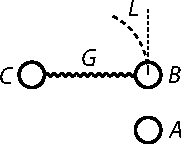
\includegraphics[width=0.20\textwidth]{gesamttex/edit_VIII-4/images/LH_35_11_14_005-006_d08_006r.pdf}%
\edcaption[0.50em]%
{%
\hspace{-95mm}%
\lbrack\textit{Fig.\:8}\rbrack%
\edtext{}{\lemma{\lbrack\textit{Fig.\:8}\rbrack}%
\Cfootnote[nonum]{%
Der Kreisbogen \textit{BL} fehlt in Leibnizens Zeichnung.%
}}%
}%
\vspace{-8.25em}%
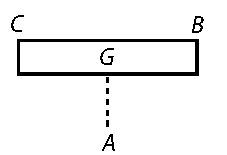
\includegraphics[width=0.25\textwidth]{gesamttex/edit_VIII-4/images/LH_35_11_14_005-006_d09_006r.pdf}%
\edcaption[0.25em]%
{%
\lbrack\textit{Fig.\:9}\rbrack%
}%
\vspace{-8.50em}%
\hspace{95mm}%
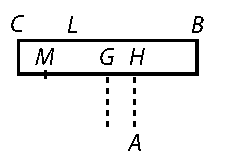
\includegraphics[width=0.25\textwidth]{gesamttex/edit_VIII-4/images/LH_35_11_14_005-006_d10_006r.pdf}%
\edcaption[0.25em]%
{%
\hspace{95mm}%
\lbrack\textit{Fig.\:10}\rbrack%
}%
\end{edfigure}%
\newpage%
\pstart%
Et quidem considerandum est%
\lbrack:\rbrack\
cum ictus%
\indexS{ictus eccentricus}
impellentis \textit{A}%
\indexS{corpus impellens}
non dirigitur in \textit{G} %
\edtext{sed
\edtext{in \textit{H},}{%
\lemma{in \textit{H}}\Cfootnote{%
Vgl. das Diagramm \lbrack\textit{Fig.\:10}\rbrack.}}
tunc totius \textit{BC} %
partem centrice ab \textit{A} in \textit{H} impulsam,%
\indexS{pars impulsa centrice}%
\indexS{impulsus centricus}
esse \lbrack\textit{BL}\rbrack,
residuumque %
tantum per consequentiam impulsum esse.%
\indexS{pars impulsa per consequentiam}
Et si \textit{CL} sit infinite parvum %
adeoque \textit{H} et \textit{G} coincidant,
tunc%
}{%
\lemma{sed}\Bfootnote{%
in \textit{H}
\textit{(1)}~tunc si \textit{H} et \textit{G} concidant seu si
\textit{(2)}~tunc totius %
\lbrack...\rbrack\ impulsam, esse 
\bars{\textit{BC}, \textit{ändert Hrsg.}}
residuumque, tantum
\lbrack...\rbrack\ coincidant, tunc%
~\textit{L}}}
cessare gyrum,%
\indexS{gyrus post ictum}
ob inconsiderabilem resistentiam ipsius \textit{CL}.%
\indexS{resistentia inconsiderabilis}
Sed quo major sit \textit{CL},
eo plus virium impendi in gyrum.
An ergo partibus \textit{BL} et \textit{CL}
positis aequalibus media pars in gyrum,%
\indexS{vis impensa in gyrum}
altera in communem progressum%
\indexS{vis impensa in progressum}%
\indexS{progressus post ictum}
\edtext{impendetur.
An potius non tantum partes considerandae,
sed etiam distantia centrorum cujusque a centro \textit{G},%
\indexS{distantia a centro gravitatis}
seu \textit{LB} in \textit{GH}
an comparandum cum \textit{CL} in \textit{MG}.
Sed video id fieri non debere.%
}{%
\lemma{impendetur.}\Bfootnote{%
\textit{(1)}~An potius non ipsa
\textit{(2)}~Nam ut ipsarum
\textit{(3)}~An potius %
\lbrack...\rbrack\ etiam distantia
\textit{(a)}~earum centro
\textit{(b)}~centrorum cujusque a centro \textit{G},
\textit{(aa)}~sed si hoc
\textit{(bb)}~seu \textit{LB} %
\lbrack...\rbrack\ non debere.%
~\textit{L}}}
Nam ita in casu incursus in \textit{G},%
\indexS{incursus eccentricus}
si \textit{H} et \textit{G} coinciderent,
tamen aequale foret factum \textit{LB} in \textit{HG} infinite parvum,
et infinite parvum \textit{CL} in ordinarium \textit{HM}.
\lbrack%
\href{\Scan{LH_35_11_14_006v}}%
{6\,v\textsuperscript{o}}%
\rbrack\ %
Et sane nec apparet
quid in propulsione totius \textit{CB}%
\indexS{propulsio}
prospectus centri \textit{G} conferat.%
\indexS{prospectus}
An
\edtext{rem concipiemus}{%
\lemma{rem}\Bfootnote{%
\textit{(1)}~sit
\textit{(2)}~concipiemus%
~\textit{L}}}
\edtext{methodo alibi feliciter adhibita%
\indexS{methodus feliciter adhibita}%
}{%
\lemma{methodo \lbrack...\rbrack\ adhibita}%
\Cfootnote{Gemeint ist wohl die \textit{methodus alternorum seu elective concurrentium}, die Leibniz bereits einige Jahre zuvor (1686 \textendash\ Oktober 1687) auf den schiefen Stoß angewandt hatte
(siehe \cite{01398}%
\textit{LSB} VIII,\;3 N.\;65\textsubscript{2}). %
Diese Methode hatte er in der
\cite{01098}%
\textit{Demonstratio geometrica regulae apud Staticos receptae} mathematisch nachgewiesen
(\textit{AE} November 1685, S.\;501--505;\cite{01023}
N.\;\ref{49409} im vorliegenden Band).%
}}%
\lbrack,\rbrack\
ut utrumque ponamus integre succedere
quasi duplicato corpore,
et
\edtext{deinde medium
(\protect\vphantom)%
sed justitiae%
\indexS{justitia}%
\protect\vphantom()
eligamus.%
}{%
\lemma{deinde}\Bfootnote{%
\textit{(1)}~centri gravitatis
\textit{(2)}~medium
\bars{et gyrum \textit{gestr.}}
(\protect\vphantom)sed justitiae\protect\vphantom() eligamus.%
~\textit{L}}}
Quod quomodo hic reperiri possit
dispiciendum.
\pend%
\vspace*{2.5em}%
\centerline{%
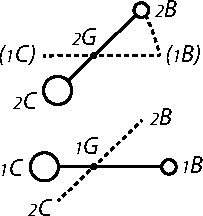
\includegraphics[width=0.24\textwidth]{gesamttex/edit_VIII-4/images/LH_35_11_14_005-006_d11_006v.pdf}}%
\vspace{0.25em}%
\centerline{%
\lbrack\textit{Fig.\:11}\rbrack}%
\newpage%
\pstart%
Sit igitur velocitas ut 1%
\indexS{velocitas distribuenda inter gyrum et progressum}
distribuenda inter gyrum%
\indexS{gyrus post ictum}
\edtext{circa \textit{G}}{%
\lemma{circa \textit{G}}\Cfootnote{%
Vgl. das Diagramm \lbrack\textit{Fig.\:11}\rbrack.}}
et progressum \textit{\ind{1}G\ind{2}G}.%
\indexS{progressus post ictum}
\edtext{Ponamus totam primo impendi in progressum,%
\indexS{veloctias impensa in progressum}%
}{%
\lemma{Ponamus}\Bfootnote{%
\textit{(1)}~totum progress
\textit{(2)}~totam primo impendi in progressum,%
~\textit{L}}}
seu esse
$\ind{1}G\ind{2}G = 1,$
et quantitas progressus erit%
\indexS{quantitas progressus}
\edlabel{LH_35_11_14_006v_qvmh-1}%
\edtext{}{%
\xxref{LH_35_11_14_006v_qvmh-1}{LH_35_11_14_006v_qvmh-2}%
\lemma{\ind{1}G\ind{2}G in $B + C$}\Cfootnote{%
Zu lesen wie $\ind{1}G\ind{2}G \cdot (B + C).$
Klammern werden bei den folgenden Rechnungen zumeist nicht berücksichtigt.%
}}%
\textit{\ind{1}G\ind{2}G} in
\edtext{$B + C.$%
\edlabel{LH_35_11_14_006v_qvmh-2}
Sin omnis vis impendatur in gyrum,%
\indexS{vis impensa in gyrum}
fiet}{\lemma{$B + C$}\Bfootnote{%
\textit{(1)}~, restat
\textit{(2)}~. Sin omnis %
\lbrack...\rbrack\ gyrum, fiet%
~\textit{L}}}
\textit{\ind{1}C\ind{2}C} in $C
+
\ind{1}B\ind{2}B$ in $B
=
\ind{1}G\ind{2}G$ in $B + C.$
Est autem
\textit{\ind{1}C\ind{2}C} ad
\textit{\ind{1}B\ind{2}B}
ut \textit{B} ad \textit{C},
seu
$\ind{1}C\ind{2}C =
\ind{1}B\ind{2}B \cdot B : C$.
Ergo fiet continuo
$\ind{1}B\ind{2}B \cdot B +
\ind{1}B\ind{2}B \cdot B =
\ind{1}G\ind{2}G$
in $B + C.$
Ergo fieret
$\ind{1}B\ind{2}B =
\ind{1}G\ind{2}G,
B + C :
\edtext{[2]}{%
\lemma{2}\Bfootnote{%
\textit{erg. Hrsg.}}}
B.$
\pend%
\vspace{0.5em}%
\pstart%
\noindent%
\lbrack%
\textit{Nachfolgend kleingedruckter Text in L gestrichen:}\rbrack %
\pend%
\vspace{0.5em}%
\footnotesize%
\pstart%
\noindent%
Quod est absurdum,%
\indexS{absurdum}
nisi sint \textit{B} et \textit{C} aequales;
nam pari jure etiam \textit{\ind{1}C\ind{2}C} fieret
$\; =\ind{1}G\ind{2}G$
fierentque \textit{\ind{1}B\ind{2}B}
et \textit{\ind{1}C\ind{2}C} aequales inter se.
Unde jam videtur alia faciliore ratione
ex sola Hypothesi gyrationis%
\indexS{gyratio circa centrum gravitatis}%
\indexS{hypothesis}
circa centrum gravitatis%
\indexS{gyratio circa centrum gravitatis}
faciendae haberi exitus,%
\indexS{exitus}
quanta nempe pars motus%
\indexS{motus translatus in gyrum}
possit debeatve transferri in gyrum.%
\indexS{motus translatus in gyrum}%
\indexS{gyrus post ictum}
\edtext{Nam quaeritur}{%
\lemma{Nam}\Bfootnote{%
\textit{(1)}~sit
\textit{(2)}~quaeritur%
~\textit{L}}}
quae debeat esse proportio ipsius
$\ind{1}C\ind{2}C$
in \textit{C} et \textit{\ind{1}B\ind{2}B} in \textit{B},
\edtext{seu $\astrosun$}{%
\lemma{seu}\Bfootnote{%
$\astrosun$
\textit{erg.\;L}}}
ad \textit{\ind{1}G\ind{2}G} in $B + C$
\edtext{seu $\rightmoon.$}{%
\lemma{seu}\Bfootnote{%
$\rightmoon$
\textit{erg.\;L}}}
Cum sit
\textit{\ind{1}C\ind{2}C}
ad \textit{\ind{1}B\ind{2}B} %
ut \textit{B} ad \textit{C},
fiet
$\ind{1}C\ind{2}C =
\ind{1}B\ind{2}B \cdot B : C$
seu
\textit{\ind{1}C\ind{2}C} in
$C = \ind{1}B\ind{2}B$ in \textit{B},
\edtext{et $\astrosun =
\ind{1}C\ind{2}C +
\ind{1}B\ind{2}B$
in \textit{B} erit%
}{%
\lemma{et}\Bfootnote{%
\textit{(1)}~fit ratio
\textit{(2)}~$\astrosun = \ind{1}C\ind{2}C$ in $C + \ind{1}B\ind{2}B$ in \textit{B} erit%
~\textit{L}}} 
$=\;\ind{1}B\ind{2}B$
in \textit{B}\,bis%
\lbrack,\rbrack\
posito $\astrosun$
\edtext{esse quantitatem vis respectivae%
\indexS{vis respectiva}%
}{\lemma{esse}\Bfootnote{%
\textit{(1)}~vim i
\textit{(2)}~quantitatem
\textit{(a)}~motus progressus
\textit{(b)}~vis respectivae%
~\textit{L}}}
impendendam in%
\indexS{vis impensa in gyrum}
\edtext{gyrum%
\indexS{gyrus post ictum}
et $\rightmoon$ esse quantitatem vis respectivae%
\indexS{vis respectiva}
impendendam in progressum totalem.%
\indexS{vis impensa in progressum}
Ergo fit%
}{%
\lemma{gyrum}\Bfootnote{%
\textit{(1)}~. Ergo fit
\textit{(2)}~et $\rightmoon$ \lbrack...\rbrack\ Ergo fit %
~\textit{L}}}
$\astrosun$ ad $\rightmoon$
ut \textit{\ind{1}B\ind{2}B} in \textit{B}\,bis
ad \textit{\ind{1}G\ind{2}G} in $B + C$
seu in ratione composita \textit{\ind{1}B\ind{2}B}
ad \textit{\ind{1}G\ind{2}G} %
et $B + C$ ad \textit{\ind{2}B},
vel in ratione composita \textit{\ind{1}C\ind{2}C}
ad \textit{\ind{1}G\ind{2}G} %
et $B + C$
\edtext{ad \textit{C}.
Habemus ergo $\astrosun = \ind{1}B\ind{2}B \cdot 2B$%
}{%
\lemma{ad}\Bfootnote{%
\textit{C}.
\textit{(1)}~Sed
\textit{(2)}~Habemus ergo
\textit{(a)}~$\ind{1}B\ind{2}B = \ind{1}G\ind{2}G \cdot \ind{1}B\ind{2}B : B$
\textit{(b)}~$\astrosun \cdot \ind{1}B\ind{2}B$
\textit{(c)}~$\astrosun = \ind{1}B\ind{2}B\cdot2B$%
~\textit{L}}}
et $\rightmoon$
{\normalsize%
\lbrack\textit{Text bricht ab.}\rbrack}%
\pend%
\vspace{0.65em}%
\normalsize%
\pstart%
\noindent%
Unde sequitur
\textit{B} moveri in linea spirali%
\indexS{linea spiralis}%
\indexS{spiralis}
composita ex circulatione%
\indexS{circulatio circa centrum gravitatis}
\edtext{circa \textit{G}}{%
\lemma{circa}\Bfootnote{%
\textit{G}
\textit{erg.\;L}}}
et progressu,%
\indexS{progressus in concursu eccentrico}
ut et \textit{C} in alia spirali data moveri.%
\indexS{spiralis}
Verum alia fit spiralis ipsius \textit{B} %
(\protect\vphantom)%
adeoque et ipsius\;\textit{C}%
\lbrack\protect\vphantom()\rbrack\
si minor impendenda sit pars in gyrum,%
\indexS{vis impensa in gyrum}
quam in progressum,%
\indexS{vis impensa in progressum}
vel si major.
Quid si ergo omnes spirales ponamus%
\indexS{spiralis}
\edtext{%
describi a puncto \textit{B} singulatim;
sed quaeritur quae ex ipsis eligi debeat%
}{%
\lemma{describi}\Bfootnote{%
\textit{(1)}~eligamusque
\textit{(2)}~a puncto %
\lbrack...\rbrack\ eligi debeat%
~\textit{L}}}%
\lbrack,\rbrack\
nempe alia debet eligi
prout alia est proportio ipsius \textit{B} ad \textit{C}.
Quid si ponamus \textit{B} majorem ipsa \textit{C},
divulsam intelligi in duas partes,
unam aequalem ipsi \textit{C},
quae medietatem accipiat gyri,%
\indexS{gyrus post ictum}
medietatem habeat progressus,%
\indexS{progressus post ictum}
altera quae sit excessus\;\textit{B} supra \textit{C},
ob
\edtext{quam progressus excedit gyrum%
\indexS{progressus excedens gyrum}%
\lbrack?\rbrack\
Sed nondum apparet,
quomodo inde instituatur rationcinatio.%
\indexS{ratiocinatio}
An hoc modo%
\lbrack:\rbrack\
ipsius \textit{B} partes sint duae%
\lbrack,\rbrack\
una \textit{M} aequalis ipsi\;\textit{C},
altera \textit{L}.
Iam \textit{M} et\;\textit{C} moventur in linea spirali,%
\indexS{linea spiralis}%
\indexS{spiralis}
ubi motus gyrationis%
\indexS{motus gyrationis}%
\indexS{gyratio circa centrum gravitatis}
et progressus sint inaequales,%
\indexS{motus progressus}
\textit{L} vero moveatur in sola recta.%
}{%
\lemma{quam}\Bfootnote{%
\textit{(1)}~\textlangle non\textrangle\ progressus
\textit{(2)}~progressus excedit gyrum
\textit{(a)}~, itaque ponamus
\textit{(aa)}~celerita
\textit{(bb)}~\textit{L} progredi ea celeritate qua centrum gravitatis \textit{G} ad \textit{C}
\textit{(aaa)}~per
\textit{(bbb)}~et partem ipsius \textit{B} ipsi aequalem circulari aequa
\textit{(b)}~. Sed nondum %
\lbrack...\rbrack\ hoc modo
\textit{(aa)}~ut
\textit{(bb)}~sit
\textit{(cc)}~p\textlangle\textendash\textrangle\
\textit{(dd)}~ipsius \textit{B} %
\lbrack...\rbrack\ duae una
\textit{(aaa)}~\textlangle$D = C$\textrangle\
\textit{(bbb)}~\textit{M} aequalis %
\lbrack...\rbrack\ sint inaequales,
\textit{(aaaa)}~sed \textlangle in una recta\textrangle\
\textit{(bbbb)}~\textit{L}
\bars{vero \textit{erg.}}
moveatur in sola recta.%
~\textit{L}}}
\edtext{%
Sed nihil
\edtext{inde.
Itaque
\edtext{a signo NB paginae praecedentis}{%
\lemma{a signo \lbrack...\rbrack\ praecedentis}\Cfootnote{%
Vgl. \refpassage{LH_35_11_14_006r_NBNB-1}{LH_35_11_14_006r_NBNB-2}.}}
nondum profecimus.%
}{%
\lemma{inde.}\Bfootnote{%
\textit{(1)}~An ita? \textit{B} progrediatur
\textit{(2)}~Itaque
\bars{inde \textit{streicht Hrsg.}}
a signo %
\lbrack...\rbrack\ nondum profecimus.%
~\textit{L}}}%
}{%
\lemma{\textit{Am Rand:}}\Afootnote{%
Nihil actum inter duo NB,
paginae%
\indexS{pagina}
scil. praecedentis%
\textsuperscript{\lbrack a\rbrack}
et hujus.%
\textsuperscript{\lbrack b\rbrack}%
\\[1ex]%
{\footnotesize%
\textsuperscript{\lbrack a\rbrack}~paginae scil. praecedentis:
\refpassage{LH_35_11_14_006r_NBNB-1}{LH_35_11_14_006r_NBNB-2}.
\quad%
\textsuperscript{\lbrack b\rbrack}~hujus:
\refpassage{LH_35_11_14_006v_NBNB-1}{LH_35_11_14_006v_NBNB-2}.%
}}}%
\pend%
\begin{edfigure}[0.00em][1.50em]%
\vspace*{7.00em}%
\hspace{-75mm}%
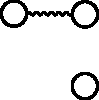
\includegraphics[width=0.11\textwidth]{gesamttex/edit_VIII-4/images/LH_35_11_14_005-006_d12_006v.pdf}%
\edcaption[0.50em]%
{%
\hspace{-75mm}%
\lbrack\textit{Fig.\:12}\rbrack%
}%
\vspace{-12.85em}%
\hspace{55mm}%
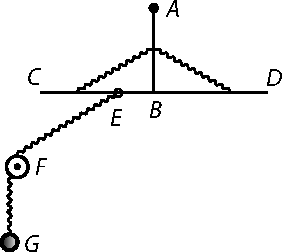
\includegraphics[width=0.34\textwidth]{gesamttex/edit_VIII-4/images/LH_35_11_14_005-006_d13_006v.pdf}%
\edcaption[-0.5em]%
{%
\hspace{58mm}%
\lbrack\textit{Fig.\:13}\rbrack%
\edtext{}{%
\lemma{\textit{Unter} \lbrack\textit{Fig.\:13}\rbrack\ \textit{und hierauf bezogen:}}%
\Afootnote[nonum]{%
Quid si flatus%
\indexS{flatus}
aliquis fiet lineis horizontalibus%
\textsuperscript{\lbrack a\rbrack}
normalibus in \textit{CD},
occupantibus exiguum circulum circa \textit{E}.
Quaeritur
an nulla fiat elevatio,%
\indexS{elevatio}
sed sola circulatio.%
\indexS{circulatio in tractione}
Puto utrumque.%
\\[1ex]%
{\footnotesize%
\textsuperscript{\lbrack a\rbrack}~horizontalibus
\textit{(1)}~aequalibus in punctum \textit{C}
\textit{(2)}~normalibus in \textit{CD},%
~\textit{L}%
}}}%
}%
\end{edfigure}%
\pstart%
Videamus an aliquis detur exitus,%
\indexS{exitus}
supponendo non tantum \textit{A} et \textit{G}
(\protect\vphantom)%
centrum gr. \textit{B} et \textit{C}%
\lbrack\protect\vphantom()\rbrack,
sed etiam \textit{C} et centrum gr.%
\indexS{centrum gravitatis commune}
inter \textit{A} et \textit{B} eandem servare vim%
\indexS{vis respectiva}
\edtext{respectivam.%
\edtext{\textls{ }%
\edlabel{LH_35_11_14_006v_NBNB-1}%
\textls{NB}%
\edlabel{LH_35_11_14_006v_NBNB-2}%
}{\lemma{\textit{Am Rand:}}\Afootnote{%
\textls{NB NB }%
}}\textls{ }%
Si
\edtext{ex funiculo \textit{AB}%
\indexS{funiculum}%
}{%
\lemma{ex funiculo \textit{AB}}\Cfootnote{%
Vgl. das Diagramm \lbrack\textit{Fig.\:13}\rbrack.%
}}%
}{%
\lemma{respectivam.}\Bfootnote{%
\bars{Imo res jam ex sola gyratione ipsius \textit{A} et \textit{G} fortassis determinata, jam enim constat, qua celeritate reflecti debeat \textit{A}, ea scil. quae sit dimidia vis respectivae. \textit{gestr.}}
\bars{\textls{NB} \textit{erg.}}
\textit{(1)}~Si sine ictu
\textit{(2)}~Si ex funiculo \textit{AB}%
~\textit{L}}}
suspendas trabem horizontalem \textit{CD},%
\indexS{trabs horizontalis}
inde
\edtext{alligato fune \textit{FE} ad \textit{CD},%
\indexS{funis trahens}
si placet %
normali,
in puncto \textit{E} extra medium trabis,}{%
\lemma{alligato \lbrack...\rbrack\ trabis}\Cfootnote{%
Anders als im Text angegeben,
verläuft das Seil \textit{EF} im Diagramm \lbrack\textit{Fig.\:13}\rbrack\ nicht senkrecht zum Balken \textit{CD}, sondern schräg hierzu.%
}}
trahas trabem,%
\indexS{trabs tracta}
potest ea duobus modis accedere
\edtext{ad \textit{F},
uno}{%
\lemma{ad}\Bfootnote{%
\textit{(1)}~trabem, uno
\textit{(2)}~\textit{F}, uno%
~\textit{L}}}
ut \textit{C\,E\,B\,D}
\edtext{parallel\lbrack e\rbrack}{%
\lemma{parallelae}\Bfootnote{%
\textit{L~ändert Hrsg.}}}
accedant,
altero
ut fiat gyratio%
\indexS{gyratio in tractione}
circa aliquod punctum, ut \textit{B}.
Quaeritur
quomodo fiat motus:
Haud dubie
\edtext{sic,
ut eodem manente descensu}{%
\lemma{sic,}\Bfootnote{%
ut
\textit{(1)}~ascensu
\textit{(2)}~eodem manente descensu%
~\textit{L}}}
ipsius \textit{G} ponderis,%
\indexS{descensus ponderis}
sit ascensus centri gravitatis trabis \textit{B}%
\indexS{ascensus centri gravitatis}%
\indexS{centrum gravitatis trabis}%
\indexS{trabs horizontalis}
omnium possibilium minimus.
Quanquam et
\edtext{si\lbrack c\rbrack}{%
\lemma{si}\Bfootnote{%
\textit{L~ändert Hrsg.}}}
decidatur%
\lbrack,\rbrack\
fateor ex eo non decidi nostrum,
habet tamen cum eo similitudinem.%
\indexS{similitudo}
\edtext{Nam hic}{%
\lemma{Nam}\Bfootnote{%
\textit{(1)}~si loco funis
\textit{(2)}~hic%
~\textit{L}}}
ponitur nulla opus vi
\edtext{ad circumagendam trabem,%
\indexS{trabs circumagenda}
quia solo conatu,%
\indexS{conatus sine impetu}
non impetu agitur,%
\indexS{impetus}
sed}{%
\lemma{ad}\Bfootnote{%
\textit{(1)}~circumagendum funiculum
\textit{(2)}~circumagendam trabem,
\textit{(a)}~\bars{\textlangle sed\textrangle\ \textit{streicht Hrsg.}}
\textit{(b)}~quia solo %
\lbrack...\rbrack\ agitur, sed%
~\textit{L}}}
ad \textit{A} circumagendum cum impulsu%
\indexS{impulsus}
est opus vi seu impetu,%
\indexS{impetus}%
\indexS{vis seu impetus}
si scilicet aliquod
\edtext{pondus in \textit{E} incidat.%
\indexS{pondus incidens}%
}{%
\lemma{pondus}\Bfootnote{%
\textit{(1)}~in \textlangle \textit{B} in\textrangle\ 
\textit{(2)}~in \textit{E} incidat.%
~\textit{L}}}
Ubi quidem talis orietur progressus,%
\indexS{progressus post concursum}
reflexio%
\indexS{reflexio post concursum}
et gyratio%
\indexS{gyratio post concursum}
ut eadem sit potentia%
\indexS{potentia post concursum}
quae ante concursum,%
\indexS{potentia ante concursum}
deinde etiam
ut eadem sit progressio centri gravitatis%
\indexS{progressio centri gravitatis}
quae ante concursum%
\indexS{concursus corporum}
si omnia subito lineis rigidis connectantur,%
\indexS{linea rigida}%
\indexS{corpora connexa}
postremo eadem vis respectiva,%
\indexS{vis respectiva}
intendens lineas connectentes.%
\indexS{linea connectens}
Sed haec non videntur sufficere ad determinandum.
Pono corpus in \textit{E} incurrens rigide,%
\indexS{corpus incurrens rigide}%
\indexS{incursus rigidus}
ipsi \textit{E} annecti
ut non possit dissilire.
Omnis vis respectiva non videtur hic perire%
\indexS{vis respectiva}%
\indexS{vis periens}
alligatione in \textit{E}.%
\indexS{alligatio}
Si enim pondus impingens in \textit{E}%
\indexS{pondus impingens}
et \textit{CD} in diversa tendunt%
\lbrack,\rbrack\
adjuvat \textit{BD} ipsum \textit{E} contra \textit{BC},
ut fiat gyratio%
\indexS{gyratio in tractione}
v.\,g. circa \textit{B}.
Si igitur \textit{CD} et pondus ut
\edtext{\lbrack\textit{G}\rbrack}{%
\lemma{\textit{F}}\Bfootnote{%
\textit{L~ändert Hrsg.}}}
funem \textit{FE} in diversa trahant%
\indexS{tractio funis}%
\lbrack,\rbrack\
quaeritur quantum intendatur funis,%
\indexS{funis tractus}%
\indexS{funis intensus}
quantum gyrationis,%
\indexS{gyratio in tractione}
quae minima mutatio,%
\indexS{mutatio minima}
et quae quantitas aestimanda.%
\indexS{quantitas aestinamda}%
\pend%
\selectlanguage{latin}%
\frenchspacing%
\normalsize%



\section[tocentry={De impulsu eccentrico scheda secunda
\enskip 31.\;Oktober (10.\;November) 1690},
head={De impulsu eccentrico scheda secunda}]%
{\MakeUppercase{De impulsu eccentrico scheda secunda}
\newline 31.\;Oktober (10.\;November) 1690}
\label{58939}
\selectlanguage{ngerman}%
\frenchspacing%
\begin{ledgroupsized}[r]{120mm}%
\footnotesize%
\pstart%
\noindent\textbf{Überlieferung:}%
\pend%
\end{ledgroupsized}%
\begin{ledgroupsized}[r]{114mm}%
\footnotesize%
\pstart%
\parindent -6mm%
\makebox[6mm][l]{\textit{L}}%
Aufzeichnung:
LH~XXXV~11,\;14 Bl.\;3\textendash4. 
Ein Bogen~4\textsuperscript{o},
oberer Rand beschnitten.
\href{\Scan{LH_35_11_14_003-004wz}}{Gegenmarke} eines Wasserzeichens im Falz.
Vier Seiten. %
Ein Kustos am Ende von N.\;\ref{58940} %
verweist auf N.\;\ref{58939}.%
\pend%
\end{ledgroupsized}%
\selectlanguage{latin}%
\frenchspacing%
\vspace{8mm}
\count\Bfootins=1000
\count\Afootins=1200
\count\Cfootins=1000
\pstart%
\normalsize%
\noindent%
\lbrack%
\href{\Scan{LH_35_11_14_003r}}%
{3\,r\textsuperscript{o}}%
\rbrack%
\phantom{Ult.\;Octob.\;1690}%
\hfill%
\phantom{\lbrack3\,r\textsuperscript{o}\rbrack}%
Ult.\;Octob.\;1690%
\edtext{}{%
\lemma{\textit{Am oberen Rand:}}\Afootnote%
{%
Videantur quae ascripsimus pag.\;3 signo NB NB.\textsuperscript{\lbrack a\rbrack}%
\indexS{signum}
\\[1ex]%
{\footnotesize%
\textsuperscript{\lbrack a\rbrack}~NB NB:
Siehe die Randbemerkung zu \refpassage{35_11_14_003v_rndbmrkng-1}{35_11_14_003v_rndbmrkng-2}
(in \textit{L} am Rand von Bl.\;4\,r\textsuperscript{o},
bezogen auf Bl.\;3\:v\textsuperscript{o}).%
}}}%
\pend%
\pstart%
\noindent%
\centering%
De impulsu Eccentrico%
\indexS{impulsus eccentricus}
scheda 2\textsuperscript{a}%
\indexS{scheda}%
\edtext{}{%
\lemma{\textit{Am Rand:}}\Afootnote{%
Sub finem\textsuperscript{\lbrack a\rbrack}%
\indexS{finis}
rem videor assecutus per collationem diversarum virium respectivarum.%
\indexS{collatio virium respectivarum}%
\indexS{vis respectiva}%
\\[1ex]%
{\footnotesize%
\textsuperscript{\lbrack a\rbrack}~Sub finem:
Siehe \refpassage{LH_35_11_14_004v_subfinem-1}{LH_35_11_14_004v_subfinem-2}.%
}}}
\pend%
\vspace{0.5em}%
\pstart%
\noindent%
\edlabel{LH_35_11_14_003-004_003r_methodus-1}%
Perjudiciale experimentum%
\indexS{experimentum perjudicale}
sumendum esset;
si \textit{A} incurrat in \textit{B}%
\indexS{corpus incurrens}%
\indexS{incursus eccentricus}
connexum cum \textit{C},%
\indexS{corpora connexa}
utrum reflectatur perinde%
\indexS{corpus reflexum}%
\indexS{reflexio corporis incurrentis}
ac si solum incurrisset in \textit{B},
licet \textit{B} deinde impulsu%
\indexS{impulsus eccentricus}
suo abripiat \textit{C}.%
\indexS{corpus abreptum}%
\indexS{abreptio corporis impulsi}%
\edlabel{LH_35_11_14_003-004_003r_methodus-2}
Quid autem hoc posito fiat,
ita explicemus distinctius:
\edlabel{LH_35_11_14_003r_aequales-1}%
ponamus \textit{A}, \textit{B}, \textit{C} esse aequales,%
\indexS{corpora aequalia}%
\edlabel{LH_35_11_14_003r_aequales-2}
et\;\textit{A} incurrere in \textit{B}%
\indexS{corpus incurrens}%
\indexS{incursus eccentricus}
celeritate 1.%
\indexS{celeritas incursus}
Utique quiescet in loco incursus,%
\indexS{locus incursus}%
\indexS{quies post incursum}
et deinde \textit{B} perget eadem celeritate
quam habuit \textit{A}.%
\indexS{celeritas incursus}
Jam \textit{B}
\edtext{inciden\lbrack te\rbrack%
\indexS{corpus incidens in vinculum}%
}{%
\lemma{incidens}\Bfootnote{%
\textit{L~ändert Hrsg.}}}
in vinculum \textit{CB}%
\indexS{vinculum}
quo ipsi \textit{C} connectitur%
\indexS{corpora connexa}%
\lbrack,\rbrack\
ad angulos rectos%
\indexS{angulus rectus}%
\lbrack,\rbrack\
quid
\edtext{\lbrack fiat\rbrack}{%
\lemma{fiat}\Bfootnote{%
\textit{erg. Hrsg.}}}
facile ita explicabimus,
primum considerando communem motum centri gravitatis%
\indexS{centrum gravitatis commune}%
\indexS{motus centri gravitatis}%
\lbrack,\rbrack\
isque perget ut ante,
et reliquum deinde motum privatum%
\indexS{motus privatus}%
\indexS{motus reliquus}
seu respectivum%
\indexS{motus respectivus}
qui convertetur in gyrationem%
\indexS{motus conversus in gyrationem}
circa centrum.%
\indexS{centrum gravitatis commune}%
\indexS{gyratio circa centrum gravitatis}%
\pend%
\begin{edfigure}[2.00em][0.00em]%
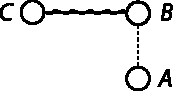
\includegraphics[width=0.19\textwidth]{gesamttex/edit_VIII-4/images/LH_35_11_14_003-004_d01_003r.pdf}%
\edcaption[0.50em]%
{%
\lbrack\textit{Fig.\:1}\rbrack%
}%
\end{edfigure}%
\newpage%
\begin{edfigure}[0.00em][1.50em]%
\vspace*{0.0em}%
\hspace{-85mm}%
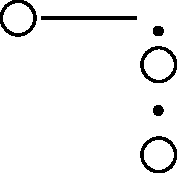
\includegraphics[width=0.11\textwidth]{gesamttex/edit_VIII-4/images/LH_35_11_14_003-004_d02_003r.pdf}%
\edcaption[0.25em]%
{%
\hspace{-85mm}%
\lbrack\textit{Fig.\:2, gestr.}\rbrack%
}%
\vspace{-6,5em}%
\hspace{85mm}%
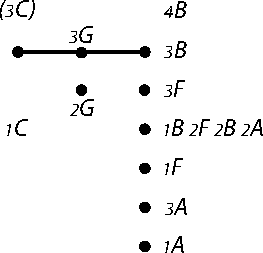
\includegraphics[width=0.20\textwidth]{gesamttex/edit_VIII-4/images/LH_35_11_14_003-004_d03_003r.pdf}%
\edcaption[0.25em]%
{%
\hspace{85mm}%
\lbrack\textit{Fig.\:3, gestr.}\rbrack%
\edtext{}{\lemma{\lbrack\textit{Fig.\:3}\rbrack}%
\Cfootnote[nonum]{%
Hierzu liegt in \textit{L} ein gestr., nicht wiedergegebener Entwurf vor.%
}}%
\edtext{}{%
\lemma{\textit{Unter%
} \lbrack\textit{Fig.\:3}\rbrack:%
}%
\Afootnote[nonum]{%
\quad%
$\ind{1}F\ind{2}F
=
\ind{2}F\ind{3}F
=
FB.$
\quad%
$\ind{2}B\ind{3}B
=
\text{bis}\ FB.$
\quad%
$\ind{2}A\ind{3}A
=
FA - FB.$%
}}%
}%
\vspace{0.25em}%
\includegraphics[width=0.40\textwidth]{%
gesamttex/edit_VIII-4/images/LH_35_11_14_003-004_d04_003r.pdf}%
\edcaption[0.25em]%
{%
\lbrack\textit{Fig.\:4}\rbrack%
}%
\end{edfigure}%
\pstart%
Sit
\edtext{\textit{F} centrum gr.%
\indexS{centrum gravitatis commune}%
}{%
\lemma{\textit{F} cen\-trum gr.\,}\Cfootnote{%
Vgl. das Diagramm \lbrack\textit{Fig.\:4}\rbrack.%
}}
inter \textit{A} et \textit{B}.
$\ind{1}F\ind{2}F
=
\ind{2}F\ind{3}F.$
Coincidunt
\textit{\ind{1}B},\;%
\textit{\ind{2}B},\;%
\edtext{\lbrack\textit{\ind{2}F}\rbrack,}{%
\lemma{\textit{\ind{2}B}}\Bfootnote{%
\textit{L~ändert Hrsg.}}}%
\;%
\textit{\ind{2}A}
(\protect\vphantom)%
si sumamus corpora ut puncta%
\indexS{corpus sumptum ut punctum}%
\protect\vphantom().
$\ind{3}F\ind{3}B
=
\ind{1}F\ind{1}B$
et
\edtext{%
$\ind{2}F\ind{3}A
=
\ind{1}F\ind{1}A,$%
}{%
\lemma{$\ind{3}F\ind{3}A
=
\ind{1}F\ind{1}A$\,%
}\Cfootnote{%
Die Bedingung $A = B = C$ (vgl. \refpassage{LH_35_11_14_003r_aequales-1}{LH_35_11_14_003r_aequales-2}) gilt jetzt nicht mehr.
Sonst müsste unter der Annahme, dass der Körper \textit{B} vor dem Stoß ruht, an dessen Stelle der Körper \textit{A} nach dem Stoß in \textit{\ind{2}A} ruhen.%
}}
adeoque
\edtext{%
$\ind{1}A\ind{1}B
=
[\ind{3}A\ind{3}F].$ %
$\ind{2}B\ind{3}B
=
\ind{2}F\ind{3}F
+
\ind{3}F\ind{3}B
=
\ind{1}F\ind{2}F
+
\ind{1}F\ind{1}B.\
\ind{2}B\ind{3}B
=
\text{bis}\
\ind{1}F\ind{2}F$
seu bis \textit{FB}.
$\ind{2}A\ind{3}A
=
FA - FB.$
Jam \textit{B} in \textit{\ind{3}B} %
incidat in vinculum%
\indexS{corpus incidens in vinculum}%
\indexS{vinculum}
quod%
}{%
\lemma{$\ind{1}A\ind{1}B =$}\Bfootnote{%
\bars{$\ind{3}A\ind{3}B$ \textit{ändert Hrsg.}}.
\textit{(1)}~Jam \textit{\ind{3}B} incidat in vinculum quo
\textit{(2)}~$\ind{2}B\ind{3}B = \ind{2}F \ind{3}F \, +$ %
\lbrack...\rbrack\ vinculum quod%
~\textit{L}}}
ipsum connectat cum%
\indexS{corpora connexa}
\edtext{\lbrack\textit{C}\rbrack.}{%
\lemma{\textit{B}}\Bfootnote{%
\textit{L~ändert Hrsg.}}}
In situ%
\indexS{situs}
\textit{\ind{2}BC}
erat centrum gravitatis
\textit{\ind{2}G};%
\indexS{centrum gravitatis commune}
in situ%
\indexS{situs}
\textit{\ind{3}BC}
erat
\textit{\ind{3}G};
rectaque
\textit{\ind{2}G\ind{3}G}
parallela ipsi
\textit{\ind{2}B\ind{3}B}.
Et hoc perget
eadem celeritate%
\indexS{celeritas centri gravitatis}
et directione%
\indexS{directio centri gravitatis}
in \textit{\ind{4}G}.
Cum autem cohaereant \textit{B} et \textit{C},%
\indexS{corpora cohaerentia}
vis eorum respectiva%
\indexS{vis respectiva}
vertetur in%
\indexS{vis versa in circulationem}
\edlabel{35_11_14_003-004_1a}%
circulationem.%
\indexS{circulatio in concursu eccentrico}%
\edtext{}{%
\xxref{35_11_14_003-004_1a}{35_11_14_003-004_1b}%
\lemma{circulationem.}\Bfootnote{%
\textit{(1)}~Quod
\textit{(2)}~Est autem motus duplex
\textit{(3)}~Potest enim \lbrack...\rbrack\ duplici componi,%
~\textit{L}}}
Potest enim motus ex duplici componi,%
\indexS{motus compositus}%
\edlabel{35_11_14_003-004_1b}
ex communi%
\indexS{motus communis}
centri gravitatis,%
\indexS{centrum gravitatis commune}%
\indexS{motus centri gravitatis}
qui est celeritatis
\textit{\ind{2}G\ind{3}G}%
\indexS{celeritas centri gravitatis}
ductae in
$B + C,$
et proprio contrario%
\indexS{motus proprius}%
\indexS{motus contrarius}
\edtext{%
reciproco.%
\indexS{motus proprius}%
\indexS{motus reciprocus}
Jam celeritas%
}{\lemma{reciproco.}\Bfootnote{%
\textit{(1)}~, qui \textlangle\textendash\textrangle\ in
\textit{(2)}~. Jam celeritas%
~\textit{L}}}
quam dederamus ipsi \textit{B} %
\edtext{erat
\textit{\ind{2}B\ind{3}B},
et}{%
\lemma{erat}\Bfootnote{%
\textit{\ind{2}B\ind{3}B},
\textit{(1)}~ergo
\textit{(2)}~et%
~\textit{L}}}
\textit{\ind{2}G\ind{3}G}
ad
\textit{\ind{2}B\ind{3}B}
ut
\textit{B} ad
\edtext{%
$B + C,$
et celeritas propria%
\indexS{celeritas propria}%
}{%
\lemma{$B + C,$}\Bfootnote{%
et
\textit{(1)}~motus proprio
\textit{(2)}~celeritas propria%
~\textit{L}}}
ipsius \textit{B}
erit
$\ind{2}B\ind{3}B
-
\ind{2}G\ind{3}G$
(\protect\vphantom)%
quia quiescit \textit{C}%
\indexS{corpus quiescens}%
\protect\vphantom()
seu ad
\textit{\ind{2}B\ind{3}B}
ut \textit{C}
ad $B + C,$
ut celeritas %
contraria%
\indexS{celeritas contraria}
est
$= \ind{2}G\ind{3}G$
seu est ad
\textit{\ind{2}B\ind{3}B}
ut \textit{B}
ad $B + C.$
Cum ergo velocitates hae respectivae%
\indexS{velocitas respectiva}
sint inter se ut corpora
\edtext{%
reciproce
et convertantur in
gyratio\lbrack nem\rbrack,%
\indexS{gyratio in concursu eccentrico}%
\indexS{velocitas conversa in gyrationem}
cum alia ratione%
\indexS{ratio alia}
praestari posse non appareat,
fiet gyratio circa centrum gravitatis,%
\indexS{gyratio circa centrum gravitatis}%
\indexS{centrum gravitatis commune}%
}{%
\lemma{reciproce}\Bfootnote{%
\textit{(1)}~ut convertantur in gyrationem circa \textit{G}
\textit{(2)}~et convertantur in
\bars{gyratio, \textit{ändert Hrsg.}},
cum alia %
\lbrack...\rbrack\ centrum gravitatis,%
~\textit{L}}}
et arcus
\textit{(\ind{3}B)\ind{4}B}%
\indexS{arcus circuli}
celeritatem gyrationis%
\indexS{celeritas gyrationis}
ipsius \textit{B} exprimens
erit aequalis priori velocitati respectivae ipsius \textit{B},%
\indexS{velocitas respectiva}
adeoque ad
\textit{\ind{2}B\ind{3}B}
ut \textit{C}
ad $B + C,$
\edtext{\lbrack et\rbrack}{%
\lemma{ut}\Bfootnote{%
\textit{L~ändert Hrsg.}}}
arcus
\textit{(\ind{3}C)\ind{4}C}%
\indexS{arcus circuli}
erit $=$
\textit{\ind{3}G\ind{4}G}
seu
\textit{\ind{2}G\ind{3}G},
et ita manebit velocitas respectiva.%
\indexS{velocitas respectiva}
Unde si liberarentur ambo simul in circulatione%
\indexS{circulatio in concursu eccentrico}%
\lbrack,\rbrack\
eandem quam ante velocitatem respectivam%
\indexS{velocitas respectiva}
retinerent pariterque communem.%
\indexS{velocitas communis}
Sed comparanda velocitas respectiva%
\indexS{velocitas respectiva}
inter \textit{A} et
\edtext{%
\textit{CB}, scil.
quaerenda est via centri gravitatis communis%
\indexS{centrum gravitatis commune}%
\indexS{via centri gravitatis}
omnium \textit{A}, \textit{B}, \textit{C}
seu ipsius \textit{H}.
Habetur autem punctum \textit{H} %
intersectione%
\indexS{intersectio rectarum}
rectarum \textit{AG} et\;\textit{FC}.%
}{%
\lemma{\textit{CB},}\Bfootnote{%
\textit{(1)}~prior scilicet
\textit{(a)}~\textit{A} ad
\textit{(b)}~ipsius \textit{A} accessio ad \textit{G}, cum quiesceret adhuc \textit{B}, erat \textit{\ind{1}A\ind{2}A}, sed mox recessus est $\ind{2}A\ind{3}A + \ind{2}G\ind{3}G,$ est autem 2.
\textit{(2)}~scil. quaerenda
\lbrack...\rbrack\ ipsius \textit{H}
\textit{(a)}~quo
\textit{(b)}~. Habetur autem
\lbrack...\rbrack\ \textit{AG} et \textit{FC}.%
~\textit{L}}}
\lbrack%
\href{\Scan{LH_35_11_14_003v}}%
{3\,v\textsuperscript{o}}%
\rbrack%
\pend%
\pstart%
Sed puto hanc Methodum non procedere,%
\indexS{methodus non procedens}
\edtext{vel centrici}{%
\lemma{vel}\Bfootnote{%
\textit{(1)}~singularis
\textit{(2)}~centrici%
~\textit{L}}}
concursus exemplo, %
\indexS{concursus centricus}
manifestum enim est
longe aliter reflecti%
\indexS{corpus incurrens}%
\indexS{corpus reflexum}%
\indexS{reflexio corporis incurrentis}
\edtext{%
\textit{A}
incurrens
in \textit{B},%
}{%
\lemma{\textit{A} incurrens in \textit{B}}\Cfootnote{%
Vgl. das Diagramm \lbrack\textit{Fig.\:5}\rbrack.}}
cum
\edtext{%
\textit{B} est sejuncta%
}{\lemma{\textit{B} est sejuncta}\Cfootnote{%
In dem vorliegenden und dem folgenden Absatz werden die zusammenstoßenden bzw. zusammenhängenden Körper %
abwechselnd mit dem Neutrum oder dem Femininum bezeichnet.%
}}
a \textit{C},%
\indexS{corpora sejuncta}
quam cum est continua.%
\indexS{corpora continua}
Interim
\edtext{putem servire casum disjuncti}{%
\lemma{putem}\Bfootnote{%
\textit{(1)}~hunc
\textit{(2)}~servire casum disjuncti%
~\textit{L}}}
ad casum continui investigandum,%
\indexS{casus corporum continuorum}
continue enim accedet%
\indexS{accessio continua}%
\lbrack;\rbrack\
et video revera eadem fieri,
sed cum nova accedit consideratio,%
\indexS{consideratio}
ut nempe ipsae \textit{B}, \textit{C}
non tantum sint continuae%
\indexS{corpora continua}%
\indexS{partes continuae}
sed et connexae,%
\indexS{corpora connexa}%
\indexS{partes connexae}
tum demum aliud eveniet.
Nempe ponamus
\textit{A}, \textit{B}, \textit{C} esse aequales%
\indexS{corpora aequalia}
et \textit{A} incidere in \textit{B},
quiescent \textit{A} et \textit{B},
movebitur \textit{C}.
Sed cum \textit{B} et \textit{C} sunt connexae%
\lbrack,\rbrack\
res sese longe aliter
\edlabel{35_11_14_003-004_2a}%
habet.%
\edtext{}{%
\xxref{35_11_14_003-004_2a}{35_11_14_003-004_2b}%
\lemma{habet}\Bfootnote{%
\textit{(1)}~quemadmodum
\lbrack/\rbrack\
\textit{(2)}~. Quemadmodum si
\textit{(3)}~. Regulae concursus centrici%
~\textit{L}}}%
\pend%
\pstart%
Regulae concursus centrici%
\edlabel{35_11_14_003-004_2b}%
\indexS{concursus centricus}%
\indexS{regula concursus centrici}
duorum%
\indexS{corpora concurrentia centrice}
\edtext{corporum \textit{a}, \textit{b}%
}{\lemma{corporum \textit{a}, \textit{b}%
}\Cfootnote{%
Vgl. das Diagramm \lbrack\textit{Fig.\:6}\rbrack.}}
debent esse tales
ut
circulantes%
\indexS{corpus circulans}
circa eundem axem \textit{LM}%
\indexS{axis circulationis}
et concurrentes
ac post concursum%
\indexS{concursus centricus}
reflexae,%
\indexS{corpus reflexum}
iterum ab altera parte
ob gyrum concurrentes%
\indexS{corpora concurrentia ob gyrum}%
\indexS{concursus ob gyrum}%
\indexS{gyrus post incursum}%
in \textit{(a)} et \textit{(b)}
restituant statum primum.%
\indexS{restitutio status primi}%
\indexS{status primus}
Idem et fieri debet in incursu eccentrico%
\indexS{incursus eccentricus}
ubi
\edtext{oritur progressus%
\indexS{progressus post incursum}
et gyrus,%
\indexS{gyrus post incursum}%
}{%
\lemma{oritur}\Bfootnote{%
\textit{(1)}~reflexio et gyrus
\textit{(2)}~progressus et gyrus,%
~\textit{L}}}
ut scilicet post concursum%
\indexS{concursus eccentricus}
oriatur simplex motus%
\indexS{motus simplex}
destructo gyro,%
\indexS{gyrus destructus}
debeat autem talis esse ambitus circuli gyrationis%
\indexS{gyratio in concursu eccentrico}%
\indexS{circulus gyrationis}%
\indexS{ambitus circuli gyrationis}
qui arbitrio potest assumi,%
\indexS{arbitrium}
ut sibi praecise rursus occurrant in eodem loco
saltem a latere opposito.
Pono autem concursus%
\indexS{concursus eccentricus}
initio esse proportionales ponderibus.%
\indexS{concursus proportionalis ponderibus}
Notandum etiam
\edtext{contra supradicta}{%
\lemma{contra supradicta}\Cfootnote{%
Möglicherweise N.\;\ref{58940}, \refpassage{LH_35_11_14_006r_sprdct-1}{LH_35_11_14_006r_sprdct-2}.%
}}%
\lbrack:\rbrack\
cum
\edtext{}{%
\xxref{LH_35_11_14_003v_corpusBC-1}{LH_35_11_14_003v_corpusBC-2}%
\lemma{corpus \textit{BC}}\Cfootnote{%
Vgl. das Diagramm \lbrack\textit{Fig.\:8}\rbrack.}}%
\edtext{%
\edlabel{LH_35_11_14_003v_corpusBC-1}%
corpus \textit{BC}%
\edlabel{LH_35_11_14_003v_corpusBC-2}
est in motu \textit{\ind{1}G\ind{2}G}%
}{%
\lemma{corpus}\Bfootnote{%
\textit{(1)}~\textit{B} agendum
\textit{(2)}~\textit{BC}
\textit{(a)}~agendum
\textit{(b)}~est in motu \textit{\ind{1}G\ind{2}G}%
~\textit{L}}}
et ab \textit{A} impellitur contrario itinere,%
\indexS{iter contrarium}
revera ipsum \textit{B} tantum,
non vero ipsum \textit{C} obstare gyro,%
\indexS{gyrus post incursum}
cum ita \textit{C} suum conatum%
\edlabel{35_11_14_003v_3a}
obtineat.%
\indexS{conatus obtentus}
\edtext{}{%
\xxref{35_11_14_003v_3a}{35_11_14_003v_3b}%
\lemma{obtineat.}\Bfootnote{%
\textit{(1)}~Manifestum est quatenus gyrus fit, eatenus rev
\textit{(2)}~Jam video
\lbrack...\rbrack\ ipso recedit.%
~\textit{L}}}%
\pend%
\pstart%
\edtext{}{%
\xxref{35_11_14_003v_rndbmrkng-1}{35_11_14_003v_rndbmrkng-2}%
\lemma{\textit{Quer am linken Rand von Bl.\;4\,r\textsuperscript{o}, mit Bezug auf Bl.\;3\,v\textsuperscript{o}:}}\Afootnote{%
NB NB
Hinc usque ad finem paginae 4%
\indexS{pagina}%
\textsuperscript{\lbrack a\rbrack}
per paginam sequentem%
\indexS{pagina}%
\textsuperscript{\lbrack b\rbrack}
videntur vera esse omnia,
nempe tribus modis diversis investigando
aequationem respectivarum potentiarum%
\indexS{aequatio potentiae respectivae}%
\indexS{potentia respectiva collecta cum totali}
collectarum cum totali.%
\indexS{potentia totalis collecta cum respectiva}
Res inchoanda a NB pag. sequentis.%
\indexS{pagina}%
\textsuperscript{\lbrack c\rbrack}
Imo adhuc ibi videtur in eo esse error,%
\indexS{error}
quod vis respectiva%
\indexS{vis respectiva}
non aestimanda solum in parallelis,
sed absolute quaerendo diminutionem distantiae.
Forte in hoc loco res non nocebit.
Altius tamen examinandum.%
\\[1ex]%
{\footnotesize%
\textsuperscript{\lbrack a\rbrack}~paginae 4\,:
Bl.\;4\,v\textsuperscript{o}.
\quad
\textsuperscript{\lbrack b\rbrack}~paginam sequentem\,:
Bl.\;4\,r\textsuperscript{o}.
\quad
\textsuperscript{\lbrack c\rbrack}~NB pag. sequentis\,:
Vgl. \refpassage{LH_35_11_14_004v_NB-1}{LH_35_11_14_004v_NB-2}.%
}}}%
\edlabel{35_11_14_003v_rndbmrkng-1}%
Jam video re recte considerata%
\lbrack:\rbrack\
quatenus fit gyrus%
\indexS{gyrus post ictum}
et quidem circa centrum gravitatis,%
\indexS{centrum gravitatis commune}
eatenus nullam habere locum celeritatem respectivam%
\indexS{celeritas respectiva corporis gyrantis}
corporis gyrantis,%
\indexS{corpus gyrans}
respectu alterius,
nam quantum unum ipsi accedit,
tantum alterum ab ipso recedit.%
\edlabel{35_11_14_003v_3b}
Caeterum gyratio%
\indexS{gyratio in concursu eccentrico}
debet fieri circa centrum%
\indexS{centrum gravitatis commune}
\edtext{gravitatis.
Ita enim \textit{B} et \textit{C} saltem}{%
\lemma{gravitatis.}\Bfootnote{%
\textit{(1)}~Alioqui
\textit{(2)}~Ita enim
\textit{(a)}~corpus a
\textit{(b)}~\textit{B} et \textit{C} saltem%
~\textit{L}}}
eandem retinent vim respectivam inter se,%
\indexS{vis respectiva}
nempe nullam,
ut ante.%
\edlabel{35_11_14_003v_rndbmrkng-2}%
\pend%
\vspace{1.0em} %
\centerline{%

\includegraphics[width=0.066\textwidth]{gesamttex/edit_VIII-4/images/LH_35_11_14_003-004_d05_003v.pdf}}
\vspace{0.50em}
\centerline{%
\lbrack\textit{Fig.\:5}\rbrack}
\newpage
\vspace*{-0.0em} %
\centerline{\hspace{-70mm}%
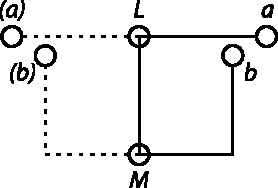
\includegraphics[width=0.30\textwidth]{gesamttex/edit_VIII-4/images/LH_35_11_14_003-004_d06_003v.pdf}}
\vspace{0.25em}
\centerline{\hspace{-70mm}%
\lbrack\textit{Fig.\:6}\rbrack}
\vspace{-8.6em} %
\centerline{\hspace{70mm}%
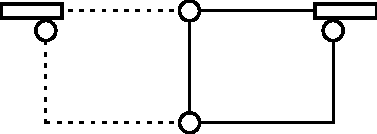
\includegraphics[width=0.425\textwidth]{gesamttex/edit_VIII-4/images/LH_35_11_14_003-004_d07_003v.pdf}}
\vspace{1.0em}
\centerline{\hspace{70mm}%
\lbrack\textit{Fig.\:7}\rbrack}
\vspace*{3.75em} %
\centerline{\hspace{-70mm}%
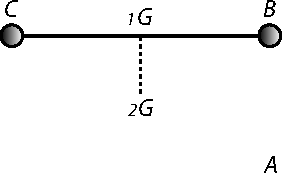
\includegraphics[width=0.30\textwidth]{gesamttex/edit_VIII-4/images/LH_35_11_14_003-004_d08_003v.pdf}}
\vspace{-0.5em}
\centerline{\hspace{-70mm}%
\lbrack\textit{Fig.\:8}\rbrack}
\vspace{-10.80em} %
\centerline{\hspace{70mm}%
\includegraphics[width=0.33\textwidth]{%
gesamttex/edit_VIII-4/images/LH_35_11_14_003-004_d09_003v.pdf}}
\vspace{1.0em}
\centerline{\hspace{70mm}%
\lbrack\textit{Fig.\:9}\rbrack}
\vspace{2.5em}
\pstart%
Verum quid
si contingat ipsa a connexione liberari?%
\indexS{connexio corporum}
Tunc magnam acquirent vim a se invicem recedendi,%
\indexS{vis recedendi}
ergo eam jam habent,
eaque
\edtext{intend\lbrack itur\rbrack}{%
\lemma{intendunt}\Bfootnote{%
\textit{L~ändert Hrsg.}}}
connectens%
\indexS{vis connectens}%
\lbrack;\rbrack\
praeterea vis%
\indexS{vis recedendi}
qua corpus \textit{A} recedit ab ipsorum centro gravitatis%
\indexS{centrum gravitatis commune}
etiam computanda est.
Et hae vires simul aequari debent potentiae respectivae%
\indexS{potentia respectiva}
quae initio
\edtext{fuit.
Sed tamen superest quaestio%
\indexS{quaestio}%
}{%
\lemma{fuit.}\Bfootnote{%
\textit{(1)}~Itaque
\textit{(2)}~ Sed quaeri
\textit{(3)}~Sed tamen superest quaestio%
~\textit{L}}}
quantus fieri debeat gyrus,%
\indexS{gyrus post ictum}
quanta vero progresssio%
\indexS{progressio post ictum}
seu reflexio.%
\indexS{reflexio post ictum}
\edtext{%
An dicemus corpora\;\textit{A} et\;\textit{B}
ob ictum%
\indexS{ictus}
a se invicem recedere%
\indexS{corpus recedens post ictum}%
\indexS{recessus post ictum}
celeritate%
\indexS{celeritas recessus}
qua advenere%
\indexS{celeritas adventus}%
\lbrack?\rbrack%
}{%
\lemma{dicemus}\Bfootnote{%
\textit{(1)}~corpus \textit{A} a corpore \textit{B} ea tantum recedere celeritate
\textit{(2)}~corpora \textit{A} 
\textit{(3)}~corpora \textit{A} %
\lbrack...\rbrack\ qua advenere.%
~\textit{L}}}
Nam inter
\edtext{ipsa}{%
\lemma{ipsa}\Bfootnote{%
\textit{erg.\;L}}}
sola fit ictus,%
\indexS{ictus}
cum oppositum
\edtext{\textit{C}}{%
\lemma{\textit{C}}\Bfootnote{%
\textit{erg.\;L}}}
non obstet,
sed progredi possit
non obstante impulsu%
\indexS{impulsus}
ipsius\;%
\edtext{%
\textit{B} versus\;\textit{L}.%
}{%
\lemma{\textit{B} versus \textit{L}}\Cfootnote{%
Vgl. das Diagramm \lbrack\textit{Fig.\:9}\rbrack.}}
Verum ut eadem in
\lbrack%
\href{\Scan{LH_35_11_14_004r}}%
{4\:r\textsuperscript{o}}%
\rbrack\ %
summa servetur vis respectiva%
\indexS{vis respectiva}
quae
\edtext{ante,
opus et gyro.}{%
\lemma{ante,}\Bfootnote{%
\textit{(1)}~id obtinetur gyro
\textit{(2)}~et ita oritur
\textit{(3)}~opus et gyro.%
~\textit{L}}}
Nam ictus%
\indexS{ictus}
non est nisi inter\;\textit{B} et\;%
\edtext{\lbrack\textit{A}\rbrack,}{%
\lemma{\textit{C}}\Bfootnote{%
\textit{L~ändert Hrsg.}}}
non potest autem eadem
\edtext{esse celeritas respectiva%
\indexS{celeritas respectiva}
inter\;\textit{A} et\;\textit{G}}{%
\lemma{esse}\Bfootnote{%
\textit{(1)}~vis respectiva inter \textit{B} et
\textit{(2)}~celeritas respectiva inter \textit{A} et \textit{G}%
~\textit{L}}}
quae ante,
alioqui nullus fieret gyrus,%
\indexS{gyrus post ictum}
qui et ipse novam vim respectivam continet.%
\indexS{vis respectiva}
Debet autem oriri
gyrus,%
\indexS{gyrus post ictum}
non
simplex recessus%
\indexS{recessus post ictum}
\edtext{seu regressus%
\indexS{regressus post ictum}%
}{%
\lemma{seu}\Bfootnote{%
\textit{(1)}~progressus
\textit{(2)}~regressus%
~\textit{L}}}
quia \textit{C} gyro%
\indexS{gyrus post ictum}
progressum suum%
\indexS{progressus post ictum}
\edtext{servat.
Quidni}{%
\lemma{servat.}\Bfootnote{%
\textit{(1)}~Quod si
\textit{(2)}~Quidni%
~\textit{L}}}
ergo solus erit gyrus?%
\indexS{gyrus post ictum}
Respondeo:
ita \textit{C} tenderet versus \textit{M}
celerius quam ante et nimis celeriter.
Videamus ergo
\edtext{an haec duo simul coincidant,
ut \textit{A} et \textit{B} eandem}{%
\lemma{an}\Bfootnote{%
\textit{(1)}~fiat
\textit{(2)}~haec duo simul coincidant, ut
\textit{(a)}~\textit{C} eand
\textit{(b)}~\textit{A} et \textit{B} eandem%
~\textit{L}}}
inter se servent velocitatem respectivam,%
\indexS{velocitas respectiva}
et ut \textit{C} eundem servet progressum;%
\indexS{progressus post ictum}
simulque ut efficiatur
ut summa eadem maneat vis respectiva.%
\indexS{vis respectiva}%
\pend%
\pstart%
Tentemus in exemplo:
sint
\edtext{\textit{A}, \textit{B}, \textit{C} aequales%
\indexS{corpora aequalia}%
}{%
\lemma{\textit{A}, \textit{B}, \textit{C} aequales}\Cfootnote{%
Vgl. das Diagramm \lbrack\textit{Fig.\:10}\rbrack.%
}}
et celeritas
(ex hypothesi)%
\indexS{hypothesis}
quantitatum reciproce proportionalis%
\indexS{celeritas reciproce proportionalis quantitati}
adeoque ipsius \textit{A} duplo major.
Jam si \textit{A} et \textit{B} ob ictum%
\indexS{ictus}
eadem a se invicem celeritate respectiva%
\indexS{celeritas respectiva}
resiliunt%
\indexS{corpus resiliens}%
\indexS{resilitio post ictum}
quam habuerunt,
ideo cum sint aequalia%
\indexS{corpora aequalia}%
\lbrack,\rbrack\
distantia%
\indexS{distantia corporum concurrentium}
prior \textit{\ind{1}B\ind{1}A} %
erit bisecanda in \textit{D},
et sumatur \textit{\ind{2}A\ind{3}A} %
aequalis ipsi \textit{D\ind{1}A},
quae erit reflexio ipsius \textit{A} ob ictum.%
\indexS{ictus}%
\indexS{reflexio ob ictum}
Jam \textit{\ind{2}B} habebit celeritatem tendendi retrorsum%
\indexS{celeritas tendendi retrorsum}
quae etiam sit ut \textit{\ind{1}BD} vel \textit{\ind{1}AD}.
Sed simul \textit{C} habet suum progrediendi conatum%
\indexS{conatus progrediendi}
celeritate%
\indexS{celeritas conatus}
\edtext{\textit{\ind{1}C\ind{2}C}.
Hoc posito inveniemus}{%
\lemma{\textit{\ind{1}C\ind{2}C}.}\Bfootnote{%
\textit{(1)}~Ex his jam obtinebim
\textit{(2)}~Hoc posito inveniemus%
~\textit{L}}}
quae esse debeat quantitas gyri,%
\indexS{quantitas gyri}%
\indexS{gyrus post ictum}
quaeque regressus.%
\indexS{quantitas regressus}%
\indexS{regressus post ictum}
\edtext{%
Sit ergo regressus celeritas \textit{r},%
\indexS{celeritas regressus}
et gyri \textit{g}%
\indexS{celeritas gyri}%
}{%
\lemma{\textit{Am Rand:}}\Afootnote{%
\textit{g} gyrus,%
\indexS{gyrus post ictum}
\textit{r} regressus%
\indexS{regressus post ictum}
ipsius \textit{G}%
}}
et \textit{\ind{1}BD}
vel \textit{\ind{1}AD}
vocetur \textit{d}.
Debet esse
$r + g = d,$
ut scilicet \textit{B} accipiat
\edtext{celeritatem \textit{d}.
Prima autem}{%
\lemma{celeritatem}\Bfootnote{%
\textit{d}.
\textit{(1)}~Sed contra
\textit{(2)}~Prima autem%
~\textit{L}}}
celeritas \textit{\ind{1}C\ind{2}C}%
\indexS{celeritas prima}
sit \textit{c},
fietque
$g - r = c.$
Ubi
\edtext{%
notandum
es\lbrack t\rbrack\
$d = 3c : 2$
seu
$c = 2d : 3,$
nam bis
$\ind{1}C\ind{2}C
=
\ind{1}A\ind{2}A$
et bis \textit{d}
seu bis
$\ind{1}AD
=
\ind{1}A\ind{2}A
+
\ind{1}C\ind{2}C.$
Hinc%
}{%
\lemma{notandum}\Bfootnote{%
\bars{esse \textit{ändert Hrsg.}}
$d = 3c : 2$
\textit{(1)}~. Inde
\textit{(2)}~%
\bars{seu $c = 2 d : 3$ \textit{erg.}}, nam
\bars{bis \textit{erg.}} $\ind{1}C\ind{2}C =$
\textit{(a)}~dimid
\textit{(b)}~$\ind{1}A \ind{2}A$ et
\bars{bis \textit{erg.}} \textit{d} seu
\bars{bis \textit{erg.}} $\ind{1}AD = \ind{1}A\ind{2}A + \ind{1}C\ind{2}C.$ Hinc%
~\textit{L}}}
$r + g - \overline{g - r},$
seu
$2r,\,
= d - c
= c : 2.$
Adeoque
$r = c : 4.$
\edtext{%
\edlabel{LH_35_11_14_004r_flsch-1}%
Adeoque
$g = \lbrack5c\rbrack : 4,$
seu
$g = \lbrack5d : 6\rbrack.$%
\edlabel{LH_35_11_14_004r_flsch-2}%
}{\lemma{Adeoque}\Bfootnote{%
$g = \bars{3c\ \textit{ändert Hrsg.}}\! : 4,$
seu $g = \bars{d : 2\ \textit{ändert Hrsg.}}.$%
~\textit{L}}}
Et
$r = d : 6.$ %
Et si sit
$\ind{1}A\ind{2}A = e,$
fiet
$c = \dfrac{1}{2}e,$
et
$d = 3e : 4,\,$
$r = e : 8,\,$
\edlabel{LH_35_11_14_004r_sfgit-1}%
$g = \lbrack5e\rbrack : 8.$
\edtext{}{%
\xxref{LH_35_11_14_004r_sfgit-1}{LH_35_11_14_004r_sfgit-2}%
\lemma{$g =$}\Bfootnote{%
$\bars{3e\ \textit{ändert Hrsg.}}\! : 8.$
\lbrack/\rbrack\
\textit{(1)}~Hinc patet
\textit{(2)}~Ex his jam positis consideremus%
~\textit{L}}}
\pend%
\pstart%
Ex his jam positis consideremus%
\edlabel{LH_35_11_14_004r_sfgit-2}
celeritates respectivas%
\indexS{celeritas respectiva}
ac vires,%
\indexS{vis respectiva}
nempe celeritas respectiva inter \textit{A} et \textit{BC}
seu distantia inter ipsa%
\indexS{distantia corporum concurrentium}
est $r + d$
(\protect\vphantom)%
\edtext{nam celeritas centri gravitatis%
\indexS{centrum gravitatis commune}
\indexS{celeritas centri gravitatis}
ipsorum \textit{BC},%
}{%
\lemma{nam}\Bfootnote{%
\textit{(1)}~via
\textit{(2)}~celeritatis ipsorum
\textit{(3)}~celeritas centri gravitatis ipsorum \textit{BC},%
~\textit{L}}}
seu ipsius \textit{G},
est \textit{r},
et regressus ipsius \textit{A}
est \textit{d}%
\protect\vphantom().
Hinc ergo prodit tanta vis respectiva,%
\indexS{vis respectiva}
quanta est corporum \textit{BC}
\edtext{et \textit{A} %
ita a se resilientium%
\indexS{corpus resiliens}%
\indexS{resilitio post ictum}%
}{%
\lemma{et}\Bfootnote{%
\textit{A} %
\textit{(1)}~\textlangle hujus\textrangle\ celeritatis
\textit{(2)}~ita a se resilientium%
~\textit{L}}}
ut hoc modo distantiam mutent.%
\indexS{distantia corporum concurrentium}
\edtext{Et respectiva celeritas%
\indexS{celeritas respectiva}%
}{%
\lemma{Et}\Bfootnote{%
\textit{(1)}~vis respectiva
\textit{(2)}~respectiva celeritas%
~\textit{L}}}
corporum \textit{B} et \textit{C}
inter se est 2\textit{g}.%
\pend%
\newpage%
\begin{edfigure}[0.00em][1.50em]%
\vspace*{-0.0em}%
\hspace{-65mm}%
\includegraphics[width=0.30\textwidth]{%
gesamttex/edit_VIII-4/images/LH_35_11_14_003-004_d10_004r.pdf}%
\edcaption[0.25em]%
{%
\hspace{-65mm}%
\lbrack\textit{Fig.\:10a}\rbrack%
\edtext{}{\lemma{\lbrack\textit{Fig.\:10a}\rbrack}%
\Cfootnote[nonum]{%
Die Abbildung entspricht den Angaben im Text und unterscheidet sich somit von dem in~\textit{L} überlieferten Diagramm \lbrack\textit{Fig.\:10b}\rbrack.%
}}%
\edtext{}{%
\lemma{\textit{Neben} \lbrack\textit{Fig.\:10}\rbrack\,:}%
\Afootnote[nonum]{%
$\ind{2}G\ind{3}G
=
{\displaystyle\frac{1}{4}}
\ind{1}G\ind{2}G$%
}}%
}%
\vspace*{-19.5em}%
\hspace{70mm}%
\includegraphics[width=0.26\textwidth]{%
gesamttex/edit_VIII-4/images/LH_35_11_14_003-004_d10_004r_facsim.pdf}%
\edcaption[1.00em]%
{%
\hspace{70mm}%
\lbrack\textit{Fig.\:10b}\rbrack%
}%
\end{edfigure}%
\pstart%
Videamus ergo
utrum tanta vis respectiva%
\indexS{vis respectiva aestimanda}
insit in istis duabus celeritatibus respectivis%
\indexS{celeritas respectiva}
\edtext{%
quanta fuit ab initio
in celeritate respectiva
\textit{\ind{1}A\ind{1}B}
seu 3\textit{c} seu 2\textit{d}.%
}{%
\lemma{quanta}\Bfootnote{%
\textit{(1)}~\bars{in \textit{streicht Hrsg.}} illis
\textit{(2)}~fuit ab %
\lbrack...\rbrack\ seu 2\textit{d}.%
~\textit{L}}}
Aestimanda est autem vis
\edtext{respectiva%
\indexS{vis respectiva aestimanda}
a vi absoluta%
\indexS{vis absoluta}%
}{%
\lemma{respectiva}\Bfootnote{%
\textit{(1)}~celeritate media%
\indexS{celeritas media}
\textit{(2)}~a vi absoluta%
~\textit{L}}}
illa quae respectivam facit,
seu quae illam tensionem efficeret.%
\indexS{tensio effecta}
Itaque si \textit{A}, \textit{B}, \textit{C}
sint 1,
erit vis respectiva%
\indexS{vis respectiva}
corporum \textit{B} et \textit{C}
\edtext{2\textit{gg} (\protect\vphantom)nempe}{%
\lemma{2\textit{gg}}\Bfootnote{%
\bars{2\textit{gg} \textit{streicht Hrsg.}}
(\protect\vphantom)nempe%
~\textit{L}}}
1 in \textit{gg},
et rursus 1 in \textit{gg}%
\protect\vphantom().
Sed vis respectiva%
\indexS{vis respectiva}
corporum \textit{A} et \textit{BC}
\lbrack%
\href{\Scan{LH_35_11_14_004v}}%
{4\,v\textsuperscript{o}}%
\rbrack\ %
habebitur
si celeritas respectiva,%
\indexS{celeritas respectiva}
nempe
$\ind{2}A\ind{3}A
+
\ind{2}G\ind{3}G,$
inter corpora proportione reciproca
\edtext{dividatur.
Est autem}{%
\lemma{dividatur}\Bfootnote{%
\textit{(1)}~fietque
\textit{(2)}~. Est autem%
~\textit{L}}}
$\ind{2}A\ind{3}A
+
\ind{2}G\ind{3}G
=
d + r,$
id est
$3c : 2 + c : 4$
seu
$7c : 4,$
quae%
\lbrack,\rbrack\
dividenda in tres partes aequales%
\lbrack,\rbrack\
\edtext{%
fiet
$7c : 12,$
et
$7c : 12$
erit celeritas tribuenda ipsi \textit{BC}
seu 2,
et
$7c : 6$
ipsi \textit{A}
seu~1.%
}{%
\lemma{fiet}\Bfootnote{%
$7c : 12,$
\textit{(1)}~cujus una
\textit{(2)}~\bars{et $7c : 12$ \textit{erg.}}
erit celeritas tribuenda ipsi
\textit{(a)}~$B + C$
\textit{(b)}~\textit{BC}
\textit{(aa)}~, altera
\textit{(bb)}~seu 2, %
\lbrack...\rbrack\ seu 1.%
~\textit{L}}}
Et
\edtext{erit respectiva vis%
\indexS{vis respectiva}%
}{%
\lemma{erit}\Bfootnote{%
\textit{(1)}~potentia respectiva%
\indexS{potentia respectiva}
\textit{(2)}~respectiva vis%
~\textit{L}}}
2 in
$\overline{49 : 144}\,cc
+ 1$ in
$\overline{49 : 36}\,cc,$
cui addatur
\edtext{%
2\textit{gg}
seu
$2 \cdot 9cc : 16,$%
}{%
\lemma{2\textit{gg} seu $2 \cdot 9cc : 16$}\Cfootnote{%
Diese Angabe beruht auf dem falschen Ergebnis $\displaystyle g = \frac{3}{4}c$
(vgl. \refpassage{LH_35_11_14_004r_flsch-1}{LH_35_11_14_004r_flsch-2}).
Der richtige Wert für $g^2,$ mit $\displaystyle g = \frac{5}{4}c$ berechnet, wäre vielmehr $\displaystyle \frac{25}{16}.$
Der Fehler wirkt sich auf die nachfolgende Berechnung der gesamten \textit{vis respectiva},
deren richtiger Wert $\displaystyle\frac{744}{144}c^2$ wäre.%
}}
\edlabel{LH_35_11_14_004v_nbnrchng-1}%
\edtext{}{%
\xxref{LH_35_11_14_004v_nbnrchng-1}{LH_35_11_14_004v_nbnrchng-2}%
\lemma{\textit{Nebenrechnungen am Rand:}}\Afootnote{%
\quad
$\displaystyle\efrac{\cancel{1}\protect\overset{5}{\cancel{4}}4}{0\cancel{1}6} f\,9$
\quad\
$\displaystyle\frac{496}{294}$
\quad
$\displaystyle\frac{162}{456}$
\quad
$\displaystyle\efrac{456}{144}f$%
}}%
et in summa fiet \textit{cc},
$2 \cdot 49 + 4 \cdot 49 + 2 \cdot 81,\, : 144$
seu
$\overline{456 : 144} \cdot cc,$%
\edlabel{LH_35_11_14_004v_nbnrchng-2}
quae
\edtext{erit vis respectiva.
Sed vis respectiva%
\indexS{vis respectiva}%
}{%
\lemma{erit}\Bfootnote{%
\textit{(1)}~vis abs
\textit{(2)}~vis respectiva. Sed
\bars{eadem \textit{gestr.}}
vis respectiva%
~\textit{L}}}
initio erat
$B + C$
seu 2 in \textit{cc},
et \textit{A} in 4\textit{cc},
id est 6\textit{cc}.
Ita plurimum potentiae periisset.%
\indexS{potentia periens}
Id ergo non videtur quaerendum,
\edtext{ut idem maneat}{%
\lemma{ut}\Bfootnote{%
\textit{(1)}~eadem man
\textit{(2)}~idem maneat%
~\textit{L}}}
progressus ipsius corporis \textit{C}.%
\indexS{progressus post ictum}
\pend%
\pstart%
\edlabel{LH_35_11_14_004v_NB-1}%
\edtext{}{%
\lemma{\textit{Am Rand:}}\Afootnote{NB}}%
\edlabel{LH_35_11_14_004v_NB-2}%
\edlabel{LH_35_11_14_003-004_004v_methodus-1}%
Rem ergo calculo sic comprehendamus generalius:%
\indexS{calculus}%
\indexS{res comprehensa calculo}
Corpora \textit{A} et \textit{B} et \textit{C} $=$ 1.
Celeritas
ipsius \textit{BC} sit 1,
ipsius \textit{A} erit 2.
Et vis respectiva%
\indexS{vis respectiva}
erit 2 in $1\cdot 1 + 1$ in $2\cdot 2 = 6.$
Post ictum%
\indexS{ictus}
sit regressus \textit{r},%
\indexS{regressus post ictum}
gyrus%
\indexS{gyrus post ictum}
\edtext{vero \textit{g}.
Motus autem}{%
\lemma{vero}\Bfootnote{%
\textit{g}.
\textit{(1)}~Erit
\textit{(2)}~Vis respectiv
\textit{(3)}~Motus autem%
~\textit{L}}}
ipsius\;\textit{A} post ictum%
\indexS{ictus}%
\indexS{motus post ictum}
sit \textit{d},
fiet celeritas respectiva%
\indexS{celeritas respectiva}
inter\;\textit{A} et \textit{BC} post ictum%
\indexS{ictus}
$d + r,$
cujus $\displaystyle\frac{2}{3}$ dabunt
velocitatem propriam respectivam%
\indexS{velocitas propria}%
\indexS{velocitas respectiva}
ipsius\;\textit{A}
\edtext{seu 1,
et}{%
\lemma{seu 1,}\Bfootnote{%
\textit{(1)}~adeoque
\textit{(2)}~et%
~\textit{L}}}
$\displaystyle\frac{1}{3}$
dabit
velocitatem propriam respectivam%
\indexS{velocitas propria}%
\indexS{velocitas respectiva}
ipsius \textit{BC}
seu 2,
et ita fiet tota vis respectiva%
\indexS{vis respectiva}
inter \textit{A} et \textit{BC}:
2 in $\displaystyle\frac{1}{9}~\overline{d + r}^{2}
+
1$ in $\displaystyle\frac{4}{9}~\overline{d + r}^{2}
=
\edlabel{35_11_14_004v_6a}%
\frac{6}{9}~\overline{d + r}^{2}.$%
\edtext{}{%
\xxref{35_11_14_004v_6a}{35_11_14_004v_6b}%
\lemma{$\displaystyle\frac{6}{9}~\overline{d+r}^{2}.$}\Bfootnote{%
\textit{(1)}~Velocitas autem propria respectiva inter
\textit{(2)}~Vis autem respectiva%
~\textit{L}}}
Vis autem respectiva%
\edlabel{35_11_14_004v_6b}%
\indexS{vis respectiva}
gyri est%
\indexS{gyrus post ictum}
$1gg + 1gg$
seu 2\textit{gg}
et fiet
$\displaystyle\frac{6}{9}~\overline{d + r}^{2} + 2gg \overset{(\astrosun)} = 6.$
\rule[0.0mm]{0.0mm}{5.5mm}%
\pend%
\pstart%
Videamus%
\edlabel{LH_35_11_14_004v_subfinem-1}
an non
\edtext{etiam alio}{%
\lemma{etiam}\Bfootnote{%
\bars{etiam \textit{streicht Hrsg.}}
alio%
~\textit{L}}}
adhuc modo%
\indexS{modus computandi vim respectivam}%
\indexS{computatio virium respectivarum}
\edtext{computand\lbrack i\rbrack}{%
\lemma{computando}\Bfootnote{%
\textit{L~ändert Hrsg.}}}
vim respectivam%
\indexS{vis respectiva}
aliquid lucrari possimus,
nempe conferendo \textit{A} et \textit{B}
et rursus \textit{C} cum amborum centro.
Jam velocitas%
\indexS{velocitas post ictum}
ipsius \textit{B} post
\edtext{ictum%
\indexS{ictus}
est $r + g,$}{%
\lemma{ictum}\Bfootnote{%
est
\bars{est \textit{streicht Hrsg.}}
$r + g,$%
~\textit{L}}}
ipsius \textit{A} est \textit{d}.
Erit ipsorum velocitas respectiva%
\indexS{velocitas respectiva}
$r + g + d,$
cujus dimidium
(ob aequalitatem)
est
\edtext{velocitas respectiva%
\indexS{velocitas propria}%
\indexS{velocitas respectiva}
propria cujusque,}{%
\lemma{velocitas}\Bfootnote{%
\textit{(1)}~eorum\
\textit{(2)}~respectiva propria cujusque,%
~\textit{L}}}
ejusque quadratum%
\indexS{quadratum velocitatis respectivae}
in 1 ductum
potentia respectiva,%
\indexS{potentia respectiva}
\ledpb%
quae proinde duplicata erit
\edtext{$2~[\overline{r + g + d}^{2}]:4$}{%
\lemma{$\overline{r + g + d}$}\Bfootnote{%
\textit{L~ändert Hrsg.}}}
seu $\overline{r + g + d}^{2}\!,\,: 2.$
Porro ipsius centri gr.%
\indexS{centrum gravitatis commune}
ipsorum \textit{A} et \textit{B}
seu ipsius \textit{D}
\edtext{%
velocitas \ind{\textit{2}}\textit{BD}.
\indexS{velocitas centri gravitatis}
Ita habetur
$g + r + d\, ,\, : 2,$
\lbrack quae\rbrack\
est distantia dimidia inter \textit{A} et \textit{B} %
seu distantia centri gr.%
\indexS{centrum gravitatis commune}
\lbrack ab\rbrack\
\textit{A} et \textit{B},
si scilicet omnis celeritas%
\indexS{celeritas translata in rectilineam}
in rectilineam esset translata;
a qua auferatur via ipsius \textit{B},
fiet
$g + r + d\, ,\, : 2 - \overline{g + r} = d - g - r\, ,\, : 2.$
Ubi si \textit{d} sit major quam $g + r,$
via ipsius centri%
\indexS{via centri gravitatis}
inter \textit{A} et \textit{B} tendet retro cum \textit{A};
sin contra,
ibit cum \textit{B}.%
}{%
\lemma{velocitas}\Bfootnote{%
\textit{(1)}~erit
\textit{(2)}~\ind{\textit{2}}\textit{BD}
\textit{(a)}~, erit $d - \langle r\rangle$
\textit{(b)}~. Ita habetur $g + r + d\, ,\, : 2,$
\bars{quae \textit{erg. Hrsg.}} est distantia
\lbrack...\rbrack\ centri gr.
\bars{inter \textit{ändert Hrsg.}} \textit{A} et \textit{B}, si
\lbrack...\rbrack\ qua auferatur
\textit{(aa)}~progressus ipsius
\textit{(bb)}~via ipsius
\textit{(aaa)}~\textlangle\textendash\textrangle\
\textit{(aaaa)}~\textlangle inter\textrangle\
\textit{(bbbb)}~inter \textit{A} et \textit{B}, nulloque
\textit{(bbb)}~\textit{B}, fiet %
\lbrack...\rbrack\ ibit cum \textit{B}.%
~\textit{L}}}
Et ipsius \textit{C} velocitas
\edtext{est $g - r,$
cujus}{%
\lemma{est}\Bfootnote{%
$g - r,$
\textit{(1)}~quae
\textit{(2)}~cujus%
~\textit{L}}}
differentia a
$d - g - r\, ,\, : 2$
\edtext{dabit $d - 3g + r\, ,\, : 2$}{%
\lemma{dabit}\Bfootnote{%
\textit{(1)}~$g - r - d + 1$
\textit{(2)}~$d - 3g + r\, ,\, : 2$%
~\textit{L}}}
velocitatem%
\indexS{velocitas respectiva}
\edtext{%
respectivam inter\;\textit{C} et \textit{AB},
et velocitas propria%
\indexS{velocitas propria}
ipsius \textit{C} erit $\displaystyle\frac{\cancel2}{3}~\overline{d - 3g + r} : \cancel2,$
et velocitas propria%
\indexS{velocitas propria}
ipsius $A + B$ erit 
$\displaystyle\frac{1}{6}~\overline{d - 3g + r},$ 
illius quadratum ducatur in 1,
hujus in 2,%
}{%
\lemma{respectivam}\Bfootnote{%
\textit{(1)}~inter \textit{C} et \textit{AB}
\textit{(a)}~\textlangle cujus\textrangle\ $\displaystyle\frac{1}{3}$ ducend\textlangle um\textrangle\ in 2,
\textit{(b)}~cujus quadrati \bars{$\displaystyle\frac{1}{3}$ \textit{gestr.}} duci debet in 2 et $\displaystyle\frac{2}{3}$ in 1
\textit{(2)}~inter \textit{C} et %
\lbrack...\rbrack\ hujus in 2,%
~\textit{L}}}
fietque vis respectiva%
\indexS{vis respectiva}
inter \textit{C} et $A + B,$ 
$\displaystyle\frac{1}{9}~\overline{d - 3g + r}^{2} + \frac{1}{18}~\overline{d - 3g + r}^{2},$
cujus summa
$\displaystyle%
\edtext{\frac{1}{6}}{%
\lemma{summa}\Bfootnote{%
\textit{(1)}~\bars{$\displaystyle\frac{5}{36}$ \textit{streicht Hrsg.}}
\textit{(2)}~$\displaystyle\frac{1}{6}$%
~\textit{L}}}%
~\overline{d - 3g + r}^{2}.$
Cui addamus
$\overline{r + g + d}^{2} : 2,$
fiet 
$\displaystyle\frac{1}{6}~\overline{d - 3g + r}^{2} + \overline{r + g + d}^{2} : 2\overset{\rightmoon} = 6.$%
\rule[-0mm]{0mm}{6.0mm}%
\pend%
\pstart%
\rule[-0mm]{0mm}{3.6mm}%
Postremo similiter adhuc nova aequatio%
\indexS{aequatio potentiae respectivae}
invenietur hoc modo%
\lbrack:\rbrack\
conferendo \textit{C} et \textit{A} %
et tertium assumendo \textit{B}.
\edtext{Nempe \textit{A}%
}{%
\lemma{Nempe}\Bfootnote{%
\textit{(1)}~\textit{A} et \textit{C}
\textit{(2)}~\textit{A}%
~\textit{L}}}
habet post ictum%
\indexS{ictus}
velocitatem \textit{d},
et \textit{C} habet velocitatem%
\indexS{velocitas post ictum}
$g - r,$
quarum differentia est
$g - r - d$
ejusque dimidium est
ipsorum \textit{A} et \textit{C}
velocitas propria respectiva%
\indexS{velocitas propria}%
\indexS{velocitas respectiva}
$g - r - d,\, : 2,$
cujus quadrati%
\indexS{quadratum velocitatis respectivae}
duplum est
$\overline{g - r - d}^{2} : 2.$
Rursus centrum ipsorum\;\textit{A} et\;\textit{C},%
\indexS{centrum gravitatis commune}
quam velocitatem habeat investigandum.%
\indexS{velocitas centri gravitatis}
Nempe ipsius \textit{A}
velocitas post ictum \textit{d},%
\indexS{ictus}%
\indexS{velocitas post ictum}
ipsius \textit{C} velocitas in contrarias partes
$r - g,$
quarum summa est
$d + r - g,$
cujus dimid. est distantia inter centr. g.%
\indexS{centrum gravitatis commune}
ipsorum \textit{A} et \textit{C} et alterutrum.
Unde si retrahas
\edtext{celeritatem%
\indexS{celeritas post ictum}
ipsius~\textit{C},%
}{%
\lemma{celeritatem}\Bfootnote{%
ipsius \textit{C},
\textit{erg.\;L}}}
$g - r,$
fiet
$d + r - g : 2, - g + r$
seu
$d - 3g + 3r,\, : 2$
velocitas centri comm.%
\indexS{velocitas centri gravitatis}%
\indexS{centrum gravitatis commune}
inter \textit{A} et~\textit{C},
quae tendet versus \ind{\textit{3}}\textit{A} %
si sit
$d + 3r \groesser 3g.$
Cui si addas velocitatem%
\indexS{velocitas post ictum}
ipsius \textit{B},
nempe
$g + r,$
fiet
$d - g + 5r,\, : 2,$
quae est celeritas respectiva%
\indexS{celeritas respectiva}
\textit{B} et \textit{AC}.
Cujus
$\displaystyle\frac{1}{3}$
\edtext{tribuen\lbrack do\rbrack}{%
\lemma{tribuenti}\Bfootnote{%
\textit{L~ändert Hrsg.}}}
ipsi
$A + C,$
et~%
$\displaystyle\frac{2}{3}$
ipsi \textit{B},
fiet denique vis respectiva%
\indexS{vis respectiva}
\textit{c}
\ledpb%
inter \textit{AC} et
$\displaystyle B %
= 
\edtext{%
\frac{1}{18}~\overline{d - g + 5r}^{2}\! + \frac{1}{9}~\overline{d - g + 5r}^2$%
}{%
\lemma{$\displaystyle\frac{1}{18}~\overline{d - g + 5r}^{2}$\!}\Bfootnote{%
\textit{(1)}~$\displaystyle:\, 4\, + \frac{4}{9}$\,
\textit{(2)}~$\displaystyle+\, \frac{1}{9}~\overline{d - g + 5r}^2$%
~\textit{L}}}
seu
$\displaystyle\frac{1}{6}~\overline{d - g + 5r}^{2}.$
Et tota vis respectiva%
\indexS{vis respectiva}
est
$\overline{g - r - d}^{2} : 2 + \overline{d - g + 5r}^{2}\! : 6 \overset{\venus} = 6.$%
\edlabel{LH_35_11_14_004v_subfinem-2}%
\edlabel{LH_35_11_14_003-004_004v_methodus-2}
\pend%
\pstart%
\rule[-0mm]{0mm}{3.6mm}%
Vide an aeq.%
\indexS{aequatio potentiae respectivae}
$\astrosun,$
$\rightmoon,$
$\venus$
dabunt
\textit{d},
\textit{g},
\textit{r}.
\edtext{Suspicor
valorem ipsius \textit{g}%
\indexS{valor ambiguus}
repertum iri ambiguum,
$g = 0$ et $g = \dots$
Nam si facias
$g = 0,$
etiam habetur solutio.%
\indexS{solutio aequationis}
Sed hic non debet poni prior
ut successus.
Securiores videbimus
an hanc Methodum%
\indexS{methodus}
sequendo%
\lbrack,\rbrack\
corporibus motis circa centra%
\indexS{corpus motum circa centrum}%
\indexS{circulatio corporum circa centrum}
et inter circulandum rursus concutientibus%
\indexS{corpora concutientia inter circulandum}%
\lbrack,\rbrack\
effici queat
ut redeat status primus%
\indexS{status primus}%
\indexS{reditus status primi}
seu
ut natus ex primo concursu epicyclus%
\indexS{epicyclus natus e concursu}
destruatur.%
\indexS{epicyclus destructus}%
}{%
\lemma{Suscipor}\Bfootnote{%
valorem
\lbrack...\rbrack\ epicyclus destruatur.
\textit{erg.\;L}}}
Tantum.
\pend
\selectlanguage{latin}%
\frenchspacing%
\normalsize%




\chapter[tocentry={Compositio motuum in concursu plurimo
\enskip\bracks{%
10.\;November\;(?) 1690 \textendash\ September 1691\;(?)%
}},
head={Compositio motuum in concursu plurimo}]%
{\MakeUppercase{Compositio motuum in concursu plurimo}
\newline\bracks{%
10.\;November\;(?) 1690 \textendash\ September 1691\;(?)%
}}
\label{60295}
\selectlanguage{ngerman}%
\begin{ledgroupsized}[r]{120mm}%
\footnotesize%
\pstart%
\noindent\textbf{Überlieferung:}%
\pend%
\end{ledgroupsized}%
\begin{ledgroupsized}[r]{114mm}%
\footnotesize%
\pstart%
\parindent -6mm%
\makebox[6mm][l]{\textit{L}}%
Aufzeichnung:
LH~XXXVII~5 Bl.\;39. 
Ein Blatt~8\textsuperscript{o},
Ränder beschnitten;
Papiererhaltungsmaßnahmen.
Zwei Seiten.
\pend%
\end{ledgroupsized}%
\vspace{5mm}%
\begin{ledgroup}%
\footnotesize%
\pstart%
\noindent%
\textbf{Datierungsgründe:}
Die Datierung der Aufzeichnung N.\;\ref{60295} beruht %
auf inhaltlichen Betrachtungen.
Siehe die ausführliche Begründung auf S.\;\pageref{60295_dat}.
\pend%
\end{ledgroup}%
\selectlanguage{latin}%
\frenchspacing%
\vspace{8mm}
\pstart%
\normalsize%
\noindent%
\lbrack%
\href{\Scan{LH_37_05_039r}}%
{39\,r\textsuperscript{o}}%
\rbrack\ %
Si punctum
\edtext{%
moveatur motu composito ex duobus,%
\indexS{motus compositus}%
}{%
\lemma{moveatur}%
\Bfootnote{%
\textit{(1)}~duobus motibus, %
\textit{(2)}~motu composito ex duobus,%
~\textit{L}%
}}
quorum
\edtext{%
quilibet habeat celeritates
aequalibus spatii elementis%
\indexS{elementum spatii}
eadem proportione decrescentes%
\indexS{celeritas decrescens}%
\lbrack,\rbrack%
}{%
\lemma{quilibet}%
\Bfootnote{%
\textit{(1)}~decrescat %
\textit{(2)}~habeat celeritates %
\lbrack...\rbrack\ proportione decrescentes%
~\textit{L}%
}}
adeoque in
\edtext{%
progressione Geometrica,%
\indexS{progressio geometrica}%
}{%
\lemma{progressione}%
\Bfootnote{%
\textit{(1)}~Arithmetica,\indexS{progressio arithmetica} %
\textit{(2)}~Geometrica,%
~\textit{L}%
}}
videndum
an motus compositus%
\indexS{motus compositus}
sit etiam in progressione Geometrica.%
\indexS{progressio geometrica}
\pend%
\pstart%
Videndum etiam
quid fiat in casu tali%
\lbrack:\rbrack\
si corpus \textit{A} simul incidat%
\indexS{corpus incidens in alia plura}
in corpus \textit{B} %
\edtext{%
et \textit{C},
tunc ob incursum%
}{%
\lemma{et \textit{C},}%
\Bfootnote{%
\textit{(1)}~ob incursum %
\textit{(2)}~tunc ob incursum%
~\textit{L}%
}}
in \textit{B} %
retardabitur ejus velocitas progrediendi%
\indexS{velocitas progrediendi}%
\indexS{velocitas retardata}
in recta \textit{EB} et parallelis
in
\edtext{%
ratione $A - B$ ad $A + B;$%
\indexS{ratio retardationis}%
}{%
\lemma{ratione}%
\Bfootnote{%
\textit{(1)}~$A + B$ %
\textit{(2)}~$A - B$ ad $A + B;$%
~\textit{L}%
}}
sed ejusdem velocitas progrediendi%
\indexS{velocitas progrediendi}
in recta \textit{CD} et parallelis %
diminuetur in ratione $A - C$ ad $A + B;$
quomodo ergo has diminutiones componemus inter se,%
\indexS{diminutio velocitatis}%
\indexS{compositio diminutionum velocitatis}
et quem motum dabimus toti.%
\indexS{motus totius}
Neque enim fertur corpus \textit{A}
motu composito in \textit{CD} %
et in \textit{EB},
sed motu in \textit{EB} %
qui includit motum in \textit{CD}.%
\indexS{motus compositus}
An
\edtext{%
ergo resolvemus motum
in \textit{EB} in duos,%
}{%
\lemma{ergo}%
\Bfootnote{%
\textit{(1)}~componemus mot %
\textit{(2)}~resolvemus motum in %
\textit{(a)}~\textit{AB} %
\textit{(b)}~\textit{EB} in duos,%
~\textit{L}%
}}
unum in \textit{EF} seu \textit{DC},
alterum in \textit{FB};
ex quibus motus in \textit{FB} retardabitur
in ratione $A - B$ ad $A + B.$%
\indexS{motus retardatus}%
\indexS{ratio retardationis}%
\pend%
\vspace{1.0em} %
\centerline{%
\includegraphics[width=0.28\textwidth]{%
gesamttex/edit_VIII-4/images/LH_37_05_039_d1_039r.pdf%
}}
\nobreak\vspace{0.0em}%
\centerline{%
\lbrack\textit{Fig.\:1}\rbrack%
}
\pstart%
\noindent%
\edlabel{LH_37_05_039_039r_xjh-1}%
\edtext{}{%
\xxref{LH_37_05_039_039r_xjh-1}{LH_37_05_039_039r_xjh-2}%
\lemma{Sed}%
\Bfootnote{%
\textit{(1)}~motus in \textit{DC} vel \textit{EF} %
\textit{(a)}~quomodo retardabitur %
\textit{(b)}~si etiam in certa quadam ratione %
\textlangle\textendash\textrangle\ retardetur, hinc jam redibit quaestio\indexS{quaestio} initio posita, haud dubie affirmative resolvenda. Sed quaeritur utrum simul %
\textit{(2)}~quaeritur utrum %
\lbrack...\rbrack\ simul in ratione %
\textit{(a)}~$A + B$ %
\textit{(b)}~$A - B$ ad $A + B$ ob %
\textit{(aa)}~\textit{A} %
\textit{(bb)}~\textit{B} et in ratione $A - C$ ad $A + C$ %
\bars{motus in \textit{CD} vel \textit{DF} retardetur \textit{erg. u. gestr.}}%
, ita ut simul retroagatur differentia %
\textit{(aaa)}~inter %
\textit{(bbb)}~quae est %
\lbrack...\rbrack\ quae est %
\bars{in \textit{ändert Hrsg.}} celeritatem $\overline{A + B} : \overline{A + B}$ et $\overline{A - B}$ ad $\overline{A + B}.$%
~\textit{L}%
}}%
Sed quaeritur
utrum retardetur motus in \textit{DC} vel \textit{EF}
in ratione $A - B - C$ ad $A + B + C;$%
\indexS{ratio retardationis}
an vero simul in ratione $A - B$ ad $A + B$
ob \textit{B} %
et in ratione $A - C$ ad $A + C$,%
\indexS{ratio retardationis}
ita ut simul retroagatur differentia%
\indexS{differentia celeritatum}
quae est inter celeritatem
$\overline{A + C} : \overline{A + C}$
et
$\overline{A - C} : \overline{A + C}$
et quae est
in\lbrack ter\rbrack\
celeritatem
$\overline{A + B} : \overline{A + B}$
et
$\overline{A - B}$ ad $\overline{A + B}.$%
\edlabel{LH_37_05_039_039r_xjh-2}
Differentiae%
\indexS{differentia celeritatum}
autem sunt
$2C : \overline{A + C}$
et
$2B : \overline{A + B},$
quae in unum additae
faciunt
$2C \cdot \overline{A + B} + 2B \cdot \overline{A + C}\, , \, :\overline{\overline{A + C} \cdot \overline{A + B}}$ %
quae est celeritas retroactionis%
\indexS{celeritas retroactionis}%
\indexS{retroactio}%
\lbrack,\rbrack\
quae detracta a celeritate prima
$\overline{A + C} \cdot \overline{A + B} : \overline{A + C} \cdot \overline{A + B},$
seu 1,
dabit celeritatem residuam%
\indexS{celeritas residua}
$AA + AB + AC + BC - 2AC - 2BC - 2AB - 2BC\, , \, : \overline{A + B} \cdot \overline{A + C}$
seu
$\overline{AA - AB - AC - 3BC} : \overline{AA + AB + AC + BC}.$
Unde alius prodit calculus.%
\indexS{calculus}
Utrum igitur eligi
\edlabel{LH_37_05_039_039rv_gdh-1}%
debet?%
\edtext{}{%
\xxref{LH_37_05_039_039rv_gdh-1}{LH_37_05_039_039rv_gdh-2}%
\lemma{debet?}%
\Bfootnote{%
\textit{(1)}~Sit %
\textit{(2)}~Et sane. \lbrack/\rbrack\ Si ponamus%
~\textit{L}%
}}
Et sane.
\lbrack%
\href{\Scan{LH_37_05_039v}}%
{39\,v\textsuperscript{o}}%
\rbrack%
\pend%
\pstart%
Si ponamus%
\edlabel{LH_37_05_039_039rv_gdh-2}
\edtext{%
corpus \textit{G}%
}{%
\lemma{corpus \textit{G}}%
\Cfootnote{Vgl. das Diagramm \lbrack\textit{Fig.\:2}\rbrack.%
}}
simul incurrere
in corpora quiescentia \textit{H} et \textit{L},%
\indexS{corpus incurrens in alia quiescentia}%
\indexS{corpus quiescens}
perinde res prodibit
ac si \textit{H} et \textit{L} essent unum
\edtext{%
corpus,
seu retardabitur velocitas%
\indexS{velocitas retardata}
in ratione $G - H - L$ ad $G + H + L.$
Itaque non simul retardabitur
in ratione $G - H$ ad $G + H$
et in ratione $G - L$ ad $G + L.$%
\indexS{ratio retardationis}
Differentem enim%
}{%
\lemma{corpus,}%
\Bfootnote{%
\textit{(1)}~nec di %
\textit{(2)}~seu retardabitur velocitas in ratione %
\textit{(a)}~$H - L$ %
\textit{(b)}~\textit{G} %
\textit{(c)}~$G - H - L$ ad $G + H + L.$ %
\textit{(aa)}~Non vero %
\textit{(bb)}~Itaque non simul %
\textit{(aaa)}~in ratione %
\textit{(bbb)}~retardabitur in %
\lbrack...\rbrack\ Differentem enim%
~\textit{L}%
}}
rationem prodituram%
\indexS{ratio retardationis}
calculus praecedens ostendit.%
\indexS{calculus}
Hinc patet
quam facile sit
compositionibus illis abuti%
\indexS{compositio motuum}%
\lbrack,\rbrack\
praesertim %
cum si
\edtext{%
quemlibet incursum%
\indexS{incursus plurimus}
separatim consideres%
\lbrack,\rbrack%
}{%
\lemma{quemlibet}%
\Bfootnote{%
\textit{(1)}~separatim consideres %
\textit{(2)}~incursum separatim consideres%
~\textit{L}}}
is det impulsum Eccentricum.%
\indexS{impulsus eccentricus}
\pend%
\pstart%
Licebit tamen et incursus duos%
\indexS{incursus plurimus}
simul comminisci %
quorum neuter separatim det impulsum Eccentricum,%
\indexS{impulsus eccentricus}
ut ita haec quoque excusatio cesset,%
\indexS{excusatio}
ut si
\edtext{%
corpus \textit{M}%
}{%
\lemma{corpus \textit{M}}%
\Cfootnote{%
Vgl. das Diagramm \lbrack\textit{Fig.\:3}\rbrack.%
}}
simul incurrat
in corpora \textit{N} et \textit{O}.%
\indexS{corpus incurrens in alia plura}
\edlabel{LH_37_05_039_039v_principium-1}%
Hinc patet
generalibus principiis%
\indexS{principium generale}
insistendum %
de manente vi respectiva unius corporis%
\indexS{vis respectiva unius corporis}
secundum reliqua omnia simul sumta%
\lbrack,\rbrack\
sumendo ipsa pro
\edlabel{LH_37_05_039_039v_ykf-1}%
\edtext{}{%
\xxref{LH_37_05_039_039v_ykf-1}{LH_37_05_039_039v_ykf-2}%
\lemma{uno. \lbrack/\rbrack}\Bfootnote{%
\textit{(1)}~Posito igitur %
\textit{(2)}~In prima figura %
\textit{(3)}~Videndum igitur %
\lbrack...\rbrack\ figura sic %
\textit{(a)}~progredi %
\textit{(b)}~procedere liceat,%
~\textit{L}%
}}%
uno.%
\edlabel{LH_37_05_039_039v_principium-2}%
\pend%
\pstart%
Videndum igitur porro
an in
\edtext{%
prima figura%
\indexS{figura}%
}{%
\lemma{prima figura}%
\Cfootnote{Vgl. das Diagramm \lbrack \textit{Fig.\:1}\rbrack.%
}}
sic procedere liceat,%
\edlabel{LH_37_05_039_039v_ykf-2}
ut celeritas ipsius \textit{A}%
\indexS{celeritas corporis incurrentis}
secundum \textit{EB} %
retardetur quidem in ratione $A - B$ ad $A + B,$%
\indexS{celeritas retardata}%
\indexS{ratio retardationis}
celeritas autem secundum \textit{EF} vel \textit{DC} %
in ratione $A - B - C$%
\indexS{celeritas retardata}%
\indexS{ratio retardationis}
ad
\edtext{%
$A + B + C;$
sed hoc facto%
\lbrack,\rbrack\
si prius celeritates compositae%
\indexS{celeritas composita}
in \textit{EF} et \textit{FB} %
dedere \textit{EB},%
}{%
\lemma{$A + B + C;$}%
\Bfootnote{%
\textit{(1)}~quo facto haud dubie celeritas inde composita in ratione etiam certa in \textit{AB}, etiam in ratione certa retardabitur %
\textit{(2)}~sed hoc facto %
\textit{(a)}~celerit %
\textit{(b)}~si prius celeritates compositae, %
\textit{(aa)}~dedere %
\textit{(bb)}~in \textit{EF} et \textit{FB} dedere \textit{EB},%
~\textit{L}%
}}
nunc mutata proportione%
\indexS{proportio celeritatum}
dabunt aliam lineam;
\edtext{%
si ex \textit{EF} fiat \textit{EQ}%
}{%
\lemma{si ex \textit{EF} fiat \textit{EQ}}%
\Cfootnote{Vgl. das Diagramm \lbrack\textit{Fig.\:4}\rbrack, welches auf das Diagramm \lbrack\textit{Fig.\:1}\rbrack\ bezogen ist.
Der Buchstabe \textit{Q} bezeichnet in \lbrack\textit{Fig.\:4}\rbrack\ aber nicht denselben Punkt bzw. Körper wie in \lbrack\textit{Fig.\:1}\rbrack.%
}}
et ex \textit{FB} fiat
\edtext{%
\textit{QR}.
At%
}{%
\lemma{\textit{QR}}%
\Bfootnote{%
\textit{(1)}~, nec %
\textit{(2)}~. At%
~\textit{L}%
}}
licet simul incurratur in corpora%
\indexS{incursus plurimus}
\edtext{%
\edtext{%
\textit{B}, \textit{C} et
\textit{Q},%
}{%
\lemma{corpora \textit{B}, \textit{C} et \textit{Q}}%
\Cfootnote{Vgl. das Diagramm \lbrack\textit{Fig.\:1}\rbrack.}}
ubi servanda est linea \textit{EB},
videndum
an servetur eadem quoque semper proportio ipsius \textit{ER}.%
\indexS{proportio celeritatum}%
}{%
\lemma{\textit{B}, \textit{C} et \textit{Q},}%
\Bfootnote{%
\textit{(1)}~ita ut %
\textit{(a)}~simul %
\textit{(b)}~eadem servetur linea %
\textit{(2)}~ubi servanda est linea \textit{EB}, %
\textit{(a)}~videtur %
\textit{(b)}~videndum an %
\lbrack...\rbrack\ ipsius \textit{ER}.%
~\textit{L}%
}}
\pend%
\pstart%
Verum non est data haec compositionum Methodus.%
\indexS{methodus compositionis motuum}%
\indexS{compositio motuum}
Sed recurrendum est ad
\edtext{%
principia mea generalia,%
\indexS{principium generale}%
\indexS{principium meum}
\edlabel{LH_37_05_039_039v_principium-3}%
quod eadem semper servetur vis respectiva%
\indexS{vis respectiva servanda}
inter unum corpus et reliqua plura simul sumta;%
\edlabel{LH_37_05_039_039v_principium-4}%
}{%
\lemma{principia \lbrack...\rbrack\ sumta}%
\Cfootnote{%
Siehe zum methodischen Prinzip der Erhaltung der \textit{potentia} bzw. \textit{vis respectiva}
etwa G.\:W.\;\textsc{Leibniz},
\textit{Dynamica}, pars II, sectio III, prop.\;7 bis prop.\;12
(%
\textit{CFP}~I, S.\;400--412~\bracks{A};
II.2, S.\;498--512~\bracks{C})\cite{01354}
sowie die Aufzeichnungen
N.\;\ref{60111},
N.\;\ref{58220},
N.\;\ref{58235},
N.\;\ref{58949}, %
und
N.\;\ref{60298} %
im vorliegenden Band.
Siehe zudem die ausführlichen Datierungsgründe zu N.\;\ref{60295}, unten S.\;\pageref{60295_dat}.%
}}
itaque cum absit gyratio%
\indexS{gyratio in concursu eccentrico}
seu impulsus eccentricus%
\indexS{impulsus eccentricus}
hoc loco,
cum in
\edtext{%
\textit{C}, \textit{B}, \textit{Q}%
}{%
\lemma{\textit{C}, \textit{B}, \textit{Q}}%
\Cfootnote{%
Vgl. das Diagramm \lbrack\textit{Fig.\:1}\rbrack.%
}}
simul incurritur,%
\indexS{incursus plurimus}
utique sumtis ipsis pro uno
simul retardabitur celeritas ipsius \textit{A}%
\indexS{celeritas retardata}
in ratione%
\indexS{ratio retardationis}
\edtext{%
$A - B - C - [Q]$
ad
$A + B + C + [Q],$
et%
}{%
\lemma{}%
\Bfootnote{%
$A - B - C - \bars{D \ \text{\textit{ändert Hrsg.}}}$%
ad
$A + B + C + \bars{D \ \text{\textit{ändert Hrsg.}}},$
et%
\textit{L}%
}}
hoc scilicet
quando corpus inter movendum
\textlangle non\textrangle\
\edtext{%
gyratur,
et semper \textit{EB}%
}{%
\lemma{gyratur,}%
\Bfootnote{%
\textit{(1)}~\textit{AB} %
\textit{(2)}~et semper \textit{EB}%
~\textit{L}%
}}
est
\edtext{\lbrack pars\rbrack%
}{%
\lemma{}\Bfootnote{%
\textlangle tan\textrangle gens
\textit{L~ändert Hrsg.}}}
lineae
quae describitur.%
\indexS{linea descripta}
\pend%
\vspace{3.0em} %
\centerline{\hspace{-95mm}%
\includegraphics[width=0.17\textwidth]{%
gesamttex/edit_VIII-4/images/LH_37_05_039_d2_039v.pdf%
}}
\nobreak\vspace{0.5em}%
\centerline{\hspace{-95mm}%
\lbrack\textit{Fig.\:2}\rbrack%
}
\vspace{-8.625em} %
\centerline{%
\includegraphics[width=0.30\textwidth]{%
gesamttex/edit_VIII-4/images/LH_37_05_039_d3_039v.pdf%
}}
\nobreak\vspace{0.5em}%
\centerline{%
\lbrack\textit{Fig.\:3}\rbrack%
}
\vspace{-8.35em} %
\centerline{\hspace{90mm}%
\includegraphics[width=0.145\textwidth]{%
gesamttex/edit_VIII-4/images/LH_37_05_039_d4_039v.pdf%
}}
\nobreak\vspace{0.65em}%
\centerline{\hspace{90mm}%
\lbrack\textit{Fig.\:4}\rbrack%
}
\newpage%
\pstart%
\noindent%
\centering%
*    *    *
\pend%
\vspace{3.0em}%
\selectlanguage{ngerman}%
\begin{ledgroup}%
\footnotesize%
\pstart%
\noindent%
\textls{Ausführliche Datierungsgründe:}
\pagelabel{60295_dat}%
Bei der titellosen und undatierten Aufzeichnung N.\;\ref{60295} bieten die Eigenschaften des Textträgers keine Anhaltspunkte für eine Datierung dar.
Aus inhaltlichen Gründen erweist sich eine grobe chronologische Einordnung des Textes dennoch als möglich.
Im Mittelpunkt der Aufzeichnung steht die Kinematik des mehrfachen Stoßes, insbesondere die Frage nach der Verzögerung eines Körpers, der zwei oder mehrere Körper zugleich anstoßt.
Zur Beantwortung dieser Frage nimmt Leibniz im Text ausdrücklich einen methodischen Grundsatz in Anspruch, dem zufolge in einem mehrere bewegte Körper umfassenden System \textit{eadem semper servetur vis respectiva inter unum corpus et reliqua plura simul sumta} (\refpassage{LH_37_05_039_039v_principium-3}{LH_37_05_039_039v_principium-4}; vgl. auch \refpassage{LH_37_05_039_039v_principium-1}{LH_37_05_039_039v_principium-2}).
Dieser methodische Grundsatz %
ist bereits in dem zwischen Rom\indexO{Rom} und Florenz\indexO{Florenz} verfassten Teil der \textit{Dynamica} ein wichtiger Bestandteil der Stoßlehre (vgl. pars II, sectio III, %
prop.\;7 bis prop.\;12
(%
\textit{CFP}~I, S.\;400--412~\bracks{A};
II.2, S.\;498--512~\bracks{C})\cite{01354}
und wird in Texten der späten 1680er und frühen 1690er Jahre mehrfach erläutert und angewendet;
vgl. etwa N.\;\ref{60111}, N.\;\ref{58220}, N.\;\ref{58235}, N.\;\ref{58949}, N.\;\ref{41780}, N.\;\ref{58947}, N.\;\ref{60298} und N.\;\ref{58293} im vorliegenden Band.
Auch die Aufzeichnung N.\;\ref{60295} ist vermutlich im gleichen Zeitraum entstanden.
Insbesondere könnte sie -- wie die Aufzeichnung N.\;\ref{60339} -- zwischen dem Textkomplex N.\;\ref{sdie_intro} \textit{Schedae de impulsu eccentrico} (von Leibniz eigenhändig auf den 31.\;Oktober\,/\,10.\;November 1690 datiert) und dem Textkomplex N.\;\ref{cecs_intro} \textit{Concursus eccentrici casus simplicissimus} (von Leibniz eigenhändig auf September 1691 datiert) verfasst worden sein.
Eine frühere Entstehung von N.\;\ref{60295} ist nicht auszuschlieschen; es ist aber unwahrscheinlich, dass die Aufzeichnung auf die Zeit vor Leibnizens Rückkehr aus der Italienreise\indexO{Italien} zurückgeht.
Eine spätere Entstehung von N.\;\ref{60295} kann ebensowenig ausgeschlossen werden.
\pend%
\end{ledgroup}%
\normalsize%
\selectlanguage{latin}%
\frenchspacing%




\chapter[tocentry={Arcanum eccentrici concursus detectum
\enskip\bracks{10.\;November\;(?) 1690 \textendash\ September 1691~(?)}},
head={Arcanum eccentrici concursus detectum}]%
{\MakeUppercase{Arcanum eccentrici concursus detectum}
\newline\bracks{10.\;November\;(?) 1690 \textendash\ September 1691~(?)}}
\label{60339}
\selectlanguage{ngerman}%
\frenchspacing%
\begin{ledgroupsized}[r]{120mm}%
\footnotesize%
\pstart%
\noindent\textbf{Überlieferung:}%
\pend%
\end{ledgroupsized}%
\begin{ledgroupsized}[r]{114mm}%
\footnotesize%
\pstart%
\parindent -6mm%
\makebox[6mm][l]{\textit{L}}%
Aufzeichnung:
LH~XXXVII~5 Bl.\;124\textendash125.
Ein Bogen~4\textsuperscript{o},
oberer Rand beschnitten;
Papiererhaltungsmaßnahmen.
\href{\Scan{LH_37_05_124-125wz}}{Wasserzeichen} im Falz. %
Dreieinfünftel vollseitig beschriebene Seiten;
Bl.\;\href{\Scan{LH_37_05_125v}}{125\,v\textsuperscript{o}} ist um vier Fünftel unbeschrieben.
\pend%
\end{ledgroupsized}%
\vspace{5mm}%
\begin{ledgroup}%
\footnotesize%
\pstart%
\noindent%
\textbf{Datierungsgründe:}
Die Datierung der Aufzeichnung N.\;\ref{60339} beruht auf Eigenschaften des Textträgers sowie auf inhaltlichen Betrachtungen.
Siehe die ausführliche Begründung auf S.\;\pageref{60339_dat}.%
\pend%
\end{ledgroup}%
\vspace{8mm}
\selectlanguage{latin}%
\frenchspacing%
\normalsize%
\pstart%
\noindent%
\lbrack%
\href{\Scan{LH_37_05_124r}}%
{124\,r\textsuperscript{o}}%
\rbrack%
\pend %
\vspace*{-0.50em}%
\centerline{%
\includegraphics[width=0.19\textwidth]{%
gesamttex/edit_VIII-4/images/LH_37_05_124-125_d1_124r.pdf%
}}
\vspace{0.25em}
\centerline{%
\lbrack\textit{Fig.\:1}\rbrack%
}
\vspace{1.5em}%
\pstart%
\noindent%
\edlabel{LH_37_05_124-125_124r_methodus-1}%
Videor mihi
eccentrici corporum concursus%
\indexS{concursus eccentricus}%
\indexS{concursus corporum}
arcanum detexisse.%
\indexS{arcanum detectum}
\edtext{%
Ponamus concurrere
corpora \textit{A} et \textit{BC}%
\indexS{corpora concurrentia}
et lineam incursus perpendiculariter sumtam%
\indexS{linea incursus perpendicularis}
ad superficiem ipsius \textit{BC}%
\indexS{superficies corporis incurrentis}
esse \textit{AD}.
Jam a \textit{BC} abscindatur pars \textit{BE},%
}{%
\lemma{Ponamus}\Bfootnote{%
\textit{(1)}~corpus \textit{A} incurrere in corpus \textit{BC}
\textit{(2)}~concurrere corpora \textit{A} et \textit{BC},
\textit{(a)}~in d
\textit{(b)}~abscissamus\lbrack\textit{!}\rbrack\ a \textit{BC} partem
\textit{(c)}~et lineam %
\lbrack...\rbrack\ pars \textit{BE},%
~\textit{L}}}
cujus scilicet centrum gravitatis%
\indexS{centrum gravitatis partis abscissae}
\textit{D} incidit in rectam
\edtext{\textit{AD}.
His positis considero}{%
\lemma{\textit{AD}}\Bfootnote{%
\textit{(1)}~si opus
\textit{(2)}~. His positis
\textit{(a)}~concipio
\textit{(b)}~considero%
~\textit{L}}}
initio solum corpus \textit{BE},
et quis futurus sit eventus%
\indexS{eventus futurus}
si \textit{EC} non
\edtext{adesset.
Deinde fingo}{%
\lemma{adesset.}\Bfootnote{%
\textit{(1)}~Atque ita habebimus \textlangle mo\textrangle\
\textit{(2)}~Deinde fingo%
~\textit{L}}}
statim post nisum a concursu receptum%
\indexS{nisus receptus}%
\lbrack,\rbrack\
corpus \textit{BE} annexum intelligi%
\indexS{corpus annexum}
\edtext{ipsi \textit{EC}.%
\edlabel{LH_37_05_124-125_124r_centrgyr-1}
Vel}{%
\lemma{ipsi}\Bfootnote{%
\textit{EC}.
\textit{(1)}~Unde
\textit{(2)}~Vel%
~\textit{L}}}
si fingamus
\textit{BE} colligi in centr. gr.\;\textit{D},%
\indexS{corpus collectum in centro gravitatis}
et \textit{EC} in centr. gr.\;\textit{F},%
\indexS{corpus collectum in centro gravitatis}
perinde est %
ac si \textit{D} et \textit{F} %
connexa rigida \textit{DF},%
\indexS{linea rigida}
circa commune centrum gravitatis~\textit{H}%
\indexS{centrum gravitatis commune}
(\protect\vphantom)%
quod est centrum etiam totius \textit{BC}%
\protect\vphantom()
gyrari deberent,%
\indexS{gyratio circa centrum gravitatis}
ita tamen %
ut nonnihil etiam progrediatur totum
seu ipsum \textit{H}
\edlabel{LH_37_05_124r_ofgz-1}%
centrum.%
\edlabel{LH_37_05_124-125_124r_centrgyr-2}%
\indexS{centrum gravitatis commune}%
\edtext{}{%
\xxref{LH_37_05_124r_ofgz-1}{LH_37_05_124r_ofgz-2}%
\lemma{centrum.}\Bfootnote{%
\textit{(1)}~Hoc autem ex
\textit{(a)}~habitis
\textit{(b)}~datis
\textit{(2)}~Quomodo autem%
~\textit{L}}}
Quomodo autem%
\edlabel{LH_37_05_124r_ofgz-2}
nisus receptus%
\indexS{nisus receptus}
partim in motum totius,%
\indexS{motus totius}
partim in gyrationem%
\indexS{gyratio circa centrum gravitatis}
circa \textit{H} distribuatur,%
\indexS{nisus distributus}
sic definiri potest.
Nempe habetur jam motus ipsius \textit{A},
unde etiam regula habetur%
\indexS{regula reflexionis}%
\indexS{regula progressionis} %
quandonam reflectatur aut pergat,
quando scilicet reflecteretur aut pergeret %
si adesset solum \textit{BE}.
\ledpb%
Habetur
\edtext{%
praeterea summa virium absolutarum,%
\indexS{summa virium absolutarum}%
\indexS{vis absoluta}
eadem \lbrack scilicet\rbrack\
quae ante concursum.%
}{%
\lemma{praeterea}\Bfootnote{%
\textit{(1)}~motus
\textit{(2)}~summa virium
\bars{absolutarum \textit{erg.}} eadem
\bars{scilicet \textit{erg. Hrsg.}} quae ante concursum.%
~\textit{L}}}
Habetur et summa virium respectivarum,%
\indexS{summa virium respectivarum}%
\indexS{vis respectiva}
ea scilicet
quae foret
si solum concurrissent \textit{A} et
\edtext{\lbrack\textit{BE}\rbrack.}{%
\lemma{\textit{B}}\Bfootnote{%
\textit{L~ändert Hrsg.}}}
Haec autem nunc sic distribuenda est,%
\indexS{vis respectiva distribuenda}
ne augeatur postquam etiam \textit{EC} in motum%
\indexS{concitatio in motum}
\edtext{concitatur%
\lbrack;\rbrack\
nempe ipsorum \textit{D} et \textit{F},
seu \textit{BE} et \textit{EC}, gyratio
producit novam vim respectivam.%
\indexS{vis respectiva producta}%
\indexS{vis respectiva nova}%
}{%
\lemma{concitatur,}\Bfootnote{%
nempe
\textit{(1)}~concursus
\textit{(2)}~ipsorum
\textit{(a)}~gyratio
\textit{(b)}~\textit{D} et \textit{F} %
\lbrack...\rbrack\ gyratio producit
\textit{(aa)}~novum motum respectivum
\textit{(bb)}~novam vim respectivam.%
~\textit{L}}}
Seu concurrendo
\edtext{inter se \textit{D} et \textit{F}%
}{%
\lemma{inter}\Bfootnote{%
se \textit{D} et \textit{F}
\textit{erg.\;L}}}
possunt tendere determinatum
\edtext{Elastrum,%
\indexS{elastrum tensum}%
\indexS{tensio elastri}
si nempe fingamus a circulatione%
\indexS{circulatio in concursu eccentrico}
liberari %
et sic dirigi,
ut sibi directe occurrant.%
}{%
\lemma{Elastrum,}\Bfootnote{%
\textit{(1)}~et similiter concurrendo d
\textit{(2)}~(\protect\vphantom)si fingamus a
\textit{(3)}~ambo simul concurrendo
\textit{(4)}~si nempe %
\lbrack...\rbrack\ directe occurrant.%
~\textit{L}}}
Tenso hoc elastro%
\indexS{elastrum tensum}
coalescere ponantur%
\indexS{corpora coalescentia}
et concurrere
residua vi respectiva%
\indexS{vis respectiva residua}
ipsi tertio \textit{A},
\edtext{vi\lbrack re\rbrack s}{%
\lemma{vis}\Bfootnote{%
\textit{L~ändert Hrsg.}}}
autem illae respectivae simul,
una cum progressiva%
\indexS{vis progressiva}
quae est via centri grav. omnium,%
\indexS{centrum gravitatis omnium}
\edtext{dab\lbrack un\rbrack t}{%
\lemma{dabit}\Bfootnote{%
\textit{L~ändert Hrsg.}}}
vim totalem.%
\indexS{vis totalis}%
\edlabel{LH_37_05_124-125_124r_methodus-2}
\lbrack%
\href{\Scan{LH_37_05_124v}}%
{124\,v\textsuperscript{o}}%
\rbrack%
\pend%
\pstart%
\edlabel{LH_37_05_124-125_124v_verallg-1}
Videndum an haec meditandi ratio,%
\indexS{ratio meditandi}
ut scilicet exiguum temporis intervallum%
\indexS{intervallum temporis exiguum}
pro simultaneo substituamus,%
\indexS{intervallum temporis simultaneum}
etiam inservire nobis possit
in concursu corporum plurium%
\indexS{concursus plurimus}%
\indexS{concursus corporum}
inter se,
fingendo primum concurrere duo,
mox intervallo quantumlibet exiguo%
\indexS{intervallum quantumlibet exiguum}
tertium supervenire:
Ponendo incurrens%
\indexS{corpus incurrens}
in duo successive pergere
post incursum in prius.%
\indexS{incursus plurimus}
Quod si etiam ponatur
post concursum in prius %
reflecti;
attamen respectu sequentis,
quasi celerius
\edtext{%
sequen\lbrack s\rbrack,%
}{%
\lemma{sequentis}\Bfootnote{\textit{L~ändert Hrsg.}}}
potest novus poni concursus.%
\indexS{concursus novus}%
\indexS{concursus plurimus}%
\indexS{concursus corporum}
Videndum etiam
an idem possit prodire
diversis modis assignando
prius et posterius.%
\indexS{prius et posterius}
Et quando duo excipientia%
\indexS{corpus excipiens}
se habent homoeoptote ad incurrens,%
\indexS{corpus incurrens}
videamus an ea praelatio%
\indexS{praelatio}
quam pro arbitrio%
\indexS{arbitrium}
demus alterutri
\edtext{\lbrack excipi\rbrack entium,}{%
\lemma{incurrentium}\Bfootnote{%
\textit{L~ändert Hrsg.}}}
nullam introducat %
inaequalitatem in ipsis;%
\indexS{inaequalitas introducta}
quae est
ut ita dicam
instantia crucis,%
\indexS{instantia crucis}%
\indexS{crux}
seu proprius ratiocinandi modus.%
\indexS{modus ratiocinandi}
Nam si hoc examen%
\indexS{examen}
non ferret haec inquisitio,%
\indexS{inquisitio de concursu plurimo}
non foret proba,%
\indexS{proba de concursu plurimo}
saltem pro concursu plurium corporum.%
\indexS{concursus plurimus}%
\indexS{concursus corporum}
Posset tamen manere proba%
\indexS{proba de concursu eccentrico}
pro concursu Eccentrico.%
\indexS{concursus eccentricus}
\edtext{Habetur et alia proba,%
\indexS{proba alia}
nempe diversae suppositiones%
\indexS{suppositio}
debent dare idem.%
\edlabel{LH_37_05_124-125_124v_verallg-2}%
}{%
\lemma{Habetur}\Bfootnote{%
et \lbrack...\rbrack\ dare idem.
\textit{erg.\;L}}}
\pend%
\pstart%
Sed altera methodus%
\indexS{methodus pro concursu multiplicato}
pro concursu%
\indexS{concursus multiplicatus}
\edtext{multiplicato,
dum}{%
\lemma{multiplicato,}\Bfootnote{%
\textit{(1)}~tum
\textit{(2)}~dum%
~\textit{L}}}
duo vel plura quaevis conjunguntur in unum,%
\indexS{corpora conjuncta in unum}%
\indexS{conjunctio corporum in unum}
et ponitur post concursum %
\edtext{eadem vis progressiva%
\indexS{vis progressiva}%
}{%
\lemma{eadem}\Bfootnote{%
\textit{(1)}~vis absoluta
\textit{(2)}~vis progressiva%
~\textit{L}}}
et respectiva%
\indexS{vis respectiva eadem ante et post concursum}
quae ante,
est indubitata.%
\indexS{methodus indubitata}
Tantum videndum
an sit sufficiens ad rem determinandam.%
\indexS{methodus sufficiens ad rem determinandam}%
\indexS{res determinanda}
Nempe assumatur incognita tanquam data,%
\indexS{incognita assumta tanquam data}
nempe motus
qui cuique concurrentium%
\indexS{motus corporum post concursum}
dandus post concursum.
Et hinc calculando
\edtext{vidend\lbrack um\rbrack}{%
\lemma{videndo}\Bfootnote{%
\textit{L~ändert Hrsg.}}}
an secundum quamvis combinationem satisfiat.%
\indexS{combinatio quaevis}
\lbrack%
\href{\Scan{LH_37_05_125r}}%
{125\,r\textsuperscript{o}}%
\rbrack%
\pend%
\newpage%
\vspace{1.5em}%
\centerline{%
\includegraphics[width=0.39\textwidth]{%
gesamttex/edit_VIII-4/images/LH_37_05_124-125_d2_125r.pdf%
}}
\vspace{0.25em}
\centerline{%
\lbrack\textit{Fig.\:2}\rbrack%
}
\vspace{1.5em}%
\pstart%
\edlabel{LH_37_05_124-125_125r_conatuseccentr-1}%
Ab inquisitione%
\indexS{inquisitio de concursu eccentrico}
de concursu Eccentrico,%
\indexS{concursus eccentricus}
seu nisu vivo,%
\indexS{nisus vivus}%
\indexS{inquisitio de nisu vivo}
multum differt inquisitio de conatu Eccentrico mortuo.%
\indexS{conatus mortuus}%
\indexS{conatus eccentricus mortuus}%
\indexS{inquisitio de conatu mortuo}
Ut si corpus \textit{GLM},
cujus centrum gravitatis%
\indexS{centrum gravitatis corporis incumbentis}
sit \textit{G},
incumbat simul vectibus \textit{HL} et \textit{KM}%
\indexS{vectis tangens superficiem}
tangentibus superficiem%
\indexS{superficies corporis incumbentis}
\edtext{%
corporis.
Ducatur \textit{LN}%
}{%
\lemma{corporis.}\Bfootnote{%
\textit{(1)}~Jungatur
\textit{(2)}~Ducatur \textit{LN}%
~\textit{L}}}
perpendicularis ad contactum,%
\indexS{contactus corporis incumbentis et sustinentis}
utique nisus est in hac \textit{LN},%
\indexS{nisus mortus}
sed quia
\edtext{is non}{%
\lemma{is}\Bfootnote{%
\bars{non \textit{gestr.}} non%
~\textit{L}}}
pervenit in centrum,
quaeritur quomodo
\edtext{ejus actio sit aestimanda.%
\indexS{actio aestimanda}%
}{%
\lemma{ejus}\Bfootnote{%
\textit{(1)}~facultas aestim
\textit{(2)}~actio sit aestimanda.%
~\textit{L}}}
Per centrum gr. \textit{G}%
\indexS{centrum gravitatis corporis incumbentis}
ducatur verticalis \textit{GR}
quae ipsam \textit{LN} secet in \textit{F}.
Deinde juncta \textit{LG} %
ducatur angulo \textit{LGE} recto,%
\indexS{angulus rectus}
recta \textit{GE} %
ipsi \textit{LN} occurrens in \textit{E}.
Quaeritur
\edtext{an actio potentiae%
\indexS{actio potentiae}
in \textit{L},}{%
\lemma{an}\Bfootnote{%
\textit{(1)}~nisus
\textit{(2)}~actio
\bars{ipsius \textit{gestr.}} potentiae in \textit{L},%
~\textit{L}}}
secundum lineam \textit{LN} %
facta,
sit ita aestimanda%
\indexS{actio aestimanda}
ac si esset tantum ad
\edtext{ipsam
\lbrack in \textit{G}\rbrack,
ut \textit{LG}%
}{\lemma{ipsam}\Bfootnote{%
\bars{in \textit{erg. Hrsg.}}
\bars{\textit{L} \textit{ändert Hrsg.}},
ut \textit{LG}%
~\textit{L}}}
ad \textit{LE}.
An vero pro puncto \textit{G} %
adhibendo punctum~\textit{F},
\edtext{retinebimus totam actionem%
\indexS{actio tota}
\lbrack in\rbrack\ \textit{L},
perinde%
}{%
\lemma{retinebimus}\Bfootnote{%
\textit{(1)}~totam po
\textit{(2)}~totam actionem
\bars{in \textit{erg. Hrsg.}}
\textit{L}, perinde%
~\textit{L}}}
ac si punctum \textit{G}
sic esset impulsum %
\edtext{%
ut \textit{F}.
\indexS{centrum gravitatis impulsum}
Et ita similiter
si ad contactum%
\indexS{contactus corporis incumbentis et sustinentis}
\textit{M}%
}{%
\lemma{ut}\Bfootnote{%
\textit{G}
\textit{(1)}~, quo facto, si
\textit{(2)}~. Et ita similiter si ad
\textit{(a)}~punctum contactus
\textit{(b)}~contactum \textit{M}%
~\textit{L}}}
ducatur normalis \textit{MP}
\edtext{occurrens ipsi \textit{GR} in \textit{S},}{%
\lemma{occurrens}\Bfootnote{%
ipsi \textit{GR} in \textit{S}
\textit{erg.\;L}}}
et jungatur \textit{MG},
et angulo \textit{MGQ}
\edtext{recto%
\indexS{angulus rectus}%
}{%
\lemma{recto}\Bfootnote{%
\textit{erg.\;L}}}
\edtext{ducatur recta \textit{GQ},%
}{%
\lemma{ducatur}\Bfootnote{%
\textit{(1)}~normalis
\textit{(2)}~recta
\textit{(a)}~\textit{MG},
\textit{(b)}~\textit{GQ},%
~\textit{L}}}
quaeritur similiter %
an consideranda sit actio in
\edtext{\lbrack\textit{M}\rbrack}{%
\lemma{\textit{G}}\Bfootnote{%
\textit{L~ändert Hrsg.}}}
quasi esset ad absolutam,%
\indexS{actio absoluta}
ut \textit{MG} ad \textit{MQ};
an vero consideranda sit
ut facta in \textit{S},
et punctum \textit{G}
eodem modo affectum%
\indexS{centrum gravitatis affectum}
seu impulsum%
\indexS{centrum gravitatis impulsum}
intelligatur ut
\edtext{\lbrack\textit{S}\rbrack.}{%
\lemma{\textit{G}}\Bfootnote{%
\textit{L~ändert Hrsg.}}}%
\edlabel{LH_37_05_124-125-perinde}
\pend%
\pstart%
Vel quod
\edtext{eodem redit,
quaeritur an fingere liceat}{%
\lemma{eodem}\Bfootnote{%
\textit{(1)}~redit si fing
\textit{(2)}~redit, quaeritur an fingere liceat%
~\textit{L}}}
quasi \textit{KM} recta tangat in pluribus punctis %
ut in \textit{M} et \textit{T},
seu quasi raderet aliquandiu %
tota linea
\textit{TM}.
Et sane si poneretur
\textit{MGT} esse triangulum aequilaterum,%
\indexS{triangulum aequilaterum}
ut \textit{MG} et \textit{TG} essent aequales,
\ledpb%
tunc perinde esset haud dubie
ac si directio fuisset in \textit{G}.%
\indexS{directio centri gravitatis}
Sed si aliter res se haberet,
deberet ex hac hypothesi%
\indexS{hypothesis non approbata}
res eodem redire.
Si vero non approbamus hanc hypothesin,%
\indexS{hypothesis non approbata}
nova et subtilis inquisitio orietur,%
\indexS{inquisitio nova}%
\indexS{inquisitio subtilis}
eo casu,
praesertim,
quo contactus sint infiniti,%
\indexS{contactus infiniti}%
\indexS{casus contactuum infinitorum}
seu quo
\edtext{%
vectis superficiem aliquandiu lambit.%
\indexS{vectis lambens superficiem}%
}{%
\lemma{vectis}\Bfootnote{%
\textit{(1)}~radi
\textit{(2)}~radit
\textit{(3)}~superficiem aliquandiu lambit.%
~\textit{L}}}
\pend%
\pstart%
Superest et etiam haec consideratio,%
\indexS{consideratio}
quod fieri potest,
in solido,%
\indexS{solidum}
ut \textit{LN} non occurrat ipsi rectae \textit{GR}.
An ergo tunc
\edtext{%
similiter
fingemus quasi planum lambens%
\indexS{planum lambens}%
\indexS{planum perpendiculare}
perpendiculare ad %
\lbrack\textit{LN}\rbrack.%
\edlabel{LH_37_05_124-125_125r_conatuseccentr-2}%
}{%
\lemma{similiter}\Bfootnote{%
\textit{(1)}~\bars{pro \textlangle l\textrangle\ \textit{streicht Hrsg.}}
\textit{(2)}~fingemus quasi planum
\textit{(a)}~tangens\indexS{planum tangens}
\textit{(b)}~lambens perpendiculare ad
\bars{\textit{LM}. \textit{ändert Hrsg.}}%
~\textit{L}}}
\lbrack%
\href{\Scan{LH_37_05_125v}}%
{125\,v\textsuperscript{o}}%
\rbrack%
\pend%
\pstart%
\edlabel{LH_37_05_124-125_ende-1}%
Videamus
quid proferant istae Methodi,%
\indexS{methodus proferens}
in casibus praesertim facilibus;%
\indexS{casus facilis}
et videamus
an ipsa Methodus nobis examinum occasionem praebeat.%
\edlabel{LH_37_05_124-125_ende-2}%
\indexS{examen}%
\indexS{occasio examinis}
Deinde veniamus ad lapidem Lydium,%
\indexS{lapis Lydius}
qui consistit in Methodo generali%
\indexS{methodus generalis}
maximi possibilis descensus.%
\indexS{descensus maximus possibilis}
Ut appareat quid sit statuendum.
\pend%
\vspace{6.0em}%
\pstart%
\noindent%
\centering%
*     *     *
\pend%
\newpage%
\selectlanguage{german}%
\frenchspacing%
\footnotesize%
\pstart%
\noindent%
\textls{Ausführliche Datierungsgründe:}%
\pagelabel{60339_dat}
In der titellosen und undatierten Aufzeichnung N.\;\ref{60339} wird zunächst die Methode besprochen, die %
gedient haben soll, ein wolbehütetes \glqq Geheimnis\grqq\ (\textit{arcanum}) zu erschließen, nämlich das kinematische Verhalten zweier Körper im Fall ihres direkten exzentrischen Stoßes (\refpassage{LH_37_05_124-125_124r_methodus-1}{LH_37_05_124-125_124r_methodus-2}).
Diese Methode wird sodann ansatzweise auf den komplexeren Fall eines mehrfachen Stoßes angewendet (\refpassage{LH_37_05_124-125_124v_verallg-1}{LH_37_05_124-125_124v_verallg-2}).
Schließlich wird ein analoger Sachverhalt im Bereich der Statik untersucht: Ein unregelmäßiger Körper lastet mit exzentrischen Momenten auf zwei schiefen Ebenen (\refpassage{LH_37_05_124-125_125r_conatuseccentr-1}{LH_37_05_124-125_125r_conatuseccentr-2}). 
Das im Texträger anzutreffende Wasserzeichen %
ist im Leibniz-Nachlass nach heutigem Kenntnisstand nur für den Zeitraum 1690 bis Februar 1695 belegt.
Leibniz kehrte von seiner Italienreise\indexO{Italien} erst gegen Mitte Juni 1690 nach Hannover\indexO{Hannover} zurück (\textit{Chronik}, S.\;103).\cite{01236}
Die Aufzeichnung N.\;\ref{60339} ist somit wohl im Zeitraum zwischen seiner Rückkehr aus Italien\indexO{Italien} und dem Jahr 1695 niedergeschrieben worden.
Der Text bietet allerdings Anhaltspunkte dar, die eine weitere Präzisierung der relativen Chronologie und der Datierung ermöglichen.
\pend%
\pstart%
Bemerkenswert ist zunächst, dass %
N.\;\ref{60339} die Frage nach dem Mittelpunkt der von einem exzentrischen Stoß herrührenden Drehung unvermittelt mit der These beantwortet, ein exzentrisch angestoßener Körper drehe sich um seinen eigenen Schwerpunkt (\refpassage{LH_37_05_124-125_124r_centrgyr-1}{LH_37_05_124-125_124r_centrgyr-2}).
Hieraus ist zu schließen, dass N.\;\ref{60339} nach dem auf April bis spätestens Oktober 1691 datierbaren Entwurf N.\;\ref{60300} entstanden ist, in dem Leibniz zwar dieselbe Ansicht äußert, zudem aber bemerkt, in früheren Texten (etwa N.\;\ref{60142+60297} und N.\;\ref{60299}) habe er anders gedacht.
Diese Schlussfolgerung wird dadurch bestätigt, dass N.\;\ref{60300} auf Papier der Klostermühle zu Thierhaupten\indexO{Thierhaupten bei Augsburg} bei Augsburg\indexO{Augsburg} abgefasst ist (siehe die Datierungsgründe, S.\;\pageref{LH_37_05_044_datierung}).
\pend%
\pstart%
Relevant ist ferner die zu Beginn von N.\;\ref{60339} (\refpassage{LH_37_05_124-125_124r_methodus-1}{LH_37_05_124-125_124r_methodus-2}) beschriebene Methode, auf der die Erörterung des exzentrischen Stoßes im Text beruht:
Es wird angenommen, dass der exzentrisch angestoßene Körper sich im Augenblick des Stoßes in zwei Teile auflöse, deren eine zentral angestoßen werde, die andere unberührt bleibe; beide Teile würden sich im folgenden Augenblick wieder zusammenschließen.
Damit ließen sich im ersten Augenblick die Gesetze des direkten zentralen Stoßes anwenden, um nach dem Zusammenschluss der Teile das kinematische Verhalten des exzentrisch angestoßenes Körpers zu untersuchen. %
Diese fiktionale Methode, die bereits in den 1680er Jahren ansatzweise auf den exzentrischen Stoß angewendet worden war (siehe \textit{LSB} VIII,\;3 N.\;63, S.\;676.4\textendash12;\cite{01399} N.\;64, S.\;680.7\textendash8),\cite{01400} greifen auch die Aufzeichnungen N.\;\ref{58940} (\refpassage{LH_35_11_14_005-006_005r_methodus-1}{LH_35_11_14_005-006_005r_methodus-2}) und N.\;\ref{58939} (\refpassage{LH_35_11_14_003-004_003r_methodus-1}{LH_35_11_14_003-004_003r_methodus-2}) auf, die Leibniz eigenhändig auf den 31.\;Oktober\,/\,10.\;November 1690 datiert hat.
Dies ist Grund für die Vermutung, dass N.\;\ref{60339} etwa zur gleichen Zeit wie N.\;\ref{58940} und N.\;\ref{58939} verfasst wurde, nämlich als eine von ihnen herrührende oder sie begleitende methodologische Überlegung.
\pend%
\pstart%
Der Ausblick am Ende von N.\;\ref{60339} (\refpassage{LH_37_05_124-125_ende-1}{LH_37_05_124-125_ende-2}), in dem eine Erforschung \glqq einfacher Fälle\grqq\ exzentrischen Stoßes angedeutet wird, lässt sich schließlich als skizzenhafte Ankündigung der Untersuchungen betrachten, die in den eigenhändig auf September 1691 datierten Entwürfen N.\;\ref{60106} und N.\;\ref{60107} erfolgten.
(Der Schluss von N.\;\ref{60339} könnte zudem auf ein Gedankenexperiment zum Gleichgewicht in einem Fluidum wie in N.\;\ref{60107}, \refpassage{LH_35_10_13_008_008r_gedankenexp-1}{LH_35_10_13_008_008r_gedankenexp-2}, anspielen.)
Folglich dürfte die Aufzeichnung N.\;\ref{60339} vor N.\;\ref{60106} und N.\;\ref{60107} und somit insgesamt zwischen dem 10.\;November 1690 und September 1691 entstanden sein.
Eine frühere (ab der zweiten Hälfte Juni 1690) oder spätere Datierung (bis mindestens 1695) ist nicht auszuschließen.
\pend%
\selectlanguage{latin}%
\frenchspacing%
\normalsize%




\chapter[tocentry={De corporum gyrantium concursu deque concursus obliquitate
\enskip\bracks{%
ab 10.\;November\;(?) 1690%
}},
head={De corporum gyrantium concursu deque concursus obliquitate}]%
{\MakeUppercase{De corporum gyrantium concursu deque concursus obliquitate}
\newline\bracks{%
ab 10.\;November\;(?) 1690%
}}%
\label{58950}
\selectlanguage{ngerman}%
\frenchspacing%
\begin{ledgroupsized}[r]{120mm}%
\footnotesize%
\pstart%
\noindent\textbf{Überlieferung:}%
\pend%
\end{ledgroupsized}%
\begin{ledgroupsized}[r]{114mm}%
\footnotesize%
\pstart%
\parindent -6mm%
\makebox[6mm][l]{\textit{L}}%
Aufzeichnung:
LH~XXXV~11,\;14 Bl.\;35. 
Ein Zettel (7,5\;x\;11~cm);
Ränder tlw. beschnitten.
Eine Seite auf Bl.\;35\,v\textsuperscript{o}.
Bl.\;35\,r\textsuperscript{o} ist unbeschrieben.
\pend
\end{ledgroupsized}
\vspace{5mm}
\begin{ledgroup}
\footnotesize
\pstart
\noindent%
\textbf{Datierungsgründe:}
Die Datierung der Aufzeichnung N.\;\ref{58950} beruht %
auf inhaltlichen Betrachtungen.
Siehe die ausführliche Begründung auf S.\;\pageref{58950_dat}.
\pend 
\end{ledgroup}
\selectlanguage{latin}
\frenchspacing
\vspace{8mm}
\pstart%
\normalsize%
\noindent%
\edtext{%
\lbrack%
\href{\Scan{LH_35_11_14_035v}}%
{35\,v\textsuperscript{o}}%
\rbrack\ %
Supersunt adhuc quaedam explicanda,%
\indexS{explicandum}%
}{%
\lemma{\lbrack\href{\Scan{LH_35_11_14_035v}}{35\,v\textsuperscript{o}}\rbrack}%
\Bfootnote{%
\textit{(1)}~Difficultas\indexS{difficultas}
\textit{(2)}~Supersunt adhuc quaedam explicanda,%
~\textit{L}}
}
ut quid fiat
si corpora,%
\indexS{corpora concurrentia}
globi%
\indexS{globus}
exempli causa,
concurrant,
qui simul gyrentur circa sua centra.%
\indexS{gyratio circa centrum}%
\indexS{corpus gyrans circa suum centrum}
Et videndum,
an concursus%
\indexS{concursus corporum}
idem
\edtext{%
praestent quoad progressus,%
\indexS{progressus post concursum}
sive%
}{%
\lemma{praestent}\Bfootnote{%
\textit{(1)}~, sive
\textit{(2)}~quoad progressus, sive%
~\textit{L}}}
gyrentur sive non,
gyris tantum in gyros%
\indexS{gyrus transfusus in gyrum}
\edtext{%
transfusis.
Sed hoc intelligendum 
arbit\lbrack r\rbrack or
de concursibus
centricis,%
\indexS{concursus centricus}
\edlabel{LH_35_11_14_035_035v_gyros-1}%
nam si sint eccentrici%
\indexS{concursus eccentricus}
fieri potest ut gyri%
\indexS{gyrus transfusus in progressum}
aliquid faciant in progressus,%
\indexS{progressus post concursum}
quoniam gyri%
\indexS{gyrus ortus e progressu eccentrico}
etiam ex progressibus eccentricis%
\indexS{progressus eccentricus}
sunt orti%
}{%
\lemma{transfusis}\Bfootnote{%
\textit{(1)}~, quanquam gyri aliqui ex progressus\lbrack\textit{!}\rbrack\ sin
\textit{(2)}~. Sed hoc intelligendum
\bars{arbitor \textit{ändert Hrsg.}} de
\textit{(a)}~gyris
\textit{(b)}~concursibus centricis, %
\lbrack...\rbrack\ sunt orti%
~\textit{L}}}
atque adeo eos possunt reproducere.%
\edlabel{LH_35_11_14_035_035v_gyros-2}%
\pend%
\pstart%
\edlabel{LH_35_11_14_035_035v_tang-1}%
Videndum et
quid fiat in singulari quadam concursuum obliquitate.%
\indexS{obliquitas concursus}
In concursibus%
\indexS{concursus corporum}
quidem \textit{A}, \textit{B}, \textit{C} res videtur absoluta,%
\indexS{res absoluta}
sed in \textit{D}, \textit{E}, \textit{F} non aeque.
An dicemus
\edtext{%
in \textit{D} ictum%
\indexS{ictus perpendicularis plano}%
}{%
\lemma{in \textit{D}}\Bfootnote{%
\textit{(1)}~concursum
\textit{(2)}~ictum%
~\textit{L}}}
fieri in perpendiculari
ad planum;%
\indexS{planum}
in \textit{E} vero quaeritur
ictusne%
\indexS{ictus normalis bisecanti}
fieri intelligatur ad \textit{lm},
quae normalis bisecanti%
\indexS{bisecans angulum}
angulum ipsius \textit{r},
an ad \textit{np}
quae normalis
\edtext{%
bisecanti%
\indexS{bisecans angulum}
angulum ipsius \textit{s},%
}{%
\lemma{bisecanti}%
\Bfootnote{%
\textit{(1)}~ipsius %
\textit{(2)}~angulum ipsius \textit{s},%
~\textit{L}%
}}
an utrumque conjungendum,
et quomodo.
Denique in \textit{F},
ubi \textit{t} in vertice%
\indexS{vertex}
habet tangentes,%
\indexS{tangens in vertice}
quaeritur
an omnes illi tangentes%
\indexS{tangentes conjungendae}
conjungendae.%
\edlabel{LH_35_11_14_035_035v_tang-2}%
\pend%
\vspace{1.75em}
\centerline{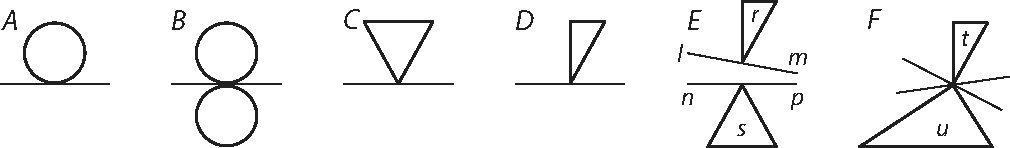
\includegraphics[width=0.96\textwidth]{gesamttex/edit_VIII-4/images/LH_35_11_14_035_d_035v.pdf}}
\vspace{0.00em}
\centerline{\lbrack\textit{Fig.\:1}\rbrack}
\newpage%
\vspace*{1.0em}%
\pstart%
\noindent%
\centering%
*    *    *
\pend%
\vspace{2.0em}%
\begin{ledgroup}
\footnotesize
\pstart
\noindent%
\textls{Ausführliche Datierungsgründe:}%
\pagelabel{58950_dat}
Die undatierte Aufzeichnung N.\;\ref{58950} ist auf einem Textträger überliefert, der weder Spuren eines Wasserzeichens aufweist noch äußere datierungsrelevante Anhaltspunkte bietet.
Inhaltliche Überlegungen ermöglichen jedoch wenigstens eine grobe chronologische Einordnung des Textes:
\pend%
\pstart%

Die Aufzeichnung wirft zwei verschiedene Fragen auf, welche eine bemerkenswerte Verwandschaft mit der Thematik des exzentrischen Stoßes aufweisen:
Die erste ist, ob die Bewegung des Schwerpunkts (\textit{progressus}) zusammenstoßender Kugeln sich ändert, wenn diese sich um ihren jeweiligen Mittelpunkt drehen;
bei der zweiten Frage handelt es sich ansatzweise um die kinematischen Folgen des schiefen Stoßes.
Bereits der Anfangssatz \textit{Supersunt adhuc quaedam explicanda ...} legt nahe, dass N.\;\ref{58950} die Fortsetzung eines mit der Stoßlehre befassten Textes ist.
Zwar lässt sich nach heutigem Wissensstand nicht eindeutig ermitteln, woran die Aufzeichnung N.\;\ref{58950} unmittelbar anknüpft.
Aber die den ersten Textteil abschließende Feststellung \textendash\ bei exzentrisch zusammenstoßenden Körpern wirkten sich ihre Drehungen zweifelsohne auf die Bewegung des Schwerpunkts aus, weil %
die Drehungen ohnehin aus der Bewegung des Schwerpunkts entstanden seien und diese "reproduzieren" könnten (\refpassage{LH_35_11_14_035_035v_gyros-1}{LH_35_11_14_035_035v_gyros-2}) \textendash\ bezeugt wohl Leibnizens ausgeprägtes Verständnis des exzentischen Stoßes.
\pend%
\pstart%
Mit der Kinematik exzentrisch zusammenstoßender Körper, sowie zum Teil mit der des schiefen Stoßes, waren bereits Texte aus den 1680er Jahren befasst (siehe etwa \textit{LSB} VIII,\;3 N.\;63 und N.\;64).\cite{01399}\cite{01400}
Die Lehre vom exzentrischen Stoß entwickelte sich aber vorwiegend in den frühen 1690er Jahren im Anschluss an die Stoßlehre der \textit{Dynamica},\cite{01354} wie zahlreiche Texte im vorliegenden Band zeigen (u.\,a. die Aufzeichnung \textit{De impulsu eccentrico} N.\;\ref{60300} sowie die \textit{Schedae de impulsu eccentrico} N.\;\ref{sdie_intro} und der Textkomplex  \textit{Casus eccentrici concursus simplicissimus} N.\;\ref{cecs_intro}).
Demnach ist anzunehmen, dass auch die Aufzeichnung N.\;\ref{58950} etwa zur gleichen Zeit wie diese Texte enstand, wahrscheinlich nach den von Leibniz eigenhändig auf den 31.\;Oktober\,/\,10.\;November 1690 datierten \textit{Schedae de impulsu eccentrico} N.\;\ref{58940} und N.\;\ref{58939}, in denen die Kinematik des exzentrischen Stoßes besonders umfassend und systematisch behandelt wird.
Eine frühere Entstehung ist möglich;
es ist aber unwahrscheinlich, dass die Aufzeichnung N.\;\ref{58950} vor der Aufzeichnung N.\;\ref{60300} abgefasst wurde, da die Kinematik des exzentrischen Stoßes vor Leibnizens Rückkehr aus Italien\indexO{Italien} noch erheblichen Schwankungen unterlag (siehe die ausführlichen Datierungsgründe zu N.\;\ref{60300}, S.\pageref{LH_37_05_044_datierung}).
\pend%
\pstart%
Ein eindeutiger Terminus ante quem der Datierung lässt sich für die Notiz N.\;\ref{58950} zum Redaktionsschluss nicht angeben.
\pend 
\end{ledgroup}
\selectlanguage{latin}%
\frenchspacing%
\normalsize%







\chapter[tocentry={Theorema de incursu duorum corporum in unum, speciatim recto
\enskip \bracks{Januar 1691 \textendash\ 7.~Februar 1696}},
head={Theorema de incursu duorum corporum in unum, speciatim recto}]%
{\MakeUppercase{Theorema de incursu duorum corporum in unum, speciatim recto}
\newline \bracks{Januar 1691 \textendash\ 7.~Februar 1696}}
\label{58300}
\begin{ledgroupsized}[r]{120mm}
\footnotesize
\pstart
\noindent\textbf{Überlieferung:}
\pend
\end{ledgroupsized}
\begin{ledgroupsized}[r]{114mm}
\footnotesize
\pstart \parindent -6mm
\makebox[6mm][l]{\textit{L}}%
Konzept:
LH~XXXV~13, 3~Bl.~242. 
Ein Blatt~2\textsuperscript{o};
Wasserzeichen		%
in der Blattmitte;
linker Rand beschnitten.
Eineinviertel Seiten.
\pend 
\end{ledgroupsized}
\vspace{5mm}
\begin{ledgroup}
\footnotesize
\pstart
\noindent%
\textbf{Datierungsgründe:}
Die Datierung des vorliegenden Konzeptes stützt sich auf eine Anspielung auf den \textit{vis viva}-Streit mit 
\indexN{\textls{Papin} (Papinus), Denis 1647\textendash1713}Denis Papin.
Leibniz beweist in N.\;\ref{58300} die Erhaltung der verschiedenen Formen der \textit{vis} im Fall eines schiefen Stoßes zweier gleicher Körper auf einen dritten ruhenden. 
Da die stoßenden Körper dabei zum Stillstand kämen, werde die gesamte Kraft an den dritten übertragen.
Leibniz merkt an, dass dieser Beweis auch gegen \indexN{\textls{Papin} (Papinus), Denis 1647\textendash1713}Papin einzusetzen sei, weil daraus die 
von diesem geleugnete
Übertragbarkeit der gesamten \textit{vis motrix} eines Körpers an einen ruhenden Körper geringerer Masse folge (\refpassage{35_13_03_242_7a}{35_13_03_242_7b}).
Leibniz hatte in seiner ersten Streitschrift gegen \indexN{\textls{Papin} (Papinus), Denis 1647\textendash1713}Papin
(\cite{02040}\textit{De causa gravitatis}, \cite{01023}\textit{AE} Mai 1690, S.\;228\textendash239)
die uneingeschränkte Übertragbarkeit der \textit{vis motrix} beim elastischen Stoß vorausgesetzt.
Im Aufsatz 
\cite{00537}\textit{Mechanicorum de viribus motricibus sententia} (\cite{01023}\textit{AE} Januar 1691, S.\;6\textendash13, bes.\ S.\;9\textendash11)
bestritt \indexN{\textls{Papin} (Papinus), Denis 1647\textendash1713}Papin 
mit Verweis auf die
\indexN{\textls{Huygens} (Hugenius, Ugenius, Hugens, Huguens), Christiaan 1629\textendash1695}Huygens'schen Regeln des geraden Stoßes
diese Möglichkeit,
besonders im genannten Fall des Stoßes eines größeren Körpers auf einen kleineren ruhenden.
\indexN{\textls{Papin} (Papinus), Denis 1647\textendash1713}Papins Aufsatz, dem die Anspielung auf \refpassage{35_13_03_242_7a}{35_13_03_242_7b} gilt, bildet daher einen Terminus post quem für die Entstehung von N.\;\ref{58300}.
Einen Terminus ante quem bietet wiederum Leibnizens
\cite{02146}Brief an \indexN{\textls{Bernoulli}, Johann 1667\textendash1748}Johann Bernoulli vom 28.~Januar (7.~Februar) 1696,
in dem er 
(wie auch in N.\;\ref{58300})
erwägt, sein neues Gedankenexperiment künftig gegen \indexN{\textls{Papin} (Papinus), Denis 1647\textendash1713}Papin einzusetzen
(\textit{LSB} III,~6 N.\;202, hier S.\;648.12\textendash16).
Erst in einem \cite{02073}Schreiben vom 16. (26.) Januar 1698 teilt Leibniz sein Argument \indexN{\textls{Papin} (Papinus), Denis 1647\textendash1713}Papin selbst mit 
(\textit{LSB} III, 7, N.\;177, hier S.\;724).
\pend
\pstart
Das für den Zeitraum Oktober 1690 bis 
1696 mehrfach belegte Wasserzeichen bestätigt die angegebene Datierung. %
\pend
\end{ledgroup}
\selectlanguage{latin}
\vspace{8mm}
\pstart%
\normalsize%
\noindent%
\href{\Scan{LH_35_13_03_242r}}{\lbrack242~r\textsuperscript{o}\rbrack}
\pend
\nobreak\begin{edfigure}[0pt][1em]    	%
\includegraphics[scale=1]{%
gesamttex/edit_VIII-4/images/LH_35_13_03_242_d1_242r.pdf}
\edcaption[0pt]{\edtext{\lbrack\textit{Fig.~1}\rbrack}{%
\lemma{\lbrack\textit{Fig.~1}\rbrack}%
\Cfootnote[nonum]{Ein gestrichener Entwurf zum Diagramm wird nicht wiedergegeben.}}}
\end{edfigure}
\clearpage
\pstart
\noindent
Sint globi aequales\indexS{globi aequales} \textit{A}, \textit{B}, \textit{C}, \textit{D}, incurratque globus \textit{A} %
\edtext{(solus motus)}{\lemma{}\Bfootnote{(solus motus) \textit{erg.~L}}}
in globum \textit{B}, tangentem globos \textit{C} et \textit{D}. Videndum an %
\edtext{post ictum\indexS{ictus}}{\lemma{}\Bfootnote{post ictum \textit{erg.~L}}}
quiescant globi \textit{A} et \textit{B}, solumque moveantur \textit{C} et \textit{D}. %
\edtext{Hoc posito}{\lemma{}\Bfootnote{Hoc posito \textit{erg.~L}}} 
\edtext{celeritas ipsius \textit{A} sit 1 et celeritas ipsorum \textit{C} et \textit{D} erit %
\edlabel{35_13_03_242_1a}%
\edtext{}{{%
\xxref{35_13_03_242_1a}{35_13_03_242_1b}}%
\lemma{$1:\sqrt{2}$.}%
\Bfootnote{%
\textit{(1)}~Celeritas %
\textit{(2)}~Erit \textit{L} %
\textit{(3)}~Celeritas centri gr. %
\textit{(4)}~\bars{Nam 1 \textit{streicht Hrsg.}} %
\textit{(5)}~Ponamus~\textit{L}}}%
$1:\sqrt{2}$.}%
{\lemma{}\Afootnote{\textit{Oberhalb des Textes}: $\displaystyle\frac{2}{xx}=1$. \;$x=\lbrack\sqrt2\rbrack$\textsuperscript{\lbrack a\rbrack}. Ergo $1\cdot 1A=\displaystyle\frac{1}{\sqrt2}\cdot \displaystyle\frac{1}{\sqrt2}B+\displaystyle\frac{1}{\sqrt2}\cdot \displaystyle\frac{1}{\sqrt2}\cdot C$\lbrack,\rbrack\ si $A=B=C$
\\[1.5ex] %
{\footnotesize \textsuperscript{\lbrack a\rbrack} $1:\sqrt2$ \textit{L ändert Hrsg.}}
}}%
\pend
\begin{edfigure}[.8em][.5em]    	 %
\includegraphics[scale=1]{%
gesamttex/edit_VIII-4/images/LH_35_13_03_242_d2_242r.pdf} 
\edcaption[0.25em]{\lbrack\textit{Fig.~2, gestr.}\rbrack}
\end{edfigure}
\pstart
Ponamus\edlabel{35_13_03_242_1b}
\textit{\ind{1}B\ind{1}C\ind{1}D} esse triangulum rectangulum %
\edtext{isosceles. Et celeritas ipsius \textit{M} centri gravitatis\indexS{celeritas centri gravitatis}\indexS{centrum gravitatis}}{\lemma{isosceles}\Bfootnote{%
\textit{(1)}~, erunt %
\textit{(2)}~. Et %
\textit{(a)}~centrum gravitatis %
\textit{(b)}~\bars{\textit{M} \textit{streicht Hrsg.}} centrum gravitatis %
\textit{(c)}~celeritas ipsius \textit{M} centri gravitatis~\textit{L}}} 
ipsorum \textit{C} et \textit{D} post ictum
\edtext{erit %
\rule[-1.8ex]{0pt}{5.4ex}%
$\displaystyle\frac{1}{2}$. Porro}{\lemma{erit $\displaystyle\frac{1}{2}$.}\Bfootnote{%
\textit{(1)}~Jam %
\textit{(2)}~Si duo sint %
\textit{(a)}~\textit{L} et \textit{M}, %
\textit{(b)}~puncta \textit{L} et \textit{M}, sitque \textit{M} ut 3, et \textit{L} ut 1 aequalia et quiescente \textit{L} moveatur \textit{M}, %
\textit{(aa)}~centrum %
\textit{(bb)}~centri gravitatis progressus est ut %
\textit{(aaa)}~1 %
\textit{(bbb)}~\rule[-2.1ex]{0pt}{5.4ex}%
$\displaystyle\frac{1}{2}$
\textit{(3)}~Generaliter duo movean %
\textit{(4)}~Porro~\textit{L}}}
generaliter si duo moveantur in eadem recta \textit{L} et \textit{M}, sitque ipsius \textit{L} velocitas \textit{c} et ipsius \textit{M} velocitas %
\edtext{\lbrack\textit{e}\rbrack,}{\lemma{}\Bfootnote{\textit{E} \textit{L ändert Hrsg.}}}
erit centri gr.\ velocitas\indexS{velocitas centri gravitatis} $Lc+eM\lrcorner:\llcorner l+m$\,, hinc si unum \textit{L} quiescat, erit centri
\edtext{gravita\lbrack ti\rbrack s}{%
\lemma{}%
\Bfootnote{%
gravitas %
\textit{L ändert Hrsg.}}}
velocitas\indexS{velocitas centri gravitatis} $eM:\llcorner l+m$. Ergo si \textit{M} sit centrum gravitatis\indexS{centrum gravitatis} ipsorum \textit{C} %
\edtext{et \textit{D}; at}{\lemma{et \textit{D};}\Bfootnote{%
\textit{(1)}~\bars{et \textit{streicht Hrsg.}} \textit{M} ipsorum %
\textit{(2)}~at~\textit{L}}} 
\textit{A} %
\textit{L} sit centrum grav.\ ipsorum
\edtext{et \textit{B}, utique}{\lemma{et \textit{B},}\Bfootnote{%
\textit{(1)}~et, %
\textit{(2)}~utique~\textit{L}}} 
\textit{M} erit ut 2, et \textit{L} etiam, %
\edtext{ob duos}{\lemma{}\Bfootnote{ob \bars{ob \textit{streicht Hrsg.}} duos~\textit{L}}} 
utrobique globos, et \textit{e},
\edtext{velocitas ipsius}{\lemma{velocitas}\Bfootnote{%
\textit{(1)}~centri grav. %
\textit{(2)}~ipsius~\textit{L}}}
\textit{M} est 
\rule[-1.8ex]{0pt}{5.4ex}%
$\displaystyle\frac{1}{2}$.
Ergo centri gravitatis communis\indexS{centrum gravitatis commune} 4 globorum velocitas\indexS{velocitas centri gravitatis} post
\edtext{ictum $eM:\llcorner l+m$}{%
\lemma{ictum}%
\Bfootnote{%
\textit{(1)}~erit %
\textit{(2)}~$eM:\llcorner l+m$~\textit{L}}}
erit%
\linebreak
\edlabel{35_13_03_242_2a}%
\edtext{}%
{{\xxref{35_13_03_242_2a}{35_13_03_242_2b}}%
\lemma{%
$\displaystyle\frac{1}{2} \cdot 2:\llcorner2+2=\displaystyle\frac{1}{4}$.}%
\Bfootnote{\rule[-1.8ex]{0pt}{5.4ex}%
\textit{(1)}~Sed ante ictum %
\textit{(2)}~At quaeramus ejusdem %
\textit{(3)}~Quaeramus~\textit{L}}}%
\rule[-1.4ex]{0pt}{5.ex}%
$\displaystyle\frac{1}{2} \cdot 2:\llcorner2+2=\displaystyle\frac{1}{4}$.
\pend
\clearpage
\pstart %
Quaeramus%
\edlabel{35_13_03_242_2b}
jam et quae fuerit ante 
\edtext{ictum.\indexS{ictus} \textit{A}}{%
\lemma{ictum.}%
\Bfootnote{%
\textit{(1)}~Tunc centrum %
\textit{(a)}~velocitatis %
\textit{(b)}~gravitatis %
\textit{(aa)}~ipsi %
\textit{(bb)}~ipsius \textit{A} erit \textit{A} seu 1 %
\textit{(aaa)}~, ipsorum trium
\textit{(bbb)}~at trium quod exprimatur per \textit{N}
\textit{(2)}~\textit{A}~\textit{L}}}
sit centrum gravitatis\indexS{centrum gravitatis} 
\edtext{ipsius \textit{A}, quod}{%
\lemma{ipsius \textit{A},}%
\Bfootnote{%
\textit{(1)}~et \textit{N} sit centrum gr.\ trium %
\textit{(2)}~quod~\textit{L}}}
movetur, et \textit{N} sit centrum gravitatis trium\indexS{centrum gravitatis trium} \textit{B}, \textit{C},
\edtext{\textit{D}, quod quiescit. Ergo}{%
\lemma{\textit{D},}%
\Bfootnote{%
\textit{(1)}~qu %
\textit{(2)}~jam %
\textit{(3)}~, quod quiescit. Ergo~\textit{L}}}
velocitas ipsius \textit{N} est 0, et ipsius \textit{A} est 1, fiet velocitas centri gravitatis\indexS{velocitas centri gravitatis} omnium communis ante ictum $1A+0N\lrcorner:\llcorner A+N$. Est autem \textit{A} ut 1, et \textit{N} ut 3, et fiet \rule[-2ex]{0pt}{5.4ex}%
$\displaystyle\frac{1}{4}$ ut ante. Haec ergo %
\edtext{recte. Servatur}{\lemma{recte.}\Bfootnote{%
\textit{(1)}~Et vis serv %
\textit{(2)}~Servatur~\textit{L}}} 
enim eadem vis communis\indexS{vis communis}
\edtext{quae ante concursum.\indexS{concursus} Vis totalis\indexS{vis totalis} $1\cdot 1\cdot A=1$. 
Vis communis\indexS{vis communis} 
\rule[-2.4ex]{0pt}{6ex}%
$\displaystyle\frac{A+B+C+D}{16}=\displaystyle\frac{1}{4}$. 
Propria\indexS{vis propria} \rule[-1.8ex]{0pt}{5.4ex}$\displaystyle\frac{3}{4}$. Videamus}{%
\lemma{}%
\Bfootnote{communis
\bars{%
\textit{(1)}~quae ante concursum 
\textit{(2)}~quae ante concursum 
\textit{(a)}~\rule[-1.8ex]{0pt}{5.4ex}%
$\displaystyle\frac{A+B+C+D}{16}$ $=\displaystyle\frac{1}{4}$ 
\textit{(b)}~. Vis totalis $1\cdot 1\cdot A=1$. Vis communis 
\rule[-1.8ex]{0pt}{5.4ex}%
$\displaystyle\frac{A+B+C+D}{16}=\displaystyle\frac{1}{4}$. Propria $\displaystyle\frac{3}{4}$ 
\textit{erg.}} 
.~Videamus~\textit{L}}} 
nunc an etiam eadem vis propria\indexS{vis propria} servetur.
\pend
\pstart 
Vis propria\indexS{vis propria} ante %
\edtext{concursum sic}{\lemma{concursum}\Bfootnote{%
\textit{(1)}~erat %
\textit{(a)}~$\displaystyle\frac{1}{6}\cdot$ 
\textit{(b)}~$\displaystyle\frac{1}{9}A +$ %
\textit{(2)}~sic~\textit{L}}} 
habebitur, %
\edtext{si respectiva celeritas\indexS{celeritas respectiva} secta}{\lemma{si}\Bfootnote{%
\textit{(1)}~appropinquandi %
\textit{(2)}~respectiva celeritas %
\textit{(a)}~nempe 1, %
\textit{(aa)}~dividatur in duas partes %
\textit{(bb)}~secetur in ratione reci %
\textit{(b)}~secta~\textit{L}}} %
in ratione \textit{A} ad 
\edtext{\textit{N}, inter}{\lemma{\textit{N},}\Bfootnote{%
\textit{(1)}~reciproce %
\textit{(2)}~inter~\textit{L}}} 
ipsa reciproce 
\edtext{distribuatur. Erat}{%
\lemma{distribuatur.}%
\Bfootnote{%
\textit{(1)}~Et %
\textit{(2)}~Erat~\textit{L}}}
autem celeritas appropinquandi\indexS{celeritas appropinquandi} 1. Secanda in 
\rule[-1.8ex]{0pt}{6ex}%
$\displaystyle\frac{1}{4}$ et $\displaystyle\frac{3}{4}$ 
et ipsi \textit{A} ascribetur celeritas 
$\displaystyle\frac{3}{4}$, 
ipsi \textit{N} celeritas 
\rule[-1.8ex]{0pt}{6ex}%
$\displaystyle\frac{1}{4}$. 
Et vis respectiva %
\edtext{ante concursum}{\lemma{}\Bfootnote{ante concursum \textit{erg.~L}}} 
erit $9A+1N\lrcorner:16=12:16=\displaystyle\frac{3}{4}$.%
\rule[-1.8ex]{0pt}{5.4ex}
Videamus jam quae sit post concursum.\indexS{concursus} Est %
\edtext{autem bipertita, scilicet vis respectiva\indexS{vis respectiva}}{\lemma{autem}\Bfootnote{%
\textit{(1)}~duplex, vis respectiva %
\textit{(2)}~bipertita, scilicet vis respectiva~\textit{L}}} 
inter \textit{L} et \textit{M}, et vis respectiva\indexS{vis respectiva} inter \textit{C} et \textit{D}. Et quidem celeritas respectiva\indexS{celeritas respectiva} inter \textit{L} et \textit{M}, est celeritas 
\edtext{ipsius \textit{M},}{%
\lemma{ipsius}%
\Bfootnote{%
\textit{(1)}~\textit{N}, nempe %
\textit{(2)}~\textit{M},~\textit{L}}}
nempe \rule[-1.8ex]{0pt}{5.4ex}%
$\displaystyle\frac{1}{2}$. Jam \textit{L} et \textit{M} sunt 
\edtext{aequalia pondere,}{%
\lemma{aequalia}%
\Bfootnote{%
\textit{(1)}~pondera, %
\textit{(2)}~pondere,~\textit{L}}}
quia ambo centra grav.\ 2 globorum. Ergo celeritas respectiva distributa\indexS{celeritas respectiva distributa} est 
\rule[-1.8ex]{0pt}{5.4ex}%
$\displaystyle\frac{1}{4}$. 
Et vis respectiva\indexS{vis respectiva} inter \textit{L} et \textit{M} erit 
\rule[-1.8ex]{0pt}{5.4ex}%
$\displaystyle\frac{2}{16}+\displaystyle\frac{2}{16}=\displaystyle\frac{1}{4}$. 
Restat vis respectiva\indexS{vis respectiva} inter %
\edtext{\textit{C} et \textit{D}. Celeritas}{\lemma{\textit{C} et \textit{D}}\Bfootnote{%
\textit{(1)}~. Est %
\textit{(2)}~quae est %
\textit{(3)}~. Et celeritas cujusque respectiva est 1. Ergo vis %
\textit{(a)}~eorum respectiva est %
\textit{(b)}~cujusque est \rule[-1.8ex]{0pt}{5.4ex}%
$\displaystyle\frac{1}{4}$ %
\textit{(c)}~eorum distributa est $\displaystyle\frac{1}{2}$ %
\textit{(4)}~. Celeritas~\textit{L}}} 
eorum respectiva est 1, 
\edtext{celeritas respectiva\indexS{celeritas respectiva}}{%
\lemma{celeritas}%
\Bfootnote{%
\textit{(1)}~cujusque %
\textit{(2)}~respectiva~\textit{L}}}
distributa in unoquoque $\displaystyle\frac{1}{2}$. Vis eorum respectiva\indexS{vis respectiva} est 
\rule[-2.4ex]{0pt}{6ex}%
$\displaystyle\frac{1}{4}C+\displaystyle\frac{1}{4}D=\displaystyle\frac{1}{2}$ 
quae addita priori vi respectivae\indexS{vis respectiva} $\displaystyle\frac{1}{4}$ facit 
\rule[-2.6ex]{0pt}{6ex}%
$\displaystyle\frac{3}{4}$
vim respectivam\indexS{vis respectiva} collectam, ut ante. Res ergo succedit. \pend 
\pstart Hinc sequitur posse motum totum corporis majoris transferri in minus.\indexS{translatio omnis motus} Ponamus %
\edtext{enim \textit{A} et \textit{B} globos}{\lemma{enim}\Bfootnote{%
\textit{(1)}~\textit{B} et %
\textit{(2)}~\textit{A} et \textit{B} %
\textit{(a)}~seca %
\textit{(b)}~esse %
\textit{(c)}~in \textit{\ind{3}} %
\textit{(d)}~globos~\textit{L}}} 
quiescere in locis \textit{\ind{3}A\ind{3}B}, et ex locis \textit{\ind{3}C},%
\edtext{\textit{\ind{3}D} venientes globos}{\lemma{\textit{\ind{3}D}}%
\Bfootnote{%
\textit{(1)}~venientia %
\textit{(2)}~venientes globos~\textit{L}}} 
\textit{D} et \textit{C} incurrere ipsis in \textit{\ind{2}C,\ind{2}D}, esse autem omnes aequales inter %
\edtext{se, globi \textit{C} et \textit{D},}{\lemma{se,}\Bfootnote{%
\textit{(1)}~quiescent tres globi \textit{B}, et \textit{C} et \textit{D} %
\textit{(2)}~globi \textit{C} et \textit{D},~\textit{L}}}
redigentur ad quietem\lbrack,\rbrack\ globus \textit{B} manebit in quiete, et globus \textit{A} recipiet omnem motum. Nam necesse %
est redire statum priorem. Nam eaedem %
\edtext{aequalita\lbrack te\rbrack s}{\lemma{}\Bfootnote{aequalitas \textit{L ändert Hrsg.}}} 
quae definiunt posterius ex priore, definiunt et contra, quia %
\edtext{aequationes hic semper sunt}{\lemma{aequationes}\Bfootnote{%
\textit{(1)}~sunt %
\textit{(2)}~hic semper sunt~\textit{L}}} 
rationales,\indexS{aequatio rationalis} seu non ambiguae,\indexS{aequatio ambigua} neque adeo dantur plures casus.
\pend 
\pstart Generaliter dicendum\lbrack:\rbrack\ si globi aequales\indexS{globi aequales}, quotcunque globos \textit{D} et \textit{C}, tangat globus \textit{B}, dum percutiatur ab \textit{A}, solo %
\edtext{moto, non progredi \textit{A}, quia non progreditur si solum \textit{B} percutiat,}{\lemma{moto,}\Bfootnote{%
\textit{(1)}~quiescere %
\textit{(2)}~quiescere %
\textit{(a)}~\textit{B}, quia %
\textit{(b)}~\textit{A}, %
\textit{(3)}~non progredi \textit{A}, %
\textit{(a)}~quia quiescit si solum \textit{B} percutiat, %
\textit{(b)}~quia non progreditur si solum %
\textit{(aa)}~\textit{A} 
\textit{(bb)}~\textit{B} percutiat,~\textit{L}}} 
ergo multo minus si \textit{B} cum %
\edlabel{35_13_03_242_4a}%
\edtext{}{%
{\xxref%
{35_13_03_242_4a}{35_13_03_242_4b}}%
\lemma{aliis.}%
\Bfootnote{%
\textit{(1)}~Porro \textit{B} 
\textit{(a)}~interpositus %
\textit{(b)}~globus inter %
\textit{(aa)}~tres %
\textit{(bb)}~plures positus aequales, comprimitur ab omnibus. Fingamus %
\textit{(aaa)}~esse %
\textit{(bbb)}~meras pilas inflatas moveri reciproce %
\textit{(2)}~Porro~\textit{L}}}%
aliis.
\pend
\begin{edfigure}%
\includegraphics[scale=1]{%
gesamttex/edit_VIII-4/images/LH_35_13_03_242_d3_242r.pdf} 
\edcaption{\edtext{\lbrack\textit{Fig.~3}\rbrack}{%
\lemma{\lbrack\textit{Fig.~3}\rbrack}%
\Cfootnote[nonum]{Ein gestrichener Entwurf zum Diagramm wird nicht wiedergegeben.}}}
\end{edfigure}
\pstart
Porro%
\edlabel{35_13_03_242_4b}
\textit{B}, sive solus %
\edtext{concurrat cum}{\lemma{concurrat}\Bfootnote{%
\textit{(1)}~, sive %
\textit{(2)}~cum~\textit{L}}}
globo \textit{A}, sive 
ab aliis prematur, vel %
\edtext{retineatur, videndum}{\lemma{retineatur,}\Bfootnote{%
\textit{(1)}~idem debet esse ictus %
\textit{(2)}~videndum~\textit{L}}}
in \textit{A}  
an eadem sit actio;\indexS{actio} id videtur dicendum cum \textit{A} idem %
\edtext{patiatur. Nempe concurrentes globi}{\lemma{patiatur.}\Bfootnote{%
\textit{(1)}~Itaque accuratius %
\textit{(2)}~Nota, quoad ictum %
\textit{(3)}~\bars{Considerandum \textit{streicht Hrsg.}} %
\textit{(4)}~Nempe %
\textit{(a)}~concurrens cum \textit{A}, e %
\textit{(b)}~concurrentes globi~\textit{L}}}
\textit{A} et \textit{B}, 
eodem modo percutiuntur aguntque et reagunt, sive adsint \textit{C}, \textit{D}, \textit{E}, sive non; itaque \textit{A} quiescit\lbrack,\rbrack\ \textit{B} recipit celeritatem ipsius \textit{A}, sed hac celeritate \textit{B} incurrens in \textit{C}, \textit{D}, \textit{E} aequales deberet quiescere, si haec regula succederet, %
\edtext{quod puto non esse verum.}{\lemma{}\Afootnote{\textit{Am Rand}: NB.}} 
Quaeritur generaliter, an res eodem modo fiant, sive ponas \textit{B} tangere ipsos \textit{C}, \textit{D}, \textit{E}, sive intervallum\indexS{intervallum quantumvis exiguum} %
\edtext{relinqui quantumvis}{\lemma{relinqui}\Bfootnote{%
\textit{(1)}~exiguum. Haec %
\textit{(2)}~quantumvis~\textit{L}}} 
exiguum. Haec regula si esset vera, haberetur quaesitum pro demonstrato. Et certe videtur admittenda: quia et circa %
\edtext{potentiarum\indexS{potentia} aequationes}{\lemma{potentiarum}\Bfootnote{%
\textit{(1)}~tam absolutarum quam re %
\textit{(2)}~aequationes~\textit{L}}} 
eadem utcunque exiguo discrimine\indexS{discrimen utcunque exiguum} provenire debent; scilicet quoad %
\edtext{vi\lbrack res\rbrack}{\lemma{}\Bfootnote{vis \textit{L ändert Hrsg.}}} 
respectivas,\indexS{vis respectiva} et progressivas,\indexS{vis progressiva} quomodocunque sumtas. 
\pend
\begin{edfigure}%
\includegraphics[scale=1]{%
gesamttex/edit_VIII-4/images/LH_35_13_03_242_d4_242r.pdf} 
\edcaption[0.25em]{\lbrack\textit{Fig.~4}\rbrack}
\end{edfigure}
\pstart
Experiamur\lbrack:\rbrack\ %
incurrat \textit{B} in \textit{C} et \textit{D}, et ponamus  
\textit{C} et \textit{D} moveri, ut ante. 
Ante ictum celeritas 1. 
Vis\indexS{vis} 1. 
Celeritas respectiva\indexS{celeritas respectiva} 1. 
Distributa\indexS{celeritas respectiva distributa} pro \textit{B}, 
\rule[-1.8ex]{0pt}{5.4ex}%
$\displaystyle\frac{2}{3}$; pro \textit{M}, 
\rule[-1.8ex]{0pt}{5.4ex}%
$\displaystyle\frac{1}{3}$. 
Ergo vis respectiva\indexS{vis respectiva} $4B+1M\lrcorner:9=%
\edtext{6:9=\displaystyle\frac{2}{3}$. Celeritas}{\lemma{$6:9=\displaystyle\frac{2}{3}$.}\Bfootnote{%
\textit{(1)}~Vis communis %
\textit{(2)}~Celeritas~\textit{L}}} 
centri gr.\indexS{celeritas centri gravitatis}\ est $1B+0M\lrcorner:\llcorner B+M=\displaystyle\frac{1}{3}$.%
\rule[-1.8ex]{0pt}{5.4ex} 
Ergo vis communis\indexS{vis communis} est 
\rule[-1.8ex]{0pt}{5.4ex}%
$\displaystyle\frac{3}{9}=\displaystyle\frac{1}{3}$, ut oportuit. 
Haec ante ictum,\indexS{ictus} post ictum quaeramus vim %
\edtext{communem.\indexS{vis communis} Celeritas centri gr.\indexS{celeritas centri gravitatis} $=}{\lemma{communem.}\Bfootnote{%
\textit{(1)}~Ea est %
\textit{(2)}~Celeritas centri gr.\ =~\textit{L}}} %
0B+\displaystyle\frac{1}{2}M\lrcorner:\llcorner B+M=\displaystyle\frac{1}{3}$ %
\edtext{ut ante.}{\lemma{}\Bfootnote{ut ante \textit{erg.~L}}} 
Ergo vis communis\indexS{vis communis} post 
\edtext{ictum est \rule[-1.8ex]{0pt}{5.4ex}%
$\displaystyle\frac{3}{9}=\displaystyle\frac{1}{3}$. Vis}{\lemma{ictum est}\Bfootnote{%
\textit{(1)}~$\displaystyle\frac{3}{36}=\displaystyle\frac{1}{\langle12\rangle}$. 
\bars{Sed post minor quam ante. \textit{erg.}} 
\textit{(2)}~$\displaystyle\frac{3}{9}=\displaystyle\frac{1}{3}$. Vis~\textit{L}}} 
respectiva\indexS{vis respectiva} inter \textit{C} et \textit{D} est 
\rule[-1.8ex]{0pt}{5.4ex}%
$\displaystyle\frac{1}{2}$ ut ante. 
Sed inter \textit{B} et \textit{M} celeritas respectiva\indexS{celeritas respectiva} 
est $\displaystyle\frac{1}{2}$, quae distributa,\indexS{celeritas respectiva distributa} pro \textit{B}, est 
\rule[-2.4ex]{0pt}{6ex}%
$\displaystyle\frac{2}{3}\;\displaystyle\frac{1}{2}=\displaystyle\frac{1}{3}$; pro \textit{M} est 
\rule[-2.4ex]{0pt}{6ex}%
$\displaystyle\frac{1}{3}\;\displaystyle\frac{1}{2}=\displaystyle\frac{1}{6}$. 
Fit vis respectiva\indexS{vis respectiva} 
\rule[-2.4ex]{0pt}{6ex}%
$\displaystyle\frac{4B+M}{36}=\displaystyle\frac{1}{6}$ cui adde $\displaystyle\frac{1}{2}$ fit 
\rule[-2.4ex]{0pt}{6ex}%
$\displaystyle\frac{1}{2}+\displaystyle\frac{1}{6}=\left.\displaystyle\frac{4}{6}\,\middle|\,\displaystyle\frac{2}{3}\right.$. Quae est tota vis respectiva %
\edtext{collecta.\indexS{vis respectiva collecta} Huic addita vis communis\indexS{vis communis}
$\displaystyle\frac{1}{3}$\rule[-1.8ex]{0pt}{5.4ex} reddit totam vim 1. Itaque procedit regula. Et habemus}{\lemma{collecta.}%
\Bfootnote{%
\textit{(1)}~Sed huic addita vis communis $\displaystyle\frac{1}{12}$ non producit totam vim 1. Itaque non procedit regula. Inquirendum esset in causas. Et video tantum interesse, quod hoc modo %
\textit{(2)}~Huic \lbrack...\rbrack\ habemus~\textit{L}}}
demonstrationem generalem %
\edtext{quaesiti. Et}{\lemma{quaesiti.}\Bfootnote{%
\textit{(1)}~Et regulam %
\textit{(2)}~Et~\textit{L}}} 
artificium prodit usus pulcherrimi ad multa difficilia solvenda. 
\pend
\pstart 
\edlabel{35_13_03_242_7a}%
Possumus hoc pronuntiare %
\edtext{theorema speciale:}{\lemma{theorema}\Bfootnote{%
\textit{(1)}~generale %
\textit{(2)}~speciale:~\textit{L}}}
si in tribus
\edtext{se\lbrack mi\rbrack quadrati}{%
\lemma{}%
\Bfootnote{%
sequiquadrati %
\textit{L ändert Hrsg.}}}
angulis sint centra trium globorum aequalium\indexS{globi tres aequales in tribus angulis semiquadrati} \textit{B}, \textit{C}, \textit{D}, et per latera quadrati %
\edtext{ven\lbrack i\rbrack entes}{\lemma{}\Bfootnote{venentes \textit{L ändert Hrsg.}}}
duo globi aequali celeritate percutiant tertium\indexS{globi duo in unum incurrentes} positum in laterum concursu, quiescent percutientes, et 
\edtext{percu\lbrack s\rbrack sus}{%
\lemma{}%
\Bfootnote{%
percursus %
\textit{L ändert Hrsg.}}}
perget in diagonali, celeritate quae 
\edtext{sit ad}{%
\lemma{sit}%
\Bfootnote{%
\textit{(1)}~ut %
\textit{(2)}~ad~\textit{L}}}
celeritatem incurrentium ut diagonalis ad latus. %
\edtext{Hoc pro Papino,\indexN{\textls{Papin} (Papinus), Denis 1647\textendash1713} %
ad ostendendum, %
\edtext{totam vim\indexS{vis}}{\lemma{totam}\Bfootnote{%
\textit{(1)}~vim globi %
\textit{(2)}~vim~\textit{L}}}
majoris materiae posse transferri\indexS{translatio totius vis majoris materiae in minorem} in 
\edlabel{35_13_03_242_3a}%
\edtext{}{{\xxref{35_13_03_242_3a}{35_13_03_242_3b}}%
\lemma{minorem.}\Bfootnote{%
\textit{(1)}~Unde %
\textit{(2)}~Videtur~\textit{L}}}%
minorem.\edlabel{35_13_03_242_7b}%
}{\lemma{Hoc \lbrack...\rbrack\  minorem}%
\Cfootnote{%
Siehe \indexN{\textls{Papin} (Papinus), Denis 1647\textendash1713}\textsc{D.~Papin},
\cite{00537}\textit{Mechanicorum de viribus motricibus sententia}, \cite{01023}\textit{AE} Januar 1691, S.\;6\textendash13, bes.\ S.\;9\textendash11.
Die von \indexN{\textls{Papin} (Papinus), Denis 1647\textendash1713}Papin im genannten Stoßfall angezweifelte These hatte Leibniz in \cite{02040}\textit{De causa gravitatis}, \cite{01023}\textit{AE} Mai 1690, S.\;228\textendash239 aufgestellt.}}
\pend
\pstart
Videtur%
\edlabel{35_13_03_242_3b}
corrigendus
\edtext{calculus meus prior quo putebam semper pergere incurrens.}{\lemma{calculus \lbrack...\rbrack\  incurrens}%
\Cfootnote{%
Anspielung noch nicht aufgelöst.}}
\pend
\pstart
\noindent
\edlabel{35_13_03_242_6a}%
\href{\Scan{LH_35_13_03_242v}}%
{\lbrack242~v\textsuperscript{o}\rbrack}
\pend
\nobreak
\begin{edfigure}[0pt]%
\includegraphics[scale=1]{%
gesamttex/edit_VIII-4/images/LH_35_13_03_242_d5_242v.pdf}
\edcaption{\lbrack\textit{Fig.~5}\rbrack}
\end{edfigure}
\pstart 
Res bene succedit in casu illo speciali, sed nescio an generaliter pro incursu corporis in duo\indexS{incursus corporis in duo}. Ex principiis nostris, si vera est %
\edtext{Regula Hugeniana\indexS{regula Hugeniana} %
\edtext{ut globus \textit{A} incurrens in \textit{B}, tangentem plures\indexS{globus plures globos tangens}}{\lemma{ut}\Bfootnote{%
\textit{(1)}~corpus \textit{A} incurrens in \textit{B}, tangens plura %
\textit{(2)}~globus \lbrack...\rbrack\ plures~\textit{L}}} %
\textit{C}, \textit{D}, \textit{E} quiescat cum \textit{B},%
}{\lemma{Regula \lbrack...\rbrack\ cum \textit{B}}%
\Cfootnote{%
\indexN{\textls{Huygens} (Hugenius, Ugenius, Hugens, Huguens), Christiaan 1629\textendash1695}\textsc{C.~Huygens}, \cite{00525}\textit{Traité de la lumière}, Leiden 1690, chap.~1, S.\;14 (\textit{HO}\cite{00113} XIX, S.\;473). %
Siehe Leibnizens Auszüge aus dem einschlägigen Abschnitt des \cite{00525}\textit{Traité}:
\cite{02094}\textit{LSB} VIII,~3 N.\;75 von September\textendash Oktober 1690.}}
sequetur idem esse si \textit{B} incurrat in \textit{C}, \textit{D}, \textit{E}, quia perinde est ac si \textit{B} non tangat, sed parum a tangente absit, eo autem casu quiescit \textit{A}, translato motu in \textit{B} %
\edtext{quod incurrat in \textit{C}, \textit{D}, \textit{E},}{\lemma{}\Bfootnote{quod incurrat in \textit{C}, \textit{D}, \textit{E} \textit{erg.~L}}} 
ergo ut prodeant, quae ante, debet \textit{B} incurrens in \textit{C}, \textit{D}, \textit{E}, quietem accipere. Et %
\edtext{hoc de duobus}{\lemma{hoc}\Bfootnote{%
\textit{(1)}~duo %
\textit{(2)}~de duobus~\textit{L}}}
verum reperi, si sint %
\edtext{siti invicem}{\lemma{siti}\Bfootnote{%
\textit{(1)}~in se %
\textit{(2)}~invicem~\textit{L}}} 
in Triangulo rectangulo isoscele. Sed secus inquirendum de tribus certe, %
\edtext{an Hugenianae regulae\indexS{regula Hugeniana} obstat}{\lemma{an}\Bfootnote{%
\textit{(1)}~vera sit %
\textit{(2)}~Hugenianae regulae %
\textit{(a)}~obstant %
\textit{(b)}~obstat~\textit{L}}} 
\edlabel{35_13_03_242_5a}%
\edtext{}{%
{\xxref%
{35_13_03_242_5a}{35_13_03_242_5b}}%
\lemma{ratiocinatio \lbrack...\rbrack\ desinentiarum}%
\Cfootnote{%
Zum Kontinuitätsprinzip (\glqq regula desinentiarum\grqq, auch \glqq regula continuitatis\grqq) vgl.\ 
\textsc{G.\,W.~Leibniz}, 
\cite{02054}\textit{Extrait d'une Lettre de M.~L.\ sur un Principe Général}, in 
\cite{02002}\textit{NRL} Juli 1687, S.\;744\textendash753 
(\cite{02039}\textit{LPG} III, S.\;51\textendash55); sowie 
\cite{02055}\textit{Principium quoddam generale}, 
\textit{LSB} VI, 4, N.\;371.}}%
ratiocinatio firma meae
\edtext{regulae desinentiarum.\indexS{regula desinentiarum}\edlabel{35_13_03_242_5b}}{\lemma{regulae}\Bfootnote{%
\textit{(1)}~de Desinentiis %
\textit{(2)}~seu reg %
\textit{(3)}~desinentiarum.~\textit{L}}}
Nempe,
\edtext{globus}{%
\lemma{}%
\Bfootnote{%
globus %
\textit{erg.~L}}}
\textit{A} incurrat simul in globos \textit{B} et \textit{D}. Et propemodum tangat globum \textit{C}, dico eventus qui fiant esse debere tales, ut si tandem status hic desinat in statum perfecti contactus\indexS{contactus perfectus} etiam ipsius \textit{C}, etiam eventus in hunc desinant. 
Quod verum non est, si vera regula Hugeniana\indexS{regula Hugeniana}, nam si tantillum absit, %
\edtext{quiescet \textit{A}, procedent \textit{B},}{\lemma{quiescet \textit{A},}\Bfootnote{%
\textit{(1)}~prodibunt \textit{B} %
\textit{(2)}~procedent \textit{B},~\textit{L}}} %
\edtext{et \textit{D}, manente}{\lemma{et \textit{D},}\Bfootnote{%
\textit{(1)}~quiescente %
\textit{(2)}~manente~\textit{L}}}
in quiete ipso \textit{C}, ergo non desinitur %
\edtext{in regulae}{\lemma{in}\Bfootnote{%
\textit{(1)}~statum %
\textit{(2)}~regulae~\textit{L}}} 
Hugenianae\indexS{regula Hugeniana} eventum, %
\edtext{quem esse}{\lemma{quem}\Bfootnote{%
\textit{(1)}~vult %
\textit{(2)}~esse~\textit{L}}} 
si \textit{A} tres \textit{B}, \textit{C}, \textit{D} simul tangat sequitur ex ejus regula, ut scil.\ tunc quiescat \textit{A}, procurrant \textit{B}, \textit{C}, \textit{D}.
\pend
\begin{edfigure}%
\includegraphics[scale=1]{%
gesamttex/edit_VIII-4/images/LH_35_13_03_242_d6_242v.pdf} 
\edcaption[0.25em]{\edtext{\lbrack\textit{Fig.~6}\rbrack}{%
\lemma{\lbrack\textit{Fig.~6}\rbrack}%
\Cfootnote[nonum]{Ein gestrichener Entwurf zum Diagramm wird nicht wiedergegeben.}}}
\end{edfigure}
\pstart 
Imo contra regulam Hugenianam\indexS{regula Hugeniana} per %
\edtext{se sumtam (\protect\vphantom)sine}{\lemma{se sumtam}\Bfootnote{%
\textit{(1)}~aliter %
\textit{(2)}~(\protect\vphantom)sine~\textit{L}}}
consequentia\protect\vphantom() sic pugnat 
regula desinentiarum\indexS{regula desinentiarum} seu Regula continuitatis\indexS{regula continuitatis}.
Nam si semper verum manet, ut \textit{A} incurrente in \textit{B} tangentem \textit{C} et \textit{D}, quiescant \textit{A} et \textit{B}, translato motu in \textit{C} et \textit{D}, sequitur et hoc futurum si angulus \textit{CBD} sit  %
\edtext{infinite \lbrack obtusus\rbrack,\indexS{angulus infinite obtusus} quo}{\lemma{infinite}\Bfootnote{\bars{acutus \textit{ändert Hrsg.}} %
\textit{(1)}~quo 
\textit{(2)}~\bars{et \textit{streicht Hrsg.}} %
\textit{C}, \textit{D} tantillum 
\textit{(3)}~quo~\textit{L}}} 
casu falsum est \textit{B} quiescere omni motu in \textit{C} et \textit{D} translato. 
Quod si quis vellet hoc casu quo scil.\ \textit{CBD} sunt in eadem recta tunc \textit{B} %
\edtext{ab \textit{A} impulsum}{\lemma{ab \textit{A}}\Bfootnote{%
\textit{(1)}~in qua %
\textit{(2)}~impulsum~\textit{L}}}
quiescere, %
\edtext{sequetur non}{\lemma{sequetur}\Bfootnote{%
\textit{(1)}~\textit{C} et \textit{D} %
\textit{(2)}~non~\textit{L}}} 
progredi centrum gravitatis totale\indexS{centrum gravitatis totale}, nam ipsis \textit{A} et \textit{B} quiescentibus, et ipsis \textit{C} et \textit{D} motum recipientibus et quidem in recta ipsa \textit{CD}, %
\edtext{patet nihil}{\lemma{patet}\Bfootnote{%
\textit{(1)}~non %
\textit{(2)}~nihil~\textit{L}}}
\edtext{u\lbrack lt\rbrack ra}{\lemma{}\Bfootnote{utlra \textit{L ändert Hrsg.}}} 
hanc rectam prodire, atque adeo centrum gravitatis\indexS{centrum gravitatis} sisti.%
\edlabel{35_13_03_242_6b}%
\pend




\chapter[tocentry={Potentia ictu translata in alia corpora
\enskip\bracks{%
Januar 1691 \textendash\ März 1698\;(?)%
}},
head={Potentia ictu translata in alia corpora}]%
{\MakeUppercase{Potentia ictu translata in alia corpora}
\newline\bracks{%
Januar 1691 \textendash\ März 1698\;(?)%
}}
\label{60359}
\selectlanguage{ngerman}%
\begin{ledgroupsized}[r]{120mm}%
\footnotesize%
\pstart%
\noindent%
\textbf{Überlieferung:}%
\pend%
\end{ledgroupsized}%
\begin{ledgroupsized}[r]{114mm}%
\footnotesize%
\pstart%
\parindent -6mm%
\makebox[6mm][l]{\textit{L}}%
Aufzeichnung:
LH~XXXVII~5 Bl.\;196\textendash197.
Ein Bogen~2\textsuperscript{o},
Ränder ausgefranst mit geringfügigem Textverlust am unteren Rand von Bl.\;196\,r\textsuperscript{o};
Papiererhaltungsmaßnahmen.
Ein \href{\Scan{LH_37_05_196wz}}{Wasserzeichen} auf Bl.\;196 %
mit \href{\Scan{LH_37_05_197wz}}{Gegenmarke} auf Bl.\;197
Drei Seiten auf Bl.\;196\,r\textsuperscript{o}\! bis Bl.\;197\,r\textsuperscript{o}\! und zwei Zeilen auf Bl.\;197\,v\textsuperscript{o}\!
(sonst %
unbeschrieben). %
\pend
\end{ledgroupsized}
\vspace{5mm}%
\begin{ledgroup}%
\footnotesize%
\pstart%
\noindent%
\textbf{Datierungsgründe:}
Die Datierung der Aufzeichnung N.\;\ref{60359} beruht auf äußeren Eigenschaften des Text\-trägers %
sowie auf inhaltlichen Betrachtungen.
Siehe die ausführliche Begründung auf S.\;\pageref{60359_dat}.%
\pend%
\end{ledgroup}%
\selectlanguage{latin}%
\frenchspacing%
\vspace{8mm}
\pstart%
\normalsize%
\noindent%
\lbrack%
\href{\Scan{LH_37_05_196r}}%
{196\,r\textsuperscript{o}}%
\rbrack\ %
Videamus
qua ratione%
\indexS{ratio diminutionis}
diminuatur corpus incurrens%
\indexS{corpus incurrens in aliud quiescens}
semper in alia quiescentia%
\indexS{corpus quiescens ante ictum}
\edtext{nova,}{%
\lemma{}%
\Bfootnote{%
nova%
~\textit{erg.\:L}%
}}
ita ut cuilibet eorum
eandem semper tribuat celeritatem.%
\indexS{celeritas tributa}
Si corpus \textit{a}
\edtext{%
celeritate~\textit{v}%
}{%
\lemma{}%
\Bfootnote{%
celeritate \textit{v}%
~\textit{erg.\:L}%
}}
incurrat in corpus \textit{b} %
celeritate \textit{y}, %
et post ictum%
\indexS{ictus}
illud habeat celeritatem \textit{x},
hoc celeritatem~\textit{z},%
\indexS{celeritas post ictum}
ponaturque ambo ire ad easdem partes
ante ictum et post ictum,%
\indexS{corpus iens ad easdem partes ante et post ictum}
fiet
$v + x = y + z$
et
$av + by = ax + bz,$
fietque
$x = y + z - v = av + by - bz,\, :\, a,$
ergo fiet
$ay + az - av = av + by - bz,$
adeoque fiet
$z = 2av + (b - a)y ,\, :\: , a + b,$
et similiter
$x =
\edtext{\lbrack2by\rbrack}{\lemma{}\Bfootnote{%
2\textit{ay} \textit{L~ändert Hrsg.}}}
+ (a - b) v ,\, :\: , a + b.$
Quodsi \textit{b} ante ictum fuerit quiescens,%
\indexS{corpus quiescens ante ictum}
seu $y = 0,$
fiet $x = (a - b)v : (a + b)$
et
$z = 2av : (a + b),$
adeoque \textit{x} ad \textit{z}
ut $a - b$ ad 2\textit{a}.
\pend 
\vspace{1.0em}%
\pstart
\noindent
\lbrack%
\textit{Nachfolgend kleingedruckter Text in L gestrichen:}\rbrack %
\pend
\vspace{0.25em}
\footnotesize
\pstart%
\noindent%
Sit jam corpus \textit{c},
cui a corpore \textit{a}
habente
\edtext{%
velocitatem \textit{x},%
\indexS{velocitas corporis incurrentis}
quam et vocabimus \textlangle\textit{v},\textrangle\
danda sit velocitas%
}{%
\lemma{velocitatem \textit{x},}%
\Bfootnote{%
\textit{(1)}~vel \textit{(v)}
\textit{(2)}~quam et vocabimus
\textit{(a)}~\textit{(v)}
\textit{(b)}~\textlangle\textit{v},\textrangle\
\textit{(aa)}~velo
\textit{(bb)}~danda sit velocitas%
~\textit{L}%
}}
aequalis ipsi \textit{z},
utique velocitas%
\indexS{velocitas accepta}
\edtext{%
corporis \textit{c} debebit esse
$2ax : (a + c) = 2av : (a + b),$%
}{%
\lemma{corporis \textit{c}}%
\Bfootnote{%
\textit{(1)}~debebit esse 2\textit{av}
\textit{(2)}~debebit esse
\textit{(a)}~2\textit{av}
\textit{(b)}~$2ax : (a + c) = 2av : (a + b),$%
~\textit{L}%
}}
ergo fiet $a + c$
\edtext{%
ad $a + b,$
ut \textit{x} ad \textit{v}%
}{%
\lemma{ad $a + b,$ ut}%
\Bfootnote{%
\textit{(1)}~\textit{(v)}
\textit{(a)}~ad \textit{v}
\textit{(b)}~vel
\textit{(c)}~$\langle\sqcap\rangle$
\textit{(d)}~vel \textit{x}
\textit{(2)}~\textit{x} ad \textit{v}%
~\textit{L}%
}}
seu $a + c$ ad $a + b$
ut $(a - b)v : (a + b)$ ad \textit{v},
ergo $a + c$ ad $a + b$
ut $a - b$ ad $a + b.$
Unde sequeretur $c = -\,b,$
quod est absurdum.%
\indexS{absurdum}
Ergo impossibile est
reperiri corpus quiescens%
\indexS{corpus quiescens ante ictum}
cui corpus motum celeritate residua%
\indexS{celeritas residua post ictum}
tantum det celeritatis,
quantum idem corpus motum dederat antea
alteri quiescenti%
\indexS{corpus quiescens ante ictum}
celeritate integra%
\indexS{celeritas integra}%
\lbrack,\rbrack\
intelligendo incursus
\edlabel{37_05_196-197_1a}%
directos.%
\indexS{incursus directus}
\edtext{}{%
\xxref{37_05_196-197_1a}{37_05_196-197_1b}%
\lemma{directos.}%
\Bfootnote{%
\textit{(1)}~Vel quod idem est: imminuere corporis motu
\textit{(2)}~Hinc sequitur problema istud generaliter solvi non posse:
\textit{(3)}~Tentemus jam problema:%
~\textit{L}%
}}%
\pend
\vspace{1.0em}%
\normalsize %
\pstart%
\noindent%
Tentemus jam problema:%
\indexS{problema}%
\edlabel{37_05_196-197_1b}%
\textls{ %
Data corporis magnitudine%
\indexS{magnitudo corporis incurrentis}
et velocitate,%
\indexS{velocitas corporis incurrentis}
invenire magnitudinem corporis quiescentis talem,%
\indexS{magnitudo corporis quiescentis}
ut
\edtext{hoc}{%
\lemma{}%
\Bfootnote{%
\textls{hoc}%
~\textit{erg.\:L}%
}}
ab illo directe impulsum
velocitatem accipiat%
\indexS{velocitas accepta}
 }%
\edtext{%
\textls{datam.}
Sit datum corpus%
\indexS{corpus incurrens in aliud quiescens}%
}{%
\lemma{\textls{datam.}}%
\Bfootnote{%
\textit{(1)}~Tentemus hoc problema %
\textit{(2)}~Sit
\textit{(a)}~qui
\textit{(b)}~datum corpus%
~\textit{L}%
}}
motum \textit{a} %
cujus velocitas \textit{v},%
\indexS{velocitas corporis incurrentis}
sit quiescens~\textit{b},%
\indexS{corpus quiescens ante ictum}
quaeritur quantum debeat esse \textit{b},
ut velocitas hujus \textit{z} %
quam acciperet %
si ab ipso \textit{a} directe impelleretur%
\indexS{corpus impellens directe}%
\indexS{corpus impulsum directe}%
\lbrack,\rbrack\
esset data.%
\indexS{velocitas accepta}%
\indexS{velocitas data}
Itaque data erit
$z = 2av :\, , a + b.$
Ergo
$az + bz = 2av.$
Ergo fiet 
$b = %
\edtext{%
2av - az\, ,\, : z.$
Hinc%
}{%
\lemma{}%
\Bfootnote{%
$2av - az\, ,\, : z$
\bars{, seu $2av : z\, , -\, a$ \textit{gestr.}}%
. Hinc%
~\textit{L}%
}}
sequitur%
\lbrack:\rbrack\
ut problema solvi possit%
\indexS{problema}
necesse esse
ut $2v - z$ sit quantitas affirmativa,%
\indexS{quantitas affirmativa}
seu ut 2\textit{v} sit major quam \textit{z}.
Nempe \textit{b} debet esse ad \textit{a},
ut $2v - z$ ad \textit{z}.
\pend%
\pstart%
Ponamus jam corpus \textit{a}
\edtext{%
velocitate sua \textit{v}%
}{%
\lemma{}%
\Bfootnote{%
velocitate sua \textit{v}%
~\textit{erg.\:L}%
}}
corpori \textit{b}
\edtext{%
dedisse celeritatem \textit{z};
et videamus%
}{%
\lemma{dedisse}%
\Bfootnote{%
\textit{(1)}~motum \textit{z}. Videamus jam
\textit{(2)}~celeritatem \textit{z}; et videamus%
~\textit{L}%
}}
an liceat
\edtext{%
efficere
ut idem \textit{a}
residua velocitate \textit{(v)}
corpori alteri \textit{(b)}
det eandem velocitatem~\textit{z}.%
}{%
\lemma{efficere}%
\Bfootnote{%
\textit{(1)}~ut residua sua %
\textit{(2)}~ut idem \textit{a} residua velocitate
\textit{(a)}~\textit{(v)} corpori \textit{(b)} det velocitatem eand
\textit{(b)}~\textit{(v)} corpori %
\lbrack...\rbrack\ velocitatem~\textit{z}.%
~\textit{L}%
}}
Ergo \textit{(b)} debebit esse ad \textit{a},
ut $2\textit{(}v\textit{)} - z$ ad \textit{z}.
Ergo oportet ut 2\textit{(v)} sit major quam~\textit{z}.
Sed \textit{(v)},
id est \textit{x},
est
$a - b, v :\, ,a + b.$
Ergo
$2\,\overline{a - b}\, v :\, , a + b$
debet esse major quam \textit{z},
seu major quam
$2av :\, ,a + b,$
seu $a - b$ debet esse major
quam \textit{a}.
Quod est absurdum.%
\indexS{absurdum}
Itaque desideratum%
\indexS{desideratum}
praestari non
\edtext{%
potest,
si incursus sit directus%
\indexS{incursus directus}
et corpus%
}{%
\lemma{potest,}%
\Bfootnote{%
\textit{(1)}~si corpus %
\textit{(2)}~si incursus %
\lbrack...\rbrack\ et corpus%
~\textit{L}%
}}
excipiens%
\indexS{corpus excipiens}
sit minus,
adeoque incurrens post incursum pergat.%
\indexS{corpus incurrens in aliud quiescens}%
\indexS{corpus pergens post incursum}
\pend%
\pstart%
Sed quid
si \textit{b} sit
major
quam \textit{a},
tunc \textit{z} quidem tendet
ea via qua \textit{v},
sed \textit{a} reflectetur%
\indexS{corpus reflexum post ictum}
et \textit{x} erit quantitas negativa;%
\indexS{quantitas negativa}
sed cujus
\edtext{\lbrack magnitudinem\rbrack}{%
\lemma{}\Bfootnote{%
molem%
\indexS{moles}%
~\textit{L~ändert Hrsg.}}}
absolute considerando
fiet
$x = \overline{b - a}\,v : \overline{a + b}.$
Ipsum igitur \textit{a}
celeritate \textit{x} recurrens%
\indexS{corpus recurrens}%
\indexS{celeritas corporis recurrentis}
\edtext{%
vel \textit{(v)},%
}{%
\lemma{}%
\Bfootnote{%
vel \textit{(v)}%
~\textit{erg.\:L}%
}}
ponamus rursus incurrere%
\indexS{corpus incurrens in aliud quiescens}
in corpus \textit{(b)}
et dare ipsi \textit{(b)} celeritatem \textit{z}.
Ergo erit \textit{(b)} ad \textit{a}
ut $2\textit{(v)} - z$ ad \textit{z}.
Ergo debet esse 2\textit{(v)} seu 2\textit{x}
major quam \textit{z},
seu
$2\, \overline{b - a}\, v : \overline{a + b}$
major quam
$2av : \overline{a + b},$
seu erit
$b - a$
major
\edtext{%
quam \textit{a},
seu \textit{b} major quam 2\textit{a},
quod est%
}{%
\lemma{quam \textit{a},}%
\Bfootnote{%
\textit{(1)}~quod est %
\textit{(2)}~seu \textit{b} %
\lbrack...\rbrack\ quod est%
~\textit{L}%
}}
possibile.
Ergo \textit{(b)} ad \textit{a},
ut
\edtext{%
$2\, \overline{b - a}\, v : \overline{a + b}
-2av : \overline{a + b}$
ad $2av : \overline{a + b}\,;$%
}{%
\lemma{}%
\Bfootnote{%
$2\, \overline{b - a}\, v : \overline{a + b}$
\bars{$\!-\, 2av : \overline{a + b}$ \textit{erg.}}
ad $2av : \overline{a + b}\,;$%
~\textit{L}%
}}
seu \textit{(b)} ad \textit{a} %
ut $b - 2a$ ad~\textit{a}.
Ergo
$\textit{(b)} =
\edtext{%
b - 2a,$
et
\textit{(x)} vel
$\textit{((v))}%
}{%
\lemma{$b - 2a,$}%
\Bfootnote{%
\textit{(1)}~et \textit{(x)} %
\textit{(2)}~et \textit{(x)} vel \textit{((v))}%
~\textit{L}%
}}
= \overline{\textit{(b)} - a}\, \textit{(v)} : \overline{a + \!\textit{(b)}},$%
\rule[-1,0mm]{0mm}{5mm}
qua \textit{a} rursum reflectetur,%
\indexS{corpus reflexum post ictum}%
\indexS{celeritas corporis reflexi}
vel
$\textit{((v))} = \overline{b - 3a}\, %
\ovalbox{\overline{b - a}} v :
\edlabel{LH_37_05_196-197_196r-v_uebergang-1}%
\overline{a + b},\ovalbox{\overline{b - a}}.$%
\edtext{}{%
\xxref{LH_37_05_196-197_196r-v_uebergang-1}{LH_37_05_196-197_196r-v_uebergang-2}%
\lemma{$\overline{a + b}, \ovalbox{\overline{b - a}}.$}%
\Bfootnote{%
\textit{(1)}~Eodem modo %
$\textit{((b))} = \textit{(b)} - a = b - 2a,$ %
\textit{(a)}~et %
$\textit{(((b)))} = \textit{((b))} - a = b - \langle\--\rangle$ %
\textit{(b)}~et %
$\textit{(((b)))} = \textit{((b))} - a = b - 3a$ et %
$\textit{(((v)))} = \overline{\textit{(b)} - 2a},\, \overline{\textit{(b)} -a}\, (v) \,+\, \overline{a + \textit{(b)},\, \textit{(b)}} = b - 3a,\, b - 2a, \ovalbox{b - a}\, v :\, , b, \ovalbox{b - a}\ \langle...\rangle$ %
\href{\Scan{LH_37_05_196v}}{\lbrack196\:v\textsuperscript{o}\rbrack}\ %
\textit{(2)}~%
\bars{%
\textit{a} habet %
\lbrack...\rbrack\ velocitatem \textit{(v)}, dat %
\bars{ipsi \textit{b} \textit{erg. u. gestr.}} velocitatem \textit{z} ipsi \textit{b}. 
\lbrack...\rbrack\ velocitatem \textit{((v))}, \dots\dots\dots\ \textit{(b)} %
\textit{(1)~$\displaystyle\frac{\textit{(b)} - a}{\textit{(b)} + a} \textit{(v)} = \displaystyle\frac{b - 2a,\textit{(b)}-a}{b,\, a + b} v$} %
\textit{(2)}~$(v) = \displaystyle\frac{b - a}{b + a} v$ %
\lbrack...\rbrack\ seu $\textit{(b)}=b - 2a.$
\textit{erg.}%
} %
Ergo apparet series%
~\textit{L}%
}}
\lbrack%
\href{\Scan{LH_37_05_196v}}%
{196\,v\textsuperscript{o}}%
\rbrack%
\pend%
\vspace{0.5em}
\pstart%
\noindent%
\textit{a} habet velocitatem \textit{v},%
\indexS{velocitas corporis incurrentis}
\hspace{6mm}%
ictu retinet velocitatem \textit{(v)},%
\indexS{ictus}%
\indexS{velocitas retenta post ictum}
\hspace{6mm}%
dat velocitatem \textit{z} ipsi \textit{b}.%
\pend%
\pstart%
\noindent%
\textit{a} habet velocitatem \textit{(v)},
\hspace{3.3mm}%
ictu retinet velocitatem \textit{((v))},%
\indexS{ictus}%
\indexS{velocitas retenta post ictum}
\hspace{3.3mm}%
\dots\dots\dots\dots\dots\dots\dots
\textit{(b)}.
\pend%
\newpage%
\pstart%
$\textit{(v)} = \displaystyle\frac{b - a}{b + a} v$ %
\hspace{4mm}%
$z = \displaystyle\frac{2a}{a + b} v$
\pend
\vspace{1.25em}%
\pstart%
\noindent%
Fit
$z = \displaystyle\frac{2a}{a + \textit{(b)}}\textit{(v)} = \displaystyle\frac{2a}{a + b}v.$%
\hfill%
Sed
$\textit{(v)} = \displaystyle\frac{b - a}{b + a}v.$%
\hfill%
Ergo fit
$\displaystyle\frac{2a\cdot\overline{b - a}}{a + \textit{(b)},\, a + b} v = \displaystyle\frac{2a}{a + b}v.$
\newline%
Seu
$b - a = a + \textit{(b)}.$
\hspace{11mm}%
Seu
$\textit{(b)}=b - 2a.$%
\rule[0mm]{0mm}{4mm}%
\hspace{11mm}%
Ergo apparet series%
\indexS{series apparens}%
\lbrack:\rbrack%
\edlabel{LH_37_05_196-197_196r-v_uebergang-2}%
\pend%
\vspace{1.75em}%
\pstart%
$\textit{((v))}
=
\displaystyle\frac{\textit{(b)} - a}{\textit{(b)} + a}\textit{(v)}
=
\displaystyle\frac{b - 3a,\, b - a}{b - 2a + a,\, b + a}v
=
\displaystyle\frac{b - 3a}{b + a}v$%
\pend%
\vspace{0.5em}%
\pstart%
$\textit{((b))}
=
\textit{(b)} -2a = b - 4a$%
\pend%
\vspace{0.125em}%
\pstart%
$\textit{(((v)))}
=
\displaystyle\frac{\textit{((b))} - a}{\textit{((b))} + a} \textit{((v))}
=
\displaystyle\frac{b - 5a, \ovalbox{b - 3a} ,}{\ovalbox{b - 3a} , b + a} v$%
\pend%
\vspace{0.25em}%
\pstart%
$\textit{(((b)))}
=
\textit{((b))} - 2a = b - 6a$%
\pend%
\vspace{0.5em}%
\pstart%
$\textit{((((v))))}
=
\displaystyle\frac{\textit{(((b)))} - a}{\textit{(((b)))} + a} \textit{(((v)))}
=
\displaystyle\frac{b - 7a,\, b - 5a}{b - 5a,\, b + a} v$%
\pend%
\vspace{1.75em}%
\pstart%
\noindent%
Si \textit{z} sit data
fiet
$az + bz = 2av$
seu
$b : a = \overline{2v - z} : z.$%
\par%
\begin{edtabularr}%
\rule[0mm]{0pt}{9.5mm}%
\hspace*{6.5mm}%
\textit{a}%
&%
\phantom{[\textit{(((}}\textit{v}\phantom{\textit{)))}]}%
\edtext{}{%
\lemma{\textit{a}}%
\Bfootnote{%
\textit{(1)}~\textit{x} %
\textit{(2)}~\textit{v}%
~\textit{L}}}%
&%
$\textit{\phantom{(((}(v)\phantom{)))}} = \displaystyle\frac{b - a}{b + a}v\phantom{7}$%
&%
$z = \displaystyle\frac{2a}{a + b}v$%
\hspace{-6mm}%
&%
$\phantom{\textit{(((b)))} =} b \phantom{\ - 6a}$%
\hfill%
\\
\rule[0mm]{0pt}{5.5mm}%
$\bullet$%
&%
\phantom{[\textit{((}}\textit{(v)}\phantom{\textit{))}]}%
\edtext{}{%
\lemma{$\bullet$}%
\Bfootnote{%
\textit{(1)}~\textit{v} %
\textit{(2)}~\textit{(v)}%
~\textit{L}}}%
&%
$\textit{\phantom{((}((v))\phantom{))}} = \displaystyle\frac{b - 3a}{b + a}v$%
&%
&%
$\phantom{\textit{((}}\phantom{\textit{))}}\textit{(b)} = b - 2a$%
\hfill%
\\
\rule[0mm]{0pt}{5.5mm}%
$\bullet$%
&%
\phantom{[\textit{(}}\textit{((v))}\phantom{\textit{)}]}%
&%
$\textit{\phantom{(}(((v)))\phantom{)}} = \displaystyle\frac{b - 5a}{b + a}v$%
&%
&%
$\phantom{\textit{(}}\phantom{\textit{)}}\textit{((b))} = b - 4a$%
\hfill%
\\
\rule[-5,0mm]{0pt}{11.0mm}%
$\bullet$%
&%
[\textit{(((v)))}]%
\edtext{}{\lemma{}%
\Bfootnote{%
\textit{v}~\textit{L~ändert Hrsg.}}}%
&%
$\textit{((((v))))} = \displaystyle\frac{b - 7a}{b + a}v$%
&%
&%
$\textit{(((b)))} = b - 6a$%
\edlabel{LH_37_05_196-197_196v_irgh-1}%
\hfill%
\edtext{}{%
\xxref{LH_37_05_196-197_196v_irgh-1}{LH_37_05_196-197_196v_irgh-2}%
\lemma{$b - 6a$}%
\Bfootnote{%
\lbrack/\rbrack\ %
\textit{(1)}~Habemus ergo %
\textit{(2)}~Et sic %
\textit{(a)}~in infinitum
\textit{(b)}~porro, donec %
\lbrack...\rbrack\ ad \textit{b} ut
\textit{(aa)}~numerus %
\textit{(bb)}~unitas ad %
\lbrack...\rbrack\ omnis tandem %
\textit{(aaa)}~velocitas %
\textit{(bbb)}~vis corporis %
\lbrack...\rbrack\ massam aequivelocem %
\textit{(aaaa)}~. \lbrack/\rbrack\ \textlangle Ex his\textrangle\ %
\textit{(bbbb)}~praeditam velocitate \textit{z}. \lbrack/\rbrack\ Unde jam habemus%
~\textit{L}%
}}%
\end{edtabularr}%
\par%
\noindent%
Et sic porro,
\rule[0mm]{0pt}{4.5mm}%
donec exhauriatur \textit{b},
et proinde
si \textit{a} sit ad \textit{b} %
ut unitas%
\indexS{unitas}
ad numerum im\-pa\-rem%
\indexS{numerus impar}%
\lbrack,\rbrack\
omnis tandem vis corporis \textit{a}
translata erit in massam aequivelocem%
\indexS{massa aequivelox}%
\indexS{vis translata in massam aequivelocem}
praeditam velocitate~\textit{z}.%
\indexS{massa praedita velocitate}
Unde jam habemus%
\edlabel{LH_37_05_196-197_196v_irgh-2}
modum elegantem%
\indexS{modus elegans} %
ex legibus concursuum experientia comprobatis%
\indexS{lex concursus comprobata experientia}%
\indexS{experientia}
efficiendi
ut corporis
\edtext{\textit{a}}{%
\lemma{}%
\Bfootnote{%
\textit{a}%
~\textit{erg.\:L}%
}}
dati,
velocitate \textit{v} praediti%
\lbrack,\rbrack\
vis omnis transferatur
\edtext{%
in massam prius quiescentem%
\indexS{vis translata in massam quiescentem}%
\lbrack,\rbrack\
nunc omnes partes ae\lbrack q\rbrack uiveloces habentem.%
\indexS{massa habens partes aequiveloces}%
\indexS{pars aequivelox}
Quae cum sine ulla repugnantia%
\indexS{repugnantia}
possint connecti in unum corpus,%
\indexS{partes connexae in unum corpus}
si scilicet per reflexiones fiat%
\indexS{reflexio post ictum}
ut omnes accipiant directiones parallelas et in easdem partes,%
\indexS{directio accepta post ictum}%
\indexS{directio parallela}
hinc datur modus
omnem vim corporis minoris transferendi in corpus majus.%
\indexS{modus transferendi vim in corpus majus}%
\indexS{vis translata in corpus majus}%
}{%
\lemma{in}%
\Bfootnote{%
\textit{(1)}~corpus %
\textit{(2)}~massam quandam %
\textit{(a)}~aequi %
\textit{(b)}~aequivelocem. Sumatur corpus %
\textit{(3)}~it %
\textit{(4)}~alia %
\textit{(5)}~massam prius %
\lbrack...\rbrack\ omnes partes %
\textit{(a)}~omnes %
\textit{(b)}~%
\bars{aeviveloces \textit{ändert Hrsg.}} habentem %
\textit{(aa)}~,~seu ut omnis %
\textit{(aaa)}~motus %
\textit{(bbb)}~vis corporis minoris transferatur in majus %
\textit{(bb)}~.~Quae cum %
\lbrack...\rbrack\ per reflexiones %
\textit{(aaa)}~omnes habeant %
\textit{(bbb)}~fiat ut %
\textit{(aaaa)}~accipiant %
\textit{(bbbb)}~omnes accipiant %
\lbrack...\rbrack\ hinc datur %
\textit{(aaaaa)}~modum %
\textit{(bbbbb)}~modus %
\textit{(aaaaa-a)}~corporis minoris %
\textit{(bbbbb-b)}~omnem vim %
\lbrack...\rbrack\ corpus majus.%
~\textit{L}%
}}
Quanquam in rem nostram%
\indexS{res nostra}
parvum referat,
\edtext{\lbrack utrum\rbrack}{%
\lemma{}%
\Bfootnote{%
utrum \textit{erg. Hrsg.}}}
sint connexa an non
quae nunc aequivelociter moventur.
Sufficit enim
\edtext{nos habere}{%
\lemma{nos}%
\Bfootnote{%
\textit{(1)}~aestimare %
\textit{(2)}~habere%
~\textit{L}%
}}
materiam%
\indexS{materia affecta ubique eodem modo}
ubique eodem modo affectam.
\pend%
\pstart%
Modus hic%
\indexS{modus transferendi vim in corpus majus}%
\indexS{vis translata in corpus majus}
\edtext{%
est:
dato corpore \textit{a}%
}{%
\lemma{est:}%
\Bfootnote{%
\textit{(1)}~pro corpore \textit{a} %
\textit{(2)}~dato corpore \textit{a}%
~\textit{L}%
}}
motum \textit{v} habente
assumantur alia corpora quiescentia,%
\indexS{corpus quiescens ante ictum}
\textit{b} quod sit ad \textit{a} %
ut numerus impar,%
\indexS{numerus impar}
verbi
\edtext{%
gratia 5,
ad unitatem,%
\indexS{unitas}
seu \textit{b}
quod sit 5\textit{a},
et \textit{(b)}
quod sit 3\textit{a},
et \textit{((b))}
quod sit 1\textit{a}.
His positis%
}{%
\lemma{gratia}%
\Bfootnote{%
\textit{(1)}~7, %
\textit{(2)}~5, ad unitatem, %
\textit{(a)}~et \textit{(b)} %
\textit{(b)}~seu %
\textit{(aa)}~7\textit{a} %
\textit{(bb)}~quod sit 7\textit{a} %
\textit{(c)}~seu \textit{b} quod sit %
\textit{(aa)}~7\textit{a} %
\textit{(bb)}~5\textit{a}, et \textit{(b)} quod sit %
\textit{(aaa)}~5\textit{a},
\textit{(bbb)}~3\textit{a}, et \textit{((b))} quod sit %
\textit{(aaaa)}~3\textit{a} %
\textit{(bbbb)}~1\textit{a} %
\textit{(aaaaa)}~,~et \textit{(((b)))} quod sit 1\textit{a}, qui %
\textit{(bbbbb)}~.~His positis%
~\textit{L}%
}}
primum \textit{a}%
\indexS{corpus incurrens in aliud quiescens}
\edtext{%
velocitate \textit{v}%
\indexS{velocitas corporis incurrentis}%
}{%
\lemma{}%
\Bfootnote{%
velocitate \textit{v} \textit{erg.\:L}%
}}
incurrat
\edtext{%
in \textit{b}
quiescens%
\indexS{corpus quiescens ante ictum}
quintuplum ipsius,%
}{%
\lemma{in}%
\Bfootnote{%
\textit{(1)}~\textlangle\textendash\textrangle\ %
\textit{(2)}~\textit{b} quiescens %
\textit{(a)}~\textlangle triplum\textrangle\ %
\textit{(b)}~quintuplum ipsius,%
~\textit{L}}}
et dabit ei velocitatem \textit{z},
seu
$\displaystyle\frac{2a}{a + b}v$
\edtext{%
sive%
\rule[0.0ex]{0pt}{3.2ex}
$\displaystyle\frac{1}{3}v,$
reflecteturque velocitate%
\indexS{corpus reflexum post ictum}%
\indexS{velocitas corporis reflexi}
$\displaystyle\frac{b - a}{b + a}v$
seu $\displaystyle\frac{2}{3}v,$%
}{%
\lemma{sive $\displaystyle\frac{1}{3}v,$}%
\Bfootnote{%
\textit{(1)}~sibique retinebit velocitatem $\displaystyle\frac{3}{4}v$ %
\textit{(2)}~reflecteturque velocitate $\displaystyle\frac{b - a}{b + a}v$ seu $\displaystyle\frac{2}{3}v,$%
~\textit{L}%
}}
et cum progressus%
\indexS{progressus totalis}
antea fuerit \textit{av},%
\indexS{progressus ante incursum}
nunc est
$\displaystyle\frac{5}{3}av - \displaystyle\frac{2}{3}av,$%
\indexS{progressus post incursum}%
\rule[-0.4ex]{0pt}{3.8ex}
id est \textit{av} ut ante.
Et vis viva
erat ante \textit{avv},%
\indexS{vis viva ante incursum}
nunc est
$\displaystyle\frac{4}{9}avv + \displaystyle\frac{5}{9}avv = avv.$%
\indexS{vis viva post incursum}
Res ergo succedit.
\pend%
\vspace{0.25em}%
\pstart%
Corpus jam \textit{a} reflexum%
\indexS{corpus reflexum post ictum}%
\indexS{corpus incidens in aliud quiescens}
incidat in
\edtext{%
corpus \textit{(b)}
\lbrack it\rbrack idem
quiescens triplum%
\indexS{corpus quiescens ante ictum}%
}{%
\lemma{in corpus \textit{(b)}}%
\Bfootnote{%
\bars{ititidem \textit{ändert Hrsg.}} %
quiescens %
\textit{(1)}~quintuplum %
\textit{(2)}~triplum%
}}
ipsius \textit{a}
et dabit ei velocitatem eandem \textit{z}
sive
\edlabel{LH_37_05_196-197_196v-197r_uebergang-1}%
$\displaystyle\frac{1}{3}v,$%
\rule[-0.0ex]{0pt}{3.6ex}%
\edtext{}{%
\xxref{LH_37_05_196-197_196v-197r_uebergang-1}{LH_37_05_196-197_196v-197r_uebergang-2}%
\lemma{$\displaystyle\frac{1}{3}v,$ et}%
\Bfootnote{%
\textit{(1)}~ipsum \textit{a} reflectetur velocitate $\displaystyle\frac{1}{3}v.$ Habemus ergo progressum totalem %
\textit{(2)}~quae proinde erit contraria %
\bars{directionis \textit{ändert Hrsg.}} %
primae, sed ipsum %
\bars{corpus \textit{gestr.}} \textit{a} %
\bars{reflectendo \textit{ändert Hrsg.}} redibit ad %
\lbrack...\rbrack\ praedita velocitate $\displaystyle\frac{1}{3}v,$ %
\textit{(a)}~in quae trans %
\textit{(b)}~nempe %
\textit{(c)}~\textit{b}, \textit{(b)} et \textit{a}, %
\textit{(d)}~nempe \textit{b} ut %
\lbrack...\rbrack\ vis ipsius~\textit{a} %
\bars{praedita \textit{ändert Hrsg.}} velocitate~\textit{v}. Quodsi %
\lbrack...\rbrack\ nihil referret, %
\textit{(aa)}~cum ipsum %
\textit{(bb)}~quia hoc %
\lbrack...\rbrack\ progressum totalem, %
\bars{nam \textit{streicht Hrsg.}} %
habebimus nunc $\displaystyle\frac{b}{3}v$%
~\textit{L}%
}}
et quae proinde erit contraria%
\indexS{velocitas contraria directioni primae}
directio\lbrack ni\rbrack\
primae,
sed ipsum \textit{a}
refle\lbrack xum\rbrack\
redibit ad directionem primam
celeritate%
\indexS{celeritas corporis reflexi}
$\displaystyle\frac{1}{3}v.$
\pend%
\newpage%
\pstart%
Et ita nacti sumus tria corpora omnia aequivelocia%
\indexS{corpora aequivelocia}
seu praedita velocitate
$\displaystyle\frac{1}{3}v,$ %
nempe \textit{b} ut~5,
et \textit{(b)} ut~3,
et \textit{a} ut~1,
in quae translata erit vis ipsius \textit{a}%
\indexS{vis translata in corpora aequivelocia}
praedit\lbrack i\rbrack\
velocitate~\textit{v}.
Quodsi vellemus \textit{a} ad quietem%
\indexS{quies}
redigi,%
\indexS{corpus redactum ad quietem}
tantum debemus ponere incursum ejus directum%
\indexS{incursus directus in corpus aequale}
in aliud ei aequale \textit{((b))}
quod sit 1\textit{a}.
Sed hoc nihil referret,
quia hoc ab ipsomet non differret.
Habebimus autem rursus successum.%
\indexS{successus}
Nam
\lbrack%
\href{\Scan{LH_37_05_197r}}%
{197\,r\textsuperscript{o}}%
\rbrack\ %
computando progressum totalem,%
\indexS{progressus totalis}
habebimus nunc
$\displaystyle\frac{b}{3}v$%
\edlabel{LH_37_05_196-197_196v-197r_uebergang-2}
seu
$\displaystyle\frac{5}{3}av,$
una cum
$\displaystyle\frac{a}{3}v,$
demto $\displaystyle\frac{\textit{(b)}}{3}v$ %
seu demto \textit{v}.
Atque adeo progressus erit%
\indexS{progressus totalis}
$\displaystyle\frac{5 + 1 - 3}{3}av,$ %
id est \textit{av},
ut ante.
Sed et vis viva%
\indexS{vis viva in incursu}
manebit,
nam erit
$\displaystyle\frac{b}{9}avv + \displaystyle\frac{\textit{(b)}}{9}avv + \displaystyle\frac{1}{9}avv,$
seu
$\displaystyle\frac{5 + 3 + 1}{9}avv,$
id est \textit{avv}.
\pend%
\vspace{0.5em}%
\pstart%
Hinc jam vicissim
\edtext{omnibus inversis}{%
\lemma{}%
\Bfootnote{%
omnibus inversis%
~\textit{erg.\:L}%
}}
habetur modus%
\indexS{modus transferendi motum in massam minorem}
ex receptis experientiaque%
\indexS{experientia}
stabilitis
concursuum Legibus%
\indexS{lex concursus recepta}%
\indexS{lex concursus stabilita experientia}
omnem motum massae majoris
transferendi in massam minorem%
\indexS{massa mota}%
\indexS{motus tanslatus in massam minorem}%
\lbrack;\rbrack\
\edtext{%
\edlabel{LH_37_05_196-197_197r_Papinus-1}%
quod Dominus Papinus%
\indexN{\textls{Papin} (Papinus), Denis 1647\textendash1713}
fieri posse negabat.%
\edlabel{LH_37_05_196-197_197r_Papinus-2}%
}{%
\lemma{}%
\Bfootnote{%
quod Dominus %
\lbrack...\rbrack\ posse negabat%
~\textit{erg.\:L}%
}%
\lemma{quod \lbrack...\rbrack\ negabat}%
\Cfootnote{%
\textsc{D.\;Papin}, "Mechanicorum de viribus motricibus sententia" (\textit{AE}, %
1691, S.\;9\textendash11).\cite{00537}%
}%
}
Sint tria
\edtext{%
corpora sphaerica,%
\indexS{corpus sphaericum}
\textit{L} ut 1,%
}{%
\lemma{corpora}%
\Bfootnote{%
\textit{(1)}~\textit{a} ut 1, %
\textit{(2)}~sphaerica, \textit{L} ut 1,%
~\textit{L}%
}%
}
et \textit{M} ut 3,
et \textit{N} ut 5,
quae ferantur
\edtext{%
centris suis%
}{%
\lemma{}%
\Bfootnote{%
centris suis%
~\textit{erg.\:L}%
}}
in eadem linea
\edtext{%
\textit{AB}%
}{%
\lemma{}%
\Bfootnote{%
\textit{AB}%
~\textit{erg.\:L}%
}}
velocitate prorsus eadem,
quae sit ut 1,
sitque corpus \textit{L} medium
inter corpora \textit{M} et \textit{N},
ita quidem ut \textit{M} veniat ab \textit{A}
et tendat versus \textit{B}, %
sed \textit{L} et \textit{N} contra
\edtext{veniant a \textit{B}%
}{%
\lemma{veniant}%
\Bfootnote{%
\textit{(1)}~ab \textit{A} %
\textit{(2)}~a \textit{B}%
~\textit{L}%
}}
et tendant versus \textit{A},%
\edlabel{LH_37_05_196-197_197r_dugt-1}%
\edtext{}{%
\xxref{LH_37_05_196-197_197r_dugt-1}{LH_37_05_196-197_197r_dugt-2}%
\lemma{versus \textit{A},}%
\Bfootnote{%
\textit{(1)}~licet intervallo aliquo ex %
\textit{(2)}~ita tamen ut \textit{L} %
\textit{(a)}~procedat %
\textit{(b)}~praecedat, %
\textit{(aa)}~sed %
\textit{(bb)}~\textit{N} \bars{vero \textit{erg.}} ex intervallo sequatur. %
\textit{(aaa)}~His positis dico futu %
\textit{(bbb)}~Et \textit{L} prius incurrat in %
\textit{(ccc)}~His positis %
\lbrack...\rbrack\ corpora extrema %
\bars{\bars{\textit{L} \textit{ändert Hrsg.}} et \textit{N} \textit{erg.}} redigantur ad %
\textit{(aaaa)}~motu %
\textit{(bbbb)}~quietem %
\textit{(aaaaa)}~omnisque demum motus %
\textit{(bbbbb)}~et motus supersit in solo corpore %
\bars{\textit{M} \textit{ändert Hrsg.}}. \lbrack/\rbrack\ Nam quia %
\lbrack...\rbrack\ ante \textit{N} et %
\bars{in eadem linea \textit{erg.}} in occursum %
\lbrack...\rbrack\ ut corpus %
\textit{(aaaaa-a)}~\textit{L} %
\textit{(bbbbb-b)}~\textit{M} %
\bars{ut~3 \textit{gestr.}} redigatur ad quietem,%
~\textit{L}%
}}
ita tamen ut \textit{L} praecedat,%
\indexS{corpus praecedens}
\textit{N} vero ex intervallo%
\indexS{intervallum}
sequatur.%
\indexS{corpus sequens}
His positis dico
futurum esse ut corpora extrema
\lbrack\textit{M}\rbrack\ et \textit{N}
redigantur ad quietem%
\indexS{corpus redactum ad quietem}%
\indexS{quies}
et motus supersit%
\indexS{motus superstes}
in solo corpore \lbrack\textit{L}\rbrack.
\pend%
\begin{edfigure}[1.250em][1.00em]%
\includegraphics[width=0.84\textwidth]{%
gesamttex/edit_VIII-4/images/LH_37_05_196-197_d_197r.pdf}%
\edcaption[-0.50em]%
{%
\lbrack\textit{Fig.\:1}\rbrack%
\edtext{}{\lemma{\lbrack\textit{Fig.\:1}\rbrack}%
\Cfootnote[nonum]{%
\textit{L} (Bl.\;\href{\Scan{LH_37_05_197r}}{197\,r\textsuperscript{o}}) überliefert drei gestrichene, hier nicht wiedergegebene Entwürfe zum Diagramm.%
}}%
}%
\end{edfigure}%
\newpage%
\pstart%
Nam quia \textit{L} praecedit%
\indexS{corpus praecedens}
ante \textit{N} %
et in eadem linea in occursum%
\indexS{occursus corporum}
tendit ipsius \textit{M},
tandem ei occurret,%
\indexS{corpus occurrens alteri}
quo facto %
futurum erit
ut corpus \textit{M} redigatur ad quietem%
\indexS{quies},%
\indexS{corpus redactum ad quietem}%
\edlabel{LH_37_05_196-197_197r_dugt-2}
et \textit{L} reflectatur%
\indexS{corpus reflexum post occursum}
celeritate dupla ejus%
\indexS{celeritas corporis reflexi}
quam prius habebat seu ut 2.
Ita enim idem erit progressus
qui ante,%
\indexS{progressus totalis}
eademque
\edtext{vis.%
\indexS{vis totalis}
Nam}{%
\lemma{vis}%
\Bfootnote{%
\textit{(1)}~vis %
\textit{(2)}~viva %
\textit{(3)}~. Nam%
~\textit{L}%
}}
progressus%
\indexS{progressus totalis}
\edtext{%
antea a \textit{B}
versus \textit{A}
in duobus corporibus
\textit{L} et \textit{M} %
erat%
}{%
\lemma{antea}%
\Bfootnote{%
\textit{(1)}~erat ver %
\textit{(2)}~a \textit{B} versus %
\lbrack...\rbrack\ et \textit{M} erat%
~\textit{L}%
}}
$1L - 1M,$
seu
$1L - 3L$
seu
$-\,2L,$%
\indexS{progressus ante occursum}
sed nunc etiam est
$-\,2L$%
\indexS{progressus post occursum}
quia \textit{L} reflectitur%
\indexS{corpus reflexum post occursum}
versus
\edtext{%
\lbrack\textit{B}\rbrack%
}{%
\lemma{}%
\Bfootnote{%
\textit{A} \textit{L~ändert Hrsg.}%
}}
celeritate 2.%
\indexS{celeritas corporis reflexi}
Vis
\edtext{%
autem antea erat
$1^2 \cdot L + 1^2 \cdot M$%
}{%
\lemma{autem}%
\Bfootnote{%
\textit{(1)}~viva %
\textit{(2)}~antea %
\textit{(a)}~erit %
\textit{(b)}~erat %
\textit{(aa)}~$1L + 1L$ %
\textit{(bb)}~$1L + 1M$ %
\textit{(cc)}~$1^2 \cdot L + 1^2 \cdot M\,$%
~\textit{L}%
}}
seu $1L + 1M$
seu $1L + 3L$
seu 4\textit{L}.
Nunc vero est $2^2L$
seu
\edlabel{37_05_196-197_3a}%
etiam 4\textit{L}.%
\edtext{}{%
\xxref{37_05_196-197_3a}{37_05_196-197_3b}%
\lemma{etiam 4\textit{L}.}%
\Bfootnote{%
\textit{(1)}~Res %
\textit{(2)}~Et hoc jam sufficit ad %
\textit{(3)}~Res ergo %
\lbrack...\rbrack\ ad intentum,%
~\textit{L}%
}}%
\pend%
\pstart%
Res ergo succedit,
quod jam sufficeret ad intentum,%
\indexS{intentum}%
\edlabel{37_05_196-197_3b}
nam ita duorum corporum
\textit{L} ut~1
et~\textit{M} ut~3
vis tota redacta est%
\indexS{vis duorum corporum redacta in unum}%
\indexS{vis tota}
in solum corpus \textit{L}.
Sed si jam porro
\edtext{%
corpus \textit{L} ut~1
tendens%
}{%
\lemma{}%
\Bfootnote{%
corpus \textit{L} %
\bars{ut 1 \textit{erg.}} %
tendens%
~\textit{L}%
}}
celeritate 2%
\indexS{celeritas corporis occurrentis}
ab \textit{A} versus \textit{B}
occurrat%
\indexS{corpus occurrens alteri}
\edtext{%
corpori \textit{N} ut 5
a \textit{B} 
versus \textit{A}%
}{%
\lemma{corpori \textit{N}}%
\Bfootnote{\hspace{-0,625mm}%
\textit{(1)}~ab \textit{A} %
\textit{(2)}~ut 5 a \textit{B} versus \textit{A}%
~\textit{L}%
}}
tendenti
celeritate~1,%
\indexS{celeritas corporis occurrentis}
similiter concursu%
\indexS{concursus corporum}
corpus \textit{N}
redigetur ad quietem,%
\indexS{corpus redactum ad quietem}%
\indexS{quies}
et corpus \textit{L}%
\indexS{corpus reflexum post occursum}
\edtext{%
reflectetur
ut tendat
celeritate 3%
\indexS{celeritas corporis reflexi} %
\lbrack a \textit{B}\rbrack\
versus
\lbrack\textit{A}\rbrack.
Nam%
}{%
\lemma{reflectetur}%
\Bfootnote{%
\textit{(1)}~ab \textit{A} ver %
\textit{(2)}~ut tendat celeritate 3, %
\bars{ab \textit{A} \textit{ändert Hrsg.}} %
versus
\bars{\textit{B} \textit{ändert Hrsg.}}
. Nam%
~\textit{L}%
}}
ita idem
qui ante progressus,%
\indexS{progressus totalis}
eademque vis.%
\indexS{vis totalis}
Nam progressus corporum \textit{L} et \textit{N}
a \textit{B} versus \textit{A},
\edtext{%
ante concursum%
\indexS{progressus ante concursum}%
}{%
\lemma{}%
\Bfootnote{%
ante concursum%
~\textit{erg.\:L}%
}}
erat
$1N - 2L$
seu
$5L - 2L = 3L,$
et
\edtext{%
nunc post concursum%
\indexS{concursus corporum}%
\indexS{progressus post concursum}
est rursus 3\textit{L}.%
}{%
\lemma{nunc}\Bfootnote{%
\textit{(1)}~\textlangle est\textrangle\ \textit{L} %
\textit{(2)}~post concursum est rursus 3\textit{L}.%
~\textit{L}%
}}
Et vis ante concursum%
\indexS{vis ante concursum}
$1^2N + 2^2L$
seu
$5L + 4L$
seu 9\textit{L}.
Sed post concursum est
$3^2L,$%
\indexS{vis post concursum}
id est itidem 9\textit{L}.
Atque eodem modo pergendo%
\lbrack,\rbrack\
plurium adhuc aliorum corporum vires%
\indexS{vis plurium corporum collecta in unum}
in unum corpus \textit{L} colligi possent.%
\edlabel{LH_37_05_196-197_197r_gewp-1}%
\edtext{}{%
\xxref{LH_37_05_196-197_197r_gewp-1}{LH_37_05_196-197_197r_gewp-2}%
\lemma{possent.}%
\Bfootnote{%
\textit{(1)}~Et %
\textit{(2)}~Atque vis omnis corporis majoris %
\textit{(3)}~Et in universum %
\textit{(a)}~dati corporis %
\textit{(b)}~da %
\textit{(c)}~potentia massae %
\textit{(aa)}~magnitudinis datae %
\textit{(bb)}~quae sit %
\lbrack...\rbrack\ datae potest %
\textit{(aaa)}~reduci %
\textit{(bbb)}~colligi in %
\textit{(aaaa)}~corpus %
\textit{(aaaaa)}~datum minus %
\textit{(bbbbb)}~massam datam minorem %
\textit{(bbbb)}~corpus datum minus %
\textit{(aaaaa)}~vel potentia dispergi in eo mo %
\textit{(bbbbb)}~potentia %
\textit{(ccccc)}~. \lbrack/\rbrack\ Ex his etiam%
~\textit{L}%
}}
Et in universum potentia massae%
\indexS{potentia massae}
quae sit magnitudinis%
\indexS{magnitudo massae data}%
\indexS{massa magnitudinis datae}
et velocitatis datae%
\indexS{velocitas massae data}%
\indexS{massa velocitatis datae}%
\lbrack,\rbrack\
potest colligi in corpus datum minus.%
\indexS{potentia collecta in corpus minus}%
\pend%
\pstart%
Ex his etiam%
\edlabel{LH_37_05_196-197_197r_gewp-2}
porro sequitur
duorum corporum vires%
\indexS{vis duorum corporum translata in alia}
\edtext{posse transferri}{%
\lemma{posse}%
\Bfootnote{%
\textit{(1)}~reddi %
\textit{(2)}~transferri%
~\textit{L}%
}}
in corpora%
\indexS{vis translata in corpora velocitatis datae}
quae sint ejusdem velocitatis datae,
ut proinde facile possint aestimari%
\indexS{vis aestimata}%
\indexS{aestimatio virium}
cum sint ut corpora.%
\indexS{vires ut corpora}
Dato enim corpore \textit{a} %
et velocitate
\edtext{ejus \textit{v},
ac corpore}{%
\lemma{ejus \textit{v},}%
\Bfootnote{%
\textit{(1)}~et corpore %
\textit{(2)}~ac corpore%
~\textit{L}%
}}
\textit{l}
et velocitate ejus \textit{y},
sumamus velocitatem \textit{z}%
\indexS{velocitas ut mensura communis}
\edtext{%
talem,
ut sit communis mensura%
\indexS{mensura communis}%
}{%
\lemma{talem,}%
\Bfootnote{%
\textit{(1)}~ut %
\textit{(a)}~2\textit{v} itemque 2\textit{y} %
\textit{(b)}~metiatur %
\textit{(2)}~ut sit communis mensura%
~\textit{L}%
}}
ipsarum \textit{v} et \textit{y},
quas pone commensurabiles;%
\indexS{velocitas commensurabilis}
ita $2v - z$ erit ad \textit{z}
ut numerus impar ad unitatem,
et $2y - z$ erit similiter ad \textit{z}
ut numerus impar%
\indexS{numerus impar}
ad unitatem;%
\indexS{unitas}
inde jam determinari poterunt
\edtext{cor\lbrack p\rbrack ora}{%
\lemma{}%
\Bfootnote{%
corbora%
~\textit{L~ändert Hrsg.}}}
quiescentia \textit{b}, \textit{(b)}, \textit{((b))}%
\indexS{corpus quiescens ante incursum}
et corpora \textit{m}, \textit{(m)}, \textit{((m))}
talia
\edtext{%
ut ipsius \textit{a}%
\indexS{corpus incurrens in alia plura}
incursu%
\indexS{incursus corporis in alia plura}%
}{%
\lemma{ut}%
\Bfootnote{%
\textit{(1)}~illorum incu %
\textit{(2)}~ipsius \textit{a} incursu%
~\textit{L}%
}}
in illa
et ipsius \textit{l} incursu%
\indexS{incursus corporis in alia plura}
in haec,%
\indexS{corpus incurrens in alia plura}
successive consumantur velocitates%
\indexS{velocitas consumta successive}
ipsorum \textit{a} et \textit{l};
et corpora omnia \textit{b}, \textit{(b)}, \textit{((b))} etc. %
item \textit{m}, \textit{(m)}, \textit{((m))} etc.
sint ejusdem
\lbrack%
\href{\Scan{LH_37_05_197v}}%
{197\,v\textsuperscript{o}}%
\rbrack\ %
omnia et utraque velocitatis.%
\indexS{velocitas post incursum}
Unde erit vis ipsius \textit{a}
ad vim ipsius \textit{l},
ut est $b + \textit{(b)} + \textit{((b))}$ etc. %
ad $m + \textit{(m)} + \textit{((m))}$ etc.
\pend%
\vspace{4.0em}%
\pstart%
\noindent%
\centering%
*     *     *
\pend%
\selectlanguage{ngerman}
\frenchspacing%
\vspace{4.0em}%
\begin{ledgroup}%
\footnotesize%
\pstart%
\noindent%
\textls{Ausführliche Datierungsgründe:}%
\pagelabel{60359_dat}
Die titellose und undatierte Aufzeichnung N.\;\ref{60359} ist auf einem Bogen überliefert, dessen Wasserzeichen %
im Leibniz-Nachlass nach heutigem Kenntnisstand nur für den Zeitraum von 1690 bis März 1698 belegt ist.
Daher ist anzunehmen, dass N.\;\ref{60359} innerhalb dieses Zeitraums abgefasst wurde.
Der ausdrückliche Verweis auf Denis Papin\indexN{\textls{Papin} (Papinus), Denis 1647\textendash1713} im Text (\refpassage{LH_37_05_196-197_197r_Papinus-1}{LH_37_05_196-197_197r_Papinus-2}) liefert aber einen genaueren Terminus post quem für die Datierung:
Papin habe \glqq geleugnet\grqq, dass im Stoß die gesamte Kraft übertragen werden könne.
Diese Stellungnahme findet sich tatsächlich erstmals im Aufsatz "Mechanicorum de viribus motricibus sententia", den Papin im Heft der \textit{Acta eruditorum} vom Januar 1691 (S.\;6\textendash13, bes.\ 9\textendash11)\cite{00537} veröffentlicht hatte.
Die Aufzeichnung N.\;\ref{60359} muss folglich ab Januar 1691 verfasst worden sein.
Zudem könnte das Tempus in Leibnizens Erwähnung (\textit{negabat}) auf einen mehrjährigen zeitlichen Abstand zwischen Papins\indexN{\textls{Papin} (Papinus), Denis 1647\textendash1713} Aufsatz und der Abfassung von N.\;\ref{60359} hindeuten.
Ein genauer Terminus ante quem für die Datierung kann zum Redaktionsschluss jedoch nicht genannt werden.
Es ist aber unwahrscheinlich, dass die Aufzeichnung N.\;\ref{60359} nach dem Belegzeitraum des Wasserzeichens entstand, d.\,h. nach März 1698.
\pend%
\end{ledgroup}%
\selectlanguage{latin}%
\frenchspacing%
\normalsize%




\chapter[tocentry={Concursus eccentrici casus simplicissimus
\enskip September 1691},
head={Concursus eccentrici casus simplicissimus}]%
{\MakeUppercase{Concursus eccentrici casus simplicissimus}
\newline September 1691} %
\label{cecs_intro}
\footnotesize%
\pstart%
\noindent%
Die folgenden Aufzeichnungen N.\;\ref{60106} und N.\;\ref{60107} -- \textit{Concursus eccentrici casus simplicissimus. Scheda prima} bzw. \textit{Scheda secunda} -- wurden von Leibniz selbst auf den September 1691 datiert.
Die dreistellige Jahresangabe \textit{691} in der eigenhändigen Datierung beider Texte (\refpassage{LH_35_10_13_007_007r_datum-1}{LH_35_10_13_007r_titel-2} und \refpassage{LH_35_10_13_008_008r_datum-1}{LH_35_10_13_008_008r_datum-2}) kommt im Leibniz-Nachlass zwar selten vor, war zu Leibnizens Lebzeiten aber nicht ungewöhnlich.
Wie auch im Fall der ein knappes Jahr älteren \textit{Schedae de impulsu eccentrico} N.\;\ref{58940} und N.\;\ref{58939} zeigt sich bereits im gemeinsamen Titel der inhaltliche und genetische Zusammenhang der Aufzeichnungen N.\;\ref{60106} und N.\;\ref{60107}.
Zudem verweist N.\;\ref{60106} in einer Randbemerkung gleich zu Beginn (S.\;\pageref{LH_35_10_13_007r_rndbmrk_1}) auf eine inhaltliche Erweiterung der Untersuchung in N.\;\ref{60107} (\refpassage{LH_35_10_13_008r_kehg-1}{LH_35_10_13_008r_kehg-2}).
Aus diesen Gründen erweist es sich als gerechtfertigt, die folgenden \textit{Schedae} N.\;\ref{60106} und N.\;\ref{60107} einheitlich zu edieren.
\pend%
\selectlanguage{latin}%
\frenchspacing%
\normalsize%
\newpage %


\section[tocentry={Casus eccentrici concursus simplicissimus. Scheda prima
\enskip September 1691},
head={Casus eccentrici concursus simplicissimus. Scheda I%
}]%
{\MakeUppercase{Casus eccentrici concursus simplicissimus. Scheda prima}
\newline September 1691}
\label{60106}
\selectlanguage{ngerman}%
\frenchspacing%
\begin{ledgroupsized}[r]{120mm}%
\footnotesize%
\pstart%
\noindent\textbf{Überlieferung:}%
\pend%
\end{ledgroupsized}%
\begin{ledgroupsized}[r]{114mm}%
\footnotesize%
\pstart%
\parindent -6mm%
\makebox[6mm][l]{\textit{L}}%
Konzept:
LH~XXXV~10,\;13 Bl.\;7.
Ein Zettel (etwa 9,5~x~20~cm);
Ränder beschnitten, zum Teil unregelmäßig.
Zwei vollbeschriebene Seiten.
\pend
\end{ledgroupsized}
\selectlanguage{latin}
\frenchspacing
\vspace{8mm}
\pstart%
\normalsize%
\noindent%
\lbrack%
\href{\Scan{LH_35_10_13_007r}}%
{7\,r\textsuperscript{o}}%
\rbrack%
\hfill%
\edlabel{LH_35_10_13_007r_titel-1}
\textls{Casus eccentrici concursus simplicissimus}
\indexS{concursus eccentricus}%
\indexS{casus simplex}%
\hfill%
\phantom{\lbrack7\,r\textsuperscript{o}\rbrack}%
\edtext{}{%
\xxref{LH_35_10_13_007r_titel-1}{LH_35_10_13_007r_titel-2}%
\lemma{\textit{Neben der Überschrift:}}\Afootnote{%
Hic satis videor accessisse.}
\lemma{\textit{Quer am Rand, nachträglich:}}\Afootnote{%
Examinemus%
\textsuperscript{\lbrack a\rbrack}
quid fiat in vi mortua%
\indexS{vis mortua}
seu conatu nascente,%
\indexS{conatus nascens}
ut si in aqua%
\indexS{aqua}
\textit{AB} sit gravis,%
\indexS{corpus grave}
\textit{LM} levis tantundem.%
\indexS{corpus leve}%
\pagelabel{LH_35_10_13_007r_rndbmrk_1}%
\\[1.5ex]%
{\footnotesize%
\textsuperscript{\lbrack a\rbrack}~%
Examinemus:
Siehe N.\;\ref{60107},
\refpassage{LH_35_10_13_008r_kehg-1}{LH_35_10_13_008r_kehg-2}.%
}%
}}
\pend%
\pstart%
\noindent%
\centering%
Scheda 1.\indexS{scheda}
\quad%
\edlabel{LH_35_10_13_007_007r_datum-1}%
Septemb.\;691 \textlangle--\textrangle%
\edlabel{LH_35_10_13_007r_titel-2}
\pend%
\vspace{1.0em}%
\pstart%
\noindent%
Si in plano paginae\indexS{planum paginae}\indexS{pagina}
concurrant rectae parallelae aequales \textit{AB}, \textit{LM}%
\indexS{rectae parallelae concurrentes}
celeritate aequali,\indexS{celeritas concursus}
concursu eccentrico directo%
\indexS{concursus eccentricus}%
\indexS{concursus directus}%
\lbrack,\rbrack\
quaeritur quid contingat.
Et sane si partes respondentes \textit{BC} et \textit{LN} %
sint infinite parvae,\indexS{pars infinite parva}
reflexio est nulla,\indexS{reflexio nulla}
si sint aequales toti,
reflexio est totalis;\indexS{reflexio totalis}
et neutro modo admista est
\edtext{%
gyratio.\indexS{gyratio admixta}
Si partes \textit{BC}, \textit{LN} sint admodum parvae,
fiet aliqua progressio\indexS{progressio ab utraque parte}
ab utraque parte,
et proinde
concursus et\indexS{concursus corporum}
gyratio progredientium,\indexS{gyratio corporum progredientium}%
}{%
\lemma{gyratio.}\Bfootnote{%
\textit{(1)}~Itaque
\textit{(2)}~Si vero \textit{BC} et \textit{LN} sint minores totis, mista erit p
\textit{(3)}~Si partes %
\lbrack...\rbrack\ et proinde
\bars{concursus et \textit{erg.}}
gyratio progredientium,%
~\textit{L}}}
sine qua progressio amborum
(\protect\vphantom)%
par enim utriusque ratio est%
\protect\vphantom()
intelligi non potest.%
\pend%
\vspace{2.5em} %
\centerline{%
\includegraphics[width=0.74\textwidth]{%
gesamttex/edit_VIII-4/images/LH_35_10_13_007_d1_007r.pdf%
}}
\vspace{1.0em}
\centerline{%
\lbrack\textit{Fig.\:1}\rbrack%
}
\newpage%
\pstart%
Gyratio\indexS{gyratio circa punctum}
fiet circa aliquod punctum%
\indexS{punctum gyrationis}
ut \textit{D} vel \textit{P},
ut scilicet puncta \textit{B} et \textit{L} reflectantur%
\lbrack,\rbrack\
\textit{A} et \textit{M} procedant.
\edtext{%
Punctum ut \textit{D} an sit%
}{%
\lemma{Punctum}\Bfootnote{%
\bars{ut \textit{D}
\bars{vel \textit{P} \textit{gestr.}}
\textit{erg.}}
an sit%
~\textit{L}}}
medium inter \textit{A} et \textit{B},
an vero inter \textit{A} et \textit{C},
dispiciendum
\edlabel{35_10_13_007r_1a}%
est.%
\edtext{}{%
\xxref{35_10_13_007r_1a}{35_10_13_007r_1b}%
\lemma{est.}\Bfootnote{%
\textit{(1)}~Videndum etiam an non detur casus
\textit{(2)}~\lbrack/\rbrack\ Quoniam autem datur progressus
\textit{(a)}~sine ref
\textit{(b)}~merus, datur reflexio m
\textit{(c)}~merus si
\textit{BC} nulla,
\bars{sed \textit{erg.}}
datur regressus %
\lbrack...\rbrack\ dari medium,%
~\textit{L}}}%
\pend
\pstart
Quoniam autem datur progressus merus%
\indexS{progressus merus}
si
\textit{BC} nulla,
sed datur regressus merus%
\indexS{regressus merus}
si \textit{BC} tota;
sequitur casum dari medium,%
\indexS{casus medius}%
\edlabel{35_10_13_007r_1b}
ubi nec est progressus\indexS{progressus in concursu eccentrico}
nec regressus concurrentium,\indexS{regressus in concursu eccentrico}
sed mera gyratio\indexS{gyratio corporum in concursu}%
\lbrack,\rbrack\
quod videtur contingere
cum \textit{BC} est media totius,
seu cum rectae concurrunt
\edlabel{35_10_13_007r_2a}%
medietatibus seu cum
$BC = BE$
(\protect\vphantom)%
adeoque et
$LN = LQ$%
\protect\vphantom().%
\edtext{}{%
\xxref{35_10_13_007r_2a}{35_10_13_007r_2b}%
\lemma{medietatibus}\Bfootnote{%
\textit{(1)}~. Datur et
\textit{(2)}~. Ubi vero
\textit{(3)}~seu cum %
\lbrack...\rbrack\ et $LN = LQ$\protect\vphantom().
\textit{(a)}~Cum \textit{BC} est minor
\textit{(aa)}~\textlangle seq\textrangle\
\textit{(bb)}~\textit{BE} \textlangle er\textrangle\
\textit{(b)}~Cum vero %
\lbrack...\rbrack\ minor quam 
\bars{\textit{LN ändert Hrsg.}}, erit%
~\textit{L}}}
Cum vero \textit{BC} est minor quam
\lbrack\textit{BE}\rbrack,
erit%
\edlabel{35_10_13_007r_2b}
regressus\indexS{regressus mixtus gyrationi}
gyrationi mistus,%
\indexS{gyratio mixta regressui}
et oportet locum esse %
\edlabel{35_10_13_007r_5a}%
ubi vis respectiva\indexS{vis respectiva}
seu vis ictus\indexS{vis ictus}
sit aeque divisa in gyrationem et regressum.%
\indexS{vis divisa in gyrationem et regressum}
\edtext{}{%
\xxref{35_10_13_007r_5a}{35_10_13_007r_5b}%
\lemma{ubi}\Bfootnote{%
\textit{(1)}~vis sit aeque divisa in respectivam et in
\textit{(2)}~vis respectiva %
\lbrack...\rbrack\ et regressum.
\lbrack/\rbrack\
\textit{(a)}~Ubicunque gyratio et progressus simul fiunt, ut fit cum \textit{BC} est paulo major quam \textit{BE}, oportet gyrationem esse progressu celeriorem, alioqui impedirentur (\protect\vphantom)quod si fiunt, oportet gyrationem esse \lbrack/\rbrack\
\textit{(b)}~Dispiciendum est, an
\bars{hic \textit{erg.}}
simul fieri %
\lbrack...\rbrack\ et progressus.%
~\textit{L}}}
\pend%
\pstart%
Dispiciendum est,
an hic simul fieri possint
gyratio\indexS{gyratio mixta progressui}
et progressus.\indexS{progressus mixtus gyrationi}%
\edlabel{35_10_13_007r_5b}%
\edtext{}{%
\lemma{\textit{Quer am Rand, nachträglich:}}%
\applabel{FnA:35_10_13_007r_navis}%
\Afootnote{%
Res reducta videtur ad hanc considerationem,%
\indexS{consideratio}
ut \textit{AC} et \textit{BC} se praetereuntes
contrariis directionibus aggelascant.%
\textsuperscript{\lbrack a\rbrack}
\newline%
\hspace*{7.6mm}%
Notandum in concursu Eccentrico\indexS{concursus eccentricus}
vim ictus\indexS{vis ictus}
non coincidere cum vi respectiva\indexS{vis respectiva}
et vim ictus\indexS{vis ictus}
esse tantum partium centrice concurrentium.%
\indexS{partes concurrentes centrice}
Ut ergo regressus\indexS{regressus in concursu eccentrico}
a vi ictus\indexS{vis ictus}%
\textsuperscript{\lbrack b\rbrack}
cum progressu\indexS{progressus conciliatus cum regressu}
reliquae partis concilietur%
\lbrack,\rbrack\
sola circulatione\indexS{circulatio in concursu eccentrico}
effici potest.
Vis ictus in%
\textsuperscript{\lbrack c\rbrack}
unum corporum%
\lbrack,\rbrack\
seu dimidium totius ictus\indexS{ictus}%
\lbrack,\rbrack\
est dimidium potentiae circulationis%
\indexS{potentia circulationis}%
\textsuperscript{\lbrack d\rbrack}
si potentia circulandi\indexS{potentia circulandi} est debilior.
Sin minus%
\lbrack,\rbrack\
vis ictus\indexS{vis ictus}
quam patitur unum corpus
est id quod restat
vi circulationis%
\indexS{vis circulationis}
detracta a respectiva.%
\indexS{vis respectiva}
Reliquum potentiae respectivae\indexS{potentia respectiva}
est vis progressus.\indexS{vis progressus}
Videndum
an hic tuta motuum compositio.\indexS{compositio motuum}
Sane in navi\indexS{navis} succedit:
Ita et hic videtur.
Est enim ac si quid in navi\indexS{navis}
circuletur.
{\footnotesize%
\\[1.5ex]%
\textsuperscript{\lbrack a\rbrack}~%
aggelascant: Die Anspielung bezieht sich wohl auf das Diagramm \lbrack\textit{Fig.\:2}\rbrack.
\quad
\textsuperscript{\lbrack b\rbrack}~%
ictus
\textit{(1)}~et
\textit{(2)}~cum%
~\textit{L}
\quad
\textsuperscript{\lbrack c\rbrack}~%
in unum %
\lbrack...\rbrack\ totius ictus
\textit{erg.\;L}
\quad
\textsuperscript{\lbrack d\rbrack}~%
circulationis
\textit{(1)}~\textlangle residuum dimidia\textrangle\
\textit{(2)}~\textlangle si \textendash\textrangle\
\textit{(3)}~si potentia %
\lbrack...\rbrack\ Sin minus
\textit{(a)}~residuum est dimid
\textit{(b)}~vis ictus
\textit{(aa)}~\textlangle est i\textrangle\
\textit{(bb)}~quam patitur
\lbrack...\rbrack\ a respectiva.%
~\textit{L}
}%
}}
\lbrack%
\href{\Scan{LH_35_10_13_007v}}%
{7\,v\textsuperscript{o}}%
\rbrack%
\pend%
\newpage%
\vspace*{0.0em}%
\centerline{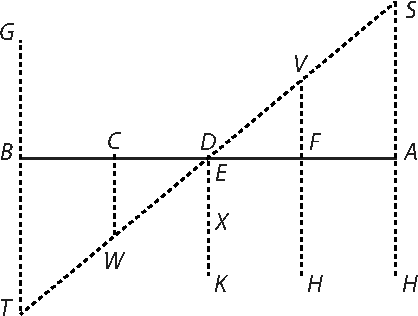
\includegraphics[width=0.46\textwidth]{gesamttex/edit_VIII-4/images/LH_35_10_13_007_d2_007v.pdf}}
\vspace{1.0em}
\centerline{\lbrack\textit{Fig.\:2}\rbrack}
\vspace{1.5em}
\pstart%
\noindent%
Poterit res eo reduci,
ut
\edtext{%
concipiamus totam \textit{AB}
habere vim priorem,%
\indexS{vis prior}
sed \textit{BC} habere regrediendi conatum,%
\indexS{conatus regrediendi}
ast \textit{AC} conatum progrediendi.%
\indexS{conatus progrediendi}%
}{%
\lemma{concipiamus}\Bfootnote{%
\textit{(1)}~\textit{BC} et \textit{CA} habere conatum
\textit{(2)}~totam quidem
\textit{(a)}~\textit{BC}
\textit{(b)}~\textit{AB} habere vim respectivam, sed \textit{BC} tantum vim regrediendi
\textit{(3)}~totam \textit{AB} %
\lbrack...\rbrack\ \textit{BC} habere
\textit{(a)}~vim
\textit{(b)}~regrediendi conatum,
\textit{(aa)}~sed
\textit{(bb)}~ast \textit{AC} conatum progrediendi.%
~\textit{L}}}%
\pend%
\vspace{0.5em}%
\pstart%
\noindent%
\lbrack%
\textit{Nachfolgend kleingedruckter Text in L gestrichen:}\rbrack%
\pend%
\vspace{0.5em}%
\footnotesize%
\pstart%
\noindent%
\edtext{%
Et per hunc%
}{%
\lemma{Et}\Bfootnote{%
\textit{(1)}~quia
\textit{(2)}~\bars{ne \textit{streicht Hrsg.}}
\textit{(3)}~per hunc%
~\textit{L}}}
regrediendi conatum%
\indexS{conatus regrediendi}
sumatur ipsius \textit{AC} pars \textit{AF}
\edtext{%
aequalis%
\lbrack,\rbrack\
similis et similiter
posita ipsi \textit{BC},%
}{%
\lemma{aequalis}\Bfootnote{%
\textit{(1)}~et
\textit{(2)}~similis et similiter posita
\textit{(a)}~ipsi \textit{BF}
\textit{(b)}~ipsi \textit{BC},%
~\textit{L}}}
patet eas compensari inter
\edtext{se,
dum}{%
\lemma{se,}\Bfootnote{%
\textit{(1)}~at
\textit{(2)}~dum%
~\textit{L}}}
ambae gyrantur circa \textit{E}.
Et hactenus totam \textit{BC} habere suum
\edlabel{35_10_13_007v_6a}%
progressum.%
\indexS{progressus in concursu eccentrico}
\edtext{}{%
\xxref{35_10_13_007v_6a}{35_10_13_007v_6b}%
\lemma{progressum}\Bfootnote{%
\lbrack/\rbrack\
\textit{(1)}~An
\textit{(2)}~Ergo dicemus
\textit{(a)}~circulationem nasci qualis
\textit{(b)}~regressum
\textit{(aa)}~in circulatione sci
\textit{(bb)}~nasci tantum quantus est conatus
\textit{(aaa)}~ipsius \textit{BC}
\textit{(bbb)}~regrediendi in %
\lbrack...\rbrack\ quantitatem circulationis,%
~\textit{L}}}%
\pend%
\normalsize%
\vspace{0.5em}%
\pstart%
\noindent%
Ergo dicemus regressum\indexS{regressus in concursu eccentrico}
nasci tantum
quantus est conatus regrediendi%
\indexS{conatus regrediendi}
in \textit{BC},
quod determinat quantitatem circulationis,%
\indexS{quantitas circulationis}%
\edlabel{35_10_13_007v_6b}
nam est eius quantitas
\edtext{dimidia.
Adeoque}{%
\lemma{dimidia}\Bfootnote{%
\textit{(1)}~, sed
\textit{(2)}~. Adeoque%
~\textit{L}}}
circulationi impenditur\indexS{circulatio in concursu eccentrico}
tam conatus regrediendi\indexS{conatus regrediendi}
quem habet \textit{BC} per ictum,\indexS{ictus}
quam conatus progrediendi\indexS{conatus progrediendi}
quem habet \textit{AF} per
\edlabel{35_10_13_007v_4a}%
se.%
\edtext{}{%
\xxref{35_10_13_007v_4a}{35_10_13_007v_4b}%
\lemma{se.}\Bfootnote{%
\textit{(1)}~Itaque
\textit{(2)}~Sed
\textit{(a)}~absoluto conatui progrediendi
\textit{(b)}~absolutae progressioni impenditur conatus progrediendi%
~\textit{L}}}
Sed absolutae progressioni%
\indexS{progressio absoluta}
impenditur conatus progrediendi%
\indexS{conatus progrediendi}%
\edlabel{35_10_13_007v_4b}
ipsius \textit{CF}.
Ubi jam notandum
\edtext{%
est progressionem in circulatione sumi%
\indexS{progressio sumta in circulationem}%
\indexS{circulatio in concursu eccentrico}
ductis velocitatibus in puncta mota.%
\indexS{velocitas ducta in punctum motum}%
\indexS{punctum motum}%
}{%
\lemma{est}\Bfootnote{%
\textit{(1)}~contum circulati
\textit{(2)}~progressionem in circulatione sumi
\textit{(a)}~in ratione
\textit{(b)}~ductis velocitatibus in puncta mota.%
~\textit{L}}}
\pend%
\pstart%
Perinde autem res sese habet,
ac
\edtext{%
si in unam aggelascere ponamus tres rectas,
nempe%
}{%
\lemma{si}\Bfootnote{%
\textit{(1)}~\textlangle cum\textrangle\
\textit{(2)}~simul
\textit{(3)}~\textlangle cum\textrangle\
\textit{(4)}~congelascere ponamus tres rect
\textit{(5)}~in unam %
\lbrack...\rbrack\ tres rectas,
\bars{nempe \textit{erg.}}%
\textit{L}}}
\textit{BC} habentem conatum $\overline{BC \cdot G},$
et ei aequalem \textit{AF}
habentem conatum contrarium\indexS{conatus contrarius}
$\overline{AF\cdot H},$
et denique \textit{FC} habentem conatum \textit{EK},
ubi non alius obtineri potest
\edtext{%
exitus\indexS{exitus}%
\lbrack,\rbrack\
quo
scilicet nihil amittatur
potentiae,\indexS{potentia amissa}%
}{%
\lemma{exitus}\Bfootnote{%
\textit{(1)}~nihil amittendo
\textit{(2)}~quo scilicet nihil amittatur potentiae,%
~\textit{L}}}
quam ut circulatio fiat circa \textit{E},%
\indexS{circulatio circa punctum}
et quidem tanta
ut celeritate\indexS{celeritas circulationis}
ipsius puncti \textit{A} vel \textit{B}
existente \textit{AS},
\edtext{%
\textit{BT}
aequalibus et ad \textit{AB} normalibus,
junctaque \textit{SET} recta%
}{%
\lemma{\textit{BT}}\Bfootnote{%
\textit{(1)}~(\protect\vphantom)aequalibus\protect\vphantom() juncta \textit{SET},
\textit{(2)}~aequalibus et %
\lbrack...\rbrack\ \textit{SET} recta%
~\textit{L}}}
cui ex \textit{F} et \textit{C} eductae normaliter rectae
occurrant in \textit{V} et \textit{W},
sit trapezium \textit{AFVS} vel \textit{BCWT}
aequale\indexS{trapezium}
\edtext{%
rectangulo \textit{FAH} vel \textit{CBG}.%
\indexS{rectangulum}%
}{%
\lemma{rectangulo}\Bfootnote{%
\textit{(1)}~\textit{CBG} vel
\textit{(2)}~\textit{FAH} vel \textit{CBG}.%
~\textit{L}}}
\pend%
\pstart%
Celeritas autem ipsius centri \textit{E}%
\indexS{celeritas centri gravitatis}
erit \textit{EX},
quae quaeritur an sit talis
ut rectang. \textit{AB} in \textit{EX} aequetur
rectangulo \textit{CF} in \textit{DK}.%
\indexS{rectangulum}
\edtext{Ita sane,}{%
\lemma{Ita}\Bfootnote{%
\bars{videtur \textit{gestr.}} sane,%
~\textit{L}}}
nec ita quicquam incommodi orietur
quia quantum ipsi \textit{AF}
absolutae celeritatis additur,%
\indexS{celeritas absoluta}
tantum ipsi \textit{BC}
\edtext{adimitur%
\lbrack,\rbrack\
ita ut in summa}{%
\lemma{adimitur.}\Bfootnote{%
\textit{(1)}~. In eor
\textit{(2)}~ita ut in summa%
~\textit{L}}}
verus motus compositus%
\indexS{motus compositus}
non sit major primo.
Ubi tamen videndum an idem locum habeat,
cum centrum gravitatis%
\indexS{centrum gravitatis}
non est centrum figurae,%
\indexS{centrum figurae}
ubi major quantitas motus additur%
\indexS{quantitas motus addita}
ab una parte quam ab altera
\edtext{adimitur.%
\indexS{quantitas motus ademta}
Immo}{%
\lemma{adimitur.}\Bfootnote{%
\textit{(1)}~Itaque
\textit{(2)}~Immo%
~\textit{L}}}
videndum est
an sufficiat quantitatem motus respici,%
\indexS{quantitas motus servanda}
et an non sit opus
servari virium quantitatem.%
\indexS{quantitas virium servanda}
Atque ita est.
Nam et in navi\indexS{navis} servanda est.
Etiam in concurrentibus
vis respectiva servanda est.%
\indexS{vis respectiva servanda}
NB.
\edtext{}%
{\lemma{\textit{Quer am Rand:}}%
\applabel{FnA:35_10_13_007v_navis}%
\Afootnote{%
Quid si sint inaequalia corpora eccentrice concurrentia%
\indexS{concursus eccentricus}%
\indexS{corpora concurrentia inaequalia}%
\indexS{corpora eccentrice concurrentia}%
\lbrack;\rbrack\
faciendus motus reciproce proportionalis,%
\indexS{motus reciproce proportionalis}
ut centrum gravitatis quiescat.%
\indexS{centrum gravitatis quiescens}%
\newline%
\hspace*{7.6mm}
Quid si navem\indexS{navis} hic adhibebimus
ad casus definiendos,\indexS{casus definiendus}
cum centrum gravitatis alias non quiescit.%
\indexS{centrum gravitatis quiescens}%
}}%
\pend%
\selectlanguage{latin}%
\frenchspacing%
\normalsize%


\section[tocentry={Concursus eccentrici casus simplicissimus. Scheda secunda
\enskip September 1691},
head={Concursus eccentrici casus simplicissimus. Scheda II%
}]%
{\MakeUppercase{Concursus eccentrici casus simplicissimus. Scheda secunda}
\newline September 1691}
\label{60107}
\selectlanguage{ngerman}%
\frenchspacing%
\begin{ledgroupsized}[r]{120mm}%
\footnotesize%
\pstart%
\noindent\textbf{Überlieferung:}
\pend%
\end{ledgroupsized}%
\begin{ledgroupsized}[r]{114mm}%
\footnotesize%
\pstart%
\parindent -6mm%
\makebox[6mm][l]{\textit{L}}%
Aufzeichnung:
LH XXXV 10,\;13 Bl.\;8.
Ein Zettel (etwa 10\;x\;21~cm),
Ränder zum Teil beschnitten oder abgerissen.
Eineinhalb Seiten (sonst unbeschrieben).
\pend%
\end{ledgroupsized}%
\selectlanguage{latin}%
\frenchspacing%
\vspace{8mm}%
\normalsize%
\pstart%
\noindent%
\lbrack%
\href{\Scan{LH_35_10_13_008r}}%
{8\,r\textsuperscript{o}}%
\rbrack%
\hfill%
Concursus Eccentrici%
\indexS{concursus eccentricus}
casus simplicissimus%
\indexS{casus simplex}
\hfill%
\phantom{\lbrack8\:r\textsuperscript{o}\rbrack}%
\par%
\centering%
Scheda 2%
\indexS{scheda}
\quad%
\edlabel{LH_35_10_13_008_008r_datum-1}%
Septemb.\;691%
\edlabel{LH_35_10_13_008_008r_datum-2}
\pend%
\vspace{1.0em}
\pstart%
\noindent%
Si aequales
\edtext{et parallelae rectae%
\indexS{rectae parallelae}%
}{%
\lemma{et}\Bfootnote{%
parallelae rectae
\textit{erg.\;L}}}
\textit{AB}, \textit{LM}
concurrant in plano paginae%
\indexS{planum paginae}%
\indexS{pagina}
partibus \textit{BC}, \textit{MN},
celeritate aequali,%
\indexS{celeritas concursus}
is est casus simplicissimus%
\indexS{casus simplex}
Concursus Eccentrici,%
\indexS{concursus eccentricus}
et fit utrobique idem.
Videndum an liceat rem ita concipere,
quasi concurrerent solum partes
\textit{BC} %
et \textit{MN} %
atque ita reflecterentur%
\lbrack,\rbrack\
in momento autem reflexionis%
\indexS{reflexio}%
\indexS{momentum reflexionis}
invenirent illa \textit{AC}, haec \textit{LN}
venientes contra reflexionem%
\indexS{reflexio}
et ipsis \textit{BC}, \textit{MN}
\edtext{adhaerescentes.
Quo admisso}{%
\lemma{adhaerescentes.}\Bfootnote{%
\textit{(1)}~Quod
\textit{(2)}~Quo admisso%
~\textit{L}}}
jam in sola \textit{AB} considerare licet %
quid fiat
si duo cohaerescant,
\textit{AC} tendens prorsum
et \textit{BC} retrorsum.
Quo
\edtext{posito fiet gyratio.%
\indexS{gyratio in concursu eccentrico}
Sumamus partem%
}{%
\lemma{posito}\Bfootnote{%
\textit{(1)}~pars i
\textit{(2)}~fiet gyratio. Sumamus partem%
~\textit{L}}}
\textit{AF} aequalem ipsi \textit{BC},
hae duae conspirabunt in gyrationem%
\indexS{conspiratio in gyratione}
circa medium \textit{E}.
Perinde ergo est
ac si simul cohaerescerent
\edtext{\lbrack\textit{AF}\rbrack}{%
\lemma{\textit{AC}}\Bfootnote{%
\textit{L~ändert Hrsg.}}}
tendens prorsum,
\textit{BC} retrorsum,
\textit{CF} prorsum.
Ubi
\edtext{\lbrack nisus\rbrack}{%
\lemma{nisus}\Bfootnote{%
\textit{gestr.\;L, wieder gültig macht Hrsg.}}}
ipsorum \textit{AF} et \textit{BC}
conspirat in circulationem,%
\indexS{circulatio in concursu eccentrico}%
\indexS{conspiratio in circulatione}
nisus ipsius \textit{CF} residui%
\indexS{nisus residui}
proficit in totius progressionem.%
\indexS{progressio totius}
\pend%
\vspace{2.75em}%
\centerline{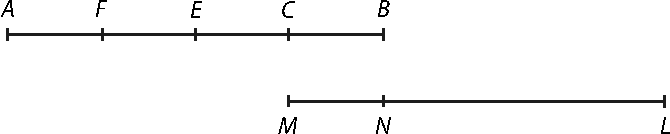
\includegraphics[width=0.74\textwidth]{gesamttex/edit_VIII-4/images/LH_35_10_13_008_d1_008r.pdf}}
\vspace{1.5em}
\centerline{\lbrack\textit{Fig.\:1}\rbrack}
\newpage%
\pstart%
\edlabel{LH_35_10_13_008_008r_gedankenexp-1}%
Possumus autem examinare Nisum%
\indexS{nisus}
per conatum.%
\indexS{conatus}
\edtext{Fingamus Cylindrum%
\indexS{cylinder in aqua}
in aqua poni \textit{AB},
compositum ex duabus partibus%
}{%
\lemma{Fingamus}\Bfootnote{%
\textit{(1)}~duas esse pa
\textit{(2)}~Cylindrum in %
\lbrack...\rbrack\ duabus partibus%
~\textit{L}}}
\textit{AC} et \textit{BC},
quarum una sit gravis altera levis,
ita ut levitas%
\indexS{levitas specifica}
\edtext{speci\lbrack fi\rbrack ca}{%
\lemma{specica}\Bfootnote{%
\textit{L~ändert Hrsg.}}}
sit aequalis gravitati specificae,%
\indexS{gravitas specifica}
seu in casu aequalium molium%
\indexS{moles aequales}
et situs directi%
\indexS{situs}
altera alteri
\edtext{resistat.
Videndum tuncne}{%
\lemma{resistat.}\Bfootnote{%
\textit{(1)}~Ita fingendum est
\textit{(2)}~Videndum tuncne%
~\textit{L}}}
centrum gravitatis aquae%
\indexS{centrum gravitatis aquae}
considerandum,
ut quam maxime descendat totius centrum%
\indexS{centrum gravitatis totius}
ex aqua et corpore compositi,
an abstrahendo animum%
\indexS{animus}
ab aqua%
\indexS{aqua}
liceat definire modum
quo quam brevissime natura lucratur%
\indexS{natura lucrans}
quantum potest,
ut scilicet et progressionem%
\indexS{progressio in concursu eccentrico}
et circulationem%
\indexS{circulatio in concursu eccentrico}
hac arte%
\indexS{ars}
definiamus.
Apparebit enim
quomodo conatus inter ipsas sit
\edtext{dividendus.%
\indexS{conatus dividendus}
Quam optime procedamus.}{%
\lemma{dividendus.}\Bfootnote{%
\textit{(1)}~, vel
\textit{(2)}~. Quam optime procedamus.%
~\textit{L}}}%
\edlabel{LH_35_10_13_008_008r_gedankenexp-2}%
\pend%
\pstart%
\edlabel{LH_35_10_13_008r_kehg-1}%
Quid si ab initio concepissemus %
obniti sibi
\edtext{duo aequalis gravitatis%
\indexS{gravitas specifica}
et levitatis specificae,%
\indexS{levitas specifica}
\!\textit{AB} grave
et
\lbrack\textit{LM}\rbrack\
leve;
sed}{%
\lemma{duo}\Bfootnote{%
\textit{(1)}~sed
\textit{(2)}~aequalis gravitatis %
\lbrack...\rbrack\ grave et
\bars{\textit{BC} \textit{ändert Hrsg.}}
leve; sed%
~\textit{L}}}
tunc periret vis%
\indexS{vis ictus}
\edtext{ictus,%
\indexS{ictus}
quia \textit{BC} et
\lbrack\textit{MN}\rbrack\
se non repellerent%
\lbrack;\rbrack\
verum ita circulatio%
\indexS{circulatio in concursu eccentrico}
fieret aliter et satis curiose,%
}{%
\lemma{ictus,}\Bfootnote{%
\textit{(1)}~et ita aliter se haberet circulatio
\textit{(2)}~quia \textit{BC} et
\bars{\textit{LN} \textit{ändert Hrsg.}}
se non %
\lbrack...\rbrack\ satis curiose,%
~\textit{L}}}
conabitur enim \textit{AB} gyrare circa punctum
\edtext{\lbrack\textit{M}\rbrack,}{%
\lemma{\textit{L}}\Bfootnote{%
\textit{L~ändert Hrsg.}}}
et \textit{LM}
\edlabel{35_10_13_008r_1a}%
super punctum \textit{B}.%
\edtext{}{%
\xxref%
{35_10_13_008r_1a}{35_10_13_008r_1b}%
\lemma{super}\Bfootnote{%
punctum
\bars{super \textit{streicht Hrsg.}}
\textit{B}. \lbrack/\rbrack\
\textit{(1)}~Vis respectiva
\textit{(2)}~Vis quam habet motus
\textit{(a)}~circulat\textlangle ar\textrangle\
\textit{(b)}~\bars{circulatoribus \textit{ändert Hrsg.}} et vis %
\lbrack...\rbrack\ motus progressorius%
~\textit{L}}}%
\pend%
\pstart%
Vis%
\indexS{vis motus circulatorii}
quam habet motus%
\indexS{motus circulatorius}
circulatori\lbrack us\rbrack\
et vis%
\indexS{vis motus progressorii}
quam habet motus progressorius%
\indexS{motus progressorius}%
\edlabel{35_10_13_008r_1b}
ipsius \textit{AB},
inter se sunt conjungendae;%
\indexS{vires conjungendae}
debet enim oriri aequatio\indexS{aequatio}
seu compensatio,\indexS{compensatio}
seu idem
\edtext{quod}{%
\lemma{\textit{Am Rand:}}\Afootnote{NB}}
prodiret
\edtext{aestimati\lbrack s\rbrack}{%
\lemma{aestimatibus}\Bfootnote{%
\textit{L~ändert Hrsg.}}}
viribus%
\indexS{vis aestimata}
cujusque puncti ex motu composito,%
\indexS{motus compositus}%
\indexS{aestimatio virium ex motu composito}
prorsus ut in compositione cum
\edlabel{LH_35_10_13_008r_iugl-1}%
navi.%
\indexS{compositio cum navi}\indexS{navis}%
\edlabel{LH_35_10_13_008r_kehg-2}%
\edtext{}{%
\xxref{LH_35_10_13_008r_iugl-1}{LH_35_10_13_008r_iugl-2}%
\lemma{navi.}\Bfootnote{%
\lbrack/\rbrack\
\textit{(1)}~Si \textit{L}
\textit{(a)}~glo
\textit{(b)}~globus\indexS{globus}
\textit{(2)}~Si \textit{L} globulus%
~\textit{L}}}%
\pend%
\vspace{2.75em}%
\centerline{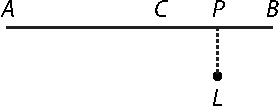
\includegraphics[width=0.33\textwidth]{gesamttex/edit_VIII-4/images/LH_35_10_13_008_d2_008v.pdf}}
\vspace{1.0em}
\centerline{\lbrack\textit{Fig.\:2}\rbrack}
\vspace{1.5em}%
\pstart%
Si \textit{L} globulus%
\indexS{globulus}%
\edlabel{LH_35_10_13_008r_iugl-2}
in cylindrum \textit{AB}%
\indexS{cylinder}
directe sed eccentrice occurrat,%
\indexS{concursus directus eccentricus}%
\indexS{concursus eccentricus directus}
tunc
(\protect\vphantom)%
si verum est
quod ictus\indexS{ictus}
solum fiat
inter \textit{L} et ipsi aequalem \textit{BC}%
\protect\vphantom()
tunc si motus est aequalis %
\indexS{motus aequalis}
et%
\lbrack,\rbrack\
posito puncto incursus \textit{P},%
\indexS{punctum incursus}%
\indexS{incursus}
dupla ipsius \textit{BP},
seu \textit{BC},
aequalis est ipsi \textit{L},
debet \textit{L} semper reflecti;
hoc dignum experimento.%
\indexS{experimentum}
Cum ita \textit{L} et \textit{AB} sint inaequales%
\lbrack,\rbrack\
\edlabel{LH_35_10_13_008_008rv_navisficta-1}%
videamus quid fiat
si navem fingamus%
\indexS{navis ficta}%
\indexS{fictio navis}
et motum
\lbrack%
\href{\Scan{LH_35_10_13_008v}}%
{8\,v\textsuperscript{o}}%
\rbrack\ %
inter ipsa reciprocum molibus,%
\indexS{motus reciprocus moli}%
\indexS{moles reciproca motui}
et quae deinde prodeant
inter \textit{L} et \textit{BC},
quorum ita celeritas non erit
reciproca molibus nec aequalibus.%
\indexS{celeritas reciproca moli}%
\indexS{moles reciproca celeritati}
Utile erit varias hypotheses%
\indexS{hypotheses comparatae}%
\indexS{comparatio hypothesum}
comparare inter se,
debent enim omnes dare idem,
navis utcunque assumto motu%
\indexS{navis}%
\indexS{motus navis}%
\lbrack;\rbrack\
in quo latent quaedam subtilia.%
\edlabel{LH_35_10_13_008_008rv_navisficta-2}
\pend%
\pstart%
Datur et modus omnia definiendi,%
\indexS{modus definiendi}
si fingamus
corpora constare meris globis aequalibus%
\indexS{corpus constans globis aequalibus}
connexis per elastra,%
\indexS{globi connexi per elastra}%
\indexS{connexio per elastra}%
\indexS{elastrum}
quae sine tensione%
\indexS{tensio}
nec distrahi invicem,%
\indexS{distractio cum tensione}
nec contrudi patiantur.%
\indexS{contrusio cum tensione}
Ita plurima definire poterunt Geometrice.%
\indexS{definitio geometrica}
Et consensus haberi debet%
\indexS{consensus}
cum iis quae jam habemus.
Ita ex solis legibus globulorum aequalium%
\indexS{lex globorum aequalium}%
\indexS{globi aequales}
caetera definientur.
\pend%
\selectlanguage{latin}%
\frenchspacing%
\normalsize%




\chapter[tocentry={Casus concursuum methodo solvendi
\enskip\bracks{%
ab 10.\;November 1690~(?)%
}},
head={Casus concursuum methodo solvendi}]%
{\MakeUppercase{Casus concursuum methodo solvendi}
\newline\bracks{%
ab 10.\;November 1690~(?)%
}}%
\label{58947}
\selectlanguage{ngerman}%
\frenchspacing%
\begin{ledgroupsized}[r]{120mm}%
\footnotesize%
\pstart%
\noindent\textbf{Überlieferung:}
\pend%
\end{ledgroupsized}
\begin{ledgroupsized}[r]{114mm}%
\footnotesize%
\pstart%
\parindent -6mm%
\makebox[6mm][l]{\textit{L}}%
Notiz:
LH~XXXV~11,\;14 Bl.\;32.
Ein Zettel (etwa 9\:x\:5~cm);
unterer Rand beschnitten.
Eine Seite auf Bl.\;32\:r\textsuperscript{o}; Bl.\;32\:v\textsuperscript{o} ist unbeschrieben.
\pend%
\end{ledgroupsized}%
\vspace{5mm}%
\begin{ledgroup}%
\footnotesize%
\pstart%
\noindent%
\textbf{Datierungsgründe:}
Die undatierte Notiz N.\;\ref{58947} ist auf einem Träger überliefert, der weder Spüren eines Wasserzeichens aufweist noch sonstige datierungsrelevante Anhaltspunkte bietet.
Für eine grobe chronologische Einordnung erweisen sich folgende inhaltliche Beobachtungen als ausschlaggebend:
\pend%
\pstart%
(1)~%
Die Notiz N.\;\ref{58947} beginnt mit der Feststellung, die Kinematik des schiefen sowie des mehrfachen Stoßes lasse sich durch das Modell eines \glqq Schiffes im Schiffe\grqq\ adäquat beschreiben.
(Hierunter ist eine Erweiterung der "Schiffsmethode" gemeint, d.\,h. jener Methode der Zerlegung zusammengesetzter Bewegungen, die in Leibnizens stoßtheoretischen Untersuchungen seit spätestens Mitte 1677 Anwendung fand.)
Bei den genannten Stoßarten falle dieses Modell %
zudem mit der in N.\;\ref{58947} nicht weiter erläuterten \textit{methodus quantitatis potentiae respectivae per diversas compositiones conservandae} zusammen (\refpassage{LH_35_11_14_032_methodus-1}{LH_35_11_14_032_methodus-2}).
Mit dem exzentrischen Stoß verhalte es sich aber \textendash\ wie der Schlussatz in N.\;\ref{58947} einräumt \textendash\ anders:
Das Modell eines \glqq Schiffes im Schiffe\grqq\ lasse sich hierauf nicht anwenden, obwohl die \glqq Natur des exzentrischen Stoßes\grqq\ durch Leibnizens eigene Methode (\textit{mea methodus}) doch erfolgreich ermittelt worden sei. %
Ist bei dieser Anspielung nun wieder die \glqq Methode der bei verschiedenen Zusammensetzungen zu bewahrenden relativen Potenz\grqq\ gemeint, so ist hieraus zu schließen, dass diese Methode aus Leibnizens Sicht nicht ohne Weiteres mit dem \glqq Modell eines Schiffes im Schiffe\grqq\ zusammenfällt, da ihr offenbar ein breiterer Anwendungsbereich zukommt als letzterem, dem sich zumindest der exzentrische Stoß entzieht. 
\pend%
\pstart%
(2)~%
Die \glqq Methode der bei verschiedenen Zusammensetzungen zu bewahrenden relativen Potenz\grqq\ wird in N.\;\ref{58947} ganz unvermittelt genannt.
Daher ist wahrscheinlich, dass die Notiz später entstand als die Texte, die diese Methode im Zusammenhang mit dem exzentrischen Stoß erläutern bzw. ausführen:
Das sind u.\;a.
die vermutlich im Herbst\;(?) 1690 verfasste Aufzeichnung N.\;\ref{58949}, in der die besagte Methode konzise dargelegt wird (\refpassage{LH_35_11_14_034_034rv_drstllng-1}{LH_35_11_14_034_034rv_drstllng-2} im vorliegenden Band),
sowie
die eigenhändig auf den 31.\;Oktober\,/\,10.\;November 1690 datierte \textit{Scheda secunda de impulsu eccentrico} N.\;\ref{58939}, in der die Methode ausführlich angewendet wird (\refpassage{LH_35_11_14_003-004_004v_methodus-1}{LH_35_11_14_003-004_004v_methodus-2} im vorliegenden Band).
Da Leibniz im Schlusssatz von N.\;\ref{58947} die erfolgreiche Anwendung eben dieser Methode auf den exzentrischen Stoß erwähnt, ist anzunehmen, dass die Notiz %
nach dem Entwurf N.\;\ref{58939} und wohl auch nach der Aufzeichnung N.\;\ref{58949} verfasst wurde.
\pend%
\pstart%
(3)~%
Es gilt ferner zu bemerken, dass die \glqq Methode der bei verschiedenen Zusammensetzungen zu bewahrenden relativen Potenz\grqq\ auch in der auf den Zeitraum 1690\textendash1694 datierbaren und in diesem Band edierten Aufzeichnung N.\;\ref{60298} besprochen wird, dort im Hinblick auf den Zusammenstoß dreier Körper und ohne Berücksichtigung des exzentrischen Stoßes. %
Auch in N.\;\ref{60298} wird die besagte Methode ausdrücklich mit dem Modell eines \glqq Schiffes im Schiffe\grqq\ verglichen, welchem ebenfalls mit Skepsis begegnet wird. %
Somit lässt sich auch in der Aufzeichnung N.\;\ref{60298} eine Diskrepanz zwischen der allgemeinen Methode und dem fiktionalen Modell feststellen.
Die Notiz N.\;\ref{58947} zeigt indessen, dass die Zweifel am erweiterten Schiffsmodell im Fall des multiplen (und somit schiefen) Stoßes überwunden wurden, nicht aber im Fall des exzentrischen Stoßes.
Dies dürfte belegen, dass N.\;\ref{58947} nach N.\;\ref{60298} entstand.
\pend%

\pstart%
(4)~%
In Untersuchungen über den exzentrischen Stoß wird die einfache \glqq Schiffsmethode\grqq\ mehrfach in Anspruch genommen, ohne grundsätzliche Zweifel an deren Angemessenheit zu erheben.
Dies ist etwa bei folgenden, sämtlich im vorliegenden Band edierten Texten der Fall:
der Aufzeichnung \textit{De impulsu eccentrico} N.\;\ref{60300}, \refpassage{LH_37_05_044_044r_navis-1}{LH_37_05_044_044r_navis-2} (April--Oktorber 1690);
der \textit{Scheda de impulsu eccentrico} N.\;\ref{58940}, \refpassage{LH_35_11_14_005-006_005v_navis-1}{LH_35_11_14_005-006_005v_navis-2} (31.\;Oktober\,/\,10.\;November 1690);
den zusammenhängenden Texten \textit{Casus eccentrici concursus simplicissimus} N.\;\ref{60106}, Randbemerkungen zu \refnote{FnA:35_10_13_007r_navis} u. \refnote{FnA:35_10_13_007v_navis} und N.\;\ref{60107}, \refpassage{LH_35_10_13_008_008rv_navisficta-1}{LH_35_10_13_008_008rv_navisficta-2} (September 1691).
Hieraus würde sich -- unter der Annahme, dass die Zweifel am Modell des "Schiffes im Schiffe" eine weitere, spätere Entwicklung darstellen -- \textit{September 1691} als frühester Entstehungszeitpunkt der Notiz N.\;\ref{58947} ergeben.
\pend%
\pstart%
(5)~%
Die Notiz N.\;\ref{58947} könnte allerdings durch ihre Zweifel am Modell \glqq des Schiffes im Schiffe\grqq\ auch mit dem im vorliegenden Band edierten Entwurf N.\;\ref{41780} verbunden sein, in welchem ähnliche Zweifel an derselben Methode erhoben werden.
Der auf die Zeitspanne von Mitte September 1690 bis 1696 datierbare Entwurf N.\;\ref{41780} zeigt somit, dass die Annahme einer späteren Entwicklung, aus der die Zweifel an der Erweiterung der Methode sich ergeben hätten, fraglich ist und dass die Notiz N.\;\ref{58947} %
bereits im Laufe des Jahres 1690 abgefasst worden sein könnte.
Eine Entstehung vor den Texten N.\;\ref{58939} und N.\;\ref{58949} sowie N.\;\ref{60298} ist jedoch -- wie oben festgehalten wurde -- unwahrscheinlich.
Hieraus ergibt sich als mutmaßlicher frühester Entstehungszeitpunkt der Notiz N.\;\ref{58947} der \textit{10.\;November 1690}.
Eine spätere Datierung -- ab September 1691 -- ist aber nicht unwahrscheinlich.
\pend%
\pstart%
(6)~%
Ein eindeutiger Terminus ante quem der Datierung lässt sich für die Notiz N.\;\ref{58947} zum Redaktionsschluss nicht angeben.
\pend%
\end{ledgroup}%
\selectlanguage{latin}%
\frenchspacing%
\vspace{8mm}%
\normalsize%
\pstart%
\noindent%
\edtext{%
\lbrack%
\href{\Scan{LH_35_11_14_032r}}%
{32\,r\textsuperscript{o}}%
\rbrack\ %
Casus%
\indexS{casus solvendus}
concursus obliqui%
\indexS{concursus obliquus}
et compositi%
\indexS{concursus compositus}%
}{%
\lemma{%
\href{\Scan{LH_35_11_14_032r}}{\lbrack32\:r\textsuperscript{o}\rbrack}%
}\Bfootnote{%
\textit{(1)}~Casus unius corporis in plura incurrentis variique alii ob%
\indexS{concursus plurimus}\indexS{casus varius}
\textit{(2)}~Casus concursus obliqui et compositi%
~\textit{L}}}
solvi possunt
supposita navi in%
\indexS{navis in navi}
\edtext{%
navi.
Quo idem consequemur,
quod mea
\edlabel{LH_35_11_14_032_methodus-1}%
methodo%
\indexS{methodus mea}%
\indexS{methodus potentiae respectivae conservandae}%
\indexS{quantitas potentiae respectivae}%
\indexS{potentia respectiva conservanda}
quantitatis potentiae respectivae
per diversas compositiones%
\indexS{compositio motuum}
conservandae.%
\edlabel{LH_35_11_14_032_methodus-2} %
\edlabel{LH_35_11_14_032_natura-0}%
Sed explicari non poterit
(\protect\vphantom)%
quantum hactenus judicare possum%
\protect\vphantom()
\edlabel{LH_35_11_14_032_natura-1}%
natura concursus%
\indexS{natura concursus eccentrici}%
\indexS{concursus eccentricus}%
}{%
\lemma{navi.}\Bfootnote{%
\textit{(1)}~Sed ad concursus
\textit{(2)}~Quo idem %
\lbrack...\rbrack\ conservandae. Sed
\textit{(a)}~solvi
\textit{(b)}~explicari non poterit
\textit{(aa)}~casus
\textit{(bb)}~(\protect\vphantom)quantum hactenus %
\lbrack...\rbrack\ natura concursus%
~\textit{L}}}
eccentrici
\edtext{%
quem mea methodus%
\indexS{methodus mea}
\edtext{etiam}{\lemma{etiam}\Bfootnote{\hspace{0.5mm}%
\textit{erg.\;L}}}
absolvit.%
\edlabel{LH_35_11_14_032_natura-2}%
}{%
\lemma{quem \lbrack...\rbrack\ absolvit}\Cfootnote{%
Siehe hierüber die ausführlichen Datierungsgründe.
}}
\pend%
\selectlanguage{latin}%
\frenchspacing%
\normalsize%
\newpage%





\chapter[tocentry={Ex conservatione potentiae, tam absolutae quam respectivae, possunt derivari phaenomena concursus trium corporum
\enskip \bracks{8.~Mai 1693 \textendash\ 1696}%
},
head={Phaenomena concursus trium corporum}]%
{\MakeUppercase{Ex conservatione potentiae, tam absolutae quam respectivae, possunt derivari phaenomena concursus\linebreak trium corporum}
\newline \bracks{8.~Mai 1693 \textendash\ 1696}%
}
\label{intro_tam-abs-quam-resp}

\vspace{5mm}
\begin{ledgroup}
\footnotesize
\pstart
\noindent
Die vorliegenden zwei Stücke weisen eine gemeinsame Entstehungsgeschichte auf:
Das Konzept N.\;\ref{58293}, 
dessen Wasserzeichen für den Zeitraum Oktober, unter anderem im Konzept N.\;\ref{58300}, gut belegt ist,
bezeugt Leibnizens (in den 1690er Jahren häufige) Beschäftigung mit den Regeln des schiefen Mehrkörperstoßes und ihren Folgen für die Krafterhaltung.
Auf einem separaten Zettel hat Leibniz einige Hilfsrechnungen zu einem besonders schwierigen Teil von N.\;\ref{58293} festgehalten (N.\;\ref{39763}).
Ein weiterer auf diesem Träger fragmentarisch überlieferter Text bietet einen Terminus post quem 
für die (als etwa simultan anzunehmende) Entstehung unserer Stücke 
und ermöglicht ihre Datierung in der Zeitspanne Mai 1693 bis 1696.
\pend
\pstart
Die Zusammengehörigkeit beider Stücke wird durch einen Vergleich der (Hilfs-)Rechnungen in N.\;\ref{39763}  mit den Art. (36)\textendash(38) von N.\;\ref{58293} ersichtlich.
So entspricht die Passage auf \refpassage{04_01_04d_02_004v_2a}{04_01_04d_02_004v_2b} von N.\;\ref{39763} 
den gestrichenen Art.~(36)\textendash(37) von N.\;\ref{58293}:
\refpassage{35_13_03_220-221_20a}{35_13_03_220-221_20b}
(das Verhältnis \textit{r} wurde in Art.~(35) eingeführt:
\refpassage{35_13_03_220-221_19a}{35_13_03_220-221_19b})
und die Passage auf \refpassage{04_01_04d_02_004v_1a}{04_01_04d_02_004v_3} von N.\;\ref{39763}
dem Art.~(38) von N.\;\ref{58293} (\refpassage{35_13_03_220-221_21a}{35_13_03_220-221_21b})
sowie der gestrichenen Randanmerkung zu
\refnote{FnA:35_13_03_220-221_rechnung}.
\pend
\pstart
Die kurze Aufzeichnung N.\;\ref{39763} ist auf einem Zettel mit der Signatur LH~IV~1, 4d, 2~Bl.~4 überliefert.
Auf Bl.~4~v\textsuperscript{o} befindet sich ein durch Papierabriss und -beschnitt nur noch fragmentarisch erhaltener Briefanfang; 
Bl.~4~r\textsuperscript{o} überliefert eine (wohl vollständige) Aufzeichnung über \indexN{\textls{Descartes} (Cartesius, des Cartes), René 1596\textendash1650}Descartes (\textit{Mons.~des Cartes a fait comme les charlatans}...), die die Seite ausfüllt. 
(Sie liegt in \cite{02150}\textsc{Foucher de Careil}, \textit{Nouvelles Lettres et Opuscules Inédits de Leibniz}, Paris 1857, S.\;12 gedruckt vor und wird vsl. in einem Band der Sechsten Reihe erscheinen.)
Dieser Umstand legt die Vermutung nahe, dass Leibniz erst den Briefentwurf verfasst habe, dann die Rückseite des Briefs für die Descartes-Aufzeichnung wiederverwendet und anschließend den Zettel auf diese zugeschnitten;
erst an dritter Stelle dürfte die Aufzeichnung N.\;\ref{39763} entstanden sein, für die Leibniz offenbar den freigebliebenen Rand von Bl.~4~v\textsuperscript{o} und sogar Zwischenräume im beschriebenen Teil verwendet hat.
Der Briefentwurf bietet einen Terminus post quem für die Entstehung der Notiz über Descartes und diese, die allerdings noch nicht verlässlich datiert ist, wiederum für die Entstehung der Aufzeichung N.\;\ref{39763}.
Der (für unsere Aufzeichung N.\;\ref{39763} also datierungsrelevante) Briefentwurf diente als Konzept zu einem nicht erhaltenen Schreiben Leibnizens an
\indexN{\textls{Brosseau}, Christophe 1630\textendash1717}Christophe Brosseau; auf dieses nahm \indexN{\textls{Brosseau}, Christophe 1630\textendash1717}Brosseau in einem \cite{02148}Brief vom 18. Mai Bezug (\textit{LSB} I, 9 N.\;276; siehe die Erläuterung, S. 437\,f.).
Sowohl in dem vorliegenden Entwurf als auch in Brosseaus Antwort geht es um die Frage der korrekten Abrechnung gewisser Zeitschriften ("gazettes"), nämlich auf Leibnizens Kosten statt auf die des 
\indexN{\textls{Braunschweig-Lüneburg}, Ernst August von, Herzog und Kurfürst von Hannover 1679\textendash1698}Kurfürsten von Braunschweig-Lüneburg. 
Leibniz bezeichnet im Briefentwurf seinen Dienstherren zunächst mit der Abkürzung "S.\,A.\,S.", ändert diese jedoch nachträglich in "S.\,A.\,E." (\textit{Son Altesse Électorale}), gemäß der am 19. Dezember 1692 verliehenen Kurwürde.
Im verschollenen Brief vom 8. Mai, sowie in einem Schreiben an die Kammer (Entwurf: LBr 560 Bl.~35), bemühte sich Leibniz um eine Klärung des Vorfalls (siehe \textit{LSB} I,~9, S.\;401). 
Aufgrund dieser Identifizierung ist der Briefentwurf auf dem Träger der Aufzeichnung N.\;\ref{39763}, Bl.~4~v\textsuperscript{o}, auf den 8. Mai 1693 zu datieren; dadurch ist ein Terminus post quem für N.\;\ref{39763} selbst gegeben, der wiederum bei der Datierung des Konzepts N.\;\ref{58293} berücksichtigt wird. 
\pend
\end{ledgroup}

\section[tocentry={Ex conservatione potentiae, tam absolutae quam respectivae, possunt derivari phaenomena concursus trium corporum
},
head={Phaenomena concursus trium corporum}]%
{\MakeUppercase{Ex conservatione potentiae, tam absolutae quam respectivae, possunt derivari phaenomena concursus\linebreak trium corporum} 
}
\label{58293}
\begin{ledgroupsized}[r]{120mm}
\footnotesize
\pstart\noindent
\textbf{Überlieferung:}
\pend
\end{ledgroupsized}
\begin{ledgroupsized}[r]{114mm}
\footnotesize
\pstart \parindent -6mm
\makebox[6mm][l]{\textit{L}}%
Konzept:
LH~XXXV~13, 3~Bl.~220\textendash221. 
Ein Bogen~2\textsuperscript{o};
Wasserzeichen		%
in Bl.~221.
Dreieinhalb Seiten.
Das Diagramm \lbrack\textit{Fig.~9}\rbrack\ wird, trotz seiner Platzierung auf Bl. 221~r\textsuperscript{o}, als zu Bl.~220~v\textsuperscript{o} und dem Text von Art.~(14) zugehörig gedeutet und am entsprechenden Ort wiedergegeben (S.~\pageref{Fig:LH_35_13_03_220-221_d9_221r}). 
\pend
\end{ledgroupsized}
\selectlanguage{latin}
\vspace{8mm}
\pstart\noindent%
\edlabel{35_13_03_220-221_9a}%
\edtext{}{%
\xxref%
{35_13_03_220-221_9a}{35_13_03_220-221_9b}%
\lemma{\href{\Scan{LH_35_13_03_220r}}{\lbrack220~r\textsuperscript{o}\rbrack}}%
\Bfootnote{%
\textit{(1)}~Si globus in globum oblique incurrat %
\textit{(a)}~non ideo minus tamen %
\textit{(b)}~sed tamen centrice, nulla %
\textit{(aa)}~est %
\textit{(bb)}~oritur circulatio. Centrice autem fit concursus si %
\textit{(aaa)}~li %
\textit{(bbb)}~recta perpendicularis %
\textit{(2)}~Concursus %
\textit{(a)}~corporum %
\textit{(b)}~corporis intelligitur factus in recta. %
\textit{(3)}~(1) Omne %
\textit{(a)}~ictu %
\textit{(b)}~corpus %
\textit{(aa)}~videtur percursum\lbrack\textit{!}\rbrack\ %
\textit{(bb)}~cen %
\textit{(cc)}~percutitur~\textit{L}}}%
\href{\Scan{LH_35_13_03_220r}}{\lbrack220~r\textsuperscript{o}\rbrack}
\pend
\begin{edfigure}[0em][0.7em]    	%
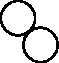
\includegraphics[scale=1]{gesamttex/edit_VIII-4/images/LH_35_13_03_220-221_d1_220r.pdf}
\edcaption[0.25em]{\lbrack\textit{Fig.~1}\rbrack}
\end{edfigure}
\pstart\noindent
(1) Omne corpus percutitur\edlabel{35_13_03_220-221_9b}
in recta perpendiculari ad superficiem\indexS{recta perpendicularis ad superficiem} percussi 
in puncto contactus.\indexS{punctum contactus}
\pend
\pstart
(2) Hinc si plura sint puncta\indexS{punctum contactus}
\edtext{contactus\lbrack,\rbrack\ percussum}{%
\lemma{contactus}%
\Bfootnote{%
\textit{(1)}~percursum %
\textit{(2)}~percussum~\textit{L}}}
est in pluribus rectis 
\edtext{simul, et perinde}{%
\lemma{simul,}%
\Bfootnote{%
\textit{(1)}~perinde %
\textit{(2)}~et perinde~\textit{L}}}
est ac si simul a pluribus corporibus fuisset 
\edlabel{35_13_03_220-221_1a}%
\edtext{}{\xxref{35_13_03_220-221_1a}{35_13_03_220-221_1b}%
\lemma{percussum}%
\Bfootnote{%
\textit{(1)}~\bars{Et quia \textit{erg.}} fieri potest ut eadem recta non sit perpendicularis ad utriusque concurrentium %
\textit{(2)}~(3) Fieri~\textit{L}}}%
percussum.
\pend
\begin{edfigure}[1em][1em]    	%
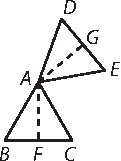
\includegraphics[scale=1]{gesamttex/edit_VIII-4/images/LH_35_13_03_220-221_d2_220r.pdf}
\edcaption{\edtext{\lbrack\textit{Fig.~2}\rbrack}{%
\lemma{\lbrack\textit{Fig.~2}\rbrack}%
\Cfootnote[nonum]{%
Ein gestrichener Entwurf zum Diagramm wird nicht wiedergegeben.}}}
\end{edfigure}
\pstart
(3) Fieri\edlabel{35_13_03_220-221_1b}
aliquando potest ut plures sint perpendiculares ad superficiem\indexS{perpendicularis ad superficiem} 
in puncto contactus,\indexS{punctum contactus}
sed tunc eligenda est perpendicularis\indexS{perpendicularis primaria}
\edtext{primaria. Et hoc fit}{%
\lemma{primaria.}%
\Bfootnote{%
\textit{(1)}~Hinc %
\textit{(a)}~f %
\textit{(b)}~fier %
\textit{(c)}~fieri %
\textit{(d)}~fieri potest, ut %
\textit{(2)}~Et hoc fit~\textit{L}}}
\edtext{cum angulus quasi quidam}{%
\lemma{cum}%
\Bfootnote{%
\textit{(1)}~angulum quasi quendam %
\textit{(2)}~angulus quasi quidam~\textit{L}}} 
est in superficie corporis, ut in vertice pyramidis.\indexS{pyramis}\indexS{vertex pyramidis} 
Hinc si duae pyramides\indexS{pyramis} \textit{ABC} et \textit{ADE} concurrant in
\edtext{puncto \textit{A}, fiet}{%
\lemma{puncto \textit{A},}%
\Bfootnote{%
\textit{(1)}~vir %
\textit{(2)}~fiet~\textit{L}}} 
\edtext{percu\lbrack s\rbrack sio\indexS{percussio}}{%
\lemma{}%
\Bfootnote{%
percursio %
\textit{L ändert Hrsg.}}}
ipsius \textit{ABC} in \textit{AF}, et ipsius \textit{ADE} in \textit{AG}, licet rectae \textit{AF} et \textit{AG} non sint in directum, quod tamen fieret, si essent globi.\indexS{globus}
\pend
\begin{edfigure}[1em][1em]    	%
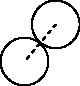
\includegraphics[scale=1]{gesamttex/edit_VIII-4/images/LH_35_13_03_220-221_d3_220r.pdf}
\edcaption[0.25em]{\lbrack\textit{Fig.~3, gestr.}\rbrack}
\end{edfigure}
\pstart
\edtext{(4)}{%
\lemma{}%
\Bfootnote{(4) \textit{erg.~L}}} 
Et ita patet fieri posse ut duo corpora concurrentia\indexS{corpora concurrentia} 
diversas accipiant directiones\indexS{directio} seu lineas percussionis;\indexS{linea percussionis}
quod impossibile est in
\edtext{corporibus, quae}{%
\lemma{corporibus,}%
\Bfootnote{%
\textit{(1)}~quae unum tantum habeant %
\textit{(2)}~quae~\textit{L}}} 
unum tantum habent planum
\edtext{tangens\indexS{planum tangens} in}{%
\lemma{tangens}%
\Bfootnote{%
\textit{(1)}~in punctis %
\textit{(2)}~in~\textit{L}}} 
quocunque puncto superficiei, adeoque et in puncto
\edtext{concursu\lbrack s\rbrack;\indexS{punctum concursus}}{%
\lemma{}%
\Bfootnote{concursu \textit{L ändert Hrsg.}}} 
quo posito oportet planum tangens\indexS{planum tangens} esse duobus corporibus commune. 
\pend
\begin{edfigure}[1em][1em]    	%
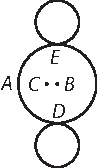
\includegraphics[scale=1]{gesamttex/edit_VIII-4/images/LH_35_13_03_220-221_d4_220r.pdf}
\edcaption{\edtext{\lbrack\textit{Fig.~4}\rbrack}{%
\lemma{\lbrack\textit{Fig.~4}\rbrack}%
\Cfootnote[nonum]{%
Ein gestrichener Entwurf zum Diagramm wird nicht wiedergegeben.}}}
\end{edfigure}
\pstart
(5) Si recta percussionis,\indexS{recta percussionis} transeat per centrum gravitatis\indexS{centrum gravitatis}
\edtext{corporis, percussio}{%
\lemma{corporis,}%
\Bfootnote{%
\textit{(1)}~linea %
\textit{(2)}~percussio~\textit{L}}} 
est centrica,\indexS{percussio centrica} sin minus eccentrica.\indexS{percussio eccentrica} Ut si in sphaera
\edtext{\textit{A}}{%
\lemma{}%
\Bfootnote{\textit{A} \textit{erg.~L}}} 
(ob materiae heterogeneitatem) non coincidant centrum sphaerae
\edtext{\textit{B}}{%
\lemma{}%
\Bfootnote{\textit{B} \textit{erg.~L}}} 
et centrum gravitatis\indexS{centrum gravitatis} \textit{C},
\edtext{eaque percutiatur}{%
\lemma{eaque}%
\Bfootnote{%
\textit{(1)}~ab alia %
\textit{(2)}~percutiatur~\textit{L}}} 
ab alio corpore quocunque, et
\edtext{utcunque, in}{%
\lemma{utcunque,}%
\Bfootnote{%
\textit{(1)}~percussio \bars{erit \textit{streicht Hrsg.}} %
\textit{(a)}~eccentrica %
\textit{(b)}~in linea quae %
\textit{(2)}~in~\textit{L}}} 
puncto \textit{D}, quod non cadat in rectam \textit{BC}, 
\edtext{percussio erit}{%
\lemma{percussio}%
\Bfootnote{%
\textit{(1)}~In omni %
\textit{(2)}~erit~\textit{L}}}
eccentrica.\indexS{percussio eccentrica}
\pend
\pstart
(6) In omni percussione eccentrica\indexS{percussio eccentrica}
\edtext{oritur gyratio\indexS{gyratio}}{%
\lemma{oritur}%
\Bfootnote{%
\textit{(1)}~(\protect\vphantom)si nihil imped %
\textit{(2)}~gyratio~\textit{L}}} 
percussi circa centrum,\indexS{centrum gravitatis} nisi forte sit quod impediat.
Velut si sphaera \textit{A} percutiatur simul in \textit{D} et \textit{E}, eccentrice,\indexS{sphaera percussa eccentrice}
sed \textit{CBE} et \textit{CBD} sint anguli aequales, 
patet compensationem gyrationis\indexS{gyratio}\indexS{compensatio gyrationis} utrinque fieri, adeoque gyrationem\indexS{gyratio}
\edlabel{35_13_03_220-221_2a}%
\edtext{}{\xxref{35_13_03_220-221_2a}{35_13_03_220-221_2b}%
\lemma{cessare}%
\Bfootnote{%
\textit{(1)}~Non %
\textit{(2)}~(7) Nulla~\textit{L}}}%
cessare. 
\pend
\begin{edfigure}[1em][1em]     %
\hfill
\includegraphics[scale=1]{%
gesamttex/edit_VIII-4/images/LH_35_13_03_220-221_d5_220r.pdf%
}%
\hfill
\protect\raisebox{.5ex}{%
\includegraphics[scale=1]{%
gesamttex/edit_VIII-4/images/LH_35_13_03_220-221_d6_220r.pdf}}%
\hfill%
\protect\raisebox{2.25ex}{%
\includegraphics[scale=1]{%
gesamttex/edit_VIII-4/images/LH_35_13_03_220-221_d7_220r.pdf}}
\hfill
\edcaption{%
\hspace*{10mm}
\lbrack\textit{Fig.~5}\rbrack \hspace*{20mm}
\lbrack\textit{Fig.~6, gestr.}\rbrack \hspace*{15mm}
\lbrack\textit{Fig.~7, gestr.}\rbrack
}
\end{edfigure}
\pstart 
(7) Nulla\edlabel{35_13_03_220-221_2b}
autem fiet gyratio\indexS{gyratio} si percussio sit centrica.\indexS{percussio centrica} Hinc 
\edtext{si sphaerae sint homogenea\lbrack e\rbrack, fieri}{%
\lemma{si}%
\Bfootnote{%
\textit{(1)}~sphaera sit homogenea %
\textit{(2)}~sphaerae sint \bars{homogenea \textit{ändert Hrsg.}} , fieri~\textit{L}}}
non potest,
\edtext{ut sphaeris inter se concurrentibus\indexS{sphaerae concurrentes} neque}{%
\lemma{ut}%
\Bfootnote{%
\textit{(1)}~duae sphae %
\textit{(2)}~sphaeris \bars{solis \textit{erg.~u. gestr.}} inter se concurrentibus
\textit{(a)}~oriatur gyratio,
\textit{(aa)}~secus foret %
\textit{(bb)}~nisi
\textit{(b)}~neque~\textit{L}}} 
alio obstaculo existente, oriatur gyratio;\indexS{gyratio} secus
est si quid adsit, quod sphaerae procursum secundum directionem
\edtext{receptam}{%
\lemma{}%
\Bfootnote{receptam \textit{erg.~L}}} 
quoad partem impediat, ut si sphaera \textit{A} inveniat obstaculum \textit{B}\lbrack:\rbrack\ tunc enim progredietur cum gyratione.\indexS{gyratio}
\pend
\pstart
\edlabel{35_13_03_220-221_12a}%
\edtext{(8) Ex}{%
\lemma{(8)}%
\Bfootnote{%
\textit{(1)}~Si %
\textit{(2)}~Hactenus %
\textit{(3)}~Ex~\textit{L}}} 
his regulis accedente conservatione\indexS{conservatio potentiae}
\edtext{potentiae, tam}{%
\lemma{potentiae,}%
\Bfootnote{%
\textit{(1)}~et %
\textit{(2)}~tam~\textit{L}}} 
absolutae\indexS{potentia absoluta}\indexS{conservatio potentiae absolutae} quam
\edtext{respectivae\lbrack,\rbrack\indexS{potentia respectiva}\indexS{conservatio potentiae respectivae} possunt derivari}{%
\lemma{respectivae}%
\Bfootnote{%
\textit{(1)}~oritur %
\textit{(2)}~possunt derivari~\textit{L}}} 
phaenomena concurrentium\indexS{phaenomena concurrentium} duarum sphaerarum homogenearum.
\pend
\pstart
Veniamus jam ad concursum trium corporum,\indexS{concursus trium corporum} 
quae materia adhuc intacta est,
sed stabiliamus 
\edtext{primum regulas}{%
\lemma{primum}%
\Bfootnote{%
\bars{\textit{(1)}~haec %
\textit{(2)}~has \textit{gestr.}}
regulas~\textit{L}}}
per quas
solvi possint casus omnes. Et primum quidem pro certo sumo conservari\indexS{conservatio potentiae absolutae} semper eandem potentiam absolutam.\indexS{potentia absoluta}
\pend 
\begin{edfigure}[1em][1em]    	%
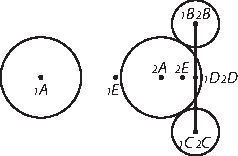
\includegraphics[scale=1]{gesamttex/edit_VIII-4/images/LH_35_13_03_220-221_d8_220r.pdf}
\edcaption{\lbrack\textit{Fig.~8, gestr.}\rbrack}
\end{edfigure}
\pstart 
(9) Deinde assumo quoque semper conservari eandem potentiam progressus,\indexS{progressus}\indexS{potentia progressus}\indexS{conservatio potentiae progressus}
\edtext{adeoque centrum}{%
\lemma{adeoque}%
\Bfootnote{%
\textit{(1)}~celeritatem %
\textit{(2)}~centrum~\textit{L}}} 
gravitatis\indexS{centrum gravitatis totale concurrentium}
\edtext{totale concurrentium}{%
\lemma{}%
\Bfootnote{totale concurrentium \textit{erg.~L}}} 
semper progredi in eadem recta eademque celeritate.\indexS{progressus centri gravitatis totalis in eadem recta eademque celeritate} %
\pend
\pstart
(10) Assumo etiam semper conservari eandem 
potentiam respectivam\indexS{potentia respectiva}\indexS{conservatio potentiae respectivae} 
quae consistit in recessu unius corporis ab alio,\indexS{recessus unius corporis ab alio} 
vel in circulatione\indexS{circulatio} qua saltem a se invicem recedere\indexS{recessus corporum a se invicem} conantur.%
\edlabel{35_13_03_220-221_12b}
\pend
\pstart
\indent (11) Hinc ubi abest circulatio\indexS{circulatio}
\edtext{(ut in concursu sphaerarum)}{%
\lemma{}%
\Bfootnote{(ut in concursu sphaerarum) \textit{erg.~L}}} 
necesse est potentiam respectivam\indexS{potentia respectiva} 
\edtext{spectari in solo}{%
\lemma{spectari}%
\Bfootnote{%
\textit{(1)}~in solo r %
\textit{(2)}~in sola %
\textit{(a)}~in solo~\textit{L}}}
a se invicem recessu.\indexS{recessus corporum a se invicem}
\pend
\pstart
(12) Si plura sint corpora potentia
\edtext{respectiva totalis\indexS{potentia respectiva totalis} componetur 
ex potentia respectiva recessus centri unius cujusque a centro gravitatis reliquorum\indexS{centrum gravitatis reliquorum corporum}\indexS{potentia respectiva recessus a centro} et}{%
\lemma{respectiva}%
\Bfootnote{%
\textit{(1)}~spectabitur in %
\textit{(2)}~totalis \lbrack...\rbrack\  recessus %
\bars{\textit{(1)}~centro \textit{(2)}~centri \textit{erg.}} %
unius \lbrack...\rbrack\  reliquorum %
\textit{(a)}~qua ostendi semper eandem potentiam respectivam prodire. Nam %
\textit{(aa)}~unum %
\textit{(bb)}~duo %
\textit{(b)}~quaecunque simul sumta pr %
\textit{(c)}~et~\textit{L}}} 
potentia respectiva\indexS{potentia respectiva} reliquorum inter se.
\edtext{Qua ratione idem provenire ostensum est, utcunque fiat combinatio.\indexS{combinatio}}{%
\lemma{Qua \lbrack...\rbrack\ combinatio}%
\Cfootnote{%
Siehe bspw. das Konzept N.\;\ref{58300}.}}
\pend
\pstart
\href{\Scan{LH_35_13_03_220v}}{\lbrack220~v\textsuperscript{o}\rbrack}\
(13) Veniamus jam
\edtext{ad concursum}{%
\lemma{ad}%
\Bfootnote{%
\textit{(1)}~casum %
\textit{(2)}~concursum~\textit{L}}} 
trium sphaerarum,\indexS{concursus trium sphaerarum} quas ponamus esse
\edtext{homogeneas\indexS{sphaerae homogeneae} ut concursus sit centricus,\indexS{concursus centricus}}{%
\lemma{homogeneas}%
\Bfootnote{%
\textit{(1)}~et duras, ut concursus %
\textit{(2)}~ut concursus sit %
\textit{(a)}~eccentricus %
\textit{(b)}~centricus,~\textit{L}}} 
et duras,\indexS{sphaerae durae} ne pars virium\indexS{vis} in exiguis partibus intereat. 
Et ut a facilioribus incipiamus, ponamus duas
\edtext{esse quiescentes,}{%
\lemma{esse}%
\Bfootnote{%
\textit{(1)}~aequales inter se %
\textit{(2)}~quiescentes,~\textit{L}}}
et aequales inter se,\indexS{spherae quiescentes aequales} 
et eodem modo se habentes ad tertiam ejusve motum.\indexS{motus}
\pend
\begin{edfigure}[0.75em][1em]    	%
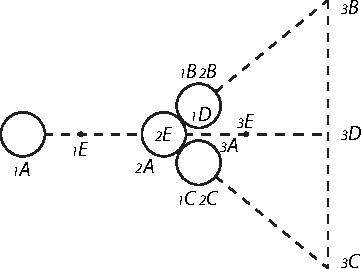
\includegraphics[scale=1]{gesamttex/edit_VIII-4/images/LH_35_13_03_220-221_d9_221r.pdf}
\edcaption[0pt]{%
\edtext{\lbrack\textit{Fig.~9 (Bl.~\href{\Scan{LH_35_13_03_221r}}{221~r\textsuperscript{o}})}\rbrack}{%
\lemma{\lbrack\textit{Fig.~9}\rbrack}%
\Cfootnote[nonum]{%
Leibniz hat das Diagramm auf Bl.~221~r\textsuperscript{o} gezeichnet.
Dass dies allerdings wohl nur aus Platzgründen geschehen ist, und die Figur zum Text auf Bl.~220~v\textsuperscript{o} gehört, legen folgende Umstände nahe:
Sie befindet sich in Falznähe, direkt gegenüber Art.~(14); 
sie wird in sämtlichen Ausführungen und Berechnungen der folgenden Artikel vorausgesetzt; 
bereits auf Bl.~220~r\textsuperscript{o}, unmittelbar nach Art.~(8), hatte Leibniz zu einer ähnlichen Zeichnung angesetzt (siehe die gestrichene Vorstufe \lbrack\textit{Fig.~8}\rbrack). 
Aus den genannten Gründen wird das Diagramm an dieser Stelle wiedergegeben.}}%
}
\pagelabel{Fig:LH_35_13_03_220-221_d9_221r}
\end{edfigure}
\pstart
\edtext{(14) Sit}{%
\lemma{(14)}%
\Bfootnote{%
\textit{(1)}~Sint %
\textit{(2)}~Sit~\textit{L}}} 
globus\indexS{globus} in motu
\edtext{cujus centrum\indexS{centrum gravitatis}}{%
\lemma{}%
\Bfootnote{cujus centrum \textit{erg.~L}}} 
\textit{A}, globi
\edtext{aequales}{%
\lemma{}%
\Bfootnote{aequales \textit{erg.~L}}} 
quiescentes\indexS{globi aequales quiescentes}
\edtext{quorum centra\indexS{centrum gravitatis}}{%
\lemma{}%
\Bfootnote{quorum centra \textit{erg.~L}}} 
\textit{B} et \textit{C}; centrum
commune\indexS{centrum gravitatis commune} ipsorum \textit{B} et \textit{C} sit \textit{D}, 
et centrum commune omnium\indexS{centrum gravitatis commune omnium} \textit{E}, 
\edtext{erit \lbrack\textit{CD}\rbrack\ aequal.}{%
\lemma{}%
\Bfootnote{%
erit
\bars{\textit{BC} \textit{ändert Hrsg.}}
aequal.~\textit{L}}} 
\textit{BD}
et \textit{AE}
\edtext{erit ad \textit{B}\lbrack\textit{D}\rbrack, ut glob.~\textit{C} $+$ glob.~\lbrack\textit{B}\rbrack\ ad}{%
\lemma{}%
\Bfootnote{%
erit ad 
\bars{\textit{BE} \textit{ändert Hrsg.}} %
ut glob. \textit{C} $+$ glob.
\bars{\textit{D} \textit{ändert Hrsg.}} %
ad~\textit{L}}}
glob. \textit{A}. Situs primus erit \textit{\ind{1}A}, \textit{\ind{1}B}, \textit{\ind{1}C}, \textit{\ind{1}D}, \textit{\ind{1}E}; situs secundus ipse scilicet 
situs concursus\indexS{concursus} 
erit \textit{\ind{2}A}, \textit{\ind{2}B}, \textit{\ind{2}C}, \textit{\ind{2}D}, \textit{\ind{2}E}, ubi ob
\edtext{quietem corporum}{%
\lemma{quietem}%
\Bfootnote{%
\textit{(1)}~punctorum %
\textit{(2)}~corporum~\textit{L}}} 
\textit{B} et \textit{C} adeoque et puncti \textit{D}, coincident \textit{\ind{1}B}, \textit{\ind{1}C}, \textit{\ind{1}D}, cum ipsis \textit{\ind{2}B}, \textit{\ind{2}C}, \textit{\ind{2}D}. 
Situs tertius erit qui designabit celeritatem post concursum,\indexS{concursus} 
\edtext{ita ut tantum}{%
\lemma{ita ut}%
\Bfootnote{%
\textit{(1)}~tam ut %
\textit{(2)}~tantum~\textit{L}}}
temporis intersit inter situm secundum, et situm tertium \textit{\ind{3}A}, \textit{\ind{3}B}, \textit{\ind{3}C}, \textit{\ind{3}D}, \textit{\ind{3}E}, quantum temporis interfuit inter situm primum et secundum. Quaeritur modus determinandi situm tertium, ex primo, et secundo. 
\pend
\pstart
(15) Et quidem ante omnia datur punctum \textit{\ind{3}E}, per artic. 9.
\edtext{Nam debet}{%
\lemma{Nam}%
\Bfootnote{%
\textit{(1)}~quia \textit{\ind{2}E\ind{3}E} aequ. \textit{\ind{1}E\ind{2}E}, %
\textit{(2)}~debet~\textit{L}}} 
tantum in recta \textit{\ind{1}E\ind{2}E} continuata sumi punctum \textit{\ind{3}E}, sic, ut sit recta
\edtext{\textit{\ind{2}E\ind{3}E} aequalis}{%
\lemma{}%
\Bfootnote{\textit{\ind{2}E\ind{3}E} \bars{sit \textit{streicht Hrsg.}} aequalis~\textit{L}}} 
ipsi \textit{\ind{1}E\ind{2}E}.
\pend
\pstart
(16) Si jam
\edtext{corpora \textit{B}, et \textit{C} per}{%
\lemma{corpora}%
\Bfootnote{%
\textit{(1)}~\textit{B} et \textit{C} no %
\textit{(2)}~\textit{B}, et \textit{C} per~\textit{L}}} 
ictum\indexS{ictus} non recederent inter se, 
omnis potentia respectiva\indexS{potentia respectiva} maneret in solo recessu\indexS{recessus} ipsius \textit{A} ab ipso \textit{D}, seu foret \textit{\ind{3}A\ind{3}D} aequalis ipsi
\edtext{\textit{\ind{1}A\ind{1}D}. Sed \textit{B} et \textit{C} a se invicem recedere\indexS{recessus corporum a se invicem} debent,}{%
\lemma{\textit{\ind{1}A\ind{1}D}.}%
\Bfootnote{%
\textit{(1)}~Sed quia \textit{B} et \textit{C} a se recedere necesse est %
\textit{(2)}~Sed \textit{B} \lbrack...\rbrack\  recedere debent,~\textit{L}}}
ut mox ostendam
\edtext{(artic.~17).}{%
\lemma{}%
\Bfootnote{(artic.~17) \textit{erg.~L}}}
Ergo fit \textit{\ind{3}A\ind{3}D} minor ipsa \textit{\ind{1}A\ind{1}D}. 
\pend
\pstart
(17)
\edtext{Nimirum per}{%
\lemma{Nimirum}%
\Bfootnote{%
\textit{(1)}~ex %
\textit{(2)}~quia nulla fit %
\textit{(3)}~oportet %
\textit{(4)}~per~\textit{L}}} 
artic.~1. oportet \textit{\ind{3}B} esse in recta \textit{\ind{2}A\ind{2}B}, et \textit{\ind{3}C} in recta \textit{\ind{2}A\ind{2}C} ergo \textit{\ind{3}B\ind{3}C} est major quam \textit{\ind{2}B\ind{2}C},
\edtext{seu \textit{B} et \textit{C}}{%
\lemma{seu}%
\Bfootnote{%
\textit{(1)}~recedunt
\textit{(2)}~int %
\textit{(3)}~\textit{B} et \textit{C}~\textit{L}}} 
a se invicem recedunt.\indexS{recessus corporum a se invicem}
\pend
\pstart
(18) Est autem
\edtext{recta \textit{\ind{3}B\ind{3}C}}{%
\lemma{recta}%
\Bfootnote{%
\textit{(1)}~\textit{\ind{3}A\ind{3}C} %
\textit{(2)}~\textit{\ind{3}B\ind{3}C}~\textit{L}}} 
normalis ad ipsam \textit{AD}, 
\edtext{et \textit{\ind{3}A\ind{3}\textup{\lbrack}C\textup{\rbrack}} aequalis ipsi \textit{\ind{3}B\ind{3}\textup{\lbrack}A\textup{\rbrack}}, quoniam}{%
\lemma{}%
\Bfootnote{%
et 
\bars{\textit{\ind{3}A\ind{3}D} \textit{ändert Hrsg.}}
aequalis ipsi 
\bars{\textit{\ind{3}B\ind{3}D} \textit{ändert Hrsg.}} ,
quoniam~\textit{L}}}
scilicet ante concursum\indexS{concursus} eodem modo se habet \textit{A} ad \textit{B} et \textit{C}, ergo et post
\edtext{concursum.\indexS{concursus} Ideo superest}{%
\lemma{concursum}%
\Bfootnote{%
\textit{(1)}~Superest nunc %
\textit{(2)}~Ideo superest~\textit{L}}} 
ut definiamus punctum \textit{\ind{3}D}. Hoc enim dato,
necesse est etiam dari puncta \textit{\ind{3}B} et \textit{\ind{3}C} quoniam per \textit{\ind{3}D} ducendo normalem ad \textit{AD}, secabit ea rectas \textit{\ind{2}A\ind{2}B} et \textit{\ind{2}A\ind{2}C} in punctis \textit{\ind{3}B} 
\edlabel{35_13_03_220-221_3a}%
\edtext{}{\xxref{35_13_03_220-221_3a}{35_13_03_220-221_3b}%
\lemma{et \textit{\ind{3}C}.}%
\Bfootnote{%
\textit{(1)}~(19) Itaque jam ad calculum quendam veniendum erit. %
\textit{(a)}~\textit{\ind{1}A\ind{1}D} vocetur %
\textit{(b)}~\textit{\ind{1}E\ind{1}D} vocetur \textit{a}. %
\textit{(aa)}~\textit{\ind{1}A\ind{1}E} er %
\textit{(bb)}~\textit{\ind{1}E\ind{1}A} repraesentabitur per $b+c$. Est enim \textit{\ind{1}E\ind{1}D} ad \textit{\ind{1}E\ind{1}A}, ut \textit{a} ad %
\textit{(aaa)}~$a+b$ %
\textit{(bbb)}~$b+c$, posito \textit{a} repraesentare magnitudinem globi, et \textit{b}, \textit{c}, 
\textit{(aaaa)}~glo
\textit{(bbbb)}~magnitudinem globorum \textit{B} et \textit{C}. Et %
\textit{(aaaaa)}~\textit{\ind{1}A} %
\textit{(bbbbb)}~\textit{\ind{1}D\ind{1}B} vel \textit{\ind{1}D\ind{1}C} esto \textit{d} %
\textit{(aaaaa-a)}~. Potentia ante ictum erit %
\textit{(bbbbb-b)}~et \textit{\ind{1}A\ind{1}D} erit
$\ind{1}A\ind{1}E+\ind{1}E\ind{1}D$ seu %
\textit{(aaaaa-aa)}~erit %
\textit{(bbbbb-bb)}~\textit{\ind{1}A\ind{1}D} erit $a+b+c$ %
\textit{(2)}~(19) Itaque~\textit{L}}}%
et \textit{\ind{3}C}.
\pend
\pstart
(19) Itaque\edlabel{35_13_03_220-221_3b}
jam ad calculum quendam veniendum erit. 
Concursus\indexS{concursus} repraesentatur per triangulum \textit{\ind{2}A\ind{2}B\ind{2}C}\lbrack,\rbrack\ tangat autem \textit{A} ipsum \textit{B} in \textit{F}, et ipsum \textit{C}
\edtext{in \textit{G}. Patet \textit{AF}}{%
\lemma{in \textit{G}.}%
\Bfootnote{%
\textit{(1)}~Fiet recta %
\textit{(2)}~Patet %
\textit{(a)}~rectam \textit{AFB} %
\textit{(b)}~\textit{AF}~\textit{L}}}
et \textit{AG} esse aequales, cum sint radius globi\indexS{globus} \textit{A}, sed \textit{BF} esse radium globi \textit{B} et \textit{CG} radium globi \textit{C}, 
\edtext{adeoque globi\indexS{globus} repraesentabuntur per harum rectarum sive radiorum cubos, eruntque}{%
\lemma{adeoque}%
\Bfootnote{%
\textit{(1)}~globos repraesentabimus %
\textit{(2)}~globi repraesentabuntur per %
\textit{(a)}~has rectas seu per radios %
\textit{(b)}~harum rectarum sive radiorum cubos, %
\textit{(aa)}~erit %
\textit{(bb)}~eruntque~\textit{L}}}
\textit{a}, \textit{b}, \textit{c}, ut cubi ipsarum \textit{AF}, \textit{BF}, 
\edtext{\lbrack\textit{C}\rbrack\textit{G}.}{%
\lemma{}%
\Bfootnote{%
\textit{BG} %
\textit{L ändert Hrsg.}}}
Si pro globis\indexS{globus} adhibeamus cylindros\indexS{cylinder} aequalium altitudinum, erunt corpora, ipsi nempe cylindri, ut radiorum
\edlabel{35_13_03_220-221_10a}%
\edtext{}{%
\xxref%
{35_13_03_220-221_10a}{35_13_03_220-221_10b}%
\lemma{quadrata.}%
\Bfootnote{%
\textit{(1)}~Sit
\textit{(2)}~Jam %
\textit{(3)}~Porro %
\textit{(4)}~(20) %
\textit{(a)}~Sit %
\textit{(b)}~\textit{\ind{1}A\ind{1}E} ad \textit{\ind{1}A\ind{1}D}  ut %
\textit{(c)}~\textit{\ind{1}A\ind{1}D}, \textit{\ind{1}A} %
\textit{(d)}~\textit{\ind{1}A\ind{1}D},~\textit{L}}}%
quadrata. 
\pend
\pstart
(20) \textit{\ind{1}A\ind{1}D},\edlabel{35_13_03_220-221_10b}
\textit{\ind{1}A\ind{1}E}, \textit{\ind{1}D\ind{1}E} ut $a+b+c$, $b+c$, \textit{a}. 
\pend
\pstart
(21) \textit{\ind{2}D\ind{2}A}, sic investigatur\lbrack:\rbrack\ 
trianguli \textit{\ind{2}A\ind{2}B\ind{2}C} datur basis \textit{\ind{2}B\ind{2}C},
\edtext{seu bis \textit{\ind{2}D\ind{2}B},}{%
\lemma{}%
\Bfootnote{seu bis \textit{\ind{2}D\ind{2}B} \textit{erg.~L}}}
dantur latera duo inter se aequalia $AF+BF$, et \textit{\ind{2}A\ind{2}D} erit altitudo, 
quae habetur si a quadrato ipsius $AF+BF$, detrahatur quadratum ipsius \textit{\ind{2}D\ind{2}B} 
fietque $\surd\llcorner\;AF^2+BF^2+2AF\cdot BF-\ind{2}B\ind{2}D^2\lrcorner=$
\edtext{\textit{\ind{2}A\ind{2}D}. Et praeterea}{%
\lemma{\textit{\ind{2}A\ind{2}D}.}%
\Bfootnote{%
\textit{(1)}~Et fiet %
\textit{(2)}~Et praeterea %
\textit{(a)}~erit %
\textit{(b)}~ut~\textit{L}}} 
ut in 20, ita hic erit \textit{\ind{2}A\ind{2}D}, \textit{\ind{2}A\ind{2}E}, 
\textit{\ind{2}D\ind{2}E} ut $a+b+c$,
\edlabel{35_13_03_220-221_4a}%
\edtext{}{%
{\xxref%
{35_13_03_220-221_4a}{35_13_03_220-221_4b}}%
\lemma{$b+c$, \textit{a}.}%
\Bfootnote{%
\textit{(1)}~et %
\textit{(2)}~(21) %
\textit{(3)}~(22) Et~\textit{L}}}%
$b+c$, \textit{a}.
\pend
\pstart
(22) Et%
\edlabel{35_13_03_220-221_4b}
fiet $\ind{1}E\ind{2}E=\ind{1}E\ind{1}D-\ind{2}D\ind{2}E=\overline{a:\overline{a+b+c}}$, $\overline{\ind{1}A\ind{1}D-\ind{2}A\ind{2}D}$.
\pend
\pstart
\edtext{(23) Celeritas mobilis \textit{A} est}{%
\lemma{(23)}%
\Bfootnote{%
\textit{(1)}~Potentia ante ictum erat %
\textit{(a)}~\textit{\ind{1}A} %
\textit{(b)}~\textit{a} %
\textit{(2)}~Celeritas mobilis \textit{A} %
\textit{(a)}~\textit{\ind{1}A} %
\textit{(b)}~est~\textit{L}}} 
$\ind{1}A\ind{2}A=\ind{1}A\ind{1}D-
\edtext{\ind{2}D\ind{2}A$. Ergo erit \textit{\ind{1}A\ind{2}A}}{%
\lemma{\textit{\ind{2}D\ind{2}A}.}%
\Bfootnote{%
\textit{(1)}~Ergo ejus potentia ducta in %
\textit{(2)}~erit \textit{a} in $\protect\fbox{2}\, \ind{1}A\ind{1}D-\ind{2}D\ind{2}A$ %
\textit{(3)}~Ergo erit %
\textit{(a)}~\textit{\ind{1}A\ind{2}A} ad \textit{\ind{1}E\ind{2}E}, ut \textit{a} ad %
\textit{(b)}~\textit{\ind{1}A\ind{2}A}~\textit{L}}} 
ad \textit{\ind{1}E\ind{2}E}, ut $a+b+c+$ ad \textit{a} per 22. 
\pend
\pstart
(24) Potentia ante concursum\indexS{concursus}\indexS{potentia ante concursum} est \textit{a} in
\edtext{$\overline{\ind{1}A\ind{2}A}^2$\edlabel{35_13_03_220-221_5a}.}{\xxref{35_13_03_220-221_5a}{35_13_03_220-221_5b}%
\lemma{$\overline{\ind{1}A\ind{2}A}^2$.}%
\Bfootnote{%
\textit{(1)}~Et $\ind{1}A\ind{2}A=$ \textit{gestr.}
\textit{(2)}~(25)~\textit{L}}}
\pend
\pstart
(25)\edlabel{35_13_03_220-221_5b} Investigemus jam et potentiam post
\edtext{concursum.\indexS{concursus}\indexS{potentia post concursum} Omnia}{%
\lemma{concursum.}%
\Bfootnote{%
\textit{(1)}~\bars{Sit \textit{streicht Hrsg.}} 
\textit{(a)}~\textit{\ind{2}A}
\textit{(b)}~\textit{\ind{2}D}\ind{3} %
\textit{(2)}~$\ind{2}A\ind{3}A=$ %
\textit{(3)}~\textit{A} %
\textit{(4)}~omnia~\textit{L}}} 
autem habebuntur hoc loco, per artic. 18\lbrack,\rbrack\ si modo habeamus 
\edtext{unic\lbrack a\rbrack m}{%
\lemma{}%
\Bfootnote{%
unicum %
\textit{L ändert Hrsg.}}}
\edtext{quantitatem verb.\,gr.}{%
\lemma{quantitatem}%
\Bfootnote{%
\textit{(1)}~scilicet %
\textit{(2)}~verb.\,gr.~\textit{L}}} 
\textit{\ind{3}A\ind{3}D}. Datur autem
$\ind{2}E\ind{3}E=$
\edtext{\textit{\ind{1}E\ind{2}E}. Ex his}{%
\lemma{\textit{\ind{1}E\ind{2}E}}%
\Bfootnote{%
\textit{(1)}~\bars{, erit \textit{streicht Hrsg.}} %
\textit{(a)}~\textit{\ind{3}E\ind{3}D} %
\textit{(b)}~\textit{\ind{3}E\ind{3}A} et %
\textit{(2)}~. Ex his~\textit{L}}} 
\edtext{quaeramus}{%
\lemma{}%
\Afootnote{\textit{Am Rand}: $b+c-a+a+b+c$}} 
\textit{\ind{2}A\ind{3}A}, et \textit{\ind{2}B\ind{3}B}, et \textit{\ind{2}C\ind{3}C}.
\pend
\pstart
(26) $\ind{2}A\ind{3}A 
(=\ind{2}A\ind{2}E+\ind{2}E\ind{3}E-\ind{3}E\ind{3}A)
=\overline{\overline{b+c}:\overline{a+b+c}}\;\ind{2}A\ind{2}D
\,+\,
\overline{a:\overline{a+b+c}}\;\overline{\ind{1}A\ind{1}D-\ind{2}A\ind{2}D}
\,-\,
\overline{b+c,:\overline{a+b+c}}\;\ind{3}A\ind{3}D$.%
\pend
\pstart
(27) $\ind{2}B\ind{3}B=\ind{2}C\ind{3}C\,=$
\edlabel{35_13_03_220-221_6a}%
\edtext{}{\xxref{35_13_03_220-221_6a}{35_13_03_220-221_6b}%
\lemma{$\sqrt{\ind{2}D\ind{3}D^2+\overline{\ind{3}D\ind{3}B-\ind{2}D\ind{2}B}^2}$}%
\Bfootnote{%
\textit{(1)}~Sed \textit{\ind{2}D} %
\textit{(2)}~(28) $\ind{2}D\ind{3}D=$ %
\textit{(a)}~\textit{\ind{2}D\ind{2}A} %
\textit{(b)}~$(-\ind{2}D\ind{2}A \pm \ind{2}A\ind{3}A+\ind{3}A\ind{3}D)=$ %
\textit{(c)}~$-\ind{2}D\ind{2}A$~\textit{L}}}%
$\sqrt{\ind{2}D\ind{3}D^2+\overline{\ind{3}D\ind{3}B-\ind{2}D\ind{2}B}^2}$.
\pend
\pstart
\edtext{%
(28) $\ind{2}D\ind{3}D=-\ind{2}D\ind{2}A%
\edlabel{35_13_03_220-221_6b}
\pm\,\ind{2}A\ind{3}A$ (v.~26) $+\,\ind{3}A\ind{3}D$.}{%
\lemma{}%
\Afootnote{\textit{Am Rand}: 
\protect\begin{array}[b]{r c l}
\overline{a+b+c-b-c}\;\ind{3}A\ind{3}D & & \\
a\cdot \ind{1}A\ind{1}D & & \\
\displaystyle\frac{\overline{-a-b-c+b+c-a}\;\ind{2}A\ind{2}D}{a+b+c} 
& = & \ind{2}D\ind{3}D.
\protect\end{array}
\newline%
Seu $\ind{2}D\ind{3}D=\displaystyle\frac{a}{a+b+c}\,\ind{1}A\ind{1}D+\ind{3}A\ind{3}D-\text{bis}\;\ind{2}A\ind{2}D$}}
\edtext{%
\edtext{Add.}{%
\lemma{Add.}%
\Cfootnote{\textit{Addatur}}} 
34 ubi colligitur $\pm$ significare $+$.}{%
\lemma{}%
\Bfootnote{%
Add. \lbrack...\rbrack\ $+$. %
\textit{erg.~L}}} 
\pend
\pstart
\edtext{(29) \textit{\ind{3}D\ind{2}D}}{%
\lemma{(29)}%
\Bfootnote{%
\textit{(1)}~$\ind{3}D\ind{3}B=\ind{2}D\ind{2B}$ %
\textit{(2)}~\textit{\ind{3}D\ind{3}B} %
\textit{(3)}~\textit{\ind{3}D\ind{2}D}~\textit{L}}}
$+\,\ind{2}D\ind{2}A,:\ind{3}D\ind{3}B\squaredots \ind{2}A\ind{2}D:\ind{2}D\ind{2}B$.
Seu $\ind{3}D\ind{3}B=\ind{2}D\ind{2}B\; \overline{\ind{3}D\ind{2}D+\ind{2}D\ind{2}A}:\ind{2}A\ind{2}D$.
\pend
\pstart
\edtext{(30) Quoniam}{%
\lemma{(30)}%
\Bfootnote{%
\textit{(1)}~Hinc jam prodit %
\textit{(2)}~Quoniam~\textit{L}}} 
ergo eadem potentia conservatur\indexS{conservatio potentiae} post ictum,\indexS{ictus} quae fuit 
\edtext{ante ictum,\indexS{ictus} prodit}{%
\lemma{ante ictum,}%
\Bfootnote{%
\textit{(1)}~fit %
\textit{(2)}~prodit~\textit{L}}}
aequatio talis:
$a\;\overline{\ind{1}A\ind{2}A}^2=
\edtext{a\;\ind{2}A\ind{3}A^2+\lbrack\overline{b+c}\rbrack\;\ind{2}B\ind{3}B^2$.}{%
\lemma{$\ind{2}A\ind{3}A^2+$}%
\Bfootnote{%
\textit{(1)}~bis %
\textit{(2)}~\bars{$b+c$ \textit{ändert Hrsg.}}
$\ind{2}B\ind{3}B^2$.~\textit{L}}}
\pend
\pstart
(31) Quam ut explicemus, poterimus compendii causa supponere \textit{\ind{2}A\ind{2}D},
\edtext{et \textit{\ind{1}B\ind{1}C}}{%
\lemma{et}%
\Bfootnote{%
\textit{(1)}~\textit{\ind{1}D\ind{1}B} vel %
\textit{(2)}~\textit{\ind{2}D}
\textit{(3)}~\textit{\ind{1}B\ind{1}C}~\textit{L}}} 
vel \textit{\ind{2}B\ind{2}C} esse inconsiderabiles\indexS{inconsiderabile}
\edtext{respectu rectarum}{%
\lemma{respectu}%
\Bfootnote{%
\textit{(1)}~progressuum %
\textit{(2)}~rectarum~\textit{L}}} 
velocitates designantium; adeoque posse pro nihilo haberi perinde ac si globi\indexS{globus} 
essent puncta tantum, fiet: $\ind{1}E\ind{2}E=a\cdot \ind{1}A\ind{1}D:,a+b+c$.
$\ind{2}A\ind{3}A=a\;\ind{1}A\ind{1}D-\overline{b+c}\;\ind{3}A\ind{3}D,:,a+b+c$ et $\ind{1}A\ind{2}A=\ind{1}A\ind{1}D$.
\pend
\pstart
\edtext{%
\edtext{(34)}{%
\lemma{(34)}%
\Cfootnote{%
Leibniz hat in seiner Zählung die Nr. (32) und (33) übersprungen.}}
Et $\ind{2}D\ind{3}D= \pm \ind{2}A\ind{3}A+\ind{3}A\ind{3}D=
\pm\, a\, \ind{1}A\ind{1}D \mp \overline{b+c}\; \ind{3}A\ind{3}D+\overline{a+b+c}\;\ind{3}A\ind{3}D,:,a+b+c$.%
}{\lemma{}%
\Afootnote{\textit{Am Rand}: NB}}
\pend
\pstart
Sed hinc videtur colligendum (singulari ratiocinationis genere) $\pm$ significare $+$ et $\mp$ significare $-$ , et nunquam repercuti corpus \textit{A}, alioqui non fieret
\edtext{destructio,\indexS{destructio} et}{%
\lemma{destructio,}%
\Bfootnote{%
\textit{(1)}~quod etiam ex cognit %
\textit{(2)}~et~\textit{L}}} 
hoc posito fiet: $a\,\overline{\ind{1}A\ind{1}D+\ind{3}A\ind{3}D},:, a+b+c=\ind{2}D\ind{3}D$.
\pend
\pstart
\edlabel{35_13_03_220-221_19a}%
(35) Hinc etsi \textit{\ind{2}D\ind{2}B} et \textit{\ind{2}A\ind{2}D} sint infinite parvae, tamen 
\edtext{ratio inter ipsa seu angulus datur, quae ratio sit \textit{r}, fiet}{%
\lemma{ratio}%
\Bfootnote{%
\textit{(1)}~inter ea %
\textit{(2)}~inter ipsa seu angulus
\textit{(a)}~ratio
\textit{(b)}~datur,
\textit{(aa)}~qui sit r
\textit{(bb)}~quae ratio sit \textit{r},
\textit{(aaa)}~fiet \textit{\ind{3}B\ind{3}D}
\textit{(bbb)}~fiet~\textit{L}}}
$\ind{3}D\ind{3}B=r\cdot \ind{3}D\ind{2}D$ adeoque fiet $\ind{2}B\ind{3}B=\ind{2}C\ind{3}C=\ind{2}D\ind{3}D 
\edtext{\sqrt{1+r\lbrack r\rbrack}}{%
\lemma{}%
\Bfootnote{%
$\sqrt{1+r}$ \textit{L ändert Hrsg.}}}
=a,\ind{1}A\ind{1}D+\ind{3}A\ind{3}D,:,a+b+c,\!,\sqrt{1+rr}$.%
\edlabel{35_13_03_220-221_19b} %
\pend
\vspace{0.5em}
\pstart\noindent
\lbrack\textit{Nachfolgend kleingedruckter Text gestrichen:}\rbrack %
\pend
\vspace{0.5em}
\footnotesize
\pstart\noindent
\edlabel{35_13_03_220-221_20a}%
\edtext{(36) Ergo fiet tandem per 30 et seqq.}{%
\lemma{}%
\Afootnote{\textit{Am Rand, neben Art.} (36):\enskip loco calculi a n. 36.37. qui est falsus adhibeatur calculus 41 et 42 qui est comprobatus.}}
$\;a\,\overline{\ind{1}A\ind{1}D}^2=aaa\, 
\ind{1}A\ind{1}D^2 
-\text{bis}\;a\,\overline{ab+ac}\;\ind{1}A\ind{1}D
\cdot \ind{3}A\ind{3}D+
a\,\overline{b+c}^2 \ind{3}A\ind{3}D^2,:\overline{a+b+c}^2
+\overline{\overline{1+r}:\overline{a+b+c}^2}\;\overline{b+c}\,a^2,\ind{1}A\ind{1}D^2
+\text{bis}\;\ind{1}A\ind{1}D
\cdot \ind{3}A\ind{3}D+\ind{3}A\ind{3}D^2$.
\pend
\pstart\noindent
Seu reductis omnibus, fiet 
$a^3+
\underset{\displaystyle ac^2}{ab^2}+
\underset{\displaystyle\text{bis}\;a^2c}{\text{bis}\;a^2b}
+\text{bis}\;abc,\overline{\ind{1}A\ind{1}D}^2=\overline{a^3+ra^2b+ra^2c+a^2b+a^2c}\;\overline{\ind{1}A\ind{1}D}^2 
\linebreak%
\ovalbox{-\text{bis}\,a^2b-\text{bis}\,a^2c+\text{bis}\,a^2b\,+\text{bis}\,a^2c}
+ra^2b+ra^2c\;\text{bis}\;\ind{1}A\ind{1}D\cdot \ind{3}A\ind{3}D+ab^2+ac^2+\text{bis}\;abc+a^2b+a^2c+ra^2b+ra^2c, \overline{\ind{3}A\ind{3}D}^2$.
\pend
\pstart\noindent
\rule{0pt}{3ex}%
\edtext{Ergo fiet}{%
\lemma{Ergo}%
\Bfootnote{%
\textit{(1)}~tandem %
\textit{(2)}~fiet~\textit{L}}}
$\overline{ra^2b+ra^2c \underset{\displaystyle -ab^2 -ac^2 -a^2c}{-a^2b} -\text{bis}\;abc}\;\ind{1}A\ind{1}D^2+
\overline{ra^2b+ra^2c+\clap{\raisebox{-0.5ex}{\hspace{1.5em}..}}a^2b+\text{bis}\;abc}\;\ind{3}A\ind{3}D^2+
\overline{ra^2b+ra^2c}%
\linebreak%
\text{bis}\;\ind{1}A\ind{1}D,%
\edlabel{35_13_03_220-221_17a}%
\edtext{}{%
\xxref%
{35_13_03_220-221_17a}{35_13_03_220-221_17b}%
\lemma{\textit{\ind{3}A\ind{3}D}}%
\Bfootnote{%
\textit{(1)}~Quia $b=c$ fit $\clap{\raisebox{-0.5ex}{\hspace{1.5em}..}}a^2b=\text{bis}\;a^2b+ab^2$ et $abc=ab^2$. Ergo $\clap{\raisebox{-0.5ex}{\hspace{1.5em}..}}a^2b+\text{bis}\;abc=$ %
\textit{(a)}~$\text{bis}\;ab^2+\text{bis}\;a^2b$ %
\textit{(b)}~$\text{bis}\;a^2b+ \text{quater}\;ab^2$
\href{\Scan{LH_35_13_03_221r}}{\lbrack221~r\textsuperscript{o}\rbrack}\
\textit{(2)}~(37)~\textit{L}}}%
\ind{3}A\ind{3}D$.
\pend
\pstart
{\normalsize\href{\Scan{LH_35_13_03_221r}}{\lbrack221~r\textsuperscript{o}\rbrack}}
(37)%
\edlabel{35_13_03_220-221_17b}
Ergo quia
\edtext{hic}{%
\lemma{}%
\Bfootnote{hic \textit{erg.~L}}} 
$b=c$ fiet: $\ovalbox{\text{bis}}\,r\,a^2b-\ovalbox{\text{bis}}\,a^2b\,-\stackrel{\displaystyle\text{bis}}{\ovalbox{\text{quater}}}ab^2,\ind{1}A\ind{1}D^2$ $+\,\ovalbox{\text{bis}}\,ra^2b+\ovalbox{\text{bis}}\,a^2b\,+\stackrel{\displaystyle\text{bis}}{\ovalbox{\text{quater}}}ab^2,\ind{3}A\ind{3}D^2$ $+\stackrel{\displaystyle\text{bis}}{\ovalbox{\text{quater}}}ra^2b\;\ind{1}A\ind{1}D\cdot\ind{3}A\ind{3}D=0$.%
\edlabel{35_13_03_220-221_20b} %
\pend
\pstart
(38) Hinc jam quaeramus \textit{\ind{3}A\ind{3}D}.
Fiet $\ind{3}A\ind{3}D^2+\text{bis}\,\displaystyle\frac{ra^2b}{\overline{r+1}\;a^2b+2ab^2}
\ind{3}A\ind{3}D\cdot\ind{1}A\ind{1}D
+\displaystyle\frac{rra^4b^2}{\protect\fbox{2}\;\overline{\overline{r+1}\;a^2b+2ab^2}}%
\linebreak
\ind{1}A\ind{1}D^2$ aequ. $\displaystyle\frac{rra^4b^2-\overline{\overline{r-1}a^2b-2ab^2},
\overline{r+1}\;a^2b+2ab^2}{\protect\fbox{2}\;\overline{\overline{r+1}\;a^2b+ab^2}}\ind{1}A\ind{1}D^2$.
Seu fit $\ind{3}A\ind{3}D+\displaystyle\frac{ra^2b}{\overline{r+1}\;a^2b+2ab^2}\ind{1}A\ind{1}D^2= \ind{1}A\ind{1}D
\displaystyle\frac{\surd,\ovalbox{r^2a^4b^2} \ovalbox{-rra^4b^2}+a^4b^2-2\;\overline{r-1}\;a^3b^3 +2\;\overline{r+1}\;a^3b^3+4a^2b^4}{\overline{r+1}\;a^2b+2ab^2}$ 
\edtext{et sub radice fiet 
\linebreak
$\sqrt{a^4b^2+4a^3b^3+4a^2b^4}=a^2b+2ab^2$. %
\rule{0pt}{2.8ex}%
Extrahi potest radix et fit $\ind{3}A\ind{3}D:\ind{1}A\ind{1}D=\overline{r-1}a-2b,:\overline{r+1}\;a+2b$.}{\lemma{}%
\Bfootnote{%
et sub \lbrack...\rbrack\ $a^2b+2ab^2$. %
\textit{(a)}~Ergo fit %
\textit{(b)}~Extrahi \lbrack...\rbrack\ $\overline{r+1}\;a+2b$.
\textit{erg.~L}}}
\pend
\pstart\noindent
\edtext{%
Ergo fit $\ind{3}A\ind{3}D:\ind{1}A\ind{1}D=ab\sqrt{aa+2ab}-ra^2b,:,ra^2b+a^2b+
\edtext{2ab^2$.}{%
\lemma{$2ab^2$. Seu}%
\Bfootnote{%
\textit{(1)}~Unde colligo in calculo 
\textit{(2)}~Seu~\textit{L}}}
$\ind{3}A\ind{3}D:\ind{1}A\ind{1}D=\sqrt{aa+2ab}-ra,:,\;\overline{r+1}\;a+b$.
Videtur fieri %
\lbrack\textit{Text bricht ab.}\rbrack}{%
\lemma{}%
\applabel{FnA:35_13_03_220-221_rechnung} %
\Afootnote{\textit{Neben dem Text, ebenfalls gestrichen}:
{\footnotesize
Si $b=\displaystyle\frac{1}{4}\,a$ et $r=1$\textsuperscript{\lbrack a\rbrack}
fieri debet $\;\ind{3}A\ind{3}D=\ind{1}A\ind{1}D$.
\newline
$\ovalbox{-r}+1\ovalbox{+r}+1$
\newline
$\overline{-2r+2r+2+2}\,a$
\\[1.5ex] %
\textsuperscript{\lbrack a\rbrack} $r=1$
\textit{(1)}~fiet %
\textit{(2)}~fit %
\textit{(3)}~fieri debet~\textit{L}}}}
\pend 
\normalsize %
\vspace{0.5em}
\pstart 
\edlabel{35_13_03_220-221_21a}%
(38) Si $r=1$ et $a=4$ et \textit{b} vel
\edtext{$c=1$\lbrack,\rbrack\ $\ind{1}A\ind{1}D=\ind{3}A\ind{3}D$, ut quiescat}{%
\lemma{$c=1$}%
\Bfootnote{%
\textit{(1)}~fiet $\ind{1}A\ind{2}A= \ind{1}A\ind{1}D=$
\textit{(2)}~$\ind{1}A\ind{1}D=\ind{3}A\ind{3}D$,
\textit{(a)}~negli %
\textit{(b)}~nam %
\textit{(c)}~et quiescet %
\textit{(d)}~ut quiescat~\textit{L}}} 
\textit{A} post ictum. Nam \textit{\ind{1}A\ind{2}A}
\edtext{sit $1=\ind{3}A\ind{3}D$ fiet \textit{\ind{2}B\ind{3}B} seu $\ind{2}C\ind{3}C=\surd 2$.}{%
\lemma{sit 1}%
\Bfootnote{%
\textit{(1)}~et \textit{A}, 4, et fiet $\ind{3}A\ind{3}$ %
\textit{(2)}~$=\ind{3}A\ind{3}D$ fiet \textit{\ind{2}B} seu $\ind{2}C\ind{3}C=\surd 2$.~\textit{L}}} 
Ergo \textit{A} in qu. $\ind{1}A\ind{2}A=B$ in qu. $\ind{2}B\ind{3}B+C$ in qu.
\edtext{\textit{\ind{2}C\ind{3}C}, sive}{%
\lemma{\textit{\ind{2}C\ind{3}C},}%
\Bfootnote{%
\textit{(1)}~seu fit (4 in 1 seu) $4=\displaystyle\frac{1}{4}$ in \textlangle\textendash\textrangle\ $+$ %
\textit{(2)}~sive~\textit{L}}}
fit (4 in 1.1. seu) $4=$ (1 in 2 seu) $2\,+$
\edtext{(1 in 2 seu) 2.%
\edlabel{35_13_03_220-221_21b} %
Sed hoc ex calculo nostro non nascitur. Non tamen}{%
\lemma{(1 in 2 seu) 2.}%
\Bfootnote{%
\textit{(1)}~Quod cum ex calculo nostro non oriatur, errorem admissum necesse est quod %
\textit{(2)}~Sed hoc ex calculo nostro \bars{non \textit{erg.}} nascitur. %
\textit{(a)}~Et se %
\textit{(b)}~Sed aliunde %
\textit{(c)}~Non tamen~\textit{L}}} 
hinc infero calculum nostrum esse falsum. 
\edtext{%
Nam
\edtext{aliunde constat 	%
\edtext{Hypothesin hanc}{%
\lemma{Hypothesin}%
\Bfootnote{%
\textit{(1)}~nostram %
\textit{(2)}~hanc %
\textit{(3)}~hanc~\textit{L}}}
esse erroneam,}{%
\lemma{aliunde \lbrack...\rbrack\ erroneam}%
\Cfootnote{Siehe die Art. (8)\textendash(10) auf \refpassage{35_13_03_220-221_12a}{35_13_03_220-221_12b}.}} 
nam ut taceam, quod hinc sequeretur \textit{A} reflecti, si minor sit quadruplo ipsius \textit{B} vel \textit{C}, quod tamen est contra ea quae
\edtext{conclusimus hic}{%
\lemma{conclusimus}%
\Bfootnote{%
\textit{(1)}~num. 34 %
\textit{(2)}~hic~\textit{L}}} 
articulo 34, sequeretur hinc
\edtext{potentiam\indexS{potentia} crescere.\indexS{incrementum potentiae}}{%
\lemma{}%
\Bfootnote{potentiam \bars{respectivam \textit{gestr.}} crescere.~\textit{L}}}
Nam manet potentia progressiva\indexS{potentia progressiva} quae ante, cum centrum gravitatis\indexS{centrum gravitatis} eodem modo progrediatur,\indexS{progressus centri gravitatis} manet
\edtext{et recessus\indexS{recessus} inter}{%
\lemma{et}%
\Bfootnote{%
\textit{(1)}~potentia %
\textit{(2)}~recessus %
\textit{(a)}~ipsorum %
\textit{(b)}~inter~\textit{L}}} 
\textit{A} et \textit{D}, qui ante; id est potentia respectiva\indexS{potentia respectiva} prior.
Sed jam supervenit nova potentia respectiva,\indexS{potentia respectiva nova}%
}{\lemma{}%
\Afootnote{\textit{Am Rand}: Puto in his esse errorem. Comperi si \textit{A}, \textit{B}, \textit{C} sint aequales, quiescere \textit{A} post ictum.\indexS{ictus}\textsuperscript{\lbrack a\rbrack}
Idemque esse, si quotcunque aequales tangat, 
seu simul percutiat.\textsuperscript{\lbrack b\rbrack}
\\[1.5ex] %
{\footnotesize 
\textsuperscript{\lbrack a\rbrack} Comperi \lbrack...\rbrack\ ictum: 
Siehe bspw. N.\;\ref{58300}.
\quad
\textsuperscript{\lbrack b\rbrack} Idemque \lbrack...\rbrack\ percutiat: 
\indexN{\textls{Huygens} (Hugenius, Ugenius, Hugens, Huguens), Christiaan 1629\textendash1695}\textsc{C.~Huygens}, \cite{00525}\textit{Traité de la lumière}, Leiden 1690, chap.~1, S.\;14 (\textit{HO}\cite{00113} XIX, S.\;473). %
Siehe Leibnizens Auszüge aus dem einschlägigen Abschnitt des \cite{00525}\textit{Traité}, 
\cite{02094}\textit{LSB} VIII,~3 N.\;75 von September\textendash Oktober 1690.}}}
nempe ea qua a se invicem recedere\indexS{recessus corporum a se invicem} conantur
\textit{B} et \textit{C}, ita potentia\indexS{potentia} in universum crescet.\indexS{incrementum potentiae} 
Sed hoc tamen
\edtext{non apparet}{%
\lemma{non}%
\Bfootnote{%
\textit{(1)}~prodit %
\textit{(2)}~apparet~\textit{L}}} 
in calculo; cum eadem summa 
\edtext{virium\indexS{vis}\indexS{summa virium}}{%
\lemma{}%
\Bfootnote{%
virium %
\textit{erg.~L}}}
prodeat utrobique;
\edlabel{35_13_03_220-221_14a}%
\edtext{}{%
\xxref%
{35_13_03_220-221_14a}{35_13_03_220-221_14b}%
\lemma{}%
\Afootnote{\textit{Am Rand}: Si globus\indexS{globus} non progreditur percutiens unum directus\indexS{globus percutiens globum directus} etiam non progredietur percutiens plures non directus;\indexS{globus percutiens globos plures directus} neque enim hi minus resistunt; quod si quidam aequales\indexS{globi aequales} quidam inaequales?\indexS{globi inaequales} Ostendendum tamen nec regredi.}}%
in quo latet nescio quae perplexitas vel	
\edlabel{35_13_03_220-221_13a}%
\edtext{}{%
\xxref%
{35_13_03_220-221_13a}{35_13_03_220-221_13b}%
\lemma{error.}%
\Bfootnote{%
\textit{(1)}~Examinandum accuratius 
\textit{(a)}~\bars{et \textit{streicht Hrsg.}} %
\bars{ponendum \textit{gestr.}} %
sine omni concursu, 
\textit{(b)}~et dissimulato concursu praecedente, fingamus quiescente \textit{A} in \textit{\ind{2}A}, moveri \textit{B} et \textit{C}, 
\textit{(aa)}~lineis \textit{\ind{1}B\ind{2}B}, 
\textit{(bb)}~cele
\textit{(cc)}~ut
\textit{(dd)}~cele
\textit{(ee)}~motibus \textit{\ind{2}B\ind{3}B}, et \textit{\ind{2}C\ind{3}C}.
\textit{(aaa)}~Inde calculemus 
\bars{primum \textit{streicht Hrsg.}} %
vim progressivam, quae est $a+b+c$ in $\displaystyle\frac{1}{2}$ $\overline{\ind{1}A\ind{2}A}^2$ seu 6 in $\rule[-2.4ex]{0pt}{5.4ex}\dfrac{1}{2}=3$. 
\textit{(bbb)}~Deinde calculemus vim progressivam 
\textit{(aaaa)}~quae est 
\textit{(bbbb)}~quae est $a+b+c$ in 
\rule[-2.4ex]{0pt}{5.4ex}$\displaystyle\frac{2}{3} \overline{\ind{1}A\ind{2}A}^2$ seu $(4+1+1$ seu) 6 in $\displaystyle\frac{2}{3}=4$.
\textit{(aaaaa)}~Et
\textit{(bbbbb)}~Porro vis respectiva est 4 in \rule[-2.4ex]{0pt}{5.4ex}$\displaystyle\frac{1}{9}$ et 2 in $\displaystyle\frac{4}{9}=\displaystyle\frac{12}{9}=\displaystyle\frac{4}{3}$
\textit{(2)}~Sed jam~\textit{L}}}%
error. %
\pend
\pstart
Sed jam%
\edlabel{35_13_03_220-221_13b} 
video tandem in quo error
\edtext{in hoc n. 38,\edlabel{35_13_03_220-221_14b}}{%
\lemma{}%
\Bfootnote{in hoc n. 38 \textit{erg.~L}}}
nempe centrum gravitatis\indexS{centrum gravitatis} non progreditur celeritate priore.\indexS{celeritas centri gravitatis}
Nam si \textit{\ind{3}A\ind{3}D} vel $\ind{2}A\ind{3}D=\ind{1}A\ind{1}D$, patet \textit{\ind{3}A\ind{3}E}, id est \textit{\ind{2}E\ind{3}E}, aequari ipsi \textit{\ind{1}A\ind{1}E}.
Ergo \textit{\ind{2}E\ind{3}E} non aequatur ipsi \textit{\ind{1}E\ind{2}E}, quippe quae major est quam 
\edlabel{35_13_03_220-221_11a}%
\edtext{}{%
\xxref%
{35_13_03_220-221_11a}{35_13_03_220-221_11b}%
\lemma{\textit{\ind{1}A\ind{1}E}.}%
\Bfootnote{%
\bars{Itaque \lbrack...\rbrack\  seu communis. \textit{erg.}} %
\textit{(1)}~Fit $vv-aa=$ \textlangle\textendash\textrangle\ $=$ 4
\textit{(2)}~$aa+2ab=vv =4$.~\textit{L}}}%
\textit{\ind{1}A\ind{1}E}. 
Itaque mirum non est manere totam potentiam absolutam,\indexS{potentia absoluta}\indexS{conservatio potentiae absolutae} 
crescente licet respectiva,\indexS{potentia respectiva}\indexS{incrementum potentiae respectivae}
quia decrescit progressiva seu communis.\indexS{potentia progressiva seu communis}\indexS{decrementum potentiae progressivae seu communis}
\pend
\vspace{0.5em}
\pstart
\noindent
\lbrack%
\textit{Nachfolgend kleingedruckter Text gestrichen:}\rbrack %
\pend
\vspace{0.5em}
\footnotesize
\pstart 
\noindent
$aa+2ab=vv =4$.\edlabel{35_13_03_220-221_11b}
Fit $4-aa,:2a=
\edtext{%
b=\displaystyle\frac{1}{2a}-\displaystyle\frac{a}{2}$. 
Ergo si $a=1$ fit $b=\displaystyle\frac{1}{2}-\displaystyle\frac{1}{2}$. 
Sed si $a=\displaystyle\frac{1}{2}$ fit 
\edtext{%
\edtext{$b=1-\displaystyle\frac{1}{4}=\displaystyle\frac{3}{16}$.}{%
\lemma{$b=1-\displaystyle\frac{1}{4}=$}%
\Bfootnote{%
\textit{(1)}~$\displaystyle\frac{3}{4}$. %
\textit{(2)}~$\displaystyle\frac{3}{16}$.~\textit{L}}}%
}{%
\lemma{$b=1-\displaystyle\frac{1}{4}=\displaystyle\frac{3}{16}$}%
\Cfootnote{%
Leibniz hat das ursprüngliche, korrekte Ergebnis \rule[-2.4ex]{0pt}{5.4ex}$\displaystyle\frac{3}{4}$ durch $\displaystyle\frac{3}{16}$ ersetzt, aber die folgende Ableitung unverändert belassen.}}
Ergo $aa+2ab=\displaystyle\frac{1}{4}+2\cdot \displaystyle\frac{1}{2}\cdot \displaystyle\frac{3}{4}=1$.}{\lemma{$b=\displaystyle\frac{1}{2a}-\displaystyle\frac{a}{2}$ \lbrack...\rbrack\ $=1$}%
\Cfootnote{Der richtige Wert von \textit{b} ist $\displaystyle\frac{4}{2a}-\displaystyle\frac{a}{2}$. Der Fehler beeinträchtigt alle weiteren Ableitungen bis zur Neuberechnung von \textit{b} im folgenden Absatz.}}
\pend
\newpage		%
\pstart
$aa+2ab=4$.
$b=4-aa,:2a$.
Sit $a=\dfrac{1}{2}$ fit $b=4-\displaystyle\frac{1}{4}=\displaystyle\frac{15}{4}$.
Sed si $v=1$ fiet 
$b=1-aa,:2a$ seu si $a=\displaystyle\frac{1}{2}$
fit $b=1-\displaystyle\frac{1}{4}=\displaystyle\frac{3}{4}$. Ergo \textit{a} ad \textit{b} ut 2 ad 3. 
Cum tamen debeat \textit{a} esse major.
\pend
\pstart
\rule[-1ex]{0pt}{4ex}%
$aa+2ab=vv$. 
Sit $vv-aa,:2a=a-e=b$. 
Posito scil. \textit{a} esse majus quam \textit{b}, fit $vv-aa=2aa-2ae$ seu $2ae=3aa-vv$.
Seu $e=\displaystyle\frac{3aa-vv}{2a}$. Ergo \textit{vv} minor
\edtext{quam $3aa$. Si $v=a$,}{%
\lemma{quam $3aa$.}%
\Bfootnote{%
\textit{(1)}~Sit $v=\displaystyle\frac{1}{2}a$ fit $vv=\displaystyle\frac{1}{4}aa$ et 
\rule[-2.4ex]{0pt}{5.4ex}$e=\displaystyle\frac{12aa-aa}{8a} = \displaystyle\frac{11}{8}a$ %
\textit{(2)}~Si $v=a$,~\textit{L}}}
fit $e=a$, sed \textit{e} debet esse minor, ergo \textit{v} debet esse major.
Ergo $v=\displaystyle\frac{3}{2}a$, fiet $vv=\displaystyle\frac{9}{4}aa$ fietque 
$e=12aa-9aa,:8a$ seu $e=\displaystyle\frac{3}{8}a$ et $b=\displaystyle\frac{5}{8}a$. 
Ergo fit \textit{aa}, $1+\displaystyle\frac{10}{8}$ %
\lbrack\textit{Rechnung bricht ab.}\rbrack
\pend
\pstart
\rule[-1ex]{0pt}{3ex}%
Sed subest calculi 
\edlabel{35_13_03_220-221_18a}%
\edtext{}{%
\xxref%
{35_13_03_220-221_18a}{35_13_03_220-221_18b}%
\lemma{error.}%
\Bfootnote{%
\textit{(1)}~\bars{Si $r=1$ et \textit{streicht Hrsg.}}  %
\textit{(2)}~$a\surd$
\textit{(3)}~$ab\sqrt{aa+ab}=$ 
\textit{(4)}~$ab\sqrt{aa+2ab}-a^2b=2a^2b+ab^2$~\textit{L}}}%
error.
\pend
\pstart
$ab\sqrt{aa+2ab}-a^2b=2a^2b+ab^2$%
\edlabel{35_13_03_220-221_18b}
seu $\sqrt{aa+2ab}-a=2a+b$.
Fiet $\sqrt{aa+2ab}=3a+b$. 
Et $\ovalbox{aa} \ovalbox{+2ab}=
\linebreak%
\stackrel{\displaystyle8}{\ovalbox{9}}aa+\stackrel{\displaystyle4}{\ovalbox{6}}ab+bb$ 
seu $2a+b=2a\surd -1$ quod est impossibile.
\pend
\normalsize %
\vspace{0.5em}
\pstart
\edtext{(40)}{%
\lemma{(40)}%
\Cfootnote{%
Leibniz hat in seiner Zählung die Nr. (39) übersprungen.}}
Operae pretium erit calculum etiam instituere, cum \textit{b} et \textit{c} 
sunt inaequales\lbrack,\rbrack\
imo et non negligere quas objecimus ut 
\edtext{inconsiderabiles.\indexS{inconsiderabile} Videndum}{%
\lemma{inconsiderabiles}%
\Bfootnote{%
\textit{(1)}~Et %
\textit{(2)}~Videndum~\textit{L}}}
an non eas semper impune adjicere liceat, seu an non
\edtext{semper}{%
\lemma{}%
\Bfootnote{semper \textit{erg.~L}}} 
sponte evanescant. Sane contrahendo corpora in concursu\indexS{concursus} proportione eadem servata, 
\edtext{manente tamen velocitate, oportet omnia fieri ut ante, cum et fingi possit lineas velocitatem significantes\indexS{linea velocitatem significans} pariter contrahi, quas deinde reddere licet, cum assumi possint quantaelibet.}{%
\lemma{}%
\Afootnote{\textit{Am Rand}: NB}} 
Hoc est singulare ratiocinandi genus.\indexS{genus ratiocinandi singulare}
\pend
\pstart
(41) Potuissemus etiam calculum instituere per vim respectivam.\indexS{vis respectiva}\indexS{calculus per vim respectivam}
Nam vis progressiva\indexS{vis progressiva} 
\edtext{manet\indexS{conservatio vis progressivae} utrobique eodem modo.}{%
\lemma{manet}%
\Bfootnote{%
\textit{(1)}~post ictum. %
\textit{(2)}~utrobique eodem modo.~\textit{L}}}
Vis respectiva\indexS{vis respectiva} manet\indexS{conservatio vis respectivae}
itidem post ictum, sed variatur subjectis, ante ictum\indexS{ictus} celeritas respectiva\indexS{celeritas respectiva} 
ipsius \textit{A} erat $\displaystyle\frac{\overline{b+c}}{a+b+c}\ind{1}A\ind{1}D$ 
\edtext{et ipsorum}{%
\lemma{et}%
\Bfootnote{%
\textit{(1)}~ipsius
\textit{(2)}~ipsorum~\textit{L}}}
\textit{B} et \textit{C}, erat 
\edlabel{35_13_03_220-221_8a}%
\edtext{}{\xxref{35_13_03_220-221_8a}{35_13_03_220-221_8b}%
\lemma{$\displaystyle\frac{a}{a+b+c}\ind{1}A\ind{1}D$.}%
\Bfootnote{%
\textit{(1)}~Ergo vis respectiva tota ante ictum erat 
\textit{(a)}~$\overline{\overline{b+c}+2a}\cdot\overline{\ind{1}A\ind{1}D}^2$,  
\bars{sed vis \textit{streicht Hrsg.}}
respectiva post ictum est $b+c$ 
\textit{(b)}~$a\cdot \overline{b+c}\;\overline{\ind{1}A\ind{1}D}^2+\overline{b+c}\;a\cdot \overline{\ind{1}A\ind{1}D}^2=2a\;\overline{b+c}\;\ind{1}A\ind{1}D^2$ seu
\rule[-2.1ex]{0pt}{5.4ex}%
$\displaystyle\frac{4ab}{a+b+c}\overline{\ind{1}A\ind{1}D}^2$. 
\bars{Sed post \textit{streicht Hrsg.}}
ictum erit $\displaystyle\frac{\stackrel{\displaystyle2}{\ovalbox{4}} \ovalbox{ab}}{a+2b} \overline{\ind{3}A\ind{3}D}^2+\ovalbox{2b} r^2\displaystyle\frac{a^{\ovalbox{\ind{2}}}}{\overline{a+2b}^2}\;\overline{\ind{1}A\ind{1}D+\ind{3}A\ind{3}D}^2$ 
quod proinde erit $=\displaystyle\frac{\smash{\stackrel{\displaystyle2}{\ovalbox{4}}} \ovalbox{ab}}{a+2b}\ind{1}A\ind{1}D^2$ %
\textit{(aa)}~et fit $2a^2+8ab+8b^2+$
\textit{(bb)}~. Fit $\overline{2a+4b+r^2a}\;\ind{3}A\ind{3}D^2+r^2a$ 
\bars{seu \textit{streicht Hrsg.}}
\rule[-2.1ex]{0pt}{5.4ex}%
$r^2\displaystyle\frac{a}{a+b}\;\overline{\ind{1}A\ind{1}D+\ind{3}A\ind{3}D}^2=2\overline{\ind{1}A\ind{1}D}^2-2\overline{\ind{3}A\ind{3}D}^2$ seu $r^2\displaystyle\frac{a}{a+2b}\;\ind{1}A\ind{1}D+\ind{3}A\ind{3}D=2\overline{\ind{1}A\ind{1}D-\ind{3}A\ind{3}D}$. 
Seu \rule[-2.1ex]{0pt}{5.4ex}%
$\displaystyle\frac{\ind{1}A\ind{1}D+\ind{3}A\ind{3}D}{\ind{1}A\ind{1}D-\ind{3}A\ind{3}D}=\displaystyle\frac{2a+4b}{r^2a}$ 
\textit{(aaa)}~seu $\ind{1}A\ind{1}Dr^2a+2a+4b-r^2a\;\ind{1}A\ind{1}D$
\textit{(bbb)}~. Calculus non omnis consentit priori. Ergo exactius resumendus, donec omnia consentiant.
\textit{(2)}~Vis
\textit{(3)}~Ergo~\textit{L}}}%
\edtext{}{\xxref{35_13_03_220-221_8a}{35_13_03_220-221_8b}%
\lemma{}%
\Afootnote{%
\textit{Am Rand, neben der gestrichenen Variante \textit{(bb)}}:
$\protect\begin{array}{r l} 
\protect\begin{array}[b]{r}
a+b+c\\\phantom{a+}b+c\\\hline ab+ac
\protect\end{array} &
\hspace*{-.8em}+\;bb+2bc+cc
\protect\end{array}$
}}%
$\displaystyle\frac{a}{a+b+c}\ind{1}A\ind{1}D$.
\pend
\pstart
Ergo%
\edlabel{35_13_03_220-221_8b} 
vis respectiva tota\indexS{vis respectiva tota} ante ictum\indexS{ictus} erat $a\,\overline{b+c,:,a+b+c}^2+\,b+c,\overline{a:,a+b+c}^2,\!,%
\edtext{\ind{1}A\ind{1}D^2=\displaystyle\frac{ab^2+2abc+ac^2+a^2b+a^2c}{\overline{a+b+c}^2}\ind{1}A\ind{1}D^2$%
\rule[-3ex]{0pt}{7.5ex}}{%
\lemma{$\ind{1}A\ind{1}D^2=$}%
\Bfootnote{%
\textit{(1)}~$\displaystyle\frac{a\cdot \overline{b+c}}{\overline{a+b+c}^2}$%
\rule[-3.3ex]{0pt}{7.7ex} %
\textit{(2)}~$\displaystyle\frac{ab^2+2abc+ac^2+a^2b+a^2c}{\overline{a+b+c}^2}\ind{1}A\ind{1}D^2$~\textit{L}}}
seu $a\,\overline{b+c}\;\,\overline{b+c}\,+\,a\,\overline{b+c}\,a,:\overline{a+b+c}^2\cdot \ind{1}A\ind{1}D^2$ 
seu $\overline{a,b+c:,a+b+c}\;\ind{1}A\ind{1}D^2$ vis respectiva\indexS{vis respectiva} 
ante ictum,\indexS{ictus} cum \textit{b} et \textit{c} quiescunt, posito \textit{D} esse eorum 
centrum gravitatis;\indexS{centrum gravitatis} post ictum\indexS{ictus} vis respectivae\indexS{vis respectiva} 
pars est in vi recessus\indexS{vis recessus} ipsorum \textit{A} et \textit{D}, 
nempe $\overline{a,\,\overline{b+c}:,a+b+c}\,\ind{3}A\ind{3}D^2$, cui accedat
\edtext{jam vis respectiva}{%
\lemma{jam}%
\Bfootnote{%
\textit{(1)}~proportio %
\textit{(2)}~vis respectiva~\textit{L}}} 
elongationis\indexS{vis respectiva elongationis} ipsorum
\edtext{\textit{B} et \textit{C}, est autem}{%
\lemma{\textit{B} et \textit{C},}%
\Bfootnote{%
\textit{(1)}~quae erat %
\textit{(2)}~est autem %
\textit{(3)}~est autem~\textit{L}}} 
celeritas elongationis\indexS{celeritas elongationis} ipsius \textit{B} 
\edtext{ut}{%
\lemma{}%
\Bfootnote{%
ut %
\textit{erg.~L}}}
ipsa \textit{\ind{3}D\ind{3}C}
\edtext{demta \textit{\ind{2}D\ind{2}C};}{%
\lemma{}%
\Bfootnote{demta \textit{\ind{2}D\ind{2}C} \textit{erg.~L}}}
et celeritas elongationis\indexS{celeritas elongationis} ipsius \textit{C}, ut ipsa
\edtext{\textit{\ind{3}D\ind{3}B} demta \textit{\ind{2}D\ind{2}B}. Ergo}{%
\lemma{\textit{\ind{3}D\ind{3}B}}%
\Bfootnote{\bars{demta \textit{\ind{2}D\ind{2}B} \textit{erg.}} . %
\textit{(1)}~Jam $\ind{3}D\ind{3}B:\ind{3}D\ind{2}A\squaredots r$ et $\ind{3}D\ind{3}C:\ind{3}D\ind{2}A\squaredots (r)$. Et $\ind{2}A\ind{3}D=\ind{2}A\ind{3}A+\ind{3}A\ind{3}D$ et $\ind{2}A\ind{3}A=a\cdot \ind{1}D\ind{1}D-\overline{b+c}\;\ind{3}A\ind{3}D,:a+b+c$. Ergo $\ind{2}A\ind{3}D=a$ 
\textit{(2)}~Ergo~\textit{L}}} 
celeritas elongationis\indexS{celeritas elongationis} ipsius \textit{B} est ad \textit{\ind{2}D\ind{3}D}, ut \textit{r} 
ad 1 et celeritas elongationis\indexS{celeritas elongationis} ipsius \textit{C} 
est ad \textit{\ind{2}D\ind{3}D} ut $(r)$ ad 1.
\pend
\pstart\noindent
$\ind{2}D\ind{3}D=-\ind{2}D\ind{1}E$ (seu \textit{\ind{1}D\ind{1}E}) $+\ind{1}E\ind{3}E+\ind{3}E\ind{3}D$. 
\edlabel{35_13_03_220-221_16a}%
\edtext{}{%
\xxref{35_13_03_220-221_16a}{35_13_03_220-221_16b}%
\lemma{}%
\Afootnote{\textit{Am Rand}: Evitabuntur forte inconsiderabilia,\indexS{inconsiderabile} si calculum faciamus per velocitates, non per distantias.}}
Jam
$\ind{1}D\ind{1}E=\overline{a:,a+b+c}\;\ind{1}A\ind{1}D$ et $\ind{1}E\ind{3}E=\,\text{bis}\;\overline{a:,a+b+c},\;\ind{1}A\ind{1}D-\ind{2}A\ind{2}D$ et $\ind{3}E\ind{3}D=a:\;\overline{a+b+c}\; \ind{3}A\ind{3}D$. 
Ergo fiet utique $\ind{2}D\ind{3}D=a:\;\overline{a+b+c},\;\ind{1}A\ind{1}D-\text{bis}\;\ind{2}A\ind{2}D+\ind{3}A\ind{3}D$. 
\pend
\newpage %
\pstart%
Quod si sumamus $\ind{2}A\ind{2}D=0$, fiet $\ind{2}D\ind{3}D=\overline{a:,a+b+c}\cdot \ind{1}A\ind{1}D+\ind{3}A\ind{3}D$%
\edlabel{35_13_03_220-221_16b}
et fiet: vis respectiva\indexS{vis respectiva} 
\edtext{post ictum:\indexS{ictus} $a^2,\!\underset{\displaystyle c(r^2)}{br^2}\ind{1}A\ind{1}D^{\lbrack2\rbrack}\,+$}{%
\lemma{post ictum:}%
\Bfootnote{%
\textit{(1)}~$\overline{a\cdot b+c, a+b+c}\,\ind{3}A\ind{3}D^2 +$ %
\textit{(a)}~\textit{rrbb} %
\textit{(b)}~$r^2$ %
\textit{(2)}~$a^2,\,\underset{\displaystyle c(r^2)}{br^2}$ %
\bars{\textit{\ind{1}A\ind{1}D} \textit{ändert Hrsg.}}
$+$~\textit{L}}}
$\hspace{-.5em}\underset{\displaystyle \phantom{2}c(r^2)}{2br^2}\ind{1}A\ind{1}D\cdot \ind{3}A\ind{3}D\,+\underset{\displaystyle c(r^2)}{br^2}
\ind{3}A\ind{3}D^2=
\edtext{\overline{a\cdot b+c\mbox{\lbrack:,\rbrack} a+b+c}}{%
\lemma{}%
\Bfootnote{%
$\overline{a\cdot b+c, a+b+c}$ %
\textit{L ändert Hrsg.}}}%
\;\ind{1}A\ind{1}D^2-\overline{\ind{3}A\ind{3}D}^2$ 
et dividendo utrobique per $\ind{1}A\ind{1}D+\ind{3}A\ind{3}D$, fit $\overline{br^2+c(r)^2}\;a^{\ovalbox{\ind{2}}},\ind{1}A\ind{1}D+\ind{3}A\ind{3}D=
\edtext{\ovalbox{a}\cdot b+c\mbox{\lbrack:,\rbrack} a+b+c,}{%
\lemma{}%
\Bfootnote{%
$\ovalbox{a}\cdot b+c, a+b+c,$ %
\textit{L ändert Hrsg.}}}
\ind{1}A\ind{1}D-\ind{3}A\ind{3}D$. 
Quod si $r=(r)$ fit $\ind{1}A\ind{1}D+\ind{3}A\ind{3}D,:,\ind{1}A\ind{1}D-\ind{3}A\ind{3}D\squaredots a+b+c,:rra$, seu $-rra+\overline{a+b+c},\,\ind{1}A\ind{1}D=r^2a+a+b+c,\ind{3}A\ind{3}D$ seu $\ind{3}A\ind{3}D:\ind{1}A\ind{1}D=\overline{a+b+c}-rra,:a+b+c+rra$, 
quod tamen non per omnia consentit superiori unde calculus est 
\edlabel{35_13_03_220-221_7a}%
\edtext{}{%
\xxref%
{35_13_03_220-221_7a}{35_13_03_220-221_7b}%
\lemma{resumendus.}%
\Bfootnote{%
\textit{(1)}~An forte
\textit{(2)}~\href{\Scan{LH_35_13_03_221v}}{\lbrack221~v\textsuperscript{o}\rbrack}\ (42)~\textit{L}}}%
resumendus. 
\pend
\pstart
\href{\Scan{LH_35_13_03_221v}}{\lbrack221~v\textsuperscript{o}\rbrack}\
(42)%
\edlabel{35_13_03_220-221_7b}
Utrumque calculum denuo examinemus tam per
\edtext{vim totalem,\indexS{vis totalis}\indexS{calculus per vim totalem}}{%
\lemma{vim}%
\Bfootnote{%
\textit{(1)}~absolutam %
\textit{(2)}~totalem,~\textit{L}}}
quam per vim respectivam,\indexS{vis respectiva}\indexS{calculus per vim respectivam} 
omissis inconsiderabilibus:\indexS{inconsiderabile}
\edtext{Aequatio potentiae absolutae\indexS{potentia absoluta}}{%
\lemma{}%
\Bfootnote{%
Aequatio potentiae absolutae %
\textit{erg.~L}}}
$a\;\overline{\ind{1}A\ind{2}A}^2=b\;\overline{\ind{2}B\ind{3}B}^2+
\edlabel{35_13_03_220-221_15a}%
\edtext{}{%
\xxref%
{35_13_03_220-221_15a}{35_13_03_220-221_15b}%
\lemma{$+c\;\overline{\ind{2}C\ind{3}C}^2$}%
\Bfootnote{%
\bars{$+a\;\ind{2}A\ind{3}A^2$ \textit{ändert Hrsg.}} %
\textit{(1)}~$\ind{1}A\ind{2}A=\ind{1}A\ind{1}D-\ind{2}D\ind{2}A$ $\ind{1}A\ind{1}D=$ %
\textit{(2)}~\textit{\ind{1}A\ind{2}A}~\textit{L}}}%
c\;\overline{\ind{2}C\ind{3}C}^2+a\;\lbrack\overline{\ind{2}A\ind{3}A}\rbrack^2$.
\pend
\pstart\noindent
$\ind{1}A\ind{2}A%
\edlabel{35_13_03_220-221_15b}
=\ind{1}A\ind{1}D$.
$\ind{2}B\ind{3}B=\sqrt{1+rr}\;\ind{2}D\ind{3}D$.
$\ind{2}C\ind{3}C=\sqrt{1+(rr)}\;\ind{2}D\ind{3}D$.
\pend
\pstart\noindent
$\ind{2}D\ind{3}D=\overline{a:a+b+c},\overline{\ind{1}A\ind{1}D+\ind{3}A\ind{3}D}$.
\pend
\pstart\noindent
\edtext{$\ind{2}A\ind{3}A=\ind{2}A\ind{3}E$ 
(seu \textit{\ind{2}E\ind{3}E} seu \textit{\ind{1}E\ind{2}E}) $-\,\ind{3}E\ind{3}A$.
Sed $\ind{1}E\ind{2}E=a:,\overline{a+b+c}\,\ind{1}A\ind{1}D\,(=\!\ind{1}E\ind{1}D$) et $\ind{3}E\ind{3}A=\overline{b+c,:,a+b+c}\,\ind{3}A\ind{3}D$. 
Ergo $\ind{2}A\ind{3}A=a\cdot \ind{1}A\ind{1}D-\overline{b+c}\;\ind{3}A\ind{3}D,:,a+b+c$.}{%
\lemma{}%
\Bfootnote{%
$\ind{2}A\ind{3}A=$ \lbrack...\rbrack\ 
$a+b+c$. %
\textit{erg.~L}}}
\pend
\pstart\noindent
Ergo ex aeq.\ potentiae absolutae,\indexS{potentia absoluta}
\rule[0pt]{0pt}{16pt}%
\edtext{fit $\ovalbox{a^3}+\xout{a}b^2+\xout{a}c^2+2a^{\xout{2}}b+2a^{\xout{2}}c+2\xout{a}bc,\overline{\ind{1}A\ind{1}D}^2=b+c$}{%
\lemma{fit}%
\Bfootnote{%
\textit{(1)}~$\ovalbox{a}\cdot \text{qu.}\;\overline{a+b+c}\cdot \ind{1}A\ind{1}D^2=\overline{1+rr}\;b+\overline{1+(rr)}c,\ovalbox{a} a,\overline{\ind{1}A\ind{1}D+\ind{3}A\ind{3}D}+a$ 
\bars{seu fit \textit{streicht Hrsg.}} %
$a+b+c,\ind{1}A\ind{1}D=\ind{1}A\ind{1}D+\ind{3}A\ind{3}D,\sqrt{\overline{1+rr}ab+\overline{1+(rr)}ac}$ %
\textit{(2)}~$a\cdot \text{qu.}\;\overline{a+b+c}\;\ind{1}A\ind{1}D^2=\overline{1+rr}\;b+\overline{1+(rr)}\;c,aa,\overline{\ind{1}A\ind{1}D+\ind{3}A\ind{3}D}^2+a$ %
\textit{(3)}~$\ovalbox{a^3} \lbrack...\rbrack\ 
\overline{\ind{1}A\ind{1}D}^2$ %
\textit{(a)}~$=\overline{b+c}+brr+c(rr),aa,\overline{\ind{1}A\ind{1}D+\ind{3}A\ind{3}D}^2+a,a^2\,\ind{1}A\ind{1}D^2-2ab-2ac\,\ind{1}A\ind{1}$ %
\textit{(b)}~$=b+c$~\textit{L}}}
$+\,brr+c(rr),a\xout{a},\ind{1}A\ind{1}D^2
+2\cdot \ind{1}A\ind{1}D\cdot \ind{3}A\ind{3}D
+\ind{3}A\ind{3}D^2$
\edtext{\lbrack$+$\rbrack}{%
\lemma{}%
\Bfootnote{%
$+$ %
\textit{erg.~Hrsg.}}}
$\xout{a},\ovalbox{a^2\cdot \ind{1}A\ind{1}D^2}-
\underset{\displaystyle2ac}{2ab}\;\ind{1}A\ind{1}D\cdot \ind{3}A\ind{3}D+\overline{b^2+2bc+c^2},\ind{3}A\ind{3}D^2$.
\pend
\pstart
Hinc si $(r)=r$ poterunt omnia dividi per $b+c$ et fit
$2a+b+c,\ind{1}A\ind{1}D^2=1+rr,a,\ind{1}A\ind{1}D^2+
\linebreak
2\cdot \ind{1}A\ind{1}D\cdot \ind{3}A\ind{3}D+\ind{3}A\ind{3}D^2-2a\cdot \ind{1}A\ind{1}D\cdot \ind{3}A\ind{3}D+\overline{b+c}\,\ind{3}A\ind{3}D^2$ 
\edtext{seu  $\ovalbox{2} a+b+c,$}{%
\lemma{seu}%
\Bfootnote{%
\textit{(1)}~$\ovalbox{2} a+b+c,\ind{1}A\ind{1}D^2=\ovalbox{a\;\ind{1}A\ind{1}D^2}+rra\;\ind{1}A\ind{1}D^2+
\overset{\displaystyle2}{\underset{\displaystyle rr}{\ovalbox{1}}}\,a\cdot \ind{2}A\ind{1}D\cdot\ind{3}A\ind{3}D \ovalbox{-2a\cdot \ind{1}A\ind{1}D\cdot \ind{3}A\ind{3}D}+$
\bars{$\underset{\displaystyle rra}{a},$ \textit{erg.}}
$b+c,\overline{\ind{3}A\ind{3}D}^2$ %
\textit{(2)}~$\ovalbox{2} a+b+c,$~\textit{L}}}
$\ind{1}A\ind{1}D^2= \linebreak
\setlength{\arraycolsep}{1.5pt}%
\begin{array}[t]{r c c c l}
\ovalbox{a\cdot \ind{1}A\ind{1}D^2}
&+ & \ovalbox{\text{bis}\;a\cdot 
\edtext{\ind{1}A\lbrack\ind{1}\rbrack D}{%
\lemma{}\Bfootnote{\textit{\ind{1}AD} \textit{ändert Hrsg.}}}
\cdot \ind{3}A\ind{3}D}
&+ 
& a\cdot \ind{3}A\ind{3}D^2 \\
+rra\cdot \ind{1}A\ind{1}D^2
&+ & \text{bis}\;rra\cdot \ind{1}A\ind{1}D\cdot \ind{3}A\ind{3}D
&+ & rra\cdot \ind{3}A\ind{3}D^2
\end{array}%
\setlength{\arraycolsep}{5pt}		%
\rule[3.5ex]{0pt}{0pt}%
\ovalbox{-\text{bis}\;a\cdot \ind{1}A\ind{1}D\cdot \ind{3}A\ind{3}D} +\overline{b+c}\;\overline{\ind{3}A\ind{3}D}^2$.
\linebreak
\edtext{Fit}{%
\lemma{}%
\Bfootnote{%
Fit %
\textit{erg.~L}}}
\rule[3.5ex]{0pt}{0pt}%
$a+b+c,\overline{\overline{\ind{1}A\ind{1}D}^2-\overline{\ind{3}A\ind{3}D}^2}=rra, \ind{1}A\ind{1}D^2+\text{bis}\;\ind{1}A\ind{1}D\cdot \ind{3}A\ind{3}D+\ind{3}A\ind{3}D^2$, et dividendo utrobique per $\ind{1}A\ind{1}D+\ind{3}A\ind{3}D$, fit $a+b+c,\ind{1}A\ind{1}D-\ind{3}A\ind{3}D=rra,\ind{1}A\ind{1}D+\ind{3}A\ind{3}D$. Ergo fit $\ind{1}A\ind{1}D+\ind{3}A\ind{3}D,:,\ind{1}A\ind{1}D-\ind{3}A\ind{3}D=a+b+c,:rra$, qui calculus consentit praecedenti num.~41. Hinc ergo tandem fidi potest. 
\edlabel{35_13_03_220-221_22a}%
\edtext{Seu summa celeritatum respectivarum communium\indexS{celeritas respectiva communis} (\protect\vphantom)ante}{%
\lemma{Seu}%
\Bfootnote{%
\textit{(1)}~summae celeritatum respectivarum \bars{communium \textit{erg.}} sunt ad differentias
\textit{(2)}~summa celeritatum respectivarum communium (\protect\vphantom)ante~\textit{L}}} 
scil. et post ictum\protect\vphantom()\indexS{ictus} est ad earundem differentiam, ut summa corporum ad
\edtext{corpus incurrens}{%
\lemma{corpus}%
\Bfootnote{%
\textit{(1)}~quiescens %
\textit{(2)}~incurrens~\textit{L}}}
\edtext{per \textit{rr}}{%
\lemma{per}%
\Bfootnote{%
\textit{(1)}~rationem qua %
\textit{(2)}~duplicatam rationem %
\textit{(3)}~\textit{rr}~\textit{L}}}
multiplicatum. Est autem \textit{r}
\edtext{ratio ad radium}{%
\lemma{ratio}%
\Bfootnote{%
\textit{(1)}~laterum %
\textit{(2)}~ad radium~\textit{L}}} 
sinus anguli obliquitatis,\indexS{angulus obliquitatis} qua alterutrum corporum
\edtext{percussorum\indexS{corpus percussum} (\textit{B} vel \textit{C}) a linea media seu motus ipsius \textit{A}}{%
\lemma{percussorum}%
\Bfootnote{%
\textit{(1)}~\bars{\textit{B} vel \textit{C} \textit{erg.}} a linea media ipsius \textit{A} %
\textit{(2)}~(\textit{B} vel \textit{C})~\textit{L}}} 
recedere conatur.\edlabel{35_13_03_220-221_22b}
Voco scilicet \textit{\ind{1}A\ind{1}D}, \textit{\ind{3}A\ind{3}D}, celeritates
\edtext{respectivas communes\indexS{celeritas respectiva communis}}{%
\lemma{respectivas}%
\Bfootnote{%
\textit{(1)}~seu elongationes %
\textit{(2)}~seu communes~\textit{L}}} 
inter \textit{A}, et centrum gr.\indexS{centrum gravitatis} ipsorum \textit{B} et \textit{C}, perinde scil.\ ac si unicuique eorum dimidium celeritatis tribueremus. 
\pend
\begin{edfigure}%
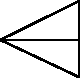
\includegraphics[scale=1]{gesamttex/edit_VIII-4/images/LH_35_13_03_220-221_d10_221v.pdf}
\edcaption{\lbrack\textit{Fig.~10}\rbrack}
\end{edfigure}

\section[tocentry={Hilfsrechnungen zum schiefen Mehrkörperstoß},
head={Hilfsrechnungen zum schiefen Mehrkörperstoß}]
{\MakeUppercase{Hilfsrechnungen zum schiefen Mehrkörperstoß}}
\label{39763}
\begin{ledgroupsized}[r]{120mm}
\footnotesize
\pstart
\noindent\textbf{Überlieferung:}
\pend
\end{ledgroupsized}
\begin{ledgroupsized}[r]{114mm}
\footnotesize
\pstart \parindent -6mm
\makebox[6mm][l]{\textit{L}}%
Aufzeichnung:
LH~IV~1, 4d, 2~Bl.~4. 
Ein Zettel (ca.~10~x~7~cm.);
unterer Rand nach Abriss schief, die übrigen Ränder beschnitten.
N.\;\ref{39763} nimmt ein Drittel der Textfläche von 
Bl.~\href{\Scan{LH_04_01_04d_02_004v}}%
{4~v\textsuperscript{o}}
ein.
Außerdem überliefert der Träger zwei weitere Leibniztexte.
Auf Bl.~\href{\Scan{LH_04_01_04d_02_004v}}%
{4~v\textsuperscript{o}},
senkrecht zur Schreibrichtung, ist folgender Briefentwurf %
fragmentarisch erhalten (Konzept zu einem nicht erhaltenen Schreiben an
\indexN{\textls{Brosseau}, Christophe 1630\textendash1717}Christophe Brosseau, siehe \cite{02148}\textit{LSB} I, 9 N.\;276):
\textlangle\textendash\textrangle\textit{avois prié Monsi}\textlangle\textit{eur}\textrangle\ %
\lbrack/\rbrack\
\textlangle \textit{ter}\textrangle\textit{mes exprés de me}\textlangle\textendash\textrangle\ %
\lbrack/\rbrack\
\textlangle\textit{ga}\textrangle\textit{zettes sur mon comp}\textlangle\textit{te}\textrangle\
\lbrack/\rbrack\
\textlangle\textendash\textrangle\textit{s conviendra pas.}
\lbrack/\rbrack\
\textit{payer icy, à fin}
\lbrack/\rbrack\
\textit{comptes de S.\,A.\,E.}
\lbrack/\rbrack\
\textlangle\textendash\textrangle\textit{vint chargés}
\bracks{\textit{Text bricht ab.}} %
\textit{S.\,A.\,E.} ist eine Verbesserung von \textit{S.\,A.\,S.}
Bl.~\href{\Scan{LH_04_01_04d_02_004r}}%
{4~r\textsuperscript{o}}
überliefert eine Aufzeichnung über Descartes %
(\textit{Mons.~des Cartes a fait comme les charlatans}...), die in 
\cite{02150}\textsc{Foucher de Careil}, \textit{Nouvelles Lettres et Opuscules Inédits de Leibniz}, Paris 1857 
gedruckt vorliegt (S.\;12) und vsl. in einem Band der Sechsten Reihe erscheinen wird.
Weitere Textträger, die ursprünglich mit dem Zettel zusammenhingen, konnten noch nicht ermittelt werden. %
\pend
\end{ledgroupsized}
\selectlanguage{latin}
\vspace{8mm}
\pstart%
\normalsize%
\noindent
\edlabel{04_01_04d_02_004v_2a}%
\edtext{\href{\Scan{LH_04_01_04d_02_004v}}%
{\lbrack4~v\textsuperscript{o}\rbrack}\
$a=2b$.}{%
\lemma{\href{\Scan{LH_04_01_04d_02_004v}}%
{\lbrack4~v\textsuperscript{o}\rbrack}}%
\Bfootnote{%
\textit{(1)}~$\ind{3}A\ind{3}D^2+r$ %
\textit{(2)}~$a=2b$.~\textit{L}}}
$r=1$.
\pend
\pstart
$+ 2\sqrt{4+4}=4\sqrt{2}$
\pend
\pstart
$-ra^2b = -4$
\pend
\pstart
$4+4+2 = 8$
\pend
\pstart
\rule[-2.4ex]{0pt}{6.2ex}%
fit $\dfrac{\surd2 - 1}{2}$.%
\edlabel{04_01_04d_02_004v_2b}%
\pend
\pstart
\edlabel{04_01_04d_02_004v_1a}%
\edtext{}{%
\xxref%
{04_01_04d_02_004v_1a}{04_01_04d_02_004v_1b}%
\lemma{4.1}%
\Bfootnote{%
\textit{(1)}~2.1 %
\textit{(2)}~4.1 %
\textit{(3)}~$2a$ %
\textit{(4)}~2.2 %
\textit{(5)}~2.4 + 2
\textit{(a)}~\textit{a}
\textit{(b)}~\textit{b}
\textit{(6)}~$1.2+1.2$%
~\textit{L}}}%
$4.1$
\pend
\begin{edfigure}[0.25em]%
\includegraphics[scale=1]{%
gesamttex/edit_VIII-4/images/LH_04_01_04d_02_004v_d.pdf}
\edcaption[0em]{\lbrack\textit{Fig.~1}\rbrack}
\end{edfigure}
\pstart
$1.2+1.2$%
\edlabel{04_01_04d_02_004v_1b}%
\pend
\pstart
\rule[-2.4ex]{0pt}{6.0ex}%
$4.4b = a$.\enskip
$b=\dfrac{1}{4}$.%
\edlabel{04_01_04d_02_004v_3}%
\pend
\pstart
$\surd2 - 1$.\enskip
$16+8$.
\pend






\chapter[tocentry={De servanda vi, quantitate progressionis ac celeritate
\enskip \bracks{1696\,(?) \textendash\ 1700\,(?)}},
head={De servanda vi, quantitate progressionis ac celeritate}]%
{\MakeUppercase{De servanda vi, quantitate progressionis ac celeritate}
\newline \bracks{1696\,(?) \textendash\ 1700\,(?)}}
\label{intro_serv-quant-progressionis}
\vspace{5mm}
\begin{ledgroup}
\footnotesize
\pstart
\noindent%
Die folgenden Stücke N.\;\ref{60308} und N.\;\ref{60307} sind inhaltlich und formal eng miteinander verbunden. 
Beim Konzept N.\;\ref{60307} handelt es sich um eine Ausarbeitung der kürzeren, hauptsächlich aus Rechnungen bestehenden Aufzeichnung N.\;\ref{60308}.
Die Berechnungen der vektoriellen Geschwindigkeiten und der Impulse beim Zweikörperstoß aus N.\;\ref{60308} 
kommen, trotz abweichender Nummerierung, in N.\;\ref{60307} unter Verwendung ähnlicher Kennzeichen wieder vor. 
Dabei weitet Leibniz einerseits die Betrachtung auf die Berechnung einer dritten Größe, der quadratischen \textit{vis}, aus;
andererseits ergänzt er die Rechnungen um einige methodologische Bemerkungen (z.\,B. über die dimensional aufsteigende Hierarchie der genannten physikalischen Größen und deren Erhaltungssätze)
und um eine kurze einleitende Erläuterung der verwendeten Symbolik.
An letztgenannter Stelle von N.\;\ref{60307} wird das Abhängigkeitsverhältnis beider Stücke deutlich:
Während das Konzept zunächst von einer Gleichung seinen Ausgang nahm, und zwar derselben wie bereits die Aufzeichnung N.\;\ref{60308},
hat Leibniz diesen Anfang gestrichen und den Gleichungen bzw. \glqq Theoremen\grqq\ die genannte Einleitung vorhergehen lassen (siehe die Varianten zu \refpassage{37_05_062_1a}{37_05_062_1b}).
\pend
\pstart
Das \href{\Scan{LH_37_05_062wz}}%
{Wasserzeichen} im Träger von N.\;\ref{60307} (einfaches Posthorn ohne Beizeichen) 
konnte noch nicht identifiziert werden.
Vielmehr stützt sich die vorgeschlagene Datierung auf Bezüge zu weiteren Texten: 
einerseits auf die terminologischen Ähnlichkeiten zwischen den vorliegenden Stücken und einem auf den Zeitraum 1696\textendash1698 datierbaren Text (\cite{02147}\textit{LSB} VIII,~3 N.\;76),
andererseits auf den Umstand, dass die besonders in N.\;\ref{60307} ausgearbeitete Liste dreier Erhaltungssätze samt ihrer dimensional aufsteigenden Anordnung (\refpassage{37_05_062_7a}{37_05_062_7b}) 
ein Kernstück des etwa 1700 entstandenen, unveröffentlichten \cite{02181}\textit{Essay de Dynamique} bildet (\textit{LMG} VI, S.\;215\textendash231, bes. S.\;226\textendash228).
\pend
\pstart
Bei dem ersten Text handelt es sich um 
\cite{02147}kommentierte Auszüge aus
\indexN{\textls{Sohier}, G.~J. gest. nach 1696}G.\,J.\,\textsc{Sohier}, 
\cite{00526}\glqq Nouveau systeme de la percussion des corps\grqq,
\cite{00157}\textit{JS} 7.~Mai 1696, S.\;211\textendash214.
Erstens verwendet Leibniz in den Auszügen dieselbe (ins Französische übertragene) Terminologie der \textit{vires impeditivae} bzw. \textit{progressiones} wie in N.\;\ref{60308} und N.\;\ref{60307} (\textit{LSB} VIII,~3, S.\;792\,f.). 
Zweitens schreibt er in einer gestrichenen Variante einige lateinische Sätze, die mit dem letzten Absatz von N.\;\ref{60307} (\glqq Notatu dignum \lbrack...\rbrack\ cum aequalis progressio aggressioni\grqq, hier auf \refpassage{37_05_062_6a}{37_05_062_6b}) nahezu wörtlich übereinstimmen: 
"Notandum autem quantum corpus corpori dat progressionis suae, tantum amittit. 
Unde paradoxum, omnibus redactis ad quietem servari posse quantitatem progressionis totalem, 
ea enim nulla erit si quantum erat progressus tantum obgressus"
(Variante \textit{(1)} zu S.\;793 Z.~18\textendash S.\;794 Z.~1).
Diese auffallende Übereinstimmung ist vielleicht dadurch zu erklären, dass Leibniz beim Verfassen der Auszüge die ihm vorliegenden Sätze aus N.\;\ref{60308} in den französischen Text eingearbeitet hat.
\pend
\pstart
Die Begrifflichkeit der \glqq force impeditive ou progressive\grqq\ kommt außerdem 
bei der Behandlung von Stoßfragen im Briefwechsel mit Papin der Jahre 1696\textendash1698 häufig vor: 
siehe dazu die editorische Datierung der \indexN{\textls{Sohier}, G.~J. gest. nach 1696}Sohier-Auszüge (\textit{LSB} VIII,~3 N.\;76, S.\;790\,f.) und Leibnizens Briefe an Papin
\cite{02071}vom 16. (26.) Juli 1696, 
\cite{01503}8. (18.) November 1697 und 
\cite{02073}16. (26.) Januar 1698
(\textit{LSB} III, 7 N.\;8, N.\;156 resp. N.\;177).
Aus den genannten Gründen wird für N.\;\ref{60308} und N.\;\ref{60307}
die Datierungsspanne 1696 bis 1700 vorgeschlagen.
\pend 
\end{ledgroup}

\section[tocentry={De progressionibus seu viribus impeditivis in ictu},
head={De progressionibus seu viribus impeditivis in ictu}]%
{\MakeUppercase{De progressionibus seu viribus impeditivis in ictu}}
\label{60308}
\begin{ledgroupsized}[r]{120mm}
\footnotesize
\pstart
\noindent\textbf{Überlieferung:}
\pend
\end{ledgroupsized}
\begin{ledgroupsized}[r]{114mm}
\footnotesize
\pstart \parindent -6mm
\makebox[6mm][l]{\textit{L}}%
Aufzeichnung:
LH~XXXVII~5~Bl.~63.
Ein Zettel (ca.~18~x~5,5~cm.).
Papiererhaltungsmaßnahmen;
oberer und rechter Rand beschnitten.
Eine Seite auf Bl.~63~r\textsuperscript{o}; Bl.~63~v\textsuperscript{o} leer.
\pend
\end{ledgroupsized}
\selectlanguage{latin}
\vspace{8mm}
\pstart%
\normalsize%
\noindent%
\href{\Scan{LH_37_05_063r}}%
{\lbrack63~r\textsuperscript{o}\rbrack}\
(1\textsuperscript{mo}) $av+bx=ay
\edtext{+bz$. ((1\textsuperscript{mo})) seu $v-y,:,-x+z\lbrack=\rbrack b:a$. (2\textsuperscript{do}) $v-x=-y+z$. Ex 2}{%
\lemma{}\Bfootnote{%
$+bz$. 
\bars{((1\textsuperscript{mo})) seu 
\bars{$v-y,:,-x+z : b:a$  \textit{ändert~Hrsg.}}
\bars{seu differenti \textit{streicht Hrsg.}}
\textit{erg.}}
.~(2\textsuperscript{do})
\textit{(1)}~$v-y$ %
\textit{(2)}~$v-x=-y+z$.
\textit{(a)}~$z=$
\textit{(b)}~3\textsuperscript{tio} $z=v-x+y$. 4\textsuperscript{to} 
\textit{(c)}~Ex 2~\textit{L}}} 
fit (3\textsuperscript{tio}) $z=v-x+y$.
Ex 3 et 1 fit (4\textsuperscript{to}) $av+bx=ay+bv-bx+by$. 
Et hinc fit 
\edtext{(5\textsuperscript{to}) $(a-b)v}{\lemma{(5\textsuperscript{to})}\Bfootnote{%
\textit{(1)}~$av+bx$ %
\textit{(2)}~$\overline{a-b}\; v+2bx=\overline{a+b}\; y$ %
\textit{(3)}~$(a-b)v\protect\vphantom()+$ %
\textit{(4)}~$(a-b)v$~\textit{L}}} 
+2bx=(a+b)y$ et pari jure 
\edtext{fit (6\textsuperscript{to})}{\lemma{fit}\Bfootnote{%
\textit{(1)}~$2by$ %
\textit{(2)}~(6\textsuperscript{to})~\textit{L}}} 
$(a-b)z+2by=\edlabel{37_05_063_1a}(a+b)x$.%
\edtext{}{{\xxref{37_05_063_1a}{37_05_063_1b}}\lemma{$(a+b)x$.}\Bfootnote{%
\textit{(1)}~Fit %
\textit{(2)}~Aestimemus~\textit{L}}}
\pend
\pstart
Aestimemus\edlabel{37_05_063_1b} 
vires impeditivas\indexS{vis impeditiva}
\edtext{seu progressiones.\indexS{progressio}}{\lemma{}\Bfootnote{seu progressiones \textit{erg.~L}}} 
\edtext{(7\textsuperscript{mo})}{\lemma{}\Bfootnote{(7\textsuperscript{mo}) \textit{erg.~L}}} 
$av=11$\lbrack,\rbrack\
\edtext{(8\textsuperscript{vo})}{%
\lemma{}%
\Bfootnote{%
(8\textsuperscript{vo}) %
\textit{erg.~L}}}
$bx=21$\lbrack,\rbrack\
(9\textsuperscript{no}) 
\edtext{$ay=12$\lbrack,\rbrack\ %
\edtext{(10\textsuperscript{mo})}{\lemma{(10\textsuperscript{mo})}%
\Cfootnote{Diese Zählung wird von Leibniz zweimal verwendet.}}
$bz=22$. Ergo (10\textsuperscript{mo})}{%
\lemma{$ay=12$}%
\Bfootnote{%
\bars{(10\textsuperscript{mo}) \textit{erg.}} $bz=22$. Ergo
\textit{(1)}~$v=11:a$. \textit{x} %
\textit{(2)}~(10\textsuperscript{mo})~\textit{L}}}
$v=11:a$\lbrack,\rbrack\
(11\textsuperscript{mo}) $x=21:b$\lbrack,\rbrack\
(12\textsuperscript{o}) $y=12:a$\lbrack,\rbrack\
(13\textsuperscript{o}) $z=22:b$.
Quos 
\edtext{valores ex articulis 10, 11, 12, 13,}{\lemma{valores}\Bfootnote{%
\textit{(1)}~in aeqq. %
\textit{(2)}~ex %
\textit{(a)}~aeqq. 7, 8, 9, 10 %
\textit{(b)}~articulis %
\textit{(aa)}~7, 8, 9, 10 %
\textit{(bb)}~10, 11, 12, 13,~\textit{L}}} 
substituendo 
\edtext{in 1, et 2.\ utique}{\lemma{in}\Bfootnote{%
\bars{aeqq. \textit{gestr.}} 1, et 2.\
\textit{(1)}~fiet ex 1.\ %
\textit{(2)}~\bars{utique ex 1.\ \textit{streicht~Hrsg.}} %
\textit{(3)}~fiet ex 1.\ %
\textit{(4)}~utique~\textit{L}}} 
ex 1.\ fiet
\edtext{(14\textsuperscript{o})}{\lemma{}\Bfootnote{(14\textsuperscript{o}) \textit{erg.~L}}} 
$11+21=12+22$ et 
\edtext{ex 2 fiet (15\textsuperscript{to})}{\lemma{ex 2 fiet}\Bfootnote{%
\textit{(1)}~15\textsuperscript{to} %
\textit{(2)}~(15\textsuperscript{o}) %
\textit{(3)}~(15\textsuperscript{to})~\textit{L}}} 
$(11:a)-(21:b)=
\edtext{-(12:a)+\lbrack(22:b)\rbrack$ vel (16\textsuperscript{to})}{\lemma{}\Bfootnote{$-(12:a)$ 
\bars{$+22:b$ \textit{ändert~Hrsg.}}
\textit{(1)}~adeoque fiet
\textit{(2)}~vel
\textit{(a)}~$(11+12)$
\textit{(b)}~(16\textsuperscript{to})~\textit{L}}} 
$11+12,:a=21+22,:b$ vel (17\textsuperscript{mo}) 
$11+12,:21+22=
\edtext{a:b$. Ergo (18\textsuperscript{vo}) $11b-21a=-12b+22a$. Ejusdem}{\lemma{$a:b$}\Bfootnote{%
\textit{(1)}~seu differentiae vel su %
\textit{(2)}~. Si ad easdem partes t %
\textit{(3)}~. Si ad %
\textit{(4)}~\bars{Ergo (18\textsuperscript{vo}) $11b-21a=-12b+22a$. \textit{erg.}} %
Ejusdem~\textit{L}}} 
corporis si ad easdem partes
\edtext{tendat summae,\indexS{summa virium impeditivarum ejusdem corporis}}{\lemma{tendat}\Bfootnote{%
\textit{(1)}~differentiae %
\textit{(2)}~summae,~\textit{L}}}
si ad 
\edtext{contrarias differentiae\indexS{differentia virium impeditivarum ejusdem corporis}}{\lemma{contrarias}\Bfootnote{%
\textit{(1)}~summae %
\textit{(2)}~differentia %
\textit{(3)}~differentiae~\textit{L}}} 
virium impeditivarum\indexS{vis impeditiva} sunt ut corpora; 
\edtext{vel generalius summae}{\lemma{vel}\Bfootnote{\bars{generalius \textit{erg.}} %
\textit{(1)}~differentiae %
\textit{(2)}~summae~\textit{L}}} 
progressionum\indexS{progressio} 
\edtext{ejusdem corporis\indexS{summa progressionum ejusdem corporis}}{\lemma{}\Bfootnote{ejusdem corporis \textit{erg.~L}}} 
ante ictum et post ictum\indexS{ictus} 
\ledpb%
sunt ut 
\edtext{corpora. Ex 1 summa progressionis}{\lemma{corpora}\Bfootnote{%
\textit{(1)}~, quia differentia virium im %
\textit{(2)}~, quia
\textit{(3)}~, generalius loquendo, %
\textit{(4)}~, quod ita generale est. %
\textit{(5)}~. Jam tollatur valor ipsius 22 %
\textit{(a)}~ex 13 %
\textit{(b)}~per 14, fiet (18\textsuperscript{vo}) $22=11+21-12$ ergo ex 17 fiet (19\textsuperscript{no}) $11-12,:, 21-11 - 21+12$ %
\textit{(6)}~. Memorabile est \bars{(18\textsuperscript{vo}) \textit{erg.}} $11-12=-21+22$ et summa progress %
\textit{(7)}~Aeq. 1 %
\textit{(8)}~. Ex 1 summa progressionis~\textit{L}}} 
ante ictum\indexS{summa progressionis ante ictum} aequalis summae progressionis post ictum.\indexS{summa progressionis post ictum} 
Ex 2 differentia velocitatum progrediendi\indexS{differentia velocitatum progrediendi} ante ictum\indexS{ictus}
aequalis 
differentiae velocitatum progrediendi\indexS{differentia velocitatum progrediendi} post ictum.\indexS{ictus} 
Seu velocitas respectiva\indexS{velocitas respectiva} eadem. 
Posses quantitatem progressus\indexS{quantitas progressus} et vim impeditivam\indexS{vis impeditiva}
pro eodem sumere.
\pend 

\section[tocentry={Accessio calculi dynamici},
head={Accessio calculi dynamici}]%
{\MakeUppercase{Accessio calculi dynamici}}
\label{60307}
\begin{ledgroupsized}[r]{120mm}
\footnotesize
\pstart
\noindent\textbf{Überlieferung:}
\pend
\end{ledgroupsized}
\begin{ledgroupsized}[r]{114mm}
\footnotesize
\pstart \parindent -6mm
\makebox[6mm][l]{\textit{L}}%
Konzept:
LH~XXXVII~5~Bl.~62. 
Ein Blatt~4\textsuperscript{o};
\href{\Scan{LH_37_05_062wz}}%
{Wasserzeichen};
Papiererhaltungsmaßnahmen;
oberer, linker und rechter Rand beschnitten.
Eine Seite auf Bl.~62~r\textsuperscript{o}; Bl.~62~v\textsuperscript{o} leer bis auf die eigh.\ Anmerkung
(in Bleistift, quer): 
\textit{Geometriae Organicae onus} \lbrack/\rbrack\
\textit{id, quo} \textlangle\textit{ser}\textrangle \textit{vit der Geometriae} \lbrack/\rbrack\ 
\textit{pro meis \greek{f}oronomicis} \lbrack/\rbrack\ 
\textit{illustrandis}.
Zum Begriff \glqq geometria organica\grqq\ (d.\,h. geometrische Beweisführung unter Verwendung komplexerer Hilfsmittel als Zirkel und Lineal) siehe bspw. 
\cite{02155}\textit{De geometria seu potius algebra mechanica} von 1673
(\textit{LSB} VII, 1 N.\;8, bes. S.\;104\textendash106).
\pend
\end{ledgroupsized}
\selectlanguage{latin}
\vspace{8mm}
\pstart
\centering
\href{\Scan{LH_37_05_062r}}%
{\lbrack62~r\textsuperscript{o}\rbrack}
\hfill
Accessio calculi 
\edlabel{37_05_062_1a}%
\edtext{}{%
{\xxref%
{37_05_062_1a}{37_05_062_1b}}%
\lemma{dynamici}%
\Bfootnote{%
\textit{(1)}~$av+$
\textit{(2)}~Primo $av+b$
\textit{(3)}~(1)\textsuperscript{mo}
\textit{(4)}~\textit{a}~\textit{L}%
}}%
dynamici
\hfill
\phantom{\lbrack62~r\textsuperscript{o}\rbrack}
\pend
\vspace{0.5\baselineskip}
\pstart 
\begin{tabular}[b]{ccccc}\textit{a}\edlabel{37_05_062_1b}&ante ictum\indexS{ictus}&\textit{v}&post ictum&\textit{y}\\\textit{b}&ante ictum&\textit{x}&post ictum\indexS{ictus}&\textit{z}\end{tabular} %
\pend
\pstart\noindent
\edtext{ponendo \textit{v}, \textit{x}, \textit{y}, \textit{z} esse velocitates sumtas ad easdem partes ad quas maxima est progressio.\indexS{progressio} Quod si corpus contra procedat significatur quantitas negativa.}{%
\lemma{}%
\Bfootnote{%
ponendo \lbrack...\rbrack\  negativa. %
\textit{erg.~L}}}
\pend
\pstart 
\edtext{(Primo)}{%
\lemma{}%
\Bfootnote{%
(Primo) %
\textit{erg.~L}%
}}
$avv+bxx=ayy+bzz$.
(2\textsuperscript{do}) 
$av+bx=%
\edlabel{37_05_062_2a}%
\edtext{}{%
{\xxref%
{37_05_062_2a}{37_05_062_2b}}%
\lemma{}\Bfootnote{%
$ay+bz$.
\bars{Tollatur \textit{a}, \textit{b} per 1 et 2 prodibit aeq.~3 \textit{erg.\ u.\ gestr.}}
\bars{Tollendo $a:b$ prodibit \textit{erg.}} 
(3\textsuperscript{tio})~\textit{L}}}%
ay+bz$. Tollendo $a:b$ prodibit (3\textsuperscript{tio})\edlabel{37_05_062_2b}
$v-x=-y+z$. \pend
\pstart Primum 
\edtext{Theorema}{\lemma{}\Bfootnote{Theorema \textit{erg.~L}}} 
sic 
\edtext{enuntiatur\lbrack:\rbrack\ potentia ante concursum\indexS{concursus}\indexS{potentia ante concursum} est aequalis}{\lemma{enuntiatur}\Bfootnote{%
\textit{(1)}~vires ante ictum sunt aequ %
\textit{(2)}~potentia ante %
\textit{(a)}~ictum %
\textit{(b)}~concursum est aequalis~\textit{L}}} 
potentiae post concursum.\indexS{concursus}\indexS{potentia post concursum}\pend
\pstart Secundum ita: progressio ante concursum\indexS{concursus}\indexS{progressio ante concursum} est aequalis progressioni
\edlabel{37_05_062_3a}%
\edtext{}{{\xxref{37_05_062_3a}{37_05_062_3b}}%
\lemma{post concursum.}%
\Bfootnote{%
\textit{(1)}~Tertium tandem \bars{sic: \textit{streicht Hrsg.}} %
\textit{(a)}~celeritas respectiva, ante ictum, est aequalis %
\textit{(b)}~celeritas mutatae d %
\textit{(2)}~Tertium~\textit{L}}}%
post concursum.\indexS{concursus}\indexS{progressio post concursum}
\pend
\pstart Tertium\edlabel{37_05_062_3b}
ita: celeritas respectiva seu mutandae distantiae\indexS{celeritas mutandae distantiae} ante concursum,\indexS{concursus}\indexS{celeritas respectiva ante concursum} 
aequatur celeritati respectivae post concursum.\indexS{concursus}\indexS{celeritas respectiva post concursum} 
Posset et sic enuntiari 
\edtext{(4\textsuperscript{to})}{\lemma{}\Bfootnote{(4\textsuperscript{to}) \textit{erg.~L}}} 
$v+y=x+z$ seu summa celeritatum progrediendi\indexS{celeritas progrediendi} ejusdem corporis\indexS{summa celeritatum progrediendi ejusdem corporis} ante et post concursum\indexS{concursus} in utroque corpore eadem est. 
Et ex artic.~2.\ fieri potest 
\edtext{(5\textsuperscript{to})}{\lemma{}\Bfootnote{(5\textsuperscript{to}) \textit{erg.~L}}} 
$v-y,:,-x+z=b:a$ id est differentiae celeritatum progrediendi\indexS{celeritas progrediendi} ejusdem corporis\indexS{differentia celeritatum progrediendi ejusdem corporis} sunt reciproce ut duo corpora. 
\pend
\pstart
Unde ex 4 et 5 fit differentiae quadratorum a celeritatibus\indexS{quadratum celeritatis} ejusdem corporis\indexS{differentia quadratorum celeritatum progrediendi ejusdem corporis} sunt reciproce 
\edtext{ut duo corpora, seu}{\lemma{ut}\Bfootnote{%
\textit{(1)}~corpora %
\textit{(2)}~duo corpora, %
\textit{(a)}~seu 6. %
\textit{(b)}~seu %
\textit{(c)}~seu~\textit{L}}} 
(6\textsuperscript{to}) $vv-yy,:,-xx+zz=b:a$. Sed haec aequatio etiam patet ex aequ.~1. %
\pend
\pstart
\edlabel{37_05_062_7a}%
Haec 
\edtext{jam theoremata}{\lemma{jam}\Bfootnote{%
\textit{(1)}~ad %
\textit{(2)}~theorema caeter %
\textit{(3)}~theoremata~\textit{L}}} 
suo quodam modo ad tria etiam et plura corpora produci possunt. Semper enim quantitas virium\indexS{quantitas virium} et quantitas progressionis\indexS{quantitas progressionis} sunt aequales. 
In duobus tamen etiam celeritates respectivae\indexS{celeritas respectiva} sunt aequales. 
Itaque in duobus corporibus elegantissime dici 
\edtext{potest, in duobus}{\lemma{potest,}\Bfootnote{%
\textit{(1)}~conservari %
\textit{(2)}~in duobus~\textit{L}}} 
corporibus concurrentibus conservantur vires,\indexS{vis}\indexS{conservatio virium} progressiones,\indexS{progressio}\indexS{conservatio progressionis} 
\edtext{et respectivae celeritates.\indexS{celeritas respectiva}\indexS{conservatio celeritatis respectivae}}{\lemma{et}\Bfootnote{%
\textit{(1)}~celeritates respective %
\textit{(2)}~respectivae celeritates.~\textit{L}}}
Tria scilicet quorum primum est trium,
secundum duarum,
3tium unius dimensionis.\indexS{dimensio}%
\edlabel{37_05_062_7b}%
\pend
\pstart Jam alias literas assumamus, ad exprimendas
\edtext{ipsas}{%
\lemma{}%
\Bfootnote{%
ipsas %
\textit{erg.~L}%
}}
progressiones. 
\edtext{Sit (7\textsuperscript{mo})}{%
\lemma{Sit}%
\Bfootnote{%
\textit{(1)}~$av=11$ et %
\textit{(2)}~(7\textsuperscript{mo})~\textit{L}%
}}
$av=11$, et $bx=21$ et $ay=12$ et $bz=22$. Ex 2 fiet 
\edlabel{37_05_062_4a}%
\edtext{}{{\xxref{37_05_062_4a}{37_05_062_4b}}%
\lemma{(8\textsuperscript{vo}) \lbrack...\rbrack\  (9\textsuperscript{no})}%
\Cfootnote{Die Zählungen (8\textsuperscript{vo}) und (9\textsuperscript{no}) werden von Leibniz je zweimal verwendet.}}%
(8\textsuperscript{vo}) 
$11+21=%
\edtext{12+22$. Et}{\lemma{$12+22$.}\Bfootnote{%
\textit{(1)}~Et ex 3 fiet %
\textit{(2)}~Et~\textit{L}}} 
per 7.\ fiet (8\textsuperscript{vo}) $v=11:a$ et $x=21:b$ et $y=12:a$, et $z=22:b$. Ergo ex artic.~3 per 8, fiet 
\edtext{(9\textsuperscript{no})}{\lemma{}\Bfootnote{(9\textsuperscript{no}) \textit{erg.~L}}} 
$(11:a)-(21:b)=-(12:a)+(22:b)$ vel $11+12\,,:a=21+22\,,:b$ 
seu (9\textsuperscript{no})\edlabel{37_05_062_4b}
$11+12,:,21+22=a:b$ id est summae progressionum\indexS{progressio}
ejusdem corporis\indexS{summa progressionum ejusdem corporis} sunt ut 
\edlabel{37_05_062_5a}%
\edtext{}{%
{\xxref%
{37_05_062_5a}{37_05_062_5b}}%
\lemma{corpora.}%
\Bfootnote{%
\textit{(1)}~Ex %
\textit{(2)}~Denique ex %
\textit{(3)}~Et ex %
\textit{(4)}~Jam \lbrack...\rbrack\ $-21+22$. %
\textit{(a)}~Ergo fit (11\textsuperscript{mo}) %
\textit{(b)}~Fiet %
\textit{(c)}~Eodem modo %
\textit{(aa)}~fit %
\textit{(bb)}~(10\textsuperscript{mo}) sit $avv=13$ $bxx=23$ $ayy=14$ $bzz=24$. Ergo ex 1 per 10 fit \bars{(11\textsuperscript{mo}) \textit{erg.}} $13+23=14+24$.
\textit{(aaa)}~Et
\textit{(bbb)}~Et (12\textsuperscript{mo}) $v=$  %
\textit{(aaaa)}~$\surd 13:a$ %
\textit{(bbbb)}~$\surd (13:a)$ et %
\textit{(aaaaa)}~(13\textsuperscript{tio}) %
\textit{(bbbbb)}~$x=\surd (23:b)$ et $y=(14:a)$ et $z=\surd (24:b)$ %
\textit{(d)}~Ergo fie %
\textit{(e)}~Ergo ha %
\textit{(f)}~Ergo habebimus (11\textsuperscript{mo})~\textit{L}}}%
corpora. Jam ex 8 fit (10\textsuperscript{mo}) $11-12=-21+22$. %
\pend	
\pstart
Ergo habebimus (11\textsuperscript{mo})\edlabel{37_05_062_5b}
$11^2-12^2,:,-21^2+22^2=a:b$ seu differentiae quadratorum a progressionibus ejusdem corporis,\indexS{differentia quadratorum progressionum ejusdem corporis} sunt ut 
\edtext{corpora. Comparando}{\lemma{corpora.}\Bfootnote{%
\textit{(1)}~Unde ex 11 et 6 sequitur %
\textit{(2)}~Comparando~\textit{L}}}
jam articulos 5 et 9, fiet\lbrack:\rbrack\ summae progressionum 
\edtext{ejusdem\indexS{summa progressionum ejusdem corporis}}{\lemma{}\Bfootnote{ejusdem \textit{erg.~L}}} 
sunt reciproce ut differentiae celeritatum 
\edtext{progrediendi ejusdem\indexS{differentia celeritatum progrediendi ejusdem corporis} computando}{\lemma{}%
\Bfootnote{progrediendi \bars{ejusdem \textit{erg.}} 
\textit{(1)}~tam
\textit{(2)}~computando~\textit{L}}} 
unamquamque ex eo quod in eodem corpore fit ante et post concursum,\indexS{concursus} seu (12\textsuperscript{mo}) 
$v-y,:,-x+z=11+12,:,
\edtext{21+22$. Et conjungendo articulos 6 et 11, fiet: differentiae}{\lemma{$21+22$.}\Bfootnote{%
\textit{(1)}~\bars{Et \textit{streicht Hrsg.}} %
 similiter summae a quadratis %
\textit{(2)}~Et conjungendo articulos 6 et 11, fiet: %
\textit{(a)}~summae a quadrat %
\textit{(b)}~differentiae~\textit{L}}} 
a quadratis progressionum ejusdem\indexS{differentiae quadratorum progressionum ejusdem corporis} sunt 
\edtext{reciproce ut differentiae}{\lemma{reciproce}\Bfootnote{%
\textit{(1)}~ut summae a quadratis %
\textit{(2)}~ut differentiae~\textit{L}}} 
a quadratis celeritatum progressionum ejusdem,\indexS{differentia quadratorum celeritatum progressionum ejusdem corporis} vel quia in quadratis evanescunt differentia signa, 
idemque est quadratum celeritatis\indexS{quadratum celeritatis} et celeritatis progrediendi,\indexS{quadratum celeritatis progrediendi} idemque quadratum quantitatis motus\indexS{quantitas motus}\indexS{quadratum quantitas motus} 
\edtext{seu motionis,}{\lemma{}\Bfootnote{seu motionis \textit{erg.~L}}}
et progressionis;\indexS{quantitas motionis et progressionis} 
\edtext{ideo fient}{\lemma{ideo}\Bfootnote{%
\textit{(1)}~fiet %
\textit{(2)}~fient~\textit{L}}} 
differentiae a quadratis quantitatum motus,\indexS{differentia quadratorum quantitatum motus} reciproce, 
ut differentiae a quadratis celeritatum.\indexS{differentia quadratorum celeritatum}
Calculo autem ex 6 et 11 fiet 
\edtext{(13\textsuperscript{tio})}{\lemma{}\Bfootnote{(13\textsuperscript{tio}) \textit{erg.~L}}} 
\edtext{$v^2-y^2,:,-x^2+z^2=11^2-12^2,:,-21^2+22^2$.}{%
\lemma{$v^2-y^2 \lbrack...\rbrack\ +22^2$}%
\Cfootnote{%
Die rechte Seite der Gleichung heißt eigentlich $-21^2+22^2,:,11^2-12^2$.}}
Denique ex 11 fiet 
\edtext{(14\textsuperscript{to})}{\lemma{}\Bfootnote{(14\textsuperscript{to}) \textit{erg.~L}}} 
$b11^2+a21^2=b12^2+a22^2$.
\pend
\pstart Si eadem methodo pro viribus\indexS{vis} ipsis exprimendis utamur, rursus theoremata 
\edtext{prodibunt. Sit (15\textsuperscript{mo})}{\lemma{prodibunt.}\Bfootnote{%
\textit{(1)}~Sit %
\textit{(2)}~Sit (15\textsuperscript{mo})~\textit{L}}} 
$avv=13$\lbrack,\rbrack\ $bxx=23$, $ayy=14$\lbrack,\rbrack\ $bzz=24$, quibus jungendo 7, fiet 
\edtext{(16\textsuperscript{to})}{\lemma{}\Bfootnote{(16\textsuperscript{to}) \textit{erg.~L}}} 
$11v=13$ et $21x=23$ et $12y=14$ et $22z=24$. 
\edtext{Ergo (17\textsuperscript{mo}) $v=13:11$}{\lemma{Ergo}\Bfootnote{%
\textit{(1)}~$v=13:11$ %
\textit{(2)}~(17\textsuperscript{mo}) $v=13:11$~\textit{L}}} 
et $x=23:21$ et $y=14:12$ et $z=24:22$. Et per 17 ex artic.~3.\ fiet 
\edtext{(18\textsuperscript{vo})}{\lemma{}\Bfootnote{(18\textsuperscript{vo}) \textit{erg.~L}}} 
$(13:11)-(23:21)= 
\edtext{-(14:12)+(24:22)$. Sed et ex 15 sit (19\textsuperscript{no}) $v=\surd,13:a$}{\lemma{$-(14:12)+(24:22)$.\lbrack,\rbrack}\Bfootnote{%
\textit{(1)}~Seu %
\textit{(2)}~Sed nihil hinc magnopere %
\textit{(3)}~Sed potius %
\textit{(4)}~Sed et %
\textit{(a)}~\textit{va} %
\textit{(b)}~ex 15 %
\textit{(aa)}~fit %
\textit{(bb)}~sit \bars{(19\textsuperscript{no}) \textit{erg.}} %
\textit{(aaa)}~$v=$ %
\textit{(bbb)}~$v=\surd,13:a$~\textit{L}}}
$x=\surd,23:b$\lbrack,\rbrack\ $y=\surd,14:a$\lbrack,\rbrack\ $z=\surd,24:b$. 
\edtext{Porro ex}{\lemma{}\Bfootnote{Porro ex \bars{\textit{streicht Hrsg.}} ex~\textit{L}}} 
1 per 15 fit 
\edtext{(20\textsuperscript{mo})}{\lemma{}\Bfootnote{(20\textsuperscript{mo}) \textit{erg.~L}}} 
$13+23=14+24$. %
\pend
\pstart
Alia etiam Theoremata prodibunt, 
\edtext{si pro}{\lemma{si}\Bfootnote{%
\textit{(1)}~ipsas %
\textit{(2)}~pro~\textit{L}}} 
quadratis celeritatum\indexS{quadratum celeritatis} literas sumamus. \pend
\pstart 
\edlabel{37_05_062_6a}%
Notatu dignum quia conservatur quantitas progressionis,\indexS{quantitas progressionis} 
hinc corpus tantum amittere progressionis\indexS{progressio} quantum dat 
\edtext{alteri. Aggressionem\indexS{aggressio}}{%
\lemma{alteri.}%
\Bfootnote{%
\textit{(1)}~Obgressionem %
\textit{(2)}~Aggressionem~\textit{L}}}
\edtext{a.}{%
\lemma{a.}%
\Cfootnote{\textit{autem}}}
possumus vocare contrariam progressionem.\indexS{progressio} 
Paradoxum servari quantitatem progressionis\indexS{quantitas progressionis}\indexS{conservatio quantitatis progressionis} 
omnibus ad quietem redactis. 
\edtext{Nam totalis progressio\indexS{progressio} 
\edtext{\bracks{nulla}}{%
\lemma{}%
\Bfootnote{nonnulla \textit{L ändert Hrsg.}}}
est, cum aequalis progressio\indexS{progressio} aggressioni.\indexS{aggressio}%
\edlabel{37_05_062_6b}}{%
\lemma{Nam \bracks{...} aggressioni}%
\Cfootnote{%
Zur Emendation von "nonnulla" in "nulla" vgl. die gestrichene Variante \textit{(1)} zu \textit{LSB} VIII,~3 N.\;76, S.\;793.18--794.1 (siehe dazu die Einleitung zu N.\;\ref{intro_serv-quant-progressionis}).}}
\pend 




\chapter[tocentry={Ope principii celeritatum molibus reciprocarum ac hypotheseos penetrationis cuncta in concursu duorum possunt derivari
\enskip \bracks{August 1697\,(?) \textendash\ April 1703\,(?)}},
head={Principia celeritatum molibus reciprocarum ac penetrationis}]%
{\MakeUppercase{Ope principii celeritatum molibus reciprocarum ac hypotheseos penetrationis cuncta in concursu duorum possunt derivari}
\newline \bracks{August 1697\,(?) \textendash\ April 1703\,(?)}}

\label{58297}
\begin{ledgroupsized}[r]{120mm}
\footnotesize
\pstart
\noindent\textbf{Überlieferung:}
\pend
\end{ledgroupsized}
\begin{ledgroupsized}[r]{114mm}
\footnotesize
\pstart \parindent -6mm
\makebox[6mm][l]{\textit{L}}%
Konzept:
LH~XXXV~13, 3~Bl.~237\textendash238. 
Ein Bogen~2\textsuperscript{o};
Wasserzeichen		%
in Bl.~237.
Zwei Seiten auf Bl.~237~r\textsuperscript{o} und Bl.~238~v\textsuperscript{o}; 
Bl.~237~v\textsuperscript{o} und Bl.~238~r\textsuperscript{o} leer.
\pend
\end{ledgroupsized}
\vspace{5mm}
\begin{ledgroup}
\footnotesize
\pstart
\noindent%
\textbf{Datierungsgründe:} %
Das Wasserzeichen im Träger von N.\;\ref{58297} ist bislang für den Zeitraum August 1697 bis April 1703 (besonders häufig ab 1700) belegt. %
\pend
\end{ledgroup}
\selectlanguage{latin}

\vspace{8mm}
\pstart%
\normalsize%
\noindent%
\href{\Scan{LH_35_13_03_237r}}%
{\lbrack237~r\textsuperscript{o}\rbrack}\
Supponamus corpus motum 
\edtext{incurrens\indexS{incursus centralis et normalis} centraliter et normaliter}{\lemma{incurrens}\Bfootnote{%
\textit{(1)}~directe 
\textit{(2)}~centraliter et normaliter~\textit{L}}} 
in aequale quiescens\indexS{corpus incurrens centraliter et normaliter in quiescens} dare 
\edtext{ei suam velocitatem,}{\lemma{ei}\Bfootnote{%
\textit{(1)}~suum motum 
\textit{(2)}~suam velocitatem,~\textit{L}}}
et quiescere ejus loco, nec referre, quae sit figura corporis 
\edlabel{35_13_03_237-238_7a}%
\edtext{}{%
{\xxref%
{35_13_03_237-238_7a}{35_13_03_237-238_7b}}%
\lemma{alterutrius.}%
\Bfootnote{%
\textit{(1)}~Sit jam corpus 
\textit{(2)}~Sint jam 
\textit{(3)}~Ponamus jam corpus \textit{A}~\textit{L}}}%
alterutrius.
\pend
\begin{edfigure}[1em]%
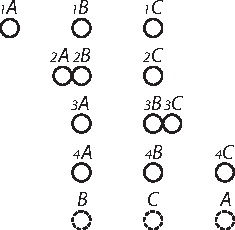
\includegraphics[scale=1]{gesamttex/edit_VIII-4/images/LH_35_13_03_237-238_d1_237r.pdf}
\edcaption{%
\edtext{\lbrack\textit{Fig.~1}\rbrack}{%
\lemma{\lbrack\textit{Fig.~1}\rbrack}%
\Cfootnote[nonum]{%
Zwei gestrichene Entwürfe zum Diagramm werden nicht wiedergegeben.}}}
\end{edfigure}
\pstart
Ponamus jam corpus \textit{A}%
\edlabel{35_13_03_237-238_7b}
incurrens in 
\edtext{aequale}{\lemma{}\Bfootnote{%
aequale \textit{erg.~L}}} 
corpus\indexS{corpus incurrens in aequale} \textit{B} ejus loco quiescere, 
et ipsi dare suum motum, corpus autem \textit{B}, pergens incurrere
\edtext{in corpus aequale \textit{C} et rursus quiescere eique}{\lemma{in corpus}\Bfootnote{%
\bars{aequale \textit{erg.}} \textit{C} 
\textit{(1)}~eique rurs 
\textit{(2)}~et rursus quiescere eique~\textit{L}}} 
dare suum motum; manifestum est quid 
\edlabel{35_13_03_237-238_1a}%
\edtext{}{{\xxref{35_13_03_237-238_1a}{35_13_03_237-238_1b}}%
\lemma{eveniat}\Bfootnote{%
\textit{(1)}~, sed quid si fingamus dum corpora \textit{B} et \textit{C} sejungi debent, \textit{B} quiescente, et \textit{C} pergente supervenire causam quae ea sejungi vetet, dicemus 
\textit{(2)}~. Et idem est~\textit{L}}}%
eveniat.
\pend
\pstart
Et idem est\edlabel{35_13_03_237-238_1b}
etsi sint corpora quotcunque \textit{A}, \textit{B}, \textit{C}, \textit{D}, ut semper fiat 
permutatio,\indexS{permutatio celeritatis} et cum ante 
concursum\indexS{concursus} omnem, moveatur tantum \textit{A}, quiescentibus 
\textit{B}, \textit{C}, \textit{D}, post omnem concursum\indexS{concursus} movebitur 
tantum \textit{D}, quiescentibus \textit{A}, \textit{B}, \textit{C}, perinde ac si \textit{A} ipsa \textit{B}, \textit{C}, 
\textit{D}, potuisset penetrare,\indexS{penetratio} et motum suum quasi ipsis non obstantibus continuasset, neque enim differunt 
status quarti momenti verus, a ficto per puncta designato, qui prodiisset, si \textit{A} transiisset et penetrando. \pend
\pstart Cumque idem
\edtext{prodeat etsi corpora}{\lemma{prodeat etsi}\Bfootnote{%
\textit{(1)}~puncta 
\textit{(2)}~corpora~\textit{L}}} 
\textit{A}, \textit{B}, \textit{C}, sibi immediata ponantur, seu etsi distantia 
\edtext{evanescat. Hinc}{\lemma{evanescat}\Bfootnote{%
\textit{(1)}~, generaliter apparet quis sit motus 
\textit{(2)}~. Hinc~\textit{L}}} 
si corpus incurrat\indexS{corpus incurrens in plura aequalia} simul in 
\edtext{plura aequalia in eadem}{\lemma{plura}\Bfootnote{%
\textit{(1)}~in ea 
\textit{(2)}~aequalia in eadem~\textit{L}}} 
linea posita, sic ut omnia centraliter et directe
\edtext{in se niti posse}{\lemma{in se}\Bfootnote{%
\textit{(1)}~incurrere 
\textit{(2)}~niti posse intelligantur,
\textit{(a)}~qui
\textit{(b)}~vel~\textit{L}}} 
etiam si plura incurrant\indexS{corpora plura incurrentia in plura alia} in 
\edtext{alia}{\lemma{}\Bfootnote{%
alia \textit{erg.~L}}} 
plura quiescentia, 
semper idem
fore ac si corpora se penetrarent,\indexS{penetratio} seu sibi non 
\edtext{obstarent. Quod}{\lemma{obstarent.}\Bfootnote{%
\textit{(1)}~Nam 
\textit{(2)}~Ea 
\textit{(3)}~Quod~\textit{L}}} 
demonstrari potest, tum ex hypothesi communis motus\indexS{motus communis} nihil 
mutantis,\indexS{hypothesis motus communis nihil mutantis} 
tum etiam si singulatim concurrere facias corpus corpori aequali sine ullo 
contactu.
\pend
\begin{edfigure}[1em][0.5em]    	%

\includegraphics[scale=1]{gesamttex/edit_VIII-4/images/LH_35_13_03_237-238_d2_237r.pdf}
\edcaption[0.25em]{\edtext{\lbrack\textit{Fig.~2}\rbrack}{%
\lemma{\lbrack\textit{Fig.~2}\rbrack}%
\Cfootnote[nonum]{%
Ein gestrichener Entwurf zum Diagramm wird nicht wiedergegeben.}}}
\end{edfigure}
\pstart 
Quid si jam corpora aequalia et inaequalia misceamus, 
\edtext{ut si tres globos\indexS{globus}}{\lemma{ut}\Bfootnote{%
\textit{(1)}~si corpora 
\textit{(2)}~si tres globos~\textit{L}}} 
\textit{ABC}, occurrere faciamus in quatuor globos\indexS{globus} \textit{LMNP}, ex quibus \textit{L} sit major, sed \textit{MNP}, ipsis \textit{ABC} aequales, an concludere licebit ex 
\edtext{principio aequivalentiae\indexS{principium aequivalentiae} ad penetrationem\indexS{penetratio}}{\lemma{principio}\Bfootnote{%
\textit{(1)}~penetrationis
\textit{(2)}~aequivalentiae ad penetrationem~\textit{L}}} 
quiescere \textit{ABC}, pergere 
\edlabel{35_13_03_237-238_2a}%
\edtext{}{{\xxref{35_13_03_237-238_2a}{35_13_03_237-238_2b}}%
\lemma{\textit{MNP}.}\Bfootnote{%
\textit{(1)}~Hoc 
\textit{(a)}~demo 
\textit{(b)}~verum demonstrabitur ex hoc 
\textit{(2)}~An hoc 
\textit{(3)}~Videamus~\textit{L}}}%
\textit{MNP}.
\pend
\begin{edfigure}[1em][0.75em]		%
\hfill
\includegraphics[scale=1]{%
gesamttex/edit_VIII-4/images/LH_35_13_03_237-238_d3_237r.pdf%
}%
\hfill%
\includegraphics[scale=1]{%
gesamttex/edit_VIII-4/images/LH_35_13_03_237-238_d4_237r.pdf%
}
\hfill
\edcaption{%
\lbrack\textit{Fig.~3}\rbrack \hspace*{42mm}
\lbrack\textit{Fig.~4}\rbrack}
\end{edfigure}
\pstart 
Videamus\edlabel{35_13_03_237-238_2b}
an hoc verum demonstretur ex hoc
principio, quod corpore $\aleph$ 
\edtext{incurrente in corpus $\beth$}{\lemma{incurrente in}\Bfootnote{%
\textit{(1)}~murum 
\textit{(2)}~corpus $\beth$~\textit{L}}} 
utcunque, et corpore $\beth$ incurrente in murum\indexS{incursus in murum}
non cedentem $\gimel$, atque inde ea qua venit vi 
\edtext{repercusso, ac cum corpore $\aleph$}{\lemma{repercusso,}\Bfootnote{%
\textit{(1)}~debeant omnia
\textit{(2)}~ac corpus $\aleph$ 
\textit{(3)}~ac cum corpore $\aleph$~\textit{L}}} 
rursus concurrente, debeat redire status prior. Itaque si corpus $\aleph$ pergit post 
\edtext{incursum, at}{%
\lemma{incursum,}%
\Bfootnote{%
\textit{(1)}~cum %
\textit{(2)}~ut~\textit{L}}}
si $\beth$
\edtext{quiescente $\aleph$}{%
\lemma{quiescente}%
\Bfootnote{%
\textit{(1)}~$\beth$ si %
\textit{(2)}~$\aleph$~\textit{L}}}
sit majus, sufficit repercuti $\beth$ a muro, sin $\aleph$ sit minus
\edtext{et regrediatur,}{%
\lemma{et}\Bfootnote{%
\textit{(1)}~repercuti
\textit{(2)}~regrediatur%
~\textit{L}}}
oportet ipsi quoque opponi murum $\daleth$, ut repercussu iterum 
concurrant, sed nullo opus muro, si corpora $\aleph$ et $\beth$ moveantur circa centrum\indexS{motus circa centrum} \hebr{h}. 
Ita enim post concursum\indexS{concursus} a contraria parte circuli veniendo rursus
\edlabel{35_13_03_237-238_3a}%
\edtext{}{{\xxref{35_13_03_237-238_3a}{35_13_03_237-238_3b}}%
\lemma{concurrent.}\Bfootnote{%
\textit{(1)}~Hoc principio posito patet corpus
\textit{(a)}~qui
\textit{(b)}~$\aleph$ \bars{incurrens \textit{streicht Hrsg.}} in qui
\textit{(2)}~Sed video aliud potius esse principium, ut si 
\bars{corpus $\aleph$ incurrat \textit{streicht Hrsg.}} in corpus $\beth$
\textit{(3)}~Sed video tale principium%
~\textit{L}}}%
concurrent.
\pend
\pstart 
Sed video tale principium\edlabel{35_13_03_237-238_3b}
hic non satis applicari potest, et illud tamen manifestum est, si \textit{ABC} aequetur ipsi \textit{L} majori, 
locum habere quasi penetrationem,\indexS{penetratio} item si loco \textit{L}, 
essent duo \textit{H} et \textit{L} vel
\edtext{plura quorum quodlibet aequale ipsis \textit{ABC} simul.}{%
\lemma{plura}\Bfootnote{%
\textit{(1)}~simul aequalia ipsi
\textit{(2)}~quorum \lbrack...\rbrack\ simul.%
~\textit{L}}}
\pend
\pstart%
Haec ultra 
\edlabel{35_13_03_237-238_4a}%
\edtext{}{{\xxref{35_13_03_237-238_4a}{35_13_03_237-238_4b}}%
\lemma{prosequenda.}%
\Bfootnote{%
\textit{(1)}~Elegans etiam
\textit{(a)}~hoc principium
\textit{(b)}~talis meth
\textit{(2)}~Si corpus unum
\textit{(a)}~\bars{in \textit{streicht Hrsg.}} corpora composita simul occurrat,
\textit{(b)}~in corporum compositum
\textit{(aa)}~incurrat
\textit{(bb)}~quiescens sibi aequale occurrat%
~\textit{L}}}%
prosequenda.%
\pend%
\begin{edfigure}[0.5em][0.75em]    	%
\includegraphics[scale=1]{%
gesamttex/edit_VIII-4/images/LH_35_13_03_237-238_d5_237r.pdf}
\edcaption[0.25em]{\lbrack\textit{Fig.~5, gestr.}\rbrack}
\end{edfigure}
\pstart 
Si corpus unum in corporum compositum quiescens sibi aequale occurrat,\indexS{corpus in quiescens aequale occurrens}%
\edlabel{35_13_03_237-238_4b}
motum suum ipsis
\edtext{dabit. Non juvat ad methodum.}{%
\lemma{dabit.}\Bfootnote{%
\textit{(1)}~Sed praestat tamen
\textit{(a)}~corpus in plura \bars{occurrens \textit{streicht Hrsg.}} sibi
\textit{(b)}~ex com
\textit{(c)}~haec meth
\textit{(2)}~Sed quia
\textit{(a)}~non juvat ad methodum praestat hoc modo \bars{rem \textit{streicht Hrsg.}} 
duci ex principio penetrationis.
\textit{(3)}~Non juvat ad methodum.%
~\textit{L}}}
\pend
\pstart
\href{\Scan{LH_35_13_03_238v}}%
{\lbrack238~v\textsuperscript{o}\rbrack}
Si duo 
\edtext{corpora aequalia\indexS{corpora aequalia} aequal\lbrack i\rbrack\ motu\indexS{motus aequalis}}{%
\lemma{corpora}%
\Bfootnote{%
\textit{(1)}~aequali motu %
\textit{(2)}~aequalia \bars{aequalia \textit{ändert Hrsg.}} motu~\textit{L}}}
ferantur, et concurrant, quod non nisi contrario motu fieri 
\edtext{potest, ponamus}{\lemma{potest,}\Bfootnote{%
\textit{(1)}~erit 
\textit{(2)}~ponamus~\textit{L}}} 
pro 
\edtext{fundamento ambo}{\lemma{fundamento}\Bfootnote{%
\textit{(1)}~ipsa 
\textit{(2)}~ambo~\textit{L}}} 
reflecti eo motu quo venere. 
\pend
\begin{edfigure}%
\includegraphics[scale=1]{%
gesamttex/edit_VIII-4/images/LH_35_13_03_237-238_d6_238v.pdf}
\edcaption{\edtext{\lbrack\textit{Fig.~6}\rbrack}{%
\lemma{\lbrack\textit{Fig.~6}\rbrack}%
\Cfootnote[nonum]{Ein gestrichener Entwurf zum Diagramm wird nicht wiedergegeben.}}}
\end{edfigure}
\pstart 
Si jam duo corpora inaequalia\indexS{corpora inaequalia} concurrant motu aequali,\indexS{motus aequalis} 
dividamus in partes aequales, ut si \textit{A}, \textit{B}, incurrant in \textit{C} fit inversum prioris, seu quasi 
\edlabel{35_13_03_237-238_6a}%
\edtext{}{%
{\xxref%
{35_13_03_237-238_6a}{35_13_03_237-238_6b}}%
\lemma{penetratio.}\Bfootnote{%
\textit{(1)}~Ut fieret etsi motus esset inaequales. 
\textit{(2)}~Videamus~\textit{L}}}%
penetratio.\indexS{penetratio}%
\pend
\pstart
Videamus%
\edlabel{35_13_03_237-238_6b}
an idem demonstrari possit etsi ferantur motu 
inaequali.\indexS{motus inaequalis} Sint duo 
\edtext{corpora aequalia\indexS{corpora aequalia} \textit{A} et \textit{B}}{\lemma{corpora}\Bfootnote{%
\textit{(1)}~\textit{A} et \textit{B} 
\bars{aequalia \textit{erg.}} concurrentia 
\textit{(2)}~aequalia \textit{A} et \textit{B} concurrentia~\textit{L}}} 
motu inaequali,\indexS{motus inaequalis} dividamus motum 
\edtext{inaequalem in}{\lemma{inaequalem}\Bfootnote{%
\textit{(1)}~,~et 
\textit{(2)}~in~\textit{L}}} 
aequales interruptos.\indexS{motus aequales interrupti} Et primum 
\edtext{sit motus}{%
\lemma{sit}%
\Bfootnote{%
\textit{(1)}~unus %
\textit{(2)}~motus~\textit{L}}}
ipsius \textit{A} duplus ipsius \textit{B} simplus. Primum corpus \textit{A}, et corpus \textit{B} concurrant motu 
\edtext{aequali.\indexS{motus aequalis} Et hoc}{\lemma{aequali}\Bfootnote{%
\textit{(1)}~, reflectentur ambo motu
\textit{(a)}~comm
\textit{(b)}~quo venere, 
\raisebox{-0.3ex}{
\includegraphics[scale=1]{gesamttex/edit_VIII-4/images/LH_35_13_03_237-238_d7_238v.pdf}} \enskip\lbrack\textit{Fig.~7}\rbrack\nobreak\enskip\nobreak 
sed praeterea 
\textit{(2)}~. Et hoc~\textit{L}}} 
fiat uno minuto, accipiet utrumque conatum recedendi\indexS{conatus recedendi} 
ea vi qua venit. Sed hunc conatum servabimus, et 
\edtext{jam adhibeamus}{\lemma{jam}\Bfootnote{%
\textit{(1)}~praeterea 
\textit{(2)}~ponamus 
\textit{(3)}~adhibeamus~\textit{L}}} 
intervallum, quo \textit{A} movetur et \textit{B} quiescit, hoc casu \textit{A} dat suum motum ipsi \textit{B}, 
et \textit{A} quiescet, ac \textit{B} accipiat conatum 
novum simplum celeritatis, qui additus priori, faciet ut \textit{B} accipiat duos gradus 
velocitatis et \textit{A} habeat unum. 
Itaque hac ratione, si motus 
\edtext{sunt aequales,\indexS{motus aequales}}{\lemma{sunt}\Bfootnote{%
\textit{(1)}~aequabiles 
\textit{(2)}~aequales,~\textit{L}}} 
demonstrabitur permutatio 
\edtext{celeritatis,\indexS{permutatio celeritatis} positis his duabus}{\lemma{celeritatis,}\Bfootnote{%
\textit{(1)}~ex eo quo 
\textit{(2)}~positis 
\textit{(a)}~duobus 
\textit{(aa)}~cor
\textit{(bb)}~principi
\textit{(b)}~corpora duo aequalia 
\textit{(c)}~his duabus~\textit{L}}} 
regulis, quod duo corpora aequalia aequalibus 
\edtext{celeritatibus concurrentia\indexS{corpora aequalia aequalibus celeritatibus concurrentia} iisdem}{\lemma{celeritatibus}\Bfootnote{%
\textit{(1)}~mota iisd 
\textit{(2)}~concurrentia iisdem~\textit{L}}} 
repercutiantur, et quod corpus motum det suum motum aequali 
\edlabel{35_13_03_237-238_9a}%
\edtext{}{%
{\xxref%
{35_13_03_237-238_9a}{35_13_03_237-238_9b}}%
\lemma{quiescenti}\Bfootnote{%
\textit{(1)}~. Hunc se 
\textit{(2)}~; accedente 
\textit{(a)}~meth 
\textit{(b)}~fictione interruptionis 
\textit{(aa)}~qua 
\textit{(bb)}~qua 
\textit{(cc)}~quemadmodum~\textit{L}}}%
quiescenti; accedente fictione interruptionis\indexS{fictio interruptionis} 
\edtext{quemadmodum\edlabel{35_13_03_237-238_9b} volebant quidam veteres\indexS{veteres}
motus inaequalitatem\indexS{inaequalitas motus} esse a interpositis
\edlabel{35_13_03_237-238_10a}%
\edtext{}{%
{\xxref%
{35_13_03_237-238_10a}{35_13_03_237-238_10b}}%
\lemma{quietulis.}\Bfootnote{%
\textit{(1)}~Unde et res 
\textit{(2)}~Unde alternantia 
\textit{(a)}~moment 
\textit{(b)}~temporis intervalla~\textit{L}}}%
quietulis.\indexS{quietula interposita}}{%
\lemma{quemadmodum \lbrack...\rbrack\ quietulis}%
\Cfootnote{%
Gemeint ist \indexN{\textls{Empedokles} von Agrigent um 430 v. Chr.}Empedokles, 
dem Leibniz an mehreren Orten diese Ansicht zuschreibt (siehe bspw. \cite{02144}\textit{Pacidius Philalethi}, in \textit{LSB} VI~3, S.\;542 Z.\;5\,f.). 
Damit folgt er wohl \indexN{\textls{Aristoteles} 384\textendash322 v. Chr.}Aristoteles, 
\cite{00235}\textit{Physica} VIII\;1, 252\,a\;5--10 (= \cite{02145}\textsc{Diels/Kranz}, \textit{Die Fragmente der Vorsokratiker}, 9. Aufl. Berlin 1960, 31 A 38, Bd.\;I, S.\,290).}}
Unde alternantia temporis intervalla\indexS{intervalla temporis alternantia}%
\edlabel{35_13_03_237-238_10b}
sumenda essent etiam pro resultatis, 
\edtext{seu inpressis conatibus unoquoque}{\lemma{seu}\Bfootnote{%
\textit{(1)}~concursibus
\textit{(2)}~inpressis 
\textit{(a)}~, uno 
\textit{(b)}~conatibus unoquoque~\textit{L}}} 
valente pro sua alternatione 
\edtext{sic\lbrack:\rbrack\ \textit{A} habet duos gradus velocitatis,}{\lemma{sic}\Bfootnote{%
\textit{(1)}~\textit{A} 
\textit{(a)}~in
\textit{(b)}~incurrit \bars{in \textit{erg.}} \textit{B} minuto 3
\textit{(aa)}~et minuto
\textit{(bb)}~\textit{A} concurrit cum \textit{B} minuto 1. 
\textit{(cc)}~et \textit{A} incurrit 
\textit{(aaa)}~et dat
\textit{(bbb)}~et accipit motum 
\textit{(2)}~\textit{A} habet duos gradus velocitatis,~\textit{L}}} 
et \textit{B} unum. Ponatur tempus dividi in minuta 
\edtext{1, 2, 3, 4, etc.}{%
\lemma{}%
\Bfootnote{%
1, 2, 3, 4, \bars{5, 6. \textit{gestr.}} etc.~\textit{L}}}
Et minuta 1, 3, 5 esse pro gradu velocitatis uno in \textit{A}, et uno 
\edtext{in \textit{B}, et eo quod inde provenit, sed minuta 2, 4, 6, etc.}{\lemma{in \textit{B},}\Bfootnote{%
\textit{(1)}~sed 
\textit{(a)}~minutum 2 
\textit{(b)}~minuta 
\textit{(2)}~et \lbrack...\rbrack\  2, 4, 6, etc.~\textit{L}}} 
esse pro altero gradu velocitatis in \textit{A}, 
et pro quiete in \textit{B}, et quod inde provenit.
\edtext{Minuto 1, concurrunt}{%
\lemma{Minuto 1,}%
\Bfootnote{%
\textit{(1)}~concurrit %
\textit{(2)}~concurrunt~\textit{L}}}
\textit{A} et \textit{B} celeritate unius gradus, et ideo minuto 3 regredietur \textit{A} celeritate unius gradus, 
et regredietur et \textit{B} celeritate unius gradus. 
Minuto 2 \textit{A} celeritate unius gradus incurret in \textit{B} quiescens, 
et ideo pro minuto 4 quiescet 
\edtext{\textit{A}, et regredietur}{\lemma{\textit{A}, et}\Bfootnote{%
\textit{(1)}~progredietur 
\textit{(2)}~regredietur~\textit{L}}} 
\textit{B} celeritate unius gradus. 
Hinc quia minuto 3 regredietur \textit{A} celeritate unius gradus, et minuto 4, quiescet, 
sed minuto 3 regredietur \textit{B} celeritate unius gradus, 
et minuto 
\edtext{\lbrack4\rbrack}{%
\lemma{}%
\Bfootnote{%
3 \textit{L ändert Hrsg.}}}
etiam,
\edtext{patet velocitates ipsius \textit{A} et \textit{B} fuisse permutat\lbrack a\rbrack s, in cujusque regressu,\indexS{regressus}}{\lemma{patet}\Bfootnote{%
\textit{(1)}~ce 
\textit{(2)}~jungendo in unum haec 
\textit{(3)}~is 
\textit{(4)}~statum qui fuit ipsius \textit{A} 
\textit{(5)}~status ipsius \textit{A} et \textit{B} fuisse permutatos 
\textit{(6)}~velocitates ipsius \textit{A} et \textit{B} fuisse \bars{permutatos \textit{ändert Hrsg.}} , in
\textit{(a)}~regr
\textit{(b)}~cujusque regressu~\textit{L}}} 
et locum habere quasi 
\edlabel{35_13_03_237-238_5a}%
\edtext{}{{\xxref{35_13_03_237-238_5a}{35_13_03_237-238_5b}}%
\lemma{penetrationem.}\Bfootnote{%
\textit{(1)}~Ope hypotheseos
\textit{(2)}~Ope harum 
\textit{(a)}~trium hypothesium: quod co 
\textit{(b)}~duarum hypothesium~\textit{L}}}%
penetrationem.\indexS{penetratio}
\pend
\pstart 
Ope harum duarum hypothesium\lbrack,\rbrack%
\edlabel{35_13_03_237-238_5b}
quod duo corpora 
\edtext{celerita\lbrack te\rbrack s}{\lemma{}\Bfootnote{%
celeritas \textit{L ändert Hrsg.}}} 
habentia molibus reciprocas\indexS{celeritates molibus reciprocae} redeant suo 
\edtext{motu (\protect\vphantom)unde}{%
\lemma{motu}%
\Bfootnote{%
\textit{(1)}~et %
\textit{(2)}~(\protect\vphantom)unde~\textit{L}}}
et sequitur aequalia aequalibus concurrentia suo motu 
\edtext{redire\protect\vphantom() et quod habeatur casus corporis incurrentis in quiescens\lbrack,\rbrack\indexS{corpus incurrens in quiescens}}{\lemma{redire\protect\vphantom() et}\Bfootnote{%
\textit{(1)}~ex 
\textit{(a)}~eo quod corpus incurrens in aequale quiescens ei dat suum motum, 
vel generalius quod in \bars{corporibus \textit{erg.}} aequalibus locum habeat quasi penetratio,
\textit{(b)}~\bars{motu quem \textit{streicht Hrsg.}} corpus 
\textit{(2)}~quod habeatur 
\textit{(a)}~motus quem corpus incurrens 
\textit{(b)}~casus corporis incurrentis in quiescens~\textit{L}}} 
cuncta possunt derivari in duobus 
\edtext{corporibus. Si corpus \textit{A} simplum}{\lemma{corporibus.}\Bfootnote{%
\textit{(1)}~Corpus \textit{A} sit 
\textit{(a)}~dupla velocita 
\textit{(b)}~3plo velocius quam corpus \bars{\textit{B}, et \textit{streicht Hrsg.}}
corpus \textit{B} triplo 
\textit{(aa)}~prius quam corpus \textit{A} 
\textit{(bb)}~majus quam corpus \textit{A}.
\textit{(2)}~Si corpus 
\textit{(a)}~\textit{A} velocitate 
\textit{(b)}~\textit{A} 
\textit{(aa)}~triplum 
\textit{(bb)}~simplum~\textit{L}}} 
velocitate quacunque \textit{v} incurrat 
\edtext{in corpus triplum quiescens, tunc}{\lemma{corpus}\Bfootnote{%
\textit{(1)}~simplum 
\textit{(2)}~triplum quiescens, 
\textit{(a)}~erit 
\textit{(b)}~tunc~\textit{L}}} 
\edlabel{35_13_03_237-238_8a}%
\edtext{}{%
{\xxref%
{35_13_03_237-238_8a}{35_13_03_237-238_8b}}%
\lemma{}\Afootnote{%
\textit{Am Rand}: %
\textit{vv}.\textsuperscript{\lbrack a\rbrack} $\displaystyle\frac{1}{4}vv+\displaystyle\frac{3}{4}vv$.
\\[1.5ex] %
{\footnotesize \textsuperscript{\lbrack a\rbrack} 
\textit{(1)}~$3vv$. $\displaystyle\frac{3}{4}vv+\displaystyle\frac{9}{4}vv$. 
\textit{(2)}~\textit{vv}. $\displaystyle\frac{1}{4}vv+\displaystyle\frac{3}{4}vv$.~\textit{L}}}}%
ipsius \textit{A} velocitas post ictum\indexS{ictus} erit $-\displaystyle\frac{1}{2}v$ et 
\edtext{corporis tripli}{%
\lemma{corporis}%
\Bfootnote{%
\textit{(1)}~\textit{B} %
\textit{(2)}~tripli~\textit{L}}}
\edtext{velocitas 
\rule[-2.2ex]{0pt}{5.5ex}$=\displaystyle\frac{1}{2}v$.\edlabel{35_13_03_237-238_8b}
Ponatur}{\lemma{velocitas}\Bfootnote{%
\textit{(1)}~$\displaystyle\frac{3}{4}v$.
\textit{(2)}~$=\displaystyle\frac{1}{2}v$.
\textit{(a)}~\bars{Jam \textit{streicht Hrsg.}} sint 
\textit{(aa)}~momenta 
\textit{(bb)}~minuta divisa in tres classes. Primum 
\textit{(b)}~Ponatur~\textit{L}}} 
corpus \textit{A} ut 1, habere velocitatem ut 3 et corpus \textit{B} ut 3 velocitatem ut 1. 
Dividatur tempus in tres minutorum classes, 
primo minuto \textit{A}%
\edtext{.1}{%
\lemma{}%
\Bfootnote{%
.1 %
\textit{erg.~L}}}
velocitate 
\edtext{\lbrack ut 1.\rbrack}{%
\lemma{}%
\Bfootnote{%
ut 1. %
\textit{erg.~Hrsg.}}}
concurret ipsi \textit{B}%
\edtext{.3}{%
\lemma{}%
\Bfootnote{%
.3 %
\textit{erg.~L}}}
\edtext{velocitate ut 1. et \textit{A}}{\lemma{velocitate}\Bfootnote{%
\bars{ut~\textit{erg.}}~1. 
\textit{(1)}~Ergo \textit{A} pro minuto 4 regredietur velocitate 1. et \textit{B} itidem. 
Secundo minuto \textit{A} velocitate ut 1, incurret ipsi \textit{B}.3, quiescenti
et ipsius \textit{A} velocitas 
\textit{(a)}~erit
\textit{(b)}~regrediendi 
\textit{(2)}~et \textit{A}~\textit{L}}} 
pro minuto 4 regredietur velocitate $-h$, et \textit{B} velocitate $-\pi$ perget. 
Minuto secundo
\textit{A}. velocitate ut 1. incurret in \textit{B}. quiescens, et \textit{A} regredietur
\edtext{pro minuto 5}{%
\lemma{}%
\Bfootnote{%
pro minuto 5 %
\textit{erg.~L}}}
velocitate $-\displaystyle\frac{1}{2}$ 
\edtext{et \textit{B} propelletur}{\lemma{et \textit{B}}\Bfootnote{%
\textit{(1)}~progredietur 
\textit{(2)}~propelletur~\textit{L}}} 
velocitate \rule[-2.2ex]{0pt}{5.7ex}$+\displaystyle\frac{1}{2}$. Minuto 
\edtext{3\textsuperscript{tio} pro minuto 6\textsuperscript{to}}{\lemma{3\textsuperscript{tio}}\Bfootnote{%
\textit{(1)}~\textit{A}.1 velocitate ut 1. incurrat 
\textit{(2)}~pro minuto 6\textsuperscript{to}~\textit{L}}} 
fiat
\edtext{idem. Itaque}{%
\lemma{}%
\Bfootnote{%
idem \bars{pro 3~\textit{erg., streicht Hrsg.}}. Itaque~\textit{L}}}
minutis 4, 5, 6, erit velocitas ipsius \textit{A}, 
$-h-\displaystyle\frac{1}{2}-\displaystyle\frac{1}{2}=-h-1$
et velocitas ipsius \textit{B} erit 
\edtext{\lbrack$-\pi$\rbrack}{\lemma{}\Bfootnote{%
$\pi$ \textit{L ändert Hrsg.}}} 
$+\displaystyle\frac{1}{2}+\displaystyle\frac{1}{2}$\rule[-2.4ex]{0pt}{5.7ex} seu $-\pi +1$. 
Quoniam vero ex hypothesi quod \textit{A} et \textit{B} priore 
celeritate regrediuntur, debet esse $-h-1=-3$, ergo $h=2$ et $-\pi +1=1$. 
Ergo $\pi =0$. Inventa ergo sunt \textit{h} et $\pi$. 
Et ideo si \textit{A}.1, velocitate 3, concurrat ipsi \textit{B}.3, velocitate ut 1, post 
\edtext{ictum \textit{A} repercutietur}{\lemma{ictum}\Bfootnote{%
\textit{(1)}~regredientur velocitate 
\textit{(a)}~eadem qua occurrere 
\textit{(b)}~dupla ejus qua venere. Hinc \textit{A} regredietur velocitate 
\textit{(2)}~\textit{A} repercutietur~\textit{L}}} 
velocitate dupla ejus qua venit et \textit{B} quiescet. 
$x=1-3=-2=-h$ et $z=-3+1+2=0=-\pi$ quod succedit. \pend




\chapter[tocentry={Id corpus alteri ingruit, in quo est ratio appropinquationis 
\enskip \bracks{Mitte November 1697 \textendash\ 1698}},
head={Id corpus alteri ingruit, in quo est ratio appropinquationis}]%
{\MakeUppercase{Id corpus alteri ingruit, in quo est ratio appropinquationis}
\newline \bracks{Mitte November 1697 \textendash\ 1698}}
\label{60360}
\begin{ledgroupsized}[r]{120mm}
\footnotesize
\pstart
\noindent\textbf{Überlieferung:}
\pend
\end{ledgroupsized}
\begin{ledgroupsized}[r]{114mm}
\footnotesize
\pstart \parindent -6mm
\makebox[6mm][l]{\textit{L}}%
Aufzeichnung:
LH~XXXVII~5 Bl.~198. 
Ein Blatt~8\textsuperscript{o};
\href{\Scan{LH_37_05_198wz}}%
{Wasserzeichenfragment}
am Blattrand;
Papiererhaltungsmaßnahmen;
alle Ränder beschnitten.
Eine Seite auf Bl.~198~r\textsuperscript{o}; 
auf Bl.~198~v\textsuperscript{o} Bruchstück einer Adresse (Hand eines unbekannten Korrespondenten): 
\textit{A} \lbrack/\rbrack\ 
\textit{Monsi}\textlangle\textit{eur}\textrangle\ 
\textlangle\textendash\textrangle\ \lbrack/\rbrack\ 
\textit{Conseille}\textlangle\textit{r}\textrangle\ \textlangle\textendash\textrangle\  \lbrack/\rbrack\ 
\textit{l'Elec}\textlangle\textit{teur}\textrangle\ \textlangle\textendash\textrangle.
\pend
\end{ledgroupsized}
\vspace{5mm}
\begin{ledgroup}
\footnotesize
\pstart
\noindent%
\textbf{Datierungsgründe:}
Die Aufzeichnung verweist auf Leibnizens 
\cite{01502}Brief an D.~Papin\indexN{\textls{Papin} (Papinus), Denis 1647\textendash1713} vom 8.\ (18.) November 1697 (\textit{LSB} III,~7 N.\;156)
und auf die darin geführte Diskussion über die Rolle der Elastizität beim Stoß, am Beispiel einer zwischen den stoßenden Körpern befindlichen Feder.
Dieses Beispiel wird zunächst von Papin 
am 2. (12.) Juli 1696
vorgeschlagen
(\cite{02070}\textit{LSB} III,~7 N.\;2, hier S.\;20),
von Leibniz  am 16. (26.) Juli 1696 aufgegriffen (\cite{02071}\textit{LSB} III,~7 N.\;8)
und von beiden Kontrahenten in fast allen Briefen der folgenden Monate rege diskutiert. 
Nach dem in N.\;\ref{60360} erwähnten Schreiben vom 8./18. November 1697
wird der besondere Stoßfall in Leibnizens Brief vom 2. (12.) Dezember 1697 (\cite{02072}N.\;163) sehr ausführlich behandelt und im Brief vom 16. (26.) Januar 1698 (\cite{02073}N.\;177) ein letztes Mal erwähnt.
Die vorgeschlagene Datierung beruht auf der Annahme einer Entstehung von N.\;\ref{60360} im Rahmen der geschilderten Diskussion bzw. kurze Zeit später.
\pend
\end{ledgroup}
\selectlanguage{latin}
\vspace{8mm}
\pstart%
\normalsize%
\noindent%
\href{\Scan{LH_37_05_198r}}%
{\lbrack198~r\textsuperscript{o}\rbrack}\
Corpus\indexS{corpus}
\edtext{corpori ingruit,}{\lemma{corpori}\Bfootnote{%
\textit{(1)}~\textls{ingruit} %
\textit{(2)}~ingruit,~\textit{L}}} 
quamdiu corpora sibi appropinquant, sive
\edtext{ea}{\lemma{}\Bfootnote{ea \textit{erg.~L}}} 
\indexS{corpora in easdem partes tendentia}tendant in easdem partes, 
\indexS{corpora in contrarias partes tendentia}sive in contrarias. 
Sed si in contrarias tendant, utrumque alteri ingruere dicetur; 
sin tendant in easdem partes, id demum alteri ingruet, quod movetur celerius, seu quod persequitur alterum.%
\pend
\pstart
Itaque
\edtext{generaliter, \indexS{corpus ingruens}\textls{ingruit},}{\lemma{generaliter}\Bfootnote{%
\textit{(1)}~\textls{ingruet}, %
\textit{(2)}~\textls{ingruit},~\textit{L}}} 
in quo est ratio appropinquationis\indexS{appropinquatio}; cujus scilicet is est status, ut altero
\edtext{licet}{\lemma{}\Bfootnote{licet \textit{erg.~L}}} 
ad \indexS{quies}quietem reducto, tamen appropinquatio\indexS{appropinquatio} perseveret. 
\edtext{Usus hujus notionis generalis a me deprehensus est cum de Elastro a corporibus concurrentibus tenso\indexS{elastrum a corporibus concurrentibus tenso} ratiocinarer.}{\lemma{cum de Elastro \lbrack...\rbrack\ ratiocinarer}\Cfootnote{%
Siehe Leibnizens \cite{01502}Brief an D. Papin vom 8. (18.) November 1697, \textit{LSB} III,~7 N.\;156.%
}}
\edtext{Reperi nempe tamdiu Elastrum\indexS{elastrum} 
\edtext{\lbrack magis\rbrack}{%
\lemma{}%
\Bfootnote{%
magis %
\textit{erg. Hrsg.}}}
magisque intendi quamdiu superest ingruentia\indexS{ingruentia}, 
seu donec corpus quod adhuc ingruit\indexS{corpus ingruens} reducatur ad quietem\indexS{quies}.}{\lemma{Reperi \lbrack...\rbrack\ quietem}\Cfootnote{%
Leibniz an Papin, 16. (26.) Juli 1696, \textit{LSB} III,~7 N.\;8, bes. S.\;34.%
}}
Neque enim ad contrarium motum deducitur donec ad quietem\indexS{quies} 
\ledpb%
reducatur.
\edtext{A solo etiam ingruente corpore\indexS{corpus ingruens}
Elastrum\indexS{elastrum} urgetur. 
Etsi revera eadem sit elastri\indexS{elastrum} tensio quodcunque sit urgens 
vel ingruens, modo eadem appropinquatio\indexS{appropinquatio} servetur.}{\lemma{}\Bfootnote{A solo \lbrack...\rbrack\ revera %
\textit{(1)}~nihil %
\textit{(a)}~refert %
\textit{(b)}~referat %
\textit{(aa)}~quoad %
\textit{(bb)}~quodnam %
\textit{(2)}~eadem sit elastri tensio quodcunque sit \lbrack...\rbrack\ servetur. \textit{erg.~L}}} 
Videantur
\edtext{de his}{\lemma{}\Bfootnote{de his \textit{erg.~L}}} 
\edtext{ea quae commentatus sum Novembr.\ 1697.\ cum
Dni Papini\indexN{\textls{Papin} (Papinus), Denis 1647\textendash1713} literis responderem.}{\lemma{ea \lbrack...\rbrack\ responderem}\Cfootnote{\cite{01502}Brief an D. Papin vom 8. (18.) November 1697, \textit{LSB} III,~7 N.\;156, bes. S.\;633\textendash635.}}
\pend 
   



\chapter[tocentry={De celeritatibus quae in corporibus duobus concurrentibus manent residuae 
\enskip \bracks{2.\ Hälfte Oktober 1698}},
head={De celeritatibus quae \bracks{...} manent residuae}]%
{\MakeUppercase{De celeritatibus quae in corporibus duobus concurrentibus manent residuae}
\newline \bracks{2.\ Hälfte Oktober 1698}}
\label{60358}
\begin{ledgroupsized}[r]{120mm}
\footnotesize
\pstart
\noindent\textbf{Überlieferung:}
\pend
\end{ledgroupsized}
\begin{ledgroupsized}[r]{114mm}
\footnotesize
\pstart \parindent -6mm
\makebox[6mm][l]{\textit{L}}%
Konzept:
LH~XXXVII~5 Bl.~195. 
Ein Blatt~4\textsuperscript{o};
Papiererhaltungsmaßnahmen;
alle Ränder bis auf den rechten beschnitten.
Zwei Seiten; Textfolge: Bl.~195~r\textsuperscript{o}, Bl.~195~v\textsuperscript{o}, Schlussteil auf Bl.~195~r\textsuperscript{o} (am Rand, senkrecht zur Schreibrichtung). 
\pend
\end{ledgroupsized}
\vspace{5mm}
\begin{ledgroup}
\footnotesize
\pstart
\noindent%
\textbf{Datierungsgründe:}
Wegen der Erwähnung eines Schreibens an 
\indexN{\textls{Papin} (Papinus), Denis 1647\textendash1713}Denis Papin 
im Schlusssatz von N.\;\ref{60358}
("Nota de hoc loquor et in Ep. ad Papinum data ante med. octob. 1698")
kann von einer Entstehung des Konzeptes kurz nach dem Brief ausgegangen werden,
zumal die Bezugnahme im Präsens erfolgt ("loquor").
Es handelt sich um den Brief \cite{01501}\textit{LSB} III~7, N.\;237, 
der die Thematik von N.\;\ref{60358} (das Kraftmaß und die Rolle der Elastizität beim Stoß)
bes. auf S.\;924.20\textendash925.3 aufgreift.
\pend
\end{ledgroup}
\selectlanguage{latin}
\vspace{8mm}
\pstart%
\noindent%
\edlabel{37_05_195_1a}%
\edtext{}{%
{\xxref%
{37_05_195_1a}{37_05_195_1b}}%
\lemma{}\Afootnote{\textit{Am oberen Rand}: %
Hic explicantur celeritates\indexS{celeritas residua} quae in corporibus duobus concurrentibus manent residuae, dum se urgent et ictu comprimunt.}}%
\edtext{\href{\Scan{LH_37_05_195r}}%
{\lbrack195~r\textsuperscript{o}\rbrack}%
\edlabel{37_05_195_1b} Mutatio}{%
\lemma{\href{\Scan{LH_37_05_195r}}%
{\lbrack195~r\textsuperscript{o}\rbrack}}\Bfootnote{%
\textit{(1)}~Cum corpus a corpore impellitur, mutatio fit instan %
\textit{(2)}~Mutatio~\textit{L}}}
notabilis instantanea\indexS{mutatio instantanea} esse non potest. Itaque non dantur Atomi,\indexS{atomus} et 
cum corpus incurrit corpori non ante devenit ad quietem,\indexS{quies} quam decreverit per omnes celeritates 
medias inter suam et quietem, nec rursus transit ad motum contrarium,\indexS{motus contrarius} quam 
\edtext{ubi rursus a quiete}{\lemma{ubi}\Bfootnote{%
\textit{(1)}~ad quiete %
\textit{(2)}~rursus a quiete~\textit{L}}}
per omnes celeritates medias ad eum 
\edlabel{37_05_195_2a}%
\edtext{}{%
{\xxref%
{37_05_195_2a}{37_05_195_2b}}%
\lemma{exurrexerit.}\Bfootnote{%
\textit{(1)}~Hinc corpus concurrens cum altero comprimitur %
\textit{(2)}~Hinc %
\textit{(3)}~Hinc~\textit{L}}}%
exurrexerit.
\pend
\begin{edfigure}%
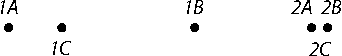
\includegraphics[scale=1]{gesamttex/edit_VIII-4/images/LH_37_05_195_d1_195r.pdf}
\edcaption[0pt]{\lbrack\textit{Fig.~1}\rbrack}
\end{edfigure}
\pstart
Hinc%
\edlabel{37_05_195_2b}
si duo corpora, quae supponantur elastica,\indexS{corpus elasticum} ex hoc
\edtext{principio, accedentibus}{\lemma{principio,}\Bfootnote{%
\textit{(1)}~accedente regula deter %
\textit{(2)}~accedentibus~\textit{L}}}
\edtext{dynamicis\indexS{dynamica} nostris,}{%
\lemma{dynamicis nostris}%
\Cfootnote{Gemeint sind möglicherweise die Entwürfe \cite{01354}\textit{Dynamica de potentia} von 1689 oder das \cite{02032}\textit{Specimen Dynamicum} von 1695.}}
definiri potest, quantum utrique supersit motus. Sint 
\edtext{corpora \textit{a}}{%
\lemma{corpora}%
\Bfootnote{%
\textit{(1)}~\textit{A} et \textit{B}. Tens %
\textit{(2)}~\textit{a}~\textit{L}}}
et \textit{b}, celeritates ante ictum \textit{v} et \textit{e}, quas pono tendere ad easdem partes, nam si secus sit,
\edtext{pro affirmativa celeritatis}{\lemma{pro}\Bfootnote{%
\textit{(1)}~affirmativis celeritatis quantitatibus alterius %
\textit{(2)}~affirmativa celeritatis~\textit{L}}}
alterius quantitate
substituetur 
\edtext{negativa. Celeritas respectiva,\indexS{celeritas respectiva} seu}{\lemma{negativa.}\Bfootnote{%
\textit{(1)}~Centri gravitatis celeritas erit $v+e,:2$  %
\textit{(2)}~Celeritas respectiva %
\textit{(a)}~est %
\textit{(b)}~, seu~\textit{L}}}
qua mutatur distantia, 
\edtext{est $v-e$.}{\lemma{est}\Bfootnote{%
\textit{(1)}~$v+e$. %
\textit{(2)}~$v-e$.~\textit{L}}}
Ea distribuenda est inter corpora, ut sit celeritas ipsius \textit{a} ad celeritatem ipsius \textit{b}, ut \textit{b} 
ad \textit{a}; seu 
\edtext{ut $1:a$}{\lemma{ut}\Bfootnote{%
\textit{(1)}~$\displaystyle\displaystyle\frac{1}{a}$ %
\textit{(2)}~$1:a$~\textit{L}}}
ad $1:b$, eritque celeritas
\edtext{ipsius \textit{a}, $\displaystyle\displaystyle\frac{b}{a+b}v-e,$}{\lemma{ipsius \textit{a},}\Bfootnote{%
\textit{(1)}~\rule[-2.1ex]{0pt}{5.4ex}%
$\displaystyle\frac{b}{a+b}v+e,\displaystyle\frac{a+b}{a}$ %
\textit{(2)}~$\displaystyle\frac{b}{a+b}v-e,$~\textit{L}}}
et ipsius \textit{b}  
\edtext{celeritas erit $\displaystyle\displaystyle\frac{a}{a+b}v-e.$}{\lemma{celeritas erit}\Bfootnote{%
\textit{(1)}~$\displaystyle\frac{a}{a+b}v+e,(a^2+b).$ %
\textit{(2)}~$\displaystyle\frac{a}{a+b}v-e.$~\textit{L}}}
Et vis
\edtext{ictus\indexS{vis ictus} erit $\displaystyle(v-e:,a+b)\,\protect\fbox{2}$, in $aab+bba$\lbrack,\rbrack}{\lemma{ictus erit}\Bfootnote{
\textit{(1)}~$\overline{v+e}^2:a,+$ %
\textit{(2)}~$(\displaystyle\frac{1}{a}+\displaystyle\frac{1}{b})(\overline{v+e}^2)(a+b)^2$  
\textit{(3)}~$\displaystyle\frac{a^2}{\overline{a+b}^2}\overline{v+e}^2+\displaystyle\frac{b^2}{\phantom{a+b}}$  
\textit{(4)}~\rule[-2.8ex]{0pt}{6.9ex}%
$\displaystyle\frac{ab^2}{\overline{a+b}^2}$
\textit{(5)}~$(abb)((v+e:a+b))$
\textit{(6)}~(\protect\vphantom)\textit{v}
\textit{(a)}~$+e$
\textit{(b)}~$-e:,a+b\protect\vphantom()\protect\fbox{2}$, in $aab+bba$~\textit{L}}}
qua scilicet tensio\indexS{tensio elastri} elastri\indexS{elastrum} integra
\edtext{constat. Seu}{\lemma{constat.}\Bfootnote{\textit{(1)}~Se %
\textit{(a)}~si
\textit{(aa)}~vi %
\textit{(bb)}~tensio
\textit{(b)}~si 
\textit{(2)}~Sed cum tensio non statim sit perfecta, ideo parte tantum peracta ut in navi, habebimus
\textit{(3)}~Vis aute %
\textit{(a)}~centri gravitatis eri %
\textit{(b)}~tota erat $av^2+be^2$ a qua si detrahas vim ictus $\overline{v+e}^2$, 
\textit{(aa)}~$a+2b+b+2a$ %
\textit{(bb)}~$a+2b+(b^2:a)+(a^2:b)+2a+b$
\textit{(aaa)}~seu $\overline{v+e}^2$, $3a+3b+b^2:a+a^2:b$ seu
\textit{(bbb)}~seu explicatius erit %
\textit{(4)}~Seu~\textit{L}}}
dividendo numeratorem et nominatorem per $a+b$
\edtext{fit $\overline{v-e}^{2},ab:,a+b$,}{\lemma{fit}\Bfootnote{%
\textit{(1)}~$\overline{v+e}^2,ab:,a+b$ %
\textit{(2)}~$\overline{v-e}^2,ab:,a+b$~\textit{L}}}
vis 
ictus\indexS{vis ictus} seu tensionis\indexS{vis tensionis totalis} totalis seu 
\edtext{explicatius: $abvv-2abve+abee,:,a+b$. Hanc vim auferendo a vi tota\indexS{vis tota}}{\lemma{explicatius:}\Bfootnote{%
\textit{(1)}~$abvv+$ %
\textit{(2)}~$abvv-2abve+abee,:,a+b$ 
\textit{(a)}~Haec vis auferenda a vi tota, %
\textit{(aa)}~fiet %
\textit{(bb)}~restabit vis directionis %
\textit{(b)}~Hanc vim auferendo a vi tota~\textit{L}}}
$avv+bee$, seu ab $aavv+abvv+abee+bbee,:,a+b$, restabit $aavv+2abve+bbee,:,a+b$ seu $\overline{av+be}^{2}\!:,a+b$, quae est vis directionis;\indexS{vis directionis} 
\edtext{quam summa}{\lemma{quam}\Bfootnote{%
\textit{(1)}~dividendo per sum %
\textit{(2)}~summa~\textit{L}}}
corporum habet mota celeritate
centri gravitatis\indexS{celeritas centri gravitatis}. 
Dividendo ergo hanc vim per summam 
\edtext{corporum, et}{\lemma{corporum,}\Bfootnote{%
\textit{(1)}~prodit $\overline{(av-be):(a+b)}^2$ cujus latus est $av-be$ %
\textit{(2)}~et~\textit{L}}}
quotientis sumendo radicem prodit celeritas centri gravitatis\indexS{celeritas centri gravitatis} $av+be,:,a+b$; quae debet esse \textit{\ind{1}C\ind{2}C}. 
Nempe $\ind{1}C\ind{2}C=\ind{1}C\ind{1}B+\ind{1}B\ind{2}B$ 
jam \textit{\ind{1}B\ind{2}B} est \textit{e} et \textit{\ind{1}C\ind{1}B} est ad \textit{\ind{1}A\ind{1}B} id est ad $v-e,$ ut \textit{a} ad $a+b$.
Ergo \textit{\ind{1}C\ind{1}B} est $a,v-e,:,a+b$ et \textit{\ind{1}C\ind{2}C} est $\displaystyle av\ \ovalbox{-ae+ae}+be,:,a+b$. 
Ergo est consensus.
\pend
\pstart
Sed si tensio\indexS{tensio} nondum absoluta sit, 
\edtext{videamus quae pro facto gradu tensionis\indexS{tensio} residua}{%
\lemma{videamus}%
\Bfootnote{%
\textit{(1)}~quis pro facto gradu tensionis residuus %
\textit{(2)}~quae \lbrack...\rbrack\ residua~\textit{L}}}
sit celeritas et directio in quovis corporum, interea dum se urgent. 
Sit ergo tensionis vis;\indexS{vis tensionis} qualis fuisset  
\edtext{si velocitas}{\lemma{si}\Bfootnote{%
\textit{(1)}~corpora eandem %
\textit{(2)}~vis %
\textit{(3)}~velocitas~\textit{L}}}
respectiva\indexS{velocitas respectiva} fuisset minor quam $v-e$, seu quam \textit{\ind{1}A\ind{1}B}. 
Ponamus fuisse $v-e-f$. Posito $e+f$ non excedere
\edtext{\textit{v}, et}{\lemma{\textit{v},}\Bfootnote{%
\textit{(1)}~et utcunque %
\textit{(2)}~et~\textit{L}}}
in calculo priore pro \textit{e} substituendo $e+f$, fiet vis tensionis
\edtext{factae,\indexS{vis tensionis factae} $(v-e-f).^2,ab:,a+b$}{\lemma{factae,}\Bfootnote{%
\textit{(1)}~$(v-e-f,)^2:,(a+b)^2$, et %
\textit{(2)}~$(v-e-f).^2,ab:,a+b$~\textit{L}}}
seu
$abvv-2abve+abee-2abvf+2abef+abff,:\nolinebreak,a+b$ quam auferendo a vi tota,\indexS{vis tota} nempe ab $aavv+abvv+abee+bbee,:,a+b$;
\edlabel{37_05_195_4a}%
\edtext{}{%
{\xxref%
{37_05_195_4a}{37_05_195_4b}}%
\lemma{restabit \lbrack...\rbrack\ $(av+be).^2+abf(v-e-f),:,a+b$}%
\Cfootnote{%
Die richtige Umformung lautet: $(av+be).^2+abf(2v-2e-f),:\nolinebreak,a+b$. Der Fehler wirkt sich auf die folgenden Ableitungen aus.}}%
restabit 
$aavv+\underset{\displaystyle2abvf}{2abve}+bbee-2abef-abff,:,a+b$  
\edtext{seu $(av+be).^2+abf(v-e-f),:,a+b$.\edlabel{37_05_195_4b}}{\lemma{seu}\Bfootnote{%
\textit{(1)}~$\overline{av+be}^2-abf(\protect\vphantom)f+e-v$ %
\textit{(2)}~$a+$ %
\textit{(3)}~$(av+be).^2+abf(v-e-f),:,a+b$~\textit{L}}}
Vel brevius si $v-e-f$ vocetur \textit{r}, tanquam celeritas  
\edtext{respectiva\indexS{celeritas respectiva} determinans}{\lemma{respectiva}\Bfootnote{%
\textit{(1)}~faciens %
\textit{(2)}~determinans~\textit{L}}}
tensionem\indexS{tensio facta} hactenus factam erit vis residua\indexS{vis residua} 
\edtext{$(av+be).^2+abfr,:,a+b$ seu quia}{\lemma{$(av+be).^2+abfr,:,a+b$}\Bfootnote{%
\textit{(1)}~sin omissa \textit{r}, quia jam %
\textit{(2)}~seu quia~\textit{L}}}
$f=v-e-r$, fiet $\overline{av+be}^2+abvr- %
\edtext{aber-abrr,:,a+b$ vis}{%
\lemma{$aber-abrr,:,a+b$}%
\Bfootnote{%
\textit{(1)}~. Quod si pro %
\textit{(2)}~vis~\textit{L}}}
tensionis partialis.\indexS{tensio partialis} Quod si pro $v-e$ ponas \textit{h} pro celeritate respectiva\indexS{celeritas respectiva} totali, fiet $e=v-h$. 
Sed possumus relinquere \textit{e} in priore membro ponereque \textit{h} in posteriore, 
fietque $\overline{av+be}^2+ab(hr+rr),:,a+b$. 
Explicemus \textit{r} sic ut $\overline{av+be}^2+ab(hr+rr)$ aequetur quadrato de $av+be+kr$, fietque
\href{\Scan{LH_37_05_195v}}%
{\lbrack195~v\textsuperscript{o}\rbrack}
$\ovalbox{\overline{av+be}^2} +abhr+abrr=\ovalbox{\overline{av+be}^2} +2\ \overline{av+be}\ kr+kkrr$, et fiet $abh-2k(av+be),:,kk-ab=r$.
\edtext{Et celeritas vis residuae\indexS{vis residua}}{\lemma{Et}\Bfootnote{%
\textit{(1)}~celeritas residua totius vis %
\textit{(2)}~celeritas vis %
\textit{(a)}~residua %
\textit{(b)}~residuae~\textit{L}}}
ad corporum summam applicata foret extrahendo 
\edtext{$av+be+kr,:,a+b$. Ibi}{%
\lemma{$av+be+kr,:,a+b$.}\Bfootnote{%
\textit{(1)}~Sed nobis potius propositum quaerere %
\textit{(2)}~Sed hoc %
\textit{(3)}~Ibi~\textit{L}}}
posset pro \textit{r} substitui valor per \textit{k}. Sed quia nulla in eo utilitas, jam mittamus.
\pend
\pstart
Illud nunc dispiciendum
\edtext{quam celeritatem residuam\indexS{celeritas residua}}{\lemma{quam}\Bfootnote{%
\textit{(1)}~vim residua %
\textit{(2)}~celeritatem residuam~\textit{L}}}
habeat unumquodque corpus. Celeritas tota respectiva\indexS{celeritas respectiva tota} erat \textit{h}; 
amissa\indexS{celeritas respectiva amissa} est \textit{r}, ita ut si non aliam habuissent, fuissent redacta 
\edtext{\lbrack ad\rbrack}{%
\lemma{}%
\Bfootnote{%
et %
\textit{L ändert Hrsg.}%
}}
\edtext{quietem. Haec}{\lemma{quietem.}\Bfootnote{%
\textit{(1)}~Amissa ergo est vis %
\textit{(2)}~Huius celeritas respectiva %
\textit{(3)}~Haec~\textit{L}}}
celeritas respectiva\indexS{celeritas respectiva} distribuenda respective inter corpora, ita ut perinde sit ac si ipsius \textit{a} celeritas
\edtext{fuisset $rb:,a+b$}{\lemma{fuisset}\Bfootnote{%
\textit{(1)}~\rule[-2.1ex]{0pt}{5.4ex}%
$\displaystyle\frac{b}{a+b}r$, et ipsius \textit{b} fuisset $\displaystyle\frac{a}{a-}$  %
\textit{(2)}~$rb:,a+b$~\textit{L}}}
et ipsius \textit{b} fuisset $ra:,a+b$. Ergo vis tensionis\indexS{vis tensionis} consumta 
\edtext{est $\displaystyle(r:,a+b)^2\cdot\overline{bba+aab}$,}{%
\lemma{est}%
\Bfootnote{%
\textit{(1)}~\textit{ab}
\textit{(2)}~$rrbb:a+b$
\textit{(3)}~$rr:a+b$
\textit{(4)}~$\displaystyle(r:,a+b)^2\cdot\overline{bba+aab}$,~\textit{L}}}
seu $rrab:,a+b$.
Vis autem tensionis\indexS{vis tensionis totalis} totalis erat $hhab:,a+b$.
Ergo vis ictus\indexS{vis ictus} residua nondum in elastrum\indexS{elastrum} consumta est $(hh-rr)ab:,a+b$. 
Haec vis inter corpora \textit{a} et \textit{b} est distribuenda, reciprocis ad moles 
\edtext{celeritatibus.\indexS{celeritates reciprocae ad moles} Nempe ipsius \textit{a} celeritas sit $yb:,a+b$}{%
\lemma{celeritatibus.}%
\Bfootnote{%
\textit{(1)}~Sit %
\textit{(2)}~Nempe ipsius \textit{a}
\textit{(a)}~celeritatis %
\textit{(b)}~celeritas sit
\textit{(aa)}~\textit{y}, erit ipsius \textit{b} celeritas
\textit{(bb)}~$\displaystyle\frac{b}{a+b}y$ et ipsius \textit{b} celeritas erit \textit{a}
\textit{(cc)}~$yb:,a+b$~\textit{L}}}
et ipsius \textit{b} celeritas sit $ya:,a+b$. 
Et ipsius \textit{a} vis erit $yyabb:(a+b)^2$ et ipsius \textit{b} vis 
erit $yybaa:(a+b)^2$ ergo vis amborum erit $yyab:,a+b$. Ergo fiet tantum $y=\sqrt{hh-rr}$. 
Adeoque celeritas residua
\edtext{propria\indexS{celeritas propria residua}}{\lemma{}\Bfootnote{propria \textit{erg.}~\textit{L}}}
corporis \textit{a}, seu in navi\lbrack,\rbrack\indexS{navis} 
erit $\sqrt{hh-rr}\ b:,a+b$\lbrack,\rbrack\ corporis \textit{b} erit $\sqrt{hh-rr}\ a:,a+b$, 
quibus si addatur celeritas communis\indexS{celeritas communis} seu centri 
\edtext{gravitatis\indexS{celeritas centri gravitatis}, sive}{%
\lemma{gravitatis,}%
\Bfootnote{%
\textit{(1)}~fiet %
\textit{(2)}~sive~\textit{L}}}
\edtext{navis\indexS{navis}, quae}{%
\lemma{}%
\Bfootnote{%
navis, \bars{fiet, \textit{streicht Hrsg.}} quae~\textit{L}}}
est
\edtext{$av+be,:,a+b$, dum}{\lemma{$av+be,:,a+b$,}\Bfootnote{%
\textit{(1)}~fietque celeritas %
\textit{(2)}~co %
\textit{(3)}~utique corporis \textit{a} celeritas residua %
\textit{(4)}~dum~\textit{L}}}
se mutuo urgent celeritas residua\indexS{celeritas residua} corporis 
\edlabel{37_05_195_3a}%
\edtext{}{%
{\xxref%
{37_05_195_3a}{37_05_195_3b}}%
\lemma{$av+be+\sqrt{hh-rr}b,:,a+b$,}\Bfootnote{%
\textit{(1)}~sed corporis \textit{b} erit $av+be+\sqrt{hh-rr}\,a,:a+b$ %
\textit{(2)}~\textit{b}~~~\textit{av} \lbrack...\rbrack\ Num~\textit{L}}}
$\underset{\efrac{\scriptstyle \phantom{g}}{\displaystyle b}}a$ erit $\underset{\displaystyle av+be+\sqrt{hh-rr}a,:,a+b.}{av+be+\sqrt{hh-rr}b,:,a+b,}$
\pend
\begin{edfigure}%
\hfill
\includegraphics%
[scale=0.22]%
{gesamttex/edit_VIII-4/images/LH_37_05_195_d2_195v.pdf}
\hfill
\includegraphics%
[scale=0.22]%
{gesamttex/edit_VIII-4/images/LH_37_05_195_d3_195v.pdf}
\hfill
\edcaption{\hspace*{2mm}\lbrack\textit{Fig.~2, gestr.}\rbrack \hspace*{28mm}
\lbrack\textit{Fig.~3, gestr.}\rbrack}
\end{edfigure}
\pstart
Num%
\edlabel{37_05_195_3b}
quia multa inutilia hic immiscuimus,
\edtext{partim jam}{\lemma{partim}\Bfootnote{%
\textit{(1)}~aliunde %
\textit{(2)}~jam~\textit{L}}}
ante inventa, partim non huius loci, breviter rem complectamur velut ab integro. %
\pend
\pstart
Quaestio est quanam ratione\indexS{ratio diminuationis celeritatis} diminuatur corporum 
\edtext{concurrentium elasticorum\indexS{corpus elasticum}}{\lemma{concurrentium}\Bfootnote{%
\textit{(1)}~promte %
\textit{(2)}~elasticorum~\textit{L}}}
celeritas, dum in concursu\indexS{concursus} se mutuo urgent.
Consideranda est duplex in ipsis celeritas\lbrack:\rbrack\ 
\edtext{una communis,\indexS{celeritas communis}}{%
\lemma{una}%
\Bfootnote{%
\textit{(1)}~propria %
\textit{(2)}~communis,~\textit{L}}}
quae est centri gravitatis\indexS{celeritas centri gravitatis}, altera
\edtext{propria,\indexS{celeritas propria} quae}{\lemma{propria,}\Bfootnote{%
\textit{(1)}~quae est ad %
\textit{(a)}~vim %
\textit{(b)}~celeritatem respectivam %
\textit{(2)}~in uno corpore \textit{a}, ad %
\textit{(3)}~quae~\textit{L}}}
in uno corpore \textit{a} est ad celeritatem respectivam\indexS{celeritas respectiva}
\textit{h}, ut corpus alterum \textit{b} ad corporum
\edtext{summam. Reperiturque vis}{\lemma{summam.}\Bfootnote{%
\textit{(1)}~Itaque vis %
\textit{(2)}~Reperiturque vis~\textit{L}}}
ictus\indexS{vis ictus integra} integra, seu tensionis\indexS{vis tensionis totalis} totalis esse
\edtext{$hhab:,a+b$, quae}{\lemma{$hhab:,a+b$}\Bfootnote{%
\textit{(1)}~. Sed cum tensio tantum ex parte facta est %
\textit{(2)}~, quae~\textit{L}}}
omnia dudum habentur. Sed cum vis ictus\indexS{vis ictus} non nisi pro parte consumta est, et corpora nondum sunt satis
\edtext{tensa, tunc}{\lemma{tensa,}\Bfootnote{%
\textit{(1)}~perinde est ac si  %
\textit{(2)}~tunc~\textit{L}}}
absumta vis ictus\indexS{vis ictus} potest intelligi ea esse quae fuisset alterius celeritatis respectivae\indexS{celeritas respectiva} \textit{r},
\edtext{qua, ubi}{\lemma{qua,}\Bfootnote{%
\textit{(1)}~si %
\textit{(2)}~ubi~\textit{L}}}
concurrissent corpora \textit{a} et \textit{b},
\edtext{sese tantundem}{\lemma{sese}\Bfootnote{%
\textit{(1)}~eodem %
\textit{(2)}~tantundem~\textit{L}}}
tendissent, quantum praesenti tensione partiali\indexS{tensio partialis} factum est, 
itaque vis tensionis\indexS{vis tensionis} factae erit
\edtext{$rrab:,a+b;$ et residua vis ictus\indexS{vis ictus residua} erit}{\lemma{$rrab:,a+b;$}\Bfootnote{%
\textit{(1)}~et reperietur vis tensionis residua %
\textit{(2)}~et %
\textit{(a)}~vi %
\textit{(b)}~residua vis ictus
\textit{(aa)}~esse %
\textit{(aaa)}~\textit{r} 
\textit{(bbb)}~$\sqrt{hh-rr}$ %
\textit{(ccc)}~$hh-rr$ 
\textit{(bb)}~erit~\textit{L}}}
utique $hh-rr,ab:,a+b$.
Adeoque celeritas respectiva residua\indexS{celeritas respectiva residua} qua corpora se adhuc urgent 
\edtext{erit $\sqrt{hh-rr}$}{%
\lemma{erit}%
\Bfootnote{%
\textit{(1)}~$\sqrt{hh-rr}a$ %
\textit{(2)}~$\sqrt{hh-rr}ab:,a+b.$ %
\textit{(3)}~$\sqrt{hh-rr}$~\textit{L}}}
corporisque \textit{a} residua celeritas propria\indexS{celeritas propria residua} 
erit $b\sqrt{hh-rr}:,a+b$. Corporis vero \textit{b} residua celeritas propria\indexS{celeritas propria residua} est $a\sqrt{hh-rr}:,a+b$. 
Unde si tam illi quam huic addatur directio communis quae est $av+be,:,a+b$, habebitur utriusque celeritas integra.\indexS{celeritas integra}
\pend
\begin{edfigure}%
\includegraphics%
[scale=0.22]%
{gesamttex/edit_VIII-4/images/LH_37_05_195_d4_195v.pdf} 
\edcaption{%
\edtext{\lbrack\textit{Fig.~4, gestr.}\rbrack}{%
\lemma{\lbrack\textit{Fig.~4}\rbrack}%
\Cfootnote[nonum]{Ein ebenfalls gestrichener Entwurf zum Diagramm wird nicht wiedergegeben.}}}
\end{edfigure}
\pstart
Sed utile erit exhibere
\edtext{et celeritatis respectivae}{\lemma{et}\Bfootnote{%
\textit{(1)}~celeritatem %
\textit{(2)}~celeritatis %
\textit{(a)}~%
\textit{(b)}~respectivae~\textit{L}}}
qua se corpora urgent continuam diminutionem.\indexS{diminutio celeritatis respectivae}
Et patet si celeritates respectivae\indexS{celeritas respectiva} quibus produci possent tensiones jam factae\indexS{tensio jam facta} sint ut 
\edtext{sinus,\indexS{sinus} ipsas}{%
\lemma{sinus,}%
\Bfootnote{%
\textit{(1)}~ips %
\textit{(2)}~fore %
\textit{(3)}~ipsas~\textit{L}}}
celeritates respectivas\indexS{celeritas respectiva} quibus produci possent tensiones residuae,\indexS{tensio residua} fore ut 
\edtext{sinus complementi.\indexS{sinus complementi} Et}{\lemma{complementi.}\Bfootnote{%
\textit{(1)}~Posito celeritatem re %
\textit{(2)}~Et~\textit{L}}}
\edtext{quadrata celeritatis respectivae\indexS{celeritas respectiva}}{\lemma{celeritatis}\Bfootnote{%
\textit{(1)}~residuae %
\textit{(2)}~respectivae~\textit{L}}}
utriusque componere quadratum celeritatis
respectivae\indexS{celeritas respectiva} corporum. Hinc jam iterum praeclare  
\edtext{procedit mea actionum aestimatio;\indexS{aestimatio actionis}}{\lemma{procedit}\Bfootnote{%
\textit{(1)}~theorema meum %
\textit{(2)}~mea actionum aestimatio~\textit{L}}}
nempe in ictu  
\edtext{corporum elasticorum\indexS{corpus elasticum} sese urgentium tensiones\indexS{tensio jam producta} jam productae sunt}{\lemma{corporum}\Bfootnote{%
\textit{(1)}~actio %
\textit{(a)}~cel %
\textit{(b)}~velocitatis %
\textit{(aa)}~residuae %
\textit{(bb)}~respectivae jam insumta %
\textit{(2)}~elasticorum \lbrack...\rbrack\ sunt~\textit{L}}}
ut actiones corporis quod haberet velocitates respectivas\indexS{velocitas respectiva} quibus eae tensiones\indexS{tensio} in concurrentibus 
produci potuissent.
\edtext{Et \href{\Scan{LH_37_05_195r}}%
{\lbrack195~r\textsuperscript{o}\rbrack}\ ut summa}{%
\lemma{Et}\Bfootnote{%
\textit{(1)}~actio velocitatis respectivae
quae 
\textit{(a)}~corpo 
\textit{(b)}~tensio jam facta potest produci juncta cum ea qua 
\textit{(aa)}~actio 
\textit{(bb)}~tensio celeritatis absolutae
adhuc facienda potest produci, aequatur actioni
\textit{(aaa)}~vis 
\textit{(bbb)}~celeritatis 
\textit{(aaaa)}~residuae 
\textit{(bbbb)}~respectivae, qua tota tensio %
producitur ac proinde 
\textit{(aaaaa)}~actiones celeritatum relativarum 
\textit{(bbbbb)}~impensa actionis celeritatis respectivae crescit ut vis tensionis.
\textit{(2)}~\bars{ut summa \textit{streicht Hrsg.}}
tensionis factae et residuae faciendae aequatur toti tensioni seu vi ictus, ita et actiones %
corporum has celeritates respectivas partiales habentes actioni totales\lbrack\textit{!}\rbrack\ aequarentur. 
\textit{(a)}~Nam vires 
\textit{(aa)}~seu tension 
\textit{(bb)}~vel actiones corporum %
amborum 
\textit{(aaa)}~sunt ut 
\textit{(bbb)}~propriae impensae in tensiones, sunt inter se ut vires vel actiones corporis, quod per modum %
haberet celeritates respectivas quibus in concurrentibus %
\textit{(b)}~Nempe si $yy=hh-rr$, fit $rr+yy=hh$. Vis 
\textit{(aa)}~total 
\textit{(bb)}~enim ictus tota 
\textit{(cc)}~enim ictus tota $hhab:,\,a+b$\,; impensa $rrab:,\,a+b$\,; impendenda $yyab:,\,a+b$.
\textit{(aaa)}~Vires %
\bars{enim vel actiones corporum propriae quibus tensiones \textit{erg.}} %
\textit{(bbb)}~Nam vires vel actiones corporum \bars{amborum \textit{erg.}} propriae
\textit{(aaaa)}~quibus 
\textit{(bbbb)}~impensae in tensiones 
\textit{(aaaaa)}~durant 
\textit{(bbbbb)}~dum se urgent, 
sunt ut 
\textit{(aaaaa-a)}~vis 
\textit{(bbbbb-b)}~actiones vel 
vires 
\textit{(aaaaa-aa)}~celeritatum respectivarum 
\textit{(bbbbb-bb)}~corporis, celeritates respectivas quibus %
eaedem tensiones produci potuissent, quas habuissent si ab uno corpore exercitae fuissent. %
\textit{(ccc)}~\bars{Seu vires tensionum ictu productarum, sunt 
\textit{(aaaa)}~actionibus celeritatum respectivarum pro 
\textit{(bbbb)}~proportionales 
\textit{(aaaaa)}~actio 
\textit{(bbbbb)}~actionibus corporis quod haberet velocitates respectivas quae suppositae in corporibus concurrentibus 
\textit{(aaaaa-a)}~tensionem produxissent 
\textit{(bbbbb-b)}~tensiones produxissent.
\textit{streicht Hrsg.}} %
\href{\Scan{LH_37_05_195r}}%
{\lbrack195~r\textsuperscript{o}\rbrack}\ 
\textit{(3)}~ut s 
\textit{(4)}~\bars{Et \textit{streicht Hrsg.}} ut summa~\textit{L}}}
tensionis factae\indexS{tensio facta} et residuae faciendae\indexS{tensio residua facienda} aequatur toti tensioni\indexS{tensio tota} seu vi ictus,\indexS{vis ictus} ita et 
\edtext{actiones\indexS{actio} corporis}{%
\lemma{actiones}%
\Bfootnote{%
\textit{(1)}~corporum %
\textit{(2)}~corporis~\textit{L}}}
has celeritates respectivas partiales\indexS{celeritas respectiva partialis} per 
\edtext{modum celeritatis}{%
\lemma{modum}%
\Bfootnote{%
\textit{(1)}~absolutae %
\textit{(2)}~celeritatis~\textit{L}}}
absolutae\indexS{celeritas absoluta} habentis; 
actioni\indexS{actio} ejusdem celeritatem respectivam totalem\indexS{celeritas respectiva totalis} absolute habentis aequarentur. Nam et
\edtext{vires vel}{\lemma{vires}\Bfootnote{%
\textit{(1)}~conflatae corporu %
\textit{(2)}~vel~\textit{L}}}
actiones\indexS{actio} 
conflatae corporum amborum in ictum\indexS{ictus} vel 
tensionem\indexS{tensio} jam impensae, sunt inter se ut  
\edtext{vires\indexS{vis} vel}{\lemma{vires}\Bfootnote{%
\textit{(1)}~unius corporis, celeritatibus latae\lbrack\textit{!}\rbrack\ %
\textit{(2)}~vel~\textit{L}}}
actiones\indexS{actio} unius alicujus corporis celeritatibus 
\edtext{lat\lbrack i\rbrack,}{%
\lemma{}%
\Bfootnote{%
latae %
\textit{L ändert Hrsg.}%
}}
quae aequarentur celeritatibus 
\edtext{respectivis\indexS{celeritas respectiva} quibus}{%
\lemma{respectivis}%
\Bfootnote{%
\textit{(1)}~tensiones %
\textit{(2)}~quibus~\textit{L}}}
in concurrentibus corporibus tensiones jam factae\indexS{tensio jam facta}
produci possent. Nam si celeritas respectiva\indexS{celeritas respectiva}
\edtext{\textit{h}, conflata}{\lemma{\textit{h},}\Bfootnote{%
\textit{(1)}~erunt %
\textit{(2)}~vires corporum ictum facientium sunt %
\textit{(3)}~conflata~\textit{L}}}
tota vis ictus est
\edtext{$hhab:,a+b,$ ea}{\lemma{$hhab:,a+b,$}\Bfootnote{%
\textit{(1)}~nec refert quae sint %
\textit{(2)}~ea~\textit{L}}}
sc.\ quae foret, si dimidium medium harmonicum corporum celeritatem respectivam\indexS{celeritas respectiva} absolute 
haberet.%
\pend
\pstart
\edtext{Nota de hoc loquor et in Ep.\ 
ad \indexN{\textls{Papin} (Papinus), Denis 1647\textendash1713}Papinum 
\edtext{data ante med.\ octob.\ 1698.}{%
\lemma{data}%
\Bfootnote{%
\textit{(1)}~init.\ octob.\ 1698.\ ante %
\textit{(2)}~ante med. octob.\ 1698.~\textit{L}}}%
}{\lemma{Nota \lbrack...\rbrack\ 1698}\Cfootnote{%
\cite{01501}\textit{LSB} {III, 7 N.\;237,} S.\;921\textendash925, hier S.\;924.20\textendash925.3.}}
\pend




\chapter[tocentry={De celeritatibus in concursu amissis, recuperatis ac recuperandis 
\enskip \bracks{2.\ Hälfte Oktober 1698\,(?)}}, %
head={De celeritatibus in concursu amissis, recuperatis ac recuperandis}]%
{\MakeUppercase{De celeritatibus in concursu amissis, recuperatis ac recuperandis} 
\newline \bracks{2.\ Hälfte Oktober 1698\,(?)}}
\label{60362}    
\begin{ledgroupsized}[r]{120mm}
\footnotesize
\pstart
\noindent\textbf{Überlieferung:}
\pend
\end{ledgroupsized}
\begin{ledgroupsized}[r]{114mm}
\footnotesize
\pstart \parindent -6mm
\makebox[6mm][l]{\textit{L}}%
Aufzeichnung:
LH~XXXVII 5~Bl.~200.
Ein Blatt~2\textsuperscript{o};
Papiererhaltungsmaßnahmen;
alle Ränder beschnitten;
Blatt zweimal gefaltet.
Eine Seite auf Bl.~200~r\textsuperscript{o}; Bl.~200~v\textsuperscript{o} leer.
\pend
\end{ledgroupsized}
\vspace{5mm}
\begin{ledgroup}
\footnotesize
\pstart
\noindent%
\textbf{Datierungsgründe:}
Die vorliegende Aufzeichnung N.\;\ref{60362} untersucht den temporären
Verlust der Geschwindigkeiten zweier elastisch aufeinander stoßender Körper wegen \textendash\ und während \textendash\ der wechselseitigen Kompression.
Eins der Ergebnisse der Aufzeichnung ist die reziproke Proportion zwischen den Massen und den \textit{während der Kompression} eingebüßten Geschwindigkeiten
(\glqq dum se adhuc comprimunt\grqq, \refpassage{37_05_200_2a}{37_05_200_2b}).
Bei der Thematik von N.\;\ref{60362} allgemein und besonders bei der zitierten Formulierung 
lassen sich Übereinstimmungen mit einem weiteren diesem Thema gewidmeten Konzept (N.\;\ref{60358} in diesem Band) feststellen.
Dessen Schwerpunkt fasst dort Leibniz in einer Randanmerkung zusammen: 
\glqq Hic explicantur celeritates quae in corporibus duobus concurrentibus manent residuae, dum se urgent et ictu comprimunt\grqq\ (Anmerkung zu \refpassage{37_05_195_1a}{37_05_195_1b}).
\pend
\pstart
Mangels weiterer und aussagekräftigerer Anhaltspunkte für die Datierung des kurzen Textes wird für N.\;\ref{60362} die Datierung von N.\;\ref{60358} übernommen.
\pend 
\end{ledgroup}
\selectlanguage{latin}
\vspace{8mm}
\pstart
\noindent
\href{\Scan{LH_37_05_200r}}%
{\lbrack200~r\textsuperscript{o}\rbrack}
Si duo corpora 
\edtext{directe et centraliter}{\lemma{}\Bfootnote{directe et centraliter \textit{erg.~L}}} 
concurrant,\indexS{concursus directus et centralis duorum}
videndum
an in ipso concursu celeritates amissae%
\indexS{celeritas amissa}
sint molibus\indexS{moles}
\edlabel{37_05_200_1a}%
reciprocae.%
\edtext{}{%
\xxref{37_05_200_1a}{37_05_200_1b}%
\lemma{reciprocae.}\Bfootnote{%
\textit{(1)}~Ponantur corpora \textit{A} et \textit{B} concurr %
\textit{(2)}~Sit~\textit{L}}}%
\pend
\begin{edfigure}%
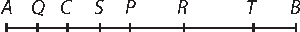
\includegraphics[scale=1]{gesamttex/edit_VIII-4/images/LH_37_05_200_d_200r.pdf} 
\edcaption{\lbrack\textit{Fig.~1}\rbrack}
\end{edfigure}
\pstart
Sit\edlabel{37_05_200_1b}
corporum \textit{A} et \textit{B} concurrentium
celeritatibus \textit{AP}, \textit{BP}
concursus%
\indexS{concursus}
in \textit{P}.
Sit eorundem corporum centrum\indexS{centrum gravitatis} \textit{C}. Ponamus moveri ea celeritatibus \textit{AC}, \textit{BC} in navi\indexS{navis} mota celeritate \textit{CP}. 
Et concurrentia in \textit{C} 
\edtext{amisisse unumquodque}{\lemma{amisisse}\Bfootnote{%
\textit{(1)}~partem %
\textit{(2)}~q %
\textit{(3)}~unumquodque~\textit{L}}} 
partem suae celeritatis; certum est celeritates
\edtext{in navi}{\lemma{}\Bfootnote{in navi \textit{erg.~L}}} 
amissas\indexS{celeritas amissa} esse reciproce proportionales, 
seu si \textit{A}, amiserit celeritatem \textit{AQ}; 
\textit{B} amisisse celeritatem \textit{BR}, et fore \textit{AQ} ad \textit{BR} ut \textit{B} ad \textit{A}. Residuaeque celeritates\indexS{celeritas residua} in navi erunt \textit{QC}, \textit{RC}. 
Sed cum spectando extra navim\indexS{navis} residuae celeritates sint \textit{QP} et 
\edtext{\textit{RP}\lbrack;\rbrack\ fuerint}{\lemma{\textit{RP}}\Bfootnote{%
\textit{(1)}~patet easdem esse amissas sive in navi spectes sive extra n %
\textit{(2)}~fuerint~\textit{L}}} 
autem primae \textit{AP}, \textit{BP}, patet easdem esse amissas \textit{AQ}, \textit{BR}; 
sive in navi\indexS{navis} spectes, sive extra navim;\indexS{navis} 
et cum in navi amissae sint reciprocae corporibus; 
\edlabel{37_05_200_2a}%
absolute dicendum est in corporum concursu\indexS{concursus corporum} 
\edtext{dum sese adhuc comprimunt}{\lemma{}\Bfootnote{dum sese adhuc comprimunt \textit{erg.~L}}}
celeritates amissas\indexS{celeritas amissa} esse corporibus reciproce proportionales.\indexS{celeritates corporibus reciproce proportionales}%
\edlabel{37_05_200_2b}
\pend 
\pstart 
Vicissim in corporum concursu,\indexS{concursus corporum} dum sese restituendo a se invicem rursus 
\edtext{recedunt, videndum an celeritates recuperatae\indexS{celeritas recuperata} sint}{%
\lemma{recedunt,}%
\Bfootnote{%
\textit{(1)}~celeritates recuperatae sunt %
\textit{(2)}~videndum an celeritates recuperatae sint~\textit{L}}}
corporibus reciproce proportionales.\indexS{celeritates corporibus reciproce proportionales} Redeamus ad 
\edtext{navim,\indexS{navis} quae}{\lemma{navim,}\Bfootnote{%
\textit{(1)}~et ponamus cor %
\textit{(2)}~quae~\textit{L}}} 
fertur celeritate \textit{CP}, et ponamus in ea 
\edtext{corpora post}{\lemma{corpora}\Bfootnote{%
\textit{(1)}~recuperasse %
\textit{(2)}~post~\textit{L}}}
ictum a se recedentia recuperasse
\edtext{\textit{A} celeritatem et directionem \textit{CQ}}{\lemma{\textit{A} celeritatem}\Bfootnote{%
\textit{(1)}~\textit{CQ}, %
\textit{(2)}~et directionem \textit{CQ}~\textit{L}}} 
et 
\edtext{\textit{B} celeritatem et directionem \textit{CR}; sumatur a \textit{P} versus \textit{A},}{%
\lemma{\textit{B}}%
\Bfootnote{celeritatem 
\bars{et directionem \textit{erg.}}
\textit{CR};
\textit{(1)}~manifestum est, spectanti ex %
\textit{(2)}~utique spectanti ex ripa %
\textit{(3)}~sumatur in \textit{CP} %
\textit{(4)}~sumatur a \textit{P} %
\textit{(a)}~retro %
\textit{(b)}~versus \textit{A},~\textit{L}}} 
ipsa \textit{PS} aequalis ipsi \textit{CQ}\lbrack,\rbrack\ erit \textit{CS} celeritas quam corpus \textit{A} 
\edtext{ex ripa\indexS{ripa}}{\lemma{ex}\Bfootnote{%
\textit{(1)}~navi %
\textit{(2)}~ripa~\textit{L}}} 
spectanti apparebit habere in \textit{P}. Similiter
\edtext{a \textit{P} versus}{\lemma{a \textit{P}}\Bfootnote{%
\textit{(1)}~antrorsum %
\textit{(2)}~versus~\textit{L}}} 
\textit{B} 
\edtext{sumatur \textit{PT}}{\lemma{sumatur}\Bfootnote{%
\textit{(1)}~\textit{PR} %
\textit{(2)}~\textit{PT}~\textit{L}}} 
aequalis ipsi 
\edtext{\textit{CR} et erit \textit{PT} celeritas quam}{\lemma{\textit{CR}}\Bfootnote{%
\textit{(1)}~et %
\textit{(2)}~et erit \textit{PT} celeritas quam~\textit{L}}} 
corpus \textit{B} ex ripa spectanti\indexS{spectans e ripa} 
apparebit habere in \textit{P}. Patet \textit{PS} esse
\edtext{$CP-CQ$, et \textit{PT}}{\lemma{$CP-CQ$, et}\Bfootnote{%
\textit{(1)}~\textit{PR} %
\textit{(2)}~\textit{PT}~\textit{L}}} 
esse $CP+CR$. Sed cum \textit{CQ} et \textit{CR} sint ut \textit{B} et \textit{A}, 
patet non posse $CP-CQ$ et $CP+CR$ ut \textit{B} et \textit{A}. 
\edtext{Itaque dici}{\lemma{Itaque}\Bfootnote{%
\textit{(1)}~fieri %
\textit{(2)}~dici~\textit{L}}} 
non potest celeritates recuperatas,\indexS{celeritas recuperata} spectando absolute seu extra \indexS{navis}navim\lbrack,\rbrack\ esse corporibus reciproce proportionales.\indexS{celeritates corporibus reciproce proportionales}
Sed celeritates retrorsum adhuc 
\edtext{acquirendae\indexS{celeritas acquirenda} sunt}{\lemma{acquirendae}\Bfootnote{%
\textit{(1)}~ab \textit{A} %
\textit{(a)}~sun %
\textit{(b)}~est %
\textit{(2)}~sunt~\textit{L}}} 
\textit{AQ} pro \textit{A}, et \textit{BR} pro 
\edtext{\textit{B}, sive}{\lemma{\textit{B},}\Bfootnote{%
\textit{(1)}~quae revera sun %
\textit{(2)}~sive~\textit{L}}} 
extra navim\indexS{navis} spectes sive in navi.\indexS{navis}
\pend
\pstart
Regula ergo haec est: 
\textls{celeritates ad seinvicem accedendi}\indexS{celeritates ad seinvicem accedendi}
\edtext{\textls{amissae\indexS{celeritas amissa} aut a}}{%
\lemma{\textls{amissae}}%
\Bfootnote{%
\textit{(1)}~\textls{et a} %
\textit{(2)}~aut %
\textit{(3)}~aut %
\textit{(4)}~\textls{aut a}~\textit{L}}}
\textls{se invicem recedendi\indexS{celeritates a seinvicem recedendi} recuperandae\indexS{celeritas recuperanda} sunt corporibus reciproce proportionales}.
\pend





\chapter[tocentry={Demonstratio duarum Hypothesium ad reddendas rationes legum motus et concursus
\enskip \bracks{Juni 1703 \textendash\ Ende 1714\,(?)}%
},
head={Demonstratio duarum Hypothesium}]%
{\MakeUppercase{Demonstratio duarum Hypothesium ad reddendas rationes legum motus et concursus}
\newline \bracks{Juni 1703 \textendash\ Ende 1714\,(?)}%
}

\label{60354}
\begin{ledgroupsized}[r]{120mm}
\footnotesize
\pstart
\noindent\textbf{Überlieferung:}
\pend
\end{ledgroupsized}
\begin{ledgroupsized}[r]{114mm}
\footnotesize
\pstart \parindent -6mm
\makebox[6mm][l]{\textit{L}}%
Konzept:
LH~XXXVII, 5~Bl.~183\textendash184. 
Ein Bogen~4\textsuperscript{o};
\href{\Scan{LH_37_05_184wz}}%
{Gegenmarke}
eines Wasserzeichens im Falz; %
Papiererhaltungsmaßnahmen;
alle Ränder beschnitten.
Vier Seiten.
Auf Bl.~184~r\textsuperscript{o}, senkrecht zur Schreibrichtung und von Leibniz überschrieben, ein Satz von der Hand 
\indexN{\textls{Hodann}, Johann Friedrich 1674\textendash1745}J.\,F.\,Hodanns:
\textit{Et vero de profectis in Graeciam %
loquuntur cippi, hominibus haud dubie Christia}\lbrack/\rbrack\textit{nis erecti,}
\textit{quos ipse
Cl.~\indexN{\textls{Peringer} (Perinskiöld, Perinskioldius), Johan 1654\textendash1720}%
Perinskioldius exhibet}.
Die Grabsteine in Griechenland gefallener gotischer Krieger sind Gegenstand von
\indexN{\textls{Peringer} (Perinskiöld, Perinskioldius), Johan 1654\textendash1720}%
J.\,Perinskiölds 
umfangreichen \glqq Annotationes\grqq\ zu seiner Ausgabe von
\indexN{\textls{Cochlaeus}, Johann 1479\textendash1552}%
\textsc{J.\,Cochlaeus}, 
\cite{02052}\textit{Vita Theoderici}, Stockholm 1699 (dort S.\;233\textendash614).
In diesem Zusammenhang siehe Leibnizens Kommentare über
\indexN{\textls{Peringer} (Perinskiöld, Perinskioldius), Johan 1654\textendash1720}%
Perinskiölds Thesen in seinem
\cite{02051}Brief an 
\indexN{\textls{Sparwenfeld}, Johan Gabriel 1655\textendash1727}%
J.\,G.~Sparwenfeld
vom 10.\ März 1702 (\textit{LSB} I, 20, S.\;838.1\textendash9.)
\pend
\end{ledgroupsized}
\vspace{5mm}
\begin{ledgroup}
\footnotesize
\pstart
\noindent%
\textbf{Datierungsgründe:}
Der von der Hand 
\indexN{\textls{Hodann}, Johann Friedrich 1674\textendash1745}Johann Friedrich Hodanns 
stammende, von Leibniz überschriebene Satz auf Bl.~184~r\textsuperscript{o} 
gibt Auskunft über die Entstehung des vorliegenden Konzeptes.
Hodann war
von Juni 1703 bis März 1705 und  von Februar 1706 bis Ende 1714
für Leibniz als Schreiber tätig.
Daraus ergibt sich für N.\;\ref{60354}
unter der Annahme einer zeitnahen Wiederverwendung des sonst unbeschriebenen Blattes durch Leibniz
die angegebene Datierungsspanne.
\pend 
\end{ledgroup}
\selectlanguage{latin}
\vspace{8mm}
\pstart%
\normalsize%
\noindent%
\edtext{\href{\Scan{LH_37_05_183r}}%
{\lbrack183~r\textsuperscript{o}\rbrack}\ Cum}{%
\lemma{\href{\Scan{LH_37_05_183r}}%
{\lbrack183~r\textsuperscript{o}\rbrack}}\Bfootnote{%
\textit{(1)}~In reddendis 
\textit{(a)}~legibus rationum 
\textit{(b)}~rationibus legum motus, duae Hypotheses 
\textit{(2)}~Cum~\textit{L}}} 
duo corpora directe et centraliter concurrunt,\indexS{concursus directus et centralis duorum} 
derivari possunt phaenomena\indexS{phaenomena} ex his duobus, primum si 
ponamus duo corpora concurrentia\indexS{corpora celeritatibus reciprocis concurrentia} celeritatibus ad 
magnitudines reciprocis\indexS{celeritas ad magnitudinem reciproca}
redire ea vi\indexS{vis} qua venere, secundo 
si ponamus idem evenire quacunque compositione motuum\indexS{compositio motuum}
\edtext{assumta, adeoque}{\lemma{assumta,}\Bfootnote{%
\textit{(1)}~ita n 
\textit{(2)}~seu 
\textit{(3)}~adeoque~\textit{L}}} 
communem motum\indexS{motus communis} duobus 
\edtext{corporibus supponendo}{\lemma{corporibus}\Bfootnote{%
\textit{(1)}~additum vel det 
\textit{(2)}~supponendo~\textit{L}}} 
\edtext{adjunctum, nihil mutare in motu proprio\indexS{motus proprius} ex concursu.}{\lemma{adjunctum,}\Bfootnote{%
\textit{(1)}~nihil mutare in concursibus, mod 
\textit{(2)}~nihil mutare in motu 
\textit{(a)}~speciali 
\textit{(b)}~proprio ex concursu.~\textit{L}}}
\pend\pstart
Prior Hypothesis in corporibus gravibus\indexS{corpus grave} demonstrari potest 
reducendo ad aliquod quasi absurdum, nempe ad motum perpetuum 
\edtext{mechanicum.\indexS{motus perpetuus mechanicus}}{\lemma{}\Bfootnote{mechanicum \textit{erg.~L}}} 
Porro 
\edtext{hujus}{\lemma{}\Bfootnote{hujus \textit{erg.~L}}} 
motus perpetui\indexS{motus perpetuus} absurditas logica necessitate non est evicta. Sed tantum duo certa 
\edtext{sunt\lbrack:\rbrack\ primum}{\lemma{sunt}\Bfootnote{%
\textit{(1)}~omnia 
\textit{(a)}~mechani 
\textit{(b)}~ten
\textit{(2)}~primum~\textit{L}}} 
ab 
\edtext{experimento, omnia tentamenta}{\lemma{experimento,}\Bfootnote{%
\textit{(1)}~omnem 
\textit{(2)}~omnia tentamenta~\textit{L}}} 
motus perpetui\indexS{tentamentum motus perpetui} vana reperiri; secundo a 
\edtext{ratione metaphysica,}{\lemma{ratione}\Bfootnote{%
\textit{(1)}~, quod 
\textit{(2)}~metaphysica~\textit{L}}} 
sed probabili magis quam rigorose demonstrata, 
quod effectus plenus\indexS{effectus plenus}\indexS{effectus plenus non fortior causa} non debeat esse fortior causa.\indexS{causa} 
Equidem rigorose demonstrari potest in isorrhopicis\indexS{isorrhopica}, seu 
\edtext{staticis\indexS{statica} ubi}{\lemma{staticis}\Bfootnote{%
\textit{(1)}~non dari posse 
\textit{(2)}~ubi~\textit{L}}} 
de vi mortua\indexS{vis mortua} agitur, non dari posse motum perpetuum.\indexS{motus perpetuus}
Sed hic de vi 
\edtext{viva\indexS{vis viva} nulla}{\lemma{viva}\Bfootnote{%
\textit{(1)}~non 
\textit{(2)}~nulla~\textit{L}}} 
hujusmodi suppetit demonstratio, 
\edtext{in gravibus,\indexS{grave}}{\lemma{}\Bfootnote{in gravibus, \textit{erg.~L}}} 
eventus tamen non minus 
\edlabel{37_05_183-184_1a}%
\edtext{}{%
{\xxref%
{37_05_183-184_1a}{37_05_183-184_1b}}%
\lemma{respondet.}\Bfootnote{%
\textit{(1)}~Sed 
\textit{(2)}~Equidem~\textit{L}}}%
respondet.
\pend
\pstart
Equidem%
\edlabel{37_05_183-184_1b}
cum duo corpora horizonti\indexS{horizon} sunt parallela,\indexS{corpora horizonti parallela} gravitatis\indexS{gravitas} nulla, aut pene nulla actio\indexS{actio} est, 
et tamen res docet observari hanc reciprocationem materiae et 
\edtext{velocitatis\indexS{reciprocatio materiae et velocitatis} etiam}{\lemma{velocitatis}\Bfootnote{%
\textit{(1)}~etiam in ip 
\textit{(2)}~non ta 
\textit{(3)}~etiam~\textit{L}}} 
in infinite parva vi,\indexS{vis infinite parva} seu solicitatione,\indexS{solicitatio}
si ab Elastro\indexS{Elastrum} omnia deducamus unde oritur idem deinde in vi 
\edlabel{37_05_183-184_2a}%
\edtext{}{%
{\xxref%
{37_05_183-184_2a}{37_05_183-184_2b}}%
\lemma{viva.}\Bfootnote{%
\textit{(1)}~Sed 
\textit{(2)}~Idque in
\textit{(3)}~Sup 
\textit{(4)}~Satis~\textit{L}}}%
viva.\indexS{vis viva} %
\pend
\pstart
Satis%
\edlabel{37_05_183-184_2b}
ergo esset si 
in vi mortua\indexS{vis mortua} seu solicitatione\indexS{solicitatio}
demonstrari 
\edtext{posset haec}{\lemma{posset}\Bfootnote{%
\textit{(1)}~solicitatio 
\textit{(2)}~haec~\textit{L}}}
reciprocatio.\indexS{reciprocatio materiae et velocitatis}
\edtext{Sane in gravitate\indexS{gravitas} eam demonstrat Archimedes,\indexN{\textls{Archimedes} 287\textendash212 v. Chr.} ex eo 
\edtext{in effectu\lbrack:\rbrack}{\lemma{}\Bfootnote{in effectu \textit{erg.~L}}} 
quod majus 
\edtext{plures habet}{\lemma{plures}\Bfootnote{%
\textit{(1)}~recipit i 
\textit{(2)}~habet~\textit{L}}} 
in se descendendi causas, adeoque praevalet, pro magnitudinis ratione etc.}{%
\lemma{Sane \lbrack...\rbrack\ etc.}%
\Cfootnote{%
\indexN{\textls{Archimedes} 287\textendash212 v. Chr.}\textsc{Archimedes}, 
\cite{01010}\textit{De planorum aequilibris libri duo}, lib.~I, prop.~II.}}
\edtext{Sed cum}{\lemma{Sed}\Bfootnote{%
\textit{(1)}~in 
\textit{(2)}~cum~\textit{L}}} 
\edtext{gravitate\indexS{gravitas} 
\edtext{s\lbrack e\rbrack posita,}{%
\lemma{}%
\Bfootnote{%
supposita \textit{L ändert Hrsg.}}}
nullum tale apparet principium et tamen gravitate\indexS{gravitas} 
\edtext{s\lbrack e\rbrack posita}{%
\lemma{}%
\Bfootnote{%
supposita \textit{L ändert Hrsg.}}}%
}{%
\lemma{gravitate \lbrack...\rbrack\  s\lbrack e\rbrack posita}%
\Cfootnote{%
Die in \textit{L} zweimal vorkommende Wendung \glqq gravitate supposita\grqq\ ist mit Leibnizens Anspruch, den Reziprozitätssatz (im Gegensatz zur archimedischen Demonstration) unabhängig von der Schwere der Körper zu beweisen, nicht vereinbar.
Der Wortlaut wird in Anlehnung an die spätere Stelle \refpassage{37_05_183-184_4a}{37_05_183-184_4b} (\glqq ut lex staticorum seu aequilibrii etiam seposita gravitate succedat\grqq) emendiert.}}
idem habere locum ostendit res ipsa, nam corpus
\edtext{etiam grave\indexS{corpus grave}}{\lemma{}\Bfootnote{etiam grave \textit{erg.~L}}} 
ascendens impetu\indexS{impetus} quodam, alterique descendenti occurrens 
deprimere conanti renititur, perinde ac si grave non esset. Atque id quidem fieri debere ostenditur per 
consequentiam, ut evitetur motus perpetuus mechanicus.\indexS{motus perpetuus mechanicus}
Sed hanc causam finalem\indexS{causa finalis} non apparet, qua
\href{\Scan{LH_37_05_183v}}%
{\lbrack183~v\textsuperscript{o}\rbrack}\ efficiente\indexS{causa efficiens} obtineat 
\edlabel{37_05_183-184_3a}%
\edtext{}{%
{\xxref%
{37_05_183-184_3a}{37_05_183-184_3b}}%
\lemma{natura.}\Bfootnote{%
\textit{(1)}~Equidem commentum \bars{quoddam \textit{streicht Hrsg.}} excogitari 
\textit{(2)}~Sane~\textit{L}}}%
natura.
\pend
\pstart
Sane%
\edlabel{37_05_183-184_3b}
si fingamus omne 
\edtext{corpus ipsa}{\lemma{corpus}\Bfootnote{%
\textit{(1)}~\bars{vi \textit{streicht Hrsg.}} quadam 
\textit{(2)}~ipsa vi~\textit{L}}} 
vi\indexS{vis} impellentium vicinorum\indexS{vis corporum vicinorum impellentium} conspirante in loco retineri, et ita quodammodo 
respectu loci\indexS{locus corporis} in quo est, dum in eo est\lbrack,\rbrack\ grave esse, res procedit; 
et ratio redditur hujus majoris resistentiae\indexS{resistentia ad motum} 
\edtext{ad motum}{\lemma{}\Bfootnote{ad motum \textit{erg.~L}}} 
in corpore majore\indexS{corpus majus}. Sed cum ipsa haec 
\edtext{corpora minora\indexS{corpus minus} quorum}{\lemma{corpora}\Bfootnote{%
\textit{(1)}~quae retinent 
\textit{(2)}~minora quorum~\textit{L}}} 
motu et velut flatu corpus majus in loco\indexS{locus corporis} retinetur credibile sit subjecta esse iisdem legibus motus;\indexS{lex motus}
jam patet causam mechanicam\indexS{causa mechanica} ex efficientibus\indexS{causa efficiens} reddi non posse. 
\pend
\pstart
Idem est si 
\edtext{fingamus materiam}{\lemma{fingamus}\Bfootnote{%
\textit{(1)}~corpora a se invi 
\textit{(2)}~materiam~\textit{L}}} 
distributam in corpora aequalia sese non tangentia, quibus 
interfluat fluidum tenue,\indexS{fluidum tenue} quod ipsa ad se invicem appropinquare non sinat, 
sed a se invicem repellat, hac fictione\indexS{fictio} 
\edtext{explicari potest hoc \greek{f}aenomenon quod}{\lemma{explicari}\Bfootnote{%
\textit{(1)}~possunt haec \greek{f}aenomena de causa cur 
\textit{(2)}~potest hoc \greek{f}aenomenon quod~\textit{L}}} 
majus corpus\indexS{corpus majus} tanto tardius moveatur, sed 
\edtext{quia fluidum\indexS{fluidum} ipsum non potest esse
\edtext{purum, per}{%
\lemma{purum,}%
\Bfootnote{%
\textit{(1)}~ex %
\textit{(2)}~per~\textit{L}%
}}
demonstrationes nostras metaphysicas,\indexS{demonstratio metaphysica}}{%
\lemma{fluidum \bracks{...} metaphysicas}%
\Cfootnote{%
Siehe bspw. \cite{02557}\textit{Specimen Dynamicum} \bracks{Zweiter Teil}, \cite{01043}\textit{LMG}~VI, S.\;246-254, bes. S.\;248\,f.}}
sed apparens tantum, 
rursusque in particulas\indexS{particulae} resolvitur, atque ita in 
\edtext{infinitum, quae}{%
\lemma{infinitum,}%
\Bfootnote{%
\textit{(1)}~patet \bars{semper \textit{streicht Hrsg.}}
\textit{(a)}~su %
\textit{(b)}~suppo %
\textit{(2)}~quae~\textit{L}}}
et ipsae easdem subeant leges, patet semper id 
\edtext{quod explicuimus}{%
\lemma{quod}%
\Bfootnote{%
\textit{(1)}~in %
\textit{(2)}~explicuimus~\textit{L}}}
rursus explicari debere, atque adeo altius aliquid 
\edtext{subesse: nec}{\lemma{subesse:}\Bfootnote{%
\textit{(1)}~ipsam 
\textit{(2)}~nec~\textit{L}}} 
video quid aliud esse possit, 
\edtext{quam ut dicamus esse}{\lemma{quam}\Bfootnote{%
\textit{(1)}~esse 
\textit{(2)}~ut dicamus esse~\textit{L}}} 
naturalem corporum inertiam,\indexS{inertia naturalis corporum} seu hoc ipsum 
consilium naturae\indexS{consilium naturae} omnia ita explicandi, ut fictio illa succedat 
\edtext{de partibus}{\lemma{de}\Bfootnote{%
\textit{(1)}~interfluente et 
\textit{(2)}~partibus~\textit{L}}} 
aequalibus et fluido interfluente.\indexS{fluidum interfluens}
\pend
\pstart
Succedit etiam fictio, si ponamus corpus ad locum\indexS{locus corporis} suum gravitare, 
dum in eo est\lbrack,\rbrack\ tanquam 
\edtext{impulsu corporis}{\lemma{impulsu}\Bfootnote{%
\textit{(1)}~extraneorum, etsi 
\textit{(2)}~rursus de ipsis c 
\textit{(3)}~corporis~\textit{L}}} 
fluidi ambientis;\indexS{fluidum ambiens} sed rursus hoc fluidum\indexS{fluidum} 
pares leges\indexS{lex} subire debet. Itaque 
\edtext{naturae consilium\indexS{consilium naturae}}{\lemma{naturae}\Bfootnote{%
\textit{(1)}~aliquid 
\textit{(2)}~consilium~\textit{L}}} 
fuit efficiendi ut succedant hae fictiones;\indexS{fictio} idque ipsum dici potest 
inertiam corporum naturalem\indexS{inertia naturalis},
\edlabel{37_05_183-184_4a}%
ut lex staticorum\indexS{lex staticorum} seu aequilibrii\indexS{lex aequilibrii}
etiam seposita gravitate\indexS{gravitas} succedat.%
\edlabel{37_05_183-184_4b}
Et est haec de successu fictionum\indexS{fictio}\indexS{successus fictionum} 
observatio pene eadem cum 
\href{\Scan{LH_37_05_184r}}%
{\lbrack184~r\textsuperscript{o}\rbrack}\
observatione 
\edtext{%
\edtext{regulae meae,}{%
\lemma{regulae}%
\Bfootnote{%
\textit{(1)}~de transitu %
\textit{(2)}~meae,~\textit{L}}}
quam appello legem continuitatis,\indexS{lex continuitatis}}{%
\lemma{regulae \lbrack...\rbrack\ continuitatis}%
\Cfootnote{%
Siehe \cite{02054}\textit{Extrait d'une Lettre de M.~L.\ sur un Principe Général} in 
\cite{02002}\textit{NRL}, Juli 1687, S.\;744\textendash753 
(\cite{02039}\textit{LPG} III, S.\;51\textendash55)
sowie 
\cite{02055}\textit{Principium quoddam generale}, 
\textit{LSB} VI, 4, N.\;371.}}	%
quae in applicatione ad \greek{f}ysica\indexS{physica} non demonstratur rigorose 
ut in Geometricis,\indexS{Geometrica} et tamen succedit, 
quod alias natura ordinis\indexS{ordo naturae} expers deprehendatur. 
Unde eadem prodire 
\edtext{debent sive corpus}{\lemma{debent}\Bfootnote{%
\textit{(1)}~ex lege 
\textit{(2)}~sive 
\textit{(a)}~corpora 
\textit{(b)}~corpus~\textit{L}}} 
in corpora plura 
\edtext{incurrat}{\lemma{}\Bfootnote{incurrat \textit{erg.~L}}} 
simul,\indexS{corpus in plura simul incurrens} sive 
\edtext{successive temporis}{\lemma{successive}\Bfootnote{%
\textit{(1)}~exiguo 
\textit{(2)}~temporis~\textit{L}}} 
intervallo infinite parvo.\indexS{intervallum infinite parvum}
\edtext{Quod principium an in \greek{f}ysicis succederet
Jungius\indexN{\textls{Jungius}, Joachim 1587\textendash1657}
in schedis Ms. logicis aliquando dubitavit.%
}{\lemma{Quod \lbrack...\rbrack\ dubitavit}%
\Cfootnote{%
Die Anspielung konnte noch nicht aufgelöst werden. %
}} 
\pend
\pstart
Quod etiam natura non patitur se decipi, seu motum perpetuum\indexS{motus perpetuus} 
arte sibi obtrudi, seu quod non 
\edtext{vult effectum}{\lemma{vult}\Bfootnote{%
\textit{(1)}~causam 
\textit{(2)}~effectum~\textit{L}}} 
causae praepollere,\indexS{effectus causae non praepollens} 
reducendum est ad aliquod intrinsecum inexistens. Et quidem 
\edlabel{37_05_183-184_5a}%
\edtext{}{%
\xxref{37_05_183-184_5a}{37_05_183-184_5b}%
\lemma{reperi \bracks{...} intelligi}%
\Cfootnote{Siehe bspw. \cite{02063}\textit{De ipsa natura}, \cite{01023}\textit{AE} 1698, S.\;427--440, bes. Art. (4)--(6), S.\;429--431 (\cite{02039}\textit{LPG} IV, S.\;504--516, bes. S.\;505--507).}}%
\edtext{hoc eo}{\lemma{hoc}\Bfootnote{%
\textit{(1)}~etiam 
\textit{(2)}~eo~\textit{L}}} 
reduci\lbrack,\rbrack\ ut eadem semper maneat quantitas 
\edtext{actionis,\indexS{quantitas actionis} seu}{\lemma{actionis,}\Bfootnote{%
\textit{(1)}~quod potest intelligi insitum 
\textit{(2)}~seu~\textit{L}}} 
eadem vis\indexS{vis}\lbrack,\rbrack\ quod
\edtext{potest insitum intelligi.\edlabel{37_05_183-184_5b} Sed utendo principio aequipollentis actionis vivae,\indexS{actio viva}\indexS{principium aequipollentis actionis vivae} non proceditur}{\lemma{potest}\Bfootnote{%
\textit{(1)}~esse 
\textit{(2)}~insitum intelligi.
\textit{(a)}~Et ex hoc principio optime demonstratur lex inertiae, quod 
\textit{(b)}~Sed ita res non \bars{reducitur \textit{streicht Hrsg.}} ad le 
\textit{(c)}~Sed princi 
\textit{(d)}~Sed ita 
\textit{(e)}~Nam 
\textit{(f)}~Sed utendo principio 
\textit{(aa)}~permanentis 
\textit{(bb)}~aequipollentis actionis vivae, 
\textit{(aaa)}~non observatur vis mo 
\textit{(bbb)}~proceditur
\textit{(ccc)}~non proceditur~\textit{L}}} 
per vim mortuam\indexS{vis mortua} seu viam aequilibrii\indexS{aequilibrium}
Verum enim vero dici 
\edtext{potest, ipsam}{\lemma{potest,}\Bfootnote{%
\textit{(1)}~in i 
\textit{(2)}~ipsam~\textit{L}}} 
vim mortuam\indexS{vis mortua} et vivam\indexS{vis viva} 
in eodem quasi temporis momento posse intelligi, 
ut in eodem puncto 
tam osculum\indexS{osculum} quam contactus,\indexS{contactus} seu tam directio\indexS{directio} quam flexus\indexS{flexus}
etsi se invicem se habeant, ut 
vis viva\indexS{vis viva} et mortua.\indexS{vis mortua}
Ut taceam vim mortuam\indexS{vis mortua} ipsam non prodire 
nisi ut consequentiam vivae,\indexS{vis viva} velut 
\edtext{ex circulatione\indexS{circulatio}}{\lemma{ex}\Bfootnote{%
\textit{(1)}~principio 
\textit{(2)}~circulatione~\textit{L}}}
oritur recessus a tangente.\indexS{recessus a tangente}%
Ergone dicemus legem de conservatione quantitatis actionum\indexS{quantitas actionis}\indexS{lex de conservatione quantitatis actionum} natura\indexS{natura} priorem esse.
\edtext{Sed contra, stat lex mea nova, de omni transitu per infinite parva.\indexS{lex de omni transitu per infinite parva}}{\lemma{}\Bfootnote{Sed \lbrack...\rbrack\ parva. \textit{erg.~L}}}
An in 
\edtext{talibus, cum}{\lemma{talibus,}\Bfootnote{%
\textit{(1)}~naturam 
\textit{(2)}~nih 
\textit{(3)}~nihi 
\textit{(4)}~cum~\textit{L}}} 
mera sint phaenomena\indexS{phaenomena}\lbrack,\rbrack\
\edtext{dicemus}{\lemma{}\Bfootnote{dicemus \textit{erg.~L}}} 
nihil esse prius vel posterius natura intendente, ut res utroque 
\edtext{modo concepta}{\lemma{modo}\Bfootnote{%
\textit{(1)}~succedat 
\textit{(2)}~concepta~\textit{L}}}
succedat. Generaliter dici potest vim\indexS{vis} manere, 
\edtext{seu effectus quantitatem\indexS{quantitas effectus} sive in mortua\indexS{vis mortua} sive viva vi\indexS{vis viva}, et}{\lemma{seu}\Bfootnote{%
\textit{(1)}~potestatem 
\textit{(2)}~effectus quantitatem
\textit{(a)}~,~\bars{et \textit{streicht Hrsg.}} quod aliud loco dimovet
\textit{(b)}~sive \lbrack...\rbrack\ et~\textit{L}}}
superare
\edtext{resistentiam\indexS{resistentia}\lbrack,\rbrack\ quod}{\lemma{resistentiam}\Bfootnote{%
\textit{(1)}~alterique vim dare 
\textit{(2)}~dum alteri 
\textit{(3)}~quod~\textit{L}}} 
alteri dat vim\indexS{vis}\lbrack,\rbrack\ et rationem esse cur succedant omnes fictiones.\indexS{successus fictionum}
\pend
\pstart Quod si jam veniamus ad alterum de compositione motuum,\indexS{compositio motuum} 
sequitur ex ea corpus quiescens\indexS{corpus quiescens} vim habere seu concipi posse 
ac si duos haberet motus 
\edtext{contrarios.\indexS{motus duo contrarii}
\href{\Scan{LH_37_05_184v}}%
{\lbrack184~v\textsuperscript{o}\rbrack}\
Loco compositionis motuum\indexS{compositio motuum} possumus 
uti principio}{%
\lemma{contrarios. \href{\Scan{LH_37_05_184v}}%
{\lbrack184~v\textsuperscript{o}\rbrack}}\Bfootnote{%
\textit{(1)}~Et 
\textit{(2)}~Ex 
\textit{(3)}~Dum principio illo utimur,
\textit{(4)}~Loco \lbrack...\rbrack\ quod~\textit{L}}} 
ictus 
\edtext{aequalis\indexS{principium ictus aequalis} dum}{\lemma{aequalis}\Bfootnote{%
\textit{(1)}~sit utrum corporum concurrat, non ideo 
\textit{(2)}~in 
\textit{(3)}~dum~\textit{L}}} 
eadem sit celeritas appropinquationis\indexS{celeritas appropinquationis}, 
quaecunque corpora concurrant, sed 
\edtext{hoc}{\lemma{}\Bfootnote{hoc \textit{erg.~L}}} 
ipsum supponit quiescentis resistentiam,\indexS{resistentia} 
aut dicendum est, neque motum\indexS{motus} neque quietem\indexS{quies} esse quicquam 
reale, sed tantum mutationem situs.\indexS{mutatio situs}
Verum ita nec ipsa quicquam reale erit, cum nulla possit intelligi duorum 
situs mutatio,\indexS{mutatio situs} quin simul determinatum esse oporteat, quodnam ex ipsis et quantum moveatur. Et ratio 
motus\indexS{ratio motus} sumi debet ex eo corpore quod cum alio concurrens 
\edtext{ideo}{\lemma{}\Bfootnote{ideo \textit{erg.~L}}} 
mutavit 
\edtext{directionem. Saltem}{\lemma{directionem.}\Bfootnote{%
\textit{(1)}~In eo enim revera facta \bars{est \textit{streicht Hrsg.}} %
\textit{(2)}~Saltem~\textit{L}}} 
enim in altero eorum necessario facta est mutatio.\indexS{mutatio}
Itaque in realibus principium est discernendi. Et tamen nullum est in resultantibus.
Cujus rei quae causa sit intelligi potest. Itaque rursus fictionis\indexS{fictio} succedentis
genus est, haec Hypothesis ut eadem 
\edtext{proveniant quomodocunque}{\lemma{proveniant}\Bfootnote{%
\textit{(1)}~sive 
\textit{(2)}~quomodocunque~\textit{L}}} 
producatur motus aliquis absolutus\indexS{motus absolutus} vel quies aliqua absoluta.\indexS{quies absoluta} 
Sive verb.\,gr. quies 
\edtext{sit realis}{\lemma{sit}\Bfootnote{%
\textit{(1)}~vera 
\textit{(2)}~realis~\textit{L}}} 
\edtext{sive motus}{\lemma{sive}\Bfootnote{%
\textit{(1)}~quies 
\textit{(2)}~motus~\textit{L}}} 
duo contrarii\indexS{motus duo contrarii} sint 
\edtext{compositi,\indexS{compositio duorum motuum contrariorum} ut corpore}{\lemma{compositi,}\Bfootnote{%
\textit{(1)}~ut 
\textit{(a)}~se 
\textit{(b)}~in navi 
\textit{(2)}~ut
\textit{(a)}~corpora
\textit{(b)}~corpore~\textit{L}}} 
contra navem\indexS{navis} in navi\indexS{navis} currente.\indexS{corpus contra navem in navi currens} 
Haec Hypothesis etiam mira est, et tamen succedit. %
\pend
\pstart
Quid si hanc adhibeamus fictionem, 
\edtext{ut corpora}{\lemma{ut}\Bfootnote{%
\textit{(1)}~corpus 
\textit{(2)}~corpora~\textit{L}}} 
duo concurrentia ponantur divisa in partes aequales infinite
\edtext{parvas,\indexS{partes infinite parvae}}{\lemma{}\Afootnote{\textit{Am Rand, neben} infinite:\enskip indefinite\indexS{partes indefinite parvae}}} 
et motus inaequalis etiam in motus aequales, sed quietibus 
\edtext{interruptos.\indexS{motus aequales quietibus interrupti} Quae}{\lemma{interruptos.}\Bfootnote{%
\textit{(1)}~Ita 
\textit{(2)}~Quae~\textit{L}}} 
fictio semper imminuta tandem desinat in statum 
\edtext{praesentem, motus continui\indexS{motus continuus} et}{\lemma{praesentem,}\Bfootnote{%
\textit{(1)}~dum tandem 
\textit{(2)}~motus \bars{continui \textit{erg.}} et~\textit{L}}} 
corporis continui.\indexS{corpus continuum} Oportet 
\edtext{autem supponere corpus}{\lemma{autem}\Bfootnote{%
\textit{(1)}~fingere co 
\textit{(2)}~supponere corpus~\textit{L}}} 
incurrens in corpus aequale quiescens\indexS{corpus in aequale quiescens incurrens}
suum ei motum dare, ejusque loco 
\edtext{quiescere. Videtur}{\lemma{quiescere}\Bfootnote{%
\textit{(1)}~, vel 
\textit{(2)}~. Videtur~\textit{L}}} 
duplici modo procedi posse in hac fictione, uno ut 
\edtext{corpora concurrant}{\lemma{corpora}\Bfootnote{%
\textit{(1)}~sibi occurrant 
\textit{(2)}~concurrant~\textit{L}}} 
tunc cum unum quiescit, idque alternis; ita non opus erit 
\edtext{motus inaequales}{\lemma{motus}\Bfootnote{%
\textit{(1)}~aequales 
\textit{(2)}~inaequales~\textit{L}}} 
reducere ad aequales; alter ut corpora concurrant inter movendum. Ubi rursus non opus erit 
motum inaequalem resolvi in 
\edtext{motus}{\lemma{}\Bfootnote{motus \textit{erg.~L}}} 
aequales interruptos,\indexS{motus aequales interrupti} si ponamus corpora inaequalium motuum 
in concursu\indexS{concursus} permutare motus.\indexS{permutatio motuum}
\pend
\pstart Concipiendum in momento concursus corpora tantum sibi contraria esse seu 
ictum\indexS{ictus} exercere vi motus proprii.\indexS{motus proprius}
\pend




















\addtocontents{toc}{\protect\vspace*{\fill}\protect\pagebreak}
\part{IV.~NACHTRÄGE}






\part[tocentry={IV.A.~OPTICA (Zu Bd VIII, 1)},
head={IV.A.~OPTICA}]%
{IV.A.~OPTICA \textls[0]{(Zu Bd VIII, 1)}}	%
\renewcommand*{\chapterheadstartvskip}{\vspace*{0pt}}        %

\chapter[tocentry={Qui fit quod charta opaca superfuso oleo fit perspicua
\enskip\bracks{Herbst 1670 \textendash\ Frühjahr 1672\,(?)}},
head={Qui fit quod charta opaca superfuso oleo fit perspicua}]%
{\MakeUppercase{Qui fit quod charta opaca superfuso oleo fit perspicua}
\newline\bracks{Herbst 1670 \textendash\ Frühjahr 1672\,(?)}}
\label{41385}
\begin{ledgroupsized}[r]{120mm}
\footnotesize
\pstart
\noindent\textbf{Überlieferung:}
\pend
\end{ledgroupsized}
\begin{ledgroupsized}[r]{114mm}
\footnotesize
\pstart
\parindent -6mm
\makebox[6mm][l]{\textit{L}}%
Konzept:
LH~IV~3, 5e Bl.~17.
Ein Blatt~8\textsuperscript{o};
oberer und rechter Rand beschnitten. 
Eine Seite auf Bl.~17~r\textsuperscript{o}; Bl.~17~v\textsuperscript{o} leer.
\pend
\end{ledgroupsized}
\vspace{5mm}
\begin{ledgroup}
\footnotesize
\pstart
\noindent
\textbf{Datierungsgründe:}
Ein Hinweis auf durch Öl durchsichtig gemachtes Papier ("unde charta affuso oleo, fit perspicua") findet sich in den 
editorisch auf Herbst 1670 bis Frühjahr 1672 datierten
\cite{01234}Auszügen aus \indexN{\textls{Fabri}, Honoré 1607\textendash1688}H.\;Fabri, \textit{Physica}: 
\textit{LSB} VIII,~2 N.~55, S.~465--522, hier S.~489\,f. (siehe auch die separat edierten \cite{01120}Auszüge philosophischen Inhalts, \textit{LSB} VI, 2 N.~39, S.~186--211). 
Die dort gegebene Begründung für das Phänomen stimmt teilweise mit der Formulierung von N.~\ref{41385} überein.
\pend
\pstart
Mangels eines Wasserzeichens oder sonstiger Anhaltspunkte kann dennoch für N.~\ref{41385} eine etwa zeitgleiche Entstehung mit den Auszügen aus Fabri angenommen werden.
\pend
\pstart\noindent
KK 1, Nr. 0
\pend
\end{ledgroup}
\selectlanguage{latin}		%
\vspace{8mm}
\pstart
\noindent
\href{\Scan{LH_04_03_05e_017r}}%
{\lbrack 17~r\textsuperscript{o}\rbrack} 
Qui fit quod 
\edtext{charta opaca}{%
\lemma{charta}%
\Bfootnote{%
\textit{(1)}~non perspicua
\textit{(2)}~opaca~\textit{L}}}
superfuso oleo
\edtext{vel alia pinguedine}{%
\lemma{}%
\Bfootnote{vel alia pinguedine \textit{erg.~L}}}
 fit
\edtext{perspicua. Ratio est}{%
\lemma{perspicua.}%
\Bfootnote{%
\textit{(1)}~Respondeo quia superfuso oleo obtenebratur. Obtenebrata autem charta fit perspicua, ut
\textit{(2)}~Ratio est 
~\textit{L}}}
quia crassescit species per medium crassum. Sed difficultas alia superest. Crassescat licet, cur fit clarior. Nam notum est crassiora visu obscurare. Forte igitur quod poros vitri distendat, et repleat se ipso. Ipso autem perspicuum \edlabel{LH_04_03_05e_017r_1i}est.
\edtext{}{%
\xxref{LH_04_03_05e_017r_1i}{LH_04_03_05e_017r_1f}%
\lemma{est.}%
\Bfootnote{%
\textit{(1)}~Res
\textit{(2)}~Charta,~\textit{L}}}
\pend
\pstart
Charta,\edlabel{LH_04_03_05e_017r_1f} 
et res alia quaelibet est magis perspicua, si lux
\edtext{est a latere objectiv\bracks{o} quam si}{%
\lemma{est a}%
\Bfootnote{%
\textit{(1)}~facie objectiva
\textit{(2)}~latere \bars{objectiva \textit{ändert Hrsg.}} quam
\textit{(a)}~oculari
\textit{(b)}~si~\textit{L}}}
ab oculari.
\pend
\pstart
Si lux est a latere oculari
\edtext{charta est albior oleo.}{%
\lemma{charta est}%
\Bfootnote{%
\textit{(1)}~alba et oleum
\textit{(2)}~albior oleo.~\textit{L}}}%
Sin lux est a latere objectivo oleum est albius charta. Ratio est quia oleum est magis perspicuum, sed minus album per se quam
\edtext{charta. Et}{%
\lemma{charta.}%
\Bfootnote{%
\textit{(1)}~Ergo cum lux
\textit{(2)}~Et~\textit{L}}}
quoniam luce a latere oculari incidente, res videatur qualis per se est, minus album apparebit. Sed luce a
\edtext{latere objectivo}{%
\lemma{latere}%
\Bfootnote{%
\textit{(1)}~oculari
\textit{(2)}~objectivo~\textit{L}}}
existente, res tanto videtur lucidior seu albior, quanto est magis perspicua.
\pend






\part[tocentry={IV.B.~PNEUMATICA (Zu Bd VIII, 1)},
head={IV.B.~PNEUMATICA}]%
{IV.B.~PNEUMATICA \textls[0]{(Zu Bd VIII, 1)}}	%
\renewcommand*{\chapterheadstartvskip}{\vspace*{0pt}}        %



\chapter[tocentry={Kapillarität und Perpetuum mobile
\enskip\bracks{Oktober 1674 -- September 1676~(?)}},
head={Kapillarität und Perpetuum mobile}]%
{\MakeUppercase{Kapillarität und Perpetuum mobile}
\newline\bracks{Oktober 1674 -- September 1676~(?)}}
\label{56216}
\selectlanguage{ngerman}%
\frenchspacing%
\begin{ledgroupsized}[r]{114mm}%
\footnotesize%
\pstart%
\noindent%
\textbf{Überlieferung:}%
\pend%
\end{ledgroupsized}%
\begin{ledgroupsized}[r]{114mm}%
\footnotesize%
\pstart%
\parindent -6mm%
\makebox[6mm][l]{\textit{E}}%
Druck nach unbekannter Vorlage:
\textsc{Gerland} 1906, S.\;9\,f.
(Nr.\;6 mit der Überschrift \textit{Kapillarität}).%
\cite{00197}
Die verschollene handschriftliche Vorlage wies laut \textit{E} (S.\;9) das Format eines kleinen Blättchens auf.
Der oft fehlerhafte Text von \textit{E} (Gerlands Transkription) wird hier wiedergegeben und gegebenenfalls berichtigt oder kommentiert;
die Rechtschreibung wird an die Editionsregeln angepasst.
\newline%
Cc~2 Nr.\;0
\pend%
\end{ledgroupsized}%
\vspace{5mm}%
\begin{ledgroup}%
\footnotesize%
\pstart%
\noindent%
\textbf{Datierungsgründe:}
\pagelabel{56216_dat}%
Die vorliegende Aufzeichnung N.\;\ref{56216}, deren handschriftliche Vorlage nach heutigem Wissensstand verschollen ist, ist undatiert.
Zu Beginn des in \textit{E} posthum überlieferten Textes bezieht sich Leibniz aber eindeutig auf die 1674 in Paris veröffentlichte Abhandlung \textit{De l'origine des fontaines}\cite{02534} von Pierre Perrault\indexN{\textls{Perrault}, Pierre 1611\textendash1680}.
Die Genauigkeit der Bezugnahme zeigt, dass Leibniz das Buch wohl aus erster Hand gekannt haben muss.
Dies lässt wiederum vermuten, dass er es noch vor seiner Abreise aus Paris\indexO{Paris} Anfang Oktober 1676 gelesen hatte.
Laut abgedrucktem königlichem Privileg wurde die Abhandlung erst am 18.\;September 1674 vom Drucker ausgeliefert (vgl. \textsc{P.\;Perrault}‚ \textit{De l'origine des fontaines}, Paris 1674, S.\,e\,ii\,v\textsuperscript{o}).\cite{02534}
Folglich kann Leibniz sie wohl frühestens im Oktober 1674 gelesen haben.
Dass seine Lektüre von Perraults Abhandlung erst nach der Abreise aus Paris\indexO{Paris} erfolgte, ist zwar möglich, aber weniger wahrschenlich.
Als Datierung der vorliegenden Aufzeichnung N.\;\ref{56216} wird demgemäß die Zeitspanne vom Oktober 1674 bis zum September 1676 (unter Vorbehalt) angenommen.
\pend%
\end{ledgroup}%
\selectlanguage{latin}%
\frenchspacing%
\vspace{8mm}%
\normalsize%
\pstart%
\noindent%
\bracks{S.\,9}
Es ist gewiß,
daß das waßer%
\indexS{Waßer}
über seine Wage%
\indexS{Waage}
in die höhe steiget,
sowohl in engen röhren,%
\indexS{Rohre}
als in sand %
\indexS{Sand}
schwamm%
\indexS{Schwamm}
und dergleichen%
\bracks{,}
an die 18 Zoll%
\indexS{Zoll}%
\bracks{:}
videatur
\edtext{%
Experimentum Maignani%
\indexN{\textls{Maignan} (Magnanus), Emmanuel 1633\textendash1676}%
\indexS{experimentum Maignani}
relatum et excultum a Dn
\edtext{%
\bracks{Perr}alto%
\indexN{\textls{Rohault}, Jacques 1618\textendash1672}%
\indexN{\textls{Perrault}, Pierre 1611\textendash1680}%
}{%
\lemma{Rohalto}%
\Bfootnote{%
\textit{E\;ändert Hrsg.}%
}}
libro
\edtext{%
\bracks{\textit{de}}%
}{%
\lemma{die}%
\Bfootnote{%
\textit{E\;ändert Hrsg.}%
}}
\textit{origine fontium},%
}{%
\lemma{Experimentum \bracks{...} \textit{fontium}}%
\Cfootnote{%
Siehe
\textsc{P.\;Perrault},
\textit{De l'origine des fontaines},
partie II
(Paris 1674, S.\;154--160).%
\cite{02534}
Berichtet über das Experiment hatte ursprünglich
\textsc{E.\;Maignan},
\textit{Cursus philosophicus} %
(Toulouse 1652; 2.\;Ausgabe, Lyon 1673).%
\cite{02535}
Das Referat hierüber in
\textsc{K.\;Schott},\indexN{\textls{Schott} (Schottus), Kaspar 1608\textendash1666}
\textit{Anatomia physico-hydrostatica fontium ac fluminum},
lib.\;IV, cap.\;14, §\;4
(Würzburg 1663, S.\;254\,f.)%
\cite{02535}
könnte aber Perraults\indexN{\textls{Perrault}, Pierre 1611\textendash1680} unmittelbare Quelle gewesen sein;
vgl. %
\textit{De l'origine des fontaines},
partie I
(S.\;125\,f.).%
\cite{02534}%
}}
sed ut effluat seu redundet ultra tubulos,%
\indexS{tubulus angustus}
in quibus ascendit,
effici non potest.
Ego vero pro rectum habeo
non id
\bracks{S.\,10}
fieri
\edtext{%
ex propria vi aequilibrii,%
\indexS{vis aequilibrii}%
\indexS{aequilibrium}
ut concipere videtur Robervallus,%
\indexN{\textls{Roberval} (Robervallius), Gilles Personne de 1602\textendash1675}
quod aqua%
\indexS{aqua aequiponderans}
in tubulis angustis%
\indexS{tubulus angustus}
non aequiponderet,%
}{%
\lemma{ex propria vi \bracks{...} aequiponderet}%
\Cfootnote{%
Nicht ermittelt.%
}}
sed
\edtext{%
ex vi externa%
\indexS{vis externa}
circiter,
ut explicat Rohaltus.%
\indexN{\textls{Rohault}, Jacques 1618\textendash1672}%
}{%
\lemma{ex vi externa \bracks{...} Rohaltus}%
\Cfootnote{%
Siehe
\textsc{J.\;Rohault},
\textit{Traité de physique},
partie~I, cap.\;XXII, §\;80--89
(Paris 1671, S.\;190--195).%
\cite{00087}%
}}
Quoniam igitur adest illa vis,%
\indexS{vis externa}
videndum est,
an non revera eius ope effici possit motus perennis,%
\indexS{motus perennis mechanicus}
\ledpb%
qui tamen revera non foret mechanicus%
\indexS{motus perennis mechanicus}%
\bracks{,}
non magis %
quam
\edtext{%
ille %
quem
\edtext{%
Leisnerius%
\indexN{\textls{Lersner}, Johann Maximilian, gest. 1702}%
}{%
\lemma{Leisnerius}%
\Cfootnote{%
Möglicherweise Johann Maximilian Lersner (gest.\;1702), der in den Jahren 1671--1672 mit Leibniz korrespondierte.
Die Form \textit{Leisnerius} könnte von einem Transkriptionsfehler herrühren.%
}}
ope Magnetis%
\indexS{motus perennis ope magnetis}%
\indexS{magnes}
procurare voluerat.%
}{%
\lemma{ille \bracks{...} voluerat}%
\Cfootnote{%
Nicht ermittelt.%
}}
Adhibeantur tenuissima folia%
\indexS{folium talci tenue}
ut talci%
\indexS{talcum}%
\bracks{,}
et eorum motu,
dum rursus a se dimoventur,
\edtext{%
recidat%
\bracks{,}%
}{%
\lemma{recidat}%
\Cfootnote{%
Die Pluralform \textit{recidant} wäre angemessener;
die Bedeutung des Satzes bleibt jedoch dunkel.
Hier ist der in \textit{E} überlieferte Text wohl verderbt.%
}}
vel si circuletur aliquid
perpendiculariter erectum
circa subtilissimos axes,%
\indexS{axis}
ut eius motu modo fiant,
modo
\edtext{%
destin\bracks{e}ntur%
}{%
\lemma{destinantur}%
\Bfootnote{%
\textit{L\;ändert Hrsg.}%
}%
\lemma{destin\bracks{e}ntur}%
\Cfootnote{%
Die richtige Lesart könnte \textit{desinentur} sein.%
}%
}
subtiles crenae.%
\indexS{crena}
Experiamur etiam,
quod fiat,
si
\edtext{%
quam continua pagina venae~(?)%
}{%
\lemma{quam \bracks{...} venae~(?)}%
\Cfootnote{%
Von \textit{E} selbst als unsicher ausgewiesene Lesung.%
}}
alicubi angustior alicubi laxior sit%
\bracks{;}
erunt enim et liquores%
\indexS{liquores altitudinis inaequalis}
\edtext{%
inaequal\bracks{i}s%
}{%
\lemma{inaequales}%
\Bfootnote{%
\textit{E\;ändert Hrsg.}%
}}
altitudinis.
Quid si foliolis%
\indexS{foliolum}
ab intus accedat exigua pressio,%
\indexS{pressio exigua}
ut liquorem exprimat%
\indexS{liquor expressus}%
\bracks{:}
an sponte alius succedet,
fluentque etiam recessante pressione?
Non puto,
alioqui res foret egregia:%
\indexS{res egregia}
puto igitur potius
subinde repetita pressione%
\indexS{pressio repetita}
opus fore.
Videndum autem,
an vis exprimens%
\indexS{vis exprimens}
minor sufficiat,%
\indexS{vis sufficiens}
quam est ipsum aquae elevatae pondus.%
\indexS{pondus aquae elevatae}%
\indexS{aqua elevata}
Certe non solum pondus aquae superandum est,%
\indexS{pondus aquae superandum}
sed et adhaesio ad superficiem%
\indexS{adhaesio ad superficiem}
foliolorum.%
\indexS{foliolum}
\pend%
\selectlanguage{latin}%
\frenchspacing%
\normalsize%





\chapter[tocentry={Calculus elasticus et similes
\enskip%
\bracks{%
Dezember 1674 -- 1675~(?)%
}%
},
head={Calculus elasticus et similes}]%
{\MakeUppercase{Calculus elasticus et similes}
\newline%
\bracks{%
Dezember 1674 -- 1675~(?)%
}%
}
\label{Cc2_847-1}
\selectlanguage{ngerman}%
\frenchspacing%
\begin{ledgroupsized}[r]{120mm}%
\footnotesize%
\pstart%
\noindent\textbf{Überlieferung:}%
\pend%
\end{ledgroupsized}%
\begin{ledgroupsized}[r]{114mm}%
\footnotesize%
\pstart%
\parindent -6mm%
\makebox[6mm][l]{\textit{L}}%
Notiz:
LH XXXV 8,\;30 Bl\;121.
Ein Blatt 2\textsuperscript{o},
Ränder beschnitten;
Wasserzeichen: %
Pariser Papier.\indexO{Paris}
Sechs ganzseitig beschriebene Zeilen in der oberen Hälfte von Bl.\;\href{\Scan{LH_35_08_30_121r}}{121\,r\textsuperscript{o}}.
Überliefert sind dort zusätzlich die im vorliegenden Band edierte Notiz N.\;\ref{Cc2_847-2}, die auf Bl.\;\href{\Scan{LH_35_08_30_121r}}{121\,r\textsuperscript{o}} unmittelbar nach N.\;\ref{Cc2_847-1} folgt, sowie umfangreichere mathematische Aufzeichnungen, die den Rest von Bl.\;\href{\Scan{LH_35_08_30_121r}}{121\,r\textsuperscript{o}} füllen; diese werden voraussichtlich in einem künftigen Band von \textit{LSB} VII ediert.
Zwei Textabschnitte von Bl.\;\href{\Scan{LH_35_08_30_121r}}{121\,r\textsuperscript{o}} werden auf die sonst unbeschriebene Hinterseite (Bl.\;\href{\Scan{LH_35_08_30_121v}}{121\,v\textsuperscript{o}}) fortgesetzt.
\newline%
Cc~2, Nr.\;847
\pend%
\end{ledgroupsized}%
\vspace{5mm}%
\begin{ledgroup}%
\footnotesize%
\pstart%
\noindent%
\textbf{Datierungsgründe:}
Die Datierung der Notiz N.\;\ref{Cc2_847-1} beruht auf Eigenschaften des Textträgers sowie auf inhaltlichen Betrachtungen.
Siehe die ausführliche Begründung auf S.\;\pageref{Cc2_847-1-dat}.%
\pend%
\end{ledgroup}%
\selectlanguage{latin}%
\frenchspacing%
\vspace{8mm}%
\normalsize%
\pstart%
\noindent%
\lbrack%
\href{\Scan{LH_35_08_30_121r}}%
{121\,r\textsuperscript{o}}%
\rbrack\ %
Calculus Elasticus%
\indexS{calculus elasticus}
et
\edtext{%
similes.
Spatia%
}{%
\lemma{similes.}%
\Bfootnote{%
\textit{(1)}~Vires %
\textit{(2)}~Ce %
\textit{(3)}~Spatia%
~\textit{L}%
}}
percursa%
\indexS{spatium percursum}
in duplicata ratione temporum%
\indexS{ratio temporum duplicata}
vel celeritatum;%
\indexS{ratio celeritatum duplicata}
celeritates\indexS{celeritas}
in subduplicata spatiorum.%
\indexS{ratio spatiorum subduplicata}
\pend%
\pstart%
Embolus \textit{E}%
\indexS{embolus}
pellatur ex \textit{A}
\edtext{%
in \textit{B},
et aer \textit{AB}%
}{%
\lemma{in}%
\Bfootnote{%
\textit{(1)}~\textit{A} %
\textit{(2)}~\textit{B}. %
\textit{(a)}~ae %
\textit{(b)}~et aer \textit{AB}%
~\textit{L}%
}}
adigatur intra aerem \textit{BF}.
Porro pergendo \textit{A}
et \textit{BF} jam compressus
redigendus est intra \textit{CF},
videtur resistentia haec nova%
\indexS{resistentia aeris ad compressionem}
esse ad priorem
in composita ratione,%
\indexS{ratio composita}
\edtext{%
tum \textit{BF}%
}{%
\lemma{tum}%
\Bfootnote{%
\textit{(1)}~reciproca %
\textit{(2)}~\textit{AF} %
\textit{(3)}~\textit{BF}%
~\textit{L}%
}}
ad \textit{CF}
(quia spatium nunc minus)
tum ratione
\edtext{%
aeris nunc comprimendi ad priorem.%
}{%
\lemma{aeris}%
\Bfootnote{%
\textit{(1)}~nunc ad prio %
\textit{(2)}~nunc comprimendi ad priorem%
~\textit{L}%
}}
Videntur haec non satis consentire
\edlabel{LH_35_08_30_121-1_anspiel-1}%
\edtext{%
alibi dictis,%
}{%
\lemma{alibi dictis}%
\Cfootnote{%
Wohl Anspielung auf Leibnizens Entwürfe \textit{Schediasma de calculo elastico} (\textit{LSB} VIII,\;1 N.\;53)\cite{02617} bzw. \textit{Calculus elasticus} (\textit{LSB} VIII,\;1 N.\;54),\cite{02609} beide eigenhändig auf Dezember 1674 datiert.%
}}%
\edlabel{LH_35_08_30_121-1_anspiel-2}
quasi tantum servaretur ratio spatiorum reciproca,%
\indexS{ratio spatiorum reciproca}
\edtext{%
itaque quaerenda conciliatio,%
\indexS{conciliatio quaerenda}%
}{%
\lemma{itaque}%
\Bfootnote{%
\textit{(1)}~res %
\textit{(2)}~quaerenda conciliatio%
~\textit{L}%
}}
aut veritas%
\indexS{veritas}
an illustrabilis vis Elastica%
\indexS{vis elastica}
ea vi,
qua globus eccentricus%
\indexS{globus eccentricus in liquore gyrato}
in liquore gyrato positus%
\indexS{liquor gyratus}
in medium repertur.
\pend%
\begin{edfigure}
\includegraphics[scale=1]{%
gesamttex/edit_VIII-4/images/LH_35_08_30_121-1_d_121r.pdf}
\edcaption{\lbrack\textit{Fig.\:1}\rbrack}
\end{edfigure}
\newpage%
\vspace{3.0em}%
\pstart%
\noindent%
\centering%
*     *     *
\pend%
\vspace{3.0em}%
\selectlanguage{german}%
\frenchspacing%
\footnotesize%
\pstart%
\noindent%
\textls{Ausführliche Datierungsgründe:}%
\pagelabel{Cc2_847-1-dat}
Die undatierte Notiz N.\;\ref{Cc2_847-1} ist auf demselben Textträger überliefert wie die im vorliegenden Band edierte Notiz N.\;\ref{Cc2_847-2}, die auf Bl.\;\href{\Scan{LH_35_08_30_121r}}{121\,r\textsuperscript{o}} nach N.\;\ref{Cc2_847-1} folgt, und weitere mathematische Aufzeichnungen, die den Rest von Bl.\;\href{\Scan{LH_35_08_30_121r}}{121\,r\textsuperscript{o}} füllen und voraussichtlich in einem künftigen Band von \textit{LSB}~VII ediert werden.
Diese gemeinsam überlieferte Textgruppe lässt sich auf \textit{Dezember 1674 bis 1675~(?)} datieren.
Ausschlaggebende Gründe dafür sind (1)~das die Pariser Herkunft des Papiers bezeugende Wasserzeichen sowie (2)~die in der Notiz N.\;\ref{Cc2_847-1} (\refpassage{LH_35_08_30_121-1_anspiel-1}{LH_35_08_30_121-1_anspiel-2}) anzutreffende Anspielung auf die nach Leibnizens Angabe in Dezember 1674 abgefassten Entwürfe \textit{Schediasma de calculo elastico} (\textit{LSB} VIII,\;1 N.\;53)\cite{02617} bzw. \textit{Calculus elasticus} (\textit{LSB} VIII,\;1 N.\;54);\cite{02609}
siehe für die ausführlichen Datierungsgründe die Notiz N.\;\ref{Cc2_847-2} im vorliegenden Band.
Die Umstände der Überlieferung legen es nahe, die besagte Datierung in erster Linie für die Notiz N.\;\ref{Cc2_847-1} in Anspruch zu nehmen.
\pend%
\selectlanguage{latin}%
\frenchspacing%
\normalsize%






\part[tocentry={IV.C.~TECHNICA (Zu Bd VIII, 1)},
head={IV.C.~TECHNICA}]%
{IV.C.~TECHNICA \textls[0]{(Zu Bd VIII, 1)}}	%
\renewcommand*{\chapterheadstartvskip}{\vspace*{0pt}}        %


\chapter[tocentry={Rechnungen und Zeichnungen zu verschiedenen Gegenständen
\enskip\bracks{Februar -- 25. April 1676}},
head={Rechnungen und Zeichnungen zu verschiedenen Gegenständen}]%
{\MakeUppercase{Rechnungen und Zeichnungen zu verschiedenen Gegenständen}
\newline\bracks{Februar -- 25. April 1676}}
\label{Cc2_1381}
\begin{ledgroupsized}[r]{120mm}
\footnotesize
\pstart
\noindent\textbf{Überlieferung:}
\pend
\end{ledgroupsized}
\begin{ledgroupsized}[r]{114mm}
\footnotesize
\pstart
\parindent -6mm
\makebox[6mm][l]{\textit{L}}%
Aufzeichnungen:
LH~IV~3, 9 Bl.~10.
Ein Blatt~2\textsuperscript{o};
{Wasserzeichen} in der Blattmitte (französisches Papier);
Papiererhaltungsmaßnahmen;
alle Ränder bis auf den rechten beschnitten;
geringfügiger Textverlust durch Papierschaden am rechten Rand.
Die in N.~\ref{Cc2_1381} edierten Aufzeichnungen umfassen Rechnungen und Zeichnungen auf Bl.~10~v\textsuperscript{o};
Bl.~10~r\textsuperscript{o} und der Großteil von Bl.~10~v\textsuperscript{o} überliefern das Konzept \cite{02168}"De veritatibus, de mente, de Deo, de universo" (\textit{LSB} VI,~3 N.~71, S.~507--513) ohne Zusammenhang mit N.~\ref{Cc2_1381}; bei dessen Abfassung hat Leibniz die bestehenden Rechnungen und Zeichnungen teils über- und teils umschrieben.%
\pend
\pstart\noindent
Cc 2, Nr. 1381
\pend
\end{ledgroupsized}
\vspace{5mm}
\begin{ledgroup}
\footnotesize
\pstart
\noindent
\textbf{Datierungsgründe:}
Zur Datierung der Aufzeichnungen in N.~\ref{Cc2_1381} ist zunächst der Umstand maßgebend, dass Leibniz auf demselben Träger auch das \cite{02168}Konzept "De veritatibus" verfasst hat, wobei seine Platznutzung, wie aus der Textverteilung dieser Schicht ersichtlich ist, durch die vorgefundenen Rechnungen und Zeichnungen eingeschränkt war.
Das Konzept hat Leibniz am oberen Rand von 
\href{\Scan{LH_04_03_09b_010r}}%
{Bl.\;10~r\textsuperscript{o}} 
eigenhändig auf den 25. April 1676 datiert (die Hrsg. von \textit{LSB} VI,~3 lesen "15. April").
Dieses Datum bildet daher einen Terminus ante quem für die Entstehung von N.~\ref{Cc2_1381}.
\pend
\pstart
Den Terminus post quem, somit die vorgeschlagene Datierungsspanne, bietet das für Februar bis Juli 1676 häufig belegte Wasserzeichen.
Dieses ist u.\,a. in den
\cite{02169}Auszügen aus 
\indexN{\textls{Mariotte}, Edme, Seigneur de Chazeuil ca. 1620\textendash1684}Mariottes  \textit{Logique}-Handschrift (\textit{LSB} VI, 3 N.\;22, Mai bis Juli 1676)
und den Exzerpten \cite{02170}\textit{Anatomica quaedam ex manuscripto \indexN{\textls{Descartes} (Cartesius, des Cartes), René 1596\textendash1650}Cartesii} mit der editorischen Datierung Februar bis September 1676 (\textit{LSB} VII, 2 N.\;58) belegt.
Dass auch ein späteres Stück aus der Hannoveraner Zeit (N.~\ref{Cc2-1421} von 1679 -- Januar 1687) dasselbe Wasserzeichen im Träger aufweist, erklärt sich in jenem Fall dadurch, dass Leibniz dafür die freigebliebenen Teile eines alten Blattes aus der Pariser Zeit nachträglich verwendete; siehe dazu die Datierungsbegründung von N. \ref{Cc2-1421}.
\pend 
\end{ledgroup}
\clearpage
\selectlanguage{latin}		%
\vspace{8mm}
\pstart
\noindent
\href{\Scan{LH_04_03_09b_010v}}%
{\lbrack10~v\textsuperscript{o}\rbrack} 
\pend
\nobreak
\pstart
\noindent
\bracks{\textit{Im oberen Viertel:}}
\pend
\nobreak
\begin{edfigure}[0.5em][1em]
\hfill
\hspace*{10mm}
\includegraphics[scale=1]{%
gesamttex/edit_VIII-4/images/LH_04_03_09_010_d1_010v.pdf}
\hfill%
\hspace*{9mm}
\includegraphics[scale=1]{%
gesamttex/edit_VIII-4/images/LH_04_03_09_010_d2_010v.pdf}
\hspace*{10mm}
\hfill
\edcaption{\lbrack\textit{Fig.~1}\rbrack 
\hspace*{40mm}%
\lbrack\textit{Fig.~2}\rbrack
\hspace*{20mm}}
\end{edfigure}
\pstart
\textit{AB} \textit{AC} \textit{AD}\\
\pend
\vspace{.5em}
\pstart
\noindent
\bracks{\textit{Rechnungen in der rechten Hälfte:}}
\pend
\vspace{.5em}
\nobreak
\pstart
\noindent
$\begin{array}{r}
33\\33\\\overline{99}\\99\phantom{0}\\\overline{1089}
\end{array}$
\hspace{5mm}
1.\quad $\dfrac{33}{100}$\quad $\dfrac{1089}{100}$
\hspace{5mm}
$\begin{array}{r}
\cancel{1}\phantom{\cancel{0}}\\\cancel{1}\cancel{0}\cancel{0}\\\cancel{3}\cancel{3}
\end{array}f\, 33$
\hspace{5mm}
$\begin{array}{l}
20+\frac{100}{3}\\33\,+\\\overline{53+\frac{1}{3}}
\end{array}$
\pend
\vspace{.3em}
\pstart
\noindent
$\begin{array}{r}
65\phantom{000}\\15000\\\overline{325000}\\65\phantom{5000}\\\overline{975000}
\end{array}$
\hspace{5mm}
$\begin{array}{r}
20\\25\phantom{0}\\\overline{500}
\end{array}$
\hspace{5mm}
$\begin{array}{r}
800\\15\phantom{00}\\\overline{1300}\\\overline{650}
\end{array}$
\hspace{5mm}
300
\pend
\vspace{.5em}
\pstart
\noindent
\bracks{\textit{Reihen, über die ganze Seite verteilt:}}
\pend
\nobreak
\vspace{.5em}
\pstart
\noindent
2 4
\hspace{5mm}
2 4 8 16 \hspace{2mm}
$\begin{array}[t]{r}36\\2\end{array}$
\hspace{5mm}
2 6 18
\pend
\pstart
\noindent
1.2.3.4.5
\hspace{5mm}
$\dfrac{1}{1}$ $\dfrac{1}{2}$ $\dfrac{1}{3}$ $\dfrac{1}{4}$ $\dfrac{1}{5}$
\hspace{5mm}
$\doublefrac{\dfrac{1}{1}}{\dfrac{1}{3}}$ $\doublefrac{\dfrac{1}{2}}{\dfrac{1}{6}}$ $\doublefrac{\dfrac{1}{2}}{\dfrac{1}{4}}$ $\doublefrac{\dfrac{1}{6}}{\dfrac{1}{12}}$
\hspace{5mm}
$\dfrac{1}{1}$ $\dfrac{1}{2}$ $\dfrac{1}{3}$ $\dfrac{1}{4}$
\pend
\pstart
\noindent
$1\cdot 1\cdot 1\cdot $\rule[-5mm]{0pt}{10mm}
\hspace{5mm}
$1+1+1$
\pend
\pstart
\noindent
$\dfrac{1}{2} \bigtimes \dfrac{1}{3}$\rule[-6mm]{0pt}{12mm}\quad $\dfrac{3}{6}$
\hspace{5mm}
$\dfrac{1, \cancel{2}}{\cancel{2}}$ 
\hspace{5mm}
$\dfrac{1}{3}$
\hspace{5mm}
$\dfrac{1}{2}$ $\dfrac{4}{12}$
\pend
\vspace{.3em}
\pstart\noindent
\begin{edtabularc}%
$\displaystyle\efrac{1}{2}$&&&&
$\dfrac{1}{1}$ & $\dfrac{1}{2}$ & $\dfrac{1}{3}$ && $\dfrac{1}{4}$ & \hspace{5.5cm}
\\
$\displaystyle\efrac{\rule{0pt}{1.33em}\overline{\rule{0pt}{.85em}\,3\,}}{6}$&&&&
\;\;24 & \;\;12 & \;\;8 && \;6 &
\\%
$\dfrac{\rule{0pt}{1.2em}4}{24}$&&&&%
$\dfrac{24}{8}$
&
\!$\dfrac{12}{4}$
&
$\dfrac{12}{6}$ & \hspace{-2em}$\sqcap$\hspace{-2em} & $\dfrac{4}{2}$ & \\
\end{edtabularc}
\pend
\vspace{-1em}
\pstart
\noindent
\bracks{\textit{Rechnungen am linken Seitenrand:}}
\pend
\vspace{.5em}
\nobreak
\pstart
$\begin{array}[t]{l}
\phantom{-}3b-1\\\phantom{-}3c-1\\\overline{-3b+1}\\-3c\phantom{+1}\\\underline{+3bc\phantom{+1}}\\3bc-3b=3c+1
\end{array}$
\hspace{5mm}
$3b-1,\fbox{2}$. $\ovalbox{9b^2}-6b+1\sqcap\;\ovalbox{b^2}-2cb+c^2$. $b\sqcap 1\dfrac{b^2+c^2}{}$
\pend
\vspace{.5em}
\pstart
\noindent
\bracks{\textit{Rechnungen in der oberen Hälfte:}}
\pend
\vspace{.5em}
\nobreak
\pstart
$\dfrac{b^2-e^2}{b-e}\sqcap\;b+e$
\hspace{5mm}
$\begin{array}{r}
b+e\\+b-e\\\overline{+b^2-eb-e^2}\\+eb\phantom{-be^2}\\\overline{+b^2\phantom{-eb}-e^2}
\end{array}$
\pend
\pstart
$a\ b\ y$
\hspace{5mm}
$\dfrac{a.}{b.}$ $\dfrac{b}{y}$ $\dfrac{y}{\cancel{b}}\sqcap\dfrac{bb}{a}$
$y\sqcap\dfrac{b^2}{a}$
\hspace{5mm}
$\dfrac{\cancel{yb}}{\cancel{b^2}}$
\pend
\clearpage
\pstart
\noindent
\bracks{\textit{Zeichnungen, Text und Rechnungen im unteren Viertel:}}
\pend
\nobreak
\begin{edfigure}[1em][1em]
\hfill
\includegraphics[scale=1]{%
gesamttex/edit_VIII-4/images/LH_04_03_09_010_d3_010v.pdf}
\hfill%
\includegraphics[scale=1]{%
gesamttex/edit_VIII-4/images/LH_04_03_09_010_d4_010v.pdf}
\hfill
\edcaption{%
\hspace*{5mm}%
\lbrack\textit{Fig.~3}\rbrack 
\hspace*{42mm}%
\lbrack\textit{Fig.~4}\rbrack}
\end{edfigure}
\pstart
\selectlanguage{french}
{
\begin{edtabularl}%
&lieue&\hspace{5.5cm}\\
1500&longueur d'un canal&\\
$b\sqcap AB\sqcap 40$&pieds largeur superieure&\\
$g\sqcap DE,\sqcap FG\sqcap 20$&profondeur&\\
$e\sqcap EH\sqcap 25$&pieds largeur inferieure&\\
\end{edtabularl}%
}%
\pend
\vspace{.5em}
\pstart
\noindent
$AB\sqcap 40$\hspace{5mm} $\dfrac{AB\sqcap b}{EH\sqcap e}\sqcap\dfrac{FC\sqcap g+y}{GC\sqcap y}$
\pend
\pstart
\noindent
$\dfrac{b}{e}\sqcap\dfrac{g+y}{y}$.
\hspace{5mm}
$yb\sqcap eg+ey$.
\hspace{5mm}
$yb-ey\sqcap eg$.
\hspace{5mm}
$y\sqcap \dfrac{eg}{b-e}\sqcap\dfrac{25, 20}{15}\sqcap\dfrac{30,5}{3}$
\pend
\vspace{.25em}
\pstart
\noindent
$GC\sqcap y\sqcap\dfrac{100}{3}$ 
\hspace{5mm}
$FC\sqcap g+\dfrac{eg}{b-e}\sqcap\dfrac{bg}{b-e}$
\hspace{5mm}
$ABC\sqcap\dfrac{gb}{2}+\dfrac{egb}{2,b-e}\sqcap\dfrac{gb^2}{2,b-e}$
\pend
\vspace{.35em}
\pstart
\noindent
$\dfrac{e^2g}{2,b-e}$
\hspace{5mm}
$\dfrac{gb}{\cancel{2}}$
\hspace{5mm}
$\dfrac{gb^2\ovalbox{-gbe+gbe}-e^2g}{b-e}$
\hspace{5mm}
$\dfrac{gb^2-ge^2}{b-e}\sqcap\ovalbox{\dfrac{gb+ge}{2}}$
\pend






\part[tocentry={IV.D.~MECHANICA -- SPEZIELLE PROBLEME (Zu Bd VIII, 2)},
head={IV.D.~MECHANICA -- SPEZIELLE PROBLEME}]%
{IV.D.~MECHANICA -- SPEZIELLE PROBLEME \textls[0]{(Zu Bd VIII, 2)}}	%
\renewcommand*{\chapterheadstartvskip}{\vspace*{0pt}}        %



\chapter[tocentry={De curvis inveniendis ope vectium conjugatorum
\enskip \bracks{Dezember 1674 -- 1675\,(?)}},
head={De curvis inveniendis ope vectium conjugatorum}]%
{\MakeUppercase{De curvis inveniendis ope vectium conjugatorum}
\newline \bracks{Dezember 1674 -- 1675\,(?)}}
\label{Cc2_847-2}
\begin{ledgroupsized}[r]{120mm}
\footnotesize
\pstart
\noindent\textbf{Überlieferung:}
\pend
\end{ledgroupsized}
\begin{ledgroupsized}[r]{114mm}
\footnotesize
\pstart
\parindent -6mm
\makebox[6mm][l]{\textit{L}}%
Notiz:
LH~XXXV~8, 30~Bl.~121. 
Ein Blatt~2\textsuperscript{o};
\href{\Scan{LH_35_08_30_121wz}}%
{Gegenmarke} eines Wasserzeichens in der Blattmitte (französisches Papier);
alle Ränder beschnitten.
Eineinviertel Seiten; 
Bl. 121~r\textsuperscript{o} horizontal in Felder aufgeteilt und vollständig beschrieben
mit Notizen meist mathematischen Inhalts (Kurven und Tangenten), 
Bl. 121~v\textsuperscript{o} bis auf zwei Bereiche, die Notizen auf Bl. 121~r\textsuperscript{o} in gleicher Höhe weiterführen, leer.
Ein Textfeld im unteren Drittel von Bl.~121~r\textsuperscript{o} überliefert den Anfang von N.\;\ref{Cc2_847-2} und ein Textbereich auf Bl.~121~v\textsuperscript{o} dessen Schlussteil.
Ein weiteres Textfeld im oberen Drittel von Bl.~121~r\textsuperscript{o} überliefert die Notiz "Calculus Elasticus et similes" (N.\;\ref{Cc2_847-1} in diesem Band).
\pend
\pstart
\noindent
Cc 2, Nr. 847
\pend
\end{ledgroupsized}
\vspace{5mm}
\begin{ledgroup}
\footnotesize
\pstart
\noindent
\textbf{Datierungsgründe:}
Mit der Handschrift LH~XXXV, 8, 30 Bl.~121 liegt
eine Sammlung sequentiell verfasster Notizen
zu den Themen Tangenten und "methodus tangentium inversa" vor,
die Leibniz ursprünglich wohl zu Streifen zerschneiden wollte. 
Deshalb hat er bei N.\;\ref{Cc2_847-2} und einer anderen Notiz, deren Länge eine Fortsetzung auf der Rückseite erforderte, den Schlussteil in gleicher Höhe wie den Anfang geschrieben. (Eine ähnliche Textverteilung durch sequentielle Abfassung liegt bei den Aufzeichnungen N.\;\ref{Cc2-1421} von 1679--1687 vor.).
\pend
\pstart
Im Zusammenhang mit dem allen gemeinsamen Thema Tangenten behandeln zwei dieser Notizen Fragen der Elastizität ("Calculus Elasticus et similes", N.\;\ref{Cc2_847-1}) bzw. der Statik ("De curvis inveniendis ope vectium conjugatorum", N.\;\ref{Cc2_847-2}). Sie werden daher in der Achten Reihe ediert.
\pend
\pstart
Die Datierung dieser Stücke beruht auf dem Wasserzeichen sowie auf dem engen Zusammenhang mit jeweils einem Komplex bereits edierter Texte aus dem Jahr 1674.
\pend
\pstart
Die Notiz N.\;\ref{Cc2_847-1} "Calculus elasticus et similes" wurde im oberen Bereich von Bl.~121~r\textsuperscript{o}, somit verhältnismäßig früh (und sicher früher als die Notiz N.\;\ref{Cc2_847-2}).
In N.\;\ref{Cc2_847-1} bezieht sich Leibniz mit den Worten "Videntur haec non satis consentire alibi dictis" auf eine eng zusammenhängende Gruppe eigenhändig auf Dezember 1674 datierter, den selben Fragen gewidmeter Texte: \cite{02608}\textit{Schediasma de calculo elastico} (\textit{LSB} VIII,~1 N.\;53, S.\;505--526) und \cite{02609}\textit{Calculus Elasticus ubi et quomodo alia problemata methodi tang. inversae reducantur subinde ad quadraturas} (ebd. N.\;54, S.\;527--540).
Zu dieser Gruppe ist außerdem das mathematische Konzept
\cite{00261}\textit{De progressionibus et geometria arcana et methodo tangentium inversa} (ebenfalls im "Xb.\;1674" verfasst; \textit{LSB} VII,~3 N.\;39) zu rechnen, das die theoretischen Grundlagen der anderen Texte erforscht; dort hat Leibniz in einem Zusatz bemerkt "Adde \textit{Schediasma de calculo elastico} \bracks{...} eodem mense".
\pend
\pstart
Da die auf Bl.~121 im Zusammenhang mit Fragen der Tangentenbestimmung und -methode entstandene Notiz N.\;\ref{Cc2_847-1} einerseits eng mit den Konzepten von Dezember 1674 verwandt ist, andererseits sich punktuell davon zu distanzieren scheint, kann in inhaltlicher Hinsicht von einer relativ zeitnahen Entstehung von N.\;\ref{Cc2_847-1} zu den obengenannten Konzepten ausgegangen werden.
\pend
\pstart
Im Einklang mit dieser Feststellung stehen auch die Befunde zum Wasserzeichen und zur Notiz "De curvis inveniendis", N.\;\ref{Cc2_847-2}. 
\pend
\pstart
Das Wasserzeichen in Bl.~121 ist für die zweite Hälfte von 1674 öfter belegt. Insbesondere lässt es sich auch im Träger des Stücks "De vectibus conjugatis 1" (\textit{LSB} VIII,~2 N.\;45\textsubscript{1}) feststellen, eines von vier Konzepten zu diesem Thema aus der zweiten Hälfte von 1674 (ebd. N.\;45).
Deshalb kann zunächst von einer Entstehung der Notizen auf Bl.~121 ab Mitte 1674 ausgegangen werden; wegen der sequentiellen Beschreibung des Blattes gilt außerdem der Terminus post quem von N.\;\ref{Cc2_847-1} (Dezember 1674) auch für alle nachfolgenden Notizen, darunter N.\;\ref{Cc2_847-2}.
\pend
\pstart
Leibniz beruft sich in N.\;\ref{Cc2_847-2} ausdrücklich, wenngleich inhaltlich vage, auf seine Texte über aufeinander wirkende Hebel ("vide schedas meas de vecte ducente"). Dabei handelt es sich höchstwahrscheinlich um die genannten Konzepte von 1674, insbesondere "De vectibus conjugatis 1" (VIII,~2 N.\;451, bes. S.\;391), das dasselbe Wasserzeichen wie der vorliegende Träger aufweist.
Dass Leibnizens vage Anspielung stattdessen den beiden Hannoveraner Konzepte "De vectibus conjugatis et figuris dentium in rotis" vom 25.\;Oktober (4.\;November) 1679 (N.\;\ref{intro_vectibus-conjugatis} in diesem Band) gelten könnte, kann zwar nicht zwingend ausgeschlossen werden, erscheint aber angesichts der weiteren aufgeführten Gründe als nicht plausibel. 
Auch im Fall von N.\;\ref{Cc2_847-2} kann daher von einer relativ zeitnahen Entstehung zur Textgruppe von 1674 ausgegangen werden.
\pend
\pstart
Zusammenfassend wird für die Notizen N.\;\ref{Cc2_847-1} und N.\;\ref{Cc2_847-2} die gemeinsame Datierung auf Dezember 1674 bis etwa 1675 vorgeschlagen, wobei N.\;\ref{Cc2_847-1} zuerst entstanden sein muss.
Eine spätere Entstehung, besonders der Notiz N.\;\ref{Cc2_847-2} im unteren Drittel des Blattes, kann nach heutigem Kenntnisstand nicht ausgeschlossen werden. Weitere Erkenntnisse sind aus der Herausgabe der übrigen Notizen auf dem gemeinsam Textträger (in einem künftigen Band der Siebenten Reihe) zu erwarten.
\pend
\end{ledgroup}
\selectlanguage{latin}		%
\vspace{8mm}
\pstart
\noindent
\href{\Scan{LH_35_08_30_121r}}%
{\lbrack121~r\textsuperscript{o}\rbrack} 
Invenire curvam
\edtext{\textit{BB}}{%
\lemma{}%
\Bfootnote{\textit{BB} \textit{erg.~L}}}
cujus ea sit natura ut sumto in ejus tangente \textit{BT} puncto \textit{E}, distantia ipsius \textit{E} a puncto dato
\edtext{\textit{D}.}{%
\lemma{}%
\Bfootnote{\textit{D}. \textit{erg.~L}}}
sit semper eadem data, 
\edtext{vide 
\edtext{schedas meas}{%
\lemma{schedas}%
\Bfootnote{%
\textit{(1)}~de
\textit{(2)}~meas~\textit{L}}}
de vecte ducente.\indexS{vectis ducens}}{%
\lemma{vide \bracks{...} ducente}%
\Cfootnote{Siehe die vier Konzepte \cite{02160}"De vectibus conjugatis" aus der Pariser Zeit (2.\;Hälfte 1674), \textit{LSB} VIII,\;2 N.\;45, bes. N.\;45\textsubscript{1}, S.\;391.}}
Venit nunc in mentem eam describi posse artificio corporis tracti;\indexS{corpus tractum}
\edtext{nempe radii mobilis}{%
\lemma{nempe}%
\Bfootnote{%
\textit{(1)}~radio mobili
\textit{(2)}~radii mobilis~\textit{L}}}
circa \textit{D} extremitati \textit{E} alligetur funiculus\indexS{funiculus}\indexS{funiculus secum trahens corpus grave} 
secum trahens corpus\indexS{corpus tractum} grave, 
quod planum in eodem semper puncto tangat. Hoc grave in plano\indexS{grave in plano} describet lineam quaesitam. Imo jam
\edtext{video lineae quaesitae exemplum unum esse circulum.}{%
\lemma{video}%
\Bfootnote{%
\textit{(1)}~lineam quaesitam non aliter esse quam Circulum
\textit{(2)}~lineae quaesitae exemplum unum esse circulum.~\textit{L}}}
\pend
\begin{edfigure}
\includegraphics[scale=1]{%
gesamttex/edit_VIII-4/images/LH_35_08_30_121_d1_121r.pdf}
\edcaption[.1em]{\lbrack\textit{Fig.~1}\rbrack}
\end{edfigure}
\pstart
Quaeritur curva 
\edtext{talis \textit{DE} figura}{%
\lemma{}%
\Bfootnote{%
talis \bars{\textit{DE} \textit{erg.}}
\textit{(1)}~ut
\textit{(2)}~figura~\textit{L}}}
scilicet dentis\indexS{dens rotae} a
\edtext{vecte\indexS{vectis} \textit{EF} (circa}{%
\lemma{vecte \textit{EF}}%
\Bfootnote{%
\textit{(1)}~ducendi
\textit{(2)}~(circa~\textit{L}}}
\textit{E} moto) ducendi, ut inter ducendum \textit{EF} semper tangat \textit{DF}
\edtext{in \textit{F}. Si eodem}{%
\lemma{}%
\Bfootnote{%
in \textit{F}. \bars{Fingamus oculum in \textit{E} positum. \textit{gestr.}} 
Si eodem~\textit{L}}}
manente dente quem fingimus jam constructum agatur \textit{E} in circulo circa \textit{D}, patet curvam fore illam ipsam quam paulo ante diximus quae filum\indexS{filum}
\edtext{\textit{EF}}{\lemma{}\Bfootnote{\textit{EF} \textit{erg.~L}}}
alligando radio \textit{DE}, in \textit{E}, describitur a fili extremo \textit{F}. Notabile hoc artificium per suppositum motum vel quietem, reddendi problema 
\edlabel{35_08_30_121_1a}%
\edtext{}{%
\xxref{35_08_30_121_1a}{35_08_30_121_1b}%
\lemma{}%
\Bfootnote{%
facilius. \bars{Alia \textit{gestr.}}
\href{\Scan{LH_35_08_30_121v}}%
{\bracks{121~v\textsuperscript{o}}} Quando~\textit{L}}}%
facilius.
\pend
\pstart
\href{\Scan{LH_35_08_30_121v}}%
{\lbrack121~v\textsuperscript{o}\rbrack} 
Quando\edlabel{35_08_30_121_1b} initio
\edtext{filum \textit{EF} alligatum}{%
\lemma{filum}%
\Bfootnote{%
\textit{(1)}~\textit{FE} i
\textit{(2)}~\textit{EF}
\textit{(a)}~sic collocatur, ut
\textit{(b)}~alligatum~\textit{L}}}
ad radium \textit{DE} in \textit{E}, sic collocatur ut angulus \textit{DEF} sit rectus inter gyrandum manebit rectus, et eo casu linea quaesita erit circulus. Verum eo casu non poterit dens\indexS{dens rotae} \textit{EF} motu suo circumagere dentem curvum\indexS{dens curvus} quia pellit ipsum versus centrum. Caeterum alia ratio se videtur offerre inveniendae hujus curvae. Si fingamus punctum \textit{E} immotum, et \textit{EF} agi circa \textit{E}, patet lineam dentis curvi\indexS{dens curvus} 
\edtext{\textit{DF},}{%
\lemma{}%
\Bfootnote{\textit{DF} \textit{erg.~L}}}
dum gyratur \textit{D} circa \textit{E}, semper circulum \textit{FF} secare ad angulos rectos. Sed nihil hinc.
\pend
\begin{edfigure}
\includegraphics[scale=1]{%
gesamttex/edit_VIII-4/images/LH_35_08_30_121_d2_121v.pdf}
\edcaption{\lbrack\textit{Fig.~2}\rbrack\hspace*{.25em}}
\end{edfigure}







\part[tocentry={IV.E.~STOSS (Zu Bd VIII, 2)},
head={IV.E.~STOSS}]%
{IV.E.~STOSS \textls[0]{(Zu Bd VIII, 2)}}	%
\renewcommand*{\chapterheadstartvskip}{\vspace*{0pt}}        %


\chapter[tocentry={Ictus e resistentia motui fortior factus
\enskip\bracks{1673 -- 1674~(?)}}, %
head={Ictus e resistentia motui fortior factus}]%
{\MakeUppercase{Ictus e resistentia motui fortior factus}
\newline\bracks{1673 -- 1674~(?)}} %
\label{Cc2-0481}
\selectlanguage{ngerman}%
\frenchspacing%
\begin{ledgroupsized}[r]{120mm}%
\footnotesize%
\pstart%
\noindent\textbf{Überlieferung:}%
\pend%
\end{ledgroupsized}%
\begin{ledgroupsized}[r]{114mm}%
\footnotesize%
\pstart%
\parindent -6mm%
\makebox[6mm][l]{\textit{L}}%
Aufzeichnung:
LH~XXXVII\;4 Bl.\;33.
Ein Blatt\;4\textsuperscript{o};
Ränder beschnitten, zum Teil unregelmäßig;
Fragment eines \href{\Scan{LH_37_04_033wz}}{Wasserzeichens} am oberen Rand;
Papiererhaltungsmaßnahmen.
Eine ganzseitig beschriebene Seite auf Bl.\;%
\href{\Scan{LH_37_04_033r}}{33\,r\textsuperscript{o}}.
Bl.\;\href{\Scan{LH_37_04_033v}}{33\,v\textsuperscript{o}} ist unbeschrieben.
\newline%
Cc~2 Nr.\;481
\pend%
\end{ledgroupsized}%
\vspace{5mm}%
\begin{ledgroup}%
\footnotesize%
\pstart%
\noindent%
\textbf{Datierungsgründe:}
Die Datierung der Aufzeichnung N.\;\ref{Cc2-0481} beruht auf Eigenschaften des Textträgers sowie auf inhaltlichen Betrachtungen.
Siehe die ausführliche Begründung auf S.\;\pageref{Cc2-0481_dat}.%
\pend%
\end{ledgroup}%
\selectlanguage{latin}%
\frenchspacing%
\vspace{8mm}%
\normalsize%
\pstart%
\noindent%
\bracks{\href{\Scan{LH_37_04_033r}}%
{33\,r\textsuperscript{o}}}
\edlabel{LH_37_04_033_033r_Zitate-1a}%
Experiendum
an pila plumbea%
\indexS{pila plumbea}
longius in vacuo quoque%
\indexS{vacuum}
quam
\edtext{%
pluma,%
\indexS{pluma}
quemadmodum%
}{%
\lemma{pluma,
quemadmodum}%
\Bfootnote{%
\textit{erg.\;L}%
}}
\edtext{%
\bracks{in}%
}{%
\lemma{in}%
\Bfootnote{%
\textit{erg. Hrsg.}%
}}
aere%
\indexS{aer (medium resistens)}
jaciatur.
Ego id eventurum non dubito.%
\edlabel{LH_37_04_033_033r_Zitate-1b}
\edlabel{LH_37_04_033_033r_Zitate-2a}%
Demonstro enim hujus rei necessitatem%
\indexS{necessitas rei}
ex regula
\edtext{%
generali%
\indexS{regula generalis}%
\bracks{:}
quo quid%
}{%
\lemma{generali\;,}%
\Bfootnote{%
\textit{(1)}~quod scilicet %
\textit{(2)}~quo quid%
~\textit{L}%
}}
diutius resistit %
virtuti cuidam continuis supplementis auctae%
\indexS{virtus aucta supplementis continuis}%
\indexS{supplementum continuum}%
\bracks{,}
eo major est effectus%
\indexS{effectus virtutis auctae} 
cum tandem vincitur.%
\edlabel{LH_37_04_033_033r_Zitate-2b}%
\pend%
\pstart%
Idque
\edtext{%
ad corpora perspicua applico.%
\indexS{corpus perspicuum}%
}{%
\lemma{ad}%
\Bfootnote{%
\textit{(1)}~vitrum\indexS{vitrum} applico %
\textit{(2)}~corpora perspicua applico.%
~\textit{L}%
}}
\edlabel{LH_37_04_033_033r_Zitate-3a}%
Arbitror enim
manifestum esse,
corpora densiora difficilius cedere ictui%
\indexS{corpus cedens ictui}%
\indexS{corpus densum}
quam rariora,%
\indexS{corpus rarum}
ac proinde diuturniorem
ac per consequens fortiorem
ictum excipere.%
\indexS{ictus diuturnus}%
\indexS{ictus fortis}%
\indexS{ictus exceptus}%
\edlabel{LH_37_04_033_033r_Zitate-3b}
Nec refert
si dicas
quaedam corpora sua natura%
\indexS{natura corporis}
esse plicabilia,%
\indexS{corpus plicabile}
ut aquam,%
\indexS{aqua ut corpus plicabile}
quae non resistet ictui,
sed in latus cedet.
Responsio facilis est
et experimentis conformis,%
\indexS{responsio conformis experimentis}
aquam celerrimo ictui non cedere,%
\indexS{aqua resistens ictui celeri}
sed perinde
ac si dura esset
\edtext{%
repercutere,%
\indexS{aqua repercutiens}
tempore scilicet%
}{%
\lemma{repercutere,}%
\Bfootnote{%
\textit{(1)}~spatio sc %
\textit{(2)}~tempore scilicet%
~\textit{L}%
}}
cedendi negato.%
\indexS{tempus cedendi ictui}
Quia non est summa ullius corporis liquiditas,
sed cuidam consistentiae%
\indexS{liquiditas mixta consistentiae}%
\indexS{consistentia mixta liquiditati}
\edlabel{LH_37_04_033_033r_lgl-1}%
mixta.%
\edtext{%
}{%
\xxref{LH_37_04_033_033r_lgl-1}{LH_37_04_033_033r_lgl-2}%
\lemma{mixta.}%
\Bfootnote{%
\bracks{/} %
\textit{(1)}~Un\angles{a} superest %
\textit{(2)}~Ideo %
\textit{(a)}~ictus %
\textit{(b)}~luminis actio ita excipienda est,%
~\textit{L}%
}}
\pend%
\pstart%
Ideo luminis actio%
\indexS{actio luminis}%
\indexS{lumen agens}
ita excipienda est%
\edlabel{LH_37_04_033_033r_lgl-2}
ac si densissimum%
\bracks{,}
ac si vis aheneum%
\bracks{,}
murum%
\indexS{murus aheneus}
malleo percuterem%
\indexS{malleus}%
\bracks{:}
certum est
ictum recta continuatum iri,%
\indexS{ictus continuatus}
corpore quantaecunque sit duritiei,%
\indexS{durities corporis}
modo non infinitae,%
\indexS{durities infinita}
nonnihil cessuro.%
\indexS{corpus cedens ictui}
Si enim corpus sit \textit{efgh} planum,
ictusque incidens sit \textit{ab},%
\indexS{ictus incidens}
conabitur certe plicare corpus%
\indexS{corpus plicatum}
in statum \textit{ecfgihe},%
\indexS{status corporis}
quodque conabitur,
efficiet primo certe momento.%
\indexS{momentum primum}
Eodem momento autem corpus reaget,%
\indexS{corpus reagens}
seu se restituet,%
\indexS{corpus restituens se}
ac proinde omnia intra conatus transigentur.%
\indexS{conatus plicandi}%
\indexS{conatus restituendi se}
Manifestum est quoque
nihil ad rem pertinere corporis percussi densitatem,%
\indexS{densitas corporis percussi}%
\indexS{corpus percussum}
modo purum homogeneumque sit,%
\indexS{corpus purum}%
\indexS{corpus homogeneum}
ne ob varias superficies%
\indexS{superficies varia}
in %
alias lineas ictus%
\indexS{ictus discedens}
\edtext{%
discedat.
Semper enim is tantum ictus incidere%
\indexS{ictus incidens}
putandus est,
qui est ad superficiem obstaculi perpendicularis.%
\indexS{ictus perpendicularis ad obstaculum}%
\indexS{superficies obstaculi}%
\indexS{obstaculum}
Ideo in omni refractione ac ref\bracks{lex}ione%
\indexS{refractio}%
\indexS{reflexio}
sequeretur ictus partem perdi,%
\indexS{pars ictus perdita}
scilicet motum plano obstaculi parallelum,%
\indexS{motus parallelus}%
\indexS{obstaculum}
cum tamen constet
eum ab altero latere superesse,
et in citeriore non sentiri,
alioqui si in plano perpendiculari pergeret,
alio quodam plano opposito sentiri posset.
Necesse est ergo
ictum conatumve transire%
\indexS{ictus transiens in linea incidentiae}%
\indexS{conatus transiens in linea incidentiae}
in ea linea
qua incidit.%
}{%
\lemma{discedat.}%
\Bfootnote{%
\textit{(1)}~Potest %
\textit{(2)}~Debet tamen dici ictum illum minimum nunquam in alias lineas discedere, sed %
\textit{(3)}~Semper enim %
\bracks{...} obstaculi perpendicularis. %
\textit{(a)}~At resistentia %
\textit{(b)}~Ideo in omni refractione ac %
\bars{refractione \textit{ändert Hrsg.}} sequeretur ictus %
\bracks{...} qua incidit.%
~\textit{L}%
}}
Sed unde jam inclinatio ad
\edtext{%
perpendicularem,
vel a perpendiculari?%
}{%
\lemma{perpendicularem,}%
\Bfootnote{%
\textit{(1)}~restitutioque %
\textit{(2)}~vel a perpendiculari?%
~\textit{L}%
}}
\pend%
\begin{edfigure}%
\includegraphics%
{gesamttex/edit_VIII-4/images/LH_37_04_033_d_033r.pdf}%
\edcaption[0.250em]{%
\bracks{\textit{Fig.\:1}}%
}%
\end{edfigure}%
\pstart%
Si per Undas rem explicamus,%
\indexS{unda}
si materiam per poros diffusam credimus,%
\indexS{materia diffusa per poros}%
\indexS{pori}
non video
cur lumen eat in linea recta,%
\indexS{lumen iens in linea recta}
cur non in obliquis innumeris,
ut sonus.%
\indexS{sonus}
Nam si
fortissimum esse ictum%
\indexS{ictus fortissimus}
dicas,
deflecti impatientem,%
\indexS{ictus impatiens deflecti}
utique aut recta transit,%
\indexS{ictus transiens recta}
aut obstaculo reperto reflectitur.%
\indexS{ictus reflexus obstaculo}
Si simplex ille conatus propagandi motum%
\indexS{conatus simplex}%
\indexS{conatus propagandi motum}%
\indexS{motus propagatus}
causa esset luminis,%
\indexS{causa luminis}
omnia pertransiret,
sed iste simplex %
conatus%
\indexS{conatus simplex}
cum sit momentaneus%
\indexS{conatus momentaneus}
est insensibilis.%
\indexS{conatus insensibilis}
Opus ergo plurium concursu,%
\indexS{concursus plurium conatuum}%
\indexS{conatus plurimus}%
\indexS{conatus concurrentes}
quoniam tempore opus ad sentiendum agendumque.
Continuis ergo conatibus%
\indexS{conatus continuus}
et reactionibus%
\indexS{reactio continua}
seu renisibus%
\indexS{renisus continuus}
ipsius superficiei \textit{hg},
fit ut conatus agentis%
\indexS{conatus agentis}
continue crescat,%
\indexS{conatus crescens continue}
ut hominis portam effringentis.%
\indexS{homo effringens portam}%
\indexS{porta}
Et probe notandum
non sufficere
motum esse continuo supplemento auctum,%
\indexS{motus auctus supplemento continuo}
ad hoc
ut ictus ex resistentia%
\indexS{ictus fortior e resistentia}
fiat fortior,
nam unus quisque conatuum separatim destruitur,%
\indexS{conatus destructus}
et ut actiones ita et reactiones repetuntur.%
\indexS{actio et reactio}%
\indexS{actio repetita}%
\indexS{reactio repetita}
Id potius necesse est,
ut id quod agit,%
\indexS{agens quod sentit resistentiam}
resistentiam sentiens,%
\indexS{resistentia agenti}
velut iratam vim intendat.%
\indexS{vis irata}
Quod unde fiat,
explicandum est.
\pend%
\newpage%
\pstart%
Hoc autem nulla re rectius explicari potest,
quam vulgari experimento%
\indexS{experimentum vulgare}%
\indexS{experimentum notum infantibus}
infantibus quoque noto%
\indexS{infans}%
\bracks{:}
canalis angusti utrumque latus%
\indexS{canalis obstructus}
tenaci quadam%
\indexS{materia tenax}
\edtext{%
materia compacta,%
\indexS{materia compacta}%
}{%
\lemma{materia}%
\Bfootnote{%
\bars{, ut charta,\indexS{charta} \textit{gestr.}} compacta, %
~\textit{L}%
}}
mobili tamen,%
\indexS{materia mobilis}
si vim adhibeas%
\indexS{vis adhibita}
\edtext{%
obstru\bracks{itur}.%
\indexS{canalis obstructus}%
}{%
\lemma{obstruunt.}%
\Bfootnote{%
\textit{L\;ändert Hrsg.}%
}}
Inde embolo immisso,%
\indexS{embolus immissus}
alterum \textls{obstrumentum}%
\indexS{obstrumentum}
versus alterum
\edtext{%
ag\bracks{i}t,%
}{%
\lemma{agunt,}%
\Bfootnote{%
\textit{L\;ändert Hrsg.}%
}}
tamdiu
donec aer interceptus%
\indexS{aer interceptus}
auctae continue condensationis,%
\indexS{condensatio aucta continue}
obstrumenti adhaesionem vincat,%
\indexS{adhaesio obstrumenti}%
\indexS{obstrumentum}
majoreque id longe vi%
\indexS{vis aeris interceptis}
expellat,
quam si ab initio statim superavisset.
Quoniam hoc modo omnes nisus simul conservantur,%
\indexS{nisus conservatus}
quod repetitis simpliciter ictibus non fit.%
\indexS{ictus repetitus}
Eandem causam similemve esse
necesse est,
cur lumen ab obstaculo%
\indexS{obstaculum}
capiat vires,%
\indexS{lumen capiens vires ab obstaculo}
et quod resistit,
fortius plicet.
\pend%
\vspace{3.0em}%
\pstart%
\noindent%
\centering%
*     *     *
\pend%
\vspace{3.0em}%
\selectlanguage{german}%
\frenchspacing%
\footnotesize%
\pstart%
\noindent%
\textls{Ausführliche Datierungsgründe:}%
\pagelabel{Cc2-0481_dat}
Der \textit{Catalogue critique} (N.\;481) gibt als Datierung der vorliegenden Aufzeichnung N.\;\ref{Cc2-0481} \textit{vor August 1673} an.
Der Textträger weist ein Wasserzeichen auf, welches sich eindeutig in Leibnizens Pariser Zeit (1672--1676) einordnen lässt. %
Dieses Wasserzeichen kommt in verschiedenen Varianten vor, die insgesamt nur bis Anfang 1675 belegt sein dürften.
Auch inhaltlich weist die Aufzeichnung N.\;\ref{Cc2-0481} Ähnlichkeit mit anderen Texten aus der Pariser Zeit auf wie \textit{LSB} VIII,\;2 %
N.\;50 (letzte Monate 1674)\cite{01292} oder N.\;30 (Anfang 1675)\cite{01359}.
Die in N.\;\ref{Cc2-0481} aufgestellte Annahme, dass dichtere Körper, die einem Stoß langsamer nachgäben, einen stärkeren Impuls aufnehmen müssten (\refpassage{LH_37_04_033_033r_Zitate-2a}{LH_37_04_033_033r_Zitate-2b}) -- eine Anwendung der "allgemeinen Regel", dass die zusammengeballte Wirkung einer stetig zunehmenden Kraft (\textit{virtus}) desto stärker ausfalle, je länger ihr widerstanden werde (\refpassage{LH_37_04_033_033r_Zitate-1a}{LH_37_04_033_033r_Zitate-1b})~--, findet nämlich Anklang in VIII,\;2 N.\;50, S.\;441.22--23\cite{01292} (\textit{omne corpus pro ratione magnitudinis suae motui resistit, medii causa}) und wird in VIII,\;2 N.\;30, S.\;246--249\cite{01359} erörtert.
Die in der vorliegenden Aufzeichnung N.\;\ref{Cc2-0481} geäußerte Meinung, dass auch im luftleeren Raume eine bleierne Kugel weiter entfernt geschleudert werde als eine Feder  (\refpassage{LH_37_04_033_033r_Zitate-3a}{LH_37_04_033_033r_Zitate-3b}), lässt jedoch die dissipative Wirkung des widerstehenden Mediums außer Acht.
Dies dürfte wiederum als Zeichen gedeutet werden, dass die Aufzeichnung N.\;\ref{Cc2-0481} noch vor Leibnizens umfassender Auseinandersetzung mit diesem Phänomen im Jahre 1675 entstand (siehe \textit{LSB} VIII,\;2 N.\;30 bis N.\;38).\cite{01359}\cite{01360}\cite{01361}\cite{01362}\cite{01345}\cite{01364}\cite{01365}\cite{01366}\cite{01367}\cite{01368}\cite{01369}\cite{01370}\cite{01371}\cite{01372}\cite{01373}
Diese Betrachtungen lassen die Vermutung zu, dass die vorliegende Aufzeichnung N.\;\ref{Cc2-0481} frühestens noch im Jahr 1673 und spätestens im Jahr 1674 verfasst wurde.%
\pend%
\selectlanguage{latin}%
\frenchspacing%
\normalsize%







\part[tocentry={IV.F.~MEDICA (Zu Bd VIII, 2)},
head={IV.F.~MEDICA}]%
{IV.F.~MEDICA \textls[0]{(Zu Bd VIII, 2)}}	%
\renewcommand*{\chapterheadstartvskip}{\vspace*{0pt}}        %


\chapter[tocentry={Nova et utilis designatio scribendi calendarii
\enskip\bracks{Frühjahr 1670\;(?) -- Anfang 1672\;(?)}},
head={Nova et utilis designatio scribendi calendarii}]%
{\MakeUppercase{Nova et utilis designatio scribendi calendarii}
\newline\bracks{Frühjahr 1670\;(?) -- Anfang 1672\;(?)}}
\label{60646}
\selectlanguage{ngerman}%
\frenchspacing%
\begin{ledgroupsized}[r]{120mm}%
\footnotesize%
\pstart%
\noindent\textbf{Überlieferung:}%
\pend%
\end{ledgroupsized}%
\begin{ledgroupsized}[r]{114mm}%
\footnotesize%
\pstart%
\parindent -6mm%
\makebox[6mm][l]{\textit{L}}%
Aufzeichnung:
LH~I~3,\;8d Bl.\;6.
Ein Blatt 8\textsuperscript{o};
Ränder zum Teil beschnitten.
Eine Seite auf Bl.\;\href{\Scan{LH_01_03_08d_006r}}{6\,r\textsuperscript{o}};
die \href{\Scan{LH_01_03_08d_006v}}{Rückseite} ist unbeschrieben.
\newline%
KK~1 Nr.\;0
\pend%
\end{ledgroupsized}%
\vspace{5mm}%
\begin{ledgroup}%
\footnotesize%
\pstart%
\noindent%
\textbf{Datierungsgründe:}
Die Datierung der Aufzeichnung N.\;\ref{60646} beruht auf Eigenschaften des Textträgers sowie auf inhaltlichen Betrachtungen.
Siehe die ausführliche Begründung auf S.\;\pageref{60646_dat}.%
\pend%
\end{ledgroup}%
\selectlanguage{latin}%
\frenchspacing%
\vspace{8mm}%
\normalsize%
\pstart%
\noindent%
\bracks{%
\href{\Scan{LH_01_03_08d_006r}}%
{6\,r\textsuperscript{o}}%
}
Nova et utilis designatio%
\indexS{designatio}
scribendi Calendarii%
\indexS{calendarium temporum non futurorum, sed praecedentium}
temporum non futurorum%
\indexS{tempus futurum}
sed praecedentium.%
\indexS{tempus praecedens}
Esto aliquis
qui exacte subnotet
quae sit in tractu%
\indexS{tractus quem aliquis habitat}
quem habitat
omnibus totius anni diebus%
\indexS{dies}%
\indexS{annus}
aeris tempestatisque ratio,%
\indexS{ratio aeris tempestatisque}%
\indexS{aer tempestasque}%
\indexS{tempestas}
\edtext{%
quae anni%
}{%
\lemma{quae}%
\Bfootnote{%
\textit{(1)}~tal\angles{i} %
\textit{(2)}~anni%
~\textit{L}%
}}
foecunditas,%
\indexS{foecunditas anni}
salubritas,%
\indexS{salubritas anni}
et quicquid tale a naturalibus causis pendet%
\indexS{quicquid pendens a causis naturalibus}%
\indexS{causa naturalis}
et a vulgaribus Calendariographis%
\indexS{calendariographus vulgaris}
praedici solet.
Calendaria ejusmodi,
fine cuiuslibet anni%
\indexS{annus}
instar Schedularum mortalitatis,%
\indexS{schedula mortalitatis}
edantur;
idque fiat variis in
\edtext{%
locis%
\indexS{locus varius}%
\bracks{,}
quia%
}{%
\lemma{locis}%
\Bfootnote{%
\textit{(1)}~; nam %
\textit{(2)}~quia%
~\textit{L}%
}}
terrarum climatumque constitutio variat.%
\indexS{constitutio terrarum}%
\indexS{constitutio climatum}%
\indexS{terra}%
\indexS{clima}
Hoc si continuo fiat,
tum demum spes est%
\indexS{spes}
\edtext{%
scientiam astrologicam%
\indexS{scientia astrologica}%
\indexS{astrologia}%
}{%
\lemma{scientiam}%
\Bfootnote{%
\textit{(1)}~meteo\indexS{scientia meteorologica} %
\textit{(2)}~astrologicam%
~\textit{L}%
}}
restauratum iri.
Sed et sit
qui subnotet curiose
quae facies coeli,%
\indexS{facies coeli}%
\indexS{coelum}
quae aeris gravitas%
\indexS{gravitas aeris}%
\indexS{aer gravitans}
\edlabel{LH_01_03_08d_006_006r_boy-1}%
\edtext{%
(v.\;Boylei%
\indexN{\textls{Boyle} (Boylius, Boyl), Robert 1627\textendash1691}
Baroscopium),%
\indexS{baroscopium Boylei}%
}{%
\lemma{Boylei Baroscopium}%
\Cfootnote{%
Anspielung auf Boyles\indexN{\textls{Boyle} (Boylius, Boyl), Robert 1627\textendash1691} Verwendung der von ihm verbesserten Vakuumpumpe bei Versuchen über das Gewicht und die Elastizität der Luft.
Siehe insbesondere \textsc{R.\;Boyle},
\textit{New experiments physico-mechanicall}
(Oxford 1660;\cite{00015}
\textit{BW}~I, S.\;141--301);\cite{00017}
Leibniz las vermutlich die lateinische Ausgabe:
\textit{Nova experimenta physico-mechanica}
(Oxford 1661).\cite{00016}%
}}%
\edlabel{LH_01_03_08d_006_006r_boy-2}
quae mox secuta
\edtext{%
tempestas,%
\indexS{tempestas}
quis NB continue ventus spiraverit%
\indexS{ventus spirans}
addito simul situ,%
\indexS{situs}
loci nullis minutissimis circumstantiis omissis%
\indexS{circumstantia loci minutissima}%
\bracks{;}%
}{%
\lemma{tempestas,}%
\Bfootnote{%
\textit{(1)}~nullis minutiss %
\textit{(2)}~quis NB %
\bracks{...} circumstantiis omissis,%
~\textit{L}%
}}
qua ratione spes est%
\indexS{spes}
et Astrologicam scientiam perfectum iri.%
\indexS{scientia astrologica}%
\indexS{astrologia}
\edlabel{LH_01_03_08d_006_006r_fuhr-1}%
\edtext{%
Fuhrmannus%
\indexN{\textls{Fuhrmann} (Fuhrmannus), Stephan 1616\textendash1683}
aliquoties meminit,
se tempestates praecedentis anni annotasse.%
\indexS{tempestas}%
\indexS{annus}%
}{%
\lemma{Fuhrmannus \bracks{...} annotasse}%
\Cfootnote{%
Gemeint ist wohl der Kalendermcher Stephan Fuhrmann (1616--1683) aus Lippstadt,\indexO{Lippstadt} welcher ab 1638 für den baltischen und den norddeutschen Raum jährliche Kalenderhefte veröffentlichte.
Dort bediente er sich sytematischer Himmelsbeobachungen, um seine astrologischen Vorhersagen zu begründen.
Siehe "\href{http://www.presseforschung.uni-bremen.de/dokuwiki/doku.php?id=fuhrmann_stephan}{Fuhrmann, Stephan}", in \textsc{K.-D.\;Herbst}, \textit{Biobibliographisches Handbuch der Kalendermacher von 1550 bis 1750} (online: Fassung vom 8.\;Juli 2024).\cite{02549}%
}}%
\edlabel{LH_01_03_08d_006_006r_fuhr-2}
Haec calendaria non pro vulgo,%
\indexS{calendarium non pro vulgo, sed eruditis}%
\indexS{vulgus}
sed eruditis erunt%
\indexS{eruditi}
et ut scientiae capiant incrementum.%
\indexS{incrementum scientiarum}%
\indexS{scienta capians incrementum}
Sed et multae utiles fieri observationes possent%
\indexS{observatio utilis}
si plures calendariographi%
\indexS{calendariographus ratiocinans de futuris}
qui de futuris ratiocinati sunt,%
\indexS{futura}
conferrentur.
\pend%
\newpage%
\vspace{3.0em}%
\pstart%
\noindent%
\centering%
*     *     *
\pend%
\vspace{3.0em}%
\selectlanguage{german}%
\frenchspacing%
\footnotesize%
\pstart%
\noindent%
\textls{Ausführliche Datierungsgründe:}%
\pagelabel{60646_dat}
Der Träger der vorliegenden undatierten Aufzeichnung N.\;\ref{60646} weist keine Spuren eines Wasserzeichens auf.
Der Schreibduktus und die häufige Verwendung von Schriftkürzeln lassen jedoch eine frühe Abfassung des Textes vermuten, die wohl noch in der Mainzer\indexO{Mainz} Zeit erfolgt sein dürfte.
Dafür sprechen auch folgende Beobachtungen:
\pend%
\pstart%
(1) Die Anspielung -- unter dem Stichwort \textit{Boylei Baroscopium} (\refpassage{LH_01_03_08d_006_006r_boy-1}{LH_01_03_08d_006_006r_boy-2}) -- auf Robert Boyles\indexN{\textls{Boyle} (Boylius, Boyl), Robert 1627\textendash1691} experimentelle Versuche über das Luftgewicht erinnert an die ähnliche Darstellung in der \textit{Hypothesis physica nova}, §\;\bracks{24}--27 (Mainz 1671; \textit{LSB} VI,\;2 N.\;40, S.\;233--235).\cite{00256}
Während der Entstehung dieses Traktats im Laufe des Jahres 1670 soll sich Leibniz ausführlich mit Boyles\indexN{\textls{Boyle} (Boylius, Boyl), Robert 1627\textendash1691} naturwissenschaftlichen Schriften befasst haben (siehe zur Genese der \textit{Hypothesis physica nova} die editorische Erläuterung in \textit{LSB} VI,\;2, S.\;219\,f.).\cite{00256}
Später erweiterte sich das Spektrum der Wissenschaftler, die Leibniz als Koriphäer der experimentellen Erforschung der Lufteigenschaften betrachtete.
Ab dem Sommer 1672 war es vornehmlich Otto von Guericke\indexN{\textls{Guericke} (Gerickius, Gericke), Otto von 1602\textendash1686}, den er nannte, wenn er auf experimentelle Versuche mit der Vakuumpumpe anspielte (vgl. etwa \textit{LSB} VIII,\;1 N.\;39, S.\;296.8--15;\cite{01069} N.\;40, S.\;325.15--326.8).\cite{01265}
\pend%
\pstart%
(2) Die Erwähnung von Stephan Fuhrmanns\indexN{\textls{Fuhrmann} (Fuhrmannus), Stephan 1616\textendash1683} Kalendarien als Beispiele systematischer Wetterbeobachtungen (\refpassage{LH_01_03_08d_006_006r_fuhr-1}{LH_01_03_08d_006_006r_fuhr-2}) ist ebenfalls ein Zeichen dafür, dass die Aufzeichnung N.\;\ref{60646} noch während der Mainzer\indexO{Mainz} Zeit entstanden sein dürfte.
Denn seit seinem Aufenthalt in Paris\indexO{Paris} muss Leibniz gewusst haben, dass auch namhafte Naturforscher wie etwa Edme Mariotte\indexN{\textls{Mariotte}, Edme, Seigneur de Chazeuil ca. 1620\textendash1684} systematische Wetterbeobachtungen durchführten oder wenigstens planten.
Dafür spricht sein Briefaustausch über diesen Themenkreis in seinen ersten Hannoveraner\indexO{Hannover} Jahren.
In seinem Brief vom 7.\;Dezember 1677 erinnert Mariotte\indexN{\textls{Mariotte}, Edme, Seigneur de Chazeuil ca. 1620\textendash1684} daran, dass er seine Wetterbeobachtungen noch weiterführe (\textit{Je continue à faire les observations des vents et de la constitution de l'air}), und lädt Leibniz dazu ein, sich selbst an dieser Unternehmung zu beteiligen, aus der sich bemerkenswerte Entdeckungen ergeben könnten (\textit{LSB} III,\;2 N.\;116, S.\;291.7--15).\cite{02551}
Spätestens zu diesem Zeitpunkt -- wohl aber bereits auch in seinen letzten Pariser Jahren\indexO{Paris} -- hätte Leibniz vermutlich auf Mariottes\indexN{\textls{Mariotte}, Edme, Seigneur de Chazeuil ca. 1620\textendash1684} empirische Forschung verwiesen, um die wissenschaftliche Bedeutung systematischer Wetterbeobachtungen hervorzuheben.
Ab März 1678 hätte er sogar auf die von ihm selbst veranlassten Wetterbeobachtungen verweisen können, wie sie in der Handschrift Ms IV, Nr.\;334 überliefert sind. %
In der Tat ist nach heutigem Wissensstand keine spätere Erwähnung Fuhrmanns\indexN{\textls{Fuhrmann} (Fuhrmannus), Stephan 1616\textendash1683} im Leibniz-Nachlass anzutreffen.
\pend%
\pstart%
(3) Die Aufzeichnung N.\;\ref{60646} weist bemerkenswerte Berührungspunkte mit der auf Mitte 1671 bis Anfang 1672 datierbaren Abhandlung \textit{Directiones ad rem medicam pertinentes} (\textit{LSB} VIII,\;2 N.\;70)\cite{01131} auf.
Dort vertritt Leibniz verwandte Ansichten über die praktische (insbesondere sozialmedizinische) Bedeutung der systematischen Ansammlung empirischer Daten (auch Wetterdaten). %
Die Verwandtschaft wird besonders deutlich in einer Passage der \textit{Directiones ad rem medicam pertinentes}, in der -- ähnlich wie in N.\;\ref{60646} -- die Erforschung "astrologischer" Einflüsse und die Praxis der Kalendermacher miteinander verknüpft werden:
\textit{Man mus achtung geben auf effectus Astrologicos, ob zum exempel wahr was man sagt, daß wenn eine frau durante Eclipsi (solari) gebehre, daß sie und das kind bleibe und was dergleichen traditiones mehr. So mus man auch der Calenderschreiber regeln vom bade, schröpfen aderlaßen, so sie auf den mond und himlische Zeichen applicirt examiniren, nach den von Keplero,\indexN{\textls{Kepler} (Keplerus), Johannes 1571\textendash1630} Campanella,\indexN{\textls{Campanella}, Tommaso 1568\textendash1639} Trew,\indexN{\textls{Trew}, Abdias 1597\textendash1669} und andern gelehrten, vorgeschriebenen wegen.} (\textit{LSB} VIII,\,2 N.\;70, S.\;654.4--9).\cite{01131}
Unmittelbar davor hatte Leibniz dafür plädiert, die Aufnahme von \textit{schedulae mortalitatis} zu systematisieren; dabei solle man \textit{die differentias climatum, terrarum, aeris, etc. genau annotiren laßen, da werden viel admirable dinge heraus kommen} (ebd. S.\;653.25--654.2).\cite{01131}
\pend%
\pstart%
In einer zweiten, verwandten Passage, die sogar eine Anspielung auf die vorliegende Aufzeichnung N.\;\ref{60646} einschließen könnte, veweist Leibniz auf eigene frühere Überlegungen über die Bedeutung einer detallierten "kalendarischen" Aufnahme des täglichen Geschehens:
\textit{Und wenn nach Herren Wrenni,\indexN{\textls{Wren} (Wrennus), Christopher 1632\textendash1723} Hook\indexN{\textls{Hooke} (Hookius, Hook), Robert 1635\textendash1703} und anderer Gedancken eine Historia temporum formirt, oder wie ich offt gedacht, Calender von vergangenen jahren gemacht wurden, so müste man minutim einen ieden annotiren laßen was er fur veranderung dabey an sich empfunden} (ebd. S.\;655.17--20).\cite{01131}
Dass Leibniz bereits in diesen Passagen %
namhafte Naturforscher als Beispiele richtiger wissenschaftlicher Praxis erwähnt, kann als weiteres Zeichen gedeutet werden, dass die \textit{Directiones ad rem medicam pertinentes}\cite{01131} nicht vor der Aufzeichnung N.\;\ref{60646} angefertigt wurden.
\pend%
\pstart%
Diese Beobachtungen bekräftigen insgesamt die eingangs aufgestellte Vermutung, dass die vorliegende Aufzeichnung N.\;\ref{60646} in dem Zeitraum zwischen Entstehung der \textit{Hypothesis physica nova}\cite{00256} und Anfertigung der \textit{Directiones ad rem medicam pertinentes} abgefasst wurde, d.\,h. zwischen Frühjahr 1670 und Anfang 1672.
Weder eine etwas frühere noch eine etwas spätere Datierung sind jedoch auszuschließen.
\pend%
\selectlanguage{latin}%
\frenchspacing%
\normalsize%













\backmatter


\part{VERZEICHNISSE}


\indexprologue[\vspace{4ex}]%
{\small\noindent
Kaiser werden unter dem Stichwort Kaiser mit nachfolgendem Namen, 
Päpste unter dem Stichwort Papst mit nachfolgendem Namen aufgeführt. 
Andere Regenten werden unter dem Namen des von ihnen regierten Staates gelistet. 
Bei diesen Personengruppen sind die Jahreszahlen Regierungszeiten, bei allen anderen Lebensdaten. 
Bei Autoren ist zusätzlich das Schriftenverzeichnis heranzuziehen. 
Es wird nach Seiten zitiert. 
Kursive Seitenzahlen verweisen auf den Apparat-Teil,
ein Sternchen auf Leibnizens Zusätze.}		%
\printindex[index-Namen]



\chapter{\uppercase{Schriften}}			%
\begingroup		%
\setlength{\columnsep}{12pt}		
\setlength{\columnseprule}{0.4pt}
\raggedcolumns			%
\setcounter{unbalance}{50}	%
\normalem				%
\begin{multicols}{2}[{\footnotesize\noindent
Das Schriftenverzeichnis enthält die von Leibniz erwähnte und die in den Erläuterungen benutzte Literatur.
Autorennamen sind in alphabetischer Reihenfolge aufgeführt, ebenso Werktitel andere Autoren.
Leibnizens Schriften werden wie folgt gruppiert:
Editionen; veröffentlichte Bücher; Aufsätze; unveröffentlichte, kritisch edierte Schriften; Briefe; verschollene Handschriften.
Querverweise innerhalb des Schriftenverzeichnisses erfolgen nach dem Format \bracks{SV\,123}.
Die kursiv gesetzten Seitenzahlen geben die Stellen im Band an, an denen die Schriften zitiert werden.
\vspace{\baselineskip}}]
\printbibliography[keyword=ante-Leibniz,heading=none]
\printbibliography[keyword=Leibniz-Editionen,heading=none,prenote=Leibniz-Editionen]
\printbibliography[keyword=Leibniz-Buecher,heading=none,prenote=Leibniz-Buecher]
\printbibliography[keyword=Leibniz-Aufsaetze,heading=none,prenote=Leibniz-Aufsaetze]
\printbibliography[keyword=Leibniz-Stuecke,heading=none,prenote=Leibniz-Stuecke]
\printbibliography[keyword=Leibniz-Briefe,heading=none,prenote=Leibniz-Briefe]
\printbibliography[keyword=Leibniz-Verschollen,heading=none,prenote=Leibniz-Verschollen]
\printbibliography[keyword=post-Leibniz,heading=none,prenote=post-Leibniz]
\end{multicols}
\endgroup



\indexprologue[\vspace{4ex}]%
{\small\noindent
Einträge in dieses Verzeichnis erfolgen in der jeweils von Leibniz verwendeten Sprache. 
Die Reihenfolge der Einträge ist rein alphabetisch bestimmt, 
eine systematische Gliederung findet nicht statt. 
Es wird nach Seiten zitiert.
Kursive Seitenzahlen verweisen auf den Apparat-Teil,
ein Sternchen auf Leibnizens Zusätze.}		%
\printindex[index-Sachen]



\indexprologue[\vspace{4ex}]%
{\small\noindent
Dieses Verzeichnis listet alle genannten Ortsnamen in ihrer deutschen Version auf. 
Es wird nach Seiten zitiert.
Kursive Seitenzahlen verweisen auf den Apparat-Teil,
ein Sternchen auf Leibnizens Zusätze.}		%
\printindex[index-Orte]



\chapter{\uppercase{Fundstellen}}
\footnotesize
\setlength{\columnseprule}{0.4pt}
\setlength\LTleft{\fill} \setlength\LTright{\fill}
Im Folgenden sind die im Band edierten Druck- und Handschriften
sowie die erwähnten aber nicht edierten Leibniz-Handschriften
verzeichnet.
\par
\vspace{2ex}

\secbackmatter{Druckschriften}
\vspace{-5ex}		

\begin{longtable}{ll}

\textit{Acta Eruditorum}, November 1684, S.~514 & N.~\ref{55606}\\

\textit{Acta Eruditorum}, November 1685, S.~501\textendash505 & N.~\ref{49409}\\

\textit{Acta Eruditorum}, April 1687, S.~197\,f. & N.~\ref{41199}\\


\textit{Acta Eruditorum}, März 1694, S.~112\,f. & N.~\ref{61037}\\

\textit{Ephemerides Naturae Curiosorum}, 1715, Appendix, S.~49\textendash 51 & N.~\ref{54958}\\

\textit{Miscellanea Berolinensia} 1710, S.~123\textendash 128 & N.~\ref{37109+60209}\\

\end{longtable}

\vspace{2ex}


\secbackmatter{Handschriften}
\vspace{-2ex}		

\textsc{Hannover}, \textit{Gottfried Wilhelm Leibniz Bibliothek \textendash\ Niedersächsische Landesbibliothek}\par
\vspace{-1ex}


\begin{longtable}{llll}

LBr & 250 & Bl. 1 & N.~\ref{38575}\\

LBr & 413 & Bl. 48 & N.~\ref{36805}\\

LBr & 724 & Bl. 16 & N.~\ref{32310}\\

LBr & 724 & Bl. 18\textendash 19 & N.~\ref{32313}\\

LH I & 3, 8d & Bl. 6 & N.~\ref{60646}\\

LH III & 5 & Bl. 18 & N.~\ref{60458}\\

LH IV & 1, 2a & Bl. 15 & N.~\ref{39746}\\

LH IV & 1, 4d, 2 & Bl. 4 & N.~\ref{39763}\\

LH IV & 3, 5e & Bl. 17 & N.~\ref{41385}\\

LH IV & 3, 9b & Bl. 10 & N.~\ref{Cc2_1381}\\

LH XXXV & 1, 9 & Bl. 30 & N.~\ref{39978}\\

LH XXXV & 5, 28 & Bl. 8\textendash 9 & N.~\ref{41667}\\

LH XXXV & 6, 23 & Bl. 3 & N.~\ref{58656-A}\\

LH XXXV & 6, 23 & Bl. 3 & N.~\ref{58657}\\

LH XXXV & 8, 30 & Bl. 40 & N.~\ref{42014}\\

LH XXXV & 8, 30 & Bl. 121 & N.~\ref{Cc2_847-2}\\

LH XXXV & 8, 30 & Bl. 121~r\textsuperscript{o}  & N.~\ref{Cc2_847-1}\\

LH XXXV & 8, 30 & Bl. 133 & N.~\ref{Cc2-1421}\\

LH XXXV & 9, 7 & Bl. 22\textendash 23 & N.~\ref{41121}\\


LH XXXV & 9, 10 & Bl. 1\textendash 2 & N.~\ref{41134}\\

LH XXXV & 9, 10 & Bl. 3\textendash 4 & N.~\ref{57033+41135}\\

LH XXXV & 9, 10 & Bl. 5\textendash 6 & N.~\ref{41136}\\

LH XXXV & 9, 10 & Bl. 7 & N.~\ref{41137}\\


LH XXXV & 9, 16 & Bl. 7 & N.~\ref{41172}\\

LH XXXV & 9, 17 & Bl. 5\textendash 6 & N.~\ref{41182-1}\\

LH XXXV & 9, 17 & Bl. 5\textendash 6 & N.~\ref{41182-2}\\

LH XXXV & 9, 20 & Bl. 2 & N.~\ref{41199}\\

LH XXXV & 9, 20 & Bl. 3\textendash 4 & N.~\ref{41200}\\

LH XXXV & 9, 20 & Bl. 3\textendash 4 & N.~\ref{41199}\\

LH XXXV & 9, 25 & Bl. 1\textendash 2, 3\textendash 4 & N.~\ref{41212}\\

LH XXXV & 9, 25 & Bl. 3 & N.~\ref{41213}\\

LH XXXV & 10, 6 & Bl. 38 & N.~\ref{60030}\\

LH XXXV & 10, 7 & Bl. 22 & N.~\ref{60048}\\


LH XXXV & 10, 8 & Bl. 14 & N.~\ref{60066}\\

LH XXXV & 10, 11 & Bl. 88 & N.~\ref{66097}\\

LH XXXV & 10, 11 & Bl. 107 & N.~\ref{60080}\\

LH XXXV & 10, 12 & Bl. 38 & N.~\ref{60099}\\

LH XXXV & 10, 13 & Bl. 1\textendash 2 & N.~\ref{60100}\\

LH XXXV & 10, 13 & Bl. 6 & N.~\ref{60105}\\

LH XXXV & 10, 13 & Bl. 7 & N.~\ref{60106}\\

LH XXXV & 10, 13 & Bl. 8 & N.~\ref{60107}\\

LH XXXV & 10, 13 & Bl. 9 & N.~\ref{41823}\\

LH XXXV & 10, 13 & Bl. 10\textendash 11 & N.~\ref{41823}\\

LH XXXV & 10, 13 & Bl. 13 & N.~\ref{60105}\\

LH XXXV & 10, 14 & Bl. 2 & N.~\ref{41824}\\

LH XXXV & 10, 14 & Bl. 3 & N.~\ref{60110}\\

LH XXXV & 10, 14 & Bl. 4 & N.~\ref{60111}\\

LH XXXV & 10, 14 & Bl. 5 & N.~\ref{60112}\\

LH XXXV & 10, 14 & Bl. 6 & N.~\ref{60113}\\

LH XXXV & 10, 14 & Bl. 7 & N.~\ref{60114}\\

LH XXXV & 10, 14 & Bl. 8 & N.~\ref{60115}\\

LH XXXV & 10, 14 & Bl. 9\textendash 10 & N.~\ref{60116}\\

LH XXXV & 10, 14 & Bl. 11 & N.~\ref{60117}\\

LH XXXV & 10, 14 & Bl. 12 & N.~\ref{60118}\\

LH XXXV & 10, 16 & Bl. 1\textendash 2 & N.~\ref{60122}\\

LH XXXV & 10, 16 & Bl. 3\textendash 4 & N.~\ref{60123}\\

LH XXXV & 10, 16 & Bl. 4 & N.~\ref{60124}\\

LH XXXV & 10, 16 & Bl. 8 & N.~\ref{60128}\\

LH XXXV & 10, 16 & Bl. 9 & N.~\ref{60129}\\

LH XXXV & 10, 17 & Bl. 9 & N.~\ref{60142+60297}\\

LH XXXV & 11, 14 & Bl. 1\textendash 2 & N.~\ref{32313}\\

LH XXXV & 11, 14 & Bl. 3\textendash 4 & N.~\ref{58939}\\

LH XXXV & 11, 14 & Bl. 5\textendash 6 & N.~\ref{58940}\\

LH XXXV & 11, 14 & Bl. 8 & N.~\ref{58942}\\

LH XXXV & 11, 14 & Bl. 15 & N.~\ref{58943}\\

LH XXXV & 11, 14 & Bl. 31 & N.~\ref{58946}\\

LH XXXV & 11, 14 & Bl. 32 & N.~\ref{58947}\\

LH XXXV & 11, 14 & Bl. 34 & N.~\ref{58949}\\

LH XXXV & 11, 14 & Bl. 35 & N.~\ref{58950}\\

LH XXXV & 11, 14 & Bl. 36 & N.~\ref{58951}\\

LH XXXV & 11, 14 & Bl. 37 & N.~\ref{58952}\\


LH XXXV & 13, 1 & Bl. 427 & N.~\ref{57578}\\

LH XXXV & 13, 2c & Bl. 112\textendash 113 & N.~\ref{57960}\\

LH XXXV & 13, 3 & Bl. 220\textendash 221 & N.~\ref{58293}\\

LH XXXV & 13, 3 & Bl. 237\textendash 238 & N.~\ref{58297}\\

LH XXXV & 13, 3 & Bl. 242 & N.~\ref{58300}\\

LH XXXV & 14, 2 & Bl. 1 & N.~\ref{58216}\\

LH XXXV & 14, 2 & Bl. 4 & N.~\ref{58218}\\

LH XXXV & 14, 2 & Bl. 6 & N.~\ref{58220}\\

LH XXXV & 14, 2 & Bl. 22\textendash 23 & N.~\ref{58229}\\

LH XXXV & 14, 2 & Bl. 40 & N.~\ref{58235}\\

LH XXXV & 14, 2 & Bl. 45 & N.~\ref{58240}\\

LH XXXV & 14, 2 & Bl. 89 & N.~\ref{58253}\\

LH XXXV & 14, 2 & Bl. 165 & N.~\ref{58258}\\


LH XXXVII & 3 & Bl. 62 & N.~\ref{60197}\\

LH XXXVII & 3 & Bl. 63 & N.~\ref{57032}\\

LH XXXVII & 3 & Bl. 64 & N.~\ref{57033+41135}\\

LH XXXVII & 3 & Bl. 65 & N.~\ref{60198}\\

LH XXXVII & 3 & Bl. 67 & N.~\ref{41780}\\

LH XXXVII & 3 & Bl. 75\textendash 76 & N.~\ref{57034}\\

LH XXXVII & 3 & Bl. 81 & N.~\ref{57035}\\

LH XXXVII & 3 & Bl. 82\textendash 83 & N.~\ref{57036}\\

LH XXXVII & 3 & Bl. 115\textendash 116 & N.~\ref{60205}\\

LH XXXVII & 3 & Bl. 117 & N.~\ref{60206}\\

LH XXXVII & 3 & Bl. 121\textendash 122 & N.~\ref{37109+60209}\\

LH XXXVII & 3 & Bl. 123\textendash 124 & N.~\ref{60210}\\

LH XXXVII & 3 & Bl. 125\textendash 127 & N.~\ref{60212}\\

LH XXXVII & 4 & Bl. 2 & N.~\ref{60220}\\ 

LH XXXVII & 4 & Bl. 3 & N.~\ref{60221-B}\\ 

LH XXXVII & 4 & Bl. 33 & N.~\ref{Cc2-0481}\\ 

LH XXXVII & 4 & Bl. 55 & N.~\ref{60234}\\ 

LH XXXVII & 4 & Bl. 87 & N.~\ref{60243}\\

LH XXXVII & 4 & Bl. 93 & N.~\ref{60248}\\

LH XXXVII & 4 & Bl. 94 & N.~\ref{60249}\\

LH XXXVII & 4 & Bl. 95 & N.~\ref{60250}\\

LH XXXVII & 4 & Bl. 100 & N.~\ref{60255}\\

LH XXXVII & 4 & Bl. 104 & N.~\ref{60258}\\

LH XXXVII & 4 & Bl. 107 & N.~\ref{60261}\\

LH XXXVII & 4 & Bl. 149\textendash 150 & N.~\ref{60267}\\

LH XXXVII & 4 & Bl. 151 & N.~\ref{53442}\\

LH XXXVII & 4 & Bl. 156-1 & N.~\ref{57037-1}\\
LH XXXVII & 4 & Bl. 156-3 & N.~\ref{57037-3}\\

LH XXXVII & 4 & Bl. 157-158 & N.~\ref{57038}\\

LH XXXVII & 4 & Bl. 159 & N.~\ref{57039}\\

LH XXXVII & 4 & Bl. 160\textendash 161 & N.~\ref{57040}\\

LH XXXVII & 4 & Bl. 162\textendash 163 & N.~\ref{57041}\\

LH XXXVII & 4 & Bl. 168 & N.~\ref{53450}\\

LH XXXVII & 4 & Bl. 169\textendash 170 & N.~\ref{60270}\\

LH XXXVII & 4 & Bl. 171 & N.~\ref{53451}\\

LH XXXVII & 5 & Bl. 18 & N.~\ref{60277}\\

LH XXXVII & 5 & Bl. 21 & N.~\ref{60279}\\

LH XXXVII & 5 & Bl. 25 & N.~\ref{60283}\\


LH XXXVII & 5 & Bl. 39 & N.~\ref{60295}\\


LH XXXVII & 5 & Bl. 41 & N.~\ref{60142+60297}\\

LH XXXVII & 5 & Bl. 42 & N.~\ref{60298}\\

LH XXXVII & 5 & Bl. 43 & N.~\ref{60299}\\

LH XXXVII & 5 & Bl. 44 & N.~\ref{60300}\\

LH XXXVII & 5 & Bl. 62 & N.~\ref{60307}\\

LH XXXVII & 5 & Bl. 63 & N.~\ref{60308}\\

LH XXXVII & 5 & Bl. 64\textendash 65 & N.~\ref{60309}\\

LH XXXVII & 5 & Bl. 74 & N.~\ref{60314}\\

LH XXXVII & 5 & Bl. 108 & N.~\ref{60326}\\

LH XXXVII & 5 & Bl. 121 & N.~\ref{60337}\\

LH XXXVII & 5 & Bl. 124\textendash 125 & N.~\ref{60339}\\

LH XXXVII & 5 & Bl. 133 & N.~\ref{60341}\\

LH XXXVII & 5 & Bl. 171\textendash 172 & N.~\ref{60349-1}\\

LH XXXVII & 5 & Bl. 171\textendash 172 & N.~\ref{60349-2}\\

LH XXXVII & 5 & Bl. 183\textendash 184 & N.~\ref{60354}\\

LH XXXVII & 5 & Bl. 189 & N.~\ref{60356}\\

LH XXXVII & 5 & Bl. 195 & N.~\ref{60358}\\

LH XXXVII & 5 & Bl. 196\textendash 197 & N.~\ref{60359}\\

LH XXXVII & 5 & Bl. 198 & N.~\ref{60360}\\

LH XXXVII & 5 & Bl. 200 & N.~\ref{60362}\\

LH XXXVII & 5 & Bl. 217\textendash 218 & N.~\ref{60365}\\

LH XXXVII & 7 & Bl. 8 & N.~\ref{42488}\\

LH XXXVIII & & Bl. 49\textendash 50, 51 & N.~\ref{55743+55744+60656}\\

LH XXXVIII & & Bl. 51 & N.~\ref{55743+55744+60656}\\

LH XXXVIII & & Bl. 91 & N.~\ref{55774}\\

LH XXXVIII & & Bl. 156 & N.~\ref{55804}\\

LH XXXVIII & & Bl. 157 & N.~\ref{55805}\\

LH XXXVIII & & Bl. 182 & N.~\ref{55813-C}\\

LH XXXVIII & & Bl. 184 & N.~\ref{55813-E}\\

LH XLII & 5 & Bl. 42 & N.~\ref{60631}\\

\end{longtable}

\vspace{2ex}

\textsc{Halle}, \textit{Universitäts\textendash\ und Landesbibliothek}\par
\vspace{-1ex}

\begin{longtable}{ll}

Yg 8\textsuperscript{o} 23 C Bl. 1\textendash 2 & N.~\ref{36650}\\

\end{longtable}

\secbackmatter{Erwähnte Leibniz-Handschriften}

\vspace{-2ex}
Das nach Fundort und Signatur geordnete Register verweist auf die Stücke, in denen die jeweilige Handschrift oder Marginalienexemplar erwähnt ist.
\par

\setlength\LTleft{0pt}
\begin{longtable}{llll}



	\textsc{Hannover}, \textit{GWLB}


& LBr 79 & Bl.~31 & N.~\ref{53450}\\

& LBr 183 & Bl. 1\textendash 4 & N.~\ref{41212}\\

& LBr 183 & Bl. 12\textendash 13 & N.~\ref{aestimavirium_intro}\\

& LBr 185 & Bl. 75--76 & N.~\ref{elevaporum_intro}\\
& LBr 185 & Bl. 77--78 & N.~\ref{elevaporum_intro}\\
& LBr 185 & Bl. 81--83 & N.~\ref{elevaporum_intro}\\
& LBr 185 & Bl. 94--95 & N.~\ref{elevaporum_intro}\\
& LBr 185 & Bl. 96--97 & N.~\ref{elevaporum_intro}\\
& LBr 185 & Bl. 98--99 & N.~\ref{elevaporum_intro}\\

& LBr 523 & Bl. 5 & N.~\ref{41212}\\

& LBr 560 & Bl. 35 & N.~\ref{intro_tam-abs-quam-resp}\\

& LBr 608 & Bl. 29 & N.~\ref{57033+41135}\\

& LBr 680 & Bl. 13\textendash 14 & N.~\ref{60117}\\



& LH III 5 & Bl. 17\textendash18 & N.~\ref{intro_spoleti}\\


& LH IV 7C & Bl. 166\textendash181 & N.~\ref{60354}\\

& LH XXIII 2, 1 & Bl. 1\textendash4 & N.~\ref{41212}\\

& LH XXIII 2, 18 & Bl. 4 & N.~\ref{58942}\\

& LH XXXV 4, 5, 11 & 15--16 & N.~\ref{intro_theoremata-duo-vanni}\\

& LH XXXV 4, 5, 11 & 17--18 & N.~\ref{intro_theoremata-duo-vanni}\\

& LH XXXV 4, 6 & Bl. 12 & N.~\ref{58951}\\

& LH XXXV 4, 6 & Bl. 49 & N.~\ref{58951}\\

& LH XXXV 8, 30 & Bl. 144\textendash 145 & N.~\ref{Cc2-1421}\\


& LH XXXV 9, 2 & Bl. 54\textendash55 & N.~\ref{60123}\\
						& & & N.~\ref{60124}\\
						& & & N.~\ref{60122}\\

& LH XXXV 9, 17 & Bl. 1\textendash4 & N.~\ref{41182-1}\\
						& & & N.~\ref{41182-2}\\


& LH XXXV 10, 5 & Bl. 1\textendash 4 & N.~\ref{60129}\\

& LH XXXV 10, 7 & Bl. 13\textendash14 & N.~\ref{41823}\\


& LH XXXV 10, 12 & Bl. 39\textendash40 & N.~\ref{60099}\\

& LH XXXV 10, 14 & Bl. 7 & N.~\ref{60631}\\

& LH XXXV 10, 14 & Bl. 7 & N.~\ref{41823}\\

& LH XXXV 12, 1 & Bl. 42\textendash 43 & N.~\ref{58943}\\


& LH XXXV 13, 3 & Bl. 194 & N.~\ref{60205}\\


& LH XXXV 14, 2 & Bl. 20\textendash 25 & N.~\ref{60197}\\


& LH XXXVI & Bl. 54\textendash 57, 60\textendash 61 & N.~\ref{41182-1}\\
							& & & N.~\ref{41182-2}\\


& LH XXXVII 4 & Bl. 109 & N.~\ref{60205}\\

& LH XXXVII 5 & Bl. 2\textendash 3 & N.~\ref{41182-1}\\
							& & & N.~\ref{41182-2}\\

& LH XXXVII 5 & Bl. 53\textendash 54 & N.~\ref{60129}\\

& LH XXXVII 5 & Bl. 60--61 & N.~\ref{60360}\\

& LH XXXVII 5 & Bl. 124 & N.~\ref{41780}\\

& LH XXXVII 5 & Bl. 178\textendash 179 & N.~\ref{60129}\\

& LH XXXVII 5 & Bl. 199 & N.~\ref{60362}\\

& LH XLI 9 & Bl. 39 & N.~\ref{60128}\\

& LH XLII 5 & Bl. 39--40 & N.~\ref{60631}\\

& LH XLII 5 & Bl. 41 & N.~\ref{60631}\\

& LH XLII 5 & Bl. 43 & N.~\ref{60631}\\

& Leibn. Marg. 6 &  & N.~\ref{60099}\\

& Leibn. Marg. 22 &  & N.~\ref{60099}\\

& Leibn. Marg. 105 &  & N.~\ref{60205}\\

& Leibn. Marg. 115 &  & N.~\ref{58253}\\

& Leibn. Marg. 119 &  & N.~\ref{60206}\\

& Leibn. Marg. 149 &  & N.~\ref{57578}\\

& Leibn. Marg. 150 &  & N.~\ref{57578}\\

& Ms IV & Nr. 334 & N.~\ref{60646}\\



& Nm-A 7049 & & N.~\ref{58253}\\	%

& Nm-A 10018:1–3 & & N.~\ref{41182-1}\\
							& & & N.~\ref{41182-2}\\

\textsc{Hannover}, \textit{HStA}

& NLA HA MS Nr. 59 & Bl. 330 & N.~\ref{39978}\\

& NLA HA MS Nr. 59 & Bl. 331 & N.~\ref{39978}\\

	\textsc{Paris}, \textit{Bibliothèque Nationale de France}

& Latin~10355 & Bl.~6\textendash7 & N.~\ref{intro_saccheri}\\

& Mélanges de Colbert 127 & Bl.~576 & N.~\ref{41182-1}\\


	\textsc{Wien}, \textit{Universitätsbibliothek}

& I-249050 & & N.~\ref{intro_saccheri}\\%		%

\end{longtable}







\chapter{\uppercase{Konkordanzen}}
\footnotesize
\setlength{\columnseprule}{0.4pt}
\setlength\LTleft{\fill} \setlength\LTright{\fill}





\secbackmatter{Cc\;2-Konkordanz}

\vspace{-5ex}		


\begin{longtable}{ll}
481 & N.~\ref{Cc2-0481}\\
847 (tlw.) & N.~\ref{Cc2_847-1}\\
847 (tlw.) & N.~\ref{Cc2_847-2}\\
1381 (tlw.) & N.~\ref{Cc2_1381} \\
1421 & N.~\ref{Cc2-1421} \\
\end{longtable}







\secbackmatter{Editionen}
\vspace{-5ex}		

\begin{longtable}{ll}

\textsc{Bernoulli} 1744,  Bd. I, S.~247 & N.~\ref{55606}\\





\textsc{Gerland} 1906, S.~5 & N.~\ref{56214}\\

\textsc{Gerland} 1906, S.~6 & N.~\ref{55743+55744+60656}\\

\textsc{Gerland} 1906, S.~7\textendash 9 & N.~\ref{56215}\\

\textsc{Gerland} 1906, S.~9\textendash 10 & N.~\ref{56216}\\

\textsc{Gerland} 1906, S.~11 & N.~\ref{56218}\\

\textit{LMG} VI, S.~112\textendash 117 & N.~\ref{49409}\\

\textit{LOD} II.2, S.~78\textendash 79 & N.~\ref{54958}\\

\textit{LOD} II.2, S.~82\textendash 86 & N.~\ref{37109+60209}\\

\textit{LOD} III, S.~175\textendash 179 & N.~\ref{49409}\\

\end{longtable}

\vspace{2ex}


\secbackmatter{Nachdrucke}
\vspace{-5ex}		

\begin{longtable}{ll}

\textsc{Lamarra/Palaia} 2005, Bd.~II, S.~84\textendash 89 & N.~\ref{49409}\\ 

\textsc{Lamarra/Palaia} 2005, Bd.~II, S.~716\textendash 721 & N.~\ref{37109+60209}\\ 

\textsc{Lamarra/Palaia} 2005, S.~994 & N.~\ref{55606}\\ 




\end{longtable}

\vspace{2ex}


\secbackmatter{Übersetzungen ins Deutsche}
\vspace{-5ex}

\begin{longtable}{ll}

\textit{Physicalische und Medicinische Abhandlungen} Gotha 1 (1781) S.~47\textendash 58 & N.~\ref{37109+60209}\\

\end{longtable}


\secbackmatter{Übersetzungen ins Englische}
\vspace{-5ex}

\begin{longtable}{ll}

\textit{Acta Germanica or Literary Memoirs} 1742, S.~124\textendash 129 & N.~\ref{37109+60209}\\

\end{longtable}

\clearpage
\secbackmatter{Übersetzungen ins Französische}
\vspace{-5ex}

\begin{longtable}{ll}


\textsc{Peyroux} 1990, S.~110f. & N.~\ref{54958}\\

\textsc{Peyroux} 1990, S.~113\textendash 117 & N.~\ref{37109+60209}\\

\textsc{Peyroux} 1985, S.~21\textendash 24 & N.~\ref{49409}\\


\end{longtable}











\chapter{\uppercase{Siglen, Abkürzungen, Zeichen}}
\footnotesize
\setlength\LTleft{0pt} \setlength\LTright{0pt}

\vspace*{-1\baselineskip}
\subsection{Siglen und editorische Zeichen}
\vspace{1ex}

\begin{tabular}{lp{110mm}}
\textit{A} 		& fremdhändige Abschrift eines fremden Textes\\
\textit{E}, \textit{E}\textsuperscript{1} 		& Erstdruck\\
\textit{E}\textsuperscript{2} \ldots 		& weitere Drucke\\
\textit{L}, \textit{L\textsuperscript{1}} \ldots & Leibniz, eigenhändig\\
\textit{l} 		& Leibniz, Abschrift von Schreiberhand\\
\textit{LiA} 	& Leibnizens eigenhändige Bemerkungen und Verbesserungen in einer fremdhändigen Abschrift eines fremden Textes\\
\textit{Lil} 		& Leibnizens eigenhändige Bemerkungen und Verbesserungen in einer Abschrift von Schreiberhand\\
\textit{Ü} 		& Übersetzung\\
\lbrack~\rbrack	& bei Datierungen: erschlossenes Datum
			\newline im Text und bei Abbildungen: Änderungen, Ergänzungen und Erläuterungen des Herausgebers
			\newline von Leibniz benutzte eckige Klammern werden im Erläuterungs\-apparat angezeigt\\
\lbrack/\rbrack	& Zeilenfall in diplomatisch wiedergegebenem Text %
			oder im Stufenapparat \\
\lbrack...\rbrack & im Stufenapparat: Gültiger Text, der im Haupttext vollständig wiedergegeben wird\\
\lbrack\textit{!}\rbrack & im Stufenapparat: nicht verbesserte Rechen- oder Sprachfehler\\ %
\textlangle\ \textrangle & Konjektur schwer lesbarer oder durch Beschädigung der Handschrift ausgefallener Wörter bzw. Wortteile\\
\textlangle...\textrangle\ \textlangle\textendash\textrangle\ \textlangle\textendash\ \textendash\textrangle
			& nicht entzifferter bzw. durch Beschädigung der Handschrift ausgefallener Text 					unbestimmter Länge oder im Umfang vermutlich eines oder mehrerer Worte\\
\textit{Kursivierung} 	& zitierter Titel von Büchern oder Schriften
				\newline wörtliches oder fast wörtliches Zitat;
				als \glqq fast wörtlich\grqq\ gilt eine Text\-wiedergabe, die unbedeutsam von der Vorlage 				abweicht, etwa bei flüchtiger Wortfolge oder Kasus\-änderungen\\
\textls{Sperrung}	& Hervorhebungen durch Leibniz %
\end{tabular}

\vspace{1ex}


\subsection{Abkürzungen \lowercase{(allgemein)}}
\vspace{-2.5ex}


\begin{longtable}{ll}
a.a.O. 	& am angegebenen Ort\\
Anm. 	& Anmerkung\\
art. 		& articulum (articula), article(s)\\
Aufl. 		& Auflage\\
Bd(e) 	& Band (Bände)\\	%
bes. 		& besonders\\
Bl. 		& Blatt\\
bspw. 	& beispielsweise\\
bzw.  	& beziehungsweise\\
c., cap.	& caput (capita), capitulum (capitula)\\
ca. 		& circa\\
chap. 	& chapitre(s)\\
def. 		& definitio (definitiones), definition(s)\\
d.h. 		& das heißt\\
ebd. 		& ebenda\\
e.g. 		& exempli gratia\\
eigh.		& eigenhändig\\
erg. 		& ergänzt\\
Erl. 		& Erläuterung\\
f. (ff.) 	& folgend(e)\\
Fig. 		& Figur\\
fl. 		& floruit\\
fol. 		& folio\\
gestr. 	& gestrichen\\
GWLB 	& Gottfried Wilhelm Leibniz Bibliothek \textendash\ Niedersächsische Landesbibliothek\\
H. 		& Hälfte\\
Hrsg. (hrsg.) 	& Herausgeber (herausgegeben)\\
Hs. (Hss.) 	& Handschrift, (Handschriften)\\
Jh. 		& Jahrhundert\\
l. 		& liber (libri), livre(s)\\
LBr 		& \textsc{Hannover}, GWLB, Leibniz-Briefwechsel (mit Signatur)\\
LH 		& \textsc{Hannover}, GWLB, Leibniz-Handschriften (mit Signatur)\\
lib. 		& liber (libri)\\
m. 		& mit\\
Marg. 	& Marginalie(n)\\
Ms. 		& Manuskript; \textsc{Hannover}, GWLB, Handschriften (mit Signatur)\\
n. 		& numerus (numeri)\\
N. 		& Stücknummer(n) in der \textit{LSB}-Ausgabe\\
Nachdr. 	& Nachdruck\\
NB 		& nota bene\\
NLA\;HA 	& Niedersächsisches Landesarchiv, Hannover\\
Nr. 		& Nummer(n)\\
o.S. 		& ohne Seitenangabe\\
p. 		& pagina(e), page(s)\\
r\textsuperscript{o} 	& recto\\
S. 		& Seite(n)\\
Sp. 		& Spalte(n)\\
tlw. 		& teilweise\\
u. 		& und\\
u.a. 		& und andere, unter anderem\\
u.ö. 		& und öfters\\
v. 		& van, von\\
v.c. 		& verbi causa\\
v.g. 		& verbi gratia\\
vgl. 		& vergleiche\\
v\textsuperscript{o} 	& verso\\
Z. 		& Zeile(n)\\
z.B. 		& zum Beispiel
\end{longtable}

\clearpage


\subsection{Abkürzungen (S\lowercase{chriften)}}
\vspace{1ex}

\begingroup		%
\setlength{\leftskip}{10mm}%
\setlength{\parindent}{-\leftskip}
\hspace*{-10mm}%
\textit{AE:} \textit{Acta eruditorum}, hrsg. von O.~Mencke und J.\,B.~Mencke, 50 Bde, Leipzig 1682\textendash1731.\par
\textit{AL1:} \textit{Miscellanea curiosa sive Ephemeridum medico-physicarum Germanicarum academiae Caesareo-Leopoldinae naturae curiosorum ... annus}, 24 Bde, [Wechselnde Verlagsorte] 1670\textendash1706.\par
\textit{AL2:} \textit{Academiae Caesareo-Leopoldinae naturae curiosorum ephemerides, sive Observationum medico-physicarum a celeberrimis viris tum medicis tum aliis eruditis in Germania et extra eam communicatarum centuriae}, 5 Bde, Augsburg/Frankfurt am Main/Leipzig 1712\textendash1722.\par
\textit{AO:} \textsc{Archimedes}, \textit{Opera omnia cum commentariis Eutocii}, hrsg. v.\;J.\,L.\;Heiberg, 3 Bde, Leipzig 1910--1915. Nachdr. Stuttgart 1972.\par
\textit{Berichte:} \textit{Berichte des Secretars der Brandenburgischen Societät der Wissenschaften J.\,Th.\;Jablonski an den Präsidenten G.\,W.\;Leibniz (1700--1715) nebst einigen Antworten von Leibniz}, hrsg. v. A.\;von Harnack, Berlin 1897.\par
\textsc{Bertoloni Meli} 1993: D.\;\textsc{Bertoloni Meli}, \textit{Equivalence and Priority: Newton versus Leibniz. Including Leibniz's Unpublished Manuscripts on the Principia}, Oxford 1993.\par
\textit{BUH:} \textit{Bibliotheque universelle et historique}, hrsg. v.\;J.\;Le Clerc, Amsterdam 1686\textendash1693.\par
\textit{BW:} R.\;\textsc{Boyle}, \textit{The Works}, hrsg. von M.~Hunter und E.\,B. Davis, 14 Bde, London 1999\textendash2000.\par
\textsc{Brather} 1993: H.-S.\;\textsc{Brather}, \textit{Leibniz und seine Akademie. Ausgewählte Quellen zur Geschichte der Berliner Sozietät der Wissenschaften 1697\textendash 1716}, Berlin 1993.\par
Cc 2: \textit{Catalogue critique des manuscrits de Leibniz, Fascicule II (Mars 1672\textendash Novembre 1676)}, hrsg. von A.~Rivaud u.\,a., Poitiers 1914\textendash 1924.\par
\textit{CFP:} G.\,W.\;\textsc{Leibniz}, \textit{Dynamica de potentia et legibus naturae corporeae: Tentamen scientiae novae}, hrsg. von A.~Costa, M.~Fichant und E.~Pasini, 2 Bde, Hildesheim/Zürich/New York 2023.\par
\textit{Chronik:} \textit{Leben und Werk von Gottfried Wilhelm Leibniz: Eine Chronik}, bearb. von K.~Müller und G.~Krönert, Frankfurt am Main 1969.\par
\textit{DL:} R.\;\textsc{Descartes}, \textit{Lettres de M.~Descartes}, hrsg. von C.~de Clerselier, 3 Bde, Paris 1657\textendash 1667.\par
\textit{DO:} R.\;\textsc{Descartes}, \textit{Oeuvres}, hrsg. von C.~Adam und P.~Tannery, 12 Bde, Paris 1879\textendash 1910, 2.~Aufl. ebd.\;1964\textendash 1972.\par
\textsc{Gerland} 1906: G.\,W. \textsc{Leibniz}, \textit{Nachgelassene Schriften physikalischen, mechanischen und technischen Inhalts}, hrsg. von E.~Gerland, Leipzig 1906; Nachdr. Hildesheim und New York 1995.\par
\textit{GO:} G.\;\textsc{Galilei}, \textit{Opere. Edizione Nazionale}, hrsg. von A.~Favaro u.\,a., 20 Bde, Florenz 1890\textendash 1909.\par
\textit{HO:} C.\;\textsc{Huygens}, \textit{Oeuvres complètes}, hrsg. von D.~Bierens de Haan, J.~Bosscha u.\,a., 22 Bde, Den Haag 1888\textendash 1950.\par
\textit{JS:} \textit{Journal des Sçavans}, Paris 1665\,ff.\par
KK 1: \textit{Kritischer Katalog der Leibniz-Handschriften, 1.\;Heft 1646\textendash 1672}, hrsg. von P.~Ritter, als Manuskript veröffentlicht Berlin 1908.\par
\textsc{Lamarra/Palaia} 2005: G.\,W.\;\textsc{Leibniz}, \textit{Essais scientifiques et philosophiques}, hrsg. von A.~Lamarra und R.~Palaia, 3 Bde, Hildesheim, Zürich, New York 2005.\par
\textit{LMG:} \textit{Leibnizens gesammelte Werke}, hrsg. von G.\,H.~Pertz, Dritte Folge: Mathematische Schriften, hrsg. von C.\,I.~Gerhardt, 7 Bde, Berlin, Halle 1849\textendash 1863; Nachdr. Hildesheim 1971.\par
\textit{LOD:} G.\,W.\;\textsc{Leibniz}, \textit{Opera omnia}, hrsg. von L.~Dutens, 6 Bde, Genf 1768; Nachdr. Hildesheim 1990.\par
\textit{LPG:} \textit{Die philosophischen Schriften von Gottfried Wilhelm Leibniz}, hrsg. von C.\,I.~Gerhardt, 7 Bde, Berlin 1875\textendash 1890; Nachdr. Hildesheim 1960\textendash 1961.\par
\textit{LSB:} G.\,W.\;\textsc{Leibniz}, \textit{Sämtliche Schriften und Briefe}, Akademie-Ausgabe, Darmstadt 1923\,ff.
(seit 1954: Berlin).\par
\textit{MB:} \textit{Miscellanea Berolinensia ad incrementum scientiarum, ex scriptis Societatis regiae scientiarum exhibitis edita}, Berlin und Magdeburg 1710--1744.\par
\textit{MOC:} N.\;\textsc{Malebranche}, \textit{Oeuvres Complètes}, hrsg. von A.~Robinet, 23 Bde, Paris 1958\textendash1990.\par
\textit{NRL:} \textit{Nouvelles de la république des lettres}, Amsterdam 1684\textendash 1718.\par
\textit{OF:} \textsc{P.\;de Fermat}, \textit{Œuvres}, hrsg. von P.\;Tannery, Ch.\;Henry. 4 Bände und 1 Supplement. Paris 1891\textendash1912.\par
\textit{PO:} B.\;\textsc{Pascal}, \textit{Œuvres complètes}, hrsg. von J.~Mesnard, 4~Bde, Paris 1964\textendash 1992.\par
\textit{PT:} %
\textit{Philosophical Transactions of the Royal Society}, London 1665\,ff.\par
\textsc{Robinet} 1955: A.\;\textsc{Robinet}, \textit{Malebranche et Leibniz. Relations personnelles}, Paris 1955.\par
\textsc{Robinet} 1988: A.\;\textsc{Robinet}, \textit{G.\,W.\;Leibniz. Iter Italicum (mars 1689 -- mars 1690). La dynamique de la République des Lettres}, Florenz 1988.\par
\textit{SPW}: S.\;\textsc{Stevin}, \textit{The principal works}, hrsg. von E.\,J.\;Dijksterhuis u.\,a., 5~Bde, Amsterdam 1955\textendash1966.\par
\textit{SVF:} \textit{Stoicorum veterum fragmenta}, hrsg. von H.\;von\;Arnim (Bd IV mit M.\;Adler), 4 Bde, Leipzig 1903\textendash1924.\par
\textit{TO:} E.\;\textsc{Torricelli}, \textit{Opere}, hrsg. von G.~Loria und G.~Vassura, 4 Bde, Faenza 1919\textendash 1944.\par
\textit{WO:} J.\;\textsc{Wallis}, \textit{Opera mathematica}, 3 Bde, Oxford 1693\textendash 1699; Nachdr. Hildesheim 1972.\par
\endgroup

\vspace{1ex}


\subsection{Symbole}
\vspace{-2.5ex}

\begin{longtable}{lp{100mm}}
\footnotesize
\Denarius 			& destilletur, distilletur (noch zu bedenken)\\
$\mercury$ 		& Merkur\\
$\rightmoon$ 		& Mond\\
$\odot$ \enskip $\bigodot$ 	& Sonne\\
\end{longtable}



\subsection{Mathematische Zeichen}
\vspace{-2.5ex}

\begin{longtable}{lp{100mm}}
$\smallfrown$ 		& Multiplikation\\[0.5ex]
$\smallsmile$ 		& Division\\[0.5ex]
$\bigtriangledown$ 	& Dreieck\\[0.5ex]%
\textit{f} 			& facit \\[0.5ex]
$\square$ \fbox{2} \enskip qu.	& Quadrat\\[0.75ex]
\fbox{3} \enskip cub. 			& Kubus\\[0.75ex]
$\surd \enskip \sqrt{~~~}$ \enskip Rq. 	& Quadratwurzel\\[0.5ex]
=\ aequ.\ aeq.\ $\sqcap$ $\rightpropto$ $\squaredots$ 	& gleich\\[0.5ex]
$\groesser$ 		& größer als\\[0.5ex]
$\kleiner$ 			& kleiner als\\[0.5ex]
, ,, ,,, $\llcorner~\lrcorner$ 	& Klammerausdrücke\\[0.5ex]
\ovalbox{\makebox[15mm][l]{\phantom{xxx}}} 	& Umrahmungen zur Bezeichnung wegfallender Terme\\[0.5ex]
... ,,, 				& Platzhalter für Terme\\[0.5ex]
$\PM$\quad$\PMG$\quad$\PMH$\quad$\PMD$\quad$\PMB$ & kombinierte Plusminuszeichen%





\end{longtable}





\chapbackmatter{Berichtigungen}{BERICHTIGUNGEN UND ERGÄNZUNGEN}
\footnotesize


\noindent Zu Band VIII, 1:
\setlength\LTleft{0pt}\setlength\LTright{0pt}
\begin{longtable}{p{36mm}p{92mm}}

S.~\href{\LSBviiiURL LSB_VIII_1.pdf#page=147}{102}, Z.~3\textendash5 & \textit{statt} Im oberen \lbrack...\rbrack\ tang rad \textit{lies} Im oberen Viertel folgende Notiz von fremder Hand, die inhaltlich mit dem Diagramm \lbrack\textit{Fig.~1}\rbrack\ zusammenhängt: \textit{72 + 5 (id} \textlangle\textit{est}\textrangle\ \textit{77) ad rd ita} \lbrack\textit{ut}\rbrack\ \textit{72 ad tang} \lbrack/\rbrack\ \textit{rad}\\%

\hangindent=3.3em 
S.~\href{\LSBviiiURL LSB_VIII_1.pdf#page=148}{103}, Erläuterung zu Z.~3\newline\qquad 
Thevenotiani & \textit{ergänze} 
Siehe zudem \textsc{Ders.}, \textit{Machine nouvelle pour la conduite des eaux, pour les bâtimens, pour la navigation, et pour la pluspart des autres arts}, Paris 1665.\\%

S.~\href{\LSBviiiURL LSB_VIII_1.pdf#page=179}{134}, nach Z.~8 & \textit{ergänze:} \textit{E\textsuperscript{3}}\enskip \textit{Notitia Opticae promotae}, in \textsc{B.~Spinoza}, \textit{Adnotationes ad Tractatum theologico politicum}, hrsg. von C.\,G.\;von~Murr, den Haag 1802, S.~24\textendash29.\\

S.~\href{\LSBviiiURL LSB_VIII_1.pdf#page=179}{134}, Z.~10 & \textit{statt} \textit{E\textsuperscript{3}} \textit{lies} \textit{Ü}\\%

S.~\href{\LSBviiiURL LSB_VIII_1.pdf#page=192}{147}, Z.~3 & \textit{statt} Leibn. Marg. 163 \textit{lies} Hannover GWLB Nm-A 163\\%

S.~\href{\LSBviiiURL LSB_VIII_1.pdf#page=675}{630}, \textit{Fig.~1} & \textit{Ergänze Erl.}: Gemäß den Angaben im Text muss das große Rad 18 Zähne besitzen.\\%

S.~\href{\LSBviiiURL LSB_VIII_1.pdf#page=720}{675}, Z.~3 & \textit{statt} Leibn. Marg. 163 \textit{lies} Nm-A 163\\%

\end{longtable}

\vspace{2ex}


\noindent Zu Band VIII, 2:
\setlength\LTleft{0pt}\setlength\LTright{0pt}
\begin{longtable}{p{36mm}p{92mm}}

S.~\href{\LSBviiiURL LSB_VIII_2.pdf#page=92}{44}, Z.~1\textendash3	&	%
\textit{streiche} \lbrack p.~256\rbrack\ \lbrack...\rbrack\ posse:\\

S.~\href{\LSBviiiURL LSB_VIII_2.pdf#page=92}{44} 		&			%
\textit{streiche das Diagramm Fig.~3 samt Erläuterung, da die fraglichen Zeichen nicht auf Leibniz zurückzuführen sind, sondern bereits Bestandteil der gedruckten Vorlage sind}\\

S.~\href{\LSBviiiURL LSB_VIII_2.pdf#page=93}{45}	&	%
\textit{statt} \lbrack\textit{Fig.~4}\rbrack\ \textit{lies} \lbrack\textit{Fig.~3}\rbrack\\

S.~\href{\LSBviiiURL LSB_VIII_2.pdf#page=434}{386}, Z.~13 & \textit{streiche} Erit ergo \lbrack...\rbrack\ \textit{ER} \textit{RQ}.\\

S.~\href{\LSBviiiURL LSB_VIII_2.pdf#page=437}{389} & \textit{ergänze Anmerkung zu Fig.~3}: Erit ergo vis in composita ratione brachiorum \textit{FE} \textit{GE} et rectarum \textit{ER} \textit{RQ}.\\

S.~\href{\LSBviiiURL LSB_VIII_2.pdf#page=714}{666}, Z.~2 & \textit{statt} Tasterin \textit{lies} Laßerin\\

S.~\href{\LSBviiiURL LSB_VIII_2.pdf#page=714}{666}, Z.~4 & \textit{statt} Tasterin \textit{lies} Laßerin\\

\end{longtable}

\vspace{2ex}


\noindent Zu Band VIII, 3:
\setlength\LTleft{0pt}\setlength\LTright{0pt}
\begin{longtable}{p{36mm}p{92mm}}

S.~\href{\LSBviiiURL LSB_VIII_3.pdf#page=12}{xii}, Z.~17	&	%
\textit{statt} Berichtigungen
\textit{lies} Berichtigungen und Ergänzungen\\

S.~\href{\LSBviiiURL LSB_VIII_3.pdf#page=15}{xv}, Z.~22	&	%
\textit{statt} ritter.bbaw.de
\textit{lies} leibniz-berlin.bbaw.de\\ 

S.~\href{\LSBviiiURL LSB_VIII_3.pdf#page=16}{xvi}, Z.~15
&	%
\textit{statt} erschienen Stücken
\textit{lies} erschienenen Stücke\\

S.~\href{\LSBviiiURL LSB_VIII_3.pdf#page=16}{xvi}, Z.~29
&	%
\textit{ergänze} Gedankt sei Olga Fedorova, die Dimitri Bayuk bei der Aufnahme von Stücken half.\\

S.~\href{\LSBviiiURL LSB_VIII_3.pdf#page=41}{7}, Z.~5		&				%
\textit{statt} Streichungen
\textit{lies} Anstreichungen \\

S.~\href{\LSBviiiURL LSB_VIII_3.pdf#page=70}{36}, Z.~16	&				%
\textit{statt} ispius
\textit{lies} ipsius \\

S.~\href{\LSBviiiURL LSB_VIII_3.pdf#page=77}{43}, Z.~18 	&				%
\textit{statt} naturalem\textit{TAQ}
\textit{lies} naturalem~\textit{TAQ} \\

S.~\href{\LSBviiiURL LSB_VIII_3.pdf#page=87}{53}, Z.~10 	&				%
\textit{statt} vibr.\textit{MLP}
\textit{lies} vibr.~\textit{MLP} \\

\hangindent=3.5em 
S.~\href{\LSBviiiURL LSB_VIII_3.pdf#page=257}{223}, Variante \textit{E\textsuperscript{1}} zu\newline\qquad Z.~4\textendash S.~224, Z.~1 
& 	%
\textit{statt} aliqasque
\textit{lies} aliasque \\

S.~\href{\LSBviiiURL LSB_VIII_3.pdf#page=262}{228}, Z.~1 	&				%
\textit{statt} quantum
\textit{lies} tum \\

S.~\href{\LSBviiiURL LSB_VIII_3.pdf#page=264}{230}, Z.~7 	&				%
\textit{statt} \textit{G}trabem
\textit{lies} \textit{G}~trabem \\

S.~\href{\LSBviiiURL LSB_VIII_3.pdf#page=266}{232}, zu \textit{Fig. 5a}	&		%
\textit{statt} \textit{Bl.~1~r\textsuperscript{o}}
\textit{lies} \textit{Bl.~2~r\textsuperscript{o}} \\

\hangindent=3.5em 
S.~\href{\LSBviiiURL LSB_VIII_3.pdf#page=293}{259}, Erläuterung zu\newline\qquad Z.~11\,f.	
&	%
\textit{statt} SieheN.
\textit{lies} Siehe N. \\

S.~\href{\LSBviiiURL LSB_VIII_3.pdf#page=404}{370}, Anmerkung 	&			%
\textit{statt} versu\lbrack s\rbrack\ 3\textsuperscript{\lbrack a\rbrack} \lbrack...\rbrack\ ictus\textsuperscript{\lbrack b\rbrack} 
\textit{lies}  versu\lbrack s\rbrack\textsuperscript{\lbrack a\rbrack} 3\textsuperscript{\lbrack b\rbrack} \lbrack...\rbrack\ ictus\textsuperscript{\lbrack c\rbrack}
\textit{und im dazugehörigen Marginalienapparat statt} \textsuperscript{\lbrack a\rbrack}~\glqq3\grqq\ bezeichnet \lbrack...\rbrack\ Körpers. \textsuperscript{\lbrack b\rbrack}~versu \textit{L ändert Hrsg.}
\textit{lies} \textsuperscript{\lbrack a\rbrack}~versu \textit{L ändert Hrsg.} \textsuperscript{\lbrack b\rbrack}~\glqq3\grqq\ bezeichnet \lbrack...\rbrack\ Körpers.
\\

S.~\href{\LSBviiiURL LSB_VIII_3.pdf#page=405}{371}, Z.~3 	&			%
\textit{statt} Seiten
\textit{lies} Seite \\

S.~\href{\LSBviiiURL LSB_VIII_3.pdf#page=433}{399}, Z.~21\,f. 	&	%
\textit{statt} seit Huygens' Abreise aus Paris im Juli 1676
\textit{lies} seit Huygens' krankheitsbedingter Abreise aus Paris im Juli 1676 (siehe dazu seinen Brief an Leibniz von Ende Juni 1676: \textit{LSB} III,~1 N.~86, S.~428\,f.) \\

S.~\href{\LSBviiiURL LSB_VIII_3.pdf#page=434}{400}, Z.~7 	&	%
\textit{statt} N.~40,
\textit{lies} N.~40. \\

S.~\href{\LSBviiiURL LSB_VIII_3.pdf#page=483}{449}, Z.~1	& 	%
\textit{statt} Gründen
\textit{lies} Gründe \\

S.~\href{\LSBviiiURL LSB_VIII_3.pdf#page=539}{505}, Z.~4 	&	%
\textit{statt} \lbrack149~r\textsuperscript{o}\rbrack\
\textit{lies} Bl.~149~r\textsuperscript{o} \\ 

S.~\href{\LSBviiiURL LSB_VIII_3.pdf#page=633}{599}, Z.~6 	&	%
\textit{statt} bei
\textit{lies} an\\

S.~\href{\LSBviiiURL LSB_VIII_3.pdf#page=649}{615}, 
\href{\LSBviiiURL LSB_VIII_3.pdf#page=650}{616},
\href{\LSBviiiURL LSB_VIII_3.pdf#page=652}{618},
\href{\LSBviiiURL LSB_VIII_3.pdf#page=653}{619}
&	%
\textit{beachte die inkonsistente Zeilenzählung}\\

S.~\href{\LSBviiiURL LSB_VIII_3.pdf#page=675}{641}, Z.~1	&	%
\textit{statt} eadem,etiam
\textit{lies} eadem, etiam\\

S.~\href{\LSBviiiURL LSB_VIII_3.pdf#page=675}{641}, variante zu Z.~9	&	%
\textit{statt} distantiam\textit{L}
\textit{lies} distantiam~\textit{L}\\

S.~\href{\LSBviiiURL LSB_VIII_3.pdf#page=702}{668}, Z.~6	&	%
\textit{statt} \sout{\textit{lieffe}} \textit{lies} \textit{\sout{ließe}}\\

S.~\href{\LSBviiiURL LSB_VIII_3.pdf#page=702}{668}, Z.~29	&	%
\textit{statt} 1675\textendash1677
\textit{lies} 1695\textendash1697\\

S.~\href{\LSBviiiURL LSB_VIII_3.pdf#page=713}{679}, Z. 16  	& 	%
\textit{statt} (LH XXXV 11, 18B Bl.~207~v\textsuperscript{o}\textendash210~v\textsuperscript{o}) 
\textit{lies} (LH XXXV 11, 18C Bl.~207~v\textsuperscript{o}\textendash210~v\textsuperscript{o}) \\

S.~\href{\LSBviiiURL LSB_VIII_3.pdf#page=715}{681}, Z.~32\textendash33
&				%
\textit{streiche} in Bl.~98 \lbrack...\rbrack\ Das Zeichen\\

S.~\href{\LSBviiiURL LSB_VIII_3.pdf#page=715}{681}, Z.~33
&				%
\textit{statt} Bl.~96
\textit{lies} Bl.~94\\	

S.~\href{\LSBviiiURL LSB_VIII_3.pdf#page=739}{705}, Z.~6 	&	%
\textit{statt} Kustode
\textit{lies} Kustoden \\

S.~\href{\LSBviiiURL LSB_VIII_3.pdf#page=739}{705}, Z.~13 	&	%
\textit{statt} im den
\textit{lies} in dem \\

S.~\href{\LSBviiiURL LSB_VIII_3.pdf#page=789}{755}, Z.~29	&	%
\textit{statt} Vgl. a.a.O., S. 37.
\textit{lies} Vgl. das Diagramm in \textsc{I.~Newton}, \textit{Principia}, lib.~I, sect.~II, prop.~I (London 1687, S.~37).\\

S.~\href{\LSBviiiURL LSB_VIII_3.pdf#page=797}{763}, Anmerkung 	& 			%
\textit{statt} \textit{An Rand}
\textit{lies} \textit{Am Rand} \\

S.~\href{\LSBviiiURL LSB_VIII_3.pdf#page=854}{820}, Z.~1 	&				%
\textit{statt} les corps
\textit{lies} corps \\

S.~\href{\LSBviiiURL LSB_VIII_3.pdf#page=875}{841}, Z.~4 	&	%
\textit{statt} ein Absatz
\textit{lies} fünf Zeilen \\



\end{longtable}



\vfill					%
\noindent
Hinweise und Korrekturen werden dankbar entgegengenommen unter
\href{mailto:leibniz8@bbaw.de}{leibniz8@bbaw.de}
\vspace*{3\baselineskip}	%






\end{document}
